% !TEX root = ../sethomas_thesis_main.tex

\chapter{Validation using a Novel SMA Gripper System}\label{chap:case-study}
\section{Introduction}
In \cref{chap:sma-actuator-design}, by exploring the different domains in which SMA actuators are used, the various design criteria and priorities were outlined. By comparing the various design strategies of SMA actuators in their respective applications, the miniaturisation and integration of SMA actuators was deemed to be critical in designing robotic systems powered by smart materials. In the previous chapters, various design methodologies were presented to further integrate the different subsystems present in a conventional SMA actuator. This strategy was explored in order to create miniature robotic systems powered by SMA actuators. In this chapter, the goal is to explore the design methodology presented earlier so as to implement and validate them using a case study.

Here, in this work, the presented design methodologies are implemented in tandem to design and size a novel robotic system powered by an SMA actuator. The sizing methodology and design parameters of conventional SMA actuators were adapted and is used in this chapter to create a more compact and integrated solution so as to miniaturise the final prototype. As stated previously, in this final chapter, the novel design methodologies are validated using a case study. This case study employs the strategies and analytical models described and defined in the previous chapters to adequately size a compact and lightweight gripper. By creating such a work dense SMA powered gripper, the different models are validated while also validating the basic premise of the described methodologies.

As mentioned previously, the primary advantage of SMAs being their relatively high energy work density when compared to smart materials, they can be exploited to create powerful actuators for applications where low weight and compactness are required. In this context, a common application for SMAs are in actuators used to power grippers for drones or pick and place machine as shown in the works by \cite{luNovelDesignParallel2019}, \cite{leeLongShapeMemory2019} and \cite{modabberifarShapeMemoryAlloyactuated2018}. Their lightweight nature makes them ideal for drone-based applications and the active nature of the material makes them ideal for clean-room applications as opposed to traditional pneumatic solutions. Here, the primary criteria to take into account are the overall dimensions, weight and time responses of the gripper. When designing SMA grippers, the main drawback is the large cooling time required resulting in a poor bandwidth. In the case where passive cooling is employed, this drawback is further pronounced and can only be limited by the optimal design of the SMA geometry. Using the design methodology presented earlier, the force and stroke requirements of the application can be taken in account such that the sizing of the SMA actuator can result in a gripper that is still highly integrated while retaining a reasonably fast time response.

In the context of pick and place machines or bistable grippers in general, the primary focus of the design centres around the rigid volume and weight constraints. Furthermore, the bandwidth of the resulting gripper, in certain use cases, can impose a rigid constraint as well. Here, the bistable gripper is designed and sized, using the proposed integrated design methodology, such that the resulting gripper remains within a small foot print and uses the thinnest SMA coils so as to retain an efficient time response with respect to the resulting gripping force. By creating such a bistable gripper, where compact and integrated solution is obtained while obtaining a reasonably fast time response, the design methodologies can be validated.

\section{A Case Study of an SMA-Powered Bistable Gripper}\label{sec:smabb-gripper}
The core ideology behind SMA actuators has been to create miniature and compact systems that could potentially replace the current traditional solutions. In this work, the basic concept has been to discover methods by which the high energy dense nature of SMAs can be conserved when designing actuators.

This section has been primarily motivated by the need to replace traditional pneumatic pick and place grippers that require large compressors to operate. These conventional pneumatic grippers, as they operate using compressed air and are a source of dust, are incompatible with clean-room applications. These pneumatic grippers are bistable grippers that fit within a small footprint with the disadvantage of requiring a wired connection to a large air compressor. The motivation behind this section is to replace such a gripper and create a compact and lightweight solution that can be compatible with clean-room applications.

Recently, SMAs have been paired with bistable elements to create actuator as shown in the work by \cite{meng_mechanically_2020} and \cite{scholtesDesignCompliantIndustrial2020a}. A simple but effective way to create a bistable element is to axially compress a beam such that they buckled. This buckled beam, which can be easily fabricated in varying dimensions, now can exist in two stable positions. The main advantage to using a bistable system is the fact that they require no additional energy to remain in these stable positions. They only require power when switching from one stable configuration to another. Thus, this behaviour can be further advantageous for designing grippers that often tend to remain in an open or closed position for extended periods of time such as drone-deliveries as shown in the work by \cite{zhangCompliantBistableGrippers2020}. As stated in previous examples, a fully compliant system can reduce the assembly complexity and weight while also preserving the life cycle if properly designed. Furthermore, a compliant bistable SMA-driven gripper can be the ideal candidate to replace the current pneumatic solution for clean-room pick and place applications.

When compared to other bistable SMA-powered systems as shown in the work by \cite{scholtesDevelopmentBistableSMA2021}, this work presents a novel decoupled compliant system accompanied with a simplified sizing methodology. The bistable element prevents the gripper from requiring any energy while grasping while the SMA element allows the gripper to achieve high forces without increasing the weight of the system. However, the main drawback of the system consists of the long cooling time required by the SMA elements. In this work, the proposed analytical models and sizing methodology are implemented and validated such that the geometry of the SMA element is optimised so as to reduce the passive cooling time and enable the gripper to have a higher bandwidth.

\section{Working Principle and Operation}
In this design, the basic concept consists of combining antagonistic SMAs with a bistable compliant mechanism based on the proposed design methodology as described in \cref{subsec:design-methodology-antagonistic}. Using a buckled beam, a simple bistable compliant mechanism can be designed such no energy is required to remain in the open or closed position of the gripper. As previously stated, the behaviour of SMAs are difficult to model accurately and predicting the shape memory effect can be quite difficult. Similarly, multistable mechanisms with snap-through behaviours are incredibly difficult to model mathematically and therefore, system pairing both SMAs and buckled beam are used but are, often, not adequately sized. Commonly, as displayed in the works by \cite{scholtesDevelopmentBistableSMA2021} and \cite{welschVacuumGripperSystem2018}, the authors present a similar mechanism but lack the methodology to appropriately size the SMA. The SMAs used in such systems are often oversized and present with higher cooling times degrading the time response and work density. However, in this work, using the proposed design methodology, the SMA buckled beam bistable gripper will be sized using the simplified models so as to create a gripper with reduced cooling times.

The basic principle of the presented gripper consists of using a pair of SMAs are external triggers to switch the buckled beam from one of its stable configurations to the other. In \cref{fig:smabbwp}, a simple diagram of the system can be observed. Here, as mentioned, the buckled beam which is axially compressed exhibits the bistability and behaves as the compliant bistable mechanisms. The buckled beam is mounted at both ends using two supporting pivots and the snap-through is triggered by heating one of the two SMA coils. The initially straight beam, which can be fabricated as such, is buckled by bring together the support pivots. Here, one of the pivots is considered the input pivot and connected to the pair of SMA coils. The remaining pivot is considered the output and is connect to the jaws of the gripper.

The SMA coils, when heated, will contract and revert back to their original size. The input pivot is adapted to host a lever arm. As the SMA coils are allowed to contract, being attached to the lever arm, will cause the rotation of the input pivot. This rotation of the input pivot will, after a certain stroke, enable to rapid snap-through of the buckled beam switching it to its alternate stable position. Similarly, by heating the antagonistic SMA, the buckled beam can be made to switch back to its original stable position. Thus, by alternately heating either of the two SMAs, the compliant system can be made to switch back and forth between its two stable positions. As the SMA cools down, the complaint system requires no additional energy from the SMA coils to remain in the stable configurations and only requires energy when forcing the snap-through to occur.

\begin{figure}[hbt!] % t for top of the page, H could be put to impose the position of the float
  \centering
  % \resizebox{0.7\columnwidth}{!}{\input{images/chap7/smabb-wp-diagram_revC.pdf_tex}}
   \includegraphics[width=0.75\columnwidth]{images/chap6/smabb-working-principle-schematic.pdf}
  \begin{tabular}{l@{ }l l@{ }l l@{ }l}
    {\color{mygreen} \rule[1.5pt]{10pt}{0.5mm} } & {\footnotesize 1\textsuperscript{st} Stable state} & {\color{mygreen} \rule[1.5pt]{1.5pt}{0.5mm} \rule[1.5pt]{1.5pt}{0.5mm} \rule[1.5pt]{1.5pt}{0.5mm}} & {\footnotesize Unstable state} &
    {\color{mygreen} \rule[1.5pt]{7.5pt}{0.5mm} \rule[1.5pt]{7.5pt}{0.5mm}} & {\footnotesize 2\textsuperscript{nd} Stable state}\\
    % {\color{mygreen} \dhorline{10pt}{1.5pt}} & {\footnotesize 2\textsuperscript{nd} Stable state}\\
  \end{tabular}
  \caption{The schematic of the bistable SMA actuator composed on a buckled beam and a pair of SMA coils.}
  \label{fig:smabbwp}
\end{figure}

Compared to other bistable SMA actuators such as the work by \cite{scholtesDevelopmentBistableSMA2021}, the real advantage of the proposed kinematic stage, using a buckled beam supported by pivots, is that gripping output is independent of the actuation input up to the point of snap-through. This decoupling of the input and output stage prevents the actuation of the SMA from applying unnecessary forces on the grasped object. From the stable to unstable position of the buckled beam, the input lever makes a near full stroke while the output pivot barely rotates. As soon as the unstable position is exceeded, rapid snap-through occurs and the output pivot switches instantaneously to the other stable stage, allowing for a rapid grasping or releasing motion.

Finally, in regards to the control of such a system, the SMAs are heated by passing a current across them to generate heat using Joule's losses. The internal resistance of the SMA coil is used to reach the transformation temperature of the SMA and generate the forces require to switch the bistable element. However, as the SMA coils are heated, there runs a risk of overheating and destroying the SMA. In conventional SMA actuators, a temperature sensor is used to control the heating of the SMA and prevent any unwanted damage to the actuator. This additional sensor, when combined with the micro-controller required to process the control logic, results in a significant addition to the overall weight and footprint to the system, degrading the work density of the material. Furthermore, in the case of sub-millimetre thin SMA wires or coils, temperature sensors are difficult and expensive to integrate within the system. However, based on the design methodology presented in \cref{chap:integrated-control}, the kinematic stage of the actuator and the control can be integrated to create a mechanically-intelligent control system that can prevent the overheating of the SMA without any additional sensors or micro-controllers. In this proposed mechanism, the bistable element is used to trigger the electrical connection across the SMA. As the first SMA coil heats up, this triggers the buckled beam to snap and cut the electrical connection across this first SMA and establish the connection across the second antagonistic SMA. This prevents the SMA from overheating while also creating a control system that can mechanically chose the appropriate SMA coil to heat for activation. This mechanically-intelligent design, as proposed in the earlier chapter, allows a more compact and integrated footprint for the final design of the gripper prototype.

%% SMABB Hexagon Image
\begin{figure}[hbt!] % t for top of the page, H could be put to impose the position of the float
  \centering
  \begin{tikzpicture}
    \node[anchor=south west,inner sep=0] (graph) at (0,0) {
\includegraphics[trim={0 0 0 0},clip, width=0.75\textwidth]{images/chap6/hexgon-base-layer-intersect-smabb.pdf}};
	% Insert a relative reference based on image dimensions
    \begin{scope}[x={(graph.south east)},y={(graph.north west)}]
    \node[] at (0.19, 0.5) {\textcolor{white}{\large Active Element}};
    \node[] at (0.52, 0.75) {\textcolor{white}{\large Kinematic Stage}};
    \node[] at (0.52, 0.25) {\textcolor{white}{\large Control Stage}};
    \node[] at (0.82, 0.5) {\textcolor{white}{\large Biasing Element}};
    \end{scope}
    \end{tikzpicture}
  \caption{Diagram of the adapted building blocks of the bistable SMA-powered robotic gripper.}
  \label{fig:building-blocks-smabb}
\end{figure}

As shown in \cref{fig:building-blocks-smabb}, the different design methodologies presented in this work are combined to create a more highly integrated SMA actuator that reduces the overall footprint of the system while allowing for a relatively fast time response. Here, the kinematic stage, as proposed in \cref{chap:design-methodology}, acts as a biasing element and transforms the behaviour of the antagonistic SMA actuator into a bistable motion with rapid activation while also, as proposed in \cref{chap:integrated-control}, acts as the control strategy for the mechanical intelligence of the actuator. This allows to be integrate the kinematic stage into the core of the SMA actuator where this motion conversion stage which acts as the gripper is an integral part of the SMA actuator.

\section{Design of the Bistable Kinematic Stage}
The next step, as proposed by the design methodology, consists of defining the relationship between the contract of the SMA and the kinematic stage. In this section, the analytical model of the snap-through behaviour of the proposed bistable buckled beam is described and this model can then be used to design and size the buckled beam and the SMA coils so as to create a rapidly switching gripper with the required force and stroke specifications. This section is a result of the collaboration with Loic Tissot-Daguette (Instant-Lab, EPFL).

\subsection{Analytical Model of the Buckled Beam}
A beam theory model is proposed in this section to size the bistable buckled beam mechanism for the kinematic stage. In \cref{fig:buckled-beam-schematic}, a schematic view of the buckled beam is shown. The initially flat beam buckles when compressed by a distance of $\Delta l$ by the preloading stage attached to the input pivot. The SMA is considered to apply an input torque of $M_\mathrm{in}$ at the input pivot. As the final prototype of the kinematic stage is composed completely of flexure-based mechanisms, the pivots also present with an inherent angular stiffness, $K_\mathrm{in}$ and $K_\mathrm{out}$ at the input and output pivot, respectively. This stiffness must be taken into account when sizing the SMA element for the actuator. The buckled beam has flexural rigidity of $EI$ and an initial length before compression of $L$. As the flexure-based pivots are not ideal, the extremities of the beam start at a distance of $p$ from the centre of rotation of the pivots.
\begin{figure}[hbt!] % t for top of the page, H could be put to impose the position of the float
  \centering
  \includegraphics[width=0.8\columnwidth]{images/chap6/buckled-beam-schematic-old.pdf}
  % \includegraphics[width=0.7\columnwidth]{images/chap7/buckled_beam_model.png}
  \caption[Diagram of the bistable mechanism]{Diagram of the bistable mechanism (a) As-fabricated, (b) deformed and (c) free-body diagram of the buckling beam. (Illustration by Loic Tissot-Daguette)}
  \label{fig:buckled-beam-schematic}
\end{figure}

Based on the hypothesis described in the work by \cite{tivot2021} and the Euler-Bernoulli beam theory, the beam deflection can be described using the following equation:
\begin{equation}\label{eq:deflection}
  y(x) = \left(A\sin{kx}+B(\cos{kx}-1)+C\frac{x}{l}\right) l {\theta }_\textrm{in}
\end{equation}
with $k=\sqrt{P/(EI)}$. The boundary conditions and the consequent analytical model of the buckled beam system has been developed with the help of Loic Tissot-Daguette and has been illustrated in detail in \cref{chap:appendixA}.

The input moment required by the bistable mechanism, to be supplied by the SMA coils, can be described as seen in the following \cref{eq:M_in}.
\begin{equation}
\begin{split}
 M_\textrm{in} &\cong M_l+K_\textrm{in}{\theta }_\textrm{in}+Vp-Pp{\theta}_\textrm{in}\\
 &=\frac{EI}{l}\left({\left(kl\right)}^2\left(\overline{p}\left(C-1\right)-A\sin{kl}-B\cos{kl}\right)+{\varepsilon }_l\right){\theta}_\textrm{in}
 \label{eq:M_in}
\end{split}
\end{equation}
\noindent{where ${\varepsilon }_l=K_\textrm{in}/(EI/l)$.} Here, the input angle can be expressed as :
\begin{equation}\label{eq:theta_in}
 {\theta}_\textrm{in}=\pm \sqrt{\frac{\Delta l}{l}}\sqrt{\frac{1}{H}}
\end{equation}
where, the deflections parameters, $A$, $B$, $C$, $\Delta l$, and $H$, are defined in \cref{chap:appendixA}. Using these equations, the moment and angular stroke requirements of the bistable element can be estimated. These values can then be utilised in sizing the bistable element so as to fit the requirements of the project specifications while also verifying that the SMA active element can sufficiently provide the required moment and stroke to trigger the snap-through of the buckled beam.

\subsection{Design and Fabrication of Kinematic Stage}
With the help of this analytical model, a flexure-based kinematic stage can be designed and sized accordingly. In this case, cross-spring pivots as shown in \cref{fig:bistable-mechanism} are used for the input and output pivots that mount the buckled beam. Based on the work by \cite{heneinConceptionStructuresArticulees2005}, their angular stiffness can be estimated using the equation below
\begin{equation}
    K_p = \frac{2Ebh_p^3}{3L_p},
\end{equation}
where $h_p$ and $L_p$ are the thickness and the total diagonal length of the cross blades, respectively. The interface between the SMA coils and the kinematic stage consists of a lever arm that can be sized to adapt the force and stroke requirements of the SMA so as to trigger the snap-through of the buckled beam. The preloading screw, as observed in \cref{fig:bistable-mechanism} (b), is used to displace the preloading stage by $\Delta l$ so as to cause the buckling of the initially straight beam. This buckling creates the bistability observed within the kinematic stage. In this gripper, the jaws are required to move towards the centre symmetrical in a parallel motion. This jaw guidance mechanism, linked to the output pivot, is comprised of a reverse motion linkage of lever length, $r$, and two linear stages to ensure that the jaws move is opposite directions with the same amplitude, $x_\textrm{out}$, when the gripper is triggered to open. The angular stiffness, $K_\textrm{out}$ of the jaw guidance mechanism perceived at the output pivot was estimated using FEM simulations for small values of the output angle, $\theta_\mathrm{out}$. As the gripper is triggered to close, $x_\textrm{out}$ drops to zero and $\theta_\mathrm{out}$ is approximated to zero. Due to the reaction torque experience by the output pivot coming from the buckled beam, a gripping force, $F_\textrm{out}$, is applied by each jaw onto the payload. These jaws can be interchanged to accommodate differing sizes and types of payload, allowing the gripper to be used in a wide variety of scenarios.

\begin{figure}[hbt!] % t for top of the page, H could be put to impose the position of the float
  \centering
  \begin{tikzpicture}
    \node[anchor=south west,inner sep=0] (graph) at (0,0) {\includegraphics[trim={0 1.4cm 0 0},clip, width=\textwidth]{images/chap7/bistable_mechanism.png}};
	% Insert a relative reference based on image dimensions
    \begin{scope}[x={(graph.south east)},y={(graph.north west)}]
    \node[] at (0.17, -0.02) {\large (a)};
    \node[] at (0.495, -0.02) {\large(b)};
    \node[] at (0.84, -0.02) {\large(c)};
    \end{scope}
    \end{tikzpicture}
  \caption[Schematic view of the bistable mechanism as fabricated]{(a) Schematic view of the bistable mechanism as fabricated. Gripper with mounted jaws and the beam preloaded, (b) in open stable equilibrium and (c) in closed unstable equilibrium. (Designed and illustrated by Loic Tissot-Daguette)}
  \label{fig:bistable-mechanism}
\end{figure}
The gripping requirements of the gripper can be estimated using the following equations.
\begin{equation}\label{eq:x_out}
  x_\textrm{out}\cong r{\theta }_\textrm{out}=\left(A kl+C\right)r{\theta }_\textrm{in}
\end{equation}

\begin{equation}\label{eq:f_out}
  F_\textrm{out}=\frac{M_0-Vp}{2r}=-\frac{EI}{l}\frac{{\left(B+C\overline{p}\right)\left(kl\right)}^2}{2r}{\theta }_\textrm{in}
\end{equation}
where $K_\mathrm{out}$ tends to infinity when $F_\mathrm{out}$ is calculated as the object is considered to be infinitely rigid. In this case, the specifications of the gripper are sized with a jaw stroke, $x_\mathrm{out}$, of $1.5$ mm and a gripping force, $F_\mathrm{out}$, of $1$ N.

The flexure-based kinematic stage was fabricated from \textit{Bohler K390} steel due to its high yield strength to Young's modulus ratio ($\sigma_y/E$). The prototype of the mechanism was fabricated using wire-cut electrical discharge machining (EDM) which allows a minimal thickness of 50 $\mu$m for the blades with a tolerance of a few $\mu$m. The design parameters of the fabricated prototype can be found in \cref{tab:bb-design-parameters}.

\begin{table}[hbt!]
    \centering
    \caption{A summary of the design parameters for the flexure-based bistable mechanism.}
    \label{tab:bb-design-parameters}
    % !TEX root = ../sethomas_thesis_main.tex
\documentclass[border=1mm,
               class=article
               preview]{standalone}
% \newcommand{\microm}{$\mu$m}
\begin{document}
\def\arraystretch{1.2}
{\rowcolors{1}{black!10}{black!5}
\begin{tabular}{rrl}
\hline
\rowcolor{black}                     & \textbf{\color{white}Parameter}       & \textbf{\color{white}Value}\\
\cellcolor{black!10}  & $E$         & 220 GPa      \\
\cellcolor{black!10}   \multirow{-2}{*}{Material (B\"{o}hler K390)}                  & $\sigma_y$      & 2300 MPa     \\
Structure Width        & $b$             & 10 mm        \\
Preloading Stage       & $\Delta l$       & 1.25 mm      \\
          & $h$             & 150 $\mu$m   \\
\cellcolor{black!5}      & $L$             & 40 mm        \\
\multirow{-3}{*}{Buckled Beam}     & $p$             & 2 mm         \\
           & $h_p$           & 60 $\mu$m    \\
\cellcolor{black!10}                   & $L_p$           & 11.2 mm      \\
\multirow{-3}{*}{Input Pivot}                      & $K_\textrm{in}=K_p$    & 28.3 Nmm/rad \\
           & $r$             & 14 mm        \\
\cellcolor{black!5}    \multirow{-2}{*}{Jaw Guidance} & $K_\textrm{out}$       & 205 Nmm/rad  \\
\cellcolor{black!10}      & ${\varepsilon }_0$  & 12.8         \\
\cellcolor{black!10}  \multirow{-2}{*}{Relative Stiffness} & ${\varepsilon }_l$  & 1.77         \\
\end{tabular}}
\def\arraystretch{1.5}
\end{document}

\end{table}

\subsection{Testing and Validation of the Kinematic Stage}
The validation of the bistable mechanism and the analytical model, a finite element method (FEM) 2D static study was conducted, with the help of Loic Tissot-Daguette, using the commercial software, \textit{Comsol Multiphysics 5.4}. The material was, first, verified to determine whether the compliant structure can withstand the internal stresses during its maximal deformation. This determines the maximal admissible deformation to verify if the material is sufficient. Numerical simulations of the force-displacement characteristics of the mechanism were established to verify the analytical model as shown in \cref{fig:bistable graph}. As the numerical results fit the analytical model quite well, its implies that this model can be used to adequately size the SMA actuator as described in the sizing methodology proposed in \cref{chap:design-methodology}.

Furthermore, a test bench was constructed to validate the analytical model with experimental results. The test bench consists of a manual micrometer linear stage to push the input lever arm, $\theta_\mathrm{in}$ and measure the required force using the \textit{Kistler Model 9207} force sensor for the input torque, $M_\mathrm{in}$. Lastly, another force sensor is placed between the two jaws to measure the gripping force, $F_\mathrm{out}$.

The experimental results of the mechanical behaviour of the gripper are portrayed in \cref{fig:bistable graph}. Based on the equations \ref{eq:theta_in}-\ref{eq:f_out}, the analytical model is traced out with the parameter $kl$ ranging from $1.4\pi$ (near stable position) to $2.4\pi$ (near unstable position) for the opening sequence and from $1.3\pi$ (near stable position) to $2.2\pi$ (near unstable position) for the closing sequence. Here, $l$ is approximated as $L-\Delta l$. The FEM results are also presented in the same figure to display the minor discrepancies present between the analytical, numerical model and experimental results.
\begin{figure}[htp!] % t for top of the page, H could be put to impose the position of the float
    \centering
    \resizebox{0.7\textwidth}{!}{% !TEX root = ../../sethomas_thesis_main.tex
\documentclass[border=1mm,
               class=article
               preview]{standalone}
\usepackage{tikz}
\begin{document}
\renewcommand{\arraystretch}{1} % to increase the space between rows
\begin{tikzpicture}
\node[anchor=south west,inner sep=0] (graph) at (0,0) {%% Creator: Matplotlib, PGF backend
%%
%% To include the figure in your LaTeX document, write
%%   \input{<filename>.pgf}
%%
%% Make sure the required packages are loaded in your preamble
%%   \usepackage{pgf}
%%
%% and, on pdftex
%%   \usepackage[utf8]{inputenc}\DeclareUnicodeCharacter{2212}{-}
%%
%% or, on luatex and xetex
%%   \usepackage{unicode-math}
%%
%% Figures using additional raster images can only be included by \input if
%% they are in the same directory as the main LaTeX file. For loading figures
%% from other directories you can use the `import` package
%%   \usepackage{import}
%%
%% and then include the figures with
%%   \import{<path to file>}{<filename>.pgf}
%%
%% Matplotlib used the following preamble
%%
\begingroup%
\makeatletter%
\begin{pgfpicture}%
\pgfpathrectangle{\pgfpointorigin}{\pgfqpoint{3.820060in}{6.784086in}}%
\pgfusepath{use as bounding box, clip}%
\begin{pgfscope}%
\pgfsetbuttcap%
\pgfsetmiterjoin%
\pgfsetlinewidth{0.000000pt}%
\definecolor{currentstroke}{rgb}{0.000000,0.000000,0.000000}%
\pgfsetstrokecolor{currentstroke}%
\pgfsetstrokeopacity{0.000000}%
\pgfsetdash{}{0pt}%
\pgfpathmoveto{\pgfqpoint{0.000000in}{0.000000in}}%
\pgfpathlineto{\pgfqpoint{3.820060in}{0.000000in}}%
\pgfpathlineto{\pgfqpoint{3.820060in}{6.784086in}}%
\pgfpathlineto{\pgfqpoint{0.000000in}{6.784086in}}%
\pgfpathclose%
\pgfusepath{}%
\end{pgfscope}%
\begin{pgfscope}%
\pgfsetbuttcap%
\pgfsetmiterjoin%
\pgfsetlinewidth{0.000000pt}%
\definecolor{currentstroke}{rgb}{0.000000,0.000000,0.000000}%
\pgfsetstrokecolor{currentstroke}%
\pgfsetstrokeopacity{0.000000}%
\pgfsetdash{}{0pt}%
\pgfpathmoveto{\pgfqpoint{0.620060in}{4.851013in}}%
\pgfpathlineto{\pgfqpoint{3.720060in}{4.851013in}}%
\pgfpathlineto{\pgfqpoint{3.720060in}{6.662778in}}%
\pgfpathlineto{\pgfqpoint{0.620060in}{6.662778in}}%
\pgfpathclose%
\pgfusepath{}%
\end{pgfscope}%
\begin{pgfscope}%
\pgfpathrectangle{\pgfqpoint{0.620060in}{4.851013in}}{\pgfqpoint{3.100000in}{1.811765in}}%
\pgfusepath{clip}%
\pgfsetbuttcap%
\pgfsetroundjoin%
\pgfsetlinewidth{0.803000pt}%
\definecolor{currentstroke}{rgb}{0.690196,0.690196,0.690196}%
\pgfsetstrokecolor{currentstroke}%
\pgfsetstrokeopacity{0.900000}%
\pgfsetdash{{0.800000pt}{1.320000pt}}{0.000000pt}%
\pgfpathmoveto{\pgfqpoint{0.993118in}{4.851013in}}%
\pgfpathlineto{\pgfqpoint{0.993118in}{6.662778in}}%
\pgfusepath{stroke}%
\end{pgfscope}%
\begin{pgfscope}%
\pgfsetbuttcap%
\pgfsetroundjoin%
\definecolor{currentfill}{rgb}{0.000000,0.000000,0.000000}%
\pgfsetfillcolor{currentfill}%
\pgfsetlinewidth{0.803000pt}%
\definecolor{currentstroke}{rgb}{0.000000,0.000000,0.000000}%
\pgfsetstrokecolor{currentstroke}%
\pgfsetdash{}{0pt}%
\pgfsys@defobject{currentmarker}{\pgfqpoint{0.000000in}{-0.048611in}}{\pgfqpoint{0.000000in}{0.000000in}}{%
\pgfpathmoveto{\pgfqpoint{0.000000in}{0.000000in}}%
\pgfpathlineto{\pgfqpoint{0.000000in}{-0.048611in}}%
\pgfusepath{stroke,fill}%
}%
\begin{pgfscope}%
\pgfsys@transformshift{0.993118in}{4.851013in}%
\pgfsys@useobject{currentmarker}{}%
\end{pgfscope}%
\end{pgfscope}%
\begin{pgfscope}%
\pgfpathrectangle{\pgfqpoint{0.620060in}{4.851013in}}{\pgfqpoint{3.100000in}{1.811765in}}%
\pgfusepath{clip}%
\pgfsetbuttcap%
\pgfsetroundjoin%
\pgfsetlinewidth{0.803000pt}%
\definecolor{currentstroke}{rgb}{0.690196,0.690196,0.690196}%
\pgfsetstrokecolor{currentstroke}%
\pgfsetstrokeopacity{0.900000}%
\pgfsetdash{{0.800000pt}{1.320000pt}}{0.000000pt}%
\pgfpathmoveto{\pgfqpoint{1.594550in}{4.851013in}}%
\pgfpathlineto{\pgfqpoint{1.594550in}{6.662778in}}%
\pgfusepath{stroke}%
\end{pgfscope}%
\begin{pgfscope}%
\pgfsetbuttcap%
\pgfsetroundjoin%
\definecolor{currentfill}{rgb}{0.000000,0.000000,0.000000}%
\pgfsetfillcolor{currentfill}%
\pgfsetlinewidth{0.803000pt}%
\definecolor{currentstroke}{rgb}{0.000000,0.000000,0.000000}%
\pgfsetstrokecolor{currentstroke}%
\pgfsetdash{}{0pt}%
\pgfsys@defobject{currentmarker}{\pgfqpoint{0.000000in}{-0.048611in}}{\pgfqpoint{0.000000in}{0.000000in}}{%
\pgfpathmoveto{\pgfqpoint{0.000000in}{0.000000in}}%
\pgfpathlineto{\pgfqpoint{0.000000in}{-0.048611in}}%
\pgfusepath{stroke,fill}%
}%
\begin{pgfscope}%
\pgfsys@transformshift{1.594550in}{4.851013in}%
\pgfsys@useobject{currentmarker}{}%
\end{pgfscope}%
\end{pgfscope}%
\begin{pgfscope}%
\pgfpathrectangle{\pgfqpoint{0.620060in}{4.851013in}}{\pgfqpoint{3.100000in}{1.811765in}}%
\pgfusepath{clip}%
\pgfsetbuttcap%
\pgfsetroundjoin%
\pgfsetlinewidth{0.803000pt}%
\definecolor{currentstroke}{rgb}{0.690196,0.690196,0.690196}%
\pgfsetstrokecolor{currentstroke}%
\pgfsetstrokeopacity{0.900000}%
\pgfsetdash{{0.800000pt}{1.320000pt}}{0.000000pt}%
\pgfpathmoveto{\pgfqpoint{2.195982in}{4.851013in}}%
\pgfpathlineto{\pgfqpoint{2.195982in}{6.662778in}}%
\pgfusepath{stroke}%
\end{pgfscope}%
\begin{pgfscope}%
\pgfsetbuttcap%
\pgfsetroundjoin%
\definecolor{currentfill}{rgb}{0.000000,0.000000,0.000000}%
\pgfsetfillcolor{currentfill}%
\pgfsetlinewidth{0.803000pt}%
\definecolor{currentstroke}{rgb}{0.000000,0.000000,0.000000}%
\pgfsetstrokecolor{currentstroke}%
\pgfsetdash{}{0pt}%
\pgfsys@defobject{currentmarker}{\pgfqpoint{0.000000in}{-0.048611in}}{\pgfqpoint{0.000000in}{0.000000in}}{%
\pgfpathmoveto{\pgfqpoint{0.000000in}{0.000000in}}%
\pgfpathlineto{\pgfqpoint{0.000000in}{-0.048611in}}%
\pgfusepath{stroke,fill}%
}%
\begin{pgfscope}%
\pgfsys@transformshift{2.195982in}{4.851013in}%
\pgfsys@useobject{currentmarker}{}%
\end{pgfscope}%
\end{pgfscope}%
\begin{pgfscope}%
\pgfpathrectangle{\pgfqpoint{0.620060in}{4.851013in}}{\pgfqpoint{3.100000in}{1.811765in}}%
\pgfusepath{clip}%
\pgfsetbuttcap%
\pgfsetroundjoin%
\pgfsetlinewidth{0.803000pt}%
\definecolor{currentstroke}{rgb}{0.690196,0.690196,0.690196}%
\pgfsetstrokecolor{currentstroke}%
\pgfsetstrokeopacity{0.900000}%
\pgfsetdash{{0.800000pt}{1.320000pt}}{0.000000pt}%
\pgfpathmoveto{\pgfqpoint{2.797415in}{4.851013in}}%
\pgfpathlineto{\pgfqpoint{2.797415in}{6.662778in}}%
\pgfusepath{stroke}%
\end{pgfscope}%
\begin{pgfscope}%
\pgfsetbuttcap%
\pgfsetroundjoin%
\definecolor{currentfill}{rgb}{0.000000,0.000000,0.000000}%
\pgfsetfillcolor{currentfill}%
\pgfsetlinewidth{0.803000pt}%
\definecolor{currentstroke}{rgb}{0.000000,0.000000,0.000000}%
\pgfsetstrokecolor{currentstroke}%
\pgfsetdash{}{0pt}%
\pgfsys@defobject{currentmarker}{\pgfqpoint{0.000000in}{-0.048611in}}{\pgfqpoint{0.000000in}{0.000000in}}{%
\pgfpathmoveto{\pgfqpoint{0.000000in}{0.000000in}}%
\pgfpathlineto{\pgfqpoint{0.000000in}{-0.048611in}}%
\pgfusepath{stroke,fill}%
}%
\begin{pgfscope}%
\pgfsys@transformshift{2.797415in}{4.851013in}%
\pgfsys@useobject{currentmarker}{}%
\end{pgfscope}%
\end{pgfscope}%
\begin{pgfscope}%
\pgfpathrectangle{\pgfqpoint{0.620060in}{4.851013in}}{\pgfqpoint{3.100000in}{1.811765in}}%
\pgfusepath{clip}%
\pgfsetbuttcap%
\pgfsetroundjoin%
\pgfsetlinewidth{0.803000pt}%
\definecolor{currentstroke}{rgb}{0.690196,0.690196,0.690196}%
\pgfsetstrokecolor{currentstroke}%
\pgfsetstrokeopacity{0.900000}%
\pgfsetdash{{0.800000pt}{1.320000pt}}{0.000000pt}%
\pgfpathmoveto{\pgfqpoint{3.398847in}{4.851013in}}%
\pgfpathlineto{\pgfqpoint{3.398847in}{6.662778in}}%
\pgfusepath{stroke}%
\end{pgfscope}%
\begin{pgfscope}%
\pgfsetbuttcap%
\pgfsetroundjoin%
\definecolor{currentfill}{rgb}{0.000000,0.000000,0.000000}%
\pgfsetfillcolor{currentfill}%
\pgfsetlinewidth{0.803000pt}%
\definecolor{currentstroke}{rgb}{0.000000,0.000000,0.000000}%
\pgfsetstrokecolor{currentstroke}%
\pgfsetdash{}{0pt}%
\pgfsys@defobject{currentmarker}{\pgfqpoint{0.000000in}{-0.048611in}}{\pgfqpoint{0.000000in}{0.000000in}}{%
\pgfpathmoveto{\pgfqpoint{0.000000in}{0.000000in}}%
\pgfpathlineto{\pgfqpoint{0.000000in}{-0.048611in}}%
\pgfusepath{stroke,fill}%
}%
\begin{pgfscope}%
\pgfsys@transformshift{3.398847in}{4.851013in}%
\pgfsys@useobject{currentmarker}{}%
\end{pgfscope}%
\end{pgfscope}%
\begin{pgfscope}%
\pgfpathrectangle{\pgfqpoint{0.620060in}{4.851013in}}{\pgfqpoint{3.100000in}{1.811765in}}%
\pgfusepath{clip}%
\pgfsetbuttcap%
\pgfsetroundjoin%
\pgfsetlinewidth{0.803000pt}%
\definecolor{currentstroke}{rgb}{0.690196,0.690196,0.690196}%
\pgfsetstrokecolor{currentstroke}%
\pgfsetstrokeopacity{0.900000}%
\pgfsetdash{{0.800000pt}{1.320000pt}}{0.000000pt}%
\pgfpathmoveto{\pgfqpoint{0.620060in}{4.873108in}}%
\pgfpathlineto{\pgfqpoint{3.720060in}{4.873108in}}%
\pgfusepath{stroke}%
\end{pgfscope}%
\begin{pgfscope}%
\pgfsetbuttcap%
\pgfsetroundjoin%
\definecolor{currentfill}{rgb}{0.000000,0.000000,0.000000}%
\pgfsetfillcolor{currentfill}%
\pgfsetlinewidth{0.803000pt}%
\definecolor{currentstroke}{rgb}{0.000000,0.000000,0.000000}%
\pgfsetstrokecolor{currentstroke}%
\pgfsetdash{}{0pt}%
\pgfsys@defobject{currentmarker}{\pgfqpoint{-0.048611in}{0.000000in}}{\pgfqpoint{-0.000000in}{0.000000in}}{%
\pgfpathmoveto{\pgfqpoint{-0.000000in}{0.000000in}}%
\pgfpathlineto{\pgfqpoint{-0.048611in}{0.000000in}}%
\pgfusepath{stroke,fill}%
}%
\begin{pgfscope}%
\pgfsys@transformshift{0.620060in}{4.873108in}%
\pgfsys@useobject{currentmarker}{}%
\end{pgfscope}%
\end{pgfscope}%
\begin{pgfscope}%
\definecolor{textcolor}{rgb}{0.000000,0.000000,0.000000}%
\pgfsetstrokecolor{textcolor}%
\pgfsetfillcolor{textcolor}%
\pgftext[x=0.294444in, y=4.829705in, left, base]{\color{textcolor}\rmfamily\fontsize{9.000000}{10.800000}\selectfont \(\displaystyle {-40}\)}%
\end{pgfscope}%
\begin{pgfscope}%
\pgfpathrectangle{\pgfqpoint{0.620060in}{4.851013in}}{\pgfqpoint{3.100000in}{1.811765in}}%
\pgfusepath{clip}%
\pgfsetbuttcap%
\pgfsetroundjoin%
\pgfsetlinewidth{0.803000pt}%
\definecolor{currentstroke}{rgb}{0.690196,0.690196,0.690196}%
\pgfsetstrokecolor{currentstroke}%
\pgfsetstrokeopacity{0.900000}%
\pgfsetdash{{0.800000pt}{1.320000pt}}{0.000000pt}%
\pgfpathmoveto{\pgfqpoint{0.620060in}{5.315002in}}%
\pgfpathlineto{\pgfqpoint{3.720060in}{5.315002in}}%
\pgfusepath{stroke}%
\end{pgfscope}%
\begin{pgfscope}%
\pgfsetbuttcap%
\pgfsetroundjoin%
\definecolor{currentfill}{rgb}{0.000000,0.000000,0.000000}%
\pgfsetfillcolor{currentfill}%
\pgfsetlinewidth{0.803000pt}%
\definecolor{currentstroke}{rgb}{0.000000,0.000000,0.000000}%
\pgfsetstrokecolor{currentstroke}%
\pgfsetdash{}{0pt}%
\pgfsys@defobject{currentmarker}{\pgfqpoint{-0.048611in}{0.000000in}}{\pgfqpoint{-0.000000in}{0.000000in}}{%
\pgfpathmoveto{\pgfqpoint{-0.000000in}{0.000000in}}%
\pgfpathlineto{\pgfqpoint{-0.048611in}{0.000000in}}%
\pgfusepath{stroke,fill}%
}%
\begin{pgfscope}%
\pgfsys@transformshift{0.620060in}{5.315002in}%
\pgfsys@useobject{currentmarker}{}%
\end{pgfscope}%
\end{pgfscope}%
\begin{pgfscope}%
\definecolor{textcolor}{rgb}{0.000000,0.000000,0.000000}%
\pgfsetstrokecolor{textcolor}%
\pgfsetfillcolor{textcolor}%
\pgftext[x=0.294444in, y=5.271599in, left, base]{\color{textcolor}\rmfamily\fontsize{9.000000}{10.800000}\selectfont \(\displaystyle {-20}\)}%
\end{pgfscope}%
\begin{pgfscope}%
\pgfpathrectangle{\pgfqpoint{0.620060in}{4.851013in}}{\pgfqpoint{3.100000in}{1.811765in}}%
\pgfusepath{clip}%
\pgfsetbuttcap%
\pgfsetroundjoin%
\pgfsetlinewidth{0.803000pt}%
\definecolor{currentstroke}{rgb}{0.690196,0.690196,0.690196}%
\pgfsetstrokecolor{currentstroke}%
\pgfsetstrokeopacity{0.900000}%
\pgfsetdash{{0.800000pt}{1.320000pt}}{0.000000pt}%
\pgfpathmoveto{\pgfqpoint{0.620060in}{5.756895in}}%
\pgfpathlineto{\pgfqpoint{3.720060in}{5.756895in}}%
\pgfusepath{stroke}%
\end{pgfscope}%
\begin{pgfscope}%
\pgfsetbuttcap%
\pgfsetroundjoin%
\definecolor{currentfill}{rgb}{0.000000,0.000000,0.000000}%
\pgfsetfillcolor{currentfill}%
\pgfsetlinewidth{0.803000pt}%
\definecolor{currentstroke}{rgb}{0.000000,0.000000,0.000000}%
\pgfsetstrokecolor{currentstroke}%
\pgfsetdash{}{0pt}%
\pgfsys@defobject{currentmarker}{\pgfqpoint{-0.048611in}{0.000000in}}{\pgfqpoint{-0.000000in}{0.000000in}}{%
\pgfpathmoveto{\pgfqpoint{-0.000000in}{0.000000in}}%
\pgfpathlineto{\pgfqpoint{-0.048611in}{0.000000in}}%
\pgfusepath{stroke,fill}%
}%
\begin{pgfscope}%
\pgfsys@transformshift{0.620060in}{5.756895in}%
\pgfsys@useobject{currentmarker}{}%
\end{pgfscope}%
\end{pgfscope}%
\begin{pgfscope}%
\definecolor{textcolor}{rgb}{0.000000,0.000000,0.000000}%
\pgfsetstrokecolor{textcolor}%
\pgfsetfillcolor{textcolor}%
\pgftext[x=0.458602in, y=5.713493in, left, base]{\color{textcolor}\rmfamily\fontsize{9.000000}{10.800000}\selectfont \(\displaystyle {0}\)}%
\end{pgfscope}%
\begin{pgfscope}%
\pgfpathrectangle{\pgfqpoint{0.620060in}{4.851013in}}{\pgfqpoint{3.100000in}{1.811765in}}%
\pgfusepath{clip}%
\pgfsetbuttcap%
\pgfsetroundjoin%
\pgfsetlinewidth{0.803000pt}%
\definecolor{currentstroke}{rgb}{0.690196,0.690196,0.690196}%
\pgfsetstrokecolor{currentstroke}%
\pgfsetstrokeopacity{0.900000}%
\pgfsetdash{{0.800000pt}{1.320000pt}}{0.000000pt}%
\pgfpathmoveto{\pgfqpoint{0.620060in}{6.198789in}}%
\pgfpathlineto{\pgfqpoint{3.720060in}{6.198789in}}%
\pgfusepath{stroke}%
\end{pgfscope}%
\begin{pgfscope}%
\pgfsetbuttcap%
\pgfsetroundjoin%
\definecolor{currentfill}{rgb}{0.000000,0.000000,0.000000}%
\pgfsetfillcolor{currentfill}%
\pgfsetlinewidth{0.803000pt}%
\definecolor{currentstroke}{rgb}{0.000000,0.000000,0.000000}%
\pgfsetstrokecolor{currentstroke}%
\pgfsetdash{}{0pt}%
\pgfsys@defobject{currentmarker}{\pgfqpoint{-0.048611in}{0.000000in}}{\pgfqpoint{-0.000000in}{0.000000in}}{%
\pgfpathmoveto{\pgfqpoint{-0.000000in}{0.000000in}}%
\pgfpathlineto{\pgfqpoint{-0.048611in}{0.000000in}}%
\pgfusepath{stroke,fill}%
}%
\begin{pgfscope}%
\pgfsys@transformshift{0.620060in}{6.198789in}%
\pgfsys@useobject{currentmarker}{}%
\end{pgfscope}%
\end{pgfscope}%
\begin{pgfscope}%
\definecolor{textcolor}{rgb}{0.000000,0.000000,0.000000}%
\pgfsetstrokecolor{textcolor}%
\pgfsetfillcolor{textcolor}%
\pgftext[x=0.394367in, y=6.155386in, left, base]{\color{textcolor}\rmfamily\fontsize{9.000000}{10.800000}\selectfont \(\displaystyle {20}\)}%
\end{pgfscope}%
\begin{pgfscope}%
\pgfpathrectangle{\pgfqpoint{0.620060in}{4.851013in}}{\pgfqpoint{3.100000in}{1.811765in}}%
\pgfusepath{clip}%
\pgfsetbuttcap%
\pgfsetroundjoin%
\pgfsetlinewidth{0.803000pt}%
\definecolor{currentstroke}{rgb}{0.690196,0.690196,0.690196}%
\pgfsetstrokecolor{currentstroke}%
\pgfsetstrokeopacity{0.900000}%
\pgfsetdash{{0.800000pt}{1.320000pt}}{0.000000pt}%
\pgfpathmoveto{\pgfqpoint{0.620060in}{6.640683in}}%
\pgfpathlineto{\pgfqpoint{3.720060in}{6.640683in}}%
\pgfusepath{stroke}%
\end{pgfscope}%
\begin{pgfscope}%
\pgfsetbuttcap%
\pgfsetroundjoin%
\definecolor{currentfill}{rgb}{0.000000,0.000000,0.000000}%
\pgfsetfillcolor{currentfill}%
\pgfsetlinewidth{0.803000pt}%
\definecolor{currentstroke}{rgb}{0.000000,0.000000,0.000000}%
\pgfsetstrokecolor{currentstroke}%
\pgfsetdash{}{0pt}%
\pgfsys@defobject{currentmarker}{\pgfqpoint{-0.048611in}{0.000000in}}{\pgfqpoint{-0.000000in}{0.000000in}}{%
\pgfpathmoveto{\pgfqpoint{-0.000000in}{0.000000in}}%
\pgfpathlineto{\pgfqpoint{-0.048611in}{0.000000in}}%
\pgfusepath{stroke,fill}%
}%
\begin{pgfscope}%
\pgfsys@transformshift{0.620060in}{6.640683in}%
\pgfsys@useobject{currentmarker}{}%
\end{pgfscope}%
\end{pgfscope}%
\begin{pgfscope}%
\definecolor{textcolor}{rgb}{0.000000,0.000000,0.000000}%
\pgfsetstrokecolor{textcolor}%
\pgfsetfillcolor{textcolor}%
\pgftext[x=0.394367in, y=6.597280in, left, base]{\color{textcolor}\rmfamily\fontsize{9.000000}{10.800000}\selectfont \(\displaystyle {40}\)}%
\end{pgfscope}%
\begin{pgfscope}%
\definecolor{textcolor}{rgb}{0.000000,0.000000,0.000000}%
\pgfsetstrokecolor{textcolor}%
\pgfsetfillcolor{textcolor}%
\pgftext[x=0.238889in,y=5.756895in,,bottom,rotate=90.000000]{\color{textcolor}\rmfamily\fontsize{10.000000}{12.000000}\selectfont Input Moment \(\displaystyle M_\mathrm{in}\) [Nmm]}%
\end{pgfscope}%
\begin{pgfscope}%
\pgfpathrectangle{\pgfqpoint{0.620060in}{4.851013in}}{\pgfqpoint{3.100000in}{1.811765in}}%
\pgfusepath{clip}%
\pgfsetrectcap%
\pgfsetroundjoin%
\pgfsetlinewidth{1.505625pt}%
\definecolor{currentstroke}{rgb}{0.000000,0.447059,0.741176}%
\pgfsetstrokecolor{currentstroke}%
\pgfsetstrokeopacity{0.800000}%
\pgfsetdash{}{0pt}%
\pgfpathmoveto{\pgfqpoint{0.760969in}{5.552612in}}%
\pgfpathlineto{\pgfqpoint{0.772666in}{5.569589in}}%
\pgfpathlineto{\pgfqpoint{0.784620in}{5.586711in}}%
\pgfpathlineto{\pgfqpoint{0.796838in}{5.603977in}}%
\pgfpathlineto{\pgfqpoint{0.809328in}{5.621385in}}%
\pgfpathlineto{\pgfqpoint{0.822096in}{5.638934in}}%
\pgfpathlineto{\pgfqpoint{0.835152in}{5.656623in}}%
\pgfpathlineto{\pgfqpoint{0.848502in}{5.674450in}}%
\pgfpathlineto{\pgfqpoint{0.862156in}{5.692413in}}%
\pgfpathlineto{\pgfqpoint{0.876120in}{5.710509in}}%
\pgfpathlineto{\pgfqpoint{0.890405in}{5.728735in}}%
\pgfpathlineto{\pgfqpoint{0.905019in}{5.747090in}}%
\pgfpathlineto{\pgfqpoint{0.919971in}{5.765570in}}%
\pgfpathlineto{\pgfqpoint{0.935271in}{5.784172in}}%
\pgfpathlineto{\pgfqpoint{0.950928in}{5.802890in}}%
\pgfpathlineto{\pgfqpoint{0.966952in}{5.821722in}}%
\pgfpathlineto{\pgfqpoint{0.983354in}{5.840663in}}%
\pgfpathlineto{\pgfqpoint{1.000144in}{5.859707in}}%
\pgfpathlineto{\pgfqpoint{1.017332in}{5.878849in}}%
\pgfpathlineto{\pgfqpoint{1.034929in}{5.898083in}}%
\pgfpathlineto{\pgfqpoint{1.052946in}{5.917401in}}%
\pgfpathlineto{\pgfqpoint{1.071395in}{5.936797in}}%
\pgfpathlineto{\pgfqpoint{1.090287in}{5.956263in}}%
\pgfpathlineto{\pgfqpoint{1.109634in}{5.975789in}}%
\pgfpathlineto{\pgfqpoint{1.129447in}{5.995367in}}%
\pgfpathlineto{\pgfqpoint{1.149738in}{6.014986in}}%
\pgfpathlineto{\pgfqpoint{1.170520in}{6.034634in}}%
\pgfpathlineto{\pgfqpoint{1.191803in}{6.054301in}}%
\pgfpathlineto{\pgfqpoint{1.213600in}{6.073973in}}%
\pgfpathlineto{\pgfqpoint{1.235924in}{6.093636in}}%
\pgfpathlineto{\pgfqpoint{1.258785in}{6.113275in}}%
\pgfpathlineto{\pgfqpoint{1.282195in}{6.132873in}}%
\pgfpathlineto{\pgfqpoint{1.306166in}{6.152413in}}%
\pgfpathlineto{\pgfqpoint{1.330709in}{6.171876in}}%
\pgfpathlineto{\pgfqpoint{1.355835in}{6.191243in}}%
\pgfpathlineto{\pgfqpoint{1.381553in}{6.210491in}}%
\pgfpathlineto{\pgfqpoint{1.407874in}{6.229597in}}%
\pgfpathlineto{\pgfqpoint{1.434806in}{6.248537in}}%
\pgfpathlineto{\pgfqpoint{1.462357in}{6.267284in}}%
\pgfpathlineto{\pgfqpoint{1.490535in}{6.285810in}}%
\pgfpathlineto{\pgfqpoint{1.519345in}{6.304086in}}%
\pgfpathlineto{\pgfqpoint{1.548792in}{6.322081in}}%
\pgfpathlineto{\pgfqpoint{1.578879in}{6.339760in}}%
\pgfpathlineto{\pgfqpoint{1.609608in}{6.357088in}}%
\pgfpathlineto{\pgfqpoint{1.640978in}{6.374029in}}%
\pgfpathlineto{\pgfqpoint{1.672988in}{6.390544in}}%
\pgfpathlineto{\pgfqpoint{1.705632in}{6.406591in}}%
\pgfpathlineto{\pgfqpoint{1.738903in}{6.422128in}}%
\pgfpathlineto{\pgfqpoint{1.772793in}{6.437111in}}%
\pgfpathlineto{\pgfqpoint{1.807288in}{6.451494in}}%
\pgfpathlineto{\pgfqpoint{1.842373in}{6.465229in}}%
\pgfpathlineto{\pgfqpoint{1.878029in}{6.478266in}}%
\pgfpathlineto{\pgfqpoint{1.914233in}{6.490556in}}%
\pgfpathlineto{\pgfqpoint{1.950958in}{6.502046in}}%
\pgfpathlineto{\pgfqpoint{1.988175in}{6.512685in}}%
\pgfpathlineto{\pgfqpoint{2.025850in}{6.522420in}}%
\pgfpathlineto{\pgfqpoint{2.063943in}{6.531197in}}%
\pgfpathlineto{\pgfqpoint{2.102413in}{6.538964in}}%
\pgfpathlineto{\pgfqpoint{2.141211in}{6.545667in}}%
\pgfpathlineto{\pgfqpoint{2.180287in}{6.551254in}}%
\pgfpathlineto{\pgfqpoint{2.219584in}{6.555676in}}%
\pgfpathlineto{\pgfqpoint{2.259043in}{6.558883in}}%
\pgfpathlineto{\pgfqpoint{2.298599in}{6.560829in}}%
\pgfpathlineto{\pgfqpoint{2.338185in}{6.561469in}}%
\pgfpathlineto{\pgfqpoint{2.377728in}{6.560763in}}%
\pgfpathlineto{\pgfqpoint{2.417156in}{6.558674in}}%
\pgfpathlineto{\pgfqpoint{2.456389in}{6.555168in}}%
\pgfpathlineto{\pgfqpoint{2.495348in}{6.550218in}}%
\pgfpathlineto{\pgfqpoint{2.533953in}{6.543799in}}%
\pgfpathlineto{\pgfqpoint{2.572119in}{6.535894in}}%
\pgfpathlineto{\pgfqpoint{2.609764in}{6.526490in}}%
\pgfpathlineto{\pgfqpoint{2.646805in}{6.515580in}}%
\pgfpathlineto{\pgfqpoint{2.683159in}{6.503164in}}%
\pgfpathlineto{\pgfqpoint{2.718744in}{6.489247in}}%
\pgfpathlineto{\pgfqpoint{2.753482in}{6.473841in}}%
\pgfpathlineto{\pgfqpoint{2.787295in}{6.456963in}}%
\pgfpathlineto{\pgfqpoint{2.820112in}{6.438637in}}%
\pgfpathlineto{\pgfqpoint{2.851861in}{6.418893in}}%
\pgfpathlineto{\pgfqpoint{2.882478in}{6.397765in}}%
\pgfpathlineto{\pgfqpoint{2.911903in}{6.375294in}}%
\pgfpathlineto{\pgfqpoint{2.940079in}{6.351523in}}%
\pgfpathlineto{\pgfqpoint{2.966956in}{6.326503in}}%
\pgfpathlineto{\pgfqpoint{2.992491in}{6.300285in}}%
\pgfpathlineto{\pgfqpoint{3.016643in}{6.272926in}}%
\pgfpathlineto{\pgfqpoint{3.039381in}{6.244485in}}%
\pgfpathlineto{\pgfqpoint{3.060675in}{6.215022in}}%
\pgfpathlineto{\pgfqpoint{3.080504in}{6.184600in}}%
\pgfpathlineto{\pgfqpoint{3.098851in}{6.153282in}}%
\pgfpathlineto{\pgfqpoint{3.115705in}{6.121134in}}%
\pgfpathlineto{\pgfqpoint{3.131059in}{6.088220in}}%
\pgfpathlineto{\pgfqpoint{3.144912in}{6.054605in}}%
\pgfpathlineto{\pgfqpoint{3.157264in}{6.020352in}}%
\pgfpathlineto{\pgfqpoint{3.168122in}{5.985526in}}%
\pgfpathlineto{\pgfqpoint{3.177497in}{5.950188in}}%
\pgfpathlineto{\pgfqpoint{3.185399in}{5.914399in}}%
\pgfpathlineto{\pgfqpoint{3.191846in}{5.878218in}}%
\pgfpathlineto{\pgfqpoint{3.196855in}{5.841703in}}%
\pgfpathlineto{\pgfqpoint{3.200446in}{5.804911in}}%
\pgfpathlineto{\pgfqpoint{3.202640in}{5.767894in}}%
\pgfpathlineto{\pgfqpoint{3.203461in}{5.730705in}}%
\pgfusepath{stroke}%
\end{pgfscope}%
\begin{pgfscope}%
\pgfpathrectangle{\pgfqpoint{0.620060in}{4.851013in}}{\pgfqpoint{3.100000in}{1.811765in}}%
\pgfusepath{clip}%
\pgfsetrectcap%
\pgfsetroundjoin%
\pgfsetlinewidth{1.505625pt}%
\definecolor{currentstroke}{rgb}{0.905882,0.207843,0.219608}%
\pgfsetstrokecolor{currentstroke}%
\pgfsetstrokeopacity{0.800000}%
\pgfsetdash{}{0pt}%
\pgfpathmoveto{\pgfqpoint{3.579151in}{5.956138in}}%
\pgfpathlineto{\pgfqpoint{3.567547in}{5.940896in}}%
\pgfpathlineto{\pgfqpoint{3.555690in}{5.925523in}}%
\pgfpathlineto{\pgfqpoint{3.543575in}{5.910019in}}%
\pgfpathlineto{\pgfqpoint{3.531193in}{5.894385in}}%
\pgfpathlineto{\pgfqpoint{3.518538in}{5.878624in}}%
\pgfpathlineto{\pgfqpoint{3.505602in}{5.862735in}}%
\pgfpathlineto{\pgfqpoint{3.492378in}{5.846721in}}%
\pgfpathlineto{\pgfqpoint{3.478857in}{5.830583in}}%
\pgfpathlineto{\pgfqpoint{3.465032in}{5.814324in}}%
\pgfpathlineto{\pgfqpoint{3.450894in}{5.797945in}}%
\pgfpathlineto{\pgfqpoint{3.436434in}{5.781449in}}%
\pgfpathlineto{\pgfqpoint{3.421644in}{5.764839in}}%
\pgfpathlineto{\pgfqpoint{3.406515in}{5.748118in}}%
\pgfpathlineto{\pgfqpoint{3.391036in}{5.731288in}}%
\pgfpathlineto{\pgfqpoint{3.375200in}{5.714355in}}%
\pgfpathlineto{\pgfqpoint{3.358996in}{5.697321in}}%
\pgfpathlineto{\pgfqpoint{3.342414in}{5.680192in}}%
\pgfpathlineto{\pgfqpoint{3.325443in}{5.662972in}}%
\pgfpathlineto{\pgfqpoint{3.308075in}{5.645668in}}%
\pgfpathlineto{\pgfqpoint{3.290297in}{5.628283in}}%
\pgfpathlineto{\pgfqpoint{3.272100in}{5.610826in}}%
\pgfpathlineto{\pgfqpoint{3.253472in}{5.593303in}}%
\pgfpathlineto{\pgfqpoint{3.234403in}{5.575722in}}%
\pgfpathlineto{\pgfqpoint{3.214881in}{5.558092in}}%
\pgfpathlineto{\pgfqpoint{3.194895in}{5.540421in}}%
\pgfpathlineto{\pgfqpoint{3.174434in}{5.522718in}}%
\pgfpathlineto{\pgfqpoint{3.153486in}{5.504996in}}%
\pgfpathlineto{\pgfqpoint{3.132041in}{5.487265in}}%
\pgfpathlineto{\pgfqpoint{3.110088in}{5.469538in}}%
\pgfpathlineto{\pgfqpoint{3.087614in}{5.451828in}}%
\pgfpathlineto{\pgfqpoint{3.064610in}{5.434150in}}%
\pgfpathlineto{\pgfqpoint{3.041065in}{5.416519in}}%
\pgfpathlineto{\pgfqpoint{3.016968in}{5.398952in}}%
\pgfpathlineto{\pgfqpoint{2.992310in}{5.381467in}}%
\pgfpathlineto{\pgfqpoint{2.967082in}{5.364083in}}%
\pgfpathlineto{\pgfqpoint{2.941275in}{5.346821in}}%
\pgfpathlineto{\pgfqpoint{2.914881in}{5.329702in}}%
\pgfpathlineto{\pgfqpoint{2.887893in}{5.312751in}}%
\pgfpathlineto{\pgfqpoint{2.860305in}{5.295992in}}%
\pgfpathlineto{\pgfqpoint{2.832112in}{5.279451in}}%
\pgfpathlineto{\pgfqpoint{2.803311in}{5.263157in}}%
\pgfpathlineto{\pgfqpoint{2.773899in}{5.247140in}}%
\pgfpathlineto{\pgfqpoint{2.743876in}{5.231430in}}%
\pgfpathlineto{\pgfqpoint{2.713243in}{5.216061in}}%
\pgfpathlineto{\pgfqpoint{2.682005in}{5.201068in}}%
\pgfpathlineto{\pgfqpoint{2.650165in}{5.186488in}}%
\pgfpathlineto{\pgfqpoint{2.617733in}{5.172357in}}%
\pgfpathlineto{\pgfqpoint{2.584719in}{5.158717in}}%
\pgfpathlineto{\pgfqpoint{2.551136in}{5.145608in}}%
\pgfpathlineto{\pgfqpoint{2.517002in}{5.133073in}}%
\pgfpathlineto{\pgfqpoint{2.482336in}{5.121155in}}%
\pgfpathlineto{\pgfqpoint{2.447161in}{5.109900in}}%
\pgfpathlineto{\pgfqpoint{2.411505in}{5.099355in}}%
\pgfpathlineto{\pgfqpoint{2.375398in}{5.089565in}}%
\pgfpathlineto{\pgfqpoint{2.338874in}{5.080579in}}%
\pgfpathlineto{\pgfqpoint{2.301974in}{5.072443in}}%
\pgfpathlineto{\pgfqpoint{2.264740in}{5.065206in}}%
\pgfpathlineto{\pgfqpoint{2.227219in}{5.058915in}}%
\pgfpathlineto{\pgfqpoint{2.189462in}{5.053617in}}%
\pgfpathlineto{\pgfqpoint{2.151524in}{5.049355in}}%
\pgfpathlineto{\pgfqpoint{2.113467in}{5.046176in}}%
\pgfpathlineto{\pgfqpoint{2.075352in}{5.044120in}}%
\pgfpathlineto{\pgfqpoint{2.037246in}{5.043227in}}%
\pgfpathlineto{\pgfqpoint{1.999220in}{5.043534in}}%
\pgfpathlineto{\pgfqpoint{1.961347in}{5.045074in}}%
\pgfpathlineto{\pgfqpoint{1.923703in}{5.047877in}}%
\pgfpathlineto{\pgfqpoint{1.886366in}{5.051969in}}%
\pgfpathlineto{\pgfqpoint{1.849415in}{5.057371in}}%
\pgfpathlineto{\pgfqpoint{1.812930in}{5.064100in}}%
\pgfpathlineto{\pgfqpoint{1.776993in}{5.072167in}}%
\pgfpathlineto{\pgfqpoint{1.741683in}{5.081580in}}%
\pgfpathlineto{\pgfqpoint{1.707081in}{5.092338in}}%
\pgfpathlineto{\pgfqpoint{1.673266in}{5.104439in}}%
\pgfpathlineto{\pgfqpoint{1.640312in}{5.117871in}}%
\pgfpathlineto{\pgfqpoint{1.608294in}{5.132619in}}%
\pgfpathlineto{\pgfqpoint{1.577281in}{5.148663in}}%
\pgfpathlineto{\pgfqpoint{1.547341in}{5.165977in}}%
\pgfpathlineto{\pgfqpoint{1.518535in}{5.184531in}}%
\pgfpathlineto{\pgfqpoint{1.490921in}{5.204289in}}%
\pgfpathlineto{\pgfqpoint{1.464551in}{5.225211in}}%
\pgfpathlineto{\pgfqpoint{1.439472in}{5.247255in}}%
\pgfpathlineto{\pgfqpoint{1.415727in}{5.270375in}}%
\pgfpathlineto{\pgfqpoint{1.393351in}{5.294519in}}%
\pgfpathlineto{\pgfqpoint{1.372375in}{5.319637in}}%
\pgfpathlineto{\pgfqpoint{1.352825in}{5.345674in}}%
\pgfpathlineto{\pgfqpoint{1.334720in}{5.372575in}}%
\pgfpathlineto{\pgfqpoint{1.318076in}{5.400283in}}%
\pgfpathlineto{\pgfqpoint{1.302902in}{5.428740in}}%
\pgfpathlineto{\pgfqpoint{1.289202in}{5.457890in}}%
\pgfpathlineto{\pgfqpoint{1.276979in}{5.487673in}}%
\pgfpathlineto{\pgfqpoint{1.266227in}{5.518033in}}%
\pgfpathlineto{\pgfqpoint{1.256941in}{5.548914in}}%
\pgfpathlineto{\pgfqpoint{1.249110in}{5.580260in}}%
\pgfpathlineto{\pgfqpoint{1.242719in}{5.612015in}}%
\pgfpathlineto{\pgfqpoint{1.237754in}{5.644128in}}%
\pgfpathlineto{\pgfqpoint{1.234196in}{5.676546in}}%
\pgfpathlineto{\pgfqpoint{1.232025in}{5.709219in}}%
\pgfpathlineto{\pgfqpoint{1.231218in}{5.742098in}}%
\pgfpathlineto{\pgfqpoint{1.231752in}{5.775137in}}%
\pgfusepath{stroke}%
\end{pgfscope}%
\begin{pgfscope}%
\pgfpathrectangle{\pgfqpoint{0.620060in}{4.851013in}}{\pgfqpoint{3.100000in}{1.811765in}}%
\pgfusepath{clip}%
\pgfsetbuttcap%
\pgfsetroundjoin%
\pgfsetlinewidth{1.505625pt}%
\definecolor{currentstroke}{rgb}{0.000000,0.447059,0.741176}%
\pgfsetstrokecolor{currentstroke}%
\pgfsetdash{{1.500000pt}{2.475000pt}}{0.000000pt}%
\pgfpathmoveto{\pgfqpoint{0.872831in}{5.726389in}}%
\pgfpathlineto{\pgfqpoint{0.993118in}{5.876353in}}%
\pgfpathlineto{\pgfqpoint{1.113404in}{6.008930in}}%
\pgfpathlineto{\pgfqpoint{1.233691in}{6.125744in}}%
\pgfpathlineto{\pgfqpoint{1.353977in}{6.227976in}}%
\pgfpathlineto{\pgfqpoint{1.474264in}{6.316421in}}%
\pgfpathlineto{\pgfqpoint{1.594550in}{6.393178in}}%
\pgfpathlineto{\pgfqpoint{1.714837in}{6.457231in}}%
\pgfpathlineto{\pgfqpoint{1.835123in}{6.509463in}}%
\pgfpathlineto{\pgfqpoint{1.955409in}{6.550051in}}%
\pgfpathlineto{\pgfqpoint{2.075696in}{6.578995in}}%
\pgfpathlineto{\pgfqpoint{2.195982in}{6.595831in}}%
\pgfpathlineto{\pgfqpoint{2.316269in}{6.600117in}}%
\pgfpathlineto{\pgfqpoint{2.436555in}{6.594837in}}%
\pgfpathlineto{\pgfqpoint{2.556842in}{6.566467in}}%
\pgfpathlineto{\pgfqpoint{2.677128in}{6.526895in}}%
\pgfpathlineto{\pgfqpoint{2.797415in}{6.463064in}}%
\pgfpathlineto{\pgfqpoint{2.917701in}{6.363770in}}%
\pgfpathlineto{\pgfqpoint{3.037987in}{6.216620in}}%
\pgfpathlineto{\pgfqpoint{3.158274in}{5.946510in}}%
\pgfusepath{stroke}%
\end{pgfscope}%
\begin{pgfscope}%
\pgfpathrectangle{\pgfqpoint{0.620060in}{4.851013in}}{\pgfqpoint{3.100000in}{1.811765in}}%
\pgfusepath{clip}%
\pgfsetbuttcap%
\pgfsetroundjoin%
\pgfsetlinewidth{1.505625pt}%
\definecolor{currentstroke}{rgb}{0.905882,0.207843,0.219608}%
\pgfsetstrokecolor{currentstroke}%
\pgfsetdash{{1.500000pt}{2.475000pt}}{0.000000pt}%
\pgfpathmoveto{\pgfqpoint{3.519133in}{5.889757in}}%
\pgfpathlineto{\pgfqpoint{3.398847in}{5.744145in}}%
\pgfpathlineto{\pgfqpoint{3.278560in}{5.615251in}}%
\pgfpathlineto{\pgfqpoint{3.158274in}{5.501194in}}%
\pgfpathlineto{\pgfqpoint{3.037987in}{5.400398in}}%
\pgfpathlineto{\pgfqpoint{2.917701in}{5.312085in}}%
\pgfpathlineto{\pgfqpoint{2.797415in}{5.235682in}}%
\pgfpathlineto{\pgfqpoint{2.677128in}{5.170547in}}%
\pgfpathlineto{\pgfqpoint{2.556842in}{5.116326in}}%
\pgfpathlineto{\pgfqpoint{2.436555in}{5.072137in}}%
\pgfpathlineto{\pgfqpoint{2.316269in}{5.040298in}}%
\pgfpathlineto{\pgfqpoint{2.195982in}{5.018248in}}%
\pgfpathlineto{\pgfqpoint{2.075696in}{5.008747in}}%
\pgfpathlineto{\pgfqpoint{1.955409in}{5.010957in}}%
\pgfpathlineto{\pgfqpoint{1.835123in}{5.028102in}}%
\pgfpathlineto{\pgfqpoint{1.714837in}{5.060957in}}%
\pgfpathlineto{\pgfqpoint{1.594550in}{5.115133in}}%
\pgfpathlineto{\pgfqpoint{1.474264in}{5.198496in}}%
\pgfpathlineto{\pgfqpoint{1.353977in}{5.332324in}}%
\pgfpathlineto{\pgfqpoint{1.233691in}{5.652463in}}%
\pgfusepath{stroke}%
\end{pgfscope}%
\begin{pgfscope}%
\pgfpathrectangle{\pgfqpoint{0.620060in}{4.851013in}}{\pgfqpoint{3.100000in}{1.811765in}}%
\pgfusepath{clip}%
\pgfsetbuttcap%
\pgfsetroundjoin%
\definecolor{currentfill}{rgb}{0.000000,0.447059,0.741176}%
\pgfsetfillcolor{currentfill}%
\pgfsetlinewidth{1.003750pt}%
\definecolor{currentstroke}{rgb}{0.000000,0.447059,0.741176}%
\pgfsetstrokecolor{currentstroke}%
\pgfsetdash{}{0pt}%
\pgfsys@defobject{currentmarker}{\pgfqpoint{-0.027778in}{-0.027778in}}{\pgfqpoint{0.027778in}{0.027778in}}{%
\pgfpathmoveto{\pgfqpoint{-0.027778in}{-0.027778in}}%
\pgfpathlineto{\pgfqpoint{0.027778in}{0.027778in}}%
\pgfpathmoveto{\pgfqpoint{-0.027778in}{0.027778in}}%
\pgfpathlineto{\pgfqpoint{0.027778in}{-0.027778in}}%
\pgfusepath{stroke,fill}%
}%
\begin{pgfscope}%
\pgfsys@transformshift{0.937515in}{5.756895in}%
\pgfsys@useobject{currentmarker}{}%
\end{pgfscope}%
\begin{pgfscope}%
\pgfsys@transformshift{1.046553in}{5.931288in}%
\pgfsys@useobject{currentmarker}{}%
\end{pgfscope}%
\begin{pgfscope}%
\pgfsys@transformshift{1.141311in}{6.034742in}%
\pgfsys@useobject{currentmarker}{}%
\end{pgfscope}%
\begin{pgfscope}%
\pgfsys@transformshift{1.233213in}{6.118982in}%
\pgfsys@useobject{currentmarker}{}%
\end{pgfscope}%
\begin{pgfscope}%
\pgfsys@transformshift{1.326639in}{6.167753in}%
\pgfsys@useobject{currentmarker}{}%
\end{pgfscope}%
\begin{pgfscope}%
\pgfsys@transformshift{1.426264in}{6.238693in}%
\pgfsys@useobject{currentmarker}{}%
\end{pgfscope}%
\begin{pgfscope}%
\pgfsys@transformshift{1.522481in}{6.288942in}%
\pgfsys@useobject{currentmarker}{}%
\end{pgfscope}%
\begin{pgfscope}%
\pgfsys@transformshift{1.624771in}{6.351014in}%
\pgfsys@useobject{currentmarker}{}%
\end{pgfscope}%
\begin{pgfscope}%
\pgfsys@transformshift{1.723251in}{6.389439in}%
\pgfsys@useobject{currentmarker}{}%
\end{pgfscope}%
\begin{pgfscope}%
\pgfsys@transformshift{1.827604in}{6.433776in}%
\pgfsys@useobject{currentmarker}{}%
\end{pgfscope}%
\begin{pgfscope}%
\pgfsys@transformshift{1.937777in}{6.466290in}%
\pgfsys@useobject{currentmarker}{}%
\end{pgfscope}%
\begin{pgfscope}%
\pgfsys@transformshift{2.048606in}{6.486981in}%
\pgfsys@useobject{currentmarker}{}%
\end{pgfscope}%
\begin{pgfscope}%
\pgfsys@transformshift{2.154803in}{6.495848in}%
\pgfsys@useobject{currentmarker}{}%
\end{pgfscope}%
\begin{pgfscope}%
\pgfsys@transformshift{2.261193in}{6.498804in}%
\pgfsys@useobject{currentmarker}{}%
\end{pgfscope}%
\begin{pgfscope}%
\pgfsys@transformshift{2.367573in}{6.495848in}%
\pgfsys@useobject{currentmarker}{}%
\end{pgfscope}%
\begin{pgfscope}%
\pgfsys@transformshift{2.478789in}{6.489937in}%
\pgfsys@useobject{currentmarker}{}%
\end{pgfscope}%
\begin{pgfscope}%
\pgfsys@transformshift{2.589541in}{6.466290in}%
\pgfsys@useobject{currentmarker}{}%
\end{pgfscope}%
\begin{pgfscope}%
\pgfsys@transformshift{2.699608in}{6.407174in}%
\pgfsys@useobject{currentmarker}{}%
\end{pgfscope}%
\begin{pgfscope}%
\pgfsys@transformshift{2.813709in}{6.333279in}%
\pgfsys@useobject{currentmarker}{}%
\end{pgfscope}%
\begin{pgfscope}%
\pgfsys@transformshift{2.931467in}{6.241649in}%
\pgfsys@useobject{currentmarker}{}%
\end{pgfscope}%
\begin{pgfscope}%
\pgfsys@transformshift{3.013940in}{6.144501in}%
\pgfsys@useobject{currentmarker}{}%
\end{pgfscope}%
\end{pgfscope}%
\begin{pgfscope}%
\pgfpathrectangle{\pgfqpoint{0.620060in}{4.851013in}}{\pgfqpoint{3.100000in}{1.811765in}}%
\pgfusepath{clip}%
\pgfsetbuttcap%
\pgfsetroundjoin%
\definecolor{currentfill}{rgb}{0.905882,0.207843,0.219608}%
\pgfsetfillcolor{currentfill}%
\pgfsetlinewidth{1.003750pt}%
\definecolor{currentstroke}{rgb}{0.905882,0.207843,0.219608}%
\pgfsetstrokecolor{currentstroke}%
\pgfsetdash{}{0pt}%
\pgfsys@defobject{currentmarker}{\pgfqpoint{-0.027778in}{-0.027778in}}{\pgfqpoint{0.027778in}{0.027778in}}{%
\pgfpathmoveto{\pgfqpoint{-0.027778in}{-0.027778in}}%
\pgfpathlineto{\pgfqpoint{0.027778in}{0.027778in}}%
\pgfpathmoveto{\pgfqpoint{-0.027778in}{0.027778in}}%
\pgfpathlineto{\pgfqpoint{0.027778in}{-0.027778in}}%
\pgfusepath{stroke,fill}%
}%
\begin{pgfscope}%
\pgfsys@transformshift{3.384588in}{5.756895in}%
\pgfsys@useobject{currentmarker}{}%
\end{pgfscope}%
\begin{pgfscope}%
\pgfsys@transformshift{3.288299in}{5.657137in}%
\pgfsys@useobject{currentmarker}{}%
\end{pgfscope}%
\begin{pgfscope}%
\pgfsys@transformshift{3.190318in}{5.568462in}%
\pgfsys@useobject{currentmarker}{}%
\end{pgfscope}%
\begin{pgfscope}%
\pgfsys@transformshift{3.090765in}{5.490872in}%
\pgfsys@useobject{currentmarker}{}%
\end{pgfscope}%
\begin{pgfscope}%
\pgfsys@transformshift{2.989770in}{5.440993in}%
\pgfsys@useobject{currentmarker}{}%
\end{pgfscope}%
\begin{pgfscope}%
\pgfsys@transformshift{2.887480in}{5.363403in}%
\pgfsys@useobject{currentmarker}{}%
\end{pgfscope}%
\begin{pgfscope}%
\pgfsys@transformshift{2.784052in}{5.319066in}%
\pgfsys@useobject{currentmarker}{}%
\end{pgfscope}%
\begin{pgfscope}%
\pgfsys@transformshift{2.679656in}{5.258934in}%
\pgfsys@useobject{currentmarker}{}%
\end{pgfscope}%
\begin{pgfscope}%
\pgfsys@transformshift{2.574474in}{5.216536in}%
\pgfsys@useobject{currentmarker}{}%
\end{pgfscope}%
\begin{pgfscope}%
\pgfsys@transformshift{2.471723in}{5.180512in}%
\pgfsys@useobject{currentmarker}{}%
\end{pgfscope}%
\begin{pgfscope}%
\pgfsys@transformshift{2.370104in}{5.147259in}%
\pgfsys@useobject{currentmarker}{}%
\end{pgfscope}%
\begin{pgfscope}%
\pgfsys@transformshift{2.264740in}{5.119549in}%
\pgfsys@useobject{currentmarker}{}%
\end{pgfscope}%
\begin{pgfscope}%
\pgfsys@transformshift{2.160879in}{5.105693in}%
\pgfsys@useobject{currentmarker}{}%
\end{pgfscope}%
\begin{pgfscope}%
\pgfsys@transformshift{2.053656in}{5.094609in}%
\pgfsys@useobject{currentmarker}{}%
\end{pgfscope}%
\begin{pgfscope}%
\pgfsys@transformshift{1.948331in}{5.091838in}%
\pgfsys@useobject{currentmarker}{}%
\end{pgfscope}%
\begin{pgfscope}%
\pgfsys@transformshift{1.843080in}{5.097380in}%
\pgfsys@useobject{currentmarker}{}%
\end{pgfscope}%
\begin{pgfscope}%
\pgfsys@transformshift{1.738598in}{5.114006in}%
\pgfsys@useobject{currentmarker}{}%
\end{pgfscope}%
\begin{pgfscope}%
\pgfsys@transformshift{1.632123in}{5.147259in}%
\pgfsys@useobject{currentmarker}{}%
\end{pgfscope}%
\begin{pgfscope}%
\pgfsys@transformshift{1.527324in}{5.194368in}%
\pgfsys@useobject{currentmarker}{}%
\end{pgfscope}%
\begin{pgfscope}%
\pgfsys@transformshift{1.421486in}{5.271958in}%
\pgfsys@useobject{currentmarker}{}%
\end{pgfscope}%
\begin{pgfscope}%
\pgfsys@transformshift{1.317700in}{5.368945in}%
\pgfsys@useobject{currentmarker}{}%
\end{pgfscope}%
\begin{pgfscope}%
\pgfsys@transformshift{1.214707in}{5.540752in}%
\pgfsys@useobject{currentmarker}{}%
\end{pgfscope}%
\end{pgfscope}%
\begin{pgfscope}%
\pgfsetrectcap%
\pgfsetmiterjoin%
\pgfsetlinewidth{0.803000pt}%
\definecolor{currentstroke}{rgb}{0.000000,0.000000,0.000000}%
\pgfsetstrokecolor{currentstroke}%
\pgfsetdash{}{0pt}%
\pgfpathmoveto{\pgfqpoint{0.620060in}{4.851013in}}%
\pgfpathlineto{\pgfqpoint{0.620060in}{6.662778in}}%
\pgfusepath{stroke}%
\end{pgfscope}%
\begin{pgfscope}%
\pgfsetrectcap%
\pgfsetmiterjoin%
\pgfsetlinewidth{0.803000pt}%
\definecolor{currentstroke}{rgb}{0.000000,0.000000,0.000000}%
\pgfsetstrokecolor{currentstroke}%
\pgfsetdash{}{0pt}%
\pgfpathmoveto{\pgfqpoint{3.720060in}{4.851013in}}%
\pgfpathlineto{\pgfqpoint{3.720060in}{6.662778in}}%
\pgfusepath{stroke}%
\end{pgfscope}%
\begin{pgfscope}%
\pgfsetrectcap%
\pgfsetmiterjoin%
\pgfsetlinewidth{0.803000pt}%
\definecolor{currentstroke}{rgb}{0.000000,0.000000,0.000000}%
\pgfsetstrokecolor{currentstroke}%
\pgfsetdash{}{0pt}%
\pgfpathmoveto{\pgfqpoint{0.620060in}{4.851013in}}%
\pgfpathlineto{\pgfqpoint{3.720060in}{4.851013in}}%
\pgfusepath{stroke}%
\end{pgfscope}%
\begin{pgfscope}%
\pgfsetrectcap%
\pgfsetmiterjoin%
\pgfsetlinewidth{0.803000pt}%
\definecolor{currentstroke}{rgb}{0.000000,0.000000,0.000000}%
\pgfsetstrokecolor{currentstroke}%
\pgfsetdash{}{0pt}%
\pgfpathmoveto{\pgfqpoint{0.620060in}{6.662778in}}%
\pgfpathlineto{\pgfqpoint{3.720060in}{6.662778in}}%
\pgfusepath{stroke}%
\end{pgfscope}%
\begin{pgfscope}%
\pgfsetbuttcap%
\pgfsetmiterjoin%
\pgfsetlinewidth{0.000000pt}%
\definecolor{currentstroke}{rgb}{0.000000,0.000000,0.000000}%
\pgfsetstrokecolor{currentstroke}%
\pgfsetstrokeopacity{0.000000}%
\pgfsetdash{}{0pt}%
\pgfpathmoveto{\pgfqpoint{0.620060in}{2.676895in}}%
\pgfpathlineto{\pgfqpoint{3.720060in}{2.676895in}}%
\pgfpathlineto{\pgfqpoint{3.720060in}{4.488660in}}%
\pgfpathlineto{\pgfqpoint{0.620060in}{4.488660in}}%
\pgfpathclose%
\pgfusepath{}%
\end{pgfscope}%
\begin{pgfscope}%
\pgfpathrectangle{\pgfqpoint{0.620060in}{2.676895in}}{\pgfqpoint{3.100000in}{1.811765in}}%
\pgfusepath{clip}%
\pgfsetbuttcap%
\pgfsetroundjoin%
\pgfsetlinewidth{0.803000pt}%
\definecolor{currentstroke}{rgb}{0.690196,0.690196,0.690196}%
\pgfsetstrokecolor{currentstroke}%
\pgfsetstrokeopacity{0.900000}%
\pgfsetdash{{0.800000pt}{1.320000pt}}{0.000000pt}%
\pgfpathmoveto{\pgfqpoint{0.993118in}{2.676895in}}%
\pgfpathlineto{\pgfqpoint{0.993118in}{4.488660in}}%
\pgfusepath{stroke}%
\end{pgfscope}%
\begin{pgfscope}%
\pgfsetbuttcap%
\pgfsetroundjoin%
\definecolor{currentfill}{rgb}{0.000000,0.000000,0.000000}%
\pgfsetfillcolor{currentfill}%
\pgfsetlinewidth{0.803000pt}%
\definecolor{currentstroke}{rgb}{0.000000,0.000000,0.000000}%
\pgfsetstrokecolor{currentstroke}%
\pgfsetdash{}{0pt}%
\pgfsys@defobject{currentmarker}{\pgfqpoint{0.000000in}{-0.048611in}}{\pgfqpoint{0.000000in}{0.000000in}}{%
\pgfpathmoveto{\pgfqpoint{0.000000in}{0.000000in}}%
\pgfpathlineto{\pgfqpoint{0.000000in}{-0.048611in}}%
\pgfusepath{stroke,fill}%
}%
\begin{pgfscope}%
\pgfsys@transformshift{0.993118in}{2.676895in}%
\pgfsys@useobject{currentmarker}{}%
\end{pgfscope}%
\end{pgfscope}%
\begin{pgfscope}%
\pgfpathrectangle{\pgfqpoint{0.620060in}{2.676895in}}{\pgfqpoint{3.100000in}{1.811765in}}%
\pgfusepath{clip}%
\pgfsetbuttcap%
\pgfsetroundjoin%
\pgfsetlinewidth{0.803000pt}%
\definecolor{currentstroke}{rgb}{0.690196,0.690196,0.690196}%
\pgfsetstrokecolor{currentstroke}%
\pgfsetstrokeopacity{0.900000}%
\pgfsetdash{{0.800000pt}{1.320000pt}}{0.000000pt}%
\pgfpathmoveto{\pgfqpoint{1.594550in}{2.676895in}}%
\pgfpathlineto{\pgfqpoint{1.594550in}{4.488660in}}%
\pgfusepath{stroke}%
\end{pgfscope}%
\begin{pgfscope}%
\pgfsetbuttcap%
\pgfsetroundjoin%
\definecolor{currentfill}{rgb}{0.000000,0.000000,0.000000}%
\pgfsetfillcolor{currentfill}%
\pgfsetlinewidth{0.803000pt}%
\definecolor{currentstroke}{rgb}{0.000000,0.000000,0.000000}%
\pgfsetstrokecolor{currentstroke}%
\pgfsetdash{}{0pt}%
\pgfsys@defobject{currentmarker}{\pgfqpoint{0.000000in}{-0.048611in}}{\pgfqpoint{0.000000in}{0.000000in}}{%
\pgfpathmoveto{\pgfqpoint{0.000000in}{0.000000in}}%
\pgfpathlineto{\pgfqpoint{0.000000in}{-0.048611in}}%
\pgfusepath{stroke,fill}%
}%
\begin{pgfscope}%
\pgfsys@transformshift{1.594550in}{2.676895in}%
\pgfsys@useobject{currentmarker}{}%
\end{pgfscope}%
\end{pgfscope}%
\begin{pgfscope}%
\pgfpathrectangle{\pgfqpoint{0.620060in}{2.676895in}}{\pgfqpoint{3.100000in}{1.811765in}}%
\pgfusepath{clip}%
\pgfsetbuttcap%
\pgfsetroundjoin%
\pgfsetlinewidth{0.803000pt}%
\definecolor{currentstroke}{rgb}{0.690196,0.690196,0.690196}%
\pgfsetstrokecolor{currentstroke}%
\pgfsetstrokeopacity{0.900000}%
\pgfsetdash{{0.800000pt}{1.320000pt}}{0.000000pt}%
\pgfpathmoveto{\pgfqpoint{2.195982in}{2.676895in}}%
\pgfpathlineto{\pgfqpoint{2.195982in}{4.488660in}}%
\pgfusepath{stroke}%
\end{pgfscope}%
\begin{pgfscope}%
\pgfsetbuttcap%
\pgfsetroundjoin%
\definecolor{currentfill}{rgb}{0.000000,0.000000,0.000000}%
\pgfsetfillcolor{currentfill}%
\pgfsetlinewidth{0.803000pt}%
\definecolor{currentstroke}{rgb}{0.000000,0.000000,0.000000}%
\pgfsetstrokecolor{currentstroke}%
\pgfsetdash{}{0pt}%
\pgfsys@defobject{currentmarker}{\pgfqpoint{0.000000in}{-0.048611in}}{\pgfqpoint{0.000000in}{0.000000in}}{%
\pgfpathmoveto{\pgfqpoint{0.000000in}{0.000000in}}%
\pgfpathlineto{\pgfqpoint{0.000000in}{-0.048611in}}%
\pgfusepath{stroke,fill}%
}%
\begin{pgfscope}%
\pgfsys@transformshift{2.195982in}{2.676895in}%
\pgfsys@useobject{currentmarker}{}%
\end{pgfscope}%
\end{pgfscope}%
\begin{pgfscope}%
\pgfpathrectangle{\pgfqpoint{0.620060in}{2.676895in}}{\pgfqpoint{3.100000in}{1.811765in}}%
\pgfusepath{clip}%
\pgfsetbuttcap%
\pgfsetroundjoin%
\pgfsetlinewidth{0.803000pt}%
\definecolor{currentstroke}{rgb}{0.690196,0.690196,0.690196}%
\pgfsetstrokecolor{currentstroke}%
\pgfsetstrokeopacity{0.900000}%
\pgfsetdash{{0.800000pt}{1.320000pt}}{0.000000pt}%
\pgfpathmoveto{\pgfqpoint{2.797415in}{2.676895in}}%
\pgfpathlineto{\pgfqpoint{2.797415in}{4.488660in}}%
\pgfusepath{stroke}%
\end{pgfscope}%
\begin{pgfscope}%
\pgfsetbuttcap%
\pgfsetroundjoin%
\definecolor{currentfill}{rgb}{0.000000,0.000000,0.000000}%
\pgfsetfillcolor{currentfill}%
\pgfsetlinewidth{0.803000pt}%
\definecolor{currentstroke}{rgb}{0.000000,0.000000,0.000000}%
\pgfsetstrokecolor{currentstroke}%
\pgfsetdash{}{0pt}%
\pgfsys@defobject{currentmarker}{\pgfqpoint{0.000000in}{-0.048611in}}{\pgfqpoint{0.000000in}{0.000000in}}{%
\pgfpathmoveto{\pgfqpoint{0.000000in}{0.000000in}}%
\pgfpathlineto{\pgfqpoint{0.000000in}{-0.048611in}}%
\pgfusepath{stroke,fill}%
}%
\begin{pgfscope}%
\pgfsys@transformshift{2.797415in}{2.676895in}%
\pgfsys@useobject{currentmarker}{}%
\end{pgfscope}%
\end{pgfscope}%
\begin{pgfscope}%
\pgfpathrectangle{\pgfqpoint{0.620060in}{2.676895in}}{\pgfqpoint{3.100000in}{1.811765in}}%
\pgfusepath{clip}%
\pgfsetbuttcap%
\pgfsetroundjoin%
\pgfsetlinewidth{0.803000pt}%
\definecolor{currentstroke}{rgb}{0.690196,0.690196,0.690196}%
\pgfsetstrokecolor{currentstroke}%
\pgfsetstrokeopacity{0.900000}%
\pgfsetdash{{0.800000pt}{1.320000pt}}{0.000000pt}%
\pgfpathmoveto{\pgfqpoint{3.398847in}{2.676895in}}%
\pgfpathlineto{\pgfqpoint{3.398847in}{4.488660in}}%
\pgfusepath{stroke}%
\end{pgfscope}%
\begin{pgfscope}%
\pgfsetbuttcap%
\pgfsetroundjoin%
\definecolor{currentfill}{rgb}{0.000000,0.000000,0.000000}%
\pgfsetfillcolor{currentfill}%
\pgfsetlinewidth{0.803000pt}%
\definecolor{currentstroke}{rgb}{0.000000,0.000000,0.000000}%
\pgfsetstrokecolor{currentstroke}%
\pgfsetdash{}{0pt}%
\pgfsys@defobject{currentmarker}{\pgfqpoint{0.000000in}{-0.048611in}}{\pgfqpoint{0.000000in}{0.000000in}}{%
\pgfpathmoveto{\pgfqpoint{0.000000in}{0.000000in}}%
\pgfpathlineto{\pgfqpoint{0.000000in}{-0.048611in}}%
\pgfusepath{stroke,fill}%
}%
\begin{pgfscope}%
\pgfsys@transformshift{3.398847in}{2.676895in}%
\pgfsys@useobject{currentmarker}{}%
\end{pgfscope}%
\end{pgfscope}%
\begin{pgfscope}%
\pgfpathrectangle{\pgfqpoint{0.620060in}{2.676895in}}{\pgfqpoint{3.100000in}{1.811765in}}%
\pgfusepath{clip}%
\pgfsetbuttcap%
\pgfsetroundjoin%
\pgfsetlinewidth{0.803000pt}%
\definecolor{currentstroke}{rgb}{0.690196,0.690196,0.690196}%
\pgfsetstrokecolor{currentstroke}%
\pgfsetstrokeopacity{0.900000}%
\pgfsetdash{{0.800000pt}{1.320000pt}}{0.000000pt}%
\pgfpathmoveto{\pgfqpoint{0.620060in}{2.676895in}}%
\pgfpathlineto{\pgfqpoint{3.720060in}{2.676895in}}%
\pgfusepath{stroke}%
\end{pgfscope}%
\begin{pgfscope}%
\pgfsetbuttcap%
\pgfsetroundjoin%
\definecolor{currentfill}{rgb}{0.000000,0.000000,0.000000}%
\pgfsetfillcolor{currentfill}%
\pgfsetlinewidth{0.803000pt}%
\definecolor{currentstroke}{rgb}{0.000000,0.000000,0.000000}%
\pgfsetstrokecolor{currentstroke}%
\pgfsetdash{}{0pt}%
\pgfsys@defobject{currentmarker}{\pgfqpoint{-0.048611in}{0.000000in}}{\pgfqpoint{-0.000000in}{0.000000in}}{%
\pgfpathmoveto{\pgfqpoint{-0.000000in}{0.000000in}}%
\pgfpathlineto{\pgfqpoint{-0.048611in}{0.000000in}}%
\pgfusepath{stroke,fill}%
}%
\begin{pgfscope}%
\pgfsys@transformshift{0.620060in}{2.676895in}%
\pgfsys@useobject{currentmarker}{}%
\end{pgfscope}%
\end{pgfscope}%
\begin{pgfscope}%
\definecolor{textcolor}{rgb}{0.000000,0.000000,0.000000}%
\pgfsetstrokecolor{textcolor}%
\pgfsetfillcolor{textcolor}%
\pgftext[x=0.358680in, y=2.633493in, left, base]{\color{textcolor}\rmfamily\fontsize{9.000000}{10.800000}\selectfont \(\displaystyle {0.0}\)}%
\end{pgfscope}%
\begin{pgfscope}%
\pgfpathrectangle{\pgfqpoint{0.620060in}{2.676895in}}{\pgfqpoint{3.100000in}{1.811765in}}%
\pgfusepath{clip}%
\pgfsetbuttcap%
\pgfsetroundjoin%
\pgfsetlinewidth{0.803000pt}%
\definecolor{currentstroke}{rgb}{0.690196,0.690196,0.690196}%
\pgfsetstrokecolor{currentstroke}%
\pgfsetstrokeopacity{0.900000}%
\pgfsetdash{{0.800000pt}{1.320000pt}}{0.000000pt}%
\pgfpathmoveto{\pgfqpoint{0.620060in}{3.180163in}}%
\pgfpathlineto{\pgfqpoint{3.720060in}{3.180163in}}%
\pgfusepath{stroke}%
\end{pgfscope}%
\begin{pgfscope}%
\pgfsetbuttcap%
\pgfsetroundjoin%
\definecolor{currentfill}{rgb}{0.000000,0.000000,0.000000}%
\pgfsetfillcolor{currentfill}%
\pgfsetlinewidth{0.803000pt}%
\definecolor{currentstroke}{rgb}{0.000000,0.000000,0.000000}%
\pgfsetstrokecolor{currentstroke}%
\pgfsetdash{}{0pt}%
\pgfsys@defobject{currentmarker}{\pgfqpoint{-0.048611in}{0.000000in}}{\pgfqpoint{-0.000000in}{0.000000in}}{%
\pgfpathmoveto{\pgfqpoint{-0.000000in}{0.000000in}}%
\pgfpathlineto{\pgfqpoint{-0.048611in}{0.000000in}}%
\pgfusepath{stroke,fill}%
}%
\begin{pgfscope}%
\pgfsys@transformshift{0.620060in}{3.180163in}%
\pgfsys@useobject{currentmarker}{}%
\end{pgfscope}%
\end{pgfscope}%
\begin{pgfscope}%
\definecolor{textcolor}{rgb}{0.000000,0.000000,0.000000}%
\pgfsetstrokecolor{textcolor}%
\pgfsetfillcolor{textcolor}%
\pgftext[x=0.358680in, y=3.136761in, left, base]{\color{textcolor}\rmfamily\fontsize{9.000000}{10.800000}\selectfont \(\displaystyle {0.5}\)}%
\end{pgfscope}%
\begin{pgfscope}%
\pgfpathrectangle{\pgfqpoint{0.620060in}{2.676895in}}{\pgfqpoint{3.100000in}{1.811765in}}%
\pgfusepath{clip}%
\pgfsetbuttcap%
\pgfsetroundjoin%
\pgfsetlinewidth{0.803000pt}%
\definecolor{currentstroke}{rgb}{0.690196,0.690196,0.690196}%
\pgfsetstrokecolor{currentstroke}%
\pgfsetstrokeopacity{0.900000}%
\pgfsetdash{{0.800000pt}{1.320000pt}}{0.000000pt}%
\pgfpathmoveto{\pgfqpoint{0.620060in}{3.683431in}}%
\pgfpathlineto{\pgfqpoint{3.720060in}{3.683431in}}%
\pgfusepath{stroke}%
\end{pgfscope}%
\begin{pgfscope}%
\pgfsetbuttcap%
\pgfsetroundjoin%
\definecolor{currentfill}{rgb}{0.000000,0.000000,0.000000}%
\pgfsetfillcolor{currentfill}%
\pgfsetlinewidth{0.803000pt}%
\definecolor{currentstroke}{rgb}{0.000000,0.000000,0.000000}%
\pgfsetstrokecolor{currentstroke}%
\pgfsetdash{}{0pt}%
\pgfsys@defobject{currentmarker}{\pgfqpoint{-0.048611in}{0.000000in}}{\pgfqpoint{-0.000000in}{0.000000in}}{%
\pgfpathmoveto{\pgfqpoint{-0.000000in}{0.000000in}}%
\pgfpathlineto{\pgfqpoint{-0.048611in}{0.000000in}}%
\pgfusepath{stroke,fill}%
}%
\begin{pgfscope}%
\pgfsys@transformshift{0.620060in}{3.683431in}%
\pgfsys@useobject{currentmarker}{}%
\end{pgfscope}%
\end{pgfscope}%
\begin{pgfscope}%
\definecolor{textcolor}{rgb}{0.000000,0.000000,0.000000}%
\pgfsetstrokecolor{textcolor}%
\pgfsetfillcolor{textcolor}%
\pgftext[x=0.358680in, y=3.640029in, left, base]{\color{textcolor}\rmfamily\fontsize{9.000000}{10.800000}\selectfont \(\displaystyle {1.0}\)}%
\end{pgfscope}%
\begin{pgfscope}%
\pgfpathrectangle{\pgfqpoint{0.620060in}{2.676895in}}{\pgfqpoint{3.100000in}{1.811765in}}%
\pgfusepath{clip}%
\pgfsetbuttcap%
\pgfsetroundjoin%
\pgfsetlinewidth{0.803000pt}%
\definecolor{currentstroke}{rgb}{0.690196,0.690196,0.690196}%
\pgfsetstrokecolor{currentstroke}%
\pgfsetstrokeopacity{0.900000}%
\pgfsetdash{{0.800000pt}{1.320000pt}}{0.000000pt}%
\pgfpathmoveto{\pgfqpoint{0.620060in}{4.186699in}}%
\pgfpathlineto{\pgfqpoint{3.720060in}{4.186699in}}%
\pgfusepath{stroke}%
\end{pgfscope}%
\begin{pgfscope}%
\pgfsetbuttcap%
\pgfsetroundjoin%
\definecolor{currentfill}{rgb}{0.000000,0.000000,0.000000}%
\pgfsetfillcolor{currentfill}%
\pgfsetlinewidth{0.803000pt}%
\definecolor{currentstroke}{rgb}{0.000000,0.000000,0.000000}%
\pgfsetstrokecolor{currentstroke}%
\pgfsetdash{}{0pt}%
\pgfsys@defobject{currentmarker}{\pgfqpoint{-0.048611in}{0.000000in}}{\pgfqpoint{-0.000000in}{0.000000in}}{%
\pgfpathmoveto{\pgfqpoint{-0.000000in}{0.000000in}}%
\pgfpathlineto{\pgfqpoint{-0.048611in}{0.000000in}}%
\pgfusepath{stroke,fill}%
}%
\begin{pgfscope}%
\pgfsys@transformshift{0.620060in}{4.186699in}%
\pgfsys@useobject{currentmarker}{}%
\end{pgfscope}%
\end{pgfscope}%
\begin{pgfscope}%
\definecolor{textcolor}{rgb}{0.000000,0.000000,0.000000}%
\pgfsetstrokecolor{textcolor}%
\pgfsetfillcolor{textcolor}%
\pgftext[x=0.358680in, y=4.143297in, left, base]{\color{textcolor}\rmfamily\fontsize{9.000000}{10.800000}\selectfont \(\displaystyle {1.5}\)}%
\end{pgfscope}%
\begin{pgfscope}%
\definecolor{textcolor}{rgb}{0.000000,0.000000,0.000000}%
\pgfsetstrokecolor{textcolor}%
\pgfsetfillcolor{textcolor}%
\pgftext[x=0.303125in,y=3.582778in,,bottom,rotate=90.000000]{\color{textcolor}\rmfamily\fontsize{10.000000}{12.000000}\selectfont Output Force \(\displaystyle F_\mathrm{out}\) [N]}%
\end{pgfscope}%
\begin{pgfscope}%
\pgfpathrectangle{\pgfqpoint{0.620060in}{2.676895in}}{\pgfqpoint{3.100000in}{1.811765in}}%
\pgfusepath{clip}%
\pgfsetrectcap%
\pgfsetroundjoin%
\pgfsetlinewidth{1.505625pt}%
\definecolor{currentstroke}{rgb}{0.000000,0.447059,0.741176}%
\pgfsetstrokecolor{currentstroke}%
\pgfsetstrokeopacity{0.800000}%
\pgfsetdash{}{0pt}%
\pgfpathmoveto{\pgfqpoint{0.760969in}{3.588108in}}%
\pgfpathlineto{\pgfqpoint{0.772666in}{3.590423in}}%
\pgfpathlineto{\pgfqpoint{0.784620in}{3.592827in}}%
\pgfpathlineto{\pgfqpoint{0.796838in}{3.595324in}}%
\pgfpathlineto{\pgfqpoint{0.809328in}{3.597916in}}%
\pgfpathlineto{\pgfqpoint{0.822096in}{3.600607in}}%
\pgfpathlineto{\pgfqpoint{0.835152in}{3.603398in}}%
\pgfpathlineto{\pgfqpoint{0.848502in}{3.606295in}}%
\pgfpathlineto{\pgfqpoint{0.862156in}{3.609299in}}%
\pgfpathlineto{\pgfqpoint{0.876120in}{3.612414in}}%
\pgfpathlineto{\pgfqpoint{0.890405in}{3.615643in}}%
\pgfpathlineto{\pgfqpoint{0.905019in}{3.618990in}}%
\pgfpathlineto{\pgfqpoint{0.919971in}{3.622458in}}%
\pgfpathlineto{\pgfqpoint{0.935271in}{3.626051in}}%
\pgfpathlineto{\pgfqpoint{0.950928in}{3.629772in}}%
\pgfpathlineto{\pgfqpoint{0.966952in}{3.633625in}}%
\pgfpathlineto{\pgfqpoint{0.983354in}{3.637614in}}%
\pgfpathlineto{\pgfqpoint{1.000144in}{3.641742in}}%
\pgfpathlineto{\pgfqpoint{1.017332in}{3.646012in}}%
\pgfpathlineto{\pgfqpoint{1.034929in}{3.650430in}}%
\pgfpathlineto{\pgfqpoint{1.052946in}{3.654998in}}%
\pgfpathlineto{\pgfqpoint{1.071395in}{3.659720in}}%
\pgfpathlineto{\pgfqpoint{1.090287in}{3.664599in}}%
\pgfpathlineto{\pgfqpoint{1.109634in}{3.669641in}}%
\pgfpathlineto{\pgfqpoint{1.129447in}{3.674847in}}%
\pgfpathlineto{\pgfqpoint{1.149738in}{3.680223in}}%
\pgfpathlineto{\pgfqpoint{1.170520in}{3.685770in}}%
\pgfpathlineto{\pgfqpoint{1.191803in}{3.691493in}}%
\pgfpathlineto{\pgfqpoint{1.213600in}{3.697395in}}%
\pgfpathlineto{\pgfqpoint{1.235924in}{3.703479in}}%
\pgfpathlineto{\pgfqpoint{1.258785in}{3.709747in}}%
\pgfpathlineto{\pgfqpoint{1.282195in}{3.716203in}}%
\pgfpathlineto{\pgfqpoint{1.306166in}{3.722848in}}%
\pgfpathlineto{\pgfqpoint{1.330709in}{3.729686in}}%
\pgfpathlineto{\pgfqpoint{1.355835in}{3.736717in}}%
\pgfpathlineto{\pgfqpoint{1.381553in}{3.743943in}}%
\pgfpathlineto{\pgfqpoint{1.407874in}{3.751366in}}%
\pgfpathlineto{\pgfqpoint{1.434806in}{3.758984in}}%
\pgfpathlineto{\pgfqpoint{1.462357in}{3.766800in}}%
\pgfpathlineto{\pgfqpoint{1.490535in}{3.774811in}}%
\pgfpathlineto{\pgfqpoint{1.519345in}{3.783018in}}%
\pgfpathlineto{\pgfqpoint{1.548792in}{3.791417in}}%
\pgfpathlineto{\pgfqpoint{1.578879in}{3.800007in}}%
\pgfpathlineto{\pgfqpoint{1.609608in}{3.808784in}}%
\pgfpathlineto{\pgfqpoint{1.640978in}{3.817743in}}%
\pgfpathlineto{\pgfqpoint{1.672988in}{3.826881in}}%
\pgfpathlineto{\pgfqpoint{1.705632in}{3.836190in}}%
\pgfpathlineto{\pgfqpoint{1.738903in}{3.845664in}}%
\pgfpathlineto{\pgfqpoint{1.772793in}{3.855295in}}%
\pgfpathlineto{\pgfqpoint{1.807288in}{3.865074in}}%
\pgfpathlineto{\pgfqpoint{1.842373in}{3.874990in}}%
\pgfpathlineto{\pgfqpoint{1.878029in}{3.885033in}}%
\pgfpathlineto{\pgfqpoint{1.914233in}{3.895189in}}%
\pgfpathlineto{\pgfqpoint{1.950958in}{3.905446in}}%
\pgfpathlineto{\pgfqpoint{1.988175in}{3.915789in}}%
\pgfpathlineto{\pgfqpoint{2.025850in}{3.926202in}}%
\pgfpathlineto{\pgfqpoint{2.063943in}{3.936668in}}%
\pgfpathlineto{\pgfqpoint{2.102413in}{3.947171in}}%
\pgfpathlineto{\pgfqpoint{2.141211in}{3.957692in}}%
\pgfpathlineto{\pgfqpoint{2.180287in}{3.968211in}}%
\pgfpathlineto{\pgfqpoint{2.219584in}{3.978710in}}%
\pgfpathlineto{\pgfqpoint{2.259043in}{3.989168in}}%
\pgfpathlineto{\pgfqpoint{2.298599in}{3.999565in}}%
\pgfpathlineto{\pgfqpoint{2.338185in}{4.009881in}}%
\pgfpathlineto{\pgfqpoint{2.377728in}{4.020096in}}%
\pgfpathlineto{\pgfqpoint{2.417156in}{4.030190in}}%
\pgfpathlineto{\pgfqpoint{2.456389in}{4.040144in}}%
\pgfpathlineto{\pgfqpoint{2.495348in}{4.049940in}}%
\pgfpathlineto{\pgfqpoint{2.533953in}{4.059560in}}%
\pgfpathlineto{\pgfqpoint{2.572119in}{4.068989in}}%
\pgfpathlineto{\pgfqpoint{2.609764in}{4.078213in}}%
\pgfpathlineto{\pgfqpoint{2.646805in}{4.087219in}}%
\pgfpathlineto{\pgfqpoint{2.683159in}{4.095997in}}%
\pgfpathlineto{\pgfqpoint{2.718744in}{4.104538in}}%
\pgfpathlineto{\pgfqpoint{2.753482in}{4.112837in}}%
\pgfpathlineto{\pgfqpoint{2.787295in}{4.120889in}}%
\pgfpathlineto{\pgfqpoint{2.820112in}{4.128693in}}%
\pgfpathlineto{\pgfqpoint{2.851861in}{4.136250in}}%
\pgfpathlineto{\pgfqpoint{2.882478in}{4.143563in}}%
\pgfpathlineto{\pgfqpoint{2.911903in}{4.150639in}}%
\pgfpathlineto{\pgfqpoint{2.940079in}{4.157486in}}%
\pgfpathlineto{\pgfqpoint{2.966956in}{4.164114in}}%
\pgfpathlineto{\pgfqpoint{2.992491in}{4.170535in}}%
\pgfpathlineto{\pgfqpoint{3.016643in}{4.176763in}}%
\pgfpathlineto{\pgfqpoint{3.039381in}{4.182816in}}%
\pgfpathlineto{\pgfqpoint{3.060675in}{4.188710in}}%
\pgfpathlineto{\pgfqpoint{3.080504in}{4.194465in}}%
\pgfpathlineto{\pgfqpoint{3.098851in}{4.200099in}}%
\pgfpathlineto{\pgfqpoint{3.115705in}{4.205634in}}%
\pgfpathlineto{\pgfqpoint{3.131059in}{4.211092in}}%
\pgfpathlineto{\pgfqpoint{3.144912in}{4.216493in}}%
\pgfpathlineto{\pgfqpoint{3.157264in}{4.221860in}}%
\pgfpathlineto{\pgfqpoint{3.168122in}{4.227215in}}%
\pgfpathlineto{\pgfqpoint{3.177497in}{4.232579in}}%
\pgfpathlineto{\pgfqpoint{3.185399in}{4.237973in}}%
\pgfpathlineto{\pgfqpoint{3.191846in}{4.243419in}}%
\pgfpathlineto{\pgfqpoint{3.196855in}{4.248937in}}%
\pgfpathlineto{\pgfqpoint{3.200446in}{4.254545in}}%
\pgfpathlineto{\pgfqpoint{3.202640in}{4.260262in}}%
\pgfpathlineto{\pgfqpoint{3.203461in}{4.266105in}}%
\pgfusepath{stroke}%
\end{pgfscope}%
\begin{pgfscope}%
\pgfpathrectangle{\pgfqpoint{0.620060in}{2.676895in}}{\pgfqpoint{3.100000in}{1.811765in}}%
\pgfusepath{clip}%
\pgfsetrectcap%
\pgfsetroundjoin%
\pgfsetlinewidth{4.015000pt}%
\definecolor{currentstroke}{rgb}{0.905882,0.207843,0.219608}%
\pgfsetstrokecolor{currentstroke}%
\pgfsetstrokeopacity{0.800000}%
\pgfsetdash{}{0pt}%
\pgfpathmoveto{\pgfqpoint{3.579151in}{2.676895in}}%
\pgfpathlineto{\pgfqpoint{3.567547in}{2.676895in}}%
\pgfpathlineto{\pgfqpoint{3.555690in}{2.676895in}}%
\pgfpathlineto{\pgfqpoint{3.543575in}{2.676895in}}%
\pgfpathlineto{\pgfqpoint{3.531193in}{2.676895in}}%
\pgfpathlineto{\pgfqpoint{3.518538in}{2.676895in}}%
\pgfpathlineto{\pgfqpoint{3.505602in}{2.676895in}}%
\pgfpathlineto{\pgfqpoint{3.492378in}{2.676895in}}%
\pgfpathlineto{\pgfqpoint{3.478857in}{2.676895in}}%
\pgfpathlineto{\pgfqpoint{3.465032in}{2.676895in}}%
\pgfpathlineto{\pgfqpoint{3.450894in}{2.676895in}}%
\pgfpathlineto{\pgfqpoint{3.436434in}{2.676895in}}%
\pgfpathlineto{\pgfqpoint{3.421644in}{2.676895in}}%
\pgfpathlineto{\pgfqpoint{3.406515in}{2.676895in}}%
\pgfpathlineto{\pgfqpoint{3.391036in}{2.676895in}}%
\pgfpathlineto{\pgfqpoint{3.375200in}{2.676895in}}%
\pgfpathlineto{\pgfqpoint{3.358996in}{2.676895in}}%
\pgfpathlineto{\pgfqpoint{3.342414in}{2.676895in}}%
\pgfpathlineto{\pgfqpoint{3.325443in}{2.676895in}}%
\pgfpathlineto{\pgfqpoint{3.308075in}{2.676895in}}%
\pgfpathlineto{\pgfqpoint{3.290297in}{2.676895in}}%
\pgfpathlineto{\pgfqpoint{3.272100in}{2.676895in}}%
\pgfpathlineto{\pgfqpoint{3.253472in}{2.676895in}}%
\pgfpathlineto{\pgfqpoint{3.234403in}{2.676895in}}%
\pgfpathlineto{\pgfqpoint{3.214881in}{2.676895in}}%
\pgfpathlineto{\pgfqpoint{3.194895in}{2.676895in}}%
\pgfpathlineto{\pgfqpoint{3.174434in}{2.676895in}}%
\pgfpathlineto{\pgfqpoint{3.153486in}{2.676895in}}%
\pgfpathlineto{\pgfqpoint{3.132041in}{2.676895in}}%
\pgfpathlineto{\pgfqpoint{3.110088in}{2.676895in}}%
\pgfpathlineto{\pgfqpoint{3.087614in}{2.676895in}}%
\pgfpathlineto{\pgfqpoint{3.064610in}{2.676895in}}%
\pgfpathlineto{\pgfqpoint{3.041065in}{2.676895in}}%
\pgfpathlineto{\pgfqpoint{3.016968in}{2.676895in}}%
\pgfpathlineto{\pgfqpoint{2.992310in}{2.676895in}}%
\pgfpathlineto{\pgfqpoint{2.967082in}{2.676895in}}%
\pgfpathlineto{\pgfqpoint{2.941275in}{2.676895in}}%
\pgfpathlineto{\pgfqpoint{2.914881in}{2.676895in}}%
\pgfpathlineto{\pgfqpoint{2.887893in}{2.676895in}}%
\pgfpathlineto{\pgfqpoint{2.860305in}{2.676895in}}%
\pgfpathlineto{\pgfqpoint{2.832112in}{2.676895in}}%
\pgfpathlineto{\pgfqpoint{2.803311in}{2.676895in}}%
\pgfpathlineto{\pgfqpoint{2.773899in}{2.676895in}}%
\pgfpathlineto{\pgfqpoint{2.743876in}{2.676895in}}%
\pgfpathlineto{\pgfqpoint{2.713243in}{2.676895in}}%
\pgfpathlineto{\pgfqpoint{2.682005in}{2.676895in}}%
\pgfpathlineto{\pgfqpoint{2.650165in}{2.676895in}}%
\pgfpathlineto{\pgfqpoint{2.617733in}{2.676895in}}%
\pgfpathlineto{\pgfqpoint{2.584719in}{2.676895in}}%
\pgfpathlineto{\pgfqpoint{2.551136in}{2.676895in}}%
\pgfpathlineto{\pgfqpoint{2.517002in}{2.676895in}}%
\pgfpathlineto{\pgfqpoint{2.482336in}{2.676895in}}%
\pgfpathlineto{\pgfqpoint{2.447161in}{2.676895in}}%
\pgfpathlineto{\pgfqpoint{2.411505in}{2.676895in}}%
\pgfpathlineto{\pgfqpoint{2.375398in}{2.676895in}}%
\pgfpathlineto{\pgfqpoint{2.338874in}{2.676895in}}%
\pgfpathlineto{\pgfqpoint{2.301974in}{2.676895in}}%
\pgfpathlineto{\pgfqpoint{2.264740in}{2.676895in}}%
\pgfpathlineto{\pgfqpoint{2.227219in}{2.676895in}}%
\pgfpathlineto{\pgfqpoint{2.189462in}{2.676895in}}%
\pgfpathlineto{\pgfqpoint{2.151524in}{2.676895in}}%
\pgfpathlineto{\pgfqpoint{2.113467in}{2.676895in}}%
\pgfpathlineto{\pgfqpoint{2.075352in}{2.676895in}}%
\pgfpathlineto{\pgfqpoint{2.037246in}{2.676895in}}%
\pgfpathlineto{\pgfqpoint{1.999220in}{2.676895in}}%
\pgfpathlineto{\pgfqpoint{1.961347in}{2.676895in}}%
\pgfpathlineto{\pgfqpoint{1.923703in}{2.676895in}}%
\pgfpathlineto{\pgfqpoint{1.886366in}{2.676895in}}%
\pgfpathlineto{\pgfqpoint{1.849415in}{2.676895in}}%
\pgfpathlineto{\pgfqpoint{1.812930in}{2.676895in}}%
\pgfpathlineto{\pgfqpoint{1.776993in}{2.676895in}}%
\pgfpathlineto{\pgfqpoint{1.741683in}{2.676895in}}%
\pgfpathlineto{\pgfqpoint{1.707081in}{2.676895in}}%
\pgfpathlineto{\pgfqpoint{1.673266in}{2.676895in}}%
\pgfpathlineto{\pgfqpoint{1.640312in}{2.676895in}}%
\pgfpathlineto{\pgfqpoint{1.608294in}{2.676895in}}%
\pgfpathlineto{\pgfqpoint{1.577281in}{2.676895in}}%
\pgfpathlineto{\pgfqpoint{1.547341in}{2.676895in}}%
\pgfpathlineto{\pgfqpoint{1.518535in}{2.676895in}}%
\pgfpathlineto{\pgfqpoint{1.490921in}{2.676895in}}%
\pgfpathlineto{\pgfqpoint{1.464551in}{2.676895in}}%
\pgfpathlineto{\pgfqpoint{1.439472in}{2.676895in}}%
\pgfpathlineto{\pgfqpoint{1.415727in}{2.676895in}}%
\pgfpathlineto{\pgfqpoint{1.393351in}{2.676895in}}%
\pgfpathlineto{\pgfqpoint{1.372375in}{2.676895in}}%
\pgfpathlineto{\pgfqpoint{1.352825in}{2.676895in}}%
\pgfpathlineto{\pgfqpoint{1.334720in}{2.676895in}}%
\pgfpathlineto{\pgfqpoint{1.318076in}{2.676895in}}%
\pgfpathlineto{\pgfqpoint{1.302902in}{2.676895in}}%
\pgfpathlineto{\pgfqpoint{1.289202in}{2.676895in}}%
\pgfpathlineto{\pgfqpoint{1.276979in}{2.676895in}}%
\pgfpathlineto{\pgfqpoint{1.266227in}{2.676895in}}%
\pgfpathlineto{\pgfqpoint{1.256941in}{2.676895in}}%
\pgfpathlineto{\pgfqpoint{1.249110in}{2.676895in}}%
\pgfpathlineto{\pgfqpoint{1.242719in}{2.676895in}}%
\pgfpathlineto{\pgfqpoint{1.237754in}{2.676895in}}%
\pgfpathlineto{\pgfqpoint{1.234196in}{2.676895in}}%
\pgfpathlineto{\pgfqpoint{1.232025in}{2.676895in}}%
\pgfpathlineto{\pgfqpoint{1.231218in}{2.676895in}}%
\pgfpathlineto{\pgfqpoint{1.231752in}{2.676895in}}%
\pgfusepath{stroke}%
\end{pgfscope}%
\begin{pgfscope}%
\pgfpathrectangle{\pgfqpoint{0.620060in}{2.676895in}}{\pgfqpoint{3.100000in}{1.811765in}}%
\pgfusepath{clip}%
\pgfsetbuttcap%
\pgfsetroundjoin%
\pgfsetlinewidth{1.505625pt}%
\definecolor{currentstroke}{rgb}{0.000000,0.447059,0.741176}%
\pgfsetstrokecolor{currentstroke}%
\pgfsetdash{{1.500000pt}{2.475000pt}}{0.000000pt}%
\pgfpathmoveto{\pgfqpoint{0.872831in}{3.614665in}}%
\pgfpathlineto{\pgfqpoint{0.993118in}{3.648072in}}%
\pgfpathlineto{\pgfqpoint{1.113404in}{3.683260in}}%
\pgfpathlineto{\pgfqpoint{1.233691in}{3.719667in}}%
\pgfpathlineto{\pgfqpoint{1.353977in}{3.756707in}}%
\pgfpathlineto{\pgfqpoint{1.474264in}{3.794050in}}%
\pgfpathlineto{\pgfqpoint{1.594550in}{3.831090in}}%
\pgfpathlineto{\pgfqpoint{1.714837in}{3.867829in}}%
\pgfpathlineto{\pgfqpoint{1.835123in}{3.903963in}}%
\pgfpathlineto{\pgfqpoint{1.955409in}{3.939293in}}%
\pgfpathlineto{\pgfqpoint{2.075696in}{3.973314in}}%
\pgfpathlineto{\pgfqpoint{2.195982in}{4.006429in}}%
\pgfpathlineto{\pgfqpoint{2.316269in}{4.038135in}}%
\pgfpathlineto{\pgfqpoint{2.436555in}{4.063600in}}%
\pgfpathlineto{\pgfqpoint{2.556842in}{4.096816in}}%
\pgfpathlineto{\pgfqpoint{2.677128in}{4.121778in}}%
\pgfpathlineto{\pgfqpoint{2.797415in}{4.147243in}}%
\pgfpathlineto{\pgfqpoint{2.917701in}{4.173715in}}%
\pgfpathlineto{\pgfqpoint{3.037987in}{4.199080in}}%
\pgfpathlineto{\pgfqpoint{3.158274in}{4.221928in}}%
\pgfusepath{stroke}%
\end{pgfscope}%
\begin{pgfscope}%
\pgfpathrectangle{\pgfqpoint{0.620060in}{2.676895in}}{\pgfqpoint{3.100000in}{1.811765in}}%
\pgfusepath{clip}%
\pgfsetbuttcap%
\pgfsetroundjoin%
\definecolor{currentfill}{rgb}{0.000000,0.447059,0.741176}%
\pgfsetfillcolor{currentfill}%
\pgfsetlinewidth{1.003750pt}%
\definecolor{currentstroke}{rgb}{0.000000,0.447059,0.741176}%
\pgfsetstrokecolor{currentstroke}%
\pgfsetdash{}{0pt}%
\pgfsys@defobject{currentmarker}{\pgfqpoint{-0.027778in}{-0.027778in}}{\pgfqpoint{0.027778in}{0.027778in}}{%
\pgfpathmoveto{\pgfqpoint{-0.027778in}{-0.027778in}}%
\pgfpathlineto{\pgfqpoint{0.027778in}{0.027778in}}%
\pgfpathmoveto{\pgfqpoint{-0.027778in}{0.027778in}}%
\pgfpathlineto{\pgfqpoint{0.027778in}{-0.027778in}}%
\pgfusepath{stroke,fill}%
}%
\begin{pgfscope}%
\pgfsys@transformshift{0.937515in}{3.592283in}%
\pgfsys@useobject{currentmarker}{}%
\end{pgfscope}%
\begin{pgfscope}%
\pgfsys@transformshift{1.046553in}{3.612183in}%
\pgfsys@useobject{currentmarker}{}%
\end{pgfscope}%
\begin{pgfscope}%
\pgfsys@transformshift{1.141311in}{3.632083in}%
\pgfsys@useobject{currentmarker}{}%
\end{pgfscope}%
\begin{pgfscope}%
\pgfsys@transformshift{1.233213in}{3.661933in}%
\pgfsys@useobject{currentmarker}{}%
\end{pgfscope}%
\begin{pgfscope}%
\pgfsys@transformshift{1.326639in}{3.691782in}%
\pgfsys@useobject{currentmarker}{}%
\end{pgfscope}%
\begin{pgfscope}%
\pgfsys@transformshift{1.426264in}{3.711682in}%
\pgfsys@useobject{currentmarker}{}%
\end{pgfscope}%
\begin{pgfscope}%
\pgfsys@transformshift{1.522481in}{3.751481in}%
\pgfsys@useobject{currentmarker}{}%
\end{pgfscope}%
\begin{pgfscope}%
\pgfsys@transformshift{1.624771in}{3.771381in}%
\pgfsys@useobject{currentmarker}{}%
\end{pgfscope}%
\begin{pgfscope}%
\pgfsys@transformshift{1.723251in}{3.791281in}%
\pgfsys@useobject{currentmarker}{}%
\end{pgfscope}%
\begin{pgfscope}%
\pgfsys@transformshift{1.827604in}{3.821130in}%
\pgfsys@useobject{currentmarker}{}%
\end{pgfscope}%
\begin{pgfscope}%
\pgfsys@transformshift{1.937777in}{3.850980in}%
\pgfsys@useobject{currentmarker}{}%
\end{pgfscope}%
\begin{pgfscope}%
\pgfsys@transformshift{2.048606in}{3.880830in}%
\pgfsys@useobject{currentmarker}{}%
\end{pgfscope}%
\begin{pgfscope}%
\pgfsys@transformshift{2.154803in}{3.910679in}%
\pgfsys@useobject{currentmarker}{}%
\end{pgfscope}%
\begin{pgfscope}%
\pgfsys@transformshift{2.261193in}{3.930579in}%
\pgfsys@useobject{currentmarker}{}%
\end{pgfscope}%
\begin{pgfscope}%
\pgfsys@transformshift{2.367573in}{3.970379in}%
\pgfsys@useobject{currentmarker}{}%
\end{pgfscope}%
\begin{pgfscope}%
\pgfsys@transformshift{2.478789in}{3.990278in}%
\pgfsys@useobject{currentmarker}{}%
\end{pgfscope}%
\begin{pgfscope}%
\pgfsys@transformshift{2.589541in}{4.020128in}%
\pgfsys@useobject{currentmarker}{}%
\end{pgfscope}%
\begin{pgfscope}%
\pgfsys@transformshift{2.699608in}{4.049977in}%
\pgfsys@useobject{currentmarker}{}%
\end{pgfscope}%
\begin{pgfscope}%
\pgfsys@transformshift{2.813709in}{4.069877in}%
\pgfsys@useobject{currentmarker}{}%
\end{pgfscope}%
\begin{pgfscope}%
\pgfsys@transformshift{2.931467in}{4.089777in}%
\pgfsys@useobject{currentmarker}{}%
\end{pgfscope}%
\begin{pgfscope}%
\pgfsys@transformshift{3.013940in}{4.104702in}%
\pgfsys@useobject{currentmarker}{}%
\end{pgfscope}%
\end{pgfscope}%
\begin{pgfscope}%
\pgfsetrectcap%
\pgfsetmiterjoin%
\pgfsetlinewidth{0.803000pt}%
\definecolor{currentstroke}{rgb}{0.000000,0.000000,0.000000}%
\pgfsetstrokecolor{currentstroke}%
\pgfsetdash{}{0pt}%
\pgfpathmoveto{\pgfqpoint{0.620060in}{2.676895in}}%
\pgfpathlineto{\pgfqpoint{0.620060in}{4.488660in}}%
\pgfusepath{stroke}%
\end{pgfscope}%
\begin{pgfscope}%
\pgfsetrectcap%
\pgfsetmiterjoin%
\pgfsetlinewidth{0.803000pt}%
\definecolor{currentstroke}{rgb}{0.000000,0.000000,0.000000}%
\pgfsetstrokecolor{currentstroke}%
\pgfsetdash{}{0pt}%
\pgfpathmoveto{\pgfqpoint{3.720060in}{2.676895in}}%
\pgfpathlineto{\pgfqpoint{3.720060in}{4.488660in}}%
\pgfusepath{stroke}%
\end{pgfscope}%
\begin{pgfscope}%
\pgfsetrectcap%
\pgfsetmiterjoin%
\pgfsetlinewidth{0.803000pt}%
\definecolor{currentstroke}{rgb}{0.000000,0.000000,0.000000}%
\pgfsetstrokecolor{currentstroke}%
\pgfsetdash{}{0pt}%
\pgfpathmoveto{\pgfqpoint{0.620060in}{2.676895in}}%
\pgfpathlineto{\pgfqpoint{3.720060in}{2.676895in}}%
\pgfusepath{stroke}%
\end{pgfscope}%
\begin{pgfscope}%
\pgfsetrectcap%
\pgfsetmiterjoin%
\pgfsetlinewidth{0.803000pt}%
\definecolor{currentstroke}{rgb}{0.000000,0.000000,0.000000}%
\pgfsetstrokecolor{currentstroke}%
\pgfsetdash{}{0pt}%
\pgfpathmoveto{\pgfqpoint{0.620060in}{4.488660in}}%
\pgfpathlineto{\pgfqpoint{3.720060in}{4.488660in}}%
\pgfusepath{stroke}%
\end{pgfscope}%
\begin{pgfscope}%
\pgfsetbuttcap%
\pgfsetmiterjoin%
\pgfsetlinewidth{0.000000pt}%
\definecolor{currentstroke}{rgb}{0.000000,0.000000,0.000000}%
\pgfsetstrokecolor{currentstroke}%
\pgfsetstrokeopacity{0.000000}%
\pgfsetdash{}{0pt}%
\pgfpathmoveto{\pgfqpoint{0.620060in}{0.502778in}}%
\pgfpathlineto{\pgfqpoint{3.720060in}{0.502778in}}%
\pgfpathlineto{\pgfqpoint{3.720060in}{2.314542in}}%
\pgfpathlineto{\pgfqpoint{0.620060in}{2.314542in}}%
\pgfpathclose%
\pgfusepath{}%
\end{pgfscope}%
\begin{pgfscope}%
\pgfpathrectangle{\pgfqpoint{0.620060in}{0.502778in}}{\pgfqpoint{3.100000in}{1.811765in}}%
\pgfusepath{clip}%
\pgfsetbuttcap%
\pgfsetroundjoin%
\pgfsetlinewidth{0.803000pt}%
\definecolor{currentstroke}{rgb}{0.690196,0.690196,0.690196}%
\pgfsetstrokecolor{currentstroke}%
\pgfsetstrokeopacity{0.900000}%
\pgfsetdash{{0.800000pt}{1.320000pt}}{0.000000pt}%
\pgfpathmoveto{\pgfqpoint{0.993118in}{0.502778in}}%
\pgfpathlineto{\pgfqpoint{0.993118in}{2.314542in}}%
\pgfusepath{stroke}%
\end{pgfscope}%
\begin{pgfscope}%
\pgfsetbuttcap%
\pgfsetroundjoin%
\definecolor{currentfill}{rgb}{0.000000,0.000000,0.000000}%
\pgfsetfillcolor{currentfill}%
\pgfsetlinewidth{0.803000pt}%
\definecolor{currentstroke}{rgb}{0.000000,0.000000,0.000000}%
\pgfsetstrokecolor{currentstroke}%
\pgfsetdash{}{0pt}%
\pgfsys@defobject{currentmarker}{\pgfqpoint{0.000000in}{-0.048611in}}{\pgfqpoint{0.000000in}{0.000000in}}{%
\pgfpathmoveto{\pgfqpoint{0.000000in}{0.000000in}}%
\pgfpathlineto{\pgfqpoint{0.000000in}{-0.048611in}}%
\pgfusepath{stroke,fill}%
}%
\begin{pgfscope}%
\pgfsys@transformshift{0.993118in}{0.502778in}%
\pgfsys@useobject{currentmarker}{}%
\end{pgfscope}%
\end{pgfscope}%
\begin{pgfscope}%
\definecolor{textcolor}{rgb}{0.000000,0.000000,0.000000}%
\pgfsetstrokecolor{textcolor}%
\pgfsetfillcolor{textcolor}%
\pgftext[x=0.993118in,y=0.405556in,,top]{\color{textcolor}\rmfamily\fontsize{9.000000}{10.800000}\selectfont \(\displaystyle {-20}\)}%
\end{pgfscope}%
\begin{pgfscope}%
\pgfpathrectangle{\pgfqpoint{0.620060in}{0.502778in}}{\pgfqpoint{3.100000in}{1.811765in}}%
\pgfusepath{clip}%
\pgfsetbuttcap%
\pgfsetroundjoin%
\pgfsetlinewidth{0.803000pt}%
\definecolor{currentstroke}{rgb}{0.690196,0.690196,0.690196}%
\pgfsetstrokecolor{currentstroke}%
\pgfsetstrokeopacity{0.900000}%
\pgfsetdash{{0.800000pt}{1.320000pt}}{0.000000pt}%
\pgfpathmoveto{\pgfqpoint{1.594550in}{0.502778in}}%
\pgfpathlineto{\pgfqpoint{1.594550in}{2.314542in}}%
\pgfusepath{stroke}%
\end{pgfscope}%
\begin{pgfscope}%
\pgfsetbuttcap%
\pgfsetroundjoin%
\definecolor{currentfill}{rgb}{0.000000,0.000000,0.000000}%
\pgfsetfillcolor{currentfill}%
\pgfsetlinewidth{0.803000pt}%
\definecolor{currentstroke}{rgb}{0.000000,0.000000,0.000000}%
\pgfsetstrokecolor{currentstroke}%
\pgfsetdash{}{0pt}%
\pgfsys@defobject{currentmarker}{\pgfqpoint{0.000000in}{-0.048611in}}{\pgfqpoint{0.000000in}{0.000000in}}{%
\pgfpathmoveto{\pgfqpoint{0.000000in}{0.000000in}}%
\pgfpathlineto{\pgfqpoint{0.000000in}{-0.048611in}}%
\pgfusepath{stroke,fill}%
}%
\begin{pgfscope}%
\pgfsys@transformshift{1.594550in}{0.502778in}%
\pgfsys@useobject{currentmarker}{}%
\end{pgfscope}%
\end{pgfscope}%
\begin{pgfscope}%
\definecolor{textcolor}{rgb}{0.000000,0.000000,0.000000}%
\pgfsetstrokecolor{textcolor}%
\pgfsetfillcolor{textcolor}%
\pgftext[x=1.594550in,y=0.405556in,,top]{\color{textcolor}\rmfamily\fontsize{9.000000}{10.800000}\selectfont \(\displaystyle {-10}\)}%
\end{pgfscope}%
\begin{pgfscope}%
\pgfpathrectangle{\pgfqpoint{0.620060in}{0.502778in}}{\pgfqpoint{3.100000in}{1.811765in}}%
\pgfusepath{clip}%
\pgfsetbuttcap%
\pgfsetroundjoin%
\pgfsetlinewidth{0.803000pt}%
\definecolor{currentstroke}{rgb}{0.690196,0.690196,0.690196}%
\pgfsetstrokecolor{currentstroke}%
\pgfsetstrokeopacity{0.900000}%
\pgfsetdash{{0.800000pt}{1.320000pt}}{0.000000pt}%
\pgfpathmoveto{\pgfqpoint{2.195982in}{0.502778in}}%
\pgfpathlineto{\pgfqpoint{2.195982in}{2.314542in}}%
\pgfusepath{stroke}%
\end{pgfscope}%
\begin{pgfscope}%
\pgfsetbuttcap%
\pgfsetroundjoin%
\definecolor{currentfill}{rgb}{0.000000,0.000000,0.000000}%
\pgfsetfillcolor{currentfill}%
\pgfsetlinewidth{0.803000pt}%
\definecolor{currentstroke}{rgb}{0.000000,0.000000,0.000000}%
\pgfsetstrokecolor{currentstroke}%
\pgfsetdash{}{0pt}%
\pgfsys@defobject{currentmarker}{\pgfqpoint{0.000000in}{-0.048611in}}{\pgfqpoint{0.000000in}{0.000000in}}{%
\pgfpathmoveto{\pgfqpoint{0.000000in}{0.000000in}}%
\pgfpathlineto{\pgfqpoint{0.000000in}{-0.048611in}}%
\pgfusepath{stroke,fill}%
}%
\begin{pgfscope}%
\pgfsys@transformshift{2.195982in}{0.502778in}%
\pgfsys@useobject{currentmarker}{}%
\end{pgfscope}%
\end{pgfscope}%
\begin{pgfscope}%
\definecolor{textcolor}{rgb}{0.000000,0.000000,0.000000}%
\pgfsetstrokecolor{textcolor}%
\pgfsetfillcolor{textcolor}%
\pgftext[x=2.195982in,y=0.405556in,,top]{\color{textcolor}\rmfamily\fontsize{9.000000}{10.800000}\selectfont \(\displaystyle {0}\)}%
\end{pgfscope}%
\begin{pgfscope}%
\pgfpathrectangle{\pgfqpoint{0.620060in}{0.502778in}}{\pgfqpoint{3.100000in}{1.811765in}}%
\pgfusepath{clip}%
\pgfsetbuttcap%
\pgfsetroundjoin%
\pgfsetlinewidth{0.803000pt}%
\definecolor{currentstroke}{rgb}{0.690196,0.690196,0.690196}%
\pgfsetstrokecolor{currentstroke}%
\pgfsetstrokeopacity{0.900000}%
\pgfsetdash{{0.800000pt}{1.320000pt}}{0.000000pt}%
\pgfpathmoveto{\pgfqpoint{2.797415in}{0.502778in}}%
\pgfpathlineto{\pgfqpoint{2.797415in}{2.314542in}}%
\pgfusepath{stroke}%
\end{pgfscope}%
\begin{pgfscope}%
\pgfsetbuttcap%
\pgfsetroundjoin%
\definecolor{currentfill}{rgb}{0.000000,0.000000,0.000000}%
\pgfsetfillcolor{currentfill}%
\pgfsetlinewidth{0.803000pt}%
\definecolor{currentstroke}{rgb}{0.000000,0.000000,0.000000}%
\pgfsetstrokecolor{currentstroke}%
\pgfsetdash{}{0pt}%
\pgfsys@defobject{currentmarker}{\pgfqpoint{0.000000in}{-0.048611in}}{\pgfqpoint{0.000000in}{0.000000in}}{%
\pgfpathmoveto{\pgfqpoint{0.000000in}{0.000000in}}%
\pgfpathlineto{\pgfqpoint{0.000000in}{-0.048611in}}%
\pgfusepath{stroke,fill}%
}%
\begin{pgfscope}%
\pgfsys@transformshift{2.797415in}{0.502778in}%
\pgfsys@useobject{currentmarker}{}%
\end{pgfscope}%
\end{pgfscope}%
\begin{pgfscope}%
\definecolor{textcolor}{rgb}{0.000000,0.000000,0.000000}%
\pgfsetstrokecolor{textcolor}%
\pgfsetfillcolor{textcolor}%
\pgftext[x=2.797415in,y=0.405556in,,top]{\color{textcolor}\rmfamily\fontsize{9.000000}{10.800000}\selectfont \(\displaystyle {10}\)}%
\end{pgfscope}%
\begin{pgfscope}%
\pgfpathrectangle{\pgfqpoint{0.620060in}{0.502778in}}{\pgfqpoint{3.100000in}{1.811765in}}%
\pgfusepath{clip}%
\pgfsetbuttcap%
\pgfsetroundjoin%
\pgfsetlinewidth{0.803000pt}%
\definecolor{currentstroke}{rgb}{0.690196,0.690196,0.690196}%
\pgfsetstrokecolor{currentstroke}%
\pgfsetstrokeopacity{0.900000}%
\pgfsetdash{{0.800000pt}{1.320000pt}}{0.000000pt}%
\pgfpathmoveto{\pgfqpoint{3.398847in}{0.502778in}}%
\pgfpathlineto{\pgfqpoint{3.398847in}{2.314542in}}%
\pgfusepath{stroke}%
\end{pgfscope}%
\begin{pgfscope}%
\pgfsetbuttcap%
\pgfsetroundjoin%
\definecolor{currentfill}{rgb}{0.000000,0.000000,0.000000}%
\pgfsetfillcolor{currentfill}%
\pgfsetlinewidth{0.803000pt}%
\definecolor{currentstroke}{rgb}{0.000000,0.000000,0.000000}%
\pgfsetstrokecolor{currentstroke}%
\pgfsetdash{}{0pt}%
\pgfsys@defobject{currentmarker}{\pgfqpoint{0.000000in}{-0.048611in}}{\pgfqpoint{0.000000in}{0.000000in}}{%
\pgfpathmoveto{\pgfqpoint{0.000000in}{0.000000in}}%
\pgfpathlineto{\pgfqpoint{0.000000in}{-0.048611in}}%
\pgfusepath{stroke,fill}%
}%
\begin{pgfscope}%
\pgfsys@transformshift{3.398847in}{0.502778in}%
\pgfsys@useobject{currentmarker}{}%
\end{pgfscope}%
\end{pgfscope}%
\begin{pgfscope}%
\definecolor{textcolor}{rgb}{0.000000,0.000000,0.000000}%
\pgfsetstrokecolor{textcolor}%
\pgfsetfillcolor{textcolor}%
\pgftext[x=3.398847in,y=0.405556in,,top]{\color{textcolor}\rmfamily\fontsize{9.000000}{10.800000}\selectfont \(\displaystyle {20}\)}%
\end{pgfscope}%
\begin{pgfscope}%
\definecolor{textcolor}{rgb}{0.000000,0.000000,0.000000}%
\pgfsetstrokecolor{textcolor}%
\pgfsetfillcolor{textcolor}%
\pgftext[x=2.170060in,y=0.238889in,,top]{\color{textcolor}\rmfamily\fontsize{10.000000}{12.000000}\selectfont Input Angle \(\displaystyle \theta_\mathrm{in}\) [°]}%
\end{pgfscope}%
\begin{pgfscope}%
\pgfpathrectangle{\pgfqpoint{0.620060in}{0.502778in}}{\pgfqpoint{3.100000in}{1.811765in}}%
\pgfusepath{clip}%
\pgfsetbuttcap%
\pgfsetroundjoin%
\pgfsetlinewidth{0.803000pt}%
\definecolor{currentstroke}{rgb}{0.690196,0.690196,0.690196}%
\pgfsetstrokecolor{currentstroke}%
\pgfsetstrokeopacity{0.900000}%
\pgfsetdash{{0.800000pt}{1.320000pt}}{0.000000pt}%
\pgfpathmoveto{\pgfqpoint{0.620060in}{0.502778in}}%
\pgfpathlineto{\pgfqpoint{3.720060in}{0.502778in}}%
\pgfusepath{stroke}%
\end{pgfscope}%
\begin{pgfscope}%
\pgfsetbuttcap%
\pgfsetroundjoin%
\definecolor{currentfill}{rgb}{0.000000,0.000000,0.000000}%
\pgfsetfillcolor{currentfill}%
\pgfsetlinewidth{0.803000pt}%
\definecolor{currentstroke}{rgb}{0.000000,0.000000,0.000000}%
\pgfsetstrokecolor{currentstroke}%
\pgfsetdash{}{0pt}%
\pgfsys@defobject{currentmarker}{\pgfqpoint{-0.048611in}{0.000000in}}{\pgfqpoint{-0.000000in}{0.000000in}}{%
\pgfpathmoveto{\pgfqpoint{-0.000000in}{0.000000in}}%
\pgfpathlineto{\pgfqpoint{-0.048611in}{0.000000in}}%
\pgfusepath{stroke,fill}%
}%
\begin{pgfscope}%
\pgfsys@transformshift{0.620060in}{0.502778in}%
\pgfsys@useobject{currentmarker}{}%
\end{pgfscope}%
\end{pgfscope}%
\begin{pgfscope}%
\definecolor{textcolor}{rgb}{0.000000,0.000000,0.000000}%
\pgfsetstrokecolor{textcolor}%
\pgfsetfillcolor{textcolor}%
\pgftext[x=0.358680in, y=0.459375in, left, base]{\color{textcolor}\rmfamily\fontsize{9.000000}{10.800000}\selectfont \(\displaystyle {0.0}\)}%
\end{pgfscope}%
\begin{pgfscope}%
\pgfpathrectangle{\pgfqpoint{0.620060in}{0.502778in}}{\pgfqpoint{3.100000in}{1.811765in}}%
\pgfusepath{clip}%
\pgfsetbuttcap%
\pgfsetroundjoin%
\pgfsetlinewidth{0.803000pt}%
\definecolor{currentstroke}{rgb}{0.690196,0.690196,0.690196}%
\pgfsetstrokecolor{currentstroke}%
\pgfsetstrokeopacity{0.900000}%
\pgfsetdash{{0.800000pt}{1.320000pt}}{0.000000pt}%
\pgfpathmoveto{\pgfqpoint{0.620060in}{0.851194in}}%
\pgfpathlineto{\pgfqpoint{3.720060in}{0.851194in}}%
\pgfusepath{stroke}%
\end{pgfscope}%
\begin{pgfscope}%
\pgfsetbuttcap%
\pgfsetroundjoin%
\definecolor{currentfill}{rgb}{0.000000,0.000000,0.000000}%
\pgfsetfillcolor{currentfill}%
\pgfsetlinewidth{0.803000pt}%
\definecolor{currentstroke}{rgb}{0.000000,0.000000,0.000000}%
\pgfsetstrokecolor{currentstroke}%
\pgfsetdash{}{0pt}%
\pgfsys@defobject{currentmarker}{\pgfqpoint{-0.048611in}{0.000000in}}{\pgfqpoint{-0.000000in}{0.000000in}}{%
\pgfpathmoveto{\pgfqpoint{-0.000000in}{0.000000in}}%
\pgfpathlineto{\pgfqpoint{-0.048611in}{0.000000in}}%
\pgfusepath{stroke,fill}%
}%
\begin{pgfscope}%
\pgfsys@transformshift{0.620060in}{0.851194in}%
\pgfsys@useobject{currentmarker}{}%
\end{pgfscope}%
\end{pgfscope}%
\begin{pgfscope}%
\definecolor{textcolor}{rgb}{0.000000,0.000000,0.000000}%
\pgfsetstrokecolor{textcolor}%
\pgfsetfillcolor{textcolor}%
\pgftext[x=0.358680in, y=0.807791in, left, base]{\color{textcolor}\rmfamily\fontsize{9.000000}{10.800000}\selectfont \(\displaystyle {0.5}\)}%
\end{pgfscope}%
\begin{pgfscope}%
\pgfpathrectangle{\pgfqpoint{0.620060in}{0.502778in}}{\pgfqpoint{3.100000in}{1.811765in}}%
\pgfusepath{clip}%
\pgfsetbuttcap%
\pgfsetroundjoin%
\pgfsetlinewidth{0.803000pt}%
\definecolor{currentstroke}{rgb}{0.690196,0.690196,0.690196}%
\pgfsetstrokecolor{currentstroke}%
\pgfsetstrokeopacity{0.900000}%
\pgfsetdash{{0.800000pt}{1.320000pt}}{0.000000pt}%
\pgfpathmoveto{\pgfqpoint{0.620060in}{1.199610in}}%
\pgfpathlineto{\pgfqpoint{3.720060in}{1.199610in}}%
\pgfusepath{stroke}%
\end{pgfscope}%
\begin{pgfscope}%
\pgfsetbuttcap%
\pgfsetroundjoin%
\definecolor{currentfill}{rgb}{0.000000,0.000000,0.000000}%
\pgfsetfillcolor{currentfill}%
\pgfsetlinewidth{0.803000pt}%
\definecolor{currentstroke}{rgb}{0.000000,0.000000,0.000000}%
\pgfsetstrokecolor{currentstroke}%
\pgfsetdash{}{0pt}%
\pgfsys@defobject{currentmarker}{\pgfqpoint{-0.048611in}{0.000000in}}{\pgfqpoint{-0.000000in}{0.000000in}}{%
\pgfpathmoveto{\pgfqpoint{-0.000000in}{0.000000in}}%
\pgfpathlineto{\pgfqpoint{-0.048611in}{0.000000in}}%
\pgfusepath{stroke,fill}%
}%
\begin{pgfscope}%
\pgfsys@transformshift{0.620060in}{1.199610in}%
\pgfsys@useobject{currentmarker}{}%
\end{pgfscope}%
\end{pgfscope}%
\begin{pgfscope}%
\definecolor{textcolor}{rgb}{0.000000,0.000000,0.000000}%
\pgfsetstrokecolor{textcolor}%
\pgfsetfillcolor{textcolor}%
\pgftext[x=0.358680in, y=1.156208in, left, base]{\color{textcolor}\rmfamily\fontsize{9.000000}{10.800000}\selectfont \(\displaystyle {1.0}\)}%
\end{pgfscope}%
\begin{pgfscope}%
\pgfpathrectangle{\pgfqpoint{0.620060in}{0.502778in}}{\pgfqpoint{3.100000in}{1.811765in}}%
\pgfusepath{clip}%
\pgfsetbuttcap%
\pgfsetroundjoin%
\pgfsetlinewidth{0.803000pt}%
\definecolor{currentstroke}{rgb}{0.690196,0.690196,0.690196}%
\pgfsetstrokecolor{currentstroke}%
\pgfsetstrokeopacity{0.900000}%
\pgfsetdash{{0.800000pt}{1.320000pt}}{0.000000pt}%
\pgfpathmoveto{\pgfqpoint{0.620060in}{1.548027in}}%
\pgfpathlineto{\pgfqpoint{3.720060in}{1.548027in}}%
\pgfusepath{stroke}%
\end{pgfscope}%
\begin{pgfscope}%
\pgfsetbuttcap%
\pgfsetroundjoin%
\definecolor{currentfill}{rgb}{0.000000,0.000000,0.000000}%
\pgfsetfillcolor{currentfill}%
\pgfsetlinewidth{0.803000pt}%
\definecolor{currentstroke}{rgb}{0.000000,0.000000,0.000000}%
\pgfsetstrokecolor{currentstroke}%
\pgfsetdash{}{0pt}%
\pgfsys@defobject{currentmarker}{\pgfqpoint{-0.048611in}{0.000000in}}{\pgfqpoint{-0.000000in}{0.000000in}}{%
\pgfpathmoveto{\pgfqpoint{-0.000000in}{0.000000in}}%
\pgfpathlineto{\pgfqpoint{-0.048611in}{0.000000in}}%
\pgfusepath{stroke,fill}%
}%
\begin{pgfscope}%
\pgfsys@transformshift{0.620060in}{1.548027in}%
\pgfsys@useobject{currentmarker}{}%
\end{pgfscope}%
\end{pgfscope}%
\begin{pgfscope}%
\definecolor{textcolor}{rgb}{0.000000,0.000000,0.000000}%
\pgfsetstrokecolor{textcolor}%
\pgfsetfillcolor{textcolor}%
\pgftext[x=0.358680in, y=1.504624in, left, base]{\color{textcolor}\rmfamily\fontsize{9.000000}{10.800000}\selectfont \(\displaystyle {1.5}\)}%
\end{pgfscope}%
\begin{pgfscope}%
\pgfpathrectangle{\pgfqpoint{0.620060in}{0.502778in}}{\pgfqpoint{3.100000in}{1.811765in}}%
\pgfusepath{clip}%
\pgfsetbuttcap%
\pgfsetroundjoin%
\pgfsetlinewidth{0.803000pt}%
\definecolor{currentstroke}{rgb}{0.690196,0.690196,0.690196}%
\pgfsetstrokecolor{currentstroke}%
\pgfsetstrokeopacity{0.900000}%
\pgfsetdash{{0.800000pt}{1.320000pt}}{0.000000pt}%
\pgfpathmoveto{\pgfqpoint{0.620060in}{1.896443in}}%
\pgfpathlineto{\pgfqpoint{3.720060in}{1.896443in}}%
\pgfusepath{stroke}%
\end{pgfscope}%
\begin{pgfscope}%
\pgfsetbuttcap%
\pgfsetroundjoin%
\definecolor{currentfill}{rgb}{0.000000,0.000000,0.000000}%
\pgfsetfillcolor{currentfill}%
\pgfsetlinewidth{0.803000pt}%
\definecolor{currentstroke}{rgb}{0.000000,0.000000,0.000000}%
\pgfsetstrokecolor{currentstroke}%
\pgfsetdash{}{0pt}%
\pgfsys@defobject{currentmarker}{\pgfqpoint{-0.048611in}{0.000000in}}{\pgfqpoint{-0.000000in}{0.000000in}}{%
\pgfpathmoveto{\pgfqpoint{-0.000000in}{0.000000in}}%
\pgfpathlineto{\pgfqpoint{-0.048611in}{0.000000in}}%
\pgfusepath{stroke,fill}%
}%
\begin{pgfscope}%
\pgfsys@transformshift{0.620060in}{1.896443in}%
\pgfsys@useobject{currentmarker}{}%
\end{pgfscope}%
\end{pgfscope}%
\begin{pgfscope}%
\definecolor{textcolor}{rgb}{0.000000,0.000000,0.000000}%
\pgfsetstrokecolor{textcolor}%
\pgfsetfillcolor{textcolor}%
\pgftext[x=0.358680in, y=1.853040in, left, base]{\color{textcolor}\rmfamily\fontsize{9.000000}{10.800000}\selectfont \(\displaystyle {2.0}\)}%
\end{pgfscope}%
\begin{pgfscope}%
\pgfpathrectangle{\pgfqpoint{0.620060in}{0.502778in}}{\pgfqpoint{3.100000in}{1.811765in}}%
\pgfusepath{clip}%
\pgfsetbuttcap%
\pgfsetroundjoin%
\pgfsetlinewidth{0.803000pt}%
\definecolor{currentstroke}{rgb}{0.690196,0.690196,0.690196}%
\pgfsetstrokecolor{currentstroke}%
\pgfsetstrokeopacity{0.900000}%
\pgfsetdash{{0.800000pt}{1.320000pt}}{0.000000pt}%
\pgfpathmoveto{\pgfqpoint{0.620060in}{2.244859in}}%
\pgfpathlineto{\pgfqpoint{3.720060in}{2.244859in}}%
\pgfusepath{stroke}%
\end{pgfscope}%
\begin{pgfscope}%
\pgfsetbuttcap%
\pgfsetroundjoin%
\definecolor{currentfill}{rgb}{0.000000,0.000000,0.000000}%
\pgfsetfillcolor{currentfill}%
\pgfsetlinewidth{0.803000pt}%
\definecolor{currentstroke}{rgb}{0.000000,0.000000,0.000000}%
\pgfsetstrokecolor{currentstroke}%
\pgfsetdash{}{0pt}%
\pgfsys@defobject{currentmarker}{\pgfqpoint{-0.048611in}{0.000000in}}{\pgfqpoint{-0.000000in}{0.000000in}}{%
\pgfpathmoveto{\pgfqpoint{-0.000000in}{0.000000in}}%
\pgfpathlineto{\pgfqpoint{-0.048611in}{0.000000in}}%
\pgfusepath{stroke,fill}%
}%
\begin{pgfscope}%
\pgfsys@transformshift{0.620060in}{2.244859in}%
\pgfsys@useobject{currentmarker}{}%
\end{pgfscope}%
\end{pgfscope}%
\begin{pgfscope}%
\definecolor{textcolor}{rgb}{0.000000,0.000000,0.000000}%
\pgfsetstrokecolor{textcolor}%
\pgfsetfillcolor{textcolor}%
\pgftext[x=0.358680in, y=2.201456in, left, base]{\color{textcolor}\rmfamily\fontsize{9.000000}{10.800000}\selectfont \(\displaystyle {2.5}\)}%
\end{pgfscope}%
\begin{pgfscope}%
\definecolor{textcolor}{rgb}{0.000000,0.000000,0.000000}%
\pgfsetstrokecolor{textcolor}%
\pgfsetfillcolor{textcolor}%
\pgftext[x=0.303125in,y=1.408660in,,bottom,rotate=90.000000]{\color{textcolor}\rmfamily\fontsize{10.000000}{12.000000}\selectfont Output Displacement \(\displaystyle x_\mathrm{out}\) [mm]}%
\end{pgfscope}%
\begin{pgfscope}%
\pgfpathrectangle{\pgfqpoint{0.620060in}{0.502778in}}{\pgfqpoint{3.100000in}{1.811765in}}%
\pgfusepath{clip}%
\pgfsetrectcap%
\pgfsetroundjoin%
\pgfsetlinewidth{4.015000pt}%
\definecolor{currentstroke}{rgb}{0.000000,0.447059,0.741176}%
\pgfsetstrokecolor{currentstroke}%
\pgfsetstrokeopacity{0.800000}%
\pgfsetdash{}{0pt}%
\pgfpathmoveto{\pgfqpoint{0.760969in}{0.502778in}}%
\pgfpathlineto{\pgfqpoint{0.772666in}{0.502778in}}%
\pgfpathlineto{\pgfqpoint{0.784620in}{0.502778in}}%
\pgfpathlineto{\pgfqpoint{0.796838in}{0.502778in}}%
\pgfpathlineto{\pgfqpoint{0.809328in}{0.502778in}}%
\pgfpathlineto{\pgfqpoint{0.822096in}{0.502778in}}%
\pgfpathlineto{\pgfqpoint{0.835152in}{0.502778in}}%
\pgfpathlineto{\pgfqpoint{0.848502in}{0.502778in}}%
\pgfpathlineto{\pgfqpoint{0.862156in}{0.502778in}}%
\pgfpathlineto{\pgfqpoint{0.876120in}{0.502778in}}%
\pgfpathlineto{\pgfqpoint{0.890405in}{0.502778in}}%
\pgfpathlineto{\pgfqpoint{0.905019in}{0.502778in}}%
\pgfpathlineto{\pgfqpoint{0.919971in}{0.502778in}}%
\pgfpathlineto{\pgfqpoint{0.935271in}{0.502778in}}%
\pgfpathlineto{\pgfqpoint{0.950928in}{0.502778in}}%
\pgfpathlineto{\pgfqpoint{0.966952in}{0.502778in}}%
\pgfpathlineto{\pgfqpoint{0.983354in}{0.502778in}}%
\pgfpathlineto{\pgfqpoint{1.000144in}{0.502778in}}%
\pgfpathlineto{\pgfqpoint{1.017332in}{0.502778in}}%
\pgfpathlineto{\pgfqpoint{1.034929in}{0.502778in}}%
\pgfpathlineto{\pgfqpoint{1.052946in}{0.502778in}}%
\pgfpathlineto{\pgfqpoint{1.071395in}{0.502778in}}%
\pgfpathlineto{\pgfqpoint{1.090287in}{0.502778in}}%
\pgfpathlineto{\pgfqpoint{1.109634in}{0.502778in}}%
\pgfpathlineto{\pgfqpoint{1.129447in}{0.502778in}}%
\pgfpathlineto{\pgfqpoint{1.149738in}{0.502778in}}%
\pgfpathlineto{\pgfqpoint{1.170520in}{0.502778in}}%
\pgfpathlineto{\pgfqpoint{1.191803in}{0.502778in}}%
\pgfpathlineto{\pgfqpoint{1.213600in}{0.502778in}}%
\pgfpathlineto{\pgfqpoint{1.235924in}{0.502778in}}%
\pgfpathlineto{\pgfqpoint{1.258785in}{0.502778in}}%
\pgfpathlineto{\pgfqpoint{1.282195in}{0.502778in}}%
\pgfpathlineto{\pgfqpoint{1.306166in}{0.502778in}}%
\pgfpathlineto{\pgfqpoint{1.330709in}{0.502778in}}%
\pgfpathlineto{\pgfqpoint{1.355835in}{0.502778in}}%
\pgfpathlineto{\pgfqpoint{1.381553in}{0.502778in}}%
\pgfpathlineto{\pgfqpoint{1.407874in}{0.502778in}}%
\pgfpathlineto{\pgfqpoint{1.434806in}{0.502778in}}%
\pgfpathlineto{\pgfqpoint{1.462357in}{0.502778in}}%
\pgfpathlineto{\pgfqpoint{1.490535in}{0.502778in}}%
\pgfpathlineto{\pgfqpoint{1.519345in}{0.502778in}}%
\pgfpathlineto{\pgfqpoint{1.548792in}{0.502778in}}%
\pgfpathlineto{\pgfqpoint{1.578879in}{0.502778in}}%
\pgfpathlineto{\pgfqpoint{1.609608in}{0.502778in}}%
\pgfpathlineto{\pgfqpoint{1.640978in}{0.502778in}}%
\pgfpathlineto{\pgfqpoint{1.672988in}{0.502778in}}%
\pgfpathlineto{\pgfqpoint{1.705632in}{0.502778in}}%
\pgfpathlineto{\pgfqpoint{1.738903in}{0.502778in}}%
\pgfpathlineto{\pgfqpoint{1.772793in}{0.502778in}}%
\pgfpathlineto{\pgfqpoint{1.807288in}{0.502778in}}%
\pgfpathlineto{\pgfqpoint{1.842373in}{0.502778in}}%
\pgfpathlineto{\pgfqpoint{1.878029in}{0.502778in}}%
\pgfpathlineto{\pgfqpoint{1.914233in}{0.502778in}}%
\pgfpathlineto{\pgfqpoint{1.950958in}{0.502778in}}%
\pgfpathlineto{\pgfqpoint{1.988175in}{0.502778in}}%
\pgfpathlineto{\pgfqpoint{2.025850in}{0.502778in}}%
\pgfpathlineto{\pgfqpoint{2.063943in}{0.502778in}}%
\pgfpathlineto{\pgfqpoint{2.102413in}{0.502778in}}%
\pgfpathlineto{\pgfqpoint{2.141211in}{0.502778in}}%
\pgfpathlineto{\pgfqpoint{2.180287in}{0.502778in}}%
\pgfpathlineto{\pgfqpoint{2.219584in}{0.502778in}}%
\pgfpathlineto{\pgfqpoint{2.259043in}{0.502778in}}%
\pgfpathlineto{\pgfqpoint{2.298599in}{0.502778in}}%
\pgfpathlineto{\pgfqpoint{2.338185in}{0.502778in}}%
\pgfpathlineto{\pgfqpoint{2.377728in}{0.502778in}}%
\pgfpathlineto{\pgfqpoint{2.417156in}{0.502778in}}%
\pgfpathlineto{\pgfqpoint{2.456389in}{0.502778in}}%
\pgfpathlineto{\pgfqpoint{2.495348in}{0.502778in}}%
\pgfpathlineto{\pgfqpoint{2.533953in}{0.502778in}}%
\pgfpathlineto{\pgfqpoint{2.572119in}{0.502778in}}%
\pgfpathlineto{\pgfqpoint{2.609764in}{0.502778in}}%
\pgfpathlineto{\pgfqpoint{2.646805in}{0.502778in}}%
\pgfpathlineto{\pgfqpoint{2.683159in}{0.502778in}}%
\pgfpathlineto{\pgfqpoint{2.718744in}{0.502778in}}%
\pgfpathlineto{\pgfqpoint{2.753482in}{0.502778in}}%
\pgfpathlineto{\pgfqpoint{2.787295in}{0.502778in}}%
\pgfpathlineto{\pgfqpoint{2.820112in}{0.502778in}}%
\pgfpathlineto{\pgfqpoint{2.851861in}{0.502778in}}%
\pgfpathlineto{\pgfqpoint{2.882478in}{0.502778in}}%
\pgfpathlineto{\pgfqpoint{2.911903in}{0.502778in}}%
\pgfpathlineto{\pgfqpoint{2.940079in}{0.502778in}}%
\pgfpathlineto{\pgfqpoint{2.966956in}{0.502778in}}%
\pgfpathlineto{\pgfqpoint{2.992491in}{0.502778in}}%
\pgfpathlineto{\pgfqpoint{3.016643in}{0.502778in}}%
\pgfpathlineto{\pgfqpoint{3.039381in}{0.502778in}}%
\pgfpathlineto{\pgfqpoint{3.060675in}{0.502778in}}%
\pgfpathlineto{\pgfqpoint{3.080504in}{0.502778in}}%
\pgfpathlineto{\pgfqpoint{3.098851in}{0.502778in}}%
\pgfpathlineto{\pgfqpoint{3.115705in}{0.502778in}}%
\pgfpathlineto{\pgfqpoint{3.131059in}{0.502778in}}%
\pgfpathlineto{\pgfqpoint{3.144912in}{0.502778in}}%
\pgfpathlineto{\pgfqpoint{3.157264in}{0.502778in}}%
\pgfpathlineto{\pgfqpoint{3.168122in}{0.502778in}}%
\pgfpathlineto{\pgfqpoint{3.177497in}{0.502778in}}%
\pgfpathlineto{\pgfqpoint{3.185399in}{0.502778in}}%
\pgfpathlineto{\pgfqpoint{3.191846in}{0.502778in}}%
\pgfpathlineto{\pgfqpoint{3.196855in}{0.502778in}}%
\pgfpathlineto{\pgfqpoint{3.200446in}{0.502778in}}%
\pgfpathlineto{\pgfqpoint{3.202640in}{0.502778in}}%
\pgfpathlineto{\pgfqpoint{3.203461in}{0.502778in}}%
\pgfusepath{stroke}%
\end{pgfscope}%
\begin{pgfscope}%
\pgfpathrectangle{\pgfqpoint{0.620060in}{0.502778in}}{\pgfqpoint{3.100000in}{1.811765in}}%
\pgfusepath{clip}%
\pgfsetrectcap%
\pgfsetroundjoin%
\pgfsetlinewidth{1.505625pt}%
\definecolor{currentstroke}{rgb}{0.905882,0.207843,0.219608}%
\pgfsetstrokecolor{currentstroke}%
\pgfsetstrokeopacity{0.800000}%
\pgfsetdash{}{0pt}%
\pgfpathmoveto{\pgfqpoint{3.579151in}{1.522222in}}%
\pgfpathlineto{\pgfqpoint{3.567547in}{1.527037in}}%
\pgfpathlineto{\pgfqpoint{3.555690in}{1.531968in}}%
\pgfpathlineto{\pgfqpoint{3.543575in}{1.537015in}}%
\pgfpathlineto{\pgfqpoint{3.531193in}{1.542183in}}%
\pgfpathlineto{\pgfqpoint{3.518538in}{1.547474in}}%
\pgfpathlineto{\pgfqpoint{3.505602in}{1.552891in}}%
\pgfpathlineto{\pgfqpoint{3.492378in}{1.558437in}}%
\pgfpathlineto{\pgfqpoint{3.478857in}{1.564115in}}%
\pgfpathlineto{\pgfqpoint{3.465032in}{1.569929in}}%
\pgfpathlineto{\pgfqpoint{3.450894in}{1.575881in}}%
\pgfpathlineto{\pgfqpoint{3.436434in}{1.581974in}}%
\pgfpathlineto{\pgfqpoint{3.421644in}{1.588211in}}%
\pgfpathlineto{\pgfqpoint{3.406515in}{1.594597in}}%
\pgfpathlineto{\pgfqpoint{3.391036in}{1.601133in}}%
\pgfpathlineto{\pgfqpoint{3.375200in}{1.607822in}}%
\pgfpathlineto{\pgfqpoint{3.358996in}{1.614669in}}%
\pgfpathlineto{\pgfqpoint{3.342414in}{1.621675in}}%
\pgfpathlineto{\pgfqpoint{3.325443in}{1.628844in}}%
\pgfpathlineto{\pgfqpoint{3.308075in}{1.636179in}}%
\pgfpathlineto{\pgfqpoint{3.290297in}{1.643682in}}%
\pgfpathlineto{\pgfqpoint{3.272100in}{1.651356in}}%
\pgfpathlineto{\pgfqpoint{3.253472in}{1.659204in}}%
\pgfpathlineto{\pgfqpoint{3.234403in}{1.667229in}}%
\pgfpathlineto{\pgfqpoint{3.214881in}{1.675431in}}%
\pgfpathlineto{\pgfqpoint{3.194895in}{1.683815in}}%
\pgfpathlineto{\pgfqpoint{3.174434in}{1.692380in}}%
\pgfpathlineto{\pgfqpoint{3.153486in}{1.701129in}}%
\pgfpathlineto{\pgfqpoint{3.132041in}{1.710063in}}%
\pgfpathlineto{\pgfqpoint{3.110088in}{1.719184in}}%
\pgfpathlineto{\pgfqpoint{3.087614in}{1.728490in}}%
\pgfpathlineto{\pgfqpoint{3.064610in}{1.737984in}}%
\pgfpathlineto{\pgfqpoint{3.041065in}{1.747663in}}%
\pgfpathlineto{\pgfqpoint{3.016968in}{1.757528in}}%
\pgfpathlineto{\pgfqpoint{2.992310in}{1.767576in}}%
\pgfpathlineto{\pgfqpoint{2.967082in}{1.777807in}}%
\pgfpathlineto{\pgfqpoint{2.941275in}{1.788216in}}%
\pgfpathlineto{\pgfqpoint{2.914881in}{1.798802in}}%
\pgfpathlineto{\pgfqpoint{2.887893in}{1.809558in}}%
\pgfpathlineto{\pgfqpoint{2.860305in}{1.820480in}}%
\pgfpathlineto{\pgfqpoint{2.832112in}{1.831563in}}%
\pgfpathlineto{\pgfqpoint{2.803311in}{1.842799in}}%
\pgfpathlineto{\pgfqpoint{2.773899in}{1.854179in}}%
\pgfpathlineto{\pgfqpoint{2.743876in}{1.865696in}}%
\pgfpathlineto{\pgfqpoint{2.713243in}{1.877337in}}%
\pgfpathlineto{\pgfqpoint{2.682005in}{1.889093in}}%
\pgfpathlineto{\pgfqpoint{2.650165in}{1.900950in}}%
\pgfpathlineto{\pgfqpoint{2.617733in}{1.912893in}}%
\pgfpathlineto{\pgfqpoint{2.584719in}{1.924908in}}%
\pgfpathlineto{\pgfqpoint{2.551136in}{1.936978in}}%
\pgfpathlineto{\pgfqpoint{2.517002in}{1.949084in}}%
\pgfpathlineto{\pgfqpoint{2.482336in}{1.961207in}}%
\pgfpathlineto{\pgfqpoint{2.447161in}{1.973326in}}%
\pgfpathlineto{\pgfqpoint{2.411505in}{1.985420in}}%
\pgfpathlineto{\pgfqpoint{2.375398in}{1.997464in}}%
\pgfpathlineto{\pgfqpoint{2.338874in}{2.009435in}}%
\pgfpathlineto{\pgfqpoint{2.301974in}{2.021306in}}%
\pgfpathlineto{\pgfqpoint{2.264740in}{2.033052in}}%
\pgfpathlineto{\pgfqpoint{2.227219in}{2.044646in}}%
\pgfpathlineto{\pgfqpoint{2.189462in}{2.056060in}}%
\pgfpathlineto{\pgfqpoint{2.151524in}{2.067267in}}%
\pgfpathlineto{\pgfqpoint{2.113467in}{2.078238in}}%
\pgfpathlineto{\pgfqpoint{2.075352in}{2.088946in}}%
\pgfpathlineto{\pgfqpoint{2.037246in}{2.099364in}}%
\pgfpathlineto{\pgfqpoint{1.999220in}{2.109465in}}%
\pgfpathlineto{\pgfqpoint{1.961347in}{2.119224in}}%
\pgfpathlineto{\pgfqpoint{1.923703in}{2.128617in}}%
\pgfpathlineto{\pgfqpoint{1.886366in}{2.137623in}}%
\pgfpathlineto{\pgfqpoint{1.849415in}{2.146221in}}%
\pgfpathlineto{\pgfqpoint{1.812930in}{2.154393in}}%
\pgfpathlineto{\pgfqpoint{1.776993in}{2.162124in}}%
\pgfpathlineto{\pgfqpoint{1.741683in}{2.169401in}}%
\pgfpathlineto{\pgfqpoint{1.707081in}{2.176217in}}%
\pgfpathlineto{\pgfqpoint{1.673266in}{2.182563in}}%
\pgfpathlineto{\pgfqpoint{1.640312in}{2.188438in}}%
\pgfpathlineto{\pgfqpoint{1.608294in}{2.193843in}}%
\pgfpathlineto{\pgfqpoint{1.577281in}{2.198781in}}%
\pgfpathlineto{\pgfqpoint{1.547341in}{2.203260in}}%
\pgfpathlineto{\pgfqpoint{1.518535in}{2.207291in}}%
\pgfpathlineto{\pgfqpoint{1.490921in}{2.210889in}}%
\pgfpathlineto{\pgfqpoint{1.464551in}{2.214070in}}%
\pgfpathlineto{\pgfqpoint{1.439472in}{2.216856in}}%
\pgfpathlineto{\pgfqpoint{1.415727in}{2.219269in}}%
\pgfpathlineto{\pgfqpoint{1.393351in}{2.221333in}}%
\pgfpathlineto{\pgfqpoint{1.372375in}{2.223078in}}%
\pgfpathlineto{\pgfqpoint{1.352825in}{2.224532in}}%
\pgfpathlineto{\pgfqpoint{1.334720in}{2.225726in}}%
\pgfpathlineto{\pgfqpoint{1.318076in}{2.226691in}}%
\pgfpathlineto{\pgfqpoint{1.302902in}{2.227461in}}%
\pgfpathlineto{\pgfqpoint{1.289202in}{2.228069in}}%
\pgfpathlineto{\pgfqpoint{1.276979in}{2.228549in}}%
\pgfpathlineto{\pgfqpoint{1.266227in}{2.228933in}}%
\pgfpathlineto{\pgfqpoint{1.256941in}{2.229257in}}%
\pgfpathlineto{\pgfqpoint{1.249110in}{2.229551in}}%
\pgfpathlineto{\pgfqpoint{1.242719in}{2.229848in}}%
\pgfpathlineto{\pgfqpoint{1.237754in}{2.230180in}}%
\pgfpathlineto{\pgfqpoint{1.234196in}{2.230577in}}%
\pgfpathlineto{\pgfqpoint{1.232025in}{2.231066in}}%
\pgfpathlineto{\pgfqpoint{1.231218in}{2.231677in}}%
\pgfpathlineto{\pgfqpoint{1.231752in}{2.232434in}}%
\pgfusepath{stroke}%
\end{pgfscope}%
\begin{pgfscope}%
\pgfpathrectangle{\pgfqpoint{0.620060in}{0.502778in}}{\pgfqpoint{3.100000in}{1.811765in}}%
\pgfusepath{clip}%
\pgfsetbuttcap%
\pgfsetroundjoin%
\pgfsetlinewidth{1.505625pt}%
\definecolor{currentstroke}{rgb}{0.905882,0.207843,0.219608}%
\pgfsetstrokecolor{currentstroke}%
\pgfsetdash{{1.500000pt}{2.475000pt}}{0.000000pt}%
\pgfpathmoveto{\pgfqpoint{3.519133in}{1.570534in}}%
\pgfpathlineto{\pgfqpoint{3.398847in}{1.619591in}}%
\pgfpathlineto{\pgfqpoint{3.278560in}{1.667952in}}%
\pgfpathlineto{\pgfqpoint{3.158274in}{1.715266in}}%
\pgfpathlineto{\pgfqpoint{3.037987in}{1.760491in}}%
\pgfpathlineto{\pgfqpoint{2.917701in}{1.804391in}}%
\pgfpathlineto{\pgfqpoint{2.797415in}{1.846062in}}%
\pgfpathlineto{\pgfqpoint{2.677128in}{1.885642in}}%
\pgfpathlineto{\pgfqpoint{2.556842in}{1.923132in}}%
\pgfpathlineto{\pgfqpoint{2.436555in}{1.951214in}}%
\pgfpathlineto{\pgfqpoint{2.316269in}{1.990864in}}%
\pgfpathlineto{\pgfqpoint{2.195982in}{2.014974in}}%
\pgfpathlineto{\pgfqpoint{2.075696in}{2.047377in}}%
\pgfpathlineto{\pgfqpoint{1.955409in}{2.066052in}}%
\pgfpathlineto{\pgfqpoint{1.835123in}{2.095110in}}%
\pgfpathlineto{\pgfqpoint{1.714837in}{2.108698in}}%
\pgfpathlineto{\pgfqpoint{1.594550in}{2.127791in}}%
\pgfpathlineto{\pgfqpoint{1.474264in}{2.140752in}}%
\pgfpathlineto{\pgfqpoint{1.353977in}{2.143609in}}%
\pgfpathlineto{\pgfqpoint{1.233691in}{2.144724in}}%
\pgfusepath{stroke}%
\end{pgfscope}%
\begin{pgfscope}%
\pgfpathrectangle{\pgfqpoint{0.620060in}{0.502778in}}{\pgfqpoint{3.100000in}{1.811765in}}%
\pgfusepath{clip}%
\pgfsetbuttcap%
\pgfsetroundjoin%
\definecolor{currentfill}{rgb}{0.905882,0.207843,0.219608}%
\pgfsetfillcolor{currentfill}%
\pgfsetlinewidth{1.003750pt}%
\definecolor{currentstroke}{rgb}{0.905882,0.207843,0.219608}%
\pgfsetstrokecolor{currentstroke}%
\pgfsetdash{}{0pt}%
\pgfsys@defobject{currentmarker}{\pgfqpoint{-0.027778in}{-0.027778in}}{\pgfqpoint{0.027778in}{0.027778in}}{%
\pgfpathmoveto{\pgfqpoint{-0.027778in}{-0.027778in}}%
\pgfpathlineto{\pgfqpoint{0.027778in}{0.027778in}}%
\pgfpathmoveto{\pgfqpoint{-0.027778in}{0.027778in}}%
\pgfpathlineto{\pgfqpoint{0.027778in}{-0.027778in}}%
\pgfusepath{stroke,fill}%
}%
\begin{pgfscope}%
\pgfsys@transformshift{3.384588in}{1.673457in}%
\pgfsys@useobject{currentmarker}{}%
\end{pgfscope}%
\begin{pgfscope}%
\pgfsys@transformshift{3.288299in}{1.706904in}%
\pgfsys@useobject{currentmarker}{}%
\end{pgfscope}%
\begin{pgfscope}%
\pgfsys@transformshift{3.190318in}{1.750108in}%
\pgfsys@useobject{currentmarker}{}%
\end{pgfscope}%
\begin{pgfscope}%
\pgfsys@transformshift{3.090765in}{1.791918in}%
\pgfsys@useobject{currentmarker}{}%
\end{pgfscope}%
\begin{pgfscope}%
\pgfsys@transformshift{2.989770in}{1.826760in}%
\pgfsys@useobject{currentmarker}{}%
\end{pgfscope}%
\begin{pgfscope}%
\pgfsys@transformshift{2.887480in}{1.868570in}%
\pgfsys@useobject{currentmarker}{}%
\end{pgfscope}%
\begin{pgfscope}%
\pgfsys@transformshift{2.784052in}{1.903411in}%
\pgfsys@useobject{currentmarker}{}%
\end{pgfscope}%
\begin{pgfscope}%
\pgfsys@transformshift{2.679656in}{1.934769in}%
\pgfsys@useobject{currentmarker}{}%
\end{pgfscope}%
\begin{pgfscope}%
\pgfsys@transformshift{2.574474in}{1.966126in}%
\pgfsys@useobject{currentmarker}{}%
\end{pgfscope}%
\begin{pgfscope}%
\pgfsys@transformshift{2.471723in}{2.000968in}%
\pgfsys@useobject{currentmarker}{}%
\end{pgfscope}%
\begin{pgfscope}%
\pgfsys@transformshift{2.370104in}{2.028841in}%
\pgfsys@useobject{currentmarker}{}%
\end{pgfscope}%
\begin{pgfscope}%
\pgfsys@transformshift{2.264740in}{2.060199in}%
\pgfsys@useobject{currentmarker}{}%
\end{pgfscope}%
\begin{pgfscope}%
\pgfsys@transformshift{2.160879in}{2.088072in}%
\pgfsys@useobject{currentmarker}{}%
\end{pgfscope}%
\begin{pgfscope}%
\pgfsys@transformshift{2.053656in}{2.105493in}%
\pgfsys@useobject{currentmarker}{}%
\end{pgfscope}%
\begin{pgfscope}%
\pgfsys@transformshift{1.948331in}{2.133366in}%
\pgfsys@useobject{currentmarker}{}%
\end{pgfscope}%
\begin{pgfscope}%
\pgfsys@transformshift{1.843080in}{2.161239in}%
\pgfsys@useobject{currentmarker}{}%
\end{pgfscope}%
\begin{pgfscope}%
\pgfsys@transformshift{1.738598in}{2.175176in}%
\pgfsys@useobject{currentmarker}{}%
\end{pgfscope}%
\begin{pgfscope}%
\pgfsys@transformshift{1.632123in}{2.189113in}%
\pgfsys@useobject{currentmarker}{}%
\end{pgfscope}%
\begin{pgfscope}%
\pgfsys@transformshift{1.527324in}{2.203049in}%
\pgfsys@useobject{currentmarker}{}%
\end{pgfscope}%
\begin{pgfscope}%
\pgfsys@transformshift{1.421486in}{2.213502in}%
\pgfsys@useobject{currentmarker}{}%
\end{pgfscope}%
\begin{pgfscope}%
\pgfsys@transformshift{1.317700in}{2.216986in}%
\pgfsys@useobject{currentmarker}{}%
\end{pgfscope}%
\begin{pgfscope}%
\pgfsys@transformshift{1.214707in}{2.223954in}%
\pgfsys@useobject{currentmarker}{}%
\end{pgfscope}%
\end{pgfscope}%
\begin{pgfscope}%
\pgfsetrectcap%
\pgfsetmiterjoin%
\pgfsetlinewidth{0.803000pt}%
\definecolor{currentstroke}{rgb}{0.000000,0.000000,0.000000}%
\pgfsetstrokecolor{currentstroke}%
\pgfsetdash{}{0pt}%
\pgfpathmoveto{\pgfqpoint{0.620060in}{0.502778in}}%
\pgfpathlineto{\pgfqpoint{0.620060in}{2.314542in}}%
\pgfusepath{stroke}%
\end{pgfscope}%
\begin{pgfscope}%
\pgfsetrectcap%
\pgfsetmiterjoin%
\pgfsetlinewidth{0.803000pt}%
\definecolor{currentstroke}{rgb}{0.000000,0.000000,0.000000}%
\pgfsetstrokecolor{currentstroke}%
\pgfsetdash{}{0pt}%
\pgfpathmoveto{\pgfqpoint{3.720060in}{0.502778in}}%
\pgfpathlineto{\pgfqpoint{3.720060in}{2.314542in}}%
\pgfusepath{stroke}%
\end{pgfscope}%
\begin{pgfscope}%
\pgfsetrectcap%
\pgfsetmiterjoin%
\pgfsetlinewidth{0.803000pt}%
\definecolor{currentstroke}{rgb}{0.000000,0.000000,0.000000}%
\pgfsetstrokecolor{currentstroke}%
\pgfsetdash{}{0pt}%
\pgfpathmoveto{\pgfqpoint{0.620060in}{0.502778in}}%
\pgfpathlineto{\pgfqpoint{3.720060in}{0.502778in}}%
\pgfusepath{stroke}%
\end{pgfscope}%
\begin{pgfscope}%
\pgfsetrectcap%
\pgfsetmiterjoin%
\pgfsetlinewidth{0.803000pt}%
\definecolor{currentstroke}{rgb}{0.000000,0.000000,0.000000}%
\pgfsetstrokecolor{currentstroke}%
\pgfsetdash{}{0pt}%
\pgfpathmoveto{\pgfqpoint{0.620060in}{2.314542in}}%
\pgfpathlineto{\pgfqpoint{3.720060in}{2.314542in}}%
\pgfusepath{stroke}%
\end{pgfscope}%
\end{pgfpicture}%
\makeatother%
\endgroup%
};
% Insert a relative reference based on image dimensions
\begin{scope}[x={(graph.south east)},y={(graph.north west)}]
     \draw[thick,-latex,dashed] (0.323,0.85) -- node[right] {\footnotesize Snap-through} (0.324,0.9) ;
     \draw[thick,-latex,dashed] (0.837,0.85) -- node[left] {\footnotesize Snap-through} (0.837,0.82) ;

     \draw[thick,{Circle[scale=0.5]}-latex,dashed] (0.324,0.394) -- node[right] {\footnotesize Snap-through} (0.324,0.545) ;
     \draw[thick,{Circle[scale=0.5]}-latex,dashed] (0.837,0.63) -- node[left] {\footnotesize Snap-through} (0.837,0.394) ;

     \draw[thick,{Circle[scale=0.5]}-latex,dashed] (0.324,0.33) -- node[right] {\footnotesize Snap-through} (0.324,0.075) ;
     \draw[thick,{Circle[scale=0.5]}-latex,dashed] (0.837,0.075) -- node[left] {\footnotesize Snap-through} (0.837,0.245) ;

     \draw[thick,{Circle[scale=0.8]}-,dashed] (0.24,0.848) -- (0.27,0.925) node[above] {\footnotesize \begin{tabular}{c} Stable closed \\ state \end{tabular}};
     \draw[thick,{Circle[scale=0.8]}-,dashed] (0.837,0.847) -- (0.84,0.925) node[above] {\footnotesize \begin{tabular}{c} Unstable closed \\ state \end{tabular}};
     \draw[thick,{Circle[scale=0.8]}-,dashed] (0.323,0.853) -- (0.28,0.77) node[below] {\footnotesize \begin{tabular}{c} Unstable open \\ state \end{tabular}};
     \draw[thick,{Circle[scale=0.8]}-,dashed] (0.895,0.853) -- (0.88,0.77) node[below] {\footnotesize \begin{tabular}{c} Stable open \\ state \end{tabular}};

    % \draw[help lines,xstep=.05,ystep=.05] (0,0) grid (1,1);
    % \foreach \x in {0,1,...,9} { \node [anchor=north] at (\x/10,0) {0.\x}; }
    % \foreach \y in {0,1,...,9} { \node [anchor=east] at (0,\y/10) {0.\y}; }
\end{scope}
\end{tikzpicture}%
\end{document}
}
    \begin{tabular}{l@{ }l l@{ }l l@{ }l}
        {\color{myblue} \rule[2pt]{10pt}{0.5mm} } & {\footnotesize Theory (Opening)} & {\color{myblue} \rule[2pt]{1pt}{0.5mm} \rule[2pt]{1pt}{0.5mm} \rule[2pt]{1pt}{0.5mm} } & {\footnotesize FEM (Opening)} & {\color{myblue} x } & {\footnotesize Expt. (Opening)}\\
        {\color{myred} \rule[2pt]{10pt}{0.5mm} } & {\footnotesize Theory (Closing)} & {\color{myred} \rule[2pt]{1pt}{0.5mm} \rule[2pt]{1pt}{0.5mm} \rule[2pt]{1pt}{0.5mm} } & {\footnotesize FEM (Closing)} & {\color{myred} x } & {\footnotesize Expt. (Closing)}\\
    \end{tabular}
    \caption{Validation of the analytical model of the bistable mechanism against the finite element model and experimental results. (Data courtesy of Loic Tissot-Daguette)}
    \label{fig:bistable graph}
\end{figure}

As shown in \cref{fig:bistable graph}, the gripper is in its stable states when the input lever angle is at $-20^{\circ}$ and at $21^{\circ}$, which corresponds to its open and closed positions, respectively. The snap-through occurs when the lever angle exceeds the unstable position which corresponds to $-16^{\circ}$ when the gripper is open and $17^{\circ}$ when the gripper is closed. As the snap-through occurs, a rapid change between the open and closed gripper positions are observed. Furthermore, the high hysteresis of the bistable mechanism helps keep the gripper in a fixed state against any external perturbations such as accelerations and shocks to the gripper frame.

The output force and displacements also always stay positive. This implies that the gripper will continuously apply a gripping force during the opening transition and will always be open for the closing transition. However, during these transitions the output force and displacement increase by nearly $50$\%.

\section{Sizing of the Actuator using the Proposed Methodology}
The goal of this section is to validate the sizing methodology of presented in \cref{subsec:design-methodology-antagonistic} by sizing the SMA coils for the proposed bistable gripper. The sizing of the SMA coils is a critical part in designing this proposed bistable gripper as the active element must have sufficient pull force to switch the bistable element while not being too rigid to overwrite the required bistability. In this design, the SMA coils are heated using Joule's heating and cooled passively. This implies that the cooling time of the SMA coil is directly and principally determined by the wire thickness of the coil. The thinnest wire diameter provided by the supplier was 200 $\mu$m and thus, the sizing methodology was applied to size the mechanism to work with such a thin SMA coil. Furthermore, by utilising the thinnest SMA coil available, the time between opening and closing sequence is minimised.

As mentioned in \cref{fig:bistable-mechanism}, a lever arm is used to convert the linear motion of the SMA actuator to a rotational output of the input pivot of the kinematic stage. By increasing the length of this lever arm, the required force to switch the stable state of the buckled beam within the kinematic stage can be controlled. However, increasing the lever arm length also increases the required stroke to trigger the snap-through.

Using the simplified sizing methodology presented in \cref{chap:design-methodology}, the operating points of the SMA actuator are determine by estimating the intersection between the force-displacement curve of the SMA and the kinematic stage. As the SMA is activated, the coil must overcome the switching requirements of the bistable mechanism as well as the detwinning requirements of the antagonistic SMA. In this case, the analytical model of the buckled beam developed in the previous sections is added to the curve of the antagonistic SMA to determine the biasing curve. The operating points are, thus, estimated by obtaining the intersection between the high temperature SMA curve and the combined buckled beam and cold temperature antagonistic SMA curve as shown in \cref{fig:smabb-sizing} as \bigcircled{$1$} and \bigcircled{$2$}. It is important to note that both SMA must be cool to re-initiate the switching sequence to prevent both SMAs applying a pulling force on the kinematic stage at the same time. This operating point where both SMAs are cooled is represented in the figure as \bigcircled{$1'$}.

\begin{figure}[hbt!] % t for top of the page, H could be put to impose the position of the float
  \centering
  \resizebox{0.75\textwidth}{!}{% !TEX root = ../sethomas_thesis_main.tex
\documentclass[border=1mm,
               class=article
               preview]{standalone}
\usepackage{tikz}
\begin{document}
\begin{tikzpicture}
    \node[anchor=south west,inner sep=0] (graph) at (0,0) {\resizebox{0.9\columnwidth}{!}{%% Creator: Matplotlib, PGF backend
%%
%% To include the figure in your LaTeX document, write
%%   \input{<filename>.pgf}
%%
%% Make sure the required packages are loaded in your preamble
%%   \usepackage{pgf}
%%
%% and, on pdftex
%%   \usepackage[utf8]{inputenc}\DeclareUnicodeCharacter{2212}{-}
%%
%% or, on luatex and xetex
%%   \usepackage{unicode-math}
%%
%% Figures using additional raster images can only be included by \input if
%% they are in the same directory as the main LaTeX file. For loading figures
%% from other directories you can use the `import` package
%%   \usepackage{import}
%%
%% and then include the figures with
%%   \import{<path to file>}{<filename>.pgf}
%%
%% Matplotlib used the following preamble
%%
\begingroup%
\makeatletter%
\begin{pgfpicture}%
\pgfpathrectangle{\pgfpointorigin}{\pgfqpoint{5.675970in}{4.454795in}}%
\pgfusepath{use as bounding box, clip}%
\begin{pgfscope}%
\pgfsetbuttcap%
\pgfsetmiterjoin%
\pgfsetlinewidth{0.000000pt}%
\definecolor{currentstroke}{rgb}{0.000000,0.000000,0.000000}%
\pgfsetstrokecolor{currentstroke}%
\pgfsetstrokeopacity{0.000000}%
\pgfsetdash{}{0pt}%
\pgfpathmoveto{\pgfqpoint{0.000000in}{0.000000in}}%
\pgfpathlineto{\pgfqpoint{5.675970in}{0.000000in}}%
\pgfpathlineto{\pgfqpoint{5.675970in}{4.454795in}}%
\pgfpathlineto{\pgfqpoint{0.000000in}{4.454795in}}%
\pgfpathclose%
\pgfusepath{}%
\end{pgfscope}%
\begin{pgfscope}%
\pgfsetbuttcap%
\pgfsetmiterjoin%
\pgfsetlinewidth{0.000000pt}%
\definecolor{currentstroke}{rgb}{0.000000,0.000000,0.000000}%
\pgfsetstrokecolor{currentstroke}%
\pgfsetstrokeopacity{0.000000}%
\pgfsetdash{}{0pt}%
\pgfpathmoveto{\pgfqpoint{0.615970in}{0.600925in}}%
\pgfpathlineto{\pgfqpoint{5.575970in}{0.600925in}}%
\pgfpathlineto{\pgfqpoint{5.575970in}{4.296925in}}%
\pgfpathlineto{\pgfqpoint{0.615970in}{4.296925in}}%
\pgfpathclose%
\pgfusepath{}%
\end{pgfscope}%
\begin{pgfscope}%
\pgfpathrectangle{\pgfqpoint{0.615970in}{0.600925in}}{\pgfqpoint{4.960000in}{3.696000in}}%
\pgfusepath{clip}%
\pgfsetbuttcap%
\pgfsetroundjoin%
\pgfsetlinewidth{0.803000pt}%
\definecolor{currentstroke}{rgb}{0.690196,0.690196,0.690196}%
\pgfsetstrokecolor{currentstroke}%
\pgfsetstrokeopacity{0.500000}%
\pgfsetdash{{0.800000pt}{1.320000pt}}{0.000000pt}%
\pgfpathmoveto{\pgfqpoint{0.615970in}{0.600925in}}%
\pgfpathlineto{\pgfqpoint{0.615970in}{4.296925in}}%
\pgfusepath{stroke}%
\end{pgfscope}%
\begin{pgfscope}%
\pgfsetbuttcap%
\pgfsetroundjoin%
\definecolor{currentfill}{rgb}{0.000000,0.000000,0.000000}%
\pgfsetfillcolor{currentfill}%
\pgfsetlinewidth{0.803000pt}%
\definecolor{currentstroke}{rgb}{0.000000,0.000000,0.000000}%
\pgfsetstrokecolor{currentstroke}%
\pgfsetdash{}{0pt}%
\pgfsys@defobject{currentmarker}{\pgfqpoint{0.000000in}{-0.048611in}}{\pgfqpoint{0.000000in}{0.000000in}}{%
\pgfpathmoveto{\pgfqpoint{0.000000in}{0.000000in}}%
\pgfpathlineto{\pgfqpoint{0.000000in}{-0.048611in}}%
\pgfusepath{stroke,fill}%
}%
\begin{pgfscope}%
\pgfsys@transformshift{0.615970in}{0.600925in}%
\pgfsys@useobject{currentmarker}{}%
\end{pgfscope}%
\end{pgfscope}%
\begin{pgfscope}%
\definecolor{textcolor}{rgb}{0.000000,0.000000,0.000000}%
\pgfsetstrokecolor{textcolor}%
\pgfsetfillcolor{textcolor}%
\pgftext[x=0.615970in,y=0.503703in,,top]{\color{textcolor}\rmfamily\fontsize{12.000000}{14.400000}\selectfont \(\displaystyle {0}\)}%
\end{pgfscope}%
\begin{pgfscope}%
\pgfpathrectangle{\pgfqpoint{0.615970in}{0.600925in}}{\pgfqpoint{4.960000in}{3.696000in}}%
\pgfusepath{clip}%
\pgfsetbuttcap%
\pgfsetroundjoin%
\pgfsetlinewidth{0.803000pt}%
\definecolor{currentstroke}{rgb}{0.690196,0.690196,0.690196}%
\pgfsetstrokecolor{currentstroke}%
\pgfsetstrokeopacity{0.500000}%
\pgfsetdash{{0.800000pt}{1.320000pt}}{0.000000pt}%
\pgfpathmoveto{\pgfqpoint{1.550130in}{0.600925in}}%
\pgfpathlineto{\pgfqpoint{1.550130in}{4.296925in}}%
\pgfusepath{stroke}%
\end{pgfscope}%
\begin{pgfscope}%
\pgfsetbuttcap%
\pgfsetroundjoin%
\definecolor{currentfill}{rgb}{0.000000,0.000000,0.000000}%
\pgfsetfillcolor{currentfill}%
\pgfsetlinewidth{0.803000pt}%
\definecolor{currentstroke}{rgb}{0.000000,0.000000,0.000000}%
\pgfsetstrokecolor{currentstroke}%
\pgfsetdash{}{0pt}%
\pgfsys@defobject{currentmarker}{\pgfqpoint{0.000000in}{-0.048611in}}{\pgfqpoint{0.000000in}{0.000000in}}{%
\pgfpathmoveto{\pgfqpoint{0.000000in}{0.000000in}}%
\pgfpathlineto{\pgfqpoint{0.000000in}{-0.048611in}}%
\pgfusepath{stroke,fill}%
}%
\begin{pgfscope}%
\pgfsys@transformshift{1.550130in}{0.600925in}%
\pgfsys@useobject{currentmarker}{}%
\end{pgfscope}%
\end{pgfscope}%
\begin{pgfscope}%
\definecolor{textcolor}{rgb}{0.000000,0.000000,0.000000}%
\pgfsetstrokecolor{textcolor}%
\pgfsetfillcolor{textcolor}%
\pgftext[x=1.550130in,y=0.503703in,,top]{\color{textcolor}\rmfamily\fontsize{12.000000}{14.400000}\selectfont \(\displaystyle {5}\)}%
\end{pgfscope}%
\begin{pgfscope}%
\pgfpathrectangle{\pgfqpoint{0.615970in}{0.600925in}}{\pgfqpoint{4.960000in}{3.696000in}}%
\pgfusepath{clip}%
\pgfsetbuttcap%
\pgfsetroundjoin%
\pgfsetlinewidth{0.803000pt}%
\definecolor{currentstroke}{rgb}{0.690196,0.690196,0.690196}%
\pgfsetstrokecolor{currentstroke}%
\pgfsetstrokeopacity{0.500000}%
\pgfsetdash{{0.800000pt}{1.320000pt}}{0.000000pt}%
\pgfpathmoveto{\pgfqpoint{2.484291in}{0.600925in}}%
\pgfpathlineto{\pgfqpoint{2.484291in}{4.296925in}}%
\pgfusepath{stroke}%
\end{pgfscope}%
\begin{pgfscope}%
\pgfsetbuttcap%
\pgfsetroundjoin%
\definecolor{currentfill}{rgb}{0.000000,0.000000,0.000000}%
\pgfsetfillcolor{currentfill}%
\pgfsetlinewidth{0.803000pt}%
\definecolor{currentstroke}{rgb}{0.000000,0.000000,0.000000}%
\pgfsetstrokecolor{currentstroke}%
\pgfsetdash{}{0pt}%
\pgfsys@defobject{currentmarker}{\pgfqpoint{0.000000in}{-0.048611in}}{\pgfqpoint{0.000000in}{0.000000in}}{%
\pgfpathmoveto{\pgfqpoint{0.000000in}{0.000000in}}%
\pgfpathlineto{\pgfqpoint{0.000000in}{-0.048611in}}%
\pgfusepath{stroke,fill}%
}%
\begin{pgfscope}%
\pgfsys@transformshift{2.484291in}{0.600925in}%
\pgfsys@useobject{currentmarker}{}%
\end{pgfscope}%
\end{pgfscope}%
\begin{pgfscope}%
\definecolor{textcolor}{rgb}{0.000000,0.000000,0.000000}%
\pgfsetstrokecolor{textcolor}%
\pgfsetfillcolor{textcolor}%
\pgftext[x=2.484291in,y=0.503703in,,top]{\color{textcolor}\rmfamily\fontsize{12.000000}{14.400000}\selectfont \(\displaystyle {10}\)}%
\end{pgfscope}%
\begin{pgfscope}%
\pgfpathrectangle{\pgfqpoint{0.615970in}{0.600925in}}{\pgfqpoint{4.960000in}{3.696000in}}%
\pgfusepath{clip}%
\pgfsetbuttcap%
\pgfsetroundjoin%
\pgfsetlinewidth{0.803000pt}%
\definecolor{currentstroke}{rgb}{0.690196,0.690196,0.690196}%
\pgfsetstrokecolor{currentstroke}%
\pgfsetstrokeopacity{0.500000}%
\pgfsetdash{{0.800000pt}{1.320000pt}}{0.000000pt}%
\pgfpathmoveto{\pgfqpoint{3.418451in}{0.600925in}}%
\pgfpathlineto{\pgfqpoint{3.418451in}{4.296925in}}%
\pgfusepath{stroke}%
\end{pgfscope}%
\begin{pgfscope}%
\pgfsetbuttcap%
\pgfsetroundjoin%
\definecolor{currentfill}{rgb}{0.000000,0.000000,0.000000}%
\pgfsetfillcolor{currentfill}%
\pgfsetlinewidth{0.803000pt}%
\definecolor{currentstroke}{rgb}{0.000000,0.000000,0.000000}%
\pgfsetstrokecolor{currentstroke}%
\pgfsetdash{}{0pt}%
\pgfsys@defobject{currentmarker}{\pgfqpoint{0.000000in}{-0.048611in}}{\pgfqpoint{0.000000in}{0.000000in}}{%
\pgfpathmoveto{\pgfqpoint{0.000000in}{0.000000in}}%
\pgfpathlineto{\pgfqpoint{0.000000in}{-0.048611in}}%
\pgfusepath{stroke,fill}%
}%
\begin{pgfscope}%
\pgfsys@transformshift{3.418451in}{0.600925in}%
\pgfsys@useobject{currentmarker}{}%
\end{pgfscope}%
\end{pgfscope}%
\begin{pgfscope}%
\definecolor{textcolor}{rgb}{0.000000,0.000000,0.000000}%
\pgfsetstrokecolor{textcolor}%
\pgfsetfillcolor{textcolor}%
\pgftext[x=3.418451in,y=0.503703in,,top]{\color{textcolor}\rmfamily\fontsize{12.000000}{14.400000}\selectfont \(\displaystyle {15}\)}%
\end{pgfscope}%
\begin{pgfscope}%
\pgfpathrectangle{\pgfqpoint{0.615970in}{0.600925in}}{\pgfqpoint{4.960000in}{3.696000in}}%
\pgfusepath{clip}%
\pgfsetbuttcap%
\pgfsetroundjoin%
\pgfsetlinewidth{0.803000pt}%
\definecolor{currentstroke}{rgb}{0.690196,0.690196,0.690196}%
\pgfsetstrokecolor{currentstroke}%
\pgfsetstrokeopacity{0.500000}%
\pgfsetdash{{0.800000pt}{1.320000pt}}{0.000000pt}%
\pgfpathmoveto{\pgfqpoint{4.352611in}{0.600925in}}%
\pgfpathlineto{\pgfqpoint{4.352611in}{4.296925in}}%
\pgfusepath{stroke}%
\end{pgfscope}%
\begin{pgfscope}%
\pgfsetbuttcap%
\pgfsetroundjoin%
\definecolor{currentfill}{rgb}{0.000000,0.000000,0.000000}%
\pgfsetfillcolor{currentfill}%
\pgfsetlinewidth{0.803000pt}%
\definecolor{currentstroke}{rgb}{0.000000,0.000000,0.000000}%
\pgfsetstrokecolor{currentstroke}%
\pgfsetdash{}{0pt}%
\pgfsys@defobject{currentmarker}{\pgfqpoint{0.000000in}{-0.048611in}}{\pgfqpoint{0.000000in}{0.000000in}}{%
\pgfpathmoveto{\pgfqpoint{0.000000in}{0.000000in}}%
\pgfpathlineto{\pgfqpoint{0.000000in}{-0.048611in}}%
\pgfusepath{stroke,fill}%
}%
\begin{pgfscope}%
\pgfsys@transformshift{4.352611in}{0.600925in}%
\pgfsys@useobject{currentmarker}{}%
\end{pgfscope}%
\end{pgfscope}%
\begin{pgfscope}%
\definecolor{textcolor}{rgb}{0.000000,0.000000,0.000000}%
\pgfsetstrokecolor{textcolor}%
\pgfsetfillcolor{textcolor}%
\pgftext[x=4.352611in,y=0.503703in,,top]{\color{textcolor}\rmfamily\fontsize{12.000000}{14.400000}\selectfont \(\displaystyle {20}\)}%
\end{pgfscope}%
\begin{pgfscope}%
\pgfpathrectangle{\pgfqpoint{0.615970in}{0.600925in}}{\pgfqpoint{4.960000in}{3.696000in}}%
\pgfusepath{clip}%
\pgfsetbuttcap%
\pgfsetroundjoin%
\pgfsetlinewidth{0.803000pt}%
\definecolor{currentstroke}{rgb}{0.690196,0.690196,0.690196}%
\pgfsetstrokecolor{currentstroke}%
\pgfsetstrokeopacity{0.500000}%
\pgfsetdash{{0.800000pt}{1.320000pt}}{0.000000pt}%
\pgfpathmoveto{\pgfqpoint{5.286771in}{0.600925in}}%
\pgfpathlineto{\pgfqpoint{5.286771in}{4.296925in}}%
\pgfusepath{stroke}%
\end{pgfscope}%
\begin{pgfscope}%
\pgfsetbuttcap%
\pgfsetroundjoin%
\definecolor{currentfill}{rgb}{0.000000,0.000000,0.000000}%
\pgfsetfillcolor{currentfill}%
\pgfsetlinewidth{0.803000pt}%
\definecolor{currentstroke}{rgb}{0.000000,0.000000,0.000000}%
\pgfsetstrokecolor{currentstroke}%
\pgfsetdash{}{0pt}%
\pgfsys@defobject{currentmarker}{\pgfqpoint{0.000000in}{-0.048611in}}{\pgfqpoint{0.000000in}{0.000000in}}{%
\pgfpathmoveto{\pgfqpoint{0.000000in}{0.000000in}}%
\pgfpathlineto{\pgfqpoint{0.000000in}{-0.048611in}}%
\pgfusepath{stroke,fill}%
}%
\begin{pgfscope}%
\pgfsys@transformshift{5.286771in}{0.600925in}%
\pgfsys@useobject{currentmarker}{}%
\end{pgfscope}%
\end{pgfscope}%
\begin{pgfscope}%
\definecolor{textcolor}{rgb}{0.000000,0.000000,0.000000}%
\pgfsetstrokecolor{textcolor}%
\pgfsetfillcolor{textcolor}%
\pgftext[x=5.286771in,y=0.503703in,,top]{\color{textcolor}\rmfamily\fontsize{12.000000}{14.400000}\selectfont \(\displaystyle {25}\)}%
\end{pgfscope}%
\begin{pgfscope}%
\definecolor{textcolor}{rgb}{0.000000,0.000000,0.000000}%
\pgfsetstrokecolor{textcolor}%
\pgfsetfillcolor{textcolor}%
\pgftext[x=3.095970in,y=0.300000in,,top]{\color{textcolor}\rmfamily\fontsize{14.000000}{16.800000}\selectfont \textbf{Stroke [mm]}}%
\end{pgfscope}%
\begin{pgfscope}%
\pgfpathrectangle{\pgfqpoint{0.615970in}{0.600925in}}{\pgfqpoint{4.960000in}{3.696000in}}%
\pgfusepath{clip}%
\pgfsetbuttcap%
\pgfsetroundjoin%
\pgfsetlinewidth{0.803000pt}%
\definecolor{currentstroke}{rgb}{0.690196,0.690196,0.690196}%
\pgfsetstrokecolor{currentstroke}%
\pgfsetstrokeopacity{0.500000}%
\pgfsetdash{{0.800000pt}{1.320000pt}}{0.000000pt}%
\pgfpathmoveto{\pgfqpoint{0.615970in}{0.600925in}}%
\pgfpathlineto{\pgfqpoint{5.575970in}{0.600925in}}%
\pgfusepath{stroke}%
\end{pgfscope}%
\begin{pgfscope}%
\pgfsetbuttcap%
\pgfsetroundjoin%
\definecolor{currentfill}{rgb}{0.000000,0.000000,0.000000}%
\pgfsetfillcolor{currentfill}%
\pgfsetlinewidth{0.803000pt}%
\definecolor{currentstroke}{rgb}{0.000000,0.000000,0.000000}%
\pgfsetstrokecolor{currentstroke}%
\pgfsetdash{}{0pt}%
\pgfsys@defobject{currentmarker}{\pgfqpoint{-0.048611in}{0.000000in}}{\pgfqpoint{-0.000000in}{0.000000in}}{%
\pgfpathmoveto{\pgfqpoint{-0.000000in}{0.000000in}}%
\pgfpathlineto{\pgfqpoint{-0.048611in}{0.000000in}}%
\pgfusepath{stroke,fill}%
}%
\begin{pgfscope}%
\pgfsys@transformshift{0.615970in}{0.600925in}%
\pgfsys@useobject{currentmarker}{}%
\end{pgfscope}%
\end{pgfscope}%
\begin{pgfscope}%
\definecolor{textcolor}{rgb}{0.000000,0.000000,0.000000}%
\pgfsetstrokecolor{textcolor}%
\pgfsetfillcolor{textcolor}%
\pgftext[x=0.437152in, y=0.543055in, left, base]{\color{textcolor}\rmfamily\fontsize{12.000000}{14.400000}\selectfont \(\displaystyle {0}\)}%
\end{pgfscope}%
\begin{pgfscope}%
\pgfpathrectangle{\pgfqpoint{0.615970in}{0.600925in}}{\pgfqpoint{4.960000in}{3.696000in}}%
\pgfusepath{clip}%
\pgfsetbuttcap%
\pgfsetroundjoin%
\pgfsetlinewidth{0.803000pt}%
\definecolor{currentstroke}{rgb}{0.690196,0.690196,0.690196}%
\pgfsetstrokecolor{currentstroke}%
\pgfsetstrokeopacity{0.500000}%
\pgfsetdash{{0.800000pt}{1.320000pt}}{0.000000pt}%
\pgfpathmoveto{\pgfqpoint{0.615970in}{1.340125in}}%
\pgfpathlineto{\pgfqpoint{5.575970in}{1.340125in}}%
\pgfusepath{stroke}%
\end{pgfscope}%
\begin{pgfscope}%
\pgfsetbuttcap%
\pgfsetroundjoin%
\definecolor{currentfill}{rgb}{0.000000,0.000000,0.000000}%
\pgfsetfillcolor{currentfill}%
\pgfsetlinewidth{0.803000pt}%
\definecolor{currentstroke}{rgb}{0.000000,0.000000,0.000000}%
\pgfsetstrokecolor{currentstroke}%
\pgfsetdash{}{0pt}%
\pgfsys@defobject{currentmarker}{\pgfqpoint{-0.048611in}{0.000000in}}{\pgfqpoint{-0.000000in}{0.000000in}}{%
\pgfpathmoveto{\pgfqpoint{-0.000000in}{0.000000in}}%
\pgfpathlineto{\pgfqpoint{-0.048611in}{0.000000in}}%
\pgfusepath{stroke,fill}%
}%
\begin{pgfscope}%
\pgfsys@transformshift{0.615970in}{1.340125in}%
\pgfsys@useobject{currentmarker}{}%
\end{pgfscope}%
\end{pgfscope}%
\begin{pgfscope}%
\definecolor{textcolor}{rgb}{0.000000,0.000000,0.000000}%
\pgfsetstrokecolor{textcolor}%
\pgfsetfillcolor{textcolor}%
\pgftext[x=0.437152in, y=1.282255in, left, base]{\color{textcolor}\rmfamily\fontsize{12.000000}{14.400000}\selectfont \(\displaystyle {2}\)}%
\end{pgfscope}%
\begin{pgfscope}%
\pgfpathrectangle{\pgfqpoint{0.615970in}{0.600925in}}{\pgfqpoint{4.960000in}{3.696000in}}%
\pgfusepath{clip}%
\pgfsetbuttcap%
\pgfsetroundjoin%
\pgfsetlinewidth{0.803000pt}%
\definecolor{currentstroke}{rgb}{0.690196,0.690196,0.690196}%
\pgfsetstrokecolor{currentstroke}%
\pgfsetstrokeopacity{0.500000}%
\pgfsetdash{{0.800000pt}{1.320000pt}}{0.000000pt}%
\pgfpathmoveto{\pgfqpoint{0.615970in}{2.079325in}}%
\pgfpathlineto{\pgfqpoint{5.575970in}{2.079325in}}%
\pgfusepath{stroke}%
\end{pgfscope}%
\begin{pgfscope}%
\pgfsetbuttcap%
\pgfsetroundjoin%
\definecolor{currentfill}{rgb}{0.000000,0.000000,0.000000}%
\pgfsetfillcolor{currentfill}%
\pgfsetlinewidth{0.803000pt}%
\definecolor{currentstroke}{rgb}{0.000000,0.000000,0.000000}%
\pgfsetstrokecolor{currentstroke}%
\pgfsetdash{}{0pt}%
\pgfsys@defobject{currentmarker}{\pgfqpoint{-0.048611in}{0.000000in}}{\pgfqpoint{-0.000000in}{0.000000in}}{%
\pgfpathmoveto{\pgfqpoint{-0.000000in}{0.000000in}}%
\pgfpathlineto{\pgfqpoint{-0.048611in}{0.000000in}}%
\pgfusepath{stroke,fill}%
}%
\begin{pgfscope}%
\pgfsys@transformshift{0.615970in}{2.079325in}%
\pgfsys@useobject{currentmarker}{}%
\end{pgfscope}%
\end{pgfscope}%
\begin{pgfscope}%
\definecolor{textcolor}{rgb}{0.000000,0.000000,0.000000}%
\pgfsetstrokecolor{textcolor}%
\pgfsetfillcolor{textcolor}%
\pgftext[x=0.437152in, y=2.021455in, left, base]{\color{textcolor}\rmfamily\fontsize{12.000000}{14.400000}\selectfont \(\displaystyle {4}\)}%
\end{pgfscope}%
\begin{pgfscope}%
\pgfpathrectangle{\pgfqpoint{0.615970in}{0.600925in}}{\pgfqpoint{4.960000in}{3.696000in}}%
\pgfusepath{clip}%
\pgfsetbuttcap%
\pgfsetroundjoin%
\pgfsetlinewidth{0.803000pt}%
\definecolor{currentstroke}{rgb}{0.690196,0.690196,0.690196}%
\pgfsetstrokecolor{currentstroke}%
\pgfsetstrokeopacity{0.500000}%
\pgfsetdash{{0.800000pt}{1.320000pt}}{0.000000pt}%
\pgfpathmoveto{\pgfqpoint{0.615970in}{2.818525in}}%
\pgfpathlineto{\pgfqpoint{5.575970in}{2.818525in}}%
\pgfusepath{stroke}%
\end{pgfscope}%
\begin{pgfscope}%
\pgfsetbuttcap%
\pgfsetroundjoin%
\definecolor{currentfill}{rgb}{0.000000,0.000000,0.000000}%
\pgfsetfillcolor{currentfill}%
\pgfsetlinewidth{0.803000pt}%
\definecolor{currentstroke}{rgb}{0.000000,0.000000,0.000000}%
\pgfsetstrokecolor{currentstroke}%
\pgfsetdash{}{0pt}%
\pgfsys@defobject{currentmarker}{\pgfqpoint{-0.048611in}{0.000000in}}{\pgfqpoint{-0.000000in}{0.000000in}}{%
\pgfpathmoveto{\pgfqpoint{-0.000000in}{0.000000in}}%
\pgfpathlineto{\pgfqpoint{-0.048611in}{0.000000in}}%
\pgfusepath{stroke,fill}%
}%
\begin{pgfscope}%
\pgfsys@transformshift{0.615970in}{2.818525in}%
\pgfsys@useobject{currentmarker}{}%
\end{pgfscope}%
\end{pgfscope}%
\begin{pgfscope}%
\definecolor{textcolor}{rgb}{0.000000,0.000000,0.000000}%
\pgfsetstrokecolor{textcolor}%
\pgfsetfillcolor{textcolor}%
\pgftext[x=0.437152in, y=2.760655in, left, base]{\color{textcolor}\rmfamily\fontsize{12.000000}{14.400000}\selectfont \(\displaystyle {6}\)}%
\end{pgfscope}%
\begin{pgfscope}%
\pgfpathrectangle{\pgfqpoint{0.615970in}{0.600925in}}{\pgfqpoint{4.960000in}{3.696000in}}%
\pgfusepath{clip}%
\pgfsetbuttcap%
\pgfsetroundjoin%
\pgfsetlinewidth{0.803000pt}%
\definecolor{currentstroke}{rgb}{0.690196,0.690196,0.690196}%
\pgfsetstrokecolor{currentstroke}%
\pgfsetstrokeopacity{0.500000}%
\pgfsetdash{{0.800000pt}{1.320000pt}}{0.000000pt}%
\pgfpathmoveto{\pgfqpoint{0.615970in}{3.557725in}}%
\pgfpathlineto{\pgfqpoint{5.575970in}{3.557725in}}%
\pgfusepath{stroke}%
\end{pgfscope}%
\begin{pgfscope}%
\pgfsetbuttcap%
\pgfsetroundjoin%
\definecolor{currentfill}{rgb}{0.000000,0.000000,0.000000}%
\pgfsetfillcolor{currentfill}%
\pgfsetlinewidth{0.803000pt}%
\definecolor{currentstroke}{rgb}{0.000000,0.000000,0.000000}%
\pgfsetstrokecolor{currentstroke}%
\pgfsetdash{}{0pt}%
\pgfsys@defobject{currentmarker}{\pgfqpoint{-0.048611in}{0.000000in}}{\pgfqpoint{-0.000000in}{0.000000in}}{%
\pgfpathmoveto{\pgfqpoint{-0.000000in}{0.000000in}}%
\pgfpathlineto{\pgfqpoint{-0.048611in}{0.000000in}}%
\pgfusepath{stroke,fill}%
}%
\begin{pgfscope}%
\pgfsys@transformshift{0.615970in}{3.557725in}%
\pgfsys@useobject{currentmarker}{}%
\end{pgfscope}%
\end{pgfscope}%
\begin{pgfscope}%
\definecolor{textcolor}{rgb}{0.000000,0.000000,0.000000}%
\pgfsetstrokecolor{textcolor}%
\pgfsetfillcolor{textcolor}%
\pgftext[x=0.437152in, y=3.499855in, left, base]{\color{textcolor}\rmfamily\fontsize{12.000000}{14.400000}\selectfont \(\displaystyle {8}\)}%
\end{pgfscope}%
\begin{pgfscope}%
\pgfpathrectangle{\pgfqpoint{0.615970in}{0.600925in}}{\pgfqpoint{4.960000in}{3.696000in}}%
\pgfusepath{clip}%
\pgfsetbuttcap%
\pgfsetroundjoin%
\pgfsetlinewidth{0.803000pt}%
\definecolor{currentstroke}{rgb}{0.690196,0.690196,0.690196}%
\pgfsetstrokecolor{currentstroke}%
\pgfsetstrokeopacity{0.500000}%
\pgfsetdash{{0.800000pt}{1.320000pt}}{0.000000pt}%
\pgfpathmoveto{\pgfqpoint{0.615970in}{4.296925in}}%
\pgfpathlineto{\pgfqpoint{5.575970in}{4.296925in}}%
\pgfusepath{stroke}%
\end{pgfscope}%
\begin{pgfscope}%
\pgfsetbuttcap%
\pgfsetroundjoin%
\definecolor{currentfill}{rgb}{0.000000,0.000000,0.000000}%
\pgfsetfillcolor{currentfill}%
\pgfsetlinewidth{0.803000pt}%
\definecolor{currentstroke}{rgb}{0.000000,0.000000,0.000000}%
\pgfsetstrokecolor{currentstroke}%
\pgfsetdash{}{0pt}%
\pgfsys@defobject{currentmarker}{\pgfqpoint{-0.048611in}{0.000000in}}{\pgfqpoint{-0.000000in}{0.000000in}}{%
\pgfpathmoveto{\pgfqpoint{-0.000000in}{0.000000in}}%
\pgfpathlineto{\pgfqpoint{-0.048611in}{0.000000in}}%
\pgfusepath{stroke,fill}%
}%
\begin{pgfscope}%
\pgfsys@transformshift{0.615970in}{4.296925in}%
\pgfsys@useobject{currentmarker}{}%
\end{pgfscope}%
\end{pgfscope}%
\begin{pgfscope}%
\definecolor{textcolor}{rgb}{0.000000,0.000000,0.000000}%
\pgfsetstrokecolor{textcolor}%
\pgfsetfillcolor{textcolor}%
\pgftext[x=0.355555in, y=4.239055in, left, base]{\color{textcolor}\rmfamily\fontsize{12.000000}{14.400000}\selectfont \(\displaystyle {10}\)}%
\end{pgfscope}%
\begin{pgfscope}%
\definecolor{textcolor}{rgb}{0.000000,0.000000,0.000000}%
\pgfsetstrokecolor{textcolor}%
\pgfsetfillcolor{textcolor}%
\pgftext[x=0.300000in,y=2.448925in,,bottom,rotate=90.000000]{\color{textcolor}\rmfamily\fontsize{14.000000}{16.800000}\selectfont \textbf{Force [N]}}%
\end{pgfscope}%
\begin{pgfscope}%
\pgfpathrectangle{\pgfqpoint{0.615970in}{0.600925in}}{\pgfqpoint{4.960000in}{3.696000in}}%
\pgfusepath{clip}%
\pgfsetrectcap%
\pgfsetroundjoin%
\pgfsetlinewidth{1.505625pt}%
\definecolor{currentstroke}{rgb}{0.000000,0.447059,0.741176}%
\pgfsetstrokecolor{currentstroke}%
\pgfsetdash{}{0pt}%
\pgfpathmoveto{\pgfqpoint{0.615970in}{0.641272in}}%
\pgfpathlineto{\pgfqpoint{5.575970in}{3.819940in}}%
\pgfpathlineto{\pgfqpoint{5.575970in}{3.819940in}}%
\pgfusepath{stroke}%
\end{pgfscope}%
\begin{pgfscope}%
\pgfpathrectangle{\pgfqpoint{0.615970in}{0.600925in}}{\pgfqpoint{4.960000in}{3.696000in}}%
\pgfusepath{clip}%
\pgfsetrectcap%
\pgfsetroundjoin%
\pgfsetlinewidth{1.505625pt}%
\definecolor{currentstroke}{rgb}{0.905882,0.207843,0.219608}%
\pgfsetstrokecolor{currentstroke}%
\pgfsetdash{}{0pt}%
\pgfpathmoveto{\pgfqpoint{0.622893in}{0.597592in}}%
\pgfpathlineto{\pgfqpoint{2.396458in}{4.300258in}}%
\pgfpathlineto{\pgfqpoint{2.396458in}{4.300258in}}%
\pgfusepath{stroke}%
\end{pgfscope}%
\begin{pgfscope}%
\pgfpathrectangle{\pgfqpoint{0.615970in}{0.600925in}}{\pgfqpoint{4.960000in}{3.696000in}}%
\pgfusepath{clip}%
\pgfsetbuttcap%
\pgfsetroundjoin%
\pgfsetlinewidth{1.505625pt}%
\definecolor{currentstroke}{rgb}{0.000000,0.447059,0.741176}%
\pgfsetstrokecolor{currentstroke}%
\pgfsetstrokeopacity{0.500000}%
\pgfsetdash{{1.500000pt}{2.475000pt}}{0.000000pt}%
\pgfpathmoveto{\pgfqpoint{0.615970in}{3.819940in}}%
\pgfpathlineto{\pgfqpoint{5.575970in}{0.641272in}}%
\pgfpathlineto{\pgfqpoint{5.575970in}{0.641272in}}%
\pgfusepath{stroke}%
\end{pgfscope}%
\begin{pgfscope}%
\pgfpathrectangle{\pgfqpoint{0.615970in}{0.600925in}}{\pgfqpoint{4.960000in}{3.696000in}}%
\pgfusepath{clip}%
\pgfsetbuttcap%
\pgfsetroundjoin%
\pgfsetlinewidth{1.505625pt}%
\definecolor{currentstroke}{rgb}{0.156863,0.172549,0.203922}%
\pgfsetstrokecolor{currentstroke}%
\pgfsetstrokeopacity{0.500000}%
\pgfsetdash{{1.500000pt}{2.475000pt}}{0.000000pt}%
\pgfpathmoveto{\pgfqpoint{0.626287in}{0.597592in}}%
\pgfpathlineto{\pgfqpoint{3.269510in}{4.300258in}}%
\pgfpathlineto{\pgfqpoint{3.269510in}{4.300258in}}%
\pgfusepath{stroke}%
\end{pgfscope}%
\begin{pgfscope}%
\pgfpathrectangle{\pgfqpoint{0.615970in}{0.600925in}}{\pgfqpoint{4.960000in}{3.696000in}}%
\pgfusepath{clip}%
\pgfsetrectcap%
\pgfsetroundjoin%
\pgfsetlinewidth{1.505625pt}%
\definecolor{currentstroke}{rgb}{0.317647,0.596078,0.423529}%
\pgfsetstrokecolor{currentstroke}%
\pgfsetdash{}{0pt}%
\pgfpathmoveto{\pgfqpoint{4.151607in}{0.843303in}}%
\pgfpathlineto{\pgfqpoint{4.129585in}{0.941445in}}%
\pgfpathlineto{\pgfqpoint{4.107376in}{1.037054in}}%
\pgfpathlineto{\pgfqpoint{4.084907in}{1.130527in}}%
\pgfpathlineto{\pgfqpoint{4.062204in}{1.221826in}}%
\pgfpathlineto{\pgfqpoint{4.039267in}{1.311014in}}%
\pgfpathlineto{\pgfqpoint{4.016070in}{1.398252in}}%
\pgfpathlineto{\pgfqpoint{3.992657in}{1.483436in}}%
\pgfpathlineto{\pgfqpoint{3.969060in}{1.566512in}}%
\pgfpathlineto{\pgfqpoint{3.945192in}{1.647841in}}%
\pgfpathlineto{\pgfqpoint{3.921163in}{1.727100in}}%
\pgfpathlineto{\pgfqpoint{3.896970in}{1.804363in}}%
\pgfpathlineto{\pgfqpoint{3.872597in}{1.879743in}}%
\pgfpathlineto{\pgfqpoint{3.848007in}{1.953392in}}%
\pgfpathlineto{\pgfqpoint{3.823294in}{2.025080in}}%
\pgfpathlineto{\pgfqpoint{3.798407in}{2.095005in}}%
\pgfpathlineto{\pgfqpoint{3.773434in}{2.162971in}}%
\pgfpathlineto{\pgfqpoint{3.748303in}{2.229218in}}%
\pgfpathlineto{\pgfqpoint{3.723096in}{2.293580in}}%
\pgfpathlineto{\pgfqpoint{3.697897in}{2.355894in}}%
\pgfpathlineto{\pgfqpoint{3.672612in}{2.416453in}}%
\pgfpathlineto{\pgfqpoint{3.647315in}{2.475124in}}%
\pgfpathlineto{\pgfqpoint{3.622085in}{2.531780in}}%
\pgfpathlineto{\pgfqpoint{3.596797in}{2.586754in}}%
\pgfpathlineto{\pgfqpoint{3.571516in}{2.639942in}}%
\pgfpathlineto{\pgfqpoint{3.546310in}{2.691248in}}%
\pgfpathlineto{\pgfqpoint{3.521250in}{2.740585in}}%
\pgfpathlineto{\pgfqpoint{3.496408in}{2.787877in}}%
\pgfpathlineto{\pgfqpoint{3.471616in}{2.833497in}}%
\pgfpathlineto{\pgfqpoint{3.446929in}{2.877381in}}%
\pgfpathlineto{\pgfqpoint{3.422406in}{2.919472in}}%
\pgfpathlineto{\pgfqpoint{3.398102in}{2.959722in}}%
\pgfpathlineto{\pgfqpoint{3.374075in}{2.998094in}}%
\pgfpathlineto{\pgfqpoint{3.350114in}{3.034967in}}%
\pgfpathlineto{\pgfqpoint{3.326534in}{3.069901in}}%
\pgfpathlineto{\pgfqpoint{3.303113in}{3.103278in}}%
\pgfpathlineto{\pgfqpoint{3.280173in}{3.134692in}}%
\pgfpathlineto{\pgfqpoint{3.257481in}{3.164523in}}%
\pgfpathlineto{\pgfqpoint{3.235077in}{3.192761in}}%
\pgfpathlineto{\pgfqpoint{3.212998in}{3.219404in}}%
\pgfpathlineto{\pgfqpoint{3.191281in}{3.244455in}}%
\pgfpathlineto{\pgfqpoint{3.169961in}{3.267927in}}%
\pgfpathlineto{\pgfqpoint{3.149071in}{3.289837in}}%
\pgfpathlineto{\pgfqpoint{3.128342in}{3.310505in}}%
\pgfpathlineto{\pgfqpoint{3.108101in}{3.329640in}}%
\pgfpathlineto{\pgfqpoint{3.088374in}{3.347281in}}%
\pgfpathlineto{\pgfqpoint{3.068882in}{3.363720in}}%
\pgfpathlineto{\pgfqpoint{3.049952in}{3.378725in}}%
\pgfpathlineto{\pgfqpoint{3.031297in}{3.392569in}}%
\pgfpathlineto{\pgfqpoint{3.013243in}{3.405061in}}%
\pgfpathlineto{\pgfqpoint{2.995499in}{3.416449in}}%
\pgfpathlineto{\pgfqpoint{2.978080in}{3.426752in}}%
\pgfpathlineto{\pgfqpoint{2.961000in}{3.435992in}}%
\pgfpathlineto{\pgfqpoint{2.944272in}{3.444194in}}%
\pgfpathlineto{\pgfqpoint{2.928209in}{3.451257in}}%
\pgfpathlineto{\pgfqpoint{2.912517in}{3.457369in}}%
\pgfpathlineto{\pgfqpoint{2.896903in}{3.462654in}}%
\pgfpathlineto{\pgfqpoint{2.881679in}{3.467020in}}%
\pgfpathlineto{\pgfqpoint{2.866851in}{3.470501in}}%
\pgfpathlineto{\pgfqpoint{2.852423in}{3.473133in}}%
\pgfpathlineto{\pgfqpoint{2.838401in}{3.474954in}}%
\pgfpathlineto{\pgfqpoint{2.824498in}{3.476017in}}%
\pgfpathlineto{\pgfqpoint{2.811010in}{3.476316in}}%
\pgfpathlineto{\pgfqpoint{2.797655in}{3.475874in}}%
\pgfpathlineto{\pgfqpoint{2.784444in}{3.474685in}}%
\pgfpathlineto{\pgfqpoint{2.771661in}{3.472795in}}%
\pgfpathlineto{\pgfqpoint{2.759032in}{3.470182in}}%
\pgfpathlineto{\pgfqpoint{2.746566in}{3.466844in}}%
\pgfpathlineto{\pgfqpoint{2.734270in}{3.462779in}}%
\pgfpathlineto{\pgfqpoint{2.722154in}{3.457986in}}%
\pgfpathlineto{\pgfqpoint{2.710224in}{3.452465in}}%
\pgfpathlineto{\pgfqpoint{2.698489in}{3.446217in}}%
\pgfpathlineto{\pgfqpoint{2.686956in}{3.439244in}}%
\pgfpathlineto{\pgfqpoint{2.675388in}{3.431372in}}%
\pgfpathlineto{\pgfqpoint{2.664047in}{3.422749in}}%
\pgfpathlineto{\pgfqpoint{2.652938in}{3.413380in}}%
\pgfpathlineto{\pgfqpoint{2.641840in}{3.403046in}}%
\pgfpathlineto{\pgfqpoint{2.631000in}{3.391946in}}%
\pgfpathlineto{\pgfqpoint{2.620206in}{3.379832in}}%
\pgfpathlineto{\pgfqpoint{2.609482in}{3.366664in}}%
\pgfpathlineto{\pgfqpoint{2.599057in}{3.352693in}}%
\pgfpathlineto{\pgfqpoint{2.588739in}{3.337627in}}%
\pgfpathlineto{\pgfqpoint{2.578552in}{3.321430in}}%
\pgfpathlineto{\pgfqpoint{2.568523in}{3.304069in}}%
\pgfpathlineto{\pgfqpoint{2.558676in}{3.285513in}}%
\pgfpathlineto{\pgfqpoint{2.549038in}{3.265731in}}%
\pgfpathlineto{\pgfqpoint{2.539801in}{3.245080in}}%
\pgfpathlineto{\pgfqpoint{2.530811in}{3.223184in}}%
\pgfpathlineto{\pgfqpoint{2.522095in}{3.200017in}}%
\pgfpathlineto{\pgfqpoint{2.513680in}{3.175562in}}%
\pgfpathlineto{\pgfqpoint{2.505591in}{3.149798in}}%
\pgfpathlineto{\pgfqpoint{2.497731in}{3.122254in}}%
\pgfpathlineto{\pgfqpoint{2.490268in}{3.093346in}}%
\pgfpathlineto{\pgfqpoint{2.483227in}{3.063067in}}%
\pgfpathlineto{\pgfqpoint{2.476635in}{3.031412in}}%
\pgfpathlineto{\pgfqpoint{2.470517in}{2.998379in}}%
\pgfpathlineto{\pgfqpoint{2.464899in}{2.963971in}}%
\pgfpathlineto{\pgfqpoint{2.459803in}{2.928191in}}%
\pgfpathlineto{\pgfqpoint{2.455192in}{2.890497in}}%
\pgfpathlineto{\pgfqpoint{2.451169in}{2.851428in}}%
\pgfpathlineto{\pgfqpoint{2.447755in}{2.811002in}}%
\pgfpathlineto{\pgfqpoint{2.444973in}{2.769238in}}%
\pgfpathlineto{\pgfqpoint{2.442842in}{2.726158in}}%
\pgfpathlineto{\pgfqpoint{2.441367in}{2.681185in}}%
\pgfpathlineto{\pgfqpoint{2.440600in}{2.634935in}}%
\pgfpathlineto{\pgfqpoint{2.440491in}{2.614038in}}%
\pgfpathlineto{\pgfqpoint{2.440491in}{2.614038in}}%
\pgfusepath{stroke}%
\end{pgfscope}%
\begin{pgfscope}%
\pgfpathrectangle{\pgfqpoint{0.615970in}{0.600925in}}{\pgfqpoint{4.960000in}{3.696000in}}%
\pgfusepath{clip}%
\pgfsetrectcap%
\pgfsetroundjoin%
\pgfsetlinewidth{1.505625pt}%
\definecolor{currentstroke}{rgb}{0.317647,0.596078,0.423529}%
\pgfsetstrokecolor{currentstroke}%
\pgfsetdash{}{0pt}%
\pgfpathmoveto{\pgfqpoint{2.066303in}{3.580298in}}%
\pgfpathlineto{\pgfqpoint{2.088658in}{3.488012in}}%
\pgfpathlineto{\pgfqpoint{2.111260in}{3.397846in}}%
\pgfpathlineto{\pgfqpoint{2.134168in}{3.309499in}}%
\pgfpathlineto{\pgfqpoint{2.157266in}{3.223355in}}%
\pgfpathlineto{\pgfqpoint{2.180609in}{3.139138in}}%
\pgfpathlineto{\pgfqpoint{2.204210in}{3.056750in}}%
\pgfpathlineto{\pgfqpoint{2.228110in}{2.976003in}}%
\pgfpathlineto{\pgfqpoint{2.252173in}{2.897301in}}%
\pgfpathlineto{\pgfqpoint{2.276471in}{2.820351in}}%
\pgfpathlineto{\pgfqpoint{2.300996in}{2.745136in}}%
\pgfpathlineto{\pgfqpoint{2.325750in}{2.671600in}}%
\pgfpathlineto{\pgfqpoint{2.350622in}{2.600025in}}%
\pgfpathlineto{\pgfqpoint{2.375766in}{2.529923in}}%
\pgfpathlineto{\pgfqpoint{2.400943in}{2.461907in}}%
\pgfpathlineto{\pgfqpoint{2.426337in}{2.395431in}}%
\pgfpathlineto{\pgfqpoint{2.451859in}{2.330689in}}%
\pgfpathlineto{\pgfqpoint{2.477414in}{2.267872in}}%
\pgfpathlineto{\pgfqpoint{2.503072in}{2.206752in}}%
\pgfpathlineto{\pgfqpoint{2.528747in}{2.147490in}}%
\pgfpathlineto{\pgfqpoint{2.554532in}{2.089822in}}%
\pgfpathlineto{\pgfqpoint{2.580353in}{2.033884in}}%
\pgfpathlineto{\pgfqpoint{2.606126in}{1.979803in}}%
\pgfpathlineto{\pgfqpoint{2.631977in}{1.927277in}}%
\pgfpathlineto{\pgfqpoint{2.657620in}{1.876834in}}%
\pgfpathlineto{\pgfqpoint{2.683190in}{1.828153in}}%
\pgfpathlineto{\pgfqpoint{2.708842in}{1.780904in}}%
\pgfpathlineto{\pgfqpoint{2.734285in}{1.735589in}}%
\pgfpathlineto{\pgfqpoint{2.759684in}{1.691865in}}%
\pgfpathlineto{\pgfqpoint{2.784733in}{1.650209in}}%
\pgfpathlineto{\pgfqpoint{2.809609in}{1.610266in}}%
\pgfpathlineto{\pgfqpoint{2.834251in}{1.572085in}}%
\pgfpathlineto{\pgfqpoint{2.858601in}{1.535705in}}%
\pgfpathlineto{\pgfqpoint{2.882867in}{1.500777in}}%
\pgfpathlineto{\pgfqpoint{2.906733in}{1.467716in}}%
\pgfpathlineto{\pgfqpoint{2.930418in}{1.436170in}}%
\pgfpathlineto{\pgfqpoint{2.953599in}{1.406518in}}%
\pgfpathlineto{\pgfqpoint{2.976506in}{1.378409in}}%
\pgfpathlineto{\pgfqpoint{2.999098in}{1.351853in}}%
\pgfpathlineto{\pgfqpoint{3.021337in}{1.326855in}}%
\pgfpathlineto{\pgfqpoint{3.043184in}{1.303411in}}%
\pgfpathlineto{\pgfqpoint{3.064603in}{1.281511in}}%
\pgfpathlineto{\pgfqpoint{3.085561in}{1.261135in}}%
\pgfpathlineto{\pgfqpoint{3.106026in}{1.242259in}}%
\pgfpathlineto{\pgfqpoint{3.125970in}{1.224851in}}%
\pgfpathlineto{\pgfqpoint{3.145666in}{1.208634in}}%
\pgfpathlineto{\pgfqpoint{3.164792in}{1.193832in}}%
\pgfpathlineto{\pgfqpoint{3.183625in}{1.180188in}}%
\pgfpathlineto{\pgfqpoint{3.201848in}{1.167885in}}%
\pgfpathlineto{\pgfqpoint{3.219743in}{1.156689in}}%
\pgfpathlineto{\pgfqpoint{3.237293in}{1.146581in}}%
\pgfpathlineto{\pgfqpoint{3.254187in}{1.137692in}}%
\pgfpathlineto{\pgfqpoint{3.270712in}{1.129819in}}%
\pgfpathlineto{\pgfqpoint{3.286856in}{1.122937in}}%
\pgfpathlineto{\pgfqpoint{3.302608in}{1.117018in}}%
\pgfpathlineto{\pgfqpoint{3.317961in}{1.112033in}}%
\pgfpathlineto{\pgfqpoint{3.332907in}{1.107950in}}%
\pgfpathlineto{\pgfqpoint{3.347440in}{1.104735in}}%
\pgfpathlineto{\pgfqpoint{3.361837in}{1.102313in}}%
\pgfpathlineto{\pgfqpoint{3.375807in}{1.100719in}}%
\pgfpathlineto{\pgfqpoint{3.389348in}{1.099913in}}%
\pgfpathlineto{\pgfqpoint{3.402730in}{1.099864in}}%
\pgfpathlineto{\pgfqpoint{3.415674in}{1.100555in}}%
\pgfpathlineto{\pgfqpoint{3.428447in}{1.101982in}}%
\pgfpathlineto{\pgfqpoint{3.440777in}{1.104097in}}%
\pgfpathlineto{\pgfqpoint{3.452923in}{1.106924in}}%
\pgfpathlineto{\pgfqpoint{3.464877in}{1.110465in}}%
\pgfpathlineto{\pgfqpoint{3.476631in}{1.114721in}}%
\pgfpathlineto{\pgfqpoint{3.488176in}{1.119691in}}%
\pgfpathlineto{\pgfqpoint{3.499504in}{1.125374in}}%
\pgfpathlineto{\pgfqpoint{3.510607in}{1.131769in}}%
\pgfpathlineto{\pgfqpoint{3.521478in}{1.138873in}}%
\pgfpathlineto{\pgfqpoint{3.532334in}{1.146856in}}%
\pgfpathlineto{\pgfqpoint{3.542933in}{1.155569in}}%
\pgfpathlineto{\pgfqpoint{3.553481in}{1.165212in}}%
\pgfpathlineto{\pgfqpoint{3.563747in}{1.175603in}}%
\pgfpathlineto{\pgfqpoint{3.573926in}{1.186969in}}%
\pgfpathlineto{\pgfqpoint{3.583798in}{1.199096in}}%
\pgfpathlineto{\pgfqpoint{3.593546in}{1.212240in}}%
\pgfpathlineto{\pgfqpoint{3.603143in}{1.226434in}}%
\pgfpathlineto{\pgfqpoint{3.612566in}{1.241710in}}%
\pgfpathlineto{\pgfqpoint{3.621786in}{1.258099in}}%
\pgfpathlineto{\pgfqpoint{3.630779in}{1.275629in}}%
\pgfpathlineto{\pgfqpoint{3.639364in}{1.293987in}}%
\pgfpathlineto{\pgfqpoint{3.647683in}{1.313507in}}%
\pgfpathlineto{\pgfqpoint{3.655709in}{1.334212in}}%
\pgfpathlineto{\pgfqpoint{3.663545in}{1.356507in}}%
\pgfpathlineto{\pgfqpoint{3.671018in}{1.380053in}}%
\pgfpathlineto{\pgfqpoint{3.678102in}{1.404864in}}%
\pgfpathlineto{\pgfqpoint{3.684770in}{1.430952in}}%
\pgfpathlineto{\pgfqpoint{3.690997in}{1.458325in}}%
\pgfpathlineto{\pgfqpoint{3.696756in}{1.486987in}}%
\pgfpathlineto{\pgfqpoint{3.702023in}{1.516941in}}%
\pgfpathlineto{\pgfqpoint{3.706839in}{1.548665in}}%
\pgfpathlineto{\pgfqpoint{3.711097in}{1.581699in}}%
\pgfpathlineto{\pgfqpoint{3.714772in}{1.616035in}}%
\pgfpathlineto{\pgfqpoint{3.717842in}{1.651661in}}%
\pgfpathlineto{\pgfqpoint{3.720315in}{1.689087in}}%
\pgfpathlineto{\pgfqpoint{3.722122in}{1.727789in}}%
\pgfpathlineto{\pgfqpoint{3.723244in}{1.767745in}}%
\pgfpathlineto{\pgfqpoint{3.723661in}{1.808928in}}%
\pgfpathlineto{\pgfqpoint{3.723348in}{1.851871in}}%
\pgfpathlineto{\pgfqpoint{3.723311in}{1.854119in}}%
\pgfpathlineto{\pgfqpoint{3.723311in}{1.854119in}}%
\pgfusepath{stroke}%
\end{pgfscope}%
\begin{pgfscope}%
\pgfpathrectangle{\pgfqpoint{0.615970in}{0.600925in}}{\pgfqpoint{4.960000in}{3.696000in}}%
\pgfusepath{clip}%
\pgfsetrectcap%
\pgfsetroundjoin%
\pgfsetlinewidth{1.505625pt}%
\definecolor{currentstroke}{rgb}{0.317647,0.596078,0.423529}%
\pgfsetstrokecolor{currentstroke}%
\pgfsetdash{}{0pt}%
\pgfpathmoveto{\pgfqpoint{2.586279in}{3.343178in}}%
\pgfpathlineto{\pgfqpoint{2.579578in}{3.333790in}}%
\pgfpathlineto{\pgfqpoint{2.572876in}{3.324402in}}%
\pgfpathlineto{\pgfqpoint{2.566174in}{3.315014in}}%
\pgfpathlineto{\pgfqpoint{2.559472in}{3.305626in}}%
\pgfpathlineto{\pgfqpoint{2.552771in}{3.296239in}}%
\pgfpathlineto{\pgfqpoint{2.546069in}{3.286851in}}%
\pgfpathlineto{\pgfqpoint{2.539367in}{3.277463in}}%
\pgfpathlineto{\pgfqpoint{2.532665in}{3.268075in}}%
\pgfpathlineto{\pgfqpoint{2.525964in}{3.258687in}}%
\pgfpathlineto{\pgfqpoint{2.519262in}{3.249299in}}%
\pgfpathlineto{\pgfqpoint{2.512560in}{3.239911in}}%
\pgfpathlineto{\pgfqpoint{2.505859in}{3.230523in}}%
\pgfpathlineto{\pgfqpoint{2.499157in}{3.221135in}}%
\pgfpathlineto{\pgfqpoint{2.492455in}{3.211748in}}%
\pgfpathlineto{\pgfqpoint{2.485753in}{3.202360in}}%
\pgfpathlineto{\pgfqpoint{2.479052in}{3.192972in}}%
\pgfpathlineto{\pgfqpoint{2.472350in}{3.183584in}}%
\pgfpathlineto{\pgfqpoint{2.465648in}{3.174196in}}%
\pgfpathlineto{\pgfqpoint{2.458946in}{3.164808in}}%
\pgfpathlineto{\pgfqpoint{2.452245in}{3.155420in}}%
\pgfpathlineto{\pgfqpoint{2.445543in}{3.146032in}}%
\pgfpathlineto{\pgfqpoint{2.438841in}{3.136644in}}%
\pgfpathlineto{\pgfqpoint{2.432139in}{3.127257in}}%
\pgfpathlineto{\pgfqpoint{2.425438in}{3.117869in}}%
\pgfpathlineto{\pgfqpoint{2.418736in}{3.108481in}}%
\pgfpathlineto{\pgfqpoint{2.412034in}{3.099093in}}%
\pgfpathlineto{\pgfqpoint{2.405333in}{3.089705in}}%
\pgfpathlineto{\pgfqpoint{2.398631in}{3.080317in}}%
\pgfpathlineto{\pgfqpoint{2.391929in}{3.070929in}}%
\pgfpathlineto{\pgfqpoint{2.385227in}{3.061541in}}%
\pgfpathlineto{\pgfqpoint{2.378526in}{3.052153in}}%
\pgfpathlineto{\pgfqpoint{2.371824in}{3.042766in}}%
\pgfpathlineto{\pgfqpoint{2.365122in}{3.033378in}}%
\pgfpathlineto{\pgfqpoint{2.358420in}{3.023990in}}%
\pgfpathlineto{\pgfqpoint{2.351719in}{3.014602in}}%
\pgfpathlineto{\pgfqpoint{2.345017in}{3.005214in}}%
\pgfpathlineto{\pgfqpoint{2.338315in}{2.995826in}}%
\pgfpathlineto{\pgfqpoint{2.331614in}{2.986438in}}%
\pgfpathlineto{\pgfqpoint{2.324912in}{2.977050in}}%
\pgfpathlineto{\pgfqpoint{2.318210in}{2.967663in}}%
\pgfpathlineto{\pgfqpoint{2.311508in}{2.958275in}}%
\pgfpathlineto{\pgfqpoint{2.304807in}{2.948887in}}%
\pgfpathlineto{\pgfqpoint{2.298105in}{2.939499in}}%
\pgfpathlineto{\pgfqpoint{2.291403in}{2.930111in}}%
\pgfpathlineto{\pgfqpoint{2.284701in}{2.920723in}}%
\pgfpathlineto{\pgfqpoint{2.278000in}{2.911335in}}%
\pgfpathlineto{\pgfqpoint{2.271298in}{2.901947in}}%
\pgfpathlineto{\pgfqpoint{2.264596in}{2.892559in}}%
\pgfpathlineto{\pgfqpoint{2.257894in}{2.883172in}}%
\pgfusepath{stroke}%
\end{pgfscope}%
\begin{pgfscope}%
\pgfsetrectcap%
\pgfsetmiterjoin%
\pgfsetlinewidth{0.803000pt}%
\definecolor{currentstroke}{rgb}{0.000000,0.000000,0.000000}%
\pgfsetstrokecolor{currentstroke}%
\pgfsetdash{}{0pt}%
\pgfpathmoveto{\pgfqpoint{0.615970in}{0.600925in}}%
\pgfpathlineto{\pgfqpoint{0.615970in}{4.296925in}}%
\pgfusepath{stroke}%
\end{pgfscope}%
\begin{pgfscope}%
\pgfsetrectcap%
\pgfsetmiterjoin%
\pgfsetlinewidth{0.803000pt}%
\definecolor{currentstroke}{rgb}{0.000000,0.000000,0.000000}%
\pgfsetstrokecolor{currentstroke}%
\pgfsetdash{}{0pt}%
\pgfpathmoveto{\pgfqpoint{5.575970in}{0.600925in}}%
\pgfpathlineto{\pgfqpoint{5.575970in}{4.296925in}}%
\pgfusepath{stroke}%
\end{pgfscope}%
\begin{pgfscope}%
\pgfsetrectcap%
\pgfsetmiterjoin%
\pgfsetlinewidth{0.803000pt}%
\definecolor{currentstroke}{rgb}{0.000000,0.000000,0.000000}%
\pgfsetstrokecolor{currentstroke}%
\pgfsetdash{}{0pt}%
\pgfpathmoveto{\pgfqpoint{0.615970in}{0.600925in}}%
\pgfpathlineto{\pgfqpoint{5.575970in}{0.600925in}}%
\pgfusepath{stroke}%
\end{pgfscope}%
\begin{pgfscope}%
\pgfsetrectcap%
\pgfsetmiterjoin%
\pgfsetlinewidth{0.803000pt}%
\definecolor{currentstroke}{rgb}{0.000000,0.000000,0.000000}%
\pgfsetstrokecolor{currentstroke}%
\pgfsetdash{}{0pt}%
\pgfpathmoveto{\pgfqpoint{0.615970in}{4.296925in}}%
\pgfpathlineto{\pgfqpoint{5.575970in}{4.296925in}}%
\pgfusepath{stroke}%
\end{pgfscope}%
\begin{pgfscope}%
\pgfpathrectangle{\pgfqpoint{0.615970in}{0.600925in}}{\pgfqpoint{4.960000in}{3.696000in}}%
\pgfusepath{clip}%
\pgfsetbuttcap%
\pgfsetroundjoin%
\definecolor{currentfill}{rgb}{0.000000,0.000000,0.000000}%
\pgfsetfillcolor{currentfill}%
\pgfsetlinewidth{1.003750pt}%
\definecolor{currentstroke}{rgb}{0.000000,0.000000,0.000000}%
\pgfsetstrokecolor{currentstroke}%
\pgfsetdash{}{0pt}%
\pgfsys@defobject{currentmarker}{\pgfqpoint{-0.038036in}{-0.038036in}}{\pgfqpoint{0.038036in}{0.038036in}}{%
\pgfpathmoveto{\pgfqpoint{0.000000in}{-0.038036in}}%
\pgfpathcurveto{\pgfqpoint{0.010087in}{-0.038036in}}{\pgfqpoint{0.019763in}{-0.034029in}}{\pgfqpoint{0.026896in}{-0.026896in}}%
\pgfpathcurveto{\pgfqpoint{0.034029in}{-0.019763in}}{\pgfqpoint{0.038036in}{-0.010087in}}{\pgfqpoint{0.038036in}{0.000000in}}%
\pgfpathcurveto{\pgfqpoint{0.038036in}{0.010087in}}{\pgfqpoint{0.034029in}{0.019763in}}{\pgfqpoint{0.026896in}{0.026896in}}%
\pgfpathcurveto{\pgfqpoint{0.019763in}{0.034029in}}{\pgfqpoint{0.010087in}{0.038036in}}{\pgfqpoint{0.000000in}{0.038036in}}%
\pgfpathcurveto{\pgfqpoint{-0.010087in}{0.038036in}}{\pgfqpoint{-0.019763in}{0.034029in}}{\pgfqpoint{-0.026896in}{0.026896in}}%
\pgfpathcurveto{\pgfqpoint{-0.034029in}{0.019763in}}{\pgfqpoint{-0.038036in}{0.010087in}}{\pgfqpoint{-0.038036in}{0.000000in}}%
\pgfpathcurveto{\pgfqpoint{-0.038036in}{-0.010087in}}{\pgfqpoint{-0.034029in}{-0.019763in}}{\pgfqpoint{-0.026896in}{-0.026896in}}%
\pgfpathcurveto{\pgfqpoint{-0.019763in}{-0.034029in}}{\pgfqpoint{-0.010087in}{-0.038036in}}{\pgfqpoint{0.000000in}{-0.038036in}}%
\pgfpathclose%
\pgfusepath{stroke,fill}%
}%
\begin{pgfscope}%
\pgfsys@transformshift{3.602685in}{2.555339in}%
\pgfsys@useobject{currentmarker}{}%
\end{pgfscope}%
\end{pgfscope}%
\begin{pgfscope}%
\pgfpathrectangle{\pgfqpoint{0.615970in}{0.600925in}}{\pgfqpoint{4.960000in}{3.696000in}}%
\pgfusepath{clip}%
\pgfsetbuttcap%
\pgfsetroundjoin%
\definecolor{currentfill}{rgb}{0.000000,0.000000,0.000000}%
\pgfsetfillcolor{currentfill}%
\pgfsetlinewidth{1.003750pt}%
\definecolor{currentstroke}{rgb}{0.000000,0.000000,0.000000}%
\pgfsetstrokecolor{currentstroke}%
\pgfsetdash{}{0pt}%
\pgfsys@defobject{currentmarker}{\pgfqpoint{-0.038036in}{-0.038036in}}{\pgfqpoint{0.038036in}{0.038036in}}{%
\pgfpathmoveto{\pgfqpoint{0.000000in}{-0.038036in}}%
\pgfpathcurveto{\pgfqpoint{0.010087in}{-0.038036in}}{\pgfqpoint{0.019763in}{-0.034029in}}{\pgfqpoint{0.026896in}{-0.026896in}}%
\pgfpathcurveto{\pgfqpoint{0.034029in}{-0.019763in}}{\pgfqpoint{0.038036in}{-0.010087in}}{\pgfqpoint{0.038036in}{0.000000in}}%
\pgfpathcurveto{\pgfqpoint{0.038036in}{0.010087in}}{\pgfqpoint{0.034029in}{0.019763in}}{\pgfqpoint{0.026896in}{0.026896in}}%
\pgfpathcurveto{\pgfqpoint{0.019763in}{0.034029in}}{\pgfqpoint{0.010087in}{0.038036in}}{\pgfqpoint{0.000000in}{0.038036in}}%
\pgfpathcurveto{\pgfqpoint{-0.010087in}{0.038036in}}{\pgfqpoint{-0.019763in}{0.034029in}}{\pgfqpoint{-0.026896in}{0.026896in}}%
\pgfpathcurveto{\pgfqpoint{-0.034029in}{0.019763in}}{\pgfqpoint{-0.038036in}{0.010087in}}{\pgfqpoint{-0.038036in}{0.000000in}}%
\pgfpathcurveto{\pgfqpoint{-0.038036in}{-0.010087in}}{\pgfqpoint{-0.034029in}{-0.019763in}}{\pgfqpoint{-0.026896in}{-0.026896in}}%
\pgfpathcurveto{\pgfqpoint{-0.019763in}{-0.034029in}}{\pgfqpoint{-0.010087in}{-0.038036in}}{\pgfqpoint{0.000000in}{-0.038036in}}%
\pgfpathclose%
\pgfusepath{stroke,fill}%
}%
\begin{pgfscope}%
\pgfsys@transformshift{2.057490in}{3.592597in}%
\pgfsys@useobject{currentmarker}{}%
\end{pgfscope}%
\end{pgfscope}%
\begin{pgfscope}%
\pgfpathrectangle{\pgfqpoint{0.615970in}{0.600925in}}{\pgfqpoint{4.960000in}{3.696000in}}%
\pgfusepath{clip}%
\pgfsetbuttcap%
\pgfsetroundjoin%
\definecolor{currentfill}{rgb}{0.000000,0.000000,0.000000}%
\pgfsetfillcolor{currentfill}%
\pgfsetlinewidth{1.003750pt}%
\definecolor{currentstroke}{rgb}{0.000000,0.000000,0.000000}%
\pgfsetstrokecolor{currentstroke}%
\pgfsetdash{}{0pt}%
\pgfsys@defobject{currentmarker}{\pgfqpoint{-0.031056in}{-0.031056in}}{\pgfqpoint{0.031056in}{0.031056in}}{%
\pgfpathmoveto{\pgfqpoint{0.000000in}{-0.031056in}}%
\pgfpathcurveto{\pgfqpoint{0.008236in}{-0.031056in}}{\pgfqpoint{0.016136in}{-0.027784in}}{\pgfqpoint{0.021960in}{-0.021960in}}%
\pgfpathcurveto{\pgfqpoint{0.027784in}{-0.016136in}}{\pgfqpoint{0.031056in}{-0.008236in}}{\pgfqpoint{0.031056in}{0.000000in}}%
\pgfpathcurveto{\pgfqpoint{0.031056in}{0.008236in}}{\pgfqpoint{0.027784in}{0.016136in}}{\pgfqpoint{0.021960in}{0.021960in}}%
\pgfpathcurveto{\pgfqpoint{0.016136in}{0.027784in}}{\pgfqpoint{0.008236in}{0.031056in}}{\pgfqpoint{0.000000in}{0.031056in}}%
\pgfpathcurveto{\pgfqpoint{-0.008236in}{0.031056in}}{\pgfqpoint{-0.016136in}{0.027784in}}{\pgfqpoint{-0.021960in}{0.021960in}}%
\pgfpathcurveto{\pgfqpoint{-0.027784in}{0.016136in}}{\pgfqpoint{-0.031056in}{0.008236in}}{\pgfqpoint{-0.031056in}{0.000000in}}%
\pgfpathcurveto{\pgfqpoint{-0.031056in}{-0.008236in}}{\pgfqpoint{-0.027784in}{-0.016136in}}{\pgfqpoint{-0.021960in}{-0.021960in}}%
\pgfpathcurveto{\pgfqpoint{-0.016136in}{-0.027784in}}{\pgfqpoint{-0.008236in}{-0.031056in}}{\pgfqpoint{0.000000in}{-0.031056in}}%
\pgfpathclose%
\pgfusepath{stroke,fill}%
}%
\begin{pgfscope}%
\pgfsys@transformshift{2.586279in}{3.343178in}%
\pgfsys@useobject{currentmarker}{}%
\end{pgfscope}%
\end{pgfscope}%
\begin{pgfscope}%
\pgfpathrectangle{\pgfqpoint{0.615970in}{0.600925in}}{\pgfqpoint{4.960000in}{3.696000in}}%
\pgfusepath{clip}%
\pgfsetbuttcap%
\pgfsetroundjoin%
\definecolor{currentfill}{rgb}{0.000000,0.000000,0.000000}%
\pgfsetfillcolor{currentfill}%
\pgfsetlinewidth{1.003750pt}%
\definecolor{currentstroke}{rgb}{0.000000,0.000000,0.000000}%
\pgfsetstrokecolor{currentstroke}%
\pgfsetdash{}{0pt}%
\pgfsys@defobject{currentmarker}{\pgfqpoint{-0.031056in}{-0.031056in}}{\pgfqpoint{0.031056in}{0.031056in}}{%
\pgfpathmoveto{\pgfqpoint{0.000000in}{-0.031056in}}%
\pgfpathcurveto{\pgfqpoint{0.008236in}{-0.031056in}}{\pgfqpoint{0.016136in}{-0.027784in}}{\pgfqpoint{0.021960in}{-0.021960in}}%
\pgfpathcurveto{\pgfqpoint{0.027784in}{-0.016136in}}{\pgfqpoint{0.031056in}{-0.008236in}}{\pgfqpoint{0.031056in}{0.000000in}}%
\pgfpathcurveto{\pgfqpoint{0.031056in}{0.008236in}}{\pgfqpoint{0.027784in}{0.016136in}}{\pgfqpoint{0.021960in}{0.021960in}}%
\pgfpathcurveto{\pgfqpoint{0.016136in}{0.027784in}}{\pgfqpoint{0.008236in}{0.031056in}}{\pgfqpoint{0.000000in}{0.031056in}}%
\pgfpathcurveto{\pgfqpoint{-0.008236in}{0.031056in}}{\pgfqpoint{-0.016136in}{0.027784in}}{\pgfqpoint{-0.021960in}{0.021960in}}%
\pgfpathcurveto{\pgfqpoint{-0.027784in}{0.016136in}}{\pgfqpoint{-0.031056in}{0.008236in}}{\pgfqpoint{-0.031056in}{0.000000in}}%
\pgfpathcurveto{\pgfqpoint{-0.031056in}{-0.008236in}}{\pgfqpoint{-0.027784in}{-0.016136in}}{\pgfqpoint{-0.021960in}{-0.021960in}}%
\pgfpathcurveto{\pgfqpoint{-0.016136in}{-0.027784in}}{\pgfqpoint{-0.008236in}{-0.031056in}}{\pgfqpoint{0.000000in}{-0.031056in}}%
\pgfpathclose%
\pgfusepath{stroke,fill}%
}%
\begin{pgfscope}%
\pgfsys@transformshift{2.257894in}{2.883172in}%
\pgfsys@useobject{currentmarker}{}%
\end{pgfscope}%
\end{pgfscope}%
\begin{pgfscope}%
\pgfpathrectangle{\pgfqpoint{0.615970in}{0.600925in}}{\pgfqpoint{4.960000in}{3.696000in}}%
\pgfusepath{clip}%
\pgfsetbuttcap%
\pgfsetroundjoin%
\definecolor{currentfill}{rgb}{0.000000,0.000000,0.000000}%
\pgfsetfillcolor{currentfill}%
\pgfsetlinewidth{1.003750pt}%
\definecolor{currentstroke}{rgb}{0.000000,0.000000,0.000000}%
\pgfsetstrokecolor{currentstroke}%
\pgfsetdash{}{0pt}%
\pgfsys@defobject{currentmarker}{\pgfqpoint{-0.031056in}{-0.031056in}}{\pgfqpoint{0.031056in}{0.031056in}}{%
\pgfpathmoveto{\pgfqpoint{0.000000in}{-0.031056in}}%
\pgfpathcurveto{\pgfqpoint{0.008236in}{-0.031056in}}{\pgfqpoint{0.016136in}{-0.027784in}}{\pgfqpoint{0.021960in}{-0.021960in}}%
\pgfpathcurveto{\pgfqpoint{0.027784in}{-0.016136in}}{\pgfqpoint{0.031056in}{-0.008236in}}{\pgfqpoint{0.031056in}{0.000000in}}%
\pgfpathcurveto{\pgfqpoint{0.031056in}{0.008236in}}{\pgfqpoint{0.027784in}{0.016136in}}{\pgfqpoint{0.021960in}{0.021960in}}%
\pgfpathcurveto{\pgfqpoint{0.016136in}{0.027784in}}{\pgfqpoint{0.008236in}{0.031056in}}{\pgfqpoint{0.000000in}{0.031056in}}%
\pgfpathcurveto{\pgfqpoint{-0.008236in}{0.031056in}}{\pgfqpoint{-0.016136in}{0.027784in}}{\pgfqpoint{-0.021960in}{0.021960in}}%
\pgfpathcurveto{\pgfqpoint{-0.027784in}{0.016136in}}{\pgfqpoint{-0.031056in}{0.008236in}}{\pgfqpoint{-0.031056in}{0.000000in}}%
\pgfpathcurveto{\pgfqpoint{-0.031056in}{-0.008236in}}{\pgfqpoint{-0.027784in}{-0.016136in}}{\pgfqpoint{-0.021960in}{-0.021960in}}%
\pgfpathcurveto{\pgfqpoint{-0.016136in}{-0.027784in}}{\pgfqpoint{-0.008236in}{-0.031056in}}{\pgfqpoint{0.000000in}{-0.031056in}}%
\pgfpathclose%
\pgfusepath{stroke,fill}%
}%
\begin{pgfscope}%
\pgfsys@transformshift{2.639357in}{1.937981in}%
\pgfsys@useobject{currentmarker}{}%
\end{pgfscope}%
\end{pgfscope}%
\end{pgfpicture}%
\makeatother%
\endgroup%
}};
	% Insert a relative reference based on image dimensions
    \begin{scope}[x={(graph.south east)},y={(graph.north west)}]
        \node[] at (0.320,0.823) {\footnotesize\bigcircled{2}};
        \node[] at (0.695,0.555) {\footnotesize\bigcircled{1}};
        \node[] at (0.450,0.355) {\footnotesize\bigcircled{$1^\prime$}};
        \node[rotate=55] at (0.455,0.815)
        {\footnotesize Snap-through};
        % \path[tips, ->, color=mygreen] (0.5,0.5);
        \draw[->,>={LaTeX[scale=1.5]},draw opacity=0, color=mygreen] (0.5815,0.70) -- (0.581,0.701);
        \draw[->,>={LaTeX[scale=1.5]},draw opacity=0, color=mygreen] (0.4106,0.671) -- (0.410,0.67);
        \draw[->,>={LaTeX[scale=1.5]},draw opacity=0, color=mygreen] (0.3723,0.75) -- (0.372,0.751);
        \draw[->,>={LaTeX[scale=1.5]},draw opacity=0, color=mygreen] (0.4457,0.481) -- (0.446,0.48);
    % For old adapted graph
    % \filldraw[black] (0.355,0.783) circle (1.5pt) node[anchor=east] {\circled{2}};
    % \filldraw[black] (0.646,0.58) circle (1.5pt) node[anchor=north west] {\circled{1}};
    \end{scope}
  \end{tikzpicture}
\end{document}
}
  \begin{tabular}{l@{ }l l@{ }l}
    {\color{myblue} \rule[2pt]{10pt}{0.5mm} } & {\footnotesize SMA at 30$^{\circ}$C} & {\color{mygreen} \rule[2pt]{10pt}{0.5mm}} & {\footnotesize Buckled Beam + Ant. SMA at 30$^{\circ}$C}\\
    {\color{myred} \rule[2pt]{10pt}{0.5mm} } & {\footnotesize SMA at 120$^{\circ}$C} & {\color{myblack} \dottedrule} & {\footnotesize SMA at snap-through temperature}\\
    {\color{myblue} \rule[2pt]{1pt}{0.5mm} \rule[2pt]{1pt}{0.5mm} \rule[2pt]{1pt}{0.5mm}} & {\footnotesize Ant. SMA at 30$^{\circ}$C} & \\
  \end{tabular}
  \caption[An estimation of the operating points of the bistable mechanism based on the adapted sizing methodology]{An estimation of the operating points of the bistable mechanism based on the adapted sizing methodology. Here, the lever arm is assumed to have a length of $12$ mm and the SMA coils are pre-stretched by $7.5$ mm when attached to the lever.}
  \label{fig:smabb-sizing}
\end{figure}

As stated earlier, an important parameter in sizing the SMA actuator is the length of the lever arm which can be used to adapt the switching requirements of the buckled beam. The linear SMA model, obtained using a pull-tester while maintaining the coil at a fixed temperature using a PID controller and a thermal camera as a feedback loop, can be used to determine the capabilities of the SMA coil. By sizing the lever arm, the curve of the bistable kinematic stage can be transformed such that the resulting force-displacement curve only intersects the SMA curve at two points preventing any undesired operating points. Furthermore, another important parameter to consider in the sizing strategy is the initial preloading deformation of the SMA coil. By adjusting this parameter, the SMA can be preloaded to recover more strain when heating but this comes at the cost of increased restoring force for the detwinning of the antagonistic SMA which is added to the force requirements of the activated SMA. This parameter can be visualised in \cref{fig:smabb-sizing} as a shift in the SMA curve along the $x$-axis. The final sizing parameters of the lever arm and the SMA are summarized in \cref{tab:sma-design-parameters}.

\begin{table}[hbt!]
    \centering
    \caption[The design parameters of the SMA actuator]{The design parameters of the SMA actuator. The SMA coils were supplied by \textit{Dynalloy, Inc.}}
    \label{tab:sma-design-parameters}
    % !TEX root = ../sethomas_thesis_main.tex
\documentclass[border=1mm,
               class=article
               preview]{standalone}
\usepackage{tikz}
\begin{document}
{\rowcolors{1}{black!10}{black!5}
\begin{tabular}{rl}
    \hline
    \rowcolor{black} \textbf{\color{white} Parameter}  & \textbf{\color{white}Value} \\
    SMA dimensions & \begin{tabular}[c]{@{}l@{}}Coil: $\varnothing1.37\times12\,\mathrm{mm}$\\Wire: $\varnothing0.2\,\mathrm{mm}$\end{tabular} \\
    Transition temperature & $90~^\circ$C \\
    Lever arm & $12\,\mathrm{mm}$ \\
    SMA prestretch & $7.5\,\textrm{mm}$ \\
    Cooling time  & $2.83\,\mathrm{s}$ \\
\end{tabular}}
\end{document}

\end{table}

The implementation of the lever arm and the SMA pre-stretching mechanism can be seen in \cref{fig:assembly-gripper}. This interface between the SMA coils and the bistable kinematic stage, shown in white, is fabricated from polyoxymethylene (POM) using laser cutting. This interface acts as a thermally and electrically insulated layer. Here, the interface consists of two parallel leaf spring stages that allow the preloading of the SMA using a screw and a trapped nut. This interface is constructed as a layer which can be mounted on top of the kinematic stage. Making use of this 2.5D design, an additional interface layer can be mounted on the opposing side to double the amount of SMAs coils, effectively doubling the pulling force of the SMA actuator without increasing the cooling time.

\begin{figure}[hbt!] % t for top of the page, H could be put to impose the position of the float
  \centering
  % !TEX root = ../sethomas_thesis_main.tex
\documentclass[border=1mm,
               class=article
               preview]{standalone}
\usepackage{tikz}
\begin{document}
\renewcommand{\arraystretch}{1} % to increase the space between rows
\begin{annotationimage}{width=0.25\textwidth}{images/chap7/Gripper rendu.JPG}
 \draw[annotation left = {\begin{tabular}{r} Limit \\ Switch \end{tabular} at 0.8}] to (0.45,0.8);
 \draw[annotation left = {Jaw at 0.15}] to (0.22,0.15);
 \draw[annotation right = {\begin{tabular}{l} SMA Prestretching \\ Stage \end{tabular} at 0.42}] to (0.7,0.42);
 \draw[annotation right = {\begin{tabular}{l} Bistable\\Layer\end{tabular} at 0.6}] to (0.85,0.6);
 \draw[annotation left = {SMA Coil at 0.65}] to (0.165,0.65);
 \draw[annotation right = {Lever Arm at 0.87}] to (0.7,0.87);
\end{annotationimage}
\renewcommand{\arraystretch}{1.5} % to increase the space between rows
\end{document}

  \caption[The assembly of the bistable gripper]{The assembly of the bistable gripper. Here, in white, the interface layer between the SMA actuator and the bistable mechanism can be seen.}
  \label{fig:assembly-gripper}
\end{figure}

As previously stated, the main advantage to the proposed sizing methodology is the ability to adequately size the SMA elements based on the require force-displacement requirements of the bistable kinematic stage. This allows the gripper to employ the thinnest SMA coils and thus, when passively cooled, results in the shortest cooling time. As presented in \cref{subsec:thermal-sizing}, the cooling time of the SMA can be estimated using a simple thermal model. As shown in the model, the cooling time can be further optimised by increasing the thermal gradient between the SMA and the ambient temperature. Thus, by employing SMA coils with high transition temperature, the cooling time can be further reduced. Additionally, as shown in the sizing of the SMA, the antagonistic cold SMA provides some additional force requirements when triggering the system. Thus, using the sizing methodology, the temperature of the antagonistic cold SMA can be sized such that the system operates at a temperature above ambient, further increasing the bandwidth of the gripper. It is important to note, however, that the temperature of the antagonistic SMA must be below $\Mf$. In the case of the proposed bistable SMA gripper, using 200 $\mu$m SMA coils and a transition temperature of $90~^\circ$C, a cooling time of $2.83$ s was obtained.

\section{Actuation using the Mechanically-Intelligent Control Strategy}
As explained previously, the principle behind the operating of the gripper consists of alternately heating the SMA coils by passing a current through them and cooling the coils passively by heat exchange with the surrounding air. Here, the basic working principle of the control is to heat the first SMA coil till the buckled beam switches and then leave sufficient time to cool the coil. Once, the temperature of the coil decreases sufficiently, the opposing antagonistic SMA is heated.

Thus, the heating and cooling time of the SMA coils are critical parameters to consider when implementing the control. By reducing these parameters, the time required between the opening and closing sequences can be minimised, implying that the time response of the gripper can be increased. Based on the methodology of an integrated control scheme presented in \cref{chap:integrated-control}, the mechanical behaviour of the SMA and the kinematic stage is exploited to control the SMA and prevent any overheating. In this design, the bistability of the buckled beam is used to cut the current flow across the corresponding SMA to prevent overheating. The electrical contact across the SMA is implemented using a limit switch. This Honeywell SX, 5A, 1CO, 0.2N limit switch is used to pass a current across the coils as it is rated for high current. Furthermore, the limit switch, activated by the buckled beam snap-through, is used to detect the state of the output pivot and cut the electrical contacts across the SMA coils, as shown in \cref{fig:assembly-gripper} and \cref{fig:final-prototype}.
\begin{figure}[hbt!] % t for top of the page, H could be put to impose the position of the float
    \centering
    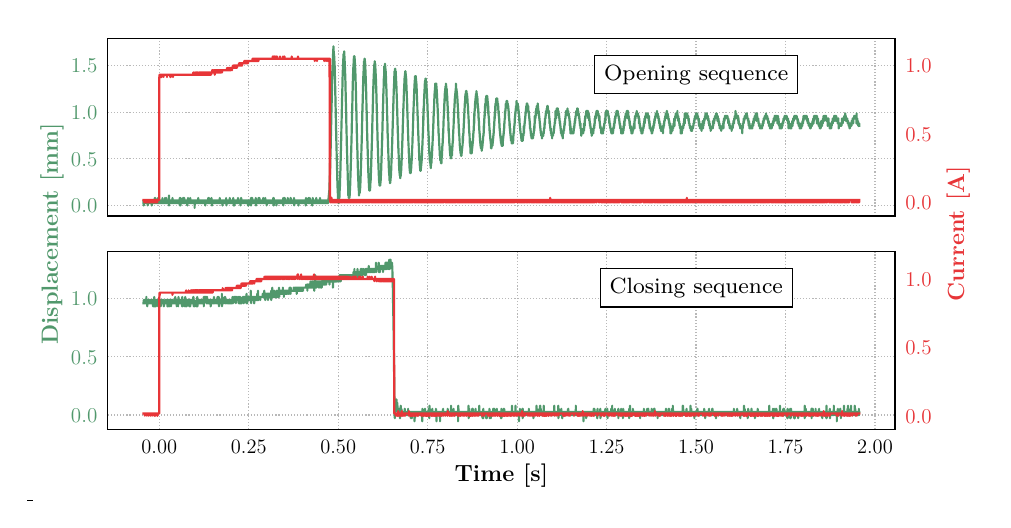
\begin{tikzpicture}
    \node[anchor=south west,inner sep=0] (graph) at (0,0) {\resizebox{\textwidth}{!}{%% Creator: Matplotlib, PGF backend
%%
%% To include the figure in your LaTeX document, write
%%   \input{<filename>.pgf}
%%
%% Make sure the required packages are loaded in your preamble
%%   \usepackage{pgf}
%%
%% and, on pdftex
%%   \usepackage[utf8]{inputenc}\DeclareUnicodeCharacter{2212}{-}
%%
%% or, on luatex and xetex
%%   \usepackage{unicode-math}
%%
%% Figures using additional raster images can only be included by \input if
%% they are in the same directory as the main LaTeX file. For loading figures
%% from other directories you can use the `import` package
%%   \usepackage{import}
%%
%% and then include the figures with
%%   \import{<path to file>}{<filename>.pgf}
%%
%% Matplotlib used the following preamble
%%
\begingroup%
\makeatletter%
\begin{pgfpicture}%
\pgfpathrectangle{\pgfpointorigin}{\pgfqpoint{9.022777in}{4.466555in}}%
\pgfusepath{use as bounding box, clip}%
\begin{pgfscope}%
\pgfsetbuttcap%
\pgfsetmiterjoin%
\pgfsetlinewidth{0.000000pt}%
\definecolor{currentstroke}{rgb}{0.000000,0.000000,0.000000}%
\pgfsetstrokecolor{currentstroke}%
\pgfsetstrokeopacity{0.000000}%
\pgfsetdash{}{0pt}%
\pgfpathmoveto{\pgfqpoint{0.000000in}{0.000000in}}%
\pgfpathlineto{\pgfqpoint{9.022777in}{0.000000in}}%
\pgfpathlineto{\pgfqpoint{9.022777in}{4.466555in}}%
\pgfpathlineto{\pgfqpoint{0.000000in}{4.466555in}}%
\pgfpathclose%
\pgfusepath{}%
\end{pgfscope}%
\begin{pgfscope}%
\pgfsetbuttcap%
\pgfsetmiterjoin%
\pgfsetlinewidth{0.000000pt}%
\definecolor{currentstroke}{rgb}{0.000000,0.000000,0.000000}%
\pgfsetstrokecolor{currentstroke}%
\pgfsetstrokeopacity{0.000000}%
\pgfsetdash{}{0pt}%
\pgfpathmoveto{\pgfqpoint{0.756666in}{2.686555in}}%
\pgfpathlineto{\pgfqpoint{8.196666in}{2.686555in}}%
\pgfpathlineto{\pgfqpoint{8.196666in}{4.366555in}}%
\pgfpathlineto{\pgfqpoint{0.756666in}{4.366555in}}%
\pgfpathclose%
\pgfusepath{}%
\end{pgfscope}%
\begin{pgfscope}%
\pgfpathrectangle{\pgfqpoint{0.756666in}{2.686555in}}{\pgfqpoint{7.440000in}{1.680000in}}%
\pgfusepath{clip}%
\pgfsetbuttcap%
\pgfsetroundjoin%
\pgfsetlinewidth{0.803000pt}%
\definecolor{currentstroke}{rgb}{0.690196,0.690196,0.690196}%
\pgfsetstrokecolor{currentstroke}%
\pgfsetstrokeopacity{0.900000}%
\pgfsetdash{{0.800000pt}{1.320000pt}}{0.000000pt}%
\pgfpathmoveto{\pgfqpoint{1.243763in}{2.686555in}}%
\pgfpathlineto{\pgfqpoint{1.243763in}{4.366555in}}%
\pgfusepath{stroke}%
\end{pgfscope}%
\begin{pgfscope}%
\pgfsetbuttcap%
\pgfsetroundjoin%
\definecolor{currentfill}{rgb}{0.000000,0.000000,0.000000}%
\pgfsetfillcolor{currentfill}%
\pgfsetlinewidth{0.803000pt}%
\definecolor{currentstroke}{rgb}{0.000000,0.000000,0.000000}%
\pgfsetstrokecolor{currentstroke}%
\pgfsetdash{}{0pt}%
\pgfsys@defobject{currentmarker}{\pgfqpoint{0.000000in}{-0.048611in}}{\pgfqpoint{0.000000in}{0.000000in}}{%
\pgfpathmoveto{\pgfqpoint{0.000000in}{0.000000in}}%
\pgfpathlineto{\pgfqpoint{0.000000in}{-0.048611in}}%
\pgfusepath{stroke,fill}%
}%
\begin{pgfscope}%
\pgfsys@transformshift{1.243763in}{2.686555in}%
\pgfsys@useobject{currentmarker}{}%
\end{pgfscope}%
\end{pgfscope}%
\begin{pgfscope}%
\pgfpathrectangle{\pgfqpoint{0.756666in}{2.686555in}}{\pgfqpoint{7.440000in}{1.680000in}}%
\pgfusepath{clip}%
\pgfsetbuttcap%
\pgfsetroundjoin%
\pgfsetlinewidth{0.803000pt}%
\definecolor{currentstroke}{rgb}{0.690196,0.690196,0.690196}%
\pgfsetstrokecolor{currentstroke}%
\pgfsetstrokeopacity{0.900000}%
\pgfsetdash{{0.800000pt}{1.320000pt}}{0.000000pt}%
\pgfpathmoveto{\pgfqpoint{2.089198in}{2.686555in}}%
\pgfpathlineto{\pgfqpoint{2.089198in}{4.366555in}}%
\pgfusepath{stroke}%
\end{pgfscope}%
\begin{pgfscope}%
\pgfsetbuttcap%
\pgfsetroundjoin%
\definecolor{currentfill}{rgb}{0.000000,0.000000,0.000000}%
\pgfsetfillcolor{currentfill}%
\pgfsetlinewidth{0.803000pt}%
\definecolor{currentstroke}{rgb}{0.000000,0.000000,0.000000}%
\pgfsetstrokecolor{currentstroke}%
\pgfsetdash{}{0pt}%
\pgfsys@defobject{currentmarker}{\pgfqpoint{0.000000in}{-0.048611in}}{\pgfqpoint{0.000000in}{0.000000in}}{%
\pgfpathmoveto{\pgfqpoint{0.000000in}{0.000000in}}%
\pgfpathlineto{\pgfqpoint{0.000000in}{-0.048611in}}%
\pgfusepath{stroke,fill}%
}%
\begin{pgfscope}%
\pgfsys@transformshift{2.089198in}{2.686555in}%
\pgfsys@useobject{currentmarker}{}%
\end{pgfscope}%
\end{pgfscope}%
\begin{pgfscope}%
\pgfpathrectangle{\pgfqpoint{0.756666in}{2.686555in}}{\pgfqpoint{7.440000in}{1.680000in}}%
\pgfusepath{clip}%
\pgfsetbuttcap%
\pgfsetroundjoin%
\pgfsetlinewidth{0.803000pt}%
\definecolor{currentstroke}{rgb}{0.690196,0.690196,0.690196}%
\pgfsetstrokecolor{currentstroke}%
\pgfsetstrokeopacity{0.900000}%
\pgfsetdash{{0.800000pt}{1.320000pt}}{0.000000pt}%
\pgfpathmoveto{\pgfqpoint{2.934634in}{2.686555in}}%
\pgfpathlineto{\pgfqpoint{2.934634in}{4.366555in}}%
\pgfusepath{stroke}%
\end{pgfscope}%
\begin{pgfscope}%
\pgfsetbuttcap%
\pgfsetroundjoin%
\definecolor{currentfill}{rgb}{0.000000,0.000000,0.000000}%
\pgfsetfillcolor{currentfill}%
\pgfsetlinewidth{0.803000pt}%
\definecolor{currentstroke}{rgb}{0.000000,0.000000,0.000000}%
\pgfsetstrokecolor{currentstroke}%
\pgfsetdash{}{0pt}%
\pgfsys@defobject{currentmarker}{\pgfqpoint{0.000000in}{-0.048611in}}{\pgfqpoint{0.000000in}{0.000000in}}{%
\pgfpathmoveto{\pgfqpoint{0.000000in}{0.000000in}}%
\pgfpathlineto{\pgfqpoint{0.000000in}{-0.048611in}}%
\pgfusepath{stroke,fill}%
}%
\begin{pgfscope}%
\pgfsys@transformshift{2.934634in}{2.686555in}%
\pgfsys@useobject{currentmarker}{}%
\end{pgfscope}%
\end{pgfscope}%
\begin{pgfscope}%
\pgfpathrectangle{\pgfqpoint{0.756666in}{2.686555in}}{\pgfqpoint{7.440000in}{1.680000in}}%
\pgfusepath{clip}%
\pgfsetbuttcap%
\pgfsetroundjoin%
\pgfsetlinewidth{0.803000pt}%
\definecolor{currentstroke}{rgb}{0.690196,0.690196,0.690196}%
\pgfsetstrokecolor{currentstroke}%
\pgfsetstrokeopacity{0.900000}%
\pgfsetdash{{0.800000pt}{1.320000pt}}{0.000000pt}%
\pgfpathmoveto{\pgfqpoint{3.780069in}{2.686555in}}%
\pgfpathlineto{\pgfqpoint{3.780069in}{4.366555in}}%
\pgfusepath{stroke}%
\end{pgfscope}%
\begin{pgfscope}%
\pgfsetbuttcap%
\pgfsetroundjoin%
\definecolor{currentfill}{rgb}{0.000000,0.000000,0.000000}%
\pgfsetfillcolor{currentfill}%
\pgfsetlinewidth{0.803000pt}%
\definecolor{currentstroke}{rgb}{0.000000,0.000000,0.000000}%
\pgfsetstrokecolor{currentstroke}%
\pgfsetdash{}{0pt}%
\pgfsys@defobject{currentmarker}{\pgfqpoint{0.000000in}{-0.048611in}}{\pgfqpoint{0.000000in}{0.000000in}}{%
\pgfpathmoveto{\pgfqpoint{0.000000in}{0.000000in}}%
\pgfpathlineto{\pgfqpoint{0.000000in}{-0.048611in}}%
\pgfusepath{stroke,fill}%
}%
\begin{pgfscope}%
\pgfsys@transformshift{3.780069in}{2.686555in}%
\pgfsys@useobject{currentmarker}{}%
\end{pgfscope}%
\end{pgfscope}%
\begin{pgfscope}%
\pgfpathrectangle{\pgfqpoint{0.756666in}{2.686555in}}{\pgfqpoint{7.440000in}{1.680000in}}%
\pgfusepath{clip}%
\pgfsetbuttcap%
\pgfsetroundjoin%
\pgfsetlinewidth{0.803000pt}%
\definecolor{currentstroke}{rgb}{0.690196,0.690196,0.690196}%
\pgfsetstrokecolor{currentstroke}%
\pgfsetstrokeopacity{0.900000}%
\pgfsetdash{{0.800000pt}{1.320000pt}}{0.000000pt}%
\pgfpathmoveto{\pgfqpoint{4.625505in}{2.686555in}}%
\pgfpathlineto{\pgfqpoint{4.625505in}{4.366555in}}%
\pgfusepath{stroke}%
\end{pgfscope}%
\begin{pgfscope}%
\pgfsetbuttcap%
\pgfsetroundjoin%
\definecolor{currentfill}{rgb}{0.000000,0.000000,0.000000}%
\pgfsetfillcolor{currentfill}%
\pgfsetlinewidth{0.803000pt}%
\definecolor{currentstroke}{rgb}{0.000000,0.000000,0.000000}%
\pgfsetstrokecolor{currentstroke}%
\pgfsetdash{}{0pt}%
\pgfsys@defobject{currentmarker}{\pgfqpoint{0.000000in}{-0.048611in}}{\pgfqpoint{0.000000in}{0.000000in}}{%
\pgfpathmoveto{\pgfqpoint{0.000000in}{0.000000in}}%
\pgfpathlineto{\pgfqpoint{0.000000in}{-0.048611in}}%
\pgfusepath{stroke,fill}%
}%
\begin{pgfscope}%
\pgfsys@transformshift{4.625505in}{2.686555in}%
\pgfsys@useobject{currentmarker}{}%
\end{pgfscope}%
\end{pgfscope}%
\begin{pgfscope}%
\pgfpathrectangle{\pgfqpoint{0.756666in}{2.686555in}}{\pgfqpoint{7.440000in}{1.680000in}}%
\pgfusepath{clip}%
\pgfsetbuttcap%
\pgfsetroundjoin%
\pgfsetlinewidth{0.803000pt}%
\definecolor{currentstroke}{rgb}{0.690196,0.690196,0.690196}%
\pgfsetstrokecolor{currentstroke}%
\pgfsetstrokeopacity{0.900000}%
\pgfsetdash{{0.800000pt}{1.320000pt}}{0.000000pt}%
\pgfpathmoveto{\pgfqpoint{5.470940in}{2.686555in}}%
\pgfpathlineto{\pgfqpoint{5.470940in}{4.366555in}}%
\pgfusepath{stroke}%
\end{pgfscope}%
\begin{pgfscope}%
\pgfsetbuttcap%
\pgfsetroundjoin%
\definecolor{currentfill}{rgb}{0.000000,0.000000,0.000000}%
\pgfsetfillcolor{currentfill}%
\pgfsetlinewidth{0.803000pt}%
\definecolor{currentstroke}{rgb}{0.000000,0.000000,0.000000}%
\pgfsetstrokecolor{currentstroke}%
\pgfsetdash{}{0pt}%
\pgfsys@defobject{currentmarker}{\pgfqpoint{0.000000in}{-0.048611in}}{\pgfqpoint{0.000000in}{0.000000in}}{%
\pgfpathmoveto{\pgfqpoint{0.000000in}{0.000000in}}%
\pgfpathlineto{\pgfqpoint{0.000000in}{-0.048611in}}%
\pgfusepath{stroke,fill}%
}%
\begin{pgfscope}%
\pgfsys@transformshift{5.470940in}{2.686555in}%
\pgfsys@useobject{currentmarker}{}%
\end{pgfscope}%
\end{pgfscope}%
\begin{pgfscope}%
\pgfpathrectangle{\pgfqpoint{0.756666in}{2.686555in}}{\pgfqpoint{7.440000in}{1.680000in}}%
\pgfusepath{clip}%
\pgfsetbuttcap%
\pgfsetroundjoin%
\pgfsetlinewidth{0.803000pt}%
\definecolor{currentstroke}{rgb}{0.690196,0.690196,0.690196}%
\pgfsetstrokecolor{currentstroke}%
\pgfsetstrokeopacity{0.900000}%
\pgfsetdash{{0.800000pt}{1.320000pt}}{0.000000pt}%
\pgfpathmoveto{\pgfqpoint{6.316376in}{2.686555in}}%
\pgfpathlineto{\pgfqpoint{6.316376in}{4.366555in}}%
\pgfusepath{stroke}%
\end{pgfscope}%
\begin{pgfscope}%
\pgfsetbuttcap%
\pgfsetroundjoin%
\definecolor{currentfill}{rgb}{0.000000,0.000000,0.000000}%
\pgfsetfillcolor{currentfill}%
\pgfsetlinewidth{0.803000pt}%
\definecolor{currentstroke}{rgb}{0.000000,0.000000,0.000000}%
\pgfsetstrokecolor{currentstroke}%
\pgfsetdash{}{0pt}%
\pgfsys@defobject{currentmarker}{\pgfqpoint{0.000000in}{-0.048611in}}{\pgfqpoint{0.000000in}{0.000000in}}{%
\pgfpathmoveto{\pgfqpoint{0.000000in}{0.000000in}}%
\pgfpathlineto{\pgfqpoint{0.000000in}{-0.048611in}}%
\pgfusepath{stroke,fill}%
}%
\begin{pgfscope}%
\pgfsys@transformshift{6.316376in}{2.686555in}%
\pgfsys@useobject{currentmarker}{}%
\end{pgfscope}%
\end{pgfscope}%
\begin{pgfscope}%
\pgfpathrectangle{\pgfqpoint{0.756666in}{2.686555in}}{\pgfqpoint{7.440000in}{1.680000in}}%
\pgfusepath{clip}%
\pgfsetbuttcap%
\pgfsetroundjoin%
\pgfsetlinewidth{0.803000pt}%
\definecolor{currentstroke}{rgb}{0.690196,0.690196,0.690196}%
\pgfsetstrokecolor{currentstroke}%
\pgfsetstrokeopacity{0.900000}%
\pgfsetdash{{0.800000pt}{1.320000pt}}{0.000000pt}%
\pgfpathmoveto{\pgfqpoint{7.161812in}{2.686555in}}%
\pgfpathlineto{\pgfqpoint{7.161812in}{4.366555in}}%
\pgfusepath{stroke}%
\end{pgfscope}%
\begin{pgfscope}%
\pgfsetbuttcap%
\pgfsetroundjoin%
\definecolor{currentfill}{rgb}{0.000000,0.000000,0.000000}%
\pgfsetfillcolor{currentfill}%
\pgfsetlinewidth{0.803000pt}%
\definecolor{currentstroke}{rgb}{0.000000,0.000000,0.000000}%
\pgfsetstrokecolor{currentstroke}%
\pgfsetdash{}{0pt}%
\pgfsys@defobject{currentmarker}{\pgfqpoint{0.000000in}{-0.048611in}}{\pgfqpoint{0.000000in}{0.000000in}}{%
\pgfpathmoveto{\pgfqpoint{0.000000in}{0.000000in}}%
\pgfpathlineto{\pgfqpoint{0.000000in}{-0.048611in}}%
\pgfusepath{stroke,fill}%
}%
\begin{pgfscope}%
\pgfsys@transformshift{7.161812in}{2.686555in}%
\pgfsys@useobject{currentmarker}{}%
\end{pgfscope}%
\end{pgfscope}%
\begin{pgfscope}%
\pgfpathrectangle{\pgfqpoint{0.756666in}{2.686555in}}{\pgfqpoint{7.440000in}{1.680000in}}%
\pgfusepath{clip}%
\pgfsetbuttcap%
\pgfsetroundjoin%
\pgfsetlinewidth{0.803000pt}%
\definecolor{currentstroke}{rgb}{0.690196,0.690196,0.690196}%
\pgfsetstrokecolor{currentstroke}%
\pgfsetstrokeopacity{0.900000}%
\pgfsetdash{{0.800000pt}{1.320000pt}}{0.000000pt}%
\pgfpathmoveto{\pgfqpoint{8.007247in}{2.686555in}}%
\pgfpathlineto{\pgfqpoint{8.007247in}{4.366555in}}%
\pgfusepath{stroke}%
\end{pgfscope}%
\begin{pgfscope}%
\pgfsetbuttcap%
\pgfsetroundjoin%
\definecolor{currentfill}{rgb}{0.000000,0.000000,0.000000}%
\pgfsetfillcolor{currentfill}%
\pgfsetlinewidth{0.803000pt}%
\definecolor{currentstroke}{rgb}{0.000000,0.000000,0.000000}%
\pgfsetstrokecolor{currentstroke}%
\pgfsetdash{}{0pt}%
\pgfsys@defobject{currentmarker}{\pgfqpoint{0.000000in}{-0.048611in}}{\pgfqpoint{0.000000in}{0.000000in}}{%
\pgfpathmoveto{\pgfqpoint{0.000000in}{0.000000in}}%
\pgfpathlineto{\pgfqpoint{0.000000in}{-0.048611in}}%
\pgfusepath{stroke,fill}%
}%
\begin{pgfscope}%
\pgfsys@transformshift{8.007247in}{2.686555in}%
\pgfsys@useobject{currentmarker}{}%
\end{pgfscope}%
\end{pgfscope}%
\begin{pgfscope}%
\pgfpathrectangle{\pgfqpoint{0.756666in}{2.686555in}}{\pgfqpoint{7.440000in}{1.680000in}}%
\pgfusepath{clip}%
\pgfsetbuttcap%
\pgfsetroundjoin%
\pgfsetlinewidth{0.803000pt}%
\definecolor{currentstroke}{rgb}{0.690196,0.690196,0.690196}%
\pgfsetstrokecolor{currentstroke}%
\pgfsetstrokeopacity{0.900000}%
\pgfsetdash{{0.800000pt}{1.320000pt}}{0.000000pt}%
\pgfpathmoveto{\pgfqpoint{0.756666in}{2.786415in}}%
\pgfpathlineto{\pgfqpoint{8.196666in}{2.786415in}}%
\pgfusepath{stroke}%
\end{pgfscope}%
\begin{pgfscope}%
\pgfsetbuttcap%
\pgfsetroundjoin%
\definecolor{currentfill}{rgb}{0.000000,0.000000,0.000000}%
\pgfsetfillcolor{currentfill}%
\pgfsetlinewidth{0.803000pt}%
\definecolor{currentstroke}{rgb}{0.000000,0.000000,0.000000}%
\pgfsetstrokecolor{currentstroke}%
\pgfsetdash{}{0pt}%
\pgfsys@defobject{currentmarker}{\pgfqpoint{-0.048611in}{0.000000in}}{\pgfqpoint{-0.000000in}{0.000000in}}{%
\pgfpathmoveto{\pgfqpoint{-0.000000in}{0.000000in}}%
\pgfpathlineto{\pgfqpoint{-0.048611in}{0.000000in}}%
\pgfusepath{stroke,fill}%
}%
\begin{pgfscope}%
\pgfsys@transformshift{0.756666in}{2.786415in}%
\pgfsys@useobject{currentmarker}{}%
\end{pgfscope}%
\end{pgfscope}%
\begin{pgfscope}%
\definecolor{textcolor}{rgb}{0.317647,0.596078,0.423529}%
\pgfsetstrokecolor{textcolor}%
\pgfsetfillcolor{textcolor}%
\pgftext[x=0.409216in, y=2.716971in, left, base]{\color{textcolor}\rmfamily\fontsize{14.000000}{16.800000}\selectfont \(\displaystyle {0.0}\)}%
\end{pgfscope}%
\begin{pgfscope}%
\pgfpathrectangle{\pgfqpoint{0.756666in}{2.686555in}}{\pgfqpoint{7.440000in}{1.680000in}}%
\pgfusepath{clip}%
\pgfsetbuttcap%
\pgfsetroundjoin%
\pgfsetlinewidth{0.803000pt}%
\definecolor{currentstroke}{rgb}{0.690196,0.690196,0.690196}%
\pgfsetstrokecolor{currentstroke}%
\pgfsetstrokeopacity{0.900000}%
\pgfsetdash{{0.800000pt}{1.320000pt}}{0.000000pt}%
\pgfpathmoveto{\pgfqpoint{0.756666in}{3.226974in}}%
\pgfpathlineto{\pgfqpoint{8.196666in}{3.226974in}}%
\pgfusepath{stroke}%
\end{pgfscope}%
\begin{pgfscope}%
\pgfsetbuttcap%
\pgfsetroundjoin%
\definecolor{currentfill}{rgb}{0.000000,0.000000,0.000000}%
\pgfsetfillcolor{currentfill}%
\pgfsetlinewidth{0.803000pt}%
\definecolor{currentstroke}{rgb}{0.000000,0.000000,0.000000}%
\pgfsetstrokecolor{currentstroke}%
\pgfsetdash{}{0pt}%
\pgfsys@defobject{currentmarker}{\pgfqpoint{-0.048611in}{0.000000in}}{\pgfqpoint{-0.000000in}{0.000000in}}{%
\pgfpathmoveto{\pgfqpoint{-0.000000in}{0.000000in}}%
\pgfpathlineto{\pgfqpoint{-0.048611in}{0.000000in}}%
\pgfusepath{stroke,fill}%
}%
\begin{pgfscope}%
\pgfsys@transformshift{0.756666in}{3.226974in}%
\pgfsys@useobject{currentmarker}{}%
\end{pgfscope}%
\end{pgfscope}%
\begin{pgfscope}%
\definecolor{textcolor}{rgb}{0.317647,0.596078,0.423529}%
\pgfsetstrokecolor{textcolor}%
\pgfsetfillcolor{textcolor}%
\pgftext[x=0.409216in, y=3.157530in, left, base]{\color{textcolor}\rmfamily\fontsize{14.000000}{16.800000}\selectfont \(\displaystyle {0.5}\)}%
\end{pgfscope}%
\begin{pgfscope}%
\pgfpathrectangle{\pgfqpoint{0.756666in}{2.686555in}}{\pgfqpoint{7.440000in}{1.680000in}}%
\pgfusepath{clip}%
\pgfsetbuttcap%
\pgfsetroundjoin%
\pgfsetlinewidth{0.803000pt}%
\definecolor{currentstroke}{rgb}{0.690196,0.690196,0.690196}%
\pgfsetstrokecolor{currentstroke}%
\pgfsetstrokeopacity{0.900000}%
\pgfsetdash{{0.800000pt}{1.320000pt}}{0.000000pt}%
\pgfpathmoveto{\pgfqpoint{0.756666in}{3.667533in}}%
\pgfpathlineto{\pgfqpoint{8.196666in}{3.667533in}}%
\pgfusepath{stroke}%
\end{pgfscope}%
\begin{pgfscope}%
\pgfsetbuttcap%
\pgfsetroundjoin%
\definecolor{currentfill}{rgb}{0.000000,0.000000,0.000000}%
\pgfsetfillcolor{currentfill}%
\pgfsetlinewidth{0.803000pt}%
\definecolor{currentstroke}{rgb}{0.000000,0.000000,0.000000}%
\pgfsetstrokecolor{currentstroke}%
\pgfsetdash{}{0pt}%
\pgfsys@defobject{currentmarker}{\pgfqpoint{-0.048611in}{0.000000in}}{\pgfqpoint{-0.000000in}{0.000000in}}{%
\pgfpathmoveto{\pgfqpoint{-0.000000in}{0.000000in}}%
\pgfpathlineto{\pgfqpoint{-0.048611in}{0.000000in}}%
\pgfusepath{stroke,fill}%
}%
\begin{pgfscope}%
\pgfsys@transformshift{0.756666in}{3.667533in}%
\pgfsys@useobject{currentmarker}{}%
\end{pgfscope}%
\end{pgfscope}%
\begin{pgfscope}%
\definecolor{textcolor}{rgb}{0.317647,0.596078,0.423529}%
\pgfsetstrokecolor{textcolor}%
\pgfsetfillcolor{textcolor}%
\pgftext[x=0.409216in, y=3.598089in, left, base]{\color{textcolor}\rmfamily\fontsize{14.000000}{16.800000}\selectfont \(\displaystyle {1.0}\)}%
\end{pgfscope}%
\begin{pgfscope}%
\pgfpathrectangle{\pgfqpoint{0.756666in}{2.686555in}}{\pgfqpoint{7.440000in}{1.680000in}}%
\pgfusepath{clip}%
\pgfsetbuttcap%
\pgfsetroundjoin%
\pgfsetlinewidth{0.803000pt}%
\definecolor{currentstroke}{rgb}{0.690196,0.690196,0.690196}%
\pgfsetstrokecolor{currentstroke}%
\pgfsetstrokeopacity{0.900000}%
\pgfsetdash{{0.800000pt}{1.320000pt}}{0.000000pt}%
\pgfpathmoveto{\pgfqpoint{0.756666in}{4.108092in}}%
\pgfpathlineto{\pgfqpoint{8.196666in}{4.108092in}}%
\pgfusepath{stroke}%
\end{pgfscope}%
\begin{pgfscope}%
\pgfsetbuttcap%
\pgfsetroundjoin%
\definecolor{currentfill}{rgb}{0.000000,0.000000,0.000000}%
\pgfsetfillcolor{currentfill}%
\pgfsetlinewidth{0.803000pt}%
\definecolor{currentstroke}{rgb}{0.000000,0.000000,0.000000}%
\pgfsetstrokecolor{currentstroke}%
\pgfsetdash{}{0pt}%
\pgfsys@defobject{currentmarker}{\pgfqpoint{-0.048611in}{0.000000in}}{\pgfqpoint{-0.000000in}{0.000000in}}{%
\pgfpathmoveto{\pgfqpoint{-0.000000in}{0.000000in}}%
\pgfpathlineto{\pgfqpoint{-0.048611in}{0.000000in}}%
\pgfusepath{stroke,fill}%
}%
\begin{pgfscope}%
\pgfsys@transformshift{0.756666in}{4.108092in}%
\pgfsys@useobject{currentmarker}{}%
\end{pgfscope}%
\end{pgfscope}%
\begin{pgfscope}%
\definecolor{textcolor}{rgb}{0.317647,0.596078,0.423529}%
\pgfsetstrokecolor{textcolor}%
\pgfsetfillcolor{textcolor}%
\pgftext[x=0.409216in, y=4.038648in, left, base]{\color{textcolor}\rmfamily\fontsize{14.000000}{16.800000}\selectfont \(\displaystyle {1.5}\)}%
\end{pgfscope}%
\begin{pgfscope}%
\pgfpathrectangle{\pgfqpoint{0.756666in}{2.686555in}}{\pgfqpoint{7.440000in}{1.680000in}}%
\pgfusepath{clip}%
\pgfsetrectcap%
\pgfsetroundjoin%
\pgfsetlinewidth{1.505625pt}%
\definecolor{currentstroke}{rgb}{0.317647,0.596078,0.423529}%
\pgfsetstrokecolor{currentstroke}%
\pgfsetdash{}{0pt}%
\pgfpathmoveto{\pgfqpoint{1.094848in}{2.809911in}}%
\pgfpathlineto{\pgfqpoint{1.095119in}{2.809911in}}%
\pgfpathlineto{\pgfqpoint{1.095525in}{2.833408in}}%
\pgfpathlineto{\pgfqpoint{1.095795in}{2.809911in}}%
\pgfpathlineto{\pgfqpoint{1.096201in}{2.833408in}}%
\pgfpathlineto{\pgfqpoint{1.096336in}{2.833408in}}%
\pgfpathlineto{\pgfqpoint{1.096877in}{2.786415in}}%
\pgfpathlineto{\pgfqpoint{1.097148in}{2.833408in}}%
\pgfpathlineto{\pgfqpoint{1.097283in}{2.809911in}}%
\pgfpathlineto{\pgfqpoint{1.097689in}{2.833408in}}%
\pgfpathlineto{\pgfqpoint{1.098095in}{2.833408in}}%
\pgfpathlineto{\pgfqpoint{1.098500in}{2.809911in}}%
\pgfpathlineto{\pgfqpoint{1.098771in}{2.809911in}}%
\pgfpathlineto{\pgfqpoint{1.099177in}{2.833408in}}%
\pgfpathlineto{\pgfqpoint{1.099312in}{2.833408in}}%
\pgfpathlineto{\pgfqpoint{1.099718in}{2.809911in}}%
\pgfpathlineto{\pgfqpoint{1.099853in}{2.809911in}}%
\pgfpathlineto{\pgfqpoint{1.099988in}{2.833408in}}%
\pgfpathlineto{\pgfqpoint{1.100124in}{2.809911in}}%
\pgfpathlineto{\pgfqpoint{1.100394in}{2.809911in}}%
\pgfpathlineto{\pgfqpoint{1.100800in}{2.833408in}}%
\pgfpathlineto{\pgfqpoint{1.101071in}{2.833408in}}%
\pgfpathlineto{\pgfqpoint{1.101476in}{2.809911in}}%
\pgfpathlineto{\pgfqpoint{1.102018in}{2.809911in}}%
\pgfpathlineto{\pgfqpoint{1.102423in}{2.833408in}}%
\pgfpathlineto{\pgfqpoint{1.102559in}{2.833408in}}%
\pgfpathlineto{\pgfqpoint{1.102829in}{2.809911in}}%
\pgfpathlineto{\pgfqpoint{1.103235in}{2.833408in}}%
\pgfpathlineto{\pgfqpoint{1.103370in}{2.833408in}}%
\pgfpathlineto{\pgfqpoint{1.103776in}{2.809911in}}%
\pgfpathlineto{\pgfqpoint{1.103911in}{2.833408in}}%
\pgfpathlineto{\pgfqpoint{1.104047in}{2.809911in}}%
\pgfpathlineto{\pgfqpoint{1.104182in}{2.809911in}}%
\pgfpathlineto{\pgfqpoint{1.104588in}{2.833408in}}%
\pgfpathlineto{\pgfqpoint{1.105399in}{2.833408in}}%
\pgfpathlineto{\pgfqpoint{1.105805in}{2.809911in}}%
\pgfpathlineto{\pgfqpoint{1.106076in}{2.833408in}}%
\pgfpathlineto{\pgfqpoint{1.106211in}{2.809911in}}%
\pgfpathlineto{\pgfqpoint{1.106346in}{2.833408in}}%
\pgfpathlineto{\pgfqpoint{1.106887in}{2.833408in}}%
\pgfpathlineto{\pgfqpoint{1.107022in}{2.809911in}}%
\pgfpathlineto{\pgfqpoint{1.107158in}{2.833408in}}%
\pgfpathlineto{\pgfqpoint{1.107293in}{2.833408in}}%
\pgfpathlineto{\pgfqpoint{1.107564in}{2.809911in}}%
\pgfpathlineto{\pgfqpoint{1.107969in}{2.833408in}}%
\pgfpathlineto{\pgfqpoint{1.108105in}{2.809911in}}%
\pgfpathlineto{\pgfqpoint{1.108240in}{2.833408in}}%
\pgfpathlineto{\pgfqpoint{1.108646in}{2.833408in}}%
\pgfpathlineto{\pgfqpoint{1.108781in}{2.809911in}}%
\pgfpathlineto{\pgfqpoint{1.108916in}{2.833408in}}%
\pgfpathlineto{\pgfqpoint{1.109457in}{2.833408in}}%
\pgfpathlineto{\pgfqpoint{1.109728in}{2.809911in}}%
\pgfpathlineto{\pgfqpoint{1.109998in}{2.833408in}}%
\pgfpathlineto{\pgfqpoint{1.110404in}{2.809911in}}%
\pgfpathlineto{\pgfqpoint{1.110810in}{2.833408in}}%
\pgfpathlineto{\pgfqpoint{1.110945in}{2.833408in}}%
\pgfpathlineto{\pgfqpoint{1.111081in}{2.809911in}}%
\pgfpathlineto{\pgfqpoint{1.111216in}{2.833408in}}%
\pgfpathlineto{\pgfqpoint{1.111486in}{2.833408in}}%
\pgfpathlineto{\pgfqpoint{1.111757in}{2.809911in}}%
\pgfpathlineto{\pgfqpoint{1.112163in}{2.833408in}}%
\pgfpathlineto{\pgfqpoint{1.112298in}{2.833408in}}%
\pgfpathlineto{\pgfqpoint{1.112704in}{2.809911in}}%
\pgfpathlineto{\pgfqpoint{1.112974in}{2.809911in}}%
\pgfpathlineto{\pgfqpoint{1.113380in}{2.833408in}}%
\pgfpathlineto{\pgfqpoint{1.113786in}{2.833408in}}%
\pgfpathlineto{\pgfqpoint{1.114057in}{2.809911in}}%
\pgfpathlineto{\pgfqpoint{1.114327in}{2.833408in}}%
\pgfpathlineto{\pgfqpoint{1.114598in}{2.809911in}}%
\pgfpathlineto{\pgfqpoint{1.115003in}{2.833408in}}%
\pgfpathlineto{\pgfqpoint{1.115274in}{2.833408in}}%
\pgfpathlineto{\pgfqpoint{1.115544in}{2.809911in}}%
\pgfpathlineto{\pgfqpoint{1.115680in}{2.833408in}}%
\pgfpathlineto{\pgfqpoint{1.115815in}{2.809911in}}%
\pgfpathlineto{\pgfqpoint{1.115950in}{2.809911in}}%
\pgfpathlineto{\pgfqpoint{1.116221in}{2.833408in}}%
\pgfpathlineto{\pgfqpoint{1.116491in}{2.809911in}}%
\pgfpathlineto{\pgfqpoint{1.116897in}{2.833408in}}%
\pgfpathlineto{\pgfqpoint{1.117168in}{2.809911in}}%
\pgfpathlineto{\pgfqpoint{1.117574in}{2.833408in}}%
\pgfpathlineto{\pgfqpoint{1.117844in}{2.833408in}}%
\pgfpathlineto{\pgfqpoint{1.118250in}{2.809911in}}%
\pgfpathlineto{\pgfqpoint{1.118385in}{2.833408in}}%
\pgfpathlineto{\pgfqpoint{1.118520in}{2.809911in}}%
\pgfpathlineto{\pgfqpoint{1.118791in}{2.809911in}}%
\pgfpathlineto{\pgfqpoint{1.119197in}{2.833408in}}%
\pgfpathlineto{\pgfqpoint{1.119738in}{2.833408in}}%
\pgfpathlineto{\pgfqpoint{1.120144in}{2.809911in}}%
\pgfpathlineto{\pgfqpoint{1.120414in}{2.833408in}}%
\pgfpathlineto{\pgfqpoint{1.120820in}{2.809911in}}%
\pgfpathlineto{\pgfqpoint{1.121226in}{2.833408in}}%
\pgfpathlineto{\pgfqpoint{1.121496in}{2.833408in}}%
\pgfpathlineto{\pgfqpoint{1.121767in}{2.809911in}}%
\pgfpathlineto{\pgfqpoint{1.122173in}{2.833408in}}%
\pgfpathlineto{\pgfqpoint{1.122578in}{2.809911in}}%
\pgfpathlineto{\pgfqpoint{1.122984in}{2.833408in}}%
\pgfpathlineto{\pgfqpoint{1.123120in}{2.833408in}}%
\pgfpathlineto{\pgfqpoint{1.123525in}{2.809911in}}%
\pgfpathlineto{\pgfqpoint{1.123661in}{2.833408in}}%
\pgfpathlineto{\pgfqpoint{1.123796in}{2.809911in}}%
\pgfpathlineto{\pgfqpoint{1.123931in}{2.809911in}}%
\pgfpathlineto{\pgfqpoint{1.124202in}{2.833408in}}%
\pgfpathlineto{\pgfqpoint{1.124472in}{2.809911in}}%
\pgfpathlineto{\pgfqpoint{1.124878in}{2.833408in}}%
\pgfpathlineto{\pgfqpoint{1.125013in}{2.833408in}}%
\pgfpathlineto{\pgfqpoint{1.125419in}{2.809911in}}%
\pgfpathlineto{\pgfqpoint{1.125554in}{2.809911in}}%
\pgfpathlineto{\pgfqpoint{1.125960in}{2.833408in}}%
\pgfpathlineto{\pgfqpoint{1.126501in}{2.833408in}}%
\pgfpathlineto{\pgfqpoint{1.126907in}{2.809911in}}%
\pgfpathlineto{\pgfqpoint{1.127042in}{2.809911in}}%
\pgfpathlineto{\pgfqpoint{1.127448in}{2.833408in}}%
\pgfpathlineto{\pgfqpoint{1.127583in}{2.809911in}}%
\pgfpathlineto{\pgfqpoint{1.127719in}{2.833408in}}%
\pgfpathlineto{\pgfqpoint{1.127854in}{2.833408in}}%
\pgfpathlineto{\pgfqpoint{1.127989in}{2.809911in}}%
\pgfpathlineto{\pgfqpoint{1.128125in}{2.833408in}}%
\pgfpathlineto{\pgfqpoint{1.129477in}{2.833408in}}%
\pgfpathlineto{\pgfqpoint{1.129883in}{2.809911in}}%
\pgfpathlineto{\pgfqpoint{1.130289in}{2.809911in}}%
\pgfpathlineto{\pgfqpoint{1.130695in}{2.833408in}}%
\pgfpathlineto{\pgfqpoint{1.130830in}{2.833408in}}%
\pgfpathlineto{\pgfqpoint{1.131236in}{2.809911in}}%
\pgfpathlineto{\pgfqpoint{1.131371in}{2.809911in}}%
\pgfpathlineto{\pgfqpoint{1.131777in}{2.833408in}}%
\pgfpathlineto{\pgfqpoint{1.132183in}{2.809911in}}%
\pgfpathlineto{\pgfqpoint{1.132588in}{2.833408in}}%
\pgfpathlineto{\pgfqpoint{1.132724in}{2.833408in}}%
\pgfpathlineto{\pgfqpoint{1.133130in}{2.809911in}}%
\pgfpathlineto{\pgfqpoint{1.133400in}{2.809911in}}%
\pgfpathlineto{\pgfqpoint{1.133806in}{2.833408in}}%
\pgfpathlineto{\pgfqpoint{1.133941in}{2.786415in}}%
\pgfpathlineto{\pgfqpoint{1.134076in}{2.833408in}}%
\pgfpathlineto{\pgfqpoint{1.134212in}{2.833408in}}%
\pgfpathlineto{\pgfqpoint{1.134482in}{2.809911in}}%
\pgfpathlineto{\pgfqpoint{1.134888in}{2.833408in}}%
\pgfpathlineto{\pgfqpoint{1.135835in}{2.833408in}}%
\pgfpathlineto{\pgfqpoint{1.136241in}{2.809911in}}%
\pgfpathlineto{\pgfqpoint{1.136647in}{2.833408in}}%
\pgfpathlineto{\pgfqpoint{1.136782in}{2.833408in}}%
\pgfpathlineto{\pgfqpoint{1.136917in}{2.809911in}}%
\pgfpathlineto{\pgfqpoint{1.137052in}{2.833408in}}%
\pgfpathlineto{\pgfqpoint{1.137323in}{2.833408in}}%
\pgfpathlineto{\pgfqpoint{1.137729in}{2.809911in}}%
\pgfpathlineto{\pgfqpoint{1.137864in}{2.809911in}}%
\pgfpathlineto{\pgfqpoint{1.137999in}{2.833408in}}%
\pgfpathlineto{\pgfqpoint{1.138135in}{2.809911in}}%
\pgfpathlineto{\pgfqpoint{1.138405in}{2.809911in}}%
\pgfpathlineto{\pgfqpoint{1.138540in}{2.833408in}}%
\pgfpathlineto{\pgfqpoint{1.138676in}{2.809911in}}%
\pgfpathlineto{\pgfqpoint{1.138811in}{2.809911in}}%
\pgfpathlineto{\pgfqpoint{1.139217in}{2.833408in}}%
\pgfpathlineto{\pgfqpoint{1.139487in}{2.809911in}}%
\pgfpathlineto{\pgfqpoint{1.139893in}{2.833408in}}%
\pgfpathlineto{\pgfqpoint{1.140434in}{2.833408in}}%
\pgfpathlineto{\pgfqpoint{1.140569in}{2.809911in}}%
\pgfpathlineto{\pgfqpoint{1.140705in}{2.833408in}}%
\pgfpathlineto{\pgfqpoint{1.141922in}{2.833408in}}%
\pgfpathlineto{\pgfqpoint{1.142328in}{2.809911in}}%
\pgfpathlineto{\pgfqpoint{1.142734in}{2.833408in}}%
\pgfpathlineto{\pgfqpoint{1.143004in}{2.833408in}}%
\pgfpathlineto{\pgfqpoint{1.143139in}{2.809911in}}%
\pgfpathlineto{\pgfqpoint{1.143275in}{2.833408in}}%
\pgfpathlineto{\pgfqpoint{1.143410in}{2.833408in}}%
\pgfpathlineto{\pgfqpoint{1.143545in}{2.809911in}}%
\pgfpathlineto{\pgfqpoint{1.143681in}{2.833408in}}%
\pgfpathlineto{\pgfqpoint{1.143951in}{2.833408in}}%
\pgfpathlineto{\pgfqpoint{1.144357in}{2.809911in}}%
\pgfpathlineto{\pgfqpoint{1.144492in}{2.809911in}}%
\pgfpathlineto{\pgfqpoint{1.144763in}{2.833408in}}%
\pgfpathlineto{\pgfqpoint{1.144898in}{2.809911in}}%
\pgfpathlineto{\pgfqpoint{1.145033in}{2.833408in}}%
\pgfpathlineto{\pgfqpoint{1.145169in}{2.833408in}}%
\pgfpathlineto{\pgfqpoint{1.145304in}{2.809911in}}%
\pgfpathlineto{\pgfqpoint{1.145439in}{2.833408in}}%
\pgfpathlineto{\pgfqpoint{1.145980in}{2.833408in}}%
\pgfpathlineto{\pgfqpoint{1.146251in}{2.809911in}}%
\pgfpathlineto{\pgfqpoint{1.146386in}{2.833408in}}%
\pgfpathlineto{\pgfqpoint{1.146521in}{2.809911in}}%
\pgfpathlineto{\pgfqpoint{1.147468in}{2.809911in}}%
\pgfpathlineto{\pgfqpoint{1.147874in}{2.833408in}}%
\pgfpathlineto{\pgfqpoint{1.148009in}{2.833408in}}%
\pgfpathlineto{\pgfqpoint{1.148144in}{2.809911in}}%
\pgfpathlineto{\pgfqpoint{1.148280in}{2.833408in}}%
\pgfpathlineto{\pgfqpoint{1.148415in}{2.833408in}}%
\pgfpathlineto{\pgfqpoint{1.148686in}{2.809911in}}%
\pgfpathlineto{\pgfqpoint{1.148956in}{2.833408in}}%
\pgfpathlineto{\pgfqpoint{1.149091in}{2.809911in}}%
\pgfpathlineto{\pgfqpoint{1.149227in}{2.833408in}}%
\pgfpathlineto{\pgfqpoint{1.149362in}{2.833408in}}%
\pgfpathlineto{\pgfqpoint{1.149768in}{2.809911in}}%
\pgfpathlineto{\pgfqpoint{1.150309in}{2.809911in}}%
\pgfpathlineto{\pgfqpoint{1.150579in}{2.833408in}}%
\pgfpathlineto{\pgfqpoint{1.150985in}{2.809911in}}%
\pgfpathlineto{\pgfqpoint{1.151526in}{2.809911in}}%
\pgfpathlineto{\pgfqpoint{1.151797in}{2.833408in}}%
\pgfpathlineto{\pgfqpoint{1.152203in}{2.809911in}}%
\pgfpathlineto{\pgfqpoint{1.152608in}{2.833408in}}%
\pgfpathlineto{\pgfqpoint{1.152879in}{2.809911in}}%
\pgfpathlineto{\pgfqpoint{1.153285in}{2.833408in}}%
\pgfpathlineto{\pgfqpoint{1.153555in}{2.833408in}}%
\pgfpathlineto{\pgfqpoint{1.153826in}{2.809911in}}%
\pgfpathlineto{\pgfqpoint{1.154232in}{2.833408in}}%
\pgfpathlineto{\pgfqpoint{1.154502in}{2.809911in}}%
\pgfpathlineto{\pgfqpoint{1.154908in}{2.833408in}}%
\pgfpathlineto{\pgfqpoint{1.155178in}{2.833408in}}%
\pgfpathlineto{\pgfqpoint{1.155584in}{2.809911in}}%
\pgfpathlineto{\pgfqpoint{1.155990in}{2.833408in}}%
\pgfpathlineto{\pgfqpoint{1.156396in}{2.809911in}}%
\pgfpathlineto{\pgfqpoint{1.156531in}{2.809911in}}%
\pgfpathlineto{\pgfqpoint{1.156666in}{2.833408in}}%
\pgfpathlineto{\pgfqpoint{1.156802in}{2.809911in}}%
\pgfpathlineto{\pgfqpoint{1.156937in}{2.809911in}}%
\pgfpathlineto{\pgfqpoint{1.157072in}{2.833408in}}%
\pgfpathlineto{\pgfqpoint{1.157208in}{2.809911in}}%
\pgfpathlineto{\pgfqpoint{1.157343in}{2.809911in}}%
\pgfpathlineto{\pgfqpoint{1.157613in}{2.833408in}}%
\pgfpathlineto{\pgfqpoint{1.158019in}{2.809911in}}%
\pgfpathlineto{\pgfqpoint{1.158831in}{2.809911in}}%
\pgfpathlineto{\pgfqpoint{1.159237in}{2.833408in}}%
\pgfpathlineto{\pgfqpoint{1.159913in}{2.833408in}}%
\pgfpathlineto{\pgfqpoint{1.160048in}{2.809911in}}%
\pgfpathlineto{\pgfqpoint{1.160183in}{2.833408in}}%
\pgfpathlineto{\pgfqpoint{1.160454in}{2.833408in}}%
\pgfpathlineto{\pgfqpoint{1.160860in}{2.809911in}}%
\pgfpathlineto{\pgfqpoint{1.160995in}{2.809911in}}%
\pgfpathlineto{\pgfqpoint{1.161401in}{2.833408in}}%
\pgfpathlineto{\pgfqpoint{1.161807in}{2.809911in}}%
\pgfpathlineto{\pgfqpoint{1.162483in}{2.809911in}}%
\pgfpathlineto{\pgfqpoint{1.162618in}{2.833408in}}%
\pgfpathlineto{\pgfqpoint{1.162754in}{2.809911in}}%
\pgfpathlineto{\pgfqpoint{1.162889in}{2.809911in}}%
\pgfpathlineto{\pgfqpoint{1.163295in}{2.833408in}}%
\pgfpathlineto{\pgfqpoint{1.163430in}{2.833408in}}%
\pgfpathlineto{\pgfqpoint{1.163700in}{2.809911in}}%
\pgfpathlineto{\pgfqpoint{1.163971in}{2.833408in}}%
\pgfpathlineto{\pgfqpoint{1.164377in}{2.809911in}}%
\pgfpathlineto{\pgfqpoint{1.164647in}{2.833408in}}%
\pgfpathlineto{\pgfqpoint{1.164918in}{2.809911in}}%
\pgfpathlineto{\pgfqpoint{1.165188in}{2.833408in}}%
\pgfpathlineto{\pgfqpoint{1.165594in}{2.809911in}}%
\pgfpathlineto{\pgfqpoint{1.165865in}{2.833408in}}%
\pgfpathlineto{\pgfqpoint{1.166000in}{2.809911in}}%
\pgfpathlineto{\pgfqpoint{1.166135in}{2.833408in}}%
\pgfpathlineto{\pgfqpoint{1.166406in}{2.833408in}}%
\pgfpathlineto{\pgfqpoint{1.166541in}{2.809911in}}%
\pgfpathlineto{\pgfqpoint{1.166676in}{2.833408in}}%
\pgfpathlineto{\pgfqpoint{1.166812in}{2.833408in}}%
\pgfpathlineto{\pgfqpoint{1.167217in}{2.809911in}}%
\pgfpathlineto{\pgfqpoint{1.167353in}{2.809911in}}%
\pgfpathlineto{\pgfqpoint{1.167759in}{2.833408in}}%
\pgfpathlineto{\pgfqpoint{1.168164in}{2.809911in}}%
\pgfpathlineto{\pgfqpoint{1.168300in}{2.833408in}}%
\pgfpathlineto{\pgfqpoint{1.168435in}{2.809911in}}%
\pgfpathlineto{\pgfqpoint{1.168705in}{2.809911in}}%
\pgfpathlineto{\pgfqpoint{1.168841in}{2.833408in}}%
\pgfpathlineto{\pgfqpoint{1.168976in}{2.809911in}}%
\pgfpathlineto{\pgfqpoint{1.169111in}{2.809911in}}%
\pgfpathlineto{\pgfqpoint{1.169382in}{2.833408in}}%
\pgfpathlineto{\pgfqpoint{1.169788in}{2.809911in}}%
\pgfpathlineto{\pgfqpoint{1.170193in}{2.833408in}}%
\pgfpathlineto{\pgfqpoint{1.170464in}{2.809911in}}%
\pgfpathlineto{\pgfqpoint{1.170599in}{2.833408in}}%
\pgfpathlineto{\pgfqpoint{1.170735in}{2.809911in}}%
\pgfpathlineto{\pgfqpoint{1.171005in}{2.809911in}}%
\pgfpathlineto{\pgfqpoint{1.171411in}{2.833408in}}%
\pgfpathlineto{\pgfqpoint{1.171681in}{2.809911in}}%
\pgfpathlineto{\pgfqpoint{1.172087in}{2.833408in}}%
\pgfpathlineto{\pgfqpoint{1.172493in}{2.809911in}}%
\pgfpathlineto{\pgfqpoint{1.172764in}{2.833408in}}%
\pgfpathlineto{\pgfqpoint{1.172899in}{2.786415in}}%
\pgfpathlineto{\pgfqpoint{1.173169in}{2.809911in}}%
\pgfpathlineto{\pgfqpoint{1.173305in}{2.833408in}}%
\pgfpathlineto{\pgfqpoint{1.173440in}{2.809911in}}%
\pgfpathlineto{\pgfqpoint{1.173575in}{2.809911in}}%
\pgfpathlineto{\pgfqpoint{1.173981in}{2.833408in}}%
\pgfpathlineto{\pgfqpoint{1.174252in}{2.809911in}}%
\pgfpathlineto{\pgfqpoint{1.174657in}{2.833408in}}%
\pgfpathlineto{\pgfqpoint{1.175063in}{2.833408in}}%
\pgfpathlineto{\pgfqpoint{1.175198in}{2.809911in}}%
\pgfpathlineto{\pgfqpoint{1.175334in}{2.833408in}}%
\pgfpathlineto{\pgfqpoint{1.175469in}{2.833408in}}%
\pgfpathlineto{\pgfqpoint{1.175604in}{2.809911in}}%
\pgfpathlineto{\pgfqpoint{1.175739in}{2.833408in}}%
\pgfpathlineto{\pgfqpoint{1.176551in}{2.833408in}}%
\pgfpathlineto{\pgfqpoint{1.176822in}{2.809911in}}%
\pgfpathlineto{\pgfqpoint{1.176957in}{2.833408in}}%
\pgfpathlineto{\pgfqpoint{1.177092in}{2.809911in}}%
\pgfpathlineto{\pgfqpoint{1.177227in}{2.809911in}}%
\pgfpathlineto{\pgfqpoint{1.177363in}{2.833408in}}%
\pgfpathlineto{\pgfqpoint{1.177498in}{2.809911in}}%
\pgfpathlineto{\pgfqpoint{1.177769in}{2.809911in}}%
\pgfpathlineto{\pgfqpoint{1.178174in}{2.833408in}}%
\pgfpathlineto{\pgfqpoint{1.178310in}{2.833408in}}%
\pgfpathlineto{\pgfqpoint{1.178580in}{2.809911in}}%
\pgfpathlineto{\pgfqpoint{1.178986in}{2.833408in}}%
\pgfpathlineto{\pgfqpoint{1.179392in}{2.809911in}}%
\pgfpathlineto{\pgfqpoint{1.179798in}{2.809911in}}%
\pgfpathlineto{\pgfqpoint{1.180203in}{2.833408in}}%
\pgfpathlineto{\pgfqpoint{1.180474in}{2.809911in}}%
\pgfpathlineto{\pgfqpoint{1.180880in}{2.833408in}}%
\pgfpathlineto{\pgfqpoint{1.181015in}{2.809911in}}%
\pgfpathlineto{\pgfqpoint{1.181150in}{2.833408in}}%
\pgfpathlineto{\pgfqpoint{1.181286in}{2.833408in}}%
\pgfpathlineto{\pgfqpoint{1.181421in}{2.809911in}}%
\pgfpathlineto{\pgfqpoint{1.181556in}{2.833408in}}%
\pgfpathlineto{\pgfqpoint{1.181827in}{2.833408in}}%
\pgfpathlineto{\pgfqpoint{1.182097in}{2.809911in}}%
\pgfpathlineto{\pgfqpoint{1.182368in}{2.833408in}}%
\pgfpathlineto{\pgfqpoint{1.182774in}{2.809911in}}%
\pgfpathlineto{\pgfqpoint{1.182909in}{2.809911in}}%
\pgfpathlineto{\pgfqpoint{1.183315in}{2.833408in}}%
\pgfpathlineto{\pgfqpoint{1.183585in}{2.809911in}}%
\pgfpathlineto{\pgfqpoint{1.183991in}{2.833408in}}%
\pgfpathlineto{\pgfqpoint{1.184126in}{2.833408in}}%
\pgfpathlineto{\pgfqpoint{1.184261in}{2.809911in}}%
\pgfpathlineto{\pgfqpoint{1.184397in}{2.833408in}}%
\pgfpathlineto{\pgfqpoint{1.184532in}{2.833408in}}%
\pgfpathlineto{\pgfqpoint{1.184938in}{2.809911in}}%
\pgfpathlineto{\pgfqpoint{1.185749in}{2.809911in}}%
\pgfpathlineto{\pgfqpoint{1.186155in}{2.833408in}}%
\pgfpathlineto{\pgfqpoint{1.186561in}{2.833408in}}%
\pgfpathlineto{\pgfqpoint{1.186967in}{2.809911in}}%
\pgfpathlineto{\pgfqpoint{1.187102in}{2.833408in}}%
\pgfpathlineto{\pgfqpoint{1.187237in}{2.809911in}}%
\pgfpathlineto{\pgfqpoint{1.187508in}{2.809911in}}%
\pgfpathlineto{\pgfqpoint{1.187643in}{2.833408in}}%
\pgfpathlineto{\pgfqpoint{1.187778in}{2.809911in}}%
\pgfpathlineto{\pgfqpoint{1.187914in}{2.809911in}}%
\pgfpathlineto{\pgfqpoint{1.188320in}{2.833408in}}%
\pgfpathlineto{\pgfqpoint{1.188725in}{2.809911in}}%
\pgfpathlineto{\pgfqpoint{1.189131in}{2.809911in}}%
\pgfpathlineto{\pgfqpoint{1.189537in}{2.833408in}}%
\pgfpathlineto{\pgfqpoint{1.189943in}{2.809911in}}%
\pgfpathlineto{\pgfqpoint{1.190484in}{2.809911in}}%
\pgfpathlineto{\pgfqpoint{1.190619in}{2.833408in}}%
\pgfpathlineto{\pgfqpoint{1.190754in}{2.809911in}}%
\pgfpathlineto{\pgfqpoint{1.190890in}{2.809911in}}%
\pgfpathlineto{\pgfqpoint{1.191295in}{2.833408in}}%
\pgfpathlineto{\pgfqpoint{1.191701in}{2.809911in}}%
\pgfpathlineto{\pgfqpoint{1.192107in}{2.809911in}}%
\pgfpathlineto{\pgfqpoint{1.192242in}{2.833408in}}%
\pgfpathlineto{\pgfqpoint{1.192378in}{2.809911in}}%
\pgfpathlineto{\pgfqpoint{1.192783in}{2.809911in}}%
\pgfpathlineto{\pgfqpoint{1.193189in}{2.833408in}}%
\pgfpathlineto{\pgfqpoint{1.193325in}{2.833408in}}%
\pgfpathlineto{\pgfqpoint{1.193730in}{2.809911in}}%
\pgfpathlineto{\pgfqpoint{1.193866in}{2.809911in}}%
\pgfpathlineto{\pgfqpoint{1.194271in}{2.833408in}}%
\pgfpathlineto{\pgfqpoint{1.194677in}{2.809911in}}%
\pgfpathlineto{\pgfqpoint{1.195083in}{2.833408in}}%
\pgfpathlineto{\pgfqpoint{1.195218in}{2.833408in}}%
\pgfpathlineto{\pgfqpoint{1.195354in}{2.809911in}}%
\pgfpathlineto{\pgfqpoint{1.195489in}{2.833408in}}%
\pgfpathlineto{\pgfqpoint{1.196030in}{2.833408in}}%
\pgfpathlineto{\pgfqpoint{1.196300in}{2.809911in}}%
\pgfpathlineto{\pgfqpoint{1.196706in}{2.833408in}}%
\pgfpathlineto{\pgfqpoint{1.196977in}{2.809911in}}%
\pgfpathlineto{\pgfqpoint{1.197383in}{2.833408in}}%
\pgfpathlineto{\pgfqpoint{1.197518in}{2.833408in}}%
\pgfpathlineto{\pgfqpoint{1.197788in}{2.809911in}}%
\pgfpathlineto{\pgfqpoint{1.198194in}{2.833408in}}%
\pgfpathlineto{\pgfqpoint{1.198465in}{2.833408in}}%
\pgfpathlineto{\pgfqpoint{1.198871in}{2.809911in}}%
\pgfpathlineto{\pgfqpoint{1.199006in}{2.809911in}}%
\pgfpathlineto{\pgfqpoint{1.199276in}{2.833408in}}%
\pgfpathlineto{\pgfqpoint{1.199682in}{2.809911in}}%
\pgfpathlineto{\pgfqpoint{1.200088in}{2.833408in}}%
\pgfpathlineto{\pgfqpoint{1.200359in}{2.809911in}}%
\pgfpathlineto{\pgfqpoint{1.200629in}{2.833408in}}%
\pgfpathlineto{\pgfqpoint{1.200764in}{2.809911in}}%
\pgfpathlineto{\pgfqpoint{1.200900in}{2.856904in}}%
\pgfpathlineto{\pgfqpoint{1.201170in}{2.833408in}}%
\pgfpathlineto{\pgfqpoint{1.201441in}{2.809911in}}%
\pgfpathlineto{\pgfqpoint{1.201847in}{2.833408in}}%
\pgfpathlineto{\pgfqpoint{1.201982in}{2.809911in}}%
\pgfpathlineto{\pgfqpoint{1.202117in}{2.833408in}}%
\pgfpathlineto{\pgfqpoint{1.202252in}{2.833408in}}%
\pgfpathlineto{\pgfqpoint{1.202658in}{2.809911in}}%
\pgfpathlineto{\pgfqpoint{1.202793in}{2.833408in}}%
\pgfpathlineto{\pgfqpoint{1.202929in}{2.809911in}}%
\pgfpathlineto{\pgfqpoint{1.203199in}{2.809911in}}%
\pgfpathlineto{\pgfqpoint{1.203470in}{2.833408in}}%
\pgfpathlineto{\pgfqpoint{1.203740in}{2.809911in}}%
\pgfpathlineto{\pgfqpoint{1.203876in}{2.833408in}}%
\pgfpathlineto{\pgfqpoint{1.204011in}{2.809911in}}%
\pgfpathlineto{\pgfqpoint{1.204281in}{2.809911in}}%
\pgfpathlineto{\pgfqpoint{1.204687in}{2.856904in}}%
\pgfpathlineto{\pgfqpoint{1.205228in}{2.809911in}}%
\pgfpathlineto{\pgfqpoint{1.205364in}{2.809911in}}%
\pgfpathlineto{\pgfqpoint{1.205769in}{2.833408in}}%
\pgfpathlineto{\pgfqpoint{1.206040in}{2.833408in}}%
\pgfpathlineto{\pgfqpoint{1.206175in}{2.809911in}}%
\pgfpathlineto{\pgfqpoint{1.206310in}{2.833408in}}%
\pgfpathlineto{\pgfqpoint{1.206446in}{2.833408in}}%
\pgfpathlineto{\pgfqpoint{1.206581in}{2.809911in}}%
\pgfpathlineto{\pgfqpoint{1.206716in}{2.833408in}}%
\pgfpathlineto{\pgfqpoint{1.206852in}{2.833408in}}%
\pgfpathlineto{\pgfqpoint{1.206987in}{2.809911in}}%
\pgfpathlineto{\pgfqpoint{1.207122in}{2.833408in}}%
\pgfpathlineto{\pgfqpoint{1.207257in}{2.833408in}}%
\pgfpathlineto{\pgfqpoint{1.207528in}{2.809911in}}%
\pgfpathlineto{\pgfqpoint{1.207798in}{2.833408in}}%
\pgfpathlineto{\pgfqpoint{1.208069in}{2.809911in}}%
\pgfpathlineto{\pgfqpoint{1.208475in}{2.833408in}}%
\pgfpathlineto{\pgfqpoint{1.208745in}{2.809911in}}%
\pgfpathlineto{\pgfqpoint{1.209151in}{2.833408in}}%
\pgfpathlineto{\pgfqpoint{1.209422in}{2.833408in}}%
\pgfpathlineto{\pgfqpoint{1.209827in}{2.809911in}}%
\pgfpathlineto{\pgfqpoint{1.210233in}{2.833408in}}%
\pgfpathlineto{\pgfqpoint{1.211315in}{2.833408in}}%
\pgfpathlineto{\pgfqpoint{1.211721in}{2.809911in}}%
\pgfpathlineto{\pgfqpoint{1.212262in}{2.809911in}}%
\pgfpathlineto{\pgfqpoint{1.212668in}{2.833408in}}%
\pgfpathlineto{\pgfqpoint{1.212939in}{2.809911in}}%
\pgfpathlineto{\pgfqpoint{1.213074in}{2.833408in}}%
\pgfpathlineto{\pgfqpoint{1.213209in}{2.809911in}}%
\pgfpathlineto{\pgfqpoint{1.213344in}{2.809911in}}%
\pgfpathlineto{\pgfqpoint{1.213750in}{2.833408in}}%
\pgfpathlineto{\pgfqpoint{1.214291in}{2.833408in}}%
\pgfpathlineto{\pgfqpoint{1.214427in}{2.809911in}}%
\pgfpathlineto{\pgfqpoint{1.214562in}{2.833408in}}%
\pgfpathlineto{\pgfqpoint{1.216050in}{2.833408in}}%
\pgfpathlineto{\pgfqpoint{1.216185in}{2.809911in}}%
\pgfpathlineto{\pgfqpoint{1.216320in}{2.833408in}}%
\pgfpathlineto{\pgfqpoint{1.216726in}{2.833408in}}%
\pgfpathlineto{\pgfqpoint{1.216997in}{2.809911in}}%
\pgfpathlineto{\pgfqpoint{1.217267in}{2.833408in}}%
\pgfpathlineto{\pgfqpoint{1.217403in}{2.809911in}}%
\pgfpathlineto{\pgfqpoint{1.217538in}{2.833408in}}%
\pgfpathlineto{\pgfqpoint{1.217808in}{2.833408in}}%
\pgfpathlineto{\pgfqpoint{1.218214in}{2.809911in}}%
\pgfpathlineto{\pgfqpoint{1.218349in}{2.833408in}}%
\pgfpathlineto{\pgfqpoint{1.218485in}{2.809911in}}%
\pgfpathlineto{\pgfqpoint{1.218755in}{2.809911in}}%
\pgfpathlineto{\pgfqpoint{1.218891in}{2.833408in}}%
\pgfpathlineto{\pgfqpoint{1.219026in}{2.809911in}}%
\pgfpathlineto{\pgfqpoint{1.219161in}{2.809911in}}%
\pgfpathlineto{\pgfqpoint{1.219567in}{2.833408in}}%
\pgfpathlineto{\pgfqpoint{1.219837in}{2.833408in}}%
\pgfpathlineto{\pgfqpoint{1.220243in}{2.809911in}}%
\pgfpathlineto{\pgfqpoint{1.220649in}{2.833408in}}%
\pgfpathlineto{\pgfqpoint{1.220920in}{2.809911in}}%
\pgfpathlineto{\pgfqpoint{1.221190in}{2.833408in}}%
\pgfpathlineto{\pgfqpoint{1.221596in}{2.809911in}}%
\pgfpathlineto{\pgfqpoint{1.222002in}{2.833408in}}%
\pgfpathlineto{\pgfqpoint{1.222408in}{2.809911in}}%
\pgfpathlineto{\pgfqpoint{1.222813in}{2.833408in}}%
\pgfpathlineto{\pgfqpoint{1.222949in}{2.833408in}}%
\pgfpathlineto{\pgfqpoint{1.223084in}{2.809911in}}%
\pgfpathlineto{\pgfqpoint{1.223219in}{2.833408in}}%
\pgfpathlineto{\pgfqpoint{1.223760in}{2.833408in}}%
\pgfpathlineto{\pgfqpoint{1.224166in}{2.809911in}}%
\pgfpathlineto{\pgfqpoint{1.224301in}{2.833408in}}%
\pgfpathlineto{\pgfqpoint{1.224437in}{2.809911in}}%
\pgfpathlineto{\pgfqpoint{1.224572in}{2.809911in}}%
\pgfpathlineto{\pgfqpoint{1.224842in}{2.833408in}}%
\pgfpathlineto{\pgfqpoint{1.225113in}{2.809911in}}%
\pgfpathlineto{\pgfqpoint{1.225383in}{2.833408in}}%
\pgfpathlineto{\pgfqpoint{1.225654in}{2.809911in}}%
\pgfpathlineto{\pgfqpoint{1.226060in}{2.833408in}}%
\pgfpathlineto{\pgfqpoint{1.226330in}{2.833408in}}%
\pgfpathlineto{\pgfqpoint{1.226466in}{2.809911in}}%
\pgfpathlineto{\pgfqpoint{1.226601in}{2.833408in}}%
\pgfpathlineto{\pgfqpoint{1.226736in}{2.833408in}}%
\pgfpathlineto{\pgfqpoint{1.227007in}{2.809911in}}%
\pgfpathlineto{\pgfqpoint{1.227413in}{2.833408in}}%
\pgfpathlineto{\pgfqpoint{1.227548in}{2.809911in}}%
\pgfpathlineto{\pgfqpoint{1.227683in}{2.833408in}}%
\pgfpathlineto{\pgfqpoint{1.228224in}{2.833408in}}%
\pgfpathlineto{\pgfqpoint{1.228630in}{2.809911in}}%
\pgfpathlineto{\pgfqpoint{1.228765in}{2.809911in}}%
\pgfpathlineto{\pgfqpoint{1.229171in}{2.833408in}}%
\pgfpathlineto{\pgfqpoint{1.229442in}{2.833408in}}%
\pgfpathlineto{\pgfqpoint{1.229712in}{2.809911in}}%
\pgfpathlineto{\pgfqpoint{1.230118in}{2.833408in}}%
\pgfpathlineto{\pgfqpoint{1.230659in}{2.833408in}}%
\pgfpathlineto{\pgfqpoint{1.230794in}{2.809911in}}%
\pgfpathlineto{\pgfqpoint{1.230930in}{2.833408in}}%
\pgfpathlineto{\pgfqpoint{1.231065in}{2.833408in}}%
\pgfpathlineto{\pgfqpoint{1.231471in}{2.809911in}}%
\pgfpathlineto{\pgfqpoint{1.231741in}{2.809911in}}%
\pgfpathlineto{\pgfqpoint{1.232147in}{2.833408in}}%
\pgfpathlineto{\pgfqpoint{1.232282in}{2.833408in}}%
\pgfpathlineto{\pgfqpoint{1.232417in}{2.856904in}}%
\pgfpathlineto{\pgfqpoint{1.232553in}{2.833408in}}%
\pgfpathlineto{\pgfqpoint{1.232688in}{2.833408in}}%
\pgfpathlineto{\pgfqpoint{1.232823in}{2.809911in}}%
\pgfpathlineto{\pgfqpoint{1.232959in}{2.833408in}}%
\pgfpathlineto{\pgfqpoint{1.233229in}{2.833408in}}%
\pgfpathlineto{\pgfqpoint{1.233500in}{2.809911in}}%
\pgfpathlineto{\pgfqpoint{1.233905in}{2.833408in}}%
\pgfpathlineto{\pgfqpoint{1.234176in}{2.833408in}}%
\pgfpathlineto{\pgfqpoint{1.234582in}{2.809911in}}%
\pgfpathlineto{\pgfqpoint{1.234852in}{2.809911in}}%
\pgfpathlineto{\pgfqpoint{1.234988in}{2.833408in}}%
\pgfpathlineto{\pgfqpoint{1.235123in}{2.809911in}}%
\pgfpathlineto{\pgfqpoint{1.235393in}{2.809911in}}%
\pgfpathlineto{\pgfqpoint{1.235799in}{2.833408in}}%
\pgfpathlineto{\pgfqpoint{1.235934in}{2.833408in}}%
\pgfpathlineto{\pgfqpoint{1.236205in}{2.809911in}}%
\pgfpathlineto{\pgfqpoint{1.236340in}{2.833408in}}%
\pgfpathlineto{\pgfqpoint{1.236476in}{2.809911in}}%
\pgfpathlineto{\pgfqpoint{1.236611in}{2.809911in}}%
\pgfpathlineto{\pgfqpoint{1.237017in}{2.833408in}}%
\pgfpathlineto{\pgfqpoint{1.237422in}{2.833408in}}%
\pgfpathlineto{\pgfqpoint{1.237828in}{2.809911in}}%
\pgfpathlineto{\pgfqpoint{1.238234in}{2.833408in}}%
\pgfpathlineto{\pgfqpoint{1.238505in}{2.833408in}}%
\pgfpathlineto{\pgfqpoint{1.238640in}{2.856904in}}%
\pgfpathlineto{\pgfqpoint{1.238775in}{2.833408in}}%
\pgfpathlineto{\pgfqpoint{1.238910in}{2.809911in}}%
\pgfpathlineto{\pgfqpoint{1.239046in}{2.833408in}}%
\pgfpathlineto{\pgfqpoint{1.239181in}{2.833408in}}%
\pgfpathlineto{\pgfqpoint{1.239587in}{2.809911in}}%
\pgfpathlineto{\pgfqpoint{1.239722in}{2.809911in}}%
\pgfpathlineto{\pgfqpoint{1.240128in}{2.833408in}}%
\pgfpathlineto{\pgfqpoint{1.240398in}{2.809911in}}%
\pgfpathlineto{\pgfqpoint{1.240534in}{2.833408in}}%
\pgfpathlineto{\pgfqpoint{1.240669in}{2.809911in}}%
\pgfpathlineto{\pgfqpoint{1.241345in}{2.809911in}}%
\pgfpathlineto{\pgfqpoint{1.241751in}{2.833408in}}%
\pgfpathlineto{\pgfqpoint{1.242022in}{2.809911in}}%
\pgfpathlineto{\pgfqpoint{1.242292in}{2.833408in}}%
\pgfpathlineto{\pgfqpoint{1.242427in}{2.809911in}}%
\pgfpathlineto{\pgfqpoint{1.242563in}{2.833408in}}%
\pgfpathlineto{\pgfqpoint{1.242698in}{2.833408in}}%
\pgfpathlineto{\pgfqpoint{1.242833in}{2.809911in}}%
\pgfpathlineto{\pgfqpoint{1.242969in}{2.833408in}}%
\pgfpathlineto{\pgfqpoint{1.243374in}{2.833408in}}%
\pgfpathlineto{\pgfqpoint{1.243780in}{2.809911in}}%
\pgfpathlineto{\pgfqpoint{1.244051in}{2.833408in}}%
\pgfpathlineto{\pgfqpoint{1.244456in}{2.809911in}}%
\pgfpathlineto{\pgfqpoint{1.244862in}{2.809911in}}%
\pgfpathlineto{\pgfqpoint{1.245268in}{2.833408in}}%
\pgfpathlineto{\pgfqpoint{1.245674in}{2.809911in}}%
\pgfpathlineto{\pgfqpoint{1.246080in}{2.833408in}}%
\pgfpathlineto{\pgfqpoint{1.246486in}{2.809911in}}%
\pgfpathlineto{\pgfqpoint{1.246756in}{2.833408in}}%
\pgfpathlineto{\pgfqpoint{1.246891in}{2.809911in}}%
\pgfpathlineto{\pgfqpoint{1.247027in}{2.833408in}}%
\pgfpathlineto{\pgfqpoint{1.247162in}{2.833408in}}%
\pgfpathlineto{\pgfqpoint{1.247432in}{2.809911in}}%
\pgfpathlineto{\pgfqpoint{1.247568in}{2.833408in}}%
\pgfpathlineto{\pgfqpoint{1.247703in}{2.809911in}}%
\pgfpathlineto{\pgfqpoint{1.248650in}{2.809911in}}%
\pgfpathlineto{\pgfqpoint{1.248920in}{2.833408in}}%
\pgfpathlineto{\pgfqpoint{1.249326in}{2.809911in}}%
\pgfpathlineto{\pgfqpoint{1.249732in}{2.833408in}}%
\pgfpathlineto{\pgfqpoint{1.249867in}{2.833408in}}%
\pgfpathlineto{\pgfqpoint{1.250273in}{2.809911in}}%
\pgfpathlineto{\pgfqpoint{1.250544in}{2.809911in}}%
\pgfpathlineto{\pgfqpoint{1.250949in}{2.833408in}}%
\pgfpathlineto{\pgfqpoint{1.251761in}{2.833408in}}%
\pgfpathlineto{\pgfqpoint{1.251896in}{2.809911in}}%
\pgfpathlineto{\pgfqpoint{1.252032in}{2.833408in}}%
\pgfpathlineto{\pgfqpoint{1.252167in}{2.833408in}}%
\pgfpathlineto{\pgfqpoint{1.252437in}{2.809911in}}%
\pgfpathlineto{\pgfqpoint{1.252573in}{2.833408in}}%
\pgfpathlineto{\pgfqpoint{1.252708in}{2.809911in}}%
\pgfpathlineto{\pgfqpoint{1.252843in}{2.809911in}}%
\pgfpathlineto{\pgfqpoint{1.253249in}{2.833408in}}%
\pgfpathlineto{\pgfqpoint{1.253520in}{2.833408in}}%
\pgfpathlineto{\pgfqpoint{1.253655in}{2.809911in}}%
\pgfpathlineto{\pgfqpoint{1.253790in}{2.833408in}}%
\pgfpathlineto{\pgfqpoint{1.254466in}{2.833408in}}%
\pgfpathlineto{\pgfqpoint{1.254602in}{2.809911in}}%
\pgfpathlineto{\pgfqpoint{1.254737in}{2.833408in}}%
\pgfpathlineto{\pgfqpoint{1.254872in}{2.833408in}}%
\pgfpathlineto{\pgfqpoint{1.255278in}{2.809911in}}%
\pgfpathlineto{\pgfqpoint{1.255549in}{2.809911in}}%
\pgfpathlineto{\pgfqpoint{1.255684in}{2.833408in}}%
\pgfpathlineto{\pgfqpoint{1.255819in}{2.809911in}}%
\pgfpathlineto{\pgfqpoint{1.255954in}{2.809911in}}%
\pgfpathlineto{\pgfqpoint{1.256360in}{2.833408in}}%
\pgfpathlineto{\pgfqpoint{1.256631in}{2.833408in}}%
\pgfpathlineto{\pgfqpoint{1.256901in}{2.809911in}}%
\pgfpathlineto{\pgfqpoint{1.257037in}{2.833408in}}%
\pgfpathlineto{\pgfqpoint{1.257172in}{2.809911in}}%
\pgfpathlineto{\pgfqpoint{1.257307in}{2.809911in}}%
\pgfpathlineto{\pgfqpoint{1.257713in}{2.833408in}}%
\pgfpathlineto{\pgfqpoint{1.257983in}{2.833408in}}%
\pgfpathlineto{\pgfqpoint{1.258119in}{2.809911in}}%
\pgfpathlineto{\pgfqpoint{1.258254in}{2.833408in}}%
\pgfpathlineto{\pgfqpoint{1.258525in}{2.833408in}}%
\pgfpathlineto{\pgfqpoint{1.258930in}{2.809911in}}%
\pgfpathlineto{\pgfqpoint{1.259066in}{2.809911in}}%
\pgfpathlineto{\pgfqpoint{1.259471in}{2.833408in}}%
\pgfpathlineto{\pgfqpoint{1.259877in}{2.809911in}}%
\pgfpathlineto{\pgfqpoint{1.260283in}{2.833408in}}%
\pgfpathlineto{\pgfqpoint{1.260554in}{2.833408in}}%
\pgfpathlineto{\pgfqpoint{1.260824in}{2.809911in}}%
\pgfpathlineto{\pgfqpoint{1.261230in}{2.833408in}}%
\pgfpathlineto{\pgfqpoint{1.261365in}{2.809911in}}%
\pgfpathlineto{\pgfqpoint{1.261500in}{2.833408in}}%
\pgfpathlineto{\pgfqpoint{1.261636in}{2.833408in}}%
\pgfpathlineto{\pgfqpoint{1.261771in}{2.809911in}}%
\pgfpathlineto{\pgfqpoint{1.261906in}{2.833408in}}%
\pgfpathlineto{\pgfqpoint{1.262042in}{2.833408in}}%
\pgfpathlineto{\pgfqpoint{1.262177in}{2.809911in}}%
\pgfpathlineto{\pgfqpoint{1.262312in}{2.833408in}}%
\pgfpathlineto{\pgfqpoint{1.262583in}{2.833408in}}%
\pgfpathlineto{\pgfqpoint{1.262988in}{2.809911in}}%
\pgfpathlineto{\pgfqpoint{1.263259in}{2.833408in}}%
\pgfpathlineto{\pgfqpoint{1.263665in}{2.809911in}}%
\pgfpathlineto{\pgfqpoint{1.263800in}{2.809911in}}%
\pgfpathlineto{\pgfqpoint{1.264071in}{2.833408in}}%
\pgfpathlineto{\pgfqpoint{1.264476in}{2.809911in}}%
\pgfpathlineto{\pgfqpoint{1.264612in}{2.809911in}}%
\pgfpathlineto{\pgfqpoint{1.265017in}{2.833408in}}%
\pgfpathlineto{\pgfqpoint{1.265153in}{2.809911in}}%
\pgfpathlineto{\pgfqpoint{1.265288in}{2.833408in}}%
\pgfpathlineto{\pgfqpoint{1.265423in}{2.833408in}}%
\pgfpathlineto{\pgfqpoint{1.265559in}{2.809911in}}%
\pgfpathlineto{\pgfqpoint{1.265694in}{2.833408in}}%
\pgfpathlineto{\pgfqpoint{1.266235in}{2.833408in}}%
\pgfpathlineto{\pgfqpoint{1.266641in}{2.809911in}}%
\pgfpathlineto{\pgfqpoint{1.266911in}{2.833408in}}%
\pgfpathlineto{\pgfqpoint{1.267317in}{2.809911in}}%
\pgfpathlineto{\pgfqpoint{1.267588in}{2.833408in}}%
\pgfpathlineto{\pgfqpoint{1.267993in}{2.809911in}}%
\pgfpathlineto{\pgfqpoint{1.268399in}{2.833408in}}%
\pgfpathlineto{\pgfqpoint{1.271375in}{2.833408in}}%
\pgfpathlineto{\pgfqpoint{1.271781in}{2.809911in}}%
\pgfpathlineto{\pgfqpoint{1.271916in}{2.833408in}}%
\pgfpathlineto{\pgfqpoint{1.272051in}{2.809911in}}%
\pgfpathlineto{\pgfqpoint{1.272322in}{2.809911in}}%
\pgfpathlineto{\pgfqpoint{1.272728in}{2.833408in}}%
\pgfpathlineto{\pgfqpoint{1.272863in}{2.809911in}}%
\pgfpathlineto{\pgfqpoint{1.272998in}{2.856904in}}%
\pgfpathlineto{\pgfqpoint{1.273269in}{2.833408in}}%
\pgfpathlineto{\pgfqpoint{1.273945in}{2.833408in}}%
\pgfpathlineto{\pgfqpoint{1.274351in}{2.809911in}}%
\pgfpathlineto{\pgfqpoint{1.274757in}{2.833408in}}%
\pgfpathlineto{\pgfqpoint{1.274892in}{2.809911in}}%
\pgfpathlineto{\pgfqpoint{1.275027in}{2.833408in}}%
\pgfpathlineto{\pgfqpoint{1.275163in}{2.833408in}}%
\pgfpathlineto{\pgfqpoint{1.275433in}{2.809911in}}%
\pgfpathlineto{\pgfqpoint{1.275839in}{2.833408in}}%
\pgfpathlineto{\pgfqpoint{1.276245in}{2.809911in}}%
\pgfpathlineto{\pgfqpoint{1.276651in}{2.833408in}}%
\pgfpathlineto{\pgfqpoint{1.277327in}{2.833408in}}%
\pgfpathlineto{\pgfqpoint{1.277733in}{2.809911in}}%
\pgfpathlineto{\pgfqpoint{1.278003in}{2.833408in}}%
\pgfpathlineto{\pgfqpoint{1.278274in}{2.809911in}}%
\pgfpathlineto{\pgfqpoint{1.278544in}{2.833408in}}%
\pgfpathlineto{\pgfqpoint{1.278815in}{2.809911in}}%
\pgfpathlineto{\pgfqpoint{1.279221in}{2.833408in}}%
\pgfpathlineto{\pgfqpoint{1.279491in}{2.833408in}}%
\pgfpathlineto{\pgfqpoint{1.279627in}{2.809911in}}%
\pgfpathlineto{\pgfqpoint{1.279762in}{2.833408in}}%
\pgfpathlineto{\pgfqpoint{1.280032in}{2.833408in}}%
\pgfpathlineto{\pgfqpoint{1.280438in}{2.809911in}}%
\pgfpathlineto{\pgfqpoint{1.280709in}{2.833408in}}%
\pgfpathlineto{\pgfqpoint{1.280844in}{2.809911in}}%
\pgfpathlineto{\pgfqpoint{1.280979in}{2.833408in}}%
\pgfpathlineto{\pgfqpoint{1.281520in}{2.833408in}}%
\pgfpathlineto{\pgfqpoint{1.281926in}{2.809911in}}%
\pgfpathlineto{\pgfqpoint{1.282061in}{2.809911in}}%
\pgfpathlineto{\pgfqpoint{1.282467in}{2.833408in}}%
\pgfpathlineto{\pgfqpoint{1.282738in}{2.833408in}}%
\pgfpathlineto{\pgfqpoint{1.283144in}{2.809911in}}%
\pgfpathlineto{\pgfqpoint{1.283414in}{2.809911in}}%
\pgfpathlineto{\pgfqpoint{1.283685in}{2.833408in}}%
\pgfpathlineto{\pgfqpoint{1.284090in}{2.809911in}}%
\pgfpathlineto{\pgfqpoint{1.284226in}{2.809911in}}%
\pgfpathlineto{\pgfqpoint{1.284496in}{2.833408in}}%
\pgfpathlineto{\pgfqpoint{1.284632in}{2.809911in}}%
\pgfpathlineto{\pgfqpoint{1.284767in}{2.833408in}}%
\pgfpathlineto{\pgfqpoint{1.285714in}{2.833408in}}%
\pgfpathlineto{\pgfqpoint{1.285849in}{2.809911in}}%
\pgfpathlineto{\pgfqpoint{1.285984in}{2.833408in}}%
\pgfpathlineto{\pgfqpoint{1.286120in}{2.833408in}}%
\pgfpathlineto{\pgfqpoint{1.286255in}{2.809911in}}%
\pgfpathlineto{\pgfqpoint{1.286390in}{2.833408in}}%
\pgfpathlineto{\pgfqpoint{1.286661in}{2.833408in}}%
\pgfpathlineto{\pgfqpoint{1.286931in}{2.809911in}}%
\pgfpathlineto{\pgfqpoint{1.287202in}{2.833408in}}%
\pgfpathlineto{\pgfqpoint{1.287608in}{2.809911in}}%
\pgfpathlineto{\pgfqpoint{1.288013in}{2.833408in}}%
\pgfpathlineto{\pgfqpoint{1.288284in}{2.809911in}}%
\pgfpathlineto{\pgfqpoint{1.288554in}{2.833408in}}%
\pgfpathlineto{\pgfqpoint{1.288825in}{2.809911in}}%
\pgfpathlineto{\pgfqpoint{1.289231in}{2.833408in}}%
\pgfpathlineto{\pgfqpoint{1.289637in}{2.809911in}}%
\pgfpathlineto{\pgfqpoint{1.290042in}{2.833408in}}%
\pgfpathlineto{\pgfqpoint{1.290448in}{2.809911in}}%
\pgfpathlineto{\pgfqpoint{1.290854in}{2.833408in}}%
\pgfpathlineto{\pgfqpoint{1.291125in}{2.809911in}}%
\pgfpathlineto{\pgfqpoint{1.291395in}{2.833408in}}%
\pgfpathlineto{\pgfqpoint{1.291801in}{2.809911in}}%
\pgfpathlineto{\pgfqpoint{1.292207in}{2.833408in}}%
\pgfpathlineto{\pgfqpoint{1.292342in}{2.833408in}}%
\pgfpathlineto{\pgfqpoint{1.292748in}{2.809911in}}%
\pgfpathlineto{\pgfqpoint{1.292883in}{2.809911in}}%
\pgfpathlineto{\pgfqpoint{1.293289in}{2.833408in}}%
\pgfpathlineto{\pgfqpoint{1.294100in}{2.833408in}}%
\pgfpathlineto{\pgfqpoint{1.294371in}{2.809911in}}%
\pgfpathlineto{\pgfqpoint{1.294506in}{2.833408in}}%
\pgfpathlineto{\pgfqpoint{1.294642in}{2.809911in}}%
\pgfpathlineto{\pgfqpoint{1.295047in}{2.809911in}}%
\pgfpathlineto{\pgfqpoint{1.295183in}{2.833408in}}%
\pgfpathlineto{\pgfqpoint{1.295318in}{2.809911in}}%
\pgfpathlineto{\pgfqpoint{1.295859in}{2.809911in}}%
\pgfpathlineto{\pgfqpoint{1.296129in}{2.833408in}}%
\pgfpathlineto{\pgfqpoint{1.296535in}{2.809911in}}%
\pgfpathlineto{\pgfqpoint{1.296941in}{2.833408in}}%
\pgfpathlineto{\pgfqpoint{1.297347in}{2.833408in}}%
\pgfpathlineto{\pgfqpoint{1.297482in}{2.809911in}}%
\pgfpathlineto{\pgfqpoint{1.297617in}{2.833408in}}%
\pgfpathlineto{\pgfqpoint{1.297753in}{2.833408in}}%
\pgfpathlineto{\pgfqpoint{1.297888in}{2.809911in}}%
\pgfpathlineto{\pgfqpoint{1.298023in}{2.833408in}}%
\pgfpathlineto{\pgfqpoint{1.298159in}{2.833408in}}%
\pgfpathlineto{\pgfqpoint{1.298294in}{2.809911in}}%
\pgfpathlineto{\pgfqpoint{1.298429in}{2.833408in}}%
\pgfpathlineto{\pgfqpoint{1.298564in}{2.856904in}}%
\pgfpathlineto{\pgfqpoint{1.298835in}{2.809911in}}%
\pgfpathlineto{\pgfqpoint{1.298970in}{2.833408in}}%
\pgfpathlineto{\pgfqpoint{1.299241in}{2.833408in}}%
\pgfpathlineto{\pgfqpoint{1.299647in}{2.809911in}}%
\pgfpathlineto{\pgfqpoint{1.299917in}{2.809911in}}%
\pgfpathlineto{\pgfqpoint{1.300188in}{2.833408in}}%
\pgfpathlineto{\pgfqpoint{1.300593in}{2.809911in}}%
\pgfpathlineto{\pgfqpoint{1.300729in}{2.809911in}}%
\pgfpathlineto{\pgfqpoint{1.300999in}{2.833408in}}%
\pgfpathlineto{\pgfqpoint{1.301134in}{2.809911in}}%
\pgfpathlineto{\pgfqpoint{1.301270in}{2.833408in}}%
\pgfpathlineto{\pgfqpoint{1.301405in}{2.833408in}}%
\pgfpathlineto{\pgfqpoint{1.301811in}{2.809911in}}%
\pgfpathlineto{\pgfqpoint{1.302081in}{2.833408in}}%
\pgfpathlineto{\pgfqpoint{1.302487in}{2.809911in}}%
\pgfpathlineto{\pgfqpoint{1.302758in}{2.809911in}}%
\pgfpathlineto{\pgfqpoint{1.303028in}{2.833408in}}%
\pgfpathlineto{\pgfqpoint{1.303434in}{2.809911in}}%
\pgfpathlineto{\pgfqpoint{1.303840in}{2.833408in}}%
\pgfpathlineto{\pgfqpoint{1.304110in}{2.809911in}}%
\pgfpathlineto{\pgfqpoint{1.304246in}{2.833408in}}%
\pgfpathlineto{\pgfqpoint{1.304381in}{2.809911in}}%
\pgfpathlineto{\pgfqpoint{1.304922in}{2.809911in}}%
\pgfpathlineto{\pgfqpoint{1.305328in}{2.833408in}}%
\pgfpathlineto{\pgfqpoint{1.305734in}{2.809911in}}%
\pgfpathlineto{\pgfqpoint{1.306139in}{2.809911in}}%
\pgfpathlineto{\pgfqpoint{1.306545in}{2.833408in}}%
\pgfpathlineto{\pgfqpoint{1.306681in}{2.833408in}}%
\pgfpathlineto{\pgfqpoint{1.306816in}{2.809911in}}%
\pgfpathlineto{\pgfqpoint{1.306951in}{2.833408in}}%
\pgfpathlineto{\pgfqpoint{1.307222in}{2.833408in}}%
\pgfpathlineto{\pgfqpoint{1.307627in}{2.809911in}}%
\pgfpathlineto{\pgfqpoint{1.307763in}{2.833408in}}%
\pgfpathlineto{\pgfqpoint{1.307898in}{2.809911in}}%
\pgfpathlineto{\pgfqpoint{1.308033in}{2.809911in}}%
\pgfpathlineto{\pgfqpoint{1.308439in}{2.833408in}}%
\pgfpathlineto{\pgfqpoint{1.308574in}{2.833408in}}%
\pgfpathlineto{\pgfqpoint{1.308710in}{2.809911in}}%
\pgfpathlineto{\pgfqpoint{1.308845in}{2.833408in}}%
\pgfpathlineto{\pgfqpoint{1.308980in}{2.833408in}}%
\pgfpathlineto{\pgfqpoint{1.309386in}{2.809911in}}%
\pgfpathlineto{\pgfqpoint{1.309521in}{2.856904in}}%
\pgfpathlineto{\pgfqpoint{1.309792in}{2.833408in}}%
\pgfpathlineto{\pgfqpoint{1.309927in}{2.833408in}}%
\pgfpathlineto{\pgfqpoint{1.310198in}{2.809911in}}%
\pgfpathlineto{\pgfqpoint{1.310603in}{2.833408in}}%
\pgfpathlineto{\pgfqpoint{1.310739in}{2.833408in}}%
\pgfpathlineto{\pgfqpoint{1.311144in}{2.809911in}}%
\pgfpathlineto{\pgfqpoint{1.311280in}{2.809911in}}%
\pgfpathlineto{\pgfqpoint{1.311686in}{2.833408in}}%
\pgfpathlineto{\pgfqpoint{1.312091in}{2.809911in}}%
\pgfpathlineto{\pgfqpoint{1.312227in}{2.833408in}}%
\pgfpathlineto{\pgfqpoint{1.312362in}{2.809911in}}%
\pgfpathlineto{\pgfqpoint{1.312632in}{2.809911in}}%
\pgfpathlineto{\pgfqpoint{1.312903in}{2.833408in}}%
\pgfpathlineto{\pgfqpoint{1.313038in}{2.809911in}}%
\pgfpathlineto{\pgfqpoint{1.313173in}{2.833408in}}%
\pgfpathlineto{\pgfqpoint{1.313444in}{2.833408in}}%
\pgfpathlineto{\pgfqpoint{1.313850in}{2.809911in}}%
\pgfpathlineto{\pgfqpoint{1.314256in}{2.833408in}}%
\pgfpathlineto{\pgfqpoint{1.314526in}{2.809911in}}%
\pgfpathlineto{\pgfqpoint{1.314797in}{2.833408in}}%
\pgfpathlineto{\pgfqpoint{1.315203in}{2.809911in}}%
\pgfpathlineto{\pgfqpoint{1.315338in}{2.809911in}}%
\pgfpathlineto{\pgfqpoint{1.315608in}{2.833408in}}%
\pgfpathlineto{\pgfqpoint{1.315744in}{2.809911in}}%
\pgfpathlineto{\pgfqpoint{1.315879in}{2.833408in}}%
\pgfpathlineto{\pgfqpoint{1.316555in}{2.833408in}}%
\pgfpathlineto{\pgfqpoint{1.316961in}{2.809911in}}%
\pgfpathlineto{\pgfqpoint{1.317367in}{2.833408in}}%
\pgfpathlineto{\pgfqpoint{1.317773in}{2.809911in}}%
\pgfpathlineto{\pgfqpoint{1.318178in}{2.809911in}}%
\pgfpathlineto{\pgfqpoint{1.318584in}{2.833408in}}%
\pgfpathlineto{\pgfqpoint{1.318720in}{2.833408in}}%
\pgfpathlineto{\pgfqpoint{1.319125in}{2.809911in}}%
\pgfpathlineto{\pgfqpoint{1.319261in}{2.809911in}}%
\pgfpathlineto{\pgfqpoint{1.319666in}{2.833408in}}%
\pgfpathlineto{\pgfqpoint{1.319937in}{2.833408in}}%
\pgfpathlineto{\pgfqpoint{1.320072in}{2.809911in}}%
\pgfpathlineto{\pgfqpoint{1.320208in}{2.833408in}}%
\pgfpathlineto{\pgfqpoint{1.320884in}{2.833408in}}%
\pgfpathlineto{\pgfqpoint{1.321019in}{2.809911in}}%
\pgfpathlineto{\pgfqpoint{1.321154in}{2.833408in}}%
\pgfpathlineto{\pgfqpoint{1.321695in}{2.833408in}}%
\pgfpathlineto{\pgfqpoint{1.322101in}{2.809911in}}%
\pgfpathlineto{\pgfqpoint{1.322507in}{2.833408in}}%
\pgfpathlineto{\pgfqpoint{1.322778in}{2.833408in}}%
\pgfpathlineto{\pgfqpoint{1.323183in}{2.809911in}}%
\pgfpathlineto{\pgfqpoint{1.323319in}{2.809911in}}%
\pgfpathlineto{\pgfqpoint{1.323725in}{2.833408in}}%
\pgfpathlineto{\pgfqpoint{1.324130in}{2.809911in}}%
\pgfpathlineto{\pgfqpoint{1.324536in}{2.833408in}}%
\pgfpathlineto{\pgfqpoint{1.324942in}{2.809911in}}%
\pgfpathlineto{\pgfqpoint{1.325212in}{2.809911in}}%
\pgfpathlineto{\pgfqpoint{1.325618in}{2.833408in}}%
\pgfpathlineto{\pgfqpoint{1.325889in}{2.833408in}}%
\pgfpathlineto{\pgfqpoint{1.326159in}{2.809911in}}%
\pgfpathlineto{\pgfqpoint{1.326565in}{2.833408in}}%
\pgfpathlineto{\pgfqpoint{1.326971in}{2.833408in}}%
\pgfpathlineto{\pgfqpoint{1.327377in}{2.809911in}}%
\pgfpathlineto{\pgfqpoint{1.327647in}{2.833408in}}%
\pgfpathlineto{\pgfqpoint{1.327918in}{2.809911in}}%
\pgfpathlineto{\pgfqpoint{1.328053in}{2.833408in}}%
\pgfpathlineto{\pgfqpoint{1.328188in}{2.809911in}}%
\pgfpathlineto{\pgfqpoint{1.328459in}{2.809911in}}%
\pgfpathlineto{\pgfqpoint{1.328729in}{2.833408in}}%
\pgfpathlineto{\pgfqpoint{1.328865in}{2.809911in}}%
\pgfpathlineto{\pgfqpoint{1.329000in}{2.833408in}}%
\pgfpathlineto{\pgfqpoint{1.329947in}{2.833408in}}%
\pgfpathlineto{\pgfqpoint{1.330082in}{2.809911in}}%
\pgfpathlineto{\pgfqpoint{1.330217in}{2.833408in}}%
\pgfpathlineto{\pgfqpoint{1.330488in}{2.833408in}}%
\pgfpathlineto{\pgfqpoint{1.330623in}{2.809911in}}%
\pgfpathlineto{\pgfqpoint{1.330759in}{2.833408in}}%
\pgfpathlineto{\pgfqpoint{1.331029in}{2.833408in}}%
\pgfpathlineto{\pgfqpoint{1.331164in}{2.809911in}}%
\pgfpathlineto{\pgfqpoint{1.331300in}{2.833408in}}%
\pgfpathlineto{\pgfqpoint{1.331435in}{2.833408in}}%
\pgfpathlineto{\pgfqpoint{1.331570in}{2.809911in}}%
\pgfpathlineto{\pgfqpoint{1.331705in}{2.833408in}}%
\pgfpathlineto{\pgfqpoint{1.331976in}{2.833408in}}%
\pgfpathlineto{\pgfqpoint{1.332382in}{2.809911in}}%
\pgfpathlineto{\pgfqpoint{1.332788in}{2.833408in}}%
\pgfpathlineto{\pgfqpoint{1.333058in}{2.833408in}}%
\pgfpathlineto{\pgfqpoint{1.333464in}{2.809911in}}%
\pgfpathlineto{\pgfqpoint{1.333734in}{2.833408in}}%
\pgfpathlineto{\pgfqpoint{1.333870in}{2.809911in}}%
\pgfpathlineto{\pgfqpoint{1.334005in}{2.833408in}}%
\pgfpathlineto{\pgfqpoint{1.334546in}{2.833408in}}%
\pgfpathlineto{\pgfqpoint{1.334681in}{2.809911in}}%
\pgfpathlineto{\pgfqpoint{1.334817in}{2.833408in}}%
\pgfpathlineto{\pgfqpoint{1.334952in}{2.833408in}}%
\pgfpathlineto{\pgfqpoint{1.335087in}{2.786415in}}%
\pgfpathlineto{\pgfqpoint{1.335222in}{2.833408in}}%
\pgfpathlineto{\pgfqpoint{1.335493in}{2.833408in}}%
\pgfpathlineto{\pgfqpoint{1.335628in}{2.809911in}}%
\pgfpathlineto{\pgfqpoint{1.335764in}{2.833408in}}%
\pgfpathlineto{\pgfqpoint{1.335899in}{2.880401in}}%
\pgfpathlineto{\pgfqpoint{1.336034in}{2.833408in}}%
\pgfpathlineto{\pgfqpoint{1.336305in}{2.833408in}}%
\pgfpathlineto{\pgfqpoint{1.336710in}{2.809911in}}%
\pgfpathlineto{\pgfqpoint{1.336846in}{2.833408in}}%
\pgfpathlineto{\pgfqpoint{1.336981in}{2.809911in}}%
\pgfpathlineto{\pgfqpoint{1.337251in}{2.809911in}}%
\pgfpathlineto{\pgfqpoint{1.337522in}{2.833408in}}%
\pgfpathlineto{\pgfqpoint{1.337793in}{2.809911in}}%
\pgfpathlineto{\pgfqpoint{1.337928in}{2.833408in}}%
\pgfpathlineto{\pgfqpoint{1.338063in}{2.809911in}}%
\pgfpathlineto{\pgfqpoint{1.338334in}{2.809911in}}%
\pgfpathlineto{\pgfqpoint{1.338469in}{2.833408in}}%
\pgfpathlineto{\pgfqpoint{1.338604in}{2.809911in}}%
\pgfpathlineto{\pgfqpoint{1.338739in}{2.809911in}}%
\pgfpathlineto{\pgfqpoint{1.339145in}{2.833408in}}%
\pgfpathlineto{\pgfqpoint{1.339416in}{2.833408in}}%
\pgfpathlineto{\pgfqpoint{1.339822in}{2.809911in}}%
\pgfpathlineto{\pgfqpoint{1.340227in}{2.809911in}}%
\pgfpathlineto{\pgfqpoint{1.340498in}{2.833408in}}%
\pgfpathlineto{\pgfqpoint{1.340633in}{2.809911in}}%
\pgfpathlineto{\pgfqpoint{1.340768in}{2.833408in}}%
\pgfpathlineto{\pgfqpoint{1.341039in}{2.833408in}}%
\pgfpathlineto{\pgfqpoint{1.341174in}{2.809911in}}%
\pgfpathlineto{\pgfqpoint{1.341310in}{2.833408in}}%
\pgfpathlineto{\pgfqpoint{1.341445in}{2.833408in}}%
\pgfpathlineto{\pgfqpoint{1.341851in}{2.809911in}}%
\pgfpathlineto{\pgfqpoint{1.342121in}{2.833408in}}%
\pgfpathlineto{\pgfqpoint{1.342527in}{2.809911in}}%
\pgfpathlineto{\pgfqpoint{1.342933in}{2.833408in}}%
\pgfpathlineto{\pgfqpoint{1.343203in}{2.809911in}}%
\pgfpathlineto{\pgfqpoint{1.343474in}{2.833408in}}%
\pgfpathlineto{\pgfqpoint{1.343744in}{2.809911in}}%
\pgfpathlineto{\pgfqpoint{1.344150in}{2.833408in}}%
\pgfpathlineto{\pgfqpoint{1.344286in}{2.833408in}}%
\pgfpathlineto{\pgfqpoint{1.344421in}{2.809911in}}%
\pgfpathlineto{\pgfqpoint{1.344556in}{2.833408in}}%
\pgfpathlineto{\pgfqpoint{1.344827in}{2.833408in}}%
\pgfpathlineto{\pgfqpoint{1.345232in}{2.809911in}}%
\pgfpathlineto{\pgfqpoint{1.345503in}{2.809911in}}%
\pgfpathlineto{\pgfqpoint{1.345638in}{2.833408in}}%
\pgfpathlineto{\pgfqpoint{1.345773in}{2.809911in}}%
\pgfpathlineto{\pgfqpoint{1.347126in}{2.809911in}}%
\pgfpathlineto{\pgfqpoint{1.347397in}{2.833408in}}%
\pgfpathlineto{\pgfqpoint{1.347803in}{2.809911in}}%
\pgfpathlineto{\pgfqpoint{1.348208in}{2.833408in}}%
\pgfpathlineto{\pgfqpoint{1.348479in}{2.809911in}}%
\pgfpathlineto{\pgfqpoint{1.348885in}{2.833408in}}%
\pgfpathlineto{\pgfqpoint{1.349155in}{2.833408in}}%
\pgfpathlineto{\pgfqpoint{1.349426in}{2.809911in}}%
\pgfpathlineto{\pgfqpoint{1.349832in}{2.833408in}}%
\pgfpathlineto{\pgfqpoint{1.350102in}{2.809911in}}%
\pgfpathlineto{\pgfqpoint{1.350373in}{2.833408in}}%
\pgfpathlineto{\pgfqpoint{1.350778in}{2.809911in}}%
\pgfpathlineto{\pgfqpoint{1.350914in}{2.809911in}}%
\pgfpathlineto{\pgfqpoint{1.351184in}{2.833408in}}%
\pgfpathlineto{\pgfqpoint{1.351320in}{2.809911in}}%
\pgfpathlineto{\pgfqpoint{1.351455in}{2.833408in}}%
\pgfpathlineto{\pgfqpoint{1.352266in}{2.833408in}}%
\pgfpathlineto{\pgfqpoint{1.352402in}{2.809911in}}%
\pgfpathlineto{\pgfqpoint{1.352537in}{2.833408in}}%
\pgfpathlineto{\pgfqpoint{1.352943in}{2.833408in}}%
\pgfpathlineto{\pgfqpoint{1.353078in}{2.809911in}}%
\pgfpathlineto{\pgfqpoint{1.353213in}{2.833408in}}%
\pgfpathlineto{\pgfqpoint{1.353349in}{2.833408in}}%
\pgfpathlineto{\pgfqpoint{1.353754in}{2.809911in}}%
\pgfpathlineto{\pgfqpoint{1.354160in}{2.833408in}}%
\pgfpathlineto{\pgfqpoint{1.354295in}{2.833408in}}%
\pgfpathlineto{\pgfqpoint{1.354431in}{2.809911in}}%
\pgfpathlineto{\pgfqpoint{1.354566in}{2.833408in}}%
\pgfpathlineto{\pgfqpoint{1.355513in}{2.833408in}}%
\pgfpathlineto{\pgfqpoint{1.355919in}{2.809911in}}%
\pgfpathlineto{\pgfqpoint{1.356054in}{2.809911in}}%
\pgfpathlineto{\pgfqpoint{1.356460in}{2.833408in}}%
\pgfpathlineto{\pgfqpoint{1.356595in}{2.809911in}}%
\pgfpathlineto{\pgfqpoint{1.356730in}{2.833408in}}%
\pgfpathlineto{\pgfqpoint{1.356866in}{2.833408in}}%
\pgfpathlineto{\pgfqpoint{1.357136in}{2.809911in}}%
\pgfpathlineto{\pgfqpoint{1.357542in}{2.833408in}}%
\pgfpathlineto{\pgfqpoint{1.357812in}{2.833408in}}%
\pgfpathlineto{\pgfqpoint{1.357948in}{2.809911in}}%
\pgfpathlineto{\pgfqpoint{1.358083in}{2.833408in}}%
\pgfpathlineto{\pgfqpoint{1.358354in}{2.833408in}}%
\pgfpathlineto{\pgfqpoint{1.358759in}{2.809911in}}%
\pgfpathlineto{\pgfqpoint{1.358895in}{2.833408in}}%
\pgfpathlineto{\pgfqpoint{1.359030in}{2.809911in}}%
\pgfpathlineto{\pgfqpoint{1.359165in}{2.809911in}}%
\pgfpathlineto{\pgfqpoint{1.359571in}{2.833408in}}%
\pgfpathlineto{\pgfqpoint{1.359842in}{2.833408in}}%
\pgfpathlineto{\pgfqpoint{1.360247in}{2.809911in}}%
\pgfpathlineto{\pgfqpoint{1.360653in}{2.809911in}}%
\pgfpathlineto{\pgfqpoint{1.361059in}{2.833408in}}%
\pgfpathlineto{\pgfqpoint{1.361194in}{2.809911in}}%
\pgfpathlineto{\pgfqpoint{1.361329in}{2.833408in}}%
\pgfpathlineto{\pgfqpoint{1.361600in}{2.833408in}}%
\pgfpathlineto{\pgfqpoint{1.361735in}{2.809911in}}%
\pgfpathlineto{\pgfqpoint{1.361871in}{2.833408in}}%
\pgfpathlineto{\pgfqpoint{1.362006in}{2.833408in}}%
\pgfpathlineto{\pgfqpoint{1.362412in}{2.809911in}}%
\pgfpathlineto{\pgfqpoint{1.362682in}{2.833408in}}%
\pgfpathlineto{\pgfqpoint{1.363088in}{2.809911in}}%
\pgfpathlineto{\pgfqpoint{1.363223in}{2.833408in}}%
\pgfpathlineto{\pgfqpoint{1.363359in}{2.809911in}}%
\pgfpathlineto{\pgfqpoint{1.363494in}{2.809911in}}%
\pgfpathlineto{\pgfqpoint{1.363900in}{2.833408in}}%
\pgfpathlineto{\pgfqpoint{1.364305in}{2.809911in}}%
\pgfpathlineto{\pgfqpoint{1.364576in}{2.809911in}}%
\pgfpathlineto{\pgfqpoint{1.364982in}{2.833408in}}%
\pgfpathlineto{\pgfqpoint{1.365252in}{2.833408in}}%
\pgfpathlineto{\pgfqpoint{1.365658in}{2.809911in}}%
\pgfpathlineto{\pgfqpoint{1.365929in}{2.809911in}}%
\pgfpathlineto{\pgfqpoint{1.366334in}{2.833408in}}%
\pgfpathlineto{\pgfqpoint{1.366470in}{2.833408in}}%
\pgfpathlineto{\pgfqpoint{1.366605in}{2.809911in}}%
\pgfpathlineto{\pgfqpoint{1.366740in}{2.833408in}}%
\pgfpathlineto{\pgfqpoint{1.367011in}{2.833408in}}%
\pgfpathlineto{\pgfqpoint{1.367146in}{2.809911in}}%
\pgfpathlineto{\pgfqpoint{1.367281in}{2.833408in}}%
\pgfpathlineto{\pgfqpoint{1.367687in}{2.833408in}}%
\pgfpathlineto{\pgfqpoint{1.367822in}{2.809911in}}%
\pgfpathlineto{\pgfqpoint{1.367958in}{2.833408in}}%
\pgfpathlineto{\pgfqpoint{1.368364in}{2.833408in}}%
\pgfpathlineto{\pgfqpoint{1.368769in}{2.809911in}}%
\pgfpathlineto{\pgfqpoint{1.369175in}{2.833408in}}%
\pgfpathlineto{\pgfqpoint{1.369310in}{2.833408in}}%
\pgfpathlineto{\pgfqpoint{1.369446in}{2.809911in}}%
\pgfpathlineto{\pgfqpoint{1.369581in}{2.856904in}}%
\pgfpathlineto{\pgfqpoint{1.369716in}{2.809911in}}%
\pgfpathlineto{\pgfqpoint{1.369987in}{2.809911in}}%
\pgfpathlineto{\pgfqpoint{1.370122in}{2.833408in}}%
\pgfpathlineto{\pgfqpoint{1.370257in}{2.809911in}}%
\pgfpathlineto{\pgfqpoint{1.370528in}{2.809911in}}%
\pgfpathlineto{\pgfqpoint{1.370934in}{2.833408in}}%
\pgfpathlineto{\pgfqpoint{1.371069in}{2.833408in}}%
\pgfpathlineto{\pgfqpoint{1.371339in}{2.809911in}}%
\pgfpathlineto{\pgfqpoint{1.371475in}{2.833408in}}%
\pgfpathlineto{\pgfqpoint{1.371610in}{2.809911in}}%
\pgfpathlineto{\pgfqpoint{1.371745in}{2.809911in}}%
\pgfpathlineto{\pgfqpoint{1.371881in}{2.833408in}}%
\pgfpathlineto{\pgfqpoint{1.372016in}{2.809911in}}%
\pgfpathlineto{\pgfqpoint{1.372286in}{2.809911in}}%
\pgfpathlineto{\pgfqpoint{1.372692in}{2.833408in}}%
\pgfpathlineto{\pgfqpoint{1.372963in}{2.833408in}}%
\pgfpathlineto{\pgfqpoint{1.373368in}{2.809911in}}%
\pgfpathlineto{\pgfqpoint{1.373504in}{2.833408in}}%
\pgfpathlineto{\pgfqpoint{1.373639in}{2.809911in}}%
\pgfpathlineto{\pgfqpoint{1.374045in}{2.809911in}}%
\pgfpathlineto{\pgfqpoint{1.374451in}{2.833408in}}%
\pgfpathlineto{\pgfqpoint{1.374721in}{2.809911in}}%
\pgfpathlineto{\pgfqpoint{1.374992in}{2.833408in}}%
\pgfpathlineto{\pgfqpoint{1.375398in}{2.809911in}}%
\pgfpathlineto{\pgfqpoint{1.375668in}{2.833408in}}%
\pgfpathlineto{\pgfqpoint{1.376074in}{2.809911in}}%
\pgfpathlineto{\pgfqpoint{1.376480in}{2.809911in}}%
\pgfpathlineto{\pgfqpoint{1.376886in}{2.833408in}}%
\pgfpathlineto{\pgfqpoint{1.377021in}{2.833408in}}%
\pgfpathlineto{\pgfqpoint{1.377291in}{2.809911in}}%
\pgfpathlineto{\pgfqpoint{1.377697in}{2.833408in}}%
\pgfpathlineto{\pgfqpoint{1.378373in}{2.833408in}}%
\pgfpathlineto{\pgfqpoint{1.378509in}{2.809911in}}%
\pgfpathlineto{\pgfqpoint{1.378644in}{2.833408in}}%
\pgfpathlineto{\pgfqpoint{1.378779in}{2.833408in}}%
\pgfpathlineto{\pgfqpoint{1.379050in}{2.809911in}}%
\pgfpathlineto{\pgfqpoint{1.379456in}{2.833408in}}%
\pgfpathlineto{\pgfqpoint{1.379726in}{2.809911in}}%
\pgfpathlineto{\pgfqpoint{1.380132in}{2.833408in}}%
\pgfpathlineto{\pgfqpoint{1.380403in}{2.833408in}}%
\pgfpathlineto{\pgfqpoint{1.380808in}{2.809911in}}%
\pgfpathlineto{\pgfqpoint{1.380944in}{2.809911in}}%
\pgfpathlineto{\pgfqpoint{1.381349in}{2.833408in}}%
\pgfpathlineto{\pgfqpoint{1.381485in}{2.833408in}}%
\pgfpathlineto{\pgfqpoint{1.381890in}{2.809911in}}%
\pgfpathlineto{\pgfqpoint{1.382026in}{2.833408in}}%
\pgfpathlineto{\pgfqpoint{1.382161in}{2.809911in}}%
\pgfpathlineto{\pgfqpoint{1.382432in}{2.809911in}}%
\pgfpathlineto{\pgfqpoint{1.382567in}{2.833408in}}%
\pgfpathlineto{\pgfqpoint{1.382702in}{2.809911in}}%
\pgfpathlineto{\pgfqpoint{1.383649in}{2.809911in}}%
\pgfpathlineto{\pgfqpoint{1.383784in}{2.833408in}}%
\pgfpathlineto{\pgfqpoint{1.383920in}{2.809911in}}%
\pgfpathlineto{\pgfqpoint{1.384055in}{2.809911in}}%
\pgfpathlineto{\pgfqpoint{1.384190in}{2.833408in}}%
\pgfpathlineto{\pgfqpoint{1.384325in}{2.809911in}}%
\pgfpathlineto{\pgfqpoint{1.384731in}{2.809911in}}%
\pgfpathlineto{\pgfqpoint{1.384866in}{2.833408in}}%
\pgfpathlineto{\pgfqpoint{1.385002in}{2.809911in}}%
\pgfpathlineto{\pgfqpoint{1.385137in}{2.809911in}}%
\pgfpathlineto{\pgfqpoint{1.385407in}{2.833408in}}%
\pgfpathlineto{\pgfqpoint{1.385813in}{2.809911in}}%
\pgfpathlineto{\pgfqpoint{1.385949in}{2.809911in}}%
\pgfpathlineto{\pgfqpoint{1.386219in}{2.833408in}}%
\pgfpathlineto{\pgfqpoint{1.386625in}{2.809911in}}%
\pgfpathlineto{\pgfqpoint{1.386895in}{2.809911in}}%
\pgfpathlineto{\pgfqpoint{1.387166in}{2.833408in}}%
\pgfpathlineto{\pgfqpoint{1.387572in}{2.809911in}}%
\pgfpathlineto{\pgfqpoint{1.388789in}{2.809911in}}%
\pgfpathlineto{\pgfqpoint{1.389060in}{2.833408in}}%
\pgfpathlineto{\pgfqpoint{1.389466in}{2.809911in}}%
\pgfpathlineto{\pgfqpoint{1.389736in}{2.809911in}}%
\pgfpathlineto{\pgfqpoint{1.390007in}{2.833408in}}%
\pgfpathlineto{\pgfqpoint{1.390412in}{2.809911in}}%
\pgfpathlineto{\pgfqpoint{1.391495in}{2.809911in}}%
\pgfpathlineto{\pgfqpoint{1.391765in}{2.833408in}}%
\pgfpathlineto{\pgfqpoint{1.392171in}{2.809911in}}%
\pgfpathlineto{\pgfqpoint{1.392577in}{2.833408in}}%
\pgfpathlineto{\pgfqpoint{1.392983in}{2.809911in}}%
\pgfpathlineto{\pgfqpoint{1.393118in}{2.809911in}}%
\pgfpathlineto{\pgfqpoint{1.393253in}{2.833408in}}%
\pgfpathlineto{\pgfqpoint{1.393388in}{2.809911in}}%
\pgfpathlineto{\pgfqpoint{1.393524in}{2.809911in}}%
\pgfpathlineto{\pgfqpoint{1.393659in}{2.833408in}}%
\pgfpathlineto{\pgfqpoint{1.393794in}{2.809911in}}%
\pgfpathlineto{\pgfqpoint{1.394335in}{2.809911in}}%
\pgfpathlineto{\pgfqpoint{1.394471in}{2.833408in}}%
\pgfpathlineto{\pgfqpoint{1.394606in}{2.809911in}}%
\pgfpathlineto{\pgfqpoint{1.394741in}{2.809911in}}%
\pgfpathlineto{\pgfqpoint{1.395147in}{2.833408in}}%
\pgfpathlineto{\pgfqpoint{1.395282in}{2.833408in}}%
\pgfpathlineto{\pgfqpoint{1.395417in}{2.809911in}}%
\pgfpathlineto{\pgfqpoint{1.395553in}{2.833408in}}%
\pgfpathlineto{\pgfqpoint{1.395823in}{2.833408in}}%
\pgfpathlineto{\pgfqpoint{1.395959in}{2.809911in}}%
\pgfpathlineto{\pgfqpoint{1.396094in}{2.833408in}}%
\pgfpathlineto{\pgfqpoint{1.396364in}{2.833408in}}%
\pgfpathlineto{\pgfqpoint{1.396770in}{2.809911in}}%
\pgfpathlineto{\pgfqpoint{1.396905in}{2.833408in}}%
\pgfpathlineto{\pgfqpoint{1.397041in}{2.809911in}}%
\pgfpathlineto{\pgfqpoint{1.397446in}{2.809911in}}%
\pgfpathlineto{\pgfqpoint{1.397852in}{2.833408in}}%
\pgfpathlineto{\pgfqpoint{1.397988in}{2.833408in}}%
\pgfpathlineto{\pgfqpoint{1.398123in}{2.809911in}}%
\pgfpathlineto{\pgfqpoint{1.398258in}{2.833408in}}%
\pgfpathlineto{\pgfqpoint{1.398393in}{2.833408in}}%
\pgfpathlineto{\pgfqpoint{1.398799in}{2.809911in}}%
\pgfpathlineto{\pgfqpoint{1.398934in}{2.809911in}}%
\pgfpathlineto{\pgfqpoint{1.399070in}{2.833408in}}%
\pgfpathlineto{\pgfqpoint{1.399205in}{2.809911in}}%
\pgfpathlineto{\pgfqpoint{1.399611in}{2.809911in}}%
\pgfpathlineto{\pgfqpoint{1.399746in}{2.833408in}}%
\pgfpathlineto{\pgfqpoint{1.399881in}{2.809911in}}%
\pgfpathlineto{\pgfqpoint{1.400152in}{2.809911in}}%
\pgfpathlineto{\pgfqpoint{1.400558in}{2.833408in}}%
\pgfpathlineto{\pgfqpoint{1.400964in}{2.809911in}}%
\pgfpathlineto{\pgfqpoint{1.401234in}{2.833408in}}%
\pgfpathlineto{\pgfqpoint{1.401640in}{2.809911in}}%
\pgfpathlineto{\pgfqpoint{1.401910in}{2.833408in}}%
\pgfpathlineto{\pgfqpoint{1.402181in}{2.809911in}}%
\pgfpathlineto{\pgfqpoint{1.402316in}{2.833408in}}%
\pgfpathlineto{\pgfqpoint{1.402451in}{2.809911in}}%
\pgfpathlineto{\pgfqpoint{1.402993in}{2.809911in}}%
\pgfpathlineto{\pgfqpoint{1.403398in}{2.833408in}}%
\pgfpathlineto{\pgfqpoint{1.403534in}{2.833408in}}%
\pgfpathlineto{\pgfqpoint{1.403939in}{2.809911in}}%
\pgfpathlineto{\pgfqpoint{1.404075in}{2.833408in}}%
\pgfpathlineto{\pgfqpoint{1.404210in}{2.809911in}}%
\pgfpathlineto{\pgfqpoint{1.404345in}{2.809911in}}%
\pgfpathlineto{\pgfqpoint{1.404751in}{2.833408in}}%
\pgfpathlineto{\pgfqpoint{1.405022in}{2.809911in}}%
\pgfpathlineto{\pgfqpoint{1.405292in}{2.833408in}}%
\pgfpathlineto{\pgfqpoint{1.405698in}{2.809911in}}%
\pgfpathlineto{\pgfqpoint{1.406104in}{2.833408in}}%
\pgfpathlineto{\pgfqpoint{1.406239in}{2.833408in}}%
\pgfpathlineto{\pgfqpoint{1.406645in}{2.809911in}}%
\pgfpathlineto{\pgfqpoint{1.407051in}{2.809911in}}%
\pgfpathlineto{\pgfqpoint{1.407456in}{2.833408in}}%
\pgfpathlineto{\pgfqpoint{1.407727in}{2.809911in}}%
\pgfpathlineto{\pgfqpoint{1.408133in}{2.833408in}}%
\pgfpathlineto{\pgfqpoint{1.408268in}{2.809911in}}%
\pgfpathlineto{\pgfqpoint{1.408403in}{2.833408in}}%
\pgfpathlineto{\pgfqpoint{1.408539in}{2.833408in}}%
\pgfpathlineto{\pgfqpoint{1.408674in}{2.809911in}}%
\pgfpathlineto{\pgfqpoint{1.408809in}{2.833408in}}%
\pgfpathlineto{\pgfqpoint{1.409080in}{2.833408in}}%
\pgfpathlineto{\pgfqpoint{1.409350in}{2.809911in}}%
\pgfpathlineto{\pgfqpoint{1.409621in}{2.833408in}}%
\pgfpathlineto{\pgfqpoint{1.409756in}{2.809911in}}%
\pgfpathlineto{\pgfqpoint{1.409891in}{2.833408in}}%
\pgfpathlineto{\pgfqpoint{1.410027in}{2.833408in}}%
\pgfpathlineto{\pgfqpoint{1.410432in}{2.809911in}}%
\pgfpathlineto{\pgfqpoint{1.410838in}{2.833408in}}%
\pgfpathlineto{\pgfqpoint{1.411244in}{2.809911in}}%
\pgfpathlineto{\pgfqpoint{1.411650in}{2.833408in}}%
\pgfpathlineto{\pgfqpoint{1.412056in}{2.809911in}}%
\pgfpathlineto{\pgfqpoint{1.412461in}{2.833408in}}%
\pgfpathlineto{\pgfqpoint{1.412597in}{2.833408in}}%
\pgfpathlineto{\pgfqpoint{1.412867in}{2.809911in}}%
\pgfpathlineto{\pgfqpoint{1.413273in}{2.833408in}}%
\pgfpathlineto{\pgfqpoint{1.413408in}{2.809911in}}%
\pgfpathlineto{\pgfqpoint{1.413544in}{2.833408in}}%
\pgfpathlineto{\pgfqpoint{1.413814in}{2.833408in}}%
\pgfpathlineto{\pgfqpoint{1.414220in}{2.809911in}}%
\pgfpathlineto{\pgfqpoint{1.414490in}{2.809911in}}%
\pgfpathlineto{\pgfqpoint{1.414896in}{2.833408in}}%
\pgfpathlineto{\pgfqpoint{1.415167in}{2.809911in}}%
\pgfpathlineto{\pgfqpoint{1.415573in}{2.833408in}}%
\pgfpathlineto{\pgfqpoint{1.415843in}{2.809911in}}%
\pgfpathlineto{\pgfqpoint{1.415978in}{2.833408in}}%
\pgfpathlineto{\pgfqpoint{1.416114in}{2.809911in}}%
\pgfpathlineto{\pgfqpoint{1.417872in}{2.809911in}}%
\pgfpathlineto{\pgfqpoint{1.418278in}{2.833408in}}%
\pgfpathlineto{\pgfqpoint{1.418413in}{2.833408in}}%
\pgfpathlineto{\pgfqpoint{1.418819in}{2.809911in}}%
\pgfpathlineto{\pgfqpoint{1.418954in}{2.833408in}}%
\pgfpathlineto{\pgfqpoint{1.419090in}{2.809911in}}%
\pgfpathlineto{\pgfqpoint{1.419766in}{2.809911in}}%
\pgfpathlineto{\pgfqpoint{1.420172in}{2.833408in}}%
\pgfpathlineto{\pgfqpoint{1.420578in}{2.809911in}}%
\pgfpathlineto{\pgfqpoint{1.420713in}{2.833408in}}%
\pgfpathlineto{\pgfqpoint{1.420848in}{2.809911in}}%
\pgfpathlineto{\pgfqpoint{1.420983in}{2.809911in}}%
\pgfpathlineto{\pgfqpoint{1.421389in}{2.833408in}}%
\pgfpathlineto{\pgfqpoint{1.421660in}{2.833408in}}%
\pgfpathlineto{\pgfqpoint{1.421930in}{2.809911in}}%
\pgfpathlineto{\pgfqpoint{1.422066in}{2.833408in}}%
\pgfpathlineto{\pgfqpoint{1.422201in}{2.809911in}}%
\pgfpathlineto{\pgfqpoint{1.422336in}{2.809911in}}%
\pgfpathlineto{\pgfqpoint{1.422742in}{2.833408in}}%
\pgfpathlineto{\pgfqpoint{1.422877in}{2.833408in}}%
\pgfpathlineto{\pgfqpoint{1.423012in}{2.809911in}}%
\pgfpathlineto{\pgfqpoint{1.423148in}{2.833408in}}%
\pgfpathlineto{\pgfqpoint{1.423283in}{2.833408in}}%
\pgfpathlineto{\pgfqpoint{1.423689in}{2.809911in}}%
\pgfpathlineto{\pgfqpoint{1.424095in}{2.833408in}}%
\pgfpathlineto{\pgfqpoint{1.424230in}{2.833408in}}%
\pgfpathlineto{\pgfqpoint{1.424636in}{2.809911in}}%
\pgfpathlineto{\pgfqpoint{1.424771in}{2.833408in}}%
\pgfpathlineto{\pgfqpoint{1.424906in}{2.809911in}}%
\pgfpathlineto{\pgfqpoint{1.425312in}{2.809911in}}%
\pgfpathlineto{\pgfqpoint{1.425718in}{2.833408in}}%
\pgfpathlineto{\pgfqpoint{1.425853in}{2.809911in}}%
\pgfpathlineto{\pgfqpoint{1.425988in}{2.833408in}}%
\pgfpathlineto{\pgfqpoint{1.426935in}{2.833408in}}%
\pgfpathlineto{\pgfqpoint{1.427071in}{2.809911in}}%
\pgfpathlineto{\pgfqpoint{1.427206in}{2.833408in}}%
\pgfpathlineto{\pgfqpoint{1.427341in}{2.833408in}}%
\pgfpathlineto{\pgfqpoint{1.427747in}{2.809911in}}%
\pgfpathlineto{\pgfqpoint{1.428153in}{2.833408in}}%
\pgfpathlineto{\pgfqpoint{1.428288in}{2.809911in}}%
\pgfpathlineto{\pgfqpoint{1.428423in}{2.833408in}}%
\pgfpathlineto{\pgfqpoint{1.428694in}{2.833408in}}%
\pgfpathlineto{\pgfqpoint{1.428829in}{2.809911in}}%
\pgfpathlineto{\pgfqpoint{1.428964in}{2.833408in}}%
\pgfpathlineto{\pgfqpoint{1.429100in}{2.833408in}}%
\pgfpathlineto{\pgfqpoint{1.429505in}{2.809911in}}%
\pgfpathlineto{\pgfqpoint{1.429911in}{2.809911in}}%
\pgfpathlineto{\pgfqpoint{1.430317in}{2.833408in}}%
\pgfpathlineto{\pgfqpoint{1.430588in}{2.833408in}}%
\pgfpathlineto{\pgfqpoint{1.430993in}{2.809911in}}%
\pgfpathlineto{\pgfqpoint{1.431264in}{2.809911in}}%
\pgfpathlineto{\pgfqpoint{1.431670in}{2.833408in}}%
\pgfpathlineto{\pgfqpoint{1.431940in}{2.809911in}}%
\pgfpathlineto{\pgfqpoint{1.432346in}{2.833408in}}%
\pgfpathlineto{\pgfqpoint{1.432617in}{2.833408in}}%
\pgfpathlineto{\pgfqpoint{1.433022in}{2.809911in}}%
\pgfpathlineto{\pgfqpoint{1.433158in}{2.833408in}}%
\pgfpathlineto{\pgfqpoint{1.433293in}{2.809911in}}%
\pgfpathlineto{\pgfqpoint{1.433969in}{2.809911in}}%
\pgfpathlineto{\pgfqpoint{1.434105in}{2.833408in}}%
\pgfpathlineto{\pgfqpoint{1.434240in}{2.809911in}}%
\pgfpathlineto{\pgfqpoint{1.434375in}{2.809911in}}%
\pgfpathlineto{\pgfqpoint{1.434646in}{2.833408in}}%
\pgfpathlineto{\pgfqpoint{1.434916in}{2.809911in}}%
\pgfpathlineto{\pgfqpoint{1.435322in}{2.833408in}}%
\pgfpathlineto{\pgfqpoint{1.435593in}{2.809911in}}%
\pgfpathlineto{\pgfqpoint{1.435998in}{2.833408in}}%
\pgfpathlineto{\pgfqpoint{1.436269in}{2.809911in}}%
\pgfpathlineto{\pgfqpoint{1.436404in}{2.856904in}}%
\pgfpathlineto{\pgfqpoint{1.436539in}{2.809911in}}%
\pgfpathlineto{\pgfqpoint{1.436810in}{2.809911in}}%
\pgfpathlineto{\pgfqpoint{1.437081in}{2.833408in}}%
\pgfpathlineto{\pgfqpoint{1.437486in}{2.809911in}}%
\pgfpathlineto{\pgfqpoint{1.437622in}{2.809911in}}%
\pgfpathlineto{\pgfqpoint{1.437757in}{2.833408in}}%
\pgfpathlineto{\pgfqpoint{1.437892in}{2.786415in}}%
\pgfpathlineto{\pgfqpoint{1.438163in}{2.809911in}}%
\pgfpathlineto{\pgfqpoint{1.438433in}{2.833408in}}%
\pgfpathlineto{\pgfqpoint{1.438839in}{2.809911in}}%
\pgfpathlineto{\pgfqpoint{1.438974in}{2.833408in}}%
\pgfpathlineto{\pgfqpoint{1.439110in}{2.809911in}}%
\pgfpathlineto{\pgfqpoint{1.439380in}{2.809911in}}%
\pgfpathlineto{\pgfqpoint{1.439515in}{2.833408in}}%
\pgfpathlineto{\pgfqpoint{1.439651in}{2.809911in}}%
\pgfpathlineto{\pgfqpoint{1.439786in}{2.809911in}}%
\pgfpathlineto{\pgfqpoint{1.440192in}{2.833408in}}%
\pgfpathlineto{\pgfqpoint{1.440462in}{2.809911in}}%
\pgfpathlineto{\pgfqpoint{1.440868in}{2.833408in}}%
\pgfpathlineto{\pgfqpoint{1.441139in}{2.809911in}}%
\pgfpathlineto{\pgfqpoint{1.441544in}{2.833408in}}%
\pgfpathlineto{\pgfqpoint{1.441680in}{2.833408in}}%
\pgfpathlineto{\pgfqpoint{1.442085in}{2.809911in}}%
\pgfpathlineto{\pgfqpoint{1.442356in}{2.833408in}}%
\pgfpathlineto{\pgfqpoint{1.442627in}{2.809911in}}%
\pgfpathlineto{\pgfqpoint{1.443032in}{2.833408in}}%
\pgfpathlineto{\pgfqpoint{1.443303in}{2.833408in}}%
\pgfpathlineto{\pgfqpoint{1.443573in}{2.809911in}}%
\pgfpathlineto{\pgfqpoint{1.443979in}{2.833408in}}%
\pgfpathlineto{\pgfqpoint{1.444115in}{2.833408in}}%
\pgfpathlineto{\pgfqpoint{1.444520in}{2.809911in}}%
\pgfpathlineto{\pgfqpoint{1.444656in}{2.809911in}}%
\pgfpathlineto{\pgfqpoint{1.444791in}{2.833408in}}%
\pgfpathlineto{\pgfqpoint{1.444926in}{2.809911in}}%
\pgfpathlineto{\pgfqpoint{1.445061in}{2.786415in}}%
\pgfpathlineto{\pgfqpoint{1.445197in}{2.856904in}}%
\pgfpathlineto{\pgfqpoint{1.445467in}{2.833408in}}%
\pgfpathlineto{\pgfqpoint{1.445738in}{2.833408in}}%
\pgfpathlineto{\pgfqpoint{1.446008in}{2.809911in}}%
\pgfpathlineto{\pgfqpoint{1.446414in}{2.833408in}}%
\pgfpathlineto{\pgfqpoint{1.446549in}{2.833408in}}%
\pgfpathlineto{\pgfqpoint{1.446685in}{2.809911in}}%
\pgfpathlineto{\pgfqpoint{1.446820in}{2.833408in}}%
\pgfpathlineto{\pgfqpoint{1.447361in}{2.833408in}}%
\pgfpathlineto{\pgfqpoint{1.447496in}{2.809911in}}%
\pgfpathlineto{\pgfqpoint{1.447632in}{2.833408in}}%
\pgfpathlineto{\pgfqpoint{1.447767in}{2.833408in}}%
\pgfpathlineto{\pgfqpoint{1.447902in}{2.809911in}}%
\pgfpathlineto{\pgfqpoint{1.448037in}{2.833408in}}%
\pgfpathlineto{\pgfqpoint{1.448308in}{2.833408in}}%
\pgfpathlineto{\pgfqpoint{1.448714in}{2.809911in}}%
\pgfpathlineto{\pgfqpoint{1.449120in}{2.833408in}}%
\pgfpathlineto{\pgfqpoint{1.449525in}{2.809911in}}%
\pgfpathlineto{\pgfqpoint{1.449661in}{2.809911in}}%
\pgfpathlineto{\pgfqpoint{1.450066in}{2.833408in}}%
\pgfpathlineto{\pgfqpoint{1.450472in}{2.833408in}}%
\pgfpathlineto{\pgfqpoint{1.450607in}{2.809911in}}%
\pgfpathlineto{\pgfqpoint{1.450743in}{2.833408in}}%
\pgfpathlineto{\pgfqpoint{1.451825in}{2.833408in}}%
\pgfpathlineto{\pgfqpoint{1.452231in}{2.809911in}}%
\pgfpathlineto{\pgfqpoint{1.452366in}{2.809911in}}%
\pgfpathlineto{\pgfqpoint{1.452501in}{2.833408in}}%
\pgfpathlineto{\pgfqpoint{1.452637in}{2.809911in}}%
\pgfpathlineto{\pgfqpoint{1.452907in}{2.809911in}}%
\pgfpathlineto{\pgfqpoint{1.453313in}{2.833408in}}%
\pgfpathlineto{\pgfqpoint{1.453448in}{2.833408in}}%
\pgfpathlineto{\pgfqpoint{1.453854in}{2.809911in}}%
\pgfpathlineto{\pgfqpoint{1.454260in}{2.833408in}}%
\pgfpathlineto{\pgfqpoint{1.454395in}{2.833408in}}%
\pgfpathlineto{\pgfqpoint{1.454801in}{2.809911in}}%
\pgfpathlineto{\pgfqpoint{1.454936in}{2.809911in}}%
\pgfpathlineto{\pgfqpoint{1.455071in}{2.833408in}}%
\pgfpathlineto{\pgfqpoint{1.455207in}{2.809911in}}%
\pgfpathlineto{\pgfqpoint{1.455477in}{2.809911in}}%
\pgfpathlineto{\pgfqpoint{1.455883in}{2.833408in}}%
\pgfpathlineto{\pgfqpoint{1.456018in}{2.833408in}}%
\pgfpathlineto{\pgfqpoint{1.456424in}{2.809911in}}%
\pgfpathlineto{\pgfqpoint{1.456830in}{2.833408in}}%
\pgfpathlineto{\pgfqpoint{1.457100in}{2.809911in}}%
\pgfpathlineto{\pgfqpoint{1.457506in}{2.833408in}}%
\pgfpathlineto{\pgfqpoint{1.457912in}{2.833408in}}%
\pgfpathlineto{\pgfqpoint{1.458047in}{2.809911in}}%
\pgfpathlineto{\pgfqpoint{1.458183in}{2.833408in}}%
\pgfpathlineto{\pgfqpoint{1.458318in}{2.833408in}}%
\pgfpathlineto{\pgfqpoint{1.458588in}{2.809911in}}%
\pgfpathlineto{\pgfqpoint{1.458859in}{2.833408in}}%
\pgfpathlineto{\pgfqpoint{1.459129in}{2.809911in}}%
\pgfpathlineto{\pgfqpoint{1.459535in}{2.833408in}}%
\pgfpathlineto{\pgfqpoint{1.459671in}{2.809911in}}%
\pgfpathlineto{\pgfqpoint{1.459806in}{2.833408in}}%
\pgfpathlineto{\pgfqpoint{1.460212in}{2.833408in}}%
\pgfpathlineto{\pgfqpoint{1.460617in}{2.809911in}}%
\pgfpathlineto{\pgfqpoint{1.461023in}{2.833408in}}%
\pgfpathlineto{\pgfqpoint{1.461564in}{2.833408in}}%
\pgfpathlineto{\pgfqpoint{1.461700in}{2.809911in}}%
\pgfpathlineto{\pgfqpoint{1.461835in}{2.833408in}}%
\pgfpathlineto{\pgfqpoint{1.462241in}{2.833408in}}%
\pgfpathlineto{\pgfqpoint{1.462646in}{2.809911in}}%
\pgfpathlineto{\pgfqpoint{1.463052in}{2.833408in}}%
\pgfpathlineto{\pgfqpoint{1.464134in}{2.833408in}}%
\pgfpathlineto{\pgfqpoint{1.464540in}{2.809911in}}%
\pgfpathlineto{\pgfqpoint{1.464811in}{2.809911in}}%
\pgfpathlineto{\pgfqpoint{1.464946in}{2.833408in}}%
\pgfpathlineto{\pgfqpoint{1.465081in}{2.809911in}}%
\pgfpathlineto{\pgfqpoint{1.465487in}{2.809911in}}%
\pgfpathlineto{\pgfqpoint{1.465758in}{2.833408in}}%
\pgfpathlineto{\pgfqpoint{1.466163in}{2.809911in}}%
\pgfpathlineto{\pgfqpoint{1.466434in}{2.809911in}}%
\pgfpathlineto{\pgfqpoint{1.466840in}{2.833408in}}%
\pgfpathlineto{\pgfqpoint{1.466975in}{2.809911in}}%
\pgfpathlineto{\pgfqpoint{1.467110in}{2.833408in}}%
\pgfpathlineto{\pgfqpoint{1.467651in}{2.833408in}}%
\pgfpathlineto{\pgfqpoint{1.467787in}{2.809911in}}%
\pgfpathlineto{\pgfqpoint{1.467922in}{2.833408in}}%
\pgfpathlineto{\pgfqpoint{1.468193in}{2.833408in}}%
\pgfpathlineto{\pgfqpoint{1.468328in}{2.856904in}}%
\pgfpathlineto{\pgfqpoint{1.468463in}{2.833408in}}%
\pgfpathlineto{\pgfqpoint{1.468598in}{2.833408in}}%
\pgfpathlineto{\pgfqpoint{1.469004in}{2.809911in}}%
\pgfpathlineto{\pgfqpoint{1.469410in}{2.833408in}}%
\pgfpathlineto{\pgfqpoint{1.469545in}{2.809911in}}%
\pgfpathlineto{\pgfqpoint{1.469681in}{2.833408in}}%
\pgfpathlineto{\pgfqpoint{1.471033in}{2.833408in}}%
\pgfpathlineto{\pgfqpoint{1.471168in}{2.809911in}}%
\pgfpathlineto{\pgfqpoint{1.471304in}{2.833408in}}%
\pgfpathlineto{\pgfqpoint{1.471574in}{2.833408in}}%
\pgfpathlineto{\pgfqpoint{1.471710in}{2.809911in}}%
\pgfpathlineto{\pgfqpoint{1.471845in}{2.833408in}}%
\pgfpathlineto{\pgfqpoint{1.472927in}{2.833408in}}%
\pgfpathlineto{\pgfqpoint{1.473333in}{2.809911in}}%
\pgfpathlineto{\pgfqpoint{1.473739in}{2.833408in}}%
\pgfpathlineto{\pgfqpoint{1.474009in}{2.833408in}}%
\pgfpathlineto{\pgfqpoint{1.474144in}{2.856904in}}%
\pgfpathlineto{\pgfqpoint{1.474280in}{2.833408in}}%
\pgfpathlineto{\pgfqpoint{1.475091in}{2.833408in}}%
\pgfpathlineto{\pgfqpoint{1.475227in}{2.809911in}}%
\pgfpathlineto{\pgfqpoint{1.475362in}{2.833408in}}%
\pgfpathlineto{\pgfqpoint{1.475903in}{2.833408in}}%
\pgfpathlineto{\pgfqpoint{1.476173in}{2.809911in}}%
\pgfpathlineto{\pgfqpoint{1.476309in}{2.833408in}}%
\pgfpathlineto{\pgfqpoint{1.476444in}{2.809911in}}%
\pgfpathlineto{\pgfqpoint{1.476985in}{2.809911in}}%
\pgfpathlineto{\pgfqpoint{1.477391in}{2.833408in}}%
\pgfpathlineto{\pgfqpoint{1.478338in}{2.833408in}}%
\pgfpathlineto{\pgfqpoint{1.478608in}{2.809911in}}%
\pgfpathlineto{\pgfqpoint{1.479014in}{2.833408in}}%
\pgfpathlineto{\pgfqpoint{1.479285in}{2.833408in}}%
\pgfpathlineto{\pgfqpoint{1.479690in}{2.809911in}}%
\pgfpathlineto{\pgfqpoint{1.479826in}{2.809911in}}%
\pgfpathlineto{\pgfqpoint{1.480367in}{2.856904in}}%
\pgfpathlineto{\pgfqpoint{1.480773in}{2.809911in}}%
\pgfpathlineto{\pgfqpoint{1.481178in}{2.833408in}}%
\pgfpathlineto{\pgfqpoint{1.481720in}{2.833408in}}%
\pgfpathlineto{\pgfqpoint{1.481990in}{2.809911in}}%
\pgfpathlineto{\pgfqpoint{1.482396in}{2.833408in}}%
\pgfpathlineto{\pgfqpoint{1.482531in}{2.809911in}}%
\pgfpathlineto{\pgfqpoint{1.482666in}{2.833408in}}%
\pgfpathlineto{\pgfqpoint{1.483343in}{2.833408in}}%
\pgfpathlineto{\pgfqpoint{1.483478in}{2.809911in}}%
\pgfpathlineto{\pgfqpoint{1.483613in}{2.833408in}}%
\pgfpathlineto{\pgfqpoint{1.484154in}{2.833408in}}%
\pgfpathlineto{\pgfqpoint{1.484290in}{2.809911in}}%
\pgfpathlineto{\pgfqpoint{1.484425in}{2.833408in}}%
\pgfpathlineto{\pgfqpoint{1.484966in}{2.833408in}}%
\pgfpathlineto{\pgfqpoint{1.485372in}{2.809911in}}%
\pgfpathlineto{\pgfqpoint{1.485507in}{2.809911in}}%
\pgfpathlineto{\pgfqpoint{1.485778in}{2.833408in}}%
\pgfpathlineto{\pgfqpoint{1.486183in}{2.809911in}}%
\pgfpathlineto{\pgfqpoint{1.486589in}{2.833408in}}%
\pgfpathlineto{\pgfqpoint{1.486724in}{2.833408in}}%
\pgfpathlineto{\pgfqpoint{1.487130in}{2.809911in}}%
\pgfpathlineto{\pgfqpoint{1.487536in}{2.833408in}}%
\pgfpathlineto{\pgfqpoint{1.487671in}{2.833408in}}%
\pgfpathlineto{\pgfqpoint{1.487807in}{2.809911in}}%
\pgfpathlineto{\pgfqpoint{1.487942in}{2.833408in}}%
\pgfpathlineto{\pgfqpoint{1.488212in}{2.833408in}}%
\pgfpathlineto{\pgfqpoint{1.488618in}{2.809911in}}%
\pgfpathlineto{\pgfqpoint{1.489024in}{2.833408in}}%
\pgfpathlineto{\pgfqpoint{1.489295in}{2.833408in}}%
\pgfpathlineto{\pgfqpoint{1.489430in}{2.809911in}}%
\pgfpathlineto{\pgfqpoint{1.489565in}{2.833408in}}%
\pgfpathlineto{\pgfqpoint{1.489836in}{2.833408in}}%
\pgfpathlineto{\pgfqpoint{1.489971in}{2.809911in}}%
\pgfpathlineto{\pgfqpoint{1.490106in}{2.833408in}}%
\pgfpathlineto{\pgfqpoint{1.490647in}{2.833408in}}%
\pgfpathlineto{\pgfqpoint{1.490783in}{2.809911in}}%
\pgfpathlineto{\pgfqpoint{1.490918in}{2.833408in}}%
\pgfpathlineto{\pgfqpoint{1.491459in}{2.833408in}}%
\pgfpathlineto{\pgfqpoint{1.491729in}{2.809911in}}%
\pgfpathlineto{\pgfqpoint{1.492135in}{2.833408in}}%
\pgfpathlineto{\pgfqpoint{1.492406in}{2.833408in}}%
\pgfpathlineto{\pgfqpoint{1.492541in}{2.809911in}}%
\pgfpathlineto{\pgfqpoint{1.492676in}{2.833408in}}%
\pgfpathlineto{\pgfqpoint{1.493759in}{2.833408in}}%
\pgfpathlineto{\pgfqpoint{1.494164in}{2.809911in}}%
\pgfpathlineto{\pgfqpoint{1.494300in}{2.833408in}}%
\pgfpathlineto{\pgfqpoint{1.494435in}{2.809911in}}%
\pgfpathlineto{\pgfqpoint{1.494705in}{2.809911in}}%
\pgfpathlineto{\pgfqpoint{1.494976in}{2.833408in}}%
\pgfpathlineto{\pgfqpoint{1.495382in}{2.809911in}}%
\pgfpathlineto{\pgfqpoint{1.495923in}{2.809911in}}%
\pgfpathlineto{\pgfqpoint{1.496329in}{2.833408in}}%
\pgfpathlineto{\pgfqpoint{1.496734in}{2.833408in}}%
\pgfpathlineto{\pgfqpoint{1.497140in}{2.809911in}}%
\pgfpathlineto{\pgfqpoint{1.497411in}{2.833408in}}%
\pgfpathlineto{\pgfqpoint{1.497681in}{2.809911in}}%
\pgfpathlineto{\pgfqpoint{1.497952in}{2.833408in}}%
\pgfpathlineto{\pgfqpoint{1.498358in}{2.809911in}}%
\pgfpathlineto{\pgfqpoint{1.498493in}{2.809911in}}%
\pgfpathlineto{\pgfqpoint{1.498899in}{2.833408in}}%
\pgfpathlineto{\pgfqpoint{1.499575in}{2.833408in}}%
\pgfpathlineto{\pgfqpoint{1.499710in}{2.809911in}}%
\pgfpathlineto{\pgfqpoint{1.499846in}{2.833408in}}%
\pgfpathlineto{\pgfqpoint{1.500116in}{2.833408in}}%
\pgfpathlineto{\pgfqpoint{1.500387in}{2.809911in}}%
\pgfpathlineto{\pgfqpoint{1.500793in}{2.833408in}}%
\pgfpathlineto{\pgfqpoint{1.501198in}{2.809911in}}%
\pgfpathlineto{\pgfqpoint{1.501469in}{2.809911in}}%
\pgfpathlineto{\pgfqpoint{1.501604in}{2.833408in}}%
\pgfpathlineto{\pgfqpoint{1.501739in}{2.809911in}}%
\pgfpathlineto{\pgfqpoint{1.501875in}{2.809911in}}%
\pgfpathlineto{\pgfqpoint{1.502145in}{2.833408in}}%
\pgfpathlineto{\pgfqpoint{1.502551in}{2.809911in}}%
\pgfpathlineto{\pgfqpoint{1.502957in}{2.833408in}}%
\pgfpathlineto{\pgfqpoint{1.503363in}{2.833408in}}%
\pgfpathlineto{\pgfqpoint{1.503768in}{2.809911in}}%
\pgfpathlineto{\pgfqpoint{1.503904in}{2.809911in}}%
\pgfpathlineto{\pgfqpoint{1.504174in}{2.833408in}}%
\pgfpathlineto{\pgfqpoint{1.504445in}{2.809911in}}%
\pgfpathlineto{\pgfqpoint{1.504580in}{2.833408in}}%
\pgfpathlineto{\pgfqpoint{1.504715in}{2.809911in}}%
\pgfpathlineto{\pgfqpoint{1.504986in}{2.809911in}}%
\pgfpathlineto{\pgfqpoint{1.505256in}{2.833408in}}%
\pgfpathlineto{\pgfqpoint{1.505527in}{2.809911in}}%
\pgfpathlineto{\pgfqpoint{1.505933in}{2.833408in}}%
\pgfpathlineto{\pgfqpoint{1.506339in}{2.833408in}}%
\pgfpathlineto{\pgfqpoint{1.506744in}{2.809911in}}%
\pgfpathlineto{\pgfqpoint{1.506880in}{2.809911in}}%
\pgfpathlineto{\pgfqpoint{1.507285in}{2.833408in}}%
\pgfpathlineto{\pgfqpoint{1.507421in}{2.809911in}}%
\pgfpathlineto{\pgfqpoint{1.507556in}{2.833408in}}%
\pgfpathlineto{\pgfqpoint{1.507827in}{2.833408in}}%
\pgfpathlineto{\pgfqpoint{1.507962in}{2.809911in}}%
\pgfpathlineto{\pgfqpoint{1.508097in}{2.833408in}}%
\pgfpathlineto{\pgfqpoint{1.508503in}{2.833408in}}%
\pgfpathlineto{\pgfqpoint{1.508638in}{2.786415in}}%
\pgfpathlineto{\pgfqpoint{1.508909in}{2.809911in}}%
\pgfpathlineto{\pgfqpoint{1.509315in}{2.833408in}}%
\pgfpathlineto{\pgfqpoint{1.509720in}{2.809911in}}%
\pgfpathlineto{\pgfqpoint{1.510126in}{2.833408in}}%
\pgfpathlineto{\pgfqpoint{1.510261in}{2.833408in}}%
\pgfpathlineto{\pgfqpoint{1.510397in}{2.809911in}}%
\pgfpathlineto{\pgfqpoint{1.510532in}{2.833408in}}%
\pgfpathlineto{\pgfqpoint{1.511208in}{2.833408in}}%
\pgfpathlineto{\pgfqpoint{1.511479in}{2.809911in}}%
\pgfpathlineto{\pgfqpoint{1.511885in}{2.833408in}}%
\pgfpathlineto{\pgfqpoint{1.512832in}{2.833408in}}%
\pgfpathlineto{\pgfqpoint{1.513237in}{2.809911in}}%
\pgfpathlineto{\pgfqpoint{1.513508in}{2.833408in}}%
\pgfpathlineto{\pgfqpoint{1.513914in}{2.809911in}}%
\pgfpathlineto{\pgfqpoint{1.514184in}{2.809911in}}%
\pgfpathlineto{\pgfqpoint{1.514320in}{2.833408in}}%
\pgfpathlineto{\pgfqpoint{1.514455in}{2.809911in}}%
\pgfpathlineto{\pgfqpoint{1.514725in}{2.809911in}}%
\pgfpathlineto{\pgfqpoint{1.515131in}{2.856904in}}%
\pgfpathlineto{\pgfqpoint{1.515672in}{2.809911in}}%
\pgfpathlineto{\pgfqpoint{1.516349in}{2.809911in}}%
\pgfpathlineto{\pgfqpoint{1.516619in}{2.833408in}}%
\pgfpathlineto{\pgfqpoint{1.517025in}{2.809911in}}%
\pgfpathlineto{\pgfqpoint{1.517431in}{2.809911in}}%
\pgfpathlineto{\pgfqpoint{1.517837in}{2.833408in}}%
\pgfpathlineto{\pgfqpoint{1.517972in}{2.833408in}}%
\pgfpathlineto{\pgfqpoint{1.518107in}{2.809911in}}%
\pgfpathlineto{\pgfqpoint{1.518242in}{2.833408in}}%
\pgfpathlineto{\pgfqpoint{1.518648in}{2.833408in}}%
\pgfpathlineto{\pgfqpoint{1.518919in}{2.809911in}}%
\pgfpathlineto{\pgfqpoint{1.519189in}{2.833408in}}%
\pgfpathlineto{\pgfqpoint{1.519460in}{2.809911in}}%
\pgfpathlineto{\pgfqpoint{1.519866in}{2.833408in}}%
\pgfpathlineto{\pgfqpoint{1.520271in}{2.809911in}}%
\pgfpathlineto{\pgfqpoint{1.520407in}{2.809911in}}%
\pgfpathlineto{\pgfqpoint{1.520812in}{2.833408in}}%
\pgfpathlineto{\pgfqpoint{1.521218in}{2.833408in}}%
\pgfpathlineto{\pgfqpoint{1.521624in}{2.809911in}}%
\pgfpathlineto{\pgfqpoint{1.521895in}{2.833408in}}%
\pgfpathlineto{\pgfqpoint{1.522300in}{2.809911in}}%
\pgfpathlineto{\pgfqpoint{1.522706in}{2.833408in}}%
\pgfpathlineto{\pgfqpoint{1.522841in}{2.833408in}}%
\pgfpathlineto{\pgfqpoint{1.523247in}{2.809911in}}%
\pgfpathlineto{\pgfqpoint{1.523653in}{2.833408in}}%
\pgfpathlineto{\pgfqpoint{1.524059in}{2.809911in}}%
\pgfpathlineto{\pgfqpoint{1.524194in}{2.809911in}}%
\pgfpathlineto{\pgfqpoint{1.524329in}{2.833408in}}%
\pgfpathlineto{\pgfqpoint{1.524465in}{2.809911in}}%
\pgfpathlineto{\pgfqpoint{1.524600in}{2.809911in}}%
\pgfpathlineto{\pgfqpoint{1.525006in}{2.833408in}}%
\pgfpathlineto{\pgfqpoint{1.525547in}{2.833408in}}%
\pgfpathlineto{\pgfqpoint{1.525953in}{2.809911in}}%
\pgfpathlineto{\pgfqpoint{1.526359in}{2.833408in}}%
\pgfpathlineto{\pgfqpoint{1.526494in}{2.833408in}}%
\pgfpathlineto{\pgfqpoint{1.526629in}{2.809911in}}%
\pgfpathlineto{\pgfqpoint{1.526764in}{2.833408in}}%
\pgfpathlineto{\pgfqpoint{1.527305in}{2.833408in}}%
\pgfpathlineto{\pgfqpoint{1.527711in}{2.809911in}}%
\pgfpathlineto{\pgfqpoint{1.528117in}{2.833408in}}%
\pgfpathlineto{\pgfqpoint{1.528523in}{2.833408in}}%
\pgfpathlineto{\pgfqpoint{1.528658in}{2.809911in}}%
\pgfpathlineto{\pgfqpoint{1.528793in}{2.833408in}}%
\pgfpathlineto{\pgfqpoint{1.529064in}{2.833408in}}%
\pgfpathlineto{\pgfqpoint{1.529199in}{2.809911in}}%
\pgfpathlineto{\pgfqpoint{1.529334in}{2.833408in}}%
\pgfpathlineto{\pgfqpoint{1.529470in}{2.833408in}}%
\pgfpathlineto{\pgfqpoint{1.529605in}{2.809911in}}%
\pgfpathlineto{\pgfqpoint{1.529740in}{2.833408in}}%
\pgfpathlineto{\pgfqpoint{1.529876in}{2.833408in}}%
\pgfpathlineto{\pgfqpoint{1.530281in}{2.809911in}}%
\pgfpathlineto{\pgfqpoint{1.530417in}{2.809911in}}%
\pgfpathlineto{\pgfqpoint{1.530552in}{2.833408in}}%
\pgfpathlineto{\pgfqpoint{1.530687in}{2.809911in}}%
\pgfpathlineto{\pgfqpoint{1.531093in}{2.809911in}}%
\pgfpathlineto{\pgfqpoint{1.531228in}{2.833408in}}%
\pgfpathlineto{\pgfqpoint{1.531363in}{2.809911in}}%
\pgfpathlineto{\pgfqpoint{1.531769in}{2.809911in}}%
\pgfpathlineto{\pgfqpoint{1.532175in}{2.833408in}}%
\pgfpathlineto{\pgfqpoint{1.532716in}{2.833408in}}%
\pgfpathlineto{\pgfqpoint{1.533122in}{2.809911in}}%
\pgfpathlineto{\pgfqpoint{1.533528in}{2.809911in}}%
\pgfpathlineto{\pgfqpoint{1.533798in}{2.833408in}}%
\pgfpathlineto{\pgfqpoint{1.534204in}{2.809911in}}%
\pgfpathlineto{\pgfqpoint{1.534475in}{2.809911in}}%
\pgfpathlineto{\pgfqpoint{1.534745in}{2.833408in}}%
\pgfpathlineto{\pgfqpoint{1.535151in}{2.809911in}}%
\pgfpathlineto{\pgfqpoint{1.535557in}{2.856904in}}%
\pgfpathlineto{\pgfqpoint{1.535692in}{2.809911in}}%
\pgfpathlineto{\pgfqpoint{1.535963in}{2.833408in}}%
\pgfpathlineto{\pgfqpoint{1.536368in}{2.833408in}}%
\pgfpathlineto{\pgfqpoint{1.536639in}{2.809911in}}%
\pgfpathlineto{\pgfqpoint{1.536910in}{2.833408in}}%
\pgfpathlineto{\pgfqpoint{1.537315in}{2.809911in}}%
\pgfpathlineto{\pgfqpoint{1.537586in}{2.833408in}}%
\pgfpathlineto{\pgfqpoint{1.537992in}{2.809911in}}%
\pgfpathlineto{\pgfqpoint{1.538127in}{2.833408in}}%
\pgfpathlineto{\pgfqpoint{1.538262in}{2.809911in}}%
\pgfpathlineto{\pgfqpoint{1.538668in}{2.809911in}}%
\pgfpathlineto{\pgfqpoint{1.538939in}{2.833408in}}%
\pgfpathlineto{\pgfqpoint{1.539344in}{2.809911in}}%
\pgfpathlineto{\pgfqpoint{1.539615in}{2.809911in}}%
\pgfpathlineto{\pgfqpoint{1.540021in}{2.833408in}}%
\pgfpathlineto{\pgfqpoint{1.540156in}{2.809911in}}%
\pgfpathlineto{\pgfqpoint{1.540291in}{2.833408in}}%
\pgfpathlineto{\pgfqpoint{1.540562in}{2.833408in}}%
\pgfpathlineto{\pgfqpoint{1.540968in}{2.809911in}}%
\pgfpathlineto{\pgfqpoint{1.541373in}{2.809911in}}%
\pgfpathlineto{\pgfqpoint{1.541779in}{2.833408in}}%
\pgfpathlineto{\pgfqpoint{1.542185in}{2.833408in}}%
\pgfpathlineto{\pgfqpoint{1.542320in}{2.809911in}}%
\pgfpathlineto{\pgfqpoint{1.542456in}{2.833408in}}%
\pgfpathlineto{\pgfqpoint{1.542591in}{2.833408in}}%
\pgfpathlineto{\pgfqpoint{1.542997in}{2.809911in}}%
\pgfpathlineto{\pgfqpoint{1.543132in}{2.809911in}}%
\pgfpathlineto{\pgfqpoint{1.543267in}{2.833408in}}%
\pgfpathlineto{\pgfqpoint{1.543402in}{2.809911in}}%
\pgfpathlineto{\pgfqpoint{1.543538in}{2.809911in}}%
\pgfpathlineto{\pgfqpoint{1.543944in}{2.833408in}}%
\pgfpathlineto{\pgfqpoint{1.544079in}{2.809911in}}%
\pgfpathlineto{\pgfqpoint{1.544214in}{2.833408in}}%
\pgfpathlineto{\pgfqpoint{1.544485in}{2.833408in}}%
\pgfpathlineto{\pgfqpoint{1.544890in}{2.809911in}}%
\pgfpathlineto{\pgfqpoint{1.545026in}{2.809911in}}%
\pgfpathlineto{\pgfqpoint{1.545432in}{2.833408in}}%
\pgfpathlineto{\pgfqpoint{1.545567in}{2.809911in}}%
\pgfpathlineto{\pgfqpoint{1.545702in}{2.833408in}}%
\pgfpathlineto{\pgfqpoint{1.545973in}{2.833408in}}%
\pgfpathlineto{\pgfqpoint{1.546108in}{2.809911in}}%
\pgfpathlineto{\pgfqpoint{1.546243in}{2.833408in}}%
\pgfpathlineto{\pgfqpoint{1.546378in}{2.833408in}}%
\pgfpathlineto{\pgfqpoint{1.546784in}{2.809911in}}%
\pgfpathlineto{\pgfqpoint{1.546919in}{2.809911in}}%
\pgfpathlineto{\pgfqpoint{1.547325in}{2.833408in}}%
\pgfpathlineto{\pgfqpoint{1.547461in}{2.833408in}}%
\pgfpathlineto{\pgfqpoint{1.547866in}{2.809911in}}%
\pgfpathlineto{\pgfqpoint{1.548002in}{2.833408in}}%
\pgfpathlineto{\pgfqpoint{1.548137in}{2.809911in}}%
\pgfpathlineto{\pgfqpoint{1.548543in}{2.809911in}}%
\pgfpathlineto{\pgfqpoint{1.548949in}{2.833408in}}%
\pgfpathlineto{\pgfqpoint{1.549354in}{2.809911in}}%
\pgfpathlineto{\pgfqpoint{1.549490in}{2.833408in}}%
\pgfpathlineto{\pgfqpoint{1.549625in}{2.809911in}}%
\pgfpathlineto{\pgfqpoint{1.549895in}{2.809911in}}%
\pgfpathlineto{\pgfqpoint{1.550301in}{2.833408in}}%
\pgfpathlineto{\pgfqpoint{1.550707in}{2.809911in}}%
\pgfpathlineto{\pgfqpoint{1.550842in}{2.809911in}}%
\pgfpathlineto{\pgfqpoint{1.551248in}{2.833408in}}%
\pgfpathlineto{\pgfqpoint{1.551383in}{2.809911in}}%
\pgfpathlineto{\pgfqpoint{1.551519in}{2.833408in}}%
\pgfpathlineto{\pgfqpoint{1.552060in}{2.833408in}}%
\pgfpathlineto{\pgfqpoint{1.552466in}{2.809911in}}%
\pgfpathlineto{\pgfqpoint{1.552736in}{2.809911in}}%
\pgfpathlineto{\pgfqpoint{1.553142in}{2.833408in}}%
\pgfpathlineto{\pgfqpoint{1.553277in}{2.809911in}}%
\pgfpathlineto{\pgfqpoint{1.553412in}{2.833408in}}%
\pgfpathlineto{\pgfqpoint{1.553683in}{2.833408in}}%
\pgfpathlineto{\pgfqpoint{1.554089in}{2.809911in}}%
\pgfpathlineto{\pgfqpoint{1.554359in}{2.809911in}}%
\pgfpathlineto{\pgfqpoint{1.554630in}{2.833408in}}%
\pgfpathlineto{\pgfqpoint{1.555036in}{2.809911in}}%
\pgfpathlineto{\pgfqpoint{1.555171in}{2.809911in}}%
\pgfpathlineto{\pgfqpoint{1.555577in}{2.833408in}}%
\pgfpathlineto{\pgfqpoint{1.556118in}{2.833408in}}%
\pgfpathlineto{\pgfqpoint{1.556524in}{2.809911in}}%
\pgfpathlineto{\pgfqpoint{1.556659in}{2.809911in}}%
\pgfpathlineto{\pgfqpoint{1.557065in}{2.833408in}}%
\pgfpathlineto{\pgfqpoint{1.557335in}{2.809911in}}%
\pgfpathlineto{\pgfqpoint{1.557471in}{2.833408in}}%
\pgfpathlineto{\pgfqpoint{1.557606in}{2.809911in}}%
\pgfpathlineto{\pgfqpoint{1.557876in}{2.809911in}}%
\pgfpathlineto{\pgfqpoint{1.558282in}{2.833408in}}%
\pgfpathlineto{\pgfqpoint{1.558553in}{2.809911in}}%
\pgfpathlineto{\pgfqpoint{1.558958in}{2.833408in}}%
\pgfpathlineto{\pgfqpoint{1.559229in}{2.833408in}}%
\pgfpathlineto{\pgfqpoint{1.559635in}{2.809911in}}%
\pgfpathlineto{\pgfqpoint{1.559770in}{2.809911in}}%
\pgfpathlineto{\pgfqpoint{1.559905in}{2.833408in}}%
\pgfpathlineto{\pgfqpoint{1.560041in}{2.809911in}}%
\pgfpathlineto{\pgfqpoint{1.560311in}{2.809911in}}%
\pgfpathlineto{\pgfqpoint{1.560446in}{2.833408in}}%
\pgfpathlineto{\pgfqpoint{1.560582in}{2.809911in}}%
\pgfpathlineto{\pgfqpoint{1.560852in}{2.809911in}}%
\pgfpathlineto{\pgfqpoint{1.560988in}{2.833408in}}%
\pgfpathlineto{\pgfqpoint{1.561123in}{2.809911in}}%
\pgfpathlineto{\pgfqpoint{1.561258in}{2.809911in}}%
\pgfpathlineto{\pgfqpoint{1.561664in}{2.833408in}}%
\pgfpathlineto{\pgfqpoint{1.562070in}{2.833408in}}%
\pgfpathlineto{\pgfqpoint{1.562340in}{2.809911in}}%
\pgfpathlineto{\pgfqpoint{1.562746in}{2.833408in}}%
\pgfpathlineto{\pgfqpoint{1.563017in}{2.833408in}}%
\pgfpathlineto{\pgfqpoint{1.563422in}{2.809911in}}%
\pgfpathlineto{\pgfqpoint{1.563828in}{2.833408in}}%
\pgfpathlineto{\pgfqpoint{1.563963in}{2.833408in}}%
\pgfpathlineto{\pgfqpoint{1.564234in}{2.809911in}}%
\pgfpathlineto{\pgfqpoint{1.564640in}{2.833408in}}%
\pgfpathlineto{\pgfqpoint{1.565046in}{2.809911in}}%
\pgfpathlineto{\pgfqpoint{1.565316in}{2.833408in}}%
\pgfpathlineto{\pgfqpoint{1.565722in}{2.809911in}}%
\pgfpathlineto{\pgfqpoint{1.565993in}{2.809911in}}%
\pgfpathlineto{\pgfqpoint{1.566398in}{2.833408in}}%
\pgfpathlineto{\pgfqpoint{1.566669in}{2.809911in}}%
\pgfpathlineto{\pgfqpoint{1.566804in}{2.833408in}}%
\pgfpathlineto{\pgfqpoint{1.566939in}{2.809911in}}%
\pgfpathlineto{\pgfqpoint{1.567075in}{2.809911in}}%
\pgfpathlineto{\pgfqpoint{1.567480in}{2.833408in}}%
\pgfpathlineto{\pgfqpoint{1.567616in}{2.833408in}}%
\pgfpathlineto{\pgfqpoint{1.568022in}{2.809911in}}%
\pgfpathlineto{\pgfqpoint{1.568427in}{2.833408in}}%
\pgfpathlineto{\pgfqpoint{1.568833in}{2.809911in}}%
\pgfpathlineto{\pgfqpoint{1.568968in}{2.833408in}}%
\pgfpathlineto{\pgfqpoint{1.569104in}{2.809911in}}%
\pgfpathlineto{\pgfqpoint{1.569239in}{2.809911in}}%
\pgfpathlineto{\pgfqpoint{1.569645in}{2.833408in}}%
\pgfpathlineto{\pgfqpoint{1.570051in}{2.809911in}}%
\pgfpathlineto{\pgfqpoint{1.570456in}{2.833408in}}%
\pgfpathlineto{\pgfqpoint{1.570862in}{2.833408in}}%
\pgfpathlineto{\pgfqpoint{1.571268in}{2.809911in}}%
\pgfpathlineto{\pgfqpoint{1.571403in}{2.809911in}}%
\pgfpathlineto{\pgfqpoint{1.571809in}{2.833408in}}%
\pgfpathlineto{\pgfqpoint{1.572080in}{2.809911in}}%
\pgfpathlineto{\pgfqpoint{1.572350in}{2.833408in}}%
\pgfpathlineto{\pgfqpoint{1.572621in}{2.809911in}}%
\pgfpathlineto{\pgfqpoint{1.572756in}{2.833408in}}%
\pgfpathlineto{\pgfqpoint{1.572891in}{2.809911in}}%
\pgfpathlineto{\pgfqpoint{1.573027in}{2.809911in}}%
\pgfpathlineto{\pgfqpoint{1.573432in}{2.833408in}}%
\pgfpathlineto{\pgfqpoint{1.573703in}{2.833408in}}%
\pgfpathlineto{\pgfqpoint{1.573838in}{2.809911in}}%
\pgfpathlineto{\pgfqpoint{1.573973in}{2.833408in}}%
\pgfpathlineto{\pgfqpoint{1.574109in}{2.833408in}}%
\pgfpathlineto{\pgfqpoint{1.574515in}{2.809911in}}%
\pgfpathlineto{\pgfqpoint{1.574650in}{2.809911in}}%
\pgfpathlineto{\pgfqpoint{1.575056in}{2.833408in}}%
\pgfpathlineto{\pgfqpoint{1.576273in}{2.833408in}}%
\pgfpathlineto{\pgfqpoint{1.576679in}{2.809911in}}%
\pgfpathlineto{\pgfqpoint{1.576814in}{2.809911in}}%
\pgfpathlineto{\pgfqpoint{1.576949in}{2.833408in}}%
\pgfpathlineto{\pgfqpoint{1.577085in}{2.809911in}}%
\pgfpathlineto{\pgfqpoint{1.577490in}{2.809911in}}%
\pgfpathlineto{\pgfqpoint{1.577626in}{2.833408in}}%
\pgfpathlineto{\pgfqpoint{1.577761in}{2.762918in}}%
\pgfpathlineto{\pgfqpoint{1.578032in}{2.809911in}}%
\pgfpathlineto{\pgfqpoint{1.578302in}{2.809911in}}%
\pgfpathlineto{\pgfqpoint{1.578437in}{2.833408in}}%
\pgfpathlineto{\pgfqpoint{1.578573in}{2.809911in}}%
\pgfpathlineto{\pgfqpoint{1.578843in}{2.809911in}}%
\pgfpathlineto{\pgfqpoint{1.579249in}{2.833408in}}%
\pgfpathlineto{\pgfqpoint{1.579655in}{2.809911in}}%
\pgfpathlineto{\pgfqpoint{1.580061in}{2.833408in}}%
\pgfpathlineto{\pgfqpoint{1.580331in}{2.833408in}}%
\pgfpathlineto{\pgfqpoint{1.580466in}{2.809911in}}%
\pgfpathlineto{\pgfqpoint{1.580602in}{2.833408in}}%
\pgfpathlineto{\pgfqpoint{1.580872in}{2.833408in}}%
\pgfpathlineto{\pgfqpoint{1.581278in}{2.809911in}}%
\pgfpathlineto{\pgfqpoint{1.581549in}{2.809911in}}%
\pgfpathlineto{\pgfqpoint{1.581954in}{2.833408in}}%
\pgfpathlineto{\pgfqpoint{1.582360in}{2.809911in}}%
\pgfpathlineto{\pgfqpoint{1.582495in}{2.833408in}}%
\pgfpathlineto{\pgfqpoint{1.582631in}{2.809911in}}%
\pgfpathlineto{\pgfqpoint{1.583037in}{2.809911in}}%
\pgfpathlineto{\pgfqpoint{1.583442in}{2.833408in}}%
\pgfpathlineto{\pgfqpoint{1.583713in}{2.809911in}}%
\pgfpathlineto{\pgfqpoint{1.583983in}{2.833408in}}%
\pgfpathlineto{\pgfqpoint{1.584389in}{2.809911in}}%
\pgfpathlineto{\pgfqpoint{1.584524in}{2.833408in}}%
\pgfpathlineto{\pgfqpoint{1.584660in}{2.809911in}}%
\pgfpathlineto{\pgfqpoint{1.584930in}{2.809911in}}%
\pgfpathlineto{\pgfqpoint{1.585201in}{2.833408in}}%
\pgfpathlineto{\pgfqpoint{1.585471in}{2.809911in}}%
\pgfpathlineto{\pgfqpoint{1.585877in}{2.833408in}}%
\pgfpathlineto{\pgfqpoint{1.586012in}{2.809911in}}%
\pgfpathlineto{\pgfqpoint{1.586148in}{2.833408in}}%
\pgfpathlineto{\pgfqpoint{1.586283in}{2.833408in}}%
\pgfpathlineto{\pgfqpoint{1.586554in}{2.809911in}}%
\pgfpathlineto{\pgfqpoint{1.586689in}{2.833408in}}%
\pgfpathlineto{\pgfqpoint{1.586824in}{2.809911in}}%
\pgfpathlineto{\pgfqpoint{1.587095in}{2.809911in}}%
\pgfpathlineto{\pgfqpoint{1.587365in}{2.833408in}}%
\pgfpathlineto{\pgfqpoint{1.587771in}{2.809911in}}%
\pgfpathlineto{\pgfqpoint{1.588041in}{2.833408in}}%
\pgfpathlineto{\pgfqpoint{1.588447in}{2.809911in}}%
\pgfpathlineto{\pgfqpoint{1.588988in}{2.809911in}}%
\pgfpathlineto{\pgfqpoint{1.589394in}{2.833408in}}%
\pgfpathlineto{\pgfqpoint{1.589665in}{2.809911in}}%
\pgfpathlineto{\pgfqpoint{1.590071in}{2.833408in}}%
\pgfpathlineto{\pgfqpoint{1.590341in}{2.809911in}}%
\pgfpathlineto{\pgfqpoint{1.590747in}{2.833408in}}%
\pgfpathlineto{\pgfqpoint{1.590882in}{2.809911in}}%
\pgfpathlineto{\pgfqpoint{1.591017in}{2.833408in}}%
\pgfpathlineto{\pgfqpoint{1.591964in}{2.833408in}}%
\pgfpathlineto{\pgfqpoint{1.592235in}{2.809911in}}%
\pgfpathlineto{\pgfqpoint{1.592505in}{2.833408in}}%
\pgfpathlineto{\pgfqpoint{1.592911in}{2.809911in}}%
\pgfpathlineto{\pgfqpoint{1.593182in}{2.809911in}}%
\pgfpathlineto{\pgfqpoint{1.593588in}{2.833408in}}%
\pgfpathlineto{\pgfqpoint{1.593993in}{2.833408in}}%
\pgfpathlineto{\pgfqpoint{1.594264in}{2.809911in}}%
\pgfpathlineto{\pgfqpoint{1.594670in}{2.833408in}}%
\pgfpathlineto{\pgfqpoint{1.594940in}{2.833408in}}%
\pgfpathlineto{\pgfqpoint{1.595346in}{2.809911in}}%
\pgfpathlineto{\pgfqpoint{1.595752in}{2.809911in}}%
\pgfpathlineto{\pgfqpoint{1.596022in}{2.833408in}}%
\pgfpathlineto{\pgfqpoint{1.596428in}{2.809911in}}%
\pgfpathlineto{\pgfqpoint{1.596834in}{2.833408in}}%
\pgfpathlineto{\pgfqpoint{1.597105in}{2.809911in}}%
\pgfpathlineto{\pgfqpoint{1.597510in}{2.833408in}}%
\pgfpathlineto{\pgfqpoint{1.597646in}{2.833408in}}%
\pgfpathlineto{\pgfqpoint{1.597781in}{2.809911in}}%
\pgfpathlineto{\pgfqpoint{1.597916in}{2.833408in}}%
\pgfpathlineto{\pgfqpoint{1.598187in}{2.833408in}}%
\pgfpathlineto{\pgfqpoint{1.598593in}{2.809911in}}%
\pgfpathlineto{\pgfqpoint{1.598728in}{2.833408in}}%
\pgfpathlineto{\pgfqpoint{1.598863in}{2.809911in}}%
\pgfpathlineto{\pgfqpoint{1.599134in}{2.809911in}}%
\pgfpathlineto{\pgfqpoint{1.599539in}{2.833408in}}%
\pgfpathlineto{\pgfqpoint{1.599810in}{2.809911in}}%
\pgfpathlineto{\pgfqpoint{1.600216in}{2.833408in}}%
\pgfpathlineto{\pgfqpoint{1.600351in}{2.833408in}}%
\pgfpathlineto{\pgfqpoint{1.600486in}{2.809911in}}%
\pgfpathlineto{\pgfqpoint{1.600622in}{2.833408in}}%
\pgfpathlineto{\pgfqpoint{1.600892in}{2.833408in}}%
\pgfpathlineto{\pgfqpoint{1.601298in}{2.809911in}}%
\pgfpathlineto{\pgfqpoint{1.601704in}{2.833408in}}%
\pgfpathlineto{\pgfqpoint{1.601839in}{2.833408in}}%
\pgfpathlineto{\pgfqpoint{1.602245in}{2.809911in}}%
\pgfpathlineto{\pgfqpoint{1.602380in}{2.833408in}}%
\pgfpathlineto{\pgfqpoint{1.602515in}{2.809911in}}%
\pgfpathlineto{\pgfqpoint{1.602786in}{2.809911in}}%
\pgfpathlineto{\pgfqpoint{1.603192in}{2.833408in}}%
\pgfpathlineto{\pgfqpoint{1.603327in}{2.833408in}}%
\pgfpathlineto{\pgfqpoint{1.603733in}{2.809911in}}%
\pgfpathlineto{\pgfqpoint{1.604139in}{2.833408in}}%
\pgfpathlineto{\pgfqpoint{1.604544in}{2.809911in}}%
\pgfpathlineto{\pgfqpoint{1.604950in}{2.833408in}}%
\pgfpathlineto{\pgfqpoint{1.605085in}{2.833408in}}%
\pgfpathlineto{\pgfqpoint{1.605491in}{2.809911in}}%
\pgfpathlineto{\pgfqpoint{1.605762in}{2.833408in}}%
\pgfpathlineto{\pgfqpoint{1.606168in}{2.809911in}}%
\pgfpathlineto{\pgfqpoint{1.606573in}{2.833408in}}%
\pgfpathlineto{\pgfqpoint{1.606979in}{2.833408in}}%
\pgfpathlineto{\pgfqpoint{1.607385in}{2.809911in}}%
\pgfpathlineto{\pgfqpoint{1.607791in}{2.833408in}}%
\pgfpathlineto{\pgfqpoint{1.607926in}{2.809911in}}%
\pgfpathlineto{\pgfqpoint{1.608061in}{2.833408in}}%
\pgfpathlineto{\pgfqpoint{1.608332in}{2.833408in}}%
\pgfpathlineto{\pgfqpoint{1.608602in}{2.809911in}}%
\pgfpathlineto{\pgfqpoint{1.608873in}{2.833408in}}%
\pgfpathlineto{\pgfqpoint{1.609008in}{2.809911in}}%
\pgfpathlineto{\pgfqpoint{1.609144in}{2.833408in}}%
\pgfpathlineto{\pgfqpoint{1.610090in}{2.833408in}}%
\pgfpathlineto{\pgfqpoint{1.610496in}{2.809911in}}%
\pgfpathlineto{\pgfqpoint{1.610902in}{2.833408in}}%
\pgfpathlineto{\pgfqpoint{1.611173in}{2.833408in}}%
\pgfpathlineto{\pgfqpoint{1.611578in}{2.809911in}}%
\pgfpathlineto{\pgfqpoint{1.611849in}{2.809911in}}%
\pgfpathlineto{\pgfqpoint{1.612119in}{2.856904in}}%
\pgfpathlineto{\pgfqpoint{1.612255in}{2.809911in}}%
\pgfpathlineto{\pgfqpoint{1.612525in}{2.833408in}}%
\pgfpathlineto{\pgfqpoint{1.612931in}{2.809911in}}%
\pgfpathlineto{\pgfqpoint{1.613066in}{2.809911in}}%
\pgfpathlineto{\pgfqpoint{1.613202in}{2.833408in}}%
\pgfpathlineto{\pgfqpoint{1.613337in}{2.809911in}}%
\pgfpathlineto{\pgfqpoint{1.613472in}{2.809911in}}%
\pgfpathlineto{\pgfqpoint{1.613878in}{2.833408in}}%
\pgfpathlineto{\pgfqpoint{1.615095in}{2.833408in}}%
\pgfpathlineto{\pgfqpoint{1.615231in}{2.809911in}}%
\pgfpathlineto{\pgfqpoint{1.615366in}{2.833408in}}%
\pgfpathlineto{\pgfqpoint{1.615501in}{2.833408in}}%
\pgfpathlineto{\pgfqpoint{1.615636in}{2.809911in}}%
\pgfpathlineto{\pgfqpoint{1.615772in}{2.833408in}}%
\pgfpathlineto{\pgfqpoint{1.615907in}{2.833408in}}%
\pgfpathlineto{\pgfqpoint{1.616313in}{2.809911in}}%
\pgfpathlineto{\pgfqpoint{1.616719in}{2.833408in}}%
\pgfpathlineto{\pgfqpoint{1.616854in}{2.833408in}}%
\pgfpathlineto{\pgfqpoint{1.617124in}{2.809911in}}%
\pgfpathlineto{\pgfqpoint{1.617530in}{2.833408in}}%
\pgfpathlineto{\pgfqpoint{1.617936in}{2.809911in}}%
\pgfpathlineto{\pgfqpoint{1.618342in}{2.833408in}}%
\pgfpathlineto{\pgfqpoint{1.618477in}{2.809911in}}%
\pgfpathlineto{\pgfqpoint{1.618612in}{2.833408in}}%
\pgfpathlineto{\pgfqpoint{1.618883in}{2.833408in}}%
\pgfpathlineto{\pgfqpoint{1.619289in}{2.809911in}}%
\pgfpathlineto{\pgfqpoint{1.619424in}{2.809911in}}%
\pgfpathlineto{\pgfqpoint{1.619695in}{2.833408in}}%
\pgfpathlineto{\pgfqpoint{1.619965in}{2.809911in}}%
\pgfpathlineto{\pgfqpoint{1.620371in}{2.833408in}}%
\pgfpathlineto{\pgfqpoint{1.620777in}{2.809911in}}%
\pgfpathlineto{\pgfqpoint{1.620912in}{2.809911in}}%
\pgfpathlineto{\pgfqpoint{1.621183in}{2.833408in}}%
\pgfpathlineto{\pgfqpoint{1.621588in}{2.809911in}}%
\pgfpathlineto{\pgfqpoint{1.621994in}{2.833408in}}%
\pgfpathlineto{\pgfqpoint{1.622129in}{2.809911in}}%
\pgfpathlineto{\pgfqpoint{1.622265in}{2.833408in}}%
\pgfpathlineto{\pgfqpoint{1.622400in}{2.833408in}}%
\pgfpathlineto{\pgfqpoint{1.622535in}{2.809911in}}%
\pgfpathlineto{\pgfqpoint{1.622671in}{2.833408in}}%
\pgfpathlineto{\pgfqpoint{1.622941in}{2.833408in}}%
\pgfpathlineto{\pgfqpoint{1.623212in}{2.809911in}}%
\pgfpathlineto{\pgfqpoint{1.623617in}{2.833408in}}%
\pgfpathlineto{\pgfqpoint{1.624023in}{2.833408in}}%
\pgfpathlineto{\pgfqpoint{1.624294in}{2.809911in}}%
\pgfpathlineto{\pgfqpoint{1.624700in}{2.833408in}}%
\pgfpathlineto{\pgfqpoint{1.624970in}{2.809911in}}%
\pgfpathlineto{\pgfqpoint{1.625376in}{2.833408in}}%
\pgfpathlineto{\pgfqpoint{1.625782in}{2.833408in}}%
\pgfpathlineto{\pgfqpoint{1.626052in}{2.809911in}}%
\pgfpathlineto{\pgfqpoint{1.626458in}{2.833408in}}%
\pgfpathlineto{\pgfqpoint{1.626729in}{2.833408in}}%
\pgfpathlineto{\pgfqpoint{1.627134in}{2.809911in}}%
\pgfpathlineto{\pgfqpoint{1.627270in}{2.809911in}}%
\pgfpathlineto{\pgfqpoint{1.627675in}{2.833408in}}%
\pgfpathlineto{\pgfqpoint{1.627811in}{2.809911in}}%
\pgfpathlineto{\pgfqpoint{1.627946in}{2.833408in}}%
\pgfpathlineto{\pgfqpoint{1.628217in}{2.833408in}}%
\pgfpathlineto{\pgfqpoint{1.628352in}{2.809911in}}%
\pgfpathlineto{\pgfqpoint{1.628487in}{2.833408in}}%
\pgfpathlineto{\pgfqpoint{1.629163in}{2.833408in}}%
\pgfpathlineto{\pgfqpoint{1.629299in}{2.809911in}}%
\pgfpathlineto{\pgfqpoint{1.629434in}{2.833408in}}%
\pgfpathlineto{\pgfqpoint{1.629705in}{2.833408in}}%
\pgfpathlineto{\pgfqpoint{1.629840in}{2.809911in}}%
\pgfpathlineto{\pgfqpoint{1.629975in}{2.833408in}}%
\pgfpathlineto{\pgfqpoint{1.630110in}{2.833408in}}%
\pgfpathlineto{\pgfqpoint{1.630381in}{2.809911in}}%
\pgfpathlineto{\pgfqpoint{1.630651in}{2.833408in}}%
\pgfpathlineto{\pgfqpoint{1.631057in}{2.809911in}}%
\pgfpathlineto{\pgfqpoint{1.631463in}{2.833408in}}%
\pgfpathlineto{\pgfqpoint{1.631598in}{2.833408in}}%
\pgfpathlineto{\pgfqpoint{1.631734in}{2.809911in}}%
\pgfpathlineto{\pgfqpoint{1.631869in}{2.833408in}}%
\pgfpathlineto{\pgfqpoint{1.632004in}{2.833408in}}%
\pgfpathlineto{\pgfqpoint{1.632139in}{2.809911in}}%
\pgfpathlineto{\pgfqpoint{1.632275in}{2.833408in}}%
\pgfpathlineto{\pgfqpoint{1.632410in}{2.833408in}}%
\pgfpathlineto{\pgfqpoint{1.632680in}{2.809911in}}%
\pgfpathlineto{\pgfqpoint{1.633086in}{2.833408in}}%
\pgfpathlineto{\pgfqpoint{1.633492in}{2.809911in}}%
\pgfpathlineto{\pgfqpoint{1.633763in}{2.833408in}}%
\pgfpathlineto{\pgfqpoint{1.634168in}{2.809911in}}%
\pgfpathlineto{\pgfqpoint{1.634574in}{2.833408in}}%
\pgfpathlineto{\pgfqpoint{1.634980in}{2.809911in}}%
\pgfpathlineto{\pgfqpoint{1.635251in}{2.833408in}}%
\pgfpathlineto{\pgfqpoint{1.635656in}{2.809911in}}%
\pgfpathlineto{\pgfqpoint{1.635792in}{2.809911in}}%
\pgfpathlineto{\pgfqpoint{1.636197in}{2.833408in}}%
\pgfpathlineto{\pgfqpoint{1.636468in}{2.809911in}}%
\pgfpathlineto{\pgfqpoint{1.636603in}{2.833408in}}%
\pgfpathlineto{\pgfqpoint{1.636739in}{2.809911in}}%
\pgfpathlineto{\pgfqpoint{1.636874in}{2.809911in}}%
\pgfpathlineto{\pgfqpoint{1.637144in}{2.833408in}}%
\pgfpathlineto{\pgfqpoint{1.637550in}{2.809911in}}%
\pgfpathlineto{\pgfqpoint{1.637821in}{2.833408in}}%
\pgfpathlineto{\pgfqpoint{1.637956in}{2.809911in}}%
\pgfpathlineto{\pgfqpoint{1.638091in}{2.833408in}}%
\pgfpathlineto{\pgfqpoint{1.638362in}{2.833408in}}%
\pgfpathlineto{\pgfqpoint{1.638768in}{2.809911in}}%
\pgfpathlineto{\pgfqpoint{1.638903in}{2.809911in}}%
\pgfpathlineto{\pgfqpoint{1.639309in}{2.833408in}}%
\pgfpathlineto{\pgfqpoint{1.639444in}{2.809911in}}%
\pgfpathlineto{\pgfqpoint{1.639579in}{2.833408in}}%
\pgfpathlineto{\pgfqpoint{1.640526in}{2.833408in}}%
\pgfpathlineto{\pgfqpoint{1.640661in}{2.809911in}}%
\pgfpathlineto{\pgfqpoint{1.640797in}{2.833408in}}%
\pgfpathlineto{\pgfqpoint{1.640932in}{2.833408in}}%
\pgfpathlineto{\pgfqpoint{1.641202in}{2.809911in}}%
\pgfpathlineto{\pgfqpoint{1.641473in}{2.833408in}}%
\pgfpathlineto{\pgfqpoint{1.641608in}{2.809911in}}%
\pgfpathlineto{\pgfqpoint{1.641744in}{2.833408in}}%
\pgfpathlineto{\pgfqpoint{1.641879in}{2.833408in}}%
\pgfpathlineto{\pgfqpoint{1.642149in}{2.809911in}}%
\pgfpathlineto{\pgfqpoint{1.642555in}{2.833408in}}%
\pgfpathlineto{\pgfqpoint{1.642826in}{2.809911in}}%
\pgfpathlineto{\pgfqpoint{1.643232in}{2.833408in}}%
\pgfpathlineto{\pgfqpoint{1.643773in}{2.833408in}}%
\pgfpathlineto{\pgfqpoint{1.644178in}{2.809911in}}%
\pgfpathlineto{\pgfqpoint{1.644584in}{2.809911in}}%
\pgfpathlineto{\pgfqpoint{1.644990in}{2.833408in}}%
\pgfpathlineto{\pgfqpoint{1.645531in}{2.833408in}}%
\pgfpathlineto{\pgfqpoint{1.645666in}{2.809911in}}%
\pgfpathlineto{\pgfqpoint{1.645802in}{2.833408in}}%
\pgfpathlineto{\pgfqpoint{1.646613in}{2.833408in}}%
\pgfpathlineto{\pgfqpoint{1.646884in}{2.809911in}}%
\pgfpathlineto{\pgfqpoint{1.647154in}{2.833408in}}%
\pgfpathlineto{\pgfqpoint{1.647560in}{2.809911in}}%
\pgfpathlineto{\pgfqpoint{1.647831in}{2.833408in}}%
\pgfpathlineto{\pgfqpoint{1.648236in}{2.809911in}}%
\pgfpathlineto{\pgfqpoint{1.648642in}{2.833408in}}%
\pgfpathlineto{\pgfqpoint{1.649319in}{2.833408in}}%
\pgfpathlineto{\pgfqpoint{1.649724in}{2.809911in}}%
\pgfpathlineto{\pgfqpoint{1.649995in}{2.809911in}}%
\pgfpathlineto{\pgfqpoint{1.650130in}{2.833408in}}%
\pgfpathlineto{\pgfqpoint{1.650266in}{2.809911in}}%
\pgfpathlineto{\pgfqpoint{1.650536in}{2.809911in}}%
\pgfpathlineto{\pgfqpoint{1.650807in}{2.833408in}}%
\pgfpathlineto{\pgfqpoint{1.650942in}{2.809911in}}%
\pgfpathlineto{\pgfqpoint{1.651077in}{2.833408in}}%
\pgfpathlineto{\pgfqpoint{1.651212in}{2.833408in}}%
\pgfpathlineto{\pgfqpoint{1.651618in}{2.809911in}}%
\pgfpathlineto{\pgfqpoint{1.652024in}{2.833408in}}%
\pgfpathlineto{\pgfqpoint{1.652430in}{2.809911in}}%
\pgfpathlineto{\pgfqpoint{1.652836in}{2.833408in}}%
\pgfpathlineto{\pgfqpoint{1.653106in}{2.809911in}}%
\pgfpathlineto{\pgfqpoint{1.653377in}{2.833408in}}%
\pgfpathlineto{\pgfqpoint{1.653783in}{2.809911in}}%
\pgfpathlineto{\pgfqpoint{1.654188in}{2.833408in}}%
\pgfpathlineto{\pgfqpoint{1.654594in}{2.809911in}}%
\pgfpathlineto{\pgfqpoint{1.655000in}{2.833408in}}%
\pgfpathlineto{\pgfqpoint{1.655406in}{2.809911in}}%
\pgfpathlineto{\pgfqpoint{1.655812in}{2.833408in}}%
\pgfpathlineto{\pgfqpoint{1.656082in}{2.833408in}}%
\pgfpathlineto{\pgfqpoint{1.656488in}{2.809911in}}%
\pgfpathlineto{\pgfqpoint{1.656894in}{2.809911in}}%
\pgfpathlineto{\pgfqpoint{1.657164in}{2.833408in}}%
\pgfpathlineto{\pgfqpoint{1.657570in}{2.809911in}}%
\pgfpathlineto{\pgfqpoint{1.657841in}{2.833408in}}%
\pgfpathlineto{\pgfqpoint{1.658111in}{2.809911in}}%
\pgfpathlineto{\pgfqpoint{1.658517in}{2.833408in}}%
\pgfpathlineto{\pgfqpoint{1.658788in}{2.833408in}}%
\pgfpathlineto{\pgfqpoint{1.659058in}{2.809911in}}%
\pgfpathlineto{\pgfqpoint{1.659464in}{2.833408in}}%
\pgfpathlineto{\pgfqpoint{1.660005in}{2.833408in}}%
\pgfpathlineto{\pgfqpoint{1.660275in}{2.809911in}}%
\pgfpathlineto{\pgfqpoint{1.660546in}{2.833408in}}%
\pgfpathlineto{\pgfqpoint{1.660681in}{2.809911in}}%
\pgfpathlineto{\pgfqpoint{1.660817in}{2.833408in}}%
\pgfpathlineto{\pgfqpoint{1.662169in}{2.833408in}}%
\pgfpathlineto{\pgfqpoint{1.662575in}{2.809911in}}%
\pgfpathlineto{\pgfqpoint{1.662710in}{2.809911in}}%
\pgfpathlineto{\pgfqpoint{1.662981in}{2.833408in}}%
\pgfpathlineto{\pgfqpoint{1.663387in}{2.809911in}}%
\pgfpathlineto{\pgfqpoint{1.663522in}{2.809911in}}%
\pgfpathlineto{\pgfqpoint{1.663793in}{2.833408in}}%
\pgfpathlineto{\pgfqpoint{1.663928in}{2.809911in}}%
\pgfpathlineto{\pgfqpoint{1.664063in}{2.833408in}}%
\pgfpathlineto{\pgfqpoint{1.664604in}{2.833408in}}%
\pgfpathlineto{\pgfqpoint{1.664875in}{2.809911in}}%
\pgfpathlineto{\pgfqpoint{1.665145in}{2.833408in}}%
\pgfpathlineto{\pgfqpoint{1.665551in}{2.809911in}}%
\pgfpathlineto{\pgfqpoint{1.665686in}{2.809911in}}%
\pgfpathlineto{\pgfqpoint{1.665957in}{2.833408in}}%
\pgfpathlineto{\pgfqpoint{1.666363in}{2.809911in}}%
\pgfpathlineto{\pgfqpoint{1.666768in}{2.833408in}}%
\pgfpathlineto{\pgfqpoint{1.667039in}{2.833408in}}%
\pgfpathlineto{\pgfqpoint{1.667445in}{2.809911in}}%
\pgfpathlineto{\pgfqpoint{1.667580in}{2.809911in}}%
\pgfpathlineto{\pgfqpoint{1.667851in}{2.833408in}}%
\pgfpathlineto{\pgfqpoint{1.668256in}{2.809911in}}%
\pgfpathlineto{\pgfqpoint{1.669068in}{2.809911in}}%
\pgfpathlineto{\pgfqpoint{1.669474in}{2.833408in}}%
\pgfpathlineto{\pgfqpoint{1.669880in}{2.833408in}}%
\pgfpathlineto{\pgfqpoint{1.670015in}{2.809911in}}%
\pgfpathlineto{\pgfqpoint{1.670150in}{2.833408in}}%
\pgfpathlineto{\pgfqpoint{1.670827in}{2.833408in}}%
\pgfpathlineto{\pgfqpoint{1.671097in}{2.809911in}}%
\pgfpathlineto{\pgfqpoint{1.671503in}{2.833408in}}%
\pgfpathlineto{\pgfqpoint{1.671773in}{2.809911in}}%
\pgfpathlineto{\pgfqpoint{1.672179in}{2.833408in}}%
\pgfpathlineto{\pgfqpoint{1.672450in}{2.833408in}}%
\pgfpathlineto{\pgfqpoint{1.672720in}{2.809911in}}%
\pgfpathlineto{\pgfqpoint{1.673126in}{2.833408in}}%
\pgfpathlineto{\pgfqpoint{1.673532in}{2.809911in}}%
\pgfpathlineto{\pgfqpoint{1.673938in}{2.833408in}}%
\pgfpathlineto{\pgfqpoint{1.674073in}{2.833408in}}%
\pgfpathlineto{\pgfqpoint{1.674208in}{2.809911in}}%
\pgfpathlineto{\pgfqpoint{1.674344in}{2.833408in}}%
\pgfpathlineto{\pgfqpoint{1.674479in}{2.833408in}}%
\pgfpathlineto{\pgfqpoint{1.674885in}{2.809911in}}%
\pgfpathlineto{\pgfqpoint{1.675020in}{2.809911in}}%
\pgfpathlineto{\pgfqpoint{1.675426in}{2.833408in}}%
\pgfpathlineto{\pgfqpoint{1.675832in}{2.809911in}}%
\pgfpathlineto{\pgfqpoint{1.676914in}{2.809911in}}%
\pgfpathlineto{\pgfqpoint{1.677319in}{2.833408in}}%
\pgfpathlineto{\pgfqpoint{1.677455in}{2.809911in}}%
\pgfpathlineto{\pgfqpoint{1.677590in}{2.833408in}}%
\pgfpathlineto{\pgfqpoint{1.677725in}{2.833408in}}%
\pgfpathlineto{\pgfqpoint{1.678131in}{2.809911in}}%
\pgfpathlineto{\pgfqpoint{1.678402in}{2.809911in}}%
\pgfpathlineto{\pgfqpoint{1.678537in}{2.833408in}}%
\pgfpathlineto{\pgfqpoint{1.678672in}{2.786415in}}%
\pgfpathlineto{\pgfqpoint{1.678943in}{2.809911in}}%
\pgfpathlineto{\pgfqpoint{1.679078in}{2.809911in}}%
\pgfpathlineto{\pgfqpoint{1.679484in}{2.833408in}}%
\pgfpathlineto{\pgfqpoint{1.679619in}{2.833408in}}%
\pgfpathlineto{\pgfqpoint{1.679754in}{2.809911in}}%
\pgfpathlineto{\pgfqpoint{1.679890in}{2.833408in}}%
\pgfpathlineto{\pgfqpoint{1.680295in}{2.833408in}}%
\pgfpathlineto{\pgfqpoint{1.680701in}{2.809911in}}%
\pgfpathlineto{\pgfqpoint{1.680836in}{2.809911in}}%
\pgfpathlineto{\pgfqpoint{1.680972in}{2.833408in}}%
\pgfpathlineto{\pgfqpoint{1.681107in}{2.809911in}}%
\pgfpathlineto{\pgfqpoint{1.681513in}{2.809911in}}%
\pgfpathlineto{\pgfqpoint{1.681783in}{2.833408in}}%
\pgfpathlineto{\pgfqpoint{1.682054in}{2.809911in}}%
\pgfpathlineto{\pgfqpoint{1.682460in}{2.833408in}}%
\pgfpathlineto{\pgfqpoint{1.682866in}{2.833408in}}%
\pgfpathlineto{\pgfqpoint{1.683271in}{2.809911in}}%
\pgfpathlineto{\pgfqpoint{1.683542in}{2.833408in}}%
\pgfpathlineto{\pgfqpoint{1.683948in}{2.809911in}}%
\pgfpathlineto{\pgfqpoint{1.684353in}{2.809911in}}%
\pgfpathlineto{\pgfqpoint{1.684759in}{2.833408in}}%
\pgfpathlineto{\pgfqpoint{1.684895in}{2.809911in}}%
\pgfpathlineto{\pgfqpoint{1.685030in}{2.833408in}}%
\pgfpathlineto{\pgfqpoint{1.685706in}{2.833408in}}%
\pgfpathlineto{\pgfqpoint{1.685977in}{2.809911in}}%
\pgfpathlineto{\pgfqpoint{1.686112in}{2.833408in}}%
\pgfpathlineto{\pgfqpoint{1.686247in}{2.809911in}}%
\pgfpathlineto{\pgfqpoint{1.686383in}{2.809911in}}%
\pgfpathlineto{\pgfqpoint{1.686518in}{2.833408in}}%
\pgfpathlineto{\pgfqpoint{1.686653in}{2.809911in}}%
\pgfpathlineto{\pgfqpoint{1.687600in}{2.809911in}}%
\pgfpathlineto{\pgfqpoint{1.687871in}{2.833408in}}%
\pgfpathlineto{\pgfqpoint{1.688276in}{2.809911in}}%
\pgfpathlineto{\pgfqpoint{1.688412in}{2.833408in}}%
\pgfpathlineto{\pgfqpoint{1.688547in}{2.809911in}}%
\pgfpathlineto{\pgfqpoint{1.688682in}{2.809911in}}%
\pgfpathlineto{\pgfqpoint{1.688817in}{2.833408in}}%
\pgfpathlineto{\pgfqpoint{1.688953in}{2.809911in}}%
\pgfpathlineto{\pgfqpoint{1.689088in}{2.809911in}}%
\pgfpathlineto{\pgfqpoint{1.689494in}{2.833408in}}%
\pgfpathlineto{\pgfqpoint{1.689900in}{2.809911in}}%
\pgfpathlineto{\pgfqpoint{1.690035in}{2.833408in}}%
\pgfpathlineto{\pgfqpoint{1.690170in}{2.809911in}}%
\pgfpathlineto{\pgfqpoint{1.690711in}{2.809911in}}%
\pgfpathlineto{\pgfqpoint{1.691117in}{2.833408in}}%
\pgfpathlineto{\pgfqpoint{1.691252in}{2.809911in}}%
\pgfpathlineto{\pgfqpoint{1.691388in}{2.833408in}}%
\pgfpathlineto{\pgfqpoint{1.691658in}{2.833408in}}%
\pgfpathlineto{\pgfqpoint{1.692064in}{2.809911in}}%
\pgfpathlineto{\pgfqpoint{1.692605in}{2.809911in}}%
\pgfpathlineto{\pgfqpoint{1.692875in}{2.833408in}}%
\pgfpathlineto{\pgfqpoint{1.693281in}{2.809911in}}%
\pgfpathlineto{\pgfqpoint{1.693417in}{2.809911in}}%
\pgfpathlineto{\pgfqpoint{1.693552in}{2.833408in}}%
\pgfpathlineto{\pgfqpoint{1.693687in}{2.809911in}}%
\pgfpathlineto{\pgfqpoint{1.693822in}{2.809911in}}%
\pgfpathlineto{\pgfqpoint{1.694228in}{2.833408in}}%
\pgfpathlineto{\pgfqpoint{1.694363in}{2.833408in}}%
\pgfpathlineto{\pgfqpoint{1.694634in}{2.809911in}}%
\pgfpathlineto{\pgfqpoint{1.695040in}{2.833408in}}%
\pgfpathlineto{\pgfqpoint{1.695446in}{2.809911in}}%
\pgfpathlineto{\pgfqpoint{1.695851in}{2.833408in}}%
\pgfpathlineto{\pgfqpoint{1.696257in}{2.809911in}}%
\pgfpathlineto{\pgfqpoint{1.696392in}{2.809911in}}%
\pgfpathlineto{\pgfqpoint{1.696528in}{2.833408in}}%
\pgfpathlineto{\pgfqpoint{1.696663in}{2.809911in}}%
\pgfpathlineto{\pgfqpoint{1.696798in}{2.809911in}}%
\pgfpathlineto{\pgfqpoint{1.697069in}{2.833408in}}%
\pgfpathlineto{\pgfqpoint{1.697339in}{2.809911in}}%
\pgfpathlineto{\pgfqpoint{1.697475in}{2.833408in}}%
\pgfpathlineto{\pgfqpoint{1.697610in}{2.809911in}}%
\pgfpathlineto{\pgfqpoint{1.697745in}{2.809911in}}%
\pgfpathlineto{\pgfqpoint{1.698016in}{2.833408in}}%
\pgfpathlineto{\pgfqpoint{1.698286in}{2.809911in}}%
\pgfpathlineto{\pgfqpoint{1.698557in}{2.833408in}}%
\pgfpathlineto{\pgfqpoint{1.698692in}{2.809911in}}%
\pgfpathlineto{\pgfqpoint{1.698827in}{2.833408in}}%
\pgfpathlineto{\pgfqpoint{1.699639in}{2.833408in}}%
\pgfpathlineto{\pgfqpoint{1.700045in}{2.809911in}}%
\pgfpathlineto{\pgfqpoint{1.700180in}{2.809911in}}%
\pgfpathlineto{\pgfqpoint{1.700451in}{2.833408in}}%
\pgfpathlineto{\pgfqpoint{1.700586in}{2.809911in}}%
\pgfpathlineto{\pgfqpoint{1.700721in}{2.833408in}}%
\pgfpathlineto{\pgfqpoint{1.700992in}{2.833408in}}%
\pgfpathlineto{\pgfqpoint{1.701262in}{2.809911in}}%
\pgfpathlineto{\pgfqpoint{1.701668in}{2.833408in}}%
\pgfpathlineto{\pgfqpoint{1.702074in}{2.833408in}}%
\pgfpathlineto{\pgfqpoint{1.702344in}{2.809911in}}%
\pgfpathlineto{\pgfqpoint{1.702615in}{2.833408in}}%
\pgfpathlineto{\pgfqpoint{1.702885in}{2.809911in}}%
\pgfpathlineto{\pgfqpoint{1.703291in}{2.833408in}}%
\pgfpathlineto{\pgfqpoint{1.703697in}{2.809911in}}%
\pgfpathlineto{\pgfqpoint{1.704103in}{2.833408in}}%
\pgfpathlineto{\pgfqpoint{1.704509in}{2.809911in}}%
\pgfpathlineto{\pgfqpoint{1.704644in}{2.809911in}}%
\pgfpathlineto{\pgfqpoint{1.704779in}{2.833408in}}%
\pgfpathlineto{\pgfqpoint{1.704914in}{2.809911in}}%
\pgfpathlineto{\pgfqpoint{1.705050in}{2.809911in}}%
\pgfpathlineto{\pgfqpoint{1.705456in}{2.833408in}}%
\pgfpathlineto{\pgfqpoint{1.705726in}{2.833408in}}%
\pgfpathlineto{\pgfqpoint{1.706132in}{2.809911in}}%
\pgfpathlineto{\pgfqpoint{1.706267in}{2.809911in}}%
\pgfpathlineto{\pgfqpoint{1.706538in}{2.833408in}}%
\pgfpathlineto{\pgfqpoint{1.706673in}{2.809911in}}%
\pgfpathlineto{\pgfqpoint{1.706808in}{2.833408in}}%
\pgfpathlineto{\pgfqpoint{1.706944in}{2.856904in}}%
\pgfpathlineto{\pgfqpoint{1.707079in}{2.833408in}}%
\pgfpathlineto{\pgfqpoint{1.707485in}{2.833408in}}%
\pgfpathlineto{\pgfqpoint{1.707755in}{2.809911in}}%
\pgfpathlineto{\pgfqpoint{1.708026in}{2.833408in}}%
\pgfpathlineto{\pgfqpoint{1.708296in}{2.809911in}}%
\pgfpathlineto{\pgfqpoint{1.708567in}{2.833408in}}%
\pgfpathlineto{\pgfqpoint{1.708973in}{2.809911in}}%
\pgfpathlineto{\pgfqpoint{1.709378in}{2.833408in}}%
\pgfpathlineto{\pgfqpoint{1.709514in}{2.833408in}}%
\pgfpathlineto{\pgfqpoint{1.709919in}{2.809911in}}%
\pgfpathlineto{\pgfqpoint{1.710190in}{2.809911in}}%
\pgfpathlineto{\pgfqpoint{1.710596in}{2.833408in}}%
\pgfpathlineto{\pgfqpoint{1.710731in}{2.833408in}}%
\pgfpathlineto{\pgfqpoint{1.711137in}{2.809911in}}%
\pgfpathlineto{\pgfqpoint{1.711407in}{2.809911in}}%
\pgfpathlineto{\pgfqpoint{1.711813in}{2.833408in}}%
\pgfpathlineto{\pgfqpoint{1.711949in}{2.809911in}}%
\pgfpathlineto{\pgfqpoint{1.712084in}{2.833408in}}%
\pgfpathlineto{\pgfqpoint{1.712219in}{2.833408in}}%
\pgfpathlineto{\pgfqpoint{1.712490in}{2.809911in}}%
\pgfpathlineto{\pgfqpoint{1.712895in}{2.833408in}}%
\pgfpathlineto{\pgfqpoint{1.713166in}{2.833408in}}%
\pgfpathlineto{\pgfqpoint{1.713301in}{2.856904in}}%
\pgfpathlineto{\pgfqpoint{1.713436in}{2.833408in}}%
\pgfpathlineto{\pgfqpoint{1.713842in}{2.833408in}}%
\pgfpathlineto{\pgfqpoint{1.713978in}{2.809911in}}%
\pgfpathlineto{\pgfqpoint{1.714113in}{2.833408in}}%
\pgfpathlineto{\pgfqpoint{1.714248in}{2.833408in}}%
\pgfpathlineto{\pgfqpoint{1.714654in}{2.809911in}}%
\pgfpathlineto{\pgfqpoint{1.715060in}{2.833408in}}%
\pgfpathlineto{\pgfqpoint{1.715466in}{2.809911in}}%
\pgfpathlineto{\pgfqpoint{1.715871in}{2.833408in}}%
\pgfpathlineto{\pgfqpoint{1.716007in}{2.809911in}}%
\pgfpathlineto{\pgfqpoint{1.716142in}{2.833408in}}%
\pgfpathlineto{\pgfqpoint{1.716277in}{2.833408in}}%
\pgfpathlineto{\pgfqpoint{1.716412in}{2.809911in}}%
\pgfpathlineto{\pgfqpoint{1.716548in}{2.833408in}}%
\pgfpathlineto{\pgfqpoint{1.717089in}{2.833408in}}%
\pgfpathlineto{\pgfqpoint{1.717359in}{2.809911in}}%
\pgfpathlineto{\pgfqpoint{1.717495in}{2.833408in}}%
\pgfpathlineto{\pgfqpoint{1.717630in}{2.809911in}}%
\pgfpathlineto{\pgfqpoint{1.717765in}{2.809911in}}%
\pgfpathlineto{\pgfqpoint{1.718036in}{2.833408in}}%
\pgfpathlineto{\pgfqpoint{1.718171in}{2.809911in}}%
\pgfpathlineto{\pgfqpoint{1.718306in}{2.833408in}}%
\pgfpathlineto{\pgfqpoint{1.718441in}{2.833408in}}%
\pgfpathlineto{\pgfqpoint{1.718577in}{2.809911in}}%
\pgfpathlineto{\pgfqpoint{1.718712in}{2.833408in}}%
\pgfpathlineto{\pgfqpoint{1.719118in}{2.833408in}}%
\pgfpathlineto{\pgfqpoint{1.719253in}{2.809911in}}%
\pgfpathlineto{\pgfqpoint{1.719388in}{2.833408in}}%
\pgfpathlineto{\pgfqpoint{1.719659in}{2.833408in}}%
\pgfpathlineto{\pgfqpoint{1.719929in}{2.809911in}}%
\pgfpathlineto{\pgfqpoint{1.720065in}{2.833408in}}%
\pgfpathlineto{\pgfqpoint{1.720200in}{2.809911in}}%
\pgfpathlineto{\pgfqpoint{1.720876in}{2.809911in}}%
\pgfpathlineto{\pgfqpoint{1.721147in}{2.833408in}}%
\pgfpathlineto{\pgfqpoint{1.721553in}{2.809911in}}%
\pgfpathlineto{\pgfqpoint{1.721823in}{2.833408in}}%
\pgfpathlineto{\pgfqpoint{1.721958in}{2.809911in}}%
\pgfpathlineto{\pgfqpoint{1.722094in}{2.833408in}}%
\pgfpathlineto{\pgfqpoint{1.722229in}{2.833408in}}%
\pgfpathlineto{\pgfqpoint{1.722364in}{2.809911in}}%
\pgfpathlineto{\pgfqpoint{1.722500in}{2.833408in}}%
\pgfpathlineto{\pgfqpoint{1.722635in}{2.833408in}}%
\pgfpathlineto{\pgfqpoint{1.722770in}{2.809911in}}%
\pgfpathlineto{\pgfqpoint{1.722905in}{2.833408in}}%
\pgfpathlineto{\pgfqpoint{1.723041in}{2.833408in}}%
\pgfpathlineto{\pgfqpoint{1.723176in}{2.809911in}}%
\pgfpathlineto{\pgfqpoint{1.723311in}{2.833408in}}%
\pgfpathlineto{\pgfqpoint{1.723446in}{2.833408in}}%
\pgfpathlineto{\pgfqpoint{1.723852in}{2.809911in}}%
\pgfpathlineto{\pgfqpoint{1.724258in}{2.833408in}}%
\pgfpathlineto{\pgfqpoint{1.724664in}{2.833408in}}%
\pgfpathlineto{\pgfqpoint{1.724799in}{2.809911in}}%
\pgfpathlineto{\pgfqpoint{1.724934in}{2.833408in}}%
\pgfpathlineto{\pgfqpoint{1.725070in}{2.833408in}}%
\pgfpathlineto{\pgfqpoint{1.725475in}{2.809911in}}%
\pgfpathlineto{\pgfqpoint{1.725881in}{2.833408in}}%
\pgfpathlineto{\pgfqpoint{1.726152in}{2.809911in}}%
\pgfpathlineto{\pgfqpoint{1.726558in}{2.833408in}}%
\pgfpathlineto{\pgfqpoint{1.726693in}{2.833408in}}%
\pgfpathlineto{\pgfqpoint{1.727099in}{2.809911in}}%
\pgfpathlineto{\pgfqpoint{1.727505in}{2.809911in}}%
\pgfpathlineto{\pgfqpoint{1.727910in}{2.833408in}}%
\pgfpathlineto{\pgfqpoint{1.728316in}{2.833408in}}%
\pgfpathlineto{\pgfqpoint{1.728722in}{2.809911in}}%
\pgfpathlineto{\pgfqpoint{1.729263in}{2.809911in}}%
\pgfpathlineto{\pgfqpoint{1.729669in}{2.833408in}}%
\pgfpathlineto{\pgfqpoint{1.730075in}{2.833408in}}%
\pgfpathlineto{\pgfqpoint{1.730210in}{2.809911in}}%
\pgfpathlineto{\pgfqpoint{1.730345in}{2.833408in}}%
\pgfpathlineto{\pgfqpoint{1.730616in}{2.833408in}}%
\pgfpathlineto{\pgfqpoint{1.730886in}{2.809911in}}%
\pgfpathlineto{\pgfqpoint{1.731022in}{2.833408in}}%
\pgfpathlineto{\pgfqpoint{1.731157in}{2.809911in}}%
\pgfpathlineto{\pgfqpoint{1.731292in}{2.809911in}}%
\pgfpathlineto{\pgfqpoint{1.731563in}{2.833408in}}%
\pgfpathlineto{\pgfqpoint{1.731698in}{2.809911in}}%
\pgfpathlineto{\pgfqpoint{1.731833in}{2.833408in}}%
\pgfpathlineto{\pgfqpoint{1.732239in}{2.833408in}}%
\pgfpathlineto{\pgfqpoint{1.732510in}{2.809911in}}%
\pgfpathlineto{\pgfqpoint{1.732915in}{2.833408in}}%
\pgfpathlineto{\pgfqpoint{1.733186in}{2.809911in}}%
\pgfpathlineto{\pgfqpoint{1.733592in}{2.833408in}}%
\pgfpathlineto{\pgfqpoint{1.733997in}{2.833408in}}%
\pgfpathlineto{\pgfqpoint{1.734133in}{2.809911in}}%
\pgfpathlineto{\pgfqpoint{1.734268in}{2.833408in}}%
\pgfpathlineto{\pgfqpoint{1.734403in}{2.833408in}}%
\pgfpathlineto{\pgfqpoint{1.734539in}{2.809911in}}%
\pgfpathlineto{\pgfqpoint{1.734674in}{2.833408in}}%
\pgfpathlineto{\pgfqpoint{1.734809in}{2.833408in}}%
\pgfpathlineto{\pgfqpoint{1.734944in}{2.809911in}}%
\pgfpathlineto{\pgfqpoint{1.735080in}{2.833408in}}%
\pgfpathlineto{\pgfqpoint{1.735350in}{2.833408in}}%
\pgfpathlineto{\pgfqpoint{1.735621in}{2.809911in}}%
\pgfpathlineto{\pgfqpoint{1.735891in}{2.833408in}}%
\pgfpathlineto{\pgfqpoint{1.736297in}{2.809911in}}%
\pgfpathlineto{\pgfqpoint{1.736838in}{2.809911in}}%
\pgfpathlineto{\pgfqpoint{1.737244in}{2.833408in}}%
\pgfpathlineto{\pgfqpoint{1.737514in}{2.809911in}}%
\pgfpathlineto{\pgfqpoint{1.737920in}{2.856904in}}%
\pgfpathlineto{\pgfqpoint{1.738326in}{2.809911in}}%
\pgfpathlineto{\pgfqpoint{1.738732in}{2.833408in}}%
\pgfpathlineto{\pgfqpoint{1.739138in}{2.833408in}}%
\pgfpathlineto{\pgfqpoint{1.739273in}{2.809911in}}%
\pgfpathlineto{\pgfqpoint{1.739408in}{2.833408in}}%
\pgfpathlineto{\pgfqpoint{1.739814in}{2.833408in}}%
\pgfpathlineto{\pgfqpoint{1.740085in}{2.809911in}}%
\pgfpathlineto{\pgfqpoint{1.740355in}{2.833408in}}%
\pgfpathlineto{\pgfqpoint{1.740626in}{2.809911in}}%
\pgfpathlineto{\pgfqpoint{1.741031in}{2.833408in}}%
\pgfpathlineto{\pgfqpoint{1.741302in}{2.833408in}}%
\pgfpathlineto{\pgfqpoint{1.741437in}{2.786415in}}%
\pgfpathlineto{\pgfqpoint{1.741708in}{2.809911in}}%
\pgfpathlineto{\pgfqpoint{1.741843in}{2.809911in}}%
\pgfpathlineto{\pgfqpoint{1.741978in}{2.833408in}}%
\pgfpathlineto{\pgfqpoint{1.742114in}{2.809911in}}%
\pgfpathlineto{\pgfqpoint{1.742384in}{2.809911in}}%
\pgfpathlineto{\pgfqpoint{1.742655in}{2.833408in}}%
\pgfpathlineto{\pgfqpoint{1.742790in}{2.809911in}}%
\pgfpathlineto{\pgfqpoint{1.742925in}{2.833408in}}%
\pgfpathlineto{\pgfqpoint{1.743061in}{2.833408in}}%
\pgfpathlineto{\pgfqpoint{1.743196in}{2.809911in}}%
\pgfpathlineto{\pgfqpoint{1.743331in}{2.833408in}}%
\pgfpathlineto{\pgfqpoint{1.743602in}{2.833408in}}%
\pgfpathlineto{\pgfqpoint{1.744007in}{2.809911in}}%
\pgfpathlineto{\pgfqpoint{1.744413in}{2.833408in}}%
\pgfpathlineto{\pgfqpoint{1.744684in}{2.809911in}}%
\pgfpathlineto{\pgfqpoint{1.745090in}{2.833408in}}%
\pgfpathlineto{\pgfqpoint{1.745360in}{2.809911in}}%
\pgfpathlineto{\pgfqpoint{1.745766in}{2.833408in}}%
\pgfpathlineto{\pgfqpoint{1.746172in}{2.833408in}}%
\pgfpathlineto{\pgfqpoint{1.746578in}{2.809911in}}%
\pgfpathlineto{\pgfqpoint{1.746848in}{2.809911in}}%
\pgfpathlineto{\pgfqpoint{1.747254in}{2.833408in}}%
\pgfpathlineto{\pgfqpoint{1.747389in}{2.809911in}}%
\pgfpathlineto{\pgfqpoint{1.747524in}{2.833408in}}%
\pgfpathlineto{\pgfqpoint{1.747660in}{2.833408in}}%
\pgfpathlineto{\pgfqpoint{1.747930in}{2.809911in}}%
\pgfpathlineto{\pgfqpoint{1.748201in}{2.833408in}}%
\pgfpathlineto{\pgfqpoint{1.748471in}{2.809911in}}%
\pgfpathlineto{\pgfqpoint{1.748877in}{2.833408in}}%
\pgfpathlineto{\pgfqpoint{1.749012in}{2.809911in}}%
\pgfpathlineto{\pgfqpoint{1.749148in}{2.833408in}}%
\pgfpathlineto{\pgfqpoint{1.749283in}{2.833408in}}%
\pgfpathlineto{\pgfqpoint{1.749689in}{2.809911in}}%
\pgfpathlineto{\pgfqpoint{1.750500in}{2.809911in}}%
\pgfpathlineto{\pgfqpoint{1.750906in}{2.833408in}}%
\pgfpathlineto{\pgfqpoint{1.751041in}{2.833408in}}%
\pgfpathlineto{\pgfqpoint{1.751312in}{2.809911in}}%
\pgfpathlineto{\pgfqpoint{1.751447in}{2.833408in}}%
\pgfpathlineto{\pgfqpoint{1.751583in}{2.809911in}}%
\pgfpathlineto{\pgfqpoint{1.751718in}{2.809911in}}%
\pgfpathlineto{\pgfqpoint{1.751988in}{2.833408in}}%
\pgfpathlineto{\pgfqpoint{1.752124in}{2.809911in}}%
\pgfpathlineto{\pgfqpoint{1.752259in}{2.833408in}}%
\pgfpathlineto{\pgfqpoint{1.752529in}{2.833408in}}%
\pgfpathlineto{\pgfqpoint{1.752800in}{2.809911in}}%
\pgfpathlineto{\pgfqpoint{1.752935in}{2.833408in}}%
\pgfpathlineto{\pgfqpoint{1.753070in}{2.809911in}}%
\pgfpathlineto{\pgfqpoint{1.753476in}{2.809911in}}%
\pgfpathlineto{\pgfqpoint{1.753612in}{2.833408in}}%
\pgfpathlineto{\pgfqpoint{1.753747in}{2.809911in}}%
\pgfpathlineto{\pgfqpoint{1.753882in}{2.809911in}}%
\pgfpathlineto{\pgfqpoint{1.754153in}{2.833408in}}%
\pgfpathlineto{\pgfqpoint{1.754423in}{2.809911in}}%
\pgfpathlineto{\pgfqpoint{1.754558in}{2.833408in}}%
\pgfpathlineto{\pgfqpoint{1.754694in}{2.809911in}}%
\pgfpathlineto{\pgfqpoint{1.755100in}{2.809911in}}%
\pgfpathlineto{\pgfqpoint{1.755370in}{2.833408in}}%
\pgfpathlineto{\pgfqpoint{1.755776in}{2.809911in}}%
\pgfpathlineto{\pgfqpoint{1.756182in}{2.833408in}}%
\pgfpathlineto{\pgfqpoint{1.756452in}{2.809911in}}%
\pgfpathlineto{\pgfqpoint{1.756723in}{2.833408in}}%
\pgfpathlineto{\pgfqpoint{1.757129in}{2.809911in}}%
\pgfpathlineto{\pgfqpoint{1.757264in}{2.809911in}}%
\pgfpathlineto{\pgfqpoint{1.757670in}{2.833408in}}%
\pgfpathlineto{\pgfqpoint{1.757805in}{2.809911in}}%
\pgfpathlineto{\pgfqpoint{1.757940in}{2.833408in}}%
\pgfpathlineto{\pgfqpoint{1.758346in}{2.833408in}}%
\pgfpathlineto{\pgfqpoint{1.758752in}{2.809911in}}%
\pgfpathlineto{\pgfqpoint{1.759158in}{2.833408in}}%
\pgfpathlineto{\pgfqpoint{1.759293in}{2.809911in}}%
\pgfpathlineto{\pgfqpoint{1.759428in}{2.833408in}}%
\pgfpathlineto{\pgfqpoint{1.759699in}{2.833408in}}%
\pgfpathlineto{\pgfqpoint{1.760105in}{2.809911in}}%
\pgfpathlineto{\pgfqpoint{1.760510in}{2.833408in}}%
\pgfpathlineto{\pgfqpoint{1.760646in}{2.809911in}}%
\pgfpathlineto{\pgfqpoint{1.760781in}{2.833408in}}%
\pgfpathlineto{\pgfqpoint{1.761187in}{2.833408in}}%
\pgfpathlineto{\pgfqpoint{1.761592in}{2.809911in}}%
\pgfpathlineto{\pgfqpoint{1.761728in}{2.833408in}}%
\pgfpathlineto{\pgfqpoint{1.761863in}{2.809911in}}%
\pgfpathlineto{\pgfqpoint{1.762269in}{2.809911in}}%
\pgfpathlineto{\pgfqpoint{1.762675in}{2.833408in}}%
\pgfpathlineto{\pgfqpoint{1.763351in}{2.833408in}}%
\pgfpathlineto{\pgfqpoint{1.763486in}{2.809911in}}%
\pgfpathlineto{\pgfqpoint{1.763622in}{2.833408in}}%
\pgfpathlineto{\pgfqpoint{1.763757in}{2.833408in}}%
\pgfpathlineto{\pgfqpoint{1.764163in}{2.809911in}}%
\pgfpathlineto{\pgfqpoint{1.764298in}{2.809911in}}%
\pgfpathlineto{\pgfqpoint{1.764568in}{2.833408in}}%
\pgfpathlineto{\pgfqpoint{1.764839in}{2.809911in}}%
\pgfpathlineto{\pgfqpoint{1.764974in}{2.833408in}}%
\pgfpathlineto{\pgfqpoint{1.765109in}{2.809911in}}%
\pgfpathlineto{\pgfqpoint{1.765380in}{2.809911in}}%
\pgfpathlineto{\pgfqpoint{1.765786in}{2.833408in}}%
\pgfpathlineto{\pgfqpoint{1.766192in}{2.809911in}}%
\pgfpathlineto{\pgfqpoint{1.766597in}{2.833408in}}%
\pgfpathlineto{\pgfqpoint{1.766733in}{2.833408in}}%
\pgfpathlineto{\pgfqpoint{1.766868in}{2.809911in}}%
\pgfpathlineto{\pgfqpoint{1.767003in}{2.833408in}}%
\pgfpathlineto{\pgfqpoint{1.767139in}{2.833408in}}%
\pgfpathlineto{\pgfqpoint{1.767274in}{2.809911in}}%
\pgfpathlineto{\pgfqpoint{1.767409in}{2.833408in}}%
\pgfpathlineto{\pgfqpoint{1.767815in}{2.833408in}}%
\pgfpathlineto{\pgfqpoint{1.767950in}{2.809911in}}%
\pgfpathlineto{\pgfqpoint{1.768085in}{2.833408in}}%
\pgfpathlineto{\pgfqpoint{1.768221in}{2.833408in}}%
\pgfpathlineto{\pgfqpoint{1.768627in}{2.809911in}}%
\pgfpathlineto{\pgfqpoint{1.768897in}{2.833408in}}%
\pgfpathlineto{\pgfqpoint{1.769032in}{2.809911in}}%
\pgfpathlineto{\pgfqpoint{1.769168in}{2.833408in}}%
\pgfpathlineto{\pgfqpoint{1.769303in}{2.833408in}}%
\pgfpathlineto{\pgfqpoint{1.769709in}{2.809911in}}%
\pgfpathlineto{\pgfqpoint{1.769844in}{2.809911in}}%
\pgfpathlineto{\pgfqpoint{1.769979in}{2.833408in}}%
\pgfpathlineto{\pgfqpoint{1.770114in}{2.809911in}}%
\pgfpathlineto{\pgfqpoint{1.770385in}{2.809911in}}%
\pgfpathlineto{\pgfqpoint{1.770520in}{2.833408in}}%
\pgfpathlineto{\pgfqpoint{1.770656in}{2.809911in}}%
\pgfpathlineto{\pgfqpoint{1.770791in}{2.809911in}}%
\pgfpathlineto{\pgfqpoint{1.771061in}{2.833408in}}%
\pgfpathlineto{\pgfqpoint{1.771467in}{2.809911in}}%
\pgfpathlineto{\pgfqpoint{1.771738in}{2.809911in}}%
\pgfpathlineto{\pgfqpoint{1.772144in}{2.833408in}}%
\pgfpathlineto{\pgfqpoint{1.772279in}{2.833408in}}%
\pgfpathlineto{\pgfqpoint{1.772549in}{2.809911in}}%
\pgfpathlineto{\pgfqpoint{1.772685in}{2.833408in}}%
\pgfpathlineto{\pgfqpoint{1.772820in}{2.809911in}}%
\pgfpathlineto{\pgfqpoint{1.772955in}{2.809911in}}%
\pgfpathlineto{\pgfqpoint{1.773226in}{2.833408in}}%
\pgfpathlineto{\pgfqpoint{1.773361in}{2.809911in}}%
\pgfpathlineto{\pgfqpoint{1.773496in}{2.833408in}}%
\pgfpathlineto{\pgfqpoint{1.773767in}{2.833408in}}%
\pgfpathlineto{\pgfqpoint{1.773902in}{2.809911in}}%
\pgfpathlineto{\pgfqpoint{1.774037in}{2.833408in}}%
\pgfpathlineto{\pgfqpoint{1.775119in}{2.833408in}}%
\pgfpathlineto{\pgfqpoint{1.775255in}{2.809911in}}%
\pgfpathlineto{\pgfqpoint{1.775390in}{2.833408in}}%
\pgfpathlineto{\pgfqpoint{1.775525in}{2.833408in}}%
\pgfpathlineto{\pgfqpoint{1.775931in}{2.809911in}}%
\pgfpathlineto{\pgfqpoint{1.776337in}{2.833408in}}%
\pgfpathlineto{\pgfqpoint{1.776472in}{2.833408in}}%
\pgfpathlineto{\pgfqpoint{1.776607in}{2.809911in}}%
\pgfpathlineto{\pgfqpoint{1.776743in}{2.833408in}}%
\pgfpathlineto{\pgfqpoint{1.777013in}{2.833408in}}%
\pgfpathlineto{\pgfqpoint{1.777419in}{2.809911in}}%
\pgfpathlineto{\pgfqpoint{1.777825in}{2.833408in}}%
\pgfpathlineto{\pgfqpoint{1.778095in}{2.809911in}}%
\pgfpathlineto{\pgfqpoint{1.778231in}{2.833408in}}%
\pgfpathlineto{\pgfqpoint{1.778366in}{2.809911in}}%
\pgfpathlineto{\pgfqpoint{1.778772in}{2.809911in}}%
\pgfpathlineto{\pgfqpoint{1.779178in}{2.833408in}}%
\pgfpathlineto{\pgfqpoint{1.779583in}{2.809911in}}%
\pgfpathlineto{\pgfqpoint{1.779719in}{2.833408in}}%
\pgfpathlineto{\pgfqpoint{1.779854in}{2.809911in}}%
\pgfpathlineto{\pgfqpoint{1.780124in}{2.809911in}}%
\pgfpathlineto{\pgfqpoint{1.780530in}{2.833408in}}%
\pgfpathlineto{\pgfqpoint{1.781207in}{2.833408in}}%
\pgfpathlineto{\pgfqpoint{1.781612in}{2.809911in}}%
\pgfpathlineto{\pgfqpoint{1.782018in}{2.833408in}}%
\pgfpathlineto{\pgfqpoint{1.782153in}{2.833408in}}%
\pgfpathlineto{\pgfqpoint{1.782289in}{2.809911in}}%
\pgfpathlineto{\pgfqpoint{1.782424in}{2.833408in}}%
\pgfpathlineto{\pgfqpoint{1.782559in}{2.833408in}}%
\pgfpathlineto{\pgfqpoint{1.782965in}{2.809911in}}%
\pgfpathlineto{\pgfqpoint{1.783100in}{2.833408in}}%
\pgfpathlineto{\pgfqpoint{1.783236in}{2.809911in}}%
\pgfpathlineto{\pgfqpoint{1.783371in}{2.809911in}}%
\pgfpathlineto{\pgfqpoint{1.783641in}{2.833408in}}%
\pgfpathlineto{\pgfqpoint{1.783912in}{2.809911in}}%
\pgfpathlineto{\pgfqpoint{1.784047in}{2.833408in}}%
\pgfpathlineto{\pgfqpoint{1.784183in}{2.809911in}}%
\pgfpathlineto{\pgfqpoint{1.784724in}{2.809911in}}%
\pgfpathlineto{\pgfqpoint{1.785129in}{2.833408in}}%
\pgfpathlineto{\pgfqpoint{1.785265in}{2.833408in}}%
\pgfpathlineto{\pgfqpoint{1.785670in}{2.809911in}}%
\pgfpathlineto{\pgfqpoint{1.785806in}{2.809911in}}%
\pgfpathlineto{\pgfqpoint{1.786212in}{2.833408in}}%
\pgfpathlineto{\pgfqpoint{1.786617in}{2.809911in}}%
\pgfpathlineto{\pgfqpoint{1.786888in}{2.809911in}}%
\pgfpathlineto{\pgfqpoint{1.787023in}{2.833408in}}%
\pgfpathlineto{\pgfqpoint{1.787158in}{2.809911in}}%
\pgfpathlineto{\pgfqpoint{1.787294in}{2.809911in}}%
\pgfpathlineto{\pgfqpoint{1.787700in}{2.833408in}}%
\pgfpathlineto{\pgfqpoint{1.787970in}{2.809911in}}%
\pgfpathlineto{\pgfqpoint{1.788105in}{2.833408in}}%
\pgfpathlineto{\pgfqpoint{1.788241in}{2.809911in}}%
\pgfpathlineto{\pgfqpoint{1.788782in}{2.809911in}}%
\pgfpathlineto{\pgfqpoint{1.789188in}{2.833408in}}%
\pgfpathlineto{\pgfqpoint{1.789593in}{2.809911in}}%
\pgfpathlineto{\pgfqpoint{1.789729in}{2.809911in}}%
\pgfpathlineto{\pgfqpoint{1.789864in}{2.833408in}}%
\pgfpathlineto{\pgfqpoint{1.789999in}{2.809911in}}%
\pgfpathlineto{\pgfqpoint{1.790134in}{2.809911in}}%
\pgfpathlineto{\pgfqpoint{1.790270in}{2.833408in}}%
\pgfpathlineto{\pgfqpoint{1.790405in}{2.809911in}}%
\pgfpathlineto{\pgfqpoint{1.790811in}{2.809911in}}%
\pgfpathlineto{\pgfqpoint{1.790946in}{2.833408in}}%
\pgfpathlineto{\pgfqpoint{1.791081in}{2.809911in}}%
\pgfpathlineto{\pgfqpoint{1.791622in}{2.809911in}}%
\pgfpathlineto{\pgfqpoint{1.791893in}{2.833408in}}%
\pgfpathlineto{\pgfqpoint{1.792299in}{2.809911in}}%
\pgfpathlineto{\pgfqpoint{1.792569in}{2.833408in}}%
\pgfpathlineto{\pgfqpoint{1.792840in}{2.809911in}}%
\pgfpathlineto{\pgfqpoint{1.793246in}{2.833408in}}%
\pgfpathlineto{\pgfqpoint{1.793381in}{2.833408in}}%
\pgfpathlineto{\pgfqpoint{1.793787in}{2.809911in}}%
\pgfpathlineto{\pgfqpoint{1.793922in}{2.833408in}}%
\pgfpathlineto{\pgfqpoint{1.794057in}{2.809911in}}%
\pgfpathlineto{\pgfqpoint{1.794463in}{2.809911in}}%
\pgfpathlineto{\pgfqpoint{1.794869in}{2.833408in}}%
\pgfpathlineto{\pgfqpoint{1.795275in}{2.809911in}}%
\pgfpathlineto{\pgfqpoint{1.796627in}{2.809911in}}%
\pgfpathlineto{\pgfqpoint{1.796898in}{2.833408in}}%
\pgfpathlineto{\pgfqpoint{1.797304in}{2.809911in}}%
\pgfpathlineto{\pgfqpoint{1.797709in}{2.833408in}}%
\pgfpathlineto{\pgfqpoint{1.797845in}{2.833408in}}%
\pgfpathlineto{\pgfqpoint{1.798251in}{2.809911in}}%
\pgfpathlineto{\pgfqpoint{1.798792in}{2.809911in}}%
\pgfpathlineto{\pgfqpoint{1.799197in}{2.833408in}}%
\pgfpathlineto{\pgfqpoint{1.799333in}{2.809911in}}%
\pgfpathlineto{\pgfqpoint{1.799468in}{2.833408in}}%
\pgfpathlineto{\pgfqpoint{1.799603in}{2.833408in}}%
\pgfpathlineto{\pgfqpoint{1.800009in}{2.809911in}}%
\pgfpathlineto{\pgfqpoint{1.800144in}{2.809911in}}%
\pgfpathlineto{\pgfqpoint{1.800550in}{2.833408in}}%
\pgfpathlineto{\pgfqpoint{1.800821in}{2.809911in}}%
\pgfpathlineto{\pgfqpoint{1.801227in}{2.833408in}}%
\pgfpathlineto{\pgfqpoint{1.801497in}{2.809911in}}%
\pgfpathlineto{\pgfqpoint{1.801903in}{2.833408in}}%
\pgfpathlineto{\pgfqpoint{1.802173in}{2.833408in}}%
\pgfpathlineto{\pgfqpoint{1.802579in}{2.809911in}}%
\pgfpathlineto{\pgfqpoint{1.802985in}{2.809911in}}%
\pgfpathlineto{\pgfqpoint{1.803256in}{2.833408in}}%
\pgfpathlineto{\pgfqpoint{1.803391in}{2.809911in}}%
\pgfpathlineto{\pgfqpoint{1.803526in}{2.833408in}}%
\pgfpathlineto{\pgfqpoint{1.803661in}{2.833408in}}%
\pgfpathlineto{\pgfqpoint{1.804067in}{2.809911in}}%
\pgfpathlineto{\pgfqpoint{1.804473in}{2.833408in}}%
\pgfpathlineto{\pgfqpoint{1.804879in}{2.809911in}}%
\pgfpathlineto{\pgfqpoint{1.805014in}{2.833408in}}%
\pgfpathlineto{\pgfqpoint{1.805149in}{2.809911in}}%
\pgfpathlineto{\pgfqpoint{1.805285in}{2.809911in}}%
\pgfpathlineto{\pgfqpoint{1.805690in}{2.833408in}}%
\pgfpathlineto{\pgfqpoint{1.805826in}{2.809911in}}%
\pgfpathlineto{\pgfqpoint{1.805961in}{2.833408in}}%
\pgfpathlineto{\pgfqpoint{1.806231in}{2.833408in}}%
\pgfpathlineto{\pgfqpoint{1.806502in}{2.809911in}}%
\pgfpathlineto{\pgfqpoint{1.806773in}{2.833408in}}%
\pgfpathlineto{\pgfqpoint{1.807178in}{2.809911in}}%
\pgfpathlineto{\pgfqpoint{1.807584in}{2.833408in}}%
\pgfpathlineto{\pgfqpoint{1.807990in}{2.809911in}}%
\pgfpathlineto{\pgfqpoint{1.808396in}{2.809911in}}%
\pgfpathlineto{\pgfqpoint{1.808531in}{2.833408in}}%
\pgfpathlineto{\pgfqpoint{1.808666in}{2.809911in}}%
\pgfpathlineto{\pgfqpoint{1.808802in}{2.809911in}}%
\pgfpathlineto{\pgfqpoint{1.808937in}{2.833408in}}%
\pgfpathlineto{\pgfqpoint{1.809072in}{2.809911in}}%
\pgfpathlineto{\pgfqpoint{1.810019in}{2.809911in}}%
\pgfpathlineto{\pgfqpoint{1.810290in}{2.833408in}}%
\pgfpathlineto{\pgfqpoint{1.810425in}{2.809911in}}%
\pgfpathlineto{\pgfqpoint{1.810560in}{2.833408in}}%
\pgfpathlineto{\pgfqpoint{1.810695in}{2.833408in}}%
\pgfpathlineto{\pgfqpoint{1.810966in}{2.809911in}}%
\pgfpathlineto{\pgfqpoint{1.811101in}{2.833408in}}%
\pgfpathlineto{\pgfqpoint{1.811236in}{2.809911in}}%
\pgfpathlineto{\pgfqpoint{1.811372in}{2.809911in}}%
\pgfpathlineto{\pgfqpoint{1.811778in}{2.833408in}}%
\pgfpathlineto{\pgfqpoint{1.812183in}{2.809911in}}%
\pgfpathlineto{\pgfqpoint{1.812319in}{2.809911in}}%
\pgfpathlineto{\pgfqpoint{1.812454in}{2.833408in}}%
\pgfpathlineto{\pgfqpoint{1.812589in}{2.809911in}}%
\pgfpathlineto{\pgfqpoint{1.812860in}{2.809911in}}%
\pgfpathlineto{\pgfqpoint{1.812995in}{2.833408in}}%
\pgfpathlineto{\pgfqpoint{1.813130in}{2.809911in}}%
\pgfpathlineto{\pgfqpoint{1.813266in}{2.809911in}}%
\pgfpathlineto{\pgfqpoint{1.813671in}{2.833408in}}%
\pgfpathlineto{\pgfqpoint{1.813942in}{2.809911in}}%
\pgfpathlineto{\pgfqpoint{1.814077in}{2.833408in}}%
\pgfpathlineto{\pgfqpoint{1.814212in}{2.809911in}}%
\pgfpathlineto{\pgfqpoint{1.814348in}{2.809911in}}%
\pgfpathlineto{\pgfqpoint{1.814753in}{2.856904in}}%
\pgfpathlineto{\pgfqpoint{1.815295in}{2.809911in}}%
\pgfpathlineto{\pgfqpoint{1.815700in}{2.833408in}}%
\pgfpathlineto{\pgfqpoint{1.815836in}{2.833408in}}%
\pgfpathlineto{\pgfqpoint{1.816241in}{2.809911in}}%
\pgfpathlineto{\pgfqpoint{1.816647in}{2.809911in}}%
\pgfpathlineto{\pgfqpoint{1.817053in}{2.833408in}}%
\pgfpathlineto{\pgfqpoint{1.817188in}{2.833408in}}%
\pgfpathlineto{\pgfqpoint{1.817324in}{2.809911in}}%
\pgfpathlineto{\pgfqpoint{1.817459in}{2.833408in}}%
\pgfpathlineto{\pgfqpoint{1.817594in}{2.833408in}}%
\pgfpathlineto{\pgfqpoint{1.818000in}{2.809911in}}%
\pgfpathlineto{\pgfqpoint{1.818406in}{2.809911in}}%
\pgfpathlineto{\pgfqpoint{1.818676in}{2.833408in}}%
\pgfpathlineto{\pgfqpoint{1.819082in}{2.809911in}}%
\pgfpathlineto{\pgfqpoint{1.819217in}{2.833408in}}%
\pgfpathlineto{\pgfqpoint{1.819353in}{2.809911in}}%
\pgfpathlineto{\pgfqpoint{1.819894in}{2.809911in}}%
\pgfpathlineto{\pgfqpoint{1.820300in}{2.833408in}}%
\pgfpathlineto{\pgfqpoint{1.820570in}{2.809911in}}%
\pgfpathlineto{\pgfqpoint{1.820841in}{2.833408in}}%
\pgfpathlineto{\pgfqpoint{1.821246in}{2.809911in}}%
\pgfpathlineto{\pgfqpoint{1.821652in}{2.833408in}}%
\pgfpathlineto{\pgfqpoint{1.821787in}{2.833408in}}%
\pgfpathlineto{\pgfqpoint{1.822058in}{2.809911in}}%
\pgfpathlineto{\pgfqpoint{1.822193in}{2.833408in}}%
\pgfpathlineto{\pgfqpoint{1.822329in}{2.809911in}}%
\pgfpathlineto{\pgfqpoint{1.822464in}{2.809911in}}%
\pgfpathlineto{\pgfqpoint{1.822870in}{2.833408in}}%
\pgfpathlineto{\pgfqpoint{1.823140in}{2.809911in}}%
\pgfpathlineto{\pgfqpoint{1.823275in}{2.833408in}}%
\pgfpathlineto{\pgfqpoint{1.823411in}{2.809911in}}%
\pgfpathlineto{\pgfqpoint{1.823681in}{2.809911in}}%
\pgfpathlineto{\pgfqpoint{1.824087in}{2.833408in}}%
\pgfpathlineto{\pgfqpoint{1.824493in}{2.809911in}}%
\pgfpathlineto{\pgfqpoint{1.824763in}{2.833408in}}%
\pgfpathlineto{\pgfqpoint{1.825169in}{2.809911in}}%
\pgfpathlineto{\pgfqpoint{1.825575in}{2.833408in}}%
\pgfpathlineto{\pgfqpoint{1.825981in}{2.809911in}}%
\pgfpathlineto{\pgfqpoint{1.826251in}{2.809911in}}%
\pgfpathlineto{\pgfqpoint{1.826522in}{2.833408in}}%
\pgfpathlineto{\pgfqpoint{1.826792in}{2.809911in}}%
\pgfpathlineto{\pgfqpoint{1.827063in}{2.833408in}}%
\pgfpathlineto{\pgfqpoint{1.827469in}{2.809911in}}%
\pgfpathlineto{\pgfqpoint{1.827875in}{2.833408in}}%
\pgfpathlineto{\pgfqpoint{1.828010in}{2.809911in}}%
\pgfpathlineto{\pgfqpoint{1.828145in}{2.833408in}}%
\pgfpathlineto{\pgfqpoint{1.828280in}{2.833408in}}%
\pgfpathlineto{\pgfqpoint{1.828686in}{2.809911in}}%
\pgfpathlineto{\pgfqpoint{1.828822in}{2.809911in}}%
\pgfpathlineto{\pgfqpoint{1.829227in}{2.833408in}}%
\pgfpathlineto{\pgfqpoint{1.829633in}{2.833408in}}%
\pgfpathlineto{\pgfqpoint{1.829904in}{2.809911in}}%
\pgfpathlineto{\pgfqpoint{1.830174in}{2.833408in}}%
\pgfpathlineto{\pgfqpoint{1.830580in}{2.809911in}}%
\pgfpathlineto{\pgfqpoint{1.830986in}{2.833408in}}%
\pgfpathlineto{\pgfqpoint{1.831256in}{2.833408in}}%
\pgfpathlineto{\pgfqpoint{1.831662in}{2.809911in}}%
\pgfpathlineto{\pgfqpoint{1.831933in}{2.833408in}}%
\pgfpathlineto{\pgfqpoint{1.832203in}{2.809911in}}%
\pgfpathlineto{\pgfqpoint{1.832474in}{2.833408in}}%
\pgfpathlineto{\pgfqpoint{1.832880in}{2.809911in}}%
\pgfpathlineto{\pgfqpoint{1.833285in}{2.833408in}}%
\pgfpathlineto{\pgfqpoint{1.833421in}{2.833408in}}%
\pgfpathlineto{\pgfqpoint{1.833827in}{2.809911in}}%
\pgfpathlineto{\pgfqpoint{1.834232in}{2.809911in}}%
\pgfpathlineto{\pgfqpoint{1.834503in}{2.833408in}}%
\pgfpathlineto{\pgfqpoint{1.834909in}{2.809911in}}%
\pgfpathlineto{\pgfqpoint{1.835179in}{2.809911in}}%
\pgfpathlineto{\pgfqpoint{1.835450in}{2.833408in}}%
\pgfpathlineto{\pgfqpoint{1.835720in}{2.809911in}}%
\pgfpathlineto{\pgfqpoint{1.836126in}{2.833408in}}%
\pgfpathlineto{\pgfqpoint{1.836667in}{2.833408in}}%
\pgfpathlineto{\pgfqpoint{1.837073in}{2.809911in}}%
\pgfpathlineto{\pgfqpoint{1.837479in}{2.833408in}}%
\pgfpathlineto{\pgfqpoint{1.838155in}{2.833408in}}%
\pgfpathlineto{\pgfqpoint{1.838561in}{2.809911in}}%
\pgfpathlineto{\pgfqpoint{1.838696in}{2.809911in}}%
\pgfpathlineto{\pgfqpoint{1.839102in}{2.833408in}}%
\pgfpathlineto{\pgfqpoint{1.839508in}{2.809911in}}%
\pgfpathlineto{\pgfqpoint{1.839643in}{2.809911in}}%
\pgfpathlineto{\pgfqpoint{1.839778in}{2.833408in}}%
\pgfpathlineto{\pgfqpoint{1.839914in}{2.809911in}}%
\pgfpathlineto{\pgfqpoint{1.840049in}{2.809911in}}%
\pgfpathlineto{\pgfqpoint{1.840184in}{2.833408in}}%
\pgfpathlineto{\pgfqpoint{1.840319in}{2.809911in}}%
\pgfpathlineto{\pgfqpoint{1.840996in}{2.809911in}}%
\pgfpathlineto{\pgfqpoint{1.841131in}{2.786415in}}%
\pgfpathlineto{\pgfqpoint{1.841266in}{2.809911in}}%
\pgfpathlineto{\pgfqpoint{1.841402in}{2.809911in}}%
\pgfpathlineto{\pgfqpoint{1.841807in}{2.833408in}}%
\pgfpathlineto{\pgfqpoint{1.841943in}{2.809911in}}%
\pgfpathlineto{\pgfqpoint{1.842078in}{2.833408in}}%
\pgfpathlineto{\pgfqpoint{1.842213in}{2.833408in}}%
\pgfpathlineto{\pgfqpoint{1.842348in}{2.809911in}}%
\pgfpathlineto{\pgfqpoint{1.842484in}{2.833408in}}%
\pgfpathlineto{\pgfqpoint{1.842754in}{2.833408in}}%
\pgfpathlineto{\pgfqpoint{1.842890in}{2.809911in}}%
\pgfpathlineto{\pgfqpoint{1.843025in}{2.833408in}}%
\pgfpathlineto{\pgfqpoint{1.843566in}{2.833408in}}%
\pgfpathlineto{\pgfqpoint{1.843972in}{2.809911in}}%
\pgfpathlineto{\pgfqpoint{1.844242in}{2.809911in}}%
\pgfpathlineto{\pgfqpoint{1.844648in}{2.833408in}}%
\pgfpathlineto{\pgfqpoint{1.844783in}{2.833408in}}%
\pgfpathlineto{\pgfqpoint{1.845189in}{2.809911in}}%
\pgfpathlineto{\pgfqpoint{1.845730in}{2.809911in}}%
\pgfpathlineto{\pgfqpoint{1.846136in}{2.833408in}}%
\pgfpathlineto{\pgfqpoint{1.846407in}{2.833408in}}%
\pgfpathlineto{\pgfqpoint{1.846812in}{2.809911in}}%
\pgfpathlineto{\pgfqpoint{1.846948in}{2.809911in}}%
\pgfpathlineto{\pgfqpoint{1.847083in}{2.833408in}}%
\pgfpathlineto{\pgfqpoint{1.847218in}{2.809911in}}%
\pgfpathlineto{\pgfqpoint{1.847489in}{2.809911in}}%
\pgfpathlineto{\pgfqpoint{1.847895in}{2.833408in}}%
\pgfpathlineto{\pgfqpoint{1.848030in}{2.833408in}}%
\pgfpathlineto{\pgfqpoint{1.848436in}{2.809911in}}%
\pgfpathlineto{\pgfqpoint{1.848571in}{2.833408in}}%
\pgfpathlineto{\pgfqpoint{1.848706in}{2.809911in}}%
\pgfpathlineto{\pgfqpoint{1.848977in}{2.809911in}}%
\pgfpathlineto{\pgfqpoint{1.849112in}{2.833408in}}%
\pgfpathlineto{\pgfqpoint{1.849247in}{2.809911in}}%
\pgfpathlineto{\pgfqpoint{1.849518in}{2.809911in}}%
\pgfpathlineto{\pgfqpoint{1.849924in}{2.833408in}}%
\pgfpathlineto{\pgfqpoint{1.850059in}{2.809911in}}%
\pgfpathlineto{\pgfqpoint{1.850194in}{2.833408in}}%
\pgfpathlineto{\pgfqpoint{1.850329in}{2.833408in}}%
\pgfpathlineto{\pgfqpoint{1.850465in}{2.809911in}}%
\pgfpathlineto{\pgfqpoint{1.850600in}{2.833408in}}%
\pgfpathlineto{\pgfqpoint{1.850735in}{2.833408in}}%
\pgfpathlineto{\pgfqpoint{1.851141in}{2.809911in}}%
\pgfpathlineto{\pgfqpoint{1.851276in}{2.833408in}}%
\pgfpathlineto{\pgfqpoint{1.851412in}{2.809911in}}%
\pgfpathlineto{\pgfqpoint{1.851817in}{2.809911in}}%
\pgfpathlineto{\pgfqpoint{1.852088in}{2.833408in}}%
\pgfpathlineto{\pgfqpoint{1.852358in}{2.809911in}}%
\pgfpathlineto{\pgfqpoint{1.852494in}{2.833408in}}%
\pgfpathlineto{\pgfqpoint{1.852629in}{2.809911in}}%
\pgfpathlineto{\pgfqpoint{1.853305in}{2.809911in}}%
\pgfpathlineto{\pgfqpoint{1.853441in}{2.833408in}}%
\pgfpathlineto{\pgfqpoint{1.853576in}{2.809911in}}%
\pgfpathlineto{\pgfqpoint{1.853711in}{2.809911in}}%
\pgfpathlineto{\pgfqpoint{1.854117in}{2.833408in}}%
\pgfpathlineto{\pgfqpoint{1.854252in}{2.809911in}}%
\pgfpathlineto{\pgfqpoint{1.854387in}{2.833408in}}%
\pgfpathlineto{\pgfqpoint{1.854523in}{2.833408in}}%
\pgfpathlineto{\pgfqpoint{1.854929in}{2.809911in}}%
\pgfpathlineto{\pgfqpoint{1.855199in}{2.809911in}}%
\pgfpathlineto{\pgfqpoint{1.855470in}{2.833408in}}%
\pgfpathlineto{\pgfqpoint{1.855605in}{2.809911in}}%
\pgfpathlineto{\pgfqpoint{1.855740in}{2.833408in}}%
\pgfpathlineto{\pgfqpoint{1.856011in}{2.833408in}}%
\pgfpathlineto{\pgfqpoint{1.856281in}{2.809911in}}%
\pgfpathlineto{\pgfqpoint{1.856417in}{2.833408in}}%
\pgfpathlineto{\pgfqpoint{1.856552in}{2.809911in}}%
\pgfpathlineto{\pgfqpoint{1.856687in}{2.809911in}}%
\pgfpathlineto{\pgfqpoint{1.856958in}{2.833408in}}%
\pgfpathlineto{\pgfqpoint{1.857363in}{2.809911in}}%
\pgfpathlineto{\pgfqpoint{1.857634in}{2.809911in}}%
\pgfpathlineto{\pgfqpoint{1.858040in}{2.833408in}}%
\pgfpathlineto{\pgfqpoint{1.858446in}{2.809911in}}%
\pgfpathlineto{\pgfqpoint{1.858851in}{2.833408in}}%
\pgfpathlineto{\pgfqpoint{1.859122in}{2.809911in}}%
\pgfpathlineto{\pgfqpoint{1.859257in}{2.833408in}}%
\pgfpathlineto{\pgfqpoint{1.859392in}{2.809911in}}%
\pgfpathlineto{\pgfqpoint{1.860204in}{2.809911in}}%
\pgfpathlineto{\pgfqpoint{1.860610in}{2.833408in}}%
\pgfpathlineto{\pgfqpoint{1.860745in}{2.833408in}}%
\pgfpathlineto{\pgfqpoint{1.861151in}{2.809911in}}%
\pgfpathlineto{\pgfqpoint{1.861286in}{2.809911in}}%
\pgfpathlineto{\pgfqpoint{1.861422in}{2.833408in}}%
\pgfpathlineto{\pgfqpoint{1.861557in}{2.809911in}}%
\pgfpathlineto{\pgfqpoint{1.862504in}{2.809911in}}%
\pgfpathlineto{\pgfqpoint{1.862774in}{2.833408in}}%
\pgfpathlineto{\pgfqpoint{1.863045in}{2.809911in}}%
\pgfpathlineto{\pgfqpoint{1.863451in}{2.833408in}}%
\pgfpathlineto{\pgfqpoint{1.863856in}{2.809911in}}%
\pgfpathlineto{\pgfqpoint{1.863992in}{2.833408in}}%
\pgfpathlineto{\pgfqpoint{1.864127in}{2.809911in}}%
\pgfpathlineto{\pgfqpoint{1.864668in}{2.809911in}}%
\pgfpathlineto{\pgfqpoint{1.865074in}{2.833408in}}%
\pgfpathlineto{\pgfqpoint{1.865209in}{2.809911in}}%
\pgfpathlineto{\pgfqpoint{1.865344in}{2.833408in}}%
\pgfpathlineto{\pgfqpoint{1.865615in}{2.833408in}}%
\pgfpathlineto{\pgfqpoint{1.866021in}{2.809911in}}%
\pgfpathlineto{\pgfqpoint{1.866426in}{2.833408in}}%
\pgfpathlineto{\pgfqpoint{1.866697in}{2.833408in}}%
\pgfpathlineto{\pgfqpoint{1.866832in}{2.809911in}}%
\pgfpathlineto{\pgfqpoint{1.866968in}{2.833408in}}%
\pgfpathlineto{\pgfqpoint{1.867103in}{2.833408in}}%
\pgfpathlineto{\pgfqpoint{1.867373in}{2.809911in}}%
\pgfpathlineto{\pgfqpoint{1.867509in}{2.833408in}}%
\pgfpathlineto{\pgfqpoint{1.867644in}{2.809911in}}%
\pgfpathlineto{\pgfqpoint{1.867779in}{2.809911in}}%
\pgfpathlineto{\pgfqpoint{1.867914in}{2.833408in}}%
\pgfpathlineto{\pgfqpoint{1.868050in}{2.809911in}}%
\pgfpathlineto{\pgfqpoint{1.868185in}{2.809911in}}%
\pgfpathlineto{\pgfqpoint{1.868456in}{2.833408in}}%
\pgfpathlineto{\pgfqpoint{1.868726in}{2.809911in}}%
\pgfpathlineto{\pgfqpoint{1.869132in}{2.833408in}}%
\pgfpathlineto{\pgfqpoint{1.869402in}{2.833408in}}%
\pgfpathlineto{\pgfqpoint{1.869808in}{2.809911in}}%
\pgfpathlineto{\pgfqpoint{1.870079in}{2.809911in}}%
\pgfpathlineto{\pgfqpoint{1.870349in}{2.833408in}}%
\pgfpathlineto{\pgfqpoint{1.870620in}{2.809911in}}%
\pgfpathlineto{\pgfqpoint{1.871026in}{2.833408in}}%
\pgfpathlineto{\pgfqpoint{1.871161in}{2.833408in}}%
\pgfpathlineto{\pgfqpoint{1.871567in}{2.809911in}}%
\pgfpathlineto{\pgfqpoint{1.871702in}{2.809911in}}%
\pgfpathlineto{\pgfqpoint{1.872108in}{2.833408in}}%
\pgfpathlineto{\pgfqpoint{1.872243in}{2.809911in}}%
\pgfpathlineto{\pgfqpoint{1.872378in}{2.833408in}}%
\pgfpathlineto{\pgfqpoint{1.872649in}{2.833408in}}%
\pgfpathlineto{\pgfqpoint{1.873055in}{2.809911in}}%
\pgfpathlineto{\pgfqpoint{1.873190in}{2.809911in}}%
\pgfpathlineto{\pgfqpoint{1.873596in}{2.833408in}}%
\pgfpathlineto{\pgfqpoint{1.873731in}{2.809911in}}%
\pgfpathlineto{\pgfqpoint{1.873866in}{2.833408in}}%
\pgfpathlineto{\pgfqpoint{1.874272in}{2.833408in}}%
\pgfpathlineto{\pgfqpoint{1.874678in}{2.809911in}}%
\pgfpathlineto{\pgfqpoint{1.874948in}{2.833408in}}%
\pgfpathlineto{\pgfqpoint{1.875219in}{2.809911in}}%
\pgfpathlineto{\pgfqpoint{1.875490in}{2.856904in}}%
\pgfpathlineto{\pgfqpoint{1.875625in}{2.833408in}}%
\pgfpathlineto{\pgfqpoint{1.875760in}{2.833408in}}%
\pgfpathlineto{\pgfqpoint{1.876166in}{2.809911in}}%
\pgfpathlineto{\pgfqpoint{1.876436in}{2.833408in}}%
\pgfpathlineto{\pgfqpoint{1.876842in}{2.809911in}}%
\pgfpathlineto{\pgfqpoint{1.877248in}{2.833408in}}%
\pgfpathlineto{\pgfqpoint{1.877924in}{2.833408in}}%
\pgfpathlineto{\pgfqpoint{1.878060in}{2.786415in}}%
\pgfpathlineto{\pgfqpoint{1.878195in}{2.833408in}}%
\pgfpathlineto{\pgfqpoint{1.878330in}{2.833408in}}%
\pgfpathlineto{\pgfqpoint{1.878465in}{2.809911in}}%
\pgfpathlineto{\pgfqpoint{1.878601in}{2.833408in}}%
\pgfpathlineto{\pgfqpoint{1.879142in}{2.833408in}}%
\pgfpathlineto{\pgfqpoint{1.879548in}{2.809911in}}%
\pgfpathlineto{\pgfqpoint{1.879953in}{2.833408in}}%
\pgfpathlineto{\pgfqpoint{1.880359in}{2.809911in}}%
\pgfpathlineto{\pgfqpoint{1.880495in}{2.809911in}}%
\pgfpathlineto{\pgfqpoint{1.880900in}{2.833408in}}%
\pgfpathlineto{\pgfqpoint{1.881171in}{2.809911in}}%
\pgfpathlineto{\pgfqpoint{1.881441in}{2.833408in}}%
\pgfpathlineto{\pgfqpoint{1.881847in}{2.809911in}}%
\pgfpathlineto{\pgfqpoint{1.882118in}{2.809911in}}%
\pgfpathlineto{\pgfqpoint{1.882524in}{2.833408in}}%
\pgfpathlineto{\pgfqpoint{1.883065in}{2.833408in}}%
\pgfpathlineto{\pgfqpoint{1.883470in}{2.809911in}}%
\pgfpathlineto{\pgfqpoint{1.883876in}{2.833408in}}%
\pgfpathlineto{\pgfqpoint{1.884282in}{2.809911in}}%
\pgfpathlineto{\pgfqpoint{1.884417in}{2.809911in}}%
\pgfpathlineto{\pgfqpoint{1.884688in}{2.833408in}}%
\pgfpathlineto{\pgfqpoint{1.884958in}{2.809911in}}%
\pgfpathlineto{\pgfqpoint{1.885364in}{2.833408in}}%
\pgfpathlineto{\pgfqpoint{1.886582in}{2.833408in}}%
\pgfpathlineto{\pgfqpoint{1.886717in}{2.809911in}}%
\pgfpathlineto{\pgfqpoint{1.886852in}{2.833408in}}%
\pgfpathlineto{\pgfqpoint{1.887393in}{2.833408in}}%
\pgfpathlineto{\pgfqpoint{1.887529in}{2.809911in}}%
\pgfpathlineto{\pgfqpoint{1.887664in}{2.833408in}}%
\pgfpathlineto{\pgfqpoint{1.887799in}{2.833408in}}%
\pgfpathlineto{\pgfqpoint{1.887934in}{2.809911in}}%
\pgfpathlineto{\pgfqpoint{1.888070in}{2.833408in}}%
\pgfpathlineto{\pgfqpoint{1.888205in}{2.833408in}}%
\pgfpathlineto{\pgfqpoint{1.888611in}{2.809911in}}%
\pgfpathlineto{\pgfqpoint{1.888881in}{2.809911in}}%
\pgfpathlineto{\pgfqpoint{1.889287in}{2.833408in}}%
\pgfpathlineto{\pgfqpoint{1.889422in}{2.833408in}}%
\pgfpathlineto{\pgfqpoint{1.889828in}{2.809911in}}%
\pgfpathlineto{\pgfqpoint{1.890234in}{2.833408in}}%
\pgfpathlineto{\pgfqpoint{1.890369in}{2.809911in}}%
\pgfpathlineto{\pgfqpoint{1.890504in}{2.833408in}}%
\pgfpathlineto{\pgfqpoint{1.891046in}{2.833408in}}%
\pgfpathlineto{\pgfqpoint{1.891181in}{2.809911in}}%
\pgfpathlineto{\pgfqpoint{1.891316in}{2.833408in}}%
\pgfpathlineto{\pgfqpoint{1.891451in}{2.833408in}}%
\pgfpathlineto{\pgfqpoint{1.891857in}{2.809911in}}%
\pgfpathlineto{\pgfqpoint{1.892263in}{2.833408in}}%
\pgfpathlineto{\pgfqpoint{1.892534in}{2.833408in}}%
\pgfpathlineto{\pgfqpoint{1.892669in}{2.809911in}}%
\pgfpathlineto{\pgfqpoint{1.892804in}{2.833408in}}%
\pgfpathlineto{\pgfqpoint{1.893075in}{2.833408in}}%
\pgfpathlineto{\pgfqpoint{1.893480in}{2.809911in}}%
\pgfpathlineto{\pgfqpoint{1.893886in}{2.833408in}}%
\pgfpathlineto{\pgfqpoint{1.894022in}{2.833408in}}%
\pgfpathlineto{\pgfqpoint{1.894157in}{2.809911in}}%
\pgfpathlineto{\pgfqpoint{1.894292in}{2.833408in}}%
\pgfpathlineto{\pgfqpoint{1.894563in}{2.833408in}}%
\pgfpathlineto{\pgfqpoint{1.894698in}{2.809911in}}%
\pgfpathlineto{\pgfqpoint{1.894833in}{2.833408in}}%
\pgfpathlineto{\pgfqpoint{1.894968in}{2.833408in}}%
\pgfpathlineto{\pgfqpoint{1.895104in}{2.809911in}}%
\pgfpathlineto{\pgfqpoint{1.895239in}{2.833408in}}%
\pgfpathlineto{\pgfqpoint{1.896051in}{2.833408in}}%
\pgfpathlineto{\pgfqpoint{1.896186in}{2.809911in}}%
\pgfpathlineto{\pgfqpoint{1.896321in}{2.833408in}}%
\pgfpathlineto{\pgfqpoint{1.896727in}{2.833408in}}%
\pgfpathlineto{\pgfqpoint{1.897133in}{2.809911in}}%
\pgfpathlineto{\pgfqpoint{1.897539in}{2.833408in}}%
\pgfpathlineto{\pgfqpoint{1.897674in}{2.809911in}}%
\pgfpathlineto{\pgfqpoint{1.897809in}{2.833408in}}%
\pgfpathlineto{\pgfqpoint{1.898215in}{2.833408in}}%
\pgfpathlineto{\pgfqpoint{1.898621in}{2.809911in}}%
\pgfpathlineto{\pgfqpoint{1.899026in}{2.833408in}}%
\pgfpathlineto{\pgfqpoint{1.899432in}{2.833408in}}%
\pgfpathlineto{\pgfqpoint{1.899568in}{2.809911in}}%
\pgfpathlineto{\pgfqpoint{1.899703in}{2.833408in}}%
\pgfpathlineto{\pgfqpoint{1.899838in}{2.833408in}}%
\pgfpathlineto{\pgfqpoint{1.900109in}{2.809911in}}%
\pgfpathlineto{\pgfqpoint{1.900514in}{2.833408in}}%
\pgfpathlineto{\pgfqpoint{1.900650in}{2.833408in}}%
\pgfpathlineto{\pgfqpoint{1.901056in}{2.809911in}}%
\pgfpathlineto{\pgfqpoint{1.901461in}{2.833408in}}%
\pgfpathlineto{\pgfqpoint{1.901867in}{2.833408in}}%
\pgfpathlineto{\pgfqpoint{1.902138in}{2.809911in}}%
\pgfpathlineto{\pgfqpoint{1.902273in}{2.833408in}}%
\pgfpathlineto{\pgfqpoint{1.902408in}{2.809911in}}%
\pgfpathlineto{\pgfqpoint{1.903085in}{2.809911in}}%
\pgfpathlineto{\pgfqpoint{1.903490in}{2.833408in}}%
\pgfpathlineto{\pgfqpoint{1.903626in}{2.809911in}}%
\pgfpathlineto{\pgfqpoint{1.903761in}{2.833408in}}%
\pgfpathlineto{\pgfqpoint{1.903896in}{2.833408in}}%
\pgfpathlineto{\pgfqpoint{1.904167in}{2.809911in}}%
\pgfpathlineto{\pgfqpoint{1.904573in}{2.833408in}}%
\pgfpathlineto{\pgfqpoint{1.904708in}{2.809911in}}%
\pgfpathlineto{\pgfqpoint{1.904843in}{2.833408in}}%
\pgfpathlineto{\pgfqpoint{1.905114in}{2.833408in}}%
\pgfpathlineto{\pgfqpoint{1.905384in}{2.809911in}}%
\pgfpathlineto{\pgfqpoint{1.905655in}{2.833408in}}%
\pgfpathlineto{\pgfqpoint{1.905790in}{2.809911in}}%
\pgfpathlineto{\pgfqpoint{1.905925in}{2.833408in}}%
\pgfpathlineto{\pgfqpoint{1.906466in}{2.833408in}}%
\pgfpathlineto{\pgfqpoint{1.906872in}{2.809911in}}%
\pgfpathlineto{\pgfqpoint{1.907007in}{2.809911in}}%
\pgfpathlineto{\pgfqpoint{1.907413in}{2.833408in}}%
\pgfpathlineto{\pgfqpoint{1.908901in}{2.833408in}}%
\pgfpathlineto{\pgfqpoint{1.909172in}{2.809911in}}%
\pgfpathlineto{\pgfqpoint{1.909442in}{2.833408in}}%
\pgfpathlineto{\pgfqpoint{1.909713in}{2.809911in}}%
\pgfpathlineto{\pgfqpoint{1.910119in}{2.856904in}}%
\pgfpathlineto{\pgfqpoint{1.910660in}{2.809911in}}%
\pgfpathlineto{\pgfqpoint{1.910930in}{2.833408in}}%
\pgfpathlineto{\pgfqpoint{1.911336in}{2.809911in}}%
\pgfpathlineto{\pgfqpoint{1.911607in}{2.833408in}}%
\pgfpathlineto{\pgfqpoint{1.911742in}{2.809911in}}%
\pgfpathlineto{\pgfqpoint{1.911877in}{2.833408in}}%
\pgfpathlineto{\pgfqpoint{1.912283in}{2.833408in}}%
\pgfpathlineto{\pgfqpoint{1.912689in}{2.809911in}}%
\pgfpathlineto{\pgfqpoint{1.912959in}{2.809911in}}%
\pgfpathlineto{\pgfqpoint{1.913365in}{2.833408in}}%
\pgfpathlineto{\pgfqpoint{1.914312in}{2.833408in}}%
\pgfpathlineto{\pgfqpoint{1.914447in}{2.809911in}}%
\pgfpathlineto{\pgfqpoint{1.914583in}{2.833408in}}%
\pgfpathlineto{\pgfqpoint{1.915124in}{2.833408in}}%
\pgfpathlineto{\pgfqpoint{1.915394in}{2.809911in}}%
\pgfpathlineto{\pgfqpoint{1.915800in}{2.833408in}}%
\pgfpathlineto{\pgfqpoint{1.916206in}{2.809911in}}%
\pgfpathlineto{\pgfqpoint{1.916341in}{2.833408in}}%
\pgfpathlineto{\pgfqpoint{1.916476in}{2.809911in}}%
\pgfpathlineto{\pgfqpoint{1.916612in}{2.809911in}}%
\pgfpathlineto{\pgfqpoint{1.917017in}{2.833408in}}%
\pgfpathlineto{\pgfqpoint{1.917423in}{2.833408in}}%
\pgfpathlineto{\pgfqpoint{1.917694in}{2.809911in}}%
\pgfpathlineto{\pgfqpoint{1.917829in}{2.833408in}}%
\pgfpathlineto{\pgfqpoint{1.917964in}{2.809911in}}%
\pgfpathlineto{\pgfqpoint{1.918235in}{2.809911in}}%
\pgfpathlineto{\pgfqpoint{1.918641in}{2.833408in}}%
\pgfpathlineto{\pgfqpoint{1.918776in}{2.833408in}}%
\pgfpathlineto{\pgfqpoint{1.919182in}{2.809911in}}%
\pgfpathlineto{\pgfqpoint{1.919587in}{2.833408in}}%
\pgfpathlineto{\pgfqpoint{1.919723in}{2.809911in}}%
\pgfpathlineto{\pgfqpoint{1.919858in}{2.833408in}}%
\pgfpathlineto{\pgfqpoint{1.920129in}{2.833408in}}%
\pgfpathlineto{\pgfqpoint{1.920534in}{2.809911in}}%
\pgfpathlineto{\pgfqpoint{1.920940in}{2.809911in}}%
\pgfpathlineto{\pgfqpoint{1.921211in}{2.833408in}}%
\pgfpathlineto{\pgfqpoint{1.921617in}{2.809911in}}%
\pgfpathlineto{\pgfqpoint{1.921887in}{2.833408in}}%
\pgfpathlineto{\pgfqpoint{1.922158in}{2.809911in}}%
\pgfpathlineto{\pgfqpoint{1.922563in}{2.833408in}}%
\pgfpathlineto{\pgfqpoint{1.922699in}{2.833408in}}%
\pgfpathlineto{\pgfqpoint{1.922834in}{2.809911in}}%
\pgfpathlineto{\pgfqpoint{1.922969in}{2.833408in}}%
\pgfpathlineto{\pgfqpoint{1.923240in}{2.833408in}}%
\pgfpathlineto{\pgfqpoint{1.923375in}{2.809911in}}%
\pgfpathlineto{\pgfqpoint{1.923510in}{2.833408in}}%
\pgfpathlineto{\pgfqpoint{1.923916in}{2.833408in}}%
\pgfpathlineto{\pgfqpoint{1.924322in}{2.809911in}}%
\pgfpathlineto{\pgfqpoint{1.924728in}{2.833408in}}%
\pgfpathlineto{\pgfqpoint{1.924863in}{2.809911in}}%
\pgfpathlineto{\pgfqpoint{1.924998in}{2.833408in}}%
\pgfpathlineto{\pgfqpoint{1.925134in}{2.833408in}}%
\pgfpathlineto{\pgfqpoint{1.925404in}{2.809911in}}%
\pgfpathlineto{\pgfqpoint{1.925810in}{2.833408in}}%
\pgfpathlineto{\pgfqpoint{1.925945in}{2.809911in}}%
\pgfpathlineto{\pgfqpoint{1.926080in}{2.833408in}}%
\pgfpathlineto{\pgfqpoint{1.926351in}{2.833408in}}%
\pgfpathlineto{\pgfqpoint{1.926757in}{2.809911in}}%
\pgfpathlineto{\pgfqpoint{1.926892in}{2.809911in}}%
\pgfpathlineto{\pgfqpoint{1.927027in}{2.833408in}}%
\pgfpathlineto{\pgfqpoint{1.927163in}{2.809911in}}%
\pgfpathlineto{\pgfqpoint{1.927298in}{2.809911in}}%
\pgfpathlineto{\pgfqpoint{1.927704in}{2.833408in}}%
\pgfpathlineto{\pgfqpoint{1.927839in}{2.809911in}}%
\pgfpathlineto{\pgfqpoint{1.927974in}{2.833408in}}%
\pgfpathlineto{\pgfqpoint{1.928380in}{2.833408in}}%
\pgfpathlineto{\pgfqpoint{1.928786in}{2.809911in}}%
\pgfpathlineto{\pgfqpoint{1.928921in}{2.809911in}}%
\pgfpathlineto{\pgfqpoint{1.929327in}{2.833408in}}%
\pgfpathlineto{\pgfqpoint{1.930409in}{2.833408in}}%
\pgfpathlineto{\pgfqpoint{1.930544in}{2.809911in}}%
\pgfpathlineto{\pgfqpoint{1.930680in}{2.833408in}}%
\pgfpathlineto{\pgfqpoint{1.930815in}{2.833408in}}%
\pgfpathlineto{\pgfqpoint{1.930950in}{2.809911in}}%
\pgfpathlineto{\pgfqpoint{1.931085in}{2.833408in}}%
\pgfpathlineto{\pgfqpoint{1.931221in}{2.833408in}}%
\pgfpathlineto{\pgfqpoint{1.931491in}{2.809911in}}%
\pgfpathlineto{\pgfqpoint{1.931897in}{2.833408in}}%
\pgfpathlineto{\pgfqpoint{1.932032in}{2.809911in}}%
\pgfpathlineto{\pgfqpoint{1.932168in}{2.833408in}}%
\pgfpathlineto{\pgfqpoint{1.932438in}{2.833408in}}%
\pgfpathlineto{\pgfqpoint{1.932844in}{2.809911in}}%
\pgfpathlineto{\pgfqpoint{1.932979in}{2.809911in}}%
\pgfpathlineto{\pgfqpoint{1.933385in}{2.833408in}}%
\pgfpathlineto{\pgfqpoint{1.933520in}{2.833408in}}%
\pgfpathlineto{\pgfqpoint{1.933791in}{2.809911in}}%
\pgfpathlineto{\pgfqpoint{1.933926in}{2.833408in}}%
\pgfpathlineto{\pgfqpoint{1.934061in}{2.809911in}}%
\pgfpathlineto{\pgfqpoint{1.934467in}{2.809911in}}%
\pgfpathlineto{\pgfqpoint{1.934738in}{2.833408in}}%
\pgfpathlineto{\pgfqpoint{1.935143in}{2.809911in}}%
\pgfpathlineto{\pgfqpoint{1.935549in}{2.833408in}}%
\pgfpathlineto{\pgfqpoint{1.935685in}{2.833408in}}%
\pgfpathlineto{\pgfqpoint{1.935820in}{2.809911in}}%
\pgfpathlineto{\pgfqpoint{1.935955in}{2.833408in}}%
\pgfpathlineto{\pgfqpoint{1.936090in}{2.833408in}}%
\pgfpathlineto{\pgfqpoint{1.936496in}{2.809911in}}%
\pgfpathlineto{\pgfqpoint{1.936902in}{2.833408in}}%
\pgfpathlineto{\pgfqpoint{1.937037in}{2.809911in}}%
\pgfpathlineto{\pgfqpoint{1.937173in}{2.833408in}}%
\pgfpathlineto{\pgfqpoint{1.937308in}{2.833408in}}%
\pgfpathlineto{\pgfqpoint{1.937443in}{2.809911in}}%
\pgfpathlineto{\pgfqpoint{1.937578in}{2.833408in}}%
\pgfpathlineto{\pgfqpoint{1.937984in}{2.833408in}}%
\pgfpathlineto{\pgfqpoint{1.938390in}{2.809911in}}%
\pgfpathlineto{\pgfqpoint{1.938796in}{2.809911in}}%
\pgfpathlineto{\pgfqpoint{1.939202in}{2.833408in}}%
\pgfpathlineto{\pgfqpoint{1.939607in}{2.809911in}}%
\pgfpathlineto{\pgfqpoint{1.940013in}{2.833408in}}%
\pgfpathlineto{\pgfqpoint{1.940148in}{2.833408in}}%
\pgfpathlineto{\pgfqpoint{1.940554in}{2.809911in}}%
\pgfpathlineto{\pgfqpoint{1.940960in}{2.833408in}}%
\pgfpathlineto{\pgfqpoint{1.941095in}{2.833408in}}%
\pgfpathlineto{\pgfqpoint{1.941231in}{2.809911in}}%
\pgfpathlineto{\pgfqpoint{1.941366in}{2.833408in}}%
\pgfpathlineto{\pgfqpoint{1.941772in}{2.833408in}}%
\pgfpathlineto{\pgfqpoint{1.942042in}{2.809911in}}%
\pgfpathlineto{\pgfqpoint{1.942178in}{2.833408in}}%
\pgfpathlineto{\pgfqpoint{1.942313in}{2.809911in}}%
\pgfpathlineto{\pgfqpoint{1.942448in}{2.809911in}}%
\pgfpathlineto{\pgfqpoint{1.942989in}{2.856904in}}%
\pgfpathlineto{\pgfqpoint{1.943260in}{2.809911in}}%
\pgfpathlineto{\pgfqpoint{1.943395in}{2.833408in}}%
\pgfpathlineto{\pgfqpoint{1.943801in}{2.833408in}}%
\pgfpathlineto{\pgfqpoint{1.944071in}{2.809911in}}%
\pgfpathlineto{\pgfqpoint{1.944477in}{2.833408in}}%
\pgfpathlineto{\pgfqpoint{1.945018in}{2.833408in}}%
\pgfpathlineto{\pgfqpoint{1.945153in}{2.809911in}}%
\pgfpathlineto{\pgfqpoint{1.945289in}{2.833408in}}%
\pgfpathlineto{\pgfqpoint{1.945424in}{2.833408in}}%
\pgfpathlineto{\pgfqpoint{1.945830in}{2.809911in}}%
\pgfpathlineto{\pgfqpoint{1.946100in}{2.833408in}}%
\pgfpathlineto{\pgfqpoint{1.946371in}{2.809911in}}%
\pgfpathlineto{\pgfqpoint{1.946641in}{2.833408in}}%
\pgfpathlineto{\pgfqpoint{1.947047in}{2.786415in}}%
\pgfpathlineto{\pgfqpoint{1.947318in}{2.833408in}}%
\pgfpathlineto{\pgfqpoint{1.947453in}{2.809911in}}%
\pgfpathlineto{\pgfqpoint{1.947859in}{2.833408in}}%
\pgfpathlineto{\pgfqpoint{1.947994in}{2.809911in}}%
\pgfpathlineto{\pgfqpoint{1.948129in}{2.833408in}}%
\pgfpathlineto{\pgfqpoint{1.948265in}{2.833408in}}%
\pgfpathlineto{\pgfqpoint{1.948670in}{2.809911in}}%
\pgfpathlineto{\pgfqpoint{1.949076in}{2.809911in}}%
\pgfpathlineto{\pgfqpoint{1.949347in}{2.833408in}}%
\pgfpathlineto{\pgfqpoint{1.949753in}{2.809911in}}%
\pgfpathlineto{\pgfqpoint{1.950158in}{2.833408in}}%
\pgfpathlineto{\pgfqpoint{1.950429in}{2.833408in}}%
\pgfpathlineto{\pgfqpoint{1.950564in}{2.809911in}}%
\pgfpathlineto{\pgfqpoint{1.950700in}{2.833408in}}%
\pgfpathlineto{\pgfqpoint{1.951782in}{2.833408in}}%
\pgfpathlineto{\pgfqpoint{1.951917in}{2.809911in}}%
\pgfpathlineto{\pgfqpoint{1.952052in}{2.833408in}}%
\pgfpathlineto{\pgfqpoint{1.952323in}{2.833408in}}%
\pgfpathlineto{\pgfqpoint{1.952593in}{2.809911in}}%
\pgfpathlineto{\pgfqpoint{1.952864in}{2.833408in}}%
\pgfpathlineto{\pgfqpoint{1.953134in}{2.809911in}}%
\pgfpathlineto{\pgfqpoint{1.953540in}{2.833408in}}%
\pgfpathlineto{\pgfqpoint{1.954487in}{2.833408in}}%
\pgfpathlineto{\pgfqpoint{1.954893in}{2.809911in}}%
\pgfpathlineto{\pgfqpoint{1.955299in}{2.809911in}}%
\pgfpathlineto{\pgfqpoint{1.955434in}{2.833408in}}%
\pgfpathlineto{\pgfqpoint{1.955569in}{2.786415in}}%
\pgfpathlineto{\pgfqpoint{1.955704in}{2.809911in}}%
\pgfpathlineto{\pgfqpoint{1.956110in}{2.833408in}}%
\pgfpathlineto{\pgfqpoint{1.956246in}{2.833408in}}%
\pgfpathlineto{\pgfqpoint{1.956516in}{2.809911in}}%
\pgfpathlineto{\pgfqpoint{1.956922in}{2.833408in}}%
\pgfpathlineto{\pgfqpoint{1.957057in}{2.809911in}}%
\pgfpathlineto{\pgfqpoint{1.957192in}{2.833408in}}%
\pgfpathlineto{\pgfqpoint{1.957734in}{2.833408in}}%
\pgfpathlineto{\pgfqpoint{1.958139in}{2.809911in}}%
\pgfpathlineto{\pgfqpoint{1.958275in}{2.809911in}}%
\pgfpathlineto{\pgfqpoint{1.958410in}{2.833408in}}%
\pgfpathlineto{\pgfqpoint{1.958545in}{2.809911in}}%
\pgfpathlineto{\pgfqpoint{1.958680in}{2.809911in}}%
\pgfpathlineto{\pgfqpoint{1.959086in}{2.833408in}}%
\pgfpathlineto{\pgfqpoint{1.959357in}{2.809911in}}%
\pgfpathlineto{\pgfqpoint{1.959763in}{2.833408in}}%
\pgfpathlineto{\pgfqpoint{1.959898in}{2.809911in}}%
\pgfpathlineto{\pgfqpoint{1.960033in}{2.833408in}}%
\pgfpathlineto{\pgfqpoint{1.960168in}{2.833408in}}%
\pgfpathlineto{\pgfqpoint{1.960304in}{2.809911in}}%
\pgfpathlineto{\pgfqpoint{1.960439in}{2.833408in}}%
\pgfpathlineto{\pgfqpoint{1.960574in}{2.833408in}}%
\pgfpathlineto{\pgfqpoint{1.960980in}{2.809911in}}%
\pgfpathlineto{\pgfqpoint{1.961115in}{2.809911in}}%
\pgfpathlineto{\pgfqpoint{1.961521in}{2.833408in}}%
\pgfpathlineto{\pgfqpoint{1.961792in}{2.809911in}}%
\pgfpathlineto{\pgfqpoint{1.962197in}{2.833408in}}%
\pgfpathlineto{\pgfqpoint{1.962603in}{2.833408in}}%
\pgfpathlineto{\pgfqpoint{1.962739in}{2.809911in}}%
\pgfpathlineto{\pgfqpoint{1.962874in}{2.833408in}}%
\pgfpathlineto{\pgfqpoint{1.963280in}{2.833408in}}%
\pgfpathlineto{\pgfqpoint{1.963415in}{2.809911in}}%
\pgfpathlineto{\pgfqpoint{1.963550in}{2.833408in}}%
\pgfpathlineto{\pgfqpoint{1.963821in}{2.833408in}}%
\pgfpathlineto{\pgfqpoint{1.964226in}{2.809911in}}%
\pgfpathlineto{\pgfqpoint{1.964362in}{2.809911in}}%
\pgfpathlineto{\pgfqpoint{1.964768in}{2.833408in}}%
\pgfpathlineto{\pgfqpoint{1.965038in}{2.833408in}}%
\pgfpathlineto{\pgfqpoint{1.965444in}{2.809911in}}%
\pgfpathlineto{\pgfqpoint{1.965850in}{2.833408in}}%
\pgfpathlineto{\pgfqpoint{1.966256in}{2.833408in}}%
\pgfpathlineto{\pgfqpoint{1.966526in}{2.809911in}}%
\pgfpathlineto{\pgfqpoint{1.966661in}{2.833408in}}%
\pgfpathlineto{\pgfqpoint{1.966797in}{2.809911in}}%
\pgfpathlineto{\pgfqpoint{1.967067in}{2.809911in}}%
\pgfpathlineto{\pgfqpoint{1.967473in}{2.833408in}}%
\pgfpathlineto{\pgfqpoint{1.968014in}{2.833408in}}%
\pgfpathlineto{\pgfqpoint{1.968285in}{2.809911in}}%
\pgfpathlineto{\pgfqpoint{1.968690in}{2.833408in}}%
\pgfpathlineto{\pgfqpoint{1.968826in}{2.833408in}}%
\pgfpathlineto{\pgfqpoint{1.969231in}{2.809911in}}%
\pgfpathlineto{\pgfqpoint{1.969367in}{2.833408in}}%
\pgfpathlineto{\pgfqpoint{1.969502in}{2.809911in}}%
\pgfpathlineto{\pgfqpoint{1.970043in}{2.809911in}}%
\pgfpathlineto{\pgfqpoint{1.970314in}{2.833408in}}%
\pgfpathlineto{\pgfqpoint{1.970719in}{2.809911in}}%
\pgfpathlineto{\pgfqpoint{1.970855in}{2.809911in}}%
\pgfpathlineto{\pgfqpoint{1.971261in}{2.833408in}}%
\pgfpathlineto{\pgfqpoint{1.971666in}{2.809911in}}%
\pgfpathlineto{\pgfqpoint{1.971802in}{2.809911in}}%
\pgfpathlineto{\pgfqpoint{1.972207in}{2.833408in}}%
\pgfpathlineto{\pgfqpoint{1.972884in}{2.833408in}}%
\pgfpathlineto{\pgfqpoint{1.973019in}{2.809911in}}%
\pgfpathlineto{\pgfqpoint{1.973154in}{2.833408in}}%
\pgfpathlineto{\pgfqpoint{1.973290in}{2.833408in}}%
\pgfpathlineto{\pgfqpoint{1.973560in}{2.809911in}}%
\pgfpathlineto{\pgfqpoint{1.973966in}{2.833408in}}%
\pgfpathlineto{\pgfqpoint{1.974642in}{2.833408in}}%
\pgfpathlineto{\pgfqpoint{1.974778in}{2.809911in}}%
\pgfpathlineto{\pgfqpoint{1.974913in}{2.833408in}}%
\pgfpathlineto{\pgfqpoint{1.975048in}{2.833408in}}%
\pgfpathlineto{\pgfqpoint{1.975183in}{2.809911in}}%
\pgfpathlineto{\pgfqpoint{1.975319in}{2.833408in}}%
\pgfpathlineto{\pgfqpoint{1.975724in}{2.833408in}}%
\pgfpathlineto{\pgfqpoint{1.976130in}{2.809911in}}%
\pgfpathlineto{\pgfqpoint{1.976265in}{2.809911in}}%
\pgfpathlineto{\pgfqpoint{1.976536in}{2.833408in}}%
\pgfpathlineto{\pgfqpoint{1.976671in}{2.809911in}}%
\pgfpathlineto{\pgfqpoint{1.976807in}{2.833408in}}%
\pgfpathlineto{\pgfqpoint{1.977212in}{2.833408in}}%
\pgfpathlineto{\pgfqpoint{1.977483in}{2.809911in}}%
\pgfpathlineto{\pgfqpoint{1.977889in}{2.833408in}}%
\pgfpathlineto{\pgfqpoint{1.978295in}{2.833408in}}%
\pgfpathlineto{\pgfqpoint{1.978430in}{2.809911in}}%
\pgfpathlineto{\pgfqpoint{1.978565in}{2.833408in}}%
\pgfpathlineto{\pgfqpoint{1.979106in}{2.833408in}}%
\pgfpathlineto{\pgfqpoint{1.979512in}{2.809911in}}%
\pgfpathlineto{\pgfqpoint{1.979918in}{2.833408in}}%
\pgfpathlineto{\pgfqpoint{1.980324in}{2.809911in}}%
\pgfpathlineto{\pgfqpoint{1.980459in}{2.809911in}}%
\pgfpathlineto{\pgfqpoint{1.980729in}{2.833408in}}%
\pgfpathlineto{\pgfqpoint{1.981135in}{2.809911in}}%
\pgfpathlineto{\pgfqpoint{1.981541in}{2.833408in}}%
\pgfpathlineto{\pgfqpoint{1.982353in}{2.833408in}}%
\pgfpathlineto{\pgfqpoint{1.982758in}{2.809911in}}%
\pgfpathlineto{\pgfqpoint{1.983164in}{2.833408in}}%
\pgfpathlineto{\pgfqpoint{1.983300in}{2.833408in}}%
\pgfpathlineto{\pgfqpoint{1.983570in}{2.809911in}}%
\pgfpathlineto{\pgfqpoint{1.983976in}{2.833408in}}%
\pgfpathlineto{\pgfqpoint{1.984111in}{2.809911in}}%
\pgfpathlineto{\pgfqpoint{1.984246in}{2.833408in}}%
\pgfpathlineto{\pgfqpoint{1.984382in}{2.833408in}}%
\pgfpathlineto{\pgfqpoint{1.984787in}{2.809911in}}%
\pgfpathlineto{\pgfqpoint{1.985193in}{2.833408in}}%
\pgfpathlineto{\pgfqpoint{1.985464in}{2.833408in}}%
\pgfpathlineto{\pgfqpoint{1.985870in}{2.809911in}}%
\pgfpathlineto{\pgfqpoint{1.986005in}{2.809911in}}%
\pgfpathlineto{\pgfqpoint{1.986411in}{2.833408in}}%
\pgfpathlineto{\pgfqpoint{1.987222in}{2.833408in}}%
\pgfpathlineto{\pgfqpoint{1.987628in}{2.809911in}}%
\pgfpathlineto{\pgfqpoint{1.987763in}{2.809911in}}%
\pgfpathlineto{\pgfqpoint{1.987899in}{2.856904in}}%
\pgfpathlineto{\pgfqpoint{1.988169in}{2.833408in}}%
\pgfpathlineto{\pgfqpoint{1.988575in}{2.809911in}}%
\pgfpathlineto{\pgfqpoint{1.988981in}{2.833408in}}%
\pgfpathlineto{\pgfqpoint{1.989116in}{2.833408in}}%
\pgfpathlineto{\pgfqpoint{1.989387in}{2.809911in}}%
\pgfpathlineto{\pgfqpoint{1.989792in}{2.833408in}}%
\pgfpathlineto{\pgfqpoint{1.989928in}{2.809911in}}%
\pgfpathlineto{\pgfqpoint{1.990063in}{2.833408in}}%
\pgfpathlineto{\pgfqpoint{1.990469in}{2.833408in}}%
\pgfpathlineto{\pgfqpoint{1.990604in}{2.809911in}}%
\pgfpathlineto{\pgfqpoint{1.990739in}{2.833408in}}%
\pgfpathlineto{\pgfqpoint{1.991010in}{2.833408in}}%
\pgfpathlineto{\pgfqpoint{1.991416in}{2.809911in}}%
\pgfpathlineto{\pgfqpoint{1.991821in}{2.833408in}}%
\pgfpathlineto{\pgfqpoint{1.991957in}{2.809911in}}%
\pgfpathlineto{\pgfqpoint{1.992092in}{2.833408in}}%
\pgfpathlineto{\pgfqpoint{1.992363in}{2.833408in}}%
\pgfpathlineto{\pgfqpoint{1.992633in}{2.809911in}}%
\pgfpathlineto{\pgfqpoint{1.993039in}{2.833408in}}%
\pgfpathlineto{\pgfqpoint{1.993445in}{2.809911in}}%
\pgfpathlineto{\pgfqpoint{1.993580in}{2.809911in}}%
\pgfpathlineto{\pgfqpoint{1.993851in}{2.833408in}}%
\pgfpathlineto{\pgfqpoint{1.994121in}{2.809911in}}%
\pgfpathlineto{\pgfqpoint{1.994527in}{2.833408in}}%
\pgfpathlineto{\pgfqpoint{1.994662in}{2.833408in}}%
\pgfpathlineto{\pgfqpoint{1.995068in}{2.809911in}}%
\pgfpathlineto{\pgfqpoint{1.995744in}{2.809911in}}%
\pgfpathlineto{\pgfqpoint{1.996150in}{2.833408in}}%
\pgfpathlineto{\pgfqpoint{1.996421in}{2.833408in}}%
\pgfpathlineto{\pgfqpoint{1.996691in}{2.809911in}}%
\pgfpathlineto{\pgfqpoint{1.997097in}{2.833408in}}%
\pgfpathlineto{\pgfqpoint{1.998044in}{2.833408in}}%
\pgfpathlineto{\pgfqpoint{1.998314in}{2.809911in}}%
\pgfpathlineto{\pgfqpoint{1.998720in}{2.833408in}}%
\pgfpathlineto{\pgfqpoint{1.998856in}{2.833408in}}%
\pgfpathlineto{\pgfqpoint{1.999261in}{2.809911in}}%
\pgfpathlineto{\pgfqpoint{1.999532in}{2.809911in}}%
\pgfpathlineto{\pgfqpoint{1.999938in}{2.833408in}}%
\pgfpathlineto{\pgfqpoint{2.000208in}{2.833408in}}%
\pgfpathlineto{\pgfqpoint{2.000343in}{2.809911in}}%
\pgfpathlineto{\pgfqpoint{2.000479in}{2.833408in}}%
\pgfpathlineto{\pgfqpoint{2.000885in}{2.833408in}}%
\pgfpathlineto{\pgfqpoint{2.001290in}{2.809911in}}%
\pgfpathlineto{\pgfqpoint{2.001696in}{2.833408in}}%
\pgfpathlineto{\pgfqpoint{2.001831in}{2.809911in}}%
\pgfpathlineto{\pgfqpoint{2.001967in}{2.833408in}}%
\pgfpathlineto{\pgfqpoint{2.002373in}{2.833408in}}%
\pgfpathlineto{\pgfqpoint{2.002508in}{2.809911in}}%
\pgfpathlineto{\pgfqpoint{2.002643in}{2.833408in}}%
\pgfpathlineto{\pgfqpoint{2.003049in}{2.833408in}}%
\pgfpathlineto{\pgfqpoint{2.003455in}{2.809911in}}%
\pgfpathlineto{\pgfqpoint{2.003590in}{2.809911in}}%
\pgfpathlineto{\pgfqpoint{2.003860in}{2.833408in}}%
\pgfpathlineto{\pgfqpoint{2.004131in}{2.809911in}}%
\pgfpathlineto{\pgfqpoint{2.004402in}{2.833408in}}%
\pgfpathlineto{\pgfqpoint{2.004537in}{2.809911in}}%
\pgfpathlineto{\pgfqpoint{2.004672in}{2.833408in}}%
\pgfpathlineto{\pgfqpoint{2.005213in}{2.833408in}}%
\pgfpathlineto{\pgfqpoint{2.005484in}{2.809911in}}%
\pgfpathlineto{\pgfqpoint{2.005619in}{2.833408in}}%
\pgfpathlineto{\pgfqpoint{2.005754in}{2.809911in}}%
\pgfpathlineto{\pgfqpoint{2.006160in}{2.809911in}}%
\pgfpathlineto{\pgfqpoint{2.006431in}{2.833408in}}%
\pgfpathlineto{\pgfqpoint{2.006566in}{2.809911in}}%
\pgfpathlineto{\pgfqpoint{2.006701in}{2.833408in}}%
\pgfpathlineto{\pgfqpoint{2.006836in}{2.833408in}}%
\pgfpathlineto{\pgfqpoint{2.007242in}{2.809911in}}%
\pgfpathlineto{\pgfqpoint{2.007648in}{2.833408in}}%
\pgfpathlineto{\pgfqpoint{2.007919in}{2.833408in}}%
\pgfpathlineto{\pgfqpoint{2.008189in}{2.809911in}}%
\pgfpathlineto{\pgfqpoint{2.008324in}{2.833408in}}%
\pgfpathlineto{\pgfqpoint{2.008460in}{2.809911in}}%
\pgfpathlineto{\pgfqpoint{2.008595in}{2.809911in}}%
\pgfpathlineto{\pgfqpoint{2.009001in}{2.833408in}}%
\pgfpathlineto{\pgfqpoint{2.009271in}{2.809911in}}%
\pgfpathlineto{\pgfqpoint{2.009677in}{2.833408in}}%
\pgfpathlineto{\pgfqpoint{2.009948in}{2.833408in}}%
\pgfpathlineto{\pgfqpoint{2.010353in}{2.786415in}}%
\pgfpathlineto{\pgfqpoint{2.010759in}{2.833408in}}%
\pgfpathlineto{\pgfqpoint{2.010895in}{2.809911in}}%
\pgfpathlineto{\pgfqpoint{2.011030in}{2.833408in}}%
\pgfpathlineto{\pgfqpoint{2.011841in}{2.833408in}}%
\pgfpathlineto{\pgfqpoint{2.012112in}{2.809911in}}%
\pgfpathlineto{\pgfqpoint{2.012382in}{2.833408in}}%
\pgfpathlineto{\pgfqpoint{2.012518in}{2.809911in}}%
\pgfpathlineto{\pgfqpoint{2.012653in}{2.833408in}}%
\pgfpathlineto{\pgfqpoint{2.012788in}{2.833408in}}%
\pgfpathlineto{\pgfqpoint{2.012924in}{2.809911in}}%
\pgfpathlineto{\pgfqpoint{2.013059in}{2.833408in}}%
\pgfpathlineto{\pgfqpoint{2.013194in}{2.833408in}}%
\pgfpathlineto{\pgfqpoint{2.013600in}{2.809911in}}%
\pgfpathlineto{\pgfqpoint{2.014006in}{2.833408in}}%
\pgfpathlineto{\pgfqpoint{2.014141in}{2.809911in}}%
\pgfpathlineto{\pgfqpoint{2.014276in}{2.833408in}}%
\pgfpathlineto{\pgfqpoint{2.014412in}{2.833408in}}%
\pgfpathlineto{\pgfqpoint{2.014547in}{2.809911in}}%
\pgfpathlineto{\pgfqpoint{2.014682in}{2.833408in}}%
\pgfpathlineto{\pgfqpoint{2.015088in}{2.833408in}}%
\pgfpathlineto{\pgfqpoint{2.015223in}{2.809911in}}%
\pgfpathlineto{\pgfqpoint{2.015358in}{2.833408in}}%
\pgfpathlineto{\pgfqpoint{2.015494in}{2.833408in}}%
\pgfpathlineto{\pgfqpoint{2.015899in}{2.809911in}}%
\pgfpathlineto{\pgfqpoint{2.016576in}{2.809911in}}%
\pgfpathlineto{\pgfqpoint{2.016711in}{2.856904in}}%
\pgfpathlineto{\pgfqpoint{2.016982in}{2.833408in}}%
\pgfpathlineto{\pgfqpoint{2.017387in}{2.809911in}}%
\pgfpathlineto{\pgfqpoint{2.017658in}{2.809911in}}%
\pgfpathlineto{\pgfqpoint{2.018064in}{2.856904in}}%
\pgfpathlineto{\pgfqpoint{2.018199in}{2.809911in}}%
\pgfpathlineto{\pgfqpoint{2.018470in}{2.833408in}}%
\pgfpathlineto{\pgfqpoint{2.018740in}{2.833408in}}%
\pgfpathlineto{\pgfqpoint{2.019146in}{2.809911in}}%
\pgfpathlineto{\pgfqpoint{2.019281in}{2.809911in}}%
\pgfpathlineto{\pgfqpoint{2.019687in}{2.833408in}}%
\pgfpathlineto{\pgfqpoint{2.019822in}{2.833408in}}%
\pgfpathlineto{\pgfqpoint{2.019958in}{2.809911in}}%
\pgfpathlineto{\pgfqpoint{2.020093in}{2.833408in}}%
\pgfpathlineto{\pgfqpoint{2.020363in}{2.833408in}}%
\pgfpathlineto{\pgfqpoint{2.020769in}{2.809911in}}%
\pgfpathlineto{\pgfqpoint{2.021040in}{2.809911in}}%
\pgfpathlineto{\pgfqpoint{2.021175in}{2.833408in}}%
\pgfpathlineto{\pgfqpoint{2.021310in}{2.809911in}}%
\pgfpathlineto{\pgfqpoint{2.021446in}{2.809911in}}%
\pgfpathlineto{\pgfqpoint{2.021851in}{2.833408in}}%
\pgfpathlineto{\pgfqpoint{2.022257in}{2.809911in}}%
\pgfpathlineto{\pgfqpoint{2.022392in}{2.809911in}}%
\pgfpathlineto{\pgfqpoint{2.022663in}{2.833408in}}%
\pgfpathlineto{\pgfqpoint{2.023069in}{2.809911in}}%
\pgfpathlineto{\pgfqpoint{2.023475in}{2.833408in}}%
\pgfpathlineto{\pgfqpoint{2.023610in}{2.833408in}}%
\pgfpathlineto{\pgfqpoint{2.024016in}{2.809911in}}%
\pgfpathlineto{\pgfqpoint{2.024286in}{2.833408in}}%
\pgfpathlineto{\pgfqpoint{2.024557in}{2.809911in}}%
\pgfpathlineto{\pgfqpoint{2.024692in}{2.833408in}}%
\pgfpathlineto{\pgfqpoint{2.024827in}{2.809911in}}%
\pgfpathlineto{\pgfqpoint{2.024963in}{2.809911in}}%
\pgfpathlineto{\pgfqpoint{2.025368in}{2.833408in}}%
\pgfpathlineto{\pgfqpoint{2.025774in}{2.809911in}}%
\pgfpathlineto{\pgfqpoint{2.026315in}{2.809911in}}%
\pgfpathlineto{\pgfqpoint{2.026451in}{2.833408in}}%
\pgfpathlineto{\pgfqpoint{2.026586in}{2.809911in}}%
\pgfpathlineto{\pgfqpoint{2.026721in}{2.809911in}}%
\pgfpathlineto{\pgfqpoint{2.026856in}{2.833408in}}%
\pgfpathlineto{\pgfqpoint{2.026992in}{2.809911in}}%
\pgfpathlineto{\pgfqpoint{2.027127in}{2.809911in}}%
\pgfpathlineto{\pgfqpoint{2.027533in}{2.833408in}}%
\pgfpathlineto{\pgfqpoint{2.028209in}{2.833408in}}%
\pgfpathlineto{\pgfqpoint{2.028344in}{2.809911in}}%
\pgfpathlineto{\pgfqpoint{2.028480in}{2.833408in}}%
\pgfpathlineto{\pgfqpoint{2.028615in}{2.833408in}}%
\pgfpathlineto{\pgfqpoint{2.028750in}{2.809911in}}%
\pgfpathlineto{\pgfqpoint{2.028885in}{2.833408in}}%
\pgfpathlineto{\pgfqpoint{2.030103in}{2.833408in}}%
\pgfpathlineto{\pgfqpoint{2.030509in}{2.809911in}}%
\pgfpathlineto{\pgfqpoint{2.030914in}{2.833408in}}%
\pgfpathlineto{\pgfqpoint{2.032402in}{2.833408in}}%
\pgfpathlineto{\pgfqpoint{2.032673in}{2.809911in}}%
\pgfpathlineto{\pgfqpoint{2.033079in}{2.833408in}}%
\pgfpathlineto{\pgfqpoint{2.033349in}{2.833408in}}%
\pgfpathlineto{\pgfqpoint{2.033485in}{2.809911in}}%
\pgfpathlineto{\pgfqpoint{2.033620in}{2.833408in}}%
\pgfpathlineto{\pgfqpoint{2.033755in}{2.833408in}}%
\pgfpathlineto{\pgfqpoint{2.034026in}{2.809911in}}%
\pgfpathlineto{\pgfqpoint{2.034296in}{2.833408in}}%
\pgfpathlineto{\pgfqpoint{2.034702in}{2.809911in}}%
\pgfpathlineto{\pgfqpoint{2.034973in}{2.809911in}}%
\pgfpathlineto{\pgfqpoint{2.035108in}{2.833408in}}%
\pgfpathlineto{\pgfqpoint{2.035243in}{2.809911in}}%
\pgfpathlineto{\pgfqpoint{2.035378in}{2.809911in}}%
\pgfpathlineto{\pgfqpoint{2.035784in}{2.833408in}}%
\pgfpathlineto{\pgfqpoint{2.036055in}{2.833408in}}%
\pgfpathlineto{\pgfqpoint{2.036325in}{2.809911in}}%
\pgfpathlineto{\pgfqpoint{2.036596in}{2.833408in}}%
\pgfpathlineto{\pgfqpoint{2.036731in}{2.809911in}}%
\pgfpathlineto{\pgfqpoint{2.036866in}{2.833408in}}%
\pgfpathlineto{\pgfqpoint{2.037407in}{2.833408in}}%
\pgfpathlineto{\pgfqpoint{2.037813in}{2.809911in}}%
\pgfpathlineto{\pgfqpoint{2.038219in}{2.833408in}}%
\pgfpathlineto{\pgfqpoint{2.038490in}{2.833408in}}%
\pgfpathlineto{\pgfqpoint{2.038625in}{2.809911in}}%
\pgfpathlineto{\pgfqpoint{2.038760in}{2.833408in}}%
\pgfpathlineto{\pgfqpoint{2.038895in}{2.833408in}}%
\pgfpathlineto{\pgfqpoint{2.039166in}{2.809911in}}%
\pgfpathlineto{\pgfqpoint{2.039436in}{2.833408in}}%
\pgfpathlineto{\pgfqpoint{2.039842in}{2.809911in}}%
\pgfpathlineto{\pgfqpoint{2.039978in}{2.809911in}}%
\pgfpathlineto{\pgfqpoint{2.040383in}{2.833408in}}%
\pgfpathlineto{\pgfqpoint{2.040789in}{2.809911in}}%
\pgfpathlineto{\pgfqpoint{2.041195in}{2.833408in}}%
\pgfpathlineto{\pgfqpoint{2.041330in}{2.809911in}}%
\pgfpathlineto{\pgfqpoint{2.041465in}{2.833408in}}%
\pgfpathlineto{\pgfqpoint{2.041736in}{2.833408in}}%
\pgfpathlineto{\pgfqpoint{2.041871in}{2.809911in}}%
\pgfpathlineto{\pgfqpoint{2.042007in}{2.833408in}}%
\pgfpathlineto{\pgfqpoint{2.042277in}{2.833408in}}%
\pgfpathlineto{\pgfqpoint{2.042683in}{2.809911in}}%
\pgfpathlineto{\pgfqpoint{2.042818in}{2.809911in}}%
\pgfpathlineto{\pgfqpoint{2.042953in}{2.833408in}}%
\pgfpathlineto{\pgfqpoint{2.043089in}{2.809911in}}%
\pgfpathlineto{\pgfqpoint{2.043224in}{2.809911in}}%
\pgfpathlineto{\pgfqpoint{2.043359in}{2.833408in}}%
\pgfpathlineto{\pgfqpoint{2.043495in}{2.809911in}}%
\pgfpathlineto{\pgfqpoint{2.043630in}{2.809911in}}%
\pgfpathlineto{\pgfqpoint{2.044036in}{2.833408in}}%
\pgfpathlineto{\pgfqpoint{2.044171in}{2.833408in}}%
\pgfpathlineto{\pgfqpoint{2.044577in}{2.809911in}}%
\pgfpathlineto{\pgfqpoint{2.045253in}{2.809911in}}%
\pgfpathlineto{\pgfqpoint{2.045388in}{2.833408in}}%
\pgfpathlineto{\pgfqpoint{2.045524in}{2.809911in}}%
\pgfpathlineto{\pgfqpoint{2.045659in}{2.809911in}}%
\pgfpathlineto{\pgfqpoint{2.045929in}{2.833408in}}%
\pgfpathlineto{\pgfqpoint{2.046335in}{2.809911in}}%
\pgfpathlineto{\pgfqpoint{2.046741in}{2.833408in}}%
\pgfpathlineto{\pgfqpoint{2.047147in}{2.833408in}}%
\pgfpathlineto{\pgfqpoint{2.047553in}{2.809911in}}%
\pgfpathlineto{\pgfqpoint{2.047688in}{2.833408in}}%
\pgfpathlineto{\pgfqpoint{2.047823in}{2.809911in}}%
\pgfpathlineto{\pgfqpoint{2.047958in}{2.809911in}}%
\pgfpathlineto{\pgfqpoint{2.048229in}{2.833408in}}%
\pgfpathlineto{\pgfqpoint{2.048635in}{2.809911in}}%
\pgfpathlineto{\pgfqpoint{2.048905in}{2.833408in}}%
\pgfpathlineto{\pgfqpoint{2.049176in}{2.809911in}}%
\pgfpathlineto{\pgfqpoint{2.049311in}{2.833408in}}%
\pgfpathlineto{\pgfqpoint{2.049446in}{2.809911in}}%
\pgfpathlineto{\pgfqpoint{2.049582in}{2.809911in}}%
\pgfpathlineto{\pgfqpoint{2.049852in}{2.833408in}}%
\pgfpathlineto{\pgfqpoint{2.050258in}{2.809911in}}%
\pgfpathlineto{\pgfqpoint{2.050529in}{2.833408in}}%
\pgfpathlineto{\pgfqpoint{2.050664in}{2.809911in}}%
\pgfpathlineto{\pgfqpoint{2.050799in}{2.833408in}}%
\pgfpathlineto{\pgfqpoint{2.050934in}{2.833408in}}%
\pgfpathlineto{\pgfqpoint{2.051070in}{2.809911in}}%
\pgfpathlineto{\pgfqpoint{2.051205in}{2.833408in}}%
\pgfpathlineto{\pgfqpoint{2.051475in}{2.833408in}}%
\pgfpathlineto{\pgfqpoint{2.051611in}{2.809911in}}%
\pgfpathlineto{\pgfqpoint{2.051746in}{2.833408in}}%
\pgfpathlineto{\pgfqpoint{2.051881in}{2.833408in}}%
\pgfpathlineto{\pgfqpoint{2.052287in}{2.809911in}}%
\pgfpathlineto{\pgfqpoint{2.052693in}{2.833408in}}%
\pgfpathlineto{\pgfqpoint{2.052963in}{2.833408in}}%
\pgfpathlineto{\pgfqpoint{2.053369in}{2.809911in}}%
\pgfpathlineto{\pgfqpoint{2.053504in}{2.809911in}}%
\pgfpathlineto{\pgfqpoint{2.053910in}{2.833408in}}%
\pgfpathlineto{\pgfqpoint{2.054316in}{2.833408in}}%
\pgfpathlineto{\pgfqpoint{2.054451in}{2.809911in}}%
\pgfpathlineto{\pgfqpoint{2.054587in}{2.833408in}}%
\pgfpathlineto{\pgfqpoint{2.054857in}{2.833408in}}%
\pgfpathlineto{\pgfqpoint{2.055128in}{2.809911in}}%
\pgfpathlineto{\pgfqpoint{2.055534in}{2.833408in}}%
\pgfpathlineto{\pgfqpoint{2.055804in}{2.833408in}}%
\pgfpathlineto{\pgfqpoint{2.056210in}{2.809911in}}%
\pgfpathlineto{\pgfqpoint{2.056616in}{2.809911in}}%
\pgfpathlineto{\pgfqpoint{2.057021in}{2.833408in}}%
\pgfpathlineto{\pgfqpoint{2.057292in}{2.809911in}}%
\pgfpathlineto{\pgfqpoint{2.057698in}{2.833408in}}%
\pgfpathlineto{\pgfqpoint{2.057833in}{2.833408in}}%
\pgfpathlineto{\pgfqpoint{2.058239in}{2.809911in}}%
\pgfpathlineto{\pgfqpoint{2.058374in}{2.809911in}}%
\pgfpathlineto{\pgfqpoint{2.058780in}{2.833408in}}%
\pgfpathlineto{\pgfqpoint{2.059321in}{2.833408in}}%
\pgfpathlineto{\pgfqpoint{2.059592in}{2.809911in}}%
\pgfpathlineto{\pgfqpoint{2.059862in}{2.833408in}}%
\pgfpathlineto{\pgfqpoint{2.059997in}{2.809911in}}%
\pgfpathlineto{\pgfqpoint{2.060133in}{2.833408in}}%
\pgfpathlineto{\pgfqpoint{2.060538in}{2.833408in}}%
\pgfpathlineto{\pgfqpoint{2.060809in}{2.809911in}}%
\pgfpathlineto{\pgfqpoint{2.060944in}{2.833408in}}%
\pgfpathlineto{\pgfqpoint{2.061080in}{2.809911in}}%
\pgfpathlineto{\pgfqpoint{2.061215in}{2.809911in}}%
\pgfpathlineto{\pgfqpoint{2.061621in}{2.833408in}}%
\pgfpathlineto{\pgfqpoint{2.061756in}{2.833408in}}%
\pgfpathlineto{\pgfqpoint{2.062162in}{2.809911in}}%
\pgfpathlineto{\pgfqpoint{2.062568in}{2.833408in}}%
\pgfpathlineto{\pgfqpoint{2.062973in}{2.809911in}}%
\pgfpathlineto{\pgfqpoint{2.063244in}{2.833408in}}%
\pgfpathlineto{\pgfqpoint{2.063379in}{2.809911in}}%
\pgfpathlineto{\pgfqpoint{2.063514in}{2.833408in}}%
\pgfpathlineto{\pgfqpoint{2.063920in}{2.833408in}}%
\pgfpathlineto{\pgfqpoint{2.064056in}{2.809911in}}%
\pgfpathlineto{\pgfqpoint{2.064191in}{2.833408in}}%
\pgfpathlineto{\pgfqpoint{2.064326in}{2.833408in}}%
\pgfpathlineto{\pgfqpoint{2.064732in}{2.809911in}}%
\pgfpathlineto{\pgfqpoint{2.065002in}{2.833408in}}%
\pgfpathlineto{\pgfqpoint{2.065273in}{2.809911in}}%
\pgfpathlineto{\pgfqpoint{2.065408in}{2.833408in}}%
\pgfpathlineto{\pgfqpoint{2.065543in}{2.809911in}}%
\pgfpathlineto{\pgfqpoint{2.065814in}{2.809911in}}%
\pgfpathlineto{\pgfqpoint{2.066220in}{2.833408in}}%
\pgfpathlineto{\pgfqpoint{2.066626in}{2.833408in}}%
\pgfpathlineto{\pgfqpoint{2.066761in}{2.809911in}}%
\pgfpathlineto{\pgfqpoint{2.066896in}{2.833408in}}%
\pgfpathlineto{\pgfqpoint{2.067167in}{2.833408in}}%
\pgfpathlineto{\pgfqpoint{2.067437in}{2.809911in}}%
\pgfpathlineto{\pgfqpoint{2.067843in}{2.833408in}}%
\pgfpathlineto{\pgfqpoint{2.068114in}{2.809911in}}%
\pgfpathlineto{\pgfqpoint{2.068249in}{2.833408in}}%
\pgfpathlineto{\pgfqpoint{2.068384in}{2.809911in}}%
\pgfpathlineto{\pgfqpoint{2.068519in}{2.809911in}}%
\pgfpathlineto{\pgfqpoint{2.068925in}{2.833408in}}%
\pgfpathlineto{\pgfqpoint{2.069196in}{2.809911in}}%
\pgfpathlineto{\pgfqpoint{2.069602in}{2.833408in}}%
\pgfpathlineto{\pgfqpoint{2.069872in}{2.833408in}}%
\pgfpathlineto{\pgfqpoint{2.070143in}{2.809911in}}%
\pgfpathlineto{\pgfqpoint{2.070278in}{2.833408in}}%
\pgfpathlineto{\pgfqpoint{2.070413in}{2.809911in}}%
\pgfpathlineto{\pgfqpoint{2.070548in}{2.809911in}}%
\pgfpathlineto{\pgfqpoint{2.070954in}{2.833408in}}%
\pgfpathlineto{\pgfqpoint{2.071090in}{2.833408in}}%
\pgfpathlineto{\pgfqpoint{2.071495in}{2.809911in}}%
\pgfpathlineto{\pgfqpoint{2.071901in}{2.833408in}}%
\pgfpathlineto{\pgfqpoint{2.072172in}{2.833408in}}%
\pgfpathlineto{\pgfqpoint{2.072577in}{2.809911in}}%
\pgfpathlineto{\pgfqpoint{2.072983in}{2.809911in}}%
\pgfpathlineto{\pgfqpoint{2.073389in}{2.833408in}}%
\pgfpathlineto{\pgfqpoint{2.073795in}{2.809911in}}%
\pgfpathlineto{\pgfqpoint{2.073930in}{2.809911in}}%
\pgfpathlineto{\pgfqpoint{2.074336in}{2.833408in}}%
\pgfpathlineto{\pgfqpoint{2.074607in}{2.809911in}}%
\pgfpathlineto{\pgfqpoint{2.075012in}{2.833408in}}%
\pgfpathlineto{\pgfqpoint{2.075418in}{2.809911in}}%
\pgfpathlineto{\pgfqpoint{2.075553in}{2.833408in}}%
\pgfpathlineto{\pgfqpoint{2.075689in}{2.809911in}}%
\pgfpathlineto{\pgfqpoint{2.075824in}{2.809911in}}%
\pgfpathlineto{\pgfqpoint{2.076230in}{2.833408in}}%
\pgfpathlineto{\pgfqpoint{2.076365in}{2.833408in}}%
\pgfpathlineto{\pgfqpoint{2.076771in}{2.809911in}}%
\pgfpathlineto{\pgfqpoint{2.077177in}{2.833408in}}%
\pgfpathlineto{\pgfqpoint{2.077718in}{2.833408in}}%
\pgfpathlineto{\pgfqpoint{2.078124in}{2.809911in}}%
\pgfpathlineto{\pgfqpoint{2.078394in}{2.809911in}}%
\pgfpathlineto{\pgfqpoint{2.078800in}{2.833408in}}%
\pgfpathlineto{\pgfqpoint{2.079070in}{2.833408in}}%
\pgfpathlineto{\pgfqpoint{2.079206in}{2.809911in}}%
\pgfpathlineto{\pgfqpoint{2.079341in}{2.833408in}}%
\pgfpathlineto{\pgfqpoint{2.079476in}{2.833408in}}%
\pgfpathlineto{\pgfqpoint{2.079747in}{2.809911in}}%
\pgfpathlineto{\pgfqpoint{2.080153in}{2.833408in}}%
\pgfpathlineto{\pgfqpoint{2.080423in}{2.833408in}}%
\pgfpathlineto{\pgfqpoint{2.080558in}{2.809911in}}%
\pgfpathlineto{\pgfqpoint{2.080694in}{2.833408in}}%
\pgfpathlineto{\pgfqpoint{2.081641in}{2.833408in}}%
\pgfpathlineto{\pgfqpoint{2.082046in}{2.809911in}}%
\pgfpathlineto{\pgfqpoint{2.082182in}{2.833408in}}%
\pgfpathlineto{\pgfqpoint{2.082317in}{2.786415in}}%
\pgfpathlineto{\pgfqpoint{2.082587in}{2.809911in}}%
\pgfpathlineto{\pgfqpoint{2.082858in}{2.833408in}}%
\pgfpathlineto{\pgfqpoint{2.082993in}{2.809911in}}%
\pgfpathlineto{\pgfqpoint{2.083129in}{2.833408in}}%
\pgfpathlineto{\pgfqpoint{2.083534in}{2.833408in}}%
\pgfpathlineto{\pgfqpoint{2.083670in}{2.809911in}}%
\pgfpathlineto{\pgfqpoint{2.083805in}{2.833408in}}%
\pgfpathlineto{\pgfqpoint{2.083940in}{2.833408in}}%
\pgfpathlineto{\pgfqpoint{2.084211in}{2.809911in}}%
\pgfpathlineto{\pgfqpoint{2.084616in}{2.833408in}}%
\pgfpathlineto{\pgfqpoint{2.085158in}{2.833408in}}%
\pgfpathlineto{\pgfqpoint{2.085293in}{2.809911in}}%
\pgfpathlineto{\pgfqpoint{2.085428in}{2.833408in}}%
\pgfpathlineto{\pgfqpoint{2.085563in}{2.833408in}}%
\pgfpathlineto{\pgfqpoint{2.085969in}{2.809911in}}%
\pgfpathlineto{\pgfqpoint{2.086375in}{2.833408in}}%
\pgfpathlineto{\pgfqpoint{2.086510in}{2.786415in}}%
\pgfpathlineto{\pgfqpoint{2.086646in}{2.809911in}}%
\pgfpathlineto{\pgfqpoint{2.086781in}{2.833408in}}%
\pgfpathlineto{\pgfqpoint{2.086916in}{2.809911in}}%
\pgfpathlineto{\pgfqpoint{2.087051in}{2.809911in}}%
\pgfpathlineto{\pgfqpoint{2.087457in}{2.833408in}}%
\pgfpathlineto{\pgfqpoint{2.087728in}{2.809911in}}%
\pgfpathlineto{\pgfqpoint{2.087998in}{2.833408in}}%
\pgfpathlineto{\pgfqpoint{2.088134in}{2.786415in}}%
\pgfpathlineto{\pgfqpoint{2.088269in}{2.833408in}}%
\pgfpathlineto{\pgfqpoint{2.088675in}{2.833408in}}%
\pgfpathlineto{\pgfqpoint{2.089080in}{2.809911in}}%
\pgfpathlineto{\pgfqpoint{2.089351in}{2.833408in}}%
\pgfpathlineto{\pgfqpoint{2.089621in}{2.809911in}}%
\pgfpathlineto{\pgfqpoint{2.090027in}{2.833408in}}%
\pgfpathlineto{\pgfqpoint{2.090298in}{2.833408in}}%
\pgfpathlineto{\pgfqpoint{2.090433in}{2.809911in}}%
\pgfpathlineto{\pgfqpoint{2.090568in}{2.833408in}}%
\pgfpathlineto{\pgfqpoint{2.090704in}{2.833408in}}%
\pgfpathlineto{\pgfqpoint{2.090839in}{2.809911in}}%
\pgfpathlineto{\pgfqpoint{2.090974in}{2.833408in}}%
\pgfpathlineto{\pgfqpoint{2.091651in}{2.833408in}}%
\pgfpathlineto{\pgfqpoint{2.091921in}{2.809911in}}%
\pgfpathlineto{\pgfqpoint{2.092056in}{2.833408in}}%
\pgfpathlineto{\pgfqpoint{2.092192in}{2.809911in}}%
\pgfpathlineto{\pgfqpoint{2.092327in}{2.809911in}}%
\pgfpathlineto{\pgfqpoint{2.092733in}{2.833408in}}%
\pgfpathlineto{\pgfqpoint{2.092868in}{2.809911in}}%
\pgfpathlineto{\pgfqpoint{2.093003in}{2.833408in}}%
\pgfpathlineto{\pgfqpoint{2.093138in}{2.833408in}}%
\pgfpathlineto{\pgfqpoint{2.093274in}{2.809911in}}%
\pgfpathlineto{\pgfqpoint{2.093409in}{2.833408in}}%
\pgfpathlineto{\pgfqpoint{2.093680in}{2.833408in}}%
\pgfpathlineto{\pgfqpoint{2.093950in}{2.809911in}}%
\pgfpathlineto{\pgfqpoint{2.094356in}{2.833408in}}%
\pgfpathlineto{\pgfqpoint{2.094491in}{2.809911in}}%
\pgfpathlineto{\pgfqpoint{2.094626in}{2.833408in}}%
\pgfpathlineto{\pgfqpoint{2.095979in}{2.833408in}}%
\pgfpathlineto{\pgfqpoint{2.096114in}{2.809911in}}%
\pgfpathlineto{\pgfqpoint{2.096250in}{2.833408in}}%
\pgfpathlineto{\pgfqpoint{2.096520in}{2.833408in}}%
\pgfpathlineto{\pgfqpoint{2.096791in}{2.809911in}}%
\pgfpathlineto{\pgfqpoint{2.096926in}{2.833408in}}%
\pgfpathlineto{\pgfqpoint{2.097061in}{2.809911in}}%
\pgfpathlineto{\pgfqpoint{2.097332in}{2.809911in}}%
\pgfpathlineto{\pgfqpoint{2.097738in}{2.833408in}}%
\pgfpathlineto{\pgfqpoint{2.098008in}{2.833408in}}%
\pgfpathlineto{\pgfqpoint{2.098143in}{2.809911in}}%
\pgfpathlineto{\pgfqpoint{2.098279in}{2.833408in}}%
\pgfpathlineto{\pgfqpoint{2.098549in}{2.833408in}}%
\pgfpathlineto{\pgfqpoint{2.098955in}{2.809911in}}%
\pgfpathlineto{\pgfqpoint{2.099361in}{2.809911in}}%
\pgfpathlineto{\pgfqpoint{2.099631in}{2.833408in}}%
\pgfpathlineto{\pgfqpoint{2.099767in}{2.809911in}}%
\pgfpathlineto{\pgfqpoint{2.099902in}{2.833408in}}%
\pgfpathlineto{\pgfqpoint{2.101525in}{2.833408in}}%
\pgfpathlineto{\pgfqpoint{2.101931in}{2.809911in}}%
\pgfpathlineto{\pgfqpoint{2.102337in}{2.833408in}}%
\pgfpathlineto{\pgfqpoint{2.102743in}{2.809911in}}%
\pgfpathlineto{\pgfqpoint{2.103148in}{2.809911in}}%
\pgfpathlineto{\pgfqpoint{2.103554in}{2.833408in}}%
\pgfpathlineto{\pgfqpoint{2.103960in}{2.809911in}}%
\pgfpathlineto{\pgfqpoint{2.104095in}{2.809911in}}%
\pgfpathlineto{\pgfqpoint{2.104501in}{2.833408in}}%
\pgfpathlineto{\pgfqpoint{2.104907in}{2.809911in}}%
\pgfpathlineto{\pgfqpoint{2.105313in}{2.833408in}}%
\pgfpathlineto{\pgfqpoint{2.106124in}{2.833408in}}%
\pgfpathlineto{\pgfqpoint{2.106530in}{2.809911in}}%
\pgfpathlineto{\pgfqpoint{2.106936in}{2.833408in}}%
\pgfpathlineto{\pgfqpoint{2.107477in}{2.833408in}}%
\pgfpathlineto{\pgfqpoint{2.107612in}{2.809911in}}%
\pgfpathlineto{\pgfqpoint{2.107748in}{2.833408in}}%
\pgfpathlineto{\pgfqpoint{2.108289in}{2.833408in}}%
\pgfpathlineto{\pgfqpoint{2.108559in}{2.809911in}}%
\pgfpathlineto{\pgfqpoint{2.108830in}{2.833408in}}%
\pgfpathlineto{\pgfqpoint{2.108965in}{2.809911in}}%
\pgfpathlineto{\pgfqpoint{2.109100in}{2.833408in}}%
\pgfpathlineto{\pgfqpoint{2.109506in}{2.833408in}}%
\pgfpathlineto{\pgfqpoint{2.109777in}{2.809911in}}%
\pgfpathlineto{\pgfqpoint{2.109912in}{2.856904in}}%
\pgfpathlineto{\pgfqpoint{2.110182in}{2.833408in}}%
\pgfpathlineto{\pgfqpoint{2.110588in}{2.833408in}}%
\pgfpathlineto{\pgfqpoint{2.110859in}{2.786415in}}%
\pgfpathlineto{\pgfqpoint{2.110994in}{2.809911in}}%
\pgfpathlineto{\pgfqpoint{2.111265in}{2.809911in}}%
\pgfpathlineto{\pgfqpoint{2.111670in}{2.833408in}}%
\pgfpathlineto{\pgfqpoint{2.111806in}{2.809911in}}%
\pgfpathlineto{\pgfqpoint{2.111941in}{2.833408in}}%
\pgfpathlineto{\pgfqpoint{2.112076in}{2.833408in}}%
\pgfpathlineto{\pgfqpoint{2.112212in}{2.809911in}}%
\pgfpathlineto{\pgfqpoint{2.112347in}{2.833408in}}%
\pgfpathlineto{\pgfqpoint{2.112482in}{2.856904in}}%
\pgfpathlineto{\pgfqpoint{2.112753in}{2.809911in}}%
\pgfpathlineto{\pgfqpoint{2.112888in}{2.833408in}}%
\pgfpathlineto{\pgfqpoint{2.113023in}{2.833408in}}%
\pgfpathlineto{\pgfqpoint{2.113429in}{2.809911in}}%
\pgfpathlineto{\pgfqpoint{2.113699in}{2.833408in}}%
\pgfpathlineto{\pgfqpoint{2.113970in}{2.809911in}}%
\pgfpathlineto{\pgfqpoint{2.114376in}{2.833408in}}%
\pgfpathlineto{\pgfqpoint{2.114646in}{2.833408in}}%
\pgfpathlineto{\pgfqpoint{2.115052in}{2.809911in}}%
\pgfpathlineto{\pgfqpoint{2.115458in}{2.833408in}}%
\pgfpathlineto{\pgfqpoint{2.115593in}{2.833408in}}%
\pgfpathlineto{\pgfqpoint{2.115729in}{2.856904in}}%
\pgfpathlineto{\pgfqpoint{2.115864in}{2.833408in}}%
\pgfpathlineto{\pgfqpoint{2.117487in}{2.833408in}}%
\pgfpathlineto{\pgfqpoint{2.117622in}{2.809911in}}%
\pgfpathlineto{\pgfqpoint{2.117758in}{2.833408in}}%
\pgfpathlineto{\pgfqpoint{2.118163in}{2.833408in}}%
\pgfpathlineto{\pgfqpoint{2.118299in}{2.809911in}}%
\pgfpathlineto{\pgfqpoint{2.118434in}{2.833408in}}%
\pgfpathlineto{\pgfqpoint{2.118704in}{2.833408in}}%
\pgfpathlineto{\pgfqpoint{2.118840in}{2.809911in}}%
\pgfpathlineto{\pgfqpoint{2.118975in}{2.833408in}}%
\pgfpathlineto{\pgfqpoint{2.119110in}{2.833408in}}%
\pgfpathlineto{\pgfqpoint{2.119381in}{2.809911in}}%
\pgfpathlineto{\pgfqpoint{2.119651in}{2.833408in}}%
\pgfpathlineto{\pgfqpoint{2.119787in}{2.809911in}}%
\pgfpathlineto{\pgfqpoint{2.119922in}{2.833408in}}%
\pgfpathlineto{\pgfqpoint{2.120057in}{2.833408in}}%
\pgfpathlineto{\pgfqpoint{2.120328in}{2.809911in}}%
\pgfpathlineto{\pgfqpoint{2.120734in}{2.833408in}}%
\pgfpathlineto{\pgfqpoint{2.121275in}{2.833408in}}%
\pgfpathlineto{\pgfqpoint{2.121680in}{2.809911in}}%
\pgfpathlineto{\pgfqpoint{2.121816in}{2.833408in}}%
\pgfpathlineto{\pgfqpoint{2.121951in}{2.809911in}}%
\pgfpathlineto{\pgfqpoint{2.122086in}{2.809911in}}%
\pgfpathlineto{\pgfqpoint{2.122221in}{2.856904in}}%
\pgfpathlineto{\pgfqpoint{2.122492in}{2.833408in}}%
\pgfpathlineto{\pgfqpoint{2.122763in}{2.833408in}}%
\pgfpathlineto{\pgfqpoint{2.122898in}{2.809911in}}%
\pgfpathlineto{\pgfqpoint{2.123033in}{2.833408in}}%
\pgfpathlineto{\pgfqpoint{2.123304in}{2.833408in}}%
\pgfpathlineto{\pgfqpoint{2.123709in}{2.809911in}}%
\pgfpathlineto{\pgfqpoint{2.123845in}{2.833408in}}%
\pgfpathlineto{\pgfqpoint{2.123980in}{2.809911in}}%
\pgfpathlineto{\pgfqpoint{2.124115in}{2.809911in}}%
\pgfpathlineto{\pgfqpoint{2.124521in}{2.833408in}}%
\pgfpathlineto{\pgfqpoint{2.125062in}{2.833408in}}%
\pgfpathlineto{\pgfqpoint{2.125468in}{2.809911in}}%
\pgfpathlineto{\pgfqpoint{2.125738in}{2.809911in}}%
\pgfpathlineto{\pgfqpoint{2.126144in}{2.833408in}}%
\pgfpathlineto{\pgfqpoint{2.126821in}{2.833408in}}%
\pgfpathlineto{\pgfqpoint{2.127091in}{2.809911in}}%
\pgfpathlineto{\pgfqpoint{2.127497in}{2.833408in}}%
\pgfpathlineto{\pgfqpoint{2.127632in}{2.809911in}}%
\pgfpathlineto{\pgfqpoint{2.127768in}{2.833408in}}%
\pgfpathlineto{\pgfqpoint{2.130608in}{2.833408in}}%
\pgfpathlineto{\pgfqpoint{2.130879in}{2.809911in}}%
\pgfpathlineto{\pgfqpoint{2.131149in}{2.833408in}}%
\pgfpathlineto{\pgfqpoint{2.131420in}{2.809911in}}%
\pgfpathlineto{\pgfqpoint{2.131826in}{2.833408in}}%
\pgfpathlineto{\pgfqpoint{2.131961in}{2.833408in}}%
\pgfpathlineto{\pgfqpoint{2.132096in}{2.809911in}}%
\pgfpathlineto{\pgfqpoint{2.132231in}{2.833408in}}%
\pgfpathlineto{\pgfqpoint{2.132637in}{2.833408in}}%
\pgfpathlineto{\pgfqpoint{2.132773in}{2.809911in}}%
\pgfpathlineto{\pgfqpoint{2.132908in}{2.833408in}}%
\pgfpathlineto{\pgfqpoint{2.133855in}{2.833408in}}%
\pgfpathlineto{\pgfqpoint{2.134260in}{2.809911in}}%
\pgfpathlineto{\pgfqpoint{2.134666in}{2.833408in}}%
\pgfpathlineto{\pgfqpoint{2.135207in}{2.833408in}}%
\pgfpathlineto{\pgfqpoint{2.135343in}{2.809911in}}%
\pgfpathlineto{\pgfqpoint{2.135478in}{2.833408in}}%
\pgfpathlineto{\pgfqpoint{2.135613in}{2.833408in}}%
\pgfpathlineto{\pgfqpoint{2.135748in}{2.809911in}}%
\pgfpathlineto{\pgfqpoint{2.135884in}{2.833408in}}%
\pgfpathlineto{\pgfqpoint{2.136290in}{2.833408in}}%
\pgfpathlineto{\pgfqpoint{2.136425in}{2.809911in}}%
\pgfpathlineto{\pgfqpoint{2.136560in}{2.833408in}}%
\pgfpathlineto{\pgfqpoint{2.136831in}{2.833408in}}%
\pgfpathlineto{\pgfqpoint{2.136966in}{2.809911in}}%
\pgfpathlineto{\pgfqpoint{2.137101in}{2.833408in}}%
\pgfpathlineto{\pgfqpoint{2.137372in}{2.833408in}}%
\pgfpathlineto{\pgfqpoint{2.137507in}{2.809911in}}%
\pgfpathlineto{\pgfqpoint{2.137642in}{2.833408in}}%
\pgfpathlineto{\pgfqpoint{2.139401in}{2.833408in}}%
\pgfpathlineto{\pgfqpoint{2.139536in}{2.809911in}}%
\pgfpathlineto{\pgfqpoint{2.139671in}{2.833408in}}%
\pgfpathlineto{\pgfqpoint{2.140348in}{2.833408in}}%
\pgfpathlineto{\pgfqpoint{2.140483in}{2.809911in}}%
\pgfpathlineto{\pgfqpoint{2.140618in}{2.833408in}}%
\pgfpathlineto{\pgfqpoint{2.140753in}{2.833408in}}%
\pgfpathlineto{\pgfqpoint{2.140889in}{2.809911in}}%
\pgfpathlineto{\pgfqpoint{2.141024in}{2.833408in}}%
\pgfpathlineto{\pgfqpoint{2.141430in}{2.833408in}}%
\pgfpathlineto{\pgfqpoint{2.141836in}{2.809911in}}%
\pgfpathlineto{\pgfqpoint{2.142241in}{2.833408in}}%
\pgfpathlineto{\pgfqpoint{2.142377in}{2.833408in}}%
\pgfpathlineto{\pgfqpoint{2.142782in}{2.809911in}}%
\pgfpathlineto{\pgfqpoint{2.142918in}{2.809911in}}%
\pgfpathlineto{\pgfqpoint{2.143053in}{2.833408in}}%
\pgfpathlineto{\pgfqpoint{2.143188in}{2.809911in}}%
\pgfpathlineto{\pgfqpoint{2.143459in}{2.809911in}}%
\pgfpathlineto{\pgfqpoint{2.143865in}{2.833408in}}%
\pgfpathlineto{\pgfqpoint{2.144135in}{2.833408in}}%
\pgfpathlineto{\pgfqpoint{2.144270in}{2.809911in}}%
\pgfpathlineto{\pgfqpoint{2.144406in}{2.833408in}}%
\pgfpathlineto{\pgfqpoint{2.144812in}{2.833408in}}%
\pgfpathlineto{\pgfqpoint{2.144947in}{2.809911in}}%
\pgfpathlineto{\pgfqpoint{2.145082in}{2.833408in}}%
\pgfpathlineto{\pgfqpoint{2.145488in}{2.833408in}}%
\pgfpathlineto{\pgfqpoint{2.145758in}{2.809911in}}%
\pgfpathlineto{\pgfqpoint{2.146164in}{2.833408in}}%
\pgfpathlineto{\pgfqpoint{2.146841in}{2.833408in}}%
\pgfpathlineto{\pgfqpoint{2.147111in}{2.809911in}}%
\pgfpathlineto{\pgfqpoint{2.147382in}{2.833408in}}%
\pgfpathlineto{\pgfqpoint{2.147517in}{2.809911in}}%
\pgfpathlineto{\pgfqpoint{2.147652in}{2.833408in}}%
\pgfpathlineto{\pgfqpoint{2.148329in}{2.833408in}}%
\pgfpathlineto{\pgfqpoint{2.148734in}{2.809911in}}%
\pgfpathlineto{\pgfqpoint{2.148870in}{2.809911in}}%
\pgfpathlineto{\pgfqpoint{2.149140in}{2.833408in}}%
\pgfpathlineto{\pgfqpoint{2.149275in}{2.809911in}}%
\pgfpathlineto{\pgfqpoint{2.149411in}{2.833408in}}%
\pgfpathlineto{\pgfqpoint{2.149816in}{2.833408in}}%
\pgfpathlineto{\pgfqpoint{2.150222in}{2.809911in}}%
\pgfpathlineto{\pgfqpoint{2.150763in}{2.809911in}}%
\pgfpathlineto{\pgfqpoint{2.151169in}{2.833408in}}%
\pgfpathlineto{\pgfqpoint{2.151440in}{2.833408in}}%
\pgfpathlineto{\pgfqpoint{2.151575in}{2.809911in}}%
\pgfpathlineto{\pgfqpoint{2.151710in}{2.833408in}}%
\pgfpathlineto{\pgfqpoint{2.152116in}{2.833408in}}%
\pgfpathlineto{\pgfqpoint{2.152522in}{2.809911in}}%
\pgfpathlineto{\pgfqpoint{2.152928in}{2.833408in}}%
\pgfpathlineto{\pgfqpoint{2.153469in}{2.833408in}}%
\pgfpathlineto{\pgfqpoint{2.153604in}{2.809911in}}%
\pgfpathlineto{\pgfqpoint{2.153739in}{2.833408in}}%
\pgfpathlineto{\pgfqpoint{2.154416in}{2.833408in}}%
\pgfpathlineto{\pgfqpoint{2.154686in}{2.809911in}}%
\pgfpathlineto{\pgfqpoint{2.154821in}{2.856904in}}%
\pgfpathlineto{\pgfqpoint{2.154957in}{2.833408in}}%
\pgfpathlineto{\pgfqpoint{2.155363in}{2.809911in}}%
\pgfpathlineto{\pgfqpoint{2.155498in}{2.833408in}}%
\pgfpathlineto{\pgfqpoint{2.155633in}{2.809911in}}%
\pgfpathlineto{\pgfqpoint{2.155768in}{2.809911in}}%
\pgfpathlineto{\pgfqpoint{2.156039in}{2.833408in}}%
\pgfpathlineto{\pgfqpoint{2.156445in}{2.809911in}}%
\pgfpathlineto{\pgfqpoint{2.156715in}{2.809911in}}%
\pgfpathlineto{\pgfqpoint{2.156986in}{2.833408in}}%
\pgfpathlineto{\pgfqpoint{2.157392in}{2.786415in}}%
\pgfpathlineto{\pgfqpoint{2.157933in}{2.833408in}}%
\pgfpathlineto{\pgfqpoint{2.158068in}{2.833408in}}%
\pgfpathlineto{\pgfqpoint{2.158203in}{2.809911in}}%
\pgfpathlineto{\pgfqpoint{2.158338in}{2.833408in}}%
\pgfpathlineto{\pgfqpoint{2.158474in}{2.833408in}}%
\pgfpathlineto{\pgfqpoint{2.158880in}{2.809911in}}%
\pgfpathlineto{\pgfqpoint{2.159150in}{2.809911in}}%
\pgfpathlineto{\pgfqpoint{2.159556in}{2.833408in}}%
\pgfpathlineto{\pgfqpoint{2.159691in}{2.833408in}}%
\pgfpathlineto{\pgfqpoint{2.160097in}{2.809911in}}%
\pgfpathlineto{\pgfqpoint{2.160503in}{2.833408in}}%
\pgfpathlineto{\pgfqpoint{2.160773in}{2.809911in}}%
\pgfpathlineto{\pgfqpoint{2.161179in}{2.833408in}}%
\pgfpathlineto{\pgfqpoint{2.161991in}{2.833408in}}%
\pgfpathlineto{\pgfqpoint{2.162261in}{2.809911in}}%
\pgfpathlineto{\pgfqpoint{2.162667in}{2.833408in}}%
\pgfpathlineto{\pgfqpoint{2.162938in}{2.833408in}}%
\pgfpathlineto{\pgfqpoint{2.163343in}{2.809911in}}%
\pgfpathlineto{\pgfqpoint{2.163479in}{2.809911in}}%
\pgfpathlineto{\pgfqpoint{2.163885in}{2.833408in}}%
\pgfpathlineto{\pgfqpoint{2.164020in}{2.833408in}}%
\pgfpathlineto{\pgfqpoint{2.164426in}{2.809911in}}%
\pgfpathlineto{\pgfqpoint{2.164831in}{2.833408in}}%
\pgfpathlineto{\pgfqpoint{2.165237in}{2.809911in}}%
\pgfpathlineto{\pgfqpoint{2.165643in}{2.833408in}}%
\pgfpathlineto{\pgfqpoint{2.165914in}{2.833408in}}%
\pgfpathlineto{\pgfqpoint{2.166049in}{2.809911in}}%
\pgfpathlineto{\pgfqpoint{2.166184in}{2.833408in}}%
\pgfpathlineto{\pgfqpoint{2.166860in}{2.833408in}}%
\pgfpathlineto{\pgfqpoint{2.166996in}{2.809911in}}%
\pgfpathlineto{\pgfqpoint{2.167131in}{2.833408in}}%
\pgfpathlineto{\pgfqpoint{2.167402in}{2.833408in}}%
\pgfpathlineto{\pgfqpoint{2.167537in}{2.809911in}}%
\pgfpathlineto{\pgfqpoint{2.167672in}{2.833408in}}%
\pgfpathlineto{\pgfqpoint{2.168078in}{2.833408in}}%
\pgfpathlineto{\pgfqpoint{2.168484in}{2.809911in}}%
\pgfpathlineto{\pgfqpoint{2.168754in}{2.833408in}}%
\pgfpathlineto{\pgfqpoint{2.168890in}{2.809911in}}%
\pgfpathlineto{\pgfqpoint{2.169025in}{2.833408in}}%
\pgfpathlineto{\pgfqpoint{2.169160in}{2.833408in}}%
\pgfpathlineto{\pgfqpoint{2.169295in}{2.809911in}}%
\pgfpathlineto{\pgfqpoint{2.169431in}{2.833408in}}%
\pgfpathlineto{\pgfqpoint{2.169836in}{2.833408in}}%
\pgfpathlineto{\pgfqpoint{2.170242in}{2.809911in}}%
\pgfpathlineto{\pgfqpoint{2.170513in}{2.833408in}}%
\pgfpathlineto{\pgfqpoint{2.170919in}{2.809911in}}%
\pgfpathlineto{\pgfqpoint{2.171324in}{2.833408in}}%
\pgfpathlineto{\pgfqpoint{2.171730in}{2.809911in}}%
\pgfpathlineto{\pgfqpoint{2.172001in}{2.833408in}}%
\pgfpathlineto{\pgfqpoint{2.172407in}{2.809911in}}%
\pgfpathlineto{\pgfqpoint{2.172812in}{2.833408in}}%
\pgfpathlineto{\pgfqpoint{2.173353in}{2.833408in}}%
\pgfpathlineto{\pgfqpoint{2.173489in}{2.809911in}}%
\pgfpathlineto{\pgfqpoint{2.173624in}{2.833408in}}%
\pgfpathlineto{\pgfqpoint{2.173894in}{2.833408in}}%
\pgfpathlineto{\pgfqpoint{2.174300in}{2.809911in}}%
\pgfpathlineto{\pgfqpoint{2.174436in}{2.809911in}}%
\pgfpathlineto{\pgfqpoint{2.174841in}{2.833408in}}%
\pgfpathlineto{\pgfqpoint{2.174977in}{2.809911in}}%
\pgfpathlineto{\pgfqpoint{2.175112in}{2.833408in}}%
\pgfpathlineto{\pgfqpoint{2.175382in}{2.833408in}}%
\pgfpathlineto{\pgfqpoint{2.175518in}{2.809911in}}%
\pgfpathlineto{\pgfqpoint{2.175653in}{2.833408in}}%
\pgfpathlineto{\pgfqpoint{2.175788in}{2.833408in}}%
\pgfpathlineto{\pgfqpoint{2.176194in}{2.809911in}}%
\pgfpathlineto{\pgfqpoint{2.176600in}{2.833408in}}%
\pgfpathlineto{\pgfqpoint{2.176870in}{2.833408in}}%
\pgfpathlineto{\pgfqpoint{2.177006in}{2.809911in}}%
\pgfpathlineto{\pgfqpoint{2.177141in}{2.833408in}}%
\pgfpathlineto{\pgfqpoint{2.177276in}{2.833408in}}%
\pgfpathlineto{\pgfqpoint{2.177682in}{2.809911in}}%
\pgfpathlineto{\pgfqpoint{2.178088in}{2.833408in}}%
\pgfpathlineto{\pgfqpoint{2.178223in}{2.809911in}}%
\pgfpathlineto{\pgfqpoint{2.178358in}{2.833408in}}%
\pgfpathlineto{\pgfqpoint{2.178764in}{2.833408in}}%
\pgfpathlineto{\pgfqpoint{2.178899in}{2.809911in}}%
\pgfpathlineto{\pgfqpoint{2.179035in}{2.833408in}}%
\pgfpathlineto{\pgfqpoint{2.179846in}{2.833408in}}%
\pgfpathlineto{\pgfqpoint{2.180252in}{2.809911in}}%
\pgfpathlineto{\pgfqpoint{2.180658in}{2.833408in}}%
\pgfpathlineto{\pgfqpoint{2.180793in}{2.833408in}}%
\pgfpathlineto{\pgfqpoint{2.181199in}{2.809911in}}%
\pgfpathlineto{\pgfqpoint{2.181740in}{2.856904in}}%
\pgfpathlineto{\pgfqpoint{2.182011in}{2.809911in}}%
\pgfpathlineto{\pgfqpoint{2.182146in}{2.833408in}}%
\pgfpathlineto{\pgfqpoint{2.182416in}{2.833408in}}%
\pgfpathlineto{\pgfqpoint{2.182822in}{2.809911in}}%
\pgfpathlineto{\pgfqpoint{2.183093in}{2.833408in}}%
\pgfpathlineto{\pgfqpoint{2.183363in}{2.809911in}}%
\pgfpathlineto{\pgfqpoint{2.183634in}{2.833408in}}%
\pgfpathlineto{\pgfqpoint{2.183769in}{2.809911in}}%
\pgfpathlineto{\pgfqpoint{2.183904in}{2.833408in}}%
\pgfpathlineto{\pgfqpoint{2.184175in}{2.833408in}}%
\pgfpathlineto{\pgfqpoint{2.184581in}{2.809911in}}%
\pgfpathlineto{\pgfqpoint{2.184716in}{2.809911in}}%
\pgfpathlineto{\pgfqpoint{2.184851in}{2.833408in}}%
\pgfpathlineto{\pgfqpoint{2.184987in}{2.809911in}}%
\pgfpathlineto{\pgfqpoint{2.185122in}{2.809911in}}%
\pgfpathlineto{\pgfqpoint{2.185528in}{2.833408in}}%
\pgfpathlineto{\pgfqpoint{2.186069in}{2.833408in}}%
\pgfpathlineto{\pgfqpoint{2.186475in}{2.809911in}}%
\pgfpathlineto{\pgfqpoint{2.186880in}{2.833408in}}%
\pgfpathlineto{\pgfqpoint{2.187016in}{2.809911in}}%
\pgfpathlineto{\pgfqpoint{2.187151in}{2.833408in}}%
\pgfpathlineto{\pgfqpoint{2.187421in}{2.833408in}}%
\pgfpathlineto{\pgfqpoint{2.187827in}{2.809911in}}%
\pgfpathlineto{\pgfqpoint{2.188233in}{2.833408in}}%
\pgfpathlineto{\pgfqpoint{2.188368in}{2.809911in}}%
\pgfpathlineto{\pgfqpoint{2.188504in}{2.833408in}}%
\pgfpathlineto{\pgfqpoint{2.188909in}{2.833408in}}%
\pgfpathlineto{\pgfqpoint{2.189045in}{2.809911in}}%
\pgfpathlineto{\pgfqpoint{2.189180in}{2.833408in}}%
\pgfpathlineto{\pgfqpoint{2.189586in}{2.833408in}}%
\pgfpathlineto{\pgfqpoint{2.189856in}{2.809911in}}%
\pgfpathlineto{\pgfqpoint{2.190127in}{2.833408in}}%
\pgfpathlineto{\pgfqpoint{2.190397in}{2.809911in}}%
\pgfpathlineto{\pgfqpoint{2.190668in}{2.833408in}}%
\pgfpathlineto{\pgfqpoint{2.190938in}{2.809911in}}%
\pgfpathlineto{\pgfqpoint{2.191074in}{2.856904in}}%
\pgfpathlineto{\pgfqpoint{2.191209in}{2.833408in}}%
\pgfpathlineto{\pgfqpoint{2.191344in}{2.809911in}}%
\pgfpathlineto{\pgfqpoint{2.191480in}{2.833408in}}%
\pgfpathlineto{\pgfqpoint{2.191615in}{2.833408in}}%
\pgfpathlineto{\pgfqpoint{2.191750in}{2.809911in}}%
\pgfpathlineto{\pgfqpoint{2.191885in}{2.833408in}}%
\pgfpathlineto{\pgfqpoint{2.192156in}{2.833408in}}%
\pgfpathlineto{\pgfqpoint{2.192291in}{2.809911in}}%
\pgfpathlineto{\pgfqpoint{2.192426in}{2.833408in}}%
\pgfpathlineto{\pgfqpoint{2.193238in}{2.833408in}}%
\pgfpathlineto{\pgfqpoint{2.193373in}{2.809911in}}%
\pgfpathlineto{\pgfqpoint{2.193509in}{2.833408in}}%
\pgfpathlineto{\pgfqpoint{2.193779in}{2.833408in}}%
\pgfpathlineto{\pgfqpoint{2.193914in}{2.809911in}}%
\pgfpathlineto{\pgfqpoint{2.194050in}{2.833408in}}%
\pgfpathlineto{\pgfqpoint{2.194185in}{2.833408in}}%
\pgfpathlineto{\pgfqpoint{2.194455in}{2.809911in}}%
\pgfpathlineto{\pgfqpoint{2.194861in}{2.833408in}}%
\pgfpathlineto{\pgfqpoint{2.194997in}{2.833408in}}%
\pgfpathlineto{\pgfqpoint{2.195402in}{2.809911in}}%
\pgfpathlineto{\pgfqpoint{2.195673in}{2.809911in}}%
\pgfpathlineto{\pgfqpoint{2.195808in}{2.833408in}}%
\pgfpathlineto{\pgfqpoint{2.195943in}{2.809911in}}%
\pgfpathlineto{\pgfqpoint{2.196349in}{2.809911in}}%
\pgfpathlineto{\pgfqpoint{2.196620in}{2.833408in}}%
\pgfpathlineto{\pgfqpoint{2.197026in}{2.809911in}}%
\pgfpathlineto{\pgfqpoint{2.197431in}{2.833408in}}%
\pgfpathlineto{\pgfqpoint{2.197567in}{2.833408in}}%
\pgfpathlineto{\pgfqpoint{2.197837in}{2.809911in}}%
\pgfpathlineto{\pgfqpoint{2.198243in}{2.833408in}}%
\pgfpathlineto{\pgfqpoint{2.198649in}{2.809911in}}%
\pgfpathlineto{\pgfqpoint{2.198919in}{2.809911in}}%
\pgfpathlineto{\pgfqpoint{2.199190in}{2.833408in}}%
\pgfpathlineto{\pgfqpoint{2.199460in}{2.809911in}}%
\pgfpathlineto{\pgfqpoint{2.199731in}{2.833408in}}%
\pgfpathlineto{\pgfqpoint{2.199866in}{2.809911in}}%
\pgfpathlineto{\pgfqpoint{2.200002in}{2.833408in}}%
\pgfpathlineto{\pgfqpoint{2.200948in}{2.833408in}}%
\pgfpathlineto{\pgfqpoint{2.201084in}{2.809911in}}%
\pgfpathlineto{\pgfqpoint{2.201219in}{2.833408in}}%
\pgfpathlineto{\pgfqpoint{2.201354in}{2.833408in}}%
\pgfpathlineto{\pgfqpoint{2.201760in}{2.809911in}}%
\pgfpathlineto{\pgfqpoint{2.201895in}{2.833408in}}%
\pgfpathlineto{\pgfqpoint{2.202031in}{2.809911in}}%
\pgfpathlineto{\pgfqpoint{2.202166in}{2.809911in}}%
\pgfpathlineto{\pgfqpoint{2.202572in}{2.833408in}}%
\pgfpathlineto{\pgfqpoint{2.202842in}{2.833408in}}%
\pgfpathlineto{\pgfqpoint{2.203248in}{2.809911in}}%
\pgfpathlineto{\pgfqpoint{2.203654in}{2.833408in}}%
\pgfpathlineto{\pgfqpoint{2.203924in}{2.809911in}}%
\pgfpathlineto{\pgfqpoint{2.204060in}{2.833408in}}%
\pgfpathlineto{\pgfqpoint{2.204195in}{2.809911in}}%
\pgfpathlineto{\pgfqpoint{2.204330in}{2.809911in}}%
\pgfpathlineto{\pgfqpoint{2.204736in}{2.833408in}}%
\pgfpathlineto{\pgfqpoint{2.205142in}{2.809911in}}%
\pgfpathlineto{\pgfqpoint{2.205277in}{2.809911in}}%
\pgfpathlineto{\pgfqpoint{2.205412in}{2.833408in}}%
\pgfpathlineto{\pgfqpoint{2.205548in}{2.809911in}}%
\pgfpathlineto{\pgfqpoint{2.205953in}{2.809911in}}%
\pgfpathlineto{\pgfqpoint{2.206089in}{2.833408in}}%
\pgfpathlineto{\pgfqpoint{2.206224in}{2.809911in}}%
\pgfpathlineto{\pgfqpoint{2.206494in}{2.809911in}}%
\pgfpathlineto{\pgfqpoint{2.206765in}{2.833408in}}%
\pgfpathlineto{\pgfqpoint{2.207036in}{2.809911in}}%
\pgfpathlineto{\pgfqpoint{2.207441in}{2.833408in}}%
\pgfpathlineto{\pgfqpoint{2.207577in}{2.833408in}}%
\pgfpathlineto{\pgfqpoint{2.207982in}{2.809911in}}%
\pgfpathlineto{\pgfqpoint{2.208253in}{2.833408in}}%
\pgfpathlineto{\pgfqpoint{2.208388in}{2.809911in}}%
\pgfpathlineto{\pgfqpoint{2.208524in}{2.833408in}}%
\pgfpathlineto{\pgfqpoint{2.209065in}{2.833408in}}%
\pgfpathlineto{\pgfqpoint{2.209200in}{2.809911in}}%
\pgfpathlineto{\pgfqpoint{2.209335in}{2.833408in}}%
\pgfpathlineto{\pgfqpoint{2.209470in}{2.833408in}}%
\pgfpathlineto{\pgfqpoint{2.209606in}{2.809911in}}%
\pgfpathlineto{\pgfqpoint{2.209741in}{2.833408in}}%
\pgfpathlineto{\pgfqpoint{2.209876in}{2.833408in}}%
\pgfpathlineto{\pgfqpoint{2.210282in}{2.809911in}}%
\pgfpathlineto{\pgfqpoint{2.210688in}{2.833408in}}%
\pgfpathlineto{\pgfqpoint{2.211094in}{2.809911in}}%
\pgfpathlineto{\pgfqpoint{2.211229in}{2.809911in}}%
\pgfpathlineto{\pgfqpoint{2.211635in}{2.833408in}}%
\pgfpathlineto{\pgfqpoint{2.212041in}{2.809911in}}%
\pgfpathlineto{\pgfqpoint{2.212176in}{2.833408in}}%
\pgfpathlineto{\pgfqpoint{2.212311in}{2.809911in}}%
\pgfpathlineto{\pgfqpoint{2.212446in}{2.809911in}}%
\pgfpathlineto{\pgfqpoint{2.212717in}{2.833408in}}%
\pgfpathlineto{\pgfqpoint{2.212852in}{2.809911in}}%
\pgfpathlineto{\pgfqpoint{2.212987in}{2.833408in}}%
\pgfpathlineto{\pgfqpoint{2.213934in}{2.833408in}}%
\pgfpathlineto{\pgfqpoint{2.214070in}{2.809911in}}%
\pgfpathlineto{\pgfqpoint{2.214205in}{2.833408in}}%
\pgfpathlineto{\pgfqpoint{2.214340in}{2.833408in}}%
\pgfpathlineto{\pgfqpoint{2.214746in}{2.809911in}}%
\pgfpathlineto{\pgfqpoint{2.215287in}{2.809911in}}%
\pgfpathlineto{\pgfqpoint{2.215422in}{2.833408in}}%
\pgfpathlineto{\pgfqpoint{2.215558in}{2.809911in}}%
\pgfpathlineto{\pgfqpoint{2.215693in}{2.809911in}}%
\pgfpathlineto{\pgfqpoint{2.216099in}{2.833408in}}%
\pgfpathlineto{\pgfqpoint{2.216369in}{2.833408in}}%
\pgfpathlineto{\pgfqpoint{2.216775in}{2.809911in}}%
\pgfpathlineto{\pgfqpoint{2.217046in}{2.833408in}}%
\pgfpathlineto{\pgfqpoint{2.217316in}{2.809911in}}%
\pgfpathlineto{\pgfqpoint{2.217722in}{2.833408in}}%
\pgfpathlineto{\pgfqpoint{2.218263in}{2.833408in}}%
\pgfpathlineto{\pgfqpoint{2.218398in}{2.809911in}}%
\pgfpathlineto{\pgfqpoint{2.218533in}{2.833408in}}%
\pgfpathlineto{\pgfqpoint{2.220292in}{2.833408in}}%
\pgfpathlineto{\pgfqpoint{2.220698in}{2.809911in}}%
\pgfpathlineto{\pgfqpoint{2.220968in}{2.833408in}}%
\pgfpathlineto{\pgfqpoint{2.221239in}{2.809911in}}%
\pgfpathlineto{\pgfqpoint{2.221509in}{2.833408in}}%
\pgfpathlineto{\pgfqpoint{2.221915in}{2.809911in}}%
\pgfpathlineto{\pgfqpoint{2.222050in}{2.833408in}}%
\pgfpathlineto{\pgfqpoint{2.222186in}{2.809911in}}%
\pgfpathlineto{\pgfqpoint{2.222592in}{2.809911in}}%
\pgfpathlineto{\pgfqpoint{2.222997in}{2.833408in}}%
\pgfpathlineto{\pgfqpoint{2.223268in}{2.833408in}}%
\pgfpathlineto{\pgfqpoint{2.223674in}{2.809911in}}%
\pgfpathlineto{\pgfqpoint{2.223809in}{2.809911in}}%
\pgfpathlineto{\pgfqpoint{2.224080in}{2.833408in}}%
\pgfpathlineto{\pgfqpoint{2.224215in}{2.809911in}}%
\pgfpathlineto{\pgfqpoint{2.224350in}{2.833408in}}%
\pgfpathlineto{\pgfqpoint{2.225297in}{2.833408in}}%
\pgfpathlineto{\pgfqpoint{2.225432in}{2.809911in}}%
\pgfpathlineto{\pgfqpoint{2.225568in}{2.856904in}}%
\pgfpathlineto{\pgfqpoint{2.225703in}{2.833408in}}%
\pgfpathlineto{\pgfqpoint{2.226109in}{2.809911in}}%
\pgfpathlineto{\pgfqpoint{2.226244in}{2.809911in}}%
\pgfpathlineto{\pgfqpoint{2.226650in}{2.833408in}}%
\pgfpathlineto{\pgfqpoint{2.226785in}{2.833408in}}%
\pgfpathlineto{\pgfqpoint{2.227055in}{2.809911in}}%
\pgfpathlineto{\pgfqpoint{2.227326in}{2.833408in}}%
\pgfpathlineto{\pgfqpoint{2.227597in}{2.809911in}}%
\pgfpathlineto{\pgfqpoint{2.228002in}{2.833408in}}%
\pgfpathlineto{\pgfqpoint{2.228138in}{2.809911in}}%
\pgfpathlineto{\pgfqpoint{2.228273in}{2.833408in}}%
\pgfpathlineto{\pgfqpoint{2.228408in}{2.833408in}}%
\pgfpathlineto{\pgfqpoint{2.228814in}{2.809911in}}%
\pgfpathlineto{\pgfqpoint{2.229220in}{2.833408in}}%
\pgfpathlineto{\pgfqpoint{2.229626in}{2.833408in}}%
\pgfpathlineto{\pgfqpoint{2.229761in}{2.809911in}}%
\pgfpathlineto{\pgfqpoint{2.229896in}{2.833408in}}%
\pgfpathlineto{\pgfqpoint{2.231114in}{2.833408in}}%
\pgfpathlineto{\pgfqpoint{2.231519in}{2.809911in}}%
\pgfpathlineto{\pgfqpoint{2.231655in}{2.833408in}}%
\pgfpathlineto{\pgfqpoint{2.231790in}{2.809911in}}%
\pgfpathlineto{\pgfqpoint{2.232196in}{2.809911in}}%
\pgfpathlineto{\pgfqpoint{2.232602in}{2.833408in}}%
\pgfpathlineto{\pgfqpoint{2.232872in}{2.833408in}}%
\pgfpathlineto{\pgfqpoint{2.233143in}{2.809911in}}%
\pgfpathlineto{\pgfqpoint{2.233548in}{2.833408in}}%
\pgfpathlineto{\pgfqpoint{2.233819in}{2.809911in}}%
\pgfpathlineto{\pgfqpoint{2.233954in}{2.833408in}}%
\pgfpathlineto{\pgfqpoint{2.234090in}{2.809911in}}%
\pgfpathlineto{\pgfqpoint{2.234225in}{2.809911in}}%
\pgfpathlineto{\pgfqpoint{2.234631in}{2.833408in}}%
\pgfpathlineto{\pgfqpoint{2.234901in}{2.809911in}}%
\pgfpathlineto{\pgfqpoint{2.235172in}{2.833408in}}%
\pgfpathlineto{\pgfqpoint{2.235307in}{2.809911in}}%
\pgfpathlineto{\pgfqpoint{2.235442in}{2.833408in}}%
\pgfpathlineto{\pgfqpoint{2.235848in}{2.833408in}}%
\pgfpathlineto{\pgfqpoint{2.235983in}{2.809911in}}%
\pgfpathlineto{\pgfqpoint{2.236119in}{2.833408in}}%
\pgfpathlineto{\pgfqpoint{2.236254in}{2.833408in}}%
\pgfpathlineto{\pgfqpoint{2.236660in}{2.809911in}}%
\pgfpathlineto{\pgfqpoint{2.236795in}{2.809911in}}%
\pgfpathlineto{\pgfqpoint{2.237201in}{2.833408in}}%
\pgfpathlineto{\pgfqpoint{2.237607in}{2.809911in}}%
\pgfpathlineto{\pgfqpoint{2.238012in}{2.833408in}}%
\pgfpathlineto{\pgfqpoint{2.238283in}{2.833408in}}%
\pgfpathlineto{\pgfqpoint{2.238553in}{2.809911in}}%
\pgfpathlineto{\pgfqpoint{2.238959in}{2.833408in}}%
\pgfpathlineto{\pgfqpoint{2.239365in}{2.833408in}}%
\pgfpathlineto{\pgfqpoint{2.239636in}{2.809911in}}%
\pgfpathlineto{\pgfqpoint{2.239771in}{2.833408in}}%
\pgfpathlineto{\pgfqpoint{2.239906in}{2.809911in}}%
\pgfpathlineto{\pgfqpoint{2.240177in}{2.809911in}}%
\pgfpathlineto{\pgfqpoint{2.240582in}{2.833408in}}%
\pgfpathlineto{\pgfqpoint{2.240853in}{2.833408in}}%
\pgfpathlineto{\pgfqpoint{2.240988in}{2.809911in}}%
\pgfpathlineto{\pgfqpoint{2.241124in}{2.833408in}}%
\pgfpathlineto{\pgfqpoint{2.241259in}{2.833408in}}%
\pgfpathlineto{\pgfqpoint{2.241394in}{2.809911in}}%
\pgfpathlineto{\pgfqpoint{2.241529in}{2.833408in}}%
\pgfpathlineto{\pgfqpoint{2.242206in}{2.833408in}}%
\pgfpathlineto{\pgfqpoint{2.242611in}{2.809911in}}%
\pgfpathlineto{\pgfqpoint{2.242882in}{2.809911in}}%
\pgfpathlineto{\pgfqpoint{2.243153in}{2.833408in}}%
\pgfpathlineto{\pgfqpoint{2.243423in}{2.809911in}}%
\pgfpathlineto{\pgfqpoint{2.243558in}{2.833408in}}%
\pgfpathlineto{\pgfqpoint{2.243694in}{2.809911in}}%
\pgfpathlineto{\pgfqpoint{2.243829in}{2.809911in}}%
\pgfpathlineto{\pgfqpoint{2.244235in}{2.833408in}}%
\pgfpathlineto{\pgfqpoint{2.244370in}{2.833408in}}%
\pgfpathlineto{\pgfqpoint{2.244505in}{2.809911in}}%
\pgfpathlineto{\pgfqpoint{2.244641in}{2.833408in}}%
\pgfpathlineto{\pgfqpoint{2.244776in}{2.833408in}}%
\pgfpathlineto{\pgfqpoint{2.245182in}{2.809911in}}%
\pgfpathlineto{\pgfqpoint{2.245452in}{2.833408in}}%
\pgfpathlineto{\pgfqpoint{2.245587in}{2.809911in}}%
\pgfpathlineto{\pgfqpoint{2.245723in}{2.833408in}}%
\pgfpathlineto{\pgfqpoint{2.245993in}{2.833408in}}%
\pgfpathlineto{\pgfqpoint{2.246129in}{2.856904in}}%
\pgfpathlineto{\pgfqpoint{2.246264in}{2.833408in}}%
\pgfpathlineto{\pgfqpoint{2.246670in}{2.809911in}}%
\pgfpathlineto{\pgfqpoint{2.247481in}{2.809911in}}%
\pgfpathlineto{\pgfqpoint{2.247887in}{2.833408in}}%
\pgfpathlineto{\pgfqpoint{2.248022in}{2.833408in}}%
\pgfpathlineto{\pgfqpoint{2.248158in}{2.809911in}}%
\pgfpathlineto{\pgfqpoint{2.248293in}{2.833408in}}%
\pgfpathlineto{\pgfqpoint{2.248563in}{2.833408in}}%
\pgfpathlineto{\pgfqpoint{2.248699in}{2.809911in}}%
\pgfpathlineto{\pgfqpoint{2.248834in}{2.833408in}}%
\pgfpathlineto{\pgfqpoint{2.249104in}{2.833408in}}%
\pgfpathlineto{\pgfqpoint{2.249240in}{2.809911in}}%
\pgfpathlineto{\pgfqpoint{2.249375in}{2.833408in}}%
\pgfpathlineto{\pgfqpoint{2.249781in}{2.833408in}}%
\pgfpathlineto{\pgfqpoint{2.249916in}{2.809911in}}%
\pgfpathlineto{\pgfqpoint{2.250051in}{2.833408in}}%
\pgfpathlineto{\pgfqpoint{2.250187in}{2.833408in}}%
\pgfpathlineto{\pgfqpoint{2.250457in}{2.809911in}}%
\pgfpathlineto{\pgfqpoint{2.250863in}{2.833408in}}%
\pgfpathlineto{\pgfqpoint{2.251133in}{2.833408in}}%
\pgfpathlineto{\pgfqpoint{2.251404in}{2.809911in}}%
\pgfpathlineto{\pgfqpoint{2.251810in}{2.833408in}}%
\pgfpathlineto{\pgfqpoint{2.251945in}{2.833408in}}%
\pgfpathlineto{\pgfqpoint{2.252216in}{2.809911in}}%
\pgfpathlineto{\pgfqpoint{2.252486in}{2.833408in}}%
\pgfpathlineto{\pgfqpoint{2.252621in}{2.809911in}}%
\pgfpathlineto{\pgfqpoint{2.252757in}{2.833408in}}%
\pgfpathlineto{\pgfqpoint{2.253163in}{2.833408in}}%
\pgfpathlineto{\pgfqpoint{2.253298in}{2.809911in}}%
\pgfpathlineto{\pgfqpoint{2.253433in}{2.833408in}}%
\pgfpathlineto{\pgfqpoint{2.253839in}{2.833408in}}%
\pgfpathlineto{\pgfqpoint{2.253974in}{2.809911in}}%
\pgfpathlineto{\pgfqpoint{2.254109in}{2.833408in}}%
\pgfpathlineto{\pgfqpoint{2.254245in}{2.833408in}}%
\pgfpathlineto{\pgfqpoint{2.254650in}{2.809911in}}%
\pgfpathlineto{\pgfqpoint{2.255056in}{2.833408in}}%
\pgfpathlineto{\pgfqpoint{2.255327in}{2.833408in}}%
\pgfpathlineto{\pgfqpoint{2.255733in}{2.809911in}}%
\pgfpathlineto{\pgfqpoint{2.256003in}{2.833408in}}%
\pgfpathlineto{\pgfqpoint{2.256274in}{2.809911in}}%
\pgfpathlineto{\pgfqpoint{2.256680in}{2.833408in}}%
\pgfpathlineto{\pgfqpoint{2.256950in}{2.833408in}}%
\pgfpathlineto{\pgfqpoint{2.257221in}{2.809911in}}%
\pgfpathlineto{\pgfqpoint{2.257626in}{2.833408in}}%
\pgfpathlineto{\pgfqpoint{2.257897in}{2.833408in}}%
\pgfpathlineto{\pgfqpoint{2.258303in}{2.786415in}}%
\pgfpathlineto{\pgfqpoint{2.258844in}{2.833408in}}%
\pgfpathlineto{\pgfqpoint{2.258979in}{2.833408in}}%
\pgfpathlineto{\pgfqpoint{2.259385in}{2.809911in}}%
\pgfpathlineto{\pgfqpoint{2.259791in}{2.809911in}}%
\pgfpathlineto{\pgfqpoint{2.260061in}{2.833408in}}%
\pgfpathlineto{\pgfqpoint{2.260467in}{2.809911in}}%
\pgfpathlineto{\pgfqpoint{2.260873in}{2.833408in}}%
\pgfpathlineto{\pgfqpoint{2.261008in}{2.833408in}}%
\pgfpathlineto{\pgfqpoint{2.261143in}{2.809911in}}%
\pgfpathlineto{\pgfqpoint{2.261279in}{2.833408in}}%
\pgfpathlineto{\pgfqpoint{2.261414in}{2.833408in}}%
\pgfpathlineto{\pgfqpoint{2.261549in}{2.809911in}}%
\pgfpathlineto{\pgfqpoint{2.261685in}{2.833408in}}%
\pgfpathlineto{\pgfqpoint{2.261820in}{2.833408in}}%
\pgfpathlineto{\pgfqpoint{2.262226in}{2.809911in}}%
\pgfpathlineto{\pgfqpoint{2.262631in}{2.833408in}}%
\pgfpathlineto{\pgfqpoint{2.262902in}{2.833408in}}%
\pgfpathlineto{\pgfqpoint{2.263308in}{2.809911in}}%
\pgfpathlineto{\pgfqpoint{2.263714in}{2.833408in}}%
\pgfpathlineto{\pgfqpoint{2.264525in}{2.833408in}}%
\pgfpathlineto{\pgfqpoint{2.264931in}{2.809911in}}%
\pgfpathlineto{\pgfqpoint{2.265066in}{2.833408in}}%
\pgfpathlineto{\pgfqpoint{2.265202in}{2.809911in}}%
\pgfpathlineto{\pgfqpoint{2.265337in}{2.809911in}}%
\pgfpathlineto{\pgfqpoint{2.265607in}{2.833408in}}%
\pgfpathlineto{\pgfqpoint{2.265878in}{2.809911in}}%
\pgfpathlineto{\pgfqpoint{2.266284in}{2.833408in}}%
\pgfpathlineto{\pgfqpoint{2.266554in}{2.833408in}}%
\pgfpathlineto{\pgfqpoint{2.266689in}{2.809911in}}%
\pgfpathlineto{\pgfqpoint{2.266825in}{2.833408in}}%
\pgfpathlineto{\pgfqpoint{2.266960in}{2.833408in}}%
\pgfpathlineto{\pgfqpoint{2.267366in}{2.809911in}}%
\pgfpathlineto{\pgfqpoint{2.267501in}{2.809911in}}%
\pgfpathlineto{\pgfqpoint{2.267636in}{2.833408in}}%
\pgfpathlineto{\pgfqpoint{2.267772in}{2.809911in}}%
\pgfpathlineto{\pgfqpoint{2.268313in}{2.809911in}}%
\pgfpathlineto{\pgfqpoint{2.268719in}{2.833408in}}%
\pgfpathlineto{\pgfqpoint{2.268854in}{2.833408in}}%
\pgfpathlineto{\pgfqpoint{2.269124in}{2.809911in}}%
\pgfpathlineto{\pgfqpoint{2.269530in}{2.833408in}}%
\pgfpathlineto{\pgfqpoint{2.269665in}{2.833408in}}%
\pgfpathlineto{\pgfqpoint{2.270071in}{2.809911in}}%
\pgfpathlineto{\pgfqpoint{2.270207in}{2.833408in}}%
\pgfpathlineto{\pgfqpoint{2.270342in}{2.809911in}}%
\pgfpathlineto{\pgfqpoint{2.270477in}{2.809911in}}%
\pgfpathlineto{\pgfqpoint{2.270883in}{2.833408in}}%
\pgfpathlineto{\pgfqpoint{2.271289in}{2.809911in}}%
\pgfpathlineto{\pgfqpoint{2.271424in}{2.809911in}}%
\pgfpathlineto{\pgfqpoint{2.271559in}{2.833408in}}%
\pgfpathlineto{\pgfqpoint{2.271694in}{2.809911in}}%
\pgfpathlineto{\pgfqpoint{2.271830in}{2.809911in}}%
\pgfpathlineto{\pgfqpoint{2.271965in}{2.833408in}}%
\pgfpathlineto{\pgfqpoint{2.272100in}{2.809911in}}%
\pgfpathlineto{\pgfqpoint{2.272371in}{2.809911in}}%
\pgfpathlineto{\pgfqpoint{2.272777in}{2.833408in}}%
\pgfpathlineto{\pgfqpoint{2.272912in}{2.833408in}}%
\pgfpathlineto{\pgfqpoint{2.273318in}{2.809911in}}%
\pgfpathlineto{\pgfqpoint{2.273859in}{2.809911in}}%
\pgfpathlineto{\pgfqpoint{2.274265in}{2.833408in}}%
\pgfpathlineto{\pgfqpoint{2.274400in}{2.833408in}}%
\pgfpathlineto{\pgfqpoint{2.274806in}{2.809911in}}%
\pgfpathlineto{\pgfqpoint{2.275211in}{2.833408in}}%
\pgfpathlineto{\pgfqpoint{2.275482in}{2.809911in}}%
\pgfpathlineto{\pgfqpoint{2.275617in}{2.833408in}}%
\pgfpathlineto{\pgfqpoint{2.275753in}{2.809911in}}%
\pgfpathlineto{\pgfqpoint{2.276023in}{2.809911in}}%
\pgfpathlineto{\pgfqpoint{2.276429in}{2.833408in}}%
\pgfpathlineto{\pgfqpoint{2.276699in}{2.833408in}}%
\pgfpathlineto{\pgfqpoint{2.276835in}{2.809911in}}%
\pgfpathlineto{\pgfqpoint{2.276970in}{2.833408in}}%
\pgfpathlineto{\pgfqpoint{2.277105in}{2.833408in}}%
\pgfpathlineto{\pgfqpoint{2.277376in}{2.809911in}}%
\pgfpathlineto{\pgfqpoint{2.277782in}{2.833408in}}%
\pgfpathlineto{\pgfqpoint{2.278052in}{2.833408in}}%
\pgfpathlineto{\pgfqpoint{2.278323in}{2.809911in}}%
\pgfpathlineto{\pgfqpoint{2.278728in}{2.833408in}}%
\pgfpathlineto{\pgfqpoint{2.279134in}{2.833408in}}%
\pgfpathlineto{\pgfqpoint{2.279540in}{2.809911in}}%
\pgfpathlineto{\pgfqpoint{2.279675in}{2.809911in}}%
\pgfpathlineto{\pgfqpoint{2.280081in}{2.833408in}}%
\pgfpathlineto{\pgfqpoint{2.280487in}{2.833408in}}%
\pgfpathlineto{\pgfqpoint{2.280893in}{2.809911in}}%
\pgfpathlineto{\pgfqpoint{2.281299in}{2.833408in}}%
\pgfpathlineto{\pgfqpoint{2.281704in}{2.809911in}}%
\pgfpathlineto{\pgfqpoint{2.282110in}{2.833408in}}%
\pgfpathlineto{\pgfqpoint{2.282246in}{2.809911in}}%
\pgfpathlineto{\pgfqpoint{2.282381in}{2.833408in}}%
\pgfpathlineto{\pgfqpoint{2.282651in}{2.833408in}}%
\pgfpathlineto{\pgfqpoint{2.282787in}{2.809911in}}%
\pgfpathlineto{\pgfqpoint{2.282922in}{2.833408in}}%
\pgfpathlineto{\pgfqpoint{2.283733in}{2.833408in}}%
\pgfpathlineto{\pgfqpoint{2.283869in}{2.809911in}}%
\pgfpathlineto{\pgfqpoint{2.284004in}{2.833408in}}%
\pgfpathlineto{\pgfqpoint{2.284410in}{2.833408in}}%
\pgfpathlineto{\pgfqpoint{2.284816in}{2.809911in}}%
\pgfpathlineto{\pgfqpoint{2.284951in}{2.809911in}}%
\pgfpathlineto{\pgfqpoint{2.285221in}{2.833408in}}%
\pgfpathlineto{\pgfqpoint{2.285627in}{2.809911in}}%
\pgfpathlineto{\pgfqpoint{2.286033in}{2.833408in}}%
\pgfpathlineto{\pgfqpoint{2.286168in}{2.809911in}}%
\pgfpathlineto{\pgfqpoint{2.286304in}{2.833408in}}%
\pgfpathlineto{\pgfqpoint{2.286574in}{2.833408in}}%
\pgfpathlineto{\pgfqpoint{2.286709in}{2.809911in}}%
\pgfpathlineto{\pgfqpoint{2.286845in}{2.833408in}}%
\pgfpathlineto{\pgfqpoint{2.287656in}{2.833408in}}%
\pgfpathlineto{\pgfqpoint{2.287792in}{2.809911in}}%
\pgfpathlineto{\pgfqpoint{2.287927in}{2.833408in}}%
\pgfpathlineto{\pgfqpoint{2.288738in}{2.833408in}}%
\pgfpathlineto{\pgfqpoint{2.289009in}{2.809911in}}%
\pgfpathlineto{\pgfqpoint{2.289415in}{2.833408in}}%
\pgfpathlineto{\pgfqpoint{2.290091in}{2.833408in}}%
\pgfpathlineto{\pgfqpoint{2.290226in}{2.809911in}}%
\pgfpathlineto{\pgfqpoint{2.290362in}{2.833408in}}%
\pgfpathlineto{\pgfqpoint{2.290497in}{2.833408in}}%
\pgfpathlineto{\pgfqpoint{2.290903in}{2.809911in}}%
\pgfpathlineto{\pgfqpoint{2.291309in}{2.833408in}}%
\pgfpathlineto{\pgfqpoint{2.291714in}{2.809911in}}%
\pgfpathlineto{\pgfqpoint{2.292120in}{2.833408in}}%
\pgfpathlineto{\pgfqpoint{2.292661in}{2.833408in}}%
\pgfpathlineto{\pgfqpoint{2.293067in}{2.809911in}}%
\pgfpathlineto{\pgfqpoint{2.293202in}{2.809911in}}%
\pgfpathlineto{\pgfqpoint{2.293338in}{2.833408in}}%
\pgfpathlineto{\pgfqpoint{2.293473in}{2.809911in}}%
\pgfpathlineto{\pgfqpoint{2.293743in}{2.809911in}}%
\pgfpathlineto{\pgfqpoint{2.294014in}{2.833408in}}%
\pgfpathlineto{\pgfqpoint{2.294285in}{2.809911in}}%
\pgfpathlineto{\pgfqpoint{2.294420in}{2.833408in}}%
\pgfpathlineto{\pgfqpoint{2.294555in}{2.809911in}}%
\pgfpathlineto{\pgfqpoint{2.294690in}{2.809911in}}%
\pgfpathlineto{\pgfqpoint{2.294961in}{2.833408in}}%
\pgfpathlineto{\pgfqpoint{2.295096in}{2.809911in}}%
\pgfpathlineto{\pgfqpoint{2.295231in}{2.833408in}}%
\pgfpathlineto{\pgfqpoint{2.295367in}{2.833408in}}%
\pgfpathlineto{\pgfqpoint{2.295637in}{2.809911in}}%
\pgfpathlineto{\pgfqpoint{2.296043in}{2.833408in}}%
\pgfpathlineto{\pgfqpoint{2.296178in}{2.809911in}}%
\pgfpathlineto{\pgfqpoint{2.296314in}{2.833408in}}%
\pgfpathlineto{\pgfqpoint{2.296449in}{2.833408in}}%
\pgfpathlineto{\pgfqpoint{2.296719in}{2.809911in}}%
\pgfpathlineto{\pgfqpoint{2.297125in}{2.833408in}}%
\pgfpathlineto{\pgfqpoint{2.297531in}{2.833408in}}%
\pgfpathlineto{\pgfqpoint{2.297937in}{2.809911in}}%
\pgfpathlineto{\pgfqpoint{2.298343in}{2.833408in}}%
\pgfpathlineto{\pgfqpoint{2.298478in}{2.833408in}}%
\pgfpathlineto{\pgfqpoint{2.298884in}{2.809911in}}%
\pgfpathlineto{\pgfqpoint{2.299019in}{2.833408in}}%
\pgfpathlineto{\pgfqpoint{2.299154in}{2.809911in}}%
\pgfpathlineto{\pgfqpoint{2.299289in}{2.809911in}}%
\pgfpathlineto{\pgfqpoint{2.299695in}{2.833408in}}%
\pgfpathlineto{\pgfqpoint{2.300101in}{2.833408in}}%
\pgfpathlineto{\pgfqpoint{2.300236in}{2.809911in}}%
\pgfpathlineto{\pgfqpoint{2.300372in}{2.833408in}}%
\pgfpathlineto{\pgfqpoint{2.300507in}{2.833408in}}%
\pgfpathlineto{\pgfqpoint{2.300913in}{2.809911in}}%
\pgfpathlineto{\pgfqpoint{2.301319in}{2.833408in}}%
\pgfpathlineto{\pgfqpoint{2.301860in}{2.833408in}}%
\pgfpathlineto{\pgfqpoint{2.301995in}{2.809911in}}%
\pgfpathlineto{\pgfqpoint{2.302130in}{2.833408in}}%
\pgfpathlineto{\pgfqpoint{2.302671in}{2.833408in}}%
\pgfpathlineto{\pgfqpoint{2.302807in}{2.809911in}}%
\pgfpathlineto{\pgfqpoint{2.302942in}{2.833408in}}%
\pgfpathlineto{\pgfqpoint{2.303077in}{2.833408in}}%
\pgfpathlineto{\pgfqpoint{2.303212in}{2.809911in}}%
\pgfpathlineto{\pgfqpoint{2.303348in}{2.833408in}}%
\pgfpathlineto{\pgfqpoint{2.303618in}{2.833408in}}%
\pgfpathlineto{\pgfqpoint{2.304024in}{2.809911in}}%
\pgfpathlineto{\pgfqpoint{2.304294in}{2.809911in}}%
\pgfpathlineto{\pgfqpoint{2.304430in}{2.833408in}}%
\pgfpathlineto{\pgfqpoint{2.304565in}{2.809911in}}%
\pgfpathlineto{\pgfqpoint{2.304700in}{2.809911in}}%
\pgfpathlineto{\pgfqpoint{2.305106in}{2.833408in}}%
\pgfpathlineto{\pgfqpoint{2.305512in}{2.833408in}}%
\pgfpathlineto{\pgfqpoint{2.305647in}{2.809911in}}%
\pgfpathlineto{\pgfqpoint{2.305782in}{2.833408in}}%
\pgfpathlineto{\pgfqpoint{2.305918in}{2.833408in}}%
\pgfpathlineto{\pgfqpoint{2.306188in}{2.809911in}}%
\pgfpathlineto{\pgfqpoint{2.306594in}{2.833408in}}%
\pgfpathlineto{\pgfqpoint{2.306865in}{2.833408in}}%
\pgfpathlineto{\pgfqpoint{2.307000in}{2.809911in}}%
\pgfpathlineto{\pgfqpoint{2.307135in}{2.833408in}}%
\pgfpathlineto{\pgfqpoint{2.307406in}{2.833408in}}%
\pgfpathlineto{\pgfqpoint{2.307676in}{2.809911in}}%
\pgfpathlineto{\pgfqpoint{2.307947in}{2.833408in}}%
\pgfpathlineto{\pgfqpoint{2.308082in}{2.809911in}}%
\pgfpathlineto{\pgfqpoint{2.308217in}{2.833408in}}%
\pgfpathlineto{\pgfqpoint{2.309029in}{2.833408in}}%
\pgfpathlineto{\pgfqpoint{2.309435in}{2.809911in}}%
\pgfpathlineto{\pgfqpoint{2.309705in}{2.833408in}}%
\pgfpathlineto{\pgfqpoint{2.309841in}{2.809911in}}%
\pgfpathlineto{\pgfqpoint{2.309976in}{2.833408in}}%
\pgfpathlineto{\pgfqpoint{2.310517in}{2.833408in}}%
\pgfpathlineto{\pgfqpoint{2.310787in}{2.809911in}}%
\pgfpathlineto{\pgfqpoint{2.310923in}{2.833408in}}%
\pgfpathlineto{\pgfqpoint{2.311058in}{2.809911in}}%
\pgfpathlineto{\pgfqpoint{2.311193in}{2.809911in}}%
\pgfpathlineto{\pgfqpoint{2.311464in}{2.833408in}}%
\pgfpathlineto{\pgfqpoint{2.311870in}{2.809911in}}%
\pgfpathlineto{\pgfqpoint{2.312275in}{2.833408in}}%
\pgfpathlineto{\pgfqpoint{2.312681in}{2.809911in}}%
\pgfpathlineto{\pgfqpoint{2.312816in}{2.809911in}}%
\pgfpathlineto{\pgfqpoint{2.313222in}{2.833408in}}%
\pgfpathlineto{\pgfqpoint{2.313358in}{2.809911in}}%
\pgfpathlineto{\pgfqpoint{2.313493in}{2.833408in}}%
\pgfpathlineto{\pgfqpoint{2.314710in}{2.833408in}}%
\pgfpathlineto{\pgfqpoint{2.314846in}{2.809911in}}%
\pgfpathlineto{\pgfqpoint{2.314981in}{2.833408in}}%
\pgfpathlineto{\pgfqpoint{2.315116in}{2.833408in}}%
\pgfpathlineto{\pgfqpoint{2.315251in}{2.809911in}}%
\pgfpathlineto{\pgfqpoint{2.315387in}{2.833408in}}%
\pgfpathlineto{\pgfqpoint{2.316063in}{2.833408in}}%
\pgfpathlineto{\pgfqpoint{2.316469in}{2.809911in}}%
\pgfpathlineto{\pgfqpoint{2.316875in}{2.833408in}}%
\pgfpathlineto{\pgfqpoint{2.317145in}{2.809911in}}%
\pgfpathlineto{\pgfqpoint{2.317551in}{2.833408in}}%
\pgfpathlineto{\pgfqpoint{2.317957in}{2.809911in}}%
\pgfpathlineto{\pgfqpoint{2.318092in}{2.809911in}}%
\pgfpathlineto{\pgfqpoint{2.318363in}{2.833408in}}%
\pgfpathlineto{\pgfqpoint{2.318498in}{2.809911in}}%
\pgfpathlineto{\pgfqpoint{2.318633in}{2.833408in}}%
\pgfpathlineto{\pgfqpoint{2.318768in}{2.833408in}}%
\pgfpathlineto{\pgfqpoint{2.319174in}{2.809911in}}%
\pgfpathlineto{\pgfqpoint{2.319309in}{2.809911in}}%
\pgfpathlineto{\pgfqpoint{2.319580in}{2.856904in}}%
\pgfpathlineto{\pgfqpoint{2.319715in}{2.833408in}}%
\pgfpathlineto{\pgfqpoint{2.320256in}{2.833408in}}%
\pgfpathlineto{\pgfqpoint{2.320527in}{2.809911in}}%
\pgfpathlineto{\pgfqpoint{2.320797in}{2.833408in}}%
\pgfpathlineto{\pgfqpoint{2.321203in}{2.809911in}}%
\pgfpathlineto{\pgfqpoint{2.321338in}{2.809911in}}%
\pgfpathlineto{\pgfqpoint{2.321744in}{2.833408in}}%
\pgfpathlineto{\pgfqpoint{2.322015in}{2.833408in}}%
\pgfpathlineto{\pgfqpoint{2.322150in}{2.809911in}}%
\pgfpathlineto{\pgfqpoint{2.322285in}{2.833408in}}%
\pgfpathlineto{\pgfqpoint{2.322421in}{2.833408in}}%
\pgfpathlineto{\pgfqpoint{2.322826in}{2.809911in}}%
\pgfpathlineto{\pgfqpoint{2.323232in}{2.833408in}}%
\pgfpathlineto{\pgfqpoint{2.323909in}{2.833408in}}%
\pgfpathlineto{\pgfqpoint{2.324044in}{2.786415in}}%
\pgfpathlineto{\pgfqpoint{2.324179in}{2.809911in}}%
\pgfpathlineto{\pgfqpoint{2.324585in}{2.833408in}}%
\pgfpathlineto{\pgfqpoint{2.324991in}{2.833408in}}%
\pgfpathlineto{\pgfqpoint{2.325126in}{2.856904in}}%
\pgfpathlineto{\pgfqpoint{2.325261in}{2.833408in}}%
\pgfpathlineto{\pgfqpoint{2.325667in}{2.809911in}}%
\pgfpathlineto{\pgfqpoint{2.325802in}{2.809911in}}%
\pgfpathlineto{\pgfqpoint{2.326208in}{2.833408in}}%
\pgfpathlineto{\pgfqpoint{2.326343in}{2.786415in}}%
\pgfpathlineto{\pgfqpoint{2.326479in}{2.833408in}}%
\pgfpathlineto{\pgfqpoint{2.327020in}{2.833408in}}%
\pgfpathlineto{\pgfqpoint{2.327426in}{2.809911in}}%
\pgfpathlineto{\pgfqpoint{2.327561in}{2.833408in}}%
\pgfpathlineto{\pgfqpoint{2.327696in}{2.809911in}}%
\pgfpathlineto{\pgfqpoint{2.327967in}{2.809911in}}%
\pgfpathlineto{\pgfqpoint{2.328372in}{2.833408in}}%
\pgfpathlineto{\pgfqpoint{2.328643in}{2.833408in}}%
\pgfpathlineto{\pgfqpoint{2.329049in}{2.809911in}}%
\pgfpathlineto{\pgfqpoint{2.329184in}{2.809911in}}%
\pgfpathlineto{\pgfqpoint{2.329319in}{2.833408in}}%
\pgfpathlineto{\pgfqpoint{2.329455in}{2.809911in}}%
\pgfpathlineto{\pgfqpoint{2.329590in}{2.809911in}}%
\pgfpathlineto{\pgfqpoint{2.329996in}{2.833408in}}%
\pgfpathlineto{\pgfqpoint{2.330807in}{2.833408in}}%
\pgfpathlineto{\pgfqpoint{2.330943in}{2.809911in}}%
\pgfpathlineto{\pgfqpoint{2.331078in}{2.833408in}}%
\pgfpathlineto{\pgfqpoint{2.331348in}{2.833408in}}%
\pgfpathlineto{\pgfqpoint{2.331484in}{2.809911in}}%
\pgfpathlineto{\pgfqpoint{2.331619in}{2.833408in}}%
\pgfpathlineto{\pgfqpoint{2.331754in}{2.833408in}}%
\pgfpathlineto{\pgfqpoint{2.331889in}{2.809911in}}%
\pgfpathlineto{\pgfqpoint{2.332025in}{2.833408in}}%
\pgfpathlineto{\pgfqpoint{2.332160in}{2.833408in}}%
\pgfpathlineto{\pgfqpoint{2.332566in}{2.809911in}}%
\pgfpathlineto{\pgfqpoint{2.332972in}{2.833408in}}%
\pgfpathlineto{\pgfqpoint{2.333783in}{2.833408in}}%
\pgfpathlineto{\pgfqpoint{2.333919in}{2.809911in}}%
\pgfpathlineto{\pgfqpoint{2.334054in}{2.833408in}}%
\pgfpathlineto{\pgfqpoint{2.334730in}{2.833408in}}%
\pgfpathlineto{\pgfqpoint{2.334865in}{2.809911in}}%
\pgfpathlineto{\pgfqpoint{2.335001in}{2.833408in}}%
\pgfpathlineto{\pgfqpoint{2.335271in}{2.833408in}}%
\pgfpathlineto{\pgfqpoint{2.335677in}{2.809911in}}%
\pgfpathlineto{\pgfqpoint{2.336083in}{2.833408in}}%
\pgfpathlineto{\pgfqpoint{2.336353in}{2.809911in}}%
\pgfpathlineto{\pgfqpoint{2.336489in}{2.833408in}}%
\pgfpathlineto{\pgfqpoint{2.336624in}{2.809911in}}%
\pgfpathlineto{\pgfqpoint{2.336759in}{2.809911in}}%
\pgfpathlineto{\pgfqpoint{2.337165in}{2.833408in}}%
\pgfpathlineto{\pgfqpoint{2.337300in}{2.833408in}}%
\pgfpathlineto{\pgfqpoint{2.337436in}{2.809911in}}%
\pgfpathlineto{\pgfqpoint{2.337571in}{2.833408in}}%
\pgfpathlineto{\pgfqpoint{2.337977in}{2.833408in}}%
\pgfpathlineto{\pgfqpoint{2.338112in}{2.809911in}}%
\pgfpathlineto{\pgfqpoint{2.338247in}{2.833408in}}%
\pgfpathlineto{\pgfqpoint{2.338788in}{2.833408in}}%
\pgfpathlineto{\pgfqpoint{2.338924in}{2.809911in}}%
\pgfpathlineto{\pgfqpoint{2.339059in}{2.833408in}}%
\pgfpathlineto{\pgfqpoint{2.340141in}{2.833408in}}%
\pgfpathlineto{\pgfqpoint{2.340411in}{2.809911in}}%
\pgfpathlineto{\pgfqpoint{2.340682in}{2.833408in}}%
\pgfpathlineto{\pgfqpoint{2.340817in}{2.809911in}}%
\pgfpathlineto{\pgfqpoint{2.340953in}{2.833408in}}%
\pgfpathlineto{\pgfqpoint{2.341223in}{2.833408in}}%
\pgfpathlineto{\pgfqpoint{2.341358in}{2.809911in}}%
\pgfpathlineto{\pgfqpoint{2.341494in}{2.833408in}}%
\pgfpathlineto{\pgfqpoint{2.341629in}{2.833408in}}%
\pgfpathlineto{\pgfqpoint{2.341764in}{2.809911in}}%
\pgfpathlineto{\pgfqpoint{2.341899in}{2.833408in}}%
\pgfpathlineto{\pgfqpoint{2.343117in}{2.833408in}}%
\pgfpathlineto{\pgfqpoint{2.343523in}{2.809911in}}%
\pgfpathlineto{\pgfqpoint{2.343658in}{2.809911in}}%
\pgfpathlineto{\pgfqpoint{2.344064in}{2.833408in}}%
\pgfpathlineto{\pgfqpoint{2.344470in}{2.809911in}}%
\pgfpathlineto{\pgfqpoint{2.344740in}{2.809911in}}%
\pgfpathlineto{\pgfqpoint{2.345146in}{2.833408in}}%
\pgfpathlineto{\pgfqpoint{2.345416in}{2.833408in}}%
\pgfpathlineto{\pgfqpoint{2.345822in}{2.809911in}}%
\pgfpathlineto{\pgfqpoint{2.346228in}{2.833408in}}%
\pgfpathlineto{\pgfqpoint{2.346499in}{2.833408in}}%
\pgfpathlineto{\pgfqpoint{2.346634in}{2.809911in}}%
\pgfpathlineto{\pgfqpoint{2.346769in}{2.833408in}}%
\pgfpathlineto{\pgfqpoint{2.347851in}{2.833408in}}%
\pgfpathlineto{\pgfqpoint{2.347987in}{2.809911in}}%
\pgfpathlineto{\pgfqpoint{2.348122in}{2.833408in}}%
\pgfpathlineto{\pgfqpoint{2.348392in}{2.833408in}}%
\pgfpathlineto{\pgfqpoint{2.348528in}{2.809911in}}%
\pgfpathlineto{\pgfqpoint{2.348663in}{2.833408in}}%
\pgfpathlineto{\pgfqpoint{2.349069in}{2.833408in}}%
\pgfpathlineto{\pgfqpoint{2.349204in}{2.809911in}}%
\pgfpathlineto{\pgfqpoint{2.349339in}{2.833408in}}%
\pgfpathlineto{\pgfqpoint{2.349475in}{2.833408in}}%
\pgfpathlineto{\pgfqpoint{2.349745in}{2.809911in}}%
\pgfpathlineto{\pgfqpoint{2.349880in}{2.833408in}}%
\pgfpathlineto{\pgfqpoint{2.350016in}{2.809911in}}%
\pgfpathlineto{\pgfqpoint{2.350151in}{2.809911in}}%
\pgfpathlineto{\pgfqpoint{2.350421in}{2.833408in}}%
\pgfpathlineto{\pgfqpoint{2.350557in}{2.786415in}}%
\pgfpathlineto{\pgfqpoint{2.350827in}{2.809911in}}%
\pgfpathlineto{\pgfqpoint{2.351233in}{2.809911in}}%
\pgfpathlineto{\pgfqpoint{2.351639in}{2.833408in}}%
\pgfpathlineto{\pgfqpoint{2.352045in}{2.809911in}}%
\pgfpathlineto{\pgfqpoint{2.352180in}{2.809911in}}%
\pgfpathlineto{\pgfqpoint{2.352586in}{2.833408in}}%
\pgfpathlineto{\pgfqpoint{2.352856in}{2.833408in}}%
\pgfpathlineto{\pgfqpoint{2.353127in}{2.809911in}}%
\pgfpathlineto{\pgfqpoint{2.353533in}{2.833408in}}%
\pgfpathlineto{\pgfqpoint{2.353938in}{2.809911in}}%
\pgfpathlineto{\pgfqpoint{2.354209in}{2.809911in}}%
\pgfpathlineto{\pgfqpoint{2.354480in}{2.833408in}}%
\pgfpathlineto{\pgfqpoint{2.354615in}{2.809911in}}%
\pgfpathlineto{\pgfqpoint{2.354750in}{2.833408in}}%
\pgfpathlineto{\pgfqpoint{2.355021in}{2.833408in}}%
\pgfpathlineto{\pgfqpoint{2.355156in}{2.809911in}}%
\pgfpathlineto{\pgfqpoint{2.355291in}{2.833408in}}%
\pgfpathlineto{\pgfqpoint{2.355562in}{2.833408in}}%
\pgfpathlineto{\pgfqpoint{2.355697in}{2.809911in}}%
\pgfpathlineto{\pgfqpoint{2.355832in}{2.833408in}}%
\pgfpathlineto{\pgfqpoint{2.355967in}{2.833408in}}%
\pgfpathlineto{\pgfqpoint{2.356103in}{2.809911in}}%
\pgfpathlineto{\pgfqpoint{2.356238in}{2.833408in}}%
\pgfpathlineto{\pgfqpoint{2.356914in}{2.833408in}}%
\pgfpathlineto{\pgfqpoint{2.357320in}{2.809911in}}%
\pgfpathlineto{\pgfqpoint{2.357726in}{2.833408in}}%
\pgfpathlineto{\pgfqpoint{2.357861in}{2.833408in}}%
\pgfpathlineto{\pgfqpoint{2.357997in}{2.809911in}}%
\pgfpathlineto{\pgfqpoint{2.358132in}{2.833408in}}%
\pgfpathlineto{\pgfqpoint{2.358267in}{2.833408in}}%
\pgfpathlineto{\pgfqpoint{2.358402in}{2.809911in}}%
\pgfpathlineto{\pgfqpoint{2.358538in}{2.833408in}}%
\pgfpathlineto{\pgfqpoint{2.358673in}{2.833408in}}%
\pgfpathlineto{\pgfqpoint{2.359079in}{2.809911in}}%
\pgfpathlineto{\pgfqpoint{2.359484in}{2.833408in}}%
\pgfpathlineto{\pgfqpoint{2.359620in}{2.809911in}}%
\pgfpathlineto{\pgfqpoint{2.359755in}{2.833408in}}%
\pgfpathlineto{\pgfqpoint{2.359890in}{2.833408in}}%
\pgfpathlineto{\pgfqpoint{2.360161in}{2.809911in}}%
\pgfpathlineto{\pgfqpoint{2.360567in}{2.833408in}}%
\pgfpathlineto{\pgfqpoint{2.360702in}{2.809911in}}%
\pgfpathlineto{\pgfqpoint{2.360837in}{2.833408in}}%
\pgfpathlineto{\pgfqpoint{2.361108in}{2.833408in}}%
\pgfpathlineto{\pgfqpoint{2.361514in}{2.809911in}}%
\pgfpathlineto{\pgfqpoint{2.361919in}{2.833408in}}%
\pgfpathlineto{\pgfqpoint{2.362325in}{2.833408in}}%
\pgfpathlineto{\pgfqpoint{2.362596in}{2.809911in}}%
\pgfpathlineto{\pgfqpoint{2.363002in}{2.833408in}}%
\pgfpathlineto{\pgfqpoint{2.363137in}{2.833408in}}%
\pgfpathlineto{\pgfqpoint{2.363407in}{2.809911in}}%
\pgfpathlineto{\pgfqpoint{2.363678in}{2.833408in}}%
\pgfpathlineto{\pgfqpoint{2.363948in}{2.809911in}}%
\pgfpathlineto{\pgfqpoint{2.364219in}{2.833408in}}%
\pgfpathlineto{\pgfqpoint{2.364354in}{2.809911in}}%
\pgfpathlineto{\pgfqpoint{2.364489in}{2.833408in}}%
\pgfpathlineto{\pgfqpoint{2.364895in}{2.833408in}}%
\pgfpathlineto{\pgfqpoint{2.365031in}{2.809911in}}%
\pgfpathlineto{\pgfqpoint{2.365166in}{2.833408in}}%
\pgfpathlineto{\pgfqpoint{2.365707in}{2.833408in}}%
\pgfpathlineto{\pgfqpoint{2.366113in}{2.809911in}}%
\pgfpathlineto{\pgfqpoint{2.366383in}{2.809911in}}%
\pgfpathlineto{\pgfqpoint{2.366789in}{2.833408in}}%
\pgfpathlineto{\pgfqpoint{2.366924in}{2.833408in}}%
\pgfpathlineto{\pgfqpoint{2.367330in}{2.809911in}}%
\pgfpathlineto{\pgfqpoint{2.367736in}{2.833408in}}%
\pgfpathlineto{\pgfqpoint{2.367871in}{2.833408in}}%
\pgfpathlineto{\pgfqpoint{2.368006in}{2.809911in}}%
\pgfpathlineto{\pgfqpoint{2.368142in}{2.833408in}}%
\pgfpathlineto{\pgfqpoint{2.368412in}{2.833408in}}%
\pgfpathlineto{\pgfqpoint{2.368683in}{2.809911in}}%
\pgfpathlineto{\pgfqpoint{2.369089in}{2.833408in}}%
\pgfpathlineto{\pgfqpoint{2.369224in}{2.833408in}}%
\pgfpathlineto{\pgfqpoint{2.369630in}{2.809911in}}%
\pgfpathlineto{\pgfqpoint{2.370036in}{2.833408in}}%
\pgfpathlineto{\pgfqpoint{2.370441in}{2.809911in}}%
\pgfpathlineto{\pgfqpoint{2.370847in}{2.833408in}}%
\pgfpathlineto{\pgfqpoint{2.371253in}{2.833408in}}%
\pgfpathlineto{\pgfqpoint{2.371524in}{2.809911in}}%
\pgfpathlineto{\pgfqpoint{2.371929in}{2.833408in}}%
\pgfpathlineto{\pgfqpoint{2.372065in}{2.833408in}}%
\pgfpathlineto{\pgfqpoint{2.372335in}{2.809911in}}%
\pgfpathlineto{\pgfqpoint{2.372741in}{2.833408in}}%
\pgfpathlineto{\pgfqpoint{2.372876in}{2.833408in}}%
\pgfpathlineto{\pgfqpoint{2.373147in}{2.809911in}}%
\pgfpathlineto{\pgfqpoint{2.373553in}{2.833408in}}%
\pgfpathlineto{\pgfqpoint{2.374499in}{2.833408in}}%
\pgfpathlineto{\pgfqpoint{2.374770in}{2.809911in}}%
\pgfpathlineto{\pgfqpoint{2.375176in}{2.833408in}}%
\pgfpathlineto{\pgfqpoint{2.375311in}{2.833408in}}%
\pgfpathlineto{\pgfqpoint{2.375446in}{2.809911in}}%
\pgfpathlineto{\pgfqpoint{2.375582in}{2.833408in}}%
\pgfpathlineto{\pgfqpoint{2.375717in}{2.833408in}}%
\pgfpathlineto{\pgfqpoint{2.375852in}{2.809911in}}%
\pgfpathlineto{\pgfqpoint{2.375987in}{2.833408in}}%
\pgfpathlineto{\pgfqpoint{2.376123in}{2.833408in}}%
\pgfpathlineto{\pgfqpoint{2.376528in}{2.809911in}}%
\pgfpathlineto{\pgfqpoint{2.376934in}{2.833408in}}%
\pgfpathlineto{\pgfqpoint{2.377205in}{2.833408in}}%
\pgfpathlineto{\pgfqpoint{2.377611in}{2.809911in}}%
\pgfpathlineto{\pgfqpoint{2.377746in}{2.833408in}}%
\pgfpathlineto{\pgfqpoint{2.377881in}{2.809911in}}%
\pgfpathlineto{\pgfqpoint{2.378016in}{2.809911in}}%
\pgfpathlineto{\pgfqpoint{2.378422in}{2.833408in}}%
\pgfpathlineto{\pgfqpoint{2.378558in}{2.833408in}}%
\pgfpathlineto{\pgfqpoint{2.378693in}{2.809911in}}%
\pgfpathlineto{\pgfqpoint{2.378828in}{2.833408in}}%
\pgfpathlineto{\pgfqpoint{2.379234in}{2.833408in}}%
\pgfpathlineto{\pgfqpoint{2.379504in}{2.809911in}}%
\pgfpathlineto{\pgfqpoint{2.379910in}{2.833408in}}%
\pgfpathlineto{\pgfqpoint{2.380857in}{2.833408in}}%
\pgfpathlineto{\pgfqpoint{2.380992in}{2.809911in}}%
\pgfpathlineto{\pgfqpoint{2.381128in}{2.833408in}}%
\pgfpathlineto{\pgfqpoint{2.381263in}{2.833408in}}%
\pgfpathlineto{\pgfqpoint{2.381669in}{2.809911in}}%
\pgfpathlineto{\pgfqpoint{2.381804in}{2.809911in}}%
\pgfpathlineto{\pgfqpoint{2.382210in}{2.833408in}}%
\pgfpathlineto{\pgfqpoint{2.382616in}{2.809911in}}%
\pgfpathlineto{\pgfqpoint{2.383021in}{2.833408in}}%
\pgfpathlineto{\pgfqpoint{2.383157in}{2.809911in}}%
\pgfpathlineto{\pgfqpoint{2.383292in}{2.833408in}}%
\pgfpathlineto{\pgfqpoint{2.383427in}{2.833408in}}%
\pgfpathlineto{\pgfqpoint{2.383563in}{2.809911in}}%
\pgfpathlineto{\pgfqpoint{2.383698in}{2.833408in}}%
\pgfpathlineto{\pgfqpoint{2.384104in}{2.833408in}}%
\pgfpathlineto{\pgfqpoint{2.384239in}{2.809911in}}%
\pgfpathlineto{\pgfqpoint{2.384374in}{2.833408in}}%
\pgfpathlineto{\pgfqpoint{2.384509in}{2.833408in}}%
\pgfpathlineto{\pgfqpoint{2.384780in}{2.809911in}}%
\pgfpathlineto{\pgfqpoint{2.385050in}{2.833408in}}%
\pgfpathlineto{\pgfqpoint{2.385321in}{2.809911in}}%
\pgfpathlineto{\pgfqpoint{2.385592in}{2.833408in}}%
\pgfpathlineto{\pgfqpoint{2.385727in}{2.809911in}}%
\pgfpathlineto{\pgfqpoint{2.385862in}{2.833408in}}%
\pgfpathlineto{\pgfqpoint{2.386403in}{2.833408in}}%
\pgfpathlineto{\pgfqpoint{2.386674in}{2.809911in}}%
\pgfpathlineto{\pgfqpoint{2.386944in}{2.833408in}}%
\pgfpathlineto{\pgfqpoint{2.387215in}{2.809911in}}%
\pgfpathlineto{\pgfqpoint{2.387621in}{2.833408in}}%
\pgfpathlineto{\pgfqpoint{2.388432in}{2.833408in}}%
\pgfpathlineto{\pgfqpoint{2.388838in}{2.809911in}}%
\pgfpathlineto{\pgfqpoint{2.388973in}{2.809911in}}%
\pgfpathlineto{\pgfqpoint{2.389244in}{2.833408in}}%
\pgfpathlineto{\pgfqpoint{2.389379in}{2.809911in}}%
\pgfpathlineto{\pgfqpoint{2.389514in}{2.833408in}}%
\pgfpathlineto{\pgfqpoint{2.389785in}{2.833408in}}%
\pgfpathlineto{\pgfqpoint{2.389920in}{2.809911in}}%
\pgfpathlineto{\pgfqpoint{2.390055in}{2.833408in}}%
\pgfpathlineto{\pgfqpoint{2.390461in}{2.833408in}}%
\pgfpathlineto{\pgfqpoint{2.390597in}{2.809911in}}%
\pgfpathlineto{\pgfqpoint{2.390732in}{2.833408in}}%
\pgfpathlineto{\pgfqpoint{2.391138in}{2.833408in}}%
\pgfpathlineto{\pgfqpoint{2.391273in}{2.809911in}}%
\pgfpathlineto{\pgfqpoint{2.391408in}{2.833408in}}%
\pgfpathlineto{\pgfqpoint{2.393302in}{2.833408in}}%
\pgfpathlineto{\pgfqpoint{2.393572in}{2.809911in}}%
\pgfpathlineto{\pgfqpoint{2.393708in}{2.833408in}}%
\pgfpathlineto{\pgfqpoint{2.393843in}{2.809911in}}%
\pgfpathlineto{\pgfqpoint{2.393978in}{2.809911in}}%
\pgfpathlineto{\pgfqpoint{2.394249in}{2.833408in}}%
\pgfpathlineto{\pgfqpoint{2.394519in}{2.809911in}}%
\pgfpathlineto{\pgfqpoint{2.394925in}{2.833408in}}%
\pgfpathlineto{\pgfqpoint{2.395060in}{2.833408in}}%
\pgfpathlineto{\pgfqpoint{2.395196in}{2.809911in}}%
\pgfpathlineto{\pgfqpoint{2.395331in}{2.833408in}}%
\pgfpathlineto{\pgfqpoint{2.395602in}{2.833408in}}%
\pgfpathlineto{\pgfqpoint{2.396007in}{2.809911in}}%
\pgfpathlineto{\pgfqpoint{2.396278in}{2.833408in}}%
\pgfpathlineto{\pgfqpoint{2.396413in}{2.809911in}}%
\pgfpathlineto{\pgfqpoint{2.396548in}{2.833408in}}%
\pgfpathlineto{\pgfqpoint{2.396819in}{2.833408in}}%
\pgfpathlineto{\pgfqpoint{2.396954in}{2.809911in}}%
\pgfpathlineto{\pgfqpoint{2.397089in}{2.833408in}}%
\pgfpathlineto{\pgfqpoint{2.397225in}{2.833408in}}%
\pgfpathlineto{\pgfqpoint{2.397360in}{2.809911in}}%
\pgfpathlineto{\pgfqpoint{2.397495in}{2.833408in}}%
\pgfpathlineto{\pgfqpoint{2.397901in}{2.833408in}}%
\pgfpathlineto{\pgfqpoint{2.398307in}{2.809911in}}%
\pgfpathlineto{\pgfqpoint{2.398442in}{2.809911in}}%
\pgfpathlineto{\pgfqpoint{2.398848in}{2.833408in}}%
\pgfpathlineto{\pgfqpoint{2.398983in}{2.833408in}}%
\pgfpathlineto{\pgfqpoint{2.399119in}{2.809911in}}%
\pgfpathlineto{\pgfqpoint{2.399254in}{2.833408in}}%
\pgfpathlineto{\pgfqpoint{2.399389in}{2.833408in}}%
\pgfpathlineto{\pgfqpoint{2.399795in}{2.809911in}}%
\pgfpathlineto{\pgfqpoint{2.400065in}{2.809911in}}%
\pgfpathlineto{\pgfqpoint{2.400336in}{2.833408in}}%
\pgfpathlineto{\pgfqpoint{2.400742in}{2.809911in}}%
\pgfpathlineto{\pgfqpoint{2.401283in}{2.809911in}}%
\pgfpathlineto{\pgfqpoint{2.401553in}{2.833408in}}%
\pgfpathlineto{\pgfqpoint{2.401824in}{2.809911in}}%
\pgfpathlineto{\pgfqpoint{2.402230in}{2.833408in}}%
\pgfpathlineto{\pgfqpoint{2.402500in}{2.809911in}}%
\pgfpathlineto{\pgfqpoint{2.402771in}{2.833408in}}%
\pgfpathlineto{\pgfqpoint{2.403177in}{2.809911in}}%
\pgfpathlineto{\pgfqpoint{2.403582in}{2.833408in}}%
\pgfpathlineto{\pgfqpoint{2.403853in}{2.833408in}}%
\pgfpathlineto{\pgfqpoint{2.404123in}{2.809911in}}%
\pgfpathlineto{\pgfqpoint{2.404529in}{2.833408in}}%
\pgfpathlineto{\pgfqpoint{2.404665in}{2.833408in}}%
\pgfpathlineto{\pgfqpoint{2.405070in}{2.809911in}}%
\pgfpathlineto{\pgfqpoint{2.405341in}{2.833408in}}%
\pgfpathlineto{\pgfqpoint{2.405611in}{2.809911in}}%
\pgfpathlineto{\pgfqpoint{2.406017in}{2.833408in}}%
\pgfpathlineto{\pgfqpoint{2.406153in}{2.809911in}}%
\pgfpathlineto{\pgfqpoint{2.406288in}{2.833408in}}%
\pgfpathlineto{\pgfqpoint{2.406558in}{2.833408in}}%
\pgfpathlineto{\pgfqpoint{2.406829in}{2.809911in}}%
\pgfpathlineto{\pgfqpoint{2.407235in}{2.833408in}}%
\pgfpathlineto{\pgfqpoint{2.407370in}{2.833408in}}%
\pgfpathlineto{\pgfqpoint{2.407505in}{2.809911in}}%
\pgfpathlineto{\pgfqpoint{2.407641in}{2.833408in}}%
\pgfpathlineto{\pgfqpoint{2.407776in}{2.833408in}}%
\pgfpathlineto{\pgfqpoint{2.408182in}{2.809911in}}%
\pgfpathlineto{\pgfqpoint{2.408587in}{2.833408in}}%
\pgfpathlineto{\pgfqpoint{2.408858in}{2.809911in}}%
\pgfpathlineto{\pgfqpoint{2.409264in}{2.833408in}}%
\pgfpathlineto{\pgfqpoint{2.409534in}{2.809911in}}%
\pgfpathlineto{\pgfqpoint{2.409940in}{2.833408in}}%
\pgfpathlineto{\pgfqpoint{2.410211in}{2.833408in}}%
\pgfpathlineto{\pgfqpoint{2.410616in}{2.809911in}}%
\pgfpathlineto{\pgfqpoint{2.410887in}{2.833408in}}%
\pgfpathlineto{\pgfqpoint{2.411022in}{2.809911in}}%
\pgfpathlineto{\pgfqpoint{2.411158in}{2.833408in}}%
\pgfpathlineto{\pgfqpoint{2.411293in}{2.833408in}}%
\pgfpathlineto{\pgfqpoint{2.411563in}{2.809911in}}%
\pgfpathlineto{\pgfqpoint{2.411699in}{2.833408in}}%
\pgfpathlineto{\pgfqpoint{2.411834in}{2.809911in}}%
\pgfpathlineto{\pgfqpoint{2.412240in}{2.809911in}}%
\pgfpathlineto{\pgfqpoint{2.412645in}{2.833408in}}%
\pgfpathlineto{\pgfqpoint{2.412916in}{2.809911in}}%
\pgfpathlineto{\pgfqpoint{2.413322in}{2.833408in}}%
\pgfpathlineto{\pgfqpoint{2.413457in}{2.833408in}}%
\pgfpathlineto{\pgfqpoint{2.413592in}{2.809911in}}%
\pgfpathlineto{\pgfqpoint{2.413728in}{2.833408in}}%
\pgfpathlineto{\pgfqpoint{2.415486in}{2.833408in}}%
\pgfpathlineto{\pgfqpoint{2.415621in}{2.856904in}}%
\pgfpathlineto{\pgfqpoint{2.415757in}{2.833408in}}%
\pgfpathlineto{\pgfqpoint{2.415892in}{2.786415in}}%
\pgfpathlineto{\pgfqpoint{2.416027in}{2.833408in}}%
\pgfpathlineto{\pgfqpoint{2.416433in}{2.833408in}}%
\pgfpathlineto{\pgfqpoint{2.416839in}{2.809911in}}%
\pgfpathlineto{\pgfqpoint{2.417245in}{2.833408in}}%
\pgfpathlineto{\pgfqpoint{2.417650in}{2.809911in}}%
\pgfpathlineto{\pgfqpoint{2.417786in}{2.809911in}}%
\pgfpathlineto{\pgfqpoint{2.418192in}{2.833408in}}%
\pgfpathlineto{\pgfqpoint{2.418462in}{2.833408in}}%
\pgfpathlineto{\pgfqpoint{2.418597in}{2.809911in}}%
\pgfpathlineto{\pgfqpoint{2.418733in}{2.833408in}}%
\pgfpathlineto{\pgfqpoint{2.419003in}{2.833408in}}%
\pgfpathlineto{\pgfqpoint{2.419274in}{2.809911in}}%
\pgfpathlineto{\pgfqpoint{2.419680in}{2.833408in}}%
\pgfpathlineto{\pgfqpoint{2.420085in}{2.809911in}}%
\pgfpathlineto{\pgfqpoint{2.420491in}{2.833408in}}%
\pgfpathlineto{\pgfqpoint{2.420762in}{2.833408in}}%
\pgfpathlineto{\pgfqpoint{2.420897in}{2.809911in}}%
\pgfpathlineto{\pgfqpoint{2.421032in}{2.833408in}}%
\pgfpathlineto{\pgfqpoint{2.421303in}{2.833408in}}%
\pgfpathlineto{\pgfqpoint{2.421438in}{2.809911in}}%
\pgfpathlineto{\pgfqpoint{2.421573in}{2.833408in}}%
\pgfpathlineto{\pgfqpoint{2.421709in}{2.833408in}}%
\pgfpathlineto{\pgfqpoint{2.421844in}{2.809911in}}%
\pgfpathlineto{\pgfqpoint{2.421979in}{2.833408in}}%
\pgfpathlineto{\pgfqpoint{2.422250in}{2.833408in}}%
\pgfpathlineto{\pgfqpoint{2.422655in}{2.809911in}}%
\pgfpathlineto{\pgfqpoint{2.422926in}{2.833408in}}%
\pgfpathlineto{\pgfqpoint{2.423061in}{2.809911in}}%
\pgfpathlineto{\pgfqpoint{2.423197in}{2.833408in}}%
\pgfpathlineto{\pgfqpoint{2.424143in}{2.833408in}}%
\pgfpathlineto{\pgfqpoint{2.424279in}{2.809911in}}%
\pgfpathlineto{\pgfqpoint{2.424414in}{2.833408in}}%
\pgfpathlineto{\pgfqpoint{2.424684in}{2.833408in}}%
\pgfpathlineto{\pgfqpoint{2.424820in}{2.809911in}}%
\pgfpathlineto{\pgfqpoint{2.424955in}{2.833408in}}%
\pgfpathlineto{\pgfqpoint{2.425361in}{2.833408in}}%
\pgfpathlineto{\pgfqpoint{2.425496in}{2.809911in}}%
\pgfpathlineto{\pgfqpoint{2.425631in}{2.833408in}}%
\pgfpathlineto{\pgfqpoint{2.426037in}{2.833408in}}%
\pgfpathlineto{\pgfqpoint{2.426443in}{2.809911in}}%
\pgfpathlineto{\pgfqpoint{2.426849in}{2.833408in}}%
\pgfpathlineto{\pgfqpoint{2.427255in}{2.809911in}}%
\pgfpathlineto{\pgfqpoint{2.427796in}{2.856904in}}%
\pgfpathlineto{\pgfqpoint{2.428337in}{2.809911in}}%
\pgfpathlineto{\pgfqpoint{2.428743in}{2.833408in}}%
\pgfpathlineto{\pgfqpoint{2.429013in}{2.833408in}}%
\pgfpathlineto{\pgfqpoint{2.429148in}{2.856904in}}%
\pgfpathlineto{\pgfqpoint{2.429284in}{2.833408in}}%
\pgfpathlineto{\pgfqpoint{2.429554in}{2.809911in}}%
\pgfpathlineto{\pgfqpoint{2.429960in}{2.833408in}}%
\pgfpathlineto{\pgfqpoint{2.430636in}{2.833408in}}%
\pgfpathlineto{\pgfqpoint{2.431042in}{2.809911in}}%
\pgfpathlineto{\pgfqpoint{2.431313in}{2.833408in}}%
\pgfpathlineto{\pgfqpoint{2.431448in}{2.809911in}}%
\pgfpathlineto{\pgfqpoint{2.431583in}{2.833408in}}%
\pgfpathlineto{\pgfqpoint{2.431719in}{2.833408in}}%
\pgfpathlineto{\pgfqpoint{2.432124in}{2.809911in}}%
\pgfpathlineto{\pgfqpoint{2.432260in}{2.809911in}}%
\pgfpathlineto{\pgfqpoint{2.432530in}{2.833408in}}%
\pgfpathlineto{\pgfqpoint{2.432801in}{2.809911in}}%
\pgfpathlineto{\pgfqpoint{2.433206in}{2.833408in}}%
\pgfpathlineto{\pgfqpoint{2.433612in}{2.809911in}}%
\pgfpathlineto{\pgfqpoint{2.434018in}{2.809911in}}%
\pgfpathlineto{\pgfqpoint{2.434424in}{2.833408in}}%
\pgfpathlineto{\pgfqpoint{2.434830in}{2.809911in}}%
\pgfpathlineto{\pgfqpoint{2.435236in}{2.833408in}}%
\pgfpathlineto{\pgfqpoint{2.435641in}{2.809911in}}%
\pgfpathlineto{\pgfqpoint{2.436047in}{2.833408in}}%
\pgfpathlineto{\pgfqpoint{2.436723in}{2.833408in}}%
\pgfpathlineto{\pgfqpoint{2.436859in}{2.809911in}}%
\pgfpathlineto{\pgfqpoint{2.436994in}{2.833408in}}%
\pgfpathlineto{\pgfqpoint{2.437400in}{2.833408in}}%
\pgfpathlineto{\pgfqpoint{2.437806in}{2.809911in}}%
\pgfpathlineto{\pgfqpoint{2.437941in}{2.833408in}}%
\pgfpathlineto{\pgfqpoint{2.438076in}{2.809911in}}%
\pgfpathlineto{\pgfqpoint{2.438347in}{2.809911in}}%
\pgfpathlineto{\pgfqpoint{2.438617in}{2.833408in}}%
\pgfpathlineto{\pgfqpoint{2.439023in}{2.809911in}}%
\pgfpathlineto{\pgfqpoint{2.439294in}{2.833408in}}%
\pgfpathlineto{\pgfqpoint{2.439564in}{2.809911in}}%
\pgfpathlineto{\pgfqpoint{2.439970in}{2.833408in}}%
\pgfpathlineto{\pgfqpoint{2.440646in}{2.833408in}}%
\pgfpathlineto{\pgfqpoint{2.440782in}{2.809911in}}%
\pgfpathlineto{\pgfqpoint{2.440917in}{2.833408in}}%
\pgfpathlineto{\pgfqpoint{2.441052in}{2.833408in}}%
\pgfpathlineto{\pgfqpoint{2.441323in}{2.809911in}}%
\pgfpathlineto{\pgfqpoint{2.441728in}{2.833408in}}%
\pgfpathlineto{\pgfqpoint{2.441999in}{2.833408in}}%
\pgfpathlineto{\pgfqpoint{2.442405in}{2.809911in}}%
\pgfpathlineto{\pgfqpoint{2.442675in}{2.833408in}}%
\pgfpathlineto{\pgfqpoint{2.442811in}{2.809911in}}%
\pgfpathlineto{\pgfqpoint{2.442946in}{2.833408in}}%
\pgfpathlineto{\pgfqpoint{2.443081in}{2.833408in}}%
\pgfpathlineto{\pgfqpoint{2.443216in}{2.809911in}}%
\pgfpathlineto{\pgfqpoint{2.443352in}{2.833408in}}%
\pgfpathlineto{\pgfqpoint{2.443758in}{2.833408in}}%
\pgfpathlineto{\pgfqpoint{2.444028in}{2.809911in}}%
\pgfpathlineto{\pgfqpoint{2.444434in}{2.833408in}}%
\pgfpathlineto{\pgfqpoint{2.444704in}{2.833408in}}%
\pgfpathlineto{\pgfqpoint{2.444840in}{2.809911in}}%
\pgfpathlineto{\pgfqpoint{2.444975in}{2.833408in}}%
\pgfpathlineto{\pgfqpoint{2.445516in}{2.833408in}}%
\pgfpathlineto{\pgfqpoint{2.445922in}{2.809911in}}%
\pgfpathlineto{\pgfqpoint{2.446328in}{2.833408in}}%
\pgfpathlineto{\pgfqpoint{2.447004in}{2.833408in}}%
\pgfpathlineto{\pgfqpoint{2.447139in}{2.809911in}}%
\pgfpathlineto{\pgfqpoint{2.447275in}{2.833408in}}%
\pgfpathlineto{\pgfqpoint{2.447410in}{2.833408in}}%
\pgfpathlineto{\pgfqpoint{2.447680in}{2.809911in}}%
\pgfpathlineto{\pgfqpoint{2.448086in}{2.833408in}}%
\pgfpathlineto{\pgfqpoint{2.448492in}{2.833408in}}%
\pgfpathlineto{\pgfqpoint{2.448898in}{2.809911in}}%
\pgfpathlineto{\pgfqpoint{2.449304in}{2.833408in}}%
\pgfpathlineto{\pgfqpoint{2.449439in}{2.809911in}}%
\pgfpathlineto{\pgfqpoint{2.449574in}{2.833408in}}%
\pgfpathlineto{\pgfqpoint{2.450250in}{2.833408in}}%
\pgfpathlineto{\pgfqpoint{2.450386in}{2.809911in}}%
\pgfpathlineto{\pgfqpoint{2.450521in}{2.833408in}}%
\pgfpathlineto{\pgfqpoint{2.450792in}{2.833408in}}%
\pgfpathlineto{\pgfqpoint{2.451197in}{2.809911in}}%
\pgfpathlineto{\pgfqpoint{2.451603in}{2.833408in}}%
\pgfpathlineto{\pgfqpoint{2.451738in}{2.809911in}}%
\pgfpathlineto{\pgfqpoint{2.451874in}{2.833408in}}%
\pgfpathlineto{\pgfqpoint{2.452009in}{2.833408in}}%
\pgfpathlineto{\pgfqpoint{2.452415in}{2.809911in}}%
\pgfpathlineto{\pgfqpoint{2.452685in}{2.833408in}}%
\pgfpathlineto{\pgfqpoint{2.453091in}{2.809911in}}%
\pgfpathlineto{\pgfqpoint{2.453226in}{2.809911in}}%
\pgfpathlineto{\pgfqpoint{2.453632in}{2.833408in}}%
\pgfpathlineto{\pgfqpoint{2.454038in}{2.809911in}}%
\pgfpathlineto{\pgfqpoint{2.454444in}{2.833408in}}%
\pgfpathlineto{\pgfqpoint{2.454579in}{2.833408in}}%
\pgfpathlineto{\pgfqpoint{2.454850in}{2.809911in}}%
\pgfpathlineto{\pgfqpoint{2.455255in}{2.833408in}}%
\pgfpathlineto{\pgfqpoint{2.455526in}{2.809911in}}%
\pgfpathlineto{\pgfqpoint{2.455797in}{2.833408in}}%
\pgfpathlineto{\pgfqpoint{2.455932in}{2.809911in}}%
\pgfpathlineto{\pgfqpoint{2.456067in}{2.833408in}}%
\pgfpathlineto{\pgfqpoint{2.456473in}{2.833408in}}%
\pgfpathlineto{\pgfqpoint{2.456608in}{2.809911in}}%
\pgfpathlineto{\pgfqpoint{2.456743in}{2.833408in}}%
\pgfpathlineto{\pgfqpoint{2.457284in}{2.833408in}}%
\pgfpathlineto{\pgfqpoint{2.457690in}{2.809911in}}%
\pgfpathlineto{\pgfqpoint{2.457961in}{2.856904in}}%
\pgfpathlineto{\pgfqpoint{2.458096in}{2.809911in}}%
\pgfpathlineto{\pgfqpoint{2.458367in}{2.833408in}}%
\pgfpathlineto{\pgfqpoint{2.458502in}{2.809911in}}%
\pgfpathlineto{\pgfqpoint{2.458637in}{2.833408in}}%
\pgfpathlineto{\pgfqpoint{2.458908in}{2.833408in}}%
\pgfpathlineto{\pgfqpoint{2.459043in}{2.809911in}}%
\pgfpathlineto{\pgfqpoint{2.459178in}{2.833408in}}%
\pgfpathlineto{\pgfqpoint{2.460531in}{2.833408in}}%
\pgfpathlineto{\pgfqpoint{2.460801in}{2.809911in}}%
\pgfpathlineto{\pgfqpoint{2.461207in}{2.833408in}}%
\pgfpathlineto{\pgfqpoint{2.461478in}{2.809911in}}%
\pgfpathlineto{\pgfqpoint{2.461748in}{2.833408in}}%
\pgfpathlineto{\pgfqpoint{2.461884in}{2.809911in}}%
\pgfpathlineto{\pgfqpoint{2.462019in}{2.833408in}}%
\pgfpathlineto{\pgfqpoint{2.462154in}{2.833408in}}%
\pgfpathlineto{\pgfqpoint{2.462560in}{2.809911in}}%
\pgfpathlineto{\pgfqpoint{2.462831in}{2.833408in}}%
\pgfpathlineto{\pgfqpoint{2.462966in}{2.809911in}}%
\pgfpathlineto{\pgfqpoint{2.463101in}{2.833408in}}%
\pgfpathlineto{\pgfqpoint{2.463507in}{2.833408in}}%
\pgfpathlineto{\pgfqpoint{2.463777in}{2.809911in}}%
\pgfpathlineto{\pgfqpoint{2.463913in}{2.833408in}}%
\pgfpathlineto{\pgfqpoint{2.464048in}{2.809911in}}%
\pgfpathlineto{\pgfqpoint{2.464183in}{2.809911in}}%
\pgfpathlineto{\pgfqpoint{2.464589in}{2.833408in}}%
\pgfpathlineto{\pgfqpoint{2.464860in}{2.809911in}}%
\pgfpathlineto{\pgfqpoint{2.465265in}{2.833408in}}%
\pgfpathlineto{\pgfqpoint{2.465671in}{2.809911in}}%
\pgfpathlineto{\pgfqpoint{2.465806in}{2.809911in}}%
\pgfpathlineto{\pgfqpoint{2.465942in}{2.833408in}}%
\pgfpathlineto{\pgfqpoint{2.466077in}{2.809911in}}%
\pgfpathlineto{\pgfqpoint{2.466212in}{2.809911in}}%
\pgfpathlineto{\pgfqpoint{2.466618in}{2.833408in}}%
\pgfpathlineto{\pgfqpoint{2.467836in}{2.833408in}}%
\pgfpathlineto{\pgfqpoint{2.468241in}{2.809911in}}%
\pgfpathlineto{\pgfqpoint{2.468647in}{2.833408in}}%
\pgfpathlineto{\pgfqpoint{2.468782in}{2.833408in}}%
\pgfpathlineto{\pgfqpoint{2.469053in}{2.809911in}}%
\pgfpathlineto{\pgfqpoint{2.469188in}{2.833408in}}%
\pgfpathlineto{\pgfqpoint{2.469323in}{2.809911in}}%
\pgfpathlineto{\pgfqpoint{2.469459in}{2.809911in}}%
\pgfpathlineto{\pgfqpoint{2.469865in}{2.833408in}}%
\pgfpathlineto{\pgfqpoint{2.470000in}{2.809911in}}%
\pgfpathlineto{\pgfqpoint{2.470135in}{2.833408in}}%
\pgfpathlineto{\pgfqpoint{2.470406in}{2.833408in}}%
\pgfpathlineto{\pgfqpoint{2.470811in}{2.809911in}}%
\pgfpathlineto{\pgfqpoint{2.470947in}{2.833408in}}%
\pgfpathlineto{\pgfqpoint{2.471082in}{2.809911in}}%
\pgfpathlineto{\pgfqpoint{2.471217in}{2.809911in}}%
\pgfpathlineto{\pgfqpoint{2.471353in}{2.833408in}}%
\pgfpathlineto{\pgfqpoint{2.471488in}{2.809911in}}%
\pgfpathlineto{\pgfqpoint{2.472029in}{2.809911in}}%
\pgfpathlineto{\pgfqpoint{2.472164in}{2.833408in}}%
\pgfpathlineto{\pgfqpoint{2.472299in}{2.809911in}}%
\pgfpathlineto{\pgfqpoint{2.472705in}{2.809911in}}%
\pgfpathlineto{\pgfqpoint{2.473111in}{2.833408in}}%
\pgfpathlineto{\pgfqpoint{2.473517in}{2.809911in}}%
\pgfpathlineto{\pgfqpoint{2.473787in}{2.809911in}}%
\pgfpathlineto{\pgfqpoint{2.474193in}{2.833408in}}%
\pgfpathlineto{\pgfqpoint{2.474599in}{2.833408in}}%
\pgfpathlineto{\pgfqpoint{2.475005in}{2.809911in}}%
\pgfpathlineto{\pgfqpoint{2.475411in}{2.833408in}}%
\pgfpathlineto{\pgfqpoint{2.475816in}{2.833408in}}%
\pgfpathlineto{\pgfqpoint{2.476222in}{2.809911in}}%
\pgfpathlineto{\pgfqpoint{2.476628in}{2.809911in}}%
\pgfpathlineto{\pgfqpoint{2.477034in}{2.833408in}}%
\pgfpathlineto{\pgfqpoint{2.477440in}{2.809911in}}%
\pgfpathlineto{\pgfqpoint{2.477845in}{2.809911in}}%
\pgfpathlineto{\pgfqpoint{2.477981in}{2.833408in}}%
\pgfpathlineto{\pgfqpoint{2.478116in}{2.809911in}}%
\pgfpathlineto{\pgfqpoint{2.478522in}{2.809911in}}%
\pgfpathlineto{\pgfqpoint{2.478928in}{2.833408in}}%
\pgfpathlineto{\pgfqpoint{2.479063in}{2.809911in}}%
\pgfpathlineto{\pgfqpoint{2.479198in}{2.833408in}}%
\pgfpathlineto{\pgfqpoint{2.479604in}{2.833408in}}%
\pgfpathlineto{\pgfqpoint{2.480010in}{2.809911in}}%
\pgfpathlineto{\pgfqpoint{2.480416in}{2.809911in}}%
\pgfpathlineto{\pgfqpoint{2.480686in}{2.833408in}}%
\pgfpathlineto{\pgfqpoint{2.480957in}{2.809911in}}%
\pgfpathlineto{\pgfqpoint{2.481092in}{2.833408in}}%
\pgfpathlineto{\pgfqpoint{2.481227in}{2.809911in}}%
\pgfpathlineto{\pgfqpoint{2.481633in}{2.809911in}}%
\pgfpathlineto{\pgfqpoint{2.481768in}{2.833408in}}%
\pgfpathlineto{\pgfqpoint{2.481904in}{2.809911in}}%
\pgfpathlineto{\pgfqpoint{2.482039in}{2.809911in}}%
\pgfpathlineto{\pgfqpoint{2.482445in}{2.833408in}}%
\pgfpathlineto{\pgfqpoint{2.482580in}{2.809911in}}%
\pgfpathlineto{\pgfqpoint{2.482715in}{2.833408in}}%
\pgfpathlineto{\pgfqpoint{2.482850in}{2.833408in}}%
\pgfpathlineto{\pgfqpoint{2.483256in}{2.809911in}}%
\pgfpathlineto{\pgfqpoint{2.483392in}{2.809911in}}%
\pgfpathlineto{\pgfqpoint{2.483797in}{2.833408in}}%
\pgfpathlineto{\pgfqpoint{2.484474in}{2.833408in}}%
\pgfpathlineto{\pgfqpoint{2.484609in}{2.856904in}}%
\pgfpathlineto{\pgfqpoint{2.485015in}{2.809911in}}%
\pgfpathlineto{\pgfqpoint{2.485285in}{2.856904in}}%
\pgfpathlineto{\pgfqpoint{2.485421in}{2.833408in}}%
\pgfpathlineto{\pgfqpoint{2.485556in}{2.833408in}}%
\pgfpathlineto{\pgfqpoint{2.485962in}{2.809911in}}%
\pgfpathlineto{\pgfqpoint{2.486503in}{2.809911in}}%
\pgfpathlineto{\pgfqpoint{2.486909in}{2.833408in}}%
\pgfpathlineto{\pgfqpoint{2.487179in}{2.809911in}}%
\pgfpathlineto{\pgfqpoint{2.487585in}{2.833408in}}%
\pgfpathlineto{\pgfqpoint{2.488397in}{2.833408in}}%
\pgfpathlineto{\pgfqpoint{2.488532in}{2.809911in}}%
\pgfpathlineto{\pgfqpoint{2.488667in}{2.833408in}}%
\pgfpathlineto{\pgfqpoint{2.488802in}{2.833408in}}%
\pgfpathlineto{\pgfqpoint{2.489208in}{2.809911in}}%
\pgfpathlineto{\pgfqpoint{2.489614in}{2.809911in}}%
\pgfpathlineto{\pgfqpoint{2.489884in}{2.833408in}}%
\pgfpathlineto{\pgfqpoint{2.490155in}{2.809911in}}%
\pgfpathlineto{\pgfqpoint{2.490561in}{2.833408in}}%
\pgfpathlineto{\pgfqpoint{2.490696in}{2.833408in}}%
\pgfpathlineto{\pgfqpoint{2.490831in}{2.809911in}}%
\pgfpathlineto{\pgfqpoint{2.490967in}{2.833408in}}%
\pgfpathlineto{\pgfqpoint{2.491102in}{2.833408in}}%
\pgfpathlineto{\pgfqpoint{2.491508in}{2.809911in}}%
\pgfpathlineto{\pgfqpoint{2.491914in}{2.833408in}}%
\pgfpathlineto{\pgfqpoint{2.492319in}{2.833408in}}%
\pgfpathlineto{\pgfqpoint{2.492590in}{2.809911in}}%
\pgfpathlineto{\pgfqpoint{2.492725in}{2.833408in}}%
\pgfpathlineto{\pgfqpoint{2.492860in}{2.809911in}}%
\pgfpathlineto{\pgfqpoint{2.493131in}{2.809911in}}%
\pgfpathlineto{\pgfqpoint{2.493537in}{2.833408in}}%
\pgfpathlineto{\pgfqpoint{2.493807in}{2.809911in}}%
\pgfpathlineto{\pgfqpoint{2.494213in}{2.833408in}}%
\pgfpathlineto{\pgfqpoint{2.494348in}{2.809911in}}%
\pgfpathlineto{\pgfqpoint{2.494484in}{2.833408in}}%
\pgfpathlineto{\pgfqpoint{2.494889in}{2.833408in}}%
\pgfpathlineto{\pgfqpoint{2.495160in}{2.809911in}}%
\pgfpathlineto{\pgfqpoint{2.495566in}{2.833408in}}%
\pgfpathlineto{\pgfqpoint{2.495701in}{2.809911in}}%
\pgfpathlineto{\pgfqpoint{2.495836in}{2.833408in}}%
\pgfpathlineto{\pgfqpoint{2.496107in}{2.833408in}}%
\pgfpathlineto{\pgfqpoint{2.496513in}{2.809911in}}%
\pgfpathlineto{\pgfqpoint{2.496783in}{2.809911in}}%
\pgfpathlineto{\pgfqpoint{2.497189in}{2.833408in}}%
\pgfpathlineto{\pgfqpoint{2.497324in}{2.809911in}}%
\pgfpathlineto{\pgfqpoint{2.497460in}{2.833408in}}%
\pgfpathlineto{\pgfqpoint{2.497730in}{2.833408in}}%
\pgfpathlineto{\pgfqpoint{2.498136in}{2.809911in}}%
\pgfpathlineto{\pgfqpoint{2.498406in}{2.833408in}}%
\pgfpathlineto{\pgfqpoint{2.498677in}{2.809911in}}%
\pgfpathlineto{\pgfqpoint{2.499083in}{2.833408in}}%
\pgfpathlineto{\pgfqpoint{2.499353in}{2.833408in}}%
\pgfpathlineto{\pgfqpoint{2.499759in}{2.809911in}}%
\pgfpathlineto{\pgfqpoint{2.500165in}{2.833408in}}%
\pgfpathlineto{\pgfqpoint{2.500571in}{2.833408in}}%
\pgfpathlineto{\pgfqpoint{2.500977in}{2.809911in}}%
\pgfpathlineto{\pgfqpoint{2.501382in}{2.833408in}}%
\pgfpathlineto{\pgfqpoint{2.501518in}{2.833408in}}%
\pgfpathlineto{\pgfqpoint{2.501788in}{2.809911in}}%
\pgfpathlineto{\pgfqpoint{2.502059in}{2.833408in}}%
\pgfpathlineto{\pgfqpoint{2.502194in}{2.809911in}}%
\pgfpathlineto{\pgfqpoint{2.502329in}{2.833408in}}%
\pgfpathlineto{\pgfqpoint{2.502465in}{2.833408in}}%
\pgfpathlineto{\pgfqpoint{2.502735in}{2.809911in}}%
\pgfpathlineto{\pgfqpoint{2.503141in}{2.833408in}}%
\pgfpathlineto{\pgfqpoint{2.503547in}{2.809911in}}%
\pgfpathlineto{\pgfqpoint{2.503817in}{2.809911in}}%
\pgfpathlineto{\pgfqpoint{2.504223in}{2.833408in}}%
\pgfpathlineto{\pgfqpoint{2.504494in}{2.809911in}}%
\pgfpathlineto{\pgfqpoint{2.504899in}{2.833408in}}%
\pgfpathlineto{\pgfqpoint{2.505576in}{2.833408in}}%
\pgfpathlineto{\pgfqpoint{2.505711in}{2.809911in}}%
\pgfpathlineto{\pgfqpoint{2.505846in}{2.833408in}}%
\pgfpathlineto{\pgfqpoint{2.505982in}{2.833408in}}%
\pgfpathlineto{\pgfqpoint{2.506117in}{2.809911in}}%
\pgfpathlineto{\pgfqpoint{2.506252in}{2.833408in}}%
\pgfpathlineto{\pgfqpoint{2.506658in}{2.833408in}}%
\pgfpathlineto{\pgfqpoint{2.506793in}{2.809911in}}%
\pgfpathlineto{\pgfqpoint{2.506928in}{2.833408in}}%
\pgfpathlineto{\pgfqpoint{2.507064in}{2.833408in}}%
\pgfpathlineto{\pgfqpoint{2.507334in}{2.809911in}}%
\pgfpathlineto{\pgfqpoint{2.507605in}{2.833408in}}%
\pgfpathlineto{\pgfqpoint{2.508011in}{2.809911in}}%
\pgfpathlineto{\pgfqpoint{2.508146in}{2.809911in}}%
\pgfpathlineto{\pgfqpoint{2.508552in}{2.833408in}}%
\pgfpathlineto{\pgfqpoint{2.508687in}{2.833408in}}%
\pgfpathlineto{\pgfqpoint{2.508958in}{2.809911in}}%
\pgfpathlineto{\pgfqpoint{2.509093in}{2.833408in}}%
\pgfpathlineto{\pgfqpoint{2.509228in}{2.809911in}}%
\pgfpathlineto{\pgfqpoint{2.509363in}{2.809911in}}%
\pgfpathlineto{\pgfqpoint{2.509769in}{2.833408in}}%
\pgfpathlineto{\pgfqpoint{2.510040in}{2.809911in}}%
\pgfpathlineto{\pgfqpoint{2.510310in}{2.833408in}}%
\pgfpathlineto{\pgfqpoint{2.510716in}{2.809911in}}%
\pgfpathlineto{\pgfqpoint{2.511122in}{2.833408in}}%
\pgfpathlineto{\pgfqpoint{2.511392in}{2.833408in}}%
\pgfpathlineto{\pgfqpoint{2.511798in}{2.809911in}}%
\pgfpathlineto{\pgfqpoint{2.512204in}{2.809911in}}%
\pgfpathlineto{\pgfqpoint{2.512610in}{2.833408in}}%
\pgfpathlineto{\pgfqpoint{2.513151in}{2.833408in}}%
\pgfpathlineto{\pgfqpoint{2.513557in}{2.809911in}}%
\pgfpathlineto{\pgfqpoint{2.513692in}{2.809911in}}%
\pgfpathlineto{\pgfqpoint{2.513827in}{2.833408in}}%
\pgfpathlineto{\pgfqpoint{2.513962in}{2.809911in}}%
\pgfpathlineto{\pgfqpoint{2.514098in}{2.809911in}}%
\pgfpathlineto{\pgfqpoint{2.514368in}{2.833408in}}%
\pgfpathlineto{\pgfqpoint{2.514639in}{2.809911in}}%
\pgfpathlineto{\pgfqpoint{2.515045in}{2.833408in}}%
\pgfpathlineto{\pgfqpoint{2.515180in}{2.833408in}}%
\pgfpathlineto{\pgfqpoint{2.515315in}{2.809911in}}%
\pgfpathlineto{\pgfqpoint{2.515450in}{2.833408in}}%
\pgfpathlineto{\pgfqpoint{2.515721in}{2.833408in}}%
\pgfpathlineto{\pgfqpoint{2.515856in}{2.809911in}}%
\pgfpathlineto{\pgfqpoint{2.515992in}{2.833408in}}%
\pgfpathlineto{\pgfqpoint{2.516127in}{2.856904in}}%
\pgfpathlineto{\pgfqpoint{2.516262in}{2.833408in}}%
\pgfpathlineto{\pgfqpoint{2.516397in}{2.833408in}}%
\pgfpathlineto{\pgfqpoint{2.516803in}{2.809911in}}%
\pgfpathlineto{\pgfqpoint{2.516938in}{2.809911in}}%
\pgfpathlineto{\pgfqpoint{2.517074in}{2.833408in}}%
\pgfpathlineto{\pgfqpoint{2.517209in}{2.809911in}}%
\pgfpathlineto{\pgfqpoint{2.517344in}{2.809911in}}%
\pgfpathlineto{\pgfqpoint{2.517479in}{2.833408in}}%
\pgfpathlineto{\pgfqpoint{2.517615in}{2.809911in}}%
\pgfpathlineto{\pgfqpoint{2.517750in}{2.809911in}}%
\pgfpathlineto{\pgfqpoint{2.518156in}{2.833408in}}%
\pgfpathlineto{\pgfqpoint{2.518562in}{2.786415in}}%
\pgfpathlineto{\pgfqpoint{2.518967in}{2.833408in}}%
\pgfpathlineto{\pgfqpoint{2.519103in}{2.833408in}}%
\pgfpathlineto{\pgfqpoint{2.519238in}{2.809911in}}%
\pgfpathlineto{\pgfqpoint{2.519373in}{2.833408in}}%
\pgfpathlineto{\pgfqpoint{2.520455in}{2.833408in}}%
\pgfpathlineto{\pgfqpoint{2.520591in}{2.809911in}}%
\pgfpathlineto{\pgfqpoint{2.520726in}{2.833408in}}%
\pgfpathlineto{\pgfqpoint{2.520997in}{2.833408in}}%
\pgfpathlineto{\pgfqpoint{2.521132in}{2.809911in}}%
\pgfpathlineto{\pgfqpoint{2.521267in}{2.833408in}}%
\pgfpathlineto{\pgfqpoint{2.521673in}{2.833408in}}%
\pgfpathlineto{\pgfqpoint{2.521943in}{2.809911in}}%
\pgfpathlineto{\pgfqpoint{2.522079in}{2.833408in}}%
\pgfpathlineto{\pgfqpoint{2.522214in}{2.809911in}}%
\pgfpathlineto{\pgfqpoint{2.522484in}{2.809911in}}%
\pgfpathlineto{\pgfqpoint{2.522620in}{2.833408in}}%
\pgfpathlineto{\pgfqpoint{2.522755in}{2.809911in}}%
\pgfpathlineto{\pgfqpoint{2.522890in}{2.809911in}}%
\pgfpathlineto{\pgfqpoint{2.523296in}{2.833408in}}%
\pgfpathlineto{\pgfqpoint{2.523702in}{2.833408in}}%
\pgfpathlineto{\pgfqpoint{2.524108in}{2.809911in}}%
\pgfpathlineto{\pgfqpoint{2.524243in}{2.809911in}}%
\pgfpathlineto{\pgfqpoint{2.524649in}{2.833408in}}%
\pgfpathlineto{\pgfqpoint{2.525190in}{2.833408in}}%
\pgfpathlineto{\pgfqpoint{2.525325in}{2.809911in}}%
\pgfpathlineto{\pgfqpoint{2.525460in}{2.833408in}}%
\pgfpathlineto{\pgfqpoint{2.526678in}{2.833408in}}%
\pgfpathlineto{\pgfqpoint{2.526813in}{2.809911in}}%
\pgfpathlineto{\pgfqpoint{2.526948in}{2.833408in}}%
\pgfpathlineto{\pgfqpoint{2.527219in}{2.833408in}}%
\pgfpathlineto{\pgfqpoint{2.527354in}{2.809911in}}%
\pgfpathlineto{\pgfqpoint{2.527489in}{2.833408in}}%
\pgfpathlineto{\pgfqpoint{2.528436in}{2.833408in}}%
\pgfpathlineto{\pgfqpoint{2.528572in}{2.809911in}}%
\pgfpathlineto{\pgfqpoint{2.528707in}{2.833408in}}%
\pgfpathlineto{\pgfqpoint{2.530060in}{2.833408in}}%
\pgfpathlineto{\pgfqpoint{2.530195in}{2.809911in}}%
\pgfpathlineto{\pgfqpoint{2.530330in}{2.833408in}}%
\pgfpathlineto{\pgfqpoint{2.531142in}{2.833408in}}%
\pgfpathlineto{\pgfqpoint{2.531412in}{2.809911in}}%
\pgfpathlineto{\pgfqpoint{2.531818in}{2.833408in}}%
\pgfpathlineto{\pgfqpoint{2.532089in}{2.833408in}}%
\pgfpathlineto{\pgfqpoint{2.532494in}{2.809911in}}%
\pgfpathlineto{\pgfqpoint{2.532630in}{2.809911in}}%
\pgfpathlineto{\pgfqpoint{2.533036in}{2.833408in}}%
\pgfpathlineto{\pgfqpoint{2.533306in}{2.833408in}}%
\pgfpathlineto{\pgfqpoint{2.533441in}{2.809911in}}%
\pgfpathlineto{\pgfqpoint{2.533577in}{2.833408in}}%
\pgfpathlineto{\pgfqpoint{2.533847in}{2.833408in}}%
\pgfpathlineto{\pgfqpoint{2.534118in}{2.809911in}}%
\pgfpathlineto{\pgfqpoint{2.534523in}{2.833408in}}%
\pgfpathlineto{\pgfqpoint{2.534659in}{2.833408in}}%
\pgfpathlineto{\pgfqpoint{2.535065in}{2.809911in}}%
\pgfpathlineto{\pgfqpoint{2.535335in}{2.833408in}}%
\pgfpathlineto{\pgfqpoint{2.535741in}{2.809911in}}%
\pgfpathlineto{\pgfqpoint{2.536011in}{2.833408in}}%
\pgfpathlineto{\pgfqpoint{2.536147in}{2.809911in}}%
\pgfpathlineto{\pgfqpoint{2.536282in}{2.833408in}}%
\pgfpathlineto{\pgfqpoint{2.536417in}{2.833408in}}%
\pgfpathlineto{\pgfqpoint{2.536553in}{2.809911in}}%
\pgfpathlineto{\pgfqpoint{2.536688in}{2.833408in}}%
\pgfpathlineto{\pgfqpoint{2.536958in}{2.833408in}}%
\pgfpathlineto{\pgfqpoint{2.537364in}{2.809911in}}%
\pgfpathlineto{\pgfqpoint{2.537770in}{2.833408in}}%
\pgfpathlineto{\pgfqpoint{2.538040in}{2.833408in}}%
\pgfpathlineto{\pgfqpoint{2.538311in}{2.809911in}}%
\pgfpathlineto{\pgfqpoint{2.538582in}{2.833408in}}%
\pgfpathlineto{\pgfqpoint{2.538987in}{2.809911in}}%
\pgfpathlineto{\pgfqpoint{2.539123in}{2.809911in}}%
\pgfpathlineto{\pgfqpoint{2.539528in}{2.833408in}}%
\pgfpathlineto{\pgfqpoint{2.539664in}{2.833408in}}%
\pgfpathlineto{\pgfqpoint{2.539799in}{2.809911in}}%
\pgfpathlineto{\pgfqpoint{2.539934in}{2.833408in}}%
\pgfpathlineto{\pgfqpoint{2.540340in}{2.833408in}}%
\pgfpathlineto{\pgfqpoint{2.540746in}{2.809911in}}%
\pgfpathlineto{\pgfqpoint{2.541016in}{2.809911in}}%
\pgfpathlineto{\pgfqpoint{2.541422in}{2.833408in}}%
\pgfpathlineto{\pgfqpoint{2.541693in}{2.809911in}}%
\pgfpathlineto{\pgfqpoint{2.541828in}{2.833408in}}%
\pgfpathlineto{\pgfqpoint{2.541963in}{2.809911in}}%
\pgfpathlineto{\pgfqpoint{2.542099in}{2.809911in}}%
\pgfpathlineto{\pgfqpoint{2.542504in}{2.833408in}}%
\pgfpathlineto{\pgfqpoint{2.542910in}{2.809911in}}%
\pgfpathlineto{\pgfqpoint{2.543045in}{2.833408in}}%
\pgfpathlineto{\pgfqpoint{2.543181in}{2.809911in}}%
\pgfpathlineto{\pgfqpoint{2.543587in}{2.809911in}}%
\pgfpathlineto{\pgfqpoint{2.543722in}{2.833408in}}%
\pgfpathlineto{\pgfqpoint{2.543857in}{2.809911in}}%
\pgfpathlineto{\pgfqpoint{2.543992in}{2.809911in}}%
\pgfpathlineto{\pgfqpoint{2.544263in}{2.833408in}}%
\pgfpathlineto{\pgfqpoint{2.544669in}{2.809911in}}%
\pgfpathlineto{\pgfqpoint{2.545075in}{2.833408in}}%
\pgfpathlineto{\pgfqpoint{2.545616in}{2.833408in}}%
\pgfpathlineto{\pgfqpoint{2.545751in}{2.809911in}}%
\pgfpathlineto{\pgfqpoint{2.545886in}{2.833408in}}%
\pgfpathlineto{\pgfqpoint{2.546562in}{2.833408in}}%
\pgfpathlineto{\pgfqpoint{2.546968in}{2.809911in}}%
\pgfpathlineto{\pgfqpoint{2.547104in}{2.809911in}}%
\pgfpathlineto{\pgfqpoint{2.547374in}{2.833408in}}%
\pgfpathlineto{\pgfqpoint{2.547645in}{2.809911in}}%
\pgfpathlineto{\pgfqpoint{2.548050in}{2.833408in}}%
\pgfpathlineto{\pgfqpoint{2.548592in}{2.833408in}}%
\pgfpathlineto{\pgfqpoint{2.548862in}{2.809911in}}%
\pgfpathlineto{\pgfqpoint{2.549268in}{2.833408in}}%
\pgfpathlineto{\pgfqpoint{2.549403in}{2.809911in}}%
\pgfpathlineto{\pgfqpoint{2.549538in}{2.833408in}}%
\pgfpathlineto{\pgfqpoint{2.549674in}{2.833408in}}%
\pgfpathlineto{\pgfqpoint{2.550079in}{2.809911in}}%
\pgfpathlineto{\pgfqpoint{2.550485in}{2.833408in}}%
\pgfpathlineto{\pgfqpoint{2.550621in}{2.809911in}}%
\pgfpathlineto{\pgfqpoint{2.550756in}{2.833408in}}%
\pgfpathlineto{\pgfqpoint{2.551297in}{2.833408in}}%
\pgfpathlineto{\pgfqpoint{2.551432in}{2.809911in}}%
\pgfpathlineto{\pgfqpoint{2.551567in}{2.833408in}}%
\pgfpathlineto{\pgfqpoint{2.551838in}{2.833408in}}%
\pgfpathlineto{\pgfqpoint{2.551973in}{2.809911in}}%
\pgfpathlineto{\pgfqpoint{2.552109in}{2.833408in}}%
\pgfpathlineto{\pgfqpoint{2.552650in}{2.833408in}}%
\pgfpathlineto{\pgfqpoint{2.552785in}{2.809911in}}%
\pgfpathlineto{\pgfqpoint{2.552920in}{2.833408in}}%
\pgfpathlineto{\pgfqpoint{2.553461in}{2.833408in}}%
\pgfpathlineto{\pgfqpoint{2.553596in}{2.809911in}}%
\pgfpathlineto{\pgfqpoint{2.553732in}{2.833408in}}%
\pgfpathlineto{\pgfqpoint{2.554138in}{2.833408in}}%
\pgfpathlineto{\pgfqpoint{2.554273in}{2.809911in}}%
\pgfpathlineto{\pgfqpoint{2.554408in}{2.833408in}}%
\pgfpathlineto{\pgfqpoint{2.555626in}{2.833408in}}%
\pgfpathlineto{\pgfqpoint{2.555761in}{2.809911in}}%
\pgfpathlineto{\pgfqpoint{2.555896in}{2.833408in}}%
\pgfpathlineto{\pgfqpoint{2.556302in}{2.833408in}}%
\pgfpathlineto{\pgfqpoint{2.556708in}{2.809911in}}%
\pgfpathlineto{\pgfqpoint{2.557114in}{2.833408in}}%
\pgfpathlineto{\pgfqpoint{2.557519in}{2.809911in}}%
\pgfpathlineto{\pgfqpoint{2.557655in}{2.833408in}}%
\pgfpathlineto{\pgfqpoint{2.557790in}{2.809911in}}%
\pgfpathlineto{\pgfqpoint{2.557925in}{2.809911in}}%
\pgfpathlineto{\pgfqpoint{2.558331in}{2.833408in}}%
\pgfpathlineto{\pgfqpoint{2.558872in}{2.786415in}}%
\pgfpathlineto{\pgfqpoint{2.559413in}{2.833408in}}%
\pgfpathlineto{\pgfqpoint{2.559819in}{2.833408in}}%
\pgfpathlineto{\pgfqpoint{2.560225in}{2.809911in}}%
\pgfpathlineto{\pgfqpoint{2.560360in}{2.809911in}}%
\pgfpathlineto{\pgfqpoint{2.560766in}{2.833408in}}%
\pgfpathlineto{\pgfqpoint{2.560901in}{2.809911in}}%
\pgfpathlineto{\pgfqpoint{2.561036in}{2.833408in}}%
\pgfpathlineto{\pgfqpoint{2.561172in}{2.833408in}}%
\pgfpathlineto{\pgfqpoint{2.561442in}{2.809911in}}%
\pgfpathlineto{\pgfqpoint{2.561848in}{2.833408in}}%
\pgfpathlineto{\pgfqpoint{2.561983in}{2.809911in}}%
\pgfpathlineto{\pgfqpoint{2.562118in}{2.833408in}}%
\pgfpathlineto{\pgfqpoint{2.562389in}{2.833408in}}%
\pgfpathlineto{\pgfqpoint{2.562524in}{2.809911in}}%
\pgfpathlineto{\pgfqpoint{2.562660in}{2.833408in}}%
\pgfpathlineto{\pgfqpoint{2.562930in}{2.833408in}}%
\pgfpathlineto{\pgfqpoint{2.563336in}{2.809911in}}%
\pgfpathlineto{\pgfqpoint{2.563606in}{2.809911in}}%
\pgfpathlineto{\pgfqpoint{2.564012in}{2.833408in}}%
\pgfpathlineto{\pgfqpoint{2.564283in}{2.833408in}}%
\pgfpathlineto{\pgfqpoint{2.564418in}{2.809911in}}%
\pgfpathlineto{\pgfqpoint{2.564553in}{2.833408in}}%
\pgfpathlineto{\pgfqpoint{2.564689in}{2.833408in}}%
\pgfpathlineto{\pgfqpoint{2.564824in}{2.809911in}}%
\pgfpathlineto{\pgfqpoint{2.564959in}{2.833408in}}%
\pgfpathlineto{\pgfqpoint{2.565094in}{2.833408in}}%
\pgfpathlineto{\pgfqpoint{2.565500in}{2.809911in}}%
\pgfpathlineto{\pgfqpoint{2.565906in}{2.833408in}}%
\pgfpathlineto{\pgfqpoint{2.566041in}{2.833408in}}%
\pgfpathlineto{\pgfqpoint{2.566312in}{2.809911in}}%
\pgfpathlineto{\pgfqpoint{2.566582in}{2.833408in}}%
\pgfpathlineto{\pgfqpoint{2.566853in}{2.809911in}}%
\pgfpathlineto{\pgfqpoint{2.567259in}{2.833408in}}%
\pgfpathlineto{\pgfqpoint{2.567394in}{2.809911in}}%
\pgfpathlineto{\pgfqpoint{2.567529in}{2.833408in}}%
\pgfpathlineto{\pgfqpoint{2.567935in}{2.833408in}}%
\pgfpathlineto{\pgfqpoint{2.568341in}{2.809911in}}%
\pgfpathlineto{\pgfqpoint{2.568747in}{2.833408in}}%
\pgfpathlineto{\pgfqpoint{2.569153in}{2.809911in}}%
\pgfpathlineto{\pgfqpoint{2.569288in}{2.833408in}}%
\pgfpathlineto{\pgfqpoint{2.569423in}{2.809911in}}%
\pgfpathlineto{\pgfqpoint{2.569558in}{2.809911in}}%
\pgfpathlineto{\pgfqpoint{2.569964in}{2.833408in}}%
\pgfpathlineto{\pgfqpoint{2.570370in}{2.809911in}}%
\pgfpathlineto{\pgfqpoint{2.570505in}{2.809911in}}%
\pgfpathlineto{\pgfqpoint{2.570911in}{2.833408in}}%
\pgfpathlineto{\pgfqpoint{2.571317in}{2.809911in}}%
\pgfpathlineto{\pgfqpoint{2.571723in}{2.833408in}}%
\pgfpathlineto{\pgfqpoint{2.571858in}{2.833408in}}%
\pgfpathlineto{\pgfqpoint{2.571993in}{2.809911in}}%
\pgfpathlineto{\pgfqpoint{2.572128in}{2.833408in}}%
\pgfpathlineto{\pgfqpoint{2.572264in}{2.833408in}}%
\pgfpathlineto{\pgfqpoint{2.572399in}{2.809911in}}%
\pgfpathlineto{\pgfqpoint{2.572534in}{2.833408in}}%
\pgfpathlineto{\pgfqpoint{2.572805in}{2.833408in}}%
\pgfpathlineto{\pgfqpoint{2.572940in}{2.809911in}}%
\pgfpathlineto{\pgfqpoint{2.573075in}{2.833408in}}%
\pgfpathlineto{\pgfqpoint{2.573211in}{2.833408in}}%
\pgfpathlineto{\pgfqpoint{2.573346in}{2.809911in}}%
\pgfpathlineto{\pgfqpoint{2.573481in}{2.833408in}}%
\pgfpathlineto{\pgfqpoint{2.573887in}{2.833408in}}%
\pgfpathlineto{\pgfqpoint{2.574022in}{2.809911in}}%
\pgfpathlineto{\pgfqpoint{2.574157in}{2.833408in}}%
\pgfpathlineto{\pgfqpoint{2.574563in}{2.833408in}}%
\pgfpathlineto{\pgfqpoint{2.574699in}{2.809911in}}%
\pgfpathlineto{\pgfqpoint{2.574834in}{2.833408in}}%
\pgfpathlineto{\pgfqpoint{2.575375in}{2.833408in}}%
\pgfpathlineto{\pgfqpoint{2.575510in}{2.809911in}}%
\pgfpathlineto{\pgfqpoint{2.575645in}{2.833408in}}%
\pgfpathlineto{\pgfqpoint{2.575781in}{2.833408in}}%
\pgfpathlineto{\pgfqpoint{2.576051in}{2.809911in}}%
\pgfpathlineto{\pgfqpoint{2.576322in}{2.833408in}}%
\pgfpathlineto{\pgfqpoint{2.576457in}{2.809911in}}%
\pgfpathlineto{\pgfqpoint{2.576592in}{2.833408in}}%
\pgfpathlineto{\pgfqpoint{2.576728in}{2.833408in}}%
\pgfpathlineto{\pgfqpoint{2.576863in}{2.809911in}}%
\pgfpathlineto{\pgfqpoint{2.576998in}{2.833408in}}%
\pgfpathlineto{\pgfqpoint{2.577269in}{2.833408in}}%
\pgfpathlineto{\pgfqpoint{2.577404in}{2.809911in}}%
\pgfpathlineto{\pgfqpoint{2.577539in}{2.833408in}}%
\pgfpathlineto{\pgfqpoint{2.577810in}{2.833408in}}%
\pgfpathlineto{\pgfqpoint{2.578216in}{2.809911in}}%
\pgfpathlineto{\pgfqpoint{2.578351in}{2.833408in}}%
\pgfpathlineto{\pgfqpoint{2.578486in}{2.809911in}}%
\pgfpathlineto{\pgfqpoint{2.578621in}{2.809911in}}%
\pgfpathlineto{\pgfqpoint{2.579027in}{2.833408in}}%
\pgfpathlineto{\pgfqpoint{2.579433in}{2.833408in}}%
\pgfpathlineto{\pgfqpoint{2.579704in}{2.809911in}}%
\pgfpathlineto{\pgfqpoint{2.580109in}{2.833408in}}%
\pgfpathlineto{\pgfqpoint{2.580921in}{2.833408in}}%
\pgfpathlineto{\pgfqpoint{2.581056in}{2.809911in}}%
\pgfpathlineto{\pgfqpoint{2.581192in}{2.833408in}}%
\pgfpathlineto{\pgfqpoint{2.581733in}{2.833408in}}%
\pgfpathlineto{\pgfqpoint{2.581868in}{2.809911in}}%
\pgfpathlineto{\pgfqpoint{2.582003in}{2.833408in}}%
\pgfpathlineto{\pgfqpoint{2.582409in}{2.833408in}}%
\pgfpathlineto{\pgfqpoint{2.582679in}{2.809911in}}%
\pgfpathlineto{\pgfqpoint{2.583085in}{2.833408in}}%
\pgfpathlineto{\pgfqpoint{2.583356in}{2.833408in}}%
\pgfpathlineto{\pgfqpoint{2.583762in}{2.809911in}}%
\pgfpathlineto{\pgfqpoint{2.584167in}{2.833408in}}%
\pgfpathlineto{\pgfqpoint{2.584573in}{2.833408in}}%
\pgfpathlineto{\pgfqpoint{2.584844in}{2.809911in}}%
\pgfpathlineto{\pgfqpoint{2.585250in}{2.833408in}}%
\pgfpathlineto{\pgfqpoint{2.585385in}{2.809911in}}%
\pgfpathlineto{\pgfqpoint{2.585520in}{2.833408in}}%
\pgfpathlineto{\pgfqpoint{2.586196in}{2.833408in}}%
\pgfpathlineto{\pgfqpoint{2.586332in}{2.809911in}}%
\pgfpathlineto{\pgfqpoint{2.586467in}{2.833408in}}%
\pgfpathlineto{\pgfqpoint{2.587008in}{2.833408in}}%
\pgfpathlineto{\pgfqpoint{2.587414in}{2.809911in}}%
\pgfpathlineto{\pgfqpoint{2.587820in}{2.833408in}}%
\pgfpathlineto{\pgfqpoint{2.588902in}{2.833408in}}%
\pgfpathlineto{\pgfqpoint{2.589037in}{2.809911in}}%
\pgfpathlineto{\pgfqpoint{2.589172in}{2.833408in}}%
\pgfpathlineto{\pgfqpoint{2.590255in}{2.833408in}}%
\pgfpathlineto{\pgfqpoint{2.590390in}{2.809911in}}%
\pgfpathlineto{\pgfqpoint{2.590525in}{2.833408in}}%
\pgfpathlineto{\pgfqpoint{2.591201in}{2.833408in}}%
\pgfpathlineto{\pgfqpoint{2.591337in}{2.809911in}}%
\pgfpathlineto{\pgfqpoint{2.591472in}{2.833408in}}%
\pgfpathlineto{\pgfqpoint{2.592148in}{2.833408in}}%
\pgfpathlineto{\pgfqpoint{2.592554in}{2.809911in}}%
\pgfpathlineto{\pgfqpoint{2.592960in}{2.833408in}}%
\pgfpathlineto{\pgfqpoint{2.593231in}{2.833408in}}%
\pgfpathlineto{\pgfqpoint{2.593636in}{2.809911in}}%
\pgfpathlineto{\pgfqpoint{2.594042in}{2.833408in}}%
\pgfpathlineto{\pgfqpoint{2.594718in}{2.833408in}}%
\pgfpathlineto{\pgfqpoint{2.595124in}{2.809911in}}%
\pgfpathlineto{\pgfqpoint{2.595530in}{2.833408in}}%
\pgfpathlineto{\pgfqpoint{2.595665in}{2.833408in}}%
\pgfpathlineto{\pgfqpoint{2.596071in}{2.809911in}}%
\pgfpathlineto{\pgfqpoint{2.596342in}{2.833408in}}%
\pgfpathlineto{\pgfqpoint{2.596477in}{2.809911in}}%
\pgfpathlineto{\pgfqpoint{2.596612in}{2.833408in}}%
\pgfpathlineto{\pgfqpoint{2.597018in}{2.833408in}}%
\pgfpathlineto{\pgfqpoint{2.597153in}{2.809911in}}%
\pgfpathlineto{\pgfqpoint{2.597289in}{2.833408in}}%
\pgfpathlineto{\pgfqpoint{2.598235in}{2.833408in}}%
\pgfpathlineto{\pgfqpoint{2.598371in}{2.809911in}}%
\pgfpathlineto{\pgfqpoint{2.598506in}{2.833408in}}%
\pgfpathlineto{\pgfqpoint{2.598641in}{2.833408in}}%
\pgfpathlineto{\pgfqpoint{2.598912in}{2.809911in}}%
\pgfpathlineto{\pgfqpoint{2.599182in}{2.833408in}}%
\pgfpathlineto{\pgfqpoint{2.599318in}{2.809911in}}%
\pgfpathlineto{\pgfqpoint{2.599453in}{2.833408in}}%
\pgfpathlineto{\pgfqpoint{2.599859in}{2.833408in}}%
\pgfpathlineto{\pgfqpoint{2.599994in}{2.809911in}}%
\pgfpathlineto{\pgfqpoint{2.600129in}{2.833408in}}%
\pgfpathlineto{\pgfqpoint{2.600400in}{2.833408in}}%
\pgfpathlineto{\pgfqpoint{2.600806in}{2.809911in}}%
\pgfpathlineto{\pgfqpoint{2.600941in}{2.809911in}}%
\pgfpathlineto{\pgfqpoint{2.601347in}{2.833408in}}%
\pgfpathlineto{\pgfqpoint{2.602429in}{2.833408in}}%
\pgfpathlineto{\pgfqpoint{2.602564in}{2.809911in}}%
\pgfpathlineto{\pgfqpoint{2.602699in}{2.833408in}}%
\pgfpathlineto{\pgfqpoint{2.602835in}{2.833408in}}%
\pgfpathlineto{\pgfqpoint{2.603240in}{2.809911in}}%
\pgfpathlineto{\pgfqpoint{2.603511in}{2.833408in}}%
\pgfpathlineto{\pgfqpoint{2.603917in}{2.809911in}}%
\pgfpathlineto{\pgfqpoint{2.604323in}{2.833408in}}%
\pgfpathlineto{\pgfqpoint{2.604864in}{2.833408in}}%
\pgfpathlineto{\pgfqpoint{2.604999in}{2.809911in}}%
\pgfpathlineto{\pgfqpoint{2.605134in}{2.833408in}}%
\pgfpathlineto{\pgfqpoint{2.605946in}{2.833408in}}%
\pgfpathlineto{\pgfqpoint{2.606352in}{2.809911in}}%
\pgfpathlineto{\pgfqpoint{2.606487in}{2.809911in}}%
\pgfpathlineto{\pgfqpoint{2.606893in}{2.833408in}}%
\pgfpathlineto{\pgfqpoint{2.607163in}{2.833408in}}%
\pgfpathlineto{\pgfqpoint{2.607569in}{2.809911in}}%
\pgfpathlineto{\pgfqpoint{2.607704in}{2.809911in}}%
\pgfpathlineto{\pgfqpoint{2.607840in}{2.833408in}}%
\pgfpathlineto{\pgfqpoint{2.607975in}{2.809911in}}%
\pgfpathlineto{\pgfqpoint{2.608110in}{2.809911in}}%
\pgfpathlineto{\pgfqpoint{2.608516in}{2.833408in}}%
\pgfpathlineto{\pgfqpoint{2.608651in}{2.833408in}}%
\pgfpathlineto{\pgfqpoint{2.608787in}{2.809911in}}%
\pgfpathlineto{\pgfqpoint{2.608922in}{2.833408in}}%
\pgfpathlineto{\pgfqpoint{2.609463in}{2.833408in}}%
\pgfpathlineto{\pgfqpoint{2.609869in}{2.809911in}}%
\pgfpathlineto{\pgfqpoint{2.610274in}{2.833408in}}%
\pgfpathlineto{\pgfqpoint{2.610410in}{2.833408in}}%
\pgfpathlineto{\pgfqpoint{2.610545in}{2.809911in}}%
\pgfpathlineto{\pgfqpoint{2.610680in}{2.833408in}}%
\pgfpathlineto{\pgfqpoint{2.611357in}{2.833408in}}%
\pgfpathlineto{\pgfqpoint{2.611762in}{2.809911in}}%
\pgfpathlineto{\pgfqpoint{2.611898in}{2.809911in}}%
\pgfpathlineto{\pgfqpoint{2.612304in}{2.833408in}}%
\pgfpathlineto{\pgfqpoint{2.612439in}{2.809911in}}%
\pgfpathlineto{\pgfqpoint{2.612574in}{2.833408in}}%
\pgfpathlineto{\pgfqpoint{2.612980in}{2.833408in}}%
\pgfpathlineto{\pgfqpoint{2.613250in}{2.809911in}}%
\pgfpathlineto{\pgfqpoint{2.613656in}{2.833408in}}%
\pgfpathlineto{\pgfqpoint{2.614062in}{2.833408in}}%
\pgfpathlineto{\pgfqpoint{2.614468in}{2.809911in}}%
\pgfpathlineto{\pgfqpoint{2.614874in}{2.833408in}}%
\pgfpathlineto{\pgfqpoint{2.615279in}{2.809911in}}%
\pgfpathlineto{\pgfqpoint{2.615415in}{2.833408in}}%
\pgfpathlineto{\pgfqpoint{2.615550in}{2.809911in}}%
\pgfpathlineto{\pgfqpoint{2.615685in}{2.809911in}}%
\pgfpathlineto{\pgfqpoint{2.616091in}{2.833408in}}%
\pgfpathlineto{\pgfqpoint{2.616362in}{2.833408in}}%
\pgfpathlineto{\pgfqpoint{2.616632in}{2.809911in}}%
\pgfpathlineto{\pgfqpoint{2.617038in}{2.833408in}}%
\pgfpathlineto{\pgfqpoint{2.617444in}{2.833408in}}%
\pgfpathlineto{\pgfqpoint{2.617714in}{2.809911in}}%
\pgfpathlineto{\pgfqpoint{2.617985in}{2.833408in}}%
\pgfpathlineto{\pgfqpoint{2.618120in}{2.809911in}}%
\pgfpathlineto{\pgfqpoint{2.618255in}{2.833408in}}%
\pgfpathlineto{\pgfqpoint{2.618391in}{2.833408in}}%
\pgfpathlineto{\pgfqpoint{2.618661in}{2.809911in}}%
\pgfpathlineto{\pgfqpoint{2.618796in}{2.833408in}}%
\pgfpathlineto{\pgfqpoint{2.618932in}{2.809911in}}%
\pgfpathlineto{\pgfqpoint{2.619067in}{2.809911in}}%
\pgfpathlineto{\pgfqpoint{2.619473in}{2.833408in}}%
\pgfpathlineto{\pgfqpoint{2.619743in}{2.809911in}}%
\pgfpathlineto{\pgfqpoint{2.620149in}{2.833408in}}%
\pgfpathlineto{\pgfqpoint{2.620420in}{2.833408in}}%
\pgfpathlineto{\pgfqpoint{2.620826in}{2.809911in}}%
\pgfpathlineto{\pgfqpoint{2.621231in}{2.833408in}}%
\pgfpathlineto{\pgfqpoint{2.621502in}{2.833408in}}%
\pgfpathlineto{\pgfqpoint{2.621908in}{2.809911in}}%
\pgfpathlineto{\pgfqpoint{2.622178in}{2.833408in}}%
\pgfpathlineto{\pgfqpoint{2.622313in}{2.809911in}}%
\pgfpathlineto{\pgfqpoint{2.622449in}{2.833408in}}%
\pgfpathlineto{\pgfqpoint{2.622719in}{2.833408in}}%
\pgfpathlineto{\pgfqpoint{2.622855in}{2.809911in}}%
\pgfpathlineto{\pgfqpoint{2.622990in}{2.833408in}}%
\pgfpathlineto{\pgfqpoint{2.623666in}{2.833408in}}%
\pgfpathlineto{\pgfqpoint{2.624072in}{2.809911in}}%
\pgfpathlineto{\pgfqpoint{2.624478in}{2.833408in}}%
\pgfpathlineto{\pgfqpoint{2.624748in}{2.833408in}}%
\pgfpathlineto{\pgfqpoint{2.624884in}{2.809911in}}%
\pgfpathlineto{\pgfqpoint{2.625019in}{2.833408in}}%
\pgfpathlineto{\pgfqpoint{2.625154in}{2.833408in}}%
\pgfpathlineto{\pgfqpoint{2.625289in}{2.809911in}}%
\pgfpathlineto{\pgfqpoint{2.625425in}{2.833408in}}%
\pgfpathlineto{\pgfqpoint{2.625695in}{2.833408in}}%
\pgfpathlineto{\pgfqpoint{2.626101in}{2.809911in}}%
\pgfpathlineto{\pgfqpoint{2.626507in}{2.833408in}}%
\pgfpathlineto{\pgfqpoint{2.626777in}{2.809911in}}%
\pgfpathlineto{\pgfqpoint{2.627048in}{2.833408in}}%
\pgfpathlineto{\pgfqpoint{2.627183in}{2.809911in}}%
\pgfpathlineto{\pgfqpoint{2.627318in}{2.833408in}}%
\pgfpathlineto{\pgfqpoint{2.627995in}{2.833408in}}%
\pgfpathlineto{\pgfqpoint{2.628130in}{2.786415in}}%
\pgfpathlineto{\pgfqpoint{2.628265in}{2.809911in}}%
\pgfpathlineto{\pgfqpoint{2.628536in}{2.833408in}}%
\pgfpathlineto{\pgfqpoint{2.628806in}{2.809911in}}%
\pgfpathlineto{\pgfqpoint{2.629077in}{2.833408in}}%
\pgfpathlineto{\pgfqpoint{2.629348in}{2.809911in}}%
\pgfpathlineto{\pgfqpoint{2.629753in}{2.833408in}}%
\pgfpathlineto{\pgfqpoint{2.630024in}{2.833408in}}%
\pgfpathlineto{\pgfqpoint{2.630159in}{2.809911in}}%
\pgfpathlineto{\pgfqpoint{2.630294in}{2.833408in}}%
\pgfpathlineto{\pgfqpoint{2.630565in}{2.833408in}}%
\pgfpathlineto{\pgfqpoint{2.630700in}{2.856904in}}%
\pgfpathlineto{\pgfqpoint{2.631106in}{2.809911in}}%
\pgfpathlineto{\pgfqpoint{2.631241in}{2.856904in}}%
\pgfpathlineto{\pgfqpoint{2.631512in}{2.833408in}}%
\pgfpathlineto{\pgfqpoint{2.632459in}{2.833408in}}%
\pgfpathlineto{\pgfqpoint{2.632865in}{2.809911in}}%
\pgfpathlineto{\pgfqpoint{2.633135in}{2.809911in}}%
\pgfpathlineto{\pgfqpoint{2.633541in}{2.833408in}}%
\pgfpathlineto{\pgfqpoint{2.634623in}{2.833408in}}%
\pgfpathlineto{\pgfqpoint{2.634758in}{2.809911in}}%
\pgfpathlineto{\pgfqpoint{2.634894in}{2.833408in}}%
\pgfpathlineto{\pgfqpoint{2.635029in}{2.833408in}}%
\pgfpathlineto{\pgfqpoint{2.635164in}{2.809911in}}%
\pgfpathlineto{\pgfqpoint{2.635299in}{2.833408in}}%
\pgfpathlineto{\pgfqpoint{2.635705in}{2.833408in}}%
\pgfpathlineto{\pgfqpoint{2.635840in}{2.809911in}}%
\pgfpathlineto{\pgfqpoint{2.635976in}{2.833408in}}%
\pgfpathlineto{\pgfqpoint{2.636246in}{2.833408in}}%
\pgfpathlineto{\pgfqpoint{2.636382in}{2.809911in}}%
\pgfpathlineto{\pgfqpoint{2.636517in}{2.833408in}}%
\pgfpathlineto{\pgfqpoint{2.638140in}{2.833408in}}%
\pgfpathlineto{\pgfqpoint{2.638546in}{2.809911in}}%
\pgfpathlineto{\pgfqpoint{2.638952in}{2.833408in}}%
\pgfpathlineto{\pgfqpoint{2.639087in}{2.833408in}}%
\pgfpathlineto{\pgfqpoint{2.639493in}{2.809911in}}%
\pgfpathlineto{\pgfqpoint{2.639763in}{2.809911in}}%
\pgfpathlineto{\pgfqpoint{2.640169in}{2.833408in}}%
\pgfpathlineto{\pgfqpoint{2.640440in}{2.833408in}}%
\pgfpathlineto{\pgfqpoint{2.640575in}{2.809911in}}%
\pgfpathlineto{\pgfqpoint{2.640710in}{2.833408in}}%
\pgfpathlineto{\pgfqpoint{2.641387in}{2.833408in}}%
\pgfpathlineto{\pgfqpoint{2.641522in}{2.809911in}}%
\pgfpathlineto{\pgfqpoint{2.641657in}{2.833408in}}%
\pgfpathlineto{\pgfqpoint{2.641792in}{2.833408in}}%
\pgfpathlineto{\pgfqpoint{2.642198in}{2.809911in}}%
\pgfpathlineto{\pgfqpoint{2.642333in}{2.833408in}}%
\pgfpathlineto{\pgfqpoint{2.642469in}{2.809911in}}%
\pgfpathlineto{\pgfqpoint{2.642874in}{2.809911in}}%
\pgfpathlineto{\pgfqpoint{2.643280in}{2.833408in}}%
\pgfpathlineto{\pgfqpoint{2.643957in}{2.833408in}}%
\pgfpathlineto{\pgfqpoint{2.644092in}{2.809911in}}%
\pgfpathlineto{\pgfqpoint{2.644227in}{2.833408in}}%
\pgfpathlineto{\pgfqpoint{2.645309in}{2.833408in}}%
\pgfpathlineto{\pgfqpoint{2.645715in}{2.809911in}}%
\pgfpathlineto{\pgfqpoint{2.646392in}{2.809911in}}%
\pgfpathlineto{\pgfqpoint{2.646797in}{2.833408in}}%
\pgfpathlineto{\pgfqpoint{2.647068in}{2.809911in}}%
\pgfpathlineto{\pgfqpoint{2.647338in}{2.833408in}}%
\pgfpathlineto{\pgfqpoint{2.647744in}{2.809911in}}%
\pgfpathlineto{\pgfqpoint{2.648015in}{2.833408in}}%
\pgfpathlineto{\pgfqpoint{2.648150in}{2.809911in}}%
\pgfpathlineto{\pgfqpoint{2.648285in}{2.833408in}}%
\pgfpathlineto{\pgfqpoint{2.648691in}{2.833408in}}%
\pgfpathlineto{\pgfqpoint{2.649097in}{2.809911in}}%
\pgfpathlineto{\pgfqpoint{2.649232in}{2.809911in}}%
\pgfpathlineto{\pgfqpoint{2.649503in}{2.833408in}}%
\pgfpathlineto{\pgfqpoint{2.649773in}{2.809911in}}%
\pgfpathlineto{\pgfqpoint{2.650179in}{2.833408in}}%
\pgfpathlineto{\pgfqpoint{2.650720in}{2.833408in}}%
\pgfpathlineto{\pgfqpoint{2.651126in}{2.809911in}}%
\pgfpathlineto{\pgfqpoint{2.651261in}{2.809911in}}%
\pgfpathlineto{\pgfqpoint{2.651396in}{2.833408in}}%
\pgfpathlineto{\pgfqpoint{2.651532in}{2.809911in}}%
\pgfpathlineto{\pgfqpoint{2.651667in}{2.809911in}}%
\pgfpathlineto{\pgfqpoint{2.651802in}{2.833408in}}%
\pgfpathlineto{\pgfqpoint{2.651938in}{2.809911in}}%
\pgfpathlineto{\pgfqpoint{2.652479in}{2.809911in}}%
\pgfpathlineto{\pgfqpoint{2.652884in}{2.833408in}}%
\pgfpathlineto{\pgfqpoint{2.653290in}{2.809911in}}%
\pgfpathlineto{\pgfqpoint{2.653696in}{2.833408in}}%
\pgfpathlineto{\pgfqpoint{2.653831in}{2.833408in}}%
\pgfpathlineto{\pgfqpoint{2.653967in}{2.809911in}}%
\pgfpathlineto{\pgfqpoint{2.654102in}{2.856904in}}%
\pgfpathlineto{\pgfqpoint{2.654372in}{2.833408in}}%
\pgfpathlineto{\pgfqpoint{2.655049in}{2.833408in}}%
\pgfpathlineto{\pgfqpoint{2.655319in}{2.809911in}}%
\pgfpathlineto{\pgfqpoint{2.655725in}{2.833408in}}%
\pgfpathlineto{\pgfqpoint{2.656401in}{2.833408in}}%
\pgfpathlineto{\pgfqpoint{2.656537in}{2.809911in}}%
\pgfpathlineto{\pgfqpoint{2.656672in}{2.833408in}}%
\pgfpathlineto{\pgfqpoint{2.656807in}{2.833408in}}%
\pgfpathlineto{\pgfqpoint{2.657213in}{2.809911in}}%
\pgfpathlineto{\pgfqpoint{2.657619in}{2.833408in}}%
\pgfpathlineto{\pgfqpoint{2.657754in}{2.833408in}}%
\pgfpathlineto{\pgfqpoint{2.657889in}{2.809911in}}%
\pgfpathlineto{\pgfqpoint{2.658025in}{2.833408in}}%
\pgfpathlineto{\pgfqpoint{2.658295in}{2.833408in}}%
\pgfpathlineto{\pgfqpoint{2.658431in}{2.809911in}}%
\pgfpathlineto{\pgfqpoint{2.658566in}{2.833408in}}%
\pgfpathlineto{\pgfqpoint{2.659377in}{2.833408in}}%
\pgfpathlineto{\pgfqpoint{2.659783in}{2.809911in}}%
\pgfpathlineto{\pgfqpoint{2.659918in}{2.809911in}}%
\pgfpathlineto{\pgfqpoint{2.660189in}{2.833408in}}%
\pgfpathlineto{\pgfqpoint{2.660595in}{2.809911in}}%
\pgfpathlineto{\pgfqpoint{2.661001in}{2.833408in}}%
\pgfpathlineto{\pgfqpoint{2.661406in}{2.809911in}}%
\pgfpathlineto{\pgfqpoint{2.661812in}{2.809911in}}%
\pgfpathlineto{\pgfqpoint{2.661948in}{2.833408in}}%
\pgfpathlineto{\pgfqpoint{2.662083in}{2.809911in}}%
\pgfpathlineto{\pgfqpoint{2.662218in}{2.809911in}}%
\pgfpathlineto{\pgfqpoint{2.662353in}{2.833408in}}%
\pgfpathlineto{\pgfqpoint{2.662489in}{2.809911in}}%
\pgfpathlineto{\pgfqpoint{2.662624in}{2.809911in}}%
\pgfpathlineto{\pgfqpoint{2.663030in}{2.833408in}}%
\pgfpathlineto{\pgfqpoint{2.663165in}{2.833408in}}%
\pgfpathlineto{\pgfqpoint{2.663571in}{2.809911in}}%
\pgfpathlineto{\pgfqpoint{2.663706in}{2.833408in}}%
\pgfpathlineto{\pgfqpoint{2.663841in}{2.809911in}}%
\pgfpathlineto{\pgfqpoint{2.664382in}{2.809911in}}%
\pgfpathlineto{\pgfqpoint{2.664788in}{2.856904in}}%
\pgfpathlineto{\pgfqpoint{2.664923in}{2.809911in}}%
\pgfpathlineto{\pgfqpoint{2.665194in}{2.833408in}}%
\pgfpathlineto{\pgfqpoint{2.665329in}{2.833408in}}%
\pgfpathlineto{\pgfqpoint{2.665600in}{2.809911in}}%
\pgfpathlineto{\pgfqpoint{2.666006in}{2.833408in}}%
\pgfpathlineto{\pgfqpoint{2.666276in}{2.809911in}}%
\pgfpathlineto{\pgfqpoint{2.666411in}{2.833408in}}%
\pgfpathlineto{\pgfqpoint{2.666547in}{2.809911in}}%
\pgfpathlineto{\pgfqpoint{2.666952in}{2.809911in}}%
\pgfpathlineto{\pgfqpoint{2.667358in}{2.833408in}}%
\pgfpathlineto{\pgfqpoint{2.667629in}{2.809911in}}%
\pgfpathlineto{\pgfqpoint{2.668035in}{2.833408in}}%
\pgfpathlineto{\pgfqpoint{2.668170in}{2.809911in}}%
\pgfpathlineto{\pgfqpoint{2.668305in}{2.833408in}}%
\pgfpathlineto{\pgfqpoint{2.668576in}{2.833408in}}%
\pgfpathlineto{\pgfqpoint{2.668982in}{2.809911in}}%
\pgfpathlineto{\pgfqpoint{2.669252in}{2.833408in}}%
\pgfpathlineto{\pgfqpoint{2.669658in}{2.809911in}}%
\pgfpathlineto{\pgfqpoint{2.669793in}{2.809911in}}%
\pgfpathlineto{\pgfqpoint{2.670064in}{2.833408in}}%
\pgfpathlineto{\pgfqpoint{2.670199in}{2.809911in}}%
\pgfpathlineto{\pgfqpoint{2.670334in}{2.833408in}}%
\pgfpathlineto{\pgfqpoint{2.671552in}{2.833408in}}%
\pgfpathlineto{\pgfqpoint{2.671822in}{2.809911in}}%
\pgfpathlineto{\pgfqpoint{2.672228in}{2.833408in}}%
\pgfpathlineto{\pgfqpoint{2.672499in}{2.833408in}}%
\pgfpathlineto{\pgfqpoint{2.672769in}{2.809911in}}%
\pgfpathlineto{\pgfqpoint{2.672904in}{2.833408in}}%
\pgfpathlineto{\pgfqpoint{2.673040in}{2.809911in}}%
\pgfpathlineto{\pgfqpoint{2.673175in}{2.809911in}}%
\pgfpathlineto{\pgfqpoint{2.673581in}{2.833408in}}%
\pgfpathlineto{\pgfqpoint{2.673851in}{2.833408in}}%
\pgfpathlineto{\pgfqpoint{2.674257in}{2.809911in}}%
\pgfpathlineto{\pgfqpoint{2.674392in}{2.809911in}}%
\pgfpathlineto{\pgfqpoint{2.674798in}{2.833408in}}%
\pgfpathlineto{\pgfqpoint{2.675204in}{2.809911in}}%
\pgfpathlineto{\pgfqpoint{2.675339in}{2.809911in}}%
\pgfpathlineto{\pgfqpoint{2.675474in}{2.833408in}}%
\pgfpathlineto{\pgfqpoint{2.675610in}{2.809911in}}%
\pgfpathlineto{\pgfqpoint{2.675880in}{2.809911in}}%
\pgfpathlineto{\pgfqpoint{2.676286in}{2.833408in}}%
\pgfpathlineto{\pgfqpoint{2.676692in}{2.833408in}}%
\pgfpathlineto{\pgfqpoint{2.677098in}{2.809911in}}%
\pgfpathlineto{\pgfqpoint{2.677504in}{2.833408in}}%
\pgfpathlineto{\pgfqpoint{2.677909in}{2.833408in}}%
\pgfpathlineto{\pgfqpoint{2.678315in}{2.809911in}}%
\pgfpathlineto{\pgfqpoint{2.678450in}{2.809911in}}%
\pgfpathlineto{\pgfqpoint{2.678586in}{2.833408in}}%
\pgfpathlineto{\pgfqpoint{2.678721in}{2.809911in}}%
\pgfpathlineto{\pgfqpoint{2.678856in}{2.809911in}}%
\pgfpathlineto{\pgfqpoint{2.679262in}{2.833408in}}%
\pgfpathlineto{\pgfqpoint{2.679803in}{2.833408in}}%
\pgfpathlineto{\pgfqpoint{2.679938in}{2.809911in}}%
\pgfpathlineto{\pgfqpoint{2.680074in}{2.833408in}}%
\pgfpathlineto{\pgfqpoint{2.680209in}{2.833408in}}%
\pgfpathlineto{\pgfqpoint{2.680344in}{2.809911in}}%
\pgfpathlineto{\pgfqpoint{2.680479in}{2.833408in}}%
\pgfpathlineto{\pgfqpoint{2.681021in}{2.833408in}}%
\pgfpathlineto{\pgfqpoint{2.681291in}{2.809911in}}%
\pgfpathlineto{\pgfqpoint{2.681697in}{2.833408in}}%
\pgfpathlineto{\pgfqpoint{2.682779in}{2.833408in}}%
\pgfpathlineto{\pgfqpoint{2.682914in}{2.809911in}}%
\pgfpathlineto{\pgfqpoint{2.683050in}{2.833408in}}%
\pgfpathlineto{\pgfqpoint{2.684943in}{2.833408in}}%
\pgfpathlineto{\pgfqpoint{2.685214in}{2.809911in}}%
\pgfpathlineto{\pgfqpoint{2.685349in}{2.833408in}}%
\pgfpathlineto{\pgfqpoint{2.685484in}{2.809911in}}%
\pgfpathlineto{\pgfqpoint{2.686026in}{2.809911in}}%
\pgfpathlineto{\pgfqpoint{2.686431in}{2.833408in}}%
\pgfpathlineto{\pgfqpoint{2.686567in}{2.809911in}}%
\pgfpathlineto{\pgfqpoint{2.686702in}{2.833408in}}%
\pgfpathlineto{\pgfqpoint{2.686972in}{2.833408in}}%
\pgfpathlineto{\pgfqpoint{2.687243in}{2.809911in}}%
\pgfpathlineto{\pgfqpoint{2.687513in}{2.833408in}}%
\pgfpathlineto{\pgfqpoint{2.687784in}{2.809911in}}%
\pgfpathlineto{\pgfqpoint{2.688055in}{2.833408in}}%
\pgfpathlineto{\pgfqpoint{2.688190in}{2.809911in}}%
\pgfpathlineto{\pgfqpoint{2.688325in}{2.833408in}}%
\pgfpathlineto{\pgfqpoint{2.688460in}{2.833408in}}%
\pgfpathlineto{\pgfqpoint{2.688866in}{2.809911in}}%
\pgfpathlineto{\pgfqpoint{2.689137in}{2.833408in}}%
\pgfpathlineto{\pgfqpoint{2.689272in}{2.786415in}}%
\pgfpathlineto{\pgfqpoint{2.689407in}{2.809911in}}%
\pgfpathlineto{\pgfqpoint{2.689678in}{2.833408in}}%
\pgfpathlineto{\pgfqpoint{2.689813in}{2.809911in}}%
\pgfpathlineto{\pgfqpoint{2.689948in}{2.833408in}}%
\pgfpathlineto{\pgfqpoint{2.690084in}{2.833408in}}%
\pgfpathlineto{\pgfqpoint{2.690489in}{2.809911in}}%
\pgfpathlineto{\pgfqpoint{2.690895in}{2.833408in}}%
\pgfpathlineto{\pgfqpoint{2.691301in}{2.809911in}}%
\pgfpathlineto{\pgfqpoint{2.691707in}{2.833408in}}%
\pgfpathlineto{\pgfqpoint{2.691842in}{2.809911in}}%
\pgfpathlineto{\pgfqpoint{2.691977in}{2.833408in}}%
\pgfpathlineto{\pgfqpoint{2.692113in}{2.833408in}}%
\pgfpathlineto{\pgfqpoint{2.692518in}{2.809911in}}%
\pgfpathlineto{\pgfqpoint{2.692654in}{2.833408in}}%
\pgfpathlineto{\pgfqpoint{2.692789in}{2.809911in}}%
\pgfpathlineto{\pgfqpoint{2.692924in}{2.809911in}}%
\pgfpathlineto{\pgfqpoint{2.693330in}{2.833408in}}%
\pgfpathlineto{\pgfqpoint{2.693736in}{2.809911in}}%
\pgfpathlineto{\pgfqpoint{2.694142in}{2.833408in}}%
\pgfpathlineto{\pgfqpoint{2.694277in}{2.809911in}}%
\pgfpathlineto{\pgfqpoint{2.694412in}{2.833408in}}%
\pgfpathlineto{\pgfqpoint{2.694683in}{2.833408in}}%
\pgfpathlineto{\pgfqpoint{2.694818in}{2.856904in}}%
\pgfpathlineto{\pgfqpoint{2.695089in}{2.809911in}}%
\pgfpathlineto{\pgfqpoint{2.695224in}{2.833408in}}%
\pgfpathlineto{\pgfqpoint{2.695359in}{2.833408in}}%
\pgfpathlineto{\pgfqpoint{2.695765in}{2.809911in}}%
\pgfpathlineto{\pgfqpoint{2.696035in}{2.833408in}}%
\pgfpathlineto{\pgfqpoint{2.696306in}{2.809911in}}%
\pgfpathlineto{\pgfqpoint{2.696712in}{2.833408in}}%
\pgfpathlineto{\pgfqpoint{2.696982in}{2.809911in}}%
\pgfpathlineto{\pgfqpoint{2.697253in}{2.833408in}}%
\pgfpathlineto{\pgfqpoint{2.697388in}{2.809911in}}%
\pgfpathlineto{\pgfqpoint{2.697523in}{2.833408in}}%
\pgfpathlineto{\pgfqpoint{2.698200in}{2.833408in}}%
\pgfpathlineto{\pgfqpoint{2.698606in}{2.809911in}}%
\pgfpathlineto{\pgfqpoint{2.699011in}{2.833408in}}%
\pgfpathlineto{\pgfqpoint{2.699417in}{2.833408in}}%
\pgfpathlineto{\pgfqpoint{2.699823in}{2.809911in}}%
\pgfpathlineto{\pgfqpoint{2.699958in}{2.809911in}}%
\pgfpathlineto{\pgfqpoint{2.700364in}{2.833408in}}%
\pgfpathlineto{\pgfqpoint{2.700770in}{2.809911in}}%
\pgfpathlineto{\pgfqpoint{2.701311in}{2.809911in}}%
\pgfpathlineto{\pgfqpoint{2.701717in}{2.833408in}}%
\pgfpathlineto{\pgfqpoint{2.701852in}{2.833408in}}%
\pgfpathlineto{\pgfqpoint{2.702258in}{2.809911in}}%
\pgfpathlineto{\pgfqpoint{2.702393in}{2.809911in}}%
\pgfpathlineto{\pgfqpoint{2.702799in}{2.833408in}}%
\pgfpathlineto{\pgfqpoint{2.703340in}{2.833408in}}%
\pgfpathlineto{\pgfqpoint{2.703475in}{2.809911in}}%
\pgfpathlineto{\pgfqpoint{2.703611in}{2.833408in}}%
\pgfpathlineto{\pgfqpoint{2.703746in}{2.833408in}}%
\pgfpathlineto{\pgfqpoint{2.703881in}{2.809911in}}%
\pgfpathlineto{\pgfqpoint{2.704016in}{2.833408in}}%
\pgfpathlineto{\pgfqpoint{2.705099in}{2.833408in}}%
\pgfpathlineto{\pgfqpoint{2.705234in}{2.809911in}}%
\pgfpathlineto{\pgfqpoint{2.705369in}{2.833408in}}%
\pgfpathlineto{\pgfqpoint{2.705504in}{2.833408in}}%
\pgfpathlineto{\pgfqpoint{2.705775in}{2.809911in}}%
\pgfpathlineto{\pgfqpoint{2.706045in}{2.833408in}}%
\pgfpathlineto{\pgfqpoint{2.706316in}{2.809911in}}%
\pgfpathlineto{\pgfqpoint{2.706722in}{2.833408in}}%
\pgfpathlineto{\pgfqpoint{2.706857in}{2.833408in}}%
\pgfpathlineto{\pgfqpoint{2.706992in}{2.809911in}}%
\pgfpathlineto{\pgfqpoint{2.707128in}{2.833408in}}%
\pgfpathlineto{\pgfqpoint{2.707263in}{2.833408in}}%
\pgfpathlineto{\pgfqpoint{2.707669in}{2.809911in}}%
\pgfpathlineto{\pgfqpoint{2.708074in}{2.833408in}}%
\pgfpathlineto{\pgfqpoint{2.708480in}{2.809911in}}%
\pgfpathlineto{\pgfqpoint{2.708751in}{2.833408in}}%
\pgfpathlineto{\pgfqpoint{2.708886in}{2.809911in}}%
\pgfpathlineto{\pgfqpoint{2.709021in}{2.833408in}}%
\pgfpathlineto{\pgfqpoint{2.709292in}{2.833408in}}%
\pgfpathlineto{\pgfqpoint{2.709562in}{2.809911in}}%
\pgfpathlineto{\pgfqpoint{2.709968in}{2.833408in}}%
\pgfpathlineto{\pgfqpoint{2.710239in}{2.809911in}}%
\pgfpathlineto{\pgfqpoint{2.710374in}{2.833408in}}%
\pgfpathlineto{\pgfqpoint{2.710509in}{2.809911in}}%
\pgfpathlineto{\pgfqpoint{2.711050in}{2.809911in}}%
\pgfpathlineto{\pgfqpoint{2.711456in}{2.833408in}}%
\pgfpathlineto{\pgfqpoint{2.711997in}{2.833408in}}%
\pgfpathlineto{\pgfqpoint{2.712403in}{2.809911in}}%
\pgfpathlineto{\pgfqpoint{2.712809in}{2.833408in}}%
\pgfpathlineto{\pgfqpoint{2.713079in}{2.833408in}}%
\pgfpathlineto{\pgfqpoint{2.713350in}{2.809911in}}%
\pgfpathlineto{\pgfqpoint{2.713621in}{2.833408in}}%
\pgfpathlineto{\pgfqpoint{2.713756in}{2.809911in}}%
\pgfpathlineto{\pgfqpoint{2.713891in}{2.833408in}}%
\pgfpathlineto{\pgfqpoint{2.714162in}{2.833408in}}%
\pgfpathlineto{\pgfqpoint{2.714297in}{2.809911in}}%
\pgfpathlineto{\pgfqpoint{2.714432in}{2.833408in}}%
\pgfpathlineto{\pgfqpoint{2.714567in}{2.833408in}}%
\pgfpathlineto{\pgfqpoint{2.714703in}{2.809911in}}%
\pgfpathlineto{\pgfqpoint{2.714838in}{2.833408in}}%
\pgfpathlineto{\pgfqpoint{2.715109in}{2.833408in}}%
\pgfpathlineto{\pgfqpoint{2.715379in}{2.809911in}}%
\pgfpathlineto{\pgfqpoint{2.715785in}{2.833408in}}%
\pgfpathlineto{\pgfqpoint{2.716596in}{2.833408in}}%
\pgfpathlineto{\pgfqpoint{2.717002in}{2.809911in}}%
\pgfpathlineto{\pgfqpoint{2.717138in}{2.833408in}}%
\pgfpathlineto{\pgfqpoint{2.717273in}{2.809911in}}%
\pgfpathlineto{\pgfqpoint{2.717408in}{2.809911in}}%
\pgfpathlineto{\pgfqpoint{2.717679in}{2.833408in}}%
\pgfpathlineto{\pgfqpoint{2.718084in}{2.809911in}}%
\pgfpathlineto{\pgfqpoint{2.718490in}{2.833408in}}%
\pgfpathlineto{\pgfqpoint{2.718761in}{2.809911in}}%
\pgfpathlineto{\pgfqpoint{2.719167in}{2.833408in}}%
\pgfpathlineto{\pgfqpoint{2.719437in}{2.833408in}}%
\pgfpathlineto{\pgfqpoint{2.719572in}{2.809911in}}%
\pgfpathlineto{\pgfqpoint{2.719708in}{2.833408in}}%
\pgfpathlineto{\pgfqpoint{2.720113in}{2.833408in}}%
\pgfpathlineto{\pgfqpoint{2.720249in}{2.809911in}}%
\pgfpathlineto{\pgfqpoint{2.720384in}{2.833408in}}%
\pgfpathlineto{\pgfqpoint{2.720519in}{2.833408in}}%
\pgfpathlineto{\pgfqpoint{2.720790in}{2.809911in}}%
\pgfpathlineto{\pgfqpoint{2.721196in}{2.833408in}}%
\pgfpathlineto{\pgfqpoint{2.721331in}{2.833408in}}%
\pgfpathlineto{\pgfqpoint{2.721466in}{2.809911in}}%
\pgfpathlineto{\pgfqpoint{2.721601in}{2.833408in}}%
\pgfpathlineto{\pgfqpoint{2.722143in}{2.833408in}}%
\pgfpathlineto{\pgfqpoint{2.722278in}{2.809911in}}%
\pgfpathlineto{\pgfqpoint{2.722413in}{2.833408in}}%
\pgfpathlineto{\pgfqpoint{2.722548in}{2.833408in}}%
\pgfpathlineto{\pgfqpoint{2.722954in}{2.809911in}}%
\pgfpathlineto{\pgfqpoint{2.723225in}{2.809911in}}%
\pgfpathlineto{\pgfqpoint{2.723495in}{2.833408in}}%
\pgfpathlineto{\pgfqpoint{2.723901in}{2.809911in}}%
\pgfpathlineto{\pgfqpoint{2.724307in}{2.833408in}}%
\pgfpathlineto{\pgfqpoint{2.724713in}{2.833408in}}%
\pgfpathlineto{\pgfqpoint{2.725118in}{2.809911in}}%
\pgfpathlineto{\pgfqpoint{2.725524in}{2.833408in}}%
\pgfpathlineto{\pgfqpoint{2.725660in}{2.809911in}}%
\pgfpathlineto{\pgfqpoint{2.725795in}{2.833408in}}%
\pgfpathlineto{\pgfqpoint{2.726471in}{2.833408in}}%
\pgfpathlineto{\pgfqpoint{2.726606in}{2.809911in}}%
\pgfpathlineto{\pgfqpoint{2.726742in}{2.833408in}}%
\pgfpathlineto{\pgfqpoint{2.727418in}{2.833408in}}%
\pgfpathlineto{\pgfqpoint{2.727553in}{2.856904in}}%
\pgfpathlineto{\pgfqpoint{2.727689in}{2.833408in}}%
\pgfpathlineto{\pgfqpoint{2.727824in}{2.809911in}}%
\pgfpathlineto{\pgfqpoint{2.727959in}{2.833408in}}%
\pgfpathlineto{\pgfqpoint{2.728094in}{2.833408in}}%
\pgfpathlineto{\pgfqpoint{2.728365in}{2.809911in}}%
\pgfpathlineto{\pgfqpoint{2.728771in}{2.833408in}}%
\pgfpathlineto{\pgfqpoint{2.728906in}{2.833408in}}%
\pgfpathlineto{\pgfqpoint{2.729312in}{2.809911in}}%
\pgfpathlineto{\pgfqpoint{2.729718in}{2.833408in}}%
\pgfpathlineto{\pgfqpoint{2.730123in}{2.809911in}}%
\pgfpathlineto{\pgfqpoint{2.730394in}{2.833408in}}%
\pgfpathlineto{\pgfqpoint{2.730800in}{2.809911in}}%
\pgfpathlineto{\pgfqpoint{2.731070in}{2.833408in}}%
\pgfpathlineto{\pgfqpoint{2.731341in}{2.809911in}}%
\pgfpathlineto{\pgfqpoint{2.731747in}{2.833408in}}%
\pgfpathlineto{\pgfqpoint{2.731882in}{2.809911in}}%
\pgfpathlineto{\pgfqpoint{2.732017in}{2.833408in}}%
\pgfpathlineto{\pgfqpoint{2.732288in}{2.833408in}}%
\pgfpathlineto{\pgfqpoint{2.732423in}{2.809911in}}%
\pgfpathlineto{\pgfqpoint{2.732558in}{2.833408in}}%
\pgfpathlineto{\pgfqpoint{2.733099in}{2.833408in}}%
\pgfpathlineto{\pgfqpoint{2.733505in}{2.809911in}}%
\pgfpathlineto{\pgfqpoint{2.733776in}{2.833408in}}%
\pgfpathlineto{\pgfqpoint{2.733911in}{2.809911in}}%
\pgfpathlineto{\pgfqpoint{2.734046in}{2.833408in}}%
\pgfpathlineto{\pgfqpoint{2.735264in}{2.833408in}}%
\pgfpathlineto{\pgfqpoint{2.735669in}{2.809911in}}%
\pgfpathlineto{\pgfqpoint{2.736075in}{2.833408in}}%
\pgfpathlineto{\pgfqpoint{2.736481in}{2.809911in}}%
\pgfpathlineto{\pgfqpoint{2.736752in}{2.833408in}}%
\pgfpathlineto{\pgfqpoint{2.736887in}{2.809911in}}%
\pgfpathlineto{\pgfqpoint{2.737022in}{2.833408in}}%
\pgfpathlineto{\pgfqpoint{2.737428in}{2.833408in}}%
\pgfpathlineto{\pgfqpoint{2.737834in}{2.809911in}}%
\pgfpathlineto{\pgfqpoint{2.738240in}{2.833408in}}%
\pgfpathlineto{\pgfqpoint{2.739187in}{2.833408in}}%
\pgfpathlineto{\pgfqpoint{2.739322in}{2.809911in}}%
\pgfpathlineto{\pgfqpoint{2.739457in}{2.833408in}}%
\pgfpathlineto{\pgfqpoint{2.739998in}{2.833408in}}%
\pgfpathlineto{\pgfqpoint{2.740269in}{2.809911in}}%
\pgfpathlineto{\pgfqpoint{2.740674in}{2.833408in}}%
\pgfpathlineto{\pgfqpoint{2.740945in}{2.833408in}}%
\pgfpathlineto{\pgfqpoint{2.741351in}{2.809911in}}%
\pgfpathlineto{\pgfqpoint{2.741757in}{2.833408in}}%
\pgfpathlineto{\pgfqpoint{2.742162in}{2.809911in}}%
\pgfpathlineto{\pgfqpoint{2.742433in}{2.833408in}}%
\pgfpathlineto{\pgfqpoint{2.742839in}{2.809911in}}%
\pgfpathlineto{\pgfqpoint{2.743109in}{2.809911in}}%
\pgfpathlineto{\pgfqpoint{2.743245in}{2.833408in}}%
\pgfpathlineto{\pgfqpoint{2.743380in}{2.809911in}}%
\pgfpathlineto{\pgfqpoint{2.743515in}{2.809911in}}%
\pgfpathlineto{\pgfqpoint{2.743921in}{2.833408in}}%
\pgfpathlineto{\pgfqpoint{2.744327in}{2.833408in}}%
\pgfpathlineto{\pgfqpoint{2.744733in}{2.809911in}}%
\pgfpathlineto{\pgfqpoint{2.744868in}{2.809911in}}%
\pgfpathlineto{\pgfqpoint{2.745003in}{2.833408in}}%
\pgfpathlineto{\pgfqpoint{2.745138in}{2.809911in}}%
\pgfpathlineto{\pgfqpoint{2.745274in}{2.809911in}}%
\pgfpathlineto{\pgfqpoint{2.745544in}{2.833408in}}%
\pgfpathlineto{\pgfqpoint{2.745679in}{2.809911in}}%
\pgfpathlineto{\pgfqpoint{2.745815in}{2.833408in}}%
\pgfpathlineto{\pgfqpoint{2.745950in}{2.833408in}}%
\pgfpathlineto{\pgfqpoint{2.746221in}{2.809911in}}%
\pgfpathlineto{\pgfqpoint{2.746491in}{2.833408in}}%
\pgfpathlineto{\pgfqpoint{2.746897in}{2.809911in}}%
\pgfpathlineto{\pgfqpoint{2.747303in}{2.833408in}}%
\pgfpathlineto{\pgfqpoint{2.747708in}{2.809911in}}%
\pgfpathlineto{\pgfqpoint{2.748114in}{2.833408in}}%
\pgfpathlineto{\pgfqpoint{2.748520in}{2.809911in}}%
\pgfpathlineto{\pgfqpoint{2.748791in}{2.833408in}}%
\pgfpathlineto{\pgfqpoint{2.749061in}{2.809911in}}%
\pgfpathlineto{\pgfqpoint{2.749467in}{2.833408in}}%
\pgfpathlineto{\pgfqpoint{2.749738in}{2.809911in}}%
\pgfpathlineto{\pgfqpoint{2.750143in}{2.833408in}}%
\pgfpathlineto{\pgfqpoint{2.750549in}{2.833408in}}%
\pgfpathlineto{\pgfqpoint{2.750955in}{2.809911in}}%
\pgfpathlineto{\pgfqpoint{2.751361in}{2.833408in}}%
\pgfpathlineto{\pgfqpoint{2.751767in}{2.809911in}}%
\pgfpathlineto{\pgfqpoint{2.752172in}{2.833408in}}%
\pgfpathlineto{\pgfqpoint{2.752308in}{2.833408in}}%
\pgfpathlineto{\pgfqpoint{2.752578in}{2.809911in}}%
\pgfpathlineto{\pgfqpoint{2.752984in}{2.833408in}}%
\pgfpathlineto{\pgfqpoint{2.753119in}{2.809911in}}%
\pgfpathlineto{\pgfqpoint{2.753255in}{2.833408in}}%
\pgfpathlineto{\pgfqpoint{2.753390in}{2.833408in}}%
\pgfpathlineto{\pgfqpoint{2.753525in}{2.809911in}}%
\pgfpathlineto{\pgfqpoint{2.753660in}{2.833408in}}%
\pgfpathlineto{\pgfqpoint{2.754066in}{2.833408in}}%
\pgfpathlineto{\pgfqpoint{2.754337in}{2.809911in}}%
\pgfpathlineto{\pgfqpoint{2.754743in}{2.833408in}}%
\pgfpathlineto{\pgfqpoint{2.755013in}{2.809911in}}%
\pgfpathlineto{\pgfqpoint{2.755419in}{2.833408in}}%
\pgfpathlineto{\pgfqpoint{2.755825in}{2.809911in}}%
\pgfpathlineto{\pgfqpoint{2.755960in}{2.809911in}}%
\pgfpathlineto{\pgfqpoint{2.756230in}{2.833408in}}%
\pgfpathlineto{\pgfqpoint{2.756366in}{2.809911in}}%
\pgfpathlineto{\pgfqpoint{2.756501in}{2.833408in}}%
\pgfpathlineto{\pgfqpoint{2.756907in}{2.833408in}}%
\pgfpathlineto{\pgfqpoint{2.757042in}{2.809911in}}%
\pgfpathlineto{\pgfqpoint{2.757177in}{2.833408in}}%
\pgfpathlineto{\pgfqpoint{2.757854in}{2.833408in}}%
\pgfpathlineto{\pgfqpoint{2.758260in}{2.809911in}}%
\pgfpathlineto{\pgfqpoint{2.758530in}{2.833408in}}%
\pgfpathlineto{\pgfqpoint{2.758665in}{2.809911in}}%
\pgfpathlineto{\pgfqpoint{2.758801in}{2.833408in}}%
\pgfpathlineto{\pgfqpoint{2.759071in}{2.833408in}}%
\pgfpathlineto{\pgfqpoint{2.759206in}{2.809911in}}%
\pgfpathlineto{\pgfqpoint{2.759342in}{2.833408in}}%
\pgfpathlineto{\pgfqpoint{2.759883in}{2.833408in}}%
\pgfpathlineto{\pgfqpoint{2.760153in}{2.809911in}}%
\pgfpathlineto{\pgfqpoint{2.760289in}{2.833408in}}%
\pgfpathlineto{\pgfqpoint{2.760424in}{2.809911in}}%
\pgfpathlineto{\pgfqpoint{2.760559in}{2.809911in}}%
\pgfpathlineto{\pgfqpoint{2.760965in}{2.833408in}}%
\pgfpathlineto{\pgfqpoint{2.761235in}{2.833408in}}%
\pgfpathlineto{\pgfqpoint{2.761371in}{2.809911in}}%
\pgfpathlineto{\pgfqpoint{2.761506in}{2.833408in}}%
\pgfpathlineto{\pgfqpoint{2.761641in}{2.856904in}}%
\pgfpathlineto{\pgfqpoint{2.762047in}{2.809911in}}%
\pgfpathlineto{\pgfqpoint{2.762318in}{2.833408in}}%
\pgfpathlineto{\pgfqpoint{2.762588in}{2.809911in}}%
\pgfpathlineto{\pgfqpoint{2.762994in}{2.833408in}}%
\pgfpathlineto{\pgfqpoint{2.763265in}{2.809911in}}%
\pgfpathlineto{\pgfqpoint{2.763670in}{2.833408in}}%
\pgfpathlineto{\pgfqpoint{2.763941in}{2.809911in}}%
\pgfpathlineto{\pgfqpoint{2.764347in}{2.833408in}}%
\pgfpathlineto{\pgfqpoint{2.764482in}{2.833408in}}%
\pgfpathlineto{\pgfqpoint{2.764617in}{2.809911in}}%
\pgfpathlineto{\pgfqpoint{2.764752in}{2.833408in}}%
\pgfpathlineto{\pgfqpoint{2.765158in}{2.833408in}}%
\pgfpathlineto{\pgfqpoint{2.765429in}{2.809911in}}%
\pgfpathlineto{\pgfqpoint{2.765835in}{2.833408in}}%
\pgfpathlineto{\pgfqpoint{2.766376in}{2.833408in}}%
\pgfpathlineto{\pgfqpoint{2.766646in}{2.809911in}}%
\pgfpathlineto{\pgfqpoint{2.767052in}{2.833408in}}%
\pgfpathlineto{\pgfqpoint{2.767187in}{2.833408in}}%
\pgfpathlineto{\pgfqpoint{2.767323in}{2.809911in}}%
\pgfpathlineto{\pgfqpoint{2.767458in}{2.833408in}}%
\pgfpathlineto{\pgfqpoint{2.767593in}{2.833408in}}%
\pgfpathlineto{\pgfqpoint{2.767999in}{2.809911in}}%
\pgfpathlineto{\pgfqpoint{2.768269in}{2.833408in}}%
\pgfpathlineto{\pgfqpoint{2.768675in}{2.809911in}}%
\pgfpathlineto{\pgfqpoint{2.769081in}{2.833408in}}%
\pgfpathlineto{\pgfqpoint{2.769757in}{2.833408in}}%
\pgfpathlineto{\pgfqpoint{2.770163in}{2.809911in}}%
\pgfpathlineto{\pgfqpoint{2.770569in}{2.833408in}}%
\pgfpathlineto{\pgfqpoint{2.770840in}{2.809911in}}%
\pgfpathlineto{\pgfqpoint{2.771245in}{2.833408in}}%
\pgfpathlineto{\pgfqpoint{2.771381in}{2.833408in}}%
\pgfpathlineto{\pgfqpoint{2.771787in}{2.809911in}}%
\pgfpathlineto{\pgfqpoint{2.772057in}{2.833408in}}%
\pgfpathlineto{\pgfqpoint{2.772192in}{2.809911in}}%
\pgfpathlineto{\pgfqpoint{2.772328in}{2.833408in}}%
\pgfpathlineto{\pgfqpoint{2.773139in}{2.833408in}}%
\pgfpathlineto{\pgfqpoint{2.773410in}{2.809911in}}%
\pgfpathlineto{\pgfqpoint{2.773545in}{2.833408in}}%
\pgfpathlineto{\pgfqpoint{2.773680in}{2.809911in}}%
\pgfpathlineto{\pgfqpoint{2.773816in}{2.809911in}}%
\pgfpathlineto{\pgfqpoint{2.774221in}{2.833408in}}%
\pgfpathlineto{\pgfqpoint{2.774492in}{2.833408in}}%
\pgfpathlineto{\pgfqpoint{2.774898in}{2.809911in}}%
\pgfpathlineto{\pgfqpoint{2.775033in}{2.809911in}}%
\pgfpathlineto{\pgfqpoint{2.775439in}{2.833408in}}%
\pgfpathlineto{\pgfqpoint{2.775574in}{2.809911in}}%
\pgfpathlineto{\pgfqpoint{2.775709in}{2.833408in}}%
\pgfpathlineto{\pgfqpoint{2.776521in}{2.833408in}}%
\pgfpathlineto{\pgfqpoint{2.776791in}{2.809911in}}%
\pgfpathlineto{\pgfqpoint{2.777197in}{2.833408in}}%
\pgfpathlineto{\pgfqpoint{2.778415in}{2.833408in}}%
\pgfpathlineto{\pgfqpoint{2.778550in}{2.809911in}}%
\pgfpathlineto{\pgfqpoint{2.778685in}{2.833408in}}%
\pgfpathlineto{\pgfqpoint{2.778956in}{2.833408in}}%
\pgfpathlineto{\pgfqpoint{2.779226in}{2.809911in}}%
\pgfpathlineto{\pgfqpoint{2.779497in}{2.833408in}}%
\pgfpathlineto{\pgfqpoint{2.779903in}{2.809911in}}%
\pgfpathlineto{\pgfqpoint{2.780173in}{2.833408in}}%
\pgfpathlineto{\pgfqpoint{2.780444in}{2.809911in}}%
\pgfpathlineto{\pgfqpoint{2.780850in}{2.833408in}}%
\pgfpathlineto{\pgfqpoint{2.781255in}{2.833408in}}%
\pgfpathlineto{\pgfqpoint{2.781661in}{2.809911in}}%
\pgfpathlineto{\pgfqpoint{2.782067in}{2.833408in}}%
\pgfpathlineto{\pgfqpoint{2.782338in}{2.809911in}}%
\pgfpathlineto{\pgfqpoint{2.782608in}{2.833408in}}%
\pgfpathlineto{\pgfqpoint{2.782879in}{2.809911in}}%
\pgfpathlineto{\pgfqpoint{2.783014in}{2.833408in}}%
\pgfpathlineto{\pgfqpoint{2.783149in}{2.809911in}}%
\pgfpathlineto{\pgfqpoint{2.783284in}{2.809911in}}%
\pgfpathlineto{\pgfqpoint{2.783690in}{2.833408in}}%
\pgfpathlineto{\pgfqpoint{2.784637in}{2.833408in}}%
\pgfpathlineto{\pgfqpoint{2.784772in}{2.809911in}}%
\pgfpathlineto{\pgfqpoint{2.784908in}{2.833408in}}%
\pgfpathlineto{\pgfqpoint{2.785449in}{2.833408in}}%
\pgfpathlineto{\pgfqpoint{2.785855in}{2.809911in}}%
\pgfpathlineto{\pgfqpoint{2.786260in}{2.833408in}}%
\pgfpathlineto{\pgfqpoint{2.787072in}{2.833408in}}%
\pgfpathlineto{\pgfqpoint{2.787207in}{2.809911in}}%
\pgfpathlineto{\pgfqpoint{2.787343in}{2.833408in}}%
\pgfpathlineto{\pgfqpoint{2.787884in}{2.833408in}}%
\pgfpathlineto{\pgfqpoint{2.788289in}{2.809911in}}%
\pgfpathlineto{\pgfqpoint{2.788425in}{2.833408in}}%
\pgfpathlineto{\pgfqpoint{2.788560in}{2.809911in}}%
\pgfpathlineto{\pgfqpoint{2.788695in}{2.809911in}}%
\pgfpathlineto{\pgfqpoint{2.788966in}{2.833408in}}%
\pgfpathlineto{\pgfqpoint{2.789101in}{2.809911in}}%
\pgfpathlineto{\pgfqpoint{2.789236in}{2.833408in}}%
\pgfpathlineto{\pgfqpoint{2.789913in}{2.833408in}}%
\pgfpathlineto{\pgfqpoint{2.790048in}{2.809911in}}%
\pgfpathlineto{\pgfqpoint{2.790183in}{2.833408in}}%
\pgfpathlineto{\pgfqpoint{2.790860in}{2.833408in}}%
\pgfpathlineto{\pgfqpoint{2.790995in}{2.809911in}}%
\pgfpathlineto{\pgfqpoint{2.791130in}{2.833408in}}%
\pgfpathlineto{\pgfqpoint{2.791536in}{2.833408in}}%
\pgfpathlineto{\pgfqpoint{2.791671in}{2.809911in}}%
\pgfpathlineto{\pgfqpoint{2.791806in}{2.833408in}}%
\pgfpathlineto{\pgfqpoint{2.793159in}{2.833408in}}%
\pgfpathlineto{\pgfqpoint{2.793294in}{2.809911in}}%
\pgfpathlineto{\pgfqpoint{2.793430in}{2.833408in}}%
\pgfpathlineto{\pgfqpoint{2.794106in}{2.833408in}}%
\pgfpathlineto{\pgfqpoint{2.794377in}{2.809911in}}%
\pgfpathlineto{\pgfqpoint{2.794512in}{2.833408in}}%
\pgfpathlineto{\pgfqpoint{2.794647in}{2.809911in}}%
\pgfpathlineto{\pgfqpoint{2.794782in}{2.809911in}}%
\pgfpathlineto{\pgfqpoint{2.795188in}{2.833408in}}%
\pgfpathlineto{\pgfqpoint{2.795865in}{2.833408in}}%
\pgfpathlineto{\pgfqpoint{2.796000in}{2.809911in}}%
\pgfpathlineto{\pgfqpoint{2.796135in}{2.833408in}}%
\pgfpathlineto{\pgfqpoint{2.797758in}{2.833408in}}%
\pgfpathlineto{\pgfqpoint{2.798164in}{2.809911in}}%
\pgfpathlineto{\pgfqpoint{2.798570in}{2.833408in}}%
\pgfpathlineto{\pgfqpoint{2.798705in}{2.809911in}}%
\pgfpathlineto{\pgfqpoint{2.798840in}{2.833408in}}%
\pgfpathlineto{\pgfqpoint{2.799246in}{2.833408in}}%
\pgfpathlineto{\pgfqpoint{2.799652in}{2.809911in}}%
\pgfpathlineto{\pgfqpoint{2.799787in}{2.833408in}}%
\pgfpathlineto{\pgfqpoint{2.799923in}{2.809911in}}%
\pgfpathlineto{\pgfqpoint{2.800193in}{2.809911in}}%
\pgfpathlineto{\pgfqpoint{2.800599in}{2.833408in}}%
\pgfpathlineto{\pgfqpoint{2.801546in}{2.833408in}}%
\pgfpathlineto{\pgfqpoint{2.801681in}{2.809911in}}%
\pgfpathlineto{\pgfqpoint{2.801816in}{2.833408in}}%
\pgfpathlineto{\pgfqpoint{2.801952in}{2.833408in}}%
\pgfpathlineto{\pgfqpoint{2.802087in}{2.809911in}}%
\pgfpathlineto{\pgfqpoint{2.802222in}{2.833408in}}%
\pgfpathlineto{\pgfqpoint{2.802493in}{2.833408in}}%
\pgfpathlineto{\pgfqpoint{2.802628in}{2.809911in}}%
\pgfpathlineto{\pgfqpoint{2.802763in}{2.833408in}}%
\pgfpathlineto{\pgfqpoint{2.803034in}{2.833408in}}%
\pgfpathlineto{\pgfqpoint{2.803440in}{2.809911in}}%
\pgfpathlineto{\pgfqpoint{2.803981in}{2.809911in}}%
\pgfpathlineto{\pgfqpoint{2.804251in}{2.833408in}}%
\pgfpathlineto{\pgfqpoint{2.804657in}{2.809911in}}%
\pgfpathlineto{\pgfqpoint{2.804792in}{2.809911in}}%
\pgfpathlineto{\pgfqpoint{2.804928in}{2.833408in}}%
\pgfpathlineto{\pgfqpoint{2.805063in}{2.809911in}}%
\pgfpathlineto{\pgfqpoint{2.805198in}{2.809911in}}%
\pgfpathlineto{\pgfqpoint{2.805469in}{2.833408in}}%
\pgfpathlineto{\pgfqpoint{2.805874in}{2.809911in}}%
\pgfpathlineto{\pgfqpoint{2.806010in}{2.833408in}}%
\pgfpathlineto{\pgfqpoint{2.806145in}{2.809911in}}%
\pgfpathlineto{\pgfqpoint{2.806280in}{2.809911in}}%
\pgfpathlineto{\pgfqpoint{2.806686in}{2.833408in}}%
\pgfpathlineto{\pgfqpoint{2.807227in}{2.833408in}}%
\pgfpathlineto{\pgfqpoint{2.807633in}{2.809911in}}%
\pgfpathlineto{\pgfqpoint{2.807904in}{2.833408in}}%
\pgfpathlineto{\pgfqpoint{2.808309in}{2.809911in}}%
\pgfpathlineto{\pgfqpoint{2.808580in}{2.833408in}}%
\pgfpathlineto{\pgfqpoint{2.808986in}{2.809911in}}%
\pgfpathlineto{\pgfqpoint{2.809391in}{2.833408in}}%
\pgfpathlineto{\pgfqpoint{2.809662in}{2.809911in}}%
\pgfpathlineto{\pgfqpoint{2.809797in}{2.833408in}}%
\pgfpathlineto{\pgfqpoint{2.809933in}{2.809911in}}%
\pgfpathlineto{\pgfqpoint{2.810203in}{2.809911in}}%
\pgfpathlineto{\pgfqpoint{2.810609in}{2.833408in}}%
\pgfpathlineto{\pgfqpoint{2.811015in}{2.809911in}}%
\pgfpathlineto{\pgfqpoint{2.811150in}{2.833408in}}%
\pgfpathlineto{\pgfqpoint{2.811285in}{2.809911in}}%
\pgfpathlineto{\pgfqpoint{2.811691in}{2.809911in}}%
\pgfpathlineto{\pgfqpoint{2.811962in}{2.833408in}}%
\pgfpathlineto{\pgfqpoint{2.812097in}{2.809911in}}%
\pgfpathlineto{\pgfqpoint{2.812232in}{2.833408in}}%
\pgfpathlineto{\pgfqpoint{2.812367in}{2.833408in}}%
\pgfpathlineto{\pgfqpoint{2.812503in}{2.809911in}}%
\pgfpathlineto{\pgfqpoint{2.812638in}{2.833408in}}%
\pgfpathlineto{\pgfqpoint{2.813855in}{2.833408in}}%
\pgfpathlineto{\pgfqpoint{2.813991in}{2.809911in}}%
\pgfpathlineto{\pgfqpoint{2.814126in}{2.833408in}}%
\pgfpathlineto{\pgfqpoint{2.814261in}{2.833408in}}%
\pgfpathlineto{\pgfqpoint{2.814396in}{2.809911in}}%
\pgfpathlineto{\pgfqpoint{2.814532in}{2.833408in}}%
\pgfpathlineto{\pgfqpoint{2.814802in}{2.833408in}}%
\pgfpathlineto{\pgfqpoint{2.815208in}{2.809911in}}%
\pgfpathlineto{\pgfqpoint{2.815614in}{2.833408in}}%
\pgfpathlineto{\pgfqpoint{2.815749in}{2.809911in}}%
\pgfpathlineto{\pgfqpoint{2.815884in}{2.833408in}}%
\pgfpathlineto{\pgfqpoint{2.816155in}{2.833408in}}%
\pgfpathlineto{\pgfqpoint{2.816425in}{2.809911in}}%
\pgfpathlineto{\pgfqpoint{2.816831in}{2.833408in}}%
\pgfpathlineto{\pgfqpoint{2.817102in}{2.833408in}}%
\pgfpathlineto{\pgfqpoint{2.817237in}{2.809911in}}%
\pgfpathlineto{\pgfqpoint{2.817372in}{2.833408in}}%
\pgfpathlineto{\pgfqpoint{2.817778in}{2.833408in}}%
\pgfpathlineto{\pgfqpoint{2.818049in}{2.809911in}}%
\pgfpathlineto{\pgfqpoint{2.818455in}{2.833408in}}%
\pgfpathlineto{\pgfqpoint{2.818860in}{2.809911in}}%
\pgfpathlineto{\pgfqpoint{2.819131in}{2.833408in}}%
\pgfpathlineto{\pgfqpoint{2.819537in}{2.809911in}}%
\pgfpathlineto{\pgfqpoint{2.819672in}{2.833408in}}%
\pgfpathlineto{\pgfqpoint{2.819807in}{2.809911in}}%
\pgfpathlineto{\pgfqpoint{2.820078in}{2.809911in}}%
\pgfpathlineto{\pgfqpoint{2.820348in}{2.833408in}}%
\pgfpathlineto{\pgfqpoint{2.820484in}{2.809911in}}%
\pgfpathlineto{\pgfqpoint{2.820619in}{2.833408in}}%
\pgfpathlineto{\pgfqpoint{2.821160in}{2.833408in}}%
\pgfpathlineto{\pgfqpoint{2.821566in}{2.809911in}}%
\pgfpathlineto{\pgfqpoint{2.821972in}{2.833408in}}%
\pgfpathlineto{\pgfqpoint{2.823054in}{2.833408in}}%
\pgfpathlineto{\pgfqpoint{2.823189in}{2.809911in}}%
\pgfpathlineto{\pgfqpoint{2.823324in}{2.833408in}}%
\pgfpathlineto{\pgfqpoint{2.825083in}{2.833408in}}%
\pgfpathlineto{\pgfqpoint{2.825218in}{2.809911in}}%
\pgfpathlineto{\pgfqpoint{2.825353in}{2.833408in}}%
\pgfpathlineto{\pgfqpoint{2.826435in}{2.833408in}}%
\pgfpathlineto{\pgfqpoint{2.826841in}{2.809911in}}%
\pgfpathlineto{\pgfqpoint{2.827112in}{2.833408in}}%
\pgfpathlineto{\pgfqpoint{2.827518in}{2.809911in}}%
\pgfpathlineto{\pgfqpoint{2.827653in}{2.809911in}}%
\pgfpathlineto{\pgfqpoint{2.828059in}{2.833408in}}%
\pgfpathlineto{\pgfqpoint{2.828194in}{2.833408in}}%
\pgfpathlineto{\pgfqpoint{2.828600in}{2.809911in}}%
\pgfpathlineto{\pgfqpoint{2.828870in}{2.809911in}}%
\pgfpathlineto{\pgfqpoint{2.829276in}{2.833408in}}%
\pgfpathlineto{\pgfqpoint{2.829817in}{2.833408in}}%
\pgfpathlineto{\pgfqpoint{2.830088in}{2.809911in}}%
\pgfpathlineto{\pgfqpoint{2.830494in}{2.833408in}}%
\pgfpathlineto{\pgfqpoint{2.830764in}{2.833408in}}%
\pgfpathlineto{\pgfqpoint{2.831170in}{2.809911in}}%
\pgfpathlineto{\pgfqpoint{2.831440in}{2.833408in}}%
\pgfpathlineto{\pgfqpoint{2.831846in}{2.809911in}}%
\pgfpathlineto{\pgfqpoint{2.832252in}{2.833408in}}%
\pgfpathlineto{\pgfqpoint{2.833064in}{2.833408in}}%
\pgfpathlineto{\pgfqpoint{2.833334in}{2.809911in}}%
\pgfpathlineto{\pgfqpoint{2.833740in}{2.833408in}}%
\pgfpathlineto{\pgfqpoint{2.834146in}{2.833408in}}%
\pgfpathlineto{\pgfqpoint{2.834416in}{2.809911in}}%
\pgfpathlineto{\pgfqpoint{2.834687in}{2.833408in}}%
\pgfpathlineto{\pgfqpoint{2.834822in}{2.809911in}}%
\pgfpathlineto{\pgfqpoint{2.834957in}{2.833408in}}%
\pgfpathlineto{\pgfqpoint{2.836040in}{2.833408in}}%
\pgfpathlineto{\pgfqpoint{2.836175in}{2.809911in}}%
\pgfpathlineto{\pgfqpoint{2.836310in}{2.833408in}}%
\pgfpathlineto{\pgfqpoint{2.836851in}{2.833408in}}%
\pgfpathlineto{\pgfqpoint{2.836986in}{2.809911in}}%
\pgfpathlineto{\pgfqpoint{2.837122in}{2.833408in}}%
\pgfpathlineto{\pgfqpoint{2.837257in}{2.833408in}}%
\pgfpathlineto{\pgfqpoint{2.837392in}{2.809911in}}%
\pgfpathlineto{\pgfqpoint{2.837528in}{2.833408in}}%
\pgfpathlineto{\pgfqpoint{2.838204in}{2.833408in}}%
\pgfpathlineto{\pgfqpoint{2.838610in}{2.809911in}}%
\pgfpathlineto{\pgfqpoint{2.838745in}{2.809911in}}%
\pgfpathlineto{\pgfqpoint{2.839016in}{2.833408in}}%
\pgfpathlineto{\pgfqpoint{2.839421in}{2.809911in}}%
\pgfpathlineto{\pgfqpoint{2.839962in}{2.809911in}}%
\pgfpathlineto{\pgfqpoint{2.840233in}{2.833408in}}%
\pgfpathlineto{\pgfqpoint{2.840639in}{2.809911in}}%
\pgfpathlineto{\pgfqpoint{2.841045in}{2.833408in}}%
\pgfpathlineto{\pgfqpoint{2.841315in}{2.833408in}}%
\pgfpathlineto{\pgfqpoint{2.841586in}{2.809911in}}%
\pgfpathlineto{\pgfqpoint{2.841991in}{2.833408in}}%
\pgfpathlineto{\pgfqpoint{2.843074in}{2.833408in}}%
\pgfpathlineto{\pgfqpoint{2.843209in}{2.856904in}}%
\pgfpathlineto{\pgfqpoint{2.843344in}{2.833408in}}%
\pgfpathlineto{\pgfqpoint{2.843479in}{2.833408in}}%
\pgfpathlineto{\pgfqpoint{2.843750in}{2.856904in}}%
\pgfpathlineto{\pgfqpoint{2.843885in}{2.833408in}}%
\pgfpathlineto{\pgfqpoint{2.844021in}{2.856904in}}%
\pgfpathlineto{\pgfqpoint{2.845103in}{2.856904in}}%
\pgfpathlineto{\pgfqpoint{2.845508in}{2.880401in}}%
\pgfpathlineto{\pgfqpoint{2.845914in}{2.880401in}}%
\pgfpathlineto{\pgfqpoint{2.846050in}{2.856904in}}%
\pgfpathlineto{\pgfqpoint{2.846185in}{2.880401in}}%
\pgfpathlineto{\pgfqpoint{2.846320in}{2.880401in}}%
\pgfpathlineto{\pgfqpoint{2.846591in}{2.856904in}}%
\pgfpathlineto{\pgfqpoint{2.846996in}{2.880401in}}%
\pgfpathlineto{\pgfqpoint{2.847808in}{2.880401in}}%
\pgfpathlineto{\pgfqpoint{2.847943in}{2.903897in}}%
\pgfpathlineto{\pgfqpoint{2.848079in}{2.880401in}}%
\pgfpathlineto{\pgfqpoint{2.848484in}{2.880401in}}%
\pgfpathlineto{\pgfqpoint{2.849025in}{2.927394in}}%
\pgfpathlineto{\pgfqpoint{2.849161in}{2.903897in}}%
\pgfpathlineto{\pgfqpoint{2.849296in}{2.927394in}}%
\pgfpathlineto{\pgfqpoint{2.851055in}{2.927394in}}%
\pgfpathlineto{\pgfqpoint{2.851460in}{2.950891in}}%
\pgfpathlineto{\pgfqpoint{2.851596in}{2.927394in}}%
\pgfpathlineto{\pgfqpoint{2.851731in}{2.950891in}}%
\pgfpathlineto{\pgfqpoint{2.851866in}{2.950891in}}%
\pgfpathlineto{\pgfqpoint{2.852137in}{2.974387in}}%
\pgfpathlineto{\pgfqpoint{2.852272in}{2.950891in}}%
\pgfpathlineto{\pgfqpoint{2.852407in}{2.974387in}}%
\pgfpathlineto{\pgfqpoint{2.852543in}{2.974387in}}%
\pgfpathlineto{\pgfqpoint{2.852948in}{2.997883in}}%
\pgfpathlineto{\pgfqpoint{2.853219in}{2.997883in}}%
\pgfpathlineto{\pgfqpoint{2.853625in}{3.021380in}}%
\pgfpathlineto{\pgfqpoint{2.854301in}{3.021380in}}%
\pgfpathlineto{\pgfqpoint{2.854707in}{3.044876in}}%
\pgfpathlineto{\pgfqpoint{2.855248in}{3.044876in}}%
\pgfpathlineto{\pgfqpoint{2.855654in}{3.068373in}}%
\pgfpathlineto{\pgfqpoint{2.855924in}{3.068373in}}%
\pgfpathlineto{\pgfqpoint{2.856330in}{3.091869in}}%
\pgfpathlineto{\pgfqpoint{2.856465in}{3.091869in}}%
\pgfpathlineto{\pgfqpoint{2.856871in}{3.115366in}}%
\pgfpathlineto{\pgfqpoint{2.857277in}{3.115366in}}%
\pgfpathlineto{\pgfqpoint{2.857412in}{3.185854in}}%
\pgfpathlineto{\pgfqpoint{2.857683in}{3.138862in}}%
\pgfpathlineto{\pgfqpoint{2.857818in}{3.138862in}}%
\pgfpathlineto{\pgfqpoint{2.857953in}{3.115366in}}%
\pgfpathlineto{\pgfqpoint{2.858494in}{3.185854in}}%
\pgfpathlineto{\pgfqpoint{2.858630in}{3.138862in}}%
\pgfpathlineto{\pgfqpoint{2.858765in}{3.185854in}}%
\pgfpathlineto{\pgfqpoint{2.859035in}{3.185854in}}%
\pgfpathlineto{\pgfqpoint{2.859171in}{3.209352in}}%
\pgfpathlineto{\pgfqpoint{2.859306in}{3.185854in}}%
\pgfpathlineto{\pgfqpoint{2.859441in}{3.138862in}}%
\pgfpathlineto{\pgfqpoint{2.859577in}{3.209352in}}%
\pgfpathlineto{\pgfqpoint{2.859847in}{3.209352in}}%
\pgfpathlineto{\pgfqpoint{2.860118in}{3.232849in}}%
\pgfpathlineto{\pgfqpoint{2.860253in}{3.209352in}}%
\pgfpathlineto{\pgfqpoint{2.860388in}{3.232849in}}%
\pgfpathlineto{\pgfqpoint{2.860523in}{3.232849in}}%
\pgfpathlineto{\pgfqpoint{2.860929in}{3.256344in}}%
\pgfpathlineto{\pgfqpoint{2.861064in}{3.256344in}}%
\pgfpathlineto{\pgfqpoint{2.861470in}{3.279841in}}%
\pgfpathlineto{\pgfqpoint{2.861876in}{3.279841in}}%
\pgfpathlineto{\pgfqpoint{2.862417in}{3.326833in}}%
\pgfpathlineto{\pgfqpoint{2.862823in}{3.326833in}}%
\pgfpathlineto{\pgfqpoint{2.863229in}{3.350331in}}%
\pgfpathlineto{\pgfqpoint{2.863364in}{3.350331in}}%
\pgfpathlineto{\pgfqpoint{2.863499in}{3.326833in}}%
\pgfpathlineto{\pgfqpoint{2.863635in}{3.350331in}}%
\pgfpathlineto{\pgfqpoint{2.863770in}{3.350331in}}%
\pgfpathlineto{\pgfqpoint{2.864311in}{3.397322in}}%
\pgfpathlineto{\pgfqpoint{2.864446in}{3.397322in}}%
\pgfpathlineto{\pgfqpoint{2.864852in}{3.420820in}}%
\pgfpathlineto{\pgfqpoint{2.865123in}{3.420820in}}%
\pgfpathlineto{\pgfqpoint{2.865528in}{3.467812in}}%
\pgfpathlineto{\pgfqpoint{2.865664in}{3.444318in}}%
\pgfpathlineto{\pgfqpoint{2.865799in}{3.467812in}}%
\pgfpathlineto{\pgfqpoint{2.866340in}{3.467812in}}%
\pgfpathlineto{\pgfqpoint{2.866881in}{3.514807in}}%
\pgfpathlineto{\pgfqpoint{2.867152in}{3.514807in}}%
\pgfpathlineto{\pgfqpoint{2.867693in}{3.561799in}}%
\pgfpathlineto{\pgfqpoint{2.867828in}{3.538301in}}%
\pgfpathlineto{\pgfqpoint{2.867963in}{3.561799in}}%
\pgfpathlineto{\pgfqpoint{2.868504in}{3.561799in}}%
\pgfpathlineto{\pgfqpoint{2.869045in}{3.608791in}}%
\pgfpathlineto{\pgfqpoint{2.869181in}{3.608791in}}%
\pgfpathlineto{\pgfqpoint{2.869586in}{3.655786in}}%
\pgfpathlineto{\pgfqpoint{2.870128in}{3.655786in}}%
\pgfpathlineto{\pgfqpoint{2.870533in}{3.679280in}}%
\pgfpathlineto{\pgfqpoint{2.870939in}{3.679280in}}%
\pgfpathlineto{\pgfqpoint{2.871480in}{3.726276in}}%
\pgfpathlineto{\pgfqpoint{2.871886in}{3.726276in}}%
\pgfpathlineto{\pgfqpoint{2.872292in}{3.749770in}}%
\pgfpathlineto{\pgfqpoint{2.872562in}{3.749770in}}%
\pgfpathlineto{\pgfqpoint{2.873103in}{3.796765in}}%
\pgfpathlineto{\pgfqpoint{2.873374in}{3.796765in}}%
\pgfpathlineto{\pgfqpoint{2.873780in}{3.820259in}}%
\pgfpathlineto{\pgfqpoint{2.873915in}{3.820259in}}%
\pgfpathlineto{\pgfqpoint{2.874321in}{3.843757in}}%
\pgfpathlineto{\pgfqpoint{2.874591in}{3.843757in}}%
\pgfpathlineto{\pgfqpoint{2.875133in}{3.890749in}}%
\pgfpathlineto{\pgfqpoint{2.875268in}{3.867254in}}%
\pgfpathlineto{\pgfqpoint{2.875403in}{3.890749in}}%
\pgfpathlineto{\pgfqpoint{2.875538in}{3.890749in}}%
\pgfpathlineto{\pgfqpoint{2.875809in}{3.914246in}}%
\pgfpathlineto{\pgfqpoint{2.875944in}{3.890749in}}%
\pgfpathlineto{\pgfqpoint{2.876350in}{3.937744in}}%
\pgfpathlineto{\pgfqpoint{2.876891in}{3.937744in}}%
\pgfpathlineto{\pgfqpoint{2.877432in}{3.984736in}}%
\pgfpathlineto{\pgfqpoint{2.877973in}{3.984736in}}%
\pgfpathlineto{\pgfqpoint{2.878379in}{4.031728in}}%
\pgfpathlineto{\pgfqpoint{2.878650in}{4.008233in}}%
\pgfpathlineto{\pgfqpoint{2.879191in}{4.055225in}}%
\pgfpathlineto{\pgfqpoint{2.879326in}{4.031728in}}%
\pgfpathlineto{\pgfqpoint{2.879461in}{4.055225in}}%
\pgfpathlineto{\pgfqpoint{2.880002in}{4.055225in}}%
\pgfpathlineto{\pgfqpoint{2.880408in}{4.078723in}}%
\pgfpathlineto{\pgfqpoint{2.880679in}{4.078723in}}%
\pgfpathlineto{\pgfqpoint{2.881084in}{4.102217in}}%
\pgfpathlineto{\pgfqpoint{2.881625in}{4.102217in}}%
\pgfpathlineto{\pgfqpoint{2.881896in}{4.125715in}}%
\pgfpathlineto{\pgfqpoint{2.882031in}{4.102217in}}%
\pgfpathlineto{\pgfqpoint{2.882167in}{4.125715in}}%
\pgfpathlineto{\pgfqpoint{2.882708in}{4.125715in}}%
\pgfpathlineto{\pgfqpoint{2.882978in}{4.149212in}}%
\pgfpathlineto{\pgfqpoint{2.883113in}{4.125715in}}%
\pgfpathlineto{\pgfqpoint{2.883249in}{4.149212in}}%
\pgfpathlineto{\pgfqpoint{2.883655in}{4.149212in}}%
\pgfpathlineto{\pgfqpoint{2.884060in}{4.172706in}}%
\pgfpathlineto{\pgfqpoint{2.884601in}{4.172706in}}%
\pgfpathlineto{\pgfqpoint{2.885007in}{4.196204in}}%
\pgfpathlineto{\pgfqpoint{2.885413in}{4.196204in}}%
\pgfpathlineto{\pgfqpoint{2.885819in}{4.219702in}}%
\pgfpathlineto{\pgfqpoint{2.885954in}{4.196204in}}%
\pgfpathlineto{\pgfqpoint{2.886089in}{4.219702in}}%
\pgfpathlineto{\pgfqpoint{2.888118in}{4.219702in}}%
\pgfpathlineto{\pgfqpoint{2.888389in}{4.266694in}}%
\pgfpathlineto{\pgfqpoint{2.888524in}{4.243196in}}%
\pgfpathlineto{\pgfqpoint{2.888660in}{4.243196in}}%
\pgfpathlineto{\pgfqpoint{2.888795in}{4.219702in}}%
\pgfpathlineto{\pgfqpoint{2.888930in}{4.243196in}}%
\pgfpathlineto{\pgfqpoint{2.889471in}{4.243196in}}%
\pgfpathlineto{\pgfqpoint{2.889606in}{4.290191in}}%
\pgfpathlineto{\pgfqpoint{2.889877in}{4.266694in}}%
\pgfpathlineto{\pgfqpoint{2.890147in}{4.243196in}}%
\pgfpathlineto{\pgfqpoint{2.890283in}{4.266694in}}%
\pgfpathlineto{\pgfqpoint{2.890418in}{4.243196in}}%
\pgfpathlineto{\pgfqpoint{2.891635in}{4.243196in}}%
\pgfpathlineto{\pgfqpoint{2.891771in}{4.219702in}}%
\pgfpathlineto{\pgfqpoint{2.891906in}{4.243196in}}%
\pgfpathlineto{\pgfqpoint{2.893259in}{4.243196in}}%
\pgfpathlineto{\pgfqpoint{2.893664in}{4.219702in}}%
\pgfpathlineto{\pgfqpoint{2.893935in}{4.219702in}}%
\pgfpathlineto{\pgfqpoint{2.894070in}{4.196204in}}%
\pgfpathlineto{\pgfqpoint{2.894206in}{4.219702in}}%
\pgfpathlineto{\pgfqpoint{2.895694in}{4.219702in}}%
\pgfpathlineto{\pgfqpoint{2.896099in}{4.196204in}}%
\pgfpathlineto{\pgfqpoint{2.896505in}{4.196204in}}%
\pgfpathlineto{\pgfqpoint{2.896911in}{4.172706in}}%
\pgfpathlineto{\pgfqpoint{2.897317in}{4.172706in}}%
\pgfpathlineto{\pgfqpoint{2.897723in}{4.149212in}}%
\pgfpathlineto{\pgfqpoint{2.898264in}{4.149212in}}%
\pgfpathlineto{\pgfqpoint{2.898669in}{4.125715in}}%
\pgfpathlineto{\pgfqpoint{2.898805in}{4.125715in}}%
\pgfpathlineto{\pgfqpoint{2.898940in}{4.149212in}}%
\pgfpathlineto{\pgfqpoint{2.899075in}{4.125715in}}%
\pgfpathlineto{\pgfqpoint{2.899752in}{4.125715in}}%
\pgfpathlineto{\pgfqpoint{2.900157in}{4.102217in}}%
\pgfpathlineto{\pgfqpoint{2.900293in}{4.102217in}}%
\pgfpathlineto{\pgfqpoint{2.900699in}{4.078723in}}%
\pgfpathlineto{\pgfqpoint{2.901240in}{4.078723in}}%
\pgfpathlineto{\pgfqpoint{2.901375in}{4.102217in}}%
\pgfpathlineto{\pgfqpoint{2.901510in}{4.078723in}}%
\pgfpathlineto{\pgfqpoint{2.902051in}{4.031728in}}%
\pgfpathlineto{\pgfqpoint{2.902186in}{4.031728in}}%
\pgfpathlineto{\pgfqpoint{2.902322in}{4.055225in}}%
\pgfpathlineto{\pgfqpoint{2.902457in}{4.008233in}}%
\pgfpathlineto{\pgfqpoint{2.902728in}{4.031728in}}%
\pgfpathlineto{\pgfqpoint{2.902998in}{4.031728in}}%
\pgfpathlineto{\pgfqpoint{2.903539in}{3.984736in}}%
\pgfpathlineto{\pgfqpoint{2.903674in}{4.008233in}}%
\pgfpathlineto{\pgfqpoint{2.903810in}{3.984736in}}%
\pgfpathlineto{\pgfqpoint{2.904080in}{3.984736in}}%
\pgfpathlineto{\pgfqpoint{2.904486in}{3.961238in}}%
\pgfpathlineto{\pgfqpoint{2.904621in}{3.961238in}}%
\pgfpathlineto{\pgfqpoint{2.905027in}{3.937744in}}%
\pgfpathlineto{\pgfqpoint{2.905298in}{3.937744in}}%
\pgfpathlineto{\pgfqpoint{2.905433in}{3.890749in}}%
\pgfpathlineto{\pgfqpoint{2.905703in}{3.914246in}}%
\pgfpathlineto{\pgfqpoint{2.906109in}{3.890749in}}%
\pgfpathlineto{\pgfqpoint{2.906380in}{3.890749in}}%
\pgfpathlineto{\pgfqpoint{2.906921in}{3.843757in}}%
\pgfpathlineto{\pgfqpoint{2.907056in}{3.867254in}}%
\pgfpathlineto{\pgfqpoint{2.907191in}{3.843757in}}%
\pgfpathlineto{\pgfqpoint{2.907327in}{3.843757in}}%
\pgfpathlineto{\pgfqpoint{2.907733in}{3.820259in}}%
\pgfpathlineto{\pgfqpoint{2.908003in}{3.820259in}}%
\pgfpathlineto{\pgfqpoint{2.908544in}{3.773267in}}%
\pgfpathlineto{\pgfqpoint{2.908815in}{3.773267in}}%
\pgfpathlineto{\pgfqpoint{2.909221in}{3.749770in}}%
\pgfpathlineto{\pgfqpoint{2.909356in}{3.749770in}}%
\pgfpathlineto{\pgfqpoint{2.909762in}{3.726276in}}%
\pgfpathlineto{\pgfqpoint{2.909897in}{3.726276in}}%
\pgfpathlineto{\pgfqpoint{2.910303in}{3.702778in}}%
\pgfpathlineto{\pgfqpoint{2.910438in}{3.702778in}}%
\pgfpathlineto{\pgfqpoint{2.910844in}{3.679280in}}%
\pgfpathlineto{\pgfqpoint{2.911114in}{3.679280in}}%
\pgfpathlineto{\pgfqpoint{2.911655in}{3.632288in}}%
\pgfpathlineto{\pgfqpoint{2.912061in}{3.632288in}}%
\pgfpathlineto{\pgfqpoint{2.912467in}{3.608791in}}%
\pgfpathlineto{\pgfqpoint{2.912602in}{3.608791in}}%
\pgfpathlineto{\pgfqpoint{2.913008in}{3.585297in}}%
\pgfpathlineto{\pgfqpoint{2.913143in}{3.585297in}}%
\pgfpathlineto{\pgfqpoint{2.913684in}{3.538301in}}%
\pgfpathlineto{\pgfqpoint{2.913820in}{3.561799in}}%
\pgfpathlineto{\pgfqpoint{2.913955in}{3.538301in}}%
\pgfpathlineto{\pgfqpoint{2.914090in}{3.538301in}}%
\pgfpathlineto{\pgfqpoint{2.914631in}{3.491310in}}%
\pgfpathlineto{\pgfqpoint{2.914767in}{3.491310in}}%
\pgfpathlineto{\pgfqpoint{2.915037in}{3.467812in}}%
\pgfpathlineto{\pgfqpoint{2.915172in}{3.491310in}}%
\pgfpathlineto{\pgfqpoint{2.915308in}{3.467812in}}%
\pgfpathlineto{\pgfqpoint{2.915578in}{3.467812in}}%
\pgfpathlineto{\pgfqpoint{2.915984in}{3.444318in}}%
\pgfpathlineto{\pgfqpoint{2.916119in}{3.444318in}}%
\pgfpathlineto{\pgfqpoint{2.916390in}{3.397322in}}%
\pgfpathlineto{\pgfqpoint{2.916525in}{3.420820in}}%
\pgfpathlineto{\pgfqpoint{2.916660in}{3.420820in}}%
\pgfpathlineto{\pgfqpoint{2.917066in}{3.397322in}}%
\pgfpathlineto{\pgfqpoint{2.917201in}{3.397322in}}%
\pgfpathlineto{\pgfqpoint{2.917742in}{3.350331in}}%
\pgfpathlineto{\pgfqpoint{2.917878in}{3.373828in}}%
\pgfpathlineto{\pgfqpoint{2.918013in}{3.350331in}}%
\pgfpathlineto{\pgfqpoint{2.918148in}{3.350331in}}%
\pgfpathlineto{\pgfqpoint{2.918284in}{3.326833in}}%
\pgfpathlineto{\pgfqpoint{2.918419in}{3.350331in}}%
\pgfpathlineto{\pgfqpoint{2.918554in}{3.350331in}}%
\pgfpathlineto{\pgfqpoint{2.919095in}{3.303339in}}%
\pgfpathlineto{\pgfqpoint{2.919501in}{3.303339in}}%
\pgfpathlineto{\pgfqpoint{2.920042in}{3.256344in}}%
\pgfpathlineto{\pgfqpoint{2.920718in}{3.256344in}}%
\pgfpathlineto{\pgfqpoint{2.921260in}{3.209352in}}%
\pgfpathlineto{\pgfqpoint{2.921936in}{3.209352in}}%
\pgfpathlineto{\pgfqpoint{2.922477in}{3.162360in}}%
\pgfpathlineto{\pgfqpoint{2.922612in}{3.162360in}}%
\pgfpathlineto{\pgfqpoint{2.923018in}{3.138862in}}%
\pgfpathlineto{\pgfqpoint{2.923289in}{3.138862in}}%
\pgfpathlineto{\pgfqpoint{2.923694in}{3.115366in}}%
\pgfpathlineto{\pgfqpoint{2.924235in}{3.115366in}}%
\pgfpathlineto{\pgfqpoint{2.924777in}{3.068373in}}%
\pgfpathlineto{\pgfqpoint{2.924912in}{3.091869in}}%
\pgfpathlineto{\pgfqpoint{2.925047in}{3.068373in}}%
\pgfpathlineto{\pgfqpoint{2.925588in}{3.068373in}}%
\pgfpathlineto{\pgfqpoint{2.926129in}{3.021380in}}%
\pgfpathlineto{\pgfqpoint{2.926264in}{3.021380in}}%
\pgfpathlineto{\pgfqpoint{2.926400in}{3.044876in}}%
\pgfpathlineto{\pgfqpoint{2.926535in}{3.021380in}}%
\pgfpathlineto{\pgfqpoint{2.926941in}{3.021380in}}%
\pgfpathlineto{\pgfqpoint{2.927482in}{2.974387in}}%
\pgfpathlineto{\pgfqpoint{2.927617in}{2.997883in}}%
\pgfpathlineto{\pgfqpoint{2.927752in}{2.974387in}}%
\pgfpathlineto{\pgfqpoint{2.928294in}{2.974387in}}%
\pgfpathlineto{\pgfqpoint{2.928564in}{2.950891in}}%
\pgfpathlineto{\pgfqpoint{2.928699in}{2.974387in}}%
\pgfpathlineto{\pgfqpoint{2.928835in}{2.950891in}}%
\pgfpathlineto{\pgfqpoint{2.929240in}{2.950891in}}%
\pgfpathlineto{\pgfqpoint{2.929646in}{2.927394in}}%
\pgfpathlineto{\pgfqpoint{2.930323in}{2.927394in}}%
\pgfpathlineto{\pgfqpoint{2.930458in}{2.903897in}}%
\pgfpathlineto{\pgfqpoint{2.930593in}{2.927394in}}%
\pgfpathlineto{\pgfqpoint{2.930728in}{2.927394in}}%
\pgfpathlineto{\pgfqpoint{2.931134in}{2.903897in}}%
\pgfpathlineto{\pgfqpoint{2.931405in}{2.903897in}}%
\pgfpathlineto{\pgfqpoint{2.931811in}{2.880401in}}%
\pgfpathlineto{\pgfqpoint{2.932352in}{2.880401in}}%
\pgfpathlineto{\pgfqpoint{2.932622in}{2.856904in}}%
\pgfpathlineto{\pgfqpoint{2.932757in}{2.880401in}}%
\pgfpathlineto{\pgfqpoint{2.932893in}{2.856904in}}%
\pgfpathlineto{\pgfqpoint{2.933028in}{2.856904in}}%
\pgfpathlineto{\pgfqpoint{2.933163in}{2.880401in}}%
\pgfpathlineto{\pgfqpoint{2.933299in}{2.833408in}}%
\pgfpathlineto{\pgfqpoint{2.933569in}{2.856904in}}%
\pgfpathlineto{\pgfqpoint{2.934110in}{2.856904in}}%
\pgfpathlineto{\pgfqpoint{2.934381in}{2.833408in}}%
\pgfpathlineto{\pgfqpoint{2.934516in}{2.856904in}}%
\pgfpathlineto{\pgfqpoint{2.934651in}{2.833408in}}%
\pgfpathlineto{\pgfqpoint{2.934922in}{2.833408in}}%
\pgfpathlineto{\pgfqpoint{2.935057in}{2.856904in}}%
\pgfpathlineto{\pgfqpoint{2.935192in}{2.833408in}}%
\pgfpathlineto{\pgfqpoint{2.936139in}{2.833408in}}%
\pgfpathlineto{\pgfqpoint{2.936545in}{2.809911in}}%
\pgfpathlineto{\pgfqpoint{2.936951in}{2.833408in}}%
\pgfpathlineto{\pgfqpoint{2.937221in}{2.809911in}}%
\pgfpathlineto{\pgfqpoint{2.937357in}{2.833408in}}%
\pgfpathlineto{\pgfqpoint{2.937492in}{2.809911in}}%
\pgfpathlineto{\pgfqpoint{2.939927in}{2.809911in}}%
\pgfpathlineto{\pgfqpoint{2.940062in}{2.833408in}}%
\pgfpathlineto{\pgfqpoint{2.940197in}{2.809911in}}%
\pgfpathlineto{\pgfqpoint{2.940874in}{2.809911in}}%
\pgfpathlineto{\pgfqpoint{2.941279in}{2.833408in}}%
\pgfpathlineto{\pgfqpoint{2.941956in}{2.833408in}}%
\pgfpathlineto{\pgfqpoint{2.942091in}{2.856904in}}%
\pgfpathlineto{\pgfqpoint{2.942226in}{2.833408in}}%
\pgfpathlineto{\pgfqpoint{2.943038in}{2.833408in}}%
\pgfpathlineto{\pgfqpoint{2.943444in}{2.856904in}}%
\pgfpathlineto{\pgfqpoint{2.945743in}{2.856904in}}%
\pgfpathlineto{\pgfqpoint{2.946149in}{2.880401in}}%
\pgfpathlineto{\pgfqpoint{2.946690in}{2.880401in}}%
\pgfpathlineto{\pgfqpoint{2.947096in}{2.903897in}}%
\pgfpathlineto{\pgfqpoint{2.947772in}{2.903897in}}%
\pgfpathlineto{\pgfqpoint{2.948178in}{2.927394in}}%
\pgfpathlineto{\pgfqpoint{2.949396in}{2.927394in}}%
\pgfpathlineto{\pgfqpoint{2.949801in}{2.950891in}}%
\pgfpathlineto{\pgfqpoint{2.950342in}{2.950891in}}%
\pgfpathlineto{\pgfqpoint{2.950748in}{2.974387in}}%
\pgfpathlineto{\pgfqpoint{2.951019in}{2.974387in}}%
\pgfpathlineto{\pgfqpoint{2.951425in}{2.997883in}}%
\pgfpathlineto{\pgfqpoint{2.951830in}{2.997883in}}%
\pgfpathlineto{\pgfqpoint{2.952236in}{3.021380in}}%
\pgfpathlineto{\pgfqpoint{2.952372in}{3.021380in}}%
\pgfpathlineto{\pgfqpoint{2.952777in}{3.044876in}}%
\pgfpathlineto{\pgfqpoint{2.952913in}{3.044876in}}%
\pgfpathlineto{\pgfqpoint{2.953318in}{3.068373in}}%
\pgfpathlineto{\pgfqpoint{2.953995in}{3.068373in}}%
\pgfpathlineto{\pgfqpoint{2.954401in}{3.091869in}}%
\pgfpathlineto{\pgfqpoint{2.954536in}{3.091869in}}%
\pgfpathlineto{\pgfqpoint{2.954942in}{3.115366in}}%
\pgfpathlineto{\pgfqpoint{2.955347in}{3.115366in}}%
\pgfpathlineto{\pgfqpoint{2.955753in}{3.138862in}}%
\pgfpathlineto{\pgfqpoint{2.955889in}{3.138862in}}%
\pgfpathlineto{\pgfqpoint{2.956294in}{3.162360in}}%
\pgfpathlineto{\pgfqpoint{2.956430in}{3.162360in}}%
\pgfpathlineto{\pgfqpoint{2.956835in}{3.185854in}}%
\pgfpathlineto{\pgfqpoint{2.957106in}{3.185854in}}%
\pgfpathlineto{\pgfqpoint{2.957512in}{3.256344in}}%
\pgfpathlineto{\pgfqpoint{2.957782in}{3.209352in}}%
\pgfpathlineto{\pgfqpoint{2.957918in}{3.232849in}}%
\pgfpathlineto{\pgfqpoint{2.958323in}{3.232849in}}%
\pgfpathlineto{\pgfqpoint{2.958459in}{3.279841in}}%
\pgfpathlineto{\pgfqpoint{2.958729in}{3.256344in}}%
\pgfpathlineto{\pgfqpoint{2.959135in}{3.256344in}}%
\pgfpathlineto{\pgfqpoint{2.959676in}{3.303339in}}%
\pgfpathlineto{\pgfqpoint{2.960082in}{3.303339in}}%
\pgfpathlineto{\pgfqpoint{2.960488in}{3.326833in}}%
\pgfpathlineto{\pgfqpoint{2.960758in}{3.326833in}}%
\pgfpathlineto{\pgfqpoint{2.961164in}{3.350331in}}%
\pgfpathlineto{\pgfqpoint{2.961435in}{3.350331in}}%
\pgfpathlineto{\pgfqpoint{2.961976in}{3.397322in}}%
\pgfpathlineto{\pgfqpoint{2.962517in}{3.397322in}}%
\pgfpathlineto{\pgfqpoint{2.962923in}{3.444318in}}%
\pgfpathlineto{\pgfqpoint{2.963058in}{3.420820in}}%
\pgfpathlineto{\pgfqpoint{2.963193in}{3.444318in}}%
\pgfpathlineto{\pgfqpoint{2.963464in}{3.444318in}}%
\pgfpathlineto{\pgfqpoint{2.963734in}{3.467812in}}%
\pgfpathlineto{\pgfqpoint{2.963869in}{3.444318in}}%
\pgfpathlineto{\pgfqpoint{2.964005in}{3.467812in}}%
\pgfpathlineto{\pgfqpoint{2.964140in}{3.467812in}}%
\pgfpathlineto{\pgfqpoint{2.964681in}{3.514807in}}%
\pgfpathlineto{\pgfqpoint{2.964816in}{3.514807in}}%
\pgfpathlineto{\pgfqpoint{2.964952in}{3.538301in}}%
\pgfpathlineto{\pgfqpoint{2.965087in}{3.514807in}}%
\pgfpathlineto{\pgfqpoint{2.965222in}{3.514807in}}%
\pgfpathlineto{\pgfqpoint{2.965763in}{3.561799in}}%
\pgfpathlineto{\pgfqpoint{2.966169in}{3.561799in}}%
\pgfpathlineto{\pgfqpoint{2.966575in}{3.585297in}}%
\pgfpathlineto{\pgfqpoint{2.966710in}{3.561799in}}%
\pgfpathlineto{\pgfqpoint{2.967116in}{3.608791in}}%
\pgfpathlineto{\pgfqpoint{2.967251in}{3.608791in}}%
\pgfpathlineto{\pgfqpoint{2.967792in}{3.655786in}}%
\pgfpathlineto{\pgfqpoint{2.968198in}{3.655786in}}%
\pgfpathlineto{\pgfqpoint{2.968604in}{3.679280in}}%
\pgfpathlineto{\pgfqpoint{2.968874in}{3.679280in}}%
\pgfpathlineto{\pgfqpoint{2.969416in}{3.726276in}}%
\pgfpathlineto{\pgfqpoint{2.969957in}{3.726276in}}%
\pgfpathlineto{\pgfqpoint{2.970362in}{3.749770in}}%
\pgfpathlineto{\pgfqpoint{2.970633in}{3.749770in}}%
\pgfpathlineto{\pgfqpoint{2.971174in}{3.796765in}}%
\pgfpathlineto{\pgfqpoint{2.971309in}{3.796765in}}%
\pgfpathlineto{\pgfqpoint{2.971715in}{3.820259in}}%
\pgfpathlineto{\pgfqpoint{2.971986in}{3.820259in}}%
\pgfpathlineto{\pgfqpoint{2.972391in}{3.843757in}}%
\pgfpathlineto{\pgfqpoint{2.972527in}{3.843757in}}%
\pgfpathlineto{\pgfqpoint{2.972797in}{3.867254in}}%
\pgfpathlineto{\pgfqpoint{2.972933in}{3.843757in}}%
\pgfpathlineto{\pgfqpoint{2.973338in}{3.890749in}}%
\pgfpathlineto{\pgfqpoint{2.974015in}{3.890749in}}%
\pgfpathlineto{\pgfqpoint{2.974556in}{3.937744in}}%
\pgfpathlineto{\pgfqpoint{2.974691in}{3.937744in}}%
\pgfpathlineto{\pgfqpoint{2.975097in}{3.961238in}}%
\pgfpathlineto{\pgfqpoint{2.975367in}{3.961238in}}%
\pgfpathlineto{\pgfqpoint{2.975773in}{3.984736in}}%
\pgfpathlineto{\pgfqpoint{2.975908in}{3.984736in}}%
\pgfpathlineto{\pgfqpoint{2.976314in}{4.008233in}}%
\pgfpathlineto{\pgfqpoint{2.976991in}{4.008233in}}%
\pgfpathlineto{\pgfqpoint{2.977396in}{4.031728in}}%
\pgfpathlineto{\pgfqpoint{2.977802in}{4.031728in}}%
\pgfpathlineto{\pgfqpoint{2.978208in}{4.055225in}}%
\pgfpathlineto{\pgfqpoint{2.978343in}{4.055225in}}%
\pgfpathlineto{\pgfqpoint{2.978749in}{4.078723in}}%
\pgfpathlineto{\pgfqpoint{2.978884in}{4.055225in}}%
\pgfpathlineto{\pgfqpoint{2.979020in}{4.078723in}}%
\pgfpathlineto{\pgfqpoint{2.979696in}{4.078723in}}%
\pgfpathlineto{\pgfqpoint{2.980237in}{4.125715in}}%
\pgfpathlineto{\pgfqpoint{2.981455in}{4.125715in}}%
\pgfpathlineto{\pgfqpoint{2.981860in}{4.149212in}}%
\pgfpathlineto{\pgfqpoint{2.982807in}{4.149212in}}%
\pgfpathlineto{\pgfqpoint{2.983213in}{4.172706in}}%
\pgfpathlineto{\pgfqpoint{2.983348in}{4.172706in}}%
\pgfpathlineto{\pgfqpoint{2.983484in}{4.149212in}}%
\pgfpathlineto{\pgfqpoint{2.983619in}{4.172706in}}%
\pgfpathlineto{\pgfqpoint{2.984160in}{4.172706in}}%
\pgfpathlineto{\pgfqpoint{2.984566in}{4.196204in}}%
\pgfpathlineto{\pgfqpoint{2.985107in}{4.196204in}}%
\pgfpathlineto{\pgfqpoint{2.985377in}{4.219702in}}%
\pgfpathlineto{\pgfqpoint{2.985513in}{4.196204in}}%
\pgfpathlineto{\pgfqpoint{2.985648in}{4.219702in}}%
\pgfpathlineto{\pgfqpoint{2.990788in}{4.219702in}}%
\pgfpathlineto{\pgfqpoint{2.990923in}{4.243196in}}%
\pgfpathlineto{\pgfqpoint{2.991059in}{4.219702in}}%
\pgfpathlineto{\pgfqpoint{2.991329in}{4.219702in}}%
\pgfpathlineto{\pgfqpoint{2.991464in}{4.196204in}}%
\pgfpathlineto{\pgfqpoint{2.991600in}{4.219702in}}%
\pgfpathlineto{\pgfqpoint{2.991870in}{4.219702in}}%
\pgfpathlineto{\pgfqpoint{2.992141in}{4.196204in}}%
\pgfpathlineto{\pgfqpoint{2.992547in}{4.219702in}}%
\pgfpathlineto{\pgfqpoint{2.993088in}{4.172706in}}%
\pgfpathlineto{\pgfqpoint{2.993494in}{4.196204in}}%
\pgfpathlineto{\pgfqpoint{2.993899in}{4.172706in}}%
\pgfpathlineto{\pgfqpoint{2.994305in}{4.172706in}}%
\pgfpathlineto{\pgfqpoint{2.994711in}{4.149212in}}%
\pgfpathlineto{\pgfqpoint{2.995793in}{4.149212in}}%
\pgfpathlineto{\pgfqpoint{2.996199in}{4.125715in}}%
\pgfpathlineto{\pgfqpoint{2.996334in}{4.125715in}}%
\pgfpathlineto{\pgfqpoint{2.996469in}{4.149212in}}%
\pgfpathlineto{\pgfqpoint{2.996605in}{4.125715in}}%
\pgfpathlineto{\pgfqpoint{2.997011in}{4.125715in}}%
\pgfpathlineto{\pgfqpoint{2.997416in}{4.078723in}}%
\pgfpathlineto{\pgfqpoint{2.997687in}{4.102217in}}%
\pgfpathlineto{\pgfqpoint{2.998093in}{4.078723in}}%
\pgfpathlineto{\pgfqpoint{2.998498in}{4.078723in}}%
\pgfpathlineto{\pgfqpoint{2.998634in}{4.031728in}}%
\pgfpathlineto{\pgfqpoint{2.998769in}{4.055225in}}%
\pgfpathlineto{\pgfqpoint{2.999040in}{4.078723in}}%
\pgfpathlineto{\pgfqpoint{2.999445in}{4.055225in}}%
\pgfpathlineto{\pgfqpoint{2.999716in}{4.055225in}}%
\pgfpathlineto{\pgfqpoint{3.000122in}{4.031728in}}%
\pgfpathlineto{\pgfqpoint{3.000392in}{4.031728in}}%
\pgfpathlineto{\pgfqpoint{3.000798in}{4.008233in}}%
\pgfpathlineto{\pgfqpoint{3.001069in}{4.008233in}}%
\pgfpathlineto{\pgfqpoint{3.001474in}{3.984736in}}%
\pgfpathlineto{\pgfqpoint{3.001880in}{3.984736in}}%
\pgfpathlineto{\pgfqpoint{3.002286in}{3.961238in}}%
\pgfpathlineto{\pgfqpoint{3.002557in}{3.961238in}}%
\pgfpathlineto{\pgfqpoint{3.003098in}{3.914246in}}%
\pgfpathlineto{\pgfqpoint{3.003368in}{3.914246in}}%
\pgfpathlineto{\pgfqpoint{3.003774in}{3.890749in}}%
\pgfpathlineto{\pgfqpoint{3.004045in}{3.890749in}}%
\pgfpathlineto{\pgfqpoint{3.004450in}{3.867254in}}%
\pgfpathlineto{\pgfqpoint{3.004721in}{3.867254in}}%
\pgfpathlineto{\pgfqpoint{3.005127in}{3.843757in}}%
\pgfpathlineto{\pgfqpoint{3.005397in}{3.843757in}}%
\pgfpathlineto{\pgfqpoint{3.005803in}{3.820259in}}%
\pgfpathlineto{\pgfqpoint{3.006074in}{3.820259in}}%
\pgfpathlineto{\pgfqpoint{3.006479in}{3.773267in}}%
\pgfpathlineto{\pgfqpoint{3.006750in}{3.773267in}}%
\pgfpathlineto{\pgfqpoint{3.007156in}{3.749770in}}%
\pgfpathlineto{\pgfqpoint{3.007426in}{3.749770in}}%
\pgfpathlineto{\pgfqpoint{3.007697in}{3.726276in}}%
\pgfpathlineto{\pgfqpoint{3.007832in}{3.749770in}}%
\pgfpathlineto{\pgfqpoint{3.007967in}{3.726276in}}%
\pgfpathlineto{\pgfqpoint{3.008103in}{3.726276in}}%
\pgfpathlineto{\pgfqpoint{3.008644in}{3.679280in}}%
\pgfpathlineto{\pgfqpoint{3.009185in}{3.679280in}}%
\pgfpathlineto{\pgfqpoint{3.009726in}{3.632288in}}%
\pgfpathlineto{\pgfqpoint{3.009861in}{3.655786in}}%
\pgfpathlineto{\pgfqpoint{3.009996in}{3.632288in}}%
\pgfpathlineto{\pgfqpoint{3.010267in}{3.632288in}}%
\pgfpathlineto{\pgfqpoint{3.010673in}{3.608791in}}%
\pgfpathlineto{\pgfqpoint{3.010808in}{3.608791in}}%
\pgfpathlineto{\pgfqpoint{3.011349in}{3.561799in}}%
\pgfpathlineto{\pgfqpoint{3.011755in}{3.561799in}}%
\pgfpathlineto{\pgfqpoint{3.012296in}{3.514807in}}%
\pgfpathlineto{\pgfqpoint{3.012837in}{3.514807in}}%
\pgfpathlineto{\pgfqpoint{3.013378in}{3.467812in}}%
\pgfpathlineto{\pgfqpoint{3.013919in}{3.467812in}}%
\pgfpathlineto{\pgfqpoint{3.014325in}{3.444318in}}%
\pgfpathlineto{\pgfqpoint{3.014460in}{3.444318in}}%
\pgfpathlineto{\pgfqpoint{3.015001in}{3.397322in}}%
\pgfpathlineto{\pgfqpoint{3.015542in}{3.397322in}}%
\pgfpathlineto{\pgfqpoint{3.016084in}{3.350331in}}%
\pgfpathlineto{\pgfqpoint{3.016219in}{3.373828in}}%
\pgfpathlineto{\pgfqpoint{3.016354in}{3.350331in}}%
\pgfpathlineto{\pgfqpoint{3.017030in}{3.350331in}}%
\pgfpathlineto{\pgfqpoint{3.017436in}{3.303339in}}%
\pgfpathlineto{\pgfqpoint{3.017572in}{3.326833in}}%
\pgfpathlineto{\pgfqpoint{3.017707in}{3.303339in}}%
\pgfpathlineto{\pgfqpoint{3.018113in}{3.303339in}}%
\pgfpathlineto{\pgfqpoint{3.018518in}{3.279841in}}%
\pgfpathlineto{\pgfqpoint{3.018654in}{3.279841in}}%
\pgfpathlineto{\pgfqpoint{3.019059in}{3.256344in}}%
\pgfpathlineto{\pgfqpoint{3.019601in}{3.256344in}}%
\pgfpathlineto{\pgfqpoint{3.019736in}{3.209352in}}%
\pgfpathlineto{\pgfqpoint{3.020006in}{3.232849in}}%
\pgfpathlineto{\pgfqpoint{3.020412in}{3.185854in}}%
\pgfpathlineto{\pgfqpoint{3.020683in}{3.209352in}}%
\pgfpathlineto{\pgfqpoint{3.021224in}{3.162360in}}%
\pgfpathlineto{\pgfqpoint{3.021359in}{3.185854in}}%
\pgfpathlineto{\pgfqpoint{3.021494in}{3.162360in}}%
\pgfpathlineto{\pgfqpoint{3.021630in}{3.162360in}}%
\pgfpathlineto{\pgfqpoint{3.022035in}{3.138862in}}%
\pgfpathlineto{\pgfqpoint{3.022441in}{3.138862in}}%
\pgfpathlineto{\pgfqpoint{3.022847in}{3.115366in}}%
\pgfpathlineto{\pgfqpoint{3.023388in}{3.115366in}}%
\pgfpathlineto{\pgfqpoint{3.023794in}{3.068373in}}%
\pgfpathlineto{\pgfqpoint{3.023929in}{3.091869in}}%
\pgfpathlineto{\pgfqpoint{3.024064in}{3.068373in}}%
\pgfpathlineto{\pgfqpoint{3.024741in}{3.068373in}}%
\pgfpathlineto{\pgfqpoint{3.025147in}{3.044876in}}%
\pgfpathlineto{\pgfqpoint{3.025282in}{3.068373in}}%
\pgfpathlineto{\pgfqpoint{3.025417in}{3.044876in}}%
\pgfpathlineto{\pgfqpoint{3.025823in}{3.021380in}}%
\pgfpathlineto{\pgfqpoint{3.026364in}{3.021380in}}%
\pgfpathlineto{\pgfqpoint{3.026770in}{2.997883in}}%
\pgfpathlineto{\pgfqpoint{3.027040in}{2.997883in}}%
\pgfpathlineto{\pgfqpoint{3.027311in}{2.974387in}}%
\pgfpathlineto{\pgfqpoint{3.027446in}{2.997883in}}%
\pgfpathlineto{\pgfqpoint{3.027581in}{2.974387in}}%
\pgfpathlineto{\pgfqpoint{3.028393in}{2.974387in}}%
\pgfpathlineto{\pgfqpoint{3.028799in}{2.950891in}}%
\pgfpathlineto{\pgfqpoint{3.029069in}{2.950891in}}%
\pgfpathlineto{\pgfqpoint{3.029205in}{2.880401in}}%
\pgfpathlineto{\pgfqpoint{3.029340in}{2.950891in}}%
\pgfpathlineto{\pgfqpoint{3.029611in}{2.950891in}}%
\pgfpathlineto{\pgfqpoint{3.030016in}{2.927394in}}%
\pgfpathlineto{\pgfqpoint{3.030828in}{2.927394in}}%
\pgfpathlineto{\pgfqpoint{3.031234in}{2.903897in}}%
\pgfpathlineto{\pgfqpoint{3.031369in}{2.927394in}}%
\pgfpathlineto{\pgfqpoint{3.031504in}{2.903897in}}%
\pgfpathlineto{\pgfqpoint{3.032722in}{2.903897in}}%
\pgfpathlineto{\pgfqpoint{3.033128in}{2.880401in}}%
\pgfpathlineto{\pgfqpoint{3.033398in}{2.880401in}}%
\pgfpathlineto{\pgfqpoint{3.033533in}{2.856904in}}%
\pgfpathlineto{\pgfqpoint{3.033669in}{2.880401in}}%
\pgfpathlineto{\pgfqpoint{3.033939in}{2.880401in}}%
\pgfpathlineto{\pgfqpoint{3.034074in}{2.856904in}}%
\pgfpathlineto{\pgfqpoint{3.034210in}{2.880401in}}%
\pgfpathlineto{\pgfqpoint{3.034345in}{2.880401in}}%
\pgfpathlineto{\pgfqpoint{3.034480in}{2.856904in}}%
\pgfpathlineto{\pgfqpoint{3.034616in}{2.880401in}}%
\pgfpathlineto{\pgfqpoint{3.034751in}{2.880401in}}%
\pgfpathlineto{\pgfqpoint{3.035157in}{2.856904in}}%
\pgfpathlineto{\pgfqpoint{3.037050in}{2.856904in}}%
\pgfpathlineto{\pgfqpoint{3.037186in}{2.880401in}}%
\pgfpathlineto{\pgfqpoint{3.037321in}{2.856904in}}%
\pgfpathlineto{\pgfqpoint{3.039215in}{2.856904in}}%
\pgfpathlineto{\pgfqpoint{3.039350in}{2.880401in}}%
\pgfpathlineto{\pgfqpoint{3.039485in}{2.856904in}}%
\pgfpathlineto{\pgfqpoint{3.039756in}{2.856904in}}%
\pgfpathlineto{\pgfqpoint{3.039891in}{2.880401in}}%
\pgfpathlineto{\pgfqpoint{3.040026in}{2.856904in}}%
\pgfpathlineto{\pgfqpoint{3.040297in}{2.856904in}}%
\pgfpathlineto{\pgfqpoint{3.040703in}{2.880401in}}%
\pgfpathlineto{\pgfqpoint{3.041514in}{2.880401in}}%
\pgfpathlineto{\pgfqpoint{3.041650in}{2.903897in}}%
\pgfpathlineto{\pgfqpoint{3.041785in}{2.880401in}}%
\pgfpathlineto{\pgfqpoint{3.042191in}{2.880401in}}%
\pgfpathlineto{\pgfqpoint{3.042596in}{2.903897in}}%
\pgfpathlineto{\pgfqpoint{3.042732in}{2.880401in}}%
\pgfpathlineto{\pgfqpoint{3.043137in}{2.927394in}}%
\pgfpathlineto{\pgfqpoint{3.043408in}{2.903897in}}%
\pgfpathlineto{\pgfqpoint{3.043814in}{2.927394in}}%
\pgfpathlineto{\pgfqpoint{3.045031in}{2.927394in}}%
\pgfpathlineto{\pgfqpoint{3.045167in}{2.950891in}}%
\pgfpathlineto{\pgfqpoint{3.045302in}{2.927394in}}%
\pgfpathlineto{\pgfqpoint{3.045437in}{2.927394in}}%
\pgfpathlineto{\pgfqpoint{3.045843in}{2.950891in}}%
\pgfpathlineto{\pgfqpoint{3.046384in}{2.950891in}}%
\pgfpathlineto{\pgfqpoint{3.046790in}{2.974387in}}%
\pgfpathlineto{\pgfqpoint{3.046925in}{2.950891in}}%
\pgfpathlineto{\pgfqpoint{3.047060in}{2.974387in}}%
\pgfpathlineto{\pgfqpoint{3.047737in}{2.974387in}}%
\pgfpathlineto{\pgfqpoint{3.048142in}{2.997883in}}%
\pgfpathlineto{\pgfqpoint{3.048684in}{2.997883in}}%
\pgfpathlineto{\pgfqpoint{3.049089in}{3.021380in}}%
\pgfpathlineto{\pgfqpoint{3.049495in}{3.021380in}}%
\pgfpathlineto{\pgfqpoint{3.050036in}{3.068373in}}%
\pgfpathlineto{\pgfqpoint{3.051118in}{3.068373in}}%
\pgfpathlineto{\pgfqpoint{3.051659in}{3.115366in}}%
\pgfpathlineto{\pgfqpoint{3.051795in}{3.091869in}}%
\pgfpathlineto{\pgfqpoint{3.051930in}{3.115366in}}%
\pgfpathlineto{\pgfqpoint{3.052471in}{3.115366in}}%
\pgfpathlineto{\pgfqpoint{3.052877in}{3.138862in}}%
\pgfpathlineto{\pgfqpoint{3.053147in}{3.138862in}}%
\pgfpathlineto{\pgfqpoint{3.053553in}{3.185854in}}%
\pgfpathlineto{\pgfqpoint{3.053689in}{3.162360in}}%
\pgfpathlineto{\pgfqpoint{3.053824in}{3.185854in}}%
\pgfpathlineto{\pgfqpoint{3.054365in}{3.185854in}}%
\pgfpathlineto{\pgfqpoint{3.054906in}{3.232849in}}%
\pgfpathlineto{\pgfqpoint{3.055176in}{3.209352in}}%
\pgfpathlineto{\pgfqpoint{3.055718in}{3.256344in}}%
\pgfpathlineto{\pgfqpoint{3.056123in}{3.256344in}}%
\pgfpathlineto{\pgfqpoint{3.056394in}{3.279841in}}%
\pgfpathlineto{\pgfqpoint{3.056529in}{3.256344in}}%
\pgfpathlineto{\pgfqpoint{3.056664in}{3.279841in}}%
\pgfpathlineto{\pgfqpoint{3.056800in}{3.279841in}}%
\pgfpathlineto{\pgfqpoint{3.057206in}{3.303339in}}%
\pgfpathlineto{\pgfqpoint{3.057341in}{3.303339in}}%
\pgfpathlineto{\pgfqpoint{3.057747in}{3.350331in}}%
\pgfpathlineto{\pgfqpoint{3.058152in}{3.326833in}}%
\pgfpathlineto{\pgfqpoint{3.058558in}{3.350331in}}%
\pgfpathlineto{\pgfqpoint{3.058829in}{3.350331in}}%
\pgfpathlineto{\pgfqpoint{3.059370in}{3.397322in}}%
\pgfpathlineto{\pgfqpoint{3.059505in}{3.373828in}}%
\pgfpathlineto{\pgfqpoint{3.059640in}{3.420820in}}%
\pgfpathlineto{\pgfqpoint{3.059911in}{3.397322in}}%
\pgfpathlineto{\pgfqpoint{3.060317in}{3.420820in}}%
\pgfpathlineto{\pgfqpoint{3.060452in}{3.420820in}}%
\pgfpathlineto{\pgfqpoint{3.060858in}{3.444318in}}%
\pgfpathlineto{\pgfqpoint{3.061264in}{3.444318in}}%
\pgfpathlineto{\pgfqpoint{3.061805in}{3.491310in}}%
\pgfpathlineto{\pgfqpoint{3.061940in}{3.467812in}}%
\pgfpathlineto{\pgfqpoint{3.062075in}{3.491310in}}%
\pgfpathlineto{\pgfqpoint{3.062211in}{3.491310in}}%
\pgfpathlineto{\pgfqpoint{3.062616in}{3.514807in}}%
\pgfpathlineto{\pgfqpoint{3.062887in}{3.514807in}}%
\pgfpathlineto{\pgfqpoint{3.063428in}{3.561799in}}%
\pgfpathlineto{\pgfqpoint{3.063563in}{3.561799in}}%
\pgfpathlineto{\pgfqpoint{3.063969in}{3.585297in}}%
\pgfpathlineto{\pgfqpoint{3.064104in}{3.585297in}}%
\pgfpathlineto{\pgfqpoint{3.064510in}{3.608791in}}%
\pgfpathlineto{\pgfqpoint{3.064645in}{3.608791in}}%
\pgfpathlineto{\pgfqpoint{3.065051in}{3.655786in}}%
\pgfpathlineto{\pgfqpoint{3.065322in}{3.632288in}}%
\pgfpathlineto{\pgfqpoint{3.065863in}{3.679280in}}%
\pgfpathlineto{\pgfqpoint{3.066269in}{3.679280in}}%
\pgfpathlineto{\pgfqpoint{3.066404in}{3.702778in}}%
\pgfpathlineto{\pgfqpoint{3.066539in}{3.679280in}}%
\pgfpathlineto{\pgfqpoint{3.066674in}{3.679280in}}%
\pgfpathlineto{\pgfqpoint{3.067215in}{3.726276in}}%
\pgfpathlineto{\pgfqpoint{3.067486in}{3.726276in}}%
\pgfpathlineto{\pgfqpoint{3.067892in}{3.749770in}}%
\pgfpathlineto{\pgfqpoint{3.068298in}{3.749770in}}%
\pgfpathlineto{\pgfqpoint{3.068703in}{3.773267in}}%
\pgfpathlineto{\pgfqpoint{3.068839in}{3.773267in}}%
\pgfpathlineto{\pgfqpoint{3.069380in}{3.820259in}}%
\pgfpathlineto{\pgfqpoint{3.069786in}{3.820259in}}%
\pgfpathlineto{\pgfqpoint{3.070327in}{3.867254in}}%
\pgfpathlineto{\pgfqpoint{3.070462in}{3.867254in}}%
\pgfpathlineto{\pgfqpoint{3.070733in}{3.843757in}}%
\pgfpathlineto{\pgfqpoint{3.071274in}{3.890749in}}%
\pgfpathlineto{\pgfqpoint{3.071679in}{3.890749in}}%
\pgfpathlineto{\pgfqpoint{3.072220in}{3.937744in}}%
\pgfpathlineto{\pgfqpoint{3.072356in}{3.937744in}}%
\pgfpathlineto{\pgfqpoint{3.072491in}{3.961238in}}%
\pgfpathlineto{\pgfqpoint{3.072626in}{3.937744in}}%
\pgfpathlineto{\pgfqpoint{3.072762in}{3.937744in}}%
\pgfpathlineto{\pgfqpoint{3.073167in}{3.961238in}}%
\pgfpathlineto{\pgfqpoint{3.073438in}{3.961238in}}%
\pgfpathlineto{\pgfqpoint{3.073844in}{3.984736in}}%
\pgfpathlineto{\pgfqpoint{3.074114in}{3.984736in}}%
\pgfpathlineto{\pgfqpoint{3.074520in}{4.008233in}}%
\pgfpathlineto{\pgfqpoint{3.074791in}{4.008233in}}%
\pgfpathlineto{\pgfqpoint{3.075196in}{4.031728in}}%
\pgfpathlineto{\pgfqpoint{3.075332in}{4.008233in}}%
\pgfpathlineto{\pgfqpoint{3.075467in}{4.031728in}}%
\pgfpathlineto{\pgfqpoint{3.075873in}{4.031728in}}%
\pgfpathlineto{\pgfqpoint{3.076279in}{4.055225in}}%
\pgfpathlineto{\pgfqpoint{3.076684in}{4.055225in}}%
\pgfpathlineto{\pgfqpoint{3.077090in}{4.078723in}}%
\pgfpathlineto{\pgfqpoint{3.077496in}{4.078723in}}%
\pgfpathlineto{\pgfqpoint{3.077902in}{4.102217in}}%
\pgfpathlineto{\pgfqpoint{3.078037in}{4.078723in}}%
\pgfpathlineto{\pgfqpoint{3.078172in}{4.102217in}}%
\pgfpathlineto{\pgfqpoint{3.078578in}{4.102217in}}%
\pgfpathlineto{\pgfqpoint{3.078984in}{4.125715in}}%
\pgfpathlineto{\pgfqpoint{3.080201in}{4.125715in}}%
\pgfpathlineto{\pgfqpoint{3.080607in}{4.149212in}}%
\pgfpathlineto{\pgfqpoint{3.081554in}{4.149212in}}%
\pgfpathlineto{\pgfqpoint{3.081960in}{4.172706in}}%
\pgfpathlineto{\pgfqpoint{3.082230in}{4.149212in}}%
\pgfpathlineto{\pgfqpoint{3.082636in}{4.172706in}}%
\pgfpathlineto{\pgfqpoint{3.083854in}{4.172706in}}%
\pgfpathlineto{\pgfqpoint{3.083989in}{4.196204in}}%
\pgfpathlineto{\pgfqpoint{3.084124in}{4.172706in}}%
\pgfpathlineto{\pgfqpoint{3.084259in}{4.172706in}}%
\pgfpathlineto{\pgfqpoint{3.084665in}{4.196204in}}%
\pgfpathlineto{\pgfqpoint{3.085071in}{4.172706in}}%
\pgfpathlineto{\pgfqpoint{3.085477in}{4.196204in}}%
\pgfpathlineto{\pgfqpoint{3.085612in}{4.196204in}}%
\pgfpathlineto{\pgfqpoint{3.085747in}{4.172706in}}%
\pgfpathlineto{\pgfqpoint{3.085883in}{4.196204in}}%
\pgfpathlineto{\pgfqpoint{3.087371in}{4.196204in}}%
\pgfpathlineto{\pgfqpoint{3.087776in}{4.172706in}}%
\pgfpathlineto{\pgfqpoint{3.087912in}{4.172706in}}%
\pgfpathlineto{\pgfqpoint{3.088318in}{4.196204in}}%
\pgfpathlineto{\pgfqpoint{3.088453in}{4.196204in}}%
\pgfpathlineto{\pgfqpoint{3.088859in}{4.172706in}}%
\pgfpathlineto{\pgfqpoint{3.089806in}{4.172706in}}%
\pgfpathlineto{\pgfqpoint{3.089941in}{4.149212in}}%
\pgfpathlineto{\pgfqpoint{3.090076in}{4.172706in}}%
\pgfpathlineto{\pgfqpoint{3.090211in}{4.172706in}}%
\pgfpathlineto{\pgfqpoint{3.090482in}{4.149212in}}%
\pgfpathlineto{\pgfqpoint{3.090617in}{4.172706in}}%
\pgfpathlineto{\pgfqpoint{3.090752in}{4.149212in}}%
\pgfpathlineto{\pgfqpoint{3.092105in}{4.149212in}}%
\pgfpathlineto{\pgfqpoint{3.092511in}{4.125715in}}%
\pgfpathlineto{\pgfqpoint{3.093458in}{4.125715in}}%
\pgfpathlineto{\pgfqpoint{3.093864in}{4.102217in}}%
\pgfpathlineto{\pgfqpoint{3.094405in}{4.102217in}}%
\pgfpathlineto{\pgfqpoint{3.094811in}{4.078723in}}%
\pgfpathlineto{\pgfqpoint{3.095216in}{4.078723in}}%
\pgfpathlineto{\pgfqpoint{3.095622in}{4.055225in}}%
\pgfpathlineto{\pgfqpoint{3.096434in}{4.055225in}}%
\pgfpathlineto{\pgfqpoint{3.096840in}{4.031728in}}%
\pgfpathlineto{\pgfqpoint{3.097110in}{4.031728in}}%
\pgfpathlineto{\pgfqpoint{3.097516in}{4.008233in}}%
\pgfpathlineto{\pgfqpoint{3.097786in}{4.008233in}}%
\pgfpathlineto{\pgfqpoint{3.098192in}{3.984736in}}%
\pgfpathlineto{\pgfqpoint{3.098733in}{3.984736in}}%
\pgfpathlineto{\pgfqpoint{3.099139in}{3.961238in}}%
\pgfpathlineto{\pgfqpoint{3.099274in}{3.961238in}}%
\pgfpathlineto{\pgfqpoint{3.099680in}{3.937744in}}%
\pgfpathlineto{\pgfqpoint{3.100086in}{3.937744in}}%
\pgfpathlineto{\pgfqpoint{3.100627in}{3.890749in}}%
\pgfpathlineto{\pgfqpoint{3.101168in}{3.890749in}}%
\pgfpathlineto{\pgfqpoint{3.101709in}{3.843757in}}%
\pgfpathlineto{\pgfqpoint{3.101845in}{3.867254in}}%
\pgfpathlineto{\pgfqpoint{3.101980in}{3.843757in}}%
\pgfpathlineto{\pgfqpoint{3.102250in}{3.843757in}}%
\pgfpathlineto{\pgfqpoint{3.102521in}{3.796765in}}%
\pgfpathlineto{\pgfqpoint{3.102656in}{3.820259in}}%
\pgfpathlineto{\pgfqpoint{3.102927in}{3.820259in}}%
\pgfpathlineto{\pgfqpoint{3.103333in}{3.796765in}}%
\pgfpathlineto{\pgfqpoint{3.103468in}{3.796765in}}%
\pgfpathlineto{\pgfqpoint{3.104009in}{3.749770in}}%
\pgfpathlineto{\pgfqpoint{3.104820in}{3.749770in}}%
\pgfpathlineto{\pgfqpoint{3.105226in}{3.726276in}}%
\pgfpathlineto{\pgfqpoint{3.105362in}{3.726276in}}%
\pgfpathlineto{\pgfqpoint{3.105903in}{3.679280in}}%
\pgfpathlineto{\pgfqpoint{3.106173in}{3.679280in}}%
\pgfpathlineto{\pgfqpoint{3.106308in}{3.655786in}}%
\pgfpathlineto{\pgfqpoint{3.106444in}{3.679280in}}%
\pgfpathlineto{\pgfqpoint{3.106579in}{3.679280in}}%
\pgfpathlineto{\pgfqpoint{3.107120in}{3.632288in}}%
\pgfpathlineto{\pgfqpoint{3.107526in}{3.632288in}}%
\pgfpathlineto{\pgfqpoint{3.107932in}{3.608791in}}%
\pgfpathlineto{\pgfqpoint{3.108202in}{3.608791in}}%
\pgfpathlineto{\pgfqpoint{3.108743in}{3.561799in}}%
\pgfpathlineto{\pgfqpoint{3.109284in}{3.561799in}}%
\pgfpathlineto{\pgfqpoint{3.109825in}{3.514807in}}%
\pgfpathlineto{\pgfqpoint{3.110231in}{3.514807in}}%
\pgfpathlineto{\pgfqpoint{3.110772in}{3.467812in}}%
\pgfpathlineto{\pgfqpoint{3.111313in}{3.467812in}}%
\pgfpathlineto{\pgfqpoint{3.111719in}{3.444318in}}%
\pgfpathlineto{\pgfqpoint{3.111990in}{3.444318in}}%
\pgfpathlineto{\pgfqpoint{3.112396in}{3.420820in}}%
\pgfpathlineto{\pgfqpoint{3.112531in}{3.420820in}}%
\pgfpathlineto{\pgfqpoint{3.112937in}{3.397322in}}%
\pgfpathlineto{\pgfqpoint{3.113072in}{3.397322in}}%
\pgfpathlineto{\pgfqpoint{3.113478in}{3.373828in}}%
\pgfpathlineto{\pgfqpoint{3.114019in}{3.373828in}}%
\pgfpathlineto{\pgfqpoint{3.114425in}{3.326833in}}%
\pgfpathlineto{\pgfqpoint{3.114695in}{3.350331in}}%
\pgfpathlineto{\pgfqpoint{3.115101in}{3.326833in}}%
\pgfpathlineto{\pgfqpoint{3.115372in}{3.326833in}}%
\pgfpathlineto{\pgfqpoint{3.115913in}{3.279841in}}%
\pgfpathlineto{\pgfqpoint{3.116048in}{3.303339in}}%
\pgfpathlineto{\pgfqpoint{3.116183in}{3.279841in}}%
\pgfpathlineto{\pgfqpoint{3.116318in}{3.279841in}}%
\pgfpathlineto{\pgfqpoint{3.116724in}{3.256344in}}%
\pgfpathlineto{\pgfqpoint{3.117130in}{3.256344in}}%
\pgfpathlineto{\pgfqpoint{3.117536in}{3.232849in}}%
\pgfpathlineto{\pgfqpoint{3.117806in}{3.232849in}}%
\pgfpathlineto{\pgfqpoint{3.118212in}{3.209352in}}%
\pgfpathlineto{\pgfqpoint{3.118347in}{3.209352in}}%
\pgfpathlineto{\pgfqpoint{3.118753in}{3.185854in}}%
\pgfpathlineto{\pgfqpoint{3.119024in}{3.185854in}}%
\pgfpathlineto{\pgfqpoint{3.119430in}{3.162360in}}%
\pgfpathlineto{\pgfqpoint{3.119700in}{3.162360in}}%
\pgfpathlineto{\pgfqpoint{3.120106in}{3.138862in}}%
\pgfpathlineto{\pgfqpoint{3.120512in}{3.138862in}}%
\pgfpathlineto{\pgfqpoint{3.120918in}{3.115366in}}%
\pgfpathlineto{\pgfqpoint{3.121459in}{3.115366in}}%
\pgfpathlineto{\pgfqpoint{3.121864in}{3.091869in}}%
\pgfpathlineto{\pgfqpoint{3.122000in}{3.091869in}}%
\pgfpathlineto{\pgfqpoint{3.122406in}{3.068373in}}%
\pgfpathlineto{\pgfqpoint{3.122947in}{3.068373in}}%
\pgfpathlineto{\pgfqpoint{3.123352in}{3.044876in}}%
\pgfpathlineto{\pgfqpoint{3.123893in}{3.044876in}}%
\pgfpathlineto{\pgfqpoint{3.124029in}{3.021380in}}%
\pgfpathlineto{\pgfqpoint{3.124164in}{3.068373in}}%
\pgfpathlineto{\pgfqpoint{3.124299in}{3.021380in}}%
\pgfpathlineto{\pgfqpoint{3.124840in}{3.021380in}}%
\pgfpathlineto{\pgfqpoint{3.125246in}{2.997883in}}%
\pgfpathlineto{\pgfqpoint{3.125517in}{2.997883in}}%
\pgfpathlineto{\pgfqpoint{3.125652in}{2.974387in}}%
\pgfpathlineto{\pgfqpoint{3.125787in}{2.997883in}}%
\pgfpathlineto{\pgfqpoint{3.125923in}{2.997883in}}%
\pgfpathlineto{\pgfqpoint{3.126328in}{2.974387in}}%
\pgfpathlineto{\pgfqpoint{3.127005in}{2.974387in}}%
\pgfpathlineto{\pgfqpoint{3.127411in}{2.950891in}}%
\pgfpathlineto{\pgfqpoint{3.128493in}{2.950891in}}%
\pgfpathlineto{\pgfqpoint{3.128898in}{2.927394in}}%
\pgfpathlineto{\pgfqpoint{3.130792in}{2.927394in}}%
\pgfpathlineto{\pgfqpoint{3.130928in}{2.880401in}}%
\pgfpathlineto{\pgfqpoint{3.131063in}{2.927394in}}%
\pgfpathlineto{\pgfqpoint{3.131198in}{2.927394in}}%
\pgfpathlineto{\pgfqpoint{3.131604in}{2.903897in}}%
\pgfpathlineto{\pgfqpoint{3.131739in}{2.903897in}}%
\pgfpathlineto{\pgfqpoint{3.131874in}{2.927394in}}%
\pgfpathlineto{\pgfqpoint{3.132010in}{2.903897in}}%
\pgfpathlineto{\pgfqpoint{3.132415in}{2.903897in}}%
\pgfpathlineto{\pgfqpoint{3.132551in}{2.950891in}}%
\pgfpathlineto{\pgfqpoint{3.132686in}{2.903897in}}%
\pgfpathlineto{\pgfqpoint{3.135256in}{2.903897in}}%
\pgfpathlineto{\pgfqpoint{3.135391in}{2.927394in}}%
\pgfpathlineto{\pgfqpoint{3.135527in}{2.903897in}}%
\pgfpathlineto{\pgfqpoint{3.136068in}{2.903897in}}%
\pgfpathlineto{\pgfqpoint{3.136474in}{2.950891in}}%
\pgfpathlineto{\pgfqpoint{3.136744in}{2.903897in}}%
\pgfpathlineto{\pgfqpoint{3.136879in}{2.927394in}}%
\pgfpathlineto{\pgfqpoint{3.137285in}{2.903897in}}%
\pgfpathlineto{\pgfqpoint{3.137556in}{2.903897in}}%
\pgfpathlineto{\pgfqpoint{3.137691in}{2.927394in}}%
\pgfpathlineto{\pgfqpoint{3.137826in}{2.903897in}}%
\pgfpathlineto{\pgfqpoint{3.137962in}{2.903897in}}%
\pgfpathlineto{\pgfqpoint{3.138232in}{2.927394in}}%
\pgfpathlineto{\pgfqpoint{3.138367in}{2.903897in}}%
\pgfpathlineto{\pgfqpoint{3.138503in}{2.927394in}}%
\pgfpathlineto{\pgfqpoint{3.140396in}{2.927394in}}%
\pgfpathlineto{\pgfqpoint{3.140802in}{2.950891in}}%
\pgfpathlineto{\pgfqpoint{3.140937in}{2.950891in}}%
\pgfpathlineto{\pgfqpoint{3.141343in}{2.927394in}}%
\pgfpathlineto{\pgfqpoint{3.141749in}{2.950891in}}%
\pgfpathlineto{\pgfqpoint{3.141884in}{2.950891in}}%
\pgfpathlineto{\pgfqpoint{3.142155in}{2.974387in}}%
\pgfpathlineto{\pgfqpoint{3.142425in}{2.950891in}}%
\pgfpathlineto{\pgfqpoint{3.142831in}{2.974387in}}%
\pgfpathlineto{\pgfqpoint{3.143102in}{2.974387in}}%
\pgfpathlineto{\pgfqpoint{3.143508in}{2.997883in}}%
\pgfpathlineto{\pgfqpoint{3.144319in}{2.997883in}}%
\pgfpathlineto{\pgfqpoint{3.144590in}{3.021380in}}%
\pgfpathlineto{\pgfqpoint{3.144725in}{2.997883in}}%
\pgfpathlineto{\pgfqpoint{3.144860in}{3.021380in}}%
\pgfpathlineto{\pgfqpoint{3.145131in}{3.021380in}}%
\pgfpathlineto{\pgfqpoint{3.145537in}{3.044876in}}%
\pgfpathlineto{\pgfqpoint{3.145807in}{3.021380in}}%
\pgfpathlineto{\pgfqpoint{3.146213in}{3.044876in}}%
\pgfpathlineto{\pgfqpoint{3.146348in}{3.044876in}}%
\pgfpathlineto{\pgfqpoint{3.146754in}{3.068373in}}%
\pgfpathlineto{\pgfqpoint{3.147295in}{3.068373in}}%
\pgfpathlineto{\pgfqpoint{3.147701in}{3.091869in}}%
\pgfpathlineto{\pgfqpoint{3.147971in}{3.091869in}}%
\pgfpathlineto{\pgfqpoint{3.148377in}{3.115366in}}%
\pgfpathlineto{\pgfqpoint{3.148648in}{3.115366in}}%
\pgfpathlineto{\pgfqpoint{3.149054in}{3.138862in}}%
\pgfpathlineto{\pgfqpoint{3.149459in}{3.138862in}}%
\pgfpathlineto{\pgfqpoint{3.149595in}{3.162360in}}%
\pgfpathlineto{\pgfqpoint{3.149730in}{3.138862in}}%
\pgfpathlineto{\pgfqpoint{3.149865in}{3.138862in}}%
\pgfpathlineto{\pgfqpoint{3.150271in}{3.185854in}}%
\pgfpathlineto{\pgfqpoint{3.150677in}{3.185854in}}%
\pgfpathlineto{\pgfqpoint{3.151083in}{3.209352in}}%
\pgfpathlineto{\pgfqpoint{3.151489in}{3.209352in}}%
\pgfpathlineto{\pgfqpoint{3.152030in}{3.256344in}}%
\pgfpathlineto{\pgfqpoint{3.152165in}{3.232849in}}%
\pgfpathlineto{\pgfqpoint{3.152300in}{3.256344in}}%
\pgfpathlineto{\pgfqpoint{3.152841in}{3.256344in}}%
\pgfpathlineto{\pgfqpoint{3.153247in}{3.279841in}}%
\pgfpathlineto{\pgfqpoint{3.153382in}{3.279841in}}%
\pgfpathlineto{\pgfqpoint{3.153788in}{3.303339in}}%
\pgfpathlineto{\pgfqpoint{3.154059in}{3.303339in}}%
\pgfpathlineto{\pgfqpoint{3.154464in}{3.326833in}}%
\pgfpathlineto{\pgfqpoint{3.154735in}{3.326833in}}%
\pgfpathlineto{\pgfqpoint{3.155141in}{3.350331in}}%
\pgfpathlineto{\pgfqpoint{3.155547in}{3.350331in}}%
\pgfpathlineto{\pgfqpoint{3.156088in}{3.397322in}}%
\pgfpathlineto{\pgfqpoint{3.156223in}{3.373828in}}%
\pgfpathlineto{\pgfqpoint{3.156358in}{3.397322in}}%
\pgfpathlineto{\pgfqpoint{3.156764in}{3.397322in}}%
\pgfpathlineto{\pgfqpoint{3.157170in}{3.420820in}}%
\pgfpathlineto{\pgfqpoint{3.157305in}{3.420820in}}%
\pgfpathlineto{\pgfqpoint{3.157711in}{3.444318in}}%
\pgfpathlineto{\pgfqpoint{3.157981in}{3.444318in}}%
\pgfpathlineto{\pgfqpoint{3.158387in}{3.467812in}}%
\pgfpathlineto{\pgfqpoint{3.158658in}{3.467812in}}%
\pgfpathlineto{\pgfqpoint{3.159199in}{3.514807in}}%
\pgfpathlineto{\pgfqpoint{3.159334in}{3.491310in}}%
\pgfpathlineto{\pgfqpoint{3.159469in}{3.514807in}}%
\pgfpathlineto{\pgfqpoint{3.159875in}{3.514807in}}%
\pgfpathlineto{\pgfqpoint{3.160416in}{3.561799in}}%
\pgfpathlineto{\pgfqpoint{3.160687in}{3.561799in}}%
\pgfpathlineto{\pgfqpoint{3.161093in}{3.608791in}}%
\pgfpathlineto{\pgfqpoint{3.161228in}{3.585297in}}%
\pgfpathlineto{\pgfqpoint{3.161363in}{3.608791in}}%
\pgfpathlineto{\pgfqpoint{3.161769in}{3.608791in}}%
\pgfpathlineto{\pgfqpoint{3.162175in}{3.632288in}}%
\pgfpathlineto{\pgfqpoint{3.162445in}{3.632288in}}%
\pgfpathlineto{\pgfqpoint{3.162716in}{3.679280in}}%
\pgfpathlineto{\pgfqpoint{3.162851in}{3.632288in}}%
\pgfpathlineto{\pgfqpoint{3.162986in}{3.655786in}}%
\pgfpathlineto{\pgfqpoint{3.163392in}{3.679280in}}%
\pgfpathlineto{\pgfqpoint{3.163528in}{3.679280in}}%
\pgfpathlineto{\pgfqpoint{3.164069in}{3.726276in}}%
\pgfpathlineto{\pgfqpoint{3.164745in}{3.726276in}}%
\pgfpathlineto{\pgfqpoint{3.165151in}{3.749770in}}%
\pgfpathlineto{\pgfqpoint{3.165557in}{3.749770in}}%
\pgfpathlineto{\pgfqpoint{3.166098in}{3.796765in}}%
\pgfpathlineto{\pgfqpoint{3.166503in}{3.796765in}}%
\pgfpathlineto{\pgfqpoint{3.166909in}{3.820259in}}%
\pgfpathlineto{\pgfqpoint{3.167180in}{3.820259in}}%
\pgfpathlineto{\pgfqpoint{3.167586in}{3.843757in}}%
\pgfpathlineto{\pgfqpoint{3.167721in}{3.843757in}}%
\pgfpathlineto{\pgfqpoint{3.168127in}{3.867254in}}%
\pgfpathlineto{\pgfqpoint{3.168397in}{3.867254in}}%
\pgfpathlineto{\pgfqpoint{3.168668in}{3.890749in}}%
\pgfpathlineto{\pgfqpoint{3.168803in}{3.867254in}}%
\pgfpathlineto{\pgfqpoint{3.168938in}{3.890749in}}%
\pgfpathlineto{\pgfqpoint{3.169074in}{3.890749in}}%
\pgfpathlineto{\pgfqpoint{3.169209in}{3.914246in}}%
\pgfpathlineto{\pgfqpoint{3.169344in}{3.890749in}}%
\pgfpathlineto{\pgfqpoint{3.169479in}{3.890749in}}%
\pgfpathlineto{\pgfqpoint{3.170020in}{3.937744in}}%
\pgfpathlineto{\pgfqpoint{3.170426in}{3.937744in}}%
\pgfpathlineto{\pgfqpoint{3.170562in}{3.914246in}}%
\pgfpathlineto{\pgfqpoint{3.171103in}{3.984736in}}%
\pgfpathlineto{\pgfqpoint{3.171238in}{3.961238in}}%
\pgfpathlineto{\pgfqpoint{3.171373in}{3.984736in}}%
\pgfpathlineto{\pgfqpoint{3.171779in}{3.984736in}}%
\pgfpathlineto{\pgfqpoint{3.171914in}{4.008233in}}%
\pgfpathlineto{\pgfqpoint{3.172050in}{3.984736in}}%
\pgfpathlineto{\pgfqpoint{3.172320in}{3.984736in}}%
\pgfpathlineto{\pgfqpoint{3.172726in}{4.008233in}}%
\pgfpathlineto{\pgfqpoint{3.172996in}{4.008233in}}%
\pgfpathlineto{\pgfqpoint{3.173402in}{4.031728in}}%
\pgfpathlineto{\pgfqpoint{3.173943in}{4.031728in}}%
\pgfpathlineto{\pgfqpoint{3.174349in}{4.055225in}}%
\pgfpathlineto{\pgfqpoint{3.174890in}{4.055225in}}%
\pgfpathlineto{\pgfqpoint{3.175296in}{4.078723in}}%
\pgfpathlineto{\pgfqpoint{3.175837in}{4.078723in}}%
\pgfpathlineto{\pgfqpoint{3.175972in}{4.102217in}}%
\pgfpathlineto{\pgfqpoint{3.176108in}{4.078723in}}%
\pgfpathlineto{\pgfqpoint{3.176243in}{4.078723in}}%
\pgfpathlineto{\pgfqpoint{3.176649in}{4.102217in}}%
\pgfpathlineto{\pgfqpoint{3.177190in}{4.102217in}}%
\pgfpathlineto{\pgfqpoint{3.177596in}{4.125715in}}%
\pgfpathlineto{\pgfqpoint{3.178542in}{4.125715in}}%
\pgfpathlineto{\pgfqpoint{3.178678in}{4.149212in}}%
\pgfpathlineto{\pgfqpoint{3.178813in}{4.125715in}}%
\pgfpathlineto{\pgfqpoint{3.179084in}{4.125715in}}%
\pgfpathlineto{\pgfqpoint{3.179489in}{4.149212in}}%
\pgfpathlineto{\pgfqpoint{3.180571in}{4.149212in}}%
\pgfpathlineto{\pgfqpoint{3.180707in}{4.125715in}}%
\pgfpathlineto{\pgfqpoint{3.180842in}{4.149212in}}%
\pgfpathlineto{\pgfqpoint{3.183142in}{4.149212in}}%
\pgfpathlineto{\pgfqpoint{3.183277in}{4.172706in}}%
\pgfpathlineto{\pgfqpoint{3.183412in}{4.149212in}}%
\pgfpathlineto{\pgfqpoint{3.184089in}{4.149212in}}%
\pgfpathlineto{\pgfqpoint{3.184224in}{4.172706in}}%
\pgfpathlineto{\pgfqpoint{3.184359in}{4.149212in}}%
\pgfpathlineto{\pgfqpoint{3.184494in}{4.149212in}}%
\pgfpathlineto{\pgfqpoint{3.184630in}{4.172706in}}%
\pgfpathlineto{\pgfqpoint{3.184765in}{4.149212in}}%
\pgfpathlineto{\pgfqpoint{3.187200in}{4.149212in}}%
\pgfpathlineto{\pgfqpoint{3.187606in}{4.125715in}}%
\pgfpathlineto{\pgfqpoint{3.188688in}{4.125715in}}%
\pgfpathlineto{\pgfqpoint{3.189093in}{4.102217in}}%
\pgfpathlineto{\pgfqpoint{3.189229in}{4.125715in}}%
\pgfpathlineto{\pgfqpoint{3.189364in}{4.102217in}}%
\pgfpathlineto{\pgfqpoint{3.189635in}{4.102217in}}%
\pgfpathlineto{\pgfqpoint{3.189770in}{4.078723in}}%
\pgfpathlineto{\pgfqpoint{3.189905in}{4.102217in}}%
\pgfpathlineto{\pgfqpoint{3.190040in}{4.102217in}}%
\pgfpathlineto{\pgfqpoint{3.190446in}{4.078723in}}%
\pgfpathlineto{\pgfqpoint{3.191393in}{4.078723in}}%
\pgfpathlineto{\pgfqpoint{3.191799in}{4.055225in}}%
\pgfpathlineto{\pgfqpoint{3.192475in}{4.055225in}}%
\pgfpathlineto{\pgfqpoint{3.192881in}{4.031728in}}%
\pgfpathlineto{\pgfqpoint{3.193152in}{4.031728in}}%
\pgfpathlineto{\pgfqpoint{3.193557in}{4.008233in}}%
\pgfpathlineto{\pgfqpoint{3.194504in}{4.008233in}}%
\pgfpathlineto{\pgfqpoint{3.194910in}{3.961238in}}%
\pgfpathlineto{\pgfqpoint{3.195045in}{3.984736in}}%
\pgfpathlineto{\pgfqpoint{3.195181in}{3.961238in}}%
\pgfpathlineto{\pgfqpoint{3.195451in}{3.961238in}}%
\pgfpathlineto{\pgfqpoint{3.195857in}{3.937744in}}%
\pgfpathlineto{\pgfqpoint{3.196533in}{3.937744in}}%
\pgfpathlineto{\pgfqpoint{3.197074in}{3.890749in}}%
\pgfpathlineto{\pgfqpoint{3.197210in}{3.914246in}}%
\pgfpathlineto{\pgfqpoint{3.197345in}{3.890749in}}%
\pgfpathlineto{\pgfqpoint{3.197751in}{3.890749in}}%
\pgfpathlineto{\pgfqpoint{3.198157in}{3.867254in}}%
\pgfpathlineto{\pgfqpoint{3.198562in}{3.867254in}}%
\pgfpathlineto{\pgfqpoint{3.198968in}{3.843757in}}%
\pgfpathlineto{\pgfqpoint{3.199239in}{3.843757in}}%
\pgfpathlineto{\pgfqpoint{3.199645in}{3.796765in}}%
\pgfpathlineto{\pgfqpoint{3.199780in}{3.820259in}}%
\pgfpathlineto{\pgfqpoint{3.199915in}{3.796765in}}%
\pgfpathlineto{\pgfqpoint{3.200456in}{3.796765in}}%
\pgfpathlineto{\pgfqpoint{3.200997in}{3.749770in}}%
\pgfpathlineto{\pgfqpoint{3.201538in}{3.749770in}}%
\pgfpathlineto{\pgfqpoint{3.201944in}{3.726276in}}%
\pgfpathlineto{\pgfqpoint{3.202079in}{3.726276in}}%
\pgfpathlineto{\pgfqpoint{3.202485in}{3.702778in}}%
\pgfpathlineto{\pgfqpoint{3.202620in}{3.702778in}}%
\pgfpathlineto{\pgfqpoint{3.203026in}{3.679280in}}%
\pgfpathlineto{\pgfqpoint{3.203432in}{3.679280in}}%
\pgfpathlineto{\pgfqpoint{3.203838in}{3.632288in}}%
\pgfpathlineto{\pgfqpoint{3.203973in}{3.655786in}}%
\pgfpathlineto{\pgfqpoint{3.204108in}{3.632288in}}%
\pgfpathlineto{\pgfqpoint{3.204649in}{3.632288in}}%
\pgfpathlineto{\pgfqpoint{3.205191in}{3.585297in}}%
\pgfpathlineto{\pgfqpoint{3.205326in}{3.608791in}}%
\pgfpathlineto{\pgfqpoint{3.205461in}{3.585297in}}%
\pgfpathlineto{\pgfqpoint{3.205596in}{3.585297in}}%
\pgfpathlineto{\pgfqpoint{3.206002in}{3.561799in}}%
\pgfpathlineto{\pgfqpoint{3.206273in}{3.561799in}}%
\pgfpathlineto{\pgfqpoint{3.206814in}{3.514807in}}%
\pgfpathlineto{\pgfqpoint{3.207084in}{3.514807in}}%
\pgfpathlineto{\pgfqpoint{3.207220in}{3.491310in}}%
\pgfpathlineto{\pgfqpoint{3.207355in}{3.514807in}}%
\pgfpathlineto{\pgfqpoint{3.207490in}{3.514807in}}%
\pgfpathlineto{\pgfqpoint{3.208031in}{3.467812in}}%
\pgfpathlineto{\pgfqpoint{3.208708in}{3.467812in}}%
\pgfpathlineto{\pgfqpoint{3.209113in}{3.444318in}}%
\pgfpathlineto{\pgfqpoint{3.209384in}{3.444318in}}%
\pgfpathlineto{\pgfqpoint{3.209925in}{3.397322in}}%
\pgfpathlineto{\pgfqpoint{3.210737in}{3.397322in}}%
\pgfpathlineto{\pgfqpoint{3.211278in}{3.350331in}}%
\pgfpathlineto{\pgfqpoint{3.211413in}{3.373828in}}%
\pgfpathlineto{\pgfqpoint{3.211548in}{3.350331in}}%
\pgfpathlineto{\pgfqpoint{3.211684in}{3.350331in}}%
\pgfpathlineto{\pgfqpoint{3.211819in}{3.326833in}}%
\pgfpathlineto{\pgfqpoint{3.211954in}{3.350331in}}%
\pgfpathlineto{\pgfqpoint{3.212089in}{3.350331in}}%
\pgfpathlineto{\pgfqpoint{3.212630in}{3.303339in}}%
\pgfpathlineto{\pgfqpoint{3.212766in}{3.326833in}}%
\pgfpathlineto{\pgfqpoint{3.212901in}{3.303339in}}%
\pgfpathlineto{\pgfqpoint{3.213442in}{3.303339in}}%
\pgfpathlineto{\pgfqpoint{3.213983in}{3.256344in}}%
\pgfpathlineto{\pgfqpoint{3.214795in}{3.256344in}}%
\pgfpathlineto{\pgfqpoint{3.215201in}{3.209352in}}%
\pgfpathlineto{\pgfqpoint{3.215471in}{3.232849in}}%
\pgfpathlineto{\pgfqpoint{3.215877in}{3.209352in}}%
\pgfpathlineto{\pgfqpoint{3.216283in}{3.209352in}}%
\pgfpathlineto{\pgfqpoint{3.216688in}{3.185854in}}%
\pgfpathlineto{\pgfqpoint{3.216959in}{3.185854in}}%
\pgfpathlineto{\pgfqpoint{3.217500in}{3.138862in}}%
\pgfpathlineto{\pgfqpoint{3.218176in}{3.138862in}}%
\pgfpathlineto{\pgfqpoint{3.218582in}{3.115366in}}%
\pgfpathlineto{\pgfqpoint{3.219123in}{3.115366in}}%
\pgfpathlineto{\pgfqpoint{3.219529in}{3.091869in}}%
\pgfpathlineto{\pgfqpoint{3.219800in}{3.091869in}}%
\pgfpathlineto{\pgfqpoint{3.219935in}{3.068373in}}%
\pgfpathlineto{\pgfqpoint{3.220070in}{3.091869in}}%
\pgfpathlineto{\pgfqpoint{3.220206in}{3.091869in}}%
\pgfpathlineto{\pgfqpoint{3.220611in}{3.068373in}}%
\pgfpathlineto{\pgfqpoint{3.221152in}{3.068373in}}%
\pgfpathlineto{\pgfqpoint{3.221558in}{3.044876in}}%
\pgfpathlineto{\pgfqpoint{3.221964in}{3.044876in}}%
\pgfpathlineto{\pgfqpoint{3.222370in}{3.021380in}}%
\pgfpathlineto{\pgfqpoint{3.223181in}{3.021380in}}%
\pgfpathlineto{\pgfqpoint{3.223452in}{2.997883in}}%
\pgfpathlineto{\pgfqpoint{3.223587in}{3.021380in}}%
\pgfpathlineto{\pgfqpoint{3.223723in}{2.997883in}}%
\pgfpathlineto{\pgfqpoint{3.224940in}{2.997883in}}%
\pgfpathlineto{\pgfqpoint{3.225346in}{2.974387in}}%
\pgfpathlineto{\pgfqpoint{3.226428in}{2.974387in}}%
\pgfpathlineto{\pgfqpoint{3.226563in}{2.950891in}}%
\pgfpathlineto{\pgfqpoint{3.226698in}{2.974387in}}%
\pgfpathlineto{\pgfqpoint{3.226969in}{2.974387in}}%
\pgfpathlineto{\pgfqpoint{3.227240in}{2.950891in}}%
\pgfpathlineto{\pgfqpoint{3.227645in}{2.974387in}}%
\pgfpathlineto{\pgfqpoint{3.228051in}{2.950891in}}%
\pgfpathlineto{\pgfqpoint{3.228727in}{2.950891in}}%
\pgfpathlineto{\pgfqpoint{3.228863in}{2.927394in}}%
\pgfpathlineto{\pgfqpoint{3.228998in}{2.950891in}}%
\pgfpathlineto{\pgfqpoint{3.229404in}{2.950891in}}%
\pgfpathlineto{\pgfqpoint{3.229810in}{2.927394in}}%
\pgfpathlineto{\pgfqpoint{3.230215in}{2.927394in}}%
\pgfpathlineto{\pgfqpoint{3.230351in}{2.950891in}}%
\pgfpathlineto{\pgfqpoint{3.230486in}{2.927394in}}%
\pgfpathlineto{\pgfqpoint{3.232515in}{2.927394in}}%
\pgfpathlineto{\pgfqpoint{3.232786in}{2.950891in}}%
\pgfpathlineto{\pgfqpoint{3.233191in}{2.927394in}}%
\pgfpathlineto{\pgfqpoint{3.233462in}{2.927394in}}%
\pgfpathlineto{\pgfqpoint{3.233868in}{2.950891in}}%
\pgfpathlineto{\pgfqpoint{3.234274in}{2.950891in}}%
\pgfpathlineto{\pgfqpoint{3.234409in}{2.927394in}}%
\pgfpathlineto{\pgfqpoint{3.234544in}{2.950891in}}%
\pgfpathlineto{\pgfqpoint{3.234950in}{2.950891in}}%
\pgfpathlineto{\pgfqpoint{3.235085in}{2.927394in}}%
\pgfpathlineto{\pgfqpoint{3.235220in}{2.950891in}}%
\pgfpathlineto{\pgfqpoint{3.235897in}{2.950891in}}%
\pgfpathlineto{\pgfqpoint{3.236032in}{2.974387in}}%
\pgfpathlineto{\pgfqpoint{3.236167in}{2.950891in}}%
\pgfpathlineto{\pgfqpoint{3.236303in}{2.950891in}}%
\pgfpathlineto{\pgfqpoint{3.236708in}{2.974387in}}%
\pgfpathlineto{\pgfqpoint{3.236844in}{2.950891in}}%
\pgfpathlineto{\pgfqpoint{3.236979in}{2.974387in}}%
\pgfpathlineto{\pgfqpoint{3.237791in}{2.974387in}}%
\pgfpathlineto{\pgfqpoint{3.238196in}{2.997883in}}%
\pgfpathlineto{\pgfqpoint{3.238332in}{2.974387in}}%
\pgfpathlineto{\pgfqpoint{3.238467in}{2.997883in}}%
\pgfpathlineto{\pgfqpoint{3.239955in}{2.997883in}}%
\pgfpathlineto{\pgfqpoint{3.240361in}{3.021380in}}%
\pgfpathlineto{\pgfqpoint{3.240767in}{3.021380in}}%
\pgfpathlineto{\pgfqpoint{3.240902in}{3.044876in}}%
\pgfpathlineto{\pgfqpoint{3.241037in}{3.021380in}}%
\pgfpathlineto{\pgfqpoint{3.241172in}{3.021380in}}%
\pgfpathlineto{\pgfqpoint{3.241578in}{3.068373in}}%
\pgfpathlineto{\pgfqpoint{3.241984in}{3.044876in}}%
\pgfpathlineto{\pgfqpoint{3.242390in}{3.068373in}}%
\pgfpathlineto{\pgfqpoint{3.243201in}{3.068373in}}%
\pgfpathlineto{\pgfqpoint{3.243742in}{3.115366in}}%
\pgfpathlineto{\pgfqpoint{3.243878in}{3.091869in}}%
\pgfpathlineto{\pgfqpoint{3.244013in}{3.115366in}}%
\pgfpathlineto{\pgfqpoint{3.244825in}{3.115366in}}%
\pgfpathlineto{\pgfqpoint{3.245230in}{3.138862in}}%
\pgfpathlineto{\pgfqpoint{3.245366in}{3.138862in}}%
\pgfpathlineto{\pgfqpoint{3.245501in}{3.162360in}}%
\pgfpathlineto{\pgfqpoint{3.245636in}{3.138862in}}%
\pgfpathlineto{\pgfqpoint{3.245771in}{3.138862in}}%
\pgfpathlineto{\pgfqpoint{3.246313in}{3.185854in}}%
\pgfpathlineto{\pgfqpoint{3.246583in}{3.162360in}}%
\pgfpathlineto{\pgfqpoint{3.246989in}{3.209352in}}%
\pgfpathlineto{\pgfqpoint{3.247124in}{3.185854in}}%
\pgfpathlineto{\pgfqpoint{3.247259in}{3.209352in}}%
\pgfpathlineto{\pgfqpoint{3.247530in}{3.209352in}}%
\pgfpathlineto{\pgfqpoint{3.247665in}{3.232849in}}%
\pgfpathlineto{\pgfqpoint{3.247801in}{3.209352in}}%
\pgfpathlineto{\pgfqpoint{3.247936in}{3.209352in}}%
\pgfpathlineto{\pgfqpoint{3.248342in}{3.232849in}}%
\pgfpathlineto{\pgfqpoint{3.248612in}{3.232849in}}%
\pgfpathlineto{\pgfqpoint{3.249018in}{3.256344in}}%
\pgfpathlineto{\pgfqpoint{3.249559in}{3.256344in}}%
\pgfpathlineto{\pgfqpoint{3.250100in}{3.303339in}}%
\pgfpathlineto{\pgfqpoint{3.250641in}{3.303339in}}%
\pgfpathlineto{\pgfqpoint{3.251047in}{3.326833in}}%
\pgfpathlineto{\pgfqpoint{3.251318in}{3.326833in}}%
\pgfpathlineto{\pgfqpoint{3.251723in}{3.350331in}}%
\pgfpathlineto{\pgfqpoint{3.251994in}{3.350331in}}%
\pgfpathlineto{\pgfqpoint{3.252400in}{3.373828in}}%
\pgfpathlineto{\pgfqpoint{3.252670in}{3.373828in}}%
\pgfpathlineto{\pgfqpoint{3.253076in}{3.397322in}}%
\pgfpathlineto{\pgfqpoint{3.253617in}{3.397322in}}%
\pgfpathlineto{\pgfqpoint{3.254158in}{3.444318in}}%
\pgfpathlineto{\pgfqpoint{3.254699in}{3.444318in}}%
\pgfpathlineto{\pgfqpoint{3.255105in}{3.467812in}}%
\pgfpathlineto{\pgfqpoint{3.255511in}{3.467812in}}%
\pgfpathlineto{\pgfqpoint{3.255917in}{3.514807in}}%
\pgfpathlineto{\pgfqpoint{3.256052in}{3.491310in}}%
\pgfpathlineto{\pgfqpoint{3.256187in}{3.514807in}}%
\pgfpathlineto{\pgfqpoint{3.256728in}{3.514807in}}%
\pgfpathlineto{\pgfqpoint{3.257269in}{3.561799in}}%
\pgfpathlineto{\pgfqpoint{3.257405in}{3.561799in}}%
\pgfpathlineto{\pgfqpoint{3.257810in}{3.585297in}}%
\pgfpathlineto{\pgfqpoint{3.258081in}{3.585297in}}%
\pgfpathlineto{\pgfqpoint{3.258487in}{3.608791in}}%
\pgfpathlineto{\pgfqpoint{3.258757in}{3.608791in}}%
\pgfpathlineto{\pgfqpoint{3.259163in}{3.632288in}}%
\pgfpathlineto{\pgfqpoint{3.259434in}{3.632288in}}%
\pgfpathlineto{\pgfqpoint{3.259840in}{3.655786in}}%
\pgfpathlineto{\pgfqpoint{3.259975in}{3.655786in}}%
\pgfpathlineto{\pgfqpoint{3.260381in}{3.679280in}}%
\pgfpathlineto{\pgfqpoint{3.260786in}{3.679280in}}%
\pgfpathlineto{\pgfqpoint{3.261327in}{3.726276in}}%
\pgfpathlineto{\pgfqpoint{3.261733in}{3.726276in}}%
\pgfpathlineto{\pgfqpoint{3.262139in}{3.749770in}}%
\pgfpathlineto{\pgfqpoint{3.262410in}{3.749770in}}%
\pgfpathlineto{\pgfqpoint{3.262545in}{3.773267in}}%
\pgfpathlineto{\pgfqpoint{3.262680in}{3.749770in}}%
\pgfpathlineto{\pgfqpoint{3.262815in}{3.749770in}}%
\pgfpathlineto{\pgfqpoint{3.263357in}{3.796765in}}%
\pgfpathlineto{\pgfqpoint{3.263762in}{3.796765in}}%
\pgfpathlineto{\pgfqpoint{3.264303in}{3.843757in}}%
\pgfpathlineto{\pgfqpoint{3.264980in}{3.843757in}}%
\pgfpathlineto{\pgfqpoint{3.265386in}{3.867254in}}%
\pgfpathlineto{\pgfqpoint{3.265521in}{3.867254in}}%
\pgfpathlineto{\pgfqpoint{3.265927in}{3.890749in}}%
\pgfpathlineto{\pgfqpoint{3.266332in}{3.890749in}}%
\pgfpathlineto{\pgfqpoint{3.266468in}{3.914246in}}%
\pgfpathlineto{\pgfqpoint{3.266603in}{3.890749in}}%
\pgfpathlineto{\pgfqpoint{3.266738in}{3.890749in}}%
\pgfpathlineto{\pgfqpoint{3.267279in}{3.937744in}}%
\pgfpathlineto{\pgfqpoint{3.268091in}{3.937744in}}%
\pgfpathlineto{\pgfqpoint{3.268497in}{3.961238in}}%
\pgfpathlineto{\pgfqpoint{3.268767in}{3.961238in}}%
\pgfpathlineto{\pgfqpoint{3.269173in}{3.984736in}}%
\pgfpathlineto{\pgfqpoint{3.269444in}{3.984736in}}%
\pgfpathlineto{\pgfqpoint{3.269849in}{4.008233in}}%
\pgfpathlineto{\pgfqpoint{3.270796in}{4.008233in}}%
\pgfpathlineto{\pgfqpoint{3.271202in}{4.031728in}}%
\pgfpathlineto{\pgfqpoint{3.271879in}{4.031728in}}%
\pgfpathlineto{\pgfqpoint{3.272284in}{4.055225in}}%
\pgfpathlineto{\pgfqpoint{3.272690in}{4.055225in}}%
\pgfpathlineto{\pgfqpoint{3.272825in}{4.078723in}}%
\pgfpathlineto{\pgfqpoint{3.272961in}{4.055225in}}%
\pgfpathlineto{\pgfqpoint{3.273231in}{4.055225in}}%
\pgfpathlineto{\pgfqpoint{3.273637in}{4.078723in}}%
\pgfpathlineto{\pgfqpoint{3.274584in}{4.078723in}}%
\pgfpathlineto{\pgfqpoint{3.274990in}{4.102217in}}%
\pgfpathlineto{\pgfqpoint{3.275937in}{4.102217in}}%
\pgfpathlineto{\pgfqpoint{3.276342in}{4.125715in}}%
\pgfpathlineto{\pgfqpoint{3.279859in}{4.125715in}}%
\pgfpathlineto{\pgfqpoint{3.279995in}{4.149212in}}%
\pgfpathlineto{\pgfqpoint{3.280130in}{4.125715in}}%
\pgfpathlineto{\pgfqpoint{3.280401in}{4.125715in}}%
\pgfpathlineto{\pgfqpoint{3.280536in}{4.149212in}}%
\pgfpathlineto{\pgfqpoint{3.280671in}{4.125715in}}%
\pgfpathlineto{\pgfqpoint{3.283918in}{4.125715in}}%
\pgfpathlineto{\pgfqpoint{3.284323in}{4.102217in}}%
\pgfpathlineto{\pgfqpoint{3.284864in}{4.102217in}}%
\pgfpathlineto{\pgfqpoint{3.285270in}{4.078723in}}%
\pgfpathlineto{\pgfqpoint{3.286758in}{4.078723in}}%
\pgfpathlineto{\pgfqpoint{3.287164in}{4.055225in}}%
\pgfpathlineto{\pgfqpoint{3.287840in}{4.055225in}}%
\pgfpathlineto{\pgfqpoint{3.288246in}{4.031728in}}%
\pgfpathlineto{\pgfqpoint{3.288923in}{4.031728in}}%
\pgfpathlineto{\pgfqpoint{3.289058in}{4.008233in}}%
\pgfpathlineto{\pgfqpoint{3.289193in}{4.031728in}}%
\pgfpathlineto{\pgfqpoint{3.289328in}{4.031728in}}%
\pgfpathlineto{\pgfqpoint{3.289734in}{4.008233in}}%
\pgfpathlineto{\pgfqpoint{3.290140in}{4.008233in}}%
\pgfpathlineto{\pgfqpoint{3.290546in}{3.984736in}}%
\pgfpathlineto{\pgfqpoint{3.290816in}{3.984736in}}%
\pgfpathlineto{\pgfqpoint{3.290952in}{3.961238in}}%
\pgfpathlineto{\pgfqpoint{3.291087in}{3.984736in}}%
\pgfpathlineto{\pgfqpoint{3.291222in}{3.984736in}}%
\pgfpathlineto{\pgfqpoint{3.291763in}{3.937744in}}%
\pgfpathlineto{\pgfqpoint{3.291898in}{3.961238in}}%
\pgfpathlineto{\pgfqpoint{3.292034in}{3.937744in}}%
\pgfpathlineto{\pgfqpoint{3.292440in}{3.937744in}}%
\pgfpathlineto{\pgfqpoint{3.292575in}{3.890749in}}%
\pgfpathlineto{\pgfqpoint{3.292710in}{3.914246in}}%
\pgfpathlineto{\pgfqpoint{3.292845in}{3.937744in}}%
\pgfpathlineto{\pgfqpoint{3.292981in}{3.914246in}}%
\pgfpathlineto{\pgfqpoint{3.293251in}{3.914246in}}%
\pgfpathlineto{\pgfqpoint{3.293657in}{3.890749in}}%
\pgfpathlineto{\pgfqpoint{3.293927in}{3.890749in}}%
\pgfpathlineto{\pgfqpoint{3.294333in}{3.867254in}}%
\pgfpathlineto{\pgfqpoint{3.294874in}{3.867254in}}%
\pgfpathlineto{\pgfqpoint{3.295415in}{3.820259in}}%
\pgfpathlineto{\pgfqpoint{3.295551in}{3.843757in}}%
\pgfpathlineto{\pgfqpoint{3.295686in}{3.820259in}}%
\pgfpathlineto{\pgfqpoint{3.295957in}{3.820259in}}%
\pgfpathlineto{\pgfqpoint{3.296362in}{3.796765in}}%
\pgfpathlineto{\pgfqpoint{3.296903in}{3.796765in}}%
\pgfpathlineto{\pgfqpoint{3.297039in}{3.749770in}}%
\pgfpathlineto{\pgfqpoint{3.297309in}{3.773267in}}%
\pgfpathlineto{\pgfqpoint{3.297715in}{3.749770in}}%
\pgfpathlineto{\pgfqpoint{3.297986in}{3.749770in}}%
\pgfpathlineto{\pgfqpoint{3.298391in}{3.726276in}}%
\pgfpathlineto{\pgfqpoint{3.298662in}{3.726276in}}%
\pgfpathlineto{\pgfqpoint{3.299203in}{3.679280in}}%
\pgfpathlineto{\pgfqpoint{3.300015in}{3.679280in}}%
\pgfpathlineto{\pgfqpoint{3.300420in}{3.632288in}}%
\pgfpathlineto{\pgfqpoint{3.300691in}{3.655786in}}%
\pgfpathlineto{\pgfqpoint{3.301097in}{3.632288in}}%
\pgfpathlineto{\pgfqpoint{3.301367in}{3.632288in}}%
\pgfpathlineto{\pgfqpoint{3.301773in}{3.608791in}}%
\pgfpathlineto{\pgfqpoint{3.301908in}{3.608791in}}%
\pgfpathlineto{\pgfqpoint{3.302449in}{3.561799in}}%
\pgfpathlineto{\pgfqpoint{3.302855in}{3.561799in}}%
\pgfpathlineto{\pgfqpoint{3.303261in}{3.538301in}}%
\pgfpathlineto{\pgfqpoint{3.303667in}{3.538301in}}%
\pgfpathlineto{\pgfqpoint{3.304073in}{3.514807in}}%
\pgfpathlineto{\pgfqpoint{3.304208in}{3.514807in}}%
\pgfpathlineto{\pgfqpoint{3.304614in}{3.491310in}}%
\pgfpathlineto{\pgfqpoint{3.304749in}{3.491310in}}%
\pgfpathlineto{\pgfqpoint{3.305155in}{3.467812in}}%
\pgfpathlineto{\pgfqpoint{3.305425in}{3.467812in}}%
\pgfpathlineto{\pgfqpoint{3.305561in}{3.420820in}}%
\pgfpathlineto{\pgfqpoint{3.305831in}{3.444318in}}%
\pgfpathlineto{\pgfqpoint{3.306372in}{3.444318in}}%
\pgfpathlineto{\pgfqpoint{3.306913in}{3.397322in}}%
\pgfpathlineto{\pgfqpoint{3.307454in}{3.397322in}}%
\pgfpathlineto{\pgfqpoint{3.307860in}{3.373828in}}%
\pgfpathlineto{\pgfqpoint{3.308131in}{3.373828in}}%
\pgfpathlineto{\pgfqpoint{3.308401in}{3.350331in}}%
\pgfpathlineto{\pgfqpoint{3.308537in}{3.373828in}}%
\pgfpathlineto{\pgfqpoint{3.308672in}{3.350331in}}%
\pgfpathlineto{\pgfqpoint{3.309078in}{3.350331in}}%
\pgfpathlineto{\pgfqpoint{3.309348in}{3.326833in}}%
\pgfpathlineto{\pgfqpoint{3.309484in}{3.350331in}}%
\pgfpathlineto{\pgfqpoint{3.309619in}{3.326833in}}%
\pgfpathlineto{\pgfqpoint{3.309754in}{3.326833in}}%
\pgfpathlineto{\pgfqpoint{3.310160in}{3.303339in}}%
\pgfpathlineto{\pgfqpoint{3.310430in}{3.303339in}}%
\pgfpathlineto{\pgfqpoint{3.310836in}{3.279841in}}%
\pgfpathlineto{\pgfqpoint{3.311107in}{3.279841in}}%
\pgfpathlineto{\pgfqpoint{3.311513in}{3.256344in}}%
\pgfpathlineto{\pgfqpoint{3.311918in}{3.256344in}}%
\pgfpathlineto{\pgfqpoint{3.312324in}{3.232849in}}%
\pgfpathlineto{\pgfqpoint{3.312865in}{3.232849in}}%
\pgfpathlineto{\pgfqpoint{3.313271in}{3.209352in}}%
\pgfpathlineto{\pgfqpoint{3.313542in}{3.209352in}}%
\pgfpathlineto{\pgfqpoint{3.313947in}{3.185854in}}%
\pgfpathlineto{\pgfqpoint{3.314488in}{3.185854in}}%
\pgfpathlineto{\pgfqpoint{3.315030in}{3.138862in}}%
\pgfpathlineto{\pgfqpoint{3.315165in}{3.162360in}}%
\pgfpathlineto{\pgfqpoint{3.315300in}{3.138862in}}%
\pgfpathlineto{\pgfqpoint{3.316112in}{3.138862in}}%
\pgfpathlineto{\pgfqpoint{3.316518in}{3.115366in}}%
\pgfpathlineto{\pgfqpoint{3.317059in}{3.115366in}}%
\pgfpathlineto{\pgfqpoint{3.317329in}{3.091869in}}%
\pgfpathlineto{\pgfqpoint{3.317464in}{3.115366in}}%
\pgfpathlineto{\pgfqpoint{3.317600in}{3.091869in}}%
\pgfpathlineto{\pgfqpoint{3.318141in}{3.091869in}}%
\pgfpathlineto{\pgfqpoint{3.318547in}{3.068373in}}%
\pgfpathlineto{\pgfqpoint{3.319088in}{3.068373in}}%
\pgfpathlineto{\pgfqpoint{3.319493in}{3.044876in}}%
\pgfpathlineto{\pgfqpoint{3.320305in}{3.044876in}}%
\pgfpathlineto{\pgfqpoint{3.320440in}{3.021380in}}%
\pgfpathlineto{\pgfqpoint{3.320576in}{3.044876in}}%
\pgfpathlineto{\pgfqpoint{3.320711in}{3.044876in}}%
\pgfpathlineto{\pgfqpoint{3.321117in}{3.021380in}}%
\pgfpathlineto{\pgfqpoint{3.322605in}{3.021380in}}%
\pgfpathlineto{\pgfqpoint{3.323010in}{2.997883in}}%
\pgfpathlineto{\pgfqpoint{3.324634in}{2.997883in}}%
\pgfpathlineto{\pgfqpoint{3.324769in}{2.974387in}}%
\pgfpathlineto{\pgfqpoint{3.324904in}{2.997883in}}%
\pgfpathlineto{\pgfqpoint{3.325040in}{2.997883in}}%
\pgfpathlineto{\pgfqpoint{3.325310in}{2.974387in}}%
\pgfpathlineto{\pgfqpoint{3.325445in}{2.997883in}}%
\pgfpathlineto{\pgfqpoint{3.325581in}{2.974387in}}%
\pgfpathlineto{\pgfqpoint{3.326933in}{2.974387in}}%
\pgfpathlineto{\pgfqpoint{3.327069in}{2.997883in}}%
\pgfpathlineto{\pgfqpoint{3.327204in}{2.974387in}}%
\pgfpathlineto{\pgfqpoint{3.329233in}{2.974387in}}%
\pgfpathlineto{\pgfqpoint{3.329368in}{2.997883in}}%
\pgfpathlineto{\pgfqpoint{3.329503in}{2.974387in}}%
\pgfpathlineto{\pgfqpoint{3.329774in}{2.974387in}}%
\pgfpathlineto{\pgfqpoint{3.329909in}{2.997883in}}%
\pgfpathlineto{\pgfqpoint{3.330044in}{2.974387in}}%
\pgfpathlineto{\pgfqpoint{3.330991in}{2.974387in}}%
\pgfpathlineto{\pgfqpoint{3.331397in}{2.997883in}}%
\pgfpathlineto{\pgfqpoint{3.331668in}{2.997883in}}%
\pgfpathlineto{\pgfqpoint{3.331938in}{2.974387in}}%
\pgfpathlineto{\pgfqpoint{3.332344in}{2.997883in}}%
\pgfpathlineto{\pgfqpoint{3.333832in}{2.997883in}}%
\pgfpathlineto{\pgfqpoint{3.334238in}{3.021380in}}%
\pgfpathlineto{\pgfqpoint{3.335726in}{3.021380in}}%
\pgfpathlineto{\pgfqpoint{3.336132in}{3.068373in}}%
\pgfpathlineto{\pgfqpoint{3.336537in}{3.044876in}}%
\pgfpathlineto{\pgfqpoint{3.336673in}{3.044876in}}%
\pgfpathlineto{\pgfqpoint{3.337079in}{3.068373in}}%
\pgfpathlineto{\pgfqpoint{3.338161in}{3.068373in}}%
\pgfpathlineto{\pgfqpoint{3.338431in}{3.115366in}}%
\pgfpathlineto{\pgfqpoint{3.338566in}{3.091869in}}%
\pgfpathlineto{\pgfqpoint{3.338972in}{3.091869in}}%
\pgfpathlineto{\pgfqpoint{3.339378in}{3.115366in}}%
\pgfpathlineto{\pgfqpoint{3.340190in}{3.115366in}}%
\pgfpathlineto{\pgfqpoint{3.340325in}{3.138862in}}%
\pgfpathlineto{\pgfqpoint{3.340460in}{3.115366in}}%
\pgfpathlineto{\pgfqpoint{3.340596in}{3.115366in}}%
\pgfpathlineto{\pgfqpoint{3.341137in}{3.162360in}}%
\pgfpathlineto{\pgfqpoint{3.341542in}{3.138862in}}%
\pgfpathlineto{\pgfqpoint{3.342083in}{3.185854in}}%
\pgfpathlineto{\pgfqpoint{3.342760in}{3.185854in}}%
\pgfpathlineto{\pgfqpoint{3.343166in}{3.209352in}}%
\pgfpathlineto{\pgfqpoint{3.343301in}{3.209352in}}%
\pgfpathlineto{\pgfqpoint{3.343707in}{3.232849in}}%
\pgfpathlineto{\pgfqpoint{3.344113in}{3.232849in}}%
\pgfpathlineto{\pgfqpoint{3.344518in}{3.256344in}}%
\pgfpathlineto{\pgfqpoint{3.344924in}{3.256344in}}%
\pgfpathlineto{\pgfqpoint{3.345059in}{3.279841in}}%
\pgfpathlineto{\pgfqpoint{3.345195in}{3.256344in}}%
\pgfpathlineto{\pgfqpoint{3.345330in}{3.256344in}}%
\pgfpathlineto{\pgfqpoint{3.345736in}{3.303339in}}%
\pgfpathlineto{\pgfqpoint{3.346006in}{3.279841in}}%
\pgfpathlineto{\pgfqpoint{3.346412in}{3.303339in}}%
\pgfpathlineto{\pgfqpoint{3.346683in}{3.303339in}}%
\pgfpathlineto{\pgfqpoint{3.347088in}{3.326833in}}%
\pgfpathlineto{\pgfqpoint{3.347359in}{3.326833in}}%
\pgfpathlineto{\pgfqpoint{3.347765in}{3.350331in}}%
\pgfpathlineto{\pgfqpoint{3.348171in}{3.350331in}}%
\pgfpathlineto{\pgfqpoint{3.348576in}{3.373828in}}%
\pgfpathlineto{\pgfqpoint{3.348712in}{3.373828in}}%
\pgfpathlineto{\pgfqpoint{3.349118in}{3.397322in}}%
\pgfpathlineto{\pgfqpoint{3.349388in}{3.397322in}}%
\pgfpathlineto{\pgfqpoint{3.349523in}{3.420820in}}%
\pgfpathlineto{\pgfqpoint{3.349659in}{3.397322in}}%
\pgfpathlineto{\pgfqpoint{3.349794in}{3.397322in}}%
\pgfpathlineto{\pgfqpoint{3.350335in}{3.444318in}}%
\pgfpathlineto{\pgfqpoint{3.350741in}{3.444318in}}%
\pgfpathlineto{\pgfqpoint{3.351147in}{3.467812in}}%
\pgfpathlineto{\pgfqpoint{3.351688in}{3.467812in}}%
\pgfpathlineto{\pgfqpoint{3.352093in}{3.491310in}}%
\pgfpathlineto{\pgfqpoint{3.352229in}{3.491310in}}%
\pgfpathlineto{\pgfqpoint{3.352635in}{3.514807in}}%
\pgfpathlineto{\pgfqpoint{3.352770in}{3.491310in}}%
\pgfpathlineto{\pgfqpoint{3.352905in}{3.514807in}}%
\pgfpathlineto{\pgfqpoint{3.353040in}{3.514807in}}%
\pgfpathlineto{\pgfqpoint{3.353446in}{3.538301in}}%
\pgfpathlineto{\pgfqpoint{3.353717in}{3.538301in}}%
\pgfpathlineto{\pgfqpoint{3.354258in}{3.585297in}}%
\pgfpathlineto{\pgfqpoint{3.354393in}{3.561799in}}%
\pgfpathlineto{\pgfqpoint{3.354528in}{3.585297in}}%
\pgfpathlineto{\pgfqpoint{3.354799in}{3.585297in}}%
\pgfpathlineto{\pgfqpoint{3.355205in}{3.608791in}}%
\pgfpathlineto{\pgfqpoint{3.355475in}{3.608791in}}%
\pgfpathlineto{\pgfqpoint{3.355881in}{3.632288in}}%
\pgfpathlineto{\pgfqpoint{3.356152in}{3.632288in}}%
\pgfpathlineto{\pgfqpoint{3.356557in}{3.679280in}}%
\pgfpathlineto{\pgfqpoint{3.356693in}{3.655786in}}%
\pgfpathlineto{\pgfqpoint{3.356828in}{3.679280in}}%
\pgfpathlineto{\pgfqpoint{3.357234in}{3.679280in}}%
\pgfpathlineto{\pgfqpoint{3.357640in}{3.726276in}}%
\pgfpathlineto{\pgfqpoint{3.358045in}{3.702778in}}%
\pgfpathlineto{\pgfqpoint{3.358181in}{3.702778in}}%
\pgfpathlineto{\pgfqpoint{3.358586in}{3.749770in}}%
\pgfpathlineto{\pgfqpoint{3.358722in}{3.726276in}}%
\pgfpathlineto{\pgfqpoint{3.358857in}{3.749770in}}%
\pgfpathlineto{\pgfqpoint{3.359533in}{3.749770in}}%
\pgfpathlineto{\pgfqpoint{3.360074in}{3.796765in}}%
\pgfpathlineto{\pgfqpoint{3.360615in}{3.796765in}}%
\pgfpathlineto{\pgfqpoint{3.361157in}{3.843757in}}%
\pgfpathlineto{\pgfqpoint{3.361292in}{3.820259in}}%
\pgfpathlineto{\pgfqpoint{3.361427in}{3.843757in}}%
\pgfpathlineto{\pgfqpoint{3.361968in}{3.843757in}}%
\pgfpathlineto{\pgfqpoint{3.362509in}{3.890749in}}%
\pgfpathlineto{\pgfqpoint{3.362644in}{3.890749in}}%
\pgfpathlineto{\pgfqpoint{3.362780in}{3.867254in}}%
\pgfpathlineto{\pgfqpoint{3.362915in}{3.890749in}}%
\pgfpathlineto{\pgfqpoint{3.363591in}{3.890749in}}%
\pgfpathlineto{\pgfqpoint{3.363997in}{3.914246in}}%
\pgfpathlineto{\pgfqpoint{3.364132in}{3.914246in}}%
\pgfpathlineto{\pgfqpoint{3.364538in}{3.937744in}}%
\pgfpathlineto{\pgfqpoint{3.364674in}{3.937744in}}%
\pgfpathlineto{\pgfqpoint{3.364809in}{3.984736in}}%
\pgfpathlineto{\pgfqpoint{3.364944in}{3.937744in}}%
\pgfpathlineto{\pgfqpoint{3.365215in}{3.937744in}}%
\pgfpathlineto{\pgfqpoint{3.365620in}{3.961238in}}%
\pgfpathlineto{\pgfqpoint{3.365756in}{3.937744in}}%
\pgfpathlineto{\pgfqpoint{3.365891in}{3.961238in}}%
\pgfpathlineto{\pgfqpoint{3.366297in}{3.961238in}}%
\pgfpathlineto{\pgfqpoint{3.366703in}{3.984736in}}%
\pgfpathlineto{\pgfqpoint{3.366973in}{3.984736in}}%
\pgfpathlineto{\pgfqpoint{3.367379in}{4.008233in}}%
\pgfpathlineto{\pgfqpoint{3.368461in}{4.008233in}}%
\pgfpathlineto{\pgfqpoint{3.368867in}{4.031728in}}%
\pgfpathlineto{\pgfqpoint{3.369273in}{4.031728in}}%
\pgfpathlineto{\pgfqpoint{3.369408in}{4.055225in}}%
\pgfpathlineto{\pgfqpoint{3.369543in}{4.031728in}}%
\pgfpathlineto{\pgfqpoint{3.369679in}{4.031728in}}%
\pgfpathlineto{\pgfqpoint{3.369949in}{4.055225in}}%
\pgfpathlineto{\pgfqpoint{3.370084in}{4.008233in}}%
\pgfpathlineto{\pgfqpoint{3.370220in}{4.102217in}}%
\pgfpathlineto{\pgfqpoint{3.370490in}{4.055225in}}%
\pgfpathlineto{\pgfqpoint{3.371031in}{4.055225in}}%
\pgfpathlineto{\pgfqpoint{3.371166in}{4.078723in}}%
\pgfpathlineto{\pgfqpoint{3.371302in}{4.055225in}}%
\pgfpathlineto{\pgfqpoint{3.371437in}{4.055225in}}%
\pgfpathlineto{\pgfqpoint{3.371843in}{4.078723in}}%
\pgfpathlineto{\pgfqpoint{3.372249in}{4.055225in}}%
\pgfpathlineto{\pgfqpoint{3.372654in}{4.078723in}}%
\pgfpathlineto{\pgfqpoint{3.373872in}{4.078723in}}%
\pgfpathlineto{\pgfqpoint{3.374007in}{4.102217in}}%
\pgfpathlineto{\pgfqpoint{3.374142in}{4.078723in}}%
\pgfpathlineto{\pgfqpoint{3.374413in}{4.078723in}}%
\pgfpathlineto{\pgfqpoint{3.374819in}{4.102217in}}%
\pgfpathlineto{\pgfqpoint{3.375360in}{4.102217in}}%
\pgfpathlineto{\pgfqpoint{3.375495in}{4.078723in}}%
\pgfpathlineto{\pgfqpoint{3.375630in}{4.102217in}}%
\pgfpathlineto{\pgfqpoint{3.375766in}{4.102217in}}%
\pgfpathlineto{\pgfqpoint{3.375901in}{4.078723in}}%
\pgfpathlineto{\pgfqpoint{3.376036in}{4.102217in}}%
\pgfpathlineto{\pgfqpoint{3.376848in}{4.102217in}}%
\pgfpathlineto{\pgfqpoint{3.376983in}{4.125715in}}%
\pgfpathlineto{\pgfqpoint{3.377118in}{4.102217in}}%
\pgfpathlineto{\pgfqpoint{3.377524in}{4.102217in}}%
\pgfpathlineto{\pgfqpoint{3.377659in}{4.078723in}}%
\pgfpathlineto{\pgfqpoint{3.377795in}{4.102217in}}%
\pgfpathlineto{\pgfqpoint{3.377930in}{4.102217in}}%
\pgfpathlineto{\pgfqpoint{3.378336in}{4.078723in}}%
\pgfpathlineto{\pgfqpoint{3.378742in}{4.102217in}}%
\pgfpathlineto{\pgfqpoint{3.379147in}{4.078723in}}%
\pgfpathlineto{\pgfqpoint{3.379283in}{4.078723in}}%
\pgfpathlineto{\pgfqpoint{3.379418in}{4.102217in}}%
\pgfpathlineto{\pgfqpoint{3.379553in}{4.078723in}}%
\pgfpathlineto{\pgfqpoint{3.380771in}{4.078723in}}%
\pgfpathlineto{\pgfqpoint{3.380906in}{4.055225in}}%
\pgfpathlineto{\pgfqpoint{3.381041in}{4.078723in}}%
\pgfpathlineto{\pgfqpoint{3.381176in}{4.078723in}}%
\pgfpathlineto{\pgfqpoint{3.381582in}{4.055225in}}%
\pgfpathlineto{\pgfqpoint{3.382800in}{4.055225in}}%
\pgfpathlineto{\pgfqpoint{3.383205in}{4.031728in}}%
\pgfpathlineto{\pgfqpoint{3.383341in}{4.031728in}}%
\pgfpathlineto{\pgfqpoint{3.383476in}{4.055225in}}%
\pgfpathlineto{\pgfqpoint{3.383611in}{4.031728in}}%
\pgfpathlineto{\pgfqpoint{3.384152in}{4.031728in}}%
\pgfpathlineto{\pgfqpoint{3.384558in}{4.008233in}}%
\pgfpathlineto{\pgfqpoint{3.385370in}{4.008233in}}%
\pgfpathlineto{\pgfqpoint{3.385776in}{3.984736in}}%
\pgfpathlineto{\pgfqpoint{3.386452in}{3.984736in}}%
\pgfpathlineto{\pgfqpoint{3.386858in}{3.961238in}}%
\pgfpathlineto{\pgfqpoint{3.387264in}{3.961238in}}%
\pgfpathlineto{\pgfqpoint{3.387669in}{3.937744in}}%
\pgfpathlineto{\pgfqpoint{3.388346in}{3.937744in}}%
\pgfpathlineto{\pgfqpoint{3.388887in}{3.890749in}}%
\pgfpathlineto{\pgfqpoint{3.389022in}{3.890749in}}%
\pgfpathlineto{\pgfqpoint{3.389157in}{3.914246in}}%
\pgfpathlineto{\pgfqpoint{3.389293in}{3.890749in}}%
\pgfpathlineto{\pgfqpoint{3.389969in}{3.890749in}}%
\pgfpathlineto{\pgfqpoint{3.390375in}{3.867254in}}%
\pgfpathlineto{\pgfqpoint{3.390645in}{3.867254in}}%
\pgfpathlineto{\pgfqpoint{3.391051in}{3.843757in}}%
\pgfpathlineto{\pgfqpoint{3.391457in}{3.843757in}}%
\pgfpathlineto{\pgfqpoint{3.391863in}{3.820259in}}%
\pgfpathlineto{\pgfqpoint{3.392133in}{3.820259in}}%
\pgfpathlineto{\pgfqpoint{3.392539in}{3.796765in}}%
\pgfpathlineto{\pgfqpoint{3.392810in}{3.796765in}}%
\pgfpathlineto{\pgfqpoint{3.393215in}{3.773267in}}%
\pgfpathlineto{\pgfqpoint{3.393486in}{3.773267in}}%
\pgfpathlineto{\pgfqpoint{3.393892in}{3.749770in}}%
\pgfpathlineto{\pgfqpoint{3.394298in}{3.749770in}}%
\pgfpathlineto{\pgfqpoint{3.394703in}{3.726276in}}%
\pgfpathlineto{\pgfqpoint{3.395109in}{3.726276in}}%
\pgfpathlineto{\pgfqpoint{3.395515in}{3.702778in}}%
\pgfpathlineto{\pgfqpoint{3.395650in}{3.702778in}}%
\pgfpathlineto{\pgfqpoint{3.396056in}{3.679280in}}%
\pgfpathlineto{\pgfqpoint{3.396327in}{3.679280in}}%
\pgfpathlineto{\pgfqpoint{3.396597in}{3.655786in}}%
\pgfpathlineto{\pgfqpoint{3.396732in}{3.679280in}}%
\pgfpathlineto{\pgfqpoint{3.397138in}{3.632288in}}%
\pgfpathlineto{\pgfqpoint{3.397544in}{3.632288in}}%
\pgfpathlineto{\pgfqpoint{3.397950in}{3.608791in}}%
\pgfpathlineto{\pgfqpoint{3.398085in}{3.608791in}}%
\pgfpathlineto{\pgfqpoint{3.398220in}{3.632288in}}%
\pgfpathlineto{\pgfqpoint{3.398356in}{3.608791in}}%
\pgfpathlineto{\pgfqpoint{3.398761in}{3.585297in}}%
\pgfpathlineto{\pgfqpoint{3.399032in}{3.585297in}}%
\pgfpathlineto{\pgfqpoint{3.399573in}{3.538301in}}%
\pgfpathlineto{\pgfqpoint{3.399708in}{3.561799in}}%
\pgfpathlineto{\pgfqpoint{3.399844in}{3.538301in}}%
\pgfpathlineto{\pgfqpoint{3.400114in}{3.538301in}}%
\pgfpathlineto{\pgfqpoint{3.400520in}{3.514807in}}%
\pgfpathlineto{\pgfqpoint{3.400926in}{3.514807in}}%
\pgfpathlineto{\pgfqpoint{3.401332in}{3.467812in}}%
\pgfpathlineto{\pgfqpoint{3.401467in}{3.491310in}}%
\pgfpathlineto{\pgfqpoint{3.401602in}{3.467812in}}%
\pgfpathlineto{\pgfqpoint{3.402414in}{3.467812in}}%
\pgfpathlineto{\pgfqpoint{3.402820in}{3.444318in}}%
\pgfpathlineto{\pgfqpoint{3.403090in}{3.444318in}}%
\pgfpathlineto{\pgfqpoint{3.403496in}{3.420820in}}%
\pgfpathlineto{\pgfqpoint{3.403766in}{3.420820in}}%
\pgfpathlineto{\pgfqpoint{3.404172in}{3.397322in}}%
\pgfpathlineto{\pgfqpoint{3.404443in}{3.397322in}}%
\pgfpathlineto{\pgfqpoint{3.404849in}{3.373828in}}%
\pgfpathlineto{\pgfqpoint{3.405254in}{3.373828in}}%
\pgfpathlineto{\pgfqpoint{3.405660in}{3.350331in}}%
\pgfpathlineto{\pgfqpoint{3.405931in}{3.350331in}}%
\pgfpathlineto{\pgfqpoint{3.406337in}{3.326833in}}%
\pgfpathlineto{\pgfqpoint{3.406878in}{3.326833in}}%
\pgfpathlineto{\pgfqpoint{3.407283in}{3.303339in}}%
\pgfpathlineto{\pgfqpoint{3.407825in}{3.303339in}}%
\pgfpathlineto{\pgfqpoint{3.408230in}{3.279841in}}%
\pgfpathlineto{\pgfqpoint{3.408501in}{3.279841in}}%
\pgfpathlineto{\pgfqpoint{3.408907in}{3.256344in}}%
\pgfpathlineto{\pgfqpoint{3.409583in}{3.256344in}}%
\pgfpathlineto{\pgfqpoint{3.409989in}{3.232849in}}%
\pgfpathlineto{\pgfqpoint{3.410124in}{3.232849in}}%
\pgfpathlineto{\pgfqpoint{3.410395in}{3.209352in}}%
\pgfpathlineto{\pgfqpoint{3.410530in}{3.232849in}}%
\pgfpathlineto{\pgfqpoint{3.410665in}{3.209352in}}%
\pgfpathlineto{\pgfqpoint{3.410936in}{3.209352in}}%
\pgfpathlineto{\pgfqpoint{3.411071in}{3.185854in}}%
\pgfpathlineto{\pgfqpoint{3.411206in}{3.209352in}}%
\pgfpathlineto{\pgfqpoint{3.411342in}{3.209352in}}%
\pgfpathlineto{\pgfqpoint{3.411747in}{3.185854in}}%
\pgfpathlineto{\pgfqpoint{3.412018in}{3.185854in}}%
\pgfpathlineto{\pgfqpoint{3.412424in}{3.162360in}}%
\pgfpathlineto{\pgfqpoint{3.412559in}{3.162360in}}%
\pgfpathlineto{\pgfqpoint{3.412694in}{3.138862in}}%
\pgfpathlineto{\pgfqpoint{3.412830in}{3.162360in}}%
\pgfpathlineto{\pgfqpoint{3.412965in}{3.162360in}}%
\pgfpathlineto{\pgfqpoint{3.413371in}{3.138862in}}%
\pgfpathlineto{\pgfqpoint{3.413912in}{3.138862in}}%
\pgfpathlineto{\pgfqpoint{3.414318in}{3.115366in}}%
\pgfpathlineto{\pgfqpoint{3.415264in}{3.115366in}}%
\pgfpathlineto{\pgfqpoint{3.415670in}{3.091869in}}%
\pgfpathlineto{\pgfqpoint{3.416482in}{3.091869in}}%
\pgfpathlineto{\pgfqpoint{3.416888in}{3.068373in}}%
\pgfpathlineto{\pgfqpoint{3.418376in}{3.068373in}}%
\pgfpathlineto{\pgfqpoint{3.418781in}{3.044876in}}%
\pgfpathlineto{\pgfqpoint{3.419728in}{3.044876in}}%
\pgfpathlineto{\pgfqpoint{3.420134in}{3.021380in}}%
\pgfpathlineto{\pgfqpoint{3.423110in}{3.021380in}}%
\pgfpathlineto{\pgfqpoint{3.423245in}{2.997883in}}%
\pgfpathlineto{\pgfqpoint{3.423381in}{3.021380in}}%
\pgfpathlineto{\pgfqpoint{3.424327in}{3.021380in}}%
\pgfpathlineto{\pgfqpoint{3.424463in}{2.997883in}}%
\pgfpathlineto{\pgfqpoint{3.424598in}{3.021380in}}%
\pgfpathlineto{\pgfqpoint{3.425274in}{3.021380in}}%
\pgfpathlineto{\pgfqpoint{3.425680in}{2.997883in}}%
\pgfpathlineto{\pgfqpoint{3.426086in}{3.021380in}}%
\pgfpathlineto{\pgfqpoint{3.429197in}{3.021380in}}%
\pgfpathlineto{\pgfqpoint{3.429738in}{3.068373in}}%
\pgfpathlineto{\pgfqpoint{3.430144in}{3.044876in}}%
\pgfpathlineto{\pgfqpoint{3.430279in}{3.044876in}}%
\pgfpathlineto{\pgfqpoint{3.430685in}{3.068373in}}%
\pgfpathlineto{\pgfqpoint{3.430820in}{3.044876in}}%
\pgfpathlineto{\pgfqpoint{3.430956in}{3.068373in}}%
\pgfpathlineto{\pgfqpoint{3.432849in}{3.068373in}}%
\pgfpathlineto{\pgfqpoint{3.433255in}{3.091869in}}%
\pgfpathlineto{\pgfqpoint{3.433661in}{3.091869in}}%
\pgfpathlineto{\pgfqpoint{3.434067in}{3.115366in}}%
\pgfpathlineto{\pgfqpoint{3.435284in}{3.115366in}}%
\pgfpathlineto{\pgfqpoint{3.435690in}{3.138862in}}%
\pgfpathlineto{\pgfqpoint{3.436231in}{3.138862in}}%
\pgfpathlineto{\pgfqpoint{3.436637in}{3.162360in}}%
\pgfpathlineto{\pgfqpoint{3.436908in}{3.162360in}}%
\pgfpathlineto{\pgfqpoint{3.437313in}{3.185854in}}%
\pgfpathlineto{\pgfqpoint{3.438260in}{3.185854in}}%
\pgfpathlineto{\pgfqpoint{3.438666in}{3.209352in}}%
\pgfpathlineto{\pgfqpoint{3.438801in}{3.209352in}}%
\pgfpathlineto{\pgfqpoint{3.439207in}{3.232849in}}%
\pgfpathlineto{\pgfqpoint{3.439613in}{3.232849in}}%
\pgfpathlineto{\pgfqpoint{3.440019in}{3.256344in}}%
\pgfpathlineto{\pgfqpoint{3.440695in}{3.256344in}}%
\pgfpathlineto{\pgfqpoint{3.441101in}{3.279841in}}%
\pgfpathlineto{\pgfqpoint{3.441642in}{3.279841in}}%
\pgfpathlineto{\pgfqpoint{3.442048in}{3.303339in}}%
\pgfpathlineto{\pgfqpoint{3.442183in}{3.303339in}}%
\pgfpathlineto{\pgfqpoint{3.442589in}{3.326833in}}%
\pgfpathlineto{\pgfqpoint{3.443130in}{3.326833in}}%
\pgfpathlineto{\pgfqpoint{3.443536in}{3.350331in}}%
\pgfpathlineto{\pgfqpoint{3.444077in}{3.350331in}}%
\pgfpathlineto{\pgfqpoint{3.444483in}{3.373828in}}%
\pgfpathlineto{\pgfqpoint{3.444753in}{3.373828in}}%
\pgfpathlineto{\pgfqpoint{3.445159in}{3.397322in}}%
\pgfpathlineto{\pgfqpoint{3.445430in}{3.397322in}}%
\pgfpathlineto{\pgfqpoint{3.445835in}{3.420820in}}%
\pgfpathlineto{\pgfqpoint{3.446106in}{3.420820in}}%
\pgfpathlineto{\pgfqpoint{3.446512in}{3.444318in}}%
\pgfpathlineto{\pgfqpoint{3.447053in}{3.444318in}}%
\pgfpathlineto{\pgfqpoint{3.447459in}{3.467812in}}%
\pgfpathlineto{\pgfqpoint{3.447729in}{3.467812in}}%
\pgfpathlineto{\pgfqpoint{3.447864in}{3.491310in}}%
\pgfpathlineto{\pgfqpoint{3.448000in}{3.467812in}}%
\pgfpathlineto{\pgfqpoint{3.448135in}{3.467812in}}%
\pgfpathlineto{\pgfqpoint{3.448676in}{3.514807in}}%
\pgfpathlineto{\pgfqpoint{3.449352in}{3.514807in}}%
\pgfpathlineto{\pgfqpoint{3.449893in}{3.561799in}}%
\pgfpathlineto{\pgfqpoint{3.450435in}{3.561799in}}%
\pgfpathlineto{\pgfqpoint{3.450840in}{3.585297in}}%
\pgfpathlineto{\pgfqpoint{3.451111in}{3.585297in}}%
\pgfpathlineto{\pgfqpoint{3.451517in}{3.608791in}}%
\pgfpathlineto{\pgfqpoint{3.451787in}{3.608791in}}%
\pgfpathlineto{\pgfqpoint{3.452328in}{3.655786in}}%
\pgfpathlineto{\pgfqpoint{3.452599in}{3.632288in}}%
\pgfpathlineto{\pgfqpoint{3.453140in}{3.679280in}}%
\pgfpathlineto{\pgfqpoint{3.453816in}{3.679280in}}%
\pgfpathlineto{\pgfqpoint{3.454222in}{3.702778in}}%
\pgfpathlineto{\pgfqpoint{3.454357in}{3.702778in}}%
\pgfpathlineto{\pgfqpoint{3.454763in}{3.726276in}}%
\pgfpathlineto{\pgfqpoint{3.455034in}{3.726276in}}%
\pgfpathlineto{\pgfqpoint{3.455439in}{3.749770in}}%
\pgfpathlineto{\pgfqpoint{3.456251in}{3.749770in}}%
\pgfpathlineto{\pgfqpoint{3.456657in}{3.796765in}}%
\pgfpathlineto{\pgfqpoint{3.456927in}{3.773267in}}%
\pgfpathlineto{\pgfqpoint{3.457333in}{3.796765in}}%
\pgfpathlineto{\pgfqpoint{3.457604in}{3.796765in}}%
\pgfpathlineto{\pgfqpoint{3.458010in}{3.820259in}}%
\pgfpathlineto{\pgfqpoint{3.458280in}{3.820259in}}%
\pgfpathlineto{\pgfqpoint{3.458686in}{3.843757in}}%
\pgfpathlineto{\pgfqpoint{3.458957in}{3.843757in}}%
\pgfpathlineto{\pgfqpoint{3.459362in}{3.867254in}}%
\pgfpathlineto{\pgfqpoint{3.459633in}{3.867254in}}%
\pgfpathlineto{\pgfqpoint{3.460039in}{3.890749in}}%
\pgfpathlineto{\pgfqpoint{3.460580in}{3.890749in}}%
\pgfpathlineto{\pgfqpoint{3.460850in}{3.914246in}}%
\pgfpathlineto{\pgfqpoint{3.460986in}{3.890749in}}%
\pgfpathlineto{\pgfqpoint{3.461121in}{3.914246in}}%
\pgfpathlineto{\pgfqpoint{3.461391in}{3.914246in}}%
\pgfpathlineto{\pgfqpoint{3.461797in}{3.937744in}}%
\pgfpathlineto{\pgfqpoint{3.462879in}{3.937744in}}%
\pgfpathlineto{\pgfqpoint{3.463420in}{3.984736in}}%
\pgfpathlineto{\pgfqpoint{3.463691in}{3.984736in}}%
\pgfpathlineto{\pgfqpoint{3.463826in}{3.961238in}}%
\pgfpathlineto{\pgfqpoint{3.463961in}{3.984736in}}%
\pgfpathlineto{\pgfqpoint{3.464773in}{3.984736in}}%
\pgfpathlineto{\pgfqpoint{3.465179in}{4.008233in}}%
\pgfpathlineto{\pgfqpoint{3.465991in}{4.008233in}}%
\pgfpathlineto{\pgfqpoint{3.466126in}{4.031728in}}%
\pgfpathlineto{\pgfqpoint{3.466261in}{4.008233in}}%
\pgfpathlineto{\pgfqpoint{3.466396in}{4.008233in}}%
\pgfpathlineto{\pgfqpoint{3.466802in}{4.031728in}}%
\pgfpathlineto{\pgfqpoint{3.467073in}{4.031728in}}%
\pgfpathlineto{\pgfqpoint{3.467208in}{4.055225in}}%
\pgfpathlineto{\pgfqpoint{3.467343in}{4.031728in}}%
\pgfpathlineto{\pgfqpoint{3.467478in}{4.031728in}}%
\pgfpathlineto{\pgfqpoint{3.467614in}{4.055225in}}%
\pgfpathlineto{\pgfqpoint{3.467749in}{4.031728in}}%
\pgfpathlineto{\pgfqpoint{3.468020in}{4.031728in}}%
\pgfpathlineto{\pgfqpoint{3.468425in}{4.055225in}}%
\pgfpathlineto{\pgfqpoint{3.468561in}{4.031728in}}%
\pgfpathlineto{\pgfqpoint{3.468696in}{4.055225in}}%
\pgfpathlineto{\pgfqpoint{3.468966in}{4.055225in}}%
\pgfpathlineto{\pgfqpoint{3.469102in}{4.031728in}}%
\pgfpathlineto{\pgfqpoint{3.469237in}{4.055225in}}%
\pgfpathlineto{\pgfqpoint{3.471401in}{4.055225in}}%
\pgfpathlineto{\pgfqpoint{3.471537in}{4.078723in}}%
\pgfpathlineto{\pgfqpoint{3.471672in}{4.055225in}}%
\pgfpathlineto{\pgfqpoint{3.472348in}{4.055225in}}%
\pgfpathlineto{\pgfqpoint{3.472483in}{4.078723in}}%
\pgfpathlineto{\pgfqpoint{3.472619in}{4.055225in}}%
\pgfpathlineto{\pgfqpoint{3.472889in}{4.055225in}}%
\pgfpathlineto{\pgfqpoint{3.473295in}{4.078723in}}%
\pgfpathlineto{\pgfqpoint{3.473701in}{4.055225in}}%
\pgfpathlineto{\pgfqpoint{3.473836in}{4.078723in}}%
\pgfpathlineto{\pgfqpoint{3.473971in}{4.055225in}}%
\pgfpathlineto{\pgfqpoint{3.474107in}{4.055225in}}%
\pgfpathlineto{\pgfqpoint{3.474242in}{4.078723in}}%
\pgfpathlineto{\pgfqpoint{3.474377in}{4.055225in}}%
\pgfpathlineto{\pgfqpoint{3.476136in}{4.055225in}}%
\pgfpathlineto{\pgfqpoint{3.476271in}{4.031728in}}%
\pgfpathlineto{\pgfqpoint{3.476406in}{4.055225in}}%
\pgfpathlineto{\pgfqpoint{3.476812in}{4.055225in}}%
\pgfpathlineto{\pgfqpoint{3.477218in}{4.031728in}}%
\pgfpathlineto{\pgfqpoint{3.477488in}{4.031728in}}%
\pgfpathlineto{\pgfqpoint{3.477624in}{4.055225in}}%
\pgfpathlineto{\pgfqpoint{3.477759in}{4.031728in}}%
\pgfpathlineto{\pgfqpoint{3.478841in}{4.031728in}}%
\pgfpathlineto{\pgfqpoint{3.479112in}{4.008233in}}%
\pgfpathlineto{\pgfqpoint{3.479247in}{4.031728in}}%
\pgfpathlineto{\pgfqpoint{3.479382in}{4.008233in}}%
\pgfpathlineto{\pgfqpoint{3.480059in}{4.008233in}}%
\pgfpathlineto{\pgfqpoint{3.480194in}{3.984736in}}%
\pgfpathlineto{\pgfqpoint{3.480329in}{4.008233in}}%
\pgfpathlineto{\pgfqpoint{3.480464in}{4.008233in}}%
\pgfpathlineto{\pgfqpoint{3.480870in}{3.984736in}}%
\pgfpathlineto{\pgfqpoint{3.481276in}{3.984736in}}%
\pgfpathlineto{\pgfqpoint{3.481682in}{3.961238in}}%
\pgfpathlineto{\pgfqpoint{3.481817in}{3.984736in}}%
\pgfpathlineto{\pgfqpoint{3.481952in}{3.961238in}}%
\pgfpathlineto{\pgfqpoint{3.482358in}{3.961238in}}%
\pgfpathlineto{\pgfqpoint{3.482764in}{3.937744in}}%
\pgfpathlineto{\pgfqpoint{3.483981in}{3.937744in}}%
\pgfpathlineto{\pgfqpoint{3.484522in}{3.890749in}}%
\pgfpathlineto{\pgfqpoint{3.484658in}{3.914246in}}%
\pgfpathlineto{\pgfqpoint{3.484793in}{3.890749in}}%
\pgfpathlineto{\pgfqpoint{3.485334in}{3.890749in}}%
\pgfpathlineto{\pgfqpoint{3.485740in}{3.867254in}}%
\pgfpathlineto{\pgfqpoint{3.485875in}{3.890749in}}%
\pgfpathlineto{\pgfqpoint{3.486010in}{3.867254in}}%
\pgfpathlineto{\pgfqpoint{3.486416in}{3.867254in}}%
\pgfpathlineto{\pgfqpoint{3.486822in}{3.843757in}}%
\pgfpathlineto{\pgfqpoint{3.487093in}{3.843757in}}%
\pgfpathlineto{\pgfqpoint{3.487498in}{3.820259in}}%
\pgfpathlineto{\pgfqpoint{3.487769in}{3.820259in}}%
\pgfpathlineto{\pgfqpoint{3.488175in}{3.796765in}}%
\pgfpathlineto{\pgfqpoint{3.488986in}{3.796765in}}%
\pgfpathlineto{\pgfqpoint{3.489122in}{3.749770in}}%
\pgfpathlineto{\pgfqpoint{3.489392in}{3.773267in}}%
\pgfpathlineto{\pgfqpoint{3.489798in}{3.749770in}}%
\pgfpathlineto{\pgfqpoint{3.490339in}{3.749770in}}%
\pgfpathlineto{\pgfqpoint{3.490880in}{3.702778in}}%
\pgfpathlineto{\pgfqpoint{3.491015in}{3.726276in}}%
\pgfpathlineto{\pgfqpoint{3.491151in}{3.702778in}}%
\pgfpathlineto{\pgfqpoint{3.491692in}{3.702778in}}%
\pgfpathlineto{\pgfqpoint{3.492098in}{3.679280in}}%
\pgfpathlineto{\pgfqpoint{3.492368in}{3.679280in}}%
\pgfpathlineto{\pgfqpoint{3.492774in}{3.655786in}}%
\pgfpathlineto{\pgfqpoint{3.493044in}{3.655786in}}%
\pgfpathlineto{\pgfqpoint{3.493450in}{3.632288in}}%
\pgfpathlineto{\pgfqpoint{3.493721in}{3.632288in}}%
\pgfpathlineto{\pgfqpoint{3.494127in}{3.608791in}}%
\pgfpathlineto{\pgfqpoint{3.494803in}{3.608791in}}%
\pgfpathlineto{\pgfqpoint{3.495344in}{3.561799in}}%
\pgfpathlineto{\pgfqpoint{3.495750in}{3.561799in}}%
\pgfpathlineto{\pgfqpoint{3.496020in}{3.538301in}}%
\pgfpathlineto{\pgfqpoint{3.496156in}{3.561799in}}%
\pgfpathlineto{\pgfqpoint{3.496291in}{3.538301in}}%
\pgfpathlineto{\pgfqpoint{3.496426in}{3.538301in}}%
\pgfpathlineto{\pgfqpoint{3.496832in}{3.514807in}}%
\pgfpathlineto{\pgfqpoint{3.497508in}{3.514807in}}%
\pgfpathlineto{\pgfqpoint{3.498049in}{3.467812in}}%
\pgfpathlineto{\pgfqpoint{3.498591in}{3.467812in}}%
\pgfpathlineto{\pgfqpoint{3.498726in}{3.444318in}}%
\pgfpathlineto{\pgfqpoint{3.498861in}{3.467812in}}%
\pgfpathlineto{\pgfqpoint{3.498996in}{3.467812in}}%
\pgfpathlineto{\pgfqpoint{3.499402in}{3.444318in}}%
\pgfpathlineto{\pgfqpoint{3.499537in}{3.444318in}}%
\pgfpathlineto{\pgfqpoint{3.499808in}{3.420820in}}%
\pgfpathlineto{\pgfqpoint{3.499943in}{3.444318in}}%
\pgfpathlineto{\pgfqpoint{3.500078in}{3.420820in}}%
\pgfpathlineto{\pgfqpoint{3.500349in}{3.420820in}}%
\pgfpathlineto{\pgfqpoint{3.500755in}{3.397322in}}%
\pgfpathlineto{\pgfqpoint{3.501161in}{3.397322in}}%
\pgfpathlineto{\pgfqpoint{3.501431in}{3.373828in}}%
\pgfpathlineto{\pgfqpoint{3.501566in}{3.397322in}}%
\pgfpathlineto{\pgfqpoint{3.501702in}{3.373828in}}%
\pgfpathlineto{\pgfqpoint{3.501837in}{3.373828in}}%
\pgfpathlineto{\pgfqpoint{3.502378in}{3.326833in}}%
\pgfpathlineto{\pgfqpoint{3.502784in}{3.350331in}}%
\pgfpathlineto{\pgfqpoint{3.503054in}{3.350331in}}%
\pgfpathlineto{\pgfqpoint{3.503460in}{3.326833in}}%
\pgfpathlineto{\pgfqpoint{3.504001in}{3.326833in}}%
\pgfpathlineto{\pgfqpoint{3.504407in}{3.303339in}}%
\pgfpathlineto{\pgfqpoint{3.504542in}{3.303339in}}%
\pgfpathlineto{\pgfqpoint{3.504813in}{3.279841in}}%
\pgfpathlineto{\pgfqpoint{3.504948in}{3.303339in}}%
\pgfpathlineto{\pgfqpoint{3.505083in}{3.279841in}}%
\pgfpathlineto{\pgfqpoint{3.505489in}{3.279841in}}%
\pgfpathlineto{\pgfqpoint{3.505895in}{3.256344in}}%
\pgfpathlineto{\pgfqpoint{3.506571in}{3.256344in}}%
\pgfpathlineto{\pgfqpoint{3.506977in}{3.232849in}}%
\pgfpathlineto{\pgfqpoint{3.507654in}{3.232849in}}%
\pgfpathlineto{\pgfqpoint{3.508059in}{3.209352in}}%
\pgfpathlineto{\pgfqpoint{3.508195in}{3.209352in}}%
\pgfpathlineto{\pgfqpoint{3.508330in}{3.162360in}}%
\pgfpathlineto{\pgfqpoint{3.508465in}{3.209352in}}%
\pgfpathlineto{\pgfqpoint{3.508600in}{3.209352in}}%
\pgfpathlineto{\pgfqpoint{3.509006in}{3.185854in}}%
\pgfpathlineto{\pgfqpoint{3.509683in}{3.185854in}}%
\pgfpathlineto{\pgfqpoint{3.510088in}{3.162360in}}%
\pgfpathlineto{\pgfqpoint{3.510224in}{3.185854in}}%
\pgfpathlineto{\pgfqpoint{3.510359in}{3.162360in}}%
\pgfpathlineto{\pgfqpoint{3.510630in}{3.162360in}}%
\pgfpathlineto{\pgfqpoint{3.510900in}{3.138862in}}%
\pgfpathlineto{\pgfqpoint{3.511035in}{3.162360in}}%
\pgfpathlineto{\pgfqpoint{3.511171in}{3.138862in}}%
\pgfpathlineto{\pgfqpoint{3.511847in}{3.138862in}}%
\pgfpathlineto{\pgfqpoint{3.512253in}{3.115366in}}%
\pgfpathlineto{\pgfqpoint{3.513741in}{3.115366in}}%
\pgfpathlineto{\pgfqpoint{3.514147in}{3.091869in}}%
\pgfpathlineto{\pgfqpoint{3.515770in}{3.091869in}}%
\pgfpathlineto{\pgfqpoint{3.516176in}{3.068373in}}%
\pgfpathlineto{\pgfqpoint{3.519828in}{3.068373in}}%
\pgfpathlineto{\pgfqpoint{3.519963in}{3.044876in}}%
\pgfpathlineto{\pgfqpoint{3.520098in}{3.068373in}}%
\pgfpathlineto{\pgfqpoint{3.520234in}{3.068373in}}%
\pgfpathlineto{\pgfqpoint{3.520369in}{3.044876in}}%
\pgfpathlineto{\pgfqpoint{3.520504in}{3.068373in}}%
\pgfpathlineto{\pgfqpoint{3.520639in}{3.068373in}}%
\pgfpathlineto{\pgfqpoint{3.520775in}{3.044876in}}%
\pgfpathlineto{\pgfqpoint{3.520910in}{3.068373in}}%
\pgfpathlineto{\pgfqpoint{3.521045in}{3.068373in}}%
\pgfpathlineto{\pgfqpoint{3.521181in}{3.044876in}}%
\pgfpathlineto{\pgfqpoint{3.521316in}{3.068373in}}%
\pgfpathlineto{\pgfqpoint{3.521586in}{3.068373in}}%
\pgfpathlineto{\pgfqpoint{3.521992in}{3.044876in}}%
\pgfpathlineto{\pgfqpoint{3.522127in}{3.044876in}}%
\pgfpathlineto{\pgfqpoint{3.522533in}{3.068373in}}%
\pgfpathlineto{\pgfqpoint{3.525509in}{3.068373in}}%
\pgfpathlineto{\pgfqpoint{3.525915in}{3.091869in}}%
\pgfpathlineto{\pgfqpoint{3.526186in}{3.068373in}}%
\pgfpathlineto{\pgfqpoint{3.526591in}{3.091869in}}%
\pgfpathlineto{\pgfqpoint{3.527268in}{3.091869in}}%
\pgfpathlineto{\pgfqpoint{3.527674in}{3.115366in}}%
\pgfpathlineto{\pgfqpoint{3.529026in}{3.115366in}}%
\pgfpathlineto{\pgfqpoint{3.529432in}{3.138862in}}%
\pgfpathlineto{\pgfqpoint{3.529703in}{3.138862in}}%
\pgfpathlineto{\pgfqpoint{3.529838in}{3.115366in}}%
\pgfpathlineto{\pgfqpoint{3.529973in}{3.138862in}}%
\pgfpathlineto{\pgfqpoint{3.530785in}{3.138862in}}%
\pgfpathlineto{\pgfqpoint{3.531191in}{3.162360in}}%
\pgfpathlineto{\pgfqpoint{3.531732in}{3.162360in}}%
\pgfpathlineto{\pgfqpoint{3.532002in}{3.185854in}}%
\pgfpathlineto{\pgfqpoint{3.532137in}{3.162360in}}%
\pgfpathlineto{\pgfqpoint{3.532273in}{3.185854in}}%
\pgfpathlineto{\pgfqpoint{3.532543in}{3.185854in}}%
\pgfpathlineto{\pgfqpoint{3.532678in}{3.232849in}}%
\pgfpathlineto{\pgfqpoint{3.532814in}{3.209352in}}%
\pgfpathlineto{\pgfqpoint{3.532949in}{3.185854in}}%
\pgfpathlineto{\pgfqpoint{3.533084in}{3.209352in}}%
\pgfpathlineto{\pgfqpoint{3.533220in}{3.232849in}}%
\pgfpathlineto{\pgfqpoint{3.533355in}{3.209352in}}%
\pgfpathlineto{\pgfqpoint{3.533625in}{3.209352in}}%
\pgfpathlineto{\pgfqpoint{3.533761in}{3.232849in}}%
\pgfpathlineto{\pgfqpoint{3.533896in}{3.209352in}}%
\pgfpathlineto{\pgfqpoint{3.534031in}{3.209352in}}%
\pgfpathlineto{\pgfqpoint{3.534437in}{3.232849in}}%
\pgfpathlineto{\pgfqpoint{3.534708in}{3.232849in}}%
\pgfpathlineto{\pgfqpoint{3.535113in}{3.256344in}}%
\pgfpathlineto{\pgfqpoint{3.535654in}{3.256344in}}%
\pgfpathlineto{\pgfqpoint{3.536060in}{3.279841in}}%
\pgfpathlineto{\pgfqpoint{3.536331in}{3.256344in}}%
\pgfpathlineto{\pgfqpoint{3.536872in}{3.303339in}}%
\pgfpathlineto{\pgfqpoint{3.537683in}{3.303339in}}%
\pgfpathlineto{\pgfqpoint{3.538089in}{3.326833in}}%
\pgfpathlineto{\pgfqpoint{3.538766in}{3.326833in}}%
\pgfpathlineto{\pgfqpoint{3.539171in}{3.350331in}}%
\pgfpathlineto{\pgfqpoint{3.539713in}{3.350331in}}%
\pgfpathlineto{\pgfqpoint{3.540118in}{3.373828in}}%
\pgfpathlineto{\pgfqpoint{3.540389in}{3.373828in}}%
\pgfpathlineto{\pgfqpoint{3.540795in}{3.397322in}}%
\pgfpathlineto{\pgfqpoint{3.541200in}{3.397322in}}%
\pgfpathlineto{\pgfqpoint{3.541606in}{3.420820in}}%
\pgfpathlineto{\pgfqpoint{3.541742in}{3.420820in}}%
\pgfpathlineto{\pgfqpoint{3.541877in}{3.444318in}}%
\pgfpathlineto{\pgfqpoint{3.542012in}{3.420820in}}%
\pgfpathlineto{\pgfqpoint{3.542283in}{3.420820in}}%
\pgfpathlineto{\pgfqpoint{3.542824in}{3.467812in}}%
\pgfpathlineto{\pgfqpoint{3.543500in}{3.467812in}}%
\pgfpathlineto{\pgfqpoint{3.543635in}{3.491310in}}%
\pgfpathlineto{\pgfqpoint{3.543771in}{3.467812in}}%
\pgfpathlineto{\pgfqpoint{3.543906in}{3.467812in}}%
\pgfpathlineto{\pgfqpoint{3.544447in}{3.514807in}}%
\pgfpathlineto{\pgfqpoint{3.545123in}{3.514807in}}%
\pgfpathlineto{\pgfqpoint{3.545664in}{3.561799in}}%
\pgfpathlineto{\pgfqpoint{3.545800in}{3.538301in}}%
\pgfpathlineto{\pgfqpoint{3.545935in}{3.561799in}}%
\pgfpathlineto{\pgfqpoint{3.546205in}{3.561799in}}%
\pgfpathlineto{\pgfqpoint{3.546341in}{3.585297in}}%
\pgfpathlineto{\pgfqpoint{3.546476in}{3.561799in}}%
\pgfpathlineto{\pgfqpoint{3.546611in}{3.561799in}}%
\pgfpathlineto{\pgfqpoint{3.547017in}{3.585297in}}%
\pgfpathlineto{\pgfqpoint{3.547152in}{3.585297in}}%
\pgfpathlineto{\pgfqpoint{3.547558in}{3.608791in}}%
\pgfpathlineto{\pgfqpoint{3.547964in}{3.608791in}}%
\pgfpathlineto{\pgfqpoint{3.548370in}{3.632288in}}%
\pgfpathlineto{\pgfqpoint{3.548505in}{3.632288in}}%
\pgfpathlineto{\pgfqpoint{3.548776in}{3.655786in}}%
\pgfpathlineto{\pgfqpoint{3.548911in}{3.632288in}}%
\pgfpathlineto{\pgfqpoint{3.549046in}{3.655786in}}%
\pgfpathlineto{\pgfqpoint{3.549452in}{3.655786in}}%
\pgfpathlineto{\pgfqpoint{3.549993in}{3.702778in}}%
\pgfpathlineto{\pgfqpoint{3.550264in}{3.679280in}}%
\pgfpathlineto{\pgfqpoint{3.550399in}{3.726276in}}%
\pgfpathlineto{\pgfqpoint{3.550669in}{3.702778in}}%
\pgfpathlineto{\pgfqpoint{3.550940in}{3.702778in}}%
\pgfpathlineto{\pgfqpoint{3.551346in}{3.726276in}}%
\pgfpathlineto{\pgfqpoint{3.551752in}{3.726276in}}%
\pgfpathlineto{\pgfqpoint{3.552157in}{3.749770in}}%
\pgfpathlineto{\pgfqpoint{3.552563in}{3.749770in}}%
\pgfpathlineto{\pgfqpoint{3.552969in}{3.773267in}}%
\pgfpathlineto{\pgfqpoint{3.553239in}{3.773267in}}%
\pgfpathlineto{\pgfqpoint{3.553781in}{3.820259in}}%
\pgfpathlineto{\pgfqpoint{3.553916in}{3.796765in}}%
\pgfpathlineto{\pgfqpoint{3.554051in}{3.820259in}}%
\pgfpathlineto{\pgfqpoint{3.554863in}{3.820259in}}%
\pgfpathlineto{\pgfqpoint{3.555269in}{3.843757in}}%
\pgfpathlineto{\pgfqpoint{3.555674in}{3.843757in}}%
\pgfpathlineto{\pgfqpoint{3.556080in}{3.867254in}}%
\pgfpathlineto{\pgfqpoint{3.556621in}{3.867254in}}%
\pgfpathlineto{\pgfqpoint{3.557027in}{3.890749in}}%
\pgfpathlineto{\pgfqpoint{3.557568in}{3.890749in}}%
\pgfpathlineto{\pgfqpoint{3.557974in}{3.914246in}}%
\pgfpathlineto{\pgfqpoint{3.558650in}{3.914246in}}%
\pgfpathlineto{\pgfqpoint{3.559056in}{3.937744in}}%
\pgfpathlineto{\pgfqpoint{3.559732in}{3.937744in}}%
\pgfpathlineto{\pgfqpoint{3.560138in}{3.961238in}}%
\pgfpathlineto{\pgfqpoint{3.561085in}{3.961238in}}%
\pgfpathlineto{\pgfqpoint{3.561491in}{3.984736in}}%
\pgfpathlineto{\pgfqpoint{3.562032in}{3.984736in}}%
\pgfpathlineto{\pgfqpoint{3.562167in}{4.008233in}}%
\pgfpathlineto{\pgfqpoint{3.562303in}{3.984736in}}%
\pgfpathlineto{\pgfqpoint{3.562573in}{3.984736in}}%
\pgfpathlineto{\pgfqpoint{3.562979in}{4.008233in}}%
\pgfpathlineto{\pgfqpoint{3.564737in}{4.008233in}}%
\pgfpathlineto{\pgfqpoint{3.565143in}{4.031728in}}%
\pgfpathlineto{\pgfqpoint{3.565414in}{4.031728in}}%
\pgfpathlineto{\pgfqpoint{3.565684in}{4.008233in}}%
\pgfpathlineto{\pgfqpoint{3.566090in}{4.031728in}}%
\pgfpathlineto{\pgfqpoint{3.568931in}{4.031728in}}%
\pgfpathlineto{\pgfqpoint{3.569066in}{4.055225in}}%
\pgfpathlineto{\pgfqpoint{3.569201in}{4.031728in}}%
\pgfpathlineto{\pgfqpoint{3.570148in}{4.031728in}}%
\pgfpathlineto{\pgfqpoint{3.570283in}{4.055225in}}%
\pgfpathlineto{\pgfqpoint{3.570419in}{4.031728in}}%
\pgfpathlineto{\pgfqpoint{3.572042in}{4.031728in}}%
\pgfpathlineto{\pgfqpoint{3.572448in}{4.008233in}}%
\pgfpathlineto{\pgfqpoint{3.572583in}{4.008233in}}%
\pgfpathlineto{\pgfqpoint{3.572718in}{4.031728in}}%
\pgfpathlineto{\pgfqpoint{3.572854in}{4.008233in}}%
\pgfpathlineto{\pgfqpoint{3.572989in}{4.008233in}}%
\pgfpathlineto{\pgfqpoint{3.573124in}{4.031728in}}%
\pgfpathlineto{\pgfqpoint{3.573259in}{4.008233in}}%
\pgfpathlineto{\pgfqpoint{3.574612in}{4.008233in}}%
\pgfpathlineto{\pgfqpoint{3.575018in}{3.984736in}}%
\pgfpathlineto{\pgfqpoint{3.576235in}{3.984736in}}%
\pgfpathlineto{\pgfqpoint{3.576641in}{3.961238in}}%
\pgfpathlineto{\pgfqpoint{3.576776in}{3.984736in}}%
\pgfpathlineto{\pgfqpoint{3.576912in}{3.961238in}}%
\pgfpathlineto{\pgfqpoint{3.577453in}{3.961238in}}%
\pgfpathlineto{\pgfqpoint{3.577859in}{3.937744in}}%
\pgfpathlineto{\pgfqpoint{3.578805in}{3.937744in}}%
\pgfpathlineto{\pgfqpoint{3.579211in}{3.914246in}}%
\pgfpathlineto{\pgfqpoint{3.579617in}{3.914246in}}%
\pgfpathlineto{\pgfqpoint{3.580023in}{3.890749in}}%
\pgfpathlineto{\pgfqpoint{3.580293in}{3.890749in}}%
\pgfpathlineto{\pgfqpoint{3.580429in}{3.867254in}}%
\pgfpathlineto{\pgfqpoint{3.580564in}{3.890749in}}%
\pgfpathlineto{\pgfqpoint{3.580699in}{3.890749in}}%
\pgfpathlineto{\pgfqpoint{3.581105in}{3.867254in}}%
\pgfpathlineto{\pgfqpoint{3.581376in}{3.867254in}}%
\pgfpathlineto{\pgfqpoint{3.581781in}{3.843757in}}%
\pgfpathlineto{\pgfqpoint{3.582458in}{3.843757in}}%
\pgfpathlineto{\pgfqpoint{3.582864in}{3.820259in}}%
\pgfpathlineto{\pgfqpoint{3.583405in}{3.820259in}}%
\pgfpathlineto{\pgfqpoint{3.583810in}{3.796765in}}%
\pgfpathlineto{\pgfqpoint{3.584081in}{3.796765in}}%
\pgfpathlineto{\pgfqpoint{3.584216in}{3.773267in}}%
\pgfpathlineto{\pgfqpoint{3.584352in}{3.796765in}}%
\pgfpathlineto{\pgfqpoint{3.584487in}{3.796765in}}%
\pgfpathlineto{\pgfqpoint{3.585028in}{3.749770in}}%
\pgfpathlineto{\pgfqpoint{3.586110in}{3.749770in}}%
\pgfpathlineto{\pgfqpoint{3.586516in}{3.726276in}}%
\pgfpathlineto{\pgfqpoint{3.586786in}{3.726276in}}%
\pgfpathlineto{\pgfqpoint{3.587192in}{3.702778in}}%
\pgfpathlineto{\pgfqpoint{3.587463in}{3.702778in}}%
\pgfpathlineto{\pgfqpoint{3.587869in}{3.679280in}}%
\pgfpathlineto{\pgfqpoint{3.588274in}{3.679280in}}%
\pgfpathlineto{\pgfqpoint{3.588680in}{3.655786in}}%
\pgfpathlineto{\pgfqpoint{3.589086in}{3.655786in}}%
\pgfpathlineto{\pgfqpoint{3.589356in}{3.632288in}}%
\pgfpathlineto{\pgfqpoint{3.589492in}{3.655786in}}%
\pgfpathlineto{\pgfqpoint{3.589627in}{3.632288in}}%
\pgfpathlineto{\pgfqpoint{3.589762in}{3.632288in}}%
\pgfpathlineto{\pgfqpoint{3.590168in}{3.608791in}}%
\pgfpathlineto{\pgfqpoint{3.590574in}{3.608791in}}%
\pgfpathlineto{\pgfqpoint{3.590980in}{3.585297in}}%
\pgfpathlineto{\pgfqpoint{3.591115in}{3.585297in}}%
\pgfpathlineto{\pgfqpoint{3.591250in}{3.561799in}}%
\pgfpathlineto{\pgfqpoint{3.591386in}{3.585297in}}%
\pgfpathlineto{\pgfqpoint{3.591521in}{3.585297in}}%
\pgfpathlineto{\pgfqpoint{3.591927in}{3.561799in}}%
\pgfpathlineto{\pgfqpoint{3.592062in}{3.561799in}}%
\pgfpathlineto{\pgfqpoint{3.592468in}{3.538301in}}%
\pgfpathlineto{\pgfqpoint{3.592603in}{3.538301in}}%
\pgfpathlineto{\pgfqpoint{3.593009in}{3.514807in}}%
\pgfpathlineto{\pgfqpoint{3.593279in}{3.514807in}}%
\pgfpathlineto{\pgfqpoint{3.593415in}{3.491310in}}%
\pgfpathlineto{\pgfqpoint{3.593550in}{3.514807in}}%
\pgfpathlineto{\pgfqpoint{3.593685in}{3.514807in}}%
\pgfpathlineto{\pgfqpoint{3.594091in}{3.491310in}}%
\pgfpathlineto{\pgfqpoint{3.594226in}{3.491310in}}%
\pgfpathlineto{\pgfqpoint{3.594632in}{3.467812in}}%
\pgfpathlineto{\pgfqpoint{3.595173in}{3.467812in}}%
\pgfpathlineto{\pgfqpoint{3.595579in}{3.444318in}}%
\pgfpathlineto{\pgfqpoint{3.596255in}{3.444318in}}%
\pgfpathlineto{\pgfqpoint{3.596661in}{3.420820in}}%
\pgfpathlineto{\pgfqpoint{3.596932in}{3.420820in}}%
\pgfpathlineto{\pgfqpoint{3.597337in}{3.397322in}}%
\pgfpathlineto{\pgfqpoint{3.597608in}{3.397322in}}%
\pgfpathlineto{\pgfqpoint{3.598014in}{3.373828in}}%
\pgfpathlineto{\pgfqpoint{3.598555in}{3.373828in}}%
\pgfpathlineto{\pgfqpoint{3.598825in}{3.350331in}}%
\pgfpathlineto{\pgfqpoint{3.598961in}{3.373828in}}%
\pgfpathlineto{\pgfqpoint{3.599096in}{3.350331in}}%
\pgfpathlineto{\pgfqpoint{3.599908in}{3.350331in}}%
\pgfpathlineto{\pgfqpoint{3.600313in}{3.326833in}}%
\pgfpathlineto{\pgfqpoint{3.600719in}{3.326833in}}%
\pgfpathlineto{\pgfqpoint{3.601125in}{3.279841in}}%
\pgfpathlineto{\pgfqpoint{3.601531in}{3.303339in}}%
\pgfpathlineto{\pgfqpoint{3.601666in}{3.303339in}}%
\pgfpathlineto{\pgfqpoint{3.602072in}{3.279841in}}%
\pgfpathlineto{\pgfqpoint{3.602748in}{3.279841in}}%
\pgfpathlineto{\pgfqpoint{3.603154in}{3.256344in}}%
\pgfpathlineto{\pgfqpoint{3.603966in}{3.256344in}}%
\pgfpathlineto{\pgfqpoint{3.604371in}{3.232849in}}%
\pgfpathlineto{\pgfqpoint{3.604777in}{3.232849in}}%
\pgfpathlineto{\pgfqpoint{3.605048in}{3.209352in}}%
\pgfpathlineto{\pgfqpoint{3.605183in}{3.232849in}}%
\pgfpathlineto{\pgfqpoint{3.605318in}{3.209352in}}%
\pgfpathlineto{\pgfqpoint{3.605995in}{3.209352in}}%
\pgfpathlineto{\pgfqpoint{3.606400in}{3.185854in}}%
\pgfpathlineto{\pgfqpoint{3.607753in}{3.185854in}}%
\pgfpathlineto{\pgfqpoint{3.608159in}{3.162360in}}%
\pgfpathlineto{\pgfqpoint{3.608294in}{3.162360in}}%
\pgfpathlineto{\pgfqpoint{3.608430in}{3.138862in}}%
\pgfpathlineto{\pgfqpoint{3.608565in}{3.162360in}}%
\pgfpathlineto{\pgfqpoint{3.608835in}{3.162360in}}%
\pgfpathlineto{\pgfqpoint{3.609241in}{3.138862in}}%
\pgfpathlineto{\pgfqpoint{3.610188in}{3.138862in}}%
\pgfpathlineto{\pgfqpoint{3.610323in}{3.115366in}}%
\pgfpathlineto{\pgfqpoint{3.610459in}{3.138862in}}%
\pgfpathlineto{\pgfqpoint{3.610864in}{3.138862in}}%
\pgfpathlineto{\pgfqpoint{3.611270in}{3.115366in}}%
\pgfpathlineto{\pgfqpoint{3.611405in}{3.138862in}}%
\pgfpathlineto{\pgfqpoint{3.611541in}{3.115366in}}%
\pgfpathlineto{\pgfqpoint{3.613570in}{3.115366in}}%
\pgfpathlineto{\pgfqpoint{3.613705in}{3.091869in}}%
\pgfpathlineto{\pgfqpoint{3.613840in}{3.115366in}}%
\pgfpathlineto{\pgfqpoint{3.614381in}{3.115366in}}%
\pgfpathlineto{\pgfqpoint{3.614652in}{3.091869in}}%
\pgfpathlineto{\pgfqpoint{3.614922in}{3.115366in}}%
\pgfpathlineto{\pgfqpoint{3.615058in}{3.091869in}}%
\pgfpathlineto{\pgfqpoint{3.615193in}{3.115366in}}%
\pgfpathlineto{\pgfqpoint{3.615464in}{3.115366in}}%
\pgfpathlineto{\pgfqpoint{3.615734in}{3.091869in}}%
\pgfpathlineto{\pgfqpoint{3.615869in}{3.115366in}}%
\pgfpathlineto{\pgfqpoint{3.616005in}{3.091869in}}%
\pgfpathlineto{\pgfqpoint{3.616275in}{3.091869in}}%
\pgfpathlineto{\pgfqpoint{3.616681in}{3.115366in}}%
\pgfpathlineto{\pgfqpoint{3.617087in}{3.091869in}}%
\pgfpathlineto{\pgfqpoint{3.617357in}{3.091869in}}%
\pgfpathlineto{\pgfqpoint{3.617628in}{3.115366in}}%
\pgfpathlineto{\pgfqpoint{3.617898in}{3.091869in}}%
\pgfpathlineto{\pgfqpoint{3.618304in}{3.115366in}}%
\pgfpathlineto{\pgfqpoint{3.618439in}{3.115366in}}%
\pgfpathlineto{\pgfqpoint{3.618575in}{3.091869in}}%
\pgfpathlineto{\pgfqpoint{3.618710in}{3.115366in}}%
\pgfpathlineto{\pgfqpoint{3.619116in}{3.115366in}}%
\pgfpathlineto{\pgfqpoint{3.619251in}{3.091869in}}%
\pgfpathlineto{\pgfqpoint{3.619386in}{3.115366in}}%
\pgfpathlineto{\pgfqpoint{3.619657in}{3.115366in}}%
\pgfpathlineto{\pgfqpoint{3.619792in}{3.091869in}}%
\pgfpathlineto{\pgfqpoint{3.619927in}{3.115366in}}%
\pgfpathlineto{\pgfqpoint{3.622633in}{3.115366in}}%
\pgfpathlineto{\pgfqpoint{3.623039in}{3.138862in}}%
\pgfpathlineto{\pgfqpoint{3.623309in}{3.115366in}}%
\pgfpathlineto{\pgfqpoint{3.623715in}{3.138862in}}%
\pgfpathlineto{\pgfqpoint{3.624662in}{3.138862in}}%
\pgfpathlineto{\pgfqpoint{3.625068in}{3.162360in}}%
\pgfpathlineto{\pgfqpoint{3.625203in}{3.138862in}}%
\pgfpathlineto{\pgfqpoint{3.625338in}{3.162360in}}%
\pgfpathlineto{\pgfqpoint{3.626015in}{3.162360in}}%
\pgfpathlineto{\pgfqpoint{3.626420in}{3.185854in}}%
\pgfpathlineto{\pgfqpoint{3.627232in}{3.185854in}}%
\pgfpathlineto{\pgfqpoint{3.627638in}{3.209352in}}%
\pgfpathlineto{\pgfqpoint{3.628720in}{3.209352in}}%
\pgfpathlineto{\pgfqpoint{3.629126in}{3.232849in}}%
\pgfpathlineto{\pgfqpoint{3.629667in}{3.232849in}}%
\pgfpathlineto{\pgfqpoint{3.630073in}{3.256344in}}%
\pgfpathlineto{\pgfqpoint{3.631020in}{3.256344in}}%
\pgfpathlineto{\pgfqpoint{3.631425in}{3.279841in}}%
\pgfpathlineto{\pgfqpoint{3.631966in}{3.279841in}}%
\pgfpathlineto{\pgfqpoint{3.632372in}{3.303339in}}%
\pgfpathlineto{\pgfqpoint{3.632913in}{3.303339in}}%
\pgfpathlineto{\pgfqpoint{3.633319in}{3.326833in}}%
\pgfpathlineto{\pgfqpoint{3.633725in}{3.326833in}}%
\pgfpathlineto{\pgfqpoint{3.633995in}{3.350331in}}%
\pgfpathlineto{\pgfqpoint{3.634131in}{3.326833in}}%
\pgfpathlineto{\pgfqpoint{3.634266in}{3.350331in}}%
\pgfpathlineto{\pgfqpoint{3.634537in}{3.350331in}}%
\pgfpathlineto{\pgfqpoint{3.634672in}{3.326833in}}%
\pgfpathlineto{\pgfqpoint{3.634807in}{3.350331in}}%
\pgfpathlineto{\pgfqpoint{3.635213in}{3.350331in}}%
\pgfpathlineto{\pgfqpoint{3.635619in}{3.373828in}}%
\pgfpathlineto{\pgfqpoint{3.635754in}{3.373828in}}%
\pgfpathlineto{\pgfqpoint{3.636025in}{3.397322in}}%
\pgfpathlineto{\pgfqpoint{3.636160in}{3.373828in}}%
\pgfpathlineto{\pgfqpoint{3.636295in}{3.397322in}}%
\pgfpathlineto{\pgfqpoint{3.636836in}{3.397322in}}%
\pgfpathlineto{\pgfqpoint{3.637242in}{3.420820in}}%
\pgfpathlineto{\pgfqpoint{3.637512in}{3.420820in}}%
\pgfpathlineto{\pgfqpoint{3.637918in}{3.444318in}}%
\pgfpathlineto{\pgfqpoint{3.638459in}{3.444318in}}%
\pgfpathlineto{\pgfqpoint{3.638865in}{3.467812in}}%
\pgfpathlineto{\pgfqpoint{3.639812in}{3.467812in}}%
\pgfpathlineto{\pgfqpoint{3.640353in}{3.514807in}}%
\pgfpathlineto{\pgfqpoint{3.640894in}{3.514807in}}%
\pgfpathlineto{\pgfqpoint{3.641300in}{3.538301in}}%
\pgfpathlineto{\pgfqpoint{3.641571in}{3.538301in}}%
\pgfpathlineto{\pgfqpoint{3.641976in}{3.561799in}}%
\pgfpathlineto{\pgfqpoint{3.642517in}{3.561799in}}%
\pgfpathlineto{\pgfqpoint{3.643059in}{3.608791in}}%
\pgfpathlineto{\pgfqpoint{3.643464in}{3.608791in}}%
\pgfpathlineto{\pgfqpoint{3.643600in}{3.655786in}}%
\pgfpathlineto{\pgfqpoint{3.643735in}{3.608791in}}%
\pgfpathlineto{\pgfqpoint{3.643870in}{3.608791in}}%
\pgfpathlineto{\pgfqpoint{3.644141in}{3.632288in}}%
\pgfpathlineto{\pgfqpoint{3.644276in}{3.608791in}}%
\pgfpathlineto{\pgfqpoint{3.644411in}{3.632288in}}%
\pgfpathlineto{\pgfqpoint{3.644547in}{3.632288in}}%
\pgfpathlineto{\pgfqpoint{3.644682in}{3.655786in}}%
\pgfpathlineto{\pgfqpoint{3.644817in}{3.632288in}}%
\pgfpathlineto{\pgfqpoint{3.644952in}{3.632288in}}%
\pgfpathlineto{\pgfqpoint{3.645088in}{3.679280in}}%
\pgfpathlineto{\pgfqpoint{3.645358in}{3.655786in}}%
\pgfpathlineto{\pgfqpoint{3.645629in}{3.655786in}}%
\pgfpathlineto{\pgfqpoint{3.646034in}{3.679280in}}%
\pgfpathlineto{\pgfqpoint{3.646711in}{3.679280in}}%
\pgfpathlineto{\pgfqpoint{3.647252in}{3.726276in}}%
\pgfpathlineto{\pgfqpoint{3.647928in}{3.726276in}}%
\pgfpathlineto{\pgfqpoint{3.648064in}{3.749770in}}%
\pgfpathlineto{\pgfqpoint{3.648199in}{3.726276in}}%
\pgfpathlineto{\pgfqpoint{3.648334in}{3.726276in}}%
\pgfpathlineto{\pgfqpoint{3.648740in}{3.749770in}}%
\pgfpathlineto{\pgfqpoint{3.649010in}{3.749770in}}%
\pgfpathlineto{\pgfqpoint{3.649416in}{3.773267in}}%
\pgfpathlineto{\pgfqpoint{3.649687in}{3.773267in}}%
\pgfpathlineto{\pgfqpoint{3.650093in}{3.796765in}}%
\pgfpathlineto{\pgfqpoint{3.650769in}{3.796765in}}%
\pgfpathlineto{\pgfqpoint{3.651175in}{3.820259in}}%
\pgfpathlineto{\pgfqpoint{3.651581in}{3.820259in}}%
\pgfpathlineto{\pgfqpoint{3.651986in}{3.843757in}}%
\pgfpathlineto{\pgfqpoint{3.652663in}{3.843757in}}%
\pgfpathlineto{\pgfqpoint{3.653069in}{3.867254in}}%
\pgfpathlineto{\pgfqpoint{3.653610in}{3.867254in}}%
\pgfpathlineto{\pgfqpoint{3.654015in}{3.890749in}}%
\pgfpathlineto{\pgfqpoint{3.654692in}{3.890749in}}%
\pgfpathlineto{\pgfqpoint{3.654827in}{3.914246in}}%
\pgfpathlineto{\pgfqpoint{3.654962in}{3.890749in}}%
\pgfpathlineto{\pgfqpoint{3.655098in}{3.890749in}}%
\pgfpathlineto{\pgfqpoint{3.655639in}{3.937744in}}%
\pgfpathlineto{\pgfqpoint{3.655774in}{3.937744in}}%
\pgfpathlineto{\pgfqpoint{3.655909in}{3.914246in}}%
\pgfpathlineto{\pgfqpoint{3.656044in}{3.937744in}}%
\pgfpathlineto{\pgfqpoint{3.657127in}{3.937744in}}%
\pgfpathlineto{\pgfqpoint{3.657532in}{3.961238in}}%
\pgfpathlineto{\pgfqpoint{3.657668in}{3.937744in}}%
\pgfpathlineto{\pgfqpoint{3.657803in}{3.961238in}}%
\pgfpathlineto{\pgfqpoint{3.658750in}{3.961238in}}%
\pgfpathlineto{\pgfqpoint{3.659156in}{3.984736in}}%
\pgfpathlineto{\pgfqpoint{3.660914in}{3.984736in}}%
\pgfpathlineto{\pgfqpoint{3.661049in}{4.008233in}}%
\pgfpathlineto{\pgfqpoint{3.661185in}{3.984736in}}%
\pgfpathlineto{\pgfqpoint{3.661590in}{3.984736in}}%
\pgfpathlineto{\pgfqpoint{3.661996in}{4.008233in}}%
\pgfpathlineto{\pgfqpoint{3.662132in}{3.984736in}}%
\pgfpathlineto{\pgfqpoint{3.662267in}{4.008233in}}%
\pgfpathlineto{\pgfqpoint{3.665649in}{4.008233in}}%
\pgfpathlineto{\pgfqpoint{3.665919in}{3.984736in}}%
\pgfpathlineto{\pgfqpoint{3.666325in}{4.008233in}}%
\pgfpathlineto{\pgfqpoint{3.666731in}{4.008233in}}%
\pgfpathlineto{\pgfqpoint{3.667137in}{3.984736in}}%
\pgfpathlineto{\pgfqpoint{3.667272in}{3.984736in}}%
\pgfpathlineto{\pgfqpoint{3.667407in}{4.008233in}}%
\pgfpathlineto{\pgfqpoint{3.667542in}{3.984736in}}%
\pgfpathlineto{\pgfqpoint{3.667678in}{3.984736in}}%
\pgfpathlineto{\pgfqpoint{3.667813in}{3.961238in}}%
\pgfpathlineto{\pgfqpoint{3.667948in}{4.008233in}}%
\pgfpathlineto{\pgfqpoint{3.668219in}{3.984736in}}%
\pgfpathlineto{\pgfqpoint{3.668489in}{3.984736in}}%
\pgfpathlineto{\pgfqpoint{3.668625in}{4.008233in}}%
\pgfpathlineto{\pgfqpoint{3.668760in}{3.984736in}}%
\pgfpathlineto{\pgfqpoint{3.670112in}{3.984736in}}%
\pgfpathlineto{\pgfqpoint{3.670383in}{3.961238in}}%
\pgfpathlineto{\pgfqpoint{3.670518in}{3.984736in}}%
\pgfpathlineto{\pgfqpoint{3.670654in}{3.961238in}}%
\pgfpathlineto{\pgfqpoint{3.672006in}{3.961238in}}%
\pgfpathlineto{\pgfqpoint{3.672277in}{3.937744in}}%
\pgfpathlineto{\pgfqpoint{3.672412in}{3.961238in}}%
\pgfpathlineto{\pgfqpoint{3.672547in}{3.937744in}}%
\pgfpathlineto{\pgfqpoint{3.673629in}{3.937744in}}%
\pgfpathlineto{\pgfqpoint{3.674035in}{3.914246in}}%
\pgfpathlineto{\pgfqpoint{3.674171in}{3.914246in}}%
\pgfpathlineto{\pgfqpoint{3.674576in}{3.890749in}}%
\pgfpathlineto{\pgfqpoint{3.676064in}{3.890749in}}%
\pgfpathlineto{\pgfqpoint{3.676470in}{3.867254in}}%
\pgfpathlineto{\pgfqpoint{3.676741in}{3.867254in}}%
\pgfpathlineto{\pgfqpoint{3.677147in}{3.843757in}}%
\pgfpathlineto{\pgfqpoint{3.677823in}{3.843757in}}%
\pgfpathlineto{\pgfqpoint{3.678229in}{3.820259in}}%
\pgfpathlineto{\pgfqpoint{3.678499in}{3.820259in}}%
\pgfpathlineto{\pgfqpoint{3.678634in}{3.773267in}}%
\pgfpathlineto{\pgfqpoint{3.678905in}{3.796765in}}%
\pgfpathlineto{\pgfqpoint{3.679176in}{3.796765in}}%
\pgfpathlineto{\pgfqpoint{3.679311in}{3.820259in}}%
\pgfpathlineto{\pgfqpoint{3.679446in}{3.796765in}}%
\pgfpathlineto{\pgfqpoint{3.679717in}{3.796765in}}%
\pgfpathlineto{\pgfqpoint{3.680122in}{3.773267in}}%
\pgfpathlineto{\pgfqpoint{3.680258in}{3.796765in}}%
\pgfpathlineto{\pgfqpoint{3.680393in}{3.773267in}}%
\pgfpathlineto{\pgfqpoint{3.680799in}{3.749770in}}%
\pgfpathlineto{\pgfqpoint{3.681340in}{3.749770in}}%
\pgfpathlineto{\pgfqpoint{3.681475in}{3.726276in}}%
\pgfpathlineto{\pgfqpoint{3.681610in}{3.749770in}}%
\pgfpathlineto{\pgfqpoint{3.681746in}{3.749770in}}%
\pgfpathlineto{\pgfqpoint{3.682151in}{3.726276in}}%
\pgfpathlineto{\pgfqpoint{3.682557in}{3.726276in}}%
\pgfpathlineto{\pgfqpoint{3.683098in}{3.679280in}}%
\pgfpathlineto{\pgfqpoint{3.684181in}{3.679280in}}%
\pgfpathlineto{\pgfqpoint{3.684722in}{3.632288in}}%
\pgfpathlineto{\pgfqpoint{3.684857in}{3.655786in}}%
\pgfpathlineto{\pgfqpoint{3.684992in}{3.632288in}}%
\pgfpathlineto{\pgfqpoint{3.685804in}{3.632288in}}%
\pgfpathlineto{\pgfqpoint{3.686210in}{3.608791in}}%
\pgfpathlineto{\pgfqpoint{3.686480in}{3.608791in}}%
\pgfpathlineto{\pgfqpoint{3.686751in}{3.585297in}}%
\pgfpathlineto{\pgfqpoint{3.686886in}{3.608791in}}%
\pgfpathlineto{\pgfqpoint{3.687021in}{3.585297in}}%
\pgfpathlineto{\pgfqpoint{3.687292in}{3.585297in}}%
\pgfpathlineto{\pgfqpoint{3.687698in}{3.561799in}}%
\pgfpathlineto{\pgfqpoint{3.688103in}{3.561799in}}%
\pgfpathlineto{\pgfqpoint{3.688509in}{3.538301in}}%
\pgfpathlineto{\pgfqpoint{3.688780in}{3.538301in}}%
\pgfpathlineto{\pgfqpoint{3.689186in}{3.514807in}}%
\pgfpathlineto{\pgfqpoint{3.689727in}{3.514807in}}%
\pgfpathlineto{\pgfqpoint{3.690132in}{3.491310in}}%
\pgfpathlineto{\pgfqpoint{3.690538in}{3.491310in}}%
\pgfpathlineto{\pgfqpoint{3.690944in}{3.467812in}}%
\pgfpathlineto{\pgfqpoint{3.691620in}{3.467812in}}%
\pgfpathlineto{\pgfqpoint{3.692026in}{3.444318in}}%
\pgfpathlineto{\pgfqpoint{3.692567in}{3.444318in}}%
\pgfpathlineto{\pgfqpoint{3.692973in}{3.420820in}}%
\pgfpathlineto{\pgfqpoint{3.693379in}{3.420820in}}%
\pgfpathlineto{\pgfqpoint{3.693785in}{3.397322in}}%
\pgfpathlineto{\pgfqpoint{3.694326in}{3.397322in}}%
\pgfpathlineto{\pgfqpoint{3.694732in}{3.373828in}}%
\pgfpathlineto{\pgfqpoint{3.695408in}{3.373828in}}%
\pgfpathlineto{\pgfqpoint{3.695814in}{3.350331in}}%
\pgfpathlineto{\pgfqpoint{3.696761in}{3.350331in}}%
\pgfpathlineto{\pgfqpoint{3.697166in}{3.326833in}}%
\pgfpathlineto{\pgfqpoint{3.697707in}{3.326833in}}%
\pgfpathlineto{\pgfqpoint{3.698113in}{3.303339in}}%
\pgfpathlineto{\pgfqpoint{3.698790in}{3.303339in}}%
\pgfpathlineto{\pgfqpoint{3.699195in}{3.279841in}}%
\pgfpathlineto{\pgfqpoint{3.699872in}{3.279841in}}%
\pgfpathlineto{\pgfqpoint{3.700278in}{3.256344in}}%
\pgfpathlineto{\pgfqpoint{3.701089in}{3.256344in}}%
\pgfpathlineto{\pgfqpoint{3.701495in}{3.209352in}}%
\pgfpathlineto{\pgfqpoint{3.701766in}{3.256344in}}%
\pgfpathlineto{\pgfqpoint{3.701901in}{3.232849in}}%
\pgfpathlineto{\pgfqpoint{3.702036in}{3.256344in}}%
\pgfpathlineto{\pgfqpoint{3.702171in}{3.232849in}}%
\pgfpathlineto{\pgfqpoint{3.702577in}{3.209352in}}%
\pgfpathlineto{\pgfqpoint{3.702712in}{3.232849in}}%
\pgfpathlineto{\pgfqpoint{3.702848in}{3.209352in}}%
\pgfpathlineto{\pgfqpoint{3.702983in}{3.209352in}}%
\pgfpathlineto{\pgfqpoint{3.703118in}{3.232849in}}%
\pgfpathlineto{\pgfqpoint{3.703254in}{3.209352in}}%
\pgfpathlineto{\pgfqpoint{3.704200in}{3.209352in}}%
\pgfpathlineto{\pgfqpoint{3.704606in}{3.185854in}}%
\pgfpathlineto{\pgfqpoint{3.704742in}{3.185854in}}%
\pgfpathlineto{\pgfqpoint{3.704877in}{3.209352in}}%
\pgfpathlineto{\pgfqpoint{3.705012in}{3.185854in}}%
\pgfpathlineto{\pgfqpoint{3.705959in}{3.185854in}}%
\pgfpathlineto{\pgfqpoint{3.706094in}{3.162360in}}%
\pgfpathlineto{\pgfqpoint{3.706229in}{3.185854in}}%
\pgfpathlineto{\pgfqpoint{3.706500in}{3.185854in}}%
\pgfpathlineto{\pgfqpoint{3.706906in}{3.162360in}}%
\pgfpathlineto{\pgfqpoint{3.707176in}{3.162360in}}%
\pgfpathlineto{\pgfqpoint{3.707447in}{3.138862in}}%
\pgfpathlineto{\pgfqpoint{3.707853in}{3.162360in}}%
\pgfpathlineto{\pgfqpoint{3.707988in}{3.162360in}}%
\pgfpathlineto{\pgfqpoint{3.708123in}{3.138862in}}%
\pgfpathlineto{\pgfqpoint{3.708259in}{3.162360in}}%
\pgfpathlineto{\pgfqpoint{3.708529in}{3.162360in}}%
\pgfpathlineto{\pgfqpoint{3.708935in}{3.138862in}}%
\pgfpathlineto{\pgfqpoint{3.709611in}{3.138862in}}%
\pgfpathlineto{\pgfqpoint{3.709747in}{3.115366in}}%
\pgfpathlineto{\pgfqpoint{3.709882in}{3.138862in}}%
\pgfpathlineto{\pgfqpoint{3.711234in}{3.138862in}}%
\pgfpathlineto{\pgfqpoint{3.711370in}{3.115366in}}%
\pgfpathlineto{\pgfqpoint{3.711505in}{3.138862in}}%
\pgfpathlineto{\pgfqpoint{3.711640in}{3.138862in}}%
\pgfpathlineto{\pgfqpoint{3.711776in}{3.115366in}}%
\pgfpathlineto{\pgfqpoint{3.711911in}{3.138862in}}%
\pgfpathlineto{\pgfqpoint{3.712993in}{3.138862in}}%
\pgfpathlineto{\pgfqpoint{3.713128in}{3.115366in}}%
\pgfpathlineto{\pgfqpoint{3.713264in}{3.138862in}}%
\pgfpathlineto{\pgfqpoint{3.715293in}{3.138862in}}%
\pgfpathlineto{\pgfqpoint{3.715563in}{3.115366in}}%
\pgfpathlineto{\pgfqpoint{3.715969in}{3.138862in}}%
\pgfpathlineto{\pgfqpoint{3.717322in}{3.138862in}}%
\pgfpathlineto{\pgfqpoint{3.717727in}{3.162360in}}%
\pgfpathlineto{\pgfqpoint{3.718133in}{3.162360in}}%
\pgfpathlineto{\pgfqpoint{3.718268in}{3.138862in}}%
\pgfpathlineto{\pgfqpoint{3.718404in}{3.162360in}}%
\pgfpathlineto{\pgfqpoint{3.719621in}{3.162360in}}%
\pgfpathlineto{\pgfqpoint{3.720027in}{3.185854in}}%
\pgfpathlineto{\pgfqpoint{3.721109in}{3.185854in}}%
\pgfpathlineto{\pgfqpoint{3.721515in}{3.209352in}}%
\pgfpathlineto{\pgfqpoint{3.721786in}{3.209352in}}%
\pgfpathlineto{\pgfqpoint{3.721921in}{3.185854in}}%
\pgfpathlineto{\pgfqpoint{3.722056in}{3.209352in}}%
\pgfpathlineto{\pgfqpoint{3.722868in}{3.209352in}}%
\pgfpathlineto{\pgfqpoint{3.723138in}{3.232849in}}%
\pgfpathlineto{\pgfqpoint{3.723273in}{3.209352in}}%
\pgfpathlineto{\pgfqpoint{3.723409in}{3.232849in}}%
\pgfpathlineto{\pgfqpoint{3.724085in}{3.232849in}}%
\pgfpathlineto{\pgfqpoint{3.724491in}{3.256344in}}%
\pgfpathlineto{\pgfqpoint{3.725844in}{3.256344in}}%
\pgfpathlineto{\pgfqpoint{3.726249in}{3.279841in}}%
\pgfpathlineto{\pgfqpoint{3.726790in}{3.279841in}}%
\pgfpathlineto{\pgfqpoint{3.727196in}{3.303339in}}%
\pgfpathlineto{\pgfqpoint{3.727737in}{3.303339in}}%
\pgfpathlineto{\pgfqpoint{3.728143in}{3.326833in}}%
\pgfpathlineto{\pgfqpoint{3.728549in}{3.326833in}}%
\pgfpathlineto{\pgfqpoint{3.728955in}{3.350331in}}%
\pgfpathlineto{\pgfqpoint{3.729225in}{3.326833in}}%
\pgfpathlineto{\pgfqpoint{3.729631in}{3.350331in}}%
\pgfpathlineto{\pgfqpoint{3.730172in}{3.350331in}}%
\pgfpathlineto{\pgfqpoint{3.730578in}{3.373828in}}%
\pgfpathlineto{\pgfqpoint{3.731119in}{3.373828in}}%
\pgfpathlineto{\pgfqpoint{3.731525in}{3.397322in}}%
\pgfpathlineto{\pgfqpoint{3.732337in}{3.397322in}}%
\pgfpathlineto{\pgfqpoint{3.732878in}{3.444318in}}%
\pgfpathlineto{\pgfqpoint{3.733148in}{3.420820in}}%
\pgfpathlineto{\pgfqpoint{3.733419in}{3.444318in}}%
\pgfpathlineto{\pgfqpoint{3.733554in}{3.420820in}}%
\pgfpathlineto{\pgfqpoint{3.733689in}{3.444318in}}%
\pgfpathlineto{\pgfqpoint{3.733825in}{3.444318in}}%
\pgfpathlineto{\pgfqpoint{3.734230in}{3.467812in}}%
\pgfpathlineto{\pgfqpoint{3.735042in}{3.467812in}}%
\pgfpathlineto{\pgfqpoint{3.735177in}{3.491310in}}%
\pgfpathlineto{\pgfqpoint{3.735312in}{3.467812in}}%
\pgfpathlineto{\pgfqpoint{3.735448in}{3.467812in}}%
\pgfpathlineto{\pgfqpoint{3.735989in}{3.514807in}}%
\pgfpathlineto{\pgfqpoint{3.736665in}{3.514807in}}%
\pgfpathlineto{\pgfqpoint{3.737071in}{3.538301in}}%
\pgfpathlineto{\pgfqpoint{3.737612in}{3.538301in}}%
\pgfpathlineto{\pgfqpoint{3.738018in}{3.561799in}}%
\pgfpathlineto{\pgfqpoint{3.738288in}{3.561799in}}%
\pgfpathlineto{\pgfqpoint{3.738694in}{3.585297in}}%
\pgfpathlineto{\pgfqpoint{3.738829in}{3.585297in}}%
\pgfpathlineto{\pgfqpoint{3.738965in}{3.632288in}}%
\pgfpathlineto{\pgfqpoint{3.739100in}{3.608791in}}%
\pgfpathlineto{\pgfqpoint{3.739235in}{3.585297in}}%
\pgfpathlineto{\pgfqpoint{3.739371in}{3.608791in}}%
\pgfpathlineto{\pgfqpoint{3.739506in}{3.608791in}}%
\pgfpathlineto{\pgfqpoint{3.739641in}{3.585297in}}%
\pgfpathlineto{\pgfqpoint{3.739776in}{3.608791in}}%
\pgfpathlineto{\pgfqpoint{3.740047in}{3.608791in}}%
\pgfpathlineto{\pgfqpoint{3.740317in}{3.632288in}}%
\pgfpathlineto{\pgfqpoint{3.740453in}{3.608791in}}%
\pgfpathlineto{\pgfqpoint{3.740588in}{3.632288in}}%
\pgfpathlineto{\pgfqpoint{3.740859in}{3.632288in}}%
\pgfpathlineto{\pgfqpoint{3.741264in}{3.702778in}}%
\pgfpathlineto{\pgfqpoint{3.741670in}{3.655786in}}%
\pgfpathlineto{\pgfqpoint{3.742076in}{3.679280in}}%
\pgfpathlineto{\pgfqpoint{3.742617in}{3.679280in}}%
\pgfpathlineto{\pgfqpoint{3.743023in}{3.702778in}}%
\pgfpathlineto{\pgfqpoint{3.743293in}{3.702778in}}%
\pgfpathlineto{\pgfqpoint{3.743699in}{3.726276in}}%
\pgfpathlineto{\pgfqpoint{3.744376in}{3.726276in}}%
\pgfpathlineto{\pgfqpoint{3.744781in}{3.749770in}}%
\pgfpathlineto{\pgfqpoint{3.745864in}{3.749770in}}%
\pgfpathlineto{\pgfqpoint{3.746134in}{3.796765in}}%
\pgfpathlineto{\pgfqpoint{3.746269in}{3.773267in}}%
\pgfpathlineto{\pgfqpoint{3.746675in}{3.796765in}}%
\pgfpathlineto{\pgfqpoint{3.747351in}{3.796765in}}%
\pgfpathlineto{\pgfqpoint{3.747757in}{3.820259in}}%
\pgfpathlineto{\pgfqpoint{3.748028in}{3.820259in}}%
\pgfpathlineto{\pgfqpoint{3.748163in}{3.843757in}}%
\pgfpathlineto{\pgfqpoint{3.748298in}{3.820259in}}%
\pgfpathlineto{\pgfqpoint{3.748434in}{3.820259in}}%
\pgfpathlineto{\pgfqpoint{3.748839in}{3.843757in}}%
\pgfpathlineto{\pgfqpoint{3.749651in}{3.843757in}}%
\pgfpathlineto{\pgfqpoint{3.749786in}{3.867254in}}%
\pgfpathlineto{\pgfqpoint{3.749922in}{3.843757in}}%
\pgfpathlineto{\pgfqpoint{3.750057in}{3.843757in}}%
\pgfpathlineto{\pgfqpoint{3.750463in}{3.867254in}}%
\pgfpathlineto{\pgfqpoint{3.750733in}{3.867254in}}%
\pgfpathlineto{\pgfqpoint{3.751139in}{3.890749in}}%
\pgfpathlineto{\pgfqpoint{3.752221in}{3.890749in}}%
\pgfpathlineto{\pgfqpoint{3.752627in}{3.914246in}}%
\pgfpathlineto{\pgfqpoint{3.752762in}{3.890749in}}%
\pgfpathlineto{\pgfqpoint{3.752898in}{3.937744in}}%
\pgfpathlineto{\pgfqpoint{3.753168in}{3.914246in}}%
\pgfpathlineto{\pgfqpoint{3.753574in}{3.937744in}}%
\pgfpathlineto{\pgfqpoint{3.753844in}{3.914246in}}%
\pgfpathlineto{\pgfqpoint{3.754250in}{3.937744in}}%
\pgfpathlineto{\pgfqpoint{3.755197in}{3.937744in}}%
\pgfpathlineto{\pgfqpoint{3.755332in}{3.961238in}}%
\pgfpathlineto{\pgfqpoint{3.755468in}{3.937744in}}%
\pgfpathlineto{\pgfqpoint{3.755873in}{3.937744in}}%
\pgfpathlineto{\pgfqpoint{3.756144in}{3.961238in}}%
\pgfpathlineto{\pgfqpoint{3.756279in}{3.937744in}}%
\pgfpathlineto{\pgfqpoint{3.756415in}{3.961238in}}%
\pgfpathlineto{\pgfqpoint{3.756820in}{3.961238in}}%
\pgfpathlineto{\pgfqpoint{3.756956in}{3.937744in}}%
\pgfpathlineto{\pgfqpoint{3.757091in}{3.961238in}}%
\pgfpathlineto{\pgfqpoint{3.758038in}{3.961238in}}%
\pgfpathlineto{\pgfqpoint{3.758308in}{3.984736in}}%
\pgfpathlineto{\pgfqpoint{3.758444in}{3.961238in}}%
\pgfpathlineto{\pgfqpoint{3.758579in}{3.984736in}}%
\pgfpathlineto{\pgfqpoint{3.758985in}{3.984736in}}%
\pgfpathlineto{\pgfqpoint{3.759120in}{3.961238in}}%
\pgfpathlineto{\pgfqpoint{3.759255in}{3.984736in}}%
\pgfpathlineto{\pgfqpoint{3.761825in}{3.984736in}}%
\pgfpathlineto{\pgfqpoint{3.761961in}{3.961238in}}%
\pgfpathlineto{\pgfqpoint{3.762096in}{3.984736in}}%
\pgfpathlineto{\pgfqpoint{3.762637in}{3.984736in}}%
\pgfpathlineto{\pgfqpoint{3.763043in}{3.961238in}}%
\pgfpathlineto{\pgfqpoint{3.763178in}{3.984736in}}%
\pgfpathlineto{\pgfqpoint{3.763313in}{3.961238in}}%
\pgfpathlineto{\pgfqpoint{3.764260in}{3.961238in}}%
\pgfpathlineto{\pgfqpoint{3.764395in}{3.937744in}}%
\pgfpathlineto{\pgfqpoint{3.764531in}{3.961238in}}%
\pgfpathlineto{\pgfqpoint{3.764666in}{3.961238in}}%
\pgfpathlineto{\pgfqpoint{3.764937in}{3.937744in}}%
\pgfpathlineto{\pgfqpoint{3.765207in}{3.961238in}}%
\pgfpathlineto{\pgfqpoint{3.765478in}{3.937744in}}%
\pgfpathlineto{\pgfqpoint{3.765883in}{3.961238in}}%
\pgfpathlineto{\pgfqpoint{3.766289in}{3.937744in}}%
\pgfpathlineto{\pgfqpoint{3.767642in}{3.937744in}}%
\pgfpathlineto{\pgfqpoint{3.768183in}{3.890749in}}%
\pgfpathlineto{\pgfqpoint{3.768454in}{3.914246in}}%
\pgfpathlineto{\pgfqpoint{3.768859in}{3.890749in}}%
\pgfpathlineto{\pgfqpoint{3.768995in}{3.914246in}}%
\pgfpathlineto{\pgfqpoint{3.769130in}{3.890749in}}%
\pgfpathlineto{\pgfqpoint{3.770347in}{3.890749in}}%
\pgfpathlineto{\pgfqpoint{3.770483in}{3.867254in}}%
\pgfpathlineto{\pgfqpoint{3.770618in}{3.890749in}}%
\pgfpathlineto{\pgfqpoint{3.770753in}{3.890749in}}%
\pgfpathlineto{\pgfqpoint{3.771159in}{3.867254in}}%
\pgfpathlineto{\pgfqpoint{3.771700in}{3.867254in}}%
\pgfpathlineto{\pgfqpoint{3.772106in}{3.843757in}}%
\pgfpathlineto{\pgfqpoint{3.773188in}{3.843757in}}%
\pgfpathlineto{\pgfqpoint{3.773594in}{3.820259in}}%
\pgfpathlineto{\pgfqpoint{3.774270in}{3.820259in}}%
\pgfpathlineto{\pgfqpoint{3.774676in}{3.796765in}}%
\pgfpathlineto{\pgfqpoint{3.775217in}{3.796765in}}%
\pgfpathlineto{\pgfqpoint{3.775623in}{3.773267in}}%
\pgfpathlineto{\pgfqpoint{3.775758in}{3.773267in}}%
\pgfpathlineto{\pgfqpoint{3.776029in}{3.749770in}}%
\pgfpathlineto{\pgfqpoint{3.776164in}{3.773267in}}%
\pgfpathlineto{\pgfqpoint{3.776299in}{3.749770in}}%
\pgfpathlineto{\pgfqpoint{3.776976in}{3.749770in}}%
\pgfpathlineto{\pgfqpoint{3.777381in}{3.726276in}}%
\pgfpathlineto{\pgfqpoint{3.777517in}{3.749770in}}%
\pgfpathlineto{\pgfqpoint{3.777652in}{3.726276in}}%
\pgfpathlineto{\pgfqpoint{3.778464in}{3.726276in}}%
\pgfpathlineto{\pgfqpoint{3.779005in}{3.679280in}}%
\pgfpathlineto{\pgfqpoint{3.779951in}{3.679280in}}%
\pgfpathlineto{\pgfqpoint{3.780222in}{3.655786in}}%
\pgfpathlineto{\pgfqpoint{3.780493in}{3.679280in}}%
\pgfpathlineto{\pgfqpoint{3.780898in}{3.655786in}}%
\pgfpathlineto{\pgfqpoint{3.781034in}{3.655786in}}%
\pgfpathlineto{\pgfqpoint{3.781439in}{3.632288in}}%
\pgfpathlineto{\pgfqpoint{3.781575in}{3.632288in}}%
\pgfpathlineto{\pgfqpoint{3.781981in}{3.608791in}}%
\pgfpathlineto{\pgfqpoint{3.782927in}{3.608791in}}%
\pgfpathlineto{\pgfqpoint{3.783333in}{3.585297in}}%
\pgfpathlineto{\pgfqpoint{3.783739in}{3.585297in}}%
\pgfpathlineto{\pgfqpoint{3.784145in}{3.561799in}}%
\pgfpathlineto{\pgfqpoint{3.784415in}{3.561799in}}%
\pgfpathlineto{\pgfqpoint{3.784821in}{3.538301in}}%
\pgfpathlineto{\pgfqpoint{3.785227in}{3.538301in}}%
\pgfpathlineto{\pgfqpoint{3.785633in}{3.514807in}}%
\pgfpathlineto{\pgfqpoint{3.785903in}{3.514807in}}%
\pgfpathlineto{\pgfqpoint{3.786309in}{3.491310in}}%
\pgfpathlineto{\pgfqpoint{3.786580in}{3.491310in}}%
\pgfpathlineto{\pgfqpoint{3.786850in}{3.467812in}}%
\pgfpathlineto{\pgfqpoint{3.786985in}{3.491310in}}%
\pgfpathlineto{\pgfqpoint{3.787121in}{3.467812in}}%
\pgfpathlineto{\pgfqpoint{3.788068in}{3.467812in}}%
\pgfpathlineto{\pgfqpoint{3.788473in}{3.444318in}}%
\pgfpathlineto{\pgfqpoint{3.788609in}{3.467812in}}%
\pgfpathlineto{\pgfqpoint{3.788744in}{3.444318in}}%
\pgfpathlineto{\pgfqpoint{3.789285in}{3.444318in}}%
\pgfpathlineto{\pgfqpoint{3.789691in}{3.420820in}}%
\pgfpathlineto{\pgfqpoint{3.790097in}{3.420820in}}%
\pgfpathlineto{\pgfqpoint{3.790503in}{3.397322in}}%
\pgfpathlineto{\pgfqpoint{3.791314in}{3.397322in}}%
\pgfpathlineto{\pgfqpoint{3.791720in}{3.373828in}}%
\pgfpathlineto{\pgfqpoint{3.792396in}{3.373828in}}%
\pgfpathlineto{\pgfqpoint{3.792802in}{3.350331in}}%
\pgfpathlineto{\pgfqpoint{3.793478in}{3.350331in}}%
\pgfpathlineto{\pgfqpoint{3.793884in}{3.326833in}}%
\pgfpathlineto{\pgfqpoint{3.795102in}{3.326833in}}%
\pgfpathlineto{\pgfqpoint{3.795507in}{3.303339in}}%
\pgfpathlineto{\pgfqpoint{3.795778in}{3.303339in}}%
\pgfpathlineto{\pgfqpoint{3.795913in}{3.279841in}}%
\pgfpathlineto{\pgfqpoint{3.796049in}{3.303339in}}%
\pgfpathlineto{\pgfqpoint{3.796184in}{3.303339in}}%
\pgfpathlineto{\pgfqpoint{3.796590in}{3.279841in}}%
\pgfpathlineto{\pgfqpoint{3.797131in}{3.279841in}}%
\pgfpathlineto{\pgfqpoint{3.797537in}{3.256344in}}%
\pgfpathlineto{\pgfqpoint{3.797672in}{3.279841in}}%
\pgfpathlineto{\pgfqpoint{3.797807in}{3.256344in}}%
\pgfpathlineto{\pgfqpoint{3.799160in}{3.256344in}}%
\pgfpathlineto{\pgfqpoint{3.799566in}{3.232849in}}%
\pgfpathlineto{\pgfqpoint{3.800242in}{3.232849in}}%
\pgfpathlineto{\pgfqpoint{3.800648in}{3.209352in}}%
\pgfpathlineto{\pgfqpoint{3.800918in}{3.209352in}}%
\pgfpathlineto{\pgfqpoint{3.801054in}{3.232849in}}%
\pgfpathlineto{\pgfqpoint{3.801189in}{3.209352in}}%
\pgfpathlineto{\pgfqpoint{3.802542in}{3.209352in}}%
\pgfpathlineto{\pgfqpoint{3.802677in}{3.185854in}}%
\pgfpathlineto{\pgfqpoint{3.802812in}{3.209352in}}%
\pgfpathlineto{\pgfqpoint{3.802947in}{3.209352in}}%
\pgfpathlineto{\pgfqpoint{3.803353in}{3.185854in}}%
\pgfpathlineto{\pgfqpoint{3.806870in}{3.185854in}}%
\pgfpathlineto{\pgfqpoint{3.807005in}{3.162360in}}%
\pgfpathlineto{\pgfqpoint{3.807141in}{3.185854in}}%
\pgfpathlineto{\pgfqpoint{3.807411in}{3.185854in}}%
\pgfpathlineto{\pgfqpoint{3.807546in}{3.162360in}}%
\pgfpathlineto{\pgfqpoint{3.807682in}{3.209352in}}%
\pgfpathlineto{\pgfqpoint{3.807952in}{3.185854in}}%
\pgfpathlineto{\pgfqpoint{3.808223in}{3.162360in}}%
\pgfpathlineto{\pgfqpoint{3.808358in}{3.185854in}}%
\pgfpathlineto{\pgfqpoint{3.808493in}{3.162360in}}%
\pgfpathlineto{\pgfqpoint{3.808629in}{3.162360in}}%
\pgfpathlineto{\pgfqpoint{3.808899in}{3.185854in}}%
\pgfpathlineto{\pgfqpoint{3.809034in}{3.162360in}}%
\pgfpathlineto{\pgfqpoint{3.809170in}{3.185854in}}%
\pgfpathlineto{\pgfqpoint{3.809711in}{3.185854in}}%
\pgfpathlineto{\pgfqpoint{3.810117in}{3.138862in}}%
\pgfpathlineto{\pgfqpoint{3.810522in}{3.185854in}}%
\pgfpathlineto{\pgfqpoint{3.811063in}{3.185854in}}%
\pgfpathlineto{\pgfqpoint{3.811199in}{3.162360in}}%
\pgfpathlineto{\pgfqpoint{3.811334in}{3.185854in}}%
\pgfpathlineto{\pgfqpoint{3.812551in}{3.185854in}}%
\pgfpathlineto{\pgfqpoint{3.812687in}{3.209352in}}%
\pgfpathlineto{\pgfqpoint{3.812822in}{3.185854in}}%
\pgfpathlineto{\pgfqpoint{3.814039in}{3.185854in}}%
\pgfpathlineto{\pgfqpoint{3.814175in}{3.209352in}}%
\pgfpathlineto{\pgfqpoint{3.814310in}{3.185854in}}%
\pgfpathlineto{\pgfqpoint{3.814445in}{3.185854in}}%
\pgfpathlineto{\pgfqpoint{3.814851in}{3.209352in}}%
\pgfpathlineto{\pgfqpoint{3.815663in}{3.209352in}}%
\pgfpathlineto{\pgfqpoint{3.815798in}{3.185854in}}%
\pgfpathlineto{\pgfqpoint{3.815933in}{3.209352in}}%
\pgfpathlineto{\pgfqpoint{3.816474in}{3.209352in}}%
\pgfpathlineto{\pgfqpoint{3.816880in}{3.232849in}}%
\pgfpathlineto{\pgfqpoint{3.817692in}{3.232849in}}%
\pgfpathlineto{\pgfqpoint{3.817962in}{3.256344in}}%
\pgfpathlineto{\pgfqpoint{3.818368in}{3.232849in}}%
\pgfpathlineto{\pgfqpoint{3.818774in}{3.256344in}}%
\pgfpathlineto{\pgfqpoint{3.820127in}{3.256344in}}%
\pgfpathlineto{\pgfqpoint{3.820532in}{3.279841in}}%
\pgfpathlineto{\pgfqpoint{3.821209in}{3.279841in}}%
\pgfpathlineto{\pgfqpoint{3.821344in}{3.303339in}}%
\pgfpathlineto{\pgfqpoint{3.821479in}{3.279841in}}%
\pgfpathlineto{\pgfqpoint{3.821615in}{3.279841in}}%
\pgfpathlineto{\pgfqpoint{3.822020in}{3.303339in}}%
\pgfpathlineto{\pgfqpoint{3.822561in}{3.303339in}}%
\pgfpathlineto{\pgfqpoint{3.822967in}{3.326833in}}%
\pgfpathlineto{\pgfqpoint{3.823508in}{3.326833in}}%
\pgfpathlineto{\pgfqpoint{3.823914in}{3.350331in}}%
\pgfpathlineto{\pgfqpoint{3.824049in}{3.350331in}}%
\pgfpathlineto{\pgfqpoint{3.824185in}{3.326833in}}%
\pgfpathlineto{\pgfqpoint{3.824320in}{3.350331in}}%
\pgfpathlineto{\pgfqpoint{3.825537in}{3.350331in}}%
\pgfpathlineto{\pgfqpoint{3.825943in}{3.373828in}}%
\pgfpathlineto{\pgfqpoint{3.826484in}{3.373828in}}%
\pgfpathlineto{\pgfqpoint{3.826890in}{3.397322in}}%
\pgfpathlineto{\pgfqpoint{3.827161in}{3.397322in}}%
\pgfpathlineto{\pgfqpoint{3.827296in}{3.420820in}}%
\pgfpathlineto{\pgfqpoint{3.827431in}{3.397322in}}%
\pgfpathlineto{\pgfqpoint{3.827566in}{3.397322in}}%
\pgfpathlineto{\pgfqpoint{3.827972in}{3.420820in}}%
\pgfpathlineto{\pgfqpoint{3.828378in}{3.420820in}}%
\pgfpathlineto{\pgfqpoint{3.828784in}{3.444318in}}%
\pgfpathlineto{\pgfqpoint{3.829595in}{3.444318in}}%
\pgfpathlineto{\pgfqpoint{3.830001in}{3.467812in}}%
\pgfpathlineto{\pgfqpoint{3.830948in}{3.467812in}}%
\pgfpathlineto{\pgfqpoint{3.831354in}{3.491310in}}%
\pgfpathlineto{\pgfqpoint{3.831489in}{3.491310in}}%
\pgfpathlineto{\pgfqpoint{3.831895in}{3.514807in}}%
\pgfpathlineto{\pgfqpoint{3.832571in}{3.514807in}}%
\pgfpathlineto{\pgfqpoint{3.832842in}{3.538301in}}%
\pgfpathlineto{\pgfqpoint{3.832977in}{3.514807in}}%
\pgfpathlineto{\pgfqpoint{3.833112in}{3.538301in}}%
\pgfpathlineto{\pgfqpoint{3.833383in}{3.538301in}}%
\pgfpathlineto{\pgfqpoint{3.833789in}{3.561799in}}%
\pgfpathlineto{\pgfqpoint{3.834465in}{3.561799in}}%
\pgfpathlineto{\pgfqpoint{3.834871in}{3.608791in}}%
\pgfpathlineto{\pgfqpoint{3.835006in}{3.585297in}}%
\pgfpathlineto{\pgfqpoint{3.835142in}{3.608791in}}%
\pgfpathlineto{\pgfqpoint{3.835683in}{3.608791in}}%
\pgfpathlineto{\pgfqpoint{3.836088in}{3.632288in}}%
\pgfpathlineto{\pgfqpoint{3.836224in}{3.608791in}}%
\pgfpathlineto{\pgfqpoint{3.836359in}{3.632288in}}%
\pgfpathlineto{\pgfqpoint{3.837035in}{3.632288in}}%
\pgfpathlineto{\pgfqpoint{3.837441in}{3.655786in}}%
\pgfpathlineto{\pgfqpoint{3.837576in}{3.655786in}}%
\pgfpathlineto{\pgfqpoint{3.837982in}{3.679280in}}%
\pgfpathlineto{\pgfqpoint{3.838659in}{3.679280in}}%
\pgfpathlineto{\pgfqpoint{3.838794in}{3.702778in}}%
\pgfpathlineto{\pgfqpoint{3.838929in}{3.679280in}}%
\pgfpathlineto{\pgfqpoint{3.839064in}{3.679280in}}%
\pgfpathlineto{\pgfqpoint{3.839470in}{3.702778in}}%
\pgfpathlineto{\pgfqpoint{3.839741in}{3.702778in}}%
\pgfpathlineto{\pgfqpoint{3.840146in}{3.726276in}}%
\pgfpathlineto{\pgfqpoint{3.840823in}{3.726276in}}%
\pgfpathlineto{\pgfqpoint{3.841229in}{3.749770in}}%
\pgfpathlineto{\pgfqpoint{3.842040in}{3.749770in}}%
\pgfpathlineto{\pgfqpoint{3.842311in}{3.773267in}}%
\pgfpathlineto{\pgfqpoint{3.842446in}{3.749770in}}%
\pgfpathlineto{\pgfqpoint{3.842581in}{3.773267in}}%
\pgfpathlineto{\pgfqpoint{3.842717in}{3.773267in}}%
\pgfpathlineto{\pgfqpoint{3.843122in}{3.796765in}}%
\pgfpathlineto{\pgfqpoint{3.843393in}{3.796765in}}%
\pgfpathlineto{\pgfqpoint{3.843528in}{3.820259in}}%
\pgfpathlineto{\pgfqpoint{3.843663in}{3.796765in}}%
\pgfpathlineto{\pgfqpoint{3.843799in}{3.796765in}}%
\pgfpathlineto{\pgfqpoint{3.843934in}{3.820259in}}%
\pgfpathlineto{\pgfqpoint{3.844069in}{3.796765in}}%
\pgfpathlineto{\pgfqpoint{3.844205in}{3.796765in}}%
\pgfpathlineto{\pgfqpoint{3.844610in}{3.820259in}}%
\pgfpathlineto{\pgfqpoint{3.845151in}{3.820259in}}%
\pgfpathlineto{\pgfqpoint{3.845557in}{3.843757in}}%
\pgfpathlineto{\pgfqpoint{3.845693in}{3.820259in}}%
\pgfpathlineto{\pgfqpoint{3.845828in}{3.843757in}}%
\pgfpathlineto{\pgfqpoint{3.846504in}{3.843757in}}%
\pgfpathlineto{\pgfqpoint{3.846910in}{3.867254in}}%
\pgfpathlineto{\pgfqpoint{3.847857in}{3.867254in}}%
\pgfpathlineto{\pgfqpoint{3.848263in}{3.890749in}}%
\pgfpathlineto{\pgfqpoint{3.850156in}{3.890749in}}%
\pgfpathlineto{\pgfqpoint{3.850427in}{3.914246in}}%
\pgfpathlineto{\pgfqpoint{3.850698in}{3.890749in}}%
\pgfpathlineto{\pgfqpoint{3.851103in}{3.937744in}}%
\pgfpathlineto{\pgfqpoint{3.851509in}{3.914246in}}%
\pgfpathlineto{\pgfqpoint{3.851915in}{3.937744in}}%
\pgfpathlineto{\pgfqpoint{3.861790in}{3.937744in}}%
\pgfpathlineto{\pgfqpoint{3.862195in}{3.914246in}}%
\pgfpathlineto{\pgfqpoint{3.862331in}{3.914246in}}%
\pgfpathlineto{\pgfqpoint{3.862466in}{3.890749in}}%
\pgfpathlineto{\pgfqpoint{3.862601in}{3.914246in}}%
\pgfpathlineto{\pgfqpoint{3.862737in}{3.914246in}}%
\pgfpathlineto{\pgfqpoint{3.863142in}{3.890749in}}%
\pgfpathlineto{\pgfqpoint{3.863278in}{3.890749in}}%
\pgfpathlineto{\pgfqpoint{3.863413in}{3.914246in}}%
\pgfpathlineto{\pgfqpoint{3.863548in}{3.890749in}}%
\pgfpathlineto{\pgfqpoint{3.864766in}{3.890749in}}%
\pgfpathlineto{\pgfqpoint{3.865171in}{3.867254in}}%
\pgfpathlineto{\pgfqpoint{3.866118in}{3.867254in}}%
\pgfpathlineto{\pgfqpoint{3.866524in}{3.843757in}}%
\pgfpathlineto{\pgfqpoint{3.866659in}{3.843757in}}%
\pgfpathlineto{\pgfqpoint{3.866795in}{3.867254in}}%
\pgfpathlineto{\pgfqpoint{3.866930in}{3.843757in}}%
\pgfpathlineto{\pgfqpoint{3.868283in}{3.843757in}}%
\pgfpathlineto{\pgfqpoint{3.868688in}{3.820259in}}%
\pgfpathlineto{\pgfqpoint{3.868824in}{3.820259in}}%
\pgfpathlineto{\pgfqpoint{3.869229in}{3.796765in}}%
\pgfpathlineto{\pgfqpoint{3.869365in}{3.796765in}}%
\pgfpathlineto{\pgfqpoint{3.869500in}{3.820259in}}%
\pgfpathlineto{\pgfqpoint{3.869635in}{3.796765in}}%
\pgfpathlineto{\pgfqpoint{3.870312in}{3.796765in}}%
\pgfpathlineto{\pgfqpoint{3.870447in}{3.773267in}}%
\pgfpathlineto{\pgfqpoint{3.870582in}{3.796765in}}%
\pgfpathlineto{\pgfqpoint{3.870717in}{3.796765in}}%
\pgfpathlineto{\pgfqpoint{3.871259in}{3.749770in}}%
\pgfpathlineto{\pgfqpoint{3.871394in}{3.749770in}}%
\pgfpathlineto{\pgfqpoint{3.871529in}{3.773267in}}%
\pgfpathlineto{\pgfqpoint{3.871664in}{3.749770in}}%
\pgfpathlineto{\pgfqpoint{3.872611in}{3.749770in}}%
\pgfpathlineto{\pgfqpoint{3.873017in}{3.726276in}}%
\pgfpathlineto{\pgfqpoint{3.873693in}{3.726276in}}%
\pgfpathlineto{\pgfqpoint{3.874099in}{3.702778in}}%
\pgfpathlineto{\pgfqpoint{3.874234in}{3.702778in}}%
\pgfpathlineto{\pgfqpoint{3.874640in}{3.679280in}}%
\pgfpathlineto{\pgfqpoint{3.874776in}{3.679280in}}%
\pgfpathlineto{\pgfqpoint{3.874911in}{3.702778in}}%
\pgfpathlineto{\pgfqpoint{3.875046in}{3.679280in}}%
\pgfpathlineto{\pgfqpoint{3.875587in}{3.679280in}}%
\pgfpathlineto{\pgfqpoint{3.875993in}{3.655786in}}%
\pgfpathlineto{\pgfqpoint{3.876128in}{3.679280in}}%
\pgfpathlineto{\pgfqpoint{3.876263in}{3.655786in}}%
\pgfpathlineto{\pgfqpoint{3.876399in}{3.655786in}}%
\pgfpathlineto{\pgfqpoint{3.876669in}{3.632288in}}%
\pgfpathlineto{\pgfqpoint{3.876805in}{3.655786in}}%
\pgfpathlineto{\pgfqpoint{3.876940in}{3.632288in}}%
\pgfpathlineto{\pgfqpoint{3.877616in}{3.632288in}}%
\pgfpathlineto{\pgfqpoint{3.878022in}{3.608791in}}%
\pgfpathlineto{\pgfqpoint{3.878698in}{3.608791in}}%
\pgfpathlineto{\pgfqpoint{3.879104in}{3.585297in}}%
\pgfpathlineto{\pgfqpoint{3.879645in}{3.585297in}}%
\pgfpathlineto{\pgfqpoint{3.880051in}{3.561799in}}%
\pgfpathlineto{\pgfqpoint{3.880592in}{3.561799in}}%
\pgfpathlineto{\pgfqpoint{3.880998in}{3.538301in}}%
\pgfpathlineto{\pgfqpoint{3.881133in}{3.538301in}}%
\pgfpathlineto{\pgfqpoint{3.881539in}{3.491310in}}%
\pgfpathlineto{\pgfqpoint{3.881945in}{3.514807in}}%
\pgfpathlineto{\pgfqpoint{3.882080in}{3.491310in}}%
\pgfpathlineto{\pgfqpoint{3.882215in}{3.514807in}}%
\pgfpathlineto{\pgfqpoint{3.882351in}{3.514807in}}%
\pgfpathlineto{\pgfqpoint{3.882892in}{3.467812in}}%
\pgfpathlineto{\pgfqpoint{3.883027in}{3.491310in}}%
\pgfpathlineto{\pgfqpoint{3.883162in}{3.467812in}}%
\pgfpathlineto{\pgfqpoint{3.884380in}{3.467812in}}%
\pgfpathlineto{\pgfqpoint{3.884785in}{3.444318in}}%
\pgfpathlineto{\pgfqpoint{3.885732in}{3.444318in}}%
\pgfpathlineto{\pgfqpoint{3.886138in}{3.420820in}}%
\pgfpathlineto{\pgfqpoint{3.886815in}{3.420820in}}%
\pgfpathlineto{\pgfqpoint{3.887220in}{3.397322in}}%
\pgfpathlineto{\pgfqpoint{3.888032in}{3.397322in}}%
\pgfpathlineto{\pgfqpoint{3.888438in}{3.373828in}}%
\pgfpathlineto{\pgfqpoint{3.888979in}{3.373828in}}%
\pgfpathlineto{\pgfqpoint{3.889385in}{3.350331in}}%
\pgfpathlineto{\pgfqpoint{3.890737in}{3.350331in}}%
\pgfpathlineto{\pgfqpoint{3.891143in}{3.326833in}}%
\pgfpathlineto{\pgfqpoint{3.892496in}{3.326833in}}%
\pgfpathlineto{\pgfqpoint{3.892902in}{3.303339in}}%
\pgfpathlineto{\pgfqpoint{3.893443in}{3.303339in}}%
\pgfpathlineto{\pgfqpoint{3.893849in}{3.279841in}}%
\pgfpathlineto{\pgfqpoint{3.894254in}{3.279841in}}%
\pgfpathlineto{\pgfqpoint{3.894390in}{3.256344in}}%
\pgfpathlineto{\pgfqpoint{3.894525in}{3.279841in}}%
\pgfpathlineto{\pgfqpoint{3.895201in}{3.279841in}}%
\pgfpathlineto{\pgfqpoint{3.895607in}{3.256344in}}%
\pgfpathlineto{\pgfqpoint{3.897501in}{3.256344in}}%
\pgfpathlineto{\pgfqpoint{3.897907in}{3.232849in}}%
\pgfpathlineto{\pgfqpoint{3.898042in}{3.256344in}}%
\pgfpathlineto{\pgfqpoint{3.898177in}{3.232849in}}%
\pgfpathlineto{\pgfqpoint{3.898448in}{3.232849in}}%
\pgfpathlineto{\pgfqpoint{3.898583in}{3.256344in}}%
\pgfpathlineto{\pgfqpoint{3.898718in}{3.232849in}}%
\pgfpathlineto{\pgfqpoint{3.899665in}{3.232849in}}%
\pgfpathlineto{\pgfqpoint{3.899936in}{3.209352in}}%
\pgfpathlineto{\pgfqpoint{3.900341in}{3.232849in}}%
\pgfpathlineto{\pgfqpoint{3.900747in}{3.209352in}}%
\pgfpathlineto{\pgfqpoint{3.901153in}{3.209352in}}%
\pgfpathlineto{\pgfqpoint{3.901288in}{3.232849in}}%
\pgfpathlineto{\pgfqpoint{3.901424in}{3.209352in}}%
\pgfpathlineto{\pgfqpoint{3.905888in}{3.209352in}}%
\pgfpathlineto{\pgfqpoint{3.906158in}{3.185854in}}%
\pgfpathlineto{\pgfqpoint{3.906564in}{3.209352in}}%
\pgfpathlineto{\pgfqpoint{3.908593in}{3.209352in}}%
\pgfpathlineto{\pgfqpoint{3.908863in}{3.232849in}}%
\pgfpathlineto{\pgfqpoint{3.909269in}{3.209352in}}%
\pgfpathlineto{\pgfqpoint{3.909675in}{3.209352in}}%
\pgfpathlineto{\pgfqpoint{3.910081in}{3.232849in}}%
\pgfpathlineto{\pgfqpoint{3.911163in}{3.232849in}}%
\pgfpathlineto{\pgfqpoint{3.911298in}{3.185854in}}%
\pgfpathlineto{\pgfqpoint{3.911434in}{3.256344in}}%
\pgfpathlineto{\pgfqpoint{3.911569in}{3.256344in}}%
\pgfpathlineto{\pgfqpoint{3.911975in}{3.232849in}}%
\pgfpathlineto{\pgfqpoint{3.912245in}{3.256344in}}%
\pgfpathlineto{\pgfqpoint{3.912380in}{3.232849in}}%
\pgfpathlineto{\pgfqpoint{3.912516in}{3.256344in}}%
\pgfpathlineto{\pgfqpoint{3.914545in}{3.256344in}}%
\pgfpathlineto{\pgfqpoint{3.914951in}{3.279841in}}%
\pgfpathlineto{\pgfqpoint{3.915356in}{3.279841in}}%
\pgfpathlineto{\pgfqpoint{3.915762in}{3.303339in}}%
\pgfpathlineto{\pgfqpoint{3.916844in}{3.303339in}}%
\pgfpathlineto{\pgfqpoint{3.917250in}{3.326833in}}%
\pgfpathlineto{\pgfqpoint{3.917385in}{3.326833in}}%
\pgfpathlineto{\pgfqpoint{3.917521in}{3.303339in}}%
\pgfpathlineto{\pgfqpoint{3.917656in}{3.326833in}}%
\pgfpathlineto{\pgfqpoint{3.918468in}{3.326833in}}%
\pgfpathlineto{\pgfqpoint{3.918603in}{3.350331in}}%
\pgfpathlineto{\pgfqpoint{3.918738in}{3.326833in}}%
\pgfpathlineto{\pgfqpoint{3.918873in}{3.326833in}}%
\pgfpathlineto{\pgfqpoint{3.919279in}{3.350331in}}%
\pgfpathlineto{\pgfqpoint{3.920226in}{3.350331in}}%
\pgfpathlineto{\pgfqpoint{3.920632in}{3.373828in}}%
\pgfpathlineto{\pgfqpoint{3.921579in}{3.373828in}}%
\pgfpathlineto{\pgfqpoint{3.921985in}{3.397322in}}%
\pgfpathlineto{\pgfqpoint{3.922796in}{3.397322in}}%
\pgfpathlineto{\pgfqpoint{3.923202in}{3.420820in}}%
\pgfpathlineto{\pgfqpoint{3.923608in}{3.420820in}}%
\pgfpathlineto{\pgfqpoint{3.924014in}{3.444318in}}%
\pgfpathlineto{\pgfqpoint{3.924149in}{3.444318in}}%
\pgfpathlineto{\pgfqpoint{3.924284in}{3.420820in}}%
\pgfpathlineto{\pgfqpoint{3.924419in}{3.444318in}}%
\pgfpathlineto{\pgfqpoint{3.924555in}{3.444318in}}%
\pgfpathlineto{\pgfqpoint{3.924690in}{3.467812in}}%
\pgfpathlineto{\pgfqpoint{3.924825in}{3.444318in}}%
\pgfpathlineto{\pgfqpoint{3.924961in}{3.444318in}}%
\pgfpathlineto{\pgfqpoint{3.925366in}{3.467812in}}%
\pgfpathlineto{\pgfqpoint{3.926313in}{3.467812in}}%
\pgfpathlineto{\pgfqpoint{3.926719in}{3.491310in}}%
\pgfpathlineto{\pgfqpoint{3.927125in}{3.491310in}}%
\pgfpathlineto{\pgfqpoint{3.927531in}{3.514807in}}%
\pgfpathlineto{\pgfqpoint{3.928342in}{3.514807in}}%
\pgfpathlineto{\pgfqpoint{3.928748in}{3.538301in}}%
\pgfpathlineto{\pgfqpoint{3.928883in}{3.538301in}}%
\pgfpathlineto{\pgfqpoint{3.929154in}{3.561799in}}%
\pgfpathlineto{\pgfqpoint{3.929560in}{3.538301in}}%
\pgfpathlineto{\pgfqpoint{3.930101in}{3.585297in}}%
\pgfpathlineto{\pgfqpoint{3.930236in}{3.585297in}}%
\pgfpathlineto{\pgfqpoint{3.930371in}{3.561799in}}%
\pgfpathlineto{\pgfqpoint{3.930507in}{3.585297in}}%
\pgfpathlineto{\pgfqpoint{3.930642in}{3.585297in}}%
\pgfpathlineto{\pgfqpoint{3.931048in}{3.608791in}}%
\pgfpathlineto{\pgfqpoint{3.931995in}{3.608791in}}%
\pgfpathlineto{\pgfqpoint{3.932265in}{3.632288in}}%
\pgfpathlineto{\pgfqpoint{3.932671in}{3.608791in}}%
\pgfpathlineto{\pgfqpoint{3.933077in}{3.632288in}}%
\pgfpathlineto{\pgfqpoint{3.933347in}{3.632288in}}%
\pgfpathlineto{\pgfqpoint{3.933753in}{3.655786in}}%
\pgfpathlineto{\pgfqpoint{3.934024in}{3.655786in}}%
\pgfpathlineto{\pgfqpoint{3.934429in}{3.679280in}}%
\pgfpathlineto{\pgfqpoint{3.935106in}{3.679280in}}%
\pgfpathlineto{\pgfqpoint{3.935512in}{3.702778in}}%
\pgfpathlineto{\pgfqpoint{3.935647in}{3.702778in}}%
\pgfpathlineto{\pgfqpoint{3.935782in}{3.679280in}}%
\pgfpathlineto{\pgfqpoint{3.935917in}{3.702778in}}%
\pgfpathlineto{\pgfqpoint{3.936053in}{3.702778in}}%
\pgfpathlineto{\pgfqpoint{3.936323in}{3.726276in}}%
\pgfpathlineto{\pgfqpoint{3.936458in}{3.702778in}}%
\pgfpathlineto{\pgfqpoint{3.936594in}{3.726276in}}%
\pgfpathlineto{\pgfqpoint{3.937135in}{3.726276in}}%
\pgfpathlineto{\pgfqpoint{3.937541in}{3.749770in}}%
\pgfpathlineto{\pgfqpoint{3.938758in}{3.749770in}}%
\pgfpathlineto{\pgfqpoint{3.939029in}{3.773267in}}%
\pgfpathlineto{\pgfqpoint{3.939164in}{3.749770in}}%
\pgfpathlineto{\pgfqpoint{3.939299in}{3.773267in}}%
\pgfpathlineto{\pgfqpoint{3.939570in}{3.773267in}}%
\pgfpathlineto{\pgfqpoint{3.939976in}{3.796765in}}%
\pgfpathlineto{\pgfqpoint{3.940111in}{3.773267in}}%
\pgfpathlineto{\pgfqpoint{3.940246in}{3.796765in}}%
\pgfpathlineto{\pgfqpoint{3.940787in}{3.796765in}}%
\pgfpathlineto{\pgfqpoint{3.941058in}{3.820259in}}%
\pgfpathlineto{\pgfqpoint{3.941193in}{3.773267in}}%
\pgfpathlineto{\pgfqpoint{3.941328in}{3.820259in}}%
\pgfpathlineto{\pgfqpoint{3.941463in}{3.820259in}}%
\pgfpathlineto{\pgfqpoint{3.941599in}{3.843757in}}%
\pgfpathlineto{\pgfqpoint{3.941734in}{3.820259in}}%
\pgfpathlineto{\pgfqpoint{3.942005in}{3.820259in}}%
\pgfpathlineto{\pgfqpoint{3.942275in}{3.843757in}}%
\pgfpathlineto{\pgfqpoint{3.942546in}{3.820259in}}%
\pgfpathlineto{\pgfqpoint{3.942951in}{3.843757in}}%
\pgfpathlineto{\pgfqpoint{3.944034in}{3.843757in}}%
\pgfpathlineto{\pgfqpoint{3.944439in}{3.867254in}}%
\pgfpathlineto{\pgfqpoint{3.945251in}{3.867254in}}%
\pgfpathlineto{\pgfqpoint{3.945386in}{3.890749in}}%
\pgfpathlineto{\pgfqpoint{3.945522in}{3.867254in}}%
\pgfpathlineto{\pgfqpoint{3.945792in}{3.867254in}}%
\pgfpathlineto{\pgfqpoint{3.946198in}{3.890749in}}%
\pgfpathlineto{\pgfqpoint{3.946333in}{3.867254in}}%
\pgfpathlineto{\pgfqpoint{3.946468in}{3.890749in}}%
\pgfpathlineto{\pgfqpoint{3.948633in}{3.890749in}}%
\pgfpathlineto{\pgfqpoint{3.949039in}{3.914246in}}%
\pgfpathlineto{\pgfqpoint{3.949174in}{3.890749in}}%
\pgfpathlineto{\pgfqpoint{3.949309in}{3.914246in}}%
\pgfpathlineto{\pgfqpoint{3.949580in}{3.914246in}}%
\pgfpathlineto{\pgfqpoint{3.949850in}{3.890749in}}%
\pgfpathlineto{\pgfqpoint{3.950256in}{3.914246in}}%
\pgfpathlineto{\pgfqpoint{3.952285in}{3.914246in}}%
\pgfpathlineto{\pgfqpoint{3.952420in}{3.937744in}}%
\pgfpathlineto{\pgfqpoint{3.952556in}{3.914246in}}%
\pgfpathlineto{\pgfqpoint{3.955667in}{3.914246in}}%
\pgfpathlineto{\pgfqpoint{3.956073in}{3.890749in}}%
\pgfpathlineto{\pgfqpoint{3.956208in}{3.914246in}}%
\pgfpathlineto{\pgfqpoint{3.956343in}{3.890749in}}%
\pgfpathlineto{\pgfqpoint{3.958778in}{3.890749in}}%
\pgfpathlineto{\pgfqpoint{3.959184in}{3.867254in}}%
\pgfpathlineto{\pgfqpoint{3.959454in}{3.890749in}}%
\pgfpathlineto{\pgfqpoint{3.959860in}{3.867254in}}%
\pgfpathlineto{\pgfqpoint{3.960942in}{3.867254in}}%
\pgfpathlineto{\pgfqpoint{3.961348in}{3.843757in}}%
\pgfpathlineto{\pgfqpoint{3.962701in}{3.843757in}}%
\pgfpathlineto{\pgfqpoint{3.962971in}{3.820259in}}%
\pgfpathlineto{\pgfqpoint{3.963107in}{3.843757in}}%
\pgfpathlineto{\pgfqpoint{3.963242in}{3.820259in}}%
\pgfpathlineto{\pgfqpoint{3.964189in}{3.820259in}}%
\pgfpathlineto{\pgfqpoint{3.964324in}{3.796765in}}%
\pgfpathlineto{\pgfqpoint{3.964459in}{3.820259in}}%
\pgfpathlineto{\pgfqpoint{3.964595in}{3.820259in}}%
\pgfpathlineto{\pgfqpoint{3.965000in}{3.796765in}}%
\pgfpathlineto{\pgfqpoint{3.965541in}{3.796765in}}%
\pgfpathlineto{\pgfqpoint{3.965677in}{3.773267in}}%
\pgfpathlineto{\pgfqpoint{3.965812in}{3.796765in}}%
\pgfpathlineto{\pgfqpoint{3.965947in}{3.796765in}}%
\pgfpathlineto{\pgfqpoint{3.966353in}{3.773267in}}%
\pgfpathlineto{\pgfqpoint{3.966488in}{3.773267in}}%
\pgfpathlineto{\pgfqpoint{3.966894in}{3.749770in}}%
\pgfpathlineto{\pgfqpoint{3.967976in}{3.749770in}}%
\pgfpathlineto{\pgfqpoint{3.968382in}{3.726276in}}%
\pgfpathlineto{\pgfqpoint{3.969194in}{3.726276in}}%
\pgfpathlineto{\pgfqpoint{3.969464in}{3.702778in}}%
\pgfpathlineto{\pgfqpoint{3.969600in}{3.726276in}}%
\pgfpathlineto{\pgfqpoint{3.969735in}{3.702778in}}%
\pgfpathlineto{\pgfqpoint{3.970141in}{3.702778in}}%
\pgfpathlineto{\pgfqpoint{3.970546in}{3.679280in}}%
\pgfpathlineto{\pgfqpoint{3.971223in}{3.679280in}}%
\pgfpathlineto{\pgfqpoint{3.971629in}{3.655786in}}%
\pgfpathlineto{\pgfqpoint{3.972576in}{3.655786in}}%
\pgfpathlineto{\pgfqpoint{3.972846in}{3.632288in}}%
\pgfpathlineto{\pgfqpoint{3.972981in}{3.655786in}}%
\pgfpathlineto{\pgfqpoint{3.973117in}{3.608791in}}%
\pgfpathlineto{\pgfqpoint{3.973387in}{3.632288in}}%
\pgfpathlineto{\pgfqpoint{3.973793in}{3.608791in}}%
\pgfpathlineto{\pgfqpoint{3.974875in}{3.608791in}}%
\pgfpathlineto{\pgfqpoint{3.975281in}{3.585297in}}%
\pgfpathlineto{\pgfqpoint{3.975687in}{3.585297in}}%
\pgfpathlineto{\pgfqpoint{3.976093in}{3.561799in}}%
\pgfpathlineto{\pgfqpoint{3.976634in}{3.561799in}}%
\pgfpathlineto{\pgfqpoint{3.976904in}{3.538301in}}%
\pgfpathlineto{\pgfqpoint{3.977039in}{3.561799in}}%
\pgfpathlineto{\pgfqpoint{3.977175in}{3.538301in}}%
\pgfpathlineto{\pgfqpoint{3.977580in}{3.538301in}}%
\pgfpathlineto{\pgfqpoint{3.977716in}{3.491310in}}%
\pgfpathlineto{\pgfqpoint{3.977986in}{3.514807in}}%
\pgfpathlineto{\pgfqpoint{3.978663in}{3.514807in}}%
\pgfpathlineto{\pgfqpoint{3.978798in}{3.491310in}}%
\pgfpathlineto{\pgfqpoint{3.978933in}{3.514807in}}%
\pgfpathlineto{\pgfqpoint{3.979068in}{3.514807in}}%
\pgfpathlineto{\pgfqpoint{3.979610in}{3.467812in}}%
\pgfpathlineto{\pgfqpoint{3.980556in}{3.467812in}}%
\pgfpathlineto{\pgfqpoint{3.980692in}{3.444318in}}%
\pgfpathlineto{\pgfqpoint{3.980827in}{3.467812in}}%
\pgfpathlineto{\pgfqpoint{3.981097in}{3.467812in}}%
\pgfpathlineto{\pgfqpoint{3.981503in}{3.444318in}}%
\pgfpathlineto{\pgfqpoint{3.982450in}{3.444318in}}%
\pgfpathlineto{\pgfqpoint{3.982856in}{3.420820in}}%
\pgfpathlineto{\pgfqpoint{3.983127in}{3.420820in}}%
\pgfpathlineto{\pgfqpoint{3.983532in}{3.397322in}}%
\pgfpathlineto{\pgfqpoint{3.984209in}{3.397322in}}%
\pgfpathlineto{\pgfqpoint{3.984344in}{3.373828in}}%
\pgfpathlineto{\pgfqpoint{3.984479in}{3.397322in}}%
\pgfpathlineto{\pgfqpoint{3.984750in}{3.397322in}}%
\pgfpathlineto{\pgfqpoint{3.985156in}{3.373828in}}%
\pgfpathlineto{\pgfqpoint{3.985832in}{3.373828in}}%
\pgfpathlineto{\pgfqpoint{3.985967in}{3.350331in}}%
\pgfpathlineto{\pgfqpoint{3.986102in}{3.373828in}}%
\pgfpathlineto{\pgfqpoint{3.986373in}{3.373828in}}%
\pgfpathlineto{\pgfqpoint{3.986779in}{3.350331in}}%
\pgfpathlineto{\pgfqpoint{3.987455in}{3.350331in}}%
\pgfpathlineto{\pgfqpoint{3.987590in}{3.326833in}}%
\pgfpathlineto{\pgfqpoint{3.987726in}{3.350331in}}%
\pgfpathlineto{\pgfqpoint{3.987861in}{3.350331in}}%
\pgfpathlineto{\pgfqpoint{3.988267in}{3.326833in}}%
\pgfpathlineto{\pgfqpoint{3.988402in}{3.350331in}}%
\pgfpathlineto{\pgfqpoint{3.988537in}{3.326833in}}%
\pgfpathlineto{\pgfqpoint{3.989349in}{3.326833in}}%
\pgfpathlineto{\pgfqpoint{3.989755in}{3.303339in}}%
\pgfpathlineto{\pgfqpoint{3.990161in}{3.326833in}}%
\pgfpathlineto{\pgfqpoint{3.990566in}{3.303339in}}%
\pgfpathlineto{\pgfqpoint{3.990837in}{3.303339in}}%
\pgfpathlineto{\pgfqpoint{3.990972in}{3.279841in}}%
\pgfpathlineto{\pgfqpoint{3.991107in}{3.303339in}}%
\pgfpathlineto{\pgfqpoint{3.991784in}{3.303339in}}%
\pgfpathlineto{\pgfqpoint{3.992190in}{3.279841in}}%
\pgfpathlineto{\pgfqpoint{3.993272in}{3.279841in}}%
\pgfpathlineto{\pgfqpoint{3.993678in}{3.256344in}}%
\pgfpathlineto{\pgfqpoint{3.997736in}{3.256344in}}%
\pgfpathlineto{\pgfqpoint{3.998141in}{3.232849in}}%
\pgfpathlineto{\pgfqpoint{3.998547in}{3.232849in}}%
\pgfpathlineto{\pgfqpoint{3.998818in}{3.256344in}}%
\pgfpathlineto{\pgfqpoint{3.999224in}{3.232849in}}%
\pgfpathlineto{\pgfqpoint{3.999765in}{3.232849in}}%
\pgfpathlineto{\pgfqpoint{3.999900in}{3.256344in}}%
\pgfpathlineto{\pgfqpoint{4.000035in}{3.232849in}}%
\pgfpathlineto{\pgfqpoint{4.000576in}{3.232849in}}%
\pgfpathlineto{\pgfqpoint{4.000712in}{3.256344in}}%
\pgfpathlineto{\pgfqpoint{4.000847in}{3.232849in}}%
\pgfpathlineto{\pgfqpoint{4.002470in}{3.232849in}}%
\pgfpathlineto{\pgfqpoint{4.002605in}{3.256344in}}%
\pgfpathlineto{\pgfqpoint{4.002741in}{3.232849in}}%
\pgfpathlineto{\pgfqpoint{4.003146in}{3.232849in}}%
\pgfpathlineto{\pgfqpoint{4.003552in}{3.256344in}}%
\pgfpathlineto{\pgfqpoint{4.007069in}{3.256344in}}%
\pgfpathlineto{\pgfqpoint{4.007340in}{3.279841in}}%
\pgfpathlineto{\pgfqpoint{4.007610in}{3.256344in}}%
\pgfpathlineto{\pgfqpoint{4.007746in}{3.279841in}}%
\pgfpathlineto{\pgfqpoint{4.007881in}{3.256344in}}%
\pgfpathlineto{\pgfqpoint{4.008016in}{3.256344in}}%
\pgfpathlineto{\pgfqpoint{4.008422in}{3.279841in}}%
\pgfpathlineto{\pgfqpoint{4.008963in}{3.279841in}}%
\pgfpathlineto{\pgfqpoint{4.009098in}{3.256344in}}%
\pgfpathlineto{\pgfqpoint{4.009234in}{3.279841in}}%
\pgfpathlineto{\pgfqpoint{4.009639in}{3.279841in}}%
\pgfpathlineto{\pgfqpoint{4.010045in}{3.303339in}}%
\pgfpathlineto{\pgfqpoint{4.011127in}{3.303339in}}%
\pgfpathlineto{\pgfqpoint{4.011533in}{3.326833in}}%
\pgfpathlineto{\pgfqpoint{4.011668in}{3.303339in}}%
\pgfpathlineto{\pgfqpoint{4.011804in}{3.326833in}}%
\pgfpathlineto{\pgfqpoint{4.013156in}{3.326833in}}%
\pgfpathlineto{\pgfqpoint{4.013292in}{3.350331in}}%
\pgfpathlineto{\pgfqpoint{4.013427in}{3.326833in}}%
\pgfpathlineto{\pgfqpoint{4.013562in}{3.326833in}}%
\pgfpathlineto{\pgfqpoint{4.013968in}{3.350331in}}%
\pgfpathlineto{\pgfqpoint{4.015185in}{3.350331in}}%
\pgfpathlineto{\pgfqpoint{4.015591in}{3.373828in}}%
\pgfpathlineto{\pgfqpoint{4.015727in}{3.373828in}}%
\pgfpathlineto{\pgfqpoint{4.015862in}{3.350331in}}%
\pgfpathlineto{\pgfqpoint{4.015997in}{3.373828in}}%
\pgfpathlineto{\pgfqpoint{4.016132in}{3.373828in}}%
\pgfpathlineto{\pgfqpoint{4.016538in}{3.397322in}}%
\pgfpathlineto{\pgfqpoint{4.018026in}{3.397322in}}%
\pgfpathlineto{\pgfqpoint{4.018432in}{3.420820in}}%
\pgfpathlineto{\pgfqpoint{4.018567in}{3.397322in}}%
\pgfpathlineto{\pgfqpoint{4.018702in}{3.420820in}}%
\pgfpathlineto{\pgfqpoint{4.018973in}{3.420820in}}%
\pgfpathlineto{\pgfqpoint{4.019379in}{3.444318in}}%
\pgfpathlineto{\pgfqpoint{4.019514in}{3.420820in}}%
\pgfpathlineto{\pgfqpoint{4.019649in}{3.444318in}}%
\pgfpathlineto{\pgfqpoint{4.020326in}{3.444318in}}%
\pgfpathlineto{\pgfqpoint{4.020732in}{3.467812in}}%
\pgfpathlineto{\pgfqpoint{4.021408in}{3.467812in}}%
\pgfpathlineto{\pgfqpoint{4.021814in}{3.491310in}}%
\pgfpathlineto{\pgfqpoint{4.022219in}{3.467812in}}%
\pgfpathlineto{\pgfqpoint{4.022355in}{3.467812in}}%
\pgfpathlineto{\pgfqpoint{4.022896in}{3.514807in}}%
\pgfpathlineto{\pgfqpoint{4.023978in}{3.514807in}}%
\pgfpathlineto{\pgfqpoint{4.024249in}{3.538301in}}%
\pgfpathlineto{\pgfqpoint{4.024384in}{3.514807in}}%
\pgfpathlineto{\pgfqpoint{4.024519in}{3.538301in}}%
\pgfpathlineto{\pgfqpoint{4.025060in}{3.538301in}}%
\pgfpathlineto{\pgfqpoint{4.025466in}{3.561799in}}%
\pgfpathlineto{\pgfqpoint{4.026007in}{3.561799in}}%
\pgfpathlineto{\pgfqpoint{4.026278in}{3.585297in}}%
\pgfpathlineto{\pgfqpoint{4.026413in}{3.561799in}}%
\pgfpathlineto{\pgfqpoint{4.026548in}{3.585297in}}%
\pgfpathlineto{\pgfqpoint{4.026819in}{3.585297in}}%
\pgfpathlineto{\pgfqpoint{4.027224in}{3.608791in}}%
\pgfpathlineto{\pgfqpoint{4.027766in}{3.608791in}}%
\pgfpathlineto{\pgfqpoint{4.028171in}{3.632288in}}%
\pgfpathlineto{\pgfqpoint{4.028712in}{3.632288in}}%
\pgfpathlineto{\pgfqpoint{4.028848in}{3.655786in}}%
\pgfpathlineto{\pgfqpoint{4.028983in}{3.632288in}}%
\pgfpathlineto{\pgfqpoint{4.029118in}{3.632288in}}%
\pgfpathlineto{\pgfqpoint{4.029524in}{3.655786in}}%
\pgfpathlineto{\pgfqpoint{4.030200in}{3.655786in}}%
\pgfpathlineto{\pgfqpoint{4.030606in}{3.679280in}}%
\pgfpathlineto{\pgfqpoint{4.031688in}{3.679280in}}%
\pgfpathlineto{\pgfqpoint{4.032094in}{3.702778in}}%
\pgfpathlineto{\pgfqpoint{4.032500in}{3.702778in}}%
\pgfpathlineto{\pgfqpoint{4.032906in}{3.726276in}}%
\pgfpathlineto{\pgfqpoint{4.033853in}{3.726276in}}%
\pgfpathlineto{\pgfqpoint{4.034258in}{3.749770in}}%
\pgfpathlineto{\pgfqpoint{4.035341in}{3.749770in}}%
\pgfpathlineto{\pgfqpoint{4.035746in}{3.773267in}}%
\pgfpathlineto{\pgfqpoint{4.036423in}{3.773267in}}%
\pgfpathlineto{\pgfqpoint{4.036829in}{3.796765in}}%
\pgfpathlineto{\pgfqpoint{4.037234in}{3.796765in}}%
\pgfpathlineto{\pgfqpoint{4.037370in}{3.820259in}}%
\pgfpathlineto{\pgfqpoint{4.037505in}{3.796765in}}%
\pgfpathlineto{\pgfqpoint{4.037640in}{3.796765in}}%
\pgfpathlineto{\pgfqpoint{4.038046in}{3.820259in}}%
\pgfpathlineto{\pgfqpoint{4.038181in}{3.796765in}}%
\pgfpathlineto{\pgfqpoint{4.038317in}{3.820259in}}%
\pgfpathlineto{\pgfqpoint{4.039669in}{3.820259in}}%
\pgfpathlineto{\pgfqpoint{4.040075in}{3.843757in}}%
\pgfpathlineto{\pgfqpoint{4.042510in}{3.843757in}}%
\pgfpathlineto{\pgfqpoint{4.042916in}{3.867254in}}%
\pgfpathlineto{\pgfqpoint{4.044539in}{3.867254in}}%
\pgfpathlineto{\pgfqpoint{4.044945in}{3.890749in}}%
\pgfpathlineto{\pgfqpoint{4.046703in}{3.890749in}}%
\pgfpathlineto{\pgfqpoint{4.046839in}{3.843757in}}%
\pgfpathlineto{\pgfqpoint{4.046974in}{3.937744in}}%
\pgfpathlineto{\pgfqpoint{4.047244in}{3.890749in}}%
\pgfpathlineto{\pgfqpoint{4.048191in}{3.890749in}}%
\pgfpathlineto{\pgfqpoint{4.048327in}{3.914246in}}%
\pgfpathlineto{\pgfqpoint{4.048462in}{3.890749in}}%
\pgfpathlineto{\pgfqpoint{4.051979in}{3.890749in}}%
\pgfpathlineto{\pgfqpoint{4.052249in}{3.867254in}}%
\pgfpathlineto{\pgfqpoint{4.052385in}{3.890749in}}%
\pgfpathlineto{\pgfqpoint{4.052520in}{3.867254in}}%
\pgfpathlineto{\pgfqpoint{4.055090in}{3.867254in}}%
\pgfpathlineto{\pgfqpoint{4.055496in}{3.843757in}}%
\pgfpathlineto{\pgfqpoint{4.056037in}{3.843757in}}%
\pgfpathlineto{\pgfqpoint{4.056172in}{3.867254in}}%
\pgfpathlineto{\pgfqpoint{4.056307in}{3.843757in}}%
\pgfpathlineto{\pgfqpoint{4.057119in}{3.843757in}}%
\pgfpathlineto{\pgfqpoint{4.057390in}{3.820259in}}%
\pgfpathlineto{\pgfqpoint{4.057525in}{3.843757in}}%
\pgfpathlineto{\pgfqpoint{4.057660in}{3.820259in}}%
\pgfpathlineto{\pgfqpoint{4.057795in}{3.820259in}}%
\pgfpathlineto{\pgfqpoint{4.057931in}{3.843757in}}%
\pgfpathlineto{\pgfqpoint{4.058066in}{3.820259in}}%
\pgfpathlineto{\pgfqpoint{4.059148in}{3.820259in}}%
\pgfpathlineto{\pgfqpoint{4.059554in}{3.796765in}}%
\pgfpathlineto{\pgfqpoint{4.059689in}{3.820259in}}%
\pgfpathlineto{\pgfqpoint{4.059824in}{3.796765in}}%
\pgfpathlineto{\pgfqpoint{4.060907in}{3.796765in}}%
\pgfpathlineto{\pgfqpoint{4.061312in}{3.773267in}}%
\pgfpathlineto{\pgfqpoint{4.061583in}{3.773267in}}%
\pgfpathlineto{\pgfqpoint{4.061989in}{3.749770in}}%
\pgfpathlineto{\pgfqpoint{4.063206in}{3.749770in}}%
\pgfpathlineto{\pgfqpoint{4.063477in}{3.726276in}}%
\pgfpathlineto{\pgfqpoint{4.063612in}{3.749770in}}%
\pgfpathlineto{\pgfqpoint{4.063747in}{3.726276in}}%
\pgfpathlineto{\pgfqpoint{4.065100in}{3.726276in}}%
\pgfpathlineto{\pgfqpoint{4.065506in}{3.702778in}}%
\pgfpathlineto{\pgfqpoint{4.065912in}{3.702778in}}%
\pgfpathlineto{\pgfqpoint{4.066317in}{3.679280in}}%
\pgfpathlineto{\pgfqpoint{4.066994in}{3.679280in}}%
\pgfpathlineto{\pgfqpoint{4.067400in}{3.655786in}}%
\pgfpathlineto{\pgfqpoint{4.068482in}{3.655786in}}%
\pgfpathlineto{\pgfqpoint{4.068888in}{3.632288in}}%
\pgfpathlineto{\pgfqpoint{4.069293in}{3.632288in}}%
\pgfpathlineto{\pgfqpoint{4.069564in}{3.608791in}}%
\pgfpathlineto{\pgfqpoint{4.069699in}{3.632288in}}%
\pgfpathlineto{\pgfqpoint{4.069834in}{3.608791in}}%
\pgfpathlineto{\pgfqpoint{4.070917in}{3.608791in}}%
\pgfpathlineto{\pgfqpoint{4.071322in}{3.585297in}}%
\pgfpathlineto{\pgfqpoint{4.071458in}{3.585297in}}%
\pgfpathlineto{\pgfqpoint{4.071863in}{3.561799in}}%
\pgfpathlineto{\pgfqpoint{4.071999in}{3.585297in}}%
\pgfpathlineto{\pgfqpoint{4.072134in}{3.561799in}}%
\pgfpathlineto{\pgfqpoint{4.072675in}{3.561799in}}%
\pgfpathlineto{\pgfqpoint{4.073081in}{3.538301in}}%
\pgfpathlineto{\pgfqpoint{4.073757in}{3.538301in}}%
\pgfpathlineto{\pgfqpoint{4.074163in}{3.514807in}}%
\pgfpathlineto{\pgfqpoint{4.075380in}{3.514807in}}%
\pgfpathlineto{\pgfqpoint{4.075786in}{3.491310in}}%
\pgfpathlineto{\pgfqpoint{4.076057in}{3.491310in}}%
\pgfpathlineto{\pgfqpoint{4.076463in}{3.467812in}}%
\pgfpathlineto{\pgfqpoint{4.077139in}{3.467812in}}%
\pgfpathlineto{\pgfqpoint{4.077274in}{3.444318in}}%
\pgfpathlineto{\pgfqpoint{4.077410in}{3.467812in}}%
\pgfpathlineto{\pgfqpoint{4.077815in}{3.467812in}}%
\pgfpathlineto{\pgfqpoint{4.078221in}{3.444318in}}%
\pgfpathlineto{\pgfqpoint{4.079439in}{3.444318in}}%
\pgfpathlineto{\pgfqpoint{4.079844in}{3.420820in}}%
\pgfpathlineto{\pgfqpoint{4.080250in}{3.420820in}}%
\pgfpathlineto{\pgfqpoint{4.080656in}{3.397322in}}%
\pgfpathlineto{\pgfqpoint{4.081873in}{3.397322in}}%
\pgfpathlineto{\pgfqpoint{4.082279in}{3.373828in}}%
\pgfpathlineto{\pgfqpoint{4.083226in}{3.373828in}}%
\pgfpathlineto{\pgfqpoint{4.083632in}{3.350331in}}%
\pgfpathlineto{\pgfqpoint{4.083767in}{3.350331in}}%
\pgfpathlineto{\pgfqpoint{4.083902in}{3.373828in}}%
\pgfpathlineto{\pgfqpoint{4.084038in}{3.350331in}}%
\pgfpathlineto{\pgfqpoint{4.085526in}{3.350331in}}%
\pgfpathlineto{\pgfqpoint{4.085931in}{3.326833in}}%
\pgfpathlineto{\pgfqpoint{4.086067in}{3.350331in}}%
\pgfpathlineto{\pgfqpoint{4.086202in}{3.326833in}}%
\pgfpathlineto{\pgfqpoint{4.086743in}{3.326833in}}%
\pgfpathlineto{\pgfqpoint{4.086878in}{3.303339in}}%
\pgfpathlineto{\pgfqpoint{4.087014in}{3.326833in}}%
\pgfpathlineto{\pgfqpoint{4.087555in}{3.326833in}}%
\pgfpathlineto{\pgfqpoint{4.087825in}{3.303339in}}%
\pgfpathlineto{\pgfqpoint{4.087961in}{3.326833in}}%
\pgfpathlineto{\pgfqpoint{4.088096in}{3.303339in}}%
\pgfpathlineto{\pgfqpoint{4.090260in}{3.303339in}}%
\pgfpathlineto{\pgfqpoint{4.090531in}{3.279841in}}%
\pgfpathlineto{\pgfqpoint{4.090666in}{3.303339in}}%
\pgfpathlineto{\pgfqpoint{4.090801in}{3.279841in}}%
\pgfpathlineto{\pgfqpoint{4.091072in}{3.279841in}}%
\pgfpathlineto{\pgfqpoint{4.091207in}{3.303339in}}%
\pgfpathlineto{\pgfqpoint{4.091342in}{3.279841in}}%
\pgfpathlineto{\pgfqpoint{4.093642in}{3.279841in}}%
\pgfpathlineto{\pgfqpoint{4.093912in}{3.256344in}}%
\pgfpathlineto{\pgfqpoint{4.094048in}{3.279841in}}%
\pgfpathlineto{\pgfqpoint{4.094183in}{3.256344in}}%
\pgfpathlineto{\pgfqpoint{4.094318in}{3.256344in}}%
\pgfpathlineto{\pgfqpoint{4.094453in}{3.279841in}}%
\pgfpathlineto{\pgfqpoint{4.094589in}{3.256344in}}%
\pgfpathlineto{\pgfqpoint{4.094724in}{3.256344in}}%
\pgfpathlineto{\pgfqpoint{4.094859in}{3.279841in}}%
\pgfpathlineto{\pgfqpoint{4.094995in}{3.256344in}}%
\pgfpathlineto{\pgfqpoint{4.095941in}{3.256344in}}%
\pgfpathlineto{\pgfqpoint{4.096077in}{3.279841in}}%
\pgfpathlineto{\pgfqpoint{4.096212in}{3.256344in}}%
\pgfpathlineto{\pgfqpoint{4.096753in}{3.256344in}}%
\pgfpathlineto{\pgfqpoint{4.096888in}{3.279841in}}%
\pgfpathlineto{\pgfqpoint{4.097024in}{3.256344in}}%
\pgfpathlineto{\pgfqpoint{4.097159in}{3.256344in}}%
\pgfpathlineto{\pgfqpoint{4.097294in}{3.279841in}}%
\pgfpathlineto{\pgfqpoint{4.097429in}{3.256344in}}%
\pgfpathlineto{\pgfqpoint{4.097971in}{3.256344in}}%
\pgfpathlineto{\pgfqpoint{4.098376in}{3.279841in}}%
\pgfpathlineto{\pgfqpoint{4.098782in}{3.256344in}}%
\pgfpathlineto{\pgfqpoint{4.098917in}{3.279841in}}%
\pgfpathlineto{\pgfqpoint{4.099053in}{3.256344in}}%
\pgfpathlineto{\pgfqpoint{4.099323in}{3.256344in}}%
\pgfpathlineto{\pgfqpoint{4.099729in}{3.279841in}}%
\pgfpathlineto{\pgfqpoint{4.099864in}{3.279841in}}%
\pgfpathlineto{\pgfqpoint{4.100000in}{3.256344in}}%
\pgfpathlineto{\pgfqpoint{4.100135in}{3.279841in}}%
\pgfpathlineto{\pgfqpoint{4.100270in}{3.279841in}}%
\pgfpathlineto{\pgfqpoint{4.100405in}{3.256344in}}%
\pgfpathlineto{\pgfqpoint{4.100541in}{3.279841in}}%
\pgfpathlineto{\pgfqpoint{4.100811in}{3.279841in}}%
\pgfpathlineto{\pgfqpoint{4.100946in}{3.256344in}}%
\pgfpathlineto{\pgfqpoint{4.101082in}{3.279841in}}%
\pgfpathlineto{\pgfqpoint{4.103111in}{3.279841in}}%
\pgfpathlineto{\pgfqpoint{4.103517in}{3.303339in}}%
\pgfpathlineto{\pgfqpoint{4.105005in}{3.303339in}}%
\pgfpathlineto{\pgfqpoint{4.105140in}{3.326833in}}%
\pgfpathlineto{\pgfqpoint{4.105275in}{3.303339in}}%
\pgfpathlineto{\pgfqpoint{4.105410in}{3.303339in}}%
\pgfpathlineto{\pgfqpoint{4.105816in}{3.326833in}}%
\pgfpathlineto{\pgfqpoint{4.107304in}{3.326833in}}%
\pgfpathlineto{\pgfqpoint{4.107710in}{3.350331in}}%
\pgfpathlineto{\pgfqpoint{4.107845in}{3.326833in}}%
\pgfpathlineto{\pgfqpoint{4.107980in}{3.350331in}}%
\pgfpathlineto{\pgfqpoint{4.110145in}{3.350331in}}%
\pgfpathlineto{\pgfqpoint{4.110551in}{3.373828in}}%
\pgfpathlineto{\pgfqpoint{4.110956in}{3.373828in}}%
\pgfpathlineto{\pgfqpoint{4.111092in}{3.397322in}}%
\pgfpathlineto{\pgfqpoint{4.111227in}{3.373828in}}%
\pgfpathlineto{\pgfqpoint{4.111768in}{3.373828in}}%
\pgfpathlineto{\pgfqpoint{4.111903in}{3.444318in}}%
\pgfpathlineto{\pgfqpoint{4.112174in}{3.397322in}}%
\pgfpathlineto{\pgfqpoint{4.113121in}{3.397322in}}%
\pgfpathlineto{\pgfqpoint{4.113527in}{3.420820in}}%
\pgfpathlineto{\pgfqpoint{4.113662in}{3.420820in}}%
\pgfpathlineto{\pgfqpoint{4.113797in}{3.444318in}}%
\pgfpathlineto{\pgfqpoint{4.113932in}{3.420820in}}%
\pgfpathlineto{\pgfqpoint{4.114203in}{3.420820in}}%
\pgfpathlineto{\pgfqpoint{4.114473in}{3.444318in}}%
\pgfpathlineto{\pgfqpoint{4.114609in}{3.420820in}}%
\pgfpathlineto{\pgfqpoint{4.114744in}{3.444318in}}%
\pgfpathlineto{\pgfqpoint{4.115420in}{3.444318in}}%
\pgfpathlineto{\pgfqpoint{4.115826in}{3.467812in}}%
\pgfpathlineto{\pgfqpoint{4.115961in}{3.444318in}}%
\pgfpathlineto{\pgfqpoint{4.116097in}{3.467812in}}%
\pgfpathlineto{\pgfqpoint{4.117855in}{3.467812in}}%
\pgfpathlineto{\pgfqpoint{4.118396in}{3.514807in}}%
\pgfpathlineto{\pgfqpoint{4.119749in}{3.514807in}}%
\pgfpathlineto{\pgfqpoint{4.120019in}{3.538301in}}%
\pgfpathlineto{\pgfqpoint{4.120290in}{3.514807in}}%
\pgfpathlineto{\pgfqpoint{4.120696in}{3.538301in}}%
\pgfpathlineto{\pgfqpoint{4.120831in}{3.514807in}}%
\pgfpathlineto{\pgfqpoint{4.121237in}{3.561799in}}%
\pgfpathlineto{\pgfqpoint{4.121372in}{3.538301in}}%
\pgfpathlineto{\pgfqpoint{4.121507in}{3.561799in}}%
\pgfpathlineto{\pgfqpoint{4.122454in}{3.561799in}}%
\pgfpathlineto{\pgfqpoint{4.122995in}{3.608791in}}%
\pgfpathlineto{\pgfqpoint{4.123131in}{3.585297in}}%
\pgfpathlineto{\pgfqpoint{4.123266in}{3.608791in}}%
\pgfpathlineto{\pgfqpoint{4.123401in}{3.608791in}}%
\pgfpathlineto{\pgfqpoint{4.123536in}{3.585297in}}%
\pgfpathlineto{\pgfqpoint{4.123672in}{3.608791in}}%
\pgfpathlineto{\pgfqpoint{4.124483in}{3.608791in}}%
\pgfpathlineto{\pgfqpoint{4.124754in}{3.632288in}}%
\pgfpathlineto{\pgfqpoint{4.124889in}{3.608791in}}%
\pgfpathlineto{\pgfqpoint{4.125024in}{3.632288in}}%
\pgfpathlineto{\pgfqpoint{4.125701in}{3.632288in}}%
\pgfpathlineto{\pgfqpoint{4.126107in}{3.655786in}}%
\pgfpathlineto{\pgfqpoint{4.127053in}{3.655786in}}%
\pgfpathlineto{\pgfqpoint{4.127459in}{3.679280in}}%
\pgfpathlineto{\pgfqpoint{4.128541in}{3.679280in}}%
\pgfpathlineto{\pgfqpoint{4.128947in}{3.702778in}}%
\pgfpathlineto{\pgfqpoint{4.129353in}{3.702778in}}%
\pgfpathlineto{\pgfqpoint{4.129759in}{3.726276in}}%
\pgfpathlineto{\pgfqpoint{4.130706in}{3.726276in}}%
\pgfpathlineto{\pgfqpoint{4.131112in}{3.749770in}}%
\pgfpathlineto{\pgfqpoint{4.132735in}{3.749770in}}%
\pgfpathlineto{\pgfqpoint{4.133141in}{3.773267in}}%
\pgfpathlineto{\pgfqpoint{4.133952in}{3.773267in}}%
\pgfpathlineto{\pgfqpoint{4.134358in}{3.796765in}}%
\pgfpathlineto{\pgfqpoint{4.134899in}{3.796765in}}%
\pgfpathlineto{\pgfqpoint{4.135034in}{3.820259in}}%
\pgfpathlineto{\pgfqpoint{4.135170in}{3.796765in}}%
\pgfpathlineto{\pgfqpoint{4.135440in}{3.796765in}}%
\pgfpathlineto{\pgfqpoint{4.135711in}{3.820259in}}%
\pgfpathlineto{\pgfqpoint{4.135846in}{3.796765in}}%
\pgfpathlineto{\pgfqpoint{4.135981in}{3.820259in}}%
\pgfpathlineto{\pgfqpoint{4.137740in}{3.820259in}}%
\pgfpathlineto{\pgfqpoint{4.138010in}{3.843757in}}%
\pgfpathlineto{\pgfqpoint{4.138281in}{3.820259in}}%
\pgfpathlineto{\pgfqpoint{4.138687in}{3.843757in}}%
\pgfpathlineto{\pgfqpoint{4.141392in}{3.843757in}}%
\pgfpathlineto{\pgfqpoint{4.141527in}{3.867254in}}%
\pgfpathlineto{\pgfqpoint{4.141663in}{3.843757in}}%
\pgfpathlineto{\pgfqpoint{4.142068in}{3.843757in}}%
\pgfpathlineto{\pgfqpoint{4.142339in}{3.867254in}}%
\pgfpathlineto{\pgfqpoint{4.142745in}{3.843757in}}%
\pgfpathlineto{\pgfqpoint{4.142880in}{3.843757in}}%
\pgfpathlineto{\pgfqpoint{4.143286in}{3.867254in}}%
\pgfpathlineto{\pgfqpoint{4.143421in}{3.843757in}}%
\pgfpathlineto{\pgfqpoint{4.143556in}{3.867254in}}%
\pgfpathlineto{\pgfqpoint{4.143692in}{3.867254in}}%
\pgfpathlineto{\pgfqpoint{4.143827in}{3.843757in}}%
\pgfpathlineto{\pgfqpoint{4.143962in}{3.867254in}}%
\pgfpathlineto{\pgfqpoint{4.144097in}{3.867254in}}%
\pgfpathlineto{\pgfqpoint{4.144233in}{3.843757in}}%
\pgfpathlineto{\pgfqpoint{4.144368in}{3.867254in}}%
\pgfpathlineto{\pgfqpoint{4.145044in}{3.867254in}}%
\pgfpathlineto{\pgfqpoint{4.145450in}{3.843757in}}%
\pgfpathlineto{\pgfqpoint{4.145856in}{3.867254in}}%
\pgfpathlineto{\pgfqpoint{4.146803in}{3.867254in}}%
\pgfpathlineto{\pgfqpoint{4.146938in}{3.843757in}}%
\pgfpathlineto{\pgfqpoint{4.147073in}{3.867254in}}%
\pgfpathlineto{\pgfqpoint{4.147479in}{3.867254in}}%
\pgfpathlineto{\pgfqpoint{4.147885in}{3.843757in}}%
\pgfpathlineto{\pgfqpoint{4.148156in}{3.843757in}}%
\pgfpathlineto{\pgfqpoint{4.148291in}{3.867254in}}%
\pgfpathlineto{\pgfqpoint{4.148426in}{3.843757in}}%
\pgfpathlineto{\pgfqpoint{4.150049in}{3.843757in}}%
\pgfpathlineto{\pgfqpoint{4.150185in}{3.820259in}}%
\pgfpathlineto{\pgfqpoint{4.150320in}{3.843757in}}%
\pgfpathlineto{\pgfqpoint{4.152078in}{3.843757in}}%
\pgfpathlineto{\pgfqpoint{4.152214in}{3.796765in}}%
\pgfpathlineto{\pgfqpoint{4.152484in}{3.820259in}}%
\pgfpathlineto{\pgfqpoint{4.153566in}{3.820259in}}%
\pgfpathlineto{\pgfqpoint{4.153972in}{3.796765in}}%
\pgfpathlineto{\pgfqpoint{4.154107in}{3.796765in}}%
\pgfpathlineto{\pgfqpoint{4.154243in}{3.820259in}}%
\pgfpathlineto{\pgfqpoint{4.154378in}{3.796765in}}%
\pgfpathlineto{\pgfqpoint{4.155595in}{3.796765in}}%
\pgfpathlineto{\pgfqpoint{4.156001in}{3.773267in}}%
\pgfpathlineto{\pgfqpoint{4.156407in}{3.773267in}}%
\pgfpathlineto{\pgfqpoint{4.156813in}{3.749770in}}%
\pgfpathlineto{\pgfqpoint{4.156948in}{3.773267in}}%
\pgfpathlineto{\pgfqpoint{4.157083in}{3.749770in}}%
\pgfpathlineto{\pgfqpoint{4.158707in}{3.749770in}}%
\pgfpathlineto{\pgfqpoint{4.159112in}{3.726276in}}%
\pgfpathlineto{\pgfqpoint{4.160330in}{3.726276in}}%
\pgfpathlineto{\pgfqpoint{4.160736in}{3.702778in}}%
\pgfpathlineto{\pgfqpoint{4.160871in}{3.702778in}}%
\pgfpathlineto{\pgfqpoint{4.161006in}{3.726276in}}%
\pgfpathlineto{\pgfqpoint{4.161141in}{3.702778in}}%
\pgfpathlineto{\pgfqpoint{4.161277in}{3.702778in}}%
\pgfpathlineto{\pgfqpoint{4.161547in}{3.679280in}}%
\pgfpathlineto{\pgfqpoint{4.161683in}{3.702778in}}%
\pgfpathlineto{\pgfqpoint{4.161818in}{3.679280in}}%
\pgfpathlineto{\pgfqpoint{4.163035in}{3.679280in}}%
\pgfpathlineto{\pgfqpoint{4.163441in}{3.655786in}}%
\pgfpathlineto{\pgfqpoint{4.164388in}{3.655786in}}%
\pgfpathlineto{\pgfqpoint{4.164794in}{3.632288in}}%
\pgfpathlineto{\pgfqpoint{4.165605in}{3.632288in}}%
\pgfpathlineto{\pgfqpoint{4.166011in}{3.608791in}}%
\pgfpathlineto{\pgfqpoint{4.167093in}{3.608791in}}%
\pgfpathlineto{\pgfqpoint{4.167499in}{3.585297in}}%
\pgfpathlineto{\pgfqpoint{4.168040in}{3.585297in}}%
\pgfpathlineto{\pgfqpoint{4.168446in}{3.561799in}}%
\pgfpathlineto{\pgfqpoint{4.169258in}{3.561799in}}%
\pgfpathlineto{\pgfqpoint{4.169663in}{3.538301in}}%
\pgfpathlineto{\pgfqpoint{4.169799in}{3.538301in}}%
\pgfpathlineto{\pgfqpoint{4.170205in}{3.514807in}}%
\pgfpathlineto{\pgfqpoint{4.170340in}{3.514807in}}%
\pgfpathlineto{\pgfqpoint{4.170475in}{3.538301in}}%
\pgfpathlineto{\pgfqpoint{4.170610in}{3.514807in}}%
\pgfpathlineto{\pgfqpoint{4.171557in}{3.514807in}}%
\pgfpathlineto{\pgfqpoint{4.171963in}{3.491310in}}%
\pgfpathlineto{\pgfqpoint{4.172504in}{3.491310in}}%
\pgfpathlineto{\pgfqpoint{4.172910in}{3.467812in}}%
\pgfpathlineto{\pgfqpoint{4.174804in}{3.467812in}}%
\pgfpathlineto{\pgfqpoint{4.175209in}{3.444318in}}%
\pgfpathlineto{\pgfqpoint{4.175480in}{3.444318in}}%
\pgfpathlineto{\pgfqpoint{4.175615in}{3.467812in}}%
\pgfpathlineto{\pgfqpoint{4.175751in}{3.444318in}}%
\pgfpathlineto{\pgfqpoint{4.176292in}{3.444318in}}%
\pgfpathlineto{\pgfqpoint{4.176697in}{3.420820in}}%
\pgfpathlineto{\pgfqpoint{4.177509in}{3.420820in}}%
\pgfpathlineto{\pgfqpoint{4.177915in}{3.397322in}}%
\pgfpathlineto{\pgfqpoint{4.178321in}{3.397322in}}%
\pgfpathlineto{\pgfqpoint{4.178456in}{3.373828in}}%
\pgfpathlineto{\pgfqpoint{4.178591in}{3.397322in}}%
\pgfpathlineto{\pgfqpoint{4.179132in}{3.397322in}}%
\pgfpathlineto{\pgfqpoint{4.179403in}{3.373828in}}%
\pgfpathlineto{\pgfqpoint{4.179673in}{3.397322in}}%
\pgfpathlineto{\pgfqpoint{4.180079in}{3.373828in}}%
\pgfpathlineto{\pgfqpoint{4.180620in}{3.373828in}}%
\pgfpathlineto{\pgfqpoint{4.181026in}{3.350331in}}%
\pgfpathlineto{\pgfqpoint{4.181432in}{3.397322in}}%
\pgfpathlineto{\pgfqpoint{4.181838in}{3.350331in}}%
\pgfpathlineto{\pgfqpoint{4.183326in}{3.350331in}}%
\pgfpathlineto{\pgfqpoint{4.183461in}{3.326833in}}%
\pgfpathlineto{\pgfqpoint{4.183596in}{3.350331in}}%
\pgfpathlineto{\pgfqpoint{4.183731in}{3.350331in}}%
\pgfpathlineto{\pgfqpoint{4.184137in}{3.326833in}}%
\pgfpathlineto{\pgfqpoint{4.184273in}{3.326833in}}%
\pgfpathlineto{\pgfqpoint{4.184408in}{3.350331in}}%
\pgfpathlineto{\pgfqpoint{4.184543in}{3.326833in}}%
\pgfpathlineto{\pgfqpoint{4.184949in}{3.326833in}}%
\pgfpathlineto{\pgfqpoint{4.185084in}{3.373828in}}%
\pgfpathlineto{\pgfqpoint{4.185219in}{3.326833in}}%
\pgfpathlineto{\pgfqpoint{4.185355in}{3.279841in}}%
\pgfpathlineto{\pgfqpoint{4.185490in}{3.326833in}}%
\pgfpathlineto{\pgfqpoint{4.186302in}{3.326833in}}%
\pgfpathlineto{\pgfqpoint{4.186437in}{3.303339in}}%
\pgfpathlineto{\pgfqpoint{4.186572in}{3.326833in}}%
\pgfpathlineto{\pgfqpoint{4.186707in}{3.326833in}}%
\pgfpathlineto{\pgfqpoint{4.187113in}{3.303339in}}%
\pgfpathlineto{\pgfqpoint{4.187519in}{3.326833in}}%
\pgfpathlineto{\pgfqpoint{4.187925in}{3.303339in}}%
\pgfpathlineto{\pgfqpoint{4.191577in}{3.303339in}}%
\pgfpathlineto{\pgfqpoint{4.191983in}{3.279841in}}%
\pgfpathlineto{\pgfqpoint{4.192389in}{3.303339in}}%
\pgfpathlineto{\pgfqpoint{4.192524in}{3.279841in}}%
\pgfpathlineto{\pgfqpoint{4.192659in}{3.303339in}}%
\pgfpathlineto{\pgfqpoint{4.192795in}{3.303339in}}%
\pgfpathlineto{\pgfqpoint{4.193200in}{3.279841in}}%
\pgfpathlineto{\pgfqpoint{4.193606in}{3.303339in}}%
\pgfpathlineto{\pgfqpoint{4.193741in}{3.303339in}}%
\pgfpathlineto{\pgfqpoint{4.194147in}{3.279841in}}%
\pgfpathlineto{\pgfqpoint{4.194553in}{3.303339in}}%
\pgfpathlineto{\pgfqpoint{4.194688in}{3.303339in}}%
\pgfpathlineto{\pgfqpoint{4.194824in}{3.279841in}}%
\pgfpathlineto{\pgfqpoint{4.194959in}{3.303339in}}%
\pgfpathlineto{\pgfqpoint{4.195906in}{3.303339in}}%
\pgfpathlineto{\pgfqpoint{4.196041in}{3.279841in}}%
\pgfpathlineto{\pgfqpoint{4.196176in}{3.303339in}}%
\pgfpathlineto{\pgfqpoint{4.197800in}{3.303339in}}%
\pgfpathlineto{\pgfqpoint{4.198070in}{3.326833in}}%
\pgfpathlineto{\pgfqpoint{4.198476in}{3.303339in}}%
\pgfpathlineto{\pgfqpoint{4.198746in}{3.303339in}}%
\pgfpathlineto{\pgfqpoint{4.199152in}{3.326833in}}%
\pgfpathlineto{\pgfqpoint{4.201722in}{3.326833in}}%
\pgfpathlineto{\pgfqpoint{4.202128in}{3.350331in}}%
\pgfpathlineto{\pgfqpoint{4.204698in}{3.350331in}}%
\pgfpathlineto{\pgfqpoint{4.205104in}{3.373828in}}%
\pgfpathlineto{\pgfqpoint{4.206322in}{3.373828in}}%
\pgfpathlineto{\pgfqpoint{4.206727in}{3.397322in}}%
\pgfpathlineto{\pgfqpoint{4.206863in}{3.397322in}}%
\pgfpathlineto{\pgfqpoint{4.206998in}{3.373828in}}%
\pgfpathlineto{\pgfqpoint{4.207133in}{3.397322in}}%
\pgfpathlineto{\pgfqpoint{4.208080in}{3.397322in}}%
\pgfpathlineto{\pgfqpoint{4.208215in}{3.420820in}}%
\pgfpathlineto{\pgfqpoint{4.208351in}{3.397322in}}%
\pgfpathlineto{\pgfqpoint{4.208621in}{3.397322in}}%
\pgfpathlineto{\pgfqpoint{4.209027in}{3.420820in}}%
\pgfpathlineto{\pgfqpoint{4.209703in}{3.420820in}}%
\pgfpathlineto{\pgfqpoint{4.210109in}{3.444318in}}%
\pgfpathlineto{\pgfqpoint{4.211326in}{3.444318in}}%
\pgfpathlineto{\pgfqpoint{4.211732in}{3.467812in}}%
\pgfpathlineto{\pgfqpoint{4.213085in}{3.467812in}}%
\pgfpathlineto{\pgfqpoint{4.213491in}{3.491310in}}%
\pgfpathlineto{\pgfqpoint{4.214032in}{3.491310in}}%
\pgfpathlineto{\pgfqpoint{4.214438in}{3.514807in}}%
\pgfpathlineto{\pgfqpoint{4.214979in}{3.514807in}}%
\pgfpathlineto{\pgfqpoint{4.215114in}{3.491310in}}%
\pgfpathlineto{\pgfqpoint{4.215249in}{3.514807in}}%
\pgfpathlineto{\pgfqpoint{4.215790in}{3.514807in}}%
\pgfpathlineto{\pgfqpoint{4.216196in}{3.538301in}}%
\pgfpathlineto{\pgfqpoint{4.216873in}{3.538301in}}%
\pgfpathlineto{\pgfqpoint{4.217278in}{3.561799in}}%
\pgfpathlineto{\pgfqpoint{4.218090in}{3.561799in}}%
\pgfpathlineto{\pgfqpoint{4.218496in}{3.585297in}}%
\pgfpathlineto{\pgfqpoint{4.218766in}{3.585297in}}%
\pgfpathlineto{\pgfqpoint{4.218902in}{3.608791in}}%
\pgfpathlineto{\pgfqpoint{4.219037in}{3.585297in}}%
\pgfpathlineto{\pgfqpoint{4.219172in}{3.585297in}}%
\pgfpathlineto{\pgfqpoint{4.219307in}{3.608791in}}%
\pgfpathlineto{\pgfqpoint{4.219443in}{3.561799in}}%
\pgfpathlineto{\pgfqpoint{4.219713in}{3.585297in}}%
\pgfpathlineto{\pgfqpoint{4.220119in}{3.608791in}}%
\pgfpathlineto{\pgfqpoint{4.220525in}{3.608791in}}%
\pgfpathlineto{\pgfqpoint{4.220795in}{3.632288in}}%
\pgfpathlineto{\pgfqpoint{4.220931in}{3.608791in}}%
\pgfpathlineto{\pgfqpoint{4.221066in}{3.655786in}}%
\pgfpathlineto{\pgfqpoint{4.221336in}{3.632288in}}%
\pgfpathlineto{\pgfqpoint{4.221742in}{3.632288in}}%
\pgfpathlineto{\pgfqpoint{4.222148in}{3.655786in}}%
\pgfpathlineto{\pgfqpoint{4.222283in}{3.632288in}}%
\pgfpathlineto{\pgfqpoint{4.222419in}{3.655786in}}%
\pgfpathlineto{\pgfqpoint{4.223230in}{3.655786in}}%
\pgfpathlineto{\pgfqpoint{4.223636in}{3.679280in}}%
\pgfpathlineto{\pgfqpoint{4.225124in}{3.679280in}}%
\pgfpathlineto{\pgfqpoint{4.225530in}{3.702778in}}%
\pgfpathlineto{\pgfqpoint{4.226206in}{3.702778in}}%
\pgfpathlineto{\pgfqpoint{4.226612in}{3.726276in}}%
\pgfpathlineto{\pgfqpoint{4.227424in}{3.726276in}}%
\pgfpathlineto{\pgfqpoint{4.227694in}{3.749770in}}%
\pgfpathlineto{\pgfqpoint{4.227829in}{3.726276in}}%
\pgfpathlineto{\pgfqpoint{4.227965in}{3.749770in}}%
\pgfpathlineto{\pgfqpoint{4.228506in}{3.749770in}}%
\pgfpathlineto{\pgfqpoint{4.228641in}{3.726276in}}%
\pgfpathlineto{\pgfqpoint{4.228776in}{3.749770in}}%
\pgfpathlineto{\pgfqpoint{4.229994in}{3.749770in}}%
\pgfpathlineto{\pgfqpoint{4.230129in}{3.773267in}}%
\pgfpathlineto{\pgfqpoint{4.230264in}{3.749770in}}%
\pgfpathlineto{\pgfqpoint{4.230400in}{3.749770in}}%
\pgfpathlineto{\pgfqpoint{4.230805in}{3.773267in}}%
\pgfpathlineto{\pgfqpoint{4.231076in}{3.773267in}}%
\pgfpathlineto{\pgfqpoint{4.231482in}{3.796765in}}%
\pgfpathlineto{\pgfqpoint{4.231617in}{3.773267in}}%
\pgfpathlineto{\pgfqpoint{4.231752in}{3.796765in}}%
\pgfpathlineto{\pgfqpoint{4.231887in}{3.796765in}}%
\pgfpathlineto{\pgfqpoint{4.232293in}{3.773267in}}%
\pgfpathlineto{\pgfqpoint{4.232699in}{3.796765in}}%
\pgfpathlineto{\pgfqpoint{4.234322in}{3.796765in}}%
\pgfpathlineto{\pgfqpoint{4.234593in}{3.820259in}}%
\pgfpathlineto{\pgfqpoint{4.234728in}{3.796765in}}%
\pgfpathlineto{\pgfqpoint{4.234863in}{3.820259in}}%
\pgfpathlineto{\pgfqpoint{4.237028in}{3.820259in}}%
\pgfpathlineto{\pgfqpoint{4.237434in}{3.843757in}}%
\pgfpathlineto{\pgfqpoint{4.237569in}{3.820259in}}%
\pgfpathlineto{\pgfqpoint{4.237704in}{3.843757in}}%
\pgfpathlineto{\pgfqpoint{4.237839in}{3.843757in}}%
\pgfpathlineto{\pgfqpoint{4.238245in}{3.820259in}}%
\pgfpathlineto{\pgfqpoint{4.238516in}{3.843757in}}%
\pgfpathlineto{\pgfqpoint{4.238651in}{3.820259in}}%
\pgfpathlineto{\pgfqpoint{4.238786in}{3.843757in}}%
\pgfpathlineto{\pgfqpoint{4.239192in}{3.843757in}}%
\pgfpathlineto{\pgfqpoint{4.239598in}{3.820259in}}%
\pgfpathlineto{\pgfqpoint{4.240004in}{3.843757in}}%
\pgfpathlineto{\pgfqpoint{4.240409in}{3.843757in}}%
\pgfpathlineto{\pgfqpoint{4.240545in}{3.820259in}}%
\pgfpathlineto{\pgfqpoint{4.240680in}{3.843757in}}%
\pgfpathlineto{\pgfqpoint{4.240815in}{3.843757in}}%
\pgfpathlineto{\pgfqpoint{4.240951in}{3.820259in}}%
\pgfpathlineto{\pgfqpoint{4.241086in}{3.843757in}}%
\pgfpathlineto{\pgfqpoint{4.241221in}{3.867254in}}%
\pgfpathlineto{\pgfqpoint{4.241356in}{3.843757in}}%
\pgfpathlineto{\pgfqpoint{4.241492in}{3.820259in}}%
\pgfpathlineto{\pgfqpoint{4.241627in}{3.843757in}}%
\pgfpathlineto{\pgfqpoint{4.242168in}{3.843757in}}%
\pgfpathlineto{\pgfqpoint{4.242439in}{3.820259in}}%
\pgfpathlineto{\pgfqpoint{4.242574in}{3.843757in}}%
\pgfpathlineto{\pgfqpoint{4.242709in}{3.820259in}}%
\pgfpathlineto{\pgfqpoint{4.242844in}{3.820259in}}%
\pgfpathlineto{\pgfqpoint{4.243250in}{3.843757in}}%
\pgfpathlineto{\pgfqpoint{4.243521in}{3.820259in}}%
\pgfpathlineto{\pgfqpoint{4.243791in}{3.843757in}}%
\pgfpathlineto{\pgfqpoint{4.244197in}{3.820259in}}%
\pgfpathlineto{\pgfqpoint{4.244332in}{3.843757in}}%
\pgfpathlineto{\pgfqpoint{4.244468in}{3.820259in}}%
\pgfpathlineto{\pgfqpoint{4.244603in}{3.820259in}}%
\pgfpathlineto{\pgfqpoint{4.244738in}{3.843757in}}%
\pgfpathlineto{\pgfqpoint{4.244873in}{3.820259in}}%
\pgfpathlineto{\pgfqpoint{4.247038in}{3.820259in}}%
\pgfpathlineto{\pgfqpoint{4.247173in}{3.796765in}}%
\pgfpathlineto{\pgfqpoint{4.247308in}{3.820259in}}%
\pgfpathlineto{\pgfqpoint{4.247444in}{3.820259in}}%
\pgfpathlineto{\pgfqpoint{4.247714in}{3.796765in}}%
\pgfpathlineto{\pgfqpoint{4.247849in}{3.820259in}}%
\pgfpathlineto{\pgfqpoint{4.247985in}{3.796765in}}%
\pgfpathlineto{\pgfqpoint{4.249202in}{3.796765in}}%
\pgfpathlineto{\pgfqpoint{4.249337in}{3.773267in}}%
\pgfpathlineto{\pgfqpoint{4.249473in}{3.796765in}}%
\pgfpathlineto{\pgfqpoint{4.249608in}{3.796765in}}%
\pgfpathlineto{\pgfqpoint{4.250014in}{3.773267in}}%
\pgfpathlineto{\pgfqpoint{4.250149in}{3.796765in}}%
\pgfpathlineto{\pgfqpoint{4.250284in}{3.773267in}}%
\pgfpathlineto{\pgfqpoint{4.250555in}{3.773267in}}%
\pgfpathlineto{\pgfqpoint{4.250690in}{3.796765in}}%
\pgfpathlineto{\pgfqpoint{4.250825in}{3.773267in}}%
\pgfpathlineto{\pgfqpoint{4.250961in}{3.773267in}}%
\pgfpathlineto{\pgfqpoint{4.251366in}{3.749770in}}%
\pgfpathlineto{\pgfqpoint{4.251637in}{3.773267in}}%
\pgfpathlineto{\pgfqpoint{4.252043in}{3.749770in}}%
\pgfpathlineto{\pgfqpoint{4.253531in}{3.749770in}}%
\pgfpathlineto{\pgfqpoint{4.253666in}{3.702778in}}%
\pgfpathlineto{\pgfqpoint{4.253936in}{3.726276in}}%
\pgfpathlineto{\pgfqpoint{4.254207in}{3.726276in}}%
\pgfpathlineto{\pgfqpoint{4.254342in}{3.749770in}}%
\pgfpathlineto{\pgfqpoint{4.254478in}{3.726276in}}%
\pgfpathlineto{\pgfqpoint{4.256101in}{3.726276in}}%
\pgfpathlineto{\pgfqpoint{4.256371in}{3.702778in}}%
\pgfpathlineto{\pgfqpoint{4.256507in}{3.726276in}}%
\pgfpathlineto{\pgfqpoint{4.256642in}{3.702778in}}%
\pgfpathlineto{\pgfqpoint{4.256777in}{3.702778in}}%
\pgfpathlineto{\pgfqpoint{4.256912in}{3.679280in}}%
\pgfpathlineto{\pgfqpoint{4.257048in}{3.702778in}}%
\pgfpathlineto{\pgfqpoint{4.257318in}{3.702778in}}%
\pgfpathlineto{\pgfqpoint{4.257589in}{3.679280in}}%
\pgfpathlineto{\pgfqpoint{4.257724in}{3.702778in}}%
\pgfpathlineto{\pgfqpoint{4.257859in}{3.679280in}}%
\pgfpathlineto{\pgfqpoint{4.258671in}{3.679280in}}%
\pgfpathlineto{\pgfqpoint{4.259077in}{3.655786in}}%
\pgfpathlineto{\pgfqpoint{4.259347in}{3.679280in}}%
\pgfpathlineto{\pgfqpoint{4.259753in}{3.655786in}}%
\pgfpathlineto{\pgfqpoint{4.259888in}{3.655786in}}%
\pgfpathlineto{\pgfqpoint{4.260294in}{3.632288in}}%
\pgfpathlineto{\pgfqpoint{4.261106in}{3.632288in}}%
\pgfpathlineto{\pgfqpoint{4.261241in}{3.608791in}}%
\pgfpathlineto{\pgfqpoint{4.261376in}{3.632288in}}%
\pgfpathlineto{\pgfqpoint{4.261512in}{3.632288in}}%
\pgfpathlineto{\pgfqpoint{4.261917in}{3.608791in}}%
\pgfpathlineto{\pgfqpoint{4.263000in}{3.608791in}}%
\pgfpathlineto{\pgfqpoint{4.263405in}{3.585297in}}%
\pgfpathlineto{\pgfqpoint{4.263946in}{3.585297in}}%
\pgfpathlineto{\pgfqpoint{4.264082in}{3.561799in}}%
\pgfpathlineto{\pgfqpoint{4.264217in}{3.585297in}}%
\pgfpathlineto{\pgfqpoint{4.264352in}{3.585297in}}%
\pgfpathlineto{\pgfqpoint{4.264758in}{3.561799in}}%
\pgfpathlineto{\pgfqpoint{4.265164in}{3.561799in}}%
\pgfpathlineto{\pgfqpoint{4.265570in}{3.538301in}}%
\pgfpathlineto{\pgfqpoint{4.266517in}{3.538301in}}%
\pgfpathlineto{\pgfqpoint{4.266922in}{3.514807in}}%
\pgfpathlineto{\pgfqpoint{4.268140in}{3.514807in}}%
\pgfpathlineto{\pgfqpoint{4.268546in}{3.491310in}}%
\pgfpathlineto{\pgfqpoint{4.269222in}{3.491310in}}%
\pgfpathlineto{\pgfqpoint{4.269357in}{3.467812in}}%
\pgfpathlineto{\pgfqpoint{4.269492in}{3.491310in}}%
\pgfpathlineto{\pgfqpoint{4.269628in}{3.491310in}}%
\pgfpathlineto{\pgfqpoint{4.270034in}{3.467812in}}%
\pgfpathlineto{\pgfqpoint{4.271386in}{3.467812in}}%
\pgfpathlineto{\pgfqpoint{4.271657in}{3.444318in}}%
\pgfpathlineto{\pgfqpoint{4.271792in}{3.467812in}}%
\pgfpathlineto{\pgfqpoint{4.271927in}{3.444318in}}%
\pgfpathlineto{\pgfqpoint{4.273009in}{3.444318in}}%
\pgfpathlineto{\pgfqpoint{4.273280in}{3.420820in}}%
\pgfpathlineto{\pgfqpoint{4.273551in}{3.444318in}}%
\pgfpathlineto{\pgfqpoint{4.273956in}{3.420820in}}%
\pgfpathlineto{\pgfqpoint{4.274092in}{3.420820in}}%
\pgfpathlineto{\pgfqpoint{4.274497in}{3.397322in}}%
\pgfpathlineto{\pgfqpoint{4.274903in}{3.420820in}}%
\pgfpathlineto{\pgfqpoint{4.275039in}{3.420820in}}%
\pgfpathlineto{\pgfqpoint{4.275444in}{3.397322in}}%
\pgfpathlineto{\pgfqpoint{4.276662in}{3.397322in}}%
\pgfpathlineto{\pgfqpoint{4.277068in}{3.373828in}}%
\pgfpathlineto{\pgfqpoint{4.277203in}{3.373828in}}%
\pgfpathlineto{\pgfqpoint{4.277338in}{3.397322in}}%
\pgfpathlineto{\pgfqpoint{4.277473in}{3.373828in}}%
\pgfpathlineto{\pgfqpoint{4.278691in}{3.373828in}}%
\pgfpathlineto{\pgfqpoint{4.279097in}{3.350331in}}%
\pgfpathlineto{\pgfqpoint{4.279773in}{3.350331in}}%
\pgfpathlineto{\pgfqpoint{4.279908in}{3.373828in}}%
\pgfpathlineto{\pgfqpoint{4.280043in}{3.350331in}}%
\pgfpathlineto{\pgfqpoint{4.282478in}{3.350331in}}%
\pgfpathlineto{\pgfqpoint{4.282749in}{3.326833in}}%
\pgfpathlineto{\pgfqpoint{4.283019in}{3.350331in}}%
\pgfpathlineto{\pgfqpoint{4.283425in}{3.326833in}}%
\pgfpathlineto{\pgfqpoint{4.283696in}{3.326833in}}%
\pgfpathlineto{\pgfqpoint{4.283831in}{3.350331in}}%
\pgfpathlineto{\pgfqpoint{4.283966in}{3.326833in}}%
\pgfpathlineto{\pgfqpoint{4.284237in}{3.326833in}}%
\pgfpathlineto{\pgfqpoint{4.284372in}{3.373828in}}%
\pgfpathlineto{\pgfqpoint{4.284507in}{3.326833in}}%
\pgfpathlineto{\pgfqpoint{4.290324in}{3.326833in}}%
\pgfpathlineto{\pgfqpoint{4.290459in}{3.303339in}}%
\pgfpathlineto{\pgfqpoint{4.290595in}{3.326833in}}%
\pgfpathlineto{\pgfqpoint{4.294923in}{3.326833in}}%
\pgfpathlineto{\pgfqpoint{4.295194in}{3.350331in}}%
\pgfpathlineto{\pgfqpoint{4.295329in}{3.326833in}}%
\pgfpathlineto{\pgfqpoint{4.295464in}{3.350331in}}%
\pgfpathlineto{\pgfqpoint{4.295600in}{3.350331in}}%
\pgfpathlineto{\pgfqpoint{4.295735in}{3.326833in}}%
\pgfpathlineto{\pgfqpoint{4.295870in}{3.350331in}}%
\pgfpathlineto{\pgfqpoint{4.298711in}{3.350331in}}%
\pgfpathlineto{\pgfqpoint{4.299117in}{3.373828in}}%
\pgfpathlineto{\pgfqpoint{4.299252in}{3.373828in}}%
\pgfpathlineto{\pgfqpoint{4.299387in}{3.350331in}}%
\pgfpathlineto{\pgfqpoint{4.299522in}{3.373828in}}%
\pgfpathlineto{\pgfqpoint{4.300604in}{3.373828in}}%
\pgfpathlineto{\pgfqpoint{4.300740in}{3.397322in}}%
\pgfpathlineto{\pgfqpoint{4.300875in}{3.373828in}}%
\pgfpathlineto{\pgfqpoint{4.301146in}{3.373828in}}%
\pgfpathlineto{\pgfqpoint{4.301551in}{3.397322in}}%
\pgfpathlineto{\pgfqpoint{4.303039in}{3.397322in}}%
\pgfpathlineto{\pgfqpoint{4.303175in}{3.420820in}}%
\pgfpathlineto{\pgfqpoint{4.303310in}{3.397322in}}%
\pgfpathlineto{\pgfqpoint{4.303445in}{3.397322in}}%
\pgfpathlineto{\pgfqpoint{4.303851in}{3.420820in}}%
\pgfpathlineto{\pgfqpoint{4.304122in}{3.420820in}}%
\pgfpathlineto{\pgfqpoint{4.304527in}{3.444318in}}%
\pgfpathlineto{\pgfqpoint{4.306692in}{3.444318in}}%
\pgfpathlineto{\pgfqpoint{4.307097in}{3.467812in}}%
\pgfpathlineto{\pgfqpoint{4.308721in}{3.467812in}}%
\pgfpathlineto{\pgfqpoint{4.308856in}{3.491310in}}%
\pgfpathlineto{\pgfqpoint{4.308991in}{3.467812in}}%
\pgfpathlineto{\pgfqpoint{4.309126in}{3.467812in}}%
\pgfpathlineto{\pgfqpoint{4.309668in}{3.514807in}}%
\pgfpathlineto{\pgfqpoint{4.310073in}{3.491310in}}%
\pgfpathlineto{\pgfqpoint{4.310344in}{3.538301in}}%
\pgfpathlineto{\pgfqpoint{4.310479in}{3.514807in}}%
\pgfpathlineto{\pgfqpoint{4.311426in}{3.514807in}}%
\pgfpathlineto{\pgfqpoint{4.311697in}{3.538301in}}%
\pgfpathlineto{\pgfqpoint{4.311832in}{3.514807in}}%
\pgfpathlineto{\pgfqpoint{4.311967in}{3.538301in}}%
\pgfpathlineto{\pgfqpoint{4.312914in}{3.538301in}}%
\pgfpathlineto{\pgfqpoint{4.313320in}{3.561799in}}%
\pgfpathlineto{\pgfqpoint{4.313996in}{3.561799in}}%
\pgfpathlineto{\pgfqpoint{4.314402in}{3.585297in}}%
\pgfpathlineto{\pgfqpoint{4.314808in}{3.585297in}}%
\pgfpathlineto{\pgfqpoint{4.315078in}{3.608791in}}%
\pgfpathlineto{\pgfqpoint{4.315484in}{3.585297in}}%
\pgfpathlineto{\pgfqpoint{4.315890in}{3.608791in}}%
\pgfpathlineto{\pgfqpoint{4.316837in}{3.608791in}}%
\pgfpathlineto{\pgfqpoint{4.316972in}{3.632288in}}%
\pgfpathlineto{\pgfqpoint{4.317107in}{3.608791in}}%
\pgfpathlineto{\pgfqpoint{4.317243in}{3.608791in}}%
\pgfpathlineto{\pgfqpoint{4.317648in}{3.632288in}}%
\pgfpathlineto{\pgfqpoint{4.317919in}{3.632288in}}%
\pgfpathlineto{\pgfqpoint{4.318325in}{3.655786in}}%
\pgfpathlineto{\pgfqpoint{4.318595in}{3.632288in}}%
\pgfpathlineto{\pgfqpoint{4.318731in}{3.655786in}}%
\pgfpathlineto{\pgfqpoint{4.318866in}{3.632288in}}%
\pgfpathlineto{\pgfqpoint{4.319001in}{3.632288in}}%
\pgfpathlineto{\pgfqpoint{4.319407in}{3.655786in}}%
\pgfpathlineto{\pgfqpoint{4.319948in}{3.655786in}}%
\pgfpathlineto{\pgfqpoint{4.320354in}{3.679280in}}%
\pgfpathlineto{\pgfqpoint{4.320489in}{3.679280in}}%
\pgfpathlineto{\pgfqpoint{4.320624in}{3.655786in}}%
\pgfpathlineto{\pgfqpoint{4.320760in}{3.679280in}}%
\pgfpathlineto{\pgfqpoint{4.321571in}{3.679280in}}%
\pgfpathlineto{\pgfqpoint{4.321707in}{3.702778in}}%
\pgfpathlineto{\pgfqpoint{4.321842in}{3.679280in}}%
\pgfpathlineto{\pgfqpoint{4.322248in}{3.679280in}}%
\pgfpathlineto{\pgfqpoint{4.322789in}{3.726276in}}%
\pgfpathlineto{\pgfqpoint{4.323195in}{3.702778in}}%
\pgfpathlineto{\pgfqpoint{4.323600in}{3.726276in}}%
\pgfpathlineto{\pgfqpoint{4.324818in}{3.726276in}}%
\pgfpathlineto{\pgfqpoint{4.325088in}{3.749770in}}%
\pgfpathlineto{\pgfqpoint{4.325224in}{3.726276in}}%
\pgfpathlineto{\pgfqpoint{4.325359in}{3.749770in}}%
\pgfpathlineto{\pgfqpoint{4.325494in}{3.749770in}}%
\pgfpathlineto{\pgfqpoint{4.325629in}{3.726276in}}%
\pgfpathlineto{\pgfqpoint{4.325765in}{3.749770in}}%
\pgfpathlineto{\pgfqpoint{4.327523in}{3.749770in}}%
\pgfpathlineto{\pgfqpoint{4.327658in}{3.773267in}}%
\pgfpathlineto{\pgfqpoint{4.327794in}{3.749770in}}%
\pgfpathlineto{\pgfqpoint{4.328064in}{3.749770in}}%
\pgfpathlineto{\pgfqpoint{4.328200in}{3.773267in}}%
\pgfpathlineto{\pgfqpoint{4.328335in}{3.749770in}}%
\pgfpathlineto{\pgfqpoint{4.328470in}{3.749770in}}%
\pgfpathlineto{\pgfqpoint{4.328876in}{3.773267in}}%
\pgfpathlineto{\pgfqpoint{4.329011in}{3.773267in}}%
\pgfpathlineto{\pgfqpoint{4.329146in}{3.796765in}}%
\pgfpathlineto{\pgfqpoint{4.329282in}{3.773267in}}%
\pgfpathlineto{\pgfqpoint{4.329823in}{3.773267in}}%
\pgfpathlineto{\pgfqpoint{4.330229in}{3.796765in}}%
\pgfpathlineto{\pgfqpoint{4.330364in}{3.796765in}}%
\pgfpathlineto{\pgfqpoint{4.330499in}{3.773267in}}%
\pgfpathlineto{\pgfqpoint{4.330634in}{3.796765in}}%
\pgfpathlineto{\pgfqpoint{4.332258in}{3.796765in}}%
\pgfpathlineto{\pgfqpoint{4.332393in}{3.820259in}}%
\pgfpathlineto{\pgfqpoint{4.332528in}{3.796765in}}%
\pgfpathlineto{\pgfqpoint{4.332799in}{3.796765in}}%
\pgfpathlineto{\pgfqpoint{4.333204in}{3.820259in}}%
\pgfpathlineto{\pgfqpoint{4.333475in}{3.796765in}}%
\pgfpathlineto{\pgfqpoint{4.333881in}{3.820259in}}%
\pgfpathlineto{\pgfqpoint{4.334016in}{3.820259in}}%
\pgfpathlineto{\pgfqpoint{4.334287in}{3.796765in}}%
\pgfpathlineto{\pgfqpoint{4.334692in}{3.820259in}}%
\pgfpathlineto{\pgfqpoint{4.334828in}{3.796765in}}%
\pgfpathlineto{\pgfqpoint{4.334963in}{3.820259in}}%
\pgfpathlineto{\pgfqpoint{4.335234in}{3.820259in}}%
\pgfpathlineto{\pgfqpoint{4.335369in}{3.796765in}}%
\pgfpathlineto{\pgfqpoint{4.335504in}{3.820259in}}%
\pgfpathlineto{\pgfqpoint{4.335639in}{3.820259in}}%
\pgfpathlineto{\pgfqpoint{4.335775in}{3.796765in}}%
\pgfpathlineto{\pgfqpoint{4.335910in}{3.820259in}}%
\pgfpathlineto{\pgfqpoint{4.336586in}{3.820259in}}%
\pgfpathlineto{\pgfqpoint{4.336721in}{3.796765in}}%
\pgfpathlineto{\pgfqpoint{4.336857in}{3.820259in}}%
\pgfpathlineto{\pgfqpoint{4.337127in}{3.820259in}}%
\pgfpathlineto{\pgfqpoint{4.337263in}{3.796765in}}%
\pgfpathlineto{\pgfqpoint{4.337398in}{3.820259in}}%
\pgfpathlineto{\pgfqpoint{4.337533in}{3.820259in}}%
\pgfpathlineto{\pgfqpoint{4.337668in}{3.796765in}}%
\pgfpathlineto{\pgfqpoint{4.337804in}{3.820259in}}%
\pgfpathlineto{\pgfqpoint{4.338074in}{3.820259in}}%
\pgfpathlineto{\pgfqpoint{4.338209in}{3.796765in}}%
\pgfpathlineto{\pgfqpoint{4.338345in}{3.820259in}}%
\pgfpathlineto{\pgfqpoint{4.338480in}{3.820259in}}%
\pgfpathlineto{\pgfqpoint{4.338751in}{3.796765in}}%
\pgfpathlineto{\pgfqpoint{4.339156in}{3.820259in}}%
\pgfpathlineto{\pgfqpoint{4.339968in}{3.820259in}}%
\pgfpathlineto{\pgfqpoint{4.340374in}{3.796765in}}%
\pgfpathlineto{\pgfqpoint{4.340509in}{3.796765in}}%
\pgfpathlineto{\pgfqpoint{4.340644in}{3.820259in}}%
\pgfpathlineto{\pgfqpoint{4.340780in}{3.796765in}}%
\pgfpathlineto{\pgfqpoint{4.341456in}{3.796765in}}%
\pgfpathlineto{\pgfqpoint{4.341726in}{3.820259in}}%
\pgfpathlineto{\pgfqpoint{4.342132in}{3.796765in}}%
\pgfpathlineto{\pgfqpoint{4.342673in}{3.796765in}}%
\pgfpathlineto{\pgfqpoint{4.342809in}{3.773267in}}%
\pgfpathlineto{\pgfqpoint{4.342944in}{3.796765in}}%
\pgfpathlineto{\pgfqpoint{4.343214in}{3.796765in}}%
\pgfpathlineto{\pgfqpoint{4.343350in}{3.820259in}}%
\pgfpathlineto{\pgfqpoint{4.343485in}{3.796765in}}%
\pgfpathlineto{\pgfqpoint{4.343620in}{3.796765in}}%
\pgfpathlineto{\pgfqpoint{4.343891in}{3.773267in}}%
\pgfpathlineto{\pgfqpoint{4.344297in}{3.796765in}}%
\pgfpathlineto{\pgfqpoint{4.344567in}{3.796765in}}%
\pgfpathlineto{\pgfqpoint{4.344973in}{3.773267in}}%
\pgfpathlineto{\pgfqpoint{4.346190in}{3.773267in}}%
\pgfpathlineto{\pgfqpoint{4.346326in}{3.796765in}}%
\pgfpathlineto{\pgfqpoint{4.346731in}{3.749770in}}%
\pgfpathlineto{\pgfqpoint{4.346867in}{3.749770in}}%
\pgfpathlineto{\pgfqpoint{4.347002in}{3.773267in}}%
\pgfpathlineto{\pgfqpoint{4.347137in}{3.749770in}}%
\pgfpathlineto{\pgfqpoint{4.348084in}{3.749770in}}%
\pgfpathlineto{\pgfqpoint{4.348219in}{3.726276in}}%
\pgfpathlineto{\pgfqpoint{4.348355in}{3.749770in}}%
\pgfpathlineto{\pgfqpoint{4.349031in}{3.749770in}}%
\pgfpathlineto{\pgfqpoint{4.349302in}{3.726276in}}%
\pgfpathlineto{\pgfqpoint{4.349437in}{3.749770in}}%
\pgfpathlineto{\pgfqpoint{4.349572in}{3.726276in}}%
\pgfpathlineto{\pgfqpoint{4.349707in}{3.679280in}}%
\pgfpathlineto{\pgfqpoint{4.349843in}{3.726276in}}%
\pgfpathlineto{\pgfqpoint{4.351060in}{3.726276in}}%
\pgfpathlineto{\pgfqpoint{4.351466in}{3.702778in}}%
\pgfpathlineto{\pgfqpoint{4.351601in}{3.726276in}}%
\pgfpathlineto{\pgfqpoint{4.351736in}{3.702778in}}%
\pgfpathlineto{\pgfqpoint{4.352142in}{3.702778in}}%
\pgfpathlineto{\pgfqpoint{4.352278in}{3.679280in}}%
\pgfpathlineto{\pgfqpoint{4.352413in}{3.702778in}}%
\pgfpathlineto{\pgfqpoint{4.352548in}{3.702778in}}%
\pgfpathlineto{\pgfqpoint{4.352819in}{3.679280in}}%
\pgfpathlineto{\pgfqpoint{4.352954in}{3.702778in}}%
\pgfpathlineto{\pgfqpoint{4.353089in}{3.655786in}}%
\pgfpathlineto{\pgfqpoint{4.353360in}{3.679280in}}%
\pgfpathlineto{\pgfqpoint{4.353901in}{3.679280in}}%
\pgfpathlineto{\pgfqpoint{4.354036in}{3.655786in}}%
\pgfpathlineto{\pgfqpoint{4.354171in}{3.679280in}}%
\pgfpathlineto{\pgfqpoint{4.354442in}{3.679280in}}%
\pgfpathlineto{\pgfqpoint{4.354848in}{3.655786in}}%
\pgfpathlineto{\pgfqpoint{4.355253in}{3.655786in}}%
\pgfpathlineto{\pgfqpoint{4.355389in}{3.679280in}}%
\pgfpathlineto{\pgfqpoint{4.355524in}{3.655786in}}%
\pgfpathlineto{\pgfqpoint{4.355930in}{3.632288in}}%
\pgfpathlineto{\pgfqpoint{4.357688in}{3.632288in}}%
\pgfpathlineto{\pgfqpoint{4.358094in}{3.608791in}}%
\pgfpathlineto{\pgfqpoint{4.359176in}{3.608791in}}%
\pgfpathlineto{\pgfqpoint{4.359582in}{3.585297in}}%
\pgfpathlineto{\pgfqpoint{4.360123in}{3.585297in}}%
\pgfpathlineto{\pgfqpoint{4.360258in}{3.561799in}}%
\pgfpathlineto{\pgfqpoint{4.360394in}{3.585297in}}%
\pgfpathlineto{\pgfqpoint{4.360664in}{3.585297in}}%
\pgfpathlineto{\pgfqpoint{4.361070in}{3.561799in}}%
\pgfpathlineto{\pgfqpoint{4.361882in}{3.561799in}}%
\pgfpathlineto{\pgfqpoint{4.362152in}{3.538301in}}%
\pgfpathlineto{\pgfqpoint{4.362287in}{3.561799in}}%
\pgfpathlineto{\pgfqpoint{4.362423in}{3.538301in}}%
\pgfpathlineto{\pgfqpoint{4.363099in}{3.538301in}}%
\pgfpathlineto{\pgfqpoint{4.363505in}{3.514807in}}%
\pgfpathlineto{\pgfqpoint{4.364587in}{3.514807in}}%
\pgfpathlineto{\pgfqpoint{4.364993in}{3.491310in}}%
\pgfpathlineto{\pgfqpoint{4.365128in}{3.491310in}}%
\pgfpathlineto{\pgfqpoint{4.365263in}{3.514807in}}%
\pgfpathlineto{\pgfqpoint{4.365399in}{3.491310in}}%
\pgfpathlineto{\pgfqpoint{4.365534in}{3.491310in}}%
\pgfpathlineto{\pgfqpoint{4.365669in}{3.514807in}}%
\pgfpathlineto{\pgfqpoint{4.365804in}{3.491310in}}%
\pgfpathlineto{\pgfqpoint{4.365940in}{3.491310in}}%
\pgfpathlineto{\pgfqpoint{4.366075in}{3.467812in}}%
\pgfpathlineto{\pgfqpoint{4.366210in}{3.491310in}}%
\pgfpathlineto{\pgfqpoint{4.366346in}{3.491310in}}%
\pgfpathlineto{\pgfqpoint{4.366751in}{3.467812in}}%
\pgfpathlineto{\pgfqpoint{4.368645in}{3.467812in}}%
\pgfpathlineto{\pgfqpoint{4.369051in}{3.444318in}}%
\pgfpathlineto{\pgfqpoint{4.369186in}{3.444318in}}%
\pgfpathlineto{\pgfqpoint{4.369321in}{3.467812in}}%
\pgfpathlineto{\pgfqpoint{4.369457in}{3.444318in}}%
\pgfpathlineto{\pgfqpoint{4.370539in}{3.444318in}}%
\pgfpathlineto{\pgfqpoint{4.370945in}{3.420820in}}%
\pgfpathlineto{\pgfqpoint{4.371215in}{3.444318in}}%
\pgfpathlineto{\pgfqpoint{4.371621in}{3.420820in}}%
\pgfpathlineto{\pgfqpoint{4.372297in}{3.420820in}}%
\pgfpathlineto{\pgfqpoint{4.372703in}{3.397322in}}%
\pgfpathlineto{\pgfqpoint{4.372839in}{3.420820in}}%
\pgfpathlineto{\pgfqpoint{4.372974in}{3.397322in}}%
\pgfpathlineto{\pgfqpoint{4.374732in}{3.397322in}}%
\pgfpathlineto{\pgfqpoint{4.375138in}{3.373828in}}%
\pgfpathlineto{\pgfqpoint{4.378114in}{3.373828in}}%
\pgfpathlineto{\pgfqpoint{4.378520in}{3.350331in}}%
\pgfpathlineto{\pgfqpoint{4.378790in}{3.373828in}}%
\pgfpathlineto{\pgfqpoint{4.379196in}{3.350331in}}%
\pgfpathlineto{\pgfqpoint{4.379331in}{3.350331in}}%
\pgfpathlineto{\pgfqpoint{4.379467in}{3.326833in}}%
\pgfpathlineto{\pgfqpoint{4.379602in}{3.350331in}}%
\pgfpathlineto{\pgfqpoint{4.381225in}{3.350331in}}%
\pgfpathlineto{\pgfqpoint{4.381360in}{3.326833in}}%
\pgfpathlineto{\pgfqpoint{4.381496in}{3.350331in}}%
\pgfpathlineto{\pgfqpoint{4.384066in}{3.350331in}}%
\pgfpathlineto{\pgfqpoint{4.384201in}{3.326833in}}%
\pgfpathlineto{\pgfqpoint{4.384336in}{3.350331in}}%
\pgfpathlineto{\pgfqpoint{4.384878in}{3.350331in}}%
\pgfpathlineto{\pgfqpoint{4.385013in}{3.373828in}}%
\pgfpathlineto{\pgfqpoint{4.385148in}{3.350331in}}%
\pgfpathlineto{\pgfqpoint{4.385283in}{3.350331in}}%
\pgfpathlineto{\pgfqpoint{4.385419in}{3.373828in}}%
\pgfpathlineto{\pgfqpoint{4.385554in}{3.350331in}}%
\pgfpathlineto{\pgfqpoint{4.391912in}{3.350331in}}%
\pgfpathlineto{\pgfqpoint{4.392317in}{3.373828in}}%
\pgfpathlineto{\pgfqpoint{4.392453in}{3.373828in}}%
\pgfpathlineto{\pgfqpoint{4.392858in}{3.350331in}}%
\pgfpathlineto{\pgfqpoint{4.392994in}{3.350331in}}%
\pgfpathlineto{\pgfqpoint{4.393399in}{3.373828in}}%
\pgfpathlineto{\pgfqpoint{4.394346in}{3.373828in}}%
\pgfpathlineto{\pgfqpoint{4.394617in}{3.397322in}}%
\pgfpathlineto{\pgfqpoint{4.395023in}{3.373828in}}%
\pgfpathlineto{\pgfqpoint{4.395158in}{3.373828in}}%
\pgfpathlineto{\pgfqpoint{4.395429in}{3.397322in}}%
\pgfpathlineto{\pgfqpoint{4.395834in}{3.373828in}}%
\pgfpathlineto{\pgfqpoint{4.396240in}{3.397322in}}%
\pgfpathlineto{\pgfqpoint{4.397999in}{3.397322in}}%
\pgfpathlineto{\pgfqpoint{4.398404in}{3.420820in}}%
\pgfpathlineto{\pgfqpoint{4.398540in}{3.397322in}}%
\pgfpathlineto{\pgfqpoint{4.398675in}{3.420820in}}%
\pgfpathlineto{\pgfqpoint{4.399487in}{3.420820in}}%
\pgfpathlineto{\pgfqpoint{4.399892in}{3.444318in}}%
\pgfpathlineto{\pgfqpoint{4.401380in}{3.444318in}}%
\pgfpathlineto{\pgfqpoint{4.401516in}{3.467812in}}%
\pgfpathlineto{\pgfqpoint{4.401651in}{3.444318in}}%
\pgfpathlineto{\pgfqpoint{4.402057in}{3.444318in}}%
\pgfpathlineto{\pgfqpoint{4.402463in}{3.467812in}}%
\pgfpathlineto{\pgfqpoint{4.404492in}{3.467812in}}%
\pgfpathlineto{\pgfqpoint{4.404897in}{3.491310in}}%
\pgfpathlineto{\pgfqpoint{4.405168in}{3.491310in}}%
\pgfpathlineto{\pgfqpoint{4.405574in}{3.514807in}}%
\pgfpathlineto{\pgfqpoint{4.407062in}{3.514807in}}%
\pgfpathlineto{\pgfqpoint{4.407332in}{3.538301in}}%
\pgfpathlineto{\pgfqpoint{4.407468in}{3.514807in}}%
\pgfpathlineto{\pgfqpoint{4.407603in}{3.538301in}}%
\pgfpathlineto{\pgfqpoint{4.408550in}{3.538301in}}%
\pgfpathlineto{\pgfqpoint{4.408685in}{3.561799in}}%
\pgfpathlineto{\pgfqpoint{4.408820in}{3.538301in}}%
\pgfpathlineto{\pgfqpoint{4.408956in}{3.538301in}}%
\pgfpathlineto{\pgfqpoint{4.409361in}{3.561799in}}%
\pgfpathlineto{\pgfqpoint{4.409902in}{3.561799in}}%
\pgfpathlineto{\pgfqpoint{4.410308in}{3.585297in}}%
\pgfpathlineto{\pgfqpoint{4.411255in}{3.585297in}}%
\pgfpathlineto{\pgfqpoint{4.411661in}{3.608791in}}%
\pgfpathlineto{\pgfqpoint{4.412473in}{3.608791in}}%
\pgfpathlineto{\pgfqpoint{4.412608in}{3.632288in}}%
\pgfpathlineto{\pgfqpoint{4.412743in}{3.608791in}}%
\pgfpathlineto{\pgfqpoint{4.413555in}{3.608791in}}%
\pgfpathlineto{\pgfqpoint{4.413960in}{3.632288in}}%
\pgfpathlineto{\pgfqpoint{4.414231in}{3.632288in}}%
\pgfpathlineto{\pgfqpoint{4.414366in}{3.655786in}}%
\pgfpathlineto{\pgfqpoint{4.414502in}{3.632288in}}%
\pgfpathlineto{\pgfqpoint{4.415043in}{3.632288in}}%
\pgfpathlineto{\pgfqpoint{4.415313in}{3.655786in}}%
\pgfpathlineto{\pgfqpoint{4.415448in}{3.632288in}}%
\pgfpathlineto{\pgfqpoint{4.415584in}{3.655786in}}%
\pgfpathlineto{\pgfqpoint{4.416531in}{3.655786in}}%
\pgfpathlineto{\pgfqpoint{4.416666in}{3.679280in}}%
\pgfpathlineto{\pgfqpoint{4.416801in}{3.655786in}}%
\pgfpathlineto{\pgfqpoint{4.416936in}{3.655786in}}%
\pgfpathlineto{\pgfqpoint{4.417342in}{3.679280in}}%
\pgfpathlineto{\pgfqpoint{4.418289in}{3.679280in}}%
\pgfpathlineto{\pgfqpoint{4.418424in}{3.702778in}}%
\pgfpathlineto{\pgfqpoint{4.418560in}{3.679280in}}%
\pgfpathlineto{\pgfqpoint{4.418695in}{3.679280in}}%
\pgfpathlineto{\pgfqpoint{4.419101in}{3.702778in}}%
\pgfpathlineto{\pgfqpoint{4.419236in}{3.702778in}}%
\pgfpathlineto{\pgfqpoint{4.419371in}{3.679280in}}%
\pgfpathlineto{\pgfqpoint{4.419507in}{3.726276in}}%
\pgfpathlineto{\pgfqpoint{4.419777in}{3.702778in}}%
\pgfpathlineto{\pgfqpoint{4.420048in}{3.702778in}}%
\pgfpathlineto{\pgfqpoint{4.420318in}{3.726276in}}%
\pgfpathlineto{\pgfqpoint{4.420453in}{3.679280in}}%
\pgfpathlineto{\pgfqpoint{4.420589in}{3.726276in}}%
\pgfpathlineto{\pgfqpoint{4.420995in}{3.726276in}}%
\pgfpathlineto{\pgfqpoint{4.421130in}{3.749770in}}%
\pgfpathlineto{\pgfqpoint{4.421265in}{3.726276in}}%
\pgfpathlineto{\pgfqpoint{4.421400in}{3.726276in}}%
\pgfpathlineto{\pgfqpoint{4.421536in}{3.749770in}}%
\pgfpathlineto{\pgfqpoint{4.421671in}{3.726276in}}%
\pgfpathlineto{\pgfqpoint{4.421806in}{3.726276in}}%
\pgfpathlineto{\pgfqpoint{4.421941in}{3.749770in}}%
\pgfpathlineto{\pgfqpoint{4.422077in}{3.726276in}}%
\pgfpathlineto{\pgfqpoint{4.422618in}{3.726276in}}%
\pgfpathlineto{\pgfqpoint{4.423024in}{3.749770in}}%
\pgfpathlineto{\pgfqpoint{4.424782in}{3.749770in}}%
\pgfpathlineto{\pgfqpoint{4.424917in}{3.773267in}}%
\pgfpathlineto{\pgfqpoint{4.425053in}{3.749770in}}%
\pgfpathlineto{\pgfqpoint{4.425729in}{3.749770in}}%
\pgfpathlineto{\pgfqpoint{4.426135in}{3.773267in}}%
\pgfpathlineto{\pgfqpoint{4.426270in}{3.749770in}}%
\pgfpathlineto{\pgfqpoint{4.426405in}{3.773267in}}%
\pgfpathlineto{\pgfqpoint{4.427082in}{3.773267in}}%
\pgfpathlineto{\pgfqpoint{4.427217in}{3.749770in}}%
\pgfpathlineto{\pgfqpoint{4.427352in}{3.773267in}}%
\pgfpathlineto{\pgfqpoint{4.427623in}{3.773267in}}%
\pgfpathlineto{\pgfqpoint{4.427758in}{3.749770in}}%
\pgfpathlineto{\pgfqpoint{4.427893in}{3.773267in}}%
\pgfpathlineto{\pgfqpoint{4.428164in}{3.773267in}}%
\pgfpathlineto{\pgfqpoint{4.428299in}{3.796765in}}%
\pgfpathlineto{\pgfqpoint{4.428434in}{3.773267in}}%
\pgfpathlineto{\pgfqpoint{4.428840in}{3.773267in}}%
\pgfpathlineto{\pgfqpoint{4.429246in}{3.796765in}}%
\pgfpathlineto{\pgfqpoint{4.429381in}{3.796765in}}%
\pgfpathlineto{\pgfqpoint{4.429787in}{3.773267in}}%
\pgfpathlineto{\pgfqpoint{4.429922in}{3.796765in}}%
\pgfpathlineto{\pgfqpoint{4.430058in}{3.773267in}}%
\pgfpathlineto{\pgfqpoint{4.430193in}{3.773267in}}%
\pgfpathlineto{\pgfqpoint{4.430599in}{3.796765in}}%
\pgfpathlineto{\pgfqpoint{4.431004in}{3.796765in}}%
\pgfpathlineto{\pgfqpoint{4.431140in}{3.773267in}}%
\pgfpathlineto{\pgfqpoint{4.431275in}{3.796765in}}%
\pgfpathlineto{\pgfqpoint{4.431410in}{3.796765in}}%
\pgfpathlineto{\pgfqpoint{4.431546in}{3.773267in}}%
\pgfpathlineto{\pgfqpoint{4.431681in}{3.796765in}}%
\pgfpathlineto{\pgfqpoint{4.432898in}{3.796765in}}%
\pgfpathlineto{\pgfqpoint{4.433304in}{3.773267in}}%
\pgfpathlineto{\pgfqpoint{4.433710in}{3.796765in}}%
\pgfpathlineto{\pgfqpoint{4.435063in}{3.796765in}}%
\pgfpathlineto{\pgfqpoint{4.435198in}{3.773267in}}%
\pgfpathlineto{\pgfqpoint{4.435333in}{3.796765in}}%
\pgfpathlineto{\pgfqpoint{4.435874in}{3.796765in}}%
\pgfpathlineto{\pgfqpoint{4.436145in}{3.773267in}}%
\pgfpathlineto{\pgfqpoint{4.436551in}{3.796765in}}%
\pgfpathlineto{\pgfqpoint{4.436686in}{3.796765in}}%
\pgfpathlineto{\pgfqpoint{4.436956in}{3.773267in}}%
\pgfpathlineto{\pgfqpoint{4.437362in}{3.796765in}}%
\pgfpathlineto{\pgfqpoint{4.437497in}{3.773267in}}%
\pgfpathlineto{\pgfqpoint{4.437633in}{3.796765in}}%
\pgfpathlineto{\pgfqpoint{4.437768in}{3.796765in}}%
\pgfpathlineto{\pgfqpoint{4.438174in}{3.773267in}}%
\pgfpathlineto{\pgfqpoint{4.439391in}{3.773267in}}%
\pgfpathlineto{\pgfqpoint{4.439797in}{3.749770in}}%
\pgfpathlineto{\pgfqpoint{4.439932in}{3.749770in}}%
\pgfpathlineto{\pgfqpoint{4.440338in}{3.773267in}}%
\pgfpathlineto{\pgfqpoint{4.440609in}{3.749770in}}%
\pgfpathlineto{\pgfqpoint{4.440879in}{3.773267in}}%
\pgfpathlineto{\pgfqpoint{4.441285in}{3.749770in}}%
\pgfpathlineto{\pgfqpoint{4.443855in}{3.749770in}}%
\pgfpathlineto{\pgfqpoint{4.444261in}{3.726276in}}%
\pgfpathlineto{\pgfqpoint{4.444396in}{3.749770in}}%
\pgfpathlineto{\pgfqpoint{4.444531in}{3.726276in}}%
\pgfpathlineto{\pgfqpoint{4.444937in}{3.726276in}}%
\pgfpathlineto{\pgfqpoint{4.445073in}{3.749770in}}%
\pgfpathlineto{\pgfqpoint{4.445208in}{3.726276in}}%
\pgfpathlineto{\pgfqpoint{4.446155in}{3.726276in}}%
\pgfpathlineto{\pgfqpoint{4.446560in}{3.702778in}}%
\pgfpathlineto{\pgfqpoint{4.446831in}{3.702778in}}%
\pgfpathlineto{\pgfqpoint{4.446966in}{3.726276in}}%
\pgfpathlineto{\pgfqpoint{4.447102in}{3.702778in}}%
\pgfpathlineto{\pgfqpoint{4.447778in}{3.702778in}}%
\pgfpathlineto{\pgfqpoint{4.448184in}{3.679280in}}%
\pgfpathlineto{\pgfqpoint{4.449401in}{3.679280in}}%
\pgfpathlineto{\pgfqpoint{4.449672in}{3.655786in}}%
\pgfpathlineto{\pgfqpoint{4.450077in}{3.679280in}}%
\pgfpathlineto{\pgfqpoint{4.450213in}{3.679280in}}%
\pgfpathlineto{\pgfqpoint{4.450619in}{3.655786in}}%
\pgfpathlineto{\pgfqpoint{4.451430in}{3.655786in}}%
\pgfpathlineto{\pgfqpoint{4.451836in}{3.632288in}}%
\pgfpathlineto{\pgfqpoint{4.451971in}{3.679280in}}%
\pgfpathlineto{\pgfqpoint{4.452107in}{3.632288in}}%
\pgfpathlineto{\pgfqpoint{4.453324in}{3.632288in}}%
\pgfpathlineto{\pgfqpoint{4.453730in}{3.608791in}}%
\pgfpathlineto{\pgfqpoint{4.455218in}{3.608791in}}%
\pgfpathlineto{\pgfqpoint{4.455353in}{3.585297in}}%
\pgfpathlineto{\pgfqpoint{4.455488in}{3.608791in}}%
\pgfpathlineto{\pgfqpoint{4.455624in}{3.608791in}}%
\pgfpathlineto{\pgfqpoint{4.456029in}{3.585297in}}%
\pgfpathlineto{\pgfqpoint{4.456435in}{3.585297in}}%
\pgfpathlineto{\pgfqpoint{4.456570in}{3.608791in}}%
\pgfpathlineto{\pgfqpoint{4.456976in}{3.561799in}}%
\pgfpathlineto{\pgfqpoint{4.457653in}{3.561799in}}%
\pgfpathlineto{\pgfqpoint{4.457788in}{3.538301in}}%
\pgfpathlineto{\pgfqpoint{4.457923in}{3.561799in}}%
\pgfpathlineto{\pgfqpoint{4.458058in}{3.561799in}}%
\pgfpathlineto{\pgfqpoint{4.458194in}{3.538301in}}%
\pgfpathlineto{\pgfqpoint{4.458329in}{3.561799in}}%
\pgfpathlineto{\pgfqpoint{4.458464in}{3.561799in}}%
\pgfpathlineto{\pgfqpoint{4.458870in}{3.538301in}}%
\pgfpathlineto{\pgfqpoint{4.459276in}{3.538301in}}%
\pgfpathlineto{\pgfqpoint{4.459682in}{3.514807in}}%
\pgfpathlineto{\pgfqpoint{4.461711in}{3.514807in}}%
\pgfpathlineto{\pgfqpoint{4.462116in}{3.491310in}}%
\pgfpathlineto{\pgfqpoint{4.462252in}{3.491310in}}%
\pgfpathlineto{\pgfqpoint{4.462387in}{3.467812in}}%
\pgfpathlineto{\pgfqpoint{4.462522in}{3.491310in}}%
\pgfpathlineto{\pgfqpoint{4.462928in}{3.491310in}}%
\pgfpathlineto{\pgfqpoint{4.463199in}{3.467812in}}%
\pgfpathlineto{\pgfqpoint{4.463334in}{3.491310in}}%
\pgfpathlineto{\pgfqpoint{4.463469in}{3.467812in}}%
\pgfpathlineto{\pgfqpoint{4.465092in}{3.467812in}}%
\pgfpathlineto{\pgfqpoint{4.465228in}{3.444318in}}%
\pgfpathlineto{\pgfqpoint{4.465363in}{3.467812in}}%
\pgfpathlineto{\pgfqpoint{4.465634in}{3.467812in}}%
\pgfpathlineto{\pgfqpoint{4.466039in}{3.444318in}}%
\pgfpathlineto{\pgfqpoint{4.467933in}{3.444318in}}%
\pgfpathlineto{\pgfqpoint{4.468204in}{3.420820in}}%
\pgfpathlineto{\pgfqpoint{4.468339in}{3.444318in}}%
\pgfpathlineto{\pgfqpoint{4.468474in}{3.420820in}}%
\pgfpathlineto{\pgfqpoint{4.469421in}{3.420820in}}%
\pgfpathlineto{\pgfqpoint{4.469556in}{3.397322in}}%
\pgfpathlineto{\pgfqpoint{4.469692in}{3.420820in}}%
\pgfpathlineto{\pgfqpoint{4.470097in}{3.420820in}}%
\pgfpathlineto{\pgfqpoint{4.470503in}{3.397322in}}%
\pgfpathlineto{\pgfqpoint{4.470638in}{3.397322in}}%
\pgfpathlineto{\pgfqpoint{4.470774in}{3.420820in}}%
\pgfpathlineto{\pgfqpoint{4.470909in}{3.397322in}}%
\pgfpathlineto{\pgfqpoint{4.473479in}{3.397322in}}%
\pgfpathlineto{\pgfqpoint{4.473885in}{3.373828in}}%
\pgfpathlineto{\pgfqpoint{4.474426in}{3.373828in}}%
\pgfpathlineto{\pgfqpoint{4.474561in}{3.397322in}}%
\pgfpathlineto{\pgfqpoint{4.474697in}{3.373828in}}%
\pgfpathlineto{\pgfqpoint{4.478619in}{3.373828in}}%
\pgfpathlineto{\pgfqpoint{4.478755in}{3.350331in}}%
\pgfpathlineto{\pgfqpoint{4.478890in}{3.373828in}}%
\pgfpathlineto{\pgfqpoint{4.479025in}{3.373828in}}%
\pgfpathlineto{\pgfqpoint{4.479160in}{3.350331in}}%
\pgfpathlineto{\pgfqpoint{4.479296in}{3.373828in}}%
\pgfpathlineto{\pgfqpoint{4.479431in}{3.373828in}}%
\pgfpathlineto{\pgfqpoint{4.479837in}{3.350331in}}%
\pgfpathlineto{\pgfqpoint{4.480243in}{3.397322in}}%
\pgfpathlineto{\pgfqpoint{4.480378in}{3.350331in}}%
\pgfpathlineto{\pgfqpoint{4.480648in}{3.373828in}}%
\pgfpathlineto{\pgfqpoint{4.480784in}{3.373828in}}%
\pgfpathlineto{\pgfqpoint{4.480919in}{3.350331in}}%
\pgfpathlineto{\pgfqpoint{4.481054in}{3.373828in}}%
\pgfpathlineto{\pgfqpoint{4.481190in}{3.373828in}}%
\pgfpathlineto{\pgfqpoint{4.481325in}{3.350331in}}%
\pgfpathlineto{\pgfqpoint{4.481460in}{3.373828in}}%
\pgfpathlineto{\pgfqpoint{4.481731in}{3.373828in}}%
\pgfpathlineto{\pgfqpoint{4.482136in}{3.350331in}}%
\pgfpathlineto{\pgfqpoint{4.482542in}{3.373828in}}%
\pgfpathlineto{\pgfqpoint{4.482677in}{3.350331in}}%
\pgfpathlineto{\pgfqpoint{4.482813in}{3.373828in}}%
\pgfpathlineto{\pgfqpoint{4.483624in}{3.373828in}}%
\pgfpathlineto{\pgfqpoint{4.483760in}{3.350331in}}%
\pgfpathlineto{\pgfqpoint{4.483895in}{3.373828in}}%
\pgfpathlineto{\pgfqpoint{4.487412in}{3.373828in}}%
\pgfpathlineto{\pgfqpoint{4.487547in}{3.397322in}}%
\pgfpathlineto{\pgfqpoint{4.487682in}{3.373828in}}%
\pgfpathlineto{\pgfqpoint{4.488494in}{3.373828in}}%
\pgfpathlineto{\pgfqpoint{4.488900in}{3.397322in}}%
\pgfpathlineto{\pgfqpoint{4.489306in}{3.397322in}}%
\pgfpathlineto{\pgfqpoint{4.489441in}{3.350331in}}%
\pgfpathlineto{\pgfqpoint{4.489576in}{3.397322in}}%
\pgfpathlineto{\pgfqpoint{4.491335in}{3.397322in}}%
\pgfpathlineto{\pgfqpoint{4.491470in}{3.420820in}}%
\pgfpathlineto{\pgfqpoint{4.491605in}{3.397322in}}%
\pgfpathlineto{\pgfqpoint{4.491741in}{3.397322in}}%
\pgfpathlineto{\pgfqpoint{4.492146in}{3.420820in}}%
\pgfpathlineto{\pgfqpoint{4.492552in}{3.397322in}}%
\pgfpathlineto{\pgfqpoint{4.492823in}{3.444318in}}%
\pgfpathlineto{\pgfqpoint{4.492958in}{3.420820in}}%
\pgfpathlineto{\pgfqpoint{4.494175in}{3.420820in}}%
\pgfpathlineto{\pgfqpoint{4.494311in}{3.444318in}}%
\pgfpathlineto{\pgfqpoint{4.494446in}{3.420820in}}%
\pgfpathlineto{\pgfqpoint{4.494581in}{3.420820in}}%
\pgfpathlineto{\pgfqpoint{4.494987in}{3.444318in}}%
\pgfpathlineto{\pgfqpoint{4.496610in}{3.444318in}}%
\pgfpathlineto{\pgfqpoint{4.497016in}{3.467812in}}%
\pgfpathlineto{\pgfqpoint{4.497287in}{3.444318in}}%
\pgfpathlineto{\pgfqpoint{4.497692in}{3.467812in}}%
\pgfpathlineto{\pgfqpoint{4.497828in}{3.467812in}}%
\pgfpathlineto{\pgfqpoint{4.497963in}{3.444318in}}%
\pgfpathlineto{\pgfqpoint{4.498098in}{3.467812in}}%
\pgfpathlineto{\pgfqpoint{4.499316in}{3.467812in}}%
\pgfpathlineto{\pgfqpoint{4.499586in}{3.491310in}}%
\pgfpathlineto{\pgfqpoint{4.499857in}{3.467812in}}%
\pgfpathlineto{\pgfqpoint{4.500263in}{3.491310in}}%
\pgfpathlineto{\pgfqpoint{4.500533in}{3.491310in}}%
\pgfpathlineto{\pgfqpoint{4.500668in}{3.514807in}}%
\pgfpathlineto{\pgfqpoint{4.500804in}{3.491310in}}%
\pgfpathlineto{\pgfqpoint{4.500939in}{3.491310in}}%
\pgfpathlineto{\pgfqpoint{4.501345in}{3.514807in}}%
\pgfpathlineto{\pgfqpoint{4.503374in}{3.514807in}}%
\pgfpathlineto{\pgfqpoint{4.503780in}{3.561799in}}%
\pgfpathlineto{\pgfqpoint{4.504185in}{3.538301in}}%
\pgfpathlineto{\pgfqpoint{4.504321in}{3.538301in}}%
\pgfpathlineto{\pgfqpoint{4.504591in}{3.561799in}}%
\pgfpathlineto{\pgfqpoint{4.504726in}{3.538301in}}%
\pgfpathlineto{\pgfqpoint{4.504862in}{3.561799in}}%
\pgfpathlineto{\pgfqpoint{4.506350in}{3.561799in}}%
\pgfpathlineto{\pgfqpoint{4.506755in}{3.585297in}}%
\pgfpathlineto{\pgfqpoint{4.507297in}{3.585297in}}%
\pgfpathlineto{\pgfqpoint{4.507702in}{3.608791in}}%
\pgfpathlineto{\pgfqpoint{4.509461in}{3.608791in}}%
\pgfpathlineto{\pgfqpoint{4.509867in}{3.632288in}}%
\pgfpathlineto{\pgfqpoint{4.510137in}{3.608791in}}%
\pgfpathlineto{\pgfqpoint{4.510543in}{3.632288in}}%
\pgfpathlineto{\pgfqpoint{4.510814in}{3.632288in}}%
\pgfpathlineto{\pgfqpoint{4.510949in}{3.655786in}}%
\pgfpathlineto{\pgfqpoint{4.511084in}{3.632288in}}%
\pgfpathlineto{\pgfqpoint{4.511219in}{3.632288in}}%
\pgfpathlineto{\pgfqpoint{4.511355in}{3.679280in}}%
\pgfpathlineto{\pgfqpoint{4.511625in}{3.655786in}}%
\pgfpathlineto{\pgfqpoint{4.512707in}{3.655786in}}%
\pgfpathlineto{\pgfqpoint{4.512978in}{3.679280in}}%
\pgfpathlineto{\pgfqpoint{4.513248in}{3.655786in}}%
\pgfpathlineto{\pgfqpoint{4.513654in}{3.679280in}}%
\pgfpathlineto{\pgfqpoint{4.515413in}{3.679280in}}%
\pgfpathlineto{\pgfqpoint{4.515819in}{3.702778in}}%
\pgfpathlineto{\pgfqpoint{4.517442in}{3.702778in}}%
\pgfpathlineto{\pgfqpoint{4.517712in}{3.726276in}}%
\pgfpathlineto{\pgfqpoint{4.517848in}{3.702778in}}%
\pgfpathlineto{\pgfqpoint{4.517983in}{3.726276in}}%
\pgfpathlineto{\pgfqpoint{4.518659in}{3.726276in}}%
\pgfpathlineto{\pgfqpoint{4.518794in}{3.749770in}}%
\pgfpathlineto{\pgfqpoint{4.518930in}{3.726276in}}%
\pgfpathlineto{\pgfqpoint{4.520147in}{3.726276in}}%
\pgfpathlineto{\pgfqpoint{4.520553in}{3.749770in}}%
\pgfpathlineto{\pgfqpoint{4.521229in}{3.749770in}}%
\pgfpathlineto{\pgfqpoint{4.521365in}{3.726276in}}%
\pgfpathlineto{\pgfqpoint{4.521500in}{3.749770in}}%
\pgfpathlineto{\pgfqpoint{4.525017in}{3.749770in}}%
\pgfpathlineto{\pgfqpoint{4.525152in}{3.773267in}}%
\pgfpathlineto{\pgfqpoint{4.525287in}{3.749770in}}%
\pgfpathlineto{\pgfqpoint{4.525693in}{3.749770in}}%
\pgfpathlineto{\pgfqpoint{4.525829in}{3.773267in}}%
\pgfpathlineto{\pgfqpoint{4.525964in}{3.749770in}}%
\pgfpathlineto{\pgfqpoint{4.526099in}{3.749770in}}%
\pgfpathlineto{\pgfqpoint{4.526505in}{3.773267in}}%
\pgfpathlineto{\pgfqpoint{4.526640in}{3.773267in}}%
\pgfpathlineto{\pgfqpoint{4.527046in}{3.749770in}}%
\pgfpathlineto{\pgfqpoint{4.527181in}{3.749770in}}%
\pgfpathlineto{\pgfqpoint{4.527316in}{3.773267in}}%
\pgfpathlineto{\pgfqpoint{4.527452in}{3.749770in}}%
\pgfpathlineto{\pgfqpoint{4.527722in}{3.749770in}}%
\pgfpathlineto{\pgfqpoint{4.528128in}{3.773267in}}%
\pgfpathlineto{\pgfqpoint{4.528534in}{3.773267in}}%
\pgfpathlineto{\pgfqpoint{4.528669in}{3.749770in}}%
\pgfpathlineto{\pgfqpoint{4.528804in}{3.773267in}}%
\pgfpathlineto{\pgfqpoint{4.529075in}{3.773267in}}%
\pgfpathlineto{\pgfqpoint{4.529210in}{3.749770in}}%
\pgfpathlineto{\pgfqpoint{4.529346in}{3.773267in}}%
\pgfpathlineto{\pgfqpoint{4.529751in}{3.773267in}}%
\pgfpathlineto{\pgfqpoint{4.529887in}{3.749770in}}%
\pgfpathlineto{\pgfqpoint{4.530022in}{3.773267in}}%
\pgfpathlineto{\pgfqpoint{4.531239in}{3.773267in}}%
\pgfpathlineto{\pgfqpoint{4.531375in}{3.749770in}}%
\pgfpathlineto{\pgfqpoint{4.531510in}{3.773267in}}%
\pgfpathlineto{\pgfqpoint{4.531645in}{3.773267in}}%
\pgfpathlineto{\pgfqpoint{4.531780in}{3.749770in}}%
\pgfpathlineto{\pgfqpoint{4.531916in}{3.773267in}}%
\pgfpathlineto{\pgfqpoint{4.532321in}{3.773267in}}%
\pgfpathlineto{\pgfqpoint{4.532727in}{3.749770in}}%
\pgfpathlineto{\pgfqpoint{4.532863in}{3.773267in}}%
\pgfpathlineto{\pgfqpoint{4.532998in}{3.749770in}}%
\pgfpathlineto{\pgfqpoint{4.537056in}{3.749770in}}%
\pgfpathlineto{\pgfqpoint{4.537191in}{3.726276in}}%
\pgfpathlineto{\pgfqpoint{4.537326in}{3.749770in}}%
\pgfpathlineto{\pgfqpoint{4.537462in}{3.749770in}}%
\pgfpathlineto{\pgfqpoint{4.537732in}{3.726276in}}%
\pgfpathlineto{\pgfqpoint{4.538003in}{3.749770in}}%
\pgfpathlineto{\pgfqpoint{4.538409in}{3.726276in}}%
\pgfpathlineto{\pgfqpoint{4.540438in}{3.726276in}}%
\pgfpathlineto{\pgfqpoint{4.540708in}{3.702778in}}%
\pgfpathlineto{\pgfqpoint{4.540979in}{3.726276in}}%
\pgfpathlineto{\pgfqpoint{4.541385in}{3.702778in}}%
\pgfpathlineto{\pgfqpoint{4.542467in}{3.702778in}}%
\pgfpathlineto{\pgfqpoint{4.542872in}{3.679280in}}%
\pgfpathlineto{\pgfqpoint{4.543143in}{3.702778in}}%
\pgfpathlineto{\pgfqpoint{4.543549in}{3.679280in}}%
\pgfpathlineto{\pgfqpoint{4.545037in}{3.679280in}}%
\pgfpathlineto{\pgfqpoint{4.545443in}{3.655786in}}%
\pgfpathlineto{\pgfqpoint{4.545848in}{3.655786in}}%
\pgfpathlineto{\pgfqpoint{4.545984in}{3.679280in}}%
\pgfpathlineto{\pgfqpoint{4.546119in}{3.655786in}}%
\pgfpathlineto{\pgfqpoint{4.546931in}{3.655786in}}%
\pgfpathlineto{\pgfqpoint{4.547066in}{3.632288in}}%
\pgfpathlineto{\pgfqpoint{4.547201in}{3.655786in}}%
\pgfpathlineto{\pgfqpoint{4.547336in}{3.655786in}}%
\pgfpathlineto{\pgfqpoint{4.547472in}{3.608791in}}%
\pgfpathlineto{\pgfqpoint{4.547742in}{3.632288in}}%
\pgfpathlineto{\pgfqpoint{4.548554in}{3.632288in}}%
\pgfpathlineto{\pgfqpoint{4.548689in}{3.655786in}}%
\pgfpathlineto{\pgfqpoint{4.548824in}{3.632288in}}%
\pgfpathlineto{\pgfqpoint{4.549095in}{3.632288in}}%
\pgfpathlineto{\pgfqpoint{4.549365in}{3.608791in}}%
\pgfpathlineto{\pgfqpoint{4.549636in}{3.632288in}}%
\pgfpathlineto{\pgfqpoint{4.550042in}{3.608791in}}%
\pgfpathlineto{\pgfqpoint{4.550853in}{3.608791in}}%
\pgfpathlineto{\pgfqpoint{4.550989in}{3.585297in}}%
\pgfpathlineto{\pgfqpoint{4.551124in}{3.608791in}}%
\pgfpathlineto{\pgfqpoint{4.551394in}{3.608791in}}%
\pgfpathlineto{\pgfqpoint{4.551800in}{3.585297in}}%
\pgfpathlineto{\pgfqpoint{4.552341in}{3.585297in}}%
\pgfpathlineto{\pgfqpoint{4.552477in}{3.561799in}}%
\pgfpathlineto{\pgfqpoint{4.552612in}{3.585297in}}%
\pgfpathlineto{\pgfqpoint{4.552747in}{3.585297in}}%
\pgfpathlineto{\pgfqpoint{4.553153in}{3.561799in}}%
\pgfpathlineto{\pgfqpoint{4.553288in}{3.585297in}}%
\pgfpathlineto{\pgfqpoint{4.553424in}{3.561799in}}%
\pgfpathlineto{\pgfqpoint{4.553694in}{3.561799in}}%
\pgfpathlineto{\pgfqpoint{4.553829in}{3.538301in}}%
\pgfpathlineto{\pgfqpoint{4.553965in}{3.561799in}}%
\pgfpathlineto{\pgfqpoint{4.554100in}{3.561799in}}%
\pgfpathlineto{\pgfqpoint{4.554506in}{3.538301in}}%
\pgfpathlineto{\pgfqpoint{4.554911in}{3.561799in}}%
\pgfpathlineto{\pgfqpoint{4.555317in}{3.538301in}}%
\pgfpathlineto{\pgfqpoint{4.555723in}{3.538301in}}%
\pgfpathlineto{\pgfqpoint{4.556129in}{3.514807in}}%
\pgfpathlineto{\pgfqpoint{4.558023in}{3.514807in}}%
\pgfpathlineto{\pgfqpoint{4.558429in}{3.491310in}}%
\pgfpathlineto{\pgfqpoint{4.559375in}{3.491310in}}%
\pgfpathlineto{\pgfqpoint{4.559646in}{3.467812in}}%
\pgfpathlineto{\pgfqpoint{4.559916in}{3.514807in}}%
\pgfpathlineto{\pgfqpoint{4.560052in}{3.491310in}}%
\pgfpathlineto{\pgfqpoint{4.560187in}{3.491310in}}%
\pgfpathlineto{\pgfqpoint{4.560593in}{3.467812in}}%
\pgfpathlineto{\pgfqpoint{4.562487in}{3.467812in}}%
\pgfpathlineto{\pgfqpoint{4.562622in}{3.444318in}}%
\pgfpathlineto{\pgfqpoint{4.562757in}{3.467812in}}%
\pgfpathlineto{\pgfqpoint{4.563028in}{3.467812in}}%
\pgfpathlineto{\pgfqpoint{4.563433in}{3.444318in}}%
\pgfpathlineto{\pgfqpoint{4.563839in}{3.444318in}}%
\pgfpathlineto{\pgfqpoint{4.563975in}{3.467812in}}%
\pgfpathlineto{\pgfqpoint{4.564110in}{3.444318in}}%
\pgfpathlineto{\pgfqpoint{4.565463in}{3.444318in}}%
\pgfpathlineto{\pgfqpoint{4.565598in}{3.420820in}}%
\pgfpathlineto{\pgfqpoint{4.565733in}{3.444318in}}%
\pgfpathlineto{\pgfqpoint{4.566004in}{3.444318in}}%
\pgfpathlineto{\pgfqpoint{4.566409in}{3.420820in}}%
\pgfpathlineto{\pgfqpoint{4.566680in}{3.444318in}}%
\pgfpathlineto{\pgfqpoint{4.567086in}{3.420820in}}%
\pgfpathlineto{\pgfqpoint{4.567356in}{3.420820in}}%
\pgfpathlineto{\pgfqpoint{4.567492in}{3.444318in}}%
\pgfpathlineto{\pgfqpoint{4.567627in}{3.420820in}}%
\pgfpathlineto{\pgfqpoint{4.568033in}{3.397322in}}%
\pgfpathlineto{\pgfqpoint{4.568303in}{3.420820in}}%
\pgfpathlineto{\pgfqpoint{4.568709in}{3.397322in}}%
\pgfpathlineto{\pgfqpoint{4.568844in}{3.420820in}}%
\pgfpathlineto{\pgfqpoint{4.568980in}{3.397322in}}%
\pgfpathlineto{\pgfqpoint{4.569115in}{3.397322in}}%
\pgfpathlineto{\pgfqpoint{4.569521in}{3.420820in}}%
\pgfpathlineto{\pgfqpoint{4.569926in}{3.397322in}}%
\pgfpathlineto{\pgfqpoint{4.573308in}{3.397322in}}%
\pgfpathlineto{\pgfqpoint{4.573443in}{3.373828in}}%
\pgfpathlineto{\pgfqpoint{4.573579in}{3.397322in}}%
\pgfpathlineto{\pgfqpoint{4.573849in}{3.397322in}}%
\pgfpathlineto{\pgfqpoint{4.574255in}{3.373828in}}%
\pgfpathlineto{\pgfqpoint{4.574661in}{3.397322in}}%
\pgfpathlineto{\pgfqpoint{4.574931in}{3.373828in}}%
\pgfpathlineto{\pgfqpoint{4.575337in}{3.397322in}}%
\pgfpathlineto{\pgfqpoint{4.575743in}{3.373828in}}%
\pgfpathlineto{\pgfqpoint{4.575878in}{3.397322in}}%
\pgfpathlineto{\pgfqpoint{4.576014in}{3.373828in}}%
\pgfpathlineto{\pgfqpoint{4.576284in}{3.373828in}}%
\pgfpathlineto{\pgfqpoint{4.576690in}{3.397322in}}%
\pgfpathlineto{\pgfqpoint{4.577096in}{3.373828in}}%
\pgfpathlineto{\pgfqpoint{4.577772in}{3.373828in}}%
\pgfpathlineto{\pgfqpoint{4.577907in}{3.397322in}}%
\pgfpathlineto{\pgfqpoint{4.578043in}{3.373828in}}%
\pgfpathlineto{\pgfqpoint{4.578178in}{3.373828in}}%
\pgfpathlineto{\pgfqpoint{4.578313in}{3.397322in}}%
\pgfpathlineto{\pgfqpoint{4.578448in}{3.373828in}}%
\pgfpathlineto{\pgfqpoint{4.578990in}{3.373828in}}%
\pgfpathlineto{\pgfqpoint{4.579395in}{3.397322in}}%
\pgfpathlineto{\pgfqpoint{4.579531in}{3.373828in}}%
\pgfpathlineto{\pgfqpoint{4.579666in}{3.397322in}}%
\pgfpathlineto{\pgfqpoint{4.579801in}{3.397322in}}%
\pgfpathlineto{\pgfqpoint{4.579936in}{3.373828in}}%
\pgfpathlineto{\pgfqpoint{4.580072in}{3.397322in}}%
\pgfpathlineto{\pgfqpoint{4.581289in}{3.397322in}}%
\pgfpathlineto{\pgfqpoint{4.581695in}{3.373828in}}%
\pgfpathlineto{\pgfqpoint{4.582101in}{3.397322in}}%
\pgfpathlineto{\pgfqpoint{4.584941in}{3.397322in}}%
\pgfpathlineto{\pgfqpoint{4.585212in}{3.420820in}}%
\pgfpathlineto{\pgfqpoint{4.585618in}{3.397322in}}%
\pgfpathlineto{\pgfqpoint{4.585753in}{3.420820in}}%
\pgfpathlineto{\pgfqpoint{4.585888in}{3.397322in}}%
\pgfpathlineto{\pgfqpoint{4.586024in}{3.373828in}}%
\pgfpathlineto{\pgfqpoint{4.586159in}{3.397322in}}%
\pgfpathlineto{\pgfqpoint{4.586294in}{3.397322in}}%
\pgfpathlineto{\pgfqpoint{4.586429in}{3.420820in}}%
\pgfpathlineto{\pgfqpoint{4.586565in}{3.397322in}}%
\pgfpathlineto{\pgfqpoint{4.586700in}{3.397322in}}%
\pgfpathlineto{\pgfqpoint{4.587106in}{3.420820in}}%
\pgfpathlineto{\pgfqpoint{4.587511in}{3.420820in}}%
\pgfpathlineto{\pgfqpoint{4.587917in}{3.444318in}}%
\pgfpathlineto{\pgfqpoint{4.588188in}{3.397322in}}%
\pgfpathlineto{\pgfqpoint{4.588594in}{3.444318in}}%
\pgfpathlineto{\pgfqpoint{4.588729in}{3.420820in}}%
\pgfpathlineto{\pgfqpoint{4.588864in}{3.444318in}}%
\pgfpathlineto{\pgfqpoint{4.589135in}{3.444318in}}%
\pgfpathlineto{\pgfqpoint{4.589270in}{3.420820in}}%
\pgfpathlineto{\pgfqpoint{4.589405in}{3.444318in}}%
\pgfpathlineto{\pgfqpoint{4.589541in}{3.444318in}}%
\pgfpathlineto{\pgfqpoint{4.589676in}{3.420820in}}%
\pgfpathlineto{\pgfqpoint{4.589811in}{3.444318in}}%
\pgfpathlineto{\pgfqpoint{4.590893in}{3.444318in}}%
\pgfpathlineto{\pgfqpoint{4.591299in}{3.467812in}}%
\pgfpathlineto{\pgfqpoint{4.591705in}{3.467812in}}%
\pgfpathlineto{\pgfqpoint{4.591840in}{3.444318in}}%
\pgfpathlineto{\pgfqpoint{4.591975in}{3.467812in}}%
\pgfpathlineto{\pgfqpoint{4.594275in}{3.467812in}}%
\pgfpathlineto{\pgfqpoint{4.594546in}{3.491310in}}%
\pgfpathlineto{\pgfqpoint{4.594816in}{3.467812in}}%
\pgfpathlineto{\pgfqpoint{4.595222in}{3.491310in}}%
\pgfpathlineto{\pgfqpoint{4.595357in}{3.467812in}}%
\pgfpathlineto{\pgfqpoint{4.595492in}{3.491310in}}%
\pgfpathlineto{\pgfqpoint{4.595628in}{3.491310in}}%
\pgfpathlineto{\pgfqpoint{4.595763in}{3.514807in}}%
\pgfpathlineto{\pgfqpoint{4.595898in}{3.491310in}}%
\pgfpathlineto{\pgfqpoint{4.596033in}{3.491310in}}%
\pgfpathlineto{\pgfqpoint{4.596439in}{3.514807in}}%
\pgfpathlineto{\pgfqpoint{4.596575in}{3.491310in}}%
\pgfpathlineto{\pgfqpoint{4.596710in}{3.514807in}}%
\pgfpathlineto{\pgfqpoint{4.598468in}{3.514807in}}%
\pgfpathlineto{\pgfqpoint{4.598874in}{3.538301in}}%
\pgfpathlineto{\pgfqpoint{4.599009in}{3.538301in}}%
\pgfpathlineto{\pgfqpoint{4.599145in}{3.514807in}}%
\pgfpathlineto{\pgfqpoint{4.599280in}{3.538301in}}%
\pgfpathlineto{\pgfqpoint{4.599956in}{3.538301in}}%
\pgfpathlineto{\pgfqpoint{4.600362in}{3.561799in}}%
\pgfpathlineto{\pgfqpoint{4.602256in}{3.561799in}}%
\pgfpathlineto{\pgfqpoint{4.602662in}{3.585297in}}%
\pgfpathlineto{\pgfqpoint{4.603203in}{3.585297in}}%
\pgfpathlineto{\pgfqpoint{4.603609in}{3.608791in}}%
\pgfpathlineto{\pgfqpoint{4.605367in}{3.608791in}}%
\pgfpathlineto{\pgfqpoint{4.605502in}{3.632288in}}%
\pgfpathlineto{\pgfqpoint{4.605638in}{3.608791in}}%
\pgfpathlineto{\pgfqpoint{4.605773in}{3.608791in}}%
\pgfpathlineto{\pgfqpoint{4.606179in}{3.632288in}}%
\pgfpathlineto{\pgfqpoint{4.607937in}{3.632288in}}%
\pgfpathlineto{\pgfqpoint{4.608343in}{3.655786in}}%
\pgfpathlineto{\pgfqpoint{4.609425in}{3.655786in}}%
\pgfpathlineto{\pgfqpoint{4.609831in}{3.679280in}}%
\pgfpathlineto{\pgfqpoint{4.610102in}{3.655786in}}%
\pgfpathlineto{\pgfqpoint{4.610372in}{3.679280in}}%
\pgfpathlineto{\pgfqpoint{4.610778in}{3.655786in}}%
\pgfpathlineto{\pgfqpoint{4.611184in}{3.679280in}}%
\pgfpathlineto{\pgfqpoint{4.612401in}{3.679280in}}%
\pgfpathlineto{\pgfqpoint{4.612536in}{3.702778in}}%
\pgfpathlineto{\pgfqpoint{4.612672in}{3.679280in}}%
\pgfpathlineto{\pgfqpoint{4.612807in}{3.679280in}}%
\pgfpathlineto{\pgfqpoint{4.612942in}{3.702778in}}%
\pgfpathlineto{\pgfqpoint{4.613077in}{3.679280in}}%
\pgfpathlineto{\pgfqpoint{4.613213in}{3.679280in}}%
\pgfpathlineto{\pgfqpoint{4.613619in}{3.702778in}}%
\pgfpathlineto{\pgfqpoint{4.613889in}{3.702778in}}%
\pgfpathlineto{\pgfqpoint{4.614160in}{3.679280in}}%
\pgfpathlineto{\pgfqpoint{4.614565in}{3.726276in}}%
\pgfpathlineto{\pgfqpoint{4.614701in}{3.702778in}}%
\pgfpathlineto{\pgfqpoint{4.614836in}{3.726276in}}%
\pgfpathlineto{\pgfqpoint{4.614971in}{3.726276in}}%
\pgfpathlineto{\pgfqpoint{4.615107in}{3.702778in}}%
\pgfpathlineto{\pgfqpoint{4.615242in}{3.726276in}}%
\pgfpathlineto{\pgfqpoint{4.615648in}{3.726276in}}%
\pgfpathlineto{\pgfqpoint{4.616053in}{3.702778in}}%
\pgfpathlineto{\pgfqpoint{4.616459in}{3.726276in}}%
\pgfpathlineto{\pgfqpoint{4.618353in}{3.726276in}}%
\pgfpathlineto{\pgfqpoint{4.618488in}{3.749770in}}%
\pgfpathlineto{\pgfqpoint{4.618624in}{3.726276in}}%
\pgfpathlineto{\pgfqpoint{4.619300in}{3.726276in}}%
\pgfpathlineto{\pgfqpoint{4.619706in}{3.773267in}}%
\pgfpathlineto{\pgfqpoint{4.619976in}{3.726276in}}%
\pgfpathlineto{\pgfqpoint{4.620111in}{3.749770in}}%
\pgfpathlineto{\pgfqpoint{4.620247in}{3.749770in}}%
\pgfpathlineto{\pgfqpoint{4.620382in}{3.726276in}}%
\pgfpathlineto{\pgfqpoint{4.620517in}{3.749770in}}%
\pgfpathlineto{\pgfqpoint{4.621194in}{3.749770in}}%
\pgfpathlineto{\pgfqpoint{4.621329in}{3.726276in}}%
\pgfpathlineto{\pgfqpoint{4.621464in}{3.749770in}}%
\pgfpathlineto{\pgfqpoint{4.626063in}{3.749770in}}%
\pgfpathlineto{\pgfqpoint{4.626199in}{3.726276in}}%
\pgfpathlineto{\pgfqpoint{4.626334in}{3.749770in}}%
\pgfpathlineto{\pgfqpoint{4.629445in}{3.749770in}}%
\pgfpathlineto{\pgfqpoint{4.629580in}{3.726276in}}%
\pgfpathlineto{\pgfqpoint{4.629716in}{3.749770in}}%
\pgfpathlineto{\pgfqpoint{4.630392in}{3.749770in}}%
\pgfpathlineto{\pgfqpoint{4.630527in}{3.726276in}}%
\pgfpathlineto{\pgfqpoint{4.630662in}{3.749770in}}%
\pgfpathlineto{\pgfqpoint{4.631203in}{3.749770in}}%
\pgfpathlineto{\pgfqpoint{4.631609in}{3.726276in}}%
\pgfpathlineto{\pgfqpoint{4.632150in}{3.726276in}}%
\pgfpathlineto{\pgfqpoint{4.632286in}{3.749770in}}%
\pgfpathlineto{\pgfqpoint{4.632421in}{3.726276in}}%
\pgfpathlineto{\pgfqpoint{4.634450in}{3.726276in}}%
\pgfpathlineto{\pgfqpoint{4.634585in}{3.702778in}}%
\pgfpathlineto{\pgfqpoint{4.634721in}{3.726276in}}%
\pgfpathlineto{\pgfqpoint{4.634991in}{3.726276in}}%
\pgfpathlineto{\pgfqpoint{4.635126in}{3.702778in}}%
\pgfpathlineto{\pgfqpoint{4.635262in}{3.726276in}}%
\pgfpathlineto{\pgfqpoint{4.635397in}{3.726276in}}%
\pgfpathlineto{\pgfqpoint{4.635803in}{3.702778in}}%
\pgfpathlineto{\pgfqpoint{4.636208in}{3.726276in}}%
\pgfpathlineto{\pgfqpoint{4.636750in}{3.679280in}}%
\pgfpathlineto{\pgfqpoint{4.636885in}{3.679280in}}%
\pgfpathlineto{\pgfqpoint{4.637291in}{3.702778in}}%
\pgfpathlineto{\pgfqpoint{4.637696in}{3.679280in}}%
\pgfpathlineto{\pgfqpoint{4.639996in}{3.679280in}}%
\pgfpathlineto{\pgfqpoint{4.640402in}{3.655786in}}%
\pgfpathlineto{\pgfqpoint{4.640537in}{3.655786in}}%
\pgfpathlineto{\pgfqpoint{4.640672in}{3.679280in}}%
\pgfpathlineto{\pgfqpoint{4.640808in}{3.655786in}}%
\pgfpathlineto{\pgfqpoint{4.642566in}{3.655786in}}%
\pgfpathlineto{\pgfqpoint{4.642972in}{3.632288in}}%
\pgfpathlineto{\pgfqpoint{4.644325in}{3.632288in}}%
\pgfpathlineto{\pgfqpoint{4.644730in}{3.608791in}}%
\pgfpathlineto{\pgfqpoint{4.644866in}{3.632288in}}%
\pgfpathlineto{\pgfqpoint{4.645001in}{3.608791in}}%
\pgfpathlineto{\pgfqpoint{4.645677in}{3.608791in}}%
\pgfpathlineto{\pgfqpoint{4.645813in}{3.585297in}}%
\pgfpathlineto{\pgfqpoint{4.645948in}{3.608791in}}%
\pgfpathlineto{\pgfqpoint{4.646624in}{3.608791in}}%
\pgfpathlineto{\pgfqpoint{4.647030in}{3.585297in}}%
\pgfpathlineto{\pgfqpoint{4.647301in}{3.585297in}}%
\pgfpathlineto{\pgfqpoint{4.647436in}{3.608791in}}%
\pgfpathlineto{\pgfqpoint{4.647571in}{3.585297in}}%
\pgfpathlineto{\pgfqpoint{4.648383in}{3.585297in}}%
\pgfpathlineto{\pgfqpoint{4.648789in}{3.561799in}}%
\pgfpathlineto{\pgfqpoint{4.649735in}{3.561799in}}%
\pgfpathlineto{\pgfqpoint{4.650141in}{3.538301in}}%
\pgfpathlineto{\pgfqpoint{4.650547in}{3.561799in}}%
\pgfpathlineto{\pgfqpoint{4.650682in}{3.561799in}}%
\pgfpathlineto{\pgfqpoint{4.651088in}{3.538301in}}%
\pgfpathlineto{\pgfqpoint{4.651223in}{3.561799in}}%
\pgfpathlineto{\pgfqpoint{4.651359in}{3.538301in}}%
\pgfpathlineto{\pgfqpoint{4.652711in}{3.538301in}}%
\pgfpathlineto{\pgfqpoint{4.653117in}{3.514807in}}%
\pgfpathlineto{\pgfqpoint{4.654605in}{3.514807in}}%
\pgfpathlineto{\pgfqpoint{4.654740in}{3.491310in}}%
\pgfpathlineto{\pgfqpoint{4.654876in}{3.514807in}}%
\pgfpathlineto{\pgfqpoint{4.655282in}{3.514807in}}%
\pgfpathlineto{\pgfqpoint{4.655687in}{3.491310in}}%
\pgfpathlineto{\pgfqpoint{4.656499in}{3.491310in}}%
\pgfpathlineto{\pgfqpoint{4.656769in}{3.467812in}}%
\pgfpathlineto{\pgfqpoint{4.657040in}{3.491310in}}%
\pgfpathlineto{\pgfqpoint{4.657446in}{3.467812in}}%
\pgfpathlineto{\pgfqpoint{4.661098in}{3.467812in}}%
\pgfpathlineto{\pgfqpoint{4.661504in}{3.444318in}}%
\pgfpathlineto{\pgfqpoint{4.663398in}{3.444318in}}%
\pgfpathlineto{\pgfqpoint{4.663533in}{3.420820in}}%
\pgfpathlineto{\pgfqpoint{4.663668in}{3.444318in}}%
\pgfpathlineto{\pgfqpoint{4.663939in}{3.444318in}}%
\pgfpathlineto{\pgfqpoint{4.664209in}{3.420820in}}%
\pgfpathlineto{\pgfqpoint{4.664615in}{3.444318in}}%
\pgfpathlineto{\pgfqpoint{4.664750in}{3.444318in}}%
\pgfpathlineto{\pgfqpoint{4.665156in}{3.420820in}}%
\pgfpathlineto{\pgfqpoint{4.665562in}{3.420820in}}%
\pgfpathlineto{\pgfqpoint{4.665697in}{3.444318in}}%
\pgfpathlineto{\pgfqpoint{4.665833in}{3.420820in}}%
\pgfpathlineto{\pgfqpoint{4.665968in}{3.420820in}}%
\pgfpathlineto{\pgfqpoint{4.666103in}{3.397322in}}%
\pgfpathlineto{\pgfqpoint{4.666238in}{3.420820in}}%
\pgfpathlineto{\pgfqpoint{4.667185in}{3.420820in}}%
\pgfpathlineto{\pgfqpoint{4.667456in}{3.397322in}}%
\pgfpathlineto{\pgfqpoint{4.667862in}{3.420820in}}%
\pgfpathlineto{\pgfqpoint{4.668132in}{3.420820in}}%
\pgfpathlineto{\pgfqpoint{4.668538in}{3.397322in}}%
\pgfpathlineto{\pgfqpoint{4.668673in}{3.397322in}}%
\pgfpathlineto{\pgfqpoint{4.669079in}{3.420820in}}%
\pgfpathlineto{\pgfqpoint{4.669350in}{3.420820in}}%
\pgfpathlineto{\pgfqpoint{4.669620in}{3.397322in}}%
\pgfpathlineto{\pgfqpoint{4.669755in}{3.420820in}}%
\pgfpathlineto{\pgfqpoint{4.669891in}{3.397322in}}%
\pgfpathlineto{\pgfqpoint{4.675437in}{3.397322in}}%
\pgfpathlineto{\pgfqpoint{4.675842in}{3.420820in}}%
\pgfpathlineto{\pgfqpoint{4.676248in}{3.397322in}}%
\pgfpathlineto{\pgfqpoint{4.676384in}{3.397322in}}%
\pgfpathlineto{\pgfqpoint{4.676789in}{3.420820in}}%
\pgfpathlineto{\pgfqpoint{4.676925in}{3.397322in}}%
\pgfpathlineto{\pgfqpoint{4.677060in}{3.420820in}}%
\pgfpathlineto{\pgfqpoint{4.677330in}{3.420820in}}%
\pgfpathlineto{\pgfqpoint{4.677736in}{3.397322in}}%
\pgfpathlineto{\pgfqpoint{4.678142in}{3.420820in}}%
\pgfpathlineto{\pgfqpoint{4.678413in}{3.420820in}}%
\pgfpathlineto{\pgfqpoint{4.678818in}{3.397322in}}%
\pgfpathlineto{\pgfqpoint{4.679224in}{3.420820in}}%
\pgfpathlineto{\pgfqpoint{4.680171in}{3.420820in}}%
\pgfpathlineto{\pgfqpoint{4.680442in}{3.444318in}}%
\pgfpathlineto{\pgfqpoint{4.680847in}{3.420820in}}%
\pgfpathlineto{\pgfqpoint{4.680983in}{3.420820in}}%
\pgfpathlineto{\pgfqpoint{4.681389in}{3.444318in}}%
\pgfpathlineto{\pgfqpoint{4.681524in}{3.444318in}}%
\pgfpathlineto{\pgfqpoint{4.681794in}{3.420820in}}%
\pgfpathlineto{\pgfqpoint{4.682200in}{3.444318in}}%
\pgfpathlineto{\pgfqpoint{4.684500in}{3.444318in}}%
\pgfpathlineto{\pgfqpoint{4.684635in}{3.467812in}}%
\pgfpathlineto{\pgfqpoint{4.684770in}{3.444318in}}%
\pgfpathlineto{\pgfqpoint{4.685176in}{3.444318in}}%
\pgfpathlineto{\pgfqpoint{4.685311in}{3.467812in}}%
\pgfpathlineto{\pgfqpoint{4.685447in}{3.444318in}}%
\pgfpathlineto{\pgfqpoint{4.685582in}{3.444318in}}%
\pgfpathlineto{\pgfqpoint{4.685988in}{3.467812in}}%
\pgfpathlineto{\pgfqpoint{4.686123in}{3.444318in}}%
\pgfpathlineto{\pgfqpoint{4.686258in}{3.467812in}}%
\pgfpathlineto{\pgfqpoint{4.688558in}{3.467812in}}%
\pgfpathlineto{\pgfqpoint{4.688964in}{3.538301in}}%
\pgfpathlineto{\pgfqpoint{4.689099in}{3.467812in}}%
\pgfpathlineto{\pgfqpoint{4.689369in}{3.491310in}}%
\pgfpathlineto{\pgfqpoint{4.689505in}{3.467812in}}%
\pgfpathlineto{\pgfqpoint{4.689640in}{3.491310in}}%
\pgfpathlineto{\pgfqpoint{4.690587in}{3.491310in}}%
\pgfpathlineto{\pgfqpoint{4.690993in}{3.514807in}}%
\pgfpathlineto{\pgfqpoint{4.693428in}{3.514807in}}%
\pgfpathlineto{\pgfqpoint{4.693833in}{3.538301in}}%
\pgfpathlineto{\pgfqpoint{4.694780in}{3.538301in}}%
\pgfpathlineto{\pgfqpoint{4.694916in}{3.561799in}}%
\pgfpathlineto{\pgfqpoint{4.695051in}{3.538301in}}%
\pgfpathlineto{\pgfqpoint{4.695592in}{3.538301in}}%
\pgfpathlineto{\pgfqpoint{4.695862in}{3.561799in}}%
\pgfpathlineto{\pgfqpoint{4.695998in}{3.538301in}}%
\pgfpathlineto{\pgfqpoint{4.696133in}{3.561799in}}%
\pgfpathlineto{\pgfqpoint{4.697080in}{3.561799in}}%
\pgfpathlineto{\pgfqpoint{4.697486in}{3.585297in}}%
\pgfpathlineto{\pgfqpoint{4.697756in}{3.561799in}}%
\pgfpathlineto{\pgfqpoint{4.698162in}{3.585297in}}%
\pgfpathlineto{\pgfqpoint{4.698297in}{3.561799in}}%
\pgfpathlineto{\pgfqpoint{4.698433in}{3.585297in}}%
\pgfpathlineto{\pgfqpoint{4.698974in}{3.585297in}}%
\pgfpathlineto{\pgfqpoint{4.699379in}{3.608791in}}%
\pgfpathlineto{\pgfqpoint{4.701544in}{3.608791in}}%
\pgfpathlineto{\pgfqpoint{4.701679in}{3.632288in}}%
\pgfpathlineto{\pgfqpoint{4.701814in}{3.608791in}}%
\pgfpathlineto{\pgfqpoint{4.701950in}{3.608791in}}%
\pgfpathlineto{\pgfqpoint{4.702220in}{3.632288in}}%
\pgfpathlineto{\pgfqpoint{4.702355in}{3.608791in}}%
\pgfpathlineto{\pgfqpoint{4.702491in}{3.632288in}}%
\pgfpathlineto{\pgfqpoint{4.702626in}{3.632288in}}%
\pgfpathlineto{\pgfqpoint{4.702761in}{3.608791in}}%
\pgfpathlineto{\pgfqpoint{4.702896in}{3.632288in}}%
\pgfpathlineto{\pgfqpoint{4.703438in}{3.632288in}}%
\pgfpathlineto{\pgfqpoint{4.703573in}{3.655786in}}%
\pgfpathlineto{\pgfqpoint{4.703708in}{3.632288in}}%
\pgfpathlineto{\pgfqpoint{4.704249in}{3.632288in}}%
\pgfpathlineto{\pgfqpoint{4.704655in}{3.655786in}}%
\pgfpathlineto{\pgfqpoint{4.705737in}{3.655786in}}%
\pgfpathlineto{\pgfqpoint{4.706143in}{3.679280in}}%
\pgfpathlineto{\pgfqpoint{4.706549in}{3.655786in}}%
\pgfpathlineto{\pgfqpoint{4.706955in}{3.679280in}}%
\pgfpathlineto{\pgfqpoint{4.709254in}{3.679280in}}%
\pgfpathlineto{\pgfqpoint{4.709660in}{3.702778in}}%
\pgfpathlineto{\pgfqpoint{4.710066in}{3.679280in}}%
\pgfpathlineto{\pgfqpoint{4.710336in}{3.702778in}}%
\pgfpathlineto{\pgfqpoint{4.710607in}{3.679280in}}%
\pgfpathlineto{\pgfqpoint{4.711013in}{3.702778in}}%
\pgfpathlineto{\pgfqpoint{4.711148in}{3.702778in}}%
\pgfpathlineto{\pgfqpoint{4.711283in}{3.679280in}}%
\pgfpathlineto{\pgfqpoint{4.711418in}{3.702778in}}%
\pgfpathlineto{\pgfqpoint{4.712095in}{3.702778in}}%
\pgfpathlineto{\pgfqpoint{4.712365in}{3.726276in}}%
\pgfpathlineto{\pgfqpoint{4.712771in}{3.702778in}}%
\pgfpathlineto{\pgfqpoint{4.713177in}{3.726276in}}%
\pgfpathlineto{\pgfqpoint{4.713447in}{3.726276in}}%
\pgfpathlineto{\pgfqpoint{4.713583in}{3.702778in}}%
\pgfpathlineto{\pgfqpoint{4.713718in}{3.726276in}}%
\pgfpathlineto{\pgfqpoint{4.714124in}{3.726276in}}%
\pgfpathlineto{\pgfqpoint{4.714259in}{3.702778in}}%
\pgfpathlineto{\pgfqpoint{4.714394in}{3.726276in}}%
\pgfpathlineto{\pgfqpoint{4.716153in}{3.726276in}}%
\pgfpathlineto{\pgfqpoint{4.716288in}{3.749770in}}%
\pgfpathlineto{\pgfqpoint{4.716423in}{3.726276in}}%
\pgfpathlineto{\pgfqpoint{4.717911in}{3.726276in}}%
\pgfpathlineto{\pgfqpoint{4.718047in}{3.749770in}}%
\pgfpathlineto{\pgfqpoint{4.718182in}{3.726276in}}%
\pgfpathlineto{\pgfqpoint{4.718317in}{3.726276in}}%
\pgfpathlineto{\pgfqpoint{4.718452in}{3.679280in}}%
\pgfpathlineto{\pgfqpoint{4.718588in}{3.726276in}}%
\pgfpathlineto{\pgfqpoint{4.718723in}{3.726276in}}%
\pgfpathlineto{\pgfqpoint{4.718858in}{3.749770in}}%
\pgfpathlineto{\pgfqpoint{4.718994in}{3.726276in}}%
\pgfpathlineto{\pgfqpoint{4.719399in}{3.726276in}}%
\pgfpathlineto{\pgfqpoint{4.719805in}{3.749770in}}%
\pgfpathlineto{\pgfqpoint{4.720211in}{3.726276in}}%
\pgfpathlineto{\pgfqpoint{4.721158in}{3.726276in}}%
\pgfpathlineto{\pgfqpoint{4.721293in}{3.749770in}}%
\pgfpathlineto{\pgfqpoint{4.721428in}{3.726276in}}%
\pgfpathlineto{\pgfqpoint{4.721969in}{3.726276in}}%
\pgfpathlineto{\pgfqpoint{4.722375in}{3.749770in}}%
\pgfpathlineto{\pgfqpoint{4.722781in}{3.726276in}}%
\pgfpathlineto{\pgfqpoint{4.725892in}{3.726276in}}%
\pgfpathlineto{\pgfqpoint{4.726028in}{3.702778in}}%
\pgfpathlineto{\pgfqpoint{4.726163in}{3.726276in}}%
\pgfpathlineto{\pgfqpoint{4.727245in}{3.726276in}}%
\pgfpathlineto{\pgfqpoint{4.727516in}{3.702778in}}%
\pgfpathlineto{\pgfqpoint{4.727921in}{3.726276in}}%
\pgfpathlineto{\pgfqpoint{4.728192in}{3.726276in}}%
\pgfpathlineto{\pgfqpoint{4.728462in}{3.702778in}}%
\pgfpathlineto{\pgfqpoint{4.728598in}{3.726276in}}%
\pgfpathlineto{\pgfqpoint{4.728733in}{3.702778in}}%
\pgfpathlineto{\pgfqpoint{4.728868in}{3.702778in}}%
\pgfpathlineto{\pgfqpoint{4.729003in}{3.679280in}}%
\pgfpathlineto{\pgfqpoint{4.729139in}{3.702778in}}%
\pgfpathlineto{\pgfqpoint{4.729680in}{3.702778in}}%
\pgfpathlineto{\pgfqpoint{4.729815in}{3.726276in}}%
\pgfpathlineto{\pgfqpoint{4.729950in}{3.702778in}}%
\pgfpathlineto{\pgfqpoint{4.730221in}{3.702778in}}%
\pgfpathlineto{\pgfqpoint{4.730356in}{3.679280in}}%
\pgfpathlineto{\pgfqpoint{4.730491in}{3.702778in}}%
\pgfpathlineto{\pgfqpoint{4.731168in}{3.702778in}}%
\pgfpathlineto{\pgfqpoint{4.731574in}{3.679280in}}%
\pgfpathlineto{\pgfqpoint{4.734820in}{3.679280in}}%
\pgfpathlineto{\pgfqpoint{4.735091in}{3.655786in}}%
\pgfpathlineto{\pgfqpoint{4.735496in}{3.679280in}}%
\pgfpathlineto{\pgfqpoint{4.735902in}{3.655786in}}%
\pgfpathlineto{\pgfqpoint{4.737120in}{3.655786in}}%
\pgfpathlineto{\pgfqpoint{4.737525in}{3.632288in}}%
\pgfpathlineto{\pgfqpoint{4.737796in}{3.632288in}}%
\pgfpathlineto{\pgfqpoint{4.737931in}{3.655786in}}%
\pgfpathlineto{\pgfqpoint{4.738067in}{3.632288in}}%
\pgfpathlineto{\pgfqpoint{4.739555in}{3.632288in}}%
\pgfpathlineto{\pgfqpoint{4.739960in}{3.608791in}}%
\pgfpathlineto{\pgfqpoint{4.740096in}{3.632288in}}%
\pgfpathlineto{\pgfqpoint{4.740231in}{3.608791in}}%
\pgfpathlineto{\pgfqpoint{4.742125in}{3.608791in}}%
\pgfpathlineto{\pgfqpoint{4.742530in}{3.585297in}}%
\pgfpathlineto{\pgfqpoint{4.742936in}{3.608791in}}%
\pgfpathlineto{\pgfqpoint{4.743342in}{3.585297in}}%
\pgfpathlineto{\pgfqpoint{4.743748in}{3.585297in}}%
\pgfpathlineto{\pgfqpoint{4.744018in}{3.561799in}}%
\pgfpathlineto{\pgfqpoint{4.744154in}{3.585297in}}%
\pgfpathlineto{\pgfqpoint{4.744289in}{3.561799in}}%
\pgfpathlineto{\pgfqpoint{4.744559in}{3.561799in}}%
\pgfpathlineto{\pgfqpoint{4.744695in}{3.585297in}}%
\pgfpathlineto{\pgfqpoint{4.744830in}{3.561799in}}%
\pgfpathlineto{\pgfqpoint{4.745642in}{3.561799in}}%
\pgfpathlineto{\pgfqpoint{4.745777in}{3.538301in}}%
\pgfpathlineto{\pgfqpoint{4.745912in}{3.561799in}}%
\pgfpathlineto{\pgfqpoint{4.746047in}{3.561799in}}%
\pgfpathlineto{\pgfqpoint{4.746183in}{3.538301in}}%
\pgfpathlineto{\pgfqpoint{4.746318in}{3.561799in}}%
\pgfpathlineto{\pgfqpoint{4.746453in}{3.561799in}}%
\pgfpathlineto{\pgfqpoint{4.746994in}{3.514807in}}%
\pgfpathlineto{\pgfqpoint{4.747400in}{3.538301in}}%
\pgfpathlineto{\pgfqpoint{4.747806in}{3.514807in}}%
\pgfpathlineto{\pgfqpoint{4.748077in}{3.538301in}}%
\pgfpathlineto{\pgfqpoint{4.748482in}{3.514807in}}%
\pgfpathlineto{\pgfqpoint{4.750376in}{3.514807in}}%
\pgfpathlineto{\pgfqpoint{4.750511in}{3.491310in}}%
\pgfpathlineto{\pgfqpoint{4.750647in}{3.514807in}}%
\pgfpathlineto{\pgfqpoint{4.751323in}{3.514807in}}%
\pgfpathlineto{\pgfqpoint{4.751729in}{3.491310in}}%
\pgfpathlineto{\pgfqpoint{4.751999in}{3.491310in}}%
\pgfpathlineto{\pgfqpoint{4.752135in}{3.514807in}}%
\pgfpathlineto{\pgfqpoint{4.752270in}{3.491310in}}%
\pgfpathlineto{\pgfqpoint{4.752811in}{3.491310in}}%
\pgfpathlineto{\pgfqpoint{4.753217in}{3.467812in}}%
\pgfpathlineto{\pgfqpoint{4.753487in}{3.467812in}}%
\pgfpathlineto{\pgfqpoint{4.753623in}{3.491310in}}%
\pgfpathlineto{\pgfqpoint{4.753758in}{3.467812in}}%
\pgfpathlineto{\pgfqpoint{4.754840in}{3.467812in}}%
\pgfpathlineto{\pgfqpoint{4.754975in}{3.491310in}}%
\pgfpathlineto{\pgfqpoint{4.755111in}{3.467812in}}%
\pgfpathlineto{\pgfqpoint{4.755516in}{3.467812in}}%
\pgfpathlineto{\pgfqpoint{4.755652in}{3.444318in}}%
\pgfpathlineto{\pgfqpoint{4.755787in}{3.467812in}}%
\pgfpathlineto{\pgfqpoint{4.757951in}{3.467812in}}%
\pgfpathlineto{\pgfqpoint{4.758357in}{3.444318in}}%
\pgfpathlineto{\pgfqpoint{4.758492in}{3.444318in}}%
\pgfpathlineto{\pgfqpoint{4.758628in}{3.467812in}}%
\pgfpathlineto{\pgfqpoint{4.758763in}{3.444318in}}%
\pgfpathlineto{\pgfqpoint{4.758898in}{3.444318in}}%
\pgfpathlineto{\pgfqpoint{4.759304in}{3.467812in}}%
\pgfpathlineto{\pgfqpoint{4.759710in}{3.444318in}}%
\pgfpathlineto{\pgfqpoint{4.761739in}{3.444318in}}%
\pgfpathlineto{\pgfqpoint{4.761874in}{3.420820in}}%
\pgfpathlineto{\pgfqpoint{4.762009in}{3.444318in}}%
\pgfpathlineto{\pgfqpoint{4.762280in}{3.444318in}}%
\pgfpathlineto{\pgfqpoint{4.762415in}{3.420820in}}%
\pgfpathlineto{\pgfqpoint{4.762550in}{3.444318in}}%
\pgfpathlineto{\pgfqpoint{4.762686in}{3.444318in}}%
\pgfpathlineto{\pgfqpoint{4.763091in}{3.420820in}}%
\pgfpathlineto{\pgfqpoint{4.763362in}{3.444318in}}%
\pgfpathlineto{\pgfqpoint{4.763768in}{3.420820in}}%
\pgfpathlineto{\pgfqpoint{4.764038in}{3.444318in}}%
\pgfpathlineto{\pgfqpoint{4.764309in}{3.420820in}}%
\pgfpathlineto{\pgfqpoint{4.764444in}{3.444318in}}%
\pgfpathlineto{\pgfqpoint{4.764579in}{3.420820in}}%
\pgfpathlineto{\pgfqpoint{4.765526in}{3.420820in}}%
\pgfpathlineto{\pgfqpoint{4.765797in}{3.444318in}}%
\pgfpathlineto{\pgfqpoint{4.766203in}{3.420820in}}%
\pgfpathlineto{\pgfqpoint{4.766608in}{3.444318in}}%
\pgfpathlineto{\pgfqpoint{4.767014in}{3.420820in}}%
\pgfpathlineto{\pgfqpoint{4.770261in}{3.420820in}}%
\pgfpathlineto{\pgfqpoint{4.770396in}{3.444318in}}%
\pgfpathlineto{\pgfqpoint{4.770531in}{3.420820in}}%
\pgfpathlineto{\pgfqpoint{4.771478in}{3.420820in}}%
\pgfpathlineto{\pgfqpoint{4.771613in}{3.444318in}}%
\pgfpathlineto{\pgfqpoint{4.771749in}{3.420820in}}%
\pgfpathlineto{\pgfqpoint{4.771884in}{3.420820in}}%
\pgfpathlineto{\pgfqpoint{4.772290in}{3.444318in}}%
\pgfpathlineto{\pgfqpoint{4.773507in}{3.444318in}}%
\pgfpathlineto{\pgfqpoint{4.773778in}{3.420820in}}%
\pgfpathlineto{\pgfqpoint{4.774184in}{3.444318in}}%
\pgfpathlineto{\pgfqpoint{4.774725in}{3.444318in}}%
\pgfpathlineto{\pgfqpoint{4.774860in}{3.420820in}}%
\pgfpathlineto{\pgfqpoint{4.774995in}{3.444318in}}%
\pgfpathlineto{\pgfqpoint{4.777836in}{3.444318in}}%
\pgfpathlineto{\pgfqpoint{4.778242in}{3.467812in}}%
\pgfpathlineto{\pgfqpoint{4.778377in}{3.444318in}}%
\pgfpathlineto{\pgfqpoint{4.778512in}{3.467812in}}%
\pgfpathlineto{\pgfqpoint{4.778783in}{3.467812in}}%
\pgfpathlineto{\pgfqpoint{4.778918in}{3.444318in}}%
\pgfpathlineto{\pgfqpoint{4.779053in}{3.467812in}}%
\pgfpathlineto{\pgfqpoint{4.779730in}{3.467812in}}%
\pgfpathlineto{\pgfqpoint{4.779865in}{3.444318in}}%
\pgfpathlineto{\pgfqpoint{4.780000in}{3.467812in}}%
\pgfpathlineto{\pgfqpoint{4.782706in}{3.467812in}}%
\pgfpathlineto{\pgfqpoint{4.782841in}{3.491310in}}%
\pgfpathlineto{\pgfqpoint{4.782976in}{3.467812in}}%
\pgfpathlineto{\pgfqpoint{4.783111in}{3.467812in}}%
\pgfpathlineto{\pgfqpoint{4.783247in}{3.491310in}}%
\pgfpathlineto{\pgfqpoint{4.783382in}{3.467812in}}%
\pgfpathlineto{\pgfqpoint{4.783652in}{3.467812in}}%
\pgfpathlineto{\pgfqpoint{4.784058in}{3.491310in}}%
\pgfpathlineto{\pgfqpoint{4.784599in}{3.491310in}}%
\pgfpathlineto{\pgfqpoint{4.784735in}{3.514807in}}%
\pgfpathlineto{\pgfqpoint{4.784870in}{3.491310in}}%
\pgfpathlineto{\pgfqpoint{4.785005in}{3.491310in}}%
\pgfpathlineto{\pgfqpoint{4.785411in}{3.514807in}}%
\pgfpathlineto{\pgfqpoint{4.785681in}{3.514807in}}%
\pgfpathlineto{\pgfqpoint{4.785817in}{3.491310in}}%
\pgfpathlineto{\pgfqpoint{4.785952in}{3.514807in}}%
\pgfpathlineto{\pgfqpoint{4.786223in}{3.514807in}}%
\pgfpathlineto{\pgfqpoint{4.786628in}{3.491310in}}%
\pgfpathlineto{\pgfqpoint{4.787169in}{3.538301in}}%
\pgfpathlineto{\pgfqpoint{4.787575in}{3.514807in}}%
\pgfpathlineto{\pgfqpoint{4.787846in}{3.514807in}}%
\pgfpathlineto{\pgfqpoint{4.788116in}{3.538301in}}%
\pgfpathlineto{\pgfqpoint{4.788387in}{3.514807in}}%
\pgfpathlineto{\pgfqpoint{4.788793in}{3.538301in}}%
\pgfpathlineto{\pgfqpoint{4.788928in}{3.514807in}}%
\pgfpathlineto{\pgfqpoint{4.789063in}{3.538301in}}%
\pgfpathlineto{\pgfqpoint{4.789875in}{3.538301in}}%
\pgfpathlineto{\pgfqpoint{4.790010in}{3.561799in}}%
\pgfpathlineto{\pgfqpoint{4.790145in}{3.538301in}}%
\pgfpathlineto{\pgfqpoint{4.790551in}{3.538301in}}%
\pgfpathlineto{\pgfqpoint{4.790957in}{3.561799in}}%
\pgfpathlineto{\pgfqpoint{4.791498in}{3.561799in}}%
\pgfpathlineto{\pgfqpoint{4.791633in}{3.632288in}}%
\pgfpathlineto{\pgfqpoint{4.791769in}{3.561799in}}%
\pgfpathlineto{\pgfqpoint{4.792851in}{3.561799in}}%
\pgfpathlineto{\pgfqpoint{4.793257in}{3.585297in}}%
\pgfpathlineto{\pgfqpoint{4.794203in}{3.585297in}}%
\pgfpathlineto{\pgfqpoint{4.794339in}{3.608791in}}%
\pgfpathlineto{\pgfqpoint{4.794474in}{3.585297in}}%
\pgfpathlineto{\pgfqpoint{4.794609in}{3.585297in}}%
\pgfpathlineto{\pgfqpoint{4.794880in}{3.608791in}}%
\pgfpathlineto{\pgfqpoint{4.795015in}{3.585297in}}%
\pgfpathlineto{\pgfqpoint{4.795150in}{3.608791in}}%
\pgfpathlineto{\pgfqpoint{4.797585in}{3.608791in}}%
\pgfpathlineto{\pgfqpoint{4.797856in}{3.632288in}}%
\pgfpathlineto{\pgfqpoint{4.798126in}{3.608791in}}%
\pgfpathlineto{\pgfqpoint{4.798532in}{3.632288in}}%
\pgfpathlineto{\pgfqpoint{4.800291in}{3.632288in}}%
\pgfpathlineto{\pgfqpoint{4.800561in}{3.655786in}}%
\pgfpathlineto{\pgfqpoint{4.800967in}{3.632288in}}%
\pgfpathlineto{\pgfqpoint{4.801373in}{3.655786in}}%
\pgfpathlineto{\pgfqpoint{4.801643in}{3.655786in}}%
\pgfpathlineto{\pgfqpoint{4.801779in}{3.679280in}}%
\pgfpathlineto{\pgfqpoint{4.801914in}{3.655786in}}%
\pgfpathlineto{\pgfqpoint{4.802996in}{3.655786in}}%
\pgfpathlineto{\pgfqpoint{4.803402in}{3.679280in}}%
\pgfpathlineto{\pgfqpoint{4.806107in}{3.679280in}}%
\pgfpathlineto{\pgfqpoint{4.806242in}{3.702778in}}%
\pgfpathlineto{\pgfqpoint{4.806378in}{3.679280in}}%
\pgfpathlineto{\pgfqpoint{4.807595in}{3.679280in}}%
\pgfpathlineto{\pgfqpoint{4.807730in}{3.702778in}}%
\pgfpathlineto{\pgfqpoint{4.807866in}{3.679280in}}%
\pgfpathlineto{\pgfqpoint{4.808001in}{3.679280in}}%
\pgfpathlineto{\pgfqpoint{4.808407in}{3.702778in}}%
\pgfpathlineto{\pgfqpoint{4.808813in}{3.702778in}}%
\pgfpathlineto{\pgfqpoint{4.808948in}{3.679280in}}%
\pgfpathlineto{\pgfqpoint{4.809083in}{3.702778in}}%
\pgfpathlineto{\pgfqpoint{4.809624in}{3.702778in}}%
\pgfpathlineto{\pgfqpoint{4.809759in}{3.726276in}}%
\pgfpathlineto{\pgfqpoint{4.809895in}{3.679280in}}%
\pgfpathlineto{\pgfqpoint{4.810165in}{3.702778in}}%
\pgfpathlineto{\pgfqpoint{4.811112in}{3.702778in}}%
\pgfpathlineto{\pgfqpoint{4.811247in}{3.726276in}}%
\pgfpathlineto{\pgfqpoint{4.811383in}{3.702778in}}%
\pgfpathlineto{\pgfqpoint{4.811924in}{3.702778in}}%
\pgfpathlineto{\pgfqpoint{4.812330in}{3.726276in}}%
\pgfpathlineto{\pgfqpoint{4.812600in}{3.726276in}}%
\pgfpathlineto{\pgfqpoint{4.812871in}{3.702778in}}%
\pgfpathlineto{\pgfqpoint{4.813276in}{3.726276in}}%
\pgfpathlineto{\pgfqpoint{4.813818in}{3.726276in}}%
\pgfpathlineto{\pgfqpoint{4.813953in}{3.702778in}}%
\pgfpathlineto{\pgfqpoint{4.814088in}{3.726276in}}%
\pgfpathlineto{\pgfqpoint{4.814359in}{3.726276in}}%
\pgfpathlineto{\pgfqpoint{4.814494in}{3.702778in}}%
\pgfpathlineto{\pgfqpoint{4.814629in}{3.726276in}}%
\pgfpathlineto{\pgfqpoint{4.815035in}{3.726276in}}%
\pgfpathlineto{\pgfqpoint{4.815170in}{3.702778in}}%
\pgfpathlineto{\pgfqpoint{4.815306in}{3.726276in}}%
\pgfpathlineto{\pgfqpoint{4.815982in}{3.726276in}}%
\pgfpathlineto{\pgfqpoint{4.816117in}{3.702778in}}%
\pgfpathlineto{\pgfqpoint{4.816252in}{3.726276in}}%
\pgfpathlineto{\pgfqpoint{4.816658in}{3.726276in}}%
\pgfpathlineto{\pgfqpoint{4.816794in}{3.702778in}}%
\pgfpathlineto{\pgfqpoint{4.816929in}{3.726276in}}%
\pgfpathlineto{\pgfqpoint{4.817470in}{3.726276in}}%
\pgfpathlineto{\pgfqpoint{4.817876in}{3.702778in}}%
\pgfpathlineto{\pgfqpoint{4.818011in}{3.726276in}}%
\pgfpathlineto{\pgfqpoint{4.818146in}{3.702778in}}%
\pgfpathlineto{\pgfqpoint{4.818417in}{3.702778in}}%
\pgfpathlineto{\pgfqpoint{4.818552in}{3.726276in}}%
\pgfpathlineto{\pgfqpoint{4.818687in}{3.702778in}}%
\pgfpathlineto{\pgfqpoint{4.818823in}{3.702778in}}%
\pgfpathlineto{\pgfqpoint{4.819093in}{3.749770in}}%
\pgfpathlineto{\pgfqpoint{4.819499in}{3.702778in}}%
\pgfpathlineto{\pgfqpoint{4.819905in}{3.726276in}}%
\pgfpathlineto{\pgfqpoint{4.820716in}{3.726276in}}%
\pgfpathlineto{\pgfqpoint{4.820852in}{3.702778in}}%
\pgfpathlineto{\pgfqpoint{4.820987in}{3.749770in}}%
\pgfpathlineto{\pgfqpoint{4.821122in}{3.702778in}}%
\pgfpathlineto{\pgfqpoint{4.821257in}{3.655786in}}%
\pgfpathlineto{\pgfqpoint{4.821393in}{3.702778in}}%
\pgfpathlineto{\pgfqpoint{4.822204in}{3.702778in}}%
\pgfpathlineto{\pgfqpoint{4.822340in}{3.726276in}}%
\pgfpathlineto{\pgfqpoint{4.822475in}{3.702778in}}%
\pgfpathlineto{\pgfqpoint{4.823963in}{3.702778in}}%
\pgfpathlineto{\pgfqpoint{4.824369in}{3.679280in}}%
\pgfpathlineto{\pgfqpoint{4.825180in}{3.679280in}}%
\pgfpathlineto{\pgfqpoint{4.825315in}{3.702778in}}%
\pgfpathlineto{\pgfqpoint{4.825451in}{3.679280in}}%
\pgfpathlineto{\pgfqpoint{4.827615in}{3.679280in}}%
\pgfpathlineto{\pgfqpoint{4.828021in}{3.655786in}}%
\pgfpathlineto{\pgfqpoint{4.828427in}{3.679280in}}%
\pgfpathlineto{\pgfqpoint{4.828968in}{3.679280in}}%
\pgfpathlineto{\pgfqpoint{4.829374in}{3.655786in}}%
\pgfpathlineto{\pgfqpoint{4.829915in}{3.655786in}}%
\pgfpathlineto{\pgfqpoint{4.830050in}{3.679280in}}%
\pgfpathlineto{\pgfqpoint{4.830185in}{3.655786in}}%
\pgfpathlineto{\pgfqpoint{4.830591in}{3.632288in}}%
\pgfpathlineto{\pgfqpoint{4.830726in}{3.655786in}}%
\pgfpathlineto{\pgfqpoint{4.830862in}{3.632288in}}%
\pgfpathlineto{\pgfqpoint{4.830997in}{3.632288in}}%
\pgfpathlineto{\pgfqpoint{4.831267in}{3.655786in}}%
\pgfpathlineto{\pgfqpoint{4.831403in}{3.632288in}}%
\pgfpathlineto{\pgfqpoint{4.831538in}{3.655786in}}%
\pgfpathlineto{\pgfqpoint{4.831673in}{3.655786in}}%
\pgfpathlineto{\pgfqpoint{4.832079in}{3.632288in}}%
\pgfpathlineto{\pgfqpoint{4.832350in}{3.655786in}}%
\pgfpathlineto{\pgfqpoint{4.832755in}{3.632288in}}%
\pgfpathlineto{\pgfqpoint{4.834108in}{3.632288in}}%
\pgfpathlineto{\pgfqpoint{4.834514in}{3.608791in}}%
\pgfpathlineto{\pgfqpoint{4.834784in}{3.608791in}}%
\pgfpathlineto{\pgfqpoint{4.835055in}{3.632288in}}%
\pgfpathlineto{\pgfqpoint{4.835461in}{3.608791in}}%
\pgfpathlineto{\pgfqpoint{4.837355in}{3.608791in}}%
\pgfpathlineto{\pgfqpoint{4.837760in}{3.585297in}}%
\pgfpathlineto{\pgfqpoint{4.837896in}{3.585297in}}%
\pgfpathlineto{\pgfqpoint{4.838031in}{3.608791in}}%
\pgfpathlineto{\pgfqpoint{4.838166in}{3.585297in}}%
\pgfpathlineto{\pgfqpoint{4.838437in}{3.585297in}}%
\pgfpathlineto{\pgfqpoint{4.838572in}{3.561799in}}%
\pgfpathlineto{\pgfqpoint{4.838707in}{3.585297in}}%
\pgfpathlineto{\pgfqpoint{4.839113in}{3.585297in}}%
\pgfpathlineto{\pgfqpoint{4.839519in}{3.561799in}}%
\pgfpathlineto{\pgfqpoint{4.840872in}{3.561799in}}%
\pgfpathlineto{\pgfqpoint{4.841007in}{3.538301in}}%
\pgfpathlineto{\pgfqpoint{4.841142in}{3.561799in}}%
\pgfpathlineto{\pgfqpoint{4.841277in}{3.561799in}}%
\pgfpathlineto{\pgfqpoint{4.841548in}{3.538301in}}%
\pgfpathlineto{\pgfqpoint{4.841683in}{3.561799in}}%
\pgfpathlineto{\pgfqpoint{4.841818in}{3.538301in}}%
\pgfpathlineto{\pgfqpoint{4.842224in}{3.538301in}}%
\pgfpathlineto{\pgfqpoint{4.842359in}{3.561799in}}%
\pgfpathlineto{\pgfqpoint{4.842495in}{3.538301in}}%
\pgfpathlineto{\pgfqpoint{4.843983in}{3.538301in}}%
\pgfpathlineto{\pgfqpoint{4.844389in}{3.514807in}}%
\pgfpathlineto{\pgfqpoint{4.845065in}{3.514807in}}%
\pgfpathlineto{\pgfqpoint{4.845200in}{3.538301in}}%
\pgfpathlineto{\pgfqpoint{4.845335in}{3.514807in}}%
\pgfpathlineto{\pgfqpoint{4.846823in}{3.514807in}}%
\pgfpathlineto{\pgfqpoint{4.847229in}{3.491310in}}%
\pgfpathlineto{\pgfqpoint{4.848447in}{3.491310in}}%
\pgfpathlineto{\pgfqpoint{4.848582in}{3.467812in}}%
\pgfpathlineto{\pgfqpoint{4.848717in}{3.491310in}}%
\pgfpathlineto{\pgfqpoint{4.848852in}{3.491310in}}%
\pgfpathlineto{\pgfqpoint{4.849123in}{3.467812in}}%
\pgfpathlineto{\pgfqpoint{4.849258in}{3.491310in}}%
\pgfpathlineto{\pgfqpoint{4.849394in}{3.467812in}}%
\pgfpathlineto{\pgfqpoint{4.849664in}{3.467812in}}%
\pgfpathlineto{\pgfqpoint{4.849799in}{3.491310in}}%
\pgfpathlineto{\pgfqpoint{4.849935in}{3.467812in}}%
\pgfpathlineto{\pgfqpoint{4.850205in}{3.467812in}}%
\pgfpathlineto{\pgfqpoint{4.850340in}{3.491310in}}%
\pgfpathlineto{\pgfqpoint{4.850476in}{3.467812in}}%
\pgfpathlineto{\pgfqpoint{4.853857in}{3.467812in}}%
\pgfpathlineto{\pgfqpoint{4.853993in}{3.444318in}}%
\pgfpathlineto{\pgfqpoint{4.854128in}{3.467812in}}%
\pgfpathlineto{\pgfqpoint{4.854669in}{3.467812in}}%
\pgfpathlineto{\pgfqpoint{4.854940in}{3.444318in}}%
\pgfpathlineto{\pgfqpoint{4.855075in}{3.467812in}}%
\pgfpathlineto{\pgfqpoint{4.855210in}{3.444318in}}%
\pgfpathlineto{\pgfqpoint{4.855481in}{3.444318in}}%
\pgfpathlineto{\pgfqpoint{4.855616in}{3.467812in}}%
\pgfpathlineto{\pgfqpoint{4.855751in}{3.444318in}}%
\pgfpathlineto{\pgfqpoint{4.859403in}{3.444318in}}%
\pgfpathlineto{\pgfqpoint{4.859539in}{3.420820in}}%
\pgfpathlineto{\pgfqpoint{4.859674in}{3.444318in}}%
\pgfpathlineto{\pgfqpoint{4.861297in}{3.444318in}}%
\pgfpathlineto{\pgfqpoint{4.861433in}{3.420820in}}%
\pgfpathlineto{\pgfqpoint{4.861568in}{3.444318in}}%
\pgfpathlineto{\pgfqpoint{4.868737in}{3.444318in}}%
\pgfpathlineto{\pgfqpoint{4.868872in}{3.467812in}}%
\pgfpathlineto{\pgfqpoint{4.869008in}{3.444318in}}%
\pgfpathlineto{\pgfqpoint{4.870090in}{3.444318in}}%
\pgfpathlineto{\pgfqpoint{4.870225in}{3.467812in}}%
\pgfpathlineto{\pgfqpoint{4.870360in}{3.444318in}}%
\pgfpathlineto{\pgfqpoint{4.870496in}{3.444318in}}%
\pgfpathlineto{\pgfqpoint{4.870631in}{3.467812in}}%
\pgfpathlineto{\pgfqpoint{4.870766in}{3.444318in}}%
\pgfpathlineto{\pgfqpoint{4.871172in}{3.444318in}}%
\pgfpathlineto{\pgfqpoint{4.871307in}{3.467812in}}%
\pgfpathlineto{\pgfqpoint{4.871442in}{3.444318in}}%
\pgfpathlineto{\pgfqpoint{4.871578in}{3.444318in}}%
\pgfpathlineto{\pgfqpoint{4.871984in}{3.467812in}}%
\pgfpathlineto{\pgfqpoint{4.872254in}{3.467812in}}%
\pgfpathlineto{\pgfqpoint{4.872389in}{3.444318in}}%
\pgfpathlineto{\pgfqpoint{4.872525in}{3.467812in}}%
\pgfpathlineto{\pgfqpoint{4.873201in}{3.467812in}}%
\pgfpathlineto{\pgfqpoint{4.873336in}{3.444318in}}%
\pgfpathlineto{\pgfqpoint{4.873472in}{3.467812in}}%
\pgfpathlineto{\pgfqpoint{4.876989in}{3.467812in}}%
\pgfpathlineto{\pgfqpoint{4.877394in}{3.491310in}}%
\pgfpathlineto{\pgfqpoint{4.877530in}{3.491310in}}%
\pgfpathlineto{\pgfqpoint{4.877665in}{3.467812in}}%
\pgfpathlineto{\pgfqpoint{4.877800in}{3.491310in}}%
\pgfpathlineto{\pgfqpoint{4.878612in}{3.491310in}}%
\pgfpathlineto{\pgfqpoint{4.878747in}{3.514807in}}%
\pgfpathlineto{\pgfqpoint{4.878882in}{3.491310in}}%
\pgfpathlineto{\pgfqpoint{4.879288in}{3.491310in}}%
\pgfpathlineto{\pgfqpoint{4.879694in}{3.514807in}}%
\pgfpathlineto{\pgfqpoint{4.879829in}{3.514807in}}%
\pgfpathlineto{\pgfqpoint{4.879964in}{3.491310in}}%
\pgfpathlineto{\pgfqpoint{4.880100in}{3.514807in}}%
\pgfpathlineto{\pgfqpoint{4.882670in}{3.514807in}}%
\pgfpathlineto{\pgfqpoint{4.882805in}{3.538301in}}%
\pgfpathlineto{\pgfqpoint{4.882940in}{3.514807in}}%
\pgfpathlineto{\pgfqpoint{4.883076in}{3.514807in}}%
\pgfpathlineto{\pgfqpoint{4.883481in}{3.538301in}}%
\pgfpathlineto{\pgfqpoint{4.884428in}{3.538301in}}%
\pgfpathlineto{\pgfqpoint{4.884564in}{3.561799in}}%
\pgfpathlineto{\pgfqpoint{4.884699in}{3.538301in}}%
\pgfpathlineto{\pgfqpoint{4.884834in}{3.514807in}}%
\pgfpathlineto{\pgfqpoint{4.884969in}{3.538301in}}%
\pgfpathlineto{\pgfqpoint{4.885105in}{3.561799in}}%
\pgfpathlineto{\pgfqpoint{4.885240in}{3.538301in}}%
\pgfpathlineto{\pgfqpoint{4.885375in}{3.538301in}}%
\pgfpathlineto{\pgfqpoint{4.885781in}{3.561799in}}%
\pgfpathlineto{\pgfqpoint{4.887404in}{3.561799in}}%
\pgfpathlineto{\pgfqpoint{4.887540in}{3.608791in}}%
\pgfpathlineto{\pgfqpoint{4.887810in}{3.585297in}}%
\pgfpathlineto{\pgfqpoint{4.888081in}{3.561799in}}%
\pgfpathlineto{\pgfqpoint{4.888486in}{3.585297in}}%
\pgfpathlineto{\pgfqpoint{4.889433in}{3.585297in}}%
\pgfpathlineto{\pgfqpoint{4.889839in}{3.608791in}}%
\pgfpathlineto{\pgfqpoint{4.889974in}{3.608791in}}%
\pgfpathlineto{\pgfqpoint{4.890110in}{3.585297in}}%
\pgfpathlineto{\pgfqpoint{4.890245in}{3.608791in}}%
\pgfpathlineto{\pgfqpoint{4.892274in}{3.608791in}}%
\pgfpathlineto{\pgfqpoint{4.892680in}{3.632288in}}%
\pgfpathlineto{\pgfqpoint{4.892815in}{3.632288in}}%
\pgfpathlineto{\pgfqpoint{4.892950in}{3.608791in}}%
\pgfpathlineto{\pgfqpoint{4.893086in}{3.632288in}}%
\pgfpathlineto{\pgfqpoint{4.893762in}{3.632288in}}%
\pgfpathlineto{\pgfqpoint{4.893897in}{3.608791in}}%
\pgfpathlineto{\pgfqpoint{4.894032in}{3.632288in}}%
\pgfpathlineto{\pgfqpoint{4.894574in}{3.632288in}}%
\pgfpathlineto{\pgfqpoint{4.894709in}{3.655786in}}%
\pgfpathlineto{\pgfqpoint{4.894844in}{3.632288in}}%
\pgfpathlineto{\pgfqpoint{4.894979in}{3.632288in}}%
\pgfpathlineto{\pgfqpoint{4.895115in}{3.655786in}}%
\pgfpathlineto{\pgfqpoint{4.895250in}{3.632288in}}%
\pgfpathlineto{\pgfqpoint{4.895656in}{3.632288in}}%
\pgfpathlineto{\pgfqpoint{4.896062in}{3.655786in}}%
\pgfpathlineto{\pgfqpoint{4.897955in}{3.655786in}}%
\pgfpathlineto{\pgfqpoint{4.898091in}{3.679280in}}%
\pgfpathlineto{\pgfqpoint{4.898226in}{3.655786in}}%
\pgfpathlineto{\pgfqpoint{4.899308in}{3.655786in}}%
\pgfpathlineto{\pgfqpoint{4.899714in}{3.679280in}}%
\pgfpathlineto{\pgfqpoint{4.903907in}{3.679280in}}%
\pgfpathlineto{\pgfqpoint{4.904313in}{3.702778in}}%
\pgfpathlineto{\pgfqpoint{4.905260in}{3.702778in}}%
\pgfpathlineto{\pgfqpoint{4.905395in}{3.679280in}}%
\pgfpathlineto{\pgfqpoint{4.905530in}{3.702778in}}%
\pgfpathlineto{\pgfqpoint{4.906207in}{3.702778in}}%
\pgfpathlineto{\pgfqpoint{4.906342in}{3.679280in}}%
\pgfpathlineto{\pgfqpoint{4.906477in}{3.702778in}}%
\pgfpathlineto{\pgfqpoint{4.906883in}{3.702778in}}%
\pgfpathlineto{\pgfqpoint{4.907018in}{3.679280in}}%
\pgfpathlineto{\pgfqpoint{4.907154in}{3.702778in}}%
\pgfpathlineto{\pgfqpoint{4.908506in}{3.702778in}}%
\pgfpathlineto{\pgfqpoint{4.908642in}{3.679280in}}%
\pgfpathlineto{\pgfqpoint{4.908777in}{3.702778in}}%
\pgfpathlineto{\pgfqpoint{4.909047in}{3.702778in}}%
\pgfpathlineto{\pgfqpoint{4.909183in}{3.726276in}}%
\pgfpathlineto{\pgfqpoint{4.909318in}{3.702778in}}%
\pgfpathlineto{\pgfqpoint{4.910130in}{3.702778in}}%
\pgfpathlineto{\pgfqpoint{4.910265in}{3.726276in}}%
\pgfpathlineto{\pgfqpoint{4.910400in}{3.702778in}}%
\pgfpathlineto{\pgfqpoint{4.910806in}{3.702778in}}%
\pgfpathlineto{\pgfqpoint{4.910941in}{3.679280in}}%
\pgfpathlineto{\pgfqpoint{4.911076in}{3.702778in}}%
\pgfpathlineto{\pgfqpoint{4.911212in}{3.702778in}}%
\pgfpathlineto{\pgfqpoint{4.911347in}{3.679280in}}%
\pgfpathlineto{\pgfqpoint{4.911482in}{3.702778in}}%
\pgfpathlineto{\pgfqpoint{4.913782in}{3.702778in}}%
\pgfpathlineto{\pgfqpoint{4.913917in}{3.726276in}}%
\pgfpathlineto{\pgfqpoint{4.914052in}{3.702778in}}%
\pgfpathlineto{\pgfqpoint{4.914729in}{3.702778in}}%
\pgfpathlineto{\pgfqpoint{4.914864in}{3.679280in}}%
\pgfpathlineto{\pgfqpoint{4.914999in}{3.702778in}}%
\pgfpathlineto{\pgfqpoint{4.915405in}{3.702778in}}%
\pgfpathlineto{\pgfqpoint{4.915811in}{3.679280in}}%
\pgfpathlineto{\pgfqpoint{4.915946in}{3.679280in}}%
\pgfpathlineto{\pgfqpoint{4.916081in}{3.702778in}}%
\pgfpathlineto{\pgfqpoint{4.916217in}{3.679280in}}%
\pgfpathlineto{\pgfqpoint{4.917028in}{3.679280in}}%
\pgfpathlineto{\pgfqpoint{4.917164in}{3.702778in}}%
\pgfpathlineto{\pgfqpoint{4.917299in}{3.679280in}}%
\pgfpathlineto{\pgfqpoint{4.921628in}{3.679280in}}%
\pgfpathlineto{\pgfqpoint{4.921898in}{3.655786in}}%
\pgfpathlineto{\pgfqpoint{4.922033in}{3.679280in}}%
\pgfpathlineto{\pgfqpoint{4.922169in}{3.655786in}}%
\pgfpathlineto{\pgfqpoint{4.922439in}{3.655786in}}%
\pgfpathlineto{\pgfqpoint{4.922574in}{3.679280in}}%
\pgfpathlineto{\pgfqpoint{4.922710in}{3.655786in}}%
\pgfpathlineto{\pgfqpoint{4.922845in}{3.655786in}}%
\pgfpathlineto{\pgfqpoint{4.923251in}{3.679280in}}%
\pgfpathlineto{\pgfqpoint{4.923657in}{3.655786in}}%
\pgfpathlineto{\pgfqpoint{4.925280in}{3.655786in}}%
\pgfpathlineto{\pgfqpoint{4.925415in}{3.679280in}}%
\pgfpathlineto{\pgfqpoint{4.925550in}{3.632288in}}%
\pgfpathlineto{\pgfqpoint{4.925821in}{3.655786in}}%
\pgfpathlineto{\pgfqpoint{4.926227in}{3.632288in}}%
\pgfpathlineto{\pgfqpoint{4.926362in}{3.655786in}}%
\pgfpathlineto{\pgfqpoint{4.926497in}{3.632288in}}%
\pgfpathlineto{\pgfqpoint{4.926632in}{3.632288in}}%
\pgfpathlineto{\pgfqpoint{4.926903in}{3.655786in}}%
\pgfpathlineto{\pgfqpoint{4.927309in}{3.632288in}}%
\pgfpathlineto{\pgfqpoint{4.927579in}{3.632288in}}%
\pgfpathlineto{\pgfqpoint{4.927715in}{3.679280in}}%
\pgfpathlineto{\pgfqpoint{4.927850in}{3.632288in}}%
\pgfpathlineto{\pgfqpoint{4.927985in}{3.632288in}}%
\pgfpathlineto{\pgfqpoint{4.928256in}{3.608791in}}%
\pgfpathlineto{\pgfqpoint{4.928391in}{3.632288in}}%
\pgfpathlineto{\pgfqpoint{4.928526in}{3.608791in}}%
\pgfpathlineto{\pgfqpoint{4.929203in}{3.608791in}}%
\pgfpathlineto{\pgfqpoint{4.929338in}{3.632288in}}%
\pgfpathlineto{\pgfqpoint{4.929473in}{3.608791in}}%
\pgfpathlineto{\pgfqpoint{4.930961in}{3.608791in}}%
\pgfpathlineto{\pgfqpoint{4.931096in}{3.561799in}}%
\pgfpathlineto{\pgfqpoint{4.931232in}{3.608791in}}%
\pgfpathlineto{\pgfqpoint{4.931908in}{3.608791in}}%
\pgfpathlineto{\pgfqpoint{4.932179in}{3.585297in}}%
\pgfpathlineto{\pgfqpoint{4.932314in}{3.608791in}}%
\pgfpathlineto{\pgfqpoint{4.932449in}{3.585297in}}%
\pgfpathlineto{\pgfqpoint{4.932720in}{3.585297in}}%
\pgfpathlineto{\pgfqpoint{4.932855in}{3.561799in}}%
\pgfpathlineto{\pgfqpoint{4.932990in}{3.585297in}}%
\pgfpathlineto{\pgfqpoint{4.933667in}{3.585297in}}%
\pgfpathlineto{\pgfqpoint{4.934072in}{3.561799in}}%
\pgfpathlineto{\pgfqpoint{4.936101in}{3.561799in}}%
\pgfpathlineto{\pgfqpoint{4.936237in}{3.538301in}}%
\pgfpathlineto{\pgfqpoint{4.936372in}{3.561799in}}%
\pgfpathlineto{\pgfqpoint{4.936778in}{3.561799in}}%
\pgfpathlineto{\pgfqpoint{4.937184in}{3.538301in}}%
\pgfpathlineto{\pgfqpoint{4.938536in}{3.538301in}}%
\pgfpathlineto{\pgfqpoint{4.938942in}{3.514807in}}%
\pgfpathlineto{\pgfqpoint{4.941512in}{3.514807in}}%
\pgfpathlineto{\pgfqpoint{4.941647in}{3.491310in}}%
\pgfpathlineto{\pgfqpoint{4.941783in}{3.514807in}}%
\pgfpathlineto{\pgfqpoint{4.942459in}{3.514807in}}%
\pgfpathlineto{\pgfqpoint{4.942594in}{3.491310in}}%
\pgfpathlineto{\pgfqpoint{4.942730in}{3.514807in}}%
\pgfpathlineto{\pgfqpoint{4.942865in}{3.514807in}}%
\pgfpathlineto{\pgfqpoint{4.943135in}{3.491310in}}%
\pgfpathlineto{\pgfqpoint{4.943406in}{3.514807in}}%
\pgfpathlineto{\pgfqpoint{4.943812in}{3.491310in}}%
\pgfpathlineto{\pgfqpoint{4.944082in}{3.491310in}}%
\pgfpathlineto{\pgfqpoint{4.944218in}{3.514807in}}%
\pgfpathlineto{\pgfqpoint{4.944353in}{3.491310in}}%
\pgfpathlineto{\pgfqpoint{4.944759in}{3.491310in}}%
\pgfpathlineto{\pgfqpoint{4.945164in}{3.467812in}}%
\pgfpathlineto{\pgfqpoint{4.945300in}{3.491310in}}%
\pgfpathlineto{\pgfqpoint{4.945435in}{3.467812in}}%
\pgfpathlineto{\pgfqpoint{4.950575in}{3.467812in}}%
\pgfpathlineto{\pgfqpoint{4.950710in}{3.444318in}}%
\pgfpathlineto{\pgfqpoint{4.950846in}{3.467812in}}%
\pgfpathlineto{\pgfqpoint{4.951387in}{3.467812in}}%
\pgfpathlineto{\pgfqpoint{4.951657in}{3.444318in}}%
\pgfpathlineto{\pgfqpoint{4.952063in}{3.467812in}}%
\pgfpathlineto{\pgfqpoint{4.952198in}{3.467812in}}%
\pgfpathlineto{\pgfqpoint{4.952469in}{3.444318in}}%
\pgfpathlineto{\pgfqpoint{4.952740in}{3.467812in}}%
\pgfpathlineto{\pgfqpoint{4.953145in}{3.444318in}}%
\pgfpathlineto{\pgfqpoint{4.953281in}{3.444318in}}%
\pgfpathlineto{\pgfqpoint{4.953416in}{3.467812in}}%
\pgfpathlineto{\pgfqpoint{4.953551in}{3.444318in}}%
\pgfpathlineto{\pgfqpoint{4.953686in}{3.444318in}}%
\pgfpathlineto{\pgfqpoint{4.954092in}{3.467812in}}%
\pgfpathlineto{\pgfqpoint{4.954633in}{3.467812in}}%
\pgfpathlineto{\pgfqpoint{4.955039in}{3.444318in}}%
\pgfpathlineto{\pgfqpoint{4.955445in}{3.444318in}}%
\pgfpathlineto{\pgfqpoint{4.955851in}{3.467812in}}%
\pgfpathlineto{\pgfqpoint{4.956121in}{3.420820in}}%
\pgfpathlineto{\pgfqpoint{4.956257in}{3.444318in}}%
\pgfpathlineto{\pgfqpoint{4.958150in}{3.444318in}}%
\pgfpathlineto{\pgfqpoint{4.958286in}{3.467812in}}%
\pgfpathlineto{\pgfqpoint{4.958421in}{3.444318in}}%
\pgfpathlineto{\pgfqpoint{4.962479in}{3.444318in}}%
\pgfpathlineto{\pgfqpoint{4.962885in}{3.467812in}}%
\pgfpathlineto{\pgfqpoint{4.963291in}{3.444318in}}%
\pgfpathlineto{\pgfqpoint{4.963696in}{3.467812in}}%
\pgfpathlineto{\pgfqpoint{4.963832in}{3.467812in}}%
\pgfpathlineto{\pgfqpoint{4.964237in}{3.444318in}}%
\pgfpathlineto{\pgfqpoint{4.964508in}{3.444318in}}%
\pgfpathlineto{\pgfqpoint{4.964914in}{3.467812in}}%
\pgfpathlineto{\pgfqpoint{4.970189in}{3.467812in}}%
\pgfpathlineto{\pgfqpoint{4.970325in}{3.491310in}}%
\pgfpathlineto{\pgfqpoint{4.970460in}{3.467812in}}%
\pgfpathlineto{\pgfqpoint{4.970595in}{3.467812in}}%
\pgfpathlineto{\pgfqpoint{4.970730in}{3.491310in}}%
\pgfpathlineto{\pgfqpoint{4.970866in}{3.467812in}}%
\pgfpathlineto{\pgfqpoint{4.971136in}{3.467812in}}%
\pgfpathlineto{\pgfqpoint{4.971542in}{3.491310in}}%
\pgfpathlineto{\pgfqpoint{4.972218in}{3.491310in}}%
\pgfpathlineto{\pgfqpoint{4.972354in}{3.514807in}}%
\pgfpathlineto{\pgfqpoint{4.972489in}{3.491310in}}%
\pgfpathlineto{\pgfqpoint{4.972624in}{3.491310in}}%
\pgfpathlineto{\pgfqpoint{4.973030in}{3.514807in}}%
\pgfpathlineto{\pgfqpoint{4.973436in}{3.491310in}}%
\pgfpathlineto{\pgfqpoint{4.973842in}{3.514807in}}%
\pgfpathlineto{\pgfqpoint{4.976682in}{3.514807in}}%
\pgfpathlineto{\pgfqpoint{4.976818in}{3.538301in}}%
\pgfpathlineto{\pgfqpoint{4.976953in}{3.514807in}}%
\pgfpathlineto{\pgfqpoint{4.977088in}{3.514807in}}%
\pgfpathlineto{\pgfqpoint{4.977494in}{3.538301in}}%
\pgfpathlineto{\pgfqpoint{4.979388in}{3.538301in}}%
\pgfpathlineto{\pgfqpoint{4.979793in}{3.561799in}}%
\pgfpathlineto{\pgfqpoint{4.981823in}{3.561799in}}%
\pgfpathlineto{\pgfqpoint{4.982093in}{3.585297in}}%
\pgfpathlineto{\pgfqpoint{4.982364in}{3.561799in}}%
\pgfpathlineto{\pgfqpoint{4.982634in}{3.585297in}}%
\pgfpathlineto{\pgfqpoint{4.983040in}{3.561799in}}%
\pgfpathlineto{\pgfqpoint{4.983175in}{3.561799in}}%
\pgfpathlineto{\pgfqpoint{4.983581in}{3.585297in}}%
\pgfpathlineto{\pgfqpoint{4.983852in}{3.585297in}}%
\pgfpathlineto{\pgfqpoint{4.984257in}{3.608791in}}%
\pgfpathlineto{\pgfqpoint{4.984393in}{3.608791in}}%
\pgfpathlineto{\pgfqpoint{4.984663in}{3.585297in}}%
\pgfpathlineto{\pgfqpoint{4.985069in}{3.608791in}}%
\pgfpathlineto{\pgfqpoint{4.985204in}{3.608791in}}%
\pgfpathlineto{\pgfqpoint{4.985340in}{3.585297in}}%
\pgfpathlineto{\pgfqpoint{4.985475in}{3.608791in}}%
\pgfpathlineto{\pgfqpoint{4.987504in}{3.608791in}}%
\pgfpathlineto{\pgfqpoint{4.987774in}{3.632288in}}%
\pgfpathlineto{\pgfqpoint{4.987910in}{3.608791in}}%
\pgfpathlineto{\pgfqpoint{4.988045in}{3.679280in}}%
\pgfpathlineto{\pgfqpoint{4.988315in}{3.632288in}}%
\pgfpathlineto{\pgfqpoint{4.988451in}{3.632288in}}%
\pgfpathlineto{\pgfqpoint{4.988586in}{3.608791in}}%
\pgfpathlineto{\pgfqpoint{4.988721in}{3.632288in}}%
\pgfpathlineto{\pgfqpoint{4.990345in}{3.632288in}}%
\pgfpathlineto{\pgfqpoint{4.990750in}{3.655786in}}%
\pgfpathlineto{\pgfqpoint{4.991021in}{3.632288in}}%
\pgfpathlineto{\pgfqpoint{4.991156in}{3.655786in}}%
\pgfpathlineto{\pgfqpoint{4.991291in}{3.632288in}}%
\pgfpathlineto{\pgfqpoint{4.991427in}{3.632288in}}%
\pgfpathlineto{\pgfqpoint{4.991832in}{3.655786in}}%
\pgfpathlineto{\pgfqpoint{4.992103in}{3.655786in}}%
\pgfpathlineto{\pgfqpoint{4.992238in}{3.632288in}}%
\pgfpathlineto{\pgfqpoint{4.992374in}{3.655786in}}%
\pgfpathlineto{\pgfqpoint{4.993185in}{3.655786in}}%
\pgfpathlineto{\pgfqpoint{4.993320in}{3.608791in}}%
\pgfpathlineto{\pgfqpoint{4.993456in}{3.679280in}}%
\pgfpathlineto{\pgfqpoint{4.993862in}{3.655786in}}%
\pgfpathlineto{\pgfqpoint{4.994267in}{3.655786in}}%
\pgfpathlineto{\pgfqpoint{4.994403in}{3.632288in}}%
\pgfpathlineto{\pgfqpoint{4.994538in}{3.655786in}}%
\pgfpathlineto{\pgfqpoint{4.994808in}{3.655786in}}%
\pgfpathlineto{\pgfqpoint{4.995214in}{3.679280in}}%
\pgfpathlineto{\pgfqpoint{4.995485in}{3.679280in}}%
\pgfpathlineto{\pgfqpoint{4.995620in}{3.655786in}}%
\pgfpathlineto{\pgfqpoint{4.995755in}{3.679280in}}%
\pgfpathlineto{\pgfqpoint{5.000354in}{3.679280in}}%
\pgfpathlineto{\pgfqpoint{5.000760in}{3.702778in}}%
\pgfpathlineto{\pgfqpoint{5.001166in}{3.679280in}}%
\pgfpathlineto{\pgfqpoint{5.002384in}{3.679280in}}%
\pgfpathlineto{\pgfqpoint{5.002654in}{3.702778in}}%
\pgfpathlineto{\pgfqpoint{5.002789in}{3.679280in}}%
\pgfpathlineto{\pgfqpoint{5.002925in}{3.702778in}}%
\pgfpathlineto{\pgfqpoint{5.003060in}{3.702778in}}%
\pgfpathlineto{\pgfqpoint{5.003195in}{3.679280in}}%
\pgfpathlineto{\pgfqpoint{5.003330in}{3.702778in}}%
\pgfpathlineto{\pgfqpoint{5.003466in}{3.702778in}}%
\pgfpathlineto{\pgfqpoint{5.003601in}{3.679280in}}%
\pgfpathlineto{\pgfqpoint{5.003736in}{3.702778in}}%
\pgfpathlineto{\pgfqpoint{5.004007in}{3.702778in}}%
\pgfpathlineto{\pgfqpoint{5.004413in}{3.679280in}}%
\pgfpathlineto{\pgfqpoint{5.004683in}{3.679280in}}%
\pgfpathlineto{\pgfqpoint{5.004954in}{3.702778in}}%
\pgfpathlineto{\pgfqpoint{5.005089in}{3.679280in}}%
\pgfpathlineto{\pgfqpoint{5.005224in}{3.702778in}}%
\pgfpathlineto{\pgfqpoint{5.005359in}{3.702778in}}%
\pgfpathlineto{\pgfqpoint{5.005630in}{3.679280in}}%
\pgfpathlineto{\pgfqpoint{5.006036in}{3.702778in}}%
\pgfpathlineto{\pgfqpoint{5.006442in}{3.679280in}}%
\pgfpathlineto{\pgfqpoint{5.006577in}{3.702778in}}%
\pgfpathlineto{\pgfqpoint{5.006712in}{3.679280in}}%
\pgfpathlineto{\pgfqpoint{5.007118in}{3.679280in}}%
\pgfpathlineto{\pgfqpoint{5.007388in}{3.702778in}}%
\pgfpathlineto{\pgfqpoint{5.007659in}{3.679280in}}%
\pgfpathlineto{\pgfqpoint{5.008065in}{3.702778in}}%
\pgfpathlineto{\pgfqpoint{5.008200in}{3.702778in}}%
\pgfpathlineto{\pgfqpoint{5.008606in}{3.679280in}}%
\pgfpathlineto{\pgfqpoint{5.008876in}{3.679280in}}%
\pgfpathlineto{\pgfqpoint{5.009012in}{3.702778in}}%
\pgfpathlineto{\pgfqpoint{5.009147in}{3.679280in}}%
\pgfpathlineto{\pgfqpoint{5.009553in}{3.679280in}}%
\pgfpathlineto{\pgfqpoint{5.009688in}{3.702778in}}%
\pgfpathlineto{\pgfqpoint{5.009823in}{3.679280in}}%
\pgfpathlineto{\pgfqpoint{5.010500in}{3.679280in}}%
\pgfpathlineto{\pgfqpoint{5.010635in}{3.702778in}}%
\pgfpathlineto{\pgfqpoint{5.010770in}{3.679280in}}%
\pgfpathlineto{\pgfqpoint{5.015099in}{3.679280in}}%
\pgfpathlineto{\pgfqpoint{5.015234in}{3.655786in}}%
\pgfpathlineto{\pgfqpoint{5.015369in}{3.679280in}}%
\pgfpathlineto{\pgfqpoint{5.015640in}{3.679280in}}%
\pgfpathlineto{\pgfqpoint{5.015775in}{3.655786in}}%
\pgfpathlineto{\pgfqpoint{5.015910in}{3.679280in}}%
\pgfpathlineto{\pgfqpoint{5.016316in}{3.679280in}}%
\pgfpathlineto{\pgfqpoint{5.016722in}{3.655786in}}%
\pgfpathlineto{\pgfqpoint{5.019157in}{3.655786in}}%
\pgfpathlineto{\pgfqpoint{5.019427in}{3.632288in}}%
\pgfpathlineto{\pgfqpoint{5.019833in}{3.655786in}}%
\pgfpathlineto{\pgfqpoint{5.020239in}{3.655786in}}%
\pgfpathlineto{\pgfqpoint{5.020645in}{3.632288in}}%
\pgfpathlineto{\pgfqpoint{5.020780in}{3.655786in}}%
\pgfpathlineto{\pgfqpoint{5.020915in}{3.632288in}}%
\pgfpathlineto{\pgfqpoint{5.021998in}{3.632288in}}%
\pgfpathlineto{\pgfqpoint{5.022133in}{3.608791in}}%
\pgfpathlineto{\pgfqpoint{5.022268in}{3.632288in}}%
\pgfpathlineto{\pgfqpoint{5.022945in}{3.632288in}}%
\pgfpathlineto{\pgfqpoint{5.023350in}{3.608791in}}%
\pgfpathlineto{\pgfqpoint{5.023756in}{3.632288in}}%
\pgfpathlineto{\pgfqpoint{5.024162in}{3.608791in}}%
\pgfpathlineto{\pgfqpoint{5.026056in}{3.608791in}}%
\pgfpathlineto{\pgfqpoint{5.026191in}{3.585297in}}%
\pgfpathlineto{\pgfqpoint{5.026326in}{3.608791in}}%
\pgfpathlineto{\pgfqpoint{5.026462in}{3.608791in}}%
\pgfpathlineto{\pgfqpoint{5.026867in}{3.585297in}}%
\pgfpathlineto{\pgfqpoint{5.027003in}{3.585297in}}%
\pgfpathlineto{\pgfqpoint{5.027138in}{3.608791in}}%
\pgfpathlineto{\pgfqpoint{5.027273in}{3.585297in}}%
\pgfpathlineto{\pgfqpoint{5.027544in}{3.585297in}}%
\pgfpathlineto{\pgfqpoint{5.027679in}{3.561799in}}%
\pgfpathlineto{\pgfqpoint{5.027814in}{3.585297in}}%
\pgfpathlineto{\pgfqpoint{5.028896in}{3.585297in}}%
\pgfpathlineto{\pgfqpoint{5.029032in}{3.561799in}}%
\pgfpathlineto{\pgfqpoint{5.029167in}{3.585297in}}%
\pgfpathlineto{\pgfqpoint{5.029302in}{3.585297in}}%
\pgfpathlineto{\pgfqpoint{5.029573in}{3.561799in}}%
\pgfpathlineto{\pgfqpoint{5.029708in}{3.585297in}}%
\pgfpathlineto{\pgfqpoint{5.029843in}{3.561799in}}%
\pgfpathlineto{\pgfqpoint{5.031466in}{3.561799in}}%
\pgfpathlineto{\pgfqpoint{5.031872in}{3.538301in}}%
\pgfpathlineto{\pgfqpoint{5.032008in}{3.538301in}}%
\pgfpathlineto{\pgfqpoint{5.032143in}{3.561799in}}%
\pgfpathlineto{\pgfqpoint{5.032278in}{3.538301in}}%
\pgfpathlineto{\pgfqpoint{5.034172in}{3.538301in}}%
\pgfpathlineto{\pgfqpoint{5.034307in}{3.514807in}}%
\pgfpathlineto{\pgfqpoint{5.034442in}{3.538301in}}%
\pgfpathlineto{\pgfqpoint{5.034578in}{3.538301in}}%
\pgfpathlineto{\pgfqpoint{5.034984in}{3.514807in}}%
\pgfpathlineto{\pgfqpoint{5.037689in}{3.514807in}}%
\pgfpathlineto{\pgfqpoint{5.038095in}{3.491310in}}%
\pgfpathlineto{\pgfqpoint{5.038501in}{3.491310in}}%
\pgfpathlineto{\pgfqpoint{5.038906in}{3.514807in}}%
\pgfpathlineto{\pgfqpoint{5.039312in}{3.491310in}}%
\pgfpathlineto{\pgfqpoint{5.039988in}{3.491310in}}%
\pgfpathlineto{\pgfqpoint{5.040124in}{3.467812in}}%
\pgfpathlineto{\pgfqpoint{5.040259in}{3.491310in}}%
\pgfpathlineto{\pgfqpoint{5.040530in}{3.491310in}}%
\pgfpathlineto{\pgfqpoint{5.040935in}{3.467812in}}%
\pgfpathlineto{\pgfqpoint{5.041071in}{3.467812in}}%
\pgfpathlineto{\pgfqpoint{5.041206in}{3.491310in}}%
\pgfpathlineto{\pgfqpoint{5.041341in}{3.467812in}}%
\pgfpathlineto{\pgfqpoint{5.041476in}{3.467812in}}%
\pgfpathlineto{\pgfqpoint{5.041882in}{3.491310in}}%
\pgfpathlineto{\pgfqpoint{5.042018in}{3.491310in}}%
\pgfpathlineto{\pgfqpoint{5.042288in}{3.467812in}}%
\pgfpathlineto{\pgfqpoint{5.042423in}{3.491310in}}%
\pgfpathlineto{\pgfqpoint{5.042559in}{3.467812in}}%
\pgfpathlineto{\pgfqpoint{5.047834in}{3.467812in}}%
\pgfpathlineto{\pgfqpoint{5.048240in}{3.444318in}}%
\pgfpathlineto{\pgfqpoint{5.048646in}{3.467812in}}%
\pgfpathlineto{\pgfqpoint{5.051216in}{3.467812in}}%
\pgfpathlineto{\pgfqpoint{5.051351in}{3.444318in}}%
\pgfpathlineto{\pgfqpoint{5.051486in}{3.467812in}}%
\pgfpathlineto{\pgfqpoint{5.052163in}{3.467812in}}%
\pgfpathlineto{\pgfqpoint{5.052298in}{3.444318in}}%
\pgfpathlineto{\pgfqpoint{5.052433in}{3.467812in}}%
\pgfpathlineto{\pgfqpoint{5.052839in}{3.467812in}}%
\pgfpathlineto{\pgfqpoint{5.053245in}{3.444318in}}%
\pgfpathlineto{\pgfqpoint{5.053651in}{3.467812in}}%
\pgfpathlineto{\pgfqpoint{5.055409in}{3.467812in}}%
\pgfpathlineto{\pgfqpoint{5.055545in}{3.444318in}}%
\pgfpathlineto{\pgfqpoint{5.055680in}{3.467812in}}%
\pgfpathlineto{\pgfqpoint{5.055950in}{3.467812in}}%
\pgfpathlineto{\pgfqpoint{5.056086in}{3.444318in}}%
\pgfpathlineto{\pgfqpoint{5.056221in}{3.467812in}}%
\pgfpathlineto{\pgfqpoint{5.057168in}{3.467812in}}%
\pgfpathlineto{\pgfqpoint{5.057303in}{3.420820in}}%
\pgfpathlineto{\pgfqpoint{5.057438in}{3.467812in}}%
\pgfpathlineto{\pgfqpoint{5.060820in}{3.467812in}}%
\pgfpathlineto{\pgfqpoint{5.060955in}{3.491310in}}%
\pgfpathlineto{\pgfqpoint{5.061091in}{3.467812in}}%
\pgfpathlineto{\pgfqpoint{5.062984in}{3.467812in}}%
\pgfpathlineto{\pgfqpoint{5.063255in}{3.491310in}}%
\pgfpathlineto{\pgfqpoint{5.063525in}{3.467812in}}%
\pgfpathlineto{\pgfqpoint{5.063661in}{3.491310in}}%
\pgfpathlineto{\pgfqpoint{5.063796in}{3.467812in}}%
\pgfpathlineto{\pgfqpoint{5.063931in}{3.467812in}}%
\pgfpathlineto{\pgfqpoint{5.064202in}{3.491310in}}%
\pgfpathlineto{\pgfqpoint{5.064472in}{3.467812in}}%
\pgfpathlineto{\pgfqpoint{5.064878in}{3.491310in}}%
\pgfpathlineto{\pgfqpoint{5.066501in}{3.491310in}}%
\pgfpathlineto{\pgfqpoint{5.066907in}{3.514807in}}%
\pgfpathlineto{\pgfqpoint{5.067042in}{3.514807in}}%
\pgfpathlineto{\pgfqpoint{5.067313in}{3.491310in}}%
\pgfpathlineto{\pgfqpoint{5.067719in}{3.514807in}}%
\pgfpathlineto{\pgfqpoint{5.068125in}{3.514807in}}%
\pgfpathlineto{\pgfqpoint{5.068260in}{3.491310in}}%
\pgfpathlineto{\pgfqpoint{5.068395in}{3.514807in}}%
\pgfpathlineto{\pgfqpoint{5.070018in}{3.514807in}}%
\pgfpathlineto{\pgfqpoint{5.070289in}{3.538301in}}%
\pgfpathlineto{\pgfqpoint{5.070695in}{3.514807in}}%
\pgfpathlineto{\pgfqpoint{5.070830in}{3.514807in}}%
\pgfpathlineto{\pgfqpoint{5.071236in}{3.538301in}}%
\pgfpathlineto{\pgfqpoint{5.072047in}{3.538301in}}%
\pgfpathlineto{\pgfqpoint{5.072183in}{3.561799in}}%
\pgfpathlineto{\pgfqpoint{5.072318in}{3.538301in}}%
\pgfpathlineto{\pgfqpoint{5.073130in}{3.538301in}}%
\pgfpathlineto{\pgfqpoint{5.073265in}{3.561799in}}%
\pgfpathlineto{\pgfqpoint{5.073400in}{3.538301in}}%
\pgfpathlineto{\pgfqpoint{5.073535in}{3.538301in}}%
\pgfpathlineto{\pgfqpoint{5.073806in}{3.561799in}}%
\pgfpathlineto{\pgfqpoint{5.073941in}{3.538301in}}%
\pgfpathlineto{\pgfqpoint{5.074076in}{3.561799in}}%
\pgfpathlineto{\pgfqpoint{5.074347in}{3.561799in}}%
\pgfpathlineto{\pgfqpoint{5.074482in}{3.538301in}}%
\pgfpathlineto{\pgfqpoint{5.074618in}{3.561799in}}%
\pgfpathlineto{\pgfqpoint{5.076105in}{3.561799in}}%
\pgfpathlineto{\pgfqpoint{5.076376in}{3.585297in}}%
\pgfpathlineto{\pgfqpoint{5.076782in}{3.561799in}}%
\pgfpathlineto{\pgfqpoint{5.077052in}{3.561799in}}%
\pgfpathlineto{\pgfqpoint{5.077458in}{3.585297in}}%
\pgfpathlineto{\pgfqpoint{5.078946in}{3.585297in}}%
\pgfpathlineto{\pgfqpoint{5.079352in}{3.608791in}}%
\pgfpathlineto{\pgfqpoint{5.083004in}{3.608791in}}%
\pgfpathlineto{\pgfqpoint{5.083410in}{3.632288in}}%
\pgfpathlineto{\pgfqpoint{5.085574in}{3.632288in}}%
\pgfpathlineto{\pgfqpoint{5.085980in}{3.655786in}}%
\pgfpathlineto{\pgfqpoint{5.086386in}{3.632288in}}%
\pgfpathlineto{\pgfqpoint{5.086792in}{3.655786in}}%
\pgfpathlineto{\pgfqpoint{5.087603in}{3.655786in}}%
\pgfpathlineto{\pgfqpoint{5.087739in}{3.679280in}}%
\pgfpathlineto{\pgfqpoint{5.087874in}{3.655786in}}%
\pgfpathlineto{\pgfqpoint{5.088550in}{3.655786in}}%
\pgfpathlineto{\pgfqpoint{5.088686in}{3.679280in}}%
\pgfpathlineto{\pgfqpoint{5.088821in}{3.655786in}}%
\pgfpathlineto{\pgfqpoint{5.089632in}{3.655786in}}%
\pgfpathlineto{\pgfqpoint{5.089903in}{3.679280in}}%
\pgfpathlineto{\pgfqpoint{5.090309in}{3.655786in}}%
\pgfpathlineto{\pgfqpoint{5.090715in}{3.679280in}}%
\pgfpathlineto{\pgfqpoint{5.091256in}{3.679280in}}%
\pgfpathlineto{\pgfqpoint{5.091526in}{3.655786in}}%
\pgfpathlineto{\pgfqpoint{5.091932in}{3.679280in}}%
\pgfpathlineto{\pgfqpoint{5.100454in}{3.679280in}}%
\pgfpathlineto{\pgfqpoint{5.100589in}{3.702778in}}%
\pgfpathlineto{\pgfqpoint{5.100725in}{3.679280in}}%
\pgfpathlineto{\pgfqpoint{5.105324in}{3.679280in}}%
\pgfpathlineto{\pgfqpoint{5.105730in}{3.655786in}}%
\pgfpathlineto{\pgfqpoint{5.106135in}{3.679280in}}%
\pgfpathlineto{\pgfqpoint{5.106406in}{3.679280in}}%
\pgfpathlineto{\pgfqpoint{5.106541in}{3.655786in}}%
\pgfpathlineto{\pgfqpoint{5.106676in}{3.679280in}}%
\pgfpathlineto{\pgfqpoint{5.107353in}{3.679280in}}%
\pgfpathlineto{\pgfqpoint{5.107623in}{3.655786in}}%
\pgfpathlineto{\pgfqpoint{5.108029in}{3.679280in}}%
\pgfpathlineto{\pgfqpoint{5.108164in}{3.655786in}}%
\pgfpathlineto{\pgfqpoint{5.108300in}{3.679280in}}%
\pgfpathlineto{\pgfqpoint{5.108435in}{3.679280in}}%
\pgfpathlineto{\pgfqpoint{5.108570in}{3.655786in}}%
\pgfpathlineto{\pgfqpoint{5.108705in}{3.679280in}}%
\pgfpathlineto{\pgfqpoint{5.109247in}{3.679280in}}%
\pgfpathlineto{\pgfqpoint{5.109517in}{3.632288in}}%
\pgfpathlineto{\pgfqpoint{5.109652in}{3.655786in}}%
\pgfpathlineto{\pgfqpoint{5.112628in}{3.655786in}}%
\pgfpathlineto{\pgfqpoint{5.112764in}{3.632288in}}%
\pgfpathlineto{\pgfqpoint{5.112899in}{3.655786in}}%
\pgfpathlineto{\pgfqpoint{5.113034in}{3.655786in}}%
\pgfpathlineto{\pgfqpoint{5.113440in}{3.632288in}}%
\pgfpathlineto{\pgfqpoint{5.113575in}{3.632288in}}%
\pgfpathlineto{\pgfqpoint{5.113710in}{3.655786in}}%
\pgfpathlineto{\pgfqpoint{5.113846in}{3.632288in}}%
\pgfpathlineto{\pgfqpoint{5.116551in}{3.632288in}}%
\pgfpathlineto{\pgfqpoint{5.116686in}{3.608791in}}%
\pgfpathlineto{\pgfqpoint{5.116822in}{3.632288in}}%
\pgfpathlineto{\pgfqpoint{5.117092in}{3.632288in}}%
\pgfpathlineto{\pgfqpoint{5.117498in}{3.608791in}}%
\pgfpathlineto{\pgfqpoint{5.117633in}{3.632288in}}%
\pgfpathlineto{\pgfqpoint{5.117769in}{3.608791in}}%
\pgfpathlineto{\pgfqpoint{5.119392in}{3.608791in}}%
\pgfpathlineto{\pgfqpoint{5.119527in}{3.585297in}}%
\pgfpathlineto{\pgfqpoint{5.119662in}{3.608791in}}%
\pgfpathlineto{\pgfqpoint{5.119933in}{3.608791in}}%
\pgfpathlineto{\pgfqpoint{5.120339in}{3.585297in}}%
\pgfpathlineto{\pgfqpoint{5.120474in}{3.608791in}}%
\pgfpathlineto{\pgfqpoint{5.120609in}{3.585297in}}%
\pgfpathlineto{\pgfqpoint{5.121150in}{3.585297in}}%
\pgfpathlineto{\pgfqpoint{5.121286in}{3.608791in}}%
\pgfpathlineto{\pgfqpoint{5.121421in}{3.585297in}}%
\pgfpathlineto{\pgfqpoint{5.121556in}{3.585297in}}%
\pgfpathlineto{\pgfqpoint{5.121691in}{3.561799in}}%
\pgfpathlineto{\pgfqpoint{5.121827in}{3.585297in}}%
\pgfpathlineto{\pgfqpoint{5.122368in}{3.585297in}}%
\pgfpathlineto{\pgfqpoint{5.122503in}{3.561799in}}%
\pgfpathlineto{\pgfqpoint{5.122638in}{3.585297in}}%
\pgfpathlineto{\pgfqpoint{5.123315in}{3.585297in}}%
\pgfpathlineto{\pgfqpoint{5.123720in}{3.538301in}}%
\pgfpathlineto{\pgfqpoint{5.124126in}{3.585297in}}%
\pgfpathlineto{\pgfqpoint{5.124397in}{3.561799in}}%
\pgfpathlineto{\pgfqpoint{5.124532in}{3.585297in}}%
\pgfpathlineto{\pgfqpoint{5.124667in}{3.561799in}}%
\pgfpathlineto{\pgfqpoint{5.124803in}{3.561799in}}%
\pgfpathlineto{\pgfqpoint{5.124938in}{3.538301in}}%
\pgfpathlineto{\pgfqpoint{5.125073in}{3.561799in}}%
\pgfpathlineto{\pgfqpoint{5.125614in}{3.561799in}}%
\pgfpathlineto{\pgfqpoint{5.125749in}{3.538301in}}%
\pgfpathlineto{\pgfqpoint{5.125885in}{3.561799in}}%
\pgfpathlineto{\pgfqpoint{5.126020in}{3.561799in}}%
\pgfpathlineto{\pgfqpoint{5.126291in}{3.538301in}}%
\pgfpathlineto{\pgfqpoint{5.126561in}{3.561799in}}%
\pgfpathlineto{\pgfqpoint{5.126967in}{3.538301in}}%
\pgfpathlineto{\pgfqpoint{5.128184in}{3.538301in}}%
\pgfpathlineto{\pgfqpoint{5.128590in}{3.467812in}}%
\pgfpathlineto{\pgfqpoint{5.129131in}{3.538301in}}%
\pgfpathlineto{\pgfqpoint{5.129537in}{3.514807in}}%
\pgfpathlineto{\pgfqpoint{5.129808in}{3.514807in}}%
\pgfpathlineto{\pgfqpoint{5.129943in}{3.538301in}}%
\pgfpathlineto{\pgfqpoint{5.130078in}{3.514807in}}%
\pgfpathlineto{\pgfqpoint{5.132513in}{3.514807in}}%
\pgfpathlineto{\pgfqpoint{5.132648in}{3.491310in}}%
\pgfpathlineto{\pgfqpoint{5.132783in}{3.514807in}}%
\pgfpathlineto{\pgfqpoint{5.133054in}{3.514807in}}%
\pgfpathlineto{\pgfqpoint{5.133189in}{3.491310in}}%
\pgfpathlineto{\pgfqpoint{5.133325in}{3.514807in}}%
\pgfpathlineto{\pgfqpoint{5.133460in}{3.514807in}}%
\pgfpathlineto{\pgfqpoint{5.133730in}{3.467812in}}%
\pgfpathlineto{\pgfqpoint{5.133866in}{3.491310in}}%
\pgfpathlineto{\pgfqpoint{5.134813in}{3.491310in}}%
\pgfpathlineto{\pgfqpoint{5.134948in}{3.467812in}}%
\pgfpathlineto{\pgfqpoint{5.135083in}{3.491310in}}%
\pgfpathlineto{\pgfqpoint{5.135354in}{3.491310in}}%
\pgfpathlineto{\pgfqpoint{5.135489in}{3.514807in}}%
\pgfpathlineto{\pgfqpoint{5.135895in}{3.467812in}}%
\pgfpathlineto{\pgfqpoint{5.136030in}{3.491310in}}%
\pgfpathlineto{\pgfqpoint{5.136165in}{3.467812in}}%
\pgfpathlineto{\pgfqpoint{5.136301in}{3.467812in}}%
\pgfpathlineto{\pgfqpoint{5.136571in}{3.491310in}}%
\pgfpathlineto{\pgfqpoint{5.136977in}{3.467812in}}%
\pgfpathlineto{\pgfqpoint{5.137247in}{3.467812in}}%
\pgfpathlineto{\pgfqpoint{5.137383in}{3.491310in}}%
\pgfpathlineto{\pgfqpoint{5.137518in}{3.467812in}}%
\pgfpathlineto{\pgfqpoint{5.155915in}{3.467812in}}%
\pgfpathlineto{\pgfqpoint{5.156050in}{3.491310in}}%
\pgfpathlineto{\pgfqpoint{5.156185in}{3.467812in}}%
\pgfpathlineto{\pgfqpoint{5.156320in}{3.467812in}}%
\pgfpathlineto{\pgfqpoint{5.156726in}{3.491310in}}%
\pgfpathlineto{\pgfqpoint{5.157132in}{3.467812in}}%
\pgfpathlineto{\pgfqpoint{5.157267in}{3.467812in}}%
\pgfpathlineto{\pgfqpoint{5.157673in}{3.491310in}}%
\pgfpathlineto{\pgfqpoint{5.159702in}{3.491310in}}%
\pgfpathlineto{\pgfqpoint{5.159837in}{3.514807in}}%
\pgfpathlineto{\pgfqpoint{5.159973in}{3.491310in}}%
\pgfpathlineto{\pgfqpoint{5.160243in}{3.491310in}}%
\pgfpathlineto{\pgfqpoint{5.160649in}{3.514807in}}%
\pgfpathlineto{\pgfqpoint{5.160920in}{3.514807in}}%
\pgfpathlineto{\pgfqpoint{5.161055in}{3.491310in}}%
\pgfpathlineto{\pgfqpoint{5.161190in}{3.514807in}}%
\pgfpathlineto{\pgfqpoint{5.163490in}{3.514807in}}%
\pgfpathlineto{\pgfqpoint{5.163625in}{3.538301in}}%
\pgfpathlineto{\pgfqpoint{5.163760in}{3.514807in}}%
\pgfpathlineto{\pgfqpoint{5.164166in}{3.514807in}}%
\pgfpathlineto{\pgfqpoint{5.164301in}{3.538301in}}%
\pgfpathlineto{\pgfqpoint{5.164437in}{3.514807in}}%
\pgfpathlineto{\pgfqpoint{5.164572in}{3.514807in}}%
\pgfpathlineto{\pgfqpoint{5.164978in}{3.538301in}}%
\pgfpathlineto{\pgfqpoint{5.166736in}{3.538301in}}%
\pgfpathlineto{\pgfqpoint{5.167007in}{3.561799in}}%
\pgfpathlineto{\pgfqpoint{5.167277in}{3.538301in}}%
\pgfpathlineto{\pgfqpoint{5.167683in}{3.561799in}}%
\pgfpathlineto{\pgfqpoint{5.167954in}{3.561799in}}%
\pgfpathlineto{\pgfqpoint{5.168224in}{3.538301in}}%
\pgfpathlineto{\pgfqpoint{5.168630in}{3.561799in}}%
\pgfpathlineto{\pgfqpoint{5.169712in}{3.561799in}}%
\pgfpathlineto{\pgfqpoint{5.169847in}{3.585297in}}%
\pgfpathlineto{\pgfqpoint{5.169983in}{3.561799in}}%
\pgfpathlineto{\pgfqpoint{5.170659in}{3.561799in}}%
\pgfpathlineto{\pgfqpoint{5.171065in}{3.585297in}}%
\pgfpathlineto{\pgfqpoint{5.171200in}{3.585297in}}%
\pgfpathlineto{\pgfqpoint{5.171471in}{3.561799in}}%
\pgfpathlineto{\pgfqpoint{5.171876in}{3.585297in}}%
\pgfpathlineto{\pgfqpoint{5.173094in}{3.585297in}}%
\pgfpathlineto{\pgfqpoint{5.173500in}{3.608791in}}%
\pgfpathlineto{\pgfqpoint{5.173635in}{3.608791in}}%
\pgfpathlineto{\pgfqpoint{5.173905in}{3.585297in}}%
\pgfpathlineto{\pgfqpoint{5.174311in}{3.608791in}}%
\pgfpathlineto{\pgfqpoint{5.176340in}{3.608791in}}%
\pgfpathlineto{\pgfqpoint{5.176746in}{3.632288in}}%
\pgfpathlineto{\pgfqpoint{5.176881in}{3.632288in}}%
\pgfpathlineto{\pgfqpoint{5.177287in}{3.608791in}}%
\pgfpathlineto{\pgfqpoint{5.177422in}{3.608791in}}%
\pgfpathlineto{\pgfqpoint{5.177828in}{3.632288in}}%
\pgfpathlineto{\pgfqpoint{5.180669in}{3.632288in}}%
\pgfpathlineto{\pgfqpoint{5.180804in}{3.655786in}}%
\pgfpathlineto{\pgfqpoint{5.180940in}{3.632288in}}%
\pgfpathlineto{\pgfqpoint{5.181210in}{3.632288in}}%
\pgfpathlineto{\pgfqpoint{5.181616in}{3.655786in}}%
\pgfpathlineto{\pgfqpoint{5.182022in}{3.632288in}}%
\pgfpathlineto{\pgfqpoint{5.182427in}{3.655786in}}%
\pgfpathlineto{\pgfqpoint{5.183104in}{3.655786in}}%
\pgfpathlineto{\pgfqpoint{5.183239in}{3.632288in}}%
\pgfpathlineto{\pgfqpoint{5.183374in}{3.655786in}}%
\pgfpathlineto{\pgfqpoint{5.184321in}{3.655786in}}%
\pgfpathlineto{\pgfqpoint{5.184457in}{3.679280in}}%
\pgfpathlineto{\pgfqpoint{5.184592in}{3.655786in}}%
\pgfpathlineto{\pgfqpoint{5.184862in}{3.655786in}}%
\pgfpathlineto{\pgfqpoint{5.184998in}{3.679280in}}%
\pgfpathlineto{\pgfqpoint{5.185133in}{3.655786in}}%
\pgfpathlineto{\pgfqpoint{5.186080in}{3.655786in}}%
\pgfpathlineto{\pgfqpoint{5.186486in}{3.679280in}}%
\pgfpathlineto{\pgfqpoint{5.186621in}{3.679280in}}%
\pgfpathlineto{\pgfqpoint{5.186891in}{3.655786in}}%
\pgfpathlineto{\pgfqpoint{5.187297in}{3.679280in}}%
\pgfpathlineto{\pgfqpoint{5.192167in}{3.679280in}}%
\pgfpathlineto{\pgfqpoint{5.192302in}{3.702778in}}%
\pgfpathlineto{\pgfqpoint{5.192437in}{3.679280in}}%
\pgfpathlineto{\pgfqpoint{5.198119in}{3.679280in}}%
\pgfpathlineto{\pgfqpoint{5.198254in}{3.702778in}}%
\pgfpathlineto{\pgfqpoint{5.198389in}{3.679280in}}%
\pgfpathlineto{\pgfqpoint{5.198930in}{3.679280in}}%
\pgfpathlineto{\pgfqpoint{5.199066in}{3.655786in}}%
\pgfpathlineto{\pgfqpoint{5.199201in}{3.679280in}}%
\pgfpathlineto{\pgfqpoint{5.199607in}{3.679280in}}%
\pgfpathlineto{\pgfqpoint{5.199742in}{3.655786in}}%
\pgfpathlineto{\pgfqpoint{5.199877in}{3.679280in}}%
\pgfpathlineto{\pgfqpoint{5.200554in}{3.679280in}}%
\pgfpathlineto{\pgfqpoint{5.200689in}{3.655786in}}%
\pgfpathlineto{\pgfqpoint{5.200824in}{3.679280in}}%
\pgfpathlineto{\pgfqpoint{5.201095in}{3.679280in}}%
\pgfpathlineto{\pgfqpoint{5.201500in}{3.655786in}}%
\pgfpathlineto{\pgfqpoint{5.201636in}{3.655786in}}%
\pgfpathlineto{\pgfqpoint{5.202042in}{3.679280in}}%
\pgfpathlineto{\pgfqpoint{5.202447in}{3.655786in}}%
\pgfpathlineto{\pgfqpoint{5.202853in}{3.679280in}}%
\pgfpathlineto{\pgfqpoint{5.203259in}{3.655786in}}%
\pgfpathlineto{\pgfqpoint{5.206235in}{3.655786in}}%
\pgfpathlineto{\pgfqpoint{5.206370in}{3.632288in}}%
\pgfpathlineto{\pgfqpoint{5.206505in}{3.655786in}}%
\pgfpathlineto{\pgfqpoint{5.206641in}{3.655786in}}%
\pgfpathlineto{\pgfqpoint{5.206911in}{3.632288in}}%
\pgfpathlineto{\pgfqpoint{5.207047in}{3.655786in}}%
\pgfpathlineto{\pgfqpoint{5.207182in}{3.632288in}}%
\pgfpathlineto{\pgfqpoint{5.209481in}{3.632288in}}%
\pgfpathlineto{\pgfqpoint{5.209617in}{3.608791in}}%
\pgfpathlineto{\pgfqpoint{5.209752in}{3.632288in}}%
\pgfpathlineto{\pgfqpoint{5.210699in}{3.632288in}}%
\pgfpathlineto{\pgfqpoint{5.211105in}{3.608791in}}%
\pgfpathlineto{\pgfqpoint{5.211510in}{3.608791in}}%
\pgfpathlineto{\pgfqpoint{5.211646in}{3.632288in}}%
\pgfpathlineto{\pgfqpoint{5.211781in}{3.608791in}}%
\pgfpathlineto{\pgfqpoint{5.214486in}{3.608791in}}%
\pgfpathlineto{\pgfqpoint{5.214892in}{3.585297in}}%
\pgfpathlineto{\pgfqpoint{5.216651in}{3.585297in}}%
\pgfpathlineto{\pgfqpoint{5.216921in}{3.561799in}}%
\pgfpathlineto{\pgfqpoint{5.217327in}{3.585297in}}%
\pgfpathlineto{\pgfqpoint{5.217462in}{3.585297in}}%
\pgfpathlineto{\pgfqpoint{5.217868in}{3.561799in}}%
\pgfpathlineto{\pgfqpoint{5.219897in}{3.561799in}}%
\pgfpathlineto{\pgfqpoint{5.220303in}{3.538301in}}%
\pgfpathlineto{\pgfqpoint{5.220438in}{3.538301in}}%
\pgfpathlineto{\pgfqpoint{5.220844in}{3.561799in}}%
\pgfpathlineto{\pgfqpoint{5.221250in}{3.538301in}}%
\pgfpathlineto{\pgfqpoint{5.223008in}{3.538301in}}%
\pgfpathlineto{\pgfqpoint{5.223414in}{3.514807in}}%
\pgfpathlineto{\pgfqpoint{5.224091in}{3.514807in}}%
\pgfpathlineto{\pgfqpoint{5.224496in}{3.538301in}}%
\pgfpathlineto{\pgfqpoint{5.224902in}{3.514807in}}%
\pgfpathlineto{\pgfqpoint{5.225308in}{3.514807in}}%
\pgfpathlineto{\pgfqpoint{5.225443in}{3.561799in}}%
\pgfpathlineto{\pgfqpoint{5.225578in}{3.514807in}}%
\pgfpathlineto{\pgfqpoint{5.227743in}{3.514807in}}%
\pgfpathlineto{\pgfqpoint{5.227878in}{3.491310in}}%
\pgfpathlineto{\pgfqpoint{5.228013in}{3.514807in}}%
\pgfpathlineto{\pgfqpoint{5.228419in}{3.514807in}}%
\pgfpathlineto{\pgfqpoint{5.228690in}{3.491310in}}%
\pgfpathlineto{\pgfqpoint{5.229096in}{3.514807in}}%
\pgfpathlineto{\pgfqpoint{5.229501in}{3.491310in}}%
\pgfpathlineto{\pgfqpoint{5.229907in}{3.491310in}}%
\pgfpathlineto{\pgfqpoint{5.230042in}{3.514807in}}%
\pgfpathlineto{\pgfqpoint{5.230178in}{3.491310in}}%
\pgfpathlineto{\pgfqpoint{5.230313in}{3.491310in}}%
\pgfpathlineto{\pgfqpoint{5.230448in}{3.467812in}}%
\pgfpathlineto{\pgfqpoint{5.230583in}{3.491310in}}%
\pgfpathlineto{\pgfqpoint{5.230854in}{3.491310in}}%
\pgfpathlineto{\pgfqpoint{5.230989in}{3.444318in}}%
\pgfpathlineto{\pgfqpoint{5.231125in}{3.467812in}}%
\pgfpathlineto{\pgfqpoint{5.231260in}{3.491310in}}%
\pgfpathlineto{\pgfqpoint{5.231395in}{3.467812in}}%
\pgfpathlineto{\pgfqpoint{5.231801in}{3.467812in}}%
\pgfpathlineto{\pgfqpoint{5.232071in}{3.491310in}}%
\pgfpathlineto{\pgfqpoint{5.232477in}{3.467812in}}%
\pgfpathlineto{\pgfqpoint{5.232613in}{3.491310in}}%
\pgfpathlineto{\pgfqpoint{5.232748in}{3.467812in}}%
\pgfpathlineto{\pgfqpoint{5.232883in}{3.467812in}}%
\pgfpathlineto{\pgfqpoint{5.233018in}{3.491310in}}%
\pgfpathlineto{\pgfqpoint{5.233154in}{3.467812in}}%
\pgfpathlineto{\pgfqpoint{5.234371in}{3.467812in}}%
\pgfpathlineto{\pgfqpoint{5.234506in}{3.491310in}}%
\pgfpathlineto{\pgfqpoint{5.234642in}{3.467812in}}%
\pgfpathlineto{\pgfqpoint{5.235318in}{3.467812in}}%
\pgfpathlineto{\pgfqpoint{5.235453in}{3.491310in}}%
\pgfpathlineto{\pgfqpoint{5.235588in}{3.467812in}}%
\pgfpathlineto{\pgfqpoint{5.248033in}{3.467812in}}%
\pgfpathlineto{\pgfqpoint{5.248169in}{3.491310in}}%
\pgfpathlineto{\pgfqpoint{5.248304in}{3.467812in}}%
\pgfpathlineto{\pgfqpoint{5.249657in}{3.467812in}}%
\pgfpathlineto{\pgfqpoint{5.250062in}{3.491310in}}%
\pgfpathlineto{\pgfqpoint{5.252091in}{3.491310in}}%
\pgfpathlineto{\pgfqpoint{5.252227in}{3.514807in}}%
\pgfpathlineto{\pgfqpoint{5.252362in}{3.491310in}}%
\pgfpathlineto{\pgfqpoint{5.253174in}{3.491310in}}%
\pgfpathlineto{\pgfqpoint{5.253579in}{3.514807in}}%
\pgfpathlineto{\pgfqpoint{5.253850in}{3.491310in}}%
\pgfpathlineto{\pgfqpoint{5.254256in}{3.514807in}}%
\pgfpathlineto{\pgfqpoint{5.254391in}{3.514807in}}%
\pgfpathlineto{\pgfqpoint{5.254526in}{3.491310in}}%
\pgfpathlineto{\pgfqpoint{5.254661in}{3.514807in}}%
\pgfpathlineto{\pgfqpoint{5.254797in}{3.514807in}}%
\pgfpathlineto{\pgfqpoint{5.254932in}{3.491310in}}%
\pgfpathlineto{\pgfqpoint{5.255067in}{3.514807in}}%
\pgfpathlineto{\pgfqpoint{5.257232in}{3.514807in}}%
\pgfpathlineto{\pgfqpoint{5.257367in}{3.491310in}}%
\pgfpathlineto{\pgfqpoint{5.257502in}{3.514807in}}%
\pgfpathlineto{\pgfqpoint{5.257637in}{3.561799in}}%
\pgfpathlineto{\pgfqpoint{5.257773in}{3.514807in}}%
\pgfpathlineto{\pgfqpoint{5.257908in}{3.514807in}}%
\pgfpathlineto{\pgfqpoint{5.258178in}{3.538301in}}%
\pgfpathlineto{\pgfqpoint{5.258449in}{3.514807in}}%
\pgfpathlineto{\pgfqpoint{5.258855in}{3.538301in}}%
\pgfpathlineto{\pgfqpoint{5.258990in}{3.514807in}}%
\pgfpathlineto{\pgfqpoint{5.259125in}{3.538301in}}%
\pgfpathlineto{\pgfqpoint{5.260749in}{3.538301in}}%
\pgfpathlineto{\pgfqpoint{5.261154in}{3.561799in}}%
\pgfpathlineto{\pgfqpoint{5.261425in}{3.561799in}}%
\pgfpathlineto{\pgfqpoint{5.261831in}{3.538301in}}%
\pgfpathlineto{\pgfqpoint{5.262101in}{3.561799in}}%
\pgfpathlineto{\pgfqpoint{5.262237in}{3.538301in}}%
\pgfpathlineto{\pgfqpoint{5.262372in}{3.561799in}}%
\pgfpathlineto{\pgfqpoint{5.262642in}{3.561799in}}%
\pgfpathlineto{\pgfqpoint{5.262778in}{3.538301in}}%
\pgfpathlineto{\pgfqpoint{5.262913in}{3.561799in}}%
\pgfpathlineto{\pgfqpoint{5.263860in}{3.561799in}}%
\pgfpathlineto{\pgfqpoint{5.263995in}{3.538301in}}%
\pgfpathlineto{\pgfqpoint{5.264130in}{3.561799in}}%
\pgfpathlineto{\pgfqpoint{5.265213in}{3.561799in}}%
\pgfpathlineto{\pgfqpoint{5.265618in}{3.608791in}}%
\pgfpathlineto{\pgfqpoint{5.266024in}{3.585297in}}%
\pgfpathlineto{\pgfqpoint{5.266565in}{3.585297in}}%
\pgfpathlineto{\pgfqpoint{5.266971in}{3.608791in}}%
\pgfpathlineto{\pgfqpoint{5.267377in}{3.585297in}}%
\pgfpathlineto{\pgfqpoint{5.267783in}{3.608791in}}%
\pgfpathlineto{\pgfqpoint{5.267918in}{3.608791in}}%
\pgfpathlineto{\pgfqpoint{5.268053in}{3.585297in}}%
\pgfpathlineto{\pgfqpoint{5.268188in}{3.608791in}}%
\pgfpathlineto{\pgfqpoint{5.268730in}{3.608791in}}%
\pgfpathlineto{\pgfqpoint{5.268865in}{3.632288in}}%
\pgfpathlineto{\pgfqpoint{5.269000in}{3.608791in}}%
\pgfpathlineto{\pgfqpoint{5.271164in}{3.608791in}}%
\pgfpathlineto{\pgfqpoint{5.271570in}{3.632288in}}%
\pgfpathlineto{\pgfqpoint{5.271976in}{3.608791in}}%
\pgfpathlineto{\pgfqpoint{5.272247in}{3.608791in}}%
\pgfpathlineto{\pgfqpoint{5.272517in}{3.632288in}}%
\pgfpathlineto{\pgfqpoint{5.272652in}{3.608791in}}%
\pgfpathlineto{\pgfqpoint{5.272788in}{3.632288in}}%
\pgfpathlineto{\pgfqpoint{5.274952in}{3.632288in}}%
\pgfpathlineto{\pgfqpoint{5.275358in}{3.655786in}}%
\pgfpathlineto{\pgfqpoint{5.275764in}{3.632288in}}%
\pgfpathlineto{\pgfqpoint{5.275899in}{3.632288in}}%
\pgfpathlineto{\pgfqpoint{5.276305in}{3.655786in}}%
\pgfpathlineto{\pgfqpoint{5.276575in}{3.655786in}}%
\pgfpathlineto{\pgfqpoint{5.276710in}{3.632288in}}%
\pgfpathlineto{\pgfqpoint{5.276846in}{3.655786in}}%
\pgfpathlineto{\pgfqpoint{5.278604in}{3.655786in}}%
\pgfpathlineto{\pgfqpoint{5.278739in}{3.632288in}}%
\pgfpathlineto{\pgfqpoint{5.278875in}{3.655786in}}%
\pgfpathlineto{\pgfqpoint{5.279145in}{3.655786in}}%
\pgfpathlineto{\pgfqpoint{5.279416in}{3.679280in}}%
\pgfpathlineto{\pgfqpoint{5.279822in}{3.655786in}}%
\pgfpathlineto{\pgfqpoint{5.280227in}{3.655786in}}%
\pgfpathlineto{\pgfqpoint{5.280363in}{3.679280in}}%
\pgfpathlineto{\pgfqpoint{5.280498in}{3.655786in}}%
\pgfpathlineto{\pgfqpoint{5.280904in}{3.655786in}}%
\pgfpathlineto{\pgfqpoint{5.281310in}{3.679280in}}%
\pgfpathlineto{\pgfqpoint{5.281445in}{3.655786in}}%
\pgfpathlineto{\pgfqpoint{5.281580in}{3.679280in}}%
\pgfpathlineto{\pgfqpoint{5.281715in}{3.679280in}}%
\pgfpathlineto{\pgfqpoint{5.281851in}{3.655786in}}%
\pgfpathlineto{\pgfqpoint{5.281986in}{3.679280in}}%
\pgfpathlineto{\pgfqpoint{5.283203in}{3.679280in}}%
\pgfpathlineto{\pgfqpoint{5.283339in}{3.655786in}}%
\pgfpathlineto{\pgfqpoint{5.283474in}{3.679280in}}%
\pgfpathlineto{\pgfqpoint{5.285232in}{3.679280in}}%
\pgfpathlineto{\pgfqpoint{5.285638in}{3.655786in}}%
\pgfpathlineto{\pgfqpoint{5.286044in}{3.679280in}}%
\pgfpathlineto{\pgfqpoint{5.291320in}{3.679280in}}%
\pgfpathlineto{\pgfqpoint{5.291455in}{3.655786in}}%
\pgfpathlineto{\pgfqpoint{5.291590in}{3.679280in}}%
\pgfpathlineto{\pgfqpoint{5.293349in}{3.679280in}}%
\pgfpathlineto{\pgfqpoint{5.293619in}{3.655786in}}%
\pgfpathlineto{\pgfqpoint{5.293890in}{3.679280in}}%
\pgfpathlineto{\pgfqpoint{5.294025in}{3.655786in}}%
\pgfpathlineto{\pgfqpoint{5.294160in}{3.679280in}}%
\pgfpathlineto{\pgfqpoint{5.294295in}{3.679280in}}%
\pgfpathlineto{\pgfqpoint{5.294701in}{3.655786in}}%
\pgfpathlineto{\pgfqpoint{5.294837in}{3.679280in}}%
\pgfpathlineto{\pgfqpoint{5.294972in}{3.655786in}}%
\pgfpathlineto{\pgfqpoint{5.295242in}{3.655786in}}%
\pgfpathlineto{\pgfqpoint{5.295378in}{3.679280in}}%
\pgfpathlineto{\pgfqpoint{5.295513in}{3.655786in}}%
\pgfpathlineto{\pgfqpoint{5.296054in}{3.655786in}}%
\pgfpathlineto{\pgfqpoint{5.296189in}{3.679280in}}%
\pgfpathlineto{\pgfqpoint{5.296325in}{3.655786in}}%
\pgfpathlineto{\pgfqpoint{5.298218in}{3.655786in}}%
\pgfpathlineto{\pgfqpoint{5.298354in}{3.608791in}}%
\pgfpathlineto{\pgfqpoint{5.298489in}{3.655786in}}%
\pgfpathlineto{\pgfqpoint{5.299300in}{3.655786in}}%
\pgfpathlineto{\pgfqpoint{5.299571in}{3.632288in}}%
\pgfpathlineto{\pgfqpoint{5.299977in}{3.655786in}}%
\pgfpathlineto{\pgfqpoint{5.300247in}{3.655786in}}%
\pgfpathlineto{\pgfqpoint{5.300518in}{3.632288in}}%
\pgfpathlineto{\pgfqpoint{5.300653in}{3.655786in}}%
\pgfpathlineto{\pgfqpoint{5.300788in}{3.632288in}}%
\pgfpathlineto{\pgfqpoint{5.301059in}{3.632288in}}%
\pgfpathlineto{\pgfqpoint{5.301194in}{3.655786in}}%
\pgfpathlineto{\pgfqpoint{5.301330in}{3.632288in}}%
\pgfpathlineto{\pgfqpoint{5.302276in}{3.632288in}}%
\pgfpathlineto{\pgfqpoint{5.302412in}{3.655786in}}%
\pgfpathlineto{\pgfqpoint{5.302547in}{3.632288in}}%
\pgfpathlineto{\pgfqpoint{5.304711in}{3.632288in}}%
\pgfpathlineto{\pgfqpoint{5.305117in}{3.608791in}}%
\pgfpathlineto{\pgfqpoint{5.305658in}{3.608791in}}%
\pgfpathlineto{\pgfqpoint{5.305793in}{3.632288in}}%
\pgfpathlineto{\pgfqpoint{5.305929in}{3.608791in}}%
\pgfpathlineto{\pgfqpoint{5.306335in}{3.608791in}}%
\pgfpathlineto{\pgfqpoint{5.306470in}{3.632288in}}%
\pgfpathlineto{\pgfqpoint{5.306605in}{3.608791in}}%
\pgfpathlineto{\pgfqpoint{5.307417in}{3.608791in}}%
\pgfpathlineto{\pgfqpoint{5.307552in}{3.585297in}}%
\pgfpathlineto{\pgfqpoint{5.307687in}{3.608791in}}%
\pgfpathlineto{\pgfqpoint{5.308093in}{3.608791in}}%
\pgfpathlineto{\pgfqpoint{5.308228in}{3.585297in}}%
\pgfpathlineto{\pgfqpoint{5.308364in}{3.608791in}}%
\pgfpathlineto{\pgfqpoint{5.308634in}{3.608791in}}%
\pgfpathlineto{\pgfqpoint{5.309040in}{3.585297in}}%
\pgfpathlineto{\pgfqpoint{5.310663in}{3.585297in}}%
\pgfpathlineto{\pgfqpoint{5.310934in}{3.561799in}}%
\pgfpathlineto{\pgfqpoint{5.311339in}{3.585297in}}%
\pgfpathlineto{\pgfqpoint{5.312016in}{3.585297in}}%
\pgfpathlineto{\pgfqpoint{5.312422in}{3.561799in}}%
\pgfpathlineto{\pgfqpoint{5.312827in}{3.561799in}}%
\pgfpathlineto{\pgfqpoint{5.312963in}{3.538301in}}%
\pgfpathlineto{\pgfqpoint{5.313098in}{3.561799in}}%
\pgfpathlineto{\pgfqpoint{5.314721in}{3.561799in}}%
\pgfpathlineto{\pgfqpoint{5.315127in}{3.538301in}}%
\pgfpathlineto{\pgfqpoint{5.315668in}{3.538301in}}%
\pgfpathlineto{\pgfqpoint{5.315803in}{3.561799in}}%
\pgfpathlineto{\pgfqpoint{5.315939in}{3.538301in}}%
\pgfpathlineto{\pgfqpoint{5.317697in}{3.538301in}}%
\pgfpathlineto{\pgfqpoint{5.317832in}{3.514807in}}%
\pgfpathlineto{\pgfqpoint{5.317968in}{3.538301in}}%
\pgfpathlineto{\pgfqpoint{5.318238in}{3.538301in}}%
\pgfpathlineto{\pgfqpoint{5.318644in}{3.514807in}}%
\pgfpathlineto{\pgfqpoint{5.322296in}{3.514807in}}%
\pgfpathlineto{\pgfqpoint{5.322432in}{3.491310in}}%
\pgfpathlineto{\pgfqpoint{5.322567in}{3.514807in}}%
\pgfpathlineto{\pgfqpoint{5.322702in}{3.514807in}}%
\pgfpathlineto{\pgfqpoint{5.323108in}{3.491310in}}%
\pgfpathlineto{\pgfqpoint{5.323514in}{3.514807in}}%
\pgfpathlineto{\pgfqpoint{5.323920in}{3.491310in}}%
\pgfpathlineto{\pgfqpoint{5.324190in}{3.491310in}}%
\pgfpathlineto{\pgfqpoint{5.324325in}{3.514807in}}%
\pgfpathlineto{\pgfqpoint{5.324461in}{3.491310in}}%
\pgfpathlineto{\pgfqpoint{5.325543in}{3.491310in}}%
\pgfpathlineto{\pgfqpoint{5.325678in}{3.467812in}}%
\pgfpathlineto{\pgfqpoint{5.325813in}{3.491310in}}%
\pgfpathlineto{\pgfqpoint{5.325949in}{3.514807in}}%
\pgfpathlineto{\pgfqpoint{5.326354in}{3.467812in}}%
\pgfpathlineto{\pgfqpoint{5.326760in}{3.491310in}}%
\pgfpathlineto{\pgfqpoint{5.326895in}{3.467812in}}%
\pgfpathlineto{\pgfqpoint{5.327031in}{3.491310in}}%
\pgfpathlineto{\pgfqpoint{5.327166in}{3.491310in}}%
\pgfpathlineto{\pgfqpoint{5.327301in}{3.514807in}}%
\pgfpathlineto{\pgfqpoint{5.327437in}{3.467812in}}%
\pgfpathlineto{\pgfqpoint{5.327707in}{3.491310in}}%
\pgfpathlineto{\pgfqpoint{5.328113in}{3.467812in}}%
\pgfpathlineto{\pgfqpoint{5.330007in}{3.467812in}}%
\pgfpathlineto{\pgfqpoint{5.330142in}{3.444318in}}%
\pgfpathlineto{\pgfqpoint{5.330277in}{3.467812in}}%
\pgfpathlineto{\pgfqpoint{5.336364in}{3.467812in}}%
\pgfpathlineto{\pgfqpoint{5.336500in}{3.491310in}}%
\pgfpathlineto{\pgfqpoint{5.336635in}{3.467812in}}%
\pgfpathlineto{\pgfqpoint{5.340558in}{3.467812in}}%
\pgfpathlineto{\pgfqpoint{5.340693in}{3.491310in}}%
\pgfpathlineto{\pgfqpoint{5.340828in}{3.467812in}}%
\pgfpathlineto{\pgfqpoint{5.341505in}{3.467812in}}%
\pgfpathlineto{\pgfqpoint{5.341640in}{3.491310in}}%
\pgfpathlineto{\pgfqpoint{5.341775in}{3.467812in}}%
\pgfpathlineto{\pgfqpoint{5.341910in}{3.467812in}}%
\pgfpathlineto{\pgfqpoint{5.342046in}{3.491310in}}%
\pgfpathlineto{\pgfqpoint{5.342181in}{3.467812in}}%
\pgfpathlineto{\pgfqpoint{5.342316in}{3.467812in}}%
\pgfpathlineto{\pgfqpoint{5.342452in}{3.491310in}}%
\pgfpathlineto{\pgfqpoint{5.342587in}{3.467812in}}%
\pgfpathlineto{\pgfqpoint{5.342722in}{3.467812in}}%
\pgfpathlineto{\pgfqpoint{5.342993in}{3.491310in}}%
\pgfpathlineto{\pgfqpoint{5.343398in}{3.467812in}}%
\pgfpathlineto{\pgfqpoint{5.343804in}{3.491310in}}%
\pgfpathlineto{\pgfqpoint{5.343939in}{3.467812in}}%
\pgfpathlineto{\pgfqpoint{5.344075in}{3.491310in}}%
\pgfpathlineto{\pgfqpoint{5.345022in}{3.491310in}}%
\pgfpathlineto{\pgfqpoint{5.345292in}{3.467812in}}%
\pgfpathlineto{\pgfqpoint{5.345698in}{3.491310in}}%
\pgfpathlineto{\pgfqpoint{5.346104in}{3.491310in}}%
\pgfpathlineto{\pgfqpoint{5.346239in}{3.514807in}}%
\pgfpathlineto{\pgfqpoint{5.346374in}{3.491310in}}%
\pgfpathlineto{\pgfqpoint{5.346915in}{3.491310in}}%
\pgfpathlineto{\pgfqpoint{5.347321in}{3.514807in}}%
\pgfpathlineto{\pgfqpoint{5.347592in}{3.514807in}}%
\pgfpathlineto{\pgfqpoint{5.347727in}{3.491310in}}%
\pgfpathlineto{\pgfqpoint{5.347862in}{3.514807in}}%
\pgfpathlineto{\pgfqpoint{5.350568in}{3.514807in}}%
\pgfpathlineto{\pgfqpoint{5.350703in}{3.538301in}}%
\pgfpathlineto{\pgfqpoint{5.350838in}{3.514807in}}%
\pgfpathlineto{\pgfqpoint{5.351379in}{3.514807in}}%
\pgfpathlineto{\pgfqpoint{5.351515in}{3.538301in}}%
\pgfpathlineto{\pgfqpoint{5.351650in}{3.514807in}}%
\pgfpathlineto{\pgfqpoint{5.351920in}{3.514807in}}%
\pgfpathlineto{\pgfqpoint{5.352326in}{3.538301in}}%
\pgfpathlineto{\pgfqpoint{5.352867in}{3.538301in}}%
\pgfpathlineto{\pgfqpoint{5.353273in}{3.514807in}}%
\pgfpathlineto{\pgfqpoint{5.353408in}{3.538301in}}%
\pgfpathlineto{\pgfqpoint{5.353544in}{3.514807in}}%
\pgfpathlineto{\pgfqpoint{5.353679in}{3.514807in}}%
\pgfpathlineto{\pgfqpoint{5.354085in}{3.538301in}}%
\pgfpathlineto{\pgfqpoint{5.355032in}{3.538301in}}%
\pgfpathlineto{\pgfqpoint{5.355437in}{3.561799in}}%
\pgfpathlineto{\pgfqpoint{5.355708in}{3.561799in}}%
\pgfpathlineto{\pgfqpoint{5.355978in}{3.538301in}}%
\pgfpathlineto{\pgfqpoint{5.356384in}{3.561799in}}%
\pgfpathlineto{\pgfqpoint{5.358413in}{3.561799in}}%
\pgfpathlineto{\pgfqpoint{5.358684in}{3.585297in}}%
\pgfpathlineto{\pgfqpoint{5.358819in}{3.561799in}}%
\pgfpathlineto{\pgfqpoint{5.358954in}{3.585297in}}%
\pgfpathlineto{\pgfqpoint{5.359225in}{3.585297in}}%
\pgfpathlineto{\pgfqpoint{5.359360in}{3.608791in}}%
\pgfpathlineto{\pgfqpoint{5.359495in}{3.585297in}}%
\pgfpathlineto{\pgfqpoint{5.359631in}{3.585297in}}%
\pgfpathlineto{\pgfqpoint{5.359766in}{3.561799in}}%
\pgfpathlineto{\pgfqpoint{5.359901in}{3.585297in}}%
\pgfpathlineto{\pgfqpoint{5.360983in}{3.585297in}}%
\pgfpathlineto{\pgfqpoint{5.361389in}{3.608791in}}%
\pgfpathlineto{\pgfqpoint{5.361525in}{3.585297in}}%
\pgfpathlineto{\pgfqpoint{5.361660in}{3.608791in}}%
\pgfpathlineto{\pgfqpoint{5.362066in}{3.608791in}}%
\pgfpathlineto{\pgfqpoint{5.362201in}{3.585297in}}%
\pgfpathlineto{\pgfqpoint{5.362336in}{3.608791in}}%
\pgfpathlineto{\pgfqpoint{5.364500in}{3.608791in}}%
\pgfpathlineto{\pgfqpoint{5.364636in}{3.632288in}}%
\pgfpathlineto{\pgfqpoint{5.364771in}{3.608791in}}%
\pgfpathlineto{\pgfqpoint{5.365042in}{3.608791in}}%
\pgfpathlineto{\pgfqpoint{5.365312in}{3.632288in}}%
\pgfpathlineto{\pgfqpoint{5.365718in}{3.608791in}}%
\pgfpathlineto{\pgfqpoint{5.365853in}{3.608791in}}%
\pgfpathlineto{\pgfqpoint{5.365988in}{3.632288in}}%
\pgfpathlineto{\pgfqpoint{5.366124in}{3.608791in}}%
\pgfpathlineto{\pgfqpoint{5.366394in}{3.608791in}}%
\pgfpathlineto{\pgfqpoint{5.366800in}{3.632288in}}%
\pgfpathlineto{\pgfqpoint{5.367206in}{3.632288in}}%
\pgfpathlineto{\pgfqpoint{5.367341in}{3.608791in}}%
\pgfpathlineto{\pgfqpoint{5.367476in}{3.632288in}}%
\pgfpathlineto{\pgfqpoint{5.369641in}{3.632288in}}%
\pgfpathlineto{\pgfqpoint{5.369776in}{3.608791in}}%
\pgfpathlineto{\pgfqpoint{5.369911in}{3.655786in}}%
\pgfpathlineto{\pgfqpoint{5.370182in}{3.632288in}}%
\pgfpathlineto{\pgfqpoint{5.370858in}{3.632288in}}%
\pgfpathlineto{\pgfqpoint{5.371129in}{3.655786in}}%
\pgfpathlineto{\pgfqpoint{5.371264in}{3.632288in}}%
\pgfpathlineto{\pgfqpoint{5.371399in}{3.655786in}}%
\pgfpathlineto{\pgfqpoint{5.371534in}{3.655786in}}%
\pgfpathlineto{\pgfqpoint{5.371940in}{3.632288in}}%
\pgfpathlineto{\pgfqpoint{5.372346in}{3.655786in}}%
\pgfpathlineto{\pgfqpoint{5.375052in}{3.655786in}}%
\pgfpathlineto{\pgfqpoint{5.375322in}{3.679280in}}%
\pgfpathlineto{\pgfqpoint{5.375728in}{3.655786in}}%
\pgfpathlineto{\pgfqpoint{5.375863in}{3.679280in}}%
\pgfpathlineto{\pgfqpoint{5.375998in}{3.655786in}}%
\pgfpathlineto{\pgfqpoint{5.376269in}{3.655786in}}%
\pgfpathlineto{\pgfqpoint{5.376675in}{3.679280in}}%
\pgfpathlineto{\pgfqpoint{5.376945in}{3.655786in}}%
\pgfpathlineto{\pgfqpoint{5.377081in}{3.679280in}}%
\pgfpathlineto{\pgfqpoint{5.377216in}{3.655786in}}%
\pgfpathlineto{\pgfqpoint{5.377757in}{3.655786in}}%
\pgfpathlineto{\pgfqpoint{5.378163in}{3.679280in}}%
\pgfpathlineto{\pgfqpoint{5.378298in}{3.655786in}}%
\pgfpathlineto{\pgfqpoint{5.378433in}{3.679280in}}%
\pgfpathlineto{\pgfqpoint{5.378704in}{3.679280in}}%
\pgfpathlineto{\pgfqpoint{5.378974in}{3.655786in}}%
\pgfpathlineto{\pgfqpoint{5.379380in}{3.679280in}}%
\pgfpathlineto{\pgfqpoint{5.379515in}{3.679280in}}%
\pgfpathlineto{\pgfqpoint{5.379921in}{3.655786in}}%
\pgfpathlineto{\pgfqpoint{5.380327in}{3.679280in}}%
\pgfpathlineto{\pgfqpoint{5.381815in}{3.679280in}}%
\pgfpathlineto{\pgfqpoint{5.381950in}{3.655786in}}%
\pgfpathlineto{\pgfqpoint{5.382086in}{3.679280in}}%
\pgfpathlineto{\pgfqpoint{5.382491in}{3.679280in}}%
\pgfpathlineto{\pgfqpoint{5.382627in}{3.655786in}}%
\pgfpathlineto{\pgfqpoint{5.382762in}{3.679280in}}%
\pgfpathlineto{\pgfqpoint{5.382897in}{3.679280in}}%
\pgfpathlineto{\pgfqpoint{5.383168in}{3.655786in}}%
\pgfpathlineto{\pgfqpoint{5.383573in}{3.679280in}}%
\pgfpathlineto{\pgfqpoint{5.383979in}{3.655786in}}%
\pgfpathlineto{\pgfqpoint{5.384250in}{3.679280in}}%
\pgfpathlineto{\pgfqpoint{5.384656in}{3.655786in}}%
\pgfpathlineto{\pgfqpoint{5.384791in}{3.655786in}}%
\pgfpathlineto{\pgfqpoint{5.385197in}{3.679280in}}%
\pgfpathlineto{\pgfqpoint{5.385467in}{3.655786in}}%
\pgfpathlineto{\pgfqpoint{5.385738in}{3.679280in}}%
\pgfpathlineto{\pgfqpoint{5.386008in}{3.655786in}}%
\pgfpathlineto{\pgfqpoint{5.386279in}{3.679280in}}%
\pgfpathlineto{\pgfqpoint{5.386549in}{3.655786in}}%
\pgfpathlineto{\pgfqpoint{5.386955in}{3.679280in}}%
\pgfpathlineto{\pgfqpoint{5.387226in}{3.655786in}}%
\pgfpathlineto{\pgfqpoint{5.387632in}{3.679280in}}%
\pgfpathlineto{\pgfqpoint{5.387767in}{3.679280in}}%
\pgfpathlineto{\pgfqpoint{5.388173in}{3.655786in}}%
\pgfpathlineto{\pgfqpoint{5.388308in}{3.679280in}}%
\pgfpathlineto{\pgfqpoint{5.388443in}{3.655786in}}%
\pgfpathlineto{\pgfqpoint{5.391284in}{3.655786in}}%
\pgfpathlineto{\pgfqpoint{5.391419in}{3.632288in}}%
\pgfpathlineto{\pgfqpoint{5.391554in}{3.655786in}}%
\pgfpathlineto{\pgfqpoint{5.392501in}{3.655786in}}%
\pgfpathlineto{\pgfqpoint{5.392907in}{3.632288in}}%
\pgfpathlineto{\pgfqpoint{5.393583in}{3.632288in}}%
\pgfpathlineto{\pgfqpoint{5.393989in}{3.655786in}}%
\pgfpathlineto{\pgfqpoint{5.394395in}{3.632288in}}%
\pgfpathlineto{\pgfqpoint{5.397371in}{3.632288in}}%
\pgfpathlineto{\pgfqpoint{5.397777in}{3.608791in}}%
\pgfpathlineto{\pgfqpoint{5.397912in}{3.608791in}}%
\pgfpathlineto{\pgfqpoint{5.398318in}{3.632288in}}%
\pgfpathlineto{\pgfqpoint{5.398724in}{3.608791in}}%
\pgfpathlineto{\pgfqpoint{5.401294in}{3.608791in}}%
\pgfpathlineto{\pgfqpoint{5.401429in}{3.585297in}}%
\pgfpathlineto{\pgfqpoint{5.401564in}{3.608791in}}%
\pgfpathlineto{\pgfqpoint{5.401700in}{3.608791in}}%
\pgfpathlineto{\pgfqpoint{5.402105in}{3.585297in}}%
\pgfpathlineto{\pgfqpoint{5.403052in}{3.585297in}}%
\pgfpathlineto{\pgfqpoint{5.403188in}{3.608791in}}%
\pgfpathlineto{\pgfqpoint{5.403323in}{3.585297in}}%
\pgfpathlineto{\pgfqpoint{5.403593in}{3.585297in}}%
\pgfpathlineto{\pgfqpoint{5.403729in}{3.632288in}}%
\pgfpathlineto{\pgfqpoint{5.403864in}{3.585297in}}%
\pgfpathlineto{\pgfqpoint{5.405081in}{3.585297in}}%
\pgfpathlineto{\pgfqpoint{5.405487in}{3.561799in}}%
\pgfpathlineto{\pgfqpoint{5.405758in}{3.585297in}}%
\pgfpathlineto{\pgfqpoint{5.406164in}{3.561799in}}%
\pgfpathlineto{\pgfqpoint{5.408193in}{3.561799in}}%
\pgfpathlineto{\pgfqpoint{5.408328in}{3.538301in}}%
\pgfpathlineto{\pgfqpoint{5.408463in}{3.561799in}}%
\pgfpathlineto{\pgfqpoint{5.408734in}{3.561799in}}%
\pgfpathlineto{\pgfqpoint{5.409139in}{3.538301in}}%
\pgfpathlineto{\pgfqpoint{5.410898in}{3.538301in}}%
\pgfpathlineto{\pgfqpoint{5.411033in}{3.514807in}}%
\pgfpathlineto{\pgfqpoint{5.411169in}{3.538301in}}%
\pgfpathlineto{\pgfqpoint{5.411710in}{3.538301in}}%
\pgfpathlineto{\pgfqpoint{5.412115in}{3.514807in}}%
\pgfpathlineto{\pgfqpoint{5.412386in}{3.514807in}}%
\pgfpathlineto{\pgfqpoint{5.412521in}{3.538301in}}%
\pgfpathlineto{\pgfqpoint{5.412656in}{3.514807in}}%
\pgfpathlineto{\pgfqpoint{5.413333in}{3.514807in}}%
\pgfpathlineto{\pgfqpoint{5.413468in}{3.538301in}}%
\pgfpathlineto{\pgfqpoint{5.413603in}{3.514807in}}%
\pgfpathlineto{\pgfqpoint{5.417932in}{3.514807in}}%
\pgfpathlineto{\pgfqpoint{5.418338in}{3.491310in}}%
\pgfpathlineto{\pgfqpoint{5.418744in}{3.491310in}}%
\pgfpathlineto{\pgfqpoint{5.418879in}{3.514807in}}%
\pgfpathlineto{\pgfqpoint{5.419014in}{3.491310in}}%
\pgfpathlineto{\pgfqpoint{5.420232in}{3.491310in}}%
\pgfpathlineto{\pgfqpoint{5.420367in}{3.467812in}}%
\pgfpathlineto{\pgfqpoint{5.420502in}{3.491310in}}%
\pgfpathlineto{\pgfqpoint{5.420637in}{3.491310in}}%
\pgfpathlineto{\pgfqpoint{5.420773in}{3.467812in}}%
\pgfpathlineto{\pgfqpoint{5.420908in}{3.491310in}}%
\pgfpathlineto{\pgfqpoint{5.421043in}{3.491310in}}%
\pgfpathlineto{\pgfqpoint{5.421449in}{3.467812in}}%
\pgfpathlineto{\pgfqpoint{5.421720in}{3.467812in}}%
\pgfpathlineto{\pgfqpoint{5.421855in}{3.491310in}}%
\pgfpathlineto{\pgfqpoint{5.421990in}{3.467812in}}%
\pgfpathlineto{\pgfqpoint{5.422125in}{3.467812in}}%
\pgfpathlineto{\pgfqpoint{5.422396in}{3.491310in}}%
\pgfpathlineto{\pgfqpoint{5.422531in}{3.467812in}}%
\pgfpathlineto{\pgfqpoint{5.422666in}{3.491310in}}%
\pgfpathlineto{\pgfqpoint{5.422802in}{3.491310in}}%
\pgfpathlineto{\pgfqpoint{5.423208in}{3.467812in}}%
\pgfpathlineto{\pgfqpoint{5.424695in}{3.467812in}}%
\pgfpathlineto{\pgfqpoint{5.424966in}{3.491310in}}%
\pgfpathlineto{\pgfqpoint{5.425372in}{3.467812in}}%
\pgfpathlineto{\pgfqpoint{5.426319in}{3.467812in}}%
\pgfpathlineto{\pgfqpoint{5.426454in}{3.514807in}}%
\pgfpathlineto{\pgfqpoint{5.426589in}{3.467812in}}%
\pgfpathlineto{\pgfqpoint{5.427671in}{3.467812in}}%
\pgfpathlineto{\pgfqpoint{5.427807in}{3.491310in}}%
\pgfpathlineto{\pgfqpoint{5.427942in}{3.467812in}}%
\pgfpathlineto{\pgfqpoint{5.429159in}{3.467812in}}%
\pgfpathlineto{\pgfqpoint{5.429295in}{3.491310in}}%
\pgfpathlineto{\pgfqpoint{5.429430in}{3.467812in}}%
\pgfpathlineto{\pgfqpoint{5.431053in}{3.467812in}}%
\pgfpathlineto{\pgfqpoint{5.431188in}{3.491310in}}%
\pgfpathlineto{\pgfqpoint{5.431324in}{3.467812in}}%
\pgfpathlineto{\pgfqpoint{5.432947in}{3.467812in}}%
\pgfpathlineto{\pgfqpoint{5.433082in}{3.491310in}}%
\pgfpathlineto{\pgfqpoint{5.433217in}{3.467812in}}%
\pgfpathlineto{\pgfqpoint{5.433894in}{3.467812in}}%
\pgfpathlineto{\pgfqpoint{5.434029in}{3.491310in}}%
\pgfpathlineto{\pgfqpoint{5.434164in}{3.467812in}}%
\pgfpathlineto{\pgfqpoint{5.434570in}{3.467812in}}%
\pgfpathlineto{\pgfqpoint{5.434705in}{3.491310in}}%
\pgfpathlineto{\pgfqpoint{5.434841in}{3.467812in}}%
\pgfpathlineto{\pgfqpoint{5.435652in}{3.467812in}}%
\pgfpathlineto{\pgfqpoint{5.435788in}{3.514807in}}%
\pgfpathlineto{\pgfqpoint{5.435923in}{3.467812in}}%
\pgfpathlineto{\pgfqpoint{5.436464in}{3.467812in}}%
\pgfpathlineto{\pgfqpoint{5.436734in}{3.491310in}}%
\pgfpathlineto{\pgfqpoint{5.437140in}{3.467812in}}%
\pgfpathlineto{\pgfqpoint{5.437276in}{3.467812in}}%
\pgfpathlineto{\pgfqpoint{5.437546in}{3.491310in}}%
\pgfpathlineto{\pgfqpoint{5.437681in}{3.467812in}}%
\pgfpathlineto{\pgfqpoint{5.437817in}{3.491310in}}%
\pgfpathlineto{\pgfqpoint{5.438628in}{3.491310in}}%
\pgfpathlineto{\pgfqpoint{5.438764in}{3.514807in}}%
\pgfpathlineto{\pgfqpoint{5.438899in}{3.491310in}}%
\pgfpathlineto{\pgfqpoint{5.439575in}{3.491310in}}%
\pgfpathlineto{\pgfqpoint{5.439981in}{3.514807in}}%
\pgfpathlineto{\pgfqpoint{5.440116in}{3.491310in}}%
\pgfpathlineto{\pgfqpoint{5.440251in}{3.514807in}}%
\pgfpathlineto{\pgfqpoint{5.440387in}{3.514807in}}%
\pgfpathlineto{\pgfqpoint{5.440793in}{3.491310in}}%
\pgfpathlineto{\pgfqpoint{5.441198in}{3.514807in}}%
\pgfpathlineto{\pgfqpoint{5.441469in}{3.514807in}}%
\pgfpathlineto{\pgfqpoint{5.441604in}{3.491310in}}%
\pgfpathlineto{\pgfqpoint{5.441739in}{3.514807in}}%
\pgfpathlineto{\pgfqpoint{5.443769in}{3.514807in}}%
\pgfpathlineto{\pgfqpoint{5.443904in}{3.538301in}}%
\pgfpathlineto{\pgfqpoint{5.444039in}{3.514807in}}%
\pgfpathlineto{\pgfqpoint{5.445527in}{3.514807in}}%
\pgfpathlineto{\pgfqpoint{5.445662in}{3.538301in}}%
\pgfpathlineto{\pgfqpoint{5.445798in}{3.514807in}}%
\pgfpathlineto{\pgfqpoint{5.445933in}{3.514807in}}%
\pgfpathlineto{\pgfqpoint{5.446339in}{3.538301in}}%
\pgfpathlineto{\pgfqpoint{5.446744in}{3.538301in}}%
\pgfpathlineto{\pgfqpoint{5.447150in}{3.514807in}}%
\pgfpathlineto{\pgfqpoint{5.447556in}{3.538301in}}%
\pgfpathlineto{\pgfqpoint{5.449450in}{3.538301in}}%
\pgfpathlineto{\pgfqpoint{5.449585in}{3.561799in}}%
\pgfpathlineto{\pgfqpoint{5.449720in}{3.538301in}}%
\pgfpathlineto{\pgfqpoint{5.449856in}{3.538301in}}%
\pgfpathlineto{\pgfqpoint{5.450261in}{3.561799in}}%
\pgfpathlineto{\pgfqpoint{5.452290in}{3.561799in}}%
\pgfpathlineto{\pgfqpoint{5.452426in}{3.585297in}}%
\pgfpathlineto{\pgfqpoint{5.452561in}{3.561799in}}%
\pgfpathlineto{\pgfqpoint{5.452832in}{3.561799in}}%
\pgfpathlineto{\pgfqpoint{5.453102in}{3.585297in}}%
\pgfpathlineto{\pgfqpoint{5.453373in}{3.561799in}}%
\pgfpathlineto{\pgfqpoint{5.453778in}{3.585297in}}%
\pgfpathlineto{\pgfqpoint{5.453914in}{3.561799in}}%
\pgfpathlineto{\pgfqpoint{5.454049in}{3.585297in}}%
\pgfpathlineto{\pgfqpoint{5.454861in}{3.585297in}}%
\pgfpathlineto{\pgfqpoint{5.454996in}{3.608791in}}%
\pgfpathlineto{\pgfqpoint{5.455131in}{3.585297in}}%
\pgfpathlineto{\pgfqpoint{5.455266in}{3.585297in}}%
\pgfpathlineto{\pgfqpoint{5.455672in}{3.608791in}}%
\pgfpathlineto{\pgfqpoint{5.456484in}{3.608791in}}%
\pgfpathlineto{\pgfqpoint{5.456619in}{3.585297in}}%
\pgfpathlineto{\pgfqpoint{5.456754in}{3.608791in}}%
\pgfpathlineto{\pgfqpoint{5.456890in}{3.608791in}}%
\pgfpathlineto{\pgfqpoint{5.457025in}{3.585297in}}%
\pgfpathlineto{\pgfqpoint{5.457160in}{3.608791in}}%
\pgfpathlineto{\pgfqpoint{5.459595in}{3.608791in}}%
\pgfpathlineto{\pgfqpoint{5.459730in}{3.632288in}}%
\pgfpathlineto{\pgfqpoint{5.459866in}{3.608791in}}%
\pgfpathlineto{\pgfqpoint{5.460136in}{3.608791in}}%
\pgfpathlineto{\pgfqpoint{5.460271in}{3.632288in}}%
\pgfpathlineto{\pgfqpoint{5.460407in}{3.585297in}}%
\pgfpathlineto{\pgfqpoint{5.460542in}{3.608791in}}%
\pgfpathlineto{\pgfqpoint{5.460812in}{3.632288in}}%
\pgfpathlineto{\pgfqpoint{5.460948in}{3.608791in}}%
\pgfpathlineto{\pgfqpoint{5.461083in}{3.632288in}}%
\pgfpathlineto{\pgfqpoint{5.461218in}{3.632288in}}%
\pgfpathlineto{\pgfqpoint{5.461354in}{3.655786in}}%
\pgfpathlineto{\pgfqpoint{5.461489in}{3.632288in}}%
\pgfpathlineto{\pgfqpoint{5.461624in}{3.632288in}}%
\pgfpathlineto{\pgfqpoint{5.461759in}{3.608791in}}%
\pgfpathlineto{\pgfqpoint{5.461895in}{3.632288in}}%
\pgfpathlineto{\pgfqpoint{5.463788in}{3.632288in}}%
\pgfpathlineto{\pgfqpoint{5.463924in}{3.655786in}}%
\pgfpathlineto{\pgfqpoint{5.464059in}{3.632288in}}%
\pgfpathlineto{\pgfqpoint{5.464600in}{3.632288in}}%
\pgfpathlineto{\pgfqpoint{5.464735in}{3.679280in}}%
\pgfpathlineto{\pgfqpoint{5.465006in}{3.655786in}}%
\pgfpathlineto{\pgfqpoint{5.465412in}{3.632288in}}%
\pgfpathlineto{\pgfqpoint{5.465817in}{3.655786in}}%
\pgfpathlineto{\pgfqpoint{5.466088in}{3.632288in}}%
\pgfpathlineto{\pgfqpoint{5.466494in}{3.655786in}}%
\pgfpathlineto{\pgfqpoint{5.468658in}{3.655786in}}%
\pgfpathlineto{\pgfqpoint{5.468793in}{3.679280in}}%
\pgfpathlineto{\pgfqpoint{5.468929in}{3.655786in}}%
\pgfpathlineto{\pgfqpoint{5.469605in}{3.655786in}}%
\pgfpathlineto{\pgfqpoint{5.469740in}{3.679280in}}%
\pgfpathlineto{\pgfqpoint{5.469876in}{3.655786in}}%
\pgfpathlineto{\pgfqpoint{5.470822in}{3.655786in}}%
\pgfpathlineto{\pgfqpoint{5.470958in}{3.679280in}}%
\pgfpathlineto{\pgfqpoint{5.471093in}{3.655786in}}%
\pgfpathlineto{\pgfqpoint{5.471634in}{3.655786in}}%
\pgfpathlineto{\pgfqpoint{5.472040in}{3.679280in}}%
\pgfpathlineto{\pgfqpoint{5.472446in}{3.655786in}}%
\pgfpathlineto{\pgfqpoint{5.472581in}{3.655786in}}%
\pgfpathlineto{\pgfqpoint{5.472987in}{3.679280in}}%
\pgfpathlineto{\pgfqpoint{5.473257in}{3.679280in}}%
\pgfpathlineto{\pgfqpoint{5.473663in}{3.655786in}}%
\pgfpathlineto{\pgfqpoint{5.474069in}{3.679280in}}%
\pgfpathlineto{\pgfqpoint{5.474475in}{3.655786in}}%
\pgfpathlineto{\pgfqpoint{5.474610in}{3.655786in}}%
\pgfpathlineto{\pgfqpoint{5.474881in}{3.679280in}}%
\pgfpathlineto{\pgfqpoint{5.475286in}{3.655786in}}%
\pgfpathlineto{\pgfqpoint{5.475422in}{3.679280in}}%
\pgfpathlineto{\pgfqpoint{5.475557in}{3.655786in}}%
\pgfpathlineto{\pgfqpoint{5.476098in}{3.655786in}}%
\pgfpathlineto{\pgfqpoint{5.476504in}{3.679280in}}%
\pgfpathlineto{\pgfqpoint{5.476910in}{3.655786in}}%
\pgfpathlineto{\pgfqpoint{5.477045in}{3.679280in}}%
\pgfpathlineto{\pgfqpoint{5.477180in}{3.655786in}}%
\pgfpathlineto{\pgfqpoint{5.477315in}{3.655786in}}%
\pgfpathlineto{\pgfqpoint{5.477586in}{3.679280in}}%
\pgfpathlineto{\pgfqpoint{5.477992in}{3.655786in}}%
\pgfpathlineto{\pgfqpoint{5.478262in}{3.655786in}}%
\pgfpathlineto{\pgfqpoint{5.478668in}{3.679280in}}%
\pgfpathlineto{\pgfqpoint{5.478803in}{3.679280in}}%
\pgfpathlineto{\pgfqpoint{5.479209in}{3.655786in}}%
\pgfpathlineto{\pgfqpoint{5.479344in}{3.655786in}}%
\pgfpathlineto{\pgfqpoint{5.479480in}{3.679280in}}%
\pgfpathlineto{\pgfqpoint{5.479615in}{3.655786in}}%
\pgfpathlineto{\pgfqpoint{5.482726in}{3.655786in}}%
\pgfpathlineto{\pgfqpoint{5.482861in}{3.679280in}}%
\pgfpathlineto{\pgfqpoint{5.482997in}{3.655786in}}%
\pgfpathlineto{\pgfqpoint{5.486378in}{3.655786in}}%
\pgfpathlineto{\pgfqpoint{5.486649in}{3.632288in}}%
\pgfpathlineto{\pgfqpoint{5.486784in}{3.655786in}}%
\pgfpathlineto{\pgfqpoint{5.486920in}{3.632288in}}%
\pgfpathlineto{\pgfqpoint{5.487190in}{3.632288in}}%
\pgfpathlineto{\pgfqpoint{5.487325in}{3.655786in}}%
\pgfpathlineto{\pgfqpoint{5.487461in}{3.632288in}}%
\pgfpathlineto{\pgfqpoint{5.490031in}{3.632288in}}%
\pgfpathlineto{\pgfqpoint{5.490166in}{3.608791in}}%
\pgfpathlineto{\pgfqpoint{5.490301in}{3.632288in}}%
\pgfpathlineto{\pgfqpoint{5.490842in}{3.632288in}}%
\pgfpathlineto{\pgfqpoint{5.491248in}{3.608791in}}%
\pgfpathlineto{\pgfqpoint{5.491383in}{3.608791in}}%
\pgfpathlineto{\pgfqpoint{5.491519in}{3.632288in}}%
\pgfpathlineto{\pgfqpoint{5.491654in}{3.608791in}}%
\pgfpathlineto{\pgfqpoint{5.491789in}{3.608791in}}%
\pgfpathlineto{\pgfqpoint{5.492195in}{3.632288in}}%
\pgfpathlineto{\pgfqpoint{5.492601in}{3.608791in}}%
\pgfpathlineto{\pgfqpoint{5.495577in}{3.608791in}}%
\pgfpathlineto{\pgfqpoint{5.495847in}{3.585297in}}%
\pgfpathlineto{\pgfqpoint{5.496253in}{3.608791in}}%
\pgfpathlineto{\pgfqpoint{5.496388in}{3.608791in}}%
\pgfpathlineto{\pgfqpoint{5.496524in}{3.561799in}}%
\pgfpathlineto{\pgfqpoint{5.496659in}{3.608791in}}%
\pgfpathlineto{\pgfqpoint{5.496794in}{3.608791in}}%
\pgfpathlineto{\pgfqpoint{5.497200in}{3.585297in}}%
\pgfpathlineto{\pgfqpoint{5.497876in}{3.585297in}}%
\pgfpathlineto{\pgfqpoint{5.498012in}{3.561799in}}%
\pgfpathlineto{\pgfqpoint{5.498147in}{3.585297in}}%
\pgfpathlineto{\pgfqpoint{5.498282in}{3.585297in}}%
\pgfpathlineto{\pgfqpoint{5.498688in}{3.561799in}}%
\pgfpathlineto{\pgfqpoint{5.498959in}{3.585297in}}%
\pgfpathlineto{\pgfqpoint{5.499094in}{3.561799in}}%
\pgfpathlineto{\pgfqpoint{5.499229in}{3.585297in}}%
\pgfpathlineto{\pgfqpoint{5.499364in}{3.585297in}}%
\pgfpathlineto{\pgfqpoint{5.499770in}{3.561799in}}%
\pgfpathlineto{\pgfqpoint{5.501393in}{3.561799in}}%
\pgfpathlineto{\pgfqpoint{5.501664in}{3.538301in}}%
\pgfpathlineto{\pgfqpoint{5.502070in}{3.561799in}}%
\pgfpathlineto{\pgfqpoint{5.502340in}{3.561799in}}%
\pgfpathlineto{\pgfqpoint{5.502476in}{3.538301in}}%
\pgfpathlineto{\pgfqpoint{5.502611in}{3.561799in}}%
\pgfpathlineto{\pgfqpoint{5.503017in}{3.561799in}}%
\pgfpathlineto{\pgfqpoint{5.503422in}{3.538301in}}%
\pgfpathlineto{\pgfqpoint{5.503558in}{3.538301in}}%
\pgfpathlineto{\pgfqpoint{5.503693in}{3.561799in}}%
\pgfpathlineto{\pgfqpoint{5.503828in}{3.538301in}}%
\pgfpathlineto{\pgfqpoint{5.505181in}{3.538301in}}%
\pgfpathlineto{\pgfqpoint{5.505451in}{3.514807in}}%
\pgfpathlineto{\pgfqpoint{5.505857in}{3.538301in}}%
\pgfpathlineto{\pgfqpoint{5.506128in}{3.514807in}}%
\pgfpathlineto{\pgfqpoint{5.506534in}{3.538301in}}%
\pgfpathlineto{\pgfqpoint{5.506939in}{3.514807in}}%
\pgfpathlineto{\pgfqpoint{5.510321in}{3.514807in}}%
\pgfpathlineto{\pgfqpoint{5.510456in}{3.491310in}}%
\pgfpathlineto{\pgfqpoint{5.510592in}{3.514807in}}%
\pgfpathlineto{\pgfqpoint{5.511539in}{3.514807in}}%
\pgfpathlineto{\pgfqpoint{5.511944in}{3.491310in}}%
\pgfpathlineto{\pgfqpoint{5.512486in}{3.491310in}}%
\pgfpathlineto{\pgfqpoint{5.512621in}{3.514807in}}%
\pgfpathlineto{\pgfqpoint{5.512756in}{3.491310in}}%
\pgfpathlineto{\pgfqpoint{5.515597in}{3.491310in}}%
\pgfpathlineto{\pgfqpoint{5.516003in}{3.467812in}}%
\pgfpathlineto{\pgfqpoint{5.516138in}{3.491310in}}%
\pgfpathlineto{\pgfqpoint{5.516273in}{3.467812in}}%
\pgfpathlineto{\pgfqpoint{5.516408in}{3.467812in}}%
\pgfpathlineto{\pgfqpoint{5.516544in}{3.491310in}}%
\pgfpathlineto{\pgfqpoint{5.516679in}{3.467812in}}%
\pgfpathlineto{\pgfqpoint{5.518708in}{3.467812in}}%
\pgfpathlineto{\pgfqpoint{5.518843in}{3.491310in}}%
\pgfpathlineto{\pgfqpoint{5.518978in}{3.467812in}}%
\pgfpathlineto{\pgfqpoint{5.521007in}{3.467812in}}%
\pgfpathlineto{\pgfqpoint{5.521143in}{3.491310in}}%
\pgfpathlineto{\pgfqpoint{5.521278in}{3.467812in}}%
\pgfpathlineto{\pgfqpoint{5.523983in}{3.467812in}}%
\pgfpathlineto{\pgfqpoint{5.524119in}{3.491310in}}%
\pgfpathlineto{\pgfqpoint{5.524254in}{3.467812in}}%
\pgfpathlineto{\pgfqpoint{5.525471in}{3.467812in}}%
\pgfpathlineto{\pgfqpoint{5.525607in}{3.491310in}}%
\pgfpathlineto{\pgfqpoint{5.525742in}{3.467812in}}%
\pgfpathlineto{\pgfqpoint{5.526148in}{3.467812in}}%
\pgfpathlineto{\pgfqpoint{5.526283in}{3.491310in}}%
\pgfpathlineto{\pgfqpoint{5.526418in}{3.467812in}}%
\pgfpathlineto{\pgfqpoint{5.527365in}{3.467812in}}%
\pgfpathlineto{\pgfqpoint{5.527771in}{3.491310in}}%
\pgfpathlineto{\pgfqpoint{5.528042in}{3.491310in}}%
\pgfpathlineto{\pgfqpoint{5.528177in}{3.467812in}}%
\pgfpathlineto{\pgfqpoint{5.528312in}{3.491310in}}%
\pgfpathlineto{\pgfqpoint{5.528447in}{3.514807in}}%
\pgfpathlineto{\pgfqpoint{5.528853in}{3.467812in}}%
\pgfpathlineto{\pgfqpoint{5.529124in}{3.467812in}}%
\pgfpathlineto{\pgfqpoint{5.529394in}{3.491310in}}%
\pgfpathlineto{\pgfqpoint{5.529800in}{3.467812in}}%
\pgfpathlineto{\pgfqpoint{5.529935in}{3.467812in}}%
\pgfpathlineto{\pgfqpoint{5.530341in}{3.491310in}}%
\pgfpathlineto{\pgfqpoint{5.530476in}{3.491310in}}%
\pgfpathlineto{\pgfqpoint{5.530882in}{3.467812in}}%
\pgfpathlineto{\pgfqpoint{5.531288in}{3.491310in}}%
\pgfpathlineto{\pgfqpoint{5.532641in}{3.491310in}}%
\pgfpathlineto{\pgfqpoint{5.532776in}{3.514807in}}%
\pgfpathlineto{\pgfqpoint{5.532911in}{3.491310in}}%
\pgfpathlineto{\pgfqpoint{5.533182in}{3.491310in}}%
\pgfpathlineto{\pgfqpoint{5.533588in}{3.514807in}}%
\pgfpathlineto{\pgfqpoint{5.534264in}{3.514807in}}%
\pgfpathlineto{\pgfqpoint{5.534399in}{3.491310in}}%
\pgfpathlineto{\pgfqpoint{5.534534in}{3.514807in}}%
\pgfpathlineto{\pgfqpoint{5.538593in}{3.514807in}}%
\pgfpathlineto{\pgfqpoint{5.538998in}{3.538301in}}%
\pgfpathlineto{\pgfqpoint{5.539404in}{3.514807in}}%
\pgfpathlineto{\pgfqpoint{5.539810in}{3.538301in}}%
\pgfpathlineto{\pgfqpoint{5.539945in}{3.538301in}}%
\pgfpathlineto{\pgfqpoint{5.540081in}{3.514807in}}%
\pgfpathlineto{\pgfqpoint{5.540216in}{3.538301in}}%
\pgfpathlineto{\pgfqpoint{5.540351in}{3.538301in}}%
\pgfpathlineto{\pgfqpoint{5.540622in}{3.514807in}}%
\pgfpathlineto{\pgfqpoint{5.541027in}{3.538301in}}%
\pgfpathlineto{\pgfqpoint{5.541433in}{3.538301in}}%
\pgfpathlineto{\pgfqpoint{5.541839in}{3.561799in}}%
\pgfpathlineto{\pgfqpoint{5.542110in}{3.538301in}}%
\pgfpathlineto{\pgfqpoint{5.542515in}{3.561799in}}%
\pgfpathlineto{\pgfqpoint{5.542786in}{3.561799in}}%
\pgfpathlineto{\pgfqpoint{5.543192in}{3.538301in}}%
\pgfpathlineto{\pgfqpoint{5.543598in}{3.561799in}}%
\pgfpathlineto{\pgfqpoint{5.546303in}{3.561799in}}%
\pgfpathlineto{\pgfqpoint{5.546438in}{3.585297in}}%
\pgfpathlineto{\pgfqpoint{5.546573in}{3.561799in}}%
\pgfpathlineto{\pgfqpoint{5.546709in}{3.561799in}}%
\pgfpathlineto{\pgfqpoint{5.546844in}{3.585297in}}%
\pgfpathlineto{\pgfqpoint{5.546979in}{3.561799in}}%
\pgfpathlineto{\pgfqpoint{5.547115in}{3.561799in}}%
\pgfpathlineto{\pgfqpoint{5.547520in}{3.585297in}}%
\pgfpathlineto{\pgfqpoint{5.547656in}{3.585297in}}%
\pgfpathlineto{\pgfqpoint{5.547791in}{3.561799in}}%
\pgfpathlineto{\pgfqpoint{5.547926in}{3.585297in}}%
\pgfpathlineto{\pgfqpoint{5.548467in}{3.585297in}}%
\pgfpathlineto{\pgfqpoint{5.548603in}{3.608791in}}%
\pgfpathlineto{\pgfqpoint{5.548738in}{3.585297in}}%
\pgfpathlineto{\pgfqpoint{5.549008in}{3.585297in}}%
\pgfpathlineto{\pgfqpoint{5.549414in}{3.608791in}}%
\pgfpathlineto{\pgfqpoint{5.549549in}{3.585297in}}%
\pgfpathlineto{\pgfqpoint{5.549685in}{3.608791in}}%
\pgfpathlineto{\pgfqpoint{5.550767in}{3.608791in}}%
\pgfpathlineto{\pgfqpoint{5.550902in}{3.585297in}}%
\pgfpathlineto{\pgfqpoint{5.551037in}{3.608791in}}%
\pgfpathlineto{\pgfqpoint{5.552661in}{3.608791in}}%
\pgfpathlineto{\pgfqpoint{5.552796in}{3.632288in}}%
\pgfpathlineto{\pgfqpoint{5.552931in}{3.608791in}}%
\pgfpathlineto{\pgfqpoint{5.553337in}{3.608791in}}%
\pgfpathlineto{\pgfqpoint{5.553472in}{3.632288in}}%
\pgfpathlineto{\pgfqpoint{5.553607in}{3.608791in}}%
\pgfpathlineto{\pgfqpoint{5.554419in}{3.608791in}}%
\pgfpathlineto{\pgfqpoint{5.554825in}{3.632288in}}%
\pgfpathlineto{\pgfqpoint{5.555231in}{3.608791in}}%
\pgfpathlineto{\pgfqpoint{5.555637in}{3.632288in}}%
\pgfpathlineto{\pgfqpoint{5.555772in}{3.632288in}}%
\pgfpathlineto{\pgfqpoint{5.555907in}{3.608791in}}%
\pgfpathlineto{\pgfqpoint{5.556042in}{3.632288in}}%
\pgfpathlineto{\pgfqpoint{5.559018in}{3.632288in}}%
\pgfpathlineto{\pgfqpoint{5.559424in}{3.655786in}}%
\pgfpathlineto{\pgfqpoint{5.559695in}{3.655786in}}%
\pgfpathlineto{\pgfqpoint{5.560100in}{3.632288in}}%
\pgfpathlineto{\pgfqpoint{5.560506in}{3.655786in}}%
\pgfpathlineto{\pgfqpoint{5.560912in}{3.655786in}}%
\pgfpathlineto{\pgfqpoint{5.561047in}{3.632288in}}%
\pgfpathlineto{\pgfqpoint{5.561183in}{3.655786in}}%
\pgfpathlineto{\pgfqpoint{5.563617in}{3.655786in}}%
\pgfpathlineto{\pgfqpoint{5.563753in}{3.632288in}}%
\pgfpathlineto{\pgfqpoint{5.563888in}{3.655786in}}%
\pgfpathlineto{\pgfqpoint{5.564835in}{3.655786in}}%
\pgfpathlineto{\pgfqpoint{5.564970in}{3.679280in}}%
\pgfpathlineto{\pgfqpoint{5.565105in}{3.655786in}}%
\pgfpathlineto{\pgfqpoint{5.566052in}{3.655786in}}%
\pgfpathlineto{\pgfqpoint{5.566323in}{3.679280in}}%
\pgfpathlineto{\pgfqpoint{5.566729in}{3.655786in}}%
\pgfpathlineto{\pgfqpoint{5.568352in}{3.655786in}}%
\pgfpathlineto{\pgfqpoint{5.568622in}{3.679280in}}%
\pgfpathlineto{\pgfqpoint{5.569028in}{3.655786in}}%
\pgfpathlineto{\pgfqpoint{5.569164in}{3.655786in}}%
\pgfpathlineto{\pgfqpoint{5.569569in}{3.679280in}}%
\pgfpathlineto{\pgfqpoint{5.569975in}{3.679280in}}%
\pgfpathlineto{\pgfqpoint{5.570381in}{3.655786in}}%
\pgfpathlineto{\pgfqpoint{5.570516in}{3.679280in}}%
\pgfpathlineto{\pgfqpoint{5.570651in}{3.655786in}}%
\pgfpathlineto{\pgfqpoint{5.571734in}{3.655786in}}%
\pgfpathlineto{\pgfqpoint{5.572139in}{3.679280in}}%
\pgfpathlineto{\pgfqpoint{5.572545in}{3.655786in}}%
\pgfpathlineto{\pgfqpoint{5.572681in}{3.655786in}}%
\pgfpathlineto{\pgfqpoint{5.572816in}{3.679280in}}%
\pgfpathlineto{\pgfqpoint{5.572951in}{3.655786in}}%
\pgfpathlineto{\pgfqpoint{5.573627in}{3.655786in}}%
\pgfpathlineto{\pgfqpoint{5.573763in}{3.679280in}}%
\pgfpathlineto{\pgfqpoint{5.573898in}{3.655786in}}%
\pgfpathlineto{\pgfqpoint{5.574033in}{3.655786in}}%
\pgfpathlineto{\pgfqpoint{5.574168in}{3.679280in}}%
\pgfpathlineto{\pgfqpoint{5.574304in}{3.655786in}}%
\pgfpathlineto{\pgfqpoint{5.576739in}{3.655786in}}%
\pgfpathlineto{\pgfqpoint{5.576874in}{3.679280in}}%
\pgfpathlineto{\pgfqpoint{5.577009in}{3.655786in}}%
\pgfpathlineto{\pgfqpoint{5.579444in}{3.655786in}}%
\pgfpathlineto{\pgfqpoint{5.579579in}{3.632288in}}%
\pgfpathlineto{\pgfqpoint{5.579715in}{3.655786in}}%
\pgfpathlineto{\pgfqpoint{5.580256in}{3.655786in}}%
\pgfpathlineto{\pgfqpoint{5.580661in}{3.632288in}}%
\pgfpathlineto{\pgfqpoint{5.581067in}{3.655786in}}%
\pgfpathlineto{\pgfqpoint{5.581473in}{3.632288in}}%
\pgfpathlineto{\pgfqpoint{5.581608in}{3.655786in}}%
\pgfpathlineto{\pgfqpoint{5.581744in}{3.632288in}}%
\pgfpathlineto{\pgfqpoint{5.584720in}{3.632288in}}%
\pgfpathlineto{\pgfqpoint{5.584990in}{3.608791in}}%
\pgfpathlineto{\pgfqpoint{5.585261in}{3.632288in}}%
\pgfpathlineto{\pgfqpoint{5.585396in}{3.608791in}}%
\pgfpathlineto{\pgfqpoint{5.585531in}{3.632288in}}%
\pgfpathlineto{\pgfqpoint{5.585666in}{3.632288in}}%
\pgfpathlineto{\pgfqpoint{5.586072in}{3.608791in}}%
\pgfpathlineto{\pgfqpoint{5.590266in}{3.608791in}}%
\pgfpathlineto{\pgfqpoint{5.590671in}{3.585297in}}%
\pgfpathlineto{\pgfqpoint{5.591618in}{3.585297in}}%
\pgfpathlineto{\pgfqpoint{5.591754in}{3.561799in}}%
\pgfpathlineto{\pgfqpoint{5.591889in}{3.585297in}}%
\pgfpathlineto{\pgfqpoint{5.592159in}{3.585297in}}%
\pgfpathlineto{\pgfqpoint{5.592295in}{3.561799in}}%
\pgfpathlineto{\pgfqpoint{5.592430in}{3.585297in}}%
\pgfpathlineto{\pgfqpoint{5.592700in}{3.585297in}}%
\pgfpathlineto{\pgfqpoint{5.592836in}{3.561799in}}%
\pgfpathlineto{\pgfqpoint{5.592971in}{3.585297in}}%
\pgfpathlineto{\pgfqpoint{5.593377in}{3.585297in}}%
\pgfpathlineto{\pgfqpoint{5.593783in}{3.561799in}}%
\pgfpathlineto{\pgfqpoint{5.595947in}{3.561799in}}%
\pgfpathlineto{\pgfqpoint{5.596353in}{3.538301in}}%
\pgfpathlineto{\pgfqpoint{5.596623in}{3.561799in}}%
\pgfpathlineto{\pgfqpoint{5.596759in}{3.538301in}}%
\pgfpathlineto{\pgfqpoint{5.596894in}{3.561799in}}%
\pgfpathlineto{\pgfqpoint{5.597029in}{3.561799in}}%
\pgfpathlineto{\pgfqpoint{5.597435in}{3.538301in}}%
\pgfpathlineto{\pgfqpoint{5.597841in}{3.561799in}}%
\pgfpathlineto{\pgfqpoint{5.598246in}{3.538301in}}%
\pgfpathlineto{\pgfqpoint{5.598382in}{3.561799in}}%
\pgfpathlineto{\pgfqpoint{5.598517in}{3.538301in}}%
\pgfpathlineto{\pgfqpoint{5.598923in}{3.538301in}}%
\pgfpathlineto{\pgfqpoint{5.599058in}{3.514807in}}%
\pgfpathlineto{\pgfqpoint{5.599193in}{3.538301in}}%
\pgfpathlineto{\pgfqpoint{5.600005in}{3.538301in}}%
\pgfpathlineto{\pgfqpoint{5.600140in}{3.514807in}}%
\pgfpathlineto{\pgfqpoint{5.600276in}{3.538301in}}%
\pgfpathlineto{\pgfqpoint{5.600546in}{3.538301in}}%
\pgfpathlineto{\pgfqpoint{5.600952in}{3.514807in}}%
\pgfpathlineto{\pgfqpoint{5.601358in}{3.538301in}}%
\pgfpathlineto{\pgfqpoint{5.601493in}{3.538301in}}%
\pgfpathlineto{\pgfqpoint{5.601899in}{3.514807in}}%
\pgfpathlineto{\pgfqpoint{5.602575in}{3.514807in}}%
\pgfpathlineto{\pgfqpoint{5.602710in}{3.538301in}}%
\pgfpathlineto{\pgfqpoint{5.602846in}{3.514807in}}%
\pgfpathlineto{\pgfqpoint{5.606363in}{3.514807in}}%
\pgfpathlineto{\pgfqpoint{5.606633in}{3.491310in}}%
\pgfpathlineto{\pgfqpoint{5.606768in}{3.514807in}}%
\pgfpathlineto{\pgfqpoint{5.606904in}{3.491310in}}%
\pgfpathlineto{\pgfqpoint{5.607174in}{3.491310in}}%
\pgfpathlineto{\pgfqpoint{5.607445in}{3.514807in}}%
\pgfpathlineto{\pgfqpoint{5.607851in}{3.491310in}}%
\pgfpathlineto{\pgfqpoint{5.608121in}{3.491310in}}%
\pgfpathlineto{\pgfqpoint{5.608256in}{3.514807in}}%
\pgfpathlineto{\pgfqpoint{5.608392in}{3.491310in}}%
\pgfpathlineto{\pgfqpoint{5.608527in}{3.491310in}}%
\pgfpathlineto{\pgfqpoint{5.608662in}{3.467812in}}%
\pgfpathlineto{\pgfqpoint{5.608798in}{3.491310in}}%
\pgfpathlineto{\pgfqpoint{5.610962in}{3.491310in}}%
\pgfpathlineto{\pgfqpoint{5.611097in}{3.467812in}}%
\pgfpathlineto{\pgfqpoint{5.611232in}{3.491310in}}%
\pgfpathlineto{\pgfqpoint{5.611909in}{3.491310in}}%
\pgfpathlineto{\pgfqpoint{5.612179in}{3.467812in}}%
\pgfpathlineto{\pgfqpoint{5.612585in}{3.491310in}}%
\pgfpathlineto{\pgfqpoint{5.612856in}{3.491310in}}%
\pgfpathlineto{\pgfqpoint{5.612991in}{3.467812in}}%
\pgfpathlineto{\pgfqpoint{5.613126in}{3.491310in}}%
\pgfpathlineto{\pgfqpoint{5.613261in}{3.491310in}}%
\pgfpathlineto{\pgfqpoint{5.613667in}{3.467812in}}%
\pgfpathlineto{\pgfqpoint{5.614073in}{3.491310in}}%
\pgfpathlineto{\pgfqpoint{5.614479in}{3.467812in}}%
\pgfpathlineto{\pgfqpoint{5.615155in}{3.467812in}}%
\pgfpathlineto{\pgfqpoint{5.615561in}{3.491310in}}%
\pgfpathlineto{\pgfqpoint{5.615696in}{3.491310in}}%
\pgfpathlineto{\pgfqpoint{5.615832in}{3.467812in}}%
\pgfpathlineto{\pgfqpoint{5.615967in}{3.491310in}}%
\pgfpathlineto{\pgfqpoint{5.616102in}{3.491310in}}%
\pgfpathlineto{\pgfqpoint{5.616508in}{3.467812in}}%
\pgfpathlineto{\pgfqpoint{5.616778in}{3.491310in}}%
\pgfpathlineto{\pgfqpoint{5.617049in}{3.467812in}}%
\pgfpathlineto{\pgfqpoint{5.617455in}{3.491310in}}%
\pgfpathlineto{\pgfqpoint{5.617861in}{3.467812in}}%
\pgfpathlineto{\pgfqpoint{5.618131in}{3.467812in}}%
\pgfpathlineto{\pgfqpoint{5.618266in}{3.491310in}}%
\pgfpathlineto{\pgfqpoint{5.618402in}{3.467812in}}%
\pgfpathlineto{\pgfqpoint{5.618807in}{3.467812in}}%
\pgfpathlineto{\pgfqpoint{5.619213in}{3.491310in}}%
\pgfpathlineto{\pgfqpoint{5.619484in}{3.467812in}}%
\pgfpathlineto{\pgfqpoint{5.619890in}{3.491310in}}%
\pgfpathlineto{\pgfqpoint{5.620295in}{3.467812in}}%
\pgfpathlineto{\pgfqpoint{5.620701in}{3.491310in}}%
\pgfpathlineto{\pgfqpoint{5.620837in}{3.491310in}}%
\pgfpathlineto{\pgfqpoint{5.621242in}{3.467812in}}%
\pgfpathlineto{\pgfqpoint{5.621648in}{3.491310in}}%
\pgfpathlineto{\pgfqpoint{5.621919in}{3.467812in}}%
\pgfpathlineto{\pgfqpoint{5.622324in}{3.491310in}}%
\pgfpathlineto{\pgfqpoint{5.622460in}{3.467812in}}%
\pgfpathlineto{\pgfqpoint{5.622595in}{3.491310in}}%
\pgfpathlineto{\pgfqpoint{5.623136in}{3.491310in}}%
\pgfpathlineto{\pgfqpoint{5.623271in}{3.467812in}}%
\pgfpathlineto{\pgfqpoint{5.623407in}{3.491310in}}%
\pgfpathlineto{\pgfqpoint{5.624489in}{3.491310in}}%
\pgfpathlineto{\pgfqpoint{5.624624in}{3.467812in}}%
\pgfpathlineto{\pgfqpoint{5.624759in}{3.491310in}}%
\pgfpathlineto{\pgfqpoint{5.625165in}{3.491310in}}%
\pgfpathlineto{\pgfqpoint{5.625300in}{3.467812in}}%
\pgfpathlineto{\pgfqpoint{5.625436in}{3.491310in}}%
\pgfpathlineto{\pgfqpoint{5.625706in}{3.491310in}}%
\pgfpathlineto{\pgfqpoint{5.626112in}{3.514807in}}%
\pgfpathlineto{\pgfqpoint{5.626518in}{3.491310in}}%
\pgfpathlineto{\pgfqpoint{5.626653in}{3.514807in}}%
\pgfpathlineto{\pgfqpoint{5.626788in}{3.491310in}}%
\pgfpathlineto{\pgfqpoint{5.627059in}{3.491310in}}%
\pgfpathlineto{\pgfqpoint{5.627465in}{3.514807in}}%
\pgfpathlineto{\pgfqpoint{5.627600in}{3.491310in}}%
\pgfpathlineto{\pgfqpoint{5.627735in}{3.514807in}}%
\pgfpathlineto{\pgfqpoint{5.627871in}{3.514807in}}%
\pgfpathlineto{\pgfqpoint{5.628006in}{3.491310in}}%
\pgfpathlineto{\pgfqpoint{5.628141in}{3.514807in}}%
\pgfpathlineto{\pgfqpoint{5.630305in}{3.514807in}}%
\pgfpathlineto{\pgfqpoint{5.630441in}{3.491310in}}%
\pgfpathlineto{\pgfqpoint{5.630576in}{3.514807in}}%
\pgfpathlineto{\pgfqpoint{5.631523in}{3.514807in}}%
\pgfpathlineto{\pgfqpoint{5.631658in}{3.538301in}}%
\pgfpathlineto{\pgfqpoint{5.631793in}{3.514807in}}%
\pgfpathlineto{\pgfqpoint{5.633146in}{3.514807in}}%
\pgfpathlineto{\pgfqpoint{5.633552in}{3.538301in}}%
\pgfpathlineto{\pgfqpoint{5.634499in}{3.538301in}}%
\pgfpathlineto{\pgfqpoint{5.634634in}{3.561799in}}%
\pgfpathlineto{\pgfqpoint{5.634769in}{3.538301in}}%
\pgfpathlineto{\pgfqpoint{5.636257in}{3.538301in}}%
\pgfpathlineto{\pgfqpoint{5.636663in}{3.561799in}}%
\pgfpathlineto{\pgfqpoint{5.636798in}{3.538301in}}%
\pgfpathlineto{\pgfqpoint{5.636934in}{3.561799in}}%
\pgfpathlineto{\pgfqpoint{5.637204in}{3.561799in}}%
\pgfpathlineto{\pgfqpoint{5.637339in}{3.585297in}}%
\pgfpathlineto{\pgfqpoint{5.637475in}{3.561799in}}%
\pgfpathlineto{\pgfqpoint{5.638422in}{3.561799in}}%
\pgfpathlineto{\pgfqpoint{5.638557in}{3.538301in}}%
\pgfpathlineto{\pgfqpoint{5.638692in}{3.561799in}}%
\pgfpathlineto{\pgfqpoint{5.639233in}{3.561799in}}%
\pgfpathlineto{\pgfqpoint{5.639368in}{3.538301in}}%
\pgfpathlineto{\pgfqpoint{5.639504in}{3.561799in}}%
\pgfpathlineto{\pgfqpoint{5.640721in}{3.561799in}}%
\pgfpathlineto{\pgfqpoint{5.640992in}{3.585297in}}%
\pgfpathlineto{\pgfqpoint{5.641127in}{3.561799in}}%
\pgfpathlineto{\pgfqpoint{5.641262in}{3.585297in}}%
\pgfpathlineto{\pgfqpoint{5.642074in}{3.585297in}}%
\pgfpathlineto{\pgfqpoint{5.642344in}{3.608791in}}%
\pgfpathlineto{\pgfqpoint{5.642615in}{3.585297in}}%
\pgfpathlineto{\pgfqpoint{5.643021in}{3.608791in}}%
\pgfpathlineto{\pgfqpoint{5.643156in}{3.585297in}}%
\pgfpathlineto{\pgfqpoint{5.643291in}{3.608791in}}%
\pgfpathlineto{\pgfqpoint{5.643427in}{3.608791in}}%
\pgfpathlineto{\pgfqpoint{5.643562in}{3.585297in}}%
\pgfpathlineto{\pgfqpoint{5.643697in}{3.608791in}}%
\pgfpathlineto{\pgfqpoint{5.644103in}{3.608791in}}%
\pgfpathlineto{\pgfqpoint{5.644238in}{3.585297in}}%
\pgfpathlineto{\pgfqpoint{5.644373in}{3.608791in}}%
\pgfpathlineto{\pgfqpoint{5.644509in}{3.608791in}}%
\pgfpathlineto{\pgfqpoint{5.644644in}{3.585297in}}%
\pgfpathlineto{\pgfqpoint{5.644779in}{3.608791in}}%
\pgfpathlineto{\pgfqpoint{5.647755in}{3.608791in}}%
\pgfpathlineto{\pgfqpoint{5.647890in}{3.632288in}}%
\pgfpathlineto{\pgfqpoint{5.648026in}{3.608791in}}%
\pgfpathlineto{\pgfqpoint{5.648161in}{3.608791in}}%
\pgfpathlineto{\pgfqpoint{5.648567in}{3.632288in}}%
\pgfpathlineto{\pgfqpoint{5.648837in}{3.632288in}}%
\pgfpathlineto{\pgfqpoint{5.648973in}{3.608791in}}%
\pgfpathlineto{\pgfqpoint{5.649108in}{3.632288in}}%
\pgfpathlineto{\pgfqpoint{5.649514in}{3.632288in}}%
\pgfpathlineto{\pgfqpoint{5.649649in}{3.608791in}}%
\pgfpathlineto{\pgfqpoint{5.649784in}{3.632288in}}%
\pgfpathlineto{\pgfqpoint{5.649920in}{3.632288in}}%
\pgfpathlineto{\pgfqpoint{5.650055in}{3.608791in}}%
\pgfpathlineto{\pgfqpoint{5.650190in}{3.632288in}}%
\pgfpathlineto{\pgfqpoint{5.651678in}{3.632288in}}%
\pgfpathlineto{\pgfqpoint{5.651813in}{3.655786in}}%
\pgfpathlineto{\pgfqpoint{5.651949in}{3.632288in}}%
\pgfpathlineto{\pgfqpoint{5.653842in}{3.632288in}}%
\pgfpathlineto{\pgfqpoint{5.654248in}{3.655786in}}%
\pgfpathlineto{\pgfqpoint{5.661012in}{3.655786in}}%
\pgfpathlineto{\pgfqpoint{5.661147in}{3.679280in}}%
\pgfpathlineto{\pgfqpoint{5.661282in}{3.655786in}}%
\pgfpathlineto{\pgfqpoint{5.663446in}{3.655786in}}%
\pgfpathlineto{\pgfqpoint{5.663582in}{3.679280in}}%
\pgfpathlineto{\pgfqpoint{5.663717in}{3.655786in}}%
\pgfpathlineto{\pgfqpoint{5.663852in}{3.655786in}}%
\pgfpathlineto{\pgfqpoint{5.663988in}{3.679280in}}%
\pgfpathlineto{\pgfqpoint{5.664123in}{3.655786in}}%
\pgfpathlineto{\pgfqpoint{5.664393in}{3.655786in}}%
\pgfpathlineto{\pgfqpoint{5.664529in}{3.679280in}}%
\pgfpathlineto{\pgfqpoint{5.664664in}{3.655786in}}%
\pgfpathlineto{\pgfqpoint{5.664799in}{3.655786in}}%
\pgfpathlineto{\pgfqpoint{5.664934in}{3.679280in}}%
\pgfpathlineto{\pgfqpoint{5.665070in}{3.655786in}}%
\pgfpathlineto{\pgfqpoint{5.666017in}{3.655786in}}%
\pgfpathlineto{\pgfqpoint{5.666152in}{3.632288in}}%
\pgfpathlineto{\pgfqpoint{5.666287in}{3.655786in}}%
\pgfpathlineto{\pgfqpoint{5.667369in}{3.655786in}}%
\pgfpathlineto{\pgfqpoint{5.667505in}{3.679280in}}%
\pgfpathlineto{\pgfqpoint{5.667640in}{3.655786in}}%
\pgfpathlineto{\pgfqpoint{5.669128in}{3.655786in}}%
\pgfpathlineto{\pgfqpoint{5.669263in}{3.679280in}}%
\pgfpathlineto{\pgfqpoint{5.669398in}{3.655786in}}%
\pgfpathlineto{\pgfqpoint{5.671022in}{3.655786in}}%
\pgfpathlineto{\pgfqpoint{5.671157in}{3.632288in}}%
\pgfpathlineto{\pgfqpoint{5.671292in}{3.655786in}}%
\pgfpathlineto{\pgfqpoint{5.672780in}{3.655786in}}%
\pgfpathlineto{\pgfqpoint{5.672915in}{3.608791in}}%
\pgfpathlineto{\pgfqpoint{5.673186in}{3.632288in}}%
\pgfpathlineto{\pgfqpoint{5.673321in}{3.655786in}}%
\pgfpathlineto{\pgfqpoint{5.673456in}{3.632288in}}%
\pgfpathlineto{\pgfqpoint{5.673592in}{3.632288in}}%
\pgfpathlineto{\pgfqpoint{5.673727in}{3.679280in}}%
\pgfpathlineto{\pgfqpoint{5.673862in}{3.632288in}}%
\pgfpathlineto{\pgfqpoint{5.674133in}{3.632288in}}%
\pgfpathlineto{\pgfqpoint{5.674403in}{3.655786in}}%
\pgfpathlineto{\pgfqpoint{5.674674in}{3.632288in}}%
\pgfpathlineto{\pgfqpoint{5.674809in}{3.655786in}}%
\pgfpathlineto{\pgfqpoint{5.674944in}{3.632288in}}%
\pgfpathlineto{\pgfqpoint{5.678732in}{3.632288in}}%
\pgfpathlineto{\pgfqpoint{5.679138in}{3.608791in}}%
\pgfpathlineto{\pgfqpoint{5.679544in}{3.608791in}}%
\pgfpathlineto{\pgfqpoint{5.679679in}{3.632288in}}%
\pgfpathlineto{\pgfqpoint{5.679814in}{3.608791in}}%
\pgfpathlineto{\pgfqpoint{5.679949in}{3.608791in}}%
\pgfpathlineto{\pgfqpoint{5.680355in}{3.632288in}}%
\pgfpathlineto{\pgfqpoint{5.680761in}{3.608791in}}%
\pgfpathlineto{\pgfqpoint{5.683602in}{3.608791in}}%
\pgfpathlineto{\pgfqpoint{5.683737in}{3.585297in}}%
\pgfpathlineto{\pgfqpoint{5.683872in}{3.608791in}}%
\pgfpathlineto{\pgfqpoint{5.684278in}{3.608791in}}%
\pgfpathlineto{\pgfqpoint{5.684684in}{3.585297in}}%
\pgfpathlineto{\pgfqpoint{5.684819in}{3.608791in}}%
\pgfpathlineto{\pgfqpoint{5.684954in}{3.585297in}}%
\pgfpathlineto{\pgfqpoint{5.685225in}{3.585297in}}%
\pgfpathlineto{\pgfqpoint{5.685360in}{3.608791in}}%
\pgfpathlineto{\pgfqpoint{5.685495in}{3.585297in}}%
\pgfpathlineto{\pgfqpoint{5.686172in}{3.585297in}}%
\pgfpathlineto{\pgfqpoint{5.686307in}{3.561799in}}%
\pgfpathlineto{\pgfqpoint{5.686442in}{3.585297in}}%
\pgfpathlineto{\pgfqpoint{5.686713in}{3.585297in}}%
\pgfpathlineto{\pgfqpoint{5.686848in}{3.561799in}}%
\pgfpathlineto{\pgfqpoint{5.686983in}{3.585297in}}%
\pgfpathlineto{\pgfqpoint{5.687389in}{3.585297in}}%
\pgfpathlineto{\pgfqpoint{5.687660in}{3.561799in}}%
\pgfpathlineto{\pgfqpoint{5.687795in}{3.585297in}}%
\pgfpathlineto{\pgfqpoint{5.687930in}{3.561799in}}%
\pgfpathlineto{\pgfqpoint{5.688471in}{3.561799in}}%
\pgfpathlineto{\pgfqpoint{5.688607in}{3.585297in}}%
\pgfpathlineto{\pgfqpoint{5.688742in}{3.561799in}}%
\pgfpathlineto{\pgfqpoint{5.689012in}{3.561799in}}%
\pgfpathlineto{\pgfqpoint{5.689148in}{3.585297in}}%
\pgfpathlineto{\pgfqpoint{5.689283in}{3.561799in}}%
\pgfpathlineto{\pgfqpoint{5.690095in}{3.561799in}}%
\pgfpathlineto{\pgfqpoint{5.690230in}{3.538301in}}%
\pgfpathlineto{\pgfqpoint{5.690365in}{3.561799in}}%
\pgfpathlineto{\pgfqpoint{5.690636in}{3.561799in}}%
\pgfpathlineto{\pgfqpoint{5.690906in}{3.538301in}}%
\pgfpathlineto{\pgfqpoint{5.691041in}{3.561799in}}%
\pgfpathlineto{\pgfqpoint{5.691177in}{3.538301in}}%
\pgfpathlineto{\pgfqpoint{5.691447in}{3.538301in}}%
\pgfpathlineto{\pgfqpoint{5.691718in}{3.561799in}}%
\pgfpathlineto{\pgfqpoint{5.692124in}{3.538301in}}%
\pgfpathlineto{\pgfqpoint{5.693612in}{3.538301in}}%
\pgfpathlineto{\pgfqpoint{5.694017in}{3.514807in}}%
\pgfpathlineto{\pgfqpoint{5.694423in}{3.538301in}}%
\pgfpathlineto{\pgfqpoint{5.694558in}{3.514807in}}%
\pgfpathlineto{\pgfqpoint{5.694694in}{3.538301in}}%
\pgfpathlineto{\pgfqpoint{5.694829in}{3.538301in}}%
\pgfpathlineto{\pgfqpoint{5.695235in}{3.514807in}}%
\pgfpathlineto{\pgfqpoint{5.695505in}{3.514807in}}%
\pgfpathlineto{\pgfqpoint{5.695641in}{3.538301in}}%
\pgfpathlineto{\pgfqpoint{5.695776in}{3.514807in}}%
\pgfpathlineto{\pgfqpoint{5.695911in}{3.514807in}}%
\pgfpathlineto{\pgfqpoint{5.696317in}{3.538301in}}%
\pgfpathlineto{\pgfqpoint{5.696588in}{3.514807in}}%
\pgfpathlineto{\pgfqpoint{5.696858in}{3.538301in}}%
\pgfpathlineto{\pgfqpoint{5.697264in}{3.514807in}}%
\pgfpathlineto{\pgfqpoint{5.698887in}{3.514807in}}%
\pgfpathlineto{\pgfqpoint{5.699022in}{3.538301in}}%
\pgfpathlineto{\pgfqpoint{5.699158in}{3.514807in}}%
\pgfpathlineto{\pgfqpoint{5.700781in}{3.514807in}}%
\pgfpathlineto{\pgfqpoint{5.700916in}{3.491310in}}%
\pgfpathlineto{\pgfqpoint{5.701051in}{3.514807in}}%
\pgfpathlineto{\pgfqpoint{5.702404in}{3.514807in}}%
\pgfpathlineto{\pgfqpoint{5.702810in}{3.491310in}}%
\pgfpathlineto{\pgfqpoint{5.703080in}{3.491310in}}%
\pgfpathlineto{\pgfqpoint{5.703351in}{3.514807in}}%
\pgfpathlineto{\pgfqpoint{5.703622in}{3.491310in}}%
\pgfpathlineto{\pgfqpoint{5.704027in}{3.514807in}}%
\pgfpathlineto{\pgfqpoint{5.704433in}{3.491310in}}%
\pgfpathlineto{\pgfqpoint{5.704568in}{3.491310in}}%
\pgfpathlineto{\pgfqpoint{5.704704in}{3.514807in}}%
\pgfpathlineto{\pgfqpoint{5.704839in}{3.491310in}}%
\pgfpathlineto{\pgfqpoint{5.705245in}{3.491310in}}%
\pgfpathlineto{\pgfqpoint{5.705380in}{3.467812in}}%
\pgfpathlineto{\pgfqpoint{5.705515in}{3.491310in}}%
\pgfpathlineto{\pgfqpoint{5.706192in}{3.491310in}}%
\pgfpathlineto{\pgfqpoint{5.706327in}{3.467812in}}%
\pgfpathlineto{\pgfqpoint{5.706462in}{3.491310in}}%
\pgfpathlineto{\pgfqpoint{5.707274in}{3.491310in}}%
\pgfpathlineto{\pgfqpoint{5.707409in}{3.467812in}}%
\pgfpathlineto{\pgfqpoint{5.707544in}{3.491310in}}%
\pgfpathlineto{\pgfqpoint{5.707680in}{3.491310in}}%
\pgfpathlineto{\pgfqpoint{5.707950in}{3.467812in}}%
\pgfpathlineto{\pgfqpoint{5.708356in}{3.491310in}}%
\pgfpathlineto{\pgfqpoint{5.708491in}{3.491310in}}%
\pgfpathlineto{\pgfqpoint{5.708897in}{3.467812in}}%
\pgfpathlineto{\pgfqpoint{5.709303in}{3.491310in}}%
\pgfpathlineto{\pgfqpoint{5.710656in}{3.491310in}}%
\pgfpathlineto{\pgfqpoint{5.710926in}{3.467812in}}%
\pgfpathlineto{\pgfqpoint{5.711197in}{3.491310in}}%
\pgfpathlineto{\pgfqpoint{5.711602in}{3.467812in}}%
\pgfpathlineto{\pgfqpoint{5.711873in}{3.491310in}}%
\pgfpathlineto{\pgfqpoint{5.712279in}{3.467812in}}%
\pgfpathlineto{\pgfqpoint{5.712685in}{3.491310in}}%
\pgfpathlineto{\pgfqpoint{5.712955in}{3.467812in}}%
\pgfpathlineto{\pgfqpoint{5.713361in}{3.491310in}}%
\pgfpathlineto{\pgfqpoint{5.713767in}{3.491310in}}%
\pgfpathlineto{\pgfqpoint{5.713902in}{3.467812in}}%
\pgfpathlineto{\pgfqpoint{5.714037in}{3.491310in}}%
\pgfpathlineto{\pgfqpoint{5.714443in}{3.491310in}}%
\pgfpathlineto{\pgfqpoint{5.714578in}{3.467812in}}%
\pgfpathlineto{\pgfqpoint{5.714714in}{3.491310in}}%
\pgfpathlineto{\pgfqpoint{5.715119in}{3.491310in}}%
\pgfpathlineto{\pgfqpoint{5.715255in}{3.514807in}}%
\pgfpathlineto{\pgfqpoint{5.715390in}{3.491310in}}%
\pgfpathlineto{\pgfqpoint{5.715661in}{3.467812in}}%
\pgfpathlineto{\pgfqpoint{5.716066in}{3.491310in}}%
\pgfpathlineto{\pgfqpoint{5.717554in}{3.491310in}}%
\pgfpathlineto{\pgfqpoint{5.717690in}{3.514807in}}%
\pgfpathlineto{\pgfqpoint{5.717825in}{3.491310in}}%
\pgfpathlineto{\pgfqpoint{5.718501in}{3.491310in}}%
\pgfpathlineto{\pgfqpoint{5.718772in}{3.514807in}}%
\pgfpathlineto{\pgfqpoint{5.719178in}{3.491310in}}%
\pgfpathlineto{\pgfqpoint{5.719583in}{3.514807in}}%
\pgfpathlineto{\pgfqpoint{5.719719in}{3.491310in}}%
\pgfpathlineto{\pgfqpoint{5.719854in}{3.514807in}}%
\pgfpathlineto{\pgfqpoint{5.719989in}{3.514807in}}%
\pgfpathlineto{\pgfqpoint{5.720124in}{3.491310in}}%
\pgfpathlineto{\pgfqpoint{5.720260in}{3.514807in}}%
\pgfpathlineto{\pgfqpoint{5.720395in}{3.514807in}}%
\pgfpathlineto{\pgfqpoint{5.720530in}{3.491310in}}%
\pgfpathlineto{\pgfqpoint{5.720666in}{3.514807in}}%
\pgfpathlineto{\pgfqpoint{5.720801in}{3.514807in}}%
\pgfpathlineto{\pgfqpoint{5.720936in}{3.491310in}}%
\pgfpathlineto{\pgfqpoint{5.721071in}{3.514807in}}%
\pgfpathlineto{\pgfqpoint{5.725806in}{3.514807in}}%
\pgfpathlineto{\pgfqpoint{5.726076in}{3.538301in}}%
\pgfpathlineto{\pgfqpoint{5.726482in}{3.514807in}}%
\pgfpathlineto{\pgfqpoint{5.726753in}{3.514807in}}%
\pgfpathlineto{\pgfqpoint{5.727158in}{3.538301in}}%
\pgfpathlineto{\pgfqpoint{5.727294in}{3.514807in}}%
\pgfpathlineto{\pgfqpoint{5.727429in}{3.538301in}}%
\pgfpathlineto{\pgfqpoint{5.727835in}{3.538301in}}%
\pgfpathlineto{\pgfqpoint{5.728105in}{3.514807in}}%
\pgfpathlineto{\pgfqpoint{5.728511in}{3.538301in}}%
\pgfpathlineto{\pgfqpoint{5.729323in}{3.538301in}}%
\pgfpathlineto{\pgfqpoint{5.729458in}{3.514807in}}%
\pgfpathlineto{\pgfqpoint{5.729593in}{3.538301in}}%
\pgfpathlineto{\pgfqpoint{5.729864in}{3.538301in}}%
\pgfpathlineto{\pgfqpoint{5.730134in}{3.561799in}}%
\pgfpathlineto{\pgfqpoint{5.730540in}{3.538301in}}%
\pgfpathlineto{\pgfqpoint{5.730946in}{3.561799in}}%
\pgfpathlineto{\pgfqpoint{5.731081in}{3.561799in}}%
\pgfpathlineto{\pgfqpoint{5.731217in}{3.538301in}}%
\pgfpathlineto{\pgfqpoint{5.731352in}{3.561799in}}%
\pgfpathlineto{\pgfqpoint{5.733922in}{3.561799in}}%
\pgfpathlineto{\pgfqpoint{5.734057in}{3.585297in}}%
\pgfpathlineto{\pgfqpoint{5.734193in}{3.561799in}}%
\pgfpathlineto{\pgfqpoint{5.734598in}{3.561799in}}%
\pgfpathlineto{\pgfqpoint{5.735004in}{3.585297in}}%
\pgfpathlineto{\pgfqpoint{5.735545in}{3.585297in}}%
\pgfpathlineto{\pgfqpoint{5.735680in}{3.514807in}}%
\pgfpathlineto{\pgfqpoint{5.735816in}{3.585297in}}%
\pgfpathlineto{\pgfqpoint{5.736086in}{3.608791in}}%
\pgfpathlineto{\pgfqpoint{5.736492in}{3.585297in}}%
\pgfpathlineto{\pgfqpoint{5.737980in}{3.585297in}}%
\pgfpathlineto{\pgfqpoint{5.738386in}{3.608791in}}%
\pgfpathlineto{\pgfqpoint{5.738521in}{3.585297in}}%
\pgfpathlineto{\pgfqpoint{5.738656in}{3.608791in}}%
\pgfpathlineto{\pgfqpoint{5.739333in}{3.608791in}}%
\pgfpathlineto{\pgfqpoint{5.739468in}{3.632288in}}%
\pgfpathlineto{\pgfqpoint{5.739603in}{3.608791in}}%
\pgfpathlineto{\pgfqpoint{5.742309in}{3.608791in}}%
\pgfpathlineto{\pgfqpoint{5.742444in}{3.632288in}}%
\pgfpathlineto{\pgfqpoint{5.742579in}{3.608791in}}%
\pgfpathlineto{\pgfqpoint{5.743120in}{3.608791in}}%
\pgfpathlineto{\pgfqpoint{5.743391in}{3.632288in}}%
\pgfpathlineto{\pgfqpoint{5.743797in}{3.608791in}}%
\pgfpathlineto{\pgfqpoint{5.744202in}{3.632288in}}%
\pgfpathlineto{\pgfqpoint{5.748125in}{3.632288in}}%
\pgfpathlineto{\pgfqpoint{5.748261in}{3.655786in}}%
\pgfpathlineto{\pgfqpoint{5.748396in}{3.632288in}}%
\pgfpathlineto{\pgfqpoint{5.748937in}{3.632288in}}%
\pgfpathlineto{\pgfqpoint{5.749343in}{3.655786in}}%
\pgfpathlineto{\pgfqpoint{5.749749in}{3.632288in}}%
\pgfpathlineto{\pgfqpoint{5.750154in}{3.655786in}}%
\pgfpathlineto{\pgfqpoint{5.753671in}{3.655786in}}%
\pgfpathlineto{\pgfqpoint{5.753807in}{3.632288in}}%
\pgfpathlineto{\pgfqpoint{5.753942in}{3.655786in}}%
\pgfpathlineto{\pgfqpoint{5.755836in}{3.655786in}}%
\pgfpathlineto{\pgfqpoint{5.755971in}{3.679280in}}%
\pgfpathlineto{\pgfqpoint{5.756106in}{3.655786in}}%
\pgfpathlineto{\pgfqpoint{5.759217in}{3.655786in}}%
\pgfpathlineto{\pgfqpoint{5.759353in}{3.632288in}}%
\pgfpathlineto{\pgfqpoint{5.759488in}{3.655786in}}%
\pgfpathlineto{\pgfqpoint{5.760300in}{3.655786in}}%
\pgfpathlineto{\pgfqpoint{5.760435in}{3.632288in}}%
\pgfpathlineto{\pgfqpoint{5.760570in}{3.655786in}}%
\pgfpathlineto{\pgfqpoint{5.763411in}{3.655786in}}%
\pgfpathlineto{\pgfqpoint{5.763546in}{3.632288in}}%
\pgfpathlineto{\pgfqpoint{5.763681in}{3.655786in}}%
\pgfpathlineto{\pgfqpoint{5.764087in}{3.655786in}}%
\pgfpathlineto{\pgfqpoint{5.764222in}{3.632288in}}%
\pgfpathlineto{\pgfqpoint{5.764358in}{3.655786in}}%
\pgfpathlineto{\pgfqpoint{5.765034in}{3.655786in}}%
\pgfpathlineto{\pgfqpoint{5.765169in}{3.632288in}}%
\pgfpathlineto{\pgfqpoint{5.765305in}{3.655786in}}%
\pgfpathlineto{\pgfqpoint{5.765575in}{3.655786in}}%
\pgfpathlineto{\pgfqpoint{5.765981in}{3.632288in}}%
\pgfpathlineto{\pgfqpoint{5.766251in}{3.632288in}}%
\pgfpathlineto{\pgfqpoint{5.766522in}{3.655786in}}%
\pgfpathlineto{\pgfqpoint{5.766928in}{3.632288in}}%
\pgfpathlineto{\pgfqpoint{5.767063in}{3.632288in}}%
\pgfpathlineto{\pgfqpoint{5.767198in}{3.655786in}}%
\pgfpathlineto{\pgfqpoint{5.767334in}{3.632288in}}%
\pgfpathlineto{\pgfqpoint{5.771256in}{3.632288in}}%
\pgfpathlineto{\pgfqpoint{5.771527in}{3.608791in}}%
\pgfpathlineto{\pgfqpoint{5.771933in}{3.632288in}}%
\pgfpathlineto{\pgfqpoint{5.772203in}{3.632288in}}%
\pgfpathlineto{\pgfqpoint{5.772339in}{3.608791in}}%
\pgfpathlineto{\pgfqpoint{5.772474in}{3.632288in}}%
\pgfpathlineto{\pgfqpoint{5.772744in}{3.632288in}}%
\pgfpathlineto{\pgfqpoint{5.772880in}{3.608791in}}%
\pgfpathlineto{\pgfqpoint{5.773015in}{3.632288in}}%
\pgfpathlineto{\pgfqpoint{5.773150in}{3.632288in}}%
\pgfpathlineto{\pgfqpoint{5.773556in}{3.608791in}}%
\pgfpathlineto{\pgfqpoint{5.775044in}{3.608791in}}%
\pgfpathlineto{\pgfqpoint{5.775179in}{3.632288in}}%
\pgfpathlineto{\pgfqpoint{5.775315in}{3.608791in}}%
\pgfpathlineto{\pgfqpoint{5.776532in}{3.608791in}}%
\pgfpathlineto{\pgfqpoint{5.776667in}{3.561799in}}%
\pgfpathlineto{\pgfqpoint{5.776802in}{3.608791in}}%
\pgfpathlineto{\pgfqpoint{5.777479in}{3.608791in}}%
\pgfpathlineto{\pgfqpoint{5.777749in}{3.585297in}}%
\pgfpathlineto{\pgfqpoint{5.778155in}{3.608791in}}%
\pgfpathlineto{\pgfqpoint{5.778561in}{3.585297in}}%
\pgfpathlineto{\pgfqpoint{5.778696in}{3.608791in}}%
\pgfpathlineto{\pgfqpoint{5.778832in}{3.585297in}}%
\pgfpathlineto{\pgfqpoint{5.779778in}{3.585297in}}%
\pgfpathlineto{\pgfqpoint{5.779914in}{3.561799in}}%
\pgfpathlineto{\pgfqpoint{5.780049in}{3.585297in}}%
\pgfpathlineto{\pgfqpoint{5.780996in}{3.585297in}}%
\pgfpathlineto{\pgfqpoint{5.781402in}{3.561799in}}%
\pgfpathlineto{\pgfqpoint{5.781807in}{3.561799in}}%
\pgfpathlineto{\pgfqpoint{5.781943in}{3.585297in}}%
\pgfpathlineto{\pgfqpoint{5.782078in}{3.561799in}}%
\pgfpathlineto{\pgfqpoint{5.783836in}{3.561799in}}%
\pgfpathlineto{\pgfqpoint{5.783972in}{3.538301in}}%
\pgfpathlineto{\pgfqpoint{5.784107in}{3.561799in}}%
\pgfpathlineto{\pgfqpoint{5.784648in}{3.561799in}}%
\pgfpathlineto{\pgfqpoint{5.784919in}{3.538301in}}%
\pgfpathlineto{\pgfqpoint{5.785324in}{3.561799in}}%
\pgfpathlineto{\pgfqpoint{5.785460in}{3.561799in}}%
\pgfpathlineto{\pgfqpoint{5.785866in}{3.538301in}}%
\pgfpathlineto{\pgfqpoint{5.787354in}{3.538301in}}%
\pgfpathlineto{\pgfqpoint{5.787489in}{3.514807in}}%
\pgfpathlineto{\pgfqpoint{5.787624in}{3.538301in}}%
\pgfpathlineto{\pgfqpoint{5.788030in}{3.538301in}}%
\pgfpathlineto{\pgfqpoint{5.788165in}{3.514807in}}%
\pgfpathlineto{\pgfqpoint{5.788300in}{3.538301in}}%
\pgfpathlineto{\pgfqpoint{5.788706in}{3.538301in}}%
\pgfpathlineto{\pgfqpoint{5.789112in}{3.514807in}}%
\pgfpathlineto{\pgfqpoint{5.789247in}{3.514807in}}%
\pgfpathlineto{\pgfqpoint{5.789653in}{3.538301in}}%
\pgfpathlineto{\pgfqpoint{5.790059in}{3.514807in}}%
\pgfpathlineto{\pgfqpoint{5.790194in}{3.538301in}}%
\pgfpathlineto{\pgfqpoint{5.790329in}{3.514807in}}%
\pgfpathlineto{\pgfqpoint{5.793170in}{3.514807in}}%
\pgfpathlineto{\pgfqpoint{5.793305in}{3.491310in}}%
\pgfpathlineto{\pgfqpoint{5.793441in}{3.514807in}}%
\pgfpathlineto{\pgfqpoint{5.795199in}{3.514807in}}%
\pgfpathlineto{\pgfqpoint{5.795334in}{3.491310in}}%
\pgfpathlineto{\pgfqpoint{5.795470in}{3.514807in}}%
\pgfpathlineto{\pgfqpoint{5.795605in}{3.514807in}}%
\pgfpathlineto{\pgfqpoint{5.796011in}{3.491310in}}%
\pgfpathlineto{\pgfqpoint{5.796417in}{3.514807in}}%
\pgfpathlineto{\pgfqpoint{5.796552in}{3.491310in}}%
\pgfpathlineto{\pgfqpoint{5.796687in}{3.514807in}}%
\pgfpathlineto{\pgfqpoint{5.797363in}{3.514807in}}%
\pgfpathlineto{\pgfqpoint{5.797499in}{3.491310in}}%
\pgfpathlineto{\pgfqpoint{5.797634in}{3.514807in}}%
\pgfpathlineto{\pgfqpoint{5.797769in}{3.514807in}}%
\pgfpathlineto{\pgfqpoint{5.798040in}{3.491310in}}%
\pgfpathlineto{\pgfqpoint{5.798175in}{3.514807in}}%
\pgfpathlineto{\pgfqpoint{5.798310in}{3.491310in}}%
\pgfpathlineto{\pgfqpoint{5.799122in}{3.491310in}}%
\pgfpathlineto{\pgfqpoint{5.799257in}{3.514807in}}%
\pgfpathlineto{\pgfqpoint{5.799393in}{3.491310in}}%
\pgfpathlineto{\pgfqpoint{5.799663in}{3.491310in}}%
\pgfpathlineto{\pgfqpoint{5.799798in}{3.467812in}}%
\pgfpathlineto{\pgfqpoint{5.799934in}{3.491310in}}%
\pgfpathlineto{\pgfqpoint{5.801016in}{3.491310in}}%
\pgfpathlineto{\pgfqpoint{5.801151in}{3.467812in}}%
\pgfpathlineto{\pgfqpoint{5.801286in}{3.491310in}}%
\pgfpathlineto{\pgfqpoint{5.803180in}{3.491310in}}%
\pgfpathlineto{\pgfqpoint{5.803451in}{3.467812in}}%
\pgfpathlineto{\pgfqpoint{5.803856in}{3.491310in}}%
\pgfpathlineto{\pgfqpoint{5.803992in}{3.467812in}}%
\pgfpathlineto{\pgfqpoint{5.804127in}{3.491310in}}%
\pgfpathlineto{\pgfqpoint{5.805885in}{3.491310in}}%
\pgfpathlineto{\pgfqpoint{5.806291in}{3.467812in}}%
\pgfpathlineto{\pgfqpoint{5.806697in}{3.491310in}}%
\pgfpathlineto{\pgfqpoint{5.806968in}{3.467812in}}%
\pgfpathlineto{\pgfqpoint{5.807373in}{3.514807in}}%
\pgfpathlineto{\pgfqpoint{5.807779in}{3.491310in}}%
\pgfpathlineto{\pgfqpoint{5.808997in}{3.491310in}}%
\pgfpathlineto{\pgfqpoint{5.809132in}{3.467812in}}%
\pgfpathlineto{\pgfqpoint{5.809267in}{3.491310in}}%
\pgfpathlineto{\pgfqpoint{5.809402in}{3.491310in}}%
\pgfpathlineto{\pgfqpoint{5.809538in}{3.467812in}}%
\pgfpathlineto{\pgfqpoint{5.809673in}{3.491310in}}%
\pgfpathlineto{\pgfqpoint{5.810349in}{3.491310in}}%
\pgfpathlineto{\pgfqpoint{5.810485in}{3.514807in}}%
\pgfpathlineto{\pgfqpoint{5.810620in}{3.491310in}}%
\pgfpathlineto{\pgfqpoint{5.811296in}{3.491310in}}%
\pgfpathlineto{\pgfqpoint{5.811702in}{3.514807in}}%
\pgfpathlineto{\pgfqpoint{5.812108in}{3.491310in}}%
\pgfpathlineto{\pgfqpoint{5.812243in}{3.491310in}}%
\pgfpathlineto{\pgfqpoint{5.812514in}{3.514807in}}%
\pgfpathlineto{\pgfqpoint{5.812919in}{3.491310in}}%
\pgfpathlineto{\pgfqpoint{5.813325in}{3.514807in}}%
\pgfpathlineto{\pgfqpoint{5.813731in}{3.514807in}}%
\pgfpathlineto{\pgfqpoint{5.814002in}{3.491310in}}%
\pgfpathlineto{\pgfqpoint{5.814407in}{3.514807in}}%
\pgfpathlineto{\pgfqpoint{5.814813in}{3.514807in}}%
\pgfpathlineto{\pgfqpoint{5.814949in}{3.491310in}}%
\pgfpathlineto{\pgfqpoint{5.815084in}{3.514807in}}%
\pgfpathlineto{\pgfqpoint{5.819007in}{3.514807in}}%
\pgfpathlineto{\pgfqpoint{5.819142in}{3.538301in}}%
\pgfpathlineto{\pgfqpoint{5.819277in}{3.514807in}}%
\pgfpathlineto{\pgfqpoint{5.820089in}{3.514807in}}%
\pgfpathlineto{\pgfqpoint{5.820495in}{3.538301in}}%
\pgfpathlineto{\pgfqpoint{5.820900in}{3.538301in}}%
\pgfpathlineto{\pgfqpoint{5.821036in}{3.514807in}}%
\pgfpathlineto{\pgfqpoint{5.821171in}{3.538301in}}%
\pgfpathlineto{\pgfqpoint{5.821712in}{3.538301in}}%
\pgfpathlineto{\pgfqpoint{5.821847in}{3.561799in}}%
\pgfpathlineto{\pgfqpoint{5.821983in}{3.538301in}}%
\pgfpathlineto{\pgfqpoint{5.823471in}{3.538301in}}%
\pgfpathlineto{\pgfqpoint{5.823741in}{3.561799in}}%
\pgfpathlineto{\pgfqpoint{5.823876in}{3.538301in}}%
\pgfpathlineto{\pgfqpoint{5.824012in}{3.561799in}}%
\pgfpathlineto{\pgfqpoint{5.824147in}{3.561799in}}%
\pgfpathlineto{\pgfqpoint{5.824282in}{3.538301in}}%
\pgfpathlineto{\pgfqpoint{5.824417in}{3.561799in}}%
\pgfpathlineto{\pgfqpoint{5.824553in}{3.561799in}}%
\pgfpathlineto{\pgfqpoint{5.824958in}{3.538301in}}%
\pgfpathlineto{\pgfqpoint{5.825094in}{3.538301in}}%
\pgfpathlineto{\pgfqpoint{5.825364in}{3.561799in}}%
\pgfpathlineto{\pgfqpoint{5.825500in}{3.538301in}}%
\pgfpathlineto{\pgfqpoint{5.825635in}{3.561799in}}%
\pgfpathlineto{\pgfqpoint{5.827529in}{3.561799in}}%
\pgfpathlineto{\pgfqpoint{5.827664in}{3.585297in}}%
\pgfpathlineto{\pgfqpoint{5.827799in}{3.561799in}}%
\pgfpathlineto{\pgfqpoint{5.827934in}{3.561799in}}%
\pgfpathlineto{\pgfqpoint{5.828070in}{3.585297in}}%
\pgfpathlineto{\pgfqpoint{5.828205in}{3.561799in}}%
\pgfpathlineto{\pgfqpoint{5.828475in}{3.561799in}}%
\pgfpathlineto{\pgfqpoint{5.828611in}{3.585297in}}%
\pgfpathlineto{\pgfqpoint{5.828746in}{3.561799in}}%
\pgfpathlineto{\pgfqpoint{5.828881in}{3.561799in}}%
\pgfpathlineto{\pgfqpoint{5.829287in}{3.585297in}}%
\pgfpathlineto{\pgfqpoint{5.829693in}{3.585297in}}%
\pgfpathlineto{\pgfqpoint{5.829828in}{3.608791in}}%
\pgfpathlineto{\pgfqpoint{5.829963in}{3.585297in}}%
\pgfpathlineto{\pgfqpoint{5.830505in}{3.585297in}}%
\pgfpathlineto{\pgfqpoint{5.830640in}{3.561799in}}%
\pgfpathlineto{\pgfqpoint{5.830775in}{3.585297in}}%
\pgfpathlineto{\pgfqpoint{5.831046in}{3.585297in}}%
\pgfpathlineto{\pgfqpoint{5.831451in}{3.608791in}}%
\pgfpathlineto{\pgfqpoint{5.831587in}{3.585297in}}%
\pgfpathlineto{\pgfqpoint{5.831722in}{3.608791in}}%
\pgfpathlineto{\pgfqpoint{5.831857in}{3.608791in}}%
\pgfpathlineto{\pgfqpoint{5.831993in}{3.585297in}}%
\pgfpathlineto{\pgfqpoint{5.832128in}{3.608791in}}%
\pgfpathlineto{\pgfqpoint{5.834022in}{3.608791in}}%
\pgfpathlineto{\pgfqpoint{5.834427in}{3.585297in}}%
\pgfpathlineto{\pgfqpoint{5.834833in}{3.608791in}}%
\pgfpathlineto{\pgfqpoint{5.835915in}{3.608791in}}%
\pgfpathlineto{\pgfqpoint{5.836186in}{3.632288in}}%
\pgfpathlineto{\pgfqpoint{5.836321in}{3.608791in}}%
\pgfpathlineto{\pgfqpoint{5.836456in}{3.632288in}}%
\pgfpathlineto{\pgfqpoint{5.836592in}{3.632288in}}%
\pgfpathlineto{\pgfqpoint{5.836997in}{3.608791in}}%
\pgfpathlineto{\pgfqpoint{5.837268in}{3.608791in}}%
\pgfpathlineto{\pgfqpoint{5.837539in}{3.632288in}}%
\pgfpathlineto{\pgfqpoint{5.837809in}{3.608791in}}%
\pgfpathlineto{\pgfqpoint{5.838215in}{3.632288in}}%
\pgfpathlineto{\pgfqpoint{5.838350in}{3.608791in}}%
\pgfpathlineto{\pgfqpoint{5.838485in}{3.632288in}}%
\pgfpathlineto{\pgfqpoint{5.839838in}{3.632288in}}%
\pgfpathlineto{\pgfqpoint{5.839973in}{3.608791in}}%
\pgfpathlineto{\pgfqpoint{5.840109in}{3.632288in}}%
\pgfpathlineto{\pgfqpoint{5.842544in}{3.632288in}}%
\pgfpathlineto{\pgfqpoint{5.842679in}{3.655786in}}%
\pgfpathlineto{\pgfqpoint{5.842814in}{3.632288in}}%
\pgfpathlineto{\pgfqpoint{5.843355in}{3.632288in}}%
\pgfpathlineto{\pgfqpoint{5.843626in}{3.655786in}}%
\pgfpathlineto{\pgfqpoint{5.843761in}{3.632288in}}%
\pgfpathlineto{\pgfqpoint{5.843896in}{3.655786in}}%
\pgfpathlineto{\pgfqpoint{5.844302in}{3.655786in}}%
\pgfpathlineto{\pgfqpoint{5.844573in}{3.632288in}}%
\pgfpathlineto{\pgfqpoint{5.844978in}{3.655786in}}%
\pgfpathlineto{\pgfqpoint{5.848766in}{3.655786in}}%
\pgfpathlineto{\pgfqpoint{5.848901in}{3.632288in}}%
\pgfpathlineto{\pgfqpoint{5.849036in}{3.655786in}}%
\pgfpathlineto{\pgfqpoint{5.849983in}{3.655786in}}%
\pgfpathlineto{\pgfqpoint{5.850119in}{3.632288in}}%
\pgfpathlineto{\pgfqpoint{5.850254in}{3.655786in}}%
\pgfpathlineto{\pgfqpoint{5.854853in}{3.655786in}}%
\pgfpathlineto{\pgfqpoint{5.854988in}{3.632288in}}%
\pgfpathlineto{\pgfqpoint{5.855124in}{3.655786in}}%
\pgfpathlineto{\pgfqpoint{5.857153in}{3.655786in}}%
\pgfpathlineto{\pgfqpoint{5.857288in}{3.632288in}}%
\pgfpathlineto{\pgfqpoint{5.857423in}{3.655786in}}%
\pgfpathlineto{\pgfqpoint{5.857558in}{3.655786in}}%
\pgfpathlineto{\pgfqpoint{5.857829in}{3.632288in}}%
\pgfpathlineto{\pgfqpoint{5.857964in}{3.655786in}}%
\pgfpathlineto{\pgfqpoint{5.858100in}{3.632288in}}%
\pgfpathlineto{\pgfqpoint{5.858235in}{3.632288in}}%
\pgfpathlineto{\pgfqpoint{5.858641in}{3.655786in}}%
\pgfpathlineto{\pgfqpoint{5.859046in}{3.632288in}}%
\pgfpathlineto{\pgfqpoint{5.859182in}{3.632288in}}%
\pgfpathlineto{\pgfqpoint{5.859452in}{3.655786in}}%
\pgfpathlineto{\pgfqpoint{5.859858in}{3.632288in}}%
\pgfpathlineto{\pgfqpoint{5.859993in}{3.632288in}}%
\pgfpathlineto{\pgfqpoint{5.860264in}{3.655786in}}%
\pgfpathlineto{\pgfqpoint{5.860670in}{3.632288in}}%
\pgfpathlineto{\pgfqpoint{5.863240in}{3.632288in}}%
\pgfpathlineto{\pgfqpoint{5.863375in}{3.608791in}}%
\pgfpathlineto{\pgfqpoint{5.863510in}{3.632288in}}%
\pgfpathlineto{\pgfqpoint{5.864051in}{3.632288in}}%
\pgfpathlineto{\pgfqpoint{5.864187in}{3.608791in}}%
\pgfpathlineto{\pgfqpoint{5.864322in}{3.632288in}}%
\pgfpathlineto{\pgfqpoint{5.864457in}{3.632288in}}%
\pgfpathlineto{\pgfqpoint{5.864863in}{3.608791in}}%
\pgfpathlineto{\pgfqpoint{5.864998in}{3.608791in}}%
\pgfpathlineto{\pgfqpoint{5.865269in}{3.632288in}}%
\pgfpathlineto{\pgfqpoint{5.865539in}{3.608791in}}%
\pgfpathlineto{\pgfqpoint{5.865675in}{3.632288in}}%
\pgfpathlineto{\pgfqpoint{5.865810in}{3.608791in}}%
\pgfpathlineto{\pgfqpoint{5.865945in}{3.608791in}}%
\pgfpathlineto{\pgfqpoint{5.866216in}{3.632288in}}%
\pgfpathlineto{\pgfqpoint{5.866622in}{3.608791in}}%
\pgfpathlineto{\pgfqpoint{5.868110in}{3.608791in}}%
\pgfpathlineto{\pgfqpoint{5.868245in}{3.585297in}}%
\pgfpathlineto{\pgfqpoint{5.868380in}{3.608791in}}%
\pgfpathlineto{\pgfqpoint{5.869327in}{3.608791in}}%
\pgfpathlineto{\pgfqpoint{5.869462in}{3.585297in}}%
\pgfpathlineto{\pgfqpoint{5.869597in}{3.608791in}}%
\pgfpathlineto{\pgfqpoint{5.870544in}{3.608791in}}%
\pgfpathlineto{\pgfqpoint{5.870950in}{3.585297in}}%
\pgfpathlineto{\pgfqpoint{5.871085in}{3.632288in}}%
\pgfpathlineto{\pgfqpoint{5.871221in}{3.608791in}}%
\pgfpathlineto{\pgfqpoint{5.871491in}{3.585297in}}%
\pgfpathlineto{\pgfqpoint{5.871762in}{3.608791in}}%
\pgfpathlineto{\pgfqpoint{5.872168in}{3.585297in}}%
\pgfpathlineto{\pgfqpoint{5.873385in}{3.585297in}}%
\pgfpathlineto{\pgfqpoint{5.873520in}{3.561799in}}%
\pgfpathlineto{\pgfqpoint{5.873656in}{3.585297in}}%
\pgfpathlineto{\pgfqpoint{5.874061in}{3.585297in}}%
\pgfpathlineto{\pgfqpoint{5.874332in}{3.561799in}}%
\pgfpathlineto{\pgfqpoint{5.874602in}{3.585297in}}%
\pgfpathlineto{\pgfqpoint{5.875008in}{3.561799in}}%
\pgfpathlineto{\pgfqpoint{5.875279in}{3.561799in}}%
\pgfpathlineto{\pgfqpoint{5.875685in}{3.585297in}}%
\pgfpathlineto{\pgfqpoint{5.876090in}{3.561799in}}%
\pgfpathlineto{\pgfqpoint{5.876226in}{3.585297in}}%
\pgfpathlineto{\pgfqpoint{5.876361in}{3.538301in}}%
\pgfpathlineto{\pgfqpoint{5.876631in}{3.561799in}}%
\pgfpathlineto{\pgfqpoint{5.877849in}{3.561799in}}%
\pgfpathlineto{\pgfqpoint{5.877984in}{3.514807in}}%
\pgfpathlineto{\pgfqpoint{5.878119in}{3.561799in}}%
\pgfpathlineto{\pgfqpoint{5.878661in}{3.561799in}}%
\pgfpathlineto{\pgfqpoint{5.879066in}{3.538301in}}%
\pgfpathlineto{\pgfqpoint{5.882178in}{3.538301in}}%
\pgfpathlineto{\pgfqpoint{5.882583in}{3.514807in}}%
\pgfpathlineto{\pgfqpoint{5.882989in}{3.538301in}}%
\pgfpathlineto{\pgfqpoint{5.883395in}{3.514807in}}%
\pgfpathlineto{\pgfqpoint{5.883530in}{3.538301in}}%
\pgfpathlineto{\pgfqpoint{5.883666in}{3.514807in}}%
\pgfpathlineto{\pgfqpoint{5.889888in}{3.514807in}}%
\pgfpathlineto{\pgfqpoint{5.890158in}{3.491310in}}%
\pgfpathlineto{\pgfqpoint{5.890564in}{3.514807in}}%
\pgfpathlineto{\pgfqpoint{5.890700in}{3.514807in}}%
\pgfpathlineto{\pgfqpoint{5.890835in}{3.491310in}}%
\pgfpathlineto{\pgfqpoint{5.890970in}{3.514807in}}%
\pgfpathlineto{\pgfqpoint{5.891105in}{3.514807in}}%
\pgfpathlineto{\pgfqpoint{5.891241in}{3.491310in}}%
\pgfpathlineto{\pgfqpoint{5.891376in}{3.514807in}}%
\pgfpathlineto{\pgfqpoint{5.891782in}{3.514807in}}%
\pgfpathlineto{\pgfqpoint{5.892188in}{3.491310in}}%
\pgfpathlineto{\pgfqpoint{5.892729in}{3.491310in}}%
\pgfpathlineto{\pgfqpoint{5.892999in}{3.514807in}}%
\pgfpathlineto{\pgfqpoint{5.893405in}{3.491310in}}%
\pgfpathlineto{\pgfqpoint{5.893540in}{3.514807in}}%
\pgfpathlineto{\pgfqpoint{5.893675in}{3.491310in}}%
\pgfpathlineto{\pgfqpoint{5.896516in}{3.491310in}}%
\pgfpathlineto{\pgfqpoint{5.896651in}{3.467812in}}%
\pgfpathlineto{\pgfqpoint{5.896787in}{3.491310in}}%
\pgfpathlineto{\pgfqpoint{5.897057in}{3.491310in}}%
\pgfpathlineto{\pgfqpoint{5.897192in}{3.467812in}}%
\pgfpathlineto{\pgfqpoint{5.897328in}{3.491310in}}%
\pgfpathlineto{\pgfqpoint{5.898410in}{3.491310in}}%
\pgfpathlineto{\pgfqpoint{5.898545in}{3.467812in}}%
\pgfpathlineto{\pgfqpoint{5.898680in}{3.491310in}}%
\pgfpathlineto{\pgfqpoint{5.898951in}{3.491310in}}%
\pgfpathlineto{\pgfqpoint{5.899086in}{3.514807in}}%
\pgfpathlineto{\pgfqpoint{5.899222in}{3.491310in}}%
\pgfpathlineto{\pgfqpoint{5.899492in}{3.491310in}}%
\pgfpathlineto{\pgfqpoint{5.899898in}{3.467812in}}%
\pgfpathlineto{\pgfqpoint{5.900304in}{3.491310in}}%
\pgfpathlineto{\pgfqpoint{5.900845in}{3.491310in}}%
\pgfpathlineto{\pgfqpoint{5.900980in}{3.467812in}}%
\pgfpathlineto{\pgfqpoint{5.901115in}{3.491310in}}%
\pgfpathlineto{\pgfqpoint{5.902062in}{3.491310in}}%
\pgfpathlineto{\pgfqpoint{5.902333in}{3.514807in}}%
\pgfpathlineto{\pgfqpoint{5.902468in}{3.467812in}}%
\pgfpathlineto{\pgfqpoint{5.902739in}{3.491310in}}%
\pgfpathlineto{\pgfqpoint{5.903550in}{3.491310in}}%
\pgfpathlineto{\pgfqpoint{5.903956in}{3.514807in}}%
\pgfpathlineto{\pgfqpoint{5.904362in}{3.491310in}}%
\pgfpathlineto{\pgfqpoint{5.904497in}{3.491310in}}%
\pgfpathlineto{\pgfqpoint{5.904903in}{3.514807in}}%
\pgfpathlineto{\pgfqpoint{5.905038in}{3.514807in}}%
\pgfpathlineto{\pgfqpoint{5.905309in}{3.491310in}}%
\pgfpathlineto{\pgfqpoint{5.905714in}{3.514807in}}%
\pgfpathlineto{\pgfqpoint{5.905985in}{3.491310in}}%
\pgfpathlineto{\pgfqpoint{5.906391in}{3.514807in}}%
\pgfpathlineto{\pgfqpoint{5.906661in}{3.491310in}}%
\pgfpathlineto{\pgfqpoint{5.906932in}{3.514807in}}%
\pgfpathlineto{\pgfqpoint{5.907067in}{3.491310in}}%
\pgfpathlineto{\pgfqpoint{5.907202in}{3.514807in}}%
\pgfpathlineto{\pgfqpoint{5.907744in}{3.514807in}}%
\pgfpathlineto{\pgfqpoint{5.907879in}{3.491310in}}%
\pgfpathlineto{\pgfqpoint{5.908014in}{3.514807in}}%
\pgfpathlineto{\pgfqpoint{5.910584in}{3.514807in}}%
\pgfpathlineto{\pgfqpoint{5.910719in}{3.538301in}}%
\pgfpathlineto{\pgfqpoint{5.910855in}{3.514807in}}%
\pgfpathlineto{\pgfqpoint{5.912478in}{3.514807in}}%
\pgfpathlineto{\pgfqpoint{5.912884in}{3.538301in}}%
\pgfpathlineto{\pgfqpoint{5.913019in}{3.538301in}}%
\pgfpathlineto{\pgfqpoint{5.913425in}{3.514807in}}%
\pgfpathlineto{\pgfqpoint{5.913560in}{3.514807in}}%
\pgfpathlineto{\pgfqpoint{5.913831in}{3.538301in}}%
\pgfpathlineto{\pgfqpoint{5.914101in}{3.514807in}}%
\pgfpathlineto{\pgfqpoint{5.914507in}{3.538301in}}%
\pgfpathlineto{\pgfqpoint{5.917212in}{3.538301in}}%
\pgfpathlineto{\pgfqpoint{5.917348in}{3.561799in}}%
\pgfpathlineto{\pgfqpoint{5.917483in}{3.538301in}}%
\pgfpathlineto{\pgfqpoint{5.917753in}{3.538301in}}%
\pgfpathlineto{\pgfqpoint{5.918159in}{3.561799in}}%
\pgfpathlineto{\pgfqpoint{5.918565in}{3.561799in}}%
\pgfpathlineto{\pgfqpoint{5.918700in}{3.538301in}}%
\pgfpathlineto{\pgfqpoint{5.918836in}{3.561799in}}%
\pgfpathlineto{\pgfqpoint{5.921406in}{3.561799in}}%
\pgfpathlineto{\pgfqpoint{5.921541in}{3.585297in}}%
\pgfpathlineto{\pgfqpoint{5.921676in}{3.561799in}}%
\pgfpathlineto{\pgfqpoint{5.922353in}{3.561799in}}%
\pgfpathlineto{\pgfqpoint{5.922488in}{3.585297in}}%
\pgfpathlineto{\pgfqpoint{5.922623in}{3.561799in}}%
\pgfpathlineto{\pgfqpoint{5.923029in}{3.561799in}}%
\pgfpathlineto{\pgfqpoint{5.923435in}{3.585297in}}%
\pgfpathlineto{\pgfqpoint{5.924517in}{3.585297in}}%
\pgfpathlineto{\pgfqpoint{5.924652in}{3.608791in}}%
\pgfpathlineto{\pgfqpoint{5.924788in}{3.585297in}}%
\pgfpathlineto{\pgfqpoint{5.925058in}{3.585297in}}%
\pgfpathlineto{\pgfqpoint{5.925193in}{3.608791in}}%
\pgfpathlineto{\pgfqpoint{5.925329in}{3.585297in}}%
\pgfpathlineto{\pgfqpoint{5.925599in}{3.585297in}}%
\pgfpathlineto{\pgfqpoint{5.926005in}{3.608791in}}%
\pgfpathlineto{\pgfqpoint{5.929928in}{3.608791in}}%
\pgfpathlineto{\pgfqpoint{5.930063in}{3.632288in}}%
\pgfpathlineto{\pgfqpoint{5.930198in}{3.608791in}}%
\pgfpathlineto{\pgfqpoint{5.930469in}{3.608791in}}%
\pgfpathlineto{\pgfqpoint{5.930604in}{3.632288in}}%
\pgfpathlineto{\pgfqpoint{5.930739in}{3.608791in}}%
\pgfpathlineto{\pgfqpoint{5.931416in}{3.608791in}}%
\pgfpathlineto{\pgfqpoint{5.931686in}{3.632288in}}%
\pgfpathlineto{\pgfqpoint{5.931822in}{3.608791in}}%
\pgfpathlineto{\pgfqpoint{5.931957in}{3.632288in}}%
\pgfpathlineto{\pgfqpoint{5.932092in}{3.632288in}}%
\pgfpathlineto{\pgfqpoint{5.932227in}{3.608791in}}%
\pgfpathlineto{\pgfqpoint{5.932363in}{3.632288in}}%
\pgfpathlineto{\pgfqpoint{5.932498in}{3.632288in}}%
\pgfpathlineto{\pgfqpoint{5.932633in}{3.608791in}}%
\pgfpathlineto{\pgfqpoint{5.932768in}{3.632288in}}%
\pgfpathlineto{\pgfqpoint{5.936015in}{3.632288in}}%
\pgfpathlineto{\pgfqpoint{5.936421in}{3.655786in}}%
\pgfpathlineto{\pgfqpoint{5.936827in}{3.632288in}}%
\pgfpathlineto{\pgfqpoint{5.937909in}{3.632288in}}%
\pgfpathlineto{\pgfqpoint{5.938314in}{3.655786in}}%
\pgfpathlineto{\pgfqpoint{5.938450in}{3.655786in}}%
\pgfpathlineto{\pgfqpoint{5.938585in}{3.632288in}}%
\pgfpathlineto{\pgfqpoint{5.938720in}{3.655786in}}%
\pgfpathlineto{\pgfqpoint{5.938856in}{3.655786in}}%
\pgfpathlineto{\pgfqpoint{5.939261in}{3.632288in}}%
\pgfpathlineto{\pgfqpoint{5.939532in}{3.655786in}}%
\pgfpathlineto{\pgfqpoint{5.939667in}{3.632288in}}%
\pgfpathlineto{\pgfqpoint{5.939802in}{3.655786in}}%
\pgfpathlineto{\pgfqpoint{5.940073in}{3.655786in}}%
\pgfpathlineto{\pgfqpoint{5.940479in}{3.632288in}}%
\pgfpathlineto{\pgfqpoint{5.940614in}{3.632288in}}%
\pgfpathlineto{\pgfqpoint{5.941020in}{3.655786in}}%
\pgfpathlineto{\pgfqpoint{5.941426in}{3.655786in}}%
\pgfpathlineto{\pgfqpoint{5.941831in}{3.632288in}}%
\pgfpathlineto{\pgfqpoint{5.942237in}{3.655786in}}%
\pgfpathlineto{\pgfqpoint{5.942373in}{3.632288in}}%
\pgfpathlineto{\pgfqpoint{5.942508in}{3.655786in}}%
\pgfpathlineto{\pgfqpoint{5.943590in}{3.655786in}}%
\pgfpathlineto{\pgfqpoint{5.943725in}{3.632288in}}%
\pgfpathlineto{\pgfqpoint{5.943861in}{3.655786in}}%
\pgfpathlineto{\pgfqpoint{5.945484in}{3.655786in}}%
\pgfpathlineto{\pgfqpoint{5.945619in}{3.632288in}}%
\pgfpathlineto{\pgfqpoint{5.945754in}{3.655786in}}%
\pgfpathlineto{\pgfqpoint{5.946160in}{3.655786in}}%
\pgfpathlineto{\pgfqpoint{5.946295in}{3.632288in}}%
\pgfpathlineto{\pgfqpoint{5.946431in}{3.679280in}}%
\pgfpathlineto{\pgfqpoint{5.946701in}{3.655786in}}%
\pgfpathlineto{\pgfqpoint{5.948595in}{3.655786in}}%
\pgfpathlineto{\pgfqpoint{5.948730in}{3.632288in}}%
\pgfpathlineto{\pgfqpoint{5.948866in}{3.655786in}}%
\pgfpathlineto{\pgfqpoint{5.949948in}{3.655786in}}%
\pgfpathlineto{\pgfqpoint{5.950353in}{3.632288in}}%
\pgfpathlineto{\pgfqpoint{5.950624in}{3.655786in}}%
\pgfpathlineto{\pgfqpoint{5.950895in}{3.632288in}}%
\pgfpathlineto{\pgfqpoint{5.951300in}{3.655786in}}%
\pgfpathlineto{\pgfqpoint{5.951571in}{3.655786in}}%
\pgfpathlineto{\pgfqpoint{5.951841in}{3.632288in}}%
\pgfpathlineto{\pgfqpoint{5.952247in}{3.655786in}}%
\pgfpathlineto{\pgfqpoint{5.952518in}{3.655786in}}%
\pgfpathlineto{\pgfqpoint{5.952924in}{3.632288in}}%
\pgfpathlineto{\pgfqpoint{5.954141in}{3.632288in}}%
\pgfpathlineto{\pgfqpoint{5.954276in}{3.655786in}}%
\pgfpathlineto{\pgfqpoint{5.954412in}{3.632288in}}%
\pgfpathlineto{\pgfqpoint{5.954682in}{3.632288in}}%
\pgfpathlineto{\pgfqpoint{5.954817in}{3.655786in}}%
\pgfpathlineto{\pgfqpoint{5.954953in}{3.632288in}}%
\pgfpathlineto{\pgfqpoint{5.959146in}{3.632288in}}%
\pgfpathlineto{\pgfqpoint{5.959281in}{3.608791in}}%
\pgfpathlineto{\pgfqpoint{5.959417in}{3.632288in}}%
\pgfpathlineto{\pgfqpoint{5.959552in}{3.632288in}}%
\pgfpathlineto{\pgfqpoint{5.959958in}{3.608791in}}%
\pgfpathlineto{\pgfqpoint{5.961987in}{3.608791in}}%
\pgfpathlineto{\pgfqpoint{5.962122in}{3.632288in}}%
\pgfpathlineto{\pgfqpoint{5.962257in}{3.608791in}}%
\pgfpathlineto{\pgfqpoint{5.963069in}{3.608791in}}%
\pgfpathlineto{\pgfqpoint{5.963204in}{3.585297in}}%
\pgfpathlineto{\pgfqpoint{5.963339in}{3.608791in}}%
\pgfpathlineto{\pgfqpoint{5.964963in}{3.608791in}}%
\pgfpathlineto{\pgfqpoint{5.965368in}{3.585297in}}%
\pgfpathlineto{\pgfqpoint{5.965504in}{3.608791in}}%
\pgfpathlineto{\pgfqpoint{5.965639in}{3.585297in}}%
\pgfpathlineto{\pgfqpoint{5.965774in}{3.585297in}}%
\pgfpathlineto{\pgfqpoint{5.966180in}{3.608791in}}%
\pgfpathlineto{\pgfqpoint{5.966586in}{3.585297in}}%
\pgfpathlineto{\pgfqpoint{5.967533in}{3.585297in}}%
\pgfpathlineto{\pgfqpoint{5.967668in}{3.561799in}}%
\pgfpathlineto{\pgfqpoint{5.967803in}{3.585297in}}%
\pgfpathlineto{\pgfqpoint{5.968074in}{3.585297in}}%
\pgfpathlineto{\pgfqpoint{5.968344in}{3.561799in}}%
\pgfpathlineto{\pgfqpoint{5.968615in}{3.585297in}}%
\pgfpathlineto{\pgfqpoint{5.968885in}{3.561799in}}%
\pgfpathlineto{\pgfqpoint{5.969156in}{3.585297in}}%
\pgfpathlineto{\pgfqpoint{5.969562in}{3.561799in}}%
\pgfpathlineto{\pgfqpoint{5.969968in}{3.561799in}}%
\pgfpathlineto{\pgfqpoint{5.970103in}{3.585297in}}%
\pgfpathlineto{\pgfqpoint{5.970238in}{3.561799in}}%
\pgfpathlineto{\pgfqpoint{5.972267in}{3.561799in}}%
\pgfpathlineto{\pgfqpoint{5.972538in}{3.538301in}}%
\pgfpathlineto{\pgfqpoint{5.972944in}{3.561799in}}%
\pgfpathlineto{\pgfqpoint{5.973214in}{3.538301in}}%
\pgfpathlineto{\pgfqpoint{5.973349in}{3.561799in}}%
\pgfpathlineto{\pgfqpoint{5.973485in}{3.538301in}}%
\pgfpathlineto{\pgfqpoint{5.973755in}{3.538301in}}%
\pgfpathlineto{\pgfqpoint{5.973890in}{3.561799in}}%
\pgfpathlineto{\pgfqpoint{5.974026in}{3.538301in}}%
\pgfpathlineto{\pgfqpoint{5.977272in}{3.538301in}}%
\pgfpathlineto{\pgfqpoint{5.977407in}{3.514807in}}%
\pgfpathlineto{\pgfqpoint{5.977543in}{3.538301in}}%
\pgfpathlineto{\pgfqpoint{5.977678in}{3.561799in}}%
\pgfpathlineto{\pgfqpoint{5.977813in}{3.538301in}}%
\pgfpathlineto{\pgfqpoint{5.978084in}{3.538301in}}%
\pgfpathlineto{\pgfqpoint{5.978490in}{3.514807in}}%
\pgfpathlineto{\pgfqpoint{5.980654in}{3.514807in}}%
\pgfpathlineto{\pgfqpoint{5.980789in}{3.538301in}}%
\pgfpathlineto{\pgfqpoint{5.980924in}{3.514807in}}%
\pgfpathlineto{\pgfqpoint{5.984171in}{3.514807in}}%
\pgfpathlineto{\pgfqpoint{5.984306in}{3.491310in}}%
\pgfpathlineto{\pgfqpoint{5.984441in}{3.514807in}}%
\pgfpathlineto{\pgfqpoint{5.985253in}{3.514807in}}%
\pgfpathlineto{\pgfqpoint{5.985524in}{3.491310in}}%
\pgfpathlineto{\pgfqpoint{5.985794in}{3.514807in}}%
\pgfpathlineto{\pgfqpoint{5.985929in}{3.491310in}}%
\pgfpathlineto{\pgfqpoint{5.986065in}{3.514807in}}%
\pgfpathlineto{\pgfqpoint{5.986470in}{3.514807in}}%
\pgfpathlineto{\pgfqpoint{5.986606in}{3.491310in}}%
\pgfpathlineto{\pgfqpoint{5.986741in}{3.514807in}}%
\pgfpathlineto{\pgfqpoint{5.987012in}{3.514807in}}%
\pgfpathlineto{\pgfqpoint{5.987417in}{3.491310in}}%
\pgfpathlineto{\pgfqpoint{5.987958in}{3.491310in}}%
\pgfpathlineto{\pgfqpoint{5.988364in}{3.514807in}}%
\pgfpathlineto{\pgfqpoint{5.988635in}{3.491310in}}%
\pgfpathlineto{\pgfqpoint{5.988770in}{3.514807in}}%
\pgfpathlineto{\pgfqpoint{5.988905in}{3.491310in}}%
\pgfpathlineto{\pgfqpoint{5.989311in}{3.491310in}}%
\pgfpathlineto{\pgfqpoint{5.989446in}{3.514807in}}%
\pgfpathlineto{\pgfqpoint{5.989582in}{3.491310in}}%
\pgfpathlineto{\pgfqpoint{5.990393in}{3.491310in}}%
\pgfpathlineto{\pgfqpoint{5.990529in}{3.514807in}}%
\pgfpathlineto{\pgfqpoint{5.990664in}{3.491310in}}%
\pgfpathlineto{\pgfqpoint{5.994316in}{3.491310in}}%
\pgfpathlineto{\pgfqpoint{5.994451in}{3.514807in}}%
\pgfpathlineto{\pgfqpoint{5.994587in}{3.491310in}}%
\pgfpathlineto{\pgfqpoint{5.995128in}{3.491310in}}%
\pgfpathlineto{\pgfqpoint{5.995263in}{3.514807in}}%
\pgfpathlineto{\pgfqpoint{5.995398in}{3.491310in}}%
\pgfpathlineto{\pgfqpoint{5.996345in}{3.491310in}}%
\pgfpathlineto{\pgfqpoint{5.996480in}{3.514807in}}%
\pgfpathlineto{\pgfqpoint{5.996616in}{3.491310in}}%
\pgfpathlineto{\pgfqpoint{5.997022in}{3.491310in}}%
\pgfpathlineto{\pgfqpoint{5.997157in}{3.514807in}}%
\pgfpathlineto{\pgfqpoint{5.997292in}{3.491310in}}%
\pgfpathlineto{\pgfqpoint{5.997427in}{3.491310in}}%
\pgfpathlineto{\pgfqpoint{5.997563in}{3.514807in}}%
\pgfpathlineto{\pgfqpoint{5.997698in}{3.491310in}}%
\pgfpathlineto{\pgfqpoint{5.997833in}{3.491310in}}%
\pgfpathlineto{\pgfqpoint{5.998239in}{3.514807in}}%
\pgfpathlineto{\pgfqpoint{5.998645in}{3.491310in}}%
\pgfpathlineto{\pgfqpoint{5.999051in}{3.514807in}}%
\pgfpathlineto{\pgfqpoint{5.999592in}{3.514807in}}%
\pgfpathlineto{\pgfqpoint{5.999727in}{3.491310in}}%
\pgfpathlineto{\pgfqpoint{5.999862in}{3.514807in}}%
\pgfpathlineto{\pgfqpoint{6.000268in}{3.514807in}}%
\pgfpathlineto{\pgfqpoint{6.000403in}{3.491310in}}%
\pgfpathlineto{\pgfqpoint{6.000539in}{3.514807in}}%
\pgfpathlineto{\pgfqpoint{6.002973in}{3.514807in}}%
\pgfpathlineto{\pgfqpoint{6.003109in}{3.538301in}}%
\pgfpathlineto{\pgfqpoint{6.003244in}{3.514807in}}%
\pgfpathlineto{\pgfqpoint{6.004191in}{3.514807in}}%
\pgfpathlineto{\pgfqpoint{6.004326in}{3.467812in}}%
\pgfpathlineto{\pgfqpoint{6.004461in}{3.514807in}}%
\pgfpathlineto{\pgfqpoint{6.006490in}{3.514807in}}%
\pgfpathlineto{\pgfqpoint{6.006896in}{3.538301in}}%
\pgfpathlineto{\pgfqpoint{6.007031in}{3.538301in}}%
\pgfpathlineto{\pgfqpoint{6.007302in}{3.514807in}}%
\pgfpathlineto{\pgfqpoint{6.007708in}{3.538301in}}%
\pgfpathlineto{\pgfqpoint{6.008249in}{3.538301in}}%
\pgfpathlineto{\pgfqpoint{6.008384in}{3.514807in}}%
\pgfpathlineto{\pgfqpoint{6.008519in}{3.538301in}}%
\pgfpathlineto{\pgfqpoint{6.010548in}{3.538301in}}%
\pgfpathlineto{\pgfqpoint{6.010684in}{3.561799in}}%
\pgfpathlineto{\pgfqpoint{6.010819in}{3.538301in}}%
\pgfpathlineto{\pgfqpoint{6.010954in}{3.538301in}}%
\pgfpathlineto{\pgfqpoint{6.011360in}{3.561799in}}%
\pgfpathlineto{\pgfqpoint{6.011766in}{3.538301in}}%
\pgfpathlineto{\pgfqpoint{6.012036in}{3.561799in}}%
\pgfpathlineto{\pgfqpoint{6.012172in}{3.538301in}}%
\pgfpathlineto{\pgfqpoint{6.012307in}{3.561799in}}%
\pgfpathlineto{\pgfqpoint{6.012578in}{3.561799in}}%
\pgfpathlineto{\pgfqpoint{6.012713in}{3.538301in}}%
\pgfpathlineto{\pgfqpoint{6.012848in}{3.561799in}}%
\pgfpathlineto{\pgfqpoint{6.013119in}{3.561799in}}%
\pgfpathlineto{\pgfqpoint{6.013254in}{3.538301in}}%
\pgfpathlineto{\pgfqpoint{6.013389in}{3.561799in}}%
\pgfpathlineto{\pgfqpoint{6.013660in}{3.561799in}}%
\pgfpathlineto{\pgfqpoint{6.013795in}{3.538301in}}%
\pgfpathlineto{\pgfqpoint{6.013930in}{3.561799in}}%
\pgfpathlineto{\pgfqpoint{6.014877in}{3.561799in}}%
\pgfpathlineto{\pgfqpoint{6.015148in}{3.585297in}}%
\pgfpathlineto{\pgfqpoint{6.015283in}{3.561799in}}%
\pgfpathlineto{\pgfqpoint{6.015418in}{3.585297in}}%
\pgfpathlineto{\pgfqpoint{6.015553in}{3.585297in}}%
\pgfpathlineto{\pgfqpoint{6.015959in}{3.561799in}}%
\pgfpathlineto{\pgfqpoint{6.016095in}{3.561799in}}%
\pgfpathlineto{\pgfqpoint{6.016500in}{3.585297in}}%
\pgfpathlineto{\pgfqpoint{6.016636in}{3.585297in}}%
\pgfpathlineto{\pgfqpoint{6.016771in}{3.561799in}}%
\pgfpathlineto{\pgfqpoint{6.016906in}{3.585297in}}%
\pgfpathlineto{\pgfqpoint{6.019070in}{3.585297in}}%
\pgfpathlineto{\pgfqpoint{6.019341in}{3.608791in}}%
\pgfpathlineto{\pgfqpoint{6.019476in}{3.585297in}}%
\pgfpathlineto{\pgfqpoint{6.019612in}{3.608791in}}%
\pgfpathlineto{\pgfqpoint{6.019882in}{3.608791in}}%
\pgfpathlineto{\pgfqpoint{6.020017in}{3.585297in}}%
\pgfpathlineto{\pgfqpoint{6.020153in}{3.608791in}}%
\pgfpathlineto{\pgfqpoint{6.020829in}{3.608791in}}%
\pgfpathlineto{\pgfqpoint{6.020964in}{3.585297in}}%
\pgfpathlineto{\pgfqpoint{6.021100in}{3.608791in}}%
\pgfpathlineto{\pgfqpoint{6.024211in}{3.608791in}}%
\pgfpathlineto{\pgfqpoint{6.024617in}{3.632288in}}%
\pgfpathlineto{\pgfqpoint{6.025022in}{3.608791in}}%
\pgfpathlineto{\pgfqpoint{6.025158in}{3.608791in}}%
\pgfpathlineto{\pgfqpoint{6.025563in}{3.632288in}}%
\pgfpathlineto{\pgfqpoint{6.025699in}{3.632288in}}%
\pgfpathlineto{\pgfqpoint{6.025969in}{3.608791in}}%
\pgfpathlineto{\pgfqpoint{6.026104in}{3.632288in}}%
\pgfpathlineto{\pgfqpoint{6.026240in}{3.608791in}}%
\pgfpathlineto{\pgfqpoint{6.026375in}{3.608791in}}%
\pgfpathlineto{\pgfqpoint{6.026781in}{3.632288in}}%
\pgfpathlineto{\pgfqpoint{6.029486in}{3.632288in}}%
\pgfpathlineto{\pgfqpoint{6.029622in}{3.655786in}}%
\pgfpathlineto{\pgfqpoint{6.029757in}{3.632288in}}%
\pgfpathlineto{\pgfqpoint{6.031921in}{3.632288in}}%
\pgfpathlineto{\pgfqpoint{6.032327in}{3.655786in}}%
\pgfpathlineto{\pgfqpoint{6.032462in}{3.655786in}}%
\pgfpathlineto{\pgfqpoint{6.032868in}{3.632288in}}%
\pgfpathlineto{\pgfqpoint{6.033274in}{3.655786in}}%
\pgfpathlineto{\pgfqpoint{6.033680in}{3.632288in}}%
\pgfpathlineto{\pgfqpoint{6.034085in}{3.655786in}}%
\pgfpathlineto{\pgfqpoint{6.034491in}{3.632288in}}%
\pgfpathlineto{\pgfqpoint{6.034626in}{3.632288in}}%
\pgfpathlineto{\pgfqpoint{6.035032in}{3.655786in}}%
\pgfpathlineto{\pgfqpoint{6.035168in}{3.655786in}}%
\pgfpathlineto{\pgfqpoint{6.035303in}{3.632288in}}%
\pgfpathlineto{\pgfqpoint{6.035438in}{3.655786in}}%
\pgfpathlineto{\pgfqpoint{6.035573in}{3.655786in}}%
\pgfpathlineto{\pgfqpoint{6.035709in}{3.632288in}}%
\pgfpathlineto{\pgfqpoint{6.035844in}{3.655786in}}%
\pgfpathlineto{\pgfqpoint{6.036926in}{3.655786in}}%
\pgfpathlineto{\pgfqpoint{6.037061in}{3.632288in}}%
\pgfpathlineto{\pgfqpoint{6.037197in}{3.655786in}}%
\pgfpathlineto{\pgfqpoint{6.037602in}{3.655786in}}%
\pgfpathlineto{\pgfqpoint{6.037738in}{3.632288in}}%
\pgfpathlineto{\pgfqpoint{6.037873in}{3.655786in}}%
\pgfpathlineto{\pgfqpoint{6.038414in}{3.655786in}}%
\pgfpathlineto{\pgfqpoint{6.038549in}{3.632288in}}%
\pgfpathlineto{\pgfqpoint{6.038685in}{3.655786in}}%
\pgfpathlineto{\pgfqpoint{6.039631in}{3.655786in}}%
\pgfpathlineto{\pgfqpoint{6.039767in}{3.679280in}}%
\pgfpathlineto{\pgfqpoint{6.039902in}{3.632288in}}%
\pgfpathlineto{\pgfqpoint{6.040173in}{3.655786in}}%
\pgfpathlineto{\pgfqpoint{6.040714in}{3.655786in}}%
\pgfpathlineto{\pgfqpoint{6.040849in}{3.632288in}}%
\pgfpathlineto{\pgfqpoint{6.040984in}{3.655786in}}%
\pgfpathlineto{\pgfqpoint{6.041119in}{3.679280in}}%
\pgfpathlineto{\pgfqpoint{6.041255in}{3.655786in}}%
\pgfpathlineto{\pgfqpoint{6.042472in}{3.655786in}}%
\pgfpathlineto{\pgfqpoint{6.042607in}{3.608791in}}%
\pgfpathlineto{\pgfqpoint{6.042743in}{3.632288in}}%
\pgfpathlineto{\pgfqpoint{6.043148in}{3.655786in}}%
\pgfpathlineto{\pgfqpoint{6.043419in}{3.655786in}}%
\pgfpathlineto{\pgfqpoint{6.043825in}{3.632288in}}%
\pgfpathlineto{\pgfqpoint{6.044095in}{3.655786in}}%
\pgfpathlineto{\pgfqpoint{6.044366in}{3.632288in}}%
\pgfpathlineto{\pgfqpoint{6.044772in}{3.655786in}}%
\pgfpathlineto{\pgfqpoint{6.044907in}{3.655786in}}%
\pgfpathlineto{\pgfqpoint{6.045313in}{3.632288in}}%
\pgfpathlineto{\pgfqpoint{6.045448in}{3.655786in}}%
\pgfpathlineto{\pgfqpoint{6.045583in}{3.632288in}}%
\pgfpathlineto{\pgfqpoint{6.046801in}{3.632288in}}%
\pgfpathlineto{\pgfqpoint{6.046936in}{3.655786in}}%
\pgfpathlineto{\pgfqpoint{6.047071in}{3.632288in}}%
\pgfpathlineto{\pgfqpoint{6.047748in}{3.632288in}}%
\pgfpathlineto{\pgfqpoint{6.047883in}{3.655786in}}%
\pgfpathlineto{\pgfqpoint{6.048018in}{3.632288in}}%
\pgfpathlineto{\pgfqpoint{6.050453in}{3.632288in}}%
\pgfpathlineto{\pgfqpoint{6.050859in}{3.608791in}}%
\pgfpathlineto{\pgfqpoint{6.051265in}{3.632288in}}%
\pgfpathlineto{\pgfqpoint{6.051806in}{3.632288in}}%
\pgfpathlineto{\pgfqpoint{6.052212in}{3.608791in}}%
\pgfpathlineto{\pgfqpoint{6.052617in}{3.632288in}}%
\pgfpathlineto{\pgfqpoint{6.052753in}{3.632288in}}%
\pgfpathlineto{\pgfqpoint{6.052888in}{3.608791in}}%
\pgfpathlineto{\pgfqpoint{6.053023in}{3.632288in}}%
\pgfpathlineto{\pgfqpoint{6.053294in}{3.632288in}}%
\pgfpathlineto{\pgfqpoint{6.053700in}{3.608791in}}%
\pgfpathlineto{\pgfqpoint{6.058840in}{3.608791in}}%
\pgfpathlineto{\pgfqpoint{6.059246in}{3.585297in}}%
\pgfpathlineto{\pgfqpoint{6.061275in}{3.585297in}}%
\pgfpathlineto{\pgfqpoint{6.061410in}{3.561799in}}%
\pgfpathlineto{\pgfqpoint{6.061545in}{3.585297in}}%
\pgfpathlineto{\pgfqpoint{6.061816in}{3.585297in}}%
\pgfpathlineto{\pgfqpoint{6.062222in}{3.561799in}}%
\pgfpathlineto{\pgfqpoint{6.062357in}{3.561799in}}%
\pgfpathlineto{\pgfqpoint{6.062492in}{3.585297in}}%
\pgfpathlineto{\pgfqpoint{6.062627in}{3.561799in}}%
\pgfpathlineto{\pgfqpoint{6.062898in}{3.561799in}}%
\pgfpathlineto{\pgfqpoint{6.063304in}{3.585297in}}%
\pgfpathlineto{\pgfqpoint{6.063709in}{3.561799in}}%
\pgfpathlineto{\pgfqpoint{6.063845in}{3.561799in}}%
\pgfpathlineto{\pgfqpoint{6.063980in}{3.585297in}}%
\pgfpathlineto{\pgfqpoint{6.064115in}{3.561799in}}%
\pgfpathlineto{\pgfqpoint{6.065333in}{3.561799in}}%
\pgfpathlineto{\pgfqpoint{6.065468in}{3.538301in}}%
\pgfpathlineto{\pgfqpoint{6.065603in}{3.561799in}}%
\pgfpathlineto{\pgfqpoint{6.066009in}{3.561799in}}%
\pgfpathlineto{\pgfqpoint{6.066415in}{3.538301in}}%
\pgfpathlineto{\pgfqpoint{6.066821in}{3.561799in}}%
\pgfpathlineto{\pgfqpoint{6.067226in}{3.561799in}}%
\pgfpathlineto{\pgfqpoint{6.067362in}{3.538301in}}%
\pgfpathlineto{\pgfqpoint{6.067497in}{3.561799in}}%
\pgfpathlineto{\pgfqpoint{6.067632in}{3.561799in}}%
\pgfpathlineto{\pgfqpoint{6.067903in}{3.538301in}}%
\pgfpathlineto{\pgfqpoint{6.068038in}{3.561799in}}%
\pgfpathlineto{\pgfqpoint{6.068173in}{3.538301in}}%
\pgfpathlineto{\pgfqpoint{6.070338in}{3.538301in}}%
\pgfpathlineto{\pgfqpoint{6.070473in}{3.514807in}}%
\pgfpathlineto{\pgfqpoint{6.070608in}{3.538301in}}%
\pgfpathlineto{\pgfqpoint{6.071285in}{3.538301in}}%
\pgfpathlineto{\pgfqpoint{6.071555in}{3.514807in}}%
\pgfpathlineto{\pgfqpoint{6.071826in}{3.538301in}}%
\pgfpathlineto{\pgfqpoint{6.072096in}{3.514807in}}%
\pgfpathlineto{\pgfqpoint{6.072231in}{3.538301in}}%
\pgfpathlineto{\pgfqpoint{6.072367in}{3.514807in}}%
\pgfpathlineto{\pgfqpoint{6.072502in}{3.514807in}}%
\pgfpathlineto{\pgfqpoint{6.072637in}{3.561799in}}%
\pgfpathlineto{\pgfqpoint{6.072773in}{3.514807in}}%
\pgfpathlineto{\pgfqpoint{6.072908in}{3.514807in}}%
\pgfpathlineto{\pgfqpoint{6.073178in}{3.538301in}}%
\pgfpathlineto{\pgfqpoint{6.073584in}{3.514807in}}%
\pgfpathlineto{\pgfqpoint{6.073990in}{3.514807in}}%
\pgfpathlineto{\pgfqpoint{6.074125in}{3.467812in}}%
\pgfpathlineto{\pgfqpoint{6.074261in}{3.514807in}}%
\pgfpathlineto{\pgfqpoint{6.077507in}{3.514807in}}%
\pgfpathlineto{\pgfqpoint{6.077642in}{3.538301in}}%
\pgfpathlineto{\pgfqpoint{6.077778in}{3.514807in}}%
\pgfpathlineto{\pgfqpoint{6.078048in}{3.514807in}}%
\pgfpathlineto{\pgfqpoint{6.078319in}{3.491310in}}%
\pgfpathlineto{\pgfqpoint{6.078724in}{3.514807in}}%
\pgfpathlineto{\pgfqpoint{6.079130in}{3.514807in}}%
\pgfpathlineto{\pgfqpoint{6.079265in}{3.491310in}}%
\pgfpathlineto{\pgfqpoint{6.079401in}{3.514807in}}%
\pgfpathlineto{\pgfqpoint{6.079671in}{3.514807in}}%
\pgfpathlineto{\pgfqpoint{6.080077in}{3.491310in}}%
\pgfpathlineto{\pgfqpoint{6.080348in}{3.514807in}}%
\pgfpathlineto{\pgfqpoint{6.080753in}{3.491310in}}%
\pgfpathlineto{\pgfqpoint{6.081159in}{3.514807in}}%
\pgfpathlineto{\pgfqpoint{6.081971in}{3.514807in}}%
\pgfpathlineto{\pgfqpoint{6.082106in}{3.467812in}}%
\pgfpathlineto{\pgfqpoint{6.082377in}{3.491310in}}%
\pgfpathlineto{\pgfqpoint{6.082512in}{3.491310in}}%
\pgfpathlineto{\pgfqpoint{6.082782in}{3.514807in}}%
\pgfpathlineto{\pgfqpoint{6.083188in}{3.491310in}}%
\pgfpathlineto{\pgfqpoint{6.083594in}{3.514807in}}%
\pgfpathlineto{\pgfqpoint{6.084000in}{3.491310in}}%
\pgfpathlineto{\pgfqpoint{6.084541in}{3.491310in}}%
\pgfpathlineto{\pgfqpoint{6.084812in}{3.514807in}}%
\pgfpathlineto{\pgfqpoint{6.085217in}{3.491310in}}%
\pgfpathlineto{\pgfqpoint{6.085353in}{3.491310in}}%
\pgfpathlineto{\pgfqpoint{6.085623in}{3.514807in}}%
\pgfpathlineto{\pgfqpoint{6.086029in}{3.491310in}}%
\pgfpathlineto{\pgfqpoint{6.086705in}{3.491310in}}%
\pgfpathlineto{\pgfqpoint{6.086841in}{3.514807in}}%
\pgfpathlineto{\pgfqpoint{6.086976in}{3.491310in}}%
\pgfpathlineto{\pgfqpoint{6.087382in}{3.491310in}}%
\pgfpathlineto{\pgfqpoint{6.087517in}{3.514807in}}%
\pgfpathlineto{\pgfqpoint{6.087652in}{3.491310in}}%
\pgfpathlineto{\pgfqpoint{6.088193in}{3.491310in}}%
\pgfpathlineto{\pgfqpoint{6.088329in}{3.514807in}}%
\pgfpathlineto{\pgfqpoint{6.088464in}{3.491310in}}%
\pgfpathlineto{\pgfqpoint{6.089005in}{3.491310in}}%
\pgfpathlineto{\pgfqpoint{6.089411in}{3.514807in}}%
\pgfpathlineto{\pgfqpoint{6.089681in}{3.491310in}}%
\pgfpathlineto{\pgfqpoint{6.090087in}{3.514807in}}%
\pgfpathlineto{\pgfqpoint{6.090222in}{3.514807in}}%
\pgfpathlineto{\pgfqpoint{6.090358in}{3.491310in}}%
\pgfpathlineto{\pgfqpoint{6.090493in}{3.514807in}}%
\pgfpathlineto{\pgfqpoint{6.090628in}{3.514807in}}%
\pgfpathlineto{\pgfqpoint{6.090899in}{3.491310in}}%
\pgfpathlineto{\pgfqpoint{6.091304in}{3.514807in}}%
\pgfpathlineto{\pgfqpoint{6.091440in}{3.514807in}}%
\pgfpathlineto{\pgfqpoint{6.091710in}{3.491310in}}%
\pgfpathlineto{\pgfqpoint{6.092116in}{3.514807in}}%
\pgfpathlineto{\pgfqpoint{6.092792in}{3.514807in}}%
\pgfpathlineto{\pgfqpoint{6.092928in}{3.491310in}}%
\pgfpathlineto{\pgfqpoint{6.093063in}{3.514807in}}%
\pgfpathlineto{\pgfqpoint{6.099691in}{3.514807in}}%
\pgfpathlineto{\pgfqpoint{6.099826in}{3.538301in}}%
\pgfpathlineto{\pgfqpoint{6.099962in}{3.514807in}}%
\pgfpathlineto{\pgfqpoint{6.100097in}{3.514807in}}%
\pgfpathlineto{\pgfqpoint{6.100232in}{3.538301in}}%
\pgfpathlineto{\pgfqpoint{6.100368in}{3.514807in}}%
\pgfpathlineto{\pgfqpoint{6.100503in}{3.514807in}}%
\pgfpathlineto{\pgfqpoint{6.100909in}{3.538301in}}%
\pgfpathlineto{\pgfqpoint{6.103614in}{3.538301in}}%
\pgfpathlineto{\pgfqpoint{6.103749in}{3.561799in}}%
\pgfpathlineto{\pgfqpoint{6.103885in}{3.538301in}}%
\pgfpathlineto{\pgfqpoint{6.104561in}{3.538301in}}%
\pgfpathlineto{\pgfqpoint{6.104967in}{3.561799in}}%
\pgfpathlineto{\pgfqpoint{6.105102in}{3.561799in}}%
\pgfpathlineto{\pgfqpoint{6.105373in}{3.538301in}}%
\pgfpathlineto{\pgfqpoint{6.105643in}{3.561799in}}%
\pgfpathlineto{\pgfqpoint{6.106049in}{3.538301in}}%
\pgfpathlineto{\pgfqpoint{6.106455in}{3.561799in}}%
\pgfpathlineto{\pgfqpoint{6.106590in}{3.538301in}}%
\pgfpathlineto{\pgfqpoint{6.106725in}{3.561799in}}%
\pgfpathlineto{\pgfqpoint{6.107537in}{3.561799in}}%
\pgfpathlineto{\pgfqpoint{6.107672in}{3.585297in}}%
\pgfpathlineto{\pgfqpoint{6.107807in}{3.561799in}}%
\pgfpathlineto{\pgfqpoint{6.108619in}{3.561799in}}%
\pgfpathlineto{\pgfqpoint{6.108754in}{3.538301in}}%
\pgfpathlineto{\pgfqpoint{6.108890in}{3.561799in}}%
\pgfpathlineto{\pgfqpoint{6.110378in}{3.561799in}}%
\pgfpathlineto{\pgfqpoint{6.110783in}{3.585297in}}%
\pgfpathlineto{\pgfqpoint{6.110919in}{3.561799in}}%
\pgfpathlineto{\pgfqpoint{6.111054in}{3.585297in}}%
\pgfpathlineto{\pgfqpoint{6.111189in}{3.608791in}}%
\pgfpathlineto{\pgfqpoint{6.111324in}{3.585297in}}%
\pgfpathlineto{\pgfqpoint{6.112948in}{3.585297in}}%
\pgfpathlineto{\pgfqpoint{6.113083in}{3.608791in}}%
\pgfpathlineto{\pgfqpoint{6.113218in}{3.538301in}}%
\pgfpathlineto{\pgfqpoint{6.113489in}{3.585297in}}%
\pgfpathlineto{\pgfqpoint{6.113759in}{3.608791in}}%
\pgfpathlineto{\pgfqpoint{6.114165in}{3.585297in}}%
\pgfpathlineto{\pgfqpoint{6.114571in}{3.608791in}}%
\pgfpathlineto{\pgfqpoint{6.116059in}{3.608791in}}%
\pgfpathlineto{\pgfqpoint{6.116194in}{3.585297in}}%
\pgfpathlineto{\pgfqpoint{6.116329in}{3.608791in}}%
\pgfpathlineto{\pgfqpoint{6.119170in}{3.608791in}}%
\pgfpathlineto{\pgfqpoint{6.119576in}{3.632288in}}%
\pgfpathlineto{\pgfqpoint{6.119982in}{3.608791in}}%
\pgfpathlineto{\pgfqpoint{6.120252in}{3.608791in}}%
\pgfpathlineto{\pgfqpoint{6.120658in}{3.632288in}}%
\pgfpathlineto{\pgfqpoint{6.120929in}{3.632288in}}%
\pgfpathlineto{\pgfqpoint{6.121199in}{3.608791in}}%
\pgfpathlineto{\pgfqpoint{6.121605in}{3.632288in}}%
\pgfpathlineto{\pgfqpoint{6.124851in}{3.632288in}}%
\pgfpathlineto{\pgfqpoint{6.124987in}{3.655786in}}%
\pgfpathlineto{\pgfqpoint{6.125122in}{3.632288in}}%
\pgfpathlineto{\pgfqpoint{6.125798in}{3.632288in}}%
\pgfpathlineto{\pgfqpoint{6.125934in}{3.655786in}}%
\pgfpathlineto{\pgfqpoint{6.126069in}{3.632288in}}%
\pgfpathlineto{\pgfqpoint{6.126204in}{3.632288in}}%
\pgfpathlineto{\pgfqpoint{6.126339in}{3.655786in}}%
\pgfpathlineto{\pgfqpoint{6.126475in}{3.632288in}}%
\pgfpathlineto{\pgfqpoint{6.127286in}{3.632288in}}%
\pgfpathlineto{\pgfqpoint{6.127421in}{3.655786in}}%
\pgfpathlineto{\pgfqpoint{6.127557in}{3.632288in}}%
\pgfpathlineto{\pgfqpoint{6.127692in}{3.632288in}}%
\pgfpathlineto{\pgfqpoint{6.127827in}{3.655786in}}%
\pgfpathlineto{\pgfqpoint{6.127963in}{3.632288in}}%
\pgfpathlineto{\pgfqpoint{6.128233in}{3.632288in}}%
\pgfpathlineto{\pgfqpoint{6.128368in}{3.655786in}}%
\pgfpathlineto{\pgfqpoint{6.128504in}{3.632288in}}%
\pgfpathlineto{\pgfqpoint{6.128774in}{3.632288in}}%
\pgfpathlineto{\pgfqpoint{6.129045in}{3.655786in}}%
\pgfpathlineto{\pgfqpoint{6.129451in}{3.632288in}}%
\pgfpathlineto{\pgfqpoint{6.129856in}{3.655786in}}%
\pgfpathlineto{\pgfqpoint{6.130262in}{3.655786in}}%
\pgfpathlineto{\pgfqpoint{6.130397in}{3.632288in}}%
\pgfpathlineto{\pgfqpoint{6.130533in}{3.655786in}}%
\pgfpathlineto{\pgfqpoint{6.130668in}{3.655786in}}%
\pgfpathlineto{\pgfqpoint{6.131074in}{3.632288in}}%
\pgfpathlineto{\pgfqpoint{6.131344in}{3.655786in}}%
\pgfpathlineto{\pgfqpoint{6.131750in}{3.632288in}}%
\pgfpathlineto{\pgfqpoint{6.132021in}{3.632288in}}%
\pgfpathlineto{\pgfqpoint{6.132426in}{3.655786in}}%
\pgfpathlineto{\pgfqpoint{6.132562in}{3.632288in}}%
\pgfpathlineto{\pgfqpoint{6.132697in}{3.655786in}}%
\pgfpathlineto{\pgfqpoint{6.132968in}{3.655786in}}%
\pgfpathlineto{\pgfqpoint{6.133103in}{3.632288in}}%
\pgfpathlineto{\pgfqpoint{6.133238in}{3.655786in}}%
\pgfpathlineto{\pgfqpoint{6.133644in}{3.655786in}}%
\pgfpathlineto{\pgfqpoint{6.133779in}{3.632288in}}%
\pgfpathlineto{\pgfqpoint{6.133914in}{3.655786in}}%
\pgfpathlineto{\pgfqpoint{6.134050in}{3.655786in}}%
\pgfpathlineto{\pgfqpoint{6.134185in}{3.632288in}}%
\pgfpathlineto{\pgfqpoint{6.134320in}{3.655786in}}%
\pgfpathlineto{\pgfqpoint{6.134726in}{3.655786in}}%
\pgfpathlineto{\pgfqpoint{6.134997in}{3.632288in}}%
\pgfpathlineto{\pgfqpoint{6.135402in}{3.655786in}}%
\pgfpathlineto{\pgfqpoint{6.135538in}{3.655786in}}%
\pgfpathlineto{\pgfqpoint{6.135808in}{3.632288in}}%
\pgfpathlineto{\pgfqpoint{6.135943in}{3.655786in}}%
\pgfpathlineto{\pgfqpoint{6.136079in}{3.632288in}}%
\pgfpathlineto{\pgfqpoint{6.136349in}{3.632288in}}%
\pgfpathlineto{\pgfqpoint{6.136755in}{3.655786in}}%
\pgfpathlineto{\pgfqpoint{6.137161in}{3.655786in}}%
\pgfpathlineto{\pgfqpoint{6.137296in}{3.632288in}}%
\pgfpathlineto{\pgfqpoint{6.137431in}{3.655786in}}%
\pgfpathlineto{\pgfqpoint{6.137702in}{3.655786in}}%
\pgfpathlineto{\pgfqpoint{6.138108in}{3.632288in}}%
\pgfpathlineto{\pgfqpoint{6.138784in}{3.632288in}}%
\pgfpathlineto{\pgfqpoint{6.138919in}{3.655786in}}%
\pgfpathlineto{\pgfqpoint{6.139055in}{3.632288in}}%
\pgfpathlineto{\pgfqpoint{6.139596in}{3.632288in}}%
\pgfpathlineto{\pgfqpoint{6.139866in}{3.679280in}}%
\pgfpathlineto{\pgfqpoint{6.140002in}{3.655786in}}%
\pgfpathlineto{\pgfqpoint{6.140407in}{3.632288in}}%
\pgfpathlineto{\pgfqpoint{6.145007in}{3.632288in}}%
\pgfpathlineto{\pgfqpoint{6.145412in}{3.608791in}}%
\pgfpathlineto{\pgfqpoint{6.145683in}{3.632288in}}%
\pgfpathlineto{\pgfqpoint{6.145953in}{3.608791in}}%
\pgfpathlineto{\pgfqpoint{6.146089in}{3.632288in}}%
\pgfpathlineto{\pgfqpoint{6.146224in}{3.608791in}}%
\pgfpathlineto{\pgfqpoint{6.146359in}{3.608791in}}%
\pgfpathlineto{\pgfqpoint{6.146495in}{3.585297in}}%
\pgfpathlineto{\pgfqpoint{6.146630in}{3.608791in}}%
\pgfpathlineto{\pgfqpoint{6.146765in}{3.632288in}}%
\pgfpathlineto{\pgfqpoint{6.146900in}{3.608791in}}%
\pgfpathlineto{\pgfqpoint{6.147036in}{3.608791in}}%
\pgfpathlineto{\pgfqpoint{6.147441in}{3.632288in}}%
\pgfpathlineto{\pgfqpoint{6.147847in}{3.608791in}}%
\pgfpathlineto{\pgfqpoint{6.152582in}{3.608791in}}%
\pgfpathlineto{\pgfqpoint{6.152987in}{3.585297in}}%
\pgfpathlineto{\pgfqpoint{6.153123in}{3.585297in}}%
\pgfpathlineto{\pgfqpoint{6.153258in}{3.608791in}}%
\pgfpathlineto{\pgfqpoint{6.153393in}{3.585297in}}%
\pgfpathlineto{\pgfqpoint{6.153529in}{3.585297in}}%
\pgfpathlineto{\pgfqpoint{6.153664in}{3.608791in}}%
\pgfpathlineto{\pgfqpoint{6.153799in}{3.585297in}}%
\pgfpathlineto{\pgfqpoint{6.156504in}{3.585297in}}%
\pgfpathlineto{\pgfqpoint{6.156910in}{3.561799in}}%
\pgfpathlineto{\pgfqpoint{6.157181in}{3.561799in}}%
\pgfpathlineto{\pgfqpoint{6.157316in}{3.585297in}}%
\pgfpathlineto{\pgfqpoint{6.157451in}{3.561799in}}%
\pgfpathlineto{\pgfqpoint{6.160292in}{3.561799in}}%
\pgfpathlineto{\pgfqpoint{6.160427in}{3.538301in}}%
\pgfpathlineto{\pgfqpoint{6.160563in}{3.561799in}}%
\pgfpathlineto{\pgfqpoint{6.160833in}{3.561799in}}%
\pgfpathlineto{\pgfqpoint{6.160968in}{3.538301in}}%
\pgfpathlineto{\pgfqpoint{6.161104in}{3.561799in}}%
\pgfpathlineto{\pgfqpoint{6.161374in}{3.561799in}}%
\pgfpathlineto{\pgfqpoint{6.161780in}{3.538301in}}%
\pgfpathlineto{\pgfqpoint{6.164621in}{3.538301in}}%
\pgfpathlineto{\pgfqpoint{6.164756in}{3.514807in}}%
\pgfpathlineto{\pgfqpoint{6.164891in}{3.538301in}}%
\pgfpathlineto{\pgfqpoint{6.165568in}{3.538301in}}%
\pgfpathlineto{\pgfqpoint{6.165703in}{3.514807in}}%
\pgfpathlineto{\pgfqpoint{6.165838in}{3.538301in}}%
\pgfpathlineto{\pgfqpoint{6.165973in}{3.538301in}}%
\pgfpathlineto{\pgfqpoint{6.166109in}{3.514807in}}%
\pgfpathlineto{\pgfqpoint{6.166244in}{3.538301in}}%
\pgfpathlineto{\pgfqpoint{6.166379in}{3.538301in}}%
\pgfpathlineto{\pgfqpoint{6.166785in}{3.514807in}}%
\pgfpathlineto{\pgfqpoint{6.167191in}{3.514807in}}%
\pgfpathlineto{\pgfqpoint{6.167326in}{3.538301in}}%
\pgfpathlineto{\pgfqpoint{6.167461in}{3.514807in}}%
\pgfpathlineto{\pgfqpoint{6.167732in}{3.514807in}}%
\pgfpathlineto{\pgfqpoint{6.167867in}{3.538301in}}%
\pgfpathlineto{\pgfqpoint{6.168002in}{3.514807in}}%
\pgfpathlineto{\pgfqpoint{6.169085in}{3.514807in}}%
\pgfpathlineto{\pgfqpoint{6.169355in}{3.538301in}}%
\pgfpathlineto{\pgfqpoint{6.169761in}{3.514807in}}%
\pgfpathlineto{\pgfqpoint{6.170843in}{3.514807in}}%
\pgfpathlineto{\pgfqpoint{6.170978in}{3.467812in}}%
\pgfpathlineto{\pgfqpoint{6.171114in}{3.514807in}}%
\pgfpathlineto{\pgfqpoint{6.172196in}{3.514807in}}%
\pgfpathlineto{\pgfqpoint{6.172331in}{3.467812in}}%
\pgfpathlineto{\pgfqpoint{6.172466in}{3.514807in}}%
\pgfpathlineto{\pgfqpoint{6.175172in}{3.514807in}}%
\pgfpathlineto{\pgfqpoint{6.175578in}{3.491310in}}%
\pgfpathlineto{\pgfqpoint{6.175983in}{3.514807in}}%
\pgfpathlineto{\pgfqpoint{6.176389in}{3.514807in}}%
\pgfpathlineto{\pgfqpoint{6.176795in}{3.491310in}}%
\pgfpathlineto{\pgfqpoint{6.177201in}{3.514807in}}%
\pgfpathlineto{\pgfqpoint{6.177471in}{3.467812in}}%
\pgfpathlineto{\pgfqpoint{6.177877in}{3.514807in}}%
\pgfpathlineto{\pgfqpoint{6.178283in}{3.491310in}}%
\pgfpathlineto{\pgfqpoint{6.178689in}{3.514807in}}%
\pgfpathlineto{\pgfqpoint{6.179095in}{3.514807in}}%
\pgfpathlineto{\pgfqpoint{6.179230in}{3.491310in}}%
\pgfpathlineto{\pgfqpoint{6.179365in}{3.514807in}}%
\pgfpathlineto{\pgfqpoint{6.179906in}{3.514807in}}%
\pgfpathlineto{\pgfqpoint{6.180312in}{3.491310in}}%
\pgfpathlineto{\pgfqpoint{6.180582in}{3.491310in}}%
\pgfpathlineto{\pgfqpoint{6.180718in}{3.514807in}}%
\pgfpathlineto{\pgfqpoint{6.180853in}{3.491310in}}%
\pgfpathlineto{\pgfqpoint{6.180988in}{3.491310in}}%
\pgfpathlineto{\pgfqpoint{6.181394in}{3.514807in}}%
\pgfpathlineto{\pgfqpoint{6.181529in}{3.514807in}}%
\pgfpathlineto{\pgfqpoint{6.181800in}{3.491310in}}%
\pgfpathlineto{\pgfqpoint{6.181935in}{3.514807in}}%
\pgfpathlineto{\pgfqpoint{6.182070in}{3.467812in}}%
\pgfpathlineto{\pgfqpoint{6.182341in}{3.491310in}}%
\pgfpathlineto{\pgfqpoint{6.182612in}{3.491310in}}%
\pgfpathlineto{\pgfqpoint{6.182747in}{3.514807in}}%
\pgfpathlineto{\pgfqpoint{6.182882in}{3.491310in}}%
\pgfpathlineto{\pgfqpoint{6.183153in}{3.491310in}}%
\pgfpathlineto{\pgfqpoint{6.183558in}{3.514807in}}%
\pgfpathlineto{\pgfqpoint{6.183829in}{3.514807in}}%
\pgfpathlineto{\pgfqpoint{6.184099in}{3.491310in}}%
\pgfpathlineto{\pgfqpoint{6.184505in}{3.514807in}}%
\pgfpathlineto{\pgfqpoint{6.184911in}{3.491310in}}%
\pgfpathlineto{\pgfqpoint{6.185046in}{3.491310in}}%
\pgfpathlineto{\pgfqpoint{6.185452in}{3.514807in}}%
\pgfpathlineto{\pgfqpoint{6.185587in}{3.491310in}}%
\pgfpathlineto{\pgfqpoint{6.185723in}{3.514807in}}%
\pgfpathlineto{\pgfqpoint{6.190322in}{3.514807in}}%
\pgfpathlineto{\pgfqpoint{6.190457in}{3.538301in}}%
\pgfpathlineto{\pgfqpoint{6.190592in}{3.514807in}}%
\pgfpathlineto{\pgfqpoint{6.191404in}{3.514807in}}%
\pgfpathlineto{\pgfqpoint{6.191539in}{3.538301in}}%
\pgfpathlineto{\pgfqpoint{6.191675in}{3.514807in}}%
\pgfpathlineto{\pgfqpoint{6.192351in}{3.514807in}}%
\pgfpathlineto{\pgfqpoint{6.192486in}{3.538301in}}%
\pgfpathlineto{\pgfqpoint{6.192621in}{3.514807in}}%
\pgfpathlineto{\pgfqpoint{6.192757in}{3.514807in}}%
\pgfpathlineto{\pgfqpoint{6.193163in}{3.538301in}}%
\pgfpathlineto{\pgfqpoint{6.193433in}{3.514807in}}%
\pgfpathlineto{\pgfqpoint{6.193704in}{3.538301in}}%
\pgfpathlineto{\pgfqpoint{6.194109in}{3.514807in}}%
\pgfpathlineto{\pgfqpoint{6.194245in}{3.514807in}}%
\pgfpathlineto{\pgfqpoint{6.194380in}{3.538301in}}%
\pgfpathlineto{\pgfqpoint{6.194515in}{3.514807in}}%
\pgfpathlineto{\pgfqpoint{6.194651in}{3.514807in}}%
\pgfpathlineto{\pgfqpoint{6.195056in}{3.538301in}}%
\pgfpathlineto{\pgfqpoint{6.197221in}{3.538301in}}%
\pgfpathlineto{\pgfqpoint{6.197356in}{3.561799in}}%
\pgfpathlineto{\pgfqpoint{6.197491in}{3.538301in}}%
\pgfpathlineto{\pgfqpoint{6.198168in}{3.538301in}}%
\pgfpathlineto{\pgfqpoint{6.198438in}{3.561799in}}%
\pgfpathlineto{\pgfqpoint{6.198844in}{3.538301in}}%
\pgfpathlineto{\pgfqpoint{6.199250in}{3.561799in}}%
\pgfpathlineto{\pgfqpoint{6.199656in}{3.561799in}}%
\pgfpathlineto{\pgfqpoint{6.199791in}{3.538301in}}%
\pgfpathlineto{\pgfqpoint{6.199926in}{3.561799in}}%
\pgfpathlineto{\pgfqpoint{6.202226in}{3.561799in}}%
\pgfpathlineto{\pgfqpoint{6.202361in}{3.585297in}}%
\pgfpathlineto{\pgfqpoint{6.202496in}{3.561799in}}%
\pgfpathlineto{\pgfqpoint{6.202902in}{3.561799in}}%
\pgfpathlineto{\pgfqpoint{6.203308in}{3.585297in}}%
\pgfpathlineto{\pgfqpoint{6.203578in}{3.561799in}}%
\pgfpathlineto{\pgfqpoint{6.203984in}{3.585297in}}%
\pgfpathlineto{\pgfqpoint{6.204390in}{3.585297in}}%
\pgfpathlineto{\pgfqpoint{6.204525in}{3.561799in}}%
\pgfpathlineto{\pgfqpoint{6.204660in}{3.585297in}}%
\pgfpathlineto{\pgfqpoint{6.205202in}{3.585297in}}%
\pgfpathlineto{\pgfqpoint{6.205337in}{3.608791in}}%
\pgfpathlineto{\pgfqpoint{6.205472in}{3.585297in}}%
\pgfpathlineto{\pgfqpoint{6.206284in}{3.585297in}}%
\pgfpathlineto{\pgfqpoint{6.206419in}{3.561799in}}%
\pgfpathlineto{\pgfqpoint{6.206554in}{3.585297in}}%
\pgfpathlineto{\pgfqpoint{6.207501in}{3.585297in}}%
\pgfpathlineto{\pgfqpoint{6.207636in}{3.561799in}}%
\pgfpathlineto{\pgfqpoint{6.208042in}{3.608791in}}%
\pgfpathlineto{\pgfqpoint{6.208177in}{3.608791in}}%
\pgfpathlineto{\pgfqpoint{6.208313in}{3.585297in}}%
\pgfpathlineto{\pgfqpoint{6.208448in}{3.608791in}}%
\pgfpathlineto{\pgfqpoint{6.208583in}{3.608791in}}%
\pgfpathlineto{\pgfqpoint{6.208719in}{3.585297in}}%
\pgfpathlineto{\pgfqpoint{6.208854in}{3.608791in}}%
\pgfpathlineto{\pgfqpoint{6.209530in}{3.608791in}}%
\pgfpathlineto{\pgfqpoint{6.209665in}{3.561799in}}%
\pgfpathlineto{\pgfqpoint{6.209801in}{3.608791in}}%
\pgfpathlineto{\pgfqpoint{6.209936in}{3.608791in}}%
\pgfpathlineto{\pgfqpoint{6.210071in}{3.585297in}}%
\pgfpathlineto{\pgfqpoint{6.210207in}{3.608791in}}%
\pgfpathlineto{\pgfqpoint{6.210342in}{3.608791in}}%
\pgfpathlineto{\pgfqpoint{6.210477in}{3.655786in}}%
\pgfpathlineto{\pgfqpoint{6.210612in}{3.608791in}}%
\pgfpathlineto{\pgfqpoint{6.212912in}{3.608791in}}%
\pgfpathlineto{\pgfqpoint{6.213318in}{3.632288in}}%
\pgfpathlineto{\pgfqpoint{6.213724in}{3.608791in}}%
\pgfpathlineto{\pgfqpoint{6.213859in}{3.608791in}}%
\pgfpathlineto{\pgfqpoint{6.214129in}{3.632288in}}%
\pgfpathlineto{\pgfqpoint{6.214535in}{3.608791in}}%
\pgfpathlineto{\pgfqpoint{6.214806in}{3.632288in}}%
\pgfpathlineto{\pgfqpoint{6.214941in}{3.608791in}}%
\pgfpathlineto{\pgfqpoint{6.215076in}{3.632288in}}%
\pgfpathlineto{\pgfqpoint{6.215753in}{3.632288in}}%
\pgfpathlineto{\pgfqpoint{6.215888in}{3.608791in}}%
\pgfpathlineto{\pgfqpoint{6.216023in}{3.632288in}}%
\pgfpathlineto{\pgfqpoint{6.217376in}{3.632288in}}%
\pgfpathlineto{\pgfqpoint{6.217511in}{3.608791in}}%
\pgfpathlineto{\pgfqpoint{6.217646in}{3.632288in}}%
\pgfpathlineto{\pgfqpoint{6.218729in}{3.632288in}}%
\pgfpathlineto{\pgfqpoint{6.218864in}{3.655786in}}%
\pgfpathlineto{\pgfqpoint{6.218999in}{3.632288in}}%
\pgfpathlineto{\pgfqpoint{6.219946in}{3.632288in}}%
\pgfpathlineto{\pgfqpoint{6.220081in}{3.655786in}}%
\pgfpathlineto{\pgfqpoint{6.220216in}{3.632288in}}%
\pgfpathlineto{\pgfqpoint{6.221569in}{3.632288in}}%
\pgfpathlineto{\pgfqpoint{6.221704in}{3.655786in}}%
\pgfpathlineto{\pgfqpoint{6.221840in}{3.632288in}}%
\pgfpathlineto{\pgfqpoint{6.222246in}{3.632288in}}%
\pgfpathlineto{\pgfqpoint{6.222651in}{3.655786in}}%
\pgfpathlineto{\pgfqpoint{6.223057in}{3.632288in}}%
\pgfpathlineto{\pgfqpoint{6.223328in}{3.632288in}}%
\pgfpathlineto{\pgfqpoint{6.223734in}{3.655786in}}%
\pgfpathlineto{\pgfqpoint{6.224139in}{3.632288in}}%
\pgfpathlineto{\pgfqpoint{6.224545in}{3.655786in}}%
\pgfpathlineto{\pgfqpoint{6.224816in}{3.632288in}}%
\pgfpathlineto{\pgfqpoint{6.225221in}{3.655786in}}%
\pgfpathlineto{\pgfqpoint{6.225492in}{3.632288in}}%
\pgfpathlineto{\pgfqpoint{6.225898in}{3.655786in}}%
\pgfpathlineto{\pgfqpoint{6.226168in}{3.655786in}}%
\pgfpathlineto{\pgfqpoint{6.226304in}{3.632288in}}%
\pgfpathlineto{\pgfqpoint{6.226439in}{3.655786in}}%
\pgfpathlineto{\pgfqpoint{6.226709in}{3.655786in}}%
\pgfpathlineto{\pgfqpoint{6.227115in}{3.632288in}}%
\pgfpathlineto{\pgfqpoint{6.227251in}{3.655786in}}%
\pgfpathlineto{\pgfqpoint{6.227386in}{3.632288in}}%
\pgfpathlineto{\pgfqpoint{6.227792in}{3.632288in}}%
\pgfpathlineto{\pgfqpoint{6.227927in}{3.655786in}}%
\pgfpathlineto{\pgfqpoint{6.228062in}{3.632288in}}%
\pgfpathlineto{\pgfqpoint{6.228197in}{3.632288in}}%
\pgfpathlineto{\pgfqpoint{6.228333in}{3.655786in}}%
\pgfpathlineto{\pgfqpoint{6.228468in}{3.632288in}}%
\pgfpathlineto{\pgfqpoint{6.229280in}{3.632288in}}%
\pgfpathlineto{\pgfqpoint{6.229685in}{3.655786in}}%
\pgfpathlineto{\pgfqpoint{6.229821in}{3.655786in}}%
\pgfpathlineto{\pgfqpoint{6.229956in}{3.632288in}}%
\pgfpathlineto{\pgfqpoint{6.230091in}{3.655786in}}%
\pgfpathlineto{\pgfqpoint{6.230768in}{3.655786in}}%
\pgfpathlineto{\pgfqpoint{6.231173in}{3.632288in}}%
\pgfpathlineto{\pgfqpoint{6.231309in}{3.632288in}}%
\pgfpathlineto{\pgfqpoint{6.231579in}{3.655786in}}%
\pgfpathlineto{\pgfqpoint{6.231985in}{3.632288in}}%
\pgfpathlineto{\pgfqpoint{6.232391in}{3.632288in}}%
\pgfpathlineto{\pgfqpoint{6.232661in}{3.655786in}}%
\pgfpathlineto{\pgfqpoint{6.233067in}{3.632288in}}%
\pgfpathlineto{\pgfqpoint{6.233202in}{3.655786in}}%
\pgfpathlineto{\pgfqpoint{6.233338in}{3.632288in}}%
\pgfpathlineto{\pgfqpoint{6.237802in}{3.632288in}}%
\pgfpathlineto{\pgfqpoint{6.237937in}{3.608791in}}%
\pgfpathlineto{\pgfqpoint{6.238072in}{3.632288in}}%
\pgfpathlineto{\pgfqpoint{6.239560in}{3.632288in}}%
\pgfpathlineto{\pgfqpoint{6.239966in}{3.608791in}}%
\pgfpathlineto{\pgfqpoint{6.240101in}{3.608791in}}%
\pgfpathlineto{\pgfqpoint{6.240236in}{3.632288in}}%
\pgfpathlineto{\pgfqpoint{6.240372in}{3.608791in}}%
\pgfpathlineto{\pgfqpoint{6.241589in}{3.608791in}}%
\pgfpathlineto{\pgfqpoint{6.241724in}{3.632288in}}%
\pgfpathlineto{\pgfqpoint{6.241860in}{3.608791in}}%
\pgfpathlineto{\pgfqpoint{6.244565in}{3.608791in}}%
\pgfpathlineto{\pgfqpoint{6.244700in}{3.585297in}}%
\pgfpathlineto{\pgfqpoint{6.244836in}{3.608791in}}%
\pgfpathlineto{\pgfqpoint{6.245647in}{3.608791in}}%
\pgfpathlineto{\pgfqpoint{6.246053in}{3.585297in}}%
\pgfpathlineto{\pgfqpoint{6.246324in}{3.608791in}}%
\pgfpathlineto{\pgfqpoint{6.246729in}{3.585297in}}%
\pgfpathlineto{\pgfqpoint{6.247000in}{3.585297in}}%
\pgfpathlineto{\pgfqpoint{6.247135in}{3.608791in}}%
\pgfpathlineto{\pgfqpoint{6.247270in}{3.585297in}}%
\pgfpathlineto{\pgfqpoint{6.248894in}{3.585297in}}%
\pgfpathlineto{\pgfqpoint{6.249029in}{3.561799in}}%
\pgfpathlineto{\pgfqpoint{6.249164in}{3.585297in}}%
\pgfpathlineto{\pgfqpoint{6.250111in}{3.585297in}}%
\pgfpathlineto{\pgfqpoint{6.250382in}{3.561799in}}%
\pgfpathlineto{\pgfqpoint{6.250517in}{3.585297in}}%
\pgfpathlineto{\pgfqpoint{6.250652in}{3.561799in}}%
\pgfpathlineto{\pgfqpoint{6.254575in}{3.561799in}}%
\pgfpathlineto{\pgfqpoint{6.254710in}{3.538301in}}%
\pgfpathlineto{\pgfqpoint{6.254846in}{3.561799in}}%
\pgfpathlineto{\pgfqpoint{6.254981in}{3.561799in}}%
\pgfpathlineto{\pgfqpoint{6.255116in}{3.538301in}}%
\pgfpathlineto{\pgfqpoint{6.255251in}{3.561799in}}%
\pgfpathlineto{\pgfqpoint{6.255522in}{3.561799in}}%
\pgfpathlineto{\pgfqpoint{6.255928in}{3.538301in}}%
\pgfpathlineto{\pgfqpoint{6.259445in}{3.538301in}}%
\pgfpathlineto{\pgfqpoint{6.259580in}{3.514807in}}%
\pgfpathlineto{\pgfqpoint{6.259715in}{3.538301in}}%
\pgfpathlineto{\pgfqpoint{6.260256in}{3.538301in}}%
\pgfpathlineto{\pgfqpoint{6.260662in}{3.514807in}}%
\pgfpathlineto{\pgfqpoint{6.261338in}{3.514807in}}%
\pgfpathlineto{\pgfqpoint{6.261474in}{3.538301in}}%
\pgfpathlineto{\pgfqpoint{6.261609in}{3.514807in}}%
\pgfpathlineto{\pgfqpoint{6.261744in}{3.514807in}}%
\pgfpathlineto{\pgfqpoint{6.262150in}{3.538301in}}%
\pgfpathlineto{\pgfqpoint{6.262285in}{3.514807in}}%
\pgfpathlineto{\pgfqpoint{6.262421in}{3.538301in}}%
\pgfpathlineto{\pgfqpoint{6.262691in}{3.538301in}}%
\pgfpathlineto{\pgfqpoint{6.263097in}{3.514807in}}%
\pgfpathlineto{\pgfqpoint{6.268643in}{3.514807in}}%
\pgfpathlineto{\pgfqpoint{6.268778in}{3.491310in}}%
\pgfpathlineto{\pgfqpoint{6.268914in}{3.514807in}}%
\pgfpathlineto{\pgfqpoint{6.272160in}{3.514807in}}%
\pgfpathlineto{\pgfqpoint{6.272295in}{3.491310in}}%
\pgfpathlineto{\pgfqpoint{6.272431in}{3.514807in}}%
\pgfpathlineto{\pgfqpoint{6.272566in}{3.514807in}}%
\pgfpathlineto{\pgfqpoint{6.272701in}{3.491310in}}%
\pgfpathlineto{\pgfqpoint{6.272836in}{3.514807in}}%
\pgfpathlineto{\pgfqpoint{6.273107in}{3.514807in}}%
\pgfpathlineto{\pgfqpoint{6.273242in}{3.491310in}}%
\pgfpathlineto{\pgfqpoint{6.273377in}{3.514807in}}%
\pgfpathlineto{\pgfqpoint{6.274054in}{3.514807in}}%
\pgfpathlineto{\pgfqpoint{6.274189in}{3.491310in}}%
\pgfpathlineto{\pgfqpoint{6.274324in}{3.514807in}}%
\pgfpathlineto{\pgfqpoint{6.274865in}{3.514807in}}%
\pgfpathlineto{\pgfqpoint{6.275001in}{3.491310in}}%
\pgfpathlineto{\pgfqpoint{6.275136in}{3.514807in}}%
\pgfpathlineto{\pgfqpoint{6.275271in}{3.514807in}}%
\pgfpathlineto{\pgfqpoint{6.275677in}{3.491310in}}%
\pgfpathlineto{\pgfqpoint{6.275948in}{3.514807in}}%
\pgfpathlineto{\pgfqpoint{6.276083in}{3.491310in}}%
\pgfpathlineto{\pgfqpoint{6.276218in}{3.514807in}}%
\pgfpathlineto{\pgfqpoint{6.276894in}{3.514807in}}%
\pgfpathlineto{\pgfqpoint{6.277030in}{3.491310in}}%
\pgfpathlineto{\pgfqpoint{6.277165in}{3.514807in}}%
\pgfpathlineto{\pgfqpoint{6.279059in}{3.514807in}}%
\pgfpathlineto{\pgfqpoint{6.279194in}{3.491310in}}%
\pgfpathlineto{\pgfqpoint{6.279329in}{3.514807in}}%
\pgfpathlineto{\pgfqpoint{6.285146in}{3.514807in}}%
\pgfpathlineto{\pgfqpoint{6.285281in}{3.538301in}}%
\pgfpathlineto{\pgfqpoint{6.285416in}{3.514807in}}%
\pgfpathlineto{\pgfqpoint{6.285822in}{3.514807in}}%
\pgfpathlineto{\pgfqpoint{6.286093in}{3.538301in}}%
\pgfpathlineto{\pgfqpoint{6.286363in}{3.514807in}}%
\pgfpathlineto{\pgfqpoint{6.286499in}{3.538301in}}%
\pgfpathlineto{\pgfqpoint{6.286634in}{3.514807in}}%
\pgfpathlineto{\pgfqpoint{6.286904in}{3.514807in}}%
\pgfpathlineto{\pgfqpoint{6.287310in}{3.538301in}}%
\pgfpathlineto{\pgfqpoint{6.287987in}{3.538301in}}%
\pgfpathlineto{\pgfqpoint{6.288392in}{3.514807in}}%
\pgfpathlineto{\pgfqpoint{6.288798in}{3.538301in}}%
\pgfpathlineto{\pgfqpoint{6.290827in}{3.538301in}}%
\pgfpathlineto{\pgfqpoint{6.290963in}{3.561799in}}%
\pgfpathlineto{\pgfqpoint{6.291098in}{3.538301in}}%
\pgfpathlineto{\pgfqpoint{6.291233in}{3.538301in}}%
\pgfpathlineto{\pgfqpoint{6.291639in}{3.561799in}}%
\pgfpathlineto{\pgfqpoint{6.291774in}{3.538301in}}%
\pgfpathlineto{\pgfqpoint{6.291909in}{3.561799in}}%
\pgfpathlineto{\pgfqpoint{6.292045in}{3.561799in}}%
\pgfpathlineto{\pgfqpoint{6.292315in}{3.538301in}}%
\pgfpathlineto{\pgfqpoint{6.292721in}{3.561799in}}%
\pgfpathlineto{\pgfqpoint{6.292856in}{3.538301in}}%
\pgfpathlineto{\pgfqpoint{6.292992in}{3.561799in}}%
\pgfpathlineto{\pgfqpoint{6.295697in}{3.561799in}}%
\pgfpathlineto{\pgfqpoint{6.295832in}{3.585297in}}%
\pgfpathlineto{\pgfqpoint{6.295968in}{3.561799in}}%
\pgfpathlineto{\pgfqpoint{6.296103in}{3.561799in}}%
\pgfpathlineto{\pgfqpoint{6.296373in}{3.585297in}}%
\pgfpathlineto{\pgfqpoint{6.296779in}{3.561799in}}%
\pgfpathlineto{\pgfqpoint{6.296914in}{3.561799in}}%
\pgfpathlineto{\pgfqpoint{6.297050in}{3.585297in}}%
\pgfpathlineto{\pgfqpoint{6.297185in}{3.561799in}}%
\pgfpathlineto{\pgfqpoint{6.297320in}{3.561799in}}%
\pgfpathlineto{\pgfqpoint{6.297726in}{3.585297in}}%
\pgfpathlineto{\pgfqpoint{6.297861in}{3.561799in}}%
\pgfpathlineto{\pgfqpoint{6.297997in}{3.585297in}}%
\pgfpathlineto{\pgfqpoint{6.298673in}{3.585297in}}%
\pgfpathlineto{\pgfqpoint{6.298943in}{3.561799in}}%
\pgfpathlineto{\pgfqpoint{6.299349in}{3.585297in}}%
\pgfpathlineto{\pgfqpoint{6.300161in}{3.585297in}}%
\pgfpathlineto{\pgfqpoint{6.300431in}{3.608791in}}%
\pgfpathlineto{\pgfqpoint{6.300837in}{3.585297in}}%
\pgfpathlineto{\pgfqpoint{6.301243in}{3.608791in}}%
\pgfpathlineto{\pgfqpoint{6.301649in}{3.585297in}}%
\pgfpathlineto{\pgfqpoint{6.302055in}{3.608791in}}%
\pgfpathlineto{\pgfqpoint{6.302460in}{3.585297in}}%
\pgfpathlineto{\pgfqpoint{6.302866in}{3.608791in}}%
\pgfpathlineto{\pgfqpoint{6.305707in}{3.608791in}}%
\pgfpathlineto{\pgfqpoint{6.306113in}{3.632288in}}%
\pgfpathlineto{\pgfqpoint{6.306519in}{3.608791in}}%
\pgfpathlineto{\pgfqpoint{6.307601in}{3.608791in}}%
\pgfpathlineto{\pgfqpoint{6.307736in}{3.632288in}}%
\pgfpathlineto{\pgfqpoint{6.307871in}{3.608791in}}%
\pgfpathlineto{\pgfqpoint{6.308277in}{3.608791in}}%
\pgfpathlineto{\pgfqpoint{6.308412in}{3.632288in}}%
\pgfpathlineto{\pgfqpoint{6.308548in}{3.608791in}}%
\pgfpathlineto{\pgfqpoint{6.308683in}{3.608791in}}%
\pgfpathlineto{\pgfqpoint{6.308818in}{3.632288in}}%
\pgfpathlineto{\pgfqpoint{6.308953in}{3.608791in}}%
\pgfpathlineto{\pgfqpoint{6.309089in}{3.608791in}}%
\pgfpathlineto{\pgfqpoint{6.309494in}{3.632288in}}%
\pgfpathlineto{\pgfqpoint{6.310036in}{3.632288in}}%
\pgfpathlineto{\pgfqpoint{6.310171in}{3.608791in}}%
\pgfpathlineto{\pgfqpoint{6.310306in}{3.632288in}}%
\pgfpathlineto{\pgfqpoint{6.311118in}{3.632288in}}%
\pgfpathlineto{\pgfqpoint{6.311253in}{3.608791in}}%
\pgfpathlineto{\pgfqpoint{6.311388in}{3.632288in}}%
\pgfpathlineto{\pgfqpoint{6.314905in}{3.632288in}}%
\pgfpathlineto{\pgfqpoint{6.315041in}{3.655786in}}%
\pgfpathlineto{\pgfqpoint{6.315176in}{3.632288in}}%
\pgfpathlineto{\pgfqpoint{6.316393in}{3.632288in}}%
\pgfpathlineto{\pgfqpoint{6.316529in}{3.655786in}}%
\pgfpathlineto{\pgfqpoint{6.316664in}{3.632288in}}%
\pgfpathlineto{\pgfqpoint{6.317340in}{3.632288in}}%
\pgfpathlineto{\pgfqpoint{6.317475in}{3.655786in}}%
\pgfpathlineto{\pgfqpoint{6.317611in}{3.632288in}}%
\pgfpathlineto{\pgfqpoint{6.317746in}{3.632288in}}%
\pgfpathlineto{\pgfqpoint{6.318016in}{3.655786in}}%
\pgfpathlineto{\pgfqpoint{6.318422in}{3.632288in}}%
\pgfpathlineto{\pgfqpoint{6.319234in}{3.632288in}}%
\pgfpathlineto{\pgfqpoint{6.319369in}{3.655786in}}%
\pgfpathlineto{\pgfqpoint{6.319504in}{3.632288in}}%
\pgfpathlineto{\pgfqpoint{6.319640in}{3.632288in}}%
\pgfpathlineto{\pgfqpoint{6.320046in}{3.655786in}}%
\pgfpathlineto{\pgfqpoint{6.320451in}{3.632288in}}%
\pgfpathlineto{\pgfqpoint{6.320587in}{3.655786in}}%
\pgfpathlineto{\pgfqpoint{6.320722in}{3.632288in}}%
\pgfpathlineto{\pgfqpoint{6.321128in}{3.632288in}}%
\pgfpathlineto{\pgfqpoint{6.321263in}{3.655786in}}%
\pgfpathlineto{\pgfqpoint{6.321398in}{3.632288in}}%
\pgfpathlineto{\pgfqpoint{6.321939in}{3.632288in}}%
\pgfpathlineto{\pgfqpoint{6.322345in}{3.655786in}}%
\pgfpathlineto{\pgfqpoint{6.322480in}{3.655786in}}%
\pgfpathlineto{\pgfqpoint{6.322886in}{3.632288in}}%
\pgfpathlineto{\pgfqpoint{6.323292in}{3.655786in}}%
\pgfpathlineto{\pgfqpoint{6.323698in}{3.632288in}}%
\pgfpathlineto{\pgfqpoint{6.324104in}{3.632288in}}%
\pgfpathlineto{\pgfqpoint{6.324239in}{3.655786in}}%
\pgfpathlineto{\pgfqpoint{6.324374in}{3.632288in}}%
\pgfpathlineto{\pgfqpoint{6.325456in}{3.632288in}}%
\pgfpathlineto{\pgfqpoint{6.325592in}{3.655786in}}%
\pgfpathlineto{\pgfqpoint{6.325727in}{3.632288in}}%
\pgfpathlineto{\pgfqpoint{6.326133in}{3.632288in}}%
\pgfpathlineto{\pgfqpoint{6.326268in}{3.655786in}}%
\pgfpathlineto{\pgfqpoint{6.326403in}{3.632288in}}%
\pgfpathlineto{\pgfqpoint{6.326674in}{3.632288in}}%
\pgfpathlineto{\pgfqpoint{6.326809in}{3.655786in}}%
\pgfpathlineto{\pgfqpoint{6.326944in}{3.632288in}}%
\pgfpathlineto{\pgfqpoint{6.330055in}{3.632288in}}%
\pgfpathlineto{\pgfqpoint{6.330191in}{3.608791in}}%
\pgfpathlineto{\pgfqpoint{6.330326in}{3.632288in}}%
\pgfpathlineto{\pgfqpoint{6.331679in}{3.632288in}}%
\pgfpathlineto{\pgfqpoint{6.331814in}{3.608791in}}%
\pgfpathlineto{\pgfqpoint{6.331949in}{3.632288in}}%
\pgfpathlineto{\pgfqpoint{6.332220in}{3.632288in}}%
\pgfpathlineto{\pgfqpoint{6.332626in}{3.608791in}}%
\pgfpathlineto{\pgfqpoint{6.332896in}{3.608791in}}%
\pgfpathlineto{\pgfqpoint{6.333167in}{3.632288in}}%
\pgfpathlineto{\pgfqpoint{6.333572in}{3.608791in}}%
\pgfpathlineto{\pgfqpoint{6.333708in}{3.608791in}}%
\pgfpathlineto{\pgfqpoint{6.333843in}{3.632288in}}%
\pgfpathlineto{\pgfqpoint{6.333978in}{3.608791in}}%
\pgfpathlineto{\pgfqpoint{6.334114in}{3.608791in}}%
\pgfpathlineto{\pgfqpoint{6.334384in}{3.632288in}}%
\pgfpathlineto{\pgfqpoint{6.334790in}{3.608791in}}%
\pgfpathlineto{\pgfqpoint{6.335196in}{3.608791in}}%
\pgfpathlineto{\pgfqpoint{6.335331in}{3.632288in}}%
\pgfpathlineto{\pgfqpoint{6.335466in}{3.608791in}}%
\pgfpathlineto{\pgfqpoint{6.339930in}{3.608791in}}%
\pgfpathlineto{\pgfqpoint{6.340336in}{3.585297in}}%
\pgfpathlineto{\pgfqpoint{6.340742in}{3.585297in}}%
\pgfpathlineto{\pgfqpoint{6.341148in}{3.608791in}}%
\pgfpathlineto{\pgfqpoint{6.341283in}{3.608791in}}%
\pgfpathlineto{\pgfqpoint{6.341689in}{3.585297in}}%
\pgfpathlineto{\pgfqpoint{6.342094in}{3.585297in}}%
\pgfpathlineto{\pgfqpoint{6.342230in}{3.561799in}}%
\pgfpathlineto{\pgfqpoint{6.342365in}{3.585297in}}%
\pgfpathlineto{\pgfqpoint{6.342636in}{3.585297in}}%
\pgfpathlineto{\pgfqpoint{6.342771in}{3.561799in}}%
\pgfpathlineto{\pgfqpoint{6.342906in}{3.585297in}}%
\pgfpathlineto{\pgfqpoint{6.343041in}{3.585297in}}%
\pgfpathlineto{\pgfqpoint{6.343177in}{3.561799in}}%
\pgfpathlineto{\pgfqpoint{6.343312in}{3.585297in}}%
\pgfpathlineto{\pgfqpoint{6.343853in}{3.585297in}}%
\pgfpathlineto{\pgfqpoint{6.343988in}{3.538301in}}%
\pgfpathlineto{\pgfqpoint{6.344259in}{3.561799in}}%
\pgfpathlineto{\pgfqpoint{6.344665in}{3.585297in}}%
\pgfpathlineto{\pgfqpoint{6.344800in}{3.585297in}}%
\pgfpathlineto{\pgfqpoint{6.345206in}{3.561799in}}%
\pgfpathlineto{\pgfqpoint{6.345341in}{3.561799in}}%
\pgfpathlineto{\pgfqpoint{6.345476in}{3.585297in}}%
\pgfpathlineto{\pgfqpoint{6.345611in}{3.561799in}}%
\pgfpathlineto{\pgfqpoint{6.346153in}{3.561799in}}%
\pgfpathlineto{\pgfqpoint{6.346288in}{3.585297in}}%
\pgfpathlineto{\pgfqpoint{6.346423in}{3.561799in}}%
\pgfpathlineto{\pgfqpoint{6.349264in}{3.561799in}}%
\pgfpathlineto{\pgfqpoint{6.349670in}{3.538301in}}%
\pgfpathlineto{\pgfqpoint{6.349805in}{3.538301in}}%
\pgfpathlineto{\pgfqpoint{6.350075in}{3.561799in}}%
\pgfpathlineto{\pgfqpoint{6.350481in}{3.538301in}}%
\pgfpathlineto{\pgfqpoint{6.351158in}{3.538301in}}%
\pgfpathlineto{\pgfqpoint{6.351293in}{3.561799in}}%
\pgfpathlineto{\pgfqpoint{6.351428in}{3.538301in}}%
\pgfpathlineto{\pgfqpoint{6.352375in}{3.538301in}}%
\pgfpathlineto{\pgfqpoint{6.352781in}{3.514807in}}%
\pgfpathlineto{\pgfqpoint{6.353187in}{3.538301in}}%
\pgfpathlineto{\pgfqpoint{6.353592in}{3.514807in}}%
\pgfpathlineto{\pgfqpoint{6.353998in}{3.538301in}}%
\pgfpathlineto{\pgfqpoint{6.354133in}{3.538301in}}%
\pgfpathlineto{\pgfqpoint{6.354269in}{3.514807in}}%
\pgfpathlineto{\pgfqpoint{6.354404in}{3.538301in}}%
\pgfpathlineto{\pgfqpoint{6.354945in}{3.538301in}}%
\pgfpathlineto{\pgfqpoint{6.355351in}{3.514807in}}%
\pgfpathlineto{\pgfqpoint{6.355757in}{3.514807in}}%
\pgfpathlineto{\pgfqpoint{6.355892in}{3.538301in}}%
\pgfpathlineto{\pgfqpoint{6.356027in}{3.514807in}}%
\pgfpathlineto{\pgfqpoint{6.356704in}{3.514807in}}%
\pgfpathlineto{\pgfqpoint{6.357109in}{3.538301in}}%
\pgfpathlineto{\pgfqpoint{6.357515in}{3.514807in}}%
\pgfpathlineto{\pgfqpoint{6.368607in}{3.514807in}}%
\pgfpathlineto{\pgfqpoint{6.368743in}{3.491310in}}%
\pgfpathlineto{\pgfqpoint{6.368878in}{3.514807in}}%
\pgfpathlineto{\pgfqpoint{6.375100in}{3.514807in}}%
\pgfpathlineto{\pgfqpoint{6.375236in}{3.561799in}}%
\pgfpathlineto{\pgfqpoint{6.375371in}{3.514807in}}%
\pgfpathlineto{\pgfqpoint{6.377806in}{3.514807in}}%
\pgfpathlineto{\pgfqpoint{6.378211in}{3.538301in}}%
\pgfpathlineto{\pgfqpoint{6.378617in}{3.514807in}}%
\pgfpathlineto{\pgfqpoint{6.378753in}{3.538301in}}%
\pgfpathlineto{\pgfqpoint{6.378888in}{3.514807in}}%
\pgfpathlineto{\pgfqpoint{6.379023in}{3.514807in}}%
\pgfpathlineto{\pgfqpoint{6.379294in}{3.585297in}}%
\pgfpathlineto{\pgfqpoint{6.379429in}{3.538301in}}%
\pgfpathlineto{\pgfqpoint{6.379835in}{3.538301in}}%
\pgfpathlineto{\pgfqpoint{6.379970in}{3.514807in}}%
\pgfpathlineto{\pgfqpoint{6.380105in}{3.538301in}}%
\pgfpathlineto{\pgfqpoint{6.380241in}{3.538301in}}%
\pgfpathlineto{\pgfqpoint{6.380376in}{3.514807in}}%
\pgfpathlineto{\pgfqpoint{6.380511in}{3.538301in}}%
\pgfpathlineto{\pgfqpoint{6.381999in}{3.538301in}}%
\pgfpathlineto{\pgfqpoint{6.382134in}{3.514807in}}%
\pgfpathlineto{\pgfqpoint{6.382270in}{3.538301in}}%
\pgfpathlineto{\pgfqpoint{6.382405in}{3.538301in}}%
\pgfpathlineto{\pgfqpoint{6.382540in}{3.514807in}}%
\pgfpathlineto{\pgfqpoint{6.382675in}{3.538301in}}%
\pgfpathlineto{\pgfqpoint{6.384163in}{3.538301in}}%
\pgfpathlineto{\pgfqpoint{6.384569in}{3.561799in}}%
\pgfpathlineto{\pgfqpoint{6.384975in}{3.538301in}}%
\pgfpathlineto{\pgfqpoint{6.385110in}{3.561799in}}%
\pgfpathlineto{\pgfqpoint{6.385246in}{3.538301in}}%
\pgfpathlineto{\pgfqpoint{6.385381in}{3.538301in}}%
\pgfpathlineto{\pgfqpoint{6.385787in}{3.561799in}}%
\pgfpathlineto{\pgfqpoint{6.385922in}{3.538301in}}%
\pgfpathlineto{\pgfqpoint{6.386057in}{3.561799in}}%
\pgfpathlineto{\pgfqpoint{6.386328in}{3.561799in}}%
\pgfpathlineto{\pgfqpoint{6.386463in}{3.538301in}}%
\pgfpathlineto{\pgfqpoint{6.386598in}{3.561799in}}%
\pgfpathlineto{\pgfqpoint{6.388763in}{3.561799in}}%
\pgfpathlineto{\pgfqpoint{6.388898in}{3.585297in}}%
\pgfpathlineto{\pgfqpoint{6.389033in}{3.561799in}}%
\pgfpathlineto{\pgfqpoint{6.389304in}{3.561799in}}%
\pgfpathlineto{\pgfqpoint{6.389439in}{3.585297in}}%
\pgfpathlineto{\pgfqpoint{6.389574in}{3.561799in}}%
\pgfpathlineto{\pgfqpoint{6.389709in}{3.561799in}}%
\pgfpathlineto{\pgfqpoint{6.389845in}{3.585297in}}%
\pgfpathlineto{\pgfqpoint{6.389980in}{3.561799in}}%
\pgfpathlineto{\pgfqpoint{6.390115in}{3.561799in}}%
\pgfpathlineto{\pgfqpoint{6.390521in}{3.585297in}}%
\pgfpathlineto{\pgfqpoint{6.390656in}{3.561799in}}%
\pgfpathlineto{\pgfqpoint{6.390792in}{3.585297in}}%
\pgfpathlineto{\pgfqpoint{6.391062in}{3.585297in}}%
\pgfpathlineto{\pgfqpoint{6.391197in}{3.561799in}}%
\pgfpathlineto{\pgfqpoint{6.391333in}{3.585297in}}%
\pgfpathlineto{\pgfqpoint{6.391603in}{3.585297in}}%
\pgfpathlineto{\pgfqpoint{6.391738in}{3.561799in}}%
\pgfpathlineto{\pgfqpoint{6.391874in}{3.585297in}}%
\pgfpathlineto{\pgfqpoint{6.392144in}{3.585297in}}%
\pgfpathlineto{\pgfqpoint{6.392280in}{3.561799in}}%
\pgfpathlineto{\pgfqpoint{6.392415in}{3.585297in}}%
\pgfpathlineto{\pgfqpoint{6.394173in}{3.585297in}}%
\pgfpathlineto{\pgfqpoint{6.394309in}{3.608791in}}%
\pgfpathlineto{\pgfqpoint{6.394444in}{3.585297in}}%
\pgfpathlineto{\pgfqpoint{6.394714in}{3.585297in}}%
\pgfpathlineto{\pgfqpoint{6.394985in}{3.608791in}}%
\pgfpathlineto{\pgfqpoint{6.395255in}{3.585297in}}%
\pgfpathlineto{\pgfqpoint{6.395661in}{3.608791in}}%
\pgfpathlineto{\pgfqpoint{6.397285in}{3.608791in}}%
\pgfpathlineto{\pgfqpoint{6.397420in}{3.585297in}}%
\pgfpathlineto{\pgfqpoint{6.397555in}{3.608791in}}%
\pgfpathlineto{\pgfqpoint{6.400260in}{3.608791in}}%
\pgfpathlineto{\pgfqpoint{6.400396in}{3.632288in}}%
\pgfpathlineto{\pgfqpoint{6.400531in}{3.608791in}}%
\pgfpathlineto{\pgfqpoint{6.401207in}{3.608791in}}%
\pgfpathlineto{\pgfqpoint{6.401613in}{3.632288in}}%
\pgfpathlineto{\pgfqpoint{6.401748in}{3.608791in}}%
\pgfpathlineto{\pgfqpoint{6.401884in}{3.632288in}}%
\pgfpathlineto{\pgfqpoint{6.402154in}{3.632288in}}%
\pgfpathlineto{\pgfqpoint{6.402560in}{3.608791in}}%
\pgfpathlineto{\pgfqpoint{6.402831in}{3.608791in}}%
\pgfpathlineto{\pgfqpoint{6.403236in}{3.632288in}}%
\pgfpathlineto{\pgfqpoint{6.403642in}{3.632288in}}%
\pgfpathlineto{\pgfqpoint{6.404048in}{3.608791in}}%
\pgfpathlineto{\pgfqpoint{6.404454in}{3.632288in}}%
\pgfpathlineto{\pgfqpoint{6.404860in}{3.632288in}}%
\pgfpathlineto{\pgfqpoint{6.405130in}{3.608791in}}%
\pgfpathlineto{\pgfqpoint{6.405536in}{3.655786in}}%
\pgfpathlineto{\pgfqpoint{6.405942in}{3.632288in}}%
\pgfpathlineto{\pgfqpoint{6.406889in}{3.632288in}}%
\pgfpathlineto{\pgfqpoint{6.407024in}{3.655786in}}%
\pgfpathlineto{\pgfqpoint{6.407159in}{3.632288in}}%
\pgfpathlineto{\pgfqpoint{6.407971in}{3.632288in}}%
\pgfpathlineto{\pgfqpoint{6.408106in}{3.608791in}}%
\pgfpathlineto{\pgfqpoint{6.408241in}{3.632288in}}%
\pgfpathlineto{\pgfqpoint{6.410270in}{3.632288in}}%
\pgfpathlineto{\pgfqpoint{6.410406in}{3.655786in}}%
\pgfpathlineto{\pgfqpoint{6.410541in}{3.632288in}}%
\pgfpathlineto{\pgfqpoint{6.412164in}{3.632288in}}%
\pgfpathlineto{\pgfqpoint{6.412299in}{3.655786in}}%
\pgfpathlineto{\pgfqpoint{6.412435in}{3.632288in}}%
\pgfpathlineto{\pgfqpoint{6.412705in}{3.632288in}}%
\pgfpathlineto{\pgfqpoint{6.412841in}{3.655786in}}%
\pgfpathlineto{\pgfqpoint{6.412976in}{3.632288in}}%
\pgfpathlineto{\pgfqpoint{6.413111in}{3.632288in}}%
\pgfpathlineto{\pgfqpoint{6.413517in}{3.655786in}}%
\pgfpathlineto{\pgfqpoint{6.413787in}{3.632288in}}%
\pgfpathlineto{\pgfqpoint{6.413923in}{3.655786in}}%
\pgfpathlineto{\pgfqpoint{6.414058in}{3.608791in}}%
\pgfpathlineto{\pgfqpoint{6.414328in}{3.632288in}}%
\pgfpathlineto{\pgfqpoint{6.415140in}{3.632288in}}%
\pgfpathlineto{\pgfqpoint{6.415275in}{3.655786in}}%
\pgfpathlineto{\pgfqpoint{6.415411in}{3.632288in}}%
\pgfpathlineto{\pgfqpoint{6.415816in}{3.632288in}}%
\pgfpathlineto{\pgfqpoint{6.415952in}{3.608791in}}%
\pgfpathlineto{\pgfqpoint{6.416087in}{3.632288in}}%
\pgfpathlineto{\pgfqpoint{6.416493in}{3.632288in}}%
\pgfpathlineto{\pgfqpoint{6.416763in}{3.655786in}}%
\pgfpathlineto{\pgfqpoint{6.417169in}{3.632288in}}%
\pgfpathlineto{\pgfqpoint{6.418522in}{3.632288in}}%
\pgfpathlineto{\pgfqpoint{6.418657in}{3.655786in}}%
\pgfpathlineto{\pgfqpoint{6.418792in}{3.632288in}}%
\pgfpathlineto{\pgfqpoint{6.424338in}{3.632288in}}%
\pgfpathlineto{\pgfqpoint{6.424609in}{3.608791in}}%
\pgfpathlineto{\pgfqpoint{6.425015in}{3.632288in}}%
\pgfpathlineto{\pgfqpoint{6.425150in}{3.608791in}}%
\pgfpathlineto{\pgfqpoint{6.425285in}{3.632288in}}%
\pgfpathlineto{\pgfqpoint{6.425421in}{3.632288in}}%
\pgfpathlineto{\pgfqpoint{6.425826in}{3.608791in}}%
\pgfpathlineto{\pgfqpoint{6.425962in}{3.608791in}}%
\pgfpathlineto{\pgfqpoint{6.426097in}{3.632288in}}%
\pgfpathlineto{\pgfqpoint{6.426232in}{3.608791in}}%
\pgfpathlineto{\pgfqpoint{6.426367in}{3.608791in}}%
\pgfpathlineto{\pgfqpoint{6.426503in}{3.632288in}}%
\pgfpathlineto{\pgfqpoint{6.426638in}{3.608791in}}%
\pgfpathlineto{\pgfqpoint{6.426909in}{3.608791in}}%
\pgfpathlineto{\pgfqpoint{6.427044in}{3.632288in}}%
\pgfpathlineto{\pgfqpoint{6.427179in}{3.608791in}}%
\pgfpathlineto{\pgfqpoint{6.427585in}{3.608791in}}%
\pgfpathlineto{\pgfqpoint{6.427720in}{3.632288in}}%
\pgfpathlineto{\pgfqpoint{6.427855in}{3.608791in}}%
\pgfpathlineto{\pgfqpoint{6.429073in}{3.608791in}}%
\pgfpathlineto{\pgfqpoint{6.429208in}{3.632288in}}%
\pgfpathlineto{\pgfqpoint{6.429343in}{3.608791in}}%
\pgfpathlineto{\pgfqpoint{6.432049in}{3.608791in}}%
\pgfpathlineto{\pgfqpoint{6.432184in}{3.585297in}}%
\pgfpathlineto{\pgfqpoint{6.432319in}{3.608791in}}%
\pgfpathlineto{\pgfqpoint{6.432455in}{3.608791in}}%
\pgfpathlineto{\pgfqpoint{6.432860in}{3.585297in}}%
\pgfpathlineto{\pgfqpoint{6.433266in}{3.608791in}}%
\pgfpathlineto{\pgfqpoint{6.433402in}{3.608791in}}%
\pgfpathlineto{\pgfqpoint{6.433807in}{3.585297in}}%
\pgfpathlineto{\pgfqpoint{6.434078in}{3.585297in}}%
\pgfpathlineto{\pgfqpoint{6.434484in}{3.608791in}}%
\pgfpathlineto{\pgfqpoint{6.434889in}{3.585297in}}%
\pgfpathlineto{\pgfqpoint{6.435972in}{3.585297in}}%
\pgfpathlineto{\pgfqpoint{6.436377in}{3.561799in}}%
\pgfpathlineto{\pgfqpoint{6.436783in}{3.585297in}}%
\pgfpathlineto{\pgfqpoint{6.437054in}{3.561799in}}%
\pgfpathlineto{\pgfqpoint{6.437460in}{3.585297in}}%
\pgfpathlineto{\pgfqpoint{6.437595in}{3.585297in}}%
\pgfpathlineto{\pgfqpoint{6.437865in}{3.561799in}}%
\pgfpathlineto{\pgfqpoint{6.438001in}{3.585297in}}%
\pgfpathlineto{\pgfqpoint{6.438136in}{3.561799in}}%
\pgfpathlineto{\pgfqpoint{6.438407in}{3.561799in}}%
\pgfpathlineto{\pgfqpoint{6.438542in}{3.585297in}}%
\pgfpathlineto{\pgfqpoint{6.438677in}{3.561799in}}%
\pgfpathlineto{\pgfqpoint{6.439489in}{3.561799in}}%
\pgfpathlineto{\pgfqpoint{6.439624in}{3.585297in}}%
\pgfpathlineto{\pgfqpoint{6.439759in}{3.561799in}}%
\pgfpathlineto{\pgfqpoint{6.440977in}{3.561799in}}%
\pgfpathlineto{\pgfqpoint{6.441112in}{3.585297in}}%
\pgfpathlineto{\pgfqpoint{6.441247in}{3.561799in}}%
\pgfpathlineto{\pgfqpoint{6.441382in}{3.561799in}}%
\pgfpathlineto{\pgfqpoint{6.441518in}{3.538301in}}%
\pgfpathlineto{\pgfqpoint{6.441653in}{3.561799in}}%
\pgfpathlineto{\pgfqpoint{6.443411in}{3.561799in}}%
\pgfpathlineto{\pgfqpoint{6.443817in}{3.538301in}}%
\pgfpathlineto{\pgfqpoint{6.444088in}{3.561799in}}%
\pgfpathlineto{\pgfqpoint{6.444494in}{3.538301in}}%
\pgfpathlineto{\pgfqpoint{6.444629in}{3.538301in}}%
\pgfpathlineto{\pgfqpoint{6.444899in}{3.561799in}}%
\pgfpathlineto{\pgfqpoint{6.445305in}{3.538301in}}%
\pgfpathlineto{\pgfqpoint{6.445576in}{3.538301in}}%
\pgfpathlineto{\pgfqpoint{6.445982in}{3.561799in}}%
\pgfpathlineto{\pgfqpoint{6.446387in}{3.538301in}}%
\pgfpathlineto{\pgfqpoint{6.447605in}{3.538301in}}%
\pgfpathlineto{\pgfqpoint{6.447740in}{3.514807in}}%
\pgfpathlineto{\pgfqpoint{6.447875in}{3.538301in}}%
\pgfpathlineto{\pgfqpoint{6.448281in}{3.538301in}}%
\pgfpathlineto{\pgfqpoint{6.448687in}{3.514807in}}%
\pgfpathlineto{\pgfqpoint{6.449093in}{3.538301in}}%
\pgfpathlineto{\pgfqpoint{6.449499in}{3.514807in}}%
\pgfpathlineto{\pgfqpoint{6.449904in}{3.514807in}}%
\pgfpathlineto{\pgfqpoint{6.450310in}{3.538301in}}%
\pgfpathlineto{\pgfqpoint{6.450581in}{3.514807in}}%
\pgfpathlineto{\pgfqpoint{6.450716in}{3.538301in}}%
\pgfpathlineto{\pgfqpoint{6.450851in}{3.514807in}}%
\pgfpathlineto{\pgfqpoint{6.453016in}{3.514807in}}%
\pgfpathlineto{\pgfqpoint{6.453151in}{3.538301in}}%
\pgfpathlineto{\pgfqpoint{6.453286in}{3.514807in}}%
\pgfpathlineto{\pgfqpoint{6.454233in}{3.514807in}}%
\pgfpathlineto{\pgfqpoint{6.454368in}{3.491310in}}%
\pgfpathlineto{\pgfqpoint{6.454504in}{3.514807in}}%
\pgfpathlineto{\pgfqpoint{6.471412in}{3.514807in}}%
\pgfpathlineto{\pgfqpoint{6.471818in}{3.538301in}}%
\pgfpathlineto{\pgfqpoint{6.472224in}{3.514807in}}%
\pgfpathlineto{\pgfqpoint{6.472359in}{3.514807in}}%
\pgfpathlineto{\pgfqpoint{6.472494in}{3.538301in}}%
\pgfpathlineto{\pgfqpoint{6.472630in}{3.514807in}}%
\pgfpathlineto{\pgfqpoint{6.473036in}{3.514807in}}%
\pgfpathlineto{\pgfqpoint{6.473441in}{3.538301in}}%
\pgfpathlineto{\pgfqpoint{6.474118in}{3.538301in}}%
\pgfpathlineto{\pgfqpoint{6.474253in}{3.514807in}}%
\pgfpathlineto{\pgfqpoint{6.474388in}{3.538301in}}%
\pgfpathlineto{\pgfqpoint{6.475200in}{3.538301in}}%
\pgfpathlineto{\pgfqpoint{6.475335in}{3.514807in}}%
\pgfpathlineto{\pgfqpoint{6.475470in}{3.538301in}}%
\pgfpathlineto{\pgfqpoint{6.476417in}{3.538301in}}%
\pgfpathlineto{\pgfqpoint{6.476553in}{3.585297in}}%
\pgfpathlineto{\pgfqpoint{6.476688in}{3.561799in}}%
\pgfpathlineto{\pgfqpoint{6.477094in}{3.538301in}}%
\pgfpathlineto{\pgfqpoint{6.478446in}{3.538301in}}%
\pgfpathlineto{\pgfqpoint{6.478582in}{3.561799in}}%
\pgfpathlineto{\pgfqpoint{6.478717in}{3.538301in}}%
\pgfpathlineto{\pgfqpoint{6.479123in}{3.538301in}}%
\pgfpathlineto{\pgfqpoint{6.479393in}{3.561799in}}%
\pgfpathlineto{\pgfqpoint{6.479799in}{3.538301in}}%
\pgfpathlineto{\pgfqpoint{6.479934in}{3.538301in}}%
\pgfpathlineto{\pgfqpoint{6.480340in}{3.561799in}}%
\pgfpathlineto{\pgfqpoint{6.483316in}{3.561799in}}%
\pgfpathlineto{\pgfqpoint{6.483722in}{3.585297in}}%
\pgfpathlineto{\pgfqpoint{6.484128in}{3.561799in}}%
\pgfpathlineto{\pgfqpoint{6.484939in}{3.561799in}}%
\pgfpathlineto{\pgfqpoint{6.485345in}{3.585297in}}%
\pgfpathlineto{\pgfqpoint{6.485886in}{3.585297in}}%
\pgfpathlineto{\pgfqpoint{6.486021in}{3.608791in}}%
\pgfpathlineto{\pgfqpoint{6.486157in}{3.585297in}}%
\pgfpathlineto{\pgfqpoint{6.486563in}{3.585297in}}%
\pgfpathlineto{\pgfqpoint{6.486698in}{3.561799in}}%
\pgfpathlineto{\pgfqpoint{6.486833in}{3.585297in}}%
\pgfpathlineto{\pgfqpoint{6.487915in}{3.585297in}}%
\pgfpathlineto{\pgfqpoint{6.488321in}{3.608791in}}%
\pgfpathlineto{\pgfqpoint{6.488592in}{3.608791in}}%
\pgfpathlineto{\pgfqpoint{6.488862in}{3.585297in}}%
\pgfpathlineto{\pgfqpoint{6.489268in}{3.608791in}}%
\pgfpathlineto{\pgfqpoint{6.489538in}{3.608791in}}%
\pgfpathlineto{\pgfqpoint{6.489809in}{3.585297in}}%
\pgfpathlineto{\pgfqpoint{6.490215in}{3.608791in}}%
\pgfpathlineto{\pgfqpoint{6.490350in}{3.585297in}}%
\pgfpathlineto{\pgfqpoint{6.490485in}{3.608791in}}%
\pgfpathlineto{\pgfqpoint{6.490621in}{3.608791in}}%
\pgfpathlineto{\pgfqpoint{6.490756in}{3.585297in}}%
\pgfpathlineto{\pgfqpoint{6.490891in}{3.608791in}}%
\pgfpathlineto{\pgfqpoint{6.491432in}{3.608791in}}%
\pgfpathlineto{\pgfqpoint{6.491567in}{3.585297in}}%
\pgfpathlineto{\pgfqpoint{6.491703in}{3.608791in}}%
\pgfpathlineto{\pgfqpoint{6.494408in}{3.608791in}}%
\pgfpathlineto{\pgfqpoint{6.494543in}{3.632288in}}%
\pgfpathlineto{\pgfqpoint{6.494679in}{3.608791in}}%
\pgfpathlineto{\pgfqpoint{6.495220in}{3.608791in}}%
\pgfpathlineto{\pgfqpoint{6.495355in}{3.632288in}}%
\pgfpathlineto{\pgfqpoint{6.495490in}{3.608791in}}%
\pgfpathlineto{\pgfqpoint{6.496031in}{3.608791in}}%
\pgfpathlineto{\pgfqpoint{6.496437in}{3.632288in}}%
\pgfpathlineto{\pgfqpoint{6.496843in}{3.632288in}}%
\pgfpathlineto{\pgfqpoint{6.496978in}{3.608791in}}%
\pgfpathlineto{\pgfqpoint{6.497114in}{3.632288in}}%
\pgfpathlineto{\pgfqpoint{6.497249in}{3.632288in}}%
\pgfpathlineto{\pgfqpoint{6.497519in}{3.608791in}}%
\pgfpathlineto{\pgfqpoint{6.497925in}{3.632288in}}%
\pgfpathlineto{\pgfqpoint{6.505230in}{3.632288in}}%
\pgfpathlineto{\pgfqpoint{6.505365in}{3.655786in}}%
\pgfpathlineto{\pgfqpoint{6.505500in}{3.632288in}}%
\pgfpathlineto{\pgfqpoint{6.505906in}{3.632288in}}%
\pgfpathlineto{\pgfqpoint{6.506041in}{3.655786in}}%
\pgfpathlineto{\pgfqpoint{6.506177in}{3.632288in}}%
\pgfpathlineto{\pgfqpoint{6.507935in}{3.632288in}}%
\pgfpathlineto{\pgfqpoint{6.508070in}{3.655786in}}%
\pgfpathlineto{\pgfqpoint{6.508206in}{3.632288in}}%
\pgfpathlineto{\pgfqpoint{6.508611in}{3.632288in}}%
\pgfpathlineto{\pgfqpoint{6.508747in}{3.655786in}}%
\pgfpathlineto{\pgfqpoint{6.508882in}{3.632288in}}%
\pgfpathlineto{\pgfqpoint{6.509153in}{3.632288in}}%
\pgfpathlineto{\pgfqpoint{6.509288in}{3.655786in}}%
\pgfpathlineto{\pgfqpoint{6.509423in}{3.632288in}}%
\pgfpathlineto{\pgfqpoint{6.509964in}{3.632288in}}%
\pgfpathlineto{\pgfqpoint{6.510099in}{3.655786in}}%
\pgfpathlineto{\pgfqpoint{6.510235in}{3.632288in}}%
\pgfpathlineto{\pgfqpoint{6.511046in}{3.632288in}}%
\pgfpathlineto{\pgfqpoint{6.511182in}{3.608791in}}%
\pgfpathlineto{\pgfqpoint{6.511317in}{3.632288in}}%
\pgfpathlineto{\pgfqpoint{6.511452in}{3.655786in}}%
\pgfpathlineto{\pgfqpoint{6.511587in}{3.632288in}}%
\pgfpathlineto{\pgfqpoint{6.514699in}{3.632288in}}%
\pgfpathlineto{\pgfqpoint{6.514834in}{3.608791in}}%
\pgfpathlineto{\pgfqpoint{6.514969in}{3.632288in}}%
\pgfpathlineto{\pgfqpoint{6.518216in}{3.632288in}}%
\pgfpathlineto{\pgfqpoint{6.518351in}{3.585297in}}%
\pgfpathlineto{\pgfqpoint{6.518486in}{3.632288in}}%
\pgfpathlineto{\pgfqpoint{6.518621in}{3.632288in}}%
\pgfpathlineto{\pgfqpoint{6.518892in}{3.585297in}}%
\pgfpathlineto{\pgfqpoint{6.519027in}{3.608791in}}%
\pgfpathlineto{\pgfqpoint{6.519433in}{3.632288in}}%
\pgfpathlineto{\pgfqpoint{6.519839in}{3.608791in}}%
\pgfpathlineto{\pgfqpoint{6.519974in}{3.608791in}}%
\pgfpathlineto{\pgfqpoint{6.520109in}{3.632288in}}%
\pgfpathlineto{\pgfqpoint{6.520245in}{3.608791in}}%
\pgfpathlineto{\pgfqpoint{6.520380in}{3.608791in}}%
\pgfpathlineto{\pgfqpoint{6.520515in}{3.632288in}}%
\pgfpathlineto{\pgfqpoint{6.520650in}{3.608791in}}%
\pgfpathlineto{\pgfqpoint{6.521056in}{3.608791in}}%
\pgfpathlineto{\pgfqpoint{6.521192in}{3.632288in}}%
\pgfpathlineto{\pgfqpoint{6.521327in}{3.608791in}}%
\pgfpathlineto{\pgfqpoint{6.521868in}{3.608791in}}%
\pgfpathlineto{\pgfqpoint{6.522003in}{3.632288in}}%
\pgfpathlineto{\pgfqpoint{6.522138in}{3.608791in}}%
\pgfpathlineto{\pgfqpoint{6.525926in}{3.608791in}}%
\pgfpathlineto{\pgfqpoint{6.526061in}{3.585297in}}%
\pgfpathlineto{\pgfqpoint{6.526197in}{3.608791in}}%
\pgfpathlineto{\pgfqpoint{6.526602in}{3.608791in}}%
\pgfpathlineto{\pgfqpoint{6.526738in}{3.585297in}}%
\pgfpathlineto{\pgfqpoint{6.526873in}{3.608791in}}%
\pgfpathlineto{\pgfqpoint{6.527279in}{3.608791in}}%
\pgfpathlineto{\pgfqpoint{6.527549in}{3.585297in}}%
\pgfpathlineto{\pgfqpoint{6.527955in}{3.608791in}}%
\pgfpathlineto{\pgfqpoint{6.528090in}{3.608791in}}%
\pgfpathlineto{\pgfqpoint{6.528496in}{3.585297in}}%
\pgfpathlineto{\pgfqpoint{6.528631in}{3.608791in}}%
\pgfpathlineto{\pgfqpoint{6.528767in}{3.585297in}}%
\pgfpathlineto{\pgfqpoint{6.530525in}{3.585297in}}%
\pgfpathlineto{\pgfqpoint{6.530660in}{3.561799in}}%
\pgfpathlineto{\pgfqpoint{6.530796in}{3.585297in}}%
\pgfpathlineto{\pgfqpoint{6.530931in}{3.585297in}}%
\pgfpathlineto{\pgfqpoint{6.531066in}{3.561799in}}%
\pgfpathlineto{\pgfqpoint{6.531202in}{3.585297in}}%
\pgfpathlineto{\pgfqpoint{6.531337in}{3.585297in}}%
\pgfpathlineto{\pgfqpoint{6.531472in}{3.561799in}}%
\pgfpathlineto{\pgfqpoint{6.531607in}{3.585297in}}%
\pgfpathlineto{\pgfqpoint{6.531743in}{3.585297in}}%
\pgfpathlineto{\pgfqpoint{6.531878in}{3.561799in}}%
\pgfpathlineto{\pgfqpoint{6.532013in}{3.585297in}}%
\pgfpathlineto{\pgfqpoint{6.532284in}{3.585297in}}%
\pgfpathlineto{\pgfqpoint{6.532689in}{3.561799in}}%
\pgfpathlineto{\pgfqpoint{6.533501in}{3.561799in}}%
\pgfpathlineto{\pgfqpoint{6.533636in}{3.585297in}}%
\pgfpathlineto{\pgfqpoint{6.533772in}{3.561799in}}%
\pgfpathlineto{\pgfqpoint{6.535801in}{3.561799in}}%
\pgfpathlineto{\pgfqpoint{6.535936in}{3.538301in}}%
\pgfpathlineto{\pgfqpoint{6.536071in}{3.561799in}}%
\pgfpathlineto{\pgfqpoint{6.537018in}{3.561799in}}%
\pgfpathlineto{\pgfqpoint{6.537424in}{3.538301in}}%
\pgfpathlineto{\pgfqpoint{6.537830in}{3.561799in}}%
\pgfpathlineto{\pgfqpoint{6.537965in}{3.561799in}}%
\pgfpathlineto{\pgfqpoint{6.538371in}{3.538301in}}%
\pgfpathlineto{\pgfqpoint{6.538506in}{3.561799in}}%
\pgfpathlineto{\pgfqpoint{6.538641in}{3.538301in}}%
\pgfpathlineto{\pgfqpoint{6.539723in}{3.538301in}}%
\pgfpathlineto{\pgfqpoint{6.539859in}{3.514807in}}%
\pgfpathlineto{\pgfqpoint{6.539994in}{3.538301in}}%
\pgfpathlineto{\pgfqpoint{6.541211in}{3.538301in}}%
\pgfpathlineto{\pgfqpoint{6.541347in}{3.514807in}}%
\pgfpathlineto{\pgfqpoint{6.541482in}{3.538301in}}%
\pgfpathlineto{\pgfqpoint{6.542023in}{3.538301in}}%
\pgfpathlineto{\pgfqpoint{6.542158in}{3.514807in}}%
\pgfpathlineto{\pgfqpoint{6.542294in}{3.538301in}}%
\pgfpathlineto{\pgfqpoint{6.543105in}{3.538301in}}%
\pgfpathlineto{\pgfqpoint{6.543511in}{3.514807in}}%
\pgfpathlineto{\pgfqpoint{6.543782in}{3.514807in}}%
\pgfpathlineto{\pgfqpoint{6.544052in}{3.538301in}}%
\pgfpathlineto{\pgfqpoint{6.544458in}{3.514807in}}%
\pgfpathlineto{\pgfqpoint{6.544593in}{3.538301in}}%
\pgfpathlineto{\pgfqpoint{6.544728in}{3.514807in}}%
\pgfpathlineto{\pgfqpoint{6.545946in}{3.514807in}}%
\pgfpathlineto{\pgfqpoint{6.546081in}{3.538301in}}%
\pgfpathlineto{\pgfqpoint{6.546216in}{3.514807in}}%
\pgfpathlineto{\pgfqpoint{6.548922in}{3.514807in}}%
\pgfpathlineto{\pgfqpoint{6.549057in}{3.538301in}}%
\pgfpathlineto{\pgfqpoint{6.549192in}{3.514807in}}%
\pgfpathlineto{\pgfqpoint{6.554062in}{3.514807in}}%
\pgfpathlineto{\pgfqpoint{6.554197in}{3.491310in}}%
\pgfpathlineto{\pgfqpoint{6.554333in}{3.514807in}}%
\pgfpathlineto{\pgfqpoint{6.564884in}{3.514807in}}%
\pgfpathlineto{\pgfqpoint{6.565154in}{3.538301in}}%
\pgfpathlineto{\pgfqpoint{6.565560in}{3.514807in}}%
\pgfpathlineto{\pgfqpoint{6.565695in}{3.538301in}}%
\pgfpathlineto{\pgfqpoint{6.565831in}{3.514807in}}%
\pgfpathlineto{\pgfqpoint{6.566236in}{3.514807in}}%
\pgfpathlineto{\pgfqpoint{6.566642in}{3.538301in}}%
\pgfpathlineto{\pgfqpoint{6.566777in}{3.514807in}}%
\pgfpathlineto{\pgfqpoint{6.566913in}{3.538301in}}%
\pgfpathlineto{\pgfqpoint{6.567183in}{3.538301in}}%
\pgfpathlineto{\pgfqpoint{6.567589in}{3.514807in}}%
\pgfpathlineto{\pgfqpoint{6.567724in}{3.514807in}}%
\pgfpathlineto{\pgfqpoint{6.568130in}{3.538301in}}%
\pgfpathlineto{\pgfqpoint{6.570836in}{3.538301in}}%
\pgfpathlineto{\pgfqpoint{6.570971in}{3.561799in}}%
\pgfpathlineto{\pgfqpoint{6.571106in}{3.538301in}}%
\pgfpathlineto{\pgfqpoint{6.571918in}{3.538301in}}%
\pgfpathlineto{\pgfqpoint{6.572053in}{3.561799in}}%
\pgfpathlineto{\pgfqpoint{6.572188in}{3.538301in}}%
\pgfpathlineto{\pgfqpoint{6.572323in}{3.538301in}}%
\pgfpathlineto{\pgfqpoint{6.572729in}{3.561799in}}%
\pgfpathlineto{\pgfqpoint{6.573000in}{3.561799in}}%
\pgfpathlineto{\pgfqpoint{6.573270in}{3.538301in}}%
\pgfpathlineto{\pgfqpoint{6.573676in}{3.561799in}}%
\pgfpathlineto{\pgfqpoint{6.575164in}{3.561799in}}%
\pgfpathlineto{\pgfqpoint{6.575570in}{3.514807in}}%
\pgfpathlineto{\pgfqpoint{6.575976in}{3.561799in}}%
\pgfpathlineto{\pgfqpoint{6.576517in}{3.561799in}}%
\pgfpathlineto{\pgfqpoint{6.576652in}{3.585297in}}%
\pgfpathlineto{\pgfqpoint{6.576787in}{3.561799in}}%
\pgfpathlineto{\pgfqpoint{6.577193in}{3.561799in}}%
\pgfpathlineto{\pgfqpoint{6.577328in}{3.585297in}}%
\pgfpathlineto{\pgfqpoint{6.577464in}{3.561799in}}%
\pgfpathlineto{\pgfqpoint{6.577734in}{3.561799in}}%
\pgfpathlineto{\pgfqpoint{6.578140in}{3.585297in}}%
\pgfpathlineto{\pgfqpoint{6.578411in}{3.585297in}}%
\pgfpathlineto{\pgfqpoint{6.578546in}{3.561799in}}%
\pgfpathlineto{\pgfqpoint{6.578681in}{3.585297in}}%
\pgfpathlineto{\pgfqpoint{6.580304in}{3.585297in}}%
\pgfpathlineto{\pgfqpoint{6.580440in}{3.608791in}}%
\pgfpathlineto{\pgfqpoint{6.580575in}{3.585297in}}%
\pgfpathlineto{\pgfqpoint{6.580981in}{3.585297in}}%
\pgfpathlineto{\pgfqpoint{6.581116in}{3.608791in}}%
\pgfpathlineto{\pgfqpoint{6.581251in}{3.585297in}}%
\pgfpathlineto{\pgfqpoint{6.581387in}{3.585297in}}%
\pgfpathlineto{\pgfqpoint{6.581522in}{3.608791in}}%
\pgfpathlineto{\pgfqpoint{6.581657in}{3.585297in}}%
\pgfpathlineto{\pgfqpoint{6.582333in}{3.585297in}}%
\pgfpathlineto{\pgfqpoint{6.582604in}{3.608791in}}%
\pgfpathlineto{\pgfqpoint{6.582875in}{3.585297in}}%
\pgfpathlineto{\pgfqpoint{6.583280in}{3.608791in}}%
\pgfpathlineto{\pgfqpoint{6.583416in}{3.608791in}}%
\pgfpathlineto{\pgfqpoint{6.583551in}{3.585297in}}%
\pgfpathlineto{\pgfqpoint{6.583686in}{3.608791in}}%
\pgfpathlineto{\pgfqpoint{6.584227in}{3.608791in}}%
\pgfpathlineto{\pgfqpoint{6.584362in}{3.585297in}}%
\pgfpathlineto{\pgfqpoint{6.584498in}{3.608791in}}%
\pgfpathlineto{\pgfqpoint{6.585309in}{3.608791in}}%
\pgfpathlineto{\pgfqpoint{6.585445in}{3.585297in}}%
\pgfpathlineto{\pgfqpoint{6.585580in}{3.608791in}}%
\pgfpathlineto{\pgfqpoint{6.588421in}{3.608791in}}%
\pgfpathlineto{\pgfqpoint{6.588556in}{3.632288in}}%
\pgfpathlineto{\pgfqpoint{6.588691in}{3.608791in}}%
\pgfpathlineto{\pgfqpoint{6.590450in}{3.608791in}}%
\pgfpathlineto{\pgfqpoint{6.590585in}{3.632288in}}%
\pgfpathlineto{\pgfqpoint{6.590720in}{3.608791in}}%
\pgfpathlineto{\pgfqpoint{6.590855in}{3.608791in}}%
\pgfpathlineto{\pgfqpoint{6.591126in}{3.632288in}}%
\pgfpathlineto{\pgfqpoint{6.591261in}{3.608791in}}%
\pgfpathlineto{\pgfqpoint{6.591397in}{3.632288in}}%
\pgfpathlineto{\pgfqpoint{6.591532in}{3.632288in}}%
\pgfpathlineto{\pgfqpoint{6.591667in}{3.608791in}}%
\pgfpathlineto{\pgfqpoint{6.591802in}{3.632288in}}%
\pgfpathlineto{\pgfqpoint{6.592073in}{3.632288in}}%
\pgfpathlineto{\pgfqpoint{6.592208in}{3.608791in}}%
\pgfpathlineto{\pgfqpoint{6.592343in}{3.632288in}}%
\pgfpathlineto{\pgfqpoint{6.592614in}{3.632288in}}%
\pgfpathlineto{\pgfqpoint{6.592884in}{3.608791in}}%
\pgfpathlineto{\pgfqpoint{6.593290in}{3.632288in}}%
\pgfpathlineto{\pgfqpoint{6.593831in}{3.632288in}}%
\pgfpathlineto{\pgfqpoint{6.593967in}{3.608791in}}%
\pgfpathlineto{\pgfqpoint{6.594102in}{3.632288in}}%
\pgfpathlineto{\pgfqpoint{6.594237in}{3.632288in}}%
\pgfpathlineto{\pgfqpoint{6.594372in}{3.608791in}}%
\pgfpathlineto{\pgfqpoint{6.594508in}{3.632288in}}%
\pgfpathlineto{\pgfqpoint{6.594643in}{3.632288in}}%
\pgfpathlineto{\pgfqpoint{6.594778in}{3.608791in}}%
\pgfpathlineto{\pgfqpoint{6.594914in}{3.632288in}}%
\pgfpathlineto{\pgfqpoint{6.607764in}{3.632288in}}%
\pgfpathlineto{\pgfqpoint{6.607899in}{3.608791in}}%
\pgfpathlineto{\pgfqpoint{6.608035in}{3.632288in}}%
\pgfpathlineto{\pgfqpoint{6.608440in}{3.632288in}}%
\pgfpathlineto{\pgfqpoint{6.608576in}{3.608791in}}%
\pgfpathlineto{\pgfqpoint{6.608711in}{3.632288in}}%
\pgfpathlineto{\pgfqpoint{6.611146in}{3.632288in}}%
\pgfpathlineto{\pgfqpoint{6.611281in}{3.608791in}}%
\pgfpathlineto{\pgfqpoint{6.611416in}{3.632288in}}%
\pgfpathlineto{\pgfqpoint{6.612499in}{3.632288in}}%
\pgfpathlineto{\pgfqpoint{6.612769in}{3.608791in}}%
\pgfpathlineto{\pgfqpoint{6.613175in}{3.632288in}}%
\pgfpathlineto{\pgfqpoint{6.613445in}{3.608791in}}%
\pgfpathlineto{\pgfqpoint{6.613581in}{3.632288in}}%
\pgfpathlineto{\pgfqpoint{6.613716in}{3.608791in}}%
\pgfpathlineto{\pgfqpoint{6.619397in}{3.608791in}}%
\pgfpathlineto{\pgfqpoint{6.619533in}{3.585297in}}%
\pgfpathlineto{\pgfqpoint{6.619668in}{3.608791in}}%
\pgfpathlineto{\pgfqpoint{6.619938in}{3.608791in}}%
\pgfpathlineto{\pgfqpoint{6.620344in}{3.585297in}}%
\pgfpathlineto{\pgfqpoint{6.620479in}{3.585297in}}%
\pgfpathlineto{\pgfqpoint{6.620885in}{3.608791in}}%
\pgfpathlineto{\pgfqpoint{6.621426in}{3.561799in}}%
\pgfpathlineto{\pgfqpoint{6.621832in}{3.608791in}}%
\pgfpathlineto{\pgfqpoint{6.622238in}{3.585297in}}%
\pgfpathlineto{\pgfqpoint{6.623050in}{3.585297in}}%
\pgfpathlineto{\pgfqpoint{6.623185in}{3.561799in}}%
\pgfpathlineto{\pgfqpoint{6.623320in}{3.585297in}}%
\pgfpathlineto{\pgfqpoint{6.624538in}{3.585297in}}%
\pgfpathlineto{\pgfqpoint{6.624943in}{3.561799in}}%
\pgfpathlineto{\pgfqpoint{6.625214in}{3.585297in}}%
\pgfpathlineto{\pgfqpoint{6.625484in}{3.561799in}}%
\pgfpathlineto{\pgfqpoint{6.625890in}{3.585297in}}%
\pgfpathlineto{\pgfqpoint{6.626026in}{3.585297in}}%
\pgfpathlineto{\pgfqpoint{6.626431in}{3.561799in}}%
\pgfpathlineto{\pgfqpoint{6.626567in}{3.585297in}}%
\pgfpathlineto{\pgfqpoint{6.626702in}{3.561799in}}%
\pgfpathlineto{\pgfqpoint{6.626972in}{3.561799in}}%
\pgfpathlineto{\pgfqpoint{6.627108in}{3.585297in}}%
\pgfpathlineto{\pgfqpoint{6.627243in}{3.561799in}}%
\pgfpathlineto{\pgfqpoint{6.630354in}{3.561799in}}%
\pgfpathlineto{\pgfqpoint{6.630625in}{3.538301in}}%
\pgfpathlineto{\pgfqpoint{6.631031in}{3.561799in}}%
\pgfpathlineto{\pgfqpoint{6.631301in}{3.538301in}}%
\pgfpathlineto{\pgfqpoint{6.631707in}{3.561799in}}%
\pgfpathlineto{\pgfqpoint{6.631842in}{3.561799in}}%
\pgfpathlineto{\pgfqpoint{6.632248in}{3.538301in}}%
\pgfpathlineto{\pgfqpoint{6.633601in}{3.538301in}}%
\pgfpathlineto{\pgfqpoint{6.633736in}{3.561799in}}%
\pgfpathlineto{\pgfqpoint{6.633871in}{3.538301in}}%
\pgfpathlineto{\pgfqpoint{6.634818in}{3.538301in}}%
\pgfpathlineto{\pgfqpoint{6.634953in}{3.514807in}}%
\pgfpathlineto{\pgfqpoint{6.635089in}{3.538301in}}%
\pgfpathlineto{\pgfqpoint{6.636306in}{3.538301in}}%
\pgfpathlineto{\pgfqpoint{6.636441in}{3.514807in}}%
\pgfpathlineto{\pgfqpoint{6.636577in}{3.538301in}}%
\pgfpathlineto{\pgfqpoint{6.636712in}{3.538301in}}%
\pgfpathlineto{\pgfqpoint{6.636982in}{3.514807in}}%
\pgfpathlineto{\pgfqpoint{6.637253in}{3.538301in}}%
\pgfpathlineto{\pgfqpoint{6.637388in}{3.514807in}}%
\pgfpathlineto{\pgfqpoint{6.637523in}{3.538301in}}%
\pgfpathlineto{\pgfqpoint{6.637929in}{3.538301in}}%
\pgfpathlineto{\pgfqpoint{6.638335in}{3.514807in}}%
\pgfpathlineto{\pgfqpoint{6.638470in}{3.514807in}}%
\pgfpathlineto{\pgfqpoint{6.638606in}{3.538301in}}%
\pgfpathlineto{\pgfqpoint{6.638741in}{3.514807in}}%
\pgfpathlineto{\pgfqpoint{6.638876in}{3.514807in}}%
\pgfpathlineto{\pgfqpoint{6.639147in}{3.538301in}}%
\pgfpathlineto{\pgfqpoint{6.639282in}{3.514807in}}%
\pgfpathlineto{\pgfqpoint{6.639417in}{3.538301in}}%
\pgfpathlineto{\pgfqpoint{6.639553in}{3.538301in}}%
\pgfpathlineto{\pgfqpoint{6.639823in}{3.514807in}}%
\pgfpathlineto{\pgfqpoint{6.639958in}{3.538301in}}%
\pgfpathlineto{\pgfqpoint{6.640094in}{3.514807in}}%
\pgfpathlineto{\pgfqpoint{6.640229in}{3.514807in}}%
\pgfpathlineto{\pgfqpoint{6.640499in}{3.538301in}}%
\pgfpathlineto{\pgfqpoint{6.640905in}{3.514807in}}%
\pgfpathlineto{\pgfqpoint{6.652538in}{3.514807in}}%
\pgfpathlineto{\pgfqpoint{6.652674in}{3.491310in}}%
\pgfpathlineto{\pgfqpoint{6.652809in}{3.514807in}}%
\pgfpathlineto{\pgfqpoint{6.656597in}{3.514807in}}%
\pgfpathlineto{\pgfqpoint{6.657002in}{3.538301in}}%
\pgfpathlineto{\pgfqpoint{6.657273in}{3.514807in}}%
\pgfpathlineto{\pgfqpoint{6.657679in}{3.538301in}}%
\pgfpathlineto{\pgfqpoint{6.658084in}{3.538301in}}%
\pgfpathlineto{\pgfqpoint{6.658490in}{3.514807in}}%
\pgfpathlineto{\pgfqpoint{6.658761in}{3.514807in}}%
\pgfpathlineto{\pgfqpoint{6.659167in}{3.538301in}}%
\pgfpathlineto{\pgfqpoint{6.659302in}{3.538301in}}%
\pgfpathlineto{\pgfqpoint{6.659437in}{3.514807in}}%
\pgfpathlineto{\pgfqpoint{6.659572in}{3.538301in}}%
\pgfpathlineto{\pgfqpoint{6.659708in}{3.538301in}}%
\pgfpathlineto{\pgfqpoint{6.659843in}{3.514807in}}%
\pgfpathlineto{\pgfqpoint{6.659978in}{3.538301in}}%
\pgfpathlineto{\pgfqpoint{6.661196in}{3.538301in}}%
\pgfpathlineto{\pgfqpoint{6.661331in}{3.514807in}}%
\pgfpathlineto{\pgfqpoint{6.661466in}{3.538301in}}%
\pgfpathlineto{\pgfqpoint{6.662007in}{3.538301in}}%
\pgfpathlineto{\pgfqpoint{6.662143in}{3.514807in}}%
\pgfpathlineto{\pgfqpoint{6.662278in}{3.538301in}}%
\pgfpathlineto{\pgfqpoint{6.662819in}{3.538301in}}%
\pgfpathlineto{\pgfqpoint{6.662954in}{3.561799in}}%
\pgfpathlineto{\pgfqpoint{6.663089in}{3.538301in}}%
\pgfpathlineto{\pgfqpoint{6.664036in}{3.538301in}}%
\pgfpathlineto{\pgfqpoint{6.664442in}{3.561799in}}%
\pgfpathlineto{\pgfqpoint{6.664848in}{3.538301in}}%
\pgfpathlineto{\pgfqpoint{6.664983in}{3.538301in}}%
\pgfpathlineto{\pgfqpoint{6.665118in}{3.561799in}}%
\pgfpathlineto{\pgfqpoint{6.665254in}{3.538301in}}%
\pgfpathlineto{\pgfqpoint{6.665524in}{3.538301in}}%
\pgfpathlineto{\pgfqpoint{6.665795in}{3.561799in}}%
\pgfpathlineto{\pgfqpoint{6.666201in}{3.538301in}}%
\pgfpathlineto{\pgfqpoint{6.666606in}{3.561799in}}%
\pgfpathlineto{\pgfqpoint{6.668906in}{3.561799in}}%
\pgfpathlineto{\pgfqpoint{6.669041in}{3.585297in}}%
\pgfpathlineto{\pgfqpoint{6.669177in}{3.561799in}}%
\pgfpathlineto{\pgfqpoint{6.670665in}{3.561799in}}%
\pgfpathlineto{\pgfqpoint{6.670935in}{3.585297in}}%
\pgfpathlineto{\pgfqpoint{6.671206in}{3.561799in}}%
\pgfpathlineto{\pgfqpoint{6.671611in}{3.585297in}}%
\pgfpathlineto{\pgfqpoint{6.671747in}{3.585297in}}%
\pgfpathlineto{\pgfqpoint{6.671882in}{3.561799in}}%
\pgfpathlineto{\pgfqpoint{6.672017in}{3.585297in}}%
\pgfpathlineto{\pgfqpoint{6.672153in}{3.585297in}}%
\pgfpathlineto{\pgfqpoint{6.672558in}{3.561799in}}%
\pgfpathlineto{\pgfqpoint{6.672964in}{3.585297in}}%
\pgfpathlineto{\pgfqpoint{6.673235in}{3.585297in}}%
\pgfpathlineto{\pgfqpoint{6.673370in}{3.561799in}}%
\pgfpathlineto{\pgfqpoint{6.673505in}{3.585297in}}%
\pgfpathlineto{\pgfqpoint{6.675534in}{3.585297in}}%
\pgfpathlineto{\pgfqpoint{6.675670in}{3.561799in}}%
\pgfpathlineto{\pgfqpoint{6.676075in}{3.608791in}}%
\pgfpathlineto{\pgfqpoint{6.676887in}{3.608791in}}%
\pgfpathlineto{\pgfqpoint{6.677022in}{3.585297in}}%
\pgfpathlineto{\pgfqpoint{6.677157in}{3.608791in}}%
\pgfpathlineto{\pgfqpoint{6.677428in}{3.608791in}}%
\pgfpathlineto{\pgfqpoint{6.677563in}{3.585297in}}%
\pgfpathlineto{\pgfqpoint{6.677699in}{3.608791in}}%
\pgfpathlineto{\pgfqpoint{6.681080in}{3.608791in}}%
\pgfpathlineto{\pgfqpoint{6.681216in}{3.632288in}}%
\pgfpathlineto{\pgfqpoint{6.681351in}{3.608791in}}%
\pgfpathlineto{\pgfqpoint{6.682704in}{3.608791in}}%
\pgfpathlineto{\pgfqpoint{6.682974in}{3.632288in}}%
\pgfpathlineto{\pgfqpoint{6.683380in}{3.608791in}}%
\pgfpathlineto{\pgfqpoint{6.683650in}{3.608791in}}%
\pgfpathlineto{\pgfqpoint{6.684056in}{3.632288in}}%
\pgfpathlineto{\pgfqpoint{6.684327in}{3.632288in}}%
\pgfpathlineto{\pgfqpoint{6.684462in}{3.608791in}}%
\pgfpathlineto{\pgfqpoint{6.684597in}{3.632288in}}%
\pgfpathlineto{\pgfqpoint{6.684733in}{3.632288in}}%
\pgfpathlineto{\pgfqpoint{6.684868in}{3.608791in}}%
\pgfpathlineto{\pgfqpoint{6.685003in}{3.632288in}}%
\pgfpathlineto{\pgfqpoint{6.685815in}{3.632288in}}%
\pgfpathlineto{\pgfqpoint{6.686221in}{3.608791in}}%
\pgfpathlineto{\pgfqpoint{6.686356in}{3.632288in}}%
\pgfpathlineto{\pgfqpoint{6.686491in}{3.608791in}}%
\pgfpathlineto{\pgfqpoint{6.686626in}{3.608791in}}%
\pgfpathlineto{\pgfqpoint{6.687032in}{3.632288in}}%
\pgfpathlineto{\pgfqpoint{6.687167in}{3.608791in}}%
\pgfpathlineto{\pgfqpoint{6.687303in}{3.632288in}}%
\pgfpathlineto{\pgfqpoint{6.688250in}{3.632288in}}%
\pgfpathlineto{\pgfqpoint{6.688385in}{3.655786in}}%
\pgfpathlineto{\pgfqpoint{6.688520in}{3.632288in}}%
\pgfpathlineto{\pgfqpoint{6.688655in}{3.632288in}}%
\pgfpathlineto{\pgfqpoint{6.688791in}{3.655786in}}%
\pgfpathlineto{\pgfqpoint{6.688926in}{3.632288in}}%
\pgfpathlineto{\pgfqpoint{6.689467in}{3.632288in}}%
\pgfpathlineto{\pgfqpoint{6.689602in}{3.679280in}}%
\pgfpathlineto{\pgfqpoint{6.689738in}{3.632288in}}%
\pgfpathlineto{\pgfqpoint{6.690008in}{3.632288in}}%
\pgfpathlineto{\pgfqpoint{6.690143in}{3.655786in}}%
\pgfpathlineto{\pgfqpoint{6.690279in}{3.632288in}}%
\pgfpathlineto{\pgfqpoint{6.690684in}{3.632288in}}%
\pgfpathlineto{\pgfqpoint{6.690820in}{3.655786in}}%
\pgfpathlineto{\pgfqpoint{6.690955in}{3.632288in}}%
\pgfpathlineto{\pgfqpoint{6.692714in}{3.632288in}}%
\pgfpathlineto{\pgfqpoint{6.692849in}{3.608791in}}%
\pgfpathlineto{\pgfqpoint{6.692984in}{3.632288in}}%
\pgfpathlineto{\pgfqpoint{6.693796in}{3.632288in}}%
\pgfpathlineto{\pgfqpoint{6.693931in}{3.655786in}}%
\pgfpathlineto{\pgfqpoint{6.694066in}{3.632288in}}%
\pgfpathlineto{\pgfqpoint{6.695960in}{3.632288in}}%
\pgfpathlineto{\pgfqpoint{6.696095in}{3.655786in}}%
\pgfpathlineto{\pgfqpoint{6.696231in}{3.632288in}}%
\pgfpathlineto{\pgfqpoint{6.703941in}{3.632288in}}%
\pgfpathlineto{\pgfqpoint{6.704211in}{3.608791in}}%
\pgfpathlineto{\pgfqpoint{6.704482in}{3.632288in}}%
\pgfpathlineto{\pgfqpoint{6.704617in}{3.608791in}}%
\pgfpathlineto{\pgfqpoint{6.704753in}{3.632288in}}%
\pgfpathlineto{\pgfqpoint{6.705023in}{3.632288in}}%
\pgfpathlineto{\pgfqpoint{6.705158in}{3.608791in}}%
\pgfpathlineto{\pgfqpoint{6.705294in}{3.632288in}}%
\pgfpathlineto{\pgfqpoint{6.705429in}{3.632288in}}%
\pgfpathlineto{\pgfqpoint{6.705699in}{3.608791in}}%
\pgfpathlineto{\pgfqpoint{6.706105in}{3.632288in}}%
\pgfpathlineto{\pgfqpoint{6.706240in}{3.608791in}}%
\pgfpathlineto{\pgfqpoint{6.706376in}{3.632288in}}%
\pgfpathlineto{\pgfqpoint{6.706646in}{3.632288in}}%
\pgfpathlineto{\pgfqpoint{6.706782in}{3.608791in}}%
\pgfpathlineto{\pgfqpoint{6.706917in}{3.632288in}}%
\pgfpathlineto{\pgfqpoint{6.707052in}{3.632288in}}%
\pgfpathlineto{\pgfqpoint{6.707458in}{3.608791in}}%
\pgfpathlineto{\pgfqpoint{6.707728in}{3.608791in}}%
\pgfpathlineto{\pgfqpoint{6.707864in}{3.632288in}}%
\pgfpathlineto{\pgfqpoint{6.707999in}{3.608791in}}%
\pgfpathlineto{\pgfqpoint{6.708270in}{3.608791in}}%
\pgfpathlineto{\pgfqpoint{6.708540in}{3.632288in}}%
\pgfpathlineto{\pgfqpoint{6.708946in}{3.608791in}}%
\pgfpathlineto{\pgfqpoint{6.713951in}{3.608791in}}%
\pgfpathlineto{\pgfqpoint{6.714086in}{3.632288in}}%
\pgfpathlineto{\pgfqpoint{6.714221in}{3.608791in}}%
\pgfpathlineto{\pgfqpoint{6.714357in}{3.585297in}}%
\pgfpathlineto{\pgfqpoint{6.714492in}{3.608791in}}%
\pgfpathlineto{\pgfqpoint{6.714627in}{3.608791in}}%
\pgfpathlineto{\pgfqpoint{6.715033in}{3.585297in}}%
\pgfpathlineto{\pgfqpoint{6.715168in}{3.585297in}}%
\pgfpathlineto{\pgfqpoint{6.715439in}{3.608791in}}%
\pgfpathlineto{\pgfqpoint{6.715845in}{3.585297in}}%
\pgfpathlineto{\pgfqpoint{6.716792in}{3.585297in}}%
\pgfpathlineto{\pgfqpoint{6.716927in}{3.608791in}}%
\pgfpathlineto{\pgfqpoint{6.717062in}{3.585297in}}%
\pgfpathlineto{\pgfqpoint{6.717333in}{3.585297in}}%
\pgfpathlineto{\pgfqpoint{6.717468in}{3.561799in}}%
\pgfpathlineto{\pgfqpoint{6.717603in}{3.585297in}}%
\pgfpathlineto{\pgfqpoint{6.718144in}{3.585297in}}%
\pgfpathlineto{\pgfqpoint{6.718279in}{3.561799in}}%
\pgfpathlineto{\pgfqpoint{6.718415in}{3.585297in}}%
\pgfpathlineto{\pgfqpoint{6.719497in}{3.585297in}}%
\pgfpathlineto{\pgfqpoint{6.719903in}{3.561799in}}%
\pgfpathlineto{\pgfqpoint{6.720173in}{3.585297in}}%
\pgfpathlineto{\pgfqpoint{6.720309in}{3.561799in}}%
\pgfpathlineto{\pgfqpoint{6.720444in}{3.585297in}}%
\pgfpathlineto{\pgfqpoint{6.720579in}{3.585297in}}%
\pgfpathlineto{\pgfqpoint{6.720850in}{3.561799in}}%
\pgfpathlineto{\pgfqpoint{6.720985in}{3.585297in}}%
\pgfpathlineto{\pgfqpoint{6.721120in}{3.561799in}}%
\pgfpathlineto{\pgfqpoint{6.725449in}{3.561799in}}%
\pgfpathlineto{\pgfqpoint{6.725584in}{3.538301in}}%
\pgfpathlineto{\pgfqpoint{6.725719in}{3.561799in}}%
\pgfpathlineto{\pgfqpoint{6.726396in}{3.561799in}}%
\pgfpathlineto{\pgfqpoint{6.726666in}{3.538301in}}%
\pgfpathlineto{\pgfqpoint{6.726937in}{3.561799in}}%
\pgfpathlineto{\pgfqpoint{6.727343in}{3.538301in}}%
\pgfpathlineto{\pgfqpoint{6.728289in}{3.538301in}}%
\pgfpathlineto{\pgfqpoint{6.728425in}{3.561799in}}%
\pgfpathlineto{\pgfqpoint{6.728560in}{3.538301in}}%
\pgfpathlineto{\pgfqpoint{6.733024in}{3.538301in}}%
\pgfpathlineto{\pgfqpoint{6.733159in}{3.514807in}}%
\pgfpathlineto{\pgfqpoint{6.733294in}{3.538301in}}%
\pgfpathlineto{\pgfqpoint{6.733430in}{3.538301in}}%
\pgfpathlineto{\pgfqpoint{6.733835in}{3.514807in}}%
\pgfpathlineto{\pgfqpoint{6.734512in}{3.514807in}}%
\pgfpathlineto{\pgfqpoint{6.734647in}{3.538301in}}%
\pgfpathlineto{\pgfqpoint{6.734782in}{3.514807in}}%
\pgfpathlineto{\pgfqpoint{6.736135in}{3.514807in}}%
\pgfpathlineto{\pgfqpoint{6.736270in}{3.538301in}}%
\pgfpathlineto{\pgfqpoint{6.736406in}{3.514807in}}%
\pgfpathlineto{\pgfqpoint{6.737082in}{3.514807in}}%
\pgfpathlineto{\pgfqpoint{6.737217in}{3.538301in}}%
\pgfpathlineto{\pgfqpoint{6.737353in}{3.514807in}}%
\pgfpathlineto{\pgfqpoint{6.738705in}{3.514807in}}%
\pgfpathlineto{\pgfqpoint{6.738840in}{3.538301in}}%
\pgfpathlineto{\pgfqpoint{6.738976in}{3.514807in}}%
\pgfpathlineto{\pgfqpoint{6.748309in}{3.514807in}}%
\pgfpathlineto{\pgfqpoint{6.748445in}{3.538301in}}%
\pgfpathlineto{\pgfqpoint{6.748580in}{3.514807in}}%
\pgfpathlineto{\pgfqpoint{6.749121in}{3.514807in}}%
\pgfpathlineto{\pgfqpoint{6.749527in}{3.538301in}}%
\pgfpathlineto{\pgfqpoint{6.749797in}{3.514807in}}%
\pgfpathlineto{\pgfqpoint{6.750068in}{3.538301in}}%
\pgfpathlineto{\pgfqpoint{6.750338in}{3.514807in}}%
\pgfpathlineto{\pgfqpoint{6.750474in}{3.538301in}}%
\pgfpathlineto{\pgfqpoint{6.750609in}{3.514807in}}%
\pgfpathlineto{\pgfqpoint{6.751015in}{3.514807in}}%
\pgfpathlineto{\pgfqpoint{6.751150in}{3.538301in}}%
\pgfpathlineto{\pgfqpoint{6.751285in}{3.514807in}}%
\pgfpathlineto{\pgfqpoint{6.751691in}{3.514807in}}%
\pgfpathlineto{\pgfqpoint{6.752097in}{3.538301in}}%
\pgfpathlineto{\pgfqpoint{6.752367in}{3.538301in}}%
\pgfpathlineto{\pgfqpoint{6.752773in}{3.514807in}}%
\pgfpathlineto{\pgfqpoint{6.753044in}{3.538301in}}%
\pgfpathlineto{\pgfqpoint{6.753179in}{3.467812in}}%
\pgfpathlineto{\pgfqpoint{6.753314in}{3.514807in}}%
\pgfpathlineto{\pgfqpoint{6.753720in}{3.538301in}}%
\pgfpathlineto{\pgfqpoint{6.754532in}{3.538301in}}%
\pgfpathlineto{\pgfqpoint{6.754667in}{3.514807in}}%
\pgfpathlineto{\pgfqpoint{6.754802in}{3.538301in}}%
\pgfpathlineto{\pgfqpoint{6.757102in}{3.538301in}}%
\pgfpathlineto{\pgfqpoint{6.757237in}{3.514807in}}%
\pgfpathlineto{\pgfqpoint{6.757372in}{3.538301in}}%
\pgfpathlineto{\pgfqpoint{6.757508in}{3.538301in}}%
\pgfpathlineto{\pgfqpoint{6.757643in}{3.561799in}}%
\pgfpathlineto{\pgfqpoint{6.757778in}{3.538301in}}%
\pgfpathlineto{\pgfqpoint{6.758184in}{3.538301in}}%
\pgfpathlineto{\pgfqpoint{6.758455in}{3.561799in}}%
\pgfpathlineto{\pgfqpoint{6.758590in}{3.538301in}}%
\pgfpathlineto{\pgfqpoint{6.758725in}{3.561799in}}%
\pgfpathlineto{\pgfqpoint{6.758996in}{3.561799in}}%
\pgfpathlineto{\pgfqpoint{6.759401in}{3.538301in}}%
\pgfpathlineto{\pgfqpoint{6.759807in}{3.561799in}}%
\pgfpathlineto{\pgfqpoint{6.759943in}{3.538301in}}%
\pgfpathlineto{\pgfqpoint{6.760078in}{3.561799in}}%
\pgfpathlineto{\pgfqpoint{6.760213in}{3.561799in}}%
\pgfpathlineto{\pgfqpoint{6.760348in}{3.538301in}}%
\pgfpathlineto{\pgfqpoint{6.760484in}{3.561799in}}%
\pgfpathlineto{\pgfqpoint{6.763865in}{3.561799in}}%
\pgfpathlineto{\pgfqpoint{6.764271in}{3.585297in}}%
\pgfpathlineto{\pgfqpoint{6.764677in}{3.561799in}}%
\pgfpathlineto{\pgfqpoint{6.764812in}{3.585297in}}%
\pgfpathlineto{\pgfqpoint{6.764948in}{3.561799in}}%
\pgfpathlineto{\pgfqpoint{6.765083in}{3.561799in}}%
\pgfpathlineto{\pgfqpoint{6.765489in}{3.585297in}}%
\pgfpathlineto{\pgfqpoint{6.765759in}{3.561799in}}%
\pgfpathlineto{\pgfqpoint{6.766165in}{3.585297in}}%
\pgfpathlineto{\pgfqpoint{6.766300in}{3.561799in}}%
\pgfpathlineto{\pgfqpoint{6.766435in}{3.585297in}}%
\pgfpathlineto{\pgfqpoint{6.766706in}{3.585297in}}%
\pgfpathlineto{\pgfqpoint{6.766841in}{3.561799in}}%
\pgfpathlineto{\pgfqpoint{6.766977in}{3.585297in}}%
\pgfpathlineto{\pgfqpoint{6.767382in}{3.585297in}}%
\pgfpathlineto{\pgfqpoint{6.767653in}{3.608791in}}%
\pgfpathlineto{\pgfqpoint{6.768059in}{3.585297in}}%
\pgfpathlineto{\pgfqpoint{6.769411in}{3.585297in}}%
\pgfpathlineto{\pgfqpoint{6.769547in}{3.608791in}}%
\pgfpathlineto{\pgfqpoint{6.769682in}{3.585297in}}%
\pgfpathlineto{\pgfqpoint{6.770223in}{3.585297in}}%
\pgfpathlineto{\pgfqpoint{6.770629in}{3.608791in}}%
\pgfpathlineto{\pgfqpoint{6.771982in}{3.608791in}}%
\pgfpathlineto{\pgfqpoint{6.772117in}{3.585297in}}%
\pgfpathlineto{\pgfqpoint{6.772252in}{3.608791in}}%
\pgfpathlineto{\pgfqpoint{6.776175in}{3.608791in}}%
\pgfpathlineto{\pgfqpoint{6.776310in}{3.632288in}}%
\pgfpathlineto{\pgfqpoint{6.776445in}{3.608791in}}%
\pgfpathlineto{\pgfqpoint{6.776987in}{3.608791in}}%
\pgfpathlineto{\pgfqpoint{6.777122in}{3.632288in}}%
\pgfpathlineto{\pgfqpoint{6.777257in}{3.608791in}}%
\pgfpathlineto{\pgfqpoint{6.777528in}{3.608791in}}%
\pgfpathlineto{\pgfqpoint{6.777933in}{3.632288in}}%
\pgfpathlineto{\pgfqpoint{6.778204in}{3.608791in}}%
\pgfpathlineto{\pgfqpoint{6.778339in}{3.632288in}}%
\pgfpathlineto{\pgfqpoint{6.778474in}{3.608791in}}%
\pgfpathlineto{\pgfqpoint{6.778610in}{3.608791in}}%
\pgfpathlineto{\pgfqpoint{6.778745in}{3.632288in}}%
\pgfpathlineto{\pgfqpoint{6.778880in}{3.608791in}}%
\pgfpathlineto{\pgfqpoint{6.779151in}{3.608791in}}%
\pgfpathlineto{\pgfqpoint{6.779557in}{3.632288in}}%
\pgfpathlineto{\pgfqpoint{6.779692in}{3.632288in}}%
\pgfpathlineto{\pgfqpoint{6.779962in}{3.608791in}}%
\pgfpathlineto{\pgfqpoint{6.780368in}{3.632288in}}%
\pgfpathlineto{\pgfqpoint{6.781450in}{3.632288in}}%
\pgfpathlineto{\pgfqpoint{6.781586in}{3.608791in}}%
\pgfpathlineto{\pgfqpoint{6.781721in}{3.632288in}}%
\pgfpathlineto{\pgfqpoint{6.781992in}{3.632288in}}%
\pgfpathlineto{\pgfqpoint{6.782127in}{3.608791in}}%
\pgfpathlineto{\pgfqpoint{6.782262in}{3.632288in}}%
\pgfpathlineto{\pgfqpoint{6.783615in}{3.632288in}}%
\pgfpathlineto{\pgfqpoint{6.783750in}{3.608791in}}%
\pgfpathlineto{\pgfqpoint{6.783885in}{3.632288in}}%
\pgfpathlineto{\pgfqpoint{6.784562in}{3.632288in}}%
\pgfpathlineto{\pgfqpoint{6.784697in}{3.608791in}}%
\pgfpathlineto{\pgfqpoint{6.784832in}{3.632288in}}%
\pgfpathlineto{\pgfqpoint{6.788620in}{3.632288in}}%
\pgfpathlineto{\pgfqpoint{6.788755in}{3.655786in}}%
\pgfpathlineto{\pgfqpoint{6.788890in}{3.632288in}}%
\pgfpathlineto{\pgfqpoint{6.793625in}{3.632288in}}%
\pgfpathlineto{\pgfqpoint{6.793760in}{3.655786in}}%
\pgfpathlineto{\pgfqpoint{6.793895in}{3.632288in}}%
\pgfpathlineto{\pgfqpoint{6.795924in}{3.632288in}}%
\pgfpathlineto{\pgfqpoint{6.796060in}{3.608791in}}%
\pgfpathlineto{\pgfqpoint{6.796195in}{3.632288in}}%
\pgfpathlineto{\pgfqpoint{6.796601in}{3.632288in}}%
\pgfpathlineto{\pgfqpoint{6.796736in}{3.655786in}}%
\pgfpathlineto{\pgfqpoint{6.796871in}{3.632288in}}%
\pgfpathlineto{\pgfqpoint{6.797006in}{3.632288in}}%
\pgfpathlineto{\pgfqpoint{6.797142in}{3.608791in}}%
\pgfpathlineto{\pgfqpoint{6.797277in}{3.632288in}}%
\pgfpathlineto{\pgfqpoint{6.797953in}{3.632288in}}%
\pgfpathlineto{\pgfqpoint{6.798089in}{3.608791in}}%
\pgfpathlineto{\pgfqpoint{6.798224in}{3.632288in}}%
\pgfpathlineto{\pgfqpoint{6.798630in}{3.632288in}}%
\pgfpathlineto{\pgfqpoint{6.799035in}{3.608791in}}%
\pgfpathlineto{\pgfqpoint{6.799441in}{3.632288in}}%
\pgfpathlineto{\pgfqpoint{6.799847in}{3.608791in}}%
\pgfpathlineto{\pgfqpoint{6.799982in}{3.632288in}}%
\pgfpathlineto{\pgfqpoint{6.800118in}{3.608791in}}%
\pgfpathlineto{\pgfqpoint{6.800253in}{3.608791in}}%
\pgfpathlineto{\pgfqpoint{6.800659in}{3.632288in}}%
\pgfpathlineto{\pgfqpoint{6.800794in}{3.608791in}}%
\pgfpathlineto{\pgfqpoint{6.800929in}{3.632288in}}%
\pgfpathlineto{\pgfqpoint{6.801200in}{3.632288in}}%
\pgfpathlineto{\pgfqpoint{6.801606in}{3.608791in}}%
\pgfpathlineto{\pgfqpoint{6.806611in}{3.608791in}}%
\pgfpathlineto{\pgfqpoint{6.806746in}{3.585297in}}%
\pgfpathlineto{\pgfqpoint{6.806881in}{3.608791in}}%
\pgfpathlineto{\pgfqpoint{6.807693in}{3.608791in}}%
\pgfpathlineto{\pgfqpoint{6.807963in}{3.585297in}}%
\pgfpathlineto{\pgfqpoint{6.808234in}{3.608791in}}%
\pgfpathlineto{\pgfqpoint{6.808504in}{3.585297in}}%
\pgfpathlineto{\pgfqpoint{6.808910in}{3.608791in}}%
\pgfpathlineto{\pgfqpoint{6.809045in}{3.608791in}}%
\pgfpathlineto{\pgfqpoint{6.809451in}{3.585297in}}%
\pgfpathlineto{\pgfqpoint{6.809587in}{3.608791in}}%
\pgfpathlineto{\pgfqpoint{6.809722in}{3.585297in}}%
\pgfpathlineto{\pgfqpoint{6.811616in}{3.585297in}}%
\pgfpathlineto{\pgfqpoint{6.811751in}{3.561799in}}%
\pgfpathlineto{\pgfqpoint{6.811886in}{3.585297in}}%
\pgfpathlineto{\pgfqpoint{6.812698in}{3.585297in}}%
\pgfpathlineto{\pgfqpoint{6.812968in}{3.561799in}}%
\pgfpathlineto{\pgfqpoint{6.813239in}{3.585297in}}%
\pgfpathlineto{\pgfqpoint{6.813374in}{3.561799in}}%
\pgfpathlineto{\pgfqpoint{6.813509in}{3.585297in}}%
\pgfpathlineto{\pgfqpoint{6.813645in}{3.585297in}}%
\pgfpathlineto{\pgfqpoint{6.814050in}{3.561799in}}%
\pgfpathlineto{\pgfqpoint{6.815133in}{3.561799in}}%
\pgfpathlineto{\pgfqpoint{6.815268in}{3.538301in}}%
\pgfpathlineto{\pgfqpoint{6.815403in}{3.561799in}}%
\pgfpathlineto{\pgfqpoint{6.816485in}{3.561799in}}%
\pgfpathlineto{\pgfqpoint{6.816621in}{3.585297in}}%
\pgfpathlineto{\pgfqpoint{6.816756in}{3.561799in}}%
\pgfpathlineto{\pgfqpoint{6.818650in}{3.561799in}}%
\pgfpathlineto{\pgfqpoint{6.818785in}{3.538301in}}%
\pgfpathlineto{\pgfqpoint{6.818920in}{3.561799in}}%
\pgfpathlineto{\pgfqpoint{6.819326in}{3.561799in}}%
\pgfpathlineto{\pgfqpoint{6.819461in}{3.538301in}}%
\pgfpathlineto{\pgfqpoint{6.819596in}{3.561799in}}%
\pgfpathlineto{\pgfqpoint{6.819732in}{3.561799in}}%
\pgfpathlineto{\pgfqpoint{6.820002in}{3.538301in}}%
\pgfpathlineto{\pgfqpoint{6.820408in}{3.561799in}}%
\pgfpathlineto{\pgfqpoint{6.820814in}{3.514807in}}%
\pgfpathlineto{\pgfqpoint{6.821220in}{3.538301in}}%
\pgfpathlineto{\pgfqpoint{6.821896in}{3.538301in}}%
\pgfpathlineto{\pgfqpoint{6.822031in}{3.561799in}}%
\pgfpathlineto{\pgfqpoint{6.822167in}{3.538301in}}%
\pgfpathlineto{\pgfqpoint{6.822302in}{3.538301in}}%
\pgfpathlineto{\pgfqpoint{6.822437in}{3.561799in}}%
\pgfpathlineto{\pgfqpoint{6.822572in}{3.538301in}}%
\pgfpathlineto{\pgfqpoint{6.824872in}{3.538301in}}%
\pgfpathlineto{\pgfqpoint{6.825007in}{3.514807in}}%
\pgfpathlineto{\pgfqpoint{6.825143in}{3.538301in}}%
\pgfpathlineto{\pgfqpoint{6.825819in}{3.538301in}}%
\pgfpathlineto{\pgfqpoint{6.826089in}{3.514807in}}%
\pgfpathlineto{\pgfqpoint{6.826360in}{3.538301in}}%
\pgfpathlineto{\pgfqpoint{6.826495in}{3.514807in}}%
\pgfpathlineto{\pgfqpoint{6.826630in}{3.538301in}}%
\pgfpathlineto{\pgfqpoint{6.826901in}{3.538301in}}%
\pgfpathlineto{\pgfqpoint{6.827036in}{3.514807in}}%
\pgfpathlineto{\pgfqpoint{6.827172in}{3.538301in}}%
\pgfpathlineto{\pgfqpoint{6.827442in}{3.538301in}}%
\pgfpathlineto{\pgfqpoint{6.827848in}{3.514807in}}%
\pgfpathlineto{\pgfqpoint{6.828254in}{3.538301in}}%
\pgfpathlineto{\pgfqpoint{6.828660in}{3.514807in}}%
\pgfpathlineto{\pgfqpoint{6.828930in}{3.514807in}}%
\pgfpathlineto{\pgfqpoint{6.829336in}{3.538301in}}%
\pgfpathlineto{\pgfqpoint{6.829742in}{3.514807in}}%
\pgfpathlineto{\pgfqpoint{6.829877in}{3.514807in}}%
\pgfpathlineto{\pgfqpoint{6.830148in}{3.538301in}}%
\pgfpathlineto{\pgfqpoint{6.830553in}{3.514807in}}%
\pgfpathlineto{\pgfqpoint{6.831771in}{3.514807in}}%
\pgfpathlineto{\pgfqpoint{6.831906in}{3.538301in}}%
\pgfpathlineto{\pgfqpoint{6.832041in}{3.514807in}}%
\pgfpathlineto{\pgfqpoint{6.832177in}{3.514807in}}%
\pgfpathlineto{\pgfqpoint{6.832582in}{3.538301in}}%
\pgfpathlineto{\pgfqpoint{6.832718in}{3.538301in}}%
\pgfpathlineto{\pgfqpoint{6.833123in}{3.514807in}}%
\pgfpathlineto{\pgfqpoint{6.833800in}{3.514807in}}%
\pgfpathlineto{\pgfqpoint{6.833935in}{3.538301in}}%
\pgfpathlineto{\pgfqpoint{6.834070in}{3.514807in}}%
\pgfpathlineto{\pgfqpoint{6.834341in}{3.514807in}}%
\pgfpathlineto{\pgfqpoint{6.834476in}{3.538301in}}%
\pgfpathlineto{\pgfqpoint{6.834611in}{3.514807in}}%
\pgfpathlineto{\pgfqpoint{6.835423in}{3.514807in}}%
\pgfpathlineto{\pgfqpoint{6.835558in}{3.538301in}}%
\pgfpathlineto{\pgfqpoint{6.835694in}{3.514807in}}%
\pgfpathlineto{\pgfqpoint{6.835964in}{3.514807in}}%
\pgfpathlineto{\pgfqpoint{6.836099in}{3.538301in}}%
\pgfpathlineto{\pgfqpoint{6.836235in}{3.514807in}}%
\pgfpathlineto{\pgfqpoint{6.838805in}{3.514807in}}%
\pgfpathlineto{\pgfqpoint{6.838940in}{3.538301in}}%
\pgfpathlineto{\pgfqpoint{6.839075in}{3.514807in}}%
\pgfpathlineto{\pgfqpoint{6.840428in}{3.514807in}}%
\pgfpathlineto{\pgfqpoint{6.840834in}{3.538301in}}%
\pgfpathlineto{\pgfqpoint{6.840969in}{3.514807in}}%
\pgfpathlineto{\pgfqpoint{6.841104in}{3.538301in}}%
\pgfpathlineto{\pgfqpoint{6.841375in}{3.538301in}}%
\pgfpathlineto{\pgfqpoint{6.841510in}{3.514807in}}%
\pgfpathlineto{\pgfqpoint{6.841645in}{3.538301in}}%
\pgfpathlineto{\pgfqpoint{6.841781in}{3.538301in}}%
\pgfpathlineto{\pgfqpoint{6.841916in}{3.514807in}}%
\pgfpathlineto{\pgfqpoint{6.842051in}{3.538301in}}%
\pgfpathlineto{\pgfqpoint{6.842187in}{3.538301in}}%
\pgfpathlineto{\pgfqpoint{6.842592in}{3.514807in}}%
\pgfpathlineto{\pgfqpoint{6.842998in}{3.538301in}}%
\pgfpathlineto{\pgfqpoint{6.843269in}{3.514807in}}%
\pgfpathlineto{\pgfqpoint{6.843674in}{3.538301in}}%
\pgfpathlineto{\pgfqpoint{6.844080in}{3.514807in}}%
\pgfpathlineto{\pgfqpoint{6.844351in}{3.538301in}}%
\pgfpathlineto{\pgfqpoint{6.844757in}{3.514807in}}%
\pgfpathlineto{\pgfqpoint{6.845162in}{3.538301in}}%
\pgfpathlineto{\pgfqpoint{6.845298in}{3.538301in}}%
\pgfpathlineto{\pgfqpoint{6.845433in}{3.514807in}}%
\pgfpathlineto{\pgfqpoint{6.845568in}{3.538301in}}%
\pgfpathlineto{\pgfqpoint{6.845704in}{3.538301in}}%
\pgfpathlineto{\pgfqpoint{6.845839in}{3.514807in}}%
\pgfpathlineto{\pgfqpoint{6.845974in}{3.538301in}}%
\pgfpathlineto{\pgfqpoint{6.848138in}{3.538301in}}%
\pgfpathlineto{\pgfqpoint{6.848409in}{3.514807in}}%
\pgfpathlineto{\pgfqpoint{6.848815in}{3.538301in}}%
\pgfpathlineto{\pgfqpoint{6.849626in}{3.538301in}}%
\pgfpathlineto{\pgfqpoint{6.849897in}{3.561799in}}%
\pgfpathlineto{\pgfqpoint{6.850303in}{3.538301in}}%
\pgfpathlineto{\pgfqpoint{6.850438in}{3.561799in}}%
\pgfpathlineto{\pgfqpoint{6.850573in}{3.538301in}}%
\pgfpathlineto{\pgfqpoint{6.850709in}{3.538301in}}%
\pgfpathlineto{\pgfqpoint{6.851114in}{3.561799in}}%
\pgfpathlineto{\pgfqpoint{6.851385in}{3.561799in}}%
\pgfpathlineto{\pgfqpoint{6.851791in}{3.538301in}}%
\pgfpathlineto{\pgfqpoint{6.852196in}{3.561799in}}%
\pgfpathlineto{\pgfqpoint{6.855443in}{3.561799in}}%
\pgfpathlineto{\pgfqpoint{6.855578in}{3.538301in}}%
\pgfpathlineto{\pgfqpoint{6.855713in}{3.561799in}}%
\pgfpathlineto{\pgfqpoint{6.856525in}{3.561799in}}%
\pgfpathlineto{\pgfqpoint{6.856660in}{3.538301in}}%
\pgfpathlineto{\pgfqpoint{6.856796in}{3.561799in}}%
\pgfpathlineto{\pgfqpoint{6.856931in}{3.561799in}}%
\pgfpathlineto{\pgfqpoint{6.857066in}{3.585297in}}%
\pgfpathlineto{\pgfqpoint{6.857201in}{3.561799in}}%
\pgfpathlineto{\pgfqpoint{6.857878in}{3.561799in}}%
\pgfpathlineto{\pgfqpoint{6.858284in}{3.585297in}}%
\pgfpathlineto{\pgfqpoint{6.858554in}{3.585297in}}%
\pgfpathlineto{\pgfqpoint{6.858689in}{3.561799in}}%
\pgfpathlineto{\pgfqpoint{6.858825in}{3.585297in}}%
\pgfpathlineto{\pgfqpoint{6.860583in}{3.585297in}}%
\pgfpathlineto{\pgfqpoint{6.860718in}{3.561799in}}%
\pgfpathlineto{\pgfqpoint{6.860854in}{3.585297in}}%
\pgfpathlineto{\pgfqpoint{6.861124in}{3.585297in}}%
\pgfpathlineto{\pgfqpoint{6.861530in}{3.608791in}}%
\pgfpathlineto{\pgfqpoint{6.861936in}{3.585297in}}%
\pgfpathlineto{\pgfqpoint{6.862883in}{3.585297in}}%
\pgfpathlineto{\pgfqpoint{6.863289in}{3.608791in}}%
\pgfpathlineto{\pgfqpoint{6.863694in}{3.585297in}}%
\pgfpathlineto{\pgfqpoint{6.863830in}{3.608791in}}%
\pgfpathlineto{\pgfqpoint{6.863965in}{3.585297in}}%
\pgfpathlineto{\pgfqpoint{6.864100in}{3.585297in}}%
\pgfpathlineto{\pgfqpoint{6.864506in}{3.608791in}}%
\pgfpathlineto{\pgfqpoint{6.864641in}{3.585297in}}%
\pgfpathlineto{\pgfqpoint{6.864777in}{3.608791in}}%
\pgfpathlineto{\pgfqpoint{6.865047in}{3.608791in}}%
\pgfpathlineto{\pgfqpoint{6.865182in}{3.585297in}}%
\pgfpathlineto{\pgfqpoint{6.865318in}{3.608791in}}%
\pgfpathlineto{\pgfqpoint{6.865859in}{3.608791in}}%
\pgfpathlineto{\pgfqpoint{6.865994in}{3.585297in}}%
\pgfpathlineto{\pgfqpoint{6.866129in}{3.608791in}}%
\pgfpathlineto{\pgfqpoint{6.866265in}{3.608791in}}%
\pgfpathlineto{\pgfqpoint{6.866400in}{3.585297in}}%
\pgfpathlineto{\pgfqpoint{6.866535in}{3.608791in}}%
\pgfpathlineto{\pgfqpoint{6.871540in}{3.608791in}}%
\pgfpathlineto{\pgfqpoint{6.871946in}{3.632288in}}%
\pgfpathlineto{\pgfqpoint{6.872081in}{3.632288in}}%
\pgfpathlineto{\pgfqpoint{6.872487in}{3.608791in}}%
\pgfpathlineto{\pgfqpoint{6.872893in}{3.632288in}}%
\pgfpathlineto{\pgfqpoint{6.873028in}{3.608791in}}%
\pgfpathlineto{\pgfqpoint{6.873163in}{3.632288in}}%
\pgfpathlineto{\pgfqpoint{6.873299in}{3.632288in}}%
\pgfpathlineto{\pgfqpoint{6.873569in}{3.608791in}}%
\pgfpathlineto{\pgfqpoint{6.873975in}{3.632288in}}%
\pgfpathlineto{\pgfqpoint{6.876680in}{3.632288in}}%
\pgfpathlineto{\pgfqpoint{6.876816in}{3.608791in}}%
\pgfpathlineto{\pgfqpoint{6.876951in}{3.632288in}}%
\pgfpathlineto{\pgfqpoint{6.879115in}{3.632288in}}%
\pgfpathlineto{\pgfqpoint{6.879250in}{3.608791in}}%
\pgfpathlineto{\pgfqpoint{6.879386in}{3.632288in}}%
\pgfpathlineto{\pgfqpoint{6.879927in}{3.632288in}}%
\pgfpathlineto{\pgfqpoint{6.880062in}{3.655786in}}%
\pgfpathlineto{\pgfqpoint{6.880197in}{3.632288in}}%
\pgfpathlineto{\pgfqpoint{6.880333in}{3.608791in}}%
\pgfpathlineto{\pgfqpoint{6.880468in}{3.632288in}}%
\pgfpathlineto{\pgfqpoint{6.881821in}{3.632288in}}%
\pgfpathlineto{\pgfqpoint{6.881956in}{3.608791in}}%
\pgfpathlineto{\pgfqpoint{6.882091in}{3.632288in}}%
\pgfpathlineto{\pgfqpoint{6.886555in}{3.632288in}}%
\pgfpathlineto{\pgfqpoint{6.886690in}{3.608791in}}%
\pgfpathlineto{\pgfqpoint{6.886826in}{3.632288in}}%
\pgfpathlineto{\pgfqpoint{6.887502in}{3.632288in}}%
\pgfpathlineto{\pgfqpoint{6.887637in}{3.655786in}}%
\pgfpathlineto{\pgfqpoint{6.887772in}{3.632288in}}%
\pgfpathlineto{\pgfqpoint{6.887908in}{3.608791in}}%
\pgfpathlineto{\pgfqpoint{6.888043in}{3.632288in}}%
\pgfpathlineto{\pgfqpoint{6.888313in}{3.632288in}}%
\pgfpathlineto{\pgfqpoint{6.888449in}{3.608791in}}%
\pgfpathlineto{\pgfqpoint{6.888584in}{3.632288in}}%
\pgfpathlineto{\pgfqpoint{6.889125in}{3.632288in}}%
\pgfpathlineto{\pgfqpoint{6.889396in}{3.585297in}}%
\pgfpathlineto{\pgfqpoint{6.889801in}{3.632288in}}%
\pgfpathlineto{\pgfqpoint{6.889937in}{3.632288in}}%
\pgfpathlineto{\pgfqpoint{6.890072in}{3.608791in}}%
\pgfpathlineto{\pgfqpoint{6.890207in}{3.632288in}}%
\pgfpathlineto{\pgfqpoint{6.890343in}{3.632288in}}%
\pgfpathlineto{\pgfqpoint{6.890613in}{3.608791in}}%
\pgfpathlineto{\pgfqpoint{6.890884in}{3.632288in}}%
\pgfpathlineto{\pgfqpoint{6.891289in}{3.608791in}}%
\pgfpathlineto{\pgfqpoint{6.891425in}{3.632288in}}%
\pgfpathlineto{\pgfqpoint{6.891560in}{3.608791in}}%
\pgfpathlineto{\pgfqpoint{6.891695in}{3.608791in}}%
\pgfpathlineto{\pgfqpoint{6.892101in}{3.632288in}}%
\pgfpathlineto{\pgfqpoint{6.892507in}{3.608791in}}%
\pgfpathlineto{\pgfqpoint{6.892642in}{3.655786in}}%
\pgfpathlineto{\pgfqpoint{6.892777in}{3.608791in}}%
\pgfpathlineto{\pgfqpoint{6.893183in}{3.608791in}}%
\pgfpathlineto{\pgfqpoint{6.893589in}{3.632288in}}%
\pgfpathlineto{\pgfqpoint{6.893995in}{3.608791in}}%
\pgfpathlineto{\pgfqpoint{6.894130in}{3.632288in}}%
\pgfpathlineto{\pgfqpoint{6.894265in}{3.608791in}}%
\pgfpathlineto{\pgfqpoint{6.899406in}{3.608791in}}%
\pgfpathlineto{\pgfqpoint{6.899541in}{3.585297in}}%
\pgfpathlineto{\pgfqpoint{6.899676in}{3.608791in}}%
\pgfpathlineto{\pgfqpoint{6.899947in}{3.608791in}}%
\pgfpathlineto{\pgfqpoint{6.900217in}{3.585297in}}%
\pgfpathlineto{\pgfqpoint{6.900623in}{3.608791in}}%
\pgfpathlineto{\pgfqpoint{6.900758in}{3.585297in}}%
\pgfpathlineto{\pgfqpoint{6.900894in}{3.608791in}}%
\pgfpathlineto{\pgfqpoint{6.901435in}{3.608791in}}%
\pgfpathlineto{\pgfqpoint{6.901840in}{3.585297in}}%
\pgfpathlineto{\pgfqpoint{6.902246in}{3.608791in}}%
\pgfpathlineto{\pgfqpoint{6.902652in}{3.585297in}}%
\pgfpathlineto{\pgfqpoint{6.903058in}{3.608791in}}%
\pgfpathlineto{\pgfqpoint{6.903464in}{3.585297in}}%
\pgfpathlineto{\pgfqpoint{6.903599in}{3.585297in}}%
\pgfpathlineto{\pgfqpoint{6.903734in}{3.608791in}}%
\pgfpathlineto{\pgfqpoint{6.903869in}{3.585297in}}%
\pgfpathlineto{\pgfqpoint{6.905222in}{3.585297in}}%
\pgfpathlineto{\pgfqpoint{6.905357in}{3.561799in}}%
\pgfpathlineto{\pgfqpoint{6.905493in}{3.585297in}}%
\pgfpathlineto{\pgfqpoint{6.905763in}{3.585297in}}%
\pgfpathlineto{\pgfqpoint{6.905899in}{3.561799in}}%
\pgfpathlineto{\pgfqpoint{6.906034in}{3.585297in}}%
\pgfpathlineto{\pgfqpoint{6.906440in}{3.585297in}}%
\pgfpathlineto{\pgfqpoint{6.906575in}{3.561799in}}%
\pgfpathlineto{\pgfqpoint{6.906710in}{3.585297in}}%
\pgfpathlineto{\pgfqpoint{6.907387in}{3.585297in}}%
\pgfpathlineto{\pgfqpoint{6.907792in}{3.561799in}}%
\pgfpathlineto{\pgfqpoint{6.910092in}{3.561799in}}%
\pgfpathlineto{\pgfqpoint{6.910227in}{3.538301in}}%
\pgfpathlineto{\pgfqpoint{6.910362in}{3.561799in}}%
\pgfpathlineto{\pgfqpoint{6.911580in}{3.561799in}}%
\pgfpathlineto{\pgfqpoint{6.911850in}{3.538301in}}%
\pgfpathlineto{\pgfqpoint{6.912256in}{3.561799in}}%
\pgfpathlineto{\pgfqpoint{6.912797in}{3.561799in}}%
\pgfpathlineto{\pgfqpoint{6.913068in}{3.538301in}}%
\pgfpathlineto{\pgfqpoint{6.913474in}{3.561799in}}%
\pgfpathlineto{\pgfqpoint{6.914015in}{3.561799in}}%
\pgfpathlineto{\pgfqpoint{6.914150in}{3.538301in}}%
\pgfpathlineto{\pgfqpoint{6.914285in}{3.561799in}}%
\pgfpathlineto{\pgfqpoint{6.914421in}{3.561799in}}%
\pgfpathlineto{\pgfqpoint{6.914826in}{3.538301in}}%
\pgfpathlineto{\pgfqpoint{6.915638in}{3.538301in}}%
\pgfpathlineto{\pgfqpoint{6.915773in}{3.561799in}}%
\pgfpathlineto{\pgfqpoint{6.915908in}{3.538301in}}%
\pgfpathlineto{\pgfqpoint{6.919155in}{3.538301in}}%
\pgfpathlineto{\pgfqpoint{6.919561in}{3.514807in}}%
\pgfpathlineto{\pgfqpoint{6.919696in}{3.514807in}}%
\pgfpathlineto{\pgfqpoint{6.920102in}{3.538301in}}%
\pgfpathlineto{\pgfqpoint{6.920372in}{3.538301in}}%
\pgfpathlineto{\pgfqpoint{6.920643in}{3.514807in}}%
\pgfpathlineto{\pgfqpoint{6.921049in}{3.538301in}}%
\pgfpathlineto{\pgfqpoint{6.921590in}{3.538301in}}%
\pgfpathlineto{\pgfqpoint{6.921725in}{3.514807in}}%
\pgfpathlineto{\pgfqpoint{6.921860in}{3.538301in}}%
\pgfpathlineto{\pgfqpoint{6.922131in}{3.538301in}}%
\pgfpathlineto{\pgfqpoint{6.922266in}{3.514807in}}%
\pgfpathlineto{\pgfqpoint{6.922401in}{3.538301in}}%
\pgfpathlineto{\pgfqpoint{6.923078in}{3.538301in}}%
\pgfpathlineto{\pgfqpoint{6.923484in}{3.514807in}}%
\pgfpathlineto{\pgfqpoint{6.923889in}{3.538301in}}%
\pgfpathlineto{\pgfqpoint{6.924295in}{3.514807in}}%
\pgfpathlineto{\pgfqpoint{6.925107in}{3.514807in}}%
\pgfpathlineto{\pgfqpoint{6.925242in}{3.538301in}}%
\pgfpathlineto{\pgfqpoint{6.925377in}{3.514807in}}%
\pgfpathlineto{\pgfqpoint{6.925513in}{3.514807in}}%
\pgfpathlineto{\pgfqpoint{6.925648in}{3.538301in}}%
\pgfpathlineto{\pgfqpoint{6.925783in}{3.514807in}}%
\pgfpathlineto{\pgfqpoint{6.928353in}{3.514807in}}%
\pgfpathlineto{\pgfqpoint{6.928489in}{3.538301in}}%
\pgfpathlineto{\pgfqpoint{6.928624in}{3.514807in}}%
\pgfpathlineto{\pgfqpoint{6.929030in}{3.514807in}}%
\pgfpathlineto{\pgfqpoint{6.929165in}{3.538301in}}%
\pgfpathlineto{\pgfqpoint{6.929300in}{3.514807in}}%
\pgfpathlineto{\pgfqpoint{6.929571in}{3.514807in}}%
\pgfpathlineto{\pgfqpoint{6.929841in}{3.538301in}}%
\pgfpathlineto{\pgfqpoint{6.930247in}{3.514807in}}%
\pgfpathlineto{\pgfqpoint{6.932547in}{3.514807in}}%
\pgfpathlineto{\pgfqpoint{6.932817in}{3.538301in}}%
\pgfpathlineto{\pgfqpoint{6.933223in}{3.514807in}}%
\pgfpathlineto{\pgfqpoint{6.933358in}{3.538301in}}%
\pgfpathlineto{\pgfqpoint{6.933494in}{3.514807in}}%
\pgfpathlineto{\pgfqpoint{6.934440in}{3.514807in}}%
\pgfpathlineto{\pgfqpoint{6.934576in}{3.538301in}}%
\pgfpathlineto{\pgfqpoint{6.934711in}{3.514807in}}%
\pgfpathlineto{\pgfqpoint{6.935928in}{3.514807in}}%
\pgfpathlineto{\pgfqpoint{6.936064in}{3.538301in}}%
\pgfpathlineto{\pgfqpoint{6.936199in}{3.514807in}}%
\pgfpathlineto{\pgfqpoint{6.936334in}{3.514807in}}%
\pgfpathlineto{\pgfqpoint{6.936740in}{3.538301in}}%
\pgfpathlineto{\pgfqpoint{6.936875in}{3.514807in}}%
\pgfpathlineto{\pgfqpoint{6.937011in}{3.538301in}}%
\pgfpathlineto{\pgfqpoint{6.937281in}{3.538301in}}%
\pgfpathlineto{\pgfqpoint{6.937416in}{3.514807in}}%
\pgfpathlineto{\pgfqpoint{6.937552in}{3.538301in}}%
\pgfpathlineto{\pgfqpoint{6.937687in}{3.538301in}}%
\pgfpathlineto{\pgfqpoint{6.938093in}{3.514807in}}%
\pgfpathlineto{\pgfqpoint{6.938499in}{3.538301in}}%
\pgfpathlineto{\pgfqpoint{6.938634in}{3.538301in}}%
\pgfpathlineto{\pgfqpoint{6.938769in}{3.514807in}}%
\pgfpathlineto{\pgfqpoint{6.938904in}{3.538301in}}%
\pgfpathlineto{\pgfqpoint{6.939445in}{3.538301in}}%
\pgfpathlineto{\pgfqpoint{6.939851in}{3.514807in}}%
\pgfpathlineto{\pgfqpoint{6.940257in}{3.538301in}}%
\pgfpathlineto{\pgfqpoint{6.943504in}{3.538301in}}%
\pgfpathlineto{\pgfqpoint{6.943909in}{3.561799in}}%
\pgfpathlineto{\pgfqpoint{6.944315in}{3.538301in}}%
\pgfpathlineto{\pgfqpoint{6.944721in}{3.561799in}}%
\pgfpathlineto{\pgfqpoint{6.944991in}{3.538301in}}%
\pgfpathlineto{\pgfqpoint{6.945397in}{3.561799in}}%
\pgfpathlineto{\pgfqpoint{6.945533in}{3.561799in}}%
\pgfpathlineto{\pgfqpoint{6.945938in}{3.538301in}}%
\pgfpathlineto{\pgfqpoint{6.946344in}{3.561799in}}%
\pgfpathlineto{\pgfqpoint{6.946750in}{3.561799in}}%
\pgfpathlineto{\pgfqpoint{6.947156in}{3.538301in}}%
\pgfpathlineto{\pgfqpoint{6.947562in}{3.561799in}}%
\pgfpathlineto{\pgfqpoint{6.949726in}{3.561799in}}%
\pgfpathlineto{\pgfqpoint{6.949861in}{3.585297in}}%
\pgfpathlineto{\pgfqpoint{6.949996in}{3.561799in}}%
\pgfpathlineto{\pgfqpoint{6.951620in}{3.561799in}}%
\pgfpathlineto{\pgfqpoint{6.952025in}{3.585297in}}%
\pgfpathlineto{\pgfqpoint{6.952161in}{3.561799in}}%
\pgfpathlineto{\pgfqpoint{6.952296in}{3.585297in}}%
\pgfpathlineto{\pgfqpoint{6.952702in}{3.585297in}}%
\pgfpathlineto{\pgfqpoint{6.952837in}{3.561799in}}%
\pgfpathlineto{\pgfqpoint{6.952972in}{3.585297in}}%
\pgfpathlineto{\pgfqpoint{6.953378in}{3.585297in}}%
\pgfpathlineto{\pgfqpoint{6.953513in}{3.561799in}}%
\pgfpathlineto{\pgfqpoint{6.953649in}{3.585297in}}%
\pgfpathlineto{\pgfqpoint{6.953919in}{3.585297in}}%
\pgfpathlineto{\pgfqpoint{6.954055in}{3.561799in}}%
\pgfpathlineto{\pgfqpoint{6.954190in}{3.585297in}}%
\pgfpathlineto{\pgfqpoint{6.955001in}{3.585297in}}%
\pgfpathlineto{\pgfqpoint{6.955137in}{3.608791in}}%
\pgfpathlineto{\pgfqpoint{6.955272in}{3.585297in}}%
\pgfpathlineto{\pgfqpoint{6.956084in}{3.585297in}}%
\pgfpathlineto{\pgfqpoint{6.956219in}{3.608791in}}%
\pgfpathlineto{\pgfqpoint{6.956354in}{3.585297in}}%
\pgfpathlineto{\pgfqpoint{6.956489in}{3.585297in}}%
\pgfpathlineto{\pgfqpoint{6.956625in}{3.608791in}}%
\pgfpathlineto{\pgfqpoint{6.956760in}{3.585297in}}%
\pgfpathlineto{\pgfqpoint{6.957301in}{3.585297in}}%
\pgfpathlineto{\pgfqpoint{6.957436in}{3.608791in}}%
\pgfpathlineto{\pgfqpoint{6.957572in}{3.585297in}}%
\pgfpathlineto{\pgfqpoint{6.957842in}{3.585297in}}%
\pgfpathlineto{\pgfqpoint{6.958248in}{3.608791in}}%
\pgfpathlineto{\pgfqpoint{6.959465in}{3.608791in}}%
\pgfpathlineto{\pgfqpoint{6.959601in}{3.585297in}}%
\pgfpathlineto{\pgfqpoint{6.959736in}{3.608791in}}%
\pgfpathlineto{\pgfqpoint{6.965417in}{3.608791in}}%
\pgfpathlineto{\pgfqpoint{6.965552in}{3.632288in}}%
\pgfpathlineto{\pgfqpoint{6.965688in}{3.608791in}}%
\pgfpathlineto{\pgfqpoint{6.966364in}{3.608791in}}%
\pgfpathlineto{\pgfqpoint{6.966770in}{3.632288in}}%
\pgfpathlineto{\pgfqpoint{6.967176in}{3.632288in}}%
\pgfpathlineto{\pgfqpoint{6.967311in}{3.608791in}}%
\pgfpathlineto{\pgfqpoint{6.967446in}{3.632288in}}%
\pgfpathlineto{\pgfqpoint{6.967717in}{3.632288in}}%
\pgfpathlineto{\pgfqpoint{6.968123in}{3.608791in}}%
\pgfpathlineto{\pgfqpoint{6.968528in}{3.632288in}}%
\pgfpathlineto{\pgfqpoint{6.968799in}{3.608791in}}%
\pgfpathlineto{\pgfqpoint{6.969205in}{3.632288in}}%
\pgfpathlineto{\pgfqpoint{6.969475in}{3.632288in}}%
\pgfpathlineto{\pgfqpoint{6.969746in}{3.608791in}}%
\pgfpathlineto{\pgfqpoint{6.970152in}{3.632288in}}%
\pgfpathlineto{\pgfqpoint{6.970287in}{3.632288in}}%
\pgfpathlineto{\pgfqpoint{6.970557in}{3.608791in}}%
\pgfpathlineto{\pgfqpoint{6.970963in}{3.632288in}}%
\pgfpathlineto{\pgfqpoint{6.971640in}{3.632288in}}%
\pgfpathlineto{\pgfqpoint{6.972045in}{3.608791in}}%
\pgfpathlineto{\pgfqpoint{6.972451in}{3.632288in}}%
\pgfpathlineto{\pgfqpoint{6.973263in}{3.632288in}}%
\pgfpathlineto{\pgfqpoint{6.973398in}{3.608791in}}%
\pgfpathlineto{\pgfqpoint{6.973533in}{3.632288in}}%
\pgfpathlineto{\pgfqpoint{6.975021in}{3.632288in}}%
\pgfpathlineto{\pgfqpoint{6.975157in}{3.608791in}}%
\pgfpathlineto{\pgfqpoint{6.975292in}{3.632288in}}%
\pgfpathlineto{\pgfqpoint{6.976374in}{3.632288in}}%
\pgfpathlineto{\pgfqpoint{6.976509in}{3.655786in}}%
\pgfpathlineto{\pgfqpoint{6.976645in}{3.632288in}}%
\pgfpathlineto{\pgfqpoint{6.977321in}{3.632288in}}%
\pgfpathlineto{\pgfqpoint{6.977456in}{3.608791in}}%
\pgfpathlineto{\pgfqpoint{6.977591in}{3.632288in}}%
\pgfpathlineto{\pgfqpoint{6.978133in}{3.632288in}}%
\pgfpathlineto{\pgfqpoint{6.978268in}{3.608791in}}%
\pgfpathlineto{\pgfqpoint{6.978403in}{3.632288in}}%
\pgfpathlineto{\pgfqpoint{6.979485in}{3.632288in}}%
\pgfpathlineto{\pgfqpoint{6.979621in}{3.608791in}}%
\pgfpathlineto{\pgfqpoint{6.979756in}{3.632288in}}%
\pgfpathlineto{\pgfqpoint{6.979891in}{3.632288in}}%
\pgfpathlineto{\pgfqpoint{6.980026in}{3.608791in}}%
\pgfpathlineto{\pgfqpoint{6.980162in}{3.632288in}}%
\pgfpathlineto{\pgfqpoint{6.980703in}{3.632288in}}%
\pgfpathlineto{\pgfqpoint{6.980838in}{3.608791in}}%
\pgfpathlineto{\pgfqpoint{6.980973in}{3.632288in}}%
\pgfpathlineto{\pgfqpoint{6.981108in}{3.632288in}}%
\pgfpathlineto{\pgfqpoint{6.981244in}{3.608791in}}%
\pgfpathlineto{\pgfqpoint{6.981379in}{3.632288in}}%
\pgfpathlineto{\pgfqpoint{6.981785in}{3.632288in}}%
\pgfpathlineto{\pgfqpoint{6.982055in}{3.608791in}}%
\pgfpathlineto{\pgfqpoint{6.982461in}{3.632288in}}%
\pgfpathlineto{\pgfqpoint{6.982867in}{3.608791in}}%
\pgfpathlineto{\pgfqpoint{6.983002in}{3.608791in}}%
\pgfpathlineto{\pgfqpoint{6.983408in}{3.632288in}}%
\pgfpathlineto{\pgfqpoint{6.983814in}{3.632288in}}%
\pgfpathlineto{\pgfqpoint{6.983949in}{3.608791in}}%
\pgfpathlineto{\pgfqpoint{6.984084in}{3.632288in}}%
\pgfpathlineto{\pgfqpoint{6.984355in}{3.632288in}}%
\pgfpathlineto{\pgfqpoint{6.984625in}{3.608791in}}%
\pgfpathlineto{\pgfqpoint{6.984761in}{3.632288in}}%
\pgfpathlineto{\pgfqpoint{6.984896in}{3.608791in}}%
\pgfpathlineto{\pgfqpoint{6.985031in}{3.608791in}}%
\pgfpathlineto{\pgfqpoint{6.985167in}{3.632288in}}%
\pgfpathlineto{\pgfqpoint{6.985302in}{3.608791in}}%
\pgfpathlineto{\pgfqpoint{6.986790in}{3.608791in}}%
\pgfpathlineto{\pgfqpoint{6.986925in}{3.632288in}}%
\pgfpathlineto{\pgfqpoint{6.987060in}{3.608791in}}%
\pgfpathlineto{\pgfqpoint{6.988007in}{3.608791in}}%
\pgfpathlineto{\pgfqpoint{6.988143in}{3.632288in}}%
\pgfpathlineto{\pgfqpoint{6.988278in}{3.608791in}}%
\pgfpathlineto{\pgfqpoint{6.989089in}{3.608791in}}%
\pgfpathlineto{\pgfqpoint{6.989225in}{3.632288in}}%
\pgfpathlineto{\pgfqpoint{6.989360in}{3.608791in}}%
\pgfpathlineto{\pgfqpoint{6.993959in}{3.608791in}}%
\pgfpathlineto{\pgfqpoint{6.994365in}{3.585297in}}%
\pgfpathlineto{\pgfqpoint{6.994771in}{3.608791in}}%
\pgfpathlineto{\pgfqpoint{6.995447in}{3.608791in}}%
\pgfpathlineto{\pgfqpoint{6.995853in}{3.585297in}}%
\pgfpathlineto{\pgfqpoint{6.995988in}{3.608791in}}%
\pgfpathlineto{\pgfqpoint{6.996123in}{3.585297in}}%
\pgfpathlineto{\pgfqpoint{6.996394in}{3.585297in}}%
\pgfpathlineto{\pgfqpoint{6.996529in}{3.608791in}}%
\pgfpathlineto{\pgfqpoint{6.996664in}{3.585297in}}%
\pgfpathlineto{\pgfqpoint{6.996935in}{3.585297in}}%
\pgfpathlineto{\pgfqpoint{6.997341in}{3.608791in}}%
\pgfpathlineto{\pgfqpoint{6.997747in}{3.585297in}}%
\pgfpathlineto{\pgfqpoint{6.999235in}{3.585297in}}%
\pgfpathlineto{\pgfqpoint{6.999370in}{3.561799in}}%
\pgfpathlineto{\pgfqpoint{6.999505in}{3.585297in}}%
\pgfpathlineto{\pgfqpoint{7.000046in}{3.585297in}}%
\pgfpathlineto{\pgfqpoint{7.000182in}{3.561799in}}%
\pgfpathlineto{\pgfqpoint{7.000317in}{3.585297in}}%
\pgfpathlineto{\pgfqpoint{7.000587in}{3.585297in}}%
\pgfpathlineto{\pgfqpoint{7.000723in}{3.561799in}}%
\pgfpathlineto{\pgfqpoint{7.000858in}{3.585297in}}%
\pgfpathlineto{\pgfqpoint{7.000993in}{3.585297in}}%
\pgfpathlineto{\pgfqpoint{7.001264in}{3.561799in}}%
\pgfpathlineto{\pgfqpoint{7.001669in}{3.585297in}}%
\pgfpathlineto{\pgfqpoint{7.001940in}{3.585297in}}%
\pgfpathlineto{\pgfqpoint{7.002346in}{3.561799in}}%
\pgfpathlineto{\pgfqpoint{7.002481in}{3.585297in}}%
\pgfpathlineto{\pgfqpoint{7.002616in}{3.561799in}}%
\pgfpathlineto{\pgfqpoint{7.004510in}{3.561799in}}%
\pgfpathlineto{\pgfqpoint{7.004645in}{3.538301in}}%
\pgfpathlineto{\pgfqpoint{7.004781in}{3.561799in}}%
\pgfpathlineto{\pgfqpoint{7.006810in}{3.561799in}}%
\pgfpathlineto{\pgfqpoint{7.006945in}{3.538301in}}%
\pgfpathlineto{\pgfqpoint{7.007080in}{3.561799in}}%
\pgfpathlineto{\pgfqpoint{7.007486in}{3.561799in}}%
\pgfpathlineto{\pgfqpoint{7.007892in}{3.538301in}}%
\pgfpathlineto{\pgfqpoint{7.008298in}{3.561799in}}%
\pgfpathlineto{\pgfqpoint{7.008568in}{3.561799in}}%
\pgfpathlineto{\pgfqpoint{7.008703in}{3.538301in}}%
\pgfpathlineto{\pgfqpoint{7.008839in}{3.561799in}}%
\pgfpathlineto{\pgfqpoint{7.008974in}{3.561799in}}%
\pgfpathlineto{\pgfqpoint{7.009380in}{3.538301in}}%
\pgfpathlineto{\pgfqpoint{7.009786in}{3.538301in}}%
\pgfpathlineto{\pgfqpoint{7.010191in}{3.561799in}}%
\pgfpathlineto{\pgfqpoint{7.010597in}{3.538301in}}%
\pgfpathlineto{\pgfqpoint{7.013979in}{3.538301in}}%
\pgfpathlineto{\pgfqpoint{7.014114in}{3.514807in}}%
\pgfpathlineto{\pgfqpoint{7.014250in}{3.538301in}}%
\pgfpathlineto{\pgfqpoint{7.015061in}{3.538301in}}%
\pgfpathlineto{\pgfqpoint{7.015196in}{3.514807in}}%
\pgfpathlineto{\pgfqpoint{7.015332in}{3.538301in}}%
\pgfpathlineto{\pgfqpoint{7.015873in}{3.538301in}}%
\pgfpathlineto{\pgfqpoint{7.016279in}{3.514807in}}%
\pgfpathlineto{\pgfqpoint{7.016414in}{3.514807in}}%
\pgfpathlineto{\pgfqpoint{7.016820in}{3.538301in}}%
\pgfpathlineto{\pgfqpoint{7.017225in}{3.514807in}}%
\pgfpathlineto{\pgfqpoint{7.017496in}{3.514807in}}%
\pgfpathlineto{\pgfqpoint{7.017767in}{3.538301in}}%
\pgfpathlineto{\pgfqpoint{7.018037in}{3.514807in}}%
\pgfpathlineto{\pgfqpoint{7.018443in}{3.538301in}}%
\pgfpathlineto{\pgfqpoint{7.018713in}{3.514807in}}%
\pgfpathlineto{\pgfqpoint{7.018849in}{3.538301in}}%
\pgfpathlineto{\pgfqpoint{7.018984in}{3.514807in}}%
\pgfpathlineto{\pgfqpoint{7.019119in}{3.514807in}}%
\pgfpathlineto{\pgfqpoint{7.019255in}{3.538301in}}%
\pgfpathlineto{\pgfqpoint{7.019390in}{3.514807in}}%
\pgfpathlineto{\pgfqpoint{7.019525in}{3.514807in}}%
\pgfpathlineto{\pgfqpoint{7.019660in}{3.538301in}}%
\pgfpathlineto{\pgfqpoint{7.019796in}{3.514807in}}%
\pgfpathlineto{\pgfqpoint{7.020201in}{3.514807in}}%
\pgfpathlineto{\pgfqpoint{7.020337in}{3.538301in}}%
\pgfpathlineto{\pgfqpoint{7.020472in}{3.514807in}}%
\pgfpathlineto{\pgfqpoint{7.021960in}{3.514807in}}%
\pgfpathlineto{\pgfqpoint{7.022230in}{3.538301in}}%
\pgfpathlineto{\pgfqpoint{7.022636in}{3.514807in}}%
\pgfpathlineto{\pgfqpoint{7.022772in}{3.514807in}}%
\pgfpathlineto{\pgfqpoint{7.023177in}{3.538301in}}%
\pgfpathlineto{\pgfqpoint{7.023583in}{3.514807in}}%
\pgfpathlineto{\pgfqpoint{7.023718in}{3.538301in}}%
\pgfpathlineto{\pgfqpoint{7.023854in}{3.514807in}}%
\pgfpathlineto{\pgfqpoint{7.024124in}{3.514807in}}%
\pgfpathlineto{\pgfqpoint{7.024260in}{3.538301in}}%
\pgfpathlineto{\pgfqpoint{7.024395in}{3.514807in}}%
\pgfpathlineto{\pgfqpoint{7.024936in}{3.514807in}}%
\pgfpathlineto{\pgfqpoint{7.025342in}{3.538301in}}%
\pgfpathlineto{\pgfqpoint{7.025747in}{3.514807in}}%
\pgfpathlineto{\pgfqpoint{7.026018in}{3.514807in}}%
\pgfpathlineto{\pgfqpoint{7.026424in}{3.538301in}}%
\pgfpathlineto{\pgfqpoint{7.026965in}{3.538301in}}%
\pgfpathlineto{\pgfqpoint{7.027371in}{3.514807in}}%
\pgfpathlineto{\pgfqpoint{7.027506in}{3.514807in}}%
\pgfpathlineto{\pgfqpoint{7.027912in}{3.538301in}}%
\pgfpathlineto{\pgfqpoint{7.028318in}{3.514807in}}%
\pgfpathlineto{\pgfqpoint{7.028453in}{3.538301in}}%
\pgfpathlineto{\pgfqpoint{7.028588in}{3.514807in}}%
\pgfpathlineto{\pgfqpoint{7.028994in}{3.514807in}}%
\pgfpathlineto{\pgfqpoint{7.029400in}{3.538301in}}%
\pgfpathlineto{\pgfqpoint{7.029535in}{3.514807in}}%
\pgfpathlineto{\pgfqpoint{7.029670in}{3.538301in}}%
\pgfpathlineto{\pgfqpoint{7.030211in}{3.538301in}}%
\pgfpathlineto{\pgfqpoint{7.030347in}{3.514807in}}%
\pgfpathlineto{\pgfqpoint{7.030482in}{3.538301in}}%
\pgfpathlineto{\pgfqpoint{7.030888in}{3.538301in}}%
\pgfpathlineto{\pgfqpoint{7.031023in}{3.514807in}}%
\pgfpathlineto{\pgfqpoint{7.031158in}{3.538301in}}%
\pgfpathlineto{\pgfqpoint{7.033458in}{3.538301in}}%
\pgfpathlineto{\pgfqpoint{7.033593in}{3.561799in}}%
\pgfpathlineto{\pgfqpoint{7.033728in}{3.538301in}}%
\pgfpathlineto{\pgfqpoint{7.036569in}{3.538301in}}%
\pgfpathlineto{\pgfqpoint{7.036704in}{3.561799in}}%
\pgfpathlineto{\pgfqpoint{7.036840in}{3.538301in}}%
\pgfpathlineto{\pgfqpoint{7.037110in}{3.538301in}}%
\pgfpathlineto{\pgfqpoint{7.037381in}{3.561799in}}%
\pgfpathlineto{\pgfqpoint{7.037651in}{3.538301in}}%
\pgfpathlineto{\pgfqpoint{7.038057in}{3.561799in}}%
\pgfpathlineto{\pgfqpoint{7.038463in}{3.538301in}}%
\pgfpathlineto{\pgfqpoint{7.038869in}{3.561799in}}%
\pgfpathlineto{\pgfqpoint{7.039004in}{3.538301in}}%
\pgfpathlineto{\pgfqpoint{7.039139in}{3.561799in}}%
\pgfpathlineto{\pgfqpoint{7.039410in}{3.561799in}}%
\pgfpathlineto{\pgfqpoint{7.039545in}{3.538301in}}%
\pgfpathlineto{\pgfqpoint{7.039680in}{3.561799in}}%
\pgfpathlineto{\pgfqpoint{7.040762in}{3.561799in}}%
\pgfpathlineto{\pgfqpoint{7.040898in}{3.538301in}}%
\pgfpathlineto{\pgfqpoint{7.041033in}{3.561799in}}%
\pgfpathlineto{\pgfqpoint{7.042927in}{3.561799in}}%
\pgfpathlineto{\pgfqpoint{7.043062in}{3.585297in}}%
\pgfpathlineto{\pgfqpoint{7.043197in}{3.561799in}}%
\pgfpathlineto{\pgfqpoint{7.043333in}{3.561799in}}%
\pgfpathlineto{\pgfqpoint{7.043468in}{3.585297in}}%
\pgfpathlineto{\pgfqpoint{7.043603in}{3.561799in}}%
\pgfpathlineto{\pgfqpoint{7.044550in}{3.561799in}}%
\pgfpathlineto{\pgfqpoint{7.044685in}{3.585297in}}%
\pgfpathlineto{\pgfqpoint{7.044821in}{3.561799in}}%
\pgfpathlineto{\pgfqpoint{7.045226in}{3.561799in}}%
\pgfpathlineto{\pgfqpoint{7.045632in}{3.585297in}}%
\pgfpathlineto{\pgfqpoint{7.045903in}{3.585297in}}%
\pgfpathlineto{\pgfqpoint{7.046038in}{3.561799in}}%
\pgfpathlineto{\pgfqpoint{7.046173in}{3.585297in}}%
\pgfpathlineto{\pgfqpoint{7.047661in}{3.585297in}}%
\pgfpathlineto{\pgfqpoint{7.047796in}{3.561799in}}%
\pgfpathlineto{\pgfqpoint{7.047932in}{3.585297in}}%
\pgfpathlineto{\pgfqpoint{7.049014in}{3.585297in}}%
\pgfpathlineto{\pgfqpoint{7.049149in}{3.561799in}}%
\pgfpathlineto{\pgfqpoint{7.049284in}{3.608791in}}%
\pgfpathlineto{\pgfqpoint{7.049555in}{3.585297in}}%
\pgfpathlineto{\pgfqpoint{7.050231in}{3.585297in}}%
\pgfpathlineto{\pgfqpoint{7.050502in}{3.608791in}}%
\pgfpathlineto{\pgfqpoint{7.050772in}{3.585297in}}%
\pgfpathlineto{\pgfqpoint{7.051178in}{3.608791in}}%
\pgfpathlineto{\pgfqpoint{7.052531in}{3.608791in}}%
\pgfpathlineto{\pgfqpoint{7.052666in}{3.585297in}}%
\pgfpathlineto{\pgfqpoint{7.052801in}{3.608791in}}%
\pgfpathlineto{\pgfqpoint{7.054289in}{3.608791in}}%
\pgfpathlineto{\pgfqpoint{7.054425in}{3.585297in}}%
\pgfpathlineto{\pgfqpoint{7.054560in}{3.608791in}}%
\pgfpathlineto{\pgfqpoint{7.058889in}{3.608791in}}%
\pgfpathlineto{\pgfqpoint{7.059024in}{3.632288in}}%
\pgfpathlineto{\pgfqpoint{7.059159in}{3.608791in}}%
\pgfpathlineto{\pgfqpoint{7.059294in}{3.608791in}}%
\pgfpathlineto{\pgfqpoint{7.059565in}{3.632288in}}%
\pgfpathlineto{\pgfqpoint{7.059971in}{3.608791in}}%
\pgfpathlineto{\pgfqpoint{7.060106in}{3.608791in}}%
\pgfpathlineto{\pgfqpoint{7.060512in}{3.632288in}}%
\pgfpathlineto{\pgfqpoint{7.060782in}{3.585297in}}%
\pgfpathlineto{\pgfqpoint{7.061188in}{3.632288in}}%
\pgfpathlineto{\pgfqpoint{7.061323in}{3.632288in}}%
\pgfpathlineto{\pgfqpoint{7.061594in}{3.608791in}}%
\pgfpathlineto{\pgfqpoint{7.061729in}{3.632288in}}%
\pgfpathlineto{\pgfqpoint{7.061864in}{3.608791in}}%
\pgfpathlineto{\pgfqpoint{7.062135in}{3.608791in}}%
\pgfpathlineto{\pgfqpoint{7.062406in}{3.632288in}}%
\pgfpathlineto{\pgfqpoint{7.062676in}{3.608791in}}%
\pgfpathlineto{\pgfqpoint{7.063082in}{3.632288in}}%
\pgfpathlineto{\pgfqpoint{7.063217in}{3.632288in}}%
\pgfpathlineto{\pgfqpoint{7.063352in}{3.608791in}}%
\pgfpathlineto{\pgfqpoint{7.063488in}{3.632288in}}%
\pgfpathlineto{\pgfqpoint{7.063623in}{3.632288in}}%
\pgfpathlineto{\pgfqpoint{7.063758in}{3.608791in}}%
\pgfpathlineto{\pgfqpoint{7.063894in}{3.632288in}}%
\pgfpathlineto{\pgfqpoint{7.064299in}{3.632288in}}%
\pgfpathlineto{\pgfqpoint{7.064570in}{3.608791in}}%
\pgfpathlineto{\pgfqpoint{7.064976in}{3.632288in}}%
\pgfpathlineto{\pgfqpoint{7.065381in}{3.608791in}}%
\pgfpathlineto{\pgfqpoint{7.065787in}{3.632288in}}%
\pgfpathlineto{\pgfqpoint{7.066058in}{3.632288in}}%
\pgfpathlineto{\pgfqpoint{7.066193in}{3.608791in}}%
\pgfpathlineto{\pgfqpoint{7.066328in}{3.632288in}}%
\pgfpathlineto{\pgfqpoint{7.070116in}{3.632288in}}%
\pgfpathlineto{\pgfqpoint{7.070251in}{3.608791in}}%
\pgfpathlineto{\pgfqpoint{7.070386in}{3.632288in}}%
\pgfpathlineto{\pgfqpoint{7.075256in}{3.632288in}}%
\pgfpathlineto{\pgfqpoint{7.075391in}{3.608791in}}%
\pgfpathlineto{\pgfqpoint{7.075527in}{3.632288in}}%
\pgfpathlineto{\pgfqpoint{7.075662in}{3.632288in}}%
\pgfpathlineto{\pgfqpoint{7.075933in}{3.608791in}}%
\pgfpathlineto{\pgfqpoint{7.076203in}{3.632288in}}%
\pgfpathlineto{\pgfqpoint{7.076609in}{3.608791in}}%
\pgfpathlineto{\pgfqpoint{7.077015in}{3.632288in}}%
\pgfpathlineto{\pgfqpoint{7.077420in}{3.632288in}}%
\pgfpathlineto{\pgfqpoint{7.077691in}{3.608791in}}%
\pgfpathlineto{\pgfqpoint{7.077962in}{3.632288in}}%
\pgfpathlineto{\pgfqpoint{7.078097in}{3.608791in}}%
\pgfpathlineto{\pgfqpoint{7.078232in}{3.632288in}}%
\pgfpathlineto{\pgfqpoint{7.078367in}{3.632288in}}%
\pgfpathlineto{\pgfqpoint{7.078773in}{3.608791in}}%
\pgfpathlineto{\pgfqpoint{7.079044in}{3.608791in}}%
\pgfpathlineto{\pgfqpoint{7.079179in}{3.632288in}}%
\pgfpathlineto{\pgfqpoint{7.079314in}{3.608791in}}%
\pgfpathlineto{\pgfqpoint{7.079585in}{3.608791in}}%
\pgfpathlineto{\pgfqpoint{7.079991in}{3.632288in}}%
\pgfpathlineto{\pgfqpoint{7.080396in}{3.608791in}}%
\pgfpathlineto{\pgfqpoint{7.081749in}{3.608791in}}%
\pgfpathlineto{\pgfqpoint{7.081884in}{3.632288in}}%
\pgfpathlineto{\pgfqpoint{7.082020in}{3.608791in}}%
\pgfpathlineto{\pgfqpoint{7.083643in}{3.608791in}}%
\pgfpathlineto{\pgfqpoint{7.083778in}{3.585297in}}%
\pgfpathlineto{\pgfqpoint{7.083913in}{3.608791in}}%
\pgfpathlineto{\pgfqpoint{7.084590in}{3.608791in}}%
\pgfpathlineto{\pgfqpoint{7.084725in}{3.561799in}}%
\pgfpathlineto{\pgfqpoint{7.084860in}{3.608791in}}%
\pgfpathlineto{\pgfqpoint{7.087430in}{3.608791in}}%
\pgfpathlineto{\pgfqpoint{7.087566in}{3.585297in}}%
\pgfpathlineto{\pgfqpoint{7.087701in}{3.608791in}}%
\pgfpathlineto{\pgfqpoint{7.088107in}{3.608791in}}%
\pgfpathlineto{\pgfqpoint{7.088242in}{3.585297in}}%
\pgfpathlineto{\pgfqpoint{7.088377in}{3.608791in}}%
\pgfpathlineto{\pgfqpoint{7.088783in}{3.608791in}}%
\pgfpathlineto{\pgfqpoint{7.089054in}{3.585297in}}%
\pgfpathlineto{\pgfqpoint{7.089324in}{3.608791in}}%
\pgfpathlineto{\pgfqpoint{7.089730in}{3.585297in}}%
\pgfpathlineto{\pgfqpoint{7.090406in}{3.585297in}}%
\pgfpathlineto{\pgfqpoint{7.090542in}{3.632288in}}%
\pgfpathlineto{\pgfqpoint{7.090677in}{3.585297in}}%
\pgfpathlineto{\pgfqpoint{7.091759in}{3.585297in}}%
\pgfpathlineto{\pgfqpoint{7.091894in}{3.608791in}}%
\pgfpathlineto{\pgfqpoint{7.092030in}{3.585297in}}%
\pgfpathlineto{\pgfqpoint{7.093923in}{3.585297in}}%
\pgfpathlineto{\pgfqpoint{7.094194in}{3.561799in}}%
\pgfpathlineto{\pgfqpoint{7.094329in}{3.585297in}}%
\pgfpathlineto{\pgfqpoint{7.094464in}{3.561799in}}%
\pgfpathlineto{\pgfqpoint{7.095006in}{3.561799in}}%
\pgfpathlineto{\pgfqpoint{7.095276in}{3.608791in}}%
\pgfpathlineto{\pgfqpoint{7.095411in}{3.585297in}}%
\pgfpathlineto{\pgfqpoint{7.095682in}{3.561799in}}%
\pgfpathlineto{\pgfqpoint{7.096088in}{3.585297in}}%
\pgfpathlineto{\pgfqpoint{7.096494in}{3.561799in}}%
\pgfpathlineto{\pgfqpoint{7.097711in}{3.561799in}}%
\pgfpathlineto{\pgfqpoint{7.097846in}{3.585297in}}%
\pgfpathlineto{\pgfqpoint{7.097981in}{3.561799in}}%
\pgfpathlineto{\pgfqpoint{7.100957in}{3.561799in}}%
\pgfpathlineto{\pgfqpoint{7.101093in}{3.538301in}}%
\pgfpathlineto{\pgfqpoint{7.101228in}{3.561799in}}%
\pgfpathlineto{\pgfqpoint{7.101363in}{3.561799in}}%
\pgfpathlineto{\pgfqpoint{7.101769in}{3.538301in}}%
\pgfpathlineto{\pgfqpoint{7.102175in}{3.561799in}}%
\pgfpathlineto{\pgfqpoint{7.102445in}{3.538301in}}%
\pgfpathlineto{\pgfqpoint{7.102716in}{3.561799in}}%
\pgfpathlineto{\pgfqpoint{7.103122in}{3.538301in}}%
\pgfpathlineto{\pgfqpoint{7.103257in}{3.538301in}}%
\pgfpathlineto{\pgfqpoint{7.103528in}{3.561799in}}%
\pgfpathlineto{\pgfqpoint{7.103933in}{3.538301in}}%
\pgfpathlineto{\pgfqpoint{7.104069in}{3.538301in}}%
\pgfpathlineto{\pgfqpoint{7.104204in}{3.561799in}}%
\pgfpathlineto{\pgfqpoint{7.104339in}{3.538301in}}%
\pgfpathlineto{\pgfqpoint{7.104610in}{3.538301in}}%
\pgfpathlineto{\pgfqpoint{7.104880in}{3.561799in}}%
\pgfpathlineto{\pgfqpoint{7.105286in}{3.538301in}}%
\pgfpathlineto{\pgfqpoint{7.106233in}{3.538301in}}%
\pgfpathlineto{\pgfqpoint{7.106368in}{3.514807in}}%
\pgfpathlineto{\pgfqpoint{7.106503in}{3.538301in}}%
\pgfpathlineto{\pgfqpoint{7.110291in}{3.538301in}}%
\pgfpathlineto{\pgfqpoint{7.110562in}{3.514807in}}%
\pgfpathlineto{\pgfqpoint{7.110832in}{3.538301in}}%
\pgfpathlineto{\pgfqpoint{7.111103in}{3.514807in}}%
\pgfpathlineto{\pgfqpoint{7.111508in}{3.538301in}}%
\pgfpathlineto{\pgfqpoint{7.111644in}{3.514807in}}%
\pgfpathlineto{\pgfqpoint{7.111779in}{3.538301in}}%
\pgfpathlineto{\pgfqpoint{7.112320in}{3.538301in}}%
\pgfpathlineto{\pgfqpoint{7.112455in}{3.514807in}}%
\pgfpathlineto{\pgfqpoint{7.112591in}{3.538301in}}%
\pgfpathlineto{\pgfqpoint{7.112861in}{3.538301in}}%
\pgfpathlineto{\pgfqpoint{7.112996in}{3.514807in}}%
\pgfpathlineto{\pgfqpoint{7.113132in}{3.538301in}}%
\pgfpathlineto{\pgfqpoint{7.113538in}{3.538301in}}%
\pgfpathlineto{\pgfqpoint{7.113808in}{3.514807in}}%
\pgfpathlineto{\pgfqpoint{7.114079in}{3.538301in}}%
\pgfpathlineto{\pgfqpoint{7.114214in}{3.514807in}}%
\pgfpathlineto{\pgfqpoint{7.114349in}{3.538301in}}%
\pgfpathlineto{\pgfqpoint{7.114620in}{3.538301in}}%
\pgfpathlineto{\pgfqpoint{7.114755in}{3.514807in}}%
\pgfpathlineto{\pgfqpoint{7.114890in}{3.538301in}}%
\pgfpathlineto{\pgfqpoint{7.115161in}{3.538301in}}%
\pgfpathlineto{\pgfqpoint{7.115567in}{3.514807in}}%
\pgfpathlineto{\pgfqpoint{7.115702in}{3.514807in}}%
\pgfpathlineto{\pgfqpoint{7.115837in}{3.538301in}}%
\pgfpathlineto{\pgfqpoint{7.115972in}{3.514807in}}%
\pgfpathlineto{\pgfqpoint{7.116108in}{3.514807in}}%
\pgfpathlineto{\pgfqpoint{7.116513in}{3.538301in}}%
\pgfpathlineto{\pgfqpoint{7.116649in}{3.538301in}}%
\pgfpathlineto{\pgfqpoint{7.117055in}{3.514807in}}%
\pgfpathlineto{\pgfqpoint{7.117325in}{3.514807in}}%
\pgfpathlineto{\pgfqpoint{7.117460in}{3.538301in}}%
\pgfpathlineto{\pgfqpoint{7.117596in}{3.514807in}}%
\pgfpathlineto{\pgfqpoint{7.117866in}{3.514807in}}%
\pgfpathlineto{\pgfqpoint{7.118137in}{3.538301in}}%
\pgfpathlineto{\pgfqpoint{7.118272in}{3.514807in}}%
\pgfpathlineto{\pgfqpoint{7.118407in}{3.538301in}}%
\pgfpathlineto{\pgfqpoint{7.118542in}{3.538301in}}%
\pgfpathlineto{\pgfqpoint{7.118678in}{3.514807in}}%
\pgfpathlineto{\pgfqpoint{7.118813in}{3.538301in}}%
\pgfpathlineto{\pgfqpoint{7.118948in}{3.538301in}}%
\pgfpathlineto{\pgfqpoint{7.119354in}{3.514807in}}%
\pgfpathlineto{\pgfqpoint{7.119489in}{3.514807in}}%
\pgfpathlineto{\pgfqpoint{7.119895in}{3.538301in}}%
\pgfpathlineto{\pgfqpoint{7.120030in}{3.514807in}}%
\pgfpathlineto{\pgfqpoint{7.120166in}{3.538301in}}%
\pgfpathlineto{\pgfqpoint{7.120301in}{3.538301in}}%
\pgfpathlineto{\pgfqpoint{7.120707in}{3.514807in}}%
\pgfpathlineto{\pgfqpoint{7.120842in}{3.514807in}}%
\pgfpathlineto{\pgfqpoint{7.121248in}{3.538301in}}%
\pgfpathlineto{\pgfqpoint{7.121518in}{3.538301in}}%
\pgfpathlineto{\pgfqpoint{7.121789in}{3.514807in}}%
\pgfpathlineto{\pgfqpoint{7.122195in}{3.538301in}}%
\pgfpathlineto{\pgfqpoint{7.122465in}{3.514807in}}%
\pgfpathlineto{\pgfqpoint{7.122601in}{3.538301in}}%
\pgfpathlineto{\pgfqpoint{7.122736in}{3.514807in}}%
\pgfpathlineto{\pgfqpoint{7.122871in}{3.514807in}}%
\pgfpathlineto{\pgfqpoint{7.123277in}{3.538301in}}%
\pgfpathlineto{\pgfqpoint{7.123412in}{3.514807in}}%
\pgfpathlineto{\pgfqpoint{7.123547in}{3.538301in}}%
\pgfpathlineto{\pgfqpoint{7.125712in}{3.538301in}}%
\pgfpathlineto{\pgfqpoint{7.125847in}{3.514807in}}%
\pgfpathlineto{\pgfqpoint{7.125982in}{3.538301in}}%
\pgfpathlineto{\pgfqpoint{7.127876in}{3.538301in}}%
\pgfpathlineto{\pgfqpoint{7.128011in}{3.561799in}}%
\pgfpathlineto{\pgfqpoint{7.128147in}{3.538301in}}%
\pgfpathlineto{\pgfqpoint{7.128823in}{3.538301in}}%
\pgfpathlineto{\pgfqpoint{7.129094in}{3.561799in}}%
\pgfpathlineto{\pgfqpoint{7.129499in}{3.538301in}}%
\pgfpathlineto{\pgfqpoint{7.130581in}{3.538301in}}%
\pgfpathlineto{\pgfqpoint{7.130852in}{3.561799in}}%
\pgfpathlineto{\pgfqpoint{7.131123in}{3.538301in}}%
\pgfpathlineto{\pgfqpoint{7.131528in}{3.561799in}}%
\pgfpathlineto{\pgfqpoint{7.131934in}{3.538301in}}%
\pgfpathlineto{\pgfqpoint{7.132069in}{3.538301in}}%
\pgfpathlineto{\pgfqpoint{7.132205in}{3.561799in}}%
\pgfpathlineto{\pgfqpoint{7.132340in}{3.538301in}}%
\pgfpathlineto{\pgfqpoint{7.132475in}{3.538301in}}%
\pgfpathlineto{\pgfqpoint{7.132746in}{3.561799in}}%
\pgfpathlineto{\pgfqpoint{7.132881in}{3.538301in}}%
\pgfpathlineto{\pgfqpoint{7.133016in}{3.561799in}}%
\pgfpathlineto{\pgfqpoint{7.133152in}{3.561799in}}%
\pgfpathlineto{\pgfqpoint{7.133287in}{3.538301in}}%
\pgfpathlineto{\pgfqpoint{7.133422in}{3.561799in}}%
\pgfpathlineto{\pgfqpoint{7.137345in}{3.561799in}}%
\pgfpathlineto{\pgfqpoint{7.137480in}{3.585297in}}%
\pgfpathlineto{\pgfqpoint{7.137616in}{3.561799in}}%
\pgfpathlineto{\pgfqpoint{7.137751in}{3.561799in}}%
\pgfpathlineto{\pgfqpoint{7.138157in}{3.585297in}}%
\pgfpathlineto{\pgfqpoint{7.138292in}{3.585297in}}%
\pgfpathlineto{\pgfqpoint{7.138427in}{3.561799in}}%
\pgfpathlineto{\pgfqpoint{7.138562in}{3.585297in}}%
\pgfpathlineto{\pgfqpoint{7.138698in}{3.585297in}}%
\pgfpathlineto{\pgfqpoint{7.138968in}{3.561799in}}%
\pgfpathlineto{\pgfqpoint{7.139239in}{3.585297in}}%
\pgfpathlineto{\pgfqpoint{7.139374in}{3.561799in}}%
\pgfpathlineto{\pgfqpoint{7.139509in}{3.585297in}}%
\pgfpathlineto{\pgfqpoint{7.139780in}{3.585297in}}%
\pgfpathlineto{\pgfqpoint{7.139915in}{3.561799in}}%
\pgfpathlineto{\pgfqpoint{7.140050in}{3.585297in}}%
\pgfpathlineto{\pgfqpoint{7.143162in}{3.585297in}}%
\pgfpathlineto{\pgfqpoint{7.143297in}{3.608791in}}%
\pgfpathlineto{\pgfqpoint{7.143432in}{3.585297in}}%
\pgfpathlineto{\pgfqpoint{7.143703in}{3.585297in}}%
\pgfpathlineto{\pgfqpoint{7.143838in}{3.608791in}}%
\pgfpathlineto{\pgfqpoint{7.143973in}{3.585297in}}%
\pgfpathlineto{\pgfqpoint{7.144244in}{3.585297in}}%
\pgfpathlineto{\pgfqpoint{7.144650in}{3.608791in}}%
\pgfpathlineto{\pgfqpoint{7.145055in}{3.608791in}}%
\pgfpathlineto{\pgfqpoint{7.145191in}{3.585297in}}%
\pgfpathlineto{\pgfqpoint{7.145326in}{3.608791in}}%
\pgfpathlineto{\pgfqpoint{7.153036in}{3.608791in}}%
\pgfpathlineto{\pgfqpoint{7.153172in}{3.632288in}}%
\pgfpathlineto{\pgfqpoint{7.153307in}{3.608791in}}%
\pgfpathlineto{\pgfqpoint{7.153577in}{3.608791in}}%
\pgfpathlineto{\pgfqpoint{7.153848in}{3.632288in}}%
\pgfpathlineto{\pgfqpoint{7.154254in}{3.608791in}}%
\pgfpathlineto{\pgfqpoint{7.155606in}{3.608791in}}%
\pgfpathlineto{\pgfqpoint{7.156012in}{3.632288in}}%
\pgfpathlineto{\pgfqpoint{7.156283in}{3.608791in}}%
\pgfpathlineto{\pgfqpoint{7.156418in}{3.632288in}}%
\pgfpathlineto{\pgfqpoint{7.156553in}{3.608791in}}%
\pgfpathlineto{\pgfqpoint{7.156959in}{3.608791in}}%
\pgfpathlineto{\pgfqpoint{7.157094in}{3.632288in}}%
\pgfpathlineto{\pgfqpoint{7.157230in}{3.608791in}}%
\pgfpathlineto{\pgfqpoint{7.157365in}{3.608791in}}%
\pgfpathlineto{\pgfqpoint{7.157635in}{3.632288in}}%
\pgfpathlineto{\pgfqpoint{7.157771in}{3.608791in}}%
\pgfpathlineto{\pgfqpoint{7.157906in}{3.632288in}}%
\pgfpathlineto{\pgfqpoint{7.158447in}{3.632288in}}%
\pgfpathlineto{\pgfqpoint{7.158582in}{3.608791in}}%
\pgfpathlineto{\pgfqpoint{7.158718in}{3.632288in}}%
\pgfpathlineto{\pgfqpoint{7.159123in}{3.632288in}}%
\pgfpathlineto{\pgfqpoint{7.159529in}{3.608791in}}%
\pgfpathlineto{\pgfqpoint{7.159935in}{3.632288in}}%
\pgfpathlineto{\pgfqpoint{7.160070in}{3.608791in}}%
\pgfpathlineto{\pgfqpoint{7.160206in}{3.632288in}}%
\pgfpathlineto{\pgfqpoint{7.160476in}{3.632288in}}%
\pgfpathlineto{\pgfqpoint{7.160882in}{3.608791in}}%
\pgfpathlineto{\pgfqpoint{7.161152in}{3.632288in}}%
\pgfpathlineto{\pgfqpoint{7.161288in}{3.608791in}}%
\pgfpathlineto{\pgfqpoint{7.161423in}{3.632288in}}%
\pgfpathlineto{\pgfqpoint{7.161964in}{3.632288in}}%
\pgfpathlineto{\pgfqpoint{7.162099in}{3.608791in}}%
\pgfpathlineto{\pgfqpoint{7.162235in}{3.632288in}}%
\pgfpathlineto{\pgfqpoint{7.162505in}{3.632288in}}%
\pgfpathlineto{\pgfqpoint{7.162640in}{3.608791in}}%
\pgfpathlineto{\pgfqpoint{7.162776in}{3.632288in}}%
\pgfpathlineto{\pgfqpoint{7.163452in}{3.632288in}}%
\pgfpathlineto{\pgfqpoint{7.163858in}{3.608791in}}%
\pgfpathlineto{\pgfqpoint{7.163993in}{3.608791in}}%
\pgfpathlineto{\pgfqpoint{7.164264in}{3.632288in}}%
\pgfpathlineto{\pgfqpoint{7.164399in}{3.608791in}}%
\pgfpathlineto{\pgfqpoint{7.164534in}{3.632288in}}%
\pgfpathlineto{\pgfqpoint{7.165075in}{3.632288in}}%
\pgfpathlineto{\pgfqpoint{7.165211in}{3.608791in}}%
\pgfpathlineto{\pgfqpoint{7.165346in}{3.632288in}}%
\pgfpathlineto{\pgfqpoint{7.166563in}{3.632288in}}%
\pgfpathlineto{\pgfqpoint{7.166698in}{3.608791in}}%
\pgfpathlineto{\pgfqpoint{7.166834in}{3.632288in}}%
\pgfpathlineto{\pgfqpoint{7.167781in}{3.632288in}}%
\pgfpathlineto{\pgfqpoint{7.167916in}{3.608791in}}%
\pgfpathlineto{\pgfqpoint{7.168051in}{3.632288in}}%
\pgfpathlineto{\pgfqpoint{7.168322in}{3.632288in}}%
\pgfpathlineto{\pgfqpoint{7.168728in}{3.608791in}}%
\pgfpathlineto{\pgfqpoint{7.169133in}{3.632288in}}%
\pgfpathlineto{\pgfqpoint{7.169539in}{3.608791in}}%
\pgfpathlineto{\pgfqpoint{7.169945in}{3.632288in}}%
\pgfpathlineto{\pgfqpoint{7.170351in}{3.608791in}}%
\pgfpathlineto{\pgfqpoint{7.170757in}{3.632288in}}%
\pgfpathlineto{\pgfqpoint{7.171027in}{3.632288in}}%
\pgfpathlineto{\pgfqpoint{7.171433in}{3.608791in}}%
\pgfpathlineto{\pgfqpoint{7.172515in}{3.608791in}}%
\pgfpathlineto{\pgfqpoint{7.172786in}{3.632288in}}%
\pgfpathlineto{\pgfqpoint{7.173191in}{3.608791in}}%
\pgfpathlineto{\pgfqpoint{7.173733in}{3.608791in}}%
\pgfpathlineto{\pgfqpoint{7.173868in}{3.632288in}}%
\pgfpathlineto{\pgfqpoint{7.174003in}{3.608791in}}%
\pgfpathlineto{\pgfqpoint{7.178602in}{3.608791in}}%
\pgfpathlineto{\pgfqpoint{7.178737in}{3.585297in}}%
\pgfpathlineto{\pgfqpoint{7.178873in}{3.608791in}}%
\pgfpathlineto{\pgfqpoint{7.180767in}{3.608791in}}%
\pgfpathlineto{\pgfqpoint{7.181172in}{3.585297in}}%
\pgfpathlineto{\pgfqpoint{7.181578in}{3.608791in}}%
\pgfpathlineto{\pgfqpoint{7.182255in}{3.608791in}}%
\pgfpathlineto{\pgfqpoint{7.182660in}{3.585297in}}%
\pgfpathlineto{\pgfqpoint{7.183066in}{3.608791in}}%
\pgfpathlineto{\pgfqpoint{7.183337in}{3.608791in}}%
\pgfpathlineto{\pgfqpoint{7.183742in}{3.585297in}}%
\pgfpathlineto{\pgfqpoint{7.184148in}{3.608791in}}%
\pgfpathlineto{\pgfqpoint{7.184284in}{3.608791in}}%
\pgfpathlineto{\pgfqpoint{7.184419in}{3.561799in}}%
\pgfpathlineto{\pgfqpoint{7.184689in}{3.585297in}}%
\pgfpathlineto{\pgfqpoint{7.184825in}{3.608791in}}%
\pgfpathlineto{\pgfqpoint{7.184960in}{3.585297in}}%
\pgfpathlineto{\pgfqpoint{7.185095in}{3.561799in}}%
\pgfpathlineto{\pgfqpoint{7.185230in}{3.585297in}}%
\pgfpathlineto{\pgfqpoint{7.185366in}{3.585297in}}%
\pgfpathlineto{\pgfqpoint{7.185501in}{3.561799in}}%
\pgfpathlineto{\pgfqpoint{7.185636in}{3.585297in}}%
\pgfpathlineto{\pgfqpoint{7.185772in}{3.608791in}}%
\pgfpathlineto{\pgfqpoint{7.185907in}{3.585297in}}%
\pgfpathlineto{\pgfqpoint{7.186313in}{3.585297in}}%
\pgfpathlineto{\pgfqpoint{7.186448in}{3.561799in}}%
\pgfpathlineto{\pgfqpoint{7.186583in}{3.585297in}}%
\pgfpathlineto{\pgfqpoint{7.186989in}{3.585297in}}%
\pgfpathlineto{\pgfqpoint{7.187395in}{3.561799in}}%
\pgfpathlineto{\pgfqpoint{7.187801in}{3.585297in}}%
\pgfpathlineto{\pgfqpoint{7.188342in}{3.585297in}}%
\pgfpathlineto{\pgfqpoint{7.188747in}{3.561799in}}%
\pgfpathlineto{\pgfqpoint{7.189153in}{3.561799in}}%
\pgfpathlineto{\pgfqpoint{7.189289in}{3.585297in}}%
\pgfpathlineto{\pgfqpoint{7.189424in}{3.561799in}}%
\pgfpathlineto{\pgfqpoint{7.189965in}{3.561799in}}%
\pgfpathlineto{\pgfqpoint{7.190100in}{3.514807in}}%
\pgfpathlineto{\pgfqpoint{7.190235in}{3.561799in}}%
\pgfpathlineto{\pgfqpoint{7.191994in}{3.561799in}}%
\pgfpathlineto{\pgfqpoint{7.192129in}{3.585297in}}%
\pgfpathlineto{\pgfqpoint{7.192264in}{3.561799in}}%
\pgfpathlineto{\pgfqpoint{7.193888in}{3.561799in}}%
\pgfpathlineto{\pgfqpoint{7.194023in}{3.538301in}}%
\pgfpathlineto{\pgfqpoint{7.194158in}{3.561799in}}%
\pgfpathlineto{\pgfqpoint{7.194699in}{3.561799in}}%
\pgfpathlineto{\pgfqpoint{7.194835in}{3.538301in}}%
\pgfpathlineto{\pgfqpoint{7.194970in}{3.561799in}}%
\pgfpathlineto{\pgfqpoint{7.195105in}{3.561799in}}%
\pgfpathlineto{\pgfqpoint{7.195376in}{3.538301in}}%
\pgfpathlineto{\pgfqpoint{7.195781in}{3.561799in}}%
\pgfpathlineto{\pgfqpoint{7.196187in}{3.538301in}}%
\pgfpathlineto{\pgfqpoint{7.197405in}{3.538301in}}%
\pgfpathlineto{\pgfqpoint{7.197811in}{3.561799in}}%
\pgfpathlineto{\pgfqpoint{7.198216in}{3.538301in}}%
\pgfpathlineto{\pgfqpoint{7.202545in}{3.538301in}}%
\pgfpathlineto{\pgfqpoint{7.202680in}{3.514807in}}%
\pgfpathlineto{\pgfqpoint{7.202815in}{3.538301in}}%
\pgfpathlineto{\pgfqpoint{7.204168in}{3.538301in}}%
\pgfpathlineto{\pgfqpoint{7.204303in}{3.514807in}}%
\pgfpathlineto{\pgfqpoint{7.204439in}{3.538301in}}%
\pgfpathlineto{\pgfqpoint{7.205927in}{3.538301in}}%
\pgfpathlineto{\pgfqpoint{7.206062in}{3.514807in}}%
\pgfpathlineto{\pgfqpoint{7.206197in}{3.538301in}}%
\pgfpathlineto{\pgfqpoint{7.206333in}{3.538301in}}%
\pgfpathlineto{\pgfqpoint{7.206603in}{3.514807in}}%
\pgfpathlineto{\pgfqpoint{7.207009in}{3.538301in}}%
\pgfpathlineto{\pgfqpoint{7.207144in}{3.538301in}}%
\pgfpathlineto{\pgfqpoint{7.207550in}{3.514807in}}%
\pgfpathlineto{\pgfqpoint{7.207956in}{3.538301in}}%
\pgfpathlineto{\pgfqpoint{7.208091in}{3.538301in}}%
\pgfpathlineto{\pgfqpoint{7.208362in}{3.514807in}}%
\pgfpathlineto{\pgfqpoint{7.208632in}{3.538301in}}%
\pgfpathlineto{\pgfqpoint{7.208767in}{3.514807in}}%
\pgfpathlineto{\pgfqpoint{7.208903in}{3.538301in}}%
\pgfpathlineto{\pgfqpoint{7.209714in}{3.538301in}}%
\pgfpathlineto{\pgfqpoint{7.209985in}{3.514807in}}%
\pgfpathlineto{\pgfqpoint{7.210391in}{3.538301in}}%
\pgfpathlineto{\pgfqpoint{7.210796in}{3.538301in}}%
\pgfpathlineto{\pgfqpoint{7.211067in}{3.514807in}}%
\pgfpathlineto{\pgfqpoint{7.211337in}{3.538301in}}%
\pgfpathlineto{\pgfqpoint{7.211743in}{3.514807in}}%
\pgfpathlineto{\pgfqpoint{7.212149in}{3.538301in}}%
\pgfpathlineto{\pgfqpoint{7.212420in}{3.514807in}}%
\pgfpathlineto{\pgfqpoint{7.212825in}{3.538301in}}%
\pgfpathlineto{\pgfqpoint{7.212961in}{3.538301in}}%
\pgfpathlineto{\pgfqpoint{7.213231in}{3.514807in}}%
\pgfpathlineto{\pgfqpoint{7.213637in}{3.538301in}}%
\pgfpathlineto{\pgfqpoint{7.215801in}{3.538301in}}%
\pgfpathlineto{\pgfqpoint{7.215937in}{3.514807in}}%
\pgfpathlineto{\pgfqpoint{7.216072in}{3.561799in}}%
\pgfpathlineto{\pgfqpoint{7.216342in}{3.538301in}}%
\pgfpathlineto{\pgfqpoint{7.216478in}{3.514807in}}%
\pgfpathlineto{\pgfqpoint{7.216613in}{3.538301in}}%
\pgfpathlineto{\pgfqpoint{7.216748in}{3.538301in}}%
\pgfpathlineto{\pgfqpoint{7.216884in}{3.514807in}}%
\pgfpathlineto{\pgfqpoint{7.217019in}{3.561799in}}%
\pgfpathlineto{\pgfqpoint{7.217289in}{3.538301in}}%
\pgfpathlineto{\pgfqpoint{7.217425in}{3.561799in}}%
\pgfpathlineto{\pgfqpoint{7.217560in}{3.538301in}}%
\pgfpathlineto{\pgfqpoint{7.221212in}{3.538301in}}%
\pgfpathlineto{\pgfqpoint{7.221347in}{3.561799in}}%
\pgfpathlineto{\pgfqpoint{7.221483in}{3.538301in}}%
\pgfpathlineto{\pgfqpoint{7.222159in}{3.538301in}}%
\pgfpathlineto{\pgfqpoint{7.222565in}{3.561799in}}%
\pgfpathlineto{\pgfqpoint{7.222700in}{3.561799in}}%
\pgfpathlineto{\pgfqpoint{7.223106in}{3.538301in}}%
\pgfpathlineto{\pgfqpoint{7.223376in}{3.561799in}}%
\pgfpathlineto{\pgfqpoint{7.223512in}{3.538301in}}%
\pgfpathlineto{\pgfqpoint{7.223647in}{3.561799in}}%
\pgfpathlineto{\pgfqpoint{7.224053in}{3.561799in}}%
\pgfpathlineto{\pgfqpoint{7.224188in}{3.538301in}}%
\pgfpathlineto{\pgfqpoint{7.224323in}{3.561799in}}%
\pgfpathlineto{\pgfqpoint{7.224594in}{3.561799in}}%
\pgfpathlineto{\pgfqpoint{7.224729in}{3.538301in}}%
\pgfpathlineto{\pgfqpoint{7.224864in}{3.561799in}}%
\pgfpathlineto{\pgfqpoint{7.225947in}{3.561799in}}%
\pgfpathlineto{\pgfqpoint{7.226082in}{3.585297in}}%
\pgfpathlineto{\pgfqpoint{7.226217in}{3.538301in}}%
\pgfpathlineto{\pgfqpoint{7.226352in}{3.561799in}}%
\pgfpathlineto{\pgfqpoint{7.226488in}{3.585297in}}%
\pgfpathlineto{\pgfqpoint{7.226623in}{3.561799in}}%
\pgfpathlineto{\pgfqpoint{7.226758in}{3.561799in}}%
\pgfpathlineto{\pgfqpoint{7.226893in}{3.538301in}}%
\pgfpathlineto{\pgfqpoint{7.227029in}{3.561799in}}%
\pgfpathlineto{\pgfqpoint{7.228381in}{3.561799in}}%
\pgfpathlineto{\pgfqpoint{7.228517in}{3.538301in}}%
\pgfpathlineto{\pgfqpoint{7.228652in}{3.561799in}}%
\pgfpathlineto{\pgfqpoint{7.230005in}{3.561799in}}%
\pgfpathlineto{\pgfqpoint{7.230411in}{3.585297in}}%
\pgfpathlineto{\pgfqpoint{7.230546in}{3.585297in}}%
\pgfpathlineto{\pgfqpoint{7.230681in}{3.561799in}}%
\pgfpathlineto{\pgfqpoint{7.230816in}{3.585297in}}%
\pgfpathlineto{\pgfqpoint{7.230952in}{3.585297in}}%
\pgfpathlineto{\pgfqpoint{7.231357in}{3.561799in}}%
\pgfpathlineto{\pgfqpoint{7.231898in}{3.561799in}}%
\pgfpathlineto{\pgfqpoint{7.232304in}{3.585297in}}%
\pgfpathlineto{\pgfqpoint{7.232440in}{3.561799in}}%
\pgfpathlineto{\pgfqpoint{7.232575in}{3.585297in}}%
\pgfpathlineto{\pgfqpoint{7.233386in}{3.585297in}}%
\pgfpathlineto{\pgfqpoint{7.233522in}{3.561799in}}%
\pgfpathlineto{\pgfqpoint{7.233657in}{3.608791in}}%
\pgfpathlineto{\pgfqpoint{7.233928in}{3.585297in}}%
\pgfpathlineto{\pgfqpoint{7.236227in}{3.585297in}}%
\pgfpathlineto{\pgfqpoint{7.236362in}{3.608791in}}%
\pgfpathlineto{\pgfqpoint{7.236498in}{3.585297in}}%
\pgfpathlineto{\pgfqpoint{7.237039in}{3.585297in}}%
\pgfpathlineto{\pgfqpoint{7.237174in}{3.608791in}}%
\pgfpathlineto{\pgfqpoint{7.237309in}{3.585297in}}%
\pgfpathlineto{\pgfqpoint{7.237580in}{3.585297in}}%
\pgfpathlineto{\pgfqpoint{7.237715in}{3.608791in}}%
\pgfpathlineto{\pgfqpoint{7.237850in}{3.585297in}}%
\pgfpathlineto{\pgfqpoint{7.238256in}{3.585297in}}%
\pgfpathlineto{\pgfqpoint{7.238662in}{3.608791in}}%
\pgfpathlineto{\pgfqpoint{7.239203in}{3.608791in}}%
\pgfpathlineto{\pgfqpoint{7.239609in}{3.585297in}}%
\pgfpathlineto{\pgfqpoint{7.239744in}{3.608791in}}%
\pgfpathlineto{\pgfqpoint{7.239879in}{3.585297in}}%
\pgfpathlineto{\pgfqpoint{7.240015in}{3.585297in}}%
\pgfpathlineto{\pgfqpoint{7.240420in}{3.608791in}}%
\pgfpathlineto{\pgfqpoint{7.244884in}{3.608791in}}%
\pgfpathlineto{\pgfqpoint{7.245020in}{3.632288in}}%
\pgfpathlineto{\pgfqpoint{7.245155in}{3.608791in}}%
\pgfpathlineto{\pgfqpoint{7.248131in}{3.608791in}}%
\pgfpathlineto{\pgfqpoint{7.248401in}{3.632288in}}%
\pgfpathlineto{\pgfqpoint{7.248807in}{3.608791in}}%
\pgfpathlineto{\pgfqpoint{7.250025in}{3.608791in}}%
\pgfpathlineto{\pgfqpoint{7.250160in}{3.632288in}}%
\pgfpathlineto{\pgfqpoint{7.250295in}{3.608791in}}%
\pgfpathlineto{\pgfqpoint{7.250430in}{3.608791in}}%
\pgfpathlineto{\pgfqpoint{7.250836in}{3.632288in}}%
\pgfpathlineto{\pgfqpoint{7.250972in}{3.608791in}}%
\pgfpathlineto{\pgfqpoint{7.251107in}{3.632288in}}%
\pgfpathlineto{\pgfqpoint{7.251377in}{3.632288in}}%
\pgfpathlineto{\pgfqpoint{7.251783in}{3.608791in}}%
\pgfpathlineto{\pgfqpoint{7.252189in}{3.632288in}}%
\pgfpathlineto{\pgfqpoint{7.252459in}{3.608791in}}%
\pgfpathlineto{\pgfqpoint{7.252865in}{3.632288in}}%
\pgfpathlineto{\pgfqpoint{7.253001in}{3.608791in}}%
\pgfpathlineto{\pgfqpoint{7.253136in}{3.632288in}}%
\pgfpathlineto{\pgfqpoint{7.253271in}{3.632288in}}%
\pgfpathlineto{\pgfqpoint{7.253406in}{3.608791in}}%
\pgfpathlineto{\pgfqpoint{7.253542in}{3.632288in}}%
\pgfpathlineto{\pgfqpoint{7.253677in}{3.632288in}}%
\pgfpathlineto{\pgfqpoint{7.253812in}{3.608791in}}%
\pgfpathlineto{\pgfqpoint{7.253947in}{3.632288in}}%
\pgfpathlineto{\pgfqpoint{7.254218in}{3.632288in}}%
\pgfpathlineto{\pgfqpoint{7.254624in}{3.608791in}}%
\pgfpathlineto{\pgfqpoint{7.255030in}{3.632288in}}%
\pgfpathlineto{\pgfqpoint{7.255435in}{3.608791in}}%
\pgfpathlineto{\pgfqpoint{7.255841in}{3.632288in}}%
\pgfpathlineto{\pgfqpoint{7.256247in}{3.608791in}}%
\pgfpathlineto{\pgfqpoint{7.256518in}{3.632288in}}%
\pgfpathlineto{\pgfqpoint{7.256788in}{3.608791in}}%
\pgfpathlineto{\pgfqpoint{7.257194in}{3.632288in}}%
\pgfpathlineto{\pgfqpoint{7.257329in}{3.632288in}}%
\pgfpathlineto{\pgfqpoint{7.257735in}{3.608791in}}%
\pgfpathlineto{\pgfqpoint{7.258141in}{3.632288in}}%
\pgfpathlineto{\pgfqpoint{7.258276in}{3.632288in}}%
\pgfpathlineto{\pgfqpoint{7.258547in}{3.608791in}}%
\pgfpathlineto{\pgfqpoint{7.258952in}{3.632288in}}%
\pgfpathlineto{\pgfqpoint{7.259223in}{3.608791in}}%
\pgfpathlineto{\pgfqpoint{7.259493in}{3.632288in}}%
\pgfpathlineto{\pgfqpoint{7.259899in}{3.608791in}}%
\pgfpathlineto{\pgfqpoint{7.260035in}{3.632288in}}%
\pgfpathlineto{\pgfqpoint{7.260170in}{3.608791in}}%
\pgfpathlineto{\pgfqpoint{7.260305in}{3.608791in}}%
\pgfpathlineto{\pgfqpoint{7.260576in}{3.632288in}}%
\pgfpathlineto{\pgfqpoint{7.260846in}{3.608791in}}%
\pgfpathlineto{\pgfqpoint{7.261252in}{3.632288in}}%
\pgfpathlineto{\pgfqpoint{7.261387in}{3.632288in}}%
\pgfpathlineto{\pgfqpoint{7.261658in}{3.608791in}}%
\pgfpathlineto{\pgfqpoint{7.261793in}{3.632288in}}%
\pgfpathlineto{\pgfqpoint{7.261928in}{3.608791in}}%
\pgfpathlineto{\pgfqpoint{7.262064in}{3.608791in}}%
\pgfpathlineto{\pgfqpoint{7.262469in}{3.632288in}}%
\pgfpathlineto{\pgfqpoint{7.262875in}{3.608791in}}%
\pgfpathlineto{\pgfqpoint{7.263146in}{3.608791in}}%
\pgfpathlineto{\pgfqpoint{7.263552in}{3.632288in}}%
\pgfpathlineto{\pgfqpoint{7.263822in}{3.608791in}}%
\pgfpathlineto{\pgfqpoint{7.264093in}{3.632288in}}%
\pgfpathlineto{\pgfqpoint{7.264498in}{3.608791in}}%
\pgfpathlineto{\pgfqpoint{7.265175in}{3.608791in}}%
\pgfpathlineto{\pgfqpoint{7.265310in}{3.632288in}}%
\pgfpathlineto{\pgfqpoint{7.265445in}{3.608791in}}%
\pgfpathlineto{\pgfqpoint{7.266663in}{3.608791in}}%
\pgfpathlineto{\pgfqpoint{7.266933in}{3.632288in}}%
\pgfpathlineto{\pgfqpoint{7.267339in}{3.608791in}}%
\pgfpathlineto{\pgfqpoint{7.274779in}{3.608791in}}%
\pgfpathlineto{\pgfqpoint{7.275050in}{3.585297in}}%
\pgfpathlineto{\pgfqpoint{7.275455in}{3.608791in}}%
\pgfpathlineto{\pgfqpoint{7.275861in}{3.585297in}}%
\pgfpathlineto{\pgfqpoint{7.275996in}{3.585297in}}%
\pgfpathlineto{\pgfqpoint{7.276132in}{3.561799in}}%
\pgfpathlineto{\pgfqpoint{7.276402in}{3.608791in}}%
\pgfpathlineto{\pgfqpoint{7.276537in}{3.585297in}}%
\pgfpathlineto{\pgfqpoint{7.280190in}{3.585297in}}%
\pgfpathlineto{\pgfqpoint{7.280460in}{3.561799in}}%
\pgfpathlineto{\pgfqpoint{7.280866in}{3.585297in}}%
\pgfpathlineto{\pgfqpoint{7.281272in}{3.561799in}}%
\pgfpathlineto{\pgfqpoint{7.281678in}{3.585297in}}%
\pgfpathlineto{\pgfqpoint{7.281813in}{3.585297in}}%
\pgfpathlineto{\pgfqpoint{7.282084in}{3.561799in}}%
\pgfpathlineto{\pgfqpoint{7.282219in}{3.585297in}}%
\pgfpathlineto{\pgfqpoint{7.282354in}{3.561799in}}%
\pgfpathlineto{\pgfqpoint{7.282760in}{3.561799in}}%
\pgfpathlineto{\pgfqpoint{7.282895in}{3.585297in}}%
\pgfpathlineto{\pgfqpoint{7.283030in}{3.561799in}}%
\pgfpathlineto{\pgfqpoint{7.285736in}{3.561799in}}%
\pgfpathlineto{\pgfqpoint{7.285871in}{3.538301in}}%
\pgfpathlineto{\pgfqpoint{7.286006in}{3.561799in}}%
\pgfpathlineto{\pgfqpoint{7.287900in}{3.561799in}}%
\pgfpathlineto{\pgfqpoint{7.288035in}{3.538301in}}%
\pgfpathlineto{\pgfqpoint{7.288171in}{3.561799in}}%
\pgfpathlineto{\pgfqpoint{7.288576in}{3.561799in}}%
\pgfpathlineto{\pgfqpoint{7.288712in}{3.538301in}}%
\pgfpathlineto{\pgfqpoint{7.288847in}{3.561799in}}%
\pgfpathlineto{\pgfqpoint{7.289253in}{3.561799in}}%
\pgfpathlineto{\pgfqpoint{7.289388in}{3.538301in}}%
\pgfpathlineto{\pgfqpoint{7.289523in}{3.561799in}}%
\pgfpathlineto{\pgfqpoint{7.289929in}{3.561799in}}%
\pgfpathlineto{\pgfqpoint{7.290200in}{3.538301in}}%
\pgfpathlineto{\pgfqpoint{7.290335in}{3.561799in}}%
\pgfpathlineto{\pgfqpoint{7.290470in}{3.538301in}}%
\pgfpathlineto{\pgfqpoint{7.292635in}{3.538301in}}%
\pgfpathlineto{\pgfqpoint{7.292770in}{3.561799in}}%
\pgfpathlineto{\pgfqpoint{7.292905in}{3.538301in}}%
\pgfpathlineto{\pgfqpoint{7.295205in}{3.538301in}}%
\pgfpathlineto{\pgfqpoint{7.295340in}{3.561799in}}%
\pgfpathlineto{\pgfqpoint{7.295475in}{3.538301in}}%
\pgfpathlineto{\pgfqpoint{7.295746in}{3.538301in}}%
\pgfpathlineto{\pgfqpoint{7.295881in}{3.514807in}}%
\pgfpathlineto{\pgfqpoint{7.296016in}{3.538301in}}%
\pgfpathlineto{\pgfqpoint{7.296693in}{3.538301in}}%
\pgfpathlineto{\pgfqpoint{7.296828in}{3.514807in}}%
\pgfpathlineto{\pgfqpoint{7.296963in}{3.538301in}}%
\pgfpathlineto{\pgfqpoint{7.297098in}{3.561799in}}%
\pgfpathlineto{\pgfqpoint{7.297234in}{3.538301in}}%
\pgfpathlineto{\pgfqpoint{7.298045in}{3.538301in}}%
\pgfpathlineto{\pgfqpoint{7.298181in}{3.561799in}}%
\pgfpathlineto{\pgfqpoint{7.298316in}{3.538301in}}%
\pgfpathlineto{\pgfqpoint{7.298451in}{3.538301in}}%
\pgfpathlineto{\pgfqpoint{7.298586in}{3.514807in}}%
\pgfpathlineto{\pgfqpoint{7.298722in}{3.538301in}}%
\pgfpathlineto{\pgfqpoint{7.299263in}{3.538301in}}%
\pgfpathlineto{\pgfqpoint{7.299398in}{3.514807in}}%
\pgfpathlineto{\pgfqpoint{7.299533in}{3.538301in}}%
\pgfpathlineto{\pgfqpoint{7.299939in}{3.538301in}}%
\pgfpathlineto{\pgfqpoint{7.300074in}{3.514807in}}%
\pgfpathlineto{\pgfqpoint{7.300210in}{3.538301in}}%
\pgfpathlineto{\pgfqpoint{7.301292in}{3.538301in}}%
\pgfpathlineto{\pgfqpoint{7.301427in}{3.514807in}}%
\pgfpathlineto{\pgfqpoint{7.301562in}{3.538301in}}%
\pgfpathlineto{\pgfqpoint{7.301968in}{3.538301in}}%
\pgfpathlineto{\pgfqpoint{7.302374in}{3.514807in}}%
\pgfpathlineto{\pgfqpoint{7.302509in}{3.538301in}}%
\pgfpathlineto{\pgfqpoint{7.302645in}{3.514807in}}%
\pgfpathlineto{\pgfqpoint{7.302780in}{3.514807in}}%
\pgfpathlineto{\pgfqpoint{7.303050in}{3.538301in}}%
\pgfpathlineto{\pgfqpoint{7.303456in}{3.514807in}}%
\pgfpathlineto{\pgfqpoint{7.303862in}{3.538301in}}%
\pgfpathlineto{\pgfqpoint{7.303997in}{3.538301in}}%
\pgfpathlineto{\pgfqpoint{7.304132in}{3.514807in}}%
\pgfpathlineto{\pgfqpoint{7.304268in}{3.538301in}}%
\pgfpathlineto{\pgfqpoint{7.304403in}{3.538301in}}%
\pgfpathlineto{\pgfqpoint{7.304538in}{3.514807in}}%
\pgfpathlineto{\pgfqpoint{7.304674in}{3.538301in}}%
\pgfpathlineto{\pgfqpoint{7.305350in}{3.538301in}}%
\pgfpathlineto{\pgfqpoint{7.305485in}{3.514807in}}%
\pgfpathlineto{\pgfqpoint{7.305620in}{3.538301in}}%
\pgfpathlineto{\pgfqpoint{7.306567in}{3.538301in}}%
\pgfpathlineto{\pgfqpoint{7.306703in}{3.514807in}}%
\pgfpathlineto{\pgfqpoint{7.306838in}{3.538301in}}%
\pgfpathlineto{\pgfqpoint{7.307920in}{3.538301in}}%
\pgfpathlineto{\pgfqpoint{7.308055in}{3.514807in}}%
\pgfpathlineto{\pgfqpoint{7.308191in}{3.538301in}}%
\pgfpathlineto{\pgfqpoint{7.308326in}{3.538301in}}%
\pgfpathlineto{\pgfqpoint{7.308461in}{3.514807in}}%
\pgfpathlineto{\pgfqpoint{7.308596in}{3.538301in}}%
\pgfpathlineto{\pgfqpoint{7.309137in}{3.538301in}}%
\pgfpathlineto{\pgfqpoint{7.309543in}{3.514807in}}%
\pgfpathlineto{\pgfqpoint{7.309949in}{3.538301in}}%
\pgfpathlineto{\pgfqpoint{7.310355in}{3.538301in}}%
\pgfpathlineto{\pgfqpoint{7.310490in}{3.514807in}}%
\pgfpathlineto{\pgfqpoint{7.310625in}{3.538301in}}%
\pgfpathlineto{\pgfqpoint{7.314142in}{3.538301in}}%
\pgfpathlineto{\pgfqpoint{7.314278in}{3.561799in}}%
\pgfpathlineto{\pgfqpoint{7.314413in}{3.538301in}}%
\pgfpathlineto{\pgfqpoint{7.315225in}{3.538301in}}%
\pgfpathlineto{\pgfqpoint{7.315360in}{3.561799in}}%
\pgfpathlineto{\pgfqpoint{7.315495in}{3.538301in}}%
\pgfpathlineto{\pgfqpoint{7.315630in}{3.538301in}}%
\pgfpathlineto{\pgfqpoint{7.316036in}{3.561799in}}%
\pgfpathlineto{\pgfqpoint{7.316171in}{3.561799in}}%
\pgfpathlineto{\pgfqpoint{7.316442in}{3.538301in}}%
\pgfpathlineto{\pgfqpoint{7.316577in}{3.561799in}}%
\pgfpathlineto{\pgfqpoint{7.316713in}{3.538301in}}%
\pgfpathlineto{\pgfqpoint{7.316848in}{3.538301in}}%
\pgfpathlineto{\pgfqpoint{7.317118in}{3.561799in}}%
\pgfpathlineto{\pgfqpoint{7.317254in}{3.538301in}}%
\pgfpathlineto{\pgfqpoint{7.317389in}{3.561799in}}%
\pgfpathlineto{\pgfqpoint{7.318201in}{3.561799in}}%
\pgfpathlineto{\pgfqpoint{7.318471in}{3.538301in}}%
\pgfpathlineto{\pgfqpoint{7.318877in}{3.561799in}}%
\pgfpathlineto{\pgfqpoint{7.321041in}{3.561799in}}%
\pgfpathlineto{\pgfqpoint{7.321176in}{3.538301in}}%
\pgfpathlineto{\pgfqpoint{7.321312in}{3.561799in}}%
\pgfpathlineto{\pgfqpoint{7.322394in}{3.561799in}}%
\pgfpathlineto{\pgfqpoint{7.322664in}{3.585297in}}%
\pgfpathlineto{\pgfqpoint{7.323070in}{3.561799in}}%
\pgfpathlineto{\pgfqpoint{7.324423in}{3.561799in}}%
\pgfpathlineto{\pgfqpoint{7.324558in}{3.585297in}}%
\pgfpathlineto{\pgfqpoint{7.324693in}{3.561799in}}%
\pgfpathlineto{\pgfqpoint{7.325099in}{3.561799in}}%
\pgfpathlineto{\pgfqpoint{7.325235in}{3.585297in}}%
\pgfpathlineto{\pgfqpoint{7.325370in}{3.561799in}}%
\pgfpathlineto{\pgfqpoint{7.325505in}{3.561799in}}%
\pgfpathlineto{\pgfqpoint{7.325911in}{3.585297in}}%
\pgfpathlineto{\pgfqpoint{7.326181in}{3.561799in}}%
\pgfpathlineto{\pgfqpoint{7.326587in}{3.585297in}}%
\pgfpathlineto{\pgfqpoint{7.327399in}{3.585297in}}%
\pgfpathlineto{\pgfqpoint{7.327534in}{3.561799in}}%
\pgfpathlineto{\pgfqpoint{7.327669in}{3.585297in}}%
\pgfpathlineto{\pgfqpoint{7.329698in}{3.585297in}}%
\pgfpathlineto{\pgfqpoint{7.329969in}{3.608791in}}%
\pgfpathlineto{\pgfqpoint{7.330240in}{3.585297in}}%
\pgfpathlineto{\pgfqpoint{7.330510in}{3.608791in}}%
\pgfpathlineto{\pgfqpoint{7.330781in}{3.585297in}}%
\pgfpathlineto{\pgfqpoint{7.331186in}{3.608791in}}%
\pgfpathlineto{\pgfqpoint{7.331457in}{3.608791in}}%
\pgfpathlineto{\pgfqpoint{7.331592in}{3.585297in}}%
\pgfpathlineto{\pgfqpoint{7.331728in}{3.608791in}}%
\pgfpathlineto{\pgfqpoint{7.332133in}{3.608791in}}%
\pgfpathlineto{\pgfqpoint{7.332269in}{3.632288in}}%
\pgfpathlineto{\pgfqpoint{7.332404in}{3.608791in}}%
\pgfpathlineto{\pgfqpoint{7.332810in}{3.608791in}}%
\pgfpathlineto{\pgfqpoint{7.332945in}{3.585297in}}%
\pgfpathlineto{\pgfqpoint{7.333080in}{3.608791in}}%
\pgfpathlineto{\pgfqpoint{7.339303in}{3.608791in}}%
\pgfpathlineto{\pgfqpoint{7.339438in}{3.632288in}}%
\pgfpathlineto{\pgfqpoint{7.339573in}{3.608791in}}%
\pgfpathlineto{\pgfqpoint{7.343902in}{3.608791in}}%
\pgfpathlineto{\pgfqpoint{7.344037in}{3.632288in}}%
\pgfpathlineto{\pgfqpoint{7.344172in}{3.608791in}}%
\pgfpathlineto{\pgfqpoint{7.344578in}{3.608791in}}%
\pgfpathlineto{\pgfqpoint{7.344713in}{3.632288in}}%
\pgfpathlineto{\pgfqpoint{7.344849in}{3.608791in}}%
\pgfpathlineto{\pgfqpoint{7.345796in}{3.608791in}}%
\pgfpathlineto{\pgfqpoint{7.345931in}{3.632288in}}%
\pgfpathlineto{\pgfqpoint{7.346066in}{3.608791in}}%
\pgfpathlineto{\pgfqpoint{7.346337in}{3.608791in}}%
\pgfpathlineto{\pgfqpoint{7.346742in}{3.632288in}}%
\pgfpathlineto{\pgfqpoint{7.347148in}{3.608791in}}%
\pgfpathlineto{\pgfqpoint{7.347284in}{3.608791in}}%
\pgfpathlineto{\pgfqpoint{7.347689in}{3.632288in}}%
\pgfpathlineto{\pgfqpoint{7.347960in}{3.632288in}}%
\pgfpathlineto{\pgfqpoint{7.348095in}{3.608791in}}%
\pgfpathlineto{\pgfqpoint{7.348230in}{3.632288in}}%
\pgfpathlineto{\pgfqpoint{7.349042in}{3.632288in}}%
\pgfpathlineto{\pgfqpoint{7.349177in}{3.608791in}}%
\pgfpathlineto{\pgfqpoint{7.349313in}{3.632288in}}%
\pgfpathlineto{\pgfqpoint{7.349718in}{3.632288in}}%
\pgfpathlineto{\pgfqpoint{7.349989in}{3.608791in}}%
\pgfpathlineto{\pgfqpoint{7.350395in}{3.632288in}}%
\pgfpathlineto{\pgfqpoint{7.351206in}{3.632288in}}%
\pgfpathlineto{\pgfqpoint{7.351612in}{3.608791in}}%
\pgfpathlineto{\pgfqpoint{7.352018in}{3.632288in}}%
\pgfpathlineto{\pgfqpoint{7.352424in}{3.608791in}}%
\pgfpathlineto{\pgfqpoint{7.352830in}{3.632288in}}%
\pgfpathlineto{\pgfqpoint{7.353100in}{3.632288in}}%
\pgfpathlineto{\pgfqpoint{7.353235in}{3.608791in}}%
\pgfpathlineto{\pgfqpoint{7.353371in}{3.632288in}}%
\pgfpathlineto{\pgfqpoint{7.353641in}{3.632288in}}%
\pgfpathlineto{\pgfqpoint{7.353776in}{3.608791in}}%
\pgfpathlineto{\pgfqpoint{7.353912in}{3.632288in}}%
\pgfpathlineto{\pgfqpoint{7.354182in}{3.632288in}}%
\pgfpathlineto{\pgfqpoint{7.354318in}{3.608791in}}%
\pgfpathlineto{\pgfqpoint{7.354453in}{3.632288in}}%
\pgfpathlineto{\pgfqpoint{7.354588in}{3.632288in}}%
\pgfpathlineto{\pgfqpoint{7.354994in}{3.608791in}}%
\pgfpathlineto{\pgfqpoint{7.355264in}{3.608791in}}%
\pgfpathlineto{\pgfqpoint{7.355670in}{3.632288in}}%
\pgfpathlineto{\pgfqpoint{7.356482in}{3.632288in}}%
\pgfpathlineto{\pgfqpoint{7.356888in}{3.608791in}}%
\pgfpathlineto{\pgfqpoint{7.358376in}{3.608791in}}%
\pgfpathlineto{\pgfqpoint{7.358511in}{3.632288in}}%
\pgfpathlineto{\pgfqpoint{7.358646in}{3.608791in}}%
\pgfpathlineto{\pgfqpoint{7.358781in}{3.608791in}}%
\pgfpathlineto{\pgfqpoint{7.358917in}{3.632288in}}%
\pgfpathlineto{\pgfqpoint{7.359052in}{3.608791in}}%
\pgfpathlineto{\pgfqpoint{7.359187in}{3.608791in}}%
\pgfpathlineto{\pgfqpoint{7.359323in}{3.632288in}}%
\pgfpathlineto{\pgfqpoint{7.359458in}{3.608791in}}%
\pgfpathlineto{\pgfqpoint{7.361487in}{3.608791in}}%
\pgfpathlineto{\pgfqpoint{7.361622in}{3.632288in}}%
\pgfpathlineto{\pgfqpoint{7.361757in}{3.608791in}}%
\pgfpathlineto{\pgfqpoint{7.362840in}{3.608791in}}%
\pgfpathlineto{\pgfqpoint{7.362975in}{3.632288in}}%
\pgfpathlineto{\pgfqpoint{7.363110in}{3.608791in}}%
\pgfpathlineto{\pgfqpoint{7.363381in}{3.608791in}}%
\pgfpathlineto{\pgfqpoint{7.363516in}{3.585297in}}%
\pgfpathlineto{\pgfqpoint{7.363651in}{3.608791in}}%
\pgfpathlineto{\pgfqpoint{7.366627in}{3.608791in}}%
\pgfpathlineto{\pgfqpoint{7.366762in}{3.585297in}}%
\pgfpathlineto{\pgfqpoint{7.366898in}{3.608791in}}%
\pgfpathlineto{\pgfqpoint{7.367168in}{3.608791in}}%
\pgfpathlineto{\pgfqpoint{7.367439in}{3.585297in}}%
\pgfpathlineto{\pgfqpoint{7.367845in}{3.608791in}}%
\pgfpathlineto{\pgfqpoint{7.368386in}{3.608791in}}%
\pgfpathlineto{\pgfqpoint{7.368521in}{3.585297in}}%
\pgfpathlineto{\pgfqpoint{7.368656in}{3.608791in}}%
\pgfpathlineto{\pgfqpoint{7.368791in}{3.608791in}}%
\pgfpathlineto{\pgfqpoint{7.369197in}{3.585297in}}%
\pgfpathlineto{\pgfqpoint{7.369332in}{3.585297in}}%
\pgfpathlineto{\pgfqpoint{7.369738in}{3.608791in}}%
\pgfpathlineto{\pgfqpoint{7.369874in}{3.608791in}}%
\pgfpathlineto{\pgfqpoint{7.370279in}{3.585297in}}%
\pgfpathlineto{\pgfqpoint{7.370685in}{3.585297in}}%
\pgfpathlineto{\pgfqpoint{7.370820in}{3.608791in}}%
\pgfpathlineto{\pgfqpoint{7.370956in}{3.585297in}}%
\pgfpathlineto{\pgfqpoint{7.371767in}{3.585297in}}%
\pgfpathlineto{\pgfqpoint{7.371903in}{3.608791in}}%
\pgfpathlineto{\pgfqpoint{7.372038in}{3.585297in}}%
\pgfpathlineto{\pgfqpoint{7.372579in}{3.585297in}}%
\pgfpathlineto{\pgfqpoint{7.372714in}{3.561799in}}%
\pgfpathlineto{\pgfqpoint{7.372849in}{3.585297in}}%
\pgfpathlineto{\pgfqpoint{7.374337in}{3.585297in}}%
\pgfpathlineto{\pgfqpoint{7.374743in}{3.561799in}}%
\pgfpathlineto{\pgfqpoint{7.375420in}{3.561799in}}%
\pgfpathlineto{\pgfqpoint{7.375825in}{3.585297in}}%
\pgfpathlineto{\pgfqpoint{7.376231in}{3.561799in}}%
\pgfpathlineto{\pgfqpoint{7.376637in}{3.561799in}}%
\pgfpathlineto{\pgfqpoint{7.377043in}{3.585297in}}%
\pgfpathlineto{\pgfqpoint{7.377449in}{3.561799in}}%
\pgfpathlineto{\pgfqpoint{7.377584in}{3.585297in}}%
\pgfpathlineto{\pgfqpoint{7.377719in}{3.561799in}}%
\pgfpathlineto{\pgfqpoint{7.381371in}{3.561799in}}%
\pgfpathlineto{\pgfqpoint{7.381642in}{3.538301in}}%
\pgfpathlineto{\pgfqpoint{7.382048in}{3.561799in}}%
\pgfpathlineto{\pgfqpoint{7.382724in}{3.561799in}}%
\pgfpathlineto{\pgfqpoint{7.382995in}{3.538301in}}%
\pgfpathlineto{\pgfqpoint{7.383265in}{3.561799in}}%
\pgfpathlineto{\pgfqpoint{7.383671in}{3.538301in}}%
\pgfpathlineto{\pgfqpoint{7.384077in}{3.561799in}}%
\pgfpathlineto{\pgfqpoint{7.384212in}{3.561799in}}%
\pgfpathlineto{\pgfqpoint{7.384618in}{3.538301in}}%
\pgfpathlineto{\pgfqpoint{7.384888in}{3.538301in}}%
\pgfpathlineto{\pgfqpoint{7.385024in}{3.561799in}}%
\pgfpathlineto{\pgfqpoint{7.385159in}{3.538301in}}%
\pgfpathlineto{\pgfqpoint{7.385835in}{3.538301in}}%
\pgfpathlineto{\pgfqpoint{7.386241in}{3.561799in}}%
\pgfpathlineto{\pgfqpoint{7.386647in}{3.538301in}}%
\pgfpathlineto{\pgfqpoint{7.386918in}{3.538301in}}%
\pgfpathlineto{\pgfqpoint{7.387053in}{3.561799in}}%
\pgfpathlineto{\pgfqpoint{7.387188in}{3.538301in}}%
\pgfpathlineto{\pgfqpoint{7.387323in}{3.538301in}}%
\pgfpathlineto{\pgfqpoint{7.387459in}{3.561799in}}%
\pgfpathlineto{\pgfqpoint{7.387594in}{3.538301in}}%
\pgfpathlineto{\pgfqpoint{7.390029in}{3.538301in}}%
\pgfpathlineto{\pgfqpoint{7.390164in}{3.561799in}}%
\pgfpathlineto{\pgfqpoint{7.390299in}{3.538301in}}%
\pgfpathlineto{\pgfqpoint{7.393952in}{3.538301in}}%
\pgfpathlineto{\pgfqpoint{7.394087in}{3.514807in}}%
\pgfpathlineto{\pgfqpoint{7.394222in}{3.538301in}}%
\pgfpathlineto{\pgfqpoint{7.395575in}{3.538301in}}%
\pgfpathlineto{\pgfqpoint{7.395710in}{3.514807in}}%
\pgfpathlineto{\pgfqpoint{7.395845in}{3.538301in}}%
\pgfpathlineto{\pgfqpoint{7.397333in}{3.538301in}}%
\pgfpathlineto{\pgfqpoint{7.397469in}{3.514807in}}%
\pgfpathlineto{\pgfqpoint{7.397604in}{3.538301in}}%
\pgfpathlineto{\pgfqpoint{7.398010in}{3.538301in}}%
\pgfpathlineto{\pgfqpoint{7.398415in}{3.514807in}}%
\pgfpathlineto{\pgfqpoint{7.398551in}{3.514807in}}%
\pgfpathlineto{\pgfqpoint{7.398957in}{3.538301in}}%
\pgfpathlineto{\pgfqpoint{7.399092in}{3.514807in}}%
\pgfpathlineto{\pgfqpoint{7.399227in}{3.538301in}}%
\pgfpathlineto{\pgfqpoint{7.399362in}{3.538301in}}%
\pgfpathlineto{\pgfqpoint{7.399498in}{3.514807in}}%
\pgfpathlineto{\pgfqpoint{7.399633in}{3.538301in}}%
\pgfpathlineto{\pgfqpoint{7.407073in}{3.538301in}}%
\pgfpathlineto{\pgfqpoint{7.407208in}{3.561799in}}%
\pgfpathlineto{\pgfqpoint{7.407343in}{3.538301in}}%
\pgfpathlineto{\pgfqpoint{7.407884in}{3.538301in}}%
\pgfpathlineto{\pgfqpoint{7.408020in}{3.561799in}}%
\pgfpathlineto{\pgfqpoint{7.408155in}{3.538301in}}%
\pgfpathlineto{\pgfqpoint{7.409102in}{3.538301in}}%
\pgfpathlineto{\pgfqpoint{7.409372in}{3.561799in}}%
\pgfpathlineto{\pgfqpoint{7.409778in}{3.538301in}}%
\pgfpathlineto{\pgfqpoint{7.410049in}{3.538301in}}%
\pgfpathlineto{\pgfqpoint{7.410454in}{3.561799in}}%
\pgfpathlineto{\pgfqpoint{7.410860in}{3.538301in}}%
\pgfpathlineto{\pgfqpoint{7.410996in}{3.538301in}}%
\pgfpathlineto{\pgfqpoint{7.411266in}{3.561799in}}%
\pgfpathlineto{\pgfqpoint{7.411672in}{3.538301in}}%
\pgfpathlineto{\pgfqpoint{7.412078in}{3.561799in}}%
\pgfpathlineto{\pgfqpoint{7.412889in}{3.561799in}}%
\pgfpathlineto{\pgfqpoint{7.413295in}{3.538301in}}%
\pgfpathlineto{\pgfqpoint{7.413701in}{3.561799in}}%
\pgfpathlineto{\pgfqpoint{7.416136in}{3.561799in}}%
\pgfpathlineto{\pgfqpoint{7.416271in}{3.585297in}}%
\pgfpathlineto{\pgfqpoint{7.416406in}{3.561799in}}%
\pgfpathlineto{\pgfqpoint{7.416677in}{3.561799in}}%
\pgfpathlineto{\pgfqpoint{7.417083in}{3.585297in}}%
\pgfpathlineto{\pgfqpoint{7.417488in}{3.561799in}}%
\pgfpathlineto{\pgfqpoint{7.418030in}{3.561799in}}%
\pgfpathlineto{\pgfqpoint{7.418435in}{3.585297in}}%
\pgfpathlineto{\pgfqpoint{7.418571in}{3.585297in}}%
\pgfpathlineto{\pgfqpoint{7.418841in}{3.561799in}}%
\pgfpathlineto{\pgfqpoint{7.419112in}{3.585297in}}%
\pgfpathlineto{\pgfqpoint{7.419247in}{3.561799in}}%
\pgfpathlineto{\pgfqpoint{7.419382in}{3.585297in}}%
\pgfpathlineto{\pgfqpoint{7.419788in}{3.585297in}}%
\pgfpathlineto{\pgfqpoint{7.419923in}{3.561799in}}%
\pgfpathlineto{\pgfqpoint{7.420059in}{3.585297in}}%
\pgfpathlineto{\pgfqpoint{7.421005in}{3.585297in}}%
\pgfpathlineto{\pgfqpoint{7.421141in}{3.561799in}}%
\pgfpathlineto{\pgfqpoint{7.421276in}{3.585297in}}%
\pgfpathlineto{\pgfqpoint{7.423035in}{3.585297in}}%
\pgfpathlineto{\pgfqpoint{7.423170in}{3.561799in}}%
\pgfpathlineto{\pgfqpoint{7.423576in}{3.608791in}}%
\pgfpathlineto{\pgfqpoint{7.423981in}{3.608791in}}%
\pgfpathlineto{\pgfqpoint{7.424387in}{3.585297in}}%
\pgfpathlineto{\pgfqpoint{7.424793in}{3.585297in}}%
\pgfpathlineto{\pgfqpoint{7.425064in}{3.608791in}}%
\pgfpathlineto{\pgfqpoint{7.425469in}{3.585297in}}%
\pgfpathlineto{\pgfqpoint{7.425605in}{3.585297in}}%
\pgfpathlineto{\pgfqpoint{7.426010in}{3.608791in}}%
\pgfpathlineto{\pgfqpoint{7.426146in}{3.561799in}}%
\pgfpathlineto{\pgfqpoint{7.426281in}{3.608791in}}%
\pgfpathlineto{\pgfqpoint{7.426552in}{3.608791in}}%
\pgfpathlineto{\pgfqpoint{7.426687in}{3.585297in}}%
\pgfpathlineto{\pgfqpoint{7.426822in}{3.608791in}}%
\pgfpathlineto{\pgfqpoint{7.428581in}{3.608791in}}%
\pgfpathlineto{\pgfqpoint{7.428716in}{3.585297in}}%
\pgfpathlineto{\pgfqpoint{7.428851in}{3.608791in}}%
\pgfpathlineto{\pgfqpoint{7.430610in}{3.608791in}}%
\pgfpathlineto{\pgfqpoint{7.430745in}{3.585297in}}%
\pgfpathlineto{\pgfqpoint{7.430880in}{3.608791in}}%
\pgfpathlineto{\pgfqpoint{7.431692in}{3.608791in}}%
\pgfpathlineto{\pgfqpoint{7.431827in}{3.632288in}}%
\pgfpathlineto{\pgfqpoint{7.431962in}{3.608791in}}%
\pgfpathlineto{\pgfqpoint{7.434397in}{3.608791in}}%
\pgfpathlineto{\pgfqpoint{7.434532in}{3.632288in}}%
\pgfpathlineto{\pgfqpoint{7.434668in}{3.608791in}}%
\pgfpathlineto{\pgfqpoint{7.435885in}{3.608791in}}%
\pgfpathlineto{\pgfqpoint{7.436291in}{3.632288in}}%
\pgfpathlineto{\pgfqpoint{7.436697in}{3.608791in}}%
\pgfpathlineto{\pgfqpoint{7.436832in}{3.608791in}}%
\pgfpathlineto{\pgfqpoint{7.437238in}{3.632288in}}%
\pgfpathlineto{\pgfqpoint{7.437644in}{3.608791in}}%
\pgfpathlineto{\pgfqpoint{7.437914in}{3.608791in}}%
\pgfpathlineto{\pgfqpoint{7.438185in}{3.632288in}}%
\pgfpathlineto{\pgfqpoint{7.438455in}{3.608791in}}%
\pgfpathlineto{\pgfqpoint{7.438861in}{3.632288in}}%
\pgfpathlineto{\pgfqpoint{7.438996in}{3.608791in}}%
\pgfpathlineto{\pgfqpoint{7.439132in}{3.632288in}}%
\pgfpathlineto{\pgfqpoint{7.439402in}{3.632288in}}%
\pgfpathlineto{\pgfqpoint{7.439808in}{3.608791in}}%
\pgfpathlineto{\pgfqpoint{7.440214in}{3.608791in}}%
\pgfpathlineto{\pgfqpoint{7.440620in}{3.632288in}}%
\pgfpathlineto{\pgfqpoint{7.440755in}{3.632288in}}%
\pgfpathlineto{\pgfqpoint{7.440890in}{3.608791in}}%
\pgfpathlineto{\pgfqpoint{7.441025in}{3.632288in}}%
\pgfpathlineto{\pgfqpoint{7.441161in}{3.632288in}}%
\pgfpathlineto{\pgfqpoint{7.441296in}{3.608791in}}%
\pgfpathlineto{\pgfqpoint{7.441431in}{3.632288in}}%
\pgfpathlineto{\pgfqpoint{7.441702in}{3.632288in}}%
\pgfpathlineto{\pgfqpoint{7.441837in}{3.608791in}}%
\pgfpathlineto{\pgfqpoint{7.441972in}{3.632288in}}%
\pgfpathlineto{\pgfqpoint{7.442108in}{3.632288in}}%
\pgfpathlineto{\pgfqpoint{7.442243in}{3.608791in}}%
\pgfpathlineto{\pgfqpoint{7.442378in}{3.632288in}}%
\pgfpathlineto{\pgfqpoint{7.442513in}{3.632288in}}%
\pgfpathlineto{\pgfqpoint{7.442919in}{3.608791in}}%
\pgfpathlineto{\pgfqpoint{7.443460in}{3.608791in}}%
\pgfpathlineto{\pgfqpoint{7.443866in}{3.632288in}}%
\pgfpathlineto{\pgfqpoint{7.444137in}{3.632288in}}%
\pgfpathlineto{\pgfqpoint{7.444407in}{3.608791in}}%
\pgfpathlineto{\pgfqpoint{7.444813in}{3.632288in}}%
\pgfpathlineto{\pgfqpoint{7.445084in}{3.608791in}}%
\pgfpathlineto{\pgfqpoint{7.445219in}{3.632288in}}%
\pgfpathlineto{\pgfqpoint{7.445354in}{3.608791in}}%
\pgfpathlineto{\pgfqpoint{7.445489in}{3.608791in}}%
\pgfpathlineto{\pgfqpoint{7.445760in}{3.632288in}}%
\pgfpathlineto{\pgfqpoint{7.446166in}{3.608791in}}%
\pgfpathlineto{\pgfqpoint{7.446571in}{3.632288in}}%
\pgfpathlineto{\pgfqpoint{7.446977in}{3.632288in}}%
\pgfpathlineto{\pgfqpoint{7.447113in}{3.608791in}}%
\pgfpathlineto{\pgfqpoint{7.447248in}{3.632288in}}%
\pgfpathlineto{\pgfqpoint{7.447518in}{3.632288in}}%
\pgfpathlineto{\pgfqpoint{7.447924in}{3.608791in}}%
\pgfpathlineto{\pgfqpoint{7.448195in}{3.608791in}}%
\pgfpathlineto{\pgfqpoint{7.448601in}{3.632288in}}%
\pgfpathlineto{\pgfqpoint{7.448736in}{3.632288in}}%
\pgfpathlineto{\pgfqpoint{7.449142in}{3.608791in}}%
\pgfpathlineto{\pgfqpoint{7.450630in}{3.608791in}}%
\pgfpathlineto{\pgfqpoint{7.450765in}{3.632288in}}%
\pgfpathlineto{\pgfqpoint{7.450900in}{3.608791in}}%
\pgfpathlineto{\pgfqpoint{7.451035in}{3.608791in}}%
\pgfpathlineto{\pgfqpoint{7.451171in}{3.632288in}}%
\pgfpathlineto{\pgfqpoint{7.451306in}{3.608791in}}%
\pgfpathlineto{\pgfqpoint{7.452388in}{3.608791in}}%
\pgfpathlineto{\pgfqpoint{7.452659in}{3.632288in}}%
\pgfpathlineto{\pgfqpoint{7.453064in}{3.608791in}}%
\pgfpathlineto{\pgfqpoint{7.455364in}{3.608791in}}%
\pgfpathlineto{\pgfqpoint{7.455499in}{3.632288in}}%
\pgfpathlineto{\pgfqpoint{7.455635in}{3.608791in}}%
\pgfpathlineto{\pgfqpoint{7.459016in}{3.608791in}}%
\pgfpathlineto{\pgfqpoint{7.459287in}{3.561799in}}%
\pgfpathlineto{\pgfqpoint{7.459557in}{3.632288in}}%
\pgfpathlineto{\pgfqpoint{7.459693in}{3.608791in}}%
\pgfpathlineto{\pgfqpoint{7.460504in}{3.608791in}}%
\pgfpathlineto{\pgfqpoint{7.460640in}{3.561799in}}%
\pgfpathlineto{\pgfqpoint{7.460910in}{3.585297in}}%
\pgfpathlineto{\pgfqpoint{7.461045in}{3.585297in}}%
\pgfpathlineto{\pgfqpoint{7.461316in}{3.608791in}}%
\pgfpathlineto{\pgfqpoint{7.461586in}{3.585297in}}%
\pgfpathlineto{\pgfqpoint{7.461992in}{3.608791in}}%
\pgfpathlineto{\pgfqpoint{7.462127in}{3.608791in}}%
\pgfpathlineto{\pgfqpoint{7.462533in}{3.585297in}}%
\pgfpathlineto{\pgfqpoint{7.462804in}{3.608791in}}%
\pgfpathlineto{\pgfqpoint{7.463210in}{3.585297in}}%
\pgfpathlineto{\pgfqpoint{7.463615in}{3.585297in}}%
\pgfpathlineto{\pgfqpoint{7.464021in}{3.608791in}}%
\pgfpathlineto{\pgfqpoint{7.464427in}{3.585297in}}%
\pgfpathlineto{\pgfqpoint{7.465374in}{3.585297in}}%
\pgfpathlineto{\pgfqpoint{7.465509in}{3.561799in}}%
\pgfpathlineto{\pgfqpoint{7.465644in}{3.585297in}}%
\pgfpathlineto{\pgfqpoint{7.466321in}{3.585297in}}%
\pgfpathlineto{\pgfqpoint{7.466456in}{3.561799in}}%
\pgfpathlineto{\pgfqpoint{7.466591in}{3.585297in}}%
\pgfpathlineto{\pgfqpoint{7.466862in}{3.585297in}}%
\pgfpathlineto{\pgfqpoint{7.466997in}{3.561799in}}%
\pgfpathlineto{\pgfqpoint{7.467132in}{3.585297in}}%
\pgfpathlineto{\pgfqpoint{7.467268in}{3.585297in}}%
\pgfpathlineto{\pgfqpoint{7.467403in}{3.561799in}}%
\pgfpathlineto{\pgfqpoint{7.467538in}{3.585297in}}%
\pgfpathlineto{\pgfqpoint{7.468079in}{3.585297in}}%
\pgfpathlineto{\pgfqpoint{7.468485in}{3.561799in}}%
\pgfpathlineto{\pgfqpoint{7.468620in}{3.608791in}}%
\pgfpathlineto{\pgfqpoint{7.468756in}{3.585297in}}%
\pgfpathlineto{\pgfqpoint{7.469026in}{3.561799in}}%
\pgfpathlineto{\pgfqpoint{7.469162in}{3.585297in}}%
\pgfpathlineto{\pgfqpoint{7.469297in}{3.561799in}}%
\pgfpathlineto{\pgfqpoint{7.469432in}{3.561799in}}%
\pgfpathlineto{\pgfqpoint{7.469703in}{3.585297in}}%
\pgfpathlineto{\pgfqpoint{7.469973in}{3.561799in}}%
\pgfpathlineto{\pgfqpoint{7.470108in}{3.585297in}}%
\pgfpathlineto{\pgfqpoint{7.470244in}{3.561799in}}%
\pgfpathlineto{\pgfqpoint{7.471326in}{3.561799in}}%
\pgfpathlineto{\pgfqpoint{7.471461in}{3.585297in}}%
\pgfpathlineto{\pgfqpoint{7.471596in}{3.561799in}}%
\pgfpathlineto{\pgfqpoint{7.474843in}{3.561799in}}%
\pgfpathlineto{\pgfqpoint{7.474978in}{3.538301in}}%
\pgfpathlineto{\pgfqpoint{7.475113in}{3.561799in}}%
\pgfpathlineto{\pgfqpoint{7.476601in}{3.561799in}}%
\pgfpathlineto{\pgfqpoint{7.476737in}{3.538301in}}%
\pgfpathlineto{\pgfqpoint{7.476872in}{3.561799in}}%
\pgfpathlineto{\pgfqpoint{7.477142in}{3.561799in}}%
\pgfpathlineto{\pgfqpoint{7.477548in}{3.538301in}}%
\pgfpathlineto{\pgfqpoint{7.477683in}{3.538301in}}%
\pgfpathlineto{\pgfqpoint{7.478089in}{3.561799in}}%
\pgfpathlineto{\pgfqpoint{7.478225in}{3.561799in}}%
\pgfpathlineto{\pgfqpoint{7.478360in}{3.538301in}}%
\pgfpathlineto{\pgfqpoint{7.478495in}{3.561799in}}%
\pgfpathlineto{\pgfqpoint{7.478630in}{3.561799in}}%
\pgfpathlineto{\pgfqpoint{7.478901in}{3.538301in}}%
\pgfpathlineto{\pgfqpoint{7.479171in}{3.561799in}}%
\pgfpathlineto{\pgfqpoint{7.479442in}{3.538301in}}%
\pgfpathlineto{\pgfqpoint{7.479848in}{3.561799in}}%
\pgfpathlineto{\pgfqpoint{7.480254in}{3.538301in}}%
\pgfpathlineto{\pgfqpoint{7.480524in}{3.538301in}}%
\pgfpathlineto{\pgfqpoint{7.480659in}{3.561799in}}%
\pgfpathlineto{\pgfqpoint{7.480795in}{3.538301in}}%
\pgfpathlineto{\pgfqpoint{7.481336in}{3.538301in}}%
\pgfpathlineto{\pgfqpoint{7.481471in}{3.561799in}}%
\pgfpathlineto{\pgfqpoint{7.481606in}{3.538301in}}%
\pgfpathlineto{\pgfqpoint{7.481742in}{3.538301in}}%
\pgfpathlineto{\pgfqpoint{7.481877in}{3.561799in}}%
\pgfpathlineto{\pgfqpoint{7.482012in}{3.538301in}}%
\pgfpathlineto{\pgfqpoint{7.482553in}{3.538301in}}%
\pgfpathlineto{\pgfqpoint{7.482688in}{3.561799in}}%
\pgfpathlineto{\pgfqpoint{7.482824in}{3.538301in}}%
\pgfpathlineto{\pgfqpoint{7.486070in}{3.538301in}}%
\pgfpathlineto{\pgfqpoint{7.486205in}{3.514807in}}%
\pgfpathlineto{\pgfqpoint{7.486341in}{3.561799in}}%
\pgfpathlineto{\pgfqpoint{7.486611in}{3.538301in}}%
\pgfpathlineto{\pgfqpoint{7.489993in}{3.538301in}}%
\pgfpathlineto{\pgfqpoint{7.490128in}{3.561799in}}%
\pgfpathlineto{\pgfqpoint{7.490264in}{3.538301in}}%
\pgfpathlineto{\pgfqpoint{7.492563in}{3.538301in}}%
\pgfpathlineto{\pgfqpoint{7.492698in}{3.514807in}}%
\pgfpathlineto{\pgfqpoint{7.492834in}{3.538301in}}%
\pgfpathlineto{\pgfqpoint{7.493240in}{3.538301in}}%
\pgfpathlineto{\pgfqpoint{7.493375in}{3.561799in}}%
\pgfpathlineto{\pgfqpoint{7.493510in}{3.538301in}}%
\pgfpathlineto{\pgfqpoint{7.493645in}{3.538301in}}%
\pgfpathlineto{\pgfqpoint{7.493781in}{3.514807in}}%
\pgfpathlineto{\pgfqpoint{7.493916in}{3.538301in}}%
\pgfpathlineto{\pgfqpoint{7.495539in}{3.538301in}}%
\pgfpathlineto{\pgfqpoint{7.495674in}{3.561799in}}%
\pgfpathlineto{\pgfqpoint{7.495810in}{3.538301in}}%
\pgfpathlineto{\pgfqpoint{7.498515in}{3.538301in}}%
\pgfpathlineto{\pgfqpoint{7.498921in}{3.561799in}}%
\pgfpathlineto{\pgfqpoint{7.499327in}{3.538301in}}%
\pgfpathlineto{\pgfqpoint{7.499732in}{3.538301in}}%
\pgfpathlineto{\pgfqpoint{7.499868in}{3.585297in}}%
\pgfpathlineto{\pgfqpoint{7.500003in}{3.538301in}}%
\pgfpathlineto{\pgfqpoint{7.500950in}{3.538301in}}%
\pgfpathlineto{\pgfqpoint{7.501220in}{3.561799in}}%
\pgfpathlineto{\pgfqpoint{7.501626in}{3.538301in}}%
\pgfpathlineto{\pgfqpoint{7.501897in}{3.538301in}}%
\pgfpathlineto{\pgfqpoint{7.502303in}{3.561799in}}%
\pgfpathlineto{\pgfqpoint{7.502708in}{3.538301in}}%
\pgfpathlineto{\pgfqpoint{7.503114in}{3.561799in}}%
\pgfpathlineto{\pgfqpoint{7.503655in}{3.561799in}}%
\pgfpathlineto{\pgfqpoint{7.504061in}{3.538301in}}%
\pgfpathlineto{\pgfqpoint{7.504467in}{3.561799in}}%
\pgfpathlineto{\pgfqpoint{7.504602in}{3.538301in}}%
\pgfpathlineto{\pgfqpoint{7.504737in}{3.561799in}}%
\pgfpathlineto{\pgfqpoint{7.506631in}{3.561799in}}%
\pgfpathlineto{\pgfqpoint{7.506766in}{3.538301in}}%
\pgfpathlineto{\pgfqpoint{7.506902in}{3.561799in}}%
\pgfpathlineto{\pgfqpoint{7.507849in}{3.561799in}}%
\pgfpathlineto{\pgfqpoint{7.507984in}{3.585297in}}%
\pgfpathlineto{\pgfqpoint{7.508119in}{3.561799in}}%
\pgfpathlineto{\pgfqpoint{7.509607in}{3.561799in}}%
\pgfpathlineto{\pgfqpoint{7.509742in}{3.585297in}}%
\pgfpathlineto{\pgfqpoint{7.509878in}{3.561799in}}%
\pgfpathlineto{\pgfqpoint{7.510148in}{3.561799in}}%
\pgfpathlineto{\pgfqpoint{7.510554in}{3.585297in}}%
\pgfpathlineto{\pgfqpoint{7.510960in}{3.561799in}}%
\pgfpathlineto{\pgfqpoint{7.511366in}{3.585297in}}%
\pgfpathlineto{\pgfqpoint{7.511501in}{3.561799in}}%
\pgfpathlineto{\pgfqpoint{7.511636in}{3.585297in}}%
\pgfpathlineto{\pgfqpoint{7.511771in}{3.585297in}}%
\pgfpathlineto{\pgfqpoint{7.512042in}{3.561799in}}%
\pgfpathlineto{\pgfqpoint{7.512313in}{3.585297in}}%
\pgfpathlineto{\pgfqpoint{7.512448in}{3.561799in}}%
\pgfpathlineto{\pgfqpoint{7.512583in}{3.585297in}}%
\pgfpathlineto{\pgfqpoint{7.512718in}{3.585297in}}%
\pgfpathlineto{\pgfqpoint{7.512854in}{3.561799in}}%
\pgfpathlineto{\pgfqpoint{7.512989in}{3.585297in}}%
\pgfpathlineto{\pgfqpoint{7.513259in}{3.585297in}}%
\pgfpathlineto{\pgfqpoint{7.513395in}{3.561799in}}%
\pgfpathlineto{\pgfqpoint{7.513530in}{3.585297in}}%
\pgfpathlineto{\pgfqpoint{7.513801in}{3.585297in}}%
\pgfpathlineto{\pgfqpoint{7.513936in}{3.561799in}}%
\pgfpathlineto{\pgfqpoint{7.514071in}{3.585297in}}%
\pgfpathlineto{\pgfqpoint{7.516100in}{3.585297in}}%
\pgfpathlineto{\pgfqpoint{7.516235in}{3.608791in}}%
\pgfpathlineto{\pgfqpoint{7.516371in}{3.585297in}}%
\pgfpathlineto{\pgfqpoint{7.516641in}{3.585297in}}%
\pgfpathlineto{\pgfqpoint{7.516912in}{3.608791in}}%
\pgfpathlineto{\pgfqpoint{7.517318in}{3.585297in}}%
\pgfpathlineto{\pgfqpoint{7.517859in}{3.585297in}}%
\pgfpathlineto{\pgfqpoint{7.517994in}{3.608791in}}%
\pgfpathlineto{\pgfqpoint{7.518129in}{3.585297in}}%
\pgfpathlineto{\pgfqpoint{7.518400in}{3.585297in}}%
\pgfpathlineto{\pgfqpoint{7.518535in}{3.608791in}}%
\pgfpathlineto{\pgfqpoint{7.518670in}{3.585297in}}%
\pgfpathlineto{\pgfqpoint{7.518941in}{3.585297in}}%
\pgfpathlineto{\pgfqpoint{7.519347in}{3.608791in}}%
\pgfpathlineto{\pgfqpoint{7.519617in}{3.585297in}}%
\pgfpathlineto{\pgfqpoint{7.520023in}{3.608791in}}%
\pgfpathlineto{\pgfqpoint{7.520293in}{3.608791in}}%
\pgfpathlineto{\pgfqpoint{7.520699in}{3.585297in}}%
\pgfpathlineto{\pgfqpoint{7.521105in}{3.608791in}}%
\pgfpathlineto{\pgfqpoint{7.521240in}{3.608791in}}%
\pgfpathlineto{\pgfqpoint{7.521376in}{3.632288in}}%
\pgfpathlineto{\pgfqpoint{7.521511in}{3.608791in}}%
\pgfpathlineto{\pgfqpoint{7.522728in}{3.608791in}}%
\pgfpathlineto{\pgfqpoint{7.522864in}{3.585297in}}%
\pgfpathlineto{\pgfqpoint{7.522999in}{3.608791in}}%
\pgfpathlineto{\pgfqpoint{7.525163in}{3.608791in}}%
\pgfpathlineto{\pgfqpoint{7.525298in}{3.585297in}}%
\pgfpathlineto{\pgfqpoint{7.525434in}{3.608791in}}%
\pgfpathlineto{\pgfqpoint{7.528274in}{3.608791in}}%
\pgfpathlineto{\pgfqpoint{7.528680in}{3.632288in}}%
\pgfpathlineto{\pgfqpoint{7.529086in}{3.608791in}}%
\pgfpathlineto{\pgfqpoint{7.529492in}{3.608791in}}%
\pgfpathlineto{\pgfqpoint{7.529627in}{3.632288in}}%
\pgfpathlineto{\pgfqpoint{7.529762in}{3.608791in}}%
\pgfpathlineto{\pgfqpoint{7.529898in}{3.608791in}}%
\pgfpathlineto{\pgfqpoint{7.530033in}{3.632288in}}%
\pgfpathlineto{\pgfqpoint{7.530168in}{3.608791in}}%
\pgfpathlineto{\pgfqpoint{7.530709in}{3.608791in}}%
\pgfpathlineto{\pgfqpoint{7.531115in}{3.632288in}}%
\pgfpathlineto{\pgfqpoint{7.531521in}{3.608791in}}%
\pgfpathlineto{\pgfqpoint{7.531791in}{3.608791in}}%
\pgfpathlineto{\pgfqpoint{7.531927in}{3.632288in}}%
\pgfpathlineto{\pgfqpoint{7.532062in}{3.608791in}}%
\pgfpathlineto{\pgfqpoint{7.532603in}{3.608791in}}%
\pgfpathlineto{\pgfqpoint{7.532738in}{3.632288in}}%
\pgfpathlineto{\pgfqpoint{7.532874in}{3.608791in}}%
\pgfpathlineto{\pgfqpoint{7.533009in}{3.608791in}}%
\pgfpathlineto{\pgfqpoint{7.533144in}{3.632288in}}%
\pgfpathlineto{\pgfqpoint{7.533279in}{3.608791in}}%
\pgfpathlineto{\pgfqpoint{7.533956in}{3.608791in}}%
\pgfpathlineto{\pgfqpoint{7.534226in}{3.632288in}}%
\pgfpathlineto{\pgfqpoint{7.534632in}{3.608791in}}%
\pgfpathlineto{\pgfqpoint{7.534767in}{3.608791in}}%
\pgfpathlineto{\pgfqpoint{7.535038in}{3.632288in}}%
\pgfpathlineto{\pgfqpoint{7.535173in}{3.608791in}}%
\pgfpathlineto{\pgfqpoint{7.535308in}{3.632288in}}%
\pgfpathlineto{\pgfqpoint{7.535579in}{3.632288in}}%
\pgfpathlineto{\pgfqpoint{7.535985in}{3.608791in}}%
\pgfpathlineto{\pgfqpoint{7.536661in}{3.608791in}}%
\pgfpathlineto{\pgfqpoint{7.536932in}{3.632288in}}%
\pgfpathlineto{\pgfqpoint{7.537202in}{3.608791in}}%
\pgfpathlineto{\pgfqpoint{7.537608in}{3.632288in}}%
\pgfpathlineto{\pgfqpoint{7.537743in}{3.632288in}}%
\pgfpathlineto{\pgfqpoint{7.538014in}{3.608791in}}%
\pgfpathlineto{\pgfqpoint{7.538420in}{3.632288in}}%
\pgfpathlineto{\pgfqpoint{7.538555in}{3.632288in}}%
\pgfpathlineto{\pgfqpoint{7.538961in}{3.608791in}}%
\pgfpathlineto{\pgfqpoint{7.539096in}{3.632288in}}%
\pgfpathlineto{\pgfqpoint{7.539231in}{3.608791in}}%
\pgfpathlineto{\pgfqpoint{7.539637in}{3.608791in}}%
\pgfpathlineto{\pgfqpoint{7.539772in}{3.632288in}}%
\pgfpathlineto{\pgfqpoint{7.539908in}{3.608791in}}%
\pgfpathlineto{\pgfqpoint{7.540313in}{3.608791in}}%
\pgfpathlineto{\pgfqpoint{7.540449in}{3.632288in}}%
\pgfpathlineto{\pgfqpoint{7.540584in}{3.608791in}}%
\pgfpathlineto{\pgfqpoint{7.541260in}{3.608791in}}%
\pgfpathlineto{\pgfqpoint{7.541396in}{3.632288in}}%
\pgfpathlineto{\pgfqpoint{7.541531in}{3.608791in}}%
\pgfpathlineto{\pgfqpoint{7.541666in}{3.608791in}}%
\pgfpathlineto{\pgfqpoint{7.541801in}{3.632288in}}%
\pgfpathlineto{\pgfqpoint{7.541937in}{3.608791in}}%
\pgfpathlineto{\pgfqpoint{7.542072in}{3.608791in}}%
\pgfpathlineto{\pgfqpoint{7.542342in}{3.632288in}}%
\pgfpathlineto{\pgfqpoint{7.542613in}{3.608791in}}%
\pgfpathlineto{\pgfqpoint{7.542748in}{3.632288in}}%
\pgfpathlineto{\pgfqpoint{7.542883in}{3.608791in}}%
\pgfpathlineto{\pgfqpoint{7.543425in}{3.608791in}}%
\pgfpathlineto{\pgfqpoint{7.543695in}{3.632288in}}%
\pgfpathlineto{\pgfqpoint{7.544101in}{3.608791in}}%
\pgfpathlineto{\pgfqpoint{7.544913in}{3.608791in}}%
\pgfpathlineto{\pgfqpoint{7.545048in}{3.632288in}}%
\pgfpathlineto{\pgfqpoint{7.545183in}{3.608791in}}%
\pgfpathlineto{\pgfqpoint{7.545454in}{3.608791in}}%
\pgfpathlineto{\pgfqpoint{7.545589in}{3.632288in}}%
\pgfpathlineto{\pgfqpoint{7.545724in}{3.608791in}}%
\pgfpathlineto{\pgfqpoint{7.548835in}{3.608791in}}%
\pgfpathlineto{\pgfqpoint{7.548971in}{3.585297in}}%
\pgfpathlineto{\pgfqpoint{7.549106in}{3.608791in}}%
\pgfpathlineto{\pgfqpoint{7.554517in}{3.608791in}}%
\pgfpathlineto{\pgfqpoint{7.554652in}{3.585297in}}%
\pgfpathlineto{\pgfqpoint{7.554787in}{3.608791in}}%
\pgfpathlineto{\pgfqpoint{7.554922in}{3.608791in}}%
\pgfpathlineto{\pgfqpoint{7.555058in}{3.585297in}}%
\pgfpathlineto{\pgfqpoint{7.555193in}{3.608791in}}%
\pgfpathlineto{\pgfqpoint{7.555328in}{3.608791in}}%
\pgfpathlineto{\pgfqpoint{7.555464in}{3.585297in}}%
\pgfpathlineto{\pgfqpoint{7.555599in}{3.608791in}}%
\pgfpathlineto{\pgfqpoint{7.556546in}{3.608791in}}%
\pgfpathlineto{\pgfqpoint{7.556952in}{3.585297in}}%
\pgfpathlineto{\pgfqpoint{7.557222in}{3.585297in}}%
\pgfpathlineto{\pgfqpoint{7.557357in}{3.608791in}}%
\pgfpathlineto{\pgfqpoint{7.557493in}{3.585297in}}%
\pgfpathlineto{\pgfqpoint{7.558845in}{3.585297in}}%
\pgfpathlineto{\pgfqpoint{7.558981in}{3.608791in}}%
\pgfpathlineto{\pgfqpoint{7.559116in}{3.585297in}}%
\pgfpathlineto{\pgfqpoint{7.560333in}{3.585297in}}%
\pgfpathlineto{\pgfqpoint{7.560469in}{3.538301in}}%
\pgfpathlineto{\pgfqpoint{7.560739in}{3.561799in}}%
\pgfpathlineto{\pgfqpoint{7.561145in}{3.585297in}}%
\pgfpathlineto{\pgfqpoint{7.561821in}{3.585297in}}%
\pgfpathlineto{\pgfqpoint{7.561957in}{3.561799in}}%
\pgfpathlineto{\pgfqpoint{7.562092in}{3.585297in}}%
\pgfpathlineto{\pgfqpoint{7.562362in}{3.585297in}}%
\pgfpathlineto{\pgfqpoint{7.562768in}{3.561799in}}%
\pgfpathlineto{\pgfqpoint{7.562903in}{3.561799in}}%
\pgfpathlineto{\pgfqpoint{7.563039in}{3.585297in}}%
\pgfpathlineto{\pgfqpoint{7.563174in}{3.561799in}}%
\pgfpathlineto{\pgfqpoint{7.563580in}{3.561799in}}%
\pgfpathlineto{\pgfqpoint{7.563715in}{3.585297in}}%
\pgfpathlineto{\pgfqpoint{7.563850in}{3.561799in}}%
\pgfpathlineto{\pgfqpoint{7.565744in}{3.561799in}}%
\pgfpathlineto{\pgfqpoint{7.565879in}{3.608791in}}%
\pgfpathlineto{\pgfqpoint{7.566015in}{3.561799in}}%
\pgfpathlineto{\pgfqpoint{7.567097in}{3.561799in}}%
\pgfpathlineto{\pgfqpoint{7.567232in}{3.608791in}}%
\pgfpathlineto{\pgfqpoint{7.567503in}{3.585297in}}%
\pgfpathlineto{\pgfqpoint{7.567908in}{3.561799in}}%
\pgfpathlineto{\pgfqpoint{7.570208in}{3.561799in}}%
\pgfpathlineto{\pgfqpoint{7.570343in}{3.538301in}}%
\pgfpathlineto{\pgfqpoint{7.570479in}{3.561799in}}%
\pgfpathlineto{\pgfqpoint{7.570884in}{3.561799in}}%
\pgfpathlineto{\pgfqpoint{7.571020in}{3.538301in}}%
\pgfpathlineto{\pgfqpoint{7.571155in}{3.561799in}}%
\pgfpathlineto{\pgfqpoint{7.571425in}{3.561799in}}%
\pgfpathlineto{\pgfqpoint{7.571561in}{3.538301in}}%
\pgfpathlineto{\pgfqpoint{7.571696in}{3.561799in}}%
\pgfpathlineto{\pgfqpoint{7.571966in}{3.561799in}}%
\pgfpathlineto{\pgfqpoint{7.572372in}{3.538301in}}%
\pgfpathlineto{\pgfqpoint{7.572643in}{3.538301in}}%
\pgfpathlineto{\pgfqpoint{7.572778in}{3.561799in}}%
\pgfpathlineto{\pgfqpoint{7.572913in}{3.538301in}}%
\pgfpathlineto{\pgfqpoint{7.574807in}{3.538301in}}%
\pgfpathlineto{\pgfqpoint{7.574942in}{3.561799in}}%
\pgfpathlineto{\pgfqpoint{7.575078in}{3.538301in}}%
\pgfpathlineto{\pgfqpoint{7.578595in}{3.538301in}}%
\pgfpathlineto{\pgfqpoint{7.578730in}{3.514807in}}%
\pgfpathlineto{\pgfqpoint{7.578865in}{3.538301in}}%
\pgfpathlineto{\pgfqpoint{7.581706in}{3.538301in}}%
\pgfpathlineto{\pgfqpoint{7.581841in}{3.514807in}}%
\pgfpathlineto{\pgfqpoint{7.581976in}{3.538301in}}%
\pgfpathlineto{\pgfqpoint{7.583464in}{3.538301in}}%
\pgfpathlineto{\pgfqpoint{7.583600in}{3.561799in}}%
\pgfpathlineto{\pgfqpoint{7.583735in}{3.538301in}}%
\pgfpathlineto{\pgfqpoint{7.584817in}{3.538301in}}%
\pgfpathlineto{\pgfqpoint{7.584952in}{3.514807in}}%
\pgfpathlineto{\pgfqpoint{7.585088in}{3.538301in}}%
\pgfpathlineto{\pgfqpoint{7.585358in}{3.538301in}}%
\pgfpathlineto{\pgfqpoint{7.585493in}{3.514807in}}%
\pgfpathlineto{\pgfqpoint{7.585629in}{3.538301in}}%
\pgfpathlineto{\pgfqpoint{7.587387in}{3.538301in}}%
\pgfpathlineto{\pgfqpoint{7.587522in}{3.514807in}}%
\pgfpathlineto{\pgfqpoint{7.587658in}{3.538301in}}%
\pgfpathlineto{\pgfqpoint{7.592663in}{3.538301in}}%
\pgfpathlineto{\pgfqpoint{7.593069in}{3.514807in}}%
\pgfpathlineto{\pgfqpoint{7.593474in}{3.538301in}}%
\pgfpathlineto{\pgfqpoint{7.594015in}{3.538301in}}%
\pgfpathlineto{\pgfqpoint{7.594151in}{3.561799in}}%
\pgfpathlineto{\pgfqpoint{7.594286in}{3.538301in}}%
\pgfpathlineto{\pgfqpoint{7.594557in}{3.538301in}}%
\pgfpathlineto{\pgfqpoint{7.594692in}{3.561799in}}%
\pgfpathlineto{\pgfqpoint{7.594827in}{3.538301in}}%
\pgfpathlineto{\pgfqpoint{7.595368in}{3.538301in}}%
\pgfpathlineto{\pgfqpoint{7.595774in}{3.561799in}}%
\pgfpathlineto{\pgfqpoint{7.596180in}{3.538301in}}%
\pgfpathlineto{\pgfqpoint{7.597127in}{3.538301in}}%
\pgfpathlineto{\pgfqpoint{7.597397in}{3.561799in}}%
\pgfpathlineto{\pgfqpoint{7.597532in}{3.538301in}}%
\pgfpathlineto{\pgfqpoint{7.597668in}{3.561799in}}%
\pgfpathlineto{\pgfqpoint{7.597938in}{3.561799in}}%
\pgfpathlineto{\pgfqpoint{7.598074in}{3.538301in}}%
\pgfpathlineto{\pgfqpoint{7.598209in}{3.561799in}}%
\pgfpathlineto{\pgfqpoint{7.604161in}{3.561799in}}%
\pgfpathlineto{\pgfqpoint{7.604431in}{3.585297in}}%
\pgfpathlineto{\pgfqpoint{7.604702in}{3.561799in}}%
\pgfpathlineto{\pgfqpoint{7.605108in}{3.585297in}}%
\pgfpathlineto{\pgfqpoint{7.605513in}{3.561799in}}%
\pgfpathlineto{\pgfqpoint{7.605784in}{3.585297in}}%
\pgfpathlineto{\pgfqpoint{7.605919in}{3.561799in}}%
\pgfpathlineto{\pgfqpoint{7.606054in}{3.585297in}}%
\pgfpathlineto{\pgfqpoint{7.606731in}{3.585297in}}%
\pgfpathlineto{\pgfqpoint{7.606866in}{3.561799in}}%
\pgfpathlineto{\pgfqpoint{7.607001in}{3.585297in}}%
\pgfpathlineto{\pgfqpoint{7.607137in}{3.585297in}}%
\pgfpathlineto{\pgfqpoint{7.607542in}{3.561799in}}%
\pgfpathlineto{\pgfqpoint{7.607948in}{3.585297in}}%
\pgfpathlineto{\pgfqpoint{7.608083in}{3.585297in}}%
\pgfpathlineto{\pgfqpoint{7.608219in}{3.608791in}}%
\pgfpathlineto{\pgfqpoint{7.608354in}{3.561799in}}%
\pgfpathlineto{\pgfqpoint{7.608625in}{3.585297in}}%
\pgfpathlineto{\pgfqpoint{7.609977in}{3.585297in}}%
\pgfpathlineto{\pgfqpoint{7.610113in}{3.608791in}}%
\pgfpathlineto{\pgfqpoint{7.610248in}{3.585297in}}%
\pgfpathlineto{\pgfqpoint{7.611871in}{3.585297in}}%
\pgfpathlineto{\pgfqpoint{7.612142in}{3.608791in}}%
\pgfpathlineto{\pgfqpoint{7.612547in}{3.585297in}}%
\pgfpathlineto{\pgfqpoint{7.612818in}{3.585297in}}%
\pgfpathlineto{\pgfqpoint{7.613224in}{3.608791in}}%
\pgfpathlineto{\pgfqpoint{7.613359in}{3.585297in}}%
\pgfpathlineto{\pgfqpoint{7.613494in}{3.608791in}}%
\pgfpathlineto{\pgfqpoint{7.613765in}{3.608791in}}%
\pgfpathlineto{\pgfqpoint{7.614171in}{3.585297in}}%
\pgfpathlineto{\pgfqpoint{7.614576in}{3.608791in}}%
\pgfpathlineto{\pgfqpoint{7.616741in}{3.608791in}}%
\pgfpathlineto{\pgfqpoint{7.616876in}{3.585297in}}%
\pgfpathlineto{\pgfqpoint{7.617011in}{3.608791in}}%
\pgfpathlineto{\pgfqpoint{7.620934in}{3.608791in}}%
\pgfpathlineto{\pgfqpoint{7.621069in}{3.632288in}}%
\pgfpathlineto{\pgfqpoint{7.621205in}{3.608791in}}%
\pgfpathlineto{\pgfqpoint{7.623369in}{3.608791in}}%
\pgfpathlineto{\pgfqpoint{7.623504in}{3.632288in}}%
\pgfpathlineto{\pgfqpoint{7.623639in}{3.608791in}}%
\pgfpathlineto{\pgfqpoint{7.624316in}{3.608791in}}%
\pgfpathlineto{\pgfqpoint{7.624451in}{3.632288in}}%
\pgfpathlineto{\pgfqpoint{7.624586in}{3.608791in}}%
\pgfpathlineto{\pgfqpoint{7.625127in}{3.608791in}}%
\pgfpathlineto{\pgfqpoint{7.625533in}{3.632288in}}%
\pgfpathlineto{\pgfqpoint{7.625804in}{3.585297in}}%
\pgfpathlineto{\pgfqpoint{7.625939in}{3.608791in}}%
\pgfpathlineto{\pgfqpoint{7.626074in}{3.608791in}}%
\pgfpathlineto{\pgfqpoint{7.626210in}{3.632288in}}%
\pgfpathlineto{\pgfqpoint{7.626345in}{3.608791in}}%
\pgfpathlineto{\pgfqpoint{7.626480in}{3.608791in}}%
\pgfpathlineto{\pgfqpoint{7.626751in}{3.632288in}}%
\pgfpathlineto{\pgfqpoint{7.627156in}{3.608791in}}%
\pgfpathlineto{\pgfqpoint{7.627427in}{3.608791in}}%
\pgfpathlineto{\pgfqpoint{7.627698in}{3.632288in}}%
\pgfpathlineto{\pgfqpoint{7.627968in}{3.608791in}}%
\pgfpathlineto{\pgfqpoint{7.628103in}{3.632288in}}%
\pgfpathlineto{\pgfqpoint{7.628239in}{3.608791in}}%
\pgfpathlineto{\pgfqpoint{7.628509in}{3.608791in}}%
\pgfpathlineto{\pgfqpoint{7.628644in}{3.632288in}}%
\pgfpathlineto{\pgfqpoint{7.628780in}{3.608791in}}%
\pgfpathlineto{\pgfqpoint{7.629591in}{3.608791in}}%
\pgfpathlineto{\pgfqpoint{7.629727in}{3.632288in}}%
\pgfpathlineto{\pgfqpoint{7.629862in}{3.608791in}}%
\pgfpathlineto{\pgfqpoint{7.630538in}{3.608791in}}%
\pgfpathlineto{\pgfqpoint{7.630674in}{3.632288in}}%
\pgfpathlineto{\pgfqpoint{7.630809in}{3.608791in}}%
\pgfpathlineto{\pgfqpoint{7.631215in}{3.608791in}}%
\pgfpathlineto{\pgfqpoint{7.631350in}{3.632288in}}%
\pgfpathlineto{\pgfqpoint{7.631485in}{3.608791in}}%
\pgfpathlineto{\pgfqpoint{7.631891in}{3.608791in}}%
\pgfpathlineto{\pgfqpoint{7.632026in}{3.632288in}}%
\pgfpathlineto{\pgfqpoint{7.632161in}{3.608791in}}%
\pgfpathlineto{\pgfqpoint{7.633514in}{3.608791in}}%
\pgfpathlineto{\pgfqpoint{7.633920in}{3.632288in}}%
\pgfpathlineto{\pgfqpoint{7.634326in}{3.608791in}}%
\pgfpathlineto{\pgfqpoint{7.634596in}{3.632288in}}%
\pgfpathlineto{\pgfqpoint{7.635002in}{3.608791in}}%
\pgfpathlineto{\pgfqpoint{7.635408in}{3.632288in}}%
\pgfpathlineto{\pgfqpoint{7.635814in}{3.608791in}}%
\pgfpathlineto{\pgfqpoint{7.636084in}{3.608791in}}%
\pgfpathlineto{\pgfqpoint{7.636220in}{3.632288in}}%
\pgfpathlineto{\pgfqpoint{7.636355in}{3.608791in}}%
\pgfpathlineto{\pgfqpoint{7.637302in}{3.608791in}}%
\pgfpathlineto{\pgfqpoint{7.637437in}{3.585297in}}%
\pgfpathlineto{\pgfqpoint{7.637572in}{3.608791in}}%
\pgfpathlineto{\pgfqpoint{7.638249in}{3.608791in}}%
\pgfpathlineto{\pgfqpoint{7.638384in}{3.632288in}}%
\pgfpathlineto{\pgfqpoint{7.638519in}{3.608791in}}%
\pgfpathlineto{\pgfqpoint{7.638654in}{3.608791in}}%
\pgfpathlineto{\pgfqpoint{7.638790in}{3.632288in}}%
\pgfpathlineto{\pgfqpoint{7.638925in}{3.608791in}}%
\pgfpathlineto{\pgfqpoint{7.640278in}{3.608791in}}%
\pgfpathlineto{\pgfqpoint{7.640413in}{3.632288in}}%
\pgfpathlineto{\pgfqpoint{7.640548in}{3.608791in}}%
\pgfpathlineto{\pgfqpoint{7.643930in}{3.608791in}}%
\pgfpathlineto{\pgfqpoint{7.644065in}{3.585297in}}%
\pgfpathlineto{\pgfqpoint{7.644200in}{3.608791in}}%
\pgfpathlineto{\pgfqpoint{7.645824in}{3.608791in}}%
\pgfpathlineto{\pgfqpoint{7.646230in}{3.585297in}}%
\pgfpathlineto{\pgfqpoint{7.646635in}{3.608791in}}%
\pgfpathlineto{\pgfqpoint{7.647176in}{3.608791in}}%
\pgfpathlineto{\pgfqpoint{7.647312in}{3.585297in}}%
\pgfpathlineto{\pgfqpoint{7.647447in}{3.608791in}}%
\pgfpathlineto{\pgfqpoint{7.647988in}{3.608791in}}%
\pgfpathlineto{\pgfqpoint{7.648394in}{3.585297in}}%
\pgfpathlineto{\pgfqpoint{7.648529in}{3.585297in}}%
\pgfpathlineto{\pgfqpoint{7.648935in}{3.608791in}}%
\pgfpathlineto{\pgfqpoint{7.649070in}{3.608791in}}%
\pgfpathlineto{\pgfqpoint{7.649205in}{3.585297in}}%
\pgfpathlineto{\pgfqpoint{7.649341in}{3.608791in}}%
\pgfpathlineto{\pgfqpoint{7.649476in}{3.608791in}}%
\pgfpathlineto{\pgfqpoint{7.649747in}{3.585297in}}%
\pgfpathlineto{\pgfqpoint{7.649882in}{3.608791in}}%
\pgfpathlineto{\pgfqpoint{7.650017in}{3.585297in}}%
\pgfpathlineto{\pgfqpoint{7.652587in}{3.585297in}}%
\pgfpathlineto{\pgfqpoint{7.652722in}{3.608791in}}%
\pgfpathlineto{\pgfqpoint{7.652858in}{3.585297in}}%
\pgfpathlineto{\pgfqpoint{7.654075in}{3.585297in}}%
\pgfpathlineto{\pgfqpoint{7.654346in}{3.561799in}}%
\pgfpathlineto{\pgfqpoint{7.654752in}{3.585297in}}%
\pgfpathlineto{\pgfqpoint{7.654887in}{3.585297in}}%
\pgfpathlineto{\pgfqpoint{7.655022in}{3.561799in}}%
\pgfpathlineto{\pgfqpoint{7.655157in}{3.585297in}}%
\pgfpathlineto{\pgfqpoint{7.655563in}{3.585297in}}%
\pgfpathlineto{\pgfqpoint{7.655698in}{3.561799in}}%
\pgfpathlineto{\pgfqpoint{7.655834in}{3.585297in}}%
\pgfpathlineto{\pgfqpoint{7.655969in}{3.585297in}}%
\pgfpathlineto{\pgfqpoint{7.656375in}{3.561799in}}%
\pgfpathlineto{\pgfqpoint{7.656781in}{3.585297in}}%
\pgfpathlineto{\pgfqpoint{7.656916in}{3.585297in}}%
\pgfpathlineto{\pgfqpoint{7.657322in}{3.561799in}}%
\pgfpathlineto{\pgfqpoint{7.661244in}{3.561799in}}%
\pgfpathlineto{\pgfqpoint{7.661380in}{3.608791in}}%
\pgfpathlineto{\pgfqpoint{7.661515in}{3.561799in}}%
\pgfpathlineto{\pgfqpoint{7.663544in}{3.561799in}}%
\pgfpathlineto{\pgfqpoint{7.663679in}{3.538301in}}%
\pgfpathlineto{\pgfqpoint{7.663815in}{3.561799in}}%
\pgfpathlineto{\pgfqpoint{7.664085in}{3.561799in}}%
\pgfpathlineto{\pgfqpoint{7.664220in}{3.514807in}}%
\pgfpathlineto{\pgfqpoint{7.664356in}{3.561799in}}%
\pgfpathlineto{\pgfqpoint{7.664491in}{3.561799in}}%
\pgfpathlineto{\pgfqpoint{7.664626in}{3.538301in}}%
\pgfpathlineto{\pgfqpoint{7.664761in}{3.561799in}}%
\pgfpathlineto{\pgfqpoint{7.664897in}{3.561799in}}%
\pgfpathlineto{\pgfqpoint{7.665303in}{3.538301in}}%
\pgfpathlineto{\pgfqpoint{7.665708in}{3.561799in}}%
\pgfpathlineto{\pgfqpoint{7.665844in}{3.561799in}}%
\pgfpathlineto{\pgfqpoint{7.665979in}{3.514807in}}%
\pgfpathlineto{\pgfqpoint{7.666114in}{3.538301in}}%
\pgfpathlineto{\pgfqpoint{7.666520in}{3.561799in}}%
\pgfpathlineto{\pgfqpoint{7.666926in}{3.538301in}}%
\pgfpathlineto{\pgfqpoint{7.667737in}{3.538301in}}%
\pgfpathlineto{\pgfqpoint{7.667873in}{3.561799in}}%
\pgfpathlineto{\pgfqpoint{7.668008in}{3.538301in}}%
\pgfpathlineto{\pgfqpoint{7.668414in}{3.538301in}}%
\pgfpathlineto{\pgfqpoint{7.668549in}{3.561799in}}%
\pgfpathlineto{\pgfqpoint{7.668684in}{3.538301in}}%
\pgfpathlineto{\pgfqpoint{7.670849in}{3.538301in}}%
\pgfpathlineto{\pgfqpoint{7.670984in}{3.561799in}}%
\pgfpathlineto{\pgfqpoint{7.671119in}{3.538301in}}%
\pgfpathlineto{\pgfqpoint{7.671795in}{3.538301in}}%
\pgfpathlineto{\pgfqpoint{7.671931in}{3.561799in}}%
\pgfpathlineto{\pgfqpoint{7.672066in}{3.538301in}}%
\pgfpathlineto{\pgfqpoint{7.675448in}{3.538301in}}%
\pgfpathlineto{\pgfqpoint{7.675583in}{3.561799in}}%
\pgfpathlineto{\pgfqpoint{7.675718in}{3.538301in}}%
\pgfpathlineto{\pgfqpoint{7.679235in}{3.538301in}}%
\pgfpathlineto{\pgfqpoint{7.679506in}{3.561799in}}%
\pgfpathlineto{\pgfqpoint{7.679912in}{3.538301in}}%
\pgfpathlineto{\pgfqpoint{7.681264in}{3.538301in}}%
\pgfpathlineto{\pgfqpoint{7.681400in}{3.561799in}}%
\pgfpathlineto{\pgfqpoint{7.681535in}{3.538301in}}%
\pgfpathlineto{\pgfqpoint{7.682211in}{3.538301in}}%
\pgfpathlineto{\pgfqpoint{7.682347in}{3.561799in}}%
\pgfpathlineto{\pgfqpoint{7.682482in}{3.538301in}}%
\pgfpathlineto{\pgfqpoint{7.684511in}{3.538301in}}%
\pgfpathlineto{\pgfqpoint{7.684646in}{3.561799in}}%
\pgfpathlineto{\pgfqpoint{7.684781in}{3.538301in}}%
\pgfpathlineto{\pgfqpoint{7.685052in}{3.538301in}}%
\pgfpathlineto{\pgfqpoint{7.685458in}{3.561799in}}%
\pgfpathlineto{\pgfqpoint{7.685728in}{3.561799in}}%
\pgfpathlineto{\pgfqpoint{7.686134in}{3.538301in}}%
\pgfpathlineto{\pgfqpoint{7.686405in}{3.561799in}}%
\pgfpathlineto{\pgfqpoint{7.686675in}{3.538301in}}%
\pgfpathlineto{\pgfqpoint{7.687081in}{3.561799in}}%
\pgfpathlineto{\pgfqpoint{7.687216in}{3.561799in}}%
\pgfpathlineto{\pgfqpoint{7.687622in}{3.538301in}}%
\pgfpathlineto{\pgfqpoint{7.688028in}{3.561799in}}%
\pgfpathlineto{\pgfqpoint{7.688163in}{3.538301in}}%
\pgfpathlineto{\pgfqpoint{7.688298in}{3.561799in}}%
\pgfpathlineto{\pgfqpoint{7.688569in}{3.561799in}}%
\pgfpathlineto{\pgfqpoint{7.688704in}{3.538301in}}%
\pgfpathlineto{\pgfqpoint{7.688839in}{3.561799in}}%
\pgfpathlineto{\pgfqpoint{7.689381in}{3.561799in}}%
\pgfpathlineto{\pgfqpoint{7.689516in}{3.538301in}}%
\pgfpathlineto{\pgfqpoint{7.689651in}{3.561799in}}%
\pgfpathlineto{\pgfqpoint{7.690057in}{3.561799in}}%
\pgfpathlineto{\pgfqpoint{7.690192in}{3.538301in}}%
\pgfpathlineto{\pgfqpoint{7.690327in}{3.561799in}}%
\pgfpathlineto{\pgfqpoint{7.695197in}{3.561799in}}%
\pgfpathlineto{\pgfqpoint{7.695332in}{3.585297in}}%
\pgfpathlineto{\pgfqpoint{7.695468in}{3.561799in}}%
\pgfpathlineto{\pgfqpoint{7.695603in}{3.561799in}}%
\pgfpathlineto{\pgfqpoint{7.695738in}{3.608791in}}%
\pgfpathlineto{\pgfqpoint{7.695873in}{3.585297in}}%
\pgfpathlineto{\pgfqpoint{7.696279in}{3.561799in}}%
\pgfpathlineto{\pgfqpoint{7.697091in}{3.561799in}}%
\pgfpathlineto{\pgfqpoint{7.697497in}{3.585297in}}%
\pgfpathlineto{\pgfqpoint{7.697767in}{3.585297in}}%
\pgfpathlineto{\pgfqpoint{7.697903in}{3.561799in}}%
\pgfpathlineto{\pgfqpoint{7.698038in}{3.585297in}}%
\pgfpathlineto{\pgfqpoint{7.698714in}{3.585297in}}%
\pgfpathlineto{\pgfqpoint{7.698985in}{3.561799in}}%
\pgfpathlineto{\pgfqpoint{7.699391in}{3.585297in}}%
\pgfpathlineto{\pgfqpoint{7.701690in}{3.585297in}}%
\pgfpathlineto{\pgfqpoint{7.701825in}{3.561799in}}%
\pgfpathlineto{\pgfqpoint{7.701961in}{3.585297in}}%
\pgfpathlineto{\pgfqpoint{7.703178in}{3.585297in}}%
\pgfpathlineto{\pgfqpoint{7.703584in}{3.608791in}}%
\pgfpathlineto{\pgfqpoint{7.703990in}{3.585297in}}%
\pgfpathlineto{\pgfqpoint{7.704125in}{3.585297in}}%
\pgfpathlineto{\pgfqpoint{7.704260in}{3.608791in}}%
\pgfpathlineto{\pgfqpoint{7.704395in}{3.585297in}}%
\pgfpathlineto{\pgfqpoint{7.704531in}{3.585297in}}%
\pgfpathlineto{\pgfqpoint{7.704801in}{3.608791in}}%
\pgfpathlineto{\pgfqpoint{7.705207in}{3.585297in}}%
\pgfpathlineto{\pgfqpoint{7.705613in}{3.608791in}}%
\pgfpathlineto{\pgfqpoint{7.705748in}{3.585297in}}%
\pgfpathlineto{\pgfqpoint{7.705883in}{3.608791in}}%
\pgfpathlineto{\pgfqpoint{7.706830in}{3.608791in}}%
\pgfpathlineto{\pgfqpoint{7.706966in}{3.585297in}}%
\pgfpathlineto{\pgfqpoint{7.707101in}{3.608791in}}%
\pgfpathlineto{\pgfqpoint{7.707913in}{3.608791in}}%
\pgfpathlineto{\pgfqpoint{7.708048in}{3.585297in}}%
\pgfpathlineto{\pgfqpoint{7.708183in}{3.608791in}}%
\pgfpathlineto{\pgfqpoint{7.708724in}{3.608791in}}%
\pgfpathlineto{\pgfqpoint{7.708859in}{3.585297in}}%
\pgfpathlineto{\pgfqpoint{7.708995in}{3.608791in}}%
\pgfpathlineto{\pgfqpoint{7.716976in}{3.608791in}}%
\pgfpathlineto{\pgfqpoint{7.717246in}{3.632288in}}%
\pgfpathlineto{\pgfqpoint{7.717652in}{3.608791in}}%
\pgfpathlineto{\pgfqpoint{7.718193in}{3.608791in}}%
\pgfpathlineto{\pgfqpoint{7.718328in}{3.632288in}}%
\pgfpathlineto{\pgfqpoint{7.718464in}{3.608791in}}%
\pgfpathlineto{\pgfqpoint{7.718734in}{3.608791in}}%
\pgfpathlineto{\pgfqpoint{7.718869in}{3.632288in}}%
\pgfpathlineto{\pgfqpoint{7.719005in}{3.608791in}}%
\pgfpathlineto{\pgfqpoint{7.719681in}{3.608791in}}%
\pgfpathlineto{\pgfqpoint{7.719816in}{3.632288in}}%
\pgfpathlineto{\pgfqpoint{7.719952in}{3.608791in}}%
\pgfpathlineto{\pgfqpoint{7.720357in}{3.608791in}}%
\pgfpathlineto{\pgfqpoint{7.720763in}{3.632288in}}%
\pgfpathlineto{\pgfqpoint{7.720898in}{3.632288in}}%
\pgfpathlineto{\pgfqpoint{7.721304in}{3.608791in}}%
\pgfpathlineto{\pgfqpoint{7.721710in}{3.608791in}}%
\pgfpathlineto{\pgfqpoint{7.721981in}{3.632288in}}%
\pgfpathlineto{\pgfqpoint{7.722251in}{3.608791in}}%
\pgfpathlineto{\pgfqpoint{7.722386in}{3.632288in}}%
\pgfpathlineto{\pgfqpoint{7.722522in}{3.608791in}}%
\pgfpathlineto{\pgfqpoint{7.722792in}{3.608791in}}%
\pgfpathlineto{\pgfqpoint{7.723198in}{3.632288in}}%
\pgfpathlineto{\pgfqpoint{7.723604in}{3.608791in}}%
\pgfpathlineto{\pgfqpoint{7.724010in}{3.632288in}}%
\pgfpathlineto{\pgfqpoint{7.724145in}{3.608791in}}%
\pgfpathlineto{\pgfqpoint{7.724280in}{3.632288in}}%
\pgfpathlineto{\pgfqpoint{7.724415in}{3.632288in}}%
\pgfpathlineto{\pgfqpoint{7.724821in}{3.608791in}}%
\pgfpathlineto{\pgfqpoint{7.724956in}{3.632288in}}%
\pgfpathlineto{\pgfqpoint{7.725092in}{3.608791in}}%
\pgfpathlineto{\pgfqpoint{7.725227in}{3.608791in}}%
\pgfpathlineto{\pgfqpoint{7.725498in}{3.632288in}}%
\pgfpathlineto{\pgfqpoint{7.725768in}{3.608791in}}%
\pgfpathlineto{\pgfqpoint{7.726174in}{3.655786in}}%
\pgfpathlineto{\pgfqpoint{7.726580in}{3.608791in}}%
\pgfpathlineto{\pgfqpoint{7.726986in}{3.632288in}}%
\pgfpathlineto{\pgfqpoint{7.727391in}{3.608791in}}%
\pgfpathlineto{\pgfqpoint{7.728473in}{3.608791in}}%
\pgfpathlineto{\pgfqpoint{7.728609in}{3.632288in}}%
\pgfpathlineto{\pgfqpoint{7.728744in}{3.608791in}}%
\pgfpathlineto{\pgfqpoint{7.729015in}{3.608791in}}%
\pgfpathlineto{\pgfqpoint{7.729420in}{3.632288in}}%
\pgfpathlineto{\pgfqpoint{7.729826in}{3.608791in}}%
\pgfpathlineto{\pgfqpoint{7.731314in}{3.608791in}}%
\pgfpathlineto{\pgfqpoint{7.731585in}{3.632288in}}%
\pgfpathlineto{\pgfqpoint{7.731991in}{3.608791in}}%
\pgfpathlineto{\pgfqpoint{7.732126in}{3.632288in}}%
\pgfpathlineto{\pgfqpoint{7.732261in}{3.608791in}}%
\pgfpathlineto{\pgfqpoint{7.733073in}{3.608791in}}%
\pgfpathlineto{\pgfqpoint{7.733208in}{3.585297in}}%
\pgfpathlineto{\pgfqpoint{7.733343in}{3.608791in}}%
\pgfpathlineto{\pgfqpoint{7.740918in}{3.608791in}}%
\pgfpathlineto{\pgfqpoint{7.741189in}{3.585297in}}%
\pgfpathlineto{\pgfqpoint{7.741595in}{3.608791in}}%
\pgfpathlineto{\pgfqpoint{7.741730in}{3.608791in}}%
\pgfpathlineto{\pgfqpoint{7.742136in}{3.585297in}}%
\pgfpathlineto{\pgfqpoint{7.742271in}{3.585297in}}%
\pgfpathlineto{\pgfqpoint{7.742677in}{3.608791in}}%
\pgfpathlineto{\pgfqpoint{7.743083in}{3.585297in}}%
\pgfpathlineto{\pgfqpoint{7.744030in}{3.585297in}}%
\pgfpathlineto{\pgfqpoint{7.744435in}{3.608791in}}%
\pgfpathlineto{\pgfqpoint{7.744841in}{3.585297in}}%
\pgfpathlineto{\pgfqpoint{7.748493in}{3.585297in}}%
\pgfpathlineto{\pgfqpoint{7.748629in}{3.561799in}}%
\pgfpathlineto{\pgfqpoint{7.748764in}{3.585297in}}%
\pgfpathlineto{\pgfqpoint{7.749305in}{3.585297in}}%
\pgfpathlineto{\pgfqpoint{7.749440in}{3.561799in}}%
\pgfpathlineto{\pgfqpoint{7.749576in}{3.585297in}}%
\pgfpathlineto{\pgfqpoint{7.749846in}{3.585297in}}%
\pgfpathlineto{\pgfqpoint{7.750252in}{3.561799in}}%
\pgfpathlineto{\pgfqpoint{7.750387in}{3.585297in}}%
\pgfpathlineto{\pgfqpoint{7.750522in}{3.561799in}}%
\pgfpathlineto{\pgfqpoint{7.750928in}{3.561799in}}%
\pgfpathlineto{\pgfqpoint{7.751064in}{3.585297in}}%
\pgfpathlineto{\pgfqpoint{7.751199in}{3.561799in}}%
\pgfpathlineto{\pgfqpoint{7.751469in}{3.561799in}}%
\pgfpathlineto{\pgfqpoint{7.751875in}{3.585297in}}%
\pgfpathlineto{\pgfqpoint{7.752146in}{3.561799in}}%
\pgfpathlineto{\pgfqpoint{7.752281in}{3.585297in}}%
\pgfpathlineto{\pgfqpoint{7.752416in}{3.561799in}}%
\pgfpathlineto{\pgfqpoint{7.753498in}{3.561799in}}%
\pgfpathlineto{\pgfqpoint{7.753634in}{3.585297in}}%
\pgfpathlineto{\pgfqpoint{7.753769in}{3.561799in}}%
\pgfpathlineto{\pgfqpoint{7.758098in}{3.561799in}}%
\pgfpathlineto{\pgfqpoint{7.758233in}{3.538301in}}%
\pgfpathlineto{\pgfqpoint{7.758368in}{3.561799in}}%
\pgfpathlineto{\pgfqpoint{7.758639in}{3.561799in}}%
\pgfpathlineto{\pgfqpoint{7.758774in}{3.538301in}}%
\pgfpathlineto{\pgfqpoint{7.758909in}{3.561799in}}%
\pgfpathlineto{\pgfqpoint{7.759044in}{3.561799in}}%
\pgfpathlineto{\pgfqpoint{7.759450in}{3.538301in}}%
\pgfpathlineto{\pgfqpoint{7.759991in}{3.538301in}}%
\pgfpathlineto{\pgfqpoint{7.760397in}{3.561799in}}%
\pgfpathlineto{\pgfqpoint{7.760803in}{3.538301in}}%
\pgfpathlineto{\pgfqpoint{7.761209in}{3.561799in}}%
\pgfpathlineto{\pgfqpoint{7.761344in}{3.561799in}}%
\pgfpathlineto{\pgfqpoint{7.761750in}{3.538301in}}%
\pgfpathlineto{\pgfqpoint{7.762020in}{3.561799in}}%
\pgfpathlineto{\pgfqpoint{7.762426in}{3.538301in}}%
\pgfpathlineto{\pgfqpoint{7.762561in}{3.561799in}}%
\pgfpathlineto{\pgfqpoint{7.762697in}{3.538301in}}%
\pgfpathlineto{\pgfqpoint{7.764049in}{3.538301in}}%
\pgfpathlineto{\pgfqpoint{7.764455in}{3.561799in}}%
\pgfpathlineto{\pgfqpoint{7.764861in}{3.538301in}}%
\pgfpathlineto{\pgfqpoint{7.765537in}{3.538301in}}%
\pgfpathlineto{\pgfqpoint{7.765943in}{3.561799in}}%
\pgfpathlineto{\pgfqpoint{7.766214in}{3.538301in}}%
\pgfpathlineto{\pgfqpoint{7.766349in}{3.561799in}}%
\pgfpathlineto{\pgfqpoint{7.766484in}{3.538301in}}%
\pgfpathlineto{\pgfqpoint{7.766890in}{3.538301in}}%
\pgfpathlineto{\pgfqpoint{7.767025in}{3.514807in}}%
\pgfpathlineto{\pgfqpoint{7.767161in}{3.561799in}}%
\pgfpathlineto{\pgfqpoint{7.767431in}{3.538301in}}%
\pgfpathlineto{\pgfqpoint{7.767702in}{3.538301in}}%
\pgfpathlineto{\pgfqpoint{7.767837in}{3.561799in}}%
\pgfpathlineto{\pgfqpoint{7.767972in}{3.538301in}}%
\pgfpathlineto{\pgfqpoint{7.770001in}{3.538301in}}%
\pgfpathlineto{\pgfqpoint{7.770137in}{3.561799in}}%
\pgfpathlineto{\pgfqpoint{7.770272in}{3.538301in}}%
\pgfpathlineto{\pgfqpoint{7.770542in}{3.538301in}}%
\pgfpathlineto{\pgfqpoint{7.770678in}{3.514807in}}%
\pgfpathlineto{\pgfqpoint{7.770813in}{3.538301in}}%
\pgfpathlineto{\pgfqpoint{7.771083in}{3.538301in}}%
\pgfpathlineto{\pgfqpoint{7.771489in}{3.561799in}}%
\pgfpathlineto{\pgfqpoint{7.771895in}{3.538301in}}%
\pgfpathlineto{\pgfqpoint{7.772707in}{3.538301in}}%
\pgfpathlineto{\pgfqpoint{7.772842in}{3.561799in}}%
\pgfpathlineto{\pgfqpoint{7.772977in}{3.538301in}}%
\pgfpathlineto{\pgfqpoint{7.773383in}{3.538301in}}%
\pgfpathlineto{\pgfqpoint{7.773518in}{3.561799in}}%
\pgfpathlineto{\pgfqpoint{7.773654in}{3.538301in}}%
\pgfpathlineto{\pgfqpoint{7.774736in}{3.538301in}}%
\pgfpathlineto{\pgfqpoint{7.774871in}{3.561799in}}%
\pgfpathlineto{\pgfqpoint{7.775006in}{3.538301in}}%
\pgfpathlineto{\pgfqpoint{7.775412in}{3.538301in}}%
\pgfpathlineto{\pgfqpoint{7.775547in}{3.561799in}}%
\pgfpathlineto{\pgfqpoint{7.775683in}{3.538301in}}%
\pgfpathlineto{\pgfqpoint{7.775953in}{3.538301in}}%
\pgfpathlineto{\pgfqpoint{7.776224in}{3.561799in}}%
\pgfpathlineto{\pgfqpoint{7.776630in}{3.538301in}}%
\pgfpathlineto{\pgfqpoint{7.777306in}{3.538301in}}%
\pgfpathlineto{\pgfqpoint{7.777712in}{3.561799in}}%
\pgfpathlineto{\pgfqpoint{7.778117in}{3.538301in}}%
\pgfpathlineto{\pgfqpoint{7.778388in}{3.538301in}}%
\pgfpathlineto{\pgfqpoint{7.778794in}{3.561799in}}%
\pgfpathlineto{\pgfqpoint{7.779200in}{3.538301in}}%
\pgfpathlineto{\pgfqpoint{7.779470in}{3.538301in}}%
\pgfpathlineto{\pgfqpoint{7.779876in}{3.561799in}}%
\pgfpathlineto{\pgfqpoint{7.780823in}{3.561799in}}%
\pgfpathlineto{\pgfqpoint{7.780958in}{3.538301in}}%
\pgfpathlineto{\pgfqpoint{7.781093in}{3.561799in}}%
\pgfpathlineto{\pgfqpoint{7.781229in}{3.561799in}}%
\pgfpathlineto{\pgfqpoint{7.781364in}{3.538301in}}%
\pgfpathlineto{\pgfqpoint{7.781499in}{3.561799in}}%
\pgfpathlineto{\pgfqpoint{7.782040in}{3.561799in}}%
\pgfpathlineto{\pgfqpoint{7.782176in}{3.538301in}}%
\pgfpathlineto{\pgfqpoint{7.782311in}{3.561799in}}%
\pgfpathlineto{\pgfqpoint{7.782446in}{3.561799in}}%
\pgfpathlineto{\pgfqpoint{7.782581in}{3.538301in}}%
\pgfpathlineto{\pgfqpoint{7.782717in}{3.561799in}}%
\pgfpathlineto{\pgfqpoint{7.784475in}{3.561799in}}%
\pgfpathlineto{\pgfqpoint{7.784610in}{3.538301in}}%
\pgfpathlineto{\pgfqpoint{7.784746in}{3.561799in}}%
\pgfpathlineto{\pgfqpoint{7.786504in}{3.561799in}}%
\pgfpathlineto{\pgfqpoint{7.786639in}{3.585297in}}%
\pgfpathlineto{\pgfqpoint{7.786775in}{3.561799in}}%
\pgfpathlineto{\pgfqpoint{7.787181in}{3.561799in}}%
\pgfpathlineto{\pgfqpoint{7.787316in}{3.585297in}}%
\pgfpathlineto{\pgfqpoint{7.787451in}{3.561799in}}%
\pgfpathlineto{\pgfqpoint{7.787992in}{3.561799in}}%
\pgfpathlineto{\pgfqpoint{7.788127in}{3.585297in}}%
\pgfpathlineto{\pgfqpoint{7.788263in}{3.561799in}}%
\pgfpathlineto{\pgfqpoint{7.788804in}{3.561799in}}%
\pgfpathlineto{\pgfqpoint{7.789074in}{3.585297in}}%
\pgfpathlineto{\pgfqpoint{7.789480in}{3.561799in}}%
\pgfpathlineto{\pgfqpoint{7.789886in}{3.585297in}}%
\pgfpathlineto{\pgfqpoint{7.790292in}{3.561799in}}%
\pgfpathlineto{\pgfqpoint{7.791239in}{3.561799in}}%
\pgfpathlineto{\pgfqpoint{7.791509in}{3.585297in}}%
\pgfpathlineto{\pgfqpoint{7.791644in}{3.561799in}}%
\pgfpathlineto{\pgfqpoint{7.791780in}{3.585297in}}%
\pgfpathlineto{\pgfqpoint{7.792591in}{3.585297in}}%
\pgfpathlineto{\pgfqpoint{7.792727in}{3.561799in}}%
\pgfpathlineto{\pgfqpoint{7.792862in}{3.585297in}}%
\pgfpathlineto{\pgfqpoint{7.793268in}{3.585297in}}%
\pgfpathlineto{\pgfqpoint{7.793403in}{3.561799in}}%
\pgfpathlineto{\pgfqpoint{7.793538in}{3.585297in}}%
\pgfpathlineto{\pgfqpoint{7.795567in}{3.585297in}}%
\pgfpathlineto{\pgfqpoint{7.795973in}{3.608791in}}%
\pgfpathlineto{\pgfqpoint{7.796379in}{3.585297in}}%
\pgfpathlineto{\pgfqpoint{7.796514in}{3.585297in}}%
\pgfpathlineto{\pgfqpoint{7.796649in}{3.608791in}}%
\pgfpathlineto{\pgfqpoint{7.796785in}{3.585297in}}%
\pgfpathlineto{\pgfqpoint{7.797190in}{3.585297in}}%
\pgfpathlineto{\pgfqpoint{7.797326in}{3.608791in}}%
\pgfpathlineto{\pgfqpoint{7.797461in}{3.585297in}}%
\pgfpathlineto{\pgfqpoint{7.797732in}{3.585297in}}%
\pgfpathlineto{\pgfqpoint{7.798137in}{3.608791in}}%
\pgfpathlineto{\pgfqpoint{7.798543in}{3.585297in}}%
\pgfpathlineto{\pgfqpoint{7.798949in}{3.585297in}}%
\pgfpathlineto{\pgfqpoint{7.799355in}{3.608791in}}%
\pgfpathlineto{\pgfqpoint{7.799490in}{3.608791in}}%
\pgfpathlineto{\pgfqpoint{7.799761in}{3.585297in}}%
\pgfpathlineto{\pgfqpoint{7.800166in}{3.608791in}}%
\pgfpathlineto{\pgfqpoint{7.800572in}{3.608791in}}%
\pgfpathlineto{\pgfqpoint{7.800978in}{3.585297in}}%
\pgfpathlineto{\pgfqpoint{7.801249in}{3.608791in}}%
\pgfpathlineto{\pgfqpoint{7.801384in}{3.561799in}}%
\pgfpathlineto{\pgfqpoint{7.801519in}{3.608791in}}%
\pgfpathlineto{\pgfqpoint{7.801790in}{3.608791in}}%
\pgfpathlineto{\pgfqpoint{7.801925in}{3.585297in}}%
\pgfpathlineto{\pgfqpoint{7.802060in}{3.608791in}}%
\pgfpathlineto{\pgfqpoint{7.802331in}{3.608791in}}%
\pgfpathlineto{\pgfqpoint{7.802466in}{3.585297in}}%
\pgfpathlineto{\pgfqpoint{7.802601in}{3.608791in}}%
\pgfpathlineto{\pgfqpoint{7.809906in}{3.608791in}}%
\pgfpathlineto{\pgfqpoint{7.810041in}{3.632288in}}%
\pgfpathlineto{\pgfqpoint{7.810176in}{3.608791in}}%
\pgfpathlineto{\pgfqpoint{7.810853in}{3.608791in}}%
\pgfpathlineto{\pgfqpoint{7.810988in}{3.632288in}}%
\pgfpathlineto{\pgfqpoint{7.811123in}{3.608791in}}%
\pgfpathlineto{\pgfqpoint{7.811800in}{3.608791in}}%
\pgfpathlineto{\pgfqpoint{7.811935in}{3.632288in}}%
\pgfpathlineto{\pgfqpoint{7.812070in}{3.608791in}}%
\pgfpathlineto{\pgfqpoint{7.812882in}{3.608791in}}%
\pgfpathlineto{\pgfqpoint{7.813017in}{3.632288in}}%
\pgfpathlineto{\pgfqpoint{7.813152in}{3.608791in}}%
\pgfpathlineto{\pgfqpoint{7.813693in}{3.608791in}}%
\pgfpathlineto{\pgfqpoint{7.813829in}{3.632288in}}%
\pgfpathlineto{\pgfqpoint{7.813964in}{3.608791in}}%
\pgfpathlineto{\pgfqpoint{7.814505in}{3.608791in}}%
\pgfpathlineto{\pgfqpoint{7.814640in}{3.632288in}}%
\pgfpathlineto{\pgfqpoint{7.814776in}{3.608791in}}%
\pgfpathlineto{\pgfqpoint{7.815181in}{3.608791in}}%
\pgfpathlineto{\pgfqpoint{7.815317in}{3.632288in}}%
\pgfpathlineto{\pgfqpoint{7.815452in}{3.608791in}}%
\pgfpathlineto{\pgfqpoint{7.815587in}{3.608791in}}%
\pgfpathlineto{\pgfqpoint{7.815722in}{3.632288in}}%
\pgfpathlineto{\pgfqpoint{7.815858in}{3.608791in}}%
\pgfpathlineto{\pgfqpoint{7.816264in}{3.608791in}}%
\pgfpathlineto{\pgfqpoint{7.816534in}{3.632288in}}%
\pgfpathlineto{\pgfqpoint{7.816940in}{3.608791in}}%
\pgfpathlineto{\pgfqpoint{7.817075in}{3.608791in}}%
\pgfpathlineto{\pgfqpoint{7.817210in}{3.632288in}}%
\pgfpathlineto{\pgfqpoint{7.817346in}{3.608791in}}%
\pgfpathlineto{\pgfqpoint{7.817751in}{3.608791in}}%
\pgfpathlineto{\pgfqpoint{7.817887in}{3.632288in}}%
\pgfpathlineto{\pgfqpoint{7.818022in}{3.608791in}}%
\pgfpathlineto{\pgfqpoint{7.818428in}{3.608791in}}%
\pgfpathlineto{\pgfqpoint{7.818563in}{3.632288in}}%
\pgfpathlineto{\pgfqpoint{7.818698in}{3.608791in}}%
\pgfpathlineto{\pgfqpoint{7.819645in}{3.608791in}}%
\pgfpathlineto{\pgfqpoint{7.819781in}{3.632288in}}%
\pgfpathlineto{\pgfqpoint{7.819916in}{3.608791in}}%
\pgfpathlineto{\pgfqpoint{7.820457in}{3.608791in}}%
\pgfpathlineto{\pgfqpoint{7.820592in}{3.632288in}}%
\pgfpathlineto{\pgfqpoint{7.820727in}{3.608791in}}%
\pgfpathlineto{\pgfqpoint{7.820998in}{3.608791in}}%
\pgfpathlineto{\pgfqpoint{7.821133in}{3.632288in}}%
\pgfpathlineto{\pgfqpoint{7.821268in}{3.608791in}}%
\pgfpathlineto{\pgfqpoint{7.821674in}{3.608791in}}%
\pgfpathlineto{\pgfqpoint{7.821945in}{3.632288in}}%
\pgfpathlineto{\pgfqpoint{7.822080in}{3.608791in}}%
\pgfpathlineto{\pgfqpoint{7.822215in}{3.632288in}}%
\pgfpathlineto{\pgfqpoint{7.822351in}{3.632288in}}%
\pgfpathlineto{\pgfqpoint{7.822756in}{3.608791in}}%
\pgfpathlineto{\pgfqpoint{7.832496in}{3.608791in}}%
\pgfpathlineto{\pgfqpoint{7.832631in}{3.561799in}}%
\pgfpathlineto{\pgfqpoint{7.832766in}{3.585297in}}%
\pgfpathlineto{\pgfqpoint{7.833172in}{3.608791in}}%
\pgfpathlineto{\pgfqpoint{7.833308in}{3.585297in}}%
\pgfpathlineto{\pgfqpoint{7.833443in}{3.608791in}}%
\pgfpathlineto{\pgfqpoint{7.833578in}{3.608791in}}%
\pgfpathlineto{\pgfqpoint{7.833713in}{3.655786in}}%
\pgfpathlineto{\pgfqpoint{7.833849in}{3.585297in}}%
\pgfpathlineto{\pgfqpoint{7.834119in}{3.608791in}}%
\pgfpathlineto{\pgfqpoint{7.834254in}{3.585297in}}%
\pgfpathlineto{\pgfqpoint{7.834390in}{3.608791in}}%
\pgfpathlineto{\pgfqpoint{7.835337in}{3.608791in}}%
\pgfpathlineto{\pgfqpoint{7.835742in}{3.585297in}}%
\pgfpathlineto{\pgfqpoint{7.835878in}{3.608791in}}%
\pgfpathlineto{\pgfqpoint{7.836013in}{3.585297in}}%
\pgfpathlineto{\pgfqpoint{7.836148in}{3.585297in}}%
\pgfpathlineto{\pgfqpoint{7.836554in}{3.608791in}}%
\pgfpathlineto{\pgfqpoint{7.836825in}{3.608791in}}%
\pgfpathlineto{\pgfqpoint{7.837230in}{3.561799in}}%
\pgfpathlineto{\pgfqpoint{7.837636in}{3.585297in}}%
\pgfpathlineto{\pgfqpoint{7.837907in}{3.585297in}}%
\pgfpathlineto{\pgfqpoint{7.838042in}{3.608791in}}%
\pgfpathlineto{\pgfqpoint{7.838177in}{3.585297in}}%
\pgfpathlineto{\pgfqpoint{7.838718in}{3.585297in}}%
\pgfpathlineto{\pgfqpoint{7.839124in}{3.608791in}}%
\pgfpathlineto{\pgfqpoint{7.839530in}{3.585297in}}%
\pgfpathlineto{\pgfqpoint{7.841288in}{3.585297in}}%
\pgfpathlineto{\pgfqpoint{7.841424in}{3.561799in}}%
\pgfpathlineto{\pgfqpoint{7.841559in}{3.585297in}}%
\pgfpathlineto{\pgfqpoint{7.841829in}{3.585297in}}%
\pgfpathlineto{\pgfqpoint{7.841965in}{3.561799in}}%
\pgfpathlineto{\pgfqpoint{7.842100in}{3.585297in}}%
\pgfpathlineto{\pgfqpoint{7.842371in}{3.585297in}}%
\pgfpathlineto{\pgfqpoint{7.842776in}{3.561799in}}%
\pgfpathlineto{\pgfqpoint{7.843182in}{3.585297in}}%
\pgfpathlineto{\pgfqpoint{7.843723in}{3.585297in}}%
\pgfpathlineto{\pgfqpoint{7.844129in}{3.561799in}}%
\pgfpathlineto{\pgfqpoint{7.845211in}{3.561799in}}%
\pgfpathlineto{\pgfqpoint{7.845347in}{3.585297in}}%
\pgfpathlineto{\pgfqpoint{7.845482in}{3.561799in}}%
\pgfpathlineto{\pgfqpoint{7.846158in}{3.561799in}}%
\pgfpathlineto{\pgfqpoint{7.846429in}{3.585297in}}%
\pgfpathlineto{\pgfqpoint{7.846834in}{3.561799in}}%
\pgfpathlineto{\pgfqpoint{7.849269in}{3.561799in}}%
\pgfpathlineto{\pgfqpoint{7.849405in}{3.538301in}}%
\pgfpathlineto{\pgfqpoint{7.849540in}{3.561799in}}%
\pgfpathlineto{\pgfqpoint{7.849675in}{3.561799in}}%
\pgfpathlineto{\pgfqpoint{7.849810in}{3.538301in}}%
\pgfpathlineto{\pgfqpoint{7.849946in}{3.561799in}}%
\pgfpathlineto{\pgfqpoint{7.852922in}{3.561799in}}%
\pgfpathlineto{\pgfqpoint{7.853327in}{3.538301in}}%
\pgfpathlineto{\pgfqpoint{7.853733in}{3.561799in}}%
\pgfpathlineto{\pgfqpoint{7.854139in}{3.538301in}}%
\pgfpathlineto{\pgfqpoint{7.854545in}{3.561799in}}%
\pgfpathlineto{\pgfqpoint{7.855086in}{3.561799in}}%
\pgfpathlineto{\pgfqpoint{7.855492in}{3.538301in}}%
\pgfpathlineto{\pgfqpoint{7.855762in}{3.561799in}}%
\pgfpathlineto{\pgfqpoint{7.856168in}{3.538301in}}%
\pgfpathlineto{\pgfqpoint{7.856303in}{3.538301in}}%
\pgfpathlineto{\pgfqpoint{7.856574in}{3.561799in}}%
\pgfpathlineto{\pgfqpoint{7.856980in}{3.538301in}}%
\pgfpathlineto{\pgfqpoint{7.857791in}{3.538301in}}%
\pgfpathlineto{\pgfqpoint{7.857927in}{3.561799in}}%
\pgfpathlineto{\pgfqpoint{7.858062in}{3.538301in}}%
\pgfpathlineto{\pgfqpoint{7.858197in}{3.538301in}}%
\pgfpathlineto{\pgfqpoint{7.858332in}{3.561799in}}%
\pgfpathlineto{\pgfqpoint{7.858468in}{3.538301in}}%
\pgfusepath{stroke}%
\end{pgfscope}%
\begin{pgfscope}%
\pgfsetrectcap%
\pgfsetmiterjoin%
\pgfsetlinewidth{0.803000pt}%
\definecolor{currentstroke}{rgb}{0.000000,0.000000,0.000000}%
\pgfsetstrokecolor{currentstroke}%
\pgfsetdash{}{0pt}%
\pgfpathmoveto{\pgfqpoint{0.756666in}{2.686555in}}%
\pgfpathlineto{\pgfqpoint{0.756666in}{4.366555in}}%
\pgfusepath{stroke}%
\end{pgfscope}%
\begin{pgfscope}%
\pgfsetrectcap%
\pgfsetmiterjoin%
\pgfsetlinewidth{0.803000pt}%
\definecolor{currentstroke}{rgb}{0.000000,0.000000,0.000000}%
\pgfsetstrokecolor{currentstroke}%
\pgfsetdash{}{0pt}%
\pgfpathmoveto{\pgfqpoint{8.196666in}{2.686555in}}%
\pgfpathlineto{\pgfqpoint{8.196666in}{4.366555in}}%
\pgfusepath{stroke}%
\end{pgfscope}%
\begin{pgfscope}%
\pgfsetrectcap%
\pgfsetmiterjoin%
\pgfsetlinewidth{0.803000pt}%
\definecolor{currentstroke}{rgb}{0.000000,0.000000,0.000000}%
\pgfsetstrokecolor{currentstroke}%
\pgfsetdash{}{0pt}%
\pgfpathmoveto{\pgfqpoint{0.756666in}{2.686555in}}%
\pgfpathlineto{\pgfqpoint{8.196666in}{2.686555in}}%
\pgfusepath{stroke}%
\end{pgfscope}%
\begin{pgfscope}%
\pgfsetrectcap%
\pgfsetmiterjoin%
\pgfsetlinewidth{0.803000pt}%
\definecolor{currentstroke}{rgb}{0.000000,0.000000,0.000000}%
\pgfsetstrokecolor{currentstroke}%
\pgfsetdash{}{0pt}%
\pgfpathmoveto{\pgfqpoint{0.756666in}{4.366555in}}%
\pgfpathlineto{\pgfqpoint{8.196666in}{4.366555in}}%
\pgfusepath{stroke}%
\end{pgfscope}%
\begin{pgfscope}%
\pgfsetbuttcap%
\pgfsetmiterjoin%
\pgfsetlinewidth{0.000000pt}%
\definecolor{currentstroke}{rgb}{0.000000,0.000000,0.000000}%
\pgfsetstrokecolor{currentstroke}%
\pgfsetstrokeopacity{0.000000}%
\pgfsetdash{}{0pt}%
\pgfpathmoveto{\pgfqpoint{0.756666in}{0.670555in}}%
\pgfpathlineto{\pgfqpoint{8.196666in}{0.670555in}}%
\pgfpathlineto{\pgfqpoint{8.196666in}{2.350555in}}%
\pgfpathlineto{\pgfqpoint{0.756666in}{2.350555in}}%
\pgfpathclose%
\pgfusepath{}%
\end{pgfscope}%
\begin{pgfscope}%
\pgfpathrectangle{\pgfqpoint{0.756666in}{0.670555in}}{\pgfqpoint{7.440000in}{1.680000in}}%
\pgfusepath{clip}%
\pgfsetbuttcap%
\pgfsetroundjoin%
\pgfsetlinewidth{0.803000pt}%
\definecolor{currentstroke}{rgb}{0.690196,0.690196,0.690196}%
\pgfsetstrokecolor{currentstroke}%
\pgfsetstrokeopacity{0.900000}%
\pgfsetdash{{0.800000pt}{1.320000pt}}{0.000000pt}%
\pgfpathmoveto{\pgfqpoint{1.243763in}{0.670555in}}%
\pgfpathlineto{\pgfqpoint{1.243763in}{2.350555in}}%
\pgfusepath{stroke}%
\end{pgfscope}%
\begin{pgfscope}%
\pgfsetbuttcap%
\pgfsetroundjoin%
\definecolor{currentfill}{rgb}{0.000000,0.000000,0.000000}%
\pgfsetfillcolor{currentfill}%
\pgfsetlinewidth{0.803000pt}%
\definecolor{currentstroke}{rgb}{0.000000,0.000000,0.000000}%
\pgfsetstrokecolor{currentstroke}%
\pgfsetdash{}{0pt}%
\pgfsys@defobject{currentmarker}{\pgfqpoint{0.000000in}{-0.048611in}}{\pgfqpoint{0.000000in}{0.000000in}}{%
\pgfpathmoveto{\pgfqpoint{0.000000in}{0.000000in}}%
\pgfpathlineto{\pgfqpoint{0.000000in}{-0.048611in}}%
\pgfusepath{stroke,fill}%
}%
\begin{pgfscope}%
\pgfsys@transformshift{1.243763in}{0.670555in}%
\pgfsys@useobject{currentmarker}{}%
\end{pgfscope}%
\end{pgfscope}%
\begin{pgfscope}%
\definecolor{textcolor}{rgb}{0.000000,0.000000,0.000000}%
\pgfsetstrokecolor{textcolor}%
\pgfsetfillcolor{textcolor}%
\pgftext[x=1.243763in,y=0.573333in,,top]{\color{textcolor}\rmfamily\fontsize{14.000000}{16.800000}\selectfont 0.00}%
\end{pgfscope}%
\begin{pgfscope}%
\pgfpathrectangle{\pgfqpoint{0.756666in}{0.670555in}}{\pgfqpoint{7.440000in}{1.680000in}}%
\pgfusepath{clip}%
\pgfsetbuttcap%
\pgfsetroundjoin%
\pgfsetlinewidth{0.803000pt}%
\definecolor{currentstroke}{rgb}{0.690196,0.690196,0.690196}%
\pgfsetstrokecolor{currentstroke}%
\pgfsetstrokeopacity{0.900000}%
\pgfsetdash{{0.800000pt}{1.320000pt}}{0.000000pt}%
\pgfpathmoveto{\pgfqpoint{2.089198in}{0.670555in}}%
\pgfpathlineto{\pgfqpoint{2.089198in}{2.350555in}}%
\pgfusepath{stroke}%
\end{pgfscope}%
\begin{pgfscope}%
\pgfsetbuttcap%
\pgfsetroundjoin%
\definecolor{currentfill}{rgb}{0.000000,0.000000,0.000000}%
\pgfsetfillcolor{currentfill}%
\pgfsetlinewidth{0.803000pt}%
\definecolor{currentstroke}{rgb}{0.000000,0.000000,0.000000}%
\pgfsetstrokecolor{currentstroke}%
\pgfsetdash{}{0pt}%
\pgfsys@defobject{currentmarker}{\pgfqpoint{0.000000in}{-0.048611in}}{\pgfqpoint{0.000000in}{0.000000in}}{%
\pgfpathmoveto{\pgfqpoint{0.000000in}{0.000000in}}%
\pgfpathlineto{\pgfqpoint{0.000000in}{-0.048611in}}%
\pgfusepath{stroke,fill}%
}%
\begin{pgfscope}%
\pgfsys@transformshift{2.089198in}{0.670555in}%
\pgfsys@useobject{currentmarker}{}%
\end{pgfscope}%
\end{pgfscope}%
\begin{pgfscope}%
\definecolor{textcolor}{rgb}{0.000000,0.000000,0.000000}%
\pgfsetstrokecolor{textcolor}%
\pgfsetfillcolor{textcolor}%
\pgftext[x=2.089198in,y=0.573333in,,top]{\color{textcolor}\rmfamily\fontsize{14.000000}{16.800000}\selectfont 0.25}%
\end{pgfscope}%
\begin{pgfscope}%
\pgfpathrectangle{\pgfqpoint{0.756666in}{0.670555in}}{\pgfqpoint{7.440000in}{1.680000in}}%
\pgfusepath{clip}%
\pgfsetbuttcap%
\pgfsetroundjoin%
\pgfsetlinewidth{0.803000pt}%
\definecolor{currentstroke}{rgb}{0.690196,0.690196,0.690196}%
\pgfsetstrokecolor{currentstroke}%
\pgfsetstrokeopacity{0.900000}%
\pgfsetdash{{0.800000pt}{1.320000pt}}{0.000000pt}%
\pgfpathmoveto{\pgfqpoint{2.934634in}{0.670555in}}%
\pgfpathlineto{\pgfqpoint{2.934634in}{2.350555in}}%
\pgfusepath{stroke}%
\end{pgfscope}%
\begin{pgfscope}%
\pgfsetbuttcap%
\pgfsetroundjoin%
\definecolor{currentfill}{rgb}{0.000000,0.000000,0.000000}%
\pgfsetfillcolor{currentfill}%
\pgfsetlinewidth{0.803000pt}%
\definecolor{currentstroke}{rgb}{0.000000,0.000000,0.000000}%
\pgfsetstrokecolor{currentstroke}%
\pgfsetdash{}{0pt}%
\pgfsys@defobject{currentmarker}{\pgfqpoint{0.000000in}{-0.048611in}}{\pgfqpoint{0.000000in}{0.000000in}}{%
\pgfpathmoveto{\pgfqpoint{0.000000in}{0.000000in}}%
\pgfpathlineto{\pgfqpoint{0.000000in}{-0.048611in}}%
\pgfusepath{stroke,fill}%
}%
\begin{pgfscope}%
\pgfsys@transformshift{2.934634in}{0.670555in}%
\pgfsys@useobject{currentmarker}{}%
\end{pgfscope}%
\end{pgfscope}%
\begin{pgfscope}%
\definecolor{textcolor}{rgb}{0.000000,0.000000,0.000000}%
\pgfsetstrokecolor{textcolor}%
\pgfsetfillcolor{textcolor}%
\pgftext[x=2.934634in,y=0.573333in,,top]{\color{textcolor}\rmfamily\fontsize{14.000000}{16.800000}\selectfont 0.50}%
\end{pgfscope}%
\begin{pgfscope}%
\pgfpathrectangle{\pgfqpoint{0.756666in}{0.670555in}}{\pgfqpoint{7.440000in}{1.680000in}}%
\pgfusepath{clip}%
\pgfsetbuttcap%
\pgfsetroundjoin%
\pgfsetlinewidth{0.803000pt}%
\definecolor{currentstroke}{rgb}{0.690196,0.690196,0.690196}%
\pgfsetstrokecolor{currentstroke}%
\pgfsetstrokeopacity{0.900000}%
\pgfsetdash{{0.800000pt}{1.320000pt}}{0.000000pt}%
\pgfpathmoveto{\pgfqpoint{3.780069in}{0.670555in}}%
\pgfpathlineto{\pgfqpoint{3.780069in}{2.350555in}}%
\pgfusepath{stroke}%
\end{pgfscope}%
\begin{pgfscope}%
\pgfsetbuttcap%
\pgfsetroundjoin%
\definecolor{currentfill}{rgb}{0.000000,0.000000,0.000000}%
\pgfsetfillcolor{currentfill}%
\pgfsetlinewidth{0.803000pt}%
\definecolor{currentstroke}{rgb}{0.000000,0.000000,0.000000}%
\pgfsetstrokecolor{currentstroke}%
\pgfsetdash{}{0pt}%
\pgfsys@defobject{currentmarker}{\pgfqpoint{0.000000in}{-0.048611in}}{\pgfqpoint{0.000000in}{0.000000in}}{%
\pgfpathmoveto{\pgfqpoint{0.000000in}{0.000000in}}%
\pgfpathlineto{\pgfqpoint{0.000000in}{-0.048611in}}%
\pgfusepath{stroke,fill}%
}%
\begin{pgfscope}%
\pgfsys@transformshift{3.780069in}{0.670555in}%
\pgfsys@useobject{currentmarker}{}%
\end{pgfscope}%
\end{pgfscope}%
\begin{pgfscope}%
\definecolor{textcolor}{rgb}{0.000000,0.000000,0.000000}%
\pgfsetstrokecolor{textcolor}%
\pgfsetfillcolor{textcolor}%
\pgftext[x=3.780069in,y=0.573333in,,top]{\color{textcolor}\rmfamily\fontsize{14.000000}{16.800000}\selectfont 0.75}%
\end{pgfscope}%
\begin{pgfscope}%
\pgfpathrectangle{\pgfqpoint{0.756666in}{0.670555in}}{\pgfqpoint{7.440000in}{1.680000in}}%
\pgfusepath{clip}%
\pgfsetbuttcap%
\pgfsetroundjoin%
\pgfsetlinewidth{0.803000pt}%
\definecolor{currentstroke}{rgb}{0.690196,0.690196,0.690196}%
\pgfsetstrokecolor{currentstroke}%
\pgfsetstrokeopacity{0.900000}%
\pgfsetdash{{0.800000pt}{1.320000pt}}{0.000000pt}%
\pgfpathmoveto{\pgfqpoint{4.625505in}{0.670555in}}%
\pgfpathlineto{\pgfqpoint{4.625505in}{2.350555in}}%
\pgfusepath{stroke}%
\end{pgfscope}%
\begin{pgfscope}%
\pgfsetbuttcap%
\pgfsetroundjoin%
\definecolor{currentfill}{rgb}{0.000000,0.000000,0.000000}%
\pgfsetfillcolor{currentfill}%
\pgfsetlinewidth{0.803000pt}%
\definecolor{currentstroke}{rgb}{0.000000,0.000000,0.000000}%
\pgfsetstrokecolor{currentstroke}%
\pgfsetdash{}{0pt}%
\pgfsys@defobject{currentmarker}{\pgfqpoint{0.000000in}{-0.048611in}}{\pgfqpoint{0.000000in}{0.000000in}}{%
\pgfpathmoveto{\pgfqpoint{0.000000in}{0.000000in}}%
\pgfpathlineto{\pgfqpoint{0.000000in}{-0.048611in}}%
\pgfusepath{stroke,fill}%
}%
\begin{pgfscope}%
\pgfsys@transformshift{4.625505in}{0.670555in}%
\pgfsys@useobject{currentmarker}{}%
\end{pgfscope}%
\end{pgfscope}%
\begin{pgfscope}%
\definecolor{textcolor}{rgb}{0.000000,0.000000,0.000000}%
\pgfsetstrokecolor{textcolor}%
\pgfsetfillcolor{textcolor}%
\pgftext[x=4.625505in,y=0.573333in,,top]{\color{textcolor}\rmfamily\fontsize{14.000000}{16.800000}\selectfont 1.00}%
\end{pgfscope}%
\begin{pgfscope}%
\pgfpathrectangle{\pgfqpoint{0.756666in}{0.670555in}}{\pgfqpoint{7.440000in}{1.680000in}}%
\pgfusepath{clip}%
\pgfsetbuttcap%
\pgfsetroundjoin%
\pgfsetlinewidth{0.803000pt}%
\definecolor{currentstroke}{rgb}{0.690196,0.690196,0.690196}%
\pgfsetstrokecolor{currentstroke}%
\pgfsetstrokeopacity{0.900000}%
\pgfsetdash{{0.800000pt}{1.320000pt}}{0.000000pt}%
\pgfpathmoveto{\pgfqpoint{5.470940in}{0.670555in}}%
\pgfpathlineto{\pgfqpoint{5.470940in}{2.350555in}}%
\pgfusepath{stroke}%
\end{pgfscope}%
\begin{pgfscope}%
\pgfsetbuttcap%
\pgfsetroundjoin%
\definecolor{currentfill}{rgb}{0.000000,0.000000,0.000000}%
\pgfsetfillcolor{currentfill}%
\pgfsetlinewidth{0.803000pt}%
\definecolor{currentstroke}{rgb}{0.000000,0.000000,0.000000}%
\pgfsetstrokecolor{currentstroke}%
\pgfsetdash{}{0pt}%
\pgfsys@defobject{currentmarker}{\pgfqpoint{0.000000in}{-0.048611in}}{\pgfqpoint{0.000000in}{0.000000in}}{%
\pgfpathmoveto{\pgfqpoint{0.000000in}{0.000000in}}%
\pgfpathlineto{\pgfqpoint{0.000000in}{-0.048611in}}%
\pgfusepath{stroke,fill}%
}%
\begin{pgfscope}%
\pgfsys@transformshift{5.470940in}{0.670555in}%
\pgfsys@useobject{currentmarker}{}%
\end{pgfscope}%
\end{pgfscope}%
\begin{pgfscope}%
\definecolor{textcolor}{rgb}{0.000000,0.000000,0.000000}%
\pgfsetstrokecolor{textcolor}%
\pgfsetfillcolor{textcolor}%
\pgftext[x=5.470940in,y=0.573333in,,top]{\color{textcolor}\rmfamily\fontsize{14.000000}{16.800000}\selectfont 1.25}%
\end{pgfscope}%
\begin{pgfscope}%
\pgfpathrectangle{\pgfqpoint{0.756666in}{0.670555in}}{\pgfqpoint{7.440000in}{1.680000in}}%
\pgfusepath{clip}%
\pgfsetbuttcap%
\pgfsetroundjoin%
\pgfsetlinewidth{0.803000pt}%
\definecolor{currentstroke}{rgb}{0.690196,0.690196,0.690196}%
\pgfsetstrokecolor{currentstroke}%
\pgfsetstrokeopacity{0.900000}%
\pgfsetdash{{0.800000pt}{1.320000pt}}{0.000000pt}%
\pgfpathmoveto{\pgfqpoint{6.316376in}{0.670555in}}%
\pgfpathlineto{\pgfqpoint{6.316376in}{2.350555in}}%
\pgfusepath{stroke}%
\end{pgfscope}%
\begin{pgfscope}%
\pgfsetbuttcap%
\pgfsetroundjoin%
\definecolor{currentfill}{rgb}{0.000000,0.000000,0.000000}%
\pgfsetfillcolor{currentfill}%
\pgfsetlinewidth{0.803000pt}%
\definecolor{currentstroke}{rgb}{0.000000,0.000000,0.000000}%
\pgfsetstrokecolor{currentstroke}%
\pgfsetdash{}{0pt}%
\pgfsys@defobject{currentmarker}{\pgfqpoint{0.000000in}{-0.048611in}}{\pgfqpoint{0.000000in}{0.000000in}}{%
\pgfpathmoveto{\pgfqpoint{0.000000in}{0.000000in}}%
\pgfpathlineto{\pgfqpoint{0.000000in}{-0.048611in}}%
\pgfusepath{stroke,fill}%
}%
\begin{pgfscope}%
\pgfsys@transformshift{6.316376in}{0.670555in}%
\pgfsys@useobject{currentmarker}{}%
\end{pgfscope}%
\end{pgfscope}%
\begin{pgfscope}%
\definecolor{textcolor}{rgb}{0.000000,0.000000,0.000000}%
\pgfsetstrokecolor{textcolor}%
\pgfsetfillcolor{textcolor}%
\pgftext[x=6.316376in,y=0.573333in,,top]{\color{textcolor}\rmfamily\fontsize{14.000000}{16.800000}\selectfont 1.50}%
\end{pgfscope}%
\begin{pgfscope}%
\pgfpathrectangle{\pgfqpoint{0.756666in}{0.670555in}}{\pgfqpoint{7.440000in}{1.680000in}}%
\pgfusepath{clip}%
\pgfsetbuttcap%
\pgfsetroundjoin%
\pgfsetlinewidth{0.803000pt}%
\definecolor{currentstroke}{rgb}{0.690196,0.690196,0.690196}%
\pgfsetstrokecolor{currentstroke}%
\pgfsetstrokeopacity{0.900000}%
\pgfsetdash{{0.800000pt}{1.320000pt}}{0.000000pt}%
\pgfpathmoveto{\pgfqpoint{7.161812in}{0.670555in}}%
\pgfpathlineto{\pgfqpoint{7.161812in}{2.350555in}}%
\pgfusepath{stroke}%
\end{pgfscope}%
\begin{pgfscope}%
\pgfsetbuttcap%
\pgfsetroundjoin%
\definecolor{currentfill}{rgb}{0.000000,0.000000,0.000000}%
\pgfsetfillcolor{currentfill}%
\pgfsetlinewidth{0.803000pt}%
\definecolor{currentstroke}{rgb}{0.000000,0.000000,0.000000}%
\pgfsetstrokecolor{currentstroke}%
\pgfsetdash{}{0pt}%
\pgfsys@defobject{currentmarker}{\pgfqpoint{0.000000in}{-0.048611in}}{\pgfqpoint{0.000000in}{0.000000in}}{%
\pgfpathmoveto{\pgfqpoint{0.000000in}{0.000000in}}%
\pgfpathlineto{\pgfqpoint{0.000000in}{-0.048611in}}%
\pgfusepath{stroke,fill}%
}%
\begin{pgfscope}%
\pgfsys@transformshift{7.161812in}{0.670555in}%
\pgfsys@useobject{currentmarker}{}%
\end{pgfscope}%
\end{pgfscope}%
\begin{pgfscope}%
\definecolor{textcolor}{rgb}{0.000000,0.000000,0.000000}%
\pgfsetstrokecolor{textcolor}%
\pgfsetfillcolor{textcolor}%
\pgftext[x=7.161812in,y=0.573333in,,top]{\color{textcolor}\rmfamily\fontsize{14.000000}{16.800000}\selectfont 1.75}%
\end{pgfscope}%
\begin{pgfscope}%
\pgfpathrectangle{\pgfqpoint{0.756666in}{0.670555in}}{\pgfqpoint{7.440000in}{1.680000in}}%
\pgfusepath{clip}%
\pgfsetbuttcap%
\pgfsetroundjoin%
\pgfsetlinewidth{0.803000pt}%
\definecolor{currentstroke}{rgb}{0.690196,0.690196,0.690196}%
\pgfsetstrokecolor{currentstroke}%
\pgfsetstrokeopacity{0.900000}%
\pgfsetdash{{0.800000pt}{1.320000pt}}{0.000000pt}%
\pgfpathmoveto{\pgfqpoint{8.007247in}{0.670555in}}%
\pgfpathlineto{\pgfqpoint{8.007247in}{2.350555in}}%
\pgfusepath{stroke}%
\end{pgfscope}%
\begin{pgfscope}%
\pgfsetbuttcap%
\pgfsetroundjoin%
\definecolor{currentfill}{rgb}{0.000000,0.000000,0.000000}%
\pgfsetfillcolor{currentfill}%
\pgfsetlinewidth{0.803000pt}%
\definecolor{currentstroke}{rgb}{0.000000,0.000000,0.000000}%
\pgfsetstrokecolor{currentstroke}%
\pgfsetdash{}{0pt}%
\pgfsys@defobject{currentmarker}{\pgfqpoint{0.000000in}{-0.048611in}}{\pgfqpoint{0.000000in}{0.000000in}}{%
\pgfpathmoveto{\pgfqpoint{0.000000in}{0.000000in}}%
\pgfpathlineto{\pgfqpoint{0.000000in}{-0.048611in}}%
\pgfusepath{stroke,fill}%
}%
\begin{pgfscope}%
\pgfsys@transformshift{8.007247in}{0.670555in}%
\pgfsys@useobject{currentmarker}{}%
\end{pgfscope}%
\end{pgfscope}%
\begin{pgfscope}%
\definecolor{textcolor}{rgb}{0.000000,0.000000,0.000000}%
\pgfsetstrokecolor{textcolor}%
\pgfsetfillcolor{textcolor}%
\pgftext[x=8.007247in,y=0.573333in,,top]{\color{textcolor}\rmfamily\fontsize{14.000000}{16.800000}\selectfont 2.00}%
\end{pgfscope}%
\begin{pgfscope}%
\definecolor{textcolor}{rgb}{0.000000,0.000000,0.000000}%
\pgfsetstrokecolor{textcolor}%
\pgfsetfillcolor{textcolor}%
\pgftext[x=4.476666in,y=0.340000in,,top]{\color{textcolor}\rmfamily\fontsize{16.000000}{19.200000}\bfseries\selectfont Time [s]}%
\end{pgfscope}%
\begin{pgfscope}%
\pgfpathrectangle{\pgfqpoint{0.756666in}{0.670555in}}{\pgfqpoint{7.440000in}{1.680000in}}%
\pgfusepath{clip}%
\pgfsetbuttcap%
\pgfsetroundjoin%
\pgfsetlinewidth{0.803000pt}%
\definecolor{currentstroke}{rgb}{0.690196,0.690196,0.690196}%
\pgfsetstrokecolor{currentstroke}%
\pgfsetstrokeopacity{0.900000}%
\pgfsetdash{{0.800000pt}{1.320000pt}}{0.000000pt}%
\pgfpathmoveto{\pgfqpoint{0.756666in}{0.805660in}}%
\pgfpathlineto{\pgfqpoint{8.196666in}{0.805660in}}%
\pgfusepath{stroke}%
\end{pgfscope}%
\begin{pgfscope}%
\pgfsetbuttcap%
\pgfsetroundjoin%
\definecolor{currentfill}{rgb}{0.000000,0.000000,0.000000}%
\pgfsetfillcolor{currentfill}%
\pgfsetlinewidth{0.803000pt}%
\definecolor{currentstroke}{rgb}{0.000000,0.000000,0.000000}%
\pgfsetstrokecolor{currentstroke}%
\pgfsetdash{}{0pt}%
\pgfsys@defobject{currentmarker}{\pgfqpoint{-0.048611in}{0.000000in}}{\pgfqpoint{-0.000000in}{0.000000in}}{%
\pgfpathmoveto{\pgfqpoint{-0.000000in}{0.000000in}}%
\pgfpathlineto{\pgfqpoint{-0.048611in}{0.000000in}}%
\pgfusepath{stroke,fill}%
}%
\begin{pgfscope}%
\pgfsys@transformshift{0.756666in}{0.805660in}%
\pgfsys@useobject{currentmarker}{}%
\end{pgfscope}%
\end{pgfscope}%
\begin{pgfscope}%
\definecolor{textcolor}{rgb}{0.317647,0.596078,0.423529}%
\pgfsetstrokecolor{textcolor}%
\pgfsetfillcolor{textcolor}%
\pgftext[x=0.409216in, y=0.736215in, left, base]{\color{textcolor}\rmfamily\fontsize{14.000000}{16.800000}\selectfont \(\displaystyle {0.0}\)}%
\end{pgfscope}%
\begin{pgfscope}%
\pgfpathrectangle{\pgfqpoint{0.756666in}{0.670555in}}{\pgfqpoint{7.440000in}{1.680000in}}%
\pgfusepath{clip}%
\pgfsetbuttcap%
\pgfsetroundjoin%
\pgfsetlinewidth{0.803000pt}%
\definecolor{currentstroke}{rgb}{0.690196,0.690196,0.690196}%
\pgfsetstrokecolor{currentstroke}%
\pgfsetstrokeopacity{0.900000}%
\pgfsetdash{{0.800000pt}{1.320000pt}}{0.000000pt}%
\pgfpathmoveto{\pgfqpoint{0.756666in}{1.356360in}}%
\pgfpathlineto{\pgfqpoint{8.196666in}{1.356360in}}%
\pgfusepath{stroke}%
\end{pgfscope}%
\begin{pgfscope}%
\pgfsetbuttcap%
\pgfsetroundjoin%
\definecolor{currentfill}{rgb}{0.000000,0.000000,0.000000}%
\pgfsetfillcolor{currentfill}%
\pgfsetlinewidth{0.803000pt}%
\definecolor{currentstroke}{rgb}{0.000000,0.000000,0.000000}%
\pgfsetstrokecolor{currentstroke}%
\pgfsetdash{}{0pt}%
\pgfsys@defobject{currentmarker}{\pgfqpoint{-0.048611in}{0.000000in}}{\pgfqpoint{-0.000000in}{0.000000in}}{%
\pgfpathmoveto{\pgfqpoint{-0.000000in}{0.000000in}}%
\pgfpathlineto{\pgfqpoint{-0.048611in}{0.000000in}}%
\pgfusepath{stroke,fill}%
}%
\begin{pgfscope}%
\pgfsys@transformshift{0.756666in}{1.356360in}%
\pgfsys@useobject{currentmarker}{}%
\end{pgfscope}%
\end{pgfscope}%
\begin{pgfscope}%
\definecolor{textcolor}{rgb}{0.317647,0.596078,0.423529}%
\pgfsetstrokecolor{textcolor}%
\pgfsetfillcolor{textcolor}%
\pgftext[x=0.409216in, y=1.286915in, left, base]{\color{textcolor}\rmfamily\fontsize{14.000000}{16.800000}\selectfont \(\displaystyle {0.5}\)}%
\end{pgfscope}%
\begin{pgfscope}%
\pgfpathrectangle{\pgfqpoint{0.756666in}{0.670555in}}{\pgfqpoint{7.440000in}{1.680000in}}%
\pgfusepath{clip}%
\pgfsetbuttcap%
\pgfsetroundjoin%
\pgfsetlinewidth{0.803000pt}%
\definecolor{currentstroke}{rgb}{0.690196,0.690196,0.690196}%
\pgfsetstrokecolor{currentstroke}%
\pgfsetstrokeopacity{0.900000}%
\pgfsetdash{{0.800000pt}{1.320000pt}}{0.000000pt}%
\pgfpathmoveto{\pgfqpoint{0.756666in}{1.907059in}}%
\pgfpathlineto{\pgfqpoint{8.196666in}{1.907059in}}%
\pgfusepath{stroke}%
\end{pgfscope}%
\begin{pgfscope}%
\pgfsetbuttcap%
\pgfsetroundjoin%
\definecolor{currentfill}{rgb}{0.000000,0.000000,0.000000}%
\pgfsetfillcolor{currentfill}%
\pgfsetlinewidth{0.803000pt}%
\definecolor{currentstroke}{rgb}{0.000000,0.000000,0.000000}%
\pgfsetstrokecolor{currentstroke}%
\pgfsetdash{}{0pt}%
\pgfsys@defobject{currentmarker}{\pgfqpoint{-0.048611in}{0.000000in}}{\pgfqpoint{-0.000000in}{0.000000in}}{%
\pgfpathmoveto{\pgfqpoint{-0.000000in}{0.000000in}}%
\pgfpathlineto{\pgfqpoint{-0.048611in}{0.000000in}}%
\pgfusepath{stroke,fill}%
}%
\begin{pgfscope}%
\pgfsys@transformshift{0.756666in}{1.907059in}%
\pgfsys@useobject{currentmarker}{}%
\end{pgfscope}%
\end{pgfscope}%
\begin{pgfscope}%
\definecolor{textcolor}{rgb}{0.317647,0.596078,0.423529}%
\pgfsetstrokecolor{textcolor}%
\pgfsetfillcolor{textcolor}%
\pgftext[x=0.409216in, y=1.837615in, left, base]{\color{textcolor}\rmfamily\fontsize{14.000000}{16.800000}\selectfont \(\displaystyle {1.0}\)}%
\end{pgfscope}%
\begin{pgfscope}%
\pgfpathrectangle{\pgfqpoint{0.756666in}{0.670555in}}{\pgfqpoint{7.440000in}{1.680000in}}%
\pgfusepath{clip}%
\pgfsetrectcap%
\pgfsetroundjoin%
\pgfsetlinewidth{1.505625pt}%
\definecolor{currentstroke}{rgb}{0.317647,0.596078,0.423529}%
\pgfsetstrokecolor{currentstroke}%
\pgfsetdash{}{0pt}%
\pgfpathmoveto{\pgfqpoint{1.094865in}{1.863003in}}%
\pgfpathlineto{\pgfqpoint{1.095947in}{1.863003in}}%
\pgfpathlineto{\pgfqpoint{1.096082in}{1.892376in}}%
\pgfpathlineto{\pgfqpoint{1.096218in}{1.863003in}}%
\pgfpathlineto{\pgfqpoint{1.096894in}{1.863003in}}%
\pgfpathlineto{\pgfqpoint{1.097029in}{1.892376in}}%
\pgfpathlineto{\pgfqpoint{1.097165in}{1.863003in}}%
\pgfpathlineto{\pgfqpoint{1.097976in}{1.863003in}}%
\pgfpathlineto{\pgfqpoint{1.098111in}{1.892376in}}%
\pgfpathlineto{\pgfqpoint{1.098247in}{1.863003in}}%
\pgfpathlineto{\pgfqpoint{1.098517in}{1.863003in}}%
\pgfpathlineto{\pgfqpoint{1.098653in}{1.892376in}}%
\pgfpathlineto{\pgfqpoint{1.098788in}{1.863003in}}%
\pgfpathlineto{\pgfqpoint{1.100952in}{1.863003in}}%
\pgfpathlineto{\pgfqpoint{1.101087in}{1.892376in}}%
\pgfpathlineto{\pgfqpoint{1.101223in}{1.863003in}}%
\pgfpathlineto{\pgfqpoint{1.101764in}{1.863003in}}%
\pgfpathlineto{\pgfqpoint{1.101899in}{1.892376in}}%
\pgfpathlineto{\pgfqpoint{1.102034in}{1.863003in}}%
\pgfpathlineto{\pgfqpoint{1.102170in}{1.863003in}}%
\pgfpathlineto{\pgfqpoint{1.102440in}{1.892376in}}%
\pgfpathlineto{\pgfqpoint{1.102846in}{1.863003in}}%
\pgfpathlineto{\pgfqpoint{1.103116in}{1.863003in}}%
\pgfpathlineto{\pgfqpoint{1.103522in}{1.892376in}}%
\pgfpathlineto{\pgfqpoint{1.103928in}{1.863003in}}%
\pgfpathlineto{\pgfqpoint{1.105010in}{1.863003in}}%
\pgfpathlineto{\pgfqpoint{1.105145in}{1.892376in}}%
\pgfpathlineto{\pgfqpoint{1.105281in}{1.863003in}}%
\pgfpathlineto{\pgfqpoint{1.105687in}{1.863003in}}%
\pgfpathlineto{\pgfqpoint{1.105822in}{1.892376in}}%
\pgfpathlineto{\pgfqpoint{1.105957in}{1.863003in}}%
\pgfpathlineto{\pgfqpoint{1.106092in}{1.863003in}}%
\pgfpathlineto{\pgfqpoint{1.106498in}{1.892376in}}%
\pgfpathlineto{\pgfqpoint{1.106904in}{1.863003in}}%
\pgfpathlineto{\pgfqpoint{1.107039in}{1.863003in}}%
\pgfpathlineto{\pgfqpoint{1.107175in}{1.892376in}}%
\pgfpathlineto{\pgfqpoint{1.107310in}{1.863003in}}%
\pgfpathlineto{\pgfqpoint{1.108527in}{1.863003in}}%
\pgfpathlineto{\pgfqpoint{1.108662in}{1.892376in}}%
\pgfpathlineto{\pgfqpoint{1.108798in}{1.863003in}}%
\pgfpathlineto{\pgfqpoint{1.111909in}{1.863003in}}%
\pgfpathlineto{\pgfqpoint{1.112180in}{1.892376in}}%
\pgfpathlineto{\pgfqpoint{1.112585in}{1.863003in}}%
\pgfpathlineto{\pgfqpoint{1.112991in}{1.863003in}}%
\pgfpathlineto{\pgfqpoint{1.113126in}{1.892376in}}%
\pgfpathlineto{\pgfqpoint{1.113262in}{1.863003in}}%
\pgfpathlineto{\pgfqpoint{1.117049in}{1.863003in}}%
\pgfpathlineto{\pgfqpoint{1.117455in}{1.892376in}}%
\pgfpathlineto{\pgfqpoint{1.117861in}{1.863003in}}%
\pgfpathlineto{\pgfqpoint{1.118267in}{1.863003in}}%
\pgfpathlineto{\pgfqpoint{1.118537in}{1.892376in}}%
\pgfpathlineto{\pgfqpoint{1.118943in}{1.863003in}}%
\pgfpathlineto{\pgfqpoint{1.119619in}{1.863003in}}%
\pgfpathlineto{\pgfqpoint{1.119755in}{1.892376in}}%
\pgfpathlineto{\pgfqpoint{1.119890in}{1.863003in}}%
\pgfpathlineto{\pgfqpoint{1.120431in}{1.863003in}}%
\pgfpathlineto{\pgfqpoint{1.120566in}{1.892376in}}%
\pgfpathlineto{\pgfqpoint{1.120701in}{1.863003in}}%
\pgfpathlineto{\pgfqpoint{1.120972in}{1.863003in}}%
\pgfpathlineto{\pgfqpoint{1.121107in}{1.892376in}}%
\pgfpathlineto{\pgfqpoint{1.121243in}{1.863003in}}%
\pgfpathlineto{\pgfqpoint{1.121513in}{1.863003in}}%
\pgfpathlineto{\pgfqpoint{1.121648in}{1.921743in}}%
\pgfpathlineto{\pgfqpoint{1.121919in}{1.892376in}}%
\pgfpathlineto{\pgfqpoint{1.122325in}{1.863003in}}%
\pgfpathlineto{\pgfqpoint{1.123272in}{1.863003in}}%
\pgfpathlineto{\pgfqpoint{1.123677in}{1.892376in}}%
\pgfpathlineto{\pgfqpoint{1.123948in}{1.863003in}}%
\pgfpathlineto{\pgfqpoint{1.124083in}{1.892376in}}%
\pgfpathlineto{\pgfqpoint{1.124219in}{1.863003in}}%
\pgfpathlineto{\pgfqpoint{1.126383in}{1.863003in}}%
\pgfpathlineto{\pgfqpoint{1.126518in}{1.892376in}}%
\pgfpathlineto{\pgfqpoint{1.126653in}{1.863003in}}%
\pgfpathlineto{\pgfqpoint{1.126924in}{1.863003in}}%
\pgfpathlineto{\pgfqpoint{1.127059in}{1.892376in}}%
\pgfpathlineto{\pgfqpoint{1.127194in}{1.863003in}}%
\pgfpathlineto{\pgfqpoint{1.127600in}{1.863003in}}%
\pgfpathlineto{\pgfqpoint{1.127736in}{1.892376in}}%
\pgfpathlineto{\pgfqpoint{1.127871in}{1.863003in}}%
\pgfpathlineto{\pgfqpoint{1.129494in}{1.863003in}}%
\pgfpathlineto{\pgfqpoint{1.129629in}{1.833631in}}%
\pgfpathlineto{\pgfqpoint{1.129765in}{1.863003in}}%
\pgfpathlineto{\pgfqpoint{1.130441in}{1.863003in}}%
\pgfpathlineto{\pgfqpoint{1.130711in}{1.892376in}}%
\pgfpathlineto{\pgfqpoint{1.131117in}{1.863003in}}%
\pgfpathlineto{\pgfqpoint{1.135175in}{1.863003in}}%
\pgfpathlineto{\pgfqpoint{1.135311in}{1.892376in}}%
\pgfpathlineto{\pgfqpoint{1.135446in}{1.863003in}}%
\pgfpathlineto{\pgfqpoint{1.135987in}{1.863003in}}%
\pgfpathlineto{\pgfqpoint{1.136122in}{1.892376in}}%
\pgfpathlineto{\pgfqpoint{1.136258in}{1.863003in}}%
\pgfpathlineto{\pgfqpoint{1.136663in}{1.863003in}}%
\pgfpathlineto{\pgfqpoint{1.136799in}{1.892376in}}%
\pgfpathlineto{\pgfqpoint{1.136934in}{1.863003in}}%
\pgfpathlineto{\pgfqpoint{1.137069in}{1.863003in}}%
\pgfpathlineto{\pgfqpoint{1.137204in}{1.892376in}}%
\pgfpathlineto{\pgfqpoint{1.137340in}{1.863003in}}%
\pgfpathlineto{\pgfqpoint{1.137475in}{1.863003in}}%
\pgfpathlineto{\pgfqpoint{1.137610in}{1.892376in}}%
\pgfpathlineto{\pgfqpoint{1.137745in}{1.863003in}}%
\pgfpathlineto{\pgfqpoint{1.138692in}{1.863003in}}%
\pgfpathlineto{\pgfqpoint{1.138963in}{1.892376in}}%
\pgfpathlineto{\pgfqpoint{1.139369in}{1.863003in}}%
\pgfpathlineto{\pgfqpoint{1.139639in}{1.863003in}}%
\pgfpathlineto{\pgfqpoint{1.139775in}{1.892376in}}%
\pgfpathlineto{\pgfqpoint{1.139910in}{1.863003in}}%
\pgfpathlineto{\pgfqpoint{1.140045in}{1.863003in}}%
\pgfpathlineto{\pgfqpoint{1.140180in}{1.892376in}}%
\pgfpathlineto{\pgfqpoint{1.140316in}{1.863003in}}%
\pgfpathlineto{\pgfqpoint{1.141262in}{1.863003in}}%
\pgfpathlineto{\pgfqpoint{1.141398in}{1.892376in}}%
\pgfpathlineto{\pgfqpoint{1.141533in}{1.863003in}}%
\pgfpathlineto{\pgfqpoint{1.143697in}{1.863003in}}%
\pgfpathlineto{\pgfqpoint{1.143968in}{1.892376in}}%
\pgfpathlineto{\pgfqpoint{1.144374in}{1.863003in}}%
\pgfpathlineto{\pgfqpoint{1.146132in}{1.863003in}}%
\pgfpathlineto{\pgfqpoint{1.146538in}{1.892376in}}%
\pgfpathlineto{\pgfqpoint{1.146673in}{1.892376in}}%
\pgfpathlineto{\pgfqpoint{1.147079in}{1.863003in}}%
\pgfpathlineto{\pgfqpoint{1.152896in}{1.863003in}}%
\pgfpathlineto{\pgfqpoint{1.153031in}{1.892376in}}%
\pgfpathlineto{\pgfqpoint{1.153166in}{1.863003in}}%
\pgfpathlineto{\pgfqpoint{1.155601in}{1.863003in}}%
\pgfpathlineto{\pgfqpoint{1.155736in}{1.892376in}}%
\pgfpathlineto{\pgfqpoint{1.155872in}{1.863003in}}%
\pgfpathlineto{\pgfqpoint{1.156277in}{1.863003in}}%
\pgfpathlineto{\pgfqpoint{1.156413in}{1.892376in}}%
\pgfpathlineto{\pgfqpoint{1.156548in}{1.863003in}}%
\pgfpathlineto{\pgfqpoint{1.157089in}{1.863003in}}%
\pgfpathlineto{\pgfqpoint{1.157224in}{1.892376in}}%
\pgfpathlineto{\pgfqpoint{1.157360in}{1.863003in}}%
\pgfpathlineto{\pgfqpoint{1.157901in}{1.863003in}}%
\pgfpathlineto{\pgfqpoint{1.158036in}{1.892376in}}%
\pgfpathlineto{\pgfqpoint{1.158171in}{1.863003in}}%
\pgfpathlineto{\pgfqpoint{1.159389in}{1.863003in}}%
\pgfpathlineto{\pgfqpoint{1.159524in}{1.892376in}}%
\pgfpathlineto{\pgfqpoint{1.159659in}{1.863003in}}%
\pgfpathlineto{\pgfqpoint{1.160065in}{1.863003in}}%
\pgfpathlineto{\pgfqpoint{1.160200in}{1.892376in}}%
\pgfpathlineto{\pgfqpoint{1.160336in}{1.863003in}}%
\pgfpathlineto{\pgfqpoint{1.163853in}{1.863003in}}%
\pgfpathlineto{\pgfqpoint{1.164258in}{1.892376in}}%
\pgfpathlineto{\pgfqpoint{1.164664in}{1.863003in}}%
\pgfpathlineto{\pgfqpoint{1.164799in}{1.892376in}}%
\pgfpathlineto{\pgfqpoint{1.164935in}{1.863003in}}%
\pgfpathlineto{\pgfqpoint{1.166287in}{1.863003in}}%
\pgfpathlineto{\pgfqpoint{1.166423in}{1.892376in}}%
\pgfpathlineto{\pgfqpoint{1.166558in}{1.863003in}}%
\pgfpathlineto{\pgfqpoint{1.167775in}{1.863003in}}%
\pgfpathlineto{\pgfqpoint{1.167911in}{1.892376in}}%
\pgfpathlineto{\pgfqpoint{1.168046in}{1.863003in}}%
\pgfpathlineto{\pgfqpoint{1.169669in}{1.863003in}}%
\pgfpathlineto{\pgfqpoint{1.169804in}{1.892376in}}%
\pgfpathlineto{\pgfqpoint{1.169940in}{1.863003in}}%
\pgfpathlineto{\pgfqpoint{1.171428in}{1.863003in}}%
\pgfpathlineto{\pgfqpoint{1.171698in}{1.892376in}}%
\pgfpathlineto{\pgfqpoint{1.172104in}{1.863003in}}%
\pgfpathlineto{\pgfqpoint{1.175215in}{1.863003in}}%
\pgfpathlineto{\pgfqpoint{1.175350in}{1.892376in}}%
\pgfpathlineto{\pgfqpoint{1.175486in}{1.863003in}}%
\pgfpathlineto{\pgfqpoint{1.180491in}{1.863003in}}%
\pgfpathlineto{\pgfqpoint{1.180626in}{1.892376in}}%
\pgfpathlineto{\pgfqpoint{1.180761in}{1.863003in}}%
\pgfpathlineto{\pgfqpoint{1.182114in}{1.863003in}}%
\pgfpathlineto{\pgfqpoint{1.182249in}{1.892376in}}%
\pgfpathlineto{\pgfqpoint{1.182384in}{1.863003in}}%
\pgfpathlineto{\pgfqpoint{1.183872in}{1.863003in}}%
\pgfpathlineto{\pgfqpoint{1.184008in}{1.833631in}}%
\pgfpathlineto{\pgfqpoint{1.184143in}{1.863003in}}%
\pgfpathlineto{\pgfqpoint{1.184549in}{1.863003in}}%
\pgfpathlineto{\pgfqpoint{1.184684in}{1.892376in}}%
\pgfpathlineto{\pgfqpoint{1.184819in}{1.863003in}}%
\pgfpathlineto{\pgfqpoint{1.185766in}{1.863003in}}%
\pgfpathlineto{\pgfqpoint{1.185901in}{1.892376in}}%
\pgfpathlineto{\pgfqpoint{1.186037in}{1.863003in}}%
\pgfpathlineto{\pgfqpoint{1.186307in}{1.863003in}}%
\pgfpathlineto{\pgfqpoint{1.186443in}{1.892376in}}%
\pgfpathlineto{\pgfqpoint{1.186578in}{1.863003in}}%
\pgfpathlineto{\pgfqpoint{1.188066in}{1.863003in}}%
\pgfpathlineto{\pgfqpoint{1.188472in}{1.892376in}}%
\pgfpathlineto{\pgfqpoint{1.189013in}{1.833631in}}%
\pgfpathlineto{\pgfqpoint{1.189418in}{1.863003in}}%
\pgfpathlineto{\pgfqpoint{1.189554in}{1.863003in}}%
\pgfpathlineto{\pgfqpoint{1.189689in}{1.892376in}}%
\pgfpathlineto{\pgfqpoint{1.189824in}{1.863003in}}%
\pgfpathlineto{\pgfqpoint{1.192665in}{1.863003in}}%
\pgfpathlineto{\pgfqpoint{1.192800in}{1.892376in}}%
\pgfpathlineto{\pgfqpoint{1.192936in}{1.863003in}}%
\pgfpathlineto{\pgfqpoint{1.193206in}{1.863003in}}%
\pgfpathlineto{\pgfqpoint{1.193341in}{1.892376in}}%
\pgfpathlineto{\pgfqpoint{1.193477in}{1.863003in}}%
\pgfpathlineto{\pgfqpoint{1.195641in}{1.863003in}}%
\pgfpathlineto{\pgfqpoint{1.195776in}{1.921743in}}%
\pgfpathlineto{\pgfqpoint{1.195911in}{1.863003in}}%
\pgfpathlineto{\pgfqpoint{1.196317in}{1.863003in}}%
\pgfpathlineto{\pgfqpoint{1.196453in}{1.892376in}}%
\pgfpathlineto{\pgfqpoint{1.196588in}{1.863003in}}%
\pgfpathlineto{\pgfqpoint{1.196858in}{1.863003in}}%
\pgfpathlineto{\pgfqpoint{1.196994in}{1.833631in}}%
\pgfpathlineto{\pgfqpoint{1.197129in}{1.863003in}}%
\pgfpathlineto{\pgfqpoint{1.197264in}{1.863003in}}%
\pgfpathlineto{\pgfqpoint{1.197399in}{1.833631in}}%
\pgfpathlineto{\pgfqpoint{1.197535in}{1.863003in}}%
\pgfpathlineto{\pgfqpoint{1.199970in}{1.863003in}}%
\pgfpathlineto{\pgfqpoint{1.200105in}{1.892376in}}%
\pgfpathlineto{\pgfqpoint{1.200240in}{1.863003in}}%
\pgfpathlineto{\pgfqpoint{1.200375in}{1.833631in}}%
\pgfpathlineto{\pgfqpoint{1.200511in}{1.863003in}}%
\pgfpathlineto{\pgfqpoint{1.201052in}{1.863003in}}%
\pgfpathlineto{\pgfqpoint{1.201187in}{1.892376in}}%
\pgfpathlineto{\pgfqpoint{1.201322in}{1.863003in}}%
\pgfpathlineto{\pgfqpoint{1.204569in}{1.863003in}}%
\pgfpathlineto{\pgfqpoint{1.204704in}{1.833631in}}%
\pgfpathlineto{\pgfqpoint{1.204839in}{1.863003in}}%
\pgfpathlineto{\pgfqpoint{1.207950in}{1.863003in}}%
\pgfpathlineto{\pgfqpoint{1.208086in}{1.892376in}}%
\pgfpathlineto{\pgfqpoint{1.208221in}{1.863003in}}%
\pgfpathlineto{\pgfqpoint{1.209303in}{1.863003in}}%
\pgfpathlineto{\pgfqpoint{1.209438in}{1.833631in}}%
\pgfpathlineto{\pgfqpoint{1.209574in}{1.863003in}}%
\pgfpathlineto{\pgfqpoint{1.209979in}{1.863003in}}%
\pgfpathlineto{\pgfqpoint{1.210115in}{1.892376in}}%
\pgfpathlineto{\pgfqpoint{1.210250in}{1.863003in}}%
\pgfpathlineto{\pgfqpoint{1.211603in}{1.863003in}}%
\pgfpathlineto{\pgfqpoint{1.211738in}{1.892376in}}%
\pgfpathlineto{\pgfqpoint{1.211873in}{1.863003in}}%
\pgfpathlineto{\pgfqpoint{1.212550in}{1.863003in}}%
\pgfpathlineto{\pgfqpoint{1.212685in}{1.833631in}}%
\pgfpathlineto{\pgfqpoint{1.212820in}{1.863003in}}%
\pgfpathlineto{\pgfqpoint{1.217419in}{1.863003in}}%
\pgfpathlineto{\pgfqpoint{1.217555in}{1.892376in}}%
\pgfpathlineto{\pgfqpoint{1.217690in}{1.863003in}}%
\pgfpathlineto{\pgfqpoint{1.218501in}{1.863003in}}%
\pgfpathlineto{\pgfqpoint{1.218637in}{1.892376in}}%
\pgfpathlineto{\pgfqpoint{1.218772in}{1.863003in}}%
\pgfpathlineto{\pgfqpoint{1.221748in}{1.863003in}}%
\pgfpathlineto{\pgfqpoint{1.221883in}{1.892376in}}%
\pgfpathlineto{\pgfqpoint{1.222018in}{1.863003in}}%
\pgfpathlineto{\pgfqpoint{1.222289in}{1.863003in}}%
\pgfpathlineto{\pgfqpoint{1.222695in}{1.892376in}}%
\pgfpathlineto{\pgfqpoint{1.223101in}{1.863003in}}%
\pgfpathlineto{\pgfqpoint{1.225265in}{1.863003in}}%
\pgfpathlineto{\pgfqpoint{1.225400in}{1.892376in}}%
\pgfpathlineto{\pgfqpoint{1.225535in}{1.863003in}}%
\pgfpathlineto{\pgfqpoint{1.225671in}{1.863003in}}%
\pgfpathlineto{\pgfqpoint{1.225806in}{1.892376in}}%
\pgfpathlineto{\pgfqpoint{1.225941in}{1.863003in}}%
\pgfpathlineto{\pgfqpoint{1.228241in}{1.863003in}}%
\pgfpathlineto{\pgfqpoint{1.228376in}{1.892376in}}%
\pgfpathlineto{\pgfqpoint{1.228511in}{1.863003in}}%
\pgfpathlineto{\pgfqpoint{1.231217in}{1.863003in}}%
\pgfpathlineto{\pgfqpoint{1.231352in}{1.833631in}}%
\pgfpathlineto{\pgfqpoint{1.231487in}{1.863003in}}%
\pgfpathlineto{\pgfqpoint{1.231623in}{1.863003in}}%
\pgfpathlineto{\pgfqpoint{1.232028in}{1.892376in}}%
\pgfpathlineto{\pgfqpoint{1.232434in}{1.863003in}}%
\pgfpathlineto{\pgfqpoint{1.233787in}{1.863003in}}%
\pgfpathlineto{\pgfqpoint{1.233922in}{1.892376in}}%
\pgfpathlineto{\pgfqpoint{1.234057in}{1.833631in}}%
\pgfpathlineto{\pgfqpoint{1.234328in}{1.863003in}}%
\pgfpathlineto{\pgfqpoint{1.243662in}{1.863003in}}%
\pgfpathlineto{\pgfqpoint{1.243797in}{1.892376in}}%
\pgfpathlineto{\pgfqpoint{1.243932in}{1.863003in}}%
\pgfpathlineto{\pgfqpoint{1.246908in}{1.863003in}}%
\pgfpathlineto{\pgfqpoint{1.247179in}{1.892376in}}%
\pgfpathlineto{\pgfqpoint{1.247584in}{1.863003in}}%
\pgfpathlineto{\pgfqpoint{1.249208in}{1.863003in}}%
\pgfpathlineto{\pgfqpoint{1.249343in}{1.892376in}}%
\pgfpathlineto{\pgfqpoint{1.249478in}{1.863003in}}%
\pgfpathlineto{\pgfqpoint{1.251507in}{1.863003in}}%
\pgfpathlineto{\pgfqpoint{1.251643in}{1.892376in}}%
\pgfpathlineto{\pgfqpoint{1.251778in}{1.863003in}}%
\pgfpathlineto{\pgfqpoint{1.252589in}{1.863003in}}%
\pgfpathlineto{\pgfqpoint{1.252725in}{1.892376in}}%
\pgfpathlineto{\pgfqpoint{1.252860in}{1.863003in}}%
\pgfpathlineto{\pgfqpoint{1.255295in}{1.863003in}}%
\pgfpathlineto{\pgfqpoint{1.255701in}{1.892376in}}%
\pgfpathlineto{\pgfqpoint{1.256106in}{1.863003in}}%
\pgfpathlineto{\pgfqpoint{1.256242in}{1.892376in}}%
\pgfpathlineto{\pgfqpoint{1.256377in}{1.863003in}}%
\pgfpathlineto{\pgfqpoint{1.256918in}{1.863003in}}%
\pgfpathlineto{\pgfqpoint{1.257053in}{1.892376in}}%
\pgfpathlineto{\pgfqpoint{1.257189in}{1.863003in}}%
\pgfpathlineto{\pgfqpoint{1.258000in}{1.863003in}}%
\pgfpathlineto{\pgfqpoint{1.258135in}{1.833631in}}%
\pgfpathlineto{\pgfqpoint{1.258271in}{1.863003in}}%
\pgfpathlineto{\pgfqpoint{1.261517in}{1.863003in}}%
\pgfpathlineto{\pgfqpoint{1.261923in}{1.892376in}}%
\pgfpathlineto{\pgfqpoint{1.262329in}{1.863003in}}%
\pgfpathlineto{\pgfqpoint{1.262735in}{1.863003in}}%
\pgfpathlineto{\pgfqpoint{1.262870in}{1.892376in}}%
\pgfpathlineto{\pgfqpoint{1.263005in}{1.863003in}}%
\pgfpathlineto{\pgfqpoint{1.265440in}{1.863003in}}%
\pgfpathlineto{\pgfqpoint{1.265575in}{1.892376in}}%
\pgfpathlineto{\pgfqpoint{1.265711in}{1.863003in}}%
\pgfpathlineto{\pgfqpoint{1.269363in}{1.863003in}}%
\pgfpathlineto{\pgfqpoint{1.269498in}{1.892376in}}%
\pgfpathlineto{\pgfqpoint{1.269633in}{1.863003in}}%
\pgfpathlineto{\pgfqpoint{1.274368in}{1.863003in}}%
\pgfpathlineto{\pgfqpoint{1.274503in}{1.892376in}}%
\pgfpathlineto{\pgfqpoint{1.274638in}{1.863003in}}%
\pgfpathlineto{\pgfqpoint{1.281672in}{1.863003in}}%
\pgfpathlineto{\pgfqpoint{1.281808in}{1.892376in}}%
\pgfpathlineto{\pgfqpoint{1.281943in}{1.863003in}}%
\pgfpathlineto{\pgfqpoint{1.283160in}{1.863003in}}%
\pgfpathlineto{\pgfqpoint{1.283296in}{1.892376in}}%
\pgfpathlineto{\pgfqpoint{1.283431in}{1.863003in}}%
\pgfpathlineto{\pgfqpoint{1.284243in}{1.863003in}}%
\pgfpathlineto{\pgfqpoint{1.284378in}{1.892376in}}%
\pgfpathlineto{\pgfqpoint{1.284513in}{1.863003in}}%
\pgfpathlineto{\pgfqpoint{1.285325in}{1.863003in}}%
\pgfpathlineto{\pgfqpoint{1.285731in}{1.892376in}}%
\pgfpathlineto{\pgfqpoint{1.285866in}{1.833631in}}%
\pgfpathlineto{\pgfqpoint{1.286136in}{1.863003in}}%
\pgfpathlineto{\pgfqpoint{1.286272in}{1.863003in}}%
\pgfpathlineto{\pgfqpoint{1.286407in}{1.833631in}}%
\pgfpathlineto{\pgfqpoint{1.286542in}{1.863003in}}%
\pgfpathlineto{\pgfqpoint{1.287489in}{1.863003in}}%
\pgfpathlineto{\pgfqpoint{1.287624in}{1.833631in}}%
\pgfpathlineto{\pgfqpoint{1.287760in}{1.863003in}}%
\pgfpathlineto{\pgfqpoint{1.299122in}{1.863003in}}%
\pgfpathlineto{\pgfqpoint{1.299528in}{1.892376in}}%
\pgfpathlineto{\pgfqpoint{1.299934in}{1.863003in}}%
\pgfpathlineto{\pgfqpoint{1.301422in}{1.863003in}}%
\pgfpathlineto{\pgfqpoint{1.301557in}{1.892376in}}%
\pgfpathlineto{\pgfqpoint{1.301692in}{1.863003in}}%
\pgfpathlineto{\pgfqpoint{1.306427in}{1.863003in}}%
\pgfpathlineto{\pgfqpoint{1.306562in}{1.892376in}}%
\pgfpathlineto{\pgfqpoint{1.306697in}{1.863003in}}%
\pgfpathlineto{\pgfqpoint{1.308050in}{1.863003in}}%
\pgfpathlineto{\pgfqpoint{1.308185in}{1.892376in}}%
\pgfpathlineto{\pgfqpoint{1.308321in}{1.863003in}}%
\pgfpathlineto{\pgfqpoint{1.312514in}{1.863003in}}%
\pgfpathlineto{\pgfqpoint{1.312649in}{1.892376in}}%
\pgfpathlineto{\pgfqpoint{1.312784in}{1.863003in}}%
\pgfpathlineto{\pgfqpoint{1.314813in}{1.863003in}}%
\pgfpathlineto{\pgfqpoint{1.314949in}{1.892376in}}%
\pgfpathlineto{\pgfqpoint{1.315084in}{1.863003in}}%
\pgfpathlineto{\pgfqpoint{1.315625in}{1.863003in}}%
\pgfpathlineto{\pgfqpoint{1.315760in}{1.892376in}}%
\pgfpathlineto{\pgfqpoint{1.315896in}{1.863003in}}%
\pgfpathlineto{\pgfqpoint{1.320089in}{1.863003in}}%
\pgfpathlineto{\pgfqpoint{1.320224in}{1.833631in}}%
\pgfpathlineto{\pgfqpoint{1.320360in}{1.863003in}}%
\pgfpathlineto{\pgfqpoint{1.321983in}{1.863003in}}%
\pgfpathlineto{\pgfqpoint{1.322118in}{1.833631in}}%
\pgfpathlineto{\pgfqpoint{1.322253in}{1.863003in}}%
\pgfpathlineto{\pgfqpoint{1.322524in}{1.863003in}}%
\pgfpathlineto{\pgfqpoint{1.322659in}{1.892376in}}%
\pgfpathlineto{\pgfqpoint{1.322794in}{1.863003in}}%
\pgfpathlineto{\pgfqpoint{1.322930in}{1.833631in}}%
\pgfpathlineto{\pgfqpoint{1.323065in}{1.863003in}}%
\pgfpathlineto{\pgfqpoint{1.323877in}{1.863003in}}%
\pgfpathlineto{\pgfqpoint{1.324012in}{1.892376in}}%
\pgfpathlineto{\pgfqpoint{1.324147in}{1.863003in}}%
\pgfpathlineto{\pgfqpoint{1.325365in}{1.863003in}}%
\pgfpathlineto{\pgfqpoint{1.325500in}{1.892376in}}%
\pgfpathlineto{\pgfqpoint{1.325635in}{1.863003in}}%
\pgfpathlineto{\pgfqpoint{1.326852in}{1.863003in}}%
\pgfpathlineto{\pgfqpoint{1.327258in}{1.892376in}}%
\pgfpathlineto{\pgfqpoint{1.327664in}{1.863003in}}%
\pgfpathlineto{\pgfqpoint{1.330775in}{1.863003in}}%
\pgfpathlineto{\pgfqpoint{1.330911in}{1.833631in}}%
\pgfpathlineto{\pgfqpoint{1.331046in}{1.863003in}}%
\pgfpathlineto{\pgfqpoint{1.331857in}{1.863003in}}%
\pgfpathlineto{\pgfqpoint{1.331993in}{1.892376in}}%
\pgfpathlineto{\pgfqpoint{1.332128in}{1.863003in}}%
\pgfpathlineto{\pgfqpoint{1.333345in}{1.863003in}}%
\pgfpathlineto{\pgfqpoint{1.333481in}{1.892376in}}%
\pgfpathlineto{\pgfqpoint{1.333616in}{1.863003in}}%
\pgfpathlineto{\pgfqpoint{1.333751in}{1.863003in}}%
\pgfpathlineto{\pgfqpoint{1.333887in}{1.892376in}}%
\pgfpathlineto{\pgfqpoint{1.334022in}{1.863003in}}%
\pgfpathlineto{\pgfqpoint{1.337809in}{1.863003in}}%
\pgfpathlineto{\pgfqpoint{1.337945in}{1.892376in}}%
\pgfpathlineto{\pgfqpoint{1.338080in}{1.863003in}}%
\pgfpathlineto{\pgfqpoint{1.339703in}{1.863003in}}%
\pgfpathlineto{\pgfqpoint{1.339838in}{1.892376in}}%
\pgfpathlineto{\pgfqpoint{1.339974in}{1.863003in}}%
\pgfpathlineto{\pgfqpoint{1.340921in}{1.863003in}}%
\pgfpathlineto{\pgfqpoint{1.341056in}{1.892376in}}%
\pgfpathlineto{\pgfqpoint{1.341191in}{1.833631in}}%
\pgfpathlineto{\pgfqpoint{1.341462in}{1.863003in}}%
\pgfpathlineto{\pgfqpoint{1.343085in}{1.863003in}}%
\pgfpathlineto{\pgfqpoint{1.343220in}{1.892376in}}%
\pgfpathlineto{\pgfqpoint{1.343355in}{1.863003in}}%
\pgfpathlineto{\pgfqpoint{1.346737in}{1.863003in}}%
\pgfpathlineto{\pgfqpoint{1.347008in}{1.892376in}}%
\pgfpathlineto{\pgfqpoint{1.347413in}{1.863003in}}%
\pgfpathlineto{\pgfqpoint{1.347819in}{1.863003in}}%
\pgfpathlineto{\pgfqpoint{1.347955in}{1.892376in}}%
\pgfpathlineto{\pgfqpoint{1.348090in}{1.863003in}}%
\pgfpathlineto{\pgfqpoint{1.349172in}{1.863003in}}%
\pgfpathlineto{\pgfqpoint{1.349307in}{1.892376in}}%
\pgfpathlineto{\pgfqpoint{1.349443in}{1.863003in}}%
\pgfpathlineto{\pgfqpoint{1.352824in}{1.863003in}}%
\pgfpathlineto{\pgfqpoint{1.352960in}{1.892376in}}%
\pgfpathlineto{\pgfqpoint{1.353095in}{1.863003in}}%
\pgfpathlineto{\pgfqpoint{1.353771in}{1.863003in}}%
\pgfpathlineto{\pgfqpoint{1.353906in}{1.892376in}}%
\pgfpathlineto{\pgfqpoint{1.354042in}{1.863003in}}%
\pgfpathlineto{\pgfqpoint{1.354448in}{1.863003in}}%
\pgfpathlineto{\pgfqpoint{1.354583in}{1.833631in}}%
\pgfpathlineto{\pgfqpoint{1.354718in}{1.863003in}}%
\pgfpathlineto{\pgfqpoint{1.354853in}{1.892376in}}%
\pgfpathlineto{\pgfqpoint{1.354989in}{1.863003in}}%
\pgfpathlineto{\pgfqpoint{1.356882in}{1.863003in}}%
\pgfpathlineto{\pgfqpoint{1.357018in}{1.892376in}}%
\pgfpathlineto{\pgfqpoint{1.357153in}{1.863003in}}%
\pgfpathlineto{\pgfqpoint{1.359588in}{1.863003in}}%
\pgfpathlineto{\pgfqpoint{1.359723in}{1.892376in}}%
\pgfpathlineto{\pgfqpoint{1.359858in}{1.863003in}}%
\pgfpathlineto{\pgfqpoint{1.360129in}{1.863003in}}%
\pgfpathlineto{\pgfqpoint{1.360264in}{1.892376in}}%
\pgfpathlineto{\pgfqpoint{1.360399in}{1.863003in}}%
\pgfpathlineto{\pgfqpoint{1.361076in}{1.863003in}}%
\pgfpathlineto{\pgfqpoint{1.361482in}{1.892376in}}%
\pgfpathlineto{\pgfqpoint{1.361887in}{1.863003in}}%
\pgfpathlineto{\pgfqpoint{1.362293in}{1.863003in}}%
\pgfpathlineto{\pgfqpoint{1.362699in}{1.892376in}}%
\pgfpathlineto{\pgfqpoint{1.363105in}{1.863003in}}%
\pgfpathlineto{\pgfqpoint{1.364187in}{1.863003in}}%
\pgfpathlineto{\pgfqpoint{1.364593in}{1.892376in}}%
\pgfpathlineto{\pgfqpoint{1.364863in}{1.863003in}}%
\pgfpathlineto{\pgfqpoint{1.364999in}{1.892376in}}%
\pgfpathlineto{\pgfqpoint{1.365134in}{1.863003in}}%
\pgfpathlineto{\pgfqpoint{1.367163in}{1.863003in}}%
\pgfpathlineto{\pgfqpoint{1.367298in}{1.892376in}}%
\pgfpathlineto{\pgfqpoint{1.367433in}{1.863003in}}%
\pgfpathlineto{\pgfqpoint{1.370004in}{1.863003in}}%
\pgfpathlineto{\pgfqpoint{1.370139in}{1.892376in}}%
\pgfpathlineto{\pgfqpoint{1.370274in}{1.863003in}}%
\pgfpathlineto{\pgfqpoint{1.370815in}{1.863003in}}%
\pgfpathlineto{\pgfqpoint{1.370950in}{1.892376in}}%
\pgfpathlineto{\pgfqpoint{1.371086in}{1.863003in}}%
\pgfpathlineto{\pgfqpoint{1.372438in}{1.863003in}}%
\pgfpathlineto{\pgfqpoint{1.372574in}{1.892376in}}%
\pgfpathlineto{\pgfqpoint{1.372709in}{1.863003in}}%
\pgfpathlineto{\pgfqpoint{1.373115in}{1.863003in}}%
\pgfpathlineto{\pgfqpoint{1.373250in}{1.892376in}}%
\pgfpathlineto{\pgfqpoint{1.373385in}{1.863003in}}%
\pgfpathlineto{\pgfqpoint{1.383666in}{1.863003in}}%
\pgfpathlineto{\pgfqpoint{1.383801in}{1.892376in}}%
\pgfpathlineto{\pgfqpoint{1.383936in}{1.863003in}}%
\pgfpathlineto{\pgfqpoint{1.384613in}{1.863003in}}%
\pgfpathlineto{\pgfqpoint{1.384748in}{1.892376in}}%
\pgfpathlineto{\pgfqpoint{1.384883in}{1.863003in}}%
\pgfpathlineto{\pgfqpoint{1.385965in}{1.863003in}}%
\pgfpathlineto{\pgfqpoint{1.386101in}{1.892376in}}%
\pgfpathlineto{\pgfqpoint{1.386236in}{1.863003in}}%
\pgfpathlineto{\pgfqpoint{1.387048in}{1.863003in}}%
\pgfpathlineto{\pgfqpoint{1.387183in}{1.892376in}}%
\pgfpathlineto{\pgfqpoint{1.387318in}{1.863003in}}%
\pgfpathlineto{\pgfqpoint{1.387994in}{1.863003in}}%
\pgfpathlineto{\pgfqpoint{1.388130in}{1.892376in}}%
\pgfpathlineto{\pgfqpoint{1.388265in}{1.863003in}}%
\pgfpathlineto{\pgfqpoint{1.393540in}{1.863003in}}%
\pgfpathlineto{\pgfqpoint{1.393676in}{1.921743in}}%
\pgfpathlineto{\pgfqpoint{1.393811in}{1.863003in}}%
\pgfpathlineto{\pgfqpoint{1.400845in}{1.863003in}}%
\pgfpathlineto{\pgfqpoint{1.400980in}{1.892376in}}%
\pgfpathlineto{\pgfqpoint{1.401116in}{1.863003in}}%
\pgfpathlineto{\pgfqpoint{1.401792in}{1.863003in}}%
\pgfpathlineto{\pgfqpoint{1.401927in}{1.892376in}}%
\pgfpathlineto{\pgfqpoint{1.402062in}{1.863003in}}%
\pgfpathlineto{\pgfqpoint{1.404091in}{1.863003in}}%
\pgfpathlineto{\pgfqpoint{1.404227in}{1.892376in}}%
\pgfpathlineto{\pgfqpoint{1.404362in}{1.863003in}}%
\pgfpathlineto{\pgfqpoint{1.404903in}{1.863003in}}%
\pgfpathlineto{\pgfqpoint{1.405038in}{1.892376in}}%
\pgfpathlineto{\pgfqpoint{1.405174in}{1.863003in}}%
\pgfpathlineto{\pgfqpoint{1.409232in}{1.863003in}}%
\pgfpathlineto{\pgfqpoint{1.409367in}{1.833631in}}%
\pgfpathlineto{\pgfqpoint{1.409502in}{1.863003in}}%
\pgfpathlineto{\pgfqpoint{1.412343in}{1.863003in}}%
\pgfpathlineto{\pgfqpoint{1.412478in}{1.892376in}}%
\pgfpathlineto{\pgfqpoint{1.412613in}{1.863003in}}%
\pgfpathlineto{\pgfqpoint{1.414643in}{1.863003in}}%
\pgfpathlineto{\pgfqpoint{1.414778in}{1.892376in}}%
\pgfpathlineto{\pgfqpoint{1.414913in}{1.863003in}}%
\pgfpathlineto{\pgfqpoint{1.416130in}{1.863003in}}%
\pgfpathlineto{\pgfqpoint{1.416266in}{1.892376in}}%
\pgfpathlineto{\pgfqpoint{1.416401in}{1.863003in}}%
\pgfpathlineto{\pgfqpoint{1.416536in}{1.863003in}}%
\pgfpathlineto{\pgfqpoint{1.416672in}{1.892376in}}%
\pgfpathlineto{\pgfqpoint{1.416807in}{1.863003in}}%
\pgfpathlineto{\pgfqpoint{1.418430in}{1.863003in}}%
\pgfpathlineto{\pgfqpoint{1.418565in}{1.892376in}}%
\pgfpathlineto{\pgfqpoint{1.418701in}{1.863003in}}%
\pgfpathlineto{\pgfqpoint{1.419106in}{1.863003in}}%
\pgfpathlineto{\pgfqpoint{1.419242in}{1.892376in}}%
\pgfpathlineto{\pgfqpoint{1.419377in}{1.863003in}}%
\pgfpathlineto{\pgfqpoint{1.419512in}{1.863003in}}%
\pgfpathlineto{\pgfqpoint{1.419647in}{1.892376in}}%
\pgfpathlineto{\pgfqpoint{1.419783in}{1.863003in}}%
\pgfpathlineto{\pgfqpoint{1.419918in}{1.863003in}}%
\pgfpathlineto{\pgfqpoint{1.420053in}{1.892376in}}%
\pgfpathlineto{\pgfqpoint{1.420189in}{1.863003in}}%
\pgfpathlineto{\pgfqpoint{1.421677in}{1.863003in}}%
\pgfpathlineto{\pgfqpoint{1.421812in}{1.892376in}}%
\pgfpathlineto{\pgfqpoint{1.421947in}{1.833631in}}%
\pgfpathlineto{\pgfqpoint{1.422082in}{1.892376in}}%
\pgfpathlineto{\pgfqpoint{1.422218in}{1.892376in}}%
\pgfpathlineto{\pgfqpoint{1.422623in}{1.863003in}}%
\pgfpathlineto{\pgfqpoint{1.423300in}{1.863003in}}%
\pgfpathlineto{\pgfqpoint{1.423435in}{1.892376in}}%
\pgfpathlineto{\pgfqpoint{1.423570in}{1.863003in}}%
\pgfpathlineto{\pgfqpoint{1.423976in}{1.863003in}}%
\pgfpathlineto{\pgfqpoint{1.424382in}{1.892376in}}%
\pgfpathlineto{\pgfqpoint{1.424788in}{1.863003in}}%
\pgfpathlineto{\pgfqpoint{1.425058in}{1.863003in}}%
\pgfpathlineto{\pgfqpoint{1.425194in}{1.921743in}}%
\pgfpathlineto{\pgfqpoint{1.425329in}{1.863003in}}%
\pgfpathlineto{\pgfqpoint{1.426005in}{1.863003in}}%
\pgfpathlineto{\pgfqpoint{1.426140in}{1.892376in}}%
\pgfpathlineto{\pgfqpoint{1.426276in}{1.863003in}}%
\pgfpathlineto{\pgfqpoint{1.428981in}{1.863003in}}%
\pgfpathlineto{\pgfqpoint{1.429116in}{1.892376in}}%
\pgfpathlineto{\pgfqpoint{1.429252in}{1.863003in}}%
\pgfpathlineto{\pgfqpoint{1.429793in}{1.863003in}}%
\pgfpathlineto{\pgfqpoint{1.429928in}{1.892376in}}%
\pgfpathlineto{\pgfqpoint{1.430063in}{1.863003in}}%
\pgfpathlineto{\pgfqpoint{1.431822in}{1.863003in}}%
\pgfpathlineto{\pgfqpoint{1.431957in}{1.892376in}}%
\pgfpathlineto{\pgfqpoint{1.432092in}{1.863003in}}%
\pgfpathlineto{\pgfqpoint{1.432498in}{1.863003in}}%
\pgfpathlineto{\pgfqpoint{1.432633in}{1.892376in}}%
\pgfpathlineto{\pgfqpoint{1.432769in}{1.863003in}}%
\pgfpathlineto{\pgfqpoint{1.433039in}{1.863003in}}%
\pgfpathlineto{\pgfqpoint{1.433174in}{1.892376in}}%
\pgfpathlineto{\pgfqpoint{1.433310in}{1.863003in}}%
\pgfpathlineto{\pgfqpoint{1.433716in}{1.863003in}}%
\pgfpathlineto{\pgfqpoint{1.433851in}{1.892376in}}%
\pgfpathlineto{\pgfqpoint{1.433986in}{1.863003in}}%
\pgfpathlineto{\pgfqpoint{1.435609in}{1.863003in}}%
\pgfpathlineto{\pgfqpoint{1.435745in}{1.892376in}}%
\pgfpathlineto{\pgfqpoint{1.435880in}{1.863003in}}%
\pgfpathlineto{\pgfqpoint{1.438044in}{1.863003in}}%
\pgfpathlineto{\pgfqpoint{1.438179in}{1.892376in}}%
\pgfpathlineto{\pgfqpoint{1.438315in}{1.863003in}}%
\pgfpathlineto{\pgfqpoint{1.439262in}{1.863003in}}%
\pgfpathlineto{\pgfqpoint{1.439397in}{1.892376in}}%
\pgfpathlineto{\pgfqpoint{1.439532in}{1.863003in}}%
\pgfpathlineto{\pgfqpoint{1.441155in}{1.863003in}}%
\pgfpathlineto{\pgfqpoint{1.441291in}{1.892376in}}%
\pgfpathlineto{\pgfqpoint{1.441426in}{1.863003in}}%
\pgfpathlineto{\pgfqpoint{1.442102in}{1.863003in}}%
\pgfpathlineto{\pgfqpoint{1.442238in}{1.892376in}}%
\pgfpathlineto{\pgfqpoint{1.442373in}{1.863003in}}%
\pgfpathlineto{\pgfqpoint{1.443590in}{1.863003in}}%
\pgfpathlineto{\pgfqpoint{1.443726in}{1.892376in}}%
\pgfpathlineto{\pgfqpoint{1.443861in}{1.863003in}}%
\pgfpathlineto{\pgfqpoint{1.444537in}{1.863003in}}%
\pgfpathlineto{\pgfqpoint{1.444943in}{1.892376in}}%
\pgfpathlineto{\pgfqpoint{1.445349in}{1.863003in}}%
\pgfpathlineto{\pgfqpoint{1.445484in}{1.863003in}}%
\pgfpathlineto{\pgfqpoint{1.445755in}{1.892376in}}%
\pgfpathlineto{\pgfqpoint{1.446025in}{1.863003in}}%
\pgfpathlineto{\pgfqpoint{1.446160in}{1.892376in}}%
\pgfpathlineto{\pgfqpoint{1.446296in}{1.863003in}}%
\pgfpathlineto{\pgfqpoint{1.446972in}{1.863003in}}%
\pgfpathlineto{\pgfqpoint{1.447378in}{1.892376in}}%
\pgfpathlineto{\pgfqpoint{1.447784in}{1.863003in}}%
\pgfpathlineto{\pgfqpoint{1.447919in}{1.863003in}}%
\pgfpathlineto{\pgfqpoint{1.448054in}{1.892376in}}%
\pgfpathlineto{\pgfqpoint{1.448189in}{1.863003in}}%
\pgfpathlineto{\pgfqpoint{1.448325in}{1.863003in}}%
\pgfpathlineto{\pgfqpoint{1.448460in}{1.892376in}}%
\pgfpathlineto{\pgfqpoint{1.448595in}{1.863003in}}%
\pgfpathlineto{\pgfqpoint{1.449948in}{1.863003in}}%
\pgfpathlineto{\pgfqpoint{1.450083in}{1.892376in}}%
\pgfpathlineto{\pgfqpoint{1.450218in}{1.863003in}}%
\pgfpathlineto{\pgfqpoint{1.451165in}{1.863003in}}%
\pgfpathlineto{\pgfqpoint{1.451301in}{1.892376in}}%
\pgfpathlineto{\pgfqpoint{1.451436in}{1.863003in}}%
\pgfpathlineto{\pgfqpoint{1.451571in}{1.863003in}}%
\pgfpathlineto{\pgfqpoint{1.451977in}{1.892376in}}%
\pgfpathlineto{\pgfqpoint{1.452383in}{1.863003in}}%
\pgfpathlineto{\pgfqpoint{1.452789in}{1.863003in}}%
\pgfpathlineto{\pgfqpoint{1.452924in}{1.892376in}}%
\pgfpathlineto{\pgfqpoint{1.453059in}{1.863003in}}%
\pgfpathlineto{\pgfqpoint{1.453330in}{1.863003in}}%
\pgfpathlineto{\pgfqpoint{1.453465in}{1.892376in}}%
\pgfpathlineto{\pgfqpoint{1.453600in}{1.863003in}}%
\pgfpathlineto{\pgfqpoint{1.454412in}{1.863003in}}%
\pgfpathlineto{\pgfqpoint{1.454547in}{1.892376in}}%
\pgfpathlineto{\pgfqpoint{1.454682in}{1.863003in}}%
\pgfpathlineto{\pgfqpoint{1.457117in}{1.863003in}}%
\pgfpathlineto{\pgfqpoint{1.457252in}{1.892376in}}%
\pgfpathlineto{\pgfqpoint{1.457388in}{1.863003in}}%
\pgfpathlineto{\pgfqpoint{1.457794in}{1.863003in}}%
\pgfpathlineto{\pgfqpoint{1.457929in}{1.892376in}}%
\pgfpathlineto{\pgfqpoint{1.458064in}{1.863003in}}%
\pgfpathlineto{\pgfqpoint{1.458335in}{1.863003in}}%
\pgfpathlineto{\pgfqpoint{1.458470in}{1.833631in}}%
\pgfpathlineto{\pgfqpoint{1.458605in}{1.863003in}}%
\pgfpathlineto{\pgfqpoint{1.459687in}{1.863003in}}%
\pgfpathlineto{\pgfqpoint{1.459823in}{1.892376in}}%
\pgfpathlineto{\pgfqpoint{1.459958in}{1.863003in}}%
\pgfpathlineto{\pgfqpoint{1.460364in}{1.863003in}}%
\pgfpathlineto{\pgfqpoint{1.460499in}{1.921743in}}%
\pgfpathlineto{\pgfqpoint{1.460634in}{1.892376in}}%
\pgfpathlineto{\pgfqpoint{1.461040in}{1.863003in}}%
\pgfpathlineto{\pgfqpoint{1.461311in}{1.863003in}}%
\pgfpathlineto{\pgfqpoint{1.461446in}{1.892376in}}%
\pgfpathlineto{\pgfqpoint{1.461581in}{1.863003in}}%
\pgfpathlineto{\pgfqpoint{1.463204in}{1.863003in}}%
\pgfpathlineto{\pgfqpoint{1.463340in}{1.892376in}}%
\pgfpathlineto{\pgfqpoint{1.463475in}{1.863003in}}%
\pgfpathlineto{\pgfqpoint{1.463610in}{1.833631in}}%
\pgfpathlineto{\pgfqpoint{1.463745in}{1.863003in}}%
\pgfpathlineto{\pgfqpoint{1.464422in}{1.863003in}}%
\pgfpathlineto{\pgfqpoint{1.464557in}{1.892376in}}%
\pgfpathlineto{\pgfqpoint{1.464692in}{1.863003in}}%
\pgfpathlineto{\pgfqpoint{1.465369in}{1.863003in}}%
\pgfpathlineto{\pgfqpoint{1.465774in}{1.892376in}}%
\pgfpathlineto{\pgfqpoint{1.466180in}{1.863003in}}%
\pgfpathlineto{\pgfqpoint{1.468345in}{1.863003in}}%
\pgfpathlineto{\pgfqpoint{1.468480in}{1.892376in}}%
\pgfpathlineto{\pgfqpoint{1.468615in}{1.863003in}}%
\pgfpathlineto{\pgfqpoint{1.468750in}{1.863003in}}%
\pgfpathlineto{\pgfqpoint{1.468886in}{1.892376in}}%
\pgfpathlineto{\pgfqpoint{1.469021in}{1.863003in}}%
\pgfpathlineto{\pgfqpoint{1.470915in}{1.863003in}}%
\pgfpathlineto{\pgfqpoint{1.471050in}{1.892376in}}%
\pgfpathlineto{\pgfqpoint{1.471185in}{1.863003in}}%
\pgfpathlineto{\pgfqpoint{1.472403in}{1.863003in}}%
\pgfpathlineto{\pgfqpoint{1.472673in}{1.892376in}}%
\pgfpathlineto{\pgfqpoint{1.473079in}{1.863003in}}%
\pgfpathlineto{\pgfqpoint{1.473214in}{1.863003in}}%
\pgfpathlineto{\pgfqpoint{1.473350in}{1.892376in}}%
\pgfpathlineto{\pgfqpoint{1.473485in}{1.863003in}}%
\pgfpathlineto{\pgfqpoint{1.474838in}{1.863003in}}%
\pgfpathlineto{\pgfqpoint{1.474973in}{1.892376in}}%
\pgfpathlineto{\pgfqpoint{1.475108in}{1.863003in}}%
\pgfpathlineto{\pgfqpoint{1.479843in}{1.863003in}}%
\pgfpathlineto{\pgfqpoint{1.479978in}{1.833631in}}%
\pgfpathlineto{\pgfqpoint{1.480113in}{1.863003in}}%
\pgfpathlineto{\pgfqpoint{1.481195in}{1.863003in}}%
\pgfpathlineto{\pgfqpoint{1.481330in}{1.892376in}}%
\pgfpathlineto{\pgfqpoint{1.481466in}{1.863003in}}%
\pgfpathlineto{\pgfqpoint{1.482277in}{1.863003in}}%
\pgfpathlineto{\pgfqpoint{1.482413in}{1.892376in}}%
\pgfpathlineto{\pgfqpoint{1.482548in}{1.863003in}}%
\pgfpathlineto{\pgfqpoint{1.484847in}{1.863003in}}%
\pgfpathlineto{\pgfqpoint{1.484983in}{1.892376in}}%
\pgfpathlineto{\pgfqpoint{1.485118in}{1.863003in}}%
\pgfpathlineto{\pgfqpoint{1.486065in}{1.863003in}}%
\pgfpathlineto{\pgfqpoint{1.486200in}{1.892376in}}%
\pgfpathlineto{\pgfqpoint{1.486335in}{1.863003in}}%
\pgfpathlineto{\pgfqpoint{1.488635in}{1.863003in}}%
\pgfpathlineto{\pgfqpoint{1.488770in}{1.892376in}}%
\pgfpathlineto{\pgfqpoint{1.488906in}{1.863003in}}%
\pgfpathlineto{\pgfqpoint{1.489041in}{1.863003in}}%
\pgfpathlineto{\pgfqpoint{1.489176in}{1.892376in}}%
\pgfpathlineto{\pgfqpoint{1.489311in}{1.863003in}}%
\pgfpathlineto{\pgfqpoint{1.489852in}{1.863003in}}%
\pgfpathlineto{\pgfqpoint{1.489988in}{1.921743in}}%
\pgfpathlineto{\pgfqpoint{1.490123in}{1.863003in}}%
\pgfpathlineto{\pgfqpoint{1.491070in}{1.863003in}}%
\pgfpathlineto{\pgfqpoint{1.491205in}{1.833631in}}%
\pgfpathlineto{\pgfqpoint{1.491340in}{1.863003in}}%
\pgfpathlineto{\pgfqpoint{1.493099in}{1.863003in}}%
\pgfpathlineto{\pgfqpoint{1.493505in}{1.892376in}}%
\pgfpathlineto{\pgfqpoint{1.493911in}{1.863003in}}%
\pgfpathlineto{\pgfqpoint{1.496345in}{1.863003in}}%
\pgfpathlineto{\pgfqpoint{1.496481in}{1.892376in}}%
\pgfpathlineto{\pgfqpoint{1.496616in}{1.863003in}}%
\pgfpathlineto{\pgfqpoint{1.496751in}{1.863003in}}%
\pgfpathlineto{\pgfqpoint{1.496886in}{1.892376in}}%
\pgfpathlineto{\pgfqpoint{1.497022in}{1.863003in}}%
\pgfpathlineto{\pgfqpoint{1.497833in}{1.863003in}}%
\pgfpathlineto{\pgfqpoint{1.497969in}{1.892376in}}%
\pgfpathlineto{\pgfqpoint{1.498104in}{1.863003in}}%
\pgfpathlineto{\pgfqpoint{1.498916in}{1.863003in}}%
\pgfpathlineto{\pgfqpoint{1.499051in}{1.892376in}}%
\pgfpathlineto{\pgfqpoint{1.499186in}{1.863003in}}%
\pgfpathlineto{\pgfqpoint{1.499592in}{1.863003in}}%
\pgfpathlineto{\pgfqpoint{1.499998in}{1.892376in}}%
\pgfpathlineto{\pgfqpoint{1.500403in}{1.863003in}}%
\pgfpathlineto{\pgfqpoint{1.500809in}{1.863003in}}%
\pgfpathlineto{\pgfqpoint{1.500945in}{1.833631in}}%
\pgfpathlineto{\pgfqpoint{1.501080in}{1.863003in}}%
\pgfpathlineto{\pgfqpoint{1.502162in}{1.863003in}}%
\pgfpathlineto{\pgfqpoint{1.502297in}{1.892376in}}%
\pgfpathlineto{\pgfqpoint{1.502433in}{1.863003in}}%
\pgfpathlineto{\pgfqpoint{1.502974in}{1.863003in}}%
\pgfpathlineto{\pgfqpoint{1.503109in}{1.833631in}}%
\pgfpathlineto{\pgfqpoint{1.503244in}{1.863003in}}%
\pgfpathlineto{\pgfqpoint{1.504056in}{1.863003in}}%
\pgfpathlineto{\pgfqpoint{1.504191in}{1.892376in}}%
\pgfpathlineto{\pgfqpoint{1.504326in}{1.863003in}}%
\pgfpathlineto{\pgfqpoint{1.510278in}{1.863003in}}%
\pgfpathlineto{\pgfqpoint{1.510413in}{1.892376in}}%
\pgfpathlineto{\pgfqpoint{1.510549in}{1.863003in}}%
\pgfpathlineto{\pgfqpoint{1.510955in}{1.863003in}}%
\pgfpathlineto{\pgfqpoint{1.511090in}{1.892376in}}%
\pgfpathlineto{\pgfqpoint{1.511225in}{1.863003in}}%
\pgfpathlineto{\pgfqpoint{1.513254in}{1.863003in}}%
\pgfpathlineto{\pgfqpoint{1.513389in}{1.892376in}}%
\pgfpathlineto{\pgfqpoint{1.513525in}{1.863003in}}%
\pgfpathlineto{\pgfqpoint{1.515283in}{1.863003in}}%
\pgfpathlineto{\pgfqpoint{1.515418in}{1.892376in}}%
\pgfpathlineto{\pgfqpoint{1.515554in}{1.863003in}}%
\pgfpathlineto{\pgfqpoint{1.515960in}{1.863003in}}%
\pgfpathlineto{\pgfqpoint{1.516095in}{1.892376in}}%
\pgfpathlineto{\pgfqpoint{1.516230in}{1.863003in}}%
\pgfpathlineto{\pgfqpoint{1.516501in}{1.863003in}}%
\pgfpathlineto{\pgfqpoint{1.516636in}{1.892376in}}%
\pgfpathlineto{\pgfqpoint{1.516771in}{1.863003in}}%
\pgfpathlineto{\pgfqpoint{1.518935in}{1.863003in}}%
\pgfpathlineto{\pgfqpoint{1.519071in}{1.892376in}}%
\pgfpathlineto{\pgfqpoint{1.519206in}{1.863003in}}%
\pgfpathlineto{\pgfqpoint{1.522588in}{1.863003in}}%
\pgfpathlineto{\pgfqpoint{1.522858in}{1.892376in}}%
\pgfpathlineto{\pgfqpoint{1.523264in}{1.863003in}}%
\pgfpathlineto{\pgfqpoint{1.526105in}{1.863003in}}%
\pgfpathlineto{\pgfqpoint{1.526240in}{1.833631in}}%
\pgfpathlineto{\pgfqpoint{1.526375in}{1.892376in}}%
\pgfpathlineto{\pgfqpoint{1.526646in}{1.863003in}}%
\pgfpathlineto{\pgfqpoint{1.526781in}{1.863003in}}%
\pgfpathlineto{\pgfqpoint{1.526916in}{1.892376in}}%
\pgfpathlineto{\pgfqpoint{1.527052in}{1.863003in}}%
\pgfpathlineto{\pgfqpoint{1.528269in}{1.863003in}}%
\pgfpathlineto{\pgfqpoint{1.528675in}{1.892376in}}%
\pgfpathlineto{\pgfqpoint{1.529081in}{1.863003in}}%
\pgfpathlineto{\pgfqpoint{1.529757in}{1.863003in}}%
\pgfpathlineto{\pgfqpoint{1.529892in}{1.892376in}}%
\pgfpathlineto{\pgfqpoint{1.530028in}{1.863003in}}%
\pgfpathlineto{\pgfqpoint{1.530163in}{1.863003in}}%
\pgfpathlineto{\pgfqpoint{1.530298in}{1.892376in}}%
\pgfpathlineto{\pgfqpoint{1.530433in}{1.863003in}}%
\pgfpathlineto{\pgfqpoint{1.531921in}{1.863003in}}%
\pgfpathlineto{\pgfqpoint{1.532057in}{1.892376in}}%
\pgfpathlineto{\pgfqpoint{1.532192in}{1.863003in}}%
\pgfpathlineto{\pgfqpoint{1.533815in}{1.863003in}}%
\pgfpathlineto{\pgfqpoint{1.533950in}{1.892376in}}%
\pgfpathlineto{\pgfqpoint{1.534086in}{1.863003in}}%
\pgfpathlineto{\pgfqpoint{1.534221in}{1.863003in}}%
\pgfpathlineto{\pgfqpoint{1.534356in}{1.833631in}}%
\pgfpathlineto{\pgfqpoint{1.534491in}{1.863003in}}%
\pgfpathlineto{\pgfqpoint{1.534897in}{1.863003in}}%
\pgfpathlineto{\pgfqpoint{1.535033in}{1.892376in}}%
\pgfpathlineto{\pgfqpoint{1.535168in}{1.863003in}}%
\pgfpathlineto{\pgfqpoint{1.535709in}{1.863003in}}%
\pgfpathlineto{\pgfqpoint{1.535844in}{1.892376in}}%
\pgfpathlineto{\pgfqpoint{1.535979in}{1.863003in}}%
\pgfpathlineto{\pgfqpoint{1.536521in}{1.863003in}}%
\pgfpathlineto{\pgfqpoint{1.536656in}{1.833631in}}%
\pgfpathlineto{\pgfqpoint{1.537062in}{1.892376in}}%
\pgfpathlineto{\pgfqpoint{1.537467in}{1.863003in}}%
\pgfpathlineto{\pgfqpoint{1.538685in}{1.863003in}}%
\pgfpathlineto{\pgfqpoint{1.538820in}{1.892376in}}%
\pgfpathlineto{\pgfqpoint{1.538955in}{1.863003in}}%
\pgfpathlineto{\pgfqpoint{1.540038in}{1.863003in}}%
\pgfpathlineto{\pgfqpoint{1.540173in}{1.892376in}}%
\pgfpathlineto{\pgfqpoint{1.540308in}{1.863003in}}%
\pgfpathlineto{\pgfqpoint{1.541120in}{1.863003in}}%
\pgfpathlineto{\pgfqpoint{1.541255in}{1.892376in}}%
\pgfpathlineto{\pgfqpoint{1.541390in}{1.863003in}}%
\pgfpathlineto{\pgfqpoint{1.542337in}{1.863003in}}%
\pgfpathlineto{\pgfqpoint{1.542472in}{1.892376in}}%
\pgfpathlineto{\pgfqpoint{1.542608in}{1.863003in}}%
\pgfpathlineto{\pgfqpoint{1.545719in}{1.863003in}}%
\pgfpathlineto{\pgfqpoint{1.545854in}{1.892376in}}%
\pgfpathlineto{\pgfqpoint{1.545989in}{1.863003in}}%
\pgfpathlineto{\pgfqpoint{1.546936in}{1.863003in}}%
\pgfpathlineto{\pgfqpoint{1.547072in}{1.892376in}}%
\pgfpathlineto{\pgfqpoint{1.547207in}{1.863003in}}%
\pgfpathlineto{\pgfqpoint{1.547477in}{1.863003in}}%
\pgfpathlineto{\pgfqpoint{1.547613in}{1.892376in}}%
\pgfpathlineto{\pgfqpoint{1.547748in}{1.863003in}}%
\pgfpathlineto{\pgfqpoint{1.547883in}{1.863003in}}%
\pgfpathlineto{\pgfqpoint{1.548018in}{1.892376in}}%
\pgfpathlineto{\pgfqpoint{1.548154in}{1.863003in}}%
\pgfpathlineto{\pgfqpoint{1.551671in}{1.863003in}}%
\pgfpathlineto{\pgfqpoint{1.551806in}{1.892376in}}%
\pgfpathlineto{\pgfqpoint{1.551941in}{1.863003in}}%
\pgfpathlineto{\pgfqpoint{1.553700in}{1.863003in}}%
\pgfpathlineto{\pgfqpoint{1.553835in}{1.892376in}}%
\pgfpathlineto{\pgfqpoint{1.553970in}{1.863003in}}%
\pgfpathlineto{\pgfqpoint{1.556270in}{1.863003in}}%
\pgfpathlineto{\pgfqpoint{1.556540in}{1.892376in}}%
\pgfpathlineto{\pgfqpoint{1.556946in}{1.863003in}}%
\pgfpathlineto{\pgfqpoint{1.558569in}{1.863003in}}%
\pgfpathlineto{\pgfqpoint{1.558705in}{1.892376in}}%
\pgfpathlineto{\pgfqpoint{1.558840in}{1.863003in}}%
\pgfpathlineto{\pgfqpoint{1.559111in}{1.863003in}}%
\pgfpathlineto{\pgfqpoint{1.559246in}{1.892376in}}%
\pgfpathlineto{\pgfqpoint{1.559381in}{1.863003in}}%
\pgfpathlineto{\pgfqpoint{1.559652in}{1.863003in}}%
\pgfpathlineto{\pgfqpoint{1.559787in}{1.892376in}}%
\pgfpathlineto{\pgfqpoint{1.559922in}{1.863003in}}%
\pgfpathlineto{\pgfqpoint{1.560599in}{1.863003in}}%
\pgfpathlineto{\pgfqpoint{1.560734in}{1.892376in}}%
\pgfpathlineto{\pgfqpoint{1.560869in}{1.863003in}}%
\pgfpathlineto{\pgfqpoint{1.563980in}{1.863003in}}%
\pgfpathlineto{\pgfqpoint{1.564116in}{1.892376in}}%
\pgfpathlineto{\pgfqpoint{1.564251in}{1.863003in}}%
\pgfpathlineto{\pgfqpoint{1.565062in}{1.863003in}}%
\pgfpathlineto{\pgfqpoint{1.565333in}{1.921743in}}%
\pgfpathlineto{\pgfqpoint{1.565739in}{1.863003in}}%
\pgfpathlineto{\pgfqpoint{1.566686in}{1.863003in}}%
\pgfpathlineto{\pgfqpoint{1.566821in}{1.921743in}}%
\pgfpathlineto{\pgfqpoint{1.566956in}{1.863003in}}%
\pgfpathlineto{\pgfqpoint{1.569256in}{1.863003in}}%
\pgfpathlineto{\pgfqpoint{1.569391in}{1.833631in}}%
\pgfpathlineto{\pgfqpoint{1.569526in}{1.863003in}}%
\pgfpathlineto{\pgfqpoint{1.569662in}{1.892376in}}%
\pgfpathlineto{\pgfqpoint{1.569797in}{1.863003in}}%
\pgfpathlineto{\pgfqpoint{1.570608in}{1.863003in}}%
\pgfpathlineto{\pgfqpoint{1.570744in}{1.892376in}}%
\pgfpathlineto{\pgfqpoint{1.570879in}{1.863003in}}%
\pgfpathlineto{\pgfqpoint{1.571285in}{1.863003in}}%
\pgfpathlineto{\pgfqpoint{1.571420in}{1.892376in}}%
\pgfpathlineto{\pgfqpoint{1.571555in}{1.863003in}}%
\pgfpathlineto{\pgfqpoint{1.575478in}{1.863003in}}%
\pgfpathlineto{\pgfqpoint{1.575613in}{1.892376in}}%
\pgfpathlineto{\pgfqpoint{1.575749in}{1.863003in}}%
\pgfpathlineto{\pgfqpoint{1.576290in}{1.863003in}}%
\pgfpathlineto{\pgfqpoint{1.576425in}{1.833631in}}%
\pgfpathlineto{\pgfqpoint{1.576560in}{1.863003in}}%
\pgfpathlineto{\pgfqpoint{1.581160in}{1.863003in}}%
\pgfpathlineto{\pgfqpoint{1.581295in}{1.833631in}}%
\pgfpathlineto{\pgfqpoint{1.581430in}{1.863003in}}%
\pgfpathlineto{\pgfqpoint{1.594822in}{1.863003in}}%
\pgfpathlineto{\pgfqpoint{1.594957in}{1.833631in}}%
\pgfpathlineto{\pgfqpoint{1.595092in}{1.863003in}}%
\pgfpathlineto{\pgfqpoint{1.596310in}{1.863003in}}%
\pgfpathlineto{\pgfqpoint{1.596445in}{1.892376in}}%
\pgfpathlineto{\pgfqpoint{1.596580in}{1.863003in}}%
\pgfpathlineto{\pgfqpoint{1.599286in}{1.863003in}}%
\pgfpathlineto{\pgfqpoint{1.599421in}{1.892376in}}%
\pgfpathlineto{\pgfqpoint{1.599556in}{1.863003in}}%
\pgfpathlineto{\pgfqpoint{1.599691in}{1.833631in}}%
\pgfpathlineto{\pgfqpoint{1.599827in}{1.892376in}}%
\pgfpathlineto{\pgfqpoint{1.599962in}{1.863003in}}%
\pgfpathlineto{\pgfqpoint{1.600097in}{1.833631in}}%
\pgfpathlineto{\pgfqpoint{1.600233in}{1.863003in}}%
\pgfpathlineto{\pgfqpoint{1.601720in}{1.863003in}}%
\pgfpathlineto{\pgfqpoint{1.601856in}{1.921743in}}%
\pgfpathlineto{\pgfqpoint{1.601991in}{1.863003in}}%
\pgfpathlineto{\pgfqpoint{1.602803in}{1.863003in}}%
\pgfpathlineto{\pgfqpoint{1.602938in}{1.892376in}}%
\pgfpathlineto{\pgfqpoint{1.603073in}{1.863003in}}%
\pgfpathlineto{\pgfqpoint{1.603208in}{1.833631in}}%
\pgfpathlineto{\pgfqpoint{1.603344in}{1.863003in}}%
\pgfpathlineto{\pgfqpoint{1.604426in}{1.863003in}}%
\pgfpathlineto{\pgfqpoint{1.604561in}{1.892376in}}%
\pgfpathlineto{\pgfqpoint{1.604696in}{1.863003in}}%
\pgfpathlineto{\pgfqpoint{1.605779in}{1.863003in}}%
\pgfpathlineto{\pgfqpoint{1.605914in}{1.833631in}}%
\pgfpathlineto{\pgfqpoint{1.606049in}{1.863003in}}%
\pgfpathlineto{\pgfqpoint{1.609025in}{1.863003in}}%
\pgfpathlineto{\pgfqpoint{1.609296in}{1.892376in}}%
\pgfpathlineto{\pgfqpoint{1.609701in}{1.863003in}}%
\pgfpathlineto{\pgfqpoint{1.611866in}{1.863003in}}%
\pgfpathlineto{\pgfqpoint{1.612001in}{1.892376in}}%
\pgfpathlineto{\pgfqpoint{1.612136in}{1.863003in}}%
\pgfpathlineto{\pgfqpoint{1.613083in}{1.863003in}}%
\pgfpathlineto{\pgfqpoint{1.613218in}{1.892376in}}%
\pgfpathlineto{\pgfqpoint{1.613354in}{1.863003in}}%
\pgfpathlineto{\pgfqpoint{1.616059in}{1.863003in}}%
\pgfpathlineto{\pgfqpoint{1.616194in}{1.892376in}}%
\pgfpathlineto{\pgfqpoint{1.616330in}{1.863003in}}%
\pgfpathlineto{\pgfqpoint{1.617547in}{1.863003in}}%
\pgfpathlineto{\pgfqpoint{1.617818in}{1.892376in}}%
\pgfpathlineto{\pgfqpoint{1.618223in}{1.863003in}}%
\pgfpathlineto{\pgfqpoint{1.619576in}{1.863003in}}%
\pgfpathlineto{\pgfqpoint{1.619711in}{1.892376in}}%
\pgfpathlineto{\pgfqpoint{1.619847in}{1.863003in}}%
\pgfpathlineto{\pgfqpoint{1.622687in}{1.863003in}}%
\pgfpathlineto{\pgfqpoint{1.623093in}{1.892376in}}%
\pgfpathlineto{\pgfqpoint{1.623228in}{1.892376in}}%
\pgfpathlineto{\pgfqpoint{1.623634in}{1.863003in}}%
\pgfpathlineto{\pgfqpoint{1.623905in}{1.863003in}}%
\pgfpathlineto{\pgfqpoint{1.624175in}{1.892376in}}%
\pgfpathlineto{\pgfqpoint{1.624581in}{1.863003in}}%
\pgfpathlineto{\pgfqpoint{1.624716in}{1.892376in}}%
\pgfpathlineto{\pgfqpoint{1.624852in}{1.863003in}}%
\pgfpathlineto{\pgfqpoint{1.627151in}{1.863003in}}%
\pgfpathlineto{\pgfqpoint{1.627286in}{1.892376in}}%
\pgfpathlineto{\pgfqpoint{1.627422in}{1.863003in}}%
\pgfpathlineto{\pgfqpoint{1.627828in}{1.863003in}}%
\pgfpathlineto{\pgfqpoint{1.628098in}{1.892376in}}%
\pgfpathlineto{\pgfqpoint{1.628504in}{1.863003in}}%
\pgfpathlineto{\pgfqpoint{1.629721in}{1.863003in}}%
\pgfpathlineto{\pgfqpoint{1.629857in}{1.892376in}}%
\pgfpathlineto{\pgfqpoint{1.629992in}{1.863003in}}%
\pgfpathlineto{\pgfqpoint{1.631750in}{1.863003in}}%
\pgfpathlineto{\pgfqpoint{1.631886in}{1.892376in}}%
\pgfpathlineto{\pgfqpoint{1.632021in}{1.863003in}}%
\pgfpathlineto{\pgfqpoint{1.632427in}{1.863003in}}%
\pgfpathlineto{\pgfqpoint{1.632833in}{1.892376in}}%
\pgfpathlineto{\pgfqpoint{1.632968in}{1.892376in}}%
\pgfpathlineto{\pgfqpoint{1.633374in}{1.863003in}}%
\pgfpathlineto{\pgfqpoint{1.633644in}{1.863003in}}%
\pgfpathlineto{\pgfqpoint{1.633779in}{1.892376in}}%
\pgfpathlineto{\pgfqpoint{1.633915in}{1.863003in}}%
\pgfpathlineto{\pgfqpoint{1.634862in}{1.863003in}}%
\pgfpathlineto{\pgfqpoint{1.635267in}{1.892376in}}%
\pgfpathlineto{\pgfqpoint{1.635403in}{1.892376in}}%
\pgfpathlineto{\pgfqpoint{1.635808in}{1.863003in}}%
\pgfpathlineto{\pgfqpoint{1.635944in}{1.892376in}}%
\pgfpathlineto{\pgfqpoint{1.636079in}{1.863003in}}%
\pgfpathlineto{\pgfqpoint{1.636350in}{1.863003in}}%
\pgfpathlineto{\pgfqpoint{1.636755in}{1.892376in}}%
\pgfpathlineto{\pgfqpoint{1.637026in}{1.863003in}}%
\pgfpathlineto{\pgfqpoint{1.637432in}{1.892376in}}%
\pgfpathlineto{\pgfqpoint{1.637702in}{1.892376in}}%
\pgfpathlineto{\pgfqpoint{1.638108in}{1.863003in}}%
\pgfpathlineto{\pgfqpoint{1.638514in}{1.863003in}}%
\pgfpathlineto{\pgfqpoint{1.638920in}{1.892376in}}%
\pgfpathlineto{\pgfqpoint{1.639055in}{1.863003in}}%
\pgfpathlineto{\pgfqpoint{1.639190in}{1.892376in}}%
\pgfpathlineto{\pgfqpoint{1.639325in}{1.892376in}}%
\pgfpathlineto{\pgfqpoint{1.639461in}{1.863003in}}%
\pgfpathlineto{\pgfqpoint{1.639596in}{1.892376in}}%
\pgfpathlineto{\pgfqpoint{1.639731in}{1.892376in}}%
\pgfpathlineto{\pgfqpoint{1.640137in}{1.863003in}}%
\pgfpathlineto{\pgfqpoint{1.640543in}{1.863003in}}%
\pgfpathlineto{\pgfqpoint{1.640678in}{1.892376in}}%
\pgfpathlineto{\pgfqpoint{1.640813in}{1.863003in}}%
\pgfpathlineto{\pgfqpoint{1.640949in}{1.863003in}}%
\pgfpathlineto{\pgfqpoint{1.641355in}{1.892376in}}%
\pgfpathlineto{\pgfqpoint{1.641760in}{1.863003in}}%
\pgfpathlineto{\pgfqpoint{1.641896in}{1.863003in}}%
\pgfpathlineto{\pgfqpoint{1.642301in}{1.892376in}}%
\pgfpathlineto{\pgfqpoint{1.642978in}{1.892376in}}%
\pgfpathlineto{\pgfqpoint{1.643384in}{1.863003in}}%
\pgfpathlineto{\pgfqpoint{1.643519in}{1.863003in}}%
\pgfpathlineto{\pgfqpoint{1.643789in}{1.892376in}}%
\pgfpathlineto{\pgfqpoint{1.644195in}{1.863003in}}%
\pgfpathlineto{\pgfqpoint{1.644601in}{1.892376in}}%
\pgfpathlineto{\pgfqpoint{1.644736in}{1.892376in}}%
\pgfpathlineto{\pgfqpoint{1.645142in}{1.863003in}}%
\pgfpathlineto{\pgfqpoint{1.645277in}{1.892376in}}%
\pgfpathlineto{\pgfqpoint{1.645413in}{1.863003in}}%
\pgfpathlineto{\pgfqpoint{1.645548in}{1.863003in}}%
\pgfpathlineto{\pgfqpoint{1.645818in}{1.892376in}}%
\pgfpathlineto{\pgfqpoint{1.646224in}{1.863003in}}%
\pgfpathlineto{\pgfqpoint{1.646630in}{1.892376in}}%
\pgfpathlineto{\pgfqpoint{1.646901in}{1.863003in}}%
\pgfpathlineto{\pgfqpoint{1.647306in}{1.892376in}}%
\pgfpathlineto{\pgfqpoint{1.647442in}{1.892376in}}%
\pgfpathlineto{\pgfqpoint{1.647847in}{1.863003in}}%
\pgfpathlineto{\pgfqpoint{1.647983in}{1.892376in}}%
\pgfpathlineto{\pgfqpoint{1.648118in}{1.863003in}}%
\pgfpathlineto{\pgfqpoint{1.648389in}{1.863003in}}%
\pgfpathlineto{\pgfqpoint{1.648524in}{1.892376in}}%
\pgfpathlineto{\pgfqpoint{1.648659in}{1.863003in}}%
\pgfpathlineto{\pgfqpoint{1.648930in}{1.863003in}}%
\pgfpathlineto{\pgfqpoint{1.649065in}{1.892376in}}%
\pgfpathlineto{\pgfqpoint{1.649200in}{1.863003in}}%
\pgfpathlineto{\pgfqpoint{1.649471in}{1.863003in}}%
\pgfpathlineto{\pgfqpoint{1.649741in}{1.892376in}}%
\pgfpathlineto{\pgfqpoint{1.650147in}{1.863003in}}%
\pgfpathlineto{\pgfqpoint{1.650553in}{1.892376in}}%
\pgfpathlineto{\pgfqpoint{1.650823in}{1.892376in}}%
\pgfpathlineto{\pgfqpoint{1.650959in}{1.863003in}}%
\pgfpathlineto{\pgfqpoint{1.651094in}{1.892376in}}%
\pgfpathlineto{\pgfqpoint{1.651500in}{1.892376in}}%
\pgfpathlineto{\pgfqpoint{1.651635in}{1.863003in}}%
\pgfpathlineto{\pgfqpoint{1.651770in}{1.892376in}}%
\pgfpathlineto{\pgfqpoint{1.652311in}{1.892376in}}%
\pgfpathlineto{\pgfqpoint{1.652447in}{1.863003in}}%
\pgfpathlineto{\pgfqpoint{1.652582in}{1.892376in}}%
\pgfpathlineto{\pgfqpoint{1.652988in}{1.892376in}}%
\pgfpathlineto{\pgfqpoint{1.653123in}{1.863003in}}%
\pgfpathlineto{\pgfqpoint{1.653258in}{1.892376in}}%
\pgfpathlineto{\pgfqpoint{1.653935in}{1.892376in}}%
\pgfpathlineto{\pgfqpoint{1.654070in}{1.863003in}}%
\pgfpathlineto{\pgfqpoint{1.654205in}{1.892376in}}%
\pgfpathlineto{\pgfqpoint{1.654476in}{1.892376in}}%
\pgfpathlineto{\pgfqpoint{1.654611in}{1.863003in}}%
\pgfpathlineto{\pgfqpoint{1.654746in}{1.892376in}}%
\pgfpathlineto{\pgfqpoint{1.655017in}{1.892376in}}%
\pgfpathlineto{\pgfqpoint{1.655152in}{1.863003in}}%
\pgfpathlineto{\pgfqpoint{1.655287in}{1.892376in}}%
\pgfpathlineto{\pgfqpoint{1.655423in}{1.892376in}}%
\pgfpathlineto{\pgfqpoint{1.655693in}{1.863003in}}%
\pgfpathlineto{\pgfqpoint{1.656099in}{1.892376in}}%
\pgfpathlineto{\pgfqpoint{1.656505in}{1.892376in}}%
\pgfpathlineto{\pgfqpoint{1.656911in}{1.863003in}}%
\pgfpathlineto{\pgfqpoint{1.657046in}{1.863003in}}%
\pgfpathlineto{\pgfqpoint{1.657316in}{1.892376in}}%
\pgfpathlineto{\pgfqpoint{1.657587in}{1.863003in}}%
\pgfpathlineto{\pgfqpoint{1.657993in}{1.892376in}}%
\pgfpathlineto{\pgfqpoint{1.658398in}{1.892376in}}%
\pgfpathlineto{\pgfqpoint{1.658669in}{1.863003in}}%
\pgfpathlineto{\pgfqpoint{1.659075in}{1.892376in}}%
\pgfpathlineto{\pgfqpoint{1.659210in}{1.892376in}}%
\pgfpathlineto{\pgfqpoint{1.659481in}{1.863003in}}%
\pgfpathlineto{\pgfqpoint{1.659886in}{1.892376in}}%
\pgfpathlineto{\pgfqpoint{1.660022in}{1.892376in}}%
\pgfpathlineto{\pgfqpoint{1.660157in}{1.863003in}}%
\pgfpathlineto{\pgfqpoint{1.660292in}{1.892376in}}%
\pgfpathlineto{\pgfqpoint{1.660428in}{1.892376in}}%
\pgfpathlineto{\pgfqpoint{1.660698in}{1.863003in}}%
\pgfpathlineto{\pgfqpoint{1.661104in}{1.892376in}}%
\pgfpathlineto{\pgfqpoint{1.661239in}{1.863003in}}%
\pgfpathlineto{\pgfqpoint{1.661374in}{1.892376in}}%
\pgfpathlineto{\pgfqpoint{1.664621in}{1.892376in}}%
\pgfpathlineto{\pgfqpoint{1.664891in}{1.921743in}}%
\pgfpathlineto{\pgfqpoint{1.665027in}{1.833631in}}%
\pgfpathlineto{\pgfqpoint{1.665297in}{1.892376in}}%
\pgfpathlineto{\pgfqpoint{1.666109in}{1.892376in}}%
\pgfpathlineto{\pgfqpoint{1.666244in}{1.863003in}}%
\pgfpathlineto{\pgfqpoint{1.666379in}{1.892376in}}%
\pgfpathlineto{\pgfqpoint{1.667597in}{1.892376in}}%
\pgfpathlineto{\pgfqpoint{1.667732in}{1.863003in}}%
\pgfpathlineto{\pgfqpoint{1.667867in}{1.892376in}}%
\pgfpathlineto{\pgfqpoint{1.668544in}{1.892376in}}%
\pgfpathlineto{\pgfqpoint{1.668679in}{1.921743in}}%
\pgfpathlineto{\pgfqpoint{1.668814in}{1.892376in}}%
\pgfpathlineto{\pgfqpoint{1.670979in}{1.892376in}}%
\pgfpathlineto{\pgfqpoint{1.671114in}{1.921743in}}%
\pgfpathlineto{\pgfqpoint{1.671249in}{1.892376in}}%
\pgfpathlineto{\pgfqpoint{1.674360in}{1.892376in}}%
\pgfpathlineto{\pgfqpoint{1.674496in}{1.921743in}}%
\pgfpathlineto{\pgfqpoint{1.674631in}{1.892376in}}%
\pgfpathlineto{\pgfqpoint{1.678959in}{1.892376in}}%
\pgfpathlineto{\pgfqpoint{1.679095in}{1.921743in}}%
\pgfpathlineto{\pgfqpoint{1.679230in}{1.892376in}}%
\pgfpathlineto{\pgfqpoint{1.683153in}{1.892376in}}%
\pgfpathlineto{\pgfqpoint{1.683288in}{1.921743in}}%
\pgfpathlineto{\pgfqpoint{1.683423in}{1.892376in}}%
\pgfpathlineto{\pgfqpoint{1.686670in}{1.892376in}}%
\pgfpathlineto{\pgfqpoint{1.686805in}{1.921743in}}%
\pgfpathlineto{\pgfqpoint{1.686940in}{1.892376in}}%
\pgfpathlineto{\pgfqpoint{1.689105in}{1.892376in}}%
\pgfpathlineto{\pgfqpoint{1.689240in}{1.863003in}}%
\pgfpathlineto{\pgfqpoint{1.689375in}{1.892376in}}%
\pgfpathlineto{\pgfqpoint{1.691810in}{1.892376in}}%
\pgfpathlineto{\pgfqpoint{1.691945in}{1.863003in}}%
\pgfpathlineto{\pgfqpoint{1.692081in}{1.892376in}}%
\pgfpathlineto{\pgfqpoint{1.692622in}{1.892376in}}%
\pgfpathlineto{\pgfqpoint{1.692757in}{1.863003in}}%
\pgfpathlineto{\pgfqpoint{1.692892in}{1.892376in}}%
\pgfpathlineto{\pgfqpoint{1.694110in}{1.892376in}}%
\pgfpathlineto{\pgfqpoint{1.694245in}{1.863003in}}%
\pgfpathlineto{\pgfqpoint{1.694380in}{1.892376in}}%
\pgfpathlineto{\pgfqpoint{1.695868in}{1.892376in}}%
\pgfpathlineto{\pgfqpoint{1.696003in}{1.921743in}}%
\pgfpathlineto{\pgfqpoint{1.696139in}{1.892376in}}%
\pgfpathlineto{\pgfqpoint{1.698303in}{1.892376in}}%
\pgfpathlineto{\pgfqpoint{1.698438in}{1.863003in}}%
\pgfpathlineto{\pgfqpoint{1.698574in}{1.892376in}}%
\pgfpathlineto{\pgfqpoint{1.700332in}{1.892376in}}%
\pgfpathlineto{\pgfqpoint{1.700467in}{1.863003in}}%
\pgfpathlineto{\pgfqpoint{1.700603in}{1.892376in}}%
\pgfpathlineto{\pgfqpoint{1.703443in}{1.892376in}}%
\pgfpathlineto{\pgfqpoint{1.703579in}{1.863003in}}%
\pgfpathlineto{\pgfqpoint{1.703714in}{1.892376in}}%
\pgfpathlineto{\pgfqpoint{1.704796in}{1.892376in}}%
\pgfpathlineto{\pgfqpoint{1.704931in}{1.863003in}}%
\pgfpathlineto{\pgfqpoint{1.705067in}{1.892376in}}%
\pgfpathlineto{\pgfqpoint{1.705337in}{1.892376in}}%
\pgfpathlineto{\pgfqpoint{1.705472in}{1.863003in}}%
\pgfpathlineto{\pgfqpoint{1.705608in}{1.892376in}}%
\pgfpathlineto{\pgfqpoint{1.706013in}{1.892376in}}%
\pgfpathlineto{\pgfqpoint{1.706284in}{1.863003in}}%
\pgfpathlineto{\pgfqpoint{1.706690in}{1.892376in}}%
\pgfpathlineto{\pgfqpoint{1.707096in}{1.863003in}}%
\pgfpathlineto{\pgfqpoint{1.707501in}{1.892376in}}%
\pgfpathlineto{\pgfqpoint{1.707772in}{1.892376in}}%
\pgfpathlineto{\pgfqpoint{1.708042in}{1.863003in}}%
\pgfpathlineto{\pgfqpoint{1.708448in}{1.892376in}}%
\pgfpathlineto{\pgfqpoint{1.708719in}{1.892376in}}%
\pgfpathlineto{\pgfqpoint{1.708989in}{1.863003in}}%
\pgfpathlineto{\pgfqpoint{1.709395in}{1.892376in}}%
\pgfpathlineto{\pgfqpoint{1.709936in}{1.892376in}}%
\pgfpathlineto{\pgfqpoint{1.710207in}{1.863003in}}%
\pgfpathlineto{\pgfqpoint{1.710613in}{1.892376in}}%
\pgfpathlineto{\pgfqpoint{1.710748in}{1.863003in}}%
\pgfpathlineto{\pgfqpoint{1.710883in}{1.892376in}}%
\pgfpathlineto{\pgfqpoint{1.711018in}{1.892376in}}%
\pgfpathlineto{\pgfqpoint{1.711289in}{1.863003in}}%
\pgfpathlineto{\pgfqpoint{1.711424in}{1.892376in}}%
\pgfpathlineto{\pgfqpoint{1.711559in}{1.863003in}}%
\pgfpathlineto{\pgfqpoint{1.711695in}{1.863003in}}%
\pgfpathlineto{\pgfqpoint{1.712101in}{1.892376in}}%
\pgfpathlineto{\pgfqpoint{1.712371in}{1.892376in}}%
\pgfpathlineto{\pgfqpoint{1.712506in}{1.863003in}}%
\pgfpathlineto{\pgfqpoint{1.712642in}{1.892376in}}%
\pgfpathlineto{\pgfqpoint{1.712912in}{1.892376in}}%
\pgfpathlineto{\pgfqpoint{1.713183in}{1.863003in}}%
\pgfpathlineto{\pgfqpoint{1.713589in}{1.892376in}}%
\pgfpathlineto{\pgfqpoint{1.714265in}{1.892376in}}%
\pgfpathlineto{\pgfqpoint{1.714535in}{1.863003in}}%
\pgfpathlineto{\pgfqpoint{1.714671in}{1.892376in}}%
\pgfpathlineto{\pgfqpoint{1.714806in}{1.863003in}}%
\pgfpathlineto{\pgfqpoint{1.714941in}{1.863003in}}%
\pgfpathlineto{\pgfqpoint{1.715076in}{1.892376in}}%
\pgfpathlineto{\pgfqpoint{1.715212in}{1.863003in}}%
\pgfpathlineto{\pgfqpoint{1.715618in}{1.863003in}}%
\pgfpathlineto{\pgfqpoint{1.715888in}{1.892376in}}%
\pgfpathlineto{\pgfqpoint{1.716023in}{1.863003in}}%
\pgfpathlineto{\pgfqpoint{1.716159in}{1.892376in}}%
\pgfpathlineto{\pgfqpoint{1.716294in}{1.892376in}}%
\pgfpathlineto{\pgfqpoint{1.716700in}{1.863003in}}%
\pgfpathlineto{\pgfqpoint{1.716835in}{1.892376in}}%
\pgfpathlineto{\pgfqpoint{1.716970in}{1.863003in}}%
\pgfpathlineto{\pgfqpoint{1.717106in}{1.863003in}}%
\pgfpathlineto{\pgfqpoint{1.717511in}{1.892376in}}%
\pgfpathlineto{\pgfqpoint{1.717917in}{1.863003in}}%
\pgfpathlineto{\pgfqpoint{1.718188in}{1.892376in}}%
\pgfpathlineto{\pgfqpoint{1.718458in}{1.863003in}}%
\pgfpathlineto{\pgfqpoint{1.718864in}{1.892376in}}%
\pgfpathlineto{\pgfqpoint{1.719135in}{1.892376in}}%
\pgfpathlineto{\pgfqpoint{1.719405in}{1.863003in}}%
\pgfpathlineto{\pgfqpoint{1.719811in}{1.892376in}}%
\pgfpathlineto{\pgfqpoint{1.720081in}{1.863003in}}%
\pgfpathlineto{\pgfqpoint{1.720487in}{1.892376in}}%
\pgfpathlineto{\pgfqpoint{1.720893in}{1.863003in}}%
\pgfpathlineto{\pgfqpoint{1.721164in}{1.892376in}}%
\pgfpathlineto{\pgfqpoint{1.721299in}{1.863003in}}%
\pgfpathlineto{\pgfqpoint{1.721434in}{1.892376in}}%
\pgfpathlineto{\pgfqpoint{1.721975in}{1.892376in}}%
\pgfpathlineto{\pgfqpoint{1.722381in}{1.863003in}}%
\pgfpathlineto{\pgfqpoint{1.722652in}{1.892376in}}%
\pgfpathlineto{\pgfqpoint{1.723057in}{1.863003in}}%
\pgfpathlineto{\pgfqpoint{1.723193in}{1.863003in}}%
\pgfpathlineto{\pgfqpoint{1.723598in}{1.892376in}}%
\pgfpathlineto{\pgfqpoint{1.723869in}{1.863003in}}%
\pgfpathlineto{\pgfqpoint{1.724140in}{1.892376in}}%
\pgfpathlineto{\pgfqpoint{1.724275in}{1.863003in}}%
\pgfpathlineto{\pgfqpoint{1.724410in}{1.892376in}}%
\pgfpathlineto{\pgfqpoint{1.724545in}{1.892376in}}%
\pgfpathlineto{\pgfqpoint{1.724681in}{1.863003in}}%
\pgfpathlineto{\pgfqpoint{1.724816in}{1.892376in}}%
\pgfpathlineto{\pgfqpoint{1.725086in}{1.892376in}}%
\pgfpathlineto{\pgfqpoint{1.725222in}{1.863003in}}%
\pgfpathlineto{\pgfqpoint{1.725357in}{1.892376in}}%
\pgfpathlineto{\pgfqpoint{1.726169in}{1.892376in}}%
\pgfpathlineto{\pgfqpoint{1.726574in}{1.863003in}}%
\pgfpathlineto{\pgfqpoint{1.726980in}{1.863003in}}%
\pgfpathlineto{\pgfqpoint{1.727251in}{1.892376in}}%
\pgfpathlineto{\pgfqpoint{1.727521in}{1.863003in}}%
\pgfpathlineto{\pgfqpoint{1.727792in}{1.892376in}}%
\pgfpathlineto{\pgfqpoint{1.728198in}{1.863003in}}%
\pgfpathlineto{\pgfqpoint{1.728333in}{1.863003in}}%
\pgfpathlineto{\pgfqpoint{1.728603in}{1.892376in}}%
\pgfpathlineto{\pgfqpoint{1.728739in}{1.833631in}}%
\pgfpathlineto{\pgfqpoint{1.729009in}{1.863003in}}%
\pgfpathlineto{\pgfqpoint{1.729145in}{1.892376in}}%
\pgfpathlineto{\pgfqpoint{1.729280in}{1.833631in}}%
\pgfpathlineto{\pgfqpoint{1.729550in}{1.863003in}}%
\pgfpathlineto{\pgfqpoint{1.729821in}{1.863003in}}%
\pgfpathlineto{\pgfqpoint{1.730091in}{1.892376in}}%
\pgfpathlineto{\pgfqpoint{1.730497in}{1.863003in}}%
\pgfpathlineto{\pgfqpoint{1.730633in}{1.863003in}}%
\pgfpathlineto{\pgfqpoint{1.730768in}{1.892376in}}%
\pgfpathlineto{\pgfqpoint{1.730903in}{1.863003in}}%
\pgfpathlineto{\pgfqpoint{1.731174in}{1.863003in}}%
\pgfpathlineto{\pgfqpoint{1.731444in}{1.892376in}}%
\pgfpathlineto{\pgfqpoint{1.731850in}{1.863003in}}%
\pgfpathlineto{\pgfqpoint{1.731985in}{1.892376in}}%
\pgfpathlineto{\pgfqpoint{1.732120in}{1.863003in}}%
\pgfpathlineto{\pgfqpoint{1.732256in}{1.863003in}}%
\pgfpathlineto{\pgfqpoint{1.732391in}{1.892376in}}%
\pgfpathlineto{\pgfqpoint{1.732526in}{1.863003in}}%
\pgfpathlineto{\pgfqpoint{1.733067in}{1.863003in}}%
\pgfpathlineto{\pgfqpoint{1.733473in}{1.892376in}}%
\pgfpathlineto{\pgfqpoint{1.733608in}{1.863003in}}%
\pgfpathlineto{\pgfqpoint{1.733744in}{1.892376in}}%
\pgfpathlineto{\pgfqpoint{1.733879in}{1.892376in}}%
\pgfpathlineto{\pgfqpoint{1.734014in}{1.863003in}}%
\pgfpathlineto{\pgfqpoint{1.734150in}{1.892376in}}%
\pgfpathlineto{\pgfqpoint{1.734555in}{1.892376in}}%
\pgfpathlineto{\pgfqpoint{1.734961in}{1.863003in}}%
\pgfpathlineto{\pgfqpoint{1.735232in}{1.863003in}}%
\pgfpathlineto{\pgfqpoint{1.735637in}{1.892376in}}%
\pgfpathlineto{\pgfqpoint{1.735773in}{1.892376in}}%
\pgfpathlineto{\pgfqpoint{1.735908in}{1.863003in}}%
\pgfpathlineto{\pgfqpoint{1.736043in}{1.892376in}}%
\pgfpathlineto{\pgfqpoint{1.736314in}{1.892376in}}%
\pgfpathlineto{\pgfqpoint{1.736720in}{1.863003in}}%
\pgfpathlineto{\pgfqpoint{1.736855in}{1.863003in}}%
\pgfpathlineto{\pgfqpoint{1.737261in}{1.892376in}}%
\pgfpathlineto{\pgfqpoint{1.737531in}{1.892376in}}%
\pgfpathlineto{\pgfqpoint{1.737937in}{1.863003in}}%
\pgfpathlineto{\pgfqpoint{1.738208in}{1.863003in}}%
\pgfpathlineto{\pgfqpoint{1.738613in}{1.892376in}}%
\pgfpathlineto{\pgfqpoint{1.739019in}{1.863003in}}%
\pgfpathlineto{\pgfqpoint{1.739154in}{1.863003in}}%
\pgfpathlineto{\pgfqpoint{1.739560in}{1.892376in}}%
\pgfpathlineto{\pgfqpoint{1.739696in}{1.892376in}}%
\pgfpathlineto{\pgfqpoint{1.739966in}{1.863003in}}%
\pgfpathlineto{\pgfqpoint{1.740372in}{1.892376in}}%
\pgfpathlineto{\pgfqpoint{1.740642in}{1.892376in}}%
\pgfpathlineto{\pgfqpoint{1.740778in}{1.863003in}}%
\pgfpathlineto{\pgfqpoint{1.740913in}{1.892376in}}%
\pgfpathlineto{\pgfqpoint{1.741048in}{1.892376in}}%
\pgfpathlineto{\pgfqpoint{1.741184in}{1.863003in}}%
\pgfpathlineto{\pgfqpoint{1.741319in}{1.892376in}}%
\pgfpathlineto{\pgfqpoint{1.741454in}{1.892376in}}%
\pgfpathlineto{\pgfqpoint{1.741860in}{1.863003in}}%
\pgfpathlineto{\pgfqpoint{1.741995in}{1.863003in}}%
\pgfpathlineto{\pgfqpoint{1.742401in}{1.892376in}}%
\pgfpathlineto{\pgfqpoint{1.742536in}{1.863003in}}%
\pgfpathlineto{\pgfqpoint{1.742672in}{1.892376in}}%
\pgfpathlineto{\pgfqpoint{1.742807in}{1.892376in}}%
\pgfpathlineto{\pgfqpoint{1.742942in}{1.863003in}}%
\pgfpathlineto{\pgfqpoint{1.743077in}{1.892376in}}%
\pgfpathlineto{\pgfqpoint{1.743348in}{1.892376in}}%
\pgfpathlineto{\pgfqpoint{1.743483in}{1.863003in}}%
\pgfpathlineto{\pgfqpoint{1.743618in}{1.892376in}}%
\pgfpathlineto{\pgfqpoint{1.744159in}{1.892376in}}%
\pgfpathlineto{\pgfqpoint{1.744565in}{1.863003in}}%
\pgfpathlineto{\pgfqpoint{1.744836in}{1.892376in}}%
\pgfpathlineto{\pgfqpoint{1.745106in}{1.863003in}}%
\pgfpathlineto{\pgfqpoint{1.745242in}{1.892376in}}%
\pgfpathlineto{\pgfqpoint{1.745377in}{1.863003in}}%
\pgfpathlineto{\pgfqpoint{1.745512in}{1.863003in}}%
\pgfpathlineto{\pgfqpoint{1.745918in}{1.892376in}}%
\pgfpathlineto{\pgfqpoint{1.746053in}{1.892376in}}%
\pgfpathlineto{\pgfqpoint{1.746189in}{1.863003in}}%
\pgfpathlineto{\pgfqpoint{1.746324in}{1.892376in}}%
\pgfpathlineto{\pgfqpoint{1.747541in}{1.892376in}}%
\pgfpathlineto{\pgfqpoint{1.747676in}{1.863003in}}%
\pgfpathlineto{\pgfqpoint{1.747812in}{1.892376in}}%
\pgfpathlineto{\pgfqpoint{1.749570in}{1.892376in}}%
\pgfpathlineto{\pgfqpoint{1.749706in}{1.863003in}}%
\pgfpathlineto{\pgfqpoint{1.749841in}{1.892376in}}%
\pgfpathlineto{\pgfqpoint{1.750111in}{1.892376in}}%
\pgfpathlineto{\pgfqpoint{1.750247in}{1.863003in}}%
\pgfpathlineto{\pgfqpoint{1.750382in}{1.892376in}}%
\pgfpathlineto{\pgfqpoint{1.750788in}{1.892376in}}%
\pgfpathlineto{\pgfqpoint{1.751058in}{1.863003in}}%
\pgfpathlineto{\pgfqpoint{1.751464in}{1.892376in}}%
\pgfpathlineto{\pgfqpoint{1.751735in}{1.892376in}}%
\pgfpathlineto{\pgfqpoint{1.751870in}{1.863003in}}%
\pgfpathlineto{\pgfqpoint{1.752005in}{1.892376in}}%
\pgfpathlineto{\pgfqpoint{1.752140in}{1.892376in}}%
\pgfpathlineto{\pgfqpoint{1.752276in}{1.863003in}}%
\pgfpathlineto{\pgfqpoint{1.752411in}{1.892376in}}%
\pgfpathlineto{\pgfqpoint{1.753358in}{1.892376in}}%
\pgfpathlineto{\pgfqpoint{1.753493in}{1.863003in}}%
\pgfpathlineto{\pgfqpoint{1.753628in}{1.892376in}}%
\pgfpathlineto{\pgfqpoint{1.755793in}{1.892376in}}%
\pgfpathlineto{\pgfqpoint{1.755928in}{1.863003in}}%
\pgfpathlineto{\pgfqpoint{1.756063in}{1.892376in}}%
\pgfpathlineto{\pgfqpoint{1.757686in}{1.892376in}}%
\pgfpathlineto{\pgfqpoint{1.757822in}{1.863003in}}%
\pgfpathlineto{\pgfqpoint{1.757957in}{1.892376in}}%
\pgfpathlineto{\pgfqpoint{1.758092in}{1.892376in}}%
\pgfpathlineto{\pgfqpoint{1.758228in}{1.863003in}}%
\pgfpathlineto{\pgfqpoint{1.758363in}{1.892376in}}%
\pgfpathlineto{\pgfqpoint{1.758498in}{1.892376in}}%
\pgfpathlineto{\pgfqpoint{1.758633in}{1.863003in}}%
\pgfpathlineto{\pgfqpoint{1.758769in}{1.892376in}}%
\pgfpathlineto{\pgfqpoint{1.759310in}{1.892376in}}%
\pgfpathlineto{\pgfqpoint{1.759445in}{1.863003in}}%
\pgfpathlineto{\pgfqpoint{1.759580in}{1.892376in}}%
\pgfpathlineto{\pgfqpoint{1.759986in}{1.892376in}}%
\pgfpathlineto{\pgfqpoint{1.760121in}{1.863003in}}%
\pgfpathlineto{\pgfqpoint{1.760257in}{1.892376in}}%
\pgfpathlineto{\pgfqpoint{1.761339in}{1.892376in}}%
\pgfpathlineto{\pgfqpoint{1.761474in}{1.921743in}}%
\pgfpathlineto{\pgfqpoint{1.761609in}{1.892376in}}%
\pgfpathlineto{\pgfqpoint{1.762015in}{1.892376in}}%
\pgfpathlineto{\pgfqpoint{1.762286in}{1.863003in}}%
\pgfpathlineto{\pgfqpoint{1.762691in}{1.892376in}}%
\pgfpathlineto{\pgfqpoint{1.763503in}{1.892376in}}%
\pgfpathlineto{\pgfqpoint{1.763638in}{1.863003in}}%
\pgfpathlineto{\pgfqpoint{1.763774in}{1.892376in}}%
\pgfpathlineto{\pgfqpoint{1.764991in}{1.892376in}}%
\pgfpathlineto{\pgfqpoint{1.765126in}{1.863003in}}%
\pgfpathlineto{\pgfqpoint{1.765262in}{1.892376in}}%
\pgfpathlineto{\pgfqpoint{1.766208in}{1.892376in}}%
\pgfpathlineto{\pgfqpoint{1.766344in}{1.863003in}}%
\pgfpathlineto{\pgfqpoint{1.766479in}{1.892376in}}%
\pgfpathlineto{\pgfqpoint{1.771754in}{1.892376in}}%
\pgfpathlineto{\pgfqpoint{1.771890in}{1.863003in}}%
\pgfpathlineto{\pgfqpoint{1.772025in}{1.892376in}}%
\pgfpathlineto{\pgfqpoint{1.772701in}{1.892376in}}%
\pgfpathlineto{\pgfqpoint{1.772837in}{1.863003in}}%
\pgfpathlineto{\pgfqpoint{1.772972in}{1.892376in}}%
\pgfpathlineto{\pgfqpoint{1.780547in}{1.892376in}}%
\pgfpathlineto{\pgfqpoint{1.780682in}{1.863003in}}%
\pgfpathlineto{\pgfqpoint{1.780818in}{1.892376in}}%
\pgfpathlineto{\pgfqpoint{1.785823in}{1.892376in}}%
\pgfpathlineto{\pgfqpoint{1.785958in}{1.863003in}}%
\pgfpathlineto{\pgfqpoint{1.786093in}{1.892376in}}%
\pgfpathlineto{\pgfqpoint{1.787311in}{1.892376in}}%
\pgfpathlineto{\pgfqpoint{1.787446in}{1.863003in}}%
\pgfpathlineto{\pgfqpoint{1.787581in}{1.892376in}}%
\pgfpathlineto{\pgfqpoint{1.789204in}{1.892376in}}%
\pgfpathlineto{\pgfqpoint{1.789340in}{1.863003in}}%
\pgfpathlineto{\pgfqpoint{1.789475in}{1.892376in}}%
\pgfpathlineto{\pgfqpoint{1.790151in}{1.892376in}}%
\pgfpathlineto{\pgfqpoint{1.790286in}{1.863003in}}%
\pgfpathlineto{\pgfqpoint{1.790422in}{1.892376in}}%
\pgfpathlineto{\pgfqpoint{1.791369in}{1.892376in}}%
\pgfpathlineto{\pgfqpoint{1.791504in}{1.863003in}}%
\pgfpathlineto{\pgfqpoint{1.791639in}{1.892376in}}%
\pgfpathlineto{\pgfqpoint{1.791910in}{1.892376in}}%
\pgfpathlineto{\pgfqpoint{1.792045in}{1.863003in}}%
\pgfpathlineto{\pgfqpoint{1.792180in}{1.892376in}}%
\pgfpathlineto{\pgfqpoint{1.793533in}{1.892376in}}%
\pgfpathlineto{\pgfqpoint{1.793668in}{1.863003in}}%
\pgfpathlineto{\pgfqpoint{1.793803in}{1.892376in}}%
\pgfpathlineto{\pgfqpoint{1.794209in}{1.892376in}}%
\pgfpathlineto{\pgfqpoint{1.794345in}{1.863003in}}%
\pgfpathlineto{\pgfqpoint{1.794480in}{1.892376in}}%
\pgfpathlineto{\pgfqpoint{1.794615in}{1.921743in}}%
\pgfpathlineto{\pgfqpoint{1.794750in}{1.892376in}}%
\pgfpathlineto{\pgfqpoint{1.797456in}{1.892376in}}%
\pgfpathlineto{\pgfqpoint{1.797726in}{1.863003in}}%
\pgfpathlineto{\pgfqpoint{1.798132in}{1.892376in}}%
\pgfpathlineto{\pgfqpoint{1.798673in}{1.892376in}}%
\pgfpathlineto{\pgfqpoint{1.798808in}{1.863003in}}%
\pgfpathlineto{\pgfqpoint{1.798944in}{1.892376in}}%
\pgfpathlineto{\pgfqpoint{1.799485in}{1.892376in}}%
\pgfpathlineto{\pgfqpoint{1.799755in}{1.863003in}}%
\pgfpathlineto{\pgfqpoint{1.800161in}{1.892376in}}%
\pgfpathlineto{\pgfqpoint{1.800296in}{1.892376in}}%
\pgfpathlineto{\pgfqpoint{1.800432in}{1.863003in}}%
\pgfpathlineto{\pgfqpoint{1.800567in}{1.892376in}}%
\pgfpathlineto{\pgfqpoint{1.801514in}{1.892376in}}%
\pgfpathlineto{\pgfqpoint{1.801920in}{1.863003in}}%
\pgfpathlineto{\pgfqpoint{1.802461in}{1.921743in}}%
\pgfpathlineto{\pgfqpoint{1.803002in}{1.863003in}}%
\pgfpathlineto{\pgfqpoint{1.803272in}{1.863003in}}%
\pgfpathlineto{\pgfqpoint{1.803678in}{1.892376in}}%
\pgfpathlineto{\pgfqpoint{1.805437in}{1.892376in}}%
\pgfpathlineto{\pgfqpoint{1.805572in}{1.863003in}}%
\pgfpathlineto{\pgfqpoint{1.805707in}{1.892376in}}%
\pgfpathlineto{\pgfqpoint{1.805842in}{1.921743in}}%
\pgfpathlineto{\pgfqpoint{1.805978in}{1.892376in}}%
\pgfpathlineto{\pgfqpoint{1.806519in}{1.892376in}}%
\pgfpathlineto{\pgfqpoint{1.806654in}{1.863003in}}%
\pgfpathlineto{\pgfqpoint{1.806789in}{1.892376in}}%
\pgfpathlineto{\pgfqpoint{1.807195in}{1.892376in}}%
\pgfpathlineto{\pgfqpoint{1.807466in}{1.863003in}}%
\pgfpathlineto{\pgfqpoint{1.807871in}{1.892376in}}%
\pgfpathlineto{\pgfqpoint{1.808007in}{1.833631in}}%
\pgfpathlineto{\pgfqpoint{1.808142in}{1.892376in}}%
\pgfpathlineto{\pgfqpoint{1.808413in}{1.892376in}}%
\pgfpathlineto{\pgfqpoint{1.808818in}{1.863003in}}%
\pgfpathlineto{\pgfqpoint{1.809224in}{1.892376in}}%
\pgfpathlineto{\pgfqpoint{1.809359in}{1.863003in}}%
\pgfpathlineto{\pgfqpoint{1.809495in}{1.892376in}}%
\pgfpathlineto{\pgfqpoint{1.809765in}{1.892376in}}%
\pgfpathlineto{\pgfqpoint{1.810036in}{1.863003in}}%
\pgfpathlineto{\pgfqpoint{1.810306in}{1.892376in}}%
\pgfpathlineto{\pgfqpoint{1.810442in}{1.863003in}}%
\pgfpathlineto{\pgfqpoint{1.810577in}{1.892376in}}%
\pgfpathlineto{\pgfqpoint{1.810712in}{1.892376in}}%
\pgfpathlineto{\pgfqpoint{1.810847in}{1.863003in}}%
\pgfpathlineto{\pgfqpoint{1.810983in}{1.892376in}}%
\pgfpathlineto{\pgfqpoint{1.811118in}{1.892376in}}%
\pgfpathlineto{\pgfqpoint{1.811253in}{1.863003in}}%
\pgfpathlineto{\pgfqpoint{1.811389in}{1.892376in}}%
\pgfpathlineto{\pgfqpoint{1.812606in}{1.892376in}}%
\pgfpathlineto{\pgfqpoint{1.812741in}{1.863003in}}%
\pgfpathlineto{\pgfqpoint{1.812876in}{1.892376in}}%
\pgfpathlineto{\pgfqpoint{1.813012in}{1.892376in}}%
\pgfpathlineto{\pgfqpoint{1.813147in}{1.863003in}}%
\pgfpathlineto{\pgfqpoint{1.813282in}{1.892376in}}%
\pgfpathlineto{\pgfqpoint{1.813688in}{1.892376in}}%
\pgfpathlineto{\pgfqpoint{1.814094in}{1.863003in}}%
\pgfpathlineto{\pgfqpoint{1.814229in}{1.863003in}}%
\pgfpathlineto{\pgfqpoint{1.814364in}{1.892376in}}%
\pgfpathlineto{\pgfqpoint{1.814500in}{1.863003in}}%
\pgfpathlineto{\pgfqpoint{1.815311in}{1.863003in}}%
\pgfpathlineto{\pgfqpoint{1.815447in}{1.892376in}}%
\pgfpathlineto{\pgfqpoint{1.815582in}{1.863003in}}%
\pgfpathlineto{\pgfqpoint{1.816529in}{1.863003in}}%
\pgfpathlineto{\pgfqpoint{1.816664in}{1.892376in}}%
\pgfpathlineto{\pgfqpoint{1.816799in}{1.863003in}}%
\pgfpathlineto{\pgfqpoint{1.816935in}{1.863003in}}%
\pgfpathlineto{\pgfqpoint{1.817205in}{1.892376in}}%
\pgfpathlineto{\pgfqpoint{1.817611in}{1.863003in}}%
\pgfpathlineto{\pgfqpoint{1.818152in}{1.863003in}}%
\pgfpathlineto{\pgfqpoint{1.818287in}{1.892376in}}%
\pgfpathlineto{\pgfqpoint{1.818423in}{1.863003in}}%
\pgfpathlineto{\pgfqpoint{1.818828in}{1.863003in}}%
\pgfpathlineto{\pgfqpoint{1.819234in}{1.892376in}}%
\pgfpathlineto{\pgfqpoint{1.819369in}{1.892376in}}%
\pgfpathlineto{\pgfqpoint{1.819775in}{1.863003in}}%
\pgfpathlineto{\pgfqpoint{1.820722in}{1.863003in}}%
\pgfpathlineto{\pgfqpoint{1.820993in}{1.892376in}}%
\pgfpathlineto{\pgfqpoint{1.821398in}{1.863003in}}%
\pgfpathlineto{\pgfqpoint{1.821534in}{1.863003in}}%
\pgfpathlineto{\pgfqpoint{1.821940in}{1.892376in}}%
\pgfpathlineto{\pgfqpoint{1.822210in}{1.892376in}}%
\pgfpathlineto{\pgfqpoint{1.822616in}{1.863003in}}%
\pgfpathlineto{\pgfqpoint{1.822751in}{1.863003in}}%
\pgfpathlineto{\pgfqpoint{1.822886in}{1.892376in}}%
\pgfpathlineto{\pgfqpoint{1.823022in}{1.863003in}}%
\pgfpathlineto{\pgfqpoint{1.823157in}{1.863003in}}%
\pgfpathlineto{\pgfqpoint{1.823292in}{1.892376in}}%
\pgfpathlineto{\pgfqpoint{1.823428in}{1.863003in}}%
\pgfpathlineto{\pgfqpoint{1.823833in}{1.863003in}}%
\pgfpathlineto{\pgfqpoint{1.824239in}{1.892376in}}%
\pgfpathlineto{\pgfqpoint{1.824645in}{1.863003in}}%
\pgfpathlineto{\pgfqpoint{1.824780in}{1.892376in}}%
\pgfpathlineto{\pgfqpoint{1.824915in}{1.863003in}}%
\pgfpathlineto{\pgfqpoint{1.825051in}{1.863003in}}%
\pgfpathlineto{\pgfqpoint{1.825186in}{1.892376in}}%
\pgfpathlineto{\pgfqpoint{1.825321in}{1.863003in}}%
\pgfpathlineto{\pgfqpoint{1.825457in}{1.863003in}}%
\pgfpathlineto{\pgfqpoint{1.825592in}{1.892376in}}%
\pgfpathlineto{\pgfqpoint{1.825727in}{1.863003in}}%
\pgfpathlineto{\pgfqpoint{1.825862in}{1.863003in}}%
\pgfpathlineto{\pgfqpoint{1.826133in}{1.892376in}}%
\pgfpathlineto{\pgfqpoint{1.826403in}{1.863003in}}%
\pgfpathlineto{\pgfqpoint{1.826809in}{1.892376in}}%
\pgfpathlineto{\pgfqpoint{1.827350in}{1.892376in}}%
\pgfpathlineto{\pgfqpoint{1.827621in}{1.863003in}}%
\pgfpathlineto{\pgfqpoint{1.828027in}{1.892376in}}%
\pgfpathlineto{\pgfqpoint{1.828162in}{1.892376in}}%
\pgfpathlineto{\pgfqpoint{1.828568in}{1.863003in}}%
\pgfpathlineto{\pgfqpoint{1.828703in}{1.863003in}}%
\pgfpathlineto{\pgfqpoint{1.829109in}{1.892376in}}%
\pgfpathlineto{\pgfqpoint{1.829515in}{1.892376in}}%
\pgfpathlineto{\pgfqpoint{1.829785in}{1.863003in}}%
\pgfpathlineto{\pgfqpoint{1.830191in}{1.892376in}}%
\pgfpathlineto{\pgfqpoint{1.830462in}{1.892376in}}%
\pgfpathlineto{\pgfqpoint{1.830732in}{1.863003in}}%
\pgfpathlineto{\pgfqpoint{1.831138in}{1.892376in}}%
\pgfpathlineto{\pgfqpoint{1.831544in}{1.863003in}}%
\pgfpathlineto{\pgfqpoint{1.831949in}{1.892376in}}%
\pgfpathlineto{\pgfqpoint{1.832355in}{1.863003in}}%
\pgfpathlineto{\pgfqpoint{1.832626in}{1.892376in}}%
\pgfpathlineto{\pgfqpoint{1.832896in}{1.863003in}}%
\pgfpathlineto{\pgfqpoint{1.833032in}{1.892376in}}%
\pgfpathlineto{\pgfqpoint{1.833167in}{1.863003in}}%
\pgfpathlineto{\pgfqpoint{1.833437in}{1.863003in}}%
\pgfpathlineto{\pgfqpoint{1.833573in}{1.892376in}}%
\pgfpathlineto{\pgfqpoint{1.833708in}{1.863003in}}%
\pgfpathlineto{\pgfqpoint{1.833843in}{1.863003in}}%
\pgfpathlineto{\pgfqpoint{1.834114in}{1.892376in}}%
\pgfpathlineto{\pgfqpoint{1.834384in}{1.863003in}}%
\pgfpathlineto{\pgfqpoint{1.834790in}{1.892376in}}%
\pgfpathlineto{\pgfqpoint{1.835196in}{1.892376in}}%
\pgfpathlineto{\pgfqpoint{1.835331in}{1.951115in}}%
\pgfpathlineto{\pgfqpoint{1.835467in}{1.863003in}}%
\pgfpathlineto{\pgfqpoint{1.835737in}{1.892376in}}%
\pgfpathlineto{\pgfqpoint{1.836143in}{1.863003in}}%
\pgfpathlineto{\pgfqpoint{1.836278in}{1.892376in}}%
\pgfpathlineto{\pgfqpoint{1.836413in}{1.863003in}}%
\pgfpathlineto{\pgfqpoint{1.836684in}{1.863003in}}%
\pgfpathlineto{\pgfqpoint{1.836954in}{1.892376in}}%
\pgfpathlineto{\pgfqpoint{1.837360in}{1.833631in}}%
\pgfpathlineto{\pgfqpoint{1.837901in}{1.892376in}}%
\pgfpathlineto{\pgfqpoint{1.838713in}{1.892376in}}%
\pgfpathlineto{\pgfqpoint{1.838848in}{1.921743in}}%
\pgfpathlineto{\pgfqpoint{1.839254in}{1.863003in}}%
\pgfpathlineto{\pgfqpoint{1.839660in}{1.892376in}}%
\pgfpathlineto{\pgfqpoint{1.840742in}{1.892376in}}%
\pgfpathlineto{\pgfqpoint{1.840877in}{1.863003in}}%
\pgfpathlineto{\pgfqpoint{1.841013in}{1.892376in}}%
\pgfpathlineto{\pgfqpoint{1.841418in}{1.892376in}}%
\pgfpathlineto{\pgfqpoint{1.841824in}{1.863003in}}%
\pgfpathlineto{\pgfqpoint{1.842230in}{1.892376in}}%
\pgfpathlineto{\pgfqpoint{1.842365in}{1.892376in}}%
\pgfpathlineto{\pgfqpoint{1.842501in}{1.863003in}}%
\pgfpathlineto{\pgfqpoint{1.842636in}{1.892376in}}%
\pgfpathlineto{\pgfqpoint{1.845476in}{1.892376in}}%
\pgfpathlineto{\pgfqpoint{1.845612in}{1.863003in}}%
\pgfpathlineto{\pgfqpoint{1.845747in}{1.892376in}}%
\pgfpathlineto{\pgfqpoint{1.846153in}{1.892376in}}%
\pgfpathlineto{\pgfqpoint{1.846288in}{1.863003in}}%
\pgfpathlineto{\pgfqpoint{1.846423in}{1.892376in}}%
\pgfpathlineto{\pgfqpoint{1.846829in}{1.892376in}}%
\pgfpathlineto{\pgfqpoint{1.847235in}{1.863003in}}%
\pgfpathlineto{\pgfqpoint{1.847370in}{1.863003in}}%
\pgfpathlineto{\pgfqpoint{1.847776in}{1.892376in}}%
\pgfpathlineto{\pgfqpoint{1.849264in}{1.892376in}}%
\pgfpathlineto{\pgfqpoint{1.849399in}{1.863003in}}%
\pgfpathlineto{\pgfqpoint{1.849535in}{1.892376in}}%
\pgfpathlineto{\pgfqpoint{1.851023in}{1.892376in}}%
\pgfpathlineto{\pgfqpoint{1.851158in}{1.863003in}}%
\pgfpathlineto{\pgfqpoint{1.851293in}{1.892376in}}%
\pgfpathlineto{\pgfqpoint{1.860627in}{1.892376in}}%
\pgfpathlineto{\pgfqpoint{1.860762in}{1.863003in}}%
\pgfpathlineto{\pgfqpoint{1.860897in}{1.892376in}}%
\pgfpathlineto{\pgfqpoint{1.861303in}{1.892376in}}%
\pgfpathlineto{\pgfqpoint{1.861438in}{1.863003in}}%
\pgfpathlineto{\pgfqpoint{1.861574in}{1.892376in}}%
\pgfpathlineto{\pgfqpoint{1.862385in}{1.892376in}}%
\pgfpathlineto{\pgfqpoint{1.862520in}{1.921743in}}%
\pgfpathlineto{\pgfqpoint{1.862656in}{1.892376in}}%
\pgfpathlineto{\pgfqpoint{1.865767in}{1.892376in}}%
\pgfpathlineto{\pgfqpoint{1.865902in}{1.921743in}}%
\pgfpathlineto{\pgfqpoint{1.866037in}{1.892376in}}%
\pgfpathlineto{\pgfqpoint{1.866714in}{1.892376in}}%
\pgfpathlineto{\pgfqpoint{1.866849in}{1.863003in}}%
\pgfpathlineto{\pgfqpoint{1.866984in}{1.892376in}}%
\pgfpathlineto{\pgfqpoint{1.867120in}{1.892376in}}%
\pgfpathlineto{\pgfqpoint{1.867255in}{1.921743in}}%
\pgfpathlineto{\pgfqpoint{1.867390in}{1.892376in}}%
\pgfpathlineto{\pgfqpoint{1.870096in}{1.892376in}}%
\pgfpathlineto{\pgfqpoint{1.870231in}{1.863003in}}%
\pgfpathlineto{\pgfqpoint{1.870366in}{1.892376in}}%
\pgfpathlineto{\pgfqpoint{1.871584in}{1.892376in}}%
\pgfpathlineto{\pgfqpoint{1.871719in}{1.863003in}}%
\pgfpathlineto{\pgfqpoint{1.871854in}{1.892376in}}%
\pgfpathlineto{\pgfqpoint{1.872395in}{1.892376in}}%
\pgfpathlineto{\pgfqpoint{1.872530in}{1.863003in}}%
\pgfpathlineto{\pgfqpoint{1.872666in}{1.892376in}}%
\pgfpathlineto{\pgfqpoint{1.879159in}{1.892376in}}%
\pgfpathlineto{\pgfqpoint{1.879294in}{1.863003in}}%
\pgfpathlineto{\pgfqpoint{1.879429in}{1.892376in}}%
\pgfpathlineto{\pgfqpoint{1.881864in}{1.892376in}}%
\pgfpathlineto{\pgfqpoint{1.881999in}{1.863003in}}%
\pgfpathlineto{\pgfqpoint{1.882135in}{1.892376in}}%
\pgfpathlineto{\pgfqpoint{1.882540in}{1.892376in}}%
\pgfpathlineto{\pgfqpoint{1.882811in}{1.863003in}}%
\pgfpathlineto{\pgfqpoint{1.883217in}{1.892376in}}%
\pgfpathlineto{\pgfqpoint{1.886598in}{1.892376in}}%
\pgfpathlineto{\pgfqpoint{1.887004in}{1.863003in}}%
\pgfpathlineto{\pgfqpoint{1.887410in}{1.892376in}}%
\pgfpathlineto{\pgfqpoint{1.890657in}{1.892376in}}%
\pgfpathlineto{\pgfqpoint{1.890792in}{1.863003in}}%
\pgfpathlineto{\pgfqpoint{1.890927in}{1.892376in}}%
\pgfpathlineto{\pgfqpoint{1.892009in}{1.892376in}}%
\pgfpathlineto{\pgfqpoint{1.892145in}{1.863003in}}%
\pgfpathlineto{\pgfqpoint{1.892280in}{1.892376in}}%
\pgfpathlineto{\pgfqpoint{1.892686in}{1.892376in}}%
\pgfpathlineto{\pgfqpoint{1.892821in}{1.863003in}}%
\pgfpathlineto{\pgfqpoint{1.892956in}{1.892376in}}%
\pgfpathlineto{\pgfqpoint{1.894985in}{1.892376in}}%
\pgfpathlineto{\pgfqpoint{1.895120in}{1.863003in}}%
\pgfpathlineto{\pgfqpoint{1.895256in}{1.892376in}}%
\pgfpathlineto{\pgfqpoint{1.895797in}{1.892376in}}%
\pgfpathlineto{\pgfqpoint{1.896067in}{1.863003in}}%
\pgfpathlineto{\pgfqpoint{1.896473in}{1.892376in}}%
\pgfpathlineto{\pgfqpoint{1.896608in}{1.892376in}}%
\pgfpathlineto{\pgfqpoint{1.896744in}{1.863003in}}%
\pgfpathlineto{\pgfqpoint{1.896879in}{1.892376in}}%
\pgfpathlineto{\pgfqpoint{1.897014in}{1.892376in}}%
\pgfpathlineto{\pgfqpoint{1.897149in}{1.863003in}}%
\pgfpathlineto{\pgfqpoint{1.897285in}{1.892376in}}%
\pgfpathlineto{\pgfqpoint{1.897691in}{1.892376in}}%
\pgfpathlineto{\pgfqpoint{1.897826in}{1.863003in}}%
\pgfpathlineto{\pgfqpoint{1.897961in}{1.892376in}}%
\pgfpathlineto{\pgfqpoint{1.898232in}{1.892376in}}%
\pgfpathlineto{\pgfqpoint{1.898367in}{1.863003in}}%
\pgfpathlineto{\pgfqpoint{1.898502in}{1.892376in}}%
\pgfpathlineto{\pgfqpoint{1.902560in}{1.892376in}}%
\pgfpathlineto{\pgfqpoint{1.902696in}{1.863003in}}%
\pgfpathlineto{\pgfqpoint{1.902831in}{1.892376in}}%
\pgfpathlineto{\pgfqpoint{1.903101in}{1.892376in}}%
\pgfpathlineto{\pgfqpoint{1.903237in}{1.863003in}}%
\pgfpathlineto{\pgfqpoint{1.903372in}{1.892376in}}%
\pgfpathlineto{\pgfqpoint{1.903778in}{1.892376in}}%
\pgfpathlineto{\pgfqpoint{1.903913in}{1.863003in}}%
\pgfpathlineto{\pgfqpoint{1.904048in}{1.892376in}}%
\pgfpathlineto{\pgfqpoint{1.904184in}{1.892376in}}%
\pgfpathlineto{\pgfqpoint{1.904589in}{1.863003in}}%
\pgfpathlineto{\pgfqpoint{1.904995in}{1.892376in}}%
\pgfpathlineto{\pgfqpoint{1.905536in}{1.892376in}}%
\pgfpathlineto{\pgfqpoint{1.905671in}{1.863003in}}%
\pgfpathlineto{\pgfqpoint{1.905807in}{1.892376in}}%
\pgfpathlineto{\pgfqpoint{1.906618in}{1.892376in}}%
\pgfpathlineto{\pgfqpoint{1.906889in}{1.863003in}}%
\pgfpathlineto{\pgfqpoint{1.907295in}{1.892376in}}%
\pgfpathlineto{\pgfqpoint{1.907701in}{1.863003in}}%
\pgfpathlineto{\pgfqpoint{1.907971in}{1.892376in}}%
\pgfpathlineto{\pgfqpoint{1.908377in}{1.863003in}}%
\pgfpathlineto{\pgfqpoint{1.908512in}{1.863003in}}%
\pgfpathlineto{\pgfqpoint{1.908647in}{1.892376in}}%
\pgfpathlineto{\pgfqpoint{1.908783in}{1.863003in}}%
\pgfpathlineto{\pgfqpoint{1.909053in}{1.863003in}}%
\pgfpathlineto{\pgfqpoint{1.909459in}{1.892376in}}%
\pgfpathlineto{\pgfqpoint{1.909594in}{1.892376in}}%
\pgfpathlineto{\pgfqpoint{1.909730in}{1.863003in}}%
\pgfpathlineto{\pgfqpoint{1.909865in}{1.892376in}}%
\pgfpathlineto{\pgfqpoint{1.910000in}{1.892376in}}%
\pgfpathlineto{\pgfqpoint{1.910135in}{1.863003in}}%
\pgfpathlineto{\pgfqpoint{1.910271in}{1.892376in}}%
\pgfpathlineto{\pgfqpoint{1.911759in}{1.892376in}}%
\pgfpathlineto{\pgfqpoint{1.912029in}{1.863003in}}%
\pgfpathlineto{\pgfqpoint{1.912435in}{1.892376in}}%
\pgfpathlineto{\pgfqpoint{1.912976in}{1.892376in}}%
\pgfpathlineto{\pgfqpoint{1.913111in}{1.863003in}}%
\pgfpathlineto{\pgfqpoint{1.913247in}{1.892376in}}%
\pgfpathlineto{\pgfqpoint{1.913382in}{1.892376in}}%
\pgfpathlineto{\pgfqpoint{1.913788in}{1.863003in}}%
\pgfpathlineto{\pgfqpoint{1.914193in}{1.892376in}}%
\pgfpathlineto{\pgfqpoint{1.914735in}{1.892376in}}%
\pgfpathlineto{\pgfqpoint{1.914870in}{1.863003in}}%
\pgfpathlineto{\pgfqpoint{1.915005in}{1.892376in}}%
\pgfpathlineto{\pgfqpoint{1.915276in}{1.892376in}}%
\pgfpathlineto{\pgfqpoint{1.915411in}{1.863003in}}%
\pgfpathlineto{\pgfqpoint{1.915546in}{1.892376in}}%
\pgfpathlineto{\pgfqpoint{1.915817in}{1.892376in}}%
\pgfpathlineto{\pgfqpoint{1.916223in}{1.863003in}}%
\pgfpathlineto{\pgfqpoint{1.916628in}{1.892376in}}%
\pgfpathlineto{\pgfqpoint{1.916764in}{1.892376in}}%
\pgfpathlineto{\pgfqpoint{1.917034in}{1.863003in}}%
\pgfpathlineto{\pgfqpoint{1.917305in}{1.892376in}}%
\pgfpathlineto{\pgfqpoint{1.917710in}{1.863003in}}%
\pgfpathlineto{\pgfqpoint{1.918116in}{1.892376in}}%
\pgfpathlineto{\pgfqpoint{1.918928in}{1.892376in}}%
\pgfpathlineto{\pgfqpoint{1.919198in}{1.863003in}}%
\pgfpathlineto{\pgfqpoint{1.919469in}{1.892376in}}%
\pgfpathlineto{\pgfqpoint{1.919740in}{1.863003in}}%
\pgfpathlineto{\pgfqpoint{1.920145in}{1.892376in}}%
\pgfpathlineto{\pgfqpoint{1.920281in}{1.863003in}}%
\pgfpathlineto{\pgfqpoint{1.920416in}{1.892376in}}%
\pgfpathlineto{\pgfqpoint{1.921227in}{1.892376in}}%
\pgfpathlineto{\pgfqpoint{1.921363in}{1.863003in}}%
\pgfpathlineto{\pgfqpoint{1.921498in}{1.892376in}}%
\pgfpathlineto{\pgfqpoint{1.921904in}{1.892376in}}%
\pgfpathlineto{\pgfqpoint{1.922039in}{1.863003in}}%
\pgfpathlineto{\pgfqpoint{1.922174in}{1.892376in}}%
\pgfpathlineto{\pgfqpoint{1.922445in}{1.892376in}}%
\pgfpathlineto{\pgfqpoint{1.922851in}{1.863003in}}%
\pgfpathlineto{\pgfqpoint{1.923257in}{1.892376in}}%
\pgfpathlineto{\pgfqpoint{1.923933in}{1.892376in}}%
\pgfpathlineto{\pgfqpoint{1.924203in}{1.863003in}}%
\pgfpathlineto{\pgfqpoint{1.924609in}{1.892376in}}%
\pgfpathlineto{\pgfqpoint{1.925150in}{1.892376in}}%
\pgfpathlineto{\pgfqpoint{1.925286in}{1.863003in}}%
\pgfpathlineto{\pgfqpoint{1.925421in}{1.892376in}}%
\pgfpathlineto{\pgfqpoint{1.925556in}{1.892376in}}%
\pgfpathlineto{\pgfqpoint{1.925691in}{1.863003in}}%
\pgfpathlineto{\pgfqpoint{1.925827in}{1.892376in}}%
\pgfpathlineto{\pgfqpoint{1.928262in}{1.892376in}}%
\pgfpathlineto{\pgfqpoint{1.928532in}{1.863003in}}%
\pgfpathlineto{\pgfqpoint{1.928938in}{1.892376in}}%
\pgfpathlineto{\pgfqpoint{1.929344in}{1.863003in}}%
\pgfpathlineto{\pgfqpoint{1.929749in}{1.892376in}}%
\pgfpathlineto{\pgfqpoint{1.929885in}{1.863003in}}%
\pgfpathlineto{\pgfqpoint{1.930020in}{1.892376in}}%
\pgfpathlineto{\pgfqpoint{1.930561in}{1.892376in}}%
\pgfpathlineto{\pgfqpoint{1.930696in}{1.863003in}}%
\pgfpathlineto{\pgfqpoint{1.930832in}{1.892376in}}%
\pgfpathlineto{\pgfqpoint{1.934890in}{1.892376in}}%
\pgfpathlineto{\pgfqpoint{1.935025in}{1.863003in}}%
\pgfpathlineto{\pgfqpoint{1.935160in}{1.921743in}}%
\pgfpathlineto{\pgfqpoint{1.935431in}{1.892376in}}%
\pgfpathlineto{\pgfqpoint{1.935566in}{1.921743in}}%
\pgfpathlineto{\pgfqpoint{1.935701in}{1.892376in}}%
\pgfpathlineto{\pgfqpoint{1.935972in}{1.892376in}}%
\pgfpathlineto{\pgfqpoint{1.936107in}{1.863003in}}%
\pgfpathlineto{\pgfqpoint{1.936242in}{1.892376in}}%
\pgfpathlineto{\pgfqpoint{1.941653in}{1.892376in}}%
\pgfpathlineto{\pgfqpoint{1.941788in}{1.863003in}}%
\pgfpathlineto{\pgfqpoint{1.941924in}{1.892376in}}%
\pgfpathlineto{\pgfqpoint{1.948281in}{1.892376in}}%
\pgfpathlineto{\pgfqpoint{1.948417in}{1.921743in}}%
\pgfpathlineto{\pgfqpoint{1.948552in}{1.892376in}}%
\pgfpathlineto{\pgfqpoint{1.949499in}{1.892376in}}%
\pgfpathlineto{\pgfqpoint{1.949634in}{1.921743in}}%
\pgfpathlineto{\pgfqpoint{1.949769in}{1.892376in}}%
\pgfpathlineto{\pgfqpoint{1.950987in}{1.892376in}}%
\pgfpathlineto{\pgfqpoint{1.951122in}{1.921743in}}%
\pgfpathlineto{\pgfqpoint{1.951257in}{1.892376in}}%
\pgfpathlineto{\pgfqpoint{1.952475in}{1.892376in}}%
\pgfpathlineto{\pgfqpoint{1.952610in}{1.921743in}}%
\pgfpathlineto{\pgfqpoint{1.952745in}{1.892376in}}%
\pgfpathlineto{\pgfqpoint{1.953557in}{1.892376in}}%
\pgfpathlineto{\pgfqpoint{1.953692in}{1.921743in}}%
\pgfpathlineto{\pgfqpoint{1.953827in}{1.892376in}}%
\pgfpathlineto{\pgfqpoint{1.954504in}{1.892376in}}%
\pgfpathlineto{\pgfqpoint{1.954639in}{1.921743in}}%
\pgfpathlineto{\pgfqpoint{1.954774in}{1.892376in}}%
\pgfpathlineto{\pgfqpoint{1.955857in}{1.892376in}}%
\pgfpathlineto{\pgfqpoint{1.955992in}{1.921743in}}%
\pgfpathlineto{\pgfqpoint{1.956127in}{1.892376in}}%
\pgfpathlineto{\pgfqpoint{1.957480in}{1.892376in}}%
\pgfpathlineto{\pgfqpoint{1.957615in}{1.921743in}}%
\pgfpathlineto{\pgfqpoint{1.957750in}{1.892376in}}%
\pgfpathlineto{\pgfqpoint{1.958562in}{1.892376in}}%
\pgfpathlineto{\pgfqpoint{1.958697in}{1.921743in}}%
\pgfpathlineto{\pgfqpoint{1.958832in}{1.892376in}}%
\pgfpathlineto{\pgfqpoint{1.964649in}{1.892376in}}%
\pgfpathlineto{\pgfqpoint{1.964920in}{1.921743in}}%
\pgfpathlineto{\pgfqpoint{1.965325in}{1.892376in}}%
\pgfpathlineto{\pgfqpoint{1.965461in}{1.921743in}}%
\pgfpathlineto{\pgfqpoint{1.965596in}{1.892376in}}%
\pgfpathlineto{\pgfqpoint{1.966137in}{1.892376in}}%
\pgfpathlineto{\pgfqpoint{1.966272in}{1.921743in}}%
\pgfpathlineto{\pgfqpoint{1.966408in}{1.892376in}}%
\pgfpathlineto{\pgfqpoint{1.966813in}{1.892376in}}%
\pgfpathlineto{\pgfqpoint{1.966949in}{1.863003in}}%
\pgfpathlineto{\pgfqpoint{1.967084in}{1.892376in}}%
\pgfpathlineto{\pgfqpoint{1.967490in}{1.892376in}}%
\pgfpathlineto{\pgfqpoint{1.967625in}{1.921743in}}%
\pgfpathlineto{\pgfqpoint{1.967760in}{1.892376in}}%
\pgfpathlineto{\pgfqpoint{1.968166in}{1.892376in}}%
\pgfpathlineto{\pgfqpoint{1.968437in}{1.921743in}}%
\pgfpathlineto{\pgfqpoint{1.968842in}{1.892376in}}%
\pgfpathlineto{\pgfqpoint{1.968978in}{1.892376in}}%
\pgfpathlineto{\pgfqpoint{1.969113in}{1.921743in}}%
\pgfpathlineto{\pgfqpoint{1.969248in}{1.892376in}}%
\pgfpathlineto{\pgfqpoint{1.969789in}{1.892376in}}%
\pgfpathlineto{\pgfqpoint{1.969925in}{1.921743in}}%
\pgfpathlineto{\pgfqpoint{1.970060in}{1.892376in}}%
\pgfpathlineto{\pgfqpoint{1.970195in}{1.892376in}}%
\pgfpathlineto{\pgfqpoint{1.970330in}{1.921743in}}%
\pgfpathlineto{\pgfqpoint{1.970466in}{1.892376in}}%
\pgfpathlineto{\pgfqpoint{1.972495in}{1.892376in}}%
\pgfpathlineto{\pgfqpoint{1.972630in}{1.921743in}}%
\pgfpathlineto{\pgfqpoint{1.972765in}{1.892376in}}%
\pgfpathlineto{\pgfqpoint{1.973036in}{1.892376in}}%
\pgfpathlineto{\pgfqpoint{1.973171in}{1.921743in}}%
\pgfpathlineto{\pgfqpoint{1.973306in}{1.892376in}}%
\pgfpathlineto{\pgfqpoint{1.980881in}{1.892376in}}%
\pgfpathlineto{\pgfqpoint{1.981017in}{1.921743in}}%
\pgfpathlineto{\pgfqpoint{1.981152in}{1.892376in}}%
\pgfpathlineto{\pgfqpoint{1.992244in}{1.892376in}}%
\pgfpathlineto{\pgfqpoint{1.992379in}{1.921743in}}%
\pgfpathlineto{\pgfqpoint{1.992650in}{1.863003in}}%
\pgfpathlineto{\pgfqpoint{1.992785in}{1.892376in}}%
\pgfpathlineto{\pgfqpoint{1.993597in}{1.892376in}}%
\pgfpathlineto{\pgfqpoint{1.993732in}{1.863003in}}%
\pgfpathlineto{\pgfqpoint{1.993867in}{1.892376in}}%
\pgfpathlineto{\pgfqpoint{1.994814in}{1.892376in}}%
\pgfpathlineto{\pgfqpoint{1.994949in}{1.863003in}}%
\pgfpathlineto{\pgfqpoint{1.995085in}{1.892376in}}%
\pgfpathlineto{\pgfqpoint{1.996302in}{1.892376in}}%
\pgfpathlineto{\pgfqpoint{1.996437in}{1.921743in}}%
\pgfpathlineto{\pgfqpoint{1.996573in}{1.892376in}}%
\pgfpathlineto{\pgfqpoint{1.997249in}{1.892376in}}%
\pgfpathlineto{\pgfqpoint{1.997384in}{1.863003in}}%
\pgfpathlineto{\pgfqpoint{1.997520in}{1.892376in}}%
\pgfpathlineto{\pgfqpoint{1.998872in}{1.892376in}}%
\pgfpathlineto{\pgfqpoint{1.999008in}{1.863003in}}%
\pgfpathlineto{\pgfqpoint{1.999143in}{1.892376in}}%
\pgfpathlineto{\pgfqpoint{1.999954in}{1.892376in}}%
\pgfpathlineto{\pgfqpoint{2.000090in}{1.921743in}}%
\pgfpathlineto{\pgfqpoint{2.000225in}{1.892376in}}%
\pgfpathlineto{\pgfqpoint{2.000631in}{1.892376in}}%
\pgfpathlineto{\pgfqpoint{2.000901in}{1.863003in}}%
\pgfpathlineto{\pgfqpoint{2.001172in}{1.921743in}}%
\pgfpathlineto{\pgfqpoint{2.001307in}{1.892376in}}%
\pgfpathlineto{\pgfqpoint{2.001578in}{1.892376in}}%
\pgfpathlineto{\pgfqpoint{2.001713in}{1.863003in}}%
\pgfpathlineto{\pgfqpoint{2.001848in}{1.892376in}}%
\pgfpathlineto{\pgfqpoint{2.003201in}{1.892376in}}%
\pgfpathlineto{\pgfqpoint{2.003336in}{1.863003in}}%
\pgfpathlineto{\pgfqpoint{2.003471in}{1.892376in}}%
\pgfpathlineto{\pgfqpoint{2.004148in}{1.892376in}}%
\pgfpathlineto{\pgfqpoint{2.004283in}{1.863003in}}%
\pgfpathlineto{\pgfqpoint{2.004418in}{1.892376in}}%
\pgfpathlineto{\pgfqpoint{2.005365in}{1.892376in}}%
\pgfpathlineto{\pgfqpoint{2.005501in}{1.863003in}}%
\pgfpathlineto{\pgfqpoint{2.005636in}{1.892376in}}%
\pgfpathlineto{\pgfqpoint{2.006312in}{1.892376in}}%
\pgfpathlineto{\pgfqpoint{2.006447in}{1.863003in}}%
\pgfpathlineto{\pgfqpoint{2.006583in}{1.892376in}}%
\pgfpathlineto{\pgfqpoint{2.006718in}{1.892376in}}%
\pgfpathlineto{\pgfqpoint{2.006853in}{1.863003in}}%
\pgfpathlineto{\pgfqpoint{2.006988in}{1.892376in}}%
\pgfpathlineto{\pgfqpoint{2.007259in}{1.892376in}}%
\pgfpathlineto{\pgfqpoint{2.007394in}{1.863003in}}%
\pgfpathlineto{\pgfqpoint{2.007530in}{1.892376in}}%
\pgfpathlineto{\pgfqpoint{2.007665in}{1.892376in}}%
\pgfpathlineto{\pgfqpoint{2.007800in}{1.863003in}}%
\pgfpathlineto{\pgfqpoint{2.007935in}{1.892376in}}%
\pgfpathlineto{\pgfqpoint{2.008071in}{1.892376in}}%
\pgfpathlineto{\pgfqpoint{2.008341in}{1.863003in}}%
\pgfpathlineto{\pgfqpoint{2.008747in}{1.892376in}}%
\pgfpathlineto{\pgfqpoint{2.009018in}{1.892376in}}%
\pgfpathlineto{\pgfqpoint{2.009153in}{1.921743in}}%
\pgfpathlineto{\pgfqpoint{2.009288in}{1.892376in}}%
\pgfpathlineto{\pgfqpoint{2.009829in}{1.892376in}}%
\pgfpathlineto{\pgfqpoint{2.010235in}{1.863003in}}%
\pgfpathlineto{\pgfqpoint{2.010641in}{1.892376in}}%
\pgfpathlineto{\pgfqpoint{2.011723in}{1.892376in}}%
\pgfpathlineto{\pgfqpoint{2.011993in}{1.863003in}}%
\pgfpathlineto{\pgfqpoint{2.012399in}{1.892376in}}%
\pgfpathlineto{\pgfqpoint{2.013887in}{1.892376in}}%
\pgfpathlineto{\pgfqpoint{2.014293in}{1.863003in}}%
\pgfpathlineto{\pgfqpoint{2.014699in}{1.892376in}}%
\pgfpathlineto{\pgfqpoint{2.017269in}{1.892376in}}%
\pgfpathlineto{\pgfqpoint{2.017404in}{1.863003in}}%
\pgfpathlineto{\pgfqpoint{2.017540in}{1.892376in}}%
\pgfpathlineto{\pgfqpoint{2.019298in}{1.892376in}}%
\pgfpathlineto{\pgfqpoint{2.019433in}{1.863003in}}%
\pgfpathlineto{\pgfqpoint{2.019569in}{1.892376in}}%
\pgfpathlineto{\pgfqpoint{2.019839in}{1.892376in}}%
\pgfpathlineto{\pgfqpoint{2.020245in}{1.863003in}}%
\pgfpathlineto{\pgfqpoint{2.020651in}{1.892376in}}%
\pgfpathlineto{\pgfqpoint{2.022003in}{1.892376in}}%
\pgfpathlineto{\pgfqpoint{2.022139in}{1.863003in}}%
\pgfpathlineto{\pgfqpoint{2.022274in}{1.892376in}}%
\pgfpathlineto{\pgfqpoint{2.022544in}{1.892376in}}%
\pgfpathlineto{\pgfqpoint{2.022680in}{1.863003in}}%
\pgfpathlineto{\pgfqpoint{2.022815in}{1.892376in}}%
\pgfpathlineto{\pgfqpoint{2.023221in}{1.892376in}}%
\pgfpathlineto{\pgfqpoint{2.023356in}{1.863003in}}%
\pgfpathlineto{\pgfqpoint{2.023491in}{1.892376in}}%
\pgfpathlineto{\pgfqpoint{2.033231in}{1.892376in}}%
\pgfpathlineto{\pgfqpoint{2.033366in}{1.921743in}}%
\pgfpathlineto{\pgfqpoint{2.033501in}{1.892376in}}%
\pgfpathlineto{\pgfqpoint{2.037695in}{1.892376in}}%
\pgfpathlineto{\pgfqpoint{2.037830in}{1.921743in}}%
\pgfpathlineto{\pgfqpoint{2.037965in}{1.892376in}}%
\pgfpathlineto{\pgfqpoint{2.038371in}{1.892376in}}%
\pgfpathlineto{\pgfqpoint{2.038777in}{1.921743in}}%
\pgfpathlineto{\pgfqpoint{2.039183in}{1.892376in}}%
\pgfpathlineto{\pgfqpoint{2.040671in}{1.892376in}}%
\pgfpathlineto{\pgfqpoint{2.040806in}{1.921743in}}%
\pgfpathlineto{\pgfqpoint{2.040941in}{1.892376in}}%
\pgfpathlineto{\pgfqpoint{2.041618in}{1.892376in}}%
\pgfpathlineto{\pgfqpoint{2.041753in}{1.863003in}}%
\pgfpathlineto{\pgfqpoint{2.041888in}{1.892376in}}%
\pgfpathlineto{\pgfqpoint{2.042159in}{1.921743in}}%
\pgfpathlineto{\pgfqpoint{2.042429in}{1.892376in}}%
\pgfpathlineto{\pgfqpoint{2.042564in}{1.921743in}}%
\pgfpathlineto{\pgfqpoint{2.042700in}{1.892376in}}%
\pgfpathlineto{\pgfqpoint{2.042835in}{1.892376in}}%
\pgfpathlineto{\pgfqpoint{2.043241in}{1.921743in}}%
\pgfpathlineto{\pgfqpoint{2.043376in}{1.921743in}}%
\pgfpathlineto{\pgfqpoint{2.043782in}{1.892376in}}%
\pgfpathlineto{\pgfqpoint{2.043917in}{1.892376in}}%
\pgfpathlineto{\pgfqpoint{2.044052in}{1.863003in}}%
\pgfpathlineto{\pgfqpoint{2.044188in}{1.892376in}}%
\pgfpathlineto{\pgfqpoint{2.044593in}{1.892376in}}%
\pgfpathlineto{\pgfqpoint{2.044864in}{1.921743in}}%
\pgfpathlineto{\pgfqpoint{2.045270in}{1.892376in}}%
\pgfpathlineto{\pgfqpoint{2.045540in}{1.892376in}}%
\pgfpathlineto{\pgfqpoint{2.045811in}{1.921743in}}%
\pgfpathlineto{\pgfqpoint{2.046217in}{1.892376in}}%
\pgfpathlineto{\pgfqpoint{2.046622in}{1.921743in}}%
\pgfpathlineto{\pgfqpoint{2.046893in}{1.892376in}}%
\pgfpathlineto{\pgfqpoint{2.047164in}{1.921743in}}%
\pgfpathlineto{\pgfqpoint{2.047569in}{1.892376in}}%
\pgfpathlineto{\pgfqpoint{2.047840in}{1.892376in}}%
\pgfpathlineto{\pgfqpoint{2.048246in}{1.921743in}}%
\pgfpathlineto{\pgfqpoint{2.048652in}{1.921743in}}%
\pgfpathlineto{\pgfqpoint{2.049057in}{1.892376in}}%
\pgfpathlineto{\pgfqpoint{2.049328in}{1.892376in}}%
\pgfpathlineto{\pgfqpoint{2.049734in}{1.921743in}}%
\pgfpathlineto{\pgfqpoint{2.049869in}{1.892376in}}%
\pgfpathlineto{\pgfqpoint{2.050004in}{1.921743in}}%
\pgfpathlineto{\pgfqpoint{2.050275in}{1.921743in}}%
\pgfpathlineto{\pgfqpoint{2.050681in}{1.892376in}}%
\pgfpathlineto{\pgfqpoint{2.050951in}{1.892376in}}%
\pgfpathlineto{\pgfqpoint{2.051357in}{1.921743in}}%
\pgfpathlineto{\pgfqpoint{2.051627in}{1.921743in}}%
\pgfpathlineto{\pgfqpoint{2.051763in}{1.892376in}}%
\pgfpathlineto{\pgfqpoint{2.051898in}{1.921743in}}%
\pgfpathlineto{\pgfqpoint{2.052304in}{1.921743in}}%
\pgfpathlineto{\pgfqpoint{2.052574in}{1.892376in}}%
\pgfpathlineto{\pgfqpoint{2.052980in}{1.921743in}}%
\pgfpathlineto{\pgfqpoint{2.053251in}{1.892376in}}%
\pgfpathlineto{\pgfqpoint{2.053521in}{1.921743in}}%
\pgfpathlineto{\pgfqpoint{2.053792in}{1.892376in}}%
\pgfpathlineto{\pgfqpoint{2.054198in}{1.921743in}}%
\pgfpathlineto{\pgfqpoint{2.054603in}{1.892376in}}%
\pgfpathlineto{\pgfqpoint{2.055009in}{1.892376in}}%
\pgfpathlineto{\pgfqpoint{2.055415in}{1.921743in}}%
\pgfpathlineto{\pgfqpoint{2.055550in}{1.921743in}}%
\pgfpathlineto{\pgfqpoint{2.055686in}{1.892376in}}%
\pgfpathlineto{\pgfqpoint{2.055821in}{1.921743in}}%
\pgfpathlineto{\pgfqpoint{2.056227in}{1.921743in}}%
\pgfpathlineto{\pgfqpoint{2.056632in}{1.892376in}}%
\pgfpathlineto{\pgfqpoint{2.057309in}{1.892376in}}%
\pgfpathlineto{\pgfqpoint{2.057715in}{1.921743in}}%
\pgfpathlineto{\pgfqpoint{2.057850in}{1.921743in}}%
\pgfpathlineto{\pgfqpoint{2.058256in}{1.892376in}}%
\pgfpathlineto{\pgfqpoint{2.058661in}{1.921743in}}%
\pgfpathlineto{\pgfqpoint{2.058932in}{1.892376in}}%
\pgfpathlineto{\pgfqpoint{2.059067in}{1.921743in}}%
\pgfpathlineto{\pgfqpoint{2.059203in}{1.892376in}}%
\pgfpathlineto{\pgfqpoint{2.059338in}{1.892376in}}%
\pgfpathlineto{\pgfqpoint{2.059744in}{1.921743in}}%
\pgfpathlineto{\pgfqpoint{2.060149in}{1.892376in}}%
\pgfpathlineto{\pgfqpoint{2.060420in}{1.892376in}}%
\pgfpathlineto{\pgfqpoint{2.060555in}{1.921743in}}%
\pgfpathlineto{\pgfqpoint{2.060691in}{1.892376in}}%
\pgfpathlineto{\pgfqpoint{2.060961in}{1.892376in}}%
\pgfpathlineto{\pgfqpoint{2.061232in}{1.921743in}}%
\pgfpathlineto{\pgfqpoint{2.061637in}{1.892376in}}%
\pgfpathlineto{\pgfqpoint{2.062043in}{1.921743in}}%
\pgfpathlineto{\pgfqpoint{2.062179in}{1.892376in}}%
\pgfpathlineto{\pgfqpoint{2.062314in}{1.921743in}}%
\pgfpathlineto{\pgfqpoint{2.062720in}{1.921743in}}%
\pgfpathlineto{\pgfqpoint{2.062990in}{1.892376in}}%
\pgfpathlineto{\pgfqpoint{2.063125in}{1.921743in}}%
\pgfpathlineto{\pgfqpoint{2.063261in}{1.892376in}}%
\pgfpathlineto{\pgfqpoint{2.063531in}{1.892376in}}%
\pgfpathlineto{\pgfqpoint{2.063666in}{1.921743in}}%
\pgfpathlineto{\pgfqpoint{2.063802in}{1.892376in}}%
\pgfpathlineto{\pgfqpoint{2.063937in}{1.892376in}}%
\pgfpathlineto{\pgfqpoint{2.064208in}{1.921743in}}%
\pgfpathlineto{\pgfqpoint{2.064613in}{1.892376in}}%
\pgfpathlineto{\pgfqpoint{2.064749in}{1.921743in}}%
\pgfpathlineto{\pgfqpoint{2.064884in}{1.892376in}}%
\pgfpathlineto{\pgfqpoint{2.065019in}{1.892376in}}%
\pgfpathlineto{\pgfqpoint{2.065425in}{1.921743in}}%
\pgfpathlineto{\pgfqpoint{2.065696in}{1.921743in}}%
\pgfpathlineto{\pgfqpoint{2.066101in}{1.892376in}}%
\pgfpathlineto{\pgfqpoint{2.066372in}{1.921743in}}%
\pgfpathlineto{\pgfqpoint{2.066507in}{1.863003in}}%
\pgfpathlineto{\pgfqpoint{2.066778in}{1.892376in}}%
\pgfpathlineto{\pgfqpoint{2.067048in}{1.892376in}}%
\pgfpathlineto{\pgfqpoint{2.067454in}{1.921743in}}%
\pgfpathlineto{\pgfqpoint{2.067589in}{1.892376in}}%
\pgfpathlineto{\pgfqpoint{2.067725in}{1.921743in}}%
\pgfpathlineto{\pgfqpoint{2.067860in}{1.921743in}}%
\pgfpathlineto{\pgfqpoint{2.068266in}{1.892376in}}%
\pgfpathlineto{\pgfqpoint{2.068401in}{1.951115in}}%
\pgfpathlineto{\pgfqpoint{2.068536in}{1.892376in}}%
\pgfpathlineto{\pgfqpoint{2.068671in}{1.892376in}}%
\pgfpathlineto{\pgfqpoint{2.068807in}{1.921743in}}%
\pgfpathlineto{\pgfqpoint{2.068942in}{1.892376in}}%
\pgfpathlineto{\pgfqpoint{2.069077in}{1.863003in}}%
\pgfpathlineto{\pgfqpoint{2.069483in}{1.921743in}}%
\pgfpathlineto{\pgfqpoint{2.069754in}{1.921743in}}%
\pgfpathlineto{\pgfqpoint{2.070159in}{1.892376in}}%
\pgfpathlineto{\pgfqpoint{2.070565in}{1.921743in}}%
\pgfpathlineto{\pgfqpoint{2.070836in}{1.921743in}}%
\pgfpathlineto{\pgfqpoint{2.070971in}{1.892376in}}%
\pgfpathlineto{\pgfqpoint{2.071106in}{1.921743in}}%
\pgfpathlineto{\pgfqpoint{2.071918in}{1.921743in}}%
\pgfpathlineto{\pgfqpoint{2.072053in}{1.892376in}}%
\pgfpathlineto{\pgfqpoint{2.072188in}{1.921743in}}%
\pgfpathlineto{\pgfqpoint{2.072594in}{1.921743in}}%
\pgfpathlineto{\pgfqpoint{2.072730in}{1.892376in}}%
\pgfpathlineto{\pgfqpoint{2.072865in}{1.921743in}}%
\pgfpathlineto{\pgfqpoint{2.073406in}{1.921743in}}%
\pgfpathlineto{\pgfqpoint{2.073676in}{1.892376in}}%
\pgfpathlineto{\pgfqpoint{2.073947in}{1.921743in}}%
\pgfpathlineto{\pgfqpoint{2.074082in}{1.863003in}}%
\pgfpathlineto{\pgfqpoint{2.074218in}{1.892376in}}%
\pgfpathlineto{\pgfqpoint{2.074623in}{1.921743in}}%
\pgfpathlineto{\pgfqpoint{2.074759in}{1.921743in}}%
\pgfpathlineto{\pgfqpoint{2.075164in}{1.892376in}}%
\pgfpathlineto{\pgfqpoint{2.075300in}{1.921743in}}%
\pgfpathlineto{\pgfqpoint{2.075435in}{1.863003in}}%
\pgfpathlineto{\pgfqpoint{2.075570in}{1.921743in}}%
\pgfpathlineto{\pgfqpoint{2.075841in}{1.921743in}}%
\pgfpathlineto{\pgfqpoint{2.076247in}{1.892376in}}%
\pgfpathlineto{\pgfqpoint{2.076652in}{1.921743in}}%
\pgfpathlineto{\pgfqpoint{2.076923in}{1.892376in}}%
\pgfpathlineto{\pgfqpoint{2.077329in}{1.921743in}}%
\pgfpathlineto{\pgfqpoint{2.077735in}{1.921743in}}%
\pgfpathlineto{\pgfqpoint{2.078005in}{1.892376in}}%
\pgfpathlineto{\pgfqpoint{2.078411in}{1.921743in}}%
\pgfpathlineto{\pgfqpoint{2.078817in}{1.892376in}}%
\pgfpathlineto{\pgfqpoint{2.078952in}{1.921743in}}%
\pgfpathlineto{\pgfqpoint{2.079087in}{1.892376in}}%
\pgfpathlineto{\pgfqpoint{2.079358in}{1.892376in}}%
\pgfpathlineto{\pgfqpoint{2.079764in}{1.921743in}}%
\pgfpathlineto{\pgfqpoint{2.080034in}{1.921743in}}%
\pgfpathlineto{\pgfqpoint{2.080440in}{1.892376in}}%
\pgfpathlineto{\pgfqpoint{2.080710in}{1.892376in}}%
\pgfpathlineto{\pgfqpoint{2.081116in}{1.921743in}}%
\pgfpathlineto{\pgfqpoint{2.081522in}{1.892376in}}%
\pgfpathlineto{\pgfqpoint{2.081793in}{1.921743in}}%
\pgfpathlineto{\pgfqpoint{2.081928in}{1.892376in}}%
\pgfpathlineto{\pgfqpoint{2.082063in}{1.921743in}}%
\pgfpathlineto{\pgfqpoint{2.082334in}{1.921743in}}%
\pgfpathlineto{\pgfqpoint{2.082469in}{1.892376in}}%
\pgfpathlineto{\pgfqpoint{2.082604in}{1.921743in}}%
\pgfpathlineto{\pgfqpoint{2.082739in}{1.921743in}}%
\pgfpathlineto{\pgfqpoint{2.083145in}{1.892376in}}%
\pgfpathlineto{\pgfqpoint{2.083416in}{1.892376in}}%
\pgfpathlineto{\pgfqpoint{2.083822in}{1.921743in}}%
\pgfpathlineto{\pgfqpoint{2.083957in}{1.921743in}}%
\pgfpathlineto{\pgfqpoint{2.084227in}{1.892376in}}%
\pgfpathlineto{\pgfqpoint{2.084633in}{1.921743in}}%
\pgfpathlineto{\pgfqpoint{2.084904in}{1.921743in}}%
\pgfpathlineto{\pgfqpoint{2.085310in}{1.892376in}}%
\pgfpathlineto{\pgfqpoint{2.085715in}{1.921743in}}%
\pgfpathlineto{\pgfqpoint{2.085851in}{1.921743in}}%
\pgfpathlineto{\pgfqpoint{2.086257in}{1.892376in}}%
\pgfpathlineto{\pgfqpoint{2.086392in}{1.892376in}}%
\pgfpathlineto{\pgfqpoint{2.086527in}{1.921743in}}%
\pgfpathlineto{\pgfqpoint{2.086662in}{1.892376in}}%
\pgfpathlineto{\pgfqpoint{2.086933in}{1.892376in}}%
\pgfpathlineto{\pgfqpoint{2.087339in}{1.921743in}}%
\pgfpathlineto{\pgfqpoint{2.087609in}{1.892376in}}%
\pgfpathlineto{\pgfqpoint{2.087880in}{1.921743in}}%
\pgfpathlineto{\pgfqpoint{2.088150in}{1.892376in}}%
\pgfpathlineto{\pgfqpoint{2.088556in}{1.921743in}}%
\pgfpathlineto{\pgfqpoint{2.088691in}{1.921743in}}%
\pgfpathlineto{\pgfqpoint{2.089097in}{1.892376in}}%
\pgfpathlineto{\pgfqpoint{2.089232in}{1.892376in}}%
\pgfpathlineto{\pgfqpoint{2.089638in}{1.921743in}}%
\pgfpathlineto{\pgfqpoint{2.089909in}{1.892376in}}%
\pgfpathlineto{\pgfqpoint{2.090315in}{1.921743in}}%
\pgfpathlineto{\pgfqpoint{2.090720in}{1.892376in}}%
\pgfpathlineto{\pgfqpoint{2.091126in}{1.892376in}}%
\pgfpathlineto{\pgfqpoint{2.091532in}{1.921743in}}%
\pgfpathlineto{\pgfqpoint{2.091667in}{1.892376in}}%
\pgfpathlineto{\pgfqpoint{2.091803in}{1.921743in}}%
\pgfpathlineto{\pgfqpoint{2.091938in}{1.921743in}}%
\pgfpathlineto{\pgfqpoint{2.092344in}{1.892376in}}%
\pgfpathlineto{\pgfqpoint{2.092885in}{1.892376in}}%
\pgfpathlineto{\pgfqpoint{2.093020in}{1.921743in}}%
\pgfpathlineto{\pgfqpoint{2.093155in}{1.892376in}}%
\pgfpathlineto{\pgfqpoint{2.093561in}{1.892376in}}%
\pgfpathlineto{\pgfqpoint{2.093967in}{1.921743in}}%
\pgfpathlineto{\pgfqpoint{2.094373in}{1.921743in}}%
\pgfpathlineto{\pgfqpoint{2.094778in}{1.892376in}}%
\pgfpathlineto{\pgfqpoint{2.095455in}{1.892376in}}%
\pgfpathlineto{\pgfqpoint{2.095861in}{1.921743in}}%
\pgfpathlineto{\pgfqpoint{2.096131in}{1.892376in}}%
\pgfpathlineto{\pgfqpoint{2.096266in}{1.921743in}}%
\pgfpathlineto{\pgfqpoint{2.096402in}{1.892376in}}%
\pgfpathlineto{\pgfqpoint{2.096537in}{1.892376in}}%
\pgfpathlineto{\pgfqpoint{2.096943in}{1.921743in}}%
\pgfpathlineto{\pgfqpoint{2.097619in}{1.921743in}}%
\pgfpathlineto{\pgfqpoint{2.098025in}{1.892376in}}%
\pgfpathlineto{\pgfqpoint{2.098431in}{1.921743in}}%
\pgfpathlineto{\pgfqpoint{2.098566in}{1.921743in}}%
\pgfpathlineto{\pgfqpoint{2.098972in}{1.892376in}}%
\pgfpathlineto{\pgfqpoint{2.099107in}{1.921743in}}%
\pgfpathlineto{\pgfqpoint{2.099242in}{1.892376in}}%
\pgfpathlineto{\pgfqpoint{2.099783in}{1.892376in}}%
\pgfpathlineto{\pgfqpoint{2.100189in}{1.921743in}}%
\pgfpathlineto{\pgfqpoint{2.100866in}{1.921743in}}%
\pgfpathlineto{\pgfqpoint{2.101271in}{1.892376in}}%
\pgfpathlineto{\pgfqpoint{2.101542in}{1.892376in}}%
\pgfpathlineto{\pgfqpoint{2.101677in}{1.921743in}}%
\pgfpathlineto{\pgfqpoint{2.101813in}{1.892376in}}%
\pgfpathlineto{\pgfqpoint{2.102083in}{1.892376in}}%
\pgfpathlineto{\pgfqpoint{2.102489in}{1.921743in}}%
\pgfpathlineto{\pgfqpoint{2.102624in}{1.921743in}}%
\pgfpathlineto{\pgfqpoint{2.102759in}{1.892376in}}%
\pgfpathlineto{\pgfqpoint{2.102895in}{1.921743in}}%
\pgfpathlineto{\pgfqpoint{2.103030in}{1.921743in}}%
\pgfpathlineto{\pgfqpoint{2.103300in}{1.892376in}}%
\pgfpathlineto{\pgfqpoint{2.103706in}{1.921743in}}%
\pgfpathlineto{\pgfqpoint{2.103842in}{1.921743in}}%
\pgfpathlineto{\pgfqpoint{2.104247in}{1.892376in}}%
\pgfpathlineto{\pgfqpoint{2.104518in}{1.921743in}}%
\pgfpathlineto{\pgfqpoint{2.104924in}{1.892376in}}%
\pgfpathlineto{\pgfqpoint{2.105059in}{1.921743in}}%
\pgfpathlineto{\pgfqpoint{2.105194in}{1.892376in}}%
\pgfpathlineto{\pgfqpoint{2.105600in}{1.892376in}}%
\pgfpathlineto{\pgfqpoint{2.105735in}{1.921743in}}%
\pgfpathlineto{\pgfqpoint{2.105871in}{1.892376in}}%
\pgfpathlineto{\pgfqpoint{2.106006in}{1.892376in}}%
\pgfpathlineto{\pgfqpoint{2.106412in}{1.921743in}}%
\pgfpathlineto{\pgfqpoint{2.106547in}{1.892376in}}%
\pgfpathlineto{\pgfqpoint{2.106682in}{1.921743in}}%
\pgfpathlineto{\pgfqpoint{2.107088in}{1.921743in}}%
\pgfpathlineto{\pgfqpoint{2.107359in}{1.892376in}}%
\pgfpathlineto{\pgfqpoint{2.107629in}{1.921743in}}%
\pgfpathlineto{\pgfqpoint{2.107764in}{1.892376in}}%
\pgfpathlineto{\pgfqpoint{2.107900in}{1.921743in}}%
\pgfpathlineto{\pgfqpoint{2.108035in}{1.980488in}}%
\pgfpathlineto{\pgfqpoint{2.108170in}{1.921743in}}%
\pgfpathlineto{\pgfqpoint{2.108576in}{1.892376in}}%
\pgfpathlineto{\pgfqpoint{2.108711in}{1.892376in}}%
\pgfpathlineto{\pgfqpoint{2.108982in}{1.921743in}}%
\pgfpathlineto{\pgfqpoint{2.109117in}{1.892376in}}%
\pgfpathlineto{\pgfqpoint{2.109252in}{1.921743in}}%
\pgfpathlineto{\pgfqpoint{2.109388in}{1.921743in}}%
\pgfpathlineto{\pgfqpoint{2.109523in}{1.892376in}}%
\pgfpathlineto{\pgfqpoint{2.109658in}{1.921743in}}%
\pgfpathlineto{\pgfqpoint{2.109793in}{1.921743in}}%
\pgfpathlineto{\pgfqpoint{2.110064in}{1.892376in}}%
\pgfpathlineto{\pgfqpoint{2.110470in}{1.921743in}}%
\pgfpathlineto{\pgfqpoint{2.110605in}{1.921743in}}%
\pgfpathlineto{\pgfqpoint{2.111146in}{1.863003in}}%
\pgfpathlineto{\pgfqpoint{2.111687in}{1.921743in}}%
\pgfpathlineto{\pgfqpoint{2.112093in}{1.892376in}}%
\pgfpathlineto{\pgfqpoint{2.112499in}{1.892376in}}%
\pgfpathlineto{\pgfqpoint{2.112769in}{1.921743in}}%
\pgfpathlineto{\pgfqpoint{2.112905in}{1.892376in}}%
\pgfpathlineto{\pgfqpoint{2.113040in}{1.921743in}}%
\pgfpathlineto{\pgfqpoint{2.113446in}{1.921743in}}%
\pgfpathlineto{\pgfqpoint{2.113852in}{1.892376in}}%
\pgfpathlineto{\pgfqpoint{2.114257in}{1.892376in}}%
\pgfpathlineto{\pgfqpoint{2.114393in}{1.921743in}}%
\pgfpathlineto{\pgfqpoint{2.114528in}{1.892376in}}%
\pgfpathlineto{\pgfqpoint{2.114663in}{1.892376in}}%
\pgfpathlineto{\pgfqpoint{2.114934in}{1.921743in}}%
\pgfpathlineto{\pgfqpoint{2.115339in}{1.892376in}}%
\pgfpathlineto{\pgfqpoint{2.115610in}{1.892376in}}%
\pgfpathlineto{\pgfqpoint{2.116016in}{1.921743in}}%
\pgfpathlineto{\pgfqpoint{2.116422in}{1.892376in}}%
\pgfpathlineto{\pgfqpoint{2.116827in}{1.921743in}}%
\pgfpathlineto{\pgfqpoint{2.117233in}{1.892376in}}%
\pgfpathlineto{\pgfqpoint{2.117369in}{1.892376in}}%
\pgfpathlineto{\pgfqpoint{2.117774in}{1.921743in}}%
\pgfpathlineto{\pgfqpoint{2.117910in}{1.921743in}}%
\pgfpathlineto{\pgfqpoint{2.118045in}{1.892376in}}%
\pgfpathlineto{\pgfqpoint{2.118180in}{1.921743in}}%
\pgfpathlineto{\pgfqpoint{2.118857in}{1.921743in}}%
\pgfpathlineto{\pgfqpoint{2.119262in}{1.892376in}}%
\pgfpathlineto{\pgfqpoint{2.119533in}{1.892376in}}%
\pgfpathlineto{\pgfqpoint{2.119939in}{1.921743in}}%
\pgfpathlineto{\pgfqpoint{2.121021in}{1.921743in}}%
\pgfpathlineto{\pgfqpoint{2.121156in}{1.892376in}}%
\pgfpathlineto{\pgfqpoint{2.121291in}{1.921743in}}%
\pgfpathlineto{\pgfqpoint{2.121427in}{1.921743in}}%
\pgfpathlineto{\pgfqpoint{2.121832in}{1.892376in}}%
\pgfpathlineto{\pgfqpoint{2.122103in}{1.892376in}}%
\pgfpathlineto{\pgfqpoint{2.122509in}{1.921743in}}%
\pgfpathlineto{\pgfqpoint{2.122644in}{1.921743in}}%
\pgfpathlineto{\pgfqpoint{2.122779in}{1.892376in}}%
\pgfpathlineto{\pgfqpoint{2.122915in}{1.921743in}}%
\pgfpathlineto{\pgfqpoint{2.123050in}{1.921743in}}%
\pgfpathlineto{\pgfqpoint{2.123185in}{1.892376in}}%
\pgfpathlineto{\pgfqpoint{2.123320in}{1.921743in}}%
\pgfpathlineto{\pgfqpoint{2.123456in}{1.921743in}}%
\pgfpathlineto{\pgfqpoint{2.123726in}{1.892376in}}%
\pgfpathlineto{\pgfqpoint{2.124132in}{1.921743in}}%
\pgfpathlineto{\pgfqpoint{2.124538in}{1.921743in}}%
\pgfpathlineto{\pgfqpoint{2.124944in}{1.892376in}}%
\pgfpathlineto{\pgfqpoint{2.125349in}{1.921743in}}%
\pgfpathlineto{\pgfqpoint{2.125485in}{1.921743in}}%
\pgfpathlineto{\pgfqpoint{2.125891in}{1.892376in}}%
\pgfpathlineto{\pgfqpoint{2.126161in}{1.892376in}}%
\pgfpathlineto{\pgfqpoint{2.126567in}{1.921743in}}%
\pgfpathlineto{\pgfqpoint{2.126702in}{1.921743in}}%
\pgfpathlineto{\pgfqpoint{2.126837in}{1.892376in}}%
\pgfpathlineto{\pgfqpoint{2.126973in}{1.921743in}}%
\pgfpathlineto{\pgfqpoint{2.127378in}{1.921743in}}%
\pgfpathlineto{\pgfqpoint{2.127514in}{1.892376in}}%
\pgfpathlineto{\pgfqpoint{2.127649in}{1.921743in}}%
\pgfpathlineto{\pgfqpoint{2.127920in}{1.921743in}}%
\pgfpathlineto{\pgfqpoint{2.128190in}{1.892376in}}%
\pgfpathlineto{\pgfqpoint{2.128325in}{1.921743in}}%
\pgfpathlineto{\pgfqpoint{2.128461in}{1.892376in}}%
\pgfpathlineto{\pgfqpoint{2.128596in}{1.892376in}}%
\pgfpathlineto{\pgfqpoint{2.128866in}{1.921743in}}%
\pgfpathlineto{\pgfqpoint{2.129002in}{1.892376in}}%
\pgfpathlineto{\pgfqpoint{2.129137in}{1.921743in}}%
\pgfpathlineto{\pgfqpoint{2.130219in}{1.921743in}}%
\pgfpathlineto{\pgfqpoint{2.130625in}{1.892376in}}%
\pgfpathlineto{\pgfqpoint{2.131031in}{1.921743in}}%
\pgfpathlineto{\pgfqpoint{2.131301in}{1.892376in}}%
\pgfpathlineto{\pgfqpoint{2.131707in}{1.921743in}}%
\pgfpathlineto{\pgfqpoint{2.132113in}{1.892376in}}%
\pgfpathlineto{\pgfqpoint{2.132248in}{1.892376in}}%
\pgfpathlineto{\pgfqpoint{2.132654in}{1.921743in}}%
\pgfpathlineto{\pgfqpoint{2.133060in}{1.892376in}}%
\pgfpathlineto{\pgfqpoint{2.133466in}{1.921743in}}%
\pgfpathlineto{\pgfqpoint{2.133601in}{1.921743in}}%
\pgfpathlineto{\pgfqpoint{2.134007in}{1.892376in}}%
\pgfpathlineto{\pgfqpoint{2.134413in}{1.892376in}}%
\pgfpathlineto{\pgfqpoint{2.134818in}{1.921743in}}%
\pgfpathlineto{\pgfqpoint{2.136036in}{1.921743in}}%
\pgfpathlineto{\pgfqpoint{2.136171in}{1.892376in}}%
\pgfpathlineto{\pgfqpoint{2.136306in}{1.921743in}}%
\pgfpathlineto{\pgfqpoint{2.136983in}{1.921743in}}%
\pgfpathlineto{\pgfqpoint{2.137253in}{1.892376in}}%
\pgfpathlineto{\pgfqpoint{2.137659in}{1.921743in}}%
\pgfpathlineto{\pgfqpoint{2.138065in}{1.921743in}}%
\pgfpathlineto{\pgfqpoint{2.138200in}{1.863003in}}%
\pgfpathlineto{\pgfqpoint{2.138335in}{1.921743in}}%
\pgfpathlineto{\pgfqpoint{2.138471in}{1.921743in}}%
\pgfpathlineto{\pgfqpoint{2.138606in}{1.892376in}}%
\pgfpathlineto{\pgfqpoint{2.138741in}{1.921743in}}%
\pgfpathlineto{\pgfqpoint{2.139282in}{1.921743in}}%
\pgfpathlineto{\pgfqpoint{2.139417in}{1.892376in}}%
\pgfpathlineto{\pgfqpoint{2.139553in}{1.921743in}}%
\pgfpathlineto{\pgfqpoint{2.141041in}{1.921743in}}%
\pgfpathlineto{\pgfqpoint{2.141176in}{1.863003in}}%
\pgfpathlineto{\pgfqpoint{2.141311in}{1.921743in}}%
\pgfpathlineto{\pgfqpoint{2.141717in}{1.921743in}}%
\pgfpathlineto{\pgfqpoint{2.141852in}{1.892376in}}%
\pgfpathlineto{\pgfqpoint{2.141988in}{1.921743in}}%
\pgfpathlineto{\pgfqpoint{2.145505in}{1.921743in}}%
\pgfpathlineto{\pgfqpoint{2.145640in}{1.892376in}}%
\pgfpathlineto{\pgfqpoint{2.145775in}{1.921743in}}%
\pgfpathlineto{\pgfqpoint{2.151727in}{1.921743in}}%
\pgfpathlineto{\pgfqpoint{2.151862in}{1.892376in}}%
\pgfpathlineto{\pgfqpoint{2.151998in}{1.921743in}}%
\pgfpathlineto{\pgfqpoint{2.154974in}{1.921743in}}%
\pgfpathlineto{\pgfqpoint{2.155109in}{1.892376in}}%
\pgfpathlineto{\pgfqpoint{2.155244in}{1.921743in}}%
\pgfpathlineto{\pgfqpoint{2.160655in}{1.921743in}}%
\pgfpathlineto{\pgfqpoint{2.160790in}{1.892376in}}%
\pgfpathlineto{\pgfqpoint{2.160925in}{1.921743in}}%
\pgfpathlineto{\pgfqpoint{2.164442in}{1.921743in}}%
\pgfpathlineto{\pgfqpoint{2.164578in}{1.892376in}}%
\pgfpathlineto{\pgfqpoint{2.164713in}{1.921743in}}%
\pgfpathlineto{\pgfqpoint{2.168500in}{1.921743in}}%
\pgfpathlineto{\pgfqpoint{2.168636in}{1.951115in}}%
\pgfpathlineto{\pgfqpoint{2.168771in}{1.921743in}}%
\pgfpathlineto{\pgfqpoint{2.169853in}{1.921743in}}%
\pgfpathlineto{\pgfqpoint{2.169988in}{1.892376in}}%
\pgfpathlineto{\pgfqpoint{2.170124in}{1.921743in}}%
\pgfpathlineto{\pgfqpoint{2.174588in}{1.921743in}}%
\pgfpathlineto{\pgfqpoint{2.174723in}{1.892376in}}%
\pgfpathlineto{\pgfqpoint{2.174858in}{1.921743in}}%
\pgfpathlineto{\pgfqpoint{2.176887in}{1.921743in}}%
\pgfpathlineto{\pgfqpoint{2.177022in}{1.892376in}}%
\pgfpathlineto{\pgfqpoint{2.177158in}{1.980488in}}%
\pgfpathlineto{\pgfqpoint{2.177428in}{1.921743in}}%
\pgfpathlineto{\pgfqpoint{2.180134in}{1.921743in}}%
\pgfpathlineto{\pgfqpoint{2.180269in}{1.892376in}}%
\pgfpathlineto{\pgfqpoint{2.180404in}{1.921743in}}%
\pgfpathlineto{\pgfqpoint{2.197719in}{1.921743in}}%
\pgfpathlineto{\pgfqpoint{2.197854in}{1.892376in}}%
\pgfpathlineto{\pgfqpoint{2.197989in}{1.921743in}}%
\pgfpathlineto{\pgfqpoint{2.221256in}{1.921743in}}%
\pgfpathlineto{\pgfqpoint{2.221391in}{1.951115in}}%
\pgfpathlineto{\pgfqpoint{2.221526in}{1.921743in}}%
\pgfpathlineto{\pgfqpoint{2.222067in}{1.921743in}}%
\pgfpathlineto{\pgfqpoint{2.222203in}{1.951115in}}%
\pgfpathlineto{\pgfqpoint{2.222338in}{1.921743in}}%
\pgfpathlineto{\pgfqpoint{2.234242in}{1.921743in}}%
\pgfpathlineto{\pgfqpoint{2.234377in}{1.951115in}}%
\pgfpathlineto{\pgfqpoint{2.234512in}{1.921743in}}%
\pgfpathlineto{\pgfqpoint{2.236135in}{1.921743in}}%
\pgfpathlineto{\pgfqpoint{2.236271in}{1.980488in}}%
\pgfpathlineto{\pgfqpoint{2.236406in}{1.921743in}}%
\pgfpathlineto{\pgfqpoint{2.242087in}{1.921743in}}%
\pgfpathlineto{\pgfqpoint{2.242222in}{1.951115in}}%
\pgfpathlineto{\pgfqpoint{2.242358in}{1.921743in}}%
\pgfpathlineto{\pgfqpoint{2.243034in}{1.921743in}}%
\pgfpathlineto{\pgfqpoint{2.243169in}{1.951115in}}%
\pgfpathlineto{\pgfqpoint{2.243305in}{1.921743in}}%
\pgfpathlineto{\pgfqpoint{2.245469in}{1.921743in}}%
\pgfpathlineto{\pgfqpoint{2.245604in}{1.892376in}}%
\pgfpathlineto{\pgfqpoint{2.245739in}{1.921743in}}%
\pgfpathlineto{\pgfqpoint{2.247498in}{1.921743in}}%
\pgfpathlineto{\pgfqpoint{2.247633in}{1.951115in}}%
\pgfpathlineto{\pgfqpoint{2.247769in}{1.921743in}}%
\pgfpathlineto{\pgfqpoint{2.248445in}{1.921743in}}%
\pgfpathlineto{\pgfqpoint{2.248851in}{1.951115in}}%
\pgfpathlineto{\pgfqpoint{2.249256in}{1.921743in}}%
\pgfpathlineto{\pgfqpoint{2.250474in}{1.921743in}}%
\pgfpathlineto{\pgfqpoint{2.250609in}{1.951115in}}%
\pgfpathlineto{\pgfqpoint{2.250744in}{1.921743in}}%
\pgfpathlineto{\pgfqpoint{2.252368in}{1.921743in}}%
\pgfpathlineto{\pgfqpoint{2.252503in}{1.951115in}}%
\pgfpathlineto{\pgfqpoint{2.252638in}{1.921743in}}%
\pgfpathlineto{\pgfqpoint{2.253315in}{1.921743in}}%
\pgfpathlineto{\pgfqpoint{2.253450in}{1.951115in}}%
\pgfpathlineto{\pgfqpoint{2.253585in}{1.921743in}}%
\pgfpathlineto{\pgfqpoint{2.253991in}{1.921743in}}%
\pgfpathlineto{\pgfqpoint{2.254126in}{1.951115in}}%
\pgfpathlineto{\pgfqpoint{2.254261in}{1.921743in}}%
\pgfpathlineto{\pgfqpoint{2.255208in}{1.921743in}}%
\pgfpathlineto{\pgfqpoint{2.255344in}{1.951115in}}%
\pgfpathlineto{\pgfqpoint{2.255479in}{1.921743in}}%
\pgfpathlineto{\pgfqpoint{2.257237in}{1.921743in}}%
\pgfpathlineto{\pgfqpoint{2.257373in}{1.951115in}}%
\pgfpathlineto{\pgfqpoint{2.257508in}{1.921743in}}%
\pgfpathlineto{\pgfqpoint{2.258861in}{1.921743in}}%
\pgfpathlineto{\pgfqpoint{2.258996in}{1.951115in}}%
\pgfpathlineto{\pgfqpoint{2.259131in}{1.921743in}}%
\pgfpathlineto{\pgfqpoint{2.261837in}{1.921743in}}%
\pgfpathlineto{\pgfqpoint{2.261972in}{1.951115in}}%
\pgfpathlineto{\pgfqpoint{2.262107in}{1.921743in}}%
\pgfpathlineto{\pgfqpoint{2.262648in}{1.921743in}}%
\pgfpathlineto{\pgfqpoint{2.262783in}{1.951115in}}%
\pgfpathlineto{\pgfqpoint{2.262919in}{1.921743in}}%
\pgfpathlineto{\pgfqpoint{2.263325in}{1.921743in}}%
\pgfpathlineto{\pgfqpoint{2.263595in}{1.951115in}}%
\pgfpathlineto{\pgfqpoint{2.264001in}{1.921743in}}%
\pgfpathlineto{\pgfqpoint{2.264136in}{1.951115in}}%
\pgfpathlineto{\pgfqpoint{2.264271in}{1.921743in}}%
\pgfpathlineto{\pgfqpoint{2.265083in}{1.921743in}}%
\pgfpathlineto{\pgfqpoint{2.265489in}{1.951115in}}%
\pgfpathlineto{\pgfqpoint{2.265895in}{1.921743in}}%
\pgfpathlineto{\pgfqpoint{2.266030in}{1.951115in}}%
\pgfpathlineto{\pgfqpoint{2.266165in}{1.921743in}}%
\pgfpathlineto{\pgfqpoint{2.267383in}{1.921743in}}%
\pgfpathlineto{\pgfqpoint{2.267518in}{1.951115in}}%
\pgfpathlineto{\pgfqpoint{2.267653in}{1.921743in}}%
\pgfpathlineto{\pgfqpoint{2.268330in}{1.921743in}}%
\pgfpathlineto{\pgfqpoint{2.268465in}{1.951115in}}%
\pgfpathlineto{\pgfqpoint{2.268600in}{1.921743in}}%
\pgfpathlineto{\pgfqpoint{2.269006in}{1.921743in}}%
\pgfpathlineto{\pgfqpoint{2.269141in}{1.951115in}}%
\pgfpathlineto{\pgfqpoint{2.269276in}{1.921743in}}%
\pgfpathlineto{\pgfqpoint{2.269682in}{1.921743in}}%
\pgfpathlineto{\pgfqpoint{2.270088in}{1.951115in}}%
\pgfpathlineto{\pgfqpoint{2.270494in}{1.921743in}}%
\pgfpathlineto{\pgfqpoint{2.271305in}{1.921743in}}%
\pgfpathlineto{\pgfqpoint{2.271441in}{1.892376in}}%
\pgfpathlineto{\pgfqpoint{2.271576in}{1.921743in}}%
\pgfpathlineto{\pgfqpoint{2.271847in}{1.921743in}}%
\pgfpathlineto{\pgfqpoint{2.271982in}{1.951115in}}%
\pgfpathlineto{\pgfqpoint{2.272117in}{1.921743in}}%
\pgfpathlineto{\pgfqpoint{2.273876in}{1.921743in}}%
\pgfpathlineto{\pgfqpoint{2.274011in}{1.951115in}}%
\pgfpathlineto{\pgfqpoint{2.274146in}{1.921743in}}%
\pgfpathlineto{\pgfqpoint{2.275228in}{1.921743in}}%
\pgfpathlineto{\pgfqpoint{2.275364in}{1.951115in}}%
\pgfpathlineto{\pgfqpoint{2.275499in}{1.921743in}}%
\pgfpathlineto{\pgfqpoint{2.277257in}{1.921743in}}%
\pgfpathlineto{\pgfqpoint{2.277528in}{1.951115in}}%
\pgfpathlineto{\pgfqpoint{2.277934in}{1.921743in}}%
\pgfpathlineto{\pgfqpoint{2.278069in}{1.921743in}}%
\pgfpathlineto{\pgfqpoint{2.278204in}{1.951115in}}%
\pgfpathlineto{\pgfqpoint{2.278339in}{1.921743in}}%
\pgfpathlineto{\pgfqpoint{2.278475in}{1.921743in}}%
\pgfpathlineto{\pgfqpoint{2.278745in}{1.951115in}}%
\pgfpathlineto{\pgfqpoint{2.279151in}{1.921743in}}%
\pgfpathlineto{\pgfqpoint{2.279692in}{1.921743in}}%
\pgfpathlineto{\pgfqpoint{2.279827in}{1.951115in}}%
\pgfpathlineto{\pgfqpoint{2.279963in}{1.921743in}}%
\pgfpathlineto{\pgfqpoint{2.281045in}{1.921743in}}%
\pgfpathlineto{\pgfqpoint{2.281451in}{1.951115in}}%
\pgfpathlineto{\pgfqpoint{2.281856in}{1.921743in}}%
\pgfpathlineto{\pgfqpoint{2.282262in}{1.921743in}}%
\pgfpathlineto{\pgfqpoint{2.282398in}{1.951115in}}%
\pgfpathlineto{\pgfqpoint{2.282533in}{1.921743in}}%
\pgfpathlineto{\pgfqpoint{2.282803in}{1.921743in}}%
\pgfpathlineto{\pgfqpoint{2.282939in}{1.951115in}}%
\pgfpathlineto{\pgfqpoint{2.283074in}{1.921743in}}%
\pgfpathlineto{\pgfqpoint{2.283886in}{1.921743in}}%
\pgfpathlineto{\pgfqpoint{2.284021in}{1.951115in}}%
\pgfpathlineto{\pgfqpoint{2.284156in}{1.921743in}}%
\pgfpathlineto{\pgfqpoint{2.284832in}{1.921743in}}%
\pgfpathlineto{\pgfqpoint{2.284968in}{1.951115in}}%
\pgfpathlineto{\pgfqpoint{2.285103in}{1.921743in}}%
\pgfpathlineto{\pgfqpoint{2.285238in}{1.921743in}}%
\pgfpathlineto{\pgfqpoint{2.285373in}{1.951115in}}%
\pgfpathlineto{\pgfqpoint{2.285509in}{1.921743in}}%
\pgfpathlineto{\pgfqpoint{2.285915in}{1.921743in}}%
\pgfpathlineto{\pgfqpoint{2.286050in}{1.951115in}}%
\pgfpathlineto{\pgfqpoint{2.286185in}{1.921743in}}%
\pgfpathlineto{\pgfqpoint{2.287403in}{1.921743in}}%
\pgfpathlineto{\pgfqpoint{2.287538in}{1.951115in}}%
\pgfpathlineto{\pgfqpoint{2.287673in}{1.921743in}}%
\pgfpathlineto{\pgfqpoint{2.287808in}{1.921743in}}%
\pgfpathlineto{\pgfqpoint{2.288079in}{1.951115in}}%
\pgfpathlineto{\pgfqpoint{2.288485in}{1.921743in}}%
\pgfpathlineto{\pgfqpoint{2.288620in}{1.921743in}}%
\pgfpathlineto{\pgfqpoint{2.289026in}{1.951115in}}%
\pgfpathlineto{\pgfqpoint{2.289432in}{1.921743in}}%
\pgfpathlineto{\pgfqpoint{2.291055in}{1.921743in}}%
\pgfpathlineto{\pgfqpoint{2.291190in}{1.951115in}}%
\pgfpathlineto{\pgfqpoint{2.291325in}{1.921743in}}%
\pgfpathlineto{\pgfqpoint{2.291461in}{1.921743in}}%
\pgfpathlineto{\pgfqpoint{2.291866in}{1.951115in}}%
\pgfpathlineto{\pgfqpoint{2.292002in}{1.951115in}}%
\pgfpathlineto{\pgfqpoint{2.292408in}{1.921743in}}%
\pgfpathlineto{\pgfqpoint{2.292543in}{1.921743in}}%
\pgfpathlineto{\pgfqpoint{2.292678in}{1.951115in}}%
\pgfpathlineto{\pgfqpoint{2.292813in}{1.921743in}}%
\pgfpathlineto{\pgfqpoint{2.293354in}{1.921743in}}%
\pgfpathlineto{\pgfqpoint{2.293760in}{1.951115in}}%
\pgfpathlineto{\pgfqpoint{2.294166in}{1.921743in}}%
\pgfpathlineto{\pgfqpoint{2.294572in}{1.951115in}}%
\pgfpathlineto{\pgfqpoint{2.294707in}{1.951115in}}%
\pgfpathlineto{\pgfqpoint{2.294978in}{1.921743in}}%
\pgfpathlineto{\pgfqpoint{2.295113in}{1.951115in}}%
\pgfpathlineto{\pgfqpoint{2.295248in}{1.921743in}}%
\pgfpathlineto{\pgfqpoint{2.295383in}{1.921743in}}%
\pgfpathlineto{\pgfqpoint{2.295789in}{1.951115in}}%
\pgfpathlineto{\pgfqpoint{2.296195in}{1.951115in}}%
\pgfpathlineto{\pgfqpoint{2.296466in}{1.921743in}}%
\pgfpathlineto{\pgfqpoint{2.296601in}{1.951115in}}%
\pgfpathlineto{\pgfqpoint{2.296736in}{1.921743in}}%
\pgfpathlineto{\pgfqpoint{2.297818in}{1.921743in}}%
\pgfpathlineto{\pgfqpoint{2.298224in}{1.951115in}}%
\pgfpathlineto{\pgfqpoint{2.298495in}{1.921743in}}%
\pgfpathlineto{\pgfqpoint{2.298900in}{1.951115in}}%
\pgfpathlineto{\pgfqpoint{2.299171in}{1.951115in}}%
\pgfpathlineto{\pgfqpoint{2.299306in}{1.921743in}}%
\pgfpathlineto{\pgfqpoint{2.299442in}{1.951115in}}%
\pgfpathlineto{\pgfqpoint{2.299577in}{1.951115in}}%
\pgfpathlineto{\pgfqpoint{2.299983in}{1.921743in}}%
\pgfpathlineto{\pgfqpoint{2.300388in}{1.951115in}}%
\pgfpathlineto{\pgfqpoint{2.300524in}{1.921743in}}%
\pgfpathlineto{\pgfqpoint{2.300659in}{1.951115in}}%
\pgfpathlineto{\pgfqpoint{2.300794in}{1.951115in}}%
\pgfpathlineto{\pgfqpoint{2.301200in}{1.921743in}}%
\pgfpathlineto{\pgfqpoint{2.301335in}{1.921743in}}%
\pgfpathlineto{\pgfqpoint{2.301471in}{1.951115in}}%
\pgfpathlineto{\pgfqpoint{2.301606in}{1.921743in}}%
\pgfpathlineto{\pgfqpoint{2.302012in}{1.921743in}}%
\pgfpathlineto{\pgfqpoint{2.302147in}{1.892376in}}%
\pgfpathlineto{\pgfqpoint{2.302282in}{1.921743in}}%
\pgfpathlineto{\pgfqpoint{2.302417in}{1.980488in}}%
\pgfpathlineto{\pgfqpoint{2.302553in}{1.921743in}}%
\pgfpathlineto{\pgfqpoint{2.302688in}{1.921743in}}%
\pgfpathlineto{\pgfqpoint{2.303094in}{1.951115in}}%
\pgfpathlineto{\pgfqpoint{2.303364in}{1.921743in}}%
\pgfpathlineto{\pgfqpoint{2.303500in}{1.951115in}}%
\pgfpathlineto{\pgfqpoint{2.303635in}{1.921743in}}%
\pgfpathlineto{\pgfqpoint{2.304041in}{1.921743in}}%
\pgfpathlineto{\pgfqpoint{2.304447in}{1.951115in}}%
\pgfpathlineto{\pgfqpoint{2.304717in}{1.951115in}}%
\pgfpathlineto{\pgfqpoint{2.304988in}{1.921743in}}%
\pgfpathlineto{\pgfqpoint{2.305123in}{1.951115in}}%
\pgfpathlineto{\pgfqpoint{2.305258in}{1.921743in}}%
\pgfpathlineto{\pgfqpoint{2.305393in}{1.921743in}}%
\pgfpathlineto{\pgfqpoint{2.305529in}{1.951115in}}%
\pgfpathlineto{\pgfqpoint{2.305664in}{1.921743in}}%
\pgfpathlineto{\pgfqpoint{2.305799in}{1.921743in}}%
\pgfpathlineto{\pgfqpoint{2.306070in}{1.951115in}}%
\pgfpathlineto{\pgfqpoint{2.306476in}{1.921743in}}%
\pgfpathlineto{\pgfqpoint{2.306881in}{1.951115in}}%
\pgfpathlineto{\pgfqpoint{2.307017in}{1.951115in}}%
\pgfpathlineto{\pgfqpoint{2.307422in}{1.921743in}}%
\pgfpathlineto{\pgfqpoint{2.307964in}{1.921743in}}%
\pgfpathlineto{\pgfqpoint{2.308369in}{1.951115in}}%
\pgfpathlineto{\pgfqpoint{2.308505in}{1.951115in}}%
\pgfpathlineto{\pgfqpoint{2.308640in}{1.980488in}}%
\pgfpathlineto{\pgfqpoint{2.308775in}{1.951115in}}%
\pgfpathlineto{\pgfqpoint{2.309181in}{1.921743in}}%
\pgfpathlineto{\pgfqpoint{2.309316in}{1.921743in}}%
\pgfpathlineto{\pgfqpoint{2.309722in}{1.951115in}}%
\pgfpathlineto{\pgfqpoint{2.310128in}{1.921743in}}%
\pgfpathlineto{\pgfqpoint{2.310534in}{1.951115in}}%
\pgfpathlineto{\pgfqpoint{2.310939in}{1.951115in}}%
\pgfpathlineto{\pgfqpoint{2.311075in}{1.921743in}}%
\pgfpathlineto{\pgfqpoint{2.311210in}{2.009855in}}%
\pgfpathlineto{\pgfqpoint{2.311481in}{1.951115in}}%
\pgfpathlineto{\pgfqpoint{2.311751in}{1.951115in}}%
\pgfpathlineto{\pgfqpoint{2.312157in}{1.921743in}}%
\pgfpathlineto{\pgfqpoint{2.312427in}{1.921743in}}%
\pgfpathlineto{\pgfqpoint{2.312833in}{1.951115in}}%
\pgfpathlineto{\pgfqpoint{2.312969in}{1.921743in}}%
\pgfpathlineto{\pgfqpoint{2.313104in}{1.951115in}}%
\pgfpathlineto{\pgfqpoint{2.313239in}{1.951115in}}%
\pgfpathlineto{\pgfqpoint{2.313374in}{1.921743in}}%
\pgfpathlineto{\pgfqpoint{2.313510in}{1.951115in}}%
\pgfpathlineto{\pgfqpoint{2.313645in}{1.951115in}}%
\pgfpathlineto{\pgfqpoint{2.313915in}{1.921743in}}%
\pgfpathlineto{\pgfqpoint{2.314321in}{1.951115in}}%
\pgfpathlineto{\pgfqpoint{2.314592in}{1.951115in}}%
\pgfpathlineto{\pgfqpoint{2.314862in}{1.921743in}}%
\pgfpathlineto{\pgfqpoint{2.315268in}{1.951115in}}%
\pgfpathlineto{\pgfqpoint{2.315674in}{1.951115in}}%
\pgfpathlineto{\pgfqpoint{2.315944in}{1.921743in}}%
\pgfpathlineto{\pgfqpoint{2.316350in}{1.951115in}}%
\pgfpathlineto{\pgfqpoint{2.316486in}{1.951115in}}%
\pgfpathlineto{\pgfqpoint{2.316621in}{1.921743in}}%
\pgfpathlineto{\pgfqpoint{2.316756in}{1.951115in}}%
\pgfpathlineto{\pgfqpoint{2.316891in}{1.951115in}}%
\pgfpathlineto{\pgfqpoint{2.317027in}{1.921743in}}%
\pgfpathlineto{\pgfqpoint{2.317162in}{1.951115in}}%
\pgfpathlineto{\pgfqpoint{2.317297in}{1.951115in}}%
\pgfpathlineto{\pgfqpoint{2.317568in}{1.921743in}}%
\pgfpathlineto{\pgfqpoint{2.317973in}{1.951115in}}%
\pgfpathlineto{\pgfqpoint{2.318109in}{1.951115in}}%
\pgfpathlineto{\pgfqpoint{2.318379in}{1.921743in}}%
\pgfpathlineto{\pgfqpoint{2.318515in}{1.951115in}}%
\pgfpathlineto{\pgfqpoint{2.318650in}{1.921743in}}%
\pgfpathlineto{\pgfqpoint{2.318920in}{1.921743in}}%
\pgfpathlineto{\pgfqpoint{2.319056in}{1.951115in}}%
\pgfpathlineto{\pgfqpoint{2.319191in}{1.921743in}}%
\pgfpathlineto{\pgfqpoint{2.319326in}{1.921743in}}%
\pgfpathlineto{\pgfqpoint{2.319732in}{1.951115in}}%
\pgfpathlineto{\pgfqpoint{2.320138in}{1.951115in}}%
\pgfpathlineto{\pgfqpoint{2.320408in}{1.921743in}}%
\pgfpathlineto{\pgfqpoint{2.320814in}{1.951115in}}%
\pgfpathlineto{\pgfqpoint{2.320949in}{1.951115in}}%
\pgfpathlineto{\pgfqpoint{2.321085in}{1.980488in}}%
\pgfpathlineto{\pgfqpoint{2.321355in}{1.921743in}}%
\pgfpathlineto{\pgfqpoint{2.321490in}{1.951115in}}%
\pgfpathlineto{\pgfqpoint{2.321761in}{1.951115in}}%
\pgfpathlineto{\pgfqpoint{2.322167in}{1.921743in}}%
\pgfpathlineto{\pgfqpoint{2.322573in}{1.951115in}}%
\pgfpathlineto{\pgfqpoint{2.322708in}{1.951115in}}%
\pgfpathlineto{\pgfqpoint{2.323114in}{1.921743in}}%
\pgfpathlineto{\pgfqpoint{2.323249in}{1.951115in}}%
\pgfpathlineto{\pgfqpoint{2.323384in}{1.921743in}}%
\pgfpathlineto{\pgfqpoint{2.323925in}{1.921743in}}%
\pgfpathlineto{\pgfqpoint{2.324331in}{1.951115in}}%
\pgfpathlineto{\pgfqpoint{2.324466in}{1.951115in}}%
\pgfpathlineto{\pgfqpoint{2.324602in}{1.921743in}}%
\pgfpathlineto{\pgfqpoint{2.324737in}{1.951115in}}%
\pgfpathlineto{\pgfqpoint{2.325008in}{1.951115in}}%
\pgfpathlineto{\pgfqpoint{2.325143in}{1.921743in}}%
\pgfpathlineto{\pgfqpoint{2.325278in}{1.951115in}}%
\pgfpathlineto{\pgfqpoint{2.325954in}{1.951115in}}%
\pgfpathlineto{\pgfqpoint{2.326360in}{1.921743in}}%
\pgfpathlineto{\pgfqpoint{2.326766in}{1.951115in}}%
\pgfpathlineto{\pgfqpoint{2.327172in}{1.921743in}}%
\pgfpathlineto{\pgfqpoint{2.327307in}{1.921743in}}%
\pgfpathlineto{\pgfqpoint{2.327713in}{1.951115in}}%
\pgfpathlineto{\pgfqpoint{2.327848in}{1.951115in}}%
\pgfpathlineto{\pgfqpoint{2.328254in}{1.921743in}}%
\pgfpathlineto{\pgfqpoint{2.328525in}{1.921743in}}%
\pgfpathlineto{\pgfqpoint{2.328930in}{1.951115in}}%
\pgfpathlineto{\pgfqpoint{2.329066in}{1.951115in}}%
\pgfpathlineto{\pgfqpoint{2.329201in}{1.980488in}}%
\pgfpathlineto{\pgfqpoint{2.329336in}{1.951115in}}%
\pgfpathlineto{\pgfqpoint{2.329607in}{1.951115in}}%
\pgfpathlineto{\pgfqpoint{2.330012in}{1.921743in}}%
\pgfpathlineto{\pgfqpoint{2.330418in}{1.951115in}}%
\pgfpathlineto{\pgfqpoint{2.330689in}{1.951115in}}%
\pgfpathlineto{\pgfqpoint{2.331095in}{1.921743in}}%
\pgfpathlineto{\pgfqpoint{2.331500in}{1.951115in}}%
\pgfpathlineto{\pgfqpoint{2.333259in}{1.951115in}}%
\pgfpathlineto{\pgfqpoint{2.333394in}{1.921743in}}%
\pgfpathlineto{\pgfqpoint{2.333529in}{1.951115in}}%
\pgfpathlineto{\pgfqpoint{2.334747in}{1.951115in}}%
\pgfpathlineto{\pgfqpoint{2.334882in}{1.921743in}}%
\pgfpathlineto{\pgfqpoint{2.335017in}{1.951115in}}%
\pgfpathlineto{\pgfqpoint{2.335153in}{1.951115in}}%
\pgfpathlineto{\pgfqpoint{2.335288in}{1.921743in}}%
\pgfpathlineto{\pgfqpoint{2.335423in}{1.951115in}}%
\pgfpathlineto{\pgfqpoint{2.335964in}{1.951115in}}%
\pgfpathlineto{\pgfqpoint{2.336370in}{1.921743in}}%
\pgfpathlineto{\pgfqpoint{2.336776in}{1.951115in}}%
\pgfpathlineto{\pgfqpoint{2.336911in}{1.951115in}}%
\pgfpathlineto{\pgfqpoint{2.337047in}{1.921743in}}%
\pgfpathlineto{\pgfqpoint{2.337182in}{1.951115in}}%
\pgfpathlineto{\pgfqpoint{2.340022in}{1.951115in}}%
\pgfpathlineto{\pgfqpoint{2.340158in}{1.921743in}}%
\pgfpathlineto{\pgfqpoint{2.340293in}{1.951115in}}%
\pgfpathlineto{\pgfqpoint{2.344081in}{1.951115in}}%
\pgfpathlineto{\pgfqpoint{2.344351in}{1.921743in}}%
\pgfpathlineto{\pgfqpoint{2.344757in}{1.951115in}}%
\pgfpathlineto{\pgfqpoint{2.345298in}{1.951115in}}%
\pgfpathlineto{\pgfqpoint{2.345433in}{1.921743in}}%
\pgfpathlineto{\pgfqpoint{2.345568in}{1.951115in}}%
\pgfpathlineto{\pgfqpoint{2.348003in}{1.951115in}}%
\pgfpathlineto{\pgfqpoint{2.348139in}{1.921743in}}%
\pgfpathlineto{\pgfqpoint{2.348274in}{1.951115in}}%
\pgfpathlineto{\pgfqpoint{2.350303in}{1.951115in}}%
\pgfpathlineto{\pgfqpoint{2.350438in}{1.980488in}}%
\pgfpathlineto{\pgfqpoint{2.350573in}{1.921743in}}%
\pgfpathlineto{\pgfqpoint{2.350844in}{1.951115in}}%
\pgfpathlineto{\pgfqpoint{2.352603in}{1.951115in}}%
\pgfpathlineto{\pgfqpoint{2.352738in}{1.921743in}}%
\pgfpathlineto{\pgfqpoint{2.352873in}{1.951115in}}%
\pgfpathlineto{\pgfqpoint{2.353549in}{1.951115in}}%
\pgfpathlineto{\pgfqpoint{2.353685in}{1.921743in}}%
\pgfpathlineto{\pgfqpoint{2.353820in}{1.951115in}}%
\pgfpathlineto{\pgfqpoint{2.355037in}{1.951115in}}%
\pgfpathlineto{\pgfqpoint{2.355173in}{1.921743in}}%
\pgfpathlineto{\pgfqpoint{2.355308in}{1.951115in}}%
\pgfpathlineto{\pgfqpoint{2.355849in}{1.951115in}}%
\pgfpathlineto{\pgfqpoint{2.356255in}{1.921743in}}%
\pgfpathlineto{\pgfqpoint{2.356661in}{1.951115in}}%
\pgfpathlineto{\pgfqpoint{2.362612in}{1.951115in}}%
\pgfpathlineto{\pgfqpoint{2.362748in}{1.980488in}}%
\pgfpathlineto{\pgfqpoint{2.362883in}{1.951115in}}%
\pgfpathlineto{\pgfqpoint{2.364777in}{1.951115in}}%
\pgfpathlineto{\pgfqpoint{2.364912in}{1.921743in}}%
\pgfpathlineto{\pgfqpoint{2.365047in}{1.951115in}}%
\pgfpathlineto{\pgfqpoint{2.366129in}{1.951115in}}%
\pgfpathlineto{\pgfqpoint{2.366265in}{1.980488in}}%
\pgfpathlineto{\pgfqpoint{2.366400in}{1.951115in}}%
\pgfpathlineto{\pgfqpoint{2.367617in}{1.951115in}}%
\pgfpathlineto{\pgfqpoint{2.367753in}{1.921743in}}%
\pgfpathlineto{\pgfqpoint{2.367888in}{1.951115in}}%
\pgfpathlineto{\pgfqpoint{2.368429in}{1.951115in}}%
\pgfpathlineto{\pgfqpoint{2.368564in}{1.980488in}}%
\pgfpathlineto{\pgfqpoint{2.368700in}{1.951115in}}%
\pgfpathlineto{\pgfqpoint{2.368970in}{1.951115in}}%
\pgfpathlineto{\pgfqpoint{2.369105in}{1.980488in}}%
\pgfpathlineto{\pgfqpoint{2.369241in}{1.951115in}}%
\pgfpathlineto{\pgfqpoint{2.370323in}{1.951115in}}%
\pgfpathlineto{\pgfqpoint{2.370458in}{1.980488in}}%
\pgfpathlineto{\pgfqpoint{2.370593in}{1.951115in}}%
\pgfpathlineto{\pgfqpoint{2.370999in}{1.951115in}}%
\pgfpathlineto{\pgfqpoint{2.371134in}{1.980488in}}%
\pgfpathlineto{\pgfqpoint{2.371270in}{1.951115in}}%
\pgfpathlineto{\pgfqpoint{2.374787in}{1.951115in}}%
\pgfpathlineto{\pgfqpoint{2.374922in}{2.009855in}}%
\pgfpathlineto{\pgfqpoint{2.375193in}{1.980488in}}%
\pgfpathlineto{\pgfqpoint{2.375598in}{1.951115in}}%
\pgfpathlineto{\pgfqpoint{2.376410in}{1.951115in}}%
\pgfpathlineto{\pgfqpoint{2.376545in}{1.921743in}}%
\pgfpathlineto{\pgfqpoint{2.376681in}{1.951115in}}%
\pgfpathlineto{\pgfqpoint{2.377086in}{1.951115in}}%
\pgfpathlineto{\pgfqpoint{2.377222in}{1.980488in}}%
\pgfpathlineto{\pgfqpoint{2.377357in}{1.951115in}}%
\pgfpathlineto{\pgfqpoint{2.377492in}{1.951115in}}%
\pgfpathlineto{\pgfqpoint{2.377898in}{1.980488in}}%
\pgfpathlineto{\pgfqpoint{2.378304in}{1.951115in}}%
\pgfpathlineto{\pgfqpoint{2.378574in}{1.951115in}}%
\pgfpathlineto{\pgfqpoint{2.378710in}{1.980488in}}%
\pgfpathlineto{\pgfqpoint{2.378845in}{1.951115in}}%
\pgfpathlineto{\pgfqpoint{2.379251in}{1.951115in}}%
\pgfpathlineto{\pgfqpoint{2.379656in}{1.980488in}}%
\pgfpathlineto{\pgfqpoint{2.379792in}{1.980488in}}%
\pgfpathlineto{\pgfqpoint{2.380198in}{1.951115in}}%
\pgfpathlineto{\pgfqpoint{2.380333in}{1.951115in}}%
\pgfpathlineto{\pgfqpoint{2.380603in}{1.980488in}}%
\pgfpathlineto{\pgfqpoint{2.381009in}{1.951115in}}%
\pgfpathlineto{\pgfqpoint{2.381550in}{1.951115in}}%
\pgfpathlineto{\pgfqpoint{2.381686in}{1.980488in}}%
\pgfpathlineto{\pgfqpoint{2.381821in}{1.951115in}}%
\pgfpathlineto{\pgfqpoint{2.382497in}{1.951115in}}%
\pgfpathlineto{\pgfqpoint{2.382768in}{1.980488in}}%
\pgfpathlineto{\pgfqpoint{2.383173in}{1.951115in}}%
\pgfpathlineto{\pgfqpoint{2.383309in}{1.980488in}}%
\pgfpathlineto{\pgfqpoint{2.383444in}{1.951115in}}%
\pgfpathlineto{\pgfqpoint{2.383715in}{1.951115in}}%
\pgfpathlineto{\pgfqpoint{2.384120in}{1.980488in}}%
\pgfpathlineto{\pgfqpoint{2.384391in}{1.980488in}}%
\pgfpathlineto{\pgfqpoint{2.384797in}{1.951115in}}%
\pgfpathlineto{\pgfqpoint{2.385203in}{1.951115in}}%
\pgfpathlineto{\pgfqpoint{2.385473in}{1.980488in}}%
\pgfpathlineto{\pgfqpoint{2.385879in}{1.951115in}}%
\pgfpathlineto{\pgfqpoint{2.386014in}{1.951115in}}%
\pgfpathlineto{\pgfqpoint{2.386420in}{1.980488in}}%
\pgfpathlineto{\pgfqpoint{2.386826in}{1.951115in}}%
\pgfpathlineto{\pgfqpoint{2.387232in}{1.951115in}}%
\pgfpathlineto{\pgfqpoint{2.387367in}{1.980488in}}%
\pgfpathlineto{\pgfqpoint{2.387502in}{1.951115in}}%
\pgfpathlineto{\pgfqpoint{2.387773in}{1.951115in}}%
\pgfpathlineto{\pgfqpoint{2.387908in}{1.980488in}}%
\pgfpathlineto{\pgfqpoint{2.388043in}{1.951115in}}%
\pgfpathlineto{\pgfqpoint{2.389937in}{1.951115in}}%
\pgfpathlineto{\pgfqpoint{2.390072in}{1.980488in}}%
\pgfpathlineto{\pgfqpoint{2.390207in}{1.951115in}}%
\pgfpathlineto{\pgfqpoint{2.391831in}{1.951115in}}%
\pgfpathlineto{\pgfqpoint{2.392237in}{1.980488in}}%
\pgfpathlineto{\pgfqpoint{2.392642in}{1.951115in}}%
\pgfpathlineto{\pgfqpoint{2.393319in}{1.951115in}}%
\pgfpathlineto{\pgfqpoint{2.393454in}{1.980488in}}%
\pgfpathlineto{\pgfqpoint{2.393589in}{1.951115in}}%
\pgfpathlineto{\pgfqpoint{2.393725in}{1.951115in}}%
\pgfpathlineto{\pgfqpoint{2.393860in}{1.980488in}}%
\pgfpathlineto{\pgfqpoint{2.393995in}{1.951115in}}%
\pgfpathlineto{\pgfqpoint{2.394130in}{1.951115in}}%
\pgfpathlineto{\pgfqpoint{2.394266in}{1.980488in}}%
\pgfpathlineto{\pgfqpoint{2.394401in}{1.951115in}}%
\pgfpathlineto{\pgfqpoint{2.394536in}{1.951115in}}%
\pgfpathlineto{\pgfqpoint{2.394671in}{1.980488in}}%
\pgfpathlineto{\pgfqpoint{2.394807in}{1.951115in}}%
\pgfpathlineto{\pgfqpoint{2.395348in}{1.951115in}}%
\pgfpathlineto{\pgfqpoint{2.395483in}{1.980488in}}%
\pgfpathlineto{\pgfqpoint{2.395618in}{1.951115in}}%
\pgfpathlineto{\pgfqpoint{2.396159in}{1.951115in}}%
\pgfpathlineto{\pgfqpoint{2.396295in}{1.980488in}}%
\pgfpathlineto{\pgfqpoint{2.396430in}{1.951115in}}%
\pgfpathlineto{\pgfqpoint{2.396700in}{1.951115in}}%
\pgfpathlineto{\pgfqpoint{2.396971in}{1.980488in}}%
\pgfpathlineto{\pgfqpoint{2.397377in}{1.951115in}}%
\pgfpathlineto{\pgfqpoint{2.398188in}{1.951115in}}%
\pgfpathlineto{\pgfqpoint{2.398594in}{1.980488in}}%
\pgfpathlineto{\pgfqpoint{2.398865in}{1.951115in}}%
\pgfpathlineto{\pgfqpoint{2.399271in}{1.980488in}}%
\pgfpathlineto{\pgfqpoint{2.399676in}{1.951115in}}%
\pgfpathlineto{\pgfqpoint{2.399812in}{1.980488in}}%
\pgfpathlineto{\pgfqpoint{2.399947in}{1.951115in}}%
\pgfpathlineto{\pgfqpoint{2.400217in}{1.951115in}}%
\pgfpathlineto{\pgfqpoint{2.400623in}{1.980488in}}%
\pgfpathlineto{\pgfqpoint{2.401029in}{1.951115in}}%
\pgfpathlineto{\pgfqpoint{2.401164in}{1.951115in}}%
\pgfpathlineto{\pgfqpoint{2.401300in}{1.980488in}}%
\pgfpathlineto{\pgfqpoint{2.401435in}{1.951115in}}%
\pgfpathlineto{\pgfqpoint{2.401705in}{1.951115in}}%
\pgfpathlineto{\pgfqpoint{2.401841in}{1.980488in}}%
\pgfpathlineto{\pgfqpoint{2.401976in}{1.951115in}}%
\pgfpathlineto{\pgfqpoint{2.402382in}{1.951115in}}%
\pgfpathlineto{\pgfqpoint{2.402517in}{1.980488in}}%
\pgfpathlineto{\pgfqpoint{2.402652in}{1.951115in}}%
\pgfpathlineto{\pgfqpoint{2.403193in}{1.951115in}}%
\pgfpathlineto{\pgfqpoint{2.403464in}{1.980488in}}%
\pgfpathlineto{\pgfqpoint{2.403870in}{1.951115in}}%
\pgfpathlineto{\pgfqpoint{2.404140in}{1.980488in}}%
\pgfpathlineto{\pgfqpoint{2.404411in}{1.951115in}}%
\pgfpathlineto{\pgfqpoint{2.404681in}{1.980488in}}%
\pgfpathlineto{\pgfqpoint{2.405087in}{1.951115in}}%
\pgfpathlineto{\pgfqpoint{2.405222in}{1.951115in}}%
\pgfpathlineto{\pgfqpoint{2.405493in}{1.980488in}}%
\pgfpathlineto{\pgfqpoint{2.405899in}{1.951115in}}%
\pgfpathlineto{\pgfqpoint{2.406169in}{1.951115in}}%
\pgfpathlineto{\pgfqpoint{2.406305in}{1.980488in}}%
\pgfpathlineto{\pgfqpoint{2.406440in}{1.951115in}}%
\pgfpathlineto{\pgfqpoint{2.407522in}{1.951115in}}%
\pgfpathlineto{\pgfqpoint{2.407928in}{1.980488in}}%
\pgfpathlineto{\pgfqpoint{2.408334in}{1.951115in}}%
\pgfpathlineto{\pgfqpoint{2.408739in}{1.951115in}}%
\pgfpathlineto{\pgfqpoint{2.409010in}{1.980488in}}%
\pgfpathlineto{\pgfqpoint{2.409281in}{1.951115in}}%
\pgfpathlineto{\pgfqpoint{2.409551in}{1.980488in}}%
\pgfpathlineto{\pgfqpoint{2.409822in}{1.951115in}}%
\pgfpathlineto{\pgfqpoint{2.410227in}{1.980488in}}%
\pgfpathlineto{\pgfqpoint{2.410363in}{1.951115in}}%
\pgfpathlineto{\pgfqpoint{2.410498in}{1.980488in}}%
\pgfpathlineto{\pgfqpoint{2.410768in}{1.980488in}}%
\pgfpathlineto{\pgfqpoint{2.411039in}{1.951115in}}%
\pgfpathlineto{\pgfqpoint{2.411174in}{1.980488in}}%
\pgfpathlineto{\pgfqpoint{2.411310in}{1.951115in}}%
\pgfpathlineto{\pgfqpoint{2.411580in}{1.951115in}}%
\pgfpathlineto{\pgfqpoint{2.411715in}{2.009855in}}%
\pgfpathlineto{\pgfqpoint{2.411986in}{1.980488in}}%
\pgfpathlineto{\pgfqpoint{2.412392in}{1.951115in}}%
\pgfpathlineto{\pgfqpoint{2.412662in}{1.980488in}}%
\pgfpathlineto{\pgfqpoint{2.413068in}{1.951115in}}%
\pgfpathlineto{\pgfqpoint{2.413203in}{1.951115in}}%
\pgfpathlineto{\pgfqpoint{2.413609in}{1.980488in}}%
\pgfpathlineto{\pgfqpoint{2.414015in}{1.951115in}}%
\pgfpathlineto{\pgfqpoint{2.414421in}{1.951115in}}%
\pgfpathlineto{\pgfqpoint{2.414691in}{1.980488in}}%
\pgfpathlineto{\pgfqpoint{2.415097in}{1.951115in}}%
\pgfpathlineto{\pgfqpoint{2.415368in}{1.951115in}}%
\pgfpathlineto{\pgfqpoint{2.415773in}{1.980488in}}%
\pgfpathlineto{\pgfqpoint{2.416179in}{1.951115in}}%
\pgfpathlineto{\pgfqpoint{2.416450in}{1.951115in}}%
\pgfpathlineto{\pgfqpoint{2.416585in}{1.980488in}}%
\pgfpathlineto{\pgfqpoint{2.416720in}{1.951115in}}%
\pgfpathlineto{\pgfqpoint{2.416856in}{1.951115in}}%
\pgfpathlineto{\pgfqpoint{2.417261in}{1.980488in}}%
\pgfpathlineto{\pgfqpoint{2.417667in}{1.951115in}}%
\pgfpathlineto{\pgfqpoint{2.418479in}{1.951115in}}%
\pgfpathlineto{\pgfqpoint{2.418614in}{1.980488in}}%
\pgfpathlineto{\pgfqpoint{2.418749in}{1.951115in}}%
\pgfpathlineto{\pgfqpoint{2.418885in}{1.951115in}}%
\pgfpathlineto{\pgfqpoint{2.419155in}{1.980488in}}%
\pgfpathlineto{\pgfqpoint{2.419290in}{1.951115in}}%
\pgfpathlineto{\pgfqpoint{2.419426in}{1.980488in}}%
\pgfpathlineto{\pgfqpoint{2.419561in}{1.980488in}}%
\pgfpathlineto{\pgfqpoint{2.419967in}{1.951115in}}%
\pgfpathlineto{\pgfqpoint{2.421049in}{1.951115in}}%
\pgfpathlineto{\pgfqpoint{2.421184in}{1.921743in}}%
\pgfpathlineto{\pgfqpoint{2.421320in}{1.951115in}}%
\pgfpathlineto{\pgfqpoint{2.422807in}{1.951115in}}%
\pgfpathlineto{\pgfqpoint{2.423213in}{1.980488in}}%
\pgfpathlineto{\pgfqpoint{2.423619in}{1.951115in}}%
\pgfpathlineto{\pgfqpoint{2.423890in}{1.951115in}}%
\pgfpathlineto{\pgfqpoint{2.424025in}{1.980488in}}%
\pgfpathlineto{\pgfqpoint{2.424160in}{1.951115in}}%
\pgfpathlineto{\pgfqpoint{2.424295in}{1.951115in}}%
\pgfpathlineto{\pgfqpoint{2.424701in}{1.980488in}}%
\pgfpathlineto{\pgfqpoint{2.425107in}{1.951115in}}%
\pgfpathlineto{\pgfqpoint{2.425242in}{1.980488in}}%
\pgfpathlineto{\pgfqpoint{2.425378in}{1.951115in}}%
\pgfpathlineto{\pgfqpoint{2.425513in}{1.951115in}}%
\pgfpathlineto{\pgfqpoint{2.425783in}{1.980488in}}%
\pgfpathlineto{\pgfqpoint{2.426189in}{1.951115in}}%
\pgfpathlineto{\pgfqpoint{2.426595in}{1.980488in}}%
\pgfpathlineto{\pgfqpoint{2.427001in}{1.951115in}}%
\pgfpathlineto{\pgfqpoint{2.428083in}{1.951115in}}%
\pgfpathlineto{\pgfqpoint{2.428218in}{1.980488in}}%
\pgfpathlineto{\pgfqpoint{2.428354in}{1.951115in}}%
\pgfpathlineto{\pgfqpoint{2.428895in}{1.951115in}}%
\pgfpathlineto{\pgfqpoint{2.429300in}{1.980488in}}%
\pgfpathlineto{\pgfqpoint{2.429706in}{1.951115in}}%
\pgfpathlineto{\pgfqpoint{2.430247in}{1.951115in}}%
\pgfpathlineto{\pgfqpoint{2.430383in}{1.980488in}}%
\pgfpathlineto{\pgfqpoint{2.430518in}{1.951115in}}%
\pgfpathlineto{\pgfqpoint{2.430788in}{1.951115in}}%
\pgfpathlineto{\pgfqpoint{2.430924in}{1.980488in}}%
\pgfpathlineto{\pgfqpoint{2.431059in}{1.951115in}}%
\pgfpathlineto{\pgfqpoint{2.432682in}{1.951115in}}%
\pgfpathlineto{\pgfqpoint{2.433088in}{1.980488in}}%
\pgfpathlineto{\pgfqpoint{2.433359in}{1.951115in}}%
\pgfpathlineto{\pgfqpoint{2.433764in}{1.980488in}}%
\pgfpathlineto{\pgfqpoint{2.434170in}{1.951115in}}%
\pgfpathlineto{\pgfqpoint{2.434576in}{1.951115in}}%
\pgfpathlineto{\pgfqpoint{2.434982in}{1.980488in}}%
\pgfpathlineto{\pgfqpoint{2.435388in}{1.951115in}}%
\pgfpathlineto{\pgfqpoint{2.435793in}{1.980488in}}%
\pgfpathlineto{\pgfqpoint{2.435929in}{1.980488in}}%
\pgfpathlineto{\pgfqpoint{2.436334in}{1.951115in}}%
\pgfpathlineto{\pgfqpoint{2.436470in}{1.951115in}}%
\pgfpathlineto{\pgfqpoint{2.436876in}{1.980488in}}%
\pgfpathlineto{\pgfqpoint{2.437146in}{1.951115in}}%
\pgfpathlineto{\pgfqpoint{2.437552in}{1.980488in}}%
\pgfpathlineto{\pgfqpoint{2.437822in}{1.980488in}}%
\pgfpathlineto{\pgfqpoint{2.438228in}{1.951115in}}%
\pgfpathlineto{\pgfqpoint{2.438363in}{1.951115in}}%
\pgfpathlineto{\pgfqpoint{2.438634in}{1.980488in}}%
\pgfpathlineto{\pgfqpoint{2.438905in}{1.951115in}}%
\pgfpathlineto{\pgfqpoint{2.439175in}{1.980488in}}%
\pgfpathlineto{\pgfqpoint{2.439310in}{1.951115in}}%
\pgfpathlineto{\pgfqpoint{2.439446in}{1.980488in}}%
\pgfpathlineto{\pgfqpoint{2.439851in}{1.980488in}}%
\pgfpathlineto{\pgfqpoint{2.439987in}{1.951115in}}%
\pgfpathlineto{\pgfqpoint{2.440122in}{1.980488in}}%
\pgfpathlineto{\pgfqpoint{2.440257in}{1.980488in}}%
\pgfpathlineto{\pgfqpoint{2.440393in}{1.951115in}}%
\pgfpathlineto{\pgfqpoint{2.440528in}{1.980488in}}%
\pgfpathlineto{\pgfqpoint{2.440663in}{1.980488in}}%
\pgfpathlineto{\pgfqpoint{2.440798in}{1.951115in}}%
\pgfpathlineto{\pgfqpoint{2.440934in}{1.980488in}}%
\pgfpathlineto{\pgfqpoint{2.441339in}{1.980488in}}%
\pgfpathlineto{\pgfqpoint{2.441475in}{1.951115in}}%
\pgfpathlineto{\pgfqpoint{2.441610in}{1.980488in}}%
\pgfpathlineto{\pgfqpoint{2.441745in}{1.980488in}}%
\pgfpathlineto{\pgfqpoint{2.441881in}{1.951115in}}%
\pgfpathlineto{\pgfqpoint{2.442016in}{1.980488in}}%
\pgfpathlineto{\pgfqpoint{2.442151in}{1.980488in}}%
\pgfpathlineto{\pgfqpoint{2.442286in}{1.951115in}}%
\pgfpathlineto{\pgfqpoint{2.442422in}{1.980488in}}%
\pgfpathlineto{\pgfqpoint{2.443368in}{1.980488in}}%
\pgfpathlineto{\pgfqpoint{2.443504in}{1.951115in}}%
\pgfpathlineto{\pgfqpoint{2.443639in}{1.980488in}}%
\pgfpathlineto{\pgfqpoint{2.443910in}{1.980488in}}%
\pgfpathlineto{\pgfqpoint{2.444045in}{1.951115in}}%
\pgfpathlineto{\pgfqpoint{2.444180in}{1.980488in}}%
\pgfpathlineto{\pgfqpoint{2.444451in}{1.980488in}}%
\pgfpathlineto{\pgfqpoint{2.444586in}{1.951115in}}%
\pgfpathlineto{\pgfqpoint{2.444721in}{1.980488in}}%
\pgfpathlineto{\pgfqpoint{2.444856in}{1.980488in}}%
\pgfpathlineto{\pgfqpoint{2.444992in}{1.951115in}}%
\pgfpathlineto{\pgfqpoint{2.445127in}{1.980488in}}%
\pgfpathlineto{\pgfqpoint{2.446074in}{1.980488in}}%
\pgfpathlineto{\pgfqpoint{2.446344in}{1.951115in}}%
\pgfpathlineto{\pgfqpoint{2.446480in}{1.980488in}}%
\pgfpathlineto{\pgfqpoint{2.446615in}{1.951115in}}%
\pgfpathlineto{\pgfqpoint{2.446750in}{1.951115in}}%
\pgfpathlineto{\pgfqpoint{2.447021in}{1.980488in}}%
\pgfpathlineto{\pgfqpoint{2.447156in}{1.951115in}}%
\pgfpathlineto{\pgfqpoint{2.447291in}{1.980488in}}%
\pgfpathlineto{\pgfqpoint{2.447968in}{1.980488in}}%
\pgfpathlineto{\pgfqpoint{2.448103in}{1.951115in}}%
\pgfpathlineto{\pgfqpoint{2.448238in}{1.980488in}}%
\pgfpathlineto{\pgfqpoint{2.448644in}{1.980488in}}%
\pgfpathlineto{\pgfqpoint{2.448779in}{1.951115in}}%
\pgfpathlineto{\pgfqpoint{2.448915in}{1.980488in}}%
\pgfpathlineto{\pgfqpoint{2.459195in}{1.980488in}}%
\pgfpathlineto{\pgfqpoint{2.459330in}{1.951115in}}%
\pgfpathlineto{\pgfqpoint{2.459466in}{1.980488in}}%
\pgfpathlineto{\pgfqpoint{2.462442in}{1.980488in}}%
\pgfpathlineto{\pgfqpoint{2.462577in}{1.951115in}}%
\pgfpathlineto{\pgfqpoint{2.462712in}{1.980488in}}%
\pgfpathlineto{\pgfqpoint{2.470558in}{1.980488in}}%
\pgfpathlineto{\pgfqpoint{2.470693in}{1.951115in}}%
\pgfpathlineto{\pgfqpoint{2.470828in}{1.980488in}}%
\pgfpathlineto{\pgfqpoint{2.474075in}{1.980488in}}%
\pgfpathlineto{\pgfqpoint{2.474210in}{2.009855in}}%
\pgfpathlineto{\pgfqpoint{2.474345in}{1.980488in}}%
\pgfpathlineto{\pgfqpoint{2.483408in}{1.980488in}}%
\pgfpathlineto{\pgfqpoint{2.483544in}{2.009855in}}%
\pgfpathlineto{\pgfqpoint{2.483679in}{1.980488in}}%
\pgfpathlineto{\pgfqpoint{2.484085in}{1.980488in}}%
\pgfpathlineto{\pgfqpoint{2.484220in}{1.951115in}}%
\pgfpathlineto{\pgfqpoint{2.484355in}{1.980488in}}%
\pgfpathlineto{\pgfqpoint{2.485167in}{1.980488in}}%
\pgfpathlineto{\pgfqpoint{2.485302in}{2.009855in}}%
\pgfpathlineto{\pgfqpoint{2.485437in}{1.980488in}}%
\pgfpathlineto{\pgfqpoint{2.513168in}{1.980488in}}%
\pgfpathlineto{\pgfqpoint{2.513303in}{2.009855in}}%
\pgfpathlineto{\pgfqpoint{2.513438in}{1.980488in}}%
\pgfpathlineto{\pgfqpoint{2.517767in}{1.980488in}}%
\pgfpathlineto{\pgfqpoint{2.517902in}{2.009855in}}%
\pgfpathlineto{\pgfqpoint{2.518037in}{1.980488in}}%
\pgfpathlineto{\pgfqpoint{2.526289in}{1.980488in}}%
\pgfpathlineto{\pgfqpoint{2.526424in}{2.009855in}}%
\pgfpathlineto{\pgfqpoint{2.526559in}{1.980488in}}%
\pgfpathlineto{\pgfqpoint{2.529400in}{1.980488in}}%
\pgfpathlineto{\pgfqpoint{2.529535in}{2.009855in}}%
\pgfpathlineto{\pgfqpoint{2.529671in}{1.980488in}}%
\pgfpathlineto{\pgfqpoint{2.529806in}{1.980488in}}%
\pgfpathlineto{\pgfqpoint{2.529941in}{2.009855in}}%
\pgfpathlineto{\pgfqpoint{2.530076in}{1.980488in}}%
\pgfpathlineto{\pgfqpoint{2.530888in}{1.980488in}}%
\pgfpathlineto{\pgfqpoint{2.531023in}{2.009855in}}%
\pgfpathlineto{\pgfqpoint{2.531159in}{1.980488in}}%
\pgfpathlineto{\pgfqpoint{2.531700in}{1.980488in}}%
\pgfpathlineto{\pgfqpoint{2.531835in}{2.009855in}}%
\pgfpathlineto{\pgfqpoint{2.531970in}{1.980488in}}%
\pgfpathlineto{\pgfqpoint{2.532105in}{1.980488in}}%
\pgfpathlineto{\pgfqpoint{2.532241in}{2.009855in}}%
\pgfpathlineto{\pgfqpoint{2.532376in}{1.980488in}}%
\pgfpathlineto{\pgfqpoint{2.533458in}{1.980488in}}%
\pgfpathlineto{\pgfqpoint{2.533864in}{2.009855in}}%
\pgfpathlineto{\pgfqpoint{2.534270in}{1.980488in}}%
\pgfpathlineto{\pgfqpoint{2.535622in}{1.980488in}}%
\pgfpathlineto{\pgfqpoint{2.535758in}{2.009855in}}%
\pgfpathlineto{\pgfqpoint{2.535893in}{1.980488in}}%
\pgfpathlineto{\pgfqpoint{2.536028in}{1.980488in}}%
\pgfpathlineto{\pgfqpoint{2.536163in}{2.009855in}}%
\pgfpathlineto{\pgfqpoint{2.536299in}{1.980488in}}%
\pgfpathlineto{\pgfqpoint{2.536434in}{1.980488in}}%
\pgfpathlineto{\pgfqpoint{2.536569in}{2.009855in}}%
\pgfpathlineto{\pgfqpoint{2.536705in}{1.980488in}}%
\pgfpathlineto{\pgfqpoint{2.538057in}{1.980488in}}%
\pgfpathlineto{\pgfqpoint{2.538328in}{2.009855in}}%
\pgfpathlineto{\pgfqpoint{2.538734in}{1.980488in}}%
\pgfpathlineto{\pgfqpoint{2.539139in}{1.980488in}}%
\pgfpathlineto{\pgfqpoint{2.539275in}{2.009855in}}%
\pgfpathlineto{\pgfqpoint{2.539410in}{1.980488in}}%
\pgfpathlineto{\pgfqpoint{2.540492in}{1.980488in}}%
\pgfpathlineto{\pgfqpoint{2.540763in}{2.009855in}}%
\pgfpathlineto{\pgfqpoint{2.541033in}{1.980488in}}%
\pgfpathlineto{\pgfqpoint{2.541304in}{2.009855in}}%
\pgfpathlineto{\pgfqpoint{2.541439in}{1.980488in}}%
\pgfpathlineto{\pgfqpoint{2.541574in}{2.009855in}}%
\pgfpathlineto{\pgfqpoint{2.541845in}{2.009855in}}%
\pgfpathlineto{\pgfqpoint{2.542115in}{1.951115in}}%
\pgfpathlineto{\pgfqpoint{2.542251in}{1.980488in}}%
\pgfpathlineto{\pgfqpoint{2.542656in}{1.980488in}}%
\pgfpathlineto{\pgfqpoint{2.542792in}{2.009855in}}%
\pgfpathlineto{\pgfqpoint{2.542927in}{1.980488in}}%
\pgfpathlineto{\pgfqpoint{2.544009in}{1.980488in}}%
\pgfpathlineto{\pgfqpoint{2.544280in}{2.009855in}}%
\pgfpathlineto{\pgfqpoint{2.544685in}{1.980488in}}%
\pgfpathlineto{\pgfqpoint{2.545227in}{1.980488in}}%
\pgfpathlineto{\pgfqpoint{2.545497in}{2.009855in}}%
\pgfpathlineto{\pgfqpoint{2.545903in}{1.980488in}}%
\pgfpathlineto{\pgfqpoint{2.546309in}{1.980488in}}%
\pgfpathlineto{\pgfqpoint{2.546579in}{2.009855in}}%
\pgfpathlineto{\pgfqpoint{2.546715in}{1.980488in}}%
\pgfpathlineto{\pgfqpoint{2.546850in}{2.009855in}}%
\pgfpathlineto{\pgfqpoint{2.546985in}{2.009855in}}%
\pgfpathlineto{\pgfqpoint{2.547120in}{1.980488in}}%
\pgfpathlineto{\pgfqpoint{2.547256in}{2.009855in}}%
\pgfpathlineto{\pgfqpoint{2.547391in}{2.009855in}}%
\pgfpathlineto{\pgfqpoint{2.547797in}{1.980488in}}%
\pgfpathlineto{\pgfqpoint{2.548202in}{2.009855in}}%
\pgfpathlineto{\pgfqpoint{2.548338in}{2.009855in}}%
\pgfpathlineto{\pgfqpoint{2.548473in}{1.980488in}}%
\pgfpathlineto{\pgfqpoint{2.548608in}{2.009855in}}%
\pgfpathlineto{\pgfqpoint{2.548744in}{2.009855in}}%
\pgfpathlineto{\pgfqpoint{2.549149in}{1.980488in}}%
\pgfpathlineto{\pgfqpoint{2.549420in}{1.980488in}}%
\pgfpathlineto{\pgfqpoint{2.549555in}{2.009855in}}%
\pgfpathlineto{\pgfqpoint{2.549690in}{1.980488in}}%
\pgfpathlineto{\pgfqpoint{2.549826in}{1.980488in}}%
\pgfpathlineto{\pgfqpoint{2.550232in}{2.009855in}}%
\pgfpathlineto{\pgfqpoint{2.550637in}{2.009855in}}%
\pgfpathlineto{\pgfqpoint{2.551043in}{1.980488in}}%
\pgfpathlineto{\pgfqpoint{2.551178in}{1.980488in}}%
\pgfpathlineto{\pgfqpoint{2.551584in}{2.009855in}}%
\pgfpathlineto{\pgfqpoint{2.551990in}{1.980488in}}%
\pgfpathlineto{\pgfqpoint{2.552666in}{1.980488in}}%
\pgfpathlineto{\pgfqpoint{2.552937in}{2.009855in}}%
\pgfpathlineto{\pgfqpoint{2.553072in}{1.980488in}}%
\pgfpathlineto{\pgfqpoint{2.553207in}{2.009855in}}%
\pgfpathlineto{\pgfqpoint{2.553613in}{2.009855in}}%
\pgfpathlineto{\pgfqpoint{2.553884in}{1.980488in}}%
\pgfpathlineto{\pgfqpoint{2.554290in}{2.009855in}}%
\pgfpathlineto{\pgfqpoint{2.554425in}{1.980488in}}%
\pgfpathlineto{\pgfqpoint{2.554560in}{2.009855in}}%
\pgfpathlineto{\pgfqpoint{2.554966in}{2.009855in}}%
\pgfpathlineto{\pgfqpoint{2.555372in}{1.980488in}}%
\pgfpathlineto{\pgfqpoint{2.555778in}{1.980488in}}%
\pgfpathlineto{\pgfqpoint{2.556183in}{2.009855in}}%
\pgfpathlineto{\pgfqpoint{2.556319in}{2.009855in}}%
\pgfpathlineto{\pgfqpoint{2.556724in}{1.980488in}}%
\pgfpathlineto{\pgfqpoint{2.556860in}{2.009855in}}%
\pgfpathlineto{\pgfqpoint{2.556995in}{1.980488in}}%
\pgfpathlineto{\pgfqpoint{2.557130in}{1.980488in}}%
\pgfpathlineto{\pgfqpoint{2.557536in}{2.009855in}}%
\pgfpathlineto{\pgfqpoint{2.558212in}{2.009855in}}%
\pgfpathlineto{\pgfqpoint{2.558618in}{1.980488in}}%
\pgfpathlineto{\pgfqpoint{2.558754in}{1.980488in}}%
\pgfpathlineto{\pgfqpoint{2.559159in}{2.009855in}}%
\pgfpathlineto{\pgfqpoint{2.559295in}{1.980488in}}%
\pgfpathlineto{\pgfqpoint{2.559430in}{2.009855in}}%
\pgfpathlineto{\pgfqpoint{2.559565in}{2.009855in}}%
\pgfpathlineto{\pgfqpoint{2.559700in}{1.980488in}}%
\pgfpathlineto{\pgfqpoint{2.559836in}{2.009855in}}%
\pgfpathlineto{\pgfqpoint{2.560377in}{2.009855in}}%
\pgfpathlineto{\pgfqpoint{2.560512in}{1.980488in}}%
\pgfpathlineto{\pgfqpoint{2.560647in}{2.009855in}}%
\pgfpathlineto{\pgfqpoint{2.560918in}{2.009855in}}%
\pgfpathlineto{\pgfqpoint{2.561053in}{1.980488in}}%
\pgfpathlineto{\pgfqpoint{2.561188in}{2.009855in}}%
\pgfpathlineto{\pgfqpoint{2.561324in}{2.009855in}}%
\pgfpathlineto{\pgfqpoint{2.561459in}{1.980488in}}%
\pgfpathlineto{\pgfqpoint{2.561594in}{2.009855in}}%
\pgfpathlineto{\pgfqpoint{2.562271in}{2.009855in}}%
\pgfpathlineto{\pgfqpoint{2.562676in}{1.980488in}}%
\pgfpathlineto{\pgfqpoint{2.563082in}{2.009855in}}%
\pgfpathlineto{\pgfqpoint{2.563217in}{2.009855in}}%
\pgfpathlineto{\pgfqpoint{2.563353in}{1.980488in}}%
\pgfpathlineto{\pgfqpoint{2.563488in}{2.009855in}}%
\pgfpathlineto{\pgfqpoint{2.565923in}{2.009855in}}%
\pgfpathlineto{\pgfqpoint{2.566193in}{1.980488in}}%
\pgfpathlineto{\pgfqpoint{2.566599in}{2.009855in}}%
\pgfpathlineto{\pgfqpoint{2.566870in}{2.009855in}}%
\pgfpathlineto{\pgfqpoint{2.567140in}{1.980488in}}%
\pgfpathlineto{\pgfqpoint{2.567546in}{2.009855in}}%
\pgfpathlineto{\pgfqpoint{2.567681in}{1.980488in}}%
\pgfpathlineto{\pgfqpoint{2.567817in}{2.009855in}}%
\pgfpathlineto{\pgfqpoint{2.567952in}{2.009855in}}%
\pgfpathlineto{\pgfqpoint{2.568358in}{1.980488in}}%
\pgfpathlineto{\pgfqpoint{2.568493in}{2.009855in}}%
\pgfpathlineto{\pgfqpoint{2.568628in}{1.980488in}}%
\pgfpathlineto{\pgfqpoint{2.568763in}{1.980488in}}%
\pgfpathlineto{\pgfqpoint{2.569169in}{2.009855in}}%
\pgfpathlineto{\pgfqpoint{2.569846in}{2.009855in}}%
\pgfpathlineto{\pgfqpoint{2.570251in}{1.980488in}}%
\pgfpathlineto{\pgfqpoint{2.570657in}{2.009855in}}%
\pgfpathlineto{\pgfqpoint{2.570928in}{1.980488in}}%
\pgfpathlineto{\pgfqpoint{2.571334in}{2.009855in}}%
\pgfpathlineto{\pgfqpoint{2.572822in}{2.009855in}}%
\pgfpathlineto{\pgfqpoint{2.572957in}{1.980488in}}%
\pgfpathlineto{\pgfqpoint{2.573092in}{2.009855in}}%
\pgfpathlineto{\pgfqpoint{2.573498in}{2.009855in}}%
\pgfpathlineto{\pgfqpoint{2.573633in}{1.980488in}}%
\pgfpathlineto{\pgfqpoint{2.573768in}{2.009855in}}%
\pgfpathlineto{\pgfqpoint{2.573904in}{2.009855in}}%
\pgfpathlineto{\pgfqpoint{2.574039in}{1.980488in}}%
\pgfpathlineto{\pgfqpoint{2.574174in}{2.009855in}}%
\pgfpathlineto{\pgfqpoint{2.577421in}{2.009855in}}%
\pgfpathlineto{\pgfqpoint{2.577556in}{1.980488in}}%
\pgfpathlineto{\pgfqpoint{2.577691in}{2.009855in}}%
\pgfpathlineto{\pgfqpoint{2.580126in}{2.009855in}}%
\pgfpathlineto{\pgfqpoint{2.580261in}{1.980488in}}%
\pgfpathlineto{\pgfqpoint{2.580397in}{2.009855in}}%
\pgfpathlineto{\pgfqpoint{2.582290in}{2.009855in}}%
\pgfpathlineto{\pgfqpoint{2.582426in}{1.980488in}}%
\pgfpathlineto{\pgfqpoint{2.582561in}{2.009855in}}%
\pgfpathlineto{\pgfqpoint{2.582832in}{2.009855in}}%
\pgfpathlineto{\pgfqpoint{2.583237in}{1.980488in}}%
\pgfpathlineto{\pgfqpoint{2.583643in}{2.009855in}}%
\pgfpathlineto{\pgfqpoint{2.584184in}{2.009855in}}%
\pgfpathlineto{\pgfqpoint{2.584319in}{1.980488in}}%
\pgfpathlineto{\pgfqpoint{2.584455in}{2.009855in}}%
\pgfpathlineto{\pgfqpoint{2.584996in}{2.009855in}}%
\pgfpathlineto{\pgfqpoint{2.585266in}{1.980488in}}%
\pgfpathlineto{\pgfqpoint{2.585672in}{2.009855in}}%
\pgfpathlineto{\pgfqpoint{2.586484in}{2.009855in}}%
\pgfpathlineto{\pgfqpoint{2.586619in}{1.980488in}}%
\pgfpathlineto{\pgfqpoint{2.586754in}{2.009855in}}%
\pgfpathlineto{\pgfqpoint{2.588107in}{2.009855in}}%
\pgfpathlineto{\pgfqpoint{2.588242in}{1.980488in}}%
\pgfpathlineto{\pgfqpoint{2.588378in}{2.009855in}}%
\pgfpathlineto{\pgfqpoint{2.588919in}{2.009855in}}%
\pgfpathlineto{\pgfqpoint{2.589054in}{1.980488in}}%
\pgfpathlineto{\pgfqpoint{2.589189in}{2.009855in}}%
\pgfpathlineto{\pgfqpoint{2.590542in}{2.009855in}}%
\pgfpathlineto{\pgfqpoint{2.590677in}{1.980488in}}%
\pgfpathlineto{\pgfqpoint{2.590812in}{2.009855in}}%
\pgfpathlineto{\pgfqpoint{2.594059in}{2.009855in}}%
\pgfpathlineto{\pgfqpoint{2.594194in}{1.980488in}}%
\pgfpathlineto{\pgfqpoint{2.594329in}{2.009855in}}%
\pgfpathlineto{\pgfqpoint{2.596088in}{2.009855in}}%
\pgfpathlineto{\pgfqpoint{2.596223in}{1.980488in}}%
\pgfpathlineto{\pgfqpoint{2.596358in}{2.009855in}}%
\pgfpathlineto{\pgfqpoint{2.600011in}{2.009855in}}%
\pgfpathlineto{\pgfqpoint{2.600146in}{1.980488in}}%
\pgfpathlineto{\pgfqpoint{2.600281in}{2.009855in}}%
\pgfpathlineto{\pgfqpoint{2.602175in}{2.009855in}}%
\pgfpathlineto{\pgfqpoint{2.602310in}{1.980488in}}%
\pgfpathlineto{\pgfqpoint{2.602446in}{2.009855in}}%
\pgfpathlineto{\pgfqpoint{2.631123in}{2.009855in}}%
\pgfpathlineto{\pgfqpoint{2.631258in}{2.039227in}}%
\pgfpathlineto{\pgfqpoint{2.631393in}{2.009855in}}%
\pgfpathlineto{\pgfqpoint{2.643027in}{2.009855in}}%
\pgfpathlineto{\pgfqpoint{2.643162in}{1.980488in}}%
\pgfpathlineto{\pgfqpoint{2.643297in}{2.009855in}}%
\pgfpathlineto{\pgfqpoint{2.643973in}{2.009855in}}%
\pgfpathlineto{\pgfqpoint{2.644109in}{2.039227in}}%
\pgfpathlineto{\pgfqpoint{2.644244in}{2.009855in}}%
\pgfpathlineto{\pgfqpoint{2.644515in}{2.009855in}}%
\pgfpathlineto{\pgfqpoint{2.644650in}{2.039227in}}%
\pgfpathlineto{\pgfqpoint{2.644785in}{2.009855in}}%
\pgfpathlineto{\pgfqpoint{2.649249in}{2.009855in}}%
\pgfpathlineto{\pgfqpoint{2.649384in}{2.039227in}}%
\pgfpathlineto{\pgfqpoint{2.649519in}{2.009855in}}%
\pgfpathlineto{\pgfqpoint{2.656959in}{2.009855in}}%
\pgfpathlineto{\pgfqpoint{2.657095in}{2.039227in}}%
\pgfpathlineto{\pgfqpoint{2.657230in}{2.009855in}}%
\pgfpathlineto{\pgfqpoint{2.658718in}{2.009855in}}%
\pgfpathlineto{\pgfqpoint{2.659124in}{2.039227in}}%
\pgfpathlineto{\pgfqpoint{2.659529in}{2.009855in}}%
\pgfpathlineto{\pgfqpoint{2.662776in}{2.009855in}}%
\pgfpathlineto{\pgfqpoint{2.662911in}{2.039227in}}%
\pgfpathlineto{\pgfqpoint{2.663046in}{2.009855in}}%
\pgfpathlineto{\pgfqpoint{2.665075in}{2.009855in}}%
\pgfpathlineto{\pgfqpoint{2.665346in}{2.039227in}}%
\pgfpathlineto{\pgfqpoint{2.665752in}{2.009855in}}%
\pgfpathlineto{\pgfqpoint{2.666834in}{2.009855in}}%
\pgfpathlineto{\pgfqpoint{2.667105in}{2.039227in}}%
\pgfpathlineto{\pgfqpoint{2.667510in}{2.009855in}}%
\pgfpathlineto{\pgfqpoint{2.667916in}{2.039227in}}%
\pgfpathlineto{\pgfqpoint{2.668187in}{2.039227in}}%
\pgfpathlineto{\pgfqpoint{2.668593in}{2.009855in}}%
\pgfpathlineto{\pgfqpoint{2.669134in}{2.009855in}}%
\pgfpathlineto{\pgfqpoint{2.669269in}{2.039227in}}%
\pgfpathlineto{\pgfqpoint{2.669404in}{2.009855in}}%
\pgfpathlineto{\pgfqpoint{2.670892in}{2.009855in}}%
\pgfpathlineto{\pgfqpoint{2.671027in}{2.039227in}}%
\pgfpathlineto{\pgfqpoint{2.671163in}{2.009855in}}%
\pgfpathlineto{\pgfqpoint{2.672245in}{2.009855in}}%
\pgfpathlineto{\pgfqpoint{2.672380in}{2.039227in}}%
\pgfpathlineto{\pgfqpoint{2.672515in}{2.009855in}}%
\pgfpathlineto{\pgfqpoint{2.672786in}{2.009855in}}%
\pgfpathlineto{\pgfqpoint{2.672921in}{2.068600in}}%
\pgfpathlineto{\pgfqpoint{2.673192in}{2.039227in}}%
\pgfpathlineto{\pgfqpoint{2.673597in}{2.009855in}}%
\pgfpathlineto{\pgfqpoint{2.674003in}{2.009855in}}%
\pgfpathlineto{\pgfqpoint{2.674139in}{2.039227in}}%
\pgfpathlineto{\pgfqpoint{2.674274in}{2.009855in}}%
\pgfpathlineto{\pgfqpoint{2.674409in}{2.009855in}}%
\pgfpathlineto{\pgfqpoint{2.674544in}{2.039227in}}%
\pgfpathlineto{\pgfqpoint{2.674680in}{2.009855in}}%
\pgfpathlineto{\pgfqpoint{2.675221in}{2.009855in}}%
\pgfpathlineto{\pgfqpoint{2.675356in}{2.039227in}}%
\pgfpathlineto{\pgfqpoint{2.675491in}{2.009855in}}%
\pgfpathlineto{\pgfqpoint{2.676709in}{2.009855in}}%
\pgfpathlineto{\pgfqpoint{2.676979in}{2.039227in}}%
\pgfpathlineto{\pgfqpoint{2.677385in}{2.009855in}}%
\pgfpathlineto{\pgfqpoint{2.677520in}{2.009855in}}%
\pgfpathlineto{\pgfqpoint{2.677926in}{2.039227in}}%
\pgfpathlineto{\pgfqpoint{2.678332in}{2.009855in}}%
\pgfpathlineto{\pgfqpoint{2.678467in}{2.009855in}}%
\pgfpathlineto{\pgfqpoint{2.678873in}{2.039227in}}%
\pgfpathlineto{\pgfqpoint{2.679279in}{2.039227in}}%
\pgfpathlineto{\pgfqpoint{2.679685in}{2.009855in}}%
\pgfpathlineto{\pgfqpoint{2.679955in}{2.009855in}}%
\pgfpathlineto{\pgfqpoint{2.680090in}{2.039227in}}%
\pgfpathlineto{\pgfqpoint{2.680226in}{2.009855in}}%
\pgfpathlineto{\pgfqpoint{2.680361in}{2.009855in}}%
\pgfpathlineto{\pgfqpoint{2.680767in}{2.039227in}}%
\pgfpathlineto{\pgfqpoint{2.680902in}{2.009855in}}%
\pgfpathlineto{\pgfqpoint{2.681037in}{2.039227in}}%
\pgfpathlineto{\pgfqpoint{2.681308in}{2.039227in}}%
\pgfpathlineto{\pgfqpoint{2.681714in}{2.009855in}}%
\pgfpathlineto{\pgfqpoint{2.681849in}{2.039227in}}%
\pgfpathlineto{\pgfqpoint{2.681984in}{2.009855in}}%
\pgfpathlineto{\pgfqpoint{2.682119in}{2.009855in}}%
\pgfpathlineto{\pgfqpoint{2.682255in}{2.039227in}}%
\pgfpathlineto{\pgfqpoint{2.682390in}{2.009855in}}%
\pgfpathlineto{\pgfqpoint{2.682525in}{2.009855in}}%
\pgfpathlineto{\pgfqpoint{2.682796in}{2.039227in}}%
\pgfpathlineto{\pgfqpoint{2.683202in}{2.009855in}}%
\pgfpathlineto{\pgfqpoint{2.683337in}{2.009855in}}%
\pgfpathlineto{\pgfqpoint{2.683607in}{2.039227in}}%
\pgfpathlineto{\pgfqpoint{2.684013in}{2.009855in}}%
\pgfpathlineto{\pgfqpoint{2.684149in}{2.068600in}}%
\pgfpathlineto{\pgfqpoint{2.684419in}{2.039227in}}%
\pgfpathlineto{\pgfqpoint{2.684690in}{2.039227in}}%
\pgfpathlineto{\pgfqpoint{2.685095in}{2.009855in}}%
\pgfpathlineto{\pgfqpoint{2.685231in}{2.039227in}}%
\pgfpathlineto{\pgfqpoint{2.685366in}{2.009855in}}%
\pgfpathlineto{\pgfqpoint{2.685772in}{2.009855in}}%
\pgfpathlineto{\pgfqpoint{2.686178in}{2.039227in}}%
\pgfpathlineto{\pgfqpoint{2.686583in}{2.039227in}}%
\pgfpathlineto{\pgfqpoint{2.686989in}{2.009855in}}%
\pgfpathlineto{\pgfqpoint{2.687124in}{2.009855in}}%
\pgfpathlineto{\pgfqpoint{2.687530in}{2.039227in}}%
\pgfpathlineto{\pgfqpoint{2.687666in}{2.039227in}}%
\pgfpathlineto{\pgfqpoint{2.687936in}{2.009855in}}%
\pgfpathlineto{\pgfqpoint{2.688207in}{2.039227in}}%
\pgfpathlineto{\pgfqpoint{2.688477in}{2.009855in}}%
\pgfpathlineto{\pgfqpoint{2.688883in}{2.039227in}}%
\pgfpathlineto{\pgfqpoint{2.689289in}{2.039227in}}%
\pgfpathlineto{\pgfqpoint{2.689695in}{2.068600in}}%
\pgfpathlineto{\pgfqpoint{2.689830in}{2.068600in}}%
\pgfpathlineto{\pgfqpoint{2.690236in}{2.039227in}}%
\pgfpathlineto{\pgfqpoint{2.690777in}{2.039227in}}%
\pgfpathlineto{\pgfqpoint{2.691183in}{2.009855in}}%
\pgfpathlineto{\pgfqpoint{2.691588in}{2.039227in}}%
\pgfpathlineto{\pgfqpoint{2.692129in}{2.039227in}}%
\pgfpathlineto{\pgfqpoint{2.692265in}{2.009855in}}%
\pgfpathlineto{\pgfqpoint{2.692400in}{2.039227in}}%
\pgfpathlineto{\pgfqpoint{2.692806in}{2.039227in}}%
\pgfpathlineto{\pgfqpoint{2.692941in}{2.009855in}}%
\pgfpathlineto{\pgfqpoint{2.693076in}{2.039227in}}%
\pgfpathlineto{\pgfqpoint{2.694429in}{2.039227in}}%
\pgfpathlineto{\pgfqpoint{2.694564in}{2.009855in}}%
\pgfpathlineto{\pgfqpoint{2.694700in}{2.068600in}}%
\pgfpathlineto{\pgfqpoint{2.694970in}{2.039227in}}%
\pgfpathlineto{\pgfqpoint{2.695646in}{2.039227in}}%
\pgfpathlineto{\pgfqpoint{2.695782in}{2.009855in}}%
\pgfpathlineto{\pgfqpoint{2.695917in}{2.039227in}}%
\pgfpathlineto{\pgfqpoint{2.700922in}{2.039227in}}%
\pgfpathlineto{\pgfqpoint{2.701057in}{2.009855in}}%
\pgfpathlineto{\pgfqpoint{2.701192in}{2.039227in}}%
\pgfpathlineto{\pgfqpoint{2.702680in}{2.039227in}}%
\pgfpathlineto{\pgfqpoint{2.703086in}{2.068600in}}%
\pgfpathlineto{\pgfqpoint{2.703492in}{2.039227in}}%
\pgfpathlineto{\pgfqpoint{2.704304in}{2.039227in}}%
\pgfpathlineto{\pgfqpoint{2.704439in}{2.009855in}}%
\pgfpathlineto{\pgfqpoint{2.704574in}{2.068600in}}%
\pgfpathlineto{\pgfqpoint{2.704845in}{2.039227in}}%
\pgfpathlineto{\pgfqpoint{2.704980in}{2.039227in}}%
\pgfpathlineto{\pgfqpoint{2.705115in}{2.009855in}}%
\pgfpathlineto{\pgfqpoint{2.705251in}{2.039227in}}%
\pgfpathlineto{\pgfqpoint{2.705792in}{2.039227in}}%
\pgfpathlineto{\pgfqpoint{2.705927in}{2.068600in}}%
\pgfpathlineto{\pgfqpoint{2.706062in}{2.039227in}}%
\pgfpathlineto{\pgfqpoint{2.706333in}{2.039227in}}%
\pgfpathlineto{\pgfqpoint{2.706468in}{2.068600in}}%
\pgfpathlineto{\pgfqpoint{2.706603in}{2.039227in}}%
\pgfpathlineto{\pgfqpoint{2.706739in}{2.039227in}}%
\pgfpathlineto{\pgfqpoint{2.706874in}{2.068600in}}%
\pgfpathlineto{\pgfqpoint{2.707009in}{2.039227in}}%
\pgfpathlineto{\pgfqpoint{2.708091in}{2.039227in}}%
\pgfpathlineto{\pgfqpoint{2.708362in}{2.009855in}}%
\pgfpathlineto{\pgfqpoint{2.708497in}{2.039227in}}%
\pgfpathlineto{\pgfqpoint{2.708632in}{1.980488in}}%
\pgfpathlineto{\pgfqpoint{2.708768in}{2.039227in}}%
\pgfpathlineto{\pgfqpoint{2.708903in}{2.039227in}}%
\pgfpathlineto{\pgfqpoint{2.709038in}{2.009855in}}%
\pgfpathlineto{\pgfqpoint{2.709173in}{2.039227in}}%
\pgfpathlineto{\pgfqpoint{2.709444in}{2.039227in}}%
\pgfpathlineto{\pgfqpoint{2.709579in}{2.068600in}}%
\pgfpathlineto{\pgfqpoint{2.709714in}{2.039227in}}%
\pgfpathlineto{\pgfqpoint{2.710120in}{2.039227in}}%
\pgfpathlineto{\pgfqpoint{2.710256in}{2.068600in}}%
\pgfpathlineto{\pgfqpoint{2.710391in}{2.039227in}}%
\pgfpathlineto{\pgfqpoint{2.710797in}{2.039227in}}%
\pgfpathlineto{\pgfqpoint{2.710932in}{2.068600in}}%
\pgfpathlineto{\pgfqpoint{2.711067in}{2.039227in}}%
\pgfpathlineto{\pgfqpoint{2.712690in}{2.039227in}}%
\pgfpathlineto{\pgfqpoint{2.712826in}{2.068600in}}%
\pgfpathlineto{\pgfqpoint{2.712961in}{2.039227in}}%
\pgfpathlineto{\pgfqpoint{2.713637in}{2.039227in}}%
\pgfpathlineto{\pgfqpoint{2.713773in}{2.009855in}}%
\pgfpathlineto{\pgfqpoint{2.713908in}{2.039227in}}%
\pgfpathlineto{\pgfqpoint{2.714855in}{2.039227in}}%
\pgfpathlineto{\pgfqpoint{2.714990in}{2.068600in}}%
\pgfpathlineto{\pgfqpoint{2.715125in}{2.039227in}}%
\pgfpathlineto{\pgfqpoint{2.715666in}{2.039227in}}%
\pgfpathlineto{\pgfqpoint{2.715802in}{2.068600in}}%
\pgfpathlineto{\pgfqpoint{2.715937in}{2.039227in}}%
\pgfpathlineto{\pgfqpoint{2.716343in}{2.039227in}}%
\pgfpathlineto{\pgfqpoint{2.716613in}{2.097967in}}%
\pgfpathlineto{\pgfqpoint{2.716749in}{2.068600in}}%
\pgfpathlineto{\pgfqpoint{2.716884in}{2.068600in}}%
\pgfpathlineto{\pgfqpoint{2.717019in}{2.039227in}}%
\pgfpathlineto{\pgfqpoint{2.717154in}{2.068600in}}%
\pgfpathlineto{\pgfqpoint{2.717425in}{2.068600in}}%
\pgfpathlineto{\pgfqpoint{2.717695in}{2.039227in}}%
\pgfpathlineto{\pgfqpoint{2.718101in}{2.068600in}}%
\pgfpathlineto{\pgfqpoint{2.718372in}{2.068600in}}%
\pgfpathlineto{\pgfqpoint{2.718507in}{2.127339in}}%
\pgfpathlineto{\pgfqpoint{2.718642in}{2.068600in}}%
\pgfpathlineto{\pgfqpoint{2.719048in}{2.039227in}}%
\pgfpathlineto{\pgfqpoint{2.719319in}{2.039227in}}%
\pgfpathlineto{\pgfqpoint{2.719454in}{2.068600in}}%
\pgfpathlineto{\pgfqpoint{2.719589in}{2.039227in}}%
\pgfpathlineto{\pgfqpoint{2.721077in}{2.039227in}}%
\pgfpathlineto{\pgfqpoint{2.721212in}{2.009855in}}%
\pgfpathlineto{\pgfqpoint{2.721348in}{2.039227in}}%
\pgfpathlineto{\pgfqpoint{2.722971in}{2.039227in}}%
\pgfpathlineto{\pgfqpoint{2.723106in}{2.068600in}}%
\pgfpathlineto{\pgfqpoint{2.723241in}{2.039227in}}%
\pgfpathlineto{\pgfqpoint{2.723377in}{2.039227in}}%
\pgfpathlineto{\pgfqpoint{2.723647in}{2.068600in}}%
\pgfpathlineto{\pgfqpoint{2.724053in}{2.039227in}}%
\pgfpathlineto{\pgfqpoint{2.728517in}{2.039227in}}%
\pgfpathlineto{\pgfqpoint{2.728652in}{2.009855in}}%
\pgfpathlineto{\pgfqpoint{2.728788in}{2.039227in}}%
\pgfpathlineto{\pgfqpoint{2.733657in}{2.039227in}}%
\pgfpathlineto{\pgfqpoint{2.733792in}{2.068600in}}%
\pgfpathlineto{\pgfqpoint{2.733928in}{2.039227in}}%
\pgfpathlineto{\pgfqpoint{2.734469in}{2.039227in}}%
\pgfpathlineto{\pgfqpoint{2.734604in}{2.068600in}}%
\pgfpathlineto{\pgfqpoint{2.734739in}{2.039227in}}%
\pgfpathlineto{\pgfqpoint{2.737445in}{2.039227in}}%
\pgfpathlineto{\pgfqpoint{2.737580in}{2.068600in}}%
\pgfpathlineto{\pgfqpoint{2.737715in}{2.039227in}}%
\pgfpathlineto{\pgfqpoint{2.738797in}{2.039227in}}%
\pgfpathlineto{\pgfqpoint{2.738933in}{2.068600in}}%
\pgfpathlineto{\pgfqpoint{2.739068in}{2.039227in}}%
\pgfpathlineto{\pgfqpoint{2.739339in}{2.039227in}}%
\pgfpathlineto{\pgfqpoint{2.739474in}{2.068600in}}%
\pgfpathlineto{\pgfqpoint{2.739609in}{2.039227in}}%
\pgfpathlineto{\pgfqpoint{2.741909in}{2.039227in}}%
\pgfpathlineto{\pgfqpoint{2.742044in}{2.068600in}}%
\pgfpathlineto{\pgfqpoint{2.742179in}{2.039227in}}%
\pgfpathlineto{\pgfqpoint{2.742314in}{2.039227in}}%
\pgfpathlineto{\pgfqpoint{2.742450in}{2.068600in}}%
\pgfpathlineto{\pgfqpoint{2.742585in}{2.039227in}}%
\pgfpathlineto{\pgfqpoint{2.748402in}{2.039227in}}%
\pgfpathlineto{\pgfqpoint{2.748807in}{2.068600in}}%
\pgfpathlineto{\pgfqpoint{2.749349in}{2.068600in}}%
\pgfpathlineto{\pgfqpoint{2.749754in}{2.039227in}}%
\pgfpathlineto{\pgfqpoint{2.750025in}{2.039227in}}%
\pgfpathlineto{\pgfqpoint{2.750295in}{2.068600in}}%
\pgfpathlineto{\pgfqpoint{2.750701in}{2.039227in}}%
\pgfpathlineto{\pgfqpoint{2.750836in}{2.068600in}}%
\pgfpathlineto{\pgfqpoint{2.750972in}{2.039227in}}%
\pgfpathlineto{\pgfqpoint{2.752054in}{2.039227in}}%
\pgfpathlineto{\pgfqpoint{2.752189in}{2.009855in}}%
\pgfpathlineto{\pgfqpoint{2.752324in}{2.039227in}}%
\pgfpathlineto{\pgfqpoint{2.753407in}{2.039227in}}%
\pgfpathlineto{\pgfqpoint{2.753812in}{2.068600in}}%
\pgfpathlineto{\pgfqpoint{2.753948in}{2.068600in}}%
\pgfpathlineto{\pgfqpoint{2.754489in}{2.009855in}}%
\pgfpathlineto{\pgfqpoint{2.754895in}{2.039227in}}%
\pgfpathlineto{\pgfqpoint{2.755165in}{2.039227in}}%
\pgfpathlineto{\pgfqpoint{2.755300in}{2.068600in}}%
\pgfpathlineto{\pgfqpoint{2.755436in}{2.039227in}}%
\pgfpathlineto{\pgfqpoint{2.755706in}{2.039227in}}%
\pgfpathlineto{\pgfqpoint{2.755841in}{2.068600in}}%
\pgfpathlineto{\pgfqpoint{2.755977in}{2.039227in}}%
\pgfpathlineto{\pgfqpoint{2.756653in}{2.039227in}}%
\pgfpathlineto{\pgfqpoint{2.756788in}{2.068600in}}%
\pgfpathlineto{\pgfqpoint{2.756924in}{2.039227in}}%
\pgfpathlineto{\pgfqpoint{2.757059in}{2.039227in}}%
\pgfpathlineto{\pgfqpoint{2.757194in}{2.068600in}}%
\pgfpathlineto{\pgfqpoint{2.757329in}{2.039227in}}%
\pgfpathlineto{\pgfqpoint{2.757600in}{2.039227in}}%
\pgfpathlineto{\pgfqpoint{2.757735in}{2.068600in}}%
\pgfpathlineto{\pgfqpoint{2.757870in}{2.039227in}}%
\pgfpathlineto{\pgfqpoint{2.758276in}{2.039227in}}%
\pgfpathlineto{\pgfqpoint{2.758682in}{2.068600in}}%
\pgfpathlineto{\pgfqpoint{2.759088in}{2.039227in}}%
\pgfpathlineto{\pgfqpoint{2.759358in}{2.039227in}}%
\pgfpathlineto{\pgfqpoint{2.759494in}{2.068600in}}%
\pgfpathlineto{\pgfqpoint{2.759629in}{2.039227in}}%
\pgfpathlineto{\pgfqpoint{2.760711in}{2.039227in}}%
\pgfpathlineto{\pgfqpoint{2.761117in}{2.068600in}}%
\pgfpathlineto{\pgfqpoint{2.761523in}{2.039227in}}%
\pgfpathlineto{\pgfqpoint{2.761658in}{2.068600in}}%
\pgfpathlineto{\pgfqpoint{2.761793in}{2.039227in}}%
\pgfpathlineto{\pgfqpoint{2.763281in}{2.039227in}}%
\pgfpathlineto{\pgfqpoint{2.763552in}{2.068600in}}%
\pgfpathlineto{\pgfqpoint{2.763958in}{2.039227in}}%
\pgfpathlineto{\pgfqpoint{2.764363in}{2.039227in}}%
\pgfpathlineto{\pgfqpoint{2.764499in}{2.068600in}}%
\pgfpathlineto{\pgfqpoint{2.764634in}{2.039227in}}%
\pgfpathlineto{\pgfqpoint{2.764769in}{2.039227in}}%
\pgfpathlineto{\pgfqpoint{2.764905in}{2.068600in}}%
\pgfpathlineto{\pgfqpoint{2.765040in}{2.039227in}}%
\pgfpathlineto{\pgfqpoint{2.765175in}{2.039227in}}%
\pgfpathlineto{\pgfqpoint{2.765446in}{2.068600in}}%
\pgfpathlineto{\pgfqpoint{2.765851in}{2.039227in}}%
\pgfpathlineto{\pgfqpoint{2.766528in}{2.039227in}}%
\pgfpathlineto{\pgfqpoint{2.766934in}{2.068600in}}%
\pgfpathlineto{\pgfqpoint{2.767339in}{2.039227in}}%
\pgfpathlineto{\pgfqpoint{2.767475in}{2.068600in}}%
\pgfpathlineto{\pgfqpoint{2.767610in}{2.039227in}}%
\pgfpathlineto{\pgfqpoint{2.768422in}{2.039227in}}%
\pgfpathlineto{\pgfqpoint{2.768827in}{2.068600in}}%
\pgfpathlineto{\pgfqpoint{2.768963in}{2.039227in}}%
\pgfpathlineto{\pgfqpoint{2.769098in}{2.068600in}}%
\pgfpathlineto{\pgfqpoint{2.769233in}{2.068600in}}%
\pgfpathlineto{\pgfqpoint{2.769639in}{2.039227in}}%
\pgfpathlineto{\pgfqpoint{2.769774in}{2.039227in}}%
\pgfpathlineto{\pgfqpoint{2.769909in}{2.068600in}}%
\pgfpathlineto{\pgfqpoint{2.770045in}{2.039227in}}%
\pgfpathlineto{\pgfqpoint{2.770721in}{2.039227in}}%
\pgfpathlineto{\pgfqpoint{2.770856in}{2.068600in}}%
\pgfpathlineto{\pgfqpoint{2.770992in}{2.039227in}}%
\pgfpathlineto{\pgfqpoint{2.771127in}{2.009855in}}%
\pgfpathlineto{\pgfqpoint{2.771262in}{2.039227in}}%
\pgfpathlineto{\pgfqpoint{2.771668in}{2.039227in}}%
\pgfpathlineto{\pgfqpoint{2.771939in}{2.068600in}}%
\pgfpathlineto{\pgfqpoint{2.772344in}{2.039227in}}%
\pgfpathlineto{\pgfqpoint{2.772480in}{2.068600in}}%
\pgfpathlineto{\pgfqpoint{2.772885in}{2.009855in}}%
\pgfpathlineto{\pgfqpoint{2.773291in}{2.039227in}}%
\pgfpathlineto{\pgfqpoint{2.773562in}{2.039227in}}%
\pgfpathlineto{\pgfqpoint{2.773832in}{2.068600in}}%
\pgfpathlineto{\pgfqpoint{2.773968in}{2.009855in}}%
\pgfpathlineto{\pgfqpoint{2.774238in}{2.039227in}}%
\pgfpathlineto{\pgfqpoint{2.774644in}{2.068600in}}%
\pgfpathlineto{\pgfqpoint{2.774914in}{2.039227in}}%
\pgfpathlineto{\pgfqpoint{2.775185in}{2.068600in}}%
\pgfpathlineto{\pgfqpoint{2.775456in}{2.039227in}}%
\pgfpathlineto{\pgfqpoint{2.775591in}{2.068600in}}%
\pgfpathlineto{\pgfqpoint{2.775726in}{2.009855in}}%
\pgfpathlineto{\pgfqpoint{2.775997in}{2.039227in}}%
\pgfpathlineto{\pgfqpoint{2.776673in}{2.039227in}}%
\pgfpathlineto{\pgfqpoint{2.777079in}{2.068600in}}%
\pgfpathlineto{\pgfqpoint{2.778026in}{2.068600in}}%
\pgfpathlineto{\pgfqpoint{2.778161in}{2.009855in}}%
\pgfpathlineto{\pgfqpoint{2.778431in}{2.039227in}}%
\pgfpathlineto{\pgfqpoint{2.778567in}{2.068600in}}%
\pgfpathlineto{\pgfqpoint{2.778702in}{2.039227in}}%
\pgfpathlineto{\pgfqpoint{2.778837in}{2.039227in}}%
\pgfpathlineto{\pgfqpoint{2.779108in}{2.068600in}}%
\pgfpathlineto{\pgfqpoint{2.779514in}{2.039227in}}%
\pgfpathlineto{\pgfqpoint{2.779784in}{2.068600in}}%
\pgfpathlineto{\pgfqpoint{2.780190in}{2.039227in}}%
\pgfpathlineto{\pgfqpoint{2.780325in}{2.039227in}}%
\pgfpathlineto{\pgfqpoint{2.780731in}{2.068600in}}%
\pgfpathlineto{\pgfqpoint{2.781137in}{2.039227in}}%
\pgfpathlineto{\pgfqpoint{2.781407in}{2.039227in}}%
\pgfpathlineto{\pgfqpoint{2.781543in}{2.068600in}}%
\pgfpathlineto{\pgfqpoint{2.781678in}{2.039227in}}%
\pgfpathlineto{\pgfqpoint{2.781813in}{2.039227in}}%
\pgfpathlineto{\pgfqpoint{2.781949in}{2.068600in}}%
\pgfpathlineto{\pgfqpoint{2.782084in}{2.039227in}}%
\pgfpathlineto{\pgfqpoint{2.782354in}{2.039227in}}%
\pgfpathlineto{\pgfqpoint{2.782490in}{2.068600in}}%
\pgfpathlineto{\pgfqpoint{2.782625in}{2.039227in}}%
\pgfpathlineto{\pgfqpoint{2.782760in}{2.039227in}}%
\pgfpathlineto{\pgfqpoint{2.783166in}{2.068600in}}%
\pgfpathlineto{\pgfqpoint{2.783301in}{2.039227in}}%
\pgfpathlineto{\pgfqpoint{2.783436in}{2.068600in}}%
\pgfpathlineto{\pgfqpoint{2.783707in}{2.068600in}}%
\pgfpathlineto{\pgfqpoint{2.783842in}{2.039227in}}%
\pgfpathlineto{\pgfqpoint{2.783978in}{2.068600in}}%
\pgfpathlineto{\pgfqpoint{2.784248in}{2.068600in}}%
\pgfpathlineto{\pgfqpoint{2.784383in}{2.039227in}}%
\pgfpathlineto{\pgfqpoint{2.784519in}{2.068600in}}%
\pgfpathlineto{\pgfqpoint{2.784654in}{2.068600in}}%
\pgfpathlineto{\pgfqpoint{2.784789in}{2.039227in}}%
\pgfpathlineto{\pgfqpoint{2.784924in}{2.068600in}}%
\pgfpathlineto{\pgfqpoint{2.785060in}{2.068600in}}%
\pgfpathlineto{\pgfqpoint{2.785195in}{2.039227in}}%
\pgfpathlineto{\pgfqpoint{2.785330in}{2.068600in}}%
\pgfpathlineto{\pgfqpoint{2.785736in}{2.097967in}}%
\pgfpathlineto{\pgfqpoint{2.786277in}{2.039227in}}%
\pgfpathlineto{\pgfqpoint{2.786683in}{2.068600in}}%
\pgfpathlineto{\pgfqpoint{2.787224in}{2.068600in}}%
\pgfpathlineto{\pgfqpoint{2.787359in}{2.039227in}}%
\pgfpathlineto{\pgfqpoint{2.787495in}{2.068600in}}%
\pgfpathlineto{\pgfqpoint{2.788171in}{2.068600in}}%
\pgfpathlineto{\pgfqpoint{2.788577in}{2.039227in}}%
\pgfpathlineto{\pgfqpoint{2.788847in}{2.068600in}}%
\pgfpathlineto{\pgfqpoint{2.789118in}{2.039227in}}%
\pgfpathlineto{\pgfqpoint{2.789524in}{2.068600in}}%
\pgfpathlineto{\pgfqpoint{2.789659in}{2.068600in}}%
\pgfpathlineto{\pgfqpoint{2.789929in}{2.039227in}}%
\pgfpathlineto{\pgfqpoint{2.790335in}{2.068600in}}%
\pgfpathlineto{\pgfqpoint{2.790606in}{2.068600in}}%
\pgfpathlineto{\pgfqpoint{2.790876in}{2.039227in}}%
\pgfpathlineto{\pgfqpoint{2.791282in}{2.068600in}}%
\pgfpathlineto{\pgfqpoint{2.791417in}{2.039227in}}%
\pgfpathlineto{\pgfqpoint{2.791553in}{2.068600in}}%
\pgfpathlineto{\pgfqpoint{2.792229in}{2.068600in}}%
\pgfpathlineto{\pgfqpoint{2.792500in}{2.039227in}}%
\pgfpathlineto{\pgfqpoint{2.792905in}{2.068600in}}%
\pgfpathlineto{\pgfqpoint{2.793311in}{2.068600in}}%
\pgfpathlineto{\pgfqpoint{2.793582in}{2.039227in}}%
\pgfpathlineto{\pgfqpoint{2.793988in}{2.068600in}}%
\pgfpathlineto{\pgfqpoint{2.794123in}{2.039227in}}%
\pgfpathlineto{\pgfqpoint{2.794258in}{2.068600in}}%
\pgfpathlineto{\pgfqpoint{2.794799in}{2.068600in}}%
\pgfpathlineto{\pgfqpoint{2.794934in}{2.039227in}}%
\pgfpathlineto{\pgfqpoint{2.795070in}{2.068600in}}%
\pgfpathlineto{\pgfqpoint{2.797099in}{2.068600in}}%
\pgfpathlineto{\pgfqpoint{2.797505in}{2.039227in}}%
\pgfpathlineto{\pgfqpoint{2.797910in}{2.068600in}}%
\pgfpathlineto{\pgfqpoint{2.798316in}{2.039227in}}%
\pgfpathlineto{\pgfqpoint{2.798722in}{2.068600in}}%
\pgfpathlineto{\pgfqpoint{2.800345in}{2.068600in}}%
\pgfpathlineto{\pgfqpoint{2.800480in}{2.039227in}}%
\pgfpathlineto{\pgfqpoint{2.800616in}{2.068600in}}%
\pgfpathlineto{\pgfqpoint{2.801022in}{2.068600in}}%
\pgfpathlineto{\pgfqpoint{2.801157in}{2.039227in}}%
\pgfpathlineto{\pgfqpoint{2.801292in}{2.068600in}}%
\pgfpathlineto{\pgfqpoint{2.803456in}{2.068600in}}%
\pgfpathlineto{\pgfqpoint{2.803592in}{2.039227in}}%
\pgfpathlineto{\pgfqpoint{2.803727in}{2.068600in}}%
\pgfpathlineto{\pgfqpoint{2.805215in}{2.068600in}}%
\pgfpathlineto{\pgfqpoint{2.805350in}{2.039227in}}%
\pgfpathlineto{\pgfqpoint{2.805485in}{2.068600in}}%
\pgfpathlineto{\pgfqpoint{2.805621in}{2.068600in}}%
\pgfpathlineto{\pgfqpoint{2.805756in}{2.039227in}}%
\pgfpathlineto{\pgfqpoint{2.805891in}{2.068600in}}%
\pgfpathlineto{\pgfqpoint{2.807379in}{2.068600in}}%
\pgfpathlineto{\pgfqpoint{2.807785in}{2.039227in}}%
\pgfpathlineto{\pgfqpoint{2.807920in}{2.039227in}}%
\pgfpathlineto{\pgfqpoint{2.808326in}{2.068600in}}%
\pgfpathlineto{\pgfqpoint{2.808461in}{2.068600in}}%
\pgfpathlineto{\pgfqpoint{2.808597in}{2.097967in}}%
\pgfpathlineto{\pgfqpoint{2.808732in}{2.039227in}}%
\pgfpathlineto{\pgfqpoint{2.809002in}{2.068600in}}%
\pgfpathlineto{\pgfqpoint{2.809949in}{2.068600in}}%
\pgfpathlineto{\pgfqpoint{2.810085in}{2.097967in}}%
\pgfpathlineto{\pgfqpoint{2.810220in}{2.068600in}}%
\pgfpathlineto{\pgfqpoint{2.815090in}{2.068600in}}%
\pgfpathlineto{\pgfqpoint{2.815225in}{2.097967in}}%
\pgfpathlineto{\pgfqpoint{2.815360in}{2.068600in}}%
\pgfpathlineto{\pgfqpoint{2.816172in}{2.068600in}}%
\pgfpathlineto{\pgfqpoint{2.816307in}{2.039227in}}%
\pgfpathlineto{\pgfqpoint{2.816442in}{2.068600in}}%
\pgfpathlineto{\pgfqpoint{2.820500in}{2.068600in}}%
\pgfpathlineto{\pgfqpoint{2.820636in}{2.039227in}}%
\pgfpathlineto{\pgfqpoint{2.820771in}{2.068600in}}%
\pgfpathlineto{\pgfqpoint{2.828211in}{2.068600in}}%
\pgfpathlineto{\pgfqpoint{2.828346in}{2.097967in}}%
\pgfpathlineto{\pgfqpoint{2.828481in}{2.068600in}}%
\pgfpathlineto{\pgfqpoint{2.834433in}{2.068600in}}%
\pgfpathlineto{\pgfqpoint{2.834568in}{2.097967in}}%
\pgfpathlineto{\pgfqpoint{2.834704in}{2.068600in}}%
\pgfpathlineto{\pgfqpoint{2.840656in}{2.068600in}}%
\pgfpathlineto{\pgfqpoint{2.840791in}{2.097967in}}%
\pgfpathlineto{\pgfqpoint{2.840926in}{2.068600in}}%
\pgfpathlineto{\pgfqpoint{2.842549in}{2.068600in}}%
\pgfpathlineto{\pgfqpoint{2.842685in}{2.097967in}}%
\pgfpathlineto{\pgfqpoint{2.842820in}{2.068600in}}%
\pgfpathlineto{\pgfqpoint{2.843767in}{2.068600in}}%
\pgfpathlineto{\pgfqpoint{2.844173in}{2.097967in}}%
\pgfpathlineto{\pgfqpoint{2.844578in}{2.068600in}}%
\pgfpathlineto{\pgfqpoint{2.845255in}{2.068600in}}%
\pgfpathlineto{\pgfqpoint{2.845661in}{2.097967in}}%
\pgfpathlineto{\pgfqpoint{2.845796in}{2.097967in}}%
\pgfpathlineto{\pgfqpoint{2.846202in}{2.068600in}}%
\pgfpathlineto{\pgfqpoint{2.846472in}{2.068600in}}%
\pgfpathlineto{\pgfqpoint{2.846607in}{2.097967in}}%
\pgfpathlineto{\pgfqpoint{2.846743in}{2.068600in}}%
\pgfpathlineto{\pgfqpoint{2.846878in}{2.068600in}}%
\pgfpathlineto{\pgfqpoint{2.847013in}{2.097967in}}%
\pgfpathlineto{\pgfqpoint{2.847148in}{2.068600in}}%
\pgfpathlineto{\pgfqpoint{2.847554in}{2.068600in}}%
\pgfpathlineto{\pgfqpoint{2.847690in}{2.097967in}}%
\pgfpathlineto{\pgfqpoint{2.847825in}{2.068600in}}%
\pgfpathlineto{\pgfqpoint{2.848095in}{2.068600in}}%
\pgfpathlineto{\pgfqpoint{2.848501in}{2.097967in}}%
\pgfpathlineto{\pgfqpoint{2.848907in}{2.068600in}}%
\pgfpathlineto{\pgfqpoint{2.850395in}{2.068600in}}%
\pgfpathlineto{\pgfqpoint{2.850666in}{2.097967in}}%
\pgfpathlineto{\pgfqpoint{2.851071in}{2.068600in}}%
\pgfpathlineto{\pgfqpoint{2.852153in}{2.068600in}}%
\pgfpathlineto{\pgfqpoint{2.852289in}{2.039227in}}%
\pgfpathlineto{\pgfqpoint{2.852424in}{2.068600in}}%
\pgfpathlineto{\pgfqpoint{2.854183in}{2.068600in}}%
\pgfpathlineto{\pgfqpoint{2.854318in}{2.097967in}}%
\pgfpathlineto{\pgfqpoint{2.854453in}{2.068600in}}%
\pgfpathlineto{\pgfqpoint{2.854994in}{2.068600in}}%
\pgfpathlineto{\pgfqpoint{2.855265in}{2.097967in}}%
\pgfpathlineto{\pgfqpoint{2.855535in}{2.068600in}}%
\pgfpathlineto{\pgfqpoint{2.855670in}{2.097967in}}%
\pgfpathlineto{\pgfqpoint{2.855806in}{2.068600in}}%
\pgfpathlineto{\pgfqpoint{2.856753in}{2.068600in}}%
\pgfpathlineto{\pgfqpoint{2.856888in}{2.097967in}}%
\pgfpathlineto{\pgfqpoint{2.857023in}{2.068600in}}%
\pgfpathlineto{\pgfqpoint{2.857700in}{2.068600in}}%
\pgfpathlineto{\pgfqpoint{2.857835in}{2.097967in}}%
\pgfpathlineto{\pgfqpoint{2.857970in}{2.068600in}}%
\pgfpathlineto{\pgfqpoint{2.858376in}{2.068600in}}%
\pgfpathlineto{\pgfqpoint{2.858511in}{2.097967in}}%
\pgfpathlineto{\pgfqpoint{2.858646in}{2.068600in}}%
\pgfpathlineto{\pgfqpoint{2.858917in}{2.068600in}}%
\pgfpathlineto{\pgfqpoint{2.859052in}{2.097967in}}%
\pgfpathlineto{\pgfqpoint{2.859187in}{2.068600in}}%
\pgfpathlineto{\pgfqpoint{2.862975in}{2.068600in}}%
\pgfpathlineto{\pgfqpoint{2.863110in}{2.097967in}}%
\pgfpathlineto{\pgfqpoint{2.863246in}{2.068600in}}%
\pgfpathlineto{\pgfqpoint{2.864598in}{2.068600in}}%
\pgfpathlineto{\pgfqpoint{2.864734in}{2.097967in}}%
\pgfpathlineto{\pgfqpoint{2.864869in}{2.068600in}}%
\pgfpathlineto{\pgfqpoint{2.865410in}{2.068600in}}%
\pgfpathlineto{\pgfqpoint{2.865545in}{2.097967in}}%
\pgfpathlineto{\pgfqpoint{2.865680in}{2.068600in}}%
\pgfpathlineto{\pgfqpoint{2.865951in}{2.068600in}}%
\pgfpathlineto{\pgfqpoint{2.866357in}{2.097967in}}%
\pgfpathlineto{\pgfqpoint{2.866763in}{2.068600in}}%
\pgfpathlineto{\pgfqpoint{2.867709in}{2.068600in}}%
\pgfpathlineto{\pgfqpoint{2.868115in}{2.097967in}}%
\pgfpathlineto{\pgfqpoint{2.868521in}{2.068600in}}%
\pgfpathlineto{\pgfqpoint{2.868792in}{2.068600in}}%
\pgfpathlineto{\pgfqpoint{2.868927in}{2.097967in}}%
\pgfpathlineto{\pgfqpoint{2.869062in}{2.068600in}}%
\pgfpathlineto{\pgfqpoint{2.869333in}{2.068600in}}%
\pgfpathlineto{\pgfqpoint{2.869739in}{2.097967in}}%
\pgfpathlineto{\pgfqpoint{2.870144in}{2.068600in}}%
\pgfpathlineto{\pgfqpoint{2.871362in}{2.068600in}}%
\pgfpathlineto{\pgfqpoint{2.871497in}{2.097967in}}%
\pgfpathlineto{\pgfqpoint{2.871632in}{2.068600in}}%
\pgfpathlineto{\pgfqpoint{2.871768in}{2.068600in}}%
\pgfpathlineto{\pgfqpoint{2.871903in}{2.097967in}}%
\pgfpathlineto{\pgfqpoint{2.872038in}{2.068600in}}%
\pgfpathlineto{\pgfqpoint{2.872173in}{2.068600in}}%
\pgfpathlineto{\pgfqpoint{2.872309in}{2.097967in}}%
\pgfpathlineto{\pgfqpoint{2.872444in}{2.068600in}}%
\pgfpathlineto{\pgfqpoint{2.872714in}{2.068600in}}%
\pgfpathlineto{\pgfqpoint{2.873120in}{2.097967in}}%
\pgfpathlineto{\pgfqpoint{2.873526in}{2.068600in}}%
\pgfpathlineto{\pgfqpoint{2.873661in}{2.097967in}}%
\pgfpathlineto{\pgfqpoint{2.873797in}{2.068600in}}%
\pgfpathlineto{\pgfqpoint{2.874067in}{2.068600in}}%
\pgfpathlineto{\pgfqpoint{2.874202in}{2.097967in}}%
\pgfpathlineto{\pgfqpoint{2.874338in}{2.068600in}}%
\pgfpathlineto{\pgfqpoint{2.874608in}{2.068600in}}%
\pgfpathlineto{\pgfqpoint{2.875014in}{2.097967in}}%
\pgfpathlineto{\pgfqpoint{2.875420in}{2.068600in}}%
\pgfpathlineto{\pgfqpoint{2.875826in}{2.097967in}}%
\pgfpathlineto{\pgfqpoint{2.875961in}{2.097967in}}%
\pgfpathlineto{\pgfqpoint{2.876096in}{2.068600in}}%
\pgfpathlineto{\pgfqpoint{2.876231in}{2.097967in}}%
\pgfpathlineto{\pgfqpoint{2.876367in}{2.097967in}}%
\pgfpathlineto{\pgfqpoint{2.876773in}{2.068600in}}%
\pgfpathlineto{\pgfqpoint{2.877449in}{2.068600in}}%
\pgfpathlineto{\pgfqpoint{2.877855in}{2.097967in}}%
\pgfpathlineto{\pgfqpoint{2.877990in}{2.068600in}}%
\pgfpathlineto{\pgfqpoint{2.878125in}{2.097967in}}%
\pgfpathlineto{\pgfqpoint{2.878261in}{2.097967in}}%
\pgfpathlineto{\pgfqpoint{2.878396in}{2.068600in}}%
\pgfpathlineto{\pgfqpoint{2.878531in}{2.097967in}}%
\pgfpathlineto{\pgfqpoint{2.878802in}{2.097967in}}%
\pgfpathlineto{\pgfqpoint{2.879072in}{2.068600in}}%
\pgfpathlineto{\pgfqpoint{2.879343in}{2.097967in}}%
\pgfpathlineto{\pgfqpoint{2.879748in}{2.068600in}}%
\pgfpathlineto{\pgfqpoint{2.880019in}{2.097967in}}%
\pgfpathlineto{\pgfqpoint{2.880290in}{2.068600in}}%
\pgfpathlineto{\pgfqpoint{2.880425in}{2.097967in}}%
\pgfpathlineto{\pgfqpoint{2.880560in}{2.068600in}}%
\pgfpathlineto{\pgfqpoint{2.880831in}{2.068600in}}%
\pgfpathlineto{\pgfqpoint{2.880966in}{2.097967in}}%
\pgfpathlineto{\pgfqpoint{2.881101in}{2.068600in}}%
\pgfpathlineto{\pgfqpoint{2.881372in}{2.068600in}}%
\pgfpathlineto{\pgfqpoint{2.881507in}{2.097967in}}%
\pgfpathlineto{\pgfqpoint{2.881642in}{2.068600in}}%
\pgfpathlineto{\pgfqpoint{2.881778in}{2.068600in}}%
\pgfpathlineto{\pgfqpoint{2.882183in}{2.097967in}}%
\pgfpathlineto{\pgfqpoint{2.882589in}{2.068600in}}%
\pgfpathlineto{\pgfqpoint{2.882724in}{2.068600in}}%
\pgfpathlineto{\pgfqpoint{2.882860in}{2.097967in}}%
\pgfpathlineto{\pgfqpoint{2.882995in}{2.068600in}}%
\pgfpathlineto{\pgfqpoint{2.883130in}{2.068600in}}%
\pgfpathlineto{\pgfqpoint{2.883536in}{2.097967in}}%
\pgfpathlineto{\pgfqpoint{2.884077in}{2.097967in}}%
\pgfpathlineto{\pgfqpoint{2.884483in}{2.009855in}}%
\pgfpathlineto{\pgfqpoint{2.885024in}{2.097967in}}%
\pgfpathlineto{\pgfqpoint{2.885159in}{2.068600in}}%
\pgfpathlineto{\pgfqpoint{2.885295in}{2.097967in}}%
\pgfpathlineto{\pgfqpoint{2.885700in}{2.097967in}}%
\pgfpathlineto{\pgfqpoint{2.885836in}{2.068600in}}%
\pgfpathlineto{\pgfqpoint{2.885971in}{2.097967in}}%
\pgfpathlineto{\pgfqpoint{2.886241in}{2.097967in}}%
\pgfpathlineto{\pgfqpoint{2.886377in}{2.068600in}}%
\pgfpathlineto{\pgfqpoint{2.886512in}{2.097967in}}%
\pgfpathlineto{\pgfqpoint{2.887594in}{2.097967in}}%
\pgfpathlineto{\pgfqpoint{2.888000in}{2.068600in}}%
\pgfpathlineto{\pgfqpoint{2.888270in}{2.097967in}}%
\pgfpathlineto{\pgfqpoint{2.888541in}{2.068600in}}%
\pgfpathlineto{\pgfqpoint{2.888947in}{2.097967in}}%
\pgfpathlineto{\pgfqpoint{2.889353in}{2.068600in}}%
\pgfpathlineto{\pgfqpoint{2.889623in}{2.097967in}}%
\pgfpathlineto{\pgfqpoint{2.889894in}{2.068600in}}%
\pgfpathlineto{\pgfqpoint{2.890300in}{2.097967in}}%
\pgfpathlineto{\pgfqpoint{2.891111in}{2.097967in}}%
\pgfpathlineto{\pgfqpoint{2.891246in}{2.068600in}}%
\pgfpathlineto{\pgfqpoint{2.891382in}{2.097967in}}%
\pgfpathlineto{\pgfqpoint{2.891652in}{2.097967in}}%
\pgfpathlineto{\pgfqpoint{2.891923in}{2.068600in}}%
\pgfpathlineto{\pgfqpoint{2.892329in}{2.097967in}}%
\pgfpathlineto{\pgfqpoint{2.892464in}{2.097967in}}%
\pgfpathlineto{\pgfqpoint{2.892870in}{2.068600in}}%
\pgfpathlineto{\pgfqpoint{2.893005in}{2.097967in}}%
\pgfpathlineto{\pgfqpoint{2.893140in}{2.068600in}}%
\pgfpathlineto{\pgfqpoint{2.893546in}{2.068600in}}%
\pgfpathlineto{\pgfqpoint{2.893952in}{2.097967in}}%
\pgfpathlineto{\pgfqpoint{2.894222in}{2.068600in}}%
\pgfpathlineto{\pgfqpoint{2.894628in}{2.097967in}}%
\pgfpathlineto{\pgfqpoint{2.894763in}{2.097967in}}%
\pgfpathlineto{\pgfqpoint{2.894899in}{2.068600in}}%
\pgfpathlineto{\pgfqpoint{2.895034in}{2.097967in}}%
\pgfpathlineto{\pgfqpoint{2.895304in}{2.097967in}}%
\pgfpathlineto{\pgfqpoint{2.895575in}{2.068600in}}%
\pgfpathlineto{\pgfqpoint{2.895981in}{2.097967in}}%
\pgfpathlineto{\pgfqpoint{2.896928in}{2.097967in}}%
\pgfpathlineto{\pgfqpoint{2.897334in}{2.068600in}}%
\pgfpathlineto{\pgfqpoint{2.897739in}{2.097967in}}%
\pgfpathlineto{\pgfqpoint{2.898145in}{2.097967in}}%
\pgfpathlineto{\pgfqpoint{2.898280in}{2.068600in}}%
\pgfpathlineto{\pgfqpoint{2.898416in}{2.097967in}}%
\pgfpathlineto{\pgfqpoint{2.898551in}{2.097967in}}%
\pgfpathlineto{\pgfqpoint{2.898686in}{2.068600in}}%
\pgfpathlineto{\pgfqpoint{2.898822in}{2.097967in}}%
\pgfpathlineto{\pgfqpoint{2.898957in}{2.097967in}}%
\pgfpathlineto{\pgfqpoint{2.899227in}{2.068600in}}%
\pgfpathlineto{\pgfqpoint{2.899633in}{2.097967in}}%
\pgfpathlineto{\pgfqpoint{2.899768in}{2.097967in}}%
\pgfpathlineto{\pgfqpoint{2.899904in}{2.068600in}}%
\pgfpathlineto{\pgfqpoint{2.900039in}{2.097967in}}%
\pgfpathlineto{\pgfqpoint{2.900309in}{2.097967in}}%
\pgfpathlineto{\pgfqpoint{2.900715in}{2.068600in}}%
\pgfpathlineto{\pgfqpoint{2.900986in}{2.068600in}}%
\pgfpathlineto{\pgfqpoint{2.901392in}{2.097967in}}%
\pgfpathlineto{\pgfqpoint{2.902339in}{2.097967in}}%
\pgfpathlineto{\pgfqpoint{2.902474in}{2.068600in}}%
\pgfpathlineto{\pgfqpoint{2.902609in}{2.097967in}}%
\pgfpathlineto{\pgfqpoint{2.902880in}{2.097967in}}%
\pgfpathlineto{\pgfqpoint{2.903015in}{2.068600in}}%
\pgfpathlineto{\pgfqpoint{2.903150in}{2.097967in}}%
\pgfpathlineto{\pgfqpoint{2.903556in}{2.097967in}}%
\pgfpathlineto{\pgfqpoint{2.903962in}{2.068600in}}%
\pgfpathlineto{\pgfqpoint{2.904097in}{2.068600in}}%
\pgfpathlineto{\pgfqpoint{2.904503in}{2.097967in}}%
\pgfpathlineto{\pgfqpoint{2.905856in}{2.097967in}}%
\pgfpathlineto{\pgfqpoint{2.906261in}{2.068600in}}%
\pgfpathlineto{\pgfqpoint{2.906667in}{2.097967in}}%
\pgfpathlineto{\pgfqpoint{2.907479in}{2.097967in}}%
\pgfpathlineto{\pgfqpoint{2.907614in}{2.068600in}}%
\pgfpathlineto{\pgfqpoint{2.907749in}{2.097967in}}%
\pgfpathlineto{\pgfqpoint{2.909102in}{2.097967in}}%
\pgfpathlineto{\pgfqpoint{2.909237in}{2.068600in}}%
\pgfpathlineto{\pgfqpoint{2.909373in}{2.097967in}}%
\pgfpathlineto{\pgfqpoint{2.911131in}{2.097967in}}%
\pgfpathlineto{\pgfqpoint{2.911537in}{2.068600in}}%
\pgfpathlineto{\pgfqpoint{2.911943in}{2.097967in}}%
\pgfpathlineto{\pgfqpoint{2.912890in}{2.097967in}}%
\pgfpathlineto{\pgfqpoint{2.913025in}{2.068600in}}%
\pgfpathlineto{\pgfqpoint{2.913160in}{2.097967in}}%
\pgfpathlineto{\pgfqpoint{2.913295in}{2.097967in}}%
\pgfpathlineto{\pgfqpoint{2.913431in}{2.068600in}}%
\pgfpathlineto{\pgfqpoint{2.913566in}{2.097967in}}%
\pgfpathlineto{\pgfqpoint{2.914648in}{2.097967in}}%
\pgfpathlineto{\pgfqpoint{2.915054in}{2.068600in}}%
\pgfpathlineto{\pgfqpoint{2.915460in}{2.097967in}}%
\pgfpathlineto{\pgfqpoint{2.916271in}{2.097967in}}%
\pgfpathlineto{\pgfqpoint{2.916407in}{2.068600in}}%
\pgfpathlineto{\pgfqpoint{2.916542in}{2.097967in}}%
\pgfpathlineto{\pgfqpoint{2.917083in}{2.097967in}}%
\pgfpathlineto{\pgfqpoint{2.917218in}{2.068600in}}%
\pgfpathlineto{\pgfqpoint{2.917353in}{2.097967in}}%
\pgfpathlineto{\pgfqpoint{2.921412in}{2.097967in}}%
\pgfpathlineto{\pgfqpoint{2.921547in}{2.068600in}}%
\pgfpathlineto{\pgfqpoint{2.921682in}{2.097967in}}%
\pgfpathlineto{\pgfqpoint{2.922358in}{2.097967in}}%
\pgfpathlineto{\pgfqpoint{2.922494in}{2.068600in}}%
\pgfpathlineto{\pgfqpoint{2.922629in}{2.097967in}}%
\pgfpathlineto{\pgfqpoint{2.922764in}{2.097967in}}%
\pgfpathlineto{\pgfqpoint{2.922900in}{2.068600in}}%
\pgfpathlineto{\pgfqpoint{2.923035in}{2.097967in}}%
\pgfpathlineto{\pgfqpoint{2.924387in}{2.097967in}}%
\pgfpathlineto{\pgfqpoint{2.924523in}{2.068600in}}%
\pgfpathlineto{\pgfqpoint{2.924658in}{2.097967in}}%
\pgfpathlineto{\pgfqpoint{2.926552in}{2.097967in}}%
\pgfpathlineto{\pgfqpoint{2.926958in}{2.068600in}}%
\pgfpathlineto{\pgfqpoint{2.927363in}{2.097967in}}%
\pgfpathlineto{\pgfqpoint{2.941431in}{2.097967in}}%
\pgfpathlineto{\pgfqpoint{2.941567in}{2.068600in}}%
\pgfpathlineto{\pgfqpoint{2.941702in}{2.097967in}}%
\pgfpathlineto{\pgfqpoint{2.946436in}{2.097967in}}%
\pgfpathlineto{\pgfqpoint{2.946572in}{2.068600in}}%
\pgfpathlineto{\pgfqpoint{2.946707in}{2.097967in}}%
\pgfpathlineto{\pgfqpoint{2.947519in}{2.097967in}}%
\pgfpathlineto{\pgfqpoint{2.947654in}{2.127339in}}%
\pgfpathlineto{\pgfqpoint{2.947789in}{2.097967in}}%
\pgfpathlineto{\pgfqpoint{2.948330in}{2.097967in}}%
\pgfpathlineto{\pgfqpoint{2.948465in}{2.127339in}}%
\pgfpathlineto{\pgfqpoint{2.948601in}{2.097967in}}%
\pgfpathlineto{\pgfqpoint{2.950224in}{2.097967in}}%
\pgfpathlineto{\pgfqpoint{2.950359in}{2.127339in}}%
\pgfpathlineto{\pgfqpoint{2.950495in}{2.097967in}}%
\pgfpathlineto{\pgfqpoint{2.951982in}{2.097967in}}%
\pgfpathlineto{\pgfqpoint{2.952118in}{2.127339in}}%
\pgfpathlineto{\pgfqpoint{2.952253in}{2.097967in}}%
\pgfpathlineto{\pgfqpoint{2.952524in}{2.097967in}}%
\pgfpathlineto{\pgfqpoint{2.952659in}{2.127339in}}%
\pgfpathlineto{\pgfqpoint{2.952794in}{2.097967in}}%
\pgfpathlineto{\pgfqpoint{2.954958in}{2.097967in}}%
\pgfpathlineto{\pgfqpoint{2.955094in}{2.127339in}}%
\pgfpathlineto{\pgfqpoint{2.955229in}{2.097967in}}%
\pgfpathlineto{\pgfqpoint{2.955500in}{2.097967in}}%
\pgfpathlineto{\pgfqpoint{2.955905in}{2.127339in}}%
\pgfpathlineto{\pgfqpoint{2.956041in}{2.127339in}}%
\pgfpathlineto{\pgfqpoint{2.956311in}{2.097967in}}%
\pgfpathlineto{\pgfqpoint{2.956446in}{2.127339in}}%
\pgfpathlineto{\pgfqpoint{2.956582in}{2.097967in}}%
\pgfpathlineto{\pgfqpoint{2.956987in}{2.097967in}}%
\pgfpathlineto{\pgfqpoint{2.957123in}{2.127339in}}%
\pgfpathlineto{\pgfqpoint{2.957258in}{2.097967in}}%
\pgfpathlineto{\pgfqpoint{2.957799in}{2.097967in}}%
\pgfpathlineto{\pgfqpoint{2.957934in}{2.068600in}}%
\pgfpathlineto{\pgfqpoint{2.958070in}{2.097967in}}%
\pgfpathlineto{\pgfqpoint{2.958205in}{2.097967in}}%
\pgfpathlineto{\pgfqpoint{2.958611in}{2.127339in}}%
\pgfpathlineto{\pgfqpoint{2.958746in}{2.127339in}}%
\pgfpathlineto{\pgfqpoint{2.959152in}{2.097967in}}%
\pgfpathlineto{\pgfqpoint{2.959828in}{2.097967in}}%
\pgfpathlineto{\pgfqpoint{2.959963in}{2.127339in}}%
\pgfpathlineto{\pgfqpoint{2.960099in}{2.097967in}}%
\pgfpathlineto{\pgfqpoint{2.960234in}{2.097967in}}%
\pgfpathlineto{\pgfqpoint{2.960504in}{2.127339in}}%
\pgfpathlineto{\pgfqpoint{2.960640in}{2.097967in}}%
\pgfpathlineto{\pgfqpoint{2.960775in}{2.127339in}}%
\pgfpathlineto{\pgfqpoint{2.960910in}{2.127339in}}%
\pgfpathlineto{\pgfqpoint{2.961316in}{2.097967in}}%
\pgfpathlineto{\pgfqpoint{2.961451in}{2.097967in}}%
\pgfpathlineto{\pgfqpoint{2.961587in}{2.127339in}}%
\pgfpathlineto{\pgfqpoint{2.961722in}{2.097967in}}%
\pgfpathlineto{\pgfqpoint{2.962939in}{2.097967in}}%
\pgfpathlineto{\pgfqpoint{2.963075in}{2.127339in}}%
\pgfpathlineto{\pgfqpoint{2.963210in}{2.097967in}}%
\pgfpathlineto{\pgfqpoint{2.963345in}{2.097967in}}%
\pgfpathlineto{\pgfqpoint{2.963480in}{2.127339in}}%
\pgfpathlineto{\pgfqpoint{2.963616in}{2.097967in}}%
\pgfpathlineto{\pgfqpoint{2.964021in}{2.097967in}}%
\pgfpathlineto{\pgfqpoint{2.964157in}{2.127339in}}%
\pgfpathlineto{\pgfqpoint{2.964292in}{2.097967in}}%
\pgfpathlineto{\pgfqpoint{2.965374in}{2.097967in}}%
\pgfpathlineto{\pgfqpoint{2.965780in}{2.127339in}}%
\pgfpathlineto{\pgfqpoint{2.966186in}{2.097967in}}%
\pgfpathlineto{\pgfqpoint{2.966321in}{2.127339in}}%
\pgfpathlineto{\pgfqpoint{2.966456in}{2.097967in}}%
\pgfpathlineto{\pgfqpoint{2.966862in}{2.097967in}}%
\pgfpathlineto{\pgfqpoint{2.966997in}{2.127339in}}%
\pgfpathlineto{\pgfqpoint{2.967133in}{2.097967in}}%
\pgfpathlineto{\pgfqpoint{2.967674in}{2.097967in}}%
\pgfpathlineto{\pgfqpoint{2.967809in}{2.127339in}}%
\pgfpathlineto{\pgfqpoint{2.967944in}{2.097967in}}%
\pgfpathlineto{\pgfqpoint{2.968756in}{2.097967in}}%
\pgfpathlineto{\pgfqpoint{2.968891in}{2.127339in}}%
\pgfpathlineto{\pgfqpoint{2.969026in}{2.097967in}}%
\pgfpathlineto{\pgfqpoint{2.969297in}{2.097967in}}%
\pgfpathlineto{\pgfqpoint{2.969432in}{2.127339in}}%
\pgfpathlineto{\pgfqpoint{2.969568in}{2.097967in}}%
\pgfpathlineto{\pgfqpoint{2.969703in}{2.097967in}}%
\pgfpathlineto{\pgfqpoint{2.969838in}{2.127339in}}%
\pgfpathlineto{\pgfqpoint{2.969973in}{2.097967in}}%
\pgfpathlineto{\pgfqpoint{2.970109in}{2.097967in}}%
\pgfpathlineto{\pgfqpoint{2.970379in}{2.127339in}}%
\pgfpathlineto{\pgfqpoint{2.970650in}{2.097967in}}%
\pgfpathlineto{\pgfqpoint{2.970785in}{2.127339in}}%
\pgfpathlineto{\pgfqpoint{2.970920in}{2.097967in}}%
\pgfpathlineto{\pgfqpoint{2.971056in}{2.097967in}}%
\pgfpathlineto{\pgfqpoint{2.971191in}{2.127339in}}%
\pgfpathlineto{\pgfqpoint{2.971326in}{2.097967in}}%
\pgfpathlineto{\pgfqpoint{2.971461in}{2.097967in}}%
\pgfpathlineto{\pgfqpoint{2.971597in}{2.127339in}}%
\pgfpathlineto{\pgfqpoint{2.971732in}{2.097967in}}%
\pgfpathlineto{\pgfqpoint{2.971867in}{2.097967in}}%
\pgfpathlineto{\pgfqpoint{2.972273in}{2.127339in}}%
\pgfpathlineto{\pgfqpoint{2.972408in}{2.097967in}}%
\pgfpathlineto{\pgfqpoint{2.972543in}{2.127339in}}%
\pgfpathlineto{\pgfqpoint{2.972814in}{2.127339in}}%
\pgfpathlineto{\pgfqpoint{2.973220in}{2.097967in}}%
\pgfpathlineto{\pgfqpoint{2.973355in}{2.127339in}}%
\pgfpathlineto{\pgfqpoint{2.973490in}{2.097967in}}%
\pgfpathlineto{\pgfqpoint{2.973626in}{2.097967in}}%
\pgfpathlineto{\pgfqpoint{2.974031in}{2.127339in}}%
\pgfpathlineto{\pgfqpoint{2.974302in}{2.097967in}}%
\pgfpathlineto{\pgfqpoint{2.974708in}{2.127339in}}%
\pgfpathlineto{\pgfqpoint{2.975114in}{2.097967in}}%
\pgfpathlineto{\pgfqpoint{2.975249in}{2.097967in}}%
\pgfpathlineto{\pgfqpoint{2.975655in}{2.127339in}}%
\pgfpathlineto{\pgfqpoint{2.976061in}{2.097967in}}%
\pgfpathlineto{\pgfqpoint{2.976196in}{2.097967in}}%
\pgfpathlineto{\pgfqpoint{2.976331in}{2.127339in}}%
\pgfpathlineto{\pgfqpoint{2.976466in}{2.097967in}}%
\pgfpathlineto{\pgfqpoint{2.976602in}{2.097967in}}%
\pgfpathlineto{\pgfqpoint{2.977007in}{2.127339in}}%
\pgfpathlineto{\pgfqpoint{2.977143in}{2.127339in}}%
\pgfpathlineto{\pgfqpoint{2.977278in}{2.097967in}}%
\pgfpathlineto{\pgfqpoint{2.977413in}{2.127339in}}%
\pgfpathlineto{\pgfqpoint{2.977684in}{2.127339in}}%
\pgfpathlineto{\pgfqpoint{2.977819in}{2.097967in}}%
\pgfpathlineto{\pgfqpoint{2.977954in}{2.127339in}}%
\pgfpathlineto{\pgfqpoint{2.978225in}{2.127339in}}%
\pgfpathlineto{\pgfqpoint{2.978631in}{2.097967in}}%
\pgfpathlineto{\pgfqpoint{2.978766in}{2.097967in}}%
\pgfpathlineto{\pgfqpoint{2.978901in}{2.127339in}}%
\pgfpathlineto{\pgfqpoint{2.979036in}{2.097967in}}%
\pgfpathlineto{\pgfqpoint{2.979172in}{2.097967in}}%
\pgfpathlineto{\pgfqpoint{2.979578in}{2.127339in}}%
\pgfpathlineto{\pgfqpoint{2.979713in}{2.097967in}}%
\pgfpathlineto{\pgfqpoint{2.979848in}{2.127339in}}%
\pgfpathlineto{\pgfqpoint{2.979983in}{2.127339in}}%
\pgfpathlineto{\pgfqpoint{2.980119in}{2.097967in}}%
\pgfpathlineto{\pgfqpoint{2.980254in}{2.127339in}}%
\pgfpathlineto{\pgfqpoint{2.980660in}{2.127339in}}%
\pgfpathlineto{\pgfqpoint{2.980795in}{2.097967in}}%
\pgfpathlineto{\pgfqpoint{2.980930in}{2.127339in}}%
\pgfpathlineto{\pgfqpoint{2.981336in}{2.127339in}}%
\pgfpathlineto{\pgfqpoint{2.981471in}{2.097967in}}%
\pgfpathlineto{\pgfqpoint{2.981607in}{2.127339in}}%
\pgfpathlineto{\pgfqpoint{2.981742in}{2.127339in}}%
\pgfpathlineto{\pgfqpoint{2.981877in}{2.097967in}}%
\pgfpathlineto{\pgfqpoint{2.982012in}{2.127339in}}%
\pgfpathlineto{\pgfqpoint{2.982689in}{2.127339in}}%
\pgfpathlineto{\pgfqpoint{2.982824in}{2.097967in}}%
\pgfpathlineto{\pgfqpoint{2.982959in}{2.127339in}}%
\pgfpathlineto{\pgfqpoint{2.983230in}{2.127339in}}%
\pgfpathlineto{\pgfqpoint{2.983636in}{2.097967in}}%
\pgfpathlineto{\pgfqpoint{2.983771in}{2.097967in}}%
\pgfpathlineto{\pgfqpoint{2.984177in}{2.127339in}}%
\pgfpathlineto{\pgfqpoint{2.984447in}{2.127339in}}%
\pgfpathlineto{\pgfqpoint{2.984718in}{2.097967in}}%
\pgfpathlineto{\pgfqpoint{2.985124in}{2.127339in}}%
\pgfpathlineto{\pgfqpoint{2.985529in}{2.097967in}}%
\pgfpathlineto{\pgfqpoint{2.985800in}{2.127339in}}%
\pgfpathlineto{\pgfqpoint{2.986206in}{2.097967in}}%
\pgfpathlineto{\pgfqpoint{2.986476in}{2.127339in}}%
\pgfpathlineto{\pgfqpoint{2.986612in}{2.097967in}}%
\pgfpathlineto{\pgfqpoint{2.986747in}{2.127339in}}%
\pgfpathlineto{\pgfqpoint{2.987153in}{2.127339in}}%
\pgfpathlineto{\pgfqpoint{2.987288in}{2.097967in}}%
\pgfpathlineto{\pgfqpoint{2.987423in}{2.127339in}}%
\pgfpathlineto{\pgfqpoint{2.987558in}{2.127339in}}%
\pgfpathlineto{\pgfqpoint{2.987694in}{2.097967in}}%
\pgfpathlineto{\pgfqpoint{2.987829in}{2.127339in}}%
\pgfpathlineto{\pgfqpoint{2.988641in}{2.127339in}}%
\pgfpathlineto{\pgfqpoint{2.988776in}{2.097967in}}%
\pgfpathlineto{\pgfqpoint{2.988911in}{2.127339in}}%
\pgfpathlineto{\pgfqpoint{2.989858in}{2.127339in}}%
\pgfpathlineto{\pgfqpoint{2.990264in}{2.097967in}}%
\pgfpathlineto{\pgfqpoint{2.990670in}{2.127339in}}%
\pgfpathlineto{\pgfqpoint{2.991752in}{2.127339in}}%
\pgfpathlineto{\pgfqpoint{2.991887in}{2.097967in}}%
\pgfpathlineto{\pgfqpoint{2.992022in}{2.127339in}}%
\pgfpathlineto{\pgfqpoint{2.995134in}{2.127339in}}%
\pgfpathlineto{\pgfqpoint{2.995539in}{2.097967in}}%
\pgfpathlineto{\pgfqpoint{2.995810in}{2.097967in}}%
\pgfpathlineto{\pgfqpoint{2.996216in}{2.127339in}}%
\pgfpathlineto{\pgfqpoint{2.997027in}{2.127339in}}%
\pgfpathlineto{\pgfqpoint{2.997163in}{2.097967in}}%
\pgfpathlineto{\pgfqpoint{2.997298in}{2.127339in}}%
\pgfpathlineto{\pgfqpoint{2.997433in}{2.127339in}}%
\pgfpathlineto{\pgfqpoint{2.997839in}{2.097967in}}%
\pgfpathlineto{\pgfqpoint{2.997974in}{2.097967in}}%
\pgfpathlineto{\pgfqpoint{2.998109in}{2.127339in}}%
\pgfpathlineto{\pgfqpoint{2.998245in}{2.097967in}}%
\pgfpathlineto{\pgfqpoint{2.999192in}{2.097967in}}%
\pgfpathlineto{\pgfqpoint{2.999597in}{2.127339in}}%
\pgfpathlineto{\pgfqpoint{3.000680in}{2.127339in}}%
\pgfpathlineto{\pgfqpoint{3.000815in}{2.097967in}}%
\pgfpathlineto{\pgfqpoint{3.000950in}{2.127339in}}%
\pgfpathlineto{\pgfqpoint{3.001356in}{2.127339in}}%
\pgfpathlineto{\pgfqpoint{3.001491in}{2.097967in}}%
\pgfpathlineto{\pgfqpoint{3.001626in}{2.127339in}}%
\pgfpathlineto{\pgfqpoint{3.001897in}{2.127339in}}%
\pgfpathlineto{\pgfqpoint{3.002303in}{2.097967in}}%
\pgfpathlineto{\pgfqpoint{3.002709in}{2.127339in}}%
\pgfpathlineto{\pgfqpoint{3.002844in}{2.127339in}}%
\pgfpathlineto{\pgfqpoint{3.002979in}{2.097967in}}%
\pgfpathlineto{\pgfqpoint{3.003114in}{2.127339in}}%
\pgfpathlineto{\pgfqpoint{3.003385in}{2.127339in}}%
\pgfpathlineto{\pgfqpoint{3.003656in}{2.097967in}}%
\pgfpathlineto{\pgfqpoint{3.004061in}{2.127339in}}%
\pgfpathlineto{\pgfqpoint{3.004467in}{2.097967in}}%
\pgfpathlineto{\pgfqpoint{3.004873in}{2.127339in}}%
\pgfpathlineto{\pgfqpoint{3.005279in}{2.097967in}}%
\pgfpathlineto{\pgfqpoint{3.005685in}{2.127339in}}%
\pgfpathlineto{\pgfqpoint{3.005820in}{2.127339in}}%
\pgfpathlineto{\pgfqpoint{3.005955in}{2.097967in}}%
\pgfpathlineto{\pgfqpoint{3.006090in}{2.127339in}}%
\pgfpathlineto{\pgfqpoint{3.006631in}{2.127339in}}%
\pgfpathlineto{\pgfqpoint{3.007037in}{2.097967in}}%
\pgfpathlineto{\pgfqpoint{3.007308in}{2.127339in}}%
\pgfpathlineto{\pgfqpoint{3.007578in}{2.097967in}}%
\pgfpathlineto{\pgfqpoint{3.007984in}{2.127339in}}%
\pgfpathlineto{\pgfqpoint{3.008390in}{2.127339in}}%
\pgfpathlineto{\pgfqpoint{3.008660in}{2.097967in}}%
\pgfpathlineto{\pgfqpoint{3.008931in}{2.127339in}}%
\pgfpathlineto{\pgfqpoint{3.009066in}{2.097967in}}%
\pgfpathlineto{\pgfqpoint{3.009202in}{2.127339in}}%
\pgfpathlineto{\pgfqpoint{3.009337in}{2.127339in}}%
\pgfpathlineto{\pgfqpoint{3.009472in}{2.097967in}}%
\pgfpathlineto{\pgfqpoint{3.009607in}{2.127339in}}%
\pgfpathlineto{\pgfqpoint{3.012448in}{2.127339in}}%
\pgfpathlineto{\pgfqpoint{3.012583in}{2.097967in}}%
\pgfpathlineto{\pgfqpoint{3.012719in}{2.127339in}}%
\pgfpathlineto{\pgfqpoint{3.012854in}{2.127339in}}%
\pgfpathlineto{\pgfqpoint{3.013260in}{2.097967in}}%
\pgfpathlineto{\pgfqpoint{3.013530in}{2.127339in}}%
\pgfpathlineto{\pgfqpoint{3.013936in}{2.097967in}}%
\pgfpathlineto{\pgfqpoint{3.014207in}{2.097967in}}%
\pgfpathlineto{\pgfqpoint{3.014612in}{2.127339in}}%
\pgfpathlineto{\pgfqpoint{3.014883in}{2.127339in}}%
\pgfpathlineto{\pgfqpoint{3.015289in}{2.097967in}}%
\pgfpathlineto{\pgfqpoint{3.015424in}{2.127339in}}%
\pgfpathlineto{\pgfqpoint{3.015559in}{2.097967in}}%
\pgfpathlineto{\pgfqpoint{3.015695in}{2.097967in}}%
\pgfpathlineto{\pgfqpoint{3.016100in}{2.127339in}}%
\pgfpathlineto{\pgfqpoint{3.016641in}{2.127339in}}%
\pgfpathlineto{\pgfqpoint{3.017047in}{2.097967in}}%
\pgfpathlineto{\pgfqpoint{3.017182in}{2.097967in}}%
\pgfpathlineto{\pgfqpoint{3.017588in}{2.127339in}}%
\pgfpathlineto{\pgfqpoint{3.018265in}{2.127339in}}%
\pgfpathlineto{\pgfqpoint{3.018670in}{2.097967in}}%
\pgfpathlineto{\pgfqpoint{3.019076in}{2.127339in}}%
\pgfpathlineto{\pgfqpoint{3.019347in}{2.127339in}}%
\pgfpathlineto{\pgfqpoint{3.019617in}{2.097967in}}%
\pgfpathlineto{\pgfqpoint{3.020023in}{2.127339in}}%
\pgfpathlineto{\pgfqpoint{3.020158in}{2.127339in}}%
\pgfpathlineto{\pgfqpoint{3.020294in}{2.097967in}}%
\pgfpathlineto{\pgfqpoint{3.020429in}{2.127339in}}%
\pgfpathlineto{\pgfqpoint{3.020970in}{2.127339in}}%
\pgfpathlineto{\pgfqpoint{3.021105in}{2.097967in}}%
\pgfpathlineto{\pgfqpoint{3.021241in}{2.127339in}}%
\pgfpathlineto{\pgfqpoint{3.021511in}{2.127339in}}%
\pgfpathlineto{\pgfqpoint{3.021917in}{2.097967in}}%
\pgfpathlineto{\pgfqpoint{3.022187in}{2.127339in}}%
\pgfpathlineto{\pgfqpoint{3.022323in}{2.097967in}}%
\pgfpathlineto{\pgfqpoint{3.022458in}{2.127339in}}%
\pgfpathlineto{\pgfqpoint{3.022864in}{2.127339in}}%
\pgfpathlineto{\pgfqpoint{3.023270in}{2.097967in}}%
\pgfpathlineto{\pgfqpoint{3.023675in}{2.127339in}}%
\pgfpathlineto{\pgfqpoint{3.023811in}{2.127339in}}%
\pgfpathlineto{\pgfqpoint{3.024217in}{2.097967in}}%
\pgfpathlineto{\pgfqpoint{3.024487in}{2.127339in}}%
\pgfpathlineto{\pgfqpoint{3.024893in}{2.097967in}}%
\pgfpathlineto{\pgfqpoint{3.025299in}{2.127339in}}%
\pgfpathlineto{\pgfqpoint{3.025704in}{2.127339in}}%
\pgfpathlineto{\pgfqpoint{3.026110in}{2.097967in}}%
\pgfpathlineto{\pgfqpoint{3.026516in}{2.127339in}}%
\pgfpathlineto{\pgfqpoint{3.026651in}{2.097967in}}%
\pgfpathlineto{\pgfqpoint{3.026787in}{2.127339in}}%
\pgfpathlineto{\pgfqpoint{3.026922in}{2.127339in}}%
\pgfpathlineto{\pgfqpoint{3.027057in}{2.097967in}}%
\pgfpathlineto{\pgfqpoint{3.027192in}{2.127339in}}%
\pgfpathlineto{\pgfqpoint{3.027598in}{2.127339in}}%
\pgfpathlineto{\pgfqpoint{3.027734in}{2.097967in}}%
\pgfpathlineto{\pgfqpoint{3.027869in}{2.127339in}}%
\pgfpathlineto{\pgfqpoint{3.028410in}{2.127339in}}%
\pgfpathlineto{\pgfqpoint{3.028816in}{2.097967in}}%
\pgfpathlineto{\pgfqpoint{3.029086in}{2.097967in}}%
\pgfpathlineto{\pgfqpoint{3.029492in}{2.127339in}}%
\pgfpathlineto{\pgfqpoint{3.029627in}{2.127339in}}%
\pgfpathlineto{\pgfqpoint{3.030033in}{2.097967in}}%
\pgfpathlineto{\pgfqpoint{3.030168in}{2.097967in}}%
\pgfpathlineto{\pgfqpoint{3.030304in}{2.127339in}}%
\pgfpathlineto{\pgfqpoint{3.030439in}{2.097967in}}%
\pgfpathlineto{\pgfqpoint{3.030574in}{2.097967in}}%
\pgfpathlineto{\pgfqpoint{3.030709in}{2.127339in}}%
\pgfpathlineto{\pgfqpoint{3.030845in}{2.097967in}}%
\pgfpathlineto{\pgfqpoint{3.031115in}{2.097967in}}%
\pgfpathlineto{\pgfqpoint{3.031521in}{2.127339in}}%
\pgfpathlineto{\pgfqpoint{3.031792in}{2.127339in}}%
\pgfpathlineto{\pgfqpoint{3.031927in}{2.097967in}}%
\pgfpathlineto{\pgfqpoint{3.032062in}{2.127339in}}%
\pgfpathlineto{\pgfqpoint{3.032603in}{2.127339in}}%
\pgfpathlineto{\pgfqpoint{3.032874in}{2.097967in}}%
\pgfpathlineto{\pgfqpoint{3.033280in}{2.127339in}}%
\pgfpathlineto{\pgfqpoint{3.033956in}{2.127339in}}%
\pgfpathlineto{\pgfqpoint{3.034091in}{2.097967in}}%
\pgfpathlineto{\pgfqpoint{3.034226in}{2.127339in}}%
\pgfpathlineto{\pgfqpoint{3.034497in}{2.127339in}}%
\pgfpathlineto{\pgfqpoint{3.034903in}{2.097967in}}%
\pgfpathlineto{\pgfqpoint{3.035173in}{2.097967in}}%
\pgfpathlineto{\pgfqpoint{3.035444in}{2.127339in}}%
\pgfpathlineto{\pgfqpoint{3.035579in}{2.097967in}}%
\pgfpathlineto{\pgfqpoint{3.035714in}{2.127339in}}%
\pgfpathlineto{\pgfqpoint{3.036120in}{2.127339in}}%
\pgfpathlineto{\pgfqpoint{3.036391in}{2.097967in}}%
\pgfpathlineto{\pgfqpoint{3.036797in}{2.127339in}}%
\pgfpathlineto{\pgfqpoint{3.037067in}{2.127339in}}%
\pgfpathlineto{\pgfqpoint{3.037202in}{2.097967in}}%
\pgfpathlineto{\pgfqpoint{3.037338in}{2.127339in}}%
\pgfpathlineto{\pgfqpoint{3.037608in}{2.127339in}}%
\pgfpathlineto{\pgfqpoint{3.037879in}{2.097967in}}%
\pgfpathlineto{\pgfqpoint{3.038149in}{2.127339in}}%
\pgfpathlineto{\pgfqpoint{3.038285in}{2.097967in}}%
\pgfpathlineto{\pgfqpoint{3.038420in}{2.127339in}}%
\pgfpathlineto{\pgfqpoint{3.039367in}{2.127339in}}%
\pgfpathlineto{\pgfqpoint{3.039502in}{2.097967in}}%
\pgfpathlineto{\pgfqpoint{3.039637in}{2.127339in}}%
\pgfpathlineto{\pgfqpoint{3.039773in}{2.127339in}}%
\pgfpathlineto{\pgfqpoint{3.039908in}{2.097967in}}%
\pgfpathlineto{\pgfqpoint{3.040043in}{2.127339in}}%
\pgfpathlineto{\pgfqpoint{3.041396in}{2.127339in}}%
\pgfpathlineto{\pgfqpoint{3.041802in}{2.097967in}}%
\pgfpathlineto{\pgfqpoint{3.042207in}{2.127339in}}%
\pgfpathlineto{\pgfqpoint{3.043831in}{2.127339in}}%
\pgfpathlineto{\pgfqpoint{3.043966in}{2.097967in}}%
\pgfpathlineto{\pgfqpoint{3.044101in}{2.127339in}}%
\pgfpathlineto{\pgfqpoint{3.044372in}{2.127339in}}%
\pgfpathlineto{\pgfqpoint{3.044507in}{2.097967in}}%
\pgfpathlineto{\pgfqpoint{3.044642in}{2.127339in}}%
\pgfpathlineto{\pgfqpoint{3.045724in}{2.127339in}}%
\pgfpathlineto{\pgfqpoint{3.045860in}{2.097967in}}%
\pgfpathlineto{\pgfqpoint{3.045995in}{2.127339in}}%
\pgfpathlineto{\pgfqpoint{3.046401in}{2.127339in}}%
\pgfpathlineto{\pgfqpoint{3.046536in}{2.097967in}}%
\pgfpathlineto{\pgfqpoint{3.046671in}{2.127339in}}%
\pgfpathlineto{\pgfqpoint{3.059522in}{2.127339in}}%
\pgfpathlineto{\pgfqpoint{3.059657in}{2.097967in}}%
\pgfpathlineto{\pgfqpoint{3.059792in}{2.127339in}}%
\pgfpathlineto{\pgfqpoint{3.078324in}{2.127339in}}%
\pgfpathlineto{\pgfqpoint{3.078460in}{2.156712in}}%
\pgfpathlineto{\pgfqpoint{3.078595in}{2.127339in}}%
\pgfpathlineto{\pgfqpoint{3.084006in}{2.127339in}}%
\pgfpathlineto{\pgfqpoint{3.084141in}{2.156712in}}%
\pgfpathlineto{\pgfqpoint{3.084276in}{2.127339in}}%
\pgfpathlineto{\pgfqpoint{3.087387in}{2.127339in}}%
\pgfpathlineto{\pgfqpoint{3.087523in}{2.186079in}}%
\pgfpathlineto{\pgfqpoint{3.087658in}{2.127339in}}%
\pgfpathlineto{\pgfqpoint{3.091716in}{2.127339in}}%
\pgfpathlineto{\pgfqpoint{3.091851in}{2.097967in}}%
\pgfpathlineto{\pgfqpoint{3.091987in}{2.127339in}}%
\pgfpathlineto{\pgfqpoint{3.093339in}{2.127339in}}%
\pgfpathlineto{\pgfqpoint{3.093475in}{2.156712in}}%
\pgfpathlineto{\pgfqpoint{3.093610in}{2.127339in}}%
\pgfpathlineto{\pgfqpoint{3.094421in}{2.127339in}}%
\pgfpathlineto{\pgfqpoint{3.094557in}{2.156712in}}%
\pgfpathlineto{\pgfqpoint{3.094692in}{2.127339in}}%
\pgfpathlineto{\pgfqpoint{3.101320in}{2.127339in}}%
\pgfpathlineto{\pgfqpoint{3.101591in}{2.156712in}}%
\pgfpathlineto{\pgfqpoint{3.101997in}{2.127339in}}%
\pgfpathlineto{\pgfqpoint{3.105108in}{2.127339in}}%
\pgfpathlineto{\pgfqpoint{3.105243in}{2.156712in}}%
\pgfpathlineto{\pgfqpoint{3.105378in}{2.127339in}}%
\pgfpathlineto{\pgfqpoint{3.105784in}{2.127339in}}%
\pgfpathlineto{\pgfqpoint{3.105919in}{2.156712in}}%
\pgfpathlineto{\pgfqpoint{3.106055in}{2.127339in}}%
\pgfpathlineto{\pgfqpoint{3.110248in}{2.127339in}}%
\pgfpathlineto{\pgfqpoint{3.110383in}{2.156712in}}%
\pgfpathlineto{\pgfqpoint{3.110519in}{2.127339in}}%
\pgfpathlineto{\pgfqpoint{3.112277in}{2.127339in}}%
\pgfpathlineto{\pgfqpoint{3.112412in}{2.156712in}}%
\pgfpathlineto{\pgfqpoint{3.112548in}{2.127339in}}%
\pgfpathlineto{\pgfqpoint{3.114982in}{2.127339in}}%
\pgfpathlineto{\pgfqpoint{3.115118in}{2.156712in}}%
\pgfpathlineto{\pgfqpoint{3.115253in}{2.127339in}}%
\pgfpathlineto{\pgfqpoint{3.115929in}{2.127339in}}%
\pgfpathlineto{\pgfqpoint{3.116065in}{2.156712in}}%
\pgfpathlineto{\pgfqpoint{3.116200in}{2.127339in}}%
\pgfpathlineto{\pgfqpoint{3.116741in}{2.127339in}}%
\pgfpathlineto{\pgfqpoint{3.116876in}{2.186079in}}%
\pgfpathlineto{\pgfqpoint{3.117012in}{2.127339in}}%
\pgfpathlineto{\pgfqpoint{3.119311in}{2.127339in}}%
\pgfpathlineto{\pgfqpoint{3.119446in}{2.097967in}}%
\pgfpathlineto{\pgfqpoint{3.119582in}{2.127339in}}%
\pgfpathlineto{\pgfqpoint{3.119717in}{2.156712in}}%
\pgfpathlineto{\pgfqpoint{3.119852in}{2.127339in}}%
\pgfpathlineto{\pgfqpoint{3.120664in}{2.127339in}}%
\pgfpathlineto{\pgfqpoint{3.120799in}{2.156712in}}%
\pgfpathlineto{\pgfqpoint{3.120934in}{2.127339in}}%
\pgfpathlineto{\pgfqpoint{3.121611in}{2.127339in}}%
\pgfpathlineto{\pgfqpoint{3.121746in}{2.156712in}}%
\pgfpathlineto{\pgfqpoint{3.121881in}{2.127339in}}%
\pgfpathlineto{\pgfqpoint{3.122693in}{2.127339in}}%
\pgfpathlineto{\pgfqpoint{3.122828in}{2.156712in}}%
\pgfpathlineto{\pgfqpoint{3.122963in}{2.127339in}}%
\pgfpathlineto{\pgfqpoint{3.123369in}{2.127339in}}%
\pgfpathlineto{\pgfqpoint{3.123504in}{2.156712in}}%
\pgfpathlineto{\pgfqpoint{3.123640in}{2.127339in}}%
\pgfpathlineto{\pgfqpoint{3.124587in}{2.127339in}}%
\pgfpathlineto{\pgfqpoint{3.124722in}{2.156712in}}%
\pgfpathlineto{\pgfqpoint{3.124857in}{2.127339in}}%
\pgfpathlineto{\pgfqpoint{3.125128in}{2.127339in}}%
\pgfpathlineto{\pgfqpoint{3.125263in}{2.156712in}}%
\pgfpathlineto{\pgfqpoint{3.125398in}{2.127339in}}%
\pgfpathlineto{\pgfqpoint{3.125669in}{2.127339in}}%
\pgfpathlineto{\pgfqpoint{3.126075in}{2.156712in}}%
\pgfpathlineto{\pgfqpoint{3.126345in}{2.156712in}}%
\pgfpathlineto{\pgfqpoint{3.126616in}{2.127339in}}%
\pgfpathlineto{\pgfqpoint{3.127021in}{2.156712in}}%
\pgfpathlineto{\pgfqpoint{3.127292in}{2.127339in}}%
\pgfpathlineto{\pgfqpoint{3.127427in}{2.156712in}}%
\pgfpathlineto{\pgfqpoint{3.127563in}{2.127339in}}%
\pgfpathlineto{\pgfqpoint{3.127833in}{2.127339in}}%
\pgfpathlineto{\pgfqpoint{3.128104in}{2.156712in}}%
\pgfpathlineto{\pgfqpoint{3.128239in}{2.127339in}}%
\pgfpathlineto{\pgfqpoint{3.128374in}{2.156712in}}%
\pgfpathlineto{\pgfqpoint{3.128509in}{2.156712in}}%
\pgfpathlineto{\pgfqpoint{3.128780in}{2.127339in}}%
\pgfpathlineto{\pgfqpoint{3.129186in}{2.156712in}}%
\pgfpathlineto{\pgfqpoint{3.129321in}{2.156712in}}%
\pgfpathlineto{\pgfqpoint{3.129727in}{2.127339in}}%
\pgfpathlineto{\pgfqpoint{3.129862in}{2.127339in}}%
\pgfpathlineto{\pgfqpoint{3.130268in}{2.156712in}}%
\pgfpathlineto{\pgfqpoint{3.130403in}{2.156712in}}%
\pgfpathlineto{\pgfqpoint{3.130538in}{2.127339in}}%
\pgfpathlineto{\pgfqpoint{3.130674in}{2.156712in}}%
\pgfpathlineto{\pgfqpoint{3.130809in}{2.156712in}}%
\pgfpathlineto{\pgfqpoint{3.131080in}{2.127339in}}%
\pgfpathlineto{\pgfqpoint{3.131485in}{2.156712in}}%
\pgfpathlineto{\pgfqpoint{3.131621in}{2.127339in}}%
\pgfpathlineto{\pgfqpoint{3.131756in}{2.156712in}}%
\pgfpathlineto{\pgfqpoint{3.132162in}{2.156712in}}%
\pgfpathlineto{\pgfqpoint{3.132297in}{2.127339in}}%
\pgfpathlineto{\pgfqpoint{3.132432in}{2.156712in}}%
\pgfpathlineto{\pgfqpoint{3.132703in}{2.156712in}}%
\pgfpathlineto{\pgfqpoint{3.133109in}{2.127339in}}%
\pgfpathlineto{\pgfqpoint{3.133379in}{2.156712in}}%
\pgfpathlineto{\pgfqpoint{3.133650in}{2.127339in}}%
\pgfpathlineto{\pgfqpoint{3.134055in}{2.156712in}}%
\pgfpathlineto{\pgfqpoint{3.134461in}{2.156712in}}%
\pgfpathlineto{\pgfqpoint{3.134867in}{2.127339in}}%
\pgfpathlineto{\pgfqpoint{3.135138in}{2.156712in}}%
\pgfpathlineto{\pgfqpoint{3.135273in}{2.127339in}}%
\pgfpathlineto{\pgfqpoint{3.135408in}{2.156712in}}%
\pgfpathlineto{\pgfqpoint{3.135814in}{2.156712in}}%
\pgfpathlineto{\pgfqpoint{3.136220in}{2.127339in}}%
\pgfpathlineto{\pgfqpoint{3.136626in}{2.156712in}}%
\pgfpathlineto{\pgfqpoint{3.136761in}{2.127339in}}%
\pgfpathlineto{\pgfqpoint{3.136896in}{2.156712in}}%
\pgfpathlineto{\pgfqpoint{3.137031in}{2.156712in}}%
\pgfpathlineto{\pgfqpoint{3.137167in}{2.127339in}}%
\pgfpathlineto{\pgfqpoint{3.137302in}{2.156712in}}%
\pgfpathlineto{\pgfqpoint{3.138384in}{2.156712in}}%
\pgfpathlineto{\pgfqpoint{3.138519in}{2.127339in}}%
\pgfpathlineto{\pgfqpoint{3.138655in}{2.156712in}}%
\pgfpathlineto{\pgfqpoint{3.138790in}{2.156712in}}%
\pgfpathlineto{\pgfqpoint{3.138925in}{2.127339in}}%
\pgfpathlineto{\pgfqpoint{3.139060in}{2.156712in}}%
\pgfpathlineto{\pgfqpoint{3.141090in}{2.156712in}}%
\pgfpathlineto{\pgfqpoint{3.141495in}{2.127339in}}%
\pgfpathlineto{\pgfqpoint{3.141901in}{2.156712in}}%
\pgfpathlineto{\pgfqpoint{3.142036in}{2.156712in}}%
\pgfpathlineto{\pgfqpoint{3.142307in}{2.127339in}}%
\pgfpathlineto{\pgfqpoint{3.142713in}{2.156712in}}%
\pgfpathlineto{\pgfqpoint{3.143119in}{2.156712in}}%
\pgfpathlineto{\pgfqpoint{3.143254in}{2.127339in}}%
\pgfpathlineto{\pgfqpoint{3.143389in}{2.156712in}}%
\pgfpathlineto{\pgfqpoint{3.143795in}{2.156712in}}%
\pgfpathlineto{\pgfqpoint{3.144065in}{2.127339in}}%
\pgfpathlineto{\pgfqpoint{3.144471in}{2.156712in}}%
\pgfpathlineto{\pgfqpoint{3.144607in}{2.127339in}}%
\pgfpathlineto{\pgfqpoint{3.144742in}{2.156712in}}%
\pgfpathlineto{\pgfqpoint{3.145959in}{2.156712in}}%
\pgfpathlineto{\pgfqpoint{3.146094in}{2.127339in}}%
\pgfpathlineto{\pgfqpoint{3.146230in}{2.156712in}}%
\pgfpathlineto{\pgfqpoint{3.146500in}{2.156712in}}%
\pgfpathlineto{\pgfqpoint{3.146636in}{2.186079in}}%
\pgfpathlineto{\pgfqpoint{3.146771in}{2.156712in}}%
\pgfpathlineto{\pgfqpoint{3.150153in}{2.156712in}}%
\pgfpathlineto{\pgfqpoint{3.150288in}{2.186079in}}%
\pgfpathlineto{\pgfqpoint{3.150423in}{2.156712in}}%
\pgfpathlineto{\pgfqpoint{3.152993in}{2.156712in}}%
\pgfpathlineto{\pgfqpoint{3.153129in}{2.127339in}}%
\pgfpathlineto{\pgfqpoint{3.153264in}{2.156712in}}%
\pgfpathlineto{\pgfqpoint{3.154616in}{2.156712in}}%
\pgfpathlineto{\pgfqpoint{3.154752in}{2.127339in}}%
\pgfpathlineto{\pgfqpoint{3.154887in}{2.156712in}}%
\pgfpathlineto{\pgfqpoint{3.156104in}{2.156712in}}%
\pgfpathlineto{\pgfqpoint{3.156240in}{2.186079in}}%
\pgfpathlineto{\pgfqpoint{3.156375in}{2.156712in}}%
\pgfpathlineto{\pgfqpoint{3.157457in}{2.156712in}}%
\pgfpathlineto{\pgfqpoint{3.157592in}{2.127339in}}%
\pgfpathlineto{\pgfqpoint{3.157728in}{2.156712in}}%
\pgfpathlineto{\pgfqpoint{3.162192in}{2.156712in}}%
\pgfpathlineto{\pgfqpoint{3.162327in}{2.186079in}}%
\pgfpathlineto{\pgfqpoint{3.162462in}{2.156712in}}%
\pgfpathlineto{\pgfqpoint{3.165573in}{2.156712in}}%
\pgfpathlineto{\pgfqpoint{3.165709in}{2.127339in}}%
\pgfpathlineto{\pgfqpoint{3.165844in}{2.156712in}}%
\pgfpathlineto{\pgfqpoint{3.174501in}{2.156712in}}%
\pgfpathlineto{\pgfqpoint{3.174636in}{2.186079in}}%
\pgfpathlineto{\pgfqpoint{3.174772in}{2.156712in}}%
\pgfpathlineto{\pgfqpoint{3.185864in}{2.156712in}}%
\pgfpathlineto{\pgfqpoint{3.185999in}{2.127339in}}%
\pgfpathlineto{\pgfqpoint{3.186134in}{2.156712in}}%
\pgfpathlineto{\pgfqpoint{3.191139in}{2.156712in}}%
\pgfpathlineto{\pgfqpoint{3.191275in}{2.186079in}}%
\pgfpathlineto{\pgfqpoint{3.191410in}{2.156712in}}%
\pgfpathlineto{\pgfqpoint{3.195468in}{2.156712in}}%
\pgfpathlineto{\pgfqpoint{3.195603in}{2.127339in}}%
\pgfpathlineto{\pgfqpoint{3.195738in}{2.156712in}}%
\pgfpathlineto{\pgfqpoint{3.196144in}{2.156712in}}%
\pgfpathlineto{\pgfqpoint{3.196280in}{2.127339in}}%
\pgfpathlineto{\pgfqpoint{3.196415in}{2.156712in}}%
\pgfpathlineto{\pgfqpoint{3.198985in}{2.156712in}}%
\pgfpathlineto{\pgfqpoint{3.199120in}{2.186079in}}%
\pgfpathlineto{\pgfqpoint{3.199255in}{2.156712in}}%
\pgfpathlineto{\pgfqpoint{3.203449in}{2.156712in}}%
\pgfpathlineto{\pgfqpoint{3.203584in}{2.186079in}}%
\pgfpathlineto{\pgfqpoint{3.203719in}{2.156712in}}%
\pgfpathlineto{\pgfqpoint{3.208589in}{2.156712in}}%
\pgfpathlineto{\pgfqpoint{3.208724in}{2.186079in}}%
\pgfpathlineto{\pgfqpoint{3.208860in}{2.156712in}}%
\pgfpathlineto{\pgfqpoint{3.209130in}{2.156712in}}%
\pgfpathlineto{\pgfqpoint{3.209265in}{2.186079in}}%
\pgfpathlineto{\pgfqpoint{3.209401in}{2.156712in}}%
\pgfpathlineto{\pgfqpoint{3.210753in}{2.156712in}}%
\pgfpathlineto{\pgfqpoint{3.210889in}{2.186079in}}%
\pgfpathlineto{\pgfqpoint{3.211024in}{2.156712in}}%
\pgfpathlineto{\pgfqpoint{3.211700in}{2.156712in}}%
\pgfpathlineto{\pgfqpoint{3.211836in}{2.186079in}}%
\pgfpathlineto{\pgfqpoint{3.211971in}{2.156712in}}%
\pgfpathlineto{\pgfqpoint{3.212782in}{2.156712in}}%
\pgfpathlineto{\pgfqpoint{3.213188in}{2.186079in}}%
\pgfpathlineto{\pgfqpoint{3.213594in}{2.156712in}}%
\pgfpathlineto{\pgfqpoint{3.215082in}{2.156712in}}%
\pgfpathlineto{\pgfqpoint{3.215217in}{2.186079in}}%
\pgfpathlineto{\pgfqpoint{3.215353in}{2.156712in}}%
\pgfpathlineto{\pgfqpoint{3.215623in}{2.156712in}}%
\pgfpathlineto{\pgfqpoint{3.215758in}{2.186079in}}%
\pgfpathlineto{\pgfqpoint{3.215894in}{2.156712in}}%
\pgfpathlineto{\pgfqpoint{3.216164in}{2.156712in}}%
\pgfpathlineto{\pgfqpoint{3.216435in}{2.186079in}}%
\pgfpathlineto{\pgfqpoint{3.216841in}{2.156712in}}%
\pgfpathlineto{\pgfqpoint{3.217111in}{2.156712in}}%
\pgfpathlineto{\pgfqpoint{3.217517in}{2.186079in}}%
\pgfpathlineto{\pgfqpoint{3.217787in}{2.156712in}}%
\pgfpathlineto{\pgfqpoint{3.217923in}{2.186079in}}%
\pgfpathlineto{\pgfqpoint{3.218058in}{2.156712in}}%
\pgfpathlineto{\pgfqpoint{3.220358in}{2.156712in}}%
\pgfpathlineto{\pgfqpoint{3.220628in}{2.186079in}}%
\pgfpathlineto{\pgfqpoint{3.221034in}{2.156712in}}%
\pgfpathlineto{\pgfqpoint{3.221304in}{2.156712in}}%
\pgfpathlineto{\pgfqpoint{3.221440in}{2.186079in}}%
\pgfpathlineto{\pgfqpoint{3.221575in}{2.156712in}}%
\pgfpathlineto{\pgfqpoint{3.222522in}{2.156712in}}%
\pgfpathlineto{\pgfqpoint{3.222657in}{2.186079in}}%
\pgfpathlineto{\pgfqpoint{3.222792in}{2.156712in}}%
\pgfpathlineto{\pgfqpoint{3.223063in}{2.156712in}}%
\pgfpathlineto{\pgfqpoint{3.223198in}{2.215451in}}%
\pgfpathlineto{\pgfqpoint{3.223333in}{2.186079in}}%
\pgfpathlineto{\pgfqpoint{3.223604in}{2.156712in}}%
\pgfpathlineto{\pgfqpoint{3.223739in}{2.186079in}}%
\pgfpathlineto{\pgfqpoint{3.223875in}{2.156712in}}%
\pgfpathlineto{\pgfqpoint{3.224145in}{2.156712in}}%
\pgfpathlineto{\pgfqpoint{3.224551in}{2.186079in}}%
\pgfpathlineto{\pgfqpoint{3.224957in}{2.186079in}}%
\pgfpathlineto{\pgfqpoint{3.225363in}{2.156712in}}%
\pgfpathlineto{\pgfqpoint{3.225633in}{2.156712in}}%
\pgfpathlineto{\pgfqpoint{3.226039in}{2.186079in}}%
\pgfpathlineto{\pgfqpoint{3.226445in}{2.156712in}}%
\pgfpathlineto{\pgfqpoint{3.226580in}{2.156712in}}%
\pgfpathlineto{\pgfqpoint{3.226850in}{2.186079in}}%
\pgfpathlineto{\pgfqpoint{3.226986in}{2.156712in}}%
\pgfpathlineto{\pgfqpoint{3.227121in}{2.186079in}}%
\pgfpathlineto{\pgfqpoint{3.227256in}{2.186079in}}%
\pgfpathlineto{\pgfqpoint{3.227662in}{2.156712in}}%
\pgfpathlineto{\pgfqpoint{3.227933in}{2.186079in}}%
\pgfpathlineto{\pgfqpoint{3.228338in}{2.156712in}}%
\pgfpathlineto{\pgfqpoint{3.228474in}{2.156712in}}%
\pgfpathlineto{\pgfqpoint{3.228880in}{2.186079in}}%
\pgfpathlineto{\pgfqpoint{3.229150in}{2.186079in}}%
\pgfpathlineto{\pgfqpoint{3.229421in}{2.156712in}}%
\pgfpathlineto{\pgfqpoint{3.229826in}{2.186079in}}%
\pgfpathlineto{\pgfqpoint{3.229962in}{2.186079in}}%
\pgfpathlineto{\pgfqpoint{3.230368in}{2.156712in}}%
\pgfpathlineto{\pgfqpoint{3.230638in}{2.186079in}}%
\pgfpathlineto{\pgfqpoint{3.230909in}{2.156712in}}%
\pgfpathlineto{\pgfqpoint{3.231314in}{2.186079in}}%
\pgfpathlineto{\pgfqpoint{3.231450in}{2.186079in}}%
\pgfpathlineto{\pgfqpoint{3.231720in}{2.156712in}}%
\pgfpathlineto{\pgfqpoint{3.231855in}{2.186079in}}%
\pgfpathlineto{\pgfqpoint{3.231991in}{2.156712in}}%
\pgfpathlineto{\pgfqpoint{3.232261in}{2.156712in}}%
\pgfpathlineto{\pgfqpoint{3.232667in}{2.186079in}}%
\pgfpathlineto{\pgfqpoint{3.233343in}{2.186079in}}%
\pgfpathlineto{\pgfqpoint{3.233479in}{2.156712in}}%
\pgfpathlineto{\pgfqpoint{3.233614in}{2.186079in}}%
\pgfpathlineto{\pgfqpoint{3.233885in}{2.186079in}}%
\pgfpathlineto{\pgfqpoint{3.234290in}{2.156712in}}%
\pgfpathlineto{\pgfqpoint{3.234561in}{2.156712in}}%
\pgfpathlineto{\pgfqpoint{3.234967in}{2.186079in}}%
\pgfpathlineto{\pgfqpoint{3.235102in}{2.186079in}}%
\pgfpathlineto{\pgfqpoint{3.235237in}{2.156712in}}%
\pgfpathlineto{\pgfqpoint{3.235372in}{2.186079in}}%
\pgfpathlineto{\pgfqpoint{3.235778in}{2.186079in}}%
\pgfpathlineto{\pgfqpoint{3.235914in}{2.156712in}}%
\pgfpathlineto{\pgfqpoint{3.236049in}{2.186079in}}%
\pgfpathlineto{\pgfqpoint{3.236590in}{2.186079in}}%
\pgfpathlineto{\pgfqpoint{3.236996in}{2.156712in}}%
\pgfpathlineto{\pgfqpoint{3.237266in}{2.156712in}}%
\pgfpathlineto{\pgfqpoint{3.237672in}{2.186079in}}%
\pgfpathlineto{\pgfqpoint{3.237807in}{2.186079in}}%
\pgfpathlineto{\pgfqpoint{3.237943in}{2.156712in}}%
\pgfpathlineto{\pgfqpoint{3.238078in}{2.186079in}}%
\pgfpathlineto{\pgfqpoint{3.238213in}{2.186079in}}%
\pgfpathlineto{\pgfqpoint{3.238348in}{2.156712in}}%
\pgfpathlineto{\pgfqpoint{3.238484in}{2.186079in}}%
\pgfpathlineto{\pgfqpoint{3.238619in}{2.186079in}}%
\pgfpathlineto{\pgfqpoint{3.238754in}{2.156712in}}%
\pgfpathlineto{\pgfqpoint{3.238889in}{2.186079in}}%
\pgfpathlineto{\pgfqpoint{3.239025in}{2.186079in}}%
\pgfpathlineto{\pgfqpoint{3.239160in}{2.156712in}}%
\pgfpathlineto{\pgfqpoint{3.239295in}{2.186079in}}%
\pgfpathlineto{\pgfqpoint{3.239701in}{2.186079in}}%
\pgfpathlineto{\pgfqpoint{3.239836in}{2.156712in}}%
\pgfpathlineto{\pgfqpoint{3.239972in}{2.186079in}}%
\pgfpathlineto{\pgfqpoint{3.240107in}{2.186079in}}%
\pgfpathlineto{\pgfqpoint{3.240513in}{2.156712in}}%
\pgfpathlineto{\pgfqpoint{3.240919in}{2.186079in}}%
\pgfpathlineto{\pgfqpoint{3.241054in}{2.186079in}}%
\pgfpathlineto{\pgfqpoint{3.241324in}{2.156712in}}%
\pgfpathlineto{\pgfqpoint{3.241730in}{2.186079in}}%
\pgfpathlineto{\pgfqpoint{3.242136in}{2.186079in}}%
\pgfpathlineto{\pgfqpoint{3.242542in}{2.156712in}}%
\pgfpathlineto{\pgfqpoint{3.242948in}{2.186079in}}%
\pgfpathlineto{\pgfqpoint{3.243083in}{2.156712in}}%
\pgfpathlineto{\pgfqpoint{3.243218in}{2.186079in}}%
\pgfpathlineto{\pgfqpoint{3.244300in}{2.186079in}}%
\pgfpathlineto{\pgfqpoint{3.244706in}{2.156712in}}%
\pgfpathlineto{\pgfqpoint{3.244977in}{2.156712in}}%
\pgfpathlineto{\pgfqpoint{3.245382in}{2.186079in}}%
\pgfpathlineto{\pgfqpoint{3.248223in}{2.186079in}}%
\pgfpathlineto{\pgfqpoint{3.248358in}{2.156712in}}%
\pgfpathlineto{\pgfqpoint{3.248494in}{2.186079in}}%
\pgfpathlineto{\pgfqpoint{3.255663in}{2.186079in}}%
\pgfpathlineto{\pgfqpoint{3.255798in}{2.156712in}}%
\pgfpathlineto{\pgfqpoint{3.255933in}{2.186079in}}%
\pgfpathlineto{\pgfqpoint{3.256339in}{2.186079in}}%
\pgfpathlineto{\pgfqpoint{3.256745in}{2.156712in}}%
\pgfpathlineto{\pgfqpoint{3.256880in}{2.156712in}}%
\pgfpathlineto{\pgfqpoint{3.257286in}{2.186079in}}%
\pgfpathlineto{\pgfqpoint{3.257963in}{2.186079in}}%
\pgfpathlineto{\pgfqpoint{3.258098in}{2.156712in}}%
\pgfpathlineto{\pgfqpoint{3.258233in}{2.186079in}}%
\pgfpathlineto{\pgfqpoint{3.260127in}{2.186079in}}%
\pgfpathlineto{\pgfqpoint{3.260262in}{2.156712in}}%
\pgfpathlineto{\pgfqpoint{3.260397in}{2.186079in}}%
\pgfpathlineto{\pgfqpoint{3.260668in}{2.186079in}}%
\pgfpathlineto{\pgfqpoint{3.260803in}{2.156712in}}%
\pgfpathlineto{\pgfqpoint{3.260938in}{2.186079in}}%
\pgfpathlineto{\pgfqpoint{3.264726in}{2.186079in}}%
\pgfpathlineto{\pgfqpoint{3.264861in}{2.156712in}}%
\pgfpathlineto{\pgfqpoint{3.264997in}{2.186079in}}%
\pgfpathlineto{\pgfqpoint{3.270813in}{2.186079in}}%
\pgfpathlineto{\pgfqpoint{3.270948in}{2.156712in}}%
\pgfpathlineto{\pgfqpoint{3.271084in}{2.186079in}}%
\pgfpathlineto{\pgfqpoint{3.274060in}{2.186079in}}%
\pgfpathlineto{\pgfqpoint{3.274195in}{2.156712in}}%
\pgfpathlineto{\pgfqpoint{3.274330in}{2.186079in}}%
\pgfpathlineto{\pgfqpoint{3.278524in}{2.186079in}}%
\pgfpathlineto{\pgfqpoint{3.278794in}{2.156712in}}%
\pgfpathlineto{\pgfqpoint{3.279200in}{2.186079in}}%
\pgfpathlineto{\pgfqpoint{3.279470in}{2.186079in}}%
\pgfpathlineto{\pgfqpoint{3.279876in}{2.156712in}}%
\pgfpathlineto{\pgfqpoint{3.280011in}{2.156712in}}%
\pgfpathlineto{\pgfqpoint{3.280417in}{2.186079in}}%
\pgfpathlineto{\pgfqpoint{3.281094in}{2.186079in}}%
\pgfpathlineto{\pgfqpoint{3.281229in}{2.156712in}}%
\pgfpathlineto{\pgfqpoint{3.281364in}{2.186079in}}%
\pgfpathlineto{\pgfqpoint{3.291645in}{2.186079in}}%
\pgfpathlineto{\pgfqpoint{3.291780in}{2.244824in}}%
\pgfpathlineto{\pgfqpoint{3.291915in}{2.186079in}}%
\pgfpathlineto{\pgfqpoint{3.294350in}{2.186079in}}%
\pgfpathlineto{\pgfqpoint{3.294485in}{2.156712in}}%
\pgfpathlineto{\pgfqpoint{3.294621in}{2.186079in}}%
\pgfpathlineto{\pgfqpoint{3.295162in}{2.186079in}}%
\pgfpathlineto{\pgfqpoint{3.295297in}{2.215451in}}%
\pgfpathlineto{\pgfqpoint{3.295432in}{2.186079in}}%
\pgfpathlineto{\pgfqpoint{3.314641in}{2.186079in}}%
\pgfpathlineto{\pgfqpoint{3.314776in}{2.215451in}}%
\pgfpathlineto{\pgfqpoint{3.314911in}{2.186079in}}%
\pgfpathlineto{\pgfqpoint{3.317211in}{2.186079in}}%
\pgfpathlineto{\pgfqpoint{3.317346in}{2.244824in}}%
\pgfpathlineto{\pgfqpoint{3.317481in}{2.186079in}}%
\pgfpathlineto{\pgfqpoint{3.319240in}{2.186079in}}%
\pgfpathlineto{\pgfqpoint{3.319375in}{2.156712in}}%
\pgfpathlineto{\pgfqpoint{3.319510in}{2.186079in}}%
\pgfpathlineto{\pgfqpoint{3.321675in}{2.186079in}}%
\pgfpathlineto{\pgfqpoint{3.321810in}{2.156712in}}%
\pgfpathlineto{\pgfqpoint{3.321945in}{2.186079in}}%
\pgfpathlineto{\pgfqpoint{3.322080in}{2.186079in}}%
\pgfpathlineto{\pgfqpoint{3.322216in}{2.215451in}}%
\pgfpathlineto{\pgfqpoint{3.322351in}{2.186079in}}%
\pgfpathlineto{\pgfqpoint{3.323568in}{2.186079in}}%
\pgfpathlineto{\pgfqpoint{3.323704in}{2.215451in}}%
\pgfpathlineto{\pgfqpoint{3.323839in}{2.186079in}}%
\pgfpathlineto{\pgfqpoint{3.325733in}{2.186079in}}%
\pgfpathlineto{\pgfqpoint{3.325868in}{2.215451in}}%
\pgfpathlineto{\pgfqpoint{3.326003in}{2.186079in}}%
\pgfpathlineto{\pgfqpoint{3.327762in}{2.186079in}}%
\pgfpathlineto{\pgfqpoint{3.327897in}{2.156712in}}%
\pgfpathlineto{\pgfqpoint{3.328032in}{2.186079in}}%
\pgfpathlineto{\pgfqpoint{3.328709in}{2.186079in}}%
\pgfpathlineto{\pgfqpoint{3.328844in}{2.215451in}}%
\pgfpathlineto{\pgfqpoint{3.328979in}{2.186079in}}%
\pgfpathlineto{\pgfqpoint{3.331685in}{2.186079in}}%
\pgfpathlineto{\pgfqpoint{3.331955in}{2.215451in}}%
\pgfpathlineto{\pgfqpoint{3.332361in}{2.186079in}}%
\pgfpathlineto{\pgfqpoint{3.333714in}{2.186079in}}%
\pgfpathlineto{\pgfqpoint{3.334119in}{2.215451in}}%
\pgfpathlineto{\pgfqpoint{3.334525in}{2.186079in}}%
\pgfpathlineto{\pgfqpoint{3.339665in}{2.186079in}}%
\pgfpathlineto{\pgfqpoint{3.339801in}{2.215451in}}%
\pgfpathlineto{\pgfqpoint{3.339936in}{2.186079in}}%
\pgfpathlineto{\pgfqpoint{3.342100in}{2.186079in}}%
\pgfpathlineto{\pgfqpoint{3.342506in}{2.215451in}}%
\pgfpathlineto{\pgfqpoint{3.342912in}{2.186079in}}%
\pgfpathlineto{\pgfqpoint{3.343724in}{2.186079in}}%
\pgfpathlineto{\pgfqpoint{3.343859in}{2.215451in}}%
\pgfpathlineto{\pgfqpoint{3.343994in}{2.186079in}}%
\pgfpathlineto{\pgfqpoint{3.346294in}{2.186079in}}%
\pgfpathlineto{\pgfqpoint{3.346429in}{2.215451in}}%
\pgfpathlineto{\pgfqpoint{3.346564in}{2.186079in}}%
\pgfpathlineto{\pgfqpoint{3.346699in}{2.186079in}}%
\pgfpathlineto{\pgfqpoint{3.347105in}{2.215451in}}%
\pgfpathlineto{\pgfqpoint{3.347511in}{2.186079in}}%
\pgfpathlineto{\pgfqpoint{3.347646in}{2.215451in}}%
\pgfpathlineto{\pgfqpoint{3.347782in}{2.186079in}}%
\pgfpathlineto{\pgfqpoint{3.348187in}{2.186079in}}%
\pgfpathlineto{\pgfqpoint{3.348593in}{2.215451in}}%
\pgfpathlineto{\pgfqpoint{3.348728in}{2.186079in}}%
\pgfpathlineto{\pgfqpoint{3.348864in}{2.215451in}}%
\pgfpathlineto{\pgfqpoint{3.348999in}{2.215451in}}%
\pgfpathlineto{\pgfqpoint{3.349134in}{2.186079in}}%
\pgfpathlineto{\pgfqpoint{3.349270in}{2.215451in}}%
\pgfpathlineto{\pgfqpoint{3.349405in}{2.215451in}}%
\pgfpathlineto{\pgfqpoint{3.349811in}{2.186079in}}%
\pgfpathlineto{\pgfqpoint{3.349946in}{2.215451in}}%
\pgfpathlineto{\pgfqpoint{3.350081in}{2.186079in}}%
\pgfpathlineto{\pgfqpoint{3.350216in}{2.186079in}}%
\pgfpathlineto{\pgfqpoint{3.350622in}{2.215451in}}%
\pgfpathlineto{\pgfqpoint{3.350893in}{2.186079in}}%
\pgfpathlineto{\pgfqpoint{3.351028in}{2.215451in}}%
\pgfpathlineto{\pgfqpoint{3.351163in}{2.186079in}}%
\pgfpathlineto{\pgfqpoint{3.351569in}{2.186079in}}%
\pgfpathlineto{\pgfqpoint{3.351704in}{2.215451in}}%
\pgfpathlineto{\pgfqpoint{3.351840in}{2.186079in}}%
\pgfpathlineto{\pgfqpoint{3.352245in}{2.186079in}}%
\pgfpathlineto{\pgfqpoint{3.352381in}{2.215451in}}%
\pgfpathlineto{\pgfqpoint{3.352516in}{2.186079in}}%
\pgfpathlineto{\pgfqpoint{3.353328in}{2.186079in}}%
\pgfpathlineto{\pgfqpoint{3.353598in}{2.215451in}}%
\pgfpathlineto{\pgfqpoint{3.354004in}{2.186079in}}%
\pgfpathlineto{\pgfqpoint{3.354139in}{2.186079in}}%
\pgfpathlineto{\pgfqpoint{3.354275in}{2.215451in}}%
\pgfpathlineto{\pgfqpoint{3.354410in}{2.186079in}}%
\pgfpathlineto{\pgfqpoint{3.354545in}{2.186079in}}%
\pgfpathlineto{\pgfqpoint{3.354680in}{2.215451in}}%
\pgfpathlineto{\pgfqpoint{3.354816in}{2.186079in}}%
\pgfpathlineto{\pgfqpoint{3.356033in}{2.186079in}}%
\pgfpathlineto{\pgfqpoint{3.356439in}{2.215451in}}%
\pgfpathlineto{\pgfqpoint{3.356574in}{2.186079in}}%
\pgfpathlineto{\pgfqpoint{3.356709in}{2.215451in}}%
\pgfpathlineto{\pgfqpoint{3.356845in}{2.215451in}}%
\pgfpathlineto{\pgfqpoint{3.357250in}{2.186079in}}%
\pgfpathlineto{\pgfqpoint{3.357386in}{2.186079in}}%
\pgfpathlineto{\pgfqpoint{3.357521in}{2.215451in}}%
\pgfpathlineto{\pgfqpoint{3.357656in}{2.186079in}}%
\pgfpathlineto{\pgfqpoint{3.358062in}{2.186079in}}%
\pgfpathlineto{\pgfqpoint{3.358197in}{2.156712in}}%
\pgfpathlineto{\pgfqpoint{3.358333in}{2.186079in}}%
\pgfpathlineto{\pgfqpoint{3.358468in}{2.186079in}}%
\pgfpathlineto{\pgfqpoint{3.358874in}{2.215451in}}%
\pgfpathlineto{\pgfqpoint{3.359280in}{2.186079in}}%
\pgfpathlineto{\pgfqpoint{3.359550in}{2.215451in}}%
\pgfpathlineto{\pgfqpoint{3.359956in}{2.186079in}}%
\pgfpathlineto{\pgfqpoint{3.360226in}{2.186079in}}%
\pgfpathlineto{\pgfqpoint{3.360362in}{2.215451in}}%
\pgfpathlineto{\pgfqpoint{3.360497in}{2.186079in}}%
\pgfpathlineto{\pgfqpoint{3.360632in}{2.186079in}}%
\pgfpathlineto{\pgfqpoint{3.361038in}{2.215451in}}%
\pgfpathlineto{\pgfqpoint{3.361444in}{2.186079in}}%
\pgfpathlineto{\pgfqpoint{3.361579in}{2.215451in}}%
\pgfpathlineto{\pgfqpoint{3.361714in}{2.186079in}}%
\pgfpathlineto{\pgfqpoint{3.362391in}{2.186079in}}%
\pgfpathlineto{\pgfqpoint{3.362526in}{2.215451in}}%
\pgfpathlineto{\pgfqpoint{3.362661in}{2.186079in}}%
\pgfpathlineto{\pgfqpoint{3.362797in}{2.186079in}}%
\pgfpathlineto{\pgfqpoint{3.363202in}{2.215451in}}%
\pgfpathlineto{\pgfqpoint{3.363338in}{2.186079in}}%
\pgfpathlineto{\pgfqpoint{3.363473in}{2.215451in}}%
\pgfpathlineto{\pgfqpoint{3.363743in}{2.215451in}}%
\pgfpathlineto{\pgfqpoint{3.364149in}{2.186079in}}%
\pgfpathlineto{\pgfqpoint{3.364420in}{2.186079in}}%
\pgfpathlineto{\pgfqpoint{3.364555in}{2.215451in}}%
\pgfpathlineto{\pgfqpoint{3.364690in}{2.186079in}}%
\pgfpathlineto{\pgfqpoint{3.364826in}{2.186079in}}%
\pgfpathlineto{\pgfqpoint{3.365231in}{2.215451in}}%
\pgfpathlineto{\pgfqpoint{3.365502in}{2.186079in}}%
\pgfpathlineto{\pgfqpoint{3.365637in}{2.215451in}}%
\pgfpathlineto{\pgfqpoint{3.365772in}{2.186079in}}%
\pgfpathlineto{\pgfqpoint{3.365908in}{2.186079in}}%
\pgfpathlineto{\pgfqpoint{3.366043in}{2.215451in}}%
\pgfpathlineto{\pgfqpoint{3.366178in}{2.186079in}}%
\pgfpathlineto{\pgfqpoint{3.366314in}{2.186079in}}%
\pgfpathlineto{\pgfqpoint{3.366584in}{2.215451in}}%
\pgfpathlineto{\pgfqpoint{3.366990in}{2.186079in}}%
\pgfpathlineto{\pgfqpoint{3.367396in}{2.215451in}}%
\pgfpathlineto{\pgfqpoint{3.367531in}{2.215451in}}%
\pgfpathlineto{\pgfqpoint{3.367937in}{2.186079in}}%
\pgfpathlineto{\pgfqpoint{3.368072in}{2.186079in}}%
\pgfpathlineto{\pgfqpoint{3.368478in}{2.215451in}}%
\pgfpathlineto{\pgfqpoint{3.368748in}{2.186079in}}%
\pgfpathlineto{\pgfqpoint{3.369019in}{2.215451in}}%
\pgfpathlineto{\pgfqpoint{3.369425in}{2.186079in}}%
\pgfpathlineto{\pgfqpoint{3.369560in}{2.186079in}}%
\pgfpathlineto{\pgfqpoint{3.369831in}{2.215451in}}%
\pgfpathlineto{\pgfqpoint{3.370101in}{2.186079in}}%
\pgfpathlineto{\pgfqpoint{3.370507in}{2.215451in}}%
\pgfpathlineto{\pgfqpoint{3.370642in}{2.186079in}}%
\pgfpathlineto{\pgfqpoint{3.370777in}{2.215451in}}%
\pgfpathlineto{\pgfqpoint{3.371048in}{2.215451in}}%
\pgfpathlineto{\pgfqpoint{3.371454in}{2.186079in}}%
\pgfpathlineto{\pgfqpoint{3.371860in}{2.215451in}}%
\pgfpathlineto{\pgfqpoint{3.371995in}{2.215451in}}%
\pgfpathlineto{\pgfqpoint{3.372130in}{2.186079in}}%
\pgfpathlineto{\pgfqpoint{3.372265in}{2.215451in}}%
\pgfpathlineto{\pgfqpoint{3.373889in}{2.215451in}}%
\pgfpathlineto{\pgfqpoint{3.374159in}{2.186079in}}%
\pgfpathlineto{\pgfqpoint{3.374565in}{2.215451in}}%
\pgfpathlineto{\pgfqpoint{3.375377in}{2.215451in}}%
\pgfpathlineto{\pgfqpoint{3.375512in}{2.186079in}}%
\pgfpathlineto{\pgfqpoint{3.375647in}{2.215451in}}%
\pgfpathlineto{\pgfqpoint{3.376865in}{2.215451in}}%
\pgfpathlineto{\pgfqpoint{3.377000in}{2.186079in}}%
\pgfpathlineto{\pgfqpoint{3.377135in}{2.215451in}}%
\pgfpathlineto{\pgfqpoint{3.377406in}{2.215451in}}%
\pgfpathlineto{\pgfqpoint{3.377541in}{2.186079in}}%
\pgfpathlineto{\pgfqpoint{3.377676in}{2.215451in}}%
\pgfpathlineto{\pgfqpoint{3.378353in}{2.215451in}}%
\pgfpathlineto{\pgfqpoint{3.378488in}{2.186079in}}%
\pgfpathlineto{\pgfqpoint{3.378623in}{2.215451in}}%
\pgfpathlineto{\pgfqpoint{3.379435in}{2.215451in}}%
\pgfpathlineto{\pgfqpoint{3.379570in}{2.186079in}}%
\pgfpathlineto{\pgfqpoint{3.379705in}{2.215451in}}%
\pgfpathlineto{\pgfqpoint{3.381464in}{2.215451in}}%
\pgfpathlineto{\pgfqpoint{3.381734in}{2.244824in}}%
\pgfpathlineto{\pgfqpoint{3.382140in}{2.186079in}}%
\pgfpathlineto{\pgfqpoint{3.382546in}{2.215451in}}%
\pgfpathlineto{\pgfqpoint{3.382681in}{2.215451in}}%
\pgfpathlineto{\pgfqpoint{3.382816in}{2.244824in}}%
\pgfpathlineto{\pgfqpoint{3.382952in}{2.186079in}}%
\pgfpathlineto{\pgfqpoint{3.383222in}{2.215451in}}%
\pgfpathlineto{\pgfqpoint{3.383358in}{2.215451in}}%
\pgfpathlineto{\pgfqpoint{3.383493in}{2.186079in}}%
\pgfpathlineto{\pgfqpoint{3.383628in}{2.215451in}}%
\pgfpathlineto{\pgfqpoint{3.385792in}{2.215451in}}%
\pgfpathlineto{\pgfqpoint{3.385928in}{2.244824in}}%
\pgfpathlineto{\pgfqpoint{3.386333in}{2.186079in}}%
\pgfpathlineto{\pgfqpoint{3.386739in}{2.215451in}}%
\pgfpathlineto{\pgfqpoint{3.387010in}{2.215451in}}%
\pgfpathlineto{\pgfqpoint{3.387145in}{2.186079in}}%
\pgfpathlineto{\pgfqpoint{3.387280in}{2.215451in}}%
\pgfpathlineto{\pgfqpoint{3.388768in}{2.215451in}}%
\pgfpathlineto{\pgfqpoint{3.388904in}{2.186079in}}%
\pgfpathlineto{\pgfqpoint{3.389039in}{2.215451in}}%
\pgfpathlineto{\pgfqpoint{3.389309in}{2.215451in}}%
\pgfpathlineto{\pgfqpoint{3.389445in}{2.244824in}}%
\pgfpathlineto{\pgfqpoint{3.389580in}{2.215451in}}%
\pgfpathlineto{\pgfqpoint{3.392150in}{2.215451in}}%
\pgfpathlineto{\pgfqpoint{3.392285in}{2.244824in}}%
\pgfpathlineto{\pgfqpoint{3.392421in}{2.215451in}}%
\pgfpathlineto{\pgfqpoint{3.392556in}{2.215451in}}%
\pgfpathlineto{\pgfqpoint{3.392691in}{2.244824in}}%
\pgfpathlineto{\pgfqpoint{3.392826in}{2.215451in}}%
\pgfpathlineto{\pgfqpoint{3.392962in}{2.215451in}}%
\pgfpathlineto{\pgfqpoint{3.393097in}{2.244824in}}%
\pgfpathlineto{\pgfqpoint{3.393232in}{2.215451in}}%
\pgfpathlineto{\pgfqpoint{3.394044in}{2.215451in}}%
\pgfpathlineto{\pgfqpoint{3.394450in}{2.244824in}}%
\pgfpathlineto{\pgfqpoint{3.394585in}{2.244824in}}%
\pgfpathlineto{\pgfqpoint{3.394991in}{2.215451in}}%
\pgfpathlineto{\pgfqpoint{3.395126in}{2.215451in}}%
\pgfpathlineto{\pgfqpoint{3.395397in}{2.244824in}}%
\pgfpathlineto{\pgfqpoint{3.395802in}{2.186079in}}%
\pgfpathlineto{\pgfqpoint{3.396208in}{2.215451in}}%
\pgfpathlineto{\pgfqpoint{3.396343in}{2.215451in}}%
\pgfpathlineto{\pgfqpoint{3.396749in}{2.244824in}}%
\pgfpathlineto{\pgfqpoint{3.397020in}{2.215451in}}%
\pgfpathlineto{\pgfqpoint{3.397155in}{2.244824in}}%
\pgfpathlineto{\pgfqpoint{3.397290in}{2.215451in}}%
\pgfpathlineto{\pgfqpoint{3.397831in}{2.215451in}}%
\pgfpathlineto{\pgfqpoint{3.397967in}{2.244824in}}%
\pgfpathlineto{\pgfqpoint{3.398102in}{2.215451in}}%
\pgfpathlineto{\pgfqpoint{3.398237in}{2.215451in}}%
\pgfpathlineto{\pgfqpoint{3.398508in}{2.244824in}}%
\pgfpathlineto{\pgfqpoint{3.398778in}{2.215451in}}%
\pgfpathlineto{\pgfqpoint{3.399049in}{2.244824in}}%
\pgfpathlineto{\pgfqpoint{3.399319in}{2.215451in}}%
\pgfpathlineto{\pgfqpoint{3.399725in}{2.244824in}}%
\pgfpathlineto{\pgfqpoint{3.400131in}{2.215451in}}%
\pgfpathlineto{\pgfqpoint{3.400266in}{2.244824in}}%
\pgfpathlineto{\pgfqpoint{3.400402in}{2.215451in}}%
\pgfpathlineto{\pgfqpoint{3.400537in}{2.215451in}}%
\pgfpathlineto{\pgfqpoint{3.400943in}{2.244824in}}%
\pgfpathlineto{\pgfqpoint{3.401484in}{2.244824in}}%
\pgfpathlineto{\pgfqpoint{3.401889in}{2.215451in}}%
\pgfpathlineto{\pgfqpoint{3.402160in}{2.215451in}}%
\pgfpathlineto{\pgfqpoint{3.402431in}{2.244824in}}%
\pgfpathlineto{\pgfqpoint{3.402566in}{2.215451in}}%
\pgfpathlineto{\pgfqpoint{3.402701in}{2.244824in}}%
\pgfpathlineto{\pgfqpoint{3.402836in}{2.244824in}}%
\pgfpathlineto{\pgfqpoint{3.403242in}{2.215451in}}%
\pgfpathlineto{\pgfqpoint{3.403648in}{2.244824in}}%
\pgfpathlineto{\pgfqpoint{3.405001in}{2.244824in}}%
\pgfpathlineto{\pgfqpoint{3.405136in}{2.215451in}}%
\pgfpathlineto{\pgfqpoint{3.405271in}{2.244824in}}%
\pgfpathlineto{\pgfqpoint{3.405542in}{2.244824in}}%
\pgfpathlineto{\pgfqpoint{3.405677in}{2.215451in}}%
\pgfpathlineto{\pgfqpoint{3.405812in}{2.244824in}}%
\pgfpathlineto{\pgfqpoint{3.406624in}{2.244824in}}%
\pgfpathlineto{\pgfqpoint{3.406894in}{2.215451in}}%
\pgfpathlineto{\pgfqpoint{3.407300in}{2.244824in}}%
\pgfpathlineto{\pgfqpoint{3.407571in}{2.244824in}}%
\pgfpathlineto{\pgfqpoint{3.407977in}{2.186079in}}%
\pgfpathlineto{\pgfqpoint{3.408382in}{2.244824in}}%
\pgfpathlineto{\pgfqpoint{3.408518in}{2.215451in}}%
\pgfpathlineto{\pgfqpoint{3.408653in}{2.244824in}}%
\pgfpathlineto{\pgfqpoint{3.408923in}{2.244824in}}%
\pgfpathlineto{\pgfqpoint{3.409059in}{2.215451in}}%
\pgfpathlineto{\pgfqpoint{3.409194in}{2.244824in}}%
\pgfpathlineto{\pgfqpoint{3.410411in}{2.244824in}}%
\pgfpathlineto{\pgfqpoint{3.410547in}{2.215451in}}%
\pgfpathlineto{\pgfqpoint{3.410682in}{2.244824in}}%
\pgfpathlineto{\pgfqpoint{3.411494in}{2.244824in}}%
\pgfpathlineto{\pgfqpoint{3.411629in}{2.215451in}}%
\pgfpathlineto{\pgfqpoint{3.411764in}{2.244824in}}%
\pgfpathlineto{\pgfqpoint{3.412170in}{2.244824in}}%
\pgfpathlineto{\pgfqpoint{3.412305in}{2.215451in}}%
\pgfpathlineto{\pgfqpoint{3.412441in}{2.244824in}}%
\pgfpathlineto{\pgfqpoint{3.412711in}{2.244824in}}%
\pgfpathlineto{\pgfqpoint{3.412982in}{2.215451in}}%
\pgfpathlineto{\pgfqpoint{3.413387in}{2.244824in}}%
\pgfpathlineto{\pgfqpoint{3.415011in}{2.244824in}}%
\pgfpathlineto{\pgfqpoint{3.415416in}{2.215451in}}%
\pgfpathlineto{\pgfqpoint{3.415822in}{2.244824in}}%
\pgfpathlineto{\pgfqpoint{3.415958in}{2.244824in}}%
\pgfpathlineto{\pgfqpoint{3.416093in}{2.186079in}}%
\pgfpathlineto{\pgfqpoint{3.416228in}{2.244824in}}%
\pgfpathlineto{\pgfqpoint{3.417040in}{2.244824in}}%
\pgfpathlineto{\pgfqpoint{3.417175in}{2.274191in}}%
\pgfpathlineto{\pgfqpoint{3.417310in}{2.244824in}}%
\pgfpathlineto{\pgfqpoint{3.417581in}{2.244824in}}%
\pgfpathlineto{\pgfqpoint{3.417716in}{2.215451in}}%
\pgfpathlineto{\pgfqpoint{3.417851in}{2.244824in}}%
\pgfpathlineto{\pgfqpoint{3.420827in}{2.244824in}}%
\pgfpathlineto{\pgfqpoint{3.420962in}{2.215451in}}%
\pgfpathlineto{\pgfqpoint{3.421098in}{2.244824in}}%
\pgfpathlineto{\pgfqpoint{3.421774in}{2.244824in}}%
\pgfpathlineto{\pgfqpoint{3.421909in}{2.186079in}}%
\pgfpathlineto{\pgfqpoint{3.422045in}{2.244824in}}%
\pgfpathlineto{\pgfqpoint{3.429755in}{2.244824in}}%
\pgfpathlineto{\pgfqpoint{3.429890in}{2.274191in}}%
\pgfpathlineto{\pgfqpoint{3.430026in}{2.244824in}}%
\pgfpathlineto{\pgfqpoint{3.436654in}{2.244824in}}%
\pgfpathlineto{\pgfqpoint{3.436789in}{2.215451in}}%
\pgfpathlineto{\pgfqpoint{3.436924in}{2.244824in}}%
\pgfpathlineto{\pgfqpoint{3.443958in}{2.244824in}}%
\pgfpathlineto{\pgfqpoint{3.444364in}{2.215451in}}%
\pgfpathlineto{\pgfqpoint{3.444499in}{2.215451in}}%
\pgfpathlineto{\pgfqpoint{3.444635in}{2.186079in}}%
\pgfpathlineto{\pgfqpoint{3.444770in}{2.215451in}}%
\pgfpathlineto{\pgfqpoint{3.445446in}{2.215451in}}%
\pgfpathlineto{\pgfqpoint{3.445852in}{2.186079in}}%
\pgfpathlineto{\pgfqpoint{3.446393in}{2.186079in}}%
\pgfpathlineto{\pgfqpoint{3.446799in}{2.156712in}}%
\pgfpathlineto{\pgfqpoint{3.447340in}{2.156712in}}%
\pgfpathlineto{\pgfqpoint{3.447746in}{2.127339in}}%
\pgfpathlineto{\pgfqpoint{3.448016in}{2.127339in}}%
\pgfpathlineto{\pgfqpoint{3.448422in}{2.097967in}}%
\pgfpathlineto{\pgfqpoint{3.449099in}{2.097967in}}%
\pgfpathlineto{\pgfqpoint{3.449640in}{2.039227in}}%
\pgfpathlineto{\pgfqpoint{3.449775in}{2.068600in}}%
\pgfpathlineto{\pgfqpoint{3.449910in}{2.039227in}}%
\pgfpathlineto{\pgfqpoint{3.450181in}{2.039227in}}%
\pgfpathlineto{\pgfqpoint{3.450587in}{2.009855in}}%
\pgfpathlineto{\pgfqpoint{3.451128in}{2.009855in}}%
\pgfpathlineto{\pgfqpoint{3.451533in}{1.980488in}}%
\pgfpathlineto{\pgfqpoint{3.451804in}{1.980488in}}%
\pgfpathlineto{\pgfqpoint{3.452345in}{1.921743in}}%
\pgfpathlineto{\pgfqpoint{3.452751in}{1.921743in}}%
\pgfpathlineto{\pgfqpoint{3.453292in}{1.863003in}}%
\pgfpathlineto{\pgfqpoint{3.453427in}{1.892376in}}%
\pgfpathlineto{\pgfqpoint{3.453562in}{1.863003in}}%
\pgfpathlineto{\pgfqpoint{3.453968in}{1.863003in}}%
\pgfpathlineto{\pgfqpoint{3.454374in}{1.833631in}}%
\pgfpathlineto{\pgfqpoint{3.454509in}{1.833631in}}%
\pgfpathlineto{\pgfqpoint{3.455050in}{1.774891in}}%
\pgfpathlineto{\pgfqpoint{3.455186in}{1.804264in}}%
\pgfpathlineto{\pgfqpoint{3.455321in}{1.774891in}}%
\pgfpathlineto{\pgfqpoint{3.455456in}{1.774891in}}%
\pgfpathlineto{\pgfqpoint{3.455997in}{1.716152in}}%
\pgfpathlineto{\pgfqpoint{3.456133in}{1.716152in}}%
\pgfpathlineto{\pgfqpoint{3.456538in}{1.686779in}}%
\pgfpathlineto{\pgfqpoint{3.456674in}{1.686779in}}%
\pgfpathlineto{\pgfqpoint{3.457080in}{1.657407in}}%
\pgfpathlineto{\pgfqpoint{3.457215in}{1.657407in}}%
\pgfpathlineto{\pgfqpoint{3.457621in}{1.628040in}}%
\pgfpathlineto{\pgfqpoint{3.457891in}{1.628040in}}%
\pgfpathlineto{\pgfqpoint{3.458432in}{1.569295in}}%
\pgfpathlineto{\pgfqpoint{3.458567in}{1.569295in}}%
\pgfpathlineto{\pgfqpoint{3.458973in}{1.510556in}}%
\pgfpathlineto{\pgfqpoint{3.459379in}{1.510556in}}%
\pgfpathlineto{\pgfqpoint{3.459785in}{1.451816in}}%
\pgfpathlineto{\pgfqpoint{3.459920in}{1.481183in}}%
\pgfpathlineto{\pgfqpoint{3.460055in}{1.451816in}}%
\pgfpathlineto{\pgfqpoint{3.460191in}{1.451816in}}%
\pgfpathlineto{\pgfqpoint{3.460732in}{1.393071in}}%
\pgfpathlineto{\pgfqpoint{3.460867in}{1.393071in}}%
\pgfpathlineto{\pgfqpoint{3.461408in}{1.334332in}}%
\pgfpathlineto{\pgfqpoint{3.461543in}{1.334332in}}%
\pgfpathlineto{\pgfqpoint{3.462084in}{1.275592in}}%
\pgfpathlineto{\pgfqpoint{3.462220in}{1.275592in}}%
\pgfpathlineto{\pgfqpoint{3.462626in}{1.216849in}}%
\pgfpathlineto{\pgfqpoint{3.462896in}{1.216849in}}%
\pgfpathlineto{\pgfqpoint{3.463302in}{1.158108in}}%
\pgfpathlineto{\pgfqpoint{3.463572in}{1.158108in}}%
\pgfpathlineto{\pgfqpoint{3.464114in}{1.099366in}}%
\pgfpathlineto{\pgfqpoint{3.464249in}{1.099366in}}%
\pgfpathlineto{\pgfqpoint{3.464790in}{1.040625in}}%
\pgfpathlineto{\pgfqpoint{3.464925in}{1.040625in}}%
\pgfpathlineto{\pgfqpoint{3.465060in}{0.981884in}}%
\pgfpathlineto{\pgfqpoint{3.465331in}{1.011254in}}%
\pgfpathlineto{\pgfqpoint{3.465872in}{0.952513in}}%
\pgfpathlineto{\pgfqpoint{3.466007in}{0.952513in}}%
\pgfpathlineto{\pgfqpoint{3.466548in}{0.893772in}}%
\pgfpathlineto{\pgfqpoint{3.466954in}{0.893772in}}%
\pgfpathlineto{\pgfqpoint{3.467360in}{0.864401in}}%
\pgfpathlineto{\pgfqpoint{3.467631in}{0.864401in}}%
\pgfpathlineto{\pgfqpoint{3.468172in}{0.805660in}}%
\pgfpathlineto{\pgfqpoint{3.468307in}{0.835030in}}%
\pgfpathlineto{\pgfqpoint{3.468442in}{0.805660in}}%
\pgfpathlineto{\pgfqpoint{3.469119in}{0.805660in}}%
\pgfpathlineto{\pgfqpoint{3.469254in}{0.776289in}}%
\pgfpathlineto{\pgfqpoint{3.469389in}{0.805660in}}%
\pgfpathlineto{\pgfqpoint{3.471553in}{0.805660in}}%
\pgfpathlineto{\pgfqpoint{3.471689in}{0.835030in}}%
\pgfpathlineto{\pgfqpoint{3.471824in}{0.805660in}}%
\pgfpathlineto{\pgfqpoint{3.471959in}{0.805660in}}%
\pgfpathlineto{\pgfqpoint{3.472230in}{0.835030in}}%
\pgfpathlineto{\pgfqpoint{3.472365in}{0.805660in}}%
\pgfpathlineto{\pgfqpoint{3.472500in}{0.835030in}}%
\pgfpathlineto{\pgfqpoint{3.473718in}{0.835030in}}%
\pgfpathlineto{\pgfqpoint{3.473853in}{0.864401in}}%
\pgfpathlineto{\pgfqpoint{3.473988in}{0.835030in}}%
\pgfpathlineto{\pgfqpoint{3.474123in}{0.835030in}}%
\pgfpathlineto{\pgfqpoint{3.474529in}{0.864401in}}%
\pgfpathlineto{\pgfqpoint{3.474935in}{0.864401in}}%
\pgfpathlineto{\pgfqpoint{3.475070in}{0.893772in}}%
\pgfpathlineto{\pgfqpoint{3.475206in}{0.864401in}}%
\pgfpathlineto{\pgfqpoint{3.475341in}{0.864401in}}%
\pgfpathlineto{\pgfqpoint{3.475747in}{0.893772in}}%
\pgfpathlineto{\pgfqpoint{3.478317in}{0.893772in}}%
\pgfpathlineto{\pgfqpoint{3.478452in}{0.864401in}}%
\pgfpathlineto{\pgfqpoint{3.478587in}{0.893772in}}%
\pgfpathlineto{\pgfqpoint{3.479264in}{0.893772in}}%
\pgfpathlineto{\pgfqpoint{3.479534in}{0.864401in}}%
\pgfpathlineto{\pgfqpoint{3.479940in}{0.893772in}}%
\pgfpathlineto{\pgfqpoint{3.481158in}{0.893772in}}%
\pgfpathlineto{\pgfqpoint{3.481293in}{0.923142in}}%
\pgfpathlineto{\pgfqpoint{3.481428in}{0.893772in}}%
\pgfpathlineto{\pgfqpoint{3.481563in}{0.893772in}}%
\pgfpathlineto{\pgfqpoint{3.481969in}{0.923142in}}%
\pgfpathlineto{\pgfqpoint{3.482104in}{0.893772in}}%
\pgfpathlineto{\pgfqpoint{3.482240in}{0.923142in}}%
\pgfpathlineto{\pgfqpoint{3.482375in}{0.923142in}}%
\pgfpathlineto{\pgfqpoint{3.482510in}{0.893772in}}%
\pgfpathlineto{\pgfqpoint{3.482645in}{0.923142in}}%
\pgfpathlineto{\pgfqpoint{3.482916in}{0.923142in}}%
\pgfpathlineto{\pgfqpoint{3.483051in}{0.893772in}}%
\pgfpathlineto{\pgfqpoint{3.483187in}{0.923142in}}%
\pgfpathlineto{\pgfqpoint{3.483322in}{0.923142in}}%
\pgfpathlineto{\pgfqpoint{3.483457in}{0.893772in}}%
\pgfpathlineto{\pgfqpoint{3.483592in}{0.923142in}}%
\pgfpathlineto{\pgfqpoint{3.483728in}{0.952513in}}%
\pgfpathlineto{\pgfqpoint{3.483863in}{0.923142in}}%
\pgfpathlineto{\pgfqpoint{3.484675in}{0.923142in}}%
\pgfpathlineto{\pgfqpoint{3.484810in}{0.952513in}}%
\pgfpathlineto{\pgfqpoint{3.484945in}{0.923142in}}%
\pgfpathlineto{\pgfqpoint{3.485080in}{0.923142in}}%
\pgfpathlineto{\pgfqpoint{3.485216in}{0.952513in}}%
\pgfpathlineto{\pgfqpoint{3.485351in}{0.923142in}}%
\pgfpathlineto{\pgfqpoint{3.485621in}{0.923142in}}%
\pgfpathlineto{\pgfqpoint{3.485757in}{0.952513in}}%
\pgfpathlineto{\pgfqpoint{3.485892in}{0.923142in}}%
\pgfpathlineto{\pgfqpoint{3.486568in}{0.923142in}}%
\pgfpathlineto{\pgfqpoint{3.486704in}{0.893772in}}%
\pgfpathlineto{\pgfqpoint{3.486839in}{0.923142in}}%
\pgfpathlineto{\pgfqpoint{3.488192in}{0.923142in}}%
\pgfpathlineto{\pgfqpoint{3.488597in}{0.893772in}}%
\pgfpathlineto{\pgfqpoint{3.488868in}{0.893772in}}%
\pgfpathlineto{\pgfqpoint{3.489003in}{0.923142in}}%
\pgfpathlineto{\pgfqpoint{3.489138in}{0.893772in}}%
\pgfpathlineto{\pgfqpoint{3.490762in}{0.893772in}}%
\pgfpathlineto{\pgfqpoint{3.490897in}{0.864401in}}%
\pgfpathlineto{\pgfqpoint{3.491032in}{0.893772in}}%
\pgfpathlineto{\pgfqpoint{3.491709in}{0.893772in}}%
\pgfpathlineto{\pgfqpoint{3.491844in}{0.923142in}}%
\pgfpathlineto{\pgfqpoint{3.491979in}{0.893772in}}%
\pgfpathlineto{\pgfqpoint{3.493061in}{0.893772in}}%
\pgfpathlineto{\pgfqpoint{3.493467in}{0.864401in}}%
\pgfpathlineto{\pgfqpoint{3.494279in}{0.864401in}}%
\pgfpathlineto{\pgfqpoint{3.494414in}{0.893772in}}%
\pgfpathlineto{\pgfqpoint{3.494549in}{0.864401in}}%
\pgfpathlineto{\pgfqpoint{3.495361in}{0.864401in}}%
\pgfpathlineto{\pgfqpoint{3.495496in}{0.835030in}}%
\pgfpathlineto{\pgfqpoint{3.495631in}{0.864401in}}%
\pgfpathlineto{\pgfqpoint{3.495767in}{0.864401in}}%
\pgfpathlineto{\pgfqpoint{3.496172in}{0.835030in}}%
\pgfpathlineto{\pgfqpoint{3.498472in}{0.835030in}}%
\pgfpathlineto{\pgfqpoint{3.498878in}{0.805660in}}%
\pgfpathlineto{\pgfqpoint{3.499284in}{0.835030in}}%
\pgfpathlineto{\pgfqpoint{3.499419in}{0.805660in}}%
\pgfpathlineto{\pgfqpoint{3.499554in}{0.835030in}}%
\pgfpathlineto{\pgfqpoint{3.499689in}{0.835030in}}%
\pgfpathlineto{\pgfqpoint{3.500095in}{0.805660in}}%
\pgfpathlineto{\pgfqpoint{3.501989in}{0.805660in}}%
\pgfpathlineto{\pgfqpoint{3.502124in}{0.835030in}}%
\pgfpathlineto{\pgfqpoint{3.502260in}{0.805660in}}%
\pgfpathlineto{\pgfqpoint{3.502530in}{0.805660in}}%
\pgfpathlineto{\pgfqpoint{3.502665in}{0.835030in}}%
\pgfpathlineto{\pgfqpoint{3.502801in}{0.805660in}}%
\pgfpathlineto{\pgfqpoint{3.503071in}{0.805660in}}%
\pgfpathlineto{\pgfqpoint{3.503477in}{0.835030in}}%
\pgfpathlineto{\pgfqpoint{3.503883in}{0.805660in}}%
\pgfpathlineto{\pgfqpoint{3.504289in}{0.835030in}}%
\pgfpathlineto{\pgfqpoint{3.509835in}{0.835030in}}%
\pgfpathlineto{\pgfqpoint{3.509970in}{0.864401in}}%
\pgfpathlineto{\pgfqpoint{3.510105in}{0.835030in}}%
\pgfpathlineto{\pgfqpoint{3.511999in}{0.835030in}}%
\pgfpathlineto{\pgfqpoint{3.512405in}{0.805660in}}%
\pgfpathlineto{\pgfqpoint{3.512675in}{0.835030in}}%
\pgfpathlineto{\pgfqpoint{3.513081in}{0.805660in}}%
\pgfpathlineto{\pgfqpoint{3.517545in}{0.805660in}}%
\pgfpathlineto{\pgfqpoint{3.517680in}{0.776289in}}%
\pgfpathlineto{\pgfqpoint{3.517816in}{0.805660in}}%
\pgfpathlineto{\pgfqpoint{3.518492in}{0.805660in}}%
\pgfpathlineto{\pgfqpoint{3.518627in}{0.776289in}}%
\pgfpathlineto{\pgfqpoint{3.518762in}{0.805660in}}%
\pgfpathlineto{\pgfqpoint{3.521603in}{0.805660in}}%
\pgfpathlineto{\pgfqpoint{3.522009in}{0.835030in}}%
\pgfpathlineto{\pgfqpoint{3.523497in}{0.835030in}}%
\pgfpathlineto{\pgfqpoint{3.523632in}{0.805660in}}%
\pgfpathlineto{\pgfqpoint{3.523767in}{0.835030in}}%
\pgfpathlineto{\pgfqpoint{3.524173in}{0.835030in}}%
\pgfpathlineto{\pgfqpoint{3.524444in}{0.864401in}}%
\pgfpathlineto{\pgfqpoint{3.524850in}{0.835030in}}%
\pgfpathlineto{\pgfqpoint{3.524985in}{0.835030in}}%
\pgfpathlineto{\pgfqpoint{3.525255in}{0.893772in}}%
\pgfpathlineto{\pgfqpoint{3.525661in}{0.835030in}}%
\pgfpathlineto{\pgfqpoint{3.525932in}{0.835030in}}%
\pgfpathlineto{\pgfqpoint{3.526067in}{0.864401in}}%
\pgfpathlineto{\pgfqpoint{3.526202in}{0.835030in}}%
\pgfpathlineto{\pgfqpoint{3.526608in}{0.835030in}}%
\pgfpathlineto{\pgfqpoint{3.526879in}{0.864401in}}%
\pgfpathlineto{\pgfqpoint{3.527284in}{0.835030in}}%
\pgfpathlineto{\pgfqpoint{3.527690in}{0.864401in}}%
\pgfpathlineto{\pgfqpoint{3.527961in}{0.864401in}}%
\pgfpathlineto{\pgfqpoint{3.528096in}{0.835030in}}%
\pgfpathlineto{\pgfqpoint{3.528231in}{0.864401in}}%
\pgfpathlineto{\pgfqpoint{3.529449in}{0.864401in}}%
\pgfpathlineto{\pgfqpoint{3.529855in}{0.835030in}}%
\pgfpathlineto{\pgfqpoint{3.530125in}{0.835030in}}%
\pgfpathlineto{\pgfqpoint{3.530260in}{0.864401in}}%
\pgfpathlineto{\pgfqpoint{3.530396in}{0.835030in}}%
\pgfpathlineto{\pgfqpoint{3.531748in}{0.835030in}}%
\pgfpathlineto{\pgfqpoint{3.531884in}{0.864401in}}%
\pgfpathlineto{\pgfqpoint{3.532019in}{0.835030in}}%
\pgfpathlineto{\pgfqpoint{3.535401in}{0.835030in}}%
\pgfpathlineto{\pgfqpoint{3.535806in}{0.805660in}}%
\pgfpathlineto{\pgfqpoint{3.536212in}{0.835030in}}%
\pgfpathlineto{\pgfqpoint{3.536618in}{0.835030in}}%
\pgfpathlineto{\pgfqpoint{3.536889in}{0.805660in}}%
\pgfpathlineto{\pgfqpoint{3.537294in}{0.835030in}}%
\pgfpathlineto{\pgfqpoint{3.537430in}{0.835030in}}%
\pgfpathlineto{\pgfqpoint{3.537836in}{0.805660in}}%
\pgfpathlineto{\pgfqpoint{3.538106in}{0.835030in}}%
\pgfpathlineto{\pgfqpoint{3.538512in}{0.805660in}}%
\pgfpathlineto{\pgfqpoint{3.538918in}{0.835030in}}%
\pgfpathlineto{\pgfqpoint{3.539188in}{0.835030in}}%
\pgfpathlineto{\pgfqpoint{3.539323in}{0.805660in}}%
\pgfpathlineto{\pgfqpoint{3.539459in}{0.835030in}}%
\pgfpathlineto{\pgfqpoint{3.540541in}{0.835030in}}%
\pgfpathlineto{\pgfqpoint{3.540676in}{0.805660in}}%
\pgfpathlineto{\pgfqpoint{3.540811in}{0.835030in}}%
\pgfpathlineto{\pgfqpoint{3.546899in}{0.835030in}}%
\pgfpathlineto{\pgfqpoint{3.547034in}{0.805660in}}%
\pgfpathlineto{\pgfqpoint{3.547169in}{0.835030in}}%
\pgfpathlineto{\pgfqpoint{3.547440in}{0.835030in}}%
\pgfpathlineto{\pgfqpoint{3.547575in}{0.805660in}}%
\pgfpathlineto{\pgfqpoint{3.547710in}{0.835030in}}%
\pgfpathlineto{\pgfqpoint{3.548792in}{0.835030in}}%
\pgfpathlineto{\pgfqpoint{3.549198in}{0.805660in}}%
\pgfpathlineto{\pgfqpoint{3.550145in}{0.805660in}}%
\pgfpathlineto{\pgfqpoint{3.550280in}{0.835030in}}%
\pgfpathlineto{\pgfqpoint{3.550416in}{0.805660in}}%
\pgfpathlineto{\pgfqpoint{3.554068in}{0.805660in}}%
\pgfpathlineto{\pgfqpoint{3.554203in}{0.835030in}}%
\pgfpathlineto{\pgfqpoint{3.554338in}{0.805660in}}%
\pgfpathlineto{\pgfqpoint{3.555285in}{0.805660in}}%
\pgfpathlineto{\pgfqpoint{3.555691in}{0.835030in}}%
\pgfpathlineto{\pgfqpoint{3.556097in}{0.805660in}}%
\pgfpathlineto{\pgfqpoint{3.556367in}{0.805660in}}%
\pgfpathlineto{\pgfqpoint{3.556503in}{0.835030in}}%
\pgfpathlineto{\pgfqpoint{3.556638in}{0.805660in}}%
\pgfpathlineto{\pgfqpoint{3.556773in}{0.805660in}}%
\pgfpathlineto{\pgfqpoint{3.557179in}{0.835030in}}%
\pgfpathlineto{\pgfqpoint{3.557314in}{0.805660in}}%
\pgfpathlineto{\pgfqpoint{3.557450in}{0.835030in}}%
\pgfpathlineto{\pgfqpoint{3.557720in}{0.835030in}}%
\pgfpathlineto{\pgfqpoint{3.558126in}{0.805660in}}%
\pgfpathlineto{\pgfqpoint{3.558532in}{0.835030in}}%
\pgfpathlineto{\pgfqpoint{3.563401in}{0.835030in}}%
\pgfpathlineto{\pgfqpoint{3.563537in}{0.864401in}}%
\pgfpathlineto{\pgfqpoint{3.563672in}{0.835030in}}%
\pgfpathlineto{\pgfqpoint{3.563807in}{0.835030in}}%
\pgfpathlineto{\pgfqpoint{3.563943in}{0.864401in}}%
\pgfpathlineto{\pgfqpoint{3.564078in}{0.835030in}}%
\pgfpathlineto{\pgfqpoint{3.564213in}{0.835030in}}%
\pgfpathlineto{\pgfqpoint{3.564348in}{0.864401in}}%
\pgfpathlineto{\pgfqpoint{3.564484in}{0.835030in}}%
\pgfpathlineto{\pgfqpoint{3.570165in}{0.835030in}}%
\pgfpathlineto{\pgfqpoint{3.570300in}{0.805660in}}%
\pgfpathlineto{\pgfqpoint{3.570435in}{0.835030in}}%
\pgfpathlineto{\pgfqpoint{3.571247in}{0.835030in}}%
\pgfpathlineto{\pgfqpoint{3.571382in}{0.805660in}}%
\pgfpathlineto{\pgfqpoint{3.571518in}{0.835030in}}%
\pgfpathlineto{\pgfqpoint{3.572870in}{0.835030in}}%
\pgfpathlineto{\pgfqpoint{3.573006in}{0.805660in}}%
\pgfpathlineto{\pgfqpoint{3.573141in}{0.835030in}}%
\pgfpathlineto{\pgfqpoint{3.573547in}{0.835030in}}%
\pgfpathlineto{\pgfqpoint{3.573682in}{0.805660in}}%
\pgfpathlineto{\pgfqpoint{3.573817in}{0.835030in}}%
\pgfpathlineto{\pgfqpoint{3.573953in}{0.835030in}}%
\pgfpathlineto{\pgfqpoint{3.574223in}{0.805660in}}%
\pgfpathlineto{\pgfqpoint{3.574629in}{0.835030in}}%
\pgfpathlineto{\pgfqpoint{3.582880in}{0.835030in}}%
\pgfpathlineto{\pgfqpoint{3.583151in}{0.805660in}}%
\pgfpathlineto{\pgfqpoint{3.583557in}{0.835030in}}%
\pgfpathlineto{\pgfqpoint{3.583827in}{0.835030in}}%
\pgfpathlineto{\pgfqpoint{3.584233in}{0.805660in}}%
\pgfpathlineto{\pgfqpoint{3.584639in}{0.835030in}}%
\pgfpathlineto{\pgfqpoint{3.584774in}{0.835030in}}%
\pgfpathlineto{\pgfqpoint{3.585180in}{0.805660in}}%
\pgfpathlineto{\pgfqpoint{3.585315in}{0.835030in}}%
\pgfpathlineto{\pgfqpoint{3.585450in}{0.805660in}}%
\pgfpathlineto{\pgfqpoint{3.585721in}{0.805660in}}%
\pgfpathlineto{\pgfqpoint{3.585856in}{0.835030in}}%
\pgfpathlineto{\pgfqpoint{3.585992in}{0.805660in}}%
\pgfpathlineto{\pgfqpoint{3.589373in}{0.805660in}}%
\pgfpathlineto{\pgfqpoint{3.589509in}{0.835030in}}%
\pgfpathlineto{\pgfqpoint{3.589644in}{0.805660in}}%
\pgfpathlineto{\pgfqpoint{3.591808in}{0.805660in}}%
\pgfpathlineto{\pgfqpoint{3.592214in}{0.835030in}}%
\pgfpathlineto{\pgfqpoint{3.592620in}{0.805660in}}%
\pgfpathlineto{\pgfqpoint{3.592890in}{0.835030in}}%
\pgfpathlineto{\pgfqpoint{3.593026in}{0.805660in}}%
\pgfpathlineto{\pgfqpoint{3.593161in}{0.835030in}}%
\pgfpathlineto{\pgfqpoint{3.595190in}{0.835030in}}%
\pgfpathlineto{\pgfqpoint{3.595325in}{0.864401in}}%
\pgfpathlineto{\pgfqpoint{3.595460in}{0.835030in}}%
\pgfpathlineto{\pgfqpoint{3.596001in}{0.835030in}}%
\pgfpathlineto{\pgfqpoint{3.596137in}{0.805660in}}%
\pgfpathlineto{\pgfqpoint{3.596272in}{0.835030in}}%
\pgfpathlineto{\pgfqpoint{3.603982in}{0.835030in}}%
\pgfpathlineto{\pgfqpoint{3.604118in}{0.805660in}}%
\pgfpathlineto{\pgfqpoint{3.604253in}{0.835030in}}%
\pgfpathlineto{\pgfqpoint{3.608852in}{0.835030in}}%
\pgfpathlineto{\pgfqpoint{3.608987in}{0.805660in}}%
\pgfpathlineto{\pgfqpoint{3.609123in}{0.835030in}}%
\pgfpathlineto{\pgfqpoint{3.616562in}{0.835030in}}%
\pgfpathlineto{\pgfqpoint{3.616698in}{0.805660in}}%
\pgfpathlineto{\pgfqpoint{3.616833in}{0.835030in}}%
\pgfpathlineto{\pgfqpoint{3.618862in}{0.835030in}}%
\pgfpathlineto{\pgfqpoint{3.618997in}{0.805660in}}%
\pgfpathlineto{\pgfqpoint{3.619133in}{0.835030in}}%
\pgfpathlineto{\pgfqpoint{3.619268in}{0.835030in}}%
\pgfpathlineto{\pgfqpoint{3.619674in}{0.805660in}}%
\pgfpathlineto{\pgfqpoint{3.620079in}{0.805660in}}%
\pgfpathlineto{\pgfqpoint{3.620215in}{0.835030in}}%
\pgfpathlineto{\pgfqpoint{3.620350in}{0.805660in}}%
\pgfpathlineto{\pgfqpoint{3.620485in}{0.805660in}}%
\pgfpathlineto{\pgfqpoint{3.620621in}{0.835030in}}%
\pgfpathlineto{\pgfqpoint{3.620756in}{0.805660in}}%
\pgfpathlineto{\pgfqpoint{3.620891in}{0.805660in}}%
\pgfpathlineto{\pgfqpoint{3.621026in}{0.776289in}}%
\pgfpathlineto{\pgfqpoint{3.621162in}{0.805660in}}%
\pgfpathlineto{\pgfqpoint{3.622379in}{0.805660in}}%
\pgfpathlineto{\pgfqpoint{3.622514in}{0.835030in}}%
\pgfpathlineto{\pgfqpoint{3.622650in}{0.805660in}}%
\pgfpathlineto{\pgfqpoint{3.623867in}{0.805660in}}%
\pgfpathlineto{\pgfqpoint{3.624273in}{0.835030in}}%
\pgfpathlineto{\pgfqpoint{3.624679in}{0.805660in}}%
\pgfpathlineto{\pgfqpoint{3.625761in}{0.805660in}}%
\pgfpathlineto{\pgfqpoint{3.626031in}{0.835030in}}%
\pgfpathlineto{\pgfqpoint{3.626437in}{0.805660in}}%
\pgfpathlineto{\pgfqpoint{3.626708in}{0.835030in}}%
\pgfpathlineto{\pgfqpoint{3.627113in}{0.805660in}}%
\pgfpathlineto{\pgfqpoint{3.627519in}{0.835030in}}%
\pgfpathlineto{\pgfqpoint{3.627925in}{0.805660in}}%
\pgfpathlineto{\pgfqpoint{3.628331in}{0.835030in}}%
\pgfpathlineto{\pgfqpoint{3.628466in}{0.835030in}}%
\pgfpathlineto{\pgfqpoint{3.628601in}{0.805660in}}%
\pgfpathlineto{\pgfqpoint{3.628737in}{0.835030in}}%
\pgfpathlineto{\pgfqpoint{3.629007in}{0.835030in}}%
\pgfpathlineto{\pgfqpoint{3.629278in}{0.805660in}}%
\pgfpathlineto{\pgfqpoint{3.629548in}{0.835030in}}%
\pgfpathlineto{\pgfqpoint{3.629684in}{0.805660in}}%
\pgfpathlineto{\pgfqpoint{3.629819in}{0.835030in}}%
\pgfpathlineto{\pgfqpoint{3.629954in}{0.835030in}}%
\pgfpathlineto{\pgfqpoint{3.630225in}{0.776289in}}%
\pgfpathlineto{\pgfqpoint{3.630631in}{0.835030in}}%
\pgfpathlineto{\pgfqpoint{3.633336in}{0.835030in}}%
\pgfpathlineto{\pgfqpoint{3.633471in}{0.805660in}}%
\pgfpathlineto{\pgfqpoint{3.633606in}{0.835030in}}%
\pgfpathlineto{\pgfqpoint{3.636988in}{0.835030in}}%
\pgfpathlineto{\pgfqpoint{3.637123in}{0.805660in}}%
\pgfpathlineto{\pgfqpoint{3.637259in}{0.835030in}}%
\pgfpathlineto{\pgfqpoint{3.639558in}{0.835030in}}%
\pgfpathlineto{\pgfqpoint{3.639694in}{0.805660in}}%
\pgfpathlineto{\pgfqpoint{3.639829in}{0.835030in}}%
\pgfpathlineto{\pgfqpoint{3.640099in}{0.835030in}}%
\pgfpathlineto{\pgfqpoint{3.640505in}{0.805660in}}%
\pgfpathlineto{\pgfqpoint{3.640911in}{0.835030in}}%
\pgfpathlineto{\pgfqpoint{3.641317in}{0.835030in}}%
\pgfpathlineto{\pgfqpoint{3.641723in}{0.805660in}}%
\pgfpathlineto{\pgfqpoint{3.642128in}{0.835030in}}%
\pgfpathlineto{\pgfqpoint{3.643616in}{0.835030in}}%
\pgfpathlineto{\pgfqpoint{3.643752in}{0.805660in}}%
\pgfpathlineto{\pgfqpoint{3.643887in}{0.835030in}}%
\pgfpathlineto{\pgfqpoint{3.644022in}{0.835030in}}%
\pgfpathlineto{\pgfqpoint{3.644157in}{0.805660in}}%
\pgfpathlineto{\pgfqpoint{3.644293in}{0.835030in}}%
\pgfpathlineto{\pgfqpoint{3.644428in}{0.835030in}}%
\pgfpathlineto{\pgfqpoint{3.644563in}{0.805660in}}%
\pgfpathlineto{\pgfqpoint{3.644699in}{0.835030in}}%
\pgfpathlineto{\pgfqpoint{3.650650in}{0.835030in}}%
\pgfpathlineto{\pgfqpoint{3.650786in}{0.805660in}}%
\pgfpathlineto{\pgfqpoint{3.650921in}{0.835030in}}%
\pgfpathlineto{\pgfqpoint{3.652950in}{0.835030in}}%
\pgfpathlineto{\pgfqpoint{3.653085in}{0.805660in}}%
\pgfpathlineto{\pgfqpoint{3.653221in}{0.835030in}}%
\pgfpathlineto{\pgfqpoint{3.653356in}{0.835030in}}%
\pgfpathlineto{\pgfqpoint{3.653626in}{0.805660in}}%
\pgfpathlineto{\pgfqpoint{3.654032in}{0.835030in}}%
\pgfpathlineto{\pgfqpoint{3.654167in}{0.835030in}}%
\pgfpathlineto{\pgfqpoint{3.654573in}{0.805660in}}%
\pgfpathlineto{\pgfqpoint{3.654979in}{0.835030in}}%
\pgfpathlineto{\pgfqpoint{3.655385in}{0.805660in}}%
\pgfpathlineto{\pgfqpoint{3.655520in}{0.805660in}}%
\pgfpathlineto{\pgfqpoint{3.655655in}{0.746918in}}%
\pgfpathlineto{\pgfqpoint{3.655791in}{0.805660in}}%
\pgfpathlineto{\pgfqpoint{3.656196in}{0.805660in}}%
\pgfpathlineto{\pgfqpoint{3.656602in}{0.835030in}}%
\pgfpathlineto{\pgfqpoint{3.656873in}{0.835030in}}%
\pgfpathlineto{\pgfqpoint{3.657279in}{0.805660in}}%
\pgfpathlineto{\pgfqpoint{3.658361in}{0.805660in}}%
\pgfpathlineto{\pgfqpoint{3.658496in}{0.835030in}}%
\pgfpathlineto{\pgfqpoint{3.658631in}{0.805660in}}%
\pgfpathlineto{\pgfqpoint{3.659578in}{0.805660in}}%
\pgfpathlineto{\pgfqpoint{3.659713in}{0.776289in}}%
\pgfpathlineto{\pgfqpoint{3.659849in}{0.805660in}}%
\pgfpathlineto{\pgfqpoint{3.660119in}{0.835030in}}%
\pgfpathlineto{\pgfqpoint{3.660390in}{0.805660in}}%
\pgfpathlineto{\pgfqpoint{3.660660in}{0.835030in}}%
\pgfpathlineto{\pgfqpoint{3.661066in}{0.805660in}}%
\pgfpathlineto{\pgfqpoint{3.661337in}{0.805660in}}%
\pgfpathlineto{\pgfqpoint{3.661743in}{0.835030in}}%
\pgfpathlineto{\pgfqpoint{3.662013in}{0.835030in}}%
\pgfpathlineto{\pgfqpoint{3.662419in}{0.805660in}}%
\pgfpathlineto{\pgfqpoint{3.662825in}{0.835030in}}%
\pgfpathlineto{\pgfqpoint{3.663095in}{0.835030in}}%
\pgfpathlineto{\pgfqpoint{3.663501in}{0.805660in}}%
\pgfpathlineto{\pgfqpoint{3.663907in}{0.835030in}}%
\pgfpathlineto{\pgfqpoint{3.664583in}{0.835030in}}%
\pgfpathlineto{\pgfqpoint{3.664854in}{0.805660in}}%
\pgfpathlineto{\pgfqpoint{3.665260in}{0.835030in}}%
\pgfpathlineto{\pgfqpoint{3.668912in}{0.835030in}}%
\pgfpathlineto{\pgfqpoint{3.669047in}{0.805660in}}%
\pgfpathlineto{\pgfqpoint{3.669182in}{0.835030in}}%
\pgfpathlineto{\pgfqpoint{3.669859in}{0.835030in}}%
\pgfpathlineto{\pgfqpoint{3.669994in}{0.805660in}}%
\pgfpathlineto{\pgfqpoint{3.670129in}{0.835030in}}%
\pgfpathlineto{\pgfqpoint{3.671888in}{0.835030in}}%
\pgfpathlineto{\pgfqpoint{3.672023in}{0.805660in}}%
\pgfpathlineto{\pgfqpoint{3.672158in}{0.835030in}}%
\pgfpathlineto{\pgfqpoint{3.672294in}{0.835030in}}%
\pgfpathlineto{\pgfqpoint{3.672429in}{0.805660in}}%
\pgfpathlineto{\pgfqpoint{3.672564in}{0.835030in}}%
\pgfpathlineto{\pgfqpoint{3.672699in}{0.835030in}}%
\pgfpathlineto{\pgfqpoint{3.672835in}{0.805660in}}%
\pgfpathlineto{\pgfqpoint{3.672970in}{0.835030in}}%
\pgfpathlineto{\pgfqpoint{3.674052in}{0.835030in}}%
\pgfpathlineto{\pgfqpoint{3.674187in}{0.805660in}}%
\pgfpathlineto{\pgfqpoint{3.674323in}{0.835030in}}%
\pgfpathlineto{\pgfqpoint{3.675134in}{0.835030in}}%
\pgfpathlineto{\pgfqpoint{3.675270in}{0.805660in}}%
\pgfpathlineto{\pgfqpoint{3.675405in}{0.835030in}}%
\pgfpathlineto{\pgfqpoint{3.677163in}{0.835030in}}%
\pgfpathlineto{\pgfqpoint{3.677434in}{0.805660in}}%
\pgfpathlineto{\pgfqpoint{3.677704in}{0.835030in}}%
\pgfpathlineto{\pgfqpoint{3.677840in}{0.805660in}}%
\pgfpathlineto{\pgfqpoint{3.677975in}{0.835030in}}%
\pgfpathlineto{\pgfqpoint{3.678922in}{0.835030in}}%
\pgfpathlineto{\pgfqpoint{3.679057in}{0.805660in}}%
\pgfpathlineto{\pgfqpoint{3.679192in}{0.835030in}}%
\pgfpathlineto{\pgfqpoint{3.679328in}{0.835030in}}%
\pgfpathlineto{\pgfqpoint{3.679463in}{0.805660in}}%
\pgfpathlineto{\pgfqpoint{3.679598in}{0.835030in}}%
\pgfpathlineto{\pgfqpoint{3.680274in}{0.835030in}}%
\pgfpathlineto{\pgfqpoint{3.680410in}{0.805660in}}%
\pgfpathlineto{\pgfqpoint{3.680545in}{0.835030in}}%
\pgfpathlineto{\pgfqpoint{3.684738in}{0.835030in}}%
\pgfpathlineto{\pgfqpoint{3.685144in}{0.805660in}}%
\pgfpathlineto{\pgfqpoint{3.685415in}{0.835030in}}%
\pgfpathlineto{\pgfqpoint{3.685550in}{0.805660in}}%
\pgfpathlineto{\pgfqpoint{3.685685in}{0.835030in}}%
\pgfpathlineto{\pgfqpoint{3.687309in}{0.835030in}}%
\pgfpathlineto{\pgfqpoint{3.687444in}{0.805660in}}%
\pgfpathlineto{\pgfqpoint{3.687579in}{0.835030in}}%
\pgfpathlineto{\pgfqpoint{3.688661in}{0.835030in}}%
\pgfpathlineto{\pgfqpoint{3.688932in}{0.805660in}}%
\pgfpathlineto{\pgfqpoint{3.689338in}{0.835030in}}%
\pgfpathlineto{\pgfqpoint{3.689473in}{0.835030in}}%
\pgfpathlineto{\pgfqpoint{3.689743in}{0.805660in}}%
\pgfpathlineto{\pgfqpoint{3.690149in}{0.835030in}}%
\pgfpathlineto{\pgfqpoint{3.690555in}{0.805660in}}%
\pgfpathlineto{\pgfqpoint{3.690961in}{0.835030in}}%
\pgfpathlineto{\pgfqpoint{3.691096in}{0.805660in}}%
\pgfpathlineto{\pgfqpoint{3.691231in}{0.835030in}}%
\pgfpathlineto{\pgfqpoint{3.691502in}{0.835030in}}%
\pgfpathlineto{\pgfqpoint{3.691637in}{0.805660in}}%
\pgfpathlineto{\pgfqpoint{3.691772in}{0.835030in}}%
\pgfpathlineto{\pgfqpoint{3.691908in}{0.835030in}}%
\pgfpathlineto{\pgfqpoint{3.692043in}{0.805660in}}%
\pgfpathlineto{\pgfqpoint{3.692178in}{0.835030in}}%
\pgfpathlineto{\pgfqpoint{3.692313in}{0.835030in}}%
\pgfpathlineto{\pgfqpoint{3.692719in}{0.805660in}}%
\pgfpathlineto{\pgfqpoint{3.693125in}{0.835030in}}%
\pgfpathlineto{\pgfqpoint{3.693260in}{0.835030in}}%
\pgfpathlineto{\pgfqpoint{3.693666in}{0.805660in}}%
\pgfpathlineto{\pgfqpoint{3.693937in}{0.835030in}}%
\pgfpathlineto{\pgfqpoint{3.694072in}{0.805660in}}%
\pgfpathlineto{\pgfqpoint{3.694207in}{0.835030in}}%
\pgfpathlineto{\pgfqpoint{3.694343in}{0.835030in}}%
\pgfpathlineto{\pgfqpoint{3.694478in}{0.805660in}}%
\pgfpathlineto{\pgfqpoint{3.694613in}{0.835030in}}%
\pgfpathlineto{\pgfqpoint{3.695019in}{0.835030in}}%
\pgfpathlineto{\pgfqpoint{3.695289in}{0.805660in}}%
\pgfpathlineto{\pgfqpoint{3.695560in}{0.835030in}}%
\pgfpathlineto{\pgfqpoint{3.695966in}{0.805660in}}%
\pgfpathlineto{\pgfqpoint{3.696372in}{0.835030in}}%
\pgfpathlineto{\pgfqpoint{3.696507in}{0.835030in}}%
\pgfpathlineto{\pgfqpoint{3.696642in}{0.805660in}}%
\pgfpathlineto{\pgfqpoint{3.696777in}{0.835030in}}%
\pgfpathlineto{\pgfqpoint{3.697048in}{0.835030in}}%
\pgfpathlineto{\pgfqpoint{3.697183in}{0.805660in}}%
\pgfpathlineto{\pgfqpoint{3.697318in}{0.835030in}}%
\pgfpathlineto{\pgfqpoint{3.697454in}{0.835030in}}%
\pgfpathlineto{\pgfqpoint{3.697589in}{0.805660in}}%
\pgfpathlineto{\pgfqpoint{3.697724in}{0.835030in}}%
\pgfpathlineto{\pgfqpoint{3.697995in}{0.835030in}}%
\pgfpathlineto{\pgfqpoint{3.698130in}{0.805660in}}%
\pgfpathlineto{\pgfqpoint{3.698265in}{0.835030in}}%
\pgfpathlineto{\pgfqpoint{3.700430in}{0.835030in}}%
\pgfpathlineto{\pgfqpoint{3.700565in}{0.805660in}}%
\pgfpathlineto{\pgfqpoint{3.700700in}{0.835030in}}%
\pgfpathlineto{\pgfqpoint{3.700971in}{0.835030in}}%
\pgfpathlineto{\pgfqpoint{3.701241in}{0.805660in}}%
\pgfpathlineto{\pgfqpoint{3.701647in}{0.835030in}}%
\pgfpathlineto{\pgfqpoint{3.702323in}{0.835030in}}%
\pgfpathlineto{\pgfqpoint{3.702459in}{0.805660in}}%
\pgfpathlineto{\pgfqpoint{3.702594in}{0.835030in}}%
\pgfpathlineto{\pgfqpoint{3.703811in}{0.835030in}}%
\pgfpathlineto{\pgfqpoint{3.703947in}{0.805660in}}%
\pgfpathlineto{\pgfqpoint{3.704082in}{0.835030in}}%
\pgfpathlineto{\pgfqpoint{3.705029in}{0.835030in}}%
\pgfpathlineto{\pgfqpoint{3.705164in}{0.805660in}}%
\pgfpathlineto{\pgfqpoint{3.705299in}{0.835030in}}%
\pgfpathlineto{\pgfqpoint{3.705570in}{0.835030in}}%
\pgfpathlineto{\pgfqpoint{3.705840in}{0.805660in}}%
\pgfpathlineto{\pgfqpoint{3.706246in}{0.835030in}}%
\pgfpathlineto{\pgfqpoint{3.706517in}{0.835030in}}%
\pgfpathlineto{\pgfqpoint{3.706923in}{0.805660in}}%
\pgfpathlineto{\pgfqpoint{3.707328in}{0.835030in}}%
\pgfpathlineto{\pgfqpoint{3.707464in}{0.805660in}}%
\pgfpathlineto{\pgfqpoint{3.707599in}{0.835030in}}%
\pgfpathlineto{\pgfqpoint{3.708005in}{0.835030in}}%
\pgfpathlineto{\pgfqpoint{3.708275in}{0.805660in}}%
\pgfpathlineto{\pgfqpoint{3.708681in}{0.835030in}}%
\pgfpathlineto{\pgfqpoint{3.708816in}{0.805660in}}%
\pgfpathlineto{\pgfqpoint{3.708952in}{0.835030in}}%
\pgfpathlineto{\pgfqpoint{3.709087in}{0.835030in}}%
\pgfpathlineto{\pgfqpoint{3.709493in}{0.805660in}}%
\pgfpathlineto{\pgfqpoint{3.709899in}{0.835030in}}%
\pgfpathlineto{\pgfqpoint{3.710034in}{0.805660in}}%
\pgfpathlineto{\pgfqpoint{3.710169in}{0.835030in}}%
\pgfpathlineto{\pgfqpoint{3.710575in}{0.835030in}}%
\pgfpathlineto{\pgfqpoint{3.710710in}{0.805660in}}%
\pgfpathlineto{\pgfqpoint{3.710845in}{0.835030in}}%
\pgfpathlineto{\pgfqpoint{3.710981in}{0.835030in}}%
\pgfpathlineto{\pgfqpoint{3.711116in}{0.805660in}}%
\pgfpathlineto{\pgfqpoint{3.711251in}{0.835030in}}%
\pgfpathlineto{\pgfqpoint{3.711792in}{0.835030in}}%
\pgfpathlineto{\pgfqpoint{3.711928in}{0.805660in}}%
\pgfpathlineto{\pgfqpoint{3.712063in}{0.835030in}}%
\pgfpathlineto{\pgfqpoint{3.716933in}{0.835030in}}%
\pgfpathlineto{\pgfqpoint{3.717068in}{0.805660in}}%
\pgfpathlineto{\pgfqpoint{3.717203in}{0.835030in}}%
\pgfpathlineto{\pgfqpoint{3.719097in}{0.835030in}}%
\pgfpathlineto{\pgfqpoint{3.719232in}{0.805660in}}%
\pgfpathlineto{\pgfqpoint{3.719367in}{0.835030in}}%
\pgfpathlineto{\pgfqpoint{3.720450in}{0.835030in}}%
\pgfpathlineto{\pgfqpoint{3.720585in}{0.805660in}}%
\pgfpathlineto{\pgfqpoint{3.720720in}{0.835030in}}%
\pgfpathlineto{\pgfqpoint{3.723155in}{0.835030in}}%
\pgfpathlineto{\pgfqpoint{3.723290in}{0.805660in}}%
\pgfpathlineto{\pgfqpoint{3.723426in}{0.835030in}}%
\pgfpathlineto{\pgfqpoint{3.724237in}{0.835030in}}%
\pgfpathlineto{\pgfqpoint{3.724372in}{0.805660in}}%
\pgfpathlineto{\pgfqpoint{3.724508in}{0.835030in}}%
\pgfpathlineto{\pgfqpoint{3.724643in}{0.835030in}}%
\pgfpathlineto{\pgfqpoint{3.724913in}{0.805660in}}%
\pgfpathlineto{\pgfqpoint{3.725319in}{0.835030in}}%
\pgfpathlineto{\pgfqpoint{3.725860in}{0.835030in}}%
\pgfpathlineto{\pgfqpoint{3.726131in}{0.805660in}}%
\pgfpathlineto{\pgfqpoint{3.726537in}{0.835030in}}%
\pgfpathlineto{\pgfqpoint{3.726943in}{0.835030in}}%
\pgfpathlineto{\pgfqpoint{3.727078in}{0.805660in}}%
\pgfpathlineto{\pgfqpoint{3.727213in}{0.835030in}}%
\pgfpathlineto{\pgfqpoint{3.728025in}{0.835030in}}%
\pgfpathlineto{\pgfqpoint{3.728160in}{0.805660in}}%
\pgfpathlineto{\pgfqpoint{3.728295in}{0.835030in}}%
\pgfpathlineto{\pgfqpoint{3.728430in}{0.835030in}}%
\pgfpathlineto{\pgfqpoint{3.728566in}{0.746918in}}%
\pgfpathlineto{\pgfqpoint{3.728701in}{0.835030in}}%
\pgfpathlineto{\pgfqpoint{3.728972in}{0.835030in}}%
\pgfpathlineto{\pgfqpoint{3.729107in}{0.805660in}}%
\pgfpathlineto{\pgfqpoint{3.729242in}{0.835030in}}%
\pgfpathlineto{\pgfqpoint{3.730324in}{0.835030in}}%
\pgfpathlineto{\pgfqpoint{3.730460in}{0.864401in}}%
\pgfpathlineto{\pgfqpoint{3.730595in}{0.835030in}}%
\pgfpathlineto{\pgfqpoint{3.732624in}{0.835030in}}%
\pgfpathlineto{\pgfqpoint{3.732759in}{0.805660in}}%
\pgfpathlineto{\pgfqpoint{3.732894in}{0.835030in}}%
\pgfpathlineto{\pgfqpoint{3.734382in}{0.835030in}}%
\pgfpathlineto{\pgfqpoint{3.734518in}{0.805660in}}%
\pgfpathlineto{\pgfqpoint{3.734653in}{0.835030in}}%
\pgfpathlineto{\pgfqpoint{3.738846in}{0.835030in}}%
\pgfpathlineto{\pgfqpoint{3.739252in}{0.805660in}}%
\pgfpathlineto{\pgfqpoint{3.739658in}{0.835030in}}%
\pgfpathlineto{\pgfqpoint{3.739793in}{0.805660in}}%
\pgfpathlineto{\pgfqpoint{3.739928in}{0.835030in}}%
\pgfpathlineto{\pgfqpoint{3.740199in}{0.835030in}}%
\pgfpathlineto{\pgfqpoint{3.740334in}{0.805660in}}%
\pgfpathlineto{\pgfqpoint{3.740469in}{0.835030in}}%
\pgfpathlineto{\pgfqpoint{3.741011in}{0.835030in}}%
\pgfpathlineto{\pgfqpoint{3.741281in}{0.805660in}}%
\pgfpathlineto{\pgfqpoint{3.741416in}{0.835030in}}%
\pgfpathlineto{\pgfqpoint{3.741552in}{0.805660in}}%
\pgfpathlineto{\pgfqpoint{3.741687in}{0.805660in}}%
\pgfpathlineto{\pgfqpoint{3.742093in}{0.835030in}}%
\pgfpathlineto{\pgfqpoint{3.742228in}{0.835030in}}%
\pgfpathlineto{\pgfqpoint{3.742363in}{0.805660in}}%
\pgfpathlineto{\pgfqpoint{3.742499in}{0.835030in}}%
\pgfpathlineto{\pgfqpoint{3.743310in}{0.835030in}}%
\pgfpathlineto{\pgfqpoint{3.743445in}{0.805660in}}%
\pgfpathlineto{\pgfqpoint{3.743581in}{0.835030in}}%
\pgfpathlineto{\pgfqpoint{3.744392in}{0.835030in}}%
\pgfpathlineto{\pgfqpoint{3.744528in}{0.805660in}}%
\pgfpathlineto{\pgfqpoint{3.744663in}{0.835030in}}%
\pgfpathlineto{\pgfqpoint{3.744933in}{0.835030in}}%
\pgfpathlineto{\pgfqpoint{3.745339in}{0.805660in}}%
\pgfpathlineto{\pgfqpoint{3.745745in}{0.835030in}}%
\pgfpathlineto{\pgfqpoint{3.745880in}{0.835030in}}%
\pgfpathlineto{\pgfqpoint{3.746286in}{0.805660in}}%
\pgfpathlineto{\pgfqpoint{3.746692in}{0.835030in}}%
\pgfpathlineto{\pgfqpoint{3.747909in}{0.835030in}}%
\pgfpathlineto{\pgfqpoint{3.748045in}{0.805660in}}%
\pgfpathlineto{\pgfqpoint{3.748180in}{0.835030in}}%
\pgfpathlineto{\pgfqpoint{3.749262in}{0.835030in}}%
\pgfpathlineto{\pgfqpoint{3.749397in}{0.805660in}}%
\pgfpathlineto{\pgfqpoint{3.749533in}{0.835030in}}%
\pgfpathlineto{\pgfqpoint{3.751426in}{0.835030in}}%
\pgfpathlineto{\pgfqpoint{3.751562in}{0.805660in}}%
\pgfpathlineto{\pgfqpoint{3.751697in}{0.835030in}}%
\pgfpathlineto{\pgfqpoint{3.754267in}{0.835030in}}%
\pgfpathlineto{\pgfqpoint{3.754402in}{0.805660in}}%
\pgfpathlineto{\pgfqpoint{3.754538in}{0.835030in}}%
\pgfpathlineto{\pgfqpoint{3.754673in}{0.835030in}}%
\pgfpathlineto{\pgfqpoint{3.754808in}{0.864401in}}%
\pgfpathlineto{\pgfqpoint{3.754943in}{0.835030in}}%
\pgfpathlineto{\pgfqpoint{3.755755in}{0.835030in}}%
\pgfpathlineto{\pgfqpoint{3.755890in}{0.805660in}}%
\pgfpathlineto{\pgfqpoint{3.756026in}{0.835030in}}%
\pgfpathlineto{\pgfqpoint{3.759272in}{0.835030in}}%
\pgfpathlineto{\pgfqpoint{3.759407in}{0.805660in}}%
\pgfpathlineto{\pgfqpoint{3.759543in}{0.835030in}}%
\pgfpathlineto{\pgfqpoint{3.761030in}{0.835030in}}%
\pgfpathlineto{\pgfqpoint{3.761166in}{0.805660in}}%
\pgfpathlineto{\pgfqpoint{3.761301in}{0.835030in}}%
\pgfpathlineto{\pgfqpoint{3.761436in}{0.835030in}}%
\pgfpathlineto{\pgfqpoint{3.761572in}{0.805660in}}%
\pgfpathlineto{\pgfqpoint{3.761707in}{0.835030in}}%
\pgfpathlineto{\pgfqpoint{3.761977in}{0.835030in}}%
\pgfpathlineto{\pgfqpoint{3.762113in}{0.805660in}}%
\pgfpathlineto{\pgfqpoint{3.762248in}{0.835030in}}%
\pgfpathlineto{\pgfqpoint{3.764142in}{0.835030in}}%
\pgfpathlineto{\pgfqpoint{3.764412in}{0.805660in}}%
\pgfpathlineto{\pgfqpoint{3.764818in}{0.835030in}}%
\pgfpathlineto{\pgfqpoint{3.769958in}{0.835030in}}%
\pgfpathlineto{\pgfqpoint{3.770094in}{0.805660in}}%
\pgfpathlineto{\pgfqpoint{3.770229in}{0.835030in}}%
\pgfpathlineto{\pgfqpoint{3.777128in}{0.835030in}}%
\pgfpathlineto{\pgfqpoint{3.777263in}{0.805660in}}%
\pgfpathlineto{\pgfqpoint{3.777398in}{0.835030in}}%
\pgfpathlineto{\pgfqpoint{3.777939in}{0.835030in}}%
\pgfpathlineto{\pgfqpoint{3.778210in}{0.805660in}}%
\pgfpathlineto{\pgfqpoint{3.778616in}{0.835030in}}%
\pgfpathlineto{\pgfqpoint{3.779698in}{0.835030in}}%
\pgfpathlineto{\pgfqpoint{3.779833in}{0.805660in}}%
\pgfpathlineto{\pgfqpoint{3.779968in}{0.835030in}}%
\pgfpathlineto{\pgfqpoint{3.781050in}{0.835030in}}%
\pgfpathlineto{\pgfqpoint{3.781186in}{0.805660in}}%
\pgfpathlineto{\pgfqpoint{3.781321in}{0.835030in}}%
\pgfpathlineto{\pgfqpoint{3.782538in}{0.835030in}}%
\pgfpathlineto{\pgfqpoint{3.782674in}{0.805660in}}%
\pgfpathlineto{\pgfqpoint{3.782809in}{0.835030in}}%
\pgfpathlineto{\pgfqpoint{3.784838in}{0.835030in}}%
\pgfpathlineto{\pgfqpoint{3.784973in}{0.805660in}}%
\pgfpathlineto{\pgfqpoint{3.785108in}{0.835030in}}%
\pgfpathlineto{\pgfqpoint{3.787814in}{0.835030in}}%
\pgfpathlineto{\pgfqpoint{3.787949in}{0.805660in}}%
\pgfpathlineto{\pgfqpoint{3.788084in}{0.835030in}}%
\pgfpathlineto{\pgfqpoint{3.789437in}{0.835030in}}%
\pgfpathlineto{\pgfqpoint{3.789572in}{0.864401in}}%
\pgfpathlineto{\pgfqpoint{3.789708in}{0.835030in}}%
\pgfpathlineto{\pgfqpoint{3.792819in}{0.835030in}}%
\pgfpathlineto{\pgfqpoint{3.793225in}{0.805660in}}%
\pgfpathlineto{\pgfqpoint{3.793360in}{0.805660in}}%
\pgfpathlineto{\pgfqpoint{3.793766in}{0.835030in}}%
\pgfpathlineto{\pgfqpoint{3.795254in}{0.835030in}}%
\pgfpathlineto{\pgfqpoint{3.795660in}{0.776289in}}%
\pgfpathlineto{\pgfqpoint{3.796065in}{0.835030in}}%
\pgfpathlineto{\pgfqpoint{3.796742in}{0.835030in}}%
\pgfpathlineto{\pgfqpoint{3.797012in}{0.805660in}}%
\pgfpathlineto{\pgfqpoint{3.797418in}{0.835030in}}%
\pgfpathlineto{\pgfqpoint{3.797824in}{0.835030in}}%
\pgfpathlineto{\pgfqpoint{3.797959in}{0.893772in}}%
\pgfpathlineto{\pgfqpoint{3.798094in}{0.835030in}}%
\pgfpathlineto{\pgfqpoint{3.798365in}{0.835030in}}%
\pgfpathlineto{\pgfqpoint{3.798771in}{0.805660in}}%
\pgfpathlineto{\pgfqpoint{3.799177in}{0.835030in}}%
\pgfpathlineto{\pgfqpoint{3.800123in}{0.835030in}}%
\pgfpathlineto{\pgfqpoint{3.800259in}{0.805660in}}%
\pgfpathlineto{\pgfqpoint{3.800394in}{0.835030in}}%
\pgfpathlineto{\pgfqpoint{3.801206in}{0.835030in}}%
\pgfpathlineto{\pgfqpoint{3.801341in}{0.864401in}}%
\pgfpathlineto{\pgfqpoint{3.801476in}{0.835030in}}%
\pgfpathlineto{\pgfqpoint{3.802017in}{0.835030in}}%
\pgfpathlineto{\pgfqpoint{3.802152in}{0.805660in}}%
\pgfpathlineto{\pgfqpoint{3.802288in}{0.835030in}}%
\pgfpathlineto{\pgfqpoint{3.802694in}{0.835030in}}%
\pgfpathlineto{\pgfqpoint{3.802829in}{0.805660in}}%
\pgfpathlineto{\pgfqpoint{3.802964in}{0.835030in}}%
\pgfpathlineto{\pgfqpoint{3.804452in}{0.835030in}}%
\pgfpathlineto{\pgfqpoint{3.804587in}{0.805660in}}%
\pgfpathlineto{\pgfqpoint{3.804723in}{0.835030in}}%
\pgfpathlineto{\pgfqpoint{3.806887in}{0.835030in}}%
\pgfpathlineto{\pgfqpoint{3.807022in}{0.805660in}}%
\pgfpathlineto{\pgfqpoint{3.807157in}{0.835030in}}%
\pgfpathlineto{\pgfqpoint{3.810269in}{0.835030in}}%
\pgfpathlineto{\pgfqpoint{3.810404in}{0.805660in}}%
\pgfpathlineto{\pgfqpoint{3.810539in}{0.835030in}}%
\pgfpathlineto{\pgfqpoint{3.812027in}{0.835030in}}%
\pgfpathlineto{\pgfqpoint{3.812162in}{0.805660in}}%
\pgfpathlineto{\pgfqpoint{3.812298in}{0.835030in}}%
\pgfpathlineto{\pgfqpoint{3.812568in}{0.835030in}}%
\pgfpathlineto{\pgfqpoint{3.812704in}{0.805660in}}%
\pgfpathlineto{\pgfqpoint{3.812839in}{0.835030in}}%
\pgfpathlineto{\pgfqpoint{3.813245in}{0.835030in}}%
\pgfpathlineto{\pgfqpoint{3.813650in}{0.805660in}}%
\pgfpathlineto{\pgfqpoint{3.813786in}{0.805660in}}%
\pgfpathlineto{\pgfqpoint{3.814191in}{0.835030in}}%
\pgfpathlineto{\pgfqpoint{3.814597in}{0.835030in}}%
\pgfpathlineto{\pgfqpoint{3.814733in}{0.805660in}}%
\pgfpathlineto{\pgfqpoint{3.814868in}{0.835030in}}%
\pgfpathlineto{\pgfqpoint{3.816356in}{0.835030in}}%
\pgfpathlineto{\pgfqpoint{3.816491in}{0.805660in}}%
\pgfpathlineto{\pgfqpoint{3.816626in}{0.835030in}}%
\pgfpathlineto{\pgfqpoint{3.816897in}{0.835030in}}%
\pgfpathlineto{\pgfqpoint{3.817032in}{0.805660in}}%
\pgfpathlineto{\pgfqpoint{3.817167in}{0.835030in}}%
\pgfpathlineto{\pgfqpoint{3.817979in}{0.835030in}}%
\pgfpathlineto{\pgfqpoint{3.818114in}{0.805660in}}%
\pgfpathlineto{\pgfqpoint{3.818250in}{0.835030in}}%
\pgfpathlineto{\pgfqpoint{3.821090in}{0.835030in}}%
\pgfpathlineto{\pgfqpoint{3.821225in}{0.805660in}}%
\pgfpathlineto{\pgfqpoint{3.821361in}{0.835030in}}%
\pgfpathlineto{\pgfqpoint{3.822713in}{0.835030in}}%
\pgfpathlineto{\pgfqpoint{3.823119in}{0.805660in}}%
\pgfpathlineto{\pgfqpoint{3.823525in}{0.835030in}}%
\pgfpathlineto{\pgfqpoint{3.823931in}{0.835030in}}%
\pgfpathlineto{\pgfqpoint{3.824066in}{0.864401in}}%
\pgfpathlineto{\pgfqpoint{3.824337in}{0.805660in}}%
\pgfpathlineto{\pgfqpoint{3.824472in}{0.864401in}}%
\pgfpathlineto{\pgfqpoint{3.824743in}{0.835030in}}%
\pgfpathlineto{\pgfqpoint{3.825825in}{0.835030in}}%
\pgfpathlineto{\pgfqpoint{3.825960in}{0.805660in}}%
\pgfpathlineto{\pgfqpoint{3.826095in}{0.835030in}}%
\pgfpathlineto{\pgfqpoint{3.826501in}{0.835030in}}%
\pgfpathlineto{\pgfqpoint{3.826636in}{0.805660in}}%
\pgfpathlineto{\pgfqpoint{3.826772in}{0.835030in}}%
\pgfpathlineto{\pgfqpoint{3.826907in}{0.835030in}}%
\pgfpathlineto{\pgfqpoint{3.827042in}{0.805660in}}%
\pgfpathlineto{\pgfqpoint{3.827177in}{0.835030in}}%
\pgfpathlineto{\pgfqpoint{3.828124in}{0.835030in}}%
\pgfpathlineto{\pgfqpoint{3.828260in}{0.805660in}}%
\pgfpathlineto{\pgfqpoint{3.828395in}{0.835030in}}%
\pgfpathlineto{\pgfqpoint{3.828665in}{0.835030in}}%
\pgfpathlineto{\pgfqpoint{3.829071in}{0.805660in}}%
\pgfpathlineto{\pgfqpoint{3.829342in}{0.805660in}}%
\pgfpathlineto{\pgfqpoint{3.829747in}{0.835030in}}%
\pgfpathlineto{\pgfqpoint{3.833670in}{0.835030in}}%
\pgfpathlineto{\pgfqpoint{3.833806in}{0.805660in}}%
\pgfpathlineto{\pgfqpoint{3.833941in}{0.835030in}}%
\pgfpathlineto{\pgfqpoint{3.835294in}{0.835030in}}%
\pgfpathlineto{\pgfqpoint{3.835429in}{0.805660in}}%
\pgfpathlineto{\pgfqpoint{3.835564in}{0.835030in}}%
\pgfpathlineto{\pgfqpoint{3.840434in}{0.835030in}}%
\pgfpathlineto{\pgfqpoint{3.840569in}{0.805660in}}%
\pgfpathlineto{\pgfqpoint{3.840704in}{0.835030in}}%
\pgfpathlineto{\pgfqpoint{3.841381in}{0.835030in}}%
\pgfpathlineto{\pgfqpoint{3.841786in}{0.805660in}}%
\pgfpathlineto{\pgfqpoint{3.842192in}{0.835030in}}%
\pgfpathlineto{\pgfqpoint{3.842733in}{0.835030in}}%
\pgfpathlineto{\pgfqpoint{3.843004in}{0.805660in}}%
\pgfpathlineto{\pgfqpoint{3.843410in}{0.835030in}}%
\pgfpathlineto{\pgfqpoint{3.844357in}{0.835030in}}%
\pgfpathlineto{\pgfqpoint{3.844492in}{0.805660in}}%
\pgfpathlineto{\pgfqpoint{3.844627in}{0.835030in}}%
\pgfpathlineto{\pgfqpoint{3.845168in}{0.835030in}}%
\pgfpathlineto{\pgfqpoint{3.845439in}{0.805660in}}%
\pgfpathlineto{\pgfqpoint{3.845845in}{0.835030in}}%
\pgfpathlineto{\pgfqpoint{3.846250in}{0.835030in}}%
\pgfpathlineto{\pgfqpoint{3.846521in}{0.805660in}}%
\pgfpathlineto{\pgfqpoint{3.846927in}{0.835030in}}%
\pgfpathlineto{\pgfqpoint{3.847062in}{0.835030in}}%
\pgfpathlineto{\pgfqpoint{3.847468in}{0.805660in}}%
\pgfpathlineto{\pgfqpoint{3.847603in}{0.805660in}}%
\pgfpathlineto{\pgfqpoint{3.847874in}{0.835030in}}%
\pgfpathlineto{\pgfqpoint{3.848009in}{0.805660in}}%
\pgfpathlineto{\pgfqpoint{3.848144in}{0.835030in}}%
\pgfpathlineto{\pgfqpoint{3.849362in}{0.835030in}}%
\pgfpathlineto{\pgfqpoint{3.849497in}{0.805660in}}%
\pgfpathlineto{\pgfqpoint{3.849632in}{0.835030in}}%
\pgfpathlineto{\pgfqpoint{3.850173in}{0.835030in}}%
\pgfpathlineto{\pgfqpoint{3.850308in}{0.805660in}}%
\pgfpathlineto{\pgfqpoint{3.850444in}{0.835030in}}%
\pgfpathlineto{\pgfqpoint{3.850714in}{0.835030in}}%
\pgfpathlineto{\pgfqpoint{3.850850in}{0.805660in}}%
\pgfpathlineto{\pgfqpoint{3.850985in}{0.835030in}}%
\pgfpathlineto{\pgfqpoint{3.851796in}{0.835030in}}%
\pgfpathlineto{\pgfqpoint{3.851932in}{0.805660in}}%
\pgfpathlineto{\pgfqpoint{3.852067in}{0.835030in}}%
\pgfpathlineto{\pgfqpoint{3.852879in}{0.835030in}}%
\pgfpathlineto{\pgfqpoint{3.853149in}{0.805660in}}%
\pgfpathlineto{\pgfqpoint{3.853555in}{0.835030in}}%
\pgfpathlineto{\pgfqpoint{3.853825in}{0.805660in}}%
\pgfpathlineto{\pgfqpoint{3.854231in}{0.835030in}}%
\pgfpathlineto{\pgfqpoint{3.856666in}{0.835030in}}%
\pgfpathlineto{\pgfqpoint{3.856937in}{0.805660in}}%
\pgfpathlineto{\pgfqpoint{3.857207in}{0.835030in}}%
\pgfpathlineto{\pgfqpoint{3.857343in}{0.805660in}}%
\pgfpathlineto{\pgfqpoint{3.857478in}{0.835030in}}%
\pgfpathlineto{\pgfqpoint{3.857748in}{0.835030in}}%
\pgfpathlineto{\pgfqpoint{3.857884in}{0.864401in}}%
\pgfpathlineto{\pgfqpoint{3.858019in}{0.835030in}}%
\pgfpathlineto{\pgfqpoint{3.858289in}{0.835030in}}%
\pgfpathlineto{\pgfqpoint{3.858425in}{0.805660in}}%
\pgfpathlineto{\pgfqpoint{3.858560in}{0.835030in}}%
\pgfpathlineto{\pgfqpoint{3.858830in}{0.835030in}}%
\pgfpathlineto{\pgfqpoint{3.859101in}{0.805660in}}%
\pgfpathlineto{\pgfqpoint{3.859372in}{0.835030in}}%
\pgfpathlineto{\pgfqpoint{3.859642in}{0.805660in}}%
\pgfpathlineto{\pgfqpoint{3.859913in}{0.835030in}}%
\pgfpathlineto{\pgfqpoint{3.860048in}{0.805660in}}%
\pgfpathlineto{\pgfqpoint{3.860183in}{0.835030in}}%
\pgfpathlineto{\pgfqpoint{3.860454in}{0.835030in}}%
\pgfpathlineto{\pgfqpoint{3.860860in}{0.805660in}}%
\pgfpathlineto{\pgfqpoint{3.861265in}{0.835030in}}%
\pgfpathlineto{\pgfqpoint{3.861671in}{0.835030in}}%
\pgfpathlineto{\pgfqpoint{3.862077in}{0.805660in}}%
\pgfpathlineto{\pgfqpoint{3.862483in}{0.835030in}}%
\pgfpathlineto{\pgfqpoint{3.862753in}{0.835030in}}%
\pgfpathlineto{\pgfqpoint{3.862889in}{0.805660in}}%
\pgfpathlineto{\pgfqpoint{3.863024in}{0.835030in}}%
\pgfpathlineto{\pgfqpoint{3.863159in}{0.835030in}}%
\pgfpathlineto{\pgfqpoint{3.863294in}{0.746918in}}%
\pgfpathlineto{\pgfqpoint{3.863430in}{0.805660in}}%
\pgfpathlineto{\pgfqpoint{3.863835in}{0.835030in}}%
\pgfpathlineto{\pgfqpoint{3.863971in}{0.835030in}}%
\pgfpathlineto{\pgfqpoint{3.864377in}{0.805660in}}%
\pgfpathlineto{\pgfqpoint{3.864782in}{0.835030in}}%
\pgfpathlineto{\pgfqpoint{3.865053in}{0.805660in}}%
\pgfpathlineto{\pgfqpoint{3.865323in}{0.835030in}}%
\pgfpathlineto{\pgfqpoint{3.865729in}{0.805660in}}%
\pgfpathlineto{\pgfqpoint{3.866135in}{0.835030in}}%
\pgfpathlineto{\pgfqpoint{3.866270in}{0.835030in}}%
\pgfpathlineto{\pgfqpoint{3.866676in}{0.805660in}}%
\pgfpathlineto{\pgfqpoint{3.866811in}{0.805660in}}%
\pgfpathlineto{\pgfqpoint{3.867082in}{0.835030in}}%
\pgfpathlineto{\pgfqpoint{3.867488in}{0.805660in}}%
\pgfpathlineto{\pgfqpoint{3.867894in}{0.835030in}}%
\pgfpathlineto{\pgfqpoint{3.868029in}{0.835030in}}%
\pgfpathlineto{\pgfqpoint{3.868164in}{0.805660in}}%
\pgfpathlineto{\pgfqpoint{3.868299in}{0.835030in}}%
\pgfpathlineto{\pgfqpoint{3.868976in}{0.835030in}}%
\pgfpathlineto{\pgfqpoint{3.869246in}{0.805660in}}%
\pgfpathlineto{\pgfqpoint{3.869652in}{0.835030in}}%
\pgfpathlineto{\pgfqpoint{3.872087in}{0.835030in}}%
\pgfpathlineto{\pgfqpoint{3.872222in}{0.805660in}}%
\pgfpathlineto{\pgfqpoint{3.872357in}{0.835030in}}%
\pgfpathlineto{\pgfqpoint{3.876145in}{0.835030in}}%
\pgfpathlineto{\pgfqpoint{3.876280in}{0.805660in}}%
\pgfpathlineto{\pgfqpoint{3.876416in}{0.835030in}}%
\pgfpathlineto{\pgfqpoint{3.882367in}{0.835030in}}%
\pgfpathlineto{\pgfqpoint{3.882773in}{0.805660in}}%
\pgfpathlineto{\pgfqpoint{3.883179in}{0.835030in}}%
\pgfpathlineto{\pgfqpoint{3.883585in}{0.805660in}}%
\pgfpathlineto{\pgfqpoint{3.883991in}{0.835030in}}%
\pgfpathlineto{\pgfqpoint{3.886425in}{0.835030in}}%
\pgfpathlineto{\pgfqpoint{3.886831in}{0.805660in}}%
\pgfpathlineto{\pgfqpoint{3.887237in}{0.835030in}}%
\pgfpathlineto{\pgfqpoint{3.887508in}{0.835030in}}%
\pgfpathlineto{\pgfqpoint{3.887643in}{0.805660in}}%
\pgfpathlineto{\pgfqpoint{3.887778in}{0.835030in}}%
\pgfpathlineto{\pgfqpoint{3.889537in}{0.835030in}}%
\pgfpathlineto{\pgfqpoint{3.889672in}{0.805660in}}%
\pgfpathlineto{\pgfqpoint{3.889807in}{0.835030in}}%
\pgfpathlineto{\pgfqpoint{3.890619in}{0.835030in}}%
\pgfpathlineto{\pgfqpoint{3.890754in}{0.805660in}}%
\pgfpathlineto{\pgfqpoint{3.890889in}{0.835030in}}%
\pgfpathlineto{\pgfqpoint{3.892242in}{0.835030in}}%
\pgfpathlineto{\pgfqpoint{3.892377in}{0.805660in}}%
\pgfpathlineto{\pgfqpoint{3.892513in}{0.835030in}}%
\pgfpathlineto{\pgfqpoint{3.893324in}{0.835030in}}%
\pgfpathlineto{\pgfqpoint{3.893460in}{0.805660in}}%
\pgfpathlineto{\pgfqpoint{3.893595in}{0.835030in}}%
\pgfpathlineto{\pgfqpoint{3.894136in}{0.835030in}}%
\pgfpathlineto{\pgfqpoint{3.894542in}{0.805660in}}%
\pgfpathlineto{\pgfqpoint{3.894947in}{0.835030in}}%
\pgfpathlineto{\pgfqpoint{3.895624in}{0.835030in}}%
\pgfpathlineto{\pgfqpoint{3.895759in}{0.805660in}}%
\pgfpathlineto{\pgfqpoint{3.895894in}{0.835030in}}%
\pgfpathlineto{\pgfqpoint{3.896165in}{0.835030in}}%
\pgfpathlineto{\pgfqpoint{3.896300in}{0.805660in}}%
\pgfpathlineto{\pgfqpoint{3.896435in}{0.835030in}}%
\pgfpathlineto{\pgfqpoint{3.896571in}{0.835030in}}%
\pgfpathlineto{\pgfqpoint{3.896706in}{0.805660in}}%
\pgfpathlineto{\pgfqpoint{3.896841in}{0.835030in}}%
\pgfpathlineto{\pgfqpoint{3.897112in}{0.835030in}}%
\pgfpathlineto{\pgfqpoint{3.897653in}{0.746918in}}%
\pgfpathlineto{\pgfqpoint{3.898194in}{0.835030in}}%
\pgfpathlineto{\pgfqpoint{3.898600in}{0.805660in}}%
\pgfpathlineto{\pgfqpoint{3.898735in}{0.805660in}}%
\pgfpathlineto{\pgfqpoint{3.899141in}{0.835030in}}%
\pgfpathlineto{\pgfqpoint{3.899276in}{0.835030in}}%
\pgfpathlineto{\pgfqpoint{3.899547in}{0.805660in}}%
\pgfpathlineto{\pgfqpoint{3.899952in}{0.835030in}}%
\pgfpathlineto{\pgfqpoint{3.900494in}{0.835030in}}%
\pgfpathlineto{\pgfqpoint{3.900629in}{0.805660in}}%
\pgfpathlineto{\pgfqpoint{3.900764in}{0.835030in}}%
\pgfpathlineto{\pgfqpoint{3.901440in}{0.835030in}}%
\pgfpathlineto{\pgfqpoint{3.901576in}{0.805660in}}%
\pgfpathlineto{\pgfqpoint{3.901711in}{0.835030in}}%
\pgfpathlineto{\pgfqpoint{3.901846in}{0.835030in}}%
\pgfpathlineto{\pgfqpoint{3.901981in}{0.805660in}}%
\pgfpathlineto{\pgfqpoint{3.902117in}{0.835030in}}%
\pgfpathlineto{\pgfqpoint{3.903469in}{0.835030in}}%
\pgfpathlineto{\pgfqpoint{3.903605in}{0.805660in}}%
\pgfpathlineto{\pgfqpoint{3.903740in}{0.835030in}}%
\pgfpathlineto{\pgfqpoint{3.904687in}{0.835030in}}%
\pgfpathlineto{\pgfqpoint{3.904957in}{0.805660in}}%
\pgfpathlineto{\pgfqpoint{3.905363in}{0.835030in}}%
\pgfpathlineto{\pgfqpoint{3.906445in}{0.835030in}}%
\pgfpathlineto{\pgfqpoint{3.906581in}{0.805660in}}%
\pgfpathlineto{\pgfqpoint{3.906716in}{0.835030in}}%
\pgfpathlineto{\pgfqpoint{3.907933in}{0.835030in}}%
\pgfpathlineto{\pgfqpoint{3.908069in}{0.805660in}}%
\pgfpathlineto{\pgfqpoint{3.908204in}{0.835030in}}%
\pgfpathlineto{\pgfqpoint{3.917538in}{0.835030in}}%
\pgfpathlineto{\pgfqpoint{3.917673in}{0.805660in}}%
\pgfpathlineto{\pgfqpoint{3.917808in}{0.835030in}}%
\pgfpathlineto{\pgfqpoint{3.921731in}{0.835030in}}%
\pgfpathlineto{\pgfqpoint{3.922001in}{0.805660in}}%
\pgfpathlineto{\pgfqpoint{3.922407in}{0.835030in}}%
\pgfpathlineto{\pgfqpoint{3.922678in}{0.835030in}}%
\pgfpathlineto{\pgfqpoint{3.922813in}{0.805660in}}%
\pgfpathlineto{\pgfqpoint{3.922948in}{0.835030in}}%
\pgfpathlineto{\pgfqpoint{3.924707in}{0.835030in}}%
\pgfpathlineto{\pgfqpoint{3.924842in}{0.805660in}}%
\pgfpathlineto{\pgfqpoint{3.924977in}{0.835030in}}%
\pgfpathlineto{\pgfqpoint{3.925113in}{0.864401in}}%
\pgfpathlineto{\pgfqpoint{3.925248in}{0.835030in}}%
\pgfpathlineto{\pgfqpoint{3.925383in}{0.835030in}}%
\pgfpathlineto{\pgfqpoint{3.925518in}{0.805660in}}%
\pgfpathlineto{\pgfqpoint{3.925654in}{0.835030in}}%
\pgfpathlineto{\pgfqpoint{3.925924in}{0.835030in}}%
\pgfpathlineto{\pgfqpoint{3.926060in}{0.805660in}}%
\pgfpathlineto{\pgfqpoint{3.926195in}{0.835030in}}%
\pgfpathlineto{\pgfqpoint{3.927547in}{0.835030in}}%
\pgfpathlineto{\pgfqpoint{3.927818in}{0.805660in}}%
\pgfpathlineto{\pgfqpoint{3.928224in}{0.835030in}}%
\pgfpathlineto{\pgfqpoint{3.928630in}{0.835030in}}%
\pgfpathlineto{\pgfqpoint{3.928900in}{0.805660in}}%
\pgfpathlineto{\pgfqpoint{3.929306in}{0.835030in}}%
\pgfpathlineto{\pgfqpoint{3.929577in}{0.835030in}}%
\pgfpathlineto{\pgfqpoint{3.929982in}{0.805660in}}%
\pgfpathlineto{\pgfqpoint{3.930388in}{0.835030in}}%
\pgfpathlineto{\pgfqpoint{3.930659in}{0.805660in}}%
\pgfpathlineto{\pgfqpoint{3.931064in}{0.835030in}}%
\pgfpathlineto{\pgfqpoint{3.931200in}{0.835030in}}%
\pgfpathlineto{\pgfqpoint{3.931335in}{0.805660in}}%
\pgfpathlineto{\pgfqpoint{3.931470in}{0.835030in}}%
\pgfpathlineto{\pgfqpoint{3.931606in}{0.835030in}}%
\pgfpathlineto{\pgfqpoint{3.932011in}{0.805660in}}%
\pgfpathlineto{\pgfqpoint{3.932282in}{0.835030in}}%
\pgfpathlineto{\pgfqpoint{3.932688in}{0.805660in}}%
\pgfpathlineto{\pgfqpoint{3.933094in}{0.835030in}}%
\pgfpathlineto{\pgfqpoint{3.933229in}{0.805660in}}%
\pgfpathlineto{\pgfqpoint{3.933364in}{0.835030in}}%
\pgfpathlineto{\pgfqpoint{3.933499in}{0.835030in}}%
\pgfpathlineto{\pgfqpoint{3.933635in}{0.805660in}}%
\pgfpathlineto{\pgfqpoint{3.933770in}{0.835030in}}%
\pgfpathlineto{\pgfqpoint{3.933905in}{0.835030in}}%
\pgfpathlineto{\pgfqpoint{3.934040in}{0.805660in}}%
\pgfpathlineto{\pgfqpoint{3.934176in}{0.835030in}}%
\pgfpathlineto{\pgfqpoint{3.934446in}{0.835030in}}%
\pgfpathlineto{\pgfqpoint{3.934581in}{0.805660in}}%
\pgfpathlineto{\pgfqpoint{3.934717in}{0.835030in}}%
\pgfpathlineto{\pgfqpoint{3.934987in}{0.835030in}}%
\pgfpathlineto{\pgfqpoint{3.935258in}{0.805660in}}%
\pgfpathlineto{\pgfqpoint{3.935664in}{0.835030in}}%
\pgfpathlineto{\pgfqpoint{3.935799in}{0.805660in}}%
\pgfpathlineto{\pgfqpoint{3.935934in}{0.835030in}}%
\pgfpathlineto{\pgfqpoint{3.936340in}{0.835030in}}%
\pgfpathlineto{\pgfqpoint{3.936746in}{0.805660in}}%
\pgfpathlineto{\pgfqpoint{3.937152in}{0.835030in}}%
\pgfpathlineto{\pgfqpoint{3.939857in}{0.835030in}}%
\pgfpathlineto{\pgfqpoint{3.939992in}{0.805660in}}%
\pgfpathlineto{\pgfqpoint{3.940128in}{0.835030in}}%
\pgfpathlineto{\pgfqpoint{3.940398in}{0.835030in}}%
\pgfpathlineto{\pgfqpoint{3.940533in}{0.805660in}}%
\pgfpathlineto{\pgfqpoint{3.940669in}{0.835030in}}%
\pgfpathlineto{\pgfqpoint{3.941074in}{0.835030in}}%
\pgfpathlineto{\pgfqpoint{3.941480in}{0.805660in}}%
\pgfpathlineto{\pgfqpoint{3.941886in}{0.835030in}}%
\pgfpathlineto{\pgfqpoint{3.942021in}{0.835030in}}%
\pgfpathlineto{\pgfqpoint{3.942157in}{0.805660in}}%
\pgfpathlineto{\pgfqpoint{3.942292in}{0.835030in}}%
\pgfpathlineto{\pgfqpoint{3.943645in}{0.835030in}}%
\pgfpathlineto{\pgfqpoint{3.943915in}{0.805660in}}%
\pgfpathlineto{\pgfqpoint{3.944321in}{0.835030in}}%
\pgfpathlineto{\pgfqpoint{3.948650in}{0.835030in}}%
\pgfpathlineto{\pgfqpoint{3.948785in}{0.805660in}}%
\pgfpathlineto{\pgfqpoint{3.948920in}{0.835030in}}%
\pgfpathlineto{\pgfqpoint{3.950002in}{0.835030in}}%
\pgfpathlineto{\pgfqpoint{3.950138in}{0.805660in}}%
\pgfpathlineto{\pgfqpoint{3.950273in}{0.835030in}}%
\pgfpathlineto{\pgfqpoint{3.951490in}{0.835030in}}%
\pgfpathlineto{\pgfqpoint{3.951625in}{0.805660in}}%
\pgfpathlineto{\pgfqpoint{3.951761in}{0.835030in}}%
\pgfpathlineto{\pgfqpoint{3.954060in}{0.835030in}}%
\pgfpathlineto{\pgfqpoint{3.954331in}{0.805660in}}%
\pgfpathlineto{\pgfqpoint{3.954737in}{0.835030in}}%
\pgfpathlineto{\pgfqpoint{3.961094in}{0.835030in}}%
\pgfpathlineto{\pgfqpoint{3.961230in}{0.805660in}}%
\pgfpathlineto{\pgfqpoint{3.961365in}{0.835030in}}%
\pgfpathlineto{\pgfqpoint{3.964341in}{0.835030in}}%
\pgfpathlineto{\pgfqpoint{3.964476in}{0.805660in}}%
\pgfpathlineto{\pgfqpoint{3.964611in}{0.835030in}}%
\pgfpathlineto{\pgfqpoint{3.965152in}{0.835030in}}%
\pgfpathlineto{\pgfqpoint{3.965423in}{0.805660in}}%
\pgfpathlineto{\pgfqpoint{3.965829in}{0.835030in}}%
\pgfpathlineto{\pgfqpoint{3.965964in}{0.805660in}}%
\pgfpathlineto{\pgfqpoint{3.966099in}{0.835030in}}%
\pgfpathlineto{\pgfqpoint{3.967046in}{0.835030in}}%
\pgfpathlineto{\pgfqpoint{3.967452in}{0.805660in}}%
\pgfpathlineto{\pgfqpoint{3.967858in}{0.835030in}}%
\pgfpathlineto{\pgfqpoint{3.969211in}{0.835030in}}%
\pgfpathlineto{\pgfqpoint{3.969346in}{0.864401in}}%
\pgfpathlineto{\pgfqpoint{3.969481in}{0.805660in}}%
\pgfpathlineto{\pgfqpoint{3.969752in}{0.835030in}}%
\pgfpathlineto{\pgfqpoint{3.969887in}{0.835030in}}%
\pgfpathlineto{\pgfqpoint{3.970022in}{0.805660in}}%
\pgfpathlineto{\pgfqpoint{3.970157in}{0.835030in}}%
\pgfpathlineto{\pgfqpoint{3.972186in}{0.835030in}}%
\pgfpathlineto{\pgfqpoint{3.972322in}{0.805660in}}%
\pgfpathlineto{\pgfqpoint{3.972457in}{0.835030in}}%
\pgfpathlineto{\pgfqpoint{3.972728in}{0.835030in}}%
\pgfpathlineto{\pgfqpoint{3.972863in}{0.805660in}}%
\pgfpathlineto{\pgfqpoint{3.972998in}{0.835030in}}%
\pgfpathlineto{\pgfqpoint{3.974216in}{0.835030in}}%
\pgfpathlineto{\pgfqpoint{3.974351in}{0.805660in}}%
\pgfpathlineto{\pgfqpoint{3.974486in}{0.835030in}}%
\pgfpathlineto{\pgfqpoint{3.984631in}{0.835030in}}%
\pgfpathlineto{\pgfqpoint{3.984767in}{0.805660in}}%
\pgfpathlineto{\pgfqpoint{3.984902in}{0.835030in}}%
\pgfpathlineto{\pgfqpoint{3.989366in}{0.835030in}}%
\pgfpathlineto{\pgfqpoint{3.989501in}{0.805660in}}%
\pgfpathlineto{\pgfqpoint{3.989636in}{0.835030in}}%
\pgfpathlineto{\pgfqpoint{3.990989in}{0.835030in}}%
\pgfpathlineto{\pgfqpoint{3.991124in}{0.805660in}}%
\pgfpathlineto{\pgfqpoint{3.991259in}{0.835030in}}%
\pgfpathlineto{\pgfqpoint{3.996806in}{0.835030in}}%
\pgfpathlineto{\pgfqpoint{3.996941in}{0.805660in}}%
\pgfpathlineto{\pgfqpoint{3.997076in}{0.835030in}}%
\pgfpathlineto{\pgfqpoint{3.999105in}{0.835030in}}%
\pgfpathlineto{\pgfqpoint{3.999376in}{0.805660in}}%
\pgfpathlineto{\pgfqpoint{3.999646in}{0.835030in}}%
\pgfpathlineto{\pgfqpoint{4.000052in}{0.805660in}}%
\pgfpathlineto{\pgfqpoint{4.000458in}{0.835030in}}%
\pgfpathlineto{\pgfqpoint{4.001405in}{0.835030in}}%
\pgfpathlineto{\pgfqpoint{4.001540in}{0.893772in}}%
\pgfpathlineto{\pgfqpoint{4.001675in}{0.835030in}}%
\pgfpathlineto{\pgfqpoint{4.002081in}{0.835030in}}%
\pgfpathlineto{\pgfqpoint{4.002352in}{0.805660in}}%
\pgfpathlineto{\pgfqpoint{4.002757in}{0.835030in}}%
\pgfpathlineto{\pgfqpoint{4.003569in}{0.835030in}}%
\pgfpathlineto{\pgfqpoint{4.003704in}{0.805660in}}%
\pgfpathlineto{\pgfqpoint{4.003840in}{0.835030in}}%
\pgfpathlineto{\pgfqpoint{4.005192in}{0.835030in}}%
\pgfpathlineto{\pgfqpoint{4.005328in}{0.805660in}}%
\pgfpathlineto{\pgfqpoint{4.005463in}{0.835030in}}%
\pgfpathlineto{\pgfqpoint{4.005598in}{0.835030in}}%
\pgfpathlineto{\pgfqpoint{4.005733in}{0.805660in}}%
\pgfpathlineto{\pgfqpoint{4.005869in}{0.835030in}}%
\pgfpathlineto{\pgfqpoint{4.006816in}{0.835030in}}%
\pgfpathlineto{\pgfqpoint{4.007086in}{0.805660in}}%
\pgfpathlineto{\pgfqpoint{4.007492in}{0.835030in}}%
\pgfpathlineto{\pgfqpoint{4.023048in}{0.835030in}}%
\pgfpathlineto{\pgfqpoint{4.023183in}{0.805660in}}%
\pgfpathlineto{\pgfqpoint{4.023318in}{0.835030in}}%
\pgfpathlineto{\pgfqpoint{4.024536in}{0.835030in}}%
\pgfpathlineto{\pgfqpoint{4.024671in}{0.864401in}}%
\pgfpathlineto{\pgfqpoint{4.024806in}{0.835030in}}%
\pgfpathlineto{\pgfqpoint{4.025483in}{0.835030in}}%
\pgfpathlineto{\pgfqpoint{4.025618in}{0.805660in}}%
\pgfpathlineto{\pgfqpoint{4.025753in}{0.835030in}}%
\pgfpathlineto{\pgfqpoint{4.025889in}{0.835030in}}%
\pgfpathlineto{\pgfqpoint{4.026159in}{0.805660in}}%
\pgfpathlineto{\pgfqpoint{4.026565in}{0.835030in}}%
\pgfpathlineto{\pgfqpoint{4.027106in}{0.835030in}}%
\pgfpathlineto{\pgfqpoint{4.027241in}{0.805660in}}%
\pgfpathlineto{\pgfqpoint{4.027376in}{0.835030in}}%
\pgfpathlineto{\pgfqpoint{4.031570in}{0.835030in}}%
\pgfpathlineto{\pgfqpoint{4.031705in}{0.805660in}}%
\pgfpathlineto{\pgfqpoint{4.031840in}{0.835030in}}%
\pgfpathlineto{\pgfqpoint{4.036981in}{0.835030in}}%
\pgfpathlineto{\pgfqpoint{4.037116in}{0.805660in}}%
\pgfpathlineto{\pgfqpoint{4.037251in}{0.835030in}}%
\pgfpathlineto{\pgfqpoint{4.037386in}{0.835030in}}%
\pgfpathlineto{\pgfqpoint{4.037522in}{0.805660in}}%
\pgfpathlineto{\pgfqpoint{4.037657in}{0.835030in}}%
\pgfpathlineto{\pgfqpoint{4.039686in}{0.835030in}}%
\pgfpathlineto{\pgfqpoint{4.039821in}{0.805660in}}%
\pgfpathlineto{\pgfqpoint{4.039957in}{0.835030in}}%
\pgfpathlineto{\pgfqpoint{4.042797in}{0.835030in}}%
\pgfpathlineto{\pgfqpoint{4.043203in}{0.805660in}}%
\pgfpathlineto{\pgfqpoint{4.043609in}{0.835030in}}%
\pgfpathlineto{\pgfqpoint{4.043879in}{0.835030in}}%
\pgfpathlineto{\pgfqpoint{4.044015in}{0.805660in}}%
\pgfpathlineto{\pgfqpoint{4.044150in}{0.835030in}}%
\pgfpathlineto{\pgfqpoint{4.048343in}{0.835030in}}%
\pgfpathlineto{\pgfqpoint{4.048479in}{0.805660in}}%
\pgfpathlineto{\pgfqpoint{4.048614in}{0.835030in}}%
\pgfpathlineto{\pgfqpoint{4.049425in}{0.835030in}}%
\pgfpathlineto{\pgfqpoint{4.049561in}{0.805660in}}%
\pgfpathlineto{\pgfqpoint{4.049696in}{0.835030in}}%
\pgfpathlineto{\pgfqpoint{4.050237in}{0.835030in}}%
\pgfpathlineto{\pgfqpoint{4.050372in}{0.805660in}}%
\pgfpathlineto{\pgfqpoint{4.050508in}{0.835030in}}%
\pgfpathlineto{\pgfqpoint{4.051049in}{0.835030in}}%
\pgfpathlineto{\pgfqpoint{4.051184in}{0.805660in}}%
\pgfpathlineto{\pgfqpoint{4.051319in}{0.835030in}}%
\pgfpathlineto{\pgfqpoint{4.051860in}{0.835030in}}%
\pgfpathlineto{\pgfqpoint{4.051996in}{0.805660in}}%
\pgfpathlineto{\pgfqpoint{4.052131in}{0.835030in}}%
\pgfpathlineto{\pgfqpoint{4.052537in}{0.835030in}}%
\pgfpathlineto{\pgfqpoint{4.052672in}{0.805660in}}%
\pgfpathlineto{\pgfqpoint{4.052807in}{0.835030in}}%
\pgfpathlineto{\pgfqpoint{4.054430in}{0.835030in}}%
\pgfpathlineto{\pgfqpoint{4.054566in}{0.805660in}}%
\pgfpathlineto{\pgfqpoint{4.054701in}{0.835030in}}%
\pgfpathlineto{\pgfqpoint{4.057001in}{0.835030in}}%
\pgfpathlineto{\pgfqpoint{4.057136in}{0.805660in}}%
\pgfpathlineto{\pgfqpoint{4.057271in}{0.835030in}}%
\pgfpathlineto{\pgfqpoint{4.059030in}{0.835030in}}%
\pgfpathlineto{\pgfqpoint{4.059165in}{0.805660in}}%
\pgfpathlineto{\pgfqpoint{4.059300in}{0.835030in}}%
\pgfpathlineto{\pgfqpoint{4.060788in}{0.835030in}}%
\pgfpathlineto{\pgfqpoint{4.060923in}{0.805660in}}%
\pgfpathlineto{\pgfqpoint{4.061059in}{0.835030in}}%
\pgfpathlineto{\pgfqpoint{4.063223in}{0.835030in}}%
\pgfpathlineto{\pgfqpoint{4.063358in}{0.805660in}}%
\pgfpathlineto{\pgfqpoint{4.063494in}{0.835030in}}%
\pgfpathlineto{\pgfqpoint{4.066334in}{0.835030in}}%
\pgfpathlineto{\pgfqpoint{4.066469in}{0.805660in}}%
\pgfpathlineto{\pgfqpoint{4.066605in}{0.835030in}}%
\pgfpathlineto{\pgfqpoint{4.067281in}{0.835030in}}%
\pgfpathlineto{\pgfqpoint{4.067552in}{0.805660in}}%
\pgfpathlineto{\pgfqpoint{4.067687in}{0.835030in}}%
\pgfpathlineto{\pgfqpoint{4.067822in}{0.746918in}}%
\pgfpathlineto{\pgfqpoint{4.067957in}{0.835030in}}%
\pgfpathlineto{\pgfqpoint{4.068363in}{0.835030in}}%
\pgfpathlineto{\pgfqpoint{4.068498in}{0.893772in}}%
\pgfpathlineto{\pgfqpoint{4.068634in}{0.835030in}}%
\pgfpathlineto{\pgfqpoint{4.068769in}{0.835030in}}%
\pgfpathlineto{\pgfqpoint{4.068904in}{0.805660in}}%
\pgfpathlineto{\pgfqpoint{4.069040in}{0.835030in}}%
\pgfpathlineto{\pgfqpoint{4.069851in}{0.835030in}}%
\pgfpathlineto{\pgfqpoint{4.070257in}{0.805660in}}%
\pgfpathlineto{\pgfqpoint{4.070663in}{0.835030in}}%
\pgfpathlineto{\pgfqpoint{4.071339in}{0.835030in}}%
\pgfpathlineto{\pgfqpoint{4.071474in}{0.864401in}}%
\pgfpathlineto{\pgfqpoint{4.071610in}{0.835030in}}%
\pgfpathlineto{\pgfqpoint{4.071880in}{0.835030in}}%
\pgfpathlineto{\pgfqpoint{4.072286in}{0.805660in}}%
\pgfpathlineto{\pgfqpoint{4.072421in}{0.835030in}}%
\pgfpathlineto{\pgfqpoint{4.072557in}{0.805660in}}%
\pgfpathlineto{\pgfqpoint{4.072827in}{0.805660in}}%
\pgfpathlineto{\pgfqpoint{4.072962in}{0.835030in}}%
\pgfpathlineto{\pgfqpoint{4.073098in}{0.805660in}}%
\pgfpathlineto{\pgfqpoint{4.073233in}{0.805660in}}%
\pgfpathlineto{\pgfqpoint{4.073503in}{0.835030in}}%
\pgfpathlineto{\pgfqpoint{4.073639in}{0.805660in}}%
\pgfpathlineto{\pgfqpoint{4.073774in}{0.835030in}}%
\pgfpathlineto{\pgfqpoint{4.074450in}{0.835030in}}%
\pgfpathlineto{\pgfqpoint{4.074586in}{0.805660in}}%
\pgfpathlineto{\pgfqpoint{4.074721in}{0.835030in}}%
\pgfpathlineto{\pgfqpoint{4.075397in}{0.835030in}}%
\pgfpathlineto{\pgfqpoint{4.075533in}{0.805660in}}%
\pgfpathlineto{\pgfqpoint{4.075668in}{0.835030in}}%
\pgfpathlineto{\pgfqpoint{4.076750in}{0.835030in}}%
\pgfpathlineto{\pgfqpoint{4.076885in}{0.805660in}}%
\pgfpathlineto{\pgfqpoint{4.077020in}{0.835030in}}%
\pgfpathlineto{\pgfqpoint{4.078238in}{0.835030in}}%
\pgfpathlineto{\pgfqpoint{4.078373in}{0.805660in}}%
\pgfpathlineto{\pgfqpoint{4.078508in}{0.835030in}}%
\pgfpathlineto{\pgfqpoint{4.079455in}{0.835030in}}%
\pgfpathlineto{\pgfqpoint{4.079861in}{0.805660in}}%
\pgfpathlineto{\pgfqpoint{4.079996in}{0.805660in}}%
\pgfpathlineto{\pgfqpoint{4.080402in}{0.835030in}}%
\pgfpathlineto{\pgfqpoint{4.080537in}{0.835030in}}%
\pgfpathlineto{\pgfqpoint{4.080673in}{0.805660in}}%
\pgfpathlineto{\pgfqpoint{4.080808in}{0.835030in}}%
\pgfpathlineto{\pgfqpoint{4.080943in}{0.835030in}}%
\pgfpathlineto{\pgfqpoint{4.081079in}{0.805660in}}%
\pgfpathlineto{\pgfqpoint{4.081214in}{0.835030in}}%
\pgfpathlineto{\pgfqpoint{4.081349in}{0.835030in}}%
\pgfpathlineto{\pgfqpoint{4.081620in}{0.805660in}}%
\pgfpathlineto{\pgfqpoint{4.082025in}{0.835030in}}%
\pgfpathlineto{\pgfqpoint{4.082567in}{0.835030in}}%
\pgfpathlineto{\pgfqpoint{4.082702in}{0.805660in}}%
\pgfpathlineto{\pgfqpoint{4.082837in}{0.835030in}}%
\pgfpathlineto{\pgfqpoint{4.084460in}{0.835030in}}%
\pgfpathlineto{\pgfqpoint{4.084596in}{0.805660in}}%
\pgfpathlineto{\pgfqpoint{4.084731in}{0.835030in}}%
\pgfpathlineto{\pgfqpoint{4.086354in}{0.835030in}}%
\pgfpathlineto{\pgfqpoint{4.086760in}{0.805660in}}%
\pgfpathlineto{\pgfqpoint{4.087166in}{0.835030in}}%
\pgfpathlineto{\pgfqpoint{4.087301in}{0.835030in}}%
\pgfpathlineto{\pgfqpoint{4.087572in}{0.805660in}}%
\pgfpathlineto{\pgfqpoint{4.087977in}{0.835030in}}%
\pgfpathlineto{\pgfqpoint{4.088113in}{0.835030in}}%
\pgfpathlineto{\pgfqpoint{4.088518in}{0.805660in}}%
\pgfpathlineto{\pgfqpoint{4.088924in}{0.835030in}}%
\pgfpathlineto{\pgfqpoint{4.089330in}{0.835030in}}%
\pgfpathlineto{\pgfqpoint{4.089465in}{0.805660in}}%
\pgfpathlineto{\pgfqpoint{4.089601in}{0.835030in}}%
\pgfpathlineto{\pgfqpoint{4.097311in}{0.835030in}}%
\pgfpathlineto{\pgfqpoint{4.097446in}{0.805660in}}%
\pgfpathlineto{\pgfqpoint{4.097581in}{0.835030in}}%
\pgfpathlineto{\pgfqpoint{4.098258in}{0.835030in}}%
\pgfpathlineto{\pgfqpoint{4.098393in}{0.805660in}}%
\pgfpathlineto{\pgfqpoint{4.098528in}{0.835030in}}%
\pgfpathlineto{\pgfqpoint{4.099611in}{0.835030in}}%
\pgfpathlineto{\pgfqpoint{4.099746in}{0.805660in}}%
\pgfpathlineto{\pgfqpoint{4.099881in}{0.835030in}}%
\pgfpathlineto{\pgfqpoint{4.100152in}{0.835030in}}%
\pgfpathlineto{\pgfqpoint{4.100422in}{0.805660in}}%
\pgfpathlineto{\pgfqpoint{4.100828in}{0.835030in}}%
\pgfpathlineto{\pgfqpoint{4.104886in}{0.835030in}}%
\pgfpathlineto{\pgfqpoint{4.105021in}{0.805660in}}%
\pgfpathlineto{\pgfqpoint{4.105157in}{0.835030in}}%
\pgfpathlineto{\pgfqpoint{4.105833in}{0.835030in}}%
\pgfpathlineto{\pgfqpoint{4.105968in}{0.805660in}}%
\pgfpathlineto{\pgfqpoint{4.106103in}{0.835030in}}%
\pgfpathlineto{\pgfqpoint{4.107050in}{0.835030in}}%
\pgfpathlineto{\pgfqpoint{4.107321in}{0.805660in}}%
\pgfpathlineto{\pgfqpoint{4.107727in}{0.835030in}}%
\pgfpathlineto{\pgfqpoint{4.112461in}{0.835030in}}%
\pgfpathlineto{\pgfqpoint{4.112596in}{0.805660in}}%
\pgfpathlineto{\pgfqpoint{4.112732in}{0.835030in}}%
\pgfpathlineto{\pgfqpoint{4.118413in}{0.835030in}}%
\pgfpathlineto{\pgfqpoint{4.118548in}{0.805660in}}%
\pgfpathlineto{\pgfqpoint{4.118684in}{0.835030in}}%
\pgfpathlineto{\pgfqpoint{4.119089in}{0.835030in}}%
\pgfpathlineto{\pgfqpoint{4.119495in}{0.805660in}}%
\pgfpathlineto{\pgfqpoint{4.119901in}{0.835030in}}%
\pgfpathlineto{\pgfqpoint{4.122201in}{0.835030in}}%
\pgfpathlineto{\pgfqpoint{4.122336in}{0.805660in}}%
\pgfpathlineto{\pgfqpoint{4.122471in}{0.835030in}}%
\pgfpathlineto{\pgfqpoint{4.122877in}{0.835030in}}%
\pgfpathlineto{\pgfqpoint{4.123012in}{0.805660in}}%
\pgfpathlineto{\pgfqpoint{4.123147in}{0.835030in}}%
\pgfpathlineto{\pgfqpoint{4.124230in}{0.835030in}}%
\pgfpathlineto{\pgfqpoint{4.124365in}{0.805660in}}%
\pgfpathlineto{\pgfqpoint{4.124500in}{0.835030in}}%
\pgfpathlineto{\pgfqpoint{4.125853in}{0.835030in}}%
\pgfpathlineto{\pgfqpoint{4.125988in}{0.805660in}}%
\pgfpathlineto{\pgfqpoint{4.126123in}{0.835030in}}%
\pgfpathlineto{\pgfqpoint{4.126935in}{0.835030in}}%
\pgfpathlineto{\pgfqpoint{4.127070in}{0.805660in}}%
\pgfpathlineto{\pgfqpoint{4.127206in}{0.835030in}}%
\pgfpathlineto{\pgfqpoint{4.129911in}{0.835030in}}%
\pgfpathlineto{\pgfqpoint{4.130046in}{0.805660in}}%
\pgfpathlineto{\pgfqpoint{4.130181in}{0.835030in}}%
\pgfpathlineto{\pgfqpoint{4.133157in}{0.835030in}}%
\pgfpathlineto{\pgfqpoint{4.133293in}{0.805660in}}%
\pgfpathlineto{\pgfqpoint{4.133428in}{0.835030in}}%
\pgfpathlineto{\pgfqpoint{4.134240in}{0.835030in}}%
\pgfpathlineto{\pgfqpoint{4.134375in}{0.805660in}}%
\pgfpathlineto{\pgfqpoint{4.134510in}{0.835030in}}%
\pgfpathlineto{\pgfqpoint{4.137215in}{0.835030in}}%
\pgfpathlineto{\pgfqpoint{4.137351in}{0.805660in}}%
\pgfpathlineto{\pgfqpoint{4.137486in}{0.835030in}}%
\pgfpathlineto{\pgfqpoint{4.138162in}{0.835030in}}%
\pgfpathlineto{\pgfqpoint{4.138433in}{0.805660in}}%
\pgfpathlineto{\pgfqpoint{4.138839in}{0.835030in}}%
\pgfpathlineto{\pgfqpoint{4.141950in}{0.835030in}}%
\pgfpathlineto{\pgfqpoint{4.142356in}{0.805660in}}%
\pgfpathlineto{\pgfqpoint{4.142762in}{0.835030in}}%
\pgfpathlineto{\pgfqpoint{4.146820in}{0.835030in}}%
\pgfpathlineto{\pgfqpoint{4.146955in}{0.805660in}}%
\pgfpathlineto{\pgfqpoint{4.147090in}{0.835030in}}%
\pgfpathlineto{\pgfqpoint{4.148443in}{0.835030in}}%
\pgfpathlineto{\pgfqpoint{4.148578in}{0.805660in}}%
\pgfpathlineto{\pgfqpoint{4.148713in}{0.835030in}}%
\pgfpathlineto{\pgfqpoint{4.148984in}{0.835030in}}%
\pgfpathlineto{\pgfqpoint{4.149119in}{0.805660in}}%
\pgfpathlineto{\pgfqpoint{4.149254in}{0.835030in}}%
\pgfpathlineto{\pgfqpoint{4.151013in}{0.835030in}}%
\pgfpathlineto{\pgfqpoint{4.151419in}{0.805660in}}%
\pgfpathlineto{\pgfqpoint{4.151825in}{0.835030in}}%
\pgfpathlineto{\pgfqpoint{4.154665in}{0.835030in}}%
\pgfpathlineto{\pgfqpoint{4.154801in}{0.805660in}}%
\pgfpathlineto{\pgfqpoint{4.154936in}{0.835030in}}%
\pgfpathlineto{\pgfqpoint{4.156830in}{0.835030in}}%
\pgfpathlineto{\pgfqpoint{4.156965in}{0.805660in}}%
\pgfpathlineto{\pgfqpoint{4.157100in}{0.835030in}}%
\pgfpathlineto{\pgfqpoint{4.158318in}{0.835030in}}%
\pgfpathlineto{\pgfqpoint{4.158453in}{0.805660in}}%
\pgfpathlineto{\pgfqpoint{4.158588in}{0.835030in}}%
\pgfpathlineto{\pgfqpoint{4.163593in}{0.835030in}}%
\pgfpathlineto{\pgfqpoint{4.163728in}{0.805660in}}%
\pgfpathlineto{\pgfqpoint{4.163864in}{0.835030in}}%
\pgfpathlineto{\pgfqpoint{4.164675in}{0.835030in}}%
\pgfpathlineto{\pgfqpoint{4.164810in}{0.864401in}}%
\pgfpathlineto{\pgfqpoint{4.164946in}{0.835030in}}%
\pgfpathlineto{\pgfqpoint{4.165081in}{0.835030in}}%
\pgfpathlineto{\pgfqpoint{4.165487in}{0.805660in}}%
\pgfpathlineto{\pgfqpoint{4.165622in}{0.805660in}}%
\pgfpathlineto{\pgfqpoint{4.166028in}{0.835030in}}%
\pgfpathlineto{\pgfqpoint{4.166163in}{0.835030in}}%
\pgfpathlineto{\pgfqpoint{4.166298in}{0.893772in}}%
\pgfpathlineto{\pgfqpoint{4.166434in}{0.835030in}}%
\pgfpathlineto{\pgfqpoint{4.167381in}{0.835030in}}%
\pgfpathlineto{\pgfqpoint{4.167516in}{0.776289in}}%
\pgfpathlineto{\pgfqpoint{4.167651in}{0.835030in}}%
\pgfpathlineto{\pgfqpoint{4.172791in}{0.835030in}}%
\pgfpathlineto{\pgfqpoint{4.172927in}{0.864401in}}%
\pgfpathlineto{\pgfqpoint{4.173062in}{0.835030in}}%
\pgfpathlineto{\pgfqpoint{4.195381in}{0.835030in}}%
\pgfpathlineto{\pgfqpoint{4.195517in}{0.805660in}}%
\pgfpathlineto{\pgfqpoint{4.195652in}{0.835030in}}%
\pgfpathlineto{\pgfqpoint{4.197816in}{0.835030in}}%
\pgfpathlineto{\pgfqpoint{4.197952in}{0.805660in}}%
\pgfpathlineto{\pgfqpoint{4.198087in}{0.835030in}}%
\pgfpathlineto{\pgfqpoint{4.201063in}{0.835030in}}%
\pgfpathlineto{\pgfqpoint{4.201198in}{0.864401in}}%
\pgfpathlineto{\pgfqpoint{4.201333in}{0.835030in}}%
\pgfpathlineto{\pgfqpoint{4.204174in}{0.835030in}}%
\pgfpathlineto{\pgfqpoint{4.204309in}{0.864401in}}%
\pgfpathlineto{\pgfqpoint{4.204445in}{0.835030in}}%
\pgfpathlineto{\pgfqpoint{4.205391in}{0.835030in}}%
\pgfpathlineto{\pgfqpoint{4.205527in}{0.805660in}}%
\pgfpathlineto{\pgfqpoint{4.205662in}{0.835030in}}%
\pgfpathlineto{\pgfqpoint{4.205797in}{0.835030in}}%
\pgfpathlineto{\pgfqpoint{4.205932in}{0.805660in}}%
\pgfpathlineto{\pgfqpoint{4.206068in}{0.835030in}}%
\pgfpathlineto{\pgfqpoint{4.207150in}{0.835030in}}%
\pgfpathlineto{\pgfqpoint{4.207285in}{0.864401in}}%
\pgfpathlineto{\pgfqpoint{4.207420in}{0.835030in}}%
\pgfpathlineto{\pgfqpoint{4.210396in}{0.835030in}}%
\pgfpathlineto{\pgfqpoint{4.210667in}{0.805660in}}%
\pgfpathlineto{\pgfqpoint{4.211073in}{0.835030in}}%
\pgfpathlineto{\pgfqpoint{4.213508in}{0.835030in}}%
\pgfpathlineto{\pgfqpoint{4.213643in}{0.805660in}}%
\pgfpathlineto{\pgfqpoint{4.213778in}{0.835030in}}%
\pgfpathlineto{\pgfqpoint{4.215401in}{0.835030in}}%
\pgfpathlineto{\pgfqpoint{4.215537in}{0.805660in}}%
\pgfpathlineto{\pgfqpoint{4.215672in}{0.835030in}}%
\pgfpathlineto{\pgfqpoint{4.217701in}{0.835030in}}%
\pgfpathlineto{\pgfqpoint{4.217836in}{0.805660in}}%
\pgfpathlineto{\pgfqpoint{4.217971in}{0.835030in}}%
\pgfpathlineto{\pgfqpoint{4.223247in}{0.835030in}}%
\pgfpathlineto{\pgfqpoint{4.223382in}{0.805660in}}%
\pgfpathlineto{\pgfqpoint{4.223518in}{0.835030in}}%
\pgfpathlineto{\pgfqpoint{4.226358in}{0.835030in}}%
\pgfpathlineto{\pgfqpoint{4.226493in}{0.805660in}}%
\pgfpathlineto{\pgfqpoint{4.226629in}{0.835030in}}%
\pgfpathlineto{\pgfqpoint{4.229469in}{0.835030in}}%
\pgfpathlineto{\pgfqpoint{4.229740in}{0.805660in}}%
\pgfpathlineto{\pgfqpoint{4.230146in}{0.835030in}}%
\pgfpathlineto{\pgfqpoint{4.230281in}{0.805660in}}%
\pgfpathlineto{\pgfqpoint{4.230416in}{0.835030in}}%
\pgfpathlineto{\pgfqpoint{4.231093in}{0.835030in}}%
\pgfpathlineto{\pgfqpoint{4.231228in}{0.805660in}}%
\pgfpathlineto{\pgfqpoint{4.231363in}{0.835030in}}%
\pgfpathlineto{\pgfqpoint{4.232310in}{0.835030in}}%
\pgfpathlineto{\pgfqpoint{4.232445in}{0.864401in}}%
\pgfpathlineto{\pgfqpoint{4.232581in}{0.835030in}}%
\pgfpathlineto{\pgfqpoint{4.241779in}{0.835030in}}%
\pgfpathlineto{\pgfqpoint{4.241914in}{0.805660in}}%
\pgfpathlineto{\pgfqpoint{4.242049in}{0.835030in}}%
\pgfpathlineto{\pgfqpoint{4.250030in}{0.835030in}}%
\pgfpathlineto{\pgfqpoint{4.250166in}{0.805660in}}%
\pgfpathlineto{\pgfqpoint{4.250301in}{0.835030in}}%
\pgfpathlineto{\pgfqpoint{4.251383in}{0.835030in}}%
\pgfpathlineto{\pgfqpoint{4.251518in}{0.805660in}}%
\pgfpathlineto{\pgfqpoint{4.251654in}{0.835030in}}%
\pgfpathlineto{\pgfqpoint{4.254765in}{0.835030in}}%
\pgfpathlineto{\pgfqpoint{4.254900in}{0.805660in}}%
\pgfpathlineto{\pgfqpoint{4.255035in}{0.835030in}}%
\pgfpathlineto{\pgfqpoint{4.258282in}{0.835030in}}%
\pgfpathlineto{\pgfqpoint{4.258417in}{0.805660in}}%
\pgfpathlineto{\pgfqpoint{4.258552in}{0.835030in}}%
\pgfpathlineto{\pgfqpoint{4.258823in}{0.835030in}}%
\pgfpathlineto{\pgfqpoint{4.258958in}{0.805660in}}%
\pgfpathlineto{\pgfqpoint{4.259093in}{0.835030in}}%
\pgfpathlineto{\pgfqpoint{4.259229in}{0.835030in}}%
\pgfpathlineto{\pgfqpoint{4.259364in}{0.805660in}}%
\pgfpathlineto{\pgfqpoint{4.259499in}{0.835030in}}%
\pgfpathlineto{\pgfqpoint{4.260852in}{0.835030in}}%
\pgfpathlineto{\pgfqpoint{4.260987in}{0.805660in}}%
\pgfpathlineto{\pgfqpoint{4.261123in}{0.835030in}}%
\pgfpathlineto{\pgfqpoint{4.264775in}{0.835030in}}%
\pgfpathlineto{\pgfqpoint{4.265045in}{0.805660in}}%
\pgfpathlineto{\pgfqpoint{4.265451in}{0.835030in}}%
\pgfpathlineto{\pgfqpoint{4.267751in}{0.835030in}}%
\pgfpathlineto{\pgfqpoint{4.267886in}{0.893772in}}%
\pgfpathlineto{\pgfqpoint{4.268021in}{0.805660in}}%
\pgfpathlineto{\pgfqpoint{4.268427in}{0.835030in}}%
\pgfpathlineto{\pgfqpoint{4.272079in}{0.835030in}}%
\pgfpathlineto{\pgfqpoint{4.272215in}{0.805660in}}%
\pgfpathlineto{\pgfqpoint{4.272350in}{0.835030in}}%
\pgfpathlineto{\pgfqpoint{4.275732in}{0.835030in}}%
\pgfpathlineto{\pgfqpoint{4.275867in}{0.805660in}}%
\pgfpathlineto{\pgfqpoint{4.276002in}{0.835030in}}%
\pgfpathlineto{\pgfqpoint{4.277896in}{0.835030in}}%
\pgfpathlineto{\pgfqpoint{4.278031in}{0.805660in}}%
\pgfpathlineto{\pgfqpoint{4.278166in}{0.835030in}}%
\pgfpathlineto{\pgfqpoint{4.284389in}{0.835030in}}%
\pgfpathlineto{\pgfqpoint{4.284524in}{0.805660in}}%
\pgfpathlineto{\pgfqpoint{4.284659in}{0.835030in}}%
\pgfpathlineto{\pgfqpoint{4.285606in}{0.835030in}}%
\pgfpathlineto{\pgfqpoint{4.285742in}{0.805660in}}%
\pgfpathlineto{\pgfqpoint{4.285877in}{0.835030in}}%
\pgfpathlineto{\pgfqpoint{4.292776in}{0.835030in}}%
\pgfpathlineto{\pgfqpoint{4.292911in}{0.805660in}}%
\pgfpathlineto{\pgfqpoint{4.293046in}{0.835030in}}%
\pgfpathlineto{\pgfqpoint{4.298998in}{0.835030in}}%
\pgfpathlineto{\pgfqpoint{4.299133in}{0.776289in}}%
\pgfpathlineto{\pgfqpoint{4.299269in}{0.835030in}}%
\pgfpathlineto{\pgfqpoint{4.300892in}{0.835030in}}%
\pgfpathlineto{\pgfqpoint{4.301027in}{0.805660in}}%
\pgfpathlineto{\pgfqpoint{4.301162in}{0.835030in}}%
\pgfpathlineto{\pgfqpoint{4.302109in}{0.835030in}}%
\pgfpathlineto{\pgfqpoint{4.302244in}{0.805660in}}%
\pgfpathlineto{\pgfqpoint{4.302380in}{0.835030in}}%
\pgfpathlineto{\pgfqpoint{4.304138in}{0.835030in}}%
\pgfpathlineto{\pgfqpoint{4.304274in}{0.805660in}}%
\pgfpathlineto{\pgfqpoint{4.304409in}{0.835030in}}%
\pgfpathlineto{\pgfqpoint{4.305491in}{0.835030in}}%
\pgfpathlineto{\pgfqpoint{4.305626in}{0.776289in}}%
\pgfpathlineto{\pgfqpoint{4.305897in}{0.805660in}}%
\pgfpathlineto{\pgfqpoint{4.306032in}{0.864401in}}%
\pgfpathlineto{\pgfqpoint{4.306303in}{0.835030in}}%
\pgfpathlineto{\pgfqpoint{4.306438in}{0.835030in}}%
\pgfpathlineto{\pgfqpoint{4.306573in}{0.864401in}}%
\pgfpathlineto{\pgfqpoint{4.306708in}{0.835030in}}%
\pgfpathlineto{\pgfqpoint{4.306844in}{0.835030in}}%
\pgfpathlineto{\pgfqpoint{4.307249in}{0.805660in}}%
\pgfpathlineto{\pgfqpoint{4.307655in}{0.835030in}}%
\pgfpathlineto{\pgfqpoint{4.314419in}{0.835030in}}%
\pgfpathlineto{\pgfqpoint{4.314554in}{0.805660in}}%
\pgfpathlineto{\pgfqpoint{4.314689in}{0.835030in}}%
\pgfpathlineto{\pgfqpoint{4.319018in}{0.835030in}}%
\pgfpathlineto{\pgfqpoint{4.319288in}{0.805660in}}%
\pgfpathlineto{\pgfqpoint{4.319694in}{0.835030in}}%
\pgfpathlineto{\pgfqpoint{4.320100in}{0.835030in}}%
\pgfpathlineto{\pgfqpoint{4.320235in}{0.805660in}}%
\pgfpathlineto{\pgfqpoint{4.320371in}{0.835030in}}%
\pgfpathlineto{\pgfqpoint{4.320641in}{0.835030in}}%
\pgfpathlineto{\pgfqpoint{4.320776in}{0.805660in}}%
\pgfpathlineto{\pgfqpoint{4.320912in}{0.835030in}}%
\pgfpathlineto{\pgfqpoint{4.324835in}{0.835030in}}%
\pgfpathlineto{\pgfqpoint{4.324970in}{0.805660in}}%
\pgfpathlineto{\pgfqpoint{4.325105in}{0.835030in}}%
\pgfpathlineto{\pgfqpoint{4.328622in}{0.835030in}}%
\pgfpathlineto{\pgfqpoint{4.329028in}{0.805660in}}%
\pgfpathlineto{\pgfqpoint{4.329163in}{0.805660in}}%
\pgfpathlineto{\pgfqpoint{4.329569in}{0.835030in}}%
\pgfpathlineto{\pgfqpoint{4.329975in}{0.835030in}}%
\pgfpathlineto{\pgfqpoint{4.330110in}{0.805660in}}%
\pgfpathlineto{\pgfqpoint{4.330245in}{0.835030in}}%
\pgfpathlineto{\pgfqpoint{4.330516in}{0.835030in}}%
\pgfpathlineto{\pgfqpoint{4.330651in}{0.805660in}}%
\pgfpathlineto{\pgfqpoint{4.330786in}{0.835030in}}%
\pgfpathlineto{\pgfqpoint{4.331463in}{0.835030in}}%
\pgfpathlineto{\pgfqpoint{4.331598in}{0.805660in}}%
\pgfpathlineto{\pgfqpoint{4.331733in}{0.835030in}}%
\pgfpathlineto{\pgfqpoint{4.332815in}{0.835030in}}%
\pgfpathlineto{\pgfqpoint{4.332951in}{0.776289in}}%
\pgfpathlineto{\pgfqpoint{4.333086in}{0.835030in}}%
\pgfpathlineto{\pgfqpoint{4.335791in}{0.835030in}}%
\pgfpathlineto{\pgfqpoint{4.335927in}{0.805660in}}%
\pgfpathlineto{\pgfqpoint{4.336062in}{0.835030in}}%
\pgfpathlineto{\pgfqpoint{4.339038in}{0.835030in}}%
\pgfpathlineto{\pgfqpoint{4.339173in}{0.776289in}}%
\pgfpathlineto{\pgfqpoint{4.339308in}{0.835030in}}%
\pgfpathlineto{\pgfqpoint{4.340120in}{0.835030in}}%
\pgfpathlineto{\pgfqpoint{4.340391in}{0.805660in}}%
\pgfpathlineto{\pgfqpoint{4.340661in}{0.835030in}}%
\pgfpathlineto{\pgfqpoint{4.340796in}{0.805660in}}%
\pgfpathlineto{\pgfqpoint{4.340932in}{0.835030in}}%
\pgfpathlineto{\pgfqpoint{4.341743in}{0.835030in}}%
\pgfpathlineto{\pgfqpoint{4.342014in}{0.805660in}}%
\pgfpathlineto{\pgfqpoint{4.342420in}{0.835030in}}%
\pgfpathlineto{\pgfqpoint{4.342690in}{0.835030in}}%
\pgfpathlineto{\pgfqpoint{4.342825in}{0.805660in}}%
\pgfpathlineto{\pgfqpoint{4.342961in}{0.835030in}}%
\pgfpathlineto{\pgfqpoint{4.344449in}{0.835030in}}%
\pgfpathlineto{\pgfqpoint{4.344584in}{0.805660in}}%
\pgfpathlineto{\pgfqpoint{4.344719in}{0.835030in}}%
\pgfpathlineto{\pgfqpoint{4.346207in}{0.835030in}}%
\pgfpathlineto{\pgfqpoint{4.346342in}{0.805660in}}%
\pgfpathlineto{\pgfqpoint{4.346478in}{0.835030in}}%
\pgfpathlineto{\pgfqpoint{4.348507in}{0.835030in}}%
\pgfpathlineto{\pgfqpoint{4.348642in}{0.805660in}}%
\pgfpathlineto{\pgfqpoint{4.348777in}{0.835030in}}%
\pgfpathlineto{\pgfqpoint{4.349183in}{0.835030in}}%
\pgfpathlineto{\pgfqpoint{4.349318in}{0.805660in}}%
\pgfpathlineto{\pgfqpoint{4.349454in}{0.835030in}}%
\pgfpathlineto{\pgfqpoint{4.352159in}{0.835030in}}%
\pgfpathlineto{\pgfqpoint{4.352294in}{0.805660in}}%
\pgfpathlineto{\pgfqpoint{4.352430in}{0.835030in}}%
\pgfpathlineto{\pgfqpoint{4.359869in}{0.835030in}}%
\pgfpathlineto{\pgfqpoint{4.360005in}{0.805660in}}%
\pgfpathlineto{\pgfqpoint{4.360140in}{0.835030in}}%
\pgfpathlineto{\pgfqpoint{4.361628in}{0.835030in}}%
\pgfpathlineto{\pgfqpoint{4.361763in}{0.805660in}}%
\pgfpathlineto{\pgfqpoint{4.361898in}{0.835030in}}%
\pgfpathlineto{\pgfqpoint{4.363251in}{0.835030in}}%
\pgfpathlineto{\pgfqpoint{4.363386in}{0.864401in}}%
\pgfpathlineto{\pgfqpoint{4.363522in}{0.835030in}}%
\pgfpathlineto{\pgfqpoint{4.366227in}{0.835030in}}%
\pgfpathlineto{\pgfqpoint{4.366362in}{0.776289in}}%
\pgfpathlineto{\pgfqpoint{4.366498in}{0.835030in}}%
\pgfpathlineto{\pgfqpoint{4.367444in}{0.835030in}}%
\pgfpathlineto{\pgfqpoint{4.367715in}{0.805660in}}%
\pgfpathlineto{\pgfqpoint{4.368121in}{0.835030in}}%
\pgfpathlineto{\pgfqpoint{4.368256in}{0.805660in}}%
\pgfpathlineto{\pgfqpoint{4.368391in}{0.835030in}}%
\pgfpathlineto{\pgfqpoint{4.372179in}{0.835030in}}%
\pgfpathlineto{\pgfqpoint{4.372314in}{0.805660in}}%
\pgfpathlineto{\pgfqpoint{4.372449in}{0.835030in}}%
\pgfpathlineto{\pgfqpoint{4.375966in}{0.835030in}}%
\pgfpathlineto{\pgfqpoint{4.376372in}{0.805660in}}%
\pgfpathlineto{\pgfqpoint{4.376643in}{0.835030in}}%
\pgfpathlineto{\pgfqpoint{4.377049in}{0.776289in}}%
\pgfpathlineto{\pgfqpoint{4.377454in}{0.835030in}}%
\pgfpathlineto{\pgfqpoint{4.377996in}{0.835030in}}%
\pgfpathlineto{\pgfqpoint{4.378131in}{0.805660in}}%
\pgfpathlineto{\pgfqpoint{4.378266in}{0.835030in}}%
\pgfpathlineto{\pgfqpoint{4.381783in}{0.835030in}}%
\pgfpathlineto{\pgfqpoint{4.381918in}{0.805660in}}%
\pgfpathlineto{\pgfqpoint{4.382054in}{0.835030in}}%
\pgfpathlineto{\pgfqpoint{4.382324in}{0.835030in}}%
\pgfpathlineto{\pgfqpoint{4.382459in}{0.805660in}}%
\pgfpathlineto{\pgfqpoint{4.382595in}{0.835030in}}%
\pgfpathlineto{\pgfqpoint{4.385706in}{0.835030in}}%
\pgfpathlineto{\pgfqpoint{4.385841in}{0.805660in}}%
\pgfpathlineto{\pgfqpoint{4.385976in}{0.835030in}}%
\pgfpathlineto{\pgfqpoint{4.386382in}{0.835030in}}%
\pgfpathlineto{\pgfqpoint{4.386518in}{0.805660in}}%
\pgfpathlineto{\pgfqpoint{4.386653in}{0.835030in}}%
\pgfpathlineto{\pgfqpoint{4.390035in}{0.835030in}}%
\pgfpathlineto{\pgfqpoint{4.390170in}{0.805660in}}%
\pgfpathlineto{\pgfqpoint{4.390305in}{0.835030in}}%
\pgfpathlineto{\pgfqpoint{4.393416in}{0.835030in}}%
\pgfpathlineto{\pgfqpoint{4.393552in}{0.805660in}}%
\pgfpathlineto{\pgfqpoint{4.393687in}{0.835030in}}%
\pgfpathlineto{\pgfqpoint{4.393822in}{0.835030in}}%
\pgfpathlineto{\pgfqpoint{4.393957in}{0.805660in}}%
\pgfpathlineto{\pgfqpoint{4.394093in}{0.835030in}}%
\pgfpathlineto{\pgfqpoint{4.394498in}{0.835030in}}%
\pgfpathlineto{\pgfqpoint{4.394634in}{0.805660in}}%
\pgfpathlineto{\pgfqpoint{4.394769in}{0.835030in}}%
\pgfpathlineto{\pgfqpoint{4.395581in}{0.835030in}}%
\pgfpathlineto{\pgfqpoint{4.395716in}{0.805660in}}%
\pgfpathlineto{\pgfqpoint{4.395851in}{0.835030in}}%
\pgfpathlineto{\pgfqpoint{4.399774in}{0.835030in}}%
\pgfpathlineto{\pgfqpoint{4.399909in}{0.864401in}}%
\pgfpathlineto{\pgfqpoint{4.400044in}{0.835030in}}%
\pgfpathlineto{\pgfqpoint{4.401397in}{0.835030in}}%
\pgfpathlineto{\pgfqpoint{4.401532in}{0.805660in}}%
\pgfpathlineto{\pgfqpoint{4.401668in}{0.835030in}}%
\pgfpathlineto{\pgfqpoint{4.402750in}{0.835030in}}%
\pgfpathlineto{\pgfqpoint{4.403156in}{0.805660in}}%
\pgfpathlineto{\pgfqpoint{4.403561in}{0.835030in}}%
\pgfpathlineto{\pgfqpoint{4.404779in}{0.835030in}}%
\pgfpathlineto{\pgfqpoint{4.404914in}{0.805660in}}%
\pgfpathlineto{\pgfqpoint{4.405049in}{0.835030in}}%
\pgfpathlineto{\pgfqpoint{4.407890in}{0.835030in}}%
\pgfpathlineto{\pgfqpoint{4.408025in}{0.805660in}}%
\pgfpathlineto{\pgfqpoint{4.408161in}{0.835030in}}%
\pgfpathlineto{\pgfqpoint{4.409243in}{0.835030in}}%
\pgfpathlineto{\pgfqpoint{4.409378in}{0.805660in}}%
\pgfpathlineto{\pgfqpoint{4.409513in}{0.835030in}}%
\pgfpathlineto{\pgfqpoint{4.409649in}{0.835030in}}%
\pgfpathlineto{\pgfqpoint{4.409784in}{0.805660in}}%
\pgfpathlineto{\pgfqpoint{4.409919in}{0.835030in}}%
\pgfpathlineto{\pgfqpoint{4.411001in}{0.835030in}}%
\pgfpathlineto{\pgfqpoint{4.411137in}{0.864401in}}%
\pgfpathlineto{\pgfqpoint{4.411272in}{0.835030in}}%
\pgfpathlineto{\pgfqpoint{4.411407in}{0.835030in}}%
\pgfpathlineto{\pgfqpoint{4.411542in}{0.805660in}}%
\pgfpathlineto{\pgfqpoint{4.411678in}{0.835030in}}%
\pgfpathlineto{\pgfqpoint{4.416277in}{0.835030in}}%
\pgfpathlineto{\pgfqpoint{4.416412in}{0.805660in}}%
\pgfpathlineto{\pgfqpoint{4.416547in}{0.835030in}}%
\pgfpathlineto{\pgfqpoint{4.417765in}{0.835030in}}%
\pgfpathlineto{\pgfqpoint{4.417900in}{0.805660in}}%
\pgfpathlineto{\pgfqpoint{4.418035in}{0.835030in}}%
\pgfpathlineto{\pgfqpoint{4.425746in}{0.835030in}}%
\pgfpathlineto{\pgfqpoint{4.425881in}{0.805660in}}%
\pgfpathlineto{\pgfqpoint{4.426016in}{0.835030in}}%
\pgfpathlineto{\pgfqpoint{4.428586in}{0.835030in}}%
\pgfpathlineto{\pgfqpoint{4.428722in}{0.805660in}}%
\pgfpathlineto{\pgfqpoint{4.428857in}{0.835030in}}%
\pgfpathlineto{\pgfqpoint{4.433727in}{0.835030in}}%
\pgfpathlineto{\pgfqpoint{4.433862in}{0.864401in}}%
\pgfpathlineto{\pgfqpoint{4.433997in}{0.835030in}}%
\pgfpathlineto{\pgfqpoint{4.436567in}{0.835030in}}%
\pgfpathlineto{\pgfqpoint{4.436703in}{0.805660in}}%
\pgfpathlineto{\pgfqpoint{4.436838in}{0.835030in}}%
\pgfpathlineto{\pgfqpoint{4.445360in}{0.835030in}}%
\pgfpathlineto{\pgfqpoint{4.445495in}{0.805660in}}%
\pgfpathlineto{\pgfqpoint{4.445630in}{0.835030in}}%
\pgfpathlineto{\pgfqpoint{4.446036in}{0.835030in}}%
\pgfpathlineto{\pgfqpoint{4.446171in}{0.805660in}}%
\pgfpathlineto{\pgfqpoint{4.446307in}{0.835030in}}%
\pgfpathlineto{\pgfqpoint{4.448336in}{0.835030in}}%
\pgfpathlineto{\pgfqpoint{4.448471in}{0.805660in}}%
\pgfpathlineto{\pgfqpoint{4.448606in}{0.835030in}}%
\pgfpathlineto{\pgfqpoint{4.453205in}{0.835030in}}%
\pgfpathlineto{\pgfqpoint{4.453341in}{0.805660in}}%
\pgfpathlineto{\pgfqpoint{4.453476in}{0.835030in}}%
\pgfpathlineto{\pgfqpoint{4.457399in}{0.835030in}}%
\pgfpathlineto{\pgfqpoint{4.457534in}{0.805660in}}%
\pgfpathlineto{\pgfqpoint{4.457669in}{0.835030in}}%
\pgfpathlineto{\pgfqpoint{4.459428in}{0.835030in}}%
\pgfpathlineto{\pgfqpoint{4.459563in}{0.805660in}}%
\pgfpathlineto{\pgfqpoint{4.459698in}{0.835030in}}%
\pgfpathlineto{\pgfqpoint{4.460645in}{0.835030in}}%
\pgfpathlineto{\pgfqpoint{4.460781in}{0.805660in}}%
\pgfpathlineto{\pgfqpoint{4.460916in}{0.835030in}}%
\pgfpathlineto{\pgfqpoint{4.470520in}{0.835030in}}%
\pgfpathlineto{\pgfqpoint{4.470655in}{0.805660in}}%
\pgfpathlineto{\pgfqpoint{4.470791in}{0.835030in}}%
\pgfpathlineto{\pgfqpoint{4.471467in}{0.835030in}}%
\pgfpathlineto{\pgfqpoint{4.471602in}{0.805660in}}%
\pgfpathlineto{\pgfqpoint{4.471737in}{0.835030in}}%
\pgfpathlineto{\pgfqpoint{4.472278in}{0.835030in}}%
\pgfpathlineto{\pgfqpoint{4.472549in}{0.776289in}}%
\pgfpathlineto{\pgfqpoint{4.472955in}{0.835030in}}%
\pgfpathlineto{\pgfqpoint{4.473090in}{0.835030in}}%
\pgfpathlineto{\pgfqpoint{4.473225in}{0.805660in}}%
\pgfpathlineto{\pgfqpoint{4.473361in}{0.835030in}}%
\pgfpathlineto{\pgfqpoint{4.474443in}{0.835030in}}%
\pgfpathlineto{\pgfqpoint{4.474578in}{0.805660in}}%
\pgfpathlineto{\pgfqpoint{4.474713in}{0.835030in}}%
\pgfpathlineto{\pgfqpoint{4.476472in}{0.835030in}}%
\pgfpathlineto{\pgfqpoint{4.476607in}{0.864401in}}%
\pgfpathlineto{\pgfqpoint{4.476742in}{0.835030in}}%
\pgfpathlineto{\pgfqpoint{4.476878in}{0.835030in}}%
\pgfpathlineto{\pgfqpoint{4.477013in}{0.776289in}}%
\pgfpathlineto{\pgfqpoint{4.477148in}{0.835030in}}%
\pgfpathlineto{\pgfqpoint{4.478095in}{0.835030in}}%
\pgfpathlineto{\pgfqpoint{4.478230in}{0.805660in}}%
\pgfpathlineto{\pgfqpoint{4.478366in}{0.835030in}}%
\pgfpathlineto{\pgfqpoint{4.478636in}{0.835030in}}%
\pgfpathlineto{\pgfqpoint{4.479042in}{0.805660in}}%
\pgfpathlineto{\pgfqpoint{4.479448in}{0.835030in}}%
\pgfpathlineto{\pgfqpoint{4.479989in}{0.835030in}}%
\pgfpathlineto{\pgfqpoint{4.480124in}{0.805660in}}%
\pgfpathlineto{\pgfqpoint{4.480259in}{0.835030in}}%
\pgfpathlineto{\pgfqpoint{4.480800in}{0.835030in}}%
\pgfpathlineto{\pgfqpoint{4.480936in}{0.805660in}}%
\pgfpathlineto{\pgfqpoint{4.481071in}{0.835030in}}%
\pgfpathlineto{\pgfqpoint{4.481477in}{0.835030in}}%
\pgfpathlineto{\pgfqpoint{4.481612in}{0.805660in}}%
\pgfpathlineto{\pgfqpoint{4.481747in}{0.835030in}}%
\pgfpathlineto{\pgfqpoint{4.481883in}{0.835030in}}%
\pgfpathlineto{\pgfqpoint{4.482018in}{0.805660in}}%
\pgfpathlineto{\pgfqpoint{4.482153in}{0.835030in}}%
\pgfpathlineto{\pgfqpoint{4.482830in}{0.835030in}}%
\pgfpathlineto{\pgfqpoint{4.482965in}{0.805660in}}%
\pgfpathlineto{\pgfqpoint{4.483100in}{0.835030in}}%
\pgfpathlineto{\pgfqpoint{4.487835in}{0.835030in}}%
\pgfpathlineto{\pgfqpoint{4.487970in}{0.805660in}}%
\pgfpathlineto{\pgfqpoint{4.488105in}{0.835030in}}%
\pgfpathlineto{\pgfqpoint{4.491352in}{0.835030in}}%
\pgfpathlineto{\pgfqpoint{4.491487in}{0.805660in}}%
\pgfpathlineto{\pgfqpoint{4.491622in}{0.835030in}}%
\pgfpathlineto{\pgfqpoint{4.497439in}{0.835030in}}%
\pgfpathlineto{\pgfqpoint{4.497574in}{0.864401in}}%
\pgfpathlineto{\pgfqpoint{4.497709in}{0.835030in}}%
\pgfpathlineto{\pgfqpoint{4.501226in}{0.835030in}}%
\pgfpathlineto{\pgfqpoint{4.501361in}{0.805660in}}%
\pgfpathlineto{\pgfqpoint{4.501497in}{0.835030in}}%
\pgfpathlineto{\pgfqpoint{4.502714in}{0.835030in}}%
\pgfpathlineto{\pgfqpoint{4.502849in}{0.864401in}}%
\pgfpathlineto{\pgfqpoint{4.502985in}{0.805660in}}%
\pgfpathlineto{\pgfqpoint{4.503255in}{0.835030in}}%
\pgfpathlineto{\pgfqpoint{4.503391in}{0.835030in}}%
\pgfpathlineto{\pgfqpoint{4.503526in}{0.805660in}}%
\pgfpathlineto{\pgfqpoint{4.503661in}{0.835030in}}%
\pgfpathlineto{\pgfqpoint{4.504743in}{0.835030in}}%
\pgfpathlineto{\pgfqpoint{4.505014in}{0.805660in}}%
\pgfpathlineto{\pgfqpoint{4.505420in}{0.835030in}}%
\pgfpathlineto{\pgfqpoint{4.506637in}{0.835030in}}%
\pgfpathlineto{\pgfqpoint{4.506772in}{0.805660in}}%
\pgfpathlineto{\pgfqpoint{4.506908in}{0.835030in}}%
\pgfpathlineto{\pgfqpoint{4.507043in}{0.835030in}}%
\pgfpathlineto{\pgfqpoint{4.507449in}{0.805660in}}%
\pgfpathlineto{\pgfqpoint{4.507854in}{0.835030in}}%
\pgfpathlineto{\pgfqpoint{4.509883in}{0.835030in}}%
\pgfpathlineto{\pgfqpoint{4.510019in}{0.805660in}}%
\pgfpathlineto{\pgfqpoint{4.510154in}{0.835030in}}%
\pgfpathlineto{\pgfqpoint{4.510560in}{0.835030in}}%
\pgfpathlineto{\pgfqpoint{4.510695in}{0.805660in}}%
\pgfpathlineto{\pgfqpoint{4.510830in}{0.835030in}}%
\pgfpathlineto{\pgfqpoint{4.511507in}{0.835030in}}%
\pgfpathlineto{\pgfqpoint{4.511642in}{0.805660in}}%
\pgfpathlineto{\pgfqpoint{4.511777in}{0.835030in}}%
\pgfpathlineto{\pgfqpoint{4.512183in}{0.835030in}}%
\pgfpathlineto{\pgfqpoint{4.512318in}{0.805660in}}%
\pgfpathlineto{\pgfqpoint{4.512454in}{0.835030in}}%
\pgfpathlineto{\pgfqpoint{4.513671in}{0.835030in}}%
\pgfpathlineto{\pgfqpoint{4.513806in}{0.805660in}}%
\pgfpathlineto{\pgfqpoint{4.513942in}{0.835030in}}%
\pgfpathlineto{\pgfqpoint{4.517594in}{0.835030in}}%
\pgfpathlineto{\pgfqpoint{4.517729in}{0.805660in}}%
\pgfpathlineto{\pgfqpoint{4.517864in}{0.835030in}}%
\pgfpathlineto{\pgfqpoint{4.519352in}{0.835030in}}%
\pgfpathlineto{\pgfqpoint{4.519488in}{0.805660in}}%
\pgfpathlineto{\pgfqpoint{4.519623in}{0.835030in}}%
\pgfpathlineto{\pgfqpoint{4.520299in}{0.835030in}}%
\pgfpathlineto{\pgfqpoint{4.520435in}{0.805660in}}%
\pgfpathlineto{\pgfqpoint{4.520570in}{0.835030in}}%
\pgfpathlineto{\pgfqpoint{4.522464in}{0.835030in}}%
\pgfpathlineto{\pgfqpoint{4.522599in}{0.805660in}}%
\pgfpathlineto{\pgfqpoint{4.522734in}{0.835030in}}%
\pgfpathlineto{\pgfqpoint{4.527874in}{0.835030in}}%
\pgfpathlineto{\pgfqpoint{4.528010in}{0.805660in}}%
\pgfpathlineto{\pgfqpoint{4.528145in}{0.835030in}}%
\pgfpathlineto{\pgfqpoint{4.528821in}{0.835030in}}%
\pgfpathlineto{\pgfqpoint{4.528956in}{0.805660in}}%
\pgfpathlineto{\pgfqpoint{4.529092in}{0.835030in}}%
\pgfpathlineto{\pgfqpoint{4.532068in}{0.835030in}}%
\pgfpathlineto{\pgfqpoint{4.532203in}{0.805660in}}%
\pgfpathlineto{\pgfqpoint{4.532338in}{0.835030in}}%
\pgfpathlineto{\pgfqpoint{4.533015in}{0.835030in}}%
\pgfpathlineto{\pgfqpoint{4.533150in}{0.805660in}}%
\pgfpathlineto{\pgfqpoint{4.533285in}{0.835030in}}%
\pgfpathlineto{\pgfqpoint{4.534503in}{0.835030in}}%
\pgfpathlineto{\pgfqpoint{4.534638in}{0.805660in}}%
\pgfpathlineto{\pgfqpoint{4.534773in}{0.835030in}}%
\pgfpathlineto{\pgfqpoint{4.551952in}{0.835030in}}%
\pgfpathlineto{\pgfqpoint{4.552088in}{0.805660in}}%
\pgfpathlineto{\pgfqpoint{4.552223in}{0.835030in}}%
\pgfpathlineto{\pgfqpoint{4.553170in}{0.835030in}}%
\pgfpathlineto{\pgfqpoint{4.553305in}{0.805660in}}%
\pgfpathlineto{\pgfqpoint{4.553440in}{0.835030in}}%
\pgfpathlineto{\pgfqpoint{4.556957in}{0.835030in}}%
\pgfpathlineto{\pgfqpoint{4.557093in}{0.805660in}}%
\pgfpathlineto{\pgfqpoint{4.557228in}{0.835030in}}%
\pgfpathlineto{\pgfqpoint{4.562368in}{0.835030in}}%
\pgfpathlineto{\pgfqpoint{4.562503in}{0.805660in}}%
\pgfpathlineto{\pgfqpoint{4.562639in}{0.835030in}}%
\pgfpathlineto{\pgfqpoint{4.563721in}{0.835030in}}%
\pgfpathlineto{\pgfqpoint{4.563991in}{0.805660in}}%
\pgfpathlineto{\pgfqpoint{4.564397in}{0.835030in}}%
\pgfpathlineto{\pgfqpoint{4.564668in}{0.835030in}}%
\pgfpathlineto{\pgfqpoint{4.564803in}{0.805660in}}%
\pgfpathlineto{\pgfqpoint{4.564938in}{0.835030in}}%
\pgfpathlineto{\pgfqpoint{4.566561in}{0.835030in}}%
\pgfpathlineto{\pgfqpoint{4.566697in}{0.805660in}}%
\pgfpathlineto{\pgfqpoint{4.566832in}{0.835030in}}%
\pgfpathlineto{\pgfqpoint{4.567508in}{0.835030in}}%
\pgfpathlineto{\pgfqpoint{4.567644in}{0.805660in}}%
\pgfpathlineto{\pgfqpoint{4.567779in}{0.835030in}}%
\pgfpathlineto{\pgfqpoint{4.573054in}{0.835030in}}%
\pgfpathlineto{\pgfqpoint{4.573190in}{0.805660in}}%
\pgfpathlineto{\pgfqpoint{4.573325in}{0.835030in}}%
\pgfpathlineto{\pgfqpoint{4.573595in}{0.835030in}}%
\pgfpathlineto{\pgfqpoint{4.573731in}{0.805660in}}%
\pgfpathlineto{\pgfqpoint{4.573866in}{0.835030in}}%
\pgfpathlineto{\pgfqpoint{4.574678in}{0.835030in}}%
\pgfpathlineto{\pgfqpoint{4.574813in}{0.805660in}}%
\pgfpathlineto{\pgfqpoint{4.574948in}{0.835030in}}%
\pgfpathlineto{\pgfqpoint{4.575625in}{0.835030in}}%
\pgfpathlineto{\pgfqpoint{4.575760in}{0.805660in}}%
\pgfpathlineto{\pgfqpoint{4.575895in}{0.835030in}}%
\pgfpathlineto{\pgfqpoint{4.577248in}{0.835030in}}%
\pgfpathlineto{\pgfqpoint{4.577383in}{0.893772in}}%
\pgfpathlineto{\pgfqpoint{4.577518in}{0.835030in}}%
\pgfpathlineto{\pgfqpoint{4.583470in}{0.835030in}}%
\pgfpathlineto{\pgfqpoint{4.583605in}{0.805660in}}%
\pgfpathlineto{\pgfqpoint{4.583741in}{0.835030in}}%
\pgfpathlineto{\pgfqpoint{4.584552in}{0.835030in}}%
\pgfpathlineto{\pgfqpoint{4.584688in}{0.805660in}}%
\pgfpathlineto{\pgfqpoint{4.584823in}{0.835030in}}%
\pgfpathlineto{\pgfqpoint{4.586987in}{0.835030in}}%
\pgfpathlineto{\pgfqpoint{4.587122in}{0.805660in}}%
\pgfpathlineto{\pgfqpoint{4.587258in}{0.835030in}}%
\pgfpathlineto{\pgfqpoint{4.593210in}{0.835030in}}%
\pgfpathlineto{\pgfqpoint{4.593345in}{0.805660in}}%
\pgfpathlineto{\pgfqpoint{4.593480in}{0.835030in}}%
\pgfpathlineto{\pgfqpoint{4.599026in}{0.835030in}}%
\pgfpathlineto{\pgfqpoint{4.599161in}{0.805660in}}%
\pgfpathlineto{\pgfqpoint{4.599297in}{0.835030in}}%
\pgfpathlineto{\pgfqpoint{4.600514in}{0.835030in}}%
\pgfpathlineto{\pgfqpoint{4.600649in}{0.805660in}}%
\pgfpathlineto{\pgfqpoint{4.600785in}{0.835030in}}%
\pgfpathlineto{\pgfqpoint{4.603220in}{0.835030in}}%
\pgfpathlineto{\pgfqpoint{4.603355in}{0.805660in}}%
\pgfpathlineto{\pgfqpoint{4.603490in}{0.835030in}}%
\pgfpathlineto{\pgfqpoint{4.604302in}{0.835030in}}%
\pgfpathlineto{\pgfqpoint{4.604437in}{0.805660in}}%
\pgfpathlineto{\pgfqpoint{4.604572in}{0.835030in}}%
\pgfpathlineto{\pgfqpoint{4.605249in}{0.835030in}}%
\pgfpathlineto{\pgfqpoint{4.605384in}{0.805660in}}%
\pgfpathlineto{\pgfqpoint{4.605519in}{0.835030in}}%
\pgfpathlineto{\pgfqpoint{4.607819in}{0.835030in}}%
\pgfpathlineto{\pgfqpoint{4.607954in}{0.805660in}}%
\pgfpathlineto{\pgfqpoint{4.608089in}{0.835030in}}%
\pgfpathlineto{\pgfqpoint{4.610659in}{0.835030in}}%
\pgfpathlineto{\pgfqpoint{4.610795in}{0.893772in}}%
\pgfpathlineto{\pgfqpoint{4.610930in}{0.835030in}}%
\pgfpathlineto{\pgfqpoint{4.612147in}{0.835030in}}%
\pgfpathlineto{\pgfqpoint{4.612283in}{0.805660in}}%
\pgfpathlineto{\pgfqpoint{4.612418in}{0.835030in}}%
\pgfpathlineto{\pgfqpoint{4.613635in}{0.835030in}}%
\pgfpathlineto{\pgfqpoint{4.613771in}{0.805660in}}%
\pgfpathlineto{\pgfqpoint{4.613906in}{0.835030in}}%
\pgfpathlineto{\pgfqpoint{4.617288in}{0.835030in}}%
\pgfpathlineto{\pgfqpoint{4.617423in}{0.805660in}}%
\pgfpathlineto{\pgfqpoint{4.617558in}{0.835030in}}%
\pgfpathlineto{\pgfqpoint{4.621075in}{0.835030in}}%
\pgfpathlineto{\pgfqpoint{4.621210in}{0.805660in}}%
\pgfpathlineto{\pgfqpoint{4.621346in}{0.835030in}}%
\pgfpathlineto{\pgfqpoint{4.626621in}{0.835030in}}%
\pgfpathlineto{\pgfqpoint{4.626757in}{0.805660in}}%
\pgfpathlineto{\pgfqpoint{4.626892in}{0.835030in}}%
\pgfpathlineto{\pgfqpoint{4.628109in}{0.835030in}}%
\pgfpathlineto{\pgfqpoint{4.628244in}{0.805660in}}%
\pgfpathlineto{\pgfqpoint{4.628380in}{0.835030in}}%
\pgfpathlineto{\pgfqpoint{4.628786in}{0.835030in}}%
\pgfpathlineto{\pgfqpoint{4.629191in}{0.805660in}}%
\pgfpathlineto{\pgfqpoint{4.629597in}{0.835030in}}%
\pgfpathlineto{\pgfqpoint{4.635143in}{0.835030in}}%
\pgfpathlineto{\pgfqpoint{4.635549in}{0.805660in}}%
\pgfpathlineto{\pgfqpoint{4.635955in}{0.835030in}}%
\pgfpathlineto{\pgfqpoint{4.636766in}{0.835030in}}%
\pgfpathlineto{\pgfqpoint{4.636902in}{0.805660in}}%
\pgfpathlineto{\pgfqpoint{4.637037in}{0.835030in}}%
\pgfpathlineto{\pgfqpoint{4.637578in}{0.835030in}}%
\pgfpathlineto{\pgfqpoint{4.637713in}{0.805660in}}%
\pgfpathlineto{\pgfqpoint{4.637849in}{0.835030in}}%
\pgfpathlineto{\pgfqpoint{4.642313in}{0.835030in}}%
\pgfpathlineto{\pgfqpoint{4.642448in}{0.776289in}}%
\pgfpathlineto{\pgfqpoint{4.642583in}{0.835030in}}%
\pgfpathlineto{\pgfqpoint{4.643530in}{0.835030in}}%
\pgfpathlineto{\pgfqpoint{4.643665in}{0.746918in}}%
\pgfpathlineto{\pgfqpoint{4.643800in}{0.835030in}}%
\pgfpathlineto{\pgfqpoint{4.648400in}{0.835030in}}%
\pgfpathlineto{\pgfqpoint{4.648535in}{0.805660in}}%
\pgfpathlineto{\pgfqpoint{4.648670in}{0.835030in}}%
\pgfpathlineto{\pgfqpoint{4.650564in}{0.835030in}}%
\pgfpathlineto{\pgfqpoint{4.650699in}{0.805660in}}%
\pgfpathlineto{\pgfqpoint{4.650835in}{0.835030in}}%
\pgfpathlineto{\pgfqpoint{4.651781in}{0.835030in}}%
\pgfpathlineto{\pgfqpoint{4.651917in}{0.864401in}}%
\pgfpathlineto{\pgfqpoint{4.652052in}{0.835030in}}%
\pgfpathlineto{\pgfqpoint{4.656922in}{0.835030in}}%
\pgfpathlineto{\pgfqpoint{4.657057in}{0.805660in}}%
\pgfpathlineto{\pgfqpoint{4.657192in}{0.835030in}}%
\pgfpathlineto{\pgfqpoint{4.657598in}{0.835030in}}%
\pgfpathlineto{\pgfqpoint{4.657733in}{0.805660in}}%
\pgfpathlineto{\pgfqpoint{4.657869in}{0.835030in}}%
\pgfpathlineto{\pgfqpoint{4.660168in}{0.835030in}}%
\pgfpathlineto{\pgfqpoint{4.660303in}{0.805660in}}%
\pgfpathlineto{\pgfqpoint{4.660439in}{0.835030in}}%
\pgfpathlineto{\pgfqpoint{4.662603in}{0.835030in}}%
\pgfpathlineto{\pgfqpoint{4.662738in}{0.805660in}}%
\pgfpathlineto{\pgfqpoint{4.662874in}{0.835030in}}%
\pgfpathlineto{\pgfqpoint{4.665849in}{0.835030in}}%
\pgfpathlineto{\pgfqpoint{4.665985in}{0.805660in}}%
\pgfpathlineto{\pgfqpoint{4.666120in}{0.835030in}}%
\pgfpathlineto{\pgfqpoint{4.666796in}{0.835030in}}%
\pgfpathlineto{\pgfqpoint{4.666932in}{0.805660in}}%
\pgfpathlineto{\pgfqpoint{4.667067in}{0.835030in}}%
\pgfpathlineto{\pgfqpoint{4.667743in}{0.835030in}}%
\pgfpathlineto{\pgfqpoint{4.667878in}{0.805660in}}%
\pgfpathlineto{\pgfqpoint{4.668014in}{0.835030in}}%
\pgfpathlineto{\pgfqpoint{4.669096in}{0.835030in}}%
\pgfpathlineto{\pgfqpoint{4.669231in}{0.805660in}}%
\pgfpathlineto{\pgfqpoint{4.669366in}{0.835030in}}%
\pgfpathlineto{\pgfqpoint{4.671801in}{0.835030in}}%
\pgfpathlineto{\pgfqpoint{4.671937in}{0.805660in}}%
\pgfpathlineto{\pgfqpoint{4.672072in}{0.835030in}}%
\pgfpathlineto{\pgfqpoint{4.675318in}{0.835030in}}%
\pgfpathlineto{\pgfqpoint{4.675454in}{0.864401in}}%
\pgfpathlineto{\pgfqpoint{4.675589in}{0.835030in}}%
\pgfpathlineto{\pgfqpoint{4.678024in}{0.835030in}}%
\pgfpathlineto{\pgfqpoint{4.678159in}{0.776289in}}%
\pgfpathlineto{\pgfqpoint{4.678294in}{0.835030in}}%
\pgfpathlineto{\pgfqpoint{4.679106in}{0.835030in}}%
\pgfpathlineto{\pgfqpoint{4.679241in}{0.864401in}}%
\pgfpathlineto{\pgfqpoint{4.679376in}{0.835030in}}%
\pgfpathlineto{\pgfqpoint{4.700073in}{0.835030in}}%
\pgfpathlineto{\pgfqpoint{4.700208in}{0.805660in}}%
\pgfpathlineto{\pgfqpoint{4.700343in}{0.835030in}}%
\pgfpathlineto{\pgfqpoint{4.701290in}{0.835030in}}%
\pgfpathlineto{\pgfqpoint{4.701425in}{0.805660in}}%
\pgfpathlineto{\pgfqpoint{4.701561in}{0.835030in}}%
\pgfpathlineto{\pgfqpoint{4.703725in}{0.835030in}}%
\pgfpathlineto{\pgfqpoint{4.703860in}{0.805660in}}%
\pgfpathlineto{\pgfqpoint{4.703995in}{0.835030in}}%
\pgfpathlineto{\pgfqpoint{4.704131in}{0.835030in}}%
\pgfpathlineto{\pgfqpoint{4.704401in}{0.805660in}}%
\pgfpathlineto{\pgfqpoint{4.704807in}{0.835030in}}%
\pgfpathlineto{\pgfqpoint{4.709947in}{0.835030in}}%
\pgfpathlineto{\pgfqpoint{4.710083in}{0.805660in}}%
\pgfpathlineto{\pgfqpoint{4.710218in}{0.835030in}}%
\pgfpathlineto{\pgfqpoint{4.716170in}{0.835030in}}%
\pgfpathlineto{\pgfqpoint{4.716305in}{0.805660in}}%
\pgfpathlineto{\pgfqpoint{4.716440in}{0.835030in}}%
\pgfpathlineto{\pgfqpoint{4.717793in}{0.835030in}}%
\pgfpathlineto{\pgfqpoint{4.717928in}{0.805660in}}%
\pgfpathlineto{\pgfqpoint{4.718064in}{0.835030in}}%
\pgfpathlineto{\pgfqpoint{4.719281in}{0.835030in}}%
\pgfpathlineto{\pgfqpoint{4.719416in}{0.805660in}}%
\pgfpathlineto{\pgfqpoint{4.719552in}{0.835030in}}%
\pgfpathlineto{\pgfqpoint{4.721716in}{0.835030in}}%
\pgfpathlineto{\pgfqpoint{4.721851in}{0.805660in}}%
\pgfpathlineto{\pgfqpoint{4.721986in}{0.835030in}}%
\pgfpathlineto{\pgfqpoint{4.724015in}{0.835030in}}%
\pgfpathlineto{\pgfqpoint{4.724151in}{0.805660in}}%
\pgfpathlineto{\pgfqpoint{4.724286in}{0.835030in}}%
\pgfpathlineto{\pgfqpoint{4.724692in}{0.835030in}}%
\pgfpathlineto{\pgfqpoint{4.724827in}{0.805660in}}%
\pgfpathlineto{\pgfqpoint{4.724962in}{0.835030in}}%
\pgfpathlineto{\pgfqpoint{4.729561in}{0.835030in}}%
\pgfpathlineto{\pgfqpoint{4.729697in}{0.805660in}}%
\pgfpathlineto{\pgfqpoint{4.729832in}{0.835030in}}%
\pgfpathlineto{\pgfqpoint{4.731185in}{0.835030in}}%
\pgfpathlineto{\pgfqpoint{4.731320in}{0.805660in}}%
\pgfpathlineto{\pgfqpoint{4.731455in}{0.835030in}}%
\pgfpathlineto{\pgfqpoint{4.733755in}{0.835030in}}%
\pgfpathlineto{\pgfqpoint{4.733890in}{0.805660in}}%
\pgfpathlineto{\pgfqpoint{4.734025in}{0.835030in}}%
\pgfpathlineto{\pgfqpoint{4.736460in}{0.835030in}}%
\pgfpathlineto{\pgfqpoint{4.736595in}{0.864401in}}%
\pgfpathlineto{\pgfqpoint{4.736731in}{0.835030in}}%
\pgfpathlineto{\pgfqpoint{4.736866in}{0.805660in}}%
\pgfpathlineto{\pgfqpoint{4.737001in}{0.835030in}}%
\pgfpathlineto{\pgfqpoint{4.737678in}{0.835030in}}%
\pgfpathlineto{\pgfqpoint{4.737813in}{0.805660in}}%
\pgfpathlineto{\pgfqpoint{4.737948in}{0.835030in}}%
\pgfpathlineto{\pgfqpoint{4.742277in}{0.835030in}}%
\pgfpathlineto{\pgfqpoint{4.742412in}{0.805660in}}%
\pgfpathlineto{\pgfqpoint{4.742547in}{0.835030in}}%
\pgfpathlineto{\pgfqpoint{4.746470in}{0.835030in}}%
\pgfpathlineto{\pgfqpoint{4.746605in}{0.805660in}}%
\pgfpathlineto{\pgfqpoint{4.746741in}{0.835030in}}%
\pgfpathlineto{\pgfqpoint{4.748770in}{0.835030in}}%
\pgfpathlineto{\pgfqpoint{4.748905in}{0.805660in}}%
\pgfpathlineto{\pgfqpoint{4.749040in}{0.835030in}}%
\pgfpathlineto{\pgfqpoint{4.749852in}{0.835030in}}%
\pgfpathlineto{\pgfqpoint{4.749987in}{0.805660in}}%
\pgfpathlineto{\pgfqpoint{4.750122in}{0.835030in}}%
\pgfpathlineto{\pgfqpoint{4.752693in}{0.835030in}}%
\pgfpathlineto{\pgfqpoint{4.753098in}{0.805660in}}%
\pgfpathlineto{\pgfqpoint{4.753504in}{0.835030in}}%
\pgfpathlineto{\pgfqpoint{4.753910in}{0.835030in}}%
\pgfpathlineto{\pgfqpoint{4.754045in}{0.805660in}}%
\pgfpathlineto{\pgfqpoint{4.754181in}{0.835030in}}%
\pgfpathlineto{\pgfqpoint{4.760538in}{0.835030in}}%
\pgfpathlineto{\pgfqpoint{4.760673in}{0.805660in}}%
\pgfpathlineto{\pgfqpoint{4.760809in}{0.835030in}}%
\pgfpathlineto{\pgfqpoint{4.762973in}{0.835030in}}%
\pgfpathlineto{\pgfqpoint{4.763108in}{0.805660in}}%
\pgfpathlineto{\pgfqpoint{4.763244in}{0.835030in}}%
\pgfpathlineto{\pgfqpoint{4.765408in}{0.835030in}}%
\pgfpathlineto{\pgfqpoint{4.765543in}{0.805660in}}%
\pgfpathlineto{\pgfqpoint{4.765678in}{0.835030in}}%
\pgfpathlineto{\pgfqpoint{4.767437in}{0.835030in}}%
\pgfpathlineto{\pgfqpoint{4.767572in}{0.805660in}}%
\pgfpathlineto{\pgfqpoint{4.767708in}{0.835030in}}%
\pgfpathlineto{\pgfqpoint{4.768249in}{0.835030in}}%
\pgfpathlineto{\pgfqpoint{4.768384in}{0.805660in}}%
\pgfpathlineto{\pgfqpoint{4.768519in}{0.835030in}}%
\pgfpathlineto{\pgfqpoint{4.769601in}{0.835030in}}%
\pgfpathlineto{\pgfqpoint{4.769737in}{0.805660in}}%
\pgfpathlineto{\pgfqpoint{4.769872in}{0.835030in}}%
\pgfpathlineto{\pgfqpoint{4.770142in}{0.835030in}}%
\pgfpathlineto{\pgfqpoint{4.770278in}{0.805660in}}%
\pgfpathlineto{\pgfqpoint{4.770413in}{0.835030in}}%
\pgfpathlineto{\pgfqpoint{4.773389in}{0.835030in}}%
\pgfpathlineto{\pgfqpoint{4.773524in}{0.805660in}}%
\pgfpathlineto{\pgfqpoint{4.773659in}{0.835030in}}%
\pgfpathlineto{\pgfqpoint{4.776365in}{0.835030in}}%
\pgfpathlineto{\pgfqpoint{4.776500in}{0.805660in}}%
\pgfpathlineto{\pgfqpoint{4.776635in}{0.835030in}}%
\pgfpathlineto{\pgfqpoint{4.778800in}{0.835030in}}%
\pgfpathlineto{\pgfqpoint{4.778935in}{0.805660in}}%
\pgfpathlineto{\pgfqpoint{4.779070in}{0.835030in}}%
\pgfpathlineto{\pgfqpoint{4.779205in}{0.835030in}}%
\pgfpathlineto{\pgfqpoint{4.779476in}{0.776289in}}%
\pgfpathlineto{\pgfqpoint{4.779611in}{0.805660in}}%
\pgfpathlineto{\pgfqpoint{4.780017in}{0.835030in}}%
\pgfpathlineto{\pgfqpoint{4.780152in}{0.835030in}}%
\pgfpathlineto{\pgfqpoint{4.780288in}{0.805660in}}%
\pgfpathlineto{\pgfqpoint{4.780423in}{0.835030in}}%
\pgfpathlineto{\pgfqpoint{4.781099in}{0.835030in}}%
\pgfpathlineto{\pgfqpoint{4.781234in}{0.805660in}}%
\pgfpathlineto{\pgfqpoint{4.781370in}{0.835030in}}%
\pgfpathlineto{\pgfqpoint{4.783669in}{0.835030in}}%
\pgfpathlineto{\pgfqpoint{4.783805in}{0.805660in}}%
\pgfpathlineto{\pgfqpoint{4.783940in}{0.835030in}}%
\pgfpathlineto{\pgfqpoint{4.788404in}{0.835030in}}%
\pgfpathlineto{\pgfqpoint{4.788539in}{0.805660in}}%
\pgfpathlineto{\pgfqpoint{4.788674in}{0.835030in}}%
\pgfpathlineto{\pgfqpoint{4.789621in}{0.835030in}}%
\pgfpathlineto{\pgfqpoint{4.789756in}{0.805660in}}%
\pgfpathlineto{\pgfqpoint{4.789892in}{0.835030in}}%
\pgfpathlineto{\pgfqpoint{4.797196in}{0.835030in}}%
\pgfpathlineto{\pgfqpoint{4.797332in}{0.805660in}}%
\pgfpathlineto{\pgfqpoint{4.797467in}{0.835030in}}%
\pgfpathlineto{\pgfqpoint{4.797873in}{0.835030in}}%
\pgfpathlineto{\pgfqpoint{4.798143in}{0.805660in}}%
\pgfpathlineto{\pgfqpoint{4.798549in}{0.835030in}}%
\pgfpathlineto{\pgfqpoint{4.798684in}{0.805660in}}%
\pgfpathlineto{\pgfqpoint{4.798820in}{0.835030in}}%
\pgfpathlineto{\pgfqpoint{4.798955in}{0.835030in}}%
\pgfpathlineto{\pgfqpoint{4.799090in}{0.805660in}}%
\pgfpathlineto{\pgfqpoint{4.799225in}{0.835030in}}%
\pgfpathlineto{\pgfqpoint{4.800443in}{0.835030in}}%
\pgfpathlineto{\pgfqpoint{4.800578in}{0.805660in}}%
\pgfpathlineto{\pgfqpoint{4.800713in}{0.835030in}}%
\pgfpathlineto{\pgfqpoint{4.807612in}{0.835030in}}%
\pgfpathlineto{\pgfqpoint{4.807747in}{0.893772in}}%
\pgfpathlineto{\pgfqpoint{4.807883in}{0.835030in}}%
\pgfpathlineto{\pgfqpoint{4.811129in}{0.835030in}}%
\pgfpathlineto{\pgfqpoint{4.811264in}{0.805660in}}%
\pgfpathlineto{\pgfqpoint{4.811400in}{0.835030in}}%
\pgfpathlineto{\pgfqpoint{4.811535in}{0.835030in}}%
\pgfpathlineto{\pgfqpoint{4.811805in}{0.805660in}}%
\pgfpathlineto{\pgfqpoint{4.811941in}{0.864401in}}%
\pgfpathlineto{\pgfqpoint{4.812211in}{0.835030in}}%
\pgfpathlineto{\pgfqpoint{4.813429in}{0.835030in}}%
\pgfpathlineto{\pgfqpoint{4.813564in}{0.805660in}}%
\pgfpathlineto{\pgfqpoint{4.813699in}{0.835030in}}%
\pgfpathlineto{\pgfqpoint{4.813834in}{0.835030in}}%
\pgfpathlineto{\pgfqpoint{4.814240in}{0.805660in}}%
\pgfpathlineto{\pgfqpoint{4.814646in}{0.835030in}}%
\pgfpathlineto{\pgfqpoint{4.815999in}{0.835030in}}%
\pgfpathlineto{\pgfqpoint{4.816134in}{0.805660in}}%
\pgfpathlineto{\pgfqpoint{4.816269in}{0.835030in}}%
\pgfpathlineto{\pgfqpoint{4.817216in}{0.835030in}}%
\pgfpathlineto{\pgfqpoint{4.817351in}{0.805660in}}%
\pgfpathlineto{\pgfqpoint{4.817487in}{0.835030in}}%
\pgfpathlineto{\pgfqpoint{4.821004in}{0.835030in}}%
\pgfpathlineto{\pgfqpoint{4.821139in}{0.805660in}}%
\pgfpathlineto{\pgfqpoint{4.821274in}{0.835030in}}%
\pgfpathlineto{\pgfqpoint{4.821951in}{0.835030in}}%
\pgfpathlineto{\pgfqpoint{4.822086in}{0.805660in}}%
\pgfpathlineto{\pgfqpoint{4.822221in}{0.835030in}}%
\pgfpathlineto{\pgfqpoint{4.827226in}{0.835030in}}%
\pgfpathlineto{\pgfqpoint{4.827361in}{0.805660in}}%
\pgfpathlineto{\pgfqpoint{4.827497in}{0.835030in}}%
\pgfpathlineto{\pgfqpoint{4.829120in}{0.835030in}}%
\pgfpathlineto{\pgfqpoint{4.829255in}{0.805660in}}%
\pgfpathlineto{\pgfqpoint{4.829390in}{0.835030in}}%
\pgfpathlineto{\pgfqpoint{4.831420in}{0.835030in}}%
\pgfpathlineto{\pgfqpoint{4.831825in}{0.805660in}}%
\pgfpathlineto{\pgfqpoint{4.832231in}{0.835030in}}%
\pgfpathlineto{\pgfqpoint{4.835207in}{0.835030in}}%
\pgfpathlineto{\pgfqpoint{4.835342in}{0.864401in}}%
\pgfpathlineto{\pgfqpoint{4.835478in}{0.835030in}}%
\pgfpathlineto{\pgfqpoint{4.836425in}{0.835030in}}%
\pgfpathlineto{\pgfqpoint{4.836560in}{0.805660in}}%
\pgfpathlineto{\pgfqpoint{4.836695in}{0.835030in}}%
\pgfpathlineto{\pgfqpoint{4.838589in}{0.835030in}}%
\pgfpathlineto{\pgfqpoint{4.838995in}{0.805660in}}%
\pgfpathlineto{\pgfqpoint{4.839400in}{0.835030in}}%
\pgfpathlineto{\pgfqpoint{4.841024in}{0.835030in}}%
\pgfpathlineto{\pgfqpoint{4.841159in}{0.805660in}}%
\pgfpathlineto{\pgfqpoint{4.841294in}{0.835030in}}%
\pgfpathlineto{\pgfqpoint{4.841565in}{0.835030in}}%
\pgfpathlineto{\pgfqpoint{4.841700in}{0.805660in}}%
\pgfpathlineto{\pgfqpoint{4.841835in}{0.893772in}}%
\pgfpathlineto{\pgfqpoint{4.842106in}{0.835030in}}%
\pgfpathlineto{\pgfqpoint{4.844270in}{0.835030in}}%
\pgfpathlineto{\pgfqpoint{4.844405in}{0.893772in}}%
\pgfpathlineto{\pgfqpoint{4.844541in}{0.835030in}}%
\pgfpathlineto{\pgfqpoint{4.849681in}{0.835030in}}%
\pgfpathlineto{\pgfqpoint{4.849816in}{0.805660in}}%
\pgfpathlineto{\pgfqpoint{4.849951in}{0.864401in}}%
\pgfpathlineto{\pgfqpoint{4.850222in}{0.835030in}}%
\pgfpathlineto{\pgfqpoint{4.851304in}{0.835030in}}%
\pgfpathlineto{\pgfqpoint{4.851439in}{0.805660in}}%
\pgfpathlineto{\pgfqpoint{4.851575in}{0.835030in}}%
\pgfpathlineto{\pgfqpoint{4.851710in}{0.835030in}}%
\pgfpathlineto{\pgfqpoint{4.851981in}{0.805660in}}%
\pgfpathlineto{\pgfqpoint{4.852386in}{0.835030in}}%
\pgfpathlineto{\pgfqpoint{4.856580in}{0.835030in}}%
\pgfpathlineto{\pgfqpoint{4.856715in}{0.805660in}}%
\pgfpathlineto{\pgfqpoint{4.856850in}{0.835030in}}%
\pgfpathlineto{\pgfqpoint{4.858744in}{0.835030in}}%
\pgfpathlineto{\pgfqpoint{4.858879in}{0.805660in}}%
\pgfpathlineto{\pgfqpoint{4.859015in}{0.835030in}}%
\pgfpathlineto{\pgfqpoint{4.859556in}{0.835030in}}%
\pgfpathlineto{\pgfqpoint{4.859691in}{0.805660in}}%
\pgfpathlineto{\pgfqpoint{4.859826in}{0.835030in}}%
\pgfpathlineto{\pgfqpoint{4.861044in}{0.835030in}}%
\pgfpathlineto{\pgfqpoint{4.861179in}{0.805660in}}%
\pgfpathlineto{\pgfqpoint{4.861314in}{0.835030in}}%
\pgfpathlineto{\pgfqpoint{4.865237in}{0.835030in}}%
\pgfpathlineto{\pgfqpoint{4.865372in}{0.805660in}}%
\pgfpathlineto{\pgfqpoint{4.865508in}{0.835030in}}%
\pgfpathlineto{\pgfqpoint{4.867131in}{0.835030in}}%
\pgfpathlineto{\pgfqpoint{4.867266in}{0.805660in}}%
\pgfpathlineto{\pgfqpoint{4.867401in}{0.835030in}}%
\pgfpathlineto{\pgfqpoint{4.867537in}{0.835030in}}%
\pgfpathlineto{\pgfqpoint{4.867807in}{0.805660in}}%
\pgfpathlineto{\pgfqpoint{4.868213in}{0.835030in}}%
\pgfpathlineto{\pgfqpoint{4.868619in}{0.805660in}}%
\pgfpathlineto{\pgfqpoint{4.868754in}{0.805660in}}%
\pgfpathlineto{\pgfqpoint{4.869160in}{0.835030in}}%
\pgfpathlineto{\pgfqpoint{4.870512in}{0.835030in}}%
\pgfpathlineto{\pgfqpoint{4.870648in}{0.805660in}}%
\pgfpathlineto{\pgfqpoint{4.870783in}{0.835030in}}%
\pgfpathlineto{\pgfqpoint{4.871189in}{0.835030in}}%
\pgfpathlineto{\pgfqpoint{4.871459in}{0.805660in}}%
\pgfpathlineto{\pgfqpoint{4.871865in}{0.835030in}}%
\pgfpathlineto{\pgfqpoint{4.872000in}{0.835030in}}%
\pgfpathlineto{\pgfqpoint{4.872136in}{0.805660in}}%
\pgfpathlineto{\pgfqpoint{4.872271in}{0.835030in}}%
\pgfpathlineto{\pgfqpoint{4.873083in}{0.835030in}}%
\pgfpathlineto{\pgfqpoint{4.873218in}{0.805660in}}%
\pgfpathlineto{\pgfqpoint{4.873353in}{0.835030in}}%
\pgfpathlineto{\pgfqpoint{4.873759in}{0.835030in}}%
\pgfpathlineto{\pgfqpoint{4.873894in}{0.805660in}}%
\pgfpathlineto{\pgfqpoint{4.874029in}{0.835030in}}%
\pgfpathlineto{\pgfqpoint{4.877276in}{0.835030in}}%
\pgfpathlineto{\pgfqpoint{4.877411in}{0.893772in}}%
\pgfpathlineto{\pgfqpoint{4.877547in}{0.835030in}}%
\pgfpathlineto{\pgfqpoint{4.878223in}{0.835030in}}%
\pgfpathlineto{\pgfqpoint{4.878358in}{0.805660in}}%
\pgfpathlineto{\pgfqpoint{4.878493in}{0.835030in}}%
\pgfpathlineto{\pgfqpoint{4.880658in}{0.835030in}}%
\pgfpathlineto{\pgfqpoint{4.880793in}{0.805660in}}%
\pgfpathlineto{\pgfqpoint{4.880928in}{0.835030in}}%
\pgfpathlineto{\pgfqpoint{4.881199in}{0.835030in}}%
\pgfpathlineto{\pgfqpoint{4.881334in}{0.805660in}}%
\pgfpathlineto{\pgfqpoint{4.881469in}{0.835030in}}%
\pgfpathlineto{\pgfqpoint{4.884175in}{0.835030in}}%
\pgfpathlineto{\pgfqpoint{4.884310in}{0.805660in}}%
\pgfpathlineto{\pgfqpoint{4.884445in}{0.835030in}}%
\pgfpathlineto{\pgfqpoint{4.884851in}{0.835030in}}%
\pgfpathlineto{\pgfqpoint{4.885257in}{0.805660in}}%
\pgfpathlineto{\pgfqpoint{4.885663in}{0.835030in}}%
\pgfpathlineto{\pgfqpoint{4.885798in}{0.835030in}}%
\pgfpathlineto{\pgfqpoint{4.885933in}{0.805660in}}%
\pgfpathlineto{\pgfqpoint{4.886068in}{0.835030in}}%
\pgfpathlineto{\pgfqpoint{4.889856in}{0.835030in}}%
\pgfpathlineto{\pgfqpoint{4.889991in}{0.805660in}}%
\pgfpathlineto{\pgfqpoint{4.890127in}{0.835030in}}%
\pgfpathlineto{\pgfqpoint{4.892020in}{0.835030in}}%
\pgfpathlineto{\pgfqpoint{4.892426in}{0.805660in}}%
\pgfpathlineto{\pgfqpoint{4.892832in}{0.835030in}}%
\pgfpathlineto{\pgfqpoint{4.894049in}{0.835030in}}%
\pgfpathlineto{\pgfqpoint{4.894185in}{0.805660in}}%
\pgfpathlineto{\pgfqpoint{4.894320in}{0.835030in}}%
\pgfpathlineto{\pgfqpoint{4.896078in}{0.835030in}}%
\pgfpathlineto{\pgfqpoint{4.896214in}{0.805660in}}%
\pgfpathlineto{\pgfqpoint{4.896349in}{0.835030in}}%
\pgfpathlineto{\pgfqpoint{4.896755in}{0.835030in}}%
\pgfpathlineto{\pgfqpoint{4.896890in}{0.805660in}}%
\pgfpathlineto{\pgfqpoint{4.897025in}{0.835030in}}%
\pgfpathlineto{\pgfqpoint{4.897702in}{0.835030in}}%
\pgfpathlineto{\pgfqpoint{4.897837in}{0.805660in}}%
\pgfpathlineto{\pgfqpoint{4.897972in}{0.835030in}}%
\pgfpathlineto{\pgfqpoint{4.898107in}{0.835030in}}%
\pgfpathlineto{\pgfqpoint{4.898243in}{0.805660in}}%
\pgfpathlineto{\pgfqpoint{4.898378in}{0.835030in}}%
\pgfpathlineto{\pgfqpoint{4.899866in}{0.835030in}}%
\pgfpathlineto{\pgfqpoint{4.900001in}{0.805660in}}%
\pgfpathlineto{\pgfqpoint{4.900137in}{0.835030in}}%
\pgfpathlineto{\pgfqpoint{4.901083in}{0.835030in}}%
\pgfpathlineto{\pgfqpoint{4.901219in}{0.805660in}}%
\pgfpathlineto{\pgfqpoint{4.901354in}{0.835030in}}%
\pgfpathlineto{\pgfqpoint{4.901489in}{0.835030in}}%
\pgfpathlineto{\pgfqpoint{4.901625in}{0.805660in}}%
\pgfpathlineto{\pgfqpoint{4.901760in}{0.835030in}}%
\pgfpathlineto{\pgfqpoint{4.903112in}{0.835030in}}%
\pgfpathlineto{\pgfqpoint{4.903248in}{0.805660in}}%
\pgfpathlineto{\pgfqpoint{4.903383in}{0.835030in}}%
\pgfpathlineto{\pgfqpoint{4.904600in}{0.835030in}}%
\pgfpathlineto{\pgfqpoint{4.904736in}{0.805660in}}%
\pgfpathlineto{\pgfqpoint{4.904871in}{0.835030in}}%
\pgfpathlineto{\pgfqpoint{4.905142in}{0.835030in}}%
\pgfpathlineto{\pgfqpoint{4.905412in}{0.805660in}}%
\pgfpathlineto{\pgfqpoint{4.905818in}{0.835030in}}%
\pgfpathlineto{\pgfqpoint{4.907576in}{0.835030in}}%
\pgfpathlineto{\pgfqpoint{4.907712in}{0.805660in}}%
\pgfpathlineto{\pgfqpoint{4.907847in}{0.835030in}}%
\pgfpathlineto{\pgfqpoint{4.909064in}{0.835030in}}%
\pgfpathlineto{\pgfqpoint{4.909200in}{0.805660in}}%
\pgfpathlineto{\pgfqpoint{4.909335in}{0.835030in}}%
\pgfpathlineto{\pgfqpoint{4.909741in}{0.835030in}}%
\pgfpathlineto{\pgfqpoint{4.909876in}{0.805660in}}%
\pgfpathlineto{\pgfqpoint{4.910011in}{0.835030in}}%
\pgfpathlineto{\pgfqpoint{4.910688in}{0.835030in}}%
\pgfpathlineto{\pgfqpoint{4.910823in}{0.805660in}}%
\pgfpathlineto{\pgfqpoint{4.910958in}{0.835030in}}%
\pgfpathlineto{\pgfqpoint{4.911499in}{0.835030in}}%
\pgfpathlineto{\pgfqpoint{4.911634in}{0.805660in}}%
\pgfpathlineto{\pgfqpoint{4.911770in}{0.835030in}}%
\pgfpathlineto{\pgfqpoint{4.915963in}{0.835030in}}%
\pgfpathlineto{\pgfqpoint{4.916098in}{0.805660in}}%
\pgfpathlineto{\pgfqpoint{4.916234in}{0.835030in}}%
\pgfpathlineto{\pgfqpoint{4.916369in}{0.835030in}}%
\pgfpathlineto{\pgfqpoint{4.916504in}{0.805660in}}%
\pgfpathlineto{\pgfqpoint{4.916639in}{0.835030in}}%
\pgfpathlineto{\pgfqpoint{4.917316in}{0.835030in}}%
\pgfpathlineto{\pgfqpoint{4.917451in}{0.805660in}}%
\pgfpathlineto{\pgfqpoint{4.917586in}{0.835030in}}%
\pgfpathlineto{\pgfqpoint{4.917722in}{0.835030in}}%
\pgfpathlineto{\pgfqpoint{4.917992in}{0.805660in}}%
\pgfpathlineto{\pgfqpoint{4.918398in}{0.835030in}}%
\pgfpathlineto{\pgfqpoint{4.920292in}{0.835030in}}%
\pgfpathlineto{\pgfqpoint{4.920427in}{0.805660in}}%
\pgfpathlineto{\pgfqpoint{4.920562in}{0.835030in}}%
\pgfpathlineto{\pgfqpoint{4.922186in}{0.835030in}}%
\pgfpathlineto{\pgfqpoint{4.922321in}{0.805660in}}%
\pgfpathlineto{\pgfqpoint{4.922456in}{0.835030in}}%
\pgfpathlineto{\pgfqpoint{4.923132in}{0.835030in}}%
\pgfpathlineto{\pgfqpoint{4.923538in}{0.805660in}}%
\pgfpathlineto{\pgfqpoint{4.923944in}{0.835030in}}%
\pgfpathlineto{\pgfqpoint{4.924215in}{0.835030in}}%
\pgfpathlineto{\pgfqpoint{4.924350in}{0.805660in}}%
\pgfpathlineto{\pgfqpoint{4.924485in}{0.835030in}}%
\pgfpathlineto{\pgfqpoint{4.925432in}{0.835030in}}%
\pgfpathlineto{\pgfqpoint{4.925567in}{0.805660in}}%
\pgfpathlineto{\pgfqpoint{4.925703in}{0.835030in}}%
\pgfpathlineto{\pgfqpoint{4.925838in}{0.835030in}}%
\pgfpathlineto{\pgfqpoint{4.925973in}{0.805660in}}%
\pgfpathlineto{\pgfqpoint{4.926108in}{0.835030in}}%
\pgfpathlineto{\pgfqpoint{4.927867in}{0.835030in}}%
\pgfpathlineto{\pgfqpoint{4.928137in}{0.805660in}}%
\pgfpathlineto{\pgfqpoint{4.928543in}{0.835030in}}%
\pgfpathlineto{\pgfqpoint{4.928678in}{0.805660in}}%
\pgfpathlineto{\pgfqpoint{4.928814in}{0.835030in}}%
\pgfpathlineto{\pgfqpoint{4.930031in}{0.835030in}}%
\pgfpathlineto{\pgfqpoint{4.930166in}{0.805660in}}%
\pgfpathlineto{\pgfqpoint{4.930302in}{0.835030in}}%
\pgfpathlineto{\pgfqpoint{4.930437in}{0.835030in}}%
\pgfpathlineto{\pgfqpoint{4.930572in}{0.805660in}}%
\pgfpathlineto{\pgfqpoint{4.930707in}{0.835030in}}%
\pgfpathlineto{\pgfqpoint{4.930843in}{0.835030in}}%
\pgfpathlineto{\pgfqpoint{4.930978in}{0.805660in}}%
\pgfpathlineto{\pgfqpoint{4.931113in}{0.835030in}}%
\pgfpathlineto{\pgfqpoint{4.931249in}{0.835030in}}%
\pgfpathlineto{\pgfqpoint{4.931519in}{0.805660in}}%
\pgfpathlineto{\pgfqpoint{4.931925in}{0.835030in}}%
\pgfpathlineto{\pgfqpoint{4.932060in}{0.835030in}}%
\pgfpathlineto{\pgfqpoint{4.932195in}{0.805660in}}%
\pgfpathlineto{\pgfqpoint{4.932331in}{0.835030in}}%
\pgfpathlineto{\pgfqpoint{4.932466in}{0.835030in}}%
\pgfpathlineto{\pgfqpoint{4.932601in}{0.805660in}}%
\pgfpathlineto{\pgfqpoint{4.932737in}{0.835030in}}%
\pgfpathlineto{\pgfqpoint{4.934495in}{0.835030in}}%
\pgfpathlineto{\pgfqpoint{4.934901in}{0.805660in}}%
\pgfpathlineto{\pgfqpoint{4.935307in}{0.835030in}}%
\pgfpathlineto{\pgfqpoint{4.935712in}{0.835030in}}%
\pgfpathlineto{\pgfqpoint{4.935848in}{0.805660in}}%
\pgfpathlineto{\pgfqpoint{4.935983in}{0.835030in}}%
\pgfpathlineto{\pgfqpoint{4.936659in}{0.835030in}}%
\pgfpathlineto{\pgfqpoint{4.937065in}{0.805660in}}%
\pgfpathlineto{\pgfqpoint{4.937471in}{0.835030in}}%
\pgfpathlineto{\pgfqpoint{4.938012in}{0.835030in}}%
\pgfpathlineto{\pgfqpoint{4.938418in}{0.805660in}}%
\pgfpathlineto{\pgfqpoint{4.938553in}{0.805660in}}%
\pgfpathlineto{\pgfqpoint{4.938688in}{0.835030in}}%
\pgfpathlineto{\pgfqpoint{4.938824in}{0.805660in}}%
\pgfpathlineto{\pgfqpoint{4.938959in}{0.805660in}}%
\pgfpathlineto{\pgfqpoint{4.939365in}{0.835030in}}%
\pgfpathlineto{\pgfqpoint{4.940447in}{0.835030in}}%
\pgfpathlineto{\pgfqpoint{4.940582in}{0.805660in}}%
\pgfpathlineto{\pgfqpoint{4.940717in}{0.835030in}}%
\pgfpathlineto{\pgfqpoint{4.944640in}{0.835030in}}%
\pgfpathlineto{\pgfqpoint{4.944776in}{0.805660in}}%
\pgfpathlineto{\pgfqpoint{4.944911in}{0.835030in}}%
\pgfpathlineto{\pgfqpoint{4.945181in}{0.835030in}}%
\pgfpathlineto{\pgfqpoint{4.945317in}{0.805660in}}%
\pgfpathlineto{\pgfqpoint{4.945452in}{0.835030in}}%
\pgfpathlineto{\pgfqpoint{4.948022in}{0.835030in}}%
\pgfpathlineto{\pgfqpoint{4.948157in}{0.805660in}}%
\pgfpathlineto{\pgfqpoint{4.948293in}{0.835030in}}%
\pgfpathlineto{\pgfqpoint{4.949375in}{0.835030in}}%
\pgfpathlineto{\pgfqpoint{4.949510in}{0.805660in}}%
\pgfpathlineto{\pgfqpoint{4.949645in}{0.835030in}}%
\pgfpathlineto{\pgfqpoint{4.949916in}{0.835030in}}%
\pgfpathlineto{\pgfqpoint{4.950051in}{0.805660in}}%
\pgfpathlineto{\pgfqpoint{4.950186in}{0.835030in}}%
\pgfpathlineto{\pgfqpoint{4.950322in}{0.835030in}}%
\pgfpathlineto{\pgfqpoint{4.950592in}{0.805660in}}%
\pgfpathlineto{\pgfqpoint{4.950998in}{0.835030in}}%
\pgfpathlineto{\pgfqpoint{4.951404in}{0.835030in}}%
\pgfpathlineto{\pgfqpoint{4.951539in}{0.805660in}}%
\pgfpathlineto{\pgfqpoint{4.951674in}{0.835030in}}%
\pgfpathlineto{\pgfqpoint{4.953703in}{0.835030in}}%
\pgfpathlineto{\pgfqpoint{4.953839in}{0.805660in}}%
\pgfpathlineto{\pgfqpoint{4.953974in}{0.835030in}}%
\pgfpathlineto{\pgfqpoint{4.954785in}{0.835030in}}%
\pgfpathlineto{\pgfqpoint{4.954921in}{0.805660in}}%
\pgfpathlineto{\pgfqpoint{4.955056in}{0.835030in}}%
\pgfpathlineto{\pgfqpoint{4.955327in}{0.835030in}}%
\pgfpathlineto{\pgfqpoint{4.955462in}{0.805660in}}%
\pgfpathlineto{\pgfqpoint{4.955597in}{0.835030in}}%
\pgfpathlineto{\pgfqpoint{4.955868in}{0.835030in}}%
\pgfpathlineto{\pgfqpoint{4.956003in}{0.805660in}}%
\pgfpathlineto{\pgfqpoint{4.956138in}{0.835030in}}%
\pgfpathlineto{\pgfqpoint{4.956815in}{0.835030in}}%
\pgfpathlineto{\pgfqpoint{4.956950in}{0.805660in}}%
\pgfpathlineto{\pgfqpoint{4.957085in}{0.835030in}}%
\pgfpathlineto{\pgfqpoint{4.958032in}{0.835030in}}%
\pgfpathlineto{\pgfqpoint{4.958438in}{0.805660in}}%
\pgfpathlineto{\pgfqpoint{4.958844in}{0.835030in}}%
\pgfpathlineto{\pgfqpoint{4.959114in}{0.805660in}}%
\pgfpathlineto{\pgfqpoint{4.959520in}{0.835030in}}%
\pgfpathlineto{\pgfqpoint{4.962361in}{0.835030in}}%
\pgfpathlineto{\pgfqpoint{4.962496in}{0.805660in}}%
\pgfpathlineto{\pgfqpoint{4.962631in}{0.835030in}}%
\pgfpathlineto{\pgfqpoint{4.963307in}{0.835030in}}%
\pgfpathlineto{\pgfqpoint{4.963443in}{0.805660in}}%
\pgfpathlineto{\pgfqpoint{4.963578in}{0.835030in}}%
\pgfpathlineto{\pgfqpoint{4.966960in}{0.835030in}}%
\pgfpathlineto{\pgfqpoint{4.967095in}{0.805660in}}%
\pgfpathlineto{\pgfqpoint{4.967230in}{0.835030in}}%
\pgfpathlineto{\pgfqpoint{4.968718in}{0.835030in}}%
\pgfpathlineto{\pgfqpoint{4.968854in}{0.805660in}}%
\pgfpathlineto{\pgfqpoint{4.968989in}{0.835030in}}%
\pgfpathlineto{\pgfqpoint{4.969395in}{0.835030in}}%
\pgfpathlineto{\pgfqpoint{4.969530in}{0.805660in}}%
\pgfpathlineto{\pgfqpoint{4.969665in}{0.835030in}}%
\pgfpathlineto{\pgfqpoint{4.973182in}{0.835030in}}%
\pgfpathlineto{\pgfqpoint{4.973317in}{0.805660in}}%
\pgfpathlineto{\pgfqpoint{4.973453in}{0.835030in}}%
\pgfpathlineto{\pgfqpoint{4.974129in}{0.835030in}}%
\pgfpathlineto{\pgfqpoint{4.974264in}{0.805660in}}%
\pgfpathlineto{\pgfqpoint{4.974400in}{0.835030in}}%
\pgfpathlineto{\pgfqpoint{4.974805in}{0.835030in}}%
\pgfpathlineto{\pgfqpoint{4.975211in}{0.805660in}}%
\pgfpathlineto{\pgfqpoint{4.975346in}{0.805660in}}%
\pgfpathlineto{\pgfqpoint{4.975752in}{0.835030in}}%
\pgfpathlineto{\pgfqpoint{4.975888in}{0.835030in}}%
\pgfpathlineto{\pgfqpoint{4.976023in}{0.805660in}}%
\pgfpathlineto{\pgfqpoint{4.976158in}{0.835030in}}%
\pgfpathlineto{\pgfqpoint{4.976293in}{0.893772in}}%
\pgfpathlineto{\pgfqpoint{4.976429in}{0.835030in}}%
\pgfpathlineto{\pgfqpoint{4.976834in}{0.835030in}}%
\pgfpathlineto{\pgfqpoint{4.976970in}{0.805660in}}%
\pgfpathlineto{\pgfqpoint{4.977105in}{0.835030in}}%
\pgfpathlineto{\pgfqpoint{4.980351in}{0.835030in}}%
\pgfpathlineto{\pgfqpoint{4.980487in}{0.805660in}}%
\pgfpathlineto{\pgfqpoint{4.980622in}{0.835030in}}%
\pgfpathlineto{\pgfqpoint{4.982786in}{0.835030in}}%
\pgfpathlineto{\pgfqpoint{4.982922in}{0.805660in}}%
\pgfpathlineto{\pgfqpoint{4.983057in}{0.835030in}}%
\pgfpathlineto{\pgfqpoint{4.983733in}{0.835030in}}%
\pgfpathlineto{\pgfqpoint{4.983868in}{0.805660in}}%
\pgfpathlineto{\pgfqpoint{4.984004in}{0.835030in}}%
\pgfpathlineto{\pgfqpoint{4.986980in}{0.835030in}}%
\pgfpathlineto{\pgfqpoint{4.987115in}{0.805660in}}%
\pgfpathlineto{\pgfqpoint{4.987250in}{0.835030in}}%
\pgfpathlineto{\pgfqpoint{4.989956in}{0.835030in}}%
\pgfpathlineto{\pgfqpoint{4.990091in}{0.805660in}}%
\pgfpathlineto{\pgfqpoint{4.990226in}{0.835030in}}%
\pgfpathlineto{\pgfqpoint{4.990767in}{0.835030in}}%
\pgfpathlineto{\pgfqpoint{4.990903in}{0.805660in}}%
\pgfpathlineto{\pgfqpoint{4.991038in}{0.835030in}}%
\pgfpathlineto{\pgfqpoint{4.991173in}{0.835030in}}%
\pgfpathlineto{\pgfqpoint{4.991308in}{0.805660in}}%
\pgfpathlineto{\pgfqpoint{4.991444in}{0.835030in}}%
\pgfpathlineto{\pgfqpoint{4.992526in}{0.835030in}}%
\pgfpathlineto{\pgfqpoint{4.992932in}{0.805660in}}%
\pgfpathlineto{\pgfqpoint{4.993337in}{0.835030in}}%
\pgfpathlineto{\pgfqpoint{4.994825in}{0.835030in}}%
\pgfpathlineto{\pgfqpoint{4.994961in}{0.805660in}}%
\pgfpathlineto{\pgfqpoint{4.995096in}{0.835030in}}%
\pgfpathlineto{\pgfqpoint{4.996178in}{0.835030in}}%
\pgfpathlineto{\pgfqpoint{4.996313in}{0.805660in}}%
\pgfpathlineto{\pgfqpoint{4.996449in}{0.835030in}}%
\pgfpathlineto{\pgfqpoint{4.996990in}{0.835030in}}%
\pgfpathlineto{\pgfqpoint{4.997125in}{0.805660in}}%
\pgfpathlineto{\pgfqpoint{4.997260in}{0.835030in}}%
\pgfpathlineto{\pgfqpoint{4.997531in}{0.835030in}}%
\pgfpathlineto{\pgfqpoint{4.997666in}{0.805660in}}%
\pgfpathlineto{\pgfqpoint{4.997801in}{0.835030in}}%
\pgfpathlineto{\pgfqpoint{5.000371in}{0.835030in}}%
\pgfpathlineto{\pgfqpoint{5.000777in}{0.805660in}}%
\pgfpathlineto{\pgfqpoint{5.001183in}{0.835030in}}%
\pgfpathlineto{\pgfqpoint{5.003753in}{0.835030in}}%
\pgfpathlineto{\pgfqpoint{5.003888in}{0.805660in}}%
\pgfpathlineto{\pgfqpoint{5.004024in}{0.835030in}}%
\pgfpathlineto{\pgfqpoint{5.004294in}{0.835030in}}%
\pgfpathlineto{\pgfqpoint{5.004429in}{0.805660in}}%
\pgfpathlineto{\pgfqpoint{5.004565in}{0.835030in}}%
\pgfpathlineto{\pgfqpoint{5.004700in}{0.835030in}}%
\pgfpathlineto{\pgfqpoint{5.004835in}{0.805660in}}%
\pgfpathlineto{\pgfqpoint{5.004971in}{0.835030in}}%
\pgfpathlineto{\pgfqpoint{5.007135in}{0.835030in}}%
\pgfpathlineto{\pgfqpoint{5.007270in}{0.805660in}}%
\pgfpathlineto{\pgfqpoint{5.007405in}{0.835030in}}%
\pgfpathlineto{\pgfqpoint{5.007811in}{0.835030in}}%
\pgfpathlineto{\pgfqpoint{5.007946in}{0.805660in}}%
\pgfpathlineto{\pgfqpoint{5.008082in}{0.835030in}}%
\pgfpathlineto{\pgfqpoint{5.008217in}{0.835030in}}%
\pgfpathlineto{\pgfqpoint{5.008352in}{0.805660in}}%
\pgfpathlineto{\pgfqpoint{5.008488in}{0.835030in}}%
\pgfpathlineto{\pgfqpoint{5.012681in}{0.835030in}}%
\pgfpathlineto{\pgfqpoint{5.012816in}{0.805660in}}%
\pgfpathlineto{\pgfqpoint{5.012951in}{0.835030in}}%
\pgfpathlineto{\pgfqpoint{5.013628in}{0.835030in}}%
\pgfpathlineto{\pgfqpoint{5.013763in}{0.805660in}}%
\pgfpathlineto{\pgfqpoint{5.013898in}{0.835030in}}%
\pgfpathlineto{\pgfqpoint{5.014304in}{0.835030in}}%
\pgfpathlineto{\pgfqpoint{5.014439in}{0.805660in}}%
\pgfpathlineto{\pgfqpoint{5.014575in}{0.835030in}}%
\pgfpathlineto{\pgfqpoint{5.014845in}{0.835030in}}%
\pgfpathlineto{\pgfqpoint{5.014981in}{0.893772in}}%
\pgfpathlineto{\pgfqpoint{5.015116in}{0.835030in}}%
\pgfpathlineto{\pgfqpoint{5.015657in}{0.835030in}}%
\pgfpathlineto{\pgfqpoint{5.015792in}{0.776289in}}%
\pgfpathlineto{\pgfqpoint{5.015927in}{0.835030in}}%
\pgfpathlineto{\pgfqpoint{5.016874in}{0.835030in}}%
\pgfpathlineto{\pgfqpoint{5.017010in}{0.864401in}}%
\pgfpathlineto{\pgfqpoint{5.017145in}{0.835030in}}%
\pgfpathlineto{\pgfqpoint{5.018092in}{0.835030in}}%
\pgfpathlineto{\pgfqpoint{5.018227in}{0.805660in}}%
\pgfpathlineto{\pgfqpoint{5.018362in}{0.835030in}}%
\pgfpathlineto{\pgfqpoint{5.019580in}{0.835030in}}%
\pgfpathlineto{\pgfqpoint{5.019715in}{0.805660in}}%
\pgfpathlineto{\pgfqpoint{5.019850in}{0.835030in}}%
\pgfpathlineto{\pgfqpoint{5.020662in}{0.835030in}}%
\pgfpathlineto{\pgfqpoint{5.020797in}{0.864401in}}%
\pgfpathlineto{\pgfqpoint{5.020932in}{0.835030in}}%
\pgfpathlineto{\pgfqpoint{5.021068in}{0.805660in}}%
\pgfpathlineto{\pgfqpoint{5.021203in}{0.835030in}}%
\pgfpathlineto{\pgfqpoint{5.027425in}{0.835030in}}%
\pgfpathlineto{\pgfqpoint{5.027561in}{0.805660in}}%
\pgfpathlineto{\pgfqpoint{5.027696in}{0.835030in}}%
\pgfpathlineto{\pgfqpoint{5.029995in}{0.835030in}}%
\pgfpathlineto{\pgfqpoint{5.030131in}{0.805660in}}%
\pgfpathlineto{\pgfqpoint{5.030266in}{0.835030in}}%
\pgfpathlineto{\pgfqpoint{5.036759in}{0.835030in}}%
\pgfpathlineto{\pgfqpoint{5.036894in}{0.805660in}}%
\pgfpathlineto{\pgfqpoint{5.037029in}{0.835030in}}%
\pgfpathlineto{\pgfqpoint{5.040005in}{0.835030in}}%
\pgfpathlineto{\pgfqpoint{5.040141in}{0.805660in}}%
\pgfpathlineto{\pgfqpoint{5.040276in}{0.835030in}}%
\pgfpathlineto{\pgfqpoint{5.042034in}{0.835030in}}%
\pgfpathlineto{\pgfqpoint{5.042170in}{0.805660in}}%
\pgfpathlineto{\pgfqpoint{5.042305in}{0.835030in}}%
\pgfpathlineto{\pgfqpoint{5.042846in}{0.835030in}}%
\pgfpathlineto{\pgfqpoint{5.042981in}{0.864401in}}%
\pgfpathlineto{\pgfqpoint{5.043117in}{0.835030in}}%
\pgfpathlineto{\pgfqpoint{5.047716in}{0.835030in}}%
\pgfpathlineto{\pgfqpoint{5.048122in}{0.805660in}}%
\pgfpathlineto{\pgfqpoint{5.048527in}{0.835030in}}%
\pgfpathlineto{\pgfqpoint{5.049610in}{0.835030in}}%
\pgfpathlineto{\pgfqpoint{5.049745in}{0.805660in}}%
\pgfpathlineto{\pgfqpoint{5.049880in}{0.835030in}}%
\pgfpathlineto{\pgfqpoint{5.050556in}{0.835030in}}%
\pgfpathlineto{\pgfqpoint{5.050692in}{0.805660in}}%
\pgfpathlineto{\pgfqpoint{5.050827in}{0.835030in}}%
\pgfpathlineto{\pgfqpoint{5.051639in}{0.835030in}}%
\pgfpathlineto{\pgfqpoint{5.051774in}{0.776289in}}%
\pgfpathlineto{\pgfqpoint{5.051909in}{0.835030in}}%
\pgfpathlineto{\pgfqpoint{5.053668in}{0.835030in}}%
\pgfpathlineto{\pgfqpoint{5.053803in}{0.805660in}}%
\pgfpathlineto{\pgfqpoint{5.053938in}{0.835030in}}%
\pgfpathlineto{\pgfqpoint{5.054750in}{0.835030in}}%
\pgfpathlineto{\pgfqpoint{5.054885in}{0.805660in}}%
\pgfpathlineto{\pgfqpoint{5.055020in}{0.835030in}}%
\pgfpathlineto{\pgfqpoint{5.056914in}{0.835030in}}%
\pgfpathlineto{\pgfqpoint{5.057049in}{0.805660in}}%
\pgfpathlineto{\pgfqpoint{5.057185in}{0.835030in}}%
\pgfpathlineto{\pgfqpoint{5.064760in}{0.835030in}}%
\pgfpathlineto{\pgfqpoint{5.064895in}{0.805660in}}%
\pgfpathlineto{\pgfqpoint{5.065030in}{0.835030in}}%
\pgfpathlineto{\pgfqpoint{5.065571in}{0.835030in}}%
\pgfpathlineto{\pgfqpoint{5.065707in}{0.805660in}}%
\pgfpathlineto{\pgfqpoint{5.065842in}{0.835030in}}%
\pgfpathlineto{\pgfqpoint{5.066248in}{0.835030in}}%
\pgfpathlineto{\pgfqpoint{5.066383in}{0.805660in}}%
\pgfpathlineto{\pgfqpoint{5.066518in}{0.835030in}}%
\pgfpathlineto{\pgfqpoint{5.066789in}{0.835030in}}%
\pgfpathlineto{\pgfqpoint{5.066924in}{0.805660in}}%
\pgfpathlineto{\pgfqpoint{5.067059in}{0.835030in}}%
\pgfpathlineto{\pgfqpoint{5.067330in}{0.835030in}}%
\pgfpathlineto{\pgfqpoint{5.067465in}{0.805660in}}%
\pgfpathlineto{\pgfqpoint{5.067600in}{0.835030in}}%
\pgfpathlineto{\pgfqpoint{5.069088in}{0.835030in}}%
\pgfpathlineto{\pgfqpoint{5.069224in}{0.805660in}}%
\pgfpathlineto{\pgfqpoint{5.069359in}{0.835030in}}%
\pgfpathlineto{\pgfqpoint{5.069629in}{0.835030in}}%
\pgfpathlineto{\pgfqpoint{5.069765in}{0.805660in}}%
\pgfpathlineto{\pgfqpoint{5.069900in}{0.835030in}}%
\pgfpathlineto{\pgfqpoint{5.071117in}{0.835030in}}%
\pgfpathlineto{\pgfqpoint{5.071253in}{0.805660in}}%
\pgfpathlineto{\pgfqpoint{5.071388in}{0.835030in}}%
\pgfpathlineto{\pgfqpoint{5.073958in}{0.835030in}}%
\pgfpathlineto{\pgfqpoint{5.074093in}{0.805660in}}%
\pgfpathlineto{\pgfqpoint{5.074229in}{0.835030in}}%
\pgfpathlineto{\pgfqpoint{5.074364in}{0.835030in}}%
\pgfpathlineto{\pgfqpoint{5.074770in}{0.805660in}}%
\pgfpathlineto{\pgfqpoint{5.074905in}{0.805660in}}%
\pgfpathlineto{\pgfqpoint{5.075311in}{0.835030in}}%
\pgfpathlineto{\pgfqpoint{5.075717in}{0.835030in}}%
\pgfpathlineto{\pgfqpoint{5.076122in}{0.805660in}}%
\pgfpathlineto{\pgfqpoint{5.076528in}{0.835030in}}%
\pgfpathlineto{\pgfqpoint{5.076799in}{0.805660in}}%
\pgfpathlineto{\pgfqpoint{5.077205in}{0.835030in}}%
\pgfpathlineto{\pgfqpoint{5.080992in}{0.835030in}}%
\pgfpathlineto{\pgfqpoint{5.081127in}{0.805660in}}%
\pgfpathlineto{\pgfqpoint{5.081263in}{0.835030in}}%
\pgfpathlineto{\pgfqpoint{5.084239in}{0.835030in}}%
\pgfpathlineto{\pgfqpoint{5.084374in}{0.805660in}}%
\pgfpathlineto{\pgfqpoint{5.084509in}{0.835030in}}%
\pgfpathlineto{\pgfqpoint{5.084780in}{0.835030in}}%
\pgfpathlineto{\pgfqpoint{5.084915in}{0.805660in}}%
\pgfpathlineto{\pgfqpoint{5.085050in}{0.835030in}}%
\pgfpathlineto{\pgfqpoint{5.086268in}{0.835030in}}%
\pgfpathlineto{\pgfqpoint{5.086403in}{0.805660in}}%
\pgfpathlineto{\pgfqpoint{5.086538in}{0.835030in}}%
\pgfpathlineto{\pgfqpoint{5.087350in}{0.835030in}}%
\pgfpathlineto{\pgfqpoint{5.087485in}{0.805660in}}%
\pgfpathlineto{\pgfqpoint{5.087620in}{0.835030in}}%
\pgfpathlineto{\pgfqpoint{5.087891in}{0.835030in}}%
\pgfpathlineto{\pgfqpoint{5.088026in}{0.805660in}}%
\pgfpathlineto{\pgfqpoint{5.088161in}{0.835030in}}%
\pgfpathlineto{\pgfqpoint{5.088297in}{0.835030in}}%
\pgfpathlineto{\pgfqpoint{5.088432in}{0.805660in}}%
\pgfpathlineto{\pgfqpoint{5.088567in}{0.835030in}}%
\pgfpathlineto{\pgfqpoint{5.089108in}{0.835030in}}%
\pgfpathlineto{\pgfqpoint{5.089244in}{0.805660in}}%
\pgfpathlineto{\pgfqpoint{5.089379in}{0.835030in}}%
\pgfpathlineto{\pgfqpoint{5.091543in}{0.835030in}}%
\pgfpathlineto{\pgfqpoint{5.091678in}{0.805660in}}%
\pgfpathlineto{\pgfqpoint{5.091814in}{0.835030in}}%
\pgfpathlineto{\pgfqpoint{5.096683in}{0.835030in}}%
\pgfpathlineto{\pgfqpoint{5.096819in}{0.805660in}}%
\pgfpathlineto{\pgfqpoint{5.096954in}{0.835030in}}%
\pgfpathlineto{\pgfqpoint{5.099659in}{0.835030in}}%
\pgfpathlineto{\pgfqpoint{5.099795in}{0.805660in}}%
\pgfpathlineto{\pgfqpoint{5.099930in}{0.835030in}}%
\pgfpathlineto{\pgfqpoint{5.101824in}{0.835030in}}%
\pgfpathlineto{\pgfqpoint{5.101959in}{0.805660in}}%
\pgfpathlineto{\pgfqpoint{5.102094in}{0.835030in}}%
\pgfpathlineto{\pgfqpoint{5.105341in}{0.835030in}}%
\pgfpathlineto{\pgfqpoint{5.105476in}{0.805660in}}%
\pgfpathlineto{\pgfqpoint{5.105611in}{0.835030in}}%
\pgfpathlineto{\pgfqpoint{5.106693in}{0.835030in}}%
\pgfpathlineto{\pgfqpoint{5.106829in}{0.805660in}}%
\pgfpathlineto{\pgfqpoint{5.106964in}{0.835030in}}%
\pgfpathlineto{\pgfqpoint{5.107099in}{0.864401in}}%
\pgfpathlineto{\pgfqpoint{5.107234in}{0.835030in}}%
\pgfpathlineto{\pgfqpoint{5.108587in}{0.835030in}}%
\pgfpathlineto{\pgfqpoint{5.108722in}{0.805660in}}%
\pgfpathlineto{\pgfqpoint{5.108858in}{0.835030in}}%
\pgfpathlineto{\pgfqpoint{5.108993in}{0.835030in}}%
\pgfpathlineto{\pgfqpoint{5.109128in}{0.864401in}}%
\pgfpathlineto{\pgfqpoint{5.109263in}{0.835030in}}%
\pgfpathlineto{\pgfqpoint{5.112104in}{0.835030in}}%
\pgfpathlineto{\pgfqpoint{5.112239in}{0.805660in}}%
\pgfpathlineto{\pgfqpoint{5.112375in}{0.835030in}}%
\pgfpathlineto{\pgfqpoint{5.113051in}{0.835030in}}%
\pgfpathlineto{\pgfqpoint{5.113186in}{0.805660in}}%
\pgfpathlineto{\pgfqpoint{5.113322in}{0.835030in}}%
\pgfpathlineto{\pgfqpoint{5.114268in}{0.835030in}}%
\pgfpathlineto{\pgfqpoint{5.114404in}{0.805660in}}%
\pgfpathlineto{\pgfqpoint{5.114539in}{0.835030in}}%
\pgfpathlineto{\pgfqpoint{5.115215in}{0.835030in}}%
\pgfpathlineto{\pgfqpoint{5.115486in}{0.805660in}}%
\pgfpathlineto{\pgfqpoint{5.115892in}{0.835030in}}%
\pgfpathlineto{\pgfqpoint{5.119815in}{0.835030in}}%
\pgfpathlineto{\pgfqpoint{5.120085in}{0.805660in}}%
\pgfpathlineto{\pgfqpoint{5.120491in}{0.835030in}}%
\pgfpathlineto{\pgfqpoint{5.121167in}{0.835030in}}%
\pgfpathlineto{\pgfqpoint{5.121438in}{0.805660in}}%
\pgfpathlineto{\pgfqpoint{5.121844in}{0.835030in}}%
\pgfpathlineto{\pgfqpoint{5.122114in}{0.835030in}}%
\pgfpathlineto{\pgfqpoint{5.122249in}{0.805660in}}%
\pgfpathlineto{\pgfqpoint{5.122385in}{0.835030in}}%
\pgfpathlineto{\pgfqpoint{5.124143in}{0.835030in}}%
\pgfpathlineto{\pgfqpoint{5.124278in}{0.805660in}}%
\pgfpathlineto{\pgfqpoint{5.124414in}{0.835030in}}%
\pgfpathlineto{\pgfqpoint{5.124684in}{0.835030in}}%
\pgfpathlineto{\pgfqpoint{5.124819in}{0.805660in}}%
\pgfpathlineto{\pgfqpoint{5.124955in}{0.835030in}}%
\pgfpathlineto{\pgfqpoint{5.125766in}{0.835030in}}%
\pgfpathlineto{\pgfqpoint{5.125902in}{0.805660in}}%
\pgfpathlineto{\pgfqpoint{5.126037in}{0.835030in}}%
\pgfpathlineto{\pgfqpoint{5.129554in}{0.835030in}}%
\pgfpathlineto{\pgfqpoint{5.129824in}{0.805660in}}%
\pgfpathlineto{\pgfqpoint{5.130230in}{0.835030in}}%
\pgfpathlineto{\pgfqpoint{5.139023in}{0.835030in}}%
\pgfpathlineto{\pgfqpoint{5.139158in}{0.805660in}}%
\pgfpathlineto{\pgfqpoint{5.139293in}{0.835030in}}%
\pgfpathlineto{\pgfqpoint{5.139564in}{0.835030in}}%
\pgfpathlineto{\pgfqpoint{5.139699in}{0.805660in}}%
\pgfpathlineto{\pgfqpoint{5.139834in}{0.835030in}}%
\pgfpathlineto{\pgfqpoint{5.142675in}{0.835030in}}%
\pgfpathlineto{\pgfqpoint{5.142946in}{0.805660in}}%
\pgfpathlineto{\pgfqpoint{5.143351in}{0.835030in}}%
\pgfpathlineto{\pgfqpoint{5.144028in}{0.835030in}}%
\pgfpathlineto{\pgfqpoint{5.144163in}{0.805660in}}%
\pgfpathlineto{\pgfqpoint{5.144298in}{0.835030in}}%
\pgfpathlineto{\pgfqpoint{5.148221in}{0.835030in}}%
\pgfpathlineto{\pgfqpoint{5.148356in}{0.805660in}}%
\pgfpathlineto{\pgfqpoint{5.148492in}{0.835030in}}%
\pgfpathlineto{\pgfqpoint{5.148897in}{0.835030in}}%
\pgfpathlineto{\pgfqpoint{5.149303in}{0.805660in}}%
\pgfpathlineto{\pgfqpoint{5.149709in}{0.835030in}}%
\pgfpathlineto{\pgfqpoint{5.150115in}{0.835030in}}%
\pgfpathlineto{\pgfqpoint{5.150250in}{0.805660in}}%
\pgfpathlineto{\pgfqpoint{5.150385in}{0.835030in}}%
\pgfpathlineto{\pgfqpoint{5.153226in}{0.835030in}}%
\pgfpathlineto{\pgfqpoint{5.153361in}{0.805660in}}%
\pgfpathlineto{\pgfqpoint{5.153497in}{0.835030in}}%
\pgfpathlineto{\pgfqpoint{5.154985in}{0.835030in}}%
\pgfpathlineto{\pgfqpoint{5.155120in}{0.805660in}}%
\pgfpathlineto{\pgfqpoint{5.155255in}{0.835030in}}%
\pgfpathlineto{\pgfqpoint{5.158637in}{0.835030in}}%
\pgfpathlineto{\pgfqpoint{5.158772in}{0.805660in}}%
\pgfpathlineto{\pgfqpoint{5.158907in}{0.835030in}}%
\pgfpathlineto{\pgfqpoint{5.163507in}{0.835030in}}%
\pgfpathlineto{\pgfqpoint{5.163912in}{0.805660in}}%
\pgfpathlineto{\pgfqpoint{5.164318in}{0.835030in}}%
\pgfpathlineto{\pgfqpoint{5.164724in}{0.835030in}}%
\pgfpathlineto{\pgfqpoint{5.164859in}{0.805660in}}%
\pgfpathlineto{\pgfqpoint{5.164995in}{0.835030in}}%
\pgfpathlineto{\pgfqpoint{5.166347in}{0.835030in}}%
\pgfpathlineto{\pgfqpoint{5.166483in}{0.805660in}}%
\pgfpathlineto{\pgfqpoint{5.166618in}{0.835030in}}%
\pgfpathlineto{\pgfqpoint{5.166888in}{0.835030in}}%
\pgfpathlineto{\pgfqpoint{5.167024in}{0.805660in}}%
\pgfpathlineto{\pgfqpoint{5.167159in}{0.835030in}}%
\pgfpathlineto{\pgfqpoint{5.169458in}{0.835030in}}%
\pgfpathlineto{\pgfqpoint{5.169594in}{0.805660in}}%
\pgfpathlineto{\pgfqpoint{5.169729in}{0.835030in}}%
\pgfpathlineto{\pgfqpoint{5.170946in}{0.835030in}}%
\pgfpathlineto{\pgfqpoint{5.171082in}{0.805660in}}%
\pgfpathlineto{\pgfqpoint{5.171217in}{0.835030in}}%
\pgfpathlineto{\pgfqpoint{5.171623in}{0.835030in}}%
\pgfpathlineto{\pgfqpoint{5.171893in}{0.805660in}}%
\pgfpathlineto{\pgfqpoint{5.172299in}{0.835030in}}%
\pgfpathlineto{\pgfqpoint{5.173922in}{0.835030in}}%
\pgfpathlineto{\pgfqpoint{5.174058in}{0.805660in}}%
\pgfpathlineto{\pgfqpoint{5.174193in}{0.835030in}}%
\pgfpathlineto{\pgfqpoint{5.176357in}{0.835030in}}%
\pgfpathlineto{\pgfqpoint{5.176493in}{0.805660in}}%
\pgfpathlineto{\pgfqpoint{5.176628in}{0.835030in}}%
\pgfpathlineto{\pgfqpoint{5.177304in}{0.835030in}}%
\pgfpathlineto{\pgfqpoint{5.177710in}{0.805660in}}%
\pgfpathlineto{\pgfqpoint{5.178116in}{0.835030in}}%
\pgfpathlineto{\pgfqpoint{5.178522in}{0.835030in}}%
\pgfpathlineto{\pgfqpoint{5.178927in}{0.805660in}}%
\pgfpathlineto{\pgfqpoint{5.179333in}{0.835030in}}%
\pgfpathlineto{\pgfqpoint{5.179739in}{0.835030in}}%
\pgfpathlineto{\pgfqpoint{5.180145in}{0.805660in}}%
\pgfpathlineto{\pgfqpoint{5.180551in}{0.893772in}}%
\pgfpathlineto{\pgfqpoint{5.180686in}{0.805660in}}%
\pgfpathlineto{\pgfqpoint{5.180956in}{0.835030in}}%
\pgfpathlineto{\pgfqpoint{5.181903in}{0.835030in}}%
\pgfpathlineto{\pgfqpoint{5.182174in}{0.805660in}}%
\pgfpathlineto{\pgfqpoint{5.182580in}{0.835030in}}%
\pgfpathlineto{\pgfqpoint{5.184203in}{0.835030in}}%
\pgfpathlineto{\pgfqpoint{5.184338in}{0.805660in}}%
\pgfpathlineto{\pgfqpoint{5.184473in}{0.835030in}}%
\pgfpathlineto{\pgfqpoint{5.186773in}{0.835030in}}%
\pgfpathlineto{\pgfqpoint{5.186908in}{0.805660in}}%
\pgfpathlineto{\pgfqpoint{5.187044in}{0.835030in}}%
\pgfpathlineto{\pgfqpoint{5.187449in}{0.835030in}}%
\pgfpathlineto{\pgfqpoint{5.187855in}{0.805660in}}%
\pgfpathlineto{\pgfqpoint{5.188261in}{0.835030in}}%
\pgfpathlineto{\pgfqpoint{5.188396in}{0.835030in}}%
\pgfpathlineto{\pgfqpoint{5.188532in}{0.805660in}}%
\pgfpathlineto{\pgfqpoint{5.188667in}{0.835030in}}%
\pgfpathlineto{\pgfqpoint{5.188802in}{0.835030in}}%
\pgfpathlineto{\pgfqpoint{5.188937in}{0.805660in}}%
\pgfpathlineto{\pgfqpoint{5.189073in}{0.835030in}}%
\pgfpathlineto{\pgfqpoint{5.189208in}{0.835030in}}%
\pgfpathlineto{\pgfqpoint{5.189343in}{0.805660in}}%
\pgfpathlineto{\pgfqpoint{5.189478in}{0.835030in}}%
\pgfpathlineto{\pgfqpoint{5.190425in}{0.835030in}}%
\pgfpathlineto{\pgfqpoint{5.190696in}{0.805660in}}%
\pgfpathlineto{\pgfqpoint{5.191102in}{0.835030in}}%
\pgfpathlineto{\pgfqpoint{5.194213in}{0.835030in}}%
\pgfpathlineto{\pgfqpoint{5.194619in}{0.805660in}}%
\pgfpathlineto{\pgfqpoint{5.195024in}{0.835030in}}%
\pgfpathlineto{\pgfqpoint{5.196512in}{0.835030in}}%
\pgfpathlineto{\pgfqpoint{5.196783in}{0.805660in}}%
\pgfpathlineto{\pgfqpoint{5.197189in}{0.835030in}}%
\pgfpathlineto{\pgfqpoint{5.198677in}{0.835030in}}%
\pgfpathlineto{\pgfqpoint{5.198812in}{0.805660in}}%
\pgfpathlineto{\pgfqpoint{5.198947in}{0.835030in}}%
\pgfpathlineto{\pgfqpoint{5.199218in}{0.835030in}}%
\pgfpathlineto{\pgfqpoint{5.199353in}{0.805660in}}%
\pgfpathlineto{\pgfqpoint{5.199488in}{0.835030in}}%
\pgfpathlineto{\pgfqpoint{5.200165in}{0.835030in}}%
\pgfpathlineto{\pgfqpoint{5.200300in}{0.805660in}}%
\pgfpathlineto{\pgfqpoint{5.200435in}{0.835030in}}%
\pgfpathlineto{\pgfqpoint{5.208551in}{0.835030in}}%
\pgfpathlineto{\pgfqpoint{5.208687in}{0.805660in}}%
\pgfpathlineto{\pgfqpoint{5.208822in}{0.835030in}}%
\pgfpathlineto{\pgfqpoint{5.210445in}{0.835030in}}%
\pgfpathlineto{\pgfqpoint{5.210580in}{0.805660in}}%
\pgfpathlineto{\pgfqpoint{5.210716in}{0.835030in}}%
\pgfpathlineto{\pgfqpoint{5.213151in}{0.835030in}}%
\pgfpathlineto{\pgfqpoint{5.213286in}{0.805660in}}%
\pgfpathlineto{\pgfqpoint{5.213421in}{0.835030in}}%
\pgfpathlineto{\pgfqpoint{5.215044in}{0.835030in}}%
\pgfpathlineto{\pgfqpoint{5.215180in}{0.805660in}}%
\pgfpathlineto{\pgfqpoint{5.215315in}{0.835030in}}%
\pgfpathlineto{\pgfqpoint{5.215585in}{0.835030in}}%
\pgfpathlineto{\pgfqpoint{5.215721in}{0.805660in}}%
\pgfpathlineto{\pgfqpoint{5.215856in}{0.835030in}}%
\pgfpathlineto{\pgfqpoint{5.216803in}{0.835030in}}%
\pgfpathlineto{\pgfqpoint{5.216938in}{0.805660in}}%
\pgfpathlineto{\pgfqpoint{5.217073in}{0.835030in}}%
\pgfpathlineto{\pgfqpoint{5.217344in}{0.835030in}}%
\pgfpathlineto{\pgfqpoint{5.217479in}{0.805660in}}%
\pgfpathlineto{\pgfqpoint{5.217614in}{0.835030in}}%
\pgfpathlineto{\pgfqpoint{5.218291in}{0.835030in}}%
\pgfpathlineto{\pgfqpoint{5.218426in}{0.805660in}}%
\pgfpathlineto{\pgfqpoint{5.218561in}{0.835030in}}%
\pgfpathlineto{\pgfqpoint{5.220861in}{0.835030in}}%
\pgfpathlineto{\pgfqpoint{5.220996in}{0.805660in}}%
\pgfpathlineto{\pgfqpoint{5.221132in}{0.835030in}}%
\pgfpathlineto{\pgfqpoint{5.222349in}{0.835030in}}%
\pgfpathlineto{\pgfqpoint{5.222484in}{0.805660in}}%
\pgfpathlineto{\pgfqpoint{5.222619in}{0.835030in}}%
\pgfpathlineto{\pgfqpoint{5.227624in}{0.835030in}}%
\pgfpathlineto{\pgfqpoint{5.227895in}{0.805660in}}%
\pgfpathlineto{\pgfqpoint{5.228301in}{0.835030in}}%
\pgfpathlineto{\pgfqpoint{5.231818in}{0.835030in}}%
\pgfpathlineto{\pgfqpoint{5.231953in}{0.805660in}}%
\pgfpathlineto{\pgfqpoint{5.232088in}{0.835030in}}%
\pgfpathlineto{\pgfqpoint{5.232765in}{0.835030in}}%
\pgfpathlineto{\pgfqpoint{5.232900in}{0.805660in}}%
\pgfpathlineto{\pgfqpoint{5.233035in}{0.835030in}}%
\pgfpathlineto{\pgfqpoint{5.234388in}{0.835030in}}%
\pgfpathlineto{\pgfqpoint{5.234523in}{0.805660in}}%
\pgfpathlineto{\pgfqpoint{5.234658in}{0.835030in}}%
\pgfpathlineto{\pgfqpoint{5.235200in}{0.835030in}}%
\pgfpathlineto{\pgfqpoint{5.235335in}{0.805660in}}%
\pgfpathlineto{\pgfqpoint{5.235470in}{0.835030in}}%
\pgfpathlineto{\pgfqpoint{5.238446in}{0.835030in}}%
\pgfpathlineto{\pgfqpoint{5.238581in}{0.805660in}}%
\pgfpathlineto{\pgfqpoint{5.238717in}{0.835030in}}%
\pgfpathlineto{\pgfqpoint{5.240205in}{0.835030in}}%
\pgfpathlineto{\pgfqpoint{5.240340in}{0.805660in}}%
\pgfpathlineto{\pgfqpoint{5.240475in}{0.835030in}}%
\pgfpathlineto{\pgfqpoint{5.241287in}{0.835030in}}%
\pgfpathlineto{\pgfqpoint{5.241422in}{0.805660in}}%
\pgfpathlineto{\pgfqpoint{5.241557in}{0.835030in}}%
\pgfpathlineto{\pgfqpoint{5.241828in}{0.835030in}}%
\pgfpathlineto{\pgfqpoint{5.241963in}{0.805660in}}%
\pgfpathlineto{\pgfqpoint{5.242098in}{0.835030in}}%
\pgfpathlineto{\pgfqpoint{5.242504in}{0.835030in}}%
\pgfpathlineto{\pgfqpoint{5.242910in}{0.805660in}}%
\pgfpathlineto{\pgfqpoint{5.243316in}{0.835030in}}%
\pgfpathlineto{\pgfqpoint{5.244398in}{0.835030in}}%
\pgfpathlineto{\pgfqpoint{5.244533in}{0.805660in}}%
\pgfpathlineto{\pgfqpoint{5.244668in}{0.835030in}}%
\pgfpathlineto{\pgfqpoint{5.245751in}{0.835030in}}%
\pgfpathlineto{\pgfqpoint{5.245886in}{0.805660in}}%
\pgfpathlineto{\pgfqpoint{5.246021in}{0.835030in}}%
\pgfpathlineto{\pgfqpoint{5.246156in}{0.835030in}}%
\pgfpathlineto{\pgfqpoint{5.246292in}{0.805660in}}%
\pgfpathlineto{\pgfqpoint{5.246427in}{0.835030in}}%
\pgfpathlineto{\pgfqpoint{5.247239in}{0.835030in}}%
\pgfpathlineto{\pgfqpoint{5.247374in}{0.805660in}}%
\pgfpathlineto{\pgfqpoint{5.247509in}{0.835030in}}%
\pgfpathlineto{\pgfqpoint{5.250756in}{0.835030in}}%
\pgfpathlineto{\pgfqpoint{5.250891in}{0.805660in}}%
\pgfpathlineto{\pgfqpoint{5.251026in}{0.835030in}}%
\pgfpathlineto{\pgfqpoint{5.252244in}{0.835030in}}%
\pgfpathlineto{\pgfqpoint{5.252649in}{0.805660in}}%
\pgfpathlineto{\pgfqpoint{5.252785in}{0.835030in}}%
\pgfpathlineto{\pgfqpoint{5.252920in}{0.746918in}}%
\pgfpathlineto{\pgfqpoint{5.253055in}{0.835030in}}%
\pgfpathlineto{\pgfqpoint{5.253596in}{0.835030in}}%
\pgfpathlineto{\pgfqpoint{5.253732in}{0.805660in}}%
\pgfpathlineto{\pgfqpoint{5.253867in}{0.835030in}}%
\pgfpathlineto{\pgfqpoint{5.256302in}{0.835030in}}%
\pgfpathlineto{\pgfqpoint{5.256572in}{0.805660in}}%
\pgfpathlineto{\pgfqpoint{5.256978in}{0.835030in}}%
\pgfpathlineto{\pgfqpoint{5.259548in}{0.835030in}}%
\pgfpathlineto{\pgfqpoint{5.259819in}{0.805660in}}%
\pgfpathlineto{\pgfqpoint{5.260089in}{0.835030in}}%
\pgfpathlineto{\pgfqpoint{5.260495in}{0.805660in}}%
\pgfpathlineto{\pgfqpoint{5.260901in}{0.835030in}}%
\pgfpathlineto{\pgfqpoint{5.261848in}{0.835030in}}%
\pgfpathlineto{\pgfqpoint{5.262253in}{0.805660in}}%
\pgfpathlineto{\pgfqpoint{5.262659in}{0.835030in}}%
\pgfpathlineto{\pgfqpoint{5.264959in}{0.835030in}}%
\pgfpathlineto{\pgfqpoint{5.265094in}{0.805660in}}%
\pgfpathlineto{\pgfqpoint{5.265229in}{0.835030in}}%
\pgfpathlineto{\pgfqpoint{5.269558in}{0.835030in}}%
\pgfpathlineto{\pgfqpoint{5.269693in}{0.805660in}}%
\pgfpathlineto{\pgfqpoint{5.269829in}{0.835030in}}%
\pgfpathlineto{\pgfqpoint{5.270370in}{0.835030in}}%
\pgfpathlineto{\pgfqpoint{5.270505in}{0.805660in}}%
\pgfpathlineto{\pgfqpoint{5.270640in}{0.835030in}}%
\pgfpathlineto{\pgfqpoint{5.271993in}{0.835030in}}%
\pgfpathlineto{\pgfqpoint{5.272263in}{0.805660in}}%
\pgfpathlineto{\pgfqpoint{5.272669in}{0.835030in}}%
\pgfpathlineto{\pgfqpoint{5.273751in}{0.835030in}}%
\pgfpathlineto{\pgfqpoint{5.273887in}{0.805660in}}%
\pgfpathlineto{\pgfqpoint{5.274022in}{0.835030in}}%
\pgfpathlineto{\pgfqpoint{5.274292in}{0.835030in}}%
\pgfpathlineto{\pgfqpoint{5.274428in}{0.805660in}}%
\pgfpathlineto{\pgfqpoint{5.274563in}{0.835030in}}%
\pgfpathlineto{\pgfqpoint{5.274834in}{0.835030in}}%
\pgfpathlineto{\pgfqpoint{5.274969in}{0.805660in}}%
\pgfpathlineto{\pgfqpoint{5.275104in}{0.835030in}}%
\pgfpathlineto{\pgfqpoint{5.276457in}{0.835030in}}%
\pgfpathlineto{\pgfqpoint{5.276592in}{0.805660in}}%
\pgfpathlineto{\pgfqpoint{5.276727in}{0.835030in}}%
\pgfpathlineto{\pgfqpoint{5.277674in}{0.835030in}}%
\pgfpathlineto{\pgfqpoint{5.277810in}{0.776289in}}%
\pgfpathlineto{\pgfqpoint{5.277945in}{0.805660in}}%
\pgfpathlineto{\pgfqpoint{5.278351in}{0.835030in}}%
\pgfpathlineto{\pgfqpoint{5.278486in}{0.805660in}}%
\pgfpathlineto{\pgfqpoint{5.278621in}{0.835030in}}%
\pgfpathlineto{\pgfqpoint{5.280109in}{0.835030in}}%
\pgfpathlineto{\pgfqpoint{5.280244in}{0.805660in}}%
\pgfpathlineto{\pgfqpoint{5.280380in}{0.835030in}}%
\pgfpathlineto{\pgfqpoint{5.280650in}{0.835030in}}%
\pgfpathlineto{\pgfqpoint{5.280785in}{0.805660in}}%
\pgfpathlineto{\pgfqpoint{5.280921in}{0.835030in}}%
\pgfpathlineto{\pgfqpoint{5.282814in}{0.835030in}}%
\pgfpathlineto{\pgfqpoint{5.282950in}{0.805660in}}%
\pgfpathlineto{\pgfqpoint{5.283085in}{0.835030in}}%
\pgfpathlineto{\pgfqpoint{5.285790in}{0.835030in}}%
\pgfpathlineto{\pgfqpoint{5.285926in}{0.805660in}}%
\pgfpathlineto{\pgfqpoint{5.286061in}{0.835030in}}%
\pgfpathlineto{\pgfqpoint{5.286331in}{0.835030in}}%
\pgfpathlineto{\pgfqpoint{5.286467in}{0.805660in}}%
\pgfpathlineto{\pgfqpoint{5.286602in}{0.835030in}}%
\pgfpathlineto{\pgfqpoint{5.288225in}{0.835030in}}%
\pgfpathlineto{\pgfqpoint{5.288631in}{0.805660in}}%
\pgfpathlineto{\pgfqpoint{5.289037in}{0.835030in}}%
\pgfpathlineto{\pgfqpoint{5.291742in}{0.835030in}}%
\pgfpathlineto{\pgfqpoint{5.291878in}{0.805660in}}%
\pgfpathlineto{\pgfqpoint{5.292013in}{0.835030in}}%
\pgfpathlineto{\pgfqpoint{5.293771in}{0.835030in}}%
\pgfpathlineto{\pgfqpoint{5.293907in}{0.805660in}}%
\pgfpathlineto{\pgfqpoint{5.294042in}{0.835030in}}%
\pgfpathlineto{\pgfqpoint{5.294177in}{0.835030in}}%
\pgfpathlineto{\pgfqpoint{5.294312in}{0.805660in}}%
\pgfpathlineto{\pgfqpoint{5.294448in}{0.835030in}}%
\pgfpathlineto{\pgfqpoint{5.294853in}{0.835030in}}%
\pgfpathlineto{\pgfqpoint{5.294989in}{0.805660in}}%
\pgfpathlineto{\pgfqpoint{5.295124in}{0.835030in}}%
\pgfpathlineto{\pgfqpoint{5.297829in}{0.835030in}}%
\pgfpathlineto{\pgfqpoint{5.297965in}{0.805660in}}%
\pgfpathlineto{\pgfqpoint{5.298100in}{0.835030in}}%
\pgfpathlineto{\pgfqpoint{5.299047in}{0.835030in}}%
\pgfpathlineto{\pgfqpoint{5.299182in}{0.805660in}}%
\pgfpathlineto{\pgfqpoint{5.299317in}{0.835030in}}%
\pgfpathlineto{\pgfqpoint{5.302293in}{0.835030in}}%
\pgfpathlineto{\pgfqpoint{5.302699in}{0.805660in}}%
\pgfpathlineto{\pgfqpoint{5.303105in}{0.835030in}}%
\pgfpathlineto{\pgfqpoint{5.304863in}{0.835030in}}%
\pgfpathlineto{\pgfqpoint{5.305134in}{0.805660in}}%
\pgfpathlineto{\pgfqpoint{5.305540in}{0.835030in}}%
\pgfpathlineto{\pgfqpoint{5.305946in}{0.835030in}}%
\pgfpathlineto{\pgfqpoint{5.306081in}{0.805660in}}%
\pgfpathlineto{\pgfqpoint{5.306216in}{0.835030in}}%
\pgfpathlineto{\pgfqpoint{5.309327in}{0.835030in}}%
\pgfpathlineto{\pgfqpoint{5.309463in}{0.805660in}}%
\pgfpathlineto{\pgfqpoint{5.309598in}{0.835030in}}%
\pgfpathlineto{\pgfqpoint{5.310545in}{0.835030in}}%
\pgfpathlineto{\pgfqpoint{5.310680in}{0.805660in}}%
\pgfpathlineto{\pgfqpoint{5.310815in}{0.835030in}}%
\pgfpathlineto{\pgfqpoint{5.311627in}{0.835030in}}%
\pgfpathlineto{\pgfqpoint{5.311762in}{0.805660in}}%
\pgfpathlineto{\pgfqpoint{5.311897in}{0.835030in}}%
\pgfpathlineto{\pgfqpoint{5.316632in}{0.835030in}}%
\pgfpathlineto{\pgfqpoint{5.316767in}{0.805660in}}%
\pgfpathlineto{\pgfqpoint{5.316902in}{0.835030in}}%
\pgfpathlineto{\pgfqpoint{5.319067in}{0.835030in}}%
\pgfpathlineto{\pgfqpoint{5.319473in}{0.805660in}}%
\pgfpathlineto{\pgfqpoint{5.319878in}{0.835030in}}%
\pgfpathlineto{\pgfqpoint{5.320419in}{0.835030in}}%
\pgfpathlineto{\pgfqpoint{5.320555in}{0.805660in}}%
\pgfpathlineto{\pgfqpoint{5.320690in}{0.835030in}}%
\pgfpathlineto{\pgfqpoint{5.320825in}{0.835030in}}%
\pgfpathlineto{\pgfqpoint{5.320961in}{0.805660in}}%
\pgfpathlineto{\pgfqpoint{5.321096in}{0.835030in}}%
\pgfpathlineto{\pgfqpoint{5.322313in}{0.835030in}}%
\pgfpathlineto{\pgfqpoint{5.322449in}{0.805660in}}%
\pgfpathlineto{\pgfqpoint{5.322584in}{0.835030in}}%
\pgfpathlineto{\pgfqpoint{5.323125in}{0.835030in}}%
\pgfpathlineto{\pgfqpoint{5.323531in}{0.805660in}}%
\pgfpathlineto{\pgfqpoint{5.323936in}{0.835030in}}%
\pgfpathlineto{\pgfqpoint{5.325154in}{0.835030in}}%
\pgfpathlineto{\pgfqpoint{5.325289in}{0.805660in}}%
\pgfpathlineto{\pgfqpoint{5.325424in}{0.835030in}}%
\pgfpathlineto{\pgfqpoint{5.326777in}{0.835030in}}%
\pgfpathlineto{\pgfqpoint{5.327048in}{0.805660in}}%
\pgfpathlineto{\pgfqpoint{5.327318in}{0.835030in}}%
\pgfpathlineto{\pgfqpoint{5.327589in}{0.805660in}}%
\pgfpathlineto{\pgfqpoint{5.327995in}{0.835030in}}%
\pgfpathlineto{\pgfqpoint{5.328400in}{0.835030in}}%
\pgfpathlineto{\pgfqpoint{5.328536in}{0.805660in}}%
\pgfpathlineto{\pgfqpoint{5.328671in}{0.835030in}}%
\pgfpathlineto{\pgfqpoint{5.331241in}{0.835030in}}%
\pgfpathlineto{\pgfqpoint{5.331376in}{0.805660in}}%
\pgfpathlineto{\pgfqpoint{5.331512in}{0.835030in}}%
\pgfpathlineto{\pgfqpoint{5.338546in}{0.835030in}}%
\pgfpathlineto{\pgfqpoint{5.338816in}{0.805660in}}%
\pgfpathlineto{\pgfqpoint{5.339222in}{0.835030in}}%
\pgfpathlineto{\pgfqpoint{5.339628in}{0.835030in}}%
\pgfpathlineto{\pgfqpoint{5.339763in}{0.805660in}}%
\pgfpathlineto{\pgfqpoint{5.339898in}{0.835030in}}%
\pgfpathlineto{\pgfqpoint{5.340980in}{0.835030in}}%
\pgfpathlineto{\pgfqpoint{5.341116in}{0.805660in}}%
\pgfpathlineto{\pgfqpoint{5.341251in}{0.835030in}}%
\pgfpathlineto{\pgfqpoint{5.343009in}{0.835030in}}%
\pgfpathlineto{\pgfqpoint{5.343145in}{0.805660in}}%
\pgfpathlineto{\pgfqpoint{5.343280in}{0.835030in}}%
\pgfpathlineto{\pgfqpoint{5.344227in}{0.835030in}}%
\pgfpathlineto{\pgfqpoint{5.344497in}{0.805660in}}%
\pgfpathlineto{\pgfqpoint{5.344903in}{0.835030in}}%
\pgfpathlineto{\pgfqpoint{5.345174in}{0.835030in}}%
\pgfpathlineto{\pgfqpoint{5.345309in}{0.805660in}}%
\pgfpathlineto{\pgfqpoint{5.345444in}{0.835030in}}%
\pgfpathlineto{\pgfqpoint{5.346527in}{0.835030in}}%
\pgfpathlineto{\pgfqpoint{5.346662in}{0.805660in}}%
\pgfpathlineto{\pgfqpoint{5.346797in}{0.835030in}}%
\pgfpathlineto{\pgfqpoint{5.347338in}{0.835030in}}%
\pgfpathlineto{\pgfqpoint{5.347473in}{0.805660in}}%
\pgfpathlineto{\pgfqpoint{5.347609in}{0.835030in}}%
\pgfpathlineto{\pgfqpoint{5.348556in}{0.835030in}}%
\pgfpathlineto{\pgfqpoint{5.348691in}{0.805660in}}%
\pgfpathlineto{\pgfqpoint{5.348826in}{0.835030in}}%
\pgfpathlineto{\pgfqpoint{5.348961in}{0.864401in}}%
\pgfpathlineto{\pgfqpoint{5.349097in}{0.835030in}}%
\pgfpathlineto{\pgfqpoint{5.350044in}{0.835030in}}%
\pgfpathlineto{\pgfqpoint{5.350179in}{0.805660in}}%
\pgfpathlineto{\pgfqpoint{5.350314in}{0.835030in}}%
\pgfpathlineto{\pgfqpoint{5.350720in}{0.835030in}}%
\pgfpathlineto{\pgfqpoint{5.351126in}{0.805660in}}%
\pgfpathlineto{\pgfqpoint{5.351531in}{0.835030in}}%
\pgfpathlineto{\pgfqpoint{5.354102in}{0.835030in}}%
\pgfpathlineto{\pgfqpoint{5.354237in}{0.805660in}}%
\pgfpathlineto{\pgfqpoint{5.354372in}{0.835030in}}%
\pgfpathlineto{\pgfqpoint{5.355319in}{0.835030in}}%
\pgfpathlineto{\pgfqpoint{5.355590in}{0.805660in}}%
\pgfpathlineto{\pgfqpoint{5.355995in}{0.864401in}}%
\pgfpathlineto{\pgfqpoint{5.356401in}{0.835030in}}%
\pgfpathlineto{\pgfqpoint{5.356672in}{0.835030in}}%
\pgfpathlineto{\pgfqpoint{5.356807in}{0.805660in}}%
\pgfpathlineto{\pgfqpoint{5.356942in}{0.835030in}}%
\pgfpathlineto{\pgfqpoint{5.357619in}{0.835030in}}%
\pgfpathlineto{\pgfqpoint{5.357754in}{0.805660in}}%
\pgfpathlineto{\pgfqpoint{5.357889in}{0.835030in}}%
\pgfpathlineto{\pgfqpoint{5.358295in}{0.835030in}}%
\pgfpathlineto{\pgfqpoint{5.358430in}{0.805660in}}%
\pgfpathlineto{\pgfqpoint{5.358566in}{0.835030in}}%
\pgfpathlineto{\pgfqpoint{5.358836in}{0.835030in}}%
\pgfpathlineto{\pgfqpoint{5.359107in}{0.805660in}}%
\pgfpathlineto{\pgfqpoint{5.359512in}{0.835030in}}%
\pgfpathlineto{\pgfqpoint{5.360730in}{0.835030in}}%
\pgfpathlineto{\pgfqpoint{5.360865in}{0.805660in}}%
\pgfpathlineto{\pgfqpoint{5.361000in}{0.835030in}}%
\pgfpathlineto{\pgfqpoint{5.361677in}{0.835030in}}%
\pgfpathlineto{\pgfqpoint{5.361812in}{0.805660in}}%
\pgfpathlineto{\pgfqpoint{5.361947in}{0.835030in}}%
\pgfpathlineto{\pgfqpoint{5.362759in}{0.835030in}}%
\pgfpathlineto{\pgfqpoint{5.362894in}{0.805660in}}%
\pgfpathlineto{\pgfqpoint{5.363029in}{0.835030in}}%
\pgfpathlineto{\pgfqpoint{5.363165in}{0.835030in}}%
\pgfpathlineto{\pgfqpoint{5.363435in}{0.805660in}}%
\pgfpathlineto{\pgfqpoint{5.363841in}{0.835030in}}%
\pgfpathlineto{\pgfqpoint{5.366411in}{0.835030in}}%
\pgfpathlineto{\pgfqpoint{5.366546in}{0.805660in}}%
\pgfpathlineto{\pgfqpoint{5.366682in}{0.835030in}}%
\pgfpathlineto{\pgfqpoint{5.370063in}{0.835030in}}%
\pgfpathlineto{\pgfqpoint{5.370469in}{0.805660in}}%
\pgfpathlineto{\pgfqpoint{5.370605in}{0.805660in}}%
\pgfpathlineto{\pgfqpoint{5.371010in}{0.835030in}}%
\pgfpathlineto{\pgfqpoint{5.372363in}{0.835030in}}%
\pgfpathlineto{\pgfqpoint{5.372498in}{0.805660in}}%
\pgfpathlineto{\pgfqpoint{5.372634in}{0.835030in}}%
\pgfpathlineto{\pgfqpoint{5.372769in}{0.835030in}}%
\pgfpathlineto{\pgfqpoint{5.373039in}{0.805660in}}%
\pgfpathlineto{\pgfqpoint{5.373445in}{0.835030in}}%
\pgfpathlineto{\pgfqpoint{5.373851in}{0.835030in}}%
\pgfpathlineto{\pgfqpoint{5.373986in}{0.805660in}}%
\pgfpathlineto{\pgfqpoint{5.374122in}{0.835030in}}%
\pgfpathlineto{\pgfqpoint{5.374663in}{0.835030in}}%
\pgfpathlineto{\pgfqpoint{5.374798in}{0.805660in}}%
\pgfpathlineto{\pgfqpoint{5.374933in}{0.835030in}}%
\pgfpathlineto{\pgfqpoint{5.375068in}{0.835030in}}%
\pgfpathlineto{\pgfqpoint{5.375204in}{0.805660in}}%
\pgfpathlineto{\pgfqpoint{5.375339in}{0.835030in}}%
\pgfpathlineto{\pgfqpoint{5.376827in}{0.835030in}}%
\pgfpathlineto{\pgfqpoint{5.376962in}{0.805660in}}%
\pgfpathlineto{\pgfqpoint{5.377097in}{0.835030in}}%
\pgfpathlineto{\pgfqpoint{5.377774in}{0.835030in}}%
\pgfpathlineto{\pgfqpoint{5.377909in}{0.805660in}}%
\pgfpathlineto{\pgfqpoint{5.378044in}{0.835030in}}%
\pgfpathlineto{\pgfqpoint{5.378721in}{0.835030in}}%
\pgfpathlineto{\pgfqpoint{5.379127in}{0.805660in}}%
\pgfpathlineto{\pgfqpoint{5.379532in}{0.835030in}}%
\pgfpathlineto{\pgfqpoint{5.379668in}{0.835030in}}%
\pgfpathlineto{\pgfqpoint{5.379803in}{0.805660in}}%
\pgfpathlineto{\pgfqpoint{5.379938in}{0.835030in}}%
\pgfpathlineto{\pgfqpoint{5.381156in}{0.835030in}}%
\pgfpathlineto{\pgfqpoint{5.381426in}{0.805660in}}%
\pgfpathlineto{\pgfqpoint{5.381832in}{0.835030in}}%
\pgfpathlineto{\pgfqpoint{5.382373in}{0.835030in}}%
\pgfpathlineto{\pgfqpoint{5.382508in}{0.776289in}}%
\pgfpathlineto{\pgfqpoint{5.382644in}{0.835030in}}%
\pgfpathlineto{\pgfqpoint{5.383320in}{0.835030in}}%
\pgfpathlineto{\pgfqpoint{5.383455in}{0.805660in}}%
\pgfpathlineto{\pgfqpoint{5.383590in}{0.835030in}}%
\pgfpathlineto{\pgfqpoint{5.385349in}{0.835030in}}%
\pgfpathlineto{\pgfqpoint{5.385484in}{0.864401in}}%
\pgfpathlineto{\pgfqpoint{5.385619in}{0.835030in}}%
\pgfpathlineto{\pgfqpoint{5.386702in}{0.835030in}}%
\pgfpathlineto{\pgfqpoint{5.386837in}{0.805660in}}%
\pgfpathlineto{\pgfqpoint{5.386972in}{0.835030in}}%
\pgfpathlineto{\pgfqpoint{5.388325in}{0.835030in}}%
\pgfpathlineto{\pgfqpoint{5.388595in}{0.805660in}}%
\pgfpathlineto{\pgfqpoint{5.389001in}{0.835030in}}%
\pgfpathlineto{\pgfqpoint{5.389678in}{0.835030in}}%
\pgfpathlineto{\pgfqpoint{5.389948in}{0.805660in}}%
\pgfpathlineto{\pgfqpoint{5.390354in}{0.835030in}}%
\pgfpathlineto{\pgfqpoint{5.390489in}{0.805660in}}%
\pgfpathlineto{\pgfqpoint{5.390624in}{0.835030in}}%
\pgfpathlineto{\pgfqpoint{5.390760in}{0.835030in}}%
\pgfpathlineto{\pgfqpoint{5.391030in}{0.805660in}}%
\pgfpathlineto{\pgfqpoint{5.391436in}{0.835030in}}%
\pgfpathlineto{\pgfqpoint{5.392518in}{0.835030in}}%
\pgfpathlineto{\pgfqpoint{5.392653in}{0.805660in}}%
\pgfpathlineto{\pgfqpoint{5.392789in}{0.835030in}}%
\pgfpathlineto{\pgfqpoint{5.393600in}{0.835030in}}%
\pgfpathlineto{\pgfqpoint{5.393736in}{0.805660in}}%
\pgfpathlineto{\pgfqpoint{5.393871in}{0.835030in}}%
\pgfpathlineto{\pgfqpoint{5.394818in}{0.835030in}}%
\pgfpathlineto{\pgfqpoint{5.394953in}{0.805660in}}%
\pgfpathlineto{\pgfqpoint{5.395088in}{0.835030in}}%
\pgfpathlineto{\pgfqpoint{5.395765in}{0.835030in}}%
\pgfpathlineto{\pgfqpoint{5.395900in}{0.805660in}}%
\pgfpathlineto{\pgfqpoint{5.396035in}{0.835030in}}%
\pgfpathlineto{\pgfqpoint{5.396982in}{0.835030in}}%
\pgfpathlineto{\pgfqpoint{5.397253in}{0.805660in}}%
\pgfpathlineto{\pgfqpoint{5.397658in}{0.835030in}}%
\pgfpathlineto{\pgfqpoint{5.398605in}{0.835030in}}%
\pgfpathlineto{\pgfqpoint{5.398741in}{0.805660in}}%
\pgfpathlineto{\pgfqpoint{5.398876in}{0.835030in}}%
\pgfpathlineto{\pgfqpoint{5.399552in}{0.835030in}}%
\pgfpathlineto{\pgfqpoint{5.399687in}{0.805660in}}%
\pgfpathlineto{\pgfqpoint{5.399823in}{0.835030in}}%
\pgfpathlineto{\pgfqpoint{5.400905in}{0.835030in}}%
\pgfpathlineto{\pgfqpoint{5.401040in}{0.805660in}}%
\pgfpathlineto{\pgfqpoint{5.401175in}{0.835030in}}%
\pgfpathlineto{\pgfqpoint{5.401852in}{0.835030in}}%
\pgfpathlineto{\pgfqpoint{5.401987in}{0.805660in}}%
\pgfpathlineto{\pgfqpoint{5.402122in}{0.835030in}}%
\pgfpathlineto{\pgfqpoint{5.403746in}{0.835030in}}%
\pgfpathlineto{\pgfqpoint{5.403881in}{0.805660in}}%
\pgfpathlineto{\pgfqpoint{5.404016in}{0.835030in}}%
\pgfpathlineto{\pgfqpoint{5.404557in}{0.835030in}}%
\pgfpathlineto{\pgfqpoint{5.404963in}{0.805660in}}%
\pgfpathlineto{\pgfqpoint{5.405369in}{0.835030in}}%
\pgfpathlineto{\pgfqpoint{5.405910in}{0.835030in}}%
\pgfpathlineto{\pgfqpoint{5.406316in}{0.805660in}}%
\pgfpathlineto{\pgfqpoint{5.406722in}{0.835030in}}%
\pgfpathlineto{\pgfqpoint{5.407263in}{0.835030in}}%
\pgfpathlineto{\pgfqpoint{5.407398in}{0.805660in}}%
\pgfpathlineto{\pgfqpoint{5.407533in}{0.835030in}}%
\pgfpathlineto{\pgfqpoint{5.407804in}{0.835030in}}%
\pgfpathlineto{\pgfqpoint{5.408074in}{0.805660in}}%
\pgfpathlineto{\pgfqpoint{5.408480in}{0.835030in}}%
\pgfpathlineto{\pgfqpoint{5.409021in}{0.835030in}}%
\pgfpathlineto{\pgfqpoint{5.409156in}{0.805660in}}%
\pgfpathlineto{\pgfqpoint{5.409292in}{0.835030in}}%
\pgfpathlineto{\pgfqpoint{5.410103in}{0.835030in}}%
\pgfpathlineto{\pgfqpoint{5.410239in}{0.805660in}}%
\pgfpathlineto{\pgfqpoint{5.410374in}{0.835030in}}%
\pgfpathlineto{\pgfqpoint{5.411185in}{0.835030in}}%
\pgfpathlineto{\pgfqpoint{5.411321in}{0.805660in}}%
\pgfpathlineto{\pgfqpoint{5.411456in}{0.864401in}}%
\pgfpathlineto{\pgfqpoint{5.411726in}{0.835030in}}%
\pgfpathlineto{\pgfqpoint{5.411862in}{0.835030in}}%
\pgfpathlineto{\pgfqpoint{5.411997in}{0.805660in}}%
\pgfpathlineto{\pgfqpoint{5.412132in}{0.835030in}}%
\pgfpathlineto{\pgfqpoint{5.412673in}{0.835030in}}%
\pgfpathlineto{\pgfqpoint{5.412809in}{0.776289in}}%
\pgfpathlineto{\pgfqpoint{5.412944in}{0.835030in}}%
\pgfpathlineto{\pgfqpoint{5.414567in}{0.835030in}}%
\pgfpathlineto{\pgfqpoint{5.414702in}{0.805660in}}%
\pgfpathlineto{\pgfqpoint{5.414838in}{0.835030in}}%
\pgfpathlineto{\pgfqpoint{5.416190in}{0.835030in}}%
\pgfpathlineto{\pgfqpoint{5.416326in}{0.805660in}}%
\pgfpathlineto{\pgfqpoint{5.416461in}{0.835030in}}%
\pgfpathlineto{\pgfqpoint{5.418084in}{0.835030in}}%
\pgfpathlineto{\pgfqpoint{5.418219in}{0.805660in}}%
\pgfpathlineto{\pgfqpoint{5.418355in}{0.835030in}}%
\pgfpathlineto{\pgfqpoint{5.419707in}{0.835030in}}%
\pgfpathlineto{\pgfqpoint{5.419978in}{0.805660in}}%
\pgfpathlineto{\pgfqpoint{5.420384in}{0.835030in}}%
\pgfpathlineto{\pgfqpoint{5.420519in}{0.835030in}}%
\pgfpathlineto{\pgfqpoint{5.420654in}{0.805660in}}%
\pgfpathlineto{\pgfqpoint{5.420790in}{0.835030in}}%
\pgfpathlineto{\pgfqpoint{5.421466in}{0.835030in}}%
\pgfpathlineto{\pgfqpoint{5.421736in}{0.805660in}}%
\pgfpathlineto{\pgfqpoint{5.422142in}{0.835030in}}%
\pgfpathlineto{\pgfqpoint{5.424307in}{0.835030in}}%
\pgfpathlineto{\pgfqpoint{5.424442in}{0.805660in}}%
\pgfpathlineto{\pgfqpoint{5.424577in}{0.835030in}}%
\pgfpathlineto{\pgfqpoint{5.424983in}{0.835030in}}%
\pgfpathlineto{\pgfqpoint{5.425118in}{0.805660in}}%
\pgfpathlineto{\pgfqpoint{5.425253in}{0.835030in}}%
\pgfpathlineto{\pgfqpoint{5.426065in}{0.835030in}}%
\pgfpathlineto{\pgfqpoint{5.426200in}{0.805660in}}%
\pgfpathlineto{\pgfqpoint{5.426336in}{0.835030in}}%
\pgfpathlineto{\pgfqpoint{5.431070in}{0.835030in}}%
\pgfpathlineto{\pgfqpoint{5.431205in}{0.805660in}}%
\pgfpathlineto{\pgfqpoint{5.431341in}{0.835030in}}%
\pgfpathlineto{\pgfqpoint{5.432152in}{0.835030in}}%
\pgfpathlineto{\pgfqpoint{5.432287in}{0.805660in}}%
\pgfpathlineto{\pgfqpoint{5.432423in}{0.835030in}}%
\pgfpathlineto{\pgfqpoint{5.434181in}{0.835030in}}%
\pgfpathlineto{\pgfqpoint{5.434317in}{0.805660in}}%
\pgfpathlineto{\pgfqpoint{5.434452in}{0.835030in}}%
\pgfpathlineto{\pgfqpoint{5.442839in}{0.835030in}}%
\pgfpathlineto{\pgfqpoint{5.442974in}{0.805660in}}%
\pgfpathlineto{\pgfqpoint{5.443109in}{0.835030in}}%
\pgfpathlineto{\pgfqpoint{5.445409in}{0.835030in}}%
\pgfpathlineto{\pgfqpoint{5.445544in}{0.805660in}}%
\pgfpathlineto{\pgfqpoint{5.445679in}{0.835030in}}%
\pgfpathlineto{\pgfqpoint{5.446897in}{0.835030in}}%
\pgfpathlineto{\pgfqpoint{5.447032in}{0.805660in}}%
\pgfpathlineto{\pgfqpoint{5.447167in}{0.835030in}}%
\pgfpathlineto{\pgfqpoint{5.447438in}{0.835030in}}%
\pgfpathlineto{\pgfqpoint{5.447573in}{0.805660in}}%
\pgfpathlineto{\pgfqpoint{5.447708in}{0.835030in}}%
\pgfpathlineto{\pgfqpoint{5.448249in}{0.835030in}}%
\pgfpathlineto{\pgfqpoint{5.448385in}{0.805660in}}%
\pgfpathlineto{\pgfqpoint{5.448520in}{0.835030in}}%
\pgfpathlineto{\pgfqpoint{5.448790in}{0.835030in}}%
\pgfpathlineto{\pgfqpoint{5.448926in}{0.805660in}}%
\pgfpathlineto{\pgfqpoint{5.449061in}{0.835030in}}%
\pgfpathlineto{\pgfqpoint{5.453390in}{0.835030in}}%
\pgfpathlineto{\pgfqpoint{5.453525in}{0.805660in}}%
\pgfpathlineto{\pgfqpoint{5.453660in}{0.835030in}}%
\pgfpathlineto{\pgfqpoint{5.455148in}{0.835030in}}%
\pgfpathlineto{\pgfqpoint{5.455283in}{0.805660in}}%
\pgfpathlineto{\pgfqpoint{5.455419in}{0.835030in}}%
\pgfpathlineto{\pgfqpoint{5.456501in}{0.835030in}}%
\pgfpathlineto{\pgfqpoint{5.456771in}{0.805660in}}%
\pgfpathlineto{\pgfqpoint{5.457177in}{0.835030in}}%
\pgfpathlineto{\pgfqpoint{5.459071in}{0.835030in}}%
\pgfpathlineto{\pgfqpoint{5.459206in}{0.864401in}}%
\pgfpathlineto{\pgfqpoint{5.459341in}{0.835030in}}%
\pgfpathlineto{\pgfqpoint{5.461100in}{0.835030in}}%
\pgfpathlineto{\pgfqpoint{5.461235in}{0.805660in}}%
\pgfpathlineto{\pgfqpoint{5.461370in}{0.835030in}}%
\pgfpathlineto{\pgfqpoint{5.462047in}{0.835030in}}%
\pgfpathlineto{\pgfqpoint{5.462182in}{0.805660in}}%
\pgfpathlineto{\pgfqpoint{5.462317in}{0.835030in}}%
\pgfpathlineto{\pgfqpoint{5.473274in}{0.835030in}}%
\pgfpathlineto{\pgfqpoint{5.473409in}{0.805660in}}%
\pgfpathlineto{\pgfqpoint{5.473545in}{0.835030in}}%
\pgfpathlineto{\pgfqpoint{5.478279in}{0.835030in}}%
\pgfpathlineto{\pgfqpoint{5.478414in}{0.864401in}}%
\pgfpathlineto{\pgfqpoint{5.478550in}{0.835030in}}%
\pgfpathlineto{\pgfqpoint{5.479902in}{0.835030in}}%
\pgfpathlineto{\pgfqpoint{5.480038in}{0.776289in}}%
\pgfpathlineto{\pgfqpoint{5.480173in}{0.835030in}}%
\pgfpathlineto{\pgfqpoint{5.482473in}{0.835030in}}%
\pgfpathlineto{\pgfqpoint{5.482608in}{0.805660in}}%
\pgfpathlineto{\pgfqpoint{5.482743in}{0.835030in}}%
\pgfpathlineto{\pgfqpoint{5.483419in}{0.835030in}}%
\pgfpathlineto{\pgfqpoint{5.483555in}{0.805660in}}%
\pgfpathlineto{\pgfqpoint{5.483690in}{0.835030in}}%
\pgfpathlineto{\pgfqpoint{5.491806in}{0.835030in}}%
\pgfpathlineto{\pgfqpoint{5.491941in}{0.805660in}}%
\pgfpathlineto{\pgfqpoint{5.492077in}{0.835030in}}%
\pgfpathlineto{\pgfqpoint{5.492482in}{0.835030in}}%
\pgfpathlineto{\pgfqpoint{5.492888in}{0.805660in}}%
\pgfpathlineto{\pgfqpoint{5.493294in}{0.835030in}}%
\pgfpathlineto{\pgfqpoint{5.497758in}{0.835030in}}%
\pgfpathlineto{\pgfqpoint{5.497893in}{0.805660in}}%
\pgfpathlineto{\pgfqpoint{5.498029in}{0.835030in}}%
\pgfpathlineto{\pgfqpoint{5.502628in}{0.835030in}}%
\pgfpathlineto{\pgfqpoint{5.502763in}{0.805660in}}%
\pgfpathlineto{\pgfqpoint{5.502898in}{0.835030in}}%
\pgfpathlineto{\pgfqpoint{5.503169in}{0.835030in}}%
\pgfpathlineto{\pgfqpoint{5.503304in}{0.805660in}}%
\pgfpathlineto{\pgfqpoint{5.503439in}{0.835030in}}%
\pgfpathlineto{\pgfqpoint{5.506009in}{0.835030in}}%
\pgfpathlineto{\pgfqpoint{5.506145in}{0.805660in}}%
\pgfpathlineto{\pgfqpoint{5.506280in}{0.835030in}}%
\pgfpathlineto{\pgfqpoint{5.511826in}{0.835030in}}%
\pgfpathlineto{\pgfqpoint{5.511961in}{0.805660in}}%
\pgfpathlineto{\pgfqpoint{5.512097in}{0.835030in}}%
\pgfpathlineto{\pgfqpoint{5.513585in}{0.835030in}}%
\pgfpathlineto{\pgfqpoint{5.513720in}{0.805660in}}%
\pgfpathlineto{\pgfqpoint{5.513855in}{0.864401in}}%
\pgfpathlineto{\pgfqpoint{5.514126in}{0.835030in}}%
\pgfpathlineto{\pgfqpoint{5.514667in}{0.835030in}}%
\pgfpathlineto{\pgfqpoint{5.514802in}{0.805660in}}%
\pgfpathlineto{\pgfqpoint{5.514937in}{0.835030in}}%
\pgfpathlineto{\pgfqpoint{5.516966in}{0.835030in}}%
\pgfpathlineto{\pgfqpoint{5.517102in}{0.805660in}}%
\pgfpathlineto{\pgfqpoint{5.517237in}{0.835030in}}%
\pgfpathlineto{\pgfqpoint{5.517778in}{0.835030in}}%
\pgfpathlineto{\pgfqpoint{5.517913in}{0.805660in}}%
\pgfpathlineto{\pgfqpoint{5.518048in}{0.835030in}}%
\pgfpathlineto{\pgfqpoint{5.518454in}{0.835030in}}%
\pgfpathlineto{\pgfqpoint{5.518590in}{0.805660in}}%
\pgfpathlineto{\pgfqpoint{5.518725in}{0.835030in}}%
\pgfpathlineto{\pgfqpoint{5.520348in}{0.835030in}}%
\pgfpathlineto{\pgfqpoint{5.520483in}{0.805660in}}%
\pgfpathlineto{\pgfqpoint{5.520619in}{0.835030in}}%
\pgfpathlineto{\pgfqpoint{5.523189in}{0.835030in}}%
\pgfpathlineto{\pgfqpoint{5.523324in}{0.893772in}}%
\pgfpathlineto{\pgfqpoint{5.523459in}{0.835030in}}%
\pgfpathlineto{\pgfqpoint{5.524406in}{0.835030in}}%
\pgfpathlineto{\pgfqpoint{5.524541in}{0.805660in}}%
\pgfpathlineto{\pgfqpoint{5.524677in}{0.835030in}}%
\pgfpathlineto{\pgfqpoint{5.526570in}{0.835030in}}%
\pgfpathlineto{\pgfqpoint{5.526706in}{0.805660in}}%
\pgfpathlineto{\pgfqpoint{5.526841in}{0.835030in}}%
\pgfpathlineto{\pgfqpoint{5.527112in}{0.835030in}}%
\pgfpathlineto{\pgfqpoint{5.527247in}{0.805660in}}%
\pgfpathlineto{\pgfqpoint{5.527382in}{0.835030in}}%
\pgfpathlineto{\pgfqpoint{5.528194in}{0.835030in}}%
\pgfpathlineto{\pgfqpoint{5.528329in}{0.805660in}}%
\pgfpathlineto{\pgfqpoint{5.528464in}{0.835030in}}%
\pgfpathlineto{\pgfqpoint{5.532252in}{0.835030in}}%
\pgfpathlineto{\pgfqpoint{5.532387in}{0.805660in}}%
\pgfpathlineto{\pgfqpoint{5.532522in}{0.835030in}}%
\pgfpathlineto{\pgfqpoint{5.532658in}{0.835030in}}%
\pgfpathlineto{\pgfqpoint{5.532793in}{0.805660in}}%
\pgfpathlineto{\pgfqpoint{5.532928in}{0.835030in}}%
\pgfpathlineto{\pgfqpoint{5.533199in}{0.835030in}}%
\pgfpathlineto{\pgfqpoint{5.533334in}{0.805660in}}%
\pgfpathlineto{\pgfqpoint{5.533469in}{0.835030in}}%
\pgfpathlineto{\pgfqpoint{5.535092in}{0.835030in}}%
\pgfpathlineto{\pgfqpoint{5.535228in}{0.805660in}}%
\pgfpathlineto{\pgfqpoint{5.535363in}{0.835030in}}%
\pgfpathlineto{\pgfqpoint{5.539421in}{0.835030in}}%
\pgfpathlineto{\pgfqpoint{5.539556in}{0.805660in}}%
\pgfpathlineto{\pgfqpoint{5.539692in}{0.835030in}}%
\pgfpathlineto{\pgfqpoint{5.541991in}{0.835030in}}%
\pgfpathlineto{\pgfqpoint{5.542126in}{0.805660in}}%
\pgfpathlineto{\pgfqpoint{5.542262in}{0.835030in}}%
\pgfpathlineto{\pgfqpoint{5.544291in}{0.835030in}}%
\pgfpathlineto{\pgfqpoint{5.544561in}{0.805660in}}%
\pgfpathlineto{\pgfqpoint{5.544967in}{0.835030in}}%
\pgfpathlineto{\pgfqpoint{5.545238in}{0.835030in}}%
\pgfpathlineto{\pgfqpoint{5.545373in}{0.805660in}}%
\pgfpathlineto{\pgfqpoint{5.545508in}{0.835030in}}%
\pgfpathlineto{\pgfqpoint{5.545914in}{0.835030in}}%
\pgfpathlineto{\pgfqpoint{5.546049in}{0.805660in}}%
\pgfpathlineto{\pgfqpoint{5.546185in}{0.835030in}}%
\pgfpathlineto{\pgfqpoint{5.546590in}{0.835030in}}%
\pgfpathlineto{\pgfqpoint{5.546726in}{0.805660in}}%
\pgfpathlineto{\pgfqpoint{5.546861in}{0.835030in}}%
\pgfpathlineto{\pgfqpoint{5.547673in}{0.835030in}}%
\pgfpathlineto{\pgfqpoint{5.547808in}{0.805660in}}%
\pgfpathlineto{\pgfqpoint{5.547943in}{0.835030in}}%
\pgfpathlineto{\pgfqpoint{5.548349in}{0.835030in}}%
\pgfpathlineto{\pgfqpoint{5.548484in}{0.864401in}}%
\pgfpathlineto{\pgfqpoint{5.548619in}{0.805660in}}%
\pgfpathlineto{\pgfqpoint{5.548890in}{0.835030in}}%
\pgfpathlineto{\pgfqpoint{5.550784in}{0.835030in}}%
\pgfpathlineto{\pgfqpoint{5.551054in}{0.805660in}}%
\pgfpathlineto{\pgfqpoint{5.551460in}{0.835030in}}%
\pgfpathlineto{\pgfqpoint{5.553219in}{0.835030in}}%
\pgfpathlineto{\pgfqpoint{5.553354in}{0.805660in}}%
\pgfpathlineto{\pgfqpoint{5.553489in}{0.835030in}}%
\pgfpathlineto{\pgfqpoint{5.553760in}{0.835030in}}%
\pgfpathlineto{\pgfqpoint{5.553895in}{0.805660in}}%
\pgfpathlineto{\pgfqpoint{5.554030in}{0.835030in}}%
\pgfpathlineto{\pgfqpoint{5.558900in}{0.835030in}}%
\pgfpathlineto{\pgfqpoint{5.559035in}{0.805660in}}%
\pgfpathlineto{\pgfqpoint{5.559170in}{0.835030in}}%
\pgfpathlineto{\pgfqpoint{5.559982in}{0.835030in}}%
\pgfpathlineto{\pgfqpoint{5.560117in}{0.805660in}}%
\pgfpathlineto{\pgfqpoint{5.560253in}{0.835030in}}%
\pgfpathlineto{\pgfqpoint{5.561470in}{0.835030in}}%
\pgfpathlineto{\pgfqpoint{5.561605in}{0.805660in}}%
\pgfpathlineto{\pgfqpoint{5.561741in}{0.835030in}}%
\pgfpathlineto{\pgfqpoint{5.562687in}{0.835030in}}%
\pgfpathlineto{\pgfqpoint{5.562823in}{0.805660in}}%
\pgfpathlineto{\pgfqpoint{5.562958in}{0.835030in}}%
\pgfpathlineto{\pgfqpoint{5.563634in}{0.835030in}}%
\pgfpathlineto{\pgfqpoint{5.563770in}{0.805660in}}%
\pgfpathlineto{\pgfqpoint{5.563905in}{0.835030in}}%
\pgfpathlineto{\pgfqpoint{5.564852in}{0.835030in}}%
\pgfpathlineto{\pgfqpoint{5.564987in}{0.805660in}}%
\pgfpathlineto{\pgfqpoint{5.565122in}{0.835030in}}%
\pgfpathlineto{\pgfqpoint{5.566746in}{0.835030in}}%
\pgfpathlineto{\pgfqpoint{5.566881in}{0.805660in}}%
\pgfpathlineto{\pgfqpoint{5.567016in}{0.835030in}}%
\pgfpathlineto{\pgfqpoint{5.569180in}{0.835030in}}%
\pgfpathlineto{\pgfqpoint{5.569316in}{0.805660in}}%
\pgfpathlineto{\pgfqpoint{5.569451in}{0.835030in}}%
\pgfpathlineto{\pgfqpoint{5.571345in}{0.835030in}}%
\pgfpathlineto{\pgfqpoint{5.571480in}{0.805660in}}%
\pgfpathlineto{\pgfqpoint{5.571615in}{0.835030in}}%
\pgfpathlineto{\pgfqpoint{5.575944in}{0.835030in}}%
\pgfpathlineto{\pgfqpoint{5.576214in}{0.805660in}}%
\pgfpathlineto{\pgfqpoint{5.576620in}{0.835030in}}%
\pgfpathlineto{\pgfqpoint{5.577161in}{0.835030in}}%
\pgfpathlineto{\pgfqpoint{5.577297in}{0.805660in}}%
\pgfpathlineto{\pgfqpoint{5.577432in}{0.835030in}}%
\pgfpathlineto{\pgfqpoint{5.577567in}{0.835030in}}%
\pgfpathlineto{\pgfqpoint{5.577702in}{0.805660in}}%
\pgfpathlineto{\pgfqpoint{5.577838in}{0.835030in}}%
\pgfpathlineto{\pgfqpoint{5.581219in}{0.835030in}}%
\pgfpathlineto{\pgfqpoint{5.581355in}{0.864401in}}%
\pgfpathlineto{\pgfqpoint{5.581490in}{0.835030in}}%
\pgfpathlineto{\pgfqpoint{5.582302in}{0.835030in}}%
\pgfpathlineto{\pgfqpoint{5.582437in}{0.776289in}}%
\pgfpathlineto{\pgfqpoint{5.582572in}{0.835030in}}%
\pgfpathlineto{\pgfqpoint{5.585548in}{0.835030in}}%
\pgfpathlineto{\pgfqpoint{5.585683in}{0.805660in}}%
\pgfpathlineto{\pgfqpoint{5.585819in}{0.835030in}}%
\pgfpathlineto{\pgfqpoint{5.587442in}{0.835030in}}%
\pgfpathlineto{\pgfqpoint{5.587577in}{0.805660in}}%
\pgfpathlineto{\pgfqpoint{5.587712in}{0.835030in}}%
\pgfpathlineto{\pgfqpoint{5.595017in}{0.835030in}}%
\pgfpathlineto{\pgfqpoint{5.595152in}{0.805660in}}%
\pgfpathlineto{\pgfqpoint{5.595287in}{0.835030in}}%
\pgfpathlineto{\pgfqpoint{5.606921in}{0.835030in}}%
\pgfpathlineto{\pgfqpoint{5.607056in}{0.805660in}}%
\pgfpathlineto{\pgfqpoint{5.607191in}{0.835030in}}%
\pgfpathlineto{\pgfqpoint{5.607326in}{0.835030in}}%
\pgfpathlineto{\pgfqpoint{5.607462in}{0.864401in}}%
\pgfpathlineto{\pgfqpoint{5.607597in}{0.835030in}}%
\pgfpathlineto{\pgfqpoint{5.607732in}{0.805660in}}%
\pgfpathlineto{\pgfqpoint{5.607868in}{0.835030in}}%
\pgfpathlineto{\pgfqpoint{5.610843in}{0.835030in}}%
\pgfpathlineto{\pgfqpoint{5.610979in}{0.805660in}}%
\pgfpathlineto{\pgfqpoint{5.611114in}{0.835030in}}%
\pgfpathlineto{\pgfqpoint{5.616119in}{0.835030in}}%
\pgfpathlineto{\pgfqpoint{5.616390in}{0.805660in}}%
\pgfpathlineto{\pgfqpoint{5.616795in}{0.835030in}}%
\pgfpathlineto{\pgfqpoint{5.621936in}{0.835030in}}%
\pgfpathlineto{\pgfqpoint{5.622071in}{0.805660in}}%
\pgfpathlineto{\pgfqpoint{5.622206in}{0.835030in}}%
\pgfpathlineto{\pgfqpoint{5.625182in}{0.835030in}}%
\pgfpathlineto{\pgfqpoint{5.625317in}{0.776289in}}%
\pgfpathlineto{\pgfqpoint{5.625588in}{0.805660in}}%
\pgfpathlineto{\pgfqpoint{5.625994in}{0.835030in}}%
\pgfpathlineto{\pgfqpoint{5.627482in}{0.835030in}}%
\pgfpathlineto{\pgfqpoint{5.627617in}{0.864401in}}%
\pgfpathlineto{\pgfqpoint{5.627752in}{0.835030in}}%
\pgfpathlineto{\pgfqpoint{5.633569in}{0.835030in}}%
\pgfpathlineto{\pgfqpoint{5.633704in}{0.805660in}}%
\pgfpathlineto{\pgfqpoint{5.633839in}{0.835030in}}%
\pgfpathlineto{\pgfqpoint{5.635733in}{0.835030in}}%
\pgfpathlineto{\pgfqpoint{5.635868in}{0.805660in}}%
\pgfpathlineto{\pgfqpoint{5.636004in}{0.835030in}}%
\pgfpathlineto{\pgfqpoint{5.640332in}{0.835030in}}%
\pgfpathlineto{\pgfqpoint{5.640468in}{0.805660in}}%
\pgfpathlineto{\pgfqpoint{5.640603in}{0.835030in}}%
\pgfpathlineto{\pgfqpoint{5.644390in}{0.835030in}}%
\pgfpathlineto{\pgfqpoint{5.644526in}{0.805660in}}%
\pgfpathlineto{\pgfqpoint{5.644661in}{0.835030in}}%
\pgfpathlineto{\pgfqpoint{5.645608in}{0.835030in}}%
\pgfpathlineto{\pgfqpoint{5.645878in}{0.805660in}}%
\pgfpathlineto{\pgfqpoint{5.646284in}{0.835030in}}%
\pgfpathlineto{\pgfqpoint{5.646419in}{0.805660in}}%
\pgfpathlineto{\pgfqpoint{5.646555in}{0.835030in}}%
\pgfpathlineto{\pgfqpoint{5.648990in}{0.835030in}}%
\pgfpathlineto{\pgfqpoint{5.649125in}{0.805660in}}%
\pgfpathlineto{\pgfqpoint{5.649260in}{0.835030in}}%
\pgfpathlineto{\pgfqpoint{5.652101in}{0.835030in}}%
\pgfpathlineto{\pgfqpoint{5.652236in}{0.805660in}}%
\pgfpathlineto{\pgfqpoint{5.652371in}{0.835030in}}%
\pgfpathlineto{\pgfqpoint{5.656565in}{0.835030in}}%
\pgfpathlineto{\pgfqpoint{5.656700in}{0.805660in}}%
\pgfpathlineto{\pgfqpoint{5.656835in}{0.835030in}}%
\pgfpathlineto{\pgfqpoint{5.657782in}{0.835030in}}%
\pgfpathlineto{\pgfqpoint{5.657917in}{0.805660in}}%
\pgfpathlineto{\pgfqpoint{5.658053in}{0.835030in}}%
\pgfpathlineto{\pgfqpoint{5.660082in}{0.835030in}}%
\pgfpathlineto{\pgfqpoint{5.660217in}{0.805660in}}%
\pgfpathlineto{\pgfqpoint{5.660352in}{0.835030in}}%
\pgfpathlineto{\pgfqpoint{5.660487in}{0.835030in}}%
\pgfpathlineto{\pgfqpoint{5.660623in}{0.805660in}}%
\pgfpathlineto{\pgfqpoint{5.660758in}{0.835030in}}%
\pgfpathlineto{\pgfqpoint{5.661570in}{0.835030in}}%
\pgfpathlineto{\pgfqpoint{5.661705in}{0.805660in}}%
\pgfpathlineto{\pgfqpoint{5.661840in}{0.835030in}}%
\pgfpathlineto{\pgfqpoint{5.664004in}{0.835030in}}%
\pgfpathlineto{\pgfqpoint{5.664140in}{0.805660in}}%
\pgfpathlineto{\pgfqpoint{5.664275in}{0.835030in}}%
\pgfpathlineto{\pgfqpoint{5.670633in}{0.835030in}}%
\pgfpathlineto{\pgfqpoint{5.670768in}{0.805660in}}%
\pgfpathlineto{\pgfqpoint{5.670903in}{0.835030in}}%
\pgfpathlineto{\pgfqpoint{5.672932in}{0.835030in}}%
\pgfpathlineto{\pgfqpoint{5.673068in}{0.805660in}}%
\pgfpathlineto{\pgfqpoint{5.673203in}{0.835030in}}%
\pgfpathlineto{\pgfqpoint{5.674014in}{0.835030in}}%
\pgfpathlineto{\pgfqpoint{5.674150in}{0.805660in}}%
\pgfpathlineto{\pgfqpoint{5.674285in}{0.835030in}}%
\pgfpathlineto{\pgfqpoint{5.675097in}{0.835030in}}%
\pgfpathlineto{\pgfqpoint{5.675232in}{0.805660in}}%
\pgfpathlineto{\pgfqpoint{5.675367in}{0.835030in}}%
\pgfpathlineto{\pgfqpoint{5.682266in}{0.835030in}}%
\pgfpathlineto{\pgfqpoint{5.682401in}{0.805660in}}%
\pgfpathlineto{\pgfqpoint{5.682536in}{0.835030in}}%
\pgfpathlineto{\pgfqpoint{5.684024in}{0.835030in}}%
\pgfpathlineto{\pgfqpoint{5.684160in}{0.776289in}}%
\pgfpathlineto{\pgfqpoint{5.684295in}{0.835030in}}%
\pgfpathlineto{\pgfqpoint{5.684701in}{0.835030in}}%
\pgfpathlineto{\pgfqpoint{5.684836in}{0.864401in}}%
\pgfpathlineto{\pgfqpoint{5.684971in}{0.835030in}}%
\pgfpathlineto{\pgfqpoint{5.686459in}{0.835030in}}%
\pgfpathlineto{\pgfqpoint{5.686594in}{0.805660in}}%
\pgfpathlineto{\pgfqpoint{5.686730in}{0.835030in}}%
\pgfpathlineto{\pgfqpoint{5.689706in}{0.835030in}}%
\pgfpathlineto{\pgfqpoint{5.689841in}{0.864401in}}%
\pgfpathlineto{\pgfqpoint{5.689976in}{0.835030in}}%
\pgfpathlineto{\pgfqpoint{5.691464in}{0.835030in}}%
\pgfpathlineto{\pgfqpoint{5.691599in}{0.805660in}}%
\pgfpathlineto{\pgfqpoint{5.691735in}{0.835030in}}%
\pgfpathlineto{\pgfqpoint{5.692952in}{0.835030in}}%
\pgfpathlineto{\pgfqpoint{5.693087in}{0.893772in}}%
\pgfpathlineto{\pgfqpoint{5.693223in}{0.835030in}}%
\pgfpathlineto{\pgfqpoint{5.694170in}{0.835030in}}%
\pgfpathlineto{\pgfqpoint{5.694305in}{0.805660in}}%
\pgfpathlineto{\pgfqpoint{5.694440in}{0.835030in}}%
\pgfpathlineto{\pgfqpoint{5.700257in}{0.835030in}}%
\pgfpathlineto{\pgfqpoint{5.700392in}{0.805660in}}%
\pgfpathlineto{\pgfqpoint{5.700527in}{0.835030in}}%
\pgfpathlineto{\pgfqpoint{5.709320in}{0.835030in}}%
\pgfpathlineto{\pgfqpoint{5.709455in}{0.805660in}}%
\pgfpathlineto{\pgfqpoint{5.709590in}{0.835030in}}%
\pgfpathlineto{\pgfqpoint{5.715542in}{0.835030in}}%
\pgfpathlineto{\pgfqpoint{5.715677in}{0.805660in}}%
\pgfpathlineto{\pgfqpoint{5.715813in}{0.835030in}}%
\pgfpathlineto{\pgfqpoint{5.717165in}{0.835030in}}%
\pgfpathlineto{\pgfqpoint{5.717301in}{0.805660in}}%
\pgfpathlineto{\pgfqpoint{5.717436in}{0.835030in}}%
\pgfpathlineto{\pgfqpoint{5.719330in}{0.835030in}}%
\pgfpathlineto{\pgfqpoint{5.719465in}{0.864401in}}%
\pgfpathlineto{\pgfqpoint{5.719600in}{0.835030in}}%
\pgfpathlineto{\pgfqpoint{5.725011in}{0.835030in}}%
\pgfpathlineto{\pgfqpoint{5.725146in}{0.805660in}}%
\pgfpathlineto{\pgfqpoint{5.725282in}{0.835030in}}%
\pgfpathlineto{\pgfqpoint{5.728934in}{0.835030in}}%
\pgfpathlineto{\pgfqpoint{5.729069in}{0.805660in}}%
\pgfpathlineto{\pgfqpoint{5.729204in}{0.835030in}}%
\pgfpathlineto{\pgfqpoint{5.735562in}{0.835030in}}%
\pgfpathlineto{\pgfqpoint{5.735697in}{0.805660in}}%
\pgfpathlineto{\pgfqpoint{5.735833in}{0.835030in}}%
\pgfpathlineto{\pgfqpoint{5.736509in}{0.835030in}}%
\pgfpathlineto{\pgfqpoint{5.736644in}{0.805660in}}%
\pgfpathlineto{\pgfqpoint{5.736780in}{0.835030in}}%
\pgfpathlineto{\pgfqpoint{5.737456in}{0.835030in}}%
\pgfpathlineto{\pgfqpoint{5.737591in}{0.805660in}}%
\pgfpathlineto{\pgfqpoint{5.737726in}{0.835030in}}%
\pgfpathlineto{\pgfqpoint{5.744219in}{0.835030in}}%
\pgfpathlineto{\pgfqpoint{5.744355in}{0.805660in}}%
\pgfpathlineto{\pgfqpoint{5.744490in}{0.835030in}}%
\pgfpathlineto{\pgfqpoint{5.744760in}{0.835030in}}%
\pgfpathlineto{\pgfqpoint{5.744896in}{0.805660in}}%
\pgfpathlineto{\pgfqpoint{5.745031in}{0.835030in}}%
\pgfpathlineto{\pgfqpoint{5.745572in}{0.835030in}}%
\pgfpathlineto{\pgfqpoint{5.745707in}{0.805660in}}%
\pgfpathlineto{\pgfqpoint{5.745843in}{0.835030in}}%
\pgfpathlineto{\pgfqpoint{5.748142in}{0.835030in}}%
\pgfpathlineto{\pgfqpoint{5.748277in}{0.805660in}}%
\pgfpathlineto{\pgfqpoint{5.748413in}{0.835030in}}%
\pgfpathlineto{\pgfqpoint{5.748683in}{0.835030in}}%
\pgfpathlineto{\pgfqpoint{5.748819in}{0.805660in}}%
\pgfpathlineto{\pgfqpoint{5.748954in}{0.835030in}}%
\pgfpathlineto{\pgfqpoint{5.750036in}{0.835030in}}%
\pgfpathlineto{\pgfqpoint{5.750171in}{0.805660in}}%
\pgfpathlineto{\pgfqpoint{5.750307in}{0.835030in}}%
\pgfpathlineto{\pgfqpoint{5.753553in}{0.835030in}}%
\pgfpathlineto{\pgfqpoint{5.753688in}{0.805660in}}%
\pgfpathlineto{\pgfqpoint{5.753824in}{0.835030in}}%
\pgfpathlineto{\pgfqpoint{5.758558in}{0.835030in}}%
\pgfpathlineto{\pgfqpoint{5.758693in}{0.805660in}}%
\pgfpathlineto{\pgfqpoint{5.758829in}{0.835030in}}%
\pgfpathlineto{\pgfqpoint{5.759775in}{0.835030in}}%
\pgfpathlineto{\pgfqpoint{5.759911in}{0.805660in}}%
\pgfpathlineto{\pgfqpoint{5.760046in}{0.835030in}}%
\pgfpathlineto{\pgfqpoint{5.763428in}{0.835030in}}%
\pgfpathlineto{\pgfqpoint{5.763563in}{0.805660in}}%
\pgfpathlineto{\pgfqpoint{5.763698in}{0.835030in}}%
\pgfpathlineto{\pgfqpoint{5.763969in}{0.835030in}}%
\pgfpathlineto{\pgfqpoint{5.764375in}{0.805660in}}%
\pgfpathlineto{\pgfqpoint{5.764780in}{0.835030in}}%
\pgfpathlineto{\pgfqpoint{5.764916in}{0.805660in}}%
\pgfpathlineto{\pgfqpoint{5.765051in}{0.835030in}}%
\pgfpathlineto{\pgfqpoint{5.765186in}{0.835030in}}%
\pgfpathlineto{\pgfqpoint{5.765321in}{0.805660in}}%
\pgfpathlineto{\pgfqpoint{5.765457in}{0.835030in}}%
\pgfpathlineto{\pgfqpoint{5.766268in}{0.835030in}}%
\pgfpathlineto{\pgfqpoint{5.766404in}{0.805660in}}%
\pgfpathlineto{\pgfqpoint{5.766539in}{0.835030in}}%
\pgfpathlineto{\pgfqpoint{5.767756in}{0.835030in}}%
\pgfpathlineto{\pgfqpoint{5.767892in}{0.805660in}}%
\pgfpathlineto{\pgfqpoint{5.768027in}{0.835030in}}%
\pgfpathlineto{\pgfqpoint{5.768568in}{0.835030in}}%
\pgfpathlineto{\pgfqpoint{5.768703in}{0.805660in}}%
\pgfpathlineto{\pgfqpoint{5.768838in}{0.835030in}}%
\pgfpathlineto{\pgfqpoint{5.769244in}{0.835030in}}%
\pgfpathlineto{\pgfqpoint{5.769380in}{0.805660in}}%
\pgfpathlineto{\pgfqpoint{5.769515in}{0.835030in}}%
\pgfpathlineto{\pgfqpoint{5.773573in}{0.835030in}}%
\pgfpathlineto{\pgfqpoint{5.773708in}{0.805660in}}%
\pgfpathlineto{\pgfqpoint{5.773843in}{0.835030in}}%
\pgfpathlineto{\pgfqpoint{5.776143in}{0.835030in}}%
\pgfpathlineto{\pgfqpoint{5.776278in}{0.805660in}}%
\pgfpathlineto{\pgfqpoint{5.776414in}{0.835030in}}%
\pgfpathlineto{\pgfqpoint{5.776684in}{0.835030in}}%
\pgfpathlineto{\pgfqpoint{5.776819in}{0.805660in}}%
\pgfpathlineto{\pgfqpoint{5.776955in}{0.835030in}}%
\pgfpathlineto{\pgfqpoint{5.780742in}{0.835030in}}%
\pgfpathlineto{\pgfqpoint{5.780877in}{0.805660in}}%
\pgfpathlineto{\pgfqpoint{5.781013in}{0.835030in}}%
\pgfpathlineto{\pgfqpoint{5.781283in}{0.835030in}}%
\pgfpathlineto{\pgfqpoint{5.781419in}{0.805660in}}%
\pgfpathlineto{\pgfqpoint{5.781554in}{0.835030in}}%
\pgfpathlineto{\pgfqpoint{5.785477in}{0.835030in}}%
\pgfpathlineto{\pgfqpoint{5.785612in}{0.805660in}}%
\pgfpathlineto{\pgfqpoint{5.785747in}{0.835030in}}%
\pgfpathlineto{\pgfqpoint{5.787641in}{0.835030in}}%
\pgfpathlineto{\pgfqpoint{5.787776in}{0.776289in}}%
\pgfpathlineto{\pgfqpoint{5.788047in}{0.805660in}}%
\pgfpathlineto{\pgfqpoint{5.788453in}{0.835030in}}%
\pgfpathlineto{\pgfqpoint{5.788858in}{0.835030in}}%
\pgfpathlineto{\pgfqpoint{5.789264in}{0.805660in}}%
\pgfpathlineto{\pgfqpoint{5.789670in}{0.835030in}}%
\pgfpathlineto{\pgfqpoint{5.790887in}{0.835030in}}%
\pgfpathlineto{\pgfqpoint{5.791023in}{0.805660in}}%
\pgfpathlineto{\pgfqpoint{5.791158in}{0.835030in}}%
\pgfpathlineto{\pgfqpoint{5.791293in}{0.835030in}}%
\pgfpathlineto{\pgfqpoint{5.791429in}{0.805660in}}%
\pgfpathlineto{\pgfqpoint{5.791564in}{0.835030in}}%
\pgfpathlineto{\pgfqpoint{5.794269in}{0.835030in}}%
\pgfpathlineto{\pgfqpoint{5.794404in}{0.805660in}}%
\pgfpathlineto{\pgfqpoint{5.794540in}{0.835030in}}%
\pgfpathlineto{\pgfqpoint{5.795081in}{0.835030in}}%
\pgfpathlineto{\pgfqpoint{5.795216in}{0.805660in}}%
\pgfpathlineto{\pgfqpoint{5.795351in}{0.835030in}}%
\pgfpathlineto{\pgfqpoint{5.796163in}{0.835030in}}%
\pgfpathlineto{\pgfqpoint{5.796298in}{0.805660in}}%
\pgfpathlineto{\pgfqpoint{5.796433in}{0.835030in}}%
\pgfpathlineto{\pgfqpoint{5.796569in}{0.835030in}}%
\pgfpathlineto{\pgfqpoint{5.796839in}{0.805660in}}%
\pgfpathlineto{\pgfqpoint{5.797245in}{0.835030in}}%
\pgfpathlineto{\pgfqpoint{5.798057in}{0.835030in}}%
\pgfpathlineto{\pgfqpoint{5.798192in}{0.805660in}}%
\pgfpathlineto{\pgfqpoint{5.798327in}{0.835030in}}%
\pgfpathlineto{\pgfqpoint{5.803468in}{0.835030in}}%
\pgfpathlineto{\pgfqpoint{5.803603in}{0.805660in}}%
\pgfpathlineto{\pgfqpoint{5.803738in}{0.835030in}}%
\pgfpathlineto{\pgfqpoint{5.806038in}{0.835030in}}%
\pgfpathlineto{\pgfqpoint{5.806173in}{0.805660in}}%
\pgfpathlineto{\pgfqpoint{5.806308in}{0.835030in}}%
\pgfpathlineto{\pgfqpoint{5.815371in}{0.835030in}}%
\pgfpathlineto{\pgfqpoint{5.815507in}{0.805660in}}%
\pgfpathlineto{\pgfqpoint{5.815642in}{0.835030in}}%
\pgfpathlineto{\pgfqpoint{5.815912in}{0.835030in}}%
\pgfpathlineto{\pgfqpoint{5.816048in}{0.805660in}}%
\pgfpathlineto{\pgfqpoint{5.816183in}{0.835030in}}%
\pgfpathlineto{\pgfqpoint{5.818618in}{0.835030in}}%
\pgfpathlineto{\pgfqpoint{5.818753in}{0.805660in}}%
\pgfpathlineto{\pgfqpoint{5.818888in}{0.835030in}}%
\pgfpathlineto{\pgfqpoint{5.823352in}{0.835030in}}%
\pgfpathlineto{\pgfqpoint{5.823487in}{0.805660in}}%
\pgfpathlineto{\pgfqpoint{5.823623in}{0.864401in}}%
\pgfpathlineto{\pgfqpoint{5.823893in}{0.835030in}}%
\pgfpathlineto{\pgfqpoint{5.825516in}{0.835030in}}%
\pgfpathlineto{\pgfqpoint{5.825652in}{0.805660in}}%
\pgfpathlineto{\pgfqpoint{5.825787in}{0.835030in}}%
\pgfpathlineto{\pgfqpoint{5.827816in}{0.835030in}}%
\pgfpathlineto{\pgfqpoint{5.827951in}{0.805660in}}%
\pgfpathlineto{\pgfqpoint{5.828087in}{0.835030in}}%
\pgfpathlineto{\pgfqpoint{5.828763in}{0.835030in}}%
\pgfpathlineto{\pgfqpoint{5.828898in}{0.805660in}}%
\pgfpathlineto{\pgfqpoint{5.829033in}{0.835030in}}%
\pgfpathlineto{\pgfqpoint{5.832009in}{0.835030in}}%
\pgfpathlineto{\pgfqpoint{5.832145in}{0.805660in}}%
\pgfpathlineto{\pgfqpoint{5.832280in}{0.835030in}}%
\pgfpathlineto{\pgfqpoint{5.834309in}{0.835030in}}%
\pgfpathlineto{\pgfqpoint{5.834444in}{0.805660in}}%
\pgfpathlineto{\pgfqpoint{5.834580in}{0.835030in}}%
\pgfpathlineto{\pgfqpoint{5.844319in}{0.835030in}}%
\pgfpathlineto{\pgfqpoint{5.844454in}{0.805660in}}%
\pgfpathlineto{\pgfqpoint{5.844589in}{0.835030in}}%
\pgfpathlineto{\pgfqpoint{5.844725in}{0.835030in}}%
\pgfpathlineto{\pgfqpoint{5.844860in}{0.805660in}}%
\pgfpathlineto{\pgfqpoint{5.844995in}{0.835030in}}%
\pgfpathlineto{\pgfqpoint{5.845401in}{0.835030in}}%
\pgfpathlineto{\pgfqpoint{5.845536in}{0.805660in}}%
\pgfpathlineto{\pgfqpoint{5.845672in}{0.835030in}}%
\pgfpathlineto{\pgfqpoint{5.849324in}{0.835030in}}%
\pgfpathlineto{\pgfqpoint{5.849459in}{0.805660in}}%
\pgfpathlineto{\pgfqpoint{5.849594in}{0.835030in}}%
\pgfpathlineto{\pgfqpoint{5.852841in}{0.835030in}}%
\pgfpathlineto{\pgfqpoint{5.852976in}{0.805660in}}%
\pgfpathlineto{\pgfqpoint{5.853111in}{0.835030in}}%
\pgfpathlineto{\pgfqpoint{5.854058in}{0.835030in}}%
\pgfpathlineto{\pgfqpoint{5.854194in}{0.864401in}}%
\pgfpathlineto{\pgfqpoint{5.854329in}{0.835030in}}%
\pgfpathlineto{\pgfqpoint{5.859199in}{0.835030in}}%
\pgfpathlineto{\pgfqpoint{5.859334in}{0.805660in}}%
\pgfpathlineto{\pgfqpoint{5.859469in}{0.835030in}}%
\pgfpathlineto{\pgfqpoint{5.860281in}{0.835030in}}%
\pgfpathlineto{\pgfqpoint{5.860416in}{0.805660in}}%
\pgfpathlineto{\pgfqpoint{5.860551in}{0.835030in}}%
\pgfpathlineto{\pgfqpoint{5.861498in}{0.835030in}}%
\pgfpathlineto{\pgfqpoint{5.861633in}{0.805660in}}%
\pgfpathlineto{\pgfqpoint{5.861769in}{0.835030in}}%
\pgfpathlineto{\pgfqpoint{5.862851in}{0.835030in}}%
\pgfpathlineto{\pgfqpoint{5.862986in}{0.864401in}}%
\pgfpathlineto{\pgfqpoint{5.863121in}{0.835030in}}%
\pgfpathlineto{\pgfqpoint{5.864068in}{0.835030in}}%
\pgfpathlineto{\pgfqpoint{5.864204in}{0.864401in}}%
\pgfpathlineto{\pgfqpoint{5.864339in}{0.835030in}}%
\pgfpathlineto{\pgfqpoint{5.864745in}{0.835030in}}%
\pgfpathlineto{\pgfqpoint{5.864880in}{0.864401in}}%
\pgfpathlineto{\pgfqpoint{5.865015in}{0.835030in}}%
\pgfpathlineto{\pgfqpoint{5.866909in}{0.835030in}}%
\pgfpathlineto{\pgfqpoint{5.867044in}{0.805660in}}%
\pgfpathlineto{\pgfqpoint{5.867180in}{0.835030in}}%
\pgfpathlineto{\pgfqpoint{5.867856in}{0.835030in}}%
\pgfpathlineto{\pgfqpoint{5.867991in}{0.805660in}}%
\pgfpathlineto{\pgfqpoint{5.868126in}{0.835030in}}%
\pgfpathlineto{\pgfqpoint{5.874755in}{0.835030in}}%
\pgfpathlineto{\pgfqpoint{5.874890in}{0.805660in}}%
\pgfpathlineto{\pgfqpoint{5.875025in}{0.835030in}}%
\pgfpathlineto{\pgfqpoint{5.876648in}{0.835030in}}%
\pgfpathlineto{\pgfqpoint{5.876784in}{0.805660in}}%
\pgfpathlineto{\pgfqpoint{5.876919in}{0.835030in}}%
\pgfpathlineto{\pgfqpoint{5.881789in}{0.835030in}}%
\pgfpathlineto{\pgfqpoint{5.881924in}{0.805660in}}%
\pgfpathlineto{\pgfqpoint{5.882059in}{0.835030in}}%
\pgfpathlineto{\pgfqpoint{5.885306in}{0.835030in}}%
\pgfpathlineto{\pgfqpoint{5.885441in}{0.805660in}}%
\pgfpathlineto{\pgfqpoint{5.885576in}{0.835030in}}%
\pgfpathlineto{\pgfqpoint{5.885847in}{0.835030in}}%
\pgfpathlineto{\pgfqpoint{5.886253in}{0.805660in}}%
\pgfpathlineto{\pgfqpoint{5.886658in}{0.835030in}}%
\pgfpathlineto{\pgfqpoint{5.889228in}{0.835030in}}%
\pgfpathlineto{\pgfqpoint{5.889364in}{0.805660in}}%
\pgfpathlineto{\pgfqpoint{5.889499in}{0.835030in}}%
\pgfpathlineto{\pgfqpoint{5.889634in}{0.835030in}}%
\pgfpathlineto{\pgfqpoint{5.889770in}{0.805660in}}%
\pgfpathlineto{\pgfqpoint{5.889905in}{0.835030in}}%
\pgfpathlineto{\pgfqpoint{5.890311in}{0.835030in}}%
\pgfpathlineto{\pgfqpoint{5.890446in}{0.805660in}}%
\pgfpathlineto{\pgfqpoint{5.890581in}{0.835030in}}%
\pgfpathlineto{\pgfqpoint{5.892340in}{0.835030in}}%
\pgfpathlineto{\pgfqpoint{5.892475in}{0.805660in}}%
\pgfpathlineto{\pgfqpoint{5.892610in}{0.835030in}}%
\pgfpathlineto{\pgfqpoint{5.892881in}{0.835030in}}%
\pgfpathlineto{\pgfqpoint{5.893016in}{0.805660in}}%
\pgfpathlineto{\pgfqpoint{5.893151in}{0.835030in}}%
\pgfpathlineto{\pgfqpoint{5.893692in}{0.835030in}}%
\pgfpathlineto{\pgfqpoint{5.893828in}{0.805660in}}%
\pgfpathlineto{\pgfqpoint{5.893963in}{0.835030in}}%
\pgfpathlineto{\pgfqpoint{5.896668in}{0.835030in}}%
\pgfpathlineto{\pgfqpoint{5.896804in}{0.864401in}}%
\pgfpathlineto{\pgfqpoint{5.896939in}{0.835030in}}%
\pgfpathlineto{\pgfqpoint{5.897345in}{0.835030in}}%
\pgfpathlineto{\pgfqpoint{5.897480in}{0.864401in}}%
\pgfpathlineto{\pgfqpoint{5.897615in}{0.835030in}}%
\pgfpathlineto{\pgfqpoint{5.903026in}{0.835030in}}%
\pgfpathlineto{\pgfqpoint{5.903161in}{0.805660in}}%
\pgfpathlineto{\pgfqpoint{5.903297in}{0.835030in}}%
\pgfpathlineto{\pgfqpoint{5.903973in}{0.835030in}}%
\pgfpathlineto{\pgfqpoint{5.904108in}{0.805660in}}%
\pgfpathlineto{\pgfqpoint{5.904243in}{0.835030in}}%
\pgfpathlineto{\pgfqpoint{5.905867in}{0.835030in}}%
\pgfpathlineto{\pgfqpoint{5.906002in}{0.805660in}}%
\pgfpathlineto{\pgfqpoint{5.906137in}{0.835030in}}%
\pgfpathlineto{\pgfqpoint{5.909248in}{0.835030in}}%
\pgfpathlineto{\pgfqpoint{5.909384in}{0.805660in}}%
\pgfpathlineto{\pgfqpoint{5.909519in}{0.835030in}}%
\pgfpathlineto{\pgfqpoint{5.915877in}{0.835030in}}%
\pgfpathlineto{\pgfqpoint{5.916012in}{0.805660in}}%
\pgfpathlineto{\pgfqpoint{5.916147in}{0.835030in}}%
\pgfpathlineto{\pgfqpoint{5.916688in}{0.835030in}}%
\pgfpathlineto{\pgfqpoint{5.916824in}{0.805660in}}%
\pgfpathlineto{\pgfqpoint{5.916959in}{0.835030in}}%
\pgfpathlineto{\pgfqpoint{5.918041in}{0.835030in}}%
\pgfpathlineto{\pgfqpoint{5.918311in}{0.805660in}}%
\pgfpathlineto{\pgfqpoint{5.918853in}{0.864401in}}%
\pgfpathlineto{\pgfqpoint{5.919258in}{0.835030in}}%
\pgfpathlineto{\pgfqpoint{5.920341in}{0.835030in}}%
\pgfpathlineto{\pgfqpoint{5.920476in}{0.805660in}}%
\pgfpathlineto{\pgfqpoint{5.920611in}{0.835030in}}%
\pgfpathlineto{\pgfqpoint{5.921693in}{0.835030in}}%
\pgfpathlineto{\pgfqpoint{5.921828in}{0.864401in}}%
\pgfpathlineto{\pgfqpoint{5.921964in}{0.835030in}}%
\pgfpathlineto{\pgfqpoint{5.922370in}{0.835030in}}%
\pgfpathlineto{\pgfqpoint{5.922505in}{0.805660in}}%
\pgfpathlineto{\pgfqpoint{5.922640in}{0.835030in}}%
\pgfpathlineto{\pgfqpoint{5.923046in}{0.835030in}}%
\pgfpathlineto{\pgfqpoint{5.923181in}{0.864401in}}%
\pgfpathlineto{\pgfqpoint{5.923316in}{0.835030in}}%
\pgfpathlineto{\pgfqpoint{5.924534in}{0.835030in}}%
\pgfpathlineto{\pgfqpoint{5.924669in}{0.864401in}}%
\pgfpathlineto{\pgfqpoint{5.924804in}{0.835030in}}%
\pgfpathlineto{\pgfqpoint{5.926428in}{0.835030in}}%
\pgfpathlineto{\pgfqpoint{5.926563in}{0.805660in}}%
\pgfpathlineto{\pgfqpoint{5.926698in}{0.835030in}}%
\pgfpathlineto{\pgfqpoint{5.928457in}{0.835030in}}%
\pgfpathlineto{\pgfqpoint{5.928863in}{0.805660in}}%
\pgfpathlineto{\pgfqpoint{5.929268in}{0.835030in}}%
\pgfpathlineto{\pgfqpoint{5.930892in}{0.835030in}}%
\pgfpathlineto{\pgfqpoint{5.931027in}{0.805660in}}%
\pgfpathlineto{\pgfqpoint{5.931162in}{0.835030in}}%
\pgfpathlineto{\pgfqpoint{5.931974in}{0.835030in}}%
\pgfpathlineto{\pgfqpoint{5.932244in}{0.805660in}}%
\pgfpathlineto{\pgfqpoint{5.932650in}{0.835030in}}%
\pgfpathlineto{\pgfqpoint{5.936302in}{0.835030in}}%
\pgfpathlineto{\pgfqpoint{5.936438in}{0.805660in}}%
\pgfpathlineto{\pgfqpoint{5.936573in}{0.835030in}}%
\pgfpathlineto{\pgfqpoint{5.942525in}{0.835030in}}%
\pgfpathlineto{\pgfqpoint{5.942660in}{0.805660in}}%
\pgfpathlineto{\pgfqpoint{5.942795in}{0.835030in}}%
\pgfpathlineto{\pgfqpoint{5.943066in}{0.835030in}}%
\pgfpathlineto{\pgfqpoint{5.943201in}{0.805660in}}%
\pgfpathlineto{\pgfqpoint{5.943336in}{0.835030in}}%
\pgfpathlineto{\pgfqpoint{5.944689in}{0.835030in}}%
\pgfpathlineto{\pgfqpoint{5.945095in}{0.805660in}}%
\pgfpathlineto{\pgfqpoint{5.945501in}{0.835030in}}%
\pgfpathlineto{\pgfqpoint{5.951453in}{0.835030in}}%
\pgfpathlineto{\pgfqpoint{5.951588in}{0.805660in}}%
\pgfpathlineto{\pgfqpoint{5.951723in}{0.835030in}}%
\pgfpathlineto{\pgfqpoint{5.953076in}{0.835030in}}%
\pgfpathlineto{\pgfqpoint{5.953211in}{0.776289in}}%
\pgfpathlineto{\pgfqpoint{5.953346in}{0.835030in}}%
\pgfpathlineto{\pgfqpoint{5.966873in}{0.835030in}}%
\pgfpathlineto{\pgfqpoint{5.967009in}{0.805660in}}%
\pgfpathlineto{\pgfqpoint{5.967144in}{0.835030in}}%
\pgfpathlineto{\pgfqpoint{5.967685in}{0.835030in}}%
\pgfpathlineto{\pgfqpoint{5.967820in}{0.805660in}}%
\pgfpathlineto{\pgfqpoint{5.967955in}{0.835030in}}%
\pgfpathlineto{\pgfqpoint{5.978912in}{0.835030in}}%
\pgfpathlineto{\pgfqpoint{5.979048in}{0.805660in}}%
\pgfpathlineto{\pgfqpoint{5.979183in}{0.835030in}}%
\pgfpathlineto{\pgfqpoint{5.982565in}{0.835030in}}%
\pgfpathlineto{\pgfqpoint{5.982700in}{0.805660in}}%
\pgfpathlineto{\pgfqpoint{5.982835in}{0.835030in}}%
\pgfpathlineto{\pgfqpoint{5.983647in}{0.835030in}}%
\pgfpathlineto{\pgfqpoint{5.983782in}{0.805660in}}%
\pgfpathlineto{\pgfqpoint{5.983917in}{0.835030in}}%
\pgfpathlineto{\pgfqpoint{5.985676in}{0.835030in}}%
\pgfpathlineto{\pgfqpoint{5.985811in}{0.805660in}}%
\pgfpathlineto{\pgfqpoint{5.985946in}{0.835030in}}%
\pgfpathlineto{\pgfqpoint{5.987434in}{0.835030in}}%
\pgfpathlineto{\pgfqpoint{5.987570in}{0.805660in}}%
\pgfpathlineto{\pgfqpoint{5.987705in}{0.835030in}}%
\pgfpathlineto{\pgfqpoint{5.988246in}{0.835030in}}%
\pgfpathlineto{\pgfqpoint{5.988381in}{0.805660in}}%
\pgfpathlineto{\pgfqpoint{5.988516in}{0.835030in}}%
\pgfpathlineto{\pgfqpoint{5.990004in}{0.835030in}}%
\pgfpathlineto{\pgfqpoint{5.990410in}{0.805660in}}%
\pgfpathlineto{\pgfqpoint{5.990816in}{0.835030in}}%
\pgfpathlineto{\pgfqpoint{5.991492in}{0.835030in}}%
\pgfpathlineto{\pgfqpoint{5.991628in}{0.805660in}}%
\pgfpathlineto{\pgfqpoint{5.991763in}{0.835030in}}%
\pgfpathlineto{\pgfqpoint{5.992033in}{0.835030in}}%
\pgfpathlineto{\pgfqpoint{5.992169in}{0.805660in}}%
\pgfpathlineto{\pgfqpoint{5.992304in}{0.835030in}}%
\pgfpathlineto{\pgfqpoint{5.996633in}{0.835030in}}%
\pgfpathlineto{\pgfqpoint{5.996768in}{0.805660in}}%
\pgfpathlineto{\pgfqpoint{5.996903in}{0.835030in}}%
\pgfpathlineto{\pgfqpoint{5.997580in}{0.835030in}}%
\pgfpathlineto{\pgfqpoint{5.997985in}{0.805660in}}%
\pgfpathlineto{\pgfqpoint{5.998391in}{0.835030in}}%
\pgfpathlineto{\pgfqpoint{5.999473in}{0.835030in}}%
\pgfpathlineto{\pgfqpoint{5.999609in}{0.805660in}}%
\pgfpathlineto{\pgfqpoint{5.999744in}{0.835030in}}%
\pgfpathlineto{\pgfqpoint{6.000150in}{0.835030in}}%
\pgfpathlineto{\pgfqpoint{6.000285in}{0.805660in}}%
\pgfpathlineto{\pgfqpoint{6.000420in}{0.835030in}}%
\pgfpathlineto{\pgfqpoint{6.000826in}{0.835030in}}%
\pgfpathlineto{\pgfqpoint{6.000961in}{0.805660in}}%
\pgfpathlineto{\pgfqpoint{6.001097in}{0.835030in}}%
\pgfpathlineto{\pgfqpoint{6.004208in}{0.835030in}}%
\pgfpathlineto{\pgfqpoint{6.004343in}{0.805660in}}%
\pgfpathlineto{\pgfqpoint{6.004478in}{0.835030in}}%
\pgfpathlineto{\pgfqpoint{6.006643in}{0.835030in}}%
\pgfpathlineto{\pgfqpoint{6.007048in}{0.805660in}}%
\pgfpathlineto{\pgfqpoint{6.007454in}{0.835030in}}%
\pgfpathlineto{\pgfqpoint{6.011106in}{0.835030in}}%
\pgfpathlineto{\pgfqpoint{6.011242in}{0.805660in}}%
\pgfpathlineto{\pgfqpoint{6.011377in}{0.835030in}}%
\pgfpathlineto{\pgfqpoint{6.013947in}{0.835030in}}%
\pgfpathlineto{\pgfqpoint{6.014082in}{0.805660in}}%
\pgfpathlineto{\pgfqpoint{6.014218in}{0.835030in}}%
\pgfpathlineto{\pgfqpoint{6.016923in}{0.835030in}}%
\pgfpathlineto{\pgfqpoint{6.017058in}{0.805660in}}%
\pgfpathlineto{\pgfqpoint{6.017194in}{0.835030in}}%
\pgfpathlineto{\pgfqpoint{6.017464in}{0.835030in}}%
\pgfpathlineto{\pgfqpoint{6.017599in}{0.805660in}}%
\pgfpathlineto{\pgfqpoint{6.017735in}{0.835030in}}%
\pgfpathlineto{\pgfqpoint{6.018005in}{0.835030in}}%
\pgfpathlineto{\pgfqpoint{6.018411in}{0.805660in}}%
\pgfpathlineto{\pgfqpoint{6.018817in}{0.835030in}}%
\pgfpathlineto{\pgfqpoint{6.019223in}{0.835030in}}%
\pgfpathlineto{\pgfqpoint{6.019358in}{0.805660in}}%
\pgfpathlineto{\pgfqpoint{6.019493in}{0.835030in}}%
\pgfpathlineto{\pgfqpoint{6.020305in}{0.835030in}}%
\pgfpathlineto{\pgfqpoint{6.020440in}{0.805660in}}%
\pgfpathlineto{\pgfqpoint{6.020575in}{0.835030in}}%
\pgfpathlineto{\pgfqpoint{6.020846in}{0.835030in}}%
\pgfpathlineto{\pgfqpoint{6.021116in}{0.805660in}}%
\pgfpathlineto{\pgfqpoint{6.021522in}{0.835030in}}%
\pgfpathlineto{\pgfqpoint{6.022740in}{0.835030in}}%
\pgfpathlineto{\pgfqpoint{6.022875in}{0.805660in}}%
\pgfpathlineto{\pgfqpoint{6.023010in}{0.835030in}}%
\pgfpathlineto{\pgfqpoint{6.024633in}{0.835030in}}%
\pgfpathlineto{\pgfqpoint{6.024769in}{0.805660in}}%
\pgfpathlineto{\pgfqpoint{6.024904in}{0.835030in}}%
\pgfpathlineto{\pgfqpoint{6.025175in}{0.835030in}}%
\pgfpathlineto{\pgfqpoint{6.025310in}{0.805660in}}%
\pgfpathlineto{\pgfqpoint{6.025445in}{0.835030in}}%
\pgfpathlineto{\pgfqpoint{6.025851in}{0.835030in}}%
\pgfpathlineto{\pgfqpoint{6.025986in}{0.805660in}}%
\pgfpathlineto{\pgfqpoint{6.026121in}{0.835030in}}%
\pgfpathlineto{\pgfqpoint{6.028827in}{0.835030in}}%
\pgfpathlineto{\pgfqpoint{6.028962in}{0.805660in}}%
\pgfpathlineto{\pgfqpoint{6.029097in}{0.835030in}}%
\pgfpathlineto{\pgfqpoint{6.031938in}{0.835030in}}%
\pgfpathlineto{\pgfqpoint{6.032073in}{0.864401in}}%
\pgfpathlineto{\pgfqpoint{6.032209in}{0.835030in}}%
\pgfpathlineto{\pgfqpoint{6.032344in}{0.835030in}}%
\pgfpathlineto{\pgfqpoint{6.032479in}{0.805660in}}%
\pgfpathlineto{\pgfqpoint{6.032614in}{0.835030in}}%
\pgfpathlineto{\pgfqpoint{6.032885in}{0.835030in}}%
\pgfpathlineto{\pgfqpoint{6.033020in}{0.864401in}}%
\pgfpathlineto{\pgfqpoint{6.033155in}{0.835030in}}%
\pgfpathlineto{\pgfqpoint{6.033967in}{0.835030in}}%
\pgfpathlineto{\pgfqpoint{6.034102in}{0.805660in}}%
\pgfpathlineto{\pgfqpoint{6.034238in}{0.835030in}}%
\pgfpathlineto{\pgfqpoint{6.039784in}{0.835030in}}%
\pgfpathlineto{\pgfqpoint{6.039919in}{0.805660in}}%
\pgfpathlineto{\pgfqpoint{6.040054in}{0.835030in}}%
\pgfpathlineto{\pgfqpoint{6.042895in}{0.835030in}}%
\pgfpathlineto{\pgfqpoint{6.043030in}{0.805660in}}%
\pgfpathlineto{\pgfqpoint{6.043165in}{0.835030in}}%
\pgfpathlineto{\pgfqpoint{6.045600in}{0.835030in}}%
\pgfpathlineto{\pgfqpoint{6.045736in}{0.805660in}}%
\pgfpathlineto{\pgfqpoint{6.045871in}{0.835030in}}%
\pgfpathlineto{\pgfqpoint{6.046818in}{0.835030in}}%
\pgfpathlineto{\pgfqpoint{6.047223in}{0.805660in}}%
\pgfpathlineto{\pgfqpoint{6.047629in}{0.835030in}}%
\pgfpathlineto{\pgfqpoint{6.047900in}{0.835030in}}%
\pgfpathlineto{\pgfqpoint{6.048035in}{0.805660in}}%
\pgfpathlineto{\pgfqpoint{6.048170in}{0.835030in}}%
\pgfpathlineto{\pgfqpoint{6.050605in}{0.835030in}}%
\pgfpathlineto{\pgfqpoint{6.050740in}{0.805660in}}%
\pgfpathlineto{\pgfqpoint{6.050876in}{0.835030in}}%
\pgfpathlineto{\pgfqpoint{6.053852in}{0.835030in}}%
\pgfpathlineto{\pgfqpoint{6.053987in}{0.805660in}}%
\pgfpathlineto{\pgfqpoint{6.054122in}{0.835030in}}%
\pgfpathlineto{\pgfqpoint{6.054258in}{0.835030in}}%
\pgfpathlineto{\pgfqpoint{6.054393in}{0.805660in}}%
\pgfpathlineto{\pgfqpoint{6.054528in}{0.835030in}}%
\pgfpathlineto{\pgfqpoint{6.056016in}{0.835030in}}%
\pgfpathlineto{\pgfqpoint{6.056151in}{0.805660in}}%
\pgfpathlineto{\pgfqpoint{6.056287in}{0.835030in}}%
\pgfpathlineto{\pgfqpoint{6.057233in}{0.835030in}}%
\pgfpathlineto{\pgfqpoint{6.057369in}{0.864401in}}%
\pgfpathlineto{\pgfqpoint{6.057504in}{0.805660in}}%
\pgfpathlineto{\pgfqpoint{6.057775in}{0.835030in}}%
\pgfpathlineto{\pgfqpoint{6.058045in}{0.835030in}}%
\pgfpathlineto{\pgfqpoint{6.058451in}{0.805660in}}%
\pgfpathlineto{\pgfqpoint{6.058857in}{0.835030in}}%
\pgfpathlineto{\pgfqpoint{6.061292in}{0.835030in}}%
\pgfpathlineto{\pgfqpoint{6.061427in}{0.864401in}}%
\pgfpathlineto{\pgfqpoint{6.061562in}{0.835030in}}%
\pgfpathlineto{\pgfqpoint{6.063862in}{0.835030in}}%
\pgfpathlineto{\pgfqpoint{6.063997in}{0.805660in}}%
\pgfpathlineto{\pgfqpoint{6.064132in}{0.835030in}}%
\pgfpathlineto{\pgfqpoint{6.066161in}{0.835030in}}%
\pgfpathlineto{\pgfqpoint{6.066297in}{0.805660in}}%
\pgfpathlineto{\pgfqpoint{6.066432in}{0.835030in}}%
\pgfpathlineto{\pgfqpoint{6.067243in}{0.835030in}}%
\pgfpathlineto{\pgfqpoint{6.067379in}{0.805660in}}%
\pgfpathlineto{\pgfqpoint{6.067514in}{0.835030in}}%
\pgfpathlineto{\pgfqpoint{6.068461in}{0.835030in}}%
\pgfpathlineto{\pgfqpoint{6.068596in}{0.805660in}}%
\pgfpathlineto{\pgfqpoint{6.068731in}{0.835030in}}%
\pgfpathlineto{\pgfqpoint{6.068867in}{0.835030in}}%
\pgfpathlineto{\pgfqpoint{6.069002in}{0.805660in}}%
\pgfpathlineto{\pgfqpoint{6.069137in}{0.835030in}}%
\pgfpathlineto{\pgfqpoint{6.070219in}{0.835030in}}%
\pgfpathlineto{\pgfqpoint{6.070355in}{0.805660in}}%
\pgfpathlineto{\pgfqpoint{6.070490in}{0.835030in}}%
\pgfpathlineto{\pgfqpoint{6.079688in}{0.835030in}}%
\pgfpathlineto{\pgfqpoint{6.079823in}{0.805660in}}%
\pgfpathlineto{\pgfqpoint{6.079959in}{0.835030in}}%
\pgfpathlineto{\pgfqpoint{6.081176in}{0.835030in}}%
\pgfpathlineto{\pgfqpoint{6.081311in}{0.805660in}}%
\pgfpathlineto{\pgfqpoint{6.081447in}{0.835030in}}%
\pgfpathlineto{\pgfqpoint{6.087940in}{0.835030in}}%
\pgfpathlineto{\pgfqpoint{6.088075in}{0.864401in}}%
\pgfpathlineto{\pgfqpoint{6.088210in}{0.835030in}}%
\pgfpathlineto{\pgfqpoint{6.088887in}{0.835030in}}%
\pgfpathlineto{\pgfqpoint{6.089022in}{0.805660in}}%
\pgfpathlineto{\pgfqpoint{6.089157in}{0.835030in}}%
\pgfpathlineto{\pgfqpoint{6.090239in}{0.835030in}}%
\pgfpathlineto{\pgfqpoint{6.090510in}{0.805660in}}%
\pgfpathlineto{\pgfqpoint{6.090916in}{0.835030in}}%
\pgfpathlineto{\pgfqpoint{6.091186in}{0.835030in}}%
\pgfpathlineto{\pgfqpoint{6.091321in}{0.805660in}}%
\pgfpathlineto{\pgfqpoint{6.091457in}{0.864401in}}%
\pgfpathlineto{\pgfqpoint{6.091727in}{0.835030in}}%
\pgfpathlineto{\pgfqpoint{6.092809in}{0.835030in}}%
\pgfpathlineto{\pgfqpoint{6.092945in}{0.805660in}}%
\pgfpathlineto{\pgfqpoint{6.093080in}{0.835030in}}%
\pgfpathlineto{\pgfqpoint{6.093621in}{0.835030in}}%
\pgfpathlineto{\pgfqpoint{6.093756in}{0.805660in}}%
\pgfpathlineto{\pgfqpoint{6.093892in}{0.835030in}}%
\pgfpathlineto{\pgfqpoint{6.096597in}{0.835030in}}%
\pgfpathlineto{\pgfqpoint{6.096732in}{0.805660in}}%
\pgfpathlineto{\pgfqpoint{6.097273in}{0.893772in}}%
\pgfpathlineto{\pgfqpoint{6.097679in}{0.835030in}}%
\pgfpathlineto{\pgfqpoint{6.099979in}{0.835030in}}%
\pgfpathlineto{\pgfqpoint{6.100114in}{0.805660in}}%
\pgfpathlineto{\pgfqpoint{6.100249in}{0.835030in}}%
\pgfpathlineto{\pgfqpoint{6.101196in}{0.835030in}}%
\pgfpathlineto{\pgfqpoint{6.101331in}{0.805660in}}%
\pgfpathlineto{\pgfqpoint{6.101467in}{0.835030in}}%
\pgfpathlineto{\pgfqpoint{6.105660in}{0.835030in}}%
\pgfpathlineto{\pgfqpoint{6.105795in}{0.805660in}}%
\pgfpathlineto{\pgfqpoint{6.105931in}{0.835030in}}%
\pgfpathlineto{\pgfqpoint{6.106607in}{0.835030in}}%
\pgfpathlineto{\pgfqpoint{6.106742in}{0.805660in}}%
\pgfpathlineto{\pgfqpoint{6.106877in}{0.835030in}}%
\pgfpathlineto{\pgfqpoint{6.114588in}{0.835030in}}%
\pgfpathlineto{\pgfqpoint{6.114723in}{0.805660in}}%
\pgfpathlineto{\pgfqpoint{6.114858in}{0.835030in}}%
\pgfpathlineto{\pgfqpoint{6.114994in}{0.835030in}}%
\pgfpathlineto{\pgfqpoint{6.115129in}{0.805660in}}%
\pgfpathlineto{\pgfqpoint{6.115264in}{0.835030in}}%
\pgfpathlineto{\pgfqpoint{6.116887in}{0.835030in}}%
\pgfpathlineto{\pgfqpoint{6.117023in}{0.805660in}}%
\pgfpathlineto{\pgfqpoint{6.117158in}{0.835030in}}%
\pgfpathlineto{\pgfqpoint{6.117699in}{0.835030in}}%
\pgfpathlineto{\pgfqpoint{6.117834in}{0.805660in}}%
\pgfpathlineto{\pgfqpoint{6.117970in}{0.835030in}}%
\pgfpathlineto{\pgfqpoint{6.125409in}{0.835030in}}%
\pgfpathlineto{\pgfqpoint{6.125545in}{0.805660in}}%
\pgfpathlineto{\pgfqpoint{6.125680in}{0.835030in}}%
\pgfpathlineto{\pgfqpoint{6.126627in}{0.835030in}}%
\pgfpathlineto{\pgfqpoint{6.126762in}{0.805660in}}%
\pgfpathlineto{\pgfqpoint{6.126897in}{0.835030in}}%
\pgfpathlineto{\pgfqpoint{6.129873in}{0.835030in}}%
\pgfpathlineto{\pgfqpoint{6.130009in}{0.805660in}}%
\pgfpathlineto{\pgfqpoint{6.130144in}{0.835030in}}%
\pgfpathlineto{\pgfqpoint{6.133120in}{0.835030in}}%
\pgfpathlineto{\pgfqpoint{6.133255in}{0.805660in}}%
\pgfpathlineto{\pgfqpoint{6.133390in}{0.835030in}}%
\pgfpathlineto{\pgfqpoint{6.146241in}{0.835030in}}%
\pgfpathlineto{\pgfqpoint{6.146376in}{0.805660in}}%
\pgfpathlineto{\pgfqpoint{6.146511in}{0.835030in}}%
\pgfpathlineto{\pgfqpoint{6.148270in}{0.835030in}}%
\pgfpathlineto{\pgfqpoint{6.148405in}{0.805660in}}%
\pgfpathlineto{\pgfqpoint{6.148540in}{0.835030in}}%
\pgfpathlineto{\pgfqpoint{6.149082in}{0.835030in}}%
\pgfpathlineto{\pgfqpoint{6.149217in}{0.805660in}}%
\pgfpathlineto{\pgfqpoint{6.149352in}{0.835030in}}%
\pgfpathlineto{\pgfqpoint{6.153410in}{0.835030in}}%
\pgfpathlineto{\pgfqpoint{6.153545in}{0.805660in}}%
\pgfpathlineto{\pgfqpoint{6.153681in}{0.835030in}}%
\pgfpathlineto{\pgfqpoint{6.153951in}{0.835030in}}%
\pgfpathlineto{\pgfqpoint{6.154087in}{0.805660in}}%
\pgfpathlineto{\pgfqpoint{6.154222in}{0.835030in}}%
\pgfpathlineto{\pgfqpoint{6.159092in}{0.835030in}}%
\pgfpathlineto{\pgfqpoint{6.159227in}{0.805660in}}%
\pgfpathlineto{\pgfqpoint{6.159362in}{0.835030in}}%
\pgfpathlineto{\pgfqpoint{6.160174in}{0.835030in}}%
\pgfpathlineto{\pgfqpoint{6.160309in}{0.805660in}}%
\pgfpathlineto{\pgfqpoint{6.160444in}{0.835030in}}%
\pgfpathlineto{\pgfqpoint{6.161391in}{0.835030in}}%
\pgfpathlineto{\pgfqpoint{6.161526in}{0.805660in}}%
\pgfpathlineto{\pgfqpoint{6.161662in}{0.835030in}}%
\pgfpathlineto{\pgfqpoint{6.169643in}{0.835030in}}%
\pgfpathlineto{\pgfqpoint{6.169778in}{0.805660in}}%
\pgfpathlineto{\pgfqpoint{6.169913in}{0.835030in}}%
\pgfpathlineto{\pgfqpoint{6.173024in}{0.835030in}}%
\pgfpathlineto{\pgfqpoint{6.173160in}{0.805660in}}%
\pgfpathlineto{\pgfqpoint{6.173295in}{0.835030in}}%
\pgfpathlineto{\pgfqpoint{6.180870in}{0.835030in}}%
\pgfpathlineto{\pgfqpoint{6.181005in}{0.805660in}}%
\pgfpathlineto{\pgfqpoint{6.181140in}{0.835030in}}%
\pgfpathlineto{\pgfqpoint{6.182223in}{0.835030in}}%
\pgfpathlineto{\pgfqpoint{6.182358in}{0.805660in}}%
\pgfpathlineto{\pgfqpoint{6.182493in}{0.835030in}}%
\pgfpathlineto{\pgfqpoint{6.185469in}{0.835030in}}%
\pgfpathlineto{\pgfqpoint{6.185604in}{0.805660in}}%
\pgfpathlineto{\pgfqpoint{6.185740in}{0.835030in}}%
\pgfpathlineto{\pgfqpoint{6.190474in}{0.835030in}}%
\pgfpathlineto{\pgfqpoint{6.190609in}{0.893772in}}%
\pgfpathlineto{\pgfqpoint{6.190745in}{0.835030in}}%
\pgfpathlineto{\pgfqpoint{6.190880in}{0.805660in}}%
\pgfpathlineto{\pgfqpoint{6.191015in}{0.835030in}}%
\pgfpathlineto{\pgfqpoint{6.192774in}{0.835030in}}%
\pgfpathlineto{\pgfqpoint{6.192909in}{0.864401in}}%
\pgfpathlineto{\pgfqpoint{6.193044in}{0.835030in}}%
\pgfpathlineto{\pgfqpoint{6.193450in}{0.835030in}}%
\pgfpathlineto{\pgfqpoint{6.193585in}{0.893772in}}%
\pgfpathlineto{\pgfqpoint{6.193721in}{0.835030in}}%
\pgfpathlineto{\pgfqpoint{6.194262in}{0.835030in}}%
\pgfpathlineto{\pgfqpoint{6.194397in}{0.864401in}}%
\pgfpathlineto{\pgfqpoint{6.194532in}{0.835030in}}%
\pgfpathlineto{\pgfqpoint{6.198996in}{0.835030in}}%
\pgfpathlineto{\pgfqpoint{6.199131in}{0.805660in}}%
\pgfpathlineto{\pgfqpoint{6.199267in}{0.835030in}}%
\pgfpathlineto{\pgfqpoint{6.200755in}{0.835030in}}%
\pgfpathlineto{\pgfqpoint{6.200890in}{0.805660in}}%
\pgfpathlineto{\pgfqpoint{6.201025in}{0.835030in}}%
\pgfpathlineto{\pgfqpoint{6.206977in}{0.835030in}}%
\pgfpathlineto{\pgfqpoint{6.207112in}{0.805660in}}%
\pgfpathlineto{\pgfqpoint{6.207248in}{0.835030in}}%
\pgfpathlineto{\pgfqpoint{6.216040in}{0.835030in}}%
\pgfpathlineto{\pgfqpoint{6.216175in}{0.805660in}}%
\pgfpathlineto{\pgfqpoint{6.216311in}{0.835030in}}%
\pgfpathlineto{\pgfqpoint{6.226862in}{0.835030in}}%
\pgfpathlineto{\pgfqpoint{6.226997in}{0.864401in}}%
\pgfpathlineto{\pgfqpoint{6.227132in}{0.835030in}}%
\pgfpathlineto{\pgfqpoint{6.230784in}{0.835030in}}%
\pgfpathlineto{\pgfqpoint{6.230920in}{0.805660in}}%
\pgfpathlineto{\pgfqpoint{6.231055in}{0.835030in}}%
\pgfpathlineto{\pgfqpoint{6.231596in}{0.835030in}}%
\pgfpathlineto{\pgfqpoint{6.231731in}{0.805660in}}%
\pgfpathlineto{\pgfqpoint{6.231867in}{0.835030in}}%
\pgfpathlineto{\pgfqpoint{6.238765in}{0.835030in}}%
\pgfpathlineto{\pgfqpoint{6.238901in}{0.805660in}}%
\pgfpathlineto{\pgfqpoint{6.239036in}{0.835030in}}%
\pgfpathlineto{\pgfqpoint{6.251751in}{0.835030in}}%
\pgfpathlineto{\pgfqpoint{6.251887in}{0.805660in}}%
\pgfpathlineto{\pgfqpoint{6.252022in}{0.835030in}}%
\pgfpathlineto{\pgfqpoint{6.257162in}{0.835030in}}%
\pgfpathlineto{\pgfqpoint{6.257297in}{0.805660in}}%
\pgfpathlineto{\pgfqpoint{6.257433in}{0.835030in}}%
\pgfpathlineto{\pgfqpoint{6.264331in}{0.835030in}}%
\pgfpathlineto{\pgfqpoint{6.264467in}{0.893772in}}%
\pgfpathlineto{\pgfqpoint{6.264602in}{0.835030in}}%
\pgfpathlineto{\pgfqpoint{6.267713in}{0.835030in}}%
\pgfpathlineto{\pgfqpoint{6.267848in}{0.805660in}}%
\pgfpathlineto{\pgfqpoint{6.267984in}{0.835030in}}%
\pgfpathlineto{\pgfqpoint{6.270283in}{0.835030in}}%
\pgfpathlineto{\pgfqpoint{6.270418in}{0.805660in}}%
\pgfpathlineto{\pgfqpoint{6.270554in}{0.835030in}}%
\pgfpathlineto{\pgfqpoint{6.270960in}{0.835030in}}%
\pgfpathlineto{\pgfqpoint{6.271095in}{0.805660in}}%
\pgfpathlineto{\pgfqpoint{6.271230in}{0.835030in}}%
\pgfpathlineto{\pgfqpoint{6.271501in}{0.835030in}}%
\pgfpathlineto{\pgfqpoint{6.271636in}{0.864401in}}%
\pgfpathlineto{\pgfqpoint{6.271771in}{0.835030in}}%
\pgfpathlineto{\pgfqpoint{6.273800in}{0.835030in}}%
\pgfpathlineto{\pgfqpoint{6.273935in}{0.805660in}}%
\pgfpathlineto{\pgfqpoint{6.274071in}{0.835030in}}%
\pgfpathlineto{\pgfqpoint{6.278670in}{0.835030in}}%
\pgfpathlineto{\pgfqpoint{6.278805in}{0.805660in}}%
\pgfpathlineto{\pgfqpoint{6.278940in}{0.835030in}}%
\pgfpathlineto{\pgfqpoint{6.285839in}{0.835030in}}%
\pgfpathlineto{\pgfqpoint{6.285974in}{0.805660in}}%
\pgfpathlineto{\pgfqpoint{6.286110in}{0.835030in}}%
\pgfpathlineto{\pgfqpoint{6.288409in}{0.835030in}}%
\pgfpathlineto{\pgfqpoint{6.288545in}{0.805660in}}%
\pgfpathlineto{\pgfqpoint{6.288680in}{0.835030in}}%
\pgfpathlineto{\pgfqpoint{6.290303in}{0.835030in}}%
\pgfpathlineto{\pgfqpoint{6.290438in}{0.805660in}}%
\pgfpathlineto{\pgfqpoint{6.290574in}{0.835030in}}%
\pgfpathlineto{\pgfqpoint{6.293008in}{0.835030in}}%
\pgfpathlineto{\pgfqpoint{6.293414in}{0.805660in}}%
\pgfpathlineto{\pgfqpoint{6.293820in}{0.835030in}}%
\pgfpathlineto{\pgfqpoint{6.293955in}{0.835030in}}%
\pgfpathlineto{\pgfqpoint{6.294091in}{0.805660in}}%
\pgfpathlineto{\pgfqpoint{6.294226in}{0.835030in}}%
\pgfpathlineto{\pgfqpoint{6.294902in}{0.835030in}}%
\pgfpathlineto{\pgfqpoint{6.295038in}{0.805660in}}%
\pgfpathlineto{\pgfqpoint{6.295173in}{0.835030in}}%
\pgfpathlineto{\pgfqpoint{6.297743in}{0.835030in}}%
\pgfpathlineto{\pgfqpoint{6.297878in}{0.805660in}}%
\pgfpathlineto{\pgfqpoint{6.298013in}{0.835030in}}%
\pgfpathlineto{\pgfqpoint{6.300178in}{0.835030in}}%
\pgfpathlineto{\pgfqpoint{6.300313in}{0.776289in}}%
\pgfpathlineto{\pgfqpoint{6.300448in}{0.835030in}}%
\pgfpathlineto{\pgfqpoint{6.304236in}{0.835030in}}%
\pgfpathlineto{\pgfqpoint{6.304371in}{0.805660in}}%
\pgfpathlineto{\pgfqpoint{6.304506in}{0.835030in}}%
\pgfpathlineto{\pgfqpoint{6.306941in}{0.835030in}}%
\pgfpathlineto{\pgfqpoint{6.307077in}{0.805660in}}%
\pgfpathlineto{\pgfqpoint{6.307212in}{0.835030in}}%
\pgfpathlineto{\pgfqpoint{6.311135in}{0.835030in}}%
\pgfpathlineto{\pgfqpoint{6.311270in}{0.805660in}}%
\pgfpathlineto{\pgfqpoint{6.311405in}{0.835030in}}%
\pgfpathlineto{\pgfqpoint{6.311676in}{0.835030in}}%
\pgfpathlineto{\pgfqpoint{6.311811in}{0.805660in}}%
\pgfpathlineto{\pgfqpoint{6.311946in}{0.835030in}}%
\pgfpathlineto{\pgfqpoint{6.316681in}{0.835030in}}%
\pgfpathlineto{\pgfqpoint{6.316816in}{0.805660in}}%
\pgfpathlineto{\pgfqpoint{6.316951in}{0.835030in}}%
\pgfpathlineto{\pgfqpoint{6.318033in}{0.835030in}}%
\pgfpathlineto{\pgfqpoint{6.318169in}{0.805660in}}%
\pgfpathlineto{\pgfqpoint{6.318304in}{0.835030in}}%
\pgfpathlineto{\pgfqpoint{6.318439in}{0.835030in}}%
\pgfpathlineto{\pgfqpoint{6.318574in}{0.805660in}}%
\pgfpathlineto{\pgfqpoint{6.318710in}{0.835030in}}%
\pgfpathlineto{\pgfqpoint{6.322091in}{0.835030in}}%
\pgfpathlineto{\pgfqpoint{6.322227in}{0.805660in}}%
\pgfpathlineto{\pgfqpoint{6.322362in}{0.835030in}}%
\pgfpathlineto{\pgfqpoint{6.328314in}{0.835030in}}%
\pgfpathlineto{\pgfqpoint{6.328449in}{0.864401in}}%
\pgfpathlineto{\pgfqpoint{6.328584in}{0.835030in}}%
\pgfpathlineto{\pgfqpoint{6.329126in}{0.835030in}}%
\pgfpathlineto{\pgfqpoint{6.329261in}{0.805660in}}%
\pgfpathlineto{\pgfqpoint{6.329396in}{0.835030in}}%
\pgfpathlineto{\pgfqpoint{6.329802in}{0.835030in}}%
\pgfpathlineto{\pgfqpoint{6.329937in}{0.864401in}}%
\pgfpathlineto{\pgfqpoint{6.330072in}{0.835030in}}%
\pgfpathlineto{\pgfqpoint{6.333048in}{0.835030in}}%
\pgfpathlineto{\pgfqpoint{6.333454in}{0.805660in}}%
\pgfpathlineto{\pgfqpoint{6.333725in}{0.835030in}}%
\pgfpathlineto{\pgfqpoint{6.333860in}{0.805660in}}%
\pgfpathlineto{\pgfqpoint{6.333995in}{0.835030in}}%
\pgfpathlineto{\pgfqpoint{6.334536in}{0.835030in}}%
\pgfpathlineto{\pgfqpoint{6.334672in}{0.805660in}}%
\pgfpathlineto{\pgfqpoint{6.334807in}{0.835030in}}%
\pgfpathlineto{\pgfqpoint{6.335618in}{0.835030in}}%
\pgfpathlineto{\pgfqpoint{6.335754in}{0.805660in}}%
\pgfpathlineto{\pgfqpoint{6.335889in}{0.835030in}}%
\pgfpathlineto{\pgfqpoint{6.336836in}{0.835030in}}%
\pgfpathlineto{\pgfqpoint{6.336971in}{0.805660in}}%
\pgfpathlineto{\pgfqpoint{6.337106in}{0.835030in}}%
\pgfpathlineto{\pgfqpoint{6.340353in}{0.835030in}}%
\pgfpathlineto{\pgfqpoint{6.340488in}{0.805660in}}%
\pgfpathlineto{\pgfqpoint{6.340623in}{0.835030in}}%
\pgfpathlineto{\pgfqpoint{6.341435in}{0.835030in}}%
\pgfpathlineto{\pgfqpoint{6.341570in}{0.805660in}}%
\pgfpathlineto{\pgfqpoint{6.341706in}{0.835030in}}%
\pgfpathlineto{\pgfqpoint{6.344005in}{0.835030in}}%
\pgfpathlineto{\pgfqpoint{6.344140in}{0.805660in}}%
\pgfpathlineto{\pgfqpoint{6.344276in}{0.835030in}}%
\pgfpathlineto{\pgfqpoint{6.350498in}{0.835030in}}%
\pgfpathlineto{\pgfqpoint{6.350633in}{0.805660in}}%
\pgfpathlineto{\pgfqpoint{6.350769in}{0.835030in}}%
\pgfpathlineto{\pgfqpoint{6.353204in}{0.835030in}}%
\pgfpathlineto{\pgfqpoint{6.353339in}{0.805660in}}%
\pgfpathlineto{\pgfqpoint{6.353474in}{0.835030in}}%
\pgfpathlineto{\pgfqpoint{6.358750in}{0.835030in}}%
\pgfpathlineto{\pgfqpoint{6.358885in}{0.805660in}}%
\pgfpathlineto{\pgfqpoint{6.359020in}{0.835030in}}%
\pgfpathlineto{\pgfqpoint{6.364025in}{0.835030in}}%
\pgfpathlineto{\pgfqpoint{6.364431in}{0.805660in}}%
\pgfpathlineto{\pgfqpoint{6.364837in}{0.835030in}}%
\pgfpathlineto{\pgfqpoint{6.372141in}{0.835030in}}%
\pgfpathlineto{\pgfqpoint{6.372277in}{0.805660in}}%
\pgfpathlineto{\pgfqpoint{6.372412in}{0.835030in}}%
\pgfpathlineto{\pgfqpoint{6.374035in}{0.835030in}}%
\pgfpathlineto{\pgfqpoint{6.374170in}{0.805660in}}%
\pgfpathlineto{\pgfqpoint{6.374306in}{0.835030in}}%
\pgfpathlineto{\pgfqpoint{6.374441in}{0.835030in}}%
\pgfpathlineto{\pgfqpoint{6.374576in}{0.805660in}}%
\pgfpathlineto{\pgfqpoint{6.374711in}{0.835030in}}%
\pgfpathlineto{\pgfqpoint{6.377687in}{0.835030in}}%
\pgfpathlineto{\pgfqpoint{6.377823in}{0.805660in}}%
\pgfpathlineto{\pgfqpoint{6.377958in}{0.835030in}}%
\pgfpathlineto{\pgfqpoint{6.378769in}{0.835030in}}%
\pgfpathlineto{\pgfqpoint{6.378905in}{0.805660in}}%
\pgfpathlineto{\pgfqpoint{6.379040in}{0.835030in}}%
\pgfpathlineto{\pgfqpoint{6.382557in}{0.835030in}}%
\pgfpathlineto{\pgfqpoint{6.382692in}{0.805660in}}%
\pgfpathlineto{\pgfqpoint{6.382828in}{0.835030in}}%
\pgfpathlineto{\pgfqpoint{6.382963in}{0.835030in}}%
\pgfpathlineto{\pgfqpoint{6.383098in}{0.805660in}}%
\pgfpathlineto{\pgfqpoint{6.383233in}{0.835030in}}%
\pgfpathlineto{\pgfqpoint{6.385533in}{0.835030in}}%
\pgfpathlineto{\pgfqpoint{6.385668in}{0.805660in}}%
\pgfpathlineto{\pgfqpoint{6.385804in}{0.835030in}}%
\pgfpathlineto{\pgfqpoint{6.392702in}{0.835030in}}%
\pgfpathlineto{\pgfqpoint{6.392838in}{0.864401in}}%
\pgfpathlineto{\pgfqpoint{6.392973in}{0.835030in}}%
\pgfpathlineto{\pgfqpoint{6.394867in}{0.835030in}}%
\pgfpathlineto{\pgfqpoint{6.395002in}{0.805660in}}%
\pgfpathlineto{\pgfqpoint{6.395137in}{0.835030in}}%
\pgfpathlineto{\pgfqpoint{6.396219in}{0.835030in}}%
\pgfpathlineto{\pgfqpoint{6.396355in}{0.805660in}}%
\pgfpathlineto{\pgfqpoint{6.396490in}{0.835030in}}%
\pgfpathlineto{\pgfqpoint{6.399060in}{0.835030in}}%
\pgfpathlineto{\pgfqpoint{6.399330in}{0.805660in}}%
\pgfpathlineto{\pgfqpoint{6.399736in}{0.835030in}}%
\pgfpathlineto{\pgfqpoint{6.402442in}{0.835030in}}%
\pgfpathlineto{\pgfqpoint{6.402577in}{0.776289in}}%
\pgfpathlineto{\pgfqpoint{6.402712in}{0.805660in}}%
\pgfpathlineto{\pgfqpoint{6.403118in}{0.835030in}}%
\pgfpathlineto{\pgfqpoint{6.405418in}{0.835030in}}%
\pgfpathlineto{\pgfqpoint{6.405553in}{0.805660in}}%
\pgfpathlineto{\pgfqpoint{6.405688in}{0.835030in}}%
\pgfpathlineto{\pgfqpoint{6.411640in}{0.835030in}}%
\pgfpathlineto{\pgfqpoint{6.411775in}{0.805660in}}%
\pgfpathlineto{\pgfqpoint{6.411911in}{0.835030in}}%
\pgfpathlineto{\pgfqpoint{6.415428in}{0.835030in}}%
\pgfpathlineto{\pgfqpoint{6.415563in}{0.805660in}}%
\pgfpathlineto{\pgfqpoint{6.415698in}{0.835030in}}%
\pgfpathlineto{\pgfqpoint{6.416916in}{0.835030in}}%
\pgfpathlineto{\pgfqpoint{6.417051in}{0.805660in}}%
\pgfpathlineto{\pgfqpoint{6.417186in}{0.835030in}}%
\pgfpathlineto{\pgfqpoint{6.418674in}{0.835030in}}%
\pgfpathlineto{\pgfqpoint{6.418809in}{0.805660in}}%
\pgfpathlineto{\pgfqpoint{6.418945in}{0.835030in}}%
\pgfpathlineto{\pgfqpoint{6.423408in}{0.835030in}}%
\pgfpathlineto{\pgfqpoint{6.423544in}{0.805660in}}%
\pgfpathlineto{\pgfqpoint{6.423679in}{0.835030in}}%
\pgfpathlineto{\pgfqpoint{6.426114in}{0.835030in}}%
\pgfpathlineto{\pgfqpoint{6.426249in}{0.805660in}}%
\pgfpathlineto{\pgfqpoint{6.426384in}{0.835030in}}%
\pgfpathlineto{\pgfqpoint{6.427737in}{0.835030in}}%
\pgfpathlineto{\pgfqpoint{6.427872in}{0.805660in}}%
\pgfpathlineto{\pgfqpoint{6.428008in}{0.835030in}}%
\pgfpathlineto{\pgfqpoint{6.430984in}{0.835030in}}%
\pgfpathlineto{\pgfqpoint{6.431119in}{0.805660in}}%
\pgfpathlineto{\pgfqpoint{6.431254in}{0.835030in}}%
\pgfpathlineto{\pgfqpoint{6.433283in}{0.835030in}}%
\pgfpathlineto{\pgfqpoint{6.433418in}{0.805660in}}%
\pgfpathlineto{\pgfqpoint{6.433554in}{0.835030in}}%
\pgfpathlineto{\pgfqpoint{6.438694in}{0.835030in}}%
\pgfpathlineto{\pgfqpoint{6.438829in}{0.864401in}}%
\pgfpathlineto{\pgfqpoint{6.438964in}{0.835030in}}%
\pgfpathlineto{\pgfqpoint{6.439100in}{0.805660in}}%
\pgfpathlineto{\pgfqpoint{6.439235in}{0.835030in}}%
\pgfpathlineto{\pgfqpoint{6.439776in}{0.835030in}}%
\pgfpathlineto{\pgfqpoint{6.439911in}{0.805660in}}%
\pgfpathlineto{\pgfqpoint{6.440047in}{0.835030in}}%
\pgfpathlineto{\pgfqpoint{6.442076in}{0.835030in}}%
\pgfpathlineto{\pgfqpoint{6.442211in}{0.805660in}}%
\pgfpathlineto{\pgfqpoint{6.442346in}{0.835030in}}%
\pgfpathlineto{\pgfqpoint{6.445999in}{0.835030in}}%
\pgfpathlineto{\pgfqpoint{6.446404in}{0.805660in}}%
\pgfpathlineto{\pgfqpoint{6.446810in}{0.835030in}}%
\pgfpathlineto{\pgfqpoint{6.447622in}{0.835030in}}%
\pgfpathlineto{\pgfqpoint{6.447757in}{0.805660in}}%
\pgfpathlineto{\pgfqpoint{6.447892in}{0.835030in}}%
\pgfpathlineto{\pgfqpoint{6.452762in}{0.835030in}}%
\pgfpathlineto{\pgfqpoint{6.452897in}{0.805660in}}%
\pgfpathlineto{\pgfqpoint{6.453033in}{0.835030in}}%
\pgfpathlineto{\pgfqpoint{6.456685in}{0.835030in}}%
\pgfpathlineto{\pgfqpoint{6.456820in}{0.805660in}}%
\pgfpathlineto{\pgfqpoint{6.456955in}{0.835030in}}%
\pgfpathlineto{\pgfqpoint{6.459931in}{0.835030in}}%
\pgfpathlineto{\pgfqpoint{6.460337in}{0.805660in}}%
\pgfpathlineto{\pgfqpoint{6.460743in}{0.835030in}}%
\pgfpathlineto{\pgfqpoint{6.461284in}{0.835030in}}%
\pgfpathlineto{\pgfqpoint{6.461555in}{0.805660in}}%
\pgfpathlineto{\pgfqpoint{6.461960in}{0.835030in}}%
\pgfpathlineto{\pgfqpoint{6.468183in}{0.835030in}}%
\pgfpathlineto{\pgfqpoint{6.468318in}{0.864401in}}%
\pgfpathlineto{\pgfqpoint{6.468453in}{0.835030in}}%
\pgfpathlineto{\pgfqpoint{6.468724in}{0.835030in}}%
\pgfpathlineto{\pgfqpoint{6.468994in}{0.805660in}}%
\pgfpathlineto{\pgfqpoint{6.469400in}{0.835030in}}%
\pgfpathlineto{\pgfqpoint{6.469535in}{0.805660in}}%
\pgfpathlineto{\pgfqpoint{6.469671in}{0.835030in}}%
\pgfpathlineto{\pgfqpoint{6.472647in}{0.835030in}}%
\pgfpathlineto{\pgfqpoint{6.472782in}{0.864401in}}%
\pgfpathlineto{\pgfqpoint{6.472917in}{0.835030in}}%
\pgfpathlineto{\pgfqpoint{6.473458in}{0.835030in}}%
\pgfpathlineto{\pgfqpoint{6.473594in}{0.805660in}}%
\pgfpathlineto{\pgfqpoint{6.473729in}{0.835030in}}%
\pgfpathlineto{\pgfqpoint{6.474540in}{0.835030in}}%
\pgfpathlineto{\pgfqpoint{6.474676in}{0.805660in}}%
\pgfpathlineto{\pgfqpoint{6.474811in}{0.835030in}}%
\pgfpathlineto{\pgfqpoint{6.475487in}{0.835030in}}%
\pgfpathlineto{\pgfqpoint{6.475623in}{0.805660in}}%
\pgfpathlineto{\pgfqpoint{6.475758in}{0.835030in}}%
\pgfpathlineto{\pgfqpoint{6.476164in}{0.835030in}}%
\pgfpathlineto{\pgfqpoint{6.476299in}{0.805660in}}%
\pgfpathlineto{\pgfqpoint{6.476434in}{0.835030in}}%
\pgfpathlineto{\pgfqpoint{6.476840in}{0.835030in}}%
\pgfpathlineto{\pgfqpoint{6.476975in}{0.805660in}}%
\pgfpathlineto{\pgfqpoint{6.477111in}{0.835030in}}%
\pgfpathlineto{\pgfqpoint{6.483062in}{0.835030in}}%
\pgfpathlineto{\pgfqpoint{6.483198in}{0.805660in}}%
\pgfpathlineto{\pgfqpoint{6.483333in}{0.835030in}}%
\pgfpathlineto{\pgfqpoint{6.486038in}{0.835030in}}%
\pgfpathlineto{\pgfqpoint{6.486174in}{0.805660in}}%
\pgfpathlineto{\pgfqpoint{6.486309in}{0.835030in}}%
\pgfpathlineto{\pgfqpoint{6.486444in}{0.835030in}}%
\pgfpathlineto{\pgfqpoint{6.486579in}{0.805660in}}%
\pgfpathlineto{\pgfqpoint{6.486715in}{0.835030in}}%
\pgfpathlineto{\pgfqpoint{6.486985in}{0.835030in}}%
\pgfpathlineto{\pgfqpoint{6.487120in}{0.805660in}}%
\pgfpathlineto{\pgfqpoint{6.487256in}{0.835030in}}%
\pgfpathlineto{\pgfqpoint{6.491043in}{0.835030in}}%
\pgfpathlineto{\pgfqpoint{6.491179in}{0.805660in}}%
\pgfpathlineto{\pgfqpoint{6.491314in}{0.835030in}}%
\pgfpathlineto{\pgfqpoint{6.496589in}{0.835030in}}%
\pgfpathlineto{\pgfqpoint{6.496995in}{0.805660in}}%
\pgfpathlineto{\pgfqpoint{6.497401in}{0.835030in}}%
\pgfpathlineto{\pgfqpoint{6.503218in}{0.835030in}}%
\pgfpathlineto{\pgfqpoint{6.503353in}{0.805660in}}%
\pgfpathlineto{\pgfqpoint{6.503488in}{0.835030in}}%
\pgfpathlineto{\pgfqpoint{6.504029in}{0.835030in}}%
\pgfpathlineto{\pgfqpoint{6.504164in}{0.776289in}}%
\pgfpathlineto{\pgfqpoint{6.504300in}{0.835030in}}%
\pgfpathlineto{\pgfqpoint{6.504570in}{0.835030in}}%
\pgfpathlineto{\pgfqpoint{6.504706in}{0.776289in}}%
\pgfpathlineto{\pgfqpoint{6.504841in}{0.835030in}}%
\pgfpathlineto{\pgfqpoint{6.506194in}{0.835030in}}%
\pgfpathlineto{\pgfqpoint{6.506329in}{0.805660in}}%
\pgfpathlineto{\pgfqpoint{6.506464in}{0.835030in}}%
\pgfpathlineto{\pgfqpoint{6.506599in}{0.835030in}}%
\pgfpathlineto{\pgfqpoint{6.506735in}{0.805660in}}%
\pgfpathlineto{\pgfqpoint{6.506870in}{0.835030in}}%
\pgfpathlineto{\pgfqpoint{6.508358in}{0.835030in}}%
\pgfpathlineto{\pgfqpoint{6.508493in}{0.805660in}}%
\pgfpathlineto{\pgfqpoint{6.508628in}{0.835030in}}%
\pgfpathlineto{\pgfqpoint{6.511469in}{0.835030in}}%
\pgfpathlineto{\pgfqpoint{6.511604in}{0.805660in}}%
\pgfpathlineto{\pgfqpoint{6.511740in}{0.835030in}}%
\pgfpathlineto{\pgfqpoint{6.512686in}{0.835030in}}%
\pgfpathlineto{\pgfqpoint{6.512822in}{0.805660in}}%
\pgfpathlineto{\pgfqpoint{6.512957in}{0.835030in}}%
\pgfpathlineto{\pgfqpoint{6.519720in}{0.835030in}}%
\pgfpathlineto{\pgfqpoint{6.519856in}{0.805660in}}%
\pgfpathlineto{\pgfqpoint{6.519991in}{0.835030in}}%
\pgfpathlineto{\pgfqpoint{6.529189in}{0.835030in}}%
\pgfpathlineto{\pgfqpoint{6.529325in}{0.805660in}}%
\pgfpathlineto{\pgfqpoint{6.529460in}{0.835030in}}%
\pgfpathlineto{\pgfqpoint{6.530677in}{0.835030in}}%
\pgfpathlineto{\pgfqpoint{6.530813in}{0.805660in}}%
\pgfpathlineto{\pgfqpoint{6.530948in}{0.835030in}}%
\pgfpathlineto{\pgfqpoint{6.538523in}{0.835030in}}%
\pgfpathlineto{\pgfqpoint{6.538658in}{0.805660in}}%
\pgfpathlineto{\pgfqpoint{6.538794in}{0.835030in}}%
\pgfpathlineto{\pgfqpoint{6.539064in}{0.835030in}}%
\pgfpathlineto{\pgfqpoint{6.539199in}{0.805660in}}%
\pgfpathlineto{\pgfqpoint{6.539335in}{0.835030in}}%
\pgfpathlineto{\pgfqpoint{6.541228in}{0.835030in}}%
\pgfpathlineto{\pgfqpoint{6.541364in}{0.805660in}}%
\pgfpathlineto{\pgfqpoint{6.541499in}{0.835030in}}%
\pgfpathlineto{\pgfqpoint{6.547857in}{0.835030in}}%
\pgfpathlineto{\pgfqpoint{6.547992in}{0.805660in}}%
\pgfpathlineto{\pgfqpoint{6.548127in}{0.835030in}}%
\pgfpathlineto{\pgfqpoint{6.548398in}{0.835030in}}%
\pgfpathlineto{\pgfqpoint{6.548533in}{0.805660in}}%
\pgfpathlineto{\pgfqpoint{6.548668in}{0.835030in}}%
\pgfpathlineto{\pgfqpoint{6.549750in}{0.835030in}}%
\pgfpathlineto{\pgfqpoint{6.549886in}{0.805660in}}%
\pgfpathlineto{\pgfqpoint{6.550021in}{0.835030in}}%
\pgfpathlineto{\pgfqpoint{6.551509in}{0.835030in}}%
\pgfpathlineto{\pgfqpoint{6.551644in}{0.805660in}}%
\pgfpathlineto{\pgfqpoint{6.551779in}{0.835030in}}%
\pgfpathlineto{\pgfqpoint{6.564765in}{0.835030in}}%
\pgfpathlineto{\pgfqpoint{6.564901in}{0.805660in}}%
\pgfpathlineto{\pgfqpoint{6.565036in}{0.835030in}}%
\pgfpathlineto{\pgfqpoint{6.567335in}{0.835030in}}%
\pgfpathlineto{\pgfqpoint{6.567741in}{0.805660in}}%
\pgfpathlineto{\pgfqpoint{6.568147in}{0.835030in}}%
\pgfpathlineto{\pgfqpoint{6.571258in}{0.835030in}}%
\pgfpathlineto{\pgfqpoint{6.571394in}{0.805660in}}%
\pgfpathlineto{\pgfqpoint{6.571529in}{0.835030in}}%
\pgfpathlineto{\pgfqpoint{6.572340in}{0.835030in}}%
\pgfpathlineto{\pgfqpoint{6.572476in}{0.805660in}}%
\pgfpathlineto{\pgfqpoint{6.572611in}{0.835030in}}%
\pgfpathlineto{\pgfqpoint{6.573828in}{0.835030in}}%
\pgfpathlineto{\pgfqpoint{6.574099in}{0.805660in}}%
\pgfpathlineto{\pgfqpoint{6.574505in}{0.835030in}}%
\pgfpathlineto{\pgfqpoint{6.574775in}{0.835030in}}%
\pgfpathlineto{\pgfqpoint{6.574911in}{0.805660in}}%
\pgfpathlineto{\pgfqpoint{6.575046in}{0.835030in}}%
\pgfpathlineto{\pgfqpoint{6.575857in}{0.835030in}}%
\pgfpathlineto{\pgfqpoint{6.575993in}{0.805660in}}%
\pgfpathlineto{\pgfqpoint{6.576128in}{0.835030in}}%
\pgfpathlineto{\pgfqpoint{6.579374in}{0.835030in}}%
\pgfpathlineto{\pgfqpoint{6.579510in}{0.805660in}}%
\pgfpathlineto{\pgfqpoint{6.579645in}{0.835030in}}%
\pgfpathlineto{\pgfqpoint{6.588167in}{0.835030in}}%
\pgfpathlineto{\pgfqpoint{6.588302in}{0.805660in}}%
\pgfpathlineto{\pgfqpoint{6.588437in}{0.835030in}}%
\pgfpathlineto{\pgfqpoint{6.588979in}{0.835030in}}%
\pgfpathlineto{\pgfqpoint{6.589114in}{0.805660in}}%
\pgfpathlineto{\pgfqpoint{6.589249in}{0.835030in}}%
\pgfpathlineto{\pgfqpoint{6.589790in}{0.835030in}}%
\pgfpathlineto{\pgfqpoint{6.589925in}{0.805660in}}%
\pgfpathlineto{\pgfqpoint{6.590061in}{0.835030in}}%
\pgfpathlineto{\pgfqpoint{6.591684in}{0.835030in}}%
\pgfpathlineto{\pgfqpoint{6.591819in}{0.805660in}}%
\pgfpathlineto{\pgfqpoint{6.591955in}{0.835030in}}%
\pgfpathlineto{\pgfqpoint{6.593307in}{0.835030in}}%
\pgfpathlineto{\pgfqpoint{6.593442in}{0.805660in}}%
\pgfpathlineto{\pgfqpoint{6.593578in}{0.835030in}}%
\pgfpathlineto{\pgfqpoint{6.594254in}{0.835030in}}%
\pgfpathlineto{\pgfqpoint{6.594525in}{0.805660in}}%
\pgfpathlineto{\pgfqpoint{6.594930in}{0.835030in}}%
\pgfpathlineto{\pgfqpoint{6.595066in}{0.835030in}}%
\pgfpathlineto{\pgfqpoint{6.595201in}{0.805660in}}%
\pgfpathlineto{\pgfqpoint{6.595336in}{0.835030in}}%
\pgfpathlineto{\pgfqpoint{6.596824in}{0.835030in}}%
\pgfpathlineto{\pgfqpoint{6.597230in}{0.805660in}}%
\pgfpathlineto{\pgfqpoint{6.597501in}{0.835030in}}%
\pgfpathlineto{\pgfqpoint{6.597636in}{0.805660in}}%
\pgfpathlineto{\pgfqpoint{6.597771in}{0.835030in}}%
\pgfpathlineto{\pgfqpoint{6.599665in}{0.835030in}}%
\pgfpathlineto{\pgfqpoint{6.599800in}{0.805660in}}%
\pgfpathlineto{\pgfqpoint{6.599935in}{0.835030in}}%
\pgfpathlineto{\pgfqpoint{6.603047in}{0.835030in}}%
\pgfpathlineto{\pgfqpoint{6.603182in}{0.805660in}}%
\pgfpathlineto{\pgfqpoint{6.603317in}{0.835030in}}%
\pgfpathlineto{\pgfqpoint{6.604535in}{0.835030in}}%
\pgfpathlineto{\pgfqpoint{6.604670in}{0.805660in}}%
\pgfpathlineto{\pgfqpoint{6.604805in}{0.835030in}}%
\pgfpathlineto{\pgfqpoint{6.607240in}{0.835030in}}%
\pgfpathlineto{\pgfqpoint{6.607375in}{0.805660in}}%
\pgfpathlineto{\pgfqpoint{6.607511in}{0.835030in}}%
\pgfpathlineto{\pgfqpoint{6.611028in}{0.835030in}}%
\pgfpathlineto{\pgfqpoint{6.611163in}{0.805660in}}%
\pgfpathlineto{\pgfqpoint{6.611298in}{0.835030in}}%
\pgfpathlineto{\pgfqpoint{6.612380in}{0.835030in}}%
\pgfpathlineto{\pgfqpoint{6.612515in}{0.805660in}}%
\pgfpathlineto{\pgfqpoint{6.612651in}{0.835030in}}%
\pgfpathlineto{\pgfqpoint{6.613327in}{0.835030in}}%
\pgfpathlineto{\pgfqpoint{6.613733in}{0.805660in}}%
\pgfpathlineto{\pgfqpoint{6.614139in}{0.835030in}}%
\pgfpathlineto{\pgfqpoint{6.614680in}{0.835030in}}%
\pgfpathlineto{\pgfqpoint{6.615086in}{0.805660in}}%
\pgfpathlineto{\pgfqpoint{6.615491in}{0.835030in}}%
\pgfpathlineto{\pgfqpoint{6.618603in}{0.835030in}}%
\pgfpathlineto{\pgfqpoint{6.618738in}{0.805660in}}%
\pgfpathlineto{\pgfqpoint{6.618873in}{0.835030in}}%
\pgfpathlineto{\pgfqpoint{6.619414in}{0.835030in}}%
\pgfpathlineto{\pgfqpoint{6.619550in}{0.805660in}}%
\pgfpathlineto{\pgfqpoint{6.619685in}{0.835030in}}%
\pgfpathlineto{\pgfqpoint{6.620226in}{0.835030in}}%
\pgfpathlineto{\pgfqpoint{6.620361in}{0.805660in}}%
\pgfpathlineto{\pgfqpoint{6.620496in}{0.835030in}}%
\pgfpathlineto{\pgfqpoint{6.623337in}{0.835030in}}%
\pgfpathlineto{\pgfqpoint{6.623743in}{0.805660in}}%
\pgfpathlineto{\pgfqpoint{6.624149in}{0.835030in}}%
\pgfpathlineto{\pgfqpoint{6.624284in}{0.835030in}}%
\pgfpathlineto{\pgfqpoint{6.624419in}{0.805660in}}%
\pgfpathlineto{\pgfqpoint{6.624554in}{0.835030in}}%
\pgfpathlineto{\pgfqpoint{6.626042in}{0.835030in}}%
\pgfpathlineto{\pgfqpoint{6.626178in}{0.805660in}}%
\pgfpathlineto{\pgfqpoint{6.626313in}{0.835030in}}%
\pgfpathlineto{\pgfqpoint{6.631859in}{0.835030in}}%
\pgfpathlineto{\pgfqpoint{6.631994in}{0.805660in}}%
\pgfpathlineto{\pgfqpoint{6.632130in}{0.835030in}}%
\pgfpathlineto{\pgfqpoint{6.632941in}{0.835030in}}%
\pgfpathlineto{\pgfqpoint{6.633076in}{0.805660in}}%
\pgfpathlineto{\pgfqpoint{6.633212in}{0.835030in}}%
\pgfpathlineto{\pgfqpoint{6.635376in}{0.835030in}}%
\pgfpathlineto{\pgfqpoint{6.635511in}{0.805660in}}%
\pgfpathlineto{\pgfqpoint{6.635647in}{0.835030in}}%
\pgfpathlineto{\pgfqpoint{6.636999in}{0.835030in}}%
\pgfpathlineto{\pgfqpoint{6.637135in}{0.805660in}}%
\pgfpathlineto{\pgfqpoint{6.637270in}{0.835030in}}%
\pgfpathlineto{\pgfqpoint{6.638081in}{0.835030in}}%
\pgfpathlineto{\pgfqpoint{6.638217in}{0.805660in}}%
\pgfpathlineto{\pgfqpoint{6.638352in}{0.835030in}}%
\pgfpathlineto{\pgfqpoint{6.640111in}{0.835030in}}%
\pgfpathlineto{\pgfqpoint{6.640246in}{0.805660in}}%
\pgfpathlineto{\pgfqpoint{6.640381in}{0.835030in}}%
\pgfpathlineto{\pgfqpoint{6.640652in}{0.835030in}}%
\pgfpathlineto{\pgfqpoint{6.640787in}{0.805660in}}%
\pgfpathlineto{\pgfqpoint{6.640922in}{0.835030in}}%
\pgfpathlineto{\pgfqpoint{6.642681in}{0.835030in}}%
\pgfpathlineto{\pgfqpoint{6.642816in}{0.805660in}}%
\pgfpathlineto{\pgfqpoint{6.642951in}{0.835030in}}%
\pgfpathlineto{\pgfqpoint{6.643357in}{0.835030in}}%
\pgfpathlineto{\pgfqpoint{6.643763in}{0.805660in}}%
\pgfpathlineto{\pgfqpoint{6.644169in}{0.835030in}}%
\pgfpathlineto{\pgfqpoint{6.648497in}{0.835030in}}%
\pgfpathlineto{\pgfqpoint{6.648633in}{0.805660in}}%
\pgfpathlineto{\pgfqpoint{6.648768in}{0.835030in}}%
\pgfpathlineto{\pgfqpoint{6.654043in}{0.835030in}}%
\pgfpathlineto{\pgfqpoint{6.654179in}{0.805660in}}%
\pgfpathlineto{\pgfqpoint{6.654314in}{0.835030in}}%
\pgfpathlineto{\pgfqpoint{6.655261in}{0.835030in}}%
\pgfpathlineto{\pgfqpoint{6.655396in}{0.805660in}}%
\pgfpathlineto{\pgfqpoint{6.655531in}{0.835030in}}%
\pgfpathlineto{\pgfqpoint{6.655937in}{0.835030in}}%
\pgfpathlineto{\pgfqpoint{6.656072in}{0.805660in}}%
\pgfpathlineto{\pgfqpoint{6.656208in}{0.835030in}}%
\pgfpathlineto{\pgfqpoint{6.656749in}{0.835030in}}%
\pgfpathlineto{\pgfqpoint{6.656884in}{0.805660in}}%
\pgfpathlineto{\pgfqpoint{6.657019in}{0.835030in}}%
\pgfpathlineto{\pgfqpoint{6.657425in}{0.835030in}}%
\pgfpathlineto{\pgfqpoint{6.657560in}{0.805660in}}%
\pgfpathlineto{\pgfqpoint{6.657696in}{0.835030in}}%
\pgfpathlineto{\pgfqpoint{6.659725in}{0.835030in}}%
\pgfpathlineto{\pgfqpoint{6.659860in}{0.805660in}}%
\pgfpathlineto{\pgfqpoint{6.659995in}{0.835030in}}%
\pgfpathlineto{\pgfqpoint{6.662159in}{0.835030in}}%
\pgfpathlineto{\pgfqpoint{6.662295in}{0.805660in}}%
\pgfpathlineto{\pgfqpoint{6.662430in}{0.835030in}}%
\pgfpathlineto{\pgfqpoint{6.664459in}{0.835030in}}%
\pgfpathlineto{\pgfqpoint{6.664594in}{0.805660in}}%
\pgfpathlineto{\pgfqpoint{6.664730in}{0.835030in}}%
\pgfpathlineto{\pgfqpoint{6.668788in}{0.835030in}}%
\pgfpathlineto{\pgfqpoint{6.668923in}{0.805660in}}%
\pgfpathlineto{\pgfqpoint{6.669058in}{0.835030in}}%
\pgfpathlineto{\pgfqpoint{6.669329in}{0.835030in}}%
\pgfpathlineto{\pgfqpoint{6.669464in}{0.805660in}}%
\pgfpathlineto{\pgfqpoint{6.669599in}{0.835030in}}%
\pgfpathlineto{\pgfqpoint{6.669870in}{0.835030in}}%
\pgfpathlineto{\pgfqpoint{6.670276in}{0.805660in}}%
\pgfpathlineto{\pgfqpoint{6.670681in}{0.835030in}}%
\pgfpathlineto{\pgfqpoint{6.671493in}{0.835030in}}%
\pgfpathlineto{\pgfqpoint{6.671899in}{0.805660in}}%
\pgfpathlineto{\pgfqpoint{6.672305in}{0.835030in}}%
\pgfpathlineto{\pgfqpoint{6.672440in}{0.835030in}}%
\pgfpathlineto{\pgfqpoint{6.672575in}{0.805660in}}%
\pgfpathlineto{\pgfqpoint{6.672711in}{0.835030in}}%
\pgfpathlineto{\pgfqpoint{6.673387in}{0.835030in}}%
\pgfpathlineto{\pgfqpoint{6.673657in}{0.805660in}}%
\pgfpathlineto{\pgfqpoint{6.674063in}{0.864401in}}%
\pgfpathlineto{\pgfqpoint{6.674604in}{0.805660in}}%
\pgfpathlineto{\pgfqpoint{6.674740in}{0.805660in}}%
\pgfpathlineto{\pgfqpoint{6.675145in}{0.835030in}}%
\pgfpathlineto{\pgfqpoint{6.675957in}{0.835030in}}%
\pgfpathlineto{\pgfqpoint{6.676092in}{0.805660in}}%
\pgfpathlineto{\pgfqpoint{6.676228in}{0.835030in}}%
\pgfpathlineto{\pgfqpoint{6.676633in}{0.835030in}}%
\pgfpathlineto{\pgfqpoint{6.676769in}{0.805660in}}%
\pgfpathlineto{\pgfqpoint{6.676904in}{0.835030in}}%
\pgfpathlineto{\pgfqpoint{6.677851in}{0.835030in}}%
\pgfpathlineto{\pgfqpoint{6.677986in}{0.805660in}}%
\pgfpathlineto{\pgfqpoint{6.678121in}{0.835030in}}%
\pgfpathlineto{\pgfqpoint{6.679339in}{0.835030in}}%
\pgfpathlineto{\pgfqpoint{6.679474in}{0.805660in}}%
\pgfpathlineto{\pgfqpoint{6.679609in}{0.835030in}}%
\pgfpathlineto{\pgfqpoint{6.680691in}{0.835030in}}%
\pgfpathlineto{\pgfqpoint{6.680827in}{0.805660in}}%
\pgfpathlineto{\pgfqpoint{6.680962in}{0.835030in}}%
\pgfpathlineto{\pgfqpoint{6.681097in}{0.835030in}}%
\pgfpathlineto{\pgfqpoint{6.681503in}{0.805660in}}%
\pgfpathlineto{\pgfqpoint{6.681909in}{0.835030in}}%
\pgfpathlineto{\pgfqpoint{6.682856in}{0.835030in}}%
\pgfpathlineto{\pgfqpoint{6.682991in}{0.805660in}}%
\pgfpathlineto{\pgfqpoint{6.683126in}{0.835030in}}%
\pgfpathlineto{\pgfqpoint{6.683397in}{0.835030in}}%
\pgfpathlineto{\pgfqpoint{6.683803in}{0.805660in}}%
\pgfpathlineto{\pgfqpoint{6.683938in}{0.805660in}}%
\pgfpathlineto{\pgfqpoint{6.684344in}{0.835030in}}%
\pgfpathlineto{\pgfqpoint{6.684750in}{0.835030in}}%
\pgfpathlineto{\pgfqpoint{6.685155in}{0.805660in}}%
\pgfpathlineto{\pgfqpoint{6.685291in}{0.835030in}}%
\pgfpathlineto{\pgfqpoint{6.685426in}{0.805660in}}%
\pgfpathlineto{\pgfqpoint{6.685561in}{0.805660in}}%
\pgfpathlineto{\pgfqpoint{6.685696in}{0.835030in}}%
\pgfpathlineto{\pgfqpoint{6.685832in}{0.805660in}}%
\pgfpathlineto{\pgfqpoint{6.685967in}{0.805660in}}%
\pgfpathlineto{\pgfqpoint{6.686373in}{0.835030in}}%
\pgfpathlineto{\pgfqpoint{6.686914in}{0.835030in}}%
\pgfpathlineto{\pgfqpoint{6.687049in}{0.805660in}}%
\pgfpathlineto{\pgfqpoint{6.687184in}{0.835030in}}%
\pgfpathlineto{\pgfqpoint{6.689754in}{0.835030in}}%
\pgfpathlineto{\pgfqpoint{6.690025in}{0.805660in}}%
\pgfpathlineto{\pgfqpoint{6.690296in}{0.835030in}}%
\pgfpathlineto{\pgfqpoint{6.690431in}{0.805660in}}%
\pgfpathlineto{\pgfqpoint{6.690566in}{0.835030in}}%
\pgfpathlineto{\pgfqpoint{6.690701in}{0.835030in}}%
\pgfpathlineto{\pgfqpoint{6.690837in}{0.805660in}}%
\pgfpathlineto{\pgfqpoint{6.690972in}{0.835030in}}%
\pgfpathlineto{\pgfqpoint{6.691648in}{0.835030in}}%
\pgfpathlineto{\pgfqpoint{6.691784in}{0.805660in}}%
\pgfpathlineto{\pgfqpoint{6.691919in}{0.835030in}}%
\pgfpathlineto{\pgfqpoint{6.692325in}{0.835030in}}%
\pgfpathlineto{\pgfqpoint{6.692595in}{0.805660in}}%
\pgfpathlineto{\pgfqpoint{6.693001in}{0.835030in}}%
\pgfpathlineto{\pgfqpoint{6.693271in}{0.835030in}}%
\pgfpathlineto{\pgfqpoint{6.693677in}{0.805660in}}%
\pgfpathlineto{\pgfqpoint{6.694083in}{0.835030in}}%
\pgfpathlineto{\pgfqpoint{6.697059in}{0.835030in}}%
\pgfpathlineto{\pgfqpoint{6.697194in}{0.805660in}}%
\pgfpathlineto{\pgfqpoint{6.697330in}{0.835030in}}%
\pgfpathlineto{\pgfqpoint{6.698141in}{0.835030in}}%
\pgfpathlineto{\pgfqpoint{6.698547in}{0.805660in}}%
\pgfpathlineto{\pgfqpoint{6.698953in}{0.835030in}}%
\pgfpathlineto{\pgfqpoint{6.699629in}{0.835030in}}%
\pgfpathlineto{\pgfqpoint{6.700035in}{0.805660in}}%
\pgfpathlineto{\pgfqpoint{6.700441in}{0.835030in}}%
\pgfpathlineto{\pgfqpoint{6.701117in}{0.835030in}}%
\pgfpathlineto{\pgfqpoint{6.701252in}{0.805660in}}%
\pgfpathlineto{\pgfqpoint{6.701388in}{0.835030in}}%
\pgfpathlineto{\pgfqpoint{6.702876in}{0.835030in}}%
\pgfpathlineto{\pgfqpoint{6.703011in}{0.805660in}}%
\pgfpathlineto{\pgfqpoint{6.703146in}{0.835030in}}%
\pgfpathlineto{\pgfqpoint{6.703687in}{0.835030in}}%
\pgfpathlineto{\pgfqpoint{6.704093in}{0.805660in}}%
\pgfpathlineto{\pgfqpoint{6.704634in}{0.864401in}}%
\pgfpathlineto{\pgfqpoint{6.705040in}{0.835030in}}%
\pgfpathlineto{\pgfqpoint{6.706934in}{0.835030in}}%
\pgfpathlineto{\pgfqpoint{6.707069in}{0.805660in}}%
\pgfpathlineto{\pgfqpoint{6.707204in}{0.835030in}}%
\pgfpathlineto{\pgfqpoint{6.712750in}{0.835030in}}%
\pgfpathlineto{\pgfqpoint{6.712886in}{0.805660in}}%
\pgfpathlineto{\pgfqpoint{6.713021in}{0.835030in}}%
\pgfpathlineto{\pgfqpoint{6.713427in}{0.835030in}}%
\pgfpathlineto{\pgfqpoint{6.713562in}{0.805660in}}%
\pgfpathlineto{\pgfqpoint{6.713697in}{0.835030in}}%
\pgfpathlineto{\pgfqpoint{6.713832in}{0.835030in}}%
\pgfpathlineto{\pgfqpoint{6.713968in}{0.805660in}}%
\pgfpathlineto{\pgfqpoint{6.714103in}{0.835030in}}%
\pgfpathlineto{\pgfqpoint{6.717214in}{0.835030in}}%
\pgfpathlineto{\pgfqpoint{6.717350in}{0.805660in}}%
\pgfpathlineto{\pgfqpoint{6.717485in}{0.835030in}}%
\pgfpathlineto{\pgfqpoint{6.719514in}{0.835030in}}%
\pgfpathlineto{\pgfqpoint{6.719649in}{0.805660in}}%
\pgfpathlineto{\pgfqpoint{6.719784in}{0.835030in}}%
\pgfpathlineto{\pgfqpoint{6.720055in}{0.835030in}}%
\pgfpathlineto{\pgfqpoint{6.720190in}{0.805660in}}%
\pgfpathlineto{\pgfqpoint{6.720325in}{0.835030in}}%
\pgfpathlineto{\pgfqpoint{6.722219in}{0.835030in}}%
\pgfpathlineto{\pgfqpoint{6.722354in}{0.805660in}}%
\pgfpathlineto{\pgfqpoint{6.722490in}{0.835030in}}%
\pgfpathlineto{\pgfqpoint{6.723437in}{0.835030in}}%
\pgfpathlineto{\pgfqpoint{6.723707in}{0.805660in}}%
\pgfpathlineto{\pgfqpoint{6.724113in}{0.835030in}}%
\pgfpathlineto{\pgfqpoint{6.726954in}{0.835030in}}%
\pgfpathlineto{\pgfqpoint{6.727089in}{0.805660in}}%
\pgfpathlineto{\pgfqpoint{6.727224in}{0.835030in}}%
\pgfpathlineto{\pgfqpoint{6.728306in}{0.835030in}}%
\pgfpathlineto{\pgfqpoint{6.728442in}{0.805660in}}%
\pgfpathlineto{\pgfqpoint{6.728577in}{0.835030in}}%
\pgfpathlineto{\pgfqpoint{6.728712in}{0.835030in}}%
\pgfpathlineto{\pgfqpoint{6.728847in}{0.805660in}}%
\pgfpathlineto{\pgfqpoint{6.728983in}{0.835030in}}%
\pgfpathlineto{\pgfqpoint{6.730065in}{0.835030in}}%
\pgfpathlineto{\pgfqpoint{6.730200in}{0.805660in}}%
\pgfpathlineto{\pgfqpoint{6.730335in}{0.835030in}}%
\pgfpathlineto{\pgfqpoint{6.731418in}{0.835030in}}%
\pgfpathlineto{\pgfqpoint{6.731553in}{0.805660in}}%
\pgfpathlineto{\pgfqpoint{6.731688in}{0.835030in}}%
\pgfpathlineto{\pgfqpoint{6.733988in}{0.835030in}}%
\pgfpathlineto{\pgfqpoint{6.734123in}{0.805660in}}%
\pgfpathlineto{\pgfqpoint{6.734258in}{0.835030in}}%
\pgfpathlineto{\pgfqpoint{6.734393in}{0.835030in}}%
\pgfpathlineto{\pgfqpoint{6.734529in}{0.776289in}}%
\pgfpathlineto{\pgfqpoint{6.734664in}{0.835030in}}%
\pgfpathlineto{\pgfqpoint{6.735881in}{0.835030in}}%
\pgfpathlineto{\pgfqpoint{6.736017in}{0.805660in}}%
\pgfpathlineto{\pgfqpoint{6.736152in}{0.835030in}}%
\pgfpathlineto{\pgfqpoint{6.736828in}{0.835030in}}%
\pgfpathlineto{\pgfqpoint{6.736964in}{0.805660in}}%
\pgfpathlineto{\pgfqpoint{6.737099in}{0.835030in}}%
\pgfpathlineto{\pgfqpoint{6.739263in}{0.835030in}}%
\pgfpathlineto{\pgfqpoint{6.739398in}{0.805660in}}%
\pgfpathlineto{\pgfqpoint{6.739534in}{0.835030in}}%
\pgfpathlineto{\pgfqpoint{6.739669in}{0.835030in}}%
\pgfpathlineto{\pgfqpoint{6.739804in}{0.805660in}}%
\pgfpathlineto{\pgfqpoint{6.739940in}{0.835030in}}%
\pgfpathlineto{\pgfqpoint{6.740075in}{0.835030in}}%
\pgfpathlineto{\pgfqpoint{6.740210in}{0.805660in}}%
\pgfpathlineto{\pgfqpoint{6.740345in}{0.835030in}}%
\pgfpathlineto{\pgfqpoint{6.742239in}{0.835030in}}%
\pgfpathlineto{\pgfqpoint{6.742374in}{0.805660in}}%
\pgfpathlineto{\pgfqpoint{6.742510in}{0.835030in}}%
\pgfpathlineto{\pgfqpoint{6.746838in}{0.835030in}}%
\pgfpathlineto{\pgfqpoint{6.746974in}{0.805660in}}%
\pgfpathlineto{\pgfqpoint{6.747109in}{0.835030in}}%
\pgfpathlineto{\pgfqpoint{6.748732in}{0.835030in}}%
\pgfpathlineto{\pgfqpoint{6.748867in}{0.805660in}}%
\pgfpathlineto{\pgfqpoint{6.749003in}{0.835030in}}%
\pgfpathlineto{\pgfqpoint{6.749544in}{0.835030in}}%
\pgfpathlineto{\pgfqpoint{6.749679in}{0.805660in}}%
\pgfpathlineto{\pgfqpoint{6.749814in}{0.835030in}}%
\pgfpathlineto{\pgfqpoint{6.753602in}{0.835030in}}%
\pgfpathlineto{\pgfqpoint{6.753737in}{0.805660in}}%
\pgfpathlineto{\pgfqpoint{6.753872in}{0.835030in}}%
\pgfpathlineto{\pgfqpoint{6.756713in}{0.835030in}}%
\pgfpathlineto{\pgfqpoint{6.756848in}{0.805660in}}%
\pgfpathlineto{\pgfqpoint{6.756984in}{0.835030in}}%
\pgfpathlineto{\pgfqpoint{6.758336in}{0.835030in}}%
\pgfpathlineto{\pgfqpoint{6.758607in}{0.805660in}}%
\pgfpathlineto{\pgfqpoint{6.759013in}{0.835030in}}%
\pgfpathlineto{\pgfqpoint{6.759554in}{0.835030in}}%
\pgfpathlineto{\pgfqpoint{6.759689in}{0.805660in}}%
\pgfpathlineto{\pgfqpoint{6.759824in}{0.835030in}}%
\pgfpathlineto{\pgfqpoint{6.760365in}{0.835030in}}%
\pgfpathlineto{\pgfqpoint{6.760501in}{0.805660in}}%
\pgfpathlineto{\pgfqpoint{6.760636in}{0.835030in}}%
\pgfpathlineto{\pgfqpoint{6.761718in}{0.835030in}}%
\pgfpathlineto{\pgfqpoint{6.761853in}{0.805660in}}%
\pgfpathlineto{\pgfqpoint{6.761988in}{0.835030in}}%
\pgfpathlineto{\pgfqpoint{6.767399in}{0.835030in}}%
\pgfpathlineto{\pgfqpoint{6.767535in}{0.805660in}}%
\pgfpathlineto{\pgfqpoint{6.767670in}{0.835030in}}%
\pgfpathlineto{\pgfqpoint{6.769158in}{0.835030in}}%
\pgfpathlineto{\pgfqpoint{6.769293in}{0.893772in}}%
\pgfpathlineto{\pgfqpoint{6.769428in}{0.835030in}}%
\pgfpathlineto{\pgfqpoint{6.774163in}{0.835030in}}%
\pgfpathlineto{\pgfqpoint{6.774298in}{0.805660in}}%
\pgfpathlineto{\pgfqpoint{6.774433in}{0.835030in}}%
\pgfpathlineto{\pgfqpoint{6.774974in}{0.835030in}}%
\pgfpathlineto{\pgfqpoint{6.775245in}{0.805660in}}%
\pgfpathlineto{\pgfqpoint{6.775651in}{0.835030in}}%
\pgfpathlineto{\pgfqpoint{6.775786in}{0.835030in}}%
\pgfpathlineto{\pgfqpoint{6.775921in}{0.805660in}}%
\pgfpathlineto{\pgfqpoint{6.776057in}{0.835030in}}%
\pgfpathlineto{\pgfqpoint{6.776192in}{0.864401in}}%
\pgfpathlineto{\pgfqpoint{6.776327in}{0.835030in}}%
\pgfpathlineto{\pgfqpoint{6.778491in}{0.835030in}}%
\pgfpathlineto{\pgfqpoint{6.778627in}{0.805660in}}%
\pgfpathlineto{\pgfqpoint{6.778762in}{0.835030in}}%
\pgfpathlineto{\pgfqpoint{6.783496in}{0.835030in}}%
\pgfpathlineto{\pgfqpoint{6.783632in}{0.805660in}}%
\pgfpathlineto{\pgfqpoint{6.783767in}{0.835030in}}%
\pgfpathlineto{\pgfqpoint{6.784849in}{0.835030in}}%
\pgfpathlineto{\pgfqpoint{6.784984in}{0.805660in}}%
\pgfpathlineto{\pgfqpoint{6.785120in}{0.835030in}}%
\pgfpathlineto{\pgfqpoint{6.785390in}{0.835030in}}%
\pgfpathlineto{\pgfqpoint{6.785525in}{0.805660in}}%
\pgfpathlineto{\pgfqpoint{6.785661in}{0.835030in}}%
\pgfpathlineto{\pgfqpoint{6.785796in}{0.835030in}}%
\pgfpathlineto{\pgfqpoint{6.785931in}{0.805660in}}%
\pgfpathlineto{\pgfqpoint{6.786067in}{0.835030in}}%
\pgfpathlineto{\pgfqpoint{6.787013in}{0.835030in}}%
\pgfpathlineto{\pgfqpoint{6.787149in}{0.805660in}}%
\pgfpathlineto{\pgfqpoint{6.787284in}{0.835030in}}%
\pgfpathlineto{\pgfqpoint{6.787419in}{0.835030in}}%
\pgfpathlineto{\pgfqpoint{6.787554in}{0.805660in}}%
\pgfpathlineto{\pgfqpoint{6.787690in}{0.835030in}}%
\pgfpathlineto{\pgfqpoint{6.787960in}{0.835030in}}%
\pgfpathlineto{\pgfqpoint{6.788231in}{0.805660in}}%
\pgfpathlineto{\pgfqpoint{6.788637in}{0.835030in}}%
\pgfpathlineto{\pgfqpoint{6.792018in}{0.835030in}}%
\pgfpathlineto{\pgfqpoint{6.792154in}{0.805660in}}%
\pgfpathlineto{\pgfqpoint{6.792289in}{0.835030in}}%
\pgfpathlineto{\pgfqpoint{6.793642in}{0.835030in}}%
\pgfpathlineto{\pgfqpoint{6.793777in}{0.805660in}}%
\pgfpathlineto{\pgfqpoint{6.793912in}{0.835030in}}%
\pgfpathlineto{\pgfqpoint{6.796888in}{0.835030in}}%
\pgfpathlineto{\pgfqpoint{6.797023in}{0.805660in}}%
\pgfpathlineto{\pgfqpoint{6.797159in}{0.835030in}}%
\pgfpathlineto{\pgfqpoint{6.798106in}{0.835030in}}%
\pgfpathlineto{\pgfqpoint{6.798241in}{0.805660in}}%
\pgfpathlineto{\pgfqpoint{6.798376in}{0.835030in}}%
\pgfpathlineto{\pgfqpoint{6.799999in}{0.835030in}}%
\pgfpathlineto{\pgfqpoint{6.800135in}{0.805660in}}%
\pgfpathlineto{\pgfqpoint{6.800270in}{0.835030in}}%
\pgfpathlineto{\pgfqpoint{6.800540in}{0.835030in}}%
\pgfpathlineto{\pgfqpoint{6.800676in}{0.805660in}}%
\pgfpathlineto{\pgfqpoint{6.800811in}{0.835030in}}%
\pgfpathlineto{\pgfqpoint{6.802434in}{0.835030in}}%
\pgfpathlineto{\pgfqpoint{6.802569in}{0.805660in}}%
\pgfpathlineto{\pgfqpoint{6.802705in}{0.835030in}}%
\pgfpathlineto{\pgfqpoint{6.803922in}{0.835030in}}%
\pgfpathlineto{\pgfqpoint{6.804193in}{0.805660in}}%
\pgfpathlineto{\pgfqpoint{6.804328in}{0.835030in}}%
\pgfpathlineto{\pgfqpoint{6.804463in}{0.805660in}}%
\pgfpathlineto{\pgfqpoint{6.804598in}{0.776289in}}%
\pgfpathlineto{\pgfqpoint{6.805004in}{0.835030in}}%
\pgfpathlineto{\pgfqpoint{6.808792in}{0.835030in}}%
\pgfpathlineto{\pgfqpoint{6.808927in}{0.864401in}}%
\pgfpathlineto{\pgfqpoint{6.809062in}{0.835030in}}%
\pgfpathlineto{\pgfqpoint{6.810956in}{0.835030in}}%
\pgfpathlineto{\pgfqpoint{6.811091in}{0.805660in}}%
\pgfpathlineto{\pgfqpoint{6.811227in}{0.835030in}}%
\pgfpathlineto{\pgfqpoint{6.811362in}{0.835030in}}%
\pgfpathlineto{\pgfqpoint{6.811497in}{0.805660in}}%
\pgfpathlineto{\pgfqpoint{6.811632in}{0.835030in}}%
\pgfpathlineto{\pgfqpoint{6.817043in}{0.835030in}}%
\pgfpathlineto{\pgfqpoint{6.817179in}{0.805660in}}%
\pgfpathlineto{\pgfqpoint{6.817314in}{0.835030in}}%
\pgfpathlineto{\pgfqpoint{6.823130in}{0.835030in}}%
\pgfpathlineto{\pgfqpoint{6.823401in}{0.805660in}}%
\pgfpathlineto{\pgfqpoint{6.823807in}{0.835030in}}%
\pgfpathlineto{\pgfqpoint{6.824618in}{0.835030in}}%
\pgfpathlineto{\pgfqpoint{6.824754in}{0.805660in}}%
\pgfpathlineto{\pgfqpoint{6.824889in}{0.835030in}}%
\pgfpathlineto{\pgfqpoint{6.825836in}{0.835030in}}%
\pgfpathlineto{\pgfqpoint{6.825971in}{0.805660in}}%
\pgfpathlineto{\pgfqpoint{6.826106in}{0.835030in}}%
\pgfpathlineto{\pgfqpoint{6.827053in}{0.835030in}}%
\pgfpathlineto{\pgfqpoint{6.827188in}{0.805660in}}%
\pgfpathlineto{\pgfqpoint{6.827324in}{0.835030in}}%
\pgfpathlineto{\pgfqpoint{6.831382in}{0.835030in}}%
\pgfpathlineto{\pgfqpoint{6.831517in}{0.805660in}}%
\pgfpathlineto{\pgfqpoint{6.831652in}{0.835030in}}%
\pgfpathlineto{\pgfqpoint{6.836252in}{0.835030in}}%
\pgfpathlineto{\pgfqpoint{6.836387in}{0.805660in}}%
\pgfpathlineto{\pgfqpoint{6.836522in}{0.835030in}}%
\pgfpathlineto{\pgfqpoint{6.838957in}{0.835030in}}%
\pgfpathlineto{\pgfqpoint{6.839092in}{0.805660in}}%
\pgfpathlineto{\pgfqpoint{6.839227in}{0.835030in}}%
\pgfpathlineto{\pgfqpoint{6.839633in}{0.835030in}}%
\pgfpathlineto{\pgfqpoint{6.839769in}{0.864401in}}%
\pgfpathlineto{\pgfqpoint{6.839904in}{0.835030in}}%
\pgfpathlineto{\pgfqpoint{6.841257in}{0.835030in}}%
\pgfpathlineto{\pgfqpoint{6.841392in}{0.864401in}}%
\pgfpathlineto{\pgfqpoint{6.841527in}{0.805660in}}%
\pgfpathlineto{\pgfqpoint{6.841798in}{0.835030in}}%
\pgfpathlineto{\pgfqpoint{6.845585in}{0.835030in}}%
\pgfpathlineto{\pgfqpoint{6.845720in}{0.805660in}}%
\pgfpathlineto{\pgfqpoint{6.845856in}{0.835030in}}%
\pgfpathlineto{\pgfqpoint{6.846667in}{0.835030in}}%
\pgfpathlineto{\pgfqpoint{6.846803in}{0.805660in}}%
\pgfpathlineto{\pgfqpoint{6.846938in}{0.835030in}}%
\pgfpathlineto{\pgfqpoint{6.847614in}{0.835030in}}%
\pgfpathlineto{\pgfqpoint{6.847885in}{0.805660in}}%
\pgfpathlineto{\pgfqpoint{6.848291in}{0.835030in}}%
\pgfpathlineto{\pgfqpoint{6.848426in}{0.835030in}}%
\pgfpathlineto{\pgfqpoint{6.848561in}{0.805660in}}%
\pgfpathlineto{\pgfqpoint{6.848696in}{0.835030in}}%
\pgfpathlineto{\pgfqpoint{6.852890in}{0.835030in}}%
\pgfpathlineto{\pgfqpoint{6.853025in}{0.805660in}}%
\pgfpathlineto{\pgfqpoint{6.853160in}{0.835030in}}%
\pgfpathlineto{\pgfqpoint{6.858842in}{0.835030in}}%
\pgfpathlineto{\pgfqpoint{6.858977in}{0.805660in}}%
\pgfpathlineto{\pgfqpoint{6.859112in}{0.835030in}}%
\pgfpathlineto{\pgfqpoint{6.860600in}{0.835030in}}%
\pgfpathlineto{\pgfqpoint{6.860735in}{0.805660in}}%
\pgfpathlineto{\pgfqpoint{6.860871in}{0.835030in}}%
\pgfpathlineto{\pgfqpoint{6.864929in}{0.835030in}}%
\pgfpathlineto{\pgfqpoint{6.865064in}{0.805660in}}%
\pgfpathlineto{\pgfqpoint{6.865199in}{0.835030in}}%
\pgfpathlineto{\pgfqpoint{6.866417in}{0.835030in}}%
\pgfpathlineto{\pgfqpoint{6.866552in}{0.805660in}}%
\pgfpathlineto{\pgfqpoint{6.866687in}{0.835030in}}%
\pgfpathlineto{\pgfqpoint{6.867769in}{0.835030in}}%
\pgfpathlineto{\pgfqpoint{6.868040in}{0.805660in}}%
\pgfpathlineto{\pgfqpoint{6.868446in}{0.835030in}}%
\pgfpathlineto{\pgfqpoint{6.871286in}{0.835030in}}%
\pgfpathlineto{\pgfqpoint{6.871422in}{0.805660in}}%
\pgfpathlineto{\pgfqpoint{6.871557in}{0.835030in}}%
\pgfpathlineto{\pgfqpoint{6.872504in}{0.835030in}}%
\pgfpathlineto{\pgfqpoint{6.872639in}{0.776289in}}%
\pgfpathlineto{\pgfqpoint{6.872774in}{0.835030in}}%
\pgfpathlineto{\pgfqpoint{6.876021in}{0.835030in}}%
\pgfpathlineto{\pgfqpoint{6.876156in}{0.805660in}}%
\pgfpathlineto{\pgfqpoint{6.876291in}{0.835030in}}%
\pgfpathlineto{\pgfqpoint{6.881026in}{0.835030in}}%
\pgfpathlineto{\pgfqpoint{6.881432in}{0.805660in}}%
\pgfpathlineto{\pgfqpoint{6.881567in}{0.835030in}}%
\pgfpathlineto{\pgfqpoint{6.881702in}{0.805660in}}%
\pgfpathlineto{\pgfqpoint{6.881837in}{0.805660in}}%
\pgfpathlineto{\pgfqpoint{6.882243in}{0.835030in}}%
\pgfpathlineto{\pgfqpoint{6.884272in}{0.835030in}}%
\pgfpathlineto{\pgfqpoint{6.884543in}{0.805660in}}%
\pgfpathlineto{\pgfqpoint{6.884949in}{0.835030in}}%
\pgfpathlineto{\pgfqpoint{6.886978in}{0.835030in}}%
\pgfpathlineto{\pgfqpoint{6.887113in}{0.805660in}}%
\pgfpathlineto{\pgfqpoint{6.887248in}{0.835030in}}%
\pgfpathlineto{\pgfqpoint{6.887383in}{0.835030in}}%
\pgfpathlineto{\pgfqpoint{6.887519in}{0.805660in}}%
\pgfpathlineto{\pgfqpoint{6.887654in}{0.835030in}}%
\pgfpathlineto{\pgfqpoint{6.887925in}{0.835030in}}%
\pgfpathlineto{\pgfqpoint{6.888060in}{0.805660in}}%
\pgfpathlineto{\pgfqpoint{6.888195in}{0.835030in}}%
\pgfpathlineto{\pgfqpoint{6.890495in}{0.835030in}}%
\pgfpathlineto{\pgfqpoint{6.890630in}{0.805660in}}%
\pgfpathlineto{\pgfqpoint{6.890765in}{0.835030in}}%
\pgfpathlineto{\pgfqpoint{6.891847in}{0.835030in}}%
\pgfpathlineto{\pgfqpoint{6.891983in}{0.805660in}}%
\pgfpathlineto{\pgfqpoint{6.892118in}{0.835030in}}%
\pgfpathlineto{\pgfqpoint{6.892388in}{0.835030in}}%
\pgfpathlineto{\pgfqpoint{6.892524in}{0.805660in}}%
\pgfpathlineto{\pgfqpoint{6.892659in}{0.835030in}}%
\pgfpathlineto{\pgfqpoint{6.894688in}{0.835030in}}%
\pgfpathlineto{\pgfqpoint{6.894823in}{0.805660in}}%
\pgfpathlineto{\pgfqpoint{6.894959in}{0.835030in}}%
\pgfpathlineto{\pgfqpoint{6.895094in}{0.835030in}}%
\pgfpathlineto{\pgfqpoint{6.895229in}{0.805660in}}%
\pgfpathlineto{\pgfqpoint{6.895364in}{0.835030in}}%
\pgfpathlineto{\pgfqpoint{6.898881in}{0.835030in}}%
\pgfpathlineto{\pgfqpoint{6.899017in}{0.864401in}}%
\pgfpathlineto{\pgfqpoint{6.899152in}{0.835030in}}%
\pgfpathlineto{\pgfqpoint{6.903345in}{0.835030in}}%
\pgfpathlineto{\pgfqpoint{6.903481in}{0.805660in}}%
\pgfpathlineto{\pgfqpoint{6.903616in}{0.835030in}}%
\pgfpathlineto{\pgfqpoint{6.911462in}{0.835030in}}%
\pgfpathlineto{\pgfqpoint{6.911597in}{0.805660in}}%
\pgfpathlineto{\pgfqpoint{6.911732in}{0.835030in}}%
\pgfpathlineto{\pgfqpoint{6.915249in}{0.835030in}}%
\pgfpathlineto{\pgfqpoint{6.915384in}{0.805660in}}%
\pgfpathlineto{\pgfqpoint{6.915520in}{0.835030in}}%
\pgfpathlineto{\pgfqpoint{6.919172in}{0.835030in}}%
\pgfpathlineto{\pgfqpoint{6.919307in}{0.805660in}}%
\pgfpathlineto{\pgfqpoint{6.919442in}{0.835030in}}%
\pgfpathlineto{\pgfqpoint{6.923230in}{0.835030in}}%
\pgfpathlineto{\pgfqpoint{6.923365in}{0.805660in}}%
\pgfpathlineto{\pgfqpoint{6.923501in}{0.835030in}}%
\pgfpathlineto{\pgfqpoint{6.926341in}{0.835030in}}%
\pgfpathlineto{\pgfqpoint{6.926476in}{0.805660in}}%
\pgfpathlineto{\pgfqpoint{6.926612in}{0.835030in}}%
\pgfpathlineto{\pgfqpoint{6.928235in}{0.835030in}}%
\pgfpathlineto{\pgfqpoint{6.928370in}{0.805660in}}%
\pgfpathlineto{\pgfqpoint{6.928505in}{0.835030in}}%
\pgfpathlineto{\pgfqpoint{6.931752in}{0.835030in}}%
\pgfpathlineto{\pgfqpoint{6.931887in}{0.805660in}}%
\pgfpathlineto{\pgfqpoint{6.932022in}{0.835030in}}%
\pgfpathlineto{\pgfqpoint{6.932699in}{0.835030in}}%
\pgfpathlineto{\pgfqpoint{6.932834in}{0.805660in}}%
\pgfpathlineto{\pgfqpoint{6.932969in}{0.835030in}}%
\pgfpathlineto{\pgfqpoint{6.934187in}{0.835030in}}%
\pgfpathlineto{\pgfqpoint{6.934322in}{0.805660in}}%
\pgfpathlineto{\pgfqpoint{6.934457in}{0.835030in}}%
\pgfpathlineto{\pgfqpoint{6.937839in}{0.835030in}}%
\pgfpathlineto{\pgfqpoint{6.937974in}{0.805660in}}%
\pgfpathlineto{\pgfqpoint{6.938110in}{0.835030in}}%
\pgfpathlineto{\pgfqpoint{6.939733in}{0.835030in}}%
\pgfpathlineto{\pgfqpoint{6.939868in}{0.805660in}}%
\pgfpathlineto{\pgfqpoint{6.940003in}{0.835030in}}%
\pgfpathlineto{\pgfqpoint{6.943791in}{0.835030in}}%
\pgfpathlineto{\pgfqpoint{6.943926in}{0.805660in}}%
\pgfpathlineto{\pgfqpoint{6.944061in}{0.835030in}}%
\pgfpathlineto{\pgfqpoint{6.945414in}{0.835030in}}%
\pgfpathlineto{\pgfqpoint{6.945549in}{0.805660in}}%
\pgfpathlineto{\pgfqpoint{6.945685in}{0.835030in}}%
\pgfpathlineto{\pgfqpoint{6.945955in}{0.835030in}}%
\pgfpathlineto{\pgfqpoint{6.946091in}{0.805660in}}%
\pgfpathlineto{\pgfqpoint{6.946226in}{0.835030in}}%
\pgfpathlineto{\pgfqpoint{6.947849in}{0.835030in}}%
\pgfpathlineto{\pgfqpoint{6.947984in}{0.805660in}}%
\pgfpathlineto{\pgfqpoint{6.948120in}{0.835030in}}%
\pgfpathlineto{\pgfqpoint{6.949202in}{0.835030in}}%
\pgfpathlineto{\pgfqpoint{6.949337in}{0.805660in}}%
\pgfpathlineto{\pgfqpoint{6.949472in}{0.835030in}}%
\pgfpathlineto{\pgfqpoint{6.950825in}{0.835030in}}%
\pgfpathlineto{\pgfqpoint{6.950960in}{0.805660in}}%
\pgfpathlineto{\pgfqpoint{6.951096in}{0.835030in}}%
\pgfpathlineto{\pgfqpoint{6.953801in}{0.835030in}}%
\pgfpathlineto{\pgfqpoint{6.953936in}{0.805660in}}%
\pgfpathlineto{\pgfqpoint{6.954071in}{0.835030in}}%
\pgfpathlineto{\pgfqpoint{6.956506in}{0.835030in}}%
\pgfpathlineto{\pgfqpoint{6.956642in}{0.805660in}}%
\pgfpathlineto{\pgfqpoint{6.956777in}{0.835030in}}%
\pgfpathlineto{\pgfqpoint{6.957183in}{0.835030in}}%
\pgfpathlineto{\pgfqpoint{6.957318in}{0.805660in}}%
\pgfpathlineto{\pgfqpoint{6.957453in}{0.835030in}}%
\pgfpathlineto{\pgfqpoint{6.957724in}{0.835030in}}%
\pgfpathlineto{\pgfqpoint{6.957859in}{0.805660in}}%
\pgfpathlineto{\pgfqpoint{6.957994in}{0.835030in}}%
\pgfpathlineto{\pgfqpoint{6.958671in}{0.835030in}}%
\pgfpathlineto{\pgfqpoint{6.958941in}{0.805660in}}%
\pgfpathlineto{\pgfqpoint{6.959347in}{0.835030in}}%
\pgfpathlineto{\pgfqpoint{6.960429in}{0.835030in}}%
\pgfpathlineto{\pgfqpoint{6.960564in}{0.805660in}}%
\pgfpathlineto{\pgfqpoint{6.960700in}{0.835030in}}%
\pgfpathlineto{\pgfqpoint{6.961647in}{0.835030in}}%
\pgfpathlineto{\pgfqpoint{6.961782in}{0.805660in}}%
\pgfpathlineto{\pgfqpoint{6.961917in}{0.835030in}}%
\pgfpathlineto{\pgfqpoint{6.962999in}{0.835030in}}%
\pgfpathlineto{\pgfqpoint{6.963135in}{0.805660in}}%
\pgfpathlineto{\pgfqpoint{6.963270in}{0.835030in}}%
\pgfpathlineto{\pgfqpoint{6.963405in}{0.835030in}}%
\pgfpathlineto{\pgfqpoint{6.963540in}{0.805660in}}%
\pgfpathlineto{\pgfqpoint{6.963676in}{0.835030in}}%
\pgfpathlineto{\pgfqpoint{6.964352in}{0.835030in}}%
\pgfpathlineto{\pgfqpoint{6.964487in}{0.805660in}}%
\pgfpathlineto{\pgfqpoint{6.964622in}{0.835030in}}%
\pgfpathlineto{\pgfqpoint{6.966652in}{0.835030in}}%
\pgfpathlineto{\pgfqpoint{6.966922in}{0.805660in}}%
\pgfpathlineto{\pgfqpoint{6.967328in}{0.835030in}}%
\pgfpathlineto{\pgfqpoint{6.967598in}{0.835030in}}%
\pgfpathlineto{\pgfqpoint{6.967734in}{0.805660in}}%
\pgfpathlineto{\pgfqpoint{6.967869in}{0.835030in}}%
\pgfpathlineto{\pgfqpoint{6.968410in}{0.835030in}}%
\pgfpathlineto{\pgfqpoint{6.968545in}{0.805660in}}%
\pgfpathlineto{\pgfqpoint{6.968681in}{0.835030in}}%
\pgfpathlineto{\pgfqpoint{6.969898in}{0.835030in}}%
\pgfpathlineto{\pgfqpoint{6.970033in}{0.805660in}}%
\pgfpathlineto{\pgfqpoint{6.970169in}{0.835030in}}%
\pgfpathlineto{\pgfqpoint{6.978555in}{0.835030in}}%
\pgfpathlineto{\pgfqpoint{6.978691in}{0.805660in}}%
\pgfpathlineto{\pgfqpoint{6.978826in}{0.835030in}}%
\pgfpathlineto{\pgfqpoint{6.979232in}{0.835030in}}%
\pgfpathlineto{\pgfqpoint{6.979637in}{0.805660in}}%
\pgfpathlineto{\pgfqpoint{6.979773in}{0.805660in}}%
\pgfpathlineto{\pgfqpoint{6.980179in}{0.835030in}}%
\pgfpathlineto{\pgfqpoint{6.980314in}{0.835030in}}%
\pgfpathlineto{\pgfqpoint{6.980584in}{0.805660in}}%
\pgfpathlineto{\pgfqpoint{6.980990in}{0.835030in}}%
\pgfpathlineto{\pgfqpoint{6.981261in}{0.805660in}}%
\pgfpathlineto{\pgfqpoint{6.981666in}{0.835030in}}%
\pgfpathlineto{\pgfqpoint{6.984101in}{0.835030in}}%
\pgfpathlineto{\pgfqpoint{6.984237in}{0.805660in}}%
\pgfpathlineto{\pgfqpoint{6.984372in}{0.835030in}}%
\pgfpathlineto{\pgfqpoint{6.985183in}{0.835030in}}%
\pgfpathlineto{\pgfqpoint{6.985319in}{0.805660in}}%
\pgfpathlineto{\pgfqpoint{6.985454in}{0.835030in}}%
\pgfpathlineto{\pgfqpoint{6.986401in}{0.835030in}}%
\pgfpathlineto{\pgfqpoint{6.986536in}{0.805660in}}%
\pgfpathlineto{\pgfqpoint{6.986671in}{0.835030in}}%
\pgfpathlineto{\pgfqpoint{6.987889in}{0.835030in}}%
\pgfpathlineto{\pgfqpoint{6.988024in}{0.805660in}}%
\pgfpathlineto{\pgfqpoint{6.988159in}{0.835030in}}%
\pgfpathlineto{\pgfqpoint{6.988971in}{0.835030in}}%
\pgfpathlineto{\pgfqpoint{6.989242in}{0.805660in}}%
\pgfpathlineto{\pgfqpoint{6.989647in}{0.835030in}}%
\pgfpathlineto{\pgfqpoint{6.989918in}{0.835030in}}%
\pgfpathlineto{\pgfqpoint{6.990053in}{0.805660in}}%
\pgfpathlineto{\pgfqpoint{6.990188in}{0.835030in}}%
\pgfpathlineto{\pgfqpoint{6.991812in}{0.835030in}}%
\pgfpathlineto{\pgfqpoint{6.991947in}{0.805660in}}%
\pgfpathlineto{\pgfqpoint{6.992082in}{0.835030in}}%
\pgfpathlineto{\pgfqpoint{6.993570in}{0.835030in}}%
\pgfpathlineto{\pgfqpoint{6.993705in}{0.805660in}}%
\pgfpathlineto{\pgfqpoint{6.993841in}{0.835030in}}%
\pgfpathlineto{\pgfqpoint{6.995599in}{0.835030in}}%
\pgfpathlineto{\pgfqpoint{6.995735in}{0.805660in}}%
\pgfpathlineto{\pgfqpoint{6.995870in}{0.835030in}}%
\pgfpathlineto{\pgfqpoint{6.999657in}{0.835030in}}%
\pgfpathlineto{\pgfqpoint{6.999793in}{0.805660in}}%
\pgfpathlineto{\pgfqpoint{6.999928in}{0.835030in}}%
\pgfpathlineto{\pgfqpoint{7.003445in}{0.835030in}}%
\pgfpathlineto{\pgfqpoint{7.003580in}{0.805660in}}%
\pgfpathlineto{\pgfqpoint{7.003715in}{0.835030in}}%
\pgfpathlineto{\pgfqpoint{7.007368in}{0.835030in}}%
\pgfpathlineto{\pgfqpoint{7.007503in}{0.805660in}}%
\pgfpathlineto{\pgfqpoint{7.007638in}{0.835030in}}%
\pgfpathlineto{\pgfqpoint{7.008720in}{0.835030in}}%
\pgfpathlineto{\pgfqpoint{7.008856in}{0.893772in}}%
\pgfpathlineto{\pgfqpoint{7.008991in}{0.835030in}}%
\pgfpathlineto{\pgfqpoint{7.009126in}{0.805660in}}%
\pgfpathlineto{\pgfqpoint{7.009261in}{0.835030in}}%
\pgfpathlineto{\pgfqpoint{7.011561in}{0.835030in}}%
\pgfpathlineto{\pgfqpoint{7.011696in}{0.805660in}}%
\pgfpathlineto{\pgfqpoint{7.011832in}{0.835030in}}%
\pgfpathlineto{\pgfqpoint{7.012237in}{0.835030in}}%
\pgfpathlineto{\pgfqpoint{7.012643in}{0.805660in}}%
\pgfpathlineto{\pgfqpoint{7.013049in}{0.835030in}}%
\pgfpathlineto{\pgfqpoint{7.015484in}{0.835030in}}%
\pgfpathlineto{\pgfqpoint{7.015619in}{0.805660in}}%
\pgfpathlineto{\pgfqpoint{7.015754in}{0.835030in}}%
\pgfpathlineto{\pgfqpoint{7.017378in}{0.835030in}}%
\pgfpathlineto{\pgfqpoint{7.017513in}{0.805660in}}%
\pgfpathlineto{\pgfqpoint{7.017648in}{0.835030in}}%
\pgfpathlineto{\pgfqpoint{7.018595in}{0.835030in}}%
\pgfpathlineto{\pgfqpoint{7.018730in}{0.805660in}}%
\pgfpathlineto{\pgfqpoint{7.018866in}{0.835030in}}%
\pgfpathlineto{\pgfqpoint{7.021030in}{0.835030in}}%
\pgfpathlineto{\pgfqpoint{7.021165in}{0.805660in}}%
\pgfpathlineto{\pgfqpoint{7.021300in}{0.835030in}}%
\pgfpathlineto{\pgfqpoint{7.024817in}{0.835030in}}%
\pgfpathlineto{\pgfqpoint{7.024953in}{0.805660in}}%
\pgfpathlineto{\pgfqpoint{7.025088in}{0.835030in}}%
\pgfpathlineto{\pgfqpoint{7.026305in}{0.835030in}}%
\pgfpathlineto{\pgfqpoint{7.026441in}{0.805660in}}%
\pgfpathlineto{\pgfqpoint{7.026576in}{0.835030in}}%
\pgfpathlineto{\pgfqpoint{7.029687in}{0.835030in}}%
\pgfpathlineto{\pgfqpoint{7.030093in}{0.805660in}}%
\pgfpathlineto{\pgfqpoint{7.030499in}{0.835030in}}%
\pgfpathlineto{\pgfqpoint{7.030634in}{0.805660in}}%
\pgfpathlineto{\pgfqpoint{7.030769in}{0.835030in}}%
\pgfpathlineto{\pgfqpoint{7.032663in}{0.835030in}}%
\pgfpathlineto{\pgfqpoint{7.032798in}{0.805660in}}%
\pgfpathlineto{\pgfqpoint{7.032934in}{0.835030in}}%
\pgfpathlineto{\pgfqpoint{7.034151in}{0.835030in}}%
\pgfpathlineto{\pgfqpoint{7.034286in}{0.805660in}}%
\pgfpathlineto{\pgfqpoint{7.034422in}{0.835030in}}%
\pgfpathlineto{\pgfqpoint{7.035639in}{0.835030in}}%
\pgfpathlineto{\pgfqpoint{7.035774in}{0.805660in}}%
\pgfpathlineto{\pgfqpoint{7.035910in}{0.835030in}}%
\pgfpathlineto{\pgfqpoint{7.040915in}{0.835030in}}%
\pgfpathlineto{\pgfqpoint{7.041050in}{0.805660in}}%
\pgfpathlineto{\pgfqpoint{7.041185in}{0.835030in}}%
\pgfpathlineto{\pgfqpoint{7.043214in}{0.835030in}}%
\pgfpathlineto{\pgfqpoint{7.043349in}{0.864401in}}%
\pgfpathlineto{\pgfqpoint{7.043485in}{0.835030in}}%
\pgfpathlineto{\pgfqpoint{7.045108in}{0.835030in}}%
\pgfpathlineto{\pgfqpoint{7.045378in}{0.776289in}}%
\pgfpathlineto{\pgfqpoint{7.045784in}{0.835030in}}%
\pgfpathlineto{\pgfqpoint{7.045920in}{0.776289in}}%
\pgfpathlineto{\pgfqpoint{7.046055in}{0.835030in}}%
\pgfpathlineto{\pgfqpoint{7.049166in}{0.835030in}}%
\pgfpathlineto{\pgfqpoint{7.049301in}{0.805660in}}%
\pgfpathlineto{\pgfqpoint{7.049437in}{0.835030in}}%
\pgfpathlineto{\pgfqpoint{7.054577in}{0.835030in}}%
\pgfpathlineto{\pgfqpoint{7.054712in}{0.864401in}}%
\pgfpathlineto{\pgfqpoint{7.054847in}{0.835030in}}%
\pgfpathlineto{\pgfqpoint{7.055524in}{0.835030in}}%
\pgfpathlineto{\pgfqpoint{7.055659in}{0.805660in}}%
\pgfpathlineto{\pgfqpoint{7.055794in}{0.835030in}}%
\pgfpathlineto{\pgfqpoint{7.056065in}{0.835030in}}%
\pgfpathlineto{\pgfqpoint{7.056200in}{0.805660in}}%
\pgfpathlineto{\pgfqpoint{7.056335in}{0.835030in}}%
\pgfpathlineto{\pgfqpoint{7.056606in}{0.835030in}}%
\pgfpathlineto{\pgfqpoint{7.056741in}{0.805660in}}%
\pgfpathlineto{\pgfqpoint{7.056876in}{0.835030in}}%
\pgfpathlineto{\pgfqpoint{7.061881in}{0.835030in}}%
\pgfpathlineto{\pgfqpoint{7.062017in}{0.805660in}}%
\pgfpathlineto{\pgfqpoint{7.062152in}{0.835030in}}%
\pgfpathlineto{\pgfqpoint{7.062287in}{0.835030in}}%
\pgfpathlineto{\pgfqpoint{7.062422in}{0.805660in}}%
\pgfpathlineto{\pgfqpoint{7.062558in}{0.835030in}}%
\pgfpathlineto{\pgfqpoint{7.066075in}{0.835030in}}%
\pgfpathlineto{\pgfqpoint{7.066210in}{0.805660in}}%
\pgfpathlineto{\pgfqpoint{7.066345in}{0.835030in}}%
\pgfpathlineto{\pgfqpoint{7.069592in}{0.835030in}}%
\pgfpathlineto{\pgfqpoint{7.069727in}{0.805660in}}%
\pgfpathlineto{\pgfqpoint{7.069862in}{0.835030in}}%
\pgfpathlineto{\pgfqpoint{7.070674in}{0.835030in}}%
\pgfpathlineto{\pgfqpoint{7.070809in}{0.864401in}}%
\pgfpathlineto{\pgfqpoint{7.070944in}{0.835030in}}%
\pgfpathlineto{\pgfqpoint{7.071080in}{0.835030in}}%
\pgfpathlineto{\pgfqpoint{7.071215in}{0.805660in}}%
\pgfpathlineto{\pgfqpoint{7.071350in}{0.835030in}}%
\pgfpathlineto{\pgfqpoint{7.073785in}{0.835030in}}%
\pgfpathlineto{\pgfqpoint{7.073920in}{0.805660in}}%
\pgfpathlineto{\pgfqpoint{7.074056in}{0.835030in}}%
\pgfpathlineto{\pgfqpoint{7.076220in}{0.835030in}}%
\pgfpathlineto{\pgfqpoint{7.076355in}{0.864401in}}%
\pgfpathlineto{\pgfqpoint{7.076491in}{0.835030in}}%
\pgfpathlineto{\pgfqpoint{7.076761in}{0.835030in}}%
\pgfpathlineto{\pgfqpoint{7.076896in}{0.805660in}}%
\pgfpathlineto{\pgfqpoint{7.077032in}{0.835030in}}%
\pgfpathlineto{\pgfqpoint{7.080413in}{0.835030in}}%
\pgfpathlineto{\pgfqpoint{7.080549in}{0.805660in}}%
\pgfpathlineto{\pgfqpoint{7.080684in}{0.835030in}}%
\pgfpathlineto{\pgfqpoint{7.080954in}{0.835030in}}%
\pgfpathlineto{\pgfqpoint{7.081090in}{0.805660in}}%
\pgfpathlineto{\pgfqpoint{7.081225in}{0.835030in}}%
\pgfpathlineto{\pgfqpoint{7.081360in}{0.835030in}}%
\pgfpathlineto{\pgfqpoint{7.081631in}{0.805660in}}%
\pgfpathlineto{\pgfqpoint{7.082037in}{0.835030in}}%
\pgfpathlineto{\pgfqpoint{7.082983in}{0.835030in}}%
\pgfpathlineto{\pgfqpoint{7.083119in}{0.805660in}}%
\pgfpathlineto{\pgfqpoint{7.083254in}{0.835030in}}%
\pgfpathlineto{\pgfqpoint{7.085554in}{0.835030in}}%
\pgfpathlineto{\pgfqpoint{7.085689in}{0.805660in}}%
\pgfpathlineto{\pgfqpoint{7.085824in}{0.835030in}}%
\pgfpathlineto{\pgfqpoint{7.087042in}{0.835030in}}%
\pgfpathlineto{\pgfqpoint{7.087177in}{0.805660in}}%
\pgfpathlineto{\pgfqpoint{7.087312in}{0.835030in}}%
\pgfpathlineto{\pgfqpoint{7.089206in}{0.835030in}}%
\pgfpathlineto{\pgfqpoint{7.089476in}{0.805660in}}%
\pgfpathlineto{\pgfqpoint{7.089882in}{0.835030in}}%
\pgfpathlineto{\pgfqpoint{7.091911in}{0.835030in}}%
\pgfpathlineto{\pgfqpoint{7.092047in}{0.805660in}}%
\pgfpathlineto{\pgfqpoint{7.092182in}{0.835030in}}%
\pgfpathlineto{\pgfqpoint{7.096375in}{0.835030in}}%
\pgfpathlineto{\pgfqpoint{7.096510in}{0.805660in}}%
\pgfpathlineto{\pgfqpoint{7.096646in}{0.835030in}}%
\pgfpathlineto{\pgfqpoint{7.097863in}{0.835030in}}%
\pgfpathlineto{\pgfqpoint{7.097998in}{0.805660in}}%
\pgfpathlineto{\pgfqpoint{7.098134in}{0.835030in}}%
\pgfpathlineto{\pgfqpoint{7.098945in}{0.835030in}}%
\pgfpathlineto{\pgfqpoint{7.099081in}{0.805660in}}%
\pgfpathlineto{\pgfqpoint{7.099216in}{0.835030in}}%
\pgfpathlineto{\pgfqpoint{7.108549in}{0.835030in}}%
\pgfpathlineto{\pgfqpoint{7.108685in}{0.893772in}}%
\pgfpathlineto{\pgfqpoint{7.108820in}{0.835030in}}%
\pgfpathlineto{\pgfqpoint{7.112743in}{0.835030in}}%
\pgfpathlineto{\pgfqpoint{7.112878in}{0.805660in}}%
\pgfpathlineto{\pgfqpoint{7.113013in}{0.835030in}}%
\pgfpathlineto{\pgfqpoint{7.115448in}{0.835030in}}%
\pgfpathlineto{\pgfqpoint{7.115583in}{0.805660in}}%
\pgfpathlineto{\pgfqpoint{7.115719in}{0.835030in}}%
\pgfpathlineto{\pgfqpoint{7.122076in}{0.835030in}}%
\pgfpathlineto{\pgfqpoint{7.122212in}{0.805660in}}%
\pgfpathlineto{\pgfqpoint{7.122347in}{0.835030in}}%
\pgfpathlineto{\pgfqpoint{7.123700in}{0.835030in}}%
\pgfpathlineto{\pgfqpoint{7.123835in}{0.805660in}}%
\pgfpathlineto{\pgfqpoint{7.123970in}{0.835030in}}%
\pgfpathlineto{\pgfqpoint{7.124917in}{0.835030in}}%
\pgfpathlineto{\pgfqpoint{7.125052in}{0.805660in}}%
\pgfpathlineto{\pgfqpoint{7.125188in}{0.835030in}}%
\pgfpathlineto{\pgfqpoint{7.125999in}{0.835030in}}%
\pgfpathlineto{\pgfqpoint{7.126134in}{0.805660in}}%
\pgfpathlineto{\pgfqpoint{7.126270in}{0.835030in}}%
\pgfpathlineto{\pgfqpoint{7.129110in}{0.835030in}}%
\pgfpathlineto{\pgfqpoint{7.129246in}{0.805660in}}%
\pgfpathlineto{\pgfqpoint{7.129381in}{0.835030in}}%
\pgfpathlineto{\pgfqpoint{7.132086in}{0.835030in}}%
\pgfpathlineto{\pgfqpoint{7.132222in}{0.805660in}}%
\pgfpathlineto{\pgfqpoint{7.132357in}{0.835030in}}%
\pgfpathlineto{\pgfqpoint{7.135062in}{0.835030in}}%
\pgfpathlineto{\pgfqpoint{7.135333in}{0.805660in}}%
\pgfpathlineto{\pgfqpoint{7.135739in}{0.835030in}}%
\pgfpathlineto{\pgfqpoint{7.140473in}{0.835030in}}%
\pgfpathlineto{\pgfqpoint{7.140608in}{0.864401in}}%
\pgfpathlineto{\pgfqpoint{7.140744in}{0.835030in}}%
\pgfpathlineto{\pgfqpoint{7.140879in}{0.805660in}}%
\pgfpathlineto{\pgfqpoint{7.141014in}{0.835030in}}%
\pgfpathlineto{\pgfqpoint{7.141826in}{0.835030in}}%
\pgfpathlineto{\pgfqpoint{7.141961in}{0.805660in}}%
\pgfpathlineto{\pgfqpoint{7.142096in}{0.835030in}}%
\pgfpathlineto{\pgfqpoint{7.143178in}{0.835030in}}%
\pgfpathlineto{\pgfqpoint{7.143314in}{0.864401in}}%
\pgfpathlineto{\pgfqpoint{7.143449in}{0.835030in}}%
\pgfpathlineto{\pgfqpoint{7.143584in}{0.835030in}}%
\pgfpathlineto{\pgfqpoint{7.143990in}{0.805660in}}%
\pgfpathlineto{\pgfqpoint{7.144396in}{0.835030in}}%
\pgfpathlineto{\pgfqpoint{7.144531in}{0.805660in}}%
\pgfpathlineto{\pgfqpoint{7.144666in}{0.835030in}}%
\pgfpathlineto{\pgfqpoint{7.145478in}{0.835030in}}%
\pgfpathlineto{\pgfqpoint{7.145613in}{0.805660in}}%
\pgfpathlineto{\pgfqpoint{7.145749in}{0.835030in}}%
\pgfpathlineto{\pgfqpoint{7.146560in}{0.835030in}}%
\pgfpathlineto{\pgfqpoint{7.146695in}{0.805660in}}%
\pgfpathlineto{\pgfqpoint{7.146831in}{0.835030in}}%
\pgfpathlineto{\pgfqpoint{7.147778in}{0.835030in}}%
\pgfpathlineto{\pgfqpoint{7.147913in}{0.805660in}}%
\pgfpathlineto{\pgfqpoint{7.148048in}{0.835030in}}%
\pgfpathlineto{\pgfqpoint{7.148725in}{0.835030in}}%
\pgfpathlineto{\pgfqpoint{7.148860in}{0.864401in}}%
\pgfpathlineto{\pgfqpoint{7.148995in}{0.835030in}}%
\pgfpathlineto{\pgfqpoint{7.149536in}{0.835030in}}%
\pgfpathlineto{\pgfqpoint{7.149671in}{0.805660in}}%
\pgfpathlineto{\pgfqpoint{7.149807in}{0.835030in}}%
\pgfpathlineto{\pgfqpoint{7.150348in}{0.835030in}}%
\pgfpathlineto{\pgfqpoint{7.150483in}{0.805660in}}%
\pgfpathlineto{\pgfqpoint{7.150618in}{0.835030in}}%
\pgfpathlineto{\pgfqpoint{7.151836in}{0.835030in}}%
\pgfpathlineto{\pgfqpoint{7.151971in}{0.805660in}}%
\pgfpathlineto{\pgfqpoint{7.152106in}{0.835030in}}%
\pgfpathlineto{\pgfqpoint{7.152377in}{0.835030in}}%
\pgfpathlineto{\pgfqpoint{7.152647in}{0.805660in}}%
\pgfpathlineto{\pgfqpoint{7.153053in}{0.835030in}}%
\pgfpathlineto{\pgfqpoint{7.154406in}{0.835030in}}%
\pgfpathlineto{\pgfqpoint{7.154541in}{0.805660in}}%
\pgfpathlineto{\pgfqpoint{7.154676in}{0.835030in}}%
\pgfpathlineto{\pgfqpoint{7.159276in}{0.835030in}}%
\pgfpathlineto{\pgfqpoint{7.159546in}{0.805660in}}%
\pgfpathlineto{\pgfqpoint{7.159952in}{0.835030in}}%
\pgfpathlineto{\pgfqpoint{7.160087in}{0.835030in}}%
\pgfpathlineto{\pgfqpoint{7.160222in}{0.805660in}}%
\pgfpathlineto{\pgfqpoint{7.160358in}{0.835030in}}%
\pgfpathlineto{\pgfqpoint{7.162251in}{0.835030in}}%
\pgfpathlineto{\pgfqpoint{7.162387in}{0.805660in}}%
\pgfpathlineto{\pgfqpoint{7.162522in}{0.835030in}}%
\pgfpathlineto{\pgfqpoint{7.166851in}{0.835030in}}%
\pgfpathlineto{\pgfqpoint{7.166986in}{0.805660in}}%
\pgfpathlineto{\pgfqpoint{7.167121in}{0.835030in}}%
\pgfpathlineto{\pgfqpoint{7.168609in}{0.835030in}}%
\pgfpathlineto{\pgfqpoint{7.168744in}{0.805660in}}%
\pgfpathlineto{\pgfqpoint{7.168880in}{0.835030in}}%
\pgfpathlineto{\pgfqpoint{7.170503in}{0.835030in}}%
\pgfpathlineto{\pgfqpoint{7.170638in}{0.805660in}}%
\pgfpathlineto{\pgfqpoint{7.170773in}{0.835030in}}%
\pgfpathlineto{\pgfqpoint{7.171856in}{0.835030in}}%
\pgfpathlineto{\pgfqpoint{7.171991in}{0.805660in}}%
\pgfpathlineto{\pgfqpoint{7.172126in}{0.835030in}}%
\pgfpathlineto{\pgfqpoint{7.172803in}{0.835030in}}%
\pgfpathlineto{\pgfqpoint{7.172938in}{0.805660in}}%
\pgfpathlineto{\pgfqpoint{7.173073in}{0.835030in}}%
\pgfpathlineto{\pgfqpoint{7.176861in}{0.835030in}}%
\pgfpathlineto{\pgfqpoint{7.176996in}{0.805660in}}%
\pgfpathlineto{\pgfqpoint{7.177131in}{0.835030in}}%
\pgfpathlineto{\pgfqpoint{7.178890in}{0.835030in}}%
\pgfpathlineto{\pgfqpoint{7.179025in}{0.776289in}}%
\pgfpathlineto{\pgfqpoint{7.179295in}{0.805660in}}%
\pgfpathlineto{\pgfqpoint{7.179701in}{0.835030in}}%
\pgfpathlineto{\pgfqpoint{7.181189in}{0.835030in}}%
\pgfpathlineto{\pgfqpoint{7.181325in}{0.864401in}}%
\pgfpathlineto{\pgfqpoint{7.181460in}{0.835030in}}%
\pgfpathlineto{\pgfqpoint{7.182136in}{0.835030in}}%
\pgfpathlineto{\pgfqpoint{7.182271in}{0.776289in}}%
\pgfpathlineto{\pgfqpoint{7.182407in}{0.835030in}}%
\pgfpathlineto{\pgfqpoint{7.182677in}{0.835030in}}%
\pgfpathlineto{\pgfqpoint{7.182812in}{0.805660in}}%
\pgfpathlineto{\pgfqpoint{7.182948in}{0.835030in}}%
\pgfpathlineto{\pgfqpoint{7.184842in}{0.835030in}}%
\pgfpathlineto{\pgfqpoint{7.184977in}{0.805660in}}%
\pgfpathlineto{\pgfqpoint{7.185112in}{0.835030in}}%
\pgfpathlineto{\pgfqpoint{7.190523in}{0.835030in}}%
\pgfpathlineto{\pgfqpoint{7.190658in}{0.805660in}}%
\pgfpathlineto{\pgfqpoint{7.190793in}{0.835030in}}%
\pgfpathlineto{\pgfqpoint{7.191876in}{0.835030in}}%
\pgfpathlineto{\pgfqpoint{7.192011in}{0.805660in}}%
\pgfpathlineto{\pgfqpoint{7.192146in}{0.835030in}}%
\pgfpathlineto{\pgfqpoint{7.193634in}{0.835030in}}%
\pgfpathlineto{\pgfqpoint{7.193769in}{0.805660in}}%
\pgfpathlineto{\pgfqpoint{7.193905in}{0.835030in}}%
\pgfpathlineto{\pgfqpoint{7.196339in}{0.835030in}}%
\pgfpathlineto{\pgfqpoint{7.196745in}{0.805660in}}%
\pgfpathlineto{\pgfqpoint{7.197151in}{0.835030in}}%
\pgfpathlineto{\pgfqpoint{7.197286in}{0.835030in}}%
\pgfpathlineto{\pgfqpoint{7.197422in}{0.805660in}}%
\pgfpathlineto{\pgfqpoint{7.197557in}{0.835030in}}%
\pgfpathlineto{\pgfqpoint{7.198774in}{0.835030in}}%
\pgfpathlineto{\pgfqpoint{7.199180in}{0.805660in}}%
\pgfpathlineto{\pgfqpoint{7.199586in}{0.835030in}}%
\pgfpathlineto{\pgfqpoint{7.201344in}{0.835030in}}%
\pgfpathlineto{\pgfqpoint{7.201750in}{0.805660in}}%
\pgfpathlineto{\pgfqpoint{7.202156in}{0.835030in}}%
\pgfpathlineto{\pgfqpoint{7.204320in}{0.835030in}}%
\pgfpathlineto{\pgfqpoint{7.204456in}{0.864401in}}%
\pgfpathlineto{\pgfqpoint{7.204591in}{0.776289in}}%
\pgfpathlineto{\pgfqpoint{7.204861in}{0.835030in}}%
\pgfpathlineto{\pgfqpoint{7.206890in}{0.835030in}}%
\pgfpathlineto{\pgfqpoint{7.207026in}{0.805660in}}%
\pgfpathlineto{\pgfqpoint{7.207161in}{0.835030in}}%
\pgfpathlineto{\pgfqpoint{7.210543in}{0.835030in}}%
\pgfpathlineto{\pgfqpoint{7.210678in}{0.776289in}}%
\pgfpathlineto{\pgfqpoint{7.210813in}{0.835030in}}%
\pgfpathlineto{\pgfqpoint{7.214330in}{0.835030in}}%
\pgfpathlineto{\pgfqpoint{7.214466in}{0.864401in}}%
\pgfpathlineto{\pgfqpoint{7.214601in}{0.835030in}}%
\pgfpathlineto{\pgfqpoint{7.219741in}{0.835030in}}%
\pgfpathlineto{\pgfqpoint{7.219876in}{0.805660in}}%
\pgfpathlineto{\pgfqpoint{7.220012in}{0.835030in}}%
\pgfpathlineto{\pgfqpoint{7.223393in}{0.835030in}}%
\pgfpathlineto{\pgfqpoint{7.223664in}{0.805660in}}%
\pgfpathlineto{\pgfqpoint{7.224070in}{0.835030in}}%
\pgfpathlineto{\pgfqpoint{7.225152in}{0.835030in}}%
\pgfpathlineto{\pgfqpoint{7.225287in}{0.805660in}}%
\pgfpathlineto{\pgfqpoint{7.225422in}{0.835030in}}%
\pgfpathlineto{\pgfqpoint{7.226369in}{0.835030in}}%
\pgfpathlineto{\pgfqpoint{7.226505in}{0.805660in}}%
\pgfpathlineto{\pgfqpoint{7.226640in}{0.835030in}}%
\pgfpathlineto{\pgfqpoint{7.228263in}{0.835030in}}%
\pgfpathlineto{\pgfqpoint{7.228398in}{0.805660in}}%
\pgfpathlineto{\pgfqpoint{7.228534in}{0.835030in}}%
\pgfpathlineto{\pgfqpoint{7.230563in}{0.835030in}}%
\pgfpathlineto{\pgfqpoint{7.230698in}{0.805660in}}%
\pgfpathlineto{\pgfqpoint{7.230833in}{0.835030in}}%
\pgfpathlineto{\pgfqpoint{7.232862in}{0.835030in}}%
\pgfpathlineto{\pgfqpoint{7.232998in}{0.805660in}}%
\pgfpathlineto{\pgfqpoint{7.233133in}{0.835030in}}%
\pgfpathlineto{\pgfqpoint{7.236244in}{0.835030in}}%
\pgfpathlineto{\pgfqpoint{7.236379in}{0.805660in}}%
\pgfpathlineto{\pgfqpoint{7.236515in}{0.835030in}}%
\pgfpathlineto{\pgfqpoint{7.237867in}{0.835030in}}%
\pgfpathlineto{\pgfqpoint{7.238003in}{0.805660in}}%
\pgfpathlineto{\pgfqpoint{7.238138in}{0.835030in}}%
\pgfpathlineto{\pgfqpoint{7.239220in}{0.835030in}}%
\pgfpathlineto{\pgfqpoint{7.239355in}{0.805660in}}%
\pgfpathlineto{\pgfqpoint{7.239490in}{0.835030in}}%
\pgfpathlineto{\pgfqpoint{7.241249in}{0.835030in}}%
\pgfpathlineto{\pgfqpoint{7.241384in}{0.805660in}}%
\pgfpathlineto{\pgfqpoint{7.241520in}{0.835030in}}%
\pgfpathlineto{\pgfqpoint{7.242061in}{0.835030in}}%
\pgfpathlineto{\pgfqpoint{7.242196in}{0.776289in}}%
\pgfpathlineto{\pgfqpoint{7.242331in}{0.835030in}}%
\pgfpathlineto{\pgfqpoint{7.242602in}{0.835030in}}%
\pgfpathlineto{\pgfqpoint{7.242737in}{0.805660in}}%
\pgfpathlineto{\pgfqpoint{7.242872in}{0.835030in}}%
\pgfpathlineto{\pgfqpoint{7.243413in}{0.835030in}}%
\pgfpathlineto{\pgfqpoint{7.243684in}{0.805660in}}%
\pgfpathlineto{\pgfqpoint{7.244090in}{0.835030in}}%
\pgfpathlineto{\pgfqpoint{7.244360in}{0.835030in}}%
\pgfpathlineto{\pgfqpoint{7.244495in}{0.776289in}}%
\pgfpathlineto{\pgfqpoint{7.244631in}{0.835030in}}%
\pgfpathlineto{\pgfqpoint{7.245037in}{0.835030in}}%
\pgfpathlineto{\pgfqpoint{7.245442in}{0.805660in}}%
\pgfpathlineto{\pgfqpoint{7.245848in}{0.835030in}}%
\pgfpathlineto{\pgfqpoint{7.246930in}{0.835030in}}%
\pgfpathlineto{\pgfqpoint{7.247066in}{0.776289in}}%
\pgfpathlineto{\pgfqpoint{7.247201in}{0.835030in}}%
\pgfpathlineto{\pgfqpoint{7.249095in}{0.835030in}}%
\pgfpathlineto{\pgfqpoint{7.249230in}{0.776289in}}%
\pgfpathlineto{\pgfqpoint{7.249365in}{0.835030in}}%
\pgfpathlineto{\pgfqpoint{7.250177in}{0.835030in}}%
\pgfpathlineto{\pgfqpoint{7.250312in}{0.805660in}}%
\pgfpathlineto{\pgfqpoint{7.250447in}{0.835030in}}%
\pgfpathlineto{\pgfqpoint{7.254370in}{0.835030in}}%
\pgfpathlineto{\pgfqpoint{7.254505in}{0.805660in}}%
\pgfpathlineto{\pgfqpoint{7.254641in}{0.835030in}}%
\pgfpathlineto{\pgfqpoint{7.254776in}{0.835030in}}%
\pgfpathlineto{\pgfqpoint{7.254911in}{0.805660in}}%
\pgfpathlineto{\pgfqpoint{7.255047in}{0.835030in}}%
\pgfpathlineto{\pgfqpoint{7.256940in}{0.835030in}}%
\pgfpathlineto{\pgfqpoint{7.257076in}{0.805660in}}%
\pgfpathlineto{\pgfqpoint{7.257211in}{0.835030in}}%
\pgfpathlineto{\pgfqpoint{7.257617in}{0.835030in}}%
\pgfpathlineto{\pgfqpoint{7.257752in}{0.805660in}}%
\pgfpathlineto{\pgfqpoint{7.257887in}{0.835030in}}%
\pgfpathlineto{\pgfqpoint{7.258022in}{0.835030in}}%
\pgfpathlineto{\pgfqpoint{7.258158in}{0.805660in}}%
\pgfpathlineto{\pgfqpoint{7.258293in}{0.835030in}}%
\pgfpathlineto{\pgfqpoint{7.258699in}{0.835030in}}%
\pgfpathlineto{\pgfqpoint{7.258969in}{0.805660in}}%
\pgfpathlineto{\pgfqpoint{7.259375in}{0.835030in}}%
\pgfpathlineto{\pgfqpoint{7.262892in}{0.835030in}}%
\pgfpathlineto{\pgfqpoint{7.263027in}{0.805660in}}%
\pgfpathlineto{\pgfqpoint{7.263163in}{0.835030in}}%
\pgfpathlineto{\pgfqpoint{7.263839in}{0.835030in}}%
\pgfpathlineto{\pgfqpoint{7.263974in}{0.805660in}}%
\pgfpathlineto{\pgfqpoint{7.264110in}{0.835030in}}%
\pgfpathlineto{\pgfqpoint{7.266680in}{0.835030in}}%
\pgfpathlineto{\pgfqpoint{7.266815in}{0.805660in}}%
\pgfpathlineto{\pgfqpoint{7.266950in}{0.835030in}}%
\pgfpathlineto{\pgfqpoint{7.267897in}{0.835030in}}%
\pgfpathlineto{\pgfqpoint{7.268032in}{0.805660in}}%
\pgfpathlineto{\pgfqpoint{7.268168in}{0.835030in}}%
\pgfpathlineto{\pgfqpoint{7.268438in}{0.835030in}}%
\pgfpathlineto{\pgfqpoint{7.268573in}{0.805660in}}%
\pgfpathlineto{\pgfqpoint{7.268709in}{0.835030in}}%
\pgfpathlineto{\pgfqpoint{7.268979in}{0.835030in}}%
\pgfpathlineto{\pgfqpoint{7.269115in}{0.805660in}}%
\pgfpathlineto{\pgfqpoint{7.269250in}{0.835030in}}%
\pgfpathlineto{\pgfqpoint{7.269385in}{0.835030in}}%
\pgfpathlineto{\pgfqpoint{7.269520in}{0.805660in}}%
\pgfpathlineto{\pgfqpoint{7.269656in}{0.835030in}}%
\pgfpathlineto{\pgfqpoint{7.270467in}{0.835030in}}%
\pgfpathlineto{\pgfqpoint{7.270603in}{0.805660in}}%
\pgfpathlineto{\pgfqpoint{7.270738in}{0.835030in}}%
\pgfpathlineto{\pgfqpoint{7.270873in}{0.835030in}}%
\pgfpathlineto{\pgfqpoint{7.271008in}{0.805660in}}%
\pgfpathlineto{\pgfqpoint{7.271144in}{0.835030in}}%
\pgfpathlineto{\pgfqpoint{7.272767in}{0.835030in}}%
\pgfpathlineto{\pgfqpoint{7.273173in}{0.805660in}}%
\pgfpathlineto{\pgfqpoint{7.273578in}{0.835030in}}%
\pgfpathlineto{\pgfqpoint{7.274525in}{0.835030in}}%
\pgfpathlineto{\pgfqpoint{7.274661in}{0.805660in}}%
\pgfpathlineto{\pgfqpoint{7.274796in}{0.835030in}}%
\pgfpathlineto{\pgfqpoint{7.276149in}{0.835030in}}%
\pgfpathlineto{\pgfqpoint{7.276419in}{0.805660in}}%
\pgfpathlineto{\pgfqpoint{7.276690in}{0.835030in}}%
\pgfpathlineto{\pgfqpoint{7.276825in}{0.805660in}}%
\pgfpathlineto{\pgfqpoint{7.276960in}{0.835030in}}%
\pgfpathlineto{\pgfqpoint{7.277637in}{0.835030in}}%
\pgfpathlineto{\pgfqpoint{7.277772in}{0.805660in}}%
\pgfpathlineto{\pgfqpoint{7.277907in}{0.835030in}}%
\pgfpathlineto{\pgfqpoint{7.278448in}{0.835030in}}%
\pgfpathlineto{\pgfqpoint{7.278719in}{0.805660in}}%
\pgfpathlineto{\pgfqpoint{7.279125in}{0.835030in}}%
\pgfpathlineto{\pgfqpoint{7.279260in}{0.805660in}}%
\pgfpathlineto{\pgfqpoint{7.279395in}{0.835030in}}%
\pgfpathlineto{\pgfqpoint{7.281289in}{0.835030in}}%
\pgfpathlineto{\pgfqpoint{7.281424in}{0.776289in}}%
\pgfpathlineto{\pgfqpoint{7.281559in}{0.835030in}}%
\pgfpathlineto{\pgfqpoint{7.281695in}{0.835030in}}%
\pgfpathlineto{\pgfqpoint{7.281830in}{0.805660in}}%
\pgfpathlineto{\pgfqpoint{7.281965in}{0.835030in}}%
\pgfpathlineto{\pgfqpoint{7.283453in}{0.835030in}}%
\pgfpathlineto{\pgfqpoint{7.283588in}{0.805660in}}%
\pgfpathlineto{\pgfqpoint{7.283724in}{0.835030in}}%
\pgfpathlineto{\pgfqpoint{7.283859in}{0.835030in}}%
\pgfpathlineto{\pgfqpoint{7.283994in}{0.805660in}}%
\pgfpathlineto{\pgfqpoint{7.284129in}{0.835030in}}%
\pgfpathlineto{\pgfqpoint{7.288188in}{0.835030in}}%
\pgfpathlineto{\pgfqpoint{7.288458in}{0.805660in}}%
\pgfpathlineto{\pgfqpoint{7.288864in}{0.835030in}}%
\pgfpathlineto{\pgfqpoint{7.289405in}{0.835030in}}%
\pgfpathlineto{\pgfqpoint{7.289540in}{0.805660in}}%
\pgfpathlineto{\pgfqpoint{7.289676in}{0.835030in}}%
\pgfpathlineto{\pgfqpoint{7.291028in}{0.835030in}}%
\pgfpathlineto{\pgfqpoint{7.291164in}{0.805660in}}%
\pgfpathlineto{\pgfqpoint{7.291299in}{0.835030in}}%
\pgfpathlineto{\pgfqpoint{7.291840in}{0.835030in}}%
\pgfpathlineto{\pgfqpoint{7.291975in}{0.805660in}}%
\pgfpathlineto{\pgfqpoint{7.292110in}{0.835030in}}%
\pgfpathlineto{\pgfqpoint{7.295357in}{0.835030in}}%
\pgfpathlineto{\pgfqpoint{7.295492in}{0.805660in}}%
\pgfpathlineto{\pgfqpoint{7.295627in}{0.835030in}}%
\pgfpathlineto{\pgfqpoint{7.296033in}{0.835030in}}%
\pgfpathlineto{\pgfqpoint{7.296168in}{0.805660in}}%
\pgfpathlineto{\pgfqpoint{7.296304in}{0.835030in}}%
\pgfpathlineto{\pgfqpoint{7.297656in}{0.835030in}}%
\pgfpathlineto{\pgfqpoint{7.297792in}{0.805660in}}%
\pgfpathlineto{\pgfqpoint{7.297927in}{0.835030in}}%
\pgfpathlineto{\pgfqpoint{7.299009in}{0.835030in}}%
\pgfpathlineto{\pgfqpoint{7.299144in}{0.805660in}}%
\pgfpathlineto{\pgfqpoint{7.299280in}{0.835030in}}%
\pgfpathlineto{\pgfqpoint{7.300362in}{0.835030in}}%
\pgfpathlineto{\pgfqpoint{7.300632in}{0.805660in}}%
\pgfpathlineto{\pgfqpoint{7.301038in}{0.835030in}}%
\pgfpathlineto{\pgfqpoint{7.303067in}{0.835030in}}%
\pgfpathlineto{\pgfqpoint{7.303203in}{0.805660in}}%
\pgfpathlineto{\pgfqpoint{7.303338in}{0.835030in}}%
\pgfpathlineto{\pgfqpoint{7.305773in}{0.835030in}}%
\pgfpathlineto{\pgfqpoint{7.305908in}{0.805660in}}%
\pgfpathlineto{\pgfqpoint{7.306043in}{0.835030in}}%
\pgfpathlineto{\pgfqpoint{7.312130in}{0.835030in}}%
\pgfpathlineto{\pgfqpoint{7.312266in}{0.805660in}}%
\pgfpathlineto{\pgfqpoint{7.312401in}{0.835030in}}%
\pgfpathlineto{\pgfqpoint{7.314565in}{0.835030in}}%
\pgfpathlineto{\pgfqpoint{7.314700in}{0.805660in}}%
\pgfpathlineto{\pgfqpoint{7.314836in}{0.835030in}}%
\pgfpathlineto{\pgfqpoint{7.317947in}{0.835030in}}%
\pgfpathlineto{\pgfqpoint{7.318082in}{0.805660in}}%
\pgfpathlineto{\pgfqpoint{7.318217in}{0.835030in}}%
\pgfpathlineto{\pgfqpoint{7.320517in}{0.835030in}}%
\pgfpathlineto{\pgfqpoint{7.320652in}{0.805660in}}%
\pgfpathlineto{\pgfqpoint{7.320788in}{0.835030in}}%
\pgfpathlineto{\pgfqpoint{7.324034in}{0.835030in}}%
\pgfpathlineto{\pgfqpoint{7.324169in}{0.805660in}}%
\pgfpathlineto{\pgfqpoint{7.324305in}{0.835030in}}%
\pgfpathlineto{\pgfqpoint{7.325928in}{0.835030in}}%
\pgfpathlineto{\pgfqpoint{7.326063in}{0.805660in}}%
\pgfpathlineto{\pgfqpoint{7.326198in}{0.835030in}}%
\pgfpathlineto{\pgfqpoint{7.326469in}{0.835030in}}%
\pgfpathlineto{\pgfqpoint{7.326604in}{0.805660in}}%
\pgfpathlineto{\pgfqpoint{7.326739in}{0.835030in}}%
\pgfpathlineto{\pgfqpoint{7.330392in}{0.835030in}}%
\pgfpathlineto{\pgfqpoint{7.330527in}{0.805660in}}%
\pgfpathlineto{\pgfqpoint{7.330662in}{0.835030in}}%
\pgfpathlineto{\pgfqpoint{7.335938in}{0.835030in}}%
\pgfpathlineto{\pgfqpoint{7.336073in}{0.805660in}}%
\pgfpathlineto{\pgfqpoint{7.336208in}{0.835030in}}%
\pgfpathlineto{\pgfqpoint{7.339049in}{0.835030in}}%
\pgfpathlineto{\pgfqpoint{7.339184in}{0.805660in}}%
\pgfpathlineto{\pgfqpoint{7.339320in}{0.835030in}}%
\pgfpathlineto{\pgfqpoint{7.340672in}{0.835030in}}%
\pgfpathlineto{\pgfqpoint{7.341078in}{0.805660in}}%
\pgfpathlineto{\pgfqpoint{7.341484in}{0.835030in}}%
\pgfpathlineto{\pgfqpoint{7.342701in}{0.835030in}}%
\pgfpathlineto{\pgfqpoint{7.342837in}{0.776289in}}%
\pgfpathlineto{\pgfqpoint{7.342972in}{0.835030in}}%
\pgfpathlineto{\pgfqpoint{7.343919in}{0.835030in}}%
\pgfpathlineto{\pgfqpoint{7.344054in}{0.893772in}}%
\pgfpathlineto{\pgfqpoint{7.344189in}{0.835030in}}%
\pgfpathlineto{\pgfqpoint{7.344460in}{0.835030in}}%
\pgfpathlineto{\pgfqpoint{7.344595in}{0.893772in}}%
\pgfpathlineto{\pgfqpoint{7.344730in}{0.805660in}}%
\pgfpathlineto{\pgfqpoint{7.345136in}{0.835030in}}%
\pgfpathlineto{\pgfqpoint{7.345677in}{0.835030in}}%
\pgfpathlineto{\pgfqpoint{7.345812in}{0.805660in}}%
\pgfpathlineto{\pgfqpoint{7.345948in}{0.835030in}}%
\pgfpathlineto{\pgfqpoint{7.346489in}{0.835030in}}%
\pgfpathlineto{\pgfqpoint{7.346624in}{0.805660in}}%
\pgfpathlineto{\pgfqpoint{7.346759in}{0.835030in}}%
\pgfpathlineto{\pgfqpoint{7.349871in}{0.835030in}}%
\pgfpathlineto{\pgfqpoint{7.350006in}{0.864401in}}%
\pgfpathlineto{\pgfqpoint{7.350141in}{0.835030in}}%
\pgfpathlineto{\pgfqpoint{7.351629in}{0.835030in}}%
\pgfpathlineto{\pgfqpoint{7.351764in}{0.805660in}}%
\pgfpathlineto{\pgfqpoint{7.351900in}{0.835030in}}%
\pgfpathlineto{\pgfqpoint{7.352035in}{0.835030in}}%
\pgfpathlineto{\pgfqpoint{7.352170in}{0.805660in}}%
\pgfpathlineto{\pgfqpoint{7.352305in}{0.835030in}}%
\pgfpathlineto{\pgfqpoint{7.352846in}{0.835030in}}%
\pgfpathlineto{\pgfqpoint{7.352982in}{0.805660in}}%
\pgfpathlineto{\pgfqpoint{7.353117in}{0.835030in}}%
\pgfpathlineto{\pgfqpoint{7.353388in}{0.835030in}}%
\pgfpathlineto{\pgfqpoint{7.353523in}{0.864401in}}%
\pgfpathlineto{\pgfqpoint{7.353658in}{0.835030in}}%
\pgfpathlineto{\pgfqpoint{7.353793in}{0.835030in}}%
\pgfpathlineto{\pgfqpoint{7.353929in}{0.805660in}}%
\pgfpathlineto{\pgfqpoint{7.354064in}{0.835030in}}%
\pgfpathlineto{\pgfqpoint{7.355146in}{0.835030in}}%
\pgfpathlineto{\pgfqpoint{7.355552in}{0.805660in}}%
\pgfpathlineto{\pgfqpoint{7.355958in}{0.835030in}}%
\pgfpathlineto{\pgfqpoint{7.357310in}{0.835030in}}%
\pgfpathlineto{\pgfqpoint{7.357446in}{0.805660in}}%
\pgfpathlineto{\pgfqpoint{7.357581in}{0.835030in}}%
\pgfpathlineto{\pgfqpoint{7.358934in}{0.835030in}}%
\pgfpathlineto{\pgfqpoint{7.359069in}{0.805660in}}%
\pgfpathlineto{\pgfqpoint{7.359204in}{0.835030in}}%
\pgfpathlineto{\pgfqpoint{7.361504in}{0.835030in}}%
\pgfpathlineto{\pgfqpoint{7.361639in}{0.805660in}}%
\pgfpathlineto{\pgfqpoint{7.361774in}{0.835030in}}%
\pgfpathlineto{\pgfqpoint{7.361910in}{0.835030in}}%
\pgfpathlineto{\pgfqpoint{7.362045in}{0.805660in}}%
\pgfpathlineto{\pgfqpoint{7.362180in}{0.835030in}}%
\pgfpathlineto{\pgfqpoint{7.363533in}{0.835030in}}%
\pgfpathlineto{\pgfqpoint{7.363668in}{0.805660in}}%
\pgfpathlineto{\pgfqpoint{7.363803in}{0.835030in}}%
\pgfpathlineto{\pgfqpoint{7.367185in}{0.835030in}}%
\pgfpathlineto{\pgfqpoint{7.367320in}{0.805660in}}%
\pgfpathlineto{\pgfqpoint{7.367456in}{0.835030in}}%
\pgfpathlineto{\pgfqpoint{7.370296in}{0.835030in}}%
\pgfpathlineto{\pgfqpoint{7.370432in}{0.805660in}}%
\pgfpathlineto{\pgfqpoint{7.370567in}{0.835030in}}%
\pgfpathlineto{\pgfqpoint{7.371784in}{0.835030in}}%
\pgfpathlineto{\pgfqpoint{7.371920in}{0.805660in}}%
\pgfpathlineto{\pgfqpoint{7.372055in}{0.835030in}}%
\pgfpathlineto{\pgfqpoint{7.373272in}{0.835030in}}%
\pgfpathlineto{\pgfqpoint{7.373407in}{0.805660in}}%
\pgfpathlineto{\pgfqpoint{7.373543in}{0.835030in}}%
\pgfpathlineto{\pgfqpoint{7.374490in}{0.835030in}}%
\pgfpathlineto{\pgfqpoint{7.374625in}{0.805660in}}%
\pgfpathlineto{\pgfqpoint{7.374760in}{0.835030in}}%
\pgfpathlineto{\pgfqpoint{7.377060in}{0.835030in}}%
\pgfpathlineto{\pgfqpoint{7.377195in}{0.805660in}}%
\pgfpathlineto{\pgfqpoint{7.377330in}{0.835030in}}%
\pgfpathlineto{\pgfqpoint{7.384770in}{0.835030in}}%
\pgfpathlineto{\pgfqpoint{7.384905in}{0.805660in}}%
\pgfpathlineto{\pgfqpoint{7.385041in}{0.835030in}}%
\pgfpathlineto{\pgfqpoint{7.385176in}{0.835030in}}%
\pgfpathlineto{\pgfqpoint{7.385311in}{0.805660in}}%
\pgfpathlineto{\pgfqpoint{7.385446in}{0.835030in}}%
\pgfpathlineto{\pgfqpoint{7.389640in}{0.835030in}}%
\pgfpathlineto{\pgfqpoint{7.389775in}{0.805660in}}%
\pgfpathlineto{\pgfqpoint{7.389910in}{0.835030in}}%
\pgfpathlineto{\pgfqpoint{7.390181in}{0.835030in}}%
\pgfpathlineto{\pgfqpoint{7.390587in}{0.805660in}}%
\pgfpathlineto{\pgfqpoint{7.390993in}{0.835030in}}%
\pgfpathlineto{\pgfqpoint{7.391263in}{0.835030in}}%
\pgfpathlineto{\pgfqpoint{7.391398in}{0.805660in}}%
\pgfpathlineto{\pgfqpoint{7.391534in}{0.835030in}}%
\pgfpathlineto{\pgfqpoint{7.393698in}{0.835030in}}%
\pgfpathlineto{\pgfqpoint{7.393833in}{0.805660in}}%
\pgfpathlineto{\pgfqpoint{7.393968in}{0.835030in}}%
\pgfpathlineto{\pgfqpoint{7.404925in}{0.835030in}}%
\pgfpathlineto{\pgfqpoint{7.405061in}{0.805660in}}%
\pgfpathlineto{\pgfqpoint{7.405196in}{0.835030in}}%
\pgfpathlineto{\pgfqpoint{7.406007in}{0.835030in}}%
\pgfpathlineto{\pgfqpoint{7.406143in}{0.864401in}}%
\pgfpathlineto{\pgfqpoint{7.406278in}{0.835030in}}%
\pgfpathlineto{\pgfqpoint{7.406413in}{0.805660in}}%
\pgfpathlineto{\pgfqpoint{7.406549in}{0.835030in}}%
\pgfpathlineto{\pgfqpoint{7.408172in}{0.835030in}}%
\pgfpathlineto{\pgfqpoint{7.408307in}{0.864401in}}%
\pgfpathlineto{\pgfqpoint{7.408442in}{0.835030in}}%
\pgfpathlineto{\pgfqpoint{7.408578in}{0.835030in}}%
\pgfpathlineto{\pgfqpoint{7.408713in}{0.776289in}}%
\pgfpathlineto{\pgfqpoint{7.408848in}{0.835030in}}%
\pgfpathlineto{\pgfqpoint{7.410066in}{0.835030in}}%
\pgfpathlineto{\pgfqpoint{7.410336in}{0.864401in}}%
\pgfpathlineto{\pgfqpoint{7.410742in}{0.835030in}}%
\pgfpathlineto{\pgfqpoint{7.413177in}{0.835030in}}%
\pgfpathlineto{\pgfqpoint{7.413312in}{0.864401in}}%
\pgfpathlineto{\pgfqpoint{7.413447in}{0.835030in}}%
\pgfpathlineto{\pgfqpoint{7.414124in}{0.835030in}}%
\pgfpathlineto{\pgfqpoint{7.414259in}{0.805660in}}%
\pgfpathlineto{\pgfqpoint{7.414394in}{0.835030in}}%
\pgfpathlineto{\pgfqpoint{7.419670in}{0.835030in}}%
\pgfpathlineto{\pgfqpoint{7.419805in}{0.864401in}}%
\pgfpathlineto{\pgfqpoint{7.419940in}{0.835030in}}%
\pgfpathlineto{\pgfqpoint{7.420076in}{0.805660in}}%
\pgfpathlineto{\pgfqpoint{7.420211in}{0.835030in}}%
\pgfpathlineto{\pgfqpoint{7.423187in}{0.835030in}}%
\pgfpathlineto{\pgfqpoint{7.423322in}{0.805660in}}%
\pgfpathlineto{\pgfqpoint{7.423457in}{0.835030in}}%
\pgfpathlineto{\pgfqpoint{7.427380in}{0.835030in}}%
\pgfpathlineto{\pgfqpoint{7.427515in}{0.805660in}}%
\pgfpathlineto{\pgfqpoint{7.427651in}{0.835030in}}%
\pgfpathlineto{\pgfqpoint{7.434008in}{0.835030in}}%
\pgfpathlineto{\pgfqpoint{7.434144in}{0.805660in}}%
\pgfpathlineto{\pgfqpoint{7.434279in}{0.835030in}}%
\pgfpathlineto{\pgfqpoint{7.438743in}{0.835030in}}%
\pgfpathlineto{\pgfqpoint{7.438878in}{0.805660in}}%
\pgfpathlineto{\pgfqpoint{7.439013in}{0.835030in}}%
\pgfpathlineto{\pgfqpoint{7.444559in}{0.835030in}}%
\pgfpathlineto{\pgfqpoint{7.444695in}{0.805660in}}%
\pgfpathlineto{\pgfqpoint{7.444830in}{0.835030in}}%
\pgfpathlineto{\pgfqpoint{7.446183in}{0.835030in}}%
\pgfpathlineto{\pgfqpoint{7.446318in}{0.864401in}}%
\pgfpathlineto{\pgfqpoint{7.446453in}{0.835030in}}%
\pgfpathlineto{\pgfqpoint{7.446724in}{0.835030in}}%
\pgfpathlineto{\pgfqpoint{7.446859in}{0.805660in}}%
\pgfpathlineto{\pgfqpoint{7.446994in}{0.835030in}}%
\pgfpathlineto{\pgfqpoint{7.448347in}{0.835030in}}%
\pgfpathlineto{\pgfqpoint{7.448482in}{0.805660in}}%
\pgfpathlineto{\pgfqpoint{7.448617in}{0.835030in}}%
\pgfpathlineto{\pgfqpoint{7.449564in}{0.835030in}}%
\pgfpathlineto{\pgfqpoint{7.449700in}{0.805660in}}%
\pgfpathlineto{\pgfqpoint{7.449835in}{0.835030in}}%
\pgfpathlineto{\pgfqpoint{7.456193in}{0.835030in}}%
\pgfpathlineto{\pgfqpoint{7.456463in}{0.805660in}}%
\pgfpathlineto{\pgfqpoint{7.456734in}{0.835030in}}%
\pgfpathlineto{\pgfqpoint{7.456869in}{0.805660in}}%
\pgfpathlineto{\pgfqpoint{7.457004in}{0.835030in}}%
\pgfpathlineto{\pgfqpoint{7.459574in}{0.835030in}}%
\pgfpathlineto{\pgfqpoint{7.459710in}{0.805660in}}%
\pgfpathlineto{\pgfqpoint{7.459845in}{0.835030in}}%
\pgfpathlineto{\pgfqpoint{7.461739in}{0.835030in}}%
\pgfpathlineto{\pgfqpoint{7.461874in}{0.805660in}}%
\pgfpathlineto{\pgfqpoint{7.462009in}{0.835030in}}%
\pgfpathlineto{\pgfqpoint{7.469178in}{0.835030in}}%
\pgfpathlineto{\pgfqpoint{7.469314in}{0.805660in}}%
\pgfpathlineto{\pgfqpoint{7.469449in}{0.835030in}}%
\pgfpathlineto{\pgfqpoint{7.470261in}{0.835030in}}%
\pgfpathlineto{\pgfqpoint{7.470396in}{0.805660in}}%
\pgfpathlineto{\pgfqpoint{7.470531in}{0.835030in}}%
\pgfpathlineto{\pgfqpoint{7.473642in}{0.835030in}}%
\pgfpathlineto{\pgfqpoint{7.473778in}{0.805660in}}%
\pgfpathlineto{\pgfqpoint{7.473913in}{0.835030in}}%
\pgfpathlineto{\pgfqpoint{7.475401in}{0.835030in}}%
\pgfpathlineto{\pgfqpoint{7.475536in}{0.805660in}}%
\pgfpathlineto{\pgfqpoint{7.475671in}{0.835030in}}%
\pgfpathlineto{\pgfqpoint{7.478647in}{0.835030in}}%
\pgfpathlineto{\pgfqpoint{7.478783in}{0.864401in}}%
\pgfpathlineto{\pgfqpoint{7.478918in}{0.835030in}}%
\pgfpathlineto{\pgfqpoint{7.479865in}{0.835030in}}%
\pgfpathlineto{\pgfqpoint{7.480000in}{0.805660in}}%
\pgfpathlineto{\pgfqpoint{7.480135in}{0.835030in}}%
\pgfpathlineto{\pgfqpoint{7.483382in}{0.835030in}}%
\pgfpathlineto{\pgfqpoint{7.483517in}{0.805660in}}%
\pgfpathlineto{\pgfqpoint{7.483652in}{0.835030in}}%
\pgfpathlineto{\pgfqpoint{7.486899in}{0.835030in}}%
\pgfpathlineto{\pgfqpoint{7.487034in}{0.805660in}}%
\pgfpathlineto{\pgfqpoint{7.487169in}{0.835030in}}%
\pgfpathlineto{\pgfqpoint{7.490416in}{0.835030in}}%
\pgfpathlineto{\pgfqpoint{7.490551in}{0.805660in}}%
\pgfpathlineto{\pgfqpoint{7.490686in}{0.835030in}}%
\pgfpathlineto{\pgfqpoint{7.494744in}{0.835030in}}%
\pgfpathlineto{\pgfqpoint{7.494880in}{0.805660in}}%
\pgfpathlineto{\pgfqpoint{7.495015in}{0.835030in}}%
\pgfpathlineto{\pgfqpoint{7.495150in}{0.835030in}}%
\pgfpathlineto{\pgfqpoint{7.495285in}{0.805660in}}%
\pgfpathlineto{\pgfqpoint{7.495421in}{0.835030in}}%
\pgfpathlineto{\pgfqpoint{7.498938in}{0.835030in}}%
\pgfpathlineto{\pgfqpoint{7.499073in}{0.805660in}}%
\pgfpathlineto{\pgfqpoint{7.499208in}{0.835030in}}%
\pgfpathlineto{\pgfqpoint{7.500832in}{0.835030in}}%
\pgfpathlineto{\pgfqpoint{7.501102in}{0.805660in}}%
\pgfpathlineto{\pgfqpoint{7.501508in}{0.835030in}}%
\pgfpathlineto{\pgfqpoint{7.504890in}{0.835030in}}%
\pgfpathlineto{\pgfqpoint{7.505025in}{0.805660in}}%
\pgfpathlineto{\pgfqpoint{7.505160in}{0.835030in}}%
\pgfpathlineto{\pgfqpoint{7.505431in}{0.835030in}}%
\pgfpathlineto{\pgfqpoint{7.505566in}{0.805660in}}%
\pgfpathlineto{\pgfqpoint{7.505701in}{0.835030in}}%
\pgfpathlineto{\pgfqpoint{7.507595in}{0.835030in}}%
\pgfpathlineto{\pgfqpoint{7.507730in}{0.805660in}}%
\pgfpathlineto{\pgfqpoint{7.507866in}{0.835030in}}%
\pgfpathlineto{\pgfqpoint{7.508001in}{0.835030in}}%
\pgfpathlineto{\pgfqpoint{7.508136in}{0.805660in}}%
\pgfpathlineto{\pgfqpoint{7.508271in}{0.835030in}}%
\pgfpathlineto{\pgfqpoint{7.508948in}{0.835030in}}%
\pgfpathlineto{\pgfqpoint{7.509083in}{0.805660in}}%
\pgfpathlineto{\pgfqpoint{7.509218in}{0.835030in}}%
\pgfpathlineto{\pgfqpoint{7.509624in}{0.835030in}}%
\pgfpathlineto{\pgfqpoint{7.509759in}{0.776289in}}%
\pgfpathlineto{\pgfqpoint{7.509895in}{0.805660in}}%
\pgfpathlineto{\pgfqpoint{7.510300in}{0.835030in}}%
\pgfpathlineto{\pgfqpoint{7.510841in}{0.835030in}}%
\pgfpathlineto{\pgfqpoint{7.510977in}{0.805660in}}%
\pgfpathlineto{\pgfqpoint{7.511112in}{0.835030in}}%
\pgfpathlineto{\pgfqpoint{7.513006in}{0.835030in}}%
\pgfpathlineto{\pgfqpoint{7.513141in}{0.805660in}}%
\pgfpathlineto{\pgfqpoint{7.513276in}{0.835030in}}%
\pgfpathlineto{\pgfqpoint{7.518146in}{0.835030in}}%
\pgfpathlineto{\pgfqpoint{7.518552in}{0.805660in}}%
\pgfpathlineto{\pgfqpoint{7.518958in}{0.835030in}}%
\pgfpathlineto{\pgfqpoint{7.519363in}{0.835030in}}%
\pgfpathlineto{\pgfqpoint{7.519499in}{0.805660in}}%
\pgfpathlineto{\pgfqpoint{7.519634in}{0.835030in}}%
\pgfpathlineto{\pgfqpoint{7.520581in}{0.835030in}}%
\pgfpathlineto{\pgfqpoint{7.520716in}{0.805660in}}%
\pgfpathlineto{\pgfqpoint{7.520851in}{0.835030in}}%
\pgfpathlineto{\pgfqpoint{7.523016in}{0.835030in}}%
\pgfpathlineto{\pgfqpoint{7.523286in}{0.805660in}}%
\pgfpathlineto{\pgfqpoint{7.523692in}{0.835030in}}%
\pgfpathlineto{\pgfqpoint{7.524368in}{0.835030in}}%
\pgfpathlineto{\pgfqpoint{7.524504in}{0.805660in}}%
\pgfpathlineto{\pgfqpoint{7.524639in}{0.835030in}}%
\pgfpathlineto{\pgfqpoint{7.528968in}{0.835030in}}%
\pgfpathlineto{\pgfqpoint{7.529103in}{0.805660in}}%
\pgfpathlineto{\pgfqpoint{7.529238in}{0.835030in}}%
\pgfpathlineto{\pgfqpoint{7.529915in}{0.835030in}}%
\pgfpathlineto{\pgfqpoint{7.530050in}{0.805660in}}%
\pgfpathlineto{\pgfqpoint{7.530185in}{0.835030in}}%
\pgfpathlineto{\pgfqpoint{7.531132in}{0.835030in}}%
\pgfpathlineto{\pgfqpoint{7.531267in}{0.805660in}}%
\pgfpathlineto{\pgfqpoint{7.531402in}{0.835030in}}%
\pgfpathlineto{\pgfqpoint{7.536949in}{0.835030in}}%
\pgfpathlineto{\pgfqpoint{7.537084in}{0.805660in}}%
\pgfpathlineto{\pgfqpoint{7.537219in}{0.835030in}}%
\pgfpathlineto{\pgfqpoint{7.538166in}{0.835030in}}%
\pgfpathlineto{\pgfqpoint{7.538436in}{0.805660in}}%
\pgfpathlineto{\pgfqpoint{7.538842in}{0.835030in}}%
\pgfpathlineto{\pgfqpoint{7.540871in}{0.835030in}}%
\pgfpathlineto{\pgfqpoint{7.541007in}{0.805660in}}%
\pgfpathlineto{\pgfqpoint{7.541142in}{0.835030in}}%
\pgfpathlineto{\pgfqpoint{7.541818in}{0.835030in}}%
\pgfpathlineto{\pgfqpoint{7.541954in}{0.805660in}}%
\pgfpathlineto{\pgfqpoint{7.542089in}{0.835030in}}%
\pgfpathlineto{\pgfqpoint{7.542495in}{0.835030in}}%
\pgfpathlineto{\pgfqpoint{7.542900in}{0.805660in}}%
\pgfpathlineto{\pgfqpoint{7.543306in}{0.835030in}}%
\pgfpathlineto{\pgfqpoint{7.545471in}{0.835030in}}%
\pgfpathlineto{\pgfqpoint{7.545606in}{0.805660in}}%
\pgfpathlineto{\pgfqpoint{7.545741in}{0.835030in}}%
\pgfpathlineto{\pgfqpoint{7.547364in}{0.835030in}}%
\pgfpathlineto{\pgfqpoint{7.547500in}{0.776289in}}%
\pgfpathlineto{\pgfqpoint{7.547635in}{0.835030in}}%
\pgfpathlineto{\pgfqpoint{7.548311in}{0.835030in}}%
\pgfpathlineto{\pgfqpoint{7.548446in}{0.893772in}}%
\pgfpathlineto{\pgfqpoint{7.548582in}{0.835030in}}%
\pgfpathlineto{\pgfqpoint{7.551017in}{0.835030in}}%
\pgfpathlineto{\pgfqpoint{7.551152in}{0.776289in}}%
\pgfpathlineto{\pgfqpoint{7.551287in}{0.835030in}}%
\pgfpathlineto{\pgfqpoint{7.558997in}{0.835030in}}%
\pgfpathlineto{\pgfqpoint{7.559133in}{0.805660in}}%
\pgfpathlineto{\pgfqpoint{7.559268in}{0.835030in}}%
\pgfpathlineto{\pgfqpoint{7.559944in}{0.835030in}}%
\pgfpathlineto{\pgfqpoint{7.560080in}{0.805660in}}%
\pgfpathlineto{\pgfqpoint{7.560215in}{0.835030in}}%
\pgfpathlineto{\pgfqpoint{7.561432in}{0.835030in}}%
\pgfpathlineto{\pgfqpoint{7.561568in}{0.805660in}}%
\pgfpathlineto{\pgfqpoint{7.561703in}{0.835030in}}%
\pgfpathlineto{\pgfqpoint{7.562109in}{0.835030in}}%
\pgfpathlineto{\pgfqpoint{7.562514in}{0.805660in}}%
\pgfpathlineto{\pgfqpoint{7.562920in}{0.835030in}}%
\pgfpathlineto{\pgfqpoint{7.563191in}{0.835030in}}%
\pgfpathlineto{\pgfqpoint{7.563326in}{0.805660in}}%
\pgfpathlineto{\pgfqpoint{7.563461in}{0.835030in}}%
\pgfpathlineto{\pgfqpoint{7.565626in}{0.835030in}}%
\pgfpathlineto{\pgfqpoint{7.565761in}{0.805660in}}%
\pgfpathlineto{\pgfqpoint{7.565896in}{0.835030in}}%
\pgfpathlineto{\pgfqpoint{7.566302in}{0.835030in}}%
\pgfpathlineto{\pgfqpoint{7.566708in}{0.805660in}}%
\pgfpathlineto{\pgfqpoint{7.566978in}{0.835030in}}%
\pgfpathlineto{\pgfqpoint{7.567114in}{0.805660in}}%
\pgfpathlineto{\pgfqpoint{7.567249in}{0.835030in}}%
\pgfpathlineto{\pgfqpoint{7.567925in}{0.835030in}}%
\pgfpathlineto{\pgfqpoint{7.568061in}{0.805660in}}%
\pgfpathlineto{\pgfqpoint{7.568196in}{0.835030in}}%
\pgfpathlineto{\pgfqpoint{7.568737in}{0.835030in}}%
\pgfpathlineto{\pgfqpoint{7.568872in}{0.805660in}}%
\pgfpathlineto{\pgfqpoint{7.569007in}{0.835030in}}%
\pgfpathlineto{\pgfqpoint{7.571713in}{0.835030in}}%
\pgfpathlineto{\pgfqpoint{7.572119in}{0.805660in}}%
\pgfpathlineto{\pgfqpoint{7.572524in}{0.835030in}}%
\pgfpathlineto{\pgfqpoint{7.572795in}{0.835030in}}%
\pgfpathlineto{\pgfqpoint{7.572930in}{0.805660in}}%
\pgfpathlineto{\pgfqpoint{7.573066in}{0.835030in}}%
\pgfpathlineto{\pgfqpoint{7.574959in}{0.835030in}}%
\pgfpathlineto{\pgfqpoint{7.575095in}{0.805660in}}%
\pgfpathlineto{\pgfqpoint{7.575230in}{0.835030in}}%
\pgfpathlineto{\pgfqpoint{7.575365in}{0.835030in}}%
\pgfpathlineto{\pgfqpoint{7.575500in}{0.805660in}}%
\pgfpathlineto{\pgfqpoint{7.575636in}{0.835030in}}%
\pgfpathlineto{\pgfqpoint{7.575906in}{0.835030in}}%
\pgfpathlineto{\pgfqpoint{7.576041in}{0.805660in}}%
\pgfpathlineto{\pgfqpoint{7.576177in}{0.835030in}}%
\pgfpathlineto{\pgfqpoint{7.577529in}{0.835030in}}%
\pgfpathlineto{\pgfqpoint{7.577800in}{0.805660in}}%
\pgfpathlineto{\pgfqpoint{7.578206in}{0.835030in}}%
\pgfpathlineto{\pgfqpoint{7.578612in}{0.835030in}}%
\pgfpathlineto{\pgfqpoint{7.578882in}{0.805660in}}%
\pgfpathlineto{\pgfqpoint{7.579288in}{0.835030in}}%
\pgfpathlineto{\pgfqpoint{7.579694in}{0.805660in}}%
\pgfpathlineto{\pgfqpoint{7.580100in}{0.835030in}}%
\pgfpathlineto{\pgfqpoint{7.580641in}{0.835030in}}%
\pgfpathlineto{\pgfqpoint{7.580776in}{0.864401in}}%
\pgfpathlineto{\pgfqpoint{7.580911in}{0.835030in}}%
\pgfpathlineto{\pgfqpoint{7.581182in}{0.835030in}}%
\pgfpathlineto{\pgfqpoint{7.581452in}{0.776289in}}%
\pgfpathlineto{\pgfqpoint{7.581723in}{0.835030in}}%
\pgfpathlineto{\pgfqpoint{7.581858in}{0.805660in}}%
\pgfpathlineto{\pgfqpoint{7.581993in}{0.835030in}}%
\pgfpathlineto{\pgfqpoint{7.582129in}{0.776289in}}%
\pgfpathlineto{\pgfqpoint{7.582264in}{0.835030in}}%
\pgfpathlineto{\pgfqpoint{7.582670in}{0.835030in}}%
\pgfpathlineto{\pgfqpoint{7.582805in}{0.805660in}}%
\pgfpathlineto{\pgfqpoint{7.582940in}{0.835030in}}%
\pgfpathlineto{\pgfqpoint{7.583075in}{0.835030in}}%
\pgfpathlineto{\pgfqpoint{7.583211in}{0.805660in}}%
\pgfpathlineto{\pgfqpoint{7.583346in}{0.835030in}}%
\pgfpathlineto{\pgfqpoint{7.584022in}{0.835030in}}%
\pgfpathlineto{\pgfqpoint{7.584158in}{0.805660in}}%
\pgfpathlineto{\pgfqpoint{7.584293in}{0.835030in}}%
\pgfpathlineto{\pgfqpoint{7.585240in}{0.835030in}}%
\pgfpathlineto{\pgfqpoint{7.585375in}{0.805660in}}%
\pgfpathlineto{\pgfqpoint{7.585510in}{0.835030in}}%
\pgfpathlineto{\pgfqpoint{7.586998in}{0.835030in}}%
\pgfpathlineto{\pgfqpoint{7.587404in}{0.805660in}}%
\pgfpathlineto{\pgfqpoint{7.587810in}{0.835030in}}%
\pgfpathlineto{\pgfqpoint{7.588622in}{0.835030in}}%
\pgfpathlineto{\pgfqpoint{7.588757in}{0.805660in}}%
\pgfpathlineto{\pgfqpoint{7.588892in}{0.835030in}}%
\pgfpathlineto{\pgfqpoint{7.589839in}{0.835030in}}%
\pgfpathlineto{\pgfqpoint{7.589974in}{0.805660in}}%
\pgfpathlineto{\pgfqpoint{7.590110in}{0.835030in}}%
\pgfpathlineto{\pgfqpoint{7.599173in}{0.835030in}}%
\pgfpathlineto{\pgfqpoint{7.599308in}{0.805660in}}%
\pgfpathlineto{\pgfqpoint{7.599443in}{0.835030in}}%
\pgfpathlineto{\pgfqpoint{7.599984in}{0.835030in}}%
\pgfpathlineto{\pgfqpoint{7.600119in}{0.805660in}}%
\pgfpathlineto{\pgfqpoint{7.600255in}{0.835030in}}%
\pgfpathlineto{\pgfqpoint{7.600661in}{0.835030in}}%
\pgfpathlineto{\pgfqpoint{7.600796in}{0.805660in}}%
\pgfpathlineto{\pgfqpoint{7.600931in}{0.835030in}}%
\pgfpathlineto{\pgfqpoint{7.602149in}{0.835030in}}%
\pgfpathlineto{\pgfqpoint{7.602284in}{0.805660in}}%
\pgfpathlineto{\pgfqpoint{7.602419in}{0.835030in}}%
\pgfpathlineto{\pgfqpoint{7.605260in}{0.835030in}}%
\pgfpathlineto{\pgfqpoint{7.605395in}{0.805660in}}%
\pgfpathlineto{\pgfqpoint{7.605530in}{0.835030in}}%
\pgfpathlineto{\pgfqpoint{7.609318in}{0.835030in}}%
\pgfpathlineto{\pgfqpoint{7.609453in}{0.805660in}}%
\pgfpathlineto{\pgfqpoint{7.609588in}{0.835030in}}%
\pgfpathlineto{\pgfqpoint{7.612970in}{0.835030in}}%
\pgfpathlineto{\pgfqpoint{7.613105in}{0.805660in}}%
\pgfpathlineto{\pgfqpoint{7.613241in}{0.835030in}}%
\pgfpathlineto{\pgfqpoint{7.613376in}{0.835030in}}%
\pgfpathlineto{\pgfqpoint{7.613511in}{0.805660in}}%
\pgfpathlineto{\pgfqpoint{7.613646in}{0.835030in}}%
\pgfpathlineto{\pgfqpoint{7.614052in}{0.835030in}}%
\pgfpathlineto{\pgfqpoint{7.614188in}{0.805660in}}%
\pgfpathlineto{\pgfqpoint{7.614323in}{0.835030in}}%
\pgfpathlineto{\pgfqpoint{7.614999in}{0.835030in}}%
\pgfpathlineto{\pgfqpoint{7.615134in}{0.805660in}}%
\pgfpathlineto{\pgfqpoint{7.615270in}{0.835030in}}%
\pgfpathlineto{\pgfqpoint{7.615405in}{0.835030in}}%
\pgfpathlineto{\pgfqpoint{7.615540in}{0.805660in}}%
\pgfpathlineto{\pgfqpoint{7.615675in}{0.835030in}}%
\pgfpathlineto{\pgfqpoint{7.618516in}{0.835030in}}%
\pgfpathlineto{\pgfqpoint{7.618651in}{0.893772in}}%
\pgfpathlineto{\pgfqpoint{7.618787in}{0.835030in}}%
\pgfpathlineto{\pgfqpoint{7.620139in}{0.835030in}}%
\pgfpathlineto{\pgfqpoint{7.620275in}{0.805660in}}%
\pgfpathlineto{\pgfqpoint{7.620410in}{0.835030in}}%
\pgfpathlineto{\pgfqpoint{7.622710in}{0.835030in}}%
\pgfpathlineto{\pgfqpoint{7.622845in}{0.805660in}}%
\pgfpathlineto{\pgfqpoint{7.622980in}{0.835030in}}%
\pgfpathlineto{\pgfqpoint{7.632314in}{0.835030in}}%
\pgfpathlineto{\pgfqpoint{7.632449in}{0.805660in}}%
\pgfpathlineto{\pgfqpoint{7.632584in}{0.835030in}}%
\pgfpathlineto{\pgfqpoint{7.633666in}{0.835030in}}%
\pgfpathlineto{\pgfqpoint{7.633802in}{0.805660in}}%
\pgfpathlineto{\pgfqpoint{7.633937in}{0.835030in}}%
\pgfpathlineto{\pgfqpoint{7.636507in}{0.835030in}}%
\pgfpathlineto{\pgfqpoint{7.636642in}{0.805660in}}%
\pgfpathlineto{\pgfqpoint{7.636778in}{0.835030in}}%
\pgfpathlineto{\pgfqpoint{7.637319in}{0.835030in}}%
\pgfpathlineto{\pgfqpoint{7.637454in}{0.805660in}}%
\pgfpathlineto{\pgfqpoint{7.637589in}{0.835030in}}%
\pgfpathlineto{\pgfqpoint{7.642865in}{0.835030in}}%
\pgfpathlineto{\pgfqpoint{7.643000in}{0.805660in}}%
\pgfpathlineto{\pgfqpoint{7.643135in}{0.835030in}}%
\pgfpathlineto{\pgfqpoint{7.644353in}{0.835030in}}%
\pgfpathlineto{\pgfqpoint{7.644488in}{0.805660in}}%
\pgfpathlineto{\pgfqpoint{7.644623in}{0.835030in}}%
\pgfpathlineto{\pgfqpoint{7.646923in}{0.835030in}}%
\pgfpathlineto{\pgfqpoint{7.647058in}{0.746918in}}%
\pgfpathlineto{\pgfqpoint{7.647193in}{0.835030in}}%
\pgfpathlineto{\pgfqpoint{7.650981in}{0.835030in}}%
\pgfpathlineto{\pgfqpoint{7.651387in}{0.805660in}}%
\pgfpathlineto{\pgfqpoint{7.651792in}{0.835030in}}%
\pgfpathlineto{\pgfqpoint{7.652604in}{0.835030in}}%
\pgfpathlineto{\pgfqpoint{7.652739in}{0.805660in}}%
\pgfpathlineto{\pgfqpoint{7.652875in}{0.835030in}}%
\pgfpathlineto{\pgfqpoint{7.653010in}{0.835030in}}%
\pgfpathlineto{\pgfqpoint{7.653145in}{0.805660in}}%
\pgfpathlineto{\pgfqpoint{7.653280in}{0.835030in}}%
\pgfpathlineto{\pgfqpoint{7.654498in}{0.835030in}}%
\pgfpathlineto{\pgfqpoint{7.654633in}{0.805660in}}%
\pgfpathlineto{\pgfqpoint{7.654768in}{0.835030in}}%
\pgfpathlineto{\pgfqpoint{7.655715in}{0.835030in}}%
\pgfpathlineto{\pgfqpoint{7.655851in}{0.864401in}}%
\pgfpathlineto{\pgfqpoint{7.655986in}{0.835030in}}%
\pgfpathlineto{\pgfqpoint{7.658827in}{0.835030in}}%
\pgfpathlineto{\pgfqpoint{7.658962in}{0.805660in}}%
\pgfpathlineto{\pgfqpoint{7.659097in}{0.835030in}}%
\pgfpathlineto{\pgfqpoint{7.660856in}{0.835030in}}%
\pgfpathlineto{\pgfqpoint{7.661126in}{0.805660in}}%
\pgfpathlineto{\pgfqpoint{7.661532in}{0.835030in}}%
\pgfpathlineto{\pgfqpoint{7.661667in}{0.835030in}}%
\pgfpathlineto{\pgfqpoint{7.661802in}{0.805660in}}%
\pgfpathlineto{\pgfqpoint{7.661938in}{0.835030in}}%
\pgfpathlineto{\pgfqpoint{7.663020in}{0.835030in}}%
\pgfpathlineto{\pgfqpoint{7.663155in}{0.805660in}}%
\pgfpathlineto{\pgfqpoint{7.663290in}{0.835030in}}%
\pgfpathlineto{\pgfqpoint{7.663967in}{0.835030in}}%
\pgfpathlineto{\pgfqpoint{7.664102in}{0.805660in}}%
\pgfpathlineto{\pgfqpoint{7.664237in}{0.835030in}}%
\pgfpathlineto{\pgfqpoint{7.665861in}{0.835030in}}%
\pgfpathlineto{\pgfqpoint{7.665996in}{0.805660in}}%
\pgfpathlineto{\pgfqpoint{7.666131in}{0.835030in}}%
\pgfpathlineto{\pgfqpoint{7.672895in}{0.835030in}}%
\pgfpathlineto{\pgfqpoint{7.673030in}{0.805660in}}%
\pgfpathlineto{\pgfqpoint{7.673165in}{0.835030in}}%
\pgfpathlineto{\pgfqpoint{7.675194in}{0.835030in}}%
\pgfpathlineto{\pgfqpoint{7.675329in}{0.805660in}}%
\pgfpathlineto{\pgfqpoint{7.675465in}{0.835030in}}%
\pgfpathlineto{\pgfqpoint{7.677494in}{0.835030in}}%
\pgfpathlineto{\pgfqpoint{7.677629in}{0.864401in}}%
\pgfpathlineto{\pgfqpoint{7.677764in}{0.835030in}}%
\pgfpathlineto{\pgfqpoint{7.679117in}{0.835030in}}%
\pgfpathlineto{\pgfqpoint{7.679252in}{0.864401in}}%
\pgfpathlineto{\pgfqpoint{7.679388in}{0.835030in}}%
\pgfpathlineto{\pgfqpoint{7.680199in}{0.835030in}}%
\pgfpathlineto{\pgfqpoint{7.680605in}{0.805660in}}%
\pgfpathlineto{\pgfqpoint{7.681011in}{0.835030in}}%
\pgfpathlineto{\pgfqpoint{7.682769in}{0.835030in}}%
\pgfpathlineto{\pgfqpoint{7.682905in}{0.805660in}}%
\pgfpathlineto{\pgfqpoint{7.683040in}{0.835030in}}%
\pgfpathlineto{\pgfqpoint{7.684663in}{0.835030in}}%
\pgfpathlineto{\pgfqpoint{7.684798in}{0.776289in}}%
\pgfpathlineto{\pgfqpoint{7.684934in}{0.835030in}}%
\pgfpathlineto{\pgfqpoint{7.686827in}{0.835030in}}%
\pgfpathlineto{\pgfqpoint{7.686963in}{0.805660in}}%
\pgfpathlineto{\pgfqpoint{7.687098in}{0.835030in}}%
\pgfpathlineto{\pgfqpoint{7.687774in}{0.835030in}}%
\pgfpathlineto{\pgfqpoint{7.687909in}{0.805660in}}%
\pgfpathlineto{\pgfqpoint{7.688045in}{0.835030in}}%
\pgfpathlineto{\pgfqpoint{7.688586in}{0.835030in}}%
\pgfpathlineto{\pgfqpoint{7.688721in}{0.805660in}}%
\pgfpathlineto{\pgfqpoint{7.688856in}{0.835030in}}%
\pgfpathlineto{\pgfqpoint{7.690615in}{0.835030in}}%
\pgfpathlineto{\pgfqpoint{7.690750in}{0.805660in}}%
\pgfpathlineto{\pgfqpoint{7.690885in}{0.835030in}}%
\pgfpathlineto{\pgfqpoint{7.691562in}{0.835030in}}%
\pgfpathlineto{\pgfqpoint{7.691697in}{0.805660in}}%
\pgfpathlineto{\pgfqpoint{7.691832in}{0.835030in}}%
\pgfpathlineto{\pgfqpoint{7.693726in}{0.835030in}}%
\pgfpathlineto{\pgfqpoint{7.693861in}{0.805660in}}%
\pgfpathlineto{\pgfqpoint{7.693997in}{0.835030in}}%
\pgfpathlineto{\pgfqpoint{7.694267in}{0.835030in}}%
\pgfpathlineto{\pgfqpoint{7.694402in}{0.805660in}}%
\pgfpathlineto{\pgfqpoint{7.694538in}{0.835030in}}%
\pgfpathlineto{\pgfqpoint{7.696026in}{0.835030in}}%
\pgfpathlineto{\pgfqpoint{7.696431in}{0.805660in}}%
\pgfpathlineto{\pgfqpoint{7.696837in}{0.835030in}}%
\pgfpathlineto{\pgfqpoint{7.698461in}{0.835030in}}%
\pgfpathlineto{\pgfqpoint{7.698596in}{0.805660in}}%
\pgfpathlineto{\pgfqpoint{7.698731in}{0.835030in}}%
\pgfpathlineto{\pgfqpoint{7.703601in}{0.835030in}}%
\pgfpathlineto{\pgfqpoint{7.703736in}{0.805660in}}%
\pgfpathlineto{\pgfqpoint{7.703871in}{0.835030in}}%
\pgfpathlineto{\pgfqpoint{7.704548in}{0.835030in}}%
\pgfpathlineto{\pgfqpoint{7.704683in}{0.805660in}}%
\pgfpathlineto{\pgfqpoint{7.704818in}{0.835030in}}%
\pgfpathlineto{\pgfqpoint{7.708606in}{0.835030in}}%
\pgfpathlineto{\pgfqpoint{7.708741in}{0.805660in}}%
\pgfpathlineto{\pgfqpoint{7.708876in}{0.835030in}}%
\pgfpathlineto{\pgfqpoint{7.709688in}{0.835030in}}%
\pgfpathlineto{\pgfqpoint{7.709823in}{0.805660in}}%
\pgfpathlineto{\pgfqpoint{7.709958in}{0.835030in}}%
\pgfpathlineto{\pgfqpoint{7.712123in}{0.835030in}}%
\pgfpathlineto{\pgfqpoint{7.712258in}{0.805660in}}%
\pgfpathlineto{\pgfqpoint{7.712393in}{0.835030in}}%
\pgfpathlineto{\pgfqpoint{7.713070in}{0.835030in}}%
\pgfpathlineto{\pgfqpoint{7.713340in}{0.805660in}}%
\pgfpathlineto{\pgfqpoint{7.713746in}{0.835030in}}%
\pgfpathlineto{\pgfqpoint{7.714152in}{0.835030in}}%
\pgfpathlineto{\pgfqpoint{7.714287in}{0.893772in}}%
\pgfpathlineto{\pgfqpoint{7.714422in}{0.835030in}}%
\pgfpathlineto{\pgfqpoint{7.718075in}{0.835030in}}%
\pgfpathlineto{\pgfqpoint{7.718210in}{0.805660in}}%
\pgfpathlineto{\pgfqpoint{7.718345in}{0.835030in}}%
\pgfpathlineto{\pgfqpoint{7.721321in}{0.835030in}}%
\pgfpathlineto{\pgfqpoint{7.721727in}{0.805660in}}%
\pgfpathlineto{\pgfqpoint{7.721997in}{0.835030in}}%
\pgfpathlineto{\pgfqpoint{7.722133in}{0.805660in}}%
\pgfpathlineto{\pgfqpoint{7.722268in}{0.835030in}}%
\pgfpathlineto{\pgfqpoint{7.722674in}{0.835030in}}%
\pgfpathlineto{\pgfqpoint{7.722809in}{0.805660in}}%
\pgfpathlineto{\pgfqpoint{7.722944in}{0.835030in}}%
\pgfpathlineto{\pgfqpoint{7.725379in}{0.835030in}}%
\pgfpathlineto{\pgfqpoint{7.725514in}{0.805660in}}%
\pgfpathlineto{\pgfqpoint{7.725650in}{0.835030in}}%
\pgfpathlineto{\pgfqpoint{7.725920in}{0.835030in}}%
\pgfpathlineto{\pgfqpoint{7.726056in}{0.805660in}}%
\pgfpathlineto{\pgfqpoint{7.726191in}{0.835030in}}%
\pgfpathlineto{\pgfqpoint{7.727002in}{0.835030in}}%
\pgfpathlineto{\pgfqpoint{7.727138in}{0.805660in}}%
\pgfpathlineto{\pgfqpoint{7.727273in}{0.835030in}}%
\pgfpathlineto{\pgfqpoint{7.731196in}{0.835030in}}%
\pgfpathlineto{\pgfqpoint{7.731331in}{0.805660in}}%
\pgfpathlineto{\pgfqpoint{7.731466in}{0.835030in}}%
\pgfpathlineto{\pgfqpoint{7.742288in}{0.835030in}}%
\pgfpathlineto{\pgfqpoint{7.742423in}{0.805660in}}%
\pgfpathlineto{\pgfqpoint{7.742558in}{0.835030in}}%
\pgfpathlineto{\pgfqpoint{7.743641in}{0.835030in}}%
\pgfpathlineto{\pgfqpoint{7.744046in}{0.805660in}}%
\pgfpathlineto{\pgfqpoint{7.744452in}{0.835030in}}%
\pgfpathlineto{\pgfqpoint{7.744587in}{0.835030in}}%
\pgfpathlineto{\pgfqpoint{7.744723in}{0.805660in}}%
\pgfpathlineto{\pgfqpoint{7.744858in}{0.835030in}}%
\pgfpathlineto{\pgfqpoint{7.745264in}{0.835030in}}%
\pgfpathlineto{\pgfqpoint{7.745399in}{0.805660in}}%
\pgfpathlineto{\pgfqpoint{7.745534in}{0.835030in}}%
\pgfpathlineto{\pgfqpoint{7.747428in}{0.835030in}}%
\pgfpathlineto{\pgfqpoint{7.747563in}{0.864401in}}%
\pgfpathlineto{\pgfqpoint{7.747699in}{0.835030in}}%
\pgfpathlineto{\pgfqpoint{7.748646in}{0.835030in}}%
\pgfpathlineto{\pgfqpoint{7.748781in}{0.805660in}}%
\pgfpathlineto{\pgfqpoint{7.748916in}{0.835030in}}%
\pgfpathlineto{\pgfqpoint{7.750945in}{0.835030in}}%
\pgfpathlineto{\pgfqpoint{7.751080in}{0.805660in}}%
\pgfpathlineto{\pgfqpoint{7.751216in}{0.893772in}}%
\pgfpathlineto{\pgfqpoint{7.751486in}{0.835030in}}%
\pgfpathlineto{\pgfqpoint{7.753380in}{0.835030in}}%
\pgfpathlineto{\pgfqpoint{7.753515in}{0.864401in}}%
\pgfpathlineto{\pgfqpoint{7.753651in}{0.835030in}}%
\pgfpathlineto{\pgfqpoint{7.753786in}{0.835030in}}%
\pgfpathlineto{\pgfqpoint{7.753921in}{0.805660in}}%
\pgfpathlineto{\pgfqpoint{7.754056in}{0.835030in}}%
\pgfpathlineto{\pgfqpoint{7.754192in}{0.835030in}}%
\pgfpathlineto{\pgfqpoint{7.754327in}{0.805660in}}%
\pgfpathlineto{\pgfqpoint{7.754462in}{0.835030in}}%
\pgfpathlineto{\pgfqpoint{7.755003in}{0.835030in}}%
\pgfpathlineto{\pgfqpoint{7.755139in}{0.805660in}}%
\pgfpathlineto{\pgfqpoint{7.755274in}{0.835030in}}%
\pgfpathlineto{\pgfqpoint{7.756085in}{0.835030in}}%
\pgfpathlineto{\pgfqpoint{7.756221in}{0.864401in}}%
\pgfpathlineto{\pgfqpoint{7.756356in}{0.835030in}}%
\pgfpathlineto{\pgfqpoint{7.757168in}{0.835030in}}%
\pgfpathlineto{\pgfqpoint{7.757303in}{0.805660in}}%
\pgfpathlineto{\pgfqpoint{7.757438in}{0.835030in}}%
\pgfpathlineto{\pgfqpoint{7.758385in}{0.835030in}}%
\pgfpathlineto{\pgfqpoint{7.758520in}{0.805660in}}%
\pgfpathlineto{\pgfqpoint{7.758656in}{0.835030in}}%
\pgfpathlineto{\pgfqpoint{7.760414in}{0.835030in}}%
\pgfpathlineto{\pgfqpoint{7.760549in}{0.805660in}}%
\pgfpathlineto{\pgfqpoint{7.760685in}{0.835030in}}%
\pgfpathlineto{\pgfqpoint{7.761361in}{0.835030in}}%
\pgfpathlineto{\pgfqpoint{7.761496in}{0.805660in}}%
\pgfpathlineto{\pgfqpoint{7.761631in}{0.835030in}}%
\pgfpathlineto{\pgfqpoint{7.763390in}{0.835030in}}%
\pgfpathlineto{\pgfqpoint{7.763525in}{0.805660in}}%
\pgfpathlineto{\pgfqpoint{7.763661in}{0.835030in}}%
\pgfpathlineto{\pgfqpoint{7.767448in}{0.835030in}}%
\pgfpathlineto{\pgfqpoint{7.767719in}{0.805660in}}%
\pgfpathlineto{\pgfqpoint{7.768124in}{0.835030in}}%
\pgfpathlineto{\pgfqpoint{7.768665in}{0.835030in}}%
\pgfpathlineto{\pgfqpoint{7.768801in}{0.805660in}}%
\pgfpathlineto{\pgfqpoint{7.768936in}{0.835030in}}%
\pgfpathlineto{\pgfqpoint{7.769342in}{0.835030in}}%
\pgfpathlineto{\pgfqpoint{7.769477in}{0.805660in}}%
\pgfpathlineto{\pgfqpoint{7.769612in}{0.835030in}}%
\pgfpathlineto{\pgfqpoint{7.770965in}{0.835030in}}%
\pgfpathlineto{\pgfqpoint{7.771100in}{0.805660in}}%
\pgfpathlineto{\pgfqpoint{7.771236in}{0.835030in}}%
\pgfpathlineto{\pgfqpoint{7.774482in}{0.835030in}}%
\pgfpathlineto{\pgfqpoint{7.774617in}{0.805660in}}%
\pgfpathlineto{\pgfqpoint{7.774753in}{0.835030in}}%
\pgfpathlineto{\pgfqpoint{7.775835in}{0.835030in}}%
\pgfpathlineto{\pgfqpoint{7.775970in}{0.805660in}}%
\pgfpathlineto{\pgfqpoint{7.776105in}{0.835030in}}%
\pgfpathlineto{\pgfqpoint{7.779217in}{0.835030in}}%
\pgfpathlineto{\pgfqpoint{7.779352in}{0.864401in}}%
\pgfpathlineto{\pgfqpoint{7.779487in}{0.805660in}}%
\pgfpathlineto{\pgfqpoint{7.779758in}{0.835030in}}%
\pgfpathlineto{\pgfqpoint{7.780975in}{0.835030in}}%
\pgfpathlineto{\pgfqpoint{7.781110in}{0.864401in}}%
\pgfpathlineto{\pgfqpoint{7.781246in}{0.835030in}}%
\pgfpathlineto{\pgfqpoint{7.781381in}{0.835030in}}%
\pgfpathlineto{\pgfqpoint{7.781516in}{0.893772in}}%
\pgfpathlineto{\pgfqpoint{7.781651in}{0.835030in}}%
\pgfpathlineto{\pgfqpoint{7.782192in}{0.835030in}}%
\pgfpathlineto{\pgfqpoint{7.782463in}{0.805660in}}%
\pgfpathlineto{\pgfqpoint{7.782734in}{0.835030in}}%
\pgfpathlineto{\pgfqpoint{7.783004in}{0.805660in}}%
\pgfpathlineto{\pgfqpoint{7.783410in}{0.835030in}}%
\pgfpathlineto{\pgfqpoint{7.785574in}{0.835030in}}%
\pgfpathlineto{\pgfqpoint{7.785709in}{0.805660in}}%
\pgfpathlineto{\pgfqpoint{7.785845in}{0.835030in}}%
\pgfpathlineto{\pgfqpoint{7.787739in}{0.835030in}}%
\pgfpathlineto{\pgfqpoint{7.788009in}{0.805660in}}%
\pgfpathlineto{\pgfqpoint{7.788415in}{0.835030in}}%
\pgfpathlineto{\pgfqpoint{7.789362in}{0.835030in}}%
\pgfpathlineto{\pgfqpoint{7.789497in}{0.805660in}}%
\pgfpathlineto{\pgfqpoint{7.789632in}{0.835030in}}%
\pgfpathlineto{\pgfqpoint{7.793555in}{0.835030in}}%
\pgfpathlineto{\pgfqpoint{7.793690in}{0.805660in}}%
\pgfpathlineto{\pgfqpoint{7.793826in}{0.835030in}}%
\pgfpathlineto{\pgfqpoint{7.794502in}{0.835030in}}%
\pgfpathlineto{\pgfqpoint{7.794637in}{0.805660in}}%
\pgfpathlineto{\pgfqpoint{7.794773in}{0.835030in}}%
\pgfpathlineto{\pgfqpoint{7.799507in}{0.835030in}}%
\pgfpathlineto{\pgfqpoint{7.799642in}{0.805660in}}%
\pgfpathlineto{\pgfqpoint{7.799778in}{0.835030in}}%
\pgfpathlineto{\pgfqpoint{7.800183in}{0.835030in}}%
\pgfpathlineto{\pgfqpoint{7.800319in}{0.805660in}}%
\pgfpathlineto{\pgfqpoint{7.800454in}{0.835030in}}%
\pgfpathlineto{\pgfqpoint{7.800724in}{0.835030in}}%
\pgfpathlineto{\pgfqpoint{7.800860in}{0.805660in}}%
\pgfpathlineto{\pgfqpoint{7.800995in}{0.835030in}}%
\pgfpathlineto{\pgfqpoint{7.808705in}{0.835030in}}%
\pgfpathlineto{\pgfqpoint{7.808841in}{0.805660in}}%
\pgfpathlineto{\pgfqpoint{7.808976in}{0.835030in}}%
\pgfpathlineto{\pgfqpoint{7.811411in}{0.835030in}}%
\pgfpathlineto{\pgfqpoint{7.811546in}{0.805660in}}%
\pgfpathlineto{\pgfqpoint{7.811681in}{0.835030in}}%
\pgfpathlineto{\pgfqpoint{7.811952in}{0.835030in}}%
\pgfpathlineto{\pgfqpoint{7.812087in}{0.805660in}}%
\pgfpathlineto{\pgfqpoint{7.812222in}{0.835030in}}%
\pgfpathlineto{\pgfqpoint{7.815739in}{0.835030in}}%
\pgfpathlineto{\pgfqpoint{7.815875in}{0.805660in}}%
\pgfpathlineto{\pgfqpoint{7.816010in}{0.835030in}}%
\pgfpathlineto{\pgfqpoint{7.816551in}{0.835030in}}%
\pgfpathlineto{\pgfqpoint{7.816686in}{0.893772in}}%
\pgfpathlineto{\pgfqpoint{7.816822in}{0.835030in}}%
\pgfpathlineto{\pgfqpoint{7.820068in}{0.835030in}}%
\pgfpathlineto{\pgfqpoint{7.820474in}{0.805660in}}%
\pgfpathlineto{\pgfqpoint{7.820880in}{0.835030in}}%
\pgfpathlineto{\pgfqpoint{7.821691in}{0.835030in}}%
\pgfpathlineto{\pgfqpoint{7.821826in}{0.864401in}}%
\pgfpathlineto{\pgfqpoint{7.821962in}{0.835030in}}%
\pgfpathlineto{\pgfqpoint{7.826561in}{0.835030in}}%
\pgfpathlineto{\pgfqpoint{7.826696in}{0.805660in}}%
\pgfpathlineto{\pgfqpoint{7.826831in}{0.835030in}}%
\pgfpathlineto{\pgfqpoint{7.827508in}{0.835030in}}%
\pgfpathlineto{\pgfqpoint{7.827643in}{0.805660in}}%
\pgfpathlineto{\pgfqpoint{7.827778in}{0.835030in}}%
\pgfpathlineto{\pgfqpoint{7.828996in}{0.835030in}}%
\pgfpathlineto{\pgfqpoint{7.829131in}{0.805660in}}%
\pgfpathlineto{\pgfqpoint{7.829266in}{0.835030in}}%
\pgfpathlineto{\pgfqpoint{7.831972in}{0.835030in}}%
\pgfpathlineto{\pgfqpoint{7.832378in}{0.805660in}}%
\pgfpathlineto{\pgfqpoint{7.832783in}{0.835030in}}%
\pgfpathlineto{\pgfqpoint{7.833865in}{0.835030in}}%
\pgfpathlineto{\pgfqpoint{7.834001in}{0.805660in}}%
\pgfpathlineto{\pgfqpoint{7.834136in}{0.835030in}}%
\pgfpathlineto{\pgfqpoint{7.836165in}{0.835030in}}%
\pgfpathlineto{\pgfqpoint{7.836300in}{0.805660in}}%
\pgfpathlineto{\pgfqpoint{7.836436in}{0.835030in}}%
\pgfpathlineto{\pgfqpoint{7.836977in}{0.835030in}}%
\pgfpathlineto{\pgfqpoint{7.837112in}{0.805660in}}%
\pgfpathlineto{\pgfqpoint{7.837247in}{0.835030in}}%
\pgfpathlineto{\pgfqpoint{7.837653in}{0.835030in}}%
\pgfpathlineto{\pgfqpoint{7.837788in}{0.805660in}}%
\pgfpathlineto{\pgfqpoint{7.837924in}{0.835030in}}%
\pgfpathlineto{\pgfqpoint{7.838059in}{0.835030in}}%
\pgfpathlineto{\pgfqpoint{7.838465in}{0.805660in}}%
\pgfpathlineto{\pgfqpoint{7.838870in}{0.835030in}}%
\pgfpathlineto{\pgfqpoint{7.839412in}{0.835030in}}%
\pgfpathlineto{\pgfqpoint{7.839547in}{0.805660in}}%
\pgfpathlineto{\pgfqpoint{7.839682in}{0.835030in}}%
\pgfpathlineto{\pgfqpoint{7.841305in}{0.835030in}}%
\pgfpathlineto{\pgfqpoint{7.841711in}{0.805660in}}%
\pgfpathlineto{\pgfqpoint{7.841846in}{0.805660in}}%
\pgfpathlineto{\pgfqpoint{7.842252in}{0.835030in}}%
\pgfpathlineto{\pgfqpoint{7.842658in}{0.835030in}}%
\pgfpathlineto{\pgfqpoint{7.842793in}{0.805660in}}%
\pgfpathlineto{\pgfqpoint{7.842929in}{0.835030in}}%
\pgfpathlineto{\pgfqpoint{7.846581in}{0.835030in}}%
\pgfpathlineto{\pgfqpoint{7.846851in}{0.805660in}}%
\pgfpathlineto{\pgfqpoint{7.847257in}{0.835030in}}%
\pgfpathlineto{\pgfqpoint{7.847392in}{0.805660in}}%
\pgfpathlineto{\pgfqpoint{7.847528in}{0.835030in}}%
\pgfpathlineto{\pgfqpoint{7.847798in}{0.835030in}}%
\pgfpathlineto{\pgfqpoint{7.847934in}{0.805660in}}%
\pgfpathlineto{\pgfqpoint{7.848069in}{0.835030in}}%
\pgfpathlineto{\pgfqpoint{7.849557in}{0.835030in}}%
\pgfpathlineto{\pgfqpoint{7.849692in}{0.805660in}}%
\pgfpathlineto{\pgfqpoint{7.849827in}{0.835030in}}%
\pgfpathlineto{\pgfqpoint{7.851856in}{0.835030in}}%
\pgfpathlineto{\pgfqpoint{7.851992in}{0.805660in}}%
\pgfpathlineto{\pgfqpoint{7.852127in}{0.835030in}}%
\pgfpathlineto{\pgfqpoint{7.852668in}{0.835030in}}%
\pgfpathlineto{\pgfqpoint{7.852803in}{0.805660in}}%
\pgfpathlineto{\pgfqpoint{7.852939in}{0.835030in}}%
\pgfpathlineto{\pgfqpoint{7.854968in}{0.835030in}}%
\pgfpathlineto{\pgfqpoint{7.855103in}{0.864401in}}%
\pgfpathlineto{\pgfqpoint{7.855238in}{0.835030in}}%
\pgfpathlineto{\pgfqpoint{7.856320in}{0.835030in}}%
\pgfpathlineto{\pgfqpoint{7.856456in}{0.805660in}}%
\pgfpathlineto{\pgfqpoint{7.856591in}{0.835030in}}%
\pgfpathlineto{\pgfqpoint{7.856726in}{0.835030in}}%
\pgfpathlineto{\pgfqpoint{7.856861in}{0.805660in}}%
\pgfpathlineto{\pgfqpoint{7.856997in}{0.835030in}}%
\pgfpathlineto{\pgfqpoint{7.857267in}{0.835030in}}%
\pgfpathlineto{\pgfqpoint{7.857402in}{0.805660in}}%
\pgfpathlineto{\pgfqpoint{7.857538in}{0.835030in}}%
\pgfpathlineto{\pgfqpoint{7.858485in}{0.835030in}}%
\pgfpathlineto{\pgfqpoint{7.858485in}{0.835030in}}%
\pgfusepath{stroke}%
\end{pgfscope}%
\begin{pgfscope}%
\pgfsetrectcap%
\pgfsetmiterjoin%
\pgfsetlinewidth{0.803000pt}%
\definecolor{currentstroke}{rgb}{0.000000,0.000000,0.000000}%
\pgfsetstrokecolor{currentstroke}%
\pgfsetdash{}{0pt}%
\pgfpathmoveto{\pgfqpoint{0.756666in}{0.670555in}}%
\pgfpathlineto{\pgfqpoint{0.756666in}{2.350555in}}%
\pgfusepath{stroke}%
\end{pgfscope}%
\begin{pgfscope}%
\pgfsetrectcap%
\pgfsetmiterjoin%
\pgfsetlinewidth{0.803000pt}%
\definecolor{currentstroke}{rgb}{0.000000,0.000000,0.000000}%
\pgfsetstrokecolor{currentstroke}%
\pgfsetdash{}{0pt}%
\pgfpathmoveto{\pgfqpoint{8.196666in}{0.670555in}}%
\pgfpathlineto{\pgfqpoint{8.196666in}{2.350555in}}%
\pgfusepath{stroke}%
\end{pgfscope}%
\begin{pgfscope}%
\pgfsetrectcap%
\pgfsetmiterjoin%
\pgfsetlinewidth{0.803000pt}%
\definecolor{currentstroke}{rgb}{0.000000,0.000000,0.000000}%
\pgfsetstrokecolor{currentstroke}%
\pgfsetdash{}{0pt}%
\pgfpathmoveto{\pgfqpoint{0.756666in}{0.670555in}}%
\pgfpathlineto{\pgfqpoint{8.196666in}{0.670555in}}%
\pgfusepath{stroke}%
\end{pgfscope}%
\begin{pgfscope}%
\pgfsetrectcap%
\pgfsetmiterjoin%
\pgfsetlinewidth{0.803000pt}%
\definecolor{currentstroke}{rgb}{0.000000,0.000000,0.000000}%
\pgfsetstrokecolor{currentstroke}%
\pgfsetdash{}{0pt}%
\pgfpathmoveto{\pgfqpoint{0.756666in}{2.350555in}}%
\pgfpathlineto{\pgfqpoint{8.196666in}{2.350555in}}%
\pgfusepath{stroke}%
\end{pgfscope}%
\begin{pgfscope}%
\pgfsetbuttcap%
\pgfsetroundjoin%
\definecolor{currentfill}{rgb}{0.000000,0.000000,0.000000}%
\pgfsetfillcolor{currentfill}%
\pgfsetlinewidth{0.803000pt}%
\definecolor{currentstroke}{rgb}{0.000000,0.000000,0.000000}%
\pgfsetstrokecolor{currentstroke}%
\pgfsetdash{}{0pt}%
\pgfsys@defobject{currentmarker}{\pgfqpoint{0.000000in}{0.000000in}}{\pgfqpoint{0.048611in}{0.000000in}}{%
\pgfpathmoveto{\pgfqpoint{0.000000in}{0.000000in}}%
\pgfpathlineto{\pgfqpoint{0.048611in}{0.000000in}}%
\pgfusepath{stroke,fill}%
}%
\begin{pgfscope}%
\pgfsys@transformshift{8.196666in}{2.815786in}%
\pgfsys@useobject{currentmarker}{}%
\end{pgfscope}%
\end{pgfscope}%
\begin{pgfscope}%
\definecolor{textcolor}{rgb}{0.905882,0.207843,0.219608}%
\pgfsetstrokecolor{textcolor}%
\pgfsetfillcolor{textcolor}%
\pgftext[x=8.293889in, y=2.746341in, left, base]{\color{textcolor}\rmfamily\fontsize{14.000000}{16.800000}\selectfont \(\displaystyle {0.0}\)}%
\end{pgfscope}%
\begin{pgfscope}%
\pgfsetbuttcap%
\pgfsetroundjoin%
\definecolor{currentfill}{rgb}{0.000000,0.000000,0.000000}%
\pgfsetfillcolor{currentfill}%
\pgfsetlinewidth{0.803000pt}%
\definecolor{currentstroke}{rgb}{0.000000,0.000000,0.000000}%
\pgfsetstrokecolor{currentstroke}%
\pgfsetdash{}{0pt}%
\pgfsys@defobject{currentmarker}{\pgfqpoint{0.000000in}{0.000000in}}{\pgfqpoint{0.048611in}{0.000000in}}{%
\pgfpathmoveto{\pgfqpoint{0.000000in}{0.000000in}}%
\pgfpathlineto{\pgfqpoint{0.048611in}{0.000000in}}%
\pgfusepath{stroke,fill}%
}%
\begin{pgfscope}%
\pgfsys@transformshift{8.196666in}{3.461939in}%
\pgfsys@useobject{currentmarker}{}%
\end{pgfscope}%
\end{pgfscope}%
\begin{pgfscope}%
\definecolor{textcolor}{rgb}{0.905882,0.207843,0.219608}%
\pgfsetstrokecolor{textcolor}%
\pgfsetfillcolor{textcolor}%
\pgftext[x=8.293889in, y=3.392495in, left, base]{\color{textcolor}\rmfamily\fontsize{14.000000}{16.800000}\selectfont \(\displaystyle {0.5}\)}%
\end{pgfscope}%
\begin{pgfscope}%
\pgfsetbuttcap%
\pgfsetroundjoin%
\definecolor{currentfill}{rgb}{0.000000,0.000000,0.000000}%
\pgfsetfillcolor{currentfill}%
\pgfsetlinewidth{0.803000pt}%
\definecolor{currentstroke}{rgb}{0.000000,0.000000,0.000000}%
\pgfsetstrokecolor{currentstroke}%
\pgfsetdash{}{0pt}%
\pgfsys@defobject{currentmarker}{\pgfqpoint{0.000000in}{0.000000in}}{\pgfqpoint{0.048611in}{0.000000in}}{%
\pgfpathmoveto{\pgfqpoint{0.000000in}{0.000000in}}%
\pgfpathlineto{\pgfqpoint{0.048611in}{0.000000in}}%
\pgfusepath{stroke,fill}%
}%
\begin{pgfscope}%
\pgfsys@transformshift{8.196666in}{4.108093in}%
\pgfsys@useobject{currentmarker}{}%
\end{pgfscope}%
\end{pgfscope}%
\begin{pgfscope}%
\definecolor{textcolor}{rgb}{0.905882,0.207843,0.219608}%
\pgfsetstrokecolor{textcolor}%
\pgfsetfillcolor{textcolor}%
\pgftext[x=8.293889in, y=4.038649in, left, base]{\color{textcolor}\rmfamily\fontsize{14.000000}{16.800000}\selectfont \(\displaystyle {1.0}\)}%
\end{pgfscope}%
\begin{pgfscope}%
\pgfpathrectangle{\pgfqpoint{0.756666in}{2.686555in}}{\pgfqpoint{7.440000in}{1.680000in}}%
\pgfusepath{clip}%
\pgfsetrectcap%
\pgfsetroundjoin%
\pgfsetlinewidth{1.505625pt}%
\definecolor{currentstroke}{rgb}{0.905882,0.207843,0.219608}%
\pgfsetstrokecolor{currentstroke}%
\pgfsetdash{}{0pt}%
\pgfpathmoveto{\pgfqpoint{1.094848in}{2.837324in}}%
\pgfpathlineto{\pgfqpoint{1.102153in}{2.837324in}}%
\pgfpathlineto{\pgfqpoint{1.102288in}{2.815786in}}%
\pgfpathlineto{\pgfqpoint{1.102423in}{2.837324in}}%
\pgfpathlineto{\pgfqpoint{1.105399in}{2.837324in}}%
\pgfpathlineto{\pgfqpoint{1.105535in}{2.815786in}}%
\pgfpathlineto{\pgfqpoint{1.105670in}{2.837324in}}%
\pgfpathlineto{\pgfqpoint{1.107428in}{2.837324in}}%
\pgfpathlineto{\pgfqpoint{1.107564in}{2.815786in}}%
\pgfpathlineto{\pgfqpoint{1.107699in}{2.837324in}}%
\pgfpathlineto{\pgfqpoint{1.109322in}{2.837324in}}%
\pgfpathlineto{\pgfqpoint{1.109457in}{2.815786in}}%
\pgfpathlineto{\pgfqpoint{1.109593in}{2.837324in}}%
\pgfpathlineto{\pgfqpoint{1.119467in}{2.837324in}}%
\pgfpathlineto{\pgfqpoint{1.119603in}{2.815786in}}%
\pgfpathlineto{\pgfqpoint{1.119738in}{2.837324in}}%
\pgfpathlineto{\pgfqpoint{1.124743in}{2.837324in}}%
\pgfpathlineto{\pgfqpoint{1.124878in}{2.815786in}}%
\pgfpathlineto{\pgfqpoint{1.125013in}{2.837324in}}%
\pgfpathlineto{\pgfqpoint{1.129748in}{2.837324in}}%
\pgfpathlineto{\pgfqpoint{1.129883in}{2.815786in}}%
\pgfpathlineto{\pgfqpoint{1.130018in}{2.837324in}}%
\pgfpathlineto{\pgfqpoint{1.131371in}{2.837324in}}%
\pgfpathlineto{\pgfqpoint{1.131506in}{2.815786in}}%
\pgfpathlineto{\pgfqpoint{1.131642in}{2.837324in}}%
\pgfpathlineto{\pgfqpoint{1.137458in}{2.837324in}}%
\pgfpathlineto{\pgfqpoint{1.137593in}{2.815786in}}%
\pgfpathlineto{\pgfqpoint{1.137729in}{2.837324in}}%
\pgfpathlineto{\pgfqpoint{1.139622in}{2.837324in}}%
\pgfpathlineto{\pgfqpoint{1.139893in}{2.815786in}}%
\pgfpathlineto{\pgfqpoint{1.140299in}{2.837324in}}%
\pgfpathlineto{\pgfqpoint{1.145304in}{2.837324in}}%
\pgfpathlineto{\pgfqpoint{1.145574in}{2.815786in}}%
\pgfpathlineto{\pgfqpoint{1.145980in}{2.837324in}}%
\pgfpathlineto{\pgfqpoint{1.150038in}{2.837324in}}%
\pgfpathlineto{\pgfqpoint{1.150174in}{2.815786in}}%
\pgfpathlineto{\pgfqpoint{1.150309in}{2.837324in}}%
\pgfpathlineto{\pgfqpoint{1.162077in}{2.837324in}}%
\pgfpathlineto{\pgfqpoint{1.162213in}{2.815786in}}%
\pgfpathlineto{\pgfqpoint{1.162348in}{2.837324in}}%
\pgfpathlineto{\pgfqpoint{1.165594in}{2.837324in}}%
\pgfpathlineto{\pgfqpoint{1.165730in}{2.815786in}}%
\pgfpathlineto{\pgfqpoint{1.165865in}{2.837324in}}%
\pgfpathlineto{\pgfqpoint{1.172764in}{2.837324in}}%
\pgfpathlineto{\pgfqpoint{1.172899in}{2.815786in}}%
\pgfpathlineto{\pgfqpoint{1.173034in}{2.837324in}}%
\pgfpathlineto{\pgfqpoint{1.173440in}{2.837324in}}%
\pgfpathlineto{\pgfqpoint{1.173575in}{2.815786in}}%
\pgfpathlineto{\pgfqpoint{1.173710in}{2.837324in}}%
\pgfpathlineto{\pgfqpoint{1.173846in}{2.837324in}}%
\pgfpathlineto{\pgfqpoint{1.173981in}{2.815786in}}%
\pgfpathlineto{\pgfqpoint{1.174116in}{2.837324in}}%
\pgfpathlineto{\pgfqpoint{1.178445in}{2.837324in}}%
\pgfpathlineto{\pgfqpoint{1.178580in}{2.815786in}}%
\pgfpathlineto{\pgfqpoint{1.178715in}{2.837324in}}%
\pgfpathlineto{\pgfqpoint{1.180203in}{2.837324in}}%
\pgfpathlineto{\pgfqpoint{1.180339in}{2.815786in}}%
\pgfpathlineto{\pgfqpoint{1.180474in}{2.837324in}}%
\pgfpathlineto{\pgfqpoint{1.183585in}{2.837324in}}%
\pgfpathlineto{\pgfqpoint{1.183856in}{2.815786in}}%
\pgfpathlineto{\pgfqpoint{1.184261in}{2.837324in}}%
\pgfpathlineto{\pgfqpoint{1.186696in}{2.837324in}}%
\pgfpathlineto{\pgfqpoint{1.186832in}{2.815786in}}%
\pgfpathlineto{\pgfqpoint{1.186967in}{2.837324in}}%
\pgfpathlineto{\pgfqpoint{1.188996in}{2.837324in}}%
\pgfpathlineto{\pgfqpoint{1.189131in}{2.815786in}}%
\pgfpathlineto{\pgfqpoint{1.189266in}{2.837324in}}%
\pgfpathlineto{\pgfqpoint{1.195083in}{2.837324in}}%
\pgfpathlineto{\pgfqpoint{1.195218in}{2.815786in}}%
\pgfpathlineto{\pgfqpoint{1.195354in}{2.837324in}}%
\pgfpathlineto{\pgfqpoint{1.197924in}{2.837324in}}%
\pgfpathlineto{\pgfqpoint{1.198059in}{2.815786in}}%
\pgfpathlineto{\pgfqpoint{1.198194in}{2.837324in}}%
\pgfpathlineto{\pgfqpoint{1.198735in}{2.837324in}}%
\pgfpathlineto{\pgfqpoint{1.198871in}{2.815786in}}%
\pgfpathlineto{\pgfqpoint{1.199006in}{2.837324in}}%
\pgfpathlineto{\pgfqpoint{1.199276in}{2.837324in}}%
\pgfpathlineto{\pgfqpoint{1.199412in}{2.815786in}}%
\pgfpathlineto{\pgfqpoint{1.199547in}{2.837324in}}%
\pgfpathlineto{\pgfqpoint{1.202252in}{2.837324in}}%
\pgfpathlineto{\pgfqpoint{1.202388in}{2.815786in}}%
\pgfpathlineto{\pgfqpoint{1.202523in}{2.837324in}}%
\pgfpathlineto{\pgfqpoint{1.204552in}{2.837324in}}%
\pgfpathlineto{\pgfqpoint{1.204687in}{2.815786in}}%
\pgfpathlineto{\pgfqpoint{1.204822in}{2.837324in}}%
\pgfpathlineto{\pgfqpoint{1.207122in}{2.837324in}}%
\pgfpathlineto{\pgfqpoint{1.207257in}{2.815786in}}%
\pgfpathlineto{\pgfqpoint{1.207393in}{2.837324in}}%
\pgfpathlineto{\pgfqpoint{1.212803in}{2.837324in}}%
\pgfpathlineto{\pgfqpoint{1.212939in}{2.815786in}}%
\pgfpathlineto{\pgfqpoint{1.213074in}{2.837324in}}%
\pgfpathlineto{\pgfqpoint{1.213750in}{2.837324in}}%
\pgfpathlineto{\pgfqpoint{1.213886in}{2.815786in}}%
\pgfpathlineto{\pgfqpoint{1.214021in}{2.837324in}}%
\pgfpathlineto{\pgfqpoint{1.216591in}{2.837324in}}%
\pgfpathlineto{\pgfqpoint{1.216726in}{2.815786in}}%
\pgfpathlineto{\pgfqpoint{1.216861in}{2.837324in}}%
\pgfpathlineto{\pgfqpoint{1.218079in}{2.837324in}}%
\pgfpathlineto{\pgfqpoint{1.218214in}{2.815786in}}%
\pgfpathlineto{\pgfqpoint{1.218349in}{2.837324in}}%
\pgfpathlineto{\pgfqpoint{1.221731in}{2.837324in}}%
\pgfpathlineto{\pgfqpoint{1.221866in}{2.815786in}}%
\pgfpathlineto{\pgfqpoint{1.222002in}{2.837324in}}%
\pgfpathlineto{\pgfqpoint{1.225654in}{2.837324in}}%
\pgfpathlineto{\pgfqpoint{1.225789in}{2.815786in}}%
\pgfpathlineto{\pgfqpoint{1.225925in}{2.837324in}}%
\pgfpathlineto{\pgfqpoint{1.243645in}{2.837324in}}%
\pgfpathlineto{\pgfqpoint{1.244051in}{4.000401in}}%
\pgfpathlineto{\pgfqpoint{1.245944in}{4.000401in}}%
\pgfpathlineto{\pgfqpoint{1.246080in}{4.021939in}}%
\pgfpathlineto{\pgfqpoint{1.246215in}{4.000401in}}%
\pgfpathlineto{\pgfqpoint{1.246486in}{4.000401in}}%
\pgfpathlineto{\pgfqpoint{1.246756in}{4.021939in}}%
\pgfpathlineto{\pgfqpoint{1.247027in}{4.000401in}}%
\pgfpathlineto{\pgfqpoint{1.247432in}{4.021939in}}%
\pgfpathlineto{\pgfqpoint{1.247703in}{4.021939in}}%
\pgfpathlineto{\pgfqpoint{1.247838in}{4.000401in}}%
\pgfpathlineto{\pgfqpoint{1.247973in}{4.021939in}}%
\pgfpathlineto{\pgfqpoint{1.248244in}{4.021939in}}%
\pgfpathlineto{\pgfqpoint{1.248650in}{4.000401in}}%
\pgfpathlineto{\pgfqpoint{1.249056in}{4.021939in}}%
\pgfpathlineto{\pgfqpoint{1.249191in}{4.000401in}}%
\pgfpathlineto{\pgfqpoint{1.249326in}{4.021939in}}%
\pgfpathlineto{\pgfqpoint{1.250138in}{4.021939in}}%
\pgfpathlineto{\pgfqpoint{1.250273in}{4.000401in}}%
\pgfpathlineto{\pgfqpoint{1.250408in}{4.021939in}}%
\pgfpathlineto{\pgfqpoint{1.250679in}{4.021939in}}%
\pgfpathlineto{\pgfqpoint{1.250814in}{4.000401in}}%
\pgfpathlineto{\pgfqpoint{1.250949in}{4.021939in}}%
\pgfpathlineto{\pgfqpoint{1.251355in}{4.021939in}}%
\pgfpathlineto{\pgfqpoint{1.251491in}{4.000401in}}%
\pgfpathlineto{\pgfqpoint{1.251626in}{4.021939in}}%
\pgfpathlineto{\pgfqpoint{1.252437in}{4.021939in}}%
\pgfpathlineto{\pgfqpoint{1.252573in}{4.000401in}}%
\pgfpathlineto{\pgfqpoint{1.252708in}{4.021939in}}%
\pgfpathlineto{\pgfqpoint{1.254331in}{4.021939in}}%
\pgfpathlineto{\pgfqpoint{1.254466in}{4.000401in}}%
\pgfpathlineto{\pgfqpoint{1.254602in}{4.021939in}}%
\pgfpathlineto{\pgfqpoint{1.255413in}{4.021939in}}%
\pgfpathlineto{\pgfqpoint{1.255549in}{4.000401in}}%
\pgfpathlineto{\pgfqpoint{1.255684in}{4.021939in}}%
\pgfpathlineto{\pgfqpoint{1.257848in}{4.021939in}}%
\pgfpathlineto{\pgfqpoint{1.257983in}{4.000401in}}%
\pgfpathlineto{\pgfqpoint{1.258119in}{4.021939in}}%
\pgfpathlineto{\pgfqpoint{1.259201in}{4.021939in}}%
\pgfpathlineto{\pgfqpoint{1.259336in}{4.000401in}}%
\pgfpathlineto{\pgfqpoint{1.259471in}{4.021939in}}%
\pgfpathlineto{\pgfqpoint{1.262447in}{4.021939in}}%
\pgfpathlineto{\pgfqpoint{1.262583in}{4.000401in}}%
\pgfpathlineto{\pgfqpoint{1.262718in}{4.021939in}}%
\pgfpathlineto{\pgfqpoint{1.264071in}{4.021939in}}%
\pgfpathlineto{\pgfqpoint{1.264206in}{4.000401in}}%
\pgfpathlineto{\pgfqpoint{1.264341in}{4.021939in}}%
\pgfpathlineto{\pgfqpoint{1.267858in}{4.021939in}}%
\pgfpathlineto{\pgfqpoint{1.267993in}{4.000401in}}%
\pgfpathlineto{\pgfqpoint{1.268129in}{4.021939in}}%
\pgfpathlineto{\pgfqpoint{1.284767in}{4.021939in}}%
\pgfpathlineto{\pgfqpoint{1.284902in}{4.000401in}}%
\pgfpathlineto{\pgfqpoint{1.285037in}{4.021939in}}%
\pgfpathlineto{\pgfqpoint{1.316285in}{4.021939in}}%
\pgfpathlineto{\pgfqpoint{1.316420in}{4.000401in}}%
\pgfpathlineto{\pgfqpoint{1.316555in}{4.021939in}}%
\pgfpathlineto{\pgfqpoint{1.346856in}{4.021939in}}%
\pgfpathlineto{\pgfqpoint{1.346991in}{4.000401in}}%
\pgfpathlineto{\pgfqpoint{1.347126in}{4.021939in}}%
\pgfpathlineto{\pgfqpoint{1.351049in}{4.021939in}}%
\pgfpathlineto{\pgfqpoint{1.351184in}{4.000401in}}%
\pgfpathlineto{\pgfqpoint{1.351320in}{4.021939in}}%
\pgfpathlineto{\pgfqpoint{1.372827in}{4.021939in}}%
\pgfpathlineto{\pgfqpoint{1.372963in}{4.000401in}}%
\pgfpathlineto{\pgfqpoint{1.373098in}{4.021939in}}%
\pgfpathlineto{\pgfqpoint{1.564099in}{4.021939in}}%
\pgfpathlineto{\pgfqpoint{1.564234in}{4.043478in}}%
\pgfpathlineto{\pgfqpoint{1.564369in}{4.021939in}}%
\pgfpathlineto{\pgfqpoint{1.567210in}{4.021939in}}%
\pgfpathlineto{\pgfqpoint{1.567345in}{4.043478in}}%
\pgfpathlineto{\pgfqpoint{1.567480in}{4.021939in}}%
\pgfpathlineto{\pgfqpoint{1.579655in}{4.021939in}}%
\pgfpathlineto{\pgfqpoint{1.579790in}{4.043478in}}%
\pgfpathlineto{\pgfqpoint{1.579925in}{4.021939in}}%
\pgfpathlineto{\pgfqpoint{1.581549in}{4.021939in}}%
\pgfpathlineto{\pgfqpoint{1.581684in}{4.043478in}}%
\pgfpathlineto{\pgfqpoint{1.581819in}{4.021939in}}%
\pgfpathlineto{\pgfqpoint{1.583037in}{4.021939in}}%
\pgfpathlineto{\pgfqpoint{1.583307in}{4.043478in}}%
\pgfpathlineto{\pgfqpoint{1.583713in}{4.021939in}}%
\pgfpathlineto{\pgfqpoint{1.584524in}{4.021939in}}%
\pgfpathlineto{\pgfqpoint{1.584930in}{4.043478in}}%
\pgfpathlineto{\pgfqpoint{1.585201in}{4.043478in}}%
\pgfpathlineto{\pgfqpoint{1.585607in}{4.021939in}}%
\pgfpathlineto{\pgfqpoint{1.592641in}{4.021939in}}%
\pgfpathlineto{\pgfqpoint{1.592776in}{4.043478in}}%
\pgfpathlineto{\pgfqpoint{1.592911in}{4.021939in}}%
\pgfpathlineto{\pgfqpoint{1.593723in}{4.021939in}}%
\pgfpathlineto{\pgfqpoint{1.593858in}{4.043478in}}%
\pgfpathlineto{\pgfqpoint{1.593993in}{4.021939in}}%
\pgfpathlineto{\pgfqpoint{1.597646in}{4.021939in}}%
\pgfpathlineto{\pgfqpoint{1.597781in}{4.043478in}}%
\pgfpathlineto{\pgfqpoint{1.597916in}{4.021939in}}%
\pgfpathlineto{\pgfqpoint{1.598187in}{4.021939in}}%
\pgfpathlineto{\pgfqpoint{1.598322in}{4.043478in}}%
\pgfpathlineto{\pgfqpoint{1.598457in}{4.021939in}}%
\pgfpathlineto{\pgfqpoint{1.603327in}{4.021939in}}%
\pgfpathlineto{\pgfqpoint{1.603462in}{4.043478in}}%
\pgfpathlineto{\pgfqpoint{1.603597in}{4.021939in}}%
\pgfpathlineto{\pgfqpoint{1.608061in}{4.021939in}}%
\pgfpathlineto{\pgfqpoint{1.608197in}{4.043478in}}%
\pgfpathlineto{\pgfqpoint{1.608332in}{4.021939in}}%
\pgfpathlineto{\pgfqpoint{1.618883in}{4.021939in}}%
\pgfpathlineto{\pgfqpoint{1.619018in}{4.043478in}}%
\pgfpathlineto{\pgfqpoint{1.619154in}{4.021939in}}%
\pgfpathlineto{\pgfqpoint{1.620777in}{4.021939in}}%
\pgfpathlineto{\pgfqpoint{1.621183in}{4.043478in}}%
\pgfpathlineto{\pgfqpoint{1.621453in}{4.021939in}}%
\pgfpathlineto{\pgfqpoint{1.621588in}{4.043478in}}%
\pgfpathlineto{\pgfqpoint{1.621724in}{4.021939in}}%
\pgfpathlineto{\pgfqpoint{1.622129in}{4.021939in}}%
\pgfpathlineto{\pgfqpoint{1.622265in}{4.043478in}}%
\pgfpathlineto{\pgfqpoint{1.622400in}{4.021939in}}%
\pgfpathlineto{\pgfqpoint{1.623347in}{4.021939in}}%
\pgfpathlineto{\pgfqpoint{1.623482in}{4.043478in}}%
\pgfpathlineto{\pgfqpoint{1.623617in}{4.021939in}}%
\pgfpathlineto{\pgfqpoint{1.624429in}{4.021939in}}%
\pgfpathlineto{\pgfqpoint{1.624564in}{4.043478in}}%
\pgfpathlineto{\pgfqpoint{1.624700in}{4.021939in}}%
\pgfpathlineto{\pgfqpoint{1.625646in}{4.021939in}}%
\pgfpathlineto{\pgfqpoint{1.626052in}{4.043478in}}%
\pgfpathlineto{\pgfqpoint{1.626458in}{4.021939in}}%
\pgfpathlineto{\pgfqpoint{1.627540in}{4.021939in}}%
\pgfpathlineto{\pgfqpoint{1.627675in}{4.043478in}}%
\pgfpathlineto{\pgfqpoint{1.627811in}{4.021939in}}%
\pgfpathlineto{\pgfqpoint{1.628352in}{4.021939in}}%
\pgfpathlineto{\pgfqpoint{1.628487in}{4.043478in}}%
\pgfpathlineto{\pgfqpoint{1.628622in}{4.021939in}}%
\pgfpathlineto{\pgfqpoint{1.629163in}{4.021939in}}%
\pgfpathlineto{\pgfqpoint{1.629299in}{4.043478in}}%
\pgfpathlineto{\pgfqpoint{1.629434in}{4.021939in}}%
\pgfpathlineto{\pgfqpoint{1.629975in}{4.021939in}}%
\pgfpathlineto{\pgfqpoint{1.630110in}{4.043478in}}%
\pgfpathlineto{\pgfqpoint{1.630246in}{4.021939in}}%
\pgfpathlineto{\pgfqpoint{1.630922in}{4.021939in}}%
\pgfpathlineto{\pgfqpoint{1.631057in}{4.043478in}}%
\pgfpathlineto{\pgfqpoint{1.631193in}{4.021939in}}%
\pgfpathlineto{\pgfqpoint{1.632410in}{4.021939in}}%
\pgfpathlineto{\pgfqpoint{1.632816in}{4.043478in}}%
\pgfpathlineto{\pgfqpoint{1.633222in}{4.021939in}}%
\pgfpathlineto{\pgfqpoint{1.633492in}{4.021939in}}%
\pgfpathlineto{\pgfqpoint{1.633627in}{4.043478in}}%
\pgfpathlineto{\pgfqpoint{1.633763in}{4.021939in}}%
\pgfpathlineto{\pgfqpoint{1.636739in}{4.021939in}}%
\pgfpathlineto{\pgfqpoint{1.637009in}{4.043478in}}%
\pgfpathlineto{\pgfqpoint{1.637415in}{4.021939in}}%
\pgfpathlineto{\pgfqpoint{1.637685in}{4.021939in}}%
\pgfpathlineto{\pgfqpoint{1.637821in}{4.043478in}}%
\pgfpathlineto{\pgfqpoint{1.637956in}{4.021939in}}%
\pgfpathlineto{\pgfqpoint{1.639038in}{4.021939in}}%
\pgfpathlineto{\pgfqpoint{1.639173in}{4.043478in}}%
\pgfpathlineto{\pgfqpoint{1.639309in}{4.021939in}}%
\pgfpathlineto{\pgfqpoint{1.640526in}{4.021939in}}%
\pgfpathlineto{\pgfqpoint{1.640932in}{4.043478in}}%
\pgfpathlineto{\pgfqpoint{1.641338in}{4.021939in}}%
\pgfpathlineto{\pgfqpoint{1.641744in}{4.021939in}}%
\pgfpathlineto{\pgfqpoint{1.641879in}{4.043478in}}%
\pgfpathlineto{\pgfqpoint{1.642014in}{4.021939in}}%
\pgfpathlineto{\pgfqpoint{1.642149in}{4.021939in}}%
\pgfpathlineto{\pgfqpoint{1.642285in}{4.043478in}}%
\pgfpathlineto{\pgfqpoint{1.642420in}{4.021939in}}%
\pgfpathlineto{\pgfqpoint{1.642555in}{4.021939in}}%
\pgfpathlineto{\pgfqpoint{1.642961in}{4.043478in}}%
\pgfpathlineto{\pgfqpoint{1.643096in}{4.043478in}}%
\pgfpathlineto{\pgfqpoint{1.643502in}{4.021939in}}%
\pgfpathlineto{\pgfqpoint{1.643773in}{4.021939in}}%
\pgfpathlineto{\pgfqpoint{1.643908in}{4.043478in}}%
\pgfpathlineto{\pgfqpoint{1.644043in}{4.021939in}}%
\pgfpathlineto{\pgfqpoint{1.645531in}{4.021939in}}%
\pgfpathlineto{\pgfqpoint{1.645666in}{4.043478in}}%
\pgfpathlineto{\pgfqpoint{1.645802in}{4.021939in}}%
\pgfpathlineto{\pgfqpoint{1.646072in}{4.021939in}}%
\pgfpathlineto{\pgfqpoint{1.646207in}{4.043478in}}%
\pgfpathlineto{\pgfqpoint{1.646343in}{4.021939in}}%
\pgfpathlineto{\pgfqpoint{1.647560in}{4.021939in}}%
\pgfpathlineto{\pgfqpoint{1.647695in}{4.043478in}}%
\pgfpathlineto{\pgfqpoint{1.647831in}{4.021939in}}%
\pgfpathlineto{\pgfqpoint{1.649589in}{4.021939in}}%
\pgfpathlineto{\pgfqpoint{1.649724in}{4.043478in}}%
\pgfpathlineto{\pgfqpoint{1.649860in}{4.021939in}}%
\pgfpathlineto{\pgfqpoint{1.650536in}{4.021939in}}%
\pgfpathlineto{\pgfqpoint{1.650671in}{4.043478in}}%
\pgfpathlineto{\pgfqpoint{1.650807in}{4.021939in}}%
\pgfpathlineto{\pgfqpoint{1.651077in}{4.021939in}}%
\pgfpathlineto{\pgfqpoint{1.651212in}{4.043478in}}%
\pgfpathlineto{\pgfqpoint{1.651348in}{4.021939in}}%
\pgfpathlineto{\pgfqpoint{1.651483in}{4.021939in}}%
\pgfpathlineto{\pgfqpoint{1.651754in}{4.043478in}}%
\pgfpathlineto{\pgfqpoint{1.652159in}{4.021939in}}%
\pgfpathlineto{\pgfqpoint{1.652430in}{4.021939in}}%
\pgfpathlineto{\pgfqpoint{1.652836in}{4.043478in}}%
\pgfpathlineto{\pgfqpoint{1.653106in}{4.043478in}}%
\pgfpathlineto{\pgfqpoint{1.653377in}{4.021939in}}%
\pgfpathlineto{\pgfqpoint{1.653783in}{4.043478in}}%
\pgfpathlineto{\pgfqpoint{1.654188in}{4.021939in}}%
\pgfpathlineto{\pgfqpoint{1.654459in}{4.021939in}}%
\pgfpathlineto{\pgfqpoint{1.654865in}{4.043478in}}%
\pgfpathlineto{\pgfqpoint{1.655135in}{4.021939in}}%
\pgfpathlineto{\pgfqpoint{1.655271in}{4.043478in}}%
\pgfpathlineto{\pgfqpoint{1.655406in}{4.021939in}}%
\pgfpathlineto{\pgfqpoint{1.655676in}{4.021939in}}%
\pgfpathlineto{\pgfqpoint{1.656082in}{4.043478in}}%
\pgfpathlineto{\pgfqpoint{1.656488in}{4.021939in}}%
\pgfpathlineto{\pgfqpoint{1.656758in}{4.043478in}}%
\pgfpathlineto{\pgfqpoint{1.656894in}{4.021939in}}%
\pgfpathlineto{\pgfqpoint{1.657029in}{4.043478in}}%
\pgfpathlineto{\pgfqpoint{1.657164in}{4.043478in}}%
\pgfpathlineto{\pgfqpoint{1.657570in}{4.021939in}}%
\pgfpathlineto{\pgfqpoint{1.658111in}{4.021939in}}%
\pgfpathlineto{\pgfqpoint{1.658382in}{4.043478in}}%
\pgfpathlineto{\pgfqpoint{1.658517in}{4.021939in}}%
\pgfpathlineto{\pgfqpoint{1.658652in}{4.043478in}}%
\pgfpathlineto{\pgfqpoint{1.658788in}{4.043478in}}%
\pgfpathlineto{\pgfqpoint{1.659193in}{4.021939in}}%
\pgfpathlineto{\pgfqpoint{1.659329in}{4.021939in}}%
\pgfpathlineto{\pgfqpoint{1.659734in}{4.043478in}}%
\pgfpathlineto{\pgfqpoint{1.660140in}{4.021939in}}%
\pgfpathlineto{\pgfqpoint{1.660546in}{4.043478in}}%
\pgfpathlineto{\pgfqpoint{1.660952in}{4.021939in}}%
\pgfpathlineto{\pgfqpoint{1.661222in}{4.021939in}}%
\pgfpathlineto{\pgfqpoint{1.661628in}{4.043478in}}%
\pgfpathlineto{\pgfqpoint{1.662034in}{4.021939in}}%
\pgfpathlineto{\pgfqpoint{1.662305in}{4.021939in}}%
\pgfpathlineto{\pgfqpoint{1.662440in}{4.043478in}}%
\pgfpathlineto{\pgfqpoint{1.662575in}{4.021939in}}%
\pgfpathlineto{\pgfqpoint{1.662710in}{4.021939in}}%
\pgfpathlineto{\pgfqpoint{1.662846in}{4.043478in}}%
\pgfpathlineto{\pgfqpoint{1.662981in}{4.021939in}}%
\pgfpathlineto{\pgfqpoint{1.663116in}{4.021939in}}%
\pgfpathlineto{\pgfqpoint{1.663387in}{4.043478in}}%
\pgfpathlineto{\pgfqpoint{1.663657in}{4.021939in}}%
\pgfpathlineto{\pgfqpoint{1.664063in}{4.043478in}}%
\pgfpathlineto{\pgfqpoint{1.664198in}{4.043478in}}%
\pgfpathlineto{\pgfqpoint{1.664469in}{4.021939in}}%
\pgfpathlineto{\pgfqpoint{1.664739in}{4.043478in}}%
\pgfpathlineto{\pgfqpoint{1.665145in}{4.021939in}}%
\pgfpathlineto{\pgfqpoint{1.665280in}{4.021939in}}%
\pgfpathlineto{\pgfqpoint{1.665416in}{4.043478in}}%
\pgfpathlineto{\pgfqpoint{1.665551in}{4.021939in}}%
\pgfpathlineto{\pgfqpoint{1.665686in}{4.021939in}}%
\pgfpathlineto{\pgfqpoint{1.666092in}{4.043478in}}%
\pgfpathlineto{\pgfqpoint{1.666498in}{4.043478in}}%
\pgfpathlineto{\pgfqpoint{1.666904in}{4.021939in}}%
\pgfpathlineto{\pgfqpoint{1.667039in}{4.021939in}}%
\pgfpathlineto{\pgfqpoint{1.667174in}{4.043478in}}%
\pgfpathlineto{\pgfqpoint{1.667310in}{4.021939in}}%
\pgfpathlineto{\pgfqpoint{1.667445in}{4.021939in}}%
\pgfpathlineto{\pgfqpoint{1.667580in}{4.043478in}}%
\pgfpathlineto{\pgfqpoint{1.667715in}{4.021939in}}%
\pgfpathlineto{\pgfqpoint{1.668121in}{4.021939in}}%
\pgfpathlineto{\pgfqpoint{1.668392in}{4.043478in}}%
\pgfpathlineto{\pgfqpoint{1.668797in}{4.021939in}}%
\pgfpathlineto{\pgfqpoint{1.668933in}{4.021939in}}%
\pgfpathlineto{\pgfqpoint{1.669339in}{4.043478in}}%
\pgfpathlineto{\pgfqpoint{1.669744in}{4.021939in}}%
\pgfpathlineto{\pgfqpoint{1.670150in}{4.043478in}}%
\pgfpathlineto{\pgfqpoint{1.670285in}{4.043478in}}%
\pgfpathlineto{\pgfqpoint{1.670691in}{4.021939in}}%
\pgfpathlineto{\pgfqpoint{1.671097in}{4.043478in}}%
\pgfpathlineto{\pgfqpoint{1.671368in}{4.043478in}}%
\pgfpathlineto{\pgfqpoint{1.671773in}{4.021939in}}%
\pgfpathlineto{\pgfqpoint{1.672044in}{4.043478in}}%
\pgfpathlineto{\pgfqpoint{1.672450in}{4.021939in}}%
\pgfpathlineto{\pgfqpoint{1.672585in}{4.043478in}}%
\pgfpathlineto{\pgfqpoint{1.672720in}{4.021939in}}%
\pgfpathlineto{\pgfqpoint{1.672856in}{4.021939in}}%
\pgfpathlineto{\pgfqpoint{1.673261in}{4.043478in}}%
\pgfpathlineto{\pgfqpoint{1.673667in}{4.021939in}}%
\pgfpathlineto{\pgfqpoint{1.673802in}{4.043478in}}%
\pgfpathlineto{\pgfqpoint{1.673938in}{4.021939in}}%
\pgfpathlineto{\pgfqpoint{1.674073in}{4.021939in}}%
\pgfpathlineto{\pgfqpoint{1.674479in}{4.043478in}}%
\pgfpathlineto{\pgfqpoint{1.674749in}{4.021939in}}%
\pgfpathlineto{\pgfqpoint{1.674885in}{4.043478in}}%
\pgfpathlineto{\pgfqpoint{1.675020in}{4.021939in}}%
\pgfpathlineto{\pgfqpoint{1.675290in}{4.021939in}}%
\pgfpathlineto{\pgfqpoint{1.675426in}{4.043478in}}%
\pgfpathlineto{\pgfqpoint{1.675561in}{4.021939in}}%
\pgfpathlineto{\pgfqpoint{1.675696in}{4.021939in}}%
\pgfpathlineto{\pgfqpoint{1.675832in}{4.043478in}}%
\pgfpathlineto{\pgfqpoint{1.675967in}{4.021939in}}%
\pgfpathlineto{\pgfqpoint{1.676237in}{4.021939in}}%
\pgfpathlineto{\pgfqpoint{1.676643in}{4.043478in}}%
\pgfpathlineto{\pgfqpoint{1.677049in}{4.021939in}}%
\pgfpathlineto{\pgfqpoint{1.677184in}{4.043478in}}%
\pgfpathlineto{\pgfqpoint{1.677319in}{4.021939in}}%
\pgfpathlineto{\pgfqpoint{1.678131in}{4.021939in}}%
\pgfpathlineto{\pgfqpoint{1.678266in}{4.043478in}}%
\pgfpathlineto{\pgfqpoint{1.678402in}{4.021939in}}%
\pgfpathlineto{\pgfqpoint{1.678537in}{4.021939in}}%
\pgfpathlineto{\pgfqpoint{1.678943in}{4.043478in}}%
\pgfpathlineto{\pgfqpoint{1.679213in}{4.043478in}}%
\pgfpathlineto{\pgfqpoint{1.679349in}{4.021939in}}%
\pgfpathlineto{\pgfqpoint{1.679484in}{4.043478in}}%
\pgfpathlineto{\pgfqpoint{1.680025in}{4.043478in}}%
\pgfpathlineto{\pgfqpoint{1.680431in}{4.021939in}}%
\pgfpathlineto{\pgfqpoint{1.680701in}{4.043478in}}%
\pgfpathlineto{\pgfqpoint{1.680972in}{4.021939in}}%
\pgfpathlineto{\pgfqpoint{1.681378in}{4.043478in}}%
\pgfpathlineto{\pgfqpoint{1.681513in}{4.043478in}}%
\pgfpathlineto{\pgfqpoint{1.681919in}{4.021939in}}%
\pgfpathlineto{\pgfqpoint{1.682324in}{4.021939in}}%
\pgfpathlineto{\pgfqpoint{1.682730in}{4.043478in}}%
\pgfpathlineto{\pgfqpoint{1.683001in}{4.043478in}}%
\pgfpathlineto{\pgfqpoint{1.683407in}{4.021939in}}%
\pgfpathlineto{\pgfqpoint{1.683677in}{4.021939in}}%
\pgfpathlineto{\pgfqpoint{1.684083in}{4.043478in}}%
\pgfpathlineto{\pgfqpoint{1.684353in}{4.043478in}}%
\pgfpathlineto{\pgfqpoint{1.684759in}{4.021939in}}%
\pgfpathlineto{\pgfqpoint{1.684895in}{4.021939in}}%
\pgfpathlineto{\pgfqpoint{1.685300in}{4.043478in}}%
\pgfpathlineto{\pgfqpoint{1.685436in}{4.021939in}}%
\pgfpathlineto{\pgfqpoint{1.685571in}{4.043478in}}%
\pgfpathlineto{\pgfqpoint{1.685706in}{4.043478in}}%
\pgfpathlineto{\pgfqpoint{1.686112in}{4.021939in}}%
\pgfpathlineto{\pgfqpoint{1.686518in}{4.043478in}}%
\pgfpathlineto{\pgfqpoint{1.687735in}{4.043478in}}%
\pgfpathlineto{\pgfqpoint{1.687871in}{4.021939in}}%
\pgfpathlineto{\pgfqpoint{1.688006in}{4.043478in}}%
\pgfpathlineto{\pgfqpoint{1.689629in}{4.043478in}}%
\pgfpathlineto{\pgfqpoint{1.689900in}{4.021939in}}%
\pgfpathlineto{\pgfqpoint{1.690305in}{4.043478in}}%
\pgfpathlineto{\pgfqpoint{1.690576in}{4.043478in}}%
\pgfpathlineto{\pgfqpoint{1.690982in}{4.021939in}}%
\pgfpathlineto{\pgfqpoint{1.691117in}{4.021939in}}%
\pgfpathlineto{\pgfqpoint{1.691523in}{4.043478in}}%
\pgfpathlineto{\pgfqpoint{1.691658in}{4.043478in}}%
\pgfpathlineto{\pgfqpoint{1.692064in}{4.021939in}}%
\pgfpathlineto{\pgfqpoint{1.692334in}{4.043478in}}%
\pgfpathlineto{\pgfqpoint{1.692605in}{4.021939in}}%
\pgfpathlineto{\pgfqpoint{1.692875in}{4.043478in}}%
\pgfpathlineto{\pgfqpoint{1.693146in}{4.021939in}}%
\pgfpathlineto{\pgfqpoint{1.693552in}{4.043478in}}%
\pgfpathlineto{\pgfqpoint{1.694363in}{4.043478in}}%
\pgfpathlineto{\pgfqpoint{1.694499in}{4.021939in}}%
\pgfpathlineto{\pgfqpoint{1.694634in}{4.043478in}}%
\pgfpathlineto{\pgfqpoint{1.694769in}{4.043478in}}%
\pgfpathlineto{\pgfqpoint{1.695175in}{4.021939in}}%
\pgfpathlineto{\pgfqpoint{1.695310in}{4.021939in}}%
\pgfpathlineto{\pgfqpoint{1.695581in}{4.043478in}}%
\pgfpathlineto{\pgfqpoint{1.695716in}{4.021939in}}%
\pgfpathlineto{\pgfqpoint{1.695851in}{4.043478in}}%
\pgfpathlineto{\pgfqpoint{1.696798in}{4.043478in}}%
\pgfpathlineto{\pgfqpoint{1.696934in}{4.021939in}}%
\pgfpathlineto{\pgfqpoint{1.697069in}{4.043478in}}%
\pgfpathlineto{\pgfqpoint{1.698827in}{4.043478in}}%
\pgfpathlineto{\pgfqpoint{1.698963in}{4.021939in}}%
\pgfpathlineto{\pgfqpoint{1.699098in}{4.043478in}}%
\pgfpathlineto{\pgfqpoint{1.701262in}{4.043478in}}%
\pgfpathlineto{\pgfqpoint{1.701397in}{4.021939in}}%
\pgfpathlineto{\pgfqpoint{1.701533in}{4.043478in}}%
\pgfpathlineto{\pgfqpoint{1.702480in}{4.043478in}}%
\pgfpathlineto{\pgfqpoint{1.702885in}{4.021939in}}%
\pgfpathlineto{\pgfqpoint{1.703291in}{4.043478in}}%
\pgfpathlineto{\pgfqpoint{1.703427in}{4.021939in}}%
\pgfpathlineto{\pgfqpoint{1.703562in}{4.043478in}}%
\pgfpathlineto{\pgfqpoint{1.705320in}{4.043478in}}%
\pgfpathlineto{\pgfqpoint{1.705456in}{4.021939in}}%
\pgfpathlineto{\pgfqpoint{1.705591in}{4.043478in}}%
\pgfpathlineto{\pgfqpoint{1.706944in}{4.043478in}}%
\pgfpathlineto{\pgfqpoint{1.707079in}{4.021939in}}%
\pgfpathlineto{\pgfqpoint{1.707214in}{4.043478in}}%
\pgfpathlineto{\pgfqpoint{1.707620in}{4.043478in}}%
\pgfpathlineto{\pgfqpoint{1.707890in}{4.021939in}}%
\pgfpathlineto{\pgfqpoint{1.708296in}{4.043478in}}%
\pgfpathlineto{\pgfqpoint{1.709514in}{4.043478in}}%
\pgfpathlineto{\pgfqpoint{1.709649in}{4.021939in}}%
\pgfpathlineto{\pgfqpoint{1.709784in}{4.043478in}}%
\pgfpathlineto{\pgfqpoint{1.710055in}{4.043478in}}%
\pgfpathlineto{\pgfqpoint{1.710190in}{4.021939in}}%
\pgfpathlineto{\pgfqpoint{1.710325in}{4.043478in}}%
\pgfpathlineto{\pgfqpoint{1.710866in}{4.043478in}}%
\pgfpathlineto{\pgfqpoint{1.711272in}{4.021939in}}%
\pgfpathlineto{\pgfqpoint{1.711678in}{4.043478in}}%
\pgfpathlineto{\pgfqpoint{1.712760in}{4.043478in}}%
\pgfpathlineto{\pgfqpoint{1.712895in}{4.021939in}}%
\pgfpathlineto{\pgfqpoint{1.713031in}{4.043478in}}%
\pgfpathlineto{\pgfqpoint{1.715330in}{4.043478in}}%
\pgfpathlineto{\pgfqpoint{1.715736in}{4.021939in}}%
\pgfpathlineto{\pgfqpoint{1.716142in}{4.043478in}}%
\pgfpathlineto{\pgfqpoint{1.718171in}{4.043478in}}%
\pgfpathlineto{\pgfqpoint{1.718306in}{4.021939in}}%
\pgfpathlineto{\pgfqpoint{1.718441in}{4.043478in}}%
\pgfpathlineto{\pgfqpoint{1.720065in}{4.043478in}}%
\pgfpathlineto{\pgfqpoint{1.720200in}{4.021939in}}%
\pgfpathlineto{\pgfqpoint{1.720335in}{4.043478in}}%
\pgfpathlineto{\pgfqpoint{1.721012in}{4.043478in}}%
\pgfpathlineto{\pgfqpoint{1.721147in}{4.021939in}}%
\pgfpathlineto{\pgfqpoint{1.721282in}{4.043478in}}%
\pgfpathlineto{\pgfqpoint{1.721688in}{4.043478in}}%
\pgfpathlineto{\pgfqpoint{1.721823in}{4.021939in}}%
\pgfpathlineto{\pgfqpoint{1.721958in}{4.043478in}}%
\pgfpathlineto{\pgfqpoint{1.723176in}{4.043478in}}%
\pgfpathlineto{\pgfqpoint{1.723311in}{4.021939in}}%
\pgfpathlineto{\pgfqpoint{1.723446in}{4.043478in}}%
\pgfpathlineto{\pgfqpoint{1.723988in}{4.043478in}}%
\pgfpathlineto{\pgfqpoint{1.724258in}{4.021939in}}%
\pgfpathlineto{\pgfqpoint{1.724529in}{4.043478in}}%
\pgfpathlineto{\pgfqpoint{1.724664in}{4.021939in}}%
\pgfpathlineto{\pgfqpoint{1.724799in}{4.043478in}}%
\pgfpathlineto{\pgfqpoint{1.726017in}{4.043478in}}%
\pgfpathlineto{\pgfqpoint{1.726152in}{4.021939in}}%
\pgfpathlineto{\pgfqpoint{1.726287in}{4.043478in}}%
\pgfpathlineto{\pgfqpoint{1.728992in}{4.043478in}}%
\pgfpathlineto{\pgfqpoint{1.729128in}{4.021939in}}%
\pgfpathlineto{\pgfqpoint{1.729263in}{4.043478in}}%
\pgfpathlineto{\pgfqpoint{1.729534in}{4.043478in}}%
\pgfpathlineto{\pgfqpoint{1.729669in}{4.021939in}}%
\pgfpathlineto{\pgfqpoint{1.729804in}{4.043478in}}%
\pgfpathlineto{\pgfqpoint{1.733727in}{4.043478in}}%
\pgfpathlineto{\pgfqpoint{1.733862in}{4.021939in}}%
\pgfpathlineto{\pgfqpoint{1.733997in}{4.043478in}}%
\pgfpathlineto{\pgfqpoint{1.743602in}{4.043478in}}%
\pgfpathlineto{\pgfqpoint{1.743737in}{4.065017in}}%
\pgfpathlineto{\pgfqpoint{1.743872in}{4.043478in}}%
\pgfpathlineto{\pgfqpoint{1.747660in}{4.043478in}}%
\pgfpathlineto{\pgfqpoint{1.747795in}{4.065017in}}%
\pgfpathlineto{\pgfqpoint{1.747930in}{4.043478in}}%
\pgfpathlineto{\pgfqpoint{1.756993in}{4.043478in}}%
\pgfpathlineto{\pgfqpoint{1.757129in}{4.065017in}}%
\pgfpathlineto{\pgfqpoint{1.757264in}{4.043478in}}%
\pgfpathlineto{\pgfqpoint{1.764163in}{4.043478in}}%
\pgfpathlineto{\pgfqpoint{1.764298in}{4.065017in}}%
\pgfpathlineto{\pgfqpoint{1.764433in}{4.043478in}}%
\pgfpathlineto{\pgfqpoint{1.767409in}{4.043478in}}%
\pgfpathlineto{\pgfqpoint{1.767544in}{4.021939in}}%
\pgfpathlineto{\pgfqpoint{1.767680in}{4.043478in}}%
\pgfpathlineto{\pgfqpoint{1.769168in}{4.043478in}}%
\pgfpathlineto{\pgfqpoint{1.769303in}{4.065017in}}%
\pgfpathlineto{\pgfqpoint{1.769438in}{4.043478in}}%
\pgfpathlineto{\pgfqpoint{1.772279in}{4.043478in}}%
\pgfpathlineto{\pgfqpoint{1.772414in}{4.065017in}}%
\pgfpathlineto{\pgfqpoint{1.772549in}{4.043478in}}%
\pgfpathlineto{\pgfqpoint{1.772820in}{4.043478in}}%
\pgfpathlineto{\pgfqpoint{1.772955in}{4.065017in}}%
\pgfpathlineto{\pgfqpoint{1.773090in}{4.043478in}}%
\pgfpathlineto{\pgfqpoint{1.775255in}{4.043478in}}%
\pgfpathlineto{\pgfqpoint{1.775390in}{4.065017in}}%
\pgfpathlineto{\pgfqpoint{1.775525in}{4.043478in}}%
\pgfpathlineto{\pgfqpoint{1.776202in}{4.043478in}}%
\pgfpathlineto{\pgfqpoint{1.776337in}{4.065017in}}%
\pgfpathlineto{\pgfqpoint{1.776472in}{4.043478in}}%
\pgfpathlineto{\pgfqpoint{1.776878in}{4.043478in}}%
\pgfpathlineto{\pgfqpoint{1.777013in}{4.065017in}}%
\pgfpathlineto{\pgfqpoint{1.777149in}{4.043478in}}%
\pgfpathlineto{\pgfqpoint{1.777284in}{4.043478in}}%
\pgfpathlineto{\pgfqpoint{1.777690in}{4.065017in}}%
\pgfpathlineto{\pgfqpoint{1.777960in}{4.043478in}}%
\pgfpathlineto{\pgfqpoint{1.778095in}{4.065017in}}%
\pgfpathlineto{\pgfqpoint{1.778231in}{4.043478in}}%
\pgfpathlineto{\pgfqpoint{1.779989in}{4.043478in}}%
\pgfpathlineto{\pgfqpoint{1.780124in}{4.065017in}}%
\pgfpathlineto{\pgfqpoint{1.780260in}{4.043478in}}%
\pgfpathlineto{\pgfqpoint{1.780530in}{4.043478in}}%
\pgfpathlineto{\pgfqpoint{1.780666in}{4.065017in}}%
\pgfpathlineto{\pgfqpoint{1.780801in}{4.043478in}}%
\pgfpathlineto{\pgfqpoint{1.781207in}{4.043478in}}%
\pgfpathlineto{\pgfqpoint{1.781342in}{4.065017in}}%
\pgfpathlineto{\pgfqpoint{1.781477in}{4.043478in}}%
\pgfpathlineto{\pgfqpoint{1.781883in}{4.043478in}}%
\pgfpathlineto{\pgfqpoint{1.782018in}{4.065017in}}%
\pgfpathlineto{\pgfqpoint{1.782153in}{4.043478in}}%
\pgfpathlineto{\pgfqpoint{1.782965in}{4.043478in}}%
\pgfpathlineto{\pgfqpoint{1.783100in}{4.065017in}}%
\pgfpathlineto{\pgfqpoint{1.783236in}{4.043478in}}%
\pgfpathlineto{\pgfqpoint{1.783777in}{4.043478in}}%
\pgfpathlineto{\pgfqpoint{1.784183in}{4.065017in}}%
\pgfpathlineto{\pgfqpoint{1.784318in}{4.065017in}}%
\pgfpathlineto{\pgfqpoint{1.784588in}{4.043478in}}%
\pgfpathlineto{\pgfqpoint{1.784859in}{4.065017in}}%
\pgfpathlineto{\pgfqpoint{1.785265in}{4.043478in}}%
\pgfpathlineto{\pgfqpoint{1.786212in}{4.043478in}}%
\pgfpathlineto{\pgfqpoint{1.786617in}{4.065017in}}%
\pgfpathlineto{\pgfqpoint{1.786753in}{4.065017in}}%
\pgfpathlineto{\pgfqpoint{1.787023in}{4.043478in}}%
\pgfpathlineto{\pgfqpoint{1.787158in}{4.065017in}}%
\pgfpathlineto{\pgfqpoint{1.787294in}{4.043478in}}%
\pgfpathlineto{\pgfqpoint{1.788105in}{4.043478in}}%
\pgfpathlineto{\pgfqpoint{1.788511in}{4.065017in}}%
\pgfpathlineto{\pgfqpoint{1.788782in}{4.043478in}}%
\pgfpathlineto{\pgfqpoint{1.788917in}{4.065017in}}%
\pgfpathlineto{\pgfqpoint{1.789052in}{4.043478in}}%
\pgfpathlineto{\pgfqpoint{1.789188in}{4.043478in}}%
\pgfpathlineto{\pgfqpoint{1.789323in}{4.065017in}}%
\pgfpathlineto{\pgfqpoint{1.789458in}{4.043478in}}%
\pgfpathlineto{\pgfqpoint{1.790675in}{4.043478in}}%
\pgfpathlineto{\pgfqpoint{1.791081in}{4.065017in}}%
\pgfpathlineto{\pgfqpoint{1.791217in}{4.065017in}}%
\pgfpathlineto{\pgfqpoint{1.791487in}{4.043478in}}%
\pgfpathlineto{\pgfqpoint{1.791893in}{4.065017in}}%
\pgfpathlineto{\pgfqpoint{1.792028in}{4.065017in}}%
\pgfpathlineto{\pgfqpoint{1.792434in}{4.043478in}}%
\pgfpathlineto{\pgfqpoint{1.792705in}{4.065017in}}%
\pgfpathlineto{\pgfqpoint{1.792975in}{4.043478in}}%
\pgfpathlineto{\pgfqpoint{1.793246in}{4.065017in}}%
\pgfpathlineto{\pgfqpoint{1.793381in}{4.043478in}}%
\pgfpathlineto{\pgfqpoint{1.793516in}{4.065017in}}%
\pgfpathlineto{\pgfqpoint{1.793922in}{4.065017in}}%
\pgfpathlineto{\pgfqpoint{1.794328in}{4.043478in}}%
\pgfpathlineto{\pgfqpoint{1.794734in}{4.065017in}}%
\pgfpathlineto{\pgfqpoint{1.794869in}{4.065017in}}%
\pgfpathlineto{\pgfqpoint{1.795004in}{4.043478in}}%
\pgfpathlineto{\pgfqpoint{1.795139in}{4.065017in}}%
\pgfpathlineto{\pgfqpoint{1.795410in}{4.065017in}}%
\pgfpathlineto{\pgfqpoint{1.795680in}{4.043478in}}%
\pgfpathlineto{\pgfqpoint{1.796086in}{4.065017in}}%
\pgfpathlineto{\pgfqpoint{1.796357in}{4.065017in}}%
\pgfpathlineto{\pgfqpoint{1.796763in}{4.043478in}}%
\pgfpathlineto{\pgfqpoint{1.796898in}{4.043478in}}%
\pgfpathlineto{\pgfqpoint{1.797304in}{4.065017in}}%
\pgfpathlineto{\pgfqpoint{1.797709in}{4.065017in}}%
\pgfpathlineto{\pgfqpoint{1.798115in}{4.043478in}}%
\pgfpathlineto{\pgfqpoint{1.798251in}{4.043478in}}%
\pgfpathlineto{\pgfqpoint{1.798521in}{4.065017in}}%
\pgfpathlineto{\pgfqpoint{1.798927in}{4.043478in}}%
\pgfpathlineto{\pgfqpoint{1.799062in}{4.043478in}}%
\pgfpathlineto{\pgfqpoint{1.799468in}{4.065017in}}%
\pgfpathlineto{\pgfqpoint{1.800144in}{4.065017in}}%
\pgfpathlineto{\pgfqpoint{1.800550in}{4.043478in}}%
\pgfpathlineto{\pgfqpoint{1.801091in}{4.043478in}}%
\pgfpathlineto{\pgfqpoint{1.801497in}{4.065017in}}%
\pgfpathlineto{\pgfqpoint{1.801632in}{4.043478in}}%
\pgfpathlineto{\pgfqpoint{1.801768in}{4.065017in}}%
\pgfpathlineto{\pgfqpoint{1.802444in}{4.065017in}}%
\pgfpathlineto{\pgfqpoint{1.802714in}{4.043478in}}%
\pgfpathlineto{\pgfqpoint{1.802985in}{4.065017in}}%
\pgfpathlineto{\pgfqpoint{1.803120in}{4.043478in}}%
\pgfpathlineto{\pgfqpoint{1.803256in}{4.065017in}}%
\pgfpathlineto{\pgfqpoint{1.803391in}{4.065017in}}%
\pgfpathlineto{\pgfqpoint{1.803526in}{4.043478in}}%
\pgfpathlineto{\pgfqpoint{1.803661in}{4.065017in}}%
\pgfpathlineto{\pgfqpoint{1.803932in}{4.065017in}}%
\pgfpathlineto{\pgfqpoint{1.804067in}{4.043478in}}%
\pgfpathlineto{\pgfqpoint{1.804202in}{4.065017in}}%
\pgfpathlineto{\pgfqpoint{1.804338in}{4.065017in}}%
\pgfpathlineto{\pgfqpoint{1.804608in}{4.043478in}}%
\pgfpathlineto{\pgfqpoint{1.805014in}{4.065017in}}%
\pgfpathlineto{\pgfqpoint{1.806096in}{4.065017in}}%
\pgfpathlineto{\pgfqpoint{1.806502in}{4.043478in}}%
\pgfpathlineto{\pgfqpoint{1.806637in}{4.043478in}}%
\pgfpathlineto{\pgfqpoint{1.807043in}{4.065017in}}%
\pgfpathlineto{\pgfqpoint{1.807314in}{4.043478in}}%
\pgfpathlineto{\pgfqpoint{1.807719in}{4.065017in}}%
\pgfpathlineto{\pgfqpoint{1.807855in}{4.043478in}}%
\pgfpathlineto{\pgfqpoint{1.807990in}{4.065017in}}%
\pgfpathlineto{\pgfqpoint{1.808261in}{4.065017in}}%
\pgfpathlineto{\pgfqpoint{1.808396in}{4.043478in}}%
\pgfpathlineto{\pgfqpoint{1.808531in}{4.065017in}}%
\pgfpathlineto{\pgfqpoint{1.808937in}{4.065017in}}%
\pgfpathlineto{\pgfqpoint{1.809072in}{4.043478in}}%
\pgfpathlineto{\pgfqpoint{1.809207in}{4.065017in}}%
\pgfpathlineto{\pgfqpoint{1.809884in}{4.065017in}}%
\pgfpathlineto{\pgfqpoint{1.810290in}{4.043478in}}%
\pgfpathlineto{\pgfqpoint{1.810695in}{4.065017in}}%
\pgfpathlineto{\pgfqpoint{1.810831in}{4.065017in}}%
\pgfpathlineto{\pgfqpoint{1.811236in}{4.043478in}}%
\pgfpathlineto{\pgfqpoint{1.811642in}{4.065017in}}%
\pgfpathlineto{\pgfqpoint{1.812048in}{4.043478in}}%
\pgfpathlineto{\pgfqpoint{1.812454in}{4.065017in}}%
\pgfpathlineto{\pgfqpoint{1.812589in}{4.043478in}}%
\pgfpathlineto{\pgfqpoint{1.812724in}{4.065017in}}%
\pgfpathlineto{\pgfqpoint{1.813536in}{4.065017in}}%
\pgfpathlineto{\pgfqpoint{1.813671in}{4.043478in}}%
\pgfpathlineto{\pgfqpoint{1.813807in}{4.065017in}}%
\pgfpathlineto{\pgfqpoint{1.815159in}{4.065017in}}%
\pgfpathlineto{\pgfqpoint{1.815565in}{4.043478in}}%
\pgfpathlineto{\pgfqpoint{1.815971in}{4.065017in}}%
\pgfpathlineto{\pgfqpoint{1.816241in}{4.065017in}}%
\pgfpathlineto{\pgfqpoint{1.816377in}{4.043478in}}%
\pgfpathlineto{\pgfqpoint{1.816512in}{4.065017in}}%
\pgfpathlineto{\pgfqpoint{1.818406in}{4.065017in}}%
\pgfpathlineto{\pgfqpoint{1.818541in}{4.043478in}}%
\pgfpathlineto{\pgfqpoint{1.818676in}{4.065017in}}%
\pgfpathlineto{\pgfqpoint{1.820164in}{4.065017in}}%
\pgfpathlineto{\pgfqpoint{1.820300in}{4.043478in}}%
\pgfpathlineto{\pgfqpoint{1.820435in}{4.065017in}}%
\pgfpathlineto{\pgfqpoint{1.824222in}{4.065017in}}%
\pgfpathlineto{\pgfqpoint{1.824358in}{4.043478in}}%
\pgfpathlineto{\pgfqpoint{1.824493in}{4.065017in}}%
\pgfpathlineto{\pgfqpoint{1.825034in}{4.065017in}}%
\pgfpathlineto{\pgfqpoint{1.825169in}{4.043478in}}%
\pgfpathlineto{\pgfqpoint{1.825305in}{4.065017in}}%
\pgfpathlineto{\pgfqpoint{1.827604in}{4.065017in}}%
\pgfpathlineto{\pgfqpoint{1.827739in}{4.043478in}}%
\pgfpathlineto{\pgfqpoint{1.827875in}{4.065017in}}%
\pgfpathlineto{\pgfqpoint{1.830445in}{4.065017in}}%
\pgfpathlineto{\pgfqpoint{1.830580in}{4.043478in}}%
\pgfpathlineto{\pgfqpoint{1.830715in}{4.065017in}}%
\pgfpathlineto{\pgfqpoint{1.837208in}{4.065017in}}%
\pgfpathlineto{\pgfqpoint{1.837344in}{4.043478in}}%
\pgfpathlineto{\pgfqpoint{1.837479in}{4.065017in}}%
\pgfpathlineto{\pgfqpoint{1.883741in}{4.065017in}}%
\pgfpathlineto{\pgfqpoint{1.883876in}{4.086554in}}%
\pgfpathlineto{\pgfqpoint{1.884012in}{4.065017in}}%
\pgfpathlineto{\pgfqpoint{1.890640in}{4.065017in}}%
\pgfpathlineto{\pgfqpoint{1.890775in}{4.086554in}}%
\pgfpathlineto{\pgfqpoint{1.890910in}{4.065017in}}%
\pgfpathlineto{\pgfqpoint{1.898350in}{4.065017in}}%
\pgfpathlineto{\pgfqpoint{1.898485in}{4.086554in}}%
\pgfpathlineto{\pgfqpoint{1.898621in}{4.065017in}}%
\pgfpathlineto{\pgfqpoint{1.898891in}{4.065017in}}%
\pgfpathlineto{\pgfqpoint{1.899026in}{4.086554in}}%
\pgfpathlineto{\pgfqpoint{1.899162in}{4.065017in}}%
\pgfpathlineto{\pgfqpoint{1.901326in}{4.065017in}}%
\pgfpathlineto{\pgfqpoint{1.901461in}{4.086554in}}%
\pgfpathlineto{\pgfqpoint{1.901597in}{4.065017in}}%
\pgfpathlineto{\pgfqpoint{1.902408in}{4.065017in}}%
\pgfpathlineto{\pgfqpoint{1.902679in}{4.086554in}}%
\pgfpathlineto{\pgfqpoint{1.903085in}{4.065017in}}%
\pgfpathlineto{\pgfqpoint{1.903220in}{4.065017in}}%
\pgfpathlineto{\pgfqpoint{1.903355in}{4.086554in}}%
\pgfpathlineto{\pgfqpoint{1.903490in}{4.065017in}}%
\pgfpathlineto{\pgfqpoint{1.903761in}{4.065017in}}%
\pgfpathlineto{\pgfqpoint{1.904167in}{4.086554in}}%
\pgfpathlineto{\pgfqpoint{1.904302in}{4.086554in}}%
\pgfpathlineto{\pgfqpoint{1.904708in}{4.065017in}}%
\pgfpathlineto{\pgfqpoint{1.906061in}{4.065017in}}%
\pgfpathlineto{\pgfqpoint{1.906196in}{4.086554in}}%
\pgfpathlineto{\pgfqpoint{1.906331in}{4.065017in}}%
\pgfpathlineto{\pgfqpoint{1.906602in}{4.065017in}}%
\pgfpathlineto{\pgfqpoint{1.907007in}{4.086554in}}%
\pgfpathlineto{\pgfqpoint{1.907548in}{4.086554in}}%
\pgfpathlineto{\pgfqpoint{1.907954in}{4.065017in}}%
\pgfpathlineto{\pgfqpoint{1.908225in}{4.065017in}}%
\pgfpathlineto{\pgfqpoint{1.908495in}{4.086554in}}%
\pgfpathlineto{\pgfqpoint{1.908631in}{4.065017in}}%
\pgfpathlineto{\pgfqpoint{1.908766in}{4.086554in}}%
\pgfpathlineto{\pgfqpoint{1.908901in}{4.086554in}}%
\pgfpathlineto{\pgfqpoint{1.909036in}{4.065017in}}%
\pgfpathlineto{\pgfqpoint{1.909172in}{4.086554in}}%
\pgfpathlineto{\pgfqpoint{1.909983in}{4.086554in}}%
\pgfpathlineto{\pgfqpoint{1.910119in}{4.065017in}}%
\pgfpathlineto{\pgfqpoint{1.910254in}{4.086554in}}%
\pgfpathlineto{\pgfqpoint{1.910389in}{4.086554in}}%
\pgfpathlineto{\pgfqpoint{1.910660in}{4.065017in}}%
\pgfpathlineto{\pgfqpoint{1.911065in}{4.086554in}}%
\pgfpathlineto{\pgfqpoint{1.911201in}{4.065017in}}%
\pgfpathlineto{\pgfqpoint{1.911336in}{4.086554in}}%
\pgfpathlineto{\pgfqpoint{1.911471in}{4.086554in}}%
\pgfpathlineto{\pgfqpoint{1.911607in}{4.065017in}}%
\pgfpathlineto{\pgfqpoint{1.911742in}{4.086554in}}%
\pgfpathlineto{\pgfqpoint{1.912148in}{4.086554in}}%
\pgfpathlineto{\pgfqpoint{1.912553in}{4.065017in}}%
\pgfpathlineto{\pgfqpoint{1.912959in}{4.086554in}}%
\pgfpathlineto{\pgfqpoint{1.913095in}{4.086554in}}%
\pgfpathlineto{\pgfqpoint{1.913365in}{4.065017in}}%
\pgfpathlineto{\pgfqpoint{1.913500in}{4.086554in}}%
\pgfpathlineto{\pgfqpoint{1.913636in}{4.065017in}}%
\pgfpathlineto{\pgfqpoint{1.913771in}{4.065017in}}%
\pgfpathlineto{\pgfqpoint{1.914177in}{4.086554in}}%
\pgfpathlineto{\pgfqpoint{1.914583in}{4.086554in}}%
\pgfpathlineto{\pgfqpoint{1.914988in}{4.065017in}}%
\pgfpathlineto{\pgfqpoint{1.915259in}{4.086554in}}%
\pgfpathlineto{\pgfqpoint{1.915394in}{4.065017in}}%
\pgfpathlineto{\pgfqpoint{1.915529in}{4.086554in}}%
\pgfpathlineto{\pgfqpoint{1.916070in}{4.086554in}}%
\pgfpathlineto{\pgfqpoint{1.916341in}{4.065017in}}%
\pgfpathlineto{\pgfqpoint{1.916747in}{4.086554in}}%
\pgfpathlineto{\pgfqpoint{1.917017in}{4.086554in}}%
\pgfpathlineto{\pgfqpoint{1.917288in}{4.065017in}}%
\pgfpathlineto{\pgfqpoint{1.917423in}{4.086554in}}%
\pgfpathlineto{\pgfqpoint{1.917558in}{4.065017in}}%
\pgfpathlineto{\pgfqpoint{1.917694in}{4.065017in}}%
\pgfpathlineto{\pgfqpoint{1.917964in}{4.086554in}}%
\pgfpathlineto{\pgfqpoint{1.918100in}{4.065017in}}%
\pgfpathlineto{\pgfqpoint{1.918235in}{4.086554in}}%
\pgfpathlineto{\pgfqpoint{1.919046in}{4.086554in}}%
\pgfpathlineto{\pgfqpoint{1.919182in}{4.065017in}}%
\pgfpathlineto{\pgfqpoint{1.919317in}{4.086554in}}%
\pgfpathlineto{\pgfqpoint{1.919452in}{4.086554in}}%
\pgfpathlineto{\pgfqpoint{1.919587in}{4.065017in}}%
\pgfpathlineto{\pgfqpoint{1.919723in}{4.086554in}}%
\pgfpathlineto{\pgfqpoint{1.919858in}{4.086554in}}%
\pgfpathlineto{\pgfqpoint{1.919993in}{4.065017in}}%
\pgfpathlineto{\pgfqpoint{1.920129in}{4.086554in}}%
\pgfpathlineto{\pgfqpoint{1.921752in}{4.086554in}}%
\pgfpathlineto{\pgfqpoint{1.921887in}{4.065017in}}%
\pgfpathlineto{\pgfqpoint{1.922022in}{4.086554in}}%
\pgfpathlineto{\pgfqpoint{1.931221in}{4.086554in}}%
\pgfpathlineto{\pgfqpoint{1.931356in}{4.065017in}}%
\pgfpathlineto{\pgfqpoint{1.931491in}{4.086554in}}%
\pgfpathlineto{\pgfqpoint{1.938390in}{4.086554in}}%
\pgfpathlineto{\pgfqpoint{1.938525in}{4.108093in}}%
\pgfpathlineto{\pgfqpoint{1.938661in}{4.086554in}}%
\pgfpathlineto{\pgfqpoint{1.943260in}{4.086554in}}%
\pgfpathlineto{\pgfqpoint{1.943395in}{4.108093in}}%
\pgfpathlineto{\pgfqpoint{1.943530in}{4.086554in}}%
\pgfpathlineto{\pgfqpoint{1.946371in}{4.086554in}}%
\pgfpathlineto{\pgfqpoint{1.946506in}{4.108093in}}%
\pgfpathlineto{\pgfqpoint{1.946641in}{4.086554in}}%
\pgfpathlineto{\pgfqpoint{1.949482in}{4.086554in}}%
\pgfpathlineto{\pgfqpoint{1.949617in}{4.108093in}}%
\pgfpathlineto{\pgfqpoint{1.949753in}{4.086554in}}%
\pgfpathlineto{\pgfqpoint{1.950564in}{4.086554in}}%
\pgfpathlineto{\pgfqpoint{1.950700in}{4.108093in}}%
\pgfpathlineto{\pgfqpoint{1.950835in}{4.086554in}}%
\pgfpathlineto{\pgfqpoint{1.952187in}{4.086554in}}%
\pgfpathlineto{\pgfqpoint{1.952323in}{4.108093in}}%
\pgfpathlineto{\pgfqpoint{1.952458in}{4.086554in}}%
\pgfpathlineto{\pgfqpoint{1.955028in}{4.086554in}}%
\pgfpathlineto{\pgfqpoint{1.955434in}{4.108093in}}%
\pgfpathlineto{\pgfqpoint{1.955840in}{4.086554in}}%
\pgfpathlineto{\pgfqpoint{1.956110in}{4.086554in}}%
\pgfpathlineto{\pgfqpoint{1.956516in}{4.108093in}}%
\pgfpathlineto{\pgfqpoint{1.956651in}{4.108093in}}%
\pgfpathlineto{\pgfqpoint{1.957057in}{4.086554in}}%
\pgfpathlineto{\pgfqpoint{1.957192in}{4.086554in}}%
\pgfpathlineto{\pgfqpoint{1.957328in}{4.108093in}}%
\pgfpathlineto{\pgfqpoint{1.957463in}{4.086554in}}%
\pgfpathlineto{\pgfqpoint{1.958004in}{4.086554in}}%
\pgfpathlineto{\pgfqpoint{1.958139in}{4.108093in}}%
\pgfpathlineto{\pgfqpoint{1.958275in}{4.086554in}}%
\pgfpathlineto{\pgfqpoint{1.959763in}{4.086554in}}%
\pgfpathlineto{\pgfqpoint{1.959898in}{4.108093in}}%
\pgfpathlineto{\pgfqpoint{1.960033in}{4.086554in}}%
\pgfpathlineto{\pgfqpoint{1.960439in}{4.086554in}}%
\pgfpathlineto{\pgfqpoint{1.960574in}{4.108093in}}%
\pgfpathlineto{\pgfqpoint{1.960709in}{4.086554in}}%
\pgfpathlineto{\pgfqpoint{1.960845in}{4.086554in}}%
\pgfpathlineto{\pgfqpoint{1.961251in}{4.108093in}}%
\pgfpathlineto{\pgfqpoint{1.961386in}{4.086554in}}%
\pgfpathlineto{\pgfqpoint{1.961521in}{4.108093in}}%
\pgfpathlineto{\pgfqpoint{1.961656in}{4.108093in}}%
\pgfpathlineto{\pgfqpoint{1.962062in}{4.086554in}}%
\pgfpathlineto{\pgfqpoint{1.962197in}{4.108093in}}%
\pgfpathlineto{\pgfqpoint{1.962333in}{4.086554in}}%
\pgfpathlineto{\pgfqpoint{1.962468in}{4.086554in}}%
\pgfpathlineto{\pgfqpoint{1.962874in}{4.108093in}}%
\pgfpathlineto{\pgfqpoint{1.963144in}{4.108093in}}%
\pgfpathlineto{\pgfqpoint{1.963550in}{4.086554in}}%
\pgfpathlineto{\pgfqpoint{1.963956in}{4.086554in}}%
\pgfpathlineto{\pgfqpoint{1.964362in}{4.108093in}}%
\pgfpathlineto{\pgfqpoint{1.964768in}{4.086554in}}%
\pgfpathlineto{\pgfqpoint{1.964903in}{4.086554in}}%
\pgfpathlineto{\pgfqpoint{1.965173in}{4.108093in}}%
\pgfpathlineto{\pgfqpoint{1.965309in}{4.086554in}}%
\pgfpathlineto{\pgfqpoint{1.965444in}{4.108093in}}%
\pgfpathlineto{\pgfqpoint{1.965985in}{4.108093in}}%
\pgfpathlineto{\pgfqpoint{1.966120in}{4.086554in}}%
\pgfpathlineto{\pgfqpoint{1.966256in}{4.108093in}}%
\pgfpathlineto{\pgfqpoint{1.966391in}{4.108093in}}%
\pgfpathlineto{\pgfqpoint{1.966661in}{4.086554in}}%
\pgfpathlineto{\pgfqpoint{1.967067in}{4.108093in}}%
\pgfpathlineto{\pgfqpoint{1.967608in}{4.108093in}}%
\pgfpathlineto{\pgfqpoint{1.968014in}{4.086554in}}%
\pgfpathlineto{\pgfqpoint{1.968420in}{4.108093in}}%
\pgfpathlineto{\pgfqpoint{1.969637in}{4.108093in}}%
\pgfpathlineto{\pgfqpoint{1.970043in}{4.086554in}}%
\pgfpathlineto{\pgfqpoint{1.970449in}{4.108093in}}%
\pgfpathlineto{\pgfqpoint{1.970719in}{4.108093in}}%
\pgfpathlineto{\pgfqpoint{1.971125in}{4.086554in}}%
\pgfpathlineto{\pgfqpoint{1.971531in}{4.108093in}}%
\pgfpathlineto{\pgfqpoint{1.971802in}{4.108093in}}%
\pgfpathlineto{\pgfqpoint{1.972207in}{4.086554in}}%
\pgfpathlineto{\pgfqpoint{1.972613in}{4.108093in}}%
\pgfpathlineto{\pgfqpoint{1.973425in}{4.108093in}}%
\pgfpathlineto{\pgfqpoint{1.973560in}{4.086554in}}%
\pgfpathlineto{\pgfqpoint{1.973695in}{4.108093in}}%
\pgfpathlineto{\pgfqpoint{1.974236in}{4.108093in}}%
\pgfpathlineto{\pgfqpoint{1.974372in}{4.086554in}}%
\pgfpathlineto{\pgfqpoint{1.974507in}{4.108093in}}%
\pgfpathlineto{\pgfqpoint{1.975589in}{4.108093in}}%
\pgfpathlineto{\pgfqpoint{1.975724in}{4.086554in}}%
\pgfpathlineto{\pgfqpoint{1.975860in}{4.108093in}}%
\pgfpathlineto{\pgfqpoint{1.978024in}{4.108093in}}%
\pgfpathlineto{\pgfqpoint{1.978159in}{4.086554in}}%
\pgfpathlineto{\pgfqpoint{1.978295in}{4.108093in}}%
\pgfpathlineto{\pgfqpoint{1.995609in}{4.108093in}}%
\pgfpathlineto{\pgfqpoint{1.995744in}{4.129632in}}%
\pgfpathlineto{\pgfqpoint{1.995880in}{4.108093in}}%
\pgfpathlineto{\pgfqpoint{1.998450in}{4.108093in}}%
\pgfpathlineto{\pgfqpoint{1.998585in}{4.129632in}}%
\pgfpathlineto{\pgfqpoint{1.998720in}{4.108093in}}%
\pgfpathlineto{\pgfqpoint{2.001696in}{4.108093in}}%
\pgfpathlineto{\pgfqpoint{2.001831in}{4.129632in}}%
\pgfpathlineto{\pgfqpoint{2.001967in}{4.108093in}}%
\pgfpathlineto{\pgfqpoint{2.002778in}{4.108093in}}%
\pgfpathlineto{\pgfqpoint{2.002914in}{4.129632in}}%
\pgfpathlineto{\pgfqpoint{2.003049in}{4.108093in}}%
\pgfpathlineto{\pgfqpoint{2.003184in}{4.108093in}}%
\pgfpathlineto{\pgfqpoint{2.003590in}{4.129632in}}%
\pgfpathlineto{\pgfqpoint{2.003996in}{4.108093in}}%
\pgfpathlineto{\pgfqpoint{2.004266in}{4.108093in}}%
\pgfpathlineto{\pgfqpoint{2.004402in}{4.129632in}}%
\pgfpathlineto{\pgfqpoint{2.004537in}{4.108093in}}%
\pgfpathlineto{\pgfqpoint{2.005213in}{4.108093in}}%
\pgfpathlineto{\pgfqpoint{2.005348in}{4.129632in}}%
\pgfpathlineto{\pgfqpoint{2.005484in}{4.108093in}}%
\pgfpathlineto{\pgfqpoint{2.005619in}{4.108093in}}%
\pgfpathlineto{\pgfqpoint{2.006025in}{4.129632in}}%
\pgfpathlineto{\pgfqpoint{2.006160in}{4.129632in}}%
\pgfpathlineto{\pgfqpoint{2.006566in}{4.108093in}}%
\pgfpathlineto{\pgfqpoint{2.006972in}{4.129632in}}%
\pgfpathlineto{\pgfqpoint{2.007378in}{4.108093in}}%
\pgfpathlineto{\pgfqpoint{2.007513in}{4.129632in}}%
\pgfpathlineto{\pgfqpoint{2.007648in}{4.108093in}}%
\pgfpathlineto{\pgfqpoint{2.007783in}{4.108093in}}%
\pgfpathlineto{\pgfqpoint{2.008189in}{4.129632in}}%
\pgfpathlineto{\pgfqpoint{2.008595in}{4.108093in}}%
\pgfpathlineto{\pgfqpoint{2.008730in}{4.108093in}}%
\pgfpathlineto{\pgfqpoint{2.009136in}{4.129632in}}%
\pgfpathlineto{\pgfqpoint{2.009542in}{4.108093in}}%
\pgfpathlineto{\pgfqpoint{2.009677in}{4.129632in}}%
\pgfpathlineto{\pgfqpoint{2.009812in}{4.108093in}}%
\pgfpathlineto{\pgfqpoint{2.009948in}{4.108093in}}%
\pgfpathlineto{\pgfqpoint{2.010353in}{4.129632in}}%
\pgfpathlineto{\pgfqpoint{2.010759in}{4.108093in}}%
\pgfpathlineto{\pgfqpoint{2.011030in}{4.108093in}}%
\pgfpathlineto{\pgfqpoint{2.011436in}{4.129632in}}%
\pgfpathlineto{\pgfqpoint{2.011977in}{4.129632in}}%
\pgfpathlineto{\pgfqpoint{2.012112in}{4.108093in}}%
\pgfpathlineto{\pgfqpoint{2.012247in}{4.129632in}}%
\pgfpathlineto{\pgfqpoint{2.012653in}{4.129632in}}%
\pgfpathlineto{\pgfqpoint{2.012924in}{4.108093in}}%
\pgfpathlineto{\pgfqpoint{2.013059in}{4.129632in}}%
\pgfpathlineto{\pgfqpoint{2.013194in}{4.108093in}}%
\pgfpathlineto{\pgfqpoint{2.013329in}{4.108093in}}%
\pgfpathlineto{\pgfqpoint{2.013735in}{4.129632in}}%
\pgfpathlineto{\pgfqpoint{2.014412in}{4.129632in}}%
\pgfpathlineto{\pgfqpoint{2.014547in}{4.108093in}}%
\pgfpathlineto{\pgfqpoint{2.014682in}{4.129632in}}%
\pgfpathlineto{\pgfqpoint{2.015088in}{4.129632in}}%
\pgfpathlineto{\pgfqpoint{2.015494in}{4.108093in}}%
\pgfpathlineto{\pgfqpoint{2.015899in}{4.129632in}}%
\pgfpathlineto{\pgfqpoint{2.016305in}{4.108093in}}%
\pgfpathlineto{\pgfqpoint{2.016711in}{4.129632in}}%
\pgfpathlineto{\pgfqpoint{2.016846in}{4.129632in}}%
\pgfpathlineto{\pgfqpoint{2.016982in}{4.108093in}}%
\pgfpathlineto{\pgfqpoint{2.017117in}{4.129632in}}%
\pgfpathlineto{\pgfqpoint{2.017252in}{4.129632in}}%
\pgfpathlineto{\pgfqpoint{2.017523in}{4.108093in}}%
\pgfpathlineto{\pgfqpoint{2.017793in}{4.129632in}}%
\pgfpathlineto{\pgfqpoint{2.018064in}{4.108093in}}%
\pgfpathlineto{\pgfqpoint{2.018470in}{4.129632in}}%
\pgfpathlineto{\pgfqpoint{2.019011in}{4.129632in}}%
\pgfpathlineto{\pgfqpoint{2.019146in}{4.108093in}}%
\pgfpathlineto{\pgfqpoint{2.019281in}{4.129632in}}%
\pgfpathlineto{\pgfqpoint{2.019552in}{4.129632in}}%
\pgfpathlineto{\pgfqpoint{2.019687in}{4.108093in}}%
\pgfpathlineto{\pgfqpoint{2.019822in}{4.129632in}}%
\pgfpathlineto{\pgfqpoint{2.020093in}{4.129632in}}%
\pgfpathlineto{\pgfqpoint{2.020228in}{4.108093in}}%
\pgfpathlineto{\pgfqpoint{2.020363in}{4.129632in}}%
\pgfpathlineto{\pgfqpoint{2.021987in}{4.129632in}}%
\pgfpathlineto{\pgfqpoint{2.022122in}{4.108093in}}%
\pgfpathlineto{\pgfqpoint{2.022257in}{4.129632in}}%
\pgfpathlineto{\pgfqpoint{2.026045in}{4.129632in}}%
\pgfpathlineto{\pgfqpoint{2.026180in}{4.108093in}}%
\pgfpathlineto{\pgfqpoint{2.026315in}{4.129632in}}%
\pgfpathlineto{\pgfqpoint{2.047012in}{4.129632in}}%
\pgfpathlineto{\pgfqpoint{2.047147in}{4.151170in}}%
\pgfpathlineto{\pgfqpoint{2.047282in}{4.129632in}}%
\pgfpathlineto{\pgfqpoint{2.047417in}{4.129632in}}%
\pgfpathlineto{\pgfqpoint{2.047553in}{4.151170in}}%
\pgfpathlineto{\pgfqpoint{2.047688in}{4.129632in}}%
\pgfpathlineto{\pgfqpoint{2.049852in}{4.129632in}}%
\pgfpathlineto{\pgfqpoint{2.049987in}{4.151170in}}%
\pgfpathlineto{\pgfqpoint{2.050123in}{4.129632in}}%
\pgfpathlineto{\pgfqpoint{2.052693in}{4.129632in}}%
\pgfpathlineto{\pgfqpoint{2.052828in}{4.151170in}}%
\pgfpathlineto{\pgfqpoint{2.052963in}{4.129632in}}%
\pgfpathlineto{\pgfqpoint{2.053369in}{4.129632in}}%
\pgfpathlineto{\pgfqpoint{2.053504in}{4.151170in}}%
\pgfpathlineto{\pgfqpoint{2.053640in}{4.129632in}}%
\pgfpathlineto{\pgfqpoint{2.053775in}{4.129632in}}%
\pgfpathlineto{\pgfqpoint{2.053910in}{4.151170in}}%
\pgfpathlineto{\pgfqpoint{2.054046in}{4.129632in}}%
\pgfpathlineto{\pgfqpoint{2.054181in}{4.129632in}}%
\pgfpathlineto{\pgfqpoint{2.054316in}{4.151170in}}%
\pgfpathlineto{\pgfqpoint{2.054451in}{4.129632in}}%
\pgfpathlineto{\pgfqpoint{2.054857in}{4.129632in}}%
\pgfpathlineto{\pgfqpoint{2.055263in}{4.151170in}}%
\pgfpathlineto{\pgfqpoint{2.055398in}{4.129632in}}%
\pgfpathlineto{\pgfqpoint{2.055534in}{4.151170in}}%
\pgfpathlineto{\pgfqpoint{2.055669in}{4.151170in}}%
\pgfpathlineto{\pgfqpoint{2.056075in}{4.129632in}}%
\pgfpathlineto{\pgfqpoint{2.056345in}{4.129632in}}%
\pgfpathlineto{\pgfqpoint{2.056480in}{4.151170in}}%
\pgfpathlineto{\pgfqpoint{2.056616in}{4.129632in}}%
\pgfpathlineto{\pgfqpoint{2.056886in}{4.129632in}}%
\pgfpathlineto{\pgfqpoint{2.057021in}{4.151170in}}%
\pgfpathlineto{\pgfqpoint{2.057157in}{4.129632in}}%
\pgfpathlineto{\pgfqpoint{2.057427in}{4.129632in}}%
\pgfpathlineto{\pgfqpoint{2.057563in}{4.151170in}}%
\pgfpathlineto{\pgfqpoint{2.057698in}{4.129632in}}%
\pgfpathlineto{\pgfqpoint{2.057968in}{4.129632in}}%
\pgfpathlineto{\pgfqpoint{2.058104in}{4.151170in}}%
\pgfpathlineto{\pgfqpoint{2.058239in}{4.129632in}}%
\pgfpathlineto{\pgfqpoint{2.058645in}{4.129632in}}%
\pgfpathlineto{\pgfqpoint{2.058780in}{4.151170in}}%
\pgfpathlineto{\pgfqpoint{2.058915in}{4.129632in}}%
\pgfpathlineto{\pgfqpoint{2.059862in}{4.129632in}}%
\pgfpathlineto{\pgfqpoint{2.059997in}{4.151170in}}%
\pgfpathlineto{\pgfqpoint{2.060133in}{4.129632in}}%
\pgfpathlineto{\pgfqpoint{2.060403in}{4.129632in}}%
\pgfpathlineto{\pgfqpoint{2.060809in}{4.151170in}}%
\pgfpathlineto{\pgfqpoint{2.060944in}{4.129632in}}%
\pgfpathlineto{\pgfqpoint{2.061080in}{4.151170in}}%
\pgfpathlineto{\pgfqpoint{2.061485in}{4.151170in}}%
\pgfpathlineto{\pgfqpoint{2.061891in}{4.129632in}}%
\pgfpathlineto{\pgfqpoint{2.062297in}{4.151170in}}%
\pgfpathlineto{\pgfqpoint{2.062703in}{4.129632in}}%
\pgfpathlineto{\pgfqpoint{2.062973in}{4.151170in}}%
\pgfpathlineto{\pgfqpoint{2.063379in}{4.129632in}}%
\pgfpathlineto{\pgfqpoint{2.063514in}{4.129632in}}%
\pgfpathlineto{\pgfqpoint{2.063920in}{4.151170in}}%
\pgfpathlineto{\pgfqpoint{2.064056in}{4.129632in}}%
\pgfpathlineto{\pgfqpoint{2.064191in}{4.151170in}}%
\pgfpathlineto{\pgfqpoint{2.064326in}{4.151170in}}%
\pgfpathlineto{\pgfqpoint{2.064597in}{4.129632in}}%
\pgfpathlineto{\pgfqpoint{2.065002in}{4.151170in}}%
\pgfpathlineto{\pgfqpoint{2.065138in}{4.151170in}}%
\pgfpathlineto{\pgfqpoint{2.065408in}{4.129632in}}%
\pgfpathlineto{\pgfqpoint{2.065814in}{4.151170in}}%
\pgfpathlineto{\pgfqpoint{2.066355in}{4.151170in}}%
\pgfpathlineto{\pgfqpoint{2.066626in}{4.129632in}}%
\pgfpathlineto{\pgfqpoint{2.067031in}{4.151170in}}%
\pgfpathlineto{\pgfqpoint{2.068249in}{4.151170in}}%
\pgfpathlineto{\pgfqpoint{2.068655in}{4.129632in}}%
\pgfpathlineto{\pgfqpoint{2.069060in}{4.151170in}}%
\pgfpathlineto{\pgfqpoint{2.069466in}{4.151170in}}%
\pgfpathlineto{\pgfqpoint{2.069737in}{4.129632in}}%
\pgfpathlineto{\pgfqpoint{2.070143in}{4.151170in}}%
\pgfpathlineto{\pgfqpoint{2.071901in}{4.151170in}}%
\pgfpathlineto{\pgfqpoint{2.072036in}{4.129632in}}%
\pgfpathlineto{\pgfqpoint{2.072172in}{4.151170in}}%
\pgfpathlineto{\pgfqpoint{2.073524in}{4.151170in}}%
\pgfpathlineto{\pgfqpoint{2.073660in}{4.129632in}}%
\pgfpathlineto{\pgfqpoint{2.073795in}{4.151170in}}%
\pgfpathlineto{\pgfqpoint{2.075283in}{4.151170in}}%
\pgfpathlineto{\pgfqpoint{2.075553in}{4.129632in}}%
\pgfpathlineto{\pgfqpoint{2.075959in}{4.151170in}}%
\pgfpathlineto{\pgfqpoint{2.076771in}{4.151170in}}%
\pgfpathlineto{\pgfqpoint{2.077177in}{4.129632in}}%
\pgfpathlineto{\pgfqpoint{2.077582in}{4.151170in}}%
\pgfpathlineto{\pgfqpoint{2.078529in}{4.151170in}}%
\pgfpathlineto{\pgfqpoint{2.078665in}{4.129632in}}%
\pgfpathlineto{\pgfqpoint{2.078800in}{4.151170in}}%
\pgfpathlineto{\pgfqpoint{2.081776in}{4.151170in}}%
\pgfpathlineto{\pgfqpoint{2.081911in}{4.129632in}}%
\pgfpathlineto{\pgfqpoint{2.082046in}{4.151170in}}%
\pgfpathlineto{\pgfqpoint{2.124927in}{4.151170in}}%
\pgfpathlineto{\pgfqpoint{2.125062in}{4.172709in}}%
\pgfpathlineto{\pgfqpoint{2.125197in}{4.151170in}}%
\pgfpathlineto{\pgfqpoint{2.127632in}{4.151170in}}%
\pgfpathlineto{\pgfqpoint{2.127768in}{4.172709in}}%
\pgfpathlineto{\pgfqpoint{2.127903in}{4.151170in}}%
\pgfpathlineto{\pgfqpoint{2.128173in}{4.151170in}}%
\pgfpathlineto{\pgfqpoint{2.128309in}{4.172709in}}%
\pgfpathlineto{\pgfqpoint{2.128444in}{4.151170in}}%
\pgfpathlineto{\pgfqpoint{2.128850in}{4.151170in}}%
\pgfpathlineto{\pgfqpoint{2.128985in}{4.172709in}}%
\pgfpathlineto{\pgfqpoint{2.129120in}{4.151170in}}%
\pgfpathlineto{\pgfqpoint{2.130067in}{4.151170in}}%
\pgfpathlineto{\pgfqpoint{2.130338in}{4.172709in}}%
\pgfpathlineto{\pgfqpoint{2.130743in}{4.151170in}}%
\pgfpathlineto{\pgfqpoint{2.131690in}{4.151170in}}%
\pgfpathlineto{\pgfqpoint{2.131826in}{4.172709in}}%
\pgfpathlineto{\pgfqpoint{2.131961in}{4.151170in}}%
\pgfpathlineto{\pgfqpoint{2.132096in}{4.151170in}}%
\pgfpathlineto{\pgfqpoint{2.132502in}{4.172709in}}%
\pgfpathlineto{\pgfqpoint{2.132637in}{4.151170in}}%
\pgfpathlineto{\pgfqpoint{2.132773in}{4.172709in}}%
\pgfpathlineto{\pgfqpoint{2.132908in}{4.172709in}}%
\pgfpathlineto{\pgfqpoint{2.133314in}{4.151170in}}%
\pgfpathlineto{\pgfqpoint{2.133719in}{4.172709in}}%
\pgfpathlineto{\pgfqpoint{2.133855in}{4.172709in}}%
\pgfpathlineto{\pgfqpoint{2.134260in}{4.151170in}}%
\pgfpathlineto{\pgfqpoint{2.134802in}{4.151170in}}%
\pgfpathlineto{\pgfqpoint{2.134937in}{4.172709in}}%
\pgfpathlineto{\pgfqpoint{2.135072in}{4.151170in}}%
\pgfpathlineto{\pgfqpoint{2.135478in}{4.151170in}}%
\pgfpathlineto{\pgfqpoint{2.135884in}{4.172709in}}%
\pgfpathlineto{\pgfqpoint{2.136154in}{4.151170in}}%
\pgfpathlineto{\pgfqpoint{2.136560in}{4.172709in}}%
\pgfpathlineto{\pgfqpoint{2.136966in}{4.151170in}}%
\pgfpathlineto{\pgfqpoint{2.137372in}{4.151170in}}%
\pgfpathlineto{\pgfqpoint{2.137642in}{4.172709in}}%
\pgfpathlineto{\pgfqpoint{2.138048in}{4.151170in}}%
\pgfpathlineto{\pgfqpoint{2.138183in}{4.172709in}}%
\pgfpathlineto{\pgfqpoint{2.138319in}{4.151170in}}%
\pgfpathlineto{\pgfqpoint{2.138454in}{4.151170in}}%
\pgfpathlineto{\pgfqpoint{2.138860in}{4.172709in}}%
\pgfpathlineto{\pgfqpoint{2.138995in}{4.172709in}}%
\pgfpathlineto{\pgfqpoint{2.139401in}{4.151170in}}%
\pgfpathlineto{\pgfqpoint{2.139807in}{4.172709in}}%
\pgfpathlineto{\pgfqpoint{2.140212in}{4.151170in}}%
\pgfpathlineto{\pgfqpoint{2.140483in}{4.172709in}}%
\pgfpathlineto{\pgfqpoint{2.140753in}{4.151170in}}%
\pgfpathlineto{\pgfqpoint{2.141024in}{4.172709in}}%
\pgfpathlineto{\pgfqpoint{2.141430in}{4.151170in}}%
\pgfpathlineto{\pgfqpoint{2.141700in}{4.151170in}}%
\pgfpathlineto{\pgfqpoint{2.141836in}{4.172709in}}%
\pgfpathlineto{\pgfqpoint{2.141971in}{4.151170in}}%
\pgfpathlineto{\pgfqpoint{2.142377in}{4.151170in}}%
\pgfpathlineto{\pgfqpoint{2.142782in}{4.172709in}}%
\pgfpathlineto{\pgfqpoint{2.143053in}{4.151170in}}%
\pgfpathlineto{\pgfqpoint{2.143459in}{4.172709in}}%
\pgfpathlineto{\pgfqpoint{2.143594in}{4.172709in}}%
\pgfpathlineto{\pgfqpoint{2.144000in}{4.151170in}}%
\pgfpathlineto{\pgfqpoint{2.144406in}{4.172709in}}%
\pgfpathlineto{\pgfqpoint{2.144812in}{4.151170in}}%
\pgfpathlineto{\pgfqpoint{2.145217in}{4.172709in}}%
\pgfpathlineto{\pgfqpoint{2.145623in}{4.172709in}}%
\pgfpathlineto{\pgfqpoint{2.146029in}{4.151170in}}%
\pgfpathlineto{\pgfqpoint{2.146164in}{4.151170in}}%
\pgfpathlineto{\pgfqpoint{2.146570in}{4.172709in}}%
\pgfpathlineto{\pgfqpoint{2.146841in}{4.151170in}}%
\pgfpathlineto{\pgfqpoint{2.147111in}{4.172709in}}%
\pgfpathlineto{\pgfqpoint{2.147246in}{4.151170in}}%
\pgfpathlineto{\pgfqpoint{2.147382in}{4.172709in}}%
\pgfpathlineto{\pgfqpoint{2.147517in}{4.172709in}}%
\pgfpathlineto{\pgfqpoint{2.147787in}{4.151170in}}%
\pgfpathlineto{\pgfqpoint{2.148058in}{4.172709in}}%
\pgfpathlineto{\pgfqpoint{2.148464in}{4.151170in}}%
\pgfpathlineto{\pgfqpoint{2.148870in}{4.172709in}}%
\pgfpathlineto{\pgfqpoint{2.149005in}{4.172709in}}%
\pgfpathlineto{\pgfqpoint{2.149411in}{4.151170in}}%
\pgfpathlineto{\pgfqpoint{2.149816in}{4.172709in}}%
\pgfpathlineto{\pgfqpoint{2.150358in}{4.172709in}}%
\pgfpathlineto{\pgfqpoint{2.150493in}{4.151170in}}%
\pgfpathlineto{\pgfqpoint{2.150628in}{4.172709in}}%
\pgfpathlineto{\pgfqpoint{2.150763in}{4.172709in}}%
\pgfpathlineto{\pgfqpoint{2.151169in}{4.151170in}}%
\pgfpathlineto{\pgfqpoint{2.151575in}{4.172709in}}%
\pgfpathlineto{\pgfqpoint{2.151710in}{4.151170in}}%
\pgfpathlineto{\pgfqpoint{2.151846in}{4.172709in}}%
\pgfpathlineto{\pgfqpoint{2.152387in}{4.172709in}}%
\pgfpathlineto{\pgfqpoint{2.152522in}{4.151170in}}%
\pgfpathlineto{\pgfqpoint{2.152657in}{4.172709in}}%
\pgfpathlineto{\pgfqpoint{2.153739in}{4.172709in}}%
\pgfpathlineto{\pgfqpoint{2.154010in}{4.151170in}}%
\pgfpathlineto{\pgfqpoint{2.154416in}{4.172709in}}%
\pgfpathlineto{\pgfqpoint{2.154551in}{4.172709in}}%
\pgfpathlineto{\pgfqpoint{2.154957in}{4.151170in}}%
\pgfpathlineto{\pgfqpoint{2.155363in}{4.172709in}}%
\pgfpathlineto{\pgfqpoint{2.156986in}{4.172709in}}%
\pgfpathlineto{\pgfqpoint{2.157392in}{4.151170in}}%
\pgfpathlineto{\pgfqpoint{2.157797in}{4.172709in}}%
\pgfpathlineto{\pgfqpoint{2.159015in}{4.172709in}}%
\pgfpathlineto{\pgfqpoint{2.159421in}{4.151170in}}%
\pgfpathlineto{\pgfqpoint{2.159826in}{4.172709in}}%
\pgfpathlineto{\pgfqpoint{2.159962in}{4.151170in}}%
\pgfpathlineto{\pgfqpoint{2.160097in}{4.172709in}}%
\pgfpathlineto{\pgfqpoint{2.161044in}{4.172709in}}%
\pgfpathlineto{\pgfqpoint{2.161179in}{4.151170in}}%
\pgfpathlineto{\pgfqpoint{2.161314in}{4.172709in}}%
\pgfpathlineto{\pgfqpoint{2.161991in}{4.172709in}}%
\pgfpathlineto{\pgfqpoint{2.162126in}{4.151170in}}%
\pgfpathlineto{\pgfqpoint{2.162261in}{4.172709in}}%
\pgfpathlineto{\pgfqpoint{2.164290in}{4.172709in}}%
\pgfpathlineto{\pgfqpoint{2.164561in}{4.151170in}}%
\pgfpathlineto{\pgfqpoint{2.164967in}{4.172709in}}%
\pgfpathlineto{\pgfqpoint{2.165508in}{4.172709in}}%
\pgfpathlineto{\pgfqpoint{2.165643in}{4.151170in}}%
\pgfpathlineto{\pgfqpoint{2.165778in}{4.172709in}}%
\pgfpathlineto{\pgfqpoint{2.169025in}{4.172709in}}%
\pgfpathlineto{\pgfqpoint{2.169295in}{4.151170in}}%
\pgfpathlineto{\pgfqpoint{2.169701in}{4.172709in}}%
\pgfpathlineto{\pgfqpoint{2.171189in}{4.172709in}}%
\pgfpathlineto{\pgfqpoint{2.171324in}{4.151170in}}%
\pgfpathlineto{\pgfqpoint{2.171460in}{4.172709in}}%
\pgfpathlineto{\pgfqpoint{2.171865in}{4.172709in}}%
\pgfpathlineto{\pgfqpoint{2.172001in}{4.151170in}}%
\pgfpathlineto{\pgfqpoint{2.172136in}{4.172709in}}%
\pgfpathlineto{\pgfqpoint{2.173218in}{4.172709in}}%
\pgfpathlineto{\pgfqpoint{2.173624in}{4.151170in}}%
\pgfpathlineto{\pgfqpoint{2.174030in}{4.172709in}}%
\pgfpathlineto{\pgfqpoint{2.175112in}{4.172709in}}%
\pgfpathlineto{\pgfqpoint{2.175247in}{4.151170in}}%
\pgfpathlineto{\pgfqpoint{2.175382in}{4.172709in}}%
\pgfpathlineto{\pgfqpoint{2.176059in}{4.172709in}}%
\pgfpathlineto{\pgfqpoint{2.176194in}{4.151170in}}%
\pgfpathlineto{\pgfqpoint{2.176329in}{4.172709in}}%
\pgfpathlineto{\pgfqpoint{2.179035in}{4.172709in}}%
\pgfpathlineto{\pgfqpoint{2.179170in}{4.151170in}}%
\pgfpathlineto{\pgfqpoint{2.179305in}{4.172709in}}%
\pgfpathlineto{\pgfqpoint{2.180929in}{4.172709in}}%
\pgfpathlineto{\pgfqpoint{2.181064in}{4.151170in}}%
\pgfpathlineto{\pgfqpoint{2.181199in}{4.172709in}}%
\pgfpathlineto{\pgfqpoint{2.315251in}{4.172709in}}%
\pgfpathlineto{\pgfqpoint{2.315387in}{4.194248in}}%
\pgfpathlineto{\pgfqpoint{2.315522in}{4.172709in}}%
\pgfpathlineto{\pgfqpoint{2.321338in}{4.172709in}}%
\pgfpathlineto{\pgfqpoint{2.321474in}{4.194248in}}%
\pgfpathlineto{\pgfqpoint{2.321609in}{4.172709in}}%
\pgfpathlineto{\pgfqpoint{2.330943in}{4.172709in}}%
\pgfpathlineto{\pgfqpoint{2.331078in}{4.194248in}}%
\pgfpathlineto{\pgfqpoint{2.331213in}{4.172709in}}%
\pgfpathlineto{\pgfqpoint{2.332025in}{4.172709in}}%
\pgfpathlineto{\pgfqpoint{2.332160in}{4.194248in}}%
\pgfpathlineto{\pgfqpoint{2.332295in}{4.172709in}}%
\pgfpathlineto{\pgfqpoint{2.344064in}{4.172709in}}%
\pgfpathlineto{\pgfqpoint{2.344199in}{4.194248in}}%
\pgfpathlineto{\pgfqpoint{2.344334in}{4.172709in}}%
\pgfpathlineto{\pgfqpoint{2.353668in}{4.172709in}}%
\pgfpathlineto{\pgfqpoint{2.353803in}{4.194248in}}%
\pgfpathlineto{\pgfqpoint{2.353938in}{4.172709in}}%
\pgfpathlineto{\pgfqpoint{2.356509in}{4.172709in}}%
\pgfpathlineto{\pgfqpoint{2.356644in}{4.194248in}}%
\pgfpathlineto{\pgfqpoint{2.356779in}{4.172709in}}%
\pgfpathlineto{\pgfqpoint{2.385321in}{4.172709in}}%
\pgfpathlineto{\pgfqpoint{2.385456in}{4.194248in}}%
\pgfpathlineto{\pgfqpoint{2.385592in}{4.172709in}}%
\pgfpathlineto{\pgfqpoint{2.413051in}{4.172709in}}%
\pgfpathlineto{\pgfqpoint{2.413187in}{4.194248in}}%
\pgfpathlineto{\pgfqpoint{2.413322in}{4.172709in}}%
\pgfpathlineto{\pgfqpoint{2.426308in}{4.172709in}}%
\pgfpathlineto{\pgfqpoint{2.426443in}{4.194248in}}%
\pgfpathlineto{\pgfqpoint{2.426578in}{4.172709in}}%
\pgfpathlineto{\pgfqpoint{2.495295in}{4.172709in}}%
\pgfpathlineto{\pgfqpoint{2.495431in}{4.194248in}}%
\pgfpathlineto{\pgfqpoint{2.495566in}{4.172709in}}%
\pgfpathlineto{\pgfqpoint{2.553867in}{4.172709in}}%
\pgfpathlineto{\pgfqpoint{2.554002in}{4.194248in}}%
\pgfpathlineto{\pgfqpoint{2.554138in}{4.172709in}}%
\pgfpathlineto{\pgfqpoint{2.713621in}{4.172709in}}%
\pgfpathlineto{\pgfqpoint{2.713756in}{4.151170in}}%
\pgfpathlineto{\pgfqpoint{2.713891in}{4.172709in}}%
\pgfpathlineto{\pgfqpoint{2.733505in}{4.172709in}}%
\pgfpathlineto{\pgfqpoint{2.733640in}{4.151170in}}%
\pgfpathlineto{\pgfqpoint{2.733776in}{4.172709in}}%
\pgfpathlineto{\pgfqpoint{2.802222in}{4.172709in}}%
\pgfpathlineto{\pgfqpoint{2.802357in}{4.151170in}}%
\pgfpathlineto{\pgfqpoint{2.802493in}{4.172709in}}%
\pgfpathlineto{\pgfqpoint{2.819807in}{4.172709in}}%
\pgfpathlineto{\pgfqpoint{2.819943in}{4.151170in}}%
\pgfpathlineto{\pgfqpoint{2.820078in}{4.172709in}}%
\pgfpathlineto{\pgfqpoint{2.831170in}{4.172709in}}%
\pgfpathlineto{\pgfqpoint{2.831305in}{4.151170in}}%
\pgfpathlineto{\pgfqpoint{2.831440in}{4.172709in}}%
\pgfpathlineto{\pgfqpoint{2.841856in}{4.172709in}}%
\pgfpathlineto{\pgfqpoint{2.842262in}{4.151170in}}%
\pgfpathlineto{\pgfqpoint{2.842668in}{4.172709in}}%
\pgfpathlineto{\pgfqpoint{2.843344in}{4.172709in}}%
\pgfpathlineto{\pgfqpoint{2.843479in}{4.151170in}}%
\pgfpathlineto{\pgfqpoint{2.843615in}{4.172709in}}%
\pgfpathlineto{\pgfqpoint{2.849837in}{4.172709in}}%
\pgfpathlineto{\pgfqpoint{2.849972in}{4.151170in}}%
\pgfpathlineto{\pgfqpoint{2.850108in}{4.172709in}}%
\pgfpathlineto{\pgfqpoint{2.850919in}{4.172709in}}%
\pgfpathlineto{\pgfqpoint{2.851055in}{4.000401in}}%
\pgfpathlineto{\pgfqpoint{2.851190in}{4.151170in}}%
\pgfpathlineto{\pgfqpoint{2.851596in}{4.172709in}}%
\pgfpathlineto{\pgfqpoint{2.853489in}{4.172709in}}%
\pgfpathlineto{\pgfqpoint{2.853625in}{4.151170in}}%
\pgfpathlineto{\pgfqpoint{2.853895in}{3.978863in}}%
\pgfpathlineto{\pgfqpoint{2.854166in}{2.837324in}}%
\pgfpathlineto{\pgfqpoint{2.854436in}{4.172709in}}%
\pgfpathlineto{\pgfqpoint{2.854572in}{4.151170in}}%
\pgfpathlineto{\pgfqpoint{2.854977in}{4.172709in}}%
\pgfpathlineto{\pgfqpoint{2.856465in}{4.172709in}}%
\pgfpathlineto{\pgfqpoint{2.856736in}{4.086554in}}%
\pgfpathlineto{\pgfqpoint{2.857142in}{2.837324in}}%
\pgfpathlineto{\pgfqpoint{2.860118in}{2.837324in}}%
\pgfpathlineto{\pgfqpoint{2.860253in}{2.815786in}}%
\pgfpathlineto{\pgfqpoint{2.860388in}{2.837324in}}%
\pgfpathlineto{\pgfqpoint{2.862823in}{2.837324in}}%
\pgfpathlineto{\pgfqpoint{2.862958in}{2.815786in}}%
\pgfpathlineto{\pgfqpoint{2.863094in}{2.837324in}}%
\pgfpathlineto{\pgfqpoint{2.865123in}{2.837324in}}%
\pgfpathlineto{\pgfqpoint{2.865258in}{2.815786in}}%
\pgfpathlineto{\pgfqpoint{2.865393in}{2.837324in}}%
\pgfpathlineto{\pgfqpoint{2.870669in}{2.837324in}}%
\pgfpathlineto{\pgfqpoint{2.870804in}{2.858863in}}%
\pgfpathlineto{\pgfqpoint{2.870939in}{2.837324in}}%
\pgfpathlineto{\pgfqpoint{2.873780in}{2.837324in}}%
\pgfpathlineto{\pgfqpoint{2.873915in}{2.815786in}}%
\pgfpathlineto{\pgfqpoint{2.874050in}{2.837324in}}%
\pgfpathlineto{\pgfqpoint{2.874591in}{2.837324in}}%
\pgfpathlineto{\pgfqpoint{2.874727in}{2.815786in}}%
\pgfpathlineto{\pgfqpoint{2.874862in}{2.837324in}}%
\pgfpathlineto{\pgfqpoint{2.875133in}{2.837324in}}%
\pgfpathlineto{\pgfqpoint{2.875268in}{2.815786in}}%
\pgfpathlineto{\pgfqpoint{2.875403in}{2.837324in}}%
\pgfpathlineto{\pgfqpoint{2.875538in}{2.837324in}}%
\pgfpathlineto{\pgfqpoint{2.875674in}{2.815786in}}%
\pgfpathlineto{\pgfqpoint{2.875809in}{2.837324in}}%
\pgfpathlineto{\pgfqpoint{2.876215in}{2.837324in}}%
\pgfpathlineto{\pgfqpoint{2.876350in}{2.815786in}}%
\pgfpathlineto{\pgfqpoint{2.876485in}{2.837324in}}%
\pgfpathlineto{\pgfqpoint{2.876756in}{2.837324in}}%
\pgfpathlineto{\pgfqpoint{2.876891in}{2.815786in}}%
\pgfpathlineto{\pgfqpoint{2.877026in}{2.837324in}}%
\pgfpathlineto{\pgfqpoint{2.877297in}{2.837324in}}%
\pgfpathlineto{\pgfqpoint{2.877432in}{2.815786in}}%
\pgfpathlineto{\pgfqpoint{2.877567in}{2.837324in}}%
\pgfpathlineto{\pgfqpoint{2.878244in}{2.837324in}}%
\pgfpathlineto{\pgfqpoint{2.878379in}{2.815786in}}%
\pgfpathlineto{\pgfqpoint{2.878514in}{2.837324in}}%
\pgfpathlineto{\pgfqpoint{2.878650in}{2.837324in}}%
\pgfpathlineto{\pgfqpoint{2.878920in}{2.815786in}}%
\pgfpathlineto{\pgfqpoint{2.879326in}{2.837324in}}%
\pgfpathlineto{\pgfqpoint{2.879867in}{2.837324in}}%
\pgfpathlineto{\pgfqpoint{2.880138in}{2.815786in}}%
\pgfpathlineto{\pgfqpoint{2.880543in}{2.837324in}}%
\pgfpathlineto{\pgfqpoint{2.881220in}{2.837324in}}%
\pgfpathlineto{\pgfqpoint{2.881625in}{2.815786in}}%
\pgfpathlineto{\pgfqpoint{2.882031in}{2.837324in}}%
\pgfpathlineto{\pgfqpoint{2.882978in}{2.837324in}}%
\pgfpathlineto{\pgfqpoint{2.883113in}{2.815786in}}%
\pgfpathlineto{\pgfqpoint{2.883249in}{2.837324in}}%
\pgfpathlineto{\pgfqpoint{2.883519in}{2.837324in}}%
\pgfpathlineto{\pgfqpoint{2.883655in}{2.815786in}}%
\pgfpathlineto{\pgfqpoint{2.883790in}{2.837324in}}%
\pgfpathlineto{\pgfqpoint{2.884466in}{2.837324in}}%
\pgfpathlineto{\pgfqpoint{2.884601in}{2.815786in}}%
\pgfpathlineto{\pgfqpoint{2.884737in}{2.837324in}}%
\pgfpathlineto{\pgfqpoint{2.885007in}{2.837324in}}%
\pgfpathlineto{\pgfqpoint{2.885142in}{2.815786in}}%
\pgfpathlineto{\pgfqpoint{2.885278in}{2.837324in}}%
\pgfpathlineto{\pgfqpoint{2.885548in}{2.837324in}}%
\pgfpathlineto{\pgfqpoint{2.885684in}{2.815786in}}%
\pgfpathlineto{\pgfqpoint{2.885819in}{2.837324in}}%
\pgfpathlineto{\pgfqpoint{2.886495in}{2.837324in}}%
\pgfpathlineto{\pgfqpoint{2.886630in}{2.815786in}}%
\pgfpathlineto{\pgfqpoint{2.886766in}{2.837324in}}%
\pgfpathlineto{\pgfqpoint{2.888118in}{2.837324in}}%
\pgfpathlineto{\pgfqpoint{2.888254in}{2.815786in}}%
\pgfpathlineto{\pgfqpoint{2.888389in}{2.837324in}}%
\pgfpathlineto{\pgfqpoint{2.888524in}{2.837324in}}%
\pgfpathlineto{\pgfqpoint{2.888660in}{2.815786in}}%
\pgfpathlineto{\pgfqpoint{2.888795in}{2.837324in}}%
\pgfpathlineto{\pgfqpoint{2.892718in}{2.837324in}}%
\pgfpathlineto{\pgfqpoint{2.892853in}{2.815786in}}%
\pgfpathlineto{\pgfqpoint{2.892988in}{2.837324in}}%
\pgfpathlineto{\pgfqpoint{2.893394in}{2.837324in}}%
\pgfpathlineto{\pgfqpoint{2.893529in}{2.815786in}}%
\pgfpathlineto{\pgfqpoint{2.893664in}{2.837324in}}%
\pgfpathlineto{\pgfqpoint{2.894070in}{2.837324in}}%
\pgfpathlineto{\pgfqpoint{2.894206in}{2.815786in}}%
\pgfpathlineto{\pgfqpoint{2.894341in}{2.837324in}}%
\pgfpathlineto{\pgfqpoint{2.895829in}{2.837324in}}%
\pgfpathlineto{\pgfqpoint{2.895964in}{2.815786in}}%
\pgfpathlineto{\pgfqpoint{2.896099in}{2.837324in}}%
\pgfpathlineto{\pgfqpoint{2.897993in}{2.837324in}}%
\pgfpathlineto{\pgfqpoint{2.898128in}{2.815786in}}%
\pgfpathlineto{\pgfqpoint{2.898264in}{2.837324in}}%
\pgfpathlineto{\pgfqpoint{2.899075in}{2.837324in}}%
\pgfpathlineto{\pgfqpoint{2.899211in}{2.815786in}}%
\pgfpathlineto{\pgfqpoint{2.899346in}{2.837324in}}%
\pgfpathlineto{\pgfqpoint{2.901916in}{2.837324in}}%
\pgfpathlineto{\pgfqpoint{2.902051in}{2.815786in}}%
\pgfpathlineto{\pgfqpoint{2.902186in}{2.837324in}}%
\pgfpathlineto{\pgfqpoint{2.902863in}{2.837324in}}%
\pgfpathlineto{\pgfqpoint{2.902998in}{2.815786in}}%
\pgfpathlineto{\pgfqpoint{2.903133in}{2.837324in}}%
\pgfpathlineto{\pgfqpoint{2.905162in}{2.837324in}}%
\pgfpathlineto{\pgfqpoint{2.905298in}{2.815786in}}%
\pgfpathlineto{\pgfqpoint{2.905433in}{2.837324in}}%
\pgfpathlineto{\pgfqpoint{2.905974in}{2.837324in}}%
\pgfpathlineto{\pgfqpoint{2.906109in}{2.815786in}}%
\pgfpathlineto{\pgfqpoint{2.906245in}{2.837324in}}%
\pgfpathlineto{\pgfqpoint{2.906650in}{2.837324in}}%
\pgfpathlineto{\pgfqpoint{2.906786in}{2.815786in}}%
\pgfpathlineto{\pgfqpoint{2.906921in}{2.837324in}}%
\pgfpathlineto{\pgfqpoint{2.907597in}{2.837324in}}%
\pgfpathlineto{\pgfqpoint{2.907733in}{2.815786in}}%
\pgfpathlineto{\pgfqpoint{2.907868in}{2.837324in}}%
\pgfpathlineto{\pgfqpoint{2.910167in}{2.837324in}}%
\pgfpathlineto{\pgfqpoint{2.910303in}{2.815786in}}%
\pgfpathlineto{\pgfqpoint{2.910438in}{2.837324in}}%
\pgfpathlineto{\pgfqpoint{2.911385in}{2.837324in}}%
\pgfpathlineto{\pgfqpoint{2.911520in}{2.815786in}}%
\pgfpathlineto{\pgfqpoint{2.911655in}{2.837324in}}%
\pgfpathlineto{\pgfqpoint{2.912602in}{2.837324in}}%
\pgfpathlineto{\pgfqpoint{2.912738in}{2.815786in}}%
\pgfpathlineto{\pgfqpoint{2.912873in}{2.837324in}}%
\pgfpathlineto{\pgfqpoint{2.913414in}{2.837324in}}%
\pgfpathlineto{\pgfqpoint{2.913549in}{2.815786in}}%
\pgfpathlineto{\pgfqpoint{2.913684in}{2.837324in}}%
\pgfpathlineto{\pgfqpoint{2.914090in}{2.837324in}}%
\pgfpathlineto{\pgfqpoint{2.914225in}{2.815786in}}%
\pgfpathlineto{\pgfqpoint{2.914361in}{2.837324in}}%
\pgfpathlineto{\pgfqpoint{2.915308in}{2.837324in}}%
\pgfpathlineto{\pgfqpoint{2.915443in}{2.815786in}}%
\pgfpathlineto{\pgfqpoint{2.915578in}{2.837324in}}%
\pgfpathlineto{\pgfqpoint{2.916255in}{2.837324in}}%
\pgfpathlineto{\pgfqpoint{2.916390in}{2.815786in}}%
\pgfpathlineto{\pgfqpoint{2.916525in}{2.837324in}}%
\pgfpathlineto{\pgfqpoint{2.919772in}{2.837324in}}%
\pgfpathlineto{\pgfqpoint{2.919907in}{2.815786in}}%
\pgfpathlineto{\pgfqpoint{2.920042in}{2.837324in}}%
\pgfpathlineto{\pgfqpoint{2.923830in}{2.837324in}}%
\pgfpathlineto{\pgfqpoint{2.924100in}{2.815786in}}%
\pgfpathlineto{\pgfqpoint{2.924506in}{2.837324in}}%
\pgfpathlineto{\pgfqpoint{2.929105in}{2.837324in}}%
\pgfpathlineto{\pgfqpoint{2.929240in}{2.815786in}}%
\pgfpathlineto{\pgfqpoint{2.929376in}{2.837324in}}%
\pgfpathlineto{\pgfqpoint{2.929781in}{2.837324in}}%
\pgfpathlineto{\pgfqpoint{2.930052in}{2.815786in}}%
\pgfpathlineto{\pgfqpoint{2.930458in}{2.837324in}}%
\pgfpathlineto{\pgfqpoint{2.939386in}{2.837324in}}%
\pgfpathlineto{\pgfqpoint{2.939521in}{2.815786in}}%
\pgfpathlineto{\pgfqpoint{2.939656in}{2.837324in}}%
\pgfpathlineto{\pgfqpoint{2.940603in}{2.837324in}}%
\pgfpathlineto{\pgfqpoint{2.940738in}{2.815786in}}%
\pgfpathlineto{\pgfqpoint{2.940874in}{2.837324in}}%
\pgfpathlineto{\pgfqpoint{2.941279in}{2.837324in}}%
\pgfpathlineto{\pgfqpoint{2.941415in}{2.815786in}}%
\pgfpathlineto{\pgfqpoint{2.941550in}{2.837324in}}%
\pgfpathlineto{\pgfqpoint{2.947231in}{2.837324in}}%
\pgfpathlineto{\pgfqpoint{2.947367in}{2.815786in}}%
\pgfpathlineto{\pgfqpoint{2.947502in}{2.837324in}}%
\pgfpathlineto{\pgfqpoint{2.947637in}{2.837324in}}%
\pgfpathlineto{\pgfqpoint{2.947772in}{2.815786in}}%
\pgfpathlineto{\pgfqpoint{2.947908in}{2.837324in}}%
\pgfpathlineto{\pgfqpoint{2.954536in}{2.837324in}}%
\pgfpathlineto{\pgfqpoint{2.954942in}{2.815786in}}%
\pgfpathlineto{\pgfqpoint{2.955347in}{2.837324in}}%
\pgfpathlineto{\pgfqpoint{2.956430in}{2.837324in}}%
\pgfpathlineto{\pgfqpoint{2.956565in}{2.815786in}}%
\pgfpathlineto{\pgfqpoint{2.956700in}{2.837324in}}%
\pgfpathlineto{\pgfqpoint{2.956835in}{2.837324in}}%
\pgfpathlineto{\pgfqpoint{2.956971in}{2.815786in}}%
\pgfpathlineto{\pgfqpoint{2.957106in}{2.837324in}}%
\pgfpathlineto{\pgfqpoint{2.957377in}{2.837324in}}%
\pgfpathlineto{\pgfqpoint{2.957647in}{2.815786in}}%
\pgfpathlineto{\pgfqpoint{2.958053in}{2.837324in}}%
\pgfpathlineto{\pgfqpoint{2.959676in}{2.837324in}}%
\pgfpathlineto{\pgfqpoint{2.960082in}{2.815786in}}%
\pgfpathlineto{\pgfqpoint{2.960488in}{2.837324in}}%
\pgfpathlineto{\pgfqpoint{2.961164in}{2.837324in}}%
\pgfpathlineto{\pgfqpoint{2.961435in}{2.815786in}}%
\pgfpathlineto{\pgfqpoint{2.961705in}{2.837324in}}%
\pgfpathlineto{\pgfqpoint{2.962111in}{2.815786in}}%
\pgfpathlineto{\pgfqpoint{2.962517in}{2.837324in}}%
\pgfpathlineto{\pgfqpoint{2.963058in}{2.837324in}}%
\pgfpathlineto{\pgfqpoint{2.963193in}{2.815786in}}%
\pgfpathlineto{\pgfqpoint{2.963328in}{2.837324in}}%
\pgfpathlineto{\pgfqpoint{2.965357in}{2.837324in}}%
\pgfpathlineto{\pgfqpoint{2.965763in}{2.815786in}}%
\pgfpathlineto{\pgfqpoint{2.966169in}{2.837324in}}%
\pgfpathlineto{\pgfqpoint{2.967386in}{2.837324in}}%
\pgfpathlineto{\pgfqpoint{2.967522in}{2.815786in}}%
\pgfpathlineto{\pgfqpoint{2.967657in}{2.837324in}}%
\pgfpathlineto{\pgfqpoint{2.967792in}{2.837324in}}%
\pgfpathlineto{\pgfqpoint{2.967928in}{2.815786in}}%
\pgfpathlineto{\pgfqpoint{2.968063in}{2.837324in}}%
\pgfpathlineto{\pgfqpoint{2.971986in}{2.837324in}}%
\pgfpathlineto{\pgfqpoint{2.972121in}{2.815786in}}%
\pgfpathlineto{\pgfqpoint{2.972256in}{2.837324in}}%
\pgfpathlineto{\pgfqpoint{2.973474in}{2.837324in}}%
\pgfpathlineto{\pgfqpoint{2.973879in}{2.815786in}}%
\pgfpathlineto{\pgfqpoint{2.974285in}{2.837324in}}%
\pgfpathlineto{\pgfqpoint{2.974556in}{2.815786in}}%
\pgfpathlineto{\pgfqpoint{2.974962in}{2.837324in}}%
\pgfpathlineto{\pgfqpoint{2.975097in}{2.837324in}}%
\pgfpathlineto{\pgfqpoint{2.975232in}{2.815786in}}%
\pgfpathlineto{\pgfqpoint{2.975367in}{2.837324in}}%
\pgfpathlineto{\pgfqpoint{2.976314in}{2.837324in}}%
\pgfpathlineto{\pgfqpoint{2.976450in}{2.815786in}}%
\pgfpathlineto{\pgfqpoint{2.976585in}{2.837324in}}%
\pgfpathlineto{\pgfqpoint{2.977532in}{2.837324in}}%
\pgfpathlineto{\pgfqpoint{2.977667in}{2.815786in}}%
\pgfpathlineto{\pgfqpoint{2.977802in}{2.837324in}}%
\pgfpathlineto{\pgfqpoint{2.978884in}{2.837324in}}%
\pgfpathlineto{\pgfqpoint{2.979020in}{2.815786in}}%
\pgfpathlineto{\pgfqpoint{2.979155in}{2.837324in}}%
\pgfpathlineto{\pgfqpoint{2.979696in}{2.837324in}}%
\pgfpathlineto{\pgfqpoint{2.979967in}{2.815786in}}%
\pgfpathlineto{\pgfqpoint{2.980237in}{2.837324in}}%
\pgfpathlineto{\pgfqpoint{2.980372in}{2.815786in}}%
\pgfpathlineto{\pgfqpoint{2.980508in}{2.837324in}}%
\pgfpathlineto{\pgfqpoint{2.981049in}{2.837324in}}%
\pgfpathlineto{\pgfqpoint{2.981184in}{2.815786in}}%
\pgfpathlineto{\pgfqpoint{2.981319in}{2.837324in}}%
\pgfpathlineto{\pgfqpoint{2.981590in}{2.837324in}}%
\pgfpathlineto{\pgfqpoint{2.981725in}{2.815786in}}%
\pgfpathlineto{\pgfqpoint{2.981860in}{2.837324in}}%
\pgfpathlineto{\pgfqpoint{2.983484in}{2.837324in}}%
\pgfpathlineto{\pgfqpoint{2.983619in}{2.815786in}}%
\pgfpathlineto{\pgfqpoint{2.983754in}{2.837324in}}%
\pgfpathlineto{\pgfqpoint{2.984025in}{2.837324in}}%
\pgfpathlineto{\pgfqpoint{2.984295in}{2.815786in}}%
\pgfpathlineto{\pgfqpoint{2.984701in}{2.837324in}}%
\pgfpathlineto{\pgfqpoint{2.992817in}{2.837324in}}%
\pgfpathlineto{\pgfqpoint{2.992952in}{2.815786in}}%
\pgfpathlineto{\pgfqpoint{2.993088in}{2.837324in}}%
\pgfpathlineto{\pgfqpoint{2.993764in}{2.837324in}}%
\pgfpathlineto{\pgfqpoint{2.994035in}{2.815786in}}%
\pgfpathlineto{\pgfqpoint{2.994440in}{2.837324in}}%
\pgfpathlineto{\pgfqpoint{2.996334in}{2.837324in}}%
\pgfpathlineto{\pgfqpoint{2.996469in}{2.815786in}}%
\pgfpathlineto{\pgfqpoint{2.996605in}{2.837324in}}%
\pgfpathlineto{\pgfqpoint{2.997281in}{2.837324in}}%
\pgfpathlineto{\pgfqpoint{2.997416in}{2.815786in}}%
\pgfpathlineto{\pgfqpoint{2.997552in}{2.837324in}}%
\pgfpathlineto{\pgfqpoint{2.998634in}{2.837324in}}%
\pgfpathlineto{\pgfqpoint{2.999040in}{2.815786in}}%
\pgfpathlineto{\pgfqpoint{2.999445in}{2.837324in}}%
\pgfpathlineto{\pgfqpoint{3.001474in}{2.837324in}}%
\pgfpathlineto{\pgfqpoint{3.001610in}{2.815786in}}%
\pgfpathlineto{\pgfqpoint{3.001745in}{2.837324in}}%
\pgfpathlineto{\pgfqpoint{3.002962in}{2.837324in}}%
\pgfpathlineto{\pgfqpoint{3.003233in}{2.815786in}}%
\pgfpathlineto{\pgfqpoint{3.003639in}{2.837324in}}%
\pgfpathlineto{\pgfqpoint{3.004180in}{2.837324in}}%
\pgfpathlineto{\pgfqpoint{3.004315in}{2.815786in}}%
\pgfpathlineto{\pgfqpoint{3.004450in}{2.837324in}}%
\pgfpathlineto{\pgfqpoint{3.004586in}{2.837324in}}%
\pgfpathlineto{\pgfqpoint{3.004721in}{2.815786in}}%
\pgfpathlineto{\pgfqpoint{3.004856in}{2.837324in}}%
\pgfpathlineto{\pgfqpoint{3.005938in}{2.837324in}}%
\pgfpathlineto{\pgfqpoint{3.006074in}{2.815786in}}%
\pgfpathlineto{\pgfqpoint{3.006209in}{2.837324in}}%
\pgfpathlineto{\pgfqpoint{3.007426in}{2.837324in}}%
\pgfpathlineto{\pgfqpoint{3.007562in}{2.815786in}}%
\pgfpathlineto{\pgfqpoint{3.007697in}{2.837324in}}%
\pgfpathlineto{\pgfqpoint{3.008508in}{2.837324in}}%
\pgfpathlineto{\pgfqpoint{3.008644in}{2.815786in}}%
\pgfpathlineto{\pgfqpoint{3.008779in}{2.837324in}}%
\pgfpathlineto{\pgfqpoint{3.012296in}{2.837324in}}%
\pgfpathlineto{\pgfqpoint{3.012431in}{2.815786in}}%
\pgfpathlineto{\pgfqpoint{3.012567in}{2.837324in}}%
\pgfpathlineto{\pgfqpoint{3.012702in}{2.837324in}}%
\pgfpathlineto{\pgfqpoint{3.012837in}{2.815786in}}%
\pgfpathlineto{\pgfqpoint{3.012972in}{2.837324in}}%
\pgfpathlineto{\pgfqpoint{3.013243in}{2.837324in}}%
\pgfpathlineto{\pgfqpoint{3.013378in}{2.815786in}}%
\pgfpathlineto{\pgfqpoint{3.013513in}{2.837324in}}%
\pgfpathlineto{\pgfqpoint{3.017436in}{2.837324in}}%
\pgfpathlineto{\pgfqpoint{3.017707in}{2.815786in}}%
\pgfpathlineto{\pgfqpoint{3.018113in}{2.837324in}}%
\pgfpathlineto{\pgfqpoint{3.018383in}{2.837324in}}%
\pgfpathlineto{\pgfqpoint{3.018654in}{2.815786in}}%
\pgfpathlineto{\pgfqpoint{3.019059in}{2.837324in}}%
\pgfpathlineto{\pgfqpoint{3.020006in}{2.837324in}}%
\pgfpathlineto{\pgfqpoint{3.020142in}{2.815786in}}%
\pgfpathlineto{\pgfqpoint{3.020277in}{2.837324in}}%
\pgfpathlineto{\pgfqpoint{3.025823in}{2.837324in}}%
\pgfpathlineto{\pgfqpoint{3.025958in}{2.815786in}}%
\pgfpathlineto{\pgfqpoint{3.026094in}{2.837324in}}%
\pgfpathlineto{\pgfqpoint{3.029881in}{2.837324in}}%
\pgfpathlineto{\pgfqpoint{3.030016in}{2.815786in}}%
\pgfpathlineto{\pgfqpoint{3.030152in}{2.837324in}}%
\pgfpathlineto{\pgfqpoint{3.030422in}{2.837324in}}%
\pgfpathlineto{\pgfqpoint{3.030557in}{2.815786in}}%
\pgfpathlineto{\pgfqpoint{3.030693in}{2.837324in}}%
\pgfpathlineto{\pgfqpoint{3.035833in}{2.837324in}}%
\pgfpathlineto{\pgfqpoint{3.035968in}{2.815786in}}%
\pgfpathlineto{\pgfqpoint{3.036103in}{2.837324in}}%
\pgfpathlineto{\pgfqpoint{3.039891in}{2.837324in}}%
\pgfpathlineto{\pgfqpoint{3.040026in}{2.815786in}}%
\pgfpathlineto{\pgfqpoint{3.040162in}{2.837324in}}%
\pgfpathlineto{\pgfqpoint{3.040432in}{2.837324in}}%
\pgfpathlineto{\pgfqpoint{3.040567in}{2.815786in}}%
\pgfpathlineto{\pgfqpoint{3.040703in}{2.837324in}}%
\pgfpathlineto{\pgfqpoint{3.047466in}{2.837324in}}%
\pgfpathlineto{\pgfqpoint{3.047601in}{2.815786in}}%
\pgfpathlineto{\pgfqpoint{3.047737in}{2.837324in}}%
\pgfpathlineto{\pgfqpoint{3.049901in}{2.837324in}}%
\pgfpathlineto{\pgfqpoint{3.050036in}{2.815786in}}%
\pgfpathlineto{\pgfqpoint{3.050172in}{2.837324in}}%
\pgfpathlineto{\pgfqpoint{3.051524in}{2.837324in}}%
\pgfpathlineto{\pgfqpoint{3.051930in}{2.815786in}}%
\pgfpathlineto{\pgfqpoint{3.052336in}{2.837324in}}%
\pgfpathlineto{\pgfqpoint{3.053824in}{2.837324in}}%
\pgfpathlineto{\pgfqpoint{3.053959in}{2.815786in}}%
\pgfpathlineto{\pgfqpoint{3.054094in}{2.837324in}}%
\pgfpathlineto{\pgfqpoint{3.056394in}{2.837324in}}%
\pgfpathlineto{\pgfqpoint{3.056529in}{2.815786in}}%
\pgfpathlineto{\pgfqpoint{3.056664in}{2.837324in}}%
\pgfpathlineto{\pgfqpoint{3.057476in}{2.837324in}}%
\pgfpathlineto{\pgfqpoint{3.057611in}{2.815786in}}%
\pgfpathlineto{\pgfqpoint{3.057747in}{2.837324in}}%
\pgfpathlineto{\pgfqpoint{3.061128in}{2.837324in}}%
\pgfpathlineto{\pgfqpoint{3.061264in}{2.815786in}}%
\pgfpathlineto{\pgfqpoint{3.061399in}{2.837324in}}%
\pgfpathlineto{\pgfqpoint{3.061669in}{2.837324in}}%
\pgfpathlineto{\pgfqpoint{3.061805in}{2.815786in}}%
\pgfpathlineto{\pgfqpoint{3.061940in}{2.837324in}}%
\pgfpathlineto{\pgfqpoint{3.062346in}{2.837324in}}%
\pgfpathlineto{\pgfqpoint{3.062481in}{2.815786in}}%
\pgfpathlineto{\pgfqpoint{3.062616in}{2.837324in}}%
\pgfpathlineto{\pgfqpoint{3.063157in}{2.837324in}}%
\pgfpathlineto{\pgfqpoint{3.063293in}{2.815786in}}%
\pgfpathlineto{\pgfqpoint{3.063428in}{2.837324in}}%
\pgfpathlineto{\pgfqpoint{3.064916in}{2.837324in}}%
\pgfpathlineto{\pgfqpoint{3.065051in}{2.815786in}}%
\pgfpathlineto{\pgfqpoint{3.065186in}{2.837324in}}%
\pgfpathlineto{\pgfqpoint{3.070868in}{2.837324in}}%
\pgfpathlineto{\pgfqpoint{3.071138in}{2.815786in}}%
\pgfpathlineto{\pgfqpoint{3.071544in}{2.837324in}}%
\pgfpathlineto{\pgfqpoint{3.073708in}{2.837324in}}%
\pgfpathlineto{\pgfqpoint{3.073844in}{2.815786in}}%
\pgfpathlineto{\pgfqpoint{3.073979in}{2.837324in}}%
\pgfpathlineto{\pgfqpoint{3.076414in}{2.837324in}}%
\pgfpathlineto{\pgfqpoint{3.076549in}{2.815786in}}%
\pgfpathlineto{\pgfqpoint{3.076684in}{2.837324in}}%
\pgfpathlineto{\pgfqpoint{3.079254in}{2.837324in}}%
\pgfpathlineto{\pgfqpoint{3.079390in}{2.815786in}}%
\pgfpathlineto{\pgfqpoint{3.079525in}{2.837324in}}%
\pgfpathlineto{\pgfqpoint{3.079796in}{2.837324in}}%
\pgfpathlineto{\pgfqpoint{3.079931in}{2.815786in}}%
\pgfpathlineto{\pgfqpoint{3.080066in}{2.837324in}}%
\pgfpathlineto{\pgfqpoint{3.081960in}{2.837324in}}%
\pgfpathlineto{\pgfqpoint{3.082366in}{2.815786in}}%
\pgfpathlineto{\pgfqpoint{3.082772in}{2.837324in}}%
\pgfpathlineto{\pgfqpoint{3.083989in}{2.837324in}}%
\pgfpathlineto{\pgfqpoint{3.084124in}{2.815786in}}%
\pgfpathlineto{\pgfqpoint{3.084259in}{2.837324in}}%
\pgfpathlineto{\pgfqpoint{3.084395in}{2.837324in}}%
\pgfpathlineto{\pgfqpoint{3.084530in}{2.815786in}}%
\pgfpathlineto{\pgfqpoint{3.084665in}{2.837324in}}%
\pgfpathlineto{\pgfqpoint{3.084936in}{2.837324in}}%
\pgfpathlineto{\pgfqpoint{3.085342in}{2.815786in}}%
\pgfpathlineto{\pgfqpoint{3.085747in}{2.837324in}}%
\pgfpathlineto{\pgfqpoint{3.086289in}{2.837324in}}%
\pgfpathlineto{\pgfqpoint{3.086424in}{2.815786in}}%
\pgfpathlineto{\pgfqpoint{3.086559in}{2.837324in}}%
\pgfpathlineto{\pgfqpoint{3.088859in}{2.837324in}}%
\pgfpathlineto{\pgfqpoint{3.089264in}{2.815786in}}%
\pgfpathlineto{\pgfqpoint{3.089670in}{2.837324in}}%
\pgfpathlineto{\pgfqpoint{3.089941in}{2.837324in}}%
\pgfpathlineto{\pgfqpoint{3.090076in}{2.815786in}}%
\pgfpathlineto{\pgfqpoint{3.090211in}{2.837324in}}%
\pgfpathlineto{\pgfqpoint{3.090888in}{2.837324in}}%
\pgfpathlineto{\pgfqpoint{3.091158in}{2.815786in}}%
\pgfpathlineto{\pgfqpoint{3.091293in}{2.837324in}}%
\pgfpathlineto{\pgfqpoint{3.091429in}{2.815786in}}%
\pgfpathlineto{\pgfqpoint{3.091564in}{2.815786in}}%
\pgfpathlineto{\pgfqpoint{3.091970in}{2.837324in}}%
\pgfpathlineto{\pgfqpoint{3.093187in}{2.837324in}}%
\pgfpathlineto{\pgfqpoint{3.093323in}{2.815786in}}%
\pgfpathlineto{\pgfqpoint{3.093458in}{2.837324in}}%
\pgfpathlineto{\pgfqpoint{3.093593in}{2.837324in}}%
\pgfpathlineto{\pgfqpoint{3.093728in}{2.815786in}}%
\pgfpathlineto{\pgfqpoint{3.093864in}{2.837324in}}%
\pgfpathlineto{\pgfqpoint{3.094811in}{2.837324in}}%
\pgfpathlineto{\pgfqpoint{3.094946in}{2.815786in}}%
\pgfpathlineto{\pgfqpoint{3.095081in}{2.837324in}}%
\pgfpathlineto{\pgfqpoint{3.097651in}{2.837324in}}%
\pgfpathlineto{\pgfqpoint{3.098057in}{2.815786in}}%
\pgfpathlineto{\pgfqpoint{3.098328in}{2.837324in}}%
\pgfpathlineto{\pgfqpoint{3.098463in}{2.815786in}}%
\pgfpathlineto{\pgfqpoint{3.098598in}{2.837324in}}%
\pgfpathlineto{\pgfqpoint{3.099139in}{2.837324in}}%
\pgfpathlineto{\pgfqpoint{3.099274in}{2.815786in}}%
\pgfpathlineto{\pgfqpoint{3.099410in}{2.837324in}}%
\pgfpathlineto{\pgfqpoint{3.101574in}{2.837324in}}%
\pgfpathlineto{\pgfqpoint{3.101709in}{2.815786in}}%
\pgfpathlineto{\pgfqpoint{3.101845in}{2.837324in}}%
\pgfpathlineto{\pgfqpoint{3.103062in}{2.837324in}}%
\pgfpathlineto{\pgfqpoint{3.103197in}{2.815786in}}%
\pgfpathlineto{\pgfqpoint{3.103333in}{2.837324in}}%
\pgfpathlineto{\pgfqpoint{3.104415in}{2.837324in}}%
\pgfpathlineto{\pgfqpoint{3.104550in}{2.815786in}}%
\pgfpathlineto{\pgfqpoint{3.104685in}{2.837324in}}%
\pgfpathlineto{\pgfqpoint{3.105362in}{2.837324in}}%
\pgfpathlineto{\pgfqpoint{3.105497in}{2.815786in}}%
\pgfpathlineto{\pgfqpoint{3.105632in}{2.837324in}}%
\pgfpathlineto{\pgfqpoint{3.105903in}{2.837324in}}%
\pgfpathlineto{\pgfqpoint{3.106038in}{2.815786in}}%
\pgfpathlineto{\pgfqpoint{3.106173in}{2.837324in}}%
\pgfpathlineto{\pgfqpoint{3.107661in}{2.837324in}}%
\pgfpathlineto{\pgfqpoint{3.107796in}{2.815786in}}%
\pgfpathlineto{\pgfqpoint{3.107932in}{2.837324in}}%
\pgfpathlineto{\pgfqpoint{3.111313in}{2.837324in}}%
\pgfpathlineto{\pgfqpoint{3.111449in}{2.815786in}}%
\pgfpathlineto{\pgfqpoint{3.111584in}{2.837324in}}%
\pgfpathlineto{\pgfqpoint{3.112937in}{2.837324in}}%
\pgfpathlineto{\pgfqpoint{3.113342in}{2.815786in}}%
\pgfpathlineto{\pgfqpoint{3.113748in}{2.837324in}}%
\pgfpathlineto{\pgfqpoint{3.114289in}{2.837324in}}%
\pgfpathlineto{\pgfqpoint{3.114425in}{2.815786in}}%
\pgfpathlineto{\pgfqpoint{3.114560in}{2.837324in}}%
\pgfpathlineto{\pgfqpoint{3.115236in}{2.837324in}}%
\pgfpathlineto{\pgfqpoint{3.115372in}{2.815786in}}%
\pgfpathlineto{\pgfqpoint{3.115507in}{2.837324in}}%
\pgfpathlineto{\pgfqpoint{3.115913in}{2.837324in}}%
\pgfpathlineto{\pgfqpoint{3.116318in}{2.815786in}}%
\pgfpathlineto{\pgfqpoint{3.116724in}{2.837324in}}%
\pgfpathlineto{\pgfqpoint{3.117671in}{2.837324in}}%
\pgfpathlineto{\pgfqpoint{3.117806in}{2.815786in}}%
\pgfpathlineto{\pgfqpoint{3.117942in}{2.837324in}}%
\pgfpathlineto{\pgfqpoint{3.118212in}{2.837324in}}%
\pgfpathlineto{\pgfqpoint{3.118347in}{2.815786in}}%
\pgfpathlineto{\pgfqpoint{3.118483in}{2.837324in}}%
\pgfpathlineto{\pgfqpoint{3.124570in}{2.837324in}}%
\pgfpathlineto{\pgfqpoint{3.124976in}{2.815786in}}%
\pgfpathlineto{\pgfqpoint{3.125111in}{2.815786in}}%
\pgfpathlineto{\pgfqpoint{3.125381in}{2.837324in}}%
\pgfpathlineto{\pgfqpoint{3.125517in}{2.815786in}}%
\pgfpathlineto{\pgfqpoint{3.125652in}{2.837324in}}%
\pgfpathlineto{\pgfqpoint{3.126193in}{2.837324in}}%
\pgfpathlineto{\pgfqpoint{3.126599in}{2.815786in}}%
\pgfpathlineto{\pgfqpoint{3.126869in}{2.837324in}}%
\pgfpathlineto{\pgfqpoint{3.127005in}{2.815786in}}%
\pgfpathlineto{\pgfqpoint{3.127140in}{2.837324in}}%
\pgfpathlineto{\pgfqpoint{3.127952in}{2.837324in}}%
\pgfpathlineto{\pgfqpoint{3.128087in}{2.815786in}}%
\pgfpathlineto{\pgfqpoint{3.128222in}{2.837324in}}%
\pgfpathlineto{\pgfqpoint{3.129169in}{2.837324in}}%
\pgfpathlineto{\pgfqpoint{3.129304in}{2.815786in}}%
\pgfpathlineto{\pgfqpoint{3.129440in}{2.837324in}}%
\pgfpathlineto{\pgfqpoint{3.129710in}{2.837324in}}%
\pgfpathlineto{\pgfqpoint{3.129845in}{2.815786in}}%
\pgfpathlineto{\pgfqpoint{3.129981in}{2.837324in}}%
\pgfpathlineto{\pgfqpoint{3.133498in}{2.837324in}}%
\pgfpathlineto{\pgfqpoint{3.133633in}{2.815786in}}%
\pgfpathlineto{\pgfqpoint{3.133768in}{2.837324in}}%
\pgfpathlineto{\pgfqpoint{3.134309in}{2.837324in}}%
\pgfpathlineto{\pgfqpoint{3.134445in}{2.815786in}}%
\pgfpathlineto{\pgfqpoint{3.134580in}{2.837324in}}%
\pgfpathlineto{\pgfqpoint{3.134986in}{2.837324in}}%
\pgfpathlineto{\pgfqpoint{3.135391in}{2.815786in}}%
\pgfpathlineto{\pgfqpoint{3.135797in}{2.837324in}}%
\pgfpathlineto{\pgfqpoint{3.136338in}{2.837324in}}%
\pgfpathlineto{\pgfqpoint{3.136744in}{2.815786in}}%
\pgfpathlineto{\pgfqpoint{3.137150in}{2.837324in}}%
\pgfpathlineto{\pgfqpoint{3.138773in}{2.837324in}}%
\pgfpathlineto{\pgfqpoint{3.139179in}{2.815786in}}%
\pgfpathlineto{\pgfqpoint{3.139585in}{2.837324in}}%
\pgfpathlineto{\pgfqpoint{3.142967in}{2.837324in}}%
\pgfpathlineto{\pgfqpoint{3.143102in}{2.815786in}}%
\pgfpathlineto{\pgfqpoint{3.143237in}{2.837324in}}%
\pgfpathlineto{\pgfqpoint{3.144996in}{2.837324in}}%
\pgfpathlineto{\pgfqpoint{3.145131in}{2.815786in}}%
\pgfpathlineto{\pgfqpoint{3.145266in}{2.837324in}}%
\pgfpathlineto{\pgfqpoint{3.147566in}{2.837324in}}%
\pgfpathlineto{\pgfqpoint{3.147701in}{2.815786in}}%
\pgfpathlineto{\pgfqpoint{3.147836in}{2.837324in}}%
\pgfpathlineto{\pgfqpoint{3.148513in}{2.837324in}}%
\pgfpathlineto{\pgfqpoint{3.148648in}{2.815786in}}%
\pgfpathlineto{\pgfqpoint{3.148783in}{2.837324in}}%
\pgfpathlineto{\pgfqpoint{3.149459in}{2.837324in}}%
\pgfpathlineto{\pgfqpoint{3.149595in}{2.815786in}}%
\pgfpathlineto{\pgfqpoint{3.149730in}{2.837324in}}%
\pgfpathlineto{\pgfqpoint{3.150271in}{2.837324in}}%
\pgfpathlineto{\pgfqpoint{3.150677in}{2.815786in}}%
\pgfpathlineto{\pgfqpoint{3.151083in}{2.837324in}}%
\pgfpathlineto{\pgfqpoint{3.159605in}{2.837324in}}%
\pgfpathlineto{\pgfqpoint{3.159740in}{2.815786in}}%
\pgfpathlineto{\pgfqpoint{3.159875in}{2.837324in}}%
\pgfpathlineto{\pgfqpoint{3.161498in}{2.837324in}}%
\pgfpathlineto{\pgfqpoint{3.161634in}{2.815786in}}%
\pgfpathlineto{\pgfqpoint{3.161769in}{2.837324in}}%
\pgfpathlineto{\pgfqpoint{3.162851in}{2.837324in}}%
\pgfpathlineto{\pgfqpoint{3.162986in}{2.815786in}}%
\pgfpathlineto{\pgfqpoint{3.163122in}{2.837324in}}%
\pgfpathlineto{\pgfqpoint{3.163392in}{2.837324in}}%
\pgfpathlineto{\pgfqpoint{3.163528in}{2.815786in}}%
\pgfpathlineto{\pgfqpoint{3.163663in}{2.837324in}}%
\pgfpathlineto{\pgfqpoint{3.164204in}{2.837324in}}%
\pgfpathlineto{\pgfqpoint{3.164339in}{2.815786in}}%
\pgfpathlineto{\pgfqpoint{3.164474in}{2.837324in}}%
\pgfpathlineto{\pgfqpoint{3.165151in}{2.837324in}}%
\pgfpathlineto{\pgfqpoint{3.165286in}{2.815786in}}%
\pgfpathlineto{\pgfqpoint{3.165421in}{2.837324in}}%
\pgfpathlineto{\pgfqpoint{3.165692in}{2.837324in}}%
\pgfpathlineto{\pgfqpoint{3.165827in}{2.815786in}}%
\pgfpathlineto{\pgfqpoint{3.165962in}{2.837324in}}%
\pgfpathlineto{\pgfqpoint{3.167045in}{2.837324in}}%
\pgfpathlineto{\pgfqpoint{3.167450in}{2.815786in}}%
\pgfpathlineto{\pgfqpoint{3.167856in}{2.837324in}}%
\pgfpathlineto{\pgfqpoint{3.169479in}{2.837324in}}%
\pgfpathlineto{\pgfqpoint{3.169615in}{2.815786in}}%
\pgfpathlineto{\pgfqpoint{3.169750in}{2.837324in}}%
\pgfpathlineto{\pgfqpoint{3.170020in}{2.837324in}}%
\pgfpathlineto{\pgfqpoint{3.170156in}{2.815786in}}%
\pgfpathlineto{\pgfqpoint{3.170291in}{2.837324in}}%
\pgfpathlineto{\pgfqpoint{3.171644in}{2.837324in}}%
\pgfpathlineto{\pgfqpoint{3.171779in}{2.815786in}}%
\pgfpathlineto{\pgfqpoint{3.171914in}{2.837324in}}%
\pgfpathlineto{\pgfqpoint{3.174079in}{2.837324in}}%
\pgfpathlineto{\pgfqpoint{3.174484in}{2.815786in}}%
\pgfpathlineto{\pgfqpoint{3.174620in}{2.815786in}}%
\pgfpathlineto{\pgfqpoint{3.175025in}{2.837324in}}%
\pgfpathlineto{\pgfqpoint{3.175431in}{2.837324in}}%
\pgfpathlineto{\pgfqpoint{3.175567in}{2.815786in}}%
\pgfpathlineto{\pgfqpoint{3.175702in}{2.837324in}}%
\pgfpathlineto{\pgfqpoint{3.179489in}{2.837324in}}%
\pgfpathlineto{\pgfqpoint{3.179625in}{2.815786in}}%
\pgfpathlineto{\pgfqpoint{3.179760in}{2.837324in}}%
\pgfpathlineto{\pgfqpoint{3.180436in}{2.837324in}}%
\pgfpathlineto{\pgfqpoint{3.180842in}{2.815786in}}%
\pgfpathlineto{\pgfqpoint{3.181248in}{2.837324in}}%
\pgfpathlineto{\pgfqpoint{3.181518in}{2.837324in}}%
\pgfpathlineto{\pgfqpoint{3.181654in}{2.815786in}}%
\pgfpathlineto{\pgfqpoint{3.181789in}{2.837324in}}%
\pgfpathlineto{\pgfqpoint{3.182465in}{2.837324in}}%
\pgfpathlineto{\pgfqpoint{3.182601in}{2.815786in}}%
\pgfpathlineto{\pgfqpoint{3.182736in}{2.837324in}}%
\pgfpathlineto{\pgfqpoint{3.182871in}{2.837324in}}%
\pgfpathlineto{\pgfqpoint{3.183277in}{2.815786in}}%
\pgfpathlineto{\pgfqpoint{3.183683in}{2.837324in}}%
\pgfpathlineto{\pgfqpoint{3.184359in}{2.837324in}}%
\pgfpathlineto{\pgfqpoint{3.184494in}{2.815786in}}%
\pgfpathlineto{\pgfqpoint{3.184630in}{2.837324in}}%
\pgfpathlineto{\pgfqpoint{3.185712in}{2.837324in}}%
\pgfpathlineto{\pgfqpoint{3.185847in}{2.815786in}}%
\pgfpathlineto{\pgfqpoint{3.185982in}{2.837324in}}%
\pgfpathlineto{\pgfqpoint{3.188011in}{2.837324in}}%
\pgfpathlineto{\pgfqpoint{3.188147in}{2.815786in}}%
\pgfpathlineto{\pgfqpoint{3.188282in}{2.837324in}}%
\pgfpathlineto{\pgfqpoint{3.188823in}{2.837324in}}%
\pgfpathlineto{\pgfqpoint{3.188958in}{2.815786in}}%
\pgfpathlineto{\pgfqpoint{3.189093in}{2.837324in}}%
\pgfpathlineto{\pgfqpoint{3.190446in}{2.837324in}}%
\pgfpathlineto{\pgfqpoint{3.190581in}{2.815786in}}%
\pgfpathlineto{\pgfqpoint{3.190717in}{2.837324in}}%
\pgfpathlineto{\pgfqpoint{3.191664in}{2.837324in}}%
\pgfpathlineto{\pgfqpoint{3.191799in}{2.815786in}}%
\pgfpathlineto{\pgfqpoint{3.191934in}{2.837324in}}%
\pgfpathlineto{\pgfqpoint{3.192205in}{2.837324in}}%
\pgfpathlineto{\pgfqpoint{3.192610in}{2.815786in}}%
\pgfpathlineto{\pgfqpoint{3.192881in}{2.837324in}}%
\pgfpathlineto{\pgfqpoint{3.193016in}{2.815786in}}%
\pgfpathlineto{\pgfqpoint{3.193152in}{2.837324in}}%
\pgfpathlineto{\pgfqpoint{3.193693in}{2.837324in}}%
\pgfpathlineto{\pgfqpoint{3.193828in}{2.815786in}}%
\pgfpathlineto{\pgfqpoint{3.193963in}{2.837324in}}%
\pgfpathlineto{\pgfqpoint{3.196939in}{2.837324in}}%
\pgfpathlineto{\pgfqpoint{3.197074in}{2.815786in}}%
\pgfpathlineto{\pgfqpoint{3.197210in}{2.837324in}}%
\pgfpathlineto{\pgfqpoint{3.197345in}{2.837324in}}%
\pgfpathlineto{\pgfqpoint{3.197480in}{2.815786in}}%
\pgfpathlineto{\pgfqpoint{3.197615in}{2.837324in}}%
\pgfpathlineto{\pgfqpoint{3.201674in}{2.837324in}}%
\pgfpathlineto{\pgfqpoint{3.201809in}{2.815786in}}%
\pgfpathlineto{\pgfqpoint{3.201944in}{2.837324in}}%
\pgfpathlineto{\pgfqpoint{3.202756in}{2.837324in}}%
\pgfpathlineto{\pgfqpoint{3.202891in}{2.815786in}}%
\pgfpathlineto{\pgfqpoint{3.203026in}{2.837324in}}%
\pgfpathlineto{\pgfqpoint{3.203703in}{2.837324in}}%
\pgfpathlineto{\pgfqpoint{3.203973in}{2.815786in}}%
\pgfpathlineto{\pgfqpoint{3.204379in}{2.837324in}}%
\pgfpathlineto{\pgfqpoint{3.206543in}{2.837324in}}%
\pgfpathlineto{\pgfqpoint{3.206814in}{2.815786in}}%
\pgfpathlineto{\pgfqpoint{3.207220in}{2.837324in}}%
\pgfpathlineto{\pgfqpoint{3.210331in}{2.837324in}}%
\pgfpathlineto{\pgfqpoint{3.210466in}{2.815786in}}%
\pgfpathlineto{\pgfqpoint{3.210601in}{2.837324in}}%
\pgfpathlineto{\pgfqpoint{3.210737in}{2.837324in}}%
\pgfpathlineto{\pgfqpoint{3.210872in}{2.815786in}}%
\pgfpathlineto{\pgfqpoint{3.211007in}{2.837324in}}%
\pgfpathlineto{\pgfqpoint{3.211142in}{2.837324in}}%
\pgfpathlineto{\pgfqpoint{3.211278in}{2.815786in}}%
\pgfpathlineto{\pgfqpoint{3.211413in}{2.837324in}}%
\pgfpathlineto{\pgfqpoint{3.215606in}{2.837324in}}%
\pgfpathlineto{\pgfqpoint{3.215742in}{2.815786in}}%
\pgfpathlineto{\pgfqpoint{3.215877in}{2.837324in}}%
\pgfpathlineto{\pgfqpoint{3.219259in}{2.837324in}}%
\pgfpathlineto{\pgfqpoint{3.219394in}{2.815786in}}%
\pgfpathlineto{\pgfqpoint{3.219529in}{2.837324in}}%
\pgfpathlineto{\pgfqpoint{3.222235in}{2.837324in}}%
\pgfpathlineto{\pgfqpoint{3.222370in}{2.815786in}}%
\pgfpathlineto{\pgfqpoint{3.222505in}{2.837324in}}%
\pgfpathlineto{\pgfqpoint{3.222911in}{2.837324in}}%
\pgfpathlineto{\pgfqpoint{3.223046in}{2.815786in}}%
\pgfpathlineto{\pgfqpoint{3.223181in}{2.837324in}}%
\pgfpathlineto{\pgfqpoint{3.225210in}{2.837324in}}%
\pgfpathlineto{\pgfqpoint{3.225346in}{2.815786in}}%
\pgfpathlineto{\pgfqpoint{3.225481in}{2.837324in}}%
\pgfpathlineto{\pgfqpoint{3.227104in}{2.837324in}}%
\pgfpathlineto{\pgfqpoint{3.227375in}{2.815786in}}%
\pgfpathlineto{\pgfqpoint{3.227781in}{2.837324in}}%
\pgfpathlineto{\pgfqpoint{3.229945in}{2.837324in}}%
\pgfpathlineto{\pgfqpoint{3.230080in}{2.815786in}}%
\pgfpathlineto{\pgfqpoint{3.230215in}{2.837324in}}%
\pgfpathlineto{\pgfqpoint{3.230757in}{2.837324in}}%
\pgfpathlineto{\pgfqpoint{3.230892in}{2.815786in}}%
\pgfpathlineto{\pgfqpoint{3.231027in}{2.837324in}}%
\pgfpathlineto{\pgfqpoint{3.234138in}{2.837324in}}%
\pgfpathlineto{\pgfqpoint{3.234274in}{2.815786in}}%
\pgfpathlineto{\pgfqpoint{3.234409in}{2.837324in}}%
\pgfpathlineto{\pgfqpoint{3.236844in}{2.837324in}}%
\pgfpathlineto{\pgfqpoint{3.236979in}{2.815786in}}%
\pgfpathlineto{\pgfqpoint{3.237114in}{2.837324in}}%
\pgfpathlineto{\pgfqpoint{3.247259in}{2.837324in}}%
\pgfpathlineto{\pgfqpoint{3.247665in}{2.815786in}}%
\pgfpathlineto{\pgfqpoint{3.248071in}{2.837324in}}%
\pgfpathlineto{\pgfqpoint{3.251047in}{2.837324in}}%
\pgfpathlineto{\pgfqpoint{3.251182in}{2.815786in}}%
\pgfpathlineto{\pgfqpoint{3.251318in}{2.837324in}}%
\pgfpathlineto{\pgfqpoint{3.254293in}{2.837324in}}%
\pgfpathlineto{\pgfqpoint{3.254429in}{2.815786in}}%
\pgfpathlineto{\pgfqpoint{3.254564in}{2.837324in}}%
\pgfpathlineto{\pgfqpoint{3.256323in}{2.837324in}}%
\pgfpathlineto{\pgfqpoint{3.256458in}{2.815786in}}%
\pgfpathlineto{\pgfqpoint{3.256593in}{2.837324in}}%
\pgfpathlineto{\pgfqpoint{3.258487in}{2.837324in}}%
\pgfpathlineto{\pgfqpoint{3.258622in}{2.815786in}}%
\pgfpathlineto{\pgfqpoint{3.258757in}{2.837324in}}%
\pgfpathlineto{\pgfqpoint{3.259163in}{2.837324in}}%
\pgfpathlineto{\pgfqpoint{3.259569in}{2.815786in}}%
\pgfpathlineto{\pgfqpoint{3.259975in}{2.837324in}}%
\pgfpathlineto{\pgfqpoint{3.260381in}{2.837324in}}%
\pgfpathlineto{\pgfqpoint{3.260786in}{2.815786in}}%
\pgfpathlineto{\pgfqpoint{3.261192in}{2.837324in}}%
\pgfpathlineto{\pgfqpoint{3.262004in}{2.837324in}}%
\pgfpathlineto{\pgfqpoint{3.262410in}{2.815786in}}%
\pgfpathlineto{\pgfqpoint{3.262815in}{2.837324in}}%
\pgfpathlineto{\pgfqpoint{3.264168in}{2.837324in}}%
\pgfpathlineto{\pgfqpoint{3.264303in}{2.815786in}}%
\pgfpathlineto{\pgfqpoint{3.264439in}{2.837324in}}%
\pgfpathlineto{\pgfqpoint{3.264980in}{2.837324in}}%
\pgfpathlineto{\pgfqpoint{3.265386in}{2.815786in}}%
\pgfpathlineto{\pgfqpoint{3.265791in}{2.837324in}}%
\pgfpathlineto{\pgfqpoint{3.266197in}{2.837324in}}%
\pgfpathlineto{\pgfqpoint{3.266332in}{2.815786in}}%
\pgfpathlineto{\pgfqpoint{3.266468in}{2.837324in}}%
\pgfpathlineto{\pgfqpoint{3.266874in}{2.837324in}}%
\pgfpathlineto{\pgfqpoint{3.267009in}{2.815786in}}%
\pgfpathlineto{\pgfqpoint{3.267144in}{2.837324in}}%
\pgfpathlineto{\pgfqpoint{3.267415in}{2.837324in}}%
\pgfpathlineto{\pgfqpoint{3.267550in}{2.815786in}}%
\pgfpathlineto{\pgfqpoint{3.267685in}{2.837324in}}%
\pgfpathlineto{\pgfqpoint{3.269985in}{2.837324in}}%
\pgfpathlineto{\pgfqpoint{3.270120in}{2.815786in}}%
\pgfpathlineto{\pgfqpoint{3.270255in}{2.837324in}}%
\pgfpathlineto{\pgfqpoint{3.270796in}{2.837324in}}%
\pgfpathlineto{\pgfqpoint{3.271202in}{2.815786in}}%
\pgfpathlineto{\pgfqpoint{3.271608in}{2.837324in}}%
\pgfpathlineto{\pgfqpoint{3.271743in}{2.837324in}}%
\pgfpathlineto{\pgfqpoint{3.271879in}{2.815786in}}%
\pgfpathlineto{\pgfqpoint{3.272014in}{2.837324in}}%
\pgfpathlineto{\pgfqpoint{3.273366in}{2.837324in}}%
\pgfpathlineto{\pgfqpoint{3.273637in}{2.815786in}}%
\pgfpathlineto{\pgfqpoint{3.273908in}{2.837324in}}%
\pgfpathlineto{\pgfqpoint{3.274043in}{2.815786in}}%
\pgfpathlineto{\pgfqpoint{3.274178in}{2.837324in}}%
\pgfpathlineto{\pgfqpoint{3.274313in}{2.837324in}}%
\pgfpathlineto{\pgfqpoint{3.274449in}{2.815786in}}%
\pgfpathlineto{\pgfqpoint{3.274584in}{2.837324in}}%
\pgfpathlineto{\pgfqpoint{3.276884in}{2.837324in}}%
\pgfpathlineto{\pgfqpoint{3.277019in}{2.815786in}}%
\pgfpathlineto{\pgfqpoint{3.277154in}{2.837324in}}%
\pgfpathlineto{\pgfqpoint{3.277695in}{2.837324in}}%
\pgfpathlineto{\pgfqpoint{3.277830in}{2.815786in}}%
\pgfpathlineto{\pgfqpoint{3.277966in}{2.837324in}}%
\pgfpathlineto{\pgfqpoint{3.279724in}{2.837324in}}%
\pgfpathlineto{\pgfqpoint{3.279859in}{2.815786in}}%
\pgfpathlineto{\pgfqpoint{3.279995in}{2.837324in}}%
\pgfpathlineto{\pgfqpoint{3.280265in}{2.837324in}}%
\pgfpathlineto{\pgfqpoint{3.280401in}{2.815786in}}%
\pgfpathlineto{\pgfqpoint{3.280536in}{2.837324in}}%
\pgfpathlineto{\pgfqpoint{3.280806in}{2.837324in}}%
\pgfpathlineto{\pgfqpoint{3.280942in}{2.815786in}}%
\pgfpathlineto{\pgfqpoint{3.281077in}{2.837324in}}%
\pgfpathlineto{\pgfqpoint{3.281888in}{2.837324in}}%
\pgfpathlineto{\pgfqpoint{3.282024in}{2.815786in}}%
\pgfpathlineto{\pgfqpoint{3.282159in}{2.837324in}}%
\pgfpathlineto{\pgfqpoint{3.282430in}{2.837324in}}%
\pgfpathlineto{\pgfqpoint{3.282565in}{2.815786in}}%
\pgfpathlineto{\pgfqpoint{3.282700in}{2.837324in}}%
\pgfpathlineto{\pgfqpoint{3.286758in}{2.837324in}}%
\pgfpathlineto{\pgfqpoint{3.286893in}{2.815786in}}%
\pgfpathlineto{\pgfqpoint{3.287029in}{2.837324in}}%
\pgfpathlineto{\pgfqpoint{3.288923in}{2.837324in}}%
\pgfpathlineto{\pgfqpoint{3.289058in}{2.815786in}}%
\pgfpathlineto{\pgfqpoint{3.289193in}{2.837324in}}%
\pgfpathlineto{\pgfqpoint{3.290546in}{2.837324in}}%
\pgfpathlineto{\pgfqpoint{3.290681in}{2.815786in}}%
\pgfpathlineto{\pgfqpoint{3.290816in}{2.837324in}}%
\pgfpathlineto{\pgfqpoint{3.291628in}{2.837324in}}%
\pgfpathlineto{\pgfqpoint{3.291763in}{2.815786in}}%
\pgfpathlineto{\pgfqpoint{3.291898in}{2.837324in}}%
\pgfpathlineto{\pgfqpoint{3.292981in}{2.837324in}}%
\pgfpathlineto{\pgfqpoint{3.293116in}{2.815786in}}%
\pgfpathlineto{\pgfqpoint{3.293251in}{2.837324in}}%
\pgfpathlineto{\pgfqpoint{3.293927in}{2.837324in}}%
\pgfpathlineto{\pgfqpoint{3.294063in}{2.815786in}}%
\pgfpathlineto{\pgfqpoint{3.294198in}{2.837324in}}%
\pgfpathlineto{\pgfqpoint{3.294604in}{2.837324in}}%
\pgfpathlineto{\pgfqpoint{3.295010in}{2.815786in}}%
\pgfpathlineto{\pgfqpoint{3.295415in}{2.837324in}}%
\pgfpathlineto{\pgfqpoint{3.296633in}{2.837324in}}%
\pgfpathlineto{\pgfqpoint{3.296768in}{2.815786in}}%
\pgfpathlineto{\pgfqpoint{3.296903in}{2.837324in}}%
\pgfpathlineto{\pgfqpoint{3.298662in}{2.837324in}}%
\pgfpathlineto{\pgfqpoint{3.298797in}{2.815786in}}%
\pgfpathlineto{\pgfqpoint{3.298932in}{2.837324in}}%
\pgfpathlineto{\pgfqpoint{3.299203in}{2.837324in}}%
\pgfpathlineto{\pgfqpoint{3.299338in}{2.815786in}}%
\pgfpathlineto{\pgfqpoint{3.299474in}{2.837324in}}%
\pgfpathlineto{\pgfqpoint{3.304479in}{2.837324in}}%
\pgfpathlineto{\pgfqpoint{3.304614in}{2.815786in}}%
\pgfpathlineto{\pgfqpoint{3.304749in}{2.837324in}}%
\pgfpathlineto{\pgfqpoint{3.306508in}{2.837324in}}%
\pgfpathlineto{\pgfqpoint{3.306643in}{2.815786in}}%
\pgfpathlineto{\pgfqpoint{3.306778in}{2.837324in}}%
\pgfpathlineto{\pgfqpoint{3.307184in}{2.837324in}}%
\pgfpathlineto{\pgfqpoint{3.307319in}{2.815786in}}%
\pgfpathlineto{\pgfqpoint{3.307454in}{2.837324in}}%
\pgfpathlineto{\pgfqpoint{3.307590in}{2.837324in}}%
\pgfpathlineto{\pgfqpoint{3.307725in}{2.815786in}}%
\pgfpathlineto{\pgfqpoint{3.307860in}{2.837324in}}%
\pgfpathlineto{\pgfqpoint{3.307996in}{2.837324in}}%
\pgfpathlineto{\pgfqpoint{3.308131in}{2.815786in}}%
\pgfpathlineto{\pgfqpoint{3.308266in}{2.837324in}}%
\pgfpathlineto{\pgfqpoint{3.311107in}{2.837324in}}%
\pgfpathlineto{\pgfqpoint{3.311242in}{2.815786in}}%
\pgfpathlineto{\pgfqpoint{3.311377in}{2.837324in}}%
\pgfpathlineto{\pgfqpoint{3.312189in}{2.837324in}}%
\pgfpathlineto{\pgfqpoint{3.312324in}{2.815786in}}%
\pgfpathlineto{\pgfqpoint{3.312459in}{2.837324in}}%
\pgfpathlineto{\pgfqpoint{3.314353in}{2.837324in}}%
\pgfpathlineto{\pgfqpoint{3.314488in}{2.815786in}}%
\pgfpathlineto{\pgfqpoint{3.314624in}{2.837324in}}%
\pgfpathlineto{\pgfqpoint{3.315435in}{2.837324in}}%
\pgfpathlineto{\pgfqpoint{3.315571in}{2.815786in}}%
\pgfpathlineto{\pgfqpoint{3.315706in}{2.837324in}}%
\pgfpathlineto{\pgfqpoint{3.315841in}{2.837324in}}%
\pgfpathlineto{\pgfqpoint{3.316247in}{2.815786in}}%
\pgfpathlineto{\pgfqpoint{3.316518in}{2.837324in}}%
\pgfpathlineto{\pgfqpoint{3.316923in}{2.815786in}}%
\pgfpathlineto{\pgfqpoint{3.317329in}{2.837324in}}%
\pgfpathlineto{\pgfqpoint{3.317464in}{2.837324in}}%
\pgfpathlineto{\pgfqpoint{3.317600in}{2.815786in}}%
\pgfpathlineto{\pgfqpoint{3.317735in}{2.837324in}}%
\pgfpathlineto{\pgfqpoint{3.317870in}{2.837324in}}%
\pgfpathlineto{\pgfqpoint{3.318141in}{2.815786in}}%
\pgfpathlineto{\pgfqpoint{3.318411in}{2.837324in}}%
\pgfpathlineto{\pgfqpoint{3.318547in}{2.815786in}}%
\pgfpathlineto{\pgfqpoint{3.318682in}{2.837324in}}%
\pgfpathlineto{\pgfqpoint{3.318817in}{2.837324in}}%
\pgfpathlineto{\pgfqpoint{3.318952in}{2.815786in}}%
\pgfpathlineto{\pgfqpoint{3.319088in}{2.837324in}}%
\pgfpathlineto{\pgfqpoint{3.319223in}{2.837324in}}%
\pgfpathlineto{\pgfqpoint{3.319358in}{2.815786in}}%
\pgfpathlineto{\pgfqpoint{3.319493in}{2.837324in}}%
\pgfpathlineto{\pgfqpoint{3.319899in}{2.837324in}}%
\pgfpathlineto{\pgfqpoint{3.320035in}{2.815786in}}%
\pgfpathlineto{\pgfqpoint{3.320170in}{2.837324in}}%
\pgfpathlineto{\pgfqpoint{3.320576in}{2.837324in}}%
\pgfpathlineto{\pgfqpoint{3.320711in}{2.815786in}}%
\pgfpathlineto{\pgfqpoint{3.320846in}{2.837324in}}%
\pgfpathlineto{\pgfqpoint{3.321387in}{2.837324in}}%
\pgfpathlineto{\pgfqpoint{3.321523in}{2.815786in}}%
\pgfpathlineto{\pgfqpoint{3.321658in}{2.837324in}}%
\pgfpathlineto{\pgfqpoint{3.322199in}{2.837324in}}%
\pgfpathlineto{\pgfqpoint{3.322334in}{2.815786in}}%
\pgfpathlineto{\pgfqpoint{3.322469in}{2.837324in}}%
\pgfpathlineto{\pgfqpoint{3.323552in}{2.837324in}}%
\pgfpathlineto{\pgfqpoint{3.323687in}{2.815786in}}%
\pgfpathlineto{\pgfqpoint{3.323822in}{2.837324in}}%
\pgfpathlineto{\pgfqpoint{3.324634in}{2.837324in}}%
\pgfpathlineto{\pgfqpoint{3.324769in}{2.815786in}}%
\pgfpathlineto{\pgfqpoint{3.324904in}{2.837324in}}%
\pgfpathlineto{\pgfqpoint{3.325581in}{2.837324in}}%
\pgfpathlineto{\pgfqpoint{3.325716in}{2.815786in}}%
\pgfpathlineto{\pgfqpoint{3.325851in}{2.837324in}}%
\pgfpathlineto{\pgfqpoint{3.326933in}{2.837324in}}%
\pgfpathlineto{\pgfqpoint{3.327069in}{2.815786in}}%
\pgfpathlineto{\pgfqpoint{3.327204in}{2.837324in}}%
\pgfpathlineto{\pgfqpoint{3.328692in}{2.837324in}}%
\pgfpathlineto{\pgfqpoint{3.328962in}{2.815786in}}%
\pgfpathlineto{\pgfqpoint{3.329368in}{2.837324in}}%
\pgfpathlineto{\pgfqpoint{3.329503in}{2.815786in}}%
\pgfpathlineto{\pgfqpoint{3.329639in}{2.837324in}}%
\pgfpathlineto{\pgfqpoint{3.330991in}{2.837324in}}%
\pgfpathlineto{\pgfqpoint{3.331127in}{2.815786in}}%
\pgfpathlineto{\pgfqpoint{3.331262in}{2.837324in}}%
\pgfpathlineto{\pgfqpoint{3.333291in}{2.837324in}}%
\pgfpathlineto{\pgfqpoint{3.333426in}{2.815786in}}%
\pgfpathlineto{\pgfqpoint{3.333562in}{2.837324in}}%
\pgfpathlineto{\pgfqpoint{3.333697in}{2.837324in}}%
\pgfpathlineto{\pgfqpoint{3.333832in}{2.815786in}}%
\pgfpathlineto{\pgfqpoint{3.333967in}{2.837324in}}%
\pgfpathlineto{\pgfqpoint{3.334914in}{2.837324in}}%
\pgfpathlineto{\pgfqpoint{3.335320in}{2.815786in}}%
\pgfpathlineto{\pgfqpoint{3.335726in}{2.815786in}}%
\pgfpathlineto{\pgfqpoint{3.336132in}{2.837324in}}%
\pgfpathlineto{\pgfqpoint{3.336537in}{2.837324in}}%
\pgfpathlineto{\pgfqpoint{3.336673in}{2.815786in}}%
\pgfpathlineto{\pgfqpoint{3.336808in}{2.837324in}}%
\pgfpathlineto{\pgfqpoint{3.336943in}{2.837324in}}%
\pgfpathlineto{\pgfqpoint{3.337349in}{2.815786in}}%
\pgfpathlineto{\pgfqpoint{3.337755in}{2.837324in}}%
\pgfpathlineto{\pgfqpoint{3.337890in}{2.837324in}}%
\pgfpathlineto{\pgfqpoint{3.338296in}{2.815786in}}%
\pgfpathlineto{\pgfqpoint{3.338702in}{2.837324in}}%
\pgfpathlineto{\pgfqpoint{3.340460in}{2.837324in}}%
\pgfpathlineto{\pgfqpoint{3.340731in}{2.815786in}}%
\pgfpathlineto{\pgfqpoint{3.341137in}{2.837324in}}%
\pgfpathlineto{\pgfqpoint{3.341542in}{2.837324in}}%
\pgfpathlineto{\pgfqpoint{3.341678in}{2.815786in}}%
\pgfpathlineto{\pgfqpoint{3.341813in}{2.837324in}}%
\pgfpathlineto{\pgfqpoint{3.341948in}{2.837324in}}%
\pgfpathlineto{\pgfqpoint{3.342354in}{2.815786in}}%
\pgfpathlineto{\pgfqpoint{3.342760in}{2.837324in}}%
\pgfpathlineto{\pgfqpoint{3.342895in}{2.837324in}}%
\pgfpathlineto{\pgfqpoint{3.343030in}{2.815786in}}%
\pgfpathlineto{\pgfqpoint{3.343166in}{2.837324in}}%
\pgfpathlineto{\pgfqpoint{3.345330in}{2.837324in}}%
\pgfpathlineto{\pgfqpoint{3.345465in}{2.815786in}}%
\pgfpathlineto{\pgfqpoint{3.345601in}{2.837324in}}%
\pgfpathlineto{\pgfqpoint{3.345736in}{2.837324in}}%
\pgfpathlineto{\pgfqpoint{3.345871in}{2.815786in}}%
\pgfpathlineto{\pgfqpoint{3.346006in}{2.837324in}}%
\pgfpathlineto{\pgfqpoint{3.347359in}{2.837324in}}%
\pgfpathlineto{\pgfqpoint{3.347765in}{2.815786in}}%
\pgfpathlineto{\pgfqpoint{3.348035in}{2.815786in}}%
\pgfpathlineto{\pgfqpoint{3.348171in}{2.837324in}}%
\pgfpathlineto{\pgfqpoint{3.348306in}{2.815786in}}%
\pgfpathlineto{\pgfqpoint{3.348441in}{2.815786in}}%
\pgfpathlineto{\pgfqpoint{3.348712in}{2.837324in}}%
\pgfpathlineto{\pgfqpoint{3.348847in}{2.815786in}}%
\pgfpathlineto{\pgfqpoint{3.348982in}{2.837324in}}%
\pgfpathlineto{\pgfqpoint{3.349118in}{2.837324in}}%
\pgfpathlineto{\pgfqpoint{3.349523in}{2.815786in}}%
\pgfpathlineto{\pgfqpoint{3.349929in}{2.837324in}}%
\pgfpathlineto{\pgfqpoint{3.350335in}{2.815786in}}%
\pgfpathlineto{\pgfqpoint{3.350741in}{2.837324in}}%
\pgfpathlineto{\pgfqpoint{3.351147in}{2.837324in}}%
\pgfpathlineto{\pgfqpoint{3.351552in}{2.815786in}}%
\pgfpathlineto{\pgfqpoint{3.351958in}{2.837324in}}%
\pgfpathlineto{\pgfqpoint{3.352635in}{2.837324in}}%
\pgfpathlineto{\pgfqpoint{3.352905in}{2.815786in}}%
\pgfpathlineto{\pgfqpoint{3.353311in}{2.837324in}}%
\pgfpathlineto{\pgfqpoint{3.353446in}{2.837324in}}%
\pgfpathlineto{\pgfqpoint{3.353581in}{2.815786in}}%
\pgfpathlineto{\pgfqpoint{3.353717in}{2.837324in}}%
\pgfpathlineto{\pgfqpoint{3.354122in}{2.837324in}}%
\pgfpathlineto{\pgfqpoint{3.354258in}{2.815786in}}%
\pgfpathlineto{\pgfqpoint{3.354393in}{2.837324in}}%
\pgfpathlineto{\pgfqpoint{3.354528in}{2.837324in}}%
\pgfpathlineto{\pgfqpoint{3.354664in}{2.815786in}}%
\pgfpathlineto{\pgfqpoint{3.354799in}{2.837324in}}%
\pgfpathlineto{\pgfqpoint{3.356152in}{2.837324in}}%
\pgfpathlineto{\pgfqpoint{3.356557in}{2.815786in}}%
\pgfpathlineto{\pgfqpoint{3.356963in}{2.837324in}}%
\pgfpathlineto{\pgfqpoint{3.358045in}{2.837324in}}%
\pgfpathlineto{\pgfqpoint{3.358451in}{2.815786in}}%
\pgfpathlineto{\pgfqpoint{3.358857in}{2.837324in}}%
\pgfpathlineto{\pgfqpoint{3.359804in}{2.837324in}}%
\pgfpathlineto{\pgfqpoint{3.360210in}{2.815786in}}%
\pgfpathlineto{\pgfqpoint{3.360345in}{2.815786in}}%
\pgfpathlineto{\pgfqpoint{3.360751in}{2.837324in}}%
\pgfpathlineto{\pgfqpoint{3.362239in}{2.837324in}}%
\pgfpathlineto{\pgfqpoint{3.362374in}{2.815786in}}%
\pgfpathlineto{\pgfqpoint{3.362509in}{2.837324in}}%
\pgfpathlineto{\pgfqpoint{3.362780in}{2.837324in}}%
\pgfpathlineto{\pgfqpoint{3.362915in}{2.815786in}}%
\pgfpathlineto{\pgfqpoint{3.363050in}{2.837324in}}%
\pgfpathlineto{\pgfqpoint{3.363862in}{2.837324in}}%
\pgfpathlineto{\pgfqpoint{3.363997in}{2.815786in}}%
\pgfpathlineto{\pgfqpoint{3.364132in}{2.837324in}}%
\pgfpathlineto{\pgfqpoint{3.364538in}{2.837324in}}%
\pgfpathlineto{\pgfqpoint{3.364674in}{2.815786in}}%
\pgfpathlineto{\pgfqpoint{3.364809in}{2.837324in}}%
\pgfpathlineto{\pgfqpoint{3.365215in}{2.837324in}}%
\pgfpathlineto{\pgfqpoint{3.365350in}{2.815786in}}%
\pgfpathlineto{\pgfqpoint{3.365485in}{2.837324in}}%
\pgfpathlineto{\pgfqpoint{3.366162in}{2.837324in}}%
\pgfpathlineto{\pgfqpoint{3.366297in}{2.815786in}}%
\pgfpathlineto{\pgfqpoint{3.366432in}{2.837324in}}%
\pgfpathlineto{\pgfqpoint{3.367379in}{2.837324in}}%
\pgfpathlineto{\pgfqpoint{3.367514in}{2.815786in}}%
\pgfpathlineto{\pgfqpoint{3.367649in}{2.837324in}}%
\pgfpathlineto{\pgfqpoint{3.371031in}{2.837324in}}%
\pgfpathlineto{\pgfqpoint{3.371437in}{2.815786in}}%
\pgfpathlineto{\pgfqpoint{3.371843in}{2.837324in}}%
\pgfpathlineto{\pgfqpoint{3.371978in}{2.837324in}}%
\pgfpathlineto{\pgfqpoint{3.372113in}{2.815786in}}%
\pgfpathlineto{\pgfqpoint{3.372249in}{2.837324in}}%
\pgfpathlineto{\pgfqpoint{3.374954in}{2.837324in}}%
\pgfpathlineto{\pgfqpoint{3.375089in}{2.815786in}}%
\pgfpathlineto{\pgfqpoint{3.375225in}{2.837324in}}%
\pgfpathlineto{\pgfqpoint{3.375630in}{2.837324in}}%
\pgfpathlineto{\pgfqpoint{3.376036in}{2.815786in}}%
\pgfpathlineto{\pgfqpoint{3.376307in}{2.837324in}}%
\pgfpathlineto{\pgfqpoint{3.376442in}{2.815786in}}%
\pgfpathlineto{\pgfqpoint{3.376577in}{2.837324in}}%
\pgfpathlineto{\pgfqpoint{3.379688in}{2.837324in}}%
\pgfpathlineto{\pgfqpoint{3.379824in}{2.815786in}}%
\pgfpathlineto{\pgfqpoint{3.379959in}{2.837324in}}%
\pgfpathlineto{\pgfqpoint{3.380365in}{2.837324in}}%
\pgfpathlineto{\pgfqpoint{3.380500in}{2.815786in}}%
\pgfpathlineto{\pgfqpoint{3.380635in}{2.837324in}}%
\pgfpathlineto{\pgfqpoint{3.380906in}{2.837324in}}%
\pgfpathlineto{\pgfqpoint{3.381041in}{2.815786in}}%
\pgfpathlineto{\pgfqpoint{3.381176in}{2.837324in}}%
\pgfpathlineto{\pgfqpoint{3.381718in}{2.837324in}}%
\pgfpathlineto{\pgfqpoint{3.382123in}{2.815786in}}%
\pgfpathlineto{\pgfqpoint{3.382259in}{2.815786in}}%
\pgfpathlineto{\pgfqpoint{3.382664in}{2.837324in}}%
\pgfpathlineto{\pgfqpoint{3.384829in}{2.837324in}}%
\pgfpathlineto{\pgfqpoint{3.384964in}{2.815786in}}%
\pgfpathlineto{\pgfqpoint{3.385099in}{2.837324in}}%
\pgfpathlineto{\pgfqpoint{3.387669in}{2.837324in}}%
\pgfpathlineto{\pgfqpoint{3.387805in}{2.815786in}}%
\pgfpathlineto{\pgfqpoint{3.387940in}{2.837324in}}%
\pgfpathlineto{\pgfqpoint{3.389834in}{2.837324in}}%
\pgfpathlineto{\pgfqpoint{3.389969in}{2.815786in}}%
\pgfpathlineto{\pgfqpoint{3.390104in}{2.837324in}}%
\pgfpathlineto{\pgfqpoint{3.390375in}{2.837324in}}%
\pgfpathlineto{\pgfqpoint{3.390510in}{2.815786in}}%
\pgfpathlineto{\pgfqpoint{3.390645in}{2.837324in}}%
\pgfpathlineto{\pgfqpoint{3.391186in}{2.837324in}}%
\pgfpathlineto{\pgfqpoint{3.391322in}{2.815786in}}%
\pgfpathlineto{\pgfqpoint{3.391457in}{2.837324in}}%
\pgfpathlineto{\pgfqpoint{3.392404in}{2.837324in}}%
\pgfpathlineto{\pgfqpoint{3.392539in}{2.815786in}}%
\pgfpathlineto{\pgfqpoint{3.392674in}{2.837324in}}%
\pgfpathlineto{\pgfqpoint{3.393757in}{2.837324in}}%
\pgfpathlineto{\pgfqpoint{3.393892in}{2.815786in}}%
\pgfpathlineto{\pgfqpoint{3.394027in}{2.837324in}}%
\pgfpathlineto{\pgfqpoint{3.394298in}{2.837324in}}%
\pgfpathlineto{\pgfqpoint{3.394433in}{2.815786in}}%
\pgfpathlineto{\pgfqpoint{3.394568in}{2.837324in}}%
\pgfpathlineto{\pgfqpoint{3.395921in}{2.837324in}}%
\pgfpathlineto{\pgfqpoint{3.396327in}{2.815786in}}%
\pgfpathlineto{\pgfqpoint{3.396732in}{2.837324in}}%
\pgfpathlineto{\pgfqpoint{3.396868in}{2.815786in}}%
\pgfpathlineto{\pgfqpoint{3.397003in}{2.837324in}}%
\pgfpathlineto{\pgfqpoint{3.398356in}{2.837324in}}%
\pgfpathlineto{\pgfqpoint{3.398491in}{2.815786in}}%
\pgfpathlineto{\pgfqpoint{3.398626in}{2.837324in}}%
\pgfpathlineto{\pgfqpoint{3.399032in}{2.837324in}}%
\pgfpathlineto{\pgfqpoint{3.399167in}{2.815786in}}%
\pgfpathlineto{\pgfqpoint{3.399303in}{2.837324in}}%
\pgfpathlineto{\pgfqpoint{3.399573in}{2.837324in}}%
\pgfpathlineto{\pgfqpoint{3.399844in}{2.815786in}}%
\pgfpathlineto{\pgfqpoint{3.400249in}{2.837324in}}%
\pgfpathlineto{\pgfqpoint{3.400520in}{2.837324in}}%
\pgfpathlineto{\pgfqpoint{3.400655in}{2.815786in}}%
\pgfpathlineto{\pgfqpoint{3.400791in}{2.837324in}}%
\pgfpathlineto{\pgfqpoint{3.401602in}{2.837324in}}%
\pgfpathlineto{\pgfqpoint{3.401737in}{2.815786in}}%
\pgfpathlineto{\pgfqpoint{3.401873in}{2.837324in}}%
\pgfpathlineto{\pgfqpoint{3.410124in}{2.837324in}}%
\pgfpathlineto{\pgfqpoint{3.410259in}{2.815786in}}%
\pgfpathlineto{\pgfqpoint{3.410395in}{2.837324in}}%
\pgfpathlineto{\pgfqpoint{3.411206in}{2.837324in}}%
\pgfpathlineto{\pgfqpoint{3.411477in}{2.815786in}}%
\pgfpathlineto{\pgfqpoint{3.411883in}{2.837324in}}%
\pgfpathlineto{\pgfqpoint{3.412288in}{2.837324in}}%
\pgfpathlineto{\pgfqpoint{3.412559in}{2.815786in}}%
\pgfpathlineto{\pgfqpoint{3.412965in}{2.837324in}}%
\pgfpathlineto{\pgfqpoint{3.413100in}{2.815786in}}%
\pgfpathlineto{\pgfqpoint{3.413235in}{2.837324in}}%
\pgfpathlineto{\pgfqpoint{3.413371in}{2.837324in}}%
\pgfpathlineto{\pgfqpoint{3.413506in}{2.815786in}}%
\pgfpathlineto{\pgfqpoint{3.413641in}{2.837324in}}%
\pgfpathlineto{\pgfqpoint{3.414994in}{2.837324in}}%
\pgfpathlineto{\pgfqpoint{3.415264in}{2.815786in}}%
\pgfpathlineto{\pgfqpoint{3.415670in}{2.837324in}}%
\pgfpathlineto{\pgfqpoint{3.416211in}{2.837324in}}%
\pgfpathlineto{\pgfqpoint{3.416482in}{2.815786in}}%
\pgfpathlineto{\pgfqpoint{3.416888in}{2.837324in}}%
\pgfpathlineto{\pgfqpoint{3.417970in}{2.837324in}}%
\pgfpathlineto{\pgfqpoint{3.418105in}{2.815786in}}%
\pgfpathlineto{\pgfqpoint{3.418240in}{2.837324in}}%
\pgfpathlineto{\pgfqpoint{3.419187in}{2.837324in}}%
\pgfpathlineto{\pgfqpoint{3.419458in}{2.815786in}}%
\pgfpathlineto{\pgfqpoint{3.419864in}{2.837324in}}%
\pgfpathlineto{\pgfqpoint{3.420134in}{2.837324in}}%
\pgfpathlineto{\pgfqpoint{3.420405in}{2.815786in}}%
\pgfpathlineto{\pgfqpoint{3.420810in}{2.837324in}}%
\pgfpathlineto{\pgfqpoint{3.420946in}{2.815786in}}%
\pgfpathlineto{\pgfqpoint{3.421081in}{2.837324in}}%
\pgfpathlineto{\pgfqpoint{3.423381in}{2.837324in}}%
\pgfpathlineto{\pgfqpoint{3.423516in}{2.815786in}}%
\pgfpathlineto{\pgfqpoint{3.423651in}{2.837324in}}%
\pgfpathlineto{\pgfqpoint{3.424598in}{2.837324in}}%
\pgfpathlineto{\pgfqpoint{3.424733in}{2.815786in}}%
\pgfpathlineto{\pgfqpoint{3.424869in}{2.837324in}}%
\pgfpathlineto{\pgfqpoint{3.426627in}{2.837324in}}%
\pgfpathlineto{\pgfqpoint{3.426762in}{2.815786in}}%
\pgfpathlineto{\pgfqpoint{3.426898in}{2.837324in}}%
\pgfpathlineto{\pgfqpoint{3.427303in}{2.837324in}}%
\pgfpathlineto{\pgfqpoint{3.427439in}{2.815786in}}%
\pgfpathlineto{\pgfqpoint{3.427574in}{2.837324in}}%
\pgfpathlineto{\pgfqpoint{3.428115in}{2.837324in}}%
\pgfpathlineto{\pgfqpoint{3.428250in}{2.815786in}}%
\pgfpathlineto{\pgfqpoint{3.428386in}{2.837324in}}%
\pgfpathlineto{\pgfqpoint{3.429603in}{2.837324in}}%
\pgfpathlineto{\pgfqpoint{3.429738in}{2.815786in}}%
\pgfpathlineto{\pgfqpoint{3.429874in}{2.837324in}}%
\pgfpathlineto{\pgfqpoint{3.431497in}{2.837324in}}%
\pgfpathlineto{\pgfqpoint{3.431903in}{2.815786in}}%
\pgfpathlineto{\pgfqpoint{3.432038in}{2.837324in}}%
\pgfpathlineto{\pgfqpoint{3.432173in}{2.815786in}}%
\pgfpathlineto{\pgfqpoint{3.432308in}{2.815786in}}%
\pgfpathlineto{\pgfqpoint{3.432714in}{2.837324in}}%
\pgfpathlineto{\pgfqpoint{3.435420in}{2.837324in}}%
\pgfpathlineto{\pgfqpoint{3.435555in}{2.815786in}}%
\pgfpathlineto{\pgfqpoint{3.435690in}{2.837324in}}%
\pgfpathlineto{\pgfqpoint{3.435961in}{2.837324in}}%
\pgfpathlineto{\pgfqpoint{3.436096in}{2.815786in}}%
\pgfpathlineto{\pgfqpoint{3.436231in}{2.837324in}}%
\pgfpathlineto{\pgfqpoint{3.436908in}{2.837324in}}%
\pgfpathlineto{\pgfqpoint{3.437043in}{2.815786in}}%
\pgfpathlineto{\pgfqpoint{3.437178in}{2.837324in}}%
\pgfpathlineto{\pgfqpoint{3.437719in}{2.837324in}}%
\pgfpathlineto{\pgfqpoint{3.437854in}{2.815786in}}%
\pgfpathlineto{\pgfqpoint{3.437990in}{2.837324in}}%
\pgfpathlineto{\pgfqpoint{3.440289in}{2.837324in}}%
\pgfpathlineto{\pgfqpoint{3.440425in}{2.815786in}}%
\pgfpathlineto{\pgfqpoint{3.440560in}{2.837324in}}%
\pgfpathlineto{\pgfqpoint{3.441371in}{2.837324in}}%
\pgfpathlineto{\pgfqpoint{3.441507in}{2.815786in}}%
\pgfpathlineto{\pgfqpoint{3.441642in}{2.837324in}}%
\pgfpathlineto{\pgfqpoint{3.441777in}{2.837324in}}%
\pgfpathlineto{\pgfqpoint{3.441913in}{2.815786in}}%
\pgfpathlineto{\pgfqpoint{3.442048in}{2.837324in}}%
\pgfpathlineto{\pgfqpoint{3.443806in}{2.837324in}}%
\pgfpathlineto{\pgfqpoint{3.443942in}{2.815786in}}%
\pgfpathlineto{\pgfqpoint{3.444077in}{2.837324in}}%
\pgfpathlineto{\pgfqpoint{3.444753in}{2.837324in}}%
\pgfpathlineto{\pgfqpoint{3.444888in}{2.815786in}}%
\pgfpathlineto{\pgfqpoint{3.445024in}{2.837324in}}%
\pgfpathlineto{\pgfqpoint{3.445700in}{2.837324in}}%
\pgfpathlineto{\pgfqpoint{3.445835in}{2.815786in}}%
\pgfpathlineto{\pgfqpoint{3.445971in}{2.837324in}}%
\pgfpathlineto{\pgfqpoint{3.446647in}{2.837324in}}%
\pgfpathlineto{\pgfqpoint{3.446782in}{2.815786in}}%
\pgfpathlineto{\pgfqpoint{3.446918in}{2.837324in}}%
\pgfpathlineto{\pgfqpoint{3.447323in}{2.837324in}}%
\pgfpathlineto{\pgfqpoint{3.447459in}{2.815786in}}%
\pgfpathlineto{\pgfqpoint{3.447594in}{2.837324in}}%
\pgfpathlineto{\pgfqpoint{3.449352in}{2.837324in}}%
\pgfpathlineto{\pgfqpoint{3.449488in}{2.815786in}}%
\pgfpathlineto{\pgfqpoint{3.449623in}{2.837324in}}%
\pgfpathlineto{\pgfqpoint{3.451111in}{2.837324in}}%
\pgfpathlineto{\pgfqpoint{3.451246in}{2.815786in}}%
\pgfpathlineto{\pgfqpoint{3.451381in}{2.837324in}}%
\pgfpathlineto{\pgfqpoint{3.452599in}{2.837324in}}%
\pgfpathlineto{\pgfqpoint{3.452734in}{2.815786in}}%
\pgfpathlineto{\pgfqpoint{3.452869in}{2.837324in}}%
\pgfpathlineto{\pgfqpoint{3.455439in}{2.837324in}}%
\pgfpathlineto{\pgfqpoint{3.455575in}{2.815786in}}%
\pgfpathlineto{\pgfqpoint{3.455710in}{2.837324in}}%
\pgfpathlineto{\pgfqpoint{3.455845in}{2.837324in}}%
\pgfpathlineto{\pgfqpoint{3.455981in}{2.815786in}}%
\pgfpathlineto{\pgfqpoint{3.456116in}{2.837324in}}%
\pgfpathlineto{\pgfqpoint{3.465585in}{2.837324in}}%
\pgfpathlineto{\pgfqpoint{3.465720in}{2.815786in}}%
\pgfpathlineto{\pgfqpoint{3.465855in}{2.837324in}}%
\pgfpathlineto{\pgfqpoint{3.468155in}{2.837324in}}%
\pgfpathlineto{\pgfqpoint{3.468290in}{2.815786in}}%
\pgfpathlineto{\pgfqpoint{3.468425in}{2.837324in}}%
\pgfpathlineto{\pgfqpoint{3.469102in}{2.837324in}}%
\pgfpathlineto{\pgfqpoint{3.469237in}{2.815786in}}%
\pgfpathlineto{\pgfqpoint{3.469372in}{2.837324in}}%
\pgfpathlineto{\pgfqpoint{3.469913in}{2.837324in}}%
\pgfpathlineto{\pgfqpoint{3.470184in}{2.815786in}}%
\pgfpathlineto{\pgfqpoint{3.470590in}{2.837324in}}%
\pgfpathlineto{\pgfqpoint{3.470725in}{2.837324in}}%
\pgfpathlineto{\pgfqpoint{3.470860in}{2.815786in}}%
\pgfpathlineto{\pgfqpoint{3.470996in}{2.837324in}}%
\pgfpathlineto{\pgfqpoint{3.471401in}{2.837324in}}%
\pgfpathlineto{\pgfqpoint{3.471537in}{2.815786in}}%
\pgfpathlineto{\pgfqpoint{3.471672in}{2.837324in}}%
\pgfpathlineto{\pgfqpoint{3.471942in}{2.837324in}}%
\pgfpathlineto{\pgfqpoint{3.472078in}{2.815786in}}%
\pgfpathlineto{\pgfqpoint{3.472213in}{2.837324in}}%
\pgfpathlineto{\pgfqpoint{3.472483in}{2.837324in}}%
\pgfpathlineto{\pgfqpoint{3.472619in}{2.815786in}}%
\pgfpathlineto{\pgfqpoint{3.472754in}{2.837324in}}%
\pgfpathlineto{\pgfqpoint{3.474513in}{2.837324in}}%
\pgfpathlineto{\pgfqpoint{3.474648in}{2.815786in}}%
\pgfpathlineto{\pgfqpoint{3.474783in}{2.837324in}}%
\pgfpathlineto{\pgfqpoint{3.478435in}{2.837324in}}%
\pgfpathlineto{\pgfqpoint{3.478706in}{2.815786in}}%
\pgfpathlineto{\pgfqpoint{3.479112in}{2.837324in}}%
\pgfpathlineto{\pgfqpoint{3.482493in}{2.837324in}}%
\pgfpathlineto{\pgfqpoint{3.482629in}{2.815786in}}%
\pgfpathlineto{\pgfqpoint{3.482764in}{2.837324in}}%
\pgfpathlineto{\pgfqpoint{3.484793in}{2.837324in}}%
\pgfpathlineto{\pgfqpoint{3.485199in}{2.815786in}}%
\pgfpathlineto{\pgfqpoint{3.485605in}{2.837324in}}%
\pgfpathlineto{\pgfqpoint{3.486957in}{2.837324in}}%
\pgfpathlineto{\pgfqpoint{3.487093in}{2.815786in}}%
\pgfpathlineto{\pgfqpoint{3.487228in}{2.837324in}}%
\pgfpathlineto{\pgfqpoint{3.488175in}{2.837324in}}%
\pgfpathlineto{\pgfqpoint{3.488310in}{2.815786in}}%
\pgfpathlineto{\pgfqpoint{3.488445in}{2.837324in}}%
\pgfpathlineto{\pgfqpoint{3.489257in}{2.837324in}}%
\pgfpathlineto{\pgfqpoint{3.489392in}{2.815786in}}%
\pgfpathlineto{\pgfqpoint{3.489527in}{2.837324in}}%
\pgfpathlineto{\pgfqpoint{3.490204in}{2.837324in}}%
\pgfpathlineto{\pgfqpoint{3.490339in}{2.815786in}}%
\pgfpathlineto{\pgfqpoint{3.490474in}{2.837324in}}%
\pgfpathlineto{\pgfqpoint{3.490610in}{2.837324in}}%
\pgfpathlineto{\pgfqpoint{3.490745in}{2.815786in}}%
\pgfpathlineto{\pgfqpoint{3.490880in}{2.837324in}}%
\pgfpathlineto{\pgfqpoint{3.496697in}{2.837324in}}%
\pgfpathlineto{\pgfqpoint{3.497103in}{2.815786in}}%
\pgfpathlineto{\pgfqpoint{3.497373in}{2.837324in}}%
\pgfpathlineto{\pgfqpoint{3.497508in}{2.815786in}}%
\pgfpathlineto{\pgfqpoint{3.497644in}{2.837324in}}%
\pgfpathlineto{\pgfqpoint{3.501025in}{2.837324in}}%
\pgfpathlineto{\pgfqpoint{3.501161in}{2.815786in}}%
\pgfpathlineto{\pgfqpoint{3.501296in}{2.837324in}}%
\pgfpathlineto{\pgfqpoint{3.501702in}{2.837324in}}%
\pgfpathlineto{\pgfqpoint{3.501837in}{2.815786in}}%
\pgfpathlineto{\pgfqpoint{3.501972in}{2.837324in}}%
\pgfpathlineto{\pgfqpoint{3.502108in}{2.837324in}}%
\pgfpathlineto{\pgfqpoint{3.502243in}{2.815786in}}%
\pgfpathlineto{\pgfqpoint{3.502378in}{2.837324in}}%
\pgfpathlineto{\pgfqpoint{3.503054in}{2.837324in}}%
\pgfpathlineto{\pgfqpoint{3.503190in}{2.815786in}}%
\pgfpathlineto{\pgfqpoint{3.503325in}{2.837324in}}%
\pgfpathlineto{\pgfqpoint{3.503866in}{2.837324in}}%
\pgfpathlineto{\pgfqpoint{3.504001in}{2.815786in}}%
\pgfpathlineto{\pgfqpoint{3.504137in}{2.837324in}}%
\pgfpathlineto{\pgfqpoint{3.505895in}{2.837324in}}%
\pgfpathlineto{\pgfqpoint{3.506030in}{2.815786in}}%
\pgfpathlineto{\pgfqpoint{3.506166in}{2.837324in}}%
\pgfpathlineto{\pgfqpoint{3.506571in}{2.837324in}}%
\pgfpathlineto{\pgfqpoint{3.506707in}{2.815786in}}%
\pgfpathlineto{\pgfqpoint{3.506842in}{2.837324in}}%
\pgfpathlineto{\pgfqpoint{3.507654in}{2.837324in}}%
\pgfpathlineto{\pgfqpoint{3.508059in}{2.815786in}}%
\pgfpathlineto{\pgfqpoint{3.508195in}{2.815786in}}%
\pgfpathlineto{\pgfqpoint{3.508600in}{2.837324in}}%
\pgfpathlineto{\pgfqpoint{3.509818in}{2.837324in}}%
\pgfpathlineto{\pgfqpoint{3.509953in}{2.815786in}}%
\pgfpathlineto{\pgfqpoint{3.510088in}{2.837324in}}%
\pgfpathlineto{\pgfqpoint{3.510630in}{2.837324in}}%
\pgfpathlineto{\pgfqpoint{3.510765in}{2.815786in}}%
\pgfpathlineto{\pgfqpoint{3.510900in}{2.837324in}}%
\pgfpathlineto{\pgfqpoint{3.512253in}{2.837324in}}%
\pgfpathlineto{\pgfqpoint{3.512388in}{2.815786in}}%
\pgfpathlineto{\pgfqpoint{3.512523in}{2.837324in}}%
\pgfpathlineto{\pgfqpoint{3.514011in}{2.837324in}}%
\pgfpathlineto{\pgfqpoint{3.514147in}{2.815786in}}%
\pgfpathlineto{\pgfqpoint{3.514282in}{2.837324in}}%
\pgfpathlineto{\pgfqpoint{3.515364in}{2.837324in}}%
\pgfpathlineto{\pgfqpoint{3.515499in}{2.815786in}}%
\pgfpathlineto{\pgfqpoint{3.515635in}{2.837324in}}%
\pgfpathlineto{\pgfqpoint{3.515905in}{2.837324in}}%
\pgfpathlineto{\pgfqpoint{3.516040in}{2.815786in}}%
\pgfpathlineto{\pgfqpoint{3.516176in}{2.837324in}}%
\pgfpathlineto{\pgfqpoint{3.518205in}{2.837324in}}%
\pgfpathlineto{\pgfqpoint{3.518610in}{2.815786in}}%
\pgfpathlineto{\pgfqpoint{3.519016in}{2.837324in}}%
\pgfpathlineto{\pgfqpoint{3.519287in}{2.837324in}}%
\pgfpathlineto{\pgfqpoint{3.519693in}{2.815786in}}%
\pgfpathlineto{\pgfqpoint{3.520098in}{2.837324in}}%
\pgfpathlineto{\pgfqpoint{3.520234in}{2.815786in}}%
\pgfpathlineto{\pgfqpoint{3.520369in}{2.837324in}}%
\pgfpathlineto{\pgfqpoint{3.520504in}{2.837324in}}%
\pgfpathlineto{\pgfqpoint{3.520910in}{2.815786in}}%
\pgfpathlineto{\pgfqpoint{3.521316in}{2.837324in}}%
\pgfpathlineto{\pgfqpoint{3.521586in}{2.837324in}}%
\pgfpathlineto{\pgfqpoint{3.521722in}{2.815786in}}%
\pgfpathlineto{\pgfqpoint{3.521857in}{2.837324in}}%
\pgfpathlineto{\pgfqpoint{3.522263in}{2.837324in}}%
\pgfpathlineto{\pgfqpoint{3.522398in}{2.815786in}}%
\pgfpathlineto{\pgfqpoint{3.522533in}{2.837324in}}%
\pgfpathlineto{\pgfqpoint{3.524698in}{2.837324in}}%
\pgfpathlineto{\pgfqpoint{3.524833in}{2.815786in}}%
\pgfpathlineto{\pgfqpoint{3.524968in}{2.837324in}}%
\pgfpathlineto{\pgfqpoint{3.526456in}{2.837324in}}%
\pgfpathlineto{\pgfqpoint{3.526591in}{2.815786in}}%
\pgfpathlineto{\pgfqpoint{3.526727in}{2.837324in}}%
\pgfpathlineto{\pgfqpoint{3.528350in}{2.837324in}}%
\pgfpathlineto{\pgfqpoint{3.528620in}{2.815786in}}%
\pgfpathlineto{\pgfqpoint{3.529026in}{2.837324in}}%
\pgfpathlineto{\pgfqpoint{3.529838in}{2.837324in}}%
\pgfpathlineto{\pgfqpoint{3.529973in}{2.815786in}}%
\pgfpathlineto{\pgfqpoint{3.530108in}{2.837324in}}%
\pgfpathlineto{\pgfqpoint{3.531732in}{2.837324in}}%
\pgfpathlineto{\pgfqpoint{3.531867in}{2.815786in}}%
\pgfpathlineto{\pgfqpoint{3.532002in}{2.837324in}}%
\pgfpathlineto{\pgfqpoint{3.532408in}{2.837324in}}%
\pgfpathlineto{\pgfqpoint{3.532543in}{2.815786in}}%
\pgfpathlineto{\pgfqpoint{3.532678in}{2.837324in}}%
\pgfpathlineto{\pgfqpoint{3.533355in}{2.837324in}}%
\pgfpathlineto{\pgfqpoint{3.533625in}{2.815786in}}%
\pgfpathlineto{\pgfqpoint{3.534031in}{2.837324in}}%
\pgfpathlineto{\pgfqpoint{3.534302in}{2.837324in}}%
\pgfpathlineto{\pgfqpoint{3.534437in}{2.815786in}}%
\pgfpathlineto{\pgfqpoint{3.534572in}{2.837324in}}%
\pgfpathlineto{\pgfqpoint{3.534978in}{2.837324in}}%
\pgfpathlineto{\pgfqpoint{3.535113in}{2.815786in}}%
\pgfpathlineto{\pgfqpoint{3.535249in}{2.837324in}}%
\pgfpathlineto{\pgfqpoint{3.537954in}{2.837324in}}%
\pgfpathlineto{\pgfqpoint{3.538089in}{2.815786in}}%
\pgfpathlineto{\pgfqpoint{3.538225in}{2.837324in}}%
\pgfpathlineto{\pgfqpoint{3.539713in}{2.837324in}}%
\pgfpathlineto{\pgfqpoint{3.539848in}{2.815786in}}%
\pgfpathlineto{\pgfqpoint{3.539983in}{2.837324in}}%
\pgfpathlineto{\pgfqpoint{3.540659in}{2.837324in}}%
\pgfpathlineto{\pgfqpoint{3.540795in}{2.815786in}}%
\pgfpathlineto{\pgfqpoint{3.540930in}{2.837324in}}%
\pgfpathlineto{\pgfqpoint{3.542418in}{2.837324in}}%
\pgfpathlineto{\pgfqpoint{3.542553in}{2.815786in}}%
\pgfpathlineto{\pgfqpoint{3.542688in}{2.837324in}}%
\pgfpathlineto{\pgfqpoint{3.542824in}{2.837324in}}%
\pgfpathlineto{\pgfqpoint{3.543230in}{2.815786in}}%
\pgfpathlineto{\pgfqpoint{3.543365in}{2.815786in}}%
\pgfpathlineto{\pgfqpoint{3.543771in}{2.837324in}}%
\pgfpathlineto{\pgfqpoint{3.543906in}{2.815786in}}%
\pgfpathlineto{\pgfqpoint{3.544041in}{2.837324in}}%
\pgfpathlineto{\pgfqpoint{3.544447in}{2.837324in}}%
\pgfpathlineto{\pgfqpoint{3.544582in}{2.815786in}}%
\pgfpathlineto{\pgfqpoint{3.544717in}{2.837324in}}%
\pgfpathlineto{\pgfqpoint{3.545664in}{2.837324in}}%
\pgfpathlineto{\pgfqpoint{3.545800in}{2.815786in}}%
\pgfpathlineto{\pgfqpoint{3.545935in}{2.837324in}}%
\pgfpathlineto{\pgfqpoint{3.549858in}{2.837324in}}%
\pgfpathlineto{\pgfqpoint{3.549993in}{2.815786in}}%
\pgfpathlineto{\pgfqpoint{3.550128in}{2.837324in}}%
\pgfpathlineto{\pgfqpoint{3.551616in}{2.837324in}}%
\pgfpathlineto{\pgfqpoint{3.551752in}{2.815786in}}%
\pgfpathlineto{\pgfqpoint{3.551887in}{2.837324in}}%
\pgfpathlineto{\pgfqpoint{3.552428in}{2.837324in}}%
\pgfpathlineto{\pgfqpoint{3.552563in}{2.815786in}}%
\pgfpathlineto{\pgfqpoint{3.552698in}{2.837324in}}%
\pgfpathlineto{\pgfqpoint{3.553104in}{2.837324in}}%
\pgfpathlineto{\pgfqpoint{3.553239in}{2.815786in}}%
\pgfpathlineto{\pgfqpoint{3.553375in}{2.837324in}}%
\pgfpathlineto{\pgfqpoint{3.554322in}{2.837324in}}%
\pgfpathlineto{\pgfqpoint{3.554727in}{2.815786in}}%
\pgfpathlineto{\pgfqpoint{3.555133in}{2.837324in}}%
\pgfpathlineto{\pgfqpoint{3.555269in}{2.837324in}}%
\pgfpathlineto{\pgfqpoint{3.555404in}{2.815786in}}%
\pgfpathlineto{\pgfqpoint{3.555539in}{2.837324in}}%
\pgfpathlineto{\pgfqpoint{3.555945in}{2.837324in}}%
\pgfpathlineto{\pgfqpoint{3.556080in}{2.815786in}}%
\pgfpathlineto{\pgfqpoint{3.556215in}{2.837324in}}%
\pgfpathlineto{\pgfqpoint{3.558515in}{2.837324in}}%
\pgfpathlineto{\pgfqpoint{3.558650in}{2.815786in}}%
\pgfpathlineto{\pgfqpoint{3.558786in}{2.837324in}}%
\pgfpathlineto{\pgfqpoint{3.559191in}{2.837324in}}%
\pgfpathlineto{\pgfqpoint{3.559327in}{2.815786in}}%
\pgfpathlineto{\pgfqpoint{3.559462in}{2.837324in}}%
\pgfpathlineto{\pgfqpoint{3.559597in}{2.837324in}}%
\pgfpathlineto{\pgfqpoint{3.559732in}{2.815786in}}%
\pgfpathlineto{\pgfqpoint{3.559868in}{2.837324in}}%
\pgfpathlineto{\pgfqpoint{3.560138in}{2.837324in}}%
\pgfpathlineto{\pgfqpoint{3.560273in}{2.815786in}}%
\pgfpathlineto{\pgfqpoint{3.560409in}{2.837324in}}%
\pgfpathlineto{\pgfqpoint{3.562167in}{2.837324in}}%
\pgfpathlineto{\pgfqpoint{3.562303in}{2.815786in}}%
\pgfpathlineto{\pgfqpoint{3.562438in}{2.837324in}}%
\pgfpathlineto{\pgfqpoint{3.562573in}{2.837324in}}%
\pgfpathlineto{\pgfqpoint{3.562708in}{2.815786in}}%
\pgfpathlineto{\pgfqpoint{3.562844in}{2.837324in}}%
\pgfpathlineto{\pgfqpoint{3.563520in}{2.837324in}}%
\pgfpathlineto{\pgfqpoint{3.563655in}{2.815786in}}%
\pgfpathlineto{\pgfqpoint{3.563791in}{2.837324in}}%
\pgfpathlineto{\pgfqpoint{3.564873in}{2.837324in}}%
\pgfpathlineto{\pgfqpoint{3.565008in}{2.815786in}}%
\pgfpathlineto{\pgfqpoint{3.565143in}{2.837324in}}%
\pgfpathlineto{\pgfqpoint{3.572448in}{2.837324in}}%
\pgfpathlineto{\pgfqpoint{3.572583in}{2.815786in}}%
\pgfpathlineto{\pgfqpoint{3.572718in}{2.837324in}}%
\pgfpathlineto{\pgfqpoint{3.574747in}{2.837324in}}%
\pgfpathlineto{\pgfqpoint{3.574883in}{2.815786in}}%
\pgfpathlineto{\pgfqpoint{3.575018in}{2.837324in}}%
\pgfpathlineto{\pgfqpoint{3.575694in}{2.837324in}}%
\pgfpathlineto{\pgfqpoint{3.575830in}{2.815786in}}%
\pgfpathlineto{\pgfqpoint{3.575965in}{2.837324in}}%
\pgfpathlineto{\pgfqpoint{3.576100in}{2.837324in}}%
\pgfpathlineto{\pgfqpoint{3.576235in}{2.815786in}}%
\pgfpathlineto{\pgfqpoint{3.576371in}{2.837324in}}%
\pgfpathlineto{\pgfqpoint{3.580970in}{2.837324in}}%
\pgfpathlineto{\pgfqpoint{3.581105in}{2.815786in}}%
\pgfpathlineto{\pgfqpoint{3.581240in}{2.837324in}}%
\pgfpathlineto{\pgfqpoint{3.582999in}{2.837324in}}%
\pgfpathlineto{\pgfqpoint{3.583134in}{2.815786in}}%
\pgfpathlineto{\pgfqpoint{3.583269in}{2.837324in}}%
\pgfpathlineto{\pgfqpoint{3.585434in}{2.837324in}}%
\pgfpathlineto{\pgfqpoint{3.585569in}{2.815786in}}%
\pgfpathlineto{\pgfqpoint{3.585704in}{2.837324in}}%
\pgfpathlineto{\pgfqpoint{3.587327in}{2.837324in}}%
\pgfpathlineto{\pgfqpoint{3.587463in}{2.815786in}}%
\pgfpathlineto{\pgfqpoint{3.587598in}{2.837324in}}%
\pgfpathlineto{\pgfqpoint{3.589627in}{2.837324in}}%
\pgfpathlineto{\pgfqpoint{3.589762in}{2.815786in}}%
\pgfpathlineto{\pgfqpoint{3.589898in}{2.837324in}}%
\pgfpathlineto{\pgfqpoint{3.591115in}{2.837324in}}%
\pgfpathlineto{\pgfqpoint{3.591250in}{2.815786in}}%
\pgfpathlineto{\pgfqpoint{3.591386in}{2.837324in}}%
\pgfpathlineto{\pgfqpoint{3.594767in}{2.837324in}}%
\pgfpathlineto{\pgfqpoint{3.595173in}{2.815786in}}%
\pgfpathlineto{\pgfqpoint{3.595579in}{2.837324in}}%
\pgfpathlineto{\pgfqpoint{3.596255in}{2.837324in}}%
\pgfpathlineto{\pgfqpoint{3.596391in}{2.815786in}}%
\pgfpathlineto{\pgfqpoint{3.596526in}{2.837324in}}%
\pgfpathlineto{\pgfqpoint{3.597473in}{2.837324in}}%
\pgfpathlineto{\pgfqpoint{3.597608in}{2.815786in}}%
\pgfpathlineto{\pgfqpoint{3.597743in}{2.837324in}}%
\pgfpathlineto{\pgfqpoint{3.599231in}{2.837324in}}%
\pgfpathlineto{\pgfqpoint{3.599366in}{2.815786in}}%
\pgfpathlineto{\pgfqpoint{3.599502in}{2.837324in}}%
\pgfpathlineto{\pgfqpoint{3.604507in}{2.837324in}}%
\pgfpathlineto{\pgfqpoint{3.604642in}{2.815786in}}%
\pgfpathlineto{\pgfqpoint{3.604777in}{2.837324in}}%
\pgfpathlineto{\pgfqpoint{3.605859in}{2.837324in}}%
\pgfpathlineto{\pgfqpoint{3.605995in}{2.815786in}}%
\pgfpathlineto{\pgfqpoint{3.606130in}{2.837324in}}%
\pgfpathlineto{\pgfqpoint{3.609512in}{2.837324in}}%
\pgfpathlineto{\pgfqpoint{3.609647in}{2.815786in}}%
\pgfpathlineto{\pgfqpoint{3.609782in}{2.837324in}}%
\pgfpathlineto{\pgfqpoint{3.611270in}{2.837324in}}%
\pgfpathlineto{\pgfqpoint{3.611541in}{2.815786in}}%
\pgfpathlineto{\pgfqpoint{3.611947in}{2.837324in}}%
\pgfpathlineto{\pgfqpoint{3.613570in}{2.837324in}}%
\pgfpathlineto{\pgfqpoint{3.613840in}{2.815786in}}%
\pgfpathlineto{\pgfqpoint{3.614246in}{2.837324in}}%
\pgfpathlineto{\pgfqpoint{3.614381in}{2.815786in}}%
\pgfpathlineto{\pgfqpoint{3.614517in}{2.837324in}}%
\pgfpathlineto{\pgfqpoint{3.614922in}{2.837324in}}%
\pgfpathlineto{\pgfqpoint{3.615058in}{2.815786in}}%
\pgfpathlineto{\pgfqpoint{3.615193in}{2.837324in}}%
\pgfpathlineto{\pgfqpoint{3.615599in}{2.837324in}}%
\pgfpathlineto{\pgfqpoint{3.615734in}{2.815786in}}%
\pgfpathlineto{\pgfqpoint{3.615869in}{2.837324in}}%
\pgfpathlineto{\pgfqpoint{3.616546in}{2.837324in}}%
\pgfpathlineto{\pgfqpoint{3.616681in}{2.815786in}}%
\pgfpathlineto{\pgfqpoint{3.616816in}{2.837324in}}%
\pgfpathlineto{\pgfqpoint{3.619386in}{2.837324in}}%
\pgfpathlineto{\pgfqpoint{3.619522in}{2.815786in}}%
\pgfpathlineto{\pgfqpoint{3.619657in}{2.837324in}}%
\pgfpathlineto{\pgfqpoint{3.620198in}{2.837324in}}%
\pgfpathlineto{\pgfqpoint{3.620604in}{2.815786in}}%
\pgfpathlineto{\pgfqpoint{3.621010in}{2.837324in}}%
\pgfpathlineto{\pgfqpoint{3.621821in}{2.837324in}}%
\pgfpathlineto{\pgfqpoint{3.621956in}{2.815786in}}%
\pgfpathlineto{\pgfqpoint{3.622092in}{2.837324in}}%
\pgfpathlineto{\pgfqpoint{3.622227in}{2.837324in}}%
\pgfpathlineto{\pgfqpoint{3.622362in}{2.815786in}}%
\pgfpathlineto{\pgfqpoint{3.622498in}{2.837324in}}%
\pgfpathlineto{\pgfqpoint{3.625068in}{2.837324in}}%
\pgfpathlineto{\pgfqpoint{3.625473in}{2.815786in}}%
\pgfpathlineto{\pgfqpoint{3.625879in}{2.837324in}}%
\pgfpathlineto{\pgfqpoint{3.627638in}{2.837324in}}%
\pgfpathlineto{\pgfqpoint{3.627773in}{2.815786in}}%
\pgfpathlineto{\pgfqpoint{3.627908in}{2.837324in}}%
\pgfpathlineto{\pgfqpoint{3.631831in}{2.837324in}}%
\pgfpathlineto{\pgfqpoint{3.632102in}{2.815786in}}%
\pgfpathlineto{\pgfqpoint{3.632508in}{2.837324in}}%
\pgfpathlineto{\pgfqpoint{3.633454in}{2.837324in}}%
\pgfpathlineto{\pgfqpoint{3.633590in}{2.815786in}}%
\pgfpathlineto{\pgfqpoint{3.633725in}{2.837324in}}%
\pgfpathlineto{\pgfqpoint{3.633860in}{2.837324in}}%
\pgfpathlineto{\pgfqpoint{3.633995in}{2.815786in}}%
\pgfpathlineto{\pgfqpoint{3.634131in}{2.837324in}}%
\pgfpathlineto{\pgfqpoint{3.634672in}{2.837324in}}%
\pgfpathlineto{\pgfqpoint{3.634807in}{2.815786in}}%
\pgfpathlineto{\pgfqpoint{3.634942in}{2.837324in}}%
\pgfpathlineto{\pgfqpoint{3.635078in}{2.837324in}}%
\pgfpathlineto{\pgfqpoint{3.635483in}{2.815786in}}%
\pgfpathlineto{\pgfqpoint{3.635889in}{2.837324in}}%
\pgfpathlineto{\pgfqpoint{3.637918in}{2.837324in}}%
\pgfpathlineto{\pgfqpoint{3.638189in}{2.815786in}}%
\pgfpathlineto{\pgfqpoint{3.638459in}{2.837324in}}%
\pgfpathlineto{\pgfqpoint{3.638595in}{2.815786in}}%
\pgfpathlineto{\pgfqpoint{3.638730in}{2.837324in}}%
\pgfpathlineto{\pgfqpoint{3.639000in}{2.837324in}}%
\pgfpathlineto{\pgfqpoint{3.639136in}{2.815786in}}%
\pgfpathlineto{\pgfqpoint{3.639271in}{2.837324in}}%
\pgfpathlineto{\pgfqpoint{3.639677in}{2.837324in}}%
\pgfpathlineto{\pgfqpoint{3.639812in}{2.815786in}}%
\pgfpathlineto{\pgfqpoint{3.639947in}{2.837324in}}%
\pgfpathlineto{\pgfqpoint{3.641030in}{2.837324in}}%
\pgfpathlineto{\pgfqpoint{3.641165in}{2.815786in}}%
\pgfpathlineto{\pgfqpoint{3.641300in}{2.837324in}}%
\pgfpathlineto{\pgfqpoint{3.650498in}{2.837324in}}%
\pgfpathlineto{\pgfqpoint{3.650634in}{2.815786in}}%
\pgfpathlineto{\pgfqpoint{3.650769in}{2.837324in}}%
\pgfpathlineto{\pgfqpoint{3.654962in}{2.837324in}}%
\pgfpathlineto{\pgfqpoint{3.655098in}{2.815786in}}%
\pgfpathlineto{\pgfqpoint{3.655233in}{2.837324in}}%
\pgfpathlineto{\pgfqpoint{3.656315in}{2.837324in}}%
\pgfpathlineto{\pgfqpoint{3.656450in}{2.815786in}}%
\pgfpathlineto{\pgfqpoint{3.656586in}{2.837324in}}%
\pgfpathlineto{\pgfqpoint{3.657127in}{2.837324in}}%
\pgfpathlineto{\pgfqpoint{3.657262in}{2.815786in}}%
\pgfpathlineto{\pgfqpoint{3.657397in}{2.837324in}}%
\pgfpathlineto{\pgfqpoint{3.661861in}{2.837324in}}%
\pgfpathlineto{\pgfqpoint{3.661996in}{2.815786in}}%
\pgfpathlineto{\pgfqpoint{3.662132in}{2.837324in}}%
\pgfpathlineto{\pgfqpoint{3.663078in}{2.837324in}}%
\pgfpathlineto{\pgfqpoint{3.663214in}{2.815786in}}%
\pgfpathlineto{\pgfqpoint{3.663349in}{2.837324in}}%
\pgfpathlineto{\pgfqpoint{3.663484in}{2.837324in}}%
\pgfpathlineto{\pgfqpoint{3.663620in}{2.815786in}}%
\pgfpathlineto{\pgfqpoint{3.663755in}{2.837324in}}%
\pgfpathlineto{\pgfqpoint{3.664566in}{2.837324in}}%
\pgfpathlineto{\pgfqpoint{3.664702in}{2.815786in}}%
\pgfpathlineto{\pgfqpoint{3.664837in}{2.837324in}}%
\pgfpathlineto{\pgfqpoint{3.666595in}{2.837324in}}%
\pgfpathlineto{\pgfqpoint{3.666731in}{2.815786in}}%
\pgfpathlineto{\pgfqpoint{3.666866in}{2.837324in}}%
\pgfpathlineto{\pgfqpoint{3.668083in}{2.837324in}}%
\pgfpathlineto{\pgfqpoint{3.668219in}{2.815786in}}%
\pgfpathlineto{\pgfqpoint{3.668354in}{2.837324in}}%
\pgfpathlineto{\pgfqpoint{3.668895in}{2.837324in}}%
\pgfpathlineto{\pgfqpoint{3.669030in}{2.815786in}}%
\pgfpathlineto{\pgfqpoint{3.669166in}{2.837324in}}%
\pgfpathlineto{\pgfqpoint{3.669977in}{2.837324in}}%
\pgfpathlineto{\pgfqpoint{3.670112in}{2.815786in}}%
\pgfpathlineto{\pgfqpoint{3.670248in}{2.837324in}}%
\pgfpathlineto{\pgfqpoint{3.671195in}{2.837324in}}%
\pgfpathlineto{\pgfqpoint{3.671330in}{2.815786in}}%
\pgfpathlineto{\pgfqpoint{3.671465in}{2.837324in}}%
\pgfpathlineto{\pgfqpoint{3.672683in}{2.837324in}}%
\pgfpathlineto{\pgfqpoint{3.673088in}{2.815786in}}%
\pgfpathlineto{\pgfqpoint{3.673494in}{2.837324in}}%
\pgfpathlineto{\pgfqpoint{3.673900in}{2.837324in}}%
\pgfpathlineto{\pgfqpoint{3.674035in}{2.815786in}}%
\pgfpathlineto{\pgfqpoint{3.674171in}{2.837324in}}%
\pgfpathlineto{\pgfqpoint{3.676335in}{2.837324in}}%
\pgfpathlineto{\pgfqpoint{3.676470in}{2.815786in}}%
\pgfpathlineto{\pgfqpoint{3.676605in}{2.837324in}}%
\pgfpathlineto{\pgfqpoint{3.679717in}{2.837324in}}%
\pgfpathlineto{\pgfqpoint{3.679852in}{2.815786in}}%
\pgfpathlineto{\pgfqpoint{3.679987in}{2.837324in}}%
\pgfpathlineto{\pgfqpoint{3.680934in}{2.837324in}}%
\pgfpathlineto{\pgfqpoint{3.681069in}{2.815786in}}%
\pgfpathlineto{\pgfqpoint{3.681205in}{2.837324in}}%
\pgfpathlineto{\pgfqpoint{3.681610in}{2.837324in}}%
\pgfpathlineto{\pgfqpoint{3.681746in}{2.815786in}}%
\pgfpathlineto{\pgfqpoint{3.681881in}{2.837324in}}%
\pgfpathlineto{\pgfqpoint{3.685804in}{2.837324in}}%
\pgfpathlineto{\pgfqpoint{3.685939in}{2.815786in}}%
\pgfpathlineto{\pgfqpoint{3.686074in}{2.837324in}}%
\pgfpathlineto{\pgfqpoint{3.686210in}{2.837324in}}%
\pgfpathlineto{\pgfqpoint{3.686345in}{2.815786in}}%
\pgfpathlineto{\pgfqpoint{3.686480in}{2.837324in}}%
\pgfpathlineto{\pgfqpoint{3.687427in}{2.837324in}}%
\pgfpathlineto{\pgfqpoint{3.687562in}{2.815786in}}%
\pgfpathlineto{\pgfqpoint{3.687698in}{2.837324in}}%
\pgfpathlineto{\pgfqpoint{3.688780in}{2.837324in}}%
\pgfpathlineto{\pgfqpoint{3.688915in}{2.815786in}}%
\pgfpathlineto{\pgfqpoint{3.689050in}{2.837324in}}%
\pgfpathlineto{\pgfqpoint{3.690673in}{2.837324in}}%
\pgfpathlineto{\pgfqpoint{3.690809in}{2.815786in}}%
\pgfpathlineto{\pgfqpoint{3.690944in}{2.837324in}}%
\pgfpathlineto{\pgfqpoint{3.692297in}{2.837324in}}%
\pgfpathlineto{\pgfqpoint{3.692432in}{2.815786in}}%
\pgfpathlineto{\pgfqpoint{3.692567in}{2.837324in}}%
\pgfpathlineto{\pgfqpoint{3.694055in}{2.837324in}}%
\pgfpathlineto{\pgfqpoint{3.694190in}{2.815786in}}%
\pgfpathlineto{\pgfqpoint{3.694326in}{2.837324in}}%
\pgfpathlineto{\pgfqpoint{3.695949in}{2.837324in}}%
\pgfpathlineto{\pgfqpoint{3.696355in}{2.815786in}}%
\pgfpathlineto{\pgfqpoint{3.696761in}{2.837324in}}%
\pgfpathlineto{\pgfqpoint{3.698113in}{2.837324in}}%
\pgfpathlineto{\pgfqpoint{3.698249in}{2.815786in}}%
\pgfpathlineto{\pgfqpoint{3.698384in}{2.837324in}}%
\pgfpathlineto{\pgfqpoint{3.701630in}{2.837324in}}%
\pgfpathlineto{\pgfqpoint{3.701766in}{2.815786in}}%
\pgfpathlineto{\pgfqpoint{3.701901in}{2.837324in}}%
\pgfpathlineto{\pgfqpoint{3.702983in}{2.837324in}}%
\pgfpathlineto{\pgfqpoint{3.703118in}{2.815786in}}%
\pgfpathlineto{\pgfqpoint{3.703254in}{2.837324in}}%
\pgfpathlineto{\pgfqpoint{3.703659in}{2.837324in}}%
\pgfpathlineto{\pgfqpoint{3.703795in}{2.815786in}}%
\pgfpathlineto{\pgfqpoint{3.703930in}{2.837324in}}%
\pgfpathlineto{\pgfqpoint{3.704336in}{2.837324in}}%
\pgfpathlineto{\pgfqpoint{3.704471in}{2.815786in}}%
\pgfpathlineto{\pgfqpoint{3.704606in}{2.837324in}}%
\pgfpathlineto{\pgfqpoint{3.705959in}{2.837324in}}%
\pgfpathlineto{\pgfqpoint{3.706229in}{2.815786in}}%
\pgfpathlineto{\pgfqpoint{3.706635in}{2.837324in}}%
\pgfpathlineto{\pgfqpoint{3.708123in}{2.837324in}}%
\pgfpathlineto{\pgfqpoint{3.708259in}{2.815786in}}%
\pgfpathlineto{\pgfqpoint{3.708394in}{2.837324in}}%
\pgfpathlineto{\pgfqpoint{3.709205in}{2.837324in}}%
\pgfpathlineto{\pgfqpoint{3.709341in}{2.815786in}}%
\pgfpathlineto{\pgfqpoint{3.709476in}{2.837324in}}%
\pgfpathlineto{\pgfqpoint{3.715022in}{2.837324in}}%
\pgfpathlineto{\pgfqpoint{3.715157in}{2.815786in}}%
\pgfpathlineto{\pgfqpoint{3.715293in}{2.837324in}}%
\pgfpathlineto{\pgfqpoint{3.715428in}{2.837324in}}%
\pgfpathlineto{\pgfqpoint{3.715563in}{2.815786in}}%
\pgfpathlineto{\pgfqpoint{3.715698in}{2.837324in}}%
\pgfpathlineto{\pgfqpoint{3.716239in}{2.837324in}}%
\pgfpathlineto{\pgfqpoint{3.716375in}{2.815786in}}%
\pgfpathlineto{\pgfqpoint{3.716510in}{2.837324in}}%
\pgfpathlineto{\pgfqpoint{3.716781in}{2.837324in}}%
\pgfpathlineto{\pgfqpoint{3.716916in}{2.815786in}}%
\pgfpathlineto{\pgfqpoint{3.717051in}{2.837324in}}%
\pgfpathlineto{\pgfqpoint{3.718404in}{2.837324in}}%
\pgfpathlineto{\pgfqpoint{3.718539in}{2.815786in}}%
\pgfpathlineto{\pgfqpoint{3.718674in}{2.837324in}}%
\pgfpathlineto{\pgfqpoint{3.719351in}{2.837324in}}%
\pgfpathlineto{\pgfqpoint{3.719486in}{2.815786in}}%
\pgfpathlineto{\pgfqpoint{3.719621in}{2.837324in}}%
\pgfpathlineto{\pgfqpoint{3.720839in}{2.837324in}}%
\pgfpathlineto{\pgfqpoint{3.720974in}{2.815786in}}%
\pgfpathlineto{\pgfqpoint{3.721109in}{2.837324in}}%
\pgfpathlineto{\pgfqpoint{3.723679in}{2.837324in}}%
\pgfpathlineto{\pgfqpoint{3.723815in}{2.815786in}}%
\pgfpathlineto{\pgfqpoint{3.723950in}{2.837324in}}%
\pgfpathlineto{\pgfqpoint{3.724085in}{2.837324in}}%
\pgfpathlineto{\pgfqpoint{3.724220in}{2.815786in}}%
\pgfpathlineto{\pgfqpoint{3.724356in}{2.837324in}}%
\pgfpathlineto{\pgfqpoint{3.724761in}{2.837324in}}%
\pgfpathlineto{\pgfqpoint{3.725167in}{2.815786in}}%
\pgfpathlineto{\pgfqpoint{3.725573in}{2.837324in}}%
\pgfpathlineto{\pgfqpoint{3.725708in}{2.815786in}}%
\pgfpathlineto{\pgfqpoint{3.725844in}{2.837324in}}%
\pgfpathlineto{\pgfqpoint{3.726655in}{2.837324in}}%
\pgfpathlineto{\pgfqpoint{3.726790in}{2.815786in}}%
\pgfpathlineto{\pgfqpoint{3.726926in}{2.837324in}}%
\pgfpathlineto{\pgfqpoint{3.727467in}{2.837324in}}%
\pgfpathlineto{\pgfqpoint{3.727602in}{2.815786in}}%
\pgfpathlineto{\pgfqpoint{3.727737in}{2.837324in}}%
\pgfpathlineto{\pgfqpoint{3.728008in}{2.837324in}}%
\pgfpathlineto{\pgfqpoint{3.728414in}{2.815786in}}%
\pgfpathlineto{\pgfqpoint{3.728820in}{2.837324in}}%
\pgfpathlineto{\pgfqpoint{3.728955in}{2.837324in}}%
\pgfpathlineto{\pgfqpoint{3.729090in}{2.815786in}}%
\pgfpathlineto{\pgfqpoint{3.729225in}{2.837324in}}%
\pgfpathlineto{\pgfqpoint{3.729766in}{2.837324in}}%
\pgfpathlineto{\pgfqpoint{3.730037in}{2.815786in}}%
\pgfpathlineto{\pgfqpoint{3.730443in}{2.837324in}}%
\pgfpathlineto{\pgfqpoint{3.731254in}{2.837324in}}%
\pgfpathlineto{\pgfqpoint{3.731525in}{2.815786in}}%
\pgfpathlineto{\pgfqpoint{3.731931in}{2.837324in}}%
\pgfpathlineto{\pgfqpoint{3.733148in}{2.837324in}}%
\pgfpathlineto{\pgfqpoint{3.733419in}{2.815786in}}%
\pgfpathlineto{\pgfqpoint{3.733825in}{2.837324in}}%
\pgfpathlineto{\pgfqpoint{3.735177in}{2.837324in}}%
\pgfpathlineto{\pgfqpoint{3.735583in}{2.815786in}}%
\pgfpathlineto{\pgfqpoint{3.735989in}{2.837324in}}%
\pgfpathlineto{\pgfqpoint{3.736259in}{2.815786in}}%
\pgfpathlineto{\pgfqpoint{3.736530in}{2.837324in}}%
\pgfpathlineto{\pgfqpoint{3.736665in}{2.815786in}}%
\pgfpathlineto{\pgfqpoint{3.736800in}{2.837324in}}%
\pgfpathlineto{\pgfqpoint{3.736936in}{2.837324in}}%
\pgfpathlineto{\pgfqpoint{3.737071in}{2.815786in}}%
\pgfpathlineto{\pgfqpoint{3.737206in}{2.837324in}}%
\pgfpathlineto{\pgfqpoint{3.737747in}{2.837324in}}%
\pgfpathlineto{\pgfqpoint{3.737883in}{2.815786in}}%
\pgfpathlineto{\pgfqpoint{3.738018in}{2.837324in}}%
\pgfpathlineto{\pgfqpoint{3.740453in}{2.837324in}}%
\pgfpathlineto{\pgfqpoint{3.740588in}{2.815786in}}%
\pgfpathlineto{\pgfqpoint{3.740723in}{2.837324in}}%
\pgfpathlineto{\pgfqpoint{3.742076in}{2.837324in}}%
\pgfpathlineto{\pgfqpoint{3.742211in}{2.815786in}}%
\pgfpathlineto{\pgfqpoint{3.742346in}{2.837324in}}%
\pgfpathlineto{\pgfqpoint{3.742888in}{2.837324in}}%
\pgfpathlineto{\pgfqpoint{3.743023in}{2.815786in}}%
\pgfpathlineto{\pgfqpoint{3.743158in}{2.837324in}}%
\pgfpathlineto{\pgfqpoint{3.743970in}{2.837324in}}%
\pgfpathlineto{\pgfqpoint{3.744105in}{2.815786in}}%
\pgfpathlineto{\pgfqpoint{3.744240in}{2.837324in}}%
\pgfpathlineto{\pgfqpoint{3.747216in}{2.837324in}}%
\pgfpathlineto{\pgfqpoint{3.747351in}{2.815786in}}%
\pgfpathlineto{\pgfqpoint{3.747487in}{2.837324in}}%
\pgfpathlineto{\pgfqpoint{3.747757in}{2.837324in}}%
\pgfpathlineto{\pgfqpoint{3.747893in}{2.815786in}}%
\pgfpathlineto{\pgfqpoint{3.748028in}{2.837324in}}%
\pgfpathlineto{\pgfqpoint{3.749516in}{2.837324in}}%
\pgfpathlineto{\pgfqpoint{3.749651in}{2.815786in}}%
\pgfpathlineto{\pgfqpoint{3.749786in}{2.837324in}}%
\pgfpathlineto{\pgfqpoint{3.751004in}{2.837324in}}%
\pgfpathlineto{\pgfqpoint{3.751139in}{2.815786in}}%
\pgfpathlineto{\pgfqpoint{3.751274in}{2.837324in}}%
\pgfpathlineto{\pgfqpoint{3.751545in}{2.837324in}}%
\pgfpathlineto{\pgfqpoint{3.751815in}{2.815786in}}%
\pgfpathlineto{\pgfqpoint{3.752221in}{2.837324in}}%
\pgfpathlineto{\pgfqpoint{3.753439in}{2.837324in}}%
\pgfpathlineto{\pgfqpoint{3.753709in}{2.815786in}}%
\pgfpathlineto{\pgfqpoint{3.754115in}{2.837324in}}%
\pgfpathlineto{\pgfqpoint{3.754791in}{2.837324in}}%
\pgfpathlineto{\pgfqpoint{3.755062in}{2.815786in}}%
\pgfpathlineto{\pgfqpoint{3.755468in}{2.837324in}}%
\pgfpathlineto{\pgfqpoint{3.755873in}{2.837324in}}%
\pgfpathlineto{\pgfqpoint{3.756009in}{2.815786in}}%
\pgfpathlineto{\pgfqpoint{3.756144in}{2.837324in}}%
\pgfpathlineto{\pgfqpoint{3.756820in}{2.837324in}}%
\pgfpathlineto{\pgfqpoint{3.756956in}{2.815786in}}%
\pgfpathlineto{\pgfqpoint{3.757091in}{2.837324in}}%
\pgfpathlineto{\pgfqpoint{3.757361in}{2.837324in}}%
\pgfpathlineto{\pgfqpoint{3.757497in}{2.815786in}}%
\pgfpathlineto{\pgfqpoint{3.757632in}{2.837324in}}%
\pgfpathlineto{\pgfqpoint{3.763043in}{2.837324in}}%
\pgfpathlineto{\pgfqpoint{3.763178in}{2.815786in}}%
\pgfpathlineto{\pgfqpoint{3.763313in}{2.837324in}}%
\pgfpathlineto{\pgfqpoint{3.763854in}{2.837324in}}%
\pgfpathlineto{\pgfqpoint{3.763990in}{2.815786in}}%
\pgfpathlineto{\pgfqpoint{3.764125in}{2.837324in}}%
\pgfpathlineto{\pgfqpoint{3.765072in}{2.837324in}}%
\pgfpathlineto{\pgfqpoint{3.765207in}{2.815786in}}%
\pgfpathlineto{\pgfqpoint{3.765342in}{2.837324in}}%
\pgfpathlineto{\pgfqpoint{3.765883in}{2.837324in}}%
\pgfpathlineto{\pgfqpoint{3.766019in}{2.815786in}}%
\pgfpathlineto{\pgfqpoint{3.766154in}{2.837324in}}%
\pgfpathlineto{\pgfqpoint{3.771835in}{2.837324in}}%
\pgfpathlineto{\pgfqpoint{3.771971in}{2.815786in}}%
\pgfpathlineto{\pgfqpoint{3.772106in}{2.837324in}}%
\pgfpathlineto{\pgfqpoint{3.774000in}{2.837324in}}%
\pgfpathlineto{\pgfqpoint{3.774135in}{2.815786in}}%
\pgfpathlineto{\pgfqpoint{3.774270in}{2.837324in}}%
\pgfpathlineto{\pgfqpoint{3.779140in}{2.837324in}}%
\pgfpathlineto{\pgfqpoint{3.779275in}{2.815786in}}%
\pgfpathlineto{\pgfqpoint{3.779410in}{2.837324in}}%
\pgfpathlineto{\pgfqpoint{3.779546in}{2.837324in}}%
\pgfpathlineto{\pgfqpoint{3.779951in}{2.815786in}}%
\pgfpathlineto{\pgfqpoint{3.780357in}{2.837324in}}%
\pgfpathlineto{\pgfqpoint{3.781304in}{2.837324in}}%
\pgfpathlineto{\pgfqpoint{3.781439in}{2.815786in}}%
\pgfpathlineto{\pgfqpoint{3.781575in}{2.837324in}}%
\pgfpathlineto{\pgfqpoint{3.783063in}{2.837324in}}%
\pgfpathlineto{\pgfqpoint{3.783198in}{2.815786in}}%
\pgfpathlineto{\pgfqpoint{3.783333in}{2.837324in}}%
\pgfpathlineto{\pgfqpoint{3.783874in}{2.837324in}}%
\pgfpathlineto{\pgfqpoint{3.784280in}{2.815786in}}%
\pgfpathlineto{\pgfqpoint{3.784686in}{2.837324in}}%
\pgfpathlineto{\pgfqpoint{3.786715in}{2.837324in}}%
\pgfpathlineto{\pgfqpoint{3.786850in}{2.815786in}}%
\pgfpathlineto{\pgfqpoint{3.786985in}{2.837324in}}%
\pgfpathlineto{\pgfqpoint{3.789150in}{2.837324in}}%
\pgfpathlineto{\pgfqpoint{3.789285in}{2.815786in}}%
\pgfpathlineto{\pgfqpoint{3.789420in}{2.837324in}}%
\pgfpathlineto{\pgfqpoint{3.790367in}{2.837324in}}%
\pgfpathlineto{\pgfqpoint{3.790503in}{2.815786in}}%
\pgfpathlineto{\pgfqpoint{3.790638in}{2.837324in}}%
\pgfpathlineto{\pgfqpoint{3.791449in}{2.837324in}}%
\pgfpathlineto{\pgfqpoint{3.791720in}{2.815786in}}%
\pgfpathlineto{\pgfqpoint{3.792126in}{2.837324in}}%
\pgfpathlineto{\pgfqpoint{3.795643in}{2.837324in}}%
\pgfpathlineto{\pgfqpoint{3.795913in}{2.815786in}}%
\pgfpathlineto{\pgfqpoint{3.796319in}{2.837324in}}%
\pgfpathlineto{\pgfqpoint{3.797672in}{2.837324in}}%
\pgfpathlineto{\pgfqpoint{3.797807in}{2.815786in}}%
\pgfpathlineto{\pgfqpoint{3.797942in}{2.837324in}}%
\pgfpathlineto{\pgfqpoint{3.801054in}{2.837324in}}%
\pgfpathlineto{\pgfqpoint{3.801189in}{2.815786in}}%
\pgfpathlineto{\pgfqpoint{3.801324in}{2.837324in}}%
\pgfpathlineto{\pgfqpoint{3.802000in}{2.837324in}}%
\pgfpathlineto{\pgfqpoint{3.802136in}{2.815786in}}%
\pgfpathlineto{\pgfqpoint{3.802271in}{2.837324in}}%
\pgfpathlineto{\pgfqpoint{3.805247in}{2.837324in}}%
\pgfpathlineto{\pgfqpoint{3.805382in}{2.815786in}}%
\pgfpathlineto{\pgfqpoint{3.805517in}{2.837324in}}%
\pgfpathlineto{\pgfqpoint{3.809170in}{2.837324in}}%
\pgfpathlineto{\pgfqpoint{3.809305in}{2.815786in}}%
\pgfpathlineto{\pgfqpoint{3.809440in}{2.837324in}}%
\pgfpathlineto{\pgfqpoint{3.812010in}{2.837324in}}%
\pgfpathlineto{\pgfqpoint{3.812146in}{2.815786in}}%
\pgfpathlineto{\pgfqpoint{3.812281in}{2.837324in}}%
\pgfpathlineto{\pgfqpoint{3.812416in}{2.837324in}}%
\pgfpathlineto{\pgfqpoint{3.812551in}{2.815786in}}%
\pgfpathlineto{\pgfqpoint{3.812687in}{2.837324in}}%
\pgfpathlineto{\pgfqpoint{3.813498in}{2.837324in}}%
\pgfpathlineto{\pgfqpoint{3.813634in}{2.815786in}}%
\pgfpathlineto{\pgfqpoint{3.813769in}{2.837324in}}%
\pgfpathlineto{\pgfqpoint{3.815933in}{2.837324in}}%
\pgfpathlineto{\pgfqpoint{3.816068in}{2.815786in}}%
\pgfpathlineto{\pgfqpoint{3.816204in}{2.837324in}}%
\pgfpathlineto{\pgfqpoint{3.817421in}{2.837324in}}%
\pgfpathlineto{\pgfqpoint{3.817556in}{2.815786in}}%
\pgfpathlineto{\pgfqpoint{3.817692in}{2.837324in}}%
\pgfpathlineto{\pgfqpoint{3.820397in}{2.837324in}}%
\pgfpathlineto{\pgfqpoint{3.820532in}{2.815786in}}%
\pgfpathlineto{\pgfqpoint{3.820668in}{2.837324in}}%
\pgfpathlineto{\pgfqpoint{3.825808in}{2.837324in}}%
\pgfpathlineto{\pgfqpoint{3.825943in}{2.815786in}}%
\pgfpathlineto{\pgfqpoint{3.826078in}{2.837324in}}%
\pgfpathlineto{\pgfqpoint{3.828784in}{2.837324in}}%
\pgfpathlineto{\pgfqpoint{3.828919in}{2.815786in}}%
\pgfpathlineto{\pgfqpoint{3.829054in}{2.837324in}}%
\pgfpathlineto{\pgfqpoint{3.832301in}{2.837324in}}%
\pgfpathlineto{\pgfqpoint{3.832436in}{2.815786in}}%
\pgfpathlineto{\pgfqpoint{3.832571in}{2.837324in}}%
\pgfpathlineto{\pgfqpoint{3.837712in}{2.837324in}}%
\pgfpathlineto{\pgfqpoint{3.838117in}{2.815786in}}%
\pgfpathlineto{\pgfqpoint{3.838523in}{2.837324in}}%
\pgfpathlineto{\pgfqpoint{3.839876in}{2.837324in}}%
\pgfpathlineto{\pgfqpoint{3.840282in}{2.815786in}}%
\pgfpathlineto{\pgfqpoint{3.840688in}{2.837324in}}%
\pgfpathlineto{\pgfqpoint{3.841229in}{2.837324in}}%
\pgfpathlineto{\pgfqpoint{3.841499in}{2.815786in}}%
\pgfpathlineto{\pgfqpoint{3.841770in}{2.837324in}}%
\pgfpathlineto{\pgfqpoint{3.841905in}{2.815786in}}%
\pgfpathlineto{\pgfqpoint{3.842040in}{2.837324in}}%
\pgfpathlineto{\pgfqpoint{3.843934in}{2.837324in}}%
\pgfpathlineto{\pgfqpoint{3.844205in}{2.815786in}}%
\pgfpathlineto{\pgfqpoint{3.844610in}{2.837324in}}%
\pgfpathlineto{\pgfqpoint{3.845016in}{2.815786in}}%
\pgfpathlineto{\pgfqpoint{3.845422in}{2.837324in}}%
\pgfpathlineto{\pgfqpoint{3.845557in}{2.815786in}}%
\pgfpathlineto{\pgfqpoint{3.845693in}{2.837324in}}%
\pgfpathlineto{\pgfqpoint{3.846234in}{2.837324in}}%
\pgfpathlineto{\pgfqpoint{3.846369in}{2.815786in}}%
\pgfpathlineto{\pgfqpoint{3.846504in}{2.837324in}}%
\pgfpathlineto{\pgfqpoint{3.846775in}{2.837324in}}%
\pgfpathlineto{\pgfqpoint{3.847045in}{2.815786in}}%
\pgfpathlineto{\pgfqpoint{3.847451in}{2.837324in}}%
\pgfpathlineto{\pgfqpoint{3.847722in}{2.837324in}}%
\pgfpathlineto{\pgfqpoint{3.847857in}{2.815786in}}%
\pgfpathlineto{\pgfqpoint{3.847992in}{2.837324in}}%
\pgfpathlineto{\pgfqpoint{3.848127in}{2.837324in}}%
\pgfpathlineto{\pgfqpoint{3.848533in}{2.815786in}}%
\pgfpathlineto{\pgfqpoint{3.848804in}{2.837324in}}%
\pgfpathlineto{\pgfqpoint{3.848939in}{2.815786in}}%
\pgfpathlineto{\pgfqpoint{3.849074in}{2.837324in}}%
\pgfpathlineto{\pgfqpoint{3.849210in}{2.837324in}}%
\pgfpathlineto{\pgfqpoint{3.849345in}{2.815786in}}%
\pgfpathlineto{\pgfqpoint{3.849480in}{2.837324in}}%
\pgfpathlineto{\pgfqpoint{3.849751in}{2.837324in}}%
\pgfpathlineto{\pgfqpoint{3.849886in}{2.815786in}}%
\pgfpathlineto{\pgfqpoint{3.850021in}{2.837324in}}%
\pgfpathlineto{\pgfqpoint{3.850292in}{2.837324in}}%
\pgfpathlineto{\pgfqpoint{3.850427in}{2.815786in}}%
\pgfpathlineto{\pgfqpoint{3.850562in}{2.837324in}}%
\pgfpathlineto{\pgfqpoint{3.850968in}{2.837324in}}%
\pgfpathlineto{\pgfqpoint{3.851103in}{2.815786in}}%
\pgfpathlineto{\pgfqpoint{3.851239in}{2.837324in}}%
\pgfpathlineto{\pgfqpoint{3.851780in}{2.837324in}}%
\pgfpathlineto{\pgfqpoint{3.851915in}{2.815786in}}%
\pgfpathlineto{\pgfqpoint{3.852050in}{2.837324in}}%
\pgfpathlineto{\pgfqpoint{3.852321in}{2.837324in}}%
\pgfpathlineto{\pgfqpoint{3.852456in}{2.815786in}}%
\pgfpathlineto{\pgfqpoint{3.852591in}{2.837324in}}%
\pgfpathlineto{\pgfqpoint{3.852727in}{2.837324in}}%
\pgfpathlineto{\pgfqpoint{3.852862in}{2.815786in}}%
\pgfpathlineto{\pgfqpoint{3.852997in}{2.837324in}}%
\pgfpathlineto{\pgfqpoint{3.853132in}{2.837324in}}%
\pgfpathlineto{\pgfqpoint{3.853403in}{2.815786in}}%
\pgfpathlineto{\pgfqpoint{3.853673in}{2.837324in}}%
\pgfpathlineto{\pgfqpoint{3.853809in}{2.815786in}}%
\pgfpathlineto{\pgfqpoint{3.853944in}{2.837324in}}%
\pgfpathlineto{\pgfqpoint{3.856108in}{2.837324in}}%
\pgfpathlineto{\pgfqpoint{3.856244in}{2.815786in}}%
\pgfpathlineto{\pgfqpoint{3.856379in}{2.837324in}}%
\pgfpathlineto{\pgfqpoint{3.857326in}{2.837324in}}%
\pgfpathlineto{\pgfqpoint{3.857461in}{2.815786in}}%
\pgfpathlineto{\pgfqpoint{3.857596in}{2.837324in}}%
\pgfpathlineto{\pgfqpoint{3.860437in}{2.837324in}}%
\pgfpathlineto{\pgfqpoint{3.860572in}{2.815786in}}%
\pgfpathlineto{\pgfqpoint{3.860707in}{2.837324in}}%
\pgfpathlineto{\pgfqpoint{3.860978in}{2.837324in}}%
\pgfpathlineto{\pgfqpoint{3.861113in}{2.815786in}}%
\pgfpathlineto{\pgfqpoint{3.861249in}{2.837324in}}%
\pgfpathlineto{\pgfqpoint{3.861654in}{2.837324in}}%
\pgfpathlineto{\pgfqpoint{3.861790in}{2.815786in}}%
\pgfpathlineto{\pgfqpoint{3.861925in}{2.837324in}}%
\pgfpathlineto{\pgfqpoint{3.862060in}{2.837324in}}%
\pgfpathlineto{\pgfqpoint{3.862331in}{2.815786in}}%
\pgfpathlineto{\pgfqpoint{3.862737in}{2.837324in}}%
\pgfpathlineto{\pgfqpoint{3.863278in}{2.837324in}}%
\pgfpathlineto{\pgfqpoint{3.863413in}{2.815786in}}%
\pgfpathlineto{\pgfqpoint{3.863548in}{2.837324in}}%
\pgfpathlineto{\pgfqpoint{3.863819in}{2.837324in}}%
\pgfpathlineto{\pgfqpoint{3.864089in}{2.815786in}}%
\pgfpathlineto{\pgfqpoint{3.864495in}{2.837324in}}%
\pgfpathlineto{\pgfqpoint{3.864766in}{2.837324in}}%
\pgfpathlineto{\pgfqpoint{3.864901in}{2.815786in}}%
\pgfpathlineto{\pgfqpoint{3.865036in}{2.837324in}}%
\pgfpathlineto{\pgfqpoint{3.865983in}{2.837324in}}%
\pgfpathlineto{\pgfqpoint{3.866389in}{2.815786in}}%
\pgfpathlineto{\pgfqpoint{3.866659in}{2.837324in}}%
\pgfpathlineto{\pgfqpoint{3.866795in}{2.815786in}}%
\pgfpathlineto{\pgfqpoint{3.866930in}{2.837324in}}%
\pgfpathlineto{\pgfqpoint{3.867606in}{2.837324in}}%
\pgfpathlineto{\pgfqpoint{3.867741in}{2.815786in}}%
\pgfpathlineto{\pgfqpoint{3.867877in}{2.837324in}}%
\pgfpathlineto{\pgfqpoint{3.869229in}{2.837324in}}%
\pgfpathlineto{\pgfqpoint{3.869500in}{2.815786in}}%
\pgfpathlineto{\pgfqpoint{3.869906in}{2.837324in}}%
\pgfpathlineto{\pgfqpoint{3.870717in}{2.837324in}}%
\pgfpathlineto{\pgfqpoint{3.870988in}{2.815786in}}%
\pgfpathlineto{\pgfqpoint{3.871394in}{2.837324in}}%
\pgfpathlineto{\pgfqpoint{3.871664in}{2.837324in}}%
\pgfpathlineto{\pgfqpoint{3.871800in}{2.815786in}}%
\pgfpathlineto{\pgfqpoint{3.871935in}{2.837324in}}%
\pgfpathlineto{\pgfqpoint{3.872205in}{2.837324in}}%
\pgfpathlineto{\pgfqpoint{3.872341in}{2.815786in}}%
\pgfpathlineto{\pgfqpoint{3.872476in}{2.837324in}}%
\pgfpathlineto{\pgfqpoint{3.872882in}{2.837324in}}%
\pgfpathlineto{\pgfqpoint{3.873017in}{2.815786in}}%
\pgfpathlineto{\pgfqpoint{3.873152in}{2.837324in}}%
\pgfpathlineto{\pgfqpoint{3.874099in}{2.837324in}}%
\pgfpathlineto{\pgfqpoint{3.874234in}{2.815786in}}%
\pgfpathlineto{\pgfqpoint{3.874370in}{2.837324in}}%
\pgfpathlineto{\pgfqpoint{3.875181in}{2.837324in}}%
\pgfpathlineto{\pgfqpoint{3.875317in}{2.815786in}}%
\pgfpathlineto{\pgfqpoint{3.875452in}{2.837324in}}%
\pgfpathlineto{\pgfqpoint{3.876399in}{2.837324in}}%
\pgfpathlineto{\pgfqpoint{3.876534in}{2.815786in}}%
\pgfpathlineto{\pgfqpoint{3.876669in}{2.837324in}}%
\pgfpathlineto{\pgfqpoint{3.876805in}{2.837324in}}%
\pgfpathlineto{\pgfqpoint{3.876940in}{2.815786in}}%
\pgfpathlineto{\pgfqpoint{3.877075in}{2.837324in}}%
\pgfpathlineto{\pgfqpoint{3.883433in}{2.837324in}}%
\pgfpathlineto{\pgfqpoint{3.883568in}{2.815786in}}%
\pgfpathlineto{\pgfqpoint{3.883703in}{2.837324in}}%
\pgfpathlineto{\pgfqpoint{3.884244in}{2.837324in}}%
\pgfpathlineto{\pgfqpoint{3.884380in}{2.815786in}}%
\pgfpathlineto{\pgfqpoint{3.884515in}{2.837324in}}%
\pgfpathlineto{\pgfqpoint{3.885191in}{2.837324in}}%
\pgfpathlineto{\pgfqpoint{3.885327in}{2.815786in}}%
\pgfpathlineto{\pgfqpoint{3.885462in}{2.837324in}}%
\pgfpathlineto{\pgfqpoint{3.886138in}{2.837324in}}%
\pgfpathlineto{\pgfqpoint{3.886544in}{2.815786in}}%
\pgfpathlineto{\pgfqpoint{3.886679in}{2.815786in}}%
\pgfpathlineto{\pgfqpoint{3.887085in}{2.837324in}}%
\pgfpathlineto{\pgfqpoint{3.887220in}{2.815786in}}%
\pgfpathlineto{\pgfqpoint{3.887356in}{2.837324in}}%
\pgfpathlineto{\pgfqpoint{3.888167in}{2.837324in}}%
\pgfpathlineto{\pgfqpoint{3.888302in}{2.815786in}}%
\pgfpathlineto{\pgfqpoint{3.888438in}{2.837324in}}%
\pgfpathlineto{\pgfqpoint{3.888573in}{2.837324in}}%
\pgfpathlineto{\pgfqpoint{3.888708in}{2.815786in}}%
\pgfpathlineto{\pgfqpoint{3.888844in}{2.837324in}}%
\pgfpathlineto{\pgfqpoint{3.889114in}{2.837324in}}%
\pgfpathlineto{\pgfqpoint{3.889249in}{2.815786in}}%
\pgfpathlineto{\pgfqpoint{3.889385in}{2.837324in}}%
\pgfpathlineto{\pgfqpoint{3.890467in}{2.837324in}}%
\pgfpathlineto{\pgfqpoint{3.890602in}{2.815786in}}%
\pgfpathlineto{\pgfqpoint{3.890737in}{2.837324in}}%
\pgfpathlineto{\pgfqpoint{3.892631in}{2.837324in}}%
\pgfpathlineto{\pgfqpoint{3.892766in}{2.815786in}}%
\pgfpathlineto{\pgfqpoint{3.892902in}{2.837324in}}%
\pgfpathlineto{\pgfqpoint{3.893307in}{2.837324in}}%
\pgfpathlineto{\pgfqpoint{3.893443in}{2.815786in}}%
\pgfpathlineto{\pgfqpoint{3.893578in}{2.837324in}}%
\pgfpathlineto{\pgfqpoint{3.893849in}{2.837324in}}%
\pgfpathlineto{\pgfqpoint{3.893984in}{2.815786in}}%
\pgfpathlineto{\pgfqpoint{3.894119in}{2.837324in}}%
\pgfpathlineto{\pgfqpoint{3.895201in}{2.837324in}}%
\pgfpathlineto{\pgfqpoint{3.895337in}{2.815786in}}%
\pgfpathlineto{\pgfqpoint{3.895472in}{2.837324in}}%
\pgfpathlineto{\pgfqpoint{3.896148in}{2.837324in}}%
\pgfpathlineto{\pgfqpoint{3.896283in}{2.815786in}}%
\pgfpathlineto{\pgfqpoint{3.896419in}{2.837324in}}%
\pgfpathlineto{\pgfqpoint{3.897771in}{2.837324in}}%
\pgfpathlineto{\pgfqpoint{3.897907in}{2.815786in}}%
\pgfpathlineto{\pgfqpoint{3.898042in}{2.837324in}}%
\pgfpathlineto{\pgfqpoint{3.900612in}{2.837324in}}%
\pgfpathlineto{\pgfqpoint{3.900747in}{2.815786in}}%
\pgfpathlineto{\pgfqpoint{3.900883in}{2.837324in}}%
\pgfpathlineto{\pgfqpoint{3.902641in}{2.837324in}}%
\pgfpathlineto{\pgfqpoint{3.902776in}{2.815786in}}%
\pgfpathlineto{\pgfqpoint{3.902912in}{2.837324in}}%
\pgfpathlineto{\pgfqpoint{3.903182in}{2.837324in}}%
\pgfpathlineto{\pgfqpoint{3.903588in}{2.815786in}}%
\pgfpathlineto{\pgfqpoint{3.903723in}{2.815786in}}%
\pgfpathlineto{\pgfqpoint{3.903994in}{2.837324in}}%
\pgfpathlineto{\pgfqpoint{3.904129in}{2.815786in}}%
\pgfpathlineto{\pgfqpoint{3.904264in}{2.837324in}}%
\pgfpathlineto{\pgfqpoint{3.906429in}{2.837324in}}%
\pgfpathlineto{\pgfqpoint{3.906564in}{2.815786in}}%
\pgfpathlineto{\pgfqpoint{3.906699in}{2.837324in}}%
\pgfpathlineto{\pgfqpoint{3.906970in}{2.837324in}}%
\pgfpathlineto{\pgfqpoint{3.907376in}{2.815786in}}%
\pgfpathlineto{\pgfqpoint{3.907511in}{2.815786in}}%
\pgfpathlineto{\pgfqpoint{3.907917in}{2.837324in}}%
\pgfpathlineto{\pgfqpoint{3.911298in}{2.837324in}}%
\pgfpathlineto{\pgfqpoint{3.911434in}{2.815786in}}%
\pgfpathlineto{\pgfqpoint{3.911569in}{2.837324in}}%
\pgfpathlineto{\pgfqpoint{3.912516in}{2.837324in}}%
\pgfpathlineto{\pgfqpoint{3.912651in}{2.815786in}}%
\pgfpathlineto{\pgfqpoint{3.912786in}{2.837324in}}%
\pgfpathlineto{\pgfqpoint{3.913327in}{2.837324in}}%
\pgfpathlineto{\pgfqpoint{3.913463in}{2.815786in}}%
\pgfpathlineto{\pgfqpoint{3.913598in}{2.837324in}}%
\pgfpathlineto{\pgfqpoint{3.914139in}{2.837324in}}%
\pgfpathlineto{\pgfqpoint{3.914274in}{2.815786in}}%
\pgfpathlineto{\pgfqpoint{3.914410in}{2.837324in}}%
\pgfpathlineto{\pgfqpoint{3.914545in}{2.837324in}}%
\pgfpathlineto{\pgfqpoint{3.914815in}{2.815786in}}%
\pgfpathlineto{\pgfqpoint{3.915086in}{2.837324in}}%
\pgfpathlineto{\pgfqpoint{3.915221in}{2.815786in}}%
\pgfpathlineto{\pgfqpoint{3.915356in}{2.837324in}}%
\pgfpathlineto{\pgfqpoint{3.915627in}{2.837324in}}%
\pgfpathlineto{\pgfqpoint{3.915762in}{2.815786in}}%
\pgfpathlineto{\pgfqpoint{3.915898in}{2.837324in}}%
\pgfpathlineto{\pgfqpoint{3.916168in}{2.837324in}}%
\pgfpathlineto{\pgfqpoint{3.916303in}{2.815786in}}%
\pgfpathlineto{\pgfqpoint{3.916439in}{2.837324in}}%
\pgfpathlineto{\pgfqpoint{3.916574in}{2.837324in}}%
\pgfpathlineto{\pgfqpoint{3.916709in}{2.815786in}}%
\pgfpathlineto{\pgfqpoint{3.916844in}{2.837324in}}%
\pgfpathlineto{\pgfqpoint{3.917385in}{2.837324in}}%
\pgfpathlineto{\pgfqpoint{3.917521in}{2.815786in}}%
\pgfpathlineto{\pgfqpoint{3.917656in}{2.837324in}}%
\pgfpathlineto{\pgfqpoint{3.918468in}{2.837324in}}%
\pgfpathlineto{\pgfqpoint{3.918738in}{2.815786in}}%
\pgfpathlineto{\pgfqpoint{3.919144in}{2.837324in}}%
\pgfpathlineto{\pgfqpoint{3.919415in}{2.837324in}}%
\pgfpathlineto{\pgfqpoint{3.919550in}{2.815786in}}%
\pgfpathlineto{\pgfqpoint{3.919685in}{2.837324in}}%
\pgfpathlineto{\pgfqpoint{3.920091in}{2.837324in}}%
\pgfpathlineto{\pgfqpoint{3.920226in}{2.815786in}}%
\pgfpathlineto{\pgfqpoint{3.920361in}{2.837324in}}%
\pgfpathlineto{\pgfqpoint{3.920902in}{2.837324in}}%
\pgfpathlineto{\pgfqpoint{3.921308in}{2.815786in}}%
\pgfpathlineto{\pgfqpoint{3.921714in}{2.837324in}}%
\pgfpathlineto{\pgfqpoint{3.923202in}{2.837324in}}%
\pgfpathlineto{\pgfqpoint{3.923337in}{2.815786in}}%
\pgfpathlineto{\pgfqpoint{3.923473in}{2.837324in}}%
\pgfpathlineto{\pgfqpoint{3.923608in}{2.837324in}}%
\pgfpathlineto{\pgfqpoint{3.923878in}{2.815786in}}%
\pgfpathlineto{\pgfqpoint{3.924149in}{2.837324in}}%
\pgfpathlineto{\pgfqpoint{3.924284in}{2.815786in}}%
\pgfpathlineto{\pgfqpoint{3.924419in}{2.837324in}}%
\pgfpathlineto{\pgfqpoint{3.924825in}{2.837324in}}%
\pgfpathlineto{\pgfqpoint{3.924961in}{2.815786in}}%
\pgfpathlineto{\pgfqpoint{3.925096in}{2.837324in}}%
\pgfpathlineto{\pgfqpoint{3.926178in}{2.837324in}}%
\pgfpathlineto{\pgfqpoint{3.926313in}{2.815786in}}%
\pgfpathlineto{\pgfqpoint{3.926449in}{2.837324in}}%
\pgfpathlineto{\pgfqpoint{3.927801in}{2.837324in}}%
\pgfpathlineto{\pgfqpoint{3.927937in}{2.815786in}}%
\pgfpathlineto{\pgfqpoint{3.928072in}{2.837324in}}%
\pgfpathlineto{\pgfqpoint{3.929424in}{2.837324in}}%
\pgfpathlineto{\pgfqpoint{3.929560in}{2.815786in}}%
\pgfpathlineto{\pgfqpoint{3.929695in}{2.837324in}}%
\pgfpathlineto{\pgfqpoint{3.929830in}{2.837324in}}%
\pgfpathlineto{\pgfqpoint{3.929966in}{2.815786in}}%
\pgfpathlineto{\pgfqpoint{3.930101in}{2.837324in}}%
\pgfpathlineto{\pgfqpoint{3.930236in}{2.837324in}}%
\pgfpathlineto{\pgfqpoint{3.930371in}{2.815786in}}%
\pgfpathlineto{\pgfqpoint{3.930507in}{2.837324in}}%
\pgfpathlineto{\pgfqpoint{3.932130in}{2.837324in}}%
\pgfpathlineto{\pgfqpoint{3.932265in}{2.815786in}}%
\pgfpathlineto{\pgfqpoint{3.932400in}{2.837324in}}%
\pgfpathlineto{\pgfqpoint{3.932806in}{2.837324in}}%
\pgfpathlineto{\pgfqpoint{3.932941in}{2.815786in}}%
\pgfpathlineto{\pgfqpoint{3.933077in}{2.837324in}}%
\pgfpathlineto{\pgfqpoint{3.947821in}{2.837324in}}%
\pgfpathlineto{\pgfqpoint{3.948092in}{2.815786in}}%
\pgfpathlineto{\pgfqpoint{3.948497in}{2.837324in}}%
\pgfpathlineto{\pgfqpoint{3.949309in}{2.837324in}}%
\pgfpathlineto{\pgfqpoint{3.949715in}{2.815786in}}%
\pgfpathlineto{\pgfqpoint{3.950121in}{2.837324in}}%
\pgfpathlineto{\pgfqpoint{3.950527in}{2.837324in}}%
\pgfpathlineto{\pgfqpoint{3.950662in}{2.815786in}}%
\pgfpathlineto{\pgfqpoint{3.950797in}{2.837324in}}%
\pgfpathlineto{\pgfqpoint{3.953638in}{2.837324in}}%
\pgfpathlineto{\pgfqpoint{3.953773in}{2.815786in}}%
\pgfpathlineto{\pgfqpoint{3.953908in}{2.837324in}}%
\pgfpathlineto{\pgfqpoint{3.954314in}{2.837324in}}%
\pgfpathlineto{\pgfqpoint{3.954585in}{2.815786in}}%
\pgfpathlineto{\pgfqpoint{3.954990in}{2.837324in}}%
\pgfpathlineto{\pgfqpoint{3.955802in}{2.837324in}}%
\pgfpathlineto{\pgfqpoint{3.955937in}{2.815786in}}%
\pgfpathlineto{\pgfqpoint{3.956073in}{2.837324in}}%
\pgfpathlineto{\pgfqpoint{3.957561in}{2.837324in}}%
\pgfpathlineto{\pgfqpoint{3.957696in}{2.815786in}}%
\pgfpathlineto{\pgfqpoint{3.957831in}{2.837324in}}%
\pgfpathlineto{\pgfqpoint{3.962160in}{2.837324in}}%
\pgfpathlineto{\pgfqpoint{3.962295in}{2.815786in}}%
\pgfpathlineto{\pgfqpoint{3.962430in}{2.837324in}}%
\pgfpathlineto{\pgfqpoint{3.965677in}{2.837324in}}%
\pgfpathlineto{\pgfqpoint{3.965812in}{2.815786in}}%
\pgfpathlineto{\pgfqpoint{3.965947in}{2.837324in}}%
\pgfpathlineto{\pgfqpoint{3.966218in}{2.837324in}}%
\pgfpathlineto{\pgfqpoint{3.966624in}{2.815786in}}%
\pgfpathlineto{\pgfqpoint{3.967029in}{2.837324in}}%
\pgfpathlineto{\pgfqpoint{3.967300in}{2.837324in}}%
\pgfpathlineto{\pgfqpoint{3.967435in}{2.815786in}}%
\pgfpathlineto{\pgfqpoint{3.967571in}{2.837324in}}%
\pgfpathlineto{\pgfqpoint{3.967706in}{2.837324in}}%
\pgfpathlineto{\pgfqpoint{3.967841in}{2.815786in}}%
\pgfpathlineto{\pgfqpoint{3.967976in}{2.837324in}}%
\pgfpathlineto{\pgfqpoint{3.970141in}{2.837324in}}%
\pgfpathlineto{\pgfqpoint{3.970276in}{2.815786in}}%
\pgfpathlineto{\pgfqpoint{3.970411in}{2.837324in}}%
\pgfpathlineto{\pgfqpoint{3.971223in}{2.837324in}}%
\pgfpathlineto{\pgfqpoint{3.971358in}{2.815786in}}%
\pgfpathlineto{\pgfqpoint{3.971493in}{2.837324in}}%
\pgfpathlineto{\pgfqpoint{3.971629in}{2.837324in}}%
\pgfpathlineto{\pgfqpoint{3.971764in}{2.815786in}}%
\pgfpathlineto{\pgfqpoint{3.971899in}{2.837324in}}%
\pgfpathlineto{\pgfqpoint{3.972440in}{2.837324in}}%
\pgfpathlineto{\pgfqpoint{3.972711in}{2.815786in}}%
\pgfpathlineto{\pgfqpoint{3.972981in}{2.837324in}}%
\pgfpathlineto{\pgfqpoint{3.973387in}{2.815786in}}%
\pgfpathlineto{\pgfqpoint{3.973793in}{2.837324in}}%
\pgfpathlineto{\pgfqpoint{3.974740in}{2.837324in}}%
\pgfpathlineto{\pgfqpoint{3.974875in}{2.815786in}}%
\pgfpathlineto{\pgfqpoint{3.975010in}{2.837324in}}%
\pgfpathlineto{\pgfqpoint{3.975146in}{2.837324in}}%
\pgfpathlineto{\pgfqpoint{3.975281in}{2.815786in}}%
\pgfpathlineto{\pgfqpoint{3.975416in}{2.837324in}}%
\pgfpathlineto{\pgfqpoint{3.977445in}{2.837324in}}%
\pgfpathlineto{\pgfqpoint{3.977580in}{2.815786in}}%
\pgfpathlineto{\pgfqpoint{3.977716in}{2.837324in}}%
\pgfpathlineto{\pgfqpoint{3.979068in}{2.837324in}}%
\pgfpathlineto{\pgfqpoint{3.979339in}{2.815786in}}%
\pgfpathlineto{\pgfqpoint{3.979474in}{2.837324in}}%
\pgfpathlineto{\pgfqpoint{3.979610in}{2.815786in}}%
\pgfpathlineto{\pgfqpoint{3.979745in}{2.815786in}}%
\pgfpathlineto{\pgfqpoint{3.980151in}{2.837324in}}%
\pgfpathlineto{\pgfqpoint{3.980286in}{2.815786in}}%
\pgfpathlineto{\pgfqpoint{3.980421in}{2.837324in}}%
\pgfpathlineto{\pgfqpoint{3.980827in}{2.837324in}}%
\pgfpathlineto{\pgfqpoint{3.980962in}{2.815786in}}%
\pgfpathlineto{\pgfqpoint{3.981097in}{2.837324in}}%
\pgfpathlineto{\pgfqpoint{3.981233in}{2.837324in}}%
\pgfpathlineto{\pgfqpoint{3.981368in}{2.815786in}}%
\pgfpathlineto{\pgfqpoint{3.981503in}{2.837324in}}%
\pgfpathlineto{\pgfqpoint{3.982044in}{2.837324in}}%
\pgfpathlineto{\pgfqpoint{3.982180in}{2.815786in}}%
\pgfpathlineto{\pgfqpoint{3.982315in}{2.837324in}}%
\pgfpathlineto{\pgfqpoint{3.982721in}{2.837324in}}%
\pgfpathlineto{\pgfqpoint{3.982856in}{2.815786in}}%
\pgfpathlineto{\pgfqpoint{3.982991in}{2.837324in}}%
\pgfpathlineto{\pgfqpoint{3.983127in}{2.837324in}}%
\pgfpathlineto{\pgfqpoint{3.983397in}{2.815786in}}%
\pgfpathlineto{\pgfqpoint{3.983803in}{2.837324in}}%
\pgfpathlineto{\pgfqpoint{3.983938in}{2.837324in}}%
\pgfpathlineto{\pgfqpoint{3.984073in}{2.815786in}}%
\pgfpathlineto{\pgfqpoint{3.984209in}{2.837324in}}%
\pgfpathlineto{\pgfqpoint{3.985967in}{2.837324in}}%
\pgfpathlineto{\pgfqpoint{3.986238in}{2.815786in}}%
\pgfpathlineto{\pgfqpoint{3.986644in}{2.837324in}}%
\pgfpathlineto{\pgfqpoint{3.986779in}{2.815786in}}%
\pgfpathlineto{\pgfqpoint{3.986914in}{2.837324in}}%
\pgfpathlineto{\pgfqpoint{3.987455in}{2.837324in}}%
\pgfpathlineto{\pgfqpoint{3.987590in}{2.815786in}}%
\pgfpathlineto{\pgfqpoint{3.987726in}{2.837324in}}%
\pgfpathlineto{\pgfqpoint{3.988267in}{2.837324in}}%
\pgfpathlineto{\pgfqpoint{3.988402in}{2.815786in}}%
\pgfpathlineto{\pgfqpoint{3.988537in}{2.837324in}}%
\pgfpathlineto{\pgfqpoint{3.988943in}{2.837324in}}%
\pgfpathlineto{\pgfqpoint{3.989078in}{2.815786in}}%
\pgfpathlineto{\pgfqpoint{3.989214in}{2.837324in}}%
\pgfpathlineto{\pgfqpoint{3.990161in}{2.837324in}}%
\pgfpathlineto{\pgfqpoint{3.990296in}{2.815786in}}%
\pgfpathlineto{\pgfqpoint{3.990431in}{2.837324in}}%
\pgfpathlineto{\pgfqpoint{3.991107in}{2.837324in}}%
\pgfpathlineto{\pgfqpoint{3.991243in}{2.815786in}}%
\pgfpathlineto{\pgfqpoint{3.991378in}{2.837324in}}%
\pgfpathlineto{\pgfqpoint{3.992190in}{2.837324in}}%
\pgfpathlineto{\pgfqpoint{3.992595in}{2.815786in}}%
\pgfpathlineto{\pgfqpoint{3.993001in}{2.837324in}}%
\pgfpathlineto{\pgfqpoint{3.993136in}{2.837324in}}%
\pgfpathlineto{\pgfqpoint{3.993272in}{2.815786in}}%
\pgfpathlineto{\pgfqpoint{3.993407in}{2.837324in}}%
\pgfpathlineto{\pgfqpoint{3.996789in}{2.837324in}}%
\pgfpathlineto{\pgfqpoint{3.996924in}{2.815786in}}%
\pgfpathlineto{\pgfqpoint{3.997059in}{2.837324in}}%
\pgfpathlineto{\pgfqpoint{3.997736in}{2.837324in}}%
\pgfpathlineto{\pgfqpoint{3.997871in}{2.815786in}}%
\pgfpathlineto{\pgfqpoint{3.998006in}{2.837324in}}%
\pgfpathlineto{\pgfqpoint{3.998683in}{2.837324in}}%
\pgfpathlineto{\pgfqpoint{3.998818in}{2.815786in}}%
\pgfpathlineto{\pgfqpoint{3.998953in}{2.837324in}}%
\pgfpathlineto{\pgfqpoint{3.999629in}{2.837324in}}%
\pgfpathlineto{\pgfqpoint{3.999765in}{2.815786in}}%
\pgfpathlineto{\pgfqpoint{3.999900in}{2.837324in}}%
\pgfpathlineto{\pgfqpoint{4.004093in}{2.837324in}}%
\pgfpathlineto{\pgfqpoint{4.004229in}{2.815786in}}%
\pgfpathlineto{\pgfqpoint{4.004364in}{2.837324in}}%
\pgfpathlineto{\pgfqpoint{4.006258in}{2.837324in}}%
\pgfpathlineto{\pgfqpoint{4.006393in}{2.815786in}}%
\pgfpathlineto{\pgfqpoint{4.006528in}{2.837324in}}%
\pgfpathlineto{\pgfqpoint{4.011533in}{2.837324in}}%
\pgfpathlineto{\pgfqpoint{4.011668in}{2.815786in}}%
\pgfpathlineto{\pgfqpoint{4.011804in}{2.837324in}}%
\pgfpathlineto{\pgfqpoint{4.012074in}{2.837324in}}%
\pgfpathlineto{\pgfqpoint{4.012210in}{2.815786in}}%
\pgfpathlineto{\pgfqpoint{4.012345in}{2.837324in}}%
\pgfpathlineto{\pgfqpoint{4.016673in}{2.837324in}}%
\pgfpathlineto{\pgfqpoint{4.016809in}{2.815786in}}%
\pgfpathlineto{\pgfqpoint{4.016944in}{2.837324in}}%
\pgfpathlineto{\pgfqpoint{4.022219in}{2.837324in}}%
\pgfpathlineto{\pgfqpoint{4.022355in}{2.815786in}}%
\pgfpathlineto{\pgfqpoint{4.022490in}{2.837324in}}%
\pgfpathlineto{\pgfqpoint{4.023707in}{2.837324in}}%
\pgfpathlineto{\pgfqpoint{4.023843in}{2.815786in}}%
\pgfpathlineto{\pgfqpoint{4.023978in}{2.837324in}}%
\pgfpathlineto{\pgfqpoint{4.024249in}{2.837324in}}%
\pgfpathlineto{\pgfqpoint{4.024384in}{2.815786in}}%
\pgfpathlineto{\pgfqpoint{4.024519in}{2.837324in}}%
\pgfpathlineto{\pgfqpoint{4.024925in}{2.837324in}}%
\pgfpathlineto{\pgfqpoint{4.025331in}{2.815786in}}%
\pgfpathlineto{\pgfqpoint{4.025736in}{2.837324in}}%
\pgfpathlineto{\pgfqpoint{4.026819in}{2.837324in}}%
\pgfpathlineto{\pgfqpoint{4.026954in}{2.815786in}}%
\pgfpathlineto{\pgfqpoint{4.027089in}{2.837324in}}%
\pgfpathlineto{\pgfqpoint{4.027495in}{2.837324in}}%
\pgfpathlineto{\pgfqpoint{4.027766in}{2.815786in}}%
\pgfpathlineto{\pgfqpoint{4.028171in}{2.837324in}}%
\pgfpathlineto{\pgfqpoint{4.029659in}{2.837324in}}%
\pgfpathlineto{\pgfqpoint{4.029930in}{2.815786in}}%
\pgfpathlineto{\pgfqpoint{4.030336in}{2.837324in}}%
\pgfpathlineto{\pgfqpoint{4.035882in}{2.837324in}}%
\pgfpathlineto{\pgfqpoint{4.036017in}{2.815786in}}%
\pgfpathlineto{\pgfqpoint{4.036152in}{2.837324in}}%
\pgfpathlineto{\pgfqpoint{4.036829in}{2.837324in}}%
\pgfpathlineto{\pgfqpoint{4.036964in}{2.815786in}}%
\pgfpathlineto{\pgfqpoint{4.037099in}{2.837324in}}%
\pgfpathlineto{\pgfqpoint{4.041428in}{2.837324in}}%
\pgfpathlineto{\pgfqpoint{4.041563in}{2.815786in}}%
\pgfpathlineto{\pgfqpoint{4.041698in}{2.837324in}}%
\pgfpathlineto{\pgfqpoint{4.043322in}{2.837324in}}%
\pgfpathlineto{\pgfqpoint{4.043457in}{2.815786in}}%
\pgfpathlineto{\pgfqpoint{4.043592in}{2.837324in}}%
\pgfpathlineto{\pgfqpoint{4.043863in}{2.837324in}}%
\pgfpathlineto{\pgfqpoint{4.043998in}{2.815786in}}%
\pgfpathlineto{\pgfqpoint{4.044133in}{2.837324in}}%
\pgfpathlineto{\pgfqpoint{4.044404in}{2.837324in}}%
\pgfpathlineto{\pgfqpoint{4.044539in}{2.815786in}}%
\pgfpathlineto{\pgfqpoint{4.044674in}{2.837324in}}%
\pgfpathlineto{\pgfqpoint{4.045621in}{2.837324in}}%
\pgfpathlineto{\pgfqpoint{4.045756in}{2.815786in}}%
\pgfpathlineto{\pgfqpoint{4.045892in}{2.837324in}}%
\pgfpathlineto{\pgfqpoint{4.047650in}{2.837324in}}%
\pgfpathlineto{\pgfqpoint{4.048056in}{2.815786in}}%
\pgfpathlineto{\pgfqpoint{4.048462in}{2.837324in}}%
\pgfpathlineto{\pgfqpoint{4.048732in}{2.815786in}}%
\pgfpathlineto{\pgfqpoint{4.049138in}{2.837324in}}%
\pgfpathlineto{\pgfqpoint{4.059689in}{2.837324in}}%
\pgfpathlineto{\pgfqpoint{4.059824in}{2.815786in}}%
\pgfpathlineto{\pgfqpoint{4.059960in}{2.837324in}}%
\pgfpathlineto{\pgfqpoint{4.060907in}{2.837324in}}%
\pgfpathlineto{\pgfqpoint{4.061042in}{2.815786in}}%
\pgfpathlineto{\pgfqpoint{4.061177in}{2.837324in}}%
\pgfpathlineto{\pgfqpoint{4.062259in}{2.837324in}}%
\pgfpathlineto{\pgfqpoint{4.062395in}{2.815786in}}%
\pgfpathlineto{\pgfqpoint{4.062530in}{2.837324in}}%
\pgfpathlineto{\pgfqpoint{4.063206in}{2.837324in}}%
\pgfpathlineto{\pgfqpoint{4.063341in}{2.815786in}}%
\pgfpathlineto{\pgfqpoint{4.063477in}{2.837324in}}%
\pgfpathlineto{\pgfqpoint{4.065776in}{2.837324in}}%
\pgfpathlineto{\pgfqpoint{4.065912in}{2.815786in}}%
\pgfpathlineto{\pgfqpoint{4.066047in}{2.837324in}}%
\pgfpathlineto{\pgfqpoint{4.068211in}{2.837324in}}%
\pgfpathlineto{\pgfqpoint{4.068346in}{2.815786in}}%
\pgfpathlineto{\pgfqpoint{4.068482in}{2.837324in}}%
\pgfpathlineto{\pgfqpoint{4.069564in}{2.837324in}}%
\pgfpathlineto{\pgfqpoint{4.069699in}{2.815786in}}%
\pgfpathlineto{\pgfqpoint{4.069834in}{2.837324in}}%
\pgfpathlineto{\pgfqpoint{4.070781in}{2.837324in}}%
\pgfpathlineto{\pgfqpoint{4.070917in}{2.815786in}}%
\pgfpathlineto{\pgfqpoint{4.071052in}{2.837324in}}%
\pgfpathlineto{\pgfqpoint{4.072134in}{2.837324in}}%
\pgfpathlineto{\pgfqpoint{4.072269in}{2.815786in}}%
\pgfpathlineto{\pgfqpoint{4.072405in}{2.837324in}}%
\pgfpathlineto{\pgfqpoint{4.072675in}{2.837324in}}%
\pgfpathlineto{\pgfqpoint{4.072810in}{2.815786in}}%
\pgfpathlineto{\pgfqpoint{4.072946in}{2.837324in}}%
\pgfpathlineto{\pgfqpoint{4.074028in}{2.837324in}}%
\pgfpathlineto{\pgfqpoint{4.074434in}{2.815786in}}%
\pgfpathlineto{\pgfqpoint{4.074569in}{2.815786in}}%
\pgfpathlineto{\pgfqpoint{4.074975in}{2.837324in}}%
\pgfpathlineto{\pgfqpoint{4.077004in}{2.837324in}}%
\pgfpathlineto{\pgfqpoint{4.077139in}{2.815786in}}%
\pgfpathlineto{\pgfqpoint{4.077274in}{2.837324in}}%
\pgfpathlineto{\pgfqpoint{4.078356in}{2.837324in}}%
\pgfpathlineto{\pgfqpoint{4.078627in}{2.815786in}}%
\pgfpathlineto{\pgfqpoint{4.079033in}{2.837324in}}%
\pgfpathlineto{\pgfqpoint{4.079168in}{2.837324in}}%
\pgfpathlineto{\pgfqpoint{4.079574in}{2.815786in}}%
\pgfpathlineto{\pgfqpoint{4.079709in}{2.815786in}}%
\pgfpathlineto{\pgfqpoint{4.079844in}{2.837324in}}%
\pgfpathlineto{\pgfqpoint{4.079980in}{2.815786in}}%
\pgfpathlineto{\pgfqpoint{4.080115in}{2.815786in}}%
\pgfpathlineto{\pgfqpoint{4.080521in}{2.837324in}}%
\pgfpathlineto{\pgfqpoint{4.081197in}{2.837324in}}%
\pgfpathlineto{\pgfqpoint{4.081603in}{2.815786in}}%
\pgfpathlineto{\pgfqpoint{4.082009in}{2.837324in}}%
\pgfpathlineto{\pgfqpoint{4.083226in}{2.837324in}}%
\pgfpathlineto{\pgfqpoint{4.083632in}{2.815786in}}%
\pgfpathlineto{\pgfqpoint{4.084038in}{2.837324in}}%
\pgfpathlineto{\pgfqpoint{4.084849in}{2.837324in}}%
\pgfpathlineto{\pgfqpoint{4.085120in}{2.815786in}}%
\pgfpathlineto{\pgfqpoint{4.085526in}{2.837324in}}%
\pgfpathlineto{\pgfqpoint{4.086202in}{2.837324in}}%
\pgfpathlineto{\pgfqpoint{4.086473in}{2.815786in}}%
\pgfpathlineto{\pgfqpoint{4.086878in}{2.837324in}}%
\pgfpathlineto{\pgfqpoint{4.087961in}{2.837324in}}%
\pgfpathlineto{\pgfqpoint{4.088096in}{2.815786in}}%
\pgfpathlineto{\pgfqpoint{4.088231in}{2.837324in}}%
\pgfpathlineto{\pgfqpoint{4.089719in}{2.837324in}}%
\pgfpathlineto{\pgfqpoint{4.089854in}{2.815786in}}%
\pgfpathlineto{\pgfqpoint{4.089990in}{2.837324in}}%
\pgfpathlineto{\pgfqpoint{4.090936in}{2.837324in}}%
\pgfpathlineto{\pgfqpoint{4.091072in}{2.815786in}}%
\pgfpathlineto{\pgfqpoint{4.091207in}{2.837324in}}%
\pgfpathlineto{\pgfqpoint{4.093236in}{2.837324in}}%
\pgfpathlineto{\pgfqpoint{4.093371in}{2.815786in}}%
\pgfpathlineto{\pgfqpoint{4.093507in}{2.837324in}}%
\pgfpathlineto{\pgfqpoint{4.093642in}{2.837324in}}%
\pgfpathlineto{\pgfqpoint{4.093777in}{2.815786in}}%
\pgfpathlineto{\pgfqpoint{4.093912in}{2.837324in}}%
\pgfpathlineto{\pgfqpoint{4.094724in}{2.837324in}}%
\pgfpathlineto{\pgfqpoint{4.094859in}{2.815786in}}%
\pgfpathlineto{\pgfqpoint{4.094995in}{2.837324in}}%
\pgfpathlineto{\pgfqpoint{4.095400in}{2.837324in}}%
\pgfpathlineto{\pgfqpoint{4.095806in}{2.815786in}}%
\pgfpathlineto{\pgfqpoint{4.096212in}{2.837324in}}%
\pgfpathlineto{\pgfqpoint{4.099458in}{2.837324in}}%
\pgfpathlineto{\pgfqpoint{4.099729in}{2.815786in}}%
\pgfpathlineto{\pgfqpoint{4.100135in}{2.837324in}}%
\pgfpathlineto{\pgfqpoint{4.100946in}{2.837324in}}%
\pgfpathlineto{\pgfqpoint{4.101082in}{2.815786in}}%
\pgfpathlineto{\pgfqpoint{4.101217in}{2.837324in}}%
\pgfpathlineto{\pgfqpoint{4.102029in}{2.837324in}}%
\pgfpathlineto{\pgfqpoint{4.102164in}{2.815786in}}%
\pgfpathlineto{\pgfqpoint{4.102299in}{2.837324in}}%
\pgfpathlineto{\pgfqpoint{4.103517in}{2.837324in}}%
\pgfpathlineto{\pgfqpoint{4.103652in}{2.815786in}}%
\pgfpathlineto{\pgfqpoint{4.103787in}{2.837324in}}%
\pgfpathlineto{\pgfqpoint{4.105410in}{2.837324in}}%
\pgfpathlineto{\pgfqpoint{4.105546in}{2.815786in}}%
\pgfpathlineto{\pgfqpoint{4.105681in}{2.837324in}}%
\pgfpathlineto{\pgfqpoint{4.107710in}{2.837324in}}%
\pgfpathlineto{\pgfqpoint{4.107845in}{2.815786in}}%
\pgfpathlineto{\pgfqpoint{4.107980in}{2.837324in}}%
\pgfpathlineto{\pgfqpoint{4.108927in}{2.837324in}}%
\pgfpathlineto{\pgfqpoint{4.109063in}{2.815786in}}%
\pgfpathlineto{\pgfqpoint{4.109198in}{2.837324in}}%
\pgfpathlineto{\pgfqpoint{4.109468in}{2.837324in}}%
\pgfpathlineto{\pgfqpoint{4.109874in}{2.815786in}}%
\pgfpathlineto{\pgfqpoint{4.110280in}{2.837324in}}%
\pgfpathlineto{\pgfqpoint{4.110415in}{2.837324in}}%
\pgfpathlineto{\pgfqpoint{4.110551in}{2.815786in}}%
\pgfpathlineto{\pgfqpoint{4.110686in}{2.837324in}}%
\pgfpathlineto{\pgfqpoint{4.110821in}{2.837324in}}%
\pgfpathlineto{\pgfqpoint{4.111092in}{2.815786in}}%
\pgfpathlineto{\pgfqpoint{4.111497in}{2.837324in}}%
\pgfpathlineto{\pgfqpoint{4.112444in}{2.837324in}}%
\pgfpathlineto{\pgfqpoint{4.112580in}{2.815786in}}%
\pgfpathlineto{\pgfqpoint{4.112715in}{2.837324in}}%
\pgfpathlineto{\pgfqpoint{4.112985in}{2.837324in}}%
\pgfpathlineto{\pgfqpoint{4.113121in}{2.815786in}}%
\pgfpathlineto{\pgfqpoint{4.113256in}{2.837324in}}%
\pgfpathlineto{\pgfqpoint{4.119614in}{2.837324in}}%
\pgfpathlineto{\pgfqpoint{4.119749in}{2.815786in}}%
\pgfpathlineto{\pgfqpoint{4.119884in}{2.837324in}}%
\pgfpathlineto{\pgfqpoint{4.120966in}{2.837324in}}%
\pgfpathlineto{\pgfqpoint{4.121102in}{2.815786in}}%
\pgfpathlineto{\pgfqpoint{4.121237in}{2.837324in}}%
\pgfpathlineto{\pgfqpoint{4.121372in}{2.837324in}}%
\pgfpathlineto{\pgfqpoint{4.121507in}{2.815786in}}%
\pgfpathlineto{\pgfqpoint{4.121643in}{2.837324in}}%
\pgfpathlineto{\pgfqpoint{4.121913in}{2.837324in}}%
\pgfpathlineto{\pgfqpoint{4.122184in}{2.815786in}}%
\pgfpathlineto{\pgfqpoint{4.122590in}{2.837324in}}%
\pgfpathlineto{\pgfqpoint{4.122995in}{2.837324in}}%
\pgfpathlineto{\pgfqpoint{4.123131in}{2.815786in}}%
\pgfpathlineto{\pgfqpoint{4.123266in}{2.837324in}}%
\pgfpathlineto{\pgfqpoint{4.124348in}{2.837324in}}%
\pgfpathlineto{\pgfqpoint{4.124483in}{2.815786in}}%
\pgfpathlineto{\pgfqpoint{4.124619in}{2.837324in}}%
\pgfpathlineto{\pgfqpoint{4.127189in}{2.837324in}}%
\pgfpathlineto{\pgfqpoint{4.127324in}{2.815786in}}%
\pgfpathlineto{\pgfqpoint{4.127459in}{2.837324in}}%
\pgfpathlineto{\pgfqpoint{4.129894in}{2.837324in}}%
\pgfpathlineto{\pgfqpoint{4.130029in}{2.815786in}}%
\pgfpathlineto{\pgfqpoint{4.130165in}{2.837324in}}%
\pgfpathlineto{\pgfqpoint{4.130435in}{2.837324in}}%
\pgfpathlineto{\pgfqpoint{4.130570in}{2.815786in}}%
\pgfpathlineto{\pgfqpoint{4.130706in}{2.837324in}}%
\pgfpathlineto{\pgfqpoint{4.132600in}{2.837324in}}%
\pgfpathlineto{\pgfqpoint{4.132870in}{2.815786in}}%
\pgfpathlineto{\pgfqpoint{4.133276in}{2.837324in}}%
\pgfpathlineto{\pgfqpoint{4.133411in}{2.837324in}}%
\pgfpathlineto{\pgfqpoint{4.133546in}{2.815786in}}%
\pgfpathlineto{\pgfqpoint{4.133682in}{2.837324in}}%
\pgfpathlineto{\pgfqpoint{4.133952in}{2.837324in}}%
\pgfpathlineto{\pgfqpoint{4.134088in}{2.815786in}}%
\pgfpathlineto{\pgfqpoint{4.134223in}{2.837324in}}%
\pgfpathlineto{\pgfqpoint{4.134764in}{2.837324in}}%
\pgfpathlineto{\pgfqpoint{4.134899in}{2.815786in}}%
\pgfpathlineto{\pgfqpoint{4.135034in}{2.837324in}}%
\pgfpathlineto{\pgfqpoint{4.137875in}{2.837324in}}%
\pgfpathlineto{\pgfqpoint{4.138010in}{2.815786in}}%
\pgfpathlineto{\pgfqpoint{4.138146in}{2.837324in}}%
\pgfpathlineto{\pgfqpoint{4.138416in}{2.837324in}}%
\pgfpathlineto{\pgfqpoint{4.138551in}{2.815786in}}%
\pgfpathlineto{\pgfqpoint{4.138687in}{2.837324in}}%
\pgfpathlineto{\pgfqpoint{4.139228in}{2.837324in}}%
\pgfpathlineto{\pgfqpoint{4.139363in}{2.815786in}}%
\pgfpathlineto{\pgfqpoint{4.139498in}{2.837324in}}%
\pgfpathlineto{\pgfqpoint{4.139904in}{2.837324in}}%
\pgfpathlineto{\pgfqpoint{4.140039in}{2.815786in}}%
\pgfpathlineto{\pgfqpoint{4.140175in}{2.837324in}}%
\pgfpathlineto{\pgfqpoint{4.140310in}{2.837324in}}%
\pgfpathlineto{\pgfqpoint{4.140445in}{2.815786in}}%
\pgfpathlineto{\pgfqpoint{4.140580in}{2.837324in}}%
\pgfpathlineto{\pgfqpoint{4.141933in}{2.837324in}}%
\pgfpathlineto{\pgfqpoint{4.142204in}{2.815786in}}%
\pgfpathlineto{\pgfqpoint{4.142609in}{2.837324in}}%
\pgfpathlineto{\pgfqpoint{4.142880in}{2.837324in}}%
\pgfpathlineto{\pgfqpoint{4.143015in}{2.815786in}}%
\pgfpathlineto{\pgfqpoint{4.143151in}{2.837324in}}%
\pgfpathlineto{\pgfqpoint{4.144368in}{2.837324in}}%
\pgfpathlineto{\pgfqpoint{4.144639in}{2.815786in}}%
\pgfpathlineto{\pgfqpoint{4.144774in}{2.837324in}}%
\pgfpathlineto{\pgfqpoint{4.144909in}{2.815786in}}%
\pgfpathlineto{\pgfqpoint{4.145044in}{2.815786in}}%
\pgfpathlineto{\pgfqpoint{4.145450in}{2.837324in}}%
\pgfpathlineto{\pgfqpoint{4.145991in}{2.837324in}}%
\pgfpathlineto{\pgfqpoint{4.146397in}{2.815786in}}%
\pgfpathlineto{\pgfqpoint{4.146668in}{2.837324in}}%
\pgfpathlineto{\pgfqpoint{4.146938in}{2.815786in}}%
\pgfpathlineto{\pgfqpoint{4.147209in}{2.837324in}}%
\pgfpathlineto{\pgfqpoint{4.147344in}{2.815786in}}%
\pgfpathlineto{\pgfqpoint{4.147479in}{2.837324in}}%
\pgfpathlineto{\pgfqpoint{4.149373in}{2.837324in}}%
\pgfpathlineto{\pgfqpoint{4.149779in}{2.815786in}}%
\pgfpathlineto{\pgfqpoint{4.150185in}{2.837324in}}%
\pgfpathlineto{\pgfqpoint{4.150590in}{2.837324in}}%
\pgfpathlineto{\pgfqpoint{4.150726in}{2.815786in}}%
\pgfpathlineto{\pgfqpoint{4.150861in}{2.837324in}}%
\pgfpathlineto{\pgfqpoint{4.152755in}{2.837324in}}%
\pgfpathlineto{\pgfqpoint{4.152890in}{2.815786in}}%
\pgfpathlineto{\pgfqpoint{4.153025in}{2.837324in}}%
\pgfpathlineto{\pgfqpoint{4.153566in}{2.837324in}}%
\pgfpathlineto{\pgfqpoint{4.153837in}{2.815786in}}%
\pgfpathlineto{\pgfqpoint{4.154243in}{2.837324in}}%
\pgfpathlineto{\pgfqpoint{4.154513in}{2.837324in}}%
\pgfpathlineto{\pgfqpoint{4.154919in}{2.815786in}}%
\pgfpathlineto{\pgfqpoint{4.155325in}{2.837324in}}%
\pgfpathlineto{\pgfqpoint{4.155460in}{2.837324in}}%
\pgfpathlineto{\pgfqpoint{4.155731in}{2.815786in}}%
\pgfpathlineto{\pgfqpoint{4.156136in}{2.837324in}}%
\pgfpathlineto{\pgfqpoint{4.156678in}{2.837324in}}%
\pgfpathlineto{\pgfqpoint{4.156813in}{2.815786in}}%
\pgfpathlineto{\pgfqpoint{4.156948in}{2.837324in}}%
\pgfpathlineto{\pgfqpoint{4.160465in}{2.837324in}}%
\pgfpathlineto{\pgfqpoint{4.160736in}{2.815786in}}%
\pgfpathlineto{\pgfqpoint{4.161141in}{2.837324in}}%
\pgfpathlineto{\pgfqpoint{4.161412in}{2.837324in}}%
\pgfpathlineto{\pgfqpoint{4.161683in}{2.815786in}}%
\pgfpathlineto{\pgfqpoint{4.162088in}{2.837324in}}%
\pgfpathlineto{\pgfqpoint{4.162359in}{2.837324in}}%
\pgfpathlineto{\pgfqpoint{4.162494in}{2.815786in}}%
\pgfpathlineto{\pgfqpoint{4.162629in}{2.837324in}}%
\pgfpathlineto{\pgfqpoint{4.164523in}{2.837324in}}%
\pgfpathlineto{\pgfqpoint{4.164658in}{2.815786in}}%
\pgfpathlineto{\pgfqpoint{4.164794in}{2.837324in}}%
\pgfpathlineto{\pgfqpoint{4.166552in}{2.837324in}}%
\pgfpathlineto{\pgfqpoint{4.166688in}{2.815786in}}%
\pgfpathlineto{\pgfqpoint{4.166823in}{2.837324in}}%
\pgfpathlineto{\pgfqpoint{4.167905in}{2.837324in}}%
\pgfpathlineto{\pgfqpoint{4.168040in}{2.815786in}}%
\pgfpathlineto{\pgfqpoint{4.168175in}{2.837324in}}%
\pgfpathlineto{\pgfqpoint{4.169528in}{2.837324in}}%
\pgfpathlineto{\pgfqpoint{4.169663in}{2.815786in}}%
\pgfpathlineto{\pgfqpoint{4.169799in}{2.837324in}}%
\pgfpathlineto{\pgfqpoint{4.171422in}{2.837324in}}%
\pgfpathlineto{\pgfqpoint{4.171557in}{2.815786in}}%
\pgfpathlineto{\pgfqpoint{4.171692in}{2.837324in}}%
\pgfpathlineto{\pgfqpoint{4.172369in}{2.837324in}}%
\pgfpathlineto{\pgfqpoint{4.172775in}{2.815786in}}%
\pgfpathlineto{\pgfqpoint{4.173180in}{2.837324in}}%
\pgfpathlineto{\pgfqpoint{4.173857in}{2.837324in}}%
\pgfpathlineto{\pgfqpoint{4.174263in}{2.815786in}}%
\pgfpathlineto{\pgfqpoint{4.174668in}{2.837324in}}%
\pgfpathlineto{\pgfqpoint{4.175209in}{2.837324in}}%
\pgfpathlineto{\pgfqpoint{4.175345in}{2.815786in}}%
\pgfpathlineto{\pgfqpoint{4.175480in}{2.837324in}}%
\pgfpathlineto{\pgfqpoint{4.176833in}{2.837324in}}%
\pgfpathlineto{\pgfqpoint{4.176968in}{2.815786in}}%
\pgfpathlineto{\pgfqpoint{4.177103in}{2.837324in}}%
\pgfpathlineto{\pgfqpoint{4.178185in}{2.837324in}}%
\pgfpathlineto{\pgfqpoint{4.178321in}{2.815786in}}%
\pgfpathlineto{\pgfqpoint{4.178456in}{2.837324in}}%
\pgfpathlineto{\pgfqpoint{4.178591in}{2.837324in}}%
\pgfpathlineto{\pgfqpoint{4.178997in}{2.815786in}}%
\pgfpathlineto{\pgfqpoint{4.179403in}{2.837324in}}%
\pgfpathlineto{\pgfqpoint{4.184002in}{2.837324in}}%
\pgfpathlineto{\pgfqpoint{4.184137in}{2.815786in}}%
\pgfpathlineto{\pgfqpoint{4.184273in}{2.837324in}}%
\pgfpathlineto{\pgfqpoint{4.185761in}{2.837324in}}%
\pgfpathlineto{\pgfqpoint{4.185896in}{2.815786in}}%
\pgfpathlineto{\pgfqpoint{4.186031in}{2.837324in}}%
\pgfpathlineto{\pgfqpoint{4.187113in}{2.837324in}}%
\pgfpathlineto{\pgfqpoint{4.187248in}{2.815786in}}%
\pgfpathlineto{\pgfqpoint{4.187384in}{2.837324in}}%
\pgfpathlineto{\pgfqpoint{4.187925in}{2.837324in}}%
\pgfpathlineto{\pgfqpoint{4.188060in}{2.815786in}}%
\pgfpathlineto{\pgfqpoint{4.188195in}{2.837324in}}%
\pgfpathlineto{\pgfqpoint{4.192389in}{2.837324in}}%
\pgfpathlineto{\pgfqpoint{4.192524in}{2.815786in}}%
\pgfpathlineto{\pgfqpoint{4.192659in}{2.837324in}}%
\pgfpathlineto{\pgfqpoint{4.196447in}{2.837324in}}%
\pgfpathlineto{\pgfqpoint{4.196582in}{2.815786in}}%
\pgfpathlineto{\pgfqpoint{4.196717in}{2.837324in}}%
\pgfpathlineto{\pgfqpoint{4.197935in}{2.837324in}}%
\pgfpathlineto{\pgfqpoint{4.198205in}{2.815786in}}%
\pgfpathlineto{\pgfqpoint{4.198611in}{2.837324in}}%
\pgfpathlineto{\pgfqpoint{4.198882in}{2.837324in}}%
\pgfpathlineto{\pgfqpoint{4.199017in}{2.815786in}}%
\pgfpathlineto{\pgfqpoint{4.199152in}{2.837324in}}%
\pgfpathlineto{\pgfqpoint{4.199287in}{2.837324in}}%
\pgfpathlineto{\pgfqpoint{4.199423in}{2.815786in}}%
\pgfpathlineto{\pgfqpoint{4.199558in}{2.837324in}}%
\pgfpathlineto{\pgfqpoint{4.200234in}{2.837324in}}%
\pgfpathlineto{\pgfqpoint{4.200370in}{2.815786in}}%
\pgfpathlineto{\pgfqpoint{4.200505in}{2.837324in}}%
\pgfpathlineto{\pgfqpoint{4.200911in}{2.837324in}}%
\pgfpathlineto{\pgfqpoint{4.201046in}{2.815786in}}%
\pgfpathlineto{\pgfqpoint{4.201181in}{2.837324in}}%
\pgfpathlineto{\pgfqpoint{4.202805in}{2.837324in}}%
\pgfpathlineto{\pgfqpoint{4.202940in}{2.815786in}}%
\pgfpathlineto{\pgfqpoint{4.203075in}{2.837324in}}%
\pgfpathlineto{\pgfqpoint{4.203751in}{2.837324in}}%
\pgfpathlineto{\pgfqpoint{4.203887in}{2.815786in}}%
\pgfpathlineto{\pgfqpoint{4.204022in}{2.837324in}}%
\pgfpathlineto{\pgfqpoint{4.204292in}{2.837324in}}%
\pgfpathlineto{\pgfqpoint{4.204428in}{2.815786in}}%
\pgfpathlineto{\pgfqpoint{4.204563in}{2.837324in}}%
\pgfpathlineto{\pgfqpoint{4.204834in}{2.837324in}}%
\pgfpathlineto{\pgfqpoint{4.204969in}{2.815786in}}%
\pgfpathlineto{\pgfqpoint{4.205104in}{2.837324in}}%
\pgfpathlineto{\pgfqpoint{4.206457in}{2.837324in}}%
\pgfpathlineto{\pgfqpoint{4.206592in}{2.815786in}}%
\pgfpathlineto{\pgfqpoint{4.206727in}{2.837324in}}%
\pgfpathlineto{\pgfqpoint{4.209162in}{2.837324in}}%
\pgfpathlineto{\pgfqpoint{4.209433in}{2.815786in}}%
\pgfpathlineto{\pgfqpoint{4.209839in}{2.837324in}}%
\pgfpathlineto{\pgfqpoint{4.211191in}{2.837324in}}%
\pgfpathlineto{\pgfqpoint{4.211462in}{2.815786in}}%
\pgfpathlineto{\pgfqpoint{4.211868in}{2.837324in}}%
\pgfpathlineto{\pgfqpoint{4.214573in}{2.837324in}}%
\pgfpathlineto{\pgfqpoint{4.214979in}{2.815786in}}%
\pgfpathlineto{\pgfqpoint{4.215385in}{2.837324in}}%
\pgfpathlineto{\pgfqpoint{4.217684in}{2.837324in}}%
\pgfpathlineto{\pgfqpoint{4.217819in}{2.815786in}}%
\pgfpathlineto{\pgfqpoint{4.217955in}{2.837324in}}%
\pgfpathlineto{\pgfqpoint{4.218902in}{2.837324in}}%
\pgfpathlineto{\pgfqpoint{4.219307in}{2.815786in}}%
\pgfpathlineto{\pgfqpoint{4.219713in}{2.837324in}}%
\pgfpathlineto{\pgfqpoint{4.224042in}{2.837324in}}%
\pgfpathlineto{\pgfqpoint{4.224177in}{2.815786in}}%
\pgfpathlineto{\pgfqpoint{4.224312in}{2.837324in}}%
\pgfpathlineto{\pgfqpoint{4.224448in}{2.837324in}}%
\pgfpathlineto{\pgfqpoint{4.224583in}{2.815786in}}%
\pgfpathlineto{\pgfqpoint{4.224718in}{2.837324in}}%
\pgfpathlineto{\pgfqpoint{4.225665in}{2.837324in}}%
\pgfpathlineto{\pgfqpoint{4.225800in}{2.815786in}}%
\pgfpathlineto{\pgfqpoint{4.225936in}{2.837324in}}%
\pgfpathlineto{\pgfqpoint{4.227424in}{2.837324in}}%
\pgfpathlineto{\pgfqpoint{4.227829in}{2.815786in}}%
\pgfpathlineto{\pgfqpoint{4.228235in}{2.837324in}}%
\pgfpathlineto{\pgfqpoint{4.229047in}{2.837324in}}%
\pgfpathlineto{\pgfqpoint{4.229182in}{2.815786in}}%
\pgfpathlineto{\pgfqpoint{4.229317in}{2.837324in}}%
\pgfpathlineto{\pgfqpoint{4.229994in}{2.837324in}}%
\pgfpathlineto{\pgfqpoint{4.230129in}{2.815786in}}%
\pgfpathlineto{\pgfqpoint{4.230264in}{2.837324in}}%
\pgfpathlineto{\pgfqpoint{4.232699in}{2.837324in}}%
\pgfpathlineto{\pgfqpoint{4.232834in}{2.815786in}}%
\pgfpathlineto{\pgfqpoint{4.232970in}{2.837324in}}%
\pgfpathlineto{\pgfqpoint{4.233240in}{2.837324in}}%
\pgfpathlineto{\pgfqpoint{4.233375in}{2.815786in}}%
\pgfpathlineto{\pgfqpoint{4.233511in}{2.837324in}}%
\pgfpathlineto{\pgfqpoint{4.235540in}{2.837324in}}%
\pgfpathlineto{\pgfqpoint{4.235675in}{2.815786in}}%
\pgfpathlineto{\pgfqpoint{4.235810in}{2.837324in}}%
\pgfpathlineto{\pgfqpoint{4.237298in}{2.837324in}}%
\pgfpathlineto{\pgfqpoint{4.237434in}{2.815786in}}%
\pgfpathlineto{\pgfqpoint{4.237569in}{2.837324in}}%
\pgfpathlineto{\pgfqpoint{4.237704in}{2.837324in}}%
\pgfpathlineto{\pgfqpoint{4.238110in}{2.815786in}}%
\pgfpathlineto{\pgfqpoint{4.238516in}{2.837324in}}%
\pgfpathlineto{\pgfqpoint{4.238922in}{2.837324in}}%
\pgfpathlineto{\pgfqpoint{4.239057in}{2.815786in}}%
\pgfpathlineto{\pgfqpoint{4.239192in}{2.837324in}}%
\pgfpathlineto{\pgfqpoint{4.240139in}{2.837324in}}%
\pgfpathlineto{\pgfqpoint{4.240274in}{2.815786in}}%
\pgfpathlineto{\pgfqpoint{4.240409in}{2.837324in}}%
\pgfpathlineto{\pgfqpoint{4.240680in}{2.837324in}}%
\pgfpathlineto{\pgfqpoint{4.240815in}{2.815786in}}%
\pgfpathlineto{\pgfqpoint{4.240951in}{2.837324in}}%
\pgfpathlineto{\pgfqpoint{4.242574in}{2.837324in}}%
\pgfpathlineto{\pgfqpoint{4.242709in}{2.815786in}}%
\pgfpathlineto{\pgfqpoint{4.242844in}{2.837324in}}%
\pgfpathlineto{\pgfqpoint{4.244468in}{2.837324in}}%
\pgfpathlineto{\pgfqpoint{4.244603in}{2.815786in}}%
\pgfpathlineto{\pgfqpoint{4.244738in}{2.837324in}}%
\pgfpathlineto{\pgfqpoint{4.245279in}{2.837324in}}%
\pgfpathlineto{\pgfqpoint{4.245414in}{2.815786in}}%
\pgfpathlineto{\pgfqpoint{4.245550in}{2.837324in}}%
\pgfpathlineto{\pgfqpoint{4.246767in}{2.837324in}}%
\pgfpathlineto{\pgfqpoint{4.246902in}{2.815786in}}%
\pgfpathlineto{\pgfqpoint{4.247038in}{2.837324in}}%
\pgfpathlineto{\pgfqpoint{4.247849in}{2.837324in}}%
\pgfpathlineto{\pgfqpoint{4.247985in}{2.815786in}}%
\pgfpathlineto{\pgfqpoint{4.248120in}{2.837324in}}%
\pgfpathlineto{\pgfqpoint{4.248255in}{2.837324in}}%
\pgfpathlineto{\pgfqpoint{4.248390in}{2.815786in}}%
\pgfpathlineto{\pgfqpoint{4.248526in}{2.837324in}}%
\pgfpathlineto{\pgfqpoint{4.248661in}{2.837324in}}%
\pgfpathlineto{\pgfqpoint{4.248796in}{2.815786in}}%
\pgfpathlineto{\pgfqpoint{4.248931in}{2.837324in}}%
\pgfpathlineto{\pgfqpoint{4.250284in}{2.837324in}}%
\pgfpathlineto{\pgfqpoint{4.250419in}{2.815786in}}%
\pgfpathlineto{\pgfqpoint{4.250555in}{2.837324in}}%
\pgfpathlineto{\pgfqpoint{4.250961in}{2.837324in}}%
\pgfpathlineto{\pgfqpoint{4.251366in}{2.815786in}}%
\pgfpathlineto{\pgfqpoint{4.251502in}{2.815786in}}%
\pgfpathlineto{\pgfqpoint{4.251772in}{2.837324in}}%
\pgfpathlineto{\pgfqpoint{4.251907in}{2.815786in}}%
\pgfpathlineto{\pgfqpoint{4.252043in}{2.837324in}}%
\pgfpathlineto{\pgfqpoint{4.252854in}{2.837324in}}%
\pgfpathlineto{\pgfqpoint{4.252990in}{2.815786in}}%
\pgfpathlineto{\pgfqpoint{4.253125in}{2.837324in}}%
\pgfpathlineto{\pgfqpoint{4.257995in}{2.837324in}}%
\pgfpathlineto{\pgfqpoint{4.258130in}{2.815786in}}%
\pgfpathlineto{\pgfqpoint{4.258265in}{2.837324in}}%
\pgfpathlineto{\pgfqpoint{4.260429in}{2.837324in}}%
\pgfpathlineto{\pgfqpoint{4.260565in}{2.815786in}}%
\pgfpathlineto{\pgfqpoint{4.260700in}{2.837324in}}%
\pgfpathlineto{\pgfqpoint{4.261647in}{2.837324in}}%
\pgfpathlineto{\pgfqpoint{4.261782in}{2.815786in}}%
\pgfpathlineto{\pgfqpoint{4.261917in}{2.837324in}}%
\pgfpathlineto{\pgfqpoint{4.262188in}{2.837324in}}%
\pgfpathlineto{\pgfqpoint{4.262323in}{2.815786in}}%
\pgfpathlineto{\pgfqpoint{4.262458in}{2.837324in}}%
\pgfpathlineto{\pgfqpoint{4.263676in}{2.837324in}}%
\pgfpathlineto{\pgfqpoint{4.264082in}{2.815786in}}%
\pgfpathlineto{\pgfqpoint{4.264487in}{2.837324in}}%
\pgfpathlineto{\pgfqpoint{4.265840in}{2.837324in}}%
\pgfpathlineto{\pgfqpoint{4.265975in}{2.815786in}}%
\pgfpathlineto{\pgfqpoint{4.266111in}{2.837324in}}%
\pgfpathlineto{\pgfqpoint{4.267599in}{2.837324in}}%
\pgfpathlineto{\pgfqpoint{4.267734in}{2.815786in}}%
\pgfpathlineto{\pgfqpoint{4.267869in}{2.837324in}}%
\pgfpathlineto{\pgfqpoint{4.269492in}{2.837324in}}%
\pgfpathlineto{\pgfqpoint{4.269628in}{2.815786in}}%
\pgfpathlineto{\pgfqpoint{4.269763in}{2.837324in}}%
\pgfpathlineto{\pgfqpoint{4.271116in}{2.837324in}}%
\pgfpathlineto{\pgfqpoint{4.271251in}{2.815786in}}%
\pgfpathlineto{\pgfqpoint{4.271386in}{2.837324in}}%
\pgfpathlineto{\pgfqpoint{4.271792in}{2.837324in}}%
\pgfpathlineto{\pgfqpoint{4.271927in}{2.815786in}}%
\pgfpathlineto{\pgfqpoint{4.272063in}{2.837324in}}%
\pgfpathlineto{\pgfqpoint{4.273009in}{2.837324in}}%
\pgfpathlineto{\pgfqpoint{4.273145in}{2.815786in}}%
\pgfpathlineto{\pgfqpoint{4.273280in}{2.837324in}}%
\pgfpathlineto{\pgfqpoint{4.273415in}{2.837324in}}%
\pgfpathlineto{\pgfqpoint{4.273821in}{2.815786in}}%
\pgfpathlineto{\pgfqpoint{4.274227in}{2.837324in}}%
\pgfpathlineto{\pgfqpoint{4.275985in}{2.837324in}}%
\pgfpathlineto{\pgfqpoint{4.276121in}{2.815786in}}%
\pgfpathlineto{\pgfqpoint{4.276256in}{2.837324in}}%
\pgfpathlineto{\pgfqpoint{4.277203in}{2.837324in}}%
\pgfpathlineto{\pgfqpoint{4.277338in}{2.815786in}}%
\pgfpathlineto{\pgfqpoint{4.277473in}{2.837324in}}%
\pgfpathlineto{\pgfqpoint{4.277744in}{2.837324in}}%
\pgfpathlineto{\pgfqpoint{4.277879in}{2.815786in}}%
\pgfpathlineto{\pgfqpoint{4.278014in}{2.837324in}}%
\pgfpathlineto{\pgfqpoint{4.278420in}{2.837324in}}%
\pgfpathlineto{\pgfqpoint{4.278556in}{2.815786in}}%
\pgfpathlineto{\pgfqpoint{4.278691in}{2.837324in}}%
\pgfpathlineto{\pgfqpoint{4.278961in}{2.837324in}}%
\pgfpathlineto{\pgfqpoint{4.279097in}{2.815786in}}%
\pgfpathlineto{\pgfqpoint{4.279232in}{2.837324in}}%
\pgfpathlineto{\pgfqpoint{4.281261in}{2.837324in}}%
\pgfpathlineto{\pgfqpoint{4.281396in}{2.815786in}}%
\pgfpathlineto{\pgfqpoint{4.281531in}{2.837324in}}%
\pgfpathlineto{\pgfqpoint{4.283155in}{2.837324in}}%
\pgfpathlineto{\pgfqpoint{4.283290in}{2.815786in}}%
\pgfpathlineto{\pgfqpoint{4.283425in}{2.837324in}}%
\pgfpathlineto{\pgfqpoint{4.287483in}{2.837324in}}%
\pgfpathlineto{\pgfqpoint{4.287889in}{2.815786in}}%
\pgfpathlineto{\pgfqpoint{4.288295in}{2.837324in}}%
\pgfpathlineto{\pgfqpoint{4.289512in}{2.837324in}}%
\pgfpathlineto{\pgfqpoint{4.289648in}{2.815786in}}%
\pgfpathlineto{\pgfqpoint{4.289783in}{2.837324in}}%
\pgfpathlineto{\pgfqpoint{4.291000in}{2.837324in}}%
\pgfpathlineto{\pgfqpoint{4.291136in}{2.815786in}}%
\pgfpathlineto{\pgfqpoint{4.291271in}{2.837324in}}%
\pgfpathlineto{\pgfqpoint{4.292082in}{2.837324in}}%
\pgfpathlineto{\pgfqpoint{4.292218in}{2.815786in}}%
\pgfpathlineto{\pgfqpoint{4.292353in}{2.837324in}}%
\pgfpathlineto{\pgfqpoint{4.296141in}{2.837324in}}%
\pgfpathlineto{\pgfqpoint{4.296411in}{2.815786in}}%
\pgfpathlineto{\pgfqpoint{4.296817in}{2.837324in}}%
\pgfpathlineto{\pgfqpoint{4.296952in}{2.837324in}}%
\pgfpathlineto{\pgfqpoint{4.297087in}{2.815786in}}%
\pgfpathlineto{\pgfqpoint{4.297223in}{2.837324in}}%
\pgfpathlineto{\pgfqpoint{4.297629in}{2.837324in}}%
\pgfpathlineto{\pgfqpoint{4.297764in}{2.815786in}}%
\pgfpathlineto{\pgfqpoint{4.297899in}{2.837324in}}%
\pgfpathlineto{\pgfqpoint{4.298170in}{2.837324in}}%
\pgfpathlineto{\pgfqpoint{4.298305in}{2.815786in}}%
\pgfpathlineto{\pgfqpoint{4.298440in}{2.837324in}}%
\pgfpathlineto{\pgfqpoint{4.299522in}{2.837324in}}%
\pgfpathlineto{\pgfqpoint{4.299658in}{2.815786in}}%
\pgfpathlineto{\pgfqpoint{4.299793in}{2.837324in}}%
\pgfpathlineto{\pgfqpoint{4.300469in}{2.837324in}}%
\pgfpathlineto{\pgfqpoint{4.300604in}{2.815786in}}%
\pgfpathlineto{\pgfqpoint{4.300740in}{2.837324in}}%
\pgfpathlineto{\pgfqpoint{4.301551in}{2.837324in}}%
\pgfpathlineto{\pgfqpoint{4.301687in}{2.815786in}}%
\pgfpathlineto{\pgfqpoint{4.301822in}{2.837324in}}%
\pgfpathlineto{\pgfqpoint{4.302363in}{2.837324in}}%
\pgfpathlineto{\pgfqpoint{4.302498in}{2.815786in}}%
\pgfpathlineto{\pgfqpoint{4.302634in}{2.837324in}}%
\pgfpathlineto{\pgfqpoint{4.302904in}{2.837324in}}%
\pgfpathlineto{\pgfqpoint{4.303039in}{2.815786in}}%
\pgfpathlineto{\pgfqpoint{4.303175in}{2.837324in}}%
\pgfpathlineto{\pgfqpoint{4.308315in}{2.837324in}}%
\pgfpathlineto{\pgfqpoint{4.308721in}{2.815786in}}%
\pgfpathlineto{\pgfqpoint{4.309126in}{2.837324in}}%
\pgfpathlineto{\pgfqpoint{4.312508in}{2.837324in}}%
\pgfpathlineto{\pgfqpoint{4.312643in}{2.815786in}}%
\pgfpathlineto{\pgfqpoint{4.312779in}{2.837324in}}%
\pgfpathlineto{\pgfqpoint{4.313049in}{2.837324in}}%
\pgfpathlineto{\pgfqpoint{4.313185in}{2.815786in}}%
\pgfpathlineto{\pgfqpoint{4.313320in}{2.837324in}}%
\pgfpathlineto{\pgfqpoint{4.318190in}{2.837324in}}%
\pgfpathlineto{\pgfqpoint{4.318325in}{2.815786in}}%
\pgfpathlineto{\pgfqpoint{4.318460in}{2.837324in}}%
\pgfpathlineto{\pgfqpoint{4.318866in}{2.837324in}}%
\pgfpathlineto{\pgfqpoint{4.319001in}{2.815786in}}%
\pgfpathlineto{\pgfqpoint{4.319136in}{2.837324in}}%
\pgfpathlineto{\pgfqpoint{4.320760in}{2.837324in}}%
\pgfpathlineto{\pgfqpoint{4.320895in}{2.815786in}}%
\pgfpathlineto{\pgfqpoint{4.321030in}{2.837324in}}%
\pgfpathlineto{\pgfqpoint{4.321165in}{2.837324in}}%
\pgfpathlineto{\pgfqpoint{4.321301in}{2.815786in}}%
\pgfpathlineto{\pgfqpoint{4.321436in}{2.837324in}}%
\pgfpathlineto{\pgfqpoint{4.321707in}{2.837324in}}%
\pgfpathlineto{\pgfqpoint{4.321842in}{2.815786in}}%
\pgfpathlineto{\pgfqpoint{4.321977in}{2.837324in}}%
\pgfpathlineto{\pgfqpoint{4.322248in}{2.837324in}}%
\pgfpathlineto{\pgfqpoint{4.322383in}{2.815786in}}%
\pgfpathlineto{\pgfqpoint{4.322518in}{2.837324in}}%
\pgfpathlineto{\pgfqpoint{4.326170in}{2.837324in}}%
\pgfpathlineto{\pgfqpoint{4.326576in}{2.815786in}}%
\pgfpathlineto{\pgfqpoint{4.326712in}{2.815786in}}%
\pgfpathlineto{\pgfqpoint{4.327117in}{2.837324in}}%
\pgfpathlineto{\pgfqpoint{4.327658in}{2.837324in}}%
\pgfpathlineto{\pgfqpoint{4.327794in}{2.815786in}}%
\pgfpathlineto{\pgfqpoint{4.327929in}{2.837324in}}%
\pgfpathlineto{\pgfqpoint{4.328876in}{2.837324in}}%
\pgfpathlineto{\pgfqpoint{4.329011in}{2.815786in}}%
\pgfpathlineto{\pgfqpoint{4.329146in}{2.837324in}}%
\pgfpathlineto{\pgfqpoint{4.330364in}{2.837324in}}%
\pgfpathlineto{\pgfqpoint{4.330499in}{2.815786in}}%
\pgfpathlineto{\pgfqpoint{4.330634in}{2.837324in}}%
\pgfpathlineto{\pgfqpoint{4.330905in}{2.837324in}}%
\pgfpathlineto{\pgfqpoint{4.331311in}{2.815786in}}%
\pgfpathlineto{\pgfqpoint{4.331581in}{2.837324in}}%
\pgfpathlineto{\pgfqpoint{4.331717in}{2.815786in}}%
\pgfpathlineto{\pgfqpoint{4.331852in}{2.837324in}}%
\pgfpathlineto{\pgfqpoint{4.332122in}{2.837324in}}%
\pgfpathlineto{\pgfqpoint{4.332258in}{2.815786in}}%
\pgfpathlineto{\pgfqpoint{4.332393in}{2.837324in}}%
\pgfpathlineto{\pgfqpoint{4.337127in}{2.837324in}}%
\pgfpathlineto{\pgfqpoint{4.337263in}{2.815786in}}%
\pgfpathlineto{\pgfqpoint{4.337398in}{2.837324in}}%
\pgfpathlineto{\pgfqpoint{4.340644in}{2.837324in}}%
\pgfpathlineto{\pgfqpoint{4.340780in}{2.815786in}}%
\pgfpathlineto{\pgfqpoint{4.340915in}{2.837324in}}%
\pgfpathlineto{\pgfqpoint{4.341050in}{2.837324in}}%
\pgfpathlineto{\pgfqpoint{4.341185in}{2.815786in}}%
\pgfpathlineto{\pgfqpoint{4.341321in}{2.837324in}}%
\pgfpathlineto{\pgfqpoint{4.342132in}{2.837324in}}%
\pgfpathlineto{\pgfqpoint{4.342268in}{2.815786in}}%
\pgfpathlineto{\pgfqpoint{4.342403in}{2.837324in}}%
\pgfpathlineto{\pgfqpoint{4.342673in}{2.837324in}}%
\pgfpathlineto{\pgfqpoint{4.342809in}{2.815786in}}%
\pgfpathlineto{\pgfqpoint{4.342944in}{2.837324in}}%
\pgfpathlineto{\pgfqpoint{4.347678in}{2.837324in}}%
\pgfpathlineto{\pgfqpoint{4.348084in}{2.815786in}}%
\pgfpathlineto{\pgfqpoint{4.348490in}{2.837324in}}%
\pgfpathlineto{\pgfqpoint{4.349437in}{2.837324in}}%
\pgfpathlineto{\pgfqpoint{4.349572in}{2.815786in}}%
\pgfpathlineto{\pgfqpoint{4.349707in}{2.837324in}}%
\pgfpathlineto{\pgfqpoint{4.350925in}{2.837324in}}%
\pgfpathlineto{\pgfqpoint{4.351060in}{2.815786in}}%
\pgfpathlineto{\pgfqpoint{4.351195in}{2.837324in}}%
\pgfpathlineto{\pgfqpoint{4.353224in}{2.837324in}}%
\pgfpathlineto{\pgfqpoint{4.353360in}{2.815786in}}%
\pgfpathlineto{\pgfqpoint{4.353495in}{2.837324in}}%
\pgfpathlineto{\pgfqpoint{4.354577in}{2.837324in}}%
\pgfpathlineto{\pgfqpoint{4.354712in}{2.815786in}}%
\pgfpathlineto{\pgfqpoint{4.354848in}{2.837324in}}%
\pgfpathlineto{\pgfqpoint{4.356471in}{2.837324in}}%
\pgfpathlineto{\pgfqpoint{4.356606in}{2.815786in}}%
\pgfpathlineto{\pgfqpoint{4.356741in}{2.837324in}}%
\pgfpathlineto{\pgfqpoint{4.357147in}{2.837324in}}%
\pgfpathlineto{\pgfqpoint{4.357282in}{2.815786in}}%
\pgfpathlineto{\pgfqpoint{4.357418in}{2.837324in}}%
\pgfpathlineto{\pgfqpoint{4.357688in}{2.837324in}}%
\pgfpathlineto{\pgfqpoint{4.357824in}{2.815786in}}%
\pgfpathlineto{\pgfqpoint{4.357959in}{2.837324in}}%
\pgfpathlineto{\pgfqpoint{4.360258in}{2.837324in}}%
\pgfpathlineto{\pgfqpoint{4.360394in}{2.815786in}}%
\pgfpathlineto{\pgfqpoint{4.360529in}{2.837324in}}%
\pgfpathlineto{\pgfqpoint{4.363911in}{2.837324in}}%
\pgfpathlineto{\pgfqpoint{4.364046in}{2.815786in}}%
\pgfpathlineto{\pgfqpoint{4.364181in}{2.837324in}}%
\pgfpathlineto{\pgfqpoint{4.366075in}{2.837324in}}%
\pgfpathlineto{\pgfqpoint{4.366210in}{2.815786in}}%
\pgfpathlineto{\pgfqpoint{4.366346in}{2.837324in}}%
\pgfpathlineto{\pgfqpoint{4.366751in}{2.837324in}}%
\pgfpathlineto{\pgfqpoint{4.366887in}{2.815786in}}%
\pgfpathlineto{\pgfqpoint{4.367022in}{2.837324in}}%
\pgfpathlineto{\pgfqpoint{4.368510in}{2.837324in}}%
\pgfpathlineto{\pgfqpoint{4.368645in}{2.815786in}}%
\pgfpathlineto{\pgfqpoint{4.368780in}{2.837324in}}%
\pgfpathlineto{\pgfqpoint{4.371215in}{2.837324in}}%
\pgfpathlineto{\pgfqpoint{4.371351in}{2.815786in}}%
\pgfpathlineto{\pgfqpoint{4.371486in}{2.837324in}}%
\pgfpathlineto{\pgfqpoint{4.372162in}{2.837324in}}%
\pgfpathlineto{\pgfqpoint{4.372297in}{2.815786in}}%
\pgfpathlineto{\pgfqpoint{4.372433in}{2.837324in}}%
\pgfpathlineto{\pgfqpoint{4.372568in}{2.837324in}}%
\pgfpathlineto{\pgfqpoint{4.372703in}{2.815786in}}%
\pgfpathlineto{\pgfqpoint{4.372839in}{2.837324in}}%
\pgfpathlineto{\pgfqpoint{4.373650in}{2.837324in}}%
\pgfpathlineto{\pgfqpoint{4.373921in}{2.815786in}}%
\pgfpathlineto{\pgfqpoint{4.374326in}{2.837324in}}%
\pgfpathlineto{\pgfqpoint{4.374462in}{2.837324in}}%
\pgfpathlineto{\pgfqpoint{4.374597in}{2.815786in}}%
\pgfpathlineto{\pgfqpoint{4.374732in}{2.837324in}}%
\pgfpathlineto{\pgfqpoint{4.375138in}{2.837324in}}%
\pgfpathlineto{\pgfqpoint{4.375273in}{2.815786in}}%
\pgfpathlineto{\pgfqpoint{4.375409in}{2.837324in}}%
\pgfpathlineto{\pgfqpoint{4.375679in}{2.837324in}}%
\pgfpathlineto{\pgfqpoint{4.375814in}{2.815786in}}%
\pgfpathlineto{\pgfqpoint{4.375950in}{2.837324in}}%
\pgfpathlineto{\pgfqpoint{4.376220in}{2.837324in}}%
\pgfpathlineto{\pgfqpoint{4.376356in}{2.815786in}}%
\pgfpathlineto{\pgfqpoint{4.376491in}{2.837324in}}%
\pgfpathlineto{\pgfqpoint{4.378385in}{2.837324in}}%
\pgfpathlineto{\pgfqpoint{4.378655in}{2.815786in}}%
\pgfpathlineto{\pgfqpoint{4.379061in}{2.837324in}}%
\pgfpathlineto{\pgfqpoint{4.379196in}{2.837324in}}%
\pgfpathlineto{\pgfqpoint{4.379331in}{2.815786in}}%
\pgfpathlineto{\pgfqpoint{4.379467in}{2.837324in}}%
\pgfpathlineto{\pgfqpoint{4.382307in}{2.837324in}}%
\pgfpathlineto{\pgfqpoint{4.382713in}{2.815786in}}%
\pgfpathlineto{\pgfqpoint{4.383119in}{2.837324in}}%
\pgfpathlineto{\pgfqpoint{4.386230in}{2.837324in}}%
\pgfpathlineto{\pgfqpoint{4.386365in}{2.815786in}}%
\pgfpathlineto{\pgfqpoint{4.386501in}{2.837324in}}%
\pgfpathlineto{\pgfqpoint{4.389341in}{2.837324in}}%
\pgfpathlineto{\pgfqpoint{4.389477in}{2.815786in}}%
\pgfpathlineto{\pgfqpoint{4.389612in}{2.837324in}}%
\pgfpathlineto{\pgfqpoint{4.390153in}{2.837324in}}%
\pgfpathlineto{\pgfqpoint{4.390288in}{2.815786in}}%
\pgfpathlineto{\pgfqpoint{4.390424in}{2.837324in}}%
\pgfpathlineto{\pgfqpoint{4.390829in}{2.837324in}}%
\pgfpathlineto{\pgfqpoint{4.390965in}{2.815786in}}%
\pgfpathlineto{\pgfqpoint{4.391100in}{2.837324in}}%
\pgfpathlineto{\pgfqpoint{4.391912in}{2.837324in}}%
\pgfpathlineto{\pgfqpoint{4.392047in}{2.815786in}}%
\pgfpathlineto{\pgfqpoint{4.392182in}{2.837324in}}%
\pgfpathlineto{\pgfqpoint{4.392317in}{2.837324in}}%
\pgfpathlineto{\pgfqpoint{4.392453in}{2.815786in}}%
\pgfpathlineto{\pgfqpoint{4.392588in}{2.837324in}}%
\pgfpathlineto{\pgfqpoint{4.392994in}{2.837324in}}%
\pgfpathlineto{\pgfqpoint{4.393129in}{2.815786in}}%
\pgfpathlineto{\pgfqpoint{4.393264in}{2.837324in}}%
\pgfpathlineto{\pgfqpoint{4.396511in}{2.837324in}}%
\pgfpathlineto{\pgfqpoint{4.396646in}{2.815786in}}%
\pgfpathlineto{\pgfqpoint{4.396781in}{2.837324in}}%
\pgfpathlineto{\pgfqpoint{4.397187in}{2.837324in}}%
\pgfpathlineto{\pgfqpoint{4.397322in}{2.815786in}}%
\pgfpathlineto{\pgfqpoint{4.397458in}{2.837324in}}%
\pgfpathlineto{\pgfqpoint{4.397728in}{2.837324in}}%
\pgfpathlineto{\pgfqpoint{4.397999in}{2.815786in}}%
\pgfpathlineto{\pgfqpoint{4.398404in}{2.837324in}}%
\pgfpathlineto{\pgfqpoint{4.399622in}{2.837324in}}%
\pgfpathlineto{\pgfqpoint{4.399757in}{2.815786in}}%
\pgfpathlineto{\pgfqpoint{4.399892in}{2.837324in}}%
\pgfpathlineto{\pgfqpoint{4.400704in}{2.837324in}}%
\pgfpathlineto{\pgfqpoint{4.400839in}{2.815786in}}%
\pgfpathlineto{\pgfqpoint{4.400975in}{2.837324in}}%
\pgfpathlineto{\pgfqpoint{4.401786in}{2.837324in}}%
\pgfpathlineto{\pgfqpoint{4.401921in}{2.815786in}}%
\pgfpathlineto{\pgfqpoint{4.402057in}{2.837324in}}%
\pgfpathlineto{\pgfqpoint{4.403680in}{2.837324in}}%
\pgfpathlineto{\pgfqpoint{4.403815in}{2.815786in}}%
\pgfpathlineto{\pgfqpoint{4.403951in}{2.837324in}}%
\pgfpathlineto{\pgfqpoint{4.409091in}{2.837324in}}%
\pgfpathlineto{\pgfqpoint{4.409226in}{2.815786in}}%
\pgfpathlineto{\pgfqpoint{4.409361in}{2.837324in}}%
\pgfpathlineto{\pgfqpoint{4.409497in}{2.837324in}}%
\pgfpathlineto{\pgfqpoint{4.409632in}{2.815786in}}%
\pgfpathlineto{\pgfqpoint{4.409767in}{2.837324in}}%
\pgfpathlineto{\pgfqpoint{4.410985in}{2.837324in}}%
\pgfpathlineto{\pgfqpoint{4.411120in}{2.815786in}}%
\pgfpathlineto{\pgfqpoint{4.411255in}{2.837324in}}%
\pgfpathlineto{\pgfqpoint{4.413960in}{2.837324in}}%
\pgfpathlineto{\pgfqpoint{4.414096in}{2.815786in}}%
\pgfpathlineto{\pgfqpoint{4.414231in}{2.837324in}}%
\pgfpathlineto{\pgfqpoint{4.415448in}{2.837324in}}%
\pgfpathlineto{\pgfqpoint{4.415584in}{2.815786in}}%
\pgfpathlineto{\pgfqpoint{4.415719in}{2.837324in}}%
\pgfpathlineto{\pgfqpoint{4.416260in}{2.837324in}}%
\pgfpathlineto{\pgfqpoint{4.416395in}{2.815786in}}%
\pgfpathlineto{\pgfqpoint{4.416531in}{2.837324in}}%
\pgfpathlineto{\pgfqpoint{4.417207in}{2.837324in}}%
\pgfpathlineto{\pgfqpoint{4.417342in}{2.815786in}}%
\pgfpathlineto{\pgfqpoint{4.417477in}{2.837324in}}%
\pgfpathlineto{\pgfqpoint{4.421130in}{2.837324in}}%
\pgfpathlineto{\pgfqpoint{4.421265in}{2.815786in}}%
\pgfpathlineto{\pgfqpoint{4.421400in}{2.837324in}}%
\pgfpathlineto{\pgfqpoint{4.423970in}{2.837324in}}%
\pgfpathlineto{\pgfqpoint{4.424106in}{2.815786in}}%
\pgfpathlineto{\pgfqpoint{4.424241in}{2.837324in}}%
\pgfpathlineto{\pgfqpoint{4.428570in}{2.837324in}}%
\pgfpathlineto{\pgfqpoint{4.428840in}{2.815786in}}%
\pgfpathlineto{\pgfqpoint{4.429246in}{2.837324in}}%
\pgfpathlineto{\pgfqpoint{4.429516in}{2.837324in}}%
\pgfpathlineto{\pgfqpoint{4.429652in}{2.815786in}}%
\pgfpathlineto{\pgfqpoint{4.429787in}{2.837324in}}%
\pgfpathlineto{\pgfqpoint{4.430193in}{2.837324in}}%
\pgfpathlineto{\pgfqpoint{4.430328in}{2.815786in}}%
\pgfpathlineto{\pgfqpoint{4.430463in}{2.837324in}}%
\pgfpathlineto{\pgfqpoint{4.433169in}{2.837324in}}%
\pgfpathlineto{\pgfqpoint{4.433304in}{2.815786in}}%
\pgfpathlineto{\pgfqpoint{4.433439in}{2.837324in}}%
\pgfpathlineto{\pgfqpoint{4.434251in}{2.837324in}}%
\pgfpathlineto{\pgfqpoint{4.434386in}{2.815786in}}%
\pgfpathlineto{\pgfqpoint{4.434521in}{2.837324in}}%
\pgfpathlineto{\pgfqpoint{4.438850in}{2.837324in}}%
\pgfpathlineto{\pgfqpoint{4.438985in}{2.815786in}}%
\pgfpathlineto{\pgfqpoint{4.439121in}{2.837324in}}%
\pgfpathlineto{\pgfqpoint{4.439662in}{2.837324in}}%
\pgfpathlineto{\pgfqpoint{4.439932in}{2.815786in}}%
\pgfpathlineto{\pgfqpoint{4.440338in}{2.837324in}}%
\pgfpathlineto{\pgfqpoint{4.440473in}{2.837324in}}%
\pgfpathlineto{\pgfqpoint{4.440744in}{2.815786in}}%
\pgfpathlineto{\pgfqpoint{4.440879in}{2.837324in}}%
\pgfpathlineto{\pgfqpoint{4.441014in}{2.815786in}}%
\pgfpathlineto{\pgfqpoint{4.441150in}{2.815786in}}%
\pgfpathlineto{\pgfqpoint{4.441556in}{2.837324in}}%
\pgfpathlineto{\pgfqpoint{4.441826in}{2.837324in}}%
\pgfpathlineto{\pgfqpoint{4.441961in}{2.815786in}}%
\pgfpathlineto{\pgfqpoint{4.442097in}{2.837324in}}%
\pgfpathlineto{\pgfqpoint{4.442638in}{2.837324in}}%
\pgfpathlineto{\pgfqpoint{4.443043in}{2.815786in}}%
\pgfpathlineto{\pgfqpoint{4.443179in}{2.815786in}}%
\pgfpathlineto{\pgfqpoint{4.443585in}{2.837324in}}%
\pgfpathlineto{\pgfqpoint{4.444531in}{2.837324in}}%
\pgfpathlineto{\pgfqpoint{4.444667in}{2.815786in}}%
\pgfpathlineto{\pgfqpoint{4.444802in}{2.837324in}}%
\pgfpathlineto{\pgfqpoint{4.445073in}{2.837324in}}%
\pgfpathlineto{\pgfqpoint{4.445208in}{2.815786in}}%
\pgfpathlineto{\pgfqpoint{4.445343in}{2.837324in}}%
\pgfpathlineto{\pgfqpoint{4.445749in}{2.837324in}}%
\pgfpathlineto{\pgfqpoint{4.445884in}{2.815786in}}%
\pgfpathlineto{\pgfqpoint{4.446019in}{2.837324in}}%
\pgfpathlineto{\pgfqpoint{4.449401in}{2.837324in}}%
\pgfpathlineto{\pgfqpoint{4.449536in}{2.815786in}}%
\pgfpathlineto{\pgfqpoint{4.449672in}{2.837324in}}%
\pgfpathlineto{\pgfqpoint{4.453865in}{2.837324in}}%
\pgfpathlineto{\pgfqpoint{4.454000in}{2.815786in}}%
\pgfpathlineto{\pgfqpoint{4.454136in}{2.837324in}}%
\pgfpathlineto{\pgfqpoint{4.459411in}{2.837324in}}%
\pgfpathlineto{\pgfqpoint{4.459682in}{2.815786in}}%
\pgfpathlineto{\pgfqpoint{4.460087in}{2.837324in}}%
\pgfpathlineto{\pgfqpoint{4.461440in}{2.837324in}}%
\pgfpathlineto{\pgfqpoint{4.461711in}{2.815786in}}%
\pgfpathlineto{\pgfqpoint{4.462116in}{2.837324in}}%
\pgfpathlineto{\pgfqpoint{4.464010in}{2.837324in}}%
\pgfpathlineto{\pgfqpoint{4.464146in}{2.815786in}}%
\pgfpathlineto{\pgfqpoint{4.464281in}{2.837324in}}%
\pgfpathlineto{\pgfqpoint{4.464822in}{2.837324in}}%
\pgfpathlineto{\pgfqpoint{4.464957in}{2.815786in}}%
\pgfpathlineto{\pgfqpoint{4.465092in}{2.837324in}}%
\pgfpathlineto{\pgfqpoint{4.466851in}{2.837324in}}%
\pgfpathlineto{\pgfqpoint{4.467121in}{2.815786in}}%
\pgfpathlineto{\pgfqpoint{4.467392in}{2.837324in}}%
\pgfpathlineto{\pgfqpoint{4.467527in}{2.815786in}}%
\pgfpathlineto{\pgfqpoint{4.467663in}{2.837324in}}%
\pgfpathlineto{\pgfqpoint{4.468204in}{2.837324in}}%
\pgfpathlineto{\pgfqpoint{4.468339in}{2.815786in}}%
\pgfpathlineto{\pgfqpoint{4.468474in}{2.837324in}}%
\pgfpathlineto{\pgfqpoint{4.468880in}{2.837324in}}%
\pgfpathlineto{\pgfqpoint{4.469015in}{2.815786in}}%
\pgfpathlineto{\pgfqpoint{4.469151in}{2.837324in}}%
\pgfpathlineto{\pgfqpoint{4.469962in}{2.837324in}}%
\pgfpathlineto{\pgfqpoint{4.470097in}{2.815786in}}%
\pgfpathlineto{\pgfqpoint{4.470233in}{2.837324in}}%
\pgfpathlineto{\pgfqpoint{4.471180in}{2.837324in}}%
\pgfpathlineto{\pgfqpoint{4.471315in}{2.815786in}}%
\pgfpathlineto{\pgfqpoint{4.471450in}{2.837324in}}%
\pgfpathlineto{\pgfqpoint{4.471856in}{2.837324in}}%
\pgfpathlineto{\pgfqpoint{4.471991in}{2.815786in}}%
\pgfpathlineto{\pgfqpoint{4.472126in}{2.837324in}}%
\pgfpathlineto{\pgfqpoint{4.472262in}{2.837324in}}%
\pgfpathlineto{\pgfqpoint{4.472397in}{2.815786in}}%
\pgfpathlineto{\pgfqpoint{4.472532in}{2.837324in}}%
\pgfpathlineto{\pgfqpoint{4.472938in}{2.837324in}}%
\pgfpathlineto{\pgfqpoint{4.473209in}{2.815786in}}%
\pgfpathlineto{\pgfqpoint{4.473614in}{2.837324in}}%
\pgfpathlineto{\pgfqpoint{4.476861in}{2.837324in}}%
\pgfpathlineto{\pgfqpoint{4.477267in}{2.815786in}}%
\pgfpathlineto{\pgfqpoint{4.477402in}{2.815786in}}%
\pgfpathlineto{\pgfqpoint{4.477808in}{2.837324in}}%
\pgfpathlineto{\pgfqpoint{4.477943in}{2.815786in}}%
\pgfpathlineto{\pgfqpoint{4.478078in}{2.837324in}}%
\pgfpathlineto{\pgfqpoint{4.479702in}{2.837324in}}%
\pgfpathlineto{\pgfqpoint{4.479837in}{2.815786in}}%
\pgfpathlineto{\pgfqpoint{4.479972in}{2.837324in}}%
\pgfpathlineto{\pgfqpoint{4.480784in}{2.837324in}}%
\pgfpathlineto{\pgfqpoint{4.480919in}{2.815786in}}%
\pgfpathlineto{\pgfqpoint{4.481054in}{2.837324in}}%
\pgfpathlineto{\pgfqpoint{4.481325in}{2.837324in}}%
\pgfpathlineto{\pgfqpoint{4.481595in}{2.815786in}}%
\pgfpathlineto{\pgfqpoint{4.482001in}{2.837324in}}%
\pgfpathlineto{\pgfqpoint{4.482272in}{2.837324in}}%
\pgfpathlineto{\pgfqpoint{4.482542in}{2.815786in}}%
\pgfpathlineto{\pgfqpoint{4.482948in}{2.837324in}}%
\pgfpathlineto{\pgfqpoint{4.483624in}{2.837324in}}%
\pgfpathlineto{\pgfqpoint{4.484030in}{2.815786in}}%
\pgfpathlineto{\pgfqpoint{4.484436in}{2.837324in}}%
\pgfpathlineto{\pgfqpoint{4.485248in}{2.837324in}}%
\pgfpathlineto{\pgfqpoint{4.485383in}{2.815786in}}%
\pgfpathlineto{\pgfqpoint{4.485518in}{2.837324in}}%
\pgfpathlineto{\pgfqpoint{4.485924in}{2.837324in}}%
\pgfpathlineto{\pgfqpoint{4.486330in}{2.815786in}}%
\pgfpathlineto{\pgfqpoint{4.486736in}{2.837324in}}%
\pgfpathlineto{\pgfqpoint{4.487141in}{2.815786in}}%
\pgfpathlineto{\pgfqpoint{4.487547in}{2.837324in}}%
\pgfpathlineto{\pgfqpoint{4.488224in}{2.837324in}}%
\pgfpathlineto{\pgfqpoint{4.488629in}{2.815786in}}%
\pgfpathlineto{\pgfqpoint{4.489035in}{2.837324in}}%
\pgfpathlineto{\pgfqpoint{4.490117in}{2.837324in}}%
\pgfpathlineto{\pgfqpoint{4.490253in}{2.815786in}}%
\pgfpathlineto{\pgfqpoint{4.490388in}{2.837324in}}%
\pgfpathlineto{\pgfqpoint{4.491199in}{2.837324in}}%
\pgfpathlineto{\pgfqpoint{4.491335in}{2.815786in}}%
\pgfpathlineto{\pgfqpoint{4.491470in}{2.837324in}}%
\pgfpathlineto{\pgfqpoint{4.492146in}{2.837324in}}%
\pgfpathlineto{\pgfqpoint{4.492282in}{2.815786in}}%
\pgfpathlineto{\pgfqpoint{4.492417in}{2.837324in}}%
\pgfpathlineto{\pgfqpoint{4.492687in}{2.837324in}}%
\pgfpathlineto{\pgfqpoint{4.493093in}{2.815786in}}%
\pgfpathlineto{\pgfqpoint{4.493499in}{2.837324in}}%
\pgfpathlineto{\pgfqpoint{4.493905in}{2.837324in}}%
\pgfpathlineto{\pgfqpoint{4.494040in}{2.815786in}}%
\pgfpathlineto{\pgfqpoint{4.494175in}{2.837324in}}%
\pgfpathlineto{\pgfqpoint{4.494311in}{2.837324in}}%
\pgfpathlineto{\pgfqpoint{4.494446in}{2.815786in}}%
\pgfpathlineto{\pgfqpoint{4.494581in}{2.837324in}}%
\pgfpathlineto{\pgfqpoint{4.495258in}{2.837324in}}%
\pgfpathlineto{\pgfqpoint{4.495393in}{2.815786in}}%
\pgfpathlineto{\pgfqpoint{4.495528in}{2.837324in}}%
\pgfpathlineto{\pgfqpoint{4.495663in}{2.837324in}}%
\pgfpathlineto{\pgfqpoint{4.496069in}{2.815786in}}%
\pgfpathlineto{\pgfqpoint{4.496475in}{2.837324in}}%
\pgfpathlineto{\pgfqpoint{4.496610in}{2.815786in}}%
\pgfpathlineto{\pgfqpoint{4.496746in}{2.837324in}}%
\pgfpathlineto{\pgfqpoint{4.499180in}{2.837324in}}%
\pgfpathlineto{\pgfqpoint{4.499586in}{2.815786in}}%
\pgfpathlineto{\pgfqpoint{4.499992in}{2.837324in}}%
\pgfpathlineto{\pgfqpoint{4.500127in}{2.837324in}}%
\pgfpathlineto{\pgfqpoint{4.500263in}{2.815786in}}%
\pgfpathlineto{\pgfqpoint{4.500398in}{2.837324in}}%
\pgfpathlineto{\pgfqpoint{4.500533in}{2.837324in}}%
\pgfpathlineto{\pgfqpoint{4.500668in}{2.815786in}}%
\pgfpathlineto{\pgfqpoint{4.500804in}{2.837324in}}%
\pgfpathlineto{\pgfqpoint{4.502427in}{2.837324in}}%
\pgfpathlineto{\pgfqpoint{4.502562in}{2.815786in}}%
\pgfpathlineto{\pgfqpoint{4.502697in}{2.837324in}}%
\pgfpathlineto{\pgfqpoint{4.502968in}{2.837324in}}%
\pgfpathlineto{\pgfqpoint{4.503103in}{2.815786in}}%
\pgfpathlineto{\pgfqpoint{4.503238in}{2.837324in}}%
\pgfpathlineto{\pgfqpoint{4.504185in}{2.837324in}}%
\pgfpathlineto{\pgfqpoint{4.504321in}{2.815786in}}%
\pgfpathlineto{\pgfqpoint{4.504456in}{2.837324in}}%
\pgfpathlineto{\pgfqpoint{4.505944in}{2.837324in}}%
\pgfpathlineto{\pgfqpoint{4.506079in}{2.815786in}}%
\pgfpathlineto{\pgfqpoint{4.506214in}{2.837324in}}%
\pgfpathlineto{\pgfqpoint{4.506891in}{2.837324in}}%
\pgfpathlineto{\pgfqpoint{4.507026in}{2.815786in}}%
\pgfpathlineto{\pgfqpoint{4.507161in}{2.837324in}}%
\pgfpathlineto{\pgfqpoint{4.507838in}{2.837324in}}%
\pgfpathlineto{\pgfqpoint{4.508108in}{2.815786in}}%
\pgfpathlineto{\pgfqpoint{4.508514in}{2.837324in}}%
\pgfpathlineto{\pgfqpoint{4.509190in}{2.837324in}}%
\pgfpathlineto{\pgfqpoint{4.509326in}{2.815786in}}%
\pgfpathlineto{\pgfqpoint{4.509461in}{2.837324in}}%
\pgfpathlineto{\pgfqpoint{4.510273in}{2.837324in}}%
\pgfpathlineto{\pgfqpoint{4.510408in}{2.815786in}}%
\pgfpathlineto{\pgfqpoint{4.510543in}{2.837324in}}%
\pgfpathlineto{\pgfqpoint{4.512031in}{2.837324in}}%
\pgfpathlineto{\pgfqpoint{4.512166in}{2.815786in}}%
\pgfpathlineto{\pgfqpoint{4.512302in}{2.837324in}}%
\pgfpathlineto{\pgfqpoint{4.513384in}{2.837324in}}%
\pgfpathlineto{\pgfqpoint{4.513519in}{2.815786in}}%
\pgfpathlineto{\pgfqpoint{4.513654in}{2.837324in}}%
\pgfpathlineto{\pgfqpoint{4.514060in}{2.837324in}}%
\pgfpathlineto{\pgfqpoint{4.514195in}{2.815786in}}%
\pgfpathlineto{\pgfqpoint{4.514331in}{2.837324in}}%
\pgfpathlineto{\pgfqpoint{4.514466in}{2.837324in}}%
\pgfpathlineto{\pgfqpoint{4.514601in}{2.815786in}}%
\pgfpathlineto{\pgfqpoint{4.514736in}{2.837324in}}%
\pgfpathlineto{\pgfqpoint{4.516495in}{2.837324in}}%
\pgfpathlineto{\pgfqpoint{4.516630in}{2.815786in}}%
\pgfpathlineto{\pgfqpoint{4.516765in}{2.837324in}}%
\pgfpathlineto{\pgfqpoint{4.516901in}{2.837324in}}%
\pgfpathlineto{\pgfqpoint{4.517036in}{2.815786in}}%
\pgfpathlineto{\pgfqpoint{4.517171in}{2.837324in}}%
\pgfpathlineto{\pgfqpoint{4.517442in}{2.837324in}}%
\pgfpathlineto{\pgfqpoint{4.517577in}{2.815786in}}%
\pgfpathlineto{\pgfqpoint{4.517712in}{2.837324in}}%
\pgfpathlineto{\pgfqpoint{4.518930in}{2.837324in}}%
\pgfpathlineto{\pgfqpoint{4.519065in}{2.815786in}}%
\pgfpathlineto{\pgfqpoint{4.519200in}{2.837324in}}%
\pgfpathlineto{\pgfqpoint{4.520012in}{2.837324in}}%
\pgfpathlineto{\pgfqpoint{4.520418in}{2.815786in}}%
\pgfpathlineto{\pgfqpoint{4.520824in}{2.837324in}}%
\pgfpathlineto{\pgfqpoint{4.520959in}{2.837324in}}%
\pgfpathlineto{\pgfqpoint{4.521094in}{2.815786in}}%
\pgfpathlineto{\pgfqpoint{4.521229in}{2.837324in}}%
\pgfpathlineto{\pgfqpoint{4.522717in}{2.837324in}}%
\pgfpathlineto{\pgfqpoint{4.522853in}{2.815786in}}%
\pgfpathlineto{\pgfqpoint{4.522988in}{2.837324in}}%
\pgfpathlineto{\pgfqpoint{4.523529in}{2.837324in}}%
\pgfpathlineto{\pgfqpoint{4.523664in}{2.815786in}}%
\pgfpathlineto{\pgfqpoint{4.523799in}{2.837324in}}%
\pgfpathlineto{\pgfqpoint{4.525017in}{2.837324in}}%
\pgfpathlineto{\pgfqpoint{4.525152in}{2.815786in}}%
\pgfpathlineto{\pgfqpoint{4.525287in}{2.837324in}}%
\pgfpathlineto{\pgfqpoint{4.526099in}{2.837324in}}%
\pgfpathlineto{\pgfqpoint{4.526234in}{2.815786in}}%
\pgfpathlineto{\pgfqpoint{4.526370in}{2.837324in}}%
\pgfpathlineto{\pgfqpoint{4.526640in}{2.837324in}}%
\pgfpathlineto{\pgfqpoint{4.526775in}{2.815786in}}%
\pgfpathlineto{\pgfqpoint{4.526911in}{2.837324in}}%
\pgfpathlineto{\pgfqpoint{4.527858in}{2.837324in}}%
\pgfpathlineto{\pgfqpoint{4.527993in}{2.815786in}}%
\pgfpathlineto{\pgfqpoint{4.528128in}{2.837324in}}%
\pgfpathlineto{\pgfqpoint{4.531239in}{2.837324in}}%
\pgfpathlineto{\pgfqpoint{4.531375in}{2.815786in}}%
\pgfpathlineto{\pgfqpoint{4.531510in}{2.837324in}}%
\pgfpathlineto{\pgfqpoint{4.532051in}{2.837324in}}%
\pgfpathlineto{\pgfqpoint{4.532186in}{2.815786in}}%
\pgfpathlineto{\pgfqpoint{4.532321in}{2.837324in}}%
\pgfpathlineto{\pgfqpoint{4.533404in}{2.837324in}}%
\pgfpathlineto{\pgfqpoint{4.533539in}{2.815786in}}%
\pgfpathlineto{\pgfqpoint{4.533674in}{2.837324in}}%
\pgfpathlineto{\pgfqpoint{4.535297in}{2.837324in}}%
\pgfpathlineto{\pgfqpoint{4.535433in}{2.815786in}}%
\pgfpathlineto{\pgfqpoint{4.535568in}{2.837324in}}%
\pgfpathlineto{\pgfqpoint{4.538814in}{2.837324in}}%
\pgfpathlineto{\pgfqpoint{4.538950in}{2.815786in}}%
\pgfpathlineto{\pgfqpoint{4.539085in}{2.837324in}}%
\pgfpathlineto{\pgfqpoint{4.539626in}{2.837324in}}%
\pgfpathlineto{\pgfqpoint{4.539761in}{2.815786in}}%
\pgfpathlineto{\pgfqpoint{4.539897in}{2.837324in}}%
\pgfpathlineto{\pgfqpoint{4.544766in}{2.837324in}}%
\pgfpathlineto{\pgfqpoint{4.544902in}{2.815786in}}%
\pgfpathlineto{\pgfqpoint{4.545037in}{2.837324in}}%
\pgfpathlineto{\pgfqpoint{4.545443in}{2.837324in}}%
\pgfpathlineto{\pgfqpoint{4.545578in}{2.815786in}}%
\pgfpathlineto{\pgfqpoint{4.545713in}{2.837324in}}%
\pgfpathlineto{\pgfqpoint{4.546254in}{2.837324in}}%
\pgfpathlineto{\pgfqpoint{4.546390in}{2.815786in}}%
\pgfpathlineto{\pgfqpoint{4.546525in}{2.837324in}}%
\pgfpathlineto{\pgfqpoint{4.546660in}{2.837324in}}%
\pgfpathlineto{\pgfqpoint{4.546795in}{2.815786in}}%
\pgfpathlineto{\pgfqpoint{4.546931in}{2.837324in}}%
\pgfpathlineto{\pgfqpoint{4.549365in}{2.837324in}}%
\pgfpathlineto{\pgfqpoint{4.549501in}{2.815786in}}%
\pgfpathlineto{\pgfqpoint{4.549636in}{2.837324in}}%
\pgfpathlineto{\pgfqpoint{4.550989in}{2.837324in}}%
\pgfpathlineto{\pgfqpoint{4.551124in}{2.815786in}}%
\pgfpathlineto{\pgfqpoint{4.551259in}{2.837324in}}%
\pgfpathlineto{\pgfqpoint{4.552882in}{2.837324in}}%
\pgfpathlineto{\pgfqpoint{4.553018in}{2.815786in}}%
\pgfpathlineto{\pgfqpoint{4.553153in}{2.837324in}}%
\pgfpathlineto{\pgfqpoint{4.554100in}{2.837324in}}%
\pgfpathlineto{\pgfqpoint{4.554235in}{2.815786in}}%
\pgfpathlineto{\pgfqpoint{4.554370in}{2.837324in}}%
\pgfpathlineto{\pgfqpoint{4.555317in}{2.837324in}}%
\pgfpathlineto{\pgfqpoint{4.555453in}{2.815786in}}%
\pgfpathlineto{\pgfqpoint{4.555588in}{2.837324in}}%
\pgfpathlineto{\pgfqpoint{4.555858in}{2.837324in}}%
\pgfpathlineto{\pgfqpoint{4.555994in}{2.815786in}}%
\pgfpathlineto{\pgfqpoint{4.556129in}{2.837324in}}%
\pgfpathlineto{\pgfqpoint{4.556535in}{2.837324in}}%
\pgfpathlineto{\pgfqpoint{4.556670in}{2.815786in}}%
\pgfpathlineto{\pgfqpoint{4.556805in}{2.837324in}}%
\pgfpathlineto{\pgfqpoint{4.557211in}{2.837324in}}%
\pgfpathlineto{\pgfqpoint{4.557346in}{2.815786in}}%
\pgfpathlineto{\pgfqpoint{4.557482in}{2.837324in}}%
\pgfpathlineto{\pgfqpoint{4.558564in}{2.837324in}}%
\pgfpathlineto{\pgfqpoint{4.558699in}{2.815786in}}%
\pgfpathlineto{\pgfqpoint{4.558834in}{2.837324in}}%
\pgfpathlineto{\pgfqpoint{4.561540in}{2.837324in}}%
\pgfpathlineto{\pgfqpoint{4.561675in}{2.815786in}}%
\pgfpathlineto{\pgfqpoint{4.561810in}{2.837324in}}%
\pgfpathlineto{\pgfqpoint{4.561946in}{2.837324in}}%
\pgfpathlineto{\pgfqpoint{4.562081in}{2.815786in}}%
\pgfpathlineto{\pgfqpoint{4.562216in}{2.837324in}}%
\pgfpathlineto{\pgfqpoint{4.562351in}{2.837324in}}%
\pgfpathlineto{\pgfqpoint{4.562487in}{2.815786in}}%
\pgfpathlineto{\pgfqpoint{4.562622in}{2.837324in}}%
\pgfpathlineto{\pgfqpoint{4.563704in}{2.837324in}}%
\pgfpathlineto{\pgfqpoint{4.563839in}{2.815786in}}%
\pgfpathlineto{\pgfqpoint{4.563975in}{2.837324in}}%
\pgfpathlineto{\pgfqpoint{4.567221in}{2.837324in}}%
\pgfpathlineto{\pgfqpoint{4.567356in}{2.815786in}}%
\pgfpathlineto{\pgfqpoint{4.567492in}{2.837324in}}%
\pgfpathlineto{\pgfqpoint{4.570873in}{2.837324in}}%
\pgfpathlineto{\pgfqpoint{4.571009in}{2.815786in}}%
\pgfpathlineto{\pgfqpoint{4.571144in}{2.837324in}}%
\pgfpathlineto{\pgfqpoint{4.573308in}{2.837324in}}%
\pgfpathlineto{\pgfqpoint{4.573443in}{2.815786in}}%
\pgfpathlineto{\pgfqpoint{4.573579in}{2.837324in}}%
\pgfpathlineto{\pgfqpoint{4.573714in}{2.837324in}}%
\pgfpathlineto{\pgfqpoint{4.573849in}{2.815786in}}%
\pgfpathlineto{\pgfqpoint{4.573985in}{2.837324in}}%
\pgfpathlineto{\pgfqpoint{4.574796in}{2.837324in}}%
\pgfpathlineto{\pgfqpoint{4.574931in}{2.815786in}}%
\pgfpathlineto{\pgfqpoint{4.575067in}{2.837324in}}%
\pgfpathlineto{\pgfqpoint{4.580883in}{2.837324in}}%
\pgfpathlineto{\pgfqpoint{4.581019in}{2.815786in}}%
\pgfpathlineto{\pgfqpoint{4.581154in}{2.837324in}}%
\pgfpathlineto{\pgfqpoint{4.581965in}{2.837324in}}%
\pgfpathlineto{\pgfqpoint{4.582101in}{2.815786in}}%
\pgfpathlineto{\pgfqpoint{4.582236in}{2.837324in}}%
\pgfpathlineto{\pgfqpoint{4.584265in}{2.837324in}}%
\pgfpathlineto{\pgfqpoint{4.584400in}{2.815786in}}%
\pgfpathlineto{\pgfqpoint{4.584536in}{2.837324in}}%
\pgfpathlineto{\pgfqpoint{4.585347in}{2.837324in}}%
\pgfpathlineto{\pgfqpoint{4.585482in}{2.815786in}}%
\pgfpathlineto{\pgfqpoint{4.585618in}{2.837324in}}%
\pgfpathlineto{\pgfqpoint{4.585753in}{2.837324in}}%
\pgfpathlineto{\pgfqpoint{4.585888in}{2.815786in}}%
\pgfpathlineto{\pgfqpoint{4.586024in}{2.837324in}}%
\pgfpathlineto{\pgfqpoint{4.586159in}{2.837324in}}%
\pgfpathlineto{\pgfqpoint{4.586294in}{2.815786in}}%
\pgfpathlineto{\pgfqpoint{4.586429in}{2.837324in}}%
\pgfpathlineto{\pgfqpoint{4.588053in}{2.837324in}}%
\pgfpathlineto{\pgfqpoint{4.588188in}{2.815786in}}%
\pgfpathlineto{\pgfqpoint{4.588323in}{2.837324in}}%
\pgfpathlineto{\pgfqpoint{4.588458in}{2.837324in}}%
\pgfpathlineto{\pgfqpoint{4.588729in}{2.815786in}}%
\pgfpathlineto{\pgfqpoint{4.589135in}{2.837324in}}%
\pgfpathlineto{\pgfqpoint{4.591029in}{2.837324in}}%
\pgfpathlineto{\pgfqpoint{4.591164in}{2.815786in}}%
\pgfpathlineto{\pgfqpoint{4.591299in}{2.837324in}}%
\pgfpathlineto{\pgfqpoint{4.591434in}{2.837324in}}%
\pgfpathlineto{\pgfqpoint{4.591570in}{2.815786in}}%
\pgfpathlineto{\pgfqpoint{4.591705in}{2.837324in}}%
\pgfpathlineto{\pgfqpoint{4.592787in}{2.837324in}}%
\pgfpathlineto{\pgfqpoint{4.592922in}{2.815786in}}%
\pgfpathlineto{\pgfqpoint{4.593058in}{2.837324in}}%
\pgfpathlineto{\pgfqpoint{4.595087in}{2.837324in}}%
\pgfpathlineto{\pgfqpoint{4.595492in}{2.815786in}}%
\pgfpathlineto{\pgfqpoint{4.595898in}{2.837324in}}%
\pgfpathlineto{\pgfqpoint{4.598198in}{2.837324in}}%
\pgfpathlineto{\pgfqpoint{4.598333in}{2.815786in}}%
\pgfpathlineto{\pgfqpoint{4.598468in}{2.837324in}}%
\pgfpathlineto{\pgfqpoint{4.599009in}{2.837324in}}%
\pgfpathlineto{\pgfqpoint{4.599415in}{2.815786in}}%
\pgfpathlineto{\pgfqpoint{4.599821in}{2.837324in}}%
\pgfpathlineto{\pgfqpoint{4.602121in}{2.837324in}}%
\pgfpathlineto{\pgfqpoint{4.602256in}{2.815786in}}%
\pgfpathlineto{\pgfqpoint{4.602391in}{2.837324in}}%
\pgfpathlineto{\pgfqpoint{4.614836in}{2.837324in}}%
\pgfpathlineto{\pgfqpoint{4.614971in}{2.815786in}}%
\pgfpathlineto{\pgfqpoint{4.615107in}{2.837324in}}%
\pgfpathlineto{\pgfqpoint{4.626063in}{2.837324in}}%
\pgfpathlineto{\pgfqpoint{4.626334in}{2.815786in}}%
\pgfpathlineto{\pgfqpoint{4.626740in}{2.837324in}}%
\pgfpathlineto{\pgfqpoint{4.630121in}{2.837324in}}%
\pgfpathlineto{\pgfqpoint{4.630257in}{2.815786in}}%
\pgfpathlineto{\pgfqpoint{4.630392in}{2.837324in}}%
\pgfpathlineto{\pgfqpoint{4.638779in}{2.837324in}}%
\pgfpathlineto{\pgfqpoint{4.638914in}{2.815786in}}%
\pgfpathlineto{\pgfqpoint{4.639049in}{2.837324in}}%
\pgfpathlineto{\pgfqpoint{4.639320in}{2.837324in}}%
\pgfpathlineto{\pgfqpoint{4.639455in}{2.815786in}}%
\pgfpathlineto{\pgfqpoint{4.639590in}{2.837324in}}%
\pgfpathlineto{\pgfqpoint{4.640808in}{2.837324in}}%
\pgfpathlineto{\pgfqpoint{4.640943in}{2.815786in}}%
\pgfpathlineto{\pgfqpoint{4.641078in}{2.837324in}}%
\pgfpathlineto{\pgfqpoint{4.642296in}{2.837324in}}%
\pgfpathlineto{\pgfqpoint{4.642701in}{2.815786in}}%
\pgfpathlineto{\pgfqpoint{4.642972in}{2.837324in}}%
\pgfpathlineto{\pgfqpoint{4.643378in}{2.815786in}}%
\pgfpathlineto{\pgfqpoint{4.643513in}{2.815786in}}%
\pgfpathlineto{\pgfqpoint{4.643648in}{2.837324in}}%
\pgfpathlineto{\pgfqpoint{4.643784in}{2.815786in}}%
\pgfpathlineto{\pgfqpoint{4.643919in}{2.815786in}}%
\pgfpathlineto{\pgfqpoint{4.644325in}{2.837324in}}%
\pgfpathlineto{\pgfqpoint{4.644460in}{2.837324in}}%
\pgfpathlineto{\pgfqpoint{4.644595in}{2.815786in}}%
\pgfpathlineto{\pgfqpoint{4.644730in}{2.837324in}}%
\pgfpathlineto{\pgfqpoint{4.645136in}{2.837324in}}%
\pgfpathlineto{\pgfqpoint{4.645272in}{2.815786in}}%
\pgfpathlineto{\pgfqpoint{4.645407in}{2.837324in}}%
\pgfpathlineto{\pgfqpoint{4.646083in}{2.837324in}}%
\pgfpathlineto{\pgfqpoint{4.646218in}{2.815786in}}%
\pgfpathlineto{\pgfqpoint{4.646354in}{2.837324in}}%
\pgfpathlineto{\pgfqpoint{4.647030in}{2.837324in}}%
\pgfpathlineto{\pgfqpoint{4.647436in}{2.815786in}}%
\pgfpathlineto{\pgfqpoint{4.647842in}{2.837324in}}%
\pgfpathlineto{\pgfqpoint{4.652711in}{2.837324in}}%
\pgfpathlineto{\pgfqpoint{4.652847in}{2.815786in}}%
\pgfpathlineto{\pgfqpoint{4.652982in}{2.837324in}}%
\pgfpathlineto{\pgfqpoint{4.654740in}{2.837324in}}%
\pgfpathlineto{\pgfqpoint{4.655146in}{2.815786in}}%
\pgfpathlineto{\pgfqpoint{4.655552in}{2.837324in}}%
\pgfpathlineto{\pgfqpoint{4.658934in}{2.837324in}}%
\pgfpathlineto{\pgfqpoint{4.659069in}{2.815786in}}%
\pgfpathlineto{\pgfqpoint{4.659204in}{2.837324in}}%
\pgfpathlineto{\pgfqpoint{4.662451in}{2.837324in}}%
\pgfpathlineto{\pgfqpoint{4.662586in}{2.815786in}}%
\pgfpathlineto{\pgfqpoint{4.662721in}{2.837324in}}%
\pgfpathlineto{\pgfqpoint{4.662992in}{2.837324in}}%
\pgfpathlineto{\pgfqpoint{4.663127in}{2.815786in}}%
\pgfpathlineto{\pgfqpoint{4.663262in}{2.837324in}}%
\pgfpathlineto{\pgfqpoint{4.665427in}{2.837324in}}%
\pgfpathlineto{\pgfqpoint{4.665562in}{2.815786in}}%
\pgfpathlineto{\pgfqpoint{4.665697in}{2.837324in}}%
\pgfpathlineto{\pgfqpoint{4.666509in}{2.837324in}}%
\pgfpathlineto{\pgfqpoint{4.666644in}{2.815786in}}%
\pgfpathlineto{\pgfqpoint{4.666779in}{2.837324in}}%
\pgfpathlineto{\pgfqpoint{4.667321in}{2.837324in}}%
\pgfpathlineto{\pgfqpoint{4.667456in}{2.815786in}}%
\pgfpathlineto{\pgfqpoint{4.667591in}{2.837324in}}%
\pgfpathlineto{\pgfqpoint{4.674084in}{2.837324in}}%
\pgfpathlineto{\pgfqpoint{4.674219in}{2.815786in}}%
\pgfpathlineto{\pgfqpoint{4.674355in}{2.837324in}}%
\pgfpathlineto{\pgfqpoint{4.680036in}{2.837324in}}%
\pgfpathlineto{\pgfqpoint{4.680306in}{2.815786in}}%
\pgfpathlineto{\pgfqpoint{4.680712in}{2.837324in}}%
\pgfpathlineto{\pgfqpoint{4.680847in}{2.837324in}}%
\pgfpathlineto{\pgfqpoint{4.680983in}{2.815786in}}%
\pgfpathlineto{\pgfqpoint{4.681118in}{2.837324in}}%
\pgfpathlineto{\pgfqpoint{4.682471in}{2.837324in}}%
\pgfpathlineto{\pgfqpoint{4.682741in}{2.815786in}}%
\pgfpathlineto{\pgfqpoint{4.683147in}{2.837324in}}%
\pgfpathlineto{\pgfqpoint{4.683688in}{2.837324in}}%
\pgfpathlineto{\pgfqpoint{4.683823in}{2.815786in}}%
\pgfpathlineto{\pgfqpoint{4.683959in}{2.837324in}}%
\pgfpathlineto{\pgfqpoint{4.684906in}{2.837324in}}%
\pgfpathlineto{\pgfqpoint{4.685041in}{2.815786in}}%
\pgfpathlineto{\pgfqpoint{4.685176in}{2.837324in}}%
\pgfpathlineto{\pgfqpoint{4.688828in}{2.837324in}}%
\pgfpathlineto{\pgfqpoint{4.689234in}{2.815786in}}%
\pgfpathlineto{\pgfqpoint{4.689640in}{2.837324in}}%
\pgfpathlineto{\pgfqpoint{4.692616in}{2.837324in}}%
\pgfpathlineto{\pgfqpoint{4.692751in}{2.815786in}}%
\pgfpathlineto{\pgfqpoint{4.692886in}{2.837324in}}%
\pgfpathlineto{\pgfqpoint{4.693157in}{2.837324in}}%
\pgfpathlineto{\pgfqpoint{4.693292in}{2.815786in}}%
\pgfpathlineto{\pgfqpoint{4.693428in}{2.837324in}}%
\pgfpathlineto{\pgfqpoint{4.694104in}{2.837324in}}%
\pgfpathlineto{\pgfqpoint{4.694239in}{2.815786in}}%
\pgfpathlineto{\pgfqpoint{4.694374in}{2.837324in}}%
\pgfpathlineto{\pgfqpoint{4.695321in}{2.837324in}}%
\pgfpathlineto{\pgfqpoint{4.695457in}{2.815786in}}%
\pgfpathlineto{\pgfqpoint{4.695592in}{2.837324in}}%
\pgfpathlineto{\pgfqpoint{4.696674in}{2.837324in}}%
\pgfpathlineto{\pgfqpoint{4.696809in}{2.815786in}}%
\pgfpathlineto{\pgfqpoint{4.696945in}{2.837324in}}%
\pgfpathlineto{\pgfqpoint{4.698027in}{2.837324in}}%
\pgfpathlineto{\pgfqpoint{4.698162in}{2.815786in}}%
\pgfpathlineto{\pgfqpoint{4.698297in}{2.837324in}}%
\pgfpathlineto{\pgfqpoint{4.698838in}{2.837324in}}%
\pgfpathlineto{\pgfqpoint{4.698974in}{2.815786in}}%
\pgfpathlineto{\pgfqpoint{4.699109in}{2.837324in}}%
\pgfpathlineto{\pgfqpoint{4.703573in}{2.837324in}}%
\pgfpathlineto{\pgfqpoint{4.703708in}{2.815786in}}%
\pgfpathlineto{\pgfqpoint{4.703843in}{2.837324in}}%
\pgfpathlineto{\pgfqpoint{4.711148in}{2.837324in}}%
\pgfpathlineto{\pgfqpoint{4.711283in}{2.815786in}}%
\pgfpathlineto{\pgfqpoint{4.711418in}{2.837324in}}%
\pgfpathlineto{\pgfqpoint{4.715747in}{2.837324in}}%
\pgfpathlineto{\pgfqpoint{4.715882in}{2.815786in}}%
\pgfpathlineto{\pgfqpoint{4.716018in}{2.837324in}}%
\pgfpathlineto{\pgfqpoint{4.717100in}{2.837324in}}%
\pgfpathlineto{\pgfqpoint{4.717235in}{2.815786in}}%
\pgfpathlineto{\pgfqpoint{4.717370in}{2.837324in}}%
\pgfpathlineto{\pgfqpoint{4.723052in}{2.837324in}}%
\pgfpathlineto{\pgfqpoint{4.723187in}{2.815786in}}%
\pgfpathlineto{\pgfqpoint{4.723322in}{2.837324in}}%
\pgfpathlineto{\pgfqpoint{4.723999in}{2.837324in}}%
\pgfpathlineto{\pgfqpoint{4.724134in}{2.815786in}}%
\pgfpathlineto{\pgfqpoint{4.724269in}{2.837324in}}%
\pgfpathlineto{\pgfqpoint{4.724540in}{2.837324in}}%
\pgfpathlineto{\pgfqpoint{4.724675in}{2.815786in}}%
\pgfpathlineto{\pgfqpoint{4.724810in}{2.837324in}}%
\pgfpathlineto{\pgfqpoint{4.728057in}{2.837324in}}%
\pgfpathlineto{\pgfqpoint{4.728192in}{2.815786in}}%
\pgfpathlineto{\pgfqpoint{4.728327in}{2.837324in}}%
\pgfpathlineto{\pgfqpoint{4.735902in}{2.837324in}}%
\pgfpathlineto{\pgfqpoint{4.736038in}{2.815786in}}%
\pgfpathlineto{\pgfqpoint{4.736173in}{2.837324in}}%
\pgfpathlineto{\pgfqpoint{4.738337in}{2.837324in}}%
\pgfpathlineto{\pgfqpoint{4.738472in}{2.815786in}}%
\pgfpathlineto{\pgfqpoint{4.738608in}{2.837324in}}%
\pgfpathlineto{\pgfqpoint{4.740772in}{2.837324in}}%
\pgfpathlineto{\pgfqpoint{4.740907in}{2.815786in}}%
\pgfpathlineto{\pgfqpoint{4.741042in}{2.837324in}}%
\pgfpathlineto{\pgfqpoint{4.742936in}{2.837324in}}%
\pgfpathlineto{\pgfqpoint{4.743072in}{2.815786in}}%
\pgfpathlineto{\pgfqpoint{4.743207in}{2.837324in}}%
\pgfpathlineto{\pgfqpoint{4.743748in}{2.837324in}}%
\pgfpathlineto{\pgfqpoint{4.743883in}{2.815786in}}%
\pgfpathlineto{\pgfqpoint{4.744018in}{2.837324in}}%
\pgfpathlineto{\pgfqpoint{4.746453in}{2.837324in}}%
\pgfpathlineto{\pgfqpoint{4.746589in}{2.815786in}}%
\pgfpathlineto{\pgfqpoint{4.746724in}{2.837324in}}%
\pgfpathlineto{\pgfqpoint{4.747130in}{2.837324in}}%
\pgfpathlineto{\pgfqpoint{4.747265in}{2.815786in}}%
\pgfpathlineto{\pgfqpoint{4.747400in}{2.837324in}}%
\pgfpathlineto{\pgfqpoint{4.749023in}{2.837324in}}%
\pgfpathlineto{\pgfqpoint{4.749159in}{2.815786in}}%
\pgfpathlineto{\pgfqpoint{4.749294in}{2.837324in}}%
\pgfpathlineto{\pgfqpoint{4.759845in}{2.837324in}}%
\pgfpathlineto{\pgfqpoint{4.759980in}{2.815786in}}%
\pgfpathlineto{\pgfqpoint{4.760116in}{2.837324in}}%
\pgfpathlineto{\pgfqpoint{4.766744in}{2.837324in}}%
\pgfpathlineto{\pgfqpoint{4.767150in}{2.815786in}}%
\pgfpathlineto{\pgfqpoint{4.767420in}{2.815786in}}%
\pgfpathlineto{\pgfqpoint{4.767826in}{2.837324in}}%
\pgfpathlineto{\pgfqpoint{4.768908in}{2.837324in}}%
\pgfpathlineto{\pgfqpoint{4.769179in}{2.815786in}}%
\pgfpathlineto{\pgfqpoint{4.769584in}{2.837324in}}%
\pgfpathlineto{\pgfqpoint{4.770531in}{2.837324in}}%
\pgfpathlineto{\pgfqpoint{4.770937in}{2.815786in}}%
\pgfpathlineto{\pgfqpoint{4.771208in}{2.837324in}}%
\pgfpathlineto{\pgfqpoint{4.771343in}{2.815786in}}%
\pgfpathlineto{\pgfqpoint{4.771478in}{2.837324in}}%
\pgfpathlineto{\pgfqpoint{4.772155in}{2.837324in}}%
\pgfpathlineto{\pgfqpoint{4.772290in}{2.815786in}}%
\pgfpathlineto{\pgfqpoint{4.772425in}{2.837324in}}%
\pgfpathlineto{\pgfqpoint{4.772696in}{2.837324in}}%
\pgfpathlineto{\pgfqpoint{4.772831in}{2.815786in}}%
\pgfpathlineto{\pgfqpoint{4.772966in}{2.837324in}}%
\pgfpathlineto{\pgfqpoint{4.774184in}{2.837324in}}%
\pgfpathlineto{\pgfqpoint{4.774319in}{2.815786in}}%
\pgfpathlineto{\pgfqpoint{4.774454in}{2.837324in}}%
\pgfpathlineto{\pgfqpoint{4.774589in}{2.837324in}}%
\pgfpathlineto{\pgfqpoint{4.774725in}{2.815786in}}%
\pgfpathlineto{\pgfqpoint{4.774860in}{2.837324in}}%
\pgfpathlineto{\pgfqpoint{4.776483in}{2.837324in}}%
\pgfpathlineto{\pgfqpoint{4.776618in}{2.815786in}}%
\pgfpathlineto{\pgfqpoint{4.776754in}{2.837324in}}%
\pgfpathlineto{\pgfqpoint{4.777295in}{2.837324in}}%
\pgfpathlineto{\pgfqpoint{4.777430in}{2.815786in}}%
\pgfpathlineto{\pgfqpoint{4.777565in}{2.837324in}}%
\pgfpathlineto{\pgfqpoint{4.778647in}{2.837324in}}%
\pgfpathlineto{\pgfqpoint{4.778783in}{2.815786in}}%
\pgfpathlineto{\pgfqpoint{4.778918in}{2.837324in}}%
\pgfpathlineto{\pgfqpoint{4.784058in}{2.837324in}}%
\pgfpathlineto{\pgfqpoint{4.784194in}{2.815786in}}%
\pgfpathlineto{\pgfqpoint{4.784329in}{2.837324in}}%
\pgfpathlineto{\pgfqpoint{4.785140in}{2.837324in}}%
\pgfpathlineto{\pgfqpoint{4.785411in}{2.815786in}}%
\pgfpathlineto{\pgfqpoint{4.785817in}{2.837324in}}%
\pgfpathlineto{\pgfqpoint{4.785952in}{2.837324in}}%
\pgfpathlineto{\pgfqpoint{4.786223in}{2.815786in}}%
\pgfpathlineto{\pgfqpoint{4.786628in}{2.837324in}}%
\pgfpathlineto{\pgfqpoint{4.787440in}{2.837324in}}%
\pgfpathlineto{\pgfqpoint{4.787575in}{2.815786in}}%
\pgfpathlineto{\pgfqpoint{4.787711in}{2.837324in}}%
\pgfpathlineto{\pgfqpoint{4.791769in}{2.837324in}}%
\pgfpathlineto{\pgfqpoint{4.791904in}{2.815786in}}%
\pgfpathlineto{\pgfqpoint{4.792039in}{2.837324in}}%
\pgfpathlineto{\pgfqpoint{4.792716in}{2.837324in}}%
\pgfpathlineto{\pgfqpoint{4.792851in}{2.815786in}}%
\pgfpathlineto{\pgfqpoint{4.792986in}{2.837324in}}%
\pgfpathlineto{\pgfqpoint{4.793392in}{2.837324in}}%
\pgfpathlineto{\pgfqpoint{4.793662in}{2.815786in}}%
\pgfpathlineto{\pgfqpoint{4.794068in}{2.837324in}}%
\pgfpathlineto{\pgfqpoint{4.796097in}{2.837324in}}%
\pgfpathlineto{\pgfqpoint{4.796503in}{2.815786in}}%
\pgfpathlineto{\pgfqpoint{4.796909in}{2.837324in}}%
\pgfpathlineto{\pgfqpoint{4.797044in}{2.837324in}}%
\pgfpathlineto{\pgfqpoint{4.797179in}{2.815786in}}%
\pgfpathlineto{\pgfqpoint{4.797315in}{2.837324in}}%
\pgfpathlineto{\pgfqpoint{4.798126in}{2.837324in}}%
\pgfpathlineto{\pgfqpoint{4.798262in}{2.815786in}}%
\pgfpathlineto{\pgfqpoint{4.798397in}{2.837324in}}%
\pgfpathlineto{\pgfqpoint{4.799208in}{2.837324in}}%
\pgfpathlineto{\pgfqpoint{4.799344in}{2.815786in}}%
\pgfpathlineto{\pgfqpoint{4.799479in}{2.837324in}}%
\pgfpathlineto{\pgfqpoint{4.807189in}{2.837324in}}%
\pgfpathlineto{\pgfqpoint{4.807325in}{2.815786in}}%
\pgfpathlineto{\pgfqpoint{4.807460in}{2.837324in}}%
\pgfpathlineto{\pgfqpoint{4.807595in}{2.837324in}}%
\pgfpathlineto{\pgfqpoint{4.807730in}{2.815786in}}%
\pgfpathlineto{\pgfqpoint{4.807866in}{2.837324in}}%
\pgfpathlineto{\pgfqpoint{4.812194in}{2.837324in}}%
\pgfpathlineto{\pgfqpoint{4.812330in}{2.815786in}}%
\pgfpathlineto{\pgfqpoint{4.812465in}{2.837324in}}%
\pgfpathlineto{\pgfqpoint{4.812735in}{2.837324in}}%
\pgfpathlineto{\pgfqpoint{4.812871in}{2.815786in}}%
\pgfpathlineto{\pgfqpoint{4.813006in}{2.837324in}}%
\pgfpathlineto{\pgfqpoint{4.813141in}{2.837324in}}%
\pgfpathlineto{\pgfqpoint{4.813276in}{2.815786in}}%
\pgfpathlineto{\pgfqpoint{4.813412in}{2.837324in}}%
\pgfpathlineto{\pgfqpoint{4.814900in}{2.837324in}}%
\pgfpathlineto{\pgfqpoint{4.815035in}{2.815786in}}%
\pgfpathlineto{\pgfqpoint{4.815170in}{2.837324in}}%
\pgfpathlineto{\pgfqpoint{4.815982in}{2.837324in}}%
\pgfpathlineto{\pgfqpoint{4.816117in}{2.815786in}}%
\pgfpathlineto{\pgfqpoint{4.816252in}{2.837324in}}%
\pgfpathlineto{\pgfqpoint{4.816523in}{2.837324in}}%
\pgfpathlineto{\pgfqpoint{4.816658in}{2.815786in}}%
\pgfpathlineto{\pgfqpoint{4.816794in}{2.837324in}}%
\pgfpathlineto{\pgfqpoint{4.819634in}{2.837324in}}%
\pgfpathlineto{\pgfqpoint{4.819769in}{2.815786in}}%
\pgfpathlineto{\pgfqpoint{4.819905in}{2.837324in}}%
\pgfpathlineto{\pgfqpoint{4.824369in}{2.837324in}}%
\pgfpathlineto{\pgfqpoint{4.824504in}{2.815786in}}%
\pgfpathlineto{\pgfqpoint{4.824639in}{2.837324in}}%
\pgfpathlineto{\pgfqpoint{4.827615in}{2.837324in}}%
\pgfpathlineto{\pgfqpoint{4.827750in}{2.815786in}}%
\pgfpathlineto{\pgfqpoint{4.827886in}{2.837324in}}%
\pgfpathlineto{\pgfqpoint{4.829238in}{2.837324in}}%
\pgfpathlineto{\pgfqpoint{4.829374in}{2.815786in}}%
\pgfpathlineto{\pgfqpoint{4.829509in}{2.837324in}}%
\pgfpathlineto{\pgfqpoint{4.829644in}{2.837324in}}%
\pgfpathlineto{\pgfqpoint{4.829779in}{2.815786in}}%
\pgfpathlineto{\pgfqpoint{4.829915in}{2.837324in}}%
\pgfpathlineto{\pgfqpoint{4.832485in}{2.837324in}}%
\pgfpathlineto{\pgfqpoint{4.832620in}{2.815786in}}%
\pgfpathlineto{\pgfqpoint{4.832755in}{2.837324in}}%
\pgfpathlineto{\pgfqpoint{4.838166in}{2.837324in}}%
\pgfpathlineto{\pgfqpoint{4.838301in}{2.815786in}}%
\pgfpathlineto{\pgfqpoint{4.838437in}{2.837324in}}%
\pgfpathlineto{\pgfqpoint{4.840060in}{2.837324in}}%
\pgfpathlineto{\pgfqpoint{4.840195in}{2.815786in}}%
\pgfpathlineto{\pgfqpoint{4.840330in}{2.837324in}}%
\pgfpathlineto{\pgfqpoint{4.843847in}{2.837324in}}%
\pgfpathlineto{\pgfqpoint{4.843983in}{2.815786in}}%
\pgfpathlineto{\pgfqpoint{4.844118in}{2.837324in}}%
\pgfpathlineto{\pgfqpoint{4.844524in}{2.837324in}}%
\pgfpathlineto{\pgfqpoint{4.844659in}{2.815786in}}%
\pgfpathlineto{\pgfqpoint{4.844794in}{2.837324in}}%
\pgfpathlineto{\pgfqpoint{4.847770in}{2.837324in}}%
\pgfpathlineto{\pgfqpoint{4.847906in}{2.815786in}}%
\pgfpathlineto{\pgfqpoint{4.848041in}{2.837324in}}%
\pgfpathlineto{\pgfqpoint{4.849664in}{2.837324in}}%
\pgfpathlineto{\pgfqpoint{4.850070in}{2.815786in}}%
\pgfpathlineto{\pgfqpoint{4.850476in}{2.837324in}}%
\pgfpathlineto{\pgfqpoint{4.857915in}{2.837324in}}%
\pgfpathlineto{\pgfqpoint{4.858051in}{2.815786in}}%
\pgfpathlineto{\pgfqpoint{4.858186in}{2.837324in}}%
\pgfpathlineto{\pgfqpoint{4.860215in}{2.837324in}}%
\pgfpathlineto{\pgfqpoint{4.860350in}{2.815786in}}%
\pgfpathlineto{\pgfqpoint{4.860486in}{2.837324in}}%
\pgfpathlineto{\pgfqpoint{4.861433in}{2.837324in}}%
\pgfpathlineto{\pgfqpoint{4.861568in}{2.815786in}}%
\pgfpathlineto{\pgfqpoint{4.861703in}{2.837324in}}%
\pgfpathlineto{\pgfqpoint{4.864408in}{2.837324in}}%
\pgfpathlineto{\pgfqpoint{4.864544in}{2.815786in}}%
\pgfpathlineto{\pgfqpoint{4.864679in}{2.837324in}}%
\pgfpathlineto{\pgfqpoint{4.867520in}{2.837324in}}%
\pgfpathlineto{\pgfqpoint{4.867655in}{2.815786in}}%
\pgfpathlineto{\pgfqpoint{4.867790in}{2.837324in}}%
\pgfpathlineto{\pgfqpoint{4.869954in}{2.837324in}}%
\pgfpathlineto{\pgfqpoint{4.870090in}{2.815786in}}%
\pgfpathlineto{\pgfqpoint{4.870225in}{2.837324in}}%
\pgfpathlineto{\pgfqpoint{4.873066in}{2.837324in}}%
\pgfpathlineto{\pgfqpoint{4.873201in}{2.815786in}}%
\pgfpathlineto{\pgfqpoint{4.873336in}{2.837324in}}%
\pgfpathlineto{\pgfqpoint{4.877530in}{2.837324in}}%
\pgfpathlineto{\pgfqpoint{4.877665in}{2.815786in}}%
\pgfpathlineto{\pgfqpoint{4.877800in}{2.837324in}}%
\pgfpathlineto{\pgfqpoint{4.881993in}{2.837324in}}%
\pgfpathlineto{\pgfqpoint{4.882129in}{2.815786in}}%
\pgfpathlineto{\pgfqpoint{4.882264in}{2.837324in}}%
\pgfpathlineto{\pgfqpoint{4.883076in}{2.837324in}}%
\pgfpathlineto{\pgfqpoint{4.883346in}{2.815786in}}%
\pgfpathlineto{\pgfqpoint{4.883752in}{2.837324in}}%
\pgfpathlineto{\pgfqpoint{4.885646in}{2.837324in}}%
\pgfpathlineto{\pgfqpoint{4.885781in}{2.815786in}}%
\pgfpathlineto{\pgfqpoint{4.885916in}{2.837324in}}%
\pgfpathlineto{\pgfqpoint{4.890515in}{2.837324in}}%
\pgfpathlineto{\pgfqpoint{4.890651in}{2.815786in}}%
\pgfpathlineto{\pgfqpoint{4.890786in}{2.837324in}}%
\pgfpathlineto{\pgfqpoint{4.891327in}{2.837324in}}%
\pgfpathlineto{\pgfqpoint{4.891462in}{2.815786in}}%
\pgfpathlineto{\pgfqpoint{4.891598in}{2.837324in}}%
\pgfpathlineto{\pgfqpoint{4.891733in}{2.837324in}}%
\pgfpathlineto{\pgfqpoint{4.892139in}{2.815786in}}%
\pgfpathlineto{\pgfqpoint{4.892545in}{2.837324in}}%
\pgfpathlineto{\pgfqpoint{4.893221in}{2.837324in}}%
\pgfpathlineto{\pgfqpoint{4.893491in}{2.815786in}}%
\pgfpathlineto{\pgfqpoint{4.893897in}{2.837324in}}%
\pgfpathlineto{\pgfqpoint{4.895385in}{2.837324in}}%
\pgfpathlineto{\pgfqpoint{4.895520in}{2.815786in}}%
\pgfpathlineto{\pgfqpoint{4.895656in}{2.837324in}}%
\pgfpathlineto{\pgfqpoint{4.897550in}{2.837324in}}%
\pgfpathlineto{\pgfqpoint{4.897685in}{2.815786in}}%
\pgfpathlineto{\pgfqpoint{4.897820in}{2.837324in}}%
\pgfpathlineto{\pgfqpoint{4.900120in}{2.837324in}}%
\pgfpathlineto{\pgfqpoint{4.900255in}{2.815786in}}%
\pgfpathlineto{\pgfqpoint{4.900390in}{2.837324in}}%
\pgfpathlineto{\pgfqpoint{4.902825in}{2.837324in}}%
\pgfpathlineto{\pgfqpoint{4.902960in}{2.815786in}}%
\pgfpathlineto{\pgfqpoint{4.903096in}{2.837324in}}%
\pgfpathlineto{\pgfqpoint{4.903637in}{2.837324in}}%
\pgfpathlineto{\pgfqpoint{4.903772in}{2.815786in}}%
\pgfpathlineto{\pgfqpoint{4.903907in}{2.837324in}}%
\pgfpathlineto{\pgfqpoint{4.905125in}{2.837324in}}%
\pgfpathlineto{\pgfqpoint{4.905530in}{2.815786in}}%
\pgfpathlineto{\pgfqpoint{4.905936in}{2.837324in}}%
\pgfpathlineto{\pgfqpoint{4.906748in}{2.837324in}}%
\pgfpathlineto{\pgfqpoint{4.906883in}{2.815786in}}%
\pgfpathlineto{\pgfqpoint{4.907018in}{2.837324in}}%
\pgfpathlineto{\pgfqpoint{4.909724in}{2.837324in}}%
\pgfpathlineto{\pgfqpoint{4.909859in}{2.815786in}}%
\pgfpathlineto{\pgfqpoint{4.909994in}{2.837324in}}%
\pgfpathlineto{\pgfqpoint{4.911618in}{2.837324in}}%
\pgfpathlineto{\pgfqpoint{4.911753in}{2.815786in}}%
\pgfpathlineto{\pgfqpoint{4.911888in}{2.837324in}}%
\pgfpathlineto{\pgfqpoint{4.913241in}{2.837324in}}%
\pgfpathlineto{\pgfqpoint{4.913376in}{2.815786in}}%
\pgfpathlineto{\pgfqpoint{4.913511in}{2.837324in}}%
\pgfpathlineto{\pgfqpoint{4.913647in}{2.837324in}}%
\pgfpathlineto{\pgfqpoint{4.913782in}{2.815786in}}%
\pgfpathlineto{\pgfqpoint{4.913917in}{2.837324in}}%
\pgfpathlineto{\pgfqpoint{4.914323in}{2.837324in}}%
\pgfpathlineto{\pgfqpoint{4.914458in}{2.815786in}}%
\pgfpathlineto{\pgfqpoint{4.914593in}{2.837324in}}%
\pgfpathlineto{\pgfqpoint{4.915270in}{2.837324in}}%
\pgfpathlineto{\pgfqpoint{4.915405in}{2.815786in}}%
\pgfpathlineto{\pgfqpoint{4.915540in}{2.837324in}}%
\pgfpathlineto{\pgfqpoint{4.916758in}{2.837324in}}%
\pgfpathlineto{\pgfqpoint{4.916893in}{2.815786in}}%
\pgfpathlineto{\pgfqpoint{4.917028in}{2.837324in}}%
\pgfpathlineto{\pgfqpoint{4.920681in}{2.837324in}}%
\pgfpathlineto{\pgfqpoint{4.920816in}{2.815786in}}%
\pgfpathlineto{\pgfqpoint{4.920951in}{2.837324in}}%
\pgfpathlineto{\pgfqpoint{4.921086in}{2.837324in}}%
\pgfpathlineto{\pgfqpoint{4.921222in}{2.815786in}}%
\pgfpathlineto{\pgfqpoint{4.921357in}{2.837324in}}%
\pgfpathlineto{\pgfqpoint{4.924603in}{2.837324in}}%
\pgfpathlineto{\pgfqpoint{4.924739in}{2.815786in}}%
\pgfpathlineto{\pgfqpoint{4.924874in}{2.837324in}}%
\pgfpathlineto{\pgfqpoint{4.925821in}{2.837324in}}%
\pgfpathlineto{\pgfqpoint{4.925956in}{2.815786in}}%
\pgfpathlineto{\pgfqpoint{4.926091in}{2.837324in}}%
\pgfpathlineto{\pgfqpoint{4.926227in}{2.837324in}}%
\pgfpathlineto{\pgfqpoint{4.926362in}{2.815786in}}%
\pgfpathlineto{\pgfqpoint{4.926497in}{2.837324in}}%
\pgfpathlineto{\pgfqpoint{4.928526in}{2.837324in}}%
\pgfpathlineto{\pgfqpoint{4.928662in}{2.815786in}}%
\pgfpathlineto{\pgfqpoint{4.928797in}{2.837324in}}%
\pgfpathlineto{\pgfqpoint{4.929879in}{2.837324in}}%
\pgfpathlineto{\pgfqpoint{4.930014in}{2.815786in}}%
\pgfpathlineto{\pgfqpoint{4.930150in}{2.837324in}}%
\pgfpathlineto{\pgfqpoint{4.930961in}{2.837324in}}%
\pgfpathlineto{\pgfqpoint{4.931096in}{2.815786in}}%
\pgfpathlineto{\pgfqpoint{4.931232in}{2.837324in}}%
\pgfpathlineto{\pgfqpoint{4.931367in}{2.837324in}}%
\pgfpathlineto{\pgfqpoint{4.931502in}{2.815786in}}%
\pgfpathlineto{\pgfqpoint{4.931637in}{2.837324in}}%
\pgfpathlineto{\pgfqpoint{4.933396in}{2.837324in}}%
\pgfpathlineto{\pgfqpoint{4.933531in}{2.815786in}}%
\pgfpathlineto{\pgfqpoint{4.933667in}{2.837324in}}%
\pgfpathlineto{\pgfqpoint{4.934613in}{2.837324in}}%
\pgfpathlineto{\pgfqpoint{4.934749in}{2.815786in}}%
\pgfpathlineto{\pgfqpoint{4.934884in}{2.837324in}}%
\pgfpathlineto{\pgfqpoint{4.935154in}{2.837324in}}%
\pgfpathlineto{\pgfqpoint{4.935290in}{2.815786in}}%
\pgfpathlineto{\pgfqpoint{4.935425in}{2.837324in}}%
\pgfpathlineto{\pgfqpoint{4.936372in}{2.837324in}}%
\pgfpathlineto{\pgfqpoint{4.936642in}{2.815786in}}%
\pgfpathlineto{\pgfqpoint{4.937048in}{2.837324in}}%
\pgfpathlineto{\pgfqpoint{4.937589in}{2.837324in}}%
\pgfpathlineto{\pgfqpoint{4.937725in}{2.858863in}}%
\pgfpathlineto{\pgfqpoint{4.937860in}{2.837324in}}%
\pgfpathlineto{\pgfqpoint{4.938266in}{2.837324in}}%
\pgfpathlineto{\pgfqpoint{4.938401in}{2.815786in}}%
\pgfpathlineto{\pgfqpoint{4.938536in}{2.837324in}}%
\pgfpathlineto{\pgfqpoint{4.945570in}{2.837324in}}%
\pgfpathlineto{\pgfqpoint{4.945706in}{2.815786in}}%
\pgfpathlineto{\pgfqpoint{4.945841in}{2.837324in}}%
\pgfpathlineto{\pgfqpoint{4.945976in}{2.837324in}}%
\pgfpathlineto{\pgfqpoint{4.946382in}{2.815786in}}%
\pgfpathlineto{\pgfqpoint{4.946788in}{2.837324in}}%
\pgfpathlineto{\pgfqpoint{4.947193in}{2.837324in}}%
\pgfpathlineto{\pgfqpoint{4.947329in}{2.815786in}}%
\pgfpathlineto{\pgfqpoint{4.947464in}{2.837324in}}%
\pgfpathlineto{\pgfqpoint{4.948276in}{2.837324in}}%
\pgfpathlineto{\pgfqpoint{4.948681in}{2.815786in}}%
\pgfpathlineto{\pgfqpoint{4.949087in}{2.837324in}}%
\pgfpathlineto{\pgfqpoint{4.951928in}{2.837324in}}%
\pgfpathlineto{\pgfqpoint{4.952063in}{2.815786in}}%
\pgfpathlineto{\pgfqpoint{4.952198in}{2.837324in}}%
\pgfpathlineto{\pgfqpoint{4.952740in}{2.837324in}}%
\pgfpathlineto{\pgfqpoint{4.952875in}{2.815786in}}%
\pgfpathlineto{\pgfqpoint{4.953010in}{2.837324in}}%
\pgfpathlineto{\pgfqpoint{4.958421in}{2.837324in}}%
\pgfpathlineto{\pgfqpoint{4.958556in}{2.815786in}}%
\pgfpathlineto{\pgfqpoint{4.958691in}{2.837324in}}%
\pgfpathlineto{\pgfqpoint{4.959638in}{2.837324in}}%
\pgfpathlineto{\pgfqpoint{4.959774in}{2.815786in}}%
\pgfpathlineto{\pgfqpoint{4.959909in}{2.837324in}}%
\pgfpathlineto{\pgfqpoint{4.961532in}{2.837324in}}%
\pgfpathlineto{\pgfqpoint{4.961667in}{2.815786in}}%
\pgfpathlineto{\pgfqpoint{4.961803in}{2.837324in}}%
\pgfpathlineto{\pgfqpoint{4.965184in}{2.837324in}}%
\pgfpathlineto{\pgfqpoint{4.965455in}{2.815786in}}%
\pgfpathlineto{\pgfqpoint{4.965861in}{2.837324in}}%
\pgfpathlineto{\pgfqpoint{4.965996in}{2.837324in}}%
\pgfpathlineto{\pgfqpoint{4.966402in}{2.815786in}}%
\pgfpathlineto{\pgfqpoint{4.966672in}{2.837324in}}%
\pgfpathlineto{\pgfqpoint{4.966808in}{2.815786in}}%
\pgfpathlineto{\pgfqpoint{4.966943in}{2.837324in}}%
\pgfpathlineto{\pgfqpoint{4.967619in}{2.837324in}}%
\pgfpathlineto{\pgfqpoint{4.967754in}{2.815786in}}%
\pgfpathlineto{\pgfqpoint{4.967890in}{2.837324in}}%
\pgfpathlineto{\pgfqpoint{4.971271in}{2.837324in}}%
\pgfpathlineto{\pgfqpoint{4.971407in}{2.815786in}}%
\pgfpathlineto{\pgfqpoint{4.971542in}{2.837324in}}%
\pgfpathlineto{\pgfqpoint{4.972895in}{2.837324in}}%
\pgfpathlineto{\pgfqpoint{4.973030in}{2.815786in}}%
\pgfpathlineto{\pgfqpoint{4.973165in}{2.837324in}}%
\pgfpathlineto{\pgfqpoint{4.973842in}{2.837324in}}%
\pgfpathlineto{\pgfqpoint{4.973977in}{2.815786in}}%
\pgfpathlineto{\pgfqpoint{4.974112in}{2.837324in}}%
\pgfpathlineto{\pgfqpoint{4.974924in}{2.837324in}}%
\pgfpathlineto{\pgfqpoint{4.975059in}{2.815786in}}%
\pgfpathlineto{\pgfqpoint{4.975194in}{2.837324in}}%
\pgfpathlineto{\pgfqpoint{4.976412in}{2.837324in}}%
\pgfpathlineto{\pgfqpoint{4.976547in}{2.815786in}}%
\pgfpathlineto{\pgfqpoint{4.976682in}{2.837324in}}%
\pgfpathlineto{\pgfqpoint{4.976953in}{2.837324in}}%
\pgfpathlineto{\pgfqpoint{4.977088in}{2.815786in}}%
\pgfpathlineto{\pgfqpoint{4.977223in}{2.837324in}}%
\pgfpathlineto{\pgfqpoint{4.978711in}{2.837324in}}%
\pgfpathlineto{\pgfqpoint{4.978847in}{2.815786in}}%
\pgfpathlineto{\pgfqpoint{4.978982in}{2.837324in}}%
\pgfpathlineto{\pgfqpoint{4.980199in}{2.837324in}}%
\pgfpathlineto{\pgfqpoint{4.980605in}{2.815786in}}%
\pgfpathlineto{\pgfqpoint{4.981011in}{2.837324in}}%
\pgfpathlineto{\pgfqpoint{4.981687in}{2.837324in}}%
\pgfpathlineto{\pgfqpoint{4.981823in}{2.815786in}}%
\pgfpathlineto{\pgfqpoint{4.981958in}{2.837324in}}%
\pgfpathlineto{\pgfqpoint{4.983446in}{2.837324in}}%
\pgfpathlineto{\pgfqpoint{4.983581in}{2.815786in}}%
\pgfpathlineto{\pgfqpoint{4.983716in}{2.837324in}}%
\pgfpathlineto{\pgfqpoint{4.984122in}{2.837324in}}%
\pgfpathlineto{\pgfqpoint{4.984257in}{2.815786in}}%
\pgfpathlineto{\pgfqpoint{4.984393in}{2.837324in}}%
\pgfpathlineto{\pgfqpoint{4.987369in}{2.837324in}}%
\pgfpathlineto{\pgfqpoint{4.987504in}{2.815786in}}%
\pgfpathlineto{\pgfqpoint{4.987639in}{2.837324in}}%
\pgfpathlineto{\pgfqpoint{4.988857in}{2.837324in}}%
\pgfpathlineto{\pgfqpoint{4.988992in}{2.815786in}}%
\pgfpathlineto{\pgfqpoint{4.989127in}{2.837324in}}%
\pgfpathlineto{\pgfqpoint{4.990886in}{2.837324in}}%
\pgfpathlineto{\pgfqpoint{4.991021in}{2.815786in}}%
\pgfpathlineto{\pgfqpoint{4.991156in}{2.837324in}}%
\pgfpathlineto{\pgfqpoint{4.996567in}{2.837324in}}%
\pgfpathlineto{\pgfqpoint{4.996702in}{2.815786in}}%
\pgfpathlineto{\pgfqpoint{4.996837in}{2.837324in}}%
\pgfpathlineto{\pgfqpoint{4.997379in}{2.837324in}}%
\pgfpathlineto{\pgfqpoint{4.997514in}{2.815786in}}%
\pgfpathlineto{\pgfqpoint{4.997649in}{2.837324in}}%
\pgfpathlineto{\pgfqpoint{4.999813in}{2.837324in}}%
\pgfpathlineto{\pgfqpoint{4.999949in}{2.815786in}}%
\pgfpathlineto{\pgfqpoint{5.000084in}{2.837324in}}%
\pgfpathlineto{\pgfqpoint{5.005630in}{2.837324in}}%
\pgfpathlineto{\pgfqpoint{5.005765in}{2.815786in}}%
\pgfpathlineto{\pgfqpoint{5.005901in}{2.837324in}}%
\pgfpathlineto{\pgfqpoint{5.007253in}{2.837324in}}%
\pgfpathlineto{\pgfqpoint{5.007388in}{2.815786in}}%
\pgfpathlineto{\pgfqpoint{5.007524in}{2.837324in}}%
\pgfpathlineto{\pgfqpoint{5.007659in}{2.837324in}}%
\pgfpathlineto{\pgfqpoint{5.007794in}{2.815786in}}%
\pgfpathlineto{\pgfqpoint{5.007930in}{2.837324in}}%
\pgfpathlineto{\pgfqpoint{5.008200in}{2.837324in}}%
\pgfpathlineto{\pgfqpoint{5.008335in}{2.815786in}}%
\pgfpathlineto{\pgfqpoint{5.008471in}{2.837324in}}%
\pgfpathlineto{\pgfqpoint{5.009147in}{2.837324in}}%
\pgfpathlineto{\pgfqpoint{5.009282in}{2.815786in}}%
\pgfpathlineto{\pgfqpoint{5.009418in}{2.837324in}}%
\pgfpathlineto{\pgfqpoint{5.010094in}{2.837324in}}%
\pgfpathlineto{\pgfqpoint{5.010229in}{2.815786in}}%
\pgfpathlineto{\pgfqpoint{5.010364in}{2.837324in}}%
\pgfpathlineto{\pgfqpoint{5.012799in}{2.837324in}}%
\pgfpathlineto{\pgfqpoint{5.012935in}{2.815786in}}%
\pgfpathlineto{\pgfqpoint{5.013070in}{2.837324in}}%
\pgfpathlineto{\pgfqpoint{5.013476in}{2.837324in}}%
\pgfpathlineto{\pgfqpoint{5.013611in}{2.815786in}}%
\pgfpathlineto{\pgfqpoint{5.013746in}{2.837324in}}%
\pgfpathlineto{\pgfqpoint{5.013881in}{2.837324in}}%
\pgfpathlineto{\pgfqpoint{5.014017in}{2.815786in}}%
\pgfpathlineto{\pgfqpoint{5.014152in}{2.837324in}}%
\pgfpathlineto{\pgfqpoint{5.015099in}{2.837324in}}%
\pgfpathlineto{\pgfqpoint{5.015234in}{2.815786in}}%
\pgfpathlineto{\pgfqpoint{5.015369in}{2.837324in}}%
\pgfpathlineto{\pgfqpoint{5.015505in}{2.837324in}}%
\pgfpathlineto{\pgfqpoint{5.015640in}{2.815786in}}%
\pgfpathlineto{\pgfqpoint{5.015775in}{2.837324in}}%
\pgfpathlineto{\pgfqpoint{5.016181in}{2.837324in}}%
\pgfpathlineto{\pgfqpoint{5.016452in}{2.815786in}}%
\pgfpathlineto{\pgfqpoint{5.016857in}{2.837324in}}%
\pgfpathlineto{\pgfqpoint{5.018075in}{2.837324in}}%
\pgfpathlineto{\pgfqpoint{5.018210in}{2.815786in}}%
\pgfpathlineto{\pgfqpoint{5.018345in}{2.837324in}}%
\pgfpathlineto{\pgfqpoint{5.018886in}{2.837324in}}%
\pgfpathlineto{\pgfqpoint{5.019022in}{2.815786in}}%
\pgfpathlineto{\pgfqpoint{5.019157in}{2.837324in}}%
\pgfpathlineto{\pgfqpoint{5.019292in}{2.837324in}}%
\pgfpathlineto{\pgfqpoint{5.019427in}{2.815786in}}%
\pgfpathlineto{\pgfqpoint{5.019563in}{2.837324in}}%
\pgfpathlineto{\pgfqpoint{5.020915in}{2.837324in}}%
\pgfpathlineto{\pgfqpoint{5.021186in}{2.815786in}}%
\pgfpathlineto{\pgfqpoint{5.021457in}{2.837324in}}%
\pgfpathlineto{\pgfqpoint{5.021592in}{2.815786in}}%
\pgfpathlineto{\pgfqpoint{5.021727in}{2.837324in}}%
\pgfpathlineto{\pgfqpoint{5.023621in}{2.837324in}}%
\pgfpathlineto{\pgfqpoint{5.023756in}{2.815786in}}%
\pgfpathlineto{\pgfqpoint{5.023891in}{2.837324in}}%
\pgfpathlineto{\pgfqpoint{5.024703in}{2.837324in}}%
\pgfpathlineto{\pgfqpoint{5.024838in}{2.815786in}}%
\pgfpathlineto{\pgfqpoint{5.024974in}{2.837324in}}%
\pgfpathlineto{\pgfqpoint{5.025515in}{2.837324in}}%
\pgfpathlineto{\pgfqpoint{5.025650in}{2.815786in}}%
\pgfpathlineto{\pgfqpoint{5.025785in}{2.837324in}}%
\pgfpathlineto{\pgfqpoint{5.028220in}{2.837324in}}%
\pgfpathlineto{\pgfqpoint{5.028626in}{2.815786in}}%
\pgfpathlineto{\pgfqpoint{5.029032in}{2.837324in}}%
\pgfpathlineto{\pgfqpoint{5.035660in}{2.837324in}}%
\pgfpathlineto{\pgfqpoint{5.035795in}{2.815786in}}%
\pgfpathlineto{\pgfqpoint{5.035930in}{2.837324in}}%
\pgfpathlineto{\pgfqpoint{5.036066in}{2.837324in}}%
\pgfpathlineto{\pgfqpoint{5.036201in}{2.815786in}}%
\pgfpathlineto{\pgfqpoint{5.036336in}{2.837324in}}%
\pgfpathlineto{\pgfqpoint{5.037554in}{2.837324in}}%
\pgfpathlineto{\pgfqpoint{5.037689in}{2.815786in}}%
\pgfpathlineto{\pgfqpoint{5.037824in}{2.837324in}}%
\pgfpathlineto{\pgfqpoint{5.039042in}{2.837324in}}%
\pgfpathlineto{\pgfqpoint{5.039177in}{2.815786in}}%
\pgfpathlineto{\pgfqpoint{5.039312in}{2.837324in}}%
\pgfpathlineto{\pgfqpoint{5.041071in}{2.837324in}}%
\pgfpathlineto{\pgfqpoint{5.041206in}{2.815786in}}%
\pgfpathlineto{\pgfqpoint{5.041341in}{2.837324in}}%
\pgfpathlineto{\pgfqpoint{5.041476in}{2.837324in}}%
\pgfpathlineto{\pgfqpoint{5.041612in}{2.815786in}}%
\pgfpathlineto{\pgfqpoint{5.041747in}{2.837324in}}%
\pgfpathlineto{\pgfqpoint{5.042964in}{2.837324in}}%
\pgfpathlineto{\pgfqpoint{5.043100in}{2.815786in}}%
\pgfpathlineto{\pgfqpoint{5.043235in}{2.837324in}}%
\pgfpathlineto{\pgfqpoint{5.044047in}{2.837324in}}%
\pgfpathlineto{\pgfqpoint{5.044182in}{2.815786in}}%
\pgfpathlineto{\pgfqpoint{5.044317in}{2.837324in}}%
\pgfpathlineto{\pgfqpoint{5.044993in}{2.837324in}}%
\pgfpathlineto{\pgfqpoint{5.045399in}{2.815786in}}%
\pgfpathlineto{\pgfqpoint{5.045805in}{2.837324in}}%
\pgfpathlineto{\pgfqpoint{5.046211in}{2.837324in}}%
\pgfpathlineto{\pgfqpoint{5.046346in}{2.815786in}}%
\pgfpathlineto{\pgfqpoint{5.046481in}{2.837324in}}%
\pgfpathlineto{\pgfqpoint{5.046617in}{2.837324in}}%
\pgfpathlineto{\pgfqpoint{5.046752in}{2.815786in}}%
\pgfpathlineto{\pgfqpoint{5.046887in}{2.837324in}}%
\pgfpathlineto{\pgfqpoint{5.052298in}{2.837324in}}%
\pgfpathlineto{\pgfqpoint{5.052433in}{2.815786in}}%
\pgfpathlineto{\pgfqpoint{5.052569in}{2.837324in}}%
\pgfpathlineto{\pgfqpoint{5.055274in}{2.837324in}}%
\pgfpathlineto{\pgfqpoint{5.055545in}{2.815786in}}%
\pgfpathlineto{\pgfqpoint{5.055950in}{2.837324in}}%
\pgfpathlineto{\pgfqpoint{5.056086in}{2.815786in}}%
\pgfpathlineto{\pgfqpoint{5.056221in}{2.837324in}}%
\pgfpathlineto{\pgfqpoint{5.057032in}{2.837324in}}%
\pgfpathlineto{\pgfqpoint{5.057168in}{2.815786in}}%
\pgfpathlineto{\pgfqpoint{5.057303in}{2.837324in}}%
\pgfpathlineto{\pgfqpoint{5.059467in}{2.837324in}}%
\pgfpathlineto{\pgfqpoint{5.059603in}{2.815786in}}%
\pgfpathlineto{\pgfqpoint{5.059738in}{2.837324in}}%
\pgfpathlineto{\pgfqpoint{5.060414in}{2.837324in}}%
\pgfpathlineto{\pgfqpoint{5.060549in}{2.815786in}}%
\pgfpathlineto{\pgfqpoint{5.060685in}{2.837324in}}%
\pgfpathlineto{\pgfqpoint{5.061091in}{2.837324in}}%
\pgfpathlineto{\pgfqpoint{5.061226in}{2.815786in}}%
\pgfpathlineto{\pgfqpoint{5.061361in}{2.837324in}}%
\pgfpathlineto{\pgfqpoint{5.061902in}{2.837324in}}%
\pgfpathlineto{\pgfqpoint{5.062173in}{2.815786in}}%
\pgfpathlineto{\pgfqpoint{5.062579in}{2.837324in}}%
\pgfpathlineto{\pgfqpoint{5.063525in}{2.837324in}}%
\pgfpathlineto{\pgfqpoint{5.063661in}{2.815786in}}%
\pgfpathlineto{\pgfqpoint{5.063796in}{2.837324in}}%
\pgfpathlineto{\pgfqpoint{5.064878in}{2.837324in}}%
\pgfpathlineto{\pgfqpoint{5.065013in}{2.815786in}}%
\pgfpathlineto{\pgfqpoint{5.065149in}{2.837324in}}%
\pgfpathlineto{\pgfqpoint{5.065419in}{2.837324in}}%
\pgfpathlineto{\pgfqpoint{5.065554in}{2.815786in}}%
\pgfpathlineto{\pgfqpoint{5.065690in}{2.837324in}}%
\pgfpathlineto{\pgfqpoint{5.066231in}{2.837324in}}%
\pgfpathlineto{\pgfqpoint{5.066366in}{2.815786in}}%
\pgfpathlineto{\pgfqpoint{5.066501in}{2.837324in}}%
\pgfpathlineto{\pgfqpoint{5.068801in}{2.837324in}}%
\pgfpathlineto{\pgfqpoint{5.068936in}{2.815786in}}%
\pgfpathlineto{\pgfqpoint{5.069071in}{2.837324in}}%
\pgfpathlineto{\pgfqpoint{5.069342in}{2.837324in}}%
\pgfpathlineto{\pgfqpoint{5.069477in}{2.815786in}}%
\pgfpathlineto{\pgfqpoint{5.069613in}{2.837324in}}%
\pgfpathlineto{\pgfqpoint{5.070559in}{2.837324in}}%
\pgfpathlineto{\pgfqpoint{5.070695in}{2.815786in}}%
\pgfpathlineto{\pgfqpoint{5.070830in}{2.837324in}}%
\pgfpathlineto{\pgfqpoint{5.072724in}{2.837324in}}%
\pgfpathlineto{\pgfqpoint{5.072859in}{2.815786in}}%
\pgfpathlineto{\pgfqpoint{5.072994in}{2.837324in}}%
\pgfpathlineto{\pgfqpoint{5.074212in}{2.837324in}}%
\pgfpathlineto{\pgfqpoint{5.074347in}{2.815786in}}%
\pgfpathlineto{\pgfqpoint{5.074482in}{2.837324in}}%
\pgfpathlineto{\pgfqpoint{5.077323in}{2.837324in}}%
\pgfpathlineto{\pgfqpoint{5.077729in}{2.815786in}}%
\pgfpathlineto{\pgfqpoint{5.078135in}{2.837324in}}%
\pgfpathlineto{\pgfqpoint{5.078270in}{2.837324in}}%
\pgfpathlineto{\pgfqpoint{5.078405in}{2.815786in}}%
\pgfpathlineto{\pgfqpoint{5.078540in}{2.837324in}}%
\pgfpathlineto{\pgfqpoint{5.078676in}{2.837324in}}%
\pgfpathlineto{\pgfqpoint{5.078811in}{2.815786in}}%
\pgfpathlineto{\pgfqpoint{5.078946in}{2.837324in}}%
\pgfpathlineto{\pgfqpoint{5.081110in}{2.837324in}}%
\pgfpathlineto{\pgfqpoint{5.081246in}{2.815786in}}%
\pgfpathlineto{\pgfqpoint{5.081381in}{2.837324in}}%
\pgfpathlineto{\pgfqpoint{5.083140in}{2.837324in}}%
\pgfpathlineto{\pgfqpoint{5.083275in}{2.815786in}}%
\pgfpathlineto{\pgfqpoint{5.083410in}{2.837324in}}%
\pgfpathlineto{\pgfqpoint{5.084357in}{2.837324in}}%
\pgfpathlineto{\pgfqpoint{5.084492in}{2.815786in}}%
\pgfpathlineto{\pgfqpoint{5.084627in}{2.837324in}}%
\pgfpathlineto{\pgfqpoint{5.089903in}{2.837324in}}%
\pgfpathlineto{\pgfqpoint{5.090038in}{2.815786in}}%
\pgfpathlineto{\pgfqpoint{5.090174in}{2.837324in}}%
\pgfpathlineto{\pgfqpoint{5.090985in}{2.837324in}}%
\pgfpathlineto{\pgfqpoint{5.091120in}{2.815786in}}%
\pgfpathlineto{\pgfqpoint{5.091256in}{2.837324in}}%
\pgfpathlineto{\pgfqpoint{5.093014in}{2.837324in}}%
\pgfpathlineto{\pgfqpoint{5.093149in}{2.815786in}}%
\pgfpathlineto{\pgfqpoint{5.093285in}{2.837324in}}%
\pgfpathlineto{\pgfqpoint{5.093420in}{2.837324in}}%
\pgfpathlineto{\pgfqpoint{5.093555in}{2.815786in}}%
\pgfpathlineto{\pgfqpoint{5.093691in}{2.837324in}}%
\pgfpathlineto{\pgfqpoint{5.094502in}{2.837324in}}%
\pgfpathlineto{\pgfqpoint{5.094637in}{2.815786in}}%
\pgfpathlineto{\pgfqpoint{5.094773in}{2.837324in}}%
\pgfpathlineto{\pgfqpoint{5.094908in}{2.837324in}}%
\pgfpathlineto{\pgfqpoint{5.095043in}{2.815786in}}%
\pgfpathlineto{\pgfqpoint{5.095179in}{2.837324in}}%
\pgfpathlineto{\pgfqpoint{5.098154in}{2.837324in}}%
\pgfpathlineto{\pgfqpoint{5.098290in}{2.815786in}}%
\pgfpathlineto{\pgfqpoint{5.098425in}{2.837324in}}%
\pgfpathlineto{\pgfqpoint{5.098831in}{2.837324in}}%
\pgfpathlineto{\pgfqpoint{5.099237in}{2.815786in}}%
\pgfpathlineto{\pgfqpoint{5.099642in}{2.837324in}}%
\pgfpathlineto{\pgfqpoint{5.101671in}{2.837324in}}%
\pgfpathlineto{\pgfqpoint{5.101807in}{2.815786in}}%
\pgfpathlineto{\pgfqpoint{5.101942in}{2.837324in}}%
\pgfpathlineto{\pgfqpoint{5.103159in}{2.837324in}}%
\pgfpathlineto{\pgfqpoint{5.103430in}{2.815786in}}%
\pgfpathlineto{\pgfqpoint{5.103836in}{2.837324in}}%
\pgfpathlineto{\pgfqpoint{5.107082in}{2.837324in}}%
\pgfpathlineto{\pgfqpoint{5.107218in}{2.815786in}}%
\pgfpathlineto{\pgfqpoint{5.107353in}{2.837324in}}%
\pgfpathlineto{\pgfqpoint{5.108841in}{2.837324in}}%
\pgfpathlineto{\pgfqpoint{5.108976in}{2.815786in}}%
\pgfpathlineto{\pgfqpoint{5.109111in}{2.837324in}}%
\pgfpathlineto{\pgfqpoint{5.112223in}{2.837324in}}%
\pgfpathlineto{\pgfqpoint{5.112358in}{2.815786in}}%
\pgfpathlineto{\pgfqpoint{5.112493in}{2.837324in}}%
\pgfpathlineto{\pgfqpoint{5.114252in}{2.837324in}}%
\pgfpathlineto{\pgfqpoint{5.114522in}{2.815786in}}%
\pgfpathlineto{\pgfqpoint{5.114928in}{2.837324in}}%
\pgfpathlineto{\pgfqpoint{5.116145in}{2.837324in}}%
\pgfpathlineto{\pgfqpoint{5.116281in}{2.815786in}}%
\pgfpathlineto{\pgfqpoint{5.116416in}{2.837324in}}%
\pgfpathlineto{\pgfqpoint{5.119257in}{2.837324in}}%
\pgfpathlineto{\pgfqpoint{5.119392in}{2.815786in}}%
\pgfpathlineto{\pgfqpoint{5.119527in}{2.837324in}}%
\pgfpathlineto{\pgfqpoint{5.121827in}{2.837324in}}%
\pgfpathlineto{\pgfqpoint{5.121962in}{2.815786in}}%
\pgfpathlineto{\pgfqpoint{5.122097in}{2.837324in}}%
\pgfpathlineto{\pgfqpoint{5.122368in}{2.837324in}}%
\pgfpathlineto{\pgfqpoint{5.122638in}{2.815786in}}%
\pgfpathlineto{\pgfqpoint{5.122909in}{2.837324in}}%
\pgfpathlineto{\pgfqpoint{5.123315in}{2.815786in}}%
\pgfpathlineto{\pgfqpoint{5.123585in}{2.815786in}}%
\pgfpathlineto{\pgfqpoint{5.123991in}{2.837324in}}%
\pgfpathlineto{\pgfqpoint{5.125749in}{2.837324in}}%
\pgfpathlineto{\pgfqpoint{5.126020in}{2.815786in}}%
\pgfpathlineto{\pgfqpoint{5.126291in}{2.837324in}}%
\pgfpathlineto{\pgfqpoint{5.126561in}{2.815786in}}%
\pgfpathlineto{\pgfqpoint{5.126967in}{2.837324in}}%
\pgfpathlineto{\pgfqpoint{5.128049in}{2.837324in}}%
\pgfpathlineto{\pgfqpoint{5.128184in}{2.815786in}}%
\pgfpathlineto{\pgfqpoint{5.128320in}{2.837324in}}%
\pgfpathlineto{\pgfqpoint{5.128861in}{2.837324in}}%
\pgfpathlineto{\pgfqpoint{5.128996in}{2.815786in}}%
\pgfpathlineto{\pgfqpoint{5.129131in}{2.837324in}}%
\pgfpathlineto{\pgfqpoint{5.129402in}{2.837324in}}%
\pgfpathlineto{\pgfqpoint{5.129537in}{2.815786in}}%
\pgfpathlineto{\pgfqpoint{5.129672in}{2.837324in}}%
\pgfpathlineto{\pgfqpoint{5.130754in}{2.837324in}}%
\pgfpathlineto{\pgfqpoint{5.130890in}{2.815786in}}%
\pgfpathlineto{\pgfqpoint{5.131025in}{2.837324in}}%
\pgfpathlineto{\pgfqpoint{5.131837in}{2.837324in}}%
\pgfpathlineto{\pgfqpoint{5.132107in}{2.815786in}}%
\pgfpathlineto{\pgfqpoint{5.132513in}{2.837324in}}%
\pgfpathlineto{\pgfqpoint{5.132648in}{2.837324in}}%
\pgfpathlineto{\pgfqpoint{5.133054in}{2.815786in}}%
\pgfpathlineto{\pgfqpoint{5.133325in}{2.837324in}}%
\pgfpathlineto{\pgfqpoint{5.133460in}{2.815786in}}%
\pgfpathlineto{\pgfqpoint{5.133595in}{2.837324in}}%
\pgfpathlineto{\pgfqpoint{5.134271in}{2.837324in}}%
\pgfpathlineto{\pgfqpoint{5.134407in}{2.815786in}}%
\pgfpathlineto{\pgfqpoint{5.134542in}{2.837324in}}%
\pgfpathlineto{\pgfqpoint{5.135083in}{2.837324in}}%
\pgfpathlineto{\pgfqpoint{5.135489in}{2.815786in}}%
\pgfpathlineto{\pgfqpoint{5.135895in}{2.837324in}}%
\pgfpathlineto{\pgfqpoint{5.136030in}{2.815786in}}%
\pgfpathlineto{\pgfqpoint{5.136165in}{2.837324in}}%
\pgfpathlineto{\pgfqpoint{5.137518in}{2.837324in}}%
\pgfpathlineto{\pgfqpoint{5.137788in}{2.815786in}}%
\pgfpathlineto{\pgfqpoint{5.138194in}{2.837324in}}%
\pgfpathlineto{\pgfqpoint{5.138465in}{2.837324in}}%
\pgfpathlineto{\pgfqpoint{5.138600in}{2.815786in}}%
\pgfpathlineto{\pgfqpoint{5.138735in}{2.837324in}}%
\pgfpathlineto{\pgfqpoint{5.139412in}{2.837324in}}%
\pgfpathlineto{\pgfqpoint{5.139547in}{2.815786in}}%
\pgfpathlineto{\pgfqpoint{5.139682in}{2.837324in}}%
\pgfpathlineto{\pgfqpoint{5.139818in}{2.837324in}}%
\pgfpathlineto{\pgfqpoint{5.139953in}{2.815786in}}%
\pgfpathlineto{\pgfqpoint{5.140088in}{2.837324in}}%
\pgfpathlineto{\pgfqpoint{5.141035in}{2.837324in}}%
\pgfpathlineto{\pgfqpoint{5.141170in}{2.815786in}}%
\pgfpathlineto{\pgfqpoint{5.141305in}{2.837324in}}%
\pgfpathlineto{\pgfqpoint{5.141441in}{2.837324in}}%
\pgfpathlineto{\pgfqpoint{5.141576in}{2.815786in}}%
\pgfpathlineto{\pgfqpoint{5.141711in}{2.837324in}}%
\pgfpathlineto{\pgfqpoint{5.141847in}{2.837324in}}%
\pgfpathlineto{\pgfqpoint{5.141982in}{2.815786in}}%
\pgfpathlineto{\pgfqpoint{5.142117in}{2.837324in}}%
\pgfpathlineto{\pgfqpoint{5.143064in}{2.837324in}}%
\pgfpathlineto{\pgfqpoint{5.143199in}{2.815786in}}%
\pgfpathlineto{\pgfqpoint{5.143335in}{2.837324in}}%
\pgfpathlineto{\pgfqpoint{5.143605in}{2.837324in}}%
\pgfpathlineto{\pgfqpoint{5.143740in}{2.815786in}}%
\pgfpathlineto{\pgfqpoint{5.143876in}{2.837324in}}%
\pgfpathlineto{\pgfqpoint{5.144011in}{2.837324in}}%
\pgfpathlineto{\pgfqpoint{5.144146in}{2.815786in}}%
\pgfpathlineto{\pgfqpoint{5.144281in}{2.837324in}}%
\pgfpathlineto{\pgfqpoint{5.147528in}{2.837324in}}%
\pgfpathlineto{\pgfqpoint{5.147663in}{2.815786in}}%
\pgfpathlineto{\pgfqpoint{5.147798in}{2.837324in}}%
\pgfpathlineto{\pgfqpoint{5.147934in}{2.837324in}}%
\pgfpathlineto{\pgfqpoint{5.148340in}{2.815786in}}%
\pgfpathlineto{\pgfqpoint{5.148745in}{2.837324in}}%
\pgfpathlineto{\pgfqpoint{5.148881in}{2.837324in}}%
\pgfpathlineto{\pgfqpoint{5.149151in}{2.815786in}}%
\pgfpathlineto{\pgfqpoint{5.149422in}{2.837324in}}%
\pgfpathlineto{\pgfqpoint{5.149557in}{2.815786in}}%
\pgfpathlineto{\pgfqpoint{5.149692in}{2.837324in}}%
\pgfpathlineto{\pgfqpoint{5.150369in}{2.837324in}}%
\pgfpathlineto{\pgfqpoint{5.150639in}{2.815786in}}%
\pgfpathlineto{\pgfqpoint{5.151045in}{2.837324in}}%
\pgfpathlineto{\pgfqpoint{5.151315in}{2.815786in}}%
\pgfpathlineto{\pgfqpoint{5.151721in}{2.837324in}}%
\pgfpathlineto{\pgfqpoint{5.151857in}{2.837324in}}%
\pgfpathlineto{\pgfqpoint{5.151992in}{2.815786in}}%
\pgfpathlineto{\pgfqpoint{5.152127in}{2.837324in}}%
\pgfpathlineto{\pgfqpoint{5.154832in}{2.837324in}}%
\pgfpathlineto{\pgfqpoint{5.154968in}{2.815786in}}%
\pgfpathlineto{\pgfqpoint{5.155103in}{2.837324in}}%
\pgfpathlineto{\pgfqpoint{5.155915in}{2.837324in}}%
\pgfpathlineto{\pgfqpoint{5.156185in}{2.815786in}}%
\pgfpathlineto{\pgfqpoint{5.156591in}{2.837324in}}%
\pgfpathlineto{\pgfqpoint{5.156726in}{2.837324in}}%
\pgfpathlineto{\pgfqpoint{5.156861in}{2.815786in}}%
\pgfpathlineto{\pgfqpoint{5.156997in}{2.837324in}}%
\pgfpathlineto{\pgfqpoint{5.158079in}{2.837324in}}%
\pgfpathlineto{\pgfqpoint{5.158214in}{2.815786in}}%
\pgfpathlineto{\pgfqpoint{5.158349in}{2.837324in}}%
\pgfpathlineto{\pgfqpoint{5.158485in}{2.837324in}}%
\pgfpathlineto{\pgfqpoint{5.158620in}{2.815786in}}%
\pgfpathlineto{\pgfqpoint{5.158755in}{2.837324in}}%
\pgfpathlineto{\pgfqpoint{5.159702in}{2.837324in}}%
\pgfpathlineto{\pgfqpoint{5.159973in}{2.815786in}}%
\pgfpathlineto{\pgfqpoint{5.160379in}{2.837324in}}%
\pgfpathlineto{\pgfqpoint{5.161190in}{2.837324in}}%
\pgfpathlineto{\pgfqpoint{5.161325in}{2.815786in}}%
\pgfpathlineto{\pgfqpoint{5.161461in}{2.837324in}}%
\pgfpathlineto{\pgfqpoint{5.162949in}{2.837324in}}%
\pgfpathlineto{\pgfqpoint{5.163084in}{2.815786in}}%
\pgfpathlineto{\pgfqpoint{5.163219in}{2.837324in}}%
\pgfpathlineto{\pgfqpoint{5.164437in}{2.837324in}}%
\pgfpathlineto{\pgfqpoint{5.164572in}{2.815786in}}%
\pgfpathlineto{\pgfqpoint{5.164707in}{2.837324in}}%
\pgfpathlineto{\pgfqpoint{5.166330in}{2.837324in}}%
\pgfpathlineto{\pgfqpoint{5.166466in}{2.815786in}}%
\pgfpathlineto{\pgfqpoint{5.166601in}{2.837324in}}%
\pgfpathlineto{\pgfqpoint{5.167818in}{2.837324in}}%
\pgfpathlineto{\pgfqpoint{5.167954in}{2.815786in}}%
\pgfpathlineto{\pgfqpoint{5.168089in}{2.837324in}}%
\pgfpathlineto{\pgfqpoint{5.169306in}{2.837324in}}%
\pgfpathlineto{\pgfqpoint{5.169442in}{2.815786in}}%
\pgfpathlineto{\pgfqpoint{5.169577in}{2.837324in}}%
\pgfpathlineto{\pgfqpoint{5.170253in}{2.837324in}}%
\pgfpathlineto{\pgfqpoint{5.170388in}{2.815786in}}%
\pgfpathlineto{\pgfqpoint{5.170524in}{2.837324in}}%
\pgfpathlineto{\pgfqpoint{5.172418in}{2.837324in}}%
\pgfpathlineto{\pgfqpoint{5.172688in}{2.815786in}}%
\pgfpathlineto{\pgfqpoint{5.173094in}{2.837324in}}%
\pgfpathlineto{\pgfqpoint{5.173364in}{2.837324in}}%
\pgfpathlineto{\pgfqpoint{5.173500in}{2.815786in}}%
\pgfpathlineto{\pgfqpoint{5.173635in}{2.837324in}}%
\pgfpathlineto{\pgfqpoint{5.174717in}{2.837324in}}%
\pgfpathlineto{\pgfqpoint{5.174852in}{2.815786in}}%
\pgfpathlineto{\pgfqpoint{5.174988in}{2.837324in}}%
\pgfpathlineto{\pgfqpoint{5.177558in}{2.837324in}}%
\pgfpathlineto{\pgfqpoint{5.177693in}{2.815786in}}%
\pgfpathlineto{\pgfqpoint{5.177828in}{2.837324in}}%
\pgfpathlineto{\pgfqpoint{5.178910in}{2.837324in}}%
\pgfpathlineto{\pgfqpoint{5.179046in}{2.815786in}}%
\pgfpathlineto{\pgfqpoint{5.179181in}{2.837324in}}%
\pgfpathlineto{\pgfqpoint{5.182698in}{2.837324in}}%
\pgfpathlineto{\pgfqpoint{5.182833in}{2.815786in}}%
\pgfpathlineto{\pgfqpoint{5.182969in}{2.837324in}}%
\pgfpathlineto{\pgfqpoint{5.183104in}{2.837324in}}%
\pgfpathlineto{\pgfqpoint{5.183239in}{2.815786in}}%
\pgfpathlineto{\pgfqpoint{5.183374in}{2.837324in}}%
\pgfpathlineto{\pgfqpoint{5.186080in}{2.837324in}}%
\pgfpathlineto{\pgfqpoint{5.186350in}{2.815786in}}%
\pgfpathlineto{\pgfqpoint{5.186621in}{2.837324in}}%
\pgfpathlineto{\pgfqpoint{5.186756in}{2.815786in}}%
\pgfpathlineto{\pgfqpoint{5.186891in}{2.837324in}}%
\pgfpathlineto{\pgfqpoint{5.187568in}{2.837324in}}%
\pgfpathlineto{\pgfqpoint{5.187974in}{2.815786in}}%
\pgfpathlineto{\pgfqpoint{5.188379in}{2.837324in}}%
\pgfpathlineto{\pgfqpoint{5.189732in}{2.837324in}}%
\pgfpathlineto{\pgfqpoint{5.189867in}{2.815786in}}%
\pgfpathlineto{\pgfqpoint{5.190003in}{2.837324in}}%
\pgfpathlineto{\pgfqpoint{5.190273in}{2.837324in}}%
\pgfpathlineto{\pgfqpoint{5.190408in}{2.815786in}}%
\pgfpathlineto{\pgfqpoint{5.190544in}{2.837324in}}%
\pgfpathlineto{\pgfqpoint{5.190679in}{2.837324in}}%
\pgfpathlineto{\pgfqpoint{5.190814in}{2.815786in}}%
\pgfpathlineto{\pgfqpoint{5.190949in}{2.837324in}}%
\pgfpathlineto{\pgfqpoint{5.195819in}{2.837324in}}%
\pgfpathlineto{\pgfqpoint{5.195954in}{2.815786in}}%
\pgfpathlineto{\pgfqpoint{5.196090in}{2.837324in}}%
\pgfpathlineto{\pgfqpoint{5.197172in}{2.837324in}}%
\pgfpathlineto{\pgfqpoint{5.197307in}{2.815786in}}%
\pgfpathlineto{\pgfqpoint{5.197442in}{2.837324in}}%
\pgfpathlineto{\pgfqpoint{5.201365in}{2.837324in}}%
\pgfpathlineto{\pgfqpoint{5.201500in}{2.815786in}}%
\pgfpathlineto{\pgfqpoint{5.201636in}{2.837324in}}%
\pgfpathlineto{\pgfqpoint{5.208670in}{2.837324in}}%
\pgfpathlineto{\pgfqpoint{5.208805in}{2.815786in}}%
\pgfpathlineto{\pgfqpoint{5.208940in}{2.837324in}}%
\pgfpathlineto{\pgfqpoint{5.209211in}{2.837324in}}%
\pgfpathlineto{\pgfqpoint{5.209346in}{2.815786in}}%
\pgfpathlineto{\pgfqpoint{5.209481in}{2.837324in}}%
\pgfpathlineto{\pgfqpoint{5.209752in}{2.837324in}}%
\pgfpathlineto{\pgfqpoint{5.210158in}{2.815786in}}%
\pgfpathlineto{\pgfqpoint{5.210428in}{2.837324in}}%
\pgfpathlineto{\pgfqpoint{5.210564in}{2.815786in}}%
\pgfpathlineto{\pgfqpoint{5.210699in}{2.837324in}}%
\pgfpathlineto{\pgfqpoint{5.211240in}{2.837324in}}%
\pgfpathlineto{\pgfqpoint{5.211646in}{2.815786in}}%
\pgfpathlineto{\pgfqpoint{5.212052in}{2.837324in}}%
\pgfpathlineto{\pgfqpoint{5.212593in}{2.837324in}}%
\pgfpathlineto{\pgfqpoint{5.212728in}{2.815786in}}%
\pgfpathlineto{\pgfqpoint{5.212863in}{2.837324in}}%
\pgfpathlineto{\pgfqpoint{5.213269in}{2.837324in}}%
\pgfpathlineto{\pgfqpoint{5.213675in}{2.815786in}}%
\pgfpathlineto{\pgfqpoint{5.213810in}{2.815786in}}%
\pgfpathlineto{\pgfqpoint{5.214216in}{2.837324in}}%
\pgfpathlineto{\pgfqpoint{5.214351in}{2.837324in}}%
\pgfpathlineto{\pgfqpoint{5.214486in}{2.815786in}}%
\pgfpathlineto{\pgfqpoint{5.214622in}{2.837324in}}%
\pgfpathlineto{\pgfqpoint{5.215298in}{2.837324in}}%
\pgfpathlineto{\pgfqpoint{5.215433in}{2.815786in}}%
\pgfpathlineto{\pgfqpoint{5.215569in}{2.837324in}}%
\pgfpathlineto{\pgfqpoint{5.217192in}{2.837324in}}%
\pgfpathlineto{\pgfqpoint{5.217327in}{2.815786in}}%
\pgfpathlineto{\pgfqpoint{5.217462in}{2.837324in}}%
\pgfpathlineto{\pgfqpoint{5.217868in}{2.837324in}}%
\pgfpathlineto{\pgfqpoint{5.218003in}{2.815786in}}%
\pgfpathlineto{\pgfqpoint{5.218139in}{2.837324in}}%
\pgfpathlineto{\pgfqpoint{5.218274in}{2.837324in}}%
\pgfpathlineto{\pgfqpoint{5.218409in}{2.815786in}}%
\pgfpathlineto{\pgfqpoint{5.218544in}{2.837324in}}%
\pgfpathlineto{\pgfqpoint{5.220168in}{2.837324in}}%
\pgfpathlineto{\pgfqpoint{5.220303in}{2.815786in}}%
\pgfpathlineto{\pgfqpoint{5.220438in}{2.837324in}}%
\pgfpathlineto{\pgfqpoint{5.223820in}{2.837324in}}%
\pgfpathlineto{\pgfqpoint{5.223955in}{2.815786in}}%
\pgfpathlineto{\pgfqpoint{5.224091in}{2.837324in}}%
\pgfpathlineto{\pgfqpoint{5.225308in}{2.837324in}}%
\pgfpathlineto{\pgfqpoint{5.225443in}{2.815786in}}%
\pgfpathlineto{\pgfqpoint{5.225578in}{2.837324in}}%
\pgfpathlineto{\pgfqpoint{5.228554in}{2.837324in}}%
\pgfpathlineto{\pgfqpoint{5.228690in}{2.815786in}}%
\pgfpathlineto{\pgfqpoint{5.228825in}{2.837324in}}%
\pgfpathlineto{\pgfqpoint{5.231936in}{2.837324in}}%
\pgfpathlineto{\pgfqpoint{5.232071in}{2.815786in}}%
\pgfpathlineto{\pgfqpoint{5.232207in}{2.837324in}}%
\pgfpathlineto{\pgfqpoint{5.233154in}{2.837324in}}%
\pgfpathlineto{\pgfqpoint{5.233559in}{2.815786in}}%
\pgfpathlineto{\pgfqpoint{5.233965in}{2.837324in}}%
\pgfpathlineto{\pgfqpoint{5.234236in}{2.837324in}}%
\pgfpathlineto{\pgfqpoint{5.234371in}{2.815786in}}%
\pgfpathlineto{\pgfqpoint{5.234506in}{2.837324in}}%
\pgfpathlineto{\pgfqpoint{5.234642in}{2.837324in}}%
\pgfpathlineto{\pgfqpoint{5.234777in}{2.815786in}}%
\pgfpathlineto{\pgfqpoint{5.234912in}{2.837324in}}%
\pgfpathlineto{\pgfqpoint{5.237888in}{2.837324in}}%
\pgfpathlineto{\pgfqpoint{5.238023in}{2.815786in}}%
\pgfpathlineto{\pgfqpoint{5.238159in}{2.837324in}}%
\pgfpathlineto{\pgfqpoint{5.238294in}{2.837324in}}%
\pgfpathlineto{\pgfqpoint{5.238429in}{2.815786in}}%
\pgfpathlineto{\pgfqpoint{5.238564in}{2.837324in}}%
\pgfpathlineto{\pgfqpoint{5.240323in}{2.837324in}}%
\pgfpathlineto{\pgfqpoint{5.240458in}{2.815786in}}%
\pgfpathlineto{\pgfqpoint{5.240593in}{2.837324in}}%
\pgfpathlineto{\pgfqpoint{5.241946in}{2.837324in}}%
\pgfpathlineto{\pgfqpoint{5.242081in}{2.815786in}}%
\pgfpathlineto{\pgfqpoint{5.242217in}{2.837324in}}%
\pgfpathlineto{\pgfqpoint{5.243840in}{2.837324in}}%
\pgfpathlineto{\pgfqpoint{5.243975in}{2.815786in}}%
\pgfpathlineto{\pgfqpoint{5.244110in}{2.837324in}}%
\pgfpathlineto{\pgfqpoint{5.245057in}{2.837324in}}%
\pgfpathlineto{\pgfqpoint{5.245193in}{2.815786in}}%
\pgfpathlineto{\pgfqpoint{5.245328in}{2.837324in}}%
\pgfpathlineto{\pgfqpoint{5.247492in}{2.837324in}}%
\pgfpathlineto{\pgfqpoint{5.247627in}{2.815786in}}%
\pgfpathlineto{\pgfqpoint{5.247763in}{2.837324in}}%
\pgfpathlineto{\pgfqpoint{5.251821in}{2.837324in}}%
\pgfpathlineto{\pgfqpoint{5.252091in}{2.815786in}}%
\pgfpathlineto{\pgfqpoint{5.252497in}{2.837324in}}%
\pgfpathlineto{\pgfqpoint{5.254932in}{2.837324in}}%
\pgfpathlineto{\pgfqpoint{5.255203in}{2.815786in}}%
\pgfpathlineto{\pgfqpoint{5.255608in}{2.837324in}}%
\pgfpathlineto{\pgfqpoint{5.259531in}{2.837324in}}%
\pgfpathlineto{\pgfqpoint{5.259666in}{2.815786in}}%
\pgfpathlineto{\pgfqpoint{5.259802in}{2.837324in}}%
\pgfpathlineto{\pgfqpoint{5.260072in}{2.837324in}}%
\pgfpathlineto{\pgfqpoint{5.260208in}{2.815786in}}%
\pgfpathlineto{\pgfqpoint{5.260343in}{2.837324in}}%
\pgfpathlineto{\pgfqpoint{5.260478in}{2.837324in}}%
\pgfpathlineto{\pgfqpoint{5.260749in}{2.815786in}}%
\pgfpathlineto{\pgfqpoint{5.261019in}{2.837324in}}%
\pgfpathlineto{\pgfqpoint{5.261154in}{2.815786in}}%
\pgfpathlineto{\pgfqpoint{5.261290in}{2.837324in}}%
\pgfpathlineto{\pgfqpoint{5.262237in}{2.837324in}}%
\pgfpathlineto{\pgfqpoint{5.262642in}{2.815786in}}%
\pgfpathlineto{\pgfqpoint{5.263048in}{2.837324in}}%
\pgfpathlineto{\pgfqpoint{5.263183in}{2.837324in}}%
\pgfpathlineto{\pgfqpoint{5.263319in}{2.815786in}}%
\pgfpathlineto{\pgfqpoint{5.263454in}{2.837324in}}%
\pgfpathlineto{\pgfqpoint{5.264671in}{2.837324in}}%
\pgfpathlineto{\pgfqpoint{5.264807in}{2.815786in}}%
\pgfpathlineto{\pgfqpoint{5.264942in}{2.837324in}}%
\pgfpathlineto{\pgfqpoint{5.265483in}{2.837324in}}%
\pgfpathlineto{\pgfqpoint{5.265618in}{2.815786in}}%
\pgfpathlineto{\pgfqpoint{5.265754in}{2.837324in}}%
\pgfpathlineto{\pgfqpoint{5.266024in}{2.837324in}}%
\pgfpathlineto{\pgfqpoint{5.266295in}{2.815786in}}%
\pgfpathlineto{\pgfqpoint{5.266700in}{2.837324in}}%
\pgfpathlineto{\pgfqpoint{5.266971in}{2.837324in}}%
\pgfpathlineto{\pgfqpoint{5.267106in}{2.815786in}}%
\pgfpathlineto{\pgfqpoint{5.267242in}{2.837324in}}%
\pgfpathlineto{\pgfqpoint{5.267377in}{2.837324in}}%
\pgfpathlineto{\pgfqpoint{5.267512in}{2.815786in}}%
\pgfpathlineto{\pgfqpoint{5.267647in}{2.837324in}}%
\pgfpathlineto{\pgfqpoint{5.269135in}{2.837324in}}%
\pgfpathlineto{\pgfqpoint{5.269406in}{2.815786in}}%
\pgfpathlineto{\pgfqpoint{5.269812in}{2.837324in}}%
\pgfpathlineto{\pgfqpoint{5.270353in}{2.837324in}}%
\pgfpathlineto{\pgfqpoint{5.270488in}{2.815786in}}%
\pgfpathlineto{\pgfqpoint{5.270623in}{2.837324in}}%
\pgfpathlineto{\pgfqpoint{5.271705in}{2.837324in}}%
\pgfpathlineto{\pgfqpoint{5.271841in}{2.815786in}}%
\pgfpathlineto{\pgfqpoint{5.271976in}{2.837324in}}%
\pgfpathlineto{\pgfqpoint{5.272111in}{2.837324in}}%
\pgfpathlineto{\pgfqpoint{5.272517in}{2.815786in}}%
\pgfpathlineto{\pgfqpoint{5.272923in}{2.837324in}}%
\pgfpathlineto{\pgfqpoint{5.274276in}{2.837324in}}%
\pgfpathlineto{\pgfqpoint{5.274411in}{2.815786in}}%
\pgfpathlineto{\pgfqpoint{5.274546in}{2.837324in}}%
\pgfpathlineto{\pgfqpoint{5.274681in}{2.837324in}}%
\pgfpathlineto{\pgfqpoint{5.275087in}{2.815786in}}%
\pgfpathlineto{\pgfqpoint{5.275493in}{2.837324in}}%
\pgfpathlineto{\pgfqpoint{5.275764in}{2.837324in}}%
\pgfpathlineto{\pgfqpoint{5.276169in}{2.815786in}}%
\pgfpathlineto{\pgfqpoint{5.276575in}{2.837324in}}%
\pgfpathlineto{\pgfqpoint{5.279281in}{2.837324in}}%
\pgfpathlineto{\pgfqpoint{5.279416in}{2.815786in}}%
\pgfpathlineto{\pgfqpoint{5.279551in}{2.837324in}}%
\pgfpathlineto{\pgfqpoint{5.280363in}{2.837324in}}%
\pgfpathlineto{\pgfqpoint{5.280498in}{2.815786in}}%
\pgfpathlineto{\pgfqpoint{5.280633in}{2.837324in}}%
\pgfpathlineto{\pgfqpoint{5.281445in}{2.837324in}}%
\pgfpathlineto{\pgfqpoint{5.281851in}{2.815786in}}%
\pgfpathlineto{\pgfqpoint{5.281986in}{2.837324in}}%
\pgfpathlineto{\pgfqpoint{5.282121in}{2.815786in}}%
\pgfpathlineto{\pgfqpoint{5.282256in}{2.815786in}}%
\pgfpathlineto{\pgfqpoint{5.282662in}{2.837324in}}%
\pgfpathlineto{\pgfqpoint{5.282798in}{2.837324in}}%
\pgfpathlineto{\pgfqpoint{5.282933in}{2.815786in}}%
\pgfpathlineto{\pgfqpoint{5.283068in}{2.837324in}}%
\pgfpathlineto{\pgfqpoint{5.284286in}{2.837324in}}%
\pgfpathlineto{\pgfqpoint{5.284421in}{2.815786in}}%
\pgfpathlineto{\pgfqpoint{5.284556in}{2.837324in}}%
\pgfpathlineto{\pgfqpoint{5.286450in}{2.837324in}}%
\pgfpathlineto{\pgfqpoint{5.286585in}{2.815786in}}%
\pgfpathlineto{\pgfqpoint{5.286720in}{2.837324in}}%
\pgfpathlineto{\pgfqpoint{5.287938in}{2.837324in}}%
\pgfpathlineto{\pgfqpoint{5.288073in}{2.815786in}}%
\pgfpathlineto{\pgfqpoint{5.288208in}{2.837324in}}%
\pgfpathlineto{\pgfqpoint{5.289426in}{2.837324in}}%
\pgfpathlineto{\pgfqpoint{5.289561in}{2.815786in}}%
\pgfpathlineto{\pgfqpoint{5.289696in}{2.837324in}}%
\pgfpathlineto{\pgfqpoint{5.290914in}{2.837324in}}%
\pgfpathlineto{\pgfqpoint{5.291049in}{2.815786in}}%
\pgfpathlineto{\pgfqpoint{5.291184in}{2.837324in}}%
\pgfpathlineto{\pgfqpoint{5.291861in}{2.837324in}}%
\pgfpathlineto{\pgfqpoint{5.291996in}{2.815786in}}%
\pgfpathlineto{\pgfqpoint{5.292131in}{2.837324in}}%
\pgfpathlineto{\pgfqpoint{5.292537in}{2.837324in}}%
\pgfpathlineto{\pgfqpoint{5.292808in}{2.815786in}}%
\pgfpathlineto{\pgfqpoint{5.293213in}{2.837324in}}%
\pgfpathlineto{\pgfqpoint{5.295513in}{2.837324in}}%
\pgfpathlineto{\pgfqpoint{5.295648in}{2.815786in}}%
\pgfpathlineto{\pgfqpoint{5.295783in}{2.837324in}}%
\pgfpathlineto{\pgfqpoint{5.298624in}{2.837324in}}%
\pgfpathlineto{\pgfqpoint{5.298759in}{2.815786in}}%
\pgfpathlineto{\pgfqpoint{5.298895in}{2.837324in}}%
\pgfpathlineto{\pgfqpoint{5.300653in}{2.837324in}}%
\pgfpathlineto{\pgfqpoint{5.300788in}{2.815786in}}%
\pgfpathlineto{\pgfqpoint{5.300924in}{2.837324in}}%
\pgfpathlineto{\pgfqpoint{5.302276in}{2.837324in}}%
\pgfpathlineto{\pgfqpoint{5.302412in}{2.815786in}}%
\pgfpathlineto{\pgfqpoint{5.302547in}{2.837324in}}%
\pgfpathlineto{\pgfqpoint{5.303629in}{2.837324in}}%
\pgfpathlineto{\pgfqpoint{5.303764in}{2.815786in}}%
\pgfpathlineto{\pgfqpoint{5.303900in}{2.837324in}}%
\pgfpathlineto{\pgfqpoint{5.304982in}{2.837324in}}%
\pgfpathlineto{\pgfqpoint{5.305117in}{2.815786in}}%
\pgfpathlineto{\pgfqpoint{5.305252in}{2.837324in}}%
\pgfpathlineto{\pgfqpoint{5.305523in}{2.837324in}}%
\pgfpathlineto{\pgfqpoint{5.305658in}{2.815786in}}%
\pgfpathlineto{\pgfqpoint{5.305793in}{2.837324in}}%
\pgfpathlineto{\pgfqpoint{5.306470in}{2.837324in}}%
\pgfpathlineto{\pgfqpoint{5.306605in}{2.815786in}}%
\pgfpathlineto{\pgfqpoint{5.306740in}{2.837324in}}%
\pgfpathlineto{\pgfqpoint{5.308093in}{2.837324in}}%
\pgfpathlineto{\pgfqpoint{5.308228in}{2.815786in}}%
\pgfpathlineto{\pgfqpoint{5.308364in}{2.837324in}}%
\pgfpathlineto{\pgfqpoint{5.309716in}{2.837324in}}%
\pgfpathlineto{\pgfqpoint{5.309852in}{2.815786in}}%
\pgfpathlineto{\pgfqpoint{5.309987in}{2.837324in}}%
\pgfpathlineto{\pgfqpoint{5.311339in}{2.837324in}}%
\pgfpathlineto{\pgfqpoint{5.311475in}{2.815786in}}%
\pgfpathlineto{\pgfqpoint{5.311610in}{2.837324in}}%
\pgfpathlineto{\pgfqpoint{5.312692in}{2.837324in}}%
\pgfpathlineto{\pgfqpoint{5.312827in}{2.815786in}}%
\pgfpathlineto{\pgfqpoint{5.312963in}{2.837324in}}%
\pgfpathlineto{\pgfqpoint{5.313369in}{2.837324in}}%
\pgfpathlineto{\pgfqpoint{5.313504in}{2.815786in}}%
\pgfpathlineto{\pgfqpoint{5.313639in}{2.837324in}}%
\pgfpathlineto{\pgfqpoint{5.314856in}{2.837324in}}%
\pgfpathlineto{\pgfqpoint{5.315262in}{2.815786in}}%
\pgfpathlineto{\pgfqpoint{5.315533in}{2.837324in}}%
\pgfpathlineto{\pgfqpoint{5.315668in}{2.815786in}}%
\pgfpathlineto{\pgfqpoint{5.315803in}{2.837324in}}%
\pgfpathlineto{\pgfqpoint{5.319861in}{2.837324in}}%
\pgfpathlineto{\pgfqpoint{5.320132in}{2.815786in}}%
\pgfpathlineto{\pgfqpoint{5.320538in}{2.837324in}}%
\pgfpathlineto{\pgfqpoint{5.321891in}{2.837324in}}%
\pgfpathlineto{\pgfqpoint{5.322026in}{2.815786in}}%
\pgfpathlineto{\pgfqpoint{5.322161in}{2.837324in}}%
\pgfpathlineto{\pgfqpoint{5.327978in}{2.837324in}}%
\pgfpathlineto{\pgfqpoint{5.328113in}{2.815786in}}%
\pgfpathlineto{\pgfqpoint{5.328248in}{2.837324in}}%
\pgfpathlineto{\pgfqpoint{5.329060in}{2.837324in}}%
\pgfpathlineto{\pgfqpoint{5.329195in}{2.815786in}}%
\pgfpathlineto{\pgfqpoint{5.329330in}{2.837324in}}%
\pgfpathlineto{\pgfqpoint{5.330277in}{2.837324in}}%
\pgfpathlineto{\pgfqpoint{5.330683in}{2.815786in}}%
\pgfpathlineto{\pgfqpoint{5.331089in}{2.837324in}}%
\pgfpathlineto{\pgfqpoint{5.331224in}{2.837324in}}%
\pgfpathlineto{\pgfqpoint{5.331359in}{2.815786in}}%
\pgfpathlineto{\pgfqpoint{5.331495in}{2.837324in}}%
\pgfpathlineto{\pgfqpoint{5.335282in}{2.837324in}}%
\pgfpathlineto{\pgfqpoint{5.335553in}{2.815786in}}%
\pgfpathlineto{\pgfqpoint{5.335959in}{2.837324in}}%
\pgfpathlineto{\pgfqpoint{5.336229in}{2.815786in}}%
\pgfpathlineto{\pgfqpoint{5.336635in}{2.837324in}}%
\pgfpathlineto{\pgfqpoint{5.338258in}{2.837324in}}%
\pgfpathlineto{\pgfqpoint{5.338393in}{2.815786in}}%
\pgfpathlineto{\pgfqpoint{5.338529in}{2.837324in}}%
\pgfpathlineto{\pgfqpoint{5.339746in}{2.837324in}}%
\pgfpathlineto{\pgfqpoint{5.339881in}{2.815786in}}%
\pgfpathlineto{\pgfqpoint{5.340017in}{2.837324in}}%
\pgfpathlineto{\pgfqpoint{5.340558in}{2.837324in}}%
\pgfpathlineto{\pgfqpoint{5.340693in}{2.815786in}}%
\pgfpathlineto{\pgfqpoint{5.340828in}{2.837324in}}%
\pgfpathlineto{\pgfqpoint{5.342857in}{2.837324in}}%
\pgfpathlineto{\pgfqpoint{5.342993in}{2.815786in}}%
\pgfpathlineto{\pgfqpoint{5.343128in}{2.837324in}}%
\pgfpathlineto{\pgfqpoint{5.344481in}{2.837324in}}%
\pgfpathlineto{\pgfqpoint{5.344616in}{2.815786in}}%
\pgfpathlineto{\pgfqpoint{5.344751in}{2.837324in}}%
\pgfpathlineto{\pgfqpoint{5.345292in}{2.837324in}}%
\pgfpathlineto{\pgfqpoint{5.345427in}{2.815786in}}%
\pgfpathlineto{\pgfqpoint{5.345563in}{2.837324in}}%
\pgfpathlineto{\pgfqpoint{5.347051in}{2.837324in}}%
\pgfpathlineto{\pgfqpoint{5.347186in}{2.815786in}}%
\pgfpathlineto{\pgfqpoint{5.347321in}{2.837324in}}%
\pgfpathlineto{\pgfqpoint{5.350297in}{2.837324in}}%
\pgfpathlineto{\pgfqpoint{5.350568in}{2.815786in}}%
\pgfpathlineto{\pgfqpoint{5.350973in}{2.837324in}}%
\pgfpathlineto{\pgfqpoint{5.354896in}{2.837324in}}%
\pgfpathlineto{\pgfqpoint{5.355032in}{2.815786in}}%
\pgfpathlineto{\pgfqpoint{5.355167in}{2.837324in}}%
\pgfpathlineto{\pgfqpoint{5.356249in}{2.837324in}}%
\pgfpathlineto{\pgfqpoint{5.356655in}{2.815786in}}%
\pgfpathlineto{\pgfqpoint{5.357061in}{2.837324in}}%
\pgfpathlineto{\pgfqpoint{5.358413in}{2.837324in}}%
\pgfpathlineto{\pgfqpoint{5.358549in}{2.815786in}}%
\pgfpathlineto{\pgfqpoint{5.358684in}{2.837324in}}%
\pgfpathlineto{\pgfqpoint{5.358954in}{2.837324in}}%
\pgfpathlineto{\pgfqpoint{5.359225in}{2.815786in}}%
\pgfpathlineto{\pgfqpoint{5.359631in}{2.837324in}}%
\pgfpathlineto{\pgfqpoint{5.370317in}{2.837324in}}%
\pgfpathlineto{\pgfqpoint{5.370452in}{2.815786in}}%
\pgfpathlineto{\pgfqpoint{5.370588in}{2.837324in}}%
\pgfpathlineto{\pgfqpoint{5.371264in}{2.837324in}}%
\pgfpathlineto{\pgfqpoint{5.371399in}{2.815786in}}%
\pgfpathlineto{\pgfqpoint{5.371534in}{2.837324in}}%
\pgfpathlineto{\pgfqpoint{5.373158in}{2.837324in}}%
\pgfpathlineto{\pgfqpoint{5.373293in}{2.815786in}}%
\pgfpathlineto{\pgfqpoint{5.373428in}{2.837324in}}%
\pgfpathlineto{\pgfqpoint{5.373564in}{2.837324in}}%
\pgfpathlineto{\pgfqpoint{5.373699in}{2.815786in}}%
\pgfpathlineto{\pgfqpoint{5.373834in}{2.837324in}}%
\pgfpathlineto{\pgfqpoint{5.375187in}{2.837324in}}%
\pgfpathlineto{\pgfqpoint{5.375322in}{2.815786in}}%
\pgfpathlineto{\pgfqpoint{5.375457in}{2.837324in}}%
\pgfpathlineto{\pgfqpoint{5.377757in}{2.837324in}}%
\pgfpathlineto{\pgfqpoint{5.377892in}{2.815786in}}%
\pgfpathlineto{\pgfqpoint{5.378027in}{2.837324in}}%
\pgfpathlineto{\pgfqpoint{5.398047in}{2.837324in}}%
\pgfpathlineto{\pgfqpoint{5.398453in}{2.815786in}}%
\pgfpathlineto{\pgfqpoint{5.398859in}{2.837324in}}%
\pgfpathlineto{\pgfqpoint{5.407381in}{2.837324in}}%
\pgfpathlineto{\pgfqpoint{5.407516in}{2.815786in}}%
\pgfpathlineto{\pgfqpoint{5.407651in}{2.837324in}}%
\pgfpathlineto{\pgfqpoint{5.420502in}{2.837324in}}%
\pgfpathlineto{\pgfqpoint{5.420637in}{2.815786in}}%
\pgfpathlineto{\pgfqpoint{5.420773in}{2.837324in}}%
\pgfpathlineto{\pgfqpoint{5.423208in}{2.837324in}}%
\pgfpathlineto{\pgfqpoint{5.423343in}{2.815786in}}%
\pgfpathlineto{\pgfqpoint{5.423478in}{2.837324in}}%
\pgfpathlineto{\pgfqpoint{5.430783in}{2.837324in}}%
\pgfpathlineto{\pgfqpoint{5.430918in}{2.815786in}}%
\pgfpathlineto{\pgfqpoint{5.431053in}{2.837324in}}%
\pgfpathlineto{\pgfqpoint{5.434029in}{2.837324in}}%
\pgfpathlineto{\pgfqpoint{5.434164in}{2.815786in}}%
\pgfpathlineto{\pgfqpoint{5.434300in}{2.837324in}}%
\pgfpathlineto{\pgfqpoint{5.435382in}{2.837324in}}%
\pgfpathlineto{\pgfqpoint{5.435517in}{2.815786in}}%
\pgfpathlineto{\pgfqpoint{5.435652in}{2.837324in}}%
\pgfpathlineto{\pgfqpoint{5.436058in}{2.837324in}}%
\pgfpathlineto{\pgfqpoint{5.436193in}{2.815786in}}%
\pgfpathlineto{\pgfqpoint{5.436329in}{2.837324in}}%
\pgfpathlineto{\pgfqpoint{5.437817in}{2.837324in}}%
\pgfpathlineto{\pgfqpoint{5.437952in}{2.815786in}}%
\pgfpathlineto{\pgfqpoint{5.438087in}{2.837324in}}%
\pgfpathlineto{\pgfqpoint{5.447015in}{2.837324in}}%
\pgfpathlineto{\pgfqpoint{5.447150in}{2.815786in}}%
\pgfpathlineto{\pgfqpoint{5.447286in}{2.837324in}}%
\pgfpathlineto{\pgfqpoint{5.448097in}{2.837324in}}%
\pgfpathlineto{\pgfqpoint{5.448232in}{2.815786in}}%
\pgfpathlineto{\pgfqpoint{5.448368in}{2.837324in}}%
\pgfpathlineto{\pgfqpoint{5.452155in}{2.837324in}}%
\pgfpathlineto{\pgfqpoint{5.452426in}{2.815786in}}%
\pgfpathlineto{\pgfqpoint{5.452832in}{2.837324in}}%
\pgfpathlineto{\pgfqpoint{5.454184in}{2.837324in}}%
\pgfpathlineto{\pgfqpoint{5.454320in}{2.815786in}}%
\pgfpathlineto{\pgfqpoint{5.454455in}{2.837324in}}%
\pgfpathlineto{\pgfqpoint{5.458242in}{2.837324in}}%
\pgfpathlineto{\pgfqpoint{5.458378in}{2.815786in}}%
\pgfpathlineto{\pgfqpoint{5.458513in}{2.837324in}}%
\pgfpathlineto{\pgfqpoint{5.460542in}{2.837324in}}%
\pgfpathlineto{\pgfqpoint{5.460677in}{2.815786in}}%
\pgfpathlineto{\pgfqpoint{5.460812in}{2.837324in}}%
\pgfpathlineto{\pgfqpoint{5.461624in}{2.837324in}}%
\pgfpathlineto{\pgfqpoint{5.461759in}{2.815786in}}%
\pgfpathlineto{\pgfqpoint{5.461895in}{2.837324in}}%
\pgfpathlineto{\pgfqpoint{5.467711in}{2.837324in}}%
\pgfpathlineto{\pgfqpoint{5.467847in}{2.815786in}}%
\pgfpathlineto{\pgfqpoint{5.467982in}{2.837324in}}%
\pgfpathlineto{\pgfqpoint{5.468252in}{2.837324in}}%
\pgfpathlineto{\pgfqpoint{5.468388in}{2.815786in}}%
\pgfpathlineto{\pgfqpoint{5.468523in}{2.837324in}}%
\pgfpathlineto{\pgfqpoint{5.469334in}{2.837324in}}%
\pgfpathlineto{\pgfqpoint{5.469470in}{2.815786in}}%
\pgfpathlineto{\pgfqpoint{5.469605in}{2.837324in}}%
\pgfpathlineto{\pgfqpoint{5.470687in}{2.837324in}}%
\pgfpathlineto{\pgfqpoint{5.470822in}{2.815786in}}%
\pgfpathlineto{\pgfqpoint{5.470958in}{2.837324in}}%
\pgfpathlineto{\pgfqpoint{5.473798in}{2.837324in}}%
\pgfpathlineto{\pgfqpoint{5.473934in}{2.815786in}}%
\pgfpathlineto{\pgfqpoint{5.474069in}{2.837324in}}%
\pgfpathlineto{\pgfqpoint{5.476368in}{2.837324in}}%
\pgfpathlineto{\pgfqpoint{5.476504in}{2.815786in}}%
\pgfpathlineto{\pgfqpoint{5.476639in}{2.837324in}}%
\pgfpathlineto{\pgfqpoint{5.477451in}{2.837324in}}%
\pgfpathlineto{\pgfqpoint{5.477586in}{2.815786in}}%
\pgfpathlineto{\pgfqpoint{5.477721in}{2.837324in}}%
\pgfpathlineto{\pgfqpoint{5.478398in}{2.837324in}}%
\pgfpathlineto{\pgfqpoint{5.478668in}{2.815786in}}%
\pgfpathlineto{\pgfqpoint{5.479074in}{2.837324in}}%
\pgfpathlineto{\pgfqpoint{5.479480in}{2.837324in}}%
\pgfpathlineto{\pgfqpoint{5.479615in}{2.815786in}}%
\pgfpathlineto{\pgfqpoint{5.479750in}{2.837324in}}%
\pgfpathlineto{\pgfqpoint{5.481644in}{2.837324in}}%
\pgfpathlineto{\pgfqpoint{5.481779in}{2.815786in}}%
\pgfpathlineto{\pgfqpoint{5.481915in}{2.837324in}}%
\pgfpathlineto{\pgfqpoint{5.483132in}{2.837324in}}%
\pgfpathlineto{\pgfqpoint{5.483267in}{2.815786in}}%
\pgfpathlineto{\pgfqpoint{5.483403in}{2.837324in}}%
\pgfpathlineto{\pgfqpoint{5.487055in}{2.837324in}}%
\pgfpathlineto{\pgfqpoint{5.487190in}{2.815786in}}%
\pgfpathlineto{\pgfqpoint{5.487325in}{2.837324in}}%
\pgfpathlineto{\pgfqpoint{5.488543in}{2.837324in}}%
\pgfpathlineto{\pgfqpoint{5.488678in}{2.815786in}}%
\pgfpathlineto{\pgfqpoint{5.488813in}{2.837324in}}%
\pgfpathlineto{\pgfqpoint{5.489490in}{2.837324in}}%
\pgfpathlineto{\pgfqpoint{5.489625in}{2.815786in}}%
\pgfpathlineto{\pgfqpoint{5.489760in}{2.837324in}}%
\pgfpathlineto{\pgfqpoint{5.491519in}{2.837324in}}%
\pgfpathlineto{\pgfqpoint{5.491654in}{2.815786in}}%
\pgfpathlineto{\pgfqpoint{5.491789in}{2.837324in}}%
\pgfpathlineto{\pgfqpoint{5.491925in}{2.837324in}}%
\pgfpathlineto{\pgfqpoint{5.492060in}{2.815786in}}%
\pgfpathlineto{\pgfqpoint{5.492195in}{2.837324in}}%
\pgfpathlineto{\pgfqpoint{5.492601in}{2.837324in}}%
\pgfpathlineto{\pgfqpoint{5.492736in}{2.815786in}}%
\pgfpathlineto{\pgfqpoint{5.492871in}{2.837324in}}%
\pgfpathlineto{\pgfqpoint{5.493954in}{2.837324in}}%
\pgfpathlineto{\pgfqpoint{5.494089in}{2.815786in}}%
\pgfpathlineto{\pgfqpoint{5.494224in}{2.837324in}}%
\pgfpathlineto{\pgfqpoint{5.494359in}{2.837324in}}%
\pgfpathlineto{\pgfqpoint{5.494495in}{2.815786in}}%
\pgfpathlineto{\pgfqpoint{5.494630in}{2.837324in}}%
\pgfpathlineto{\pgfqpoint{5.498147in}{2.837324in}}%
\pgfpathlineto{\pgfqpoint{5.498417in}{2.815786in}}%
\pgfpathlineto{\pgfqpoint{5.498823in}{2.837324in}}%
\pgfpathlineto{\pgfqpoint{5.498959in}{2.815786in}}%
\pgfpathlineto{\pgfqpoint{5.499094in}{2.837324in}}%
\pgfpathlineto{\pgfqpoint{5.503558in}{2.837324in}}%
\pgfpathlineto{\pgfqpoint{5.503693in}{2.815786in}}%
\pgfpathlineto{\pgfqpoint{5.503828in}{2.837324in}}%
\pgfpathlineto{\pgfqpoint{5.506939in}{2.837324in}}%
\pgfpathlineto{\pgfqpoint{5.507075in}{2.815786in}}%
\pgfpathlineto{\pgfqpoint{5.507210in}{2.837324in}}%
\pgfpathlineto{\pgfqpoint{5.507886in}{2.837324in}}%
\pgfpathlineto{\pgfqpoint{5.508022in}{2.815786in}}%
\pgfpathlineto{\pgfqpoint{5.508157in}{2.837324in}}%
\pgfpathlineto{\pgfqpoint{5.508968in}{2.837324in}}%
\pgfpathlineto{\pgfqpoint{5.509104in}{2.815786in}}%
\pgfpathlineto{\pgfqpoint{5.509239in}{2.837324in}}%
\pgfpathlineto{\pgfqpoint{5.510186in}{2.837324in}}%
\pgfpathlineto{\pgfqpoint{5.510321in}{2.815786in}}%
\pgfpathlineto{\pgfqpoint{5.510456in}{2.837324in}}%
\pgfpathlineto{\pgfqpoint{5.512756in}{2.837324in}}%
\pgfpathlineto{\pgfqpoint{5.512891in}{2.815786in}}%
\pgfpathlineto{\pgfqpoint{5.513027in}{2.837324in}}%
\pgfpathlineto{\pgfqpoint{5.513838in}{2.837324in}}%
\pgfpathlineto{\pgfqpoint{5.513973in}{2.815786in}}%
\pgfpathlineto{\pgfqpoint{5.514109in}{2.837324in}}%
\pgfpathlineto{\pgfqpoint{5.516679in}{2.837324in}}%
\pgfpathlineto{\pgfqpoint{5.516814in}{2.815786in}}%
\pgfpathlineto{\pgfqpoint{5.516949in}{2.837324in}}%
\pgfpathlineto{\pgfqpoint{5.526824in}{2.837324in}}%
\pgfpathlineto{\pgfqpoint{5.526959in}{2.815786in}}%
\pgfpathlineto{\pgfqpoint{5.527095in}{2.837324in}}%
\pgfpathlineto{\pgfqpoint{5.531559in}{2.837324in}}%
\pgfpathlineto{\pgfqpoint{5.531694in}{2.815786in}}%
\pgfpathlineto{\pgfqpoint{5.531829in}{2.837324in}}%
\pgfpathlineto{\pgfqpoint{5.534129in}{2.837324in}}%
\pgfpathlineto{\pgfqpoint{5.534399in}{2.815786in}}%
\pgfpathlineto{\pgfqpoint{5.534670in}{2.837324in}}%
\pgfpathlineto{\pgfqpoint{5.534805in}{2.815786in}}%
\pgfpathlineto{\pgfqpoint{5.534940in}{2.837324in}}%
\pgfpathlineto{\pgfqpoint{5.537646in}{2.837324in}}%
\pgfpathlineto{\pgfqpoint{5.537781in}{2.815786in}}%
\pgfpathlineto{\pgfqpoint{5.537916in}{2.837324in}}%
\pgfpathlineto{\pgfqpoint{5.542380in}{2.837324in}}%
\pgfpathlineto{\pgfqpoint{5.542515in}{2.815786in}}%
\pgfpathlineto{\pgfqpoint{5.542651in}{2.837324in}}%
\pgfpathlineto{\pgfqpoint{5.545491in}{2.837324in}}%
\pgfpathlineto{\pgfqpoint{5.545627in}{2.815786in}}%
\pgfpathlineto{\pgfqpoint{5.545762in}{2.837324in}}%
\pgfpathlineto{\pgfqpoint{5.547115in}{2.837324in}}%
\pgfpathlineto{\pgfqpoint{5.547250in}{2.815786in}}%
\pgfpathlineto{\pgfqpoint{5.547385in}{2.837324in}}%
\pgfpathlineto{\pgfqpoint{5.551714in}{2.837324in}}%
\pgfpathlineto{\pgfqpoint{5.551849in}{2.815786in}}%
\pgfpathlineto{\pgfqpoint{5.551984in}{2.837324in}}%
\pgfpathlineto{\pgfqpoint{5.554149in}{2.837324in}}%
\pgfpathlineto{\pgfqpoint{5.554284in}{2.815786in}}%
\pgfpathlineto{\pgfqpoint{5.554419in}{2.837324in}}%
\pgfpathlineto{\pgfqpoint{5.555095in}{2.837324in}}%
\pgfpathlineto{\pgfqpoint{5.555231in}{2.815786in}}%
\pgfpathlineto{\pgfqpoint{5.555366in}{2.837324in}}%
\pgfpathlineto{\pgfqpoint{5.560506in}{2.837324in}}%
\pgfpathlineto{\pgfqpoint{5.560642in}{2.815786in}}%
\pgfpathlineto{\pgfqpoint{5.560777in}{2.837324in}}%
\pgfpathlineto{\pgfqpoint{5.562265in}{2.837324in}}%
\pgfpathlineto{\pgfqpoint{5.562400in}{2.815786in}}%
\pgfpathlineto{\pgfqpoint{5.562535in}{2.837324in}}%
\pgfpathlineto{\pgfqpoint{5.563888in}{2.837324in}}%
\pgfpathlineto{\pgfqpoint{5.564023in}{2.815786in}}%
\pgfpathlineto{\pgfqpoint{5.564159in}{2.837324in}}%
\pgfpathlineto{\pgfqpoint{5.564970in}{2.837324in}}%
\pgfpathlineto{\pgfqpoint{5.565105in}{2.815786in}}%
\pgfpathlineto{\pgfqpoint{5.565241in}{2.837324in}}%
\pgfpathlineto{\pgfqpoint{5.567270in}{2.837324in}}%
\pgfpathlineto{\pgfqpoint{5.567405in}{2.815786in}}%
\pgfpathlineto{\pgfqpoint{5.567540in}{2.837324in}}%
\pgfpathlineto{\pgfqpoint{5.569705in}{2.837324in}}%
\pgfpathlineto{\pgfqpoint{5.569840in}{2.815786in}}%
\pgfpathlineto{\pgfqpoint{5.569975in}{2.837324in}}%
\pgfpathlineto{\pgfqpoint{5.570246in}{2.837324in}}%
\pgfpathlineto{\pgfqpoint{5.570381in}{2.815786in}}%
\pgfpathlineto{\pgfqpoint{5.570516in}{2.837324in}}%
\pgfpathlineto{\pgfqpoint{5.572275in}{2.837324in}}%
\pgfpathlineto{\pgfqpoint{5.572410in}{2.815786in}}%
\pgfpathlineto{\pgfqpoint{5.572545in}{2.837324in}}%
\pgfpathlineto{\pgfqpoint{5.572816in}{2.837324in}}%
\pgfpathlineto{\pgfqpoint{5.572951in}{2.815786in}}%
\pgfpathlineto{\pgfqpoint{5.573086in}{2.837324in}}%
\pgfpathlineto{\pgfqpoint{5.573763in}{2.837324in}}%
\pgfpathlineto{\pgfqpoint{5.573898in}{2.815786in}}%
\pgfpathlineto{\pgfqpoint{5.574033in}{2.837324in}}%
\pgfpathlineto{\pgfqpoint{5.574845in}{2.837324in}}%
\pgfpathlineto{\pgfqpoint{5.574980in}{2.815786in}}%
\pgfpathlineto{\pgfqpoint{5.575115in}{2.837324in}}%
\pgfpathlineto{\pgfqpoint{5.577956in}{2.837324in}}%
\pgfpathlineto{\pgfqpoint{5.578091in}{2.815786in}}%
\pgfpathlineto{\pgfqpoint{5.578227in}{2.837324in}}%
\pgfpathlineto{\pgfqpoint{5.580661in}{2.837324in}}%
\pgfpathlineto{\pgfqpoint{5.580797in}{2.815786in}}%
\pgfpathlineto{\pgfqpoint{5.580932in}{2.837324in}}%
\pgfpathlineto{\pgfqpoint{5.581608in}{2.837324in}}%
\pgfpathlineto{\pgfqpoint{5.581879in}{2.815786in}}%
\pgfpathlineto{\pgfqpoint{5.582285in}{2.837324in}}%
\pgfpathlineto{\pgfqpoint{5.583773in}{2.837324in}}%
\pgfpathlineto{\pgfqpoint{5.583908in}{2.815786in}}%
\pgfpathlineto{\pgfqpoint{5.584043in}{2.837324in}}%
\pgfpathlineto{\pgfqpoint{5.587425in}{2.837324in}}%
\pgfpathlineto{\pgfqpoint{5.587560in}{2.815786in}}%
\pgfpathlineto{\pgfqpoint{5.587695in}{2.837324in}}%
\pgfpathlineto{\pgfqpoint{5.588507in}{2.837324in}}%
\pgfpathlineto{\pgfqpoint{5.588642in}{2.815786in}}%
\pgfpathlineto{\pgfqpoint{5.588778in}{2.837324in}}%
\pgfpathlineto{\pgfqpoint{5.592159in}{2.837324in}}%
\pgfpathlineto{\pgfqpoint{5.592295in}{2.815786in}}%
\pgfpathlineto{\pgfqpoint{5.592430in}{2.837324in}}%
\pgfpathlineto{\pgfqpoint{5.609339in}{2.837324in}}%
\pgfpathlineto{\pgfqpoint{5.609744in}{2.815786in}}%
\pgfpathlineto{\pgfqpoint{5.609880in}{2.815786in}}%
\pgfpathlineto{\pgfqpoint{5.610285in}{2.837324in}}%
\pgfpathlineto{\pgfqpoint{5.610556in}{2.837324in}}%
\pgfpathlineto{\pgfqpoint{5.610827in}{2.815786in}}%
\pgfpathlineto{\pgfqpoint{5.611232in}{2.837324in}}%
\pgfpathlineto{\pgfqpoint{5.612450in}{2.837324in}}%
\pgfpathlineto{\pgfqpoint{5.612856in}{2.815786in}}%
\pgfpathlineto{\pgfqpoint{5.613261in}{2.837324in}}%
\pgfpathlineto{\pgfqpoint{5.615426in}{2.837324in}}%
\pgfpathlineto{\pgfqpoint{5.615561in}{2.815786in}}%
\pgfpathlineto{\pgfqpoint{5.615696in}{2.837324in}}%
\pgfpathlineto{\pgfqpoint{5.615832in}{2.837324in}}%
\pgfpathlineto{\pgfqpoint{5.615967in}{2.815786in}}%
\pgfpathlineto{\pgfqpoint{5.616102in}{2.837324in}}%
\pgfpathlineto{\pgfqpoint{5.616373in}{2.837324in}}%
\pgfpathlineto{\pgfqpoint{5.616508in}{2.815786in}}%
\pgfpathlineto{\pgfqpoint{5.616643in}{2.837324in}}%
\pgfpathlineto{\pgfqpoint{5.618537in}{2.837324in}}%
\pgfpathlineto{\pgfqpoint{5.618672in}{2.815786in}}%
\pgfpathlineto{\pgfqpoint{5.618807in}{2.837324in}}%
\pgfpathlineto{\pgfqpoint{5.620025in}{2.837324in}}%
\pgfpathlineto{\pgfqpoint{5.620160in}{2.815786in}}%
\pgfpathlineto{\pgfqpoint{5.620295in}{2.837324in}}%
\pgfpathlineto{\pgfqpoint{5.621107in}{2.837324in}}%
\pgfpathlineto{\pgfqpoint{5.621242in}{2.815786in}}%
\pgfpathlineto{\pgfqpoint{5.621378in}{2.837324in}}%
\pgfpathlineto{\pgfqpoint{5.621648in}{2.837324in}}%
\pgfpathlineto{\pgfqpoint{5.621783in}{2.815786in}}%
\pgfpathlineto{\pgfqpoint{5.621919in}{2.837324in}}%
\pgfpathlineto{\pgfqpoint{5.623136in}{2.837324in}}%
\pgfpathlineto{\pgfqpoint{5.623271in}{2.815786in}}%
\pgfpathlineto{\pgfqpoint{5.623407in}{2.837324in}}%
\pgfpathlineto{\pgfqpoint{5.623948in}{2.837324in}}%
\pgfpathlineto{\pgfqpoint{5.624083in}{2.815786in}}%
\pgfpathlineto{\pgfqpoint{5.624218in}{2.837324in}}%
\pgfpathlineto{\pgfqpoint{5.625977in}{2.837324in}}%
\pgfpathlineto{\pgfqpoint{5.626112in}{2.815786in}}%
\pgfpathlineto{\pgfqpoint{5.626247in}{2.837324in}}%
\pgfpathlineto{\pgfqpoint{5.626924in}{2.837324in}}%
\pgfpathlineto{\pgfqpoint{5.627059in}{2.815786in}}%
\pgfpathlineto{\pgfqpoint{5.627194in}{2.837324in}}%
\pgfpathlineto{\pgfqpoint{5.628006in}{2.837324in}}%
\pgfpathlineto{\pgfqpoint{5.628141in}{2.815786in}}%
\pgfpathlineto{\pgfqpoint{5.628276in}{2.837324in}}%
\pgfpathlineto{\pgfqpoint{5.628682in}{2.837324in}}%
\pgfpathlineto{\pgfqpoint{5.628817in}{2.815786in}}%
\pgfpathlineto{\pgfqpoint{5.628953in}{2.837324in}}%
\pgfpathlineto{\pgfqpoint{5.630711in}{2.837324in}}%
\pgfpathlineto{\pgfqpoint{5.630846in}{2.815786in}}%
\pgfpathlineto{\pgfqpoint{5.630982in}{2.837324in}}%
\pgfpathlineto{\pgfqpoint{5.632064in}{2.837324in}}%
\pgfpathlineto{\pgfqpoint{5.632199in}{2.815786in}}%
\pgfpathlineto{\pgfqpoint{5.632334in}{2.837324in}}%
\pgfpathlineto{\pgfqpoint{5.633822in}{2.837324in}}%
\pgfpathlineto{\pgfqpoint{5.634093in}{2.815786in}}%
\pgfpathlineto{\pgfqpoint{5.634499in}{2.837324in}}%
\pgfpathlineto{\pgfqpoint{5.635446in}{2.837324in}}%
\pgfpathlineto{\pgfqpoint{5.635581in}{2.815786in}}%
\pgfpathlineto{\pgfqpoint{5.635716in}{2.837324in}}%
\pgfpathlineto{\pgfqpoint{5.636257in}{2.837324in}}%
\pgfpathlineto{\pgfqpoint{5.636393in}{2.815786in}}%
\pgfpathlineto{\pgfqpoint{5.636528in}{2.837324in}}%
\pgfpathlineto{\pgfqpoint{5.636663in}{2.837324in}}%
\pgfpathlineto{\pgfqpoint{5.636934in}{2.815786in}}%
\pgfpathlineto{\pgfqpoint{5.637339in}{2.837324in}}%
\pgfpathlineto{\pgfqpoint{5.638286in}{2.837324in}}%
\pgfpathlineto{\pgfqpoint{5.638422in}{2.815786in}}%
\pgfpathlineto{\pgfqpoint{5.638557in}{2.837324in}}%
\pgfpathlineto{\pgfqpoint{5.639368in}{2.837324in}}%
\pgfpathlineto{\pgfqpoint{5.639504in}{2.815786in}}%
\pgfpathlineto{\pgfqpoint{5.639639in}{2.837324in}}%
\pgfpathlineto{\pgfqpoint{5.640045in}{2.837324in}}%
\pgfpathlineto{\pgfqpoint{5.640315in}{2.815786in}}%
\pgfpathlineto{\pgfqpoint{5.640721in}{2.837324in}}%
\pgfpathlineto{\pgfqpoint{5.640856in}{2.837324in}}%
\pgfpathlineto{\pgfqpoint{5.640992in}{2.815786in}}%
\pgfpathlineto{\pgfqpoint{5.641127in}{2.837324in}}%
\pgfpathlineto{\pgfqpoint{5.642480in}{2.837324in}}%
\pgfpathlineto{\pgfqpoint{5.642615in}{2.815786in}}%
\pgfpathlineto{\pgfqpoint{5.642750in}{2.837324in}}%
\pgfpathlineto{\pgfqpoint{5.645591in}{2.837324in}}%
\pgfpathlineto{\pgfqpoint{5.645726in}{2.815786in}}%
\pgfpathlineto{\pgfqpoint{5.645861in}{2.837324in}}%
\pgfpathlineto{\pgfqpoint{5.649378in}{2.837324in}}%
\pgfpathlineto{\pgfqpoint{5.649514in}{2.815786in}}%
\pgfpathlineto{\pgfqpoint{5.649649in}{2.837324in}}%
\pgfpathlineto{\pgfqpoint{5.653166in}{2.837324in}}%
\pgfpathlineto{\pgfqpoint{5.653301in}{2.815786in}}%
\pgfpathlineto{\pgfqpoint{5.653437in}{2.837324in}}%
\pgfpathlineto{\pgfqpoint{5.654924in}{2.837324in}}%
\pgfpathlineto{\pgfqpoint{5.655060in}{2.815786in}}%
\pgfpathlineto{\pgfqpoint{5.655195in}{2.837324in}}%
\pgfpathlineto{\pgfqpoint{5.656548in}{2.837324in}}%
\pgfpathlineto{\pgfqpoint{5.656683in}{2.815786in}}%
\pgfpathlineto{\pgfqpoint{5.656818in}{2.837324in}}%
\pgfpathlineto{\pgfqpoint{5.658036in}{2.837324in}}%
\pgfpathlineto{\pgfqpoint{5.658171in}{2.815786in}}%
\pgfpathlineto{\pgfqpoint{5.658306in}{2.837324in}}%
\pgfpathlineto{\pgfqpoint{5.658577in}{2.837324in}}%
\pgfpathlineto{\pgfqpoint{5.658847in}{2.815786in}}%
\pgfpathlineto{\pgfqpoint{5.659253in}{2.837324in}}%
\pgfpathlineto{\pgfqpoint{5.659524in}{2.837324in}}%
\pgfpathlineto{\pgfqpoint{5.659659in}{2.815786in}}%
\pgfpathlineto{\pgfqpoint{5.659794in}{2.837324in}}%
\pgfpathlineto{\pgfqpoint{5.663852in}{2.837324in}}%
\pgfpathlineto{\pgfqpoint{5.663988in}{2.815786in}}%
\pgfpathlineto{\pgfqpoint{5.664123in}{2.837324in}}%
\pgfpathlineto{\pgfqpoint{5.664529in}{2.837324in}}%
\pgfpathlineto{\pgfqpoint{5.664664in}{2.815786in}}%
\pgfpathlineto{\pgfqpoint{5.664799in}{2.837324in}}%
\pgfpathlineto{\pgfqpoint{5.665476in}{2.837324in}}%
\pgfpathlineto{\pgfqpoint{5.665746in}{2.815786in}}%
\pgfpathlineto{\pgfqpoint{5.666152in}{2.837324in}}%
\pgfpathlineto{\pgfqpoint{5.666558in}{2.837324in}}%
\pgfpathlineto{\pgfqpoint{5.666693in}{2.815786in}}%
\pgfpathlineto{\pgfqpoint{5.666828in}{2.837324in}}%
\pgfpathlineto{\pgfqpoint{5.667640in}{2.837324in}}%
\pgfpathlineto{\pgfqpoint{5.667775in}{2.815786in}}%
\pgfpathlineto{\pgfqpoint{5.667910in}{2.837324in}}%
\pgfpathlineto{\pgfqpoint{5.668857in}{2.837324in}}%
\pgfpathlineto{\pgfqpoint{5.668993in}{2.815786in}}%
\pgfpathlineto{\pgfqpoint{5.669128in}{2.837324in}}%
\pgfpathlineto{\pgfqpoint{5.671563in}{2.837324in}}%
\pgfpathlineto{\pgfqpoint{5.671698in}{2.815786in}}%
\pgfpathlineto{\pgfqpoint{5.671833in}{2.837324in}}%
\pgfpathlineto{\pgfqpoint{5.674944in}{2.837324in}}%
\pgfpathlineto{\pgfqpoint{5.675080in}{2.815786in}}%
\pgfpathlineto{\pgfqpoint{5.675215in}{2.837324in}}%
\pgfpathlineto{\pgfqpoint{5.677785in}{2.837324in}}%
\pgfpathlineto{\pgfqpoint{5.677920in}{2.815786in}}%
\pgfpathlineto{\pgfqpoint{5.678056in}{2.837324in}}%
\pgfpathlineto{\pgfqpoint{5.678732in}{2.837324in}}%
\pgfpathlineto{\pgfqpoint{5.678867in}{2.815786in}}%
\pgfpathlineto{\pgfqpoint{5.679002in}{2.837324in}}%
\pgfpathlineto{\pgfqpoint{5.680490in}{2.837324in}}%
\pgfpathlineto{\pgfqpoint{5.680626in}{2.815786in}}%
\pgfpathlineto{\pgfqpoint{5.680761in}{2.837324in}}%
\pgfpathlineto{\pgfqpoint{5.683466in}{2.837324in}}%
\pgfpathlineto{\pgfqpoint{5.683602in}{2.815786in}}%
\pgfpathlineto{\pgfqpoint{5.683737in}{2.837324in}}%
\pgfpathlineto{\pgfqpoint{5.684278in}{2.837324in}}%
\pgfpathlineto{\pgfqpoint{5.684684in}{2.815786in}}%
\pgfpathlineto{\pgfqpoint{5.684819in}{2.815786in}}%
\pgfpathlineto{\pgfqpoint{5.685225in}{2.837324in}}%
\pgfpathlineto{\pgfqpoint{5.687119in}{2.837324in}}%
\pgfpathlineto{\pgfqpoint{5.687254in}{2.815786in}}%
\pgfpathlineto{\pgfqpoint{5.687389in}{2.837324in}}%
\pgfpathlineto{\pgfqpoint{5.699158in}{2.837324in}}%
\pgfpathlineto{\pgfqpoint{5.699293in}{2.815786in}}%
\pgfpathlineto{\pgfqpoint{5.699428in}{2.837324in}}%
\pgfpathlineto{\pgfqpoint{5.706056in}{2.837324in}}%
\pgfpathlineto{\pgfqpoint{5.706192in}{2.815786in}}%
\pgfpathlineto{\pgfqpoint{5.706327in}{2.837324in}}%
\pgfpathlineto{\pgfqpoint{5.706462in}{2.837324in}}%
\pgfpathlineto{\pgfqpoint{5.706868in}{2.815786in}}%
\pgfpathlineto{\pgfqpoint{5.707003in}{2.815786in}}%
\pgfpathlineto{\pgfqpoint{5.707409in}{2.837324in}}%
\pgfpathlineto{\pgfqpoint{5.708897in}{2.837324in}}%
\pgfpathlineto{\pgfqpoint{5.709032in}{2.815786in}}%
\pgfpathlineto{\pgfqpoint{5.709168in}{2.837324in}}%
\pgfpathlineto{\pgfqpoint{5.709709in}{2.837324in}}%
\pgfpathlineto{\pgfqpoint{5.709844in}{2.815786in}}%
\pgfpathlineto{\pgfqpoint{5.709979in}{2.837324in}}%
\pgfpathlineto{\pgfqpoint{5.718772in}{2.837324in}}%
\pgfpathlineto{\pgfqpoint{5.719042in}{2.815786in}}%
\pgfpathlineto{\pgfqpoint{5.719448in}{2.837324in}}%
\pgfpathlineto{\pgfqpoint{5.721748in}{2.837324in}}%
\pgfpathlineto{\pgfqpoint{5.721883in}{2.815786in}}%
\pgfpathlineto{\pgfqpoint{5.722018in}{2.837324in}}%
\pgfpathlineto{\pgfqpoint{5.724588in}{2.837324in}}%
\pgfpathlineto{\pgfqpoint{5.724724in}{2.815786in}}%
\pgfpathlineto{\pgfqpoint{5.724859in}{2.837324in}}%
\pgfpathlineto{\pgfqpoint{5.730540in}{2.837324in}}%
\pgfpathlineto{\pgfqpoint{5.730676in}{2.815786in}}%
\pgfpathlineto{\pgfqpoint{5.730811in}{2.837324in}}%
\pgfpathlineto{\pgfqpoint{5.732840in}{2.837324in}}%
\pgfpathlineto{\pgfqpoint{5.732975in}{2.815786in}}%
\pgfpathlineto{\pgfqpoint{5.733110in}{2.837324in}}%
\pgfpathlineto{\pgfqpoint{5.734193in}{2.837324in}}%
\pgfpathlineto{\pgfqpoint{5.734328in}{2.815786in}}%
\pgfpathlineto{\pgfqpoint{5.734463in}{2.837324in}}%
\pgfpathlineto{\pgfqpoint{5.737033in}{2.837324in}}%
\pgfpathlineto{\pgfqpoint{5.737168in}{2.815786in}}%
\pgfpathlineto{\pgfqpoint{5.737304in}{2.837324in}}%
\pgfpathlineto{\pgfqpoint{5.743932in}{2.837324in}}%
\pgfpathlineto{\pgfqpoint{5.744202in}{2.815786in}}%
\pgfpathlineto{\pgfqpoint{5.744608in}{2.837324in}}%
\pgfpathlineto{\pgfqpoint{5.744744in}{2.815786in}}%
\pgfpathlineto{\pgfqpoint{5.744879in}{2.837324in}}%
\pgfpathlineto{\pgfqpoint{5.749343in}{2.837324in}}%
\pgfpathlineto{\pgfqpoint{5.749749in}{2.815786in}}%
\pgfpathlineto{\pgfqpoint{5.750019in}{2.815786in}}%
\pgfpathlineto{\pgfqpoint{5.750425in}{2.837324in}}%
\pgfpathlineto{\pgfqpoint{5.755295in}{2.837324in}}%
\pgfpathlineto{\pgfqpoint{5.755430in}{2.815786in}}%
\pgfpathlineto{\pgfqpoint{5.755565in}{2.837324in}}%
\pgfpathlineto{\pgfqpoint{5.755700in}{2.837324in}}%
\pgfpathlineto{\pgfqpoint{5.755836in}{2.815786in}}%
\pgfpathlineto{\pgfqpoint{5.755971in}{2.837324in}}%
\pgfpathlineto{\pgfqpoint{5.757188in}{2.837324in}}%
\pgfpathlineto{\pgfqpoint{5.757324in}{2.815786in}}%
\pgfpathlineto{\pgfqpoint{5.757459in}{2.837324in}}%
\pgfpathlineto{\pgfqpoint{5.758406in}{2.837324in}}%
\pgfpathlineto{\pgfqpoint{5.758812in}{2.815786in}}%
\pgfpathlineto{\pgfqpoint{5.759217in}{2.837324in}}%
\pgfpathlineto{\pgfqpoint{5.759894in}{2.837324in}}%
\pgfpathlineto{\pgfqpoint{5.760300in}{2.815786in}}%
\pgfpathlineto{\pgfqpoint{5.760705in}{2.837324in}}%
\pgfpathlineto{\pgfqpoint{5.761246in}{2.837324in}}%
\pgfpathlineto{\pgfqpoint{5.761382in}{2.815786in}}%
\pgfpathlineto{\pgfqpoint{5.761517in}{2.837324in}}%
\pgfpathlineto{\pgfqpoint{5.764222in}{2.837324in}}%
\pgfpathlineto{\pgfqpoint{5.764358in}{2.815786in}}%
\pgfpathlineto{\pgfqpoint{5.764493in}{2.837324in}}%
\pgfpathlineto{\pgfqpoint{5.773150in}{2.837324in}}%
\pgfpathlineto{\pgfqpoint{5.773285in}{2.815786in}}%
\pgfpathlineto{\pgfqpoint{5.773421in}{2.837324in}}%
\pgfpathlineto{\pgfqpoint{5.778426in}{2.837324in}}%
\pgfpathlineto{\pgfqpoint{5.778561in}{2.815786in}}%
\pgfpathlineto{\pgfqpoint{5.778696in}{2.837324in}}%
\pgfpathlineto{\pgfqpoint{5.783701in}{2.837324in}}%
\pgfpathlineto{\pgfqpoint{5.783836in}{2.815786in}}%
\pgfpathlineto{\pgfqpoint{5.783972in}{2.837324in}}%
\pgfpathlineto{\pgfqpoint{5.786542in}{2.837324in}}%
\pgfpathlineto{\pgfqpoint{5.786677in}{2.815786in}}%
\pgfpathlineto{\pgfqpoint{5.786812in}{2.837324in}}%
\pgfpathlineto{\pgfqpoint{5.787895in}{2.837324in}}%
\pgfpathlineto{\pgfqpoint{5.788030in}{2.815786in}}%
\pgfpathlineto{\pgfqpoint{5.788165in}{2.837324in}}%
\pgfpathlineto{\pgfqpoint{5.793576in}{2.837324in}}%
\pgfpathlineto{\pgfqpoint{5.793711in}{2.815786in}}%
\pgfpathlineto{\pgfqpoint{5.793846in}{2.837324in}}%
\pgfpathlineto{\pgfqpoint{5.798310in}{2.837324in}}%
\pgfpathlineto{\pgfqpoint{5.798446in}{2.815786in}}%
\pgfpathlineto{\pgfqpoint{5.798581in}{2.837324in}}%
\pgfpathlineto{\pgfqpoint{5.816842in}{2.837324in}}%
\pgfpathlineto{\pgfqpoint{5.816978in}{2.815786in}}%
\pgfpathlineto{\pgfqpoint{5.817113in}{2.837324in}}%
\pgfpathlineto{\pgfqpoint{5.821441in}{2.837324in}}%
\pgfpathlineto{\pgfqpoint{5.821577in}{2.815786in}}%
\pgfpathlineto{\pgfqpoint{5.821712in}{2.837324in}}%
\pgfpathlineto{\pgfqpoint{5.825229in}{2.837324in}}%
\pgfpathlineto{\pgfqpoint{5.825364in}{2.815786in}}%
\pgfpathlineto{\pgfqpoint{5.825500in}{2.837324in}}%
\pgfpathlineto{\pgfqpoint{5.828611in}{2.837324in}}%
\pgfpathlineto{\pgfqpoint{5.828746in}{2.815786in}}%
\pgfpathlineto{\pgfqpoint{5.828881in}{2.837324in}}%
\pgfpathlineto{\pgfqpoint{5.829693in}{2.837324in}}%
\pgfpathlineto{\pgfqpoint{5.829828in}{2.815786in}}%
\pgfpathlineto{\pgfqpoint{5.829963in}{2.837324in}}%
\pgfpathlineto{\pgfqpoint{5.837539in}{2.837324in}}%
\pgfpathlineto{\pgfqpoint{5.837674in}{2.815786in}}%
\pgfpathlineto{\pgfqpoint{5.837809in}{2.837324in}}%
\pgfpathlineto{\pgfqpoint{5.848631in}{2.837324in}}%
\pgfpathlineto{\pgfqpoint{5.848766in}{2.815786in}}%
\pgfpathlineto{\pgfqpoint{5.848901in}{2.837324in}}%
\pgfpathlineto{\pgfqpoint{5.854177in}{2.837324in}}%
\pgfpathlineto{\pgfqpoint{5.854312in}{2.815786in}}%
\pgfpathlineto{\pgfqpoint{5.854447in}{2.837324in}}%
\pgfpathlineto{\pgfqpoint{5.854583in}{2.837324in}}%
\pgfpathlineto{\pgfqpoint{5.854718in}{2.815786in}}%
\pgfpathlineto{\pgfqpoint{5.854853in}{2.837324in}}%
\pgfpathlineto{\pgfqpoint{5.855800in}{2.837324in}}%
\pgfpathlineto{\pgfqpoint{5.855935in}{2.815786in}}%
\pgfpathlineto{\pgfqpoint{5.856071in}{2.837324in}}%
\pgfpathlineto{\pgfqpoint{5.857153in}{2.837324in}}%
\pgfpathlineto{\pgfqpoint{5.857288in}{2.815786in}}%
\pgfpathlineto{\pgfqpoint{5.857423in}{2.837324in}}%
\pgfpathlineto{\pgfqpoint{5.864187in}{2.837324in}}%
\pgfpathlineto{\pgfqpoint{5.864322in}{2.815786in}}%
\pgfpathlineto{\pgfqpoint{5.864457in}{2.837324in}}%
\pgfpathlineto{\pgfqpoint{5.873250in}{2.837324in}}%
\pgfpathlineto{\pgfqpoint{5.873385in}{2.815786in}}%
\pgfpathlineto{\pgfqpoint{5.873520in}{2.837324in}}%
\pgfpathlineto{\pgfqpoint{5.876631in}{2.837324in}}%
\pgfpathlineto{\pgfqpoint{5.876767in}{2.815786in}}%
\pgfpathlineto{\pgfqpoint{5.876902in}{2.837324in}}%
\pgfpathlineto{\pgfqpoint{5.879878in}{2.837324in}}%
\pgfpathlineto{\pgfqpoint{5.880013in}{2.815786in}}%
\pgfpathlineto{\pgfqpoint{5.880149in}{2.837324in}}%
\pgfpathlineto{\pgfqpoint{5.881636in}{2.837324in}}%
\pgfpathlineto{\pgfqpoint{5.881772in}{2.815786in}}%
\pgfpathlineto{\pgfqpoint{5.881907in}{2.837324in}}%
\pgfpathlineto{\pgfqpoint{5.886236in}{2.837324in}}%
\pgfpathlineto{\pgfqpoint{5.886371in}{2.815786in}}%
\pgfpathlineto{\pgfqpoint{5.886506in}{2.837324in}}%
\pgfpathlineto{\pgfqpoint{5.889482in}{2.837324in}}%
\pgfpathlineto{\pgfqpoint{5.889617in}{2.815786in}}%
\pgfpathlineto{\pgfqpoint{5.889753in}{2.837324in}}%
\pgfpathlineto{\pgfqpoint{5.892188in}{2.837324in}}%
\pgfpathlineto{\pgfqpoint{5.892323in}{2.815786in}}%
\pgfpathlineto{\pgfqpoint{5.892458in}{2.837324in}}%
\pgfpathlineto{\pgfqpoint{5.897734in}{2.837324in}}%
\pgfpathlineto{\pgfqpoint{5.897869in}{2.815786in}}%
\pgfpathlineto{\pgfqpoint{5.898004in}{2.837324in}}%
\pgfpathlineto{\pgfqpoint{5.904091in}{2.837324in}}%
\pgfpathlineto{\pgfqpoint{5.904227in}{2.815786in}}%
\pgfpathlineto{\pgfqpoint{5.904362in}{2.837324in}}%
\pgfpathlineto{\pgfqpoint{5.909908in}{2.837324in}}%
\pgfpathlineto{\pgfqpoint{5.910043in}{2.815786in}}%
\pgfpathlineto{\pgfqpoint{5.910178in}{2.837324in}}%
\pgfpathlineto{\pgfqpoint{5.924111in}{2.837324in}}%
\pgfpathlineto{\pgfqpoint{5.924246in}{2.815786in}}%
\pgfpathlineto{\pgfqpoint{5.924382in}{2.837324in}}%
\pgfpathlineto{\pgfqpoint{5.926275in}{2.837324in}}%
\pgfpathlineto{\pgfqpoint{5.926411in}{2.815786in}}%
\pgfpathlineto{\pgfqpoint{5.926546in}{2.837324in}}%
\pgfpathlineto{\pgfqpoint{5.926681in}{2.837324in}}%
\pgfpathlineto{\pgfqpoint{5.926952in}{2.815786in}}%
\pgfpathlineto{\pgfqpoint{5.927358in}{2.837324in}}%
\pgfpathlineto{\pgfqpoint{5.927628in}{2.837324in}}%
\pgfpathlineto{\pgfqpoint{5.927763in}{2.815786in}}%
\pgfpathlineto{\pgfqpoint{5.927899in}{2.837324in}}%
\pgfpathlineto{\pgfqpoint{5.928305in}{2.837324in}}%
\pgfpathlineto{\pgfqpoint{5.928710in}{2.815786in}}%
\pgfpathlineto{\pgfqpoint{5.929116in}{2.837324in}}%
\pgfpathlineto{\pgfqpoint{5.931957in}{2.837324in}}%
\pgfpathlineto{\pgfqpoint{5.932092in}{2.815786in}}%
\pgfpathlineto{\pgfqpoint{5.932227in}{2.837324in}}%
\pgfpathlineto{\pgfqpoint{5.932363in}{2.837324in}}%
\pgfpathlineto{\pgfqpoint{5.932633in}{2.815786in}}%
\pgfpathlineto{\pgfqpoint{5.933039in}{2.837324in}}%
\pgfpathlineto{\pgfqpoint{5.936421in}{2.837324in}}%
\pgfpathlineto{\pgfqpoint{5.936556in}{2.815786in}}%
\pgfpathlineto{\pgfqpoint{5.936691in}{2.837324in}}%
\pgfpathlineto{\pgfqpoint{5.938314in}{2.837324in}}%
\pgfpathlineto{\pgfqpoint{5.938450in}{2.815786in}}%
\pgfpathlineto{\pgfqpoint{5.938585in}{2.837324in}}%
\pgfpathlineto{\pgfqpoint{5.938856in}{2.837324in}}%
\pgfpathlineto{\pgfqpoint{5.938991in}{2.815786in}}%
\pgfpathlineto{\pgfqpoint{5.939126in}{2.837324in}}%
\pgfpathlineto{\pgfqpoint{5.947648in}{2.837324in}}%
\pgfpathlineto{\pgfqpoint{5.947783in}{2.815786in}}%
\pgfpathlineto{\pgfqpoint{5.947919in}{2.837324in}}%
\pgfpathlineto{\pgfqpoint{5.948189in}{2.837324in}}%
\pgfpathlineto{\pgfqpoint{5.948324in}{2.815786in}}%
\pgfpathlineto{\pgfqpoint{5.948460in}{2.837324in}}%
\pgfpathlineto{\pgfqpoint{5.949407in}{2.837324in}}%
\pgfpathlineto{\pgfqpoint{5.949542in}{2.815786in}}%
\pgfpathlineto{\pgfqpoint{5.949677in}{2.837324in}}%
\pgfpathlineto{\pgfqpoint{5.950759in}{2.837324in}}%
\pgfpathlineto{\pgfqpoint{5.951165in}{2.815786in}}%
\pgfpathlineto{\pgfqpoint{5.951436in}{2.837324in}}%
\pgfpathlineto{\pgfqpoint{5.951571in}{2.815786in}}%
\pgfpathlineto{\pgfqpoint{5.951706in}{2.837324in}}%
\pgfpathlineto{\pgfqpoint{5.952112in}{2.837324in}}%
\pgfpathlineto{\pgfqpoint{5.952247in}{2.815786in}}%
\pgfpathlineto{\pgfqpoint{5.952383in}{2.837324in}}%
\pgfpathlineto{\pgfqpoint{5.955900in}{2.837324in}}%
\pgfpathlineto{\pgfqpoint{5.956035in}{2.815786in}}%
\pgfpathlineto{\pgfqpoint{5.956170in}{2.837324in}}%
\pgfpathlineto{\pgfqpoint{5.957252in}{2.837324in}}%
\pgfpathlineto{\pgfqpoint{5.957387in}{2.815786in}}%
\pgfpathlineto{\pgfqpoint{5.957523in}{2.837324in}}%
\pgfpathlineto{\pgfqpoint{5.963745in}{2.837324in}}%
\pgfpathlineto{\pgfqpoint{5.963880in}{2.815786in}}%
\pgfpathlineto{\pgfqpoint{5.964016in}{2.837324in}}%
\pgfpathlineto{\pgfqpoint{5.965909in}{2.837324in}}%
\pgfpathlineto{\pgfqpoint{5.966045in}{2.815786in}}%
\pgfpathlineto{\pgfqpoint{5.966180in}{2.837324in}}%
\pgfpathlineto{\pgfqpoint{5.966992in}{2.837324in}}%
\pgfpathlineto{\pgfqpoint{5.967127in}{2.815786in}}%
\pgfpathlineto{\pgfqpoint{5.967262in}{2.837324in}}%
\pgfpathlineto{\pgfqpoint{5.970103in}{2.837324in}}%
\pgfpathlineto{\pgfqpoint{5.970238in}{2.815786in}}%
\pgfpathlineto{\pgfqpoint{5.970373in}{2.837324in}}%
\pgfpathlineto{\pgfqpoint{5.970509in}{2.837324in}}%
\pgfpathlineto{\pgfqpoint{5.970644in}{2.815786in}}%
\pgfpathlineto{\pgfqpoint{5.970779in}{2.837324in}}%
\pgfpathlineto{\pgfqpoint{5.971456in}{2.837324in}}%
\pgfpathlineto{\pgfqpoint{5.971591in}{2.815786in}}%
\pgfpathlineto{\pgfqpoint{5.971726in}{2.837324in}}%
\pgfpathlineto{\pgfqpoint{5.974567in}{2.837324in}}%
\pgfpathlineto{\pgfqpoint{5.974702in}{2.815786in}}%
\pgfpathlineto{\pgfqpoint{5.974837in}{2.837324in}}%
\pgfpathlineto{\pgfqpoint{5.977948in}{2.837324in}}%
\pgfpathlineto{\pgfqpoint{5.978219in}{2.815786in}}%
\pgfpathlineto{\pgfqpoint{5.978625in}{2.837324in}}%
\pgfpathlineto{\pgfqpoint{5.980654in}{2.837324in}}%
\pgfpathlineto{\pgfqpoint{5.980789in}{2.815786in}}%
\pgfpathlineto{\pgfqpoint{5.980924in}{2.837324in}}%
\pgfpathlineto{\pgfqpoint{5.982818in}{2.837324in}}%
\pgfpathlineto{\pgfqpoint{5.982953in}{2.815786in}}%
\pgfpathlineto{\pgfqpoint{5.983089in}{2.837324in}}%
\pgfpathlineto{\pgfqpoint{5.983224in}{2.837324in}}%
\pgfpathlineto{\pgfqpoint{5.983359in}{2.815786in}}%
\pgfpathlineto{\pgfqpoint{5.983495in}{2.837324in}}%
\pgfpathlineto{\pgfqpoint{5.988905in}{2.837324in}}%
\pgfpathlineto{\pgfqpoint{5.989041in}{2.815786in}}%
\pgfpathlineto{\pgfqpoint{5.989176in}{2.837324in}}%
\pgfpathlineto{\pgfqpoint{5.991205in}{2.837324in}}%
\pgfpathlineto{\pgfqpoint{5.991340in}{2.815786in}}%
\pgfpathlineto{\pgfqpoint{5.991475in}{2.837324in}}%
\pgfpathlineto{\pgfqpoint{5.994316in}{2.837324in}}%
\pgfpathlineto{\pgfqpoint{5.994451in}{2.815786in}}%
\pgfpathlineto{\pgfqpoint{5.994587in}{2.837324in}}%
\pgfpathlineto{\pgfqpoint{5.995669in}{2.837324in}}%
\pgfpathlineto{\pgfqpoint{5.995804in}{2.815786in}}%
\pgfpathlineto{\pgfqpoint{5.995939in}{2.837324in}}%
\pgfpathlineto{\pgfqpoint{5.998915in}{2.837324in}}%
\pgfpathlineto{\pgfqpoint{5.999321in}{2.815786in}}%
\pgfpathlineto{\pgfqpoint{5.999727in}{2.837324in}}%
\pgfpathlineto{\pgfqpoint{6.000809in}{2.837324in}}%
\pgfpathlineto{\pgfqpoint{6.000944in}{2.815786in}}%
\pgfpathlineto{\pgfqpoint{6.001080in}{2.837324in}}%
\pgfpathlineto{\pgfqpoint{6.001756in}{2.837324in}}%
\pgfpathlineto{\pgfqpoint{6.001891in}{2.815786in}}%
\pgfpathlineto{\pgfqpoint{6.002026in}{2.837324in}}%
\pgfpathlineto{\pgfqpoint{6.006896in}{2.837324in}}%
\pgfpathlineto{\pgfqpoint{6.007031in}{2.815786in}}%
\pgfpathlineto{\pgfqpoint{6.007167in}{2.837324in}}%
\pgfpathlineto{\pgfqpoint{6.011901in}{2.837324in}}%
\pgfpathlineto{\pgfqpoint{6.012172in}{2.815786in}}%
\pgfpathlineto{\pgfqpoint{6.012578in}{2.837324in}}%
\pgfpathlineto{\pgfqpoint{6.014201in}{2.837324in}}%
\pgfpathlineto{\pgfqpoint{6.014336in}{2.815786in}}%
\pgfpathlineto{\pgfqpoint{6.014471in}{2.837324in}}%
\pgfpathlineto{\pgfqpoint{6.023129in}{2.837324in}}%
\pgfpathlineto{\pgfqpoint{6.023264in}{2.815786in}}%
\pgfpathlineto{\pgfqpoint{6.023399in}{2.837324in}}%
\pgfpathlineto{\pgfqpoint{6.023940in}{2.837324in}}%
\pgfpathlineto{\pgfqpoint{6.024075in}{2.815786in}}%
\pgfpathlineto{\pgfqpoint{6.024211in}{2.837324in}}%
\pgfpathlineto{\pgfqpoint{6.027728in}{2.837324in}}%
\pgfpathlineto{\pgfqpoint{6.027863in}{2.815786in}}%
\pgfpathlineto{\pgfqpoint{6.027998in}{2.837324in}}%
\pgfpathlineto{\pgfqpoint{6.030433in}{2.837324in}}%
\pgfpathlineto{\pgfqpoint{6.030568in}{2.815786in}}%
\pgfpathlineto{\pgfqpoint{6.030704in}{2.837324in}}%
\pgfpathlineto{\pgfqpoint{6.030974in}{2.837324in}}%
\pgfpathlineto{\pgfqpoint{6.031109in}{2.815786in}}%
\pgfpathlineto{\pgfqpoint{6.031245in}{2.837324in}}%
\pgfpathlineto{\pgfqpoint{6.031515in}{2.837324in}}%
\pgfpathlineto{\pgfqpoint{6.031651in}{2.815786in}}%
\pgfpathlineto{\pgfqpoint{6.031786in}{2.837324in}}%
\pgfpathlineto{\pgfqpoint{6.031921in}{2.837324in}}%
\pgfpathlineto{\pgfqpoint{6.032056in}{2.815786in}}%
\pgfpathlineto{\pgfqpoint{6.032192in}{2.837324in}}%
\pgfpathlineto{\pgfqpoint{6.034356in}{2.837324in}}%
\pgfpathlineto{\pgfqpoint{6.034626in}{2.815786in}}%
\pgfpathlineto{\pgfqpoint{6.035032in}{2.837324in}}%
\pgfpathlineto{\pgfqpoint{6.041525in}{2.837324in}}%
\pgfpathlineto{\pgfqpoint{6.041796in}{2.815786in}}%
\pgfpathlineto{\pgfqpoint{6.042202in}{2.837324in}}%
\pgfpathlineto{\pgfqpoint{6.042743in}{2.837324in}}%
\pgfpathlineto{\pgfqpoint{6.042878in}{2.815786in}}%
\pgfpathlineto{\pgfqpoint{6.043013in}{2.837324in}}%
\pgfpathlineto{\pgfqpoint{6.043419in}{2.837324in}}%
\pgfpathlineto{\pgfqpoint{6.043554in}{2.815786in}}%
\pgfpathlineto{\pgfqpoint{6.043690in}{2.837324in}}%
\pgfpathlineto{\pgfqpoint{6.044095in}{2.837324in}}%
\pgfpathlineto{\pgfqpoint{6.044231in}{2.815786in}}%
\pgfpathlineto{\pgfqpoint{6.044366in}{2.837324in}}%
\pgfpathlineto{\pgfqpoint{6.044772in}{2.837324in}}%
\pgfpathlineto{\pgfqpoint{6.044907in}{2.815786in}}%
\pgfpathlineto{\pgfqpoint{6.045042in}{2.837324in}}%
\pgfpathlineto{\pgfqpoint{6.050588in}{2.837324in}}%
\pgfpathlineto{\pgfqpoint{6.050724in}{2.815786in}}%
\pgfpathlineto{\pgfqpoint{6.050859in}{2.837324in}}%
\pgfpathlineto{\pgfqpoint{6.058840in}{2.837324in}}%
\pgfpathlineto{\pgfqpoint{6.058975in}{2.815786in}}%
\pgfpathlineto{\pgfqpoint{6.059110in}{2.837324in}}%
\pgfpathlineto{\pgfqpoint{6.062086in}{2.837324in}}%
\pgfpathlineto{\pgfqpoint{6.062222in}{2.815786in}}%
\pgfpathlineto{\pgfqpoint{6.062357in}{2.837324in}}%
\pgfpathlineto{\pgfqpoint{6.062627in}{2.837324in}}%
\pgfpathlineto{\pgfqpoint{6.062763in}{2.815786in}}%
\pgfpathlineto{\pgfqpoint{6.062898in}{2.837324in}}%
\pgfpathlineto{\pgfqpoint{6.063033in}{2.837324in}}%
\pgfpathlineto{\pgfqpoint{6.063168in}{2.815786in}}%
\pgfpathlineto{\pgfqpoint{6.063304in}{2.837324in}}%
\pgfpathlineto{\pgfqpoint{6.066415in}{2.837324in}}%
\pgfpathlineto{\pgfqpoint{6.066550in}{2.815786in}}%
\pgfpathlineto{\pgfqpoint{6.066685in}{2.837324in}}%
\pgfpathlineto{\pgfqpoint{6.070879in}{2.837324in}}%
\pgfpathlineto{\pgfqpoint{6.071014in}{2.815786in}}%
\pgfpathlineto{\pgfqpoint{6.071149in}{2.837324in}}%
\pgfpathlineto{\pgfqpoint{6.072773in}{2.837324in}}%
\pgfpathlineto{\pgfqpoint{6.072908in}{2.815786in}}%
\pgfpathlineto{\pgfqpoint{6.073043in}{2.837324in}}%
\pgfpathlineto{\pgfqpoint{6.076154in}{2.837324in}}%
\pgfpathlineto{\pgfqpoint{6.076290in}{2.815786in}}%
\pgfpathlineto{\pgfqpoint{6.076425in}{2.837324in}}%
\pgfpathlineto{\pgfqpoint{6.077101in}{2.837324in}}%
\pgfpathlineto{\pgfqpoint{6.077236in}{2.815786in}}%
\pgfpathlineto{\pgfqpoint{6.077372in}{2.837324in}}%
\pgfpathlineto{\pgfqpoint{6.077507in}{2.837324in}}%
\pgfpathlineto{\pgfqpoint{6.077642in}{2.815786in}}%
\pgfpathlineto{\pgfqpoint{6.077778in}{2.837324in}}%
\pgfpathlineto{\pgfqpoint{6.078319in}{2.837324in}}%
\pgfpathlineto{\pgfqpoint{6.078454in}{2.815786in}}%
\pgfpathlineto{\pgfqpoint{6.078589in}{2.837324in}}%
\pgfpathlineto{\pgfqpoint{6.078995in}{2.837324in}}%
\pgfpathlineto{\pgfqpoint{6.079130in}{2.815786in}}%
\pgfpathlineto{\pgfqpoint{6.079265in}{2.837324in}}%
\pgfpathlineto{\pgfqpoint{6.080212in}{2.837324in}}%
\pgfpathlineto{\pgfqpoint{6.080618in}{2.815786in}}%
\pgfpathlineto{\pgfqpoint{6.081024in}{2.837324in}}%
\pgfpathlineto{\pgfqpoint{6.081159in}{2.837324in}}%
\pgfpathlineto{\pgfqpoint{6.081295in}{2.815786in}}%
\pgfpathlineto{\pgfqpoint{6.081430in}{2.837324in}}%
\pgfpathlineto{\pgfqpoint{6.081565in}{2.837324in}}%
\pgfpathlineto{\pgfqpoint{6.081700in}{2.815786in}}%
\pgfpathlineto{\pgfqpoint{6.081836in}{2.837324in}}%
\pgfpathlineto{\pgfqpoint{6.083594in}{2.837324in}}%
\pgfpathlineto{\pgfqpoint{6.083729in}{2.815786in}}%
\pgfpathlineto{\pgfqpoint{6.083865in}{2.837324in}}%
\pgfpathlineto{\pgfqpoint{6.085082in}{2.837324in}}%
\pgfpathlineto{\pgfqpoint{6.085217in}{2.815786in}}%
\pgfpathlineto{\pgfqpoint{6.085353in}{2.837324in}}%
\pgfpathlineto{\pgfqpoint{6.088329in}{2.837324in}}%
\pgfpathlineto{\pgfqpoint{6.088464in}{2.815786in}}%
\pgfpathlineto{\pgfqpoint{6.088599in}{2.837324in}}%
\pgfpathlineto{\pgfqpoint{6.089546in}{2.837324in}}%
\pgfpathlineto{\pgfqpoint{6.089952in}{2.815786in}}%
\pgfpathlineto{\pgfqpoint{6.090358in}{2.837324in}}%
\pgfpathlineto{\pgfqpoint{6.090763in}{2.837324in}}%
\pgfpathlineto{\pgfqpoint{6.090899in}{2.815786in}}%
\pgfpathlineto{\pgfqpoint{6.091034in}{2.837324in}}%
\pgfpathlineto{\pgfqpoint{6.092522in}{2.837324in}}%
\pgfpathlineto{\pgfqpoint{6.092657in}{2.815786in}}%
\pgfpathlineto{\pgfqpoint{6.092792in}{2.837324in}}%
\pgfpathlineto{\pgfqpoint{6.093604in}{2.837324in}}%
\pgfpathlineto{\pgfqpoint{6.094010in}{2.815786in}}%
\pgfpathlineto{\pgfqpoint{6.094416in}{2.837324in}}%
\pgfpathlineto{\pgfqpoint{6.094686in}{2.837324in}}%
\pgfpathlineto{\pgfqpoint{6.094821in}{2.815786in}}%
\pgfpathlineto{\pgfqpoint{6.094957in}{2.837324in}}%
\pgfpathlineto{\pgfqpoint{6.099962in}{2.837324in}}%
\pgfpathlineto{\pgfqpoint{6.100097in}{2.815786in}}%
\pgfpathlineto{\pgfqpoint{6.100232in}{2.837324in}}%
\pgfpathlineto{\pgfqpoint{6.101720in}{2.837324in}}%
\pgfpathlineto{\pgfqpoint{6.101856in}{2.815786in}}%
\pgfpathlineto{\pgfqpoint{6.101991in}{2.837324in}}%
\pgfpathlineto{\pgfqpoint{6.105373in}{2.837324in}}%
\pgfpathlineto{\pgfqpoint{6.105508in}{2.815786in}}%
\pgfpathlineto{\pgfqpoint{6.105643in}{2.837324in}}%
\pgfpathlineto{\pgfqpoint{6.106049in}{2.837324in}}%
\pgfpathlineto{\pgfqpoint{6.106184in}{2.815786in}}%
\pgfpathlineto{\pgfqpoint{6.106319in}{2.837324in}}%
\pgfpathlineto{\pgfqpoint{6.108213in}{2.837324in}}%
\pgfpathlineto{\pgfqpoint{6.108348in}{2.815786in}}%
\pgfpathlineto{\pgfqpoint{6.108484in}{2.837324in}}%
\pgfpathlineto{\pgfqpoint{6.114706in}{2.837324in}}%
\pgfpathlineto{\pgfqpoint{6.114841in}{2.815786in}}%
\pgfpathlineto{\pgfqpoint{6.114977in}{2.837324in}}%
\pgfpathlineto{\pgfqpoint{6.118900in}{2.837324in}}%
\pgfpathlineto{\pgfqpoint{6.119170in}{2.815786in}}%
\pgfpathlineto{\pgfqpoint{6.119441in}{2.837324in}}%
\pgfpathlineto{\pgfqpoint{6.119576in}{2.815786in}}%
\pgfpathlineto{\pgfqpoint{6.119711in}{2.837324in}}%
\pgfpathlineto{\pgfqpoint{6.121470in}{2.837324in}}%
\pgfpathlineto{\pgfqpoint{6.121605in}{2.815786in}}%
\pgfpathlineto{\pgfqpoint{6.121740in}{2.837324in}}%
\pgfpathlineto{\pgfqpoint{6.121875in}{2.837324in}}%
\pgfpathlineto{\pgfqpoint{6.122281in}{2.815786in}}%
\pgfpathlineto{\pgfqpoint{6.122687in}{2.837324in}}%
\pgfpathlineto{\pgfqpoint{6.124581in}{2.837324in}}%
\pgfpathlineto{\pgfqpoint{6.124716in}{2.815786in}}%
\pgfpathlineto{\pgfqpoint{6.124851in}{2.837324in}}%
\pgfpathlineto{\pgfqpoint{6.128098in}{2.837324in}}%
\pgfpathlineto{\pgfqpoint{6.128233in}{2.815786in}}%
\pgfpathlineto{\pgfqpoint{6.128368in}{2.837324in}}%
\pgfpathlineto{\pgfqpoint{6.130668in}{2.837324in}}%
\pgfpathlineto{\pgfqpoint{6.130803in}{2.815786in}}%
\pgfpathlineto{\pgfqpoint{6.130939in}{2.837324in}}%
\pgfpathlineto{\pgfqpoint{6.133373in}{2.837324in}}%
\pgfpathlineto{\pgfqpoint{6.133509in}{2.815786in}}%
\pgfpathlineto{\pgfqpoint{6.133644in}{2.837324in}}%
\pgfpathlineto{\pgfqpoint{6.134726in}{2.837324in}}%
\pgfpathlineto{\pgfqpoint{6.134861in}{2.815786in}}%
\pgfpathlineto{\pgfqpoint{6.134997in}{2.837324in}}%
\pgfpathlineto{\pgfqpoint{6.135267in}{2.837324in}}%
\pgfpathlineto{\pgfqpoint{6.135402in}{2.815786in}}%
\pgfpathlineto{\pgfqpoint{6.135538in}{2.837324in}}%
\pgfpathlineto{\pgfqpoint{6.139866in}{2.837324in}}%
\pgfpathlineto{\pgfqpoint{6.140002in}{2.815786in}}%
\pgfpathlineto{\pgfqpoint{6.140137in}{2.837324in}}%
\pgfpathlineto{\pgfqpoint{6.141625in}{2.837324in}}%
\pgfpathlineto{\pgfqpoint{6.141760in}{2.815786in}}%
\pgfpathlineto{\pgfqpoint{6.141895in}{2.837324in}}%
\pgfpathlineto{\pgfqpoint{6.143383in}{2.837324in}}%
\pgfpathlineto{\pgfqpoint{6.143519in}{2.815786in}}%
\pgfpathlineto{\pgfqpoint{6.143654in}{2.837324in}}%
\pgfpathlineto{\pgfqpoint{6.143924in}{2.837324in}}%
\pgfpathlineto{\pgfqpoint{6.144060in}{2.815786in}}%
\pgfpathlineto{\pgfqpoint{6.144195in}{2.837324in}}%
\pgfpathlineto{\pgfqpoint{6.145548in}{2.837324in}}%
\pgfpathlineto{\pgfqpoint{6.145683in}{2.815786in}}%
\pgfpathlineto{\pgfqpoint{6.145818in}{2.837324in}}%
\pgfpathlineto{\pgfqpoint{6.147847in}{2.837324in}}%
\pgfpathlineto{\pgfqpoint{6.147982in}{2.815786in}}%
\pgfpathlineto{\pgfqpoint{6.148118in}{2.837324in}}%
\pgfpathlineto{\pgfqpoint{6.148388in}{2.837324in}}%
\pgfpathlineto{\pgfqpoint{6.148524in}{2.815786in}}%
\pgfpathlineto{\pgfqpoint{6.148659in}{2.837324in}}%
\pgfpathlineto{\pgfqpoint{6.150417in}{2.837324in}}%
\pgfpathlineto{\pgfqpoint{6.150553in}{2.815786in}}%
\pgfpathlineto{\pgfqpoint{6.150688in}{2.837324in}}%
\pgfpathlineto{\pgfqpoint{6.153664in}{2.837324in}}%
\pgfpathlineto{\pgfqpoint{6.153799in}{2.815786in}}%
\pgfpathlineto{\pgfqpoint{6.153934in}{2.837324in}}%
\pgfpathlineto{\pgfqpoint{6.156234in}{2.837324in}}%
\pgfpathlineto{\pgfqpoint{6.156369in}{2.815786in}}%
\pgfpathlineto{\pgfqpoint{6.156504in}{2.837324in}}%
\pgfpathlineto{\pgfqpoint{6.157857in}{2.837324in}}%
\pgfpathlineto{\pgfqpoint{6.157992in}{2.815786in}}%
\pgfpathlineto{\pgfqpoint{6.158128in}{2.837324in}}%
\pgfpathlineto{\pgfqpoint{6.160292in}{2.837324in}}%
\pgfpathlineto{\pgfqpoint{6.160427in}{2.815786in}}%
\pgfpathlineto{\pgfqpoint{6.160563in}{2.837324in}}%
\pgfpathlineto{\pgfqpoint{6.167326in}{2.837324in}}%
\pgfpathlineto{\pgfqpoint{6.167461in}{2.815786in}}%
\pgfpathlineto{\pgfqpoint{6.167597in}{2.837324in}}%
\pgfpathlineto{\pgfqpoint{6.171519in}{2.837324in}}%
\pgfpathlineto{\pgfqpoint{6.171655in}{2.815786in}}%
\pgfpathlineto{\pgfqpoint{6.171790in}{2.837324in}}%
\pgfpathlineto{\pgfqpoint{6.172466in}{2.837324in}}%
\pgfpathlineto{\pgfqpoint{6.172602in}{2.815786in}}%
\pgfpathlineto{\pgfqpoint{6.172737in}{2.837324in}}%
\pgfpathlineto{\pgfqpoint{6.173007in}{2.837324in}}%
\pgfpathlineto{\pgfqpoint{6.173413in}{2.815786in}}%
\pgfpathlineto{\pgfqpoint{6.173819in}{2.837324in}}%
\pgfpathlineto{\pgfqpoint{6.174225in}{2.837324in}}%
\pgfpathlineto{\pgfqpoint{6.174360in}{2.815786in}}%
\pgfpathlineto{\pgfqpoint{6.174495in}{2.837324in}}%
\pgfpathlineto{\pgfqpoint{6.177065in}{2.837324in}}%
\pgfpathlineto{\pgfqpoint{6.177471in}{2.815786in}}%
\pgfpathlineto{\pgfqpoint{6.177607in}{2.815786in}}%
\pgfpathlineto{\pgfqpoint{6.178012in}{2.837324in}}%
\pgfpathlineto{\pgfqpoint{6.179636in}{2.837324in}}%
\pgfpathlineto{\pgfqpoint{6.179771in}{2.815786in}}%
\pgfpathlineto{\pgfqpoint{6.179906in}{2.837324in}}%
\pgfpathlineto{\pgfqpoint{6.189375in}{2.837324in}}%
\pgfpathlineto{\pgfqpoint{6.189510in}{2.815786in}}%
\pgfpathlineto{\pgfqpoint{6.189646in}{2.837324in}}%
\pgfpathlineto{\pgfqpoint{6.191539in}{2.837324in}}%
\pgfpathlineto{\pgfqpoint{6.191675in}{2.815786in}}%
\pgfpathlineto{\pgfqpoint{6.191810in}{2.837324in}}%
\pgfpathlineto{\pgfqpoint{6.193839in}{2.837324in}}%
\pgfpathlineto{\pgfqpoint{6.194109in}{2.815786in}}%
\pgfpathlineto{\pgfqpoint{6.194515in}{2.837324in}}%
\pgfpathlineto{\pgfqpoint{6.196138in}{2.837324in}}%
\pgfpathlineto{\pgfqpoint{6.196274in}{2.815786in}}%
\pgfpathlineto{\pgfqpoint{6.196409in}{2.837324in}}%
\pgfpathlineto{\pgfqpoint{6.196815in}{2.837324in}}%
\pgfpathlineto{\pgfqpoint{6.196950in}{2.815786in}}%
\pgfpathlineto{\pgfqpoint{6.197085in}{2.837324in}}%
\pgfpathlineto{\pgfqpoint{6.198032in}{2.837324in}}%
\pgfpathlineto{\pgfqpoint{6.198168in}{2.815786in}}%
\pgfpathlineto{\pgfqpoint{6.198303in}{2.837324in}}%
\pgfpathlineto{\pgfqpoint{6.198573in}{2.837324in}}%
\pgfpathlineto{\pgfqpoint{6.198709in}{2.815786in}}%
\pgfpathlineto{\pgfqpoint{6.198844in}{2.837324in}}%
\pgfpathlineto{\pgfqpoint{6.199385in}{2.837324in}}%
\pgfpathlineto{\pgfqpoint{6.199791in}{2.815786in}}%
\pgfpathlineto{\pgfqpoint{6.200197in}{2.837324in}}%
\pgfpathlineto{\pgfqpoint{6.200332in}{2.837324in}}%
\pgfpathlineto{\pgfqpoint{6.200467in}{2.815786in}}%
\pgfpathlineto{\pgfqpoint{6.200602in}{2.837324in}}%
\pgfpathlineto{\pgfqpoint{6.202226in}{2.837324in}}%
\pgfpathlineto{\pgfqpoint{6.202361in}{2.815786in}}%
\pgfpathlineto{\pgfqpoint{6.202496in}{2.837324in}}%
\pgfpathlineto{\pgfqpoint{6.206554in}{2.837324in}}%
\pgfpathlineto{\pgfqpoint{6.206690in}{2.815786in}}%
\pgfpathlineto{\pgfqpoint{6.206825in}{2.837324in}}%
\pgfpathlineto{\pgfqpoint{6.209665in}{2.837324in}}%
\pgfpathlineto{\pgfqpoint{6.209936in}{2.815786in}}%
\pgfpathlineto{\pgfqpoint{6.210342in}{2.837324in}}%
\pgfpathlineto{\pgfqpoint{6.212236in}{2.837324in}}%
\pgfpathlineto{\pgfqpoint{6.212506in}{2.815786in}}%
\pgfpathlineto{\pgfqpoint{6.212912in}{2.837324in}}%
\pgfpathlineto{\pgfqpoint{6.213318in}{2.837324in}}%
\pgfpathlineto{\pgfqpoint{6.213453in}{2.815786in}}%
\pgfpathlineto{\pgfqpoint{6.213588in}{2.837324in}}%
\pgfpathlineto{\pgfqpoint{6.214535in}{2.837324in}}%
\pgfpathlineto{\pgfqpoint{6.214670in}{2.815786in}}%
\pgfpathlineto{\pgfqpoint{6.214806in}{2.837324in}}%
\pgfpathlineto{\pgfqpoint{6.216294in}{2.837324in}}%
\pgfpathlineto{\pgfqpoint{6.216429in}{2.815786in}}%
\pgfpathlineto{\pgfqpoint{6.216564in}{2.837324in}}%
\pgfpathlineto{\pgfqpoint{6.218187in}{2.837324in}}%
\pgfpathlineto{\pgfqpoint{6.218323in}{2.815786in}}%
\pgfpathlineto{\pgfqpoint{6.218458in}{2.837324in}}%
\pgfpathlineto{\pgfqpoint{6.220352in}{2.837324in}}%
\pgfpathlineto{\pgfqpoint{6.220487in}{2.815786in}}%
\pgfpathlineto{\pgfqpoint{6.220622in}{2.837324in}}%
\pgfpathlineto{\pgfqpoint{6.222246in}{2.837324in}}%
\pgfpathlineto{\pgfqpoint{6.222381in}{2.815786in}}%
\pgfpathlineto{\pgfqpoint{6.222516in}{2.837324in}}%
\pgfpathlineto{\pgfqpoint{6.223463in}{2.837324in}}%
\pgfpathlineto{\pgfqpoint{6.223869in}{2.815786in}}%
\pgfpathlineto{\pgfqpoint{6.224275in}{2.837324in}}%
\pgfpathlineto{\pgfqpoint{6.224410in}{2.837324in}}%
\pgfpathlineto{\pgfqpoint{6.224545in}{2.815786in}}%
\pgfpathlineto{\pgfqpoint{6.224680in}{2.837324in}}%
\pgfpathlineto{\pgfqpoint{6.226439in}{2.837324in}}%
\pgfpathlineto{\pgfqpoint{6.226574in}{2.815786in}}%
\pgfpathlineto{\pgfqpoint{6.226709in}{2.837324in}}%
\pgfpathlineto{\pgfqpoint{6.229280in}{2.837324in}}%
\pgfpathlineto{\pgfqpoint{6.229415in}{2.858863in}}%
\pgfpathlineto{\pgfqpoint{6.229550in}{2.837324in}}%
\pgfpathlineto{\pgfqpoint{6.234285in}{2.837324in}}%
\pgfpathlineto{\pgfqpoint{6.234420in}{2.815786in}}%
\pgfpathlineto{\pgfqpoint{6.234555in}{2.837324in}}%
\pgfpathlineto{\pgfqpoint{6.235637in}{2.837324in}}%
\pgfpathlineto{\pgfqpoint{6.235773in}{2.815786in}}%
\pgfpathlineto{\pgfqpoint{6.235908in}{2.837324in}}%
\pgfpathlineto{\pgfqpoint{6.236990in}{2.837324in}}%
\pgfpathlineto{\pgfqpoint{6.237260in}{2.815786in}}%
\pgfpathlineto{\pgfqpoint{6.237531in}{2.837324in}}%
\pgfpathlineto{\pgfqpoint{6.237666in}{2.815786in}}%
\pgfpathlineto{\pgfqpoint{6.237802in}{2.837324in}}%
\pgfpathlineto{\pgfqpoint{6.238478in}{2.837324in}}%
\pgfpathlineto{\pgfqpoint{6.238613in}{2.815786in}}%
\pgfpathlineto{\pgfqpoint{6.238748in}{2.837324in}}%
\pgfpathlineto{\pgfqpoint{6.239154in}{2.837324in}}%
\pgfpathlineto{\pgfqpoint{6.239560in}{2.815786in}}%
\pgfpathlineto{\pgfqpoint{6.239966in}{2.837324in}}%
\pgfpathlineto{\pgfqpoint{6.240101in}{2.837324in}}%
\pgfpathlineto{\pgfqpoint{6.240236in}{2.815786in}}%
\pgfpathlineto{\pgfqpoint{6.240372in}{2.837324in}}%
\pgfpathlineto{\pgfqpoint{6.243348in}{2.837324in}}%
\pgfpathlineto{\pgfqpoint{6.243483in}{2.815786in}}%
\pgfpathlineto{\pgfqpoint{6.243618in}{2.837324in}}%
\pgfpathlineto{\pgfqpoint{6.244024in}{2.837324in}}%
\pgfpathlineto{\pgfqpoint{6.244159in}{2.815786in}}%
\pgfpathlineto{\pgfqpoint{6.244295in}{2.837324in}}%
\pgfpathlineto{\pgfqpoint{6.247676in}{2.837324in}}%
\pgfpathlineto{\pgfqpoint{6.247812in}{2.815786in}}%
\pgfpathlineto{\pgfqpoint{6.247947in}{2.837324in}}%
\pgfpathlineto{\pgfqpoint{6.250787in}{2.837324in}}%
\pgfpathlineto{\pgfqpoint{6.250923in}{2.815786in}}%
\pgfpathlineto{\pgfqpoint{6.251058in}{2.837324in}}%
\pgfpathlineto{\pgfqpoint{6.255116in}{2.837324in}}%
\pgfpathlineto{\pgfqpoint{6.255251in}{2.815786in}}%
\pgfpathlineto{\pgfqpoint{6.255387in}{2.837324in}}%
\pgfpathlineto{\pgfqpoint{6.259039in}{2.837324in}}%
\pgfpathlineto{\pgfqpoint{6.259174in}{2.815786in}}%
\pgfpathlineto{\pgfqpoint{6.259309in}{2.837324in}}%
\pgfpathlineto{\pgfqpoint{6.264991in}{2.837324in}}%
\pgfpathlineto{\pgfqpoint{6.265126in}{2.815786in}}%
\pgfpathlineto{\pgfqpoint{6.265261in}{2.837324in}}%
\pgfpathlineto{\pgfqpoint{6.266479in}{2.837324in}}%
\pgfpathlineto{\pgfqpoint{6.266614in}{2.815786in}}%
\pgfpathlineto{\pgfqpoint{6.266749in}{2.837324in}}%
\pgfpathlineto{\pgfqpoint{6.272836in}{2.837324in}}%
\pgfpathlineto{\pgfqpoint{6.272972in}{2.815786in}}%
\pgfpathlineto{\pgfqpoint{6.273107in}{2.837324in}}%
\pgfpathlineto{\pgfqpoint{6.276083in}{2.837324in}}%
\pgfpathlineto{\pgfqpoint{6.276489in}{2.815786in}}%
\pgfpathlineto{\pgfqpoint{6.276894in}{2.837324in}}%
\pgfpathlineto{\pgfqpoint{6.278653in}{2.837324in}}%
\pgfpathlineto{\pgfqpoint{6.279059in}{2.815786in}}%
\pgfpathlineto{\pgfqpoint{6.279465in}{2.837324in}}%
\pgfpathlineto{\pgfqpoint{6.280682in}{2.837324in}}%
\pgfpathlineto{\pgfqpoint{6.280953in}{2.815786in}}%
\pgfpathlineto{\pgfqpoint{6.281358in}{2.837324in}}%
\pgfpathlineto{\pgfqpoint{6.282846in}{2.837324in}}%
\pgfpathlineto{\pgfqpoint{6.282982in}{2.815786in}}%
\pgfpathlineto{\pgfqpoint{6.283117in}{2.837324in}}%
\pgfpathlineto{\pgfqpoint{6.286499in}{2.837324in}}%
\pgfpathlineto{\pgfqpoint{6.286634in}{2.815786in}}%
\pgfpathlineto{\pgfqpoint{6.286769in}{2.837324in}}%
\pgfpathlineto{\pgfqpoint{6.287987in}{2.837324in}}%
\pgfpathlineto{\pgfqpoint{6.288122in}{2.815786in}}%
\pgfpathlineto{\pgfqpoint{6.288257in}{2.837324in}}%
\pgfpathlineto{\pgfqpoint{6.293938in}{2.837324in}}%
\pgfpathlineto{\pgfqpoint{6.294074in}{2.815786in}}%
\pgfpathlineto{\pgfqpoint{6.294209in}{2.837324in}}%
\pgfpathlineto{\pgfqpoint{6.298673in}{2.837324in}}%
\pgfpathlineto{\pgfqpoint{6.298808in}{2.815786in}}%
\pgfpathlineto{\pgfqpoint{6.298943in}{2.837324in}}%
\pgfpathlineto{\pgfqpoint{6.300973in}{2.837324in}}%
\pgfpathlineto{\pgfqpoint{6.301108in}{2.815786in}}%
\pgfpathlineto{\pgfqpoint{6.301243in}{2.837324in}}%
\pgfpathlineto{\pgfqpoint{6.302731in}{2.837324in}}%
\pgfpathlineto{\pgfqpoint{6.302866in}{2.815786in}}%
\pgfpathlineto{\pgfqpoint{6.303002in}{2.837324in}}%
\pgfpathlineto{\pgfqpoint{6.304084in}{2.837324in}}%
\pgfpathlineto{\pgfqpoint{6.304219in}{2.815786in}}%
\pgfpathlineto{\pgfqpoint{6.304354in}{2.837324in}}%
\pgfpathlineto{\pgfqpoint{6.308007in}{2.837324in}}%
\pgfpathlineto{\pgfqpoint{6.308142in}{2.815786in}}%
\pgfpathlineto{\pgfqpoint{6.308277in}{2.837324in}}%
\pgfpathlineto{\pgfqpoint{6.308683in}{2.837324in}}%
\pgfpathlineto{\pgfqpoint{6.308818in}{2.815786in}}%
\pgfpathlineto{\pgfqpoint{6.308953in}{2.837324in}}%
\pgfpathlineto{\pgfqpoint{6.326133in}{2.837324in}}%
\pgfpathlineto{\pgfqpoint{6.326268in}{2.815786in}}%
\pgfpathlineto{\pgfqpoint{6.326403in}{2.837324in}}%
\pgfpathlineto{\pgfqpoint{6.331679in}{2.837324in}}%
\pgfpathlineto{\pgfqpoint{6.331814in}{2.815786in}}%
\pgfpathlineto{\pgfqpoint{6.331949in}{2.837324in}}%
\pgfpathlineto{\pgfqpoint{6.337090in}{2.837324in}}%
\pgfpathlineto{\pgfqpoint{6.337225in}{2.815786in}}%
\pgfpathlineto{\pgfqpoint{6.337360in}{2.837324in}}%
\pgfpathlineto{\pgfqpoint{6.344124in}{2.837324in}}%
\pgfpathlineto{\pgfqpoint{6.344259in}{2.815786in}}%
\pgfpathlineto{\pgfqpoint{6.344394in}{2.837324in}}%
\pgfpathlineto{\pgfqpoint{6.345611in}{2.837324in}}%
\pgfpathlineto{\pgfqpoint{6.345747in}{2.815786in}}%
\pgfpathlineto{\pgfqpoint{6.345882in}{2.837324in}}%
\pgfpathlineto{\pgfqpoint{6.347505in}{2.837324in}}%
\pgfpathlineto{\pgfqpoint{6.347641in}{2.815786in}}%
\pgfpathlineto{\pgfqpoint{6.347776in}{2.837324in}}%
\pgfpathlineto{\pgfqpoint{6.348452in}{2.837324in}}%
\pgfpathlineto{\pgfqpoint{6.348587in}{2.815786in}}%
\pgfpathlineto{\pgfqpoint{6.348723in}{2.837324in}}%
\pgfpathlineto{\pgfqpoint{6.349670in}{2.837324in}}%
\pgfpathlineto{\pgfqpoint{6.349805in}{2.815786in}}%
\pgfpathlineto{\pgfqpoint{6.349940in}{2.837324in}}%
\pgfpathlineto{\pgfqpoint{6.354810in}{2.837324in}}%
\pgfpathlineto{\pgfqpoint{6.354945in}{2.815786in}}%
\pgfpathlineto{\pgfqpoint{6.355080in}{2.837324in}}%
\pgfpathlineto{\pgfqpoint{6.355757in}{2.837324in}}%
\pgfpathlineto{\pgfqpoint{6.355892in}{2.815786in}}%
\pgfpathlineto{\pgfqpoint{6.356027in}{2.837324in}}%
\pgfpathlineto{\pgfqpoint{6.358056in}{2.837324in}}%
\pgfpathlineto{\pgfqpoint{6.358192in}{2.815786in}}%
\pgfpathlineto{\pgfqpoint{6.358327in}{2.837324in}}%
\pgfpathlineto{\pgfqpoint{6.358868in}{2.837324in}}%
\pgfpathlineto{\pgfqpoint{6.359003in}{2.815786in}}%
\pgfpathlineto{\pgfqpoint{6.359138in}{2.837324in}}%
\pgfpathlineto{\pgfqpoint{6.362385in}{2.837324in}}%
\pgfpathlineto{\pgfqpoint{6.362520in}{2.815786in}}%
\pgfpathlineto{\pgfqpoint{6.362655in}{2.837324in}}%
\pgfpathlineto{\pgfqpoint{6.364279in}{2.837324in}}%
\pgfpathlineto{\pgfqpoint{6.364414in}{2.815786in}}%
\pgfpathlineto{\pgfqpoint{6.364549in}{2.837324in}}%
\pgfpathlineto{\pgfqpoint{6.364685in}{2.837324in}}%
\pgfpathlineto{\pgfqpoint{6.364820in}{2.815786in}}%
\pgfpathlineto{\pgfqpoint{6.364955in}{2.837324in}}%
\pgfpathlineto{\pgfqpoint{6.367119in}{2.837324in}}%
\pgfpathlineto{\pgfqpoint{6.367255in}{2.815786in}}%
\pgfpathlineto{\pgfqpoint{6.367390in}{2.837324in}}%
\pgfpathlineto{\pgfqpoint{6.370907in}{2.837324in}}%
\pgfpathlineto{\pgfqpoint{6.371042in}{2.815786in}}%
\pgfpathlineto{\pgfqpoint{6.371177in}{2.837324in}}%
\pgfpathlineto{\pgfqpoint{6.372260in}{2.837324in}}%
\pgfpathlineto{\pgfqpoint{6.372395in}{2.815786in}}%
\pgfpathlineto{\pgfqpoint{6.372530in}{2.837324in}}%
\pgfpathlineto{\pgfqpoint{6.373883in}{2.837324in}}%
\pgfpathlineto{\pgfqpoint{6.374018in}{2.815786in}}%
\pgfpathlineto{\pgfqpoint{6.374153in}{2.837324in}}%
\pgfpathlineto{\pgfqpoint{6.374424in}{2.837324in}}%
\pgfpathlineto{\pgfqpoint{6.374559in}{2.815786in}}%
\pgfpathlineto{\pgfqpoint{6.374694in}{2.837324in}}%
\pgfpathlineto{\pgfqpoint{6.381458in}{2.837324in}}%
\pgfpathlineto{\pgfqpoint{6.381593in}{2.815786in}}%
\pgfpathlineto{\pgfqpoint{6.381729in}{2.837324in}}%
\pgfpathlineto{\pgfqpoint{6.386598in}{2.837324in}}%
\pgfpathlineto{\pgfqpoint{6.386733in}{2.815786in}}%
\pgfpathlineto{\pgfqpoint{6.386869in}{2.837324in}}%
\pgfpathlineto{\pgfqpoint{6.388898in}{2.837324in}}%
\pgfpathlineto{\pgfqpoint{6.389033in}{2.815786in}}%
\pgfpathlineto{\pgfqpoint{6.389168in}{2.837324in}}%
\pgfpathlineto{\pgfqpoint{6.389709in}{2.837324in}}%
\pgfpathlineto{\pgfqpoint{6.389845in}{2.815786in}}%
\pgfpathlineto{\pgfqpoint{6.389980in}{2.837324in}}%
\pgfpathlineto{\pgfqpoint{6.393497in}{2.837324in}}%
\pgfpathlineto{\pgfqpoint{6.393632in}{2.815786in}}%
\pgfpathlineto{\pgfqpoint{6.393768in}{2.837324in}}%
\pgfpathlineto{\pgfqpoint{6.395120in}{2.837324in}}%
\pgfpathlineto{\pgfqpoint{6.395255in}{2.815786in}}%
\pgfpathlineto{\pgfqpoint{6.395391in}{2.837324in}}%
\pgfpathlineto{\pgfqpoint{6.395526in}{2.837324in}}%
\pgfpathlineto{\pgfqpoint{6.395661in}{2.815786in}}%
\pgfpathlineto{\pgfqpoint{6.395797in}{2.837324in}}%
\pgfpathlineto{\pgfqpoint{6.399043in}{2.837324in}}%
\pgfpathlineto{\pgfqpoint{6.399178in}{2.815786in}}%
\pgfpathlineto{\pgfqpoint{6.399314in}{2.837324in}}%
\pgfpathlineto{\pgfqpoint{6.401748in}{2.837324in}}%
\pgfpathlineto{\pgfqpoint{6.402019in}{2.815786in}}%
\pgfpathlineto{\pgfqpoint{6.402425in}{2.837324in}}%
\pgfpathlineto{\pgfqpoint{6.403236in}{2.837324in}}%
\pgfpathlineto{\pgfqpoint{6.403372in}{2.815786in}}%
\pgfpathlineto{\pgfqpoint{6.403507in}{2.837324in}}%
\pgfpathlineto{\pgfqpoint{6.405130in}{2.837324in}}%
\pgfpathlineto{\pgfqpoint{6.405265in}{2.815786in}}%
\pgfpathlineto{\pgfqpoint{6.405401in}{2.837324in}}%
\pgfpathlineto{\pgfqpoint{6.405942in}{2.837324in}}%
\pgfpathlineto{\pgfqpoint{6.406077in}{2.815786in}}%
\pgfpathlineto{\pgfqpoint{6.406212in}{2.837324in}}%
\pgfpathlineto{\pgfqpoint{6.407430in}{2.837324in}}%
\pgfpathlineto{\pgfqpoint{6.407565in}{2.815786in}}%
\pgfpathlineto{\pgfqpoint{6.407700in}{2.837324in}}%
\pgfpathlineto{\pgfqpoint{6.407836in}{2.837324in}}%
\pgfpathlineto{\pgfqpoint{6.407971in}{2.815786in}}%
\pgfpathlineto{\pgfqpoint{6.408106in}{2.837324in}}%
\pgfpathlineto{\pgfqpoint{6.408782in}{2.837324in}}%
\pgfpathlineto{\pgfqpoint{6.408918in}{2.815786in}}%
\pgfpathlineto{\pgfqpoint{6.409053in}{2.837324in}}%
\pgfpathlineto{\pgfqpoint{6.409459in}{2.837324in}}%
\pgfpathlineto{\pgfqpoint{6.409594in}{2.815786in}}%
\pgfpathlineto{\pgfqpoint{6.409729in}{2.837324in}}%
\pgfpathlineto{\pgfqpoint{6.411894in}{2.837324in}}%
\pgfpathlineto{\pgfqpoint{6.412029in}{2.815786in}}%
\pgfpathlineto{\pgfqpoint{6.412164in}{2.837324in}}%
\pgfpathlineto{\pgfqpoint{6.412299in}{2.837324in}}%
\pgfpathlineto{\pgfqpoint{6.412435in}{2.815786in}}%
\pgfpathlineto{\pgfqpoint{6.412570in}{2.837324in}}%
\pgfpathlineto{\pgfqpoint{6.412976in}{2.837324in}}%
\pgfpathlineto{\pgfqpoint{6.413111in}{2.815786in}}%
\pgfpathlineto{\pgfqpoint{6.413246in}{2.837324in}}%
\pgfpathlineto{\pgfqpoint{6.413652in}{2.837324in}}%
\pgfpathlineto{\pgfqpoint{6.413787in}{2.815786in}}%
\pgfpathlineto{\pgfqpoint{6.413923in}{2.837324in}}%
\pgfpathlineto{\pgfqpoint{6.415546in}{2.837324in}}%
\pgfpathlineto{\pgfqpoint{6.415681in}{2.815786in}}%
\pgfpathlineto{\pgfqpoint{6.415816in}{2.837324in}}%
\pgfpathlineto{\pgfqpoint{6.417034in}{2.837324in}}%
\pgfpathlineto{\pgfqpoint{6.417169in}{2.815786in}}%
\pgfpathlineto{\pgfqpoint{6.417304in}{2.837324in}}%
\pgfpathlineto{\pgfqpoint{6.418116in}{2.837324in}}%
\pgfpathlineto{\pgfqpoint{6.418251in}{2.815786in}}%
\pgfpathlineto{\pgfqpoint{6.418387in}{2.837324in}}%
\pgfpathlineto{\pgfqpoint{6.418657in}{2.837324in}}%
\pgfpathlineto{\pgfqpoint{6.418792in}{2.815786in}}%
\pgfpathlineto{\pgfqpoint{6.418928in}{2.837324in}}%
\pgfpathlineto{\pgfqpoint{6.419063in}{2.837324in}}%
\pgfpathlineto{\pgfqpoint{6.419198in}{2.815786in}}%
\pgfpathlineto{\pgfqpoint{6.419333in}{2.837324in}}%
\pgfpathlineto{\pgfqpoint{6.419604in}{2.837324in}}%
\pgfpathlineto{\pgfqpoint{6.419739in}{2.815786in}}%
\pgfpathlineto{\pgfqpoint{6.419875in}{2.837324in}}%
\pgfpathlineto{\pgfqpoint{6.422445in}{2.837324in}}%
\pgfpathlineto{\pgfqpoint{6.422580in}{2.815786in}}%
\pgfpathlineto{\pgfqpoint{6.422715in}{2.837324in}}%
\pgfpathlineto{\pgfqpoint{6.430426in}{2.837324in}}%
\pgfpathlineto{\pgfqpoint{6.430561in}{2.815786in}}%
\pgfpathlineto{\pgfqpoint{6.430696in}{2.837324in}}%
\pgfpathlineto{\pgfqpoint{6.431237in}{2.837324in}}%
\pgfpathlineto{\pgfqpoint{6.431508in}{2.815786in}}%
\pgfpathlineto{\pgfqpoint{6.431914in}{2.837324in}}%
\pgfpathlineto{\pgfqpoint{6.432590in}{2.837324in}}%
\pgfpathlineto{\pgfqpoint{6.432725in}{2.815786in}}%
\pgfpathlineto{\pgfqpoint{6.432860in}{2.837324in}}%
\pgfpathlineto{\pgfqpoint{6.433537in}{2.837324in}}%
\pgfpathlineto{\pgfqpoint{6.433672in}{2.815786in}}%
\pgfpathlineto{\pgfqpoint{6.433807in}{2.837324in}}%
\pgfpathlineto{\pgfqpoint{6.434619in}{2.837324in}}%
\pgfpathlineto{\pgfqpoint{6.434754in}{2.815786in}}%
\pgfpathlineto{\pgfqpoint{6.434889in}{2.837324in}}%
\pgfpathlineto{\pgfqpoint{6.435836in}{2.837324in}}%
\pgfpathlineto{\pgfqpoint{6.435972in}{2.815786in}}%
\pgfpathlineto{\pgfqpoint{6.436107in}{2.837324in}}%
\pgfpathlineto{\pgfqpoint{6.437189in}{2.837324in}}%
\pgfpathlineto{\pgfqpoint{6.437595in}{2.815786in}}%
\pgfpathlineto{\pgfqpoint{6.437730in}{2.837324in}}%
\pgfpathlineto{\pgfqpoint{6.437865in}{2.815786in}}%
\pgfpathlineto{\pgfqpoint{6.438001in}{2.815786in}}%
\pgfpathlineto{\pgfqpoint{6.438407in}{2.837324in}}%
\pgfpathlineto{\pgfqpoint{6.439083in}{2.837324in}}%
\pgfpathlineto{\pgfqpoint{6.439218in}{2.815786in}}%
\pgfpathlineto{\pgfqpoint{6.439353in}{2.837324in}}%
\pgfpathlineto{\pgfqpoint{6.446252in}{2.837324in}}%
\pgfpathlineto{\pgfqpoint{6.446387in}{2.815786in}}%
\pgfpathlineto{\pgfqpoint{6.446523in}{2.837324in}}%
\pgfpathlineto{\pgfqpoint{6.447470in}{2.837324in}}%
\pgfpathlineto{\pgfqpoint{6.447605in}{2.815786in}}%
\pgfpathlineto{\pgfqpoint{6.447740in}{2.837324in}}%
\pgfpathlineto{\pgfqpoint{6.451528in}{2.837324in}}%
\pgfpathlineto{\pgfqpoint{6.451663in}{2.815786in}}%
\pgfpathlineto{\pgfqpoint{6.451798in}{2.837324in}}%
\pgfpathlineto{\pgfqpoint{6.457344in}{2.837324in}}%
\pgfpathlineto{\pgfqpoint{6.457480in}{2.815786in}}%
\pgfpathlineto{\pgfqpoint{6.457615in}{2.837324in}}%
\pgfpathlineto{\pgfqpoint{6.465460in}{2.837324in}}%
\pgfpathlineto{\pgfqpoint{6.465596in}{2.815786in}}%
\pgfpathlineto{\pgfqpoint{6.465731in}{2.837324in}}%
\pgfpathlineto{\pgfqpoint{6.468301in}{2.837324in}}%
\pgfpathlineto{\pgfqpoint{6.468436in}{2.815786in}}%
\pgfpathlineto{\pgfqpoint{6.468572in}{2.837324in}}%
\pgfpathlineto{\pgfqpoint{6.469113in}{2.837324in}}%
\pgfpathlineto{\pgfqpoint{6.469248in}{2.815786in}}%
\pgfpathlineto{\pgfqpoint{6.469383in}{2.837324in}}%
\pgfpathlineto{\pgfqpoint{6.472224in}{2.837324in}}%
\pgfpathlineto{\pgfqpoint{6.472359in}{2.815786in}}%
\pgfpathlineto{\pgfqpoint{6.472494in}{2.837324in}}%
\pgfpathlineto{\pgfqpoint{6.474659in}{2.837324in}}%
\pgfpathlineto{\pgfqpoint{6.474794in}{2.815786in}}%
\pgfpathlineto{\pgfqpoint{6.474929in}{2.837324in}}%
\pgfpathlineto{\pgfqpoint{6.477905in}{2.837324in}}%
\pgfpathlineto{\pgfqpoint{6.478041in}{2.815786in}}%
\pgfpathlineto{\pgfqpoint{6.478176in}{2.837324in}}%
\pgfpathlineto{\pgfqpoint{6.483722in}{2.837324in}}%
\pgfpathlineto{\pgfqpoint{6.483857in}{2.815786in}}%
\pgfpathlineto{\pgfqpoint{6.483992in}{2.837324in}}%
\pgfpathlineto{\pgfqpoint{6.485480in}{2.837324in}}%
\pgfpathlineto{\pgfqpoint{6.485616in}{2.815786in}}%
\pgfpathlineto{\pgfqpoint{6.485751in}{2.837324in}}%
\pgfpathlineto{\pgfqpoint{6.486698in}{2.837324in}}%
\pgfpathlineto{\pgfqpoint{6.486833in}{2.815786in}}%
\pgfpathlineto{\pgfqpoint{6.486968in}{2.837324in}}%
\pgfpathlineto{\pgfqpoint{6.488050in}{2.837324in}}%
\pgfpathlineto{\pgfqpoint{6.488186in}{2.815786in}}%
\pgfpathlineto{\pgfqpoint{6.488321in}{2.837324in}}%
\pgfpathlineto{\pgfqpoint{6.489809in}{2.837324in}}%
\pgfpathlineto{\pgfqpoint{6.489944in}{2.815786in}}%
\pgfpathlineto{\pgfqpoint{6.490080in}{2.837324in}}%
\pgfpathlineto{\pgfqpoint{6.496302in}{2.837324in}}%
\pgfpathlineto{\pgfqpoint{6.496572in}{2.815786in}}%
\pgfpathlineto{\pgfqpoint{6.496978in}{2.837324in}}%
\pgfpathlineto{\pgfqpoint{6.498872in}{2.837324in}}%
\pgfpathlineto{\pgfqpoint{6.499007in}{2.815786in}}%
\pgfpathlineto{\pgfqpoint{6.499143in}{2.837324in}}%
\pgfpathlineto{\pgfqpoint{6.499278in}{2.837324in}}%
\pgfpathlineto{\pgfqpoint{6.499413in}{2.815786in}}%
\pgfpathlineto{\pgfqpoint{6.499548in}{2.837324in}}%
\pgfpathlineto{\pgfqpoint{6.499684in}{2.837324in}}%
\pgfpathlineto{\pgfqpoint{6.499819in}{2.815786in}}%
\pgfpathlineto{\pgfqpoint{6.499954in}{2.837324in}}%
\pgfpathlineto{\pgfqpoint{6.501307in}{2.837324in}}%
\pgfpathlineto{\pgfqpoint{6.501442in}{2.815786in}}%
\pgfpathlineto{\pgfqpoint{6.501577in}{2.837324in}}%
\pgfpathlineto{\pgfqpoint{6.502660in}{2.837324in}}%
\pgfpathlineto{\pgfqpoint{6.502795in}{2.815786in}}%
\pgfpathlineto{\pgfqpoint{6.502930in}{2.837324in}}%
\pgfpathlineto{\pgfqpoint{6.504553in}{2.837324in}}%
\pgfpathlineto{\pgfqpoint{6.504689in}{2.815786in}}%
\pgfpathlineto{\pgfqpoint{6.504824in}{2.837324in}}%
\pgfpathlineto{\pgfqpoint{6.505906in}{2.837324in}}%
\pgfpathlineto{\pgfqpoint{6.506041in}{2.815786in}}%
\pgfpathlineto{\pgfqpoint{6.506177in}{2.837324in}}%
\pgfpathlineto{\pgfqpoint{6.510505in}{2.837324in}}%
\pgfpathlineto{\pgfqpoint{6.510641in}{2.815786in}}%
\pgfpathlineto{\pgfqpoint{6.510776in}{2.837324in}}%
\pgfpathlineto{\pgfqpoint{6.512940in}{2.837324in}}%
\pgfpathlineto{\pgfqpoint{6.513075in}{2.815786in}}%
\pgfpathlineto{\pgfqpoint{6.513211in}{2.837324in}}%
\pgfpathlineto{\pgfqpoint{6.514158in}{2.837324in}}%
\pgfpathlineto{\pgfqpoint{6.514293in}{2.815786in}}%
\pgfpathlineto{\pgfqpoint{6.514428in}{2.837324in}}%
\pgfpathlineto{\pgfqpoint{6.517675in}{2.837324in}}%
\pgfpathlineto{\pgfqpoint{6.517810in}{2.815786in}}%
\pgfpathlineto{\pgfqpoint{6.517945in}{2.837324in}}%
\pgfpathlineto{\pgfqpoint{6.520380in}{2.837324in}}%
\pgfpathlineto{\pgfqpoint{6.520515in}{2.815786in}}%
\pgfpathlineto{\pgfqpoint{6.520650in}{2.837324in}}%
\pgfpathlineto{\pgfqpoint{6.521327in}{2.837324in}}%
\pgfpathlineto{\pgfqpoint{6.521462in}{2.815786in}}%
\pgfpathlineto{\pgfqpoint{6.521597in}{2.837324in}}%
\pgfpathlineto{\pgfqpoint{6.526061in}{2.837324in}}%
\pgfpathlineto{\pgfqpoint{6.526197in}{2.815786in}}%
\pgfpathlineto{\pgfqpoint{6.526332in}{2.837324in}}%
\pgfpathlineto{\pgfqpoint{6.529714in}{2.837324in}}%
\pgfpathlineto{\pgfqpoint{6.530119in}{2.815786in}}%
\pgfpathlineto{\pgfqpoint{6.530525in}{2.837324in}}%
\pgfpathlineto{\pgfqpoint{6.533095in}{2.837324in}}%
\pgfpathlineto{\pgfqpoint{6.533231in}{2.815786in}}%
\pgfpathlineto{\pgfqpoint{6.533366in}{2.837324in}}%
\pgfpathlineto{\pgfqpoint{6.534177in}{2.837324in}}%
\pgfpathlineto{\pgfqpoint{6.534583in}{2.815786in}}%
\pgfpathlineto{\pgfqpoint{6.534989in}{2.837324in}}%
\pgfpathlineto{\pgfqpoint{6.537559in}{2.837324in}}%
\pgfpathlineto{\pgfqpoint{6.537694in}{2.815786in}}%
\pgfpathlineto{\pgfqpoint{6.537830in}{2.837324in}}%
\pgfpathlineto{\pgfqpoint{6.538100in}{2.837324in}}%
\pgfpathlineto{\pgfqpoint{6.538371in}{2.815786in}}%
\pgfpathlineto{\pgfqpoint{6.538777in}{2.837324in}}%
\pgfpathlineto{\pgfqpoint{6.541076in}{2.837324in}}%
\pgfpathlineto{\pgfqpoint{6.541211in}{2.815786in}}%
\pgfpathlineto{\pgfqpoint{6.541347in}{2.837324in}}%
\pgfpathlineto{\pgfqpoint{6.549733in}{2.837324in}}%
\pgfpathlineto{\pgfqpoint{6.549869in}{2.815786in}}%
\pgfpathlineto{\pgfqpoint{6.550004in}{2.837324in}}%
\pgfpathlineto{\pgfqpoint{6.553792in}{2.837324in}}%
\pgfpathlineto{\pgfqpoint{6.553927in}{2.815786in}}%
\pgfpathlineto{\pgfqpoint{6.554062in}{2.837324in}}%
\pgfpathlineto{\pgfqpoint{6.556632in}{2.837324in}}%
\pgfpathlineto{\pgfqpoint{6.556767in}{2.815786in}}%
\pgfpathlineto{\pgfqpoint{6.556903in}{2.837324in}}%
\pgfpathlineto{\pgfqpoint{6.557985in}{2.837324in}}%
\pgfpathlineto{\pgfqpoint{6.558120in}{2.815786in}}%
\pgfpathlineto{\pgfqpoint{6.558255in}{2.837324in}}%
\pgfpathlineto{\pgfqpoint{6.558391in}{2.837324in}}%
\pgfpathlineto{\pgfqpoint{6.558526in}{2.815786in}}%
\pgfpathlineto{\pgfqpoint{6.558661in}{2.837324in}}%
\pgfpathlineto{\pgfqpoint{6.559608in}{2.837324in}}%
\pgfpathlineto{\pgfqpoint{6.559743in}{2.815786in}}%
\pgfpathlineto{\pgfqpoint{6.559879in}{2.837324in}}%
\pgfpathlineto{\pgfqpoint{6.560149in}{2.837324in}}%
\pgfpathlineto{\pgfqpoint{6.560284in}{2.815786in}}%
\pgfpathlineto{\pgfqpoint{6.560420in}{2.837324in}}%
\pgfpathlineto{\pgfqpoint{6.560555in}{2.837324in}}%
\pgfpathlineto{\pgfqpoint{6.560690in}{2.815786in}}%
\pgfpathlineto{\pgfqpoint{6.560826in}{2.837324in}}%
\pgfpathlineto{\pgfqpoint{6.562719in}{2.837324in}}%
\pgfpathlineto{\pgfqpoint{6.563125in}{2.815786in}}%
\pgfpathlineto{\pgfqpoint{6.563531in}{2.837324in}}%
\pgfpathlineto{\pgfqpoint{6.564072in}{2.837324in}}%
\pgfpathlineto{\pgfqpoint{6.564343in}{2.815786in}}%
\pgfpathlineto{\pgfqpoint{6.564748in}{2.837324in}}%
\pgfpathlineto{\pgfqpoint{6.564884in}{2.837324in}}%
\pgfpathlineto{\pgfqpoint{6.565019in}{2.815786in}}%
\pgfpathlineto{\pgfqpoint{6.565154in}{2.837324in}}%
\pgfpathlineto{\pgfqpoint{6.565695in}{2.837324in}}%
\pgfpathlineto{\pgfqpoint{6.565831in}{2.815786in}}%
\pgfpathlineto{\pgfqpoint{6.565966in}{2.837324in}}%
\pgfpathlineto{\pgfqpoint{6.567724in}{2.837324in}}%
\pgfpathlineto{\pgfqpoint{6.568130in}{2.815786in}}%
\pgfpathlineto{\pgfqpoint{6.568536in}{2.837324in}}%
\pgfpathlineto{\pgfqpoint{6.568806in}{2.837324in}}%
\pgfpathlineto{\pgfqpoint{6.568942in}{2.815786in}}%
\pgfpathlineto{\pgfqpoint{6.569077in}{2.837324in}}%
\pgfpathlineto{\pgfqpoint{6.569348in}{2.837324in}}%
\pgfpathlineto{\pgfqpoint{6.569618in}{2.815786in}}%
\pgfpathlineto{\pgfqpoint{6.570024in}{2.837324in}}%
\pgfpathlineto{\pgfqpoint{6.577464in}{2.837324in}}%
\pgfpathlineto{\pgfqpoint{6.577599in}{2.815786in}}%
\pgfpathlineto{\pgfqpoint{6.577734in}{2.837324in}}%
\pgfpathlineto{\pgfqpoint{6.582198in}{2.837324in}}%
\pgfpathlineto{\pgfqpoint{6.582333in}{2.815786in}}%
\pgfpathlineto{\pgfqpoint{6.582469in}{2.837324in}}%
\pgfpathlineto{\pgfqpoint{6.583280in}{2.837324in}}%
\pgfpathlineto{\pgfqpoint{6.583416in}{2.815786in}}%
\pgfpathlineto{\pgfqpoint{6.583551in}{2.837324in}}%
\pgfpathlineto{\pgfqpoint{6.586121in}{2.837324in}}%
\pgfpathlineto{\pgfqpoint{6.586256in}{2.815786in}}%
\pgfpathlineto{\pgfqpoint{6.586392in}{2.837324in}}%
\pgfpathlineto{\pgfqpoint{6.587068in}{2.837324in}}%
\pgfpathlineto{\pgfqpoint{6.587203in}{2.815786in}}%
\pgfpathlineto{\pgfqpoint{6.587338in}{2.837324in}}%
\pgfpathlineto{\pgfqpoint{6.589097in}{2.837324in}}%
\pgfpathlineto{\pgfqpoint{6.589232in}{2.815786in}}%
\pgfpathlineto{\pgfqpoint{6.589367in}{2.837324in}}%
\pgfpathlineto{\pgfqpoint{6.591397in}{2.837324in}}%
\pgfpathlineto{\pgfqpoint{6.591532in}{2.815786in}}%
\pgfpathlineto{\pgfqpoint{6.591667in}{2.837324in}}%
\pgfpathlineto{\pgfqpoint{6.593020in}{2.837324in}}%
\pgfpathlineto{\pgfqpoint{6.593155in}{2.815786in}}%
\pgfpathlineto{\pgfqpoint{6.593290in}{2.837324in}}%
\pgfpathlineto{\pgfqpoint{6.596537in}{2.837324in}}%
\pgfpathlineto{\pgfqpoint{6.596672in}{2.815786in}}%
\pgfpathlineto{\pgfqpoint{6.596807in}{2.837324in}}%
\pgfpathlineto{\pgfqpoint{6.599513in}{2.837324in}}%
\pgfpathlineto{\pgfqpoint{6.599648in}{2.815786in}}%
\pgfpathlineto{\pgfqpoint{6.599783in}{2.837324in}}%
\pgfpathlineto{\pgfqpoint{6.600730in}{2.837324in}}%
\pgfpathlineto{\pgfqpoint{6.600865in}{2.815786in}}%
\pgfpathlineto{\pgfqpoint{6.601001in}{2.837324in}}%
\pgfpathlineto{\pgfqpoint{6.606276in}{2.837324in}}%
\pgfpathlineto{\pgfqpoint{6.606411in}{2.815786in}}%
\pgfpathlineto{\pgfqpoint{6.606547in}{2.837324in}}%
\pgfpathlineto{\pgfqpoint{6.611822in}{2.837324in}}%
\pgfpathlineto{\pgfqpoint{6.611958in}{2.815786in}}%
\pgfpathlineto{\pgfqpoint{6.612093in}{2.837324in}}%
\pgfpathlineto{\pgfqpoint{6.614122in}{2.837324in}}%
\pgfpathlineto{\pgfqpoint{6.614392in}{2.815786in}}%
\pgfpathlineto{\pgfqpoint{6.614798in}{2.837324in}}%
\pgfpathlineto{\pgfqpoint{6.614933in}{2.815786in}}%
\pgfpathlineto{\pgfqpoint{6.615069in}{2.837324in}}%
\pgfpathlineto{\pgfqpoint{6.621291in}{2.837324in}}%
\pgfpathlineto{\pgfqpoint{6.621562in}{2.815786in}}%
\pgfpathlineto{\pgfqpoint{6.621967in}{2.837324in}}%
\pgfpathlineto{\pgfqpoint{6.622509in}{2.837324in}}%
\pgfpathlineto{\pgfqpoint{6.622644in}{2.815786in}}%
\pgfpathlineto{\pgfqpoint{6.622779in}{2.837324in}}%
\pgfpathlineto{\pgfqpoint{6.623861in}{2.837324in}}%
\pgfpathlineto{\pgfqpoint{6.623997in}{2.815786in}}%
\pgfpathlineto{\pgfqpoint{6.624132in}{2.837324in}}%
\pgfpathlineto{\pgfqpoint{6.627108in}{2.837324in}}%
\pgfpathlineto{\pgfqpoint{6.627243in}{2.815786in}}%
\pgfpathlineto{\pgfqpoint{6.627378in}{2.837324in}}%
\pgfpathlineto{\pgfqpoint{6.633195in}{2.837324in}}%
\pgfpathlineto{\pgfqpoint{6.633330in}{2.815786in}}%
\pgfpathlineto{\pgfqpoint{6.633465in}{2.837324in}}%
\pgfpathlineto{\pgfqpoint{6.636036in}{2.837324in}}%
\pgfpathlineto{\pgfqpoint{6.636171in}{2.815786in}}%
\pgfpathlineto{\pgfqpoint{6.636306in}{2.837324in}}%
\pgfpathlineto{\pgfqpoint{6.639688in}{2.837324in}}%
\pgfpathlineto{\pgfqpoint{6.639823in}{2.815786in}}%
\pgfpathlineto{\pgfqpoint{6.639958in}{2.837324in}}%
\pgfpathlineto{\pgfqpoint{6.641040in}{2.837324in}}%
\pgfpathlineto{\pgfqpoint{6.641176in}{2.815786in}}%
\pgfpathlineto{\pgfqpoint{6.641311in}{2.837324in}}%
\pgfpathlineto{\pgfqpoint{6.642664in}{2.837324in}}%
\pgfpathlineto{\pgfqpoint{6.642799in}{2.815786in}}%
\pgfpathlineto{\pgfqpoint{6.642934in}{2.837324in}}%
\pgfpathlineto{\pgfqpoint{6.643205in}{2.837324in}}%
\pgfpathlineto{\pgfqpoint{6.643340in}{2.815786in}}%
\pgfpathlineto{\pgfqpoint{6.643475in}{2.837324in}}%
\pgfpathlineto{\pgfqpoint{6.646316in}{2.837324in}}%
\pgfpathlineto{\pgfqpoint{6.646451in}{2.815786in}}%
\pgfpathlineto{\pgfqpoint{6.646587in}{2.837324in}}%
\pgfpathlineto{\pgfqpoint{6.647804in}{2.837324in}}%
\pgfpathlineto{\pgfqpoint{6.647939in}{2.815786in}}%
\pgfpathlineto{\pgfqpoint{6.648075in}{2.837324in}}%
\pgfpathlineto{\pgfqpoint{6.649021in}{2.837324in}}%
\pgfpathlineto{\pgfqpoint{6.649427in}{2.815786in}}%
\pgfpathlineto{\pgfqpoint{6.649833in}{2.837324in}}%
\pgfpathlineto{\pgfqpoint{6.651997in}{2.837324in}}%
\pgfpathlineto{\pgfqpoint{6.652133in}{2.815786in}}%
\pgfpathlineto{\pgfqpoint{6.652268in}{2.837324in}}%
\pgfpathlineto{\pgfqpoint{6.652674in}{2.837324in}}%
\pgfpathlineto{\pgfqpoint{6.653079in}{2.815786in}}%
\pgfpathlineto{\pgfqpoint{6.653485in}{2.837324in}}%
\pgfpathlineto{\pgfqpoint{6.653756in}{2.837324in}}%
\pgfpathlineto{\pgfqpoint{6.653891in}{2.815786in}}%
\pgfpathlineto{\pgfqpoint{6.654026in}{2.837324in}}%
\pgfpathlineto{\pgfqpoint{6.655109in}{2.837324in}}%
\pgfpathlineto{\pgfqpoint{6.655379in}{2.815786in}}%
\pgfpathlineto{\pgfqpoint{6.655785in}{2.837324in}}%
\pgfpathlineto{\pgfqpoint{6.656326in}{2.837324in}}%
\pgfpathlineto{\pgfqpoint{6.656461in}{2.815786in}}%
\pgfpathlineto{\pgfqpoint{6.656597in}{2.837324in}}%
\pgfpathlineto{\pgfqpoint{6.660655in}{2.837324in}}%
\pgfpathlineto{\pgfqpoint{6.660790in}{2.815786in}}%
\pgfpathlineto{\pgfqpoint{6.660925in}{2.837324in}}%
\pgfpathlineto{\pgfqpoint{6.661060in}{2.837324in}}%
\pgfpathlineto{\pgfqpoint{6.661196in}{2.815786in}}%
\pgfpathlineto{\pgfqpoint{6.661331in}{2.837324in}}%
\pgfpathlineto{\pgfqpoint{6.665389in}{2.837324in}}%
\pgfpathlineto{\pgfqpoint{6.665524in}{2.815786in}}%
\pgfpathlineto{\pgfqpoint{6.665660in}{2.837324in}}%
\pgfpathlineto{\pgfqpoint{6.667148in}{2.837324in}}%
\pgfpathlineto{\pgfqpoint{6.667283in}{2.815786in}}%
\pgfpathlineto{\pgfqpoint{6.667418in}{2.837324in}}%
\pgfpathlineto{\pgfqpoint{6.669041in}{2.837324in}}%
\pgfpathlineto{\pgfqpoint{6.669177in}{2.815786in}}%
\pgfpathlineto{\pgfqpoint{6.669312in}{2.837324in}}%
\pgfpathlineto{\pgfqpoint{6.669718in}{2.837324in}}%
\pgfpathlineto{\pgfqpoint{6.669853in}{2.815786in}}%
\pgfpathlineto{\pgfqpoint{6.669988in}{2.837324in}}%
\pgfpathlineto{\pgfqpoint{6.671206in}{2.837324in}}%
\pgfpathlineto{\pgfqpoint{6.671341in}{2.815786in}}%
\pgfpathlineto{\pgfqpoint{6.671476in}{2.837324in}}%
\pgfpathlineto{\pgfqpoint{6.671747in}{2.837324in}}%
\pgfpathlineto{\pgfqpoint{6.671882in}{2.815786in}}%
\pgfpathlineto{\pgfqpoint{6.672017in}{2.837324in}}%
\pgfpathlineto{\pgfqpoint{6.672288in}{2.837324in}}%
\pgfpathlineto{\pgfqpoint{6.672423in}{2.815786in}}%
\pgfpathlineto{\pgfqpoint{6.672558in}{2.837324in}}%
\pgfpathlineto{\pgfqpoint{6.672694in}{2.837324in}}%
\pgfpathlineto{\pgfqpoint{6.672829in}{2.815786in}}%
\pgfpathlineto{\pgfqpoint{6.672964in}{2.837324in}}%
\pgfpathlineto{\pgfqpoint{6.673235in}{2.837324in}}%
\pgfpathlineto{\pgfqpoint{6.673370in}{2.815786in}}%
\pgfpathlineto{\pgfqpoint{6.673505in}{2.837324in}}%
\pgfpathlineto{\pgfqpoint{6.674317in}{2.837324in}}%
\pgfpathlineto{\pgfqpoint{6.674452in}{2.815786in}}%
\pgfpathlineto{\pgfqpoint{6.674587in}{2.837324in}}%
\pgfpathlineto{\pgfqpoint{6.675128in}{2.837324in}}%
\pgfpathlineto{\pgfqpoint{6.675264in}{2.815786in}}%
\pgfpathlineto{\pgfqpoint{6.675399in}{2.837324in}}%
\pgfpathlineto{\pgfqpoint{6.677157in}{2.837324in}}%
\pgfpathlineto{\pgfqpoint{6.677293in}{2.815786in}}%
\pgfpathlineto{\pgfqpoint{6.677428in}{2.837324in}}%
\pgfpathlineto{\pgfqpoint{6.677699in}{2.837324in}}%
\pgfpathlineto{\pgfqpoint{6.677834in}{2.815786in}}%
\pgfpathlineto{\pgfqpoint{6.677969in}{2.837324in}}%
\pgfpathlineto{\pgfqpoint{6.678375in}{2.837324in}}%
\pgfpathlineto{\pgfqpoint{6.678510in}{2.815786in}}%
\pgfpathlineto{\pgfqpoint{6.678645in}{2.837324in}}%
\pgfpathlineto{\pgfqpoint{6.679457in}{2.837324in}}%
\pgfpathlineto{\pgfqpoint{6.679592in}{2.815786in}}%
\pgfpathlineto{\pgfqpoint{6.679728in}{2.837324in}}%
\pgfpathlineto{\pgfqpoint{6.680675in}{2.837324in}}%
\pgfpathlineto{\pgfqpoint{6.680810in}{2.815786in}}%
\pgfpathlineto{\pgfqpoint{6.680945in}{2.837324in}}%
\pgfpathlineto{\pgfqpoint{6.682433in}{2.837324in}}%
\pgfpathlineto{\pgfqpoint{6.682568in}{2.815786in}}%
\pgfpathlineto{\pgfqpoint{6.682704in}{2.837324in}}%
\pgfpathlineto{\pgfqpoint{6.683109in}{2.837324in}}%
\pgfpathlineto{\pgfqpoint{6.683245in}{2.815786in}}%
\pgfpathlineto{\pgfqpoint{6.683380in}{2.837324in}}%
\pgfpathlineto{\pgfqpoint{6.686897in}{2.837324in}}%
\pgfpathlineto{\pgfqpoint{6.687032in}{2.815786in}}%
\pgfpathlineto{\pgfqpoint{6.687167in}{2.837324in}}%
\pgfpathlineto{\pgfqpoint{6.687438in}{2.837324in}}%
\pgfpathlineto{\pgfqpoint{6.687573in}{2.815786in}}%
\pgfpathlineto{\pgfqpoint{6.687709in}{2.837324in}}%
\pgfpathlineto{\pgfqpoint{6.688655in}{2.837324in}}%
\pgfpathlineto{\pgfqpoint{6.688926in}{2.815786in}}%
\pgfpathlineto{\pgfqpoint{6.689332in}{2.837324in}}%
\pgfpathlineto{\pgfqpoint{6.690414in}{2.837324in}}%
\pgfpathlineto{\pgfqpoint{6.690549in}{2.815786in}}%
\pgfpathlineto{\pgfqpoint{6.690684in}{2.837324in}}%
\pgfpathlineto{\pgfqpoint{6.696366in}{2.837324in}}%
\pgfpathlineto{\pgfqpoint{6.696501in}{2.815786in}}%
\pgfpathlineto{\pgfqpoint{6.696636in}{2.837324in}}%
\pgfpathlineto{\pgfqpoint{6.697448in}{2.837324in}}%
\pgfpathlineto{\pgfqpoint{6.697583in}{2.815786in}}%
\pgfpathlineto{\pgfqpoint{6.697718in}{2.837324in}}%
\pgfpathlineto{\pgfqpoint{6.697989in}{2.837324in}}%
\pgfpathlineto{\pgfqpoint{6.698124in}{2.815786in}}%
\pgfpathlineto{\pgfqpoint{6.698260in}{2.837324in}}%
\pgfpathlineto{\pgfqpoint{6.698936in}{2.837324in}}%
\pgfpathlineto{\pgfqpoint{6.699071in}{2.815786in}}%
\pgfpathlineto{\pgfqpoint{6.699206in}{2.837324in}}%
\pgfpathlineto{\pgfqpoint{6.702588in}{2.837324in}}%
\pgfpathlineto{\pgfqpoint{6.702723in}{2.815786in}}%
\pgfpathlineto{\pgfqpoint{6.702859in}{2.837324in}}%
\pgfpathlineto{\pgfqpoint{6.705835in}{2.837324in}}%
\pgfpathlineto{\pgfqpoint{6.705970in}{2.815786in}}%
\pgfpathlineto{\pgfqpoint{6.706105in}{2.837324in}}%
\pgfpathlineto{\pgfqpoint{6.707458in}{2.837324in}}%
\pgfpathlineto{\pgfqpoint{6.707593in}{2.815786in}}%
\pgfpathlineto{\pgfqpoint{6.707728in}{2.837324in}}%
\pgfpathlineto{\pgfqpoint{6.710569in}{2.837324in}}%
\pgfpathlineto{\pgfqpoint{6.710704in}{2.815786in}}%
\pgfpathlineto{\pgfqpoint{6.710840in}{2.837324in}}%
\pgfpathlineto{\pgfqpoint{6.713004in}{2.837324in}}%
\pgfpathlineto{\pgfqpoint{6.713139in}{2.815786in}}%
\pgfpathlineto{\pgfqpoint{6.713275in}{2.837324in}}%
\pgfpathlineto{\pgfqpoint{6.715709in}{2.837324in}}%
\pgfpathlineto{\pgfqpoint{6.715845in}{2.815786in}}%
\pgfpathlineto{\pgfqpoint{6.715980in}{2.837324in}}%
\pgfpathlineto{\pgfqpoint{6.719226in}{2.837324in}}%
\pgfpathlineto{\pgfqpoint{6.719362in}{2.815786in}}%
\pgfpathlineto{\pgfqpoint{6.719497in}{2.837324in}}%
\pgfpathlineto{\pgfqpoint{6.721932in}{2.837324in}}%
\pgfpathlineto{\pgfqpoint{6.722202in}{2.815786in}}%
\pgfpathlineto{\pgfqpoint{6.722608in}{2.837324in}}%
\pgfpathlineto{\pgfqpoint{6.725043in}{2.837324in}}%
\pgfpathlineto{\pgfqpoint{6.725178in}{2.815786in}}%
\pgfpathlineto{\pgfqpoint{6.725314in}{2.837324in}}%
\pgfpathlineto{\pgfqpoint{6.727343in}{2.837324in}}%
\pgfpathlineto{\pgfqpoint{6.727478in}{2.815786in}}%
\pgfpathlineto{\pgfqpoint{6.727613in}{2.837324in}}%
\pgfpathlineto{\pgfqpoint{6.727748in}{2.837324in}}%
\pgfpathlineto{\pgfqpoint{6.727884in}{2.815786in}}%
\pgfpathlineto{\pgfqpoint{6.728019in}{2.837324in}}%
\pgfpathlineto{\pgfqpoint{6.729507in}{2.837324in}}%
\pgfpathlineto{\pgfqpoint{6.729642in}{2.815786in}}%
\pgfpathlineto{\pgfqpoint{6.729777in}{2.837324in}}%
\pgfpathlineto{\pgfqpoint{6.731130in}{2.837324in}}%
\pgfpathlineto{\pgfqpoint{6.731265in}{2.815786in}}%
\pgfpathlineto{\pgfqpoint{6.731401in}{2.837324in}}%
\pgfpathlineto{\pgfqpoint{6.731671in}{2.837324in}}%
\pgfpathlineto{\pgfqpoint{6.731806in}{2.815786in}}%
\pgfpathlineto{\pgfqpoint{6.731942in}{2.837324in}}%
\pgfpathlineto{\pgfqpoint{6.735865in}{2.837324in}}%
\pgfpathlineto{\pgfqpoint{6.736000in}{2.815786in}}%
\pgfpathlineto{\pgfqpoint{6.736135in}{2.837324in}}%
\pgfpathlineto{\pgfqpoint{6.737353in}{2.837324in}}%
\pgfpathlineto{\pgfqpoint{6.737758in}{2.815786in}}%
\pgfpathlineto{\pgfqpoint{6.738164in}{2.837324in}}%
\pgfpathlineto{\pgfqpoint{6.738976in}{2.837324in}}%
\pgfpathlineto{\pgfqpoint{6.739111in}{2.815786in}}%
\pgfpathlineto{\pgfqpoint{6.739246in}{2.837324in}}%
\pgfpathlineto{\pgfqpoint{6.739382in}{2.837324in}}%
\pgfpathlineto{\pgfqpoint{6.739517in}{2.815786in}}%
\pgfpathlineto{\pgfqpoint{6.739652in}{2.837324in}}%
\pgfpathlineto{\pgfqpoint{6.741411in}{2.837324in}}%
\pgfpathlineto{\pgfqpoint{6.741546in}{2.815786in}}%
\pgfpathlineto{\pgfqpoint{6.741681in}{2.837324in}}%
\pgfpathlineto{\pgfqpoint{6.743981in}{2.837324in}}%
\pgfpathlineto{\pgfqpoint{6.744116in}{2.815786in}}%
\pgfpathlineto{\pgfqpoint{6.744251in}{2.837324in}}%
\pgfpathlineto{\pgfqpoint{6.745198in}{2.837324in}}%
\pgfpathlineto{\pgfqpoint{6.745469in}{2.815786in}}%
\pgfpathlineto{\pgfqpoint{6.745874in}{2.837324in}}%
\pgfpathlineto{\pgfqpoint{6.746145in}{2.837324in}}%
\pgfpathlineto{\pgfqpoint{6.746280in}{2.815786in}}%
\pgfpathlineto{\pgfqpoint{6.746416in}{2.837324in}}%
\pgfpathlineto{\pgfqpoint{6.746821in}{2.837324in}}%
\pgfpathlineto{\pgfqpoint{6.746957in}{2.815786in}}%
\pgfpathlineto{\pgfqpoint{6.747092in}{2.837324in}}%
\pgfpathlineto{\pgfqpoint{6.747362in}{2.837324in}}%
\pgfpathlineto{\pgfqpoint{6.747498in}{2.815786in}}%
\pgfpathlineto{\pgfqpoint{6.747633in}{2.837324in}}%
\pgfpathlineto{\pgfqpoint{6.748715in}{2.837324in}}%
\pgfpathlineto{\pgfqpoint{6.748850in}{2.815786in}}%
\pgfpathlineto{\pgfqpoint{6.748986in}{2.837324in}}%
\pgfpathlineto{\pgfqpoint{6.749527in}{2.837324in}}%
\pgfpathlineto{\pgfqpoint{6.749797in}{2.815786in}}%
\pgfpathlineto{\pgfqpoint{6.750203in}{2.837324in}}%
\pgfpathlineto{\pgfqpoint{6.750744in}{2.837324in}}%
\pgfpathlineto{\pgfqpoint{6.750879in}{2.815786in}}%
\pgfpathlineto{\pgfqpoint{6.751015in}{2.837324in}}%
\pgfpathlineto{\pgfqpoint{6.752097in}{2.837324in}}%
\pgfpathlineto{\pgfqpoint{6.752232in}{2.815786in}}%
\pgfpathlineto{\pgfqpoint{6.752367in}{2.837324in}}%
\pgfpathlineto{\pgfqpoint{6.755884in}{2.837324in}}%
\pgfpathlineto{\pgfqpoint{6.756020in}{2.815786in}}%
\pgfpathlineto{\pgfqpoint{6.756155in}{2.837324in}}%
\pgfpathlineto{\pgfqpoint{6.756561in}{2.837324in}}%
\pgfpathlineto{\pgfqpoint{6.756696in}{2.815786in}}%
\pgfpathlineto{\pgfqpoint{6.756831in}{2.837324in}}%
\pgfpathlineto{\pgfqpoint{6.757913in}{2.837324in}}%
\pgfpathlineto{\pgfqpoint{6.758049in}{2.815786in}}%
\pgfpathlineto{\pgfqpoint{6.758184in}{2.837324in}}%
\pgfpathlineto{\pgfqpoint{6.760078in}{2.837324in}}%
\pgfpathlineto{\pgfqpoint{6.760213in}{2.815786in}}%
\pgfpathlineto{\pgfqpoint{6.760348in}{2.837324in}}%
\pgfpathlineto{\pgfqpoint{6.760754in}{2.837324in}}%
\pgfpathlineto{\pgfqpoint{6.760889in}{2.815786in}}%
\pgfpathlineto{\pgfqpoint{6.761025in}{2.837324in}}%
\pgfpathlineto{\pgfqpoint{6.762648in}{2.837324in}}%
\pgfpathlineto{\pgfqpoint{6.763054in}{2.815786in}}%
\pgfpathlineto{\pgfqpoint{6.763460in}{2.837324in}}%
\pgfpathlineto{\pgfqpoint{6.764677in}{2.837324in}}%
\pgfpathlineto{\pgfqpoint{6.764812in}{2.815786in}}%
\pgfpathlineto{\pgfqpoint{6.764948in}{2.837324in}}%
\pgfpathlineto{\pgfqpoint{6.768600in}{2.837324in}}%
\pgfpathlineto{\pgfqpoint{6.768735in}{2.815786in}}%
\pgfpathlineto{\pgfqpoint{6.768870in}{2.837324in}}%
\pgfpathlineto{\pgfqpoint{6.771576in}{2.837324in}}%
\pgfpathlineto{\pgfqpoint{6.771711in}{2.815786in}}%
\pgfpathlineto{\pgfqpoint{6.771846in}{2.837324in}}%
\pgfpathlineto{\pgfqpoint{6.771982in}{2.837324in}}%
\pgfpathlineto{\pgfqpoint{6.772117in}{2.815786in}}%
\pgfpathlineto{\pgfqpoint{6.772252in}{2.837324in}}%
\pgfpathlineto{\pgfqpoint{6.773605in}{2.837324in}}%
\pgfpathlineto{\pgfqpoint{6.773875in}{2.815786in}}%
\pgfpathlineto{\pgfqpoint{6.774281in}{2.837324in}}%
\pgfpathlineto{\pgfqpoint{6.777933in}{2.837324in}}%
\pgfpathlineto{\pgfqpoint{6.778069in}{2.815786in}}%
\pgfpathlineto{\pgfqpoint{6.778204in}{2.837324in}}%
\pgfpathlineto{\pgfqpoint{6.781180in}{2.837324in}}%
\pgfpathlineto{\pgfqpoint{6.781315in}{2.815786in}}%
\pgfpathlineto{\pgfqpoint{6.781450in}{2.837324in}}%
\pgfpathlineto{\pgfqpoint{6.783344in}{2.837324in}}%
\pgfpathlineto{\pgfqpoint{6.783479in}{2.815786in}}%
\pgfpathlineto{\pgfqpoint{6.783615in}{2.837324in}}%
\pgfpathlineto{\pgfqpoint{6.784426in}{2.837324in}}%
\pgfpathlineto{\pgfqpoint{6.784562in}{2.815786in}}%
\pgfpathlineto{\pgfqpoint{6.784697in}{2.837324in}}%
\pgfpathlineto{\pgfqpoint{6.785914in}{2.837324in}}%
\pgfpathlineto{\pgfqpoint{6.786050in}{2.815786in}}%
\pgfpathlineto{\pgfqpoint{6.786185in}{2.837324in}}%
\pgfpathlineto{\pgfqpoint{6.788349in}{2.837324in}}%
\pgfpathlineto{\pgfqpoint{6.788484in}{2.815786in}}%
\pgfpathlineto{\pgfqpoint{6.788620in}{2.837324in}}%
\pgfpathlineto{\pgfqpoint{6.788755in}{2.837324in}}%
\pgfpathlineto{\pgfqpoint{6.789026in}{2.815786in}}%
\pgfpathlineto{\pgfqpoint{6.789431in}{2.837324in}}%
\pgfpathlineto{\pgfqpoint{6.791055in}{2.837324in}}%
\pgfpathlineto{\pgfqpoint{6.791325in}{2.815786in}}%
\pgfpathlineto{\pgfqpoint{6.791731in}{2.837324in}}%
\pgfpathlineto{\pgfqpoint{6.793760in}{2.837324in}}%
\pgfpathlineto{\pgfqpoint{6.793895in}{2.815786in}}%
\pgfpathlineto{\pgfqpoint{6.794031in}{2.837324in}}%
\pgfpathlineto{\pgfqpoint{6.794166in}{2.837324in}}%
\pgfpathlineto{\pgfqpoint{6.794301in}{2.815786in}}%
\pgfpathlineto{\pgfqpoint{6.794436in}{2.837324in}}%
\pgfpathlineto{\pgfqpoint{6.796330in}{2.837324in}}%
\pgfpathlineto{\pgfqpoint{6.796465in}{2.815786in}}%
\pgfpathlineto{\pgfqpoint{6.796601in}{2.837324in}}%
\pgfpathlineto{\pgfqpoint{6.799982in}{2.837324in}}%
\pgfpathlineto{\pgfqpoint{6.800118in}{2.815786in}}%
\pgfpathlineto{\pgfqpoint{6.800253in}{2.837324in}}%
\pgfpathlineto{\pgfqpoint{6.800794in}{2.837324in}}%
\pgfpathlineto{\pgfqpoint{6.801200in}{2.815786in}}%
\pgfpathlineto{\pgfqpoint{6.801606in}{2.837324in}}%
\pgfpathlineto{\pgfqpoint{6.804040in}{2.837324in}}%
\pgfpathlineto{\pgfqpoint{6.804176in}{2.815786in}}%
\pgfpathlineto{\pgfqpoint{6.804311in}{2.837324in}}%
\pgfpathlineto{\pgfqpoint{6.804446in}{2.837324in}}%
\pgfpathlineto{\pgfqpoint{6.804582in}{2.815786in}}%
\pgfpathlineto{\pgfqpoint{6.804717in}{2.837324in}}%
\pgfpathlineto{\pgfqpoint{6.805528in}{2.837324in}}%
\pgfpathlineto{\pgfqpoint{6.805664in}{2.815786in}}%
\pgfpathlineto{\pgfqpoint{6.805799in}{2.837324in}}%
\pgfpathlineto{\pgfqpoint{6.806475in}{2.837324in}}%
\pgfpathlineto{\pgfqpoint{6.806611in}{2.815786in}}%
\pgfpathlineto{\pgfqpoint{6.806746in}{2.837324in}}%
\pgfpathlineto{\pgfqpoint{6.807016in}{2.837324in}}%
\pgfpathlineto{\pgfqpoint{6.807152in}{2.815786in}}%
\pgfpathlineto{\pgfqpoint{6.807287in}{2.837324in}}%
\pgfpathlineto{\pgfqpoint{6.807422in}{2.837324in}}%
\pgfpathlineto{\pgfqpoint{6.807828in}{2.815786in}}%
\pgfpathlineto{\pgfqpoint{6.808234in}{2.837324in}}%
\pgfpathlineto{\pgfqpoint{6.812021in}{2.837324in}}%
\pgfpathlineto{\pgfqpoint{6.812292in}{2.815786in}}%
\pgfpathlineto{\pgfqpoint{6.812698in}{2.837324in}}%
\pgfpathlineto{\pgfqpoint{6.813104in}{2.837324in}}%
\pgfpathlineto{\pgfqpoint{6.813239in}{2.815786in}}%
\pgfpathlineto{\pgfqpoint{6.813374in}{2.837324in}}%
\pgfpathlineto{\pgfqpoint{6.815133in}{2.837324in}}%
\pgfpathlineto{\pgfqpoint{6.815268in}{2.815786in}}%
\pgfpathlineto{\pgfqpoint{6.815403in}{2.837324in}}%
\pgfpathlineto{\pgfqpoint{6.816215in}{2.837324in}}%
\pgfpathlineto{\pgfqpoint{6.816485in}{2.815786in}}%
\pgfpathlineto{\pgfqpoint{6.816891in}{2.837324in}}%
\pgfpathlineto{\pgfqpoint{6.817703in}{2.837324in}}%
\pgfpathlineto{\pgfqpoint{6.817838in}{2.815786in}}%
\pgfpathlineto{\pgfqpoint{6.817973in}{2.837324in}}%
\pgfpathlineto{\pgfqpoint{6.819055in}{2.837324in}}%
\pgfpathlineto{\pgfqpoint{6.819191in}{2.815786in}}%
\pgfpathlineto{\pgfqpoint{6.819326in}{2.837324in}}%
\pgfpathlineto{\pgfqpoint{6.820679in}{2.837324in}}%
\pgfpathlineto{\pgfqpoint{6.821084in}{2.815786in}}%
\pgfpathlineto{\pgfqpoint{6.821220in}{2.815786in}}%
\pgfpathlineto{\pgfqpoint{6.821626in}{2.837324in}}%
\pgfpathlineto{\pgfqpoint{6.823655in}{2.837324in}}%
\pgfpathlineto{\pgfqpoint{6.823790in}{2.815786in}}%
\pgfpathlineto{\pgfqpoint{6.823925in}{2.837324in}}%
\pgfpathlineto{\pgfqpoint{6.824872in}{2.837324in}}%
\pgfpathlineto{\pgfqpoint{6.825278in}{2.815786in}}%
\pgfpathlineto{\pgfqpoint{6.825684in}{2.837324in}}%
\pgfpathlineto{\pgfqpoint{6.826225in}{2.837324in}}%
\pgfpathlineto{\pgfqpoint{6.826360in}{2.815786in}}%
\pgfpathlineto{\pgfqpoint{6.826495in}{2.837324in}}%
\pgfpathlineto{\pgfqpoint{6.827172in}{2.837324in}}%
\pgfpathlineto{\pgfqpoint{6.827577in}{2.815786in}}%
\pgfpathlineto{\pgfqpoint{6.827983in}{2.837324in}}%
\pgfpathlineto{\pgfqpoint{6.828389in}{2.837324in}}%
\pgfpathlineto{\pgfqpoint{6.828660in}{2.815786in}}%
\pgfpathlineto{\pgfqpoint{6.829065in}{2.837324in}}%
\pgfpathlineto{\pgfqpoint{6.829742in}{2.837324in}}%
\pgfpathlineto{\pgfqpoint{6.829877in}{2.815786in}}%
\pgfpathlineto{\pgfqpoint{6.830012in}{2.837324in}}%
\pgfpathlineto{\pgfqpoint{6.830283in}{2.837324in}}%
\pgfpathlineto{\pgfqpoint{6.830418in}{2.815786in}}%
\pgfpathlineto{\pgfqpoint{6.830553in}{2.837324in}}%
\pgfpathlineto{\pgfqpoint{6.831500in}{2.837324in}}%
\pgfpathlineto{\pgfqpoint{6.831635in}{2.815786in}}%
\pgfpathlineto{\pgfqpoint{6.831771in}{2.837324in}}%
\pgfpathlineto{\pgfqpoint{6.832718in}{2.837324in}}%
\pgfpathlineto{\pgfqpoint{6.833123in}{2.815786in}}%
\pgfpathlineto{\pgfqpoint{6.833529in}{2.837324in}}%
\pgfpathlineto{\pgfqpoint{6.835558in}{2.837324in}}%
\pgfpathlineto{\pgfqpoint{6.835694in}{2.815786in}}%
\pgfpathlineto{\pgfqpoint{6.835829in}{2.837324in}}%
\pgfpathlineto{\pgfqpoint{6.839481in}{2.837324in}}%
\pgfpathlineto{\pgfqpoint{6.839616in}{2.815786in}}%
\pgfpathlineto{\pgfqpoint{6.839752in}{2.837324in}}%
\pgfpathlineto{\pgfqpoint{6.840022in}{2.837324in}}%
\pgfpathlineto{\pgfqpoint{6.840157in}{2.815786in}}%
\pgfpathlineto{\pgfqpoint{6.840293in}{2.837324in}}%
\pgfpathlineto{\pgfqpoint{6.840563in}{2.837324in}}%
\pgfpathlineto{\pgfqpoint{6.840699in}{2.815786in}}%
\pgfpathlineto{\pgfqpoint{6.840834in}{2.837324in}}%
\pgfpathlineto{\pgfqpoint{6.841240in}{2.837324in}}%
\pgfpathlineto{\pgfqpoint{6.841375in}{2.815786in}}%
\pgfpathlineto{\pgfqpoint{6.841510in}{2.837324in}}%
\pgfpathlineto{\pgfqpoint{6.842187in}{2.837324in}}%
\pgfpathlineto{\pgfqpoint{6.842322in}{2.815786in}}%
\pgfpathlineto{\pgfqpoint{6.842457in}{2.837324in}}%
\pgfpathlineto{\pgfqpoint{6.843404in}{2.837324in}}%
\pgfpathlineto{\pgfqpoint{6.843539in}{2.815786in}}%
\pgfpathlineto{\pgfqpoint{6.843674in}{2.837324in}}%
\pgfpathlineto{\pgfqpoint{6.844892in}{2.837324in}}%
\pgfpathlineto{\pgfqpoint{6.845027in}{2.815786in}}%
\pgfpathlineto{\pgfqpoint{6.845162in}{2.837324in}}%
\pgfpathlineto{\pgfqpoint{6.845839in}{2.837324in}}%
\pgfpathlineto{\pgfqpoint{6.845974in}{2.815786in}}%
\pgfpathlineto{\pgfqpoint{6.846109in}{2.837324in}}%
\pgfpathlineto{\pgfqpoint{6.847597in}{2.837324in}}%
\pgfpathlineto{\pgfqpoint{6.847733in}{2.815786in}}%
\pgfpathlineto{\pgfqpoint{6.847868in}{2.837324in}}%
\pgfpathlineto{\pgfqpoint{6.848409in}{2.837324in}}%
\pgfpathlineto{\pgfqpoint{6.848544in}{2.815786in}}%
\pgfpathlineto{\pgfqpoint{6.848679in}{2.837324in}}%
\pgfpathlineto{\pgfqpoint{6.852332in}{2.837324in}}%
\pgfpathlineto{\pgfqpoint{6.852467in}{2.815786in}}%
\pgfpathlineto{\pgfqpoint{6.852602in}{2.837324in}}%
\pgfpathlineto{\pgfqpoint{6.855037in}{2.837324in}}%
\pgfpathlineto{\pgfqpoint{6.855443in}{2.815786in}}%
\pgfpathlineto{\pgfqpoint{6.855849in}{2.837324in}}%
\pgfpathlineto{\pgfqpoint{6.861530in}{2.837324in}}%
\pgfpathlineto{\pgfqpoint{6.861665in}{2.815786in}}%
\pgfpathlineto{\pgfqpoint{6.861801in}{2.837324in}}%
\pgfpathlineto{\pgfqpoint{6.863830in}{2.837324in}}%
\pgfpathlineto{\pgfqpoint{6.863965in}{2.815786in}}%
\pgfpathlineto{\pgfqpoint{6.864100in}{2.837324in}}%
\pgfpathlineto{\pgfqpoint{6.865723in}{2.837324in}}%
\pgfpathlineto{\pgfqpoint{6.865859in}{2.815786in}}%
\pgfpathlineto{\pgfqpoint{6.865994in}{2.837324in}}%
\pgfpathlineto{\pgfqpoint{6.867482in}{2.837324in}}%
\pgfpathlineto{\pgfqpoint{6.867617in}{2.815786in}}%
\pgfpathlineto{\pgfqpoint{6.867752in}{2.837324in}}%
\pgfpathlineto{\pgfqpoint{6.867888in}{2.837324in}}%
\pgfpathlineto{\pgfqpoint{6.868023in}{2.815786in}}%
\pgfpathlineto{\pgfqpoint{6.868158in}{2.837324in}}%
\pgfpathlineto{\pgfqpoint{6.873704in}{2.837324in}}%
\pgfpathlineto{\pgfqpoint{6.873840in}{2.815786in}}%
\pgfpathlineto{\pgfqpoint{6.873975in}{2.837324in}}%
\pgfpathlineto{\pgfqpoint{6.876410in}{2.837324in}}%
\pgfpathlineto{\pgfqpoint{6.876545in}{2.815786in}}%
\pgfpathlineto{\pgfqpoint{6.876680in}{2.837324in}}%
\pgfpathlineto{\pgfqpoint{6.878574in}{2.837324in}}%
\pgfpathlineto{\pgfqpoint{6.878709in}{2.815786in}}%
\pgfpathlineto{\pgfqpoint{6.878845in}{2.837324in}}%
\pgfpathlineto{\pgfqpoint{6.890343in}{2.837324in}}%
\pgfpathlineto{\pgfqpoint{6.890478in}{2.815786in}}%
\pgfpathlineto{\pgfqpoint{6.890613in}{2.837324in}}%
\pgfpathlineto{\pgfqpoint{6.896565in}{2.837324in}}%
\pgfpathlineto{\pgfqpoint{6.896700in}{2.815786in}}%
\pgfpathlineto{\pgfqpoint{6.896835in}{2.837324in}}%
\pgfpathlineto{\pgfqpoint{6.898323in}{2.837324in}}%
\pgfpathlineto{\pgfqpoint{6.898459in}{2.815786in}}%
\pgfpathlineto{\pgfqpoint{6.898594in}{2.837324in}}%
\pgfpathlineto{\pgfqpoint{6.898865in}{2.837324in}}%
\pgfpathlineto{\pgfqpoint{6.899000in}{2.815786in}}%
\pgfpathlineto{\pgfqpoint{6.899135in}{2.837324in}}%
\pgfpathlineto{\pgfqpoint{6.900217in}{2.837324in}}%
\pgfpathlineto{\pgfqpoint{6.900352in}{2.815786in}}%
\pgfpathlineto{\pgfqpoint{6.900488in}{2.837324in}}%
\pgfpathlineto{\pgfqpoint{6.901029in}{2.837324in}}%
\pgfpathlineto{\pgfqpoint{6.901164in}{2.815786in}}%
\pgfpathlineto{\pgfqpoint{6.901299in}{2.837324in}}%
\pgfpathlineto{\pgfqpoint{6.905899in}{2.837324in}}%
\pgfpathlineto{\pgfqpoint{6.906034in}{2.815786in}}%
\pgfpathlineto{\pgfqpoint{6.906169in}{2.837324in}}%
\pgfpathlineto{\pgfqpoint{6.909416in}{2.837324in}}%
\pgfpathlineto{\pgfqpoint{6.909551in}{2.815786in}}%
\pgfpathlineto{\pgfqpoint{6.909686in}{2.837324in}}%
\pgfpathlineto{\pgfqpoint{6.918479in}{2.837324in}}%
\pgfpathlineto{\pgfqpoint{6.918614in}{2.815786in}}%
\pgfpathlineto{\pgfqpoint{6.918749in}{2.837324in}}%
\pgfpathlineto{\pgfqpoint{6.919155in}{2.837324in}}%
\pgfpathlineto{\pgfqpoint{6.919290in}{2.815786in}}%
\pgfpathlineto{\pgfqpoint{6.919426in}{2.837324in}}%
\pgfpathlineto{\pgfqpoint{6.920508in}{2.837324in}}%
\pgfpathlineto{\pgfqpoint{6.920643in}{2.815786in}}%
\pgfpathlineto{\pgfqpoint{6.920778in}{2.837324in}}%
\pgfpathlineto{\pgfqpoint{6.923619in}{2.837324in}}%
\pgfpathlineto{\pgfqpoint{6.923754in}{2.815786in}}%
\pgfpathlineto{\pgfqpoint{6.923889in}{2.837324in}}%
\pgfpathlineto{\pgfqpoint{6.924160in}{2.837324in}}%
\pgfpathlineto{\pgfqpoint{6.924295in}{2.815786in}}%
\pgfpathlineto{\pgfqpoint{6.924430in}{2.837324in}}%
\pgfpathlineto{\pgfqpoint{6.925242in}{2.837324in}}%
\pgfpathlineto{\pgfqpoint{6.925513in}{2.815786in}}%
\pgfpathlineto{\pgfqpoint{6.925918in}{2.837324in}}%
\pgfpathlineto{\pgfqpoint{6.926460in}{2.837324in}}%
\pgfpathlineto{\pgfqpoint{6.926595in}{2.815786in}}%
\pgfpathlineto{\pgfqpoint{6.926730in}{2.837324in}}%
\pgfpathlineto{\pgfqpoint{6.928624in}{2.837324in}}%
\pgfpathlineto{\pgfqpoint{6.928759in}{2.815786in}}%
\pgfpathlineto{\pgfqpoint{6.928894in}{2.837324in}}%
\pgfpathlineto{\pgfqpoint{6.930518in}{2.837324in}}%
\pgfpathlineto{\pgfqpoint{6.930653in}{2.815786in}}%
\pgfpathlineto{\pgfqpoint{6.930788in}{2.837324in}}%
\pgfpathlineto{\pgfqpoint{6.933223in}{2.837324in}}%
\pgfpathlineto{\pgfqpoint{6.933358in}{2.815786in}}%
\pgfpathlineto{\pgfqpoint{6.933494in}{2.837324in}}%
\pgfpathlineto{\pgfqpoint{6.934576in}{2.837324in}}%
\pgfpathlineto{\pgfqpoint{6.934711in}{2.815786in}}%
\pgfpathlineto{\pgfqpoint{6.934846in}{2.837324in}}%
\pgfpathlineto{\pgfqpoint{6.936875in}{2.837324in}}%
\pgfpathlineto{\pgfqpoint{6.937011in}{2.815786in}}%
\pgfpathlineto{\pgfqpoint{6.937146in}{2.837324in}}%
\pgfpathlineto{\pgfqpoint{6.940663in}{2.837324in}}%
\pgfpathlineto{\pgfqpoint{6.941069in}{2.815786in}}%
\pgfpathlineto{\pgfqpoint{6.941474in}{2.837324in}}%
\pgfpathlineto{\pgfqpoint{6.943639in}{2.837324in}}%
\pgfpathlineto{\pgfqpoint{6.943774in}{2.815786in}}%
\pgfpathlineto{\pgfqpoint{6.943909in}{2.837324in}}%
\pgfpathlineto{\pgfqpoint{6.944586in}{2.837324in}}%
\pgfpathlineto{\pgfqpoint{6.944721in}{2.815786in}}%
\pgfpathlineto{\pgfqpoint{6.944856in}{2.837324in}}%
\pgfpathlineto{\pgfqpoint{6.945938in}{2.837324in}}%
\pgfpathlineto{\pgfqpoint{6.946074in}{2.815786in}}%
\pgfpathlineto{\pgfqpoint{6.946209in}{2.837324in}}%
\pgfpathlineto{\pgfqpoint{6.949726in}{2.837324in}}%
\pgfpathlineto{\pgfqpoint{6.949861in}{2.815786in}}%
\pgfpathlineto{\pgfqpoint{6.949996in}{2.837324in}}%
\pgfpathlineto{\pgfqpoint{6.951079in}{2.837324in}}%
\pgfpathlineto{\pgfqpoint{6.951214in}{2.815786in}}%
\pgfpathlineto{\pgfqpoint{6.951349in}{2.837324in}}%
\pgfpathlineto{\pgfqpoint{6.954866in}{2.837324in}}%
\pgfpathlineto{\pgfqpoint{6.955001in}{2.815786in}}%
\pgfpathlineto{\pgfqpoint{6.955137in}{2.837324in}}%
\pgfpathlineto{\pgfqpoint{6.956084in}{2.837324in}}%
\pgfpathlineto{\pgfqpoint{6.956219in}{2.815786in}}%
\pgfpathlineto{\pgfqpoint{6.956354in}{2.837324in}}%
\pgfpathlineto{\pgfqpoint{6.957707in}{2.837324in}}%
\pgfpathlineto{\pgfqpoint{6.957842in}{2.815786in}}%
\pgfpathlineto{\pgfqpoint{6.957977in}{2.837324in}}%
\pgfpathlineto{\pgfqpoint{6.962847in}{2.837324in}}%
\pgfpathlineto{\pgfqpoint{6.962982in}{2.815786in}}%
\pgfpathlineto{\pgfqpoint{6.963118in}{2.837324in}}%
\pgfpathlineto{\pgfqpoint{6.963929in}{2.837324in}}%
\pgfpathlineto{\pgfqpoint{6.964064in}{2.815786in}}%
\pgfpathlineto{\pgfqpoint{6.964200in}{2.837324in}}%
\pgfpathlineto{\pgfqpoint{6.964606in}{2.837324in}}%
\pgfpathlineto{\pgfqpoint{6.964876in}{2.815786in}}%
\pgfpathlineto{\pgfqpoint{6.965282in}{2.837324in}}%
\pgfpathlineto{\pgfqpoint{6.965688in}{2.837324in}}%
\pgfpathlineto{\pgfqpoint{6.965823in}{2.815786in}}%
\pgfpathlineto{\pgfqpoint{6.965958in}{2.837324in}}%
\pgfpathlineto{\pgfqpoint{6.966635in}{2.837324in}}%
\pgfpathlineto{\pgfqpoint{6.967040in}{2.815786in}}%
\pgfpathlineto{\pgfqpoint{6.967446in}{2.837324in}}%
\pgfpathlineto{\pgfqpoint{6.967582in}{2.815786in}}%
\pgfpathlineto{\pgfqpoint{6.967717in}{2.837324in}}%
\pgfpathlineto{\pgfqpoint{6.969069in}{2.837324in}}%
\pgfpathlineto{\pgfqpoint{6.969205in}{2.815786in}}%
\pgfpathlineto{\pgfqpoint{6.969340in}{2.837324in}}%
\pgfpathlineto{\pgfqpoint{6.969611in}{2.837324in}}%
\pgfpathlineto{\pgfqpoint{6.969881in}{2.815786in}}%
\pgfpathlineto{\pgfqpoint{6.970287in}{2.837324in}}%
\pgfpathlineto{\pgfqpoint{6.970557in}{2.837324in}}%
\pgfpathlineto{\pgfqpoint{6.970693in}{2.815786in}}%
\pgfpathlineto{\pgfqpoint{6.970828in}{2.837324in}}%
\pgfpathlineto{\pgfqpoint{6.971640in}{2.837324in}}%
\pgfpathlineto{\pgfqpoint{6.971775in}{2.815786in}}%
\pgfpathlineto{\pgfqpoint{6.971910in}{2.837324in}}%
\pgfpathlineto{\pgfqpoint{6.972857in}{2.837324in}}%
\pgfpathlineto{\pgfqpoint{6.973128in}{2.815786in}}%
\pgfpathlineto{\pgfqpoint{6.973533in}{2.837324in}}%
\pgfpathlineto{\pgfqpoint{6.983138in}{2.837324in}}%
\pgfpathlineto{\pgfqpoint{6.983543in}{2.815786in}}%
\pgfpathlineto{\pgfqpoint{6.983949in}{2.837324in}}%
\pgfpathlineto{\pgfqpoint{6.985031in}{2.837324in}}%
\pgfpathlineto{\pgfqpoint{6.985167in}{2.815786in}}%
\pgfpathlineto{\pgfqpoint{6.985302in}{2.837324in}}%
\pgfpathlineto{\pgfqpoint{6.988819in}{2.837324in}}%
\pgfpathlineto{\pgfqpoint{6.988954in}{2.815786in}}%
\pgfpathlineto{\pgfqpoint{6.989089in}{2.837324in}}%
\pgfpathlineto{\pgfqpoint{6.990713in}{2.837324in}}%
\pgfpathlineto{\pgfqpoint{6.990848in}{2.815786in}}%
\pgfpathlineto{\pgfqpoint{6.990983in}{2.837324in}}%
\pgfpathlineto{\pgfqpoint{6.992336in}{2.837324in}}%
\pgfpathlineto{\pgfqpoint{6.992471in}{2.815786in}}%
\pgfpathlineto{\pgfqpoint{6.992606in}{2.837324in}}%
\pgfpathlineto{\pgfqpoint{6.997070in}{2.837324in}}%
\pgfpathlineto{\pgfqpoint{6.997206in}{2.815786in}}%
\pgfpathlineto{\pgfqpoint{6.997341in}{2.837324in}}%
\pgfpathlineto{\pgfqpoint{6.999235in}{2.837324in}}%
\pgfpathlineto{\pgfqpoint{6.999370in}{2.815786in}}%
\pgfpathlineto{\pgfqpoint{6.999505in}{2.837324in}}%
\pgfpathlineto{\pgfqpoint{7.000046in}{2.837324in}}%
\pgfpathlineto{\pgfqpoint{7.000452in}{2.815786in}}%
\pgfpathlineto{\pgfqpoint{7.000858in}{2.837324in}}%
\pgfpathlineto{\pgfqpoint{7.001940in}{2.837324in}}%
\pgfpathlineto{\pgfqpoint{7.002075in}{2.815786in}}%
\pgfpathlineto{\pgfqpoint{7.002211in}{2.837324in}}%
\pgfpathlineto{\pgfqpoint{7.002481in}{2.837324in}}%
\pgfpathlineto{\pgfqpoint{7.002616in}{2.815786in}}%
\pgfpathlineto{\pgfqpoint{7.002752in}{2.837324in}}%
\pgfpathlineto{\pgfqpoint{7.004645in}{2.837324in}}%
\pgfpathlineto{\pgfqpoint{7.004781in}{2.815786in}}%
\pgfpathlineto{\pgfqpoint{7.004916in}{2.837324in}}%
\pgfpathlineto{\pgfqpoint{7.005322in}{2.837324in}}%
\pgfpathlineto{\pgfqpoint{7.005457in}{2.815786in}}%
\pgfpathlineto{\pgfqpoint{7.005592in}{2.837324in}}%
\pgfpathlineto{\pgfqpoint{7.006404in}{2.837324in}}%
\pgfpathlineto{\pgfqpoint{7.006539in}{2.815786in}}%
\pgfpathlineto{\pgfqpoint{7.006674in}{2.837324in}}%
\pgfpathlineto{\pgfqpoint{7.007486in}{2.837324in}}%
\pgfpathlineto{\pgfqpoint{7.007621in}{2.815786in}}%
\pgfpathlineto{\pgfqpoint{7.007757in}{2.837324in}}%
\pgfpathlineto{\pgfqpoint{7.008298in}{2.837324in}}%
\pgfpathlineto{\pgfqpoint{7.008433in}{2.815786in}}%
\pgfpathlineto{\pgfqpoint{7.008568in}{2.837324in}}%
\pgfpathlineto{\pgfqpoint{7.009515in}{2.837324in}}%
\pgfpathlineto{\pgfqpoint{7.009650in}{2.815786in}}%
\pgfpathlineto{\pgfqpoint{7.009786in}{2.837324in}}%
\pgfpathlineto{\pgfqpoint{7.022230in}{2.837324in}}%
\pgfpathlineto{\pgfqpoint{7.022366in}{2.815786in}}%
\pgfpathlineto{\pgfqpoint{7.022501in}{2.837324in}}%
\pgfpathlineto{\pgfqpoint{7.023989in}{2.837324in}}%
\pgfpathlineto{\pgfqpoint{7.024124in}{2.815786in}}%
\pgfpathlineto{\pgfqpoint{7.024260in}{2.837324in}}%
\pgfpathlineto{\pgfqpoint{7.026830in}{2.837324in}}%
\pgfpathlineto{\pgfqpoint{7.026965in}{2.815786in}}%
\pgfpathlineto{\pgfqpoint{7.027100in}{2.837324in}}%
\pgfpathlineto{\pgfqpoint{7.027506in}{2.837324in}}%
\pgfpathlineto{\pgfqpoint{7.027641in}{2.815786in}}%
\pgfpathlineto{\pgfqpoint{7.027777in}{2.837324in}}%
\pgfpathlineto{\pgfqpoint{7.028182in}{2.837324in}}%
\pgfpathlineto{\pgfqpoint{7.028318in}{2.815786in}}%
\pgfpathlineto{\pgfqpoint{7.028453in}{2.837324in}}%
\pgfpathlineto{\pgfqpoint{7.029129in}{2.837324in}}%
\pgfpathlineto{\pgfqpoint{7.029264in}{2.815786in}}%
\pgfpathlineto{\pgfqpoint{7.029400in}{2.837324in}}%
\pgfpathlineto{\pgfqpoint{7.030076in}{2.837324in}}%
\pgfpathlineto{\pgfqpoint{7.030211in}{2.815786in}}%
\pgfpathlineto{\pgfqpoint{7.030347in}{2.837324in}}%
\pgfpathlineto{\pgfqpoint{7.030888in}{2.837324in}}%
\pgfpathlineto{\pgfqpoint{7.031023in}{2.815786in}}%
\pgfpathlineto{\pgfqpoint{7.031158in}{2.837324in}}%
\pgfpathlineto{\pgfqpoint{7.031564in}{2.837324in}}%
\pgfpathlineto{\pgfqpoint{7.031699in}{2.815786in}}%
\pgfpathlineto{\pgfqpoint{7.031835in}{2.837324in}}%
\pgfpathlineto{\pgfqpoint{7.032917in}{2.837324in}}%
\pgfpathlineto{\pgfqpoint{7.033052in}{2.815786in}}%
\pgfpathlineto{\pgfqpoint{7.033187in}{2.837324in}}%
\pgfpathlineto{\pgfqpoint{7.035216in}{2.837324in}}%
\pgfpathlineto{\pgfqpoint{7.035352in}{2.815786in}}%
\pgfpathlineto{\pgfqpoint{7.035487in}{2.837324in}}%
\pgfpathlineto{\pgfqpoint{7.036704in}{2.837324in}}%
\pgfpathlineto{\pgfqpoint{7.036840in}{2.815786in}}%
\pgfpathlineto{\pgfqpoint{7.036975in}{2.837324in}}%
\pgfpathlineto{\pgfqpoint{7.038328in}{2.837324in}}%
\pgfpathlineto{\pgfqpoint{7.038463in}{2.815786in}}%
\pgfpathlineto{\pgfqpoint{7.038598in}{2.837324in}}%
\pgfpathlineto{\pgfqpoint{7.039545in}{2.837324in}}%
\pgfpathlineto{\pgfqpoint{7.039680in}{2.815786in}}%
\pgfpathlineto{\pgfqpoint{7.039816in}{2.837324in}}%
\pgfpathlineto{\pgfqpoint{7.040762in}{2.837324in}}%
\pgfpathlineto{\pgfqpoint{7.040898in}{2.815786in}}%
\pgfpathlineto{\pgfqpoint{7.041033in}{2.837324in}}%
\pgfpathlineto{\pgfqpoint{7.042386in}{2.837324in}}%
\pgfpathlineto{\pgfqpoint{7.042521in}{2.815786in}}%
\pgfpathlineto{\pgfqpoint{7.042656in}{2.837324in}}%
\pgfpathlineto{\pgfqpoint{7.043062in}{2.837324in}}%
\pgfpathlineto{\pgfqpoint{7.043197in}{2.815786in}}%
\pgfpathlineto{\pgfqpoint{7.043333in}{2.837324in}}%
\pgfpathlineto{\pgfqpoint{7.044279in}{2.837324in}}%
\pgfpathlineto{\pgfqpoint{7.044415in}{2.815786in}}%
\pgfpathlineto{\pgfqpoint{7.044550in}{2.837324in}}%
\pgfpathlineto{\pgfqpoint{7.044685in}{2.837324in}}%
\pgfpathlineto{\pgfqpoint{7.045091in}{2.815786in}}%
\pgfpathlineto{\pgfqpoint{7.045226in}{2.815786in}}%
\pgfpathlineto{\pgfqpoint{7.045632in}{2.837324in}}%
\pgfpathlineto{\pgfqpoint{7.045903in}{2.837324in}}%
\pgfpathlineto{\pgfqpoint{7.046038in}{2.815786in}}%
\pgfpathlineto{\pgfqpoint{7.046173in}{2.837324in}}%
\pgfpathlineto{\pgfqpoint{7.047255in}{2.837324in}}%
\pgfpathlineto{\pgfqpoint{7.047661in}{2.815786in}}%
\pgfpathlineto{\pgfqpoint{7.048067in}{2.837324in}}%
\pgfpathlineto{\pgfqpoint{7.051990in}{2.837324in}}%
\pgfpathlineto{\pgfqpoint{7.052125in}{2.815786in}}%
\pgfpathlineto{\pgfqpoint{7.052260in}{2.837324in}}%
\pgfpathlineto{\pgfqpoint{7.055507in}{2.837324in}}%
\pgfpathlineto{\pgfqpoint{7.055642in}{2.815786in}}%
\pgfpathlineto{\pgfqpoint{7.055777in}{2.837324in}}%
\pgfpathlineto{\pgfqpoint{7.063623in}{2.837324in}}%
\pgfpathlineto{\pgfqpoint{7.063758in}{2.815786in}}%
\pgfpathlineto{\pgfqpoint{7.063894in}{2.837324in}}%
\pgfpathlineto{\pgfqpoint{7.065111in}{2.837324in}}%
\pgfpathlineto{\pgfqpoint{7.065246in}{2.815786in}}%
\pgfpathlineto{\pgfqpoint{7.065381in}{2.837324in}}%
\pgfpathlineto{\pgfqpoint{7.069304in}{2.837324in}}%
\pgfpathlineto{\pgfqpoint{7.069440in}{2.815786in}}%
\pgfpathlineto{\pgfqpoint{7.069575in}{2.837324in}}%
\pgfpathlineto{\pgfqpoint{7.070251in}{2.837324in}}%
\pgfpathlineto{\pgfqpoint{7.070522in}{2.815786in}}%
\pgfpathlineto{\pgfqpoint{7.070928in}{2.837324in}}%
\pgfpathlineto{\pgfqpoint{7.074309in}{2.837324in}}%
\pgfpathlineto{\pgfqpoint{7.074445in}{2.815786in}}%
\pgfpathlineto{\pgfqpoint{7.074580in}{2.837324in}}%
\pgfpathlineto{\pgfqpoint{7.076338in}{2.837324in}}%
\pgfpathlineto{\pgfqpoint{7.076474in}{2.815786in}}%
\pgfpathlineto{\pgfqpoint{7.076609in}{2.837324in}}%
\pgfpathlineto{\pgfqpoint{7.078232in}{2.837324in}}%
\pgfpathlineto{\pgfqpoint{7.078367in}{2.815786in}}%
\pgfpathlineto{\pgfqpoint{7.078503in}{2.837324in}}%
\pgfpathlineto{\pgfqpoint{7.078773in}{2.837324in}}%
\pgfpathlineto{\pgfqpoint{7.078908in}{2.815786in}}%
\pgfpathlineto{\pgfqpoint{7.079044in}{2.837324in}}%
\pgfpathlineto{\pgfqpoint{7.082020in}{2.837324in}}%
\pgfpathlineto{\pgfqpoint{7.082155in}{2.815786in}}%
\pgfpathlineto{\pgfqpoint{7.082290in}{2.837324in}}%
\pgfpathlineto{\pgfqpoint{7.082425in}{2.837324in}}%
\pgfpathlineto{\pgfqpoint{7.082561in}{2.815786in}}%
\pgfpathlineto{\pgfqpoint{7.082696in}{2.837324in}}%
\pgfpathlineto{\pgfqpoint{7.084590in}{2.837324in}}%
\pgfpathlineto{\pgfqpoint{7.084725in}{2.815786in}}%
\pgfpathlineto{\pgfqpoint{7.084860in}{2.837324in}}%
\pgfpathlineto{\pgfqpoint{7.085537in}{2.837324in}}%
\pgfpathlineto{\pgfqpoint{7.085672in}{2.815786in}}%
\pgfpathlineto{\pgfqpoint{7.085807in}{2.837324in}}%
\pgfpathlineto{\pgfqpoint{7.086348in}{2.837324in}}%
\pgfpathlineto{\pgfqpoint{7.086619in}{2.815786in}}%
\pgfpathlineto{\pgfqpoint{7.087025in}{2.837324in}}%
\pgfpathlineto{\pgfqpoint{7.089189in}{2.837324in}}%
\pgfpathlineto{\pgfqpoint{7.089324in}{2.815786in}}%
\pgfpathlineto{\pgfqpoint{7.089459in}{2.837324in}}%
\pgfpathlineto{\pgfqpoint{7.094329in}{2.837324in}}%
\pgfpathlineto{\pgfqpoint{7.094464in}{2.815786in}}%
\pgfpathlineto{\pgfqpoint{7.094600in}{2.837324in}}%
\pgfpathlineto{\pgfqpoint{7.095817in}{2.837324in}}%
\pgfpathlineto{\pgfqpoint{7.095952in}{2.815786in}}%
\pgfpathlineto{\pgfqpoint{7.096088in}{2.837324in}}%
\pgfpathlineto{\pgfqpoint{7.096358in}{2.837324in}}%
\pgfpathlineto{\pgfqpoint{7.096494in}{2.815786in}}%
\pgfpathlineto{\pgfqpoint{7.096629in}{2.837324in}}%
\pgfpathlineto{\pgfqpoint{7.097440in}{2.837324in}}%
\pgfpathlineto{\pgfqpoint{7.097576in}{2.815786in}}%
\pgfpathlineto{\pgfqpoint{7.097711in}{2.837324in}}%
\pgfpathlineto{\pgfqpoint{7.097981in}{2.837324in}}%
\pgfpathlineto{\pgfqpoint{7.098252in}{2.815786in}}%
\pgfpathlineto{\pgfqpoint{7.098658in}{2.837324in}}%
\pgfpathlineto{\pgfqpoint{7.099875in}{2.837324in}}%
\pgfpathlineto{\pgfqpoint{7.100011in}{2.815786in}}%
\pgfpathlineto{\pgfqpoint{7.100146in}{2.837324in}}%
\pgfpathlineto{\pgfqpoint{7.100687in}{2.837324in}}%
\pgfpathlineto{\pgfqpoint{7.101093in}{2.815786in}}%
\pgfpathlineto{\pgfqpoint{7.101499in}{2.837324in}}%
\pgfpathlineto{\pgfqpoint{7.101634in}{2.815786in}}%
\pgfpathlineto{\pgfqpoint{7.101769in}{2.837324in}}%
\pgfpathlineto{\pgfqpoint{7.102445in}{2.837324in}}%
\pgfpathlineto{\pgfqpoint{7.102581in}{2.815786in}}%
\pgfpathlineto{\pgfqpoint{7.102716in}{2.837324in}}%
\pgfpathlineto{\pgfqpoint{7.102986in}{2.837324in}}%
\pgfpathlineto{\pgfqpoint{7.103122in}{2.815786in}}%
\pgfpathlineto{\pgfqpoint{7.103257in}{2.837324in}}%
\pgfpathlineto{\pgfqpoint{7.104745in}{2.837324in}}%
\pgfpathlineto{\pgfqpoint{7.104880in}{2.815786in}}%
\pgfpathlineto{\pgfqpoint{7.105016in}{2.837324in}}%
\pgfpathlineto{\pgfqpoint{7.105151in}{2.837324in}}%
\pgfpathlineto{\pgfqpoint{7.105421in}{2.815786in}}%
\pgfpathlineto{\pgfqpoint{7.105827in}{2.837324in}}%
\pgfpathlineto{\pgfqpoint{7.106098in}{2.837324in}}%
\pgfpathlineto{\pgfqpoint{7.106233in}{2.815786in}}%
\pgfpathlineto{\pgfqpoint{7.106368in}{2.837324in}}%
\pgfpathlineto{\pgfqpoint{7.106774in}{2.837324in}}%
\pgfpathlineto{\pgfqpoint{7.106909in}{2.815786in}}%
\pgfpathlineto{\pgfqpoint{7.107045in}{2.837324in}}%
\pgfpathlineto{\pgfqpoint{7.107721in}{2.837324in}}%
\pgfpathlineto{\pgfqpoint{7.108127in}{2.815786in}}%
\pgfpathlineto{\pgfqpoint{7.108533in}{2.837324in}}%
\pgfpathlineto{\pgfqpoint{7.110426in}{2.837324in}}%
\pgfpathlineto{\pgfqpoint{7.110697in}{2.815786in}}%
\pgfpathlineto{\pgfqpoint{7.111103in}{2.837324in}}%
\pgfpathlineto{\pgfqpoint{7.111238in}{2.837324in}}%
\pgfpathlineto{\pgfqpoint{7.111373in}{2.815786in}}%
\pgfpathlineto{\pgfqpoint{7.111508in}{2.837324in}}%
\pgfpathlineto{\pgfqpoint{7.111644in}{2.837324in}}%
\pgfpathlineto{\pgfqpoint{7.111914in}{2.815786in}}%
\pgfpathlineto{\pgfqpoint{7.112320in}{2.837324in}}%
\pgfpathlineto{\pgfqpoint{7.112455in}{2.837324in}}%
\pgfpathlineto{\pgfqpoint{7.112591in}{2.815786in}}%
\pgfpathlineto{\pgfqpoint{7.112726in}{2.837324in}}%
\pgfpathlineto{\pgfqpoint{7.113132in}{2.837324in}}%
\pgfpathlineto{\pgfqpoint{7.113267in}{2.815786in}}%
\pgfpathlineto{\pgfqpoint{7.113402in}{2.837324in}}%
\pgfpathlineto{\pgfqpoint{7.114484in}{2.837324in}}%
\pgfpathlineto{\pgfqpoint{7.114890in}{2.815786in}}%
\pgfpathlineto{\pgfqpoint{7.115161in}{2.837324in}}%
\pgfpathlineto{\pgfqpoint{7.115296in}{2.815786in}}%
\pgfpathlineto{\pgfqpoint{7.115431in}{2.837324in}}%
\pgfpathlineto{\pgfqpoint{7.117055in}{2.837324in}}%
\pgfpathlineto{\pgfqpoint{7.117190in}{2.815786in}}%
\pgfpathlineto{\pgfqpoint{7.117325in}{2.837324in}}%
\pgfpathlineto{\pgfqpoint{7.117731in}{2.837324in}}%
\pgfpathlineto{\pgfqpoint{7.117866in}{2.815786in}}%
\pgfpathlineto{\pgfqpoint{7.118001in}{2.837324in}}%
\pgfpathlineto{\pgfqpoint{7.118407in}{2.837324in}}%
\pgfpathlineto{\pgfqpoint{7.118542in}{2.815786in}}%
\pgfpathlineto{\pgfqpoint{7.118678in}{2.837324in}}%
\pgfpathlineto{\pgfqpoint{7.118948in}{2.837324in}}%
\pgfpathlineto{\pgfqpoint{7.119084in}{2.815786in}}%
\pgfpathlineto{\pgfqpoint{7.119219in}{2.837324in}}%
\pgfpathlineto{\pgfqpoint{7.119625in}{2.837324in}}%
\pgfpathlineto{\pgfqpoint{7.119760in}{2.815786in}}%
\pgfpathlineto{\pgfqpoint{7.119895in}{2.837324in}}%
\pgfpathlineto{\pgfqpoint{7.122601in}{2.837324in}}%
\pgfpathlineto{\pgfqpoint{7.122736in}{2.815786in}}%
\pgfpathlineto{\pgfqpoint{7.122871in}{2.837324in}}%
\pgfpathlineto{\pgfqpoint{7.125035in}{2.837324in}}%
\pgfpathlineto{\pgfqpoint{7.125171in}{2.815786in}}%
\pgfpathlineto{\pgfqpoint{7.125306in}{2.837324in}}%
\pgfpathlineto{\pgfqpoint{7.127200in}{2.837324in}}%
\pgfpathlineto{\pgfqpoint{7.127470in}{2.815786in}}%
\pgfpathlineto{\pgfqpoint{7.127876in}{2.837324in}}%
\pgfpathlineto{\pgfqpoint{7.128688in}{2.837324in}}%
\pgfpathlineto{\pgfqpoint{7.128823in}{2.815786in}}%
\pgfpathlineto{\pgfqpoint{7.128958in}{2.837324in}}%
\pgfpathlineto{\pgfqpoint{7.130176in}{2.837324in}}%
\pgfpathlineto{\pgfqpoint{7.130311in}{2.815786in}}%
\pgfpathlineto{\pgfqpoint{7.130446in}{2.837324in}}%
\pgfpathlineto{\pgfqpoint{7.131393in}{2.837324in}}%
\pgfpathlineto{\pgfqpoint{7.131528in}{2.815786in}}%
\pgfpathlineto{\pgfqpoint{7.131664in}{2.837324in}}%
\pgfpathlineto{\pgfqpoint{7.133693in}{2.837324in}}%
\pgfpathlineto{\pgfqpoint{7.133828in}{2.815786in}}%
\pgfpathlineto{\pgfqpoint{7.133963in}{2.837324in}}%
\pgfpathlineto{\pgfqpoint{7.139374in}{2.837324in}}%
\pgfpathlineto{\pgfqpoint{7.139509in}{2.815786in}}%
\pgfpathlineto{\pgfqpoint{7.139645in}{2.837324in}}%
\pgfpathlineto{\pgfqpoint{7.140321in}{2.837324in}}%
\pgfpathlineto{\pgfqpoint{7.140456in}{2.815786in}}%
\pgfpathlineto{\pgfqpoint{7.140591in}{2.837324in}}%
\pgfpathlineto{\pgfqpoint{7.141403in}{2.837324in}}%
\pgfpathlineto{\pgfqpoint{7.141538in}{2.815786in}}%
\pgfpathlineto{\pgfqpoint{7.141674in}{2.837324in}}%
\pgfpathlineto{\pgfqpoint{7.143162in}{2.837324in}}%
\pgfpathlineto{\pgfqpoint{7.143297in}{2.815786in}}%
\pgfpathlineto{\pgfqpoint{7.143432in}{2.837324in}}%
\pgfpathlineto{\pgfqpoint{7.143838in}{2.837324in}}%
\pgfpathlineto{\pgfqpoint{7.143973in}{2.815786in}}%
\pgfpathlineto{\pgfqpoint{7.144108in}{2.837324in}}%
\pgfpathlineto{\pgfqpoint{7.145461in}{2.837324in}}%
\pgfpathlineto{\pgfqpoint{7.145596in}{2.815786in}}%
\pgfpathlineto{\pgfqpoint{7.145732in}{2.837324in}}%
\pgfpathlineto{\pgfqpoint{7.146137in}{2.837324in}}%
\pgfpathlineto{\pgfqpoint{7.146273in}{2.815786in}}%
\pgfpathlineto{\pgfqpoint{7.146408in}{2.837324in}}%
\pgfpathlineto{\pgfqpoint{7.146814in}{2.837324in}}%
\pgfpathlineto{\pgfqpoint{7.146949in}{2.815786in}}%
\pgfpathlineto{\pgfqpoint{7.147084in}{2.837324in}}%
\pgfpathlineto{\pgfqpoint{7.148302in}{2.837324in}}%
\pgfpathlineto{\pgfqpoint{7.148437in}{2.815786in}}%
\pgfpathlineto{\pgfqpoint{7.148572in}{2.837324in}}%
\pgfpathlineto{\pgfqpoint{7.152901in}{2.837324in}}%
\pgfpathlineto{\pgfqpoint{7.153307in}{2.815786in}}%
\pgfpathlineto{\pgfqpoint{7.153713in}{2.837324in}}%
\pgfpathlineto{\pgfqpoint{7.153983in}{2.837324in}}%
\pgfpathlineto{\pgfqpoint{7.154118in}{2.815786in}}%
\pgfpathlineto{\pgfqpoint{7.154254in}{2.837324in}}%
\pgfpathlineto{\pgfqpoint{7.155336in}{2.837324in}}%
\pgfpathlineto{\pgfqpoint{7.155606in}{2.815786in}}%
\pgfpathlineto{\pgfqpoint{7.156012in}{2.837324in}}%
\pgfpathlineto{\pgfqpoint{7.156959in}{2.837324in}}%
\pgfpathlineto{\pgfqpoint{7.157230in}{2.815786in}}%
\pgfpathlineto{\pgfqpoint{7.157635in}{2.837324in}}%
\pgfpathlineto{\pgfqpoint{7.161017in}{2.837324in}}%
\pgfpathlineto{\pgfqpoint{7.161152in}{2.815786in}}%
\pgfpathlineto{\pgfqpoint{7.161288in}{2.837324in}}%
\pgfpathlineto{\pgfqpoint{7.163181in}{2.837324in}}%
\pgfpathlineto{\pgfqpoint{7.163317in}{2.815786in}}%
\pgfpathlineto{\pgfqpoint{7.163452in}{2.837324in}}%
\pgfpathlineto{\pgfqpoint{7.163587in}{2.837324in}}%
\pgfpathlineto{\pgfqpoint{7.163858in}{2.815786in}}%
\pgfpathlineto{\pgfqpoint{7.164264in}{2.837324in}}%
\pgfpathlineto{\pgfqpoint{7.166834in}{2.837324in}}%
\pgfpathlineto{\pgfqpoint{7.166969in}{2.815786in}}%
\pgfpathlineto{\pgfqpoint{7.167104in}{2.837324in}}%
\pgfpathlineto{\pgfqpoint{7.167375in}{2.837324in}}%
\pgfpathlineto{\pgfqpoint{7.167510in}{2.815786in}}%
\pgfpathlineto{\pgfqpoint{7.167645in}{2.837324in}}%
\pgfpathlineto{\pgfqpoint{7.171568in}{2.837324in}}%
\pgfpathlineto{\pgfqpoint{7.171703in}{2.815786in}}%
\pgfpathlineto{\pgfqpoint{7.171839in}{2.837324in}}%
\pgfpathlineto{\pgfqpoint{7.172109in}{2.837324in}}%
\pgfpathlineto{\pgfqpoint{7.172245in}{2.815786in}}%
\pgfpathlineto{\pgfqpoint{7.172380in}{2.837324in}}%
\pgfpathlineto{\pgfqpoint{7.172515in}{2.837324in}}%
\pgfpathlineto{\pgfqpoint{7.172650in}{2.815786in}}%
\pgfpathlineto{\pgfqpoint{7.172786in}{2.837324in}}%
\pgfpathlineto{\pgfqpoint{7.174544in}{2.837324in}}%
\pgfpathlineto{\pgfqpoint{7.174679in}{2.815786in}}%
\pgfpathlineto{\pgfqpoint{7.174815in}{2.837324in}}%
\pgfpathlineto{\pgfqpoint{7.177250in}{2.837324in}}%
\pgfpathlineto{\pgfqpoint{7.177655in}{2.815786in}}%
\pgfpathlineto{\pgfqpoint{7.178061in}{2.837324in}}%
\pgfpathlineto{\pgfqpoint{7.180631in}{2.837324in}}%
\pgfpathlineto{\pgfqpoint{7.180767in}{2.815786in}}%
\pgfpathlineto{\pgfqpoint{7.180902in}{2.837324in}}%
\pgfpathlineto{\pgfqpoint{7.181037in}{2.837324in}}%
\pgfpathlineto{\pgfqpoint{7.181172in}{2.815786in}}%
\pgfpathlineto{\pgfqpoint{7.181308in}{2.837324in}}%
\pgfpathlineto{\pgfqpoint{7.184284in}{2.837324in}}%
\pgfpathlineto{\pgfqpoint{7.184689in}{2.815786in}}%
\pgfpathlineto{\pgfqpoint{7.185095in}{2.837324in}}%
\pgfpathlineto{\pgfqpoint{7.185366in}{2.837324in}}%
\pgfpathlineto{\pgfqpoint{7.185636in}{2.815786in}}%
\pgfpathlineto{\pgfqpoint{7.186042in}{2.837324in}}%
\pgfpathlineto{\pgfqpoint{7.186854in}{2.837324in}}%
\pgfpathlineto{\pgfqpoint{7.186989in}{2.815786in}}%
\pgfpathlineto{\pgfqpoint{7.187124in}{2.837324in}}%
\pgfpathlineto{\pgfqpoint{7.187530in}{2.837324in}}%
\pgfpathlineto{\pgfqpoint{7.187665in}{2.815786in}}%
\pgfpathlineto{\pgfqpoint{7.187801in}{2.837324in}}%
\pgfpathlineto{\pgfqpoint{7.188071in}{2.837324in}}%
\pgfpathlineto{\pgfqpoint{7.188206in}{2.815786in}}%
\pgfpathlineto{\pgfqpoint{7.188342in}{2.837324in}}%
\pgfpathlineto{\pgfqpoint{7.189965in}{2.837324in}}%
\pgfpathlineto{\pgfqpoint{7.190235in}{2.815786in}}%
\pgfpathlineto{\pgfqpoint{7.190641in}{2.837324in}}%
\pgfpathlineto{\pgfqpoint{7.190912in}{2.837324in}}%
\pgfpathlineto{\pgfqpoint{7.191047in}{2.815786in}}%
\pgfpathlineto{\pgfqpoint{7.191182in}{2.837324in}}%
\pgfpathlineto{\pgfqpoint{7.191994in}{2.837324in}}%
\pgfpathlineto{\pgfqpoint{7.192129in}{2.815786in}}%
\pgfpathlineto{\pgfqpoint{7.192264in}{2.837324in}}%
\pgfpathlineto{\pgfqpoint{7.192941in}{2.837324in}}%
\pgfpathlineto{\pgfqpoint{7.193076in}{2.815786in}}%
\pgfpathlineto{\pgfqpoint{7.193211in}{2.837324in}}%
\pgfpathlineto{\pgfqpoint{7.193482in}{2.837324in}}%
\pgfpathlineto{\pgfqpoint{7.193617in}{2.815786in}}%
\pgfpathlineto{\pgfqpoint{7.193752in}{2.837324in}}%
\pgfpathlineto{\pgfqpoint{7.196999in}{2.837324in}}%
\pgfpathlineto{\pgfqpoint{7.197134in}{2.815786in}}%
\pgfpathlineto{\pgfqpoint{7.197269in}{2.837324in}}%
\pgfpathlineto{\pgfqpoint{7.197405in}{2.837324in}}%
\pgfpathlineto{\pgfqpoint{7.197540in}{2.815786in}}%
\pgfpathlineto{\pgfqpoint{7.197675in}{2.837324in}}%
\pgfpathlineto{\pgfqpoint{7.197946in}{2.837324in}}%
\pgfpathlineto{\pgfqpoint{7.198352in}{2.815786in}}%
\pgfpathlineto{\pgfqpoint{7.198757in}{2.837324in}}%
\pgfpathlineto{\pgfqpoint{7.199163in}{2.837324in}}%
\pgfpathlineto{\pgfqpoint{7.199298in}{2.815786in}}%
\pgfpathlineto{\pgfqpoint{7.199434in}{2.837324in}}%
\pgfpathlineto{\pgfqpoint{7.199975in}{2.837324in}}%
\pgfpathlineto{\pgfqpoint{7.200381in}{2.815786in}}%
\pgfpathlineto{\pgfqpoint{7.200651in}{2.837324in}}%
\pgfpathlineto{\pgfqpoint{7.200922in}{2.815786in}}%
\pgfpathlineto{\pgfqpoint{7.201328in}{2.837324in}}%
\pgfpathlineto{\pgfqpoint{7.201463in}{2.837324in}}%
\pgfpathlineto{\pgfqpoint{7.201598in}{2.815786in}}%
\pgfpathlineto{\pgfqpoint{7.201733in}{2.837324in}}%
\pgfpathlineto{\pgfqpoint{7.202545in}{2.837324in}}%
\pgfpathlineto{\pgfqpoint{7.202951in}{2.815786in}}%
\pgfpathlineto{\pgfqpoint{7.203357in}{2.837324in}}%
\pgfpathlineto{\pgfqpoint{7.203492in}{2.837324in}}%
\pgfpathlineto{\pgfqpoint{7.203627in}{2.815786in}}%
\pgfpathlineto{\pgfqpoint{7.203762in}{2.837324in}}%
\pgfpathlineto{\pgfqpoint{7.205115in}{2.837324in}}%
\pgfpathlineto{\pgfqpoint{7.205250in}{2.815786in}}%
\pgfpathlineto{\pgfqpoint{7.205386in}{2.837324in}}%
\pgfpathlineto{\pgfqpoint{7.205521in}{2.837324in}}%
\pgfpathlineto{\pgfqpoint{7.205791in}{2.815786in}}%
\pgfpathlineto{\pgfqpoint{7.206197in}{2.837324in}}%
\pgfpathlineto{\pgfqpoint{7.206603in}{2.837324in}}%
\pgfpathlineto{\pgfqpoint{7.206738in}{2.815786in}}%
\pgfpathlineto{\pgfqpoint{7.206874in}{2.837324in}}%
\pgfpathlineto{\pgfqpoint{7.207550in}{2.837324in}}%
\pgfpathlineto{\pgfqpoint{7.207956in}{2.815786in}}%
\pgfpathlineto{\pgfqpoint{7.208362in}{2.837324in}}%
\pgfpathlineto{\pgfqpoint{7.208903in}{2.837324in}}%
\pgfpathlineto{\pgfqpoint{7.209038in}{2.815786in}}%
\pgfpathlineto{\pgfqpoint{7.209173in}{2.837324in}}%
\pgfpathlineto{\pgfqpoint{7.209444in}{2.837324in}}%
\pgfpathlineto{\pgfqpoint{7.209579in}{2.815786in}}%
\pgfpathlineto{\pgfqpoint{7.209714in}{2.837324in}}%
\pgfpathlineto{\pgfqpoint{7.210932in}{2.837324in}}%
\pgfpathlineto{\pgfqpoint{7.211067in}{2.815786in}}%
\pgfpathlineto{\pgfqpoint{7.211202in}{2.837324in}}%
\pgfpathlineto{\pgfqpoint{7.212555in}{2.837324in}}%
\pgfpathlineto{\pgfqpoint{7.212690in}{2.815786in}}%
\pgfpathlineto{\pgfqpoint{7.212825in}{2.837324in}}%
\pgfpathlineto{\pgfqpoint{7.213772in}{2.837324in}}%
\pgfpathlineto{\pgfqpoint{7.213908in}{2.815786in}}%
\pgfpathlineto{\pgfqpoint{7.214043in}{2.837324in}}%
\pgfpathlineto{\pgfqpoint{7.214313in}{2.837324in}}%
\pgfpathlineto{\pgfqpoint{7.214584in}{2.815786in}}%
\pgfpathlineto{\pgfqpoint{7.214990in}{2.837324in}}%
\pgfpathlineto{\pgfqpoint{7.215937in}{2.837324in}}%
\pgfpathlineto{\pgfqpoint{7.216072in}{2.815786in}}%
\pgfpathlineto{\pgfqpoint{7.216207in}{2.837324in}}%
\pgfpathlineto{\pgfqpoint{7.216748in}{2.837324in}}%
\pgfpathlineto{\pgfqpoint{7.216884in}{2.815786in}}%
\pgfpathlineto{\pgfqpoint{7.217019in}{2.837324in}}%
\pgfpathlineto{\pgfqpoint{7.217560in}{2.837324in}}%
\pgfpathlineto{\pgfqpoint{7.217695in}{2.815786in}}%
\pgfpathlineto{\pgfqpoint{7.217830in}{2.837324in}}%
\pgfpathlineto{\pgfqpoint{7.217966in}{2.837324in}}%
\pgfpathlineto{\pgfqpoint{7.218236in}{2.815786in}}%
\pgfpathlineto{\pgfqpoint{7.218642in}{2.837324in}}%
\pgfpathlineto{\pgfqpoint{7.218777in}{2.837324in}}%
\pgfpathlineto{\pgfqpoint{7.219048in}{2.815786in}}%
\pgfpathlineto{\pgfqpoint{7.219454in}{2.837324in}}%
\pgfpathlineto{\pgfqpoint{7.220536in}{2.837324in}}%
\pgfpathlineto{\pgfqpoint{7.220806in}{2.815786in}}%
\pgfpathlineto{\pgfqpoint{7.221212in}{2.837324in}}%
\pgfpathlineto{\pgfqpoint{7.221483in}{2.815786in}}%
\pgfpathlineto{\pgfqpoint{7.221889in}{2.837324in}}%
\pgfpathlineto{\pgfqpoint{7.222159in}{2.837324in}}%
\pgfpathlineto{\pgfqpoint{7.222294in}{2.815786in}}%
\pgfpathlineto{\pgfqpoint{7.222430in}{2.837324in}}%
\pgfpathlineto{\pgfqpoint{7.222971in}{2.837324in}}%
\pgfpathlineto{\pgfqpoint{7.223106in}{2.815786in}}%
\pgfpathlineto{\pgfqpoint{7.223241in}{2.837324in}}%
\pgfpathlineto{\pgfqpoint{7.223512in}{2.837324in}}%
\pgfpathlineto{\pgfqpoint{7.223782in}{2.815786in}}%
\pgfpathlineto{\pgfqpoint{7.224053in}{2.837324in}}%
\pgfpathlineto{\pgfqpoint{7.224323in}{2.815786in}}%
\pgfpathlineto{\pgfqpoint{7.224729in}{2.837324in}}%
\pgfpathlineto{\pgfqpoint{7.225000in}{2.815786in}}%
\pgfpathlineto{\pgfqpoint{7.225406in}{2.837324in}}%
\pgfpathlineto{\pgfqpoint{7.227435in}{2.837324in}}%
\pgfpathlineto{\pgfqpoint{7.227840in}{2.815786in}}%
\pgfpathlineto{\pgfqpoint{7.228246in}{2.837324in}}%
\pgfpathlineto{\pgfqpoint{7.228381in}{2.837324in}}%
\pgfpathlineto{\pgfqpoint{7.228517in}{2.815786in}}%
\pgfpathlineto{\pgfqpoint{7.228652in}{2.837324in}}%
\pgfpathlineto{\pgfqpoint{7.231628in}{2.837324in}}%
\pgfpathlineto{\pgfqpoint{7.231763in}{2.815786in}}%
\pgfpathlineto{\pgfqpoint{7.231898in}{2.837324in}}%
\pgfpathlineto{\pgfqpoint{7.233251in}{2.837324in}}%
\pgfpathlineto{\pgfqpoint{7.233386in}{2.815786in}}%
\pgfpathlineto{\pgfqpoint{7.233522in}{2.837324in}}%
\pgfpathlineto{\pgfqpoint{7.233657in}{2.837324in}}%
\pgfpathlineto{\pgfqpoint{7.233792in}{2.815786in}}%
\pgfpathlineto{\pgfqpoint{7.233928in}{2.837324in}}%
\pgfpathlineto{\pgfqpoint{7.234469in}{2.837324in}}%
\pgfpathlineto{\pgfqpoint{7.234604in}{2.815786in}}%
\pgfpathlineto{\pgfqpoint{7.234739in}{2.837324in}}%
\pgfpathlineto{\pgfqpoint{7.235551in}{2.837324in}}%
\pgfpathlineto{\pgfqpoint{7.235686in}{2.815786in}}%
\pgfpathlineto{\pgfqpoint{7.235821in}{2.837324in}}%
\pgfpathlineto{\pgfqpoint{7.235957in}{2.837324in}}%
\pgfpathlineto{\pgfqpoint{7.236092in}{2.815786in}}%
\pgfpathlineto{\pgfqpoint{7.236227in}{2.837324in}}%
\pgfpathlineto{\pgfqpoint{7.236498in}{2.837324in}}%
\pgfpathlineto{\pgfqpoint{7.236903in}{2.815786in}}%
\pgfpathlineto{\pgfqpoint{7.237039in}{2.815786in}}%
\pgfpathlineto{\pgfqpoint{7.237445in}{2.837324in}}%
\pgfpathlineto{\pgfqpoint{7.237580in}{2.815786in}}%
\pgfpathlineto{\pgfqpoint{7.237715in}{2.837324in}}%
\pgfpathlineto{\pgfqpoint{7.237986in}{2.837324in}}%
\pgfpathlineto{\pgfqpoint{7.238256in}{2.815786in}}%
\pgfpathlineto{\pgfqpoint{7.238527in}{2.837324in}}%
\pgfpathlineto{\pgfqpoint{7.238662in}{2.815786in}}%
\pgfpathlineto{\pgfqpoint{7.238797in}{2.837324in}}%
\pgfpathlineto{\pgfqpoint{7.239068in}{2.837324in}}%
\pgfpathlineto{\pgfqpoint{7.239474in}{2.815786in}}%
\pgfpathlineto{\pgfqpoint{7.239609in}{2.815786in}}%
\pgfpathlineto{\pgfqpoint{7.240015in}{2.837324in}}%
\pgfpathlineto{\pgfqpoint{7.240420in}{2.837324in}}%
\pgfpathlineto{\pgfqpoint{7.240556in}{2.815786in}}%
\pgfpathlineto{\pgfqpoint{7.240691in}{2.837324in}}%
\pgfpathlineto{\pgfqpoint{7.240826in}{2.837324in}}%
\pgfpathlineto{\pgfqpoint{7.240962in}{2.815786in}}%
\pgfpathlineto{\pgfqpoint{7.241097in}{2.837324in}}%
\pgfpathlineto{\pgfqpoint{7.241908in}{2.837324in}}%
\pgfpathlineto{\pgfqpoint{7.242044in}{2.815786in}}%
\pgfpathlineto{\pgfqpoint{7.242179in}{2.837324in}}%
\pgfpathlineto{\pgfqpoint{7.243937in}{2.837324in}}%
\pgfpathlineto{\pgfqpoint{7.244073in}{2.815786in}}%
\pgfpathlineto{\pgfqpoint{7.244208in}{2.837324in}}%
\pgfpathlineto{\pgfqpoint{7.248131in}{2.837324in}}%
\pgfpathlineto{\pgfqpoint{7.248537in}{2.815786in}}%
\pgfpathlineto{\pgfqpoint{7.248672in}{2.815786in}}%
\pgfpathlineto{\pgfqpoint{7.249078in}{2.837324in}}%
\pgfpathlineto{\pgfqpoint{7.252865in}{2.837324in}}%
\pgfpathlineto{\pgfqpoint{7.253136in}{2.815786in}}%
\pgfpathlineto{\pgfqpoint{7.253542in}{2.837324in}}%
\pgfpathlineto{\pgfqpoint{7.253677in}{2.837324in}}%
\pgfpathlineto{\pgfqpoint{7.254083in}{2.815786in}}%
\pgfpathlineto{\pgfqpoint{7.254489in}{2.837324in}}%
\pgfpathlineto{\pgfqpoint{7.256112in}{2.837324in}}%
\pgfpathlineto{\pgfqpoint{7.256382in}{2.815786in}}%
\pgfpathlineto{\pgfqpoint{7.256788in}{2.837324in}}%
\pgfpathlineto{\pgfqpoint{7.258817in}{2.837324in}}%
\pgfpathlineto{\pgfqpoint{7.258952in}{2.815786in}}%
\pgfpathlineto{\pgfqpoint{7.259088in}{2.837324in}}%
\pgfpathlineto{\pgfqpoint{7.259223in}{2.837324in}}%
\pgfpathlineto{\pgfqpoint{7.259629in}{2.815786in}}%
\pgfpathlineto{\pgfqpoint{7.260035in}{2.837324in}}%
\pgfpathlineto{\pgfqpoint{7.260711in}{2.837324in}}%
\pgfpathlineto{\pgfqpoint{7.260846in}{2.815786in}}%
\pgfpathlineto{\pgfqpoint{7.260981in}{2.837324in}}%
\pgfpathlineto{\pgfqpoint{7.261793in}{2.837324in}}%
\pgfpathlineto{\pgfqpoint{7.262199in}{2.815786in}}%
\pgfpathlineto{\pgfqpoint{7.262605in}{2.837324in}}%
\pgfpathlineto{\pgfqpoint{7.263822in}{2.837324in}}%
\pgfpathlineto{\pgfqpoint{7.263957in}{2.815786in}}%
\pgfpathlineto{\pgfqpoint{7.264093in}{2.837324in}}%
\pgfpathlineto{\pgfqpoint{7.264228in}{2.837324in}}%
\pgfpathlineto{\pgfqpoint{7.264363in}{2.815786in}}%
\pgfpathlineto{\pgfqpoint{7.264498in}{2.837324in}}%
\pgfpathlineto{\pgfqpoint{7.264634in}{2.837324in}}%
\pgfpathlineto{\pgfqpoint{7.264769in}{2.815786in}}%
\pgfpathlineto{\pgfqpoint{7.264904in}{2.837324in}}%
\pgfpathlineto{\pgfqpoint{7.265716in}{2.837324in}}%
\pgfpathlineto{\pgfqpoint{7.265986in}{2.815786in}}%
\pgfpathlineto{\pgfqpoint{7.266392in}{2.837324in}}%
\pgfpathlineto{\pgfqpoint{7.267204in}{2.837324in}}%
\pgfpathlineto{\pgfqpoint{7.267339in}{2.815786in}}%
\pgfpathlineto{\pgfqpoint{7.267474in}{2.837324in}}%
\pgfpathlineto{\pgfqpoint{7.268421in}{2.837324in}}%
\pgfpathlineto{\pgfqpoint{7.268827in}{2.815786in}}%
\pgfpathlineto{\pgfqpoint{7.269233in}{2.837324in}}%
\pgfpathlineto{\pgfqpoint{7.270991in}{2.837324in}}%
\pgfpathlineto{\pgfqpoint{7.271127in}{2.815786in}}%
\pgfpathlineto{\pgfqpoint{7.271262in}{2.837324in}}%
\pgfpathlineto{\pgfqpoint{7.272074in}{2.837324in}}%
\pgfpathlineto{\pgfqpoint{7.272209in}{2.815786in}}%
\pgfpathlineto{\pgfqpoint{7.272344in}{2.837324in}}%
\pgfpathlineto{\pgfqpoint{7.272885in}{2.837324in}}%
\pgfpathlineto{\pgfqpoint{7.273020in}{2.815786in}}%
\pgfpathlineto{\pgfqpoint{7.273156in}{2.837324in}}%
\pgfpathlineto{\pgfqpoint{7.273426in}{2.837324in}}%
\pgfpathlineto{\pgfqpoint{7.273832in}{2.815786in}}%
\pgfpathlineto{\pgfqpoint{7.273967in}{2.815786in}}%
\pgfpathlineto{\pgfqpoint{7.274103in}{2.837324in}}%
\pgfpathlineto{\pgfqpoint{7.274238in}{2.815786in}}%
\pgfpathlineto{\pgfqpoint{7.274373in}{2.815786in}}%
\pgfpathlineto{\pgfqpoint{7.274644in}{2.837324in}}%
\pgfpathlineto{\pgfqpoint{7.274779in}{2.815786in}}%
\pgfpathlineto{\pgfqpoint{7.274914in}{2.837324in}}%
\pgfpathlineto{\pgfqpoint{7.275185in}{2.837324in}}%
\pgfpathlineto{\pgfqpoint{7.275320in}{2.815786in}}%
\pgfpathlineto{\pgfqpoint{7.275455in}{2.837324in}}%
\pgfpathlineto{\pgfqpoint{7.276402in}{2.837324in}}%
\pgfpathlineto{\pgfqpoint{7.276537in}{2.815786in}}%
\pgfpathlineto{\pgfqpoint{7.276673in}{2.837324in}}%
\pgfpathlineto{\pgfqpoint{7.277755in}{2.837324in}}%
\pgfpathlineto{\pgfqpoint{7.278025in}{2.815786in}}%
\pgfpathlineto{\pgfqpoint{7.278296in}{2.837324in}}%
\pgfpathlineto{\pgfqpoint{7.278431in}{2.815786in}}%
\pgfpathlineto{\pgfqpoint{7.278567in}{2.837324in}}%
\pgfpathlineto{\pgfqpoint{7.280866in}{2.837324in}}%
\pgfpathlineto{\pgfqpoint{7.281001in}{2.815786in}}%
\pgfpathlineto{\pgfqpoint{7.281137in}{2.837324in}}%
\pgfpathlineto{\pgfqpoint{7.281813in}{2.837324in}}%
\pgfpathlineto{\pgfqpoint{7.282219in}{2.815786in}}%
\pgfpathlineto{\pgfqpoint{7.282354in}{2.815786in}}%
\pgfpathlineto{\pgfqpoint{7.282625in}{2.837324in}}%
\pgfpathlineto{\pgfqpoint{7.282760in}{2.815786in}}%
\pgfpathlineto{\pgfqpoint{7.282895in}{2.837324in}}%
\pgfpathlineto{\pgfqpoint{7.283030in}{2.837324in}}%
\pgfpathlineto{\pgfqpoint{7.283166in}{2.815786in}}%
\pgfpathlineto{\pgfqpoint{7.283301in}{2.837324in}}%
\pgfpathlineto{\pgfqpoint{7.284654in}{2.837324in}}%
\pgfpathlineto{\pgfqpoint{7.284789in}{2.815786in}}%
\pgfpathlineto{\pgfqpoint{7.284924in}{2.837324in}}%
\pgfpathlineto{\pgfqpoint{7.285059in}{2.837324in}}%
\pgfpathlineto{\pgfqpoint{7.285195in}{2.815786in}}%
\pgfpathlineto{\pgfqpoint{7.285330in}{2.837324in}}%
\pgfpathlineto{\pgfqpoint{7.286277in}{2.837324in}}%
\pgfpathlineto{\pgfqpoint{7.286412in}{2.815786in}}%
\pgfpathlineto{\pgfqpoint{7.286547in}{2.837324in}}%
\pgfpathlineto{\pgfqpoint{7.288576in}{2.837324in}}%
\pgfpathlineto{\pgfqpoint{7.288712in}{2.815786in}}%
\pgfpathlineto{\pgfqpoint{7.288847in}{2.837324in}}%
\pgfpathlineto{\pgfqpoint{7.289794in}{2.837324in}}%
\pgfpathlineto{\pgfqpoint{7.290200in}{2.815786in}}%
\pgfpathlineto{\pgfqpoint{7.290470in}{2.815786in}}%
\pgfpathlineto{\pgfqpoint{7.290876in}{2.837324in}}%
\pgfpathlineto{\pgfqpoint{7.292093in}{2.837324in}}%
\pgfpathlineto{\pgfqpoint{7.292229in}{2.815786in}}%
\pgfpathlineto{\pgfqpoint{7.292364in}{2.837324in}}%
\pgfpathlineto{\pgfqpoint{7.293040in}{2.837324in}}%
\pgfpathlineto{\pgfqpoint{7.293311in}{2.815786in}}%
\pgfpathlineto{\pgfqpoint{7.293446in}{2.837324in}}%
\pgfpathlineto{\pgfqpoint{7.293581in}{2.815786in}}%
\pgfpathlineto{\pgfqpoint{7.293717in}{2.815786in}}%
\pgfpathlineto{\pgfqpoint{7.294123in}{2.837324in}}%
\pgfpathlineto{\pgfqpoint{7.294528in}{2.837324in}}%
\pgfpathlineto{\pgfqpoint{7.294799in}{2.815786in}}%
\pgfpathlineto{\pgfqpoint{7.295205in}{2.837324in}}%
\pgfpathlineto{\pgfqpoint{7.296422in}{2.837324in}}%
\pgfpathlineto{\pgfqpoint{7.296828in}{2.815786in}}%
\pgfpathlineto{\pgfqpoint{7.297234in}{2.837324in}}%
\pgfpathlineto{\pgfqpoint{7.297504in}{2.837324in}}%
\pgfpathlineto{\pgfqpoint{7.297640in}{2.815786in}}%
\pgfpathlineto{\pgfqpoint{7.297775in}{2.837324in}}%
\pgfpathlineto{\pgfqpoint{7.299533in}{2.837324in}}%
\pgfpathlineto{\pgfqpoint{7.299669in}{2.815786in}}%
\pgfpathlineto{\pgfqpoint{7.299804in}{2.837324in}}%
\pgfpathlineto{\pgfqpoint{7.299939in}{2.837324in}}%
\pgfpathlineto{\pgfqpoint{7.300074in}{2.815786in}}%
\pgfpathlineto{\pgfqpoint{7.300210in}{2.837324in}}%
\pgfpathlineto{\pgfqpoint{7.302374in}{2.837324in}}%
\pgfpathlineto{\pgfqpoint{7.302780in}{2.815786in}}%
\pgfpathlineto{\pgfqpoint{7.303186in}{2.837324in}}%
\pgfpathlineto{\pgfqpoint{7.304809in}{2.837324in}}%
\pgfpathlineto{\pgfqpoint{7.305079in}{2.815786in}}%
\pgfpathlineto{\pgfqpoint{7.305485in}{2.837324in}}%
\pgfpathlineto{\pgfqpoint{7.305756in}{2.837324in}}%
\pgfpathlineto{\pgfqpoint{7.305891in}{2.815786in}}%
\pgfpathlineto{\pgfqpoint{7.306026in}{2.837324in}}%
\pgfpathlineto{\pgfqpoint{7.306703in}{2.837324in}}%
\pgfpathlineto{\pgfqpoint{7.307108in}{2.815786in}}%
\pgfpathlineto{\pgfqpoint{7.307514in}{2.837324in}}%
\pgfpathlineto{\pgfqpoint{7.308326in}{2.837324in}}%
\pgfpathlineto{\pgfqpoint{7.308596in}{2.815786in}}%
\pgfpathlineto{\pgfqpoint{7.309002in}{2.837324in}}%
\pgfpathlineto{\pgfqpoint{7.309408in}{2.815786in}}%
\pgfpathlineto{\pgfqpoint{7.309814in}{2.837324in}}%
\pgfpathlineto{\pgfqpoint{7.309949in}{2.815786in}}%
\pgfpathlineto{\pgfqpoint{7.310084in}{2.837324in}}%
\pgfpathlineto{\pgfqpoint{7.311708in}{2.837324in}}%
\pgfpathlineto{\pgfqpoint{7.311843in}{2.815786in}}%
\pgfpathlineto{\pgfqpoint{7.311978in}{2.837324in}}%
\pgfpathlineto{\pgfqpoint{7.312113in}{2.837324in}}%
\pgfpathlineto{\pgfqpoint{7.312249in}{2.815786in}}%
\pgfpathlineto{\pgfqpoint{7.312384in}{2.837324in}}%
\pgfpathlineto{\pgfqpoint{7.313331in}{2.837324in}}%
\pgfpathlineto{\pgfqpoint{7.313466in}{2.815786in}}%
\pgfpathlineto{\pgfqpoint{7.313601in}{2.837324in}}%
\pgfpathlineto{\pgfqpoint{7.314548in}{2.837324in}}%
\pgfpathlineto{\pgfqpoint{7.314684in}{2.815786in}}%
\pgfpathlineto{\pgfqpoint{7.314819in}{2.837324in}}%
\pgfpathlineto{\pgfqpoint{7.316036in}{2.837324in}}%
\pgfpathlineto{\pgfqpoint{7.316442in}{2.815786in}}%
\pgfpathlineto{\pgfqpoint{7.316848in}{2.837324in}}%
\pgfpathlineto{\pgfqpoint{7.317524in}{2.837324in}}%
\pgfpathlineto{\pgfqpoint{7.317659in}{2.815786in}}%
\pgfpathlineto{\pgfqpoint{7.317795in}{2.837324in}}%
\pgfpathlineto{\pgfqpoint{7.321853in}{2.837324in}}%
\pgfpathlineto{\pgfqpoint{7.321988in}{2.815786in}}%
\pgfpathlineto{\pgfqpoint{7.322123in}{2.837324in}}%
\pgfpathlineto{\pgfqpoint{7.323882in}{2.837324in}}%
\pgfpathlineto{\pgfqpoint{7.324017in}{2.815786in}}%
\pgfpathlineto{\pgfqpoint{7.324152in}{2.837324in}}%
\pgfpathlineto{\pgfqpoint{7.324423in}{2.837324in}}%
\pgfpathlineto{\pgfqpoint{7.324558in}{2.815786in}}%
\pgfpathlineto{\pgfqpoint{7.324693in}{2.837324in}}%
\pgfpathlineto{\pgfqpoint{7.325235in}{2.837324in}}%
\pgfpathlineto{\pgfqpoint{7.325370in}{2.815786in}}%
\pgfpathlineto{\pgfqpoint{7.325505in}{2.837324in}}%
\pgfpathlineto{\pgfqpoint{7.325776in}{2.837324in}}%
\pgfpathlineto{\pgfqpoint{7.326046in}{2.815786in}}%
\pgfpathlineto{\pgfqpoint{7.326317in}{2.837324in}}%
\pgfpathlineto{\pgfqpoint{7.326587in}{2.815786in}}%
\pgfpathlineto{\pgfqpoint{7.326858in}{2.837324in}}%
\pgfpathlineto{\pgfqpoint{7.326993in}{2.815786in}}%
\pgfpathlineto{\pgfqpoint{7.327128in}{2.837324in}}%
\pgfpathlineto{\pgfqpoint{7.327264in}{2.837324in}}%
\pgfpathlineto{\pgfqpoint{7.327399in}{2.815786in}}%
\pgfpathlineto{\pgfqpoint{7.327534in}{2.837324in}}%
\pgfpathlineto{\pgfqpoint{7.328075in}{2.837324in}}%
\pgfpathlineto{\pgfqpoint{7.328210in}{2.815786in}}%
\pgfpathlineto{\pgfqpoint{7.328346in}{2.837324in}}%
\pgfpathlineto{\pgfqpoint{7.329022in}{2.837324in}}%
\pgfpathlineto{\pgfqpoint{7.329157in}{2.815786in}}%
\pgfpathlineto{\pgfqpoint{7.329293in}{2.837324in}}%
\pgfpathlineto{\pgfqpoint{7.329698in}{2.837324in}}%
\pgfpathlineto{\pgfqpoint{7.329834in}{2.815786in}}%
\pgfpathlineto{\pgfqpoint{7.329969in}{2.837324in}}%
\pgfpathlineto{\pgfqpoint{7.330104in}{2.837324in}}%
\pgfpathlineto{\pgfqpoint{7.330240in}{2.815786in}}%
\pgfpathlineto{\pgfqpoint{7.330375in}{2.837324in}}%
\pgfpathlineto{\pgfqpoint{7.330510in}{2.837324in}}%
\pgfpathlineto{\pgfqpoint{7.330645in}{2.815786in}}%
\pgfpathlineto{\pgfqpoint{7.330781in}{2.837324in}}%
\pgfpathlineto{\pgfqpoint{7.331322in}{2.837324in}}%
\pgfpathlineto{\pgfqpoint{7.331457in}{2.815786in}}%
\pgfpathlineto{\pgfqpoint{7.331592in}{2.837324in}}%
\pgfpathlineto{\pgfqpoint{7.331863in}{2.837324in}}%
\pgfpathlineto{\pgfqpoint{7.331998in}{2.815786in}}%
\pgfpathlineto{\pgfqpoint{7.332133in}{2.837324in}}%
\pgfpathlineto{\pgfqpoint{7.334298in}{2.837324in}}%
\pgfpathlineto{\pgfqpoint{7.334703in}{2.815786in}}%
\pgfpathlineto{\pgfqpoint{7.335109in}{2.837324in}}%
\pgfpathlineto{\pgfqpoint{7.336868in}{2.837324in}}%
\pgfpathlineto{\pgfqpoint{7.337003in}{2.815786in}}%
\pgfpathlineto{\pgfqpoint{7.337138in}{2.837324in}}%
\pgfpathlineto{\pgfqpoint{7.339844in}{2.837324in}}%
\pgfpathlineto{\pgfqpoint{7.339979in}{2.815786in}}%
\pgfpathlineto{\pgfqpoint{7.340114in}{2.837324in}}%
\pgfpathlineto{\pgfqpoint{7.341602in}{2.837324in}}%
\pgfpathlineto{\pgfqpoint{7.341873in}{2.815786in}}%
\pgfpathlineto{\pgfqpoint{7.342279in}{2.837324in}}%
\pgfpathlineto{\pgfqpoint{7.343902in}{2.837324in}}%
\pgfpathlineto{\pgfqpoint{7.344172in}{2.815786in}}%
\pgfpathlineto{\pgfqpoint{7.344578in}{2.837324in}}%
\pgfpathlineto{\pgfqpoint{7.345119in}{2.837324in}}%
\pgfpathlineto{\pgfqpoint{7.345390in}{2.815786in}}%
\pgfpathlineto{\pgfqpoint{7.345796in}{2.837324in}}%
\pgfpathlineto{\pgfqpoint{7.347148in}{2.837324in}}%
\pgfpathlineto{\pgfqpoint{7.347284in}{2.815786in}}%
\pgfpathlineto{\pgfqpoint{7.347419in}{2.837324in}}%
\pgfpathlineto{\pgfqpoint{7.348095in}{2.837324in}}%
\pgfpathlineto{\pgfqpoint{7.348230in}{2.815786in}}%
\pgfpathlineto{\pgfqpoint{7.348366in}{2.837324in}}%
\pgfpathlineto{\pgfqpoint{7.348501in}{2.837324in}}%
\pgfpathlineto{\pgfqpoint{7.348636in}{2.815786in}}%
\pgfpathlineto{\pgfqpoint{7.348771in}{2.837324in}}%
\pgfpathlineto{\pgfqpoint{7.349177in}{2.837324in}}%
\pgfpathlineto{\pgfqpoint{7.349313in}{2.815786in}}%
\pgfpathlineto{\pgfqpoint{7.349448in}{2.837324in}}%
\pgfpathlineto{\pgfqpoint{7.350530in}{2.837324in}}%
\pgfpathlineto{\pgfqpoint{7.350665in}{2.815786in}}%
\pgfpathlineto{\pgfqpoint{7.350801in}{2.837324in}}%
\pgfpathlineto{\pgfqpoint{7.351612in}{2.837324in}}%
\pgfpathlineto{\pgfqpoint{7.351747in}{2.815786in}}%
\pgfpathlineto{\pgfqpoint{7.351883in}{2.837324in}}%
\pgfpathlineto{\pgfqpoint{7.352694in}{2.837324in}}%
\pgfpathlineto{\pgfqpoint{7.352830in}{2.815786in}}%
\pgfpathlineto{\pgfqpoint{7.352965in}{2.837324in}}%
\pgfpathlineto{\pgfqpoint{7.353641in}{2.837324in}}%
\pgfpathlineto{\pgfqpoint{7.353776in}{2.815786in}}%
\pgfpathlineto{\pgfqpoint{7.353912in}{2.837324in}}%
\pgfpathlineto{\pgfqpoint{7.361216in}{2.837324in}}%
\pgfpathlineto{\pgfqpoint{7.361352in}{2.815786in}}%
\pgfpathlineto{\pgfqpoint{7.361487in}{2.837324in}}%
\pgfpathlineto{\pgfqpoint{7.361622in}{2.837324in}}%
\pgfpathlineto{\pgfqpoint{7.361757in}{2.815786in}}%
\pgfpathlineto{\pgfqpoint{7.361893in}{2.837324in}}%
\pgfpathlineto{\pgfqpoint{7.363245in}{2.837324in}}%
\pgfpathlineto{\pgfqpoint{7.363381in}{2.815786in}}%
\pgfpathlineto{\pgfqpoint{7.363516in}{2.837324in}}%
\pgfpathlineto{\pgfqpoint{7.364598in}{2.837324in}}%
\pgfpathlineto{\pgfqpoint{7.364869in}{2.815786in}}%
\pgfpathlineto{\pgfqpoint{7.365274in}{2.837324in}}%
\pgfpathlineto{\pgfqpoint{7.366492in}{2.837324in}}%
\pgfpathlineto{\pgfqpoint{7.366627in}{2.815786in}}%
\pgfpathlineto{\pgfqpoint{7.366762in}{2.837324in}}%
\pgfpathlineto{\pgfqpoint{7.366898in}{2.837324in}}%
\pgfpathlineto{\pgfqpoint{7.367033in}{2.815786in}}%
\pgfpathlineto{\pgfqpoint{7.367168in}{2.837324in}}%
\pgfpathlineto{\pgfqpoint{7.369468in}{2.837324in}}%
\pgfpathlineto{\pgfqpoint{7.369738in}{2.815786in}}%
\pgfpathlineto{\pgfqpoint{7.370144in}{2.837324in}}%
\pgfpathlineto{\pgfqpoint{7.370550in}{2.837324in}}%
\pgfpathlineto{\pgfqpoint{7.370685in}{2.815786in}}%
\pgfpathlineto{\pgfqpoint{7.370820in}{2.837324in}}%
\pgfpathlineto{\pgfqpoint{7.372038in}{2.837324in}}%
\pgfpathlineto{\pgfqpoint{7.372173in}{2.815786in}}%
\pgfpathlineto{\pgfqpoint{7.372308in}{2.837324in}}%
\pgfpathlineto{\pgfqpoint{7.372444in}{2.837324in}}%
\pgfpathlineto{\pgfqpoint{7.372579in}{2.815786in}}%
\pgfpathlineto{\pgfqpoint{7.372714in}{2.837324in}}%
\pgfpathlineto{\pgfqpoint{7.373932in}{2.837324in}}%
\pgfpathlineto{\pgfqpoint{7.374067in}{2.815786in}}%
\pgfpathlineto{\pgfqpoint{7.374202in}{2.837324in}}%
\pgfpathlineto{\pgfqpoint{7.375149in}{2.837324in}}%
\pgfpathlineto{\pgfqpoint{7.375555in}{2.815786in}}%
\pgfpathlineto{\pgfqpoint{7.375961in}{2.837324in}}%
\pgfpathlineto{\pgfqpoint{7.376367in}{2.837324in}}%
\pgfpathlineto{\pgfqpoint{7.376637in}{2.815786in}}%
\pgfpathlineto{\pgfqpoint{7.377043in}{2.837324in}}%
\pgfpathlineto{\pgfqpoint{7.377584in}{2.837324in}}%
\pgfpathlineto{\pgfqpoint{7.377719in}{2.815786in}}%
\pgfpathlineto{\pgfqpoint{7.377854in}{2.837324in}}%
\pgfpathlineto{\pgfqpoint{7.381236in}{2.837324in}}%
\pgfpathlineto{\pgfqpoint{7.381507in}{2.815786in}}%
\pgfpathlineto{\pgfqpoint{7.381913in}{2.837324in}}%
\pgfpathlineto{\pgfqpoint{7.386241in}{2.837324in}}%
\pgfpathlineto{\pgfqpoint{7.386512in}{2.815786in}}%
\pgfpathlineto{\pgfqpoint{7.386782in}{2.837324in}}%
\pgfpathlineto{\pgfqpoint{7.386918in}{2.815786in}}%
\pgfpathlineto{\pgfqpoint{7.387053in}{2.837324in}}%
\pgfpathlineto{\pgfqpoint{7.387864in}{2.837324in}}%
\pgfpathlineto{\pgfqpoint{7.388000in}{2.815786in}}%
\pgfpathlineto{\pgfqpoint{7.388135in}{2.837324in}}%
\pgfpathlineto{\pgfqpoint{7.388676in}{2.837324in}}%
\pgfpathlineto{\pgfqpoint{7.388811in}{2.815786in}}%
\pgfpathlineto{\pgfqpoint{7.388947in}{2.837324in}}%
\pgfpathlineto{\pgfqpoint{7.389488in}{2.837324in}}%
\pgfpathlineto{\pgfqpoint{7.389893in}{2.815786in}}%
\pgfpathlineto{\pgfqpoint{7.390299in}{2.837324in}}%
\pgfpathlineto{\pgfqpoint{7.391652in}{2.837324in}}%
\pgfpathlineto{\pgfqpoint{7.391923in}{2.815786in}}%
\pgfpathlineto{\pgfqpoint{7.392328in}{2.837324in}}%
\pgfpathlineto{\pgfqpoint{7.392869in}{2.837324in}}%
\pgfpathlineto{\pgfqpoint{7.393005in}{2.815786in}}%
\pgfpathlineto{\pgfqpoint{7.393140in}{2.837324in}}%
\pgfpathlineto{\pgfqpoint{7.393952in}{2.837324in}}%
\pgfpathlineto{\pgfqpoint{7.394087in}{2.815786in}}%
\pgfpathlineto{\pgfqpoint{7.394222in}{2.837324in}}%
\pgfpathlineto{\pgfqpoint{7.394357in}{2.837324in}}%
\pgfpathlineto{\pgfqpoint{7.394493in}{2.815786in}}%
\pgfpathlineto{\pgfqpoint{7.394628in}{2.837324in}}%
\pgfpathlineto{\pgfqpoint{7.395304in}{2.837324in}}%
\pgfpathlineto{\pgfqpoint{7.395440in}{2.815786in}}%
\pgfpathlineto{\pgfqpoint{7.395575in}{2.837324in}}%
\pgfpathlineto{\pgfqpoint{7.397198in}{2.837324in}}%
\pgfpathlineto{\pgfqpoint{7.397333in}{2.815786in}}%
\pgfpathlineto{\pgfqpoint{7.397469in}{2.837324in}}%
\pgfpathlineto{\pgfqpoint{7.398145in}{2.837324in}}%
\pgfpathlineto{\pgfqpoint{7.398415in}{2.815786in}}%
\pgfpathlineto{\pgfqpoint{7.398686in}{2.837324in}}%
\pgfpathlineto{\pgfqpoint{7.398821in}{2.815786in}}%
\pgfpathlineto{\pgfqpoint{7.398957in}{2.837324in}}%
\pgfpathlineto{\pgfqpoint{7.400580in}{2.837324in}}%
\pgfpathlineto{\pgfqpoint{7.400715in}{2.815786in}}%
\pgfpathlineto{\pgfqpoint{7.400850in}{2.837324in}}%
\pgfpathlineto{\pgfqpoint{7.401256in}{2.837324in}}%
\pgfpathlineto{\pgfqpoint{7.401391in}{2.815786in}}%
\pgfpathlineto{\pgfqpoint{7.401527in}{2.837324in}}%
\pgfpathlineto{\pgfqpoint{7.403015in}{2.837324in}}%
\pgfpathlineto{\pgfqpoint{7.403150in}{2.815786in}}%
\pgfpathlineto{\pgfqpoint{7.403285in}{2.837324in}}%
\pgfpathlineto{\pgfqpoint{7.403420in}{2.837324in}}%
\pgfpathlineto{\pgfqpoint{7.403556in}{2.815786in}}%
\pgfpathlineto{\pgfqpoint{7.403691in}{2.837324in}}%
\pgfpathlineto{\pgfqpoint{7.406396in}{2.837324in}}%
\pgfpathlineto{\pgfqpoint{7.406532in}{2.815786in}}%
\pgfpathlineto{\pgfqpoint{7.406667in}{2.837324in}}%
\pgfpathlineto{\pgfqpoint{7.406937in}{2.837324in}}%
\pgfpathlineto{\pgfqpoint{7.407343in}{2.815786in}}%
\pgfpathlineto{\pgfqpoint{7.407479in}{2.815786in}}%
\pgfpathlineto{\pgfqpoint{7.407884in}{2.837324in}}%
\pgfpathlineto{\pgfqpoint{7.408290in}{2.837324in}}%
\pgfpathlineto{\pgfqpoint{7.408425in}{2.815786in}}%
\pgfpathlineto{\pgfqpoint{7.408561in}{2.837324in}}%
\pgfpathlineto{\pgfqpoint{7.413025in}{2.837324in}}%
\pgfpathlineto{\pgfqpoint{7.413160in}{2.815786in}}%
\pgfpathlineto{\pgfqpoint{7.413295in}{2.837324in}}%
\pgfpathlineto{\pgfqpoint{7.414377in}{2.837324in}}%
\pgfpathlineto{\pgfqpoint{7.414513in}{2.815786in}}%
\pgfpathlineto{\pgfqpoint{7.414648in}{2.837324in}}%
\pgfpathlineto{\pgfqpoint{7.415459in}{2.837324in}}%
\pgfpathlineto{\pgfqpoint{7.415595in}{2.815786in}}%
\pgfpathlineto{\pgfqpoint{7.415730in}{2.837324in}}%
\pgfpathlineto{\pgfqpoint{7.416001in}{2.837324in}}%
\pgfpathlineto{\pgfqpoint{7.416136in}{2.815786in}}%
\pgfpathlineto{\pgfqpoint{7.416271in}{2.837324in}}%
\pgfpathlineto{\pgfqpoint{7.417353in}{2.837324in}}%
\pgfpathlineto{\pgfqpoint{7.417624in}{2.815786in}}%
\pgfpathlineto{\pgfqpoint{7.418030in}{2.837324in}}%
\pgfpathlineto{\pgfqpoint{7.418165in}{2.815786in}}%
\pgfpathlineto{\pgfqpoint{7.418300in}{2.837324in}}%
\pgfpathlineto{\pgfqpoint{7.419653in}{2.837324in}}%
\pgfpathlineto{\pgfqpoint{7.419788in}{2.815786in}}%
\pgfpathlineto{\pgfqpoint{7.419923in}{2.837324in}}%
\pgfpathlineto{\pgfqpoint{7.420870in}{2.837324in}}%
\pgfpathlineto{\pgfqpoint{7.421005in}{2.815786in}}%
\pgfpathlineto{\pgfqpoint{7.421141in}{2.837324in}}%
\pgfpathlineto{\pgfqpoint{7.421682in}{2.837324in}}%
\pgfpathlineto{\pgfqpoint{7.421817in}{2.815786in}}%
\pgfpathlineto{\pgfqpoint{7.421952in}{2.837324in}}%
\pgfpathlineto{\pgfqpoint{7.422629in}{2.837324in}}%
\pgfpathlineto{\pgfqpoint{7.423035in}{2.815786in}}%
\pgfpathlineto{\pgfqpoint{7.423440in}{2.837324in}}%
\pgfpathlineto{\pgfqpoint{7.423981in}{2.837324in}}%
\pgfpathlineto{\pgfqpoint{7.424117in}{2.815786in}}%
\pgfpathlineto{\pgfqpoint{7.424252in}{2.837324in}}%
\pgfpathlineto{\pgfqpoint{7.426281in}{2.837324in}}%
\pgfpathlineto{\pgfqpoint{7.426687in}{2.815786in}}%
\pgfpathlineto{\pgfqpoint{7.426957in}{2.837324in}}%
\pgfpathlineto{\pgfqpoint{7.427093in}{2.815786in}}%
\pgfpathlineto{\pgfqpoint{7.427228in}{2.837324in}}%
\pgfpathlineto{\pgfqpoint{7.427363in}{2.837324in}}%
\pgfpathlineto{\pgfqpoint{7.427498in}{2.815786in}}%
\pgfpathlineto{\pgfqpoint{7.427634in}{2.837324in}}%
\pgfpathlineto{\pgfqpoint{7.428040in}{2.837324in}}%
\pgfpathlineto{\pgfqpoint{7.428175in}{2.815786in}}%
\pgfpathlineto{\pgfqpoint{7.428310in}{2.837324in}}%
\pgfpathlineto{\pgfqpoint{7.428851in}{2.837324in}}%
\pgfpathlineto{\pgfqpoint{7.429257in}{2.815786in}}%
\pgfpathlineto{\pgfqpoint{7.429527in}{2.837324in}}%
\pgfpathlineto{\pgfqpoint{7.429798in}{2.815786in}}%
\pgfpathlineto{\pgfqpoint{7.430204in}{2.837324in}}%
\pgfpathlineto{\pgfqpoint{7.433721in}{2.837324in}}%
\pgfpathlineto{\pgfqpoint{7.433856in}{2.815786in}}%
\pgfpathlineto{\pgfqpoint{7.433991in}{2.837324in}}%
\pgfpathlineto{\pgfqpoint{7.435074in}{2.837324in}}%
\pgfpathlineto{\pgfqpoint{7.435209in}{2.815786in}}%
\pgfpathlineto{\pgfqpoint{7.435344in}{2.837324in}}%
\pgfpathlineto{\pgfqpoint{7.435615in}{2.837324in}}%
\pgfpathlineto{\pgfqpoint{7.435885in}{2.815786in}}%
\pgfpathlineto{\pgfqpoint{7.436291in}{2.837324in}}%
\pgfpathlineto{\pgfqpoint{7.437103in}{2.837324in}}%
\pgfpathlineto{\pgfqpoint{7.437238in}{2.815786in}}%
\pgfpathlineto{\pgfqpoint{7.437373in}{2.837324in}}%
\pgfpathlineto{\pgfqpoint{7.438455in}{2.837324in}}%
\pgfpathlineto{\pgfqpoint{7.438591in}{2.815786in}}%
\pgfpathlineto{\pgfqpoint{7.438726in}{2.837324in}}%
\pgfpathlineto{\pgfqpoint{7.439267in}{2.837324in}}%
\pgfpathlineto{\pgfqpoint{7.439402in}{2.815786in}}%
\pgfpathlineto{\pgfqpoint{7.439537in}{2.837324in}}%
\pgfpathlineto{\pgfqpoint{7.444813in}{2.837324in}}%
\pgfpathlineto{\pgfqpoint{7.444948in}{2.815786in}}%
\pgfpathlineto{\pgfqpoint{7.445084in}{2.837324in}}%
\pgfpathlineto{\pgfqpoint{7.453876in}{2.837324in}}%
\pgfpathlineto{\pgfqpoint{7.454011in}{2.815786in}}%
\pgfpathlineto{\pgfqpoint{7.454147in}{2.837324in}}%
\pgfpathlineto{\pgfqpoint{7.456311in}{2.837324in}}%
\pgfpathlineto{\pgfqpoint{7.456446in}{2.815786in}}%
\pgfpathlineto{\pgfqpoint{7.456581in}{2.837324in}}%
\pgfpathlineto{\pgfqpoint{7.459016in}{2.837324in}}%
\pgfpathlineto{\pgfqpoint{7.459422in}{2.815786in}}%
\pgfpathlineto{\pgfqpoint{7.459557in}{2.815786in}}%
\pgfpathlineto{\pgfqpoint{7.459963in}{2.837324in}}%
\pgfpathlineto{\pgfqpoint{7.462533in}{2.837324in}}%
\pgfpathlineto{\pgfqpoint{7.462669in}{2.815786in}}%
\pgfpathlineto{\pgfqpoint{7.462804in}{2.837324in}}%
\pgfpathlineto{\pgfqpoint{7.463074in}{2.837324in}}%
\pgfpathlineto{\pgfqpoint{7.463345in}{2.815786in}}%
\pgfpathlineto{\pgfqpoint{7.463751in}{2.837324in}}%
\pgfpathlineto{\pgfqpoint{7.463886in}{2.837324in}}%
\pgfpathlineto{\pgfqpoint{7.464021in}{2.815786in}}%
\pgfpathlineto{\pgfqpoint{7.464157in}{2.837324in}}%
\pgfpathlineto{\pgfqpoint{7.467538in}{2.837324in}}%
\pgfpathlineto{\pgfqpoint{7.467674in}{2.815786in}}%
\pgfpathlineto{\pgfqpoint{7.467809in}{2.837324in}}%
\pgfpathlineto{\pgfqpoint{7.473896in}{2.837324in}}%
\pgfpathlineto{\pgfqpoint{7.474166in}{2.815786in}}%
\pgfpathlineto{\pgfqpoint{7.474572in}{2.837324in}}%
\pgfpathlineto{\pgfqpoint{7.478089in}{2.837324in}}%
\pgfpathlineto{\pgfqpoint{7.478225in}{2.815786in}}%
\pgfpathlineto{\pgfqpoint{7.478360in}{2.837324in}}%
\pgfpathlineto{\pgfqpoint{7.478901in}{2.837324in}}%
\pgfpathlineto{\pgfqpoint{7.479036in}{2.815786in}}%
\pgfpathlineto{\pgfqpoint{7.479171in}{2.837324in}}%
\pgfpathlineto{\pgfqpoint{7.480118in}{2.837324in}}%
\pgfpathlineto{\pgfqpoint{7.480254in}{2.815786in}}%
\pgfpathlineto{\pgfqpoint{7.480389in}{2.837324in}}%
\pgfpathlineto{\pgfqpoint{7.484312in}{2.837324in}}%
\pgfpathlineto{\pgfqpoint{7.484447in}{2.815786in}}%
\pgfpathlineto{\pgfqpoint{7.484582in}{2.837324in}}%
\pgfpathlineto{\pgfqpoint{7.485123in}{2.837324in}}%
\pgfpathlineto{\pgfqpoint{7.485259in}{2.815786in}}%
\pgfpathlineto{\pgfqpoint{7.485394in}{2.837324in}}%
\pgfpathlineto{\pgfqpoint{7.488776in}{2.837324in}}%
\pgfpathlineto{\pgfqpoint{7.488911in}{2.815786in}}%
\pgfpathlineto{\pgfqpoint{7.489046in}{2.837324in}}%
\pgfpathlineto{\pgfqpoint{7.489722in}{2.837324in}}%
\pgfpathlineto{\pgfqpoint{7.489858in}{2.815786in}}%
\pgfpathlineto{\pgfqpoint{7.489993in}{2.837324in}}%
\pgfpathlineto{\pgfqpoint{7.490940in}{2.837324in}}%
\pgfpathlineto{\pgfqpoint{7.491346in}{2.815786in}}%
\pgfpathlineto{\pgfqpoint{7.491616in}{2.837324in}}%
\pgfpathlineto{\pgfqpoint{7.491752in}{2.815786in}}%
\pgfpathlineto{\pgfqpoint{7.491887in}{2.837324in}}%
\pgfpathlineto{\pgfqpoint{7.492022in}{2.837324in}}%
\pgfpathlineto{\pgfqpoint{7.492293in}{2.815786in}}%
\pgfpathlineto{\pgfqpoint{7.492698in}{2.837324in}}%
\pgfpathlineto{\pgfqpoint{7.492969in}{2.837324in}}%
\pgfpathlineto{\pgfqpoint{7.493104in}{2.815786in}}%
\pgfpathlineto{\pgfqpoint{7.493240in}{2.837324in}}%
\pgfpathlineto{\pgfqpoint{7.494998in}{2.837324in}}%
\pgfpathlineto{\pgfqpoint{7.495133in}{2.815786in}}%
\pgfpathlineto{\pgfqpoint{7.495269in}{2.837324in}}%
\pgfpathlineto{\pgfqpoint{7.495539in}{2.837324in}}%
\pgfpathlineto{\pgfqpoint{7.495945in}{2.815786in}}%
\pgfpathlineto{\pgfqpoint{7.496215in}{2.837324in}}%
\pgfpathlineto{\pgfqpoint{7.496486in}{2.815786in}}%
\pgfpathlineto{\pgfqpoint{7.496892in}{2.837324in}}%
\pgfpathlineto{\pgfqpoint{7.498515in}{2.837324in}}%
\pgfpathlineto{\pgfqpoint{7.498921in}{2.815786in}}%
\pgfpathlineto{\pgfqpoint{7.499327in}{2.837324in}}%
\pgfpathlineto{\pgfqpoint{7.500815in}{2.837324in}}%
\pgfpathlineto{\pgfqpoint{7.500950in}{2.815786in}}%
\pgfpathlineto{\pgfqpoint{7.501085in}{2.837324in}}%
\pgfpathlineto{\pgfqpoint{7.504196in}{2.837324in}}%
\pgfpathlineto{\pgfqpoint{7.504332in}{2.815786in}}%
\pgfpathlineto{\pgfqpoint{7.504467in}{2.837324in}}%
\pgfpathlineto{\pgfqpoint{7.505279in}{2.837324in}}%
\pgfpathlineto{\pgfqpoint{7.505684in}{2.815786in}}%
\pgfpathlineto{\pgfqpoint{7.506090in}{2.837324in}}%
\pgfpathlineto{\pgfqpoint{7.506361in}{2.837324in}}%
\pgfpathlineto{\pgfqpoint{7.506631in}{2.815786in}}%
\pgfpathlineto{\pgfqpoint{7.507037in}{2.837324in}}%
\pgfpathlineto{\pgfqpoint{7.509472in}{2.837324in}}%
\pgfpathlineto{\pgfqpoint{7.509607in}{2.815786in}}%
\pgfpathlineto{\pgfqpoint{7.509742in}{2.837324in}}%
\pgfpathlineto{\pgfqpoint{7.511907in}{2.837324in}}%
\pgfpathlineto{\pgfqpoint{7.512042in}{2.815786in}}%
\pgfpathlineto{\pgfqpoint{7.512177in}{2.837324in}}%
\pgfpathlineto{\pgfqpoint{7.512854in}{2.837324in}}%
\pgfpathlineto{\pgfqpoint{7.513259in}{2.815786in}}%
\pgfpathlineto{\pgfqpoint{7.513665in}{2.837324in}}%
\pgfpathlineto{\pgfqpoint{7.514477in}{2.837324in}}%
\pgfpathlineto{\pgfqpoint{7.514612in}{2.815786in}}%
\pgfpathlineto{\pgfqpoint{7.514747in}{2.837324in}}%
\pgfpathlineto{\pgfqpoint{7.515965in}{2.837324in}}%
\pgfpathlineto{\pgfqpoint{7.516371in}{2.815786in}}%
\pgfpathlineto{\pgfqpoint{7.516776in}{2.837324in}}%
\pgfpathlineto{\pgfqpoint{7.518670in}{2.837324in}}%
\pgfpathlineto{\pgfqpoint{7.518805in}{2.815786in}}%
\pgfpathlineto{\pgfqpoint{7.518941in}{2.837324in}}%
\pgfpathlineto{\pgfqpoint{7.521376in}{2.837324in}}%
\pgfpathlineto{\pgfqpoint{7.521511in}{2.815786in}}%
\pgfpathlineto{\pgfqpoint{7.521646in}{2.837324in}}%
\pgfpathlineto{\pgfqpoint{7.525975in}{2.837324in}}%
\pgfpathlineto{\pgfqpoint{7.526110in}{2.815786in}}%
\pgfpathlineto{\pgfqpoint{7.526245in}{2.837324in}}%
\pgfpathlineto{\pgfqpoint{7.529221in}{2.837324in}}%
\pgfpathlineto{\pgfqpoint{7.529492in}{2.815786in}}%
\pgfpathlineto{\pgfqpoint{7.529627in}{2.837324in}}%
\pgfpathlineto{\pgfqpoint{7.529762in}{2.815786in}}%
\pgfpathlineto{\pgfqpoint{7.529898in}{2.815786in}}%
\pgfpathlineto{\pgfqpoint{7.530303in}{2.837324in}}%
\pgfpathlineto{\pgfqpoint{7.530709in}{2.815786in}}%
\pgfpathlineto{\pgfqpoint{7.531115in}{2.837324in}}%
\pgfpathlineto{\pgfqpoint{7.532468in}{2.837324in}}%
\pgfpathlineto{\pgfqpoint{7.532603in}{2.815786in}}%
\pgfpathlineto{\pgfqpoint{7.532738in}{2.837324in}}%
\pgfpathlineto{\pgfqpoint{7.534361in}{2.837324in}}%
\pgfpathlineto{\pgfqpoint{7.534497in}{2.815786in}}%
\pgfpathlineto{\pgfqpoint{7.534632in}{2.837324in}}%
\pgfpathlineto{\pgfqpoint{7.535173in}{2.837324in}}%
\pgfpathlineto{\pgfqpoint{7.535308in}{2.815786in}}%
\pgfpathlineto{\pgfqpoint{7.535444in}{2.837324in}}%
\pgfpathlineto{\pgfqpoint{7.536120in}{2.837324in}}%
\pgfpathlineto{\pgfqpoint{7.536255in}{2.815786in}}%
\pgfpathlineto{\pgfqpoint{7.536391in}{2.837324in}}%
\pgfpathlineto{\pgfqpoint{7.537202in}{2.837324in}}%
\pgfpathlineto{\pgfqpoint{7.537608in}{2.815786in}}%
\pgfpathlineto{\pgfqpoint{7.538014in}{2.837324in}}%
\pgfpathlineto{\pgfqpoint{7.547077in}{2.837324in}}%
\pgfpathlineto{\pgfqpoint{7.547212in}{2.815786in}}%
\pgfpathlineto{\pgfqpoint{7.547347in}{2.837324in}}%
\pgfpathlineto{\pgfqpoint{7.551000in}{2.837324in}}%
\pgfpathlineto{\pgfqpoint{7.551135in}{2.815786in}}%
\pgfpathlineto{\pgfqpoint{7.551270in}{2.837324in}}%
\pgfpathlineto{\pgfqpoint{7.552623in}{2.837324in}}%
\pgfpathlineto{\pgfqpoint{7.552893in}{2.815786in}}%
\pgfpathlineto{\pgfqpoint{7.553299in}{2.837324in}}%
\pgfpathlineto{\pgfqpoint{7.554787in}{2.837324in}}%
\pgfpathlineto{\pgfqpoint{7.554922in}{2.815786in}}%
\pgfpathlineto{\pgfqpoint{7.555058in}{2.837324in}}%
\pgfpathlineto{\pgfqpoint{7.573996in}{2.837324in}}%
\pgfpathlineto{\pgfqpoint{7.574131in}{2.815786in}}%
\pgfpathlineto{\pgfqpoint{7.574266in}{2.837324in}}%
\pgfpathlineto{\pgfqpoint{7.574537in}{2.837324in}}%
\pgfpathlineto{\pgfqpoint{7.574807in}{2.815786in}}%
\pgfpathlineto{\pgfqpoint{7.575213in}{2.837324in}}%
\pgfpathlineto{\pgfqpoint{7.575619in}{2.837324in}}%
\pgfpathlineto{\pgfqpoint{7.575754in}{2.815786in}}%
\pgfpathlineto{\pgfqpoint{7.575889in}{2.837324in}}%
\pgfpathlineto{\pgfqpoint{7.583870in}{2.837324in}}%
\pgfpathlineto{\pgfqpoint{7.584005in}{2.815786in}}%
\pgfpathlineto{\pgfqpoint{7.584141in}{2.837324in}}%
\pgfpathlineto{\pgfqpoint{7.585223in}{2.837324in}}%
\pgfpathlineto{\pgfqpoint{7.585493in}{2.815786in}}%
\pgfpathlineto{\pgfqpoint{7.585899in}{2.837324in}}%
\pgfpathlineto{\pgfqpoint{7.596856in}{2.837324in}}%
\pgfpathlineto{\pgfqpoint{7.596991in}{2.815786in}}%
\pgfpathlineto{\pgfqpoint{7.597127in}{2.837324in}}%
\pgfpathlineto{\pgfqpoint{7.598615in}{2.837324in}}%
\pgfpathlineto{\pgfqpoint{7.598885in}{2.815786in}}%
\pgfpathlineto{\pgfqpoint{7.599156in}{2.837324in}}%
\pgfpathlineto{\pgfqpoint{7.599291in}{2.815786in}}%
\pgfpathlineto{\pgfqpoint{7.599426in}{2.837324in}}%
\pgfpathlineto{\pgfqpoint{7.599561in}{2.837324in}}%
\pgfpathlineto{\pgfqpoint{7.599697in}{2.815786in}}%
\pgfpathlineto{\pgfqpoint{7.599832in}{2.837324in}}%
\pgfpathlineto{\pgfqpoint{7.601049in}{2.837324in}}%
\pgfpathlineto{\pgfqpoint{7.601185in}{2.815786in}}%
\pgfpathlineto{\pgfqpoint{7.601320in}{2.837324in}}%
\pgfpathlineto{\pgfqpoint{7.602132in}{2.837324in}}%
\pgfpathlineto{\pgfqpoint{7.602537in}{2.815786in}}%
\pgfpathlineto{\pgfqpoint{7.602943in}{2.837324in}}%
\pgfpathlineto{\pgfqpoint{7.609977in}{2.837324in}}%
\pgfpathlineto{\pgfqpoint{7.610113in}{2.815786in}}%
\pgfpathlineto{\pgfqpoint{7.610248in}{2.837324in}}%
\pgfpathlineto{\pgfqpoint{7.613088in}{2.837324in}}%
\pgfpathlineto{\pgfqpoint{7.613224in}{2.815786in}}%
\pgfpathlineto{\pgfqpoint{7.613359in}{2.837324in}}%
\pgfpathlineto{\pgfqpoint{7.616605in}{2.837324in}}%
\pgfpathlineto{\pgfqpoint{7.616741in}{2.815786in}}%
\pgfpathlineto{\pgfqpoint{7.616876in}{2.837324in}}%
\pgfpathlineto{\pgfqpoint{7.620258in}{2.837324in}}%
\pgfpathlineto{\pgfqpoint{7.620664in}{2.815786in}}%
\pgfpathlineto{\pgfqpoint{7.621069in}{2.837324in}}%
\pgfpathlineto{\pgfqpoint{7.621340in}{2.837324in}}%
\pgfpathlineto{\pgfqpoint{7.621746in}{2.815786in}}%
\pgfpathlineto{\pgfqpoint{7.622152in}{2.837324in}}%
\pgfpathlineto{\pgfqpoint{7.623098in}{2.837324in}}%
\pgfpathlineto{\pgfqpoint{7.623234in}{2.815786in}}%
\pgfpathlineto{\pgfqpoint{7.623369in}{2.837324in}}%
\pgfpathlineto{\pgfqpoint{7.623504in}{2.837324in}}%
\pgfpathlineto{\pgfqpoint{7.623639in}{2.815786in}}%
\pgfpathlineto{\pgfqpoint{7.623775in}{2.837324in}}%
\pgfpathlineto{\pgfqpoint{7.624181in}{2.837324in}}%
\pgfpathlineto{\pgfqpoint{7.624451in}{2.815786in}}%
\pgfpathlineto{\pgfqpoint{7.624857in}{2.837324in}}%
\pgfpathlineto{\pgfqpoint{7.628780in}{2.837324in}}%
\pgfpathlineto{\pgfqpoint{7.628915in}{2.815786in}}%
\pgfpathlineto{\pgfqpoint{7.629050in}{2.837324in}}%
\pgfpathlineto{\pgfqpoint{7.631891in}{2.837324in}}%
\pgfpathlineto{\pgfqpoint{7.632026in}{2.815786in}}%
\pgfpathlineto{\pgfqpoint{7.632161in}{2.837324in}}%
\pgfpathlineto{\pgfqpoint{7.632567in}{2.837324in}}%
\pgfpathlineto{\pgfqpoint{7.632703in}{2.815786in}}%
\pgfpathlineto{\pgfqpoint{7.632838in}{2.837324in}}%
\pgfpathlineto{\pgfqpoint{7.632973in}{2.837324in}}%
\pgfpathlineto{\pgfqpoint{7.633108in}{2.815786in}}%
\pgfpathlineto{\pgfqpoint{7.633244in}{2.837324in}}%
\pgfpathlineto{\pgfqpoint{7.633514in}{2.837324in}}%
\pgfpathlineto{\pgfqpoint{7.633649in}{2.815786in}}%
\pgfpathlineto{\pgfqpoint{7.633785in}{2.837324in}}%
\pgfpathlineto{\pgfqpoint{7.634326in}{2.837324in}}%
\pgfpathlineto{\pgfqpoint{7.634461in}{2.815786in}}%
\pgfpathlineto{\pgfqpoint{7.634596in}{2.837324in}}%
\pgfpathlineto{\pgfqpoint{7.637302in}{2.837324in}}%
\pgfpathlineto{\pgfqpoint{7.637572in}{2.815786in}}%
\pgfpathlineto{\pgfqpoint{7.637978in}{2.837324in}}%
\pgfpathlineto{\pgfqpoint{7.639060in}{2.837324in}}%
\pgfpathlineto{\pgfqpoint{7.639196in}{2.815786in}}%
\pgfpathlineto{\pgfqpoint{7.639331in}{2.837324in}}%
\pgfpathlineto{\pgfqpoint{7.641901in}{2.837324in}}%
\pgfpathlineto{\pgfqpoint{7.642171in}{2.815786in}}%
\pgfpathlineto{\pgfqpoint{7.642577in}{2.837324in}}%
\pgfpathlineto{\pgfqpoint{7.644742in}{2.837324in}}%
\pgfpathlineto{\pgfqpoint{7.644877in}{2.815786in}}%
\pgfpathlineto{\pgfqpoint{7.645012in}{2.837324in}}%
\pgfpathlineto{\pgfqpoint{7.648800in}{2.837324in}}%
\pgfpathlineto{\pgfqpoint{7.648935in}{2.815786in}}%
\pgfpathlineto{\pgfqpoint{7.649070in}{2.837324in}}%
\pgfpathlineto{\pgfqpoint{7.661650in}{2.837324in}}%
\pgfpathlineto{\pgfqpoint{7.661786in}{2.815786in}}%
\pgfpathlineto{\pgfqpoint{7.661921in}{2.837324in}}%
\pgfpathlineto{\pgfqpoint{7.664356in}{2.837324in}}%
\pgfpathlineto{\pgfqpoint{7.664491in}{2.815786in}}%
\pgfpathlineto{\pgfqpoint{7.664626in}{2.837324in}}%
\pgfpathlineto{\pgfqpoint{7.667061in}{2.837324in}}%
\pgfpathlineto{\pgfqpoint{7.667196in}{2.815786in}}%
\pgfpathlineto{\pgfqpoint{7.667332in}{2.837324in}}%
\pgfpathlineto{\pgfqpoint{7.668684in}{2.837324in}}%
\pgfpathlineto{\pgfqpoint{7.668820in}{2.815786in}}%
\pgfpathlineto{\pgfqpoint{7.668955in}{2.837324in}}%
\pgfpathlineto{\pgfqpoint{7.672201in}{2.837324in}}%
\pgfpathlineto{\pgfqpoint{7.672337in}{2.815786in}}%
\pgfpathlineto{\pgfqpoint{7.672472in}{2.837324in}}%
\pgfpathlineto{\pgfqpoint{7.674366in}{2.837324in}}%
\pgfpathlineto{\pgfqpoint{7.674501in}{2.815786in}}%
\pgfpathlineto{\pgfqpoint{7.674636in}{2.837324in}}%
\pgfpathlineto{\pgfqpoint{7.676395in}{2.837324in}}%
\pgfpathlineto{\pgfqpoint{7.676530in}{2.815786in}}%
\pgfpathlineto{\pgfqpoint{7.676665in}{2.837324in}}%
\pgfpathlineto{\pgfqpoint{7.677477in}{2.837324in}}%
\pgfpathlineto{\pgfqpoint{7.677612in}{2.815786in}}%
\pgfpathlineto{\pgfqpoint{7.677747in}{2.837324in}}%
\pgfpathlineto{\pgfqpoint{7.680453in}{2.837324in}}%
\pgfpathlineto{\pgfqpoint{7.680588in}{2.815786in}}%
\pgfpathlineto{\pgfqpoint{7.680723in}{2.837324in}}%
\pgfpathlineto{\pgfqpoint{7.682076in}{2.837324in}}%
\pgfpathlineto{\pgfqpoint{7.682211in}{2.815786in}}%
\pgfpathlineto{\pgfqpoint{7.682347in}{2.837324in}}%
\pgfpathlineto{\pgfqpoint{7.687081in}{2.837324in}}%
\pgfpathlineto{\pgfqpoint{7.687216in}{2.815786in}}%
\pgfpathlineto{\pgfqpoint{7.687352in}{2.837324in}}%
\pgfpathlineto{\pgfqpoint{7.692356in}{2.837324in}}%
\pgfpathlineto{\pgfqpoint{7.692492in}{2.815786in}}%
\pgfpathlineto{\pgfqpoint{7.692627in}{2.837324in}}%
\pgfpathlineto{\pgfqpoint{7.698714in}{2.837324in}}%
\pgfpathlineto{\pgfqpoint{7.698985in}{2.815786in}}%
\pgfpathlineto{\pgfqpoint{7.699391in}{2.837324in}}%
\pgfpathlineto{\pgfqpoint{7.701420in}{2.837324in}}%
\pgfpathlineto{\pgfqpoint{7.701555in}{2.815786in}}%
\pgfpathlineto{\pgfqpoint{7.701690in}{2.837324in}}%
\pgfpathlineto{\pgfqpoint{7.703313in}{2.837324in}}%
\pgfpathlineto{\pgfqpoint{7.703449in}{2.815786in}}%
\pgfpathlineto{\pgfqpoint{7.703584in}{2.837324in}}%
\pgfpathlineto{\pgfqpoint{7.715082in}{2.837324in}}%
\pgfpathlineto{\pgfqpoint{7.715217in}{2.815786in}}%
\pgfpathlineto{\pgfqpoint{7.715352in}{2.837324in}}%
\pgfpathlineto{\pgfqpoint{7.716029in}{2.837324in}}%
\pgfpathlineto{\pgfqpoint{7.716164in}{2.815786in}}%
\pgfpathlineto{\pgfqpoint{7.716299in}{2.837324in}}%
\pgfpathlineto{\pgfqpoint{7.721845in}{2.837324in}}%
\pgfpathlineto{\pgfqpoint{7.721981in}{2.815786in}}%
\pgfpathlineto{\pgfqpoint{7.722116in}{2.837324in}}%
\pgfpathlineto{\pgfqpoint{7.725498in}{2.837324in}}%
\pgfpathlineto{\pgfqpoint{7.725633in}{2.815786in}}%
\pgfpathlineto{\pgfqpoint{7.725768in}{2.837324in}}%
\pgfpathlineto{\pgfqpoint{7.727121in}{2.837324in}}%
\pgfpathlineto{\pgfqpoint{7.727527in}{2.815786in}}%
\pgfpathlineto{\pgfqpoint{7.727932in}{2.837324in}}%
\pgfpathlineto{\pgfqpoint{7.728068in}{2.815786in}}%
\pgfpathlineto{\pgfqpoint{7.728203in}{2.837324in}}%
\pgfpathlineto{\pgfqpoint{7.731044in}{2.837324in}}%
\pgfpathlineto{\pgfqpoint{7.731179in}{2.815786in}}%
\pgfpathlineto{\pgfqpoint{7.731314in}{2.837324in}}%
\pgfpathlineto{\pgfqpoint{7.734155in}{2.837324in}}%
\pgfpathlineto{\pgfqpoint{7.734290in}{2.815786in}}%
\pgfpathlineto{\pgfqpoint{7.734425in}{2.837324in}}%
\pgfpathlineto{\pgfqpoint{7.735237in}{2.837324in}}%
\pgfpathlineto{\pgfqpoint{7.735372in}{2.815786in}}%
\pgfpathlineto{\pgfqpoint{7.735508in}{2.837324in}}%
\pgfpathlineto{\pgfqpoint{7.736049in}{2.837324in}}%
\pgfpathlineto{\pgfqpoint{7.736184in}{2.815786in}}%
\pgfpathlineto{\pgfqpoint{7.736319in}{2.837324in}}%
\pgfpathlineto{\pgfqpoint{7.739160in}{2.837324in}}%
\pgfpathlineto{\pgfqpoint{7.739295in}{2.815786in}}%
\pgfpathlineto{\pgfqpoint{7.739430in}{2.837324in}}%
\pgfpathlineto{\pgfqpoint{7.739971in}{2.837324in}}%
\pgfpathlineto{\pgfqpoint{7.740107in}{2.815786in}}%
\pgfpathlineto{\pgfqpoint{7.740242in}{2.837324in}}%
\pgfpathlineto{\pgfqpoint{7.748764in}{2.837324in}}%
\pgfpathlineto{\pgfqpoint{7.748899in}{2.815786in}}%
\pgfpathlineto{\pgfqpoint{7.749034in}{2.837324in}}%
\pgfpathlineto{\pgfqpoint{7.752551in}{2.837324in}}%
\pgfpathlineto{\pgfqpoint{7.752687in}{2.815786in}}%
\pgfpathlineto{\pgfqpoint{7.752822in}{2.837324in}}%
\pgfpathlineto{\pgfqpoint{7.756880in}{2.837324in}}%
\pgfpathlineto{\pgfqpoint{7.757015in}{2.815786in}}%
\pgfpathlineto{\pgfqpoint{7.757151in}{2.837324in}}%
\pgfpathlineto{\pgfqpoint{7.757827in}{2.837324in}}%
\pgfpathlineto{\pgfqpoint{7.758233in}{2.815786in}}%
\pgfpathlineto{\pgfqpoint{7.758639in}{2.837324in}}%
\pgfpathlineto{\pgfqpoint{7.762291in}{2.837324in}}%
\pgfpathlineto{\pgfqpoint{7.762426in}{2.815786in}}%
\pgfpathlineto{\pgfqpoint{7.762561in}{2.837324in}}%
\pgfpathlineto{\pgfqpoint{7.787045in}{2.837324in}}%
\pgfpathlineto{\pgfqpoint{7.787181in}{2.815786in}}%
\pgfpathlineto{\pgfqpoint{7.787316in}{2.837324in}}%
\pgfpathlineto{\pgfqpoint{7.787722in}{2.837324in}}%
\pgfpathlineto{\pgfqpoint{7.787857in}{2.815786in}}%
\pgfpathlineto{\pgfqpoint{7.787992in}{2.837324in}}%
\pgfpathlineto{\pgfqpoint{7.789345in}{2.837324in}}%
\pgfpathlineto{\pgfqpoint{7.789480in}{2.815786in}}%
\pgfpathlineto{\pgfqpoint{7.789615in}{2.837324in}}%
\pgfpathlineto{\pgfqpoint{7.792862in}{2.837324in}}%
\pgfpathlineto{\pgfqpoint{7.792997in}{2.815786in}}%
\pgfpathlineto{\pgfqpoint{7.793132in}{2.837324in}}%
\pgfpathlineto{\pgfqpoint{7.795297in}{2.837324in}}%
\pgfpathlineto{\pgfqpoint{7.795432in}{2.815786in}}%
\pgfpathlineto{\pgfqpoint{7.795567in}{2.837324in}}%
\pgfpathlineto{\pgfqpoint{7.800437in}{2.837324in}}%
\pgfpathlineto{\pgfqpoint{7.800572in}{2.815786in}}%
\pgfpathlineto{\pgfqpoint{7.800708in}{2.837324in}}%
\pgfpathlineto{\pgfqpoint{7.801790in}{2.837324in}}%
\pgfpathlineto{\pgfqpoint{7.801925in}{2.815786in}}%
\pgfpathlineto{\pgfqpoint{7.802060in}{2.837324in}}%
\pgfpathlineto{\pgfqpoint{7.803142in}{2.837324in}}%
\pgfpathlineto{\pgfqpoint{7.803278in}{2.815786in}}%
\pgfpathlineto{\pgfqpoint{7.803413in}{2.837324in}}%
\pgfpathlineto{\pgfqpoint{7.807877in}{2.837324in}}%
\pgfpathlineto{\pgfqpoint{7.808012in}{2.815786in}}%
\pgfpathlineto{\pgfqpoint{7.808147in}{2.837324in}}%
\pgfpathlineto{\pgfqpoint{7.808688in}{2.837324in}}%
\pgfpathlineto{\pgfqpoint{7.808824in}{2.815786in}}%
\pgfpathlineto{\pgfqpoint{7.808959in}{2.837324in}}%
\pgfpathlineto{\pgfqpoint{7.812205in}{2.837324in}}%
\pgfpathlineto{\pgfqpoint{7.812341in}{2.815786in}}%
\pgfpathlineto{\pgfqpoint{7.812476in}{2.837324in}}%
\pgfpathlineto{\pgfqpoint{7.819375in}{2.837324in}}%
\pgfpathlineto{\pgfqpoint{7.819510in}{2.815786in}}%
\pgfpathlineto{\pgfqpoint{7.819645in}{2.837324in}}%
\pgfpathlineto{\pgfqpoint{7.822621in}{2.837324in}}%
\pgfpathlineto{\pgfqpoint{7.822756in}{2.815786in}}%
\pgfpathlineto{\pgfqpoint{7.822892in}{2.837324in}}%
\pgfpathlineto{\pgfqpoint{7.830061in}{2.837324in}}%
\pgfpathlineto{\pgfqpoint{7.830196in}{2.815786in}}%
\pgfpathlineto{\pgfqpoint{7.830332in}{2.837324in}}%
\pgfpathlineto{\pgfqpoint{7.833172in}{2.837324in}}%
\pgfpathlineto{\pgfqpoint{7.833308in}{2.815786in}}%
\pgfpathlineto{\pgfqpoint{7.833443in}{2.837324in}}%
\pgfpathlineto{\pgfqpoint{7.834254in}{2.837324in}}%
\pgfpathlineto{\pgfqpoint{7.834390in}{2.815786in}}%
\pgfpathlineto{\pgfqpoint{7.834525in}{2.837324in}}%
\pgfpathlineto{\pgfqpoint{7.837230in}{2.837324in}}%
\pgfpathlineto{\pgfqpoint{7.837366in}{2.815786in}}%
\pgfpathlineto{\pgfqpoint{7.837501in}{2.837324in}}%
\pgfpathlineto{\pgfqpoint{7.840747in}{2.837324in}}%
\pgfpathlineto{\pgfqpoint{7.840883in}{2.815786in}}%
\pgfpathlineto{\pgfqpoint{7.841018in}{2.837324in}}%
\pgfpathlineto{\pgfqpoint{7.842776in}{2.837324in}}%
\pgfpathlineto{\pgfqpoint{7.842912in}{2.815786in}}%
\pgfpathlineto{\pgfqpoint{7.843047in}{2.837324in}}%
\pgfpathlineto{\pgfqpoint{7.843453in}{2.837324in}}%
\pgfpathlineto{\pgfqpoint{7.843588in}{2.815786in}}%
\pgfpathlineto{\pgfqpoint{7.843723in}{2.837324in}}%
\pgfpathlineto{\pgfqpoint{7.845617in}{2.837324in}}%
\pgfpathlineto{\pgfqpoint{7.845752in}{2.815786in}}%
\pgfpathlineto{\pgfqpoint{7.845888in}{2.837324in}}%
\pgfpathlineto{\pgfqpoint{7.852786in}{2.837324in}}%
\pgfpathlineto{\pgfqpoint{7.852922in}{2.815786in}}%
\pgfpathlineto{\pgfqpoint{7.853057in}{2.837324in}}%
\pgfpathlineto{\pgfqpoint{7.856033in}{2.837324in}}%
\pgfpathlineto{\pgfqpoint{7.856168in}{2.815786in}}%
\pgfpathlineto{\pgfqpoint{7.856303in}{2.837324in}}%
\pgfpathlineto{\pgfqpoint{7.857521in}{2.837324in}}%
\pgfpathlineto{\pgfqpoint{7.857656in}{2.815786in}}%
\pgfpathlineto{\pgfqpoint{7.857791in}{2.837324in}}%
\pgfpathlineto{\pgfqpoint{7.858468in}{2.837324in}}%
\pgfpathlineto{\pgfqpoint{7.858468in}{2.837324in}}%
\pgfusepath{stroke}%
\end{pgfscope}%
\begin{pgfscope}%
\pgfsetrectcap%
\pgfsetmiterjoin%
\pgfsetlinewidth{0.803000pt}%
\definecolor{currentstroke}{rgb}{0.000000,0.000000,0.000000}%
\pgfsetstrokecolor{currentstroke}%
\pgfsetdash{}{0pt}%
\pgfpathmoveto{\pgfqpoint{0.756666in}{2.686555in}}%
\pgfpathlineto{\pgfqpoint{0.756666in}{4.366555in}}%
\pgfusepath{stroke}%
\end{pgfscope}%
\begin{pgfscope}%
\pgfsetrectcap%
\pgfsetmiterjoin%
\pgfsetlinewidth{0.803000pt}%
\definecolor{currentstroke}{rgb}{0.000000,0.000000,0.000000}%
\pgfsetstrokecolor{currentstroke}%
\pgfsetdash{}{0pt}%
\pgfpathmoveto{\pgfqpoint{8.196666in}{2.686555in}}%
\pgfpathlineto{\pgfqpoint{8.196666in}{4.366555in}}%
\pgfusepath{stroke}%
\end{pgfscope}%
\begin{pgfscope}%
\pgfsetrectcap%
\pgfsetmiterjoin%
\pgfsetlinewidth{0.803000pt}%
\definecolor{currentstroke}{rgb}{0.000000,0.000000,0.000000}%
\pgfsetstrokecolor{currentstroke}%
\pgfsetdash{}{0pt}%
\pgfpathmoveto{\pgfqpoint{0.756666in}{2.686555in}}%
\pgfpathlineto{\pgfqpoint{8.196666in}{2.686555in}}%
\pgfusepath{stroke}%
\end{pgfscope}%
\begin{pgfscope}%
\pgfsetrectcap%
\pgfsetmiterjoin%
\pgfsetlinewidth{0.803000pt}%
\definecolor{currentstroke}{rgb}{0.000000,0.000000,0.000000}%
\pgfsetstrokecolor{currentstroke}%
\pgfsetdash{}{0pt}%
\pgfpathmoveto{\pgfqpoint{0.756666in}{4.366555in}}%
\pgfpathlineto{\pgfqpoint{8.196666in}{4.366555in}}%
\pgfusepath{stroke}%
\end{pgfscope}%
\begin{pgfscope}%
\pgfsetbuttcap%
\pgfsetroundjoin%
\definecolor{currentfill}{rgb}{0.000000,0.000000,0.000000}%
\pgfsetfillcolor{currentfill}%
\pgfsetlinewidth{0.803000pt}%
\definecolor{currentstroke}{rgb}{0.000000,0.000000,0.000000}%
\pgfsetstrokecolor{currentstroke}%
\pgfsetdash{}{0pt}%
\pgfsys@defobject{currentmarker}{\pgfqpoint{0.000000in}{0.000000in}}{\pgfqpoint{0.048611in}{0.000000in}}{%
\pgfpathmoveto{\pgfqpoint{0.000000in}{0.000000in}}%
\pgfpathlineto{\pgfqpoint{0.048611in}{0.000000in}}%
\pgfusepath{stroke,fill}%
}%
\begin{pgfscope}%
\pgfsys@transformshift{8.196666in}{0.799786in}%
\pgfsys@useobject{currentmarker}{}%
\end{pgfscope}%
\end{pgfscope}%
\begin{pgfscope}%
\definecolor{textcolor}{rgb}{0.905882,0.207843,0.219608}%
\pgfsetstrokecolor{textcolor}%
\pgfsetfillcolor{textcolor}%
\pgftext[x=8.293889in, y=0.730341in, left, base]{\color{textcolor}\rmfamily\fontsize{14.000000}{16.800000}\selectfont \(\displaystyle {0.0}\)}%
\end{pgfscope}%
\begin{pgfscope}%
\pgfsetbuttcap%
\pgfsetroundjoin%
\definecolor{currentfill}{rgb}{0.000000,0.000000,0.000000}%
\pgfsetfillcolor{currentfill}%
\pgfsetlinewidth{0.803000pt}%
\definecolor{currentstroke}{rgb}{0.000000,0.000000,0.000000}%
\pgfsetstrokecolor{currentstroke}%
\pgfsetdash{}{0pt}%
\pgfsys@defobject{currentmarker}{\pgfqpoint{0.000000in}{0.000000in}}{\pgfqpoint{0.048611in}{0.000000in}}{%
\pgfpathmoveto{\pgfqpoint{0.000000in}{0.000000in}}%
\pgfpathlineto{\pgfqpoint{0.048611in}{0.000000in}}%
\pgfusepath{stroke,fill}%
}%
\begin{pgfscope}%
\pgfsys@transformshift{8.196666in}{1.445939in}%
\pgfsys@useobject{currentmarker}{}%
\end{pgfscope}%
\end{pgfscope}%
\begin{pgfscope}%
\definecolor{textcolor}{rgb}{0.905882,0.207843,0.219608}%
\pgfsetstrokecolor{textcolor}%
\pgfsetfillcolor{textcolor}%
\pgftext[x=8.293889in, y=1.376495in, left, base]{\color{textcolor}\rmfamily\fontsize{14.000000}{16.800000}\selectfont \(\displaystyle {0.5}\)}%
\end{pgfscope}%
\begin{pgfscope}%
\pgfsetbuttcap%
\pgfsetroundjoin%
\definecolor{currentfill}{rgb}{0.000000,0.000000,0.000000}%
\pgfsetfillcolor{currentfill}%
\pgfsetlinewidth{0.803000pt}%
\definecolor{currentstroke}{rgb}{0.000000,0.000000,0.000000}%
\pgfsetstrokecolor{currentstroke}%
\pgfsetdash{}{0pt}%
\pgfsys@defobject{currentmarker}{\pgfqpoint{0.000000in}{0.000000in}}{\pgfqpoint{0.048611in}{0.000000in}}{%
\pgfpathmoveto{\pgfqpoint{0.000000in}{0.000000in}}%
\pgfpathlineto{\pgfqpoint{0.048611in}{0.000000in}}%
\pgfusepath{stroke,fill}%
}%
\begin{pgfscope}%
\pgfsys@transformshift{8.196666in}{2.092093in}%
\pgfsys@useobject{currentmarker}{}%
\end{pgfscope}%
\end{pgfscope}%
\begin{pgfscope}%
\definecolor{textcolor}{rgb}{0.905882,0.207843,0.219608}%
\pgfsetstrokecolor{textcolor}%
\pgfsetfillcolor{textcolor}%
\pgftext[x=8.293889in, y=2.022649in, left, base]{\color{textcolor}\rmfamily\fontsize{14.000000}{16.800000}\selectfont \(\displaystyle {1.0}\)}%
\end{pgfscope}%
\begin{pgfscope}%
\pgfpathrectangle{\pgfqpoint{0.756666in}{0.670555in}}{\pgfqpoint{7.440000in}{1.680000in}}%
\pgfusepath{clip}%
\pgfsetrectcap%
\pgfsetroundjoin%
\pgfsetlinewidth{1.505625pt}%
\definecolor{currentstroke}{rgb}{0.905882,0.207843,0.219608}%
\pgfsetstrokecolor{currentstroke}%
\pgfsetdash{}{0pt}%
\pgfpathmoveto{\pgfqpoint{1.094865in}{0.821324in}}%
\pgfpathlineto{\pgfqpoint{1.106769in}{0.821324in}}%
\pgfpathlineto{\pgfqpoint{1.106904in}{0.799786in}}%
\pgfpathlineto{\pgfqpoint{1.107039in}{0.821324in}}%
\pgfpathlineto{\pgfqpoint{1.125706in}{0.821324in}}%
\pgfpathlineto{\pgfqpoint{1.125842in}{0.799786in}}%
\pgfpathlineto{\pgfqpoint{1.125977in}{0.821324in}}%
\pgfpathlineto{\pgfqpoint{1.142074in}{0.821324in}}%
\pgfpathlineto{\pgfqpoint{1.142209in}{0.799786in}}%
\pgfpathlineto{\pgfqpoint{1.142345in}{0.821324in}}%
\pgfpathlineto{\pgfqpoint{1.158848in}{0.821324in}}%
\pgfpathlineto{\pgfqpoint{1.158983in}{0.799786in}}%
\pgfpathlineto{\pgfqpoint{1.159118in}{0.821324in}}%
\pgfpathlineto{\pgfqpoint{1.176297in}{0.821324in}}%
\pgfpathlineto{\pgfqpoint{1.176433in}{0.799786in}}%
\pgfpathlineto{\pgfqpoint{1.176568in}{0.821324in}}%
\pgfpathlineto{\pgfqpoint{1.194018in}{0.821324in}}%
\pgfpathlineto{\pgfqpoint{1.194423in}{0.799786in}}%
\pgfpathlineto{\pgfqpoint{1.194829in}{0.821324in}}%
\pgfpathlineto{\pgfqpoint{1.200240in}{0.821324in}}%
\pgfpathlineto{\pgfqpoint{1.200375in}{0.799786in}}%
\pgfpathlineto{\pgfqpoint{1.200511in}{0.821324in}}%
\pgfpathlineto{\pgfqpoint{1.205921in}{0.821324in}}%
\pgfpathlineto{\pgfqpoint{1.206057in}{0.799786in}}%
\pgfpathlineto{\pgfqpoint{1.206192in}{0.821324in}}%
\pgfpathlineto{\pgfqpoint{1.224318in}{0.821324in}}%
\pgfpathlineto{\pgfqpoint{1.224453in}{0.799786in}}%
\pgfpathlineto{\pgfqpoint{1.224589in}{0.821324in}}%
\pgfpathlineto{\pgfqpoint{1.227159in}{0.821324in}}%
\pgfpathlineto{\pgfqpoint{1.227294in}{0.799786in}}%
\pgfpathlineto{\pgfqpoint{1.227429in}{0.821324in}}%
\pgfpathlineto{\pgfqpoint{1.243662in}{0.821324in}}%
\pgfpathlineto{\pgfqpoint{1.244067in}{1.898247in}}%
\pgfpathlineto{\pgfqpoint{1.244609in}{1.941324in}}%
\pgfpathlineto{\pgfqpoint{1.244744in}{1.919786in}}%
\pgfpathlineto{\pgfqpoint{1.244879in}{1.941324in}}%
\pgfpathlineto{\pgfqpoint{1.245826in}{1.941324in}}%
\pgfpathlineto{\pgfqpoint{1.245961in}{1.962863in}}%
\pgfpathlineto{\pgfqpoint{1.246096in}{1.941324in}}%
\pgfpathlineto{\pgfqpoint{1.246367in}{1.941324in}}%
\pgfpathlineto{\pgfqpoint{1.246773in}{1.962863in}}%
\pgfpathlineto{\pgfqpoint{1.248396in}{1.962863in}}%
\pgfpathlineto{\pgfqpoint{1.248531in}{1.941324in}}%
\pgfpathlineto{\pgfqpoint{1.248667in}{1.962863in}}%
\pgfpathlineto{\pgfqpoint{1.368110in}{1.962863in}}%
\pgfpathlineto{\pgfqpoint{1.368245in}{1.941324in}}%
\pgfpathlineto{\pgfqpoint{1.368380in}{1.962863in}}%
\pgfpathlineto{\pgfqpoint{1.496751in}{1.962863in}}%
\pgfpathlineto{\pgfqpoint{1.496886in}{1.984401in}}%
\pgfpathlineto{\pgfqpoint{1.497022in}{1.962863in}}%
\pgfpathlineto{\pgfqpoint{1.520694in}{1.962863in}}%
\pgfpathlineto{\pgfqpoint{1.520829in}{1.984401in}}%
\pgfpathlineto{\pgfqpoint{1.520964in}{1.962863in}}%
\pgfpathlineto{\pgfqpoint{1.543013in}{1.962863in}}%
\pgfpathlineto{\pgfqpoint{1.543149in}{1.984401in}}%
\pgfpathlineto{\pgfqpoint{1.543284in}{1.962863in}}%
\pgfpathlineto{\pgfqpoint{1.547072in}{1.962863in}}%
\pgfpathlineto{\pgfqpoint{1.547207in}{1.984401in}}%
\pgfpathlineto{\pgfqpoint{1.547342in}{1.962863in}}%
\pgfpathlineto{\pgfqpoint{1.548154in}{1.962863in}}%
\pgfpathlineto{\pgfqpoint{1.548289in}{1.984401in}}%
\pgfpathlineto{\pgfqpoint{1.548424in}{1.962863in}}%
\pgfpathlineto{\pgfqpoint{1.549371in}{1.962863in}}%
\pgfpathlineto{\pgfqpoint{1.549506in}{1.984401in}}%
\pgfpathlineto{\pgfqpoint{1.549642in}{1.962863in}}%
\pgfpathlineto{\pgfqpoint{1.557758in}{1.962863in}}%
\pgfpathlineto{\pgfqpoint{1.557893in}{1.984401in}}%
\pgfpathlineto{\pgfqpoint{1.558028in}{1.962863in}}%
\pgfpathlineto{\pgfqpoint{1.566686in}{1.962863in}}%
\pgfpathlineto{\pgfqpoint{1.566956in}{1.984401in}}%
\pgfpathlineto{\pgfqpoint{1.567362in}{1.962863in}}%
\pgfpathlineto{\pgfqpoint{1.570338in}{1.962863in}}%
\pgfpathlineto{\pgfqpoint{1.570473in}{1.984401in}}%
\pgfpathlineto{\pgfqpoint{1.570608in}{1.962863in}}%
\pgfpathlineto{\pgfqpoint{1.572908in}{1.962863in}}%
\pgfpathlineto{\pgfqpoint{1.573043in}{1.984401in}}%
\pgfpathlineto{\pgfqpoint{1.573179in}{1.962863in}}%
\pgfpathlineto{\pgfqpoint{1.576831in}{1.962863in}}%
\pgfpathlineto{\pgfqpoint{1.576966in}{1.984401in}}%
\pgfpathlineto{\pgfqpoint{1.577101in}{1.962863in}}%
\pgfpathlineto{\pgfqpoint{1.578048in}{1.962863in}}%
\pgfpathlineto{\pgfqpoint{1.578184in}{1.984401in}}%
\pgfpathlineto{\pgfqpoint{1.578319in}{1.962863in}}%
\pgfpathlineto{\pgfqpoint{1.578589in}{1.962863in}}%
\pgfpathlineto{\pgfqpoint{1.578725in}{1.984401in}}%
\pgfpathlineto{\pgfqpoint{1.578860in}{1.962863in}}%
\pgfpathlineto{\pgfqpoint{1.579401in}{1.962863in}}%
\pgfpathlineto{\pgfqpoint{1.579536in}{1.984401in}}%
\pgfpathlineto{\pgfqpoint{1.579672in}{1.962863in}}%
\pgfpathlineto{\pgfqpoint{1.583459in}{1.962863in}}%
\pgfpathlineto{\pgfqpoint{1.583594in}{1.984401in}}%
\pgfpathlineto{\pgfqpoint{1.583730in}{1.962863in}}%
\pgfpathlineto{\pgfqpoint{1.588329in}{1.962863in}}%
\pgfpathlineto{\pgfqpoint{1.588464in}{1.984401in}}%
\pgfpathlineto{\pgfqpoint{1.588599in}{1.962863in}}%
\pgfpathlineto{\pgfqpoint{1.592116in}{1.962863in}}%
\pgfpathlineto{\pgfqpoint{1.592252in}{1.984401in}}%
\pgfpathlineto{\pgfqpoint{1.592387in}{1.962863in}}%
\pgfpathlineto{\pgfqpoint{1.594551in}{1.962863in}}%
\pgfpathlineto{\pgfqpoint{1.594686in}{1.984401in}}%
\pgfpathlineto{\pgfqpoint{1.594822in}{1.962863in}}%
\pgfpathlineto{\pgfqpoint{1.595498in}{1.962863in}}%
\pgfpathlineto{\pgfqpoint{1.595633in}{1.984401in}}%
\pgfpathlineto{\pgfqpoint{1.595769in}{1.962863in}}%
\pgfpathlineto{\pgfqpoint{1.597392in}{1.962863in}}%
\pgfpathlineto{\pgfqpoint{1.597527in}{1.984401in}}%
\pgfpathlineto{\pgfqpoint{1.597662in}{1.962863in}}%
\pgfpathlineto{\pgfqpoint{1.601450in}{1.962863in}}%
\pgfpathlineto{\pgfqpoint{1.601585in}{1.984401in}}%
\pgfpathlineto{\pgfqpoint{1.601720in}{1.962863in}}%
\pgfpathlineto{\pgfqpoint{1.603750in}{1.962863in}}%
\pgfpathlineto{\pgfqpoint{1.603885in}{1.984401in}}%
\pgfpathlineto{\pgfqpoint{1.604020in}{1.962863in}}%
\pgfpathlineto{\pgfqpoint{1.604832in}{1.962863in}}%
\pgfpathlineto{\pgfqpoint{1.605238in}{1.984401in}}%
\pgfpathlineto{\pgfqpoint{1.605373in}{1.984401in}}%
\pgfpathlineto{\pgfqpoint{1.605779in}{1.962863in}}%
\pgfpathlineto{\pgfqpoint{1.606049in}{1.962863in}}%
\pgfpathlineto{\pgfqpoint{1.606184in}{1.984401in}}%
\pgfpathlineto{\pgfqpoint{1.606320in}{1.962863in}}%
\pgfpathlineto{\pgfqpoint{1.606455in}{1.962863in}}%
\pgfpathlineto{\pgfqpoint{1.606590in}{1.984401in}}%
\pgfpathlineto{\pgfqpoint{1.606725in}{1.962863in}}%
\pgfpathlineto{\pgfqpoint{1.606861in}{1.962863in}}%
\pgfpathlineto{\pgfqpoint{1.606996in}{1.984401in}}%
\pgfpathlineto{\pgfqpoint{1.607131in}{1.962863in}}%
\pgfpathlineto{\pgfqpoint{1.613083in}{1.962863in}}%
\pgfpathlineto{\pgfqpoint{1.613218in}{1.984401in}}%
\pgfpathlineto{\pgfqpoint{1.613354in}{1.962863in}}%
\pgfpathlineto{\pgfqpoint{1.613759in}{1.962863in}}%
\pgfpathlineto{\pgfqpoint{1.613895in}{1.984401in}}%
\pgfpathlineto{\pgfqpoint{1.614030in}{1.962863in}}%
\pgfpathlineto{\pgfqpoint{1.614436in}{1.962863in}}%
\pgfpathlineto{\pgfqpoint{1.614571in}{1.984401in}}%
\pgfpathlineto{\pgfqpoint{1.614706in}{1.962863in}}%
\pgfpathlineto{\pgfqpoint{1.614842in}{1.962863in}}%
\pgfpathlineto{\pgfqpoint{1.615112in}{1.984401in}}%
\pgfpathlineto{\pgfqpoint{1.615518in}{1.962863in}}%
\pgfpathlineto{\pgfqpoint{1.615789in}{1.962863in}}%
\pgfpathlineto{\pgfqpoint{1.615924in}{1.984401in}}%
\pgfpathlineto{\pgfqpoint{1.616059in}{1.962863in}}%
\pgfpathlineto{\pgfqpoint{1.617547in}{1.962863in}}%
\pgfpathlineto{\pgfqpoint{1.617682in}{1.984401in}}%
\pgfpathlineto{\pgfqpoint{1.617818in}{1.962863in}}%
\pgfpathlineto{\pgfqpoint{1.618088in}{1.962863in}}%
\pgfpathlineto{\pgfqpoint{1.618223in}{1.984401in}}%
\pgfpathlineto{\pgfqpoint{1.618359in}{1.962863in}}%
\pgfpathlineto{\pgfqpoint{1.618900in}{1.962863in}}%
\pgfpathlineto{\pgfqpoint{1.619035in}{1.984401in}}%
\pgfpathlineto{\pgfqpoint{1.619170in}{1.962863in}}%
\pgfpathlineto{\pgfqpoint{1.619441in}{1.962863in}}%
\pgfpathlineto{\pgfqpoint{1.619576in}{1.984401in}}%
\pgfpathlineto{\pgfqpoint{1.619711in}{1.962863in}}%
\pgfpathlineto{\pgfqpoint{1.619847in}{1.962863in}}%
\pgfpathlineto{\pgfqpoint{1.619982in}{1.984401in}}%
\pgfpathlineto{\pgfqpoint{1.620117in}{1.962863in}}%
\pgfpathlineto{\pgfqpoint{1.620523in}{1.962863in}}%
\pgfpathlineto{\pgfqpoint{1.620658in}{1.984401in}}%
\pgfpathlineto{\pgfqpoint{1.620794in}{1.962863in}}%
\pgfpathlineto{\pgfqpoint{1.621064in}{1.962863in}}%
\pgfpathlineto{\pgfqpoint{1.621199in}{1.984401in}}%
\pgfpathlineto{\pgfqpoint{1.621335in}{1.962863in}}%
\pgfpathlineto{\pgfqpoint{1.621740in}{1.962863in}}%
\pgfpathlineto{\pgfqpoint{1.622146in}{1.984401in}}%
\pgfpathlineto{\pgfqpoint{1.622552in}{1.962863in}}%
\pgfpathlineto{\pgfqpoint{1.622687in}{1.962863in}}%
\pgfpathlineto{\pgfqpoint{1.622823in}{1.984401in}}%
\pgfpathlineto{\pgfqpoint{1.622958in}{1.962863in}}%
\pgfpathlineto{\pgfqpoint{1.623364in}{1.962863in}}%
\pgfpathlineto{\pgfqpoint{1.623499in}{1.984401in}}%
\pgfpathlineto{\pgfqpoint{1.623634in}{1.962863in}}%
\pgfpathlineto{\pgfqpoint{1.624040in}{1.962863in}}%
\pgfpathlineto{\pgfqpoint{1.624446in}{1.984401in}}%
\pgfpathlineto{\pgfqpoint{1.624581in}{1.984401in}}%
\pgfpathlineto{\pgfqpoint{1.624987in}{1.962863in}}%
\pgfpathlineto{\pgfqpoint{1.628233in}{1.962863in}}%
\pgfpathlineto{\pgfqpoint{1.628369in}{1.984401in}}%
\pgfpathlineto{\pgfqpoint{1.628504in}{1.962863in}}%
\pgfpathlineto{\pgfqpoint{1.628639in}{1.962863in}}%
\pgfpathlineto{\pgfqpoint{1.629045in}{1.984401in}}%
\pgfpathlineto{\pgfqpoint{1.629451in}{1.962863in}}%
\pgfpathlineto{\pgfqpoint{1.629721in}{1.962863in}}%
\pgfpathlineto{\pgfqpoint{1.629992in}{1.984401in}}%
\pgfpathlineto{\pgfqpoint{1.630398in}{1.962863in}}%
\pgfpathlineto{\pgfqpoint{1.630533in}{1.962863in}}%
\pgfpathlineto{\pgfqpoint{1.630668in}{1.984401in}}%
\pgfpathlineto{\pgfqpoint{1.630803in}{1.962863in}}%
\pgfpathlineto{\pgfqpoint{1.631074in}{1.962863in}}%
\pgfpathlineto{\pgfqpoint{1.631345in}{1.984401in}}%
\pgfpathlineto{\pgfqpoint{1.631750in}{1.962863in}}%
\pgfpathlineto{\pgfqpoint{1.632021in}{1.984401in}}%
\pgfpathlineto{\pgfqpoint{1.632427in}{1.962863in}}%
\pgfpathlineto{\pgfqpoint{1.632833in}{1.962863in}}%
\pgfpathlineto{\pgfqpoint{1.633103in}{1.984401in}}%
\pgfpathlineto{\pgfqpoint{1.633509in}{1.962863in}}%
\pgfpathlineto{\pgfqpoint{1.633644in}{1.984401in}}%
\pgfpathlineto{\pgfqpoint{1.633779in}{1.962863in}}%
\pgfpathlineto{\pgfqpoint{1.634185in}{1.962863in}}%
\pgfpathlineto{\pgfqpoint{1.634456in}{1.984401in}}%
\pgfpathlineto{\pgfqpoint{1.634862in}{1.962863in}}%
\pgfpathlineto{\pgfqpoint{1.635267in}{1.962863in}}%
\pgfpathlineto{\pgfqpoint{1.635673in}{1.984401in}}%
\pgfpathlineto{\pgfqpoint{1.636079in}{1.962863in}}%
\pgfpathlineto{\pgfqpoint{1.636485in}{1.962863in}}%
\pgfpathlineto{\pgfqpoint{1.636620in}{1.984401in}}%
\pgfpathlineto{\pgfqpoint{1.636755in}{1.962863in}}%
\pgfpathlineto{\pgfqpoint{1.636891in}{1.962863in}}%
\pgfpathlineto{\pgfqpoint{1.637026in}{1.984401in}}%
\pgfpathlineto{\pgfqpoint{1.637161in}{1.962863in}}%
\pgfpathlineto{\pgfqpoint{1.637296in}{1.962863in}}%
\pgfpathlineto{\pgfqpoint{1.637567in}{1.984401in}}%
\pgfpathlineto{\pgfqpoint{1.637973in}{1.962863in}}%
\pgfpathlineto{\pgfqpoint{1.638243in}{1.984401in}}%
\pgfpathlineto{\pgfqpoint{1.638649in}{1.962863in}}%
\pgfpathlineto{\pgfqpoint{1.638784in}{1.984401in}}%
\pgfpathlineto{\pgfqpoint{1.638920in}{1.962863in}}%
\pgfpathlineto{\pgfqpoint{1.639731in}{1.962863in}}%
\pgfpathlineto{\pgfqpoint{1.640002in}{1.984401in}}%
\pgfpathlineto{\pgfqpoint{1.640408in}{1.962863in}}%
\pgfpathlineto{\pgfqpoint{1.640543in}{1.984401in}}%
\pgfpathlineto{\pgfqpoint{1.640678in}{1.962863in}}%
\pgfpathlineto{\pgfqpoint{1.641219in}{1.962863in}}%
\pgfpathlineto{\pgfqpoint{1.641625in}{1.984401in}}%
\pgfpathlineto{\pgfqpoint{1.641760in}{1.984401in}}%
\pgfpathlineto{\pgfqpoint{1.641896in}{1.962863in}}%
\pgfpathlineto{\pgfqpoint{1.642031in}{1.984401in}}%
\pgfpathlineto{\pgfqpoint{1.642437in}{1.984401in}}%
\pgfpathlineto{\pgfqpoint{1.642842in}{1.962863in}}%
\pgfpathlineto{\pgfqpoint{1.645413in}{1.962863in}}%
\pgfpathlineto{\pgfqpoint{1.645548in}{1.984401in}}%
\pgfpathlineto{\pgfqpoint{1.645683in}{1.962863in}}%
\pgfpathlineto{\pgfqpoint{1.647442in}{1.962863in}}%
\pgfpathlineto{\pgfqpoint{1.647847in}{1.984401in}}%
\pgfpathlineto{\pgfqpoint{1.648253in}{1.962863in}}%
\pgfpathlineto{\pgfqpoint{1.648659in}{1.962863in}}%
\pgfpathlineto{\pgfqpoint{1.649065in}{1.984401in}}%
\pgfpathlineto{\pgfqpoint{1.649471in}{1.984401in}}%
\pgfpathlineto{\pgfqpoint{1.649877in}{1.962863in}}%
\pgfpathlineto{\pgfqpoint{1.650012in}{1.984401in}}%
\pgfpathlineto{\pgfqpoint{1.650147in}{1.962863in}}%
\pgfpathlineto{\pgfqpoint{1.650418in}{1.962863in}}%
\pgfpathlineto{\pgfqpoint{1.650553in}{1.984401in}}%
\pgfpathlineto{\pgfqpoint{1.650688in}{1.962863in}}%
\pgfpathlineto{\pgfqpoint{1.651364in}{1.962863in}}%
\pgfpathlineto{\pgfqpoint{1.651770in}{1.984401in}}%
\pgfpathlineto{\pgfqpoint{1.652041in}{1.962863in}}%
\pgfpathlineto{\pgfqpoint{1.652447in}{1.984401in}}%
\pgfpathlineto{\pgfqpoint{1.652852in}{1.962863in}}%
\pgfpathlineto{\pgfqpoint{1.652988in}{1.962863in}}%
\pgfpathlineto{\pgfqpoint{1.653394in}{1.984401in}}%
\pgfpathlineto{\pgfqpoint{1.653799in}{1.962863in}}%
\pgfpathlineto{\pgfqpoint{1.654205in}{1.962863in}}%
\pgfpathlineto{\pgfqpoint{1.654611in}{1.984401in}}%
\pgfpathlineto{\pgfqpoint{1.654746in}{1.984401in}}%
\pgfpathlineto{\pgfqpoint{1.655152in}{1.962863in}}%
\pgfpathlineto{\pgfqpoint{1.655287in}{1.962863in}}%
\pgfpathlineto{\pgfqpoint{1.655693in}{1.984401in}}%
\pgfpathlineto{\pgfqpoint{1.655964in}{1.962863in}}%
\pgfpathlineto{\pgfqpoint{1.656369in}{1.984401in}}%
\pgfpathlineto{\pgfqpoint{1.656640in}{1.962863in}}%
\pgfpathlineto{\pgfqpoint{1.656775in}{1.984401in}}%
\pgfpathlineto{\pgfqpoint{1.656911in}{1.962863in}}%
\pgfpathlineto{\pgfqpoint{1.657046in}{1.962863in}}%
\pgfpathlineto{\pgfqpoint{1.657452in}{1.984401in}}%
\pgfpathlineto{\pgfqpoint{1.657587in}{1.962863in}}%
\pgfpathlineto{\pgfqpoint{1.657722in}{1.984401in}}%
\pgfpathlineto{\pgfqpoint{1.657993in}{1.984401in}}%
\pgfpathlineto{\pgfqpoint{1.658398in}{1.962863in}}%
\pgfpathlineto{\pgfqpoint{1.658804in}{1.984401in}}%
\pgfpathlineto{\pgfqpoint{1.659210in}{1.962863in}}%
\pgfpathlineto{\pgfqpoint{1.659886in}{1.962863in}}%
\pgfpathlineto{\pgfqpoint{1.660022in}{1.984401in}}%
\pgfpathlineto{\pgfqpoint{1.660157in}{1.962863in}}%
\pgfpathlineto{\pgfqpoint{1.660292in}{1.962863in}}%
\pgfpathlineto{\pgfqpoint{1.660428in}{1.984401in}}%
\pgfpathlineto{\pgfqpoint{1.660563in}{1.962863in}}%
\pgfpathlineto{\pgfqpoint{1.660833in}{1.962863in}}%
\pgfpathlineto{\pgfqpoint{1.660969in}{1.984401in}}%
\pgfpathlineto{\pgfqpoint{1.661104in}{1.962863in}}%
\pgfpathlineto{\pgfqpoint{1.661239in}{1.962863in}}%
\pgfpathlineto{\pgfqpoint{1.661645in}{1.984401in}}%
\pgfpathlineto{\pgfqpoint{1.662051in}{1.984401in}}%
\pgfpathlineto{\pgfqpoint{1.662457in}{1.962863in}}%
\pgfpathlineto{\pgfqpoint{1.662862in}{1.984401in}}%
\pgfpathlineto{\pgfqpoint{1.663268in}{1.962863in}}%
\pgfpathlineto{\pgfqpoint{1.664486in}{1.962863in}}%
\pgfpathlineto{\pgfqpoint{1.664891in}{1.984401in}}%
\pgfpathlineto{\pgfqpoint{1.665027in}{1.984401in}}%
\pgfpathlineto{\pgfqpoint{1.665433in}{1.962863in}}%
\pgfpathlineto{\pgfqpoint{1.665838in}{1.962863in}}%
\pgfpathlineto{\pgfqpoint{1.666244in}{1.984401in}}%
\pgfpathlineto{\pgfqpoint{1.666515in}{1.962863in}}%
\pgfpathlineto{\pgfqpoint{1.666920in}{1.984401in}}%
\pgfpathlineto{\pgfqpoint{1.667191in}{1.984401in}}%
\pgfpathlineto{\pgfqpoint{1.667326in}{1.962863in}}%
\pgfpathlineto{\pgfqpoint{1.667462in}{1.984401in}}%
\pgfpathlineto{\pgfqpoint{1.667867in}{1.984401in}}%
\pgfpathlineto{\pgfqpoint{1.668138in}{1.962863in}}%
\pgfpathlineto{\pgfqpoint{1.668544in}{1.984401in}}%
\pgfpathlineto{\pgfqpoint{1.668814in}{1.962863in}}%
\pgfpathlineto{\pgfqpoint{1.669220in}{1.984401in}}%
\pgfpathlineto{\pgfqpoint{1.669355in}{1.984401in}}%
\pgfpathlineto{\pgfqpoint{1.669491in}{1.962863in}}%
\pgfpathlineto{\pgfqpoint{1.669626in}{1.984401in}}%
\pgfpathlineto{\pgfqpoint{1.669761in}{1.984401in}}%
\pgfpathlineto{\pgfqpoint{1.670167in}{1.962863in}}%
\pgfpathlineto{\pgfqpoint{1.670302in}{1.984401in}}%
\pgfpathlineto{\pgfqpoint{1.670437in}{1.962863in}}%
\pgfpathlineto{\pgfqpoint{1.670573in}{1.962863in}}%
\pgfpathlineto{\pgfqpoint{1.670979in}{1.984401in}}%
\pgfpathlineto{\pgfqpoint{1.671384in}{1.962863in}}%
\pgfpathlineto{\pgfqpoint{1.671655in}{1.984401in}}%
\pgfpathlineto{\pgfqpoint{1.672061in}{1.962863in}}%
\pgfpathlineto{\pgfqpoint{1.672467in}{1.984401in}}%
\pgfpathlineto{\pgfqpoint{1.672602in}{1.984401in}}%
\pgfpathlineto{\pgfqpoint{1.672872in}{1.962863in}}%
\pgfpathlineto{\pgfqpoint{1.673278in}{1.984401in}}%
\pgfpathlineto{\pgfqpoint{1.673413in}{1.984401in}}%
\pgfpathlineto{\pgfqpoint{1.673549in}{1.962863in}}%
\pgfpathlineto{\pgfqpoint{1.673684in}{1.984401in}}%
\pgfpathlineto{\pgfqpoint{1.674090in}{1.984401in}}%
\pgfpathlineto{\pgfqpoint{1.674225in}{1.962863in}}%
\pgfpathlineto{\pgfqpoint{1.674360in}{1.984401in}}%
\pgfpathlineto{\pgfqpoint{1.675037in}{1.984401in}}%
\pgfpathlineto{\pgfqpoint{1.675442in}{1.962863in}}%
\pgfpathlineto{\pgfqpoint{1.675578in}{1.962863in}}%
\pgfpathlineto{\pgfqpoint{1.675713in}{1.984401in}}%
\pgfpathlineto{\pgfqpoint{1.675848in}{1.962863in}}%
\pgfpathlineto{\pgfqpoint{1.676119in}{1.962863in}}%
\pgfpathlineto{\pgfqpoint{1.676389in}{1.984401in}}%
\pgfpathlineto{\pgfqpoint{1.676525in}{1.962863in}}%
\pgfpathlineto{\pgfqpoint{1.676660in}{1.984401in}}%
\pgfpathlineto{\pgfqpoint{1.676795in}{1.984401in}}%
\pgfpathlineto{\pgfqpoint{1.677066in}{1.962863in}}%
\pgfpathlineto{\pgfqpoint{1.677472in}{1.984401in}}%
\pgfpathlineto{\pgfqpoint{1.677607in}{1.962863in}}%
\pgfpathlineto{\pgfqpoint{1.677742in}{1.984401in}}%
\pgfpathlineto{\pgfqpoint{1.677877in}{1.984401in}}%
\pgfpathlineto{\pgfqpoint{1.678013in}{1.962863in}}%
\pgfpathlineto{\pgfqpoint{1.678148in}{1.984401in}}%
\pgfpathlineto{\pgfqpoint{1.678824in}{1.984401in}}%
\pgfpathlineto{\pgfqpoint{1.679095in}{1.962863in}}%
\pgfpathlineto{\pgfqpoint{1.679501in}{1.984401in}}%
\pgfpathlineto{\pgfqpoint{1.679906in}{1.962863in}}%
\pgfpathlineto{\pgfqpoint{1.680177in}{1.984401in}}%
\pgfpathlineto{\pgfqpoint{1.680583in}{1.962863in}}%
\pgfpathlineto{\pgfqpoint{1.680989in}{1.984401in}}%
\pgfpathlineto{\pgfqpoint{1.681124in}{1.962863in}}%
\pgfpathlineto{\pgfqpoint{1.681259in}{1.984401in}}%
\pgfpathlineto{\pgfqpoint{1.681800in}{1.984401in}}%
\pgfpathlineto{\pgfqpoint{1.682071in}{1.962863in}}%
\pgfpathlineto{\pgfqpoint{1.682341in}{1.984401in}}%
\pgfpathlineto{\pgfqpoint{1.682476in}{1.962863in}}%
\pgfpathlineto{\pgfqpoint{1.682612in}{1.984401in}}%
\pgfpathlineto{\pgfqpoint{1.683018in}{1.984401in}}%
\pgfpathlineto{\pgfqpoint{1.683153in}{1.962863in}}%
\pgfpathlineto{\pgfqpoint{1.683288in}{1.984401in}}%
\pgfpathlineto{\pgfqpoint{1.683964in}{1.984401in}}%
\pgfpathlineto{\pgfqpoint{1.684100in}{1.962863in}}%
\pgfpathlineto{\pgfqpoint{1.684235in}{1.984401in}}%
\pgfpathlineto{\pgfqpoint{1.685452in}{1.984401in}}%
\pgfpathlineto{\pgfqpoint{1.685858in}{1.962863in}}%
\pgfpathlineto{\pgfqpoint{1.685994in}{1.962863in}}%
\pgfpathlineto{\pgfqpoint{1.686399in}{1.984401in}}%
\pgfpathlineto{\pgfqpoint{1.686535in}{1.962863in}}%
\pgfpathlineto{\pgfqpoint{1.686670in}{1.984401in}}%
\pgfpathlineto{\pgfqpoint{1.689105in}{1.984401in}}%
\pgfpathlineto{\pgfqpoint{1.689375in}{1.962863in}}%
\pgfpathlineto{\pgfqpoint{1.689781in}{1.984401in}}%
\pgfpathlineto{\pgfqpoint{1.690052in}{1.984401in}}%
\pgfpathlineto{\pgfqpoint{1.690187in}{1.962863in}}%
\pgfpathlineto{\pgfqpoint{1.690322in}{1.984401in}}%
\pgfpathlineto{\pgfqpoint{1.691404in}{1.984401in}}%
\pgfpathlineto{\pgfqpoint{1.691540in}{1.962863in}}%
\pgfpathlineto{\pgfqpoint{1.691675in}{1.984401in}}%
\pgfpathlineto{\pgfqpoint{1.691810in}{1.984401in}}%
\pgfpathlineto{\pgfqpoint{1.692216in}{1.962863in}}%
\pgfpathlineto{\pgfqpoint{1.692622in}{1.984401in}}%
\pgfpathlineto{\pgfqpoint{1.692757in}{1.984401in}}%
\pgfpathlineto{\pgfqpoint{1.692892in}{1.962863in}}%
\pgfpathlineto{\pgfqpoint{1.693028in}{1.984401in}}%
\pgfpathlineto{\pgfqpoint{1.693298in}{1.984401in}}%
\pgfpathlineto{\pgfqpoint{1.693433in}{1.962863in}}%
\pgfpathlineto{\pgfqpoint{1.693569in}{1.984401in}}%
\pgfpathlineto{\pgfqpoint{1.694110in}{1.984401in}}%
\pgfpathlineto{\pgfqpoint{1.694245in}{1.962863in}}%
\pgfpathlineto{\pgfqpoint{1.694380in}{1.984401in}}%
\pgfpathlineto{\pgfqpoint{1.695462in}{1.984401in}}%
\pgfpathlineto{\pgfqpoint{1.695598in}{1.962863in}}%
\pgfpathlineto{\pgfqpoint{1.695733in}{1.984401in}}%
\pgfpathlineto{\pgfqpoint{1.695868in}{1.984401in}}%
\pgfpathlineto{\pgfqpoint{1.696003in}{1.962863in}}%
\pgfpathlineto{\pgfqpoint{1.696139in}{1.984401in}}%
\pgfpathlineto{\pgfqpoint{1.699250in}{1.984401in}}%
\pgfpathlineto{\pgfqpoint{1.699656in}{1.962863in}}%
\pgfpathlineto{\pgfqpoint{1.700062in}{1.984401in}}%
\pgfpathlineto{\pgfqpoint{1.700197in}{1.984401in}}%
\pgfpathlineto{\pgfqpoint{1.700332in}{1.962863in}}%
\pgfpathlineto{\pgfqpoint{1.700467in}{1.984401in}}%
\pgfpathlineto{\pgfqpoint{1.702226in}{1.984401in}}%
\pgfpathlineto{\pgfqpoint{1.702361in}{1.962863in}}%
\pgfpathlineto{\pgfqpoint{1.702496in}{1.984401in}}%
\pgfpathlineto{\pgfqpoint{1.702902in}{1.984401in}}%
\pgfpathlineto{\pgfqpoint{1.703037in}{1.962863in}}%
\pgfpathlineto{\pgfqpoint{1.703173in}{1.984401in}}%
\pgfpathlineto{\pgfqpoint{1.704661in}{1.984401in}}%
\pgfpathlineto{\pgfqpoint{1.704796in}{1.962863in}}%
\pgfpathlineto{\pgfqpoint{1.704931in}{1.984401in}}%
\pgfpathlineto{\pgfqpoint{1.706284in}{1.984401in}}%
\pgfpathlineto{\pgfqpoint{1.706419in}{1.962863in}}%
\pgfpathlineto{\pgfqpoint{1.706554in}{1.984401in}}%
\pgfpathlineto{\pgfqpoint{1.707501in}{1.984401in}}%
\pgfpathlineto{\pgfqpoint{1.707637in}{1.962863in}}%
\pgfpathlineto{\pgfqpoint{1.707772in}{1.984401in}}%
\pgfpathlineto{\pgfqpoint{1.710883in}{1.984401in}}%
\pgfpathlineto{\pgfqpoint{1.711154in}{1.962863in}}%
\pgfpathlineto{\pgfqpoint{1.711559in}{1.984401in}}%
\pgfpathlineto{\pgfqpoint{1.714265in}{1.984401in}}%
\pgfpathlineto{\pgfqpoint{1.714400in}{1.962863in}}%
\pgfpathlineto{\pgfqpoint{1.714535in}{1.984401in}}%
\pgfpathlineto{\pgfqpoint{1.714671in}{1.984401in}}%
\pgfpathlineto{\pgfqpoint{1.714806in}{1.962863in}}%
\pgfpathlineto{\pgfqpoint{1.714941in}{1.984401in}}%
\pgfpathlineto{\pgfqpoint{1.715076in}{1.984401in}}%
\pgfpathlineto{\pgfqpoint{1.715212in}{1.962863in}}%
\pgfpathlineto{\pgfqpoint{1.715347in}{1.984401in}}%
\pgfpathlineto{\pgfqpoint{1.715618in}{1.984401in}}%
\pgfpathlineto{\pgfqpoint{1.715753in}{1.962863in}}%
\pgfpathlineto{\pgfqpoint{1.715888in}{1.984401in}}%
\pgfpathlineto{\pgfqpoint{1.722246in}{1.984401in}}%
\pgfpathlineto{\pgfqpoint{1.722381in}{1.962863in}}%
\pgfpathlineto{\pgfqpoint{1.722516in}{1.984401in}}%
\pgfpathlineto{\pgfqpoint{1.722652in}{1.984401in}}%
\pgfpathlineto{\pgfqpoint{1.722787in}{1.962863in}}%
\pgfpathlineto{\pgfqpoint{1.722922in}{1.984401in}}%
\pgfpathlineto{\pgfqpoint{1.724951in}{1.984401in}}%
\pgfpathlineto{\pgfqpoint{1.725086in}{1.962863in}}%
\pgfpathlineto{\pgfqpoint{1.725222in}{1.984401in}}%
\pgfpathlineto{\pgfqpoint{1.729550in}{1.984401in}}%
\pgfpathlineto{\pgfqpoint{1.729686in}{1.962863in}}%
\pgfpathlineto{\pgfqpoint{1.729821in}{1.984401in}}%
\pgfpathlineto{\pgfqpoint{1.730362in}{1.984401in}}%
\pgfpathlineto{\pgfqpoint{1.730497in}{1.962863in}}%
\pgfpathlineto{\pgfqpoint{1.730633in}{1.984401in}}%
\pgfpathlineto{\pgfqpoint{1.733473in}{1.984401in}}%
\pgfpathlineto{\pgfqpoint{1.733608in}{1.962863in}}%
\pgfpathlineto{\pgfqpoint{1.733744in}{1.984401in}}%
\pgfpathlineto{\pgfqpoint{1.734014in}{1.984401in}}%
\pgfpathlineto{\pgfqpoint{1.734150in}{1.962863in}}%
\pgfpathlineto{\pgfqpoint{1.734285in}{1.984401in}}%
\pgfpathlineto{\pgfqpoint{1.734555in}{1.984401in}}%
\pgfpathlineto{\pgfqpoint{1.734691in}{1.962863in}}%
\pgfpathlineto{\pgfqpoint{1.734826in}{1.984401in}}%
\pgfpathlineto{\pgfqpoint{1.736449in}{1.984401in}}%
\pgfpathlineto{\pgfqpoint{1.736584in}{1.962863in}}%
\pgfpathlineto{\pgfqpoint{1.736720in}{1.984401in}}%
\pgfpathlineto{\pgfqpoint{1.737667in}{1.984401in}}%
\pgfpathlineto{\pgfqpoint{1.737802in}{1.962863in}}%
\pgfpathlineto{\pgfqpoint{1.737937in}{1.984401in}}%
\pgfpathlineto{\pgfqpoint{1.741319in}{1.984401in}}%
\pgfpathlineto{\pgfqpoint{1.741454in}{1.962863in}}%
\pgfpathlineto{\pgfqpoint{1.741589in}{1.984401in}}%
\pgfpathlineto{\pgfqpoint{1.742807in}{1.984401in}}%
\pgfpathlineto{\pgfqpoint{1.742942in}{1.962863in}}%
\pgfpathlineto{\pgfqpoint{1.743077in}{1.984401in}}%
\pgfpathlineto{\pgfqpoint{1.747541in}{1.984401in}}%
\pgfpathlineto{\pgfqpoint{1.747676in}{1.962863in}}%
\pgfpathlineto{\pgfqpoint{1.747812in}{1.984401in}}%
\pgfpathlineto{\pgfqpoint{1.748623in}{1.984401in}}%
\pgfpathlineto{\pgfqpoint{1.748759in}{1.962863in}}%
\pgfpathlineto{\pgfqpoint{1.748894in}{1.984401in}}%
\pgfpathlineto{\pgfqpoint{1.842501in}{1.984401in}}%
\pgfpathlineto{\pgfqpoint{1.842636in}{2.005939in}}%
\pgfpathlineto{\pgfqpoint{1.842771in}{1.984401in}}%
\pgfpathlineto{\pgfqpoint{1.869284in}{1.984401in}}%
\pgfpathlineto{\pgfqpoint{1.869419in}{2.005939in}}%
\pgfpathlineto{\pgfqpoint{1.869554in}{1.984401in}}%
\pgfpathlineto{\pgfqpoint{1.875777in}{1.984401in}}%
\pgfpathlineto{\pgfqpoint{1.875912in}{2.005939in}}%
\pgfpathlineto{\pgfqpoint{1.876047in}{1.984401in}}%
\pgfpathlineto{\pgfqpoint{1.881323in}{1.984401in}}%
\pgfpathlineto{\pgfqpoint{1.881729in}{2.005939in}}%
\pgfpathlineto{\pgfqpoint{1.882135in}{1.984401in}}%
\pgfpathlineto{\pgfqpoint{1.883623in}{1.984401in}}%
\pgfpathlineto{\pgfqpoint{1.883758in}{2.005939in}}%
\pgfpathlineto{\pgfqpoint{1.883893in}{1.984401in}}%
\pgfpathlineto{\pgfqpoint{1.886057in}{1.984401in}}%
\pgfpathlineto{\pgfqpoint{1.886328in}{2.005939in}}%
\pgfpathlineto{\pgfqpoint{1.886734in}{1.984401in}}%
\pgfpathlineto{\pgfqpoint{1.887004in}{1.984401in}}%
\pgfpathlineto{\pgfqpoint{1.887140in}{2.005939in}}%
\pgfpathlineto{\pgfqpoint{1.887275in}{1.984401in}}%
\pgfpathlineto{\pgfqpoint{1.888222in}{1.984401in}}%
\pgfpathlineto{\pgfqpoint{1.888357in}{2.005939in}}%
\pgfpathlineto{\pgfqpoint{1.888492in}{1.984401in}}%
\pgfpathlineto{\pgfqpoint{1.889169in}{1.984401in}}%
\pgfpathlineto{\pgfqpoint{1.889304in}{2.005939in}}%
\pgfpathlineto{\pgfqpoint{1.889439in}{1.984401in}}%
\pgfpathlineto{\pgfqpoint{1.889845in}{1.984401in}}%
\pgfpathlineto{\pgfqpoint{1.890115in}{2.005939in}}%
\pgfpathlineto{\pgfqpoint{1.890521in}{1.984401in}}%
\pgfpathlineto{\pgfqpoint{1.890657in}{2.005939in}}%
\pgfpathlineto{\pgfqpoint{1.890792in}{1.984401in}}%
\pgfpathlineto{\pgfqpoint{1.891739in}{1.984401in}}%
\pgfpathlineto{\pgfqpoint{1.891874in}{2.005939in}}%
\pgfpathlineto{\pgfqpoint{1.892009in}{1.984401in}}%
\pgfpathlineto{\pgfqpoint{1.892145in}{1.984401in}}%
\pgfpathlineto{\pgfqpoint{1.892280in}{2.005939in}}%
\pgfpathlineto{\pgfqpoint{1.892415in}{1.984401in}}%
\pgfpathlineto{\pgfqpoint{1.892821in}{1.984401in}}%
\pgfpathlineto{\pgfqpoint{1.892956in}{2.005939in}}%
\pgfpathlineto{\pgfqpoint{1.893091in}{1.984401in}}%
\pgfpathlineto{\pgfqpoint{1.893632in}{1.984401in}}%
\pgfpathlineto{\pgfqpoint{1.893903in}{2.005939in}}%
\pgfpathlineto{\pgfqpoint{1.894309in}{1.984401in}}%
\pgfpathlineto{\pgfqpoint{1.894715in}{2.005939in}}%
\pgfpathlineto{\pgfqpoint{1.895120in}{1.984401in}}%
\pgfpathlineto{\pgfqpoint{1.895662in}{1.984401in}}%
\pgfpathlineto{\pgfqpoint{1.896067in}{2.005939in}}%
\pgfpathlineto{\pgfqpoint{1.896338in}{1.984401in}}%
\pgfpathlineto{\pgfqpoint{1.896608in}{2.005939in}}%
\pgfpathlineto{\pgfqpoint{1.897014in}{1.984401in}}%
\pgfpathlineto{\pgfqpoint{1.897149in}{2.005939in}}%
\pgfpathlineto{\pgfqpoint{1.897285in}{1.984401in}}%
\pgfpathlineto{\pgfqpoint{1.897961in}{1.984401in}}%
\pgfpathlineto{\pgfqpoint{1.898232in}{2.005939in}}%
\pgfpathlineto{\pgfqpoint{1.898637in}{1.984401in}}%
\pgfpathlineto{\pgfqpoint{1.898773in}{2.005939in}}%
\pgfpathlineto{\pgfqpoint{1.898908in}{1.984401in}}%
\pgfpathlineto{\pgfqpoint{1.899043in}{1.984401in}}%
\pgfpathlineto{\pgfqpoint{1.899179in}{2.005939in}}%
\pgfpathlineto{\pgfqpoint{1.899314in}{1.984401in}}%
\pgfpathlineto{\pgfqpoint{1.899449in}{1.984401in}}%
\pgfpathlineto{\pgfqpoint{1.899720in}{2.005939in}}%
\pgfpathlineto{\pgfqpoint{1.899855in}{1.984401in}}%
\pgfpathlineto{\pgfqpoint{1.899990in}{2.005939in}}%
\pgfpathlineto{\pgfqpoint{1.900125in}{2.005939in}}%
\pgfpathlineto{\pgfqpoint{1.900396in}{1.984401in}}%
\pgfpathlineto{\pgfqpoint{1.900666in}{2.005939in}}%
\pgfpathlineto{\pgfqpoint{1.901072in}{1.984401in}}%
\pgfpathlineto{\pgfqpoint{1.901208in}{1.984401in}}%
\pgfpathlineto{\pgfqpoint{1.901478in}{2.005939in}}%
\pgfpathlineto{\pgfqpoint{1.901613in}{1.984401in}}%
\pgfpathlineto{\pgfqpoint{1.901749in}{2.005939in}}%
\pgfpathlineto{\pgfqpoint{1.901884in}{2.005939in}}%
\pgfpathlineto{\pgfqpoint{1.902290in}{1.984401in}}%
\pgfpathlineto{\pgfqpoint{1.902560in}{1.984401in}}%
\pgfpathlineto{\pgfqpoint{1.902966in}{2.005939in}}%
\pgfpathlineto{\pgfqpoint{1.903101in}{2.005939in}}%
\pgfpathlineto{\pgfqpoint{1.903237in}{1.984401in}}%
\pgfpathlineto{\pgfqpoint{1.903372in}{2.005939in}}%
\pgfpathlineto{\pgfqpoint{1.903507in}{2.005939in}}%
\pgfpathlineto{\pgfqpoint{1.903913in}{1.984401in}}%
\pgfpathlineto{\pgfqpoint{1.904184in}{1.984401in}}%
\pgfpathlineto{\pgfqpoint{1.904589in}{2.005939in}}%
\pgfpathlineto{\pgfqpoint{1.905130in}{2.005939in}}%
\pgfpathlineto{\pgfqpoint{1.905266in}{1.984401in}}%
\pgfpathlineto{\pgfqpoint{1.905401in}{2.005939in}}%
\pgfpathlineto{\pgfqpoint{1.905536in}{2.005939in}}%
\pgfpathlineto{\pgfqpoint{1.905671in}{1.984401in}}%
\pgfpathlineto{\pgfqpoint{1.905807in}{2.005939in}}%
\pgfpathlineto{\pgfqpoint{1.905942in}{2.005939in}}%
\pgfpathlineto{\pgfqpoint{1.906348in}{1.984401in}}%
\pgfpathlineto{\pgfqpoint{1.906754in}{2.005939in}}%
\pgfpathlineto{\pgfqpoint{1.906889in}{1.984401in}}%
\pgfpathlineto{\pgfqpoint{1.907024in}{2.005939in}}%
\pgfpathlineto{\pgfqpoint{1.907430in}{2.005939in}}%
\pgfpathlineto{\pgfqpoint{1.907836in}{1.984401in}}%
\pgfpathlineto{\pgfqpoint{1.907971in}{1.984401in}}%
\pgfpathlineto{\pgfqpoint{1.908377in}{2.005939in}}%
\pgfpathlineto{\pgfqpoint{1.909730in}{2.005939in}}%
\pgfpathlineto{\pgfqpoint{1.909865in}{1.984401in}}%
\pgfpathlineto{\pgfqpoint{1.910000in}{2.005939in}}%
\pgfpathlineto{\pgfqpoint{1.912300in}{2.005939in}}%
\pgfpathlineto{\pgfqpoint{1.912570in}{1.984401in}}%
\pgfpathlineto{\pgfqpoint{1.912841in}{2.005939in}}%
\pgfpathlineto{\pgfqpoint{1.912976in}{1.984401in}}%
\pgfpathlineto{\pgfqpoint{1.913111in}{2.005939in}}%
\pgfpathlineto{\pgfqpoint{1.913517in}{2.005939in}}%
\pgfpathlineto{\pgfqpoint{1.913788in}{1.984401in}}%
\pgfpathlineto{\pgfqpoint{1.914193in}{2.005939in}}%
\pgfpathlineto{\pgfqpoint{1.914599in}{2.005939in}}%
\pgfpathlineto{\pgfqpoint{1.914735in}{1.984401in}}%
\pgfpathlineto{\pgfqpoint{1.914870in}{2.005939in}}%
\pgfpathlineto{\pgfqpoint{1.915546in}{2.005939in}}%
\pgfpathlineto{\pgfqpoint{1.915681in}{1.984401in}}%
\pgfpathlineto{\pgfqpoint{1.915817in}{2.005939in}}%
\pgfpathlineto{\pgfqpoint{1.917305in}{2.005939in}}%
\pgfpathlineto{\pgfqpoint{1.917440in}{1.984401in}}%
\pgfpathlineto{\pgfqpoint{1.917575in}{2.005939in}}%
\pgfpathlineto{\pgfqpoint{1.921227in}{2.005939in}}%
\pgfpathlineto{\pgfqpoint{1.921363in}{1.984401in}}%
\pgfpathlineto{\pgfqpoint{1.921498in}{2.005939in}}%
\pgfpathlineto{\pgfqpoint{1.922580in}{2.005939in}}%
\pgfpathlineto{\pgfqpoint{1.922986in}{1.984401in}}%
\pgfpathlineto{\pgfqpoint{1.923392in}{2.005939in}}%
\pgfpathlineto{\pgfqpoint{1.931779in}{2.005939in}}%
\pgfpathlineto{\pgfqpoint{1.931914in}{1.984401in}}%
\pgfpathlineto{\pgfqpoint{1.932049in}{2.005939in}}%
\pgfpathlineto{\pgfqpoint{1.975200in}{2.005939in}}%
\pgfpathlineto{\pgfqpoint{1.975335in}{2.027478in}}%
\pgfpathlineto{\pgfqpoint{1.975471in}{2.005939in}}%
\pgfpathlineto{\pgfqpoint{1.976012in}{2.005939in}}%
\pgfpathlineto{\pgfqpoint{1.976147in}{2.027478in}}%
\pgfpathlineto{\pgfqpoint{1.976282in}{2.005939in}}%
\pgfpathlineto{\pgfqpoint{1.977500in}{2.005939in}}%
\pgfpathlineto{\pgfqpoint{1.977635in}{2.027478in}}%
\pgfpathlineto{\pgfqpoint{1.977770in}{2.005939in}}%
\pgfpathlineto{\pgfqpoint{1.977905in}{2.005939in}}%
\pgfpathlineto{\pgfqpoint{1.978041in}{2.027478in}}%
\pgfpathlineto{\pgfqpoint{1.978176in}{2.005939in}}%
\pgfpathlineto{\pgfqpoint{1.980070in}{2.005939in}}%
\pgfpathlineto{\pgfqpoint{1.980205in}{2.027478in}}%
\pgfpathlineto{\pgfqpoint{1.980340in}{2.005939in}}%
\pgfpathlineto{\pgfqpoint{1.980746in}{2.005939in}}%
\pgfpathlineto{\pgfqpoint{1.980881in}{2.027478in}}%
\pgfpathlineto{\pgfqpoint{1.981017in}{2.005939in}}%
\pgfpathlineto{\pgfqpoint{1.981828in}{2.005939in}}%
\pgfpathlineto{\pgfqpoint{1.982234in}{2.027478in}}%
\pgfpathlineto{\pgfqpoint{1.982369in}{2.027478in}}%
\pgfpathlineto{\pgfqpoint{1.982775in}{2.005939in}}%
\pgfpathlineto{\pgfqpoint{1.983181in}{2.027478in}}%
\pgfpathlineto{\pgfqpoint{1.983587in}{2.005939in}}%
\pgfpathlineto{\pgfqpoint{1.983722in}{2.005939in}}%
\pgfpathlineto{\pgfqpoint{1.984128in}{2.027478in}}%
\pgfpathlineto{\pgfqpoint{1.984534in}{2.005939in}}%
\pgfpathlineto{\pgfqpoint{1.984940in}{2.027478in}}%
\pgfpathlineto{\pgfqpoint{1.985075in}{2.027478in}}%
\pgfpathlineto{\pgfqpoint{1.985481in}{2.005939in}}%
\pgfpathlineto{\pgfqpoint{1.985616in}{2.005939in}}%
\pgfpathlineto{\pgfqpoint{1.985886in}{2.027478in}}%
\pgfpathlineto{\pgfqpoint{1.986022in}{2.005939in}}%
\pgfpathlineto{\pgfqpoint{1.986157in}{2.027478in}}%
\pgfpathlineto{\pgfqpoint{1.986292in}{2.027478in}}%
\pgfpathlineto{\pgfqpoint{1.986698in}{2.005939in}}%
\pgfpathlineto{\pgfqpoint{1.986969in}{2.027478in}}%
\pgfpathlineto{\pgfqpoint{1.987239in}{2.005939in}}%
\pgfpathlineto{\pgfqpoint{1.987645in}{2.027478in}}%
\pgfpathlineto{\pgfqpoint{1.988051in}{2.005939in}}%
\pgfpathlineto{\pgfqpoint{1.988186in}{2.027478in}}%
\pgfpathlineto{\pgfqpoint{1.988321in}{2.005939in}}%
\pgfpathlineto{\pgfqpoint{1.988727in}{2.005939in}}%
\pgfpathlineto{\pgfqpoint{1.988862in}{2.027478in}}%
\pgfpathlineto{\pgfqpoint{1.988998in}{2.005939in}}%
\pgfpathlineto{\pgfqpoint{1.989133in}{2.005939in}}%
\pgfpathlineto{\pgfqpoint{1.989403in}{2.027478in}}%
\pgfpathlineto{\pgfqpoint{1.989674in}{2.005939in}}%
\pgfpathlineto{\pgfqpoint{1.990080in}{2.027478in}}%
\pgfpathlineto{\pgfqpoint{1.990621in}{2.027478in}}%
\pgfpathlineto{\pgfqpoint{1.990756in}{2.005939in}}%
\pgfpathlineto{\pgfqpoint{1.990891in}{2.027478in}}%
\pgfpathlineto{\pgfqpoint{1.991568in}{2.027478in}}%
\pgfpathlineto{\pgfqpoint{1.991974in}{2.005939in}}%
\pgfpathlineto{\pgfqpoint{1.992109in}{2.005939in}}%
\pgfpathlineto{\pgfqpoint{1.992515in}{2.027478in}}%
\pgfpathlineto{\pgfqpoint{1.992785in}{2.005939in}}%
\pgfpathlineto{\pgfqpoint{1.993056in}{2.027478in}}%
\pgfpathlineto{\pgfqpoint{1.993462in}{2.005939in}}%
\pgfpathlineto{\pgfqpoint{1.993867in}{2.005939in}}%
\pgfpathlineto{\pgfqpoint{1.994273in}{2.027478in}}%
\pgfpathlineto{\pgfqpoint{1.995085in}{2.027478in}}%
\pgfpathlineto{\pgfqpoint{1.995491in}{2.005939in}}%
\pgfpathlineto{\pgfqpoint{1.995761in}{2.027478in}}%
\pgfpathlineto{\pgfqpoint{1.995896in}{2.005939in}}%
\pgfpathlineto{\pgfqpoint{1.996032in}{2.027478in}}%
\pgfpathlineto{\pgfqpoint{1.996167in}{2.027478in}}%
\pgfpathlineto{\pgfqpoint{1.996302in}{2.005939in}}%
\pgfpathlineto{\pgfqpoint{1.996437in}{2.027478in}}%
\pgfpathlineto{\pgfqpoint{1.996573in}{2.027478in}}%
\pgfpathlineto{\pgfqpoint{1.996708in}{2.005939in}}%
\pgfpathlineto{\pgfqpoint{1.996843in}{2.027478in}}%
\pgfpathlineto{\pgfqpoint{1.997114in}{2.027478in}}%
\pgfpathlineto{\pgfqpoint{1.997384in}{2.005939in}}%
\pgfpathlineto{\pgfqpoint{1.997790in}{2.027478in}}%
\pgfpathlineto{\pgfqpoint{1.997925in}{2.027478in}}%
\pgfpathlineto{\pgfqpoint{1.998061in}{2.005939in}}%
\pgfpathlineto{\pgfqpoint{1.998196in}{2.027478in}}%
\pgfpathlineto{\pgfqpoint{1.998331in}{2.027478in}}%
\pgfpathlineto{\pgfqpoint{1.998466in}{2.005939in}}%
\pgfpathlineto{\pgfqpoint{1.998602in}{2.027478in}}%
\pgfpathlineto{\pgfqpoint{1.999413in}{2.027478in}}%
\pgfpathlineto{\pgfqpoint{1.999684in}{2.005939in}}%
\pgfpathlineto{\pgfqpoint{1.999954in}{2.027478in}}%
\pgfpathlineto{\pgfqpoint{2.000225in}{2.005939in}}%
\pgfpathlineto{\pgfqpoint{2.000496in}{2.027478in}}%
\pgfpathlineto{\pgfqpoint{2.000766in}{2.005939in}}%
\pgfpathlineto{\pgfqpoint{2.001037in}{2.027478in}}%
\pgfpathlineto{\pgfqpoint{2.001442in}{2.005939in}}%
\pgfpathlineto{\pgfqpoint{2.001713in}{2.027478in}}%
\pgfpathlineto{\pgfqpoint{2.001983in}{2.005939in}}%
\pgfpathlineto{\pgfqpoint{2.002254in}{2.027478in}}%
\pgfpathlineto{\pgfqpoint{2.002660in}{2.005939in}}%
\pgfpathlineto{\pgfqpoint{2.003066in}{2.027478in}}%
\pgfpathlineto{\pgfqpoint{2.004418in}{2.027478in}}%
\pgfpathlineto{\pgfqpoint{2.004554in}{2.005939in}}%
\pgfpathlineto{\pgfqpoint{2.004689in}{2.027478in}}%
\pgfpathlineto{\pgfqpoint{2.004959in}{2.027478in}}%
\pgfpathlineto{\pgfqpoint{2.005095in}{2.005939in}}%
\pgfpathlineto{\pgfqpoint{2.005230in}{2.027478in}}%
\pgfpathlineto{\pgfqpoint{2.005365in}{2.027478in}}%
\pgfpathlineto{\pgfqpoint{2.005636in}{2.005939in}}%
\pgfpathlineto{\pgfqpoint{2.006042in}{2.027478in}}%
\pgfpathlineto{\pgfqpoint{2.006447in}{2.027478in}}%
\pgfpathlineto{\pgfqpoint{2.006583in}{2.005939in}}%
\pgfpathlineto{\pgfqpoint{2.006718in}{2.027478in}}%
\pgfpathlineto{\pgfqpoint{2.006988in}{2.027478in}}%
\pgfpathlineto{\pgfqpoint{2.007124in}{2.005939in}}%
\pgfpathlineto{\pgfqpoint{2.007259in}{2.027478in}}%
\pgfpathlineto{\pgfqpoint{2.007530in}{2.027478in}}%
\pgfpathlineto{\pgfqpoint{2.007800in}{2.005939in}}%
\pgfpathlineto{\pgfqpoint{2.008206in}{2.027478in}}%
\pgfpathlineto{\pgfqpoint{2.008476in}{2.027478in}}%
\pgfpathlineto{\pgfqpoint{2.008612in}{2.005939in}}%
\pgfpathlineto{\pgfqpoint{2.008747in}{2.027478in}}%
\pgfpathlineto{\pgfqpoint{2.013076in}{2.027478in}}%
\pgfpathlineto{\pgfqpoint{2.013211in}{2.005939in}}%
\pgfpathlineto{\pgfqpoint{2.013346in}{2.027478in}}%
\pgfpathlineto{\pgfqpoint{2.019298in}{2.027478in}}%
\pgfpathlineto{\pgfqpoint{2.019433in}{2.049017in}}%
\pgfpathlineto{\pgfqpoint{2.019569in}{2.027478in}}%
\pgfpathlineto{\pgfqpoint{2.021327in}{2.027478in}}%
\pgfpathlineto{\pgfqpoint{2.021462in}{2.049017in}}%
\pgfpathlineto{\pgfqpoint{2.021598in}{2.027478in}}%
\pgfpathlineto{\pgfqpoint{2.027820in}{2.027478in}}%
\pgfpathlineto{\pgfqpoint{2.027955in}{2.049017in}}%
\pgfpathlineto{\pgfqpoint{2.028091in}{2.027478in}}%
\pgfpathlineto{\pgfqpoint{2.028632in}{2.027478in}}%
\pgfpathlineto{\pgfqpoint{2.028902in}{2.049017in}}%
\pgfpathlineto{\pgfqpoint{2.029173in}{2.027478in}}%
\pgfpathlineto{\pgfqpoint{2.029308in}{2.049017in}}%
\pgfpathlineto{\pgfqpoint{2.029443in}{2.027478in}}%
\pgfpathlineto{\pgfqpoint{2.029984in}{2.027478in}}%
\pgfpathlineto{\pgfqpoint{2.030120in}{2.049017in}}%
\pgfpathlineto{\pgfqpoint{2.030255in}{2.027478in}}%
\pgfpathlineto{\pgfqpoint{2.030390in}{2.027478in}}%
\pgfpathlineto{\pgfqpoint{2.030525in}{2.049017in}}%
\pgfpathlineto{\pgfqpoint{2.030661in}{2.027478in}}%
\pgfpathlineto{\pgfqpoint{2.030931in}{2.027478in}}%
\pgfpathlineto{\pgfqpoint{2.031202in}{2.049017in}}%
\pgfpathlineto{\pgfqpoint{2.031608in}{2.027478in}}%
\pgfpathlineto{\pgfqpoint{2.031878in}{2.027478in}}%
\pgfpathlineto{\pgfqpoint{2.032013in}{2.049017in}}%
\pgfpathlineto{\pgfqpoint{2.032149in}{2.027478in}}%
\pgfpathlineto{\pgfqpoint{2.032419in}{2.027478in}}%
\pgfpathlineto{\pgfqpoint{2.032554in}{2.049017in}}%
\pgfpathlineto{\pgfqpoint{2.032690in}{2.027478in}}%
\pgfpathlineto{\pgfqpoint{2.032825in}{2.027478in}}%
\pgfpathlineto{\pgfqpoint{2.033231in}{2.049017in}}%
\pgfpathlineto{\pgfqpoint{2.033637in}{2.027478in}}%
\pgfpathlineto{\pgfqpoint{2.033772in}{2.027478in}}%
\pgfpathlineto{\pgfqpoint{2.034178in}{2.049017in}}%
\pgfpathlineto{\pgfqpoint{2.034313in}{2.049017in}}%
\pgfpathlineto{\pgfqpoint{2.034448in}{2.027478in}}%
\pgfpathlineto{\pgfqpoint{2.034583in}{2.049017in}}%
\pgfpathlineto{\pgfqpoint{2.034719in}{2.049017in}}%
\pgfpathlineto{\pgfqpoint{2.035125in}{2.027478in}}%
\pgfpathlineto{\pgfqpoint{2.035260in}{2.027478in}}%
\pgfpathlineto{\pgfqpoint{2.035666in}{2.049017in}}%
\pgfpathlineto{\pgfqpoint{2.036071in}{2.027478in}}%
\pgfpathlineto{\pgfqpoint{2.036207in}{2.027478in}}%
\pgfpathlineto{\pgfqpoint{2.036477in}{2.049017in}}%
\pgfpathlineto{\pgfqpoint{2.036613in}{2.027478in}}%
\pgfpathlineto{\pgfqpoint{2.036748in}{2.049017in}}%
\pgfpathlineto{\pgfqpoint{2.036883in}{2.049017in}}%
\pgfpathlineto{\pgfqpoint{2.037289in}{2.027478in}}%
\pgfpathlineto{\pgfqpoint{2.037559in}{2.049017in}}%
\pgfpathlineto{\pgfqpoint{2.037830in}{2.027478in}}%
\pgfpathlineto{\pgfqpoint{2.037965in}{2.049017in}}%
\pgfpathlineto{\pgfqpoint{2.038100in}{2.027478in}}%
\pgfpathlineto{\pgfqpoint{2.038236in}{2.027478in}}%
\pgfpathlineto{\pgfqpoint{2.038371in}{2.049017in}}%
\pgfpathlineto{\pgfqpoint{2.038506in}{2.027478in}}%
\pgfpathlineto{\pgfqpoint{2.038642in}{2.027478in}}%
\pgfpathlineto{\pgfqpoint{2.039047in}{2.049017in}}%
\pgfpathlineto{\pgfqpoint{2.039183in}{2.049017in}}%
\pgfpathlineto{\pgfqpoint{2.039453in}{2.027478in}}%
\pgfpathlineto{\pgfqpoint{2.039588in}{2.049017in}}%
\pgfpathlineto{\pgfqpoint{2.039724in}{2.027478in}}%
\pgfpathlineto{\pgfqpoint{2.039859in}{2.027478in}}%
\pgfpathlineto{\pgfqpoint{2.040265in}{2.049017in}}%
\pgfpathlineto{\pgfqpoint{2.040671in}{2.027478in}}%
\pgfpathlineto{\pgfqpoint{2.041076in}{2.049017in}}%
\pgfpathlineto{\pgfqpoint{2.041482in}{2.027478in}}%
\pgfpathlineto{\pgfqpoint{2.041753in}{2.027478in}}%
\pgfpathlineto{\pgfqpoint{2.042023in}{2.049017in}}%
\pgfpathlineto{\pgfqpoint{2.042294in}{2.027478in}}%
\pgfpathlineto{\pgfqpoint{2.042700in}{2.049017in}}%
\pgfpathlineto{\pgfqpoint{2.042970in}{2.049017in}}%
\pgfpathlineto{\pgfqpoint{2.043105in}{2.027478in}}%
\pgfpathlineto{\pgfqpoint{2.043241in}{2.049017in}}%
\pgfpathlineto{\pgfqpoint{2.044999in}{2.049017in}}%
\pgfpathlineto{\pgfqpoint{2.045135in}{2.027478in}}%
\pgfpathlineto{\pgfqpoint{2.045270in}{2.049017in}}%
\pgfpathlineto{\pgfqpoint{2.045405in}{2.049017in}}%
\pgfpathlineto{\pgfqpoint{2.045811in}{2.027478in}}%
\pgfpathlineto{\pgfqpoint{2.046217in}{2.049017in}}%
\pgfpathlineto{\pgfqpoint{2.046758in}{2.049017in}}%
\pgfpathlineto{\pgfqpoint{2.046893in}{2.027478in}}%
\pgfpathlineto{\pgfqpoint{2.047028in}{2.049017in}}%
\pgfpathlineto{\pgfqpoint{2.047434in}{2.049017in}}%
\pgfpathlineto{\pgfqpoint{2.047705in}{2.027478in}}%
\pgfpathlineto{\pgfqpoint{2.048110in}{2.049017in}}%
\pgfpathlineto{\pgfqpoint{2.048652in}{2.049017in}}%
\pgfpathlineto{\pgfqpoint{2.048787in}{2.027478in}}%
\pgfpathlineto{\pgfqpoint{2.048922in}{2.049017in}}%
\pgfpathlineto{\pgfqpoint{2.054198in}{2.049017in}}%
\pgfpathlineto{\pgfqpoint{2.054468in}{2.027478in}}%
\pgfpathlineto{\pgfqpoint{2.054874in}{2.049017in}}%
\pgfpathlineto{\pgfqpoint{2.063125in}{2.049017in}}%
\pgfpathlineto{\pgfqpoint{2.063261in}{2.027478in}}%
\pgfpathlineto{\pgfqpoint{2.063396in}{2.049017in}}%
\pgfpathlineto{\pgfqpoint{2.101407in}{2.049017in}}%
\pgfpathlineto{\pgfqpoint{2.101542in}{2.070554in}}%
\pgfpathlineto{\pgfqpoint{2.101677in}{2.049017in}}%
\pgfpathlineto{\pgfqpoint{2.103030in}{2.049017in}}%
\pgfpathlineto{\pgfqpoint{2.103165in}{2.070554in}}%
\pgfpathlineto{\pgfqpoint{2.103300in}{2.049017in}}%
\pgfpathlineto{\pgfqpoint{2.105330in}{2.049017in}}%
\pgfpathlineto{\pgfqpoint{2.105735in}{2.070554in}}%
\pgfpathlineto{\pgfqpoint{2.106141in}{2.049017in}}%
\pgfpathlineto{\pgfqpoint{2.108982in}{2.049017in}}%
\pgfpathlineto{\pgfqpoint{2.109388in}{2.070554in}}%
\pgfpathlineto{\pgfqpoint{2.109793in}{2.049017in}}%
\pgfpathlineto{\pgfqpoint{2.109929in}{2.070554in}}%
\pgfpathlineto{\pgfqpoint{2.110064in}{2.049017in}}%
\pgfpathlineto{\pgfqpoint{2.111011in}{2.049017in}}%
\pgfpathlineto{\pgfqpoint{2.111146in}{2.070554in}}%
\pgfpathlineto{\pgfqpoint{2.111281in}{2.049017in}}%
\pgfpathlineto{\pgfqpoint{2.112093in}{2.049017in}}%
\pgfpathlineto{\pgfqpoint{2.112499in}{2.070554in}}%
\pgfpathlineto{\pgfqpoint{2.112769in}{2.049017in}}%
\pgfpathlineto{\pgfqpoint{2.112905in}{2.070554in}}%
\pgfpathlineto{\pgfqpoint{2.113040in}{2.049017in}}%
\pgfpathlineto{\pgfqpoint{2.114257in}{2.049017in}}%
\pgfpathlineto{\pgfqpoint{2.114528in}{2.070554in}}%
\pgfpathlineto{\pgfqpoint{2.114934in}{2.049017in}}%
\pgfpathlineto{\pgfqpoint{2.115204in}{2.070554in}}%
\pgfpathlineto{\pgfqpoint{2.115475in}{2.049017in}}%
\pgfpathlineto{\pgfqpoint{2.115745in}{2.070554in}}%
\pgfpathlineto{\pgfqpoint{2.115881in}{2.049017in}}%
\pgfpathlineto{\pgfqpoint{2.116016in}{2.070554in}}%
\pgfpathlineto{\pgfqpoint{2.116286in}{2.070554in}}%
\pgfpathlineto{\pgfqpoint{2.116692in}{2.049017in}}%
\pgfpathlineto{\pgfqpoint{2.116827in}{2.070554in}}%
\pgfpathlineto{\pgfqpoint{2.116963in}{2.049017in}}%
\pgfpathlineto{\pgfqpoint{2.117369in}{2.049017in}}%
\pgfpathlineto{\pgfqpoint{2.117774in}{2.070554in}}%
\pgfpathlineto{\pgfqpoint{2.118045in}{2.070554in}}%
\pgfpathlineto{\pgfqpoint{2.118180in}{2.049017in}}%
\pgfpathlineto{\pgfqpoint{2.118315in}{2.070554in}}%
\pgfpathlineto{\pgfqpoint{2.118451in}{2.070554in}}%
\pgfpathlineto{\pgfqpoint{2.118586in}{2.049017in}}%
\pgfpathlineto{\pgfqpoint{2.118721in}{2.070554in}}%
\pgfpathlineto{\pgfqpoint{2.119127in}{2.070554in}}%
\pgfpathlineto{\pgfqpoint{2.119262in}{2.049017in}}%
\pgfpathlineto{\pgfqpoint{2.119398in}{2.070554in}}%
\pgfpathlineto{\pgfqpoint{2.119533in}{2.070554in}}%
\pgfpathlineto{\pgfqpoint{2.119803in}{2.049017in}}%
\pgfpathlineto{\pgfqpoint{2.120209in}{2.070554in}}%
\pgfpathlineto{\pgfqpoint{2.120344in}{2.049017in}}%
\pgfpathlineto{\pgfqpoint{2.120480in}{2.070554in}}%
\pgfpathlineto{\pgfqpoint{2.120750in}{2.070554in}}%
\pgfpathlineto{\pgfqpoint{2.120886in}{2.049017in}}%
\pgfpathlineto{\pgfqpoint{2.121021in}{2.070554in}}%
\pgfpathlineto{\pgfqpoint{2.122103in}{2.070554in}}%
\pgfpathlineto{\pgfqpoint{2.122238in}{2.049017in}}%
\pgfpathlineto{\pgfqpoint{2.122374in}{2.070554in}}%
\pgfpathlineto{\pgfqpoint{2.123320in}{2.070554in}}%
\pgfpathlineto{\pgfqpoint{2.123456in}{2.049017in}}%
\pgfpathlineto{\pgfqpoint{2.123591in}{2.070554in}}%
\pgfpathlineto{\pgfqpoint{2.125214in}{2.070554in}}%
\pgfpathlineto{\pgfqpoint{2.125349in}{2.049017in}}%
\pgfpathlineto{\pgfqpoint{2.125485in}{2.070554in}}%
\pgfpathlineto{\pgfqpoint{2.126296in}{2.070554in}}%
\pgfpathlineto{\pgfqpoint{2.126567in}{2.049017in}}%
\pgfpathlineto{\pgfqpoint{2.126973in}{2.070554in}}%
\pgfpathlineto{\pgfqpoint{2.127243in}{2.070554in}}%
\pgfpathlineto{\pgfqpoint{2.127514in}{2.049017in}}%
\pgfpathlineto{\pgfqpoint{2.127920in}{2.070554in}}%
\pgfpathlineto{\pgfqpoint{2.128461in}{2.070554in}}%
\pgfpathlineto{\pgfqpoint{2.128596in}{2.049017in}}%
\pgfpathlineto{\pgfqpoint{2.128731in}{2.070554in}}%
\pgfpathlineto{\pgfqpoint{2.129543in}{2.070554in}}%
\pgfpathlineto{\pgfqpoint{2.129949in}{2.049017in}}%
\pgfpathlineto{\pgfqpoint{2.130354in}{2.070554in}}%
\pgfpathlineto{\pgfqpoint{2.141447in}{2.070554in}}%
\pgfpathlineto{\pgfqpoint{2.141582in}{2.049017in}}%
\pgfpathlineto{\pgfqpoint{2.141717in}{2.070554in}}%
\pgfpathlineto{\pgfqpoint{2.162143in}{2.070554in}}%
\pgfpathlineto{\pgfqpoint{2.162413in}{2.092093in}}%
\pgfpathlineto{\pgfqpoint{2.162684in}{2.070554in}}%
\pgfpathlineto{\pgfqpoint{2.162819in}{2.092093in}}%
\pgfpathlineto{\pgfqpoint{2.162954in}{2.070554in}}%
\pgfpathlineto{\pgfqpoint{2.164713in}{2.070554in}}%
\pgfpathlineto{\pgfqpoint{2.164983in}{2.092093in}}%
\pgfpathlineto{\pgfqpoint{2.165389in}{2.070554in}}%
\pgfpathlineto{\pgfqpoint{2.165930in}{2.070554in}}%
\pgfpathlineto{\pgfqpoint{2.166066in}{2.092093in}}%
\pgfpathlineto{\pgfqpoint{2.166201in}{2.070554in}}%
\pgfpathlineto{\pgfqpoint{2.166877in}{2.070554in}}%
\pgfpathlineto{\pgfqpoint{2.167013in}{2.092093in}}%
\pgfpathlineto{\pgfqpoint{2.167148in}{2.070554in}}%
\pgfpathlineto{\pgfqpoint{2.167689in}{2.070554in}}%
\pgfpathlineto{\pgfqpoint{2.167824in}{2.092093in}}%
\pgfpathlineto{\pgfqpoint{2.167959in}{2.070554in}}%
\pgfpathlineto{\pgfqpoint{2.168230in}{2.070554in}}%
\pgfpathlineto{\pgfqpoint{2.168365in}{2.092093in}}%
\pgfpathlineto{\pgfqpoint{2.168500in}{2.070554in}}%
\pgfpathlineto{\pgfqpoint{2.170530in}{2.070554in}}%
\pgfpathlineto{\pgfqpoint{2.170800in}{2.092093in}}%
\pgfpathlineto{\pgfqpoint{2.171206in}{2.070554in}}%
\pgfpathlineto{\pgfqpoint{2.172153in}{2.070554in}}%
\pgfpathlineto{\pgfqpoint{2.172288in}{2.092093in}}%
\pgfpathlineto{\pgfqpoint{2.172423in}{2.070554in}}%
\pgfpathlineto{\pgfqpoint{2.173100in}{2.070554in}}%
\pgfpathlineto{\pgfqpoint{2.173505in}{2.092093in}}%
\pgfpathlineto{\pgfqpoint{2.173911in}{2.070554in}}%
\pgfpathlineto{\pgfqpoint{2.174588in}{2.070554in}}%
\pgfpathlineto{\pgfqpoint{2.174723in}{2.092093in}}%
\pgfpathlineto{\pgfqpoint{2.174858in}{2.070554in}}%
\pgfpathlineto{\pgfqpoint{2.175264in}{2.070554in}}%
\pgfpathlineto{\pgfqpoint{2.175670in}{2.092093in}}%
\pgfpathlineto{\pgfqpoint{2.176076in}{2.070554in}}%
\pgfpathlineto{\pgfqpoint{2.176211in}{2.070554in}}%
\pgfpathlineto{\pgfqpoint{2.176617in}{2.092093in}}%
\pgfpathlineto{\pgfqpoint{2.177022in}{2.070554in}}%
\pgfpathlineto{\pgfqpoint{2.177293in}{2.070554in}}%
\pgfpathlineto{\pgfqpoint{2.177428in}{2.092093in}}%
\pgfpathlineto{\pgfqpoint{2.177564in}{2.070554in}}%
\pgfpathlineto{\pgfqpoint{2.177969in}{2.070554in}}%
\pgfpathlineto{\pgfqpoint{2.178240in}{2.092093in}}%
\pgfpathlineto{\pgfqpoint{2.178646in}{2.070554in}}%
\pgfpathlineto{\pgfqpoint{2.178916in}{2.070554in}}%
\pgfpathlineto{\pgfqpoint{2.179187in}{2.092093in}}%
\pgfpathlineto{\pgfqpoint{2.179593in}{2.070554in}}%
\pgfpathlineto{\pgfqpoint{2.179863in}{2.070554in}}%
\pgfpathlineto{\pgfqpoint{2.179998in}{2.092093in}}%
\pgfpathlineto{\pgfqpoint{2.180134in}{2.070554in}}%
\pgfpathlineto{\pgfqpoint{2.180269in}{2.070554in}}%
\pgfpathlineto{\pgfqpoint{2.180404in}{2.092093in}}%
\pgfpathlineto{\pgfqpoint{2.180539in}{2.070554in}}%
\pgfpathlineto{\pgfqpoint{2.181216in}{2.070554in}}%
\pgfpathlineto{\pgfqpoint{2.181351in}{2.092093in}}%
\pgfpathlineto{\pgfqpoint{2.181486in}{2.070554in}}%
\pgfpathlineto{\pgfqpoint{2.181757in}{2.070554in}}%
\pgfpathlineto{\pgfqpoint{2.181892in}{2.092093in}}%
\pgfpathlineto{\pgfqpoint{2.182027in}{2.070554in}}%
\pgfpathlineto{\pgfqpoint{2.182163in}{2.070554in}}%
\pgfpathlineto{\pgfqpoint{2.182298in}{2.092093in}}%
\pgfpathlineto{\pgfqpoint{2.182433in}{2.070554in}}%
\pgfpathlineto{\pgfqpoint{2.182839in}{2.070554in}}%
\pgfpathlineto{\pgfqpoint{2.183245in}{2.092093in}}%
\pgfpathlineto{\pgfqpoint{2.183515in}{2.092093in}}%
\pgfpathlineto{\pgfqpoint{2.183921in}{2.070554in}}%
\pgfpathlineto{\pgfqpoint{2.184192in}{2.070554in}}%
\pgfpathlineto{\pgfqpoint{2.184598in}{2.092093in}}%
\pgfpathlineto{\pgfqpoint{2.184868in}{2.092093in}}%
\pgfpathlineto{\pgfqpoint{2.185274in}{2.070554in}}%
\pgfpathlineto{\pgfqpoint{2.185409in}{2.092093in}}%
\pgfpathlineto{\pgfqpoint{2.185544in}{2.070554in}}%
\pgfpathlineto{\pgfqpoint{2.186491in}{2.070554in}}%
\pgfpathlineto{\pgfqpoint{2.186762in}{2.092093in}}%
\pgfpathlineto{\pgfqpoint{2.186897in}{2.070554in}}%
\pgfpathlineto{\pgfqpoint{2.187032in}{2.092093in}}%
\pgfpathlineto{\pgfqpoint{2.187303in}{2.092093in}}%
\pgfpathlineto{\pgfqpoint{2.187438in}{2.070554in}}%
\pgfpathlineto{\pgfqpoint{2.187574in}{2.092093in}}%
\pgfpathlineto{\pgfqpoint{2.187979in}{2.092093in}}%
\pgfpathlineto{\pgfqpoint{2.188250in}{2.070554in}}%
\pgfpathlineto{\pgfqpoint{2.188656in}{2.092093in}}%
\pgfpathlineto{\pgfqpoint{2.188791in}{2.092093in}}%
\pgfpathlineto{\pgfqpoint{2.188926in}{2.070554in}}%
\pgfpathlineto{\pgfqpoint{2.189061in}{2.092093in}}%
\pgfpathlineto{\pgfqpoint{2.190279in}{2.092093in}}%
\pgfpathlineto{\pgfqpoint{2.190549in}{2.070554in}}%
\pgfpathlineto{\pgfqpoint{2.190955in}{2.092093in}}%
\pgfpathlineto{\pgfqpoint{2.191361in}{2.092093in}}%
\pgfpathlineto{\pgfqpoint{2.191496in}{2.070554in}}%
\pgfpathlineto{\pgfqpoint{2.191632in}{2.092093in}}%
\pgfpathlineto{\pgfqpoint{2.191767in}{2.092093in}}%
\pgfpathlineto{\pgfqpoint{2.191902in}{2.070554in}}%
\pgfpathlineto{\pgfqpoint{2.192037in}{2.092093in}}%
\pgfpathlineto{\pgfqpoint{2.192578in}{2.092093in}}%
\pgfpathlineto{\pgfqpoint{2.192984in}{2.070554in}}%
\pgfpathlineto{\pgfqpoint{2.193390in}{2.092093in}}%
\pgfpathlineto{\pgfqpoint{2.195419in}{2.092093in}}%
\pgfpathlineto{\pgfqpoint{2.195554in}{2.070554in}}%
\pgfpathlineto{\pgfqpoint{2.195690in}{2.092093in}}%
\pgfpathlineto{\pgfqpoint{2.195825in}{2.092093in}}%
\pgfpathlineto{\pgfqpoint{2.196095in}{2.070554in}}%
\pgfpathlineto{\pgfqpoint{2.196501in}{2.092093in}}%
\pgfpathlineto{\pgfqpoint{2.196637in}{2.070554in}}%
\pgfpathlineto{\pgfqpoint{2.196772in}{2.092093in}}%
\pgfpathlineto{\pgfqpoint{2.196907in}{2.092093in}}%
\pgfpathlineto{\pgfqpoint{2.197313in}{2.070554in}}%
\pgfpathlineto{\pgfqpoint{2.197719in}{2.092093in}}%
\pgfpathlineto{\pgfqpoint{2.198395in}{2.092093in}}%
\pgfpathlineto{\pgfqpoint{2.198530in}{2.070554in}}%
\pgfpathlineto{\pgfqpoint{2.198666in}{2.092093in}}%
\pgfpathlineto{\pgfqpoint{2.199207in}{2.092093in}}%
\pgfpathlineto{\pgfqpoint{2.199613in}{2.070554in}}%
\pgfpathlineto{\pgfqpoint{2.200018in}{2.092093in}}%
\pgfpathlineto{\pgfqpoint{2.201642in}{2.092093in}}%
\pgfpathlineto{\pgfqpoint{2.201777in}{2.070554in}}%
\pgfpathlineto{\pgfqpoint{2.201912in}{2.092093in}}%
\pgfpathlineto{\pgfqpoint{2.202588in}{2.092093in}}%
\pgfpathlineto{\pgfqpoint{2.202724in}{2.070554in}}%
\pgfpathlineto{\pgfqpoint{2.202859in}{2.092093in}}%
\pgfpathlineto{\pgfqpoint{2.203130in}{2.092093in}}%
\pgfpathlineto{\pgfqpoint{2.203265in}{2.070554in}}%
\pgfpathlineto{\pgfqpoint{2.203400in}{2.092093in}}%
\pgfpathlineto{\pgfqpoint{2.205159in}{2.092093in}}%
\pgfpathlineto{\pgfqpoint{2.205294in}{2.070554in}}%
\pgfpathlineto{\pgfqpoint{2.205429in}{2.092093in}}%
\pgfpathlineto{\pgfqpoint{2.205835in}{2.092093in}}%
\pgfpathlineto{\pgfqpoint{2.205970in}{2.070554in}}%
\pgfpathlineto{\pgfqpoint{2.206105in}{2.092093in}}%
\pgfpathlineto{\pgfqpoint{2.207052in}{2.092093in}}%
\pgfpathlineto{\pgfqpoint{2.207188in}{2.070554in}}%
\pgfpathlineto{\pgfqpoint{2.207323in}{2.092093in}}%
\pgfpathlineto{\pgfqpoint{2.207729in}{2.092093in}}%
\pgfpathlineto{\pgfqpoint{2.207864in}{2.070554in}}%
\pgfpathlineto{\pgfqpoint{2.207999in}{2.092093in}}%
\pgfpathlineto{\pgfqpoint{2.237488in}{2.092093in}}%
\pgfpathlineto{\pgfqpoint{2.237623in}{2.113632in}}%
\pgfpathlineto{\pgfqpoint{2.237759in}{2.092093in}}%
\pgfpathlineto{\pgfqpoint{2.245739in}{2.092093in}}%
\pgfpathlineto{\pgfqpoint{2.246010in}{2.113632in}}%
\pgfpathlineto{\pgfqpoint{2.246416in}{2.092093in}}%
\pgfpathlineto{\pgfqpoint{2.247904in}{2.092093in}}%
\pgfpathlineto{\pgfqpoint{2.248039in}{2.113632in}}%
\pgfpathlineto{\pgfqpoint{2.248174in}{2.092093in}}%
\pgfpathlineto{\pgfqpoint{2.254667in}{2.092093in}}%
\pgfpathlineto{\pgfqpoint{2.254803in}{2.113632in}}%
\pgfpathlineto{\pgfqpoint{2.254938in}{2.092093in}}%
\pgfpathlineto{\pgfqpoint{2.259808in}{2.092093in}}%
\pgfpathlineto{\pgfqpoint{2.259943in}{2.113632in}}%
\pgfpathlineto{\pgfqpoint{2.260078in}{2.092093in}}%
\pgfpathlineto{\pgfqpoint{2.260619in}{2.092093in}}%
\pgfpathlineto{\pgfqpoint{2.260754in}{2.113632in}}%
\pgfpathlineto{\pgfqpoint{2.260890in}{2.092093in}}%
\pgfpathlineto{\pgfqpoint{2.262242in}{2.092093in}}%
\pgfpathlineto{\pgfqpoint{2.262378in}{2.113632in}}%
\pgfpathlineto{\pgfqpoint{2.262513in}{2.092093in}}%
\pgfpathlineto{\pgfqpoint{2.263460in}{2.092093in}}%
\pgfpathlineto{\pgfqpoint{2.263595in}{2.113632in}}%
\pgfpathlineto{\pgfqpoint{2.263730in}{2.092093in}}%
\pgfpathlineto{\pgfqpoint{2.265354in}{2.092093in}}%
\pgfpathlineto{\pgfqpoint{2.265489in}{2.113632in}}%
\pgfpathlineto{\pgfqpoint{2.265624in}{2.092093in}}%
\pgfpathlineto{\pgfqpoint{2.268871in}{2.092093in}}%
\pgfpathlineto{\pgfqpoint{2.269006in}{2.113632in}}%
\pgfpathlineto{\pgfqpoint{2.269141in}{2.092093in}}%
\pgfpathlineto{\pgfqpoint{2.269276in}{2.092093in}}%
\pgfpathlineto{\pgfqpoint{2.269412in}{2.113632in}}%
\pgfpathlineto{\pgfqpoint{2.269547in}{2.092093in}}%
\pgfpathlineto{\pgfqpoint{2.269682in}{2.092093in}}%
\pgfpathlineto{\pgfqpoint{2.269817in}{2.113632in}}%
\pgfpathlineto{\pgfqpoint{2.269953in}{2.092093in}}%
\pgfpathlineto{\pgfqpoint{2.270088in}{2.092093in}}%
\pgfpathlineto{\pgfqpoint{2.270359in}{2.113632in}}%
\pgfpathlineto{\pgfqpoint{2.270764in}{2.092093in}}%
\pgfpathlineto{\pgfqpoint{2.271035in}{2.092093in}}%
\pgfpathlineto{\pgfqpoint{2.271170in}{2.113632in}}%
\pgfpathlineto{\pgfqpoint{2.271305in}{2.092093in}}%
\pgfpathlineto{\pgfqpoint{2.271711in}{2.092093in}}%
\pgfpathlineto{\pgfqpoint{2.272117in}{2.113632in}}%
\pgfpathlineto{\pgfqpoint{2.272523in}{2.092093in}}%
\pgfpathlineto{\pgfqpoint{2.273199in}{2.092093in}}%
\pgfpathlineto{\pgfqpoint{2.273334in}{2.113632in}}%
\pgfpathlineto{\pgfqpoint{2.273470in}{2.092093in}}%
\pgfpathlineto{\pgfqpoint{2.273876in}{2.092093in}}%
\pgfpathlineto{\pgfqpoint{2.274146in}{2.113632in}}%
\pgfpathlineto{\pgfqpoint{2.274417in}{2.092093in}}%
\pgfpathlineto{\pgfqpoint{2.274552in}{2.113632in}}%
\pgfpathlineto{\pgfqpoint{2.274687in}{2.092093in}}%
\pgfpathlineto{\pgfqpoint{2.274822in}{2.092093in}}%
\pgfpathlineto{\pgfqpoint{2.274958in}{2.113632in}}%
\pgfpathlineto{\pgfqpoint{2.275093in}{2.092093in}}%
\pgfpathlineto{\pgfqpoint{2.275769in}{2.092093in}}%
\pgfpathlineto{\pgfqpoint{2.275905in}{2.113632in}}%
\pgfpathlineto{\pgfqpoint{2.276040in}{2.092093in}}%
\pgfpathlineto{\pgfqpoint{2.276851in}{2.092093in}}%
\pgfpathlineto{\pgfqpoint{2.276987in}{2.113632in}}%
\pgfpathlineto{\pgfqpoint{2.277122in}{2.092093in}}%
\pgfpathlineto{\pgfqpoint{2.277528in}{2.092093in}}%
\pgfpathlineto{\pgfqpoint{2.277934in}{2.113632in}}%
\pgfpathlineto{\pgfqpoint{2.278339in}{2.092093in}}%
\pgfpathlineto{\pgfqpoint{2.278610in}{2.092093in}}%
\pgfpathlineto{\pgfqpoint{2.278745in}{2.113632in}}%
\pgfpathlineto{\pgfqpoint{2.278881in}{2.092093in}}%
\pgfpathlineto{\pgfqpoint{2.279422in}{2.092093in}}%
\pgfpathlineto{\pgfqpoint{2.279827in}{2.113632in}}%
\pgfpathlineto{\pgfqpoint{2.280233in}{2.092093in}}%
\pgfpathlineto{\pgfqpoint{2.280369in}{2.113632in}}%
\pgfpathlineto{\pgfqpoint{2.280504in}{2.092093in}}%
\pgfpathlineto{\pgfqpoint{2.280910in}{2.092093in}}%
\pgfpathlineto{\pgfqpoint{2.281045in}{2.113632in}}%
\pgfpathlineto{\pgfqpoint{2.281180in}{2.092093in}}%
\pgfpathlineto{\pgfqpoint{2.281451in}{2.092093in}}%
\pgfpathlineto{\pgfqpoint{2.281586in}{2.113632in}}%
\pgfpathlineto{\pgfqpoint{2.281721in}{2.092093in}}%
\pgfpathlineto{\pgfqpoint{2.282668in}{2.092093in}}%
\pgfpathlineto{\pgfqpoint{2.282803in}{2.113632in}}%
\pgfpathlineto{\pgfqpoint{2.282939in}{2.092093in}}%
\pgfpathlineto{\pgfqpoint{2.283074in}{2.092093in}}%
\pgfpathlineto{\pgfqpoint{2.283344in}{2.113632in}}%
\pgfpathlineto{\pgfqpoint{2.283750in}{2.092093in}}%
\pgfpathlineto{\pgfqpoint{2.283886in}{2.092093in}}%
\pgfpathlineto{\pgfqpoint{2.284156in}{2.113632in}}%
\pgfpathlineto{\pgfqpoint{2.284562in}{2.092093in}}%
\pgfpathlineto{\pgfqpoint{2.284697in}{2.092093in}}%
\pgfpathlineto{\pgfqpoint{2.284832in}{2.113632in}}%
\pgfpathlineto{\pgfqpoint{2.284968in}{2.092093in}}%
\pgfpathlineto{\pgfqpoint{2.285103in}{2.092093in}}%
\pgfpathlineto{\pgfqpoint{2.285509in}{2.113632in}}%
\pgfpathlineto{\pgfqpoint{2.285779in}{2.092093in}}%
\pgfpathlineto{\pgfqpoint{2.285915in}{2.113632in}}%
\pgfpathlineto{\pgfqpoint{2.286050in}{2.092093in}}%
\pgfpathlineto{\pgfqpoint{2.286861in}{2.092093in}}%
\pgfpathlineto{\pgfqpoint{2.287132in}{2.113632in}}%
\pgfpathlineto{\pgfqpoint{2.287538in}{2.092093in}}%
\pgfpathlineto{\pgfqpoint{2.288214in}{2.092093in}}%
\pgfpathlineto{\pgfqpoint{2.288485in}{2.113632in}}%
\pgfpathlineto{\pgfqpoint{2.288890in}{2.092093in}}%
\pgfpathlineto{\pgfqpoint{2.289026in}{2.092093in}}%
\pgfpathlineto{\pgfqpoint{2.289432in}{2.113632in}}%
\pgfpathlineto{\pgfqpoint{2.289837in}{2.092093in}}%
\pgfpathlineto{\pgfqpoint{2.290108in}{2.092093in}}%
\pgfpathlineto{\pgfqpoint{2.290378in}{2.113632in}}%
\pgfpathlineto{\pgfqpoint{2.290784in}{2.092093in}}%
\pgfpathlineto{\pgfqpoint{2.290920in}{2.113632in}}%
\pgfpathlineto{\pgfqpoint{2.291055in}{2.092093in}}%
\pgfpathlineto{\pgfqpoint{2.291461in}{2.092093in}}%
\pgfpathlineto{\pgfqpoint{2.291866in}{2.113632in}}%
\pgfpathlineto{\pgfqpoint{2.292002in}{2.092093in}}%
\pgfpathlineto{\pgfqpoint{2.292137in}{2.113632in}}%
\pgfpathlineto{\pgfqpoint{2.292272in}{2.113632in}}%
\pgfpathlineto{\pgfqpoint{2.292678in}{2.092093in}}%
\pgfpathlineto{\pgfqpoint{2.292813in}{2.113632in}}%
\pgfpathlineto{\pgfqpoint{2.292949in}{2.092093in}}%
\pgfpathlineto{\pgfqpoint{2.293219in}{2.092093in}}%
\pgfpathlineto{\pgfqpoint{2.293354in}{2.113632in}}%
\pgfpathlineto{\pgfqpoint{2.293490in}{2.092093in}}%
\pgfpathlineto{\pgfqpoint{2.293625in}{2.092093in}}%
\pgfpathlineto{\pgfqpoint{2.293760in}{2.113632in}}%
\pgfpathlineto{\pgfqpoint{2.293895in}{2.092093in}}%
\pgfpathlineto{\pgfqpoint{2.294031in}{2.092093in}}%
\pgfpathlineto{\pgfqpoint{2.294437in}{2.113632in}}%
\pgfpathlineto{\pgfqpoint{2.294572in}{2.113632in}}%
\pgfpathlineto{\pgfqpoint{2.294842in}{2.092093in}}%
\pgfpathlineto{\pgfqpoint{2.295248in}{2.113632in}}%
\pgfpathlineto{\pgfqpoint{2.295519in}{2.092093in}}%
\pgfpathlineto{\pgfqpoint{2.295654in}{2.113632in}}%
\pgfpathlineto{\pgfqpoint{2.295789in}{2.092093in}}%
\pgfpathlineto{\pgfqpoint{2.295925in}{2.092093in}}%
\pgfpathlineto{\pgfqpoint{2.296195in}{2.113632in}}%
\pgfpathlineto{\pgfqpoint{2.296601in}{2.092093in}}%
\pgfpathlineto{\pgfqpoint{2.297007in}{2.113632in}}%
\pgfpathlineto{\pgfqpoint{2.297277in}{2.113632in}}%
\pgfpathlineto{\pgfqpoint{2.297412in}{2.092093in}}%
\pgfpathlineto{\pgfqpoint{2.297548in}{2.113632in}}%
\pgfpathlineto{\pgfqpoint{2.297683in}{2.113632in}}%
\pgfpathlineto{\pgfqpoint{2.297818in}{2.092093in}}%
\pgfpathlineto{\pgfqpoint{2.297954in}{2.113632in}}%
\pgfpathlineto{\pgfqpoint{2.298089in}{2.113632in}}%
\pgfpathlineto{\pgfqpoint{2.298495in}{2.092093in}}%
\pgfpathlineto{\pgfqpoint{2.298630in}{2.092093in}}%
\pgfpathlineto{\pgfqpoint{2.298765in}{2.113632in}}%
\pgfpathlineto{\pgfqpoint{2.298900in}{2.092093in}}%
\pgfpathlineto{\pgfqpoint{2.299306in}{2.092093in}}%
\pgfpathlineto{\pgfqpoint{2.299712in}{2.113632in}}%
\pgfpathlineto{\pgfqpoint{2.300118in}{2.092093in}}%
\pgfpathlineto{\pgfqpoint{2.300388in}{2.092093in}}%
\pgfpathlineto{\pgfqpoint{2.300524in}{2.113632in}}%
\pgfpathlineto{\pgfqpoint{2.300659in}{2.092093in}}%
\pgfpathlineto{\pgfqpoint{2.300794in}{2.092093in}}%
\pgfpathlineto{\pgfqpoint{2.300929in}{2.113632in}}%
\pgfpathlineto{\pgfqpoint{2.301065in}{2.092093in}}%
\pgfpathlineto{\pgfqpoint{2.301200in}{2.092093in}}%
\pgfpathlineto{\pgfqpoint{2.301606in}{2.113632in}}%
\pgfpathlineto{\pgfqpoint{2.301741in}{2.113632in}}%
\pgfpathlineto{\pgfqpoint{2.302012in}{2.092093in}}%
\pgfpathlineto{\pgfqpoint{2.302417in}{2.113632in}}%
\pgfpathlineto{\pgfqpoint{2.302823in}{2.092093in}}%
\pgfpathlineto{\pgfqpoint{2.303094in}{2.092093in}}%
\pgfpathlineto{\pgfqpoint{2.303229in}{2.113632in}}%
\pgfpathlineto{\pgfqpoint{2.303364in}{2.092093in}}%
\pgfpathlineto{\pgfqpoint{2.305529in}{2.092093in}}%
\pgfpathlineto{\pgfqpoint{2.305934in}{2.113632in}}%
\pgfpathlineto{\pgfqpoint{2.306070in}{2.092093in}}%
\pgfpathlineto{\pgfqpoint{2.306205in}{2.113632in}}%
\pgfpathlineto{\pgfqpoint{2.306611in}{2.113632in}}%
\pgfpathlineto{\pgfqpoint{2.307017in}{2.092093in}}%
\pgfpathlineto{\pgfqpoint{2.307287in}{2.092093in}}%
\pgfpathlineto{\pgfqpoint{2.307422in}{2.113632in}}%
\pgfpathlineto{\pgfqpoint{2.307558in}{2.092093in}}%
\pgfpathlineto{\pgfqpoint{2.307693in}{2.092093in}}%
\pgfpathlineto{\pgfqpoint{2.307828in}{2.113632in}}%
\pgfpathlineto{\pgfqpoint{2.307964in}{2.092093in}}%
\pgfpathlineto{\pgfqpoint{2.308234in}{2.092093in}}%
\pgfpathlineto{\pgfqpoint{2.308640in}{2.113632in}}%
\pgfpathlineto{\pgfqpoint{2.308910in}{2.113632in}}%
\pgfpathlineto{\pgfqpoint{2.309046in}{2.092093in}}%
\pgfpathlineto{\pgfqpoint{2.309181in}{2.113632in}}%
\pgfpathlineto{\pgfqpoint{2.309316in}{2.113632in}}%
\pgfpathlineto{\pgfqpoint{2.309722in}{2.092093in}}%
\pgfpathlineto{\pgfqpoint{2.309857in}{2.113632in}}%
\pgfpathlineto{\pgfqpoint{2.309993in}{2.092093in}}%
\pgfpathlineto{\pgfqpoint{2.310398in}{2.092093in}}%
\pgfpathlineto{\pgfqpoint{2.310804in}{2.113632in}}%
\pgfpathlineto{\pgfqpoint{2.310939in}{2.092093in}}%
\pgfpathlineto{\pgfqpoint{2.311075in}{2.113632in}}%
\pgfpathlineto{\pgfqpoint{2.311210in}{2.113632in}}%
\pgfpathlineto{\pgfqpoint{2.311481in}{2.092093in}}%
\pgfpathlineto{\pgfqpoint{2.311886in}{2.113632in}}%
\pgfpathlineto{\pgfqpoint{2.312292in}{2.092093in}}%
\pgfpathlineto{\pgfqpoint{2.312563in}{2.113632in}}%
\pgfpathlineto{\pgfqpoint{2.312969in}{2.092093in}}%
\pgfpathlineto{\pgfqpoint{2.313374in}{2.092093in}}%
\pgfpathlineto{\pgfqpoint{2.313510in}{2.113632in}}%
\pgfpathlineto{\pgfqpoint{2.313645in}{2.092093in}}%
\pgfpathlineto{\pgfqpoint{2.314051in}{2.092093in}}%
\pgfpathlineto{\pgfqpoint{2.314456in}{2.113632in}}%
\pgfpathlineto{\pgfqpoint{2.314592in}{2.113632in}}%
\pgfpathlineto{\pgfqpoint{2.314727in}{2.092093in}}%
\pgfpathlineto{\pgfqpoint{2.314862in}{2.113632in}}%
\pgfpathlineto{\pgfqpoint{2.315268in}{2.113632in}}%
\pgfpathlineto{\pgfqpoint{2.315539in}{2.092093in}}%
\pgfpathlineto{\pgfqpoint{2.315944in}{2.113632in}}%
\pgfpathlineto{\pgfqpoint{2.316080in}{2.113632in}}%
\pgfpathlineto{\pgfqpoint{2.316486in}{2.092093in}}%
\pgfpathlineto{\pgfqpoint{2.316621in}{2.113632in}}%
\pgfpathlineto{\pgfqpoint{2.316756in}{2.092093in}}%
\pgfpathlineto{\pgfqpoint{2.317027in}{2.092093in}}%
\pgfpathlineto{\pgfqpoint{2.317162in}{2.113632in}}%
\pgfpathlineto{\pgfqpoint{2.317297in}{2.092093in}}%
\pgfpathlineto{\pgfqpoint{2.317432in}{2.092093in}}%
\pgfpathlineto{\pgfqpoint{2.317703in}{2.113632in}}%
\pgfpathlineto{\pgfqpoint{2.317838in}{2.092093in}}%
\pgfpathlineto{\pgfqpoint{2.317973in}{2.113632in}}%
\pgfpathlineto{\pgfqpoint{2.318785in}{2.113632in}}%
\pgfpathlineto{\pgfqpoint{2.318920in}{2.092093in}}%
\pgfpathlineto{\pgfqpoint{2.319056in}{2.113632in}}%
\pgfpathlineto{\pgfqpoint{2.320273in}{2.113632in}}%
\pgfpathlineto{\pgfqpoint{2.320544in}{2.092093in}}%
\pgfpathlineto{\pgfqpoint{2.320814in}{2.113632in}}%
\pgfpathlineto{\pgfqpoint{2.320949in}{2.092093in}}%
\pgfpathlineto{\pgfqpoint{2.321085in}{2.113632in}}%
\pgfpathlineto{\pgfqpoint{2.321220in}{2.113632in}}%
\pgfpathlineto{\pgfqpoint{2.321355in}{2.092093in}}%
\pgfpathlineto{\pgfqpoint{2.321490in}{2.113632in}}%
\pgfpathlineto{\pgfqpoint{2.321761in}{2.113632in}}%
\pgfpathlineto{\pgfqpoint{2.322032in}{2.092093in}}%
\pgfpathlineto{\pgfqpoint{2.322437in}{2.113632in}}%
\pgfpathlineto{\pgfqpoint{2.322978in}{2.113632in}}%
\pgfpathlineto{\pgfqpoint{2.323249in}{2.092093in}}%
\pgfpathlineto{\pgfqpoint{2.323655in}{2.113632in}}%
\pgfpathlineto{\pgfqpoint{2.323925in}{2.092093in}}%
\pgfpathlineto{\pgfqpoint{2.324331in}{2.113632in}}%
\pgfpathlineto{\pgfqpoint{2.324872in}{2.113632in}}%
\pgfpathlineto{\pgfqpoint{2.325278in}{2.092093in}}%
\pgfpathlineto{\pgfqpoint{2.325413in}{2.092093in}}%
\pgfpathlineto{\pgfqpoint{2.325819in}{2.113632in}}%
\pgfpathlineto{\pgfqpoint{2.325954in}{2.113632in}}%
\pgfpathlineto{\pgfqpoint{2.326090in}{2.092093in}}%
\pgfpathlineto{\pgfqpoint{2.326225in}{2.113632in}}%
\pgfpathlineto{\pgfqpoint{2.327713in}{2.113632in}}%
\pgfpathlineto{\pgfqpoint{2.327848in}{2.092093in}}%
\pgfpathlineto{\pgfqpoint{2.327983in}{2.113632in}}%
\pgfpathlineto{\pgfqpoint{2.330012in}{2.113632in}}%
\pgfpathlineto{\pgfqpoint{2.330418in}{2.092093in}}%
\pgfpathlineto{\pgfqpoint{2.330824in}{2.113632in}}%
\pgfpathlineto{\pgfqpoint{2.331771in}{2.113632in}}%
\pgfpathlineto{\pgfqpoint{2.332177in}{2.092093in}}%
\pgfpathlineto{\pgfqpoint{2.332583in}{2.113632in}}%
\pgfpathlineto{\pgfqpoint{2.332988in}{2.092093in}}%
\pgfpathlineto{\pgfqpoint{2.333394in}{2.113632in}}%
\pgfpathlineto{\pgfqpoint{2.333529in}{2.092093in}}%
\pgfpathlineto{\pgfqpoint{2.333665in}{2.113632in}}%
\pgfpathlineto{\pgfqpoint{2.334071in}{2.113632in}}%
\pgfpathlineto{\pgfqpoint{2.334206in}{2.092093in}}%
\pgfpathlineto{\pgfqpoint{2.334341in}{2.113632in}}%
\pgfpathlineto{\pgfqpoint{2.335423in}{2.113632in}}%
\pgfpathlineto{\pgfqpoint{2.335559in}{2.092093in}}%
\pgfpathlineto{\pgfqpoint{2.335694in}{2.113632in}}%
\pgfpathlineto{\pgfqpoint{2.336505in}{2.113632in}}%
\pgfpathlineto{\pgfqpoint{2.336641in}{2.092093in}}%
\pgfpathlineto{\pgfqpoint{2.336776in}{2.113632in}}%
\pgfpathlineto{\pgfqpoint{2.337858in}{2.113632in}}%
\pgfpathlineto{\pgfqpoint{2.337993in}{2.092093in}}%
\pgfpathlineto{\pgfqpoint{2.338129in}{2.113632in}}%
\pgfpathlineto{\pgfqpoint{2.339076in}{2.113632in}}%
\pgfpathlineto{\pgfqpoint{2.339211in}{2.092093in}}%
\pgfpathlineto{\pgfqpoint{2.339346in}{2.113632in}}%
\pgfpathlineto{\pgfqpoint{2.341375in}{2.113632in}}%
\pgfpathlineto{\pgfqpoint{2.341510in}{2.092093in}}%
\pgfpathlineto{\pgfqpoint{2.341646in}{2.113632in}}%
\pgfpathlineto{\pgfqpoint{2.343675in}{2.113632in}}%
\pgfpathlineto{\pgfqpoint{2.343810in}{2.092093in}}%
\pgfpathlineto{\pgfqpoint{2.343945in}{2.113632in}}%
\pgfpathlineto{\pgfqpoint{2.344351in}{2.113632in}}%
\pgfpathlineto{\pgfqpoint{2.344486in}{2.092093in}}%
\pgfpathlineto{\pgfqpoint{2.344622in}{2.113632in}}%
\pgfpathlineto{\pgfqpoint{2.344892in}{2.113632in}}%
\pgfpathlineto{\pgfqpoint{2.345027in}{2.092093in}}%
\pgfpathlineto{\pgfqpoint{2.345163in}{2.113632in}}%
\pgfpathlineto{\pgfqpoint{2.345298in}{2.113632in}}%
\pgfpathlineto{\pgfqpoint{2.345704in}{2.092093in}}%
\pgfpathlineto{\pgfqpoint{2.346110in}{2.113632in}}%
\pgfpathlineto{\pgfqpoint{2.346380in}{2.113632in}}%
\pgfpathlineto{\pgfqpoint{2.346515in}{2.092093in}}%
\pgfpathlineto{\pgfqpoint{2.346651in}{2.113632in}}%
\pgfpathlineto{\pgfqpoint{2.347733in}{2.113632in}}%
\pgfpathlineto{\pgfqpoint{2.347868in}{2.092093in}}%
\pgfpathlineto{\pgfqpoint{2.348003in}{2.113632in}}%
\pgfpathlineto{\pgfqpoint{2.348815in}{2.113632in}}%
\pgfpathlineto{\pgfqpoint{2.348950in}{2.092093in}}%
\pgfpathlineto{\pgfqpoint{2.349086in}{2.113632in}}%
\pgfpathlineto{\pgfqpoint{2.349221in}{2.113632in}}%
\pgfpathlineto{\pgfqpoint{2.349356in}{2.092093in}}%
\pgfpathlineto{\pgfqpoint{2.349491in}{2.113632in}}%
\pgfpathlineto{\pgfqpoint{2.351385in}{2.113632in}}%
\pgfpathlineto{\pgfqpoint{2.351520in}{2.092093in}}%
\pgfpathlineto{\pgfqpoint{2.351656in}{2.113632in}}%
\pgfpathlineto{\pgfqpoint{2.351926in}{2.113632in}}%
\pgfpathlineto{\pgfqpoint{2.352061in}{2.092093in}}%
\pgfpathlineto{\pgfqpoint{2.352197in}{2.113632in}}%
\pgfpathlineto{\pgfqpoint{2.353414in}{2.113632in}}%
\pgfpathlineto{\pgfqpoint{2.353549in}{2.092093in}}%
\pgfpathlineto{\pgfqpoint{2.353685in}{2.113632in}}%
\pgfpathlineto{\pgfqpoint{2.358825in}{2.113632in}}%
\pgfpathlineto{\pgfqpoint{2.358960in}{2.092093in}}%
\pgfpathlineto{\pgfqpoint{2.359095in}{2.113632in}}%
\pgfpathlineto{\pgfqpoint{2.361125in}{2.113632in}}%
\pgfpathlineto{\pgfqpoint{2.361260in}{2.092093in}}%
\pgfpathlineto{\pgfqpoint{2.361395in}{2.113632in}}%
\pgfpathlineto{\pgfqpoint{2.362612in}{2.113632in}}%
\pgfpathlineto{\pgfqpoint{2.362748in}{2.092093in}}%
\pgfpathlineto{\pgfqpoint{2.362883in}{2.113632in}}%
\pgfpathlineto{\pgfqpoint{2.363018in}{2.113632in}}%
\pgfpathlineto{\pgfqpoint{2.363154in}{2.092093in}}%
\pgfpathlineto{\pgfqpoint{2.363289in}{2.113632in}}%
\pgfpathlineto{\pgfqpoint{2.363559in}{2.113632in}}%
\pgfpathlineto{\pgfqpoint{2.363965in}{2.092093in}}%
\pgfpathlineto{\pgfqpoint{2.364371in}{2.113632in}}%
\pgfpathlineto{\pgfqpoint{2.366671in}{2.113632in}}%
\pgfpathlineto{\pgfqpoint{2.366806in}{2.092093in}}%
\pgfpathlineto{\pgfqpoint{2.366941in}{2.113632in}}%
\pgfpathlineto{\pgfqpoint{2.367076in}{2.113632in}}%
\pgfpathlineto{\pgfqpoint{2.367212in}{2.092093in}}%
\pgfpathlineto{\pgfqpoint{2.367347in}{2.113632in}}%
\pgfpathlineto{\pgfqpoint{2.368159in}{2.113632in}}%
\pgfpathlineto{\pgfqpoint{2.368294in}{2.092093in}}%
\pgfpathlineto{\pgfqpoint{2.368429in}{2.113632in}}%
\pgfpathlineto{\pgfqpoint{2.369511in}{2.113632in}}%
\pgfpathlineto{\pgfqpoint{2.369646in}{2.092093in}}%
\pgfpathlineto{\pgfqpoint{2.369782in}{2.113632in}}%
\pgfpathlineto{\pgfqpoint{2.370458in}{2.113632in}}%
\pgfpathlineto{\pgfqpoint{2.370593in}{2.092093in}}%
\pgfpathlineto{\pgfqpoint{2.370729in}{2.113632in}}%
\pgfpathlineto{\pgfqpoint{2.371405in}{2.113632in}}%
\pgfpathlineto{\pgfqpoint{2.371540in}{2.092093in}}%
\pgfpathlineto{\pgfqpoint{2.371676in}{2.113632in}}%
\pgfpathlineto{\pgfqpoint{2.372081in}{2.113632in}}%
\pgfpathlineto{\pgfqpoint{2.372352in}{2.092093in}}%
\pgfpathlineto{\pgfqpoint{2.372758in}{2.113632in}}%
\pgfpathlineto{\pgfqpoint{2.375869in}{2.113632in}}%
\pgfpathlineto{\pgfqpoint{2.376004in}{2.092093in}}%
\pgfpathlineto{\pgfqpoint{2.376139in}{2.113632in}}%
\pgfpathlineto{\pgfqpoint{2.376951in}{2.113632in}}%
\pgfpathlineto{\pgfqpoint{2.377222in}{2.092093in}}%
\pgfpathlineto{\pgfqpoint{2.377627in}{2.113632in}}%
\pgfpathlineto{\pgfqpoint{2.377898in}{2.113632in}}%
\pgfpathlineto{\pgfqpoint{2.378033in}{2.092093in}}%
\pgfpathlineto{\pgfqpoint{2.378168in}{2.113632in}}%
\pgfpathlineto{\pgfqpoint{2.386149in}{2.113632in}}%
\pgfpathlineto{\pgfqpoint{2.386285in}{2.092093in}}%
\pgfpathlineto{\pgfqpoint{2.386420in}{2.113632in}}%
\pgfpathlineto{\pgfqpoint{2.387773in}{2.113632in}}%
\pgfpathlineto{\pgfqpoint{2.387908in}{2.092093in}}%
\pgfpathlineto{\pgfqpoint{2.388043in}{2.113632in}}%
\pgfpathlineto{\pgfqpoint{2.393995in}{2.113632in}}%
\pgfpathlineto{\pgfqpoint{2.394130in}{2.092093in}}%
\pgfpathlineto{\pgfqpoint{2.394266in}{2.113632in}}%
\pgfpathlineto{\pgfqpoint{2.394807in}{2.113632in}}%
\pgfpathlineto{\pgfqpoint{2.394942in}{2.092093in}}%
\pgfpathlineto{\pgfqpoint{2.395077in}{2.113632in}}%
\pgfpathlineto{\pgfqpoint{2.405493in}{2.113632in}}%
\pgfpathlineto{\pgfqpoint{2.405628in}{2.092093in}}%
\pgfpathlineto{\pgfqpoint{2.405764in}{2.113632in}}%
\pgfpathlineto{\pgfqpoint{2.407928in}{2.113632in}}%
\pgfpathlineto{\pgfqpoint{2.408063in}{2.092093in}}%
\pgfpathlineto{\pgfqpoint{2.408198in}{2.113632in}}%
\pgfpathlineto{\pgfqpoint{2.408739in}{2.113632in}}%
\pgfpathlineto{\pgfqpoint{2.408875in}{2.092093in}}%
\pgfpathlineto{\pgfqpoint{2.409010in}{2.113632in}}%
\pgfpathlineto{\pgfqpoint{2.409416in}{2.113632in}}%
\pgfpathlineto{\pgfqpoint{2.409551in}{2.092093in}}%
\pgfpathlineto{\pgfqpoint{2.409686in}{2.113632in}}%
\pgfpathlineto{\pgfqpoint{2.410498in}{2.113632in}}%
\pgfpathlineto{\pgfqpoint{2.410633in}{2.092093in}}%
\pgfpathlineto{\pgfqpoint{2.410768in}{2.113632in}}%
\pgfpathlineto{\pgfqpoint{2.415232in}{2.113632in}}%
\pgfpathlineto{\pgfqpoint{2.415368in}{2.092093in}}%
\pgfpathlineto{\pgfqpoint{2.415503in}{2.113632in}}%
\pgfpathlineto{\pgfqpoint{2.416585in}{2.113632in}}%
\pgfpathlineto{\pgfqpoint{2.416720in}{2.092093in}}%
\pgfpathlineto{\pgfqpoint{2.416856in}{2.113632in}}%
\pgfpathlineto{\pgfqpoint{2.417126in}{2.113632in}}%
\pgfpathlineto{\pgfqpoint{2.417532in}{2.092093in}}%
\pgfpathlineto{\pgfqpoint{2.417938in}{2.113632in}}%
\pgfpathlineto{\pgfqpoint{2.418344in}{2.113632in}}%
\pgfpathlineto{\pgfqpoint{2.418479in}{2.092093in}}%
\pgfpathlineto{\pgfqpoint{2.418614in}{2.113632in}}%
\pgfpathlineto{\pgfqpoint{2.418749in}{2.113632in}}%
\pgfpathlineto{\pgfqpoint{2.418885in}{2.092093in}}%
\pgfpathlineto{\pgfqpoint{2.419020in}{2.113632in}}%
\pgfpathlineto{\pgfqpoint{2.419832in}{2.113632in}}%
\pgfpathlineto{\pgfqpoint{2.419967in}{2.092093in}}%
\pgfpathlineto{\pgfqpoint{2.420102in}{2.113632in}}%
\pgfpathlineto{\pgfqpoint{2.420508in}{2.113632in}}%
\pgfpathlineto{\pgfqpoint{2.420643in}{2.092093in}}%
\pgfpathlineto{\pgfqpoint{2.420778in}{2.113632in}}%
\pgfpathlineto{\pgfqpoint{2.423619in}{2.113632in}}%
\pgfpathlineto{\pgfqpoint{2.423754in}{2.092093in}}%
\pgfpathlineto{\pgfqpoint{2.423890in}{2.113632in}}%
\pgfpathlineto{\pgfqpoint{2.429165in}{2.113632in}}%
\pgfpathlineto{\pgfqpoint{2.429300in}{2.092093in}}%
\pgfpathlineto{\pgfqpoint{2.429436in}{2.113632in}}%
\pgfpathlineto{\pgfqpoint{2.430383in}{2.113632in}}%
\pgfpathlineto{\pgfqpoint{2.430518in}{2.092093in}}%
\pgfpathlineto{\pgfqpoint{2.430653in}{2.113632in}}%
\pgfpathlineto{\pgfqpoint{2.433629in}{2.113632in}}%
\pgfpathlineto{\pgfqpoint{2.433764in}{2.092093in}}%
\pgfpathlineto{\pgfqpoint{2.433900in}{2.113632in}}%
\pgfpathlineto{\pgfqpoint{2.434035in}{2.113632in}}%
\pgfpathlineto{\pgfqpoint{2.434170in}{2.092093in}}%
\pgfpathlineto{\pgfqpoint{2.434305in}{2.113632in}}%
\pgfpathlineto{\pgfqpoint{2.444451in}{2.113632in}}%
\pgfpathlineto{\pgfqpoint{2.444586in}{2.092093in}}%
\pgfpathlineto{\pgfqpoint{2.444721in}{2.113632in}}%
\pgfpathlineto{\pgfqpoint{2.445127in}{2.113632in}}%
\pgfpathlineto{\pgfqpoint{2.445262in}{2.092093in}}%
\pgfpathlineto{\pgfqpoint{2.445398in}{2.113632in}}%
\pgfpathlineto{\pgfqpoint{2.445939in}{2.113632in}}%
\pgfpathlineto{\pgfqpoint{2.446074in}{2.092093in}}%
\pgfpathlineto{\pgfqpoint{2.446209in}{2.113632in}}%
\pgfpathlineto{\pgfqpoint{2.453378in}{2.113632in}}%
\pgfpathlineto{\pgfqpoint{2.453514in}{2.092093in}}%
\pgfpathlineto{\pgfqpoint{2.453649in}{2.113632in}}%
\pgfpathlineto{\pgfqpoint{2.456490in}{2.113632in}}%
\pgfpathlineto{\pgfqpoint{2.456625in}{2.092093in}}%
\pgfpathlineto{\pgfqpoint{2.456760in}{2.113632in}}%
\pgfpathlineto{\pgfqpoint{2.463794in}{2.113632in}}%
\pgfpathlineto{\pgfqpoint{2.463929in}{2.092093in}}%
\pgfpathlineto{\pgfqpoint{2.464065in}{2.113632in}}%
\pgfpathlineto{\pgfqpoint{2.465553in}{2.113632in}}%
\pgfpathlineto{\pgfqpoint{2.465688in}{2.092093in}}%
\pgfpathlineto{\pgfqpoint{2.465823in}{2.113632in}}%
\pgfpathlineto{\pgfqpoint{2.467176in}{2.113632in}}%
\pgfpathlineto{\pgfqpoint{2.467311in}{2.092093in}}%
\pgfpathlineto{\pgfqpoint{2.467446in}{2.113632in}}%
\pgfpathlineto{\pgfqpoint{2.472587in}{2.113632in}}%
\pgfpathlineto{\pgfqpoint{2.472722in}{2.092093in}}%
\pgfpathlineto{\pgfqpoint{2.472857in}{2.113632in}}%
\pgfpathlineto{\pgfqpoint{2.475427in}{2.113632in}}%
\pgfpathlineto{\pgfqpoint{2.475563in}{2.092093in}}%
\pgfpathlineto{\pgfqpoint{2.475698in}{2.113632in}}%
\pgfpathlineto{\pgfqpoint{2.475833in}{2.113632in}}%
\pgfpathlineto{\pgfqpoint{2.475968in}{2.092093in}}%
\pgfpathlineto{\pgfqpoint{2.476104in}{2.113632in}}%
\pgfpathlineto{\pgfqpoint{2.477186in}{2.113632in}}%
\pgfpathlineto{\pgfqpoint{2.477321in}{2.092093in}}%
\pgfpathlineto{\pgfqpoint{2.477456in}{2.113632in}}%
\pgfpathlineto{\pgfqpoint{2.486384in}{2.113632in}}%
\pgfpathlineto{\pgfqpoint{2.486520in}{2.092093in}}%
\pgfpathlineto{\pgfqpoint{2.486655in}{2.113632in}}%
\pgfpathlineto{\pgfqpoint{2.492471in}{2.113632in}}%
\pgfpathlineto{\pgfqpoint{2.492742in}{2.092093in}}%
\pgfpathlineto{\pgfqpoint{2.493148in}{2.113632in}}%
\pgfpathlineto{\pgfqpoint{2.496935in}{2.113632in}}%
\pgfpathlineto{\pgfqpoint{2.497071in}{2.092093in}}%
\pgfpathlineto{\pgfqpoint{2.497206in}{2.113632in}}%
\pgfpathlineto{\pgfqpoint{2.498153in}{2.113632in}}%
\pgfpathlineto{\pgfqpoint{2.498288in}{2.092093in}}%
\pgfpathlineto{\pgfqpoint{2.498423in}{2.113632in}}%
\pgfpathlineto{\pgfqpoint{2.505863in}{2.113632in}}%
\pgfpathlineto{\pgfqpoint{2.505998in}{2.092093in}}%
\pgfpathlineto{\pgfqpoint{2.506134in}{2.113632in}}%
\pgfpathlineto{\pgfqpoint{2.510462in}{2.113632in}}%
\pgfpathlineto{\pgfqpoint{2.510598in}{2.092093in}}%
\pgfpathlineto{\pgfqpoint{2.510733in}{2.113632in}}%
\pgfpathlineto{\pgfqpoint{2.510868in}{2.113632in}}%
\pgfpathlineto{\pgfqpoint{2.511003in}{2.092093in}}%
\pgfpathlineto{\pgfqpoint{2.511139in}{2.113632in}}%
\pgfpathlineto{\pgfqpoint{2.513573in}{2.113632in}}%
\pgfpathlineto{\pgfqpoint{2.513709in}{2.092093in}}%
\pgfpathlineto{\pgfqpoint{2.513844in}{2.113632in}}%
\pgfpathlineto{\pgfqpoint{2.520066in}{2.113632in}}%
\pgfpathlineto{\pgfqpoint{2.520202in}{2.092093in}}%
\pgfpathlineto{\pgfqpoint{2.520337in}{2.113632in}}%
\pgfpathlineto{\pgfqpoint{2.523989in}{2.113632in}}%
\pgfpathlineto{\pgfqpoint{2.524124in}{2.092093in}}%
\pgfpathlineto{\pgfqpoint{2.524260in}{2.113632in}}%
\pgfpathlineto{\pgfqpoint{2.532511in}{2.113632in}}%
\pgfpathlineto{\pgfqpoint{2.532646in}{2.092093in}}%
\pgfpathlineto{\pgfqpoint{2.532782in}{2.113632in}}%
\pgfpathlineto{\pgfqpoint{2.549420in}{2.113632in}}%
\pgfpathlineto{\pgfqpoint{2.549555in}{2.092093in}}%
\pgfpathlineto{\pgfqpoint{2.549690in}{2.113632in}}%
\pgfpathlineto{\pgfqpoint{2.550096in}{2.113632in}}%
\pgfpathlineto{\pgfqpoint{2.550232in}{2.135170in}}%
\pgfpathlineto{\pgfqpoint{2.550367in}{2.113632in}}%
\pgfpathlineto{\pgfqpoint{2.552937in}{2.113632in}}%
\pgfpathlineto{\pgfqpoint{2.553072in}{2.135170in}}%
\pgfpathlineto{\pgfqpoint{2.553207in}{2.113632in}}%
\pgfpathlineto{\pgfqpoint{2.555101in}{2.113632in}}%
\pgfpathlineto{\pgfqpoint{2.555237in}{2.135170in}}%
\pgfpathlineto{\pgfqpoint{2.555372in}{2.113632in}}%
\pgfpathlineto{\pgfqpoint{2.562947in}{2.113632in}}%
\pgfpathlineto{\pgfqpoint{2.563082in}{2.092093in}}%
\pgfpathlineto{\pgfqpoint{2.563217in}{2.113632in}}%
\pgfpathlineto{\pgfqpoint{2.564570in}{2.113632in}}%
\pgfpathlineto{\pgfqpoint{2.564705in}{2.092093in}}%
\pgfpathlineto{\pgfqpoint{2.564841in}{2.113632in}}%
\pgfpathlineto{\pgfqpoint{2.570928in}{2.113632in}}%
\pgfpathlineto{\pgfqpoint{2.571063in}{2.092093in}}%
\pgfpathlineto{\pgfqpoint{2.571198in}{2.113632in}}%
\pgfpathlineto{\pgfqpoint{2.581479in}{2.113632in}}%
\pgfpathlineto{\pgfqpoint{2.581614in}{2.092093in}}%
\pgfpathlineto{\pgfqpoint{2.581749in}{2.113632in}}%
\pgfpathlineto{\pgfqpoint{2.584049in}{2.113632in}}%
\pgfpathlineto{\pgfqpoint{2.584184in}{2.135170in}}%
\pgfpathlineto{\pgfqpoint{2.584319in}{2.113632in}}%
\pgfpathlineto{\pgfqpoint{2.587837in}{2.113632in}}%
\pgfpathlineto{\pgfqpoint{2.587972in}{2.092093in}}%
\pgfpathlineto{\pgfqpoint{2.588107in}{2.113632in}}%
\pgfpathlineto{\pgfqpoint{2.590001in}{2.113632in}}%
\pgfpathlineto{\pgfqpoint{2.590136in}{2.092093in}}%
\pgfpathlineto{\pgfqpoint{2.590271in}{2.113632in}}%
\pgfpathlineto{\pgfqpoint{2.593518in}{2.113632in}}%
\pgfpathlineto{\pgfqpoint{2.593653in}{2.092093in}}%
\pgfpathlineto{\pgfqpoint{2.593788in}{2.113632in}}%
\pgfpathlineto{\pgfqpoint{2.595953in}{2.113632in}}%
\pgfpathlineto{\pgfqpoint{2.596088in}{2.092093in}}%
\pgfpathlineto{\pgfqpoint{2.596223in}{2.113632in}}%
\pgfpathlineto{\pgfqpoint{2.597576in}{2.113632in}}%
\pgfpathlineto{\pgfqpoint{2.597711in}{2.092093in}}%
\pgfpathlineto{\pgfqpoint{2.597846in}{2.113632in}}%
\pgfpathlineto{\pgfqpoint{2.597982in}{2.113632in}}%
\pgfpathlineto{\pgfqpoint{2.598117in}{2.092093in}}%
\pgfpathlineto{\pgfqpoint{2.598252in}{2.113632in}}%
\pgfpathlineto{\pgfqpoint{2.604475in}{2.113632in}}%
\pgfpathlineto{\pgfqpoint{2.604610in}{2.092093in}}%
\pgfpathlineto{\pgfqpoint{2.604745in}{2.113632in}}%
\pgfpathlineto{\pgfqpoint{2.604880in}{2.113632in}}%
\pgfpathlineto{\pgfqpoint{2.605286in}{2.092093in}}%
\pgfpathlineto{\pgfqpoint{2.605692in}{2.113632in}}%
\pgfpathlineto{\pgfqpoint{2.606910in}{2.113632in}}%
\pgfpathlineto{\pgfqpoint{2.607045in}{2.092093in}}%
\pgfpathlineto{\pgfqpoint{2.607180in}{2.113632in}}%
\pgfpathlineto{\pgfqpoint{2.614485in}{2.113632in}}%
\pgfpathlineto{\pgfqpoint{2.614620in}{2.092093in}}%
\pgfpathlineto{\pgfqpoint{2.614755in}{2.113632in}}%
\pgfpathlineto{\pgfqpoint{2.617461in}{2.113632in}}%
\pgfpathlineto{\pgfqpoint{2.617866in}{2.092093in}}%
\pgfpathlineto{\pgfqpoint{2.618272in}{2.113632in}}%
\pgfpathlineto{\pgfqpoint{2.621113in}{2.113632in}}%
\pgfpathlineto{\pgfqpoint{2.621248in}{2.092093in}}%
\pgfpathlineto{\pgfqpoint{2.621383in}{2.113632in}}%
\pgfpathlineto{\pgfqpoint{2.623142in}{2.113632in}}%
\pgfpathlineto{\pgfqpoint{2.623277in}{2.092093in}}%
\pgfpathlineto{\pgfqpoint{2.623412in}{2.113632in}}%
\pgfpathlineto{\pgfqpoint{2.623954in}{2.113632in}}%
\pgfpathlineto{\pgfqpoint{2.624089in}{2.092093in}}%
\pgfpathlineto{\pgfqpoint{2.624224in}{2.113632in}}%
\pgfpathlineto{\pgfqpoint{2.625712in}{2.113632in}}%
\pgfpathlineto{\pgfqpoint{2.625847in}{2.092093in}}%
\pgfpathlineto{\pgfqpoint{2.625983in}{2.113632in}}%
\pgfpathlineto{\pgfqpoint{2.627200in}{2.113632in}}%
\pgfpathlineto{\pgfqpoint{2.627335in}{2.092093in}}%
\pgfpathlineto{\pgfqpoint{2.627471in}{2.113632in}}%
\pgfpathlineto{\pgfqpoint{2.630852in}{2.113632in}}%
\pgfpathlineto{\pgfqpoint{2.630988in}{2.092093in}}%
\pgfpathlineto{\pgfqpoint{2.631123in}{2.113632in}}%
\pgfpathlineto{\pgfqpoint{2.631529in}{2.113632in}}%
\pgfpathlineto{\pgfqpoint{2.631664in}{2.092093in}}%
\pgfpathlineto{\pgfqpoint{2.631799in}{2.113632in}}%
\pgfpathlineto{\pgfqpoint{2.636669in}{2.113632in}}%
\pgfpathlineto{\pgfqpoint{2.636804in}{2.092093in}}%
\pgfpathlineto{\pgfqpoint{2.636939in}{2.113632in}}%
\pgfpathlineto{\pgfqpoint{2.639645in}{2.113632in}}%
\pgfpathlineto{\pgfqpoint{2.639780in}{2.092093in}}%
\pgfpathlineto{\pgfqpoint{2.639915in}{2.113632in}}%
\pgfpathlineto{\pgfqpoint{2.640592in}{2.113632in}}%
\pgfpathlineto{\pgfqpoint{2.640997in}{2.092093in}}%
\pgfpathlineto{\pgfqpoint{2.641403in}{2.113632in}}%
\pgfpathlineto{\pgfqpoint{2.642756in}{2.113632in}}%
\pgfpathlineto{\pgfqpoint{2.642891in}{2.092093in}}%
\pgfpathlineto{\pgfqpoint{2.643027in}{2.113632in}}%
\pgfpathlineto{\pgfqpoint{2.643703in}{2.113632in}}%
\pgfpathlineto{\pgfqpoint{2.643838in}{2.092093in}}%
\pgfpathlineto{\pgfqpoint{2.643973in}{2.113632in}}%
\pgfpathlineto{\pgfqpoint{2.645056in}{2.113632in}}%
\pgfpathlineto{\pgfqpoint{2.645191in}{2.092093in}}%
\pgfpathlineto{\pgfqpoint{2.645326in}{2.113632in}}%
\pgfpathlineto{\pgfqpoint{2.646408in}{2.113632in}}%
\pgfpathlineto{\pgfqpoint{2.646544in}{2.092093in}}%
\pgfpathlineto{\pgfqpoint{2.646679in}{2.113632in}}%
\pgfpathlineto{\pgfqpoint{2.649114in}{2.113632in}}%
\pgfpathlineto{\pgfqpoint{2.649519in}{2.092093in}}%
\pgfpathlineto{\pgfqpoint{2.649925in}{2.113632in}}%
\pgfpathlineto{\pgfqpoint{2.651143in}{2.113632in}}%
\pgfpathlineto{\pgfqpoint{2.651413in}{2.092093in}}%
\pgfpathlineto{\pgfqpoint{2.651819in}{2.113632in}}%
\pgfpathlineto{\pgfqpoint{2.652766in}{2.113632in}}%
\pgfpathlineto{\pgfqpoint{2.653036in}{2.092093in}}%
\pgfpathlineto{\pgfqpoint{2.653442in}{2.113632in}}%
\pgfpathlineto{\pgfqpoint{2.656689in}{2.113632in}}%
\pgfpathlineto{\pgfqpoint{2.656824in}{2.092093in}}%
\pgfpathlineto{\pgfqpoint{2.656959in}{2.113632in}}%
\pgfpathlineto{\pgfqpoint{2.659124in}{2.113632in}}%
\pgfpathlineto{\pgfqpoint{2.659259in}{2.092093in}}%
\pgfpathlineto{\pgfqpoint{2.659394in}{2.113632in}}%
\pgfpathlineto{\pgfqpoint{2.659800in}{2.113632in}}%
\pgfpathlineto{\pgfqpoint{2.659935in}{2.092093in}}%
\pgfpathlineto{\pgfqpoint{2.660071in}{2.113632in}}%
\pgfpathlineto{\pgfqpoint{2.661288in}{2.113632in}}%
\pgfpathlineto{\pgfqpoint{2.661423in}{2.092093in}}%
\pgfpathlineto{\pgfqpoint{2.661558in}{2.113632in}}%
\pgfpathlineto{\pgfqpoint{2.663182in}{2.113632in}}%
\pgfpathlineto{\pgfqpoint{2.663452in}{2.092093in}}%
\pgfpathlineto{\pgfqpoint{2.663858in}{2.113632in}}%
\pgfpathlineto{\pgfqpoint{2.663993in}{2.113632in}}%
\pgfpathlineto{\pgfqpoint{2.664129in}{2.092093in}}%
\pgfpathlineto{\pgfqpoint{2.664264in}{2.113632in}}%
\pgfpathlineto{\pgfqpoint{2.664805in}{2.113632in}}%
\pgfpathlineto{\pgfqpoint{2.665211in}{2.092093in}}%
\pgfpathlineto{\pgfqpoint{2.665617in}{2.113632in}}%
\pgfpathlineto{\pgfqpoint{2.666022in}{2.113632in}}%
\pgfpathlineto{\pgfqpoint{2.666158in}{2.092093in}}%
\pgfpathlineto{\pgfqpoint{2.666293in}{2.113632in}}%
\pgfpathlineto{\pgfqpoint{2.666969in}{2.113632in}}%
\pgfpathlineto{\pgfqpoint{2.667105in}{2.092093in}}%
\pgfpathlineto{\pgfqpoint{2.667240in}{2.113632in}}%
\pgfpathlineto{\pgfqpoint{2.667375in}{2.113632in}}%
\pgfpathlineto{\pgfqpoint{2.667646in}{2.092093in}}%
\pgfpathlineto{\pgfqpoint{2.668051in}{2.113632in}}%
\pgfpathlineto{\pgfqpoint{2.668593in}{2.113632in}}%
\pgfpathlineto{\pgfqpoint{2.668728in}{2.092093in}}%
\pgfpathlineto{\pgfqpoint{2.668863in}{2.113632in}}%
\pgfpathlineto{\pgfqpoint{2.669539in}{2.113632in}}%
\pgfpathlineto{\pgfqpoint{2.669675in}{2.092093in}}%
\pgfpathlineto{\pgfqpoint{2.669810in}{2.113632in}}%
\pgfpathlineto{\pgfqpoint{2.669945in}{2.113632in}}%
\pgfpathlineto{\pgfqpoint{2.670080in}{2.092093in}}%
\pgfpathlineto{\pgfqpoint{2.670216in}{2.113632in}}%
\pgfpathlineto{\pgfqpoint{2.671433in}{2.113632in}}%
\pgfpathlineto{\pgfqpoint{2.671568in}{2.092093in}}%
\pgfpathlineto{\pgfqpoint{2.671704in}{2.113632in}}%
\pgfpathlineto{\pgfqpoint{2.672651in}{2.113632in}}%
\pgfpathlineto{\pgfqpoint{2.672786in}{2.092093in}}%
\pgfpathlineto{\pgfqpoint{2.672921in}{2.113632in}}%
\pgfpathlineto{\pgfqpoint{2.673462in}{2.113632in}}%
\pgfpathlineto{\pgfqpoint{2.673597in}{2.092093in}}%
\pgfpathlineto{\pgfqpoint{2.673733in}{2.113632in}}%
\pgfpathlineto{\pgfqpoint{2.673868in}{2.113632in}}%
\pgfpathlineto{\pgfqpoint{2.674003in}{2.092093in}}%
\pgfpathlineto{\pgfqpoint{2.674139in}{2.113632in}}%
\pgfpathlineto{\pgfqpoint{2.676168in}{2.113632in}}%
\pgfpathlineto{\pgfqpoint{2.676573in}{2.092093in}}%
\pgfpathlineto{\pgfqpoint{2.676979in}{2.113632in}}%
\pgfpathlineto{\pgfqpoint{2.677114in}{2.113632in}}%
\pgfpathlineto{\pgfqpoint{2.677250in}{2.092093in}}%
\pgfpathlineto{\pgfqpoint{2.677385in}{2.113632in}}%
\pgfpathlineto{\pgfqpoint{2.678332in}{2.113632in}}%
\pgfpathlineto{\pgfqpoint{2.678602in}{2.092093in}}%
\pgfpathlineto{\pgfqpoint{2.679008in}{2.113632in}}%
\pgfpathlineto{\pgfqpoint{2.680090in}{2.113632in}}%
\pgfpathlineto{\pgfqpoint{2.680496in}{2.092093in}}%
\pgfpathlineto{\pgfqpoint{2.680902in}{2.113632in}}%
\pgfpathlineto{\pgfqpoint{2.681849in}{2.113632in}}%
\pgfpathlineto{\pgfqpoint{2.681984in}{2.092093in}}%
\pgfpathlineto{\pgfqpoint{2.682119in}{2.113632in}}%
\pgfpathlineto{\pgfqpoint{2.682255in}{2.113632in}}%
\pgfpathlineto{\pgfqpoint{2.682390in}{2.092093in}}%
\pgfpathlineto{\pgfqpoint{2.682525in}{2.113632in}}%
\pgfpathlineto{\pgfqpoint{2.685366in}{2.113632in}}%
\pgfpathlineto{\pgfqpoint{2.685636in}{2.092093in}}%
\pgfpathlineto{\pgfqpoint{2.686042in}{2.113632in}}%
\pgfpathlineto{\pgfqpoint{2.686313in}{2.113632in}}%
\pgfpathlineto{\pgfqpoint{2.686583in}{2.092093in}}%
\pgfpathlineto{\pgfqpoint{2.686989in}{2.113632in}}%
\pgfpathlineto{\pgfqpoint{2.687936in}{2.113632in}}%
\pgfpathlineto{\pgfqpoint{2.688071in}{2.092093in}}%
\pgfpathlineto{\pgfqpoint{2.688207in}{2.113632in}}%
\pgfpathlineto{\pgfqpoint{2.688477in}{2.113632in}}%
\pgfpathlineto{\pgfqpoint{2.688612in}{2.092093in}}%
\pgfpathlineto{\pgfqpoint{2.688748in}{2.113632in}}%
\pgfpathlineto{\pgfqpoint{2.689424in}{2.113632in}}%
\pgfpathlineto{\pgfqpoint{2.689559in}{2.092093in}}%
\pgfpathlineto{\pgfqpoint{2.689695in}{2.113632in}}%
\pgfpathlineto{\pgfqpoint{2.693888in}{2.113632in}}%
\pgfpathlineto{\pgfqpoint{2.694023in}{2.092093in}}%
\pgfpathlineto{\pgfqpoint{2.694158in}{2.113632in}}%
\pgfpathlineto{\pgfqpoint{2.694429in}{2.113632in}}%
\pgfpathlineto{\pgfqpoint{2.694564in}{2.092093in}}%
\pgfpathlineto{\pgfqpoint{2.694700in}{2.113632in}}%
\pgfpathlineto{\pgfqpoint{2.696729in}{2.113632in}}%
\pgfpathlineto{\pgfqpoint{2.696864in}{2.092093in}}%
\pgfpathlineto{\pgfqpoint{2.696999in}{2.113632in}}%
\pgfpathlineto{\pgfqpoint{2.700110in}{2.113632in}}%
\pgfpathlineto{\pgfqpoint{2.700516in}{2.092093in}}%
\pgfpathlineto{\pgfqpoint{2.700922in}{2.113632in}}%
\pgfpathlineto{\pgfqpoint{2.702816in}{2.113632in}}%
\pgfpathlineto{\pgfqpoint{2.702951in}{2.092093in}}%
\pgfpathlineto{\pgfqpoint{2.703086in}{2.113632in}}%
\pgfpathlineto{\pgfqpoint{2.704168in}{2.113632in}}%
\pgfpathlineto{\pgfqpoint{2.704304in}{2.092093in}}%
\pgfpathlineto{\pgfqpoint{2.704439in}{2.113632in}}%
\pgfpathlineto{\pgfqpoint{2.706197in}{2.113632in}}%
\pgfpathlineto{\pgfqpoint{2.706333in}{2.135170in}}%
\pgfpathlineto{\pgfqpoint{2.706468in}{2.113632in}}%
\pgfpathlineto{\pgfqpoint{2.706739in}{2.113632in}}%
\pgfpathlineto{\pgfqpoint{2.706874in}{2.092093in}}%
\pgfpathlineto{\pgfqpoint{2.707009in}{2.113632in}}%
\pgfpathlineto{\pgfqpoint{2.710526in}{2.113632in}}%
\pgfpathlineto{\pgfqpoint{2.710797in}{2.092093in}}%
\pgfpathlineto{\pgfqpoint{2.711202in}{2.113632in}}%
\pgfpathlineto{\pgfqpoint{2.712285in}{2.113632in}}%
\pgfpathlineto{\pgfqpoint{2.712690in}{2.092093in}}%
\pgfpathlineto{\pgfqpoint{2.712826in}{2.092093in}}%
\pgfpathlineto{\pgfqpoint{2.713232in}{2.113632in}}%
\pgfpathlineto{\pgfqpoint{2.713367in}{2.092093in}}%
\pgfpathlineto{\pgfqpoint{2.713502in}{2.113632in}}%
\pgfpathlineto{\pgfqpoint{2.713637in}{2.113632in}}%
\pgfpathlineto{\pgfqpoint{2.713773in}{2.092093in}}%
\pgfpathlineto{\pgfqpoint{2.713908in}{2.113632in}}%
\pgfpathlineto{\pgfqpoint{2.714449in}{2.113632in}}%
\pgfpathlineto{\pgfqpoint{2.714584in}{2.092093in}}%
\pgfpathlineto{\pgfqpoint{2.714719in}{2.113632in}}%
\pgfpathlineto{\pgfqpoint{2.717425in}{2.113632in}}%
\pgfpathlineto{\pgfqpoint{2.717560in}{2.092093in}}%
\pgfpathlineto{\pgfqpoint{2.717695in}{2.113632in}}%
\pgfpathlineto{\pgfqpoint{2.720266in}{2.113632in}}%
\pgfpathlineto{\pgfqpoint{2.720536in}{2.092093in}}%
\pgfpathlineto{\pgfqpoint{2.720942in}{2.113632in}}%
\pgfpathlineto{\pgfqpoint{2.722430in}{2.113632in}}%
\pgfpathlineto{\pgfqpoint{2.722836in}{2.092093in}}%
\pgfpathlineto{\pgfqpoint{2.722971in}{2.092093in}}%
\pgfpathlineto{\pgfqpoint{2.723377in}{2.113632in}}%
\pgfpathlineto{\pgfqpoint{2.724729in}{2.113632in}}%
\pgfpathlineto{\pgfqpoint{2.724865in}{2.092093in}}%
\pgfpathlineto{\pgfqpoint{2.725000in}{2.113632in}}%
\pgfpathlineto{\pgfqpoint{2.727029in}{2.113632in}}%
\pgfpathlineto{\pgfqpoint{2.727164in}{2.092093in}}%
\pgfpathlineto{\pgfqpoint{2.727300in}{2.113632in}}%
\pgfpathlineto{\pgfqpoint{2.729193in}{2.113632in}}%
\pgfpathlineto{\pgfqpoint{2.729329in}{2.092093in}}%
\pgfpathlineto{\pgfqpoint{2.729464in}{2.113632in}}%
\pgfpathlineto{\pgfqpoint{2.731358in}{2.113632in}}%
\pgfpathlineto{\pgfqpoint{2.731493in}{2.092093in}}%
\pgfpathlineto{\pgfqpoint{2.731628in}{2.113632in}}%
\pgfpathlineto{\pgfqpoint{2.731899in}{2.113632in}}%
\pgfpathlineto{\pgfqpoint{2.732034in}{2.092093in}}%
\pgfpathlineto{\pgfqpoint{2.732169in}{2.113632in}}%
\pgfpathlineto{\pgfqpoint{2.732575in}{2.113632in}}%
\pgfpathlineto{\pgfqpoint{2.732710in}{2.092093in}}%
\pgfpathlineto{\pgfqpoint{2.732846in}{2.113632in}}%
\pgfpathlineto{\pgfqpoint{2.732981in}{2.113632in}}%
\pgfpathlineto{\pgfqpoint{2.733116in}{2.092093in}}%
\pgfpathlineto{\pgfqpoint{2.733251in}{2.113632in}}%
\pgfpathlineto{\pgfqpoint{2.734063in}{2.113632in}}%
\pgfpathlineto{\pgfqpoint{2.734198in}{2.092093in}}%
\pgfpathlineto{\pgfqpoint{2.734334in}{2.113632in}}%
\pgfpathlineto{\pgfqpoint{2.734875in}{2.113632in}}%
\pgfpathlineto{\pgfqpoint{2.735010in}{2.092093in}}%
\pgfpathlineto{\pgfqpoint{2.735145in}{2.113632in}}%
\pgfpathlineto{\pgfqpoint{2.735551in}{2.113632in}}%
\pgfpathlineto{\pgfqpoint{2.735686in}{2.092093in}}%
\pgfpathlineto{\pgfqpoint{2.735822in}{2.113632in}}%
\pgfpathlineto{\pgfqpoint{2.736633in}{2.113632in}}%
\pgfpathlineto{\pgfqpoint{2.736768in}{2.092093in}}%
\pgfpathlineto{\pgfqpoint{2.736904in}{2.113632in}}%
\pgfpathlineto{\pgfqpoint{2.737039in}{2.113632in}}%
\pgfpathlineto{\pgfqpoint{2.737174in}{2.092093in}}%
\pgfpathlineto{\pgfqpoint{2.737310in}{2.113632in}}%
\pgfpathlineto{\pgfqpoint{2.737445in}{2.113632in}}%
\pgfpathlineto{\pgfqpoint{2.737580in}{2.092093in}}%
\pgfpathlineto{\pgfqpoint{2.737715in}{2.113632in}}%
\pgfpathlineto{\pgfqpoint{2.737986in}{2.113632in}}%
\pgfpathlineto{\pgfqpoint{2.738121in}{2.092093in}}%
\pgfpathlineto{\pgfqpoint{2.738256in}{2.113632in}}%
\pgfpathlineto{\pgfqpoint{2.740285in}{2.113632in}}%
\pgfpathlineto{\pgfqpoint{2.740421in}{2.092093in}}%
\pgfpathlineto{\pgfqpoint{2.740556in}{2.113632in}}%
\pgfpathlineto{\pgfqpoint{2.740691in}{2.113632in}}%
\pgfpathlineto{\pgfqpoint{2.740827in}{2.092093in}}%
\pgfpathlineto{\pgfqpoint{2.740962in}{2.113632in}}%
\pgfpathlineto{\pgfqpoint{2.741232in}{2.113632in}}%
\pgfpathlineto{\pgfqpoint{2.741368in}{2.092093in}}%
\pgfpathlineto{\pgfqpoint{2.741503in}{2.113632in}}%
\pgfpathlineto{\pgfqpoint{2.742179in}{2.113632in}}%
\pgfpathlineto{\pgfqpoint{2.742314in}{2.092093in}}%
\pgfpathlineto{\pgfqpoint{2.742450in}{2.113632in}}%
\pgfpathlineto{\pgfqpoint{2.744208in}{2.113632in}}%
\pgfpathlineto{\pgfqpoint{2.744344in}{2.092093in}}%
\pgfpathlineto{\pgfqpoint{2.744479in}{2.113632in}}%
\pgfpathlineto{\pgfqpoint{2.745020in}{2.113632in}}%
\pgfpathlineto{\pgfqpoint{2.745290in}{2.092093in}}%
\pgfpathlineto{\pgfqpoint{2.745696in}{2.113632in}}%
\pgfpathlineto{\pgfqpoint{2.746237in}{2.113632in}}%
\pgfpathlineto{\pgfqpoint{2.746643in}{2.092093in}}%
\pgfpathlineto{\pgfqpoint{2.746914in}{2.113632in}}%
\pgfpathlineto{\pgfqpoint{2.747049in}{2.092093in}}%
\pgfpathlineto{\pgfqpoint{2.747184in}{2.113632in}}%
\pgfpathlineto{\pgfqpoint{2.747996in}{2.113632in}}%
\pgfpathlineto{\pgfqpoint{2.748131in}{2.092093in}}%
\pgfpathlineto{\pgfqpoint{2.748266in}{2.113632in}}%
\pgfpathlineto{\pgfqpoint{2.749213in}{2.113632in}}%
\pgfpathlineto{\pgfqpoint{2.749619in}{2.092093in}}%
\pgfpathlineto{\pgfqpoint{2.750025in}{2.113632in}}%
\pgfpathlineto{\pgfqpoint{2.750295in}{2.113632in}}%
\pgfpathlineto{\pgfqpoint{2.750566in}{2.092093in}}%
\pgfpathlineto{\pgfqpoint{2.750972in}{2.113632in}}%
\pgfpathlineto{\pgfqpoint{2.751242in}{2.113632in}}%
\pgfpathlineto{\pgfqpoint{2.751378in}{2.092093in}}%
\pgfpathlineto{\pgfqpoint{2.751513in}{2.113632in}}%
\pgfpathlineto{\pgfqpoint{2.752054in}{2.113632in}}%
\pgfpathlineto{\pgfqpoint{2.752189in}{2.092093in}}%
\pgfpathlineto{\pgfqpoint{2.752324in}{2.113632in}}%
\pgfpathlineto{\pgfqpoint{2.752595in}{2.113632in}}%
\pgfpathlineto{\pgfqpoint{2.752730in}{2.092093in}}%
\pgfpathlineto{\pgfqpoint{2.752866in}{2.113632in}}%
\pgfpathlineto{\pgfqpoint{2.753948in}{2.113632in}}%
\pgfpathlineto{\pgfqpoint{2.754218in}{2.092093in}}%
\pgfpathlineto{\pgfqpoint{2.754624in}{2.113632in}}%
\pgfpathlineto{\pgfqpoint{2.755165in}{2.113632in}}%
\pgfpathlineto{\pgfqpoint{2.755300in}{2.092093in}}%
\pgfpathlineto{\pgfqpoint{2.755436in}{2.113632in}}%
\pgfpathlineto{\pgfqpoint{2.755841in}{2.113632in}}%
\pgfpathlineto{\pgfqpoint{2.756112in}{2.092093in}}%
\pgfpathlineto{\pgfqpoint{2.756518in}{2.113632in}}%
\pgfpathlineto{\pgfqpoint{2.756924in}{2.092093in}}%
\pgfpathlineto{\pgfqpoint{2.757329in}{2.113632in}}%
\pgfpathlineto{\pgfqpoint{2.757600in}{2.113632in}}%
\pgfpathlineto{\pgfqpoint{2.757735in}{2.092093in}}%
\pgfpathlineto{\pgfqpoint{2.757870in}{2.113632in}}%
\pgfpathlineto{\pgfqpoint{2.758412in}{2.113632in}}%
\pgfpathlineto{\pgfqpoint{2.758682in}{2.092093in}}%
\pgfpathlineto{\pgfqpoint{2.759088in}{2.113632in}}%
\pgfpathlineto{\pgfqpoint{2.759223in}{2.113632in}}%
\pgfpathlineto{\pgfqpoint{2.759358in}{2.092093in}}%
\pgfpathlineto{\pgfqpoint{2.759494in}{2.113632in}}%
\pgfpathlineto{\pgfqpoint{2.759629in}{2.113632in}}%
\pgfpathlineto{\pgfqpoint{2.759764in}{2.092093in}}%
\pgfpathlineto{\pgfqpoint{2.759900in}{2.113632in}}%
\pgfpathlineto{\pgfqpoint{2.760305in}{2.113632in}}%
\pgfpathlineto{\pgfqpoint{2.760441in}{2.092093in}}%
\pgfpathlineto{\pgfqpoint{2.760576in}{2.113632in}}%
\pgfpathlineto{\pgfqpoint{2.761388in}{2.113632in}}%
\pgfpathlineto{\pgfqpoint{2.761658in}{2.092093in}}%
\pgfpathlineto{\pgfqpoint{2.762064in}{2.113632in}}%
\pgfpathlineto{\pgfqpoint{2.762199in}{2.113632in}}%
\pgfpathlineto{\pgfqpoint{2.762334in}{2.092093in}}%
\pgfpathlineto{\pgfqpoint{2.762470in}{2.113632in}}%
\pgfpathlineto{\pgfqpoint{2.762875in}{2.113632in}}%
\pgfpathlineto{\pgfqpoint{2.763011in}{2.092093in}}%
\pgfpathlineto{\pgfqpoint{2.763146in}{2.113632in}}%
\pgfpathlineto{\pgfqpoint{2.763281in}{2.113632in}}%
\pgfpathlineto{\pgfqpoint{2.763417in}{2.092093in}}%
\pgfpathlineto{\pgfqpoint{2.763552in}{2.113632in}}%
\pgfpathlineto{\pgfqpoint{2.763958in}{2.113632in}}%
\pgfpathlineto{\pgfqpoint{2.764093in}{2.092093in}}%
\pgfpathlineto{\pgfqpoint{2.764228in}{2.113632in}}%
\pgfpathlineto{\pgfqpoint{2.765310in}{2.113632in}}%
\pgfpathlineto{\pgfqpoint{2.765446in}{2.092093in}}%
\pgfpathlineto{\pgfqpoint{2.765581in}{2.113632in}}%
\pgfpathlineto{\pgfqpoint{2.767880in}{2.113632in}}%
\pgfpathlineto{\pgfqpoint{2.768016in}{2.092093in}}%
\pgfpathlineto{\pgfqpoint{2.768151in}{2.113632in}}%
\pgfpathlineto{\pgfqpoint{2.768286in}{2.113632in}}%
\pgfpathlineto{\pgfqpoint{2.768557in}{2.092093in}}%
\pgfpathlineto{\pgfqpoint{2.768963in}{2.113632in}}%
\pgfpathlineto{\pgfqpoint{2.769098in}{2.113632in}}%
\pgfpathlineto{\pgfqpoint{2.769368in}{2.092093in}}%
\pgfpathlineto{\pgfqpoint{2.769774in}{2.113632in}}%
\pgfpathlineto{\pgfqpoint{2.769909in}{2.092093in}}%
\pgfpathlineto{\pgfqpoint{2.770045in}{2.113632in}}%
\pgfpathlineto{\pgfqpoint{2.770180in}{2.113632in}}%
\pgfpathlineto{\pgfqpoint{2.770315in}{2.092093in}}%
\pgfpathlineto{\pgfqpoint{2.770451in}{2.113632in}}%
\pgfpathlineto{\pgfqpoint{2.770856in}{2.113632in}}%
\pgfpathlineto{\pgfqpoint{2.770992in}{2.092093in}}%
\pgfpathlineto{\pgfqpoint{2.771127in}{2.113632in}}%
\pgfpathlineto{\pgfqpoint{2.771397in}{2.113632in}}%
\pgfpathlineto{\pgfqpoint{2.771803in}{2.092093in}}%
\pgfpathlineto{\pgfqpoint{2.771939in}{2.092093in}}%
\pgfpathlineto{\pgfqpoint{2.772344in}{2.113632in}}%
\pgfpathlineto{\pgfqpoint{2.772480in}{2.092093in}}%
\pgfpathlineto{\pgfqpoint{2.772615in}{2.113632in}}%
\pgfpathlineto{\pgfqpoint{2.773156in}{2.113632in}}%
\pgfpathlineto{\pgfqpoint{2.773291in}{2.092093in}}%
\pgfpathlineto{\pgfqpoint{2.773427in}{2.113632in}}%
\pgfpathlineto{\pgfqpoint{2.773697in}{2.113632in}}%
\pgfpathlineto{\pgfqpoint{2.774103in}{2.092093in}}%
\pgfpathlineto{\pgfqpoint{2.774238in}{2.092093in}}%
\pgfpathlineto{\pgfqpoint{2.774644in}{2.113632in}}%
\pgfpathlineto{\pgfqpoint{2.775185in}{2.113632in}}%
\pgfpathlineto{\pgfqpoint{2.775320in}{2.092093in}}%
\pgfpathlineto{\pgfqpoint{2.775456in}{2.113632in}}%
\pgfpathlineto{\pgfqpoint{2.777214in}{2.113632in}}%
\pgfpathlineto{\pgfqpoint{2.777349in}{2.092093in}}%
\pgfpathlineto{\pgfqpoint{2.777485in}{2.113632in}}%
\pgfpathlineto{\pgfqpoint{2.777620in}{2.113632in}}%
\pgfpathlineto{\pgfqpoint{2.777755in}{2.092093in}}%
\pgfpathlineto{\pgfqpoint{2.777890in}{2.113632in}}%
\pgfpathlineto{\pgfqpoint{2.778973in}{2.113632in}}%
\pgfpathlineto{\pgfqpoint{2.779108in}{2.092093in}}%
\pgfpathlineto{\pgfqpoint{2.779243in}{2.113632in}}%
\pgfpathlineto{\pgfqpoint{2.779784in}{2.113632in}}%
\pgfpathlineto{\pgfqpoint{2.779919in}{2.092093in}}%
\pgfpathlineto{\pgfqpoint{2.780055in}{2.113632in}}%
\pgfpathlineto{\pgfqpoint{2.782895in}{2.113632in}}%
\pgfpathlineto{\pgfqpoint{2.783031in}{2.092093in}}%
\pgfpathlineto{\pgfqpoint{2.783166in}{2.113632in}}%
\pgfpathlineto{\pgfqpoint{2.783436in}{2.113632in}}%
\pgfpathlineto{\pgfqpoint{2.783572in}{2.092093in}}%
\pgfpathlineto{\pgfqpoint{2.783707in}{2.113632in}}%
\pgfpathlineto{\pgfqpoint{2.784383in}{2.113632in}}%
\pgfpathlineto{\pgfqpoint{2.784519in}{2.092093in}}%
\pgfpathlineto{\pgfqpoint{2.784654in}{2.113632in}}%
\pgfpathlineto{\pgfqpoint{2.785466in}{2.113632in}}%
\pgfpathlineto{\pgfqpoint{2.785601in}{2.092093in}}%
\pgfpathlineto{\pgfqpoint{2.785736in}{2.113632in}}%
\pgfpathlineto{\pgfqpoint{2.786277in}{2.113632in}}%
\pgfpathlineto{\pgfqpoint{2.786412in}{2.092093in}}%
\pgfpathlineto{\pgfqpoint{2.786548in}{2.113632in}}%
\pgfpathlineto{\pgfqpoint{2.787224in}{2.113632in}}%
\pgfpathlineto{\pgfqpoint{2.787495in}{2.092093in}}%
\pgfpathlineto{\pgfqpoint{2.787900in}{2.113632in}}%
\pgfpathlineto{\pgfqpoint{2.789794in}{2.113632in}}%
\pgfpathlineto{\pgfqpoint{2.789929in}{2.092093in}}%
\pgfpathlineto{\pgfqpoint{2.790065in}{2.113632in}}%
\pgfpathlineto{\pgfqpoint{2.790200in}{2.113632in}}%
\pgfpathlineto{\pgfqpoint{2.790335in}{2.092093in}}%
\pgfpathlineto{\pgfqpoint{2.790470in}{2.113632in}}%
\pgfpathlineto{\pgfqpoint{2.790876in}{2.113632in}}%
\pgfpathlineto{\pgfqpoint{2.791012in}{2.092093in}}%
\pgfpathlineto{\pgfqpoint{2.791147in}{2.113632in}}%
\pgfpathlineto{\pgfqpoint{2.791688in}{2.113632in}}%
\pgfpathlineto{\pgfqpoint{2.792094in}{2.092093in}}%
\pgfpathlineto{\pgfqpoint{2.792229in}{2.092093in}}%
\pgfpathlineto{\pgfqpoint{2.792635in}{2.113632in}}%
\pgfpathlineto{\pgfqpoint{2.793311in}{2.113632in}}%
\pgfpathlineto{\pgfqpoint{2.793446in}{2.092093in}}%
\pgfpathlineto{\pgfqpoint{2.793582in}{2.113632in}}%
\pgfpathlineto{\pgfqpoint{2.795070in}{2.113632in}}%
\pgfpathlineto{\pgfqpoint{2.795205in}{2.092093in}}%
\pgfpathlineto{\pgfqpoint{2.795340in}{2.113632in}}%
\pgfpathlineto{\pgfqpoint{2.795611in}{2.113632in}}%
\pgfpathlineto{\pgfqpoint{2.796017in}{2.092093in}}%
\pgfpathlineto{\pgfqpoint{2.796422in}{2.113632in}}%
\pgfpathlineto{\pgfqpoint{2.796693in}{2.113632in}}%
\pgfpathlineto{\pgfqpoint{2.797099in}{2.092093in}}%
\pgfpathlineto{\pgfqpoint{2.797505in}{2.113632in}}%
\pgfpathlineto{\pgfqpoint{2.797640in}{2.092093in}}%
\pgfpathlineto{\pgfqpoint{2.797775in}{2.113632in}}%
\pgfpathlineto{\pgfqpoint{2.798046in}{2.113632in}}%
\pgfpathlineto{\pgfqpoint{2.798451in}{2.092093in}}%
\pgfpathlineto{\pgfqpoint{2.798857in}{2.113632in}}%
\pgfpathlineto{\pgfqpoint{2.800886in}{2.113632in}}%
\pgfpathlineto{\pgfqpoint{2.801022in}{2.092093in}}%
\pgfpathlineto{\pgfqpoint{2.801157in}{2.113632in}}%
\pgfpathlineto{\pgfqpoint{2.801833in}{2.113632in}}%
\pgfpathlineto{\pgfqpoint{2.801968in}{2.092093in}}%
\pgfpathlineto{\pgfqpoint{2.802104in}{2.113632in}}%
\pgfpathlineto{\pgfqpoint{2.802239in}{2.113632in}}%
\pgfpathlineto{\pgfqpoint{2.802374in}{2.092093in}}%
\pgfpathlineto{\pgfqpoint{2.802509in}{2.113632in}}%
\pgfpathlineto{\pgfqpoint{2.802645in}{2.113632in}}%
\pgfpathlineto{\pgfqpoint{2.802780in}{2.092093in}}%
\pgfpathlineto{\pgfqpoint{2.802915in}{2.113632in}}%
\pgfpathlineto{\pgfqpoint{2.803186in}{2.113632in}}%
\pgfpathlineto{\pgfqpoint{2.803592in}{2.092093in}}%
\pgfpathlineto{\pgfqpoint{2.803727in}{2.092093in}}%
\pgfpathlineto{\pgfqpoint{2.803997in}{2.113632in}}%
\pgfpathlineto{\pgfqpoint{2.804133in}{2.092093in}}%
\pgfpathlineto{\pgfqpoint{2.804268in}{2.113632in}}%
\pgfpathlineto{\pgfqpoint{2.804539in}{2.113632in}}%
\pgfpathlineto{\pgfqpoint{2.804674in}{2.092093in}}%
\pgfpathlineto{\pgfqpoint{2.804809in}{2.113632in}}%
\pgfpathlineto{\pgfqpoint{2.804944in}{2.113632in}}%
\pgfpathlineto{\pgfqpoint{2.805350in}{2.092093in}}%
\pgfpathlineto{\pgfqpoint{2.805621in}{2.113632in}}%
\pgfpathlineto{\pgfqpoint{2.806027in}{2.092093in}}%
\pgfpathlineto{\pgfqpoint{2.806297in}{2.113632in}}%
\pgfpathlineto{\pgfqpoint{2.806432in}{2.092093in}}%
\pgfpathlineto{\pgfqpoint{2.806568in}{2.113632in}}%
\pgfpathlineto{\pgfqpoint{2.806703in}{2.113632in}}%
\pgfpathlineto{\pgfqpoint{2.806838in}{2.092093in}}%
\pgfpathlineto{\pgfqpoint{2.806973in}{2.113632in}}%
\pgfpathlineto{\pgfqpoint{2.807785in}{2.113632in}}%
\pgfpathlineto{\pgfqpoint{2.807920in}{2.092093in}}%
\pgfpathlineto{\pgfqpoint{2.808056in}{2.113632in}}%
\pgfpathlineto{\pgfqpoint{2.808461in}{2.113632in}}%
\pgfpathlineto{\pgfqpoint{2.808732in}{2.092093in}}%
\pgfpathlineto{\pgfqpoint{2.809138in}{2.113632in}}%
\pgfpathlineto{\pgfqpoint{2.809679in}{2.113632in}}%
\pgfpathlineto{\pgfqpoint{2.809949in}{2.092093in}}%
\pgfpathlineto{\pgfqpoint{2.810355in}{2.113632in}}%
\pgfpathlineto{\pgfqpoint{2.810626in}{2.113632in}}%
\pgfpathlineto{\pgfqpoint{2.811031in}{2.092093in}}%
\pgfpathlineto{\pgfqpoint{2.811437in}{2.092093in}}%
\pgfpathlineto{\pgfqpoint{2.811843in}{2.113632in}}%
\pgfpathlineto{\pgfqpoint{2.812249in}{2.092093in}}%
\pgfpathlineto{\pgfqpoint{2.812655in}{2.113632in}}%
\pgfpathlineto{\pgfqpoint{2.813061in}{2.092093in}}%
\pgfpathlineto{\pgfqpoint{2.813331in}{2.092093in}}%
\pgfpathlineto{\pgfqpoint{2.813737in}{2.113632in}}%
\pgfpathlineto{\pgfqpoint{2.814143in}{2.113632in}}%
\pgfpathlineto{\pgfqpoint{2.814278in}{2.092093in}}%
\pgfpathlineto{\pgfqpoint{2.814413in}{2.113632in}}%
\pgfpathlineto{\pgfqpoint{2.814954in}{2.113632in}}%
\pgfpathlineto{\pgfqpoint{2.815090in}{2.092093in}}%
\pgfpathlineto{\pgfqpoint{2.815225in}{2.113632in}}%
\pgfpathlineto{\pgfqpoint{2.815495in}{2.113632in}}%
\pgfpathlineto{\pgfqpoint{2.815766in}{2.092093in}}%
\pgfpathlineto{\pgfqpoint{2.816036in}{2.113632in}}%
\pgfpathlineto{\pgfqpoint{2.816442in}{2.092093in}}%
\pgfpathlineto{\pgfqpoint{2.817389in}{2.092093in}}%
\pgfpathlineto{\pgfqpoint{2.817795in}{2.113632in}}%
\pgfpathlineto{\pgfqpoint{2.817930in}{2.113632in}}%
\pgfpathlineto{\pgfqpoint{2.818201in}{2.092093in}}%
\pgfpathlineto{\pgfqpoint{2.818471in}{2.113632in}}%
\pgfpathlineto{\pgfqpoint{2.818877in}{2.092093in}}%
\pgfpathlineto{\pgfqpoint{2.819283in}{2.113632in}}%
\pgfpathlineto{\pgfqpoint{2.819689in}{2.092093in}}%
\pgfpathlineto{\pgfqpoint{2.819824in}{2.092093in}}%
\pgfpathlineto{\pgfqpoint{2.820230in}{2.113632in}}%
\pgfpathlineto{\pgfqpoint{2.820771in}{2.113632in}}%
\pgfpathlineto{\pgfqpoint{2.820906in}{2.092093in}}%
\pgfpathlineto{\pgfqpoint{2.821041in}{2.113632in}}%
\pgfpathlineto{\pgfqpoint{2.821312in}{2.113632in}}%
\pgfpathlineto{\pgfqpoint{2.821718in}{2.092093in}}%
\pgfpathlineto{\pgfqpoint{2.821988in}{2.113632in}}%
\pgfpathlineto{\pgfqpoint{2.822124in}{2.092093in}}%
\pgfpathlineto{\pgfqpoint{2.822259in}{2.113632in}}%
\pgfpathlineto{\pgfqpoint{2.822800in}{2.113632in}}%
\pgfpathlineto{\pgfqpoint{2.823206in}{2.092093in}}%
\pgfpathlineto{\pgfqpoint{2.823476in}{2.092093in}}%
\pgfpathlineto{\pgfqpoint{2.823612in}{2.113632in}}%
\pgfpathlineto{\pgfqpoint{2.823747in}{2.092093in}}%
\pgfpathlineto{\pgfqpoint{2.824017in}{2.092093in}}%
\pgfpathlineto{\pgfqpoint{2.824423in}{2.113632in}}%
\pgfpathlineto{\pgfqpoint{2.824558in}{2.113632in}}%
\pgfpathlineto{\pgfqpoint{2.824829in}{2.092093in}}%
\pgfpathlineto{\pgfqpoint{2.824964in}{2.113632in}}%
\pgfpathlineto{\pgfqpoint{2.825100in}{2.092093in}}%
\pgfpathlineto{\pgfqpoint{2.825370in}{2.092093in}}%
\pgfpathlineto{\pgfqpoint{2.825641in}{2.113632in}}%
\pgfpathlineto{\pgfqpoint{2.826046in}{2.092093in}}%
\pgfpathlineto{\pgfqpoint{2.826452in}{2.113632in}}%
\pgfpathlineto{\pgfqpoint{2.826723in}{2.113632in}}%
\pgfpathlineto{\pgfqpoint{2.827129in}{2.092093in}}%
\pgfpathlineto{\pgfqpoint{2.827264in}{2.092093in}}%
\pgfpathlineto{\pgfqpoint{2.827670in}{2.113632in}}%
\pgfpathlineto{\pgfqpoint{2.827805in}{2.092093in}}%
\pgfpathlineto{\pgfqpoint{2.827940in}{2.113632in}}%
\pgfpathlineto{\pgfqpoint{2.828211in}{2.113632in}}%
\pgfpathlineto{\pgfqpoint{2.828346in}{2.092093in}}%
\pgfpathlineto{\pgfqpoint{2.828481in}{2.113632in}}%
\pgfpathlineto{\pgfqpoint{2.829428in}{2.113632in}}%
\pgfpathlineto{\pgfqpoint{2.829563in}{2.092093in}}%
\pgfpathlineto{\pgfqpoint{2.829699in}{2.113632in}}%
\pgfpathlineto{\pgfqpoint{2.830105in}{2.113632in}}%
\pgfpathlineto{\pgfqpoint{2.830510in}{2.092093in}}%
\pgfpathlineto{\pgfqpoint{2.830646in}{2.113632in}}%
\pgfpathlineto{\pgfqpoint{2.830781in}{2.092093in}}%
\pgfpathlineto{\pgfqpoint{2.831187in}{2.092093in}}%
\pgfpathlineto{\pgfqpoint{2.831592in}{2.113632in}}%
\pgfpathlineto{\pgfqpoint{2.832404in}{2.113632in}}%
\pgfpathlineto{\pgfqpoint{2.832675in}{2.092093in}}%
\pgfpathlineto{\pgfqpoint{2.832945in}{2.113632in}}%
\pgfpathlineto{\pgfqpoint{2.833216in}{2.092093in}}%
\pgfpathlineto{\pgfqpoint{2.833486in}{2.113632in}}%
\pgfpathlineto{\pgfqpoint{2.833622in}{2.092093in}}%
\pgfpathlineto{\pgfqpoint{2.833757in}{2.113632in}}%
\pgfpathlineto{\pgfqpoint{2.834163in}{2.113632in}}%
\pgfpathlineto{\pgfqpoint{2.834568in}{2.092093in}}%
\pgfpathlineto{\pgfqpoint{2.834974in}{2.113632in}}%
\pgfpathlineto{\pgfqpoint{2.835109in}{2.113632in}}%
\pgfpathlineto{\pgfqpoint{2.835380in}{2.092093in}}%
\pgfpathlineto{\pgfqpoint{2.835515in}{2.113632in}}%
\pgfpathlineto{\pgfqpoint{2.835651in}{2.092093in}}%
\pgfpathlineto{\pgfqpoint{2.835786in}{2.092093in}}%
\pgfpathlineto{\pgfqpoint{2.836192in}{2.113632in}}%
\pgfpathlineto{\pgfqpoint{2.836327in}{2.092093in}}%
\pgfpathlineto{\pgfqpoint{2.836462in}{2.113632in}}%
\pgfpathlineto{\pgfqpoint{2.836597in}{2.113632in}}%
\pgfpathlineto{\pgfqpoint{2.837003in}{2.092093in}}%
\pgfpathlineto{\pgfqpoint{2.837139in}{2.092093in}}%
\pgfpathlineto{\pgfqpoint{2.837544in}{2.113632in}}%
\pgfpathlineto{\pgfqpoint{2.837950in}{2.092093in}}%
\pgfpathlineto{\pgfqpoint{2.838221in}{2.113632in}}%
\pgfpathlineto{\pgfqpoint{2.838356in}{2.092093in}}%
\pgfpathlineto{\pgfqpoint{2.838491in}{2.113632in}}%
\pgfpathlineto{\pgfqpoint{2.838897in}{2.113632in}}%
\pgfpathlineto{\pgfqpoint{2.839303in}{2.092093in}}%
\pgfpathlineto{\pgfqpoint{2.839438in}{2.113632in}}%
\pgfpathlineto{\pgfqpoint{2.839573in}{2.092093in}}%
\pgfpathlineto{\pgfqpoint{2.839709in}{2.092093in}}%
\pgfpathlineto{\pgfqpoint{2.840114in}{2.113632in}}%
\pgfpathlineto{\pgfqpoint{2.840385in}{2.113632in}}%
\pgfpathlineto{\pgfqpoint{2.840656in}{2.092093in}}%
\pgfpathlineto{\pgfqpoint{2.840791in}{2.113632in}}%
\pgfpathlineto{\pgfqpoint{2.840926in}{2.092093in}}%
\pgfpathlineto{\pgfqpoint{2.841738in}{2.092093in}}%
\pgfpathlineto{\pgfqpoint{2.842008in}{2.113632in}}%
\pgfpathlineto{\pgfqpoint{2.842414in}{2.092093in}}%
\pgfpathlineto{\pgfqpoint{2.842685in}{2.113632in}}%
\pgfpathlineto{\pgfqpoint{2.843090in}{2.092093in}}%
\pgfpathlineto{\pgfqpoint{2.843496in}{2.092093in}}%
\pgfpathlineto{\pgfqpoint{2.843902in}{2.113632in}}%
\pgfpathlineto{\pgfqpoint{2.844173in}{2.113632in}}%
\pgfpathlineto{\pgfqpoint{2.844308in}{2.092093in}}%
\pgfpathlineto{\pgfqpoint{2.844443in}{2.113632in}}%
\pgfpathlineto{\pgfqpoint{2.844984in}{2.113632in}}%
\pgfpathlineto{\pgfqpoint{2.845255in}{2.092093in}}%
\pgfpathlineto{\pgfqpoint{2.845661in}{2.113632in}}%
\pgfpathlineto{\pgfqpoint{2.845796in}{2.092093in}}%
\pgfpathlineto{\pgfqpoint{2.845931in}{2.113632in}}%
\pgfpathlineto{\pgfqpoint{2.846202in}{2.113632in}}%
\pgfpathlineto{\pgfqpoint{2.846472in}{2.092093in}}%
\pgfpathlineto{\pgfqpoint{2.846878in}{2.113632in}}%
\pgfpathlineto{\pgfqpoint{2.847148in}{2.113632in}}%
\pgfpathlineto{\pgfqpoint{2.847284in}{2.092093in}}%
\pgfpathlineto{\pgfqpoint{2.847419in}{2.113632in}}%
\pgfpathlineto{\pgfqpoint{2.848231in}{2.113632in}}%
\pgfpathlineto{\pgfqpoint{2.848636in}{2.092093in}}%
\pgfpathlineto{\pgfqpoint{2.848772in}{2.113632in}}%
\pgfpathlineto{\pgfqpoint{2.848907in}{2.092093in}}%
\pgfpathlineto{\pgfqpoint{2.849313in}{2.092093in}}%
\pgfpathlineto{\pgfqpoint{2.849448in}{2.113632in}}%
\pgfpathlineto{\pgfqpoint{2.849583in}{2.092093in}}%
\pgfpathlineto{\pgfqpoint{2.849719in}{2.092093in}}%
\pgfpathlineto{\pgfqpoint{2.850124in}{2.113632in}}%
\pgfpathlineto{\pgfqpoint{2.850260in}{2.113632in}}%
\pgfpathlineto{\pgfqpoint{2.850530in}{2.092093in}}%
\pgfpathlineto{\pgfqpoint{2.850936in}{2.113632in}}%
\pgfpathlineto{\pgfqpoint{2.851342in}{2.113632in}}%
\pgfpathlineto{\pgfqpoint{2.851748in}{2.092093in}}%
\pgfpathlineto{\pgfqpoint{2.852153in}{2.113632in}}%
\pgfpathlineto{\pgfqpoint{2.852289in}{2.092093in}}%
\pgfpathlineto{\pgfqpoint{2.852424in}{2.113632in}}%
\pgfpathlineto{\pgfqpoint{2.852559in}{2.113632in}}%
\pgfpathlineto{\pgfqpoint{2.852695in}{2.092093in}}%
\pgfpathlineto{\pgfqpoint{2.852830in}{2.113632in}}%
\pgfpathlineto{\pgfqpoint{2.853371in}{2.113632in}}%
\pgfpathlineto{\pgfqpoint{2.853777in}{2.092093in}}%
\pgfpathlineto{\pgfqpoint{2.853912in}{2.092093in}}%
\pgfpathlineto{\pgfqpoint{2.854047in}{2.113632in}}%
\pgfpathlineto{\pgfqpoint{2.854183in}{2.092093in}}%
\pgfpathlineto{\pgfqpoint{2.854318in}{2.092093in}}%
\pgfpathlineto{\pgfqpoint{2.854724in}{2.113632in}}%
\pgfpathlineto{\pgfqpoint{2.854859in}{2.092093in}}%
\pgfpathlineto{\pgfqpoint{2.854994in}{2.113632in}}%
\pgfpathlineto{\pgfqpoint{2.855129in}{2.113632in}}%
\pgfpathlineto{\pgfqpoint{2.855400in}{2.092093in}}%
\pgfpathlineto{\pgfqpoint{2.855806in}{2.113632in}}%
\pgfpathlineto{\pgfqpoint{2.856212in}{2.092093in}}%
\pgfpathlineto{\pgfqpoint{2.856888in}{2.092093in}}%
\pgfpathlineto{\pgfqpoint{2.857294in}{2.113632in}}%
\pgfpathlineto{\pgfqpoint{2.858511in}{2.113632in}}%
\pgfpathlineto{\pgfqpoint{2.858917in}{2.092093in}}%
\pgfpathlineto{\pgfqpoint{2.859323in}{2.113632in}}%
\pgfpathlineto{\pgfqpoint{2.859458in}{2.113632in}}%
\pgfpathlineto{\pgfqpoint{2.859864in}{2.092093in}}%
\pgfpathlineto{\pgfqpoint{2.859999in}{2.113632in}}%
\pgfpathlineto{\pgfqpoint{2.860134in}{2.092093in}}%
\pgfpathlineto{\pgfqpoint{2.860270in}{2.092093in}}%
\pgfpathlineto{\pgfqpoint{2.860540in}{2.113632in}}%
\pgfpathlineto{\pgfqpoint{2.860675in}{2.092093in}}%
\pgfpathlineto{\pgfqpoint{2.860811in}{2.113632in}}%
\pgfpathlineto{\pgfqpoint{2.861081in}{2.113632in}}%
\pgfpathlineto{\pgfqpoint{2.861352in}{2.092093in}}%
\pgfpathlineto{\pgfqpoint{2.861487in}{2.113632in}}%
\pgfpathlineto{\pgfqpoint{2.861622in}{2.092093in}}%
\pgfpathlineto{\pgfqpoint{2.861758in}{2.092093in}}%
\pgfpathlineto{\pgfqpoint{2.862163in}{2.113632in}}%
\pgfpathlineto{\pgfqpoint{2.862569in}{2.092093in}}%
\pgfpathlineto{\pgfqpoint{2.862840in}{2.113632in}}%
\pgfpathlineto{\pgfqpoint{2.862975in}{2.092093in}}%
\pgfpathlineto{\pgfqpoint{2.863110in}{2.113632in}}%
\pgfpathlineto{\pgfqpoint{2.863516in}{2.113632in}}%
\pgfpathlineto{\pgfqpoint{2.863651in}{2.092093in}}%
\pgfpathlineto{\pgfqpoint{2.863787in}{2.113632in}}%
\pgfpathlineto{\pgfqpoint{2.863922in}{2.113632in}}%
\pgfpathlineto{\pgfqpoint{2.864328in}{2.092093in}}%
\pgfpathlineto{\pgfqpoint{2.864463in}{2.092093in}}%
\pgfpathlineto{\pgfqpoint{2.864598in}{2.113632in}}%
\pgfpathlineto{\pgfqpoint{2.864734in}{2.092093in}}%
\pgfpathlineto{\pgfqpoint{2.864869in}{2.092093in}}%
\pgfpathlineto{\pgfqpoint{2.865139in}{2.113632in}}%
\pgfpathlineto{\pgfqpoint{2.865410in}{2.092093in}}%
\pgfpathlineto{\pgfqpoint{2.865680in}{2.113632in}}%
\pgfpathlineto{\pgfqpoint{2.866086in}{2.092093in}}%
\pgfpathlineto{\pgfqpoint{2.866222in}{2.092093in}}%
\pgfpathlineto{\pgfqpoint{2.866492in}{2.113632in}}%
\pgfpathlineto{\pgfqpoint{2.866627in}{2.092093in}}%
\pgfpathlineto{\pgfqpoint{2.866763in}{2.113632in}}%
\pgfpathlineto{\pgfqpoint{2.867845in}{2.113632in}}%
\pgfpathlineto{\pgfqpoint{2.867980in}{2.092093in}}%
\pgfpathlineto{\pgfqpoint{2.868115in}{2.113632in}}%
\pgfpathlineto{\pgfqpoint{2.868521in}{2.113632in}}%
\pgfpathlineto{\pgfqpoint{2.868927in}{2.092093in}}%
\pgfpathlineto{\pgfqpoint{2.869062in}{2.113632in}}%
\pgfpathlineto{\pgfqpoint{2.869197in}{2.092093in}}%
\pgfpathlineto{\pgfqpoint{2.869333in}{2.092093in}}%
\pgfpathlineto{\pgfqpoint{2.869603in}{2.113632in}}%
\pgfpathlineto{\pgfqpoint{2.869874in}{2.092093in}}%
\pgfpathlineto{\pgfqpoint{2.870144in}{2.113632in}}%
\pgfpathlineto{\pgfqpoint{2.870415in}{2.092093in}}%
\pgfpathlineto{\pgfqpoint{2.870821in}{2.113632in}}%
\pgfpathlineto{\pgfqpoint{2.871091in}{2.113632in}}%
\pgfpathlineto{\pgfqpoint{2.871497in}{2.092093in}}%
\pgfpathlineto{\pgfqpoint{2.871903in}{2.092093in}}%
\pgfpathlineto{\pgfqpoint{2.872173in}{2.113632in}}%
\pgfpathlineto{\pgfqpoint{2.872444in}{2.092093in}}%
\pgfpathlineto{\pgfqpoint{2.872850in}{2.113632in}}%
\pgfpathlineto{\pgfqpoint{2.873120in}{2.113632in}}%
\pgfpathlineto{\pgfqpoint{2.873256in}{2.092093in}}%
\pgfpathlineto{\pgfqpoint{2.873391in}{2.113632in}}%
\pgfpathlineto{\pgfqpoint{2.873526in}{2.113632in}}%
\pgfpathlineto{\pgfqpoint{2.873661in}{2.092093in}}%
\pgfpathlineto{\pgfqpoint{2.873797in}{2.113632in}}%
\pgfpathlineto{\pgfqpoint{2.874473in}{2.113632in}}%
\pgfpathlineto{\pgfqpoint{2.874879in}{2.092093in}}%
\pgfpathlineto{\pgfqpoint{2.875014in}{2.092093in}}%
\pgfpathlineto{\pgfqpoint{2.875420in}{2.113632in}}%
\pgfpathlineto{\pgfqpoint{2.875690in}{2.092093in}}%
\pgfpathlineto{\pgfqpoint{2.876096in}{2.113632in}}%
\pgfpathlineto{\pgfqpoint{2.876231in}{2.113632in}}%
\pgfpathlineto{\pgfqpoint{2.876367in}{2.092093in}}%
\pgfpathlineto{\pgfqpoint{2.876502in}{2.113632in}}%
\pgfpathlineto{\pgfqpoint{2.876637in}{2.113632in}}%
\pgfpathlineto{\pgfqpoint{2.876773in}{2.092093in}}%
\pgfpathlineto{\pgfqpoint{2.876908in}{2.113632in}}%
\pgfpathlineto{\pgfqpoint{2.877043in}{2.113632in}}%
\pgfpathlineto{\pgfqpoint{2.877449in}{2.092093in}}%
\pgfpathlineto{\pgfqpoint{2.877584in}{2.113632in}}%
\pgfpathlineto{\pgfqpoint{2.877719in}{2.092093in}}%
\pgfpathlineto{\pgfqpoint{2.877855in}{2.092093in}}%
\pgfpathlineto{\pgfqpoint{2.878261in}{2.113632in}}%
\pgfpathlineto{\pgfqpoint{2.878396in}{2.092093in}}%
\pgfpathlineto{\pgfqpoint{2.878531in}{2.113632in}}%
\pgfpathlineto{\pgfqpoint{2.879478in}{2.113632in}}%
\pgfpathlineto{\pgfqpoint{2.879748in}{2.092093in}}%
\pgfpathlineto{\pgfqpoint{2.880154in}{2.113632in}}%
\pgfpathlineto{\pgfqpoint{2.880831in}{2.113632in}}%
\pgfpathlineto{\pgfqpoint{2.880966in}{2.092093in}}%
\pgfpathlineto{\pgfqpoint{2.881101in}{2.113632in}}%
\pgfpathlineto{\pgfqpoint{2.881642in}{2.113632in}}%
\pgfpathlineto{\pgfqpoint{2.881778in}{2.092093in}}%
\pgfpathlineto{\pgfqpoint{2.881913in}{2.113632in}}%
\pgfpathlineto{\pgfqpoint{2.882183in}{2.113632in}}%
\pgfpathlineto{\pgfqpoint{2.882454in}{2.092093in}}%
\pgfpathlineto{\pgfqpoint{2.882589in}{2.113632in}}%
\pgfpathlineto{\pgfqpoint{2.882724in}{2.092093in}}%
\pgfpathlineto{\pgfqpoint{2.882860in}{2.092093in}}%
\pgfpathlineto{\pgfqpoint{2.883130in}{2.113632in}}%
\pgfpathlineto{\pgfqpoint{2.883536in}{2.092093in}}%
\pgfpathlineto{\pgfqpoint{2.883671in}{2.113632in}}%
\pgfpathlineto{\pgfqpoint{2.883807in}{2.092093in}}%
\pgfpathlineto{\pgfqpoint{2.883942in}{2.092093in}}%
\pgfpathlineto{\pgfqpoint{2.884212in}{2.113632in}}%
\pgfpathlineto{\pgfqpoint{2.884483in}{2.092093in}}%
\pgfpathlineto{\pgfqpoint{2.884889in}{2.113632in}}%
\pgfpathlineto{\pgfqpoint{2.885295in}{2.113632in}}%
\pgfpathlineto{\pgfqpoint{2.885430in}{2.092093in}}%
\pgfpathlineto{\pgfqpoint{2.885565in}{2.113632in}}%
\pgfpathlineto{\pgfqpoint{2.885836in}{2.113632in}}%
\pgfpathlineto{\pgfqpoint{2.886106in}{2.092093in}}%
\pgfpathlineto{\pgfqpoint{2.886512in}{2.113632in}}%
\pgfpathlineto{\pgfqpoint{2.886647in}{2.113632in}}%
\pgfpathlineto{\pgfqpoint{2.886918in}{2.092093in}}%
\pgfpathlineto{\pgfqpoint{2.887324in}{2.113632in}}%
\pgfpathlineto{\pgfqpoint{2.887459in}{2.113632in}}%
\pgfpathlineto{\pgfqpoint{2.887865in}{2.092093in}}%
\pgfpathlineto{\pgfqpoint{2.888000in}{2.092093in}}%
\pgfpathlineto{\pgfqpoint{2.888406in}{2.113632in}}%
\pgfpathlineto{\pgfqpoint{2.888676in}{2.113632in}}%
\pgfpathlineto{\pgfqpoint{2.889082in}{2.092093in}}%
\pgfpathlineto{\pgfqpoint{2.889353in}{2.113632in}}%
\pgfpathlineto{\pgfqpoint{2.889488in}{2.092093in}}%
\pgfpathlineto{\pgfqpoint{2.889623in}{2.113632in}}%
\pgfpathlineto{\pgfqpoint{2.889758in}{2.113632in}}%
\pgfpathlineto{\pgfqpoint{2.890029in}{2.092093in}}%
\pgfpathlineto{\pgfqpoint{2.890300in}{2.113632in}}%
\pgfpathlineto{\pgfqpoint{2.890705in}{2.092093in}}%
\pgfpathlineto{\pgfqpoint{2.890841in}{2.092093in}}%
\pgfpathlineto{\pgfqpoint{2.891111in}{2.113632in}}%
\pgfpathlineto{\pgfqpoint{2.891246in}{2.092093in}}%
\pgfpathlineto{\pgfqpoint{2.891382in}{2.113632in}}%
\pgfpathlineto{\pgfqpoint{2.891652in}{2.113632in}}%
\pgfpathlineto{\pgfqpoint{2.892058in}{2.092093in}}%
\pgfpathlineto{\pgfqpoint{2.892193in}{2.092093in}}%
\pgfpathlineto{\pgfqpoint{2.892464in}{2.113632in}}%
\pgfpathlineto{\pgfqpoint{2.892870in}{2.092093in}}%
\pgfpathlineto{\pgfqpoint{2.893275in}{2.113632in}}%
\pgfpathlineto{\pgfqpoint{2.893546in}{2.113632in}}%
\pgfpathlineto{\pgfqpoint{2.893952in}{2.092093in}}%
\pgfpathlineto{\pgfqpoint{2.894222in}{2.113632in}}%
\pgfpathlineto{\pgfqpoint{2.894493in}{2.092093in}}%
\pgfpathlineto{\pgfqpoint{2.894763in}{2.113632in}}%
\pgfpathlineto{\pgfqpoint{2.895034in}{2.092093in}}%
\pgfpathlineto{\pgfqpoint{2.895304in}{2.113632in}}%
\pgfpathlineto{\pgfqpoint{2.895710in}{2.092093in}}%
\pgfpathlineto{\pgfqpoint{2.895846in}{2.092093in}}%
\pgfpathlineto{\pgfqpoint{2.896116in}{2.113632in}}%
\pgfpathlineto{\pgfqpoint{2.896251in}{2.092093in}}%
\pgfpathlineto{\pgfqpoint{2.896387in}{2.113632in}}%
\pgfpathlineto{\pgfqpoint{2.896522in}{2.113632in}}%
\pgfpathlineto{\pgfqpoint{2.896928in}{2.092093in}}%
\pgfpathlineto{\pgfqpoint{2.897198in}{2.092093in}}%
\pgfpathlineto{\pgfqpoint{2.897604in}{2.113632in}}%
\pgfpathlineto{\pgfqpoint{2.897875in}{2.113632in}}%
\pgfpathlineto{\pgfqpoint{2.898280in}{2.092093in}}%
\pgfpathlineto{\pgfqpoint{2.898416in}{2.113632in}}%
\pgfpathlineto{\pgfqpoint{2.898551in}{2.092093in}}%
\pgfpathlineto{\pgfqpoint{2.898957in}{2.092093in}}%
\pgfpathlineto{\pgfqpoint{2.899092in}{2.113632in}}%
\pgfpathlineto{\pgfqpoint{2.899227in}{2.092093in}}%
\pgfpathlineto{\pgfqpoint{2.899363in}{2.092093in}}%
\pgfpathlineto{\pgfqpoint{2.899633in}{2.113632in}}%
\pgfpathlineto{\pgfqpoint{2.899768in}{2.092093in}}%
\pgfpathlineto{\pgfqpoint{2.899904in}{2.113632in}}%
\pgfpathlineto{\pgfqpoint{2.900039in}{2.113632in}}%
\pgfpathlineto{\pgfqpoint{2.900309in}{2.092093in}}%
\pgfpathlineto{\pgfqpoint{2.900715in}{2.113632in}}%
\pgfpathlineto{\pgfqpoint{2.900851in}{2.113632in}}%
\pgfpathlineto{\pgfqpoint{2.900986in}{2.092093in}}%
\pgfpathlineto{\pgfqpoint{2.901121in}{2.113632in}}%
\pgfpathlineto{\pgfqpoint{2.901392in}{2.113632in}}%
\pgfpathlineto{\pgfqpoint{2.901662in}{2.092093in}}%
\pgfpathlineto{\pgfqpoint{2.902068in}{2.113632in}}%
\pgfpathlineto{\pgfqpoint{2.902339in}{2.113632in}}%
\pgfpathlineto{\pgfqpoint{2.902744in}{2.092093in}}%
\pgfpathlineto{\pgfqpoint{2.903150in}{2.113632in}}%
\pgfpathlineto{\pgfqpoint{2.903556in}{2.092093in}}%
\pgfpathlineto{\pgfqpoint{2.903962in}{2.113632in}}%
\pgfpathlineto{\pgfqpoint{2.904097in}{2.113632in}}%
\pgfpathlineto{\pgfqpoint{2.904368in}{2.092093in}}%
\pgfpathlineto{\pgfqpoint{2.904773in}{2.113632in}}%
\pgfpathlineto{\pgfqpoint{2.904909in}{2.113632in}}%
\pgfpathlineto{\pgfqpoint{2.905314in}{2.092093in}}%
\pgfpathlineto{\pgfqpoint{2.905720in}{2.092093in}}%
\pgfpathlineto{\pgfqpoint{2.906126in}{2.113632in}}%
\pgfpathlineto{\pgfqpoint{2.906261in}{2.113632in}}%
\pgfpathlineto{\pgfqpoint{2.906667in}{2.092093in}}%
\pgfpathlineto{\pgfqpoint{2.906802in}{2.092093in}}%
\pgfpathlineto{\pgfqpoint{2.907208in}{2.113632in}}%
\pgfpathlineto{\pgfqpoint{2.907343in}{2.113632in}}%
\pgfpathlineto{\pgfqpoint{2.907749in}{2.092093in}}%
\pgfpathlineto{\pgfqpoint{2.908020in}{2.092093in}}%
\pgfpathlineto{\pgfqpoint{2.908155in}{2.113632in}}%
\pgfpathlineto{\pgfqpoint{2.908290in}{2.092093in}}%
\pgfpathlineto{\pgfqpoint{2.908561in}{2.092093in}}%
\pgfpathlineto{\pgfqpoint{2.908696in}{2.113632in}}%
\pgfpathlineto{\pgfqpoint{2.908831in}{2.092093in}}%
\pgfpathlineto{\pgfqpoint{2.909373in}{2.092093in}}%
\pgfpathlineto{\pgfqpoint{2.909778in}{2.113632in}}%
\pgfpathlineto{\pgfqpoint{2.910184in}{2.092093in}}%
\pgfpathlineto{\pgfqpoint{2.910319in}{2.092093in}}%
\pgfpathlineto{\pgfqpoint{2.910590in}{2.113632in}}%
\pgfpathlineto{\pgfqpoint{2.910996in}{2.092093in}}%
\pgfpathlineto{\pgfqpoint{2.911131in}{2.113632in}}%
\pgfpathlineto{\pgfqpoint{2.911266in}{2.092093in}}%
\pgfpathlineto{\pgfqpoint{2.911943in}{2.092093in}}%
\pgfpathlineto{\pgfqpoint{2.912213in}{2.113632in}}%
\pgfpathlineto{\pgfqpoint{2.912619in}{2.092093in}}%
\pgfpathlineto{\pgfqpoint{2.912890in}{2.113632in}}%
\pgfpathlineto{\pgfqpoint{2.913295in}{2.092093in}}%
\pgfpathlineto{\pgfqpoint{2.913431in}{2.092093in}}%
\pgfpathlineto{\pgfqpoint{2.913566in}{2.113632in}}%
\pgfpathlineto{\pgfqpoint{2.913701in}{2.092093in}}%
\pgfpathlineto{\pgfqpoint{2.913836in}{2.092093in}}%
\pgfpathlineto{\pgfqpoint{2.914242in}{2.113632in}}%
\pgfpathlineto{\pgfqpoint{2.914513in}{2.092093in}}%
\pgfpathlineto{\pgfqpoint{2.914919in}{2.113632in}}%
\pgfpathlineto{\pgfqpoint{2.915189in}{2.092093in}}%
\pgfpathlineto{\pgfqpoint{2.915595in}{2.113632in}}%
\pgfpathlineto{\pgfqpoint{2.915865in}{2.092093in}}%
\pgfpathlineto{\pgfqpoint{2.916271in}{2.113632in}}%
\pgfpathlineto{\pgfqpoint{2.916677in}{2.092093in}}%
\pgfpathlineto{\pgfqpoint{2.917489in}{2.092093in}}%
\pgfpathlineto{\pgfqpoint{2.917624in}{2.113632in}}%
\pgfpathlineto{\pgfqpoint{2.917759in}{2.092093in}}%
\pgfpathlineto{\pgfqpoint{2.917895in}{2.092093in}}%
\pgfpathlineto{\pgfqpoint{2.918165in}{2.113632in}}%
\pgfpathlineto{\pgfqpoint{2.918571in}{2.092093in}}%
\pgfpathlineto{\pgfqpoint{2.919383in}{2.092093in}}%
\pgfpathlineto{\pgfqpoint{2.919788in}{2.113632in}}%
\pgfpathlineto{\pgfqpoint{2.920194in}{2.092093in}}%
\pgfpathlineto{\pgfqpoint{2.920329in}{2.113632in}}%
\pgfpathlineto{\pgfqpoint{2.920465in}{2.092093in}}%
\pgfpathlineto{\pgfqpoint{2.920600in}{2.092093in}}%
\pgfpathlineto{\pgfqpoint{2.921006in}{2.113632in}}%
\pgfpathlineto{\pgfqpoint{2.921412in}{2.092093in}}%
\pgfpathlineto{\pgfqpoint{2.921682in}{2.113632in}}%
\pgfpathlineto{\pgfqpoint{2.922088in}{2.092093in}}%
\pgfpathlineto{\pgfqpoint{2.922494in}{2.092093in}}%
\pgfpathlineto{\pgfqpoint{2.922629in}{2.113632in}}%
\pgfpathlineto{\pgfqpoint{2.922764in}{2.092093in}}%
\pgfpathlineto{\pgfqpoint{2.923170in}{2.092093in}}%
\pgfpathlineto{\pgfqpoint{2.923305in}{2.113632in}}%
\pgfpathlineto{\pgfqpoint{2.923441in}{2.092093in}}%
\pgfpathlineto{\pgfqpoint{2.924387in}{2.092093in}}%
\pgfpathlineto{\pgfqpoint{2.924793in}{2.113632in}}%
\pgfpathlineto{\pgfqpoint{2.925064in}{2.113632in}}%
\pgfpathlineto{\pgfqpoint{2.925470in}{2.092093in}}%
\pgfpathlineto{\pgfqpoint{2.925740in}{2.113632in}}%
\pgfpathlineto{\pgfqpoint{2.926146in}{2.092093in}}%
\pgfpathlineto{\pgfqpoint{2.926687in}{2.092093in}}%
\pgfpathlineto{\pgfqpoint{2.927093in}{2.113632in}}%
\pgfpathlineto{\pgfqpoint{2.927363in}{2.092093in}}%
\pgfpathlineto{\pgfqpoint{2.927769in}{2.113632in}}%
\pgfpathlineto{\pgfqpoint{2.927904in}{2.113632in}}%
\pgfpathlineto{\pgfqpoint{2.928310in}{2.092093in}}%
\pgfpathlineto{\pgfqpoint{2.928446in}{2.092093in}}%
\pgfpathlineto{\pgfqpoint{2.928581in}{2.113632in}}%
\pgfpathlineto{\pgfqpoint{2.928716in}{2.092093in}}%
\pgfpathlineto{\pgfqpoint{2.928851in}{2.092093in}}%
\pgfpathlineto{\pgfqpoint{2.929257in}{2.113632in}}%
\pgfpathlineto{\pgfqpoint{2.929663in}{2.092093in}}%
\pgfpathlineto{\pgfqpoint{2.930069in}{2.092093in}}%
\pgfpathlineto{\pgfqpoint{2.930339in}{2.113632in}}%
\pgfpathlineto{\pgfqpoint{2.930745in}{2.092093in}}%
\pgfpathlineto{\pgfqpoint{2.930880in}{2.092093in}}%
\pgfpathlineto{\pgfqpoint{2.931286in}{2.113632in}}%
\pgfpathlineto{\pgfqpoint{2.931692in}{2.092093in}}%
\pgfpathlineto{\pgfqpoint{2.931963in}{2.092093in}}%
\pgfpathlineto{\pgfqpoint{2.932368in}{2.113632in}}%
\pgfpathlineto{\pgfqpoint{2.932639in}{2.092093in}}%
\pgfpathlineto{\pgfqpoint{2.932909in}{2.113632in}}%
\pgfpathlineto{\pgfqpoint{2.933315in}{2.092093in}}%
\pgfpathlineto{\pgfqpoint{2.933586in}{2.113632in}}%
\pgfpathlineto{\pgfqpoint{2.933856in}{2.092093in}}%
\pgfpathlineto{\pgfqpoint{2.934262in}{2.113632in}}%
\pgfpathlineto{\pgfqpoint{2.934533in}{2.113632in}}%
\pgfpathlineto{\pgfqpoint{2.934803in}{2.092093in}}%
\pgfpathlineto{\pgfqpoint{2.935074in}{2.113632in}}%
\pgfpathlineto{\pgfqpoint{2.935344in}{2.092093in}}%
\pgfpathlineto{\pgfqpoint{2.935480in}{2.113632in}}%
\pgfpathlineto{\pgfqpoint{2.935615in}{2.092093in}}%
\pgfpathlineto{\pgfqpoint{2.935750in}{2.092093in}}%
\pgfpathlineto{\pgfqpoint{2.936156in}{2.113632in}}%
\pgfpathlineto{\pgfqpoint{2.936291in}{2.113632in}}%
\pgfpathlineto{\pgfqpoint{2.936562in}{2.092093in}}%
\pgfpathlineto{\pgfqpoint{2.936968in}{2.113632in}}%
\pgfpathlineto{\pgfqpoint{2.937373in}{2.092093in}}%
\pgfpathlineto{\pgfqpoint{2.937509in}{2.113632in}}%
\pgfpathlineto{\pgfqpoint{2.937644in}{2.092093in}}%
\pgfpathlineto{\pgfqpoint{2.937914in}{2.092093in}}%
\pgfpathlineto{\pgfqpoint{2.938050in}{2.113632in}}%
\pgfpathlineto{\pgfqpoint{2.938185in}{2.092093in}}%
\pgfpathlineto{\pgfqpoint{2.938320in}{2.092093in}}%
\pgfpathlineto{\pgfqpoint{2.938456in}{2.113632in}}%
\pgfpathlineto{\pgfqpoint{2.938591in}{2.092093in}}%
\pgfpathlineto{\pgfqpoint{2.938726in}{2.092093in}}%
\pgfpathlineto{\pgfqpoint{2.938861in}{2.113632in}}%
\pgfpathlineto{\pgfqpoint{2.938997in}{2.092093in}}%
\pgfpathlineto{\pgfqpoint{2.939402in}{2.092093in}}%
\pgfpathlineto{\pgfqpoint{2.939538in}{2.113632in}}%
\pgfpathlineto{\pgfqpoint{2.939673in}{2.092093in}}%
\pgfpathlineto{\pgfqpoint{2.939808in}{2.092093in}}%
\pgfpathlineto{\pgfqpoint{2.940079in}{2.113632in}}%
\pgfpathlineto{\pgfqpoint{2.940485in}{2.092093in}}%
\pgfpathlineto{\pgfqpoint{2.940620in}{2.092093in}}%
\pgfpathlineto{\pgfqpoint{2.940755in}{2.113632in}}%
\pgfpathlineto{\pgfqpoint{2.940890in}{2.092093in}}%
\pgfpathlineto{\pgfqpoint{2.941296in}{2.092093in}}%
\pgfpathlineto{\pgfqpoint{2.941702in}{2.113632in}}%
\pgfpathlineto{\pgfqpoint{2.942108in}{2.092093in}}%
\pgfpathlineto{\pgfqpoint{2.942243in}{2.113632in}}%
\pgfpathlineto{\pgfqpoint{2.942378in}{2.092093in}}%
\pgfpathlineto{\pgfqpoint{2.942649in}{2.092093in}}%
\pgfpathlineto{\pgfqpoint{2.942784in}{2.113632in}}%
\pgfpathlineto{\pgfqpoint{2.942919in}{2.092093in}}%
\pgfpathlineto{\pgfqpoint{2.943461in}{2.092093in}}%
\pgfpathlineto{\pgfqpoint{2.943866in}{2.113632in}}%
\pgfpathlineto{\pgfqpoint{2.944002in}{2.092093in}}%
\pgfpathlineto{\pgfqpoint{2.944137in}{2.113632in}}%
\pgfpathlineto{\pgfqpoint{2.944272in}{2.113632in}}%
\pgfpathlineto{\pgfqpoint{2.944543in}{2.092093in}}%
\pgfpathlineto{\pgfqpoint{2.944948in}{2.113632in}}%
\pgfpathlineto{\pgfqpoint{2.945354in}{2.092093in}}%
\pgfpathlineto{\pgfqpoint{2.946301in}{2.092093in}}%
\pgfpathlineto{\pgfqpoint{2.946707in}{2.113632in}}%
\pgfpathlineto{\pgfqpoint{2.946842in}{2.092093in}}%
\pgfpathlineto{\pgfqpoint{2.946978in}{2.113632in}}%
\pgfpathlineto{\pgfqpoint{2.947248in}{2.113632in}}%
\pgfpathlineto{\pgfqpoint{2.947519in}{2.092093in}}%
\pgfpathlineto{\pgfqpoint{2.947654in}{2.113632in}}%
\pgfpathlineto{\pgfqpoint{2.947789in}{2.092093in}}%
\pgfpathlineto{\pgfqpoint{2.948060in}{2.092093in}}%
\pgfpathlineto{\pgfqpoint{2.948465in}{2.113632in}}%
\pgfpathlineto{\pgfqpoint{2.948871in}{2.092093in}}%
\pgfpathlineto{\pgfqpoint{2.949007in}{2.092093in}}%
\pgfpathlineto{\pgfqpoint{2.949277in}{2.113632in}}%
\pgfpathlineto{\pgfqpoint{2.949683in}{2.092093in}}%
\pgfpathlineto{\pgfqpoint{2.950224in}{2.092093in}}%
\pgfpathlineto{\pgfqpoint{2.950359in}{2.113632in}}%
\pgfpathlineto{\pgfqpoint{2.950495in}{2.092093in}}%
\pgfpathlineto{\pgfqpoint{2.950630in}{2.092093in}}%
\pgfpathlineto{\pgfqpoint{2.951036in}{2.113632in}}%
\pgfpathlineto{\pgfqpoint{2.951441in}{2.092093in}}%
\pgfpathlineto{\pgfqpoint{2.952659in}{2.092093in}}%
\pgfpathlineto{\pgfqpoint{2.953065in}{2.113632in}}%
\pgfpathlineto{\pgfqpoint{2.953200in}{2.113632in}}%
\pgfpathlineto{\pgfqpoint{2.953606in}{2.092093in}}%
\pgfpathlineto{\pgfqpoint{2.954553in}{2.092093in}}%
\pgfpathlineto{\pgfqpoint{2.954688in}{2.113632in}}%
\pgfpathlineto{\pgfqpoint{2.954823in}{2.092093in}}%
\pgfpathlineto{\pgfqpoint{2.955094in}{2.092093in}}%
\pgfpathlineto{\pgfqpoint{2.955364in}{2.113632in}}%
\pgfpathlineto{\pgfqpoint{2.955770in}{2.092093in}}%
\pgfpathlineto{\pgfqpoint{2.957393in}{2.092093in}}%
\pgfpathlineto{\pgfqpoint{2.957664in}{2.113632in}}%
\pgfpathlineto{\pgfqpoint{2.958070in}{2.092093in}}%
\pgfpathlineto{\pgfqpoint{2.959693in}{2.092093in}}%
\pgfpathlineto{\pgfqpoint{2.959828in}{2.113632in}}%
\pgfpathlineto{\pgfqpoint{2.959963in}{2.092093in}}%
\pgfpathlineto{\pgfqpoint{2.960504in}{2.092093in}}%
\pgfpathlineto{\pgfqpoint{2.960640in}{2.113632in}}%
\pgfpathlineto{\pgfqpoint{2.960775in}{2.092093in}}%
\pgfpathlineto{\pgfqpoint{2.961046in}{2.092093in}}%
\pgfpathlineto{\pgfqpoint{2.961316in}{2.113632in}}%
\pgfpathlineto{\pgfqpoint{2.961722in}{2.092093in}}%
\pgfpathlineto{\pgfqpoint{2.961857in}{2.113632in}}%
\pgfpathlineto{\pgfqpoint{2.961992in}{2.092093in}}%
\pgfpathlineto{\pgfqpoint{2.962804in}{2.092093in}}%
\pgfpathlineto{\pgfqpoint{2.963075in}{2.113632in}}%
\pgfpathlineto{\pgfqpoint{2.963480in}{2.092093in}}%
\pgfpathlineto{\pgfqpoint{2.963751in}{2.092093in}}%
\pgfpathlineto{\pgfqpoint{2.963886in}{2.113632in}}%
\pgfpathlineto{\pgfqpoint{2.964021in}{2.092093in}}%
\pgfpathlineto{\pgfqpoint{2.964563in}{2.092093in}}%
\pgfpathlineto{\pgfqpoint{2.964698in}{2.113632in}}%
\pgfpathlineto{\pgfqpoint{2.964833in}{2.092093in}}%
\pgfpathlineto{\pgfqpoint{2.965239in}{2.092093in}}%
\pgfpathlineto{\pgfqpoint{2.965374in}{2.113632in}}%
\pgfpathlineto{\pgfqpoint{2.965509in}{2.092093in}}%
\pgfpathlineto{\pgfqpoint{2.966862in}{2.092093in}}%
\pgfpathlineto{\pgfqpoint{2.966997in}{2.113632in}}%
\pgfpathlineto{\pgfqpoint{2.967133in}{2.092093in}}%
\pgfpathlineto{\pgfqpoint{2.967944in}{2.092093in}}%
\pgfpathlineto{\pgfqpoint{2.968080in}{2.113632in}}%
\pgfpathlineto{\pgfqpoint{2.968215in}{2.092093in}}%
\pgfpathlineto{\pgfqpoint{2.968621in}{2.092093in}}%
\pgfpathlineto{\pgfqpoint{2.968891in}{2.113632in}}%
\pgfpathlineto{\pgfqpoint{2.969297in}{2.092093in}}%
\pgfpathlineto{\pgfqpoint{2.969432in}{2.092093in}}%
\pgfpathlineto{\pgfqpoint{2.969568in}{2.113632in}}%
\pgfpathlineto{\pgfqpoint{2.969703in}{2.092093in}}%
\pgfpathlineto{\pgfqpoint{2.970244in}{2.092093in}}%
\pgfpathlineto{\pgfqpoint{2.970514in}{2.113632in}}%
\pgfpathlineto{\pgfqpoint{2.970920in}{2.092093in}}%
\pgfpathlineto{\pgfqpoint{2.971461in}{2.092093in}}%
\pgfpathlineto{\pgfqpoint{2.971597in}{2.113632in}}%
\pgfpathlineto{\pgfqpoint{2.971732in}{2.092093in}}%
\pgfpathlineto{\pgfqpoint{2.973355in}{2.092093in}}%
\pgfpathlineto{\pgfqpoint{2.973761in}{2.113632in}}%
\pgfpathlineto{\pgfqpoint{2.974167in}{2.092093in}}%
\pgfpathlineto{\pgfqpoint{2.974302in}{2.113632in}}%
\pgfpathlineto{\pgfqpoint{2.974437in}{2.092093in}}%
\pgfpathlineto{\pgfqpoint{2.974843in}{2.092093in}}%
\pgfpathlineto{\pgfqpoint{2.974978in}{2.113632in}}%
\pgfpathlineto{\pgfqpoint{2.975114in}{2.092093in}}%
\pgfpathlineto{\pgfqpoint{2.978495in}{2.092093in}}%
\pgfpathlineto{\pgfqpoint{2.978631in}{2.113632in}}%
\pgfpathlineto{\pgfqpoint{2.978766in}{2.092093in}}%
\pgfpathlineto{\pgfqpoint{2.979848in}{2.092093in}}%
\pgfpathlineto{\pgfqpoint{2.979983in}{2.113632in}}%
\pgfpathlineto{\pgfqpoint{2.980119in}{2.092093in}}%
\pgfpathlineto{\pgfqpoint{2.981742in}{2.092093in}}%
\pgfpathlineto{\pgfqpoint{2.981877in}{2.113632in}}%
\pgfpathlineto{\pgfqpoint{2.982012in}{2.092093in}}%
\pgfpathlineto{\pgfqpoint{2.982689in}{2.092093in}}%
\pgfpathlineto{\pgfqpoint{2.982824in}{2.113632in}}%
\pgfpathlineto{\pgfqpoint{2.982959in}{2.092093in}}%
\pgfpathlineto{\pgfqpoint{2.986070in}{2.092093in}}%
\pgfpathlineto{\pgfqpoint{2.986341in}{2.113632in}}%
\pgfpathlineto{\pgfqpoint{2.986747in}{2.092093in}}%
\pgfpathlineto{\pgfqpoint{2.988235in}{2.092093in}}%
\pgfpathlineto{\pgfqpoint{2.988505in}{2.113632in}}%
\pgfpathlineto{\pgfqpoint{2.988911in}{2.092093in}}%
\pgfpathlineto{\pgfqpoint{2.989317in}{2.092093in}}%
\pgfpathlineto{\pgfqpoint{2.989452in}{2.113632in}}%
\pgfpathlineto{\pgfqpoint{2.989587in}{2.092093in}}%
\pgfpathlineto{\pgfqpoint{2.990534in}{2.092093in}}%
\pgfpathlineto{\pgfqpoint{2.990670in}{2.113632in}}%
\pgfpathlineto{\pgfqpoint{2.990805in}{2.092093in}}%
\pgfpathlineto{\pgfqpoint{2.993781in}{2.092093in}}%
\pgfpathlineto{\pgfqpoint{2.993916in}{2.113632in}}%
\pgfpathlineto{\pgfqpoint{2.994051in}{2.092093in}}%
\pgfpathlineto{\pgfqpoint{2.995269in}{2.092093in}}%
\pgfpathlineto{\pgfqpoint{2.995404in}{2.113632in}}%
\pgfpathlineto{\pgfqpoint{2.995539in}{2.092093in}}%
\pgfpathlineto{\pgfqpoint{2.996621in}{2.092093in}}%
\pgfpathlineto{\pgfqpoint{2.996757in}{2.113632in}}%
\pgfpathlineto{\pgfqpoint{2.996892in}{2.092093in}}%
\pgfpathlineto{\pgfqpoint{3.002573in}{2.092093in}}%
\pgfpathlineto{\pgfqpoint{3.002709in}{2.113632in}}%
\pgfpathlineto{\pgfqpoint{3.002844in}{2.092093in}}%
\pgfpathlineto{\pgfqpoint{3.003926in}{2.092093in}}%
\pgfpathlineto{\pgfqpoint{3.004061in}{2.113632in}}%
\pgfpathlineto{\pgfqpoint{3.004197in}{2.092093in}}%
\pgfpathlineto{\pgfqpoint{3.006496in}{2.092093in}}%
\pgfpathlineto{\pgfqpoint{3.006631in}{2.113632in}}%
\pgfpathlineto{\pgfqpoint{3.006767in}{2.092093in}}%
\pgfpathlineto{\pgfqpoint{3.006902in}{2.092093in}}%
\pgfpathlineto{\pgfqpoint{3.007037in}{2.113632in}}%
\pgfpathlineto{\pgfqpoint{3.007173in}{2.092093in}}%
\pgfpathlineto{\pgfqpoint{3.013530in}{2.092093in}}%
\pgfpathlineto{\pgfqpoint{3.013665in}{2.113632in}}%
\pgfpathlineto{\pgfqpoint{3.013801in}{2.092093in}}%
\pgfpathlineto{\pgfqpoint{3.014748in}{2.092093in}}%
\pgfpathlineto{\pgfqpoint{3.014883in}{2.113632in}}%
\pgfpathlineto{\pgfqpoint{3.015018in}{2.092093in}}%
\pgfpathlineto{\pgfqpoint{3.015830in}{2.092093in}}%
\pgfpathlineto{\pgfqpoint{3.016236in}{2.113632in}}%
\pgfpathlineto{\pgfqpoint{3.016641in}{2.092093in}}%
\pgfpathlineto{\pgfqpoint{3.017994in}{2.092093in}}%
\pgfpathlineto{\pgfqpoint{3.018129in}{2.113632in}}%
\pgfpathlineto{\pgfqpoint{3.018265in}{2.092093in}}%
\pgfpathlineto{\pgfqpoint{3.032062in}{2.092093in}}%
\pgfpathlineto{\pgfqpoint{3.032197in}{2.113632in}}%
\pgfpathlineto{\pgfqpoint{3.032333in}{2.092093in}}%
\pgfpathlineto{\pgfqpoint{3.047889in}{2.092093in}}%
\pgfpathlineto{\pgfqpoint{3.048024in}{2.113632in}}%
\pgfpathlineto{\pgfqpoint{3.048159in}{2.092093in}}%
\pgfpathlineto{\pgfqpoint{3.072508in}{2.092093in}}%
\pgfpathlineto{\pgfqpoint{3.072643in}{2.113632in}}%
\pgfpathlineto{\pgfqpoint{3.072778in}{2.092093in}}%
\pgfpathlineto{\pgfqpoint{3.083600in}{2.092093in}}%
\pgfpathlineto{\pgfqpoint{3.083735in}{2.113632in}}%
\pgfpathlineto{\pgfqpoint{3.083870in}{2.092093in}}%
\pgfpathlineto{\pgfqpoint{3.084006in}{2.092093in}}%
\pgfpathlineto{\pgfqpoint{3.084141in}{2.113632in}}%
\pgfpathlineto{\pgfqpoint{3.084276in}{2.092093in}}%
\pgfpathlineto{\pgfqpoint{3.085764in}{2.092093in}}%
\pgfpathlineto{\pgfqpoint{3.085899in}{2.113632in}}%
\pgfpathlineto{\pgfqpoint{3.086035in}{2.092093in}}%
\pgfpathlineto{\pgfqpoint{3.091851in}{2.092093in}}%
\pgfpathlineto{\pgfqpoint{3.091987in}{2.113632in}}%
\pgfpathlineto{\pgfqpoint{3.092122in}{2.092093in}}%
\pgfpathlineto{\pgfqpoint{3.093069in}{2.092093in}}%
\pgfpathlineto{\pgfqpoint{3.093204in}{2.113632in}}%
\pgfpathlineto{\pgfqpoint{3.093339in}{2.092093in}}%
\pgfpathlineto{\pgfqpoint{3.094963in}{2.092093in}}%
\pgfpathlineto{\pgfqpoint{3.095098in}{2.113632in}}%
\pgfpathlineto{\pgfqpoint{3.095233in}{2.092093in}}%
\pgfpathlineto{\pgfqpoint{3.098209in}{2.092093in}}%
\pgfpathlineto{\pgfqpoint{3.098344in}{2.113632in}}%
\pgfpathlineto{\pgfqpoint{3.098480in}{2.092093in}}%
\pgfpathlineto{\pgfqpoint{3.101726in}{2.092093in}}%
\pgfpathlineto{\pgfqpoint{3.101861in}{2.113632in}}%
\pgfpathlineto{\pgfqpoint{3.101997in}{2.092093in}}%
\pgfpathlineto{\pgfqpoint{3.102673in}{2.092093in}}%
\pgfpathlineto{\pgfqpoint{3.102808in}{2.113632in}}%
\pgfpathlineto{\pgfqpoint{3.102943in}{2.092093in}}%
\pgfpathlineto{\pgfqpoint{3.132432in}{2.092093in}}%
\pgfpathlineto{\pgfqpoint{3.132568in}{2.113632in}}%
\pgfpathlineto{\pgfqpoint{3.132703in}{2.092093in}}%
\pgfpathlineto{\pgfqpoint{3.132838in}{2.092093in}}%
\pgfpathlineto{\pgfqpoint{3.132973in}{2.113632in}}%
\pgfpathlineto{\pgfqpoint{3.133109in}{2.092093in}}%
\pgfpathlineto{\pgfqpoint{3.141901in}{2.092093in}}%
\pgfpathlineto{\pgfqpoint{3.142036in}{2.113632in}}%
\pgfpathlineto{\pgfqpoint{3.142172in}{2.092093in}}%
\pgfpathlineto{\pgfqpoint{3.143389in}{2.092093in}}%
\pgfpathlineto{\pgfqpoint{3.143524in}{2.113632in}}%
\pgfpathlineto{\pgfqpoint{3.143660in}{2.092093in}}%
\pgfpathlineto{\pgfqpoint{3.167332in}{2.092093in}}%
\pgfpathlineto{\pgfqpoint{3.167467in}{2.113632in}}%
\pgfpathlineto{\pgfqpoint{3.167602in}{2.092093in}}%
\pgfpathlineto{\pgfqpoint{3.213188in}{2.092093in}}%
\pgfpathlineto{\pgfqpoint{3.213324in}{2.113632in}}%
\pgfpathlineto{\pgfqpoint{3.213459in}{2.092093in}}%
\pgfpathlineto{\pgfqpoint{3.214406in}{2.092093in}}%
\pgfpathlineto{\pgfqpoint{3.214541in}{2.113632in}}%
\pgfpathlineto{\pgfqpoint{3.214676in}{2.092093in}}%
\pgfpathlineto{\pgfqpoint{3.232261in}{2.092093in}}%
\pgfpathlineto{\pgfqpoint{3.232397in}{2.113632in}}%
\pgfpathlineto{\pgfqpoint{3.232532in}{2.092093in}}%
\pgfpathlineto{\pgfqpoint{3.251199in}{2.092093in}}%
\pgfpathlineto{\pgfqpoint{3.251334in}{2.113632in}}%
\pgfpathlineto{\pgfqpoint{3.251470in}{2.092093in}}%
\pgfpathlineto{\pgfqpoint{3.275818in}{2.092093in}}%
\pgfpathlineto{\pgfqpoint{3.275953in}{2.070554in}}%
\pgfpathlineto{\pgfqpoint{3.276089in}{2.092093in}}%
\pgfpathlineto{\pgfqpoint{3.282987in}{2.092093in}}%
\pgfpathlineto{\pgfqpoint{3.283123in}{2.113632in}}%
\pgfpathlineto{\pgfqpoint{3.283258in}{2.092093in}}%
\pgfpathlineto{\pgfqpoint{3.295432in}{2.092093in}}%
\pgfpathlineto{\pgfqpoint{3.295567in}{2.070554in}}%
\pgfpathlineto{\pgfqpoint{3.295703in}{2.092093in}}%
\pgfpathlineto{\pgfqpoint{3.301114in}{2.092093in}}%
\pgfpathlineto{\pgfqpoint{3.301249in}{2.070554in}}%
\pgfpathlineto{\pgfqpoint{3.301384in}{2.092093in}}%
\pgfpathlineto{\pgfqpoint{3.316264in}{2.092093in}}%
\pgfpathlineto{\pgfqpoint{3.316399in}{2.070554in}}%
\pgfpathlineto{\pgfqpoint{3.316534in}{2.092093in}}%
\pgfpathlineto{\pgfqpoint{3.320457in}{2.092093in}}%
\pgfpathlineto{\pgfqpoint{3.320592in}{2.070554in}}%
\pgfpathlineto{\pgfqpoint{3.320728in}{2.092093in}}%
\pgfpathlineto{\pgfqpoint{3.327626in}{2.092093in}}%
\pgfpathlineto{\pgfqpoint{3.327762in}{2.070554in}}%
\pgfpathlineto{\pgfqpoint{3.327897in}{2.092093in}}%
\pgfpathlineto{\pgfqpoint{3.329655in}{2.092093in}}%
\pgfpathlineto{\pgfqpoint{3.329791in}{2.070554in}}%
\pgfpathlineto{\pgfqpoint{3.329926in}{2.092093in}}%
\pgfpathlineto{\pgfqpoint{3.330602in}{2.092093in}}%
\pgfpathlineto{\pgfqpoint{3.330738in}{2.070554in}}%
\pgfpathlineto{\pgfqpoint{3.330873in}{2.092093in}}%
\pgfpathlineto{\pgfqpoint{3.331279in}{2.092093in}}%
\pgfpathlineto{\pgfqpoint{3.331414in}{2.070554in}}%
\pgfpathlineto{\pgfqpoint{3.331549in}{2.092093in}}%
\pgfpathlineto{\pgfqpoint{3.334796in}{2.092093in}}%
\pgfpathlineto{\pgfqpoint{3.334931in}{2.070554in}}%
\pgfpathlineto{\pgfqpoint{3.335066in}{2.092093in}}%
\pgfpathlineto{\pgfqpoint{3.335878in}{2.092093in}}%
\pgfpathlineto{\pgfqpoint{3.336148in}{2.070554in}}%
\pgfpathlineto{\pgfqpoint{3.336419in}{2.092093in}}%
\pgfpathlineto{\pgfqpoint{3.336554in}{2.070554in}}%
\pgfpathlineto{\pgfqpoint{3.336689in}{2.092093in}}%
\pgfpathlineto{\pgfqpoint{3.338177in}{2.092093in}}%
\pgfpathlineto{\pgfqpoint{3.338313in}{2.070554in}}%
\pgfpathlineto{\pgfqpoint{3.338448in}{2.092093in}}%
\pgfpathlineto{\pgfqpoint{3.338989in}{2.092093in}}%
\pgfpathlineto{\pgfqpoint{3.339124in}{2.070554in}}%
\pgfpathlineto{\pgfqpoint{3.339260in}{2.092093in}}%
\pgfpathlineto{\pgfqpoint{3.340206in}{2.092093in}}%
\pgfpathlineto{\pgfqpoint{3.340342in}{2.070554in}}%
\pgfpathlineto{\pgfqpoint{3.340477in}{2.092093in}}%
\pgfpathlineto{\pgfqpoint{3.341694in}{2.092093in}}%
\pgfpathlineto{\pgfqpoint{3.341830in}{2.070554in}}%
\pgfpathlineto{\pgfqpoint{3.341965in}{2.092093in}}%
\pgfpathlineto{\pgfqpoint{3.343047in}{2.092093in}}%
\pgfpathlineto{\pgfqpoint{3.343182in}{2.070554in}}%
\pgfpathlineto{\pgfqpoint{3.343318in}{2.092093in}}%
\pgfpathlineto{\pgfqpoint{3.343588in}{2.092093in}}%
\pgfpathlineto{\pgfqpoint{3.343724in}{2.070554in}}%
\pgfpathlineto{\pgfqpoint{3.343859in}{2.092093in}}%
\pgfpathlineto{\pgfqpoint{3.344129in}{2.092093in}}%
\pgfpathlineto{\pgfqpoint{3.344400in}{2.070554in}}%
\pgfpathlineto{\pgfqpoint{3.344806in}{2.092093in}}%
\pgfpathlineto{\pgfqpoint{3.345347in}{2.092093in}}%
\pgfpathlineto{\pgfqpoint{3.345482in}{2.070554in}}%
\pgfpathlineto{\pgfqpoint{3.345617in}{2.092093in}}%
\pgfpathlineto{\pgfqpoint{3.345753in}{2.092093in}}%
\pgfpathlineto{\pgfqpoint{3.345888in}{2.070554in}}%
\pgfpathlineto{\pgfqpoint{3.346023in}{2.092093in}}%
\pgfpathlineto{\pgfqpoint{3.347105in}{2.092093in}}%
\pgfpathlineto{\pgfqpoint{3.347511in}{2.070554in}}%
\pgfpathlineto{\pgfqpoint{3.347917in}{2.092093in}}%
\pgfpathlineto{\pgfqpoint{3.350081in}{2.092093in}}%
\pgfpathlineto{\pgfqpoint{3.350216in}{2.070554in}}%
\pgfpathlineto{\pgfqpoint{3.350352in}{2.092093in}}%
\pgfpathlineto{\pgfqpoint{3.351975in}{2.092093in}}%
\pgfpathlineto{\pgfqpoint{3.352110in}{2.070554in}}%
\pgfpathlineto{\pgfqpoint{3.352245in}{2.092093in}}%
\pgfpathlineto{\pgfqpoint{3.353057in}{2.092093in}}%
\pgfpathlineto{\pgfqpoint{3.353192in}{2.070554in}}%
\pgfpathlineto{\pgfqpoint{3.353328in}{2.092093in}}%
\pgfpathlineto{\pgfqpoint{3.359415in}{2.092093in}}%
\pgfpathlineto{\pgfqpoint{3.359685in}{2.070554in}}%
\pgfpathlineto{\pgfqpoint{3.360091in}{2.092093in}}%
\pgfpathlineto{\pgfqpoint{3.360226in}{2.070554in}}%
\pgfpathlineto{\pgfqpoint{3.360362in}{2.092093in}}%
\pgfpathlineto{\pgfqpoint{3.364555in}{2.092093in}}%
\pgfpathlineto{\pgfqpoint{3.364690in}{2.070554in}}%
\pgfpathlineto{\pgfqpoint{3.364826in}{2.092093in}}%
\pgfpathlineto{\pgfqpoint{3.368884in}{2.092093in}}%
\pgfpathlineto{\pgfqpoint{3.369019in}{2.070554in}}%
\pgfpathlineto{\pgfqpoint{3.369154in}{2.092093in}}%
\pgfpathlineto{\pgfqpoint{3.369289in}{2.092093in}}%
\pgfpathlineto{\pgfqpoint{3.369425in}{2.070554in}}%
\pgfpathlineto{\pgfqpoint{3.369560in}{2.092093in}}%
\pgfpathlineto{\pgfqpoint{3.370913in}{2.092093in}}%
\pgfpathlineto{\pgfqpoint{3.371183in}{2.070554in}}%
\pgfpathlineto{\pgfqpoint{3.371589in}{2.092093in}}%
\pgfpathlineto{\pgfqpoint{3.372671in}{2.092093in}}%
\pgfpathlineto{\pgfqpoint{3.372806in}{2.070554in}}%
\pgfpathlineto{\pgfqpoint{3.372942in}{2.092093in}}%
\pgfpathlineto{\pgfqpoint{3.373212in}{2.092093in}}%
\pgfpathlineto{\pgfqpoint{3.373348in}{2.070554in}}%
\pgfpathlineto{\pgfqpoint{3.373483in}{2.092093in}}%
\pgfpathlineto{\pgfqpoint{3.373753in}{2.092093in}}%
\pgfpathlineto{\pgfqpoint{3.373889in}{2.070554in}}%
\pgfpathlineto{\pgfqpoint{3.374024in}{2.092093in}}%
\pgfpathlineto{\pgfqpoint{3.374836in}{2.092093in}}%
\pgfpathlineto{\pgfqpoint{3.374971in}{2.070554in}}%
\pgfpathlineto{\pgfqpoint{3.375106in}{2.092093in}}%
\pgfpathlineto{\pgfqpoint{3.375377in}{2.092093in}}%
\pgfpathlineto{\pgfqpoint{3.375512in}{2.070554in}}%
\pgfpathlineto{\pgfqpoint{3.375647in}{2.092093in}}%
\pgfpathlineto{\pgfqpoint{3.376188in}{2.092093in}}%
\pgfpathlineto{\pgfqpoint{3.376324in}{2.070554in}}%
\pgfpathlineto{\pgfqpoint{3.376459in}{2.092093in}}%
\pgfpathlineto{\pgfqpoint{3.377406in}{2.092093in}}%
\pgfpathlineto{\pgfqpoint{3.377541in}{2.070554in}}%
\pgfpathlineto{\pgfqpoint{3.377676in}{2.092093in}}%
\pgfpathlineto{\pgfqpoint{3.380111in}{2.092093in}}%
\pgfpathlineto{\pgfqpoint{3.380246in}{2.070554in}}%
\pgfpathlineto{\pgfqpoint{3.380382in}{2.092093in}}%
\pgfpathlineto{\pgfqpoint{3.380787in}{2.092093in}}%
\pgfpathlineto{\pgfqpoint{3.381193in}{2.070554in}}%
\pgfpathlineto{\pgfqpoint{3.381599in}{2.092093in}}%
\pgfpathlineto{\pgfqpoint{3.383222in}{2.092093in}}%
\pgfpathlineto{\pgfqpoint{3.383628in}{2.070554in}}%
\pgfpathlineto{\pgfqpoint{3.384034in}{2.092093in}}%
\pgfpathlineto{\pgfqpoint{3.384169in}{2.092093in}}%
\pgfpathlineto{\pgfqpoint{3.384304in}{2.070554in}}%
\pgfpathlineto{\pgfqpoint{3.384440in}{2.092093in}}%
\pgfpathlineto{\pgfqpoint{3.384981in}{2.092093in}}%
\pgfpathlineto{\pgfqpoint{3.385387in}{2.070554in}}%
\pgfpathlineto{\pgfqpoint{3.385792in}{2.092093in}}%
\pgfpathlineto{\pgfqpoint{3.386604in}{2.092093in}}%
\pgfpathlineto{\pgfqpoint{3.386739in}{2.070554in}}%
\pgfpathlineto{\pgfqpoint{3.386875in}{2.092093in}}%
\pgfpathlineto{\pgfqpoint{3.387010in}{2.092093in}}%
\pgfpathlineto{\pgfqpoint{3.387145in}{2.070554in}}%
\pgfpathlineto{\pgfqpoint{3.387280in}{2.092093in}}%
\pgfpathlineto{\pgfqpoint{3.387416in}{2.092093in}}%
\pgfpathlineto{\pgfqpoint{3.387551in}{2.070554in}}%
\pgfpathlineto{\pgfqpoint{3.387686in}{2.092093in}}%
\pgfpathlineto{\pgfqpoint{3.387957in}{2.092093in}}%
\pgfpathlineto{\pgfqpoint{3.388092in}{2.070554in}}%
\pgfpathlineto{\pgfqpoint{3.388227in}{2.092093in}}%
\pgfpathlineto{\pgfqpoint{3.388498in}{2.092093in}}%
\pgfpathlineto{\pgfqpoint{3.388904in}{2.070554in}}%
\pgfpathlineto{\pgfqpoint{3.389174in}{2.092093in}}%
\pgfpathlineto{\pgfqpoint{3.389309in}{2.070554in}}%
\pgfpathlineto{\pgfqpoint{3.389445in}{2.092093in}}%
\pgfpathlineto{\pgfqpoint{3.390121in}{2.092093in}}%
\pgfpathlineto{\pgfqpoint{3.390392in}{2.070554in}}%
\pgfpathlineto{\pgfqpoint{3.390797in}{2.092093in}}%
\pgfpathlineto{\pgfqpoint{3.391744in}{2.092093in}}%
\pgfpathlineto{\pgfqpoint{3.391880in}{2.070554in}}%
\pgfpathlineto{\pgfqpoint{3.392015in}{2.092093in}}%
\pgfpathlineto{\pgfqpoint{3.394044in}{2.092093in}}%
\pgfpathlineto{\pgfqpoint{3.394314in}{2.070554in}}%
\pgfpathlineto{\pgfqpoint{3.394585in}{2.092093in}}%
\pgfpathlineto{\pgfqpoint{3.394720in}{2.070554in}}%
\pgfpathlineto{\pgfqpoint{3.394855in}{2.092093in}}%
\pgfpathlineto{\pgfqpoint{3.394991in}{2.092093in}}%
\pgfpathlineto{\pgfqpoint{3.395126in}{2.070554in}}%
\pgfpathlineto{\pgfqpoint{3.395261in}{2.092093in}}%
\pgfpathlineto{\pgfqpoint{3.397561in}{2.092093in}}%
\pgfpathlineto{\pgfqpoint{3.397831in}{2.070554in}}%
\pgfpathlineto{\pgfqpoint{3.398102in}{2.092093in}}%
\pgfpathlineto{\pgfqpoint{3.398237in}{2.070554in}}%
\pgfpathlineto{\pgfqpoint{3.398372in}{2.092093in}}%
\pgfpathlineto{\pgfqpoint{3.398643in}{2.092093in}}%
\pgfpathlineto{\pgfqpoint{3.398914in}{2.070554in}}%
\pgfpathlineto{\pgfqpoint{3.399319in}{2.092093in}}%
\pgfpathlineto{\pgfqpoint{3.399590in}{2.070554in}}%
\pgfpathlineto{\pgfqpoint{3.399860in}{2.092093in}}%
\pgfpathlineto{\pgfqpoint{3.399996in}{2.070554in}}%
\pgfpathlineto{\pgfqpoint{3.400131in}{2.092093in}}%
\pgfpathlineto{\pgfqpoint{3.400402in}{2.092093in}}%
\pgfpathlineto{\pgfqpoint{3.400672in}{2.070554in}}%
\pgfpathlineto{\pgfqpoint{3.400943in}{2.092093in}}%
\pgfpathlineto{\pgfqpoint{3.401348in}{2.070554in}}%
\pgfpathlineto{\pgfqpoint{3.401484in}{2.070554in}}%
\pgfpathlineto{\pgfqpoint{3.401889in}{2.092093in}}%
\pgfpathlineto{\pgfqpoint{3.402025in}{2.092093in}}%
\pgfpathlineto{\pgfqpoint{3.402160in}{2.070554in}}%
\pgfpathlineto{\pgfqpoint{3.402295in}{2.092093in}}%
\pgfpathlineto{\pgfqpoint{3.402431in}{2.092093in}}%
\pgfpathlineto{\pgfqpoint{3.402701in}{2.070554in}}%
\pgfpathlineto{\pgfqpoint{3.402836in}{2.092093in}}%
\pgfpathlineto{\pgfqpoint{3.402972in}{2.070554in}}%
\pgfpathlineto{\pgfqpoint{3.403107in}{2.070554in}}%
\pgfpathlineto{\pgfqpoint{3.403513in}{2.092093in}}%
\pgfpathlineto{\pgfqpoint{3.403919in}{2.070554in}}%
\pgfpathlineto{\pgfqpoint{3.404460in}{2.070554in}}%
\pgfpathlineto{\pgfqpoint{3.404865in}{2.092093in}}%
\pgfpathlineto{\pgfqpoint{3.405136in}{2.092093in}}%
\pgfpathlineto{\pgfqpoint{3.405406in}{2.070554in}}%
\pgfpathlineto{\pgfqpoint{3.405677in}{2.092093in}}%
\pgfpathlineto{\pgfqpoint{3.406083in}{2.070554in}}%
\pgfpathlineto{\pgfqpoint{3.406218in}{2.070554in}}%
\pgfpathlineto{\pgfqpoint{3.406353in}{2.092093in}}%
\pgfpathlineto{\pgfqpoint{3.406489in}{2.070554in}}%
\pgfpathlineto{\pgfqpoint{3.406624in}{2.070554in}}%
\pgfpathlineto{\pgfqpoint{3.407030in}{2.092093in}}%
\pgfpathlineto{\pgfqpoint{3.407300in}{2.092093in}}%
\pgfpathlineto{\pgfqpoint{3.407571in}{2.070554in}}%
\pgfpathlineto{\pgfqpoint{3.407977in}{2.092093in}}%
\pgfpathlineto{\pgfqpoint{3.408247in}{2.092093in}}%
\pgfpathlineto{\pgfqpoint{3.408382in}{2.070554in}}%
\pgfpathlineto{\pgfqpoint{3.408518in}{2.092093in}}%
\pgfpathlineto{\pgfqpoint{3.409194in}{2.092093in}}%
\pgfpathlineto{\pgfqpoint{3.409465in}{2.070554in}}%
\pgfpathlineto{\pgfqpoint{3.409735in}{2.092093in}}%
\pgfpathlineto{\pgfqpoint{3.410141in}{2.070554in}}%
\pgfpathlineto{\pgfqpoint{3.410276in}{2.070554in}}%
\pgfpathlineto{\pgfqpoint{3.410547in}{2.092093in}}%
\pgfpathlineto{\pgfqpoint{3.410953in}{2.070554in}}%
\pgfpathlineto{\pgfqpoint{3.411088in}{2.070554in}}%
\pgfpathlineto{\pgfqpoint{3.411358in}{2.092093in}}%
\pgfpathlineto{\pgfqpoint{3.411494in}{2.070554in}}%
\pgfpathlineto{\pgfqpoint{3.411629in}{2.092093in}}%
\pgfpathlineto{\pgfqpoint{3.411764in}{2.092093in}}%
\pgfpathlineto{\pgfqpoint{3.411899in}{2.070554in}}%
\pgfpathlineto{\pgfqpoint{3.412035in}{2.092093in}}%
\pgfpathlineto{\pgfqpoint{3.412441in}{2.092093in}}%
\pgfpathlineto{\pgfqpoint{3.412846in}{2.070554in}}%
\pgfpathlineto{\pgfqpoint{3.413117in}{2.070554in}}%
\pgfpathlineto{\pgfqpoint{3.413387in}{2.092093in}}%
\pgfpathlineto{\pgfqpoint{3.413793in}{2.070554in}}%
\pgfpathlineto{\pgfqpoint{3.414334in}{2.070554in}}%
\pgfpathlineto{\pgfqpoint{3.414740in}{2.092093in}}%
\pgfpathlineto{\pgfqpoint{3.415281in}{2.092093in}}%
\pgfpathlineto{\pgfqpoint{3.415552in}{2.070554in}}%
\pgfpathlineto{\pgfqpoint{3.415687in}{2.092093in}}%
\pgfpathlineto{\pgfqpoint{3.415822in}{2.070554in}}%
\pgfpathlineto{\pgfqpoint{3.416093in}{2.070554in}}%
\pgfpathlineto{\pgfqpoint{3.416499in}{2.092093in}}%
\pgfpathlineto{\pgfqpoint{3.417310in}{2.092093in}}%
\pgfpathlineto{\pgfqpoint{3.417581in}{2.070554in}}%
\pgfpathlineto{\pgfqpoint{3.417987in}{2.092093in}}%
\pgfpathlineto{\pgfqpoint{3.419069in}{2.092093in}}%
\pgfpathlineto{\pgfqpoint{3.419475in}{2.070554in}}%
\pgfpathlineto{\pgfqpoint{3.419880in}{2.092093in}}%
\pgfpathlineto{\pgfqpoint{3.420692in}{2.092093in}}%
\pgfpathlineto{\pgfqpoint{3.421098in}{2.070554in}}%
\pgfpathlineto{\pgfqpoint{3.421233in}{2.070554in}}%
\pgfpathlineto{\pgfqpoint{3.421639in}{2.092093in}}%
\pgfpathlineto{\pgfqpoint{3.421774in}{2.092093in}}%
\pgfpathlineto{\pgfqpoint{3.421909in}{2.070554in}}%
\pgfpathlineto{\pgfqpoint{3.422045in}{2.092093in}}%
\pgfpathlineto{\pgfqpoint{3.422180in}{2.092093in}}%
\pgfpathlineto{\pgfqpoint{3.422450in}{2.070554in}}%
\pgfpathlineto{\pgfqpoint{3.422856in}{2.092093in}}%
\pgfpathlineto{\pgfqpoint{3.422992in}{2.092093in}}%
\pgfpathlineto{\pgfqpoint{3.423127in}{2.070554in}}%
\pgfpathlineto{\pgfqpoint{3.423262in}{2.092093in}}%
\pgfpathlineto{\pgfqpoint{3.424074in}{2.092093in}}%
\pgfpathlineto{\pgfqpoint{3.424480in}{2.070554in}}%
\pgfpathlineto{\pgfqpoint{3.424750in}{2.092093in}}%
\pgfpathlineto{\pgfqpoint{3.424885in}{2.070554in}}%
\pgfpathlineto{\pgfqpoint{3.425021in}{2.092093in}}%
\pgfpathlineto{\pgfqpoint{3.425156in}{2.092093in}}%
\pgfpathlineto{\pgfqpoint{3.425291in}{2.070554in}}%
\pgfpathlineto{\pgfqpoint{3.425426in}{2.092093in}}%
\pgfpathlineto{\pgfqpoint{3.426644in}{2.092093in}}%
\pgfpathlineto{\pgfqpoint{3.427050in}{2.070554in}}%
\pgfpathlineto{\pgfqpoint{3.427455in}{2.092093in}}%
\pgfpathlineto{\pgfqpoint{3.428402in}{2.092093in}}%
\pgfpathlineto{\pgfqpoint{3.428538in}{2.070554in}}%
\pgfpathlineto{\pgfqpoint{3.428673in}{2.092093in}}%
\pgfpathlineto{\pgfqpoint{3.429214in}{2.092093in}}%
\pgfpathlineto{\pgfqpoint{3.429620in}{2.070554in}}%
\pgfpathlineto{\pgfqpoint{3.430026in}{2.092093in}}%
\pgfpathlineto{\pgfqpoint{3.430837in}{2.092093in}}%
\pgfpathlineto{\pgfqpoint{3.431243in}{2.070554in}}%
\pgfpathlineto{\pgfqpoint{3.431649in}{2.092093in}}%
\pgfpathlineto{\pgfqpoint{3.432055in}{2.092093in}}%
\pgfpathlineto{\pgfqpoint{3.432325in}{2.070554in}}%
\pgfpathlineto{\pgfqpoint{3.432731in}{2.092093in}}%
\pgfpathlineto{\pgfqpoint{3.433001in}{2.070554in}}%
\pgfpathlineto{\pgfqpoint{3.433407in}{2.092093in}}%
\pgfpathlineto{\pgfqpoint{3.433543in}{2.092093in}}%
\pgfpathlineto{\pgfqpoint{3.433678in}{2.070554in}}%
\pgfpathlineto{\pgfqpoint{3.433813in}{2.092093in}}%
\pgfpathlineto{\pgfqpoint{3.433948in}{2.092093in}}%
\pgfpathlineto{\pgfqpoint{3.434354in}{2.070554in}}%
\pgfpathlineto{\pgfqpoint{3.434625in}{2.070554in}}%
\pgfpathlineto{\pgfqpoint{3.434895in}{2.092093in}}%
\pgfpathlineto{\pgfqpoint{3.435166in}{2.070554in}}%
\pgfpathlineto{\pgfqpoint{3.435572in}{2.092093in}}%
\pgfpathlineto{\pgfqpoint{3.435977in}{2.092093in}}%
\pgfpathlineto{\pgfqpoint{3.436248in}{2.070554in}}%
\pgfpathlineto{\pgfqpoint{3.436654in}{2.092093in}}%
\pgfpathlineto{\pgfqpoint{3.437060in}{2.070554in}}%
\pgfpathlineto{\pgfqpoint{3.437195in}{2.070554in}}%
\pgfpathlineto{\pgfqpoint{3.437465in}{2.092093in}}%
\pgfpathlineto{\pgfqpoint{3.437871in}{2.070554in}}%
\pgfpathlineto{\pgfqpoint{3.438006in}{2.070554in}}%
\pgfpathlineto{\pgfqpoint{3.438412in}{2.092093in}}%
\pgfpathlineto{\pgfqpoint{3.438548in}{2.070554in}}%
\pgfpathlineto{\pgfqpoint{3.438683in}{2.092093in}}%
\pgfpathlineto{\pgfqpoint{3.439089in}{2.092093in}}%
\pgfpathlineto{\pgfqpoint{3.439494in}{2.070554in}}%
\pgfpathlineto{\pgfqpoint{3.439630in}{2.070554in}}%
\pgfpathlineto{\pgfqpoint{3.439765in}{2.092093in}}%
\pgfpathlineto{\pgfqpoint{3.439900in}{2.070554in}}%
\pgfpathlineto{\pgfqpoint{3.440171in}{2.070554in}}%
\pgfpathlineto{\pgfqpoint{3.440577in}{2.092093in}}%
\pgfpathlineto{\pgfqpoint{3.440712in}{2.070554in}}%
\pgfpathlineto{\pgfqpoint{3.440847in}{2.092093in}}%
\pgfpathlineto{\pgfqpoint{3.440982in}{2.092093in}}%
\pgfpathlineto{\pgfqpoint{3.441253in}{2.070554in}}%
\pgfpathlineto{\pgfqpoint{3.441659in}{2.092093in}}%
\pgfpathlineto{\pgfqpoint{3.441794in}{2.070554in}}%
\pgfpathlineto{\pgfqpoint{3.441929in}{2.092093in}}%
\pgfpathlineto{\pgfqpoint{3.442335in}{2.092093in}}%
\pgfpathlineto{\pgfqpoint{3.442741in}{2.070554in}}%
\pgfpathlineto{\pgfqpoint{3.443147in}{2.092093in}}%
\pgfpathlineto{\pgfqpoint{3.443282in}{2.092093in}}%
\pgfpathlineto{\pgfqpoint{3.443417in}{2.070554in}}%
\pgfpathlineto{\pgfqpoint{3.443553in}{2.092093in}}%
\pgfpathlineto{\pgfqpoint{3.443688in}{2.092093in}}%
\pgfpathlineto{\pgfqpoint{3.443958in}{2.070554in}}%
\pgfpathlineto{\pgfqpoint{3.444094in}{2.092093in}}%
\pgfpathlineto{\pgfqpoint{3.444229in}{2.070554in}}%
\pgfpathlineto{\pgfqpoint{3.444364in}{2.070554in}}%
\pgfpathlineto{\pgfqpoint{3.444499in}{2.092093in}}%
\pgfpathlineto{\pgfqpoint{3.444635in}{2.070554in}}%
\pgfpathlineto{\pgfqpoint{3.444905in}{2.070554in}}%
\pgfpathlineto{\pgfqpoint{3.445176in}{2.092093in}}%
\pgfpathlineto{\pgfqpoint{3.445582in}{2.070554in}}%
\pgfpathlineto{\pgfqpoint{3.445987in}{2.092093in}}%
\pgfpathlineto{\pgfqpoint{3.446528in}{2.092093in}}%
\pgfpathlineto{\pgfqpoint{3.446799in}{2.070554in}}%
\pgfpathlineto{\pgfqpoint{3.446934in}{2.092093in}}%
\pgfpathlineto{\pgfqpoint{3.447070in}{2.070554in}}%
\pgfpathlineto{\pgfqpoint{3.447881in}{2.070554in}}%
\pgfpathlineto{\pgfqpoint{3.448287in}{2.092093in}}%
\pgfpathlineto{\pgfqpoint{3.448422in}{2.092093in}}%
\pgfpathlineto{\pgfqpoint{3.448558in}{2.070554in}}%
\pgfpathlineto{\pgfqpoint{3.448693in}{2.092093in}}%
\pgfpathlineto{\pgfqpoint{3.449504in}{2.092093in}}%
\pgfpathlineto{\pgfqpoint{3.449910in}{2.070554in}}%
\pgfpathlineto{\pgfqpoint{3.450045in}{2.092093in}}%
\pgfpathlineto{\pgfqpoint{3.450181in}{2.070554in}}%
\pgfpathlineto{\pgfqpoint{3.450316in}{2.070554in}}%
\pgfpathlineto{\pgfqpoint{3.450451in}{2.092093in}}%
\pgfpathlineto{\pgfqpoint{3.450587in}{2.070554in}}%
\pgfpathlineto{\pgfqpoint{3.450722in}{2.070554in}}%
\pgfpathlineto{\pgfqpoint{3.450857in}{2.092093in}}%
\pgfpathlineto{\pgfqpoint{3.450992in}{2.070554in}}%
\pgfpathlineto{\pgfqpoint{3.451398in}{2.070554in}}%
\pgfpathlineto{\pgfqpoint{3.451533in}{2.092093in}}%
\pgfpathlineto{\pgfqpoint{3.451669in}{2.070554in}}%
\pgfpathlineto{\pgfqpoint{3.451939in}{2.070554in}}%
\pgfpathlineto{\pgfqpoint{3.452210in}{2.092093in}}%
\pgfpathlineto{\pgfqpoint{3.452616in}{2.070554in}}%
\pgfpathlineto{\pgfqpoint{3.452751in}{2.070554in}}%
\pgfpathlineto{\pgfqpoint{3.453157in}{2.092093in}}%
\pgfpathlineto{\pgfqpoint{3.453562in}{2.070554in}}%
\pgfpathlineto{\pgfqpoint{3.453833in}{2.070554in}}%
\pgfpathlineto{\pgfqpoint{3.454239in}{2.092093in}}%
\pgfpathlineto{\pgfqpoint{3.454374in}{2.070554in}}%
\pgfpathlineto{\pgfqpoint{3.454509in}{2.092093in}}%
\pgfpathlineto{\pgfqpoint{3.454645in}{2.092093in}}%
\pgfpathlineto{\pgfqpoint{3.454915in}{2.070554in}}%
\pgfpathlineto{\pgfqpoint{3.455186in}{2.092093in}}%
\pgfpathlineto{\pgfqpoint{3.455456in}{2.070554in}}%
\pgfpathlineto{\pgfqpoint{3.455862in}{2.092093in}}%
\pgfpathlineto{\pgfqpoint{3.455997in}{2.092093in}}%
\pgfpathlineto{\pgfqpoint{3.456268in}{2.070554in}}%
\pgfpathlineto{\pgfqpoint{3.456674in}{2.092093in}}%
\pgfpathlineto{\pgfqpoint{3.457080in}{2.070554in}}%
\pgfpathlineto{\pgfqpoint{3.457215in}{2.070554in}}%
\pgfpathlineto{\pgfqpoint{3.457350in}{2.092093in}}%
\pgfpathlineto{\pgfqpoint{3.457485in}{2.070554in}}%
\pgfpathlineto{\pgfqpoint{3.457621in}{2.070554in}}%
\pgfpathlineto{\pgfqpoint{3.457756in}{2.092093in}}%
\pgfpathlineto{\pgfqpoint{3.457891in}{2.070554in}}%
\pgfpathlineto{\pgfqpoint{3.458162in}{2.070554in}}%
\pgfpathlineto{\pgfqpoint{3.458567in}{2.092093in}}%
\pgfpathlineto{\pgfqpoint{3.458703in}{2.092093in}}%
\pgfpathlineto{\pgfqpoint{3.459109in}{2.070554in}}%
\pgfpathlineto{\pgfqpoint{3.459514in}{2.092093in}}%
\pgfpathlineto{\pgfqpoint{3.459920in}{2.070554in}}%
\pgfpathlineto{\pgfqpoint{3.460326in}{2.092093in}}%
\pgfpathlineto{\pgfqpoint{3.460461in}{2.092093in}}%
\pgfpathlineto{\pgfqpoint{3.460867in}{2.070554in}}%
\pgfpathlineto{\pgfqpoint{3.461002in}{2.092093in}}%
\pgfpathlineto{\pgfqpoint{3.461138in}{2.070554in}}%
\pgfpathlineto{\pgfqpoint{3.462220in}{2.070554in}}%
\pgfpathlineto{\pgfqpoint{3.462355in}{2.092093in}}%
\pgfpathlineto{\pgfqpoint{3.462490in}{2.070554in}}%
\pgfpathlineto{\pgfqpoint{3.462761in}{2.070554in}}%
\pgfpathlineto{\pgfqpoint{3.462896in}{2.049017in}}%
\pgfpathlineto{\pgfqpoint{3.463031in}{1.855171in}}%
\pgfpathlineto{\pgfqpoint{3.463437in}{0.821324in}}%
\pgfpathlineto{\pgfqpoint{3.478723in}{0.821324in}}%
\pgfpathlineto{\pgfqpoint{3.478858in}{0.799786in}}%
\pgfpathlineto{\pgfqpoint{3.478993in}{0.821324in}}%
\pgfpathlineto{\pgfqpoint{3.479940in}{0.821324in}}%
\pgfpathlineto{\pgfqpoint{3.480075in}{0.799786in}}%
\pgfpathlineto{\pgfqpoint{3.480211in}{0.821324in}}%
\pgfpathlineto{\pgfqpoint{3.480616in}{0.821324in}}%
\pgfpathlineto{\pgfqpoint{3.480752in}{0.799786in}}%
\pgfpathlineto{\pgfqpoint{3.480887in}{0.821324in}}%
\pgfpathlineto{\pgfqpoint{3.490762in}{0.821324in}}%
\pgfpathlineto{\pgfqpoint{3.490897in}{0.799786in}}%
\pgfpathlineto{\pgfqpoint{3.491032in}{0.821324in}}%
\pgfpathlineto{\pgfqpoint{3.492114in}{0.821324in}}%
\pgfpathlineto{\pgfqpoint{3.492250in}{0.799786in}}%
\pgfpathlineto{\pgfqpoint{3.492385in}{0.821324in}}%
\pgfpathlineto{\pgfqpoint{3.496037in}{0.821324in}}%
\pgfpathlineto{\pgfqpoint{3.496172in}{0.799786in}}%
\pgfpathlineto{\pgfqpoint{3.496308in}{0.821324in}}%
\pgfpathlineto{\pgfqpoint{3.498607in}{0.821324in}}%
\pgfpathlineto{\pgfqpoint{3.498743in}{0.799786in}}%
\pgfpathlineto{\pgfqpoint{3.498878in}{0.821324in}}%
\pgfpathlineto{\pgfqpoint{3.499148in}{0.821324in}}%
\pgfpathlineto{\pgfqpoint{3.499284in}{0.799786in}}%
\pgfpathlineto{\pgfqpoint{3.499419in}{0.821324in}}%
\pgfpathlineto{\pgfqpoint{3.501313in}{0.821324in}}%
\pgfpathlineto{\pgfqpoint{3.501448in}{0.842863in}}%
\pgfpathlineto{\pgfqpoint{3.501583in}{0.821324in}}%
\pgfpathlineto{\pgfqpoint{3.506453in}{0.821324in}}%
\pgfpathlineto{\pgfqpoint{3.506588in}{0.799786in}}%
\pgfpathlineto{\pgfqpoint{3.506723in}{0.821324in}}%
\pgfpathlineto{\pgfqpoint{3.513216in}{0.821324in}}%
\pgfpathlineto{\pgfqpoint{3.513352in}{0.799786in}}%
\pgfpathlineto{\pgfqpoint{3.513487in}{0.821324in}}%
\pgfpathlineto{\pgfqpoint{3.520115in}{0.821324in}}%
\pgfpathlineto{\pgfqpoint{3.520250in}{0.799786in}}%
\pgfpathlineto{\pgfqpoint{3.520386in}{0.821324in}}%
\pgfpathlineto{\pgfqpoint{3.520656in}{0.821324in}}%
\pgfpathlineto{\pgfqpoint{3.520792in}{0.799786in}}%
\pgfpathlineto{\pgfqpoint{3.520927in}{0.821324in}}%
\pgfpathlineto{\pgfqpoint{3.529178in}{0.821324in}}%
\pgfpathlineto{\pgfqpoint{3.529314in}{0.799786in}}%
\pgfpathlineto{\pgfqpoint{3.529449in}{0.821324in}}%
\pgfpathlineto{\pgfqpoint{3.530937in}{0.821324in}}%
\pgfpathlineto{\pgfqpoint{3.531072in}{0.799786in}}%
\pgfpathlineto{\pgfqpoint{3.531207in}{0.821324in}}%
\pgfpathlineto{\pgfqpoint{3.535806in}{0.821324in}}%
\pgfpathlineto{\pgfqpoint{3.535942in}{0.842863in}}%
\pgfpathlineto{\pgfqpoint{3.536077in}{0.821324in}}%
\pgfpathlineto{\pgfqpoint{3.537836in}{0.821324in}}%
\pgfpathlineto{\pgfqpoint{3.537971in}{0.799786in}}%
\pgfpathlineto{\pgfqpoint{3.538106in}{0.821324in}}%
\pgfpathlineto{\pgfqpoint{3.542705in}{0.821324in}}%
\pgfpathlineto{\pgfqpoint{3.542840in}{0.799786in}}%
\pgfpathlineto{\pgfqpoint{3.542976in}{0.821324in}}%
\pgfpathlineto{\pgfqpoint{3.547575in}{0.821324in}}%
\pgfpathlineto{\pgfqpoint{3.547710in}{0.799786in}}%
\pgfpathlineto{\pgfqpoint{3.547845in}{0.821324in}}%
\pgfpathlineto{\pgfqpoint{3.556367in}{0.821324in}}%
\pgfpathlineto{\pgfqpoint{3.556773in}{0.799786in}}%
\pgfpathlineto{\pgfqpoint{3.557179in}{0.821324in}}%
\pgfpathlineto{\pgfqpoint{3.557991in}{0.821324in}}%
\pgfpathlineto{\pgfqpoint{3.558126in}{0.799786in}}%
\pgfpathlineto{\pgfqpoint{3.558261in}{0.821324in}}%
\pgfpathlineto{\pgfqpoint{3.566918in}{0.821324in}}%
\pgfpathlineto{\pgfqpoint{3.567054in}{0.799786in}}%
\pgfpathlineto{\pgfqpoint{3.567189in}{0.821324in}}%
\pgfpathlineto{\pgfqpoint{3.602089in}{0.821324in}}%
\pgfpathlineto{\pgfqpoint{3.602224in}{0.799786in}}%
\pgfpathlineto{\pgfqpoint{3.602359in}{0.821324in}}%
\pgfpathlineto{\pgfqpoint{3.603035in}{0.821324in}}%
\pgfpathlineto{\pgfqpoint{3.603171in}{0.842863in}}%
\pgfpathlineto{\pgfqpoint{3.603306in}{0.821324in}}%
\pgfpathlineto{\pgfqpoint{3.603712in}{0.821324in}}%
\pgfpathlineto{\pgfqpoint{3.603847in}{0.799786in}}%
\pgfpathlineto{\pgfqpoint{3.603982in}{0.821324in}}%
\pgfpathlineto{\pgfqpoint{3.604118in}{0.821324in}}%
\pgfpathlineto{\pgfqpoint{3.604388in}{0.799786in}}%
\pgfpathlineto{\pgfqpoint{3.604794in}{0.821324in}}%
\pgfpathlineto{\pgfqpoint{3.615345in}{0.821324in}}%
\pgfpathlineto{\pgfqpoint{3.615480in}{0.799786in}}%
\pgfpathlineto{\pgfqpoint{3.615616in}{0.821324in}}%
\pgfpathlineto{\pgfqpoint{3.616698in}{0.821324in}}%
\pgfpathlineto{\pgfqpoint{3.616833in}{0.799786in}}%
\pgfpathlineto{\pgfqpoint{3.616968in}{0.821324in}}%
\pgfpathlineto{\pgfqpoint{3.619674in}{0.821324in}}%
\pgfpathlineto{\pgfqpoint{3.619809in}{0.799786in}}%
\pgfpathlineto{\pgfqpoint{3.619944in}{0.821324in}}%
\pgfpathlineto{\pgfqpoint{3.620756in}{0.821324in}}%
\pgfpathlineto{\pgfqpoint{3.620891in}{0.799786in}}%
\pgfpathlineto{\pgfqpoint{3.621026in}{0.821324in}}%
\pgfpathlineto{\pgfqpoint{3.626437in}{0.821324in}}%
\pgfpathlineto{\pgfqpoint{3.626572in}{0.799786in}}%
\pgfpathlineto{\pgfqpoint{3.626708in}{0.821324in}}%
\pgfpathlineto{\pgfqpoint{3.627925in}{0.821324in}}%
\pgfpathlineto{\pgfqpoint{3.628060in}{0.799786in}}%
\pgfpathlineto{\pgfqpoint{3.628196in}{0.821324in}}%
\pgfpathlineto{\pgfqpoint{3.630360in}{0.821324in}}%
\pgfpathlineto{\pgfqpoint{3.630495in}{0.799786in}}%
\pgfpathlineto{\pgfqpoint{3.630631in}{0.821324in}}%
\pgfpathlineto{\pgfqpoint{3.632930in}{0.821324in}}%
\pgfpathlineto{\pgfqpoint{3.633065in}{0.799786in}}%
\pgfpathlineto{\pgfqpoint{3.633201in}{0.821324in}}%
\pgfpathlineto{\pgfqpoint{3.635365in}{0.821324in}}%
\pgfpathlineto{\pgfqpoint{3.635500in}{0.799786in}}%
\pgfpathlineto{\pgfqpoint{3.635635in}{0.821324in}}%
\pgfpathlineto{\pgfqpoint{3.635771in}{0.821324in}}%
\pgfpathlineto{\pgfqpoint{3.635906in}{0.799786in}}%
\pgfpathlineto{\pgfqpoint{3.636041in}{0.821324in}}%
\pgfpathlineto{\pgfqpoint{3.641317in}{0.821324in}}%
\pgfpathlineto{\pgfqpoint{3.641452in}{0.799786in}}%
\pgfpathlineto{\pgfqpoint{3.641587in}{0.821324in}}%
\pgfpathlineto{\pgfqpoint{3.642534in}{0.821324in}}%
\pgfpathlineto{\pgfqpoint{3.642670in}{0.799786in}}%
\pgfpathlineto{\pgfqpoint{3.642805in}{0.821324in}}%
\pgfpathlineto{\pgfqpoint{3.651597in}{0.821324in}}%
\pgfpathlineto{\pgfqpoint{3.651733in}{0.799786in}}%
\pgfpathlineto{\pgfqpoint{3.651868in}{0.821324in}}%
\pgfpathlineto{\pgfqpoint{3.652274in}{0.821324in}}%
\pgfpathlineto{\pgfqpoint{3.652409in}{0.799786in}}%
\pgfpathlineto{\pgfqpoint{3.652544in}{0.821324in}}%
\pgfpathlineto{\pgfqpoint{3.655385in}{0.821324in}}%
\pgfpathlineto{\pgfqpoint{3.655520in}{0.799786in}}%
\pgfpathlineto{\pgfqpoint{3.655655in}{0.821324in}}%
\pgfpathlineto{\pgfqpoint{3.664042in}{0.821324in}}%
\pgfpathlineto{\pgfqpoint{3.664177in}{0.799786in}}%
\pgfpathlineto{\pgfqpoint{3.664313in}{0.821324in}}%
\pgfpathlineto{\pgfqpoint{3.668641in}{0.821324in}}%
\pgfpathlineto{\pgfqpoint{3.668777in}{0.799786in}}%
\pgfpathlineto{\pgfqpoint{3.668912in}{0.821324in}}%
\pgfpathlineto{\pgfqpoint{3.669859in}{0.821324in}}%
\pgfpathlineto{\pgfqpoint{3.669994in}{0.799786in}}%
\pgfpathlineto{\pgfqpoint{3.670129in}{0.821324in}}%
\pgfpathlineto{\pgfqpoint{3.682304in}{0.821324in}}%
\pgfpathlineto{\pgfqpoint{3.682439in}{0.799786in}}%
\pgfpathlineto{\pgfqpoint{3.682574in}{0.821324in}}%
\pgfpathlineto{\pgfqpoint{3.685415in}{0.821324in}}%
\pgfpathlineto{\pgfqpoint{3.685550in}{0.799786in}}%
\pgfpathlineto{\pgfqpoint{3.685685in}{0.821324in}}%
\pgfpathlineto{\pgfqpoint{3.692043in}{0.821324in}}%
\pgfpathlineto{\pgfqpoint{3.692178in}{0.799786in}}%
\pgfpathlineto{\pgfqpoint{3.692313in}{0.821324in}}%
\pgfpathlineto{\pgfqpoint{3.717609in}{0.821324in}}%
\pgfpathlineto{\pgfqpoint{3.717744in}{0.799786in}}%
\pgfpathlineto{\pgfqpoint{3.717879in}{0.821324in}}%
\pgfpathlineto{\pgfqpoint{3.721667in}{0.821324in}}%
\pgfpathlineto{\pgfqpoint{3.721802in}{0.799786in}}%
\pgfpathlineto{\pgfqpoint{3.721938in}{0.821324in}}%
\pgfpathlineto{\pgfqpoint{3.722208in}{0.821324in}}%
\pgfpathlineto{\pgfqpoint{3.722343in}{0.799786in}}%
\pgfpathlineto{\pgfqpoint{3.722479in}{0.821324in}}%
\pgfpathlineto{\pgfqpoint{3.729377in}{0.821324in}}%
\pgfpathlineto{\pgfqpoint{3.729513in}{0.799786in}}%
\pgfpathlineto{\pgfqpoint{3.729648in}{0.821324in}}%
\pgfpathlineto{\pgfqpoint{3.739928in}{0.821324in}}%
\pgfpathlineto{\pgfqpoint{3.740334in}{0.799786in}}%
\pgfpathlineto{\pgfqpoint{3.740740in}{0.821324in}}%
\pgfpathlineto{\pgfqpoint{3.741011in}{0.821324in}}%
\pgfpathlineto{\pgfqpoint{3.741146in}{0.799786in}}%
\pgfpathlineto{\pgfqpoint{3.741281in}{0.821324in}}%
\pgfpathlineto{\pgfqpoint{3.743310in}{0.821324in}}%
\pgfpathlineto{\pgfqpoint{3.743445in}{0.799786in}}%
\pgfpathlineto{\pgfqpoint{3.743581in}{0.821324in}}%
\pgfpathlineto{\pgfqpoint{3.752914in}{0.821324in}}%
\pgfpathlineto{\pgfqpoint{3.753050in}{0.799786in}}%
\pgfpathlineto{\pgfqpoint{3.753185in}{0.821324in}}%
\pgfpathlineto{\pgfqpoint{3.758596in}{0.821324in}}%
\pgfpathlineto{\pgfqpoint{3.758731in}{0.799786in}}%
\pgfpathlineto{\pgfqpoint{3.758866in}{0.821324in}}%
\pgfpathlineto{\pgfqpoint{3.760760in}{0.821324in}}%
\pgfpathlineto{\pgfqpoint{3.761030in}{0.799786in}}%
\pgfpathlineto{\pgfqpoint{3.761436in}{0.821324in}}%
\pgfpathlineto{\pgfqpoint{3.764683in}{0.821324in}}%
\pgfpathlineto{\pgfqpoint{3.765089in}{0.799786in}}%
\pgfpathlineto{\pgfqpoint{3.765494in}{0.821324in}}%
\pgfpathlineto{\pgfqpoint{3.767929in}{0.821324in}}%
\pgfpathlineto{\pgfqpoint{3.768065in}{0.799786in}}%
\pgfpathlineto{\pgfqpoint{3.768200in}{0.821324in}}%
\pgfpathlineto{\pgfqpoint{3.770635in}{0.821324in}}%
\pgfpathlineto{\pgfqpoint{3.770770in}{0.799786in}}%
\pgfpathlineto{\pgfqpoint{3.770905in}{0.821324in}}%
\pgfpathlineto{\pgfqpoint{3.771040in}{0.821324in}}%
\pgfpathlineto{\pgfqpoint{3.771176in}{0.799786in}}%
\pgfpathlineto{\pgfqpoint{3.771311in}{0.821324in}}%
\pgfpathlineto{\pgfqpoint{3.773611in}{0.821324in}}%
\pgfpathlineto{\pgfqpoint{3.773746in}{0.799786in}}%
\pgfpathlineto{\pgfqpoint{3.773881in}{0.821324in}}%
\pgfpathlineto{\pgfqpoint{3.779698in}{0.821324in}}%
\pgfpathlineto{\pgfqpoint{3.779833in}{0.799786in}}%
\pgfpathlineto{\pgfqpoint{3.779968in}{0.821324in}}%
\pgfpathlineto{\pgfqpoint{3.780374in}{0.821324in}}%
\pgfpathlineto{\pgfqpoint{3.780509in}{0.799786in}}%
\pgfpathlineto{\pgfqpoint{3.780645in}{0.821324in}}%
\pgfpathlineto{\pgfqpoint{3.783756in}{0.821324in}}%
\pgfpathlineto{\pgfqpoint{3.783891in}{0.799786in}}%
\pgfpathlineto{\pgfqpoint{3.784026in}{0.821324in}}%
\pgfpathlineto{\pgfqpoint{3.784162in}{0.821324in}}%
\pgfpathlineto{\pgfqpoint{3.784297in}{0.799786in}}%
\pgfpathlineto{\pgfqpoint{3.784432in}{0.821324in}}%
\pgfpathlineto{\pgfqpoint{3.789031in}{0.821324in}}%
\pgfpathlineto{\pgfqpoint{3.789167in}{0.799786in}}%
\pgfpathlineto{\pgfqpoint{3.789302in}{0.821324in}}%
\pgfpathlineto{\pgfqpoint{3.793901in}{0.821324in}}%
\pgfpathlineto{\pgfqpoint{3.794036in}{0.799786in}}%
\pgfpathlineto{\pgfqpoint{3.794172in}{0.821324in}}%
\pgfpathlineto{\pgfqpoint{3.797418in}{0.821324in}}%
\pgfpathlineto{\pgfqpoint{3.797553in}{0.799786in}}%
\pgfpathlineto{\pgfqpoint{3.797689in}{0.821324in}}%
\pgfpathlineto{\pgfqpoint{3.812433in}{0.821324in}}%
\pgfpathlineto{\pgfqpoint{3.812568in}{0.799786in}}%
\pgfpathlineto{\pgfqpoint{3.812704in}{0.821324in}}%
\pgfpathlineto{\pgfqpoint{3.815679in}{0.821324in}}%
\pgfpathlineto{\pgfqpoint{3.815815in}{0.799786in}}%
\pgfpathlineto{\pgfqpoint{3.815950in}{0.821324in}}%
\pgfpathlineto{\pgfqpoint{3.817844in}{0.821324in}}%
\pgfpathlineto{\pgfqpoint{3.817979in}{0.799786in}}%
\pgfpathlineto{\pgfqpoint{3.818114in}{0.821324in}}%
\pgfpathlineto{\pgfqpoint{3.822308in}{0.821324in}}%
\pgfpathlineto{\pgfqpoint{3.822578in}{0.799786in}}%
\pgfpathlineto{\pgfqpoint{3.822984in}{0.821324in}}%
\pgfpathlineto{\pgfqpoint{3.825960in}{0.821324in}}%
\pgfpathlineto{\pgfqpoint{3.826095in}{0.799786in}}%
\pgfpathlineto{\pgfqpoint{3.826230in}{0.821324in}}%
\pgfpathlineto{\pgfqpoint{3.827583in}{0.821324in}}%
\pgfpathlineto{\pgfqpoint{3.827718in}{0.799786in}}%
\pgfpathlineto{\pgfqpoint{3.827854in}{0.821324in}}%
\pgfpathlineto{\pgfqpoint{3.833264in}{0.821324in}}%
\pgfpathlineto{\pgfqpoint{3.833400in}{0.799786in}}%
\pgfpathlineto{\pgfqpoint{3.833535in}{0.821324in}}%
\pgfpathlineto{\pgfqpoint{3.838134in}{0.821324in}}%
\pgfpathlineto{\pgfqpoint{3.838269in}{0.799786in}}%
\pgfpathlineto{\pgfqpoint{3.838405in}{0.821324in}}%
\pgfpathlineto{\pgfqpoint{3.840840in}{0.821324in}}%
\pgfpathlineto{\pgfqpoint{3.840975in}{0.799786in}}%
\pgfpathlineto{\pgfqpoint{3.841110in}{0.821324in}}%
\pgfpathlineto{\pgfqpoint{3.845168in}{0.821324in}}%
\pgfpathlineto{\pgfqpoint{3.845304in}{0.799786in}}%
\pgfpathlineto{\pgfqpoint{3.845439in}{0.821324in}}%
\pgfpathlineto{\pgfqpoint{3.845980in}{0.821324in}}%
\pgfpathlineto{\pgfqpoint{3.846115in}{0.799786in}}%
\pgfpathlineto{\pgfqpoint{3.846250in}{0.821324in}}%
\pgfpathlineto{\pgfqpoint{3.847738in}{0.821324in}}%
\pgfpathlineto{\pgfqpoint{3.847874in}{0.799786in}}%
\pgfpathlineto{\pgfqpoint{3.848009in}{0.821324in}}%
\pgfpathlineto{\pgfqpoint{3.848144in}{0.821324in}}%
\pgfpathlineto{\pgfqpoint{3.848279in}{0.799786in}}%
\pgfpathlineto{\pgfqpoint{3.848415in}{0.821324in}}%
\pgfpathlineto{\pgfqpoint{3.852067in}{0.821324in}}%
\pgfpathlineto{\pgfqpoint{3.852202in}{0.799786in}}%
\pgfpathlineto{\pgfqpoint{3.852338in}{0.821324in}}%
\pgfpathlineto{\pgfqpoint{3.853825in}{0.821324in}}%
\pgfpathlineto{\pgfqpoint{3.853961in}{0.799786in}}%
\pgfpathlineto{\pgfqpoint{3.854096in}{0.821324in}}%
\pgfpathlineto{\pgfqpoint{3.856937in}{0.821324in}}%
\pgfpathlineto{\pgfqpoint{3.857072in}{0.799786in}}%
\pgfpathlineto{\pgfqpoint{3.857207in}{0.821324in}}%
\pgfpathlineto{\pgfqpoint{3.858019in}{0.821324in}}%
\pgfpathlineto{\pgfqpoint{3.858154in}{0.799786in}}%
\pgfpathlineto{\pgfqpoint{3.858289in}{0.821324in}}%
\pgfpathlineto{\pgfqpoint{3.863430in}{0.821324in}}%
\pgfpathlineto{\pgfqpoint{3.863565in}{0.799786in}}%
\pgfpathlineto{\pgfqpoint{3.863700in}{0.821324in}}%
\pgfpathlineto{\pgfqpoint{3.868029in}{0.821324in}}%
\pgfpathlineto{\pgfqpoint{3.868164in}{0.799786in}}%
\pgfpathlineto{\pgfqpoint{3.868299in}{0.821324in}}%
\pgfpathlineto{\pgfqpoint{3.869923in}{0.821324in}}%
\pgfpathlineto{\pgfqpoint{3.870058in}{0.799786in}}%
\pgfpathlineto{\pgfqpoint{3.870193in}{0.821324in}}%
\pgfpathlineto{\pgfqpoint{3.881421in}{0.821324in}}%
\pgfpathlineto{\pgfqpoint{3.881556in}{0.799786in}}%
\pgfpathlineto{\pgfqpoint{3.881691in}{0.821324in}}%
\pgfpathlineto{\pgfqpoint{3.888996in}{0.821324in}}%
\pgfpathlineto{\pgfqpoint{3.889131in}{0.799786in}}%
\pgfpathlineto{\pgfqpoint{3.889266in}{0.821324in}}%
\pgfpathlineto{\pgfqpoint{3.899952in}{0.821324in}}%
\pgfpathlineto{\pgfqpoint{3.900088in}{0.799786in}}%
\pgfpathlineto{\pgfqpoint{3.900223in}{0.821324in}}%
\pgfpathlineto{\pgfqpoint{3.902117in}{0.821324in}}%
\pgfpathlineto{\pgfqpoint{3.902252in}{0.799786in}}%
\pgfpathlineto{\pgfqpoint{3.902387in}{0.821324in}}%
\pgfpathlineto{\pgfqpoint{3.907122in}{0.821324in}}%
\pgfpathlineto{\pgfqpoint{3.907257in}{0.799786in}}%
\pgfpathlineto{\pgfqpoint{3.907392in}{0.821324in}}%
\pgfpathlineto{\pgfqpoint{3.908204in}{0.821324in}}%
\pgfpathlineto{\pgfqpoint{3.908339in}{0.799786in}}%
\pgfpathlineto{\pgfqpoint{3.908474in}{0.821324in}}%
\pgfpathlineto{\pgfqpoint{3.914967in}{0.821324in}}%
\pgfpathlineto{\pgfqpoint{3.915103in}{0.799786in}}%
\pgfpathlineto{\pgfqpoint{3.915238in}{0.821324in}}%
\pgfpathlineto{\pgfqpoint{3.916185in}{0.821324in}}%
\pgfpathlineto{\pgfqpoint{3.916320in}{0.799786in}}%
\pgfpathlineto{\pgfqpoint{3.916455in}{0.821324in}}%
\pgfpathlineto{\pgfqpoint{3.930794in}{0.821324in}}%
\pgfpathlineto{\pgfqpoint{3.930929in}{0.799786in}}%
\pgfpathlineto{\pgfqpoint{3.931064in}{0.821324in}}%
\pgfpathlineto{\pgfqpoint{3.947703in}{0.821324in}}%
\pgfpathlineto{\pgfqpoint{3.947838in}{0.799786in}}%
\pgfpathlineto{\pgfqpoint{3.947973in}{0.821324in}}%
\pgfpathlineto{\pgfqpoint{3.967317in}{0.821324in}}%
\pgfpathlineto{\pgfqpoint{3.967452in}{0.799786in}}%
\pgfpathlineto{\pgfqpoint{3.967587in}{0.821324in}}%
\pgfpathlineto{\pgfqpoint{3.969346in}{0.821324in}}%
\pgfpathlineto{\pgfqpoint{3.969481in}{0.842863in}}%
\pgfpathlineto{\pgfqpoint{3.969616in}{0.821324in}}%
\pgfpathlineto{\pgfqpoint{3.985849in}{0.821324in}}%
\pgfpathlineto{\pgfqpoint{3.985984in}{0.799786in}}%
\pgfpathlineto{\pgfqpoint{3.986119in}{0.821324in}}%
\pgfpathlineto{\pgfqpoint{3.988689in}{0.821324in}}%
\pgfpathlineto{\pgfqpoint{3.988825in}{0.799786in}}%
\pgfpathlineto{\pgfqpoint{3.988960in}{0.821324in}}%
\pgfpathlineto{\pgfqpoint{3.997211in}{0.821324in}}%
\pgfpathlineto{\pgfqpoint{3.997347in}{0.799786in}}%
\pgfpathlineto{\pgfqpoint{3.997482in}{0.821324in}}%
\pgfpathlineto{\pgfqpoint{4.004110in}{0.821324in}}%
\pgfpathlineto{\pgfqpoint{4.004245in}{0.799786in}}%
\pgfpathlineto{\pgfqpoint{4.004381in}{0.821324in}}%
\pgfpathlineto{\pgfqpoint{4.006274in}{0.821324in}}%
\pgfpathlineto{\pgfqpoint{4.006545in}{0.799786in}}%
\pgfpathlineto{\pgfqpoint{4.006951in}{0.821324in}}%
\pgfpathlineto{\pgfqpoint{4.016690in}{0.821324in}}%
\pgfpathlineto{\pgfqpoint{4.016825in}{0.799786in}}%
\pgfpathlineto{\pgfqpoint{4.016961in}{0.821324in}}%
\pgfpathlineto{\pgfqpoint{4.019531in}{0.821324in}}%
\pgfpathlineto{\pgfqpoint{4.019666in}{0.799786in}}%
\pgfpathlineto{\pgfqpoint{4.019801in}{0.821324in}}%
\pgfpathlineto{\pgfqpoint{4.031705in}{0.821324in}}%
\pgfpathlineto{\pgfqpoint{4.031840in}{0.799786in}}%
\pgfpathlineto{\pgfqpoint{4.031976in}{0.821324in}}%
\pgfpathlineto{\pgfqpoint{4.037116in}{0.821324in}}%
\pgfpathlineto{\pgfqpoint{4.037251in}{0.799786in}}%
\pgfpathlineto{\pgfqpoint{4.037386in}{0.821324in}}%
\pgfpathlineto{\pgfqpoint{4.063223in}{0.821324in}}%
\pgfpathlineto{\pgfqpoint{4.063358in}{0.799786in}}%
\pgfpathlineto{\pgfqpoint{4.063494in}{0.821324in}}%
\pgfpathlineto{\pgfqpoint{4.065117in}{0.821324in}}%
\pgfpathlineto{\pgfqpoint{4.065252in}{0.799786in}}%
\pgfpathlineto{\pgfqpoint{4.065387in}{0.821324in}}%
\pgfpathlineto{\pgfqpoint{4.070933in}{0.821324in}}%
\pgfpathlineto{\pgfqpoint{4.071069in}{0.799786in}}%
\pgfpathlineto{\pgfqpoint{4.071204in}{0.821324in}}%
\pgfpathlineto{\pgfqpoint{4.074586in}{0.821324in}}%
\pgfpathlineto{\pgfqpoint{4.074721in}{0.799786in}}%
\pgfpathlineto{\pgfqpoint{4.074856in}{0.821324in}}%
\pgfpathlineto{\pgfqpoint{4.075533in}{0.821324in}}%
\pgfpathlineto{\pgfqpoint{4.075668in}{0.799786in}}%
\pgfpathlineto{\pgfqpoint{4.075803in}{0.821324in}}%
\pgfpathlineto{\pgfqpoint{4.080267in}{0.821324in}}%
\pgfpathlineto{\pgfqpoint{4.080402in}{0.799786in}}%
\pgfpathlineto{\pgfqpoint{4.080537in}{0.821324in}}%
\pgfpathlineto{\pgfqpoint{4.087842in}{0.821324in}}%
\pgfpathlineto{\pgfqpoint{4.087977in}{0.799786in}}%
\pgfpathlineto{\pgfqpoint{4.088113in}{0.821324in}}%
\pgfpathlineto{\pgfqpoint{4.090006in}{0.821324in}}%
\pgfpathlineto{\pgfqpoint{4.090142in}{0.799786in}}%
\pgfpathlineto{\pgfqpoint{4.090277in}{0.821324in}}%
\pgfpathlineto{\pgfqpoint{4.105157in}{0.821324in}}%
\pgfpathlineto{\pgfqpoint{4.105292in}{0.799786in}}%
\pgfpathlineto{\pgfqpoint{4.105427in}{0.821324in}}%
\pgfpathlineto{\pgfqpoint{4.119360in}{0.821324in}}%
\pgfpathlineto{\pgfqpoint{4.119495in}{0.799786in}}%
\pgfpathlineto{\pgfqpoint{4.119630in}{0.821324in}}%
\pgfpathlineto{\pgfqpoint{4.129776in}{0.821324in}}%
\pgfpathlineto{\pgfqpoint{4.129911in}{0.799786in}}%
\pgfpathlineto{\pgfqpoint{4.130046in}{0.821324in}}%
\pgfpathlineto{\pgfqpoint{4.143979in}{0.821324in}}%
\pgfpathlineto{\pgfqpoint{4.144114in}{0.799786in}}%
\pgfpathlineto{\pgfqpoint{4.144250in}{0.821324in}}%
\pgfpathlineto{\pgfqpoint{4.149796in}{0.821324in}}%
\pgfpathlineto{\pgfqpoint{4.149931in}{0.799786in}}%
\pgfpathlineto{\pgfqpoint{4.150066in}{0.821324in}}%
\pgfpathlineto{\pgfqpoint{4.166704in}{0.821324in}}%
\pgfpathlineto{\pgfqpoint{4.166840in}{0.799786in}}%
\pgfpathlineto{\pgfqpoint{4.166975in}{0.821324in}}%
\pgfpathlineto{\pgfqpoint{4.172927in}{0.821324in}}%
\pgfpathlineto{\pgfqpoint{4.173062in}{0.799786in}}%
\pgfpathlineto{\pgfqpoint{4.173197in}{0.821324in}}%
\pgfpathlineto{\pgfqpoint{4.175767in}{0.821324in}}%
\pgfpathlineto{\pgfqpoint{4.175903in}{0.799786in}}%
\pgfpathlineto{\pgfqpoint{4.176038in}{0.821324in}}%
\pgfpathlineto{\pgfqpoint{4.179690in}{0.821324in}}%
\pgfpathlineto{\pgfqpoint{4.179825in}{0.799786in}}%
\pgfpathlineto{\pgfqpoint{4.179961in}{0.821324in}}%
\pgfpathlineto{\pgfqpoint{4.180367in}{0.821324in}}%
\pgfpathlineto{\pgfqpoint{4.180502in}{0.799786in}}%
\pgfpathlineto{\pgfqpoint{4.180637in}{0.821324in}}%
\pgfpathlineto{\pgfqpoint{4.184019in}{0.821324in}}%
\pgfpathlineto{\pgfqpoint{4.184154in}{0.799786in}}%
\pgfpathlineto{\pgfqpoint{4.184289in}{0.821324in}}%
\pgfpathlineto{\pgfqpoint{4.184695in}{0.821324in}}%
\pgfpathlineto{\pgfqpoint{4.184830in}{0.799786in}}%
\pgfpathlineto{\pgfqpoint{4.184966in}{0.821324in}}%
\pgfpathlineto{\pgfqpoint{4.185101in}{0.821324in}}%
\pgfpathlineto{\pgfqpoint{4.185236in}{0.799786in}}%
\pgfpathlineto{\pgfqpoint{4.185371in}{0.821324in}}%
\pgfpathlineto{\pgfqpoint{4.188753in}{0.821324in}}%
\pgfpathlineto{\pgfqpoint{4.188889in}{0.799786in}}%
\pgfpathlineto{\pgfqpoint{4.189024in}{0.821324in}}%
\pgfpathlineto{\pgfqpoint{4.192947in}{0.821324in}}%
\pgfpathlineto{\pgfqpoint{4.193352in}{0.799786in}}%
\pgfpathlineto{\pgfqpoint{4.193758in}{0.821324in}}%
\pgfpathlineto{\pgfqpoint{4.199169in}{0.821324in}}%
\pgfpathlineto{\pgfqpoint{4.199304in}{0.799786in}}%
\pgfpathlineto{\pgfqpoint{4.199440in}{0.821324in}}%
\pgfpathlineto{\pgfqpoint{4.203092in}{0.821324in}}%
\pgfpathlineto{\pgfqpoint{4.203227in}{0.799786in}}%
\pgfpathlineto{\pgfqpoint{4.203362in}{0.821324in}}%
\pgfpathlineto{\pgfqpoint{4.207150in}{0.821324in}}%
\pgfpathlineto{\pgfqpoint{4.207285in}{0.799786in}}%
\pgfpathlineto{\pgfqpoint{4.207420in}{0.821324in}}%
\pgfpathlineto{\pgfqpoint{4.208908in}{0.821324in}}%
\pgfpathlineto{\pgfqpoint{4.209044in}{0.799786in}}%
\pgfpathlineto{\pgfqpoint{4.209179in}{0.821324in}}%
\pgfpathlineto{\pgfqpoint{4.209855in}{0.821324in}}%
\pgfpathlineto{\pgfqpoint{4.209991in}{0.799786in}}%
\pgfpathlineto{\pgfqpoint{4.210126in}{0.821324in}}%
\pgfpathlineto{\pgfqpoint{4.223788in}{0.821324in}}%
\pgfpathlineto{\pgfqpoint{4.223923in}{0.799786in}}%
\pgfpathlineto{\pgfqpoint{4.224059in}{0.821324in}}%
\pgfpathlineto{\pgfqpoint{4.226629in}{0.821324in}}%
\pgfpathlineto{\pgfqpoint{4.226764in}{0.799786in}}%
\pgfpathlineto{\pgfqpoint{4.226899in}{0.821324in}}%
\pgfpathlineto{\pgfqpoint{4.236639in}{0.821324in}}%
\pgfpathlineto{\pgfqpoint{4.236774in}{0.799786in}}%
\pgfpathlineto{\pgfqpoint{4.236909in}{0.821324in}}%
\pgfpathlineto{\pgfqpoint{4.252059in}{0.821324in}}%
\pgfpathlineto{\pgfqpoint{4.252195in}{0.799786in}}%
\pgfpathlineto{\pgfqpoint{4.252330in}{0.821324in}}%
\pgfpathlineto{\pgfqpoint{4.261123in}{0.821324in}}%
\pgfpathlineto{\pgfqpoint{4.261258in}{0.799786in}}%
\pgfpathlineto{\pgfqpoint{4.261393in}{0.821324in}}%
\pgfpathlineto{\pgfqpoint{4.290882in}{0.821324in}}%
\pgfpathlineto{\pgfqpoint{4.291017in}{0.799786in}}%
\pgfpathlineto{\pgfqpoint{4.291152in}{0.821324in}}%
\pgfpathlineto{\pgfqpoint{4.292099in}{0.821324in}}%
\pgfpathlineto{\pgfqpoint{4.292235in}{0.799786in}}%
\pgfpathlineto{\pgfqpoint{4.292370in}{0.821324in}}%
\pgfpathlineto{\pgfqpoint{4.301839in}{0.821324in}}%
\pgfpathlineto{\pgfqpoint{4.301974in}{0.799786in}}%
\pgfpathlineto{\pgfqpoint{4.302109in}{0.821324in}}%
\pgfpathlineto{\pgfqpoint{4.303056in}{0.821324in}}%
\pgfpathlineto{\pgfqpoint{4.303191in}{0.799786in}}%
\pgfpathlineto{\pgfqpoint{4.303327in}{0.821324in}}%
\pgfpathlineto{\pgfqpoint{4.304679in}{0.821324in}}%
\pgfpathlineto{\pgfqpoint{4.304815in}{0.799786in}}%
\pgfpathlineto{\pgfqpoint{4.304950in}{0.821324in}}%
\pgfpathlineto{\pgfqpoint{4.315771in}{0.821324in}}%
\pgfpathlineto{\pgfqpoint{4.315907in}{0.799786in}}%
\pgfpathlineto{\pgfqpoint{4.316042in}{0.821324in}}%
\pgfpathlineto{\pgfqpoint{4.349454in}{0.821324in}}%
\pgfpathlineto{\pgfqpoint{4.349589in}{0.799786in}}%
\pgfpathlineto{\pgfqpoint{4.349724in}{0.821324in}}%
\pgfpathlineto{\pgfqpoint{4.359599in}{0.821324in}}%
\pgfpathlineto{\pgfqpoint{4.359734in}{0.799786in}}%
\pgfpathlineto{\pgfqpoint{4.359869in}{0.821324in}}%
\pgfpathlineto{\pgfqpoint{4.362710in}{0.821324in}}%
\pgfpathlineto{\pgfqpoint{4.362845in}{0.799786in}}%
\pgfpathlineto{\pgfqpoint{4.362981in}{0.821324in}}%
\pgfpathlineto{\pgfqpoint{4.367986in}{0.821324in}}%
\pgfpathlineto{\pgfqpoint{4.368121in}{0.799786in}}%
\pgfpathlineto{\pgfqpoint{4.368256in}{0.821324in}}%
\pgfpathlineto{\pgfqpoint{4.368932in}{0.821324in}}%
\pgfpathlineto{\pgfqpoint{4.369068in}{0.799786in}}%
\pgfpathlineto{\pgfqpoint{4.369203in}{0.821324in}}%
\pgfpathlineto{\pgfqpoint{4.379754in}{0.821324in}}%
\pgfpathlineto{\pgfqpoint{4.379889in}{0.799786in}}%
\pgfpathlineto{\pgfqpoint{4.380025in}{0.821324in}}%
\pgfpathlineto{\pgfqpoint{4.388952in}{0.821324in}}%
\pgfpathlineto{\pgfqpoint{4.389088in}{0.799786in}}%
\pgfpathlineto{\pgfqpoint{4.389223in}{0.821324in}}%
\pgfpathlineto{\pgfqpoint{4.393822in}{0.821324in}}%
\pgfpathlineto{\pgfqpoint{4.394093in}{0.799786in}}%
\pgfpathlineto{\pgfqpoint{4.394498in}{0.821324in}}%
\pgfpathlineto{\pgfqpoint{4.401127in}{0.821324in}}%
\pgfpathlineto{\pgfqpoint{4.401262in}{0.799786in}}%
\pgfpathlineto{\pgfqpoint{4.401397in}{0.821324in}}%
\pgfpathlineto{\pgfqpoint{4.412625in}{0.821324in}}%
\pgfpathlineto{\pgfqpoint{4.412760in}{0.799786in}}%
\pgfpathlineto{\pgfqpoint{4.412895in}{0.821324in}}%
\pgfpathlineto{\pgfqpoint{4.418847in}{0.821324in}}%
\pgfpathlineto{\pgfqpoint{4.418982in}{0.799786in}}%
\pgfpathlineto{\pgfqpoint{4.419118in}{0.821324in}}%
\pgfpathlineto{\pgfqpoint{4.420200in}{0.821324in}}%
\pgfpathlineto{\pgfqpoint{4.420335in}{0.799786in}}%
\pgfpathlineto{\pgfqpoint{4.420470in}{0.821324in}}%
\pgfpathlineto{\pgfqpoint{4.436838in}{0.821324in}}%
\pgfpathlineto{\pgfqpoint{4.436973in}{0.799786in}}%
\pgfpathlineto{\pgfqpoint{4.437108in}{0.821324in}}%
\pgfpathlineto{\pgfqpoint{4.439678in}{0.821324in}}%
\pgfpathlineto{\pgfqpoint{4.439814in}{0.799786in}}%
\pgfpathlineto{\pgfqpoint{4.439949in}{0.821324in}}%
\pgfpathlineto{\pgfqpoint{4.455776in}{0.821324in}}%
\pgfpathlineto{\pgfqpoint{4.455911in}{0.799786in}}%
\pgfpathlineto{\pgfqpoint{4.456046in}{0.821324in}}%
\pgfpathlineto{\pgfqpoint{4.457534in}{0.821324in}}%
\pgfpathlineto{\pgfqpoint{4.457669in}{0.799786in}}%
\pgfpathlineto{\pgfqpoint{4.457805in}{0.821324in}}%
\pgfpathlineto{\pgfqpoint{4.458481in}{0.821324in}}%
\pgfpathlineto{\pgfqpoint{4.458616in}{0.799786in}}%
\pgfpathlineto{\pgfqpoint{4.458752in}{0.821324in}}%
\pgfpathlineto{\pgfqpoint{4.462810in}{0.821324in}}%
\pgfpathlineto{\pgfqpoint{4.462945in}{0.799786in}}%
\pgfpathlineto{\pgfqpoint{4.463080in}{0.821324in}}%
\pgfpathlineto{\pgfqpoint{4.467003in}{0.821324in}}%
\pgfpathlineto{\pgfqpoint{4.467138in}{0.799786in}}%
\pgfpathlineto{\pgfqpoint{4.467274in}{0.821324in}}%
\pgfpathlineto{\pgfqpoint{4.468897in}{0.821324in}}%
\pgfpathlineto{\pgfqpoint{4.469032in}{0.799786in}}%
\pgfpathlineto{\pgfqpoint{4.469167in}{0.821324in}}%
\pgfpathlineto{\pgfqpoint{4.473361in}{0.821324in}}%
\pgfpathlineto{\pgfqpoint{4.473496in}{0.799786in}}%
\pgfpathlineto{\pgfqpoint{4.473631in}{0.821324in}}%
\pgfpathlineto{\pgfqpoint{4.480936in}{0.821324in}}%
\pgfpathlineto{\pgfqpoint{4.481071in}{0.799786in}}%
\pgfpathlineto{\pgfqpoint{4.481206in}{0.821324in}}%
\pgfpathlineto{\pgfqpoint{4.482288in}{0.821324in}}%
\pgfpathlineto{\pgfqpoint{4.482424in}{0.799786in}}%
\pgfpathlineto{\pgfqpoint{4.482559in}{0.821324in}}%
\pgfpathlineto{\pgfqpoint{4.490405in}{0.821324in}}%
\pgfpathlineto{\pgfqpoint{4.490540in}{0.799786in}}%
\pgfpathlineto{\pgfqpoint{4.490675in}{0.821324in}}%
\pgfpathlineto{\pgfqpoint{4.496762in}{0.821324in}}%
\pgfpathlineto{\pgfqpoint{4.496898in}{0.799786in}}%
\pgfpathlineto{\pgfqpoint{4.497033in}{0.821324in}}%
\pgfpathlineto{\pgfqpoint{4.500144in}{0.821324in}}%
\pgfpathlineto{\pgfqpoint{4.500279in}{0.799786in}}%
\pgfpathlineto{\pgfqpoint{4.500415in}{0.821324in}}%
\pgfpathlineto{\pgfqpoint{4.501091in}{0.821324in}}%
\pgfpathlineto{\pgfqpoint{4.501361in}{0.799786in}}%
\pgfpathlineto{\pgfqpoint{4.501767in}{0.821324in}}%
\pgfpathlineto{\pgfqpoint{4.501903in}{0.821324in}}%
\pgfpathlineto{\pgfqpoint{4.502038in}{0.799786in}}%
\pgfpathlineto{\pgfqpoint{4.502173in}{0.821324in}}%
\pgfpathlineto{\pgfqpoint{4.503120in}{0.821324in}}%
\pgfpathlineto{\pgfqpoint{4.503255in}{0.799786in}}%
\pgfpathlineto{\pgfqpoint{4.503391in}{0.821324in}}%
\pgfpathlineto{\pgfqpoint{4.503526in}{0.821324in}}%
\pgfpathlineto{\pgfqpoint{4.503661in}{0.799786in}}%
\pgfpathlineto{\pgfqpoint{4.503796in}{0.821324in}}%
\pgfpathlineto{\pgfqpoint{4.505961in}{0.821324in}}%
\pgfpathlineto{\pgfqpoint{4.506231in}{0.799786in}}%
\pgfpathlineto{\pgfqpoint{4.506637in}{0.821324in}}%
\pgfpathlineto{\pgfqpoint{4.506908in}{0.821324in}}%
\pgfpathlineto{\pgfqpoint{4.507043in}{0.799786in}}%
\pgfpathlineto{\pgfqpoint{4.507178in}{0.821324in}}%
\pgfpathlineto{\pgfqpoint{4.509342in}{0.821324in}}%
\pgfpathlineto{\pgfqpoint{4.509478in}{0.799786in}}%
\pgfpathlineto{\pgfqpoint{4.509613in}{0.821324in}}%
\pgfpathlineto{\pgfqpoint{4.519488in}{0.821324in}}%
\pgfpathlineto{\pgfqpoint{4.519623in}{0.799786in}}%
\pgfpathlineto{\pgfqpoint{4.519758in}{0.821324in}}%
\pgfpathlineto{\pgfqpoint{4.525034in}{0.821324in}}%
\pgfpathlineto{\pgfqpoint{4.525169in}{0.799786in}}%
\pgfpathlineto{\pgfqpoint{4.525304in}{0.821324in}}%
\pgfpathlineto{\pgfqpoint{4.530580in}{0.821324in}}%
\pgfpathlineto{\pgfqpoint{4.530715in}{0.799786in}}%
\pgfpathlineto{\pgfqpoint{4.530850in}{0.821324in}}%
\pgfpathlineto{\pgfqpoint{4.531121in}{0.821324in}}%
\pgfpathlineto{\pgfqpoint{4.531256in}{0.799786in}}%
\pgfpathlineto{\pgfqpoint{4.531391in}{0.821324in}}%
\pgfpathlineto{\pgfqpoint{4.535314in}{0.821324in}}%
\pgfpathlineto{\pgfqpoint{4.535449in}{0.799786in}}%
\pgfpathlineto{\pgfqpoint{4.535585in}{0.821324in}}%
\pgfpathlineto{\pgfqpoint{4.538020in}{0.821324in}}%
\pgfpathlineto{\pgfqpoint{4.538290in}{0.799786in}}%
\pgfpathlineto{\pgfqpoint{4.538696in}{0.821324in}}%
\pgfpathlineto{\pgfqpoint{4.548435in}{0.821324in}}%
\pgfpathlineto{\pgfqpoint{4.548571in}{0.799786in}}%
\pgfpathlineto{\pgfqpoint{4.548706in}{0.821324in}}%
\pgfpathlineto{\pgfqpoint{4.560880in}{0.821324in}}%
\pgfpathlineto{\pgfqpoint{4.561015in}{0.799786in}}%
\pgfpathlineto{\pgfqpoint{4.561151in}{0.821324in}}%
\pgfpathlineto{\pgfqpoint{4.561692in}{0.821324in}}%
\pgfpathlineto{\pgfqpoint{4.561827in}{0.799786in}}%
\pgfpathlineto{\pgfqpoint{4.561962in}{0.821324in}}%
\pgfpathlineto{\pgfqpoint{4.563721in}{0.821324in}}%
\pgfpathlineto{\pgfqpoint{4.563856in}{0.799786in}}%
\pgfpathlineto{\pgfqpoint{4.563991in}{0.821324in}}%
\pgfpathlineto{\pgfqpoint{4.565073in}{0.821324in}}%
\pgfpathlineto{\pgfqpoint{4.565344in}{0.799786in}}%
\pgfpathlineto{\pgfqpoint{4.565750in}{0.821324in}}%
\pgfpathlineto{\pgfqpoint{4.571837in}{0.821324in}}%
\pgfpathlineto{\pgfqpoint{4.571972in}{0.799786in}}%
\pgfpathlineto{\pgfqpoint{4.572108in}{0.821324in}}%
\pgfpathlineto{\pgfqpoint{4.588746in}{0.821324in}}%
\pgfpathlineto{\pgfqpoint{4.588881in}{0.799786in}}%
\pgfpathlineto{\pgfqpoint{4.589016in}{0.821324in}}%
\pgfpathlineto{\pgfqpoint{4.600108in}{0.821324in}}%
\pgfpathlineto{\pgfqpoint{4.600244in}{0.799786in}}%
\pgfpathlineto{\pgfqpoint{4.600379in}{0.821324in}}%
\pgfpathlineto{\pgfqpoint{4.607007in}{0.821324in}}%
\pgfpathlineto{\pgfqpoint{4.607142in}{0.799786in}}%
\pgfpathlineto{\pgfqpoint{4.607278in}{0.821324in}}%
\pgfpathlineto{\pgfqpoint{4.621887in}{0.821324in}}%
\pgfpathlineto{\pgfqpoint{4.622022in}{0.799786in}}%
\pgfpathlineto{\pgfqpoint{4.622157in}{0.821324in}}%
\pgfpathlineto{\pgfqpoint{4.625539in}{0.821324in}}%
\pgfpathlineto{\pgfqpoint{4.625810in}{0.799786in}}%
\pgfpathlineto{\pgfqpoint{4.626215in}{0.821324in}}%
\pgfpathlineto{\pgfqpoint{4.647182in}{0.821324in}}%
\pgfpathlineto{\pgfqpoint{4.647318in}{0.799786in}}%
\pgfpathlineto{\pgfqpoint{4.647453in}{0.821324in}}%
\pgfpathlineto{\pgfqpoint{4.661521in}{0.821324in}}%
\pgfpathlineto{\pgfqpoint{4.661656in}{0.799786in}}%
\pgfpathlineto{\pgfqpoint{4.661791in}{0.821324in}}%
\pgfpathlineto{\pgfqpoint{4.664903in}{0.821324in}}%
\pgfpathlineto{\pgfqpoint{4.665038in}{0.799786in}}%
\pgfpathlineto{\pgfqpoint{4.665173in}{0.821324in}}%
\pgfpathlineto{\pgfqpoint{4.673154in}{0.821324in}}%
\pgfpathlineto{\pgfqpoint{4.673289in}{0.842863in}}%
\pgfpathlineto{\pgfqpoint{4.673425in}{0.821324in}}%
\pgfpathlineto{\pgfqpoint{4.676265in}{0.821324in}}%
\pgfpathlineto{\pgfqpoint{4.676400in}{0.799786in}}%
\pgfpathlineto{\pgfqpoint{4.676536in}{0.821324in}}%
\pgfpathlineto{\pgfqpoint{4.676942in}{0.821324in}}%
\pgfpathlineto{\pgfqpoint{4.677077in}{0.799786in}}%
\pgfpathlineto{\pgfqpoint{4.677212in}{0.821324in}}%
\pgfpathlineto{\pgfqpoint{4.679512in}{0.821324in}}%
\pgfpathlineto{\pgfqpoint{4.679647in}{0.799786in}}%
\pgfpathlineto{\pgfqpoint{4.679782in}{0.821324in}}%
\pgfpathlineto{\pgfqpoint{4.686275in}{0.821324in}}%
\pgfpathlineto{\pgfqpoint{4.686410in}{0.799786in}}%
\pgfpathlineto{\pgfqpoint{4.686546in}{0.821324in}}%
\pgfpathlineto{\pgfqpoint{4.697503in}{0.821324in}}%
\pgfpathlineto{\pgfqpoint{4.697638in}{0.799786in}}%
\pgfpathlineto{\pgfqpoint{4.697773in}{0.821324in}}%
\pgfpathlineto{\pgfqpoint{4.726721in}{0.821324in}}%
\pgfpathlineto{\pgfqpoint{4.726856in}{0.799786in}}%
\pgfpathlineto{\pgfqpoint{4.726991in}{0.821324in}}%
\pgfpathlineto{\pgfqpoint{4.738083in}{0.821324in}}%
\pgfpathlineto{\pgfqpoint{4.738219in}{0.799786in}}%
\pgfpathlineto{\pgfqpoint{4.738354in}{0.821324in}}%
\pgfpathlineto{\pgfqpoint{4.748364in}{0.821324in}}%
\pgfpathlineto{\pgfqpoint{4.748499in}{0.799786in}}%
\pgfpathlineto{\pgfqpoint{4.748634in}{0.821324in}}%
\pgfpathlineto{\pgfqpoint{4.757698in}{0.821324in}}%
\pgfpathlineto{\pgfqpoint{4.757833in}{0.799786in}}%
\pgfpathlineto{\pgfqpoint{4.757968in}{0.821324in}}%
\pgfpathlineto{\pgfqpoint{4.769195in}{0.821324in}}%
\pgfpathlineto{\pgfqpoint{4.769331in}{0.799786in}}%
\pgfpathlineto{\pgfqpoint{4.769466in}{0.821324in}}%
\pgfpathlineto{\pgfqpoint{4.770007in}{0.821324in}}%
\pgfpathlineto{\pgfqpoint{4.770142in}{0.799786in}}%
\pgfpathlineto{\pgfqpoint{4.770278in}{0.821324in}}%
\pgfpathlineto{\pgfqpoint{4.775959in}{0.821324in}}%
\pgfpathlineto{\pgfqpoint{4.776094in}{0.799786in}}%
\pgfpathlineto{\pgfqpoint{4.776230in}{0.821324in}}%
\pgfpathlineto{\pgfqpoint{4.780829in}{0.821324in}}%
\pgfpathlineto{\pgfqpoint{4.780964in}{0.799786in}}%
\pgfpathlineto{\pgfqpoint{4.781099in}{0.821324in}}%
\pgfpathlineto{\pgfqpoint{4.794085in}{0.821324in}}%
\pgfpathlineto{\pgfqpoint{4.794220in}{0.799786in}}%
\pgfpathlineto{\pgfqpoint{4.794356in}{0.821324in}}%
\pgfpathlineto{\pgfqpoint{4.814240in}{0.821324in}}%
\pgfpathlineto{\pgfqpoint{4.814376in}{0.799786in}}%
\pgfpathlineto{\pgfqpoint{4.814511in}{0.821324in}}%
\pgfpathlineto{\pgfqpoint{4.820598in}{0.821324in}}%
\pgfpathlineto{\pgfqpoint{4.820733in}{0.799786in}}%
\pgfpathlineto{\pgfqpoint{4.820869in}{0.821324in}}%
\pgfpathlineto{\pgfqpoint{4.834260in}{0.821324in}}%
\pgfpathlineto{\pgfqpoint{4.834395in}{0.799786in}}%
\pgfpathlineto{\pgfqpoint{4.834531in}{0.821324in}}%
\pgfpathlineto{\pgfqpoint{4.838454in}{0.821324in}}%
\pgfpathlineto{\pgfqpoint{4.838589in}{0.799786in}}%
\pgfpathlineto{\pgfqpoint{4.838724in}{0.821324in}}%
\pgfpathlineto{\pgfqpoint{4.861314in}{0.821324in}}%
\pgfpathlineto{\pgfqpoint{4.861449in}{0.799786in}}%
\pgfpathlineto{\pgfqpoint{4.861585in}{0.821324in}}%
\pgfpathlineto{\pgfqpoint{4.862126in}{0.821324in}}%
\pgfpathlineto{\pgfqpoint{4.862261in}{0.799786in}}%
\pgfpathlineto{\pgfqpoint{4.862396in}{0.821324in}}%
\pgfpathlineto{\pgfqpoint{4.862937in}{0.821324in}}%
\pgfpathlineto{\pgfqpoint{4.863343in}{0.799786in}}%
\pgfpathlineto{\pgfqpoint{4.863749in}{0.821324in}}%
\pgfpathlineto{\pgfqpoint{4.870377in}{0.821324in}}%
\pgfpathlineto{\pgfqpoint{4.870512in}{0.799786in}}%
\pgfpathlineto{\pgfqpoint{4.870648in}{0.821324in}}%
\pgfpathlineto{\pgfqpoint{4.874029in}{0.821324in}}%
\pgfpathlineto{\pgfqpoint{4.874165in}{0.799786in}}%
\pgfpathlineto{\pgfqpoint{4.874300in}{0.821324in}}%
\pgfpathlineto{\pgfqpoint{4.881875in}{0.821324in}}%
\pgfpathlineto{\pgfqpoint{4.882010in}{0.799786in}}%
\pgfpathlineto{\pgfqpoint{4.882146in}{0.821324in}}%
\pgfpathlineto{\pgfqpoint{4.884851in}{0.821324in}}%
\pgfpathlineto{\pgfqpoint{4.884986in}{0.799786in}}%
\pgfpathlineto{\pgfqpoint{4.885122in}{0.821324in}}%
\pgfpathlineto{\pgfqpoint{4.887827in}{0.821324in}}%
\pgfpathlineto{\pgfqpoint{4.887962in}{0.799786in}}%
\pgfpathlineto{\pgfqpoint{4.888098in}{0.821324in}}%
\pgfpathlineto{\pgfqpoint{4.888774in}{0.821324in}}%
\pgfpathlineto{\pgfqpoint{4.888909in}{0.799786in}}%
\pgfpathlineto{\pgfqpoint{4.889044in}{0.821324in}}%
\pgfpathlineto{\pgfqpoint{4.889856in}{0.821324in}}%
\pgfpathlineto{\pgfqpoint{4.889991in}{0.799786in}}%
\pgfpathlineto{\pgfqpoint{4.890127in}{0.821324in}}%
\pgfpathlineto{\pgfqpoint{4.892156in}{0.821324in}}%
\pgfpathlineto{\pgfqpoint{4.892291in}{0.799786in}}%
\pgfpathlineto{\pgfqpoint{4.892426in}{0.821324in}}%
\pgfpathlineto{\pgfqpoint{4.894861in}{0.821324in}}%
\pgfpathlineto{\pgfqpoint{4.894996in}{0.799786in}}%
\pgfpathlineto{\pgfqpoint{4.895132in}{0.821324in}}%
\pgfpathlineto{\pgfqpoint{4.898919in}{0.821324in}}%
\pgfpathlineto{\pgfqpoint{4.899054in}{0.799786in}}%
\pgfpathlineto{\pgfqpoint{4.899190in}{0.821324in}}%
\pgfpathlineto{\pgfqpoint{4.905277in}{0.821324in}}%
\pgfpathlineto{\pgfqpoint{4.905412in}{0.799786in}}%
\pgfpathlineto{\pgfqpoint{4.905547in}{0.821324in}}%
\pgfpathlineto{\pgfqpoint{4.921915in}{0.821324in}}%
\pgfpathlineto{\pgfqpoint{4.922050in}{0.799786in}}%
\pgfpathlineto{\pgfqpoint{4.922186in}{0.821324in}}%
\pgfpathlineto{\pgfqpoint{4.925026in}{0.821324in}}%
\pgfpathlineto{\pgfqpoint{4.925161in}{0.799786in}}%
\pgfpathlineto{\pgfqpoint{4.925297in}{0.821324in}}%
\pgfpathlineto{\pgfqpoint{4.943693in}{0.821324in}}%
\pgfpathlineto{\pgfqpoint{4.943829in}{0.799786in}}%
\pgfpathlineto{\pgfqpoint{4.943964in}{0.821324in}}%
\pgfpathlineto{\pgfqpoint{4.954515in}{0.821324in}}%
\pgfpathlineto{\pgfqpoint{4.954650in}{0.799786in}}%
\pgfpathlineto{\pgfqpoint{4.954785in}{0.821324in}}%
\pgfpathlineto{\pgfqpoint{4.976834in}{0.821324in}}%
\pgfpathlineto{\pgfqpoint{4.976970in}{0.799786in}}%
\pgfpathlineto{\pgfqpoint{4.977105in}{0.821324in}}%
\pgfpathlineto{\pgfqpoint{4.977376in}{0.821324in}}%
\pgfpathlineto{\pgfqpoint{4.977511in}{0.799786in}}%
\pgfpathlineto{\pgfqpoint{4.977646in}{0.821324in}}%
\pgfpathlineto{\pgfqpoint{4.993608in}{0.821324in}}%
\pgfpathlineto{\pgfqpoint{4.993743in}{0.799786in}}%
\pgfpathlineto{\pgfqpoint{4.993878in}{0.821324in}}%
\pgfpathlineto{\pgfqpoint{5.015927in}{0.821324in}}%
\pgfpathlineto{\pgfqpoint{5.016063in}{0.799786in}}%
\pgfpathlineto{\pgfqpoint{5.016198in}{0.821324in}}%
\pgfpathlineto{\pgfqpoint{5.060702in}{0.821324in}}%
\pgfpathlineto{\pgfqpoint{5.060837in}{0.799786in}}%
\pgfpathlineto{\pgfqpoint{5.060972in}{0.821324in}}%
\pgfpathlineto{\pgfqpoint{5.064354in}{0.821324in}}%
\pgfpathlineto{\pgfqpoint{5.064489in}{0.799786in}}%
\pgfpathlineto{\pgfqpoint{5.064624in}{0.821324in}}%
\pgfpathlineto{\pgfqpoint{5.067736in}{0.821324in}}%
\pgfpathlineto{\pgfqpoint{5.067871in}{0.799786in}}%
\pgfpathlineto{\pgfqpoint{5.068006in}{0.821324in}}%
\pgfpathlineto{\pgfqpoint{5.070712in}{0.821324in}}%
\pgfpathlineto{\pgfqpoint{5.070847in}{0.799786in}}%
\pgfpathlineto{\pgfqpoint{5.070982in}{0.821324in}}%
\pgfpathlineto{\pgfqpoint{5.076799in}{0.821324in}}%
\pgfpathlineto{\pgfqpoint{5.076934in}{0.799786in}}%
\pgfpathlineto{\pgfqpoint{5.077069in}{0.821324in}}%
\pgfpathlineto{\pgfqpoint{5.085862in}{0.821324in}}%
\pgfpathlineto{\pgfqpoint{5.085997in}{0.799786in}}%
\pgfpathlineto{\pgfqpoint{5.086132in}{0.821324in}}%
\pgfpathlineto{\pgfqpoint{5.108046in}{0.821324in}}%
\pgfpathlineto{\pgfqpoint{5.108181in}{0.799786in}}%
\pgfpathlineto{\pgfqpoint{5.108317in}{0.821324in}}%
\pgfpathlineto{\pgfqpoint{5.120897in}{0.821324in}}%
\pgfpathlineto{\pgfqpoint{5.121032in}{0.799786in}}%
\pgfpathlineto{\pgfqpoint{5.121167in}{0.821324in}}%
\pgfpathlineto{\pgfqpoint{5.125361in}{0.821324in}}%
\pgfpathlineto{\pgfqpoint{5.125496in}{0.799786in}}%
\pgfpathlineto{\pgfqpoint{5.125631in}{0.821324in}}%
\pgfpathlineto{\pgfqpoint{5.161748in}{0.821324in}}%
\pgfpathlineto{\pgfqpoint{5.161883in}{0.799786in}}%
\pgfpathlineto{\pgfqpoint{5.162019in}{0.821324in}}%
\pgfpathlineto{\pgfqpoint{5.162830in}{0.821324in}}%
\pgfpathlineto{\pgfqpoint{5.162966in}{0.799786in}}%
\pgfpathlineto{\pgfqpoint{5.163101in}{0.821324in}}%
\pgfpathlineto{\pgfqpoint{5.194078in}{0.821324in}}%
\pgfpathlineto{\pgfqpoint{5.194213in}{0.799786in}}%
\pgfpathlineto{\pgfqpoint{5.194348in}{0.821324in}}%
\pgfpathlineto{\pgfqpoint{5.199218in}{0.821324in}}%
\pgfpathlineto{\pgfqpoint{5.199353in}{0.799786in}}%
\pgfpathlineto{\pgfqpoint{5.199488in}{0.821324in}}%
\pgfpathlineto{\pgfqpoint{5.203276in}{0.821324in}}%
\pgfpathlineto{\pgfqpoint{5.203411in}{0.799786in}}%
\pgfpathlineto{\pgfqpoint{5.203546in}{0.821324in}}%
\pgfpathlineto{\pgfqpoint{5.207063in}{0.821324in}}%
\pgfpathlineto{\pgfqpoint{5.207199in}{0.799786in}}%
\pgfpathlineto{\pgfqpoint{5.207334in}{0.821324in}}%
\pgfpathlineto{\pgfqpoint{5.207605in}{0.821324in}}%
\pgfpathlineto{\pgfqpoint{5.207740in}{0.799786in}}%
\pgfpathlineto{\pgfqpoint{5.207875in}{0.821324in}}%
\pgfpathlineto{\pgfqpoint{5.208146in}{0.821324in}}%
\pgfpathlineto{\pgfqpoint{5.208281in}{0.799786in}}%
\pgfpathlineto{\pgfqpoint{5.208416in}{0.821324in}}%
\pgfpathlineto{\pgfqpoint{5.210851in}{0.821324in}}%
\pgfpathlineto{\pgfqpoint{5.210986in}{0.799786in}}%
\pgfpathlineto{\pgfqpoint{5.211122in}{0.821324in}}%
\pgfpathlineto{\pgfqpoint{5.218156in}{0.821324in}}%
\pgfpathlineto{\pgfqpoint{5.218291in}{0.799786in}}%
\pgfpathlineto{\pgfqpoint{5.218426in}{0.821324in}}%
\pgfpathlineto{\pgfqpoint{5.223431in}{0.821324in}}%
\pgfpathlineto{\pgfqpoint{5.223566in}{0.799786in}}%
\pgfpathlineto{\pgfqpoint{5.223702in}{0.821324in}}%
\pgfpathlineto{\pgfqpoint{5.236552in}{0.821324in}}%
\pgfpathlineto{\pgfqpoint{5.236688in}{0.799786in}}%
\pgfpathlineto{\pgfqpoint{5.236823in}{0.821324in}}%
\pgfpathlineto{\pgfqpoint{5.238581in}{0.821324in}}%
\pgfpathlineto{\pgfqpoint{5.238717in}{0.799786in}}%
\pgfpathlineto{\pgfqpoint{5.238852in}{0.821324in}}%
\pgfpathlineto{\pgfqpoint{5.245074in}{0.821324in}}%
\pgfpathlineto{\pgfqpoint{5.245210in}{0.842863in}}%
\pgfpathlineto{\pgfqpoint{5.245345in}{0.821324in}}%
\pgfpathlineto{\pgfqpoint{5.255355in}{0.821324in}}%
\pgfpathlineto{\pgfqpoint{5.255490in}{0.799786in}}%
\pgfpathlineto{\pgfqpoint{5.255625in}{0.821324in}}%
\pgfpathlineto{\pgfqpoint{5.260901in}{0.821324in}}%
\pgfpathlineto{\pgfqpoint{5.261036in}{0.799786in}}%
\pgfpathlineto{\pgfqpoint{5.261171in}{0.821324in}}%
\pgfpathlineto{\pgfqpoint{5.261577in}{0.821324in}}%
\pgfpathlineto{\pgfqpoint{5.261712in}{0.799786in}}%
\pgfpathlineto{\pgfqpoint{5.261848in}{0.821324in}}%
\pgfpathlineto{\pgfqpoint{5.283491in}{0.821324in}}%
\pgfpathlineto{\pgfqpoint{5.283626in}{0.799786in}}%
\pgfpathlineto{\pgfqpoint{5.283761in}{0.821324in}}%
\pgfpathlineto{\pgfqpoint{5.294718in}{0.821324in}}%
\pgfpathlineto{\pgfqpoint{5.294853in}{0.799786in}}%
\pgfpathlineto{\pgfqpoint{5.294989in}{0.821324in}}%
\pgfpathlineto{\pgfqpoint{5.312439in}{0.821324in}}%
\pgfpathlineto{\pgfqpoint{5.312574in}{0.799786in}}%
\pgfpathlineto{\pgfqpoint{5.312709in}{0.821324in}}%
\pgfpathlineto{\pgfqpoint{5.314332in}{0.821324in}}%
\pgfpathlineto{\pgfqpoint{5.314468in}{0.799786in}}%
\pgfpathlineto{\pgfqpoint{5.314603in}{0.821324in}}%
\pgfpathlineto{\pgfqpoint{5.325966in}{0.821324in}}%
\pgfpathlineto{\pgfqpoint{5.326101in}{0.799786in}}%
\pgfpathlineto{\pgfqpoint{5.326236in}{0.821324in}}%
\pgfpathlineto{\pgfqpoint{5.328941in}{0.821324in}}%
\pgfpathlineto{\pgfqpoint{5.329077in}{0.799786in}}%
\pgfpathlineto{\pgfqpoint{5.329212in}{0.821324in}}%
\pgfpathlineto{\pgfqpoint{5.341657in}{0.821324in}}%
\pgfpathlineto{\pgfqpoint{5.341792in}{0.799786in}}%
\pgfpathlineto{\pgfqpoint{5.341927in}{0.821324in}}%
\pgfpathlineto{\pgfqpoint{5.346662in}{0.821324in}}%
\pgfpathlineto{\pgfqpoint{5.346797in}{0.799786in}}%
\pgfpathlineto{\pgfqpoint{5.346932in}{0.821324in}}%
\pgfpathlineto{\pgfqpoint{5.351667in}{0.821324in}}%
\pgfpathlineto{\pgfqpoint{5.351802in}{0.799786in}}%
\pgfpathlineto{\pgfqpoint{5.351937in}{0.821324in}}%
\pgfpathlineto{\pgfqpoint{5.384943in}{0.821324in}}%
\pgfpathlineto{\pgfqpoint{5.385078in}{0.799786in}}%
\pgfpathlineto{\pgfqpoint{5.385214in}{0.821324in}}%
\pgfpathlineto{\pgfqpoint{5.416326in}{0.821324in}}%
\pgfpathlineto{\pgfqpoint{5.416461in}{0.799786in}}%
\pgfpathlineto{\pgfqpoint{5.416596in}{0.821324in}}%
\pgfpathlineto{\pgfqpoint{5.419978in}{0.821324in}}%
\pgfpathlineto{\pgfqpoint{5.420113in}{0.799786in}}%
\pgfpathlineto{\pgfqpoint{5.420248in}{0.821324in}}%
\pgfpathlineto{\pgfqpoint{5.420384in}{0.821324in}}%
\pgfpathlineto{\pgfqpoint{5.420519in}{0.799786in}}%
\pgfpathlineto{\pgfqpoint{5.420654in}{0.821324in}}%
\pgfpathlineto{\pgfqpoint{5.441486in}{0.821324in}}%
\pgfpathlineto{\pgfqpoint{5.441621in}{0.799786in}}%
\pgfpathlineto{\pgfqpoint{5.441756in}{0.821324in}}%
\pgfpathlineto{\pgfqpoint{5.448385in}{0.821324in}}%
\pgfpathlineto{\pgfqpoint{5.448520in}{0.799786in}}%
\pgfpathlineto{\pgfqpoint{5.448655in}{0.821324in}}%
\pgfpathlineto{\pgfqpoint{5.450008in}{0.821324in}}%
\pgfpathlineto{\pgfqpoint{5.450143in}{0.799786in}}%
\pgfpathlineto{\pgfqpoint{5.450278in}{0.821324in}}%
\pgfpathlineto{\pgfqpoint{5.453795in}{0.821324in}}%
\pgfpathlineto{\pgfqpoint{5.453931in}{0.799786in}}%
\pgfpathlineto{\pgfqpoint{5.454066in}{0.821324in}}%
\pgfpathlineto{\pgfqpoint{5.484366in}{0.821324in}}%
\pgfpathlineto{\pgfqpoint{5.484772in}{0.799786in}}%
\pgfpathlineto{\pgfqpoint{5.485178in}{0.821324in}}%
\pgfpathlineto{\pgfqpoint{5.485313in}{0.799786in}}%
\pgfpathlineto{\pgfqpoint{5.485448in}{0.821324in}}%
\pgfpathlineto{\pgfqpoint{5.499517in}{0.821324in}}%
\pgfpathlineto{\pgfqpoint{5.499652in}{0.799786in}}%
\pgfpathlineto{\pgfqpoint{5.499787in}{0.821324in}}%
\pgfpathlineto{\pgfqpoint{5.516155in}{0.821324in}}%
\pgfpathlineto{\pgfqpoint{5.516290in}{0.799786in}}%
\pgfpathlineto{\pgfqpoint{5.516425in}{0.821324in}}%
\pgfpathlineto{\pgfqpoint{5.527653in}{0.821324in}}%
\pgfpathlineto{\pgfqpoint{5.527788in}{0.799786in}}%
\pgfpathlineto{\pgfqpoint{5.527923in}{0.821324in}}%
\pgfpathlineto{\pgfqpoint{5.534822in}{0.821324in}}%
\pgfpathlineto{\pgfqpoint{5.534957in}{0.799786in}}%
\pgfpathlineto{\pgfqpoint{5.535092in}{0.821324in}}%
\pgfpathlineto{\pgfqpoint{5.539151in}{0.821324in}}%
\pgfpathlineto{\pgfqpoint{5.539286in}{0.799786in}}%
\pgfpathlineto{\pgfqpoint{5.539421in}{0.821324in}}%
\pgfpathlineto{\pgfqpoint{5.540233in}{0.821324in}}%
\pgfpathlineto{\pgfqpoint{5.540368in}{0.799786in}}%
\pgfpathlineto{\pgfqpoint{5.540503in}{0.821324in}}%
\pgfpathlineto{\pgfqpoint{5.543209in}{0.821324in}}%
\pgfpathlineto{\pgfqpoint{5.543344in}{0.799786in}}%
\pgfpathlineto{\pgfqpoint{5.543479in}{0.821324in}}%
\pgfpathlineto{\pgfqpoint{5.543614in}{0.821324in}}%
\pgfpathlineto{\pgfqpoint{5.543750in}{0.799786in}}%
\pgfpathlineto{\pgfqpoint{5.543885in}{0.821324in}}%
\pgfpathlineto{\pgfqpoint{5.551054in}{0.821324in}}%
\pgfpathlineto{\pgfqpoint{5.551190in}{0.799786in}}%
\pgfpathlineto{\pgfqpoint{5.551325in}{0.821324in}}%
\pgfpathlineto{\pgfqpoint{5.582572in}{0.821324in}}%
\pgfpathlineto{\pgfqpoint{5.582707in}{0.799786in}}%
\pgfpathlineto{\pgfqpoint{5.582843in}{0.821324in}}%
\pgfpathlineto{\pgfqpoint{5.598263in}{0.821324in}}%
\pgfpathlineto{\pgfqpoint{5.598399in}{0.799786in}}%
\pgfpathlineto{\pgfqpoint{5.598534in}{0.821324in}}%
\pgfpathlineto{\pgfqpoint{5.598669in}{0.821324in}}%
\pgfpathlineto{\pgfqpoint{5.598804in}{0.799786in}}%
\pgfpathlineto{\pgfqpoint{5.598940in}{0.821324in}}%
\pgfpathlineto{\pgfqpoint{5.599616in}{0.821324in}}%
\pgfpathlineto{\pgfqpoint{5.599751in}{0.799786in}}%
\pgfpathlineto{\pgfqpoint{5.599887in}{0.821324in}}%
\pgfpathlineto{\pgfqpoint{5.609085in}{0.821324in}}%
\pgfpathlineto{\pgfqpoint{5.609220in}{0.799786in}}%
\pgfpathlineto{\pgfqpoint{5.609356in}{0.821324in}}%
\pgfpathlineto{\pgfqpoint{5.619230in}{0.821324in}}%
\pgfpathlineto{\pgfqpoint{5.619365in}{0.799786in}}%
\pgfpathlineto{\pgfqpoint{5.619501in}{0.821324in}}%
\pgfpathlineto{\pgfqpoint{5.638844in}{0.821324in}}%
\pgfpathlineto{\pgfqpoint{5.638980in}{0.799786in}}%
\pgfpathlineto{\pgfqpoint{5.639115in}{0.821324in}}%
\pgfpathlineto{\pgfqpoint{5.647637in}{0.821324in}}%
\pgfpathlineto{\pgfqpoint{5.647772in}{0.799786in}}%
\pgfpathlineto{\pgfqpoint{5.647907in}{0.821324in}}%
\pgfpathlineto{\pgfqpoint{5.649666in}{0.821324in}}%
\pgfpathlineto{\pgfqpoint{5.649801in}{0.799786in}}%
\pgfpathlineto{\pgfqpoint{5.649936in}{0.821324in}}%
\pgfpathlineto{\pgfqpoint{5.653183in}{0.821324in}}%
\pgfpathlineto{\pgfqpoint{5.653318in}{0.799786in}}%
\pgfpathlineto{\pgfqpoint{5.653453in}{0.821324in}}%
\pgfpathlineto{\pgfqpoint{5.658999in}{0.821324in}}%
\pgfpathlineto{\pgfqpoint{5.659135in}{0.799786in}}%
\pgfpathlineto{\pgfqpoint{5.659270in}{0.821324in}}%
\pgfpathlineto{\pgfqpoint{5.659541in}{0.821324in}}%
\pgfpathlineto{\pgfqpoint{5.659676in}{0.799786in}}%
\pgfpathlineto{\pgfqpoint{5.659811in}{0.821324in}}%
\pgfpathlineto{\pgfqpoint{5.666575in}{0.821324in}}%
\pgfpathlineto{\pgfqpoint{5.666710in}{0.799786in}}%
\pgfpathlineto{\pgfqpoint{5.666845in}{0.821324in}}%
\pgfpathlineto{\pgfqpoint{5.671985in}{0.821324in}}%
\pgfpathlineto{\pgfqpoint{5.672121in}{0.799786in}}%
\pgfpathlineto{\pgfqpoint{5.672256in}{0.821324in}}%
\pgfpathlineto{\pgfqpoint{5.676855in}{0.821324in}}%
\pgfpathlineto{\pgfqpoint{5.676990in}{0.799786in}}%
\pgfpathlineto{\pgfqpoint{5.677126in}{0.821324in}}%
\pgfpathlineto{\pgfqpoint{5.692141in}{0.821324in}}%
\pgfpathlineto{\pgfqpoint{5.692276in}{0.799786in}}%
\pgfpathlineto{\pgfqpoint{5.692411in}{0.821324in}}%
\pgfpathlineto{\pgfqpoint{5.695658in}{0.821324in}}%
\pgfpathlineto{\pgfqpoint{5.695793in}{0.799786in}}%
\pgfpathlineto{\pgfqpoint{5.695928in}{0.821324in}}%
\pgfpathlineto{\pgfqpoint{5.697010in}{0.821324in}}%
\pgfpathlineto{\pgfqpoint{5.697416in}{0.799786in}}%
\pgfpathlineto{\pgfqpoint{5.697822in}{0.821324in}}%
\pgfpathlineto{\pgfqpoint{5.700663in}{0.821324in}}%
\pgfpathlineto{\pgfqpoint{5.700798in}{0.799786in}}%
\pgfpathlineto{\pgfqpoint{5.700933in}{0.821324in}}%
\pgfpathlineto{\pgfqpoint{5.703503in}{0.821324in}}%
\pgfpathlineto{\pgfqpoint{5.703638in}{0.799786in}}%
\pgfpathlineto{\pgfqpoint{5.703774in}{0.821324in}}%
\pgfpathlineto{\pgfqpoint{5.704721in}{0.821324in}}%
\pgfpathlineto{\pgfqpoint{5.704856in}{0.799786in}}%
\pgfpathlineto{\pgfqpoint{5.704991in}{0.821324in}}%
\pgfpathlineto{\pgfqpoint{5.708508in}{0.821324in}}%
\pgfpathlineto{\pgfqpoint{5.708643in}{0.799786in}}%
\pgfpathlineto{\pgfqpoint{5.708779in}{0.821324in}}%
\pgfpathlineto{\pgfqpoint{5.709185in}{0.821324in}}%
\pgfpathlineto{\pgfqpoint{5.709455in}{0.799786in}}%
\pgfpathlineto{\pgfqpoint{5.709861in}{0.821324in}}%
\pgfpathlineto{\pgfqpoint{5.714595in}{0.821324in}}%
\pgfpathlineto{\pgfqpoint{5.714731in}{0.799786in}}%
\pgfpathlineto{\pgfqpoint{5.714866in}{0.821324in}}%
\pgfpathlineto{\pgfqpoint{5.738132in}{0.821324in}}%
\pgfpathlineto{\pgfqpoint{5.738268in}{0.799786in}}%
\pgfpathlineto{\pgfqpoint{5.738403in}{0.821324in}}%
\pgfpathlineto{\pgfqpoint{5.741785in}{0.821324in}}%
\pgfpathlineto{\pgfqpoint{5.741920in}{0.799786in}}%
\pgfpathlineto{\pgfqpoint{5.742055in}{0.821324in}}%
\pgfpathlineto{\pgfqpoint{5.742461in}{0.821324in}}%
\pgfpathlineto{\pgfqpoint{5.742596in}{0.799786in}}%
\pgfpathlineto{\pgfqpoint{5.742731in}{0.821324in}}%
\pgfpathlineto{\pgfqpoint{5.744896in}{0.821324in}}%
\pgfpathlineto{\pgfqpoint{5.745031in}{0.799786in}}%
\pgfpathlineto{\pgfqpoint{5.745166in}{0.821324in}}%
\pgfpathlineto{\pgfqpoint{5.745302in}{0.821324in}}%
\pgfpathlineto{\pgfqpoint{5.745437in}{0.799786in}}%
\pgfpathlineto{\pgfqpoint{5.745572in}{0.821324in}}%
\pgfpathlineto{\pgfqpoint{5.746790in}{0.821324in}}%
\pgfpathlineto{\pgfqpoint{5.746925in}{0.799786in}}%
\pgfpathlineto{\pgfqpoint{5.747060in}{0.821324in}}%
\pgfpathlineto{\pgfqpoint{5.749901in}{0.821324in}}%
\pgfpathlineto{\pgfqpoint{5.750036in}{0.799786in}}%
\pgfpathlineto{\pgfqpoint{5.750171in}{0.821324in}}%
\pgfpathlineto{\pgfqpoint{5.754635in}{0.821324in}}%
\pgfpathlineto{\pgfqpoint{5.754770in}{0.799786in}}%
\pgfpathlineto{\pgfqpoint{5.754906in}{0.821324in}}%
\pgfpathlineto{\pgfqpoint{5.755988in}{0.821324in}}%
\pgfpathlineto{\pgfqpoint{5.756123in}{0.799786in}}%
\pgfpathlineto{\pgfqpoint{5.756258in}{0.821324in}}%
\pgfpathlineto{\pgfqpoint{5.758829in}{0.821324in}}%
\pgfpathlineto{\pgfqpoint{5.758964in}{0.799786in}}%
\pgfpathlineto{\pgfqpoint{5.759099in}{0.821324in}}%
\pgfpathlineto{\pgfqpoint{5.765051in}{0.821324in}}%
\pgfpathlineto{\pgfqpoint{5.765186in}{0.799786in}}%
\pgfpathlineto{\pgfqpoint{5.765321in}{0.821324in}}%
\pgfpathlineto{\pgfqpoint{5.771950in}{0.821324in}}%
\pgfpathlineto{\pgfqpoint{5.772085in}{0.799786in}}%
\pgfpathlineto{\pgfqpoint{5.772220in}{0.821324in}}%
\pgfpathlineto{\pgfqpoint{5.772626in}{0.821324in}}%
\pgfpathlineto{\pgfqpoint{5.772761in}{0.799786in}}%
\pgfpathlineto{\pgfqpoint{5.772897in}{0.821324in}}%
\pgfpathlineto{\pgfqpoint{5.773302in}{0.821324in}}%
\pgfpathlineto{\pgfqpoint{5.773438in}{0.799786in}}%
\pgfpathlineto{\pgfqpoint{5.773573in}{0.821324in}}%
\pgfpathlineto{\pgfqpoint{5.776684in}{0.821324in}}%
\pgfpathlineto{\pgfqpoint{5.776819in}{0.799786in}}%
\pgfpathlineto{\pgfqpoint{5.776955in}{0.821324in}}%
\pgfpathlineto{\pgfqpoint{5.783312in}{0.821324in}}%
\pgfpathlineto{\pgfqpoint{5.783448in}{0.799786in}}%
\pgfpathlineto{\pgfqpoint{5.783583in}{0.821324in}}%
\pgfpathlineto{\pgfqpoint{5.784665in}{0.821324in}}%
\pgfpathlineto{\pgfqpoint{5.784800in}{0.799786in}}%
\pgfpathlineto{\pgfqpoint{5.784936in}{0.821324in}}%
\pgfpathlineto{\pgfqpoint{5.786018in}{0.821324in}}%
\pgfpathlineto{\pgfqpoint{5.786153in}{0.799786in}}%
\pgfpathlineto{\pgfqpoint{5.786288in}{0.821324in}}%
\pgfpathlineto{\pgfqpoint{5.804955in}{0.821324in}}%
\pgfpathlineto{\pgfqpoint{5.805091in}{0.799786in}}%
\pgfpathlineto{\pgfqpoint{5.805226in}{0.821324in}}%
\pgfpathlineto{\pgfqpoint{5.812531in}{0.821324in}}%
\pgfpathlineto{\pgfqpoint{5.812666in}{0.799786in}}%
\pgfpathlineto{\pgfqpoint{5.812801in}{0.821324in}}%
\pgfpathlineto{\pgfqpoint{5.815101in}{0.821324in}}%
\pgfpathlineto{\pgfqpoint{5.815236in}{0.799786in}}%
\pgfpathlineto{\pgfqpoint{5.815371in}{0.821324in}}%
\pgfpathlineto{\pgfqpoint{5.824705in}{0.821324in}}%
\pgfpathlineto{\pgfqpoint{5.824840in}{0.799786in}}%
\pgfpathlineto{\pgfqpoint{5.824975in}{0.821324in}}%
\pgfpathlineto{\pgfqpoint{5.828087in}{0.821324in}}%
\pgfpathlineto{\pgfqpoint{5.828222in}{0.799786in}}%
\pgfpathlineto{\pgfqpoint{5.828357in}{0.821324in}}%
\pgfpathlineto{\pgfqpoint{5.828628in}{0.821324in}}%
\pgfpathlineto{\pgfqpoint{5.828763in}{0.799786in}}%
\pgfpathlineto{\pgfqpoint{5.828898in}{0.821324in}}%
\pgfpathlineto{\pgfqpoint{5.829980in}{0.821324in}}%
\pgfpathlineto{\pgfqpoint{5.830116in}{0.799786in}}%
\pgfpathlineto{\pgfqpoint{5.830251in}{0.821324in}}%
\pgfpathlineto{\pgfqpoint{5.831468in}{0.821324in}}%
\pgfpathlineto{\pgfqpoint{5.831604in}{0.799786in}}%
\pgfpathlineto{\pgfqpoint{5.831739in}{0.821324in}}%
\pgfpathlineto{\pgfqpoint{5.841884in}{0.821324in}}%
\pgfpathlineto{\pgfqpoint{5.842019in}{0.799786in}}%
\pgfpathlineto{\pgfqpoint{5.842155in}{0.821324in}}%
\pgfpathlineto{\pgfqpoint{5.842560in}{0.821324in}}%
\pgfpathlineto{\pgfqpoint{5.842696in}{0.799786in}}%
\pgfpathlineto{\pgfqpoint{5.842831in}{0.821324in}}%
\pgfpathlineto{\pgfqpoint{5.843913in}{0.821324in}}%
\pgfpathlineto{\pgfqpoint{5.844048in}{0.799786in}}%
\pgfpathlineto{\pgfqpoint{5.844184in}{0.821324in}}%
\pgfpathlineto{\pgfqpoint{5.872455in}{0.821324in}}%
\pgfpathlineto{\pgfqpoint{5.872590in}{0.799786in}}%
\pgfpathlineto{\pgfqpoint{5.872726in}{0.821324in}}%
\pgfpathlineto{\pgfqpoint{5.890040in}{0.821324in}}%
\pgfpathlineto{\pgfqpoint{5.890311in}{0.799786in}}%
\pgfpathlineto{\pgfqpoint{5.890716in}{0.821324in}}%
\pgfpathlineto{\pgfqpoint{5.901809in}{0.821324in}}%
\pgfpathlineto{\pgfqpoint{5.901944in}{0.799786in}}%
\pgfpathlineto{\pgfqpoint{5.902079in}{0.821324in}}%
\pgfpathlineto{\pgfqpoint{5.916553in}{0.821324in}}%
\pgfpathlineto{\pgfqpoint{5.916688in}{0.799786in}}%
\pgfpathlineto{\pgfqpoint{5.916824in}{0.821324in}}%
\pgfpathlineto{\pgfqpoint{5.927916in}{0.821324in}}%
\pgfpathlineto{\pgfqpoint{5.928051in}{0.842863in}}%
\pgfpathlineto{\pgfqpoint{5.928186in}{0.821324in}}%
\pgfpathlineto{\pgfqpoint{5.931297in}{0.821324in}}%
\pgfpathlineto{\pgfqpoint{5.931433in}{0.799786in}}%
\pgfpathlineto{\pgfqpoint{5.931568in}{0.821324in}}%
\pgfpathlineto{\pgfqpoint{5.956052in}{0.821324in}}%
\pgfpathlineto{\pgfqpoint{5.956187in}{0.799786in}}%
\pgfpathlineto{\pgfqpoint{5.956322in}{0.821324in}}%
\pgfpathlineto{\pgfqpoint{5.965926in}{0.821324in}}%
\pgfpathlineto{\pgfqpoint{5.966062in}{0.799786in}}%
\pgfpathlineto{\pgfqpoint{5.966197in}{0.821324in}}%
\pgfpathlineto{\pgfqpoint{5.968361in}{0.821324in}}%
\pgfpathlineto{\pgfqpoint{5.968497in}{0.799786in}}%
\pgfpathlineto{\pgfqpoint{5.968632in}{0.821324in}}%
\pgfpathlineto{\pgfqpoint{5.969984in}{0.821324in}}%
\pgfpathlineto{\pgfqpoint{5.970120in}{0.799786in}}%
\pgfpathlineto{\pgfqpoint{5.970255in}{0.821324in}}%
\pgfpathlineto{\pgfqpoint{5.970390in}{0.821324in}}%
\pgfpathlineto{\pgfqpoint{5.970526in}{0.799786in}}%
\pgfpathlineto{\pgfqpoint{5.970661in}{0.821324in}}%
\pgfpathlineto{\pgfqpoint{5.970796in}{0.821324in}}%
\pgfpathlineto{\pgfqpoint{5.970931in}{0.799786in}}%
\pgfpathlineto{\pgfqpoint{5.971067in}{0.821324in}}%
\pgfpathlineto{\pgfqpoint{5.971743in}{0.821324in}}%
\pgfpathlineto{\pgfqpoint{5.972014in}{0.799786in}}%
\pgfpathlineto{\pgfqpoint{5.972419in}{0.821324in}}%
\pgfpathlineto{\pgfqpoint{5.978912in}{0.821324in}}%
\pgfpathlineto{\pgfqpoint{5.979048in}{0.799786in}}%
\pgfpathlineto{\pgfqpoint{5.979183in}{0.821324in}}%
\pgfpathlineto{\pgfqpoint{5.979589in}{0.821324in}}%
\pgfpathlineto{\pgfqpoint{5.979724in}{0.799786in}}%
\pgfpathlineto{\pgfqpoint{5.979859in}{0.821324in}}%
\pgfpathlineto{\pgfqpoint{6.012053in}{0.821324in}}%
\pgfpathlineto{\pgfqpoint{6.012189in}{0.799786in}}%
\pgfpathlineto{\pgfqpoint{6.012324in}{0.821324in}}%
\pgfpathlineto{\pgfqpoint{6.012459in}{0.821324in}}%
\pgfpathlineto{\pgfqpoint{6.012594in}{0.799786in}}%
\pgfpathlineto{\pgfqpoint{6.012730in}{0.821324in}}%
\pgfpathlineto{\pgfqpoint{6.012865in}{0.821324in}}%
\pgfpathlineto{\pgfqpoint{6.013000in}{0.799786in}}%
\pgfpathlineto{\pgfqpoint{6.013136in}{0.821324in}}%
\pgfpathlineto{\pgfqpoint{6.015706in}{0.821324in}}%
\pgfpathlineto{\pgfqpoint{6.015841in}{0.799786in}}%
\pgfpathlineto{\pgfqpoint{6.015976in}{0.821324in}}%
\pgfpathlineto{\pgfqpoint{6.023416in}{0.821324in}}%
\pgfpathlineto{\pgfqpoint{6.023551in}{0.799786in}}%
\pgfpathlineto{\pgfqpoint{6.023687in}{0.821324in}}%
\pgfpathlineto{\pgfqpoint{6.024633in}{0.821324in}}%
\pgfpathlineto{\pgfqpoint{6.024769in}{0.799786in}}%
\pgfpathlineto{\pgfqpoint{6.024904in}{0.821324in}}%
\pgfpathlineto{\pgfqpoint{6.025445in}{0.821324in}}%
\pgfpathlineto{\pgfqpoint{6.025580in}{0.799786in}}%
\pgfpathlineto{\pgfqpoint{6.025716in}{0.821324in}}%
\pgfpathlineto{\pgfqpoint{6.028150in}{0.821324in}}%
\pgfpathlineto{\pgfqpoint{6.028286in}{0.799786in}}%
\pgfpathlineto{\pgfqpoint{6.028421in}{0.821324in}}%
\pgfpathlineto{\pgfqpoint{6.044112in}{0.821324in}}%
\pgfpathlineto{\pgfqpoint{6.044248in}{0.799786in}}%
\pgfpathlineto{\pgfqpoint{6.044383in}{0.821324in}}%
\pgfpathlineto{\pgfqpoint{6.051823in}{0.821324in}}%
\pgfpathlineto{\pgfqpoint{6.051958in}{0.799786in}}%
\pgfpathlineto{\pgfqpoint{6.052093in}{0.821324in}}%
\pgfpathlineto{\pgfqpoint{6.053040in}{0.821324in}}%
\pgfpathlineto{\pgfqpoint{6.053175in}{0.799786in}}%
\pgfpathlineto{\pgfqpoint{6.053311in}{0.821324in}}%
\pgfpathlineto{\pgfqpoint{6.063456in}{0.821324in}}%
\pgfpathlineto{\pgfqpoint{6.063591in}{0.799786in}}%
\pgfpathlineto{\pgfqpoint{6.063726in}{0.821324in}}%
\pgfpathlineto{\pgfqpoint{6.071572in}{0.821324in}}%
\pgfpathlineto{\pgfqpoint{6.071707in}{0.799786in}}%
\pgfpathlineto{\pgfqpoint{6.071843in}{0.821324in}}%
\pgfpathlineto{\pgfqpoint{6.076983in}{0.821324in}}%
\pgfpathlineto{\pgfqpoint{6.077118in}{0.799786in}}%
\pgfpathlineto{\pgfqpoint{6.077253in}{0.821324in}}%
\pgfpathlineto{\pgfqpoint{6.082529in}{0.821324in}}%
\pgfpathlineto{\pgfqpoint{6.082664in}{0.799786in}}%
\pgfpathlineto{\pgfqpoint{6.082799in}{0.821324in}}%
\pgfpathlineto{\pgfqpoint{6.085099in}{0.821324in}}%
\pgfpathlineto{\pgfqpoint{6.085234in}{0.799786in}}%
\pgfpathlineto{\pgfqpoint{6.085370in}{0.821324in}}%
\pgfpathlineto{\pgfqpoint{6.085911in}{0.821324in}}%
\pgfpathlineto{\pgfqpoint{6.086046in}{0.799786in}}%
\pgfpathlineto{\pgfqpoint{6.086181in}{0.821324in}}%
\pgfpathlineto{\pgfqpoint{6.100926in}{0.821324in}}%
\pgfpathlineto{\pgfqpoint{6.101061in}{0.799786in}}%
\pgfpathlineto{\pgfqpoint{6.101196in}{0.821324in}}%
\pgfpathlineto{\pgfqpoint{6.103496in}{0.821324in}}%
\pgfpathlineto{\pgfqpoint{6.103631in}{0.799786in}}%
\pgfpathlineto{\pgfqpoint{6.103766in}{0.821324in}}%
\pgfpathlineto{\pgfqpoint{6.120269in}{0.821324in}}%
\pgfpathlineto{\pgfqpoint{6.120404in}{0.799786in}}%
\pgfpathlineto{\pgfqpoint{6.120540in}{0.821324in}}%
\pgfpathlineto{\pgfqpoint{6.122704in}{0.821324in}}%
\pgfpathlineto{\pgfqpoint{6.122839in}{0.799786in}}%
\pgfpathlineto{\pgfqpoint{6.122975in}{0.821324in}}%
\pgfpathlineto{\pgfqpoint{6.126897in}{0.821324in}}%
\pgfpathlineto{\pgfqpoint{6.127033in}{0.799786in}}%
\pgfpathlineto{\pgfqpoint{6.127168in}{0.821324in}}%
\pgfpathlineto{\pgfqpoint{6.131361in}{0.821324in}}%
\pgfpathlineto{\pgfqpoint{6.131496in}{0.799786in}}%
\pgfpathlineto{\pgfqpoint{6.131632in}{0.821324in}}%
\pgfpathlineto{\pgfqpoint{6.134878in}{0.821324in}}%
\pgfpathlineto{\pgfqpoint{6.135014in}{0.799786in}}%
\pgfpathlineto{\pgfqpoint{6.135149in}{0.821324in}}%
\pgfpathlineto{\pgfqpoint{6.152057in}{0.821324in}}%
\pgfpathlineto{\pgfqpoint{6.152193in}{0.799786in}}%
\pgfpathlineto{\pgfqpoint{6.152328in}{0.821324in}}%
\pgfpathlineto{\pgfqpoint{6.159768in}{0.821324in}}%
\pgfpathlineto{\pgfqpoint{6.159903in}{0.799786in}}%
\pgfpathlineto{\pgfqpoint{6.160038in}{0.821324in}}%
\pgfpathlineto{\pgfqpoint{6.167208in}{0.821324in}}%
\pgfpathlineto{\pgfqpoint{6.167343in}{0.799786in}}%
\pgfpathlineto{\pgfqpoint{6.167478in}{0.821324in}}%
\pgfpathlineto{\pgfqpoint{6.169101in}{0.821324in}}%
\pgfpathlineto{\pgfqpoint{6.169237in}{0.799786in}}%
\pgfpathlineto{\pgfqpoint{6.169372in}{0.821324in}}%
\pgfpathlineto{\pgfqpoint{6.171672in}{0.821324in}}%
\pgfpathlineto{\pgfqpoint{6.171807in}{0.799786in}}%
\pgfpathlineto{\pgfqpoint{6.171942in}{0.821324in}}%
\pgfpathlineto{\pgfqpoint{6.172077in}{0.821324in}}%
\pgfpathlineto{\pgfqpoint{6.172213in}{0.799786in}}%
\pgfpathlineto{\pgfqpoint{6.172348in}{0.821324in}}%
\pgfpathlineto{\pgfqpoint{6.179111in}{0.821324in}}%
\pgfpathlineto{\pgfqpoint{6.179247in}{0.799786in}}%
\pgfpathlineto{\pgfqpoint{6.179382in}{0.821324in}}%
\pgfpathlineto{\pgfqpoint{6.184387in}{0.821324in}}%
\pgfpathlineto{\pgfqpoint{6.184522in}{0.799786in}}%
\pgfpathlineto{\pgfqpoint{6.184657in}{0.821324in}}%
\pgfpathlineto{\pgfqpoint{6.184928in}{0.821324in}}%
\pgfpathlineto{\pgfqpoint{6.185063in}{0.799786in}}%
\pgfpathlineto{\pgfqpoint{6.185199in}{0.821324in}}%
\pgfpathlineto{\pgfqpoint{6.187633in}{0.821324in}}%
\pgfpathlineto{\pgfqpoint{6.187769in}{0.799786in}}%
\pgfpathlineto{\pgfqpoint{6.187904in}{0.821324in}}%
\pgfpathlineto{\pgfqpoint{6.214687in}{0.821324in}}%
\pgfpathlineto{\pgfqpoint{6.214823in}{0.799786in}}%
\pgfpathlineto{\pgfqpoint{6.214958in}{0.821324in}}%
\pgfpathlineto{\pgfqpoint{6.217934in}{0.821324in}}%
\pgfpathlineto{\pgfqpoint{6.218069in}{0.799786in}}%
\pgfpathlineto{\pgfqpoint{6.218204in}{0.821324in}}%
\pgfpathlineto{\pgfqpoint{6.218881in}{0.821324in}}%
\pgfpathlineto{\pgfqpoint{6.219016in}{0.799786in}}%
\pgfpathlineto{\pgfqpoint{6.219151in}{0.821324in}}%
\pgfpathlineto{\pgfqpoint{6.221586in}{0.821324in}}%
\pgfpathlineto{\pgfqpoint{6.221721in}{0.799786in}}%
\pgfpathlineto{\pgfqpoint{6.221857in}{0.821324in}}%
\pgfpathlineto{\pgfqpoint{6.222804in}{0.821324in}}%
\pgfpathlineto{\pgfqpoint{6.222939in}{0.799786in}}%
\pgfpathlineto{\pgfqpoint{6.223074in}{0.821324in}}%
\pgfpathlineto{\pgfqpoint{6.226050in}{0.821324in}}%
\pgfpathlineto{\pgfqpoint{6.226185in}{0.799786in}}%
\pgfpathlineto{\pgfqpoint{6.226321in}{0.821324in}}%
\pgfpathlineto{\pgfqpoint{6.226456in}{0.821324in}}%
\pgfpathlineto{\pgfqpoint{6.226591in}{0.799786in}}%
\pgfpathlineto{\pgfqpoint{6.226726in}{0.821324in}}%
\pgfpathlineto{\pgfqpoint{6.231596in}{0.821324in}}%
\pgfpathlineto{\pgfqpoint{6.231731in}{0.799786in}}%
\pgfpathlineto{\pgfqpoint{6.231867in}{0.821324in}}%
\pgfpathlineto{\pgfqpoint{6.238495in}{0.821324in}}%
\pgfpathlineto{\pgfqpoint{6.238630in}{0.799786in}}%
\pgfpathlineto{\pgfqpoint{6.238765in}{0.821324in}}%
\pgfpathlineto{\pgfqpoint{6.250263in}{0.821324in}}%
\pgfpathlineto{\pgfqpoint{6.250399in}{0.799786in}}%
\pgfpathlineto{\pgfqpoint{6.250534in}{0.821324in}}%
\pgfpathlineto{\pgfqpoint{6.252428in}{0.821324in}}%
\pgfpathlineto{\pgfqpoint{6.252563in}{0.799786in}}%
\pgfpathlineto{\pgfqpoint{6.252698in}{0.821324in}}%
\pgfpathlineto{\pgfqpoint{6.257703in}{0.821324in}}%
\pgfpathlineto{\pgfqpoint{6.257838in}{0.799786in}}%
\pgfpathlineto{\pgfqpoint{6.257974in}{0.821324in}}%
\pgfpathlineto{\pgfqpoint{6.264602in}{0.821324in}}%
\pgfpathlineto{\pgfqpoint{6.264737in}{0.799786in}}%
\pgfpathlineto{\pgfqpoint{6.264872in}{0.821324in}}%
\pgfpathlineto{\pgfqpoint{6.268119in}{0.821324in}}%
\pgfpathlineto{\pgfqpoint{6.268254in}{0.799786in}}%
\pgfpathlineto{\pgfqpoint{6.268389in}{0.821324in}}%
\pgfpathlineto{\pgfqpoint{6.274341in}{0.821324in}}%
\pgfpathlineto{\pgfqpoint{6.274477in}{0.799786in}}%
\pgfpathlineto{\pgfqpoint{6.274612in}{0.821324in}}%
\pgfpathlineto{\pgfqpoint{6.291926in}{0.821324in}}%
\pgfpathlineto{\pgfqpoint{6.292062in}{0.799786in}}%
\pgfpathlineto{\pgfqpoint{6.292197in}{0.821324in}}%
\pgfpathlineto{\pgfqpoint{6.307618in}{0.821324in}}%
\pgfpathlineto{\pgfqpoint{6.307753in}{0.799786in}}%
\pgfpathlineto{\pgfqpoint{6.307888in}{0.821324in}}%
\pgfpathlineto{\pgfqpoint{6.334401in}{0.821324in}}%
\pgfpathlineto{\pgfqpoint{6.334536in}{0.799786in}}%
\pgfpathlineto{\pgfqpoint{6.334672in}{0.821324in}}%
\pgfpathlineto{\pgfqpoint{6.337783in}{0.821324in}}%
\pgfpathlineto{\pgfqpoint{6.337918in}{0.799786in}}%
\pgfpathlineto{\pgfqpoint{6.338053in}{0.821324in}}%
\pgfpathlineto{\pgfqpoint{6.344817in}{0.821324in}}%
\pgfpathlineto{\pgfqpoint{6.344952in}{0.799786in}}%
\pgfpathlineto{\pgfqpoint{6.345087in}{0.821324in}}%
\pgfpathlineto{\pgfqpoint{6.381745in}{0.821324in}}%
\pgfpathlineto{\pgfqpoint{6.381881in}{0.799786in}}%
\pgfpathlineto{\pgfqpoint{6.382016in}{0.821324in}}%
\pgfpathlineto{\pgfqpoint{6.398654in}{0.821324in}}%
\pgfpathlineto{\pgfqpoint{6.398789in}{0.799786in}}%
\pgfpathlineto{\pgfqpoint{6.398925in}{0.821324in}}%
\pgfpathlineto{\pgfqpoint{6.405688in}{0.821324in}}%
\pgfpathlineto{\pgfqpoint{6.405823in}{0.799786in}}%
\pgfpathlineto{\pgfqpoint{6.405959in}{0.821324in}}%
\pgfpathlineto{\pgfqpoint{6.430172in}{0.821324in}}%
\pgfpathlineto{\pgfqpoint{6.430307in}{0.799786in}}%
\pgfpathlineto{\pgfqpoint{6.430442in}{0.821324in}}%
\pgfpathlineto{\pgfqpoint{6.445863in}{0.821324in}}%
\pgfpathlineto{\pgfqpoint{6.445999in}{0.799786in}}%
\pgfpathlineto{\pgfqpoint{6.446134in}{0.821324in}}%
\pgfpathlineto{\pgfqpoint{6.455873in}{0.821324in}}%
\pgfpathlineto{\pgfqpoint{6.456008in}{0.799786in}}%
\pgfpathlineto{\pgfqpoint{6.456144in}{0.821324in}}%
\pgfpathlineto{\pgfqpoint{6.489014in}{0.821324in}}%
\pgfpathlineto{\pgfqpoint{6.489150in}{0.799786in}}%
\pgfpathlineto{\pgfqpoint{6.489285in}{0.821324in}}%
\pgfpathlineto{\pgfqpoint{6.493613in}{0.821324in}}%
\pgfpathlineto{\pgfqpoint{6.493749in}{0.799786in}}%
\pgfpathlineto{\pgfqpoint{6.493884in}{0.821324in}}%
\pgfpathlineto{\pgfqpoint{6.506329in}{0.821324in}}%
\pgfpathlineto{\pgfqpoint{6.506464in}{0.799786in}}%
\pgfpathlineto{\pgfqpoint{6.506599in}{0.821324in}}%
\pgfpathlineto{\pgfqpoint{6.507411in}{0.821324in}}%
\pgfpathlineto{\pgfqpoint{6.507546in}{0.799786in}}%
\pgfpathlineto{\pgfqpoint{6.507681in}{0.821324in}}%
\pgfpathlineto{\pgfqpoint{6.525672in}{0.821324in}}%
\pgfpathlineto{\pgfqpoint{6.525808in}{0.799786in}}%
\pgfpathlineto{\pgfqpoint{6.525943in}{0.821324in}}%
\pgfpathlineto{\pgfqpoint{6.554350in}{0.821324in}}%
\pgfpathlineto{\pgfqpoint{6.554485in}{0.799786in}}%
\pgfpathlineto{\pgfqpoint{6.554620in}{0.821324in}}%
\pgfpathlineto{\pgfqpoint{6.567335in}{0.821324in}}%
\pgfpathlineto{\pgfqpoint{6.567471in}{0.799786in}}%
\pgfpathlineto{\pgfqpoint{6.567606in}{0.821324in}}%
\pgfpathlineto{\pgfqpoint{6.570447in}{0.821324in}}%
\pgfpathlineto{\pgfqpoint{6.570582in}{0.799786in}}%
\pgfpathlineto{\pgfqpoint{6.570717in}{0.821324in}}%
\pgfpathlineto{\pgfqpoint{6.572881in}{0.821324in}}%
\pgfpathlineto{\pgfqpoint{6.573017in}{0.799786in}}%
\pgfpathlineto{\pgfqpoint{6.573152in}{0.821324in}}%
\pgfpathlineto{\pgfqpoint{6.588302in}{0.821324in}}%
\pgfpathlineto{\pgfqpoint{6.588437in}{0.799786in}}%
\pgfpathlineto{\pgfqpoint{6.588573in}{0.821324in}}%
\pgfpathlineto{\pgfqpoint{6.612380in}{0.821324in}}%
\pgfpathlineto{\pgfqpoint{6.612515in}{0.799786in}}%
\pgfpathlineto{\pgfqpoint{6.612651in}{0.821324in}}%
\pgfpathlineto{\pgfqpoint{6.617115in}{0.821324in}}%
\pgfpathlineto{\pgfqpoint{6.617250in}{0.799786in}}%
\pgfpathlineto{\pgfqpoint{6.617385in}{0.821324in}}%
\pgfpathlineto{\pgfqpoint{6.621173in}{0.821324in}}%
\pgfpathlineto{\pgfqpoint{6.621308in}{0.799786in}}%
\pgfpathlineto{\pgfqpoint{6.621443in}{0.821324in}}%
\pgfpathlineto{\pgfqpoint{6.631183in}{0.821324in}}%
\pgfpathlineto{\pgfqpoint{6.631318in}{0.799786in}}%
\pgfpathlineto{\pgfqpoint{6.631453in}{0.821324in}}%
\pgfpathlineto{\pgfqpoint{6.631589in}{0.821324in}}%
\pgfpathlineto{\pgfqpoint{6.631724in}{0.799786in}}%
\pgfpathlineto{\pgfqpoint{6.631859in}{0.821324in}}%
\pgfpathlineto{\pgfqpoint{6.636188in}{0.821324in}}%
\pgfpathlineto{\pgfqpoint{6.636323in}{0.799786in}}%
\pgfpathlineto{\pgfqpoint{6.636458in}{0.821324in}}%
\pgfpathlineto{\pgfqpoint{6.642681in}{0.821324in}}%
\pgfpathlineto{\pgfqpoint{6.642816in}{0.799786in}}%
\pgfpathlineto{\pgfqpoint{6.642951in}{0.821324in}}%
\pgfpathlineto{\pgfqpoint{6.647821in}{0.821324in}}%
\pgfpathlineto{\pgfqpoint{6.647956in}{0.799786in}}%
\pgfpathlineto{\pgfqpoint{6.648091in}{0.821324in}}%
\pgfpathlineto{\pgfqpoint{6.652014in}{0.821324in}}%
\pgfpathlineto{\pgfqpoint{6.652150in}{0.799786in}}%
\pgfpathlineto{\pgfqpoint{6.652285in}{0.821324in}}%
\pgfpathlineto{\pgfqpoint{6.652826in}{0.821324in}}%
\pgfpathlineto{\pgfqpoint{6.653096in}{0.799786in}}%
\pgfpathlineto{\pgfqpoint{6.653502in}{0.821324in}}%
\pgfpathlineto{\pgfqpoint{6.653637in}{0.799786in}}%
\pgfpathlineto{\pgfqpoint{6.653773in}{0.821324in}}%
\pgfpathlineto{\pgfqpoint{6.654584in}{0.821324in}}%
\pgfpathlineto{\pgfqpoint{6.654990in}{0.799786in}}%
\pgfpathlineto{\pgfqpoint{6.655396in}{0.821324in}}%
\pgfpathlineto{\pgfqpoint{6.656884in}{0.821324in}}%
\pgfpathlineto{\pgfqpoint{6.657019in}{0.799786in}}%
\pgfpathlineto{\pgfqpoint{6.657154in}{0.821324in}}%
\pgfpathlineto{\pgfqpoint{6.662701in}{0.821324in}}%
\pgfpathlineto{\pgfqpoint{6.662836in}{0.799786in}}%
\pgfpathlineto{\pgfqpoint{6.662971in}{0.821324in}}%
\pgfpathlineto{\pgfqpoint{6.686373in}{0.821324in}}%
\pgfpathlineto{\pgfqpoint{6.686508in}{0.799786in}}%
\pgfpathlineto{\pgfqpoint{6.686643in}{0.821324in}}%
\pgfpathlineto{\pgfqpoint{6.705987in}{0.821324in}}%
\pgfpathlineto{\pgfqpoint{6.706122in}{0.799786in}}%
\pgfpathlineto{\pgfqpoint{6.706257in}{0.821324in}}%
\pgfpathlineto{\pgfqpoint{6.723707in}{0.821324in}}%
\pgfpathlineto{\pgfqpoint{6.723842in}{0.799786in}}%
\pgfpathlineto{\pgfqpoint{6.723978in}{0.821324in}}%
\pgfpathlineto{\pgfqpoint{6.735340in}{0.821324in}}%
\pgfpathlineto{\pgfqpoint{6.735476in}{0.799786in}}%
\pgfpathlineto{\pgfqpoint{6.735611in}{0.821324in}}%
\pgfpathlineto{\pgfqpoint{6.763476in}{0.821324in}}%
\pgfpathlineto{\pgfqpoint{6.763612in}{0.799786in}}%
\pgfpathlineto{\pgfqpoint{6.763747in}{0.821324in}}%
\pgfpathlineto{\pgfqpoint{6.767805in}{0.821324in}}%
\pgfpathlineto{\pgfqpoint{6.767940in}{0.799786in}}%
\pgfpathlineto{\pgfqpoint{6.768076in}{0.821324in}}%
\pgfpathlineto{\pgfqpoint{6.774163in}{0.821324in}}%
\pgfpathlineto{\pgfqpoint{6.774298in}{0.799786in}}%
\pgfpathlineto{\pgfqpoint{6.774433in}{0.821324in}}%
\pgfpathlineto{\pgfqpoint{6.776733in}{0.821324in}}%
\pgfpathlineto{\pgfqpoint{6.776868in}{0.799786in}}%
\pgfpathlineto{\pgfqpoint{6.777003in}{0.821324in}}%
\pgfpathlineto{\pgfqpoint{6.786067in}{0.821324in}}%
\pgfpathlineto{\pgfqpoint{6.786472in}{0.799786in}}%
\pgfpathlineto{\pgfqpoint{6.786878in}{0.821324in}}%
\pgfpathlineto{\pgfqpoint{6.788366in}{0.821324in}}%
\pgfpathlineto{\pgfqpoint{6.788501in}{0.799786in}}%
\pgfpathlineto{\pgfqpoint{6.788637in}{0.821324in}}%
\pgfpathlineto{\pgfqpoint{6.794724in}{0.821324in}}%
\pgfpathlineto{\pgfqpoint{6.794859in}{0.799786in}}%
\pgfpathlineto{\pgfqpoint{6.794994in}{0.821324in}}%
\pgfpathlineto{\pgfqpoint{6.795130in}{0.821324in}}%
\pgfpathlineto{\pgfqpoint{6.795265in}{0.799786in}}%
\pgfpathlineto{\pgfqpoint{6.795400in}{0.821324in}}%
\pgfpathlineto{\pgfqpoint{6.796212in}{0.821324in}}%
\pgfpathlineto{\pgfqpoint{6.796347in}{0.799786in}}%
\pgfpathlineto{\pgfqpoint{6.796482in}{0.821324in}}%
\pgfpathlineto{\pgfqpoint{6.796618in}{0.821324in}}%
\pgfpathlineto{\pgfqpoint{6.796753in}{0.799786in}}%
\pgfpathlineto{\pgfqpoint{6.796888in}{0.821324in}}%
\pgfpathlineto{\pgfqpoint{6.802028in}{0.821324in}}%
\pgfpathlineto{\pgfqpoint{6.802164in}{0.799786in}}%
\pgfpathlineto{\pgfqpoint{6.802299in}{0.821324in}}%
\pgfpathlineto{\pgfqpoint{6.802840in}{0.821324in}}%
\pgfpathlineto{\pgfqpoint{6.802975in}{0.799786in}}%
\pgfpathlineto{\pgfqpoint{6.803110in}{0.821324in}}%
\pgfpathlineto{\pgfqpoint{6.827188in}{0.821324in}}%
\pgfpathlineto{\pgfqpoint{6.827324in}{0.799786in}}%
\pgfpathlineto{\pgfqpoint{6.827459in}{0.821324in}}%
\pgfpathlineto{\pgfqpoint{6.830841in}{0.821324in}}%
\pgfpathlineto{\pgfqpoint{6.830976in}{0.799786in}}%
\pgfpathlineto{\pgfqpoint{6.831111in}{0.821324in}}%
\pgfpathlineto{\pgfqpoint{6.831247in}{0.821324in}}%
\pgfpathlineto{\pgfqpoint{6.831382in}{0.799786in}}%
\pgfpathlineto{\pgfqpoint{6.831517in}{0.821324in}}%
\pgfpathlineto{\pgfqpoint{6.832599in}{0.821324in}}%
\pgfpathlineto{\pgfqpoint{6.832735in}{0.799786in}}%
\pgfpathlineto{\pgfqpoint{6.832870in}{0.821324in}}%
\pgfpathlineto{\pgfqpoint{6.834628in}{0.821324in}}%
\pgfpathlineto{\pgfqpoint{6.834764in}{0.799786in}}%
\pgfpathlineto{\pgfqpoint{6.834899in}{0.821324in}}%
\pgfpathlineto{\pgfqpoint{6.835710in}{0.821324in}}%
\pgfpathlineto{\pgfqpoint{6.835846in}{0.799786in}}%
\pgfpathlineto{\pgfqpoint{6.835981in}{0.821324in}}%
\pgfpathlineto{\pgfqpoint{6.836116in}{0.821324in}}%
\pgfpathlineto{\pgfqpoint{6.836252in}{0.799786in}}%
\pgfpathlineto{\pgfqpoint{6.836387in}{0.821324in}}%
\pgfpathlineto{\pgfqpoint{6.841257in}{0.821324in}}%
\pgfpathlineto{\pgfqpoint{6.841392in}{0.799786in}}%
\pgfpathlineto{\pgfqpoint{6.841527in}{0.821324in}}%
\pgfpathlineto{\pgfqpoint{6.842474in}{0.821324in}}%
\pgfpathlineto{\pgfqpoint{6.842609in}{0.799786in}}%
\pgfpathlineto{\pgfqpoint{6.842745in}{0.821324in}}%
\pgfpathlineto{\pgfqpoint{6.850455in}{0.821324in}}%
\pgfpathlineto{\pgfqpoint{6.850590in}{0.799786in}}%
\pgfpathlineto{\pgfqpoint{6.850725in}{0.821324in}}%
\pgfpathlineto{\pgfqpoint{6.859112in}{0.821324in}}%
\pgfpathlineto{\pgfqpoint{6.859247in}{0.799786in}}%
\pgfpathlineto{\pgfqpoint{6.859383in}{0.821324in}}%
\pgfpathlineto{\pgfqpoint{6.863035in}{0.821324in}}%
\pgfpathlineto{\pgfqpoint{6.863170in}{0.799786in}}%
\pgfpathlineto{\pgfqpoint{6.863305in}{0.821324in}}%
\pgfpathlineto{\pgfqpoint{6.871151in}{0.821324in}}%
\pgfpathlineto{\pgfqpoint{6.871286in}{0.799786in}}%
\pgfpathlineto{\pgfqpoint{6.871422in}{0.821324in}}%
\pgfpathlineto{\pgfqpoint{6.884543in}{0.821324in}}%
\pgfpathlineto{\pgfqpoint{6.884813in}{0.799786in}}%
\pgfpathlineto{\pgfqpoint{6.885219in}{0.821324in}}%
\pgfpathlineto{\pgfqpoint{6.893876in}{0.821324in}}%
\pgfpathlineto{\pgfqpoint{6.894012in}{0.799786in}}%
\pgfpathlineto{\pgfqpoint{6.894147in}{0.821324in}}%
\pgfpathlineto{\pgfqpoint{6.894688in}{0.821324in}}%
\pgfpathlineto{\pgfqpoint{6.894823in}{0.799786in}}%
\pgfpathlineto{\pgfqpoint{6.894959in}{0.821324in}}%
\pgfpathlineto{\pgfqpoint{6.897393in}{0.821324in}}%
\pgfpathlineto{\pgfqpoint{6.897529in}{0.799786in}}%
\pgfpathlineto{\pgfqpoint{6.897664in}{0.821324in}}%
\pgfpathlineto{\pgfqpoint{6.898205in}{0.821324in}}%
\pgfpathlineto{\pgfqpoint{6.898340in}{0.799786in}}%
\pgfpathlineto{\pgfqpoint{6.898476in}{0.821324in}}%
\pgfpathlineto{\pgfqpoint{6.900234in}{0.821324in}}%
\pgfpathlineto{\pgfqpoint{6.900369in}{0.799786in}}%
\pgfpathlineto{\pgfqpoint{6.900505in}{0.821324in}}%
\pgfpathlineto{\pgfqpoint{6.905239in}{0.821324in}}%
\pgfpathlineto{\pgfqpoint{6.905374in}{0.799786in}}%
\pgfpathlineto{\pgfqpoint{6.905510in}{0.821324in}}%
\pgfpathlineto{\pgfqpoint{6.905780in}{0.821324in}}%
\pgfpathlineto{\pgfqpoint{6.905915in}{0.799786in}}%
\pgfpathlineto{\pgfqpoint{6.906051in}{0.821324in}}%
\pgfpathlineto{\pgfqpoint{6.907268in}{0.821324in}}%
\pgfpathlineto{\pgfqpoint{6.907403in}{0.799786in}}%
\pgfpathlineto{\pgfqpoint{6.907539in}{0.821324in}}%
\pgfpathlineto{\pgfqpoint{6.910244in}{0.821324in}}%
\pgfpathlineto{\pgfqpoint{6.910379in}{0.799786in}}%
\pgfpathlineto{\pgfqpoint{6.910515in}{0.821324in}}%
\pgfpathlineto{\pgfqpoint{6.924718in}{0.821324in}}%
\pgfpathlineto{\pgfqpoint{6.924853in}{0.799786in}}%
\pgfpathlineto{\pgfqpoint{6.924988in}{0.821324in}}%
\pgfpathlineto{\pgfqpoint{6.925935in}{0.821324in}}%
\pgfpathlineto{\pgfqpoint{6.926071in}{0.799786in}}%
\pgfpathlineto{\pgfqpoint{6.926206in}{0.821324in}}%
\pgfpathlineto{\pgfqpoint{6.930264in}{0.821324in}}%
\pgfpathlineto{\pgfqpoint{6.930399in}{0.799786in}}%
\pgfpathlineto{\pgfqpoint{6.930535in}{0.821324in}}%
\pgfpathlineto{\pgfqpoint{6.930940in}{0.821324in}}%
\pgfpathlineto{\pgfqpoint{6.931076in}{0.799786in}}%
\pgfpathlineto{\pgfqpoint{6.931211in}{0.821324in}}%
\pgfpathlineto{\pgfqpoint{6.936351in}{0.821324in}}%
\pgfpathlineto{\pgfqpoint{6.936486in}{0.799786in}}%
\pgfpathlineto{\pgfqpoint{6.936622in}{0.821324in}}%
\pgfpathlineto{\pgfqpoint{6.940950in}{0.821324in}}%
\pgfpathlineto{\pgfqpoint{6.941086in}{0.799786in}}%
\pgfpathlineto{\pgfqpoint{6.941221in}{0.821324in}}%
\pgfpathlineto{\pgfqpoint{6.945279in}{0.821324in}}%
\pgfpathlineto{\pgfqpoint{6.945414in}{0.799786in}}%
\pgfpathlineto{\pgfqpoint{6.945549in}{0.821324in}}%
\pgfpathlineto{\pgfqpoint{6.958671in}{0.821324in}}%
\pgfpathlineto{\pgfqpoint{6.958806in}{0.799786in}}%
\pgfpathlineto{\pgfqpoint{6.958941in}{0.821324in}}%
\pgfpathlineto{\pgfqpoint{6.962999in}{0.821324in}}%
\pgfpathlineto{\pgfqpoint{6.963135in}{0.799786in}}%
\pgfpathlineto{\pgfqpoint{6.963270in}{0.821324in}}%
\pgfpathlineto{\pgfqpoint{6.969222in}{0.821324in}}%
\pgfpathlineto{\pgfqpoint{6.969357in}{0.799786in}}%
\pgfpathlineto{\pgfqpoint{6.969492in}{0.821324in}}%
\pgfpathlineto{\pgfqpoint{6.970845in}{0.821324in}}%
\pgfpathlineto{\pgfqpoint{6.970980in}{0.799786in}}%
\pgfpathlineto{\pgfqpoint{6.971115in}{0.821324in}}%
\pgfpathlineto{\pgfqpoint{6.977338in}{0.821324in}}%
\pgfpathlineto{\pgfqpoint{6.977473in}{0.799786in}}%
\pgfpathlineto{\pgfqpoint{6.977608in}{0.821324in}}%
\pgfpathlineto{\pgfqpoint{6.984913in}{0.821324in}}%
\pgfpathlineto{\pgfqpoint{6.985048in}{0.799786in}}%
\pgfpathlineto{\pgfqpoint{6.985183in}{0.821324in}}%
\pgfpathlineto{\pgfqpoint{6.986671in}{0.821324in}}%
\pgfpathlineto{\pgfqpoint{6.986807in}{0.799786in}}%
\pgfpathlineto{\pgfqpoint{6.986942in}{0.821324in}}%
\pgfpathlineto{\pgfqpoint{6.987213in}{0.821324in}}%
\pgfpathlineto{\pgfqpoint{6.987348in}{0.799786in}}%
\pgfpathlineto{\pgfqpoint{6.987483in}{0.821324in}}%
\pgfpathlineto{\pgfqpoint{6.989106in}{0.821324in}}%
\pgfpathlineto{\pgfqpoint{6.989242in}{0.799786in}}%
\pgfpathlineto{\pgfqpoint{6.989377in}{0.821324in}}%
\pgfpathlineto{\pgfqpoint{6.990459in}{0.821324in}}%
\pgfpathlineto{\pgfqpoint{6.990594in}{0.799786in}}%
\pgfpathlineto{\pgfqpoint{6.990730in}{0.821324in}}%
\pgfpathlineto{\pgfqpoint{6.992759in}{0.821324in}}%
\pgfpathlineto{\pgfqpoint{6.993164in}{0.799786in}}%
\pgfpathlineto{\pgfqpoint{6.993570in}{0.821324in}}%
\pgfpathlineto{\pgfqpoint{7.001281in}{0.821324in}}%
\pgfpathlineto{\pgfqpoint{7.001416in}{0.799786in}}%
\pgfpathlineto{\pgfqpoint{7.001551in}{0.821324in}}%
\pgfpathlineto{\pgfqpoint{7.004933in}{0.821324in}}%
\pgfpathlineto{\pgfqpoint{7.005068in}{0.799786in}}%
\pgfpathlineto{\pgfqpoint{7.005203in}{0.821324in}}%
\pgfpathlineto{\pgfqpoint{7.005609in}{0.821324in}}%
\pgfpathlineto{\pgfqpoint{7.005744in}{0.799786in}}%
\pgfpathlineto{\pgfqpoint{7.005880in}{0.821324in}}%
\pgfpathlineto{\pgfqpoint{7.010885in}{0.821324in}}%
\pgfpathlineto{\pgfqpoint{7.011020in}{0.799786in}}%
\pgfpathlineto{\pgfqpoint{7.011155in}{0.821324in}}%
\pgfpathlineto{\pgfqpoint{7.011832in}{0.821324in}}%
\pgfpathlineto{\pgfqpoint{7.011967in}{0.799786in}}%
\pgfpathlineto{\pgfqpoint{7.012102in}{0.821324in}}%
\pgfpathlineto{\pgfqpoint{7.013861in}{0.821324in}}%
\pgfpathlineto{\pgfqpoint{7.013996in}{0.799786in}}%
\pgfpathlineto{\pgfqpoint{7.014131in}{0.821324in}}%
\pgfpathlineto{\pgfqpoint{7.017919in}{0.821324in}}%
\pgfpathlineto{\pgfqpoint{7.018054in}{0.799786in}}%
\pgfpathlineto{\pgfqpoint{7.018189in}{0.821324in}}%
\pgfpathlineto{\pgfqpoint{7.036586in}{0.821324in}}%
\pgfpathlineto{\pgfqpoint{7.036721in}{0.799786in}}%
\pgfpathlineto{\pgfqpoint{7.036856in}{0.821324in}}%
\pgfpathlineto{\pgfqpoint{7.043485in}{0.821324in}}%
\pgfpathlineto{\pgfqpoint{7.043620in}{0.799786in}}%
\pgfpathlineto{\pgfqpoint{7.043755in}{0.821324in}}%
\pgfpathlineto{\pgfqpoint{7.051330in}{0.821324in}}%
\pgfpathlineto{\pgfqpoint{7.051466in}{0.799786in}}%
\pgfpathlineto{\pgfqpoint{7.051601in}{0.821324in}}%
\pgfpathlineto{\pgfqpoint{7.052818in}{0.821324in}}%
\pgfpathlineto{\pgfqpoint{7.052954in}{0.799786in}}%
\pgfpathlineto{\pgfqpoint{7.053089in}{0.821324in}}%
\pgfpathlineto{\pgfqpoint{7.059852in}{0.821324in}}%
\pgfpathlineto{\pgfqpoint{7.059988in}{0.799786in}}%
\pgfpathlineto{\pgfqpoint{7.060123in}{0.821324in}}%
\pgfpathlineto{\pgfqpoint{7.062152in}{0.821324in}}%
\pgfpathlineto{\pgfqpoint{7.062287in}{0.799786in}}%
\pgfpathlineto{\pgfqpoint{7.062422in}{0.821324in}}%
\pgfpathlineto{\pgfqpoint{7.075949in}{0.821324in}}%
\pgfpathlineto{\pgfqpoint{7.076085in}{0.799786in}}%
\pgfpathlineto{\pgfqpoint{7.076220in}{0.821324in}}%
\pgfpathlineto{\pgfqpoint{7.081090in}{0.821324in}}%
\pgfpathlineto{\pgfqpoint{7.081225in}{0.799786in}}%
\pgfpathlineto{\pgfqpoint{7.081360in}{0.821324in}}%
\pgfpathlineto{\pgfqpoint{7.085689in}{0.821324in}}%
\pgfpathlineto{\pgfqpoint{7.085824in}{0.799786in}}%
\pgfpathlineto{\pgfqpoint{7.085959in}{0.821324in}}%
\pgfpathlineto{\pgfqpoint{7.090423in}{0.821324in}}%
\pgfpathlineto{\pgfqpoint{7.090559in}{0.799786in}}%
\pgfpathlineto{\pgfqpoint{7.090694in}{0.821324in}}%
\pgfpathlineto{\pgfqpoint{7.094752in}{0.821324in}}%
\pgfpathlineto{\pgfqpoint{7.094887in}{0.799786in}}%
\pgfpathlineto{\pgfqpoint{7.095022in}{0.821324in}}%
\pgfpathlineto{\pgfqpoint{7.095834in}{0.821324in}}%
\pgfpathlineto{\pgfqpoint{7.095969in}{0.799786in}}%
\pgfpathlineto{\pgfqpoint{7.096105in}{0.821324in}}%
\pgfpathlineto{\pgfqpoint{7.098675in}{0.821324in}}%
\pgfpathlineto{\pgfqpoint{7.098810in}{0.799786in}}%
\pgfpathlineto{\pgfqpoint{7.098945in}{0.821324in}}%
\pgfpathlineto{\pgfqpoint{7.099486in}{0.821324in}}%
\pgfpathlineto{\pgfqpoint{7.099622in}{0.799786in}}%
\pgfpathlineto{\pgfqpoint{7.099757in}{0.821324in}}%
\pgfpathlineto{\pgfqpoint{7.099892in}{0.821324in}}%
\pgfpathlineto{\pgfqpoint{7.100027in}{0.799786in}}%
\pgfpathlineto{\pgfqpoint{7.100163in}{0.821324in}}%
\pgfpathlineto{\pgfqpoint{7.100704in}{0.821324in}}%
\pgfpathlineto{\pgfqpoint{7.100839in}{0.799786in}}%
\pgfpathlineto{\pgfqpoint{7.100974in}{0.821324in}}%
\pgfpathlineto{\pgfqpoint{7.117883in}{0.821324in}}%
\pgfpathlineto{\pgfqpoint{7.118018in}{0.799786in}}%
\pgfpathlineto{\pgfqpoint{7.118154in}{0.821324in}}%
\pgfpathlineto{\pgfqpoint{7.126540in}{0.821324in}}%
\pgfpathlineto{\pgfqpoint{7.126676in}{0.799786in}}%
\pgfpathlineto{\pgfqpoint{7.126811in}{0.821324in}}%
\pgfpathlineto{\pgfqpoint{7.132492in}{0.821324in}}%
\pgfpathlineto{\pgfqpoint{7.132627in}{0.799786in}}%
\pgfpathlineto{\pgfqpoint{7.132763in}{0.821324in}}%
\pgfpathlineto{\pgfqpoint{7.136686in}{0.821324in}}%
\pgfpathlineto{\pgfqpoint{7.136821in}{0.799786in}}%
\pgfpathlineto{\pgfqpoint{7.136956in}{0.821324in}}%
\pgfpathlineto{\pgfqpoint{7.139120in}{0.821324in}}%
\pgfpathlineto{\pgfqpoint{7.139256in}{0.799786in}}%
\pgfpathlineto{\pgfqpoint{7.139391in}{0.821324in}}%
\pgfpathlineto{\pgfqpoint{7.140879in}{0.821324in}}%
\pgfpathlineto{\pgfqpoint{7.141014in}{0.799786in}}%
\pgfpathlineto{\pgfqpoint{7.141149in}{0.821324in}}%
\pgfpathlineto{\pgfqpoint{7.171450in}{0.821324in}}%
\pgfpathlineto{\pgfqpoint{7.171585in}{0.799786in}}%
\pgfpathlineto{\pgfqpoint{7.171720in}{0.821324in}}%
\pgfpathlineto{\pgfqpoint{7.176455in}{0.821324in}}%
\pgfpathlineto{\pgfqpoint{7.176590in}{0.799786in}}%
\pgfpathlineto{\pgfqpoint{7.176725in}{0.821324in}}%
\pgfpathlineto{\pgfqpoint{7.180378in}{0.821324in}}%
\pgfpathlineto{\pgfqpoint{7.180513in}{0.799786in}}%
\pgfpathlineto{\pgfqpoint{7.180648in}{0.821324in}}%
\pgfpathlineto{\pgfqpoint{7.209731in}{0.821324in}}%
\pgfpathlineto{\pgfqpoint{7.209866in}{0.799786in}}%
\pgfpathlineto{\pgfqpoint{7.210002in}{0.821324in}}%
\pgfpathlineto{\pgfqpoint{7.211490in}{0.821324in}}%
\pgfpathlineto{\pgfqpoint{7.211625in}{0.799786in}}%
\pgfpathlineto{\pgfqpoint{7.211760in}{0.821324in}}%
\pgfpathlineto{\pgfqpoint{7.237191in}{0.821324in}}%
\pgfpathlineto{\pgfqpoint{7.237326in}{0.799786in}}%
\pgfpathlineto{\pgfqpoint{7.237461in}{0.821324in}}%
\pgfpathlineto{\pgfqpoint{7.238003in}{0.821324in}}%
\pgfpathlineto{\pgfqpoint{7.238138in}{0.799786in}}%
\pgfpathlineto{\pgfqpoint{7.238273in}{0.821324in}}%
\pgfpathlineto{\pgfqpoint{7.239085in}{0.821324in}}%
\pgfpathlineto{\pgfqpoint{7.239220in}{0.799786in}}%
\pgfpathlineto{\pgfqpoint{7.239355in}{0.821324in}}%
\pgfpathlineto{\pgfqpoint{7.262892in}{0.821324in}}%
\pgfpathlineto{\pgfqpoint{7.263027in}{0.799786in}}%
\pgfpathlineto{\pgfqpoint{7.263163in}{0.821324in}}%
\pgfpathlineto{\pgfqpoint{7.272902in}{0.821324in}}%
\pgfpathlineto{\pgfqpoint{7.273037in}{0.799786in}}%
\pgfpathlineto{\pgfqpoint{7.273173in}{0.821324in}}%
\pgfpathlineto{\pgfqpoint{7.278583in}{0.821324in}}%
\pgfpathlineto{\pgfqpoint{7.278719in}{0.799786in}}%
\pgfpathlineto{\pgfqpoint{7.278854in}{0.821324in}}%
\pgfpathlineto{\pgfqpoint{7.285617in}{0.821324in}}%
\pgfpathlineto{\pgfqpoint{7.285753in}{0.799786in}}%
\pgfpathlineto{\pgfqpoint{7.285888in}{0.821324in}}%
\pgfpathlineto{\pgfqpoint{7.287782in}{0.821324in}}%
\pgfpathlineto{\pgfqpoint{7.287917in}{0.799786in}}%
\pgfpathlineto{\pgfqpoint{7.288052in}{0.821324in}}%
\pgfpathlineto{\pgfqpoint{7.305096in}{0.821324in}}%
\pgfpathlineto{\pgfqpoint{7.305232in}{0.799786in}}%
\pgfpathlineto{\pgfqpoint{7.305367in}{0.821324in}}%
\pgfpathlineto{\pgfqpoint{7.309831in}{0.821324in}}%
\pgfpathlineto{\pgfqpoint{7.309966in}{0.799786in}}%
\pgfpathlineto{\pgfqpoint{7.310101in}{0.821324in}}%
\pgfpathlineto{\pgfqpoint{7.313348in}{0.821324in}}%
\pgfpathlineto{\pgfqpoint{7.313618in}{0.799786in}}%
\pgfpathlineto{\pgfqpoint{7.314024in}{0.821324in}}%
\pgfpathlineto{\pgfqpoint{7.316729in}{0.821324in}}%
\pgfpathlineto{\pgfqpoint{7.316865in}{0.799786in}}%
\pgfpathlineto{\pgfqpoint{7.317000in}{0.821324in}}%
\pgfpathlineto{\pgfqpoint{7.319029in}{0.821324in}}%
\pgfpathlineto{\pgfqpoint{7.319164in}{0.799786in}}%
\pgfpathlineto{\pgfqpoint{7.319300in}{0.821324in}}%
\pgfpathlineto{\pgfqpoint{7.322817in}{0.821324in}}%
\pgfpathlineto{\pgfqpoint{7.323222in}{0.799786in}}%
\pgfpathlineto{\pgfqpoint{7.323628in}{0.821324in}}%
\pgfpathlineto{\pgfqpoint{7.324169in}{0.821324in}}%
\pgfpathlineto{\pgfqpoint{7.324305in}{0.799786in}}%
\pgfpathlineto{\pgfqpoint{7.324440in}{0.821324in}}%
\pgfpathlineto{\pgfqpoint{7.334179in}{0.821324in}}%
\pgfpathlineto{\pgfqpoint{7.334315in}{0.799786in}}%
\pgfpathlineto{\pgfqpoint{7.334450in}{0.821324in}}%
\pgfpathlineto{\pgfqpoint{7.355552in}{0.821324in}}%
\pgfpathlineto{\pgfqpoint{7.355687in}{0.799786in}}%
\pgfpathlineto{\pgfqpoint{7.355822in}{0.821324in}}%
\pgfpathlineto{\pgfqpoint{7.361368in}{0.821324in}}%
\pgfpathlineto{\pgfqpoint{7.361504in}{0.799786in}}%
\pgfpathlineto{\pgfqpoint{7.361639in}{0.821324in}}%
\pgfpathlineto{\pgfqpoint{7.377195in}{0.821324in}}%
\pgfpathlineto{\pgfqpoint{7.377330in}{0.799786in}}%
\pgfpathlineto{\pgfqpoint{7.377466in}{0.821324in}}%
\pgfpathlineto{\pgfqpoint{7.387746in}{0.821324in}}%
\pgfpathlineto{\pgfqpoint{7.387881in}{0.799786in}}%
\pgfpathlineto{\pgfqpoint{7.388017in}{0.821324in}}%
\pgfpathlineto{\pgfqpoint{7.393022in}{0.821324in}}%
\pgfpathlineto{\pgfqpoint{7.393157in}{0.799786in}}%
\pgfpathlineto{\pgfqpoint{7.393292in}{0.821324in}}%
\pgfpathlineto{\pgfqpoint{7.400056in}{0.821324in}}%
\pgfpathlineto{\pgfqpoint{7.400191in}{0.799786in}}%
\pgfpathlineto{\pgfqpoint{7.400326in}{0.821324in}}%
\pgfpathlineto{\pgfqpoint{7.423187in}{0.821324in}}%
\pgfpathlineto{\pgfqpoint{7.423322in}{0.799786in}}%
\pgfpathlineto{\pgfqpoint{7.423457in}{0.821324in}}%
\pgfpathlineto{\pgfqpoint{7.429274in}{0.821324in}}%
\pgfpathlineto{\pgfqpoint{7.429409in}{0.799786in}}%
\pgfpathlineto{\pgfqpoint{7.429544in}{0.821324in}}%
\pgfpathlineto{\pgfqpoint{7.429950in}{0.821324in}}%
\pgfpathlineto{\pgfqpoint{7.430085in}{0.799786in}}%
\pgfpathlineto{\pgfqpoint{7.430221in}{0.821324in}}%
\pgfpathlineto{\pgfqpoint{7.445641in}{0.821324in}}%
\pgfpathlineto{\pgfqpoint{7.445777in}{0.799786in}}%
\pgfpathlineto{\pgfqpoint{7.445912in}{0.821324in}}%
\pgfpathlineto{\pgfqpoint{7.452811in}{0.821324in}}%
\pgfpathlineto{\pgfqpoint{7.452946in}{0.799786in}}%
\pgfpathlineto{\pgfqpoint{7.453081in}{0.821324in}}%
\pgfpathlineto{\pgfqpoint{7.461198in}{0.821324in}}%
\pgfpathlineto{\pgfqpoint{7.461333in}{0.799786in}}%
\pgfpathlineto{\pgfqpoint{7.461468in}{0.821324in}}%
\pgfpathlineto{\pgfqpoint{7.466202in}{0.821324in}}%
\pgfpathlineto{\pgfqpoint{7.466338in}{0.799786in}}%
\pgfpathlineto{\pgfqpoint{7.466473in}{0.821324in}}%
\pgfpathlineto{\pgfqpoint{7.469719in}{0.821324in}}%
\pgfpathlineto{\pgfqpoint{7.469855in}{0.799786in}}%
\pgfpathlineto{\pgfqpoint{7.469990in}{0.821324in}}%
\pgfpathlineto{\pgfqpoint{7.472019in}{0.821324in}}%
\pgfpathlineto{\pgfqpoint{7.472154in}{0.799786in}}%
\pgfpathlineto{\pgfqpoint{7.472290in}{0.821324in}}%
\pgfpathlineto{\pgfqpoint{7.488793in}{0.821324in}}%
\pgfpathlineto{\pgfqpoint{7.488928in}{0.799786in}}%
\pgfpathlineto{\pgfqpoint{7.489063in}{0.821324in}}%
\pgfpathlineto{\pgfqpoint{7.510571in}{0.821324in}}%
\pgfpathlineto{\pgfqpoint{7.510706in}{0.799786in}}%
\pgfpathlineto{\pgfqpoint{7.510841in}{0.821324in}}%
\pgfpathlineto{\pgfqpoint{7.511383in}{0.821324in}}%
\pgfpathlineto{\pgfqpoint{7.511518in}{0.799786in}}%
\pgfpathlineto{\pgfqpoint{7.511653in}{0.821324in}}%
\pgfpathlineto{\pgfqpoint{7.517064in}{0.821324in}}%
\pgfpathlineto{\pgfqpoint{7.517334in}{0.799786in}}%
\pgfpathlineto{\pgfqpoint{7.517740in}{0.821324in}}%
\pgfpathlineto{\pgfqpoint{7.522745in}{0.821324in}}%
\pgfpathlineto{\pgfqpoint{7.522880in}{0.842863in}}%
\pgfpathlineto{\pgfqpoint{7.523016in}{0.821324in}}%
\pgfpathlineto{\pgfqpoint{7.529915in}{0.821324in}}%
\pgfpathlineto{\pgfqpoint{7.530320in}{0.799786in}}%
\pgfpathlineto{\pgfqpoint{7.530726in}{0.821324in}}%
\pgfpathlineto{\pgfqpoint{7.532079in}{0.821324in}}%
\pgfpathlineto{\pgfqpoint{7.532214in}{0.799786in}}%
\pgfpathlineto{\pgfqpoint{7.532349in}{0.821324in}}%
\pgfpathlineto{\pgfqpoint{7.533432in}{0.821324in}}%
\pgfpathlineto{\pgfqpoint{7.533567in}{0.799786in}}%
\pgfpathlineto{\pgfqpoint{7.533702in}{0.821324in}}%
\pgfpathlineto{\pgfqpoint{7.548311in}{0.821324in}}%
\pgfpathlineto{\pgfqpoint{7.548446in}{0.799786in}}%
\pgfpathlineto{\pgfqpoint{7.548582in}{0.821324in}}%
\pgfpathlineto{\pgfqpoint{7.549529in}{0.821324in}}%
\pgfpathlineto{\pgfqpoint{7.549799in}{0.799786in}}%
\pgfpathlineto{\pgfqpoint{7.550205in}{0.821324in}}%
\pgfpathlineto{\pgfqpoint{7.561027in}{0.821324in}}%
\pgfpathlineto{\pgfqpoint{7.561162in}{0.799786in}}%
\pgfpathlineto{\pgfqpoint{7.561297in}{0.821324in}}%
\pgfpathlineto{\pgfqpoint{7.573742in}{0.821324in}}%
\pgfpathlineto{\pgfqpoint{7.573877in}{0.799786in}}%
\pgfpathlineto{\pgfqpoint{7.574012in}{0.821324in}}%
\pgfpathlineto{\pgfqpoint{7.574283in}{0.821324in}}%
\pgfpathlineto{\pgfqpoint{7.574418in}{0.799786in}}%
\pgfpathlineto{\pgfqpoint{7.574554in}{0.821324in}}%
\pgfpathlineto{\pgfqpoint{7.574689in}{0.821324in}}%
\pgfpathlineto{\pgfqpoint{7.574824in}{0.799786in}}%
\pgfpathlineto{\pgfqpoint{7.574959in}{0.821324in}}%
\pgfpathlineto{\pgfqpoint{7.579964in}{0.821324in}}%
\pgfpathlineto{\pgfqpoint{7.580100in}{0.799786in}}%
\pgfpathlineto{\pgfqpoint{7.580235in}{0.821324in}}%
\pgfpathlineto{\pgfqpoint{7.646111in}{0.821324in}}%
\pgfpathlineto{\pgfqpoint{7.646246in}{0.799786in}}%
\pgfpathlineto{\pgfqpoint{7.646382in}{0.821324in}}%
\pgfpathlineto{\pgfqpoint{7.660044in}{0.821324in}}%
\pgfpathlineto{\pgfqpoint{7.660179in}{0.799786in}}%
\pgfpathlineto{\pgfqpoint{7.660314in}{0.821324in}}%
\pgfpathlineto{\pgfqpoint{7.690615in}{0.821324in}}%
\pgfpathlineto{\pgfqpoint{7.690750in}{0.799786in}}%
\pgfpathlineto{\pgfqpoint{7.690885in}{0.821324in}}%
\pgfpathlineto{\pgfqpoint{7.696702in}{0.821324in}}%
\pgfpathlineto{\pgfqpoint{7.696837in}{0.842863in}}%
\pgfpathlineto{\pgfqpoint{7.696973in}{0.821324in}}%
\pgfpathlineto{\pgfqpoint{7.706577in}{0.821324in}}%
\pgfpathlineto{\pgfqpoint{7.706712in}{0.799786in}}%
\pgfpathlineto{\pgfqpoint{7.706847in}{0.821324in}}%
\pgfpathlineto{\pgfqpoint{7.717128in}{0.821324in}}%
\pgfpathlineto{\pgfqpoint{7.717263in}{0.799786in}}%
\pgfpathlineto{\pgfqpoint{7.717398in}{0.821324in}}%
\pgfpathlineto{\pgfqpoint{7.717804in}{0.821324in}}%
\pgfpathlineto{\pgfqpoint{7.717939in}{0.799786in}}%
\pgfpathlineto{\pgfqpoint{7.718075in}{0.821324in}}%
\pgfpathlineto{\pgfqpoint{7.719833in}{0.821324in}}%
\pgfpathlineto{\pgfqpoint{7.719968in}{0.799786in}}%
\pgfpathlineto{\pgfqpoint{7.720104in}{0.821324in}}%
\pgfpathlineto{\pgfqpoint{7.720915in}{0.821324in}}%
\pgfpathlineto{\pgfqpoint{7.721051in}{0.799786in}}%
\pgfpathlineto{\pgfqpoint{7.721186in}{0.821324in}}%
\pgfpathlineto{\pgfqpoint{7.721592in}{0.821324in}}%
\pgfpathlineto{\pgfqpoint{7.721727in}{0.799786in}}%
\pgfpathlineto{\pgfqpoint{7.721862in}{0.821324in}}%
\pgfpathlineto{\pgfqpoint{7.737148in}{0.821324in}}%
\pgfpathlineto{\pgfqpoint{7.737283in}{0.799786in}}%
\pgfpathlineto{\pgfqpoint{7.737418in}{0.821324in}}%
\pgfpathlineto{\pgfqpoint{7.747699in}{0.821324in}}%
\pgfpathlineto{\pgfqpoint{7.747834in}{0.799786in}}%
\pgfpathlineto{\pgfqpoint{7.747969in}{0.821324in}}%
\pgfpathlineto{\pgfqpoint{7.750269in}{0.821324in}}%
\pgfpathlineto{\pgfqpoint{7.750404in}{0.799786in}}%
\pgfpathlineto{\pgfqpoint{7.750539in}{0.821324in}}%
\pgfpathlineto{\pgfqpoint{7.754327in}{0.821324in}}%
\pgfpathlineto{\pgfqpoint{7.754462in}{0.799786in}}%
\pgfpathlineto{\pgfqpoint{7.754597in}{0.821324in}}%
\pgfpathlineto{\pgfqpoint{7.765554in}{0.821324in}}%
\pgfpathlineto{\pgfqpoint{7.765690in}{0.799786in}}%
\pgfpathlineto{\pgfqpoint{7.765825in}{0.821324in}}%
\pgfpathlineto{\pgfqpoint{7.768665in}{0.821324in}}%
\pgfpathlineto{\pgfqpoint{7.768801in}{0.799786in}}%
\pgfpathlineto{\pgfqpoint{7.768936in}{0.821324in}}%
\pgfpathlineto{\pgfqpoint{7.777729in}{0.821324in}}%
\pgfpathlineto{\pgfqpoint{7.777864in}{0.799786in}}%
\pgfpathlineto{\pgfqpoint{7.777999in}{0.821324in}}%
\pgfpathlineto{\pgfqpoint{7.793014in}{0.821324in}}%
\pgfpathlineto{\pgfqpoint{7.793149in}{0.799786in}}%
\pgfpathlineto{\pgfqpoint{7.793285in}{0.821324in}}%
\pgfpathlineto{\pgfqpoint{7.793690in}{0.821324in}}%
\pgfpathlineto{\pgfqpoint{7.793826in}{0.799786in}}%
\pgfpathlineto{\pgfqpoint{7.793961in}{0.821324in}}%
\pgfpathlineto{\pgfqpoint{7.823856in}{0.821324in}}%
\pgfpathlineto{\pgfqpoint{7.823991in}{0.799786in}}%
\pgfpathlineto{\pgfqpoint{7.824126in}{0.821324in}}%
\pgfpathlineto{\pgfqpoint{7.824532in}{0.821324in}}%
\pgfpathlineto{\pgfqpoint{7.824667in}{0.799786in}}%
\pgfpathlineto{\pgfqpoint{7.824802in}{0.821324in}}%
\pgfpathlineto{\pgfqpoint{7.835895in}{0.821324in}}%
\pgfpathlineto{\pgfqpoint{7.836030in}{0.799786in}}%
\pgfpathlineto{\pgfqpoint{7.836165in}{0.821324in}}%
\pgfpathlineto{\pgfqpoint{7.858485in}{0.821324in}}%
\pgfpathlineto{\pgfqpoint{7.858485in}{0.821324in}}%
\pgfusepath{stroke}%
\end{pgfscope}%
\begin{pgfscope}%
\pgfsetrectcap%
\pgfsetmiterjoin%
\pgfsetlinewidth{0.803000pt}%
\definecolor{currentstroke}{rgb}{0.000000,0.000000,0.000000}%
\pgfsetstrokecolor{currentstroke}%
\pgfsetdash{}{0pt}%
\pgfpathmoveto{\pgfqpoint{0.756666in}{0.670555in}}%
\pgfpathlineto{\pgfqpoint{0.756666in}{2.350555in}}%
\pgfusepath{stroke}%
\end{pgfscope}%
\begin{pgfscope}%
\pgfsetrectcap%
\pgfsetmiterjoin%
\pgfsetlinewidth{0.803000pt}%
\definecolor{currentstroke}{rgb}{0.000000,0.000000,0.000000}%
\pgfsetstrokecolor{currentstroke}%
\pgfsetdash{}{0pt}%
\pgfpathmoveto{\pgfqpoint{8.196666in}{0.670555in}}%
\pgfpathlineto{\pgfqpoint{8.196666in}{2.350555in}}%
\pgfusepath{stroke}%
\end{pgfscope}%
\begin{pgfscope}%
\pgfsetrectcap%
\pgfsetmiterjoin%
\pgfsetlinewidth{0.803000pt}%
\definecolor{currentstroke}{rgb}{0.000000,0.000000,0.000000}%
\pgfsetstrokecolor{currentstroke}%
\pgfsetdash{}{0pt}%
\pgfpathmoveto{\pgfqpoint{0.756666in}{0.670555in}}%
\pgfpathlineto{\pgfqpoint{8.196666in}{0.670555in}}%
\pgfusepath{stroke}%
\end{pgfscope}%
\begin{pgfscope}%
\pgfsetrectcap%
\pgfsetmiterjoin%
\pgfsetlinewidth{0.803000pt}%
\definecolor{currentstroke}{rgb}{0.000000,0.000000,0.000000}%
\pgfsetstrokecolor{currentstroke}%
\pgfsetdash{}{0pt}%
\pgfpathmoveto{\pgfqpoint{0.756666in}{2.350555in}}%
\pgfpathlineto{\pgfqpoint{8.196666in}{2.350555in}}%
\pgfusepath{stroke}%
\end{pgfscope}%
\begin{pgfscope}%
\definecolor{textcolor}{rgb}{0.317647,0.596078,0.423529}%
\pgfsetstrokecolor{textcolor}%
\pgfsetfillcolor{textcolor}%
\pgftext[x=0.340000in,y=2.518555in,,bottom,rotate=90.000000]{\color{textcolor}\rmfamily\fontsize{16.000000}{19.200000}\bfseries\selectfont Displacement [mm]}%
\end{pgfscope}%
\begin{pgfscope}%
\definecolor{textcolor}{rgb}{0.905882,0.207843,0.219608}%
\pgfsetstrokecolor{textcolor}%
\pgfsetfillcolor{textcolor}%
\pgftext[x=8.682778in,y=2.518555in,,top,rotate=90.000000]{\color{textcolor}\rmfamily\fontsize{16.000000}{19.200000}\bfseries\selectfont Current [A]}%
\end{pgfscope}%
\end{pgfpicture}%
\makeatother%
\endgroup%
}};
	% Insert a relative reference based on image dimensions
    \begin{scope}[x={(graph.south east)},y={(graph.north west)}]
        \node[draw, fill=white] at (0.7,0.9) {\footnotesize Opening sequence};
        \node[draw, fill=white] at (0.7,0.45) {\footnotesize Closing sequence};
    \end{scope}
  \end{tikzpicture}
  \caption[The jaw position and SMA current readings during the opening and closing sequences of the gripper]{The jaw position and SMA current readings during the opening and closing sequences of the gripper showing that the current across the SMA is instantly cut when the gripper switches between its stable positions.}
  \label{fig:smabb-actuation}
\end{figure}

The basic strategy consists of heating the SMA by passing the current through the limit switch and into the SMA. The SMA coil is supplied with a pulse of high current which is automatically cut when the buckled beam switches and activates the limit switch as shown in \cref{fig:smabb-actuation}. Similarly, another pulse of current is sent across the antagonistic SMA. This ensures that the absolute minimum energy is used to heat the SMA and the minimum heating time is obtained. The width of the pulse can be increased to accommodate the cooling time as once the limit switch is activated, no more current is physically allowed to flow through the SMA coil. Therefore, this strategy requires no control logic for the activation of the gripper. Ideally, due to the conductive nature of the kinematic stage, the limit switch mechanism could be implemented within the kinematic stage to further integrate the solution. In this case, using a small form factor limit switch reduced the complexity of the design while still fitting withing the imposed volume constraints.

As previously mentioned, the activation of the gripper is controlled by supplying one of the SMA coils with a pulse of current so as to heat the alloy. An H-bridge circuit is used to supply the current to either of the two SMA coils to activate the gripper in the required direction. A current pulse of $3$ s is supplied to each SMA through the limit switch such that the required cooling time is also taken into account. The wiring of the gripper can be seen in \cref{fig:smabb-circuit}.

%%%%%%%%%%%%%%%%%%%% INSERT CIRCUIT DIAGRAM %%%%%%%%%%%%%%%%%%%%%%%%%%%%%
\begin{figure}[hbt!] % t for top of the page, H could be put to impose the position of the float
  \centering
  \includegraphics[width=0.5\textwidth]{images/chap6/smabb-circuit-diagram.pdf}
  % \documentclass[margin=10pt]{standalone}
\usepackage{color,xcolor}
\usepackage{makecell}
\usepackage{tikz-qtree, tikz}
\usepackage[utf8]{inputenc}

\usetikzlibrary{spy,shapes.multipart,babel}
\usepackage[siunitx,europeanresistors,EFvoltages]{circuitikz} % To have the european convention for the drawing of electrical components. Also to have the current and voltage arrows going from high to low potential
\ctikzset{voltage/bump b=18pt,voltage/european label distance=15pt,voltage/distance from node=.1}
\definecolor{mygreen}{HTML}{258F1B}

\begin{document}
\renewcommand{\arraystretch}{1} % to increase the space between rows
\begin{tikzpicture}[scale=1.0, transform shape]
    % \draw (-0.25,0) -- (0.25,0);
    \ctikzset{monopoles/vcc/arrow={Latex}}
    \draw (0,0) node[ground] (ground){}-- ++(0,0)node[spdt,anchor=in,scale=1.5,rotate=90] (Sw) {}
        (Sw.out 1) to[/tikz/circuitikz/bipoles/length=1.25cm,american resistor,l=$R_\mathrm{SMA,1}$] ++(0,2) coordinate(sma1top)-- ++(-1,0)node[pnp, anchor=C, xscale=1](pnp1){}
        (Sw.out 2) to[/tikz/circuitikz/bipoles/length=1.25cm,american resistor,l_=$R_\mathrm{SMA,2}$] ++(0,2) coordinate(sma2top)-- ++(1,0)node[pnp, anchor=C, xscale=-1](pnp2){}
        (pnp1.base) ++(-0.25,0)-- ++(-0.25,0)-- ++(0,0.25)-- ++(-0.25,0)-- ++(0,-0.25)-- ++(-0.1,0)
        (pnp2.base) ++(0.25,0)-- ++(0.25,0)-- ++(0,0.25)-- ++(0.25,0)-- ++(0,-0.25)-- ++(0.1,0)
        (pnp1.E) -| (0,6)
        (pnp2.E) -| (0,6)node[vcc,anchor=south]{$V_\mathrm{CC}$};

    \draw[dashed,mygreen,thick] let \p{Sw_i}=(Sw.in), \p{Sw_o1}=(Sw.out 1), \p{Sw_o2}=(Sw.out 2)  in (Sw.in)
    ($(\x{Sw_o1},\y{Sw_o1})+(-1,0)$) |- node[anchor=south west]{\scriptsize \begin{tabular}{l} Limit \\ Switch \end{tabular}} ($(\x{Sw_o2},\y{Sw_i})+(1,0)$) |- node[anchor=north west]{\scriptsize \begin{tabular}{l} Triggered by \\ Buckled Beam \end{tabular}} ($(\x{Sw_o1},\y{Sw_o1})+(-1,0)$);
\end{tikzpicture}
\renewcommand{\arraystretch}{1.5} % to increase the space between rows
\end{document}

  % \resizebox{\textwidth}{!}{\documentclass[margin=10pt]{standalone}
\usepackage{color,xcolor}
\usepackage{makecell}
\usepackage{tikz-qtree, tikz}
\usepackage[utf8]{inputenc}

\usetikzlibrary{spy,shapes.multipart,babel}
\usepackage[siunitx,europeanresistors,EFvoltages]{circuitikz} % To have the european convention for the drawing of electrical components. Also to have the current and voltage arrows going from high to low potential
\ctikzset{voltage/bump b=18pt,voltage/european label distance=15pt,voltage/distance from node=.1}
\definecolor{mygreen}{HTML}{258F1B}

\begin{document}
\renewcommand{\arraystretch}{1} % to increase the space between rows
\begin{tikzpicture}[scale=1.0, transform shape]
    % \draw (-0.25,0) -- (0.25,0);
    \ctikzset{monopoles/vcc/arrow={Latex}}
    \draw (0,0) node[ground] (ground){}-- ++(0,0)node[spdt,anchor=in,scale=1.5,rotate=90] (Sw) {}
        (Sw.out 1) to[/tikz/circuitikz/bipoles/length=1.25cm,american resistor,l=$R_\mathrm{SMA,1}$] ++(0,2) coordinate(sma1top)-- ++(-1,0)node[pnp, anchor=C, xscale=1](pnp1){}
        (Sw.out 2) to[/tikz/circuitikz/bipoles/length=1.25cm,american resistor,l_=$R_\mathrm{SMA,2}$] ++(0,2) coordinate(sma2top)-- ++(1,0)node[pnp, anchor=C, xscale=-1](pnp2){}
        (pnp1.base) ++(-0.25,0)-- ++(-0.25,0)-- ++(0,0.25)-- ++(-0.25,0)-- ++(0,-0.25)-- ++(-0.1,0)
        (pnp2.base) ++(0.25,0)-- ++(0.25,0)-- ++(0,0.25)-- ++(0.25,0)-- ++(0,-0.25)-- ++(0.1,0)
        (pnp1.E) -| (0,6)
        (pnp2.E) -| (0,6)node[vcc,anchor=south]{$V_\mathrm{CC}$};

    \draw[dashed,mygreen,thick] let \p{Sw_i}=(Sw.in), \p{Sw_o1}=(Sw.out 1), \p{Sw_o2}=(Sw.out 2)  in (Sw.in)
    ($(\x{Sw_o1},\y{Sw_o1})+(-1,0)$) |- node[anchor=south west]{\scriptsize \begin{tabular}{l} Limit \\ Switch \end{tabular}} ($(\x{Sw_o2},\y{Sw_i})+(1,0)$) |- node[anchor=north west]{\scriptsize \begin{tabular}{l} Triggered by \\ Buckled Beam \end{tabular}} ($(\x{Sw_o1},\y{Sw_o1})+(-1,0)$);
\end{tikzpicture}
\renewcommand{\arraystretch}{1.5} % to increase the space between rows
\end{document}
}
  \caption{The electrical circuit diagram of the bistable SMA gripper based on the proposed control strategy.}
  \label{fig:smabb-circuit}
\end{figure}

The measurements presented in \cref{fig:smabb-actuation} shows that by using the limit switch design, the gripper switches state and cuts the current across the SMA immediately ensuring that the minimum heating time is obtained and preventing any overheating of the SMA coil. The figure shows the opening and closing sequence of the gripper as the current passes through the coils. The gripper switches very quickly between states, thanks to the buckled beam snap-through. However, it can be observed that the jaws vibrate after the gripper opening around the stable open position. This is due to the fact that the compliant gripper dissipates the energy of the closed to open snap-through very gradually. A damping mechanism could be added to the gripper output to decrease the jaw vibration. During actuation testing, the buckled beam was not fully preloaded showing that the gripper stroke can be adjusted. Similarly, adjusting the preload should allow adapting the gripping force to a given application.

\section{Specifications of the Final Prototype}
Based on the design methodology, the final prototype consists of a flexure-based bistable mechanism that acts as the kinematic stage for the SMA actuator. As mentioned previously, this stage was fabricated using electrical discharge machining from a monolithic block of \textit{Bohler K390} steel, as shown in \cref{fig:final-prototype}. As the entire stage is created from a monolithic block, the system consists of only a single piece and thus, does not require any complex micro-assembly, displaying one of the key advantages of the use of flexure-based structures and this design methodology.

The SMA elements are integrated into the kinematic stage using a 2.5D design where an interface layer is used to actuate the input pivot of the kinematic stage. Using the design methodology, the pair of SMA coils, arranged in an antagonistic manner, is sized such that the thinnest SMA coils are used so as to keep the cooling time below $3$ s. The design methodology takes into account the inherent stiffness of the bistable structure and sizes the SMAs such that there are no unintended operating points during the activation and snap-through of the gripper system. The final gripper has a stroke of $2.5$ mm per jaw and has a gripping force of around $1.4$ N.

Furthermore, the bistable mechanism and the thermoelastic behaviour of the SMA is exploited to create the mechanically-intelligent control strategy based on the proposed design methodology. In the final prototype, the current flowing the limit switch and into the SMA is controlled by the state of the buckled beam. The kinematic stage is able to cut the current across the SMA in less than $10$ ms. Thus, with the use of these proposed design methodologies, the entire kinematic stage with the integrated SMA actuator fits within a volume constraint of $110 \times 34 \times 26$ mm.

\begin{figure}[hbt!] % t for top of the page, H could be put to impose the position of the float
  \centering
  \begin{subfigure}[b]{0.27\textwidth}
      \begin{tikzpicture}
        \node[anchor=south west,inner sep=0] (graph) at (0,0){\includegraphics[trim={25cm 4cm 15cm 5cm},clip, width=\textwidth]{images/chap7/smabb-proto-front.jpg}};
        \begin{scope}[x={(graph.south east)},y={(graph.north west)}]
            \fill [white] (0.05, 0.2cm) rectangle (1cm,0.3cm);
            \draw [white] (0.02, 0.3cm) node[anchor=south west] {\scriptsize 10 mm};
            \end{scope}
      \end{tikzpicture}
  \end{subfigure}
  % \begin{subfigure}[b]{0.27\textwidth}
  %     \includegraphics[width=\textwidth]{images/chap7/smabb-proto-front-cropped-scale.pdf}
  % \end{subfigure}
  \begin{subfigure}[b]{0.72\textwidth}
      \includegraphics[width=\textwidth]{images/chap7/smabb-proto-iso.jpg}
  \end{subfigure}
  \caption{The fabricated prototype of the bistable gripper with the wiring circuit presented on the left.}
  \label{fig:final-prototype}
\end{figure}

\subsection{Comparison of the Proposed Gripper}
Due to the complex nature of the bistable mechanism, the literature on bistable grippers powered by smart materials is limited. However, a comparison of the proposed gripper with other bistable grippers shows the innovative aspects and the advantages of the design methodology. In most cases, as shown in the work by \cite{zhangCompliantBistableGrippers2020} and \cite{scholtesDevelopmentBistableSMA2021}, the bistable gripper requires no holding energy but however also does not provide any gripping force. As the stable state exists at 0 N, the gripping force depends on the size of the object and in the case of the aforementioned works, the grasped object is retained only using friction. In the case of bistable grippers using other smart materials, as shown in \cref{tab:bistable-gripper-comparison}, they often provide lower gripping force. The proposed gripper is able to provide a constant gripping force and stroke and has been sized to show comparable bandwidth. Thus, it is clear to see the primary advantages of the proposed methodology. Additionally, the presented gripper, when compared to other works, is able to produce fixed gripping forces and strokes while also using a compliant structure to provide a parallel gripping motion, compact footprint and a decoupled input-output actuation. Furthermore, the sizing strategy can be adapted to fit the various specifications of the application and the grasped object.

\begin{table}[hbt!]
    \centering
    \caption{Comparison of the proposed bistable gripper against other smart material powered bistable grippers.}
    \label{tab:bistable-gripper-comparison}
    
% !TEX root = ../../sethomas_thesis_main.tex
\documentclass[border=1mm,
               class=article
               preview]{standalone}
\usepackage{tikz}
\begin{document}
{\rowcolors{1}{black!10}{black!5}
% \begin{tabular}{lcccccc}
\begin{tabular}{@{}p{0.19\textwidth-2\tabcolsep}
                P{0.12\textwidth-2\tabcolsep}
                P{0.14\textwidth-2\tabcolsep}
                P{0.14\textwidth-2\tabcolsep}
                P{0.14\textwidth-2\tabcolsep}
                P{0.14\textwidth-2\tabcolsep}
                P{0.11\textwidth-2\tabcolsep}@{}}
\rowcolor{black}                               & \textbf{\color{white} Material} & \textbf{\color{white} Total Weight {[}g{]}} & \textbf{\color{white} Gripping Force {[}N{]}} & \textbf{\color{white} Bandwidth {[}Hz{]}} & \textbf{\color{white} Switching Force {[}N{]}} & \textbf{\color{white} Stroke {[}mm{]}} \\
\textbf{This work}              & SMA                          & 135                             & 1.4                             & 0.33                        & 7.8                              & 5\\
\cite{scholtesDevelopmentBistableSMA2021} & SMA                          & 150                           & -                              & 0.75                        & -                                & 3                        \\
\cite{zhangCompliantBistableGrippers2020}   & DC Motor                     & 8                             & 0                               & 0.5                         & 0.4                              & 20                       \\
\cite{wangDesignAnalysisBistable2018a}    & DEA                          & -                             & 0                               & -                           & 0.05                             & 5.65                     \\
\cite{liuDesignControlNovel2017}     & PZT                          & -                             & 0.6                             & -                           & 0.15                             & 0.2                      \\
\cite{lernerDesignExperimentationVariable2020}   & SMP                          & 6.8                           & 0.2                             & 0.008                       & 0.5                              & 25
\end{tabular}}
\end{document}

\end{table}

\section{Summary and Conclusion}
In this chapter, the design methodology presented in this work was validated using a case study. The described methodology proposed novel ways to design actuators that were compact and integrated. Using the various strategies proposed in the previous chapters, a gripper powered by shape memory alloys is designed and sized such that the resulting gripper presents with a relatively high time response while maintaining a low footprint. Furthermore, using the simplified sizing methodology presented in this work has been implemented in this chapter to create a gripper with reduced cooling times and faster time responses. The methodology allowed the conception of a gripper that can be fabricated and assembled with a reduced number of parts, showing one of the primary advantages of the proposed design methodology.

In this final case study, a bistable SMA-powered gripper was designed and experimentally validated. Here, the prototype of the gripper consists of a bistable kinematic stage paired with an antagonistic SMA actuator. Furthermore, the kinematic stage and the shape memory effect has been exploited to create an integrated mechanical control that is able to perfectly control the temperature of the SMA coils without any micro-controllers or control logic. The bistable kinematic stage was conceived using flexure-based hinges and sized using the proposed methodology from \cref{chap:design-methodology}. Here, using the validated analytical models of the bistable element, the operating points of the final gripper were estimated and the final behaviour was verified to not present any unexpected operating points. Using the sizing methodology, the SMA coils and the kinematic stage were sized such that the thinnest wires could be used so as to increase the overall time response of the gripper. The prototype, while being able to apply a constant gripping force, could easily be adjusted to show different types of gripping behaviours and be made to grasp various sizes of objects which showcases one of the key advantages when compared to other bistable gripper solutions. Furthermore, by using the integrated mechanical control strategy as presented in \cref{chap:integrated-control}, this case study was able to validate the proposed approach. Here, using the bistable element to mechanically control the electrical contacts across the SMA coils, the gripper is able to be actuated without the use of temperature sensors or complex control schemes. Finally, the entire prototype, which fits in a foot print of $110\times34\times26$ mm, exhibits a stroke and gripping force of $2.5$ mm and $1.4$ N, showing the strength of the design strategy in creating compact actuators for application such as industrial pick-and-place grippers. Furthermore, using the novel sizing strategy, the bandwidth of the gripper was optimised such that the cooling time required by the SMA coils is as low as $2.8$ s.

The gripper, presented in this chapter, is powered using shape memory alloys and are designed using the different design methodologies presented in this work. These gripper, which can be used in industrial or drone related application, can be further optimised for their specific use cases but can also serve as an example for designing future grippers with differing specifications. Furthermore, future work could include using kirigami inspired SMA elements, to remove the need for a lever arm and further reduce the footprint and assembly time of the proposed gripper.


%In this chapter, the designing methodology presented in this work has been validated using two case studies. The methodology proposed a novel way to design compact and integrated SMA actuators. Here, using the proposed approach and techniques, two grippers powered by shape memory alloy coils were conceived and fabricated. The novel methodology also proposed a simplified method with which the SMA and the biasing elements can be sized so as to harness the shape memory effect when a thermal load is applied to the SMA. Finally, the grippers were fabricated using machining techniques that allowed a reduced number of parts and a simplified assembly process, showing one of the key advantages of this proposed integrated approach.
%
% In the first section, a four prong mandrel gripper is designed and fabricated. In this prototype, the gripper consists of just an SMA coil and a kinematic stage. Based on the design methodology, the kinematic stage is created using compliant flexure-based mechanisms that, while acting as a motion conversion mechanism, also behaves as a biasing spring. The kinematic stage conceived using topology optimization and improved using flexure-based hinges is able to convert the shape memory effect of one SMA coil into a more complex multi-output gripping motion. Based on the design approach presented in \cref{chap:design-methodology}, the compliant mechanism has been sized to optimize the stroke of the SMA actuator while reducing the required SMA coil wire diameter. Using the established and validated analytical models of the kinematic stage and the traditional simplified SMA models, the operating points and the stroke of the gripper, around 4 mm, was estimated. The final prototype of this four prong gripper weighs less than 17 g and is able to exert around 1.78 N of force, which leads to a maximum force-weight density of around 105 N/kg. This shows that by using the proposed design methodology, a lightweight and compact gripper can be fabricated for applications such as drone-deliveries.
%
% Lastly, in the final case study, a bistable SMA-powered gripper was designed and fabricated. Here, the prototype of the gripper consists of a bistable kinematic stage paired with an antagonistic SMA actuator. Furthermore, the kinematic stage and the shape memory effect has been exploited to create an integrated mechanical control that is able to perfectly control the temperature of the SMA coils without any micro-controllers or control logic. The bistable kinematic stage was conceived using flexure-based hinges and sized using the proposed methodology from \cref{chap:design-methodology}. Here, using the validated analytical models of the bistable element, the operating points of the final gripper were estimated and the final behaviour was verified to not present any unexpected operating points. Using the sizing methodology, the SMA coils and the kinematic stage were sized such that the thinnest wires could be used so as to increase the overall time response of the gripper. The prototype, while functioning as intended, could easily be adjusted to show different types of gripping behaviours and be made to grasp various sizes of objects. Furthermore, by using the mechanical integrated control strategy as presented in \cref{chap:integrated-control}, the case study was able to validated the proposed approach. Here, using the bistable element to mechanically control the electrical contacts across the SMA coils, the gripper is able to be actuated without the use of temperature sensors or complex control schemes. Finally, the entire prototype, which fits in a foot print of $110\times34\times26$ mm, exhibits a stroke and gripping force of $2.5$ mm and $1.4$ N, showing the strength of the design strategy in creating compact actuators for application such as industrial pick-and-place grippers.
%
% The grippers, presented in this chapter, are powered using shape memory alloys and are designed using the different design methodologies presented in this work. These gripper, which can be used in industrial or drone related application, can be further optimised for their specific use cases but can also serve as an example for designing future grippers with differing specifications.
\vspace*{\fill}
\noindent\hrulefill \\
\textbf{\large Publications related to this chapter :}

\underline{S. Thomas}, L. Tissot-Daguette, et al., \textit{“Microgripper Device”}, European Patent Application, 21150579.7 - 1016

\underline{S. Thomas}, L. Tissot-Daguette, T. Martinez, C. Baur, and Y. Perriard, \textit{“Design and Modelling of a Flexure-based Bistable Gripper Powered by Shape Memory Alloys,”} Sensors and Actuators A: Physical, p. 8, 2022. (pending)

\underline{S. Thomas}, P. Peralta, R. Mottet, M. Lehmann, Y. Civet, and Y. Perriard, \textit{“Analysis and Reduction of Time Response in Thermally Activated Shape Memory Alloys,”} in 2018 21st International Conference on Electrical Machines and Systems (ICEMS), Oct. 2018, p. 7. doi: 10.23919/ICEMS.2018.8549332.
